\thispagestyle{empty}
\cleardoublepage%
\chapter{Results}

\section{Dataset overview}\label{sec:res_dataset}
The aggregated data used in this study, after preprocessing and filtration (\autoref{sec:mm_dataset}), consisted of \num{21842} mutations.
Nine independent experimental datasets were included, covering eight different proteins from bacteria, yeast, rat, and humans.
\autoref{tab:datasets} reports a summary of each dataset, while \autoref{tab:excluded} reports the number of mutations in each of them before and after filtering.
Each dataset consists of a set of single amino acid variants associated with a fitness score.

The fitness scores have a distribution which is extremely dataset-specific (\autoref{subfig:fitness_score_distribution}) and the number of mutations in each dataset is quite variable (\autoref{subfig:datasets_abundancies}).
Synonymous mutations tend to have scores that are close to \num{0} (indicating neutral effect), but some variability is observed.
This could be potentially due to differences in codon preferences.
The distribution of fitness scores is heavily not normal, with a large number of outliers.
A more or less pronounced bimodal distribution is observed for all datasets (\autoref{sup:fig:score_distribution_by_dataset}), with the highest peak close to \num{0} and a second, smaller peak towards negative values (detrimental effect).
The distributions are strongly asymmetrical, skewed towards negative effects.
The datasets are of different sizes, with \texttt{beta-lactamase}, \texttt{hsp90}, and \texttt{WW\_domain} having many more mutations than the other ones.

A comparison of fitness scores for identical mutations in the datasets \texttt{Ubiquitin} and \texttt{E1\_Ubiquitin} (which refer to the same protein but examined with different experimental approaches) is reported in \autoref{subfig:datasets_correlations}.
A relatively low correlation between the fitness score from these two experiments is observed (Pearson r=\num{0.58}).
There is an agreement between the experiments on the effect of most quasi-neutral mutations.
Synonymous mutations are consistently assigned neutral effects in both datasets.
A cluster of mutations with a unanimously disruptive effect can be also observed.
Mutations with intermediate effect have more variability in their experimental score.

The unbiased nature of deep mutational scanning experiments is testified by the fact that the frequency of occurrence of mutations towards each of the \num{20} standard residues is very similar (\autoref{subfig:aa2_frequencies}).
The overall composition of the aggregated data in terms of wild-type residues for each mutation is consistent with the residue composition of the wild-type sequence of the mutagenized protein regions (\autoref{subfig:datasets_composition}).
Thus, no observable bias is present in the number of mutations originating from different wild-type residues.
This holds also on a per-experiment basis (\autoref{sup:fig:dataset_composition_by_dataset}).
The aggregated residue composition of the wild-type sequences is similar to that of the whole UniProt (\autoref{subfig:datasets_composition}), even though there is consistent variability among the nine constituent experiments (\autoref{sup:fig:dataset_composition_by_dataset}).
This is expected since single proteins can vary significantly in residue composition (for instance, membrane proteins tend to have a larger fraction of apolar residues than soluble proteins).

The median effect of mutations is overwhelmingly negative (destabilizing) for mutations towards and from all the \num{20} standard residue types and in all datasets.
Proline has the strongest disruptive effect, consistently with the perturbating effect that this residue has on secondary structures (\autoref{subfig:median_residue_fitness}).
Cysteine and tryptophan are the wild-type residues that are hardest to replace.
A breakdown of the median scores per residue and per dataset is reported in \autoref{sup:fig:median_residue_fitness_by_dataset}.

The number of sampled mutations per position along the primary sequence was examined in \autoref{sup:fig:coverage_by_position_by_dataset}.
Most datasets show almost full coverage of the mutational landscape for the respective mutagenized regions.
Synonymous mutations are not reported in each dataset, but for those that do report them, they are uniformly distributed along the primary sequence (except for \texttt{Pab1}, where synonymous mutation scores are available only for a limited region).
The dataset \texttt{WW\_domain} has a lower mutational landscape coverage compared to the other experiments.

\thisfloatsetup{subfloatrowsep=none}
\begin{figure}[!htb]
	\ffigbox{%
		\begin{subfloatrow}
			\ffigbox[\FBwidth]{% Created by tikzDevice version 0.12.3.1 on 2021-05-09 13:07:25
% !TEX encoding = UTF-8 Unicode
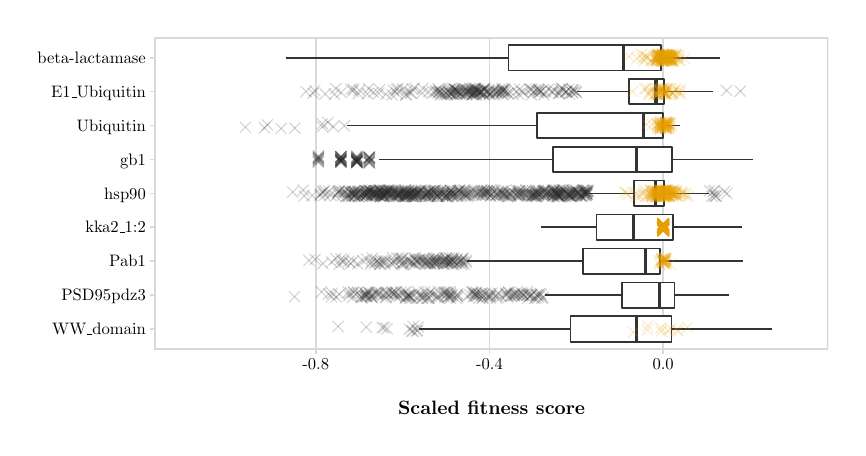
\begin{tikzpicture}[x=1pt,y=1pt]
\definecolor{fillColor}{RGB}{255,255,255}
\path[use as bounding box,fill=fillColor,fill opacity=0.00] (0,0) rectangle (292.83,144.54);
\begin{scope}
\path[clip] ( 45.95, 28.30) rectangle (289.33,141.04);
\definecolor{drawColor}{gray}{0.85}

\path[draw=drawColor,line width= 0.6pt,line join=round] (104.09, 28.30) --
	(104.09,141.04);

\path[draw=drawColor,line width= 0.6pt,line join=round] (166.86, 28.30) --
	(166.86,141.04);

\path[draw=drawColor,line width= 0.6pt,line join=round] (229.63, 28.30) --
	(229.63,141.04);
\definecolor{drawColor}{gray}{0.20}

\path[draw=drawColor,line width= 0.6pt,line join=round] (228.89,133.69) -- (250.12,133.69);

\path[draw=drawColor,line width= 0.6pt,line join=round] (173.79,133.69) -- ( 93.20,133.69);
\definecolor{fillColor}{RGB}{255,255,255}

\path[draw=drawColor,line width= 0.6pt,line join=round,line cap=round,fill=fillColor] (228.89,129.09) --
	(173.79,129.09) --
	(173.79,138.28) --
	(228.89,138.28) --
	(228.89,129.09) --
	cycle;

\path[draw=drawColor,line width= 1.1pt,line join=round] (215.45,129.09) -- (215.45,138.28);

\path[draw=drawColor,line width= 0.6pt,line join=round] (229.99,121.43) -- (247.71,121.43);

\path[draw=drawColor,line width= 0.6pt,line join=round] (217.34,121.43) -- (198.59,121.43);

\path[draw=drawColor,line width= 0.6pt,line join=round,line cap=round,fill=fillColor] (229.99,116.84) --
	(217.34,116.84) --
	(217.34,126.03) --
	(229.99,126.03) --
	(229.99,116.84) --
	cycle;

\path[draw=drawColor,line width= 1.1pt,line join=round] (227.04,116.84) -- (227.04,126.03);

\path[draw=drawColor,line width= 0.6pt,line join=round] (229.63,109.18) -- (235.59,109.18);

\path[draw=drawColor,line width= 0.6pt,line join=round] (183.94,109.18) -- (115.41,109.18);

\path[draw=drawColor,line width= 0.6pt,line join=round,line cap=round,fill=fillColor] (229.63,104.58) --
	(183.94,104.58) --
	(183.94,113.77) --
	(229.63,113.77) --
	(229.63,104.58) --
	cycle;

\path[draw=drawColor,line width= 1.1pt,line join=round] (222.67,104.58) -- (222.67,113.77);

\path[draw=drawColor,line width= 0.6pt,line join=round] (232.81, 96.93) -- (261.98, 96.93);

\path[draw=drawColor,line width= 0.6pt,line join=round] (189.82, 96.93) -- (127.08, 96.93);

\path[draw=drawColor,line width= 0.6pt,line join=round,line cap=round,fill=fillColor] (232.81, 92.33) --
	(189.82, 92.33) --
	(189.82,101.52) --
	(232.81,101.52) --
	(232.81, 92.33) --
	cycle;

\path[draw=drawColor,line width= 1.1pt,line join=round] (220.00, 92.33) -- (220.00,101.52);

\path[draw=drawColor,line width= 0.6pt,line join=round] (229.92, 84.67) -- (246.15, 84.67);

\path[draw=drawColor,line width= 0.6pt,line join=round] (219.00, 84.67) -- (202.68, 84.67);

\path[draw=drawColor,line width= 0.6pt,line join=round,line cap=round,fill=fillColor] (229.92, 80.08) --
	(219.00, 80.08) --
	(219.00, 89.27) --
	(229.92, 89.27) --
	(229.92, 80.08) --
	cycle;

\path[draw=drawColor,line width= 1.1pt,line join=round] (226.78, 80.08) -- (226.78, 89.27);

\path[draw=drawColor,line width= 0.6pt,line join=round] (233.13, 72.42) -- (258.23, 72.42);

\path[draw=drawColor,line width= 0.6pt,line join=round] (205.58, 72.42) -- (185.62, 72.42);

\path[draw=drawColor,line width= 0.6pt,line join=round,line cap=round,fill=fillColor] (233.13, 67.82) --
	(205.58, 67.82) --
	(205.58, 77.01) --
	(233.13, 77.01) --
	(233.13, 67.82) --
	cycle;

\path[draw=drawColor,line width= 1.1pt,line join=round] (218.96, 67.82) -- (218.96, 77.01);

\path[draw=drawColor,line width= 0.6pt,line join=round] (228.58, 60.16) -- (258.57, 60.16);

\path[draw=drawColor,line width= 0.6pt,line join=round] (200.56, 60.16) -- (158.61, 60.16);

\path[draw=drawColor,line width= 0.6pt,line join=round,line cap=round,fill=fillColor] (228.58, 55.57) --
	(200.56, 55.57) --
	(200.56, 64.76) --
	(228.58, 64.76) --
	(228.58, 55.57) --
	cycle;

\path[draw=drawColor,line width= 1.1pt,line join=round] (223.32, 55.57) -- (223.32, 64.76);

\path[draw=drawColor,line width= 0.6pt,line join=round] (233.67, 47.91) -- (253.32, 47.91);

\path[draw=drawColor,line width= 0.6pt,line join=round] (214.76, 47.91) -- (186.87, 47.91);

\path[draw=drawColor,line width= 0.6pt,line join=round,line cap=round,fill=fillColor] (233.67, 43.31) --
	(214.76, 43.31) --
	(214.76, 52.51) --
	(233.67, 52.51) --
	(233.67, 43.31) --
	cycle;

\path[draw=drawColor,line width= 1.1pt,line join=round] (228.35, 43.31) -- (228.35, 52.51);

\path[draw=drawColor,line width= 0.6pt,line join=round] (232.68, 35.66) -- (269.10, 35.66);

\path[draw=drawColor,line width= 0.6pt,line join=round] (196.14, 35.66) -- (141.43, 35.66);

\path[draw=drawColor,line width= 0.6pt,line join=round,line cap=round,fill=fillColor] (232.68, 31.06) --
	(196.14, 31.06) --
	(196.14, 40.25) --
	(232.68, 40.25) --
	(232.68, 31.06) --
	cycle;

\path[draw=drawColor,line width= 1.1pt,line join=round] (220.09, 31.06) -- (220.09, 40.25);
\definecolor{drawColor}{RGB}{38,38,38}

\path[draw=drawColor,draw opacity=0.20,line width= 0.4pt,line join=round,line cap=round] (255.54,119.63) -- (259.47,123.55);

\path[draw=drawColor,draw opacity=0.20,line width= 0.4pt,line join=round,line cap=round] (255.54,123.55) -- (259.47,119.63);

\path[draw=drawColor,draw opacity=0.20,line width= 0.4pt,line join=round,line cap=round] (250.58,119.86) -- (254.51,123.78);

\path[draw=drawColor,draw opacity=0.20,line width= 0.4pt,line join=round,line cap=round] (250.58,123.78) -- (254.51,119.86);

\path[draw=drawColor,draw opacity=0.20,line width= 0.4pt,line join=round,line cap=round] (192.32,119.21) -- (196.24,123.14);

\path[draw=drawColor,draw opacity=0.20,line width= 0.4pt,line join=round,line cap=round] (192.32,123.14) -- (196.24,119.21);

\path[draw=drawColor,draw opacity=0.20,line width= 0.4pt,line join=round,line cap=round] (129.68,118.32) -- (133.61,122.25);

\path[draw=drawColor,draw opacity=0.20,line width= 0.4pt,line join=round,line cap=round] (129.68,122.25) -- (133.61,118.32);

\path[draw=drawColor,draw opacity=0.20,line width= 0.4pt,line join=round,line cap=round] (162.80,120.42) -- (166.72,124.35);

\path[draw=drawColor,draw opacity=0.20,line width= 0.4pt,line join=round,line cap=round] (162.80,124.35) -- (166.72,120.42);

\path[draw=drawColor,draw opacity=0.20,line width= 0.4pt,line join=round,line cap=round] (159.93,119.69) -- (163.85,123.62);

\path[draw=drawColor,draw opacity=0.20,line width= 0.4pt,line join=round,line cap=round] (159.93,123.62) -- (163.85,119.69);

\path[draw=drawColor,draw opacity=0.20,line width= 0.4pt,line join=round,line cap=round] (158.86,118.39) -- (162.79,122.31);

\path[draw=drawColor,draw opacity=0.20,line width= 0.4pt,line join=round,line cap=round] (158.86,122.31) -- (162.79,118.39);

\path[draw=drawColor,draw opacity=0.20,line width= 0.4pt,line join=round,line cap=round] (157.85,120.66) -- (161.77,124.58);

\path[draw=drawColor,draw opacity=0.20,line width= 0.4pt,line join=round,line cap=round] (157.85,124.58) -- (161.77,120.66);

\path[draw=drawColor,draw opacity=0.20,line width= 0.4pt,line join=round,line cap=round] (154.08,120.31) -- (158.01,124.23);

\path[draw=drawColor,draw opacity=0.20,line width= 0.4pt,line join=round,line cap=round] (154.08,124.23) -- (158.01,120.31);

\path[draw=drawColor,draw opacity=0.20,line width= 0.4pt,line join=round,line cap=round] (153.33,119.90) -- (157.26,123.83);

\path[draw=drawColor,draw opacity=0.20,line width= 0.4pt,line join=round,line cap=round] (153.33,123.83) -- (157.26,119.90);

\path[draw=drawColor,draw opacity=0.20,line width= 0.4pt,line join=round,line cap=round] (153.20,119.23) -- (157.12,123.16);

\path[draw=drawColor,draw opacity=0.20,line width= 0.4pt,line join=round,line cap=round] (153.20,123.16) -- (157.12,119.23);

\path[draw=drawColor,draw opacity=0.20,line width= 0.4pt,line join=round,line cap=round] (152.31,120.18) -- (156.23,124.11);

\path[draw=drawColor,draw opacity=0.20,line width= 0.4pt,line join=round,line cap=round] (152.31,124.11) -- (156.23,120.18);

\path[draw=drawColor,draw opacity=0.20,line width= 0.4pt,line join=round,line cap=round] (150.75,118.87) -- (154.67,122.80);

\path[draw=drawColor,draw opacity=0.20,line width= 0.4pt,line join=round,line cap=round] (150.75,122.80) -- (154.67,118.87);

\path[draw=drawColor,draw opacity=0.20,line width= 0.4pt,line join=round,line cap=round] (150.43,118.97) -- (154.36,122.90);

\path[draw=drawColor,draw opacity=0.20,line width= 0.4pt,line join=round,line cap=round] (150.43,122.90) -- (154.36,118.97);

\path[draw=drawColor,draw opacity=0.20,line width= 0.4pt,line join=round,line cap=round] (148.75,119.05) -- (152.68,122.97);

\path[draw=drawColor,draw opacity=0.20,line width= 0.4pt,line join=round,line cap=round] (148.75,122.97) -- (152.68,119.05);

\path[draw=drawColor,draw opacity=0.20,line width= 0.4pt,line join=round,line cap=round] (195.77,119.90) -- (199.70,123.82);

\path[draw=drawColor,draw opacity=0.20,line width= 0.4pt,line join=round,line cap=round] (195.77,123.82) -- (199.70,119.90);

\path[draw=drawColor,draw opacity=0.20,line width= 0.4pt,line join=round,line cap=round] (183.81,119.74) -- (187.73,123.67);

\path[draw=drawColor,draw opacity=0.20,line width= 0.4pt,line join=round,line cap=round] (183.81,123.67) -- (187.73,119.74);

\path[draw=drawColor,draw opacity=0.20,line width= 0.4pt,line join=round,line cap=round] (176.72,119.39) -- (180.64,123.31);

\path[draw=drawColor,draw opacity=0.20,line width= 0.4pt,line join=round,line cap=round] (176.72,123.31) -- (180.64,119.39);

\path[draw=drawColor,draw opacity=0.20,line width= 0.4pt,line join=round,line cap=round] (173.79,120.30) -- (177.72,124.22);

\path[draw=drawColor,draw opacity=0.20,line width= 0.4pt,line join=round,line cap=round] (173.79,124.22) -- (177.72,120.30);

\path[draw=drawColor,draw opacity=0.20,line width= 0.4pt,line join=round,line cap=round] (167.22,119.23) -- (171.14,123.15);

\path[draw=drawColor,draw opacity=0.20,line width= 0.4pt,line join=round,line cap=round] (167.22,123.15) -- (171.14,119.23);

\path[draw=drawColor,draw opacity=0.20,line width= 0.4pt,line join=round,line cap=round] (162.63,118.40) -- (166.55,122.32);

\path[draw=drawColor,draw opacity=0.20,line width= 0.4pt,line join=round,line cap=round] (162.63,122.32) -- (166.55,118.40);

\path[draw=drawColor,draw opacity=0.20,line width= 0.4pt,line join=round,line cap=round] (162.45,119.50) -- (166.38,123.42);

\path[draw=drawColor,draw opacity=0.20,line width= 0.4pt,line join=round,line cap=round] (162.45,123.42) -- (166.38,119.50);

\path[draw=drawColor,draw opacity=0.20,line width= 0.4pt,line join=round,line cap=round] (161.33,119.03) -- (165.25,122.96);

\path[draw=drawColor,draw opacity=0.20,line width= 0.4pt,line join=round,line cap=round] (161.33,122.96) -- (165.25,119.03);

\path[draw=drawColor,draw opacity=0.20,line width= 0.4pt,line join=round,line cap=round] (159.34,120.61) -- (163.26,124.54);

\path[draw=drawColor,draw opacity=0.20,line width= 0.4pt,line join=round,line cap=round] (159.34,124.54) -- (163.26,120.61);

\path[draw=drawColor,draw opacity=0.20,line width= 0.4pt,line join=round,line cap=round] (169.73,119.43) -- (173.66,123.35);

\path[draw=drawColor,draw opacity=0.20,line width= 0.4pt,line join=round,line cap=round] (169.73,123.35) -- (173.66,119.43);

\path[draw=drawColor,draw opacity=0.20,line width= 0.4pt,line join=round,line cap=round] (169.23,119.24) -- (173.16,123.17);

\path[draw=drawColor,draw opacity=0.20,line width= 0.4pt,line join=round,line cap=round] (169.23,123.17) -- (173.16,119.24);

\path[draw=drawColor,draw opacity=0.20,line width= 0.4pt,line join=round,line cap=round] (158.99,118.80) -- (162.92,122.72);

\path[draw=drawColor,draw opacity=0.20,line width= 0.4pt,line join=round,line cap=round] (158.99,122.72) -- (162.92,118.80);

\path[draw=drawColor,draw opacity=0.20,line width= 0.4pt,line join=round,line cap=round] (158.33,119.63) -- (162.25,123.56);

\path[draw=drawColor,draw opacity=0.20,line width= 0.4pt,line join=round,line cap=round] (158.33,123.56) -- (162.25,119.63);

\path[draw=drawColor,draw opacity=0.20,line width= 0.4pt,line join=round,line cap=round] (157.25,119.99) -- (161.18,123.91);

\path[draw=drawColor,draw opacity=0.20,line width= 0.4pt,line join=round,line cap=round] (157.25,123.91) -- (161.18,119.99);

\path[draw=drawColor,draw opacity=0.20,line width= 0.4pt,line join=round,line cap=round] (153.06,120.01) -- (156.98,123.93);

\path[draw=drawColor,draw opacity=0.20,line width= 0.4pt,line join=round,line cap=round] (153.06,123.93) -- (156.98,120.01);

\path[draw=drawColor,draw opacity=0.20,line width= 0.4pt,line join=round,line cap=round] (152.50,118.36) -- (156.42,122.29);

\path[draw=drawColor,draw opacity=0.20,line width= 0.4pt,line join=round,line cap=round] (152.50,122.29) -- (156.42,118.36);

\path[draw=drawColor,draw opacity=0.20,line width= 0.4pt,line join=round,line cap=round] (151.62,120.64) -- (155.54,124.57);

\path[draw=drawColor,draw opacity=0.20,line width= 0.4pt,line join=round,line cap=round] (151.62,124.57) -- (155.54,120.64);

\path[draw=drawColor,draw opacity=0.20,line width= 0.4pt,line join=round,line cap=round] (151.61,118.61) -- (155.53,122.53);

\path[draw=drawColor,draw opacity=0.20,line width= 0.4pt,line join=round,line cap=round] (151.61,122.53) -- (155.53,118.61);

\path[draw=drawColor,draw opacity=0.20,line width= 0.4pt,line join=round,line cap=round] (147.02,119.48) -- (150.94,123.41);

\path[draw=drawColor,draw opacity=0.20,line width= 0.4pt,line join=round,line cap=round] (147.02,123.41) -- (150.94,119.48);

\path[draw=drawColor,draw opacity=0.20,line width= 0.4pt,line join=round,line cap=round] (146.32,119.03) -- (150.24,122.95);

\path[draw=drawColor,draw opacity=0.20,line width= 0.4pt,line join=round,line cap=round] (146.32,122.95) -- (150.24,119.03);

\path[draw=drawColor,draw opacity=0.20,line width= 0.4pt,line join=round,line cap=round] (140.82,120.62) -- (144.75,124.55);

\path[draw=drawColor,draw opacity=0.20,line width= 0.4pt,line join=round,line cap=round] (140.82,124.55) -- (144.75,120.62);

\path[draw=drawColor,draw opacity=0.20,line width= 0.4pt,line join=round,line cap=round] (183.41,119.51) -- (187.34,123.44);

\path[draw=drawColor,draw opacity=0.20,line width= 0.4pt,line join=round,line cap=round] (183.41,123.44) -- (187.34,119.51);

\path[draw=drawColor,draw opacity=0.20,line width= 0.4pt,line join=round,line cap=round] (173.35,118.41) -- (177.27,122.34);

\path[draw=drawColor,draw opacity=0.20,line width= 0.4pt,line join=round,line cap=round] (173.35,122.34) -- (177.27,118.41);

\path[draw=drawColor,draw opacity=0.20,line width= 0.4pt,line join=round,line cap=round] (153.71,119.41) -- (157.64,123.33);

\path[draw=drawColor,draw opacity=0.20,line width= 0.4pt,line join=round,line cap=round] (153.71,123.33) -- (157.64,119.41);

\path[draw=drawColor,draw opacity=0.20,line width= 0.4pt,line join=round,line cap=round] (147.49,118.34) -- (151.41,122.26);

\path[draw=drawColor,draw opacity=0.20,line width= 0.4pt,line join=round,line cap=round] (147.49,122.26) -- (151.41,118.34);

\path[draw=drawColor,draw opacity=0.20,line width= 0.4pt,line join=round,line cap=round] (146.42,120.46) -- (150.35,124.38);

\path[draw=drawColor,draw opacity=0.20,line width= 0.4pt,line join=round,line cap=round] (146.42,124.38) -- (150.35,120.46);

\path[draw=drawColor,draw opacity=0.20,line width= 0.4pt,line join=round,line cap=round] (137.85,120.66) -- (141.77,124.58);

\path[draw=drawColor,draw opacity=0.20,line width= 0.4pt,line join=round,line cap=round] (137.85,124.58) -- (141.77,120.66);

\path[draw=drawColor,draw opacity=0.20,line width= 0.4pt,line join=round,line cap=round] (137.07,120.28) -- (141.00,124.20);

\path[draw=drawColor,draw opacity=0.20,line width= 0.4pt,line join=round,line cap=round] (137.07,124.20) -- (141.00,120.28);

\path[draw=drawColor,draw opacity=0.20,line width= 0.4pt,line join=round,line cap=round] (105.55,118.62) -- (109.48,122.54);

\path[draw=drawColor,draw opacity=0.20,line width= 0.4pt,line join=round,line cap=round] (105.55,122.54) -- (109.48,118.62);

\path[draw=drawColor,draw opacity=0.20,line width= 0.4pt,line join=round,line cap=round] (104.51,106.78) -- (108.44,110.70);

\path[draw=drawColor,draw opacity=0.20,line width= 0.4pt,line join=round,line cap=round] (104.51,110.70) -- (108.44,106.78);

\path[draw=drawColor,draw opacity=0.20,line width= 0.4pt,line join=round,line cap=round] (191.02,120.68) -- (194.95,124.61);

\path[draw=drawColor,draw opacity=0.20,line width= 0.4pt,line join=round,line cap=round] (191.02,124.61) -- (194.95,120.68);

\path[draw=drawColor,draw opacity=0.20,line width= 0.4pt,line join=round,line cap=round] (171.64,118.88) -- (175.56,122.80);

\path[draw=drawColor,draw opacity=0.20,line width= 0.4pt,line join=round,line cap=round] (171.64,122.80) -- (175.56,118.88);

\path[draw=drawColor,draw opacity=0.20,line width= 0.4pt,line join=round,line cap=round] (154.51,118.65) -- (158.43,122.58);

\path[draw=drawColor,draw opacity=0.20,line width= 0.4pt,line join=round,line cap=round] (154.51,122.58) -- (158.43,118.65);

\path[draw=drawColor,draw opacity=0.20,line width= 0.4pt,line join=round,line cap=round] (152.49,119.94) -- (156.41,123.86);

\path[draw=drawColor,draw opacity=0.20,line width= 0.4pt,line join=round,line cap=round] (152.49,123.86) -- (156.41,119.94);

\path[draw=drawColor,draw opacity=0.20,line width= 0.4pt,line join=round,line cap=round] (146.65,120.00) -- (150.58,123.93);

\path[draw=drawColor,draw opacity=0.20,line width= 0.4pt,line join=round,line cap=round] (146.65,123.93) -- (150.58,120.00);

\path[draw=drawColor,draw opacity=0.20,line width= 0.4pt,line join=round,line cap=round] (169.66,118.32) -- (173.58,122.25);

\path[draw=drawColor,draw opacity=0.20,line width= 0.4pt,line join=round,line cap=round] (169.66,122.25) -- (173.58,118.32);

\path[draw=drawColor,draw opacity=0.20,line width= 0.4pt,line join=round,line cap=round] (145.51,119.76) -- (149.44,123.68);

\path[draw=drawColor,draw opacity=0.20,line width= 0.4pt,line join=round,line cap=round] (145.51,123.68) -- (149.44,119.76);

\path[draw=drawColor,draw opacity=0.20,line width= 0.4pt,line join=round,line cap=round] (135.05,119.72) -- (138.98,123.64);

\path[draw=drawColor,draw opacity=0.20,line width= 0.4pt,line join=round,line cap=round] (135.05,123.64) -- (138.98,119.72);

\path[draw=drawColor,draw opacity=0.20,line width= 0.4pt,line join=round,line cap=round] (134.84,118.44) -- (138.77,122.36);

\path[draw=drawColor,draw opacity=0.20,line width= 0.4pt,line join=round,line cap=round] (134.84,122.36) -- (138.77,118.44);

\path[draw=drawColor,draw opacity=0.20,line width= 0.4pt,line join=round,line cap=round] (134.70,118.27) -- (138.62,122.20);

\path[draw=drawColor,draw opacity=0.20,line width= 0.4pt,line join=round,line cap=round] (134.70,122.20) -- (138.62,118.27);

\path[draw=drawColor,draw opacity=0.20,line width= 0.4pt,line join=round,line cap=round] (127.50,118.58) -- (131.42,122.50);

\path[draw=drawColor,draw opacity=0.20,line width= 0.4pt,line join=round,line cap=round] (127.50,122.50) -- (131.42,118.58);

\path[draw=drawColor,draw opacity=0.20,line width= 0.4pt,line join=round,line cap=round] (124.90,118.85) -- (128.82,122.78);

\path[draw=drawColor,draw opacity=0.20,line width= 0.4pt,line join=round,line cap=round] (124.90,122.78) -- (128.82,118.85);

\path[draw=drawColor,draw opacity=0.20,line width= 0.4pt,line join=round,line cap=round] (122.99,119.21) -- (126.92,123.13);

\path[draw=drawColor,draw opacity=0.20,line width= 0.4pt,line join=round,line cap=round] (122.99,123.13) -- (126.92,119.21);

\path[draw=drawColor,draw opacity=0.20,line width= 0.4pt,line join=round,line cap=round] (117.55,118.75) -- (121.48,122.67);

\path[draw=drawColor,draw opacity=0.20,line width= 0.4pt,line join=round,line cap=round] (117.55,122.67) -- (121.48,118.75);

\path[draw=drawColor,draw opacity=0.20,line width= 0.4pt,line join=round,line cap=round] (115.62,119.68) -- (119.55,123.60);

\path[draw=drawColor,draw opacity=0.20,line width= 0.4pt,line join=round,line cap=round] (115.62,123.60) -- (119.55,119.68);

\path[draw=drawColor,draw opacity=0.20,line width= 0.4pt,line join=round,line cap=round] (111.31,119.17) -- (115.23,123.09);

\path[draw=drawColor,draw opacity=0.20,line width= 0.4pt,line join=round,line cap=round] (111.31,123.09) -- (115.23,119.17);

\path[draw=drawColor,draw opacity=0.20,line width= 0.4pt,line join=round,line cap=round] (108.91,118.50) -- (112.84,122.43);

\path[draw=drawColor,draw opacity=0.20,line width= 0.4pt,line join=round,line cap=round] (108.91,122.43) -- (112.84,118.50);

\path[draw=drawColor,draw opacity=0.20,line width= 0.4pt,line join=round,line cap=round] (184.63,118.28) -- (188.55,122.20);

\path[draw=drawColor,draw opacity=0.20,line width= 0.4pt,line join=round,line cap=round] (184.63,122.20) -- (188.55,118.28);

\path[draw=drawColor,draw opacity=0.20,line width= 0.4pt,line join=round,line cap=round] (196.19,119.38) -- (200.11,123.30);

\path[draw=drawColor,draw opacity=0.20,line width= 0.4pt,line join=round,line cap=round] (196.19,123.30) -- (200.11,119.38);

\path[draw=drawColor,draw opacity=0.20,line width= 0.4pt,line join=round,line cap=round] (188.07,120.13) -- (192.00,124.06);

\path[draw=drawColor,draw opacity=0.20,line width= 0.4pt,line join=round,line cap=round] (188.07,124.06) -- (192.00,120.13);

\path[draw=drawColor,draw opacity=0.20,line width= 0.4pt,line join=round,line cap=round] (169.64,119.90) -- (173.56,123.83);

\path[draw=drawColor,draw opacity=0.20,line width= 0.4pt,line join=round,line cap=round] (169.64,123.83) -- (173.56,119.90);

\path[draw=drawColor,draw opacity=0.20,line width= 0.4pt,line join=round,line cap=round] (131.38,118.86) -- (135.30,122.79);

\path[draw=drawColor,draw opacity=0.20,line width= 0.4pt,line join=round,line cap=round] (131.38,122.79) -- (135.30,118.86);

\path[draw=drawColor,draw opacity=0.20,line width= 0.4pt,line join=round,line cap=round] (130.19,119.93) -- (134.12,123.86);

\path[draw=drawColor,draw opacity=0.20,line width= 0.4pt,line join=round,line cap=round] (130.19,123.86) -- (134.12,119.93);

\path[draw=drawColor,draw opacity=0.20,line width= 0.4pt,line join=round,line cap=round] (114.85,120.29) -- (118.77,124.22);

\path[draw=drawColor,draw opacity=0.20,line width= 0.4pt,line join=round,line cap=round] (114.85,124.22) -- (118.77,120.29);

\path[draw=drawColor,draw opacity=0.20,line width= 0.4pt,line join=round,line cap=round] (101.78,119.85) -- (105.70,123.77);

\path[draw=drawColor,draw opacity=0.20,line width= 0.4pt,line join=round,line cap=round] (101.78,123.77) -- (105.70,119.85);

\path[draw=drawColor,draw opacity=0.20,line width= 0.4pt,line join=round,line cap=round] ( 98.62,119.46) -- (102.55,123.38);

\path[draw=drawColor,draw opacity=0.20,line width= 0.4pt,line join=round,line cap=round] ( 98.62,123.38) -- (102.55,119.46);

\path[draw=drawColor,draw opacity=0.20,line width= 0.4pt,line join=round,line cap=round] (189.87,118.92) -- (193.79,122.85);

\path[draw=drawColor,draw opacity=0.20,line width= 0.4pt,line join=round,line cap=round] (189.87,122.85) -- (193.79,118.92);

\path[draw=drawColor,draw opacity=0.20,line width= 0.4pt,line join=round,line cap=round] (131.62,120.64) -- (135.55,124.56);

\path[draw=drawColor,draw opacity=0.20,line width= 0.4pt,line join=round,line cap=round] (131.62,124.56) -- (135.55,120.64);

\path[draw=drawColor,draw opacity=0.20,line width= 0.4pt,line join=round,line cap=round] (185.21,119.43) -- (189.14,123.35);

\path[draw=drawColor,draw opacity=0.20,line width= 0.4pt,line join=round,line cap=round] (185.21,123.35) -- (189.14,119.43);

\path[draw=drawColor,draw opacity=0.20,line width= 0.4pt,line join=round,line cap=round] (112.46,107.10) -- (116.38,111.02);

\path[draw=drawColor,draw opacity=0.20,line width= 0.4pt,line join=round,line cap=round] (112.46,111.02) -- (116.38,107.10);

\path[draw=drawColor,draw opacity=0.20,line width= 0.4pt,line join=round,line cap=round] (190.49,120.19) -- (194.41,124.12);

\path[draw=drawColor,draw opacity=0.20,line width= 0.4pt,line join=round,line cap=round] (190.49,124.12) -- (194.41,120.19);

\path[draw=drawColor,draw opacity=0.20,line width= 0.4pt,line join=round,line cap=round] (163.16,120.63) -- (167.08,124.55);

\path[draw=drawColor,draw opacity=0.20,line width= 0.4pt,line join=round,line cap=round] (163.16,124.55) -- (167.08,120.63);

\path[draw=drawColor,draw opacity=0.20,line width= 0.4pt,line join=round,line cap=round] ( 94.58,106.29) -- ( 98.50,110.21);

\path[draw=drawColor,draw opacity=0.20,line width= 0.4pt,line join=round,line cap=round] ( 94.58,110.21) -- ( 98.50,106.29);

\path[draw=drawColor,draw opacity=0.20,line width= 0.4pt,line join=round,line cap=round] (191.23,120.40) -- (195.15,124.33);

\path[draw=drawColor,draw opacity=0.20,line width= 0.4pt,line join=round,line cap=round] (191.23,124.33) -- (195.15,120.40);

\path[draw=drawColor,draw opacity=0.20,line width= 0.4pt,line join=round,line cap=round] (144.55,119.30) -- (148.48,123.23);

\path[draw=drawColor,draw opacity=0.20,line width= 0.4pt,line join=round,line cap=round] (144.55,123.23) -- (148.48,119.30);

\path[draw=drawColor,draw opacity=0.20,line width= 0.4pt,line join=round,line cap=round] (136.62,118.97) -- (140.54,122.89);

\path[draw=drawColor,draw opacity=0.20,line width= 0.4pt,line join=round,line cap=round] (136.62,122.89) -- (140.54,118.97);

\path[draw=drawColor,draw opacity=0.20,line width= 0.4pt,line join=round,line cap=round] (121.24,120.54) -- (125.16,124.47);

\path[draw=drawColor,draw opacity=0.20,line width= 0.4pt,line join=round,line cap=round] (121.24,124.47) -- (125.16,120.54);

\path[draw=drawColor,draw opacity=0.20,line width= 0.4pt,line join=round,line cap=round] (108.48,106.79) -- (112.41,110.72);

\path[draw=drawColor,draw opacity=0.20,line width= 0.4pt,line join=round,line cap=round] (108.48,110.72) -- (112.41,106.79);

\path[draw=drawColor,draw opacity=0.20,line width= 0.4pt,line join=round,line cap=round] (193.81,118.60) -- (197.74,122.52);

\path[draw=drawColor,draw opacity=0.20,line width= 0.4pt,line join=round,line cap=round] (193.81,122.52) -- (197.74,118.60);

\path[draw=drawColor,draw opacity=0.20,line width= 0.4pt,line join=round,line cap=round] (192.63,119.45) -- (196.55,123.38);

\path[draw=drawColor,draw opacity=0.20,line width= 0.4pt,line join=round,line cap=round] (192.63,123.38) -- (196.55,119.45);

\path[draw=drawColor,draw opacity=0.20,line width= 0.4pt,line join=round,line cap=round] (190.64,119.04) -- (194.56,122.96);

\path[draw=drawColor,draw opacity=0.20,line width= 0.4pt,line join=round,line cap=round] (190.64,122.96) -- (194.56,119.04);

\path[draw=drawColor,draw opacity=0.20,line width= 0.4pt,line join=round,line cap=round] (154.96,118.94) -- (158.89,122.86);

\path[draw=drawColor,draw opacity=0.20,line width= 0.4pt,line join=round,line cap=round] (154.96,122.86) -- (158.89,118.94);

\path[draw=drawColor,draw opacity=0.20,line width= 0.4pt,line join=round,line cap=round] (182.53,119.02) -- (186.45,122.94);

\path[draw=drawColor,draw opacity=0.20,line width= 0.4pt,line join=round,line cap=round] (182.53,122.94) -- (186.45,119.02);

\path[draw=drawColor,draw opacity=0.20,line width= 0.4pt,line join=round,line cap=round] (169.19,118.89) -- (173.12,122.82);

\path[draw=drawColor,draw opacity=0.20,line width= 0.4pt,line join=round,line cap=round] (169.19,122.82) -- (173.12,118.89);

\path[draw=drawColor,draw opacity=0.20,line width= 0.4pt,line join=round,line cap=round] (163.31,120.22) -- (167.24,124.14);

\path[draw=drawColor,draw opacity=0.20,line width= 0.4pt,line join=round,line cap=round] (163.31,124.14) -- (167.24,120.22);

\path[draw=drawColor,draw opacity=0.20,line width= 0.4pt,line join=round,line cap=round] (162.69,118.80) -- (166.62,122.73);

\path[draw=drawColor,draw opacity=0.20,line width= 0.4pt,line join=round,line cap=round] (162.69,122.73) -- (166.62,118.80);

\path[draw=drawColor,draw opacity=0.20,line width= 0.4pt,line join=round,line cap=round] (162.04,119.52) -- (165.97,123.45);

\path[draw=drawColor,draw opacity=0.20,line width= 0.4pt,line join=round,line cap=round] (162.04,123.45) -- (165.97,119.52);

\path[draw=drawColor,draw opacity=0.20,line width= 0.4pt,line join=round,line cap=round] (161.20,119.09) -- (165.12,123.01);

\path[draw=drawColor,draw opacity=0.20,line width= 0.4pt,line join=round,line cap=round] (161.20,123.01) -- (165.12,119.09);

\path[draw=drawColor,draw opacity=0.20,line width= 0.4pt,line join=round,line cap=round] (161.07,119.47) -- (164.99,123.39);

\path[draw=drawColor,draw opacity=0.20,line width= 0.4pt,line join=round,line cap=round] (161.07,123.39) -- (164.99,119.47);

\path[draw=drawColor,draw opacity=0.20,line width= 0.4pt,line join=round,line cap=round] (160.70,119.58) -- (164.63,123.51);

\path[draw=drawColor,draw opacity=0.20,line width= 0.4pt,line join=round,line cap=round] (160.70,123.51) -- (164.63,119.58);

\path[draw=drawColor,draw opacity=0.20,line width= 0.4pt,line join=round,line cap=round] (160.06,120.63) -- (163.99,124.56);

\path[draw=drawColor,draw opacity=0.20,line width= 0.4pt,line join=round,line cap=round] (160.06,124.56) -- (163.99,120.63);

\path[draw=drawColor,draw opacity=0.20,line width= 0.4pt,line join=round,line cap=round] (160.02,119.37) -- (163.94,123.29);

\path[draw=drawColor,draw opacity=0.20,line width= 0.4pt,line join=round,line cap=round] (160.02,123.29) -- (163.94,119.37);

\path[draw=drawColor,draw opacity=0.20,line width= 0.4pt,line join=round,line cap=round] (159.67,120.48) -- (163.59,124.41);

\path[draw=drawColor,draw opacity=0.20,line width= 0.4pt,line join=round,line cap=round] (159.67,124.41) -- (163.59,120.48);

\path[draw=drawColor,draw opacity=0.20,line width= 0.4pt,line join=round,line cap=round] (156.68,120.09) -- (160.60,124.01);

\path[draw=drawColor,draw opacity=0.20,line width= 0.4pt,line join=round,line cap=round] (156.68,124.01) -- (160.60,120.09);

\path[draw=drawColor,draw opacity=0.20,line width= 0.4pt,line join=round,line cap=round] (168.34,120.11) -- (172.27,124.04);

\path[draw=drawColor,draw opacity=0.20,line width= 0.4pt,line join=round,line cap=round] (168.34,124.04) -- (172.27,120.11);

\path[draw=drawColor,draw opacity=0.20,line width= 0.4pt,line join=round,line cap=round] (167.52,119.42) -- (171.45,123.34);

\path[draw=drawColor,draw opacity=0.20,line width= 0.4pt,line join=round,line cap=round] (167.52,123.34) -- (171.45,119.42);

\path[draw=drawColor,draw opacity=0.20,line width= 0.4pt,line join=round,line cap=round] (166.05,119.21) -- (169.97,123.14);

\path[draw=drawColor,draw opacity=0.20,line width= 0.4pt,line join=round,line cap=round] (166.05,123.14) -- (169.97,119.21);

\path[draw=drawColor,draw opacity=0.20,line width= 0.4pt,line join=round,line cap=round] (164.45,119.87) -- (168.37,123.79);

\path[draw=drawColor,draw opacity=0.20,line width= 0.4pt,line join=round,line cap=round] (164.45,123.79) -- (168.37,119.87);

\path[draw=drawColor,draw opacity=0.20,line width= 0.4pt,line join=round,line cap=round] (164.29,119.65) -- (168.22,123.58);

\path[draw=drawColor,draw opacity=0.20,line width= 0.4pt,line join=round,line cap=round] (164.29,123.58) -- (168.22,119.65);

\path[draw=drawColor,draw opacity=0.20,line width= 0.4pt,line join=round,line cap=round] (163.99,119.00) -- (167.91,122.93);

\path[draw=drawColor,draw opacity=0.20,line width= 0.4pt,line join=round,line cap=round] (163.99,122.93) -- (167.91,119.00);

\path[draw=drawColor,draw opacity=0.20,line width= 0.4pt,line join=round,line cap=round] (163.10,118.44) -- (167.03,122.37);

\path[draw=drawColor,draw opacity=0.20,line width= 0.4pt,line join=round,line cap=round] (163.10,122.37) -- (167.03,118.44);

\path[draw=drawColor,draw opacity=0.20,line width= 0.4pt,line join=round,line cap=round] (160.56,120.05) -- (164.48,123.97);

\path[draw=drawColor,draw opacity=0.20,line width= 0.4pt,line join=round,line cap=round] (160.56,123.97) -- (164.48,120.05);

\path[draw=drawColor,draw opacity=0.20,line width= 0.4pt,line join=round,line cap=round] (160.20,119.04) -- (164.13,122.96);

\path[draw=drawColor,draw opacity=0.20,line width= 0.4pt,line join=round,line cap=round] (160.20,122.96) -- (164.13,119.04);

\path[draw=drawColor,draw opacity=0.20,line width= 0.4pt,line join=round,line cap=round] (192.65,119.52) -- (196.58,123.44);

\path[draw=drawColor,draw opacity=0.20,line width= 0.4pt,line join=round,line cap=round] (192.65,123.44) -- (196.58,119.52);

\path[draw=drawColor,draw opacity=0.20,line width= 0.4pt,line join=round,line cap=round] (159.87,118.71) -- (163.79,122.64);

\path[draw=drawColor,draw opacity=0.20,line width= 0.4pt,line join=round,line cap=round] (159.87,122.64) -- (163.79,118.71);

\path[draw=drawColor,draw opacity=0.20,line width= 0.4pt,line join=round,line cap=round] (194.71,119.21) -- (198.63,123.13);

\path[draw=drawColor,draw opacity=0.20,line width= 0.4pt,line join=round,line cap=round] (194.71,123.13) -- (198.63,119.21);

\path[draw=drawColor,draw opacity=0.20,line width= 0.4pt,line join=round,line cap=round] (193.57,120.27) -- (197.49,124.20);

\path[draw=drawColor,draw opacity=0.20,line width= 0.4pt,line join=round,line cap=round] (193.57,124.20) -- (197.49,120.27);

\path[draw=drawColor,draw opacity=0.20,line width= 0.4pt,line join=round,line cap=round] (175.78,120.26) -- (179.70,124.18);

\path[draw=drawColor,draw opacity=0.20,line width= 0.4pt,line join=round,line cap=round] (175.78,124.18) -- (179.70,120.26);

\path[draw=drawColor,draw opacity=0.20,line width= 0.4pt,line join=round,line cap=round] (175.47,118.60) -- (179.39,122.53);

\path[draw=drawColor,draw opacity=0.20,line width= 0.4pt,line join=round,line cap=round] (175.47,122.53) -- (179.39,118.60);

\path[draw=drawColor,draw opacity=0.20,line width= 0.4pt,line join=round,line cap=round] (164.79,118.44) -- (168.71,122.36);

\path[draw=drawColor,draw opacity=0.20,line width= 0.4pt,line join=round,line cap=round] (164.79,122.36) -- (168.71,118.44);

\path[draw=drawColor,draw opacity=0.20,line width= 0.4pt,line join=round,line cap=round] (158.61,118.49) -- (162.54,122.42);

\path[draw=drawColor,draw opacity=0.20,line width= 0.4pt,line join=round,line cap=round] (158.61,122.42) -- (162.54,118.49);

\path[draw=drawColor,draw opacity=0.20,line width= 0.4pt,line join=round,line cap=round] (120.80,118.65) -- (124.72,122.57);

\path[draw=drawColor,draw opacity=0.20,line width= 0.4pt,line join=round,line cap=round] (120.80,122.57) -- (124.72,118.65);

\path[draw=drawColor,draw opacity=0.20,line width= 0.4pt,line join=round,line cap=round] (109.34,120.55) -- (113.27,124.48);

\path[draw=drawColor,draw opacity=0.20,line width= 0.4pt,line join=round,line cap=round] (109.34,124.48) -- (113.27,120.55);

\path[draw=drawColor,draw opacity=0.20,line width= 0.4pt,line join=round,line cap=round] (194.91,120.14) -- (198.84,124.06);

\path[draw=drawColor,draw opacity=0.20,line width= 0.4pt,line join=round,line cap=round] (194.91,124.06) -- (198.84,120.14);

\path[draw=drawColor,draw opacity=0.20,line width= 0.4pt,line join=round,line cap=round] (181.56,120.20) -- (185.48,124.12);

\path[draw=drawColor,draw opacity=0.20,line width= 0.4pt,line join=round,line cap=round] (181.56,124.12) -- (185.48,120.20);

\path[draw=drawColor,draw opacity=0.20,line width= 0.4pt,line join=round,line cap=round] (169.87,119.96) -- (173.79,123.88);

\path[draw=drawColor,draw opacity=0.20,line width= 0.4pt,line join=round,line cap=round] (169.87,123.88) -- (173.79,119.96);

\path[draw=drawColor,draw opacity=0.20,line width= 0.4pt,line join=round,line cap=round] (168.20,119.28) -- (172.12,123.20);

\path[draw=drawColor,draw opacity=0.20,line width= 0.4pt,line join=round,line cap=round] (168.20,123.20) -- (172.12,119.28);

\path[draw=drawColor,draw opacity=0.20,line width= 0.4pt,line join=round,line cap=round] (161.58,119.63) -- (165.51,123.56);

\path[draw=drawColor,draw opacity=0.20,line width= 0.4pt,line join=round,line cap=round] (161.58,123.56) -- (165.51,119.63);

\path[draw=drawColor,draw opacity=0.20,line width= 0.4pt,line join=round,line cap=round] (157.40,119.65) -- (161.32,123.57);

\path[draw=drawColor,draw opacity=0.20,line width= 0.4pt,line join=round,line cap=round] (157.40,123.57) -- (161.32,119.65);

\path[draw=drawColor,draw opacity=0.20,line width= 0.4pt,line join=round,line cap=round] (156.79,119.42) -- (160.72,123.35);

\path[draw=drawColor,draw opacity=0.20,line width= 0.4pt,line join=round,line cap=round] (156.79,123.35) -- (160.72,119.42);

\path[draw=drawColor,draw opacity=0.20,line width= 0.4pt,line join=round,line cap=round] (156.68,118.67) -- (160.61,122.59);

\path[draw=drawColor,draw opacity=0.20,line width= 0.4pt,line join=round,line cap=round] (156.68,122.59) -- (160.61,118.67);

\path[draw=drawColor,draw opacity=0.20,line width= 0.4pt,line join=round,line cap=round] (156.10,118.86) -- (160.02,122.78);

\path[draw=drawColor,draw opacity=0.20,line width= 0.4pt,line join=round,line cap=round] (156.10,122.78) -- (160.02,118.86);

\path[draw=drawColor,draw opacity=0.20,line width= 0.4pt,line join=round,line cap=round] (153.90,118.64) -- (157.82,122.56);

\path[draw=drawColor,draw opacity=0.20,line width= 0.4pt,line join=round,line cap=round] (153.90,122.56) -- (157.82,118.64);

\path[draw=drawColor,draw opacity=0.20,line width= 0.4pt,line join=round,line cap=round] (169.48,120.64) -- (173.41,124.56);

\path[draw=drawColor,draw opacity=0.20,line width= 0.4pt,line join=round,line cap=round] (169.48,124.56) -- (173.41,120.64);

\path[draw=drawColor,draw opacity=0.20,line width= 0.4pt,line join=round,line cap=round] (180.04,118.30) -- (183.97,122.22);

\path[draw=drawColor,draw opacity=0.20,line width= 0.4pt,line join=round,line cap=round] (180.04,122.22) -- (183.97,118.30);

\path[draw=drawColor,draw opacity=0.20,line width= 0.4pt,line join=round,line cap=round] (149.61,118.64) -- (153.53,122.56);

\path[draw=drawColor,draw opacity=0.20,line width= 0.4pt,line join=round,line cap=round] (149.61,122.56) -- (153.53,118.64);

\path[draw=drawColor,draw opacity=0.20,line width= 0.4pt,line join=round,line cap=round] (148.68,118.30) -- (152.61,122.22);

\path[draw=drawColor,draw opacity=0.20,line width= 0.4pt,line join=round,line cap=round] (148.68,122.22) -- (152.61,118.30);

\path[draw=drawColor,draw opacity=0.20,line width= 0.4pt,line join=round,line cap=round] (147.20,118.52) -- (151.13,122.45);

\path[draw=drawColor,draw opacity=0.20,line width= 0.4pt,line join=round,line cap=round] (147.20,122.45) -- (151.13,118.52);

\path[draw=drawColor,draw opacity=0.20,line width= 0.4pt,line join=round,line cap=round] (146.97,119.27) -- (150.90,123.20);

\path[draw=drawColor,draw opacity=0.20,line width= 0.4pt,line join=round,line cap=round] (146.97,123.20) -- (150.90,119.27);

\path[draw=drawColor,draw opacity=0.20,line width= 0.4pt,line join=round,line cap=round] (145.35,119.34) -- (149.28,123.26);

\path[draw=drawColor,draw opacity=0.20,line width= 0.4pt,line join=round,line cap=round] (145.35,123.26) -- (149.28,119.34);

\path[draw=drawColor,draw opacity=0.20,line width= 0.4pt,line join=round,line cap=round] (142.91,119.41) -- (146.84,123.34);

\path[draw=drawColor,draw opacity=0.20,line width= 0.4pt,line join=round,line cap=round] (142.91,123.34) -- (146.84,119.41);

\path[draw=drawColor,draw opacity=0.20,line width= 0.4pt,line join=round,line cap=round] (140.54,118.96) -- (144.46,122.88);

\path[draw=drawColor,draw opacity=0.20,line width= 0.4pt,line join=round,line cap=round] (140.54,122.88) -- (144.46,118.96);

\path[draw=drawColor,draw opacity=0.20,line width= 0.4pt,line join=round,line cap=round] ( 83.65,106.35) -- ( 87.58,110.28);

\path[draw=drawColor,draw opacity=0.20,line width= 0.4pt,line join=round,line cap=round] ( 83.65,110.28) -- ( 87.58,106.35);

\path[draw=drawColor,draw opacity=0.20,line width= 0.4pt,line join=round,line cap=round] (170.62,119.20) -- (174.54,123.13);

\path[draw=drawColor,draw opacity=0.20,line width= 0.4pt,line join=round,line cap=round] (170.62,123.13) -- (174.54,119.20);

\path[draw=drawColor,draw opacity=0.20,line width= 0.4pt,line join=round,line cap=round] (170.57,119.95) -- (174.49,123.87);

\path[draw=drawColor,draw opacity=0.20,line width= 0.4pt,line join=round,line cap=round] (170.57,123.87) -- (174.49,119.95);

\path[draw=drawColor,draw opacity=0.20,line width= 0.4pt,line join=round,line cap=round] (170.26,120.54) -- (174.19,124.47);

\path[draw=drawColor,draw opacity=0.20,line width= 0.4pt,line join=round,line cap=round] (170.26,124.47) -- (174.19,120.54);

\path[draw=drawColor,draw opacity=0.20,line width= 0.4pt,line join=round,line cap=round] (167.02,118.47) -- (170.95,122.40);

\path[draw=drawColor,draw opacity=0.20,line width= 0.4pt,line join=round,line cap=round] (167.02,122.40) -- (170.95,118.47);

\path[draw=drawColor,draw opacity=0.20,line width= 0.4pt,line join=round,line cap=round] (166.23,119.63) -- (170.15,123.56);

\path[draw=drawColor,draw opacity=0.20,line width= 0.4pt,line join=round,line cap=round] (166.23,123.56) -- (170.15,119.63);

\path[draw=drawColor,draw opacity=0.20,line width= 0.4pt,line join=round,line cap=round] (165.08,118.87) -- (169.00,122.80);

\path[draw=drawColor,draw opacity=0.20,line width= 0.4pt,line join=round,line cap=round] (165.08,122.80) -- (169.00,118.87);

\path[draw=drawColor,draw opacity=0.20,line width= 0.4pt,line join=round,line cap=round] (165.06,118.51) -- (168.98,122.43);

\path[draw=drawColor,draw opacity=0.20,line width= 0.4pt,line join=round,line cap=round] (165.06,122.43) -- (168.98,118.51);

\path[draw=drawColor,draw opacity=0.20,line width= 0.4pt,line join=round,line cap=round] (164.55,119.18) -- (168.48,123.11);

\path[draw=drawColor,draw opacity=0.20,line width= 0.4pt,line join=round,line cap=round] (164.55,123.11) -- (168.48,119.18);

\path[draw=drawColor,draw opacity=0.20,line width= 0.4pt,line join=round,line cap=round] (162.85,120.12) -- (166.78,124.04);

\path[draw=drawColor,draw opacity=0.20,line width= 0.4pt,line join=round,line cap=round] (162.85,124.04) -- (166.78,120.12);

\path[draw=drawColor,draw opacity=0.20,line width= 0.4pt,line join=round,line cap=round] (161.59,119.50) -- (165.52,123.43);

\path[draw=drawColor,draw opacity=0.20,line width= 0.4pt,line join=round,line cap=round] (161.59,123.43) -- (165.52,119.50);

\path[draw=drawColor,draw opacity=0.20,line width= 0.4pt,line join=round,line cap=round] (160.65,119.99) -- (164.57,123.91);

\path[draw=drawColor,draw opacity=0.20,line width= 0.4pt,line join=round,line cap=round] (160.65,123.91) -- (164.57,119.99);

\path[draw=drawColor,draw opacity=0.20,line width= 0.4pt,line join=round,line cap=round] (156.89,119.27) -- (160.81,123.19);

\path[draw=drawColor,draw opacity=0.20,line width= 0.4pt,line join=round,line cap=round] (156.89,123.19) -- (160.81,119.27);

\path[draw=drawColor,draw opacity=0.20,line width= 0.4pt,line join=round,line cap=round] (194.96,119.07) -- (198.88,122.99);

\path[draw=drawColor,draw opacity=0.20,line width= 0.4pt,line join=round,line cap=round] (194.96,122.99) -- (198.88,119.07);

\path[draw=drawColor,draw opacity=0.20,line width= 0.4pt,line join=round,line cap=round] (194.89,120.19) -- (198.82,124.11);

\path[draw=drawColor,draw opacity=0.20,line width= 0.4pt,line join=round,line cap=round] (194.89,124.11) -- (198.82,120.19);

\path[draw=drawColor,draw opacity=0.20,line width= 0.4pt,line join=round,line cap=round] (182.86,120.07) -- (186.78,124.00);

\path[draw=drawColor,draw opacity=0.20,line width= 0.4pt,line join=round,line cap=round] (182.86,124.00) -- (186.78,120.07);

\path[draw=drawColor,draw opacity=0.20,line width= 0.4pt,line join=round,line cap=round] (182.55,119.74) -- (186.47,123.66);

\path[draw=drawColor,draw opacity=0.20,line width= 0.4pt,line join=round,line cap=round] (182.55,123.66) -- (186.47,119.74);

\path[draw=drawColor,draw opacity=0.20,line width= 0.4pt,line join=round,line cap=round] (179.74,120.22) -- (183.67,124.14);

\path[draw=drawColor,draw opacity=0.20,line width= 0.4pt,line join=round,line cap=round] (179.74,124.14) -- (183.67,120.22);

\path[draw=drawColor,draw opacity=0.20,line width= 0.4pt,line join=round,line cap=round] (169.71,120.01) -- (173.64,123.93);

\path[draw=drawColor,draw opacity=0.20,line width= 0.4pt,line join=round,line cap=round] (169.71,123.93) -- (173.64,120.01);

\path[draw=drawColor,draw opacity=0.20,line width= 0.4pt,line join=round,line cap=round] (161.41,119.03) -- (165.33,122.95);

\path[draw=drawColor,draw opacity=0.20,line width= 0.4pt,line join=round,line cap=round] (161.41,122.95) -- (165.33,119.03);

\path[draw=drawColor,draw opacity=0.20,line width= 0.4pt,line join=round,line cap=round] (158.81,120.36) -- (162.73,124.28);

\path[draw=drawColor,draw opacity=0.20,line width= 0.4pt,line join=round,line cap=round] (158.81,124.28) -- (162.73,120.36);

\path[draw=drawColor,draw opacity=0.20,line width= 0.4pt,line join=round,line cap=round] (158.65,118.29) -- (162.58,122.21);

\path[draw=drawColor,draw opacity=0.20,line width= 0.4pt,line join=round,line cap=round] (158.65,122.21) -- (162.58,118.29);

\path[draw=drawColor,draw opacity=0.20,line width= 0.4pt,line join=round,line cap=round] (158.55,120.22) -- (162.47,124.15);

\path[draw=drawColor,draw opacity=0.20,line width= 0.4pt,line join=round,line cap=round] (158.55,124.15) -- (162.47,120.22);

\path[draw=drawColor,draw opacity=0.20,line width= 0.4pt,line join=round,line cap=round] (150.92,120.43) -- (154.84,124.36);

\path[draw=drawColor,draw opacity=0.20,line width= 0.4pt,line join=round,line cap=round] (150.92,124.36) -- (154.84,120.43);

\path[draw=drawColor,draw opacity=0.20,line width= 0.4pt,line join=round,line cap=round] (187.57,119.44) -- (191.49,123.37);

\path[draw=drawColor,draw opacity=0.20,line width= 0.4pt,line join=round,line cap=round] (187.57,123.37) -- (191.49,119.44);

\path[draw=drawColor,draw opacity=0.20,line width= 0.4pt,line join=round,line cap=round] (177.25,119.16) -- (181.18,123.08);

\path[draw=drawColor,draw opacity=0.20,line width= 0.4pt,line join=round,line cap=round] (177.25,123.08) -- (181.18,119.16);

\path[draw=drawColor,draw opacity=0.20,line width= 0.4pt,line join=round,line cap=round] (136.36,119.10) -- (140.28,123.02);

\path[draw=drawColor,draw opacity=0.20,line width= 0.4pt,line join=round,line cap=round] (136.36,123.02) -- (140.28,119.10);

\path[draw=drawColor,draw opacity=0.20,line width= 0.4pt,line join=round,line cap=round] (133.54,120.38) -- (137.46,124.30);

\path[draw=drawColor,draw opacity=0.20,line width= 0.4pt,line join=round,line cap=round] (133.54,124.30) -- (137.46,120.38);

\path[draw=drawColor,draw opacity=0.20,line width= 0.4pt,line join=round,line cap=round] (131.38,120.12) -- (135.30,124.04);

\path[draw=drawColor,draw opacity=0.20,line width= 0.4pt,line join=round,line cap=round] (131.38,124.04) -- (135.30,120.12);

\path[draw=drawColor,draw opacity=0.20,line width= 0.4pt,line join=round,line cap=round] (125.21,120.17) -- (129.14,124.10);

\path[draw=drawColor,draw opacity=0.20,line width= 0.4pt,line join=round,line cap=round] (125.21,124.10) -- (129.14,120.17);

\path[draw=drawColor,draw opacity=0.20,line width= 0.4pt,line join=round,line cap=round] (117.88,119.96) -- (121.80,123.88);

\path[draw=drawColor,draw opacity=0.20,line width= 0.4pt,line join=round,line cap=round] (117.88,123.88) -- (121.80,119.96);

\path[draw=drawColor,draw opacity=0.20,line width= 0.4pt,line join=round,line cap=round] (115.75,120.38) -- (119.67,124.31);

\path[draw=drawColor,draw opacity=0.20,line width= 0.4pt,line join=round,line cap=round] (115.75,124.31) -- (119.67,120.38);

\path[draw=drawColor,draw opacity=0.20,line width= 0.4pt,line join=round,line cap=round] (101.17,118.90) -- (105.09,122.82);

\path[draw=drawColor,draw opacity=0.20,line width= 0.4pt,line join=round,line cap=round] (101.17,122.82) -- (105.09,118.90);

\path[draw=drawColor,draw opacity=0.20,line width= 0.4pt,line join=round,line cap=round] ( 89.61,106.16) -- ( 93.54,110.09);

\path[draw=drawColor,draw opacity=0.20,line width= 0.4pt,line join=round,line cap=round] ( 89.61,110.09) -- ( 93.54,106.16);

\path[draw=drawColor,draw opacity=0.20,line width= 0.4pt,line join=round,line cap=round] (183.34,119.43) -- (187.26,123.36);

\path[draw=drawColor,draw opacity=0.20,line width= 0.4pt,line join=round,line cap=round] (183.34,123.36) -- (187.26,119.43);

\path[draw=drawColor,draw opacity=0.20,line width= 0.4pt,line join=round,line cap=round] (167.59,119.15) -- (171.51,123.08);

\path[draw=drawColor,draw opacity=0.20,line width= 0.4pt,line join=round,line cap=round] (167.59,123.08) -- (171.51,119.15);

\path[draw=drawColor,draw opacity=0.20,line width= 0.4pt,line join=round,line cap=round] (162.05,119.29) -- (165.98,123.22);

\path[draw=drawColor,draw opacity=0.20,line width= 0.4pt,line join=round,line cap=round] (162.05,123.22) -- (165.98,119.29);

\path[draw=drawColor,draw opacity=0.20,line width= 0.4pt,line join=round,line cap=round] (157.76,118.83) -- (161.68,122.75);

\path[draw=drawColor,draw opacity=0.20,line width= 0.4pt,line join=round,line cap=round] (157.76,122.75) -- (161.68,118.83);

\path[draw=drawColor,draw opacity=0.20,line width= 0.4pt,line join=round,line cap=round] (155.19,120.60) -- (159.11,124.52);

\path[draw=drawColor,draw opacity=0.20,line width= 0.4pt,line join=round,line cap=round] (155.19,124.52) -- (159.11,120.60);

\path[draw=drawColor,draw opacity=0.20,line width= 0.4pt,line join=round,line cap=round] (153.16,119.83) -- (157.09,123.76);

\path[draw=drawColor,draw opacity=0.20,line width= 0.4pt,line join=round,line cap=round] (153.16,123.76) -- (157.09,119.83);

\path[draw=drawColor,draw opacity=0.20,line width= 0.4pt,line join=round,line cap=round] (152.94,118.69) -- (156.86,122.61);

\path[draw=drawColor,draw opacity=0.20,line width= 0.4pt,line join=round,line cap=round] (152.94,122.61) -- (156.86,118.69);

\path[draw=drawColor,draw opacity=0.20,line width= 0.4pt,line join=round,line cap=round] (152.40,120.46) -- (156.33,124.38);

\path[draw=drawColor,draw opacity=0.20,line width= 0.4pt,line join=round,line cap=round] (152.40,124.38) -- (156.33,120.46);

\path[draw=drawColor,draw opacity=0.20,line width= 0.4pt,line join=round,line cap=round] (151.91,119.35) -- (155.83,123.28);

\path[draw=drawColor,draw opacity=0.20,line width= 0.4pt,line join=round,line cap=round] (151.91,123.28) -- (155.83,119.35);

\path[draw=drawColor,draw opacity=0.20,line width= 0.4pt,line join=round,line cap=round] (151.49,118.68) -- (155.41,122.60);

\path[draw=drawColor,draw opacity=0.20,line width= 0.4pt,line join=round,line cap=round] (151.49,122.60) -- (155.41,118.68);

\path[draw=drawColor,draw opacity=0.20,line width= 0.4pt,line join=round,line cap=round] (150.39,120.27) -- (154.32,124.20);

\path[draw=drawColor,draw opacity=0.20,line width= 0.4pt,line join=round,line cap=round] (150.39,124.20) -- (154.32,120.27);

\path[draw=drawColor,draw opacity=0.20,line width= 0.4pt,line join=round,line cap=round] (149.93,119.68) -- (153.86,123.61);

\path[draw=drawColor,draw opacity=0.20,line width= 0.4pt,line join=round,line cap=round] (149.93,123.61) -- (153.86,119.68);

\path[draw=drawColor,draw opacity=0.20,line width= 0.4pt,line join=round,line cap=round] (149.66,118.33) -- (153.59,122.25);

\path[draw=drawColor,draw opacity=0.20,line width= 0.4pt,line join=round,line cap=round] (149.66,122.25) -- (153.59,118.33);

\path[draw=drawColor,draw opacity=0.20,line width= 0.4pt,line join=round,line cap=round] (149.23,119.05) -- (153.16,122.97);

\path[draw=drawColor,draw opacity=0.20,line width= 0.4pt,line join=round,line cap=round] (149.23,122.97) -- (153.16,119.05);

\path[draw=drawColor,draw opacity=0.20,line width= 0.4pt,line join=round,line cap=round] (147.70,118.94) -- (151.63,122.87);

\path[draw=drawColor,draw opacity=0.20,line width= 0.4pt,line join=round,line cap=round] (147.70,122.87) -- (151.63,118.94);

\path[draw=drawColor,draw opacity=0.20,line width= 0.4pt,line join=round,line cap=round] (146.74,119.49) -- (150.67,123.41);

\path[draw=drawColor,draw opacity=0.20,line width= 0.4pt,line join=round,line cap=round] (146.74,123.41) -- (150.67,119.49);

\path[draw=drawColor,draw opacity=0.20,line width= 0.4pt,line join=round,line cap=round] (187.84,119.11) -- (191.77,123.03);

\path[draw=drawColor,draw opacity=0.20,line width= 0.4pt,line join=round,line cap=round] (187.84,123.03) -- (191.77,119.11);

\path[draw=drawColor,draw opacity=0.20,line width= 0.4pt,line join=round,line cap=round] (186.26,120.29) -- (190.19,124.21);

\path[draw=drawColor,draw opacity=0.20,line width= 0.4pt,line join=round,line cap=round] (186.26,124.21) -- (190.19,120.29);

\path[draw=drawColor,draw opacity=0.20,line width= 0.4pt,line join=round,line cap=round] (182.52,120.35) -- (186.45,124.27);

\path[draw=drawColor,draw opacity=0.20,line width= 0.4pt,line join=round,line cap=round] (182.52,124.27) -- (186.45,120.35);

\path[draw=drawColor,draw opacity=0.20,line width= 0.4pt,line join=round,line cap=round] (180.96,119.46) -- (184.88,123.38);

\path[draw=drawColor,draw opacity=0.20,line width= 0.4pt,line join=round,line cap=round] (180.96,123.38) -- (184.88,119.46);

\path[draw=drawColor,draw opacity=0.20,line width= 0.4pt,line join=round,line cap=round] (180.16,120.29) -- (184.09,124.21);

\path[draw=drawColor,draw opacity=0.20,line width= 0.4pt,line join=round,line cap=round] (180.16,124.21) -- (184.09,120.29);

\path[draw=drawColor,draw opacity=0.20,line width= 0.4pt,line join=round,line cap=round] (179.42,120.35) -- (183.34,124.28);

\path[draw=drawColor,draw opacity=0.20,line width= 0.4pt,line join=round,line cap=round] (179.42,124.28) -- (183.34,120.35);

\path[draw=drawColor,draw opacity=0.20,line width= 0.4pt,line join=round,line cap=round] (171.44,118.86) -- (175.37,122.78);

\path[draw=drawColor,draw opacity=0.20,line width= 0.4pt,line join=round,line cap=round] (171.44,122.78) -- (175.37,118.86);

\path[draw=drawColor,draw opacity=0.20,line width= 0.4pt,line join=round,line cap=round] (166.47,120.08) -- (170.39,124.01);

\path[draw=drawColor,draw opacity=0.20,line width= 0.4pt,line join=round,line cap=round] (166.47,124.01) -- (170.39,120.08);

\path[draw=drawColor,draw opacity=0.20,line width= 0.4pt,line join=round,line cap=round] (165.97,118.85) -- (169.89,122.78);

\path[draw=drawColor,draw opacity=0.20,line width= 0.4pt,line join=round,line cap=round] (165.97,122.78) -- (169.89,118.85);

\path[draw=drawColor,draw opacity=0.20,line width= 0.4pt,line join=round,line cap=round] (159.58,120.30) -- (163.51,124.22);

\path[draw=drawColor,draw opacity=0.20,line width= 0.4pt,line join=round,line cap=round] (159.58,124.22) -- (163.51,120.30);

\path[draw=drawColor,draw opacity=0.20,line width= 0.4pt,line join=round,line cap=round] (157.36,119.16) -- (161.28,123.09);

\path[draw=drawColor,draw opacity=0.20,line width= 0.4pt,line join=round,line cap=round] (157.36,123.09) -- (161.28,119.16);

\path[draw=drawColor,draw opacity=0.20,line width= 0.4pt,line join=round,line cap=round] (156.74,118.81) -- (160.66,122.73);

\path[draw=drawColor,draw opacity=0.20,line width= 0.4pt,line join=round,line cap=round] (156.74,122.73) -- (160.66,118.81);

\path[draw=drawColor,draw opacity=0.20,line width= 0.4pt,line join=round,line cap=round] (154.07,119.02) -- (157.99,122.94);

\path[draw=drawColor,draw opacity=0.20,line width= 0.4pt,line join=round,line cap=round] (154.07,122.94) -- (157.99,119.02);

\path[draw=drawColor,draw opacity=0.20,line width= 0.4pt,line join=round,line cap=round] (150.86,118.73) -- (154.79,122.66);

\path[draw=drawColor,draw opacity=0.20,line width= 0.4pt,line join=round,line cap=round] (150.86,122.66) -- (154.79,118.73);

\path[draw=drawColor,draw opacity=0.20,line width= 0.4pt,line join=round,line cap=round] (162.67,120.24) -- (166.59,124.17);

\path[draw=drawColor,draw opacity=0.20,line width= 0.4pt,line join=round,line cap=round] (162.67,124.17) -- (166.59,120.24);

\path[draw=drawColor,draw opacity=0.20,line width= 0.4pt,line join=round,line cap=round] (159.08,119.52) -- (163.00,123.45);

\path[draw=drawColor,draw opacity=0.20,line width= 0.4pt,line join=round,line cap=round] (159.08,123.45) -- (163.00,119.52);

\path[draw=drawColor,draw opacity=0.20,line width= 0.4pt,line join=round,line cap=round] (155.36,118.53) -- (159.28,122.46);

\path[draw=drawColor,draw opacity=0.20,line width= 0.4pt,line join=round,line cap=round] (155.36,122.46) -- (159.28,118.53);

\path[draw=drawColor,draw opacity=0.20,line width= 0.4pt,line join=round,line cap=round] (155.33,119.62) -- (159.25,123.55);

\path[draw=drawColor,draw opacity=0.20,line width= 0.4pt,line join=round,line cap=round] (155.33,123.55) -- (159.25,119.62);

\path[draw=drawColor,draw opacity=0.20,line width= 0.4pt,line join=round,line cap=round] (153.13,118.54) -- (157.05,122.46);

\path[draw=drawColor,draw opacity=0.20,line width= 0.4pt,line join=round,line cap=round] (153.13,122.46) -- (157.05,118.54);

\path[draw=drawColor,draw opacity=0.20,line width= 0.4pt,line join=round,line cap=round] (196.32,119.15) -- (200.24,123.08);

\path[draw=drawColor,draw opacity=0.20,line width= 0.4pt,line join=round,line cap=round] (196.32,123.08) -- (200.24,119.15);

\path[draw=drawColor,draw opacity=0.20,line width= 0.4pt,line join=round,line cap=round] (189.97,118.76) -- (193.90,122.68);

\path[draw=drawColor,draw opacity=0.20,line width= 0.4pt,line join=round,line cap=round] (189.97,122.68) -- (193.90,118.76);

\path[draw=drawColor,draw opacity=0.20,line width= 0.4pt,line join=round,line cap=round] (169.50,119.70) -- (173.43,123.62);

\path[draw=drawColor,draw opacity=0.20,line width= 0.4pt,line join=round,line cap=round] (169.50,123.62) -- (173.43,119.70);

\path[draw=drawColor,draw opacity=0.20,line width= 0.4pt,line join=round,line cap=round] (168.12,119.45) -- (172.05,123.37);

\path[draw=drawColor,draw opacity=0.20,line width= 0.4pt,line join=round,line cap=round] (168.12,123.37) -- (172.05,119.45);

\path[draw=drawColor,draw opacity=0.20,line width= 0.4pt,line join=round,line cap=round] (160.12,118.25) -- (164.04,122.18);

\path[draw=drawColor,draw opacity=0.20,line width= 0.4pt,line join=round,line cap=round] (160.12,122.18) -- (164.04,118.25);

\path[draw=drawColor,draw opacity=0.20,line width= 0.4pt,line join=round,line cap=round] (159.86,119.95) -- (163.78,123.88);

\path[draw=drawColor,draw opacity=0.20,line width= 0.4pt,line join=round,line cap=round] (159.86,123.88) -- (163.78,119.95);

\path[draw=drawColor,draw opacity=0.20,line width= 0.4pt,line join=round,line cap=round] (159.53,119.23) -- (163.46,123.15);

\path[draw=drawColor,draw opacity=0.20,line width= 0.4pt,line join=round,line cap=round] (159.53,123.15) -- (163.46,119.23);

\path[draw=drawColor,draw opacity=0.20,line width= 0.4pt,line join=round,line cap=round] (159.17,119.19) -- (163.09,123.11);

\path[draw=drawColor,draw opacity=0.20,line width= 0.4pt,line join=round,line cap=round] (159.17,123.11) -- (163.09,119.19);

\path[draw=drawColor,draw opacity=0.20,line width= 0.4pt,line join=round,line cap=round] (159.09,118.66) -- (163.01,122.59);

\path[draw=drawColor,draw opacity=0.20,line width= 0.4pt,line join=round,line cap=round] (159.09,122.59) -- (163.01,118.66);

\path[draw=drawColor,draw opacity=0.20,line width= 0.4pt,line join=round,line cap=round] (157.76,120.14) -- (161.68,124.06);

\path[draw=drawColor,draw opacity=0.20,line width= 0.4pt,line join=round,line cap=round] (157.76,124.06) -- (161.68,120.14);

\path[draw=drawColor,draw opacity=0.20,line width= 0.4pt,line join=round,line cap=round] (156.27,120.20) -- (160.20,124.13);

\path[draw=drawColor,draw opacity=0.20,line width= 0.4pt,line join=round,line cap=round] (156.27,124.13) -- (160.20,120.20);

\path[draw=drawColor,draw opacity=0.20,line width= 0.4pt,line join=round,line cap=round] (155.40,119.69) -- (159.32,123.61);

\path[draw=drawColor,draw opacity=0.20,line width= 0.4pt,line join=round,line cap=round] (155.40,123.61) -- (159.32,119.69);

\path[draw=drawColor,draw opacity=0.20,line width= 0.4pt,line join=round,line cap=round] (152.28,120.24) -- (156.20,124.16);

\path[draw=drawColor,draw opacity=0.20,line width= 0.4pt,line join=round,line cap=round] (152.28,124.16) -- (156.20,120.24);

\path[draw=drawColor,draw opacity=0.20,line width= 0.4pt,line join=round,line cap=round] (150.93,118.88) -- (154.85,122.81);

\path[draw=drawColor,draw opacity=0.20,line width= 0.4pt,line join=round,line cap=round] (150.93,122.81) -- (154.85,118.88);

\path[draw=drawColor,draw opacity=0.20,line width= 0.4pt,line join=round,line cap=round] (116.99, 95.26) -- (120.91, 99.18);

\path[draw=drawColor,draw opacity=0.20,line width= 0.4pt,line join=round,line cap=round] (116.99, 99.18) -- (120.91, 95.26);

\path[draw=drawColor,draw opacity=0.20,line width= 0.4pt,line join=round,line cap=round] (121.46, 93.76) -- (125.38, 97.68);

\path[draw=drawColor,draw opacity=0.20,line width= 0.4pt,line join=round,line cap=round] (121.46, 97.68) -- (125.38, 93.76);

\path[draw=drawColor,draw opacity=0.20,line width= 0.4pt,line join=round,line cap=round] (121.46, 94.93) -- (125.38, 98.86);

\path[draw=drawColor,draw opacity=0.20,line width= 0.4pt,line join=round,line cap=round] (121.46, 98.86) -- (125.38, 94.93);

\path[draw=drawColor,draw opacity=0.20,line width= 0.4pt,line join=round,line cap=round] (121.46, 95.80) -- (125.38, 99.72);

\path[draw=drawColor,draw opacity=0.20,line width= 0.4pt,line join=round,line cap=round] (121.46, 99.72) -- (125.38, 95.80);

\path[draw=drawColor,draw opacity=0.20,line width= 0.4pt,line join=round,line cap=round] (121.46, 95.77) -- (125.38, 99.69);

\path[draw=drawColor,draw opacity=0.20,line width= 0.4pt,line join=round,line cap=round] (121.46, 99.69) -- (125.38, 95.77);

\path[draw=drawColor,draw opacity=0.20,line width= 0.4pt,line join=round,line cap=round] (116.99, 94.56) -- (120.91, 98.48);

\path[draw=drawColor,draw opacity=0.20,line width= 0.4pt,line join=round,line cap=round] (116.99, 98.48) -- (120.91, 94.56);

\path[draw=drawColor,draw opacity=0.20,line width= 0.4pt,line join=round,line cap=round] (116.99, 95.27) -- (120.91, 99.19);

\path[draw=drawColor,draw opacity=0.20,line width= 0.4pt,line join=round,line cap=round] (116.99, 99.19) -- (120.91, 95.27);

\path[draw=drawColor,draw opacity=0.20,line width= 0.4pt,line join=round,line cap=round] (116.99, 95.87) -- (120.91, 99.79);

\path[draw=drawColor,draw opacity=0.20,line width= 0.4pt,line join=round,line cap=round] (116.99, 99.79) -- (120.91, 95.87);

\path[draw=drawColor,draw opacity=0.20,line width= 0.4pt,line join=round,line cap=round] (116.99, 93.84) -- (120.91, 97.77);

\path[draw=drawColor,draw opacity=0.20,line width= 0.4pt,line join=round,line cap=round] (116.99, 97.77) -- (120.91, 93.84);

\path[draw=drawColor,draw opacity=0.20,line width= 0.4pt,line join=round,line cap=round] (121.46, 95.56) -- (125.38, 99.49);

\path[draw=drawColor,draw opacity=0.20,line width= 0.4pt,line join=round,line cap=round] (121.46, 99.49) -- (125.38, 95.56);

\path[draw=drawColor,draw opacity=0.20,line width= 0.4pt,line join=round,line cap=round] (121.46, 94.45) -- (125.38, 98.38);

\path[draw=drawColor,draw opacity=0.20,line width= 0.4pt,line join=round,line cap=round] (121.46, 98.38) -- (125.38, 94.45);

\path[draw=drawColor,draw opacity=0.20,line width= 0.4pt,line join=round,line cap=round] (116.99, 93.99) -- (120.91, 97.91);

\path[draw=drawColor,draw opacity=0.20,line width= 0.4pt,line join=round,line cap=round] (116.99, 97.91) -- (120.91, 93.99);

\path[draw=drawColor,draw opacity=0.20,line width= 0.4pt,line join=round,line cap=round] (116.99, 93.97) -- (120.91, 97.90);

\path[draw=drawColor,draw opacity=0.20,line width= 0.4pt,line join=round,line cap=round] (116.99, 97.90) -- (120.91, 93.97);

\path[draw=drawColor,draw opacity=0.20,line width= 0.4pt,line join=round,line cap=round] (121.46, 95.77) -- (125.38, 99.69);

\path[draw=drawColor,draw opacity=0.20,line width= 0.4pt,line join=round,line cap=round] (121.46, 99.69) -- (125.38, 95.77);

\path[draw=drawColor,draw opacity=0.20,line width= 0.4pt,line join=round,line cap=round] (121.46, 93.90) -- (125.38, 97.83);

\path[draw=drawColor,draw opacity=0.20,line width= 0.4pt,line join=round,line cap=round] (121.46, 97.83) -- (125.38, 93.90);

\path[draw=drawColor,draw opacity=0.20,line width= 0.4pt,line join=round,line cap=round] (121.46, 95.32) -- (125.38, 99.24);

\path[draw=drawColor,draw opacity=0.20,line width= 0.4pt,line join=round,line cap=round] (121.46, 99.24) -- (125.38, 95.32);

\path[draw=drawColor,draw opacity=0.20,line width= 0.4pt,line join=round,line cap=round] (116.99, 94.35) -- (120.91, 98.27);

\path[draw=drawColor,draw opacity=0.20,line width= 0.4pt,line join=round,line cap=round] (116.99, 98.27) -- (120.91, 94.35);

\path[draw=drawColor,draw opacity=0.20,line width= 0.4pt,line join=round,line cap=round] (116.99, 93.83) -- (120.91, 97.75);

\path[draw=drawColor,draw opacity=0.20,line width= 0.4pt,line join=round,line cap=round] (116.99, 97.75) -- (120.91, 93.83);

\path[draw=drawColor,draw opacity=0.20,line width= 0.4pt,line join=round,line cap=round] (116.99, 94.58) -- (120.91, 98.50);

\path[draw=drawColor,draw opacity=0.20,line width= 0.4pt,line join=round,line cap=round] (116.99, 98.50) -- (120.91, 94.58);

\path[draw=drawColor,draw opacity=0.20,line width= 0.4pt,line join=round,line cap=round] (116.99, 95.45) -- (120.91, 99.38);

\path[draw=drawColor,draw opacity=0.20,line width= 0.4pt,line join=round,line cap=round] (116.99, 99.38) -- (120.91, 95.45);

\path[draw=drawColor,draw opacity=0.20,line width= 0.4pt,line join=round,line cap=round] (111.22, 95.14) -- (115.14, 99.06);

\path[draw=drawColor,draw opacity=0.20,line width= 0.4pt,line join=round,line cap=round] (111.22, 99.06) -- (115.14, 95.14);

\path[draw=drawColor,draw opacity=0.20,line width= 0.4pt,line join=round,line cap=round] (111.22, 95.91) -- (115.14, 99.84);

\path[draw=drawColor,draw opacity=0.20,line width= 0.4pt,line join=round,line cap=round] (111.22, 99.84) -- (115.14, 95.91);

\path[draw=drawColor,draw opacity=0.20,line width= 0.4pt,line join=round,line cap=round] (111.22, 94.10) -- (115.14, 98.02);

\path[draw=drawColor,draw opacity=0.20,line width= 0.4pt,line join=round,line cap=round] (111.22, 98.02) -- (115.14, 94.10);

\path[draw=drawColor,draw opacity=0.20,line width= 0.4pt,line join=round,line cap=round] (111.22, 94.74) -- (115.14, 98.66);

\path[draw=drawColor,draw opacity=0.20,line width= 0.4pt,line join=round,line cap=round] (111.22, 98.66) -- (115.14, 94.74);

\path[draw=drawColor,draw opacity=0.20,line width= 0.4pt,line join=round,line cap=round] (111.22, 95.97) -- (115.14, 99.90);

\path[draw=drawColor,draw opacity=0.20,line width= 0.4pt,line join=round,line cap=round] (111.22, 99.90) -- (115.14, 95.97);

\path[draw=drawColor,draw opacity=0.20,line width= 0.4pt,line join=round,line cap=round] (111.22, 95.70) -- (115.14, 99.63);

\path[draw=drawColor,draw opacity=0.20,line width= 0.4pt,line join=round,line cap=round] (111.22, 99.63) -- (115.14, 95.70);

\path[draw=drawColor,draw opacity=0.20,line width= 0.4pt,line join=round,line cap=round] (111.22, 94.47) -- (115.14, 98.39);

\path[draw=drawColor,draw opacity=0.20,line width= 0.4pt,line join=round,line cap=round] (111.22, 98.39) -- (115.14, 94.47);

\path[draw=drawColor,draw opacity=0.20,line width= 0.4pt,line join=round,line cap=round] (103.09, 94.84) -- (107.02, 98.77);

\path[draw=drawColor,draw opacity=0.20,line width= 0.4pt,line join=round,line cap=round] (103.09, 98.77) -- (107.02, 94.84);

\path[draw=drawColor,draw opacity=0.20,line width= 0.4pt,line join=round,line cap=round] (103.09, 95.49) -- (107.02, 99.41);

\path[draw=drawColor,draw opacity=0.20,line width= 0.4pt,line join=round,line cap=round] (103.09, 99.41) -- (107.02, 95.49);

\path[draw=drawColor,draw opacity=0.20,line width= 0.4pt,line join=round,line cap=round] (103.09, 94.60) -- (107.02, 98.53);

\path[draw=drawColor,draw opacity=0.20,line width= 0.4pt,line join=round,line cap=round] (103.09, 98.53) -- (107.02, 94.60);

\path[draw=drawColor,draw opacity=0.20,line width= 0.4pt,line join=round,line cap=round] (121.46, 93.78) -- (125.38, 97.70);

\path[draw=drawColor,draw opacity=0.20,line width= 0.4pt,line join=round,line cap=round] (121.46, 97.70) -- (125.38, 93.78);

\path[draw=drawColor,draw opacity=0.20,line width= 0.4pt,line join=round,line cap=round] (116.99, 96.11) -- (120.91,100.03);

\path[draw=drawColor,draw opacity=0.20,line width= 0.4pt,line join=round,line cap=round] (116.99,100.03) -- (120.91, 96.11);

\path[draw=drawColor,draw opacity=0.20,line width= 0.4pt,line join=round,line cap=round] (116.99, 95.17) -- (120.91, 99.10);

\path[draw=drawColor,draw opacity=0.20,line width= 0.4pt,line join=round,line cap=round] (116.99, 99.10) -- (120.91, 95.17);

\path[draw=drawColor,draw opacity=0.20,line width= 0.4pt,line join=round,line cap=round] (116.99, 96.12) -- (120.91,100.05);

\path[draw=drawColor,draw opacity=0.20,line width= 0.4pt,line join=round,line cap=round] (116.99,100.05) -- (120.91, 96.12);

\path[draw=drawColor,draw opacity=0.20,line width= 0.4pt,line join=round,line cap=round] (116.99, 94.54) -- (120.91, 98.47);

\path[draw=drawColor,draw opacity=0.20,line width= 0.4pt,line join=round,line cap=round] (116.99, 98.47) -- (120.91, 94.54);

\path[draw=drawColor,draw opacity=0.20,line width= 0.4pt,line join=round,line cap=round] (116.99, 94.17) -- (120.91, 98.09);

\path[draw=drawColor,draw opacity=0.20,line width= 0.4pt,line join=round,line cap=round] (116.99, 98.09) -- (120.91, 94.17);

\path[draw=drawColor,draw opacity=0.20,line width= 0.4pt,line join=round,line cap=round] (116.99, 94.57) -- (120.91, 98.49);

\path[draw=drawColor,draw opacity=0.20,line width= 0.4pt,line join=round,line cap=round] (116.99, 98.49) -- (120.91, 94.57);

\path[draw=drawColor,draw opacity=0.20,line width= 0.4pt,line join=round,line cap=round] (116.99, 94.80) -- (120.91, 98.73);

\path[draw=drawColor,draw opacity=0.20,line width= 0.4pt,line join=round,line cap=round] (116.99, 98.73) -- (120.91, 94.80);

\path[draw=drawColor,draw opacity=0.20,line width= 0.4pt,line join=round,line cap=round] (121.46, 95.29) -- (125.38, 99.21);

\path[draw=drawColor,draw opacity=0.20,line width= 0.4pt,line join=round,line cap=round] (121.46, 99.21) -- (125.38, 95.29);

\path[draw=drawColor,draw opacity=0.20,line width= 0.4pt,line join=round,line cap=round] (121.46, 94.66) -- (125.38, 98.58);

\path[draw=drawColor,draw opacity=0.20,line width= 0.4pt,line join=round,line cap=round] (121.46, 98.58) -- (125.38, 94.66);

\path[draw=drawColor,draw opacity=0.20,line width= 0.4pt,line join=round,line cap=round] (116.99, 94.28) -- (120.91, 98.21);

\path[draw=drawColor,draw opacity=0.20,line width= 0.4pt,line join=round,line cap=round] (116.99, 98.21) -- (120.91, 94.28);

\path[draw=drawColor,draw opacity=0.20,line width= 0.4pt,line join=round,line cap=round] (116.99, 93.91) -- (120.91, 97.83);

\path[draw=drawColor,draw opacity=0.20,line width= 0.4pt,line join=round,line cap=round] (116.99, 97.83) -- (120.91, 93.91);

\path[draw=drawColor,draw opacity=0.20,line width= 0.4pt,line join=round,line cap=round] (116.99, 94.82) -- (120.91, 98.75);

\path[draw=drawColor,draw opacity=0.20,line width= 0.4pt,line join=round,line cap=round] (116.99, 98.75) -- (120.91, 94.82);

\path[draw=drawColor,draw opacity=0.20,line width= 0.4pt,line join=round,line cap=round] (116.99, 94.14) -- (120.91, 98.06);

\path[draw=drawColor,draw opacity=0.20,line width= 0.4pt,line join=round,line cap=round] (116.99, 98.06) -- (120.91, 94.14);

\path[draw=drawColor,draw opacity=0.20,line width= 0.4pt,line join=round,line cap=round] (116.99, 95.52) -- (120.91, 99.45);

\path[draw=drawColor,draw opacity=0.20,line width= 0.4pt,line join=round,line cap=round] (116.99, 99.45) -- (120.91, 95.52);

\path[draw=drawColor,draw opacity=0.20,line width= 0.4pt,line join=round,line cap=round] (116.99, 94.14) -- (120.91, 98.06);

\path[draw=drawColor,draw opacity=0.20,line width= 0.4pt,line join=round,line cap=round] (116.99, 98.06) -- (120.91, 94.14);

\path[draw=drawColor,draw opacity=0.20,line width= 0.4pt,line join=round,line cap=round] (111.22, 95.93) -- (115.14, 99.85);

\path[draw=drawColor,draw opacity=0.20,line width= 0.4pt,line join=round,line cap=round] (111.22, 99.85) -- (115.14, 95.93);

\path[draw=drawColor,draw opacity=0.20,line width= 0.4pt,line join=round,line cap=round] (111.22, 94.14) -- (115.14, 98.07);

\path[draw=drawColor,draw opacity=0.20,line width= 0.4pt,line join=round,line cap=round] (111.22, 98.07) -- (115.14, 94.14);

\path[draw=drawColor,draw opacity=0.20,line width= 0.4pt,line join=round,line cap=round] (121.46, 93.96) -- (125.38, 97.89);

\path[draw=drawColor,draw opacity=0.20,line width= 0.4pt,line join=round,line cap=round] (121.46, 97.89) -- (125.38, 93.96);

\path[draw=drawColor,draw opacity=0.20,line width= 0.4pt,line join=round,line cap=round] (121.46, 95.68) -- (125.38, 99.61);

\path[draw=drawColor,draw opacity=0.20,line width= 0.4pt,line join=round,line cap=round] (121.46, 99.61) -- (125.38, 95.68);

\path[draw=drawColor,draw opacity=0.20,line width= 0.4pt,line join=round,line cap=round] (121.46, 95.38) -- (125.38, 99.30);

\path[draw=drawColor,draw opacity=0.20,line width= 0.4pt,line join=round,line cap=round] (121.46, 99.30) -- (125.38, 95.38);

\path[draw=drawColor,draw opacity=0.20,line width= 0.4pt,line join=round,line cap=round] (116.99, 94.43) -- (120.91, 98.35);

\path[draw=drawColor,draw opacity=0.20,line width= 0.4pt,line join=round,line cap=round] (116.99, 98.35) -- (120.91, 94.43);

\path[draw=drawColor,draw opacity=0.20,line width= 0.4pt,line join=round,line cap=round] (116.99, 94.33) -- (120.91, 98.26);

\path[draw=drawColor,draw opacity=0.20,line width= 0.4pt,line join=round,line cap=round] (116.99, 98.26) -- (120.91, 94.33);

\path[draw=drawColor,draw opacity=0.20,line width= 0.4pt,line join=round,line cap=round] (116.99, 95.53) -- (120.91, 99.46);

\path[draw=drawColor,draw opacity=0.20,line width= 0.4pt,line join=round,line cap=round] (116.99, 99.46) -- (120.91, 95.53);

\path[draw=drawColor,draw opacity=0.20,line width= 0.4pt,line join=round,line cap=round] (116.99, 94.90) -- (120.91, 98.83);

\path[draw=drawColor,draw opacity=0.20,line width= 0.4pt,line join=round,line cap=round] (116.99, 98.83) -- (120.91, 94.90);

\path[draw=drawColor,draw opacity=0.20,line width= 0.4pt,line join=round,line cap=round] (111.22, 95.99) -- (115.14, 99.91);

\path[draw=drawColor,draw opacity=0.20,line width= 0.4pt,line join=round,line cap=round] (111.22, 99.91) -- (115.14, 95.99);

\path[draw=drawColor,draw opacity=0.20,line width= 0.4pt,line join=round,line cap=round] (111.22, 94.39) -- (115.14, 98.31);

\path[draw=drawColor,draw opacity=0.20,line width= 0.4pt,line join=round,line cap=round] (111.22, 98.31) -- (115.14, 94.39);

\path[draw=drawColor,draw opacity=0.20,line width= 0.4pt,line join=round,line cap=round] (111.22, 95.87) -- (115.14, 99.79);

\path[draw=drawColor,draw opacity=0.20,line width= 0.4pt,line join=round,line cap=round] (111.22, 99.79) -- (115.14, 95.87);

\path[draw=drawColor,draw opacity=0.20,line width= 0.4pt,line join=round,line cap=round] (111.22, 93.89) -- (115.14, 97.81);

\path[draw=drawColor,draw opacity=0.20,line width= 0.4pt,line join=round,line cap=round] (111.22, 97.81) -- (115.14, 93.89);

\path[draw=drawColor,draw opacity=0.20,line width= 0.4pt,line join=round,line cap=round] (111.22, 94.94) -- (115.14, 98.86);

\path[draw=drawColor,draw opacity=0.20,line width= 0.4pt,line join=round,line cap=round] (111.22, 98.86) -- (115.14, 94.94);

\path[draw=drawColor,draw opacity=0.20,line width= 0.4pt,line join=round,line cap=round] (111.22, 95.40) -- (115.14, 99.32);

\path[draw=drawColor,draw opacity=0.20,line width= 0.4pt,line join=round,line cap=round] (111.22, 99.32) -- (115.14, 95.40);

\path[draw=drawColor,draw opacity=0.20,line width= 0.4pt,line join=round,line cap=round] (111.22, 93.99) -- (115.14, 97.91);

\path[draw=drawColor,draw opacity=0.20,line width= 0.4pt,line join=round,line cap=round] (111.22, 97.91) -- (115.14, 93.99);

\path[draw=drawColor,draw opacity=0.20,line width= 0.4pt,line join=round,line cap=round] (111.22, 94.60) -- (115.14, 98.52);

\path[draw=drawColor,draw opacity=0.20,line width= 0.4pt,line join=round,line cap=round] (111.22, 98.52) -- (115.14, 94.60);

\path[draw=drawColor,draw opacity=0.20,line width= 0.4pt,line join=round,line cap=round] (111.22, 95.25) -- (115.14, 99.17);

\path[draw=drawColor,draw opacity=0.20,line width= 0.4pt,line join=round,line cap=round] (111.22, 99.17) -- (115.14, 95.25);

\path[draw=drawColor,draw opacity=0.20,line width= 0.4pt,line join=round,line cap=round] (111.22, 94.44) -- (115.14, 98.37);

\path[draw=drawColor,draw opacity=0.20,line width= 0.4pt,line join=round,line cap=round] (111.22, 98.37) -- (115.14, 94.44);

\path[draw=drawColor,draw opacity=0.20,line width= 0.4pt,line join=round,line cap=round] (121.46, 94.49) -- (125.38, 98.41);

\path[draw=drawColor,draw opacity=0.20,line width= 0.4pt,line join=round,line cap=round] (121.46, 98.41) -- (125.38, 94.49);

\path[draw=drawColor,draw opacity=0.20,line width= 0.4pt,line join=round,line cap=round] (116.99, 95.20) -- (120.91, 99.13);

\path[draw=drawColor,draw opacity=0.20,line width= 0.4pt,line join=round,line cap=round] (116.99, 99.13) -- (120.91, 95.20);

\path[draw=drawColor,draw opacity=0.20,line width= 0.4pt,line join=round,line cap=round] (111.22, 95.76) -- (115.14, 99.69);

\path[draw=drawColor,draw opacity=0.20,line width= 0.4pt,line join=round,line cap=round] (111.22, 99.69) -- (115.14, 95.76);

\path[draw=drawColor,draw opacity=0.20,line width= 0.4pt,line join=round,line cap=round] (111.22, 94.87) -- (115.14, 98.80);

\path[draw=drawColor,draw opacity=0.20,line width= 0.4pt,line join=round,line cap=round] (111.22, 98.80) -- (115.14, 94.87);

\path[draw=drawColor,draw opacity=0.20,line width= 0.4pt,line join=round,line cap=round] (111.22, 95.00) -- (115.14, 98.92);

\path[draw=drawColor,draw opacity=0.20,line width= 0.4pt,line join=round,line cap=round] (111.22, 98.92) -- (115.14, 95.00);

\path[draw=drawColor,draw opacity=0.20,line width= 0.4pt,line join=round,line cap=round] (111.22, 94.52) -- (115.14, 98.45);

\path[draw=drawColor,draw opacity=0.20,line width= 0.4pt,line join=round,line cap=round] (111.22, 98.45) -- (115.14, 94.52);

\path[draw=drawColor,draw opacity=0.20,line width= 0.4pt,line join=round,line cap=round] (111.22, 94.61) -- (115.14, 98.53);

\path[draw=drawColor,draw opacity=0.20,line width= 0.4pt,line join=round,line cap=round] (111.22, 98.53) -- (115.14, 94.61);

\path[draw=drawColor,draw opacity=0.20,line width= 0.4pt,line join=round,line cap=round] (111.22, 94.95) -- (115.14, 98.87);

\path[draw=drawColor,draw opacity=0.20,line width= 0.4pt,line join=round,line cap=round] (111.22, 98.87) -- (115.14, 94.95);

\path[draw=drawColor,draw opacity=0.20,line width= 0.4pt,line join=round,line cap=round] (111.22, 94.22) -- (115.14, 98.14);

\path[draw=drawColor,draw opacity=0.20,line width= 0.4pt,line join=round,line cap=round] (111.22, 98.14) -- (115.14, 94.22);

\path[draw=drawColor,draw opacity=0.20,line width= 0.4pt,line join=round,line cap=round] (111.22, 95.31) -- (115.14, 99.24);

\path[draw=drawColor,draw opacity=0.20,line width= 0.4pt,line join=round,line cap=round] (111.22, 99.24) -- (115.14, 95.31);

\path[draw=drawColor,draw opacity=0.20,line width= 0.4pt,line join=round,line cap=round] (103.09, 95.26) -- (107.02, 99.19);

\path[draw=drawColor,draw opacity=0.20,line width= 0.4pt,line join=round,line cap=round] (103.09, 99.19) -- (107.02, 95.26);

\path[draw=drawColor,draw opacity=0.20,line width= 0.4pt,line join=round,line cap=round] (103.09, 94.56) -- (107.02, 98.49);

\path[draw=drawColor,draw opacity=0.20,line width= 0.4pt,line join=round,line cap=round] (103.09, 98.49) -- (107.02, 94.56);

\path[draw=drawColor,draw opacity=0.20,line width= 0.4pt,line join=round,line cap=round] (103.09, 96.10) -- (107.02,100.02);

\path[draw=drawColor,draw opacity=0.20,line width= 0.4pt,line join=round,line cap=round] (103.09,100.02) -- (107.02, 96.10);

\path[draw=drawColor,draw opacity=0.20,line width= 0.4pt,line join=round,line cap=round] (103.09, 96.18) -- (107.02,100.11);

\path[draw=drawColor,draw opacity=0.20,line width= 0.4pt,line join=round,line cap=round] (103.09,100.11) -- (107.02, 96.18);

\path[draw=drawColor,draw opacity=0.20,line width= 0.4pt,line join=round,line cap=round] (103.09, 93.90) -- (107.02, 97.82);

\path[draw=drawColor,draw opacity=0.20,line width= 0.4pt,line join=round,line cap=round] (103.09, 97.82) -- (107.02, 93.90);

\path[draw=drawColor,draw opacity=0.20,line width= 0.4pt,line join=round,line cap=round] (103.09, 95.70) -- (107.02, 99.63);

\path[draw=drawColor,draw opacity=0.20,line width= 0.4pt,line join=round,line cap=round] (103.09, 99.63) -- (107.02, 95.70);

\path[draw=drawColor,draw opacity=0.20,line width= 0.4pt,line join=round,line cap=round] (103.09, 94.17) -- (107.02, 98.09);

\path[draw=drawColor,draw opacity=0.20,line width= 0.4pt,line join=round,line cap=round] (103.09, 98.09) -- (107.02, 94.17);

\path[draw=drawColor,draw opacity=0.20,line width= 0.4pt,line join=round,line cap=round] (103.09, 95.44) -- (107.02, 99.37);

\path[draw=drawColor,draw opacity=0.20,line width= 0.4pt,line join=round,line cap=round] (103.09, 99.37) -- (107.02, 95.44);

\path[draw=drawColor,draw opacity=0.20,line width= 0.4pt,line join=round,line cap=round] (103.09, 95.37) -- (107.02, 99.29);

\path[draw=drawColor,draw opacity=0.20,line width= 0.4pt,line join=round,line cap=round] (103.09, 99.29) -- (107.02, 95.37);

\path[draw=drawColor,draw opacity=0.20,line width= 0.4pt,line join=round,line cap=round] (250.72, 82.65) -- (254.64, 86.58);

\path[draw=drawColor,draw opacity=0.20,line width= 0.4pt,line join=round,line cap=round] (250.72, 86.58) -- (254.64, 82.65);

\path[draw=drawColor,draw opacity=0.20,line width= 0.4pt,line join=round,line cap=round] (246.31, 83.76) -- (250.23, 87.69);

\path[draw=drawColor,draw opacity=0.20,line width= 0.4pt,line join=round,line cap=round] (246.31, 87.69) -- (250.23, 83.76);

\path[draw=drawColor,draw opacity=0.20,line width= 0.4pt,line join=round,line cap=round] (150.78, 83.87) -- (154.71, 87.80);

\path[draw=drawColor,draw opacity=0.20,line width= 0.4pt,line join=round,line cap=round] (150.78, 87.80) -- (154.71, 83.87);

\path[draw=drawColor,draw opacity=0.20,line width= 0.4pt,line join=round,line cap=round] (249.84, 83.33) -- (253.76, 87.25);

\path[draw=drawColor,draw opacity=0.20,line width= 0.4pt,line join=round,line cap=round] (249.84, 87.25) -- (253.76, 83.33);

\path[draw=drawColor,draw opacity=0.20,line width= 0.4pt,line join=round,line cap=round] (140.53, 83.17) -- (144.46, 87.09);

\path[draw=drawColor,draw opacity=0.20,line width= 0.4pt,line join=round,line cap=round] (140.53, 87.09) -- (144.46, 83.17);

\path[draw=drawColor,draw opacity=0.20,line width= 0.4pt,line join=round,line cap=round] (246.73, 81.75) -- (250.66, 85.67);

\path[draw=drawColor,draw opacity=0.20,line width= 0.4pt,line join=round,line cap=round] (246.73, 85.67) -- (250.66, 81.75);

\path[draw=drawColor,draw opacity=0.20,line width= 0.4pt,line join=round,line cap=round] (246.15, 82.04) -- (250.07, 85.97);

\path[draw=drawColor,draw opacity=0.20,line width= 0.4pt,line join=round,line cap=round] (246.15, 85.97) -- (250.07, 82.04);

\path[draw=drawColor,draw opacity=0.20,line width= 0.4pt,line join=round,line cap=round] (194.79, 83.75) -- (198.72, 87.68);

\path[draw=drawColor,draw opacity=0.20,line width= 0.4pt,line join=round,line cap=round] (194.79, 87.68) -- (198.72, 83.75);

\path[draw=drawColor,draw opacity=0.20,line width= 0.4pt,line join=round,line cap=round] (188.14, 83.59) -- (192.07, 87.52);

\path[draw=drawColor,draw opacity=0.20,line width= 0.4pt,line join=round,line cap=round] (188.14, 87.52) -- (192.07, 83.59);

\path[draw=drawColor,draw opacity=0.20,line width= 0.4pt,line join=round,line cap=round] (185.52, 81.56) -- (189.44, 85.48);

\path[draw=drawColor,draw opacity=0.20,line width= 0.4pt,line join=round,line cap=round] (185.52, 85.48) -- (189.44, 81.56);

\path[draw=drawColor,draw opacity=0.20,line width= 0.4pt,line join=round,line cap=round] (182.54, 82.24) -- (186.47, 86.17);

\path[draw=drawColor,draw opacity=0.20,line width= 0.4pt,line join=round,line cap=round] (182.54, 86.17) -- (186.47, 82.24);

\path[draw=drawColor,draw opacity=0.20,line width= 0.4pt,line join=round,line cap=round] (121.33, 83.88) -- (125.25, 87.81);

\path[draw=drawColor,draw opacity=0.20,line width= 0.4pt,line join=round,line cap=round] (121.33, 87.81) -- (125.25, 83.88);

\path[draw=drawColor,draw opacity=0.20,line width= 0.4pt,line join=round,line cap=round] (246.72, 81.63) -- (250.65, 85.56);

\path[draw=drawColor,draw opacity=0.20,line width= 0.4pt,line join=round,line cap=round] (246.72, 85.56) -- (250.65, 81.63);

\path[draw=drawColor,draw opacity=0.20,line width= 0.4pt,line join=round,line cap=round] (245.77, 83.38) -- (249.69, 87.30);

\path[draw=drawColor,draw opacity=0.20,line width= 0.4pt,line join=round,line cap=round] (245.77, 87.30) -- (249.69, 83.38);

\path[draw=drawColor,draw opacity=0.20,line width= 0.4pt,line join=round,line cap=round] (245.33, 81.67) -- (249.25, 85.60);

\path[draw=drawColor,draw opacity=0.20,line width= 0.4pt,line join=round,line cap=round] (245.33, 85.60) -- (249.25, 81.67);

\path[draw=drawColor,draw opacity=0.20,line width= 0.4pt,line join=round,line cap=round] (244.40, 83.69) -- (248.33, 87.61);

\path[draw=drawColor,draw opacity=0.20,line width= 0.4pt,line join=round,line cap=round] (244.40, 87.61) -- (248.33, 83.69);

\path[draw=drawColor,draw opacity=0.20,line width= 0.4pt,line join=round,line cap=round] (198.78, 81.86) -- (202.70, 85.78);

\path[draw=drawColor,draw opacity=0.20,line width= 0.4pt,line join=round,line cap=round] (198.78, 85.78) -- (202.70, 81.86);

\path[draw=drawColor,draw opacity=0.20,line width= 0.4pt,line join=round,line cap=round] (197.42, 82.15) -- (201.34, 86.08);

\path[draw=drawColor,draw opacity=0.20,line width= 0.4pt,line join=round,line cap=round] (197.42, 86.08) -- (201.34, 82.15);

\path[draw=drawColor,draw opacity=0.20,line width= 0.4pt,line join=round,line cap=round] (191.48, 83.93) -- (195.41, 87.86);

\path[draw=drawColor,draw opacity=0.20,line width= 0.4pt,line join=round,line cap=round] (191.48, 87.86) -- (195.41, 83.93);

\path[draw=drawColor,draw opacity=0.20,line width= 0.4pt,line join=round,line cap=round] (179.13, 83.58) -- (183.06, 87.51);

\path[draw=drawColor,draw opacity=0.20,line width= 0.4pt,line join=round,line cap=round] (179.13, 87.51) -- (183.06, 83.58);

\path[draw=drawColor,draw opacity=0.20,line width= 0.4pt,line join=round,line cap=round] (162.11, 83.84) -- (166.03, 87.77);

\path[draw=drawColor,draw opacity=0.20,line width= 0.4pt,line join=round,line cap=round] (162.11, 87.77) -- (166.03, 83.84);

\path[draw=drawColor,draw opacity=0.20,line width= 0.4pt,line join=round,line cap=round] (161.87, 83.48) -- (165.79, 87.41);

\path[draw=drawColor,draw opacity=0.20,line width= 0.4pt,line join=round,line cap=round] (161.87, 87.41) -- (165.79, 83.48);

\path[draw=drawColor,draw opacity=0.20,line width= 0.4pt,line join=round,line cap=round] (153.89, 83.72) -- (157.82, 87.64);

\path[draw=drawColor,draw opacity=0.20,line width= 0.4pt,line join=round,line cap=round] (153.89, 87.64) -- (157.82, 83.72);

\path[draw=drawColor,draw opacity=0.20,line width= 0.4pt,line join=round,line cap=round] (150.39, 82.87) -- (154.32, 86.80);

\path[draw=drawColor,draw opacity=0.20,line width= 0.4pt,line join=round,line cap=round] (150.39, 86.80) -- (154.32, 82.87);

\path[draw=drawColor,draw opacity=0.20,line width= 0.4pt,line join=round,line cap=round] (149.11, 81.58) -- (153.03, 85.51);

\path[draw=drawColor,draw opacity=0.20,line width= 0.4pt,line join=round,line cap=round] (149.11, 85.51) -- (153.03, 81.58);

\path[draw=drawColor,draw opacity=0.20,line width= 0.4pt,line join=round,line cap=round] (142.96, 81.80) -- (146.89, 85.72);

\path[draw=drawColor,draw opacity=0.20,line width= 0.4pt,line join=round,line cap=round] (142.96, 85.72) -- (146.89, 81.80);

\path[draw=drawColor,draw opacity=0.20,line width= 0.4pt,line join=round,line cap=round] (134.91, 82.59) -- (138.84, 86.52);

\path[draw=drawColor,draw opacity=0.20,line width= 0.4pt,line join=round,line cap=round] (134.91, 86.52) -- (138.84, 82.59);

\path[draw=drawColor,draw opacity=0.20,line width= 0.4pt,line join=round,line cap=round] (133.64, 81.57) -- (137.56, 85.49);

\path[draw=drawColor,draw opacity=0.20,line width= 0.4pt,line join=round,line cap=round] (133.64, 85.49) -- (137.56, 81.57);

\path[draw=drawColor,draw opacity=0.20,line width= 0.4pt,line join=round,line cap=round] (131.89, 82.26) -- (135.82, 86.18);

\path[draw=drawColor,draw opacity=0.20,line width= 0.4pt,line join=round,line cap=round] (131.89, 86.18) -- (135.82, 82.26);

\path[draw=drawColor,draw opacity=0.20,line width= 0.4pt,line join=round,line cap=round] (127.64, 83.41) -- (131.57, 87.33);

\path[draw=drawColor,draw opacity=0.20,line width= 0.4pt,line join=round,line cap=round] (127.64, 87.33) -- (131.57, 83.41);

\path[draw=drawColor,draw opacity=0.20,line width= 0.4pt,line join=round,line cap=round] (123.65, 82.66) -- (127.58, 86.59);

\path[draw=drawColor,draw opacity=0.20,line width= 0.4pt,line join=round,line cap=round] (123.65, 86.59) -- (127.58, 82.66);

\path[draw=drawColor,draw opacity=0.20,line width= 0.4pt,line join=round,line cap=round] (146.66, 82.91) -- (150.58, 86.83);

\path[draw=drawColor,draw opacity=0.20,line width= 0.4pt,line join=round,line cap=round] (146.66, 86.83) -- (150.58, 82.91);

\path[draw=drawColor,draw opacity=0.20,line width= 0.4pt,line join=round,line cap=round] (199.39, 83.56) -- (203.31, 87.49);

\path[draw=drawColor,draw opacity=0.20,line width= 0.4pt,line join=round,line cap=round] (199.39, 87.49) -- (203.31, 83.56);

\path[draw=drawColor,draw opacity=0.20,line width= 0.4pt,line join=round,line cap=round] (143.63, 81.67) -- (147.55, 85.59);

\path[draw=drawColor,draw opacity=0.20,line width= 0.4pt,line join=round,line cap=round] (143.63, 85.59) -- (147.55, 81.67);

\path[draw=drawColor,draw opacity=0.20,line width= 0.4pt,line join=round,line cap=round] (196.25, 83.61) -- (200.18, 87.54);

\path[draw=drawColor,draw opacity=0.20,line width= 0.4pt,line join=round,line cap=round] (196.25, 87.54) -- (200.18, 83.61);

\path[draw=drawColor,draw opacity=0.20,line width= 0.4pt,line join=round,line cap=round] (199.20, 83.93) -- (203.12, 87.85);

\path[draw=drawColor,draw opacity=0.20,line width= 0.4pt,line join=round,line cap=round] (199.20, 87.85) -- (203.12, 83.93);

\path[draw=drawColor,draw opacity=0.20,line width= 0.4pt,line join=round,line cap=round] (176.85, 82.32) -- (180.77, 86.24);

\path[draw=drawColor,draw opacity=0.20,line width= 0.4pt,line join=round,line cap=round] (176.85, 86.24) -- (180.77, 82.32);

\path[draw=drawColor,draw opacity=0.20,line width= 0.4pt,line join=round,line cap=round] (170.04, 82.35) -- (173.97, 86.27);

\path[draw=drawColor,draw opacity=0.20,line width= 0.4pt,line join=round,line cap=round] (170.04, 86.27) -- (173.97, 82.35);

\path[draw=drawColor,draw opacity=0.20,line width= 0.4pt,line join=round,line cap=round] (127.18, 82.44) -- (131.10, 86.36);

\path[draw=drawColor,draw opacity=0.20,line width= 0.4pt,line join=round,line cap=round] (127.18, 86.36) -- (131.10, 82.44);

\path[draw=drawColor,draw opacity=0.20,line width= 0.4pt,line join=round,line cap=round] (195.25, 81.92) -- (199.17, 85.84);

\path[draw=drawColor,draw opacity=0.20,line width= 0.4pt,line join=round,line cap=round] (195.25, 85.84) -- (199.17, 81.92);

\path[draw=drawColor,draw opacity=0.20,line width= 0.4pt,line join=round,line cap=round] (179.71, 81.79) -- (183.64, 85.72);

\path[draw=drawColor,draw opacity=0.20,line width= 0.4pt,line join=round,line cap=round] (179.71, 85.72) -- (183.64, 81.79);

\path[draw=drawColor,draw opacity=0.20,line width= 0.4pt,line join=round,line cap=round] (177.47, 83.02) -- (181.40, 86.94);

\path[draw=drawColor,draw opacity=0.20,line width= 0.4pt,line join=round,line cap=round] (177.47, 86.94) -- (181.40, 83.02);

\path[draw=drawColor,draw opacity=0.20,line width= 0.4pt,line join=round,line cap=round] (151.49, 83.00) -- (155.42, 86.93);

\path[draw=drawColor,draw opacity=0.20,line width= 0.4pt,line join=round,line cap=round] (151.49, 86.93) -- (155.42, 83.00);

\path[draw=drawColor,draw opacity=0.20,line width= 0.4pt,line join=round,line cap=round] (132.91, 83.02) -- (136.83, 86.95);

\path[draw=drawColor,draw opacity=0.20,line width= 0.4pt,line join=round,line cap=round] (132.91, 86.95) -- (136.83, 83.02);

\path[draw=drawColor,draw opacity=0.20,line width= 0.4pt,line join=round,line cap=round] (131.49, 82.37) -- (135.42, 86.29);

\path[draw=drawColor,draw opacity=0.20,line width= 0.4pt,line join=round,line cap=round] (131.49, 86.29) -- (135.42, 82.37);

\path[draw=drawColor,draw opacity=0.20,line width= 0.4pt,line join=round,line cap=round] (130.45, 81.65) -- (134.38, 85.58);

\path[draw=drawColor,draw opacity=0.20,line width= 0.4pt,line join=round,line cap=round] (130.45, 85.58) -- (134.38, 81.65);

\path[draw=drawColor,draw opacity=0.20,line width= 0.4pt,line join=round,line cap=round] (123.39, 83.76) -- (127.31, 87.68);

\path[draw=drawColor,draw opacity=0.20,line width= 0.4pt,line join=round,line cap=round] (123.39, 87.68) -- (127.31, 83.76);

\path[draw=drawColor,draw opacity=0.20,line width= 0.4pt,line join=round,line cap=round] (121.78, 83.54) -- (125.71, 87.46);

\path[draw=drawColor,draw opacity=0.20,line width= 0.4pt,line join=round,line cap=round] (121.78, 87.46) -- (125.71, 83.54);

\path[draw=drawColor,draw opacity=0.20,line width= 0.4pt,line join=round,line cap=round] (193.48, 82.19) -- (197.41, 86.11);

\path[draw=drawColor,draw opacity=0.20,line width= 0.4pt,line join=round,line cap=round] (193.48, 86.11) -- (197.41, 82.19);

\path[draw=drawColor,draw opacity=0.20,line width= 0.4pt,line join=round,line cap=round] (190.32, 83.84) -- (194.24, 87.76);

\path[draw=drawColor,draw opacity=0.20,line width= 0.4pt,line join=round,line cap=round] (190.32, 87.76) -- (194.24, 83.84);

\path[draw=drawColor,draw opacity=0.20,line width= 0.4pt,line join=round,line cap=round] (188.89, 82.54) -- (192.81, 86.46);

\path[draw=drawColor,draw opacity=0.20,line width= 0.4pt,line join=round,line cap=round] (188.89, 86.46) -- (192.81, 82.54);

\path[draw=drawColor,draw opacity=0.20,line width= 0.4pt,line join=round,line cap=round] (162.44, 82.43) -- (166.37, 86.36);

\path[draw=drawColor,draw opacity=0.20,line width= 0.4pt,line join=round,line cap=round] (162.44, 86.36) -- (166.37, 82.43);

\path[draw=drawColor,draw opacity=0.20,line width= 0.4pt,line join=round,line cap=round] (189.49, 82.52) -- (193.42, 86.44);

\path[draw=drawColor,draw opacity=0.20,line width= 0.4pt,line join=round,line cap=round] (189.49, 86.44) -- (193.42, 82.52);

\path[draw=drawColor,draw opacity=0.20,line width= 0.4pt,line join=round,line cap=round] (188.48, 83.74) -- (192.41, 87.66);

\path[draw=drawColor,draw opacity=0.20,line width= 0.4pt,line join=round,line cap=round] (188.48, 87.66) -- (192.41, 83.74);

\path[draw=drawColor,draw opacity=0.20,line width= 0.4pt,line join=round,line cap=round] (170.76, 82.73) -- (174.68, 86.65);

\path[draw=drawColor,draw opacity=0.20,line width= 0.4pt,line join=round,line cap=round] (170.76, 86.65) -- (174.68, 82.73);

\path[draw=drawColor,draw opacity=0.20,line width= 0.4pt,line join=round,line cap=round] (164.77, 83.34) -- (168.70, 87.26);

\path[draw=drawColor,draw opacity=0.20,line width= 0.4pt,line join=round,line cap=round] (164.77, 87.26) -- (168.70, 83.34);

\path[draw=drawColor,draw opacity=0.20,line width= 0.4pt,line join=round,line cap=round] (137.09, 83.10) -- (141.01, 87.03);

\path[draw=drawColor,draw opacity=0.20,line width= 0.4pt,line join=round,line cap=round] (137.09, 87.03) -- (141.01, 83.10);

\path[draw=drawColor,draw opacity=0.20,line width= 0.4pt,line join=round,line cap=round] (136.47, 82.62) -- (140.39, 86.55);

\path[draw=drawColor,draw opacity=0.20,line width= 0.4pt,line join=round,line cap=round] (136.47, 86.55) -- (140.39, 82.62);

\path[draw=drawColor,draw opacity=0.20,line width= 0.4pt,line join=round,line cap=round] (127.46, 81.92) -- (131.38, 85.84);

\path[draw=drawColor,draw opacity=0.20,line width= 0.4pt,line join=round,line cap=round] (127.46, 85.84) -- (131.38, 81.92);

\path[draw=drawColor,draw opacity=0.20,line width= 0.4pt,line join=round,line cap=round] (181.91, 81.57) -- (185.83, 85.49);

\path[draw=drawColor,draw opacity=0.20,line width= 0.4pt,line join=round,line cap=round] (181.91, 85.49) -- (185.83, 81.57);

\path[draw=drawColor,draw opacity=0.20,line width= 0.4pt,line join=round,line cap=round] (137.92, 82.59) -- (141.84, 86.51);

\path[draw=drawColor,draw opacity=0.20,line width= 0.4pt,line join=round,line cap=round] (137.92, 86.51) -- (141.84, 82.59);

\path[draw=drawColor,draw opacity=0.20,line width= 0.4pt,line join=round,line cap=round] (196.84, 83.16) -- (200.77, 87.09);

\path[draw=drawColor,draw opacity=0.20,line width= 0.4pt,line join=round,line cap=round] (196.84, 87.09) -- (200.77, 83.16);

\path[draw=drawColor,draw opacity=0.20,line width= 0.4pt,line join=round,line cap=round] (181.68, 83.62) -- (185.60, 87.54);

\path[draw=drawColor,draw opacity=0.20,line width= 0.4pt,line join=round,line cap=round] (181.68, 87.54) -- (185.60, 83.62);

\path[draw=drawColor,draw opacity=0.20,line width= 0.4pt,line join=round,line cap=round] (193.67, 82.93) -- (197.60, 86.86);

\path[draw=drawColor,draw opacity=0.20,line width= 0.4pt,line join=round,line cap=round] (193.67, 86.86) -- (197.60, 82.93);

\path[draw=drawColor,draw opacity=0.20,line width= 0.4pt,line join=round,line cap=round] (190.32, 83.44) -- (194.24, 87.37);

\path[draw=drawColor,draw opacity=0.20,line width= 0.4pt,line join=round,line cap=round] (190.32, 87.37) -- (194.24, 83.44);

\path[draw=drawColor,draw opacity=0.20,line width= 0.4pt,line join=round,line cap=round] (180.12, 81.89) -- (184.04, 85.81);

\path[draw=drawColor,draw opacity=0.20,line width= 0.4pt,line join=round,line cap=round] (180.12, 85.81) -- (184.04, 81.89);

\path[draw=drawColor,draw opacity=0.20,line width= 0.4pt,line join=round,line cap=round] (161.60, 83.28) -- (165.52, 87.20);

\path[draw=drawColor,draw opacity=0.20,line width= 0.4pt,line join=round,line cap=round] (161.60, 87.20) -- (165.52, 83.28);

\path[draw=drawColor,draw opacity=0.20,line width= 0.4pt,line join=round,line cap=round] (145.09, 82.80) -- (149.01, 86.73);

\path[draw=drawColor,draw opacity=0.20,line width= 0.4pt,line join=round,line cap=round] (145.09, 86.73) -- (149.01, 82.80);

\path[draw=drawColor,draw opacity=0.20,line width= 0.4pt,line join=round,line cap=round] (132.78, 83.25) -- (136.70, 87.17);

\path[draw=drawColor,draw opacity=0.20,line width= 0.4pt,line join=round,line cap=round] (132.78, 87.17) -- (136.70, 83.25);

\path[draw=drawColor,draw opacity=0.20,line width= 0.4pt,line join=round,line cap=round] (117.81, 81.58) -- (121.73, 85.50);

\path[draw=drawColor,draw opacity=0.20,line width= 0.4pt,line join=round,line cap=round] (117.81, 85.50) -- (121.73, 81.58);

\path[draw=drawColor,draw opacity=0.20,line width= 0.4pt,line join=round,line cap=round] (177.31, 82.32) -- (181.23, 86.24);

\path[draw=drawColor,draw opacity=0.20,line width= 0.4pt,line join=round,line cap=round] (177.31, 86.24) -- (181.23, 82.32);

\path[draw=drawColor,draw opacity=0.20,line width= 0.4pt,line join=round,line cap=round] (122.68, 83.82) -- (126.60, 87.75);

\path[draw=drawColor,draw opacity=0.20,line width= 0.4pt,line join=round,line cap=round] (122.68, 87.75) -- (126.60, 83.82);

\path[draw=drawColor,draw opacity=0.20,line width= 0.4pt,line join=round,line cap=round] (134.53, 82.14) -- (138.45, 86.07);

\path[draw=drawColor,draw opacity=0.20,line width= 0.4pt,line join=round,line cap=round] (134.53, 86.07) -- (138.45, 82.14);

\path[draw=drawColor,draw opacity=0.20,line width= 0.4pt,line join=round,line cap=round] (120.62, 82.24) -- (124.54, 86.17);

\path[draw=drawColor,draw opacity=0.20,line width= 0.4pt,line join=round,line cap=round] (120.62, 86.17) -- (124.54, 82.24);

\path[draw=drawColor,draw opacity=0.20,line width= 0.4pt,line join=round,line cap=round] (194.97, 81.92) -- (198.90, 85.84);

\path[draw=drawColor,draw opacity=0.20,line width= 0.4pt,line join=round,line cap=round] (194.97, 85.84) -- (198.90, 81.92);

\path[draw=drawColor,draw opacity=0.20,line width= 0.4pt,line join=round,line cap=round] (145.97, 81.75) -- (149.89, 85.67);

\path[draw=drawColor,draw opacity=0.20,line width= 0.4pt,line join=round,line cap=round] (145.97, 85.67) -- (149.89, 81.75);

\path[draw=drawColor,draw opacity=0.20,line width= 0.4pt,line join=round,line cap=round] (139.42, 82.53) -- (143.34, 86.46);

\path[draw=drawColor,draw opacity=0.20,line width= 0.4pt,line join=round,line cap=round] (139.42, 86.46) -- (143.34, 82.53);

\path[draw=drawColor,draw opacity=0.20,line width= 0.4pt,line join=round,line cap=round] (132.15, 82.74) -- (136.08, 86.67);

\path[draw=drawColor,draw opacity=0.20,line width= 0.4pt,line join=round,line cap=round] (132.15, 86.67) -- (136.08, 82.74);

\path[draw=drawColor,draw opacity=0.20,line width= 0.4pt,line join=round,line cap=round] (199.94, 82.57) -- (203.86, 86.49);

\path[draw=drawColor,draw opacity=0.20,line width= 0.4pt,line join=round,line cap=round] (199.94, 86.49) -- (203.86, 82.57);

\path[draw=drawColor,draw opacity=0.20,line width= 0.4pt,line join=round,line cap=round] (138.51, 83.23) -- (142.43, 87.15);

\path[draw=drawColor,draw opacity=0.20,line width= 0.4pt,line join=round,line cap=round] (138.51, 87.15) -- (142.43, 83.23);

\path[draw=drawColor,draw opacity=0.20,line width= 0.4pt,line join=round,line cap=round] (134.33, 83.40) -- (138.26, 87.32);

\path[draw=drawColor,draw opacity=0.20,line width= 0.4pt,line join=round,line cap=round] (134.33, 87.32) -- (138.26, 83.40);

\path[draw=drawColor,draw opacity=0.20,line width= 0.4pt,line join=round,line cap=round] (126.14, 82.07) -- (130.07, 85.99);

\path[draw=drawColor,draw opacity=0.20,line width= 0.4pt,line join=round,line cap=round] (126.14, 85.99) -- (130.07, 82.07);

\path[draw=drawColor,draw opacity=0.20,line width= 0.4pt,line join=round,line cap=round] (194.13, 81.87) -- (198.06, 85.79);

\path[draw=drawColor,draw opacity=0.20,line width= 0.4pt,line join=round,line cap=round] (194.13, 85.79) -- (198.06, 81.87);

\path[draw=drawColor,draw opacity=0.20,line width= 0.4pt,line join=round,line cap=round] (190.64, 82.68) -- (194.56, 86.60);

\path[draw=drawColor,draw opacity=0.20,line width= 0.4pt,line join=round,line cap=round] (190.64, 86.60) -- (194.56, 82.68);

\path[draw=drawColor,draw opacity=0.20,line width= 0.4pt,line join=round,line cap=round] (188.11, 83.52) -- (192.03, 87.45);

\path[draw=drawColor,draw opacity=0.20,line width= 0.4pt,line join=round,line cap=round] (188.11, 87.45) -- (192.03, 83.52);

\path[draw=drawColor,draw opacity=0.20,line width= 0.4pt,line join=round,line cap=round] (176.12, 81.95) -- (180.04, 85.87);

\path[draw=drawColor,draw opacity=0.20,line width= 0.4pt,line join=round,line cap=round] (176.12, 85.87) -- (180.04, 81.95);

\path[draw=drawColor,draw opacity=0.20,line width= 0.4pt,line join=round,line cap=round] (172.17, 82.76) -- (176.09, 86.69);

\path[draw=drawColor,draw opacity=0.20,line width= 0.4pt,line join=round,line cap=round] (172.17, 86.69) -- (176.09, 82.76);

\path[draw=drawColor,draw opacity=0.20,line width= 0.4pt,line join=round,line cap=round] (162.77, 82.12) -- (166.70, 86.05);

\path[draw=drawColor,draw opacity=0.20,line width= 0.4pt,line join=round,line cap=round] (162.77, 86.05) -- (166.70, 82.12);

\path[draw=drawColor,draw opacity=0.20,line width= 0.4pt,line join=round,line cap=round] (158.95, 82.16) -- (162.87, 86.09);

\path[draw=drawColor,draw opacity=0.20,line width= 0.4pt,line join=round,line cap=round] (158.95, 86.09) -- (162.87, 82.16);

\path[draw=drawColor,draw opacity=0.20,line width= 0.4pt,line join=round,line cap=round] (151.55, 83.59) -- (155.48, 87.51);

\path[draw=drawColor,draw opacity=0.20,line width= 0.4pt,line join=round,line cap=round] (151.55, 87.51) -- (155.48, 83.59);

\path[draw=drawColor,draw opacity=0.20,line width= 0.4pt,line join=round,line cap=round] (151.14, 82.15) -- (155.06, 86.07);

\path[draw=drawColor,draw opacity=0.20,line width= 0.4pt,line join=round,line cap=round] (151.14, 86.07) -- (155.06, 82.15);

\path[draw=drawColor,draw opacity=0.20,line width= 0.4pt,line join=round,line cap=round] (148.44, 82.59) -- (152.36, 86.51);

\path[draw=drawColor,draw opacity=0.20,line width= 0.4pt,line join=round,line cap=round] (148.44, 86.51) -- (152.36, 82.59);

\path[draw=drawColor,draw opacity=0.20,line width= 0.4pt,line join=round,line cap=round] (146.17, 83.33) -- (150.10, 87.26);

\path[draw=drawColor,draw opacity=0.20,line width= 0.4pt,line join=round,line cap=round] (146.17, 87.26) -- (150.10, 83.33);

\path[draw=drawColor,draw opacity=0.20,line width= 0.4pt,line join=round,line cap=round] (145.99, 82.94) -- (149.91, 86.87);

\path[draw=drawColor,draw opacity=0.20,line width= 0.4pt,line join=round,line cap=round] (145.99, 86.87) -- (149.91, 82.94);

\path[draw=drawColor,draw opacity=0.20,line width= 0.4pt,line join=round,line cap=round] (140.14, 82.36) -- (144.06, 86.29);

\path[draw=drawColor,draw opacity=0.20,line width= 0.4pt,line join=round,line cap=round] (140.14, 86.29) -- (144.06, 82.36);

\path[draw=drawColor,draw opacity=0.20,line width= 0.4pt,line join=round,line cap=round] (134.36, 81.62) -- (138.28, 85.54);

\path[draw=drawColor,draw opacity=0.20,line width= 0.4pt,line join=round,line cap=round] (134.36, 85.54) -- (138.28, 81.62);

\path[draw=drawColor,draw opacity=0.20,line width= 0.4pt,line join=round,line cap=round] (129.78, 82.03) -- (133.71, 85.95);

\path[draw=drawColor,draw opacity=0.20,line width= 0.4pt,line join=round,line cap=round] (129.78, 85.95) -- (133.71, 82.03);

\path[draw=drawColor,draw opacity=0.20,line width= 0.4pt,line join=round,line cap=round] (123.03, 82.50) -- (126.95, 86.42);

\path[draw=drawColor,draw opacity=0.20,line width= 0.4pt,line join=round,line cap=round] (123.03, 86.42) -- (126.95, 82.50);

\path[draw=drawColor,draw opacity=0.20,line width= 0.4pt,line join=round,line cap=round] (120.35, 82.50) -- (124.27, 86.43);

\path[draw=drawColor,draw opacity=0.20,line width= 0.4pt,line join=round,line cap=round] (120.35, 86.43) -- (124.27, 82.50);

\path[draw=drawColor,draw opacity=0.20,line width= 0.4pt,line join=round,line cap=round] (194.14, 82.88) -- (198.07, 86.81);

\path[draw=drawColor,draw opacity=0.20,line width= 0.4pt,line join=round,line cap=round] (194.14, 86.81) -- (198.07, 82.88);

\path[draw=drawColor,draw opacity=0.20,line width= 0.4pt,line join=round,line cap=round] (175.47, 82.48) -- (179.39, 86.41);

\path[draw=drawColor,draw opacity=0.20,line width= 0.4pt,line join=round,line cap=round] (175.47, 86.41) -- (179.39, 82.48);

\path[draw=drawColor,draw opacity=0.20,line width= 0.4pt,line join=round,line cap=round] (146.13, 82.12) -- (150.06, 86.04);

\path[draw=drawColor,draw opacity=0.20,line width= 0.4pt,line join=round,line cap=round] (146.13, 86.04) -- (150.06, 82.12);

\path[draw=drawColor,draw opacity=0.20,line width= 0.4pt,line join=round,line cap=round] (144.82, 82.19) -- (148.75, 86.12);

\path[draw=drawColor,draw opacity=0.20,line width= 0.4pt,line join=round,line cap=round] (144.82, 86.12) -- (148.75, 82.19);

\path[draw=drawColor,draw opacity=0.20,line width= 0.4pt,line join=round,line cap=round] (141.99, 81.53) -- (145.92, 85.45);

\path[draw=drawColor,draw opacity=0.20,line width= 0.4pt,line join=round,line cap=round] (141.99, 85.45) -- (145.92, 81.53);

\path[draw=drawColor,draw opacity=0.20,line width= 0.4pt,line join=round,line cap=round] (136.93, 81.68) -- (140.85, 85.60);

\path[draw=drawColor,draw opacity=0.20,line width= 0.4pt,line join=round,line cap=round] (136.93, 85.60) -- (140.85, 81.68);

\path[draw=drawColor,draw opacity=0.20,line width= 0.4pt,line join=round,line cap=round] (135.70, 83.02) -- (139.63, 86.95);

\path[draw=drawColor,draw opacity=0.20,line width= 0.4pt,line join=round,line cap=round] (135.70, 86.95) -- (139.63, 83.02);

\path[draw=drawColor,draw opacity=0.20,line width= 0.4pt,line join=round,line cap=round] (134.22, 82.61) -- (138.14, 86.54);

\path[draw=drawColor,draw opacity=0.20,line width= 0.4pt,line join=round,line cap=round] (134.22, 86.54) -- (138.14, 82.61);

\path[draw=drawColor,draw opacity=0.20,line width= 0.4pt,line join=round,line cap=round] (134.00, 81.63) -- (137.92, 85.55);

\path[draw=drawColor,draw opacity=0.20,line width= 0.4pt,line join=round,line cap=round] (134.00, 85.55) -- (137.92, 81.63);

\path[draw=drawColor,draw opacity=0.20,line width= 0.4pt,line join=round,line cap=round] (133.21, 83.69) -- (137.14, 87.61);

\path[draw=drawColor,draw opacity=0.20,line width= 0.4pt,line join=round,line cap=round] (133.21, 87.61) -- (137.14, 83.69);

\path[draw=drawColor,draw opacity=0.20,line width= 0.4pt,line join=round,line cap=round] (131.98, 82.19) -- (135.90, 86.11);

\path[draw=drawColor,draw opacity=0.20,line width= 0.4pt,line join=round,line cap=round] (131.98, 86.11) -- (135.90, 82.19);

\path[draw=drawColor,draw opacity=0.20,line width= 0.4pt,line join=round,line cap=round] (131.67, 82.01) -- (135.59, 85.93);

\path[draw=drawColor,draw opacity=0.20,line width= 0.4pt,line join=round,line cap=round] (131.67, 85.93) -- (135.59, 82.01);

\path[draw=drawColor,draw opacity=0.20,line width= 0.4pt,line join=round,line cap=round] (131.42, 83.07) -- (135.34, 86.99);

\path[draw=drawColor,draw opacity=0.20,line width= 0.4pt,line join=round,line cap=round] (131.42, 86.99) -- (135.34, 83.07);

\path[draw=drawColor,draw opacity=0.20,line width= 0.4pt,line join=round,line cap=round] (127.29, 83.50) -- (131.22, 87.43);

\path[draw=drawColor,draw opacity=0.20,line width= 0.4pt,line join=round,line cap=round] (127.29, 87.43) -- (131.22, 83.50);

\path[draw=drawColor,draw opacity=0.20,line width= 0.4pt,line join=round,line cap=round] (126.52, 81.66) -- (130.44, 85.59);

\path[draw=drawColor,draw opacity=0.20,line width= 0.4pt,line join=round,line cap=round] (126.52, 85.59) -- (130.44, 81.66);

\path[draw=drawColor,draw opacity=0.20,line width= 0.4pt,line join=round,line cap=round] (122.41, 82.30) -- (126.34, 86.23);

\path[draw=drawColor,draw opacity=0.20,line width= 0.4pt,line join=round,line cap=round] (122.41, 86.23) -- (126.34, 82.30);

\path[draw=drawColor,draw opacity=0.20,line width= 0.4pt,line join=round,line cap=round] (121.59, 83.65) -- (125.51, 87.58);

\path[draw=drawColor,draw opacity=0.20,line width= 0.4pt,line join=round,line cap=round] (121.59, 87.58) -- (125.51, 83.65);

\path[draw=drawColor,draw opacity=0.20,line width= 0.4pt,line join=round,line cap=round] (121.25, 83.42) -- (125.17, 87.35);

\path[draw=drawColor,draw opacity=0.20,line width= 0.4pt,line join=round,line cap=round] (121.25, 87.35) -- (125.17, 83.42);

\path[draw=drawColor,draw opacity=0.20,line width= 0.4pt,line join=round,line cap=round] (119.65, 82.55) -- (123.57, 86.47);

\path[draw=drawColor,draw opacity=0.20,line width= 0.4pt,line join=round,line cap=round] (119.65, 86.47) -- (123.57, 82.55);

\path[draw=drawColor,draw opacity=0.20,line width= 0.4pt,line join=round,line cap=round] (117.46, 81.56) -- (121.38, 85.48);

\path[draw=drawColor,draw opacity=0.20,line width= 0.4pt,line join=round,line cap=round] (117.46, 85.48) -- (121.38, 81.56);

\path[draw=drawColor,draw opacity=0.20,line width= 0.4pt,line join=round,line cap=round] (115.04, 81.52) -- (118.96, 85.45);

\path[draw=drawColor,draw opacity=0.20,line width= 0.4pt,line join=round,line cap=round] (115.04, 85.45) -- (118.96, 81.52);

\path[draw=drawColor,draw opacity=0.20,line width= 0.4pt,line join=round,line cap=round] (141.62, 82.49) -- (145.54, 86.41);

\path[draw=drawColor,draw opacity=0.20,line width= 0.4pt,line join=round,line cap=round] (141.62, 86.41) -- (145.54, 82.49);

\path[draw=drawColor,draw opacity=0.20,line width= 0.4pt,line join=round,line cap=round] (187.71, 82.84) -- (191.64, 86.77);

\path[draw=drawColor,draw opacity=0.20,line width= 0.4pt,line join=round,line cap=round] (187.71, 86.77) -- (191.64, 82.84);

\path[draw=drawColor,draw opacity=0.20,line width= 0.4pt,line join=round,line cap=round] (180.42, 81.50) -- (184.34, 85.43);

\path[draw=drawColor,draw opacity=0.20,line width= 0.4pt,line join=round,line cap=round] (180.42, 85.43) -- (184.34, 81.50);

\path[draw=drawColor,draw opacity=0.20,line width= 0.4pt,line join=round,line cap=round] (166.23, 83.85) -- (170.15, 87.77);

\path[draw=drawColor,draw opacity=0.20,line width= 0.4pt,line join=round,line cap=round] (166.23, 87.77) -- (170.15, 83.85);

\path[draw=drawColor,draw opacity=0.20,line width= 0.4pt,line join=round,line cap=round] (197.91, 81.92) -- (201.84, 85.84);

\path[draw=drawColor,draw opacity=0.20,line width= 0.4pt,line join=round,line cap=round] (197.91, 85.84) -- (201.84, 81.92);

\path[draw=drawColor,draw opacity=0.20,line width= 0.4pt,line join=round,line cap=round] (193.84, 81.71) -- (197.77, 85.63);

\path[draw=drawColor,draw opacity=0.20,line width= 0.4pt,line join=round,line cap=round] (193.84, 85.63) -- (197.77, 81.71);

\path[draw=drawColor,draw opacity=0.20,line width= 0.4pt,line join=round,line cap=round] (190.08, 82.83) -- (194.00, 86.75);

\path[draw=drawColor,draw opacity=0.20,line width= 0.4pt,line join=round,line cap=round] (190.08, 86.75) -- (194.00, 82.83);

\path[draw=drawColor,draw opacity=0.20,line width= 0.4pt,line join=round,line cap=round] (178.34, 82.43) -- (182.27, 86.36);

\path[draw=drawColor,draw opacity=0.20,line width= 0.4pt,line join=round,line cap=round] (178.34, 86.36) -- (182.27, 82.43);

\path[draw=drawColor,draw opacity=0.20,line width= 0.4pt,line join=round,line cap=round] (174.85, 82.00) -- (178.78, 85.92);

\path[draw=drawColor,draw opacity=0.20,line width= 0.4pt,line join=round,line cap=round] (174.85, 85.92) -- (178.78, 82.00);

\path[draw=drawColor,draw opacity=0.20,line width= 0.4pt,line join=round,line cap=round] (151.67, 82.58) -- (155.59, 86.50);

\path[draw=drawColor,draw opacity=0.20,line width= 0.4pt,line join=round,line cap=round] (151.67, 86.50) -- (155.59, 82.58);

\path[draw=drawColor,draw opacity=0.20,line width= 0.4pt,line join=round,line cap=round] (145.38, 83.76) -- (149.30, 87.68);

\path[draw=drawColor,draw opacity=0.20,line width= 0.4pt,line join=round,line cap=round] (145.38, 87.68) -- (149.30, 83.76);

\path[draw=drawColor,draw opacity=0.20,line width= 0.4pt,line join=round,line cap=round] (144.18, 81.55) -- (148.10, 85.47);

\path[draw=drawColor,draw opacity=0.20,line width= 0.4pt,line join=round,line cap=round] (144.18, 85.47) -- (148.10, 81.55);

\path[draw=drawColor,draw opacity=0.20,line width= 0.4pt,line join=round,line cap=round] (143.12, 82.98) -- (147.05, 86.91);

\path[draw=drawColor,draw opacity=0.20,line width= 0.4pt,line join=round,line cap=round] (143.12, 86.91) -- (147.05, 82.98);

\path[draw=drawColor,draw opacity=0.20,line width= 0.4pt,line join=round,line cap=round] (199.14, 82.74) -- (203.06, 86.66);

\path[draw=drawColor,draw opacity=0.20,line width= 0.4pt,line join=round,line cap=round] (199.14, 86.66) -- (203.06, 82.74);

\path[draw=drawColor,draw opacity=0.20,line width= 0.4pt,line join=round,line cap=round] (196.48, 82.70) -- (200.41, 86.63);

\path[draw=drawColor,draw opacity=0.20,line width= 0.4pt,line join=round,line cap=round] (196.48, 86.63) -- (200.41, 82.70);

\path[draw=drawColor,draw opacity=0.20,line width= 0.4pt,line join=round,line cap=round] (162.05, 82.07) -- (165.97, 85.99);

\path[draw=drawColor,draw opacity=0.20,line width= 0.4pt,line join=round,line cap=round] (162.05, 85.99) -- (165.97, 82.07);

\path[draw=drawColor,draw opacity=0.20,line width= 0.4pt,line join=round,line cap=round] (138.20, 82.54) -- (142.13, 86.47);

\path[draw=drawColor,draw opacity=0.20,line width= 0.4pt,line join=round,line cap=round] (138.20, 86.47) -- (142.13, 82.54);

\path[draw=drawColor,draw opacity=0.20,line width= 0.4pt,line join=round,line cap=round] (133.46, 83.47) -- (137.38, 87.40);

\path[draw=drawColor,draw opacity=0.20,line width= 0.4pt,line join=round,line cap=round] (133.46, 87.40) -- (137.38, 83.47);

\path[draw=drawColor,draw opacity=0.20,line width= 0.4pt,line join=round,line cap=round] (152.71, 82.37) -- (156.64, 86.29);

\path[draw=drawColor,draw opacity=0.20,line width= 0.4pt,line join=round,line cap=round] (152.71, 86.29) -- (156.64, 82.37);

\path[draw=drawColor,draw opacity=0.20,line width= 0.4pt,line join=round,line cap=round] (143.38, 82.37) -- (147.30, 86.29);

\path[draw=drawColor,draw opacity=0.20,line width= 0.4pt,line join=round,line cap=round] (143.38, 86.29) -- (147.30, 82.37);

\path[draw=drawColor,draw opacity=0.20,line width= 0.4pt,line join=round,line cap=round] (141.75, 82.47) -- (145.67, 86.39);

\path[draw=drawColor,draw opacity=0.20,line width= 0.4pt,line join=round,line cap=round] (141.75, 86.39) -- (145.67, 82.47);

\path[draw=drawColor,draw opacity=0.20,line width= 0.4pt,line join=round,line cap=round] (137.16, 83.46) -- (141.08, 87.38);

\path[draw=drawColor,draw opacity=0.20,line width= 0.4pt,line join=round,line cap=round] (137.16, 87.38) -- (141.08, 83.46);

\path[draw=drawColor,draw opacity=0.20,line width= 0.4pt,line join=round,line cap=round] (127.41, 83.14) -- (131.33, 87.06);

\path[draw=drawColor,draw opacity=0.20,line width= 0.4pt,line join=round,line cap=round] (127.41, 87.06) -- (131.33, 83.14);

\path[draw=drawColor,draw opacity=0.20,line width= 0.4pt,line join=round,line cap=round] (126.79, 81.62) -- (130.72, 85.55);

\path[draw=drawColor,draw opacity=0.20,line width= 0.4pt,line join=round,line cap=round] (126.79, 85.55) -- (130.72, 81.62);

\path[draw=drawColor,draw opacity=0.20,line width= 0.4pt,line join=round,line cap=round] (106.97, 83.45) -- (110.89, 87.37);

\path[draw=drawColor,draw opacity=0.20,line width= 0.4pt,line join=round,line cap=round] (106.97, 87.37) -- (110.89, 83.45);

\path[draw=drawColor,draw opacity=0.20,line width= 0.4pt,line join=round,line cap=round] (197.96, 81.84) -- (201.88, 85.77);

\path[draw=drawColor,draw opacity=0.20,line width= 0.4pt,line join=round,line cap=round] (197.96, 85.77) -- (201.88, 81.84);

\path[draw=drawColor,draw opacity=0.20,line width= 0.4pt,line join=round,line cap=round] (200.41, 83.72) -- (204.33, 87.64);

\path[draw=drawColor,draw opacity=0.20,line width= 0.4pt,line join=round,line cap=round] (200.41, 87.64) -- (204.33, 83.72);

\path[draw=drawColor,draw opacity=0.20,line width= 0.4pt,line join=round,line cap=round] (167.76, 82.35) -- (171.68, 86.28);

\path[draw=drawColor,draw opacity=0.20,line width= 0.4pt,line join=round,line cap=round] (167.76, 86.28) -- (171.68, 82.35);

\path[draw=drawColor,draw opacity=0.20,line width= 0.4pt,line join=round,line cap=round] (189.23, 83.65) -- (193.16, 87.58);

\path[draw=drawColor,draw opacity=0.20,line width= 0.4pt,line join=round,line cap=round] (189.23, 87.58) -- (193.16, 83.65);

\path[draw=drawColor,draw opacity=0.20,line width= 0.4pt,line join=round,line cap=round] (182.17, 81.77) -- (186.09, 85.70);

\path[draw=drawColor,draw opacity=0.20,line width= 0.4pt,line join=round,line cap=round] (182.17, 85.70) -- (186.09, 81.77);

\path[draw=drawColor,draw opacity=0.20,line width= 0.4pt,line join=round,line cap=round] (151.23, 82.51) -- (155.15, 86.44);

\path[draw=drawColor,draw opacity=0.20,line width= 0.4pt,line join=round,line cap=round] (151.23, 86.44) -- (155.15, 82.51);

\path[draw=drawColor,draw opacity=0.20,line width= 0.4pt,line join=round,line cap=round] (147.25, 83.59) -- (151.18, 87.51);

\path[draw=drawColor,draw opacity=0.20,line width= 0.4pt,line join=round,line cap=round] (147.25, 87.51) -- (151.18, 83.59);

\path[draw=drawColor,draw opacity=0.20,line width= 0.4pt,line join=round,line cap=round] (139.24, 82.99) -- (143.16, 86.91);

\path[draw=drawColor,draw opacity=0.20,line width= 0.4pt,line join=round,line cap=round] (139.24, 86.91) -- (143.16, 82.99);

\path[draw=drawColor,draw opacity=0.20,line width= 0.4pt,line join=round,line cap=round] (138.59, 81.64) -- (142.51, 85.57);

\path[draw=drawColor,draw opacity=0.20,line width= 0.4pt,line join=round,line cap=round] (138.59, 85.57) -- (142.51, 81.64);

\path[draw=drawColor,draw opacity=0.20,line width= 0.4pt,line join=round,line cap=round] (136.31, 82.61) -- (140.23, 86.53);

\path[draw=drawColor,draw opacity=0.20,line width= 0.4pt,line join=round,line cap=round] (136.31, 86.53) -- (140.23, 82.61);

\path[draw=drawColor,draw opacity=0.20,line width= 0.4pt,line join=round,line cap=round] (130.34, 82.98) -- (134.26, 86.90);

\path[draw=drawColor,draw opacity=0.20,line width= 0.4pt,line join=round,line cap=round] (130.34, 86.90) -- (134.26, 82.98);

\path[draw=drawColor,draw opacity=0.20,line width= 0.4pt,line join=round,line cap=round] (185.78, 82.98) -- (189.70, 86.91);

\path[draw=drawColor,draw opacity=0.20,line width= 0.4pt,line join=round,line cap=round] (185.78, 86.91) -- (189.70, 82.98);

\path[draw=drawColor,draw opacity=0.20,line width= 0.4pt,line join=round,line cap=round] (175.35, 83.31) -- (179.27, 87.23);

\path[draw=drawColor,draw opacity=0.20,line width= 0.4pt,line join=round,line cap=round] (175.35, 87.23) -- (179.27, 83.31);

\path[draw=drawColor,draw opacity=0.20,line width= 0.4pt,line join=round,line cap=round] (173.16, 83.15) -- (177.08, 87.08);

\path[draw=drawColor,draw opacity=0.20,line width= 0.4pt,line join=round,line cap=round] (173.16, 87.08) -- (177.08, 83.15);

\path[draw=drawColor,draw opacity=0.20,line width= 0.4pt,line join=round,line cap=round] (171.65, 82.86) -- (175.57, 86.78);

\path[draw=drawColor,draw opacity=0.20,line width= 0.4pt,line join=round,line cap=round] (171.65, 86.78) -- (175.57, 82.86);

\path[draw=drawColor,draw opacity=0.20,line width= 0.4pt,line join=round,line cap=round] (171.10, 81.80) -- (175.02, 85.73);

\path[draw=drawColor,draw opacity=0.20,line width= 0.4pt,line join=round,line cap=round] (171.10, 85.73) -- (175.02, 81.80);

\path[draw=drawColor,draw opacity=0.20,line width= 0.4pt,line join=round,line cap=round] (155.78, 83.25) -- (159.70, 87.18);

\path[draw=drawColor,draw opacity=0.20,line width= 0.4pt,line join=round,line cap=round] (155.78, 87.18) -- (159.70, 83.25);

\path[draw=drawColor,draw opacity=0.20,line width= 0.4pt,line join=round,line cap=round] (150.66, 82.27) -- (154.58, 86.19);

\path[draw=drawColor,draw opacity=0.20,line width= 0.4pt,line join=round,line cap=round] (150.66, 86.19) -- (154.58, 82.27);

\path[draw=drawColor,draw opacity=0.20,line width= 0.4pt,line join=round,line cap=round] (134.06, 82.29) -- (137.98, 86.21);

\path[draw=drawColor,draw opacity=0.20,line width= 0.4pt,line join=round,line cap=round] (134.06, 86.21) -- (137.98, 82.29);

\path[draw=drawColor,draw opacity=0.20,line width= 0.4pt,line join=round,line cap=round] (198.77, 82.38) -- (202.69, 86.31);

\path[draw=drawColor,draw opacity=0.20,line width= 0.4pt,line join=round,line cap=round] (198.77, 86.31) -- (202.69, 82.38);

\path[draw=drawColor,draw opacity=0.20,line width= 0.4pt,line join=round,line cap=round] (175.59, 82.04) -- (179.52, 85.97);

\path[draw=drawColor,draw opacity=0.20,line width= 0.4pt,line join=round,line cap=round] (175.59, 85.97) -- (179.52, 82.04);

\path[draw=drawColor,draw opacity=0.20,line width= 0.4pt,line join=round,line cap=round] (165.92, 82.24) -- (169.84, 86.17);

\path[draw=drawColor,draw opacity=0.20,line width= 0.4pt,line join=round,line cap=round] (165.92, 86.17) -- (169.84, 82.24);

\path[draw=drawColor,draw opacity=0.20,line width= 0.4pt,line join=round,line cap=round] (153.44, 82.02) -- (157.36, 85.95);

\path[draw=drawColor,draw opacity=0.20,line width= 0.4pt,line join=round,line cap=round] (153.44, 85.95) -- (157.36, 82.02);

\path[draw=drawColor,draw opacity=0.20,line width= 0.4pt,line join=round,line cap=round] (131.58, 82.18) -- (135.51, 86.11);

\path[draw=drawColor,draw opacity=0.20,line width= 0.4pt,line join=round,line cap=round] (131.58, 86.11) -- (135.51, 82.18);

\path[draw=drawColor,draw opacity=0.20,line width= 0.4pt,line join=round,line cap=round] (189.27, 82.52) -- (193.19, 86.45);

\path[draw=drawColor,draw opacity=0.20,line width= 0.4pt,line join=round,line cap=round] (189.27, 86.45) -- (193.19, 82.52);

\path[draw=drawColor,draw opacity=0.20,line width= 0.4pt,line join=round,line cap=round] (127.09, 81.75) -- (131.01, 85.67);

\path[draw=drawColor,draw opacity=0.20,line width= 0.4pt,line join=round,line cap=round] (127.09, 85.67) -- (131.01, 81.75);

\path[draw=drawColor,draw opacity=0.20,line width= 0.4pt,line join=round,line cap=round] (191.56, 83.08) -- (195.49, 87.01);

\path[draw=drawColor,draw opacity=0.20,line width= 0.4pt,line join=round,line cap=round] (191.56, 87.01) -- (195.49, 83.08);

\path[draw=drawColor,draw opacity=0.20,line width= 0.4pt,line join=round,line cap=round] (190.52, 82.36) -- (194.44, 86.28);

\path[draw=drawColor,draw opacity=0.20,line width= 0.4pt,line join=round,line cap=round] (190.52, 86.28) -- (194.44, 82.36);

\path[draw=drawColor,draw opacity=0.20,line width= 0.4pt,line join=round,line cap=round] (182.59, 82.57) -- (186.51, 86.50);

\path[draw=drawColor,draw opacity=0.20,line width= 0.4pt,line join=round,line cap=round] (182.59, 86.50) -- (186.51, 82.57);

\path[draw=drawColor,draw opacity=0.20,line width= 0.4pt,line join=round,line cap=round] (180.70, 82.03) -- (184.63, 85.96);

\path[draw=drawColor,draw opacity=0.20,line width= 0.4pt,line join=round,line cap=round] (180.70, 85.96) -- (184.63, 82.03);

\path[draw=drawColor,draw opacity=0.20,line width= 0.4pt,line join=round,line cap=round] (179.10, 82.09) -- (183.02, 86.02);

\path[draw=drawColor,draw opacity=0.20,line width= 0.4pt,line join=round,line cap=round] (179.10, 86.02) -- (183.02, 82.09);

\path[draw=drawColor,draw opacity=0.20,line width= 0.4pt,line join=round,line cap=round] (169.80, 82.48) -- (173.73, 86.41);

\path[draw=drawColor,draw opacity=0.20,line width= 0.4pt,line join=round,line cap=round] (169.80, 86.41) -- (173.73, 82.48);

\path[draw=drawColor,draw opacity=0.20,line width= 0.4pt,line join=round,line cap=round] (156.13, 81.80) -- (160.05, 85.72);

\path[draw=drawColor,draw opacity=0.20,line width= 0.4pt,line join=round,line cap=round] (156.13, 85.72) -- (160.05, 81.80);

\path[draw=drawColor,draw opacity=0.20,line width= 0.4pt,line join=round,line cap=round] (155.23, 82.78) -- (159.15, 86.70);

\path[draw=drawColor,draw opacity=0.20,line width= 0.4pt,line join=round,line cap=round] (155.23, 86.70) -- (159.15, 82.78);

\path[draw=drawColor,draw opacity=0.20,line width= 0.4pt,line join=round,line cap=round] (136.61, 83.29) -- (140.54, 87.21);

\path[draw=drawColor,draw opacity=0.20,line width= 0.4pt,line join=round,line cap=round] (136.61, 87.21) -- (140.54, 83.29);

\path[draw=drawColor,draw opacity=0.20,line width= 0.4pt,line join=round,line cap=round] (135.86, 82.01) -- (139.78, 85.94);

\path[draw=drawColor,draw opacity=0.20,line width= 0.4pt,line join=round,line cap=round] (135.86, 85.94) -- (139.78, 82.01);

\path[draw=drawColor,draw opacity=0.20,line width= 0.4pt,line join=round,line cap=round] (131.80, 83.40) -- (135.72, 87.32);

\path[draw=drawColor,draw opacity=0.20,line width= 0.4pt,line join=round,line cap=round] (131.80, 87.32) -- (135.72, 83.40);

\path[draw=drawColor,draw opacity=0.20,line width= 0.4pt,line join=round,line cap=round] (122.37, 81.97) -- (126.30, 85.90);

\path[draw=drawColor,draw opacity=0.20,line width= 0.4pt,line join=round,line cap=round] (122.37, 85.90) -- (126.30, 81.97);

\path[draw=drawColor,draw opacity=0.20,line width= 0.4pt,line join=round,line cap=round] (121.78, 83.53) -- (125.70, 87.45);

\path[draw=drawColor,draw opacity=0.20,line width= 0.4pt,line join=round,line cap=round] (121.78, 87.45) -- (125.70, 83.53);

\path[draw=drawColor,draw opacity=0.20,line width= 0.4pt,line join=round,line cap=round] (182.01, 82.91) -- (185.93, 86.83);

\path[draw=drawColor,draw opacity=0.20,line width= 0.4pt,line join=round,line cap=round] (182.01, 86.83) -- (185.93, 82.91);

\path[draw=drawColor,draw opacity=0.20,line width= 0.4pt,line join=round,line cap=round] (127.70, 83.38) -- (131.63, 87.30);

\path[draw=drawColor,draw opacity=0.20,line width= 0.4pt,line join=round,line cap=round] (127.70, 87.30) -- (131.63, 83.38);

\path[draw=drawColor,draw opacity=0.20,line width= 0.4pt,line join=round,line cap=round] (127.58, 82.58) -- (131.51, 86.50);

\path[draw=drawColor,draw opacity=0.20,line width= 0.4pt,line join=round,line cap=round] (127.58, 86.50) -- (131.51, 82.58);

\path[draw=drawColor,draw opacity=0.20,line width= 0.4pt,line join=round,line cap=round] (124.06, 82.33) -- (127.99, 86.25);

\path[draw=drawColor,draw opacity=0.20,line width= 0.4pt,line join=round,line cap=round] (124.06, 86.25) -- (127.99, 82.33);

\path[draw=drawColor,draw opacity=0.20,line width= 0.4pt,line join=round,line cap=round] (199.82, 81.90) -- (203.74, 85.82);

\path[draw=drawColor,draw opacity=0.20,line width= 0.4pt,line join=round,line cap=round] (199.82, 85.82) -- (203.74, 81.90);

\path[draw=drawColor,draw opacity=0.20,line width= 0.4pt,line join=round,line cap=round] (188.02, 81.75) -- (191.95, 85.68);

\path[draw=drawColor,draw opacity=0.20,line width= 0.4pt,line join=round,line cap=round] (188.02, 85.68) -- (191.95, 81.75);

\path[draw=drawColor,draw opacity=0.20,line width= 0.4pt,line join=round,line cap=round] (176.05, 82.28) -- (179.97, 86.20);

\path[draw=drawColor,draw opacity=0.20,line width= 0.4pt,line join=round,line cap=round] (176.05, 86.20) -- (179.97, 82.28);

\path[draw=drawColor,draw opacity=0.20,line width= 0.4pt,line join=round,line cap=round] (164.43, 82.41) -- (168.36, 86.33);

\path[draw=drawColor,draw opacity=0.20,line width= 0.4pt,line join=round,line cap=round] (164.43, 86.33) -- (168.36, 82.41);

\path[draw=drawColor,draw opacity=0.20,line width= 0.4pt,line join=round,line cap=round] (163.45, 82.37) -- (167.38, 86.29);

\path[draw=drawColor,draw opacity=0.20,line width= 0.4pt,line join=round,line cap=round] (163.45, 86.29) -- (167.38, 82.37);

\path[draw=drawColor,draw opacity=0.20,line width= 0.4pt,line join=round,line cap=round] (160.63, 82.47) -- (164.56, 86.39);

\path[draw=drawColor,draw opacity=0.20,line width= 0.4pt,line join=round,line cap=round] (160.63, 86.39) -- (164.56, 82.47);

\path[draw=drawColor,draw opacity=0.20,line width= 0.4pt,line join=round,line cap=round] (149.72, 82.61) -- (153.64, 86.54);

\path[draw=drawColor,draw opacity=0.20,line width= 0.4pt,line join=round,line cap=round] (149.72, 86.54) -- (153.64, 82.61);

\path[draw=drawColor,draw opacity=0.20,line width= 0.4pt,line join=round,line cap=round] (198.75, 83.14) -- (202.68, 87.07);

\path[draw=drawColor,draw opacity=0.20,line width= 0.4pt,line join=round,line cap=round] (198.75, 87.07) -- (202.68, 83.14);

\path[draw=drawColor,draw opacity=0.20,line width= 0.4pt,line join=round,line cap=round] (198.53, 83.77) -- (202.45, 87.69);

\path[draw=drawColor,draw opacity=0.20,line width= 0.4pt,line join=round,line cap=round] (198.53, 87.69) -- (202.45, 83.77);

\path[draw=drawColor,draw opacity=0.20,line width= 0.4pt,line join=round,line cap=round] (181.49, 81.50) -- (185.41, 85.42);

\path[draw=drawColor,draw opacity=0.20,line width= 0.4pt,line join=round,line cap=round] (181.49, 85.42) -- (185.41, 81.50);

\path[draw=drawColor,draw opacity=0.20,line width= 0.4pt,line join=round,line cap=round] (188.22, 83.90) -- (192.14, 87.83);

\path[draw=drawColor,draw opacity=0.20,line width= 0.4pt,line join=round,line cap=round] (188.22, 87.83) -- (192.14, 83.90);

\path[draw=drawColor,draw opacity=0.20,line width= 0.4pt,line join=round,line cap=round] (171.44, 81.56) -- (175.36, 85.48);

\path[draw=drawColor,draw opacity=0.20,line width= 0.4pt,line join=round,line cap=round] (171.44, 85.48) -- (175.36, 81.56);

\path[draw=drawColor,draw opacity=0.20,line width= 0.4pt,line join=round,line cap=round] (199.39, 82.05) -- (203.31, 85.97);

\path[draw=drawColor,draw opacity=0.20,line width= 0.4pt,line join=round,line cap=round] (199.39, 85.97) -- (203.31, 82.05);

\path[draw=drawColor,draw opacity=0.20,line width= 0.4pt,line join=round,line cap=round] (159.35, 83.20) -- (163.27, 87.12);

\path[draw=drawColor,draw opacity=0.20,line width= 0.4pt,line join=round,line cap=round] (159.35, 87.12) -- (163.27, 83.20);

\path[draw=drawColor,draw opacity=0.20,line width= 0.4pt,line join=round,line cap=round] (155.65, 83.88) -- (159.57, 87.81);

\path[draw=drawColor,draw opacity=0.20,line width= 0.4pt,line join=round,line cap=round] (155.65, 87.81) -- (159.57, 83.88);

\path[draw=drawColor,draw opacity=0.20,line width= 0.4pt,line join=round,line cap=round] (189.76, 81.85) -- (193.68, 85.77);

\path[draw=drawColor,draw opacity=0.20,line width= 0.4pt,line join=round,line cap=round] (189.76, 85.77) -- (193.68, 81.85);

\path[draw=drawColor,draw opacity=0.20,line width= 0.4pt,line join=round,line cap=round] (184.51, 83.84) -- (188.44, 87.77);

\path[draw=drawColor,draw opacity=0.20,line width= 0.4pt,line join=round,line cap=round] (184.51, 87.77) -- (188.44, 83.84);

\path[draw=drawColor,draw opacity=0.20,line width= 0.4pt,line join=round,line cap=round] (181.67, 82.09) -- (185.60, 86.02);

\path[draw=drawColor,draw opacity=0.20,line width= 0.4pt,line join=round,line cap=round] (181.67, 86.02) -- (185.60, 82.09);

\path[draw=drawColor,draw opacity=0.20,line width= 0.4pt,line join=round,line cap=round] (164.07, 83.57) -- (168.00, 87.49);

\path[draw=drawColor,draw opacity=0.20,line width= 0.4pt,line join=round,line cap=round] (164.07, 87.49) -- (168.00, 83.57);

\path[draw=drawColor,draw opacity=0.20,line width= 0.4pt,line join=round,line cap=round] (156.06, 83.88) -- (159.98, 87.80);

\path[draw=drawColor,draw opacity=0.20,line width= 0.4pt,line join=round,line cap=round] (156.06, 87.80) -- (159.98, 83.88);

\path[draw=drawColor,draw opacity=0.20,line width= 0.4pt,line join=round,line cap=round] (143.35, 83.61) -- (147.28, 87.54);

\path[draw=drawColor,draw opacity=0.20,line width= 0.4pt,line join=round,line cap=round] (143.35, 87.54) -- (147.28, 83.61);

\path[draw=drawColor,draw opacity=0.20,line width= 0.4pt,line join=round,line cap=round] (142.87, 81.52) -- (146.79, 85.44);

\path[draw=drawColor,draw opacity=0.20,line width= 0.4pt,line join=round,line cap=round] (142.87, 85.44) -- (146.79, 81.52);

\path[draw=drawColor,draw opacity=0.20,line width= 0.4pt,line join=round,line cap=round] (194.80, 82.73) -- (198.72, 86.65);

\path[draw=drawColor,draw opacity=0.20,line width= 0.4pt,line join=round,line cap=round] (194.80, 86.65) -- (198.72, 82.73);

\path[draw=drawColor,draw opacity=0.20,line width= 0.4pt,line join=round,line cap=round] (186.60, 83.09) -- (190.52, 87.01);

\path[draw=drawColor,draw opacity=0.20,line width= 0.4pt,line join=round,line cap=round] (186.60, 87.01) -- (190.52, 83.09);

\path[draw=drawColor,draw opacity=0.20,line width= 0.4pt,line join=round,line cap=round] (184.46, 83.35) -- (188.38, 87.28);

\path[draw=drawColor,draw opacity=0.20,line width= 0.4pt,line join=round,line cap=round] (184.46, 87.28) -- (188.38, 83.35);

\path[draw=drawColor,draw opacity=0.20,line width= 0.4pt,line join=round,line cap=round] (138.23, 83.47) -- (142.15, 87.40);

\path[draw=drawColor,draw opacity=0.20,line width= 0.4pt,line join=round,line cap=round] (138.23, 87.40) -- (142.15, 83.47);

\path[draw=drawColor,draw opacity=0.20,line width= 0.4pt,line join=round,line cap=round] (134.58, 82.61) -- (138.51, 86.54);

\path[draw=drawColor,draw opacity=0.20,line width= 0.4pt,line join=round,line cap=round] (134.58, 86.54) -- (138.51, 82.61);

\path[draw=drawColor,draw opacity=0.20,line width= 0.4pt,line join=round,line cap=round] (132.64, 82.42) -- (136.56, 86.34);

\path[draw=drawColor,draw opacity=0.20,line width= 0.4pt,line join=round,line cap=round] (132.64, 86.34) -- (136.56, 82.42);

\path[draw=drawColor,draw opacity=0.20,line width= 0.4pt,line join=round,line cap=round] (128.34, 82.60) -- (132.27, 86.53);

\path[draw=drawColor,draw opacity=0.20,line width= 0.4pt,line join=round,line cap=round] (128.34, 86.53) -- (132.27, 82.60);

\path[draw=drawColor,draw opacity=0.20,line width= 0.4pt,line join=round,line cap=round] (124.23, 82.18) -- (128.16, 86.11);

\path[draw=drawColor,draw opacity=0.20,line width= 0.4pt,line join=round,line cap=round] (124.23, 86.11) -- (128.16, 82.18);

\path[draw=drawColor,draw opacity=0.20,line width= 0.4pt,line join=round,line cap=round] (123.83, 82.03) -- (127.76, 85.95);

\path[draw=drawColor,draw opacity=0.20,line width= 0.4pt,line join=round,line cap=round] (123.83, 85.95) -- (127.76, 82.03);

\path[draw=drawColor,draw opacity=0.20,line width= 0.4pt,line join=round,line cap=round] (119.44, 82.94) -- (123.37, 86.87);

\path[draw=drawColor,draw opacity=0.20,line width= 0.4pt,line join=round,line cap=round] (119.44, 86.87) -- (123.37, 82.94);

\path[draw=drawColor,draw opacity=0.20,line width= 0.4pt,line join=round,line cap=round] (117.52, 83.71) -- (121.44, 87.63);

\path[draw=drawColor,draw opacity=0.20,line width= 0.4pt,line join=round,line cap=round] (117.52, 87.63) -- (121.44, 83.71);

\path[draw=drawColor,draw opacity=0.20,line width= 0.4pt,line join=round,line cap=round] (199.93, 82.72) -- (203.85, 86.65);

\path[draw=drawColor,draw opacity=0.20,line width= 0.4pt,line join=round,line cap=round] (199.93, 86.65) -- (203.85, 82.72);

\path[draw=drawColor,draw opacity=0.20,line width= 0.4pt,line join=round,line cap=round] (196.31, 81.63) -- (200.23, 85.56);

\path[draw=drawColor,draw opacity=0.20,line width= 0.4pt,line join=round,line cap=round] (196.31, 85.56) -- (200.23, 81.63);

\path[draw=drawColor,draw opacity=0.20,line width= 0.4pt,line join=round,line cap=round] (184.90, 82.55) -- (188.83, 86.47);

\path[draw=drawColor,draw opacity=0.20,line width= 0.4pt,line join=round,line cap=round] (184.90, 86.47) -- (188.83, 82.55);

\path[draw=drawColor,draw opacity=0.20,line width= 0.4pt,line join=round,line cap=round] (142.25, 81.92) -- (146.18, 85.85);

\path[draw=drawColor,draw opacity=0.20,line width= 0.4pt,line join=round,line cap=round] (142.25, 85.85) -- (146.18, 81.92);

\path[draw=drawColor,draw opacity=0.20,line width= 0.4pt,line join=round,line cap=round] (139.06, 82.70) -- (142.98, 86.62);

\path[draw=drawColor,draw opacity=0.20,line width= 0.4pt,line join=round,line cap=round] (139.06, 86.62) -- (142.98, 82.70);

\path[draw=drawColor,draw opacity=0.20,line width= 0.4pt,line join=round,line cap=round] (115.29, 81.93) -- (119.21, 85.86);

\path[draw=drawColor,draw opacity=0.20,line width= 0.4pt,line join=round,line cap=round] (115.29, 85.86) -- (119.21, 81.93);

\path[draw=drawColor,draw opacity=0.20,line width= 0.4pt,line join=round,line cap=round] (114.12, 81.85) -- (118.05, 85.77);

\path[draw=drawColor,draw opacity=0.20,line width= 0.4pt,line join=round,line cap=round] (114.12, 85.77) -- (118.05, 81.85);

\path[draw=drawColor,draw opacity=0.20,line width= 0.4pt,line join=round,line cap=round] (112.13, 83.18) -- (116.05, 87.10);

\path[draw=drawColor,draw opacity=0.20,line width= 0.4pt,line join=round,line cap=round] (112.13, 87.10) -- (116.05, 83.18);

\path[draw=drawColor,draw opacity=0.20,line width= 0.4pt,line join=round,line cap=round] (110.72, 83.77) -- (114.65, 87.69);

\path[draw=drawColor,draw opacity=0.20,line width= 0.4pt,line join=round,line cap=round] (110.72, 87.69) -- (114.65, 83.77);

\path[draw=drawColor,draw opacity=0.20,line width= 0.4pt,line join=round,line cap=round] (110.32, 82.96) -- (114.25, 86.88);

\path[draw=drawColor,draw opacity=0.20,line width= 0.4pt,line join=round,line cap=round] (110.32, 86.88) -- (114.25, 82.96);

\path[draw=drawColor,draw opacity=0.20,line width= 0.4pt,line join=round,line cap=round] (109.34, 81.80) -- (113.26, 85.73);

\path[draw=drawColor,draw opacity=0.20,line width= 0.4pt,line join=round,line cap=round] (109.34, 85.73) -- (113.26, 81.80);

\path[draw=drawColor,draw opacity=0.20,line width= 0.4pt,line join=round,line cap=round] (105.37, 83.71) -- (109.29, 87.63);

\path[draw=drawColor,draw opacity=0.20,line width= 0.4pt,line join=round,line cap=round] (105.37, 87.63) -- (109.29, 83.71);

\path[draw=drawColor,draw opacity=0.20,line width= 0.4pt,line join=round,line cap=round] (105.34, 82.13) -- (109.27, 86.05);

\path[draw=drawColor,draw opacity=0.20,line width= 0.4pt,line join=round,line cap=round] (105.34, 86.05) -- (109.27, 82.13);

\path[draw=drawColor,draw opacity=0.20,line width= 0.4pt,line join=round,line cap=round] (104.92, 83.40) -- (108.84, 87.32);

\path[draw=drawColor,draw opacity=0.20,line width= 0.4pt,line join=round,line cap=round] (104.92, 87.32) -- (108.84, 83.40);

\path[draw=drawColor,draw opacity=0.20,line width= 0.4pt,line join=round,line cap=round] (103.74, 82.53) -- (107.67, 86.45);

\path[draw=drawColor,draw opacity=0.20,line width= 0.4pt,line join=round,line cap=round] (103.74, 86.45) -- (107.67, 82.53);

\path[draw=drawColor,draw opacity=0.20,line width= 0.4pt,line join=round,line cap=round] ( 97.94, 81.80) -- (101.86, 85.73);

\path[draw=drawColor,draw opacity=0.20,line width= 0.4pt,line join=round,line cap=round] ( 97.94, 85.73) -- (101.86, 81.80);

\path[draw=drawColor,draw opacity=0.20,line width= 0.4pt,line join=round,line cap=round] ( 97.57, 83.87) -- (101.50, 87.79);

\path[draw=drawColor,draw opacity=0.20,line width= 0.4pt,line join=round,line cap=round] ( 97.57, 87.79) -- (101.50, 83.87);

\path[draw=drawColor,draw opacity=0.20,line width= 0.4pt,line join=round,line cap=round] ( 93.80, 83.14) -- ( 97.72, 87.07);

\path[draw=drawColor,draw opacity=0.20,line width= 0.4pt,line join=round,line cap=round] ( 93.80, 87.07) -- ( 97.72, 83.14);

\path[draw=drawColor,draw opacity=0.20,line width= 0.4pt,line join=round,line cap=round] (149.68, 83.57) -- (153.61, 87.49);

\path[draw=drawColor,draw opacity=0.20,line width= 0.4pt,line join=round,line cap=round] (149.68, 87.49) -- (153.61, 83.57);

\path[draw=drawColor,draw opacity=0.20,line width= 0.4pt,line join=round,line cap=round] (193.16, 82.94) -- (197.09, 86.86);

\path[draw=drawColor,draw opacity=0.20,line width= 0.4pt,line join=round,line cap=round] (193.16, 86.86) -- (197.09, 82.94);

\path[draw=drawColor,draw opacity=0.20,line width= 0.4pt,line join=round,line cap=round] (189.29, 82.32) -- (193.21, 86.24);

\path[draw=drawColor,draw opacity=0.20,line width= 0.4pt,line join=round,line cap=round] (189.29, 86.24) -- (193.21, 82.32);

\path[draw=drawColor,draw opacity=0.20,line width= 0.4pt,line join=round,line cap=round] (187.92, 82.75) -- (191.84, 86.67);

\path[draw=drawColor,draw opacity=0.20,line width= 0.4pt,line join=round,line cap=round] (187.92, 86.67) -- (191.84, 82.75);

\path[draw=drawColor,draw opacity=0.20,line width= 0.4pt,line join=round,line cap=round] (198.10, 81.59) -- (202.02, 85.51);

\path[draw=drawColor,draw opacity=0.20,line width= 0.4pt,line join=round,line cap=round] (198.10, 85.51) -- (202.02, 81.59);

\path[draw=drawColor,draw opacity=0.20,line width= 0.4pt,line join=round,line cap=round] (196.02, 82.13) -- (199.94, 86.06);

\path[draw=drawColor,draw opacity=0.20,line width= 0.4pt,line join=round,line cap=round] (196.02, 86.06) -- (199.94, 82.13);

\path[draw=drawColor,draw opacity=0.20,line width= 0.4pt,line join=round,line cap=round] (192.98, 82.29) -- (196.91, 86.22);

\path[draw=drawColor,draw opacity=0.20,line width= 0.4pt,line join=round,line cap=round] (192.98, 86.22) -- (196.91, 82.29);

\path[draw=drawColor,draw opacity=0.20,line width= 0.4pt,line join=round,line cap=round] (191.10, 82.18) -- (195.02, 86.10);

\path[draw=drawColor,draw opacity=0.20,line width= 0.4pt,line join=round,line cap=round] (191.10, 86.10) -- (195.02, 82.18);

\path[draw=drawColor,draw opacity=0.20,line width= 0.4pt,line join=round,line cap=round] (190.74, 83.04) -- (194.67, 86.96);

\path[draw=drawColor,draw opacity=0.20,line width= 0.4pt,line join=round,line cap=round] (190.74, 86.96) -- (194.67, 83.04);

\path[draw=drawColor,draw opacity=0.20,line width= 0.4pt,line join=round,line cap=round] (190.13, 82.17) -- (194.06, 86.09);

\path[draw=drawColor,draw opacity=0.20,line width= 0.4pt,line join=round,line cap=round] (190.13, 86.09) -- (194.06, 82.17);

\path[draw=drawColor,draw opacity=0.20,line width= 0.4pt,line join=round,line cap=round] (189.47, 82.17) -- (193.39, 86.09);

\path[draw=drawColor,draw opacity=0.20,line width= 0.4pt,line join=round,line cap=round] (189.47, 86.09) -- (193.39, 82.17);

\path[draw=drawColor,draw opacity=0.20,line width= 0.4pt,line join=round,line cap=round] (189.01, 83.11) -- (192.93, 87.04);

\path[draw=drawColor,draw opacity=0.20,line width= 0.4pt,line join=round,line cap=round] (189.01, 87.04) -- (192.93, 83.11);

\path[draw=drawColor,draw opacity=0.20,line width= 0.4pt,line join=round,line cap=round] (187.54, 83.84) -- (191.46, 87.76);

\path[draw=drawColor,draw opacity=0.20,line width= 0.4pt,line join=round,line cap=round] (187.54, 87.76) -- (191.46, 83.84);

\path[draw=drawColor,draw opacity=0.20,line width= 0.4pt,line join=round,line cap=round] (187.14, 82.31) -- (191.06, 86.24);

\path[draw=drawColor,draw opacity=0.20,line width= 0.4pt,line join=round,line cap=round] (187.14, 86.24) -- (191.06, 82.31);

\path[draw=drawColor,draw opacity=0.20,line width= 0.4pt,line join=round,line cap=round] (186.18, 82.50) -- (190.10, 86.42);

\path[draw=drawColor,draw opacity=0.20,line width= 0.4pt,line join=round,line cap=round] (186.18, 86.42) -- (190.10, 82.50);

\path[draw=drawColor,draw opacity=0.20,line width= 0.4pt,line join=round,line cap=round] (184.60, 83.63) -- (188.52, 87.56);

\path[draw=drawColor,draw opacity=0.20,line width= 0.4pt,line join=round,line cap=round] (184.60, 87.56) -- (188.52, 83.63);

\path[draw=drawColor,draw opacity=0.20,line width= 0.4pt,line join=round,line cap=round] (184.01, 82.30) -- (187.94, 86.23);

\path[draw=drawColor,draw opacity=0.20,line width= 0.4pt,line join=round,line cap=round] (184.01, 86.23) -- (187.94, 82.30);

\path[draw=drawColor,draw opacity=0.20,line width= 0.4pt,line join=round,line cap=round] (182.93, 83.14) -- (186.86, 87.06);

\path[draw=drawColor,draw opacity=0.20,line width= 0.4pt,line join=round,line cap=round] (182.93, 87.06) -- (186.86, 83.14);

\path[draw=drawColor,draw opacity=0.20,line width= 0.4pt,line join=round,line cap=round] (181.38, 83.50) -- (185.31, 87.42);

\path[draw=drawColor,draw opacity=0.20,line width= 0.4pt,line join=round,line cap=round] (181.38, 87.42) -- (185.31, 83.50);

\path[draw=drawColor,draw opacity=0.20,line width= 0.4pt,line join=round,line cap=round] (181.27, 81.98) -- (185.19, 85.90);

\path[draw=drawColor,draw opacity=0.20,line width= 0.4pt,line join=round,line cap=round] (181.27, 85.90) -- (185.19, 81.98);

\path[draw=drawColor,draw opacity=0.20,line width= 0.4pt,line join=round,line cap=round] (135.55, 82.04) -- (139.47, 85.97);

\path[draw=drawColor,draw opacity=0.20,line width= 0.4pt,line join=round,line cap=round] (135.55, 85.97) -- (139.47, 82.04);

\path[draw=drawColor,draw opacity=0.20,line width= 0.4pt,line join=round,line cap=round] (126.46, 81.50) -- (130.39, 85.43);

\path[draw=drawColor,draw opacity=0.20,line width= 0.4pt,line join=round,line cap=round] (126.46, 85.43) -- (130.39, 81.50);

\path[draw=drawColor,draw opacity=0.20,line width= 0.4pt,line join=round,line cap=round] (126.19, 82.84) -- (130.12, 86.76);

\path[draw=drawColor,draw opacity=0.20,line width= 0.4pt,line join=round,line cap=round] (126.19, 86.76) -- (130.12, 82.84);

\path[draw=drawColor,draw opacity=0.20,line width= 0.4pt,line join=round,line cap=round] (120.63, 82.25) -- (124.55, 86.18);

\path[draw=drawColor,draw opacity=0.20,line width= 0.4pt,line join=round,line cap=round] (120.63, 86.18) -- (124.55, 82.25);

\path[draw=drawColor,draw opacity=0.20,line width= 0.4pt,line join=round,line cap=round] (120.44, 83.56) -- (124.36, 87.48);

\path[draw=drawColor,draw opacity=0.20,line width= 0.4pt,line join=round,line cap=round] (120.44, 87.48) -- (124.36, 83.56);

\path[draw=drawColor,draw opacity=0.20,line width= 0.4pt,line join=round,line cap=round] (120.15, 82.72) -- (124.08, 86.64);

\path[draw=drawColor,draw opacity=0.20,line width= 0.4pt,line join=round,line cap=round] (120.15, 86.64) -- (124.08, 82.72);

\path[draw=drawColor,draw opacity=0.20,line width= 0.4pt,line join=round,line cap=round] (118.07, 82.21) -- (122.00, 86.14);

\path[draw=drawColor,draw opacity=0.20,line width= 0.4pt,line join=round,line cap=round] (118.07, 86.14) -- (122.00, 82.21);

\path[draw=drawColor,draw opacity=0.20,line width= 0.4pt,line join=round,line cap=round] (116.35, 83.36) -- (120.27, 87.28);

\path[draw=drawColor,draw opacity=0.20,line width= 0.4pt,line join=round,line cap=round] (116.35, 87.28) -- (120.27, 83.36);

\path[draw=drawColor,draw opacity=0.20,line width= 0.4pt,line join=round,line cap=round] (116.35, 83.28) -- (120.27, 87.20);

\path[draw=drawColor,draw opacity=0.20,line width= 0.4pt,line join=round,line cap=round] (116.35, 87.20) -- (120.27, 83.28);

\path[draw=drawColor,draw opacity=0.20,line width= 0.4pt,line join=round,line cap=round] (115.69, 83.07) -- (119.61, 87.00);

\path[draw=drawColor,draw opacity=0.20,line width= 0.4pt,line join=round,line cap=round] (115.69, 87.00) -- (119.61, 83.07);

\path[draw=drawColor,draw opacity=0.20,line width= 0.4pt,line join=round,line cap=round] (114.96, 82.65) -- (118.88, 86.57);

\path[draw=drawColor,draw opacity=0.20,line width= 0.4pt,line join=round,line cap=round] (114.96, 86.57) -- (118.88, 82.65);

\path[draw=drawColor,draw opacity=0.20,line width= 0.4pt,line join=round,line cap=round] (114.56, 83.42) -- (118.48, 87.34);

\path[draw=drawColor,draw opacity=0.20,line width= 0.4pt,line join=round,line cap=round] (114.56, 87.34) -- (118.48, 83.42);

\path[draw=drawColor,draw opacity=0.20,line width= 0.4pt,line join=round,line cap=round] (114.15, 81.65) -- (118.08, 85.58);

\path[draw=drawColor,draw opacity=0.20,line width= 0.4pt,line join=round,line cap=round] (114.15, 85.58) -- (118.08, 81.65);

\path[draw=drawColor,draw opacity=0.20,line width= 0.4pt,line join=round,line cap=round] (114.07, 83.32) -- (118.00, 87.25);

\path[draw=drawColor,draw opacity=0.20,line width= 0.4pt,line join=round,line cap=round] (114.07, 87.25) -- (118.00, 83.32);

\path[draw=drawColor,draw opacity=0.20,line width= 0.4pt,line join=round,line cap=round] (112.93, 81.57) -- (116.85, 85.49);

\path[draw=drawColor,draw opacity=0.20,line width= 0.4pt,line join=round,line cap=round] (112.93, 85.49) -- (116.85, 81.57);

\path[draw=drawColor,draw opacity=0.20,line width= 0.4pt,line join=round,line cap=round] (111.56, 83.16) -- (115.48, 87.09);

\path[draw=drawColor,draw opacity=0.20,line width= 0.4pt,line join=round,line cap=round] (111.56, 87.09) -- (115.48, 83.16);

\path[draw=drawColor,draw opacity=0.20,line width= 0.4pt,line join=round,line cap=round] (103.59, 81.94) -- (107.52, 85.86);

\path[draw=drawColor,draw opacity=0.20,line width= 0.4pt,line join=round,line cap=round] (103.59, 85.86) -- (107.52, 81.94);

\path[draw=drawColor,draw opacity=0.20,line width= 0.4pt,line join=round,line cap=round] (162.53, 82.87) -- (166.46, 86.79);

\path[draw=drawColor,draw opacity=0.20,line width= 0.4pt,line join=round,line cap=round] (162.53, 86.79) -- (166.46, 82.87);

\path[draw=drawColor,draw opacity=0.20,line width= 0.4pt,line join=round,line cap=round] (157.70, 83.22) -- (161.62, 87.14);

\path[draw=drawColor,draw opacity=0.20,line width= 0.4pt,line join=round,line cap=round] (157.70, 87.14) -- (161.62, 83.22);

\path[draw=drawColor,draw opacity=0.20,line width= 0.4pt,line join=round,line cap=round] (155.92, 82.35) -- (159.85, 86.27);

\path[draw=drawColor,draw opacity=0.20,line width= 0.4pt,line join=round,line cap=round] (155.92, 86.27) -- (159.85, 82.35);

\path[draw=drawColor,draw opacity=0.20,line width= 0.4pt,line join=round,line cap=round] (152.84, 83.13) -- (156.76, 87.05);

\path[draw=drawColor,draw opacity=0.20,line width= 0.4pt,line join=round,line cap=round] (152.84, 87.05) -- (156.76, 83.13);

\path[draw=drawColor,draw opacity=0.20,line width= 0.4pt,line join=round,line cap=round] (151.54, 81.59) -- (155.47, 85.51);

\path[draw=drawColor,draw opacity=0.20,line width= 0.4pt,line join=round,line cap=round] (151.54, 85.51) -- (155.47, 81.59);

\path[draw=drawColor,draw opacity=0.20,line width= 0.4pt,line join=round,line cap=round] (138.87, 82.56) -- (142.80, 86.49);

\path[draw=drawColor,draw opacity=0.20,line width= 0.4pt,line join=round,line cap=round] (138.87, 86.49) -- (142.80, 82.56);

\path[draw=drawColor,draw opacity=0.20,line width= 0.4pt,line join=round,line cap=round] (135.27, 83.46) -- (139.19, 87.39);

\path[draw=drawColor,draw opacity=0.20,line width= 0.4pt,line join=round,line cap=round] (135.27, 87.39) -- (139.19, 83.46);

\path[draw=drawColor,draw opacity=0.20,line width= 0.4pt,line join=round,line cap=round] (122.65, 82.02) -- (126.57, 85.94);

\path[draw=drawColor,draw opacity=0.20,line width= 0.4pt,line join=round,line cap=round] (122.65, 85.94) -- (126.57, 82.02);

\path[draw=drawColor,draw opacity=0.20,line width= 0.4pt,line join=round,line cap=round] (118.32, 83.33) -- (122.25, 87.26);

\path[draw=drawColor,draw opacity=0.20,line width= 0.4pt,line join=round,line cap=round] (118.32, 87.26) -- (122.25, 83.33);

\path[draw=drawColor,draw opacity=0.20,line width= 0.4pt,line join=round,line cap=round] (116.07, 83.19) -- (119.99, 87.12);

\path[draw=drawColor,draw opacity=0.20,line width= 0.4pt,line join=round,line cap=round] (116.07, 87.12) -- (119.99, 83.19);

\path[draw=drawColor,draw opacity=0.20,line width= 0.4pt,line join=round,line cap=round] (112.86, 83.34) -- (116.78, 87.26);

\path[draw=drawColor,draw opacity=0.20,line width= 0.4pt,line join=round,line cap=round] (112.86, 87.26) -- (116.78, 83.34);

\path[draw=drawColor,draw opacity=0.20,line width= 0.4pt,line join=round,line cap=round] (100.85, 81.93) -- (104.77, 85.86);

\path[draw=drawColor,draw opacity=0.20,line width= 0.4pt,line join=round,line cap=round] (100.85, 85.86) -- (104.77, 81.93);

\path[draw=drawColor,draw opacity=0.20,line width= 0.4pt,line join=round,line cap=round] (197.08, 82.83) -- (201.01, 86.76);

\path[draw=drawColor,draw opacity=0.20,line width= 0.4pt,line join=round,line cap=round] (197.08, 86.76) -- (201.01, 82.83);

\path[draw=drawColor,draw opacity=0.20,line width= 0.4pt,line join=round,line cap=round] (195.52, 83.80) -- (199.45, 87.73);

\path[draw=drawColor,draw opacity=0.20,line width= 0.4pt,line join=round,line cap=round] (195.52, 87.73) -- (199.45, 83.80);

\path[draw=drawColor,draw opacity=0.20,line width= 0.4pt,line join=round,line cap=round] (192.11, 81.51) -- (196.04, 85.44);

\path[draw=drawColor,draw opacity=0.20,line width= 0.4pt,line join=round,line cap=round] (192.11, 85.44) -- (196.04, 81.51);

\path[draw=drawColor,draw opacity=0.20,line width= 0.4pt,line join=round,line cap=round] (190.22, 83.85) -- (194.15, 87.77);

\path[draw=drawColor,draw opacity=0.20,line width= 0.4pt,line join=round,line cap=round] (190.22, 87.77) -- (194.15, 83.85);

\path[draw=drawColor,draw opacity=0.20,line width= 0.4pt,line join=round,line cap=round] (185.96, 82.80) -- (189.89, 86.72);

\path[draw=drawColor,draw opacity=0.20,line width= 0.4pt,line join=round,line cap=round] (185.96, 86.72) -- (189.89, 82.80);

\path[draw=drawColor,draw opacity=0.20,line width= 0.4pt,line join=round,line cap=round] (178.23, 81.77) -- (182.16, 85.70);

\path[draw=drawColor,draw opacity=0.20,line width= 0.4pt,line join=round,line cap=round] (178.23, 85.70) -- (182.16, 81.77);

\path[draw=drawColor,draw opacity=0.20,line width= 0.4pt,line join=round,line cap=round] (175.24, 81.74) -- (179.16, 85.67);

\path[draw=drawColor,draw opacity=0.20,line width= 0.4pt,line join=round,line cap=round] (175.24, 85.67) -- (179.16, 81.74);

\path[draw=drawColor,draw opacity=0.20,line width= 0.4pt,line join=round,line cap=round] (170.04, 81.87) -- (173.97, 85.80);

\path[draw=drawColor,draw opacity=0.20,line width= 0.4pt,line join=round,line cap=round] (170.04, 85.80) -- (173.97, 81.87);

\path[draw=drawColor,draw opacity=0.20,line width= 0.4pt,line join=round,line cap=round] (165.80, 82.60) -- (169.72, 86.52);

\path[draw=drawColor,draw opacity=0.20,line width= 0.4pt,line join=round,line cap=round] (165.80, 86.52) -- (169.72, 82.60);

\path[draw=drawColor,draw opacity=0.20,line width= 0.4pt,line join=round,line cap=round] (164.11, 83.60) -- (168.03, 87.52);

\path[draw=drawColor,draw opacity=0.20,line width= 0.4pt,line join=round,line cap=round] (164.11, 87.52) -- (168.03, 83.60);

\path[draw=drawColor,draw opacity=0.20,line width= 0.4pt,line join=round,line cap=round] (122.19, 82.58) -- (126.12, 86.51);

\path[draw=drawColor,draw opacity=0.20,line width= 0.4pt,line join=round,line cap=round] (122.19, 86.51) -- (126.12, 82.58);

\path[draw=drawColor,draw opacity=0.20,line width= 0.4pt,line join=round,line cap=round] (111.80, 82.06) -- (115.73, 85.98);

\path[draw=drawColor,draw opacity=0.20,line width= 0.4pt,line join=round,line cap=round] (111.80, 85.98) -- (115.73, 82.06);

\path[draw=drawColor,draw opacity=0.20,line width= 0.4pt,line join=round,line cap=round] (196.66, 82.12) -- (200.58, 86.04);

\path[draw=drawColor,draw opacity=0.20,line width= 0.4pt,line join=round,line cap=round] (196.66, 86.04) -- (200.58, 82.12);

\path[draw=drawColor,draw opacity=0.20,line width= 0.4pt,line join=round,line cap=round] (189.49, 81.77) -- (193.42, 85.70);

\path[draw=drawColor,draw opacity=0.20,line width= 0.4pt,line join=round,line cap=round] (189.49, 85.70) -- (193.42, 81.77);

\path[draw=drawColor,draw opacity=0.20,line width= 0.4pt,line join=round,line cap=round] (172.78, 81.85) -- (176.70, 85.78);

\path[draw=drawColor,draw opacity=0.20,line width= 0.4pt,line join=round,line cap=round] (172.78, 85.78) -- (176.70, 81.85);

\path[draw=drawColor,draw opacity=0.20,line width= 0.4pt,line join=round,line cap=round] (169.35, 82.98) -- (173.27, 86.90);

\path[draw=drawColor,draw opacity=0.20,line width= 0.4pt,line join=round,line cap=round] (169.35, 86.90) -- (173.27, 82.98);

\path[draw=drawColor,draw opacity=0.20,line width= 0.4pt,line join=round,line cap=round] (157.51, 82.73) -- (161.44, 86.65);

\path[draw=drawColor,draw opacity=0.20,line width= 0.4pt,line join=round,line cap=round] (157.51, 86.65) -- (161.44, 82.73);

\path[draw=drawColor,draw opacity=0.20,line width= 0.4pt,line join=round,line cap=round] (138.12, 82.83) -- (142.04, 86.75);

\path[draw=drawColor,draw opacity=0.20,line width= 0.4pt,line join=round,line cap=round] (138.12, 86.75) -- (142.04, 82.83);

\path[draw=drawColor,draw opacity=0.20,line width= 0.4pt,line join=round,line cap=round] (134.59, 81.71) -- (138.51, 85.63);

\path[draw=drawColor,draw opacity=0.20,line width= 0.4pt,line join=round,line cap=round] (134.59, 85.63) -- (138.51, 81.71);

\path[draw=drawColor,draw opacity=0.20,line width= 0.4pt,line join=round,line cap=round] (133.51, 81.51) -- (137.43, 85.44);

\path[draw=drawColor,draw opacity=0.20,line width= 0.4pt,line join=round,line cap=round] (133.51, 85.44) -- (137.43, 81.51);

\path[draw=drawColor,draw opacity=0.20,line width= 0.4pt,line join=round,line cap=round] (133.35, 82.73) -- (137.28, 86.66);

\path[draw=drawColor,draw opacity=0.20,line width= 0.4pt,line join=round,line cap=round] (133.35, 86.66) -- (137.28, 82.73);

\path[draw=drawColor,draw opacity=0.20,line width= 0.4pt,line join=round,line cap=round] (132.38, 82.35) -- (136.30, 86.27);

\path[draw=drawColor,draw opacity=0.20,line width= 0.4pt,line join=round,line cap=round] (132.38, 86.27) -- (136.30, 82.35);

\path[draw=drawColor,draw opacity=0.20,line width= 0.4pt,line join=round,line cap=round] (128.91, 83.70) -- (132.83, 87.62);

\path[draw=drawColor,draw opacity=0.20,line width= 0.4pt,line join=round,line cap=round] (128.91, 87.62) -- (132.83, 83.70);

\path[draw=drawColor,draw opacity=0.20,line width= 0.4pt,line join=round,line cap=round] (127.38, 82.44) -- (131.30, 86.36);

\path[draw=drawColor,draw opacity=0.20,line width= 0.4pt,line join=round,line cap=round] (127.38, 86.36) -- (131.30, 82.44);

\path[draw=drawColor,draw opacity=0.20,line width= 0.4pt,line join=round,line cap=round] (126.04, 83.05) -- (129.97, 86.98);

\path[draw=drawColor,draw opacity=0.20,line width= 0.4pt,line join=round,line cap=round] (126.04, 86.98) -- (129.97, 83.05);

\path[draw=drawColor,draw opacity=0.20,line width= 0.4pt,line join=round,line cap=round] (125.75, 82.18) -- (129.68, 86.11);

\path[draw=drawColor,draw opacity=0.20,line width= 0.4pt,line join=round,line cap=round] (125.75, 86.11) -- (129.68, 82.18);

\path[draw=drawColor,draw opacity=0.20,line width= 0.4pt,line join=round,line cap=round] (116.25, 81.73) -- (120.17, 85.65);

\path[draw=drawColor,draw opacity=0.20,line width= 0.4pt,line join=round,line cap=round] (116.25, 85.65) -- (120.17, 81.73);

\path[draw=drawColor,draw opacity=0.20,line width= 0.4pt,line join=round,line cap=round] (107.43, 82.08) -- (111.35, 86.01);

\path[draw=drawColor,draw opacity=0.20,line width= 0.4pt,line join=round,line cap=round] (107.43, 86.01) -- (111.35, 82.08);

\path[draw=drawColor,draw opacity=0.20,line width= 0.4pt,line join=round,line cap=round] (200.39, 83.09) -- (204.31, 87.01);

\path[draw=drawColor,draw opacity=0.20,line width= 0.4pt,line join=round,line cap=round] (200.39, 87.01) -- (204.31, 83.09);

\path[draw=drawColor,draw opacity=0.20,line width= 0.4pt,line join=round,line cap=round] (197.86, 81.96) -- (201.79, 85.88);

\path[draw=drawColor,draw opacity=0.20,line width= 0.4pt,line join=round,line cap=round] (197.86, 85.88) -- (201.79, 81.96);

\path[draw=drawColor,draw opacity=0.20,line width= 0.4pt,line join=round,line cap=round] (196.11, 83.86) -- (200.04, 87.79);

\path[draw=drawColor,draw opacity=0.20,line width= 0.4pt,line join=round,line cap=round] (196.11, 87.79) -- (200.04, 83.86);

\path[draw=drawColor,draw opacity=0.20,line width= 0.4pt,line join=round,line cap=round] (192.66, 82.23) -- (196.59, 86.15);

\path[draw=drawColor,draw opacity=0.20,line width= 0.4pt,line join=round,line cap=round] (192.66, 86.15) -- (196.59, 82.23);

\path[draw=drawColor,draw opacity=0.20,line width= 0.4pt,line join=round,line cap=round] (177.77, 82.18) -- (181.70, 86.10);

\path[draw=drawColor,draw opacity=0.20,line width= 0.4pt,line join=round,line cap=round] (177.77, 86.10) -- (181.70, 82.18);

\path[draw=drawColor,draw opacity=0.20,line width= 0.4pt,line join=round,line cap=round] (175.76, 82.37) -- (179.68, 86.29);

\path[draw=drawColor,draw opacity=0.20,line width= 0.4pt,line join=round,line cap=round] (175.76, 86.29) -- (179.68, 82.37);

\path[draw=drawColor,draw opacity=0.20,line width= 0.4pt,line join=round,line cap=round] (170.54, 83.85) -- (174.46, 87.77);

\path[draw=drawColor,draw opacity=0.20,line width= 0.4pt,line join=round,line cap=round] (170.54, 87.77) -- (174.46, 83.85);

\path[draw=drawColor,draw opacity=0.20,line width= 0.4pt,line join=round,line cap=round] (163.02, 83.73) -- (166.94, 87.66);

\path[draw=drawColor,draw opacity=0.20,line width= 0.4pt,line join=round,line cap=round] (163.02, 87.66) -- (166.94, 83.73);

\path[draw=drawColor,draw opacity=0.20,line width= 0.4pt,line join=round,line cap=round] (148.49, 82.82) -- (152.42, 86.74);

\path[draw=drawColor,draw opacity=0.20,line width= 0.4pt,line join=round,line cap=round] (148.49, 86.74) -- (152.42, 82.82);

\path[draw=drawColor,draw opacity=0.20,line width= 0.4pt,line join=round,line cap=round] (146.26, 81.62) -- (150.19, 85.55);

\path[draw=drawColor,draw opacity=0.20,line width= 0.4pt,line join=round,line cap=round] (146.26, 85.55) -- (150.19, 81.62);

\path[draw=drawColor,draw opacity=0.20,line width= 0.4pt,line join=round,line cap=round] (144.57, 83.51) -- (148.49, 87.44);

\path[draw=drawColor,draw opacity=0.20,line width= 0.4pt,line join=round,line cap=round] (144.57, 87.44) -- (148.49, 83.51);

\path[draw=drawColor,draw opacity=0.20,line width= 0.4pt,line join=round,line cap=round] (141.78, 83.79) -- (145.70, 87.71);

\path[draw=drawColor,draw opacity=0.20,line width= 0.4pt,line join=round,line cap=round] (141.78, 87.71) -- (145.70, 83.79);

\path[draw=drawColor,draw opacity=0.20,line width= 0.4pt,line join=round,line cap=round] (138.14, 81.54) -- (142.06, 85.47);

\path[draw=drawColor,draw opacity=0.20,line width= 0.4pt,line join=round,line cap=round] (138.14, 85.47) -- (142.06, 81.54);

\path[draw=drawColor,draw opacity=0.20,line width= 0.4pt,line join=round,line cap=round] (136.72, 83.15) -- (140.64, 87.07);

\path[draw=drawColor,draw opacity=0.20,line width= 0.4pt,line join=round,line cap=round] (136.72, 87.07) -- (140.64, 83.15);

\path[draw=drawColor,draw opacity=0.20,line width= 0.4pt,line join=round,line cap=round] (178.10, 83.83) -- (182.02, 87.76);

\path[draw=drawColor,draw opacity=0.20,line width= 0.4pt,line join=round,line cap=round] (178.10, 87.76) -- (182.02, 83.83);

\path[draw=drawColor,draw opacity=0.20,line width= 0.4pt,line join=round,line cap=round] (149.30, 81.90) -- (153.23, 85.82);

\path[draw=drawColor,draw opacity=0.20,line width= 0.4pt,line join=round,line cap=round] (149.30, 85.82) -- (153.23, 81.90);

\path[draw=drawColor,draw opacity=0.20,line width= 0.4pt,line join=round,line cap=round] (134.80, 82.92) -- (138.72, 86.84);

\path[draw=drawColor,draw opacity=0.20,line width= 0.4pt,line join=round,line cap=round] (134.80, 86.84) -- (138.72, 82.92);

\path[draw=drawColor,draw opacity=0.20,line width= 0.4pt,line join=round,line cap=round] (123.58, 81.82) -- (127.50, 85.75);

\path[draw=drawColor,draw opacity=0.20,line width= 0.4pt,line join=round,line cap=round] (123.58, 85.75) -- (127.50, 81.82);

\path[draw=drawColor,draw opacity=0.20,line width= 0.4pt,line join=round,line cap=round] (122.01, 83.41) -- (125.93, 87.33);

\path[draw=drawColor,draw opacity=0.20,line width= 0.4pt,line join=round,line cap=round] (122.01, 87.33) -- (125.93, 83.41);

\path[draw=drawColor,draw opacity=0.20,line width= 0.4pt,line join=round,line cap=round] (120.96, 82.99) -- (124.88, 86.91);

\path[draw=drawColor,draw opacity=0.20,line width= 0.4pt,line join=round,line cap=round] (120.96, 86.91) -- (124.88, 82.99);

\path[draw=drawColor,draw opacity=0.20,line width= 0.4pt,line join=round,line cap=round] (120.73, 82.97) -- (124.66, 86.89);

\path[draw=drawColor,draw opacity=0.20,line width= 0.4pt,line join=round,line cap=round] (120.73, 86.89) -- (124.66, 82.97);

\path[draw=drawColor,draw opacity=0.20,line width= 0.4pt,line join=round,line cap=round] (196.61, 82.86) -- (200.54, 86.78);

\path[draw=drawColor,draw opacity=0.20,line width= 0.4pt,line join=round,line cap=round] (196.61, 86.78) -- (200.54, 82.86);

\path[draw=drawColor,draw opacity=0.20,line width= 0.4pt,line join=round,line cap=round] (194.97, 82.62) -- (198.90, 86.54);

\path[draw=drawColor,draw opacity=0.20,line width= 0.4pt,line join=round,line cap=round] (194.97, 86.54) -- (198.90, 82.62);

\path[draw=drawColor,draw opacity=0.20,line width= 0.4pt,line join=round,line cap=round] (192.77, 82.91) -- (196.69, 86.84);

\path[draw=drawColor,draw opacity=0.20,line width= 0.4pt,line join=round,line cap=round] (192.77, 86.84) -- (196.69, 82.91);

\path[draw=drawColor,draw opacity=0.20,line width= 0.4pt,line join=round,line cap=round] (179.51, 82.48) -- (183.44, 86.41);

\path[draw=drawColor,draw opacity=0.20,line width= 0.4pt,line join=round,line cap=round] (179.51, 86.41) -- (183.44, 82.48);

\path[draw=drawColor,draw opacity=0.20,line width= 0.4pt,line join=round,line cap=round] (127.97, 82.67) -- (131.89, 86.59);

\path[draw=drawColor,draw opacity=0.20,line width= 0.4pt,line join=round,line cap=round] (127.97, 86.59) -- (131.89, 82.67);

\path[draw=drawColor,draw opacity=0.20,line width= 0.4pt,line join=round,line cap=round] (180.59, 83.38) -- (184.52, 87.30);

\path[draw=drawColor,draw opacity=0.20,line width= 0.4pt,line join=round,line cap=round] (180.59, 87.30) -- (184.52, 83.38);

\path[draw=drawColor,draw opacity=0.20,line width= 0.4pt,line join=round,line cap=round] (147.13, 83.03) -- (151.05, 86.95);

\path[draw=drawColor,draw opacity=0.20,line width= 0.4pt,line join=round,line cap=round] (147.13, 86.95) -- (151.05, 83.03);

\path[draw=drawColor,draw opacity=0.20,line width= 0.4pt,line join=round,line cap=round] (144.79, 82.94) -- (148.71, 86.86);

\path[draw=drawColor,draw opacity=0.20,line width= 0.4pt,line join=round,line cap=round] (144.79, 86.86) -- (148.71, 82.94);

\path[draw=drawColor,draw opacity=0.20,line width= 0.4pt,line join=round,line cap=round] (143.32, 81.72) -- (147.25, 85.64);

\path[draw=drawColor,draw opacity=0.20,line width= 0.4pt,line join=round,line cap=round] (143.32, 85.64) -- (147.25, 81.72);

\path[draw=drawColor,draw opacity=0.20,line width= 0.4pt,line join=round,line cap=round] (143.17, 83.42) -- (147.09, 87.34);

\path[draw=drawColor,draw opacity=0.20,line width= 0.4pt,line join=round,line cap=round] (143.17, 87.34) -- (147.09, 83.42);

\path[draw=drawColor,draw opacity=0.20,line width= 0.4pt,line join=round,line cap=round] (139.64, 83.13) -- (143.56, 87.05);

\path[draw=drawColor,draw opacity=0.20,line width= 0.4pt,line join=round,line cap=round] (139.64, 87.05) -- (143.56, 83.13);

\path[draw=drawColor,draw opacity=0.20,line width= 0.4pt,line join=round,line cap=round] (136.83, 82.44) -- (140.76, 86.37);

\path[draw=drawColor,draw opacity=0.20,line width= 0.4pt,line join=round,line cap=round] (136.83, 86.37) -- (140.76, 82.44);

\path[draw=drawColor,draw opacity=0.20,line width= 0.4pt,line join=round,line cap=round] (136.38, 81.75) -- (140.30, 85.67);

\path[draw=drawColor,draw opacity=0.20,line width= 0.4pt,line join=round,line cap=round] (136.38, 85.67) -- (140.30, 81.75);

\path[draw=drawColor,draw opacity=0.20,line width= 0.4pt,line join=round,line cap=round] (132.37, 81.89) -- (136.29, 85.81);

\path[draw=drawColor,draw opacity=0.20,line width= 0.4pt,line join=round,line cap=round] (132.37, 85.81) -- (136.29, 81.89);

\path[draw=drawColor,draw opacity=0.20,line width= 0.4pt,line join=round,line cap=round] (132.21, 83.34) -- (136.13, 87.26);

\path[draw=drawColor,draw opacity=0.20,line width= 0.4pt,line join=round,line cap=round] (132.21, 87.26) -- (136.13, 83.34);

\path[draw=drawColor,draw opacity=0.20,line width= 0.4pt,line join=round,line cap=round] (131.73, 81.60) -- (135.65, 85.52);

\path[draw=drawColor,draw opacity=0.20,line width= 0.4pt,line join=round,line cap=round] (131.73, 85.52) -- (135.65, 81.60);

\path[draw=drawColor,draw opacity=0.20,line width= 0.4pt,line join=round,line cap=round] (129.12, 82.25) -- (133.04, 86.18);

\path[draw=drawColor,draw opacity=0.20,line width= 0.4pt,line join=round,line cap=round] (129.12, 86.18) -- (133.04, 82.25);

\path[draw=drawColor,draw opacity=0.20,line width= 0.4pt,line join=round,line cap=round] (124.14, 82.21) -- (128.06, 86.14);

\path[draw=drawColor,draw opacity=0.20,line width= 0.4pt,line join=round,line cap=round] (124.14, 86.14) -- (128.06, 82.21);

\path[draw=drawColor,draw opacity=0.20,line width= 0.4pt,line join=round,line cap=round] (120.44, 83.74) -- (124.36, 87.67);

\path[draw=drawColor,draw opacity=0.20,line width= 0.4pt,line join=round,line cap=round] (120.44, 87.67) -- (124.36, 83.74);

\path[draw=drawColor,draw opacity=0.20,line width= 0.4pt,line join=round,line cap=round] (119.85, 83.72) -- (123.77, 87.65);

\path[draw=drawColor,draw opacity=0.20,line width= 0.4pt,line join=round,line cap=round] (119.85, 87.65) -- (123.77, 83.72);

\path[draw=drawColor,draw opacity=0.20,line width= 0.4pt,line join=round,line cap=round] (115.52, 83.46) -- (119.45, 87.38);

\path[draw=drawColor,draw opacity=0.20,line width= 0.4pt,line join=round,line cap=round] (115.52, 87.38) -- (119.45, 83.46);

\path[draw=drawColor,draw opacity=0.20,line width= 0.4pt,line join=round,line cap=round] (200.64, 83.50) -- (204.57, 87.43);

\path[draw=drawColor,draw opacity=0.20,line width= 0.4pt,line join=round,line cap=round] (200.64, 87.43) -- (204.57, 83.50);

\path[draw=drawColor,draw opacity=0.20,line width= 0.4pt,line join=round,line cap=round] (199.90, 82.76) -- (203.82, 86.68);

\path[draw=drawColor,draw opacity=0.20,line width= 0.4pt,line join=round,line cap=round] (199.90, 86.68) -- (203.82, 82.76);

\path[draw=drawColor,draw opacity=0.20,line width= 0.4pt,line join=round,line cap=round] (192.35, 83.29) -- (196.28, 87.21);

\path[draw=drawColor,draw opacity=0.20,line width= 0.4pt,line join=round,line cap=round] (192.35, 87.21) -- (196.28, 83.29);

\path[draw=drawColor,draw opacity=0.20,line width= 0.4pt,line join=round,line cap=round] (151.66, 82.79) -- (155.58, 86.71);

\path[draw=drawColor,draw opacity=0.20,line width= 0.4pt,line join=round,line cap=round] (151.66, 86.71) -- (155.58, 82.79);

\path[draw=drawColor,draw opacity=0.20,line width= 0.4pt,line join=round,line cap=round] (184.91, 82.10) -- (188.84, 86.03);

\path[draw=drawColor,draw opacity=0.20,line width= 0.4pt,line join=round,line cap=round] (184.91, 86.03) -- (188.84, 82.10);

\path[draw=drawColor,draw opacity=0.20,line width= 0.4pt,line join=round,line cap=round] (194.23, 82.08) -- (198.16, 86.01);

\path[draw=drawColor,draw opacity=0.20,line width= 0.4pt,line join=round,line cap=round] (194.23, 86.01) -- (198.16, 82.08);

\path[draw=drawColor,draw opacity=0.20,line width= 0.4pt,line join=round,line cap=round] (181.53, 81.88) -- (185.46, 85.80);

\path[draw=drawColor,draw opacity=0.20,line width= 0.4pt,line join=round,line cap=round] (181.53, 85.80) -- (185.46, 81.88);

\path[draw=drawColor,draw opacity=0.20,line width= 0.4pt,line join=round,line cap=round] (180.45, 81.97) -- (184.37, 85.89);

\path[draw=drawColor,draw opacity=0.20,line width= 0.4pt,line join=round,line cap=round] (180.45, 85.89) -- (184.37, 81.97);

\path[draw=drawColor,draw opacity=0.20,line width= 0.4pt,line join=round,line cap=round] (172.21, 82.92) -- (176.13, 86.85);

\path[draw=drawColor,draw opacity=0.20,line width= 0.4pt,line join=round,line cap=round] (172.21, 86.85) -- (176.13, 82.92);

\path[draw=drawColor,draw opacity=0.20,line width= 0.4pt,line join=round,line cap=round] (166.62, 83.47) -- (170.55, 87.39);

\path[draw=drawColor,draw opacity=0.20,line width= 0.4pt,line join=round,line cap=round] (166.62, 87.39) -- (170.55, 83.47);

\path[draw=drawColor,draw opacity=0.20,line width= 0.4pt,line join=round,line cap=round] (189.52, 81.76) -- (193.44, 85.69);

\path[draw=drawColor,draw opacity=0.20,line width= 0.4pt,line join=round,line cap=round] (189.52, 85.69) -- (193.44, 81.76);

\path[draw=drawColor,draw opacity=0.20,line width= 0.4pt,line join=round,line cap=round] (156.91, 81.62) -- (160.83, 85.54);

\path[draw=drawColor,draw opacity=0.20,line width= 0.4pt,line join=round,line cap=round] (156.91, 85.54) -- (160.83, 81.62);

\path[draw=drawColor,draw opacity=0.20,line width= 0.4pt,line join=round,line cap=round] (155.91, 81.89) -- (159.83, 85.82);

\path[draw=drawColor,draw opacity=0.20,line width= 0.4pt,line join=round,line cap=round] (155.91, 85.82) -- (159.83, 81.89);

\path[draw=drawColor,draw opacity=0.20,line width= 0.4pt,line join=round,line cap=round] (154.00, 83.77) -- (157.92, 87.69);

\path[draw=drawColor,draw opacity=0.20,line width= 0.4pt,line join=round,line cap=round] (154.00, 87.69) -- (157.92, 83.77);

\path[draw=drawColor,draw opacity=0.20,line width= 0.4pt,line join=round,line cap=round] (148.54, 83.59) -- (152.47, 87.51);

\path[draw=drawColor,draw opacity=0.20,line width= 0.4pt,line join=round,line cap=round] (148.54, 87.51) -- (152.47, 83.59);

\path[draw=drawColor,draw opacity=0.20,line width= 0.4pt,line join=round,line cap=round] (141.62, 81.76) -- (145.54, 85.68);

\path[draw=drawColor,draw opacity=0.20,line width= 0.4pt,line join=round,line cap=round] (141.62, 85.68) -- (145.54, 81.76);

\path[draw=drawColor,draw opacity=0.20,line width= 0.4pt,line join=round,line cap=round] (135.52, 83.87) -- (139.44, 87.79);

\path[draw=drawColor,draw opacity=0.20,line width= 0.4pt,line join=round,line cap=round] (135.52, 87.79) -- (139.44, 83.87);

\path[draw=drawColor,draw opacity=0.20,line width= 0.4pt,line join=round,line cap=round] (122.48, 83.01) -- (126.40, 86.94);

\path[draw=drawColor,draw opacity=0.20,line width= 0.4pt,line join=round,line cap=round] (122.48, 86.94) -- (126.40, 83.01);

\path[draw=drawColor,draw opacity=0.20,line width= 0.4pt,line join=round,line cap=round] (119.13, 82.36) -- (123.05, 86.29);

\path[draw=drawColor,draw opacity=0.20,line width= 0.4pt,line join=round,line cap=round] (119.13, 86.29) -- (123.05, 82.36);

\path[draw=drawColor,draw opacity=0.20,line width= 0.4pt,line join=round,line cap=round] (117.37, 82.98) -- (121.29, 86.90);

\path[draw=drawColor,draw opacity=0.20,line width= 0.4pt,line join=round,line cap=round] (117.37, 86.90) -- (121.29, 82.98);

\path[draw=drawColor,draw opacity=0.20,line width= 0.4pt,line join=round,line cap=round] (117.27, 83.23) -- (121.20, 87.16);

\path[draw=drawColor,draw opacity=0.20,line width= 0.4pt,line join=round,line cap=round] (117.27, 87.16) -- (121.20, 83.23);

\path[draw=drawColor,draw opacity=0.20,line width= 0.4pt,line join=round,line cap=round] (116.59, 82.06) -- (120.51, 85.98);

\path[draw=drawColor,draw opacity=0.20,line width= 0.4pt,line join=round,line cap=round] (116.59, 85.98) -- (120.51, 82.06);

\path[draw=drawColor,draw opacity=0.20,line width= 0.4pt,line join=round,line cap=round] (110.27, 83.38) -- (114.19, 87.30);

\path[draw=drawColor,draw opacity=0.20,line width= 0.4pt,line join=round,line cap=round] (110.27, 87.30) -- (114.19, 83.38);

\path[draw=drawColor,draw opacity=0.20,line width= 0.4pt,line join=round,line cap=round] (149.27, 81.72) -- (153.19, 85.64);

\path[draw=drawColor,draw opacity=0.20,line width= 0.4pt,line join=round,line cap=round] (149.27, 85.64) -- (153.19, 81.72);

\path[draw=drawColor,draw opacity=0.20,line width= 0.4pt,line join=round,line cap=round] (139.78, 81.79) -- (143.70, 85.72);

\path[draw=drawColor,draw opacity=0.20,line width= 0.4pt,line join=round,line cap=round] (139.78, 85.72) -- (143.70, 81.79);

\path[draw=drawColor,draw opacity=0.20,line width= 0.4pt,line join=round,line cap=round] (138.59, 82.38) -- (142.51, 86.31);

\path[draw=drawColor,draw opacity=0.20,line width= 0.4pt,line join=round,line cap=round] (138.59, 86.31) -- (142.51, 82.38);

\path[draw=drawColor,draw opacity=0.20,line width= 0.4pt,line join=round,line cap=round] (138.05, 83.81) -- (141.97, 87.73);

\path[draw=drawColor,draw opacity=0.20,line width= 0.4pt,line join=round,line cap=round] (138.05, 87.73) -- (141.97, 83.81);

\path[draw=drawColor,draw opacity=0.20,line width= 0.4pt,line join=round,line cap=round] (133.31, 82.14) -- (137.23, 86.07);

\path[draw=drawColor,draw opacity=0.20,line width= 0.4pt,line join=round,line cap=round] (133.31, 86.07) -- (137.23, 82.14);

\path[draw=drawColor,draw opacity=0.20,line width= 0.4pt,line join=round,line cap=round] (130.23, 83.03) -- (134.16, 86.95);

\path[draw=drawColor,draw opacity=0.20,line width= 0.4pt,line join=round,line cap=round] (130.23, 86.95) -- (134.16, 83.03);

\path[draw=drawColor,draw opacity=0.20,line width= 0.4pt,line join=round,line cap=round] (127.63, 82.49) -- (131.55, 86.42);

\path[draw=drawColor,draw opacity=0.20,line width= 0.4pt,line join=round,line cap=round] (127.63, 86.42) -- (131.55, 82.49);

\path[draw=drawColor,draw opacity=0.20,line width= 0.4pt,line join=round,line cap=round] (125.68, 83.29) -- (129.61, 87.21);

\path[draw=drawColor,draw opacity=0.20,line width= 0.4pt,line join=round,line cap=round] (125.68, 87.21) -- (129.61, 83.29);

\path[draw=drawColor,draw opacity=0.20,line width= 0.4pt,line join=round,line cap=round] (125.59, 81.56) -- (129.52, 85.48);

\path[draw=drawColor,draw opacity=0.20,line width= 0.4pt,line join=round,line cap=round] (125.59, 85.48) -- (129.52, 81.56);

\path[draw=drawColor,draw opacity=0.20,line width= 0.4pt,line join=round,line cap=round] (124.79, 82.10) -- (128.71, 86.03);

\path[draw=drawColor,draw opacity=0.20,line width= 0.4pt,line join=round,line cap=round] (124.79, 86.03) -- (128.71, 82.10);

\path[draw=drawColor,draw opacity=0.20,line width= 0.4pt,line join=round,line cap=round] (123.86, 83.55) -- (127.79, 87.47);

\path[draw=drawColor,draw opacity=0.20,line width= 0.4pt,line join=round,line cap=round] (123.86, 87.47) -- (127.79, 83.55);

\path[draw=drawColor,draw opacity=0.20,line width= 0.4pt,line join=round,line cap=round] (120.39, 82.25) -- (124.32, 86.17);

\path[draw=drawColor,draw opacity=0.20,line width= 0.4pt,line join=round,line cap=round] (120.39, 86.17) -- (124.32, 82.25);

\path[draw=drawColor,draw opacity=0.20,line width= 0.4pt,line join=round,line cap=round] (119.34, 82.34) -- (123.27, 86.27);

\path[draw=drawColor,draw opacity=0.20,line width= 0.4pt,line join=round,line cap=round] (119.34, 86.27) -- (123.27, 82.34);

\path[draw=drawColor,draw opacity=0.20,line width= 0.4pt,line join=round,line cap=round] (109.85, 82.65) -- (113.78, 86.58);

\path[draw=drawColor,draw opacity=0.20,line width= 0.4pt,line join=round,line cap=round] (109.85, 86.58) -- (113.78, 82.65);

\path[draw=drawColor,draw opacity=0.20,line width= 0.4pt,line join=round,line cap=round] (199.40, 83.16) -- (203.32, 87.08);

\path[draw=drawColor,draw opacity=0.20,line width= 0.4pt,line join=round,line cap=round] (199.40, 87.08) -- (203.32, 83.16);

\path[draw=drawColor,draw opacity=0.20,line width= 0.4pt,line join=round,line cap=round] (197.26, 83.12) -- (201.19, 87.04);

\path[draw=drawColor,draw opacity=0.20,line width= 0.4pt,line join=round,line cap=round] (197.26, 87.04) -- (201.19, 83.12);

\path[draw=drawColor,draw opacity=0.20,line width= 0.4pt,line join=round,line cap=round] (194.20, 81.51) -- (198.13, 85.44);

\path[draw=drawColor,draw opacity=0.20,line width= 0.4pt,line join=round,line cap=round] (194.20, 85.44) -- (198.13, 81.51);

\path[draw=drawColor,draw opacity=0.20,line width= 0.4pt,line join=round,line cap=round] (187.60, 81.98) -- (191.53, 85.90);

\path[draw=drawColor,draw opacity=0.20,line width= 0.4pt,line join=round,line cap=round] (187.60, 85.90) -- (191.53, 81.98);

\path[draw=drawColor,draw opacity=0.20,line width= 0.4pt,line join=round,line cap=round] (157.79, 81.71) -- (161.71, 85.63);

\path[draw=drawColor,draw opacity=0.20,line width= 0.4pt,line join=round,line cap=round] (157.79, 85.63) -- (161.71, 81.71);

\path[draw=drawColor,draw opacity=0.20,line width= 0.4pt,line join=round,line cap=round] (181.93, 83.26) -- (185.86, 87.18);

\path[draw=drawColor,draw opacity=0.20,line width= 0.4pt,line join=round,line cap=round] (181.93, 87.18) -- (185.86, 83.26);

\path[draw=drawColor,draw opacity=0.20,line width= 0.4pt,line join=round,line cap=round] (175.44, 83.65) -- (179.37, 87.57);

\path[draw=drawColor,draw opacity=0.20,line width= 0.4pt,line join=round,line cap=round] (175.44, 87.57) -- (179.37, 83.65);

\path[draw=drawColor,draw opacity=0.20,line width= 0.4pt,line join=round,line cap=round] (138.49, 81.60) -- (142.42, 85.53);

\path[draw=drawColor,draw opacity=0.20,line width= 0.4pt,line join=round,line cap=round] (138.49, 85.53) -- (142.42, 81.60);

\path[draw=drawColor,draw opacity=0.20,line width= 0.4pt,line join=round,line cap=round] (199.11, 83.58) -- (203.04, 87.50);

\path[draw=drawColor,draw opacity=0.20,line width= 0.4pt,line join=round,line cap=round] (199.11, 87.50) -- (203.04, 83.58);

\path[draw=drawColor,draw opacity=0.20,line width= 0.4pt,line join=round,line cap=round] (186.14, 82.63) -- (190.06, 86.55);

\path[draw=drawColor,draw opacity=0.20,line width= 0.4pt,line join=round,line cap=round] (186.14, 86.55) -- (190.06, 82.63);

\path[draw=drawColor,draw opacity=0.20,line width= 0.4pt,line join=round,line cap=round] (189.75, 81.67) -- (193.67, 85.59);

\path[draw=drawColor,draw opacity=0.20,line width= 0.4pt,line join=round,line cap=round] (189.75, 85.59) -- (193.67, 81.67);

\path[draw=drawColor,draw opacity=0.20,line width= 0.4pt,line join=round,line cap=round] (137.61, 83.27) -- (141.54, 87.20);

\path[draw=drawColor,draw opacity=0.20,line width= 0.4pt,line join=round,line cap=round] (137.61, 87.20) -- (141.54, 83.27);

\path[draw=drawColor,draw opacity=0.20,line width= 0.4pt,line join=round,line cap=round] (134.53, 82.59) -- (138.46, 86.51);

\path[draw=drawColor,draw opacity=0.20,line width= 0.4pt,line join=round,line cap=round] (134.53, 86.51) -- (138.46, 82.59);

\path[draw=drawColor,draw opacity=0.20,line width= 0.4pt,line join=round,line cap=round] (134.44, 81.83) -- (138.36, 85.76);

\path[draw=drawColor,draw opacity=0.20,line width= 0.4pt,line join=round,line cap=round] (134.44, 85.76) -- (138.36, 81.83);

\path[draw=drawColor,draw opacity=0.20,line width= 0.4pt,line join=round,line cap=round] (129.68, 83.20) -- (133.61, 87.13);

\path[draw=drawColor,draw opacity=0.20,line width= 0.4pt,line join=round,line cap=round] (129.68, 87.13) -- (133.61, 83.20);

\path[draw=drawColor,draw opacity=0.20,line width= 0.4pt,line join=round,line cap=round] (129.62, 83.17) -- (133.54, 87.09);

\path[draw=drawColor,draw opacity=0.20,line width= 0.4pt,line join=round,line cap=round] (129.62, 87.09) -- (133.54, 83.17);

\path[draw=drawColor,draw opacity=0.20,line width= 0.4pt,line join=round,line cap=round] (128.57, 83.86) -- (132.50, 87.78);

\path[draw=drawColor,draw opacity=0.20,line width= 0.4pt,line join=round,line cap=round] (128.57, 87.78) -- (132.50, 83.86);

\path[draw=drawColor,draw opacity=0.20,line width= 0.4pt,line join=round,line cap=round] (128.02, 82.75) -- (131.94, 86.68);

\path[draw=drawColor,draw opacity=0.20,line width= 0.4pt,line join=round,line cap=round] (128.02, 86.68) -- (131.94, 82.75);

\path[draw=drawColor,draw opacity=0.20,line width= 0.4pt,line join=round,line cap=round] (127.67, 83.42) -- (131.60, 87.34);

\path[draw=drawColor,draw opacity=0.20,line width= 0.4pt,line join=round,line cap=round] (127.67, 87.34) -- (131.60, 83.42);

\path[draw=drawColor,draw opacity=0.20,line width= 0.4pt,line join=round,line cap=round] (126.80, 83.51) -- (130.72, 87.44);

\path[draw=drawColor,draw opacity=0.20,line width= 0.4pt,line join=round,line cap=round] (126.80, 87.44) -- (130.72, 83.51);

\path[draw=drawColor,draw opacity=0.20,line width= 0.4pt,line join=round,line cap=round] (126.19, 83.46) -- (130.11, 87.38);

\path[draw=drawColor,draw opacity=0.20,line width= 0.4pt,line join=round,line cap=round] (126.19, 87.38) -- (130.11, 83.46);

\path[draw=drawColor,draw opacity=0.20,line width= 0.4pt,line join=round,line cap=round] (125.89, 83.10) -- (129.82, 87.02);

\path[draw=drawColor,draw opacity=0.20,line width= 0.4pt,line join=round,line cap=round] (125.89, 87.02) -- (129.82, 83.10);

\path[draw=drawColor,draw opacity=0.20,line width= 0.4pt,line join=round,line cap=round] (125.61, 83.82) -- (129.54, 87.74);

\path[draw=drawColor,draw opacity=0.20,line width= 0.4pt,line join=round,line cap=round] (125.61, 87.74) -- (129.54, 83.82);

\path[draw=drawColor,draw opacity=0.20,line width= 0.4pt,line join=round,line cap=round] (125.53, 81.54) -- (129.45, 85.46);

\path[draw=drawColor,draw opacity=0.20,line width= 0.4pt,line join=round,line cap=round] (125.53, 85.46) -- (129.45, 81.54);

\path[draw=drawColor,draw opacity=0.20,line width= 0.4pt,line join=round,line cap=round] (125.07, 81.93) -- (129.00, 85.85);

\path[draw=drawColor,draw opacity=0.20,line width= 0.4pt,line join=round,line cap=round] (125.07, 85.85) -- (129.00, 81.93);

\path[draw=drawColor,draw opacity=0.20,line width= 0.4pt,line join=round,line cap=round] (125.04, 81.89) -- (128.96, 85.81);

\path[draw=drawColor,draw opacity=0.20,line width= 0.4pt,line join=round,line cap=round] (125.04, 85.81) -- (128.96, 81.89);

\path[draw=drawColor,draw opacity=0.20,line width= 0.4pt,line join=round,line cap=round] (123.06, 83.50) -- (126.99, 87.42);

\path[draw=drawColor,draw opacity=0.20,line width= 0.4pt,line join=round,line cap=round] (123.06, 87.42) -- (126.99, 83.50);

\path[draw=drawColor,draw opacity=0.20,line width= 0.4pt,line join=round,line cap=round] (120.63, 81.75) -- (124.55, 85.68);

\path[draw=drawColor,draw opacity=0.20,line width= 0.4pt,line join=round,line cap=round] (120.63, 85.68) -- (124.55, 81.75);

\path[draw=drawColor,draw opacity=0.20,line width= 0.4pt,line join=round,line cap=round] (115.55, 82.78) -- (119.47, 86.70);

\path[draw=drawColor,draw opacity=0.20,line width= 0.4pt,line join=round,line cap=round] (115.55, 86.70) -- (119.47, 82.78);

\path[draw=drawColor,draw opacity=0.20,line width= 0.4pt,line join=round,line cap=round] (184.58, 81.71) -- (188.50, 85.63);

\path[draw=drawColor,draw opacity=0.20,line width= 0.4pt,line join=round,line cap=round] (184.58, 85.63) -- (188.50, 81.71);

\path[draw=drawColor,draw opacity=0.20,line width= 0.4pt,line join=round,line cap=round] (169.52, 83.15) -- (173.44, 87.07);

\path[draw=drawColor,draw opacity=0.20,line width= 0.4pt,line join=round,line cap=round] (169.52, 87.07) -- (173.44, 83.15);

\path[draw=drawColor,draw opacity=0.20,line width= 0.4pt,line join=round,line cap=round] (156.79, 82.04) -- (160.72, 85.96);

\path[draw=drawColor,draw opacity=0.20,line width= 0.4pt,line join=round,line cap=round] (156.79, 85.96) -- (160.72, 82.04);

\path[draw=drawColor,draw opacity=0.20,line width= 0.4pt,line join=round,line cap=round] (140.63, 81.72) -- (144.56, 85.64);

\path[draw=drawColor,draw opacity=0.20,line width= 0.4pt,line join=round,line cap=round] (140.63, 85.64) -- (144.56, 81.72);

\path[draw=drawColor,draw opacity=0.20,line width= 0.4pt,line join=round,line cap=round] (138.33, 82.52) -- (142.26, 86.45);

\path[draw=drawColor,draw opacity=0.20,line width= 0.4pt,line join=round,line cap=round] (138.33, 86.45) -- (142.26, 82.52);

\path[draw=drawColor,draw opacity=0.20,line width= 0.4pt,line join=round,line cap=round] (135.70, 81.85) -- (139.62, 85.78);

\path[draw=drawColor,draw opacity=0.20,line width= 0.4pt,line join=round,line cap=round] (135.70, 85.78) -- (139.62, 81.85);

\path[draw=drawColor,draw opacity=0.20,line width= 0.4pt,line join=round,line cap=round] (128.90, 83.05) -- (132.83, 86.97);

\path[draw=drawColor,draw opacity=0.20,line width= 0.4pt,line join=round,line cap=round] (128.90, 86.97) -- (132.83, 83.05);

\path[draw=drawColor,draw opacity=0.20,line width= 0.4pt,line join=round,line cap=round] (196.35, 83.28) -- (200.28, 87.20);

\path[draw=drawColor,draw opacity=0.20,line width= 0.4pt,line join=round,line cap=round] (196.35, 87.20) -- (200.28, 83.28);

\path[draw=drawColor,draw opacity=0.20,line width= 0.4pt,line join=round,line cap=round] (189.45, 82.28) -- (193.37, 86.20);

\path[draw=drawColor,draw opacity=0.20,line width= 0.4pt,line join=round,line cap=round] (189.45, 86.20) -- (193.37, 82.28);

\path[draw=drawColor,draw opacity=0.20,line width= 0.4pt,line join=round,line cap=round] (189.08, 83.46) -- (193.00, 87.39);

\path[draw=drawColor,draw opacity=0.20,line width= 0.4pt,line join=round,line cap=round] (189.08, 87.39) -- (193.00, 83.46);

\path[draw=drawColor,draw opacity=0.20,line width= 0.4pt,line join=round,line cap=round] (168.22, 82.72) -- (172.15, 86.64);

\path[draw=drawColor,draw opacity=0.20,line width= 0.4pt,line join=round,line cap=round] (168.22, 86.64) -- (172.15, 82.72);

\path[draw=drawColor,draw opacity=0.20,line width= 0.4pt,line join=round,line cap=round] (147.21, 83.68) -- (151.14, 87.60);

\path[draw=drawColor,draw opacity=0.20,line width= 0.4pt,line join=round,line cap=round] (147.21, 87.60) -- (151.14, 83.68);

\path[draw=drawColor,draw opacity=0.20,line width= 0.4pt,line join=round,line cap=round] (146.28, 81.60) -- (150.20, 85.52);

\path[draw=drawColor,draw opacity=0.20,line width= 0.4pt,line join=round,line cap=round] (146.28, 85.52) -- (150.20, 81.60);

\path[draw=drawColor,draw opacity=0.20,line width= 0.4pt,line join=round,line cap=round] (146.26, 81.66) -- (150.18, 85.58);

\path[draw=drawColor,draw opacity=0.20,line width= 0.4pt,line join=round,line cap=round] (146.26, 85.58) -- (150.18, 81.66);

\path[draw=drawColor,draw opacity=0.20,line width= 0.4pt,line join=round,line cap=round] (184.23, 83.13) -- (188.15, 87.06);

\path[draw=drawColor,draw opacity=0.20,line width= 0.4pt,line join=round,line cap=round] (184.23, 87.06) -- (188.15, 83.13);

\path[draw=drawColor,draw opacity=0.20,line width= 0.4pt,line join=round,line cap=round] (172.47, 82.58) -- (176.40, 86.50);

\path[draw=drawColor,draw opacity=0.20,line width= 0.4pt,line join=round,line cap=round] (172.47, 86.50) -- (176.40, 82.58);

\path[draw=drawColor,draw opacity=0.20,line width= 0.4pt,line join=round,line cap=round] (153.48, 83.39) -- (157.40, 87.31);

\path[draw=drawColor,draw opacity=0.20,line width= 0.4pt,line join=round,line cap=round] (153.48, 87.31) -- (157.40, 83.39);

\path[draw=drawColor,draw opacity=0.20,line width= 0.4pt,line join=round,line cap=round] (148.59, 83.41) -- (152.51, 87.34);

\path[draw=drawColor,draw opacity=0.20,line width= 0.4pt,line join=round,line cap=round] (148.59, 87.34) -- (152.51, 83.41);

\path[draw=drawColor,draw opacity=0.20,line width= 0.4pt,line join=round,line cap=round] (192.30, 82.94) -- (196.23, 86.87);

\path[draw=drawColor,draw opacity=0.20,line width= 0.4pt,line join=round,line cap=round] (192.30, 86.87) -- (196.23, 82.94);

\path[draw=drawColor,draw opacity=0.20,line width= 0.4pt,line join=round,line cap=round] (188.15, 82.20) -- (192.07, 86.12);

\path[draw=drawColor,draw opacity=0.20,line width= 0.4pt,line join=round,line cap=round] (188.15, 86.12) -- (192.07, 82.20);

\path[draw=drawColor,draw opacity=0.20,line width= 0.4pt,line join=round,line cap=round] (188.01, 83.32) -- (191.94, 87.24);

\path[draw=drawColor,draw opacity=0.20,line width= 0.4pt,line join=round,line cap=round] (188.01, 87.24) -- (191.94, 83.32);

\path[draw=drawColor,draw opacity=0.20,line width= 0.4pt,line join=round,line cap=round] (172.40, 81.78) -- (176.33, 85.70);

\path[draw=drawColor,draw opacity=0.20,line width= 0.4pt,line join=round,line cap=round] (172.40, 85.70) -- (176.33, 81.78);

\path[draw=drawColor,draw opacity=0.20,line width= 0.4pt,line join=round,line cap=round] (167.51, 82.34) -- (171.43, 86.27);

\path[draw=drawColor,draw opacity=0.20,line width= 0.4pt,line join=round,line cap=round] (167.51, 86.27) -- (171.43, 82.34);

\path[draw=drawColor,draw opacity=0.20,line width= 0.4pt,line join=round,line cap=round] (190.87, 81.81) -- (194.79, 85.73);

\path[draw=drawColor,draw opacity=0.20,line width= 0.4pt,line join=round,line cap=round] (190.87, 85.73) -- (194.79, 81.81);

\path[draw=drawColor,draw opacity=0.20,line width= 0.4pt,line join=round,line cap=round] (180.34, 82.51) -- (184.26, 86.43);

\path[draw=drawColor,draw opacity=0.20,line width= 0.4pt,line join=round,line cap=round] (180.34, 86.43) -- (184.26, 82.51);

\path[draw=drawColor,draw opacity=0.20,line width= 0.4pt,line join=round,line cap=round] (159.85, 82.20) -- (163.77, 86.13);

\path[draw=drawColor,draw opacity=0.20,line width= 0.4pt,line join=round,line cap=round] (159.85, 86.13) -- (163.77, 82.20);

\path[draw=drawColor,draw opacity=0.20,line width= 0.4pt,line join=round,line cap=round] (150.24, 81.53) -- (154.17, 85.46);

\path[draw=drawColor,draw opacity=0.20,line width= 0.4pt,line join=round,line cap=round] (150.24, 85.46) -- (154.17, 81.53);

\path[draw=drawColor,draw opacity=0.20,line width= 0.4pt,line join=round,line cap=round] (146.41, 82.14) -- (150.33, 86.07);

\path[draw=drawColor,draw opacity=0.20,line width= 0.4pt,line join=round,line cap=round] (146.41, 86.07) -- (150.33, 82.14);

\path[draw=drawColor,draw opacity=0.20,line width= 0.4pt,line join=round,line cap=round] (116.06, 81.85) -- (119.98, 85.78);

\path[draw=drawColor,draw opacity=0.20,line width= 0.4pt,line join=round,line cap=round] (116.06, 85.78) -- (119.98, 81.85);

\path[draw=drawColor,draw opacity=0.20,line width= 0.4pt,line join=round,line cap=round] (197.46, 82.87) -- (201.38, 86.80);

\path[draw=drawColor,draw opacity=0.20,line width= 0.4pt,line join=round,line cap=round] (197.46, 86.80) -- (201.38, 82.87);

\path[draw=drawColor,draw opacity=0.20,line width= 0.4pt,line join=round,line cap=round] (195.81, 82.16) -- (199.73, 86.08);

\path[draw=drawColor,draw opacity=0.20,line width= 0.4pt,line join=round,line cap=round] (195.81, 86.08) -- (199.73, 82.16);

\path[draw=drawColor,draw opacity=0.20,line width= 0.4pt,line join=round,line cap=round] (194.43, 83.01) -- (198.35, 86.93);

\path[draw=drawColor,draw opacity=0.20,line width= 0.4pt,line join=round,line cap=round] (194.43, 86.93) -- (198.35, 83.01);

\path[draw=drawColor,draw opacity=0.20,line width= 0.4pt,line join=round,line cap=round] (193.96, 82.12) -- (197.88, 86.05);

\path[draw=drawColor,draw opacity=0.20,line width= 0.4pt,line join=round,line cap=round] (193.96, 86.05) -- (197.88, 82.12);

\path[draw=drawColor,draw opacity=0.20,line width= 0.4pt,line join=round,line cap=round] (174.62, 83.86) -- (178.55, 87.79);

\path[draw=drawColor,draw opacity=0.20,line width= 0.4pt,line join=round,line cap=round] (174.62, 87.79) -- (178.55, 83.86);

\path[draw=drawColor,draw opacity=0.20,line width= 0.4pt,line join=round,line cap=round] (163.91, 83.78) -- (167.83, 87.70);

\path[draw=drawColor,draw opacity=0.20,line width= 0.4pt,line join=round,line cap=round] (163.91, 87.70) -- (167.83, 83.78);

\path[draw=drawColor,draw opacity=0.20,line width= 0.4pt,line join=round,line cap=round] (198.76, 83.91) -- (202.69, 87.84);

\path[draw=drawColor,draw opacity=0.20,line width= 0.4pt,line join=round,line cap=round] (198.76, 87.84) -- (202.69, 83.91);

\path[draw=drawColor,draw opacity=0.20,line width= 0.4pt,line join=round,line cap=round] (193.33, 82.55) -- (197.26, 86.47);

\path[draw=drawColor,draw opacity=0.20,line width= 0.4pt,line join=round,line cap=round] (193.33, 86.47) -- (197.26, 82.55);

\path[draw=drawColor,draw opacity=0.20,line width= 0.4pt,line join=round,line cap=round] (147.89, 81.95) -- (151.81, 85.88);

\path[draw=drawColor,draw opacity=0.20,line width= 0.4pt,line join=round,line cap=round] (147.89, 85.88) -- (151.81, 81.95);

\path[draw=drawColor,draw opacity=0.20,line width= 0.4pt,line join=round,line cap=round] (191.31, 83.91) -- (195.24, 87.83);

\path[draw=drawColor,draw opacity=0.20,line width= 0.4pt,line join=round,line cap=round] (191.31, 87.83) -- (195.24, 83.91);

\path[draw=drawColor,draw opacity=0.20,line width= 0.4pt,line join=round,line cap=round] (189.99, 81.50) -- (193.92, 85.43);

\path[draw=drawColor,draw opacity=0.20,line width= 0.4pt,line join=round,line cap=round] (189.99, 85.43) -- (193.92, 81.50);

\path[draw=drawColor,draw opacity=0.20,line width= 0.4pt,line join=round,line cap=round] (169.91, 82.36) -- (173.84, 86.28);

\path[draw=drawColor,draw opacity=0.20,line width= 0.4pt,line join=round,line cap=round] (169.91, 86.28) -- (173.84, 82.36);

\path[draw=drawColor,draw opacity=0.20,line width= 0.4pt,line join=round,line cap=round] (153.29, 81.60) -- (157.21, 85.52);

\path[draw=drawColor,draw opacity=0.20,line width= 0.4pt,line join=round,line cap=round] (153.29, 85.52) -- (157.21, 81.60);

\path[draw=drawColor,draw opacity=0.20,line width= 0.4pt,line join=round,line cap=round] (139.14, 83.54) -- (143.07, 87.46);

\path[draw=drawColor,draw opacity=0.20,line width= 0.4pt,line join=round,line cap=round] (139.14, 87.46) -- (143.07, 83.54);

\path[draw=drawColor,draw opacity=0.20,line width= 0.4pt,line join=round,line cap=round] (135.32, 82.40) -- (139.25, 86.33);

\path[draw=drawColor,draw opacity=0.20,line width= 0.4pt,line join=round,line cap=round] (135.32, 86.33) -- (139.25, 82.40);

\path[draw=drawColor,draw opacity=0.20,line width= 0.4pt,line join=round,line cap=round] (130.92, 83.09) -- (134.85, 87.01);

\path[draw=drawColor,draw opacity=0.20,line width= 0.4pt,line join=round,line cap=round] (130.92, 87.01) -- (134.85, 83.09);

\path[draw=drawColor,draw opacity=0.20,line width= 0.4pt,line join=round,line cap=round] (129.79, 83.69) -- (133.72, 87.61);

\path[draw=drawColor,draw opacity=0.20,line width= 0.4pt,line join=round,line cap=round] (129.79, 87.61) -- (133.72, 83.69);

\path[draw=drawColor,draw opacity=0.20,line width= 0.4pt,line join=round,line cap=round] (129.35, 82.31) -- (133.28, 86.23);

\path[draw=drawColor,draw opacity=0.20,line width= 0.4pt,line join=round,line cap=round] (129.35, 86.23) -- (133.28, 82.31);

\path[draw=drawColor,draw opacity=0.20,line width= 0.4pt,line join=round,line cap=round] (126.64, 82.10) -- (130.56, 86.02);

\path[draw=drawColor,draw opacity=0.20,line width= 0.4pt,line join=round,line cap=round] (126.64, 86.02) -- (130.56, 82.10);

\path[draw=drawColor,draw opacity=0.20,line width= 0.4pt,line join=round,line cap=round] (126.34, 83.24) -- (130.27, 87.16);

\path[draw=drawColor,draw opacity=0.20,line width= 0.4pt,line join=round,line cap=round] (126.34, 87.16) -- (130.27, 83.24);

\path[draw=drawColor,draw opacity=0.20,line width= 0.4pt,line join=round,line cap=round] (125.69, 82.65) -- (129.62, 86.58);

\path[draw=drawColor,draw opacity=0.20,line width= 0.4pt,line join=round,line cap=round] (125.69, 86.58) -- (129.62, 82.65);

\path[draw=drawColor,draw opacity=0.20,line width= 0.4pt,line join=round,line cap=round] (125.48, 83.78) -- (129.40, 87.70);

\path[draw=drawColor,draw opacity=0.20,line width= 0.4pt,line join=round,line cap=round] (125.48, 87.70) -- (129.40, 83.78);

\path[draw=drawColor,draw opacity=0.20,line width= 0.4pt,line join=round,line cap=round] (125.06, 83.90) -- (128.98, 87.82);

\path[draw=drawColor,draw opacity=0.20,line width= 0.4pt,line join=round,line cap=round] (125.06, 87.82) -- (128.98, 83.90);

\path[draw=drawColor,draw opacity=0.20,line width= 0.4pt,line join=round,line cap=round] (124.07, 82.27) -- (128.00, 86.19);

\path[draw=drawColor,draw opacity=0.20,line width= 0.4pt,line join=round,line cap=round] (124.07, 86.19) -- (128.00, 82.27);

\path[draw=drawColor,draw opacity=0.20,line width= 0.4pt,line join=round,line cap=round] (123.05, 83.14) -- (126.98, 87.06);

\path[draw=drawColor,draw opacity=0.20,line width= 0.4pt,line join=round,line cap=round] (123.05, 87.06) -- (126.98, 83.14);

\path[draw=drawColor,draw opacity=0.20,line width= 0.4pt,line join=round,line cap=round] (120.39, 82.16) -- (124.32, 86.09);

\path[draw=drawColor,draw opacity=0.20,line width= 0.4pt,line join=round,line cap=round] (120.39, 86.09) -- (124.32, 82.16);

\path[draw=drawColor,draw opacity=0.20,line width= 0.4pt,line join=round,line cap=round] (119.94, 81.71) -- (123.87, 85.64);

\path[draw=drawColor,draw opacity=0.20,line width= 0.4pt,line join=round,line cap=round] (119.94, 85.64) -- (123.87, 81.71);

\path[draw=drawColor,draw opacity=0.20,line width= 0.4pt,line join=round,line cap=round] (117.81, 82.86) -- (121.73, 86.79);

\path[draw=drawColor,draw opacity=0.20,line width= 0.4pt,line join=round,line cap=round] (117.81, 86.79) -- (121.73, 82.86);

\path[draw=drawColor,draw opacity=0.20,line width= 0.4pt,line join=round,line cap=round] (116.11, 82.22) -- (120.04, 86.14);

\path[draw=drawColor,draw opacity=0.20,line width= 0.4pt,line join=round,line cap=round] (116.11, 86.14) -- (120.04, 82.22);

\path[draw=drawColor,draw opacity=0.20,line width= 0.4pt,line join=round,line cap=round] (115.82, 83.26) -- (119.74, 87.18);

\path[draw=drawColor,draw opacity=0.20,line width= 0.4pt,line join=round,line cap=round] (115.82, 87.18) -- (119.74, 83.26);

\path[draw=drawColor,draw opacity=0.20,line width= 0.4pt,line join=round,line cap=round] (112.70, 83.39) -- (116.63, 87.32);

\path[draw=drawColor,draw opacity=0.20,line width= 0.4pt,line join=round,line cap=round] (112.70, 87.32) -- (116.63, 83.39);

\path[draw=drawColor,draw opacity=0.20,line width= 0.4pt,line join=round,line cap=round] (104.67, 83.07) -- (108.60, 87.00);

\path[draw=drawColor,draw opacity=0.20,line width= 0.4pt,line join=round,line cap=round] (104.67, 87.00) -- (108.60, 83.07);

\path[draw=drawColor,draw opacity=0.20,line width= 0.4pt,line join=round,line cap=round] (200.24, 82.26) -- (204.16, 86.18);

\path[draw=drawColor,draw opacity=0.20,line width= 0.4pt,line join=round,line cap=round] (200.24, 86.18) -- (204.16, 82.26);

\path[draw=drawColor,draw opacity=0.20,line width= 0.4pt,line join=round,line cap=round] (200.23, 83.73) -- (204.15, 87.65);

\path[draw=drawColor,draw opacity=0.20,line width= 0.4pt,line join=round,line cap=round] (200.23, 87.65) -- (204.15, 83.73);

\path[draw=drawColor,draw opacity=0.20,line width= 0.4pt,line join=round,line cap=round] (199.70, 82.19) -- (203.62, 86.11);

\path[draw=drawColor,draw opacity=0.20,line width= 0.4pt,line join=round,line cap=round] (199.70, 86.11) -- (203.62, 82.19);

\path[draw=drawColor,draw opacity=0.20,line width= 0.4pt,line join=round,line cap=round] (190.32, 81.67) -- (194.24, 85.60);

\path[draw=drawColor,draw opacity=0.20,line width= 0.4pt,line join=round,line cap=round] (190.32, 85.60) -- (194.24, 81.67);

\path[draw=drawColor,draw opacity=0.20,line width= 0.4pt,line join=round,line cap=round] (183.26, 82.34) -- (187.19, 86.27);

\path[draw=drawColor,draw opacity=0.20,line width= 0.4pt,line join=round,line cap=round] (183.26, 86.27) -- (187.19, 82.34);

\path[draw=drawColor,draw opacity=0.20,line width= 0.4pt,line join=round,line cap=round] (150.91, 83.73) -- (154.84, 87.65);

\path[draw=drawColor,draw opacity=0.20,line width= 0.4pt,line join=round,line cap=round] (150.91, 87.65) -- (154.84, 83.73);

\path[draw=drawColor,draw opacity=0.20,line width= 0.4pt,line join=round,line cap=round] (134.71, 81.60) -- (138.64, 85.53);

\path[draw=drawColor,draw opacity=0.20,line width= 0.4pt,line join=round,line cap=round] (134.71, 85.53) -- (138.64, 81.60);

\path[draw=drawColor,draw opacity=0.20,line width= 0.4pt,line join=round,line cap=round] (193.71, 81.81) -- (197.63, 85.74);

\path[draw=drawColor,draw opacity=0.20,line width= 0.4pt,line join=round,line cap=round] (193.71, 85.74) -- (197.63, 81.81);

\path[draw=drawColor,draw opacity=0.20,line width= 0.4pt,line join=round,line cap=round] (185.63, 82.70) -- (189.55, 86.62);

\path[draw=drawColor,draw opacity=0.20,line width= 0.4pt,line join=round,line cap=round] (185.63, 86.62) -- (189.55, 82.70);

\path[draw=drawColor,draw opacity=0.20,line width= 0.4pt,line join=round,line cap=round] (178.69, 82.35) -- (182.61, 86.27);

\path[draw=drawColor,draw opacity=0.20,line width= 0.4pt,line join=round,line cap=round] (178.69, 86.27) -- (182.61, 82.35);

\path[draw=drawColor,draw opacity=0.20,line width= 0.4pt,line join=round,line cap=round] (171.90, 81.68) -- (175.82, 85.60);

\path[draw=drawColor,draw opacity=0.20,line width= 0.4pt,line join=round,line cap=round] (171.90, 85.60) -- (175.82, 81.68);

\path[draw=drawColor,draw opacity=0.20,line width= 0.4pt,line join=round,line cap=round] (169.44, 83.60) -- (173.37, 87.52);

\path[draw=drawColor,draw opacity=0.20,line width= 0.4pt,line join=round,line cap=round] (169.44, 87.52) -- (173.37, 83.60);

\path[draw=drawColor,draw opacity=0.20,line width= 0.4pt,line join=round,line cap=round] (168.39, 82.30) -- (172.31, 86.23);

\path[draw=drawColor,draw opacity=0.20,line width= 0.4pt,line join=round,line cap=round] (168.39, 86.23) -- (172.31, 82.30);

\path[draw=drawColor,draw opacity=0.20,line width= 0.4pt,line join=round,line cap=round] (168.03, 83.40) -- (171.96, 87.32);

\path[draw=drawColor,draw opacity=0.20,line width= 0.4pt,line join=round,line cap=round] (168.03, 87.32) -- (171.96, 83.40);

\path[draw=drawColor,draw opacity=0.20,line width= 0.4pt,line join=round,line cap=round] (165.35, 83.90) -- (169.27, 87.83);

\path[draw=drawColor,draw opacity=0.20,line width= 0.4pt,line join=round,line cap=round] (165.35, 87.83) -- (169.27, 83.90);

\path[draw=drawColor,draw opacity=0.20,line width= 0.4pt,line join=round,line cap=round] (165.25, 81.93) -- (169.17, 85.85);

\path[draw=drawColor,draw opacity=0.20,line width= 0.4pt,line join=round,line cap=round] (165.25, 85.85) -- (169.17, 81.93);

\path[draw=drawColor,draw opacity=0.20,line width= 0.4pt,line join=round,line cap=round] (164.05, 82.98) -- (167.98, 86.90);

\path[draw=drawColor,draw opacity=0.20,line width= 0.4pt,line join=round,line cap=round] (164.05, 86.90) -- (167.98, 82.98);

\path[draw=drawColor,draw opacity=0.20,line width= 0.4pt,line join=round,line cap=round] (151.80, 82.06) -- (155.73, 85.99);

\path[draw=drawColor,draw opacity=0.20,line width= 0.4pt,line join=round,line cap=round] (151.80, 85.99) -- (155.73, 82.06);

\path[draw=drawColor,draw opacity=0.20,line width= 0.4pt,line join=round,line cap=round] (141.69, 81.88) -- (145.62, 85.81);

\path[draw=drawColor,draw opacity=0.20,line width= 0.4pt,line join=round,line cap=round] (141.69, 85.81) -- (145.62, 81.88);

\path[draw=drawColor,draw opacity=0.20,line width= 0.4pt,line join=round,line cap=round] (140.32, 83.89) -- (144.24, 87.82);

\path[draw=drawColor,draw opacity=0.20,line width= 0.4pt,line join=round,line cap=round] (140.32, 87.82) -- (144.24, 83.89);

\path[draw=drawColor,draw opacity=0.20,line width= 0.4pt,line join=round,line cap=round] (128.07, 82.63) -- (131.99, 86.55);

\path[draw=drawColor,draw opacity=0.20,line width= 0.4pt,line join=round,line cap=round] (128.07, 86.55) -- (131.99, 82.63);

\path[draw=drawColor,draw opacity=0.20,line width= 0.4pt,line join=round,line cap=round] (121.88, 83.78) -- (125.80, 87.70);

\path[draw=drawColor,draw opacity=0.20,line width= 0.4pt,line join=round,line cap=round] (121.88, 87.70) -- (125.80, 83.78);

\path[draw=drawColor,draw opacity=0.20,line width= 0.4pt,line join=round,line cap=round] (116.05, 82.02) -- (119.97, 85.95);

\path[draw=drawColor,draw opacity=0.20,line width= 0.4pt,line join=round,line cap=round] (116.05, 85.95) -- (119.97, 82.02);

\path[draw=drawColor,draw opacity=0.20,line width= 0.4pt,line join=round,line cap=round] (113.46, 81.79) -- (117.38, 85.71);

\path[draw=drawColor,draw opacity=0.20,line width= 0.4pt,line join=round,line cap=round] (113.46, 85.71) -- (117.38, 81.79);

\path[draw=drawColor,draw opacity=0.20,line width= 0.4pt,line join=round,line cap=round] (193.31, 82.14) -- (197.23, 86.06);

\path[draw=drawColor,draw opacity=0.20,line width= 0.4pt,line join=round,line cap=round] (193.31, 86.06) -- (197.23, 82.14);

\path[draw=drawColor,draw opacity=0.20,line width= 0.4pt,line join=round,line cap=round] (184.11, 83.46) -- (188.04, 87.39);

\path[draw=drawColor,draw opacity=0.20,line width= 0.4pt,line join=round,line cap=round] (184.11, 87.39) -- (188.04, 83.46);

\path[draw=drawColor,draw opacity=0.20,line width= 0.4pt,line join=round,line cap=round] (167.18, 81.86) -- (171.10, 85.78);

\path[draw=drawColor,draw opacity=0.20,line width= 0.4pt,line join=round,line cap=round] (167.18, 85.78) -- (171.10, 81.86);

\path[draw=drawColor,draw opacity=0.20,line width= 0.4pt,line join=round,line cap=round] (165.21, 81.76) -- (169.14, 85.69);

\path[draw=drawColor,draw opacity=0.20,line width= 0.4pt,line join=round,line cap=round] (165.21, 85.69) -- (169.14, 81.76);

\path[draw=drawColor,draw opacity=0.20,line width= 0.4pt,line join=round,line cap=round] (155.03, 81.62) -- (158.96, 85.54);

\path[draw=drawColor,draw opacity=0.20,line width= 0.4pt,line join=round,line cap=round] (155.03, 85.54) -- (158.96, 81.62);

\path[draw=drawColor,draw opacity=0.20,line width= 0.4pt,line join=round,line cap=round] (180.62, 82.16) -- (184.54, 86.09);

\path[draw=drawColor,draw opacity=0.20,line width= 0.4pt,line join=round,line cap=round] (180.62, 86.09) -- (184.54, 82.16);

\path[draw=drawColor,draw opacity=0.20,line width= 0.4pt,line join=round,line cap=round] (160.33, 83.13) -- (164.25, 87.05);

\path[draw=drawColor,draw opacity=0.20,line width= 0.4pt,line join=round,line cap=round] (160.33, 87.05) -- (164.25, 83.13);

\path[draw=drawColor,draw opacity=0.20,line width= 0.4pt,line join=round,line cap=round] (156.20, 82.37) -- (160.12, 86.30);

\path[draw=drawColor,draw opacity=0.20,line width= 0.4pt,line join=round,line cap=round] (156.20, 86.30) -- (160.12, 82.37);

\path[draw=drawColor,draw opacity=0.20,line width= 0.4pt,line join=round,line cap=round] (154.12, 83.73) -- (158.05, 87.66);

\path[draw=drawColor,draw opacity=0.20,line width= 0.4pt,line join=round,line cap=round] (154.12, 87.66) -- (158.05, 83.73);

\path[draw=drawColor,draw opacity=0.20,line width= 0.4pt,line join=round,line cap=round] (144.53, 83.50) -- (148.45, 87.43);

\path[draw=drawColor,draw opacity=0.20,line width= 0.4pt,line join=round,line cap=round] (144.53, 87.43) -- (148.45, 83.50);

\path[draw=drawColor,draw opacity=0.20,line width= 0.4pt,line join=round,line cap=round] (142.90, 83.17) -- (146.83, 87.10);

\path[draw=drawColor,draw opacity=0.20,line width= 0.4pt,line join=round,line cap=round] (142.90, 87.10) -- (146.83, 83.17);

\path[draw=drawColor,draw opacity=0.20,line width= 0.4pt,line join=round,line cap=round] (136.60, 81.58) -- (140.53, 85.50);

\path[draw=drawColor,draw opacity=0.20,line width= 0.4pt,line join=round,line cap=round] (136.60, 85.50) -- (140.53, 81.58);

\path[draw=drawColor,draw opacity=0.20,line width= 0.4pt,line join=round,line cap=round] (134.83, 81.76) -- (138.76, 85.69);

\path[draw=drawColor,draw opacity=0.20,line width= 0.4pt,line join=round,line cap=round] (134.83, 85.69) -- (138.76, 81.76);

\path[draw=drawColor,draw opacity=0.20,line width= 0.4pt,line join=round,line cap=round] (132.09, 81.83) -- (136.01, 85.75);

\path[draw=drawColor,draw opacity=0.20,line width= 0.4pt,line join=round,line cap=round] (132.09, 85.75) -- (136.01, 81.83);

\path[draw=drawColor,draw opacity=0.20,line width= 0.4pt,line join=round,line cap=round] (128.27, 83.75) -- (132.19, 87.67);

\path[draw=drawColor,draw opacity=0.20,line width= 0.4pt,line join=round,line cap=round] (128.27, 87.67) -- (132.19, 83.75);

\path[draw=drawColor,draw opacity=0.20,line width= 0.4pt,line join=round,line cap=round] (128.25, 83.54) -- (132.17, 87.46);

\path[draw=drawColor,draw opacity=0.20,line width= 0.4pt,line join=round,line cap=round] (128.25, 87.46) -- (132.17, 83.54);

\path[draw=drawColor,draw opacity=0.20,line width= 0.4pt,line join=round,line cap=round] (126.57, 81.79) -- (130.50, 85.71);

\path[draw=drawColor,draw opacity=0.20,line width= 0.4pt,line join=round,line cap=round] (126.57, 85.71) -- (130.50, 81.79);

\path[draw=drawColor,draw opacity=0.20,line width= 0.4pt,line join=round,line cap=round] (123.77, 82.80) -- (127.70, 86.73);

\path[draw=drawColor,draw opacity=0.20,line width= 0.4pt,line join=round,line cap=round] (123.77, 86.73) -- (127.70, 82.80);

\path[draw=drawColor,draw opacity=0.20,line width= 0.4pt,line join=round,line cap=round] (199.88, 83.04) -- (203.80, 86.96);

\path[draw=drawColor,draw opacity=0.20,line width= 0.4pt,line join=round,line cap=round] (199.88, 86.96) -- (203.80, 83.04);

\path[draw=drawColor,draw opacity=0.20,line width= 0.4pt,line join=round,line cap=round] (185.13, 83.88) -- (189.06, 87.80);

\path[draw=drawColor,draw opacity=0.20,line width= 0.4pt,line join=round,line cap=round] (185.13, 87.80) -- (189.06, 83.88);

\path[draw=drawColor,draw opacity=0.20,line width= 0.4pt,line join=round,line cap=round] (182.42, 83.78) -- (186.34, 87.70);

\path[draw=drawColor,draw opacity=0.20,line width= 0.4pt,line join=round,line cap=round] (182.42, 87.70) -- (186.34, 83.78);

\path[draw=drawColor,draw opacity=0.20,line width= 0.4pt,line join=round,line cap=round] (175.69, 83.35) -- (179.61, 87.28);

\path[draw=drawColor,draw opacity=0.20,line width= 0.4pt,line join=round,line cap=round] (175.69, 87.28) -- (179.61, 83.35);

\path[draw=drawColor,draw opacity=0.20,line width= 0.4pt,line join=round,line cap=round] (162.91, 83.53) -- (166.83, 87.45);

\path[draw=drawColor,draw opacity=0.20,line width= 0.4pt,line join=round,line cap=round] (162.91, 87.45) -- (166.83, 83.53);

\path[draw=drawColor,draw opacity=0.20,line width= 0.4pt,line join=round,line cap=round] (149.51, 81.73) -- (153.43, 85.65);

\path[draw=drawColor,draw opacity=0.20,line width= 0.4pt,line join=round,line cap=round] (149.51, 85.65) -- (153.43, 81.73);

\path[draw=drawColor,draw opacity=0.20,line width= 0.4pt,line join=round,line cap=round] (147.90, 82.13) -- (151.83, 86.06);

\path[draw=drawColor,draw opacity=0.20,line width= 0.4pt,line join=round,line cap=round] (147.90, 86.06) -- (151.83, 82.13);

\path[draw=drawColor,draw opacity=0.20,line width= 0.4pt,line join=round,line cap=round] (144.61, 83.79) -- (148.53, 87.72);

\path[draw=drawColor,draw opacity=0.20,line width= 0.4pt,line join=round,line cap=round] (144.61, 87.72) -- (148.53, 83.79);

\path[draw=drawColor,draw opacity=0.20,line width= 0.4pt,line join=round,line cap=round] (142.23, 82.56) -- (146.15, 86.48);

\path[draw=drawColor,draw opacity=0.20,line width= 0.4pt,line join=round,line cap=round] (142.23, 86.48) -- (146.15, 82.56);

\path[draw=drawColor,draw opacity=0.20,line width= 0.4pt,line join=round,line cap=round] (136.37, 82.62) -- (140.30, 86.54);

\path[draw=drawColor,draw opacity=0.20,line width= 0.4pt,line join=round,line cap=round] (136.37, 86.54) -- (140.30, 82.62);

\path[draw=drawColor,draw opacity=0.20,line width= 0.4pt,line join=round,line cap=round] (131.69, 83.03) -- (135.61, 86.95);

\path[draw=drawColor,draw opacity=0.20,line width= 0.4pt,line join=round,line cap=round] (131.69, 86.95) -- (135.61, 83.03);

\path[draw=drawColor,draw opacity=0.20,line width= 0.4pt,line join=round,line cap=round] (131.44, 81.72) -- (135.36, 85.65);

\path[draw=drawColor,draw opacity=0.20,line width= 0.4pt,line join=round,line cap=round] (131.44, 85.65) -- (135.36, 81.72);

\path[draw=drawColor,draw opacity=0.20,line width= 0.4pt,line join=round,line cap=round] (123.88, 83.55) -- (127.81, 87.47);

\path[draw=drawColor,draw opacity=0.20,line width= 0.4pt,line join=round,line cap=round] (123.88, 87.47) -- (127.81, 83.55);

\path[draw=drawColor,draw opacity=0.20,line width= 0.4pt,line join=round,line cap=round] (123.49, 82.56) -- (127.41, 86.48);

\path[draw=drawColor,draw opacity=0.20,line width= 0.4pt,line join=round,line cap=round] (123.49, 86.48) -- (127.41, 82.56);

\path[draw=drawColor,draw opacity=0.20,line width= 0.4pt,line join=round,line cap=round] (118.77, 81.69) -- (122.70, 85.62);

\path[draw=drawColor,draw opacity=0.20,line width= 0.4pt,line join=round,line cap=round] (118.77, 85.62) -- (122.70, 81.69);

\path[draw=drawColor,draw opacity=0.20,line width= 0.4pt,line join=round,line cap=round] (118.36, 81.94) -- (122.28, 85.87);

\path[draw=drawColor,draw opacity=0.20,line width= 0.4pt,line join=round,line cap=round] (118.36, 85.87) -- (122.28, 81.94);

\path[draw=drawColor,draw opacity=0.20,line width= 0.4pt,line join=round,line cap=round] (116.23, 81.74) -- (120.15, 85.66);

\path[draw=drawColor,draw opacity=0.20,line width= 0.4pt,line join=round,line cap=round] (116.23, 85.66) -- (120.15, 81.74);

\path[draw=drawColor,draw opacity=0.20,line width= 0.4pt,line join=round,line cap=round] (113.77, 81.96) -- (117.69, 85.89);

\path[draw=drawColor,draw opacity=0.20,line width= 0.4pt,line join=round,line cap=round] (113.77, 85.89) -- (117.69, 81.96);

\path[draw=drawColor,draw opacity=0.20,line width= 0.4pt,line join=round,line cap=round] (186.12, 83.44) -- (190.04, 87.37);

\path[draw=drawColor,draw opacity=0.20,line width= 0.4pt,line join=round,line cap=round] (186.12, 87.37) -- (190.04, 83.44);

\path[draw=drawColor,draw opacity=0.20,line width= 0.4pt,line join=round,line cap=round] (174.12, 82.56) -- (178.05, 86.49);

\path[draw=drawColor,draw opacity=0.20,line width= 0.4pt,line join=round,line cap=round] (174.12, 86.49) -- (178.05, 82.56);

\path[draw=drawColor,draw opacity=0.20,line width= 0.4pt,line join=round,line cap=round] (145.20, 83.73) -- (149.12, 87.65);

\path[draw=drawColor,draw opacity=0.20,line width= 0.4pt,line join=round,line cap=round] (145.20, 87.65) -- (149.12, 83.73);

\path[draw=drawColor,draw opacity=0.20,line width= 0.4pt,line join=round,line cap=round] (137.54, 81.56) -- (141.47, 85.48);

\path[draw=drawColor,draw opacity=0.20,line width= 0.4pt,line join=round,line cap=round] (137.54, 85.48) -- (141.47, 81.56);

\path[draw=drawColor,draw opacity=0.20,line width= 0.4pt,line join=round,line cap=round] (134.33, 83.91) -- (138.26, 87.83);

\path[draw=drawColor,draw opacity=0.20,line width= 0.4pt,line join=round,line cap=round] (134.33, 87.83) -- (138.26, 83.91);

\path[draw=drawColor,draw opacity=0.20,line width= 0.4pt,line join=round,line cap=round] (123.91, 82.58) -- (127.84, 86.50);

\path[draw=drawColor,draw opacity=0.20,line width= 0.4pt,line join=round,line cap=round] (123.91, 86.50) -- (127.84, 82.58);

\path[draw=drawColor,draw opacity=0.20,line width= 0.4pt,line join=round,line cap=round] (194.83, 81.49) -- (198.75, 85.42);

\path[draw=drawColor,draw opacity=0.20,line width= 0.4pt,line join=round,line cap=round] (194.83, 85.42) -- (198.75, 81.49);

\path[draw=drawColor,draw opacity=0.20,line width= 0.4pt,line join=round,line cap=round] (191.77, 82.40) -- (195.69, 86.32);

\path[draw=drawColor,draw opacity=0.20,line width= 0.4pt,line join=round,line cap=round] (191.77, 86.32) -- (195.69, 82.40);

\path[draw=drawColor,draw opacity=0.20,line width= 0.4pt,line join=round,line cap=round] (191.33, 82.90) -- (195.26, 86.82);

\path[draw=drawColor,draw opacity=0.20,line width= 0.4pt,line join=round,line cap=round] (191.33, 86.82) -- (195.26, 82.90);

\path[draw=drawColor,draw opacity=0.20,line width= 0.4pt,line join=round,line cap=round] (187.40, 82.43) -- (191.32, 86.36);

\path[draw=drawColor,draw opacity=0.20,line width= 0.4pt,line join=round,line cap=round] (187.40, 86.36) -- (191.32, 82.43);

\path[draw=drawColor,draw opacity=0.20,line width= 0.4pt,line join=round,line cap=round] (182.63, 82.27) -- (186.56, 86.19);

\path[draw=drawColor,draw opacity=0.20,line width= 0.4pt,line join=round,line cap=round] (182.63, 86.19) -- (186.56, 82.27);

\path[draw=drawColor,draw opacity=0.20,line width= 0.4pt,line join=round,line cap=round] (182.57, 83.34) -- (186.49, 87.26);

\path[draw=drawColor,draw opacity=0.20,line width= 0.4pt,line join=round,line cap=round] (182.57, 87.26) -- (186.49, 83.34);

\path[draw=drawColor,draw opacity=0.20,line width= 0.4pt,line join=round,line cap=round] (181.56, 82.25) -- (185.49, 86.17);

\path[draw=drawColor,draw opacity=0.20,line width= 0.4pt,line join=round,line cap=round] (181.56, 86.17) -- (185.49, 82.25);

\path[draw=drawColor,draw opacity=0.20,line width= 0.4pt,line join=round,line cap=round] (181.52, 82.84) -- (185.44, 86.76);

\path[draw=drawColor,draw opacity=0.20,line width= 0.4pt,line join=round,line cap=round] (181.52, 86.76) -- (185.44, 82.84);

\path[draw=drawColor,draw opacity=0.20,line width= 0.4pt,line join=round,line cap=round] (180.74, 81.97) -- (184.67, 85.90);

\path[draw=drawColor,draw opacity=0.20,line width= 0.4pt,line join=round,line cap=round] (180.74, 85.90) -- (184.67, 81.97);

\path[draw=drawColor,draw opacity=0.20,line width= 0.4pt,line join=round,line cap=round] (175.91, 83.72) -- (179.84, 87.64);

\path[draw=drawColor,draw opacity=0.20,line width= 0.4pt,line join=round,line cap=round] (175.91, 87.64) -- (179.84, 83.72);

\path[draw=drawColor,draw opacity=0.20,line width= 0.4pt,line join=round,line cap=round] (174.47, 82.28) -- (178.39, 86.20);

\path[draw=drawColor,draw opacity=0.20,line width= 0.4pt,line join=round,line cap=round] (174.47, 86.20) -- (178.39, 82.28);

\path[draw=drawColor,draw opacity=0.20,line width= 0.4pt,line join=round,line cap=round] (168.18, 81.62) -- (172.11, 85.54);

\path[draw=drawColor,draw opacity=0.20,line width= 0.4pt,line join=round,line cap=round] (168.18, 85.54) -- (172.11, 81.62);

\path[draw=drawColor,draw opacity=0.20,line width= 0.4pt,line join=round,line cap=round] (200.09, 83.16) -- (204.02, 87.08);

\path[draw=drawColor,draw opacity=0.20,line width= 0.4pt,line join=round,line cap=round] (200.09, 87.08) -- (204.02, 83.16);

\path[draw=drawColor,draw opacity=0.20,line width= 0.4pt,line join=round,line cap=round] (199.84, 83.59) -- (203.77, 87.51);

\path[draw=drawColor,draw opacity=0.20,line width= 0.4pt,line join=round,line cap=round] (199.84, 87.51) -- (203.77, 83.59);

\path[draw=drawColor,draw opacity=0.20,line width= 0.4pt,line join=round,line cap=round] (195.25, 83.27) -- (199.18, 87.19);

\path[draw=drawColor,draw opacity=0.20,line width= 0.4pt,line join=round,line cap=round] (195.25, 87.19) -- (199.18, 83.27);

\path[draw=drawColor,draw opacity=0.20,line width= 0.4pt,line join=round,line cap=round] (120.48, 82.01) -- (124.40, 85.93);

\path[draw=drawColor,draw opacity=0.20,line width= 0.4pt,line join=round,line cap=round] (120.48, 85.93) -- (124.40, 82.01);

\path[draw=drawColor,draw opacity=0.20,line width= 0.4pt,line join=round,line cap=round] (161.23, 82.26) -- (165.16, 86.19);

\path[draw=drawColor,draw opacity=0.20,line width= 0.4pt,line join=round,line cap=round] (161.23, 86.19) -- (165.16, 82.26);

\path[draw=drawColor,draw opacity=0.20,line width= 0.4pt,line join=round,line cap=round] (159.28, 83.70) -- (163.21, 87.62);

\path[draw=drawColor,draw opacity=0.20,line width= 0.4pt,line join=round,line cap=round] (159.28, 87.62) -- (163.21, 83.70);

\path[draw=drawColor,draw opacity=0.20,line width= 0.4pt,line join=round,line cap=round] (154.45, 83.03) -- (158.38, 86.96);

\path[draw=drawColor,draw opacity=0.20,line width= 0.4pt,line join=round,line cap=round] (154.45, 86.96) -- (158.38, 83.03);

\path[draw=drawColor,draw opacity=0.20,line width= 0.4pt,line join=round,line cap=round] (150.23, 82.09) -- (154.16, 86.01);

\path[draw=drawColor,draw opacity=0.20,line width= 0.4pt,line join=round,line cap=round] (150.23, 86.01) -- (154.16, 82.09);

\path[draw=drawColor,draw opacity=0.20,line width= 0.4pt,line join=round,line cap=round] (147.26, 82.45) -- (151.19, 86.38);

\path[draw=drawColor,draw opacity=0.20,line width= 0.4pt,line join=round,line cap=round] (147.26, 86.38) -- (151.19, 82.45);

\path[draw=drawColor,draw opacity=0.20,line width= 0.4pt,line join=round,line cap=round] (139.40, 83.58) -- (143.33, 87.51);

\path[draw=drawColor,draw opacity=0.20,line width= 0.4pt,line join=round,line cap=round] (139.40, 87.51) -- (143.33, 83.58);

\path[draw=drawColor,draw opacity=0.20,line width= 0.4pt,line join=round,line cap=round] (134.50, 83.91) -- (138.42, 87.83);

\path[draw=drawColor,draw opacity=0.20,line width= 0.4pt,line join=round,line cap=round] (134.50, 87.83) -- (138.42, 83.91);

\path[draw=drawColor,draw opacity=0.20,line width= 0.4pt,line join=round,line cap=round] (132.38, 81.53) -- (136.31, 85.45);

\path[draw=drawColor,draw opacity=0.20,line width= 0.4pt,line join=round,line cap=round] (132.38, 85.45) -- (136.31, 81.53);

\path[draw=drawColor,draw opacity=0.20,line width= 0.4pt,line join=round,line cap=round] (130.93, 81.61) -- (134.86, 85.53);

\path[draw=drawColor,draw opacity=0.20,line width= 0.4pt,line join=round,line cap=round] (130.93, 85.53) -- (134.86, 81.61);

\path[draw=drawColor,draw opacity=0.20,line width= 0.4pt,line join=round,line cap=round] (126.40, 82.17) -- (130.32, 86.10);

\path[draw=drawColor,draw opacity=0.20,line width= 0.4pt,line join=round,line cap=round] (126.40, 86.10) -- (130.32, 82.17);

\path[draw=drawColor,draw opacity=0.20,line width= 0.4pt,line join=round,line cap=round] (125.86, 81.94) -- (129.79, 85.86);

\path[draw=drawColor,draw opacity=0.20,line width= 0.4pt,line join=round,line cap=round] (125.86, 85.86) -- (129.79, 81.94);

\path[draw=drawColor,draw opacity=0.20,line width= 0.4pt,line join=round,line cap=round] (124.88, 83.65) -- (128.81, 87.57);

\path[draw=drawColor,draw opacity=0.20,line width= 0.4pt,line join=round,line cap=round] (124.88, 87.57) -- (128.81, 83.65);

\path[draw=drawColor,draw opacity=0.20,line width= 0.4pt,line join=round,line cap=round] (122.65, 82.88) -- (126.58, 86.80);

\path[draw=drawColor,draw opacity=0.20,line width= 0.4pt,line join=round,line cap=round] (122.65, 86.80) -- (126.58, 82.88);

\path[draw=drawColor,draw opacity=0.20,line width= 0.4pt,line join=round,line cap=round] (121.78, 81.76) -- (125.70, 85.69);

\path[draw=drawColor,draw opacity=0.20,line width= 0.4pt,line join=round,line cap=round] (121.78, 85.69) -- (125.70, 81.76);

\path[draw=drawColor,draw opacity=0.20,line width= 0.4pt,line join=round,line cap=round] (119.12, 82.30) -- (123.04, 86.22);

\path[draw=drawColor,draw opacity=0.20,line width= 0.4pt,line join=round,line cap=round] (119.12, 86.22) -- (123.04, 82.30);

\path[draw=drawColor,draw opacity=0.20,line width= 0.4pt,line join=round,line cap=round] (110.56, 83.34) -- (114.49, 87.26);

\path[draw=drawColor,draw opacity=0.20,line width= 0.4pt,line join=round,line cap=round] (110.56, 87.26) -- (114.49, 83.34);

\path[draw=drawColor,draw opacity=0.20,line width= 0.4pt,line join=round,line cap=round] (160.91, 83.20) -- (164.83, 87.13);

\path[draw=drawColor,draw opacity=0.20,line width= 0.4pt,line join=round,line cap=round] (160.91, 87.13) -- (164.83, 83.20);

\path[draw=drawColor,draw opacity=0.20,line width= 0.4pt,line join=round,line cap=round] (144.67, 82.00) -- (148.60, 85.92);

\path[draw=drawColor,draw opacity=0.20,line width= 0.4pt,line join=round,line cap=round] (144.67, 85.92) -- (148.60, 82.00);

\path[draw=drawColor,draw opacity=0.20,line width= 0.4pt,line join=round,line cap=round] (137.84, 82.84) -- (141.76, 86.77);

\path[draw=drawColor,draw opacity=0.20,line width= 0.4pt,line join=round,line cap=round] (137.84, 86.77) -- (141.76, 82.84);

\path[draw=drawColor,draw opacity=0.20,line width= 0.4pt,line join=round,line cap=round] (137.58, 81.58) -- (141.50, 85.50);

\path[draw=drawColor,draw opacity=0.20,line width= 0.4pt,line join=round,line cap=round] (137.58, 85.50) -- (141.50, 81.58);

\path[draw=drawColor,draw opacity=0.20,line width= 0.4pt,line join=round,line cap=round] (130.71, 83.76) -- (134.64, 87.69);

\path[draw=drawColor,draw opacity=0.20,line width= 0.4pt,line join=round,line cap=round] (130.71, 87.69) -- (134.64, 83.76);

\path[draw=drawColor,draw opacity=0.20,line width= 0.4pt,line join=round,line cap=round] (130.19, 83.61) -- (134.12, 87.53);

\path[draw=drawColor,draw opacity=0.20,line width= 0.4pt,line join=round,line cap=round] (130.19, 87.53) -- (134.12, 83.61);

\path[draw=drawColor,draw opacity=0.20,line width= 0.4pt,line join=round,line cap=round] (129.77, 81.98) -- (133.70, 85.91);

\path[draw=drawColor,draw opacity=0.20,line width= 0.4pt,line join=round,line cap=round] (129.77, 85.91) -- (133.70, 81.98);

\path[draw=drawColor,draw opacity=0.20,line width= 0.4pt,line join=round,line cap=round] (129.34, 81.94) -- (133.26, 85.87);

\path[draw=drawColor,draw opacity=0.20,line width= 0.4pt,line join=round,line cap=round] (129.34, 85.87) -- (133.26, 81.94);

\path[draw=drawColor,draw opacity=0.20,line width= 0.4pt,line join=round,line cap=round] (127.97, 83.90) -- (131.89, 87.82);

\path[draw=drawColor,draw opacity=0.20,line width= 0.4pt,line join=round,line cap=round] (127.97, 87.82) -- (131.89, 83.90);

\path[draw=drawColor,draw opacity=0.20,line width= 0.4pt,line join=round,line cap=round] (125.54, 81.77) -- (129.46, 85.69);

\path[draw=drawColor,draw opacity=0.20,line width= 0.4pt,line join=round,line cap=round] (125.54, 85.69) -- (129.46, 81.77);

\path[draw=drawColor,draw opacity=0.20,line width= 0.4pt,line join=round,line cap=round] (124.77, 83.12) -- (128.69, 87.04);

\path[draw=drawColor,draw opacity=0.20,line width= 0.4pt,line join=round,line cap=round] (124.77, 87.04) -- (128.69, 83.12);

\path[draw=drawColor,draw opacity=0.20,line width= 0.4pt,line join=round,line cap=round] (122.04, 83.15) -- (125.97, 87.07);

\path[draw=drawColor,draw opacity=0.20,line width= 0.4pt,line join=round,line cap=round] (122.04, 87.07) -- (125.97, 83.15);

\path[draw=drawColor,draw opacity=0.20,line width= 0.4pt,line join=round,line cap=round] (120.82, 83.44) -- (124.75, 87.36);

\path[draw=drawColor,draw opacity=0.20,line width= 0.4pt,line join=round,line cap=round] (120.82, 87.36) -- (124.75, 83.44);

\path[draw=drawColor,draw opacity=0.20,line width= 0.4pt,line join=round,line cap=round] (119.82, 83.70) -- (123.74, 87.62);

\path[draw=drawColor,draw opacity=0.20,line width= 0.4pt,line join=round,line cap=round] (119.82, 87.62) -- (123.74, 83.70);

\path[draw=drawColor,draw opacity=0.20,line width= 0.4pt,line join=round,line cap=round] (116.67, 82.64) -- (120.60, 86.56);

\path[draw=drawColor,draw opacity=0.20,line width= 0.4pt,line join=round,line cap=round] (116.67, 86.56) -- (120.60, 82.64);

\path[draw=drawColor,draw opacity=0.20,line width= 0.4pt,line join=round,line cap=round] (114.82, 82.94) -- (118.75, 86.86);

\path[draw=drawColor,draw opacity=0.20,line width= 0.4pt,line join=round,line cap=round] (114.82, 86.86) -- (118.75, 82.94);

\path[draw=drawColor,draw opacity=0.20,line width= 0.4pt,line join=round,line cap=round] (194.95, 83.57) -- (198.88, 87.49);

\path[draw=drawColor,draw opacity=0.20,line width= 0.4pt,line join=round,line cap=round] (194.95, 87.49) -- (198.88, 83.57);

\path[draw=drawColor,draw opacity=0.20,line width= 0.4pt,line join=round,line cap=round] (189.60, 83.12) -- (193.52, 87.04);

\path[draw=drawColor,draw opacity=0.20,line width= 0.4pt,line join=round,line cap=round] (189.60, 87.04) -- (193.52, 83.12);

\path[draw=drawColor,draw opacity=0.20,line width= 0.4pt,line join=round,line cap=round] (170.23, 82.01) -- (174.16, 85.94);

\path[draw=drawColor,draw opacity=0.20,line width= 0.4pt,line join=round,line cap=round] (170.23, 85.94) -- (174.16, 82.01);

\path[draw=drawColor,draw opacity=0.20,line width= 0.4pt,line join=round,line cap=round] (168.17, 83.27) -- (172.09, 87.19);

\path[draw=drawColor,draw opacity=0.20,line width= 0.4pt,line join=round,line cap=round] (168.17, 87.19) -- (172.09, 83.27);

\path[draw=drawColor,draw opacity=0.20,line width= 0.4pt,line join=round,line cap=round] (163.75, 83.18) -- (167.68, 87.11);

\path[draw=drawColor,draw opacity=0.20,line width= 0.4pt,line join=round,line cap=round] (163.75, 87.11) -- (167.68, 83.18);

\path[draw=drawColor,draw opacity=0.20,line width= 0.4pt,line join=round,line cap=round] (163.69, 81.99) -- (167.62, 85.91);

\path[draw=drawColor,draw opacity=0.20,line width= 0.4pt,line join=round,line cap=round] (163.69, 85.91) -- (167.62, 81.99);

\path[draw=drawColor,draw opacity=0.20,line width= 0.4pt,line join=round,line cap=round] (156.68, 83.48) -- (160.60, 87.41);

\path[draw=drawColor,draw opacity=0.20,line width= 0.4pt,line join=round,line cap=round] (156.68, 87.41) -- (160.60, 83.48);

\path[draw=drawColor,draw opacity=0.20,line width= 0.4pt,line join=round,line cap=round] (142.72, 82.56) -- (146.65, 86.49);

\path[draw=drawColor,draw opacity=0.20,line width= 0.4pt,line join=round,line cap=round] (142.72, 86.49) -- (146.65, 82.56);

\path[draw=drawColor,draw opacity=0.20,line width= 0.4pt,line join=round,line cap=round] (136.85, 82.75) -- (140.77, 86.68);

\path[draw=drawColor,draw opacity=0.20,line width= 0.4pt,line join=round,line cap=round] (136.85, 86.68) -- (140.77, 82.75);

\path[draw=drawColor,draw opacity=0.20,line width= 0.4pt,line join=round,line cap=round] (135.53, 82.18) -- (139.45, 86.11);

\path[draw=drawColor,draw opacity=0.20,line width= 0.4pt,line join=round,line cap=round] (135.53, 86.11) -- (139.45, 82.18);

\path[draw=drawColor,draw opacity=0.20,line width= 0.4pt,line join=round,line cap=round] (135.43, 82.31) -- (139.35, 86.24);

\path[draw=drawColor,draw opacity=0.20,line width= 0.4pt,line join=round,line cap=round] (135.43, 86.24) -- (139.35, 82.31);

\path[draw=drawColor,draw opacity=0.20,line width= 0.4pt,line join=round,line cap=round] (135.15, 81.90) -- (139.08, 85.83);

\path[draw=drawColor,draw opacity=0.20,line width= 0.4pt,line join=round,line cap=round] (135.15, 85.83) -- (139.08, 81.90);

\path[draw=drawColor,draw opacity=0.20,line width= 0.4pt,line join=round,line cap=round] (130.95, 83.35) -- (134.87, 87.28);

\path[draw=drawColor,draw opacity=0.20,line width= 0.4pt,line join=round,line cap=round] (130.95, 87.28) -- (134.87, 83.35);

\path[draw=drawColor,draw opacity=0.20,line width= 0.4pt,line join=round,line cap=round] (126.79, 83.78) -- (130.72, 87.71);

\path[draw=drawColor,draw opacity=0.20,line width= 0.4pt,line join=round,line cap=round] (126.79, 87.71) -- (130.72, 83.78);

\path[draw=drawColor,draw opacity=0.20,line width= 0.4pt,line join=round,line cap=round] (122.77, 81.67) -- (126.69, 85.59);

\path[draw=drawColor,draw opacity=0.20,line width= 0.4pt,line join=round,line cap=round] (122.77, 85.59) -- (126.69, 81.67);

\path[draw=drawColor,draw opacity=0.20,line width= 0.4pt,line join=round,line cap=round] (198.97, 82.63) -- (202.90, 86.55);

\path[draw=drawColor,draw opacity=0.20,line width= 0.4pt,line join=round,line cap=round] (198.97, 86.55) -- (202.90, 82.63);

\path[draw=drawColor,draw opacity=0.20,line width= 0.4pt,line join=round,line cap=round] (200.17, 82.39) -- (204.09, 86.31);

\path[draw=drawColor,draw opacity=0.20,line width= 0.4pt,line join=round,line cap=round] (200.17, 86.31) -- (204.09, 82.39);

\path[draw=drawColor,draw opacity=0.20,line width= 0.4pt,line join=round,line cap=round] (189.66, 81.90) -- (193.59, 85.82);

\path[draw=drawColor,draw opacity=0.20,line width= 0.4pt,line join=round,line cap=round] (189.66, 85.82) -- (193.59, 81.90);

\path[draw=drawColor,draw opacity=0.20,line width= 0.4pt,line join=round,line cap=round] (176.70, 83.46) -- (180.63, 87.38);

\path[draw=drawColor,draw opacity=0.20,line width= 0.4pt,line join=round,line cap=round] (176.70, 87.38) -- (180.63, 83.46);

\path[draw=drawColor,draw opacity=0.20,line width= 0.4pt,line join=round,line cap=round] (158.24, 83.28) -- (162.17, 87.20);

\path[draw=drawColor,draw opacity=0.20,line width= 0.4pt,line join=round,line cap=round] (158.24, 87.20) -- (162.17, 83.28);

\path[draw=drawColor,draw opacity=0.20,line width= 0.4pt,line join=round,line cap=round] (142.73, 83.04) -- (146.65, 86.97);

\path[draw=drawColor,draw opacity=0.20,line width= 0.4pt,line join=round,line cap=round] (142.73, 86.97) -- (146.65, 83.04);

\path[draw=drawColor,draw opacity=0.20,line width= 0.4pt,line join=round,line cap=round] (137.31, 81.65) -- (141.24, 85.58);

\path[draw=drawColor,draw opacity=0.20,line width= 0.4pt,line join=round,line cap=round] (137.31, 85.58) -- (141.24, 81.65);

\path[draw=drawColor,draw opacity=0.20,line width= 0.4pt,line join=round,line cap=round] (188.35, 82.34) -- (192.27, 86.26);

\path[draw=drawColor,draw opacity=0.20,line width= 0.4pt,line join=round,line cap=round] (188.35, 86.26) -- (192.27, 82.34);

\path[draw=drawColor,draw opacity=0.20,line width= 0.4pt,line join=round,line cap=round] (187.75, 81.69) -- (191.67, 85.62);

\path[draw=drawColor,draw opacity=0.20,line width= 0.4pt,line join=round,line cap=round] (187.75, 85.62) -- (191.67, 81.69);

\path[draw=drawColor,draw opacity=0.20,line width= 0.4pt,line join=round,line cap=round] (185.02, 83.27) -- (188.94, 87.19);

\path[draw=drawColor,draw opacity=0.20,line width= 0.4pt,line join=round,line cap=round] (185.02, 87.19) -- (188.94, 83.27);

\path[draw=drawColor,draw opacity=0.20,line width= 0.4pt,line join=round,line cap=round] (153.65, 83.40) -- (157.57, 87.32);

\path[draw=drawColor,draw opacity=0.20,line width= 0.4pt,line join=round,line cap=round] (153.65, 87.32) -- (157.57, 83.40);

\path[draw=drawColor,draw opacity=0.20,line width= 0.4pt,line join=round,line cap=round] (153.46, 82.50) -- (157.39, 86.42);

\path[draw=drawColor,draw opacity=0.20,line width= 0.4pt,line join=round,line cap=round] (153.46, 86.42) -- (157.39, 82.50);

\path[draw=drawColor,draw opacity=0.20,line width= 0.4pt,line join=round,line cap=round] (151.58, 81.90) -- (155.51, 85.83);

\path[draw=drawColor,draw opacity=0.20,line width= 0.4pt,line join=round,line cap=round] (151.58, 85.83) -- (155.51, 81.90);

\path[draw=drawColor,draw opacity=0.20,line width= 0.4pt,line join=round,line cap=round] (150.81, 83.62) -- (154.74, 87.55);

\path[draw=drawColor,draw opacity=0.20,line width= 0.4pt,line join=round,line cap=round] (150.81, 87.55) -- (154.74, 83.62);

\path[draw=drawColor,draw opacity=0.20,line width= 0.4pt,line join=round,line cap=round] (149.39, 81.61) -- (153.32, 85.53);

\path[draw=drawColor,draw opacity=0.20,line width= 0.4pt,line join=round,line cap=round] (149.39, 85.53) -- (153.32, 81.61);

\path[draw=drawColor,draw opacity=0.20,line width= 0.4pt,line join=round,line cap=round] (148.64, 81.68) -- (152.56, 85.60);

\path[draw=drawColor,draw opacity=0.20,line width= 0.4pt,line join=round,line cap=round] (148.64, 85.60) -- (152.56, 81.68);

\path[draw=drawColor,draw opacity=0.20,line width= 0.4pt,line join=round,line cap=round] (143.24, 83.16) -- (147.17, 87.08);

\path[draw=drawColor,draw opacity=0.20,line width= 0.4pt,line join=round,line cap=round] (143.24, 87.08) -- (147.17, 83.16);

\path[draw=drawColor,draw opacity=0.20,line width= 0.4pt,line join=round,line cap=round] (142.53, 83.50) -- (146.45, 87.42);

\path[draw=drawColor,draw opacity=0.20,line width= 0.4pt,line join=round,line cap=round] (142.53, 87.42) -- (146.45, 83.50);

\path[draw=drawColor,draw opacity=0.20,line width= 0.4pt,line join=round,line cap=round] (141.84, 82.44) -- (145.76, 86.37);

\path[draw=drawColor,draw opacity=0.20,line width= 0.4pt,line join=round,line cap=round] (141.84, 86.37) -- (145.76, 82.44);

\path[draw=drawColor,draw opacity=0.20,line width= 0.4pt,line join=round,line cap=round] (140.43, 82.10) -- (144.36, 86.02);

\path[draw=drawColor,draw opacity=0.20,line width= 0.4pt,line join=round,line cap=round] (140.43, 86.02) -- (144.36, 82.10);

\path[draw=drawColor,draw opacity=0.20,line width= 0.4pt,line join=round,line cap=round] (139.90, 83.60) -- (143.83, 87.53);

\path[draw=drawColor,draw opacity=0.20,line width= 0.4pt,line join=round,line cap=round] (139.90, 87.53) -- (143.83, 83.60);

\path[draw=drawColor,draw opacity=0.20,line width= 0.4pt,line join=round,line cap=round] (134.55, 83.42) -- (138.48, 87.34);

\path[draw=drawColor,draw opacity=0.20,line width= 0.4pt,line join=round,line cap=round] (134.55, 87.34) -- (138.48, 83.42);

\path[draw=drawColor,draw opacity=0.20,line width= 0.4pt,line join=round,line cap=round] (129.07, 83.60) -- (132.99, 87.52);

\path[draw=drawColor,draw opacity=0.20,line width= 0.4pt,line join=round,line cap=round] (129.07, 87.52) -- (132.99, 83.60);

\path[draw=drawColor,draw opacity=0.20,line width= 0.4pt,line join=round,line cap=round] (145.92, 57.34) -- (149.84, 61.26);

\path[draw=drawColor,draw opacity=0.20,line width= 0.4pt,line join=round,line cap=round] (145.92, 61.26) -- (149.84, 57.34);

\path[draw=drawColor,draw opacity=0.20,line width= 0.4pt,line join=round,line cap=round] (154.30, 57.91) -- (158.23, 61.83);

\path[draw=drawColor,draw opacity=0.20,line width= 0.4pt,line join=round,line cap=round] (154.30, 61.83) -- (158.23, 57.91);

\path[draw=drawColor,draw opacity=0.20,line width= 0.4pt,line join=round,line cap=round] (154.71, 58.25) -- (158.63, 62.18);

\path[draw=drawColor,draw opacity=0.20,line width= 0.4pt,line join=round,line cap=round] (154.71, 62.18) -- (158.63, 58.25);

\path[draw=drawColor,draw opacity=0.20,line width= 0.4pt,line join=round,line cap=round] (138.50, 58.45) -- (142.43, 62.37);

\path[draw=drawColor,draw opacity=0.20,line width= 0.4pt,line join=round,line cap=round] (138.50, 62.37) -- (142.43, 58.45);

\path[draw=drawColor,draw opacity=0.20,line width= 0.4pt,line join=round,line cap=round] (136.37, 57.70) -- (140.30, 61.62);

\path[draw=drawColor,draw opacity=0.20,line width= 0.4pt,line join=round,line cap=round] (136.37, 61.62) -- (140.30, 57.70);

\path[draw=drawColor,draw opacity=0.20,line width= 0.4pt,line join=round,line cap=round] (155.21, 58.10) -- (159.14, 62.02);

\path[draw=drawColor,draw opacity=0.20,line width= 0.4pt,line join=round,line cap=round] (155.21, 62.02) -- (159.14, 58.10);

\path[draw=drawColor,draw opacity=0.20,line width= 0.4pt,line join=round,line cap=round] (152.71, 57.82) -- (156.64, 61.75);

\path[draw=drawColor,draw opacity=0.20,line width= 0.4pt,line join=round,line cap=round] (152.71, 61.75) -- (156.64, 57.82);

\path[draw=drawColor,draw opacity=0.20,line width= 0.4pt,line join=round,line cap=round] (151.61, 58.35) -- (155.53, 62.28);

\path[draw=drawColor,draw opacity=0.20,line width= 0.4pt,line join=round,line cap=round] (151.61, 62.28) -- (155.53, 58.35);

\path[draw=drawColor,draw opacity=0.20,line width= 0.4pt,line join=round,line cap=round] (136.65, 57.88) -- (140.57, 61.80);

\path[draw=drawColor,draw opacity=0.20,line width= 0.4pt,line join=round,line cap=round] (136.65, 61.80) -- (140.57, 57.88);

\path[draw=drawColor,draw opacity=0.20,line width= 0.4pt,line join=round,line cap=round] (146.25, 58.33) -- (150.17, 62.26);

\path[draw=drawColor,draw opacity=0.20,line width= 0.4pt,line join=round,line cap=round] (146.25, 62.26) -- (150.17, 58.33);

\path[draw=drawColor,draw opacity=0.20,line width= 0.4pt,line join=round,line cap=round] (145.75, 57.98) -- (149.67, 61.90);

\path[draw=drawColor,draw opacity=0.20,line width= 0.4pt,line join=round,line cap=round] (145.75, 61.90) -- (149.67, 57.98);

\path[draw=drawColor,draw opacity=0.20,line width= 0.4pt,line join=round,line cap=round] (137.35, 59.34) -- (141.28, 63.27);

\path[draw=drawColor,draw opacity=0.20,line width= 0.4pt,line join=round,line cap=round] (137.35, 63.27) -- (141.28, 59.34);

\path[draw=drawColor,draw opacity=0.20,line width= 0.4pt,line join=round,line cap=round] (133.32, 57.45) -- (137.25, 61.38);

\path[draw=drawColor,draw opacity=0.20,line width= 0.4pt,line join=round,line cap=round] (133.32, 61.38) -- (137.25, 57.45);

\path[draw=drawColor,draw opacity=0.20,line width= 0.4pt,line join=round,line cap=round] (156.51, 57.87) -- (160.43, 61.79);

\path[draw=drawColor,draw opacity=0.20,line width= 0.4pt,line join=round,line cap=round] (156.51, 61.79) -- (160.43, 57.87);

\path[draw=drawColor,draw opacity=0.20,line width= 0.4pt,line join=round,line cap=round] (149.34, 57.70) -- (153.26, 61.62);

\path[draw=drawColor,draw opacity=0.20,line width= 0.4pt,line join=round,line cap=round] (149.34, 61.62) -- (153.26, 57.70);

\path[draw=drawColor,draw opacity=0.20,line width= 0.4pt,line join=round,line cap=round] (149.22, 58.80) -- (153.14, 62.72);

\path[draw=drawColor,draw opacity=0.20,line width= 0.4pt,line join=round,line cap=round] (149.22, 62.72) -- (153.14, 58.80);

\path[draw=drawColor,draw opacity=0.20,line width= 0.4pt,line join=round,line cap=round] (133.68, 57.84) -- (137.61, 61.76);

\path[draw=drawColor,draw opacity=0.20,line width= 0.4pt,line join=round,line cap=round] (133.68, 61.76) -- (137.61, 57.84);

\path[draw=drawColor,draw opacity=0.20,line width= 0.4pt,line join=round,line cap=round] (132.03, 59.29) -- (135.96, 63.22);

\path[draw=drawColor,draw opacity=0.20,line width= 0.4pt,line join=round,line cap=round] (132.03, 63.22) -- (135.96, 59.29);

\path[draw=drawColor,draw opacity=0.20,line width= 0.4pt,line join=round,line cap=round] (151.49, 59.30) -- (155.42, 63.22);

\path[draw=drawColor,draw opacity=0.20,line width= 0.4pt,line join=round,line cap=round] (151.49, 63.22) -- (155.42, 59.30);

\path[draw=drawColor,draw opacity=0.20,line width= 0.4pt,line join=round,line cap=round] (145.30, 58.29) -- (149.23, 62.21);

\path[draw=drawColor,draw opacity=0.20,line width= 0.4pt,line join=round,line cap=round] (145.30, 62.21) -- (149.23, 58.29);

\path[draw=drawColor,draw opacity=0.20,line width= 0.4pt,line join=round,line cap=round] (142.17, 57.12) -- (146.09, 61.04);

\path[draw=drawColor,draw opacity=0.20,line width= 0.4pt,line join=round,line cap=round] (142.17, 61.04) -- (146.09, 57.12);

\path[draw=drawColor,draw opacity=0.20,line width= 0.4pt,line join=round,line cap=round] (141.83, 57.71) -- (145.76, 61.63);

\path[draw=drawColor,draw opacity=0.20,line width= 0.4pt,line join=round,line cap=round] (141.83, 61.63) -- (145.76, 57.71);

\path[draw=drawColor,draw opacity=0.20,line width= 0.4pt,line join=round,line cap=round] (137.90, 57.05) -- (141.83, 60.97);

\path[draw=drawColor,draw opacity=0.20,line width= 0.4pt,line join=round,line cap=round] (137.90, 60.97) -- (141.83, 57.05);

\path[draw=drawColor,draw opacity=0.20,line width= 0.4pt,line join=round,line cap=round] (137.60, 57.33) -- (141.53, 61.26);

\path[draw=drawColor,draw opacity=0.20,line width= 0.4pt,line join=round,line cap=round] (137.60, 61.26) -- (141.53, 57.33);

\path[draw=drawColor,draw opacity=0.20,line width= 0.4pt,line join=round,line cap=round] (135.49, 58.04) -- (139.42, 61.96);

\path[draw=drawColor,draw opacity=0.20,line width= 0.4pt,line join=round,line cap=round] (135.49, 61.96) -- (139.42, 58.04);

\path[draw=drawColor,draw opacity=0.20,line width= 0.4pt,line join=round,line cap=round] (124.89, 57.79) -- (128.81, 61.72);

\path[draw=drawColor,draw opacity=0.20,line width= 0.4pt,line join=round,line cap=round] (124.89, 61.72) -- (128.81, 57.79);

\path[draw=drawColor,draw opacity=0.20,line width= 0.4pt,line join=round,line cap=round] (122.59, 59.29) -- (126.52, 63.22);

\path[draw=drawColor,draw opacity=0.20,line width= 0.4pt,line join=round,line cap=round] (122.59, 63.22) -- (126.52, 59.29);

\path[draw=drawColor,draw opacity=0.20,line width= 0.4pt,line join=round,line cap=round] (109.37, 59.10) -- (113.29, 63.02);

\path[draw=drawColor,draw opacity=0.20,line width= 0.4pt,line join=round,line cap=round] (109.37, 63.02) -- (113.29, 59.10);

\path[draw=drawColor,draw opacity=0.20,line width= 0.4pt,line join=round,line cap=round] (104.70, 57.31) -- (108.62, 61.24);

\path[draw=drawColor,draw opacity=0.20,line width= 0.4pt,line join=round,line cap=round] (104.70, 61.24) -- (108.62, 57.31);

\path[draw=drawColor,draw opacity=0.20,line width= 0.4pt,line join=round,line cap=round] (151.04, 58.91) -- (154.96, 62.84);

\path[draw=drawColor,draw opacity=0.20,line width= 0.4pt,line join=round,line cap=round] (151.04, 62.84) -- (154.96, 58.91);

\path[draw=drawColor,draw opacity=0.20,line width= 0.4pt,line join=round,line cap=round] (149.71, 57.64) -- (153.64, 61.56);

\path[draw=drawColor,draw opacity=0.20,line width= 0.4pt,line join=round,line cap=round] (149.71, 61.56) -- (153.64, 57.64);

\path[draw=drawColor,draw opacity=0.20,line width= 0.4pt,line join=round,line cap=round] (148.57, 57.11) -- (152.49, 61.04);

\path[draw=drawColor,draw opacity=0.20,line width= 0.4pt,line join=round,line cap=round] (148.57, 61.04) -- (152.49, 57.11);

\path[draw=drawColor,draw opacity=0.20,line width= 0.4pt,line join=round,line cap=round] (145.98, 59.36) -- (149.90, 63.29);

\path[draw=drawColor,draw opacity=0.20,line width= 0.4pt,line join=round,line cap=round] (145.98, 63.29) -- (149.90, 59.36);

\path[draw=drawColor,draw opacity=0.20,line width= 0.4pt,line join=round,line cap=round] (144.21, 58.57) -- (148.13, 62.49);

\path[draw=drawColor,draw opacity=0.20,line width= 0.4pt,line join=round,line cap=round] (144.21, 62.49) -- (148.13, 58.57);

\path[draw=drawColor,draw opacity=0.20,line width= 0.4pt,line join=round,line cap=round] (142.72, 58.34) -- (146.65, 62.26);

\path[draw=drawColor,draw opacity=0.20,line width= 0.4pt,line join=round,line cap=round] (142.72, 62.26) -- (146.65, 58.34);

\path[draw=drawColor,draw opacity=0.20,line width= 0.4pt,line join=round,line cap=round] (139.33, 58.47) -- (143.25, 62.39);

\path[draw=drawColor,draw opacity=0.20,line width= 0.4pt,line join=round,line cap=round] (139.33, 62.39) -- (143.25, 58.47);

\path[draw=drawColor,draw opacity=0.20,line width= 0.4pt,line join=round,line cap=round] (121.93, 57.07) -- (125.86, 60.99);

\path[draw=drawColor,draw opacity=0.20,line width= 0.4pt,line join=round,line cap=round] (121.93, 60.99) -- (125.86, 57.07);

\path[draw=drawColor,draw opacity=0.20,line width= 0.4pt,line join=round,line cap=round] (151.11, 57.64) -- (155.03, 61.57);

\path[draw=drawColor,draw opacity=0.20,line width= 0.4pt,line join=round,line cap=round] (151.11, 61.57) -- (155.03, 57.64);

\path[draw=drawColor,draw opacity=0.20,line width= 0.4pt,line join=round,line cap=round] (154.78, 57.01) -- (158.70, 60.93);

\path[draw=drawColor,draw opacity=0.20,line width= 0.4pt,line join=round,line cap=round] (154.78, 60.93) -- (158.70, 57.01);

\path[draw=drawColor,draw opacity=0.20,line width= 0.4pt,line join=round,line cap=round] (149.21, 59.31) -- (153.14, 63.23);

\path[draw=drawColor,draw opacity=0.20,line width= 0.4pt,line join=round,line cap=round] (149.21, 63.23) -- (153.14, 59.31);

\path[draw=drawColor,draw opacity=0.20,line width= 0.4pt,line join=round,line cap=round] (148.66, 58.42) -- (152.59, 62.34);

\path[draw=drawColor,draw opacity=0.20,line width= 0.4pt,line join=round,line cap=round] (148.66, 62.34) -- (152.59, 58.42);

\path[draw=drawColor,draw opacity=0.20,line width= 0.4pt,line join=round,line cap=round] (146.18, 57.50) -- (150.11, 61.43);

\path[draw=drawColor,draw opacity=0.20,line width= 0.4pt,line join=round,line cap=round] (146.18, 61.43) -- (150.11, 57.50);

\path[draw=drawColor,draw opacity=0.20,line width= 0.4pt,line join=round,line cap=round] (143.36, 57.08) -- (147.29, 61.01);

\path[draw=drawColor,draw opacity=0.20,line width= 0.4pt,line join=round,line cap=round] (143.36, 61.01) -- (147.29, 57.08);

\path[draw=drawColor,draw opacity=0.20,line width= 0.4pt,line join=round,line cap=round] (124.41, 58.33) -- (128.34, 62.26);

\path[draw=drawColor,draw opacity=0.20,line width= 0.4pt,line join=round,line cap=round] (124.41, 62.26) -- (128.34, 58.33);

\path[draw=drawColor,draw opacity=0.20,line width= 0.4pt,line join=round,line cap=round] (149.21, 59.36) -- (153.14, 63.28);

\path[draw=drawColor,draw opacity=0.20,line width= 0.4pt,line join=round,line cap=round] (149.21, 63.28) -- (153.14, 59.36);

\path[draw=drawColor,draw opacity=0.20,line width= 0.4pt,line join=round,line cap=round] (144.87, 59.26) -- (148.79, 63.18);

\path[draw=drawColor,draw opacity=0.20,line width= 0.4pt,line join=round,line cap=round] (144.87, 63.18) -- (148.79, 59.26);

\path[draw=drawColor,draw opacity=0.20,line width= 0.4pt,line join=round,line cap=round] (117.27, 57.23) -- (121.19, 61.16);

\path[draw=drawColor,draw opacity=0.20,line width= 0.4pt,line join=round,line cap=round] (117.27, 61.16) -- (121.19, 57.23);

\path[draw=drawColor,draw opacity=0.20,line width= 0.4pt,line join=round,line cap=round] (155.10, 57.57) -- (159.02, 61.49);

\path[draw=drawColor,draw opacity=0.20,line width= 0.4pt,line join=round,line cap=round] (155.10, 61.49) -- (159.02, 57.57);

\path[draw=drawColor,draw opacity=0.20,line width= 0.4pt,line join=round,line cap=round] (152.88, 58.52) -- (156.81, 62.44);

\path[draw=drawColor,draw opacity=0.20,line width= 0.4pt,line join=round,line cap=round] (152.88, 62.44) -- (156.81, 58.52);

\path[draw=drawColor,draw opacity=0.20,line width= 0.4pt,line join=round,line cap=round] (135.74, 58.67) -- (139.66, 62.59);

\path[draw=drawColor,draw opacity=0.20,line width= 0.4pt,line join=round,line cap=round] (135.74, 62.59) -- (139.66, 58.67);

\path[draw=drawColor,draw opacity=0.20,line width= 0.4pt,line join=round,line cap=round] (133.84, 56.99) -- (137.77, 60.91);

\path[draw=drawColor,draw opacity=0.20,line width= 0.4pt,line join=round,line cap=round] (133.84, 60.91) -- (137.77, 56.99);

\path[draw=drawColor,draw opacity=0.20,line width= 0.4pt,line join=round,line cap=round] (145.86, 58.97) -- (149.79, 62.89);

\path[draw=drawColor,draw opacity=0.20,line width= 0.4pt,line join=round,line cap=round] (145.86, 62.89) -- (149.79, 58.97);

\path[draw=drawColor,draw opacity=0.20,line width= 0.4pt,line join=round,line cap=round] (133.05, 56.98) -- (136.97, 60.91);

\path[draw=drawColor,draw opacity=0.20,line width= 0.4pt,line join=round,line cap=round] (133.05, 60.91) -- (136.97, 56.98);

\path[draw=drawColor,draw opacity=0.20,line width= 0.4pt,line join=round,line cap=round] (111.26, 58.90) -- (115.18, 62.83);

\path[draw=drawColor,draw opacity=0.20,line width= 0.4pt,line join=round,line cap=round] (111.26, 62.83) -- (115.18, 58.90);

\path[draw=drawColor,draw opacity=0.20,line width= 0.4pt,line join=round,line cap=round] (156.49, 58.43) -- (160.42, 62.35);

\path[draw=drawColor,draw opacity=0.20,line width= 0.4pt,line join=round,line cap=round] (156.49, 62.35) -- (160.42, 58.43);

\path[draw=drawColor,draw opacity=0.20,line width= 0.4pt,line join=round,line cap=round] (153.33, 58.96) -- (157.25, 62.89);

\path[draw=drawColor,draw opacity=0.20,line width= 0.4pt,line join=round,line cap=round] (153.33, 62.89) -- (157.25, 58.96);

\path[draw=drawColor,draw opacity=0.20,line width= 0.4pt,line join=round,line cap=round] (148.55, 58.36) -- (152.48, 62.29);

\path[draw=drawColor,draw opacity=0.20,line width= 0.4pt,line join=round,line cap=round] (148.55, 62.29) -- (152.48, 58.36);

\path[draw=drawColor,draw opacity=0.20,line width= 0.4pt,line join=round,line cap=round] (125.24, 57.06) -- (129.16, 60.98);

\path[draw=drawColor,draw opacity=0.20,line width= 0.4pt,line join=round,line cap=round] (125.24, 60.98) -- (129.16, 57.06);

\path[draw=drawColor,draw opacity=0.20,line width= 0.4pt,line join=round,line cap=round] (138.51, 58.20) -- (142.44, 62.12);

\path[draw=drawColor,draw opacity=0.20,line width= 0.4pt,line join=round,line cap=round] (138.51, 62.12) -- (142.44, 58.20);

\path[draw=drawColor,draw opacity=0.20,line width= 0.4pt,line join=round,line cap=round] (138.28, 58.57) -- (142.20, 62.49);

\path[draw=drawColor,draw opacity=0.20,line width= 0.4pt,line join=round,line cap=round] (138.28, 62.49) -- (142.20, 58.57);

\path[draw=drawColor,draw opacity=0.20,line width= 0.4pt,line join=round,line cap=round] (138.06, 59.37) -- (141.98, 63.29);

\path[draw=drawColor,draw opacity=0.20,line width= 0.4pt,line join=round,line cap=round] (138.06, 63.29) -- (141.98, 59.37);

\path[draw=drawColor,draw opacity=0.20,line width= 0.4pt,line join=round,line cap=round] (125.51, 57.16) -- (129.43, 61.08);

\path[draw=drawColor,draw opacity=0.20,line width= 0.4pt,line join=round,line cap=round] (125.51, 61.08) -- (129.43, 57.16);

\path[draw=drawColor,draw opacity=0.20,line width= 0.4pt,line join=round,line cap=round] (120.50, 58.99) -- (124.43, 62.92);

\path[draw=drawColor,draw opacity=0.20,line width= 0.4pt,line join=round,line cap=round] (120.50, 62.92) -- (124.43, 58.99);

\path[draw=drawColor,draw opacity=0.20,line width= 0.4pt,line join=round,line cap=round] (119.16, 58.32) -- (123.09, 62.25);

\path[draw=drawColor,draw opacity=0.20,line width= 0.4pt,line join=round,line cap=round] (119.16, 62.25) -- (123.09, 58.32);

\path[draw=drawColor,draw opacity=0.20,line width= 0.4pt,line join=round,line cap=round] (110.61, 57.00) -- (114.54, 60.93);

\path[draw=drawColor,draw opacity=0.20,line width= 0.4pt,line join=round,line cap=round] (110.61, 60.93) -- (114.54, 57.00);

\path[draw=drawColor,draw opacity=0.20,line width= 0.4pt,line join=round,line cap=round] ( 99.69, 58.50) -- (103.62, 62.42);

\path[draw=drawColor,draw opacity=0.20,line width= 0.4pt,line join=round,line cap=round] ( 99.69, 62.42) -- (103.62, 58.50);

\path[draw=drawColor,draw opacity=0.20,line width= 0.4pt,line join=round,line cap=round] (152.97, 57.24) -- (156.89, 61.16);

\path[draw=drawColor,draw opacity=0.20,line width= 0.4pt,line join=round,line cap=round] (152.97, 61.16) -- (156.89, 57.24);

\path[draw=drawColor,draw opacity=0.20,line width= 0.4pt,line join=round,line cap=round] (148.06, 58.59) -- (151.98, 62.51);

\path[draw=drawColor,draw opacity=0.20,line width= 0.4pt,line join=round,line cap=round] (148.06, 62.51) -- (151.98, 58.59);

\path[draw=drawColor,draw opacity=0.20,line width= 0.4pt,line join=round,line cap=round] (144.77, 59.20) -- (148.69, 63.13);

\path[draw=drawColor,draw opacity=0.20,line width= 0.4pt,line join=round,line cap=round] (144.77, 63.13) -- (148.69, 59.20);

\path[draw=drawColor,draw opacity=0.20,line width= 0.4pt,line join=round,line cap=round] (126.84, 57.72) -- (130.76, 61.65);

\path[draw=drawColor,draw opacity=0.20,line width= 0.4pt,line join=round,line cap=round] (126.84, 61.65) -- (130.76, 57.72);

\path[draw=drawColor,draw opacity=0.20,line width= 0.4pt,line join=round,line cap=round] (151.24, 57.95) -- (155.17, 61.87);

\path[draw=drawColor,draw opacity=0.20,line width= 0.4pt,line join=round,line cap=round] (151.24, 61.87) -- (155.17, 57.95);

\path[draw=drawColor,draw opacity=0.20,line width= 0.4pt,line join=round,line cap=round] (144.97, 57.28) -- (148.89, 61.20);

\path[draw=drawColor,draw opacity=0.20,line width= 0.4pt,line join=round,line cap=round] (144.97, 61.20) -- (148.89, 57.28);

\path[draw=drawColor,draw opacity=0.20,line width= 0.4pt,line join=round,line cap=round] (141.11, 57.77) -- (145.03, 61.70);

\path[draw=drawColor,draw opacity=0.20,line width= 0.4pt,line join=round,line cap=round] (141.11, 61.70) -- (145.03, 57.77);

\path[draw=drawColor,draw opacity=0.20,line width= 0.4pt,line join=round,line cap=round] (139.94, 58.77) -- (143.86, 62.70);

\path[draw=drawColor,draw opacity=0.20,line width= 0.4pt,line join=round,line cap=round] (139.94, 62.70) -- (143.86, 58.77);

\path[draw=drawColor,draw opacity=0.20,line width= 0.4pt,line join=round,line cap=round] (129.97, 59.35) -- (133.90, 63.27);

\path[draw=drawColor,draw opacity=0.20,line width= 0.4pt,line join=round,line cap=round] (129.97, 63.27) -- (133.90, 59.35);

\path[draw=drawColor,draw opacity=0.20,line width= 0.4pt,line join=round,line cap=round] (107.88, 57.89) -- (111.80, 61.81);

\path[draw=drawColor,draw opacity=0.20,line width= 0.4pt,line join=round,line cap=round] (107.88, 61.81) -- (111.80, 57.89);

\path[draw=drawColor,draw opacity=0.20,line width= 0.4pt,line join=round,line cap=round] (148.06, 57.23) -- (151.98, 61.16);

\path[draw=drawColor,draw opacity=0.20,line width= 0.4pt,line join=round,line cap=round] (148.06, 61.16) -- (151.98, 57.23);

\path[draw=drawColor,draw opacity=0.20,line width= 0.4pt,line join=round,line cap=round] (134.91, 58.41) -- (138.83, 62.34);

\path[draw=drawColor,draw opacity=0.20,line width= 0.4pt,line join=round,line cap=round] (134.91, 62.34) -- (138.83, 58.41);

\path[draw=drawColor,draw opacity=0.20,line width= 0.4pt,line join=round,line cap=round] (133.22, 59.08) -- (137.15, 63.00);

\path[draw=drawColor,draw opacity=0.20,line width= 0.4pt,line join=round,line cap=round] (133.22, 63.00) -- (137.15, 59.08);

\path[draw=drawColor,draw opacity=0.20,line width= 0.4pt,line join=round,line cap=round] (127.06, 57.11) -- (130.99, 61.04);

\path[draw=drawColor,draw opacity=0.20,line width= 0.4pt,line join=round,line cap=round] (127.06, 61.04) -- (130.99, 57.11);

\path[draw=drawColor,draw opacity=0.20,line width= 0.4pt,line join=round,line cap=round] (125.60, 58.22) -- (129.52, 62.15);

\path[draw=drawColor,draw opacity=0.20,line width= 0.4pt,line join=round,line cap=round] (125.60, 62.15) -- (129.52, 58.22);

\path[draw=drawColor,draw opacity=0.20,line width= 0.4pt,line join=round,line cap=round] (154.66, 58.74) -- (158.59, 62.67);

\path[draw=drawColor,draw opacity=0.20,line width= 0.4pt,line join=round,line cap=round] (154.66, 62.67) -- (158.59, 58.74);

\path[draw=drawColor,draw opacity=0.20,line width= 0.4pt,line join=round,line cap=round] (139.53, 58.96) -- (143.46, 62.89);

\path[draw=drawColor,draw opacity=0.20,line width= 0.4pt,line join=round,line cap=round] (139.53, 62.89) -- (143.46, 58.96);

\path[draw=drawColor,draw opacity=0.20,line width= 0.4pt,line join=round,line cap=round] (151.42, 58.48) -- (155.35, 62.41);

\path[draw=drawColor,draw opacity=0.20,line width= 0.4pt,line join=round,line cap=round] (151.42, 62.41) -- (155.35, 58.48);

\path[draw=drawColor,draw opacity=0.20,line width= 0.4pt,line join=round,line cap=round] (150.91, 57.87) -- (154.84, 61.80);

\path[draw=drawColor,draw opacity=0.20,line width= 0.4pt,line join=round,line cap=round] (150.91, 61.80) -- (154.84, 57.87);

\path[draw=drawColor,draw opacity=0.20,line width= 0.4pt,line join=round,line cap=round] (150.16, 57.77) -- (154.08, 61.70);

\path[draw=drawColor,draw opacity=0.20,line width= 0.4pt,line join=round,line cap=round] (150.16, 61.70) -- (154.08, 57.77);

\path[draw=drawColor,draw opacity=0.20,line width= 0.4pt,line join=round,line cap=round] (147.97, 58.24) -- (151.90, 62.16);

\path[draw=drawColor,draw opacity=0.20,line width= 0.4pt,line join=round,line cap=round] (147.97, 62.16) -- (151.90, 58.24);

\path[draw=drawColor,draw opacity=0.20,line width= 0.4pt,line join=round,line cap=round] (140.97, 58.22) -- (144.90, 62.15);

\path[draw=drawColor,draw opacity=0.20,line width= 0.4pt,line join=round,line cap=round] (140.97, 62.15) -- (144.90, 58.22);

\path[draw=drawColor,draw opacity=0.20,line width= 0.4pt,line join=round,line cap=round] (127.31, 58.25) -- (131.23, 62.17);

\path[draw=drawColor,draw opacity=0.20,line width= 0.4pt,line join=round,line cap=round] (127.31, 62.17) -- (131.23, 58.25);

\path[draw=drawColor,draw opacity=0.20,line width= 0.4pt,line join=round,line cap=round] (112.01, 57.84) -- (115.93, 61.77);

\path[draw=drawColor,draw opacity=0.20,line width= 0.4pt,line join=round,line cap=round] (112.01, 61.77) -- (115.93, 57.84);

\path[draw=drawColor,draw opacity=0.20,line width= 0.4pt,line join=round,line cap=round] (148.25, 57.89) -- (152.17, 61.82);

\path[draw=drawColor,draw opacity=0.20,line width= 0.4pt,line join=round,line cap=round] (148.25, 61.82) -- (152.17, 57.89);

\path[draw=drawColor,draw opacity=0.20,line width= 0.4pt,line join=round,line cap=round] (144.73, 57.64) -- (148.66, 61.57);

\path[draw=drawColor,draw opacity=0.20,line width= 0.4pt,line join=round,line cap=round] (144.73, 61.57) -- (148.66, 57.64);

\path[draw=drawColor,draw opacity=0.20,line width= 0.4pt,line join=round,line cap=round] (143.55, 57.41) -- (147.47, 61.33);

\path[draw=drawColor,draw opacity=0.20,line width= 0.4pt,line join=round,line cap=round] (143.55, 61.33) -- (147.47, 57.41);

\path[draw=drawColor,draw opacity=0.20,line width= 0.4pt,line join=round,line cap=round] (142.69, 58.67) -- (146.62, 62.59);

\path[draw=drawColor,draw opacity=0.20,line width= 0.4pt,line join=round,line cap=round] (142.69, 62.59) -- (146.62, 58.67);

\path[draw=drawColor,draw opacity=0.20,line width= 0.4pt,line join=round,line cap=round] (133.41, 58.89) -- (137.34, 62.82);

\path[draw=drawColor,draw opacity=0.20,line width= 0.4pt,line join=round,line cap=round] (133.41, 62.82) -- (137.34, 58.89);

\path[draw=drawColor,draw opacity=0.20,line width= 0.4pt,line join=round,line cap=round] (133.05, 59.03) -- (136.97, 62.95);

\path[draw=drawColor,draw opacity=0.20,line width= 0.4pt,line join=round,line cap=round] (133.05, 62.95) -- (136.97, 59.03);

\path[draw=drawColor,draw opacity=0.20,line width= 0.4pt,line join=round,line cap=round] (129.56, 57.58) -- (133.49, 61.51);

\path[draw=drawColor,draw opacity=0.20,line width= 0.4pt,line join=round,line cap=round] (129.56, 61.51) -- (133.49, 57.58);

\path[draw=drawColor,draw opacity=0.20,line width= 0.4pt,line join=round,line cap=round] (115.69, 58.19) -- (119.61, 62.12);

\path[draw=drawColor,draw opacity=0.20,line width= 0.4pt,line join=round,line cap=round] (115.69, 62.12) -- (119.61, 58.19);

\path[draw=drawColor,draw opacity=0.20,line width= 0.4pt,line join=round,line cap=round] (150.62, 57.44) -- (154.55, 61.37);

\path[draw=drawColor,draw opacity=0.20,line width= 0.4pt,line join=round,line cap=round] (150.62, 61.37) -- (154.55, 57.44);

\path[draw=drawColor,draw opacity=0.20,line width= 0.4pt,line join=round,line cap=round] (149.72, 58.08) -- (153.64, 62.00);

\path[draw=drawColor,draw opacity=0.20,line width= 0.4pt,line join=round,line cap=round] (149.72, 62.00) -- (153.64, 58.08);

\path[draw=drawColor,draw opacity=0.20,line width= 0.4pt,line join=round,line cap=round] (145.27, 57.43) -- (149.20, 61.35);

\path[draw=drawColor,draw opacity=0.20,line width= 0.4pt,line join=round,line cap=round] (145.27, 61.35) -- (149.20, 57.43);

\path[draw=drawColor,draw opacity=0.20,line width= 0.4pt,line join=round,line cap=round] (130.73, 57.75) -- (134.65, 61.68);

\path[draw=drawColor,draw opacity=0.20,line width= 0.4pt,line join=round,line cap=round] (130.73, 61.68) -- (134.65, 57.75);

\path[draw=drawColor,draw opacity=0.20,line width= 0.4pt,line join=round,line cap=round] (149.92, 57.31) -- (153.84, 61.24);

\path[draw=drawColor,draw opacity=0.20,line width= 0.4pt,line join=round,line cap=round] (149.92, 61.24) -- (153.84, 57.31);

\path[draw=drawColor,draw opacity=0.20,line width= 0.4pt,line join=round,line cap=round] (146.84, 59.00) -- (150.76, 62.92);

\path[draw=drawColor,draw opacity=0.20,line width= 0.4pt,line join=round,line cap=round] (146.84, 62.92) -- (150.76, 59.00);

\path[draw=drawColor,draw opacity=0.20,line width= 0.4pt,line join=round,line cap=round] (136.95, 57.74) -- (140.88, 61.66);

\path[draw=drawColor,draw opacity=0.20,line width= 0.4pt,line join=round,line cap=round] (136.95, 61.66) -- (140.88, 57.74);

\path[draw=drawColor,draw opacity=0.20,line width= 0.4pt,line join=round,line cap=round] (114.01, 58.08) -- (117.93, 62.01);

\path[draw=drawColor,draw opacity=0.20,line width= 0.4pt,line join=round,line cap=round] (114.01, 62.01) -- (117.93, 58.08);

\path[draw=drawColor,draw opacity=0.20,line width= 0.4pt,line join=round,line cap=round] (146.82, 57.88) -- (150.75, 61.81);

\path[draw=drawColor,draw opacity=0.20,line width= 0.4pt,line join=round,line cap=round] (146.82, 61.81) -- (150.75, 57.88);

\path[draw=drawColor,draw opacity=0.20,line width= 0.4pt,line join=round,line cap=round] (142.98, 57.64) -- (146.90, 61.57);

\path[draw=drawColor,draw opacity=0.20,line width= 0.4pt,line join=round,line cap=round] (142.98, 61.57) -- (146.90, 57.64);

\path[draw=drawColor,draw opacity=0.20,line width= 0.4pt,line join=round,line cap=round] (141.62, 58.93) -- (145.54, 62.85);

\path[draw=drawColor,draw opacity=0.20,line width= 0.4pt,line join=round,line cap=round] (141.62, 62.85) -- (145.54, 58.93);

\path[draw=drawColor,draw opacity=0.20,line width= 0.4pt,line join=round,line cap=round] (141.59, 57.44) -- (145.51, 61.37);

\path[draw=drawColor,draw opacity=0.20,line width= 0.4pt,line join=round,line cap=round] (141.59, 61.37) -- (145.51, 57.44);

\path[draw=drawColor,draw opacity=0.20,line width= 0.4pt,line join=round,line cap=round] (122.19, 57.88) -- (126.11, 61.80);

\path[draw=drawColor,draw opacity=0.20,line width= 0.4pt,line join=round,line cap=round] (122.19, 61.80) -- (126.11, 57.88);

\path[draw=drawColor,draw opacity=0.20,line width= 0.4pt,line join=round,line cap=round] (114.80, 57.41) -- (118.73, 61.34);

\path[draw=drawColor,draw opacity=0.20,line width= 0.4pt,line join=round,line cap=round] (114.80, 61.34) -- (118.73, 57.41);

\path[draw=drawColor,draw opacity=0.20,line width= 0.4pt,line join=round,line cap=round] (112.19, 58.69) -- (116.11, 62.62);

\path[draw=drawColor,draw opacity=0.20,line width= 0.4pt,line join=round,line cap=round] (112.19, 62.62) -- (116.11, 58.69);

\path[draw=drawColor,draw opacity=0.20,line width= 0.4pt,line join=round,line cap=round] (101.89, 58.83) -- (105.82, 62.76);

\path[draw=drawColor,draw opacity=0.20,line width= 0.4pt,line join=round,line cap=round] (101.89, 62.76) -- (105.82, 58.83);

\path[draw=drawColor,draw opacity=0.20,line width= 0.4pt,line join=round,line cap=round] (155.55, 59.28) -- (159.47, 63.21);

\path[draw=drawColor,draw opacity=0.20,line width= 0.4pt,line join=round,line cap=round] (155.55, 63.21) -- (159.47, 59.28);

\path[draw=drawColor,draw opacity=0.20,line width= 0.4pt,line join=round,line cap=round] (154.88, 58.97) -- (158.80, 62.90);

\path[draw=drawColor,draw opacity=0.20,line width= 0.4pt,line join=round,line cap=round] (154.88, 62.90) -- (158.80, 58.97);

\path[draw=drawColor,draw opacity=0.20,line width= 0.4pt,line join=round,line cap=round] (153.65, 57.62) -- (157.57, 61.55);

\path[draw=drawColor,draw opacity=0.20,line width= 0.4pt,line join=round,line cap=round] (153.65, 61.55) -- (157.57, 57.62);

\path[draw=drawColor,draw opacity=0.20,line width= 0.4pt,line join=round,line cap=round] (144.97, 57.66) -- (148.89, 61.58);

\path[draw=drawColor,draw opacity=0.20,line width= 0.4pt,line join=round,line cap=round] (144.97, 61.58) -- (148.89, 57.66);

\path[draw=drawColor,draw opacity=0.20,line width= 0.4pt,line join=round,line cap=round] (130.30, 57.90) -- (134.22, 61.83);

\path[draw=drawColor,draw opacity=0.20,line width= 0.4pt,line join=round,line cap=round] (130.30, 61.83) -- (134.22, 57.90);

\path[draw=drawColor,draw opacity=0.20,line width= 0.4pt,line join=round,line cap=round] (123.40, 57.24) -- (127.32, 61.17);

\path[draw=drawColor,draw opacity=0.20,line width= 0.4pt,line join=round,line cap=round] (123.40, 61.17) -- (127.32, 57.24);

\path[draw=drawColor,draw opacity=0.20,line width= 0.4pt,line join=round,line cap=round] (155.78, 57.17) -- (159.70, 61.10);

\path[draw=drawColor,draw opacity=0.20,line width= 0.4pt,line join=round,line cap=round] (155.78, 61.10) -- (159.70, 57.17);

\path[draw=drawColor,draw opacity=0.20,line width= 0.4pt,line join=round,line cap=round] (151.57, 57.10) -- (155.50, 61.03);

\path[draw=drawColor,draw opacity=0.20,line width= 0.4pt,line join=round,line cap=round] (151.57, 61.03) -- (155.50, 57.10);

\path[draw=drawColor,draw opacity=0.20,line width= 0.4pt,line join=round,line cap=round] (151.44, 58.74) -- (155.36, 62.66);

\path[draw=drawColor,draw opacity=0.20,line width= 0.4pt,line join=round,line cap=round] (151.44, 62.66) -- (155.36, 58.74);

\path[draw=drawColor,draw opacity=0.20,line width= 0.4pt,line join=round,line cap=round] (150.37, 59.33) -- (154.29, 63.26);

\path[draw=drawColor,draw opacity=0.20,line width= 0.4pt,line join=round,line cap=round] (150.37, 63.26) -- (154.29, 59.33);

\path[draw=drawColor,draw opacity=0.20,line width= 0.4pt,line join=round,line cap=round] (143.71, 57.50) -- (147.63, 61.43);

\path[draw=drawColor,draw opacity=0.20,line width= 0.4pt,line join=round,line cap=round] (143.71, 61.43) -- (147.63, 57.50);

\path[draw=drawColor,draw opacity=0.20,line width= 0.4pt,line join=round,line cap=round] (142.33, 57.67) -- (146.25, 61.59);

\path[draw=drawColor,draw opacity=0.20,line width= 0.4pt,line join=round,line cap=round] (142.33, 61.59) -- (146.25, 57.67);

\path[draw=drawColor,draw opacity=0.20,line width= 0.4pt,line join=round,line cap=round] (140.83, 59.03) -- (144.75, 62.95);

\path[draw=drawColor,draw opacity=0.20,line width= 0.4pt,line join=round,line cap=round] (140.83, 62.95) -- (144.75, 59.03);

\path[draw=drawColor,draw opacity=0.20,line width= 0.4pt,line join=round,line cap=round] (140.83, 58.63) -- (144.75, 62.56);

\path[draw=drawColor,draw opacity=0.20,line width= 0.4pt,line join=round,line cap=round] (140.83, 62.56) -- (144.75, 58.63);

\path[draw=drawColor,draw opacity=0.20,line width= 0.4pt,line join=round,line cap=round] (139.49, 57.60) -- (143.41, 61.53);

\path[draw=drawColor,draw opacity=0.20,line width= 0.4pt,line join=round,line cap=round] (139.49, 61.53) -- (143.41, 57.60);

\path[draw=drawColor,draw opacity=0.20,line width= 0.4pt,line join=round,line cap=round] (131.34, 59.23) -- (135.27, 63.15);

\path[draw=drawColor,draw opacity=0.20,line width= 0.4pt,line join=round,line cap=round] (131.34, 63.15) -- (135.27, 59.23);

\path[draw=drawColor,draw opacity=0.20,line width= 0.4pt,line join=round,line cap=round] (129.27, 57.52) -- (133.20, 61.44);

\path[draw=drawColor,draw opacity=0.20,line width= 0.4pt,line join=round,line cap=round] (129.27, 61.44) -- (133.20, 57.52);

\path[draw=drawColor,draw opacity=0.20,line width= 0.4pt,line join=round,line cap=round] (126.34, 58.45) -- (130.26, 62.38);

\path[draw=drawColor,draw opacity=0.20,line width= 0.4pt,line join=round,line cap=round] (126.34, 62.38) -- (130.26, 58.45);

\path[draw=drawColor,draw opacity=0.20,line width= 0.4pt,line join=round,line cap=round] (123.77, 57.80) -- (127.70, 61.72);

\path[draw=drawColor,draw opacity=0.20,line width= 0.4pt,line join=round,line cap=round] (123.77, 61.72) -- (127.70, 57.80);

\path[draw=drawColor,draw opacity=0.20,line width= 0.4pt,line join=round,line cap=round] (172.87, 45.54) -- (176.79, 49.47);

\path[draw=drawColor,draw opacity=0.20,line width= 0.4pt,line join=round,line cap=round] (172.87, 49.47) -- (176.79, 45.54);

\path[draw=drawColor,draw opacity=0.20,line width= 0.4pt,line join=round,line cap=round] (168.13, 46.65) -- (172.05, 50.57);

\path[draw=drawColor,draw opacity=0.20,line width= 0.4pt,line join=round,line cap=round] (168.13, 50.57) -- (172.05, 46.65);

\path[draw=drawColor,draw opacity=0.20,line width= 0.4pt,line join=round,line cap=round] (179.65, 45.48) -- (183.57, 49.41);

\path[draw=drawColor,draw opacity=0.20,line width= 0.4pt,line join=round,line cap=round] (179.65, 49.41) -- (183.57, 45.48);

\path[draw=drawColor,draw opacity=0.20,line width= 0.4pt,line join=round,line cap=round] (171.94, 47.01) -- (175.86, 50.93);

\path[draw=drawColor,draw opacity=0.20,line width= 0.4pt,line join=round,line cap=round] (171.94, 50.93) -- (175.86, 47.01);

\path[draw=drawColor,draw opacity=0.20,line width= 0.4pt,line join=round,line cap=round] (164.27, 45.84) -- (168.20, 49.76);

\path[draw=drawColor,draw opacity=0.20,line width= 0.4pt,line join=round,line cap=round] (164.27, 49.76) -- (168.20, 45.84);

\path[draw=drawColor,draw opacity=0.20,line width= 0.4pt,line join=round,line cap=round] (134.65, 45.14) -- (138.57, 49.07);

\path[draw=drawColor,draw opacity=0.20,line width= 0.4pt,line join=round,line cap=round] (134.65, 49.07) -- (138.57, 45.14);

\path[draw=drawColor,draw opacity=0.20,line width= 0.4pt,line join=round,line cap=round] (118.50, 46.58) -- (122.42, 50.50);

\path[draw=drawColor,draw opacity=0.20,line width= 0.4pt,line join=round,line cap=round] (118.50, 50.50) -- (122.42, 46.58);

\path[draw=drawColor,draw opacity=0.20,line width= 0.4pt,line join=round,line cap=round] (107.78, 45.36) -- (111.70, 49.28);

\path[draw=drawColor,draw opacity=0.20,line width= 0.4pt,line join=round,line cap=round] (107.78, 49.28) -- (111.70, 45.36);

\path[draw=drawColor,draw opacity=0.20,line width= 0.4pt,line join=round,line cap=round] (104.22, 47.13) -- (108.14, 51.06);

\path[draw=drawColor,draw opacity=0.20,line width= 0.4pt,line join=round,line cap=round] (104.22, 51.06) -- (108.14, 47.13);

\path[draw=drawColor,draw opacity=0.20,line width= 0.4pt,line join=round,line cap=round] (178.68, 45.94) -- (182.60, 49.87);

\path[draw=drawColor,draw opacity=0.20,line width= 0.4pt,line join=round,line cap=round] (178.68, 49.87) -- (182.60, 45.94);

\path[draw=drawColor,draw opacity=0.20,line width= 0.4pt,line join=round,line cap=round] (130.00, 46.95) -- (133.93, 50.88);

\path[draw=drawColor,draw opacity=0.20,line width= 0.4pt,line join=round,line cap=round] (130.00, 50.88) -- (133.93, 46.95);

\path[draw=drawColor,draw opacity=0.20,line width= 0.4pt,line join=round,line cap=round] (181.87, 46.02) -- (185.79, 49.94);

\path[draw=drawColor,draw opacity=0.20,line width= 0.4pt,line join=round,line cap=round] (181.87, 49.94) -- (185.79, 46.02);

\path[draw=drawColor,draw opacity=0.20,line width= 0.4pt,line join=round,line cap=round] (176.71, 46.43) -- (180.63, 50.35);

\path[draw=drawColor,draw opacity=0.20,line width= 0.4pt,line join=round,line cap=round] (176.71, 50.35) -- (180.63, 46.43);

\path[draw=drawColor,draw opacity=0.20,line width= 0.4pt,line join=round,line cap=round] (172.49, 45.67) -- (176.41, 49.60);

\path[draw=drawColor,draw opacity=0.20,line width= 0.4pt,line join=round,line cap=round] (172.49, 49.60) -- (176.41, 45.67);

\path[draw=drawColor,draw opacity=0.20,line width= 0.4pt,line join=round,line cap=round] (130.24, 46.42) -- (134.16, 50.34);

\path[draw=drawColor,draw opacity=0.20,line width= 0.4pt,line join=round,line cap=round] (130.24, 50.34) -- (134.16, 46.42);

\path[draw=drawColor,draw opacity=0.20,line width= 0.4pt,line join=round,line cap=round] (127.55, 46.68) -- (131.48, 50.61);

\path[draw=drawColor,draw opacity=0.20,line width= 0.4pt,line join=round,line cap=round] (127.55, 50.61) -- (131.48, 46.68);

\path[draw=drawColor,draw opacity=0.20,line width= 0.4pt,line join=round,line cap=round] (125.66, 46.66) -- (129.59, 50.58);

\path[draw=drawColor,draw opacity=0.20,line width= 0.4pt,line join=round,line cap=round] (125.66, 50.58) -- (129.59, 46.66);

\path[draw=drawColor,draw opacity=0.20,line width= 0.4pt,line join=round,line cap=round] (134.88, 47.09) -- (138.81, 51.02);

\path[draw=drawColor,draw opacity=0.20,line width= 0.4pt,line join=round,line cap=round] (134.88, 51.02) -- (138.81, 47.09);

\path[draw=drawColor,draw opacity=0.20,line width= 0.4pt,line join=round,line cap=round] (165.03, 45.55) -- (168.95, 49.48);

\path[draw=drawColor,draw opacity=0.20,line width= 0.4pt,line join=round,line cap=round] (165.03, 49.48) -- (168.95, 45.55);

\path[draw=drawColor,draw opacity=0.20,line width= 0.4pt,line join=round,line cap=round] (142.40, 45.85) -- (146.32, 49.77);

\path[draw=drawColor,draw opacity=0.20,line width= 0.4pt,line join=round,line cap=round] (142.40, 49.77) -- (146.32, 45.85);

\path[draw=drawColor,draw opacity=0.20,line width= 0.4pt,line join=round,line cap=round] (165.08, 46.36) -- (169.00, 50.29);

\path[draw=drawColor,draw opacity=0.20,line width= 0.4pt,line join=round,line cap=round] (165.08, 50.29) -- (169.00, 46.36);

\path[draw=drawColor,draw opacity=0.20,line width= 0.4pt,line join=round,line cap=round] (142.85, 44.93) -- (146.77, 48.86);

\path[draw=drawColor,draw opacity=0.20,line width= 0.4pt,line join=round,line cap=round] (142.85, 48.86) -- (146.77, 44.93);

\path[draw=drawColor,draw opacity=0.20,line width= 0.4pt,line join=round,line cap=round] (141.38, 47.06) -- (145.30, 50.98);

\path[draw=drawColor,draw opacity=0.20,line width= 0.4pt,line join=round,line cap=round] (141.38, 50.98) -- (145.30, 47.06);

\path[draw=drawColor,draw opacity=0.20,line width= 0.4pt,line join=round,line cap=round] (183.52, 46.01) -- (187.44, 49.93);

\path[draw=drawColor,draw opacity=0.20,line width= 0.4pt,line join=round,line cap=round] (183.52, 49.93) -- (187.44, 46.01);

\path[draw=drawColor,draw opacity=0.20,line width= 0.4pt,line join=round,line cap=round] (178.55, 47.14) -- (182.47, 51.07);

\path[draw=drawColor,draw opacity=0.20,line width= 0.4pt,line join=round,line cap=round] (178.55, 51.07) -- (182.47, 47.14);

\path[draw=drawColor,draw opacity=0.20,line width= 0.4pt,line join=round,line cap=round] (140.98, 45.33) -- (144.90, 49.25);

\path[draw=drawColor,draw opacity=0.20,line width= 0.4pt,line join=round,line cap=round] (140.98, 49.25) -- (144.90, 45.33);

\path[draw=drawColor,draw opacity=0.20,line width= 0.4pt,line join=round,line cap=round] (139.00, 47.17) -- (142.92, 51.09);

\path[draw=drawColor,draw opacity=0.20,line width= 0.4pt,line join=round,line cap=round] (139.00, 51.09) -- (142.92, 47.17);

\path[draw=drawColor,draw opacity=0.20,line width= 0.4pt,line join=round,line cap=round] (134.66, 45.75) -- (138.58, 49.68);

\path[draw=drawColor,draw opacity=0.20,line width= 0.4pt,line join=round,line cap=round] (134.66, 49.68) -- (138.58, 45.75);

\path[draw=drawColor,draw opacity=0.20,line width= 0.4pt,line join=round,line cap=round] (148.66, 46.99) -- (152.58, 50.91);

\path[draw=drawColor,draw opacity=0.20,line width= 0.4pt,line join=round,line cap=round] (148.66, 50.91) -- (152.58, 46.99);

\path[draw=drawColor,draw opacity=0.20,line width= 0.4pt,line join=round,line cap=round] (127.60, 45.02) -- (131.53, 48.95);

\path[draw=drawColor,draw opacity=0.20,line width= 0.4pt,line join=round,line cap=round] (127.60, 48.95) -- (131.53, 45.02);

\path[draw=drawColor,draw opacity=0.20,line width= 0.4pt,line join=round,line cap=round] (174.48, 45.98) -- (178.40, 49.91);

\path[draw=drawColor,draw opacity=0.20,line width= 0.4pt,line join=round,line cap=round] (174.48, 49.91) -- (178.40, 45.98);

\path[draw=drawColor,draw opacity=0.20,line width= 0.4pt,line join=round,line cap=round] (174.31, 46.67) -- (178.24, 50.59);

\path[draw=drawColor,draw opacity=0.20,line width= 0.4pt,line join=round,line cap=round] (174.31, 50.59) -- (178.24, 46.67);

\path[draw=drawColor,draw opacity=0.20,line width= 0.4pt,line join=round,line cap=round] (160.63, 46.56) -- (164.55, 50.48);

\path[draw=drawColor,draw opacity=0.20,line width= 0.4pt,line join=round,line cap=round] (160.63, 50.48) -- (164.55, 46.56);

\path[draw=drawColor,draw opacity=0.20,line width= 0.4pt,line join=round,line cap=round] (122.22, 45.37) -- (126.14, 49.29);

\path[draw=drawColor,draw opacity=0.20,line width= 0.4pt,line join=round,line cap=round] (122.22, 49.29) -- (126.14, 45.37);

\path[draw=drawColor,draw opacity=0.20,line width= 0.4pt,line join=round,line cap=round] (115.81, 47.01) -- (119.74, 50.94);

\path[draw=drawColor,draw opacity=0.20,line width= 0.4pt,line join=round,line cap=round] (115.81, 50.94) -- (119.74, 47.01);

\path[draw=drawColor,draw opacity=0.20,line width= 0.4pt,line join=round,line cap=round] (113.89, 46.98) -- (117.82, 50.91);

\path[draw=drawColor,draw opacity=0.20,line width= 0.4pt,line join=round,line cap=round] (113.89, 50.91) -- (117.82, 46.98);

\path[draw=drawColor,draw opacity=0.20,line width= 0.4pt,line join=round,line cap=round] ( 94.44, 45.41) -- ( 98.37, 49.33);

\path[draw=drawColor,draw opacity=0.20,line width= 0.4pt,line join=round,line cap=round] ( 94.44, 49.33) -- ( 98.37, 45.41);

\path[draw=drawColor,draw opacity=0.20,line width= 0.4pt,line join=round,line cap=round] (159.70, 46.59) -- (163.63, 50.52);

\path[draw=drawColor,draw opacity=0.20,line width= 0.4pt,line join=round,line cap=round] (159.70, 50.52) -- (163.63, 46.59);

\path[draw=drawColor,draw opacity=0.20,line width= 0.4pt,line join=round,line cap=round] (159.02, 46.97) -- (162.94, 50.90);

\path[draw=drawColor,draw opacity=0.20,line width= 0.4pt,line join=round,line cap=round] (159.02, 50.90) -- (162.94, 46.97);

\path[draw=drawColor,draw opacity=0.20,line width= 0.4pt,line join=round,line cap=round] (153.12, 46.01) -- (157.04, 49.93);

\path[draw=drawColor,draw opacity=0.20,line width= 0.4pt,line join=round,line cap=round] (153.12, 49.93) -- (157.04, 46.01);

\path[draw=drawColor,draw opacity=0.20,line width= 0.4pt,line join=round,line cap=round] (140.71, 44.88) -- (144.63, 48.80);

\path[draw=drawColor,draw opacity=0.20,line width= 0.4pt,line join=round,line cap=round] (140.71, 48.80) -- (144.63, 44.88);

\path[draw=drawColor,draw opacity=0.20,line width= 0.4pt,line join=round,line cap=round] (139.34, 46.07) -- (143.26, 50.00);

\path[draw=drawColor,draw opacity=0.20,line width= 0.4pt,line join=round,line cap=round] (139.34, 50.00) -- (143.26, 46.07);

\path[draw=drawColor,draw opacity=0.20,line width= 0.4pt,line join=round,line cap=round] (122.52, 44.94) -- (126.44, 48.86);

\path[draw=drawColor,draw opacity=0.20,line width= 0.4pt,line join=round,line cap=round] (122.52, 48.86) -- (126.44, 44.94);

\path[draw=drawColor,draw opacity=0.20,line width= 0.4pt,line join=round,line cap=round] (120.48, 45.33) -- (124.40, 49.25);

\path[draw=drawColor,draw opacity=0.20,line width= 0.4pt,line join=round,line cap=round] (120.48, 49.25) -- (124.40, 45.33);

\path[draw=drawColor,draw opacity=0.20,line width= 0.4pt,line join=round,line cap=round] (120.01, 46.53) -- (123.93, 50.45);

\path[draw=drawColor,draw opacity=0.20,line width= 0.4pt,line join=round,line cap=round] (120.01, 50.45) -- (123.93, 46.53);

\path[draw=drawColor,draw opacity=0.20,line width= 0.4pt,line join=round,line cap=round] (171.61, 45.15) -- (175.53, 49.07);

\path[draw=drawColor,draw opacity=0.20,line width= 0.4pt,line join=round,line cap=round] (171.61, 49.07) -- (175.53, 45.15);

\path[draw=drawColor,draw opacity=0.20,line width= 0.4pt,line join=round,line cap=round] (150.39, 45.41) -- (154.32, 49.33);

\path[draw=drawColor,draw opacity=0.20,line width= 0.4pt,line join=round,line cap=round] (150.39, 49.33) -- (154.32, 45.41);

\path[draw=drawColor,draw opacity=0.20,line width= 0.4pt,line join=round,line cap=round] (119.77, 45.47) -- (123.69, 49.40);

\path[draw=drawColor,draw opacity=0.20,line width= 0.4pt,line join=round,line cap=round] (119.77, 49.40) -- (123.69, 45.47);

\path[draw=drawColor,draw opacity=0.20,line width= 0.4pt,line join=round,line cap=round] (115.43, 45.11) -- (119.36, 49.03);

\path[draw=drawColor,draw opacity=0.20,line width= 0.4pt,line join=round,line cap=round] (115.43, 49.03) -- (119.36, 45.11);

\path[draw=drawColor,draw opacity=0.20,line width= 0.4pt,line join=round,line cap=round] (151.41, 45.96) -- (155.34, 49.89);

\path[draw=drawColor,draw opacity=0.20,line width= 0.4pt,line join=round,line cap=round] (151.41, 49.89) -- (155.34, 45.96);

\path[draw=drawColor,draw opacity=0.20,line width= 0.4pt,line join=round,line cap=round] (148.83, 46.80) -- (152.75, 50.72);

\path[draw=drawColor,draw opacity=0.20,line width= 0.4pt,line join=round,line cap=round] (148.83, 50.72) -- (152.75, 46.80);

\path[draw=drawColor,draw opacity=0.20,line width= 0.4pt,line join=round,line cap=round] (184.28, 45.05) -- (188.20, 48.97);

\path[draw=drawColor,draw opacity=0.20,line width= 0.4pt,line join=round,line cap=round] (184.28, 48.97) -- (188.20, 45.05);

\path[draw=drawColor,draw opacity=0.20,line width= 0.4pt,line join=round,line cap=round] (183.84, 44.90) -- (187.76, 48.83);

\path[draw=drawColor,draw opacity=0.20,line width= 0.4pt,line join=round,line cap=round] (183.84, 48.83) -- (187.76, 44.90);

\path[draw=drawColor,draw opacity=0.20,line width= 0.4pt,line join=round,line cap=round] (120.67, 45.59) -- (124.59, 49.51);

\path[draw=drawColor,draw opacity=0.20,line width= 0.4pt,line join=round,line cap=round] (120.67, 49.51) -- (124.59, 45.59);

\path[draw=drawColor,draw opacity=0.20,line width= 0.4pt,line join=round,line cap=round] (182.68, 46.06) -- (186.61, 49.99);

\path[draw=drawColor,draw opacity=0.20,line width= 0.4pt,line join=round,line cap=round] (182.68, 49.99) -- (186.61, 46.06);

\path[draw=drawColor,draw opacity=0.20,line width= 0.4pt,line join=round,line cap=round] (182.09, 45.92) -- (186.01, 49.85);

\path[draw=drawColor,draw opacity=0.20,line width= 0.4pt,line join=round,line cap=round] (182.09, 49.85) -- (186.01, 45.92);

\path[draw=drawColor,draw opacity=0.20,line width= 0.4pt,line join=round,line cap=round] (180.11, 46.18) -- (184.03, 50.10);

\path[draw=drawColor,draw opacity=0.20,line width= 0.4pt,line join=round,line cap=round] (180.11, 50.10) -- (184.03, 46.18);

\path[draw=drawColor,draw opacity=0.20,line width= 0.4pt,line join=round,line cap=round] (175.43, 46.42) -- (179.36, 50.34);

\path[draw=drawColor,draw opacity=0.20,line width= 0.4pt,line join=round,line cap=round] (175.43, 50.34) -- (179.36, 46.42);

\path[draw=drawColor,draw opacity=0.20,line width= 0.4pt,line join=round,line cap=round] (163.41, 46.56) -- (167.33, 50.48);

\path[draw=drawColor,draw opacity=0.20,line width= 0.4pt,line join=round,line cap=round] (163.41, 50.48) -- (167.33, 46.56);

\path[draw=drawColor,draw opacity=0.20,line width= 0.4pt,line join=round,line cap=round] (161.12, 46.21) -- (165.04, 50.13);

\path[draw=drawColor,draw opacity=0.20,line width= 0.4pt,line join=round,line cap=round] (161.12, 50.13) -- (165.04, 46.21);

\path[draw=drawColor,draw opacity=0.20,line width= 0.4pt,line join=round,line cap=round] (150.69, 47.11) -- (154.61, 51.03);

\path[draw=drawColor,draw opacity=0.20,line width= 0.4pt,line join=round,line cap=round] (150.69, 51.03) -- (154.61, 47.11);

\path[draw=drawColor,draw opacity=0.20,line width= 0.4pt,line join=round,line cap=round] (139.99, 45.91) -- (143.92, 49.83);

\path[draw=drawColor,draw opacity=0.20,line width= 0.4pt,line join=round,line cap=round] (139.99, 49.83) -- (143.92, 45.91);

\path[draw=drawColor,draw opacity=0.20,line width= 0.4pt,line join=round,line cap=round] (132.28, 45.84) -- (136.21, 49.76);

\path[draw=drawColor,draw opacity=0.20,line width= 0.4pt,line join=round,line cap=round] (132.28, 49.76) -- (136.21, 45.84);

\path[draw=drawColor,draw opacity=0.20,line width= 0.4pt,line join=round,line cap=round] (123.85, 46.79) -- (127.77, 50.71);

\path[draw=drawColor,draw opacity=0.20,line width= 0.4pt,line join=round,line cap=round] (123.85, 50.71) -- (127.77, 46.79);

\path[draw=drawColor,draw opacity=0.20,line width= 0.4pt,line join=round,line cap=round] (177.25, 45.93) -- (181.18, 49.85);

\path[draw=drawColor,draw opacity=0.20,line width= 0.4pt,line join=round,line cap=round] (177.25, 49.85) -- (181.18, 45.93);

\path[draw=drawColor,draw opacity=0.20,line width= 0.4pt,line join=round,line cap=round] (171.21, 45.91) -- (175.14, 49.83);

\path[draw=drawColor,draw opacity=0.20,line width= 0.4pt,line join=round,line cap=round] (171.21, 49.83) -- (175.14, 45.91);

\path[draw=drawColor,draw opacity=0.20,line width= 0.4pt,line join=round,line cap=round] (162.50, 44.96) -- (166.43, 48.88);

\path[draw=drawColor,draw opacity=0.20,line width= 0.4pt,line join=round,line cap=round] (162.50, 48.88) -- (166.43, 44.96);

\path[draw=drawColor,draw opacity=0.20,line width= 0.4pt,line join=round,line cap=round] (148.70, 45.30) -- (152.62, 49.23);

\path[draw=drawColor,draw opacity=0.20,line width= 0.4pt,line join=round,line cap=round] (148.70, 49.23) -- (152.62, 45.30);

\path[draw=drawColor,draw opacity=0.20,line width= 0.4pt,line join=round,line cap=round] (146.49, 47.11) -- (150.42, 51.03);

\path[draw=drawColor,draw opacity=0.20,line width= 0.4pt,line join=round,line cap=round] (146.49, 51.03) -- (150.42, 47.11);

\path[draw=drawColor,draw opacity=0.20,line width= 0.4pt,line join=round,line cap=round] (175.02, 45.75) -- (178.94, 49.67);

\path[draw=drawColor,draw opacity=0.20,line width= 0.4pt,line join=round,line cap=round] (175.02, 49.67) -- (178.94, 45.75);

\path[draw=drawColor,draw opacity=0.20,line width= 0.4pt,line join=round,line cap=round] (171.10, 46.44) -- (175.03, 50.36);

\path[draw=drawColor,draw opacity=0.20,line width= 0.4pt,line join=round,line cap=round] (171.10, 50.36) -- (175.03, 46.44);

\path[draw=drawColor,draw opacity=0.20,line width= 0.4pt,line join=round,line cap=round] (165.24, 45.55) -- (169.16, 49.47);

\path[draw=drawColor,draw opacity=0.20,line width= 0.4pt,line join=round,line cap=round] (165.24, 49.47) -- (169.16, 45.55);

\path[draw=drawColor,draw opacity=0.20,line width= 0.4pt,line join=round,line cap=round] (157.80, 46.12) -- (161.73, 50.04);

\path[draw=drawColor,draw opacity=0.20,line width= 0.4pt,line join=round,line cap=round] (157.80, 50.04) -- (161.73, 46.12);

\path[draw=drawColor,draw opacity=0.20,line width= 0.4pt,line join=round,line cap=round] (120.34, 45.68) -- (124.26, 49.61);

\path[draw=drawColor,draw opacity=0.20,line width= 0.4pt,line join=round,line cap=round] (120.34, 49.61) -- (124.26, 45.68);

\path[draw=drawColor,draw opacity=0.20,line width= 0.4pt,line join=round,line cap=round] (167.40, 45.95) -- (171.33, 49.88);

\path[draw=drawColor,draw opacity=0.20,line width= 0.4pt,line join=round,line cap=round] (167.40, 49.88) -- (171.33, 45.95);

\path[draw=drawColor,draw opacity=0.20,line width= 0.4pt,line join=round,line cap=round] (140.77, 45.84) -- (144.70, 49.77);

\path[draw=drawColor,draw opacity=0.20,line width= 0.4pt,line join=round,line cap=round] (140.77, 49.77) -- (144.70, 45.84);

\path[draw=drawColor,draw opacity=0.20,line width= 0.4pt,line join=round,line cap=round] (176.94, 46.20) -- (180.86, 50.13);

\path[draw=drawColor,draw opacity=0.20,line width= 0.4pt,line join=round,line cap=round] (176.94, 50.13) -- (180.86, 46.20);

\path[draw=drawColor,draw opacity=0.20,line width= 0.4pt,line join=round,line cap=round] (167.53, 44.89) -- (171.45, 48.81);

\path[draw=drawColor,draw opacity=0.20,line width= 0.4pt,line join=round,line cap=round] (167.53, 48.81) -- (171.45, 44.89);

\path[draw=drawColor,draw opacity=0.20,line width= 0.4pt,line join=round,line cap=round] (162.54, 45.90) -- (166.47, 49.82);

\path[draw=drawColor,draw opacity=0.20,line width= 0.4pt,line join=round,line cap=round] (162.54, 49.82) -- (166.47, 45.90);

\path[draw=drawColor,draw opacity=0.20,line width= 0.4pt,line join=round,line cap=round] (176.76, 45.67) -- (180.69, 49.59);

\path[draw=drawColor,draw opacity=0.20,line width= 0.4pt,line join=round,line cap=round] (176.76, 49.59) -- (180.69, 45.67);

\path[draw=drawColor,draw opacity=0.20,line width= 0.4pt,line join=round,line cap=round] (173.95, 46.44) -- (177.87, 50.36);

\path[draw=drawColor,draw opacity=0.20,line width= 0.4pt,line join=round,line cap=round] (173.95, 50.36) -- (177.87, 46.44);

\path[draw=drawColor,draw opacity=0.20,line width= 0.4pt,line join=round,line cap=round] (171.67, 47.04) -- (175.60, 50.96);

\path[draw=drawColor,draw opacity=0.20,line width= 0.4pt,line join=round,line cap=round] (171.67, 50.96) -- (175.60, 47.04);

\path[draw=drawColor,draw opacity=0.20,line width= 0.4pt,line join=round,line cap=round] (165.03, 44.92) -- (168.95, 48.85);

\path[draw=drawColor,draw opacity=0.20,line width= 0.4pt,line join=round,line cap=round] (165.03, 48.85) -- (168.95, 44.92);

\path[draw=drawColor,draw opacity=0.20,line width= 0.4pt,line join=round,line cap=round] (162.38, 44.97) -- (166.30, 48.90);

\path[draw=drawColor,draw opacity=0.20,line width= 0.4pt,line join=round,line cap=round] (162.38, 48.90) -- (166.30, 44.97);

\path[draw=drawColor,draw opacity=0.20,line width= 0.4pt,line join=round,line cap=round] (161.80, 46.55) -- (165.73, 50.47);

\path[draw=drawColor,draw opacity=0.20,line width= 0.4pt,line join=round,line cap=round] (161.80, 50.47) -- (165.73, 46.55);

\path[draw=drawColor,draw opacity=0.20,line width= 0.4pt,line join=round,line cap=round] (160.15, 46.97) -- (164.07, 50.89);

\path[draw=drawColor,draw opacity=0.20,line width= 0.4pt,line join=round,line cap=round] (160.15, 50.89) -- (164.07, 46.97);

\path[draw=drawColor,draw opacity=0.20,line width= 0.4pt,line join=round,line cap=round] (153.37, 46.32) -- (157.30, 50.25);

\path[draw=drawColor,draw opacity=0.20,line width= 0.4pt,line join=round,line cap=round] (153.37, 50.25) -- (157.30, 46.32);

\path[draw=drawColor,draw opacity=0.20,line width= 0.4pt,line join=round,line cap=round] (150.98, 46.04) -- (154.90, 49.96);

\path[draw=drawColor,draw opacity=0.20,line width= 0.4pt,line join=round,line cap=round] (150.98, 49.96) -- (154.90, 46.04);

\path[draw=drawColor,draw opacity=0.20,line width= 0.4pt,line join=round,line cap=round] (149.99, 45.08) -- (153.92, 49.01);

\path[draw=drawColor,draw opacity=0.20,line width= 0.4pt,line join=round,line cap=round] (149.99, 49.01) -- (153.92, 45.08);

\path[draw=drawColor,draw opacity=0.20,line width= 0.4pt,line join=round,line cap=round] (149.91, 45.57) -- (153.83, 49.49);

\path[draw=drawColor,draw opacity=0.20,line width= 0.4pt,line join=round,line cap=round] (149.91, 49.49) -- (153.83, 45.57);

\path[draw=drawColor,draw opacity=0.20,line width= 0.4pt,line join=round,line cap=round] (142.95, 44.81) -- (146.87, 48.73);

\path[draw=drawColor,draw opacity=0.20,line width= 0.4pt,line join=round,line cap=round] (142.95, 48.73) -- (146.87, 44.81);

\path[draw=drawColor,draw opacity=0.20,line width= 0.4pt,line join=round,line cap=round] (127.04, 46.69) -- (130.96, 50.62);

\path[draw=drawColor,draw opacity=0.20,line width= 0.4pt,line join=round,line cap=round] (127.04, 50.62) -- (130.96, 46.69);

\path[draw=drawColor,draw opacity=0.20,line width= 0.4pt,line join=round,line cap=round] (178.59, 46.27) -- (182.51, 50.19);

\path[draw=drawColor,draw opacity=0.20,line width= 0.4pt,line join=round,line cap=round] (178.59, 50.19) -- (182.51, 46.27);

\path[draw=drawColor,draw opacity=0.20,line width= 0.4pt,line join=round,line cap=round] (135.75, 45.95) -- (139.67, 49.87);

\path[draw=drawColor,draw opacity=0.20,line width= 0.4pt,line join=round,line cap=round] (135.75, 49.87) -- (139.67, 45.95);

\path[draw=drawColor,draw opacity=0.20,line width= 0.4pt,line join=round,line cap=round] (135.74, 45.64) -- (139.67, 49.56);

\path[draw=drawColor,draw opacity=0.20,line width= 0.4pt,line join=round,line cap=round] (135.74, 49.56) -- (139.67, 45.64);

\path[draw=drawColor,draw opacity=0.20,line width= 0.4pt,line join=round,line cap=round] (135.17, 45.79) -- (139.09, 49.71);

\path[draw=drawColor,draw opacity=0.20,line width= 0.4pt,line join=round,line cap=round] (135.17, 49.71) -- (139.09, 45.79);

\path[draw=drawColor,draw opacity=0.20,line width= 0.4pt,line join=round,line cap=round] (131.09, 45.31) -- (135.01, 49.23);

\path[draw=drawColor,draw opacity=0.20,line width= 0.4pt,line join=round,line cap=round] (131.09, 49.23) -- (135.01, 45.31);

\path[draw=drawColor,draw opacity=0.20,line width= 0.4pt,line join=round,line cap=round] (124.86, 46.89) -- (128.78, 50.82);

\path[draw=drawColor,draw opacity=0.20,line width= 0.4pt,line join=round,line cap=round] (124.86, 50.82) -- (128.78, 46.89);

\path[draw=drawColor,draw opacity=0.20,line width= 0.4pt,line join=round,line cap=round] (122.33, 46.23) -- (126.26, 50.15);

\path[draw=drawColor,draw opacity=0.20,line width= 0.4pt,line join=round,line cap=round] (122.33, 50.15) -- (126.26, 46.23);

\path[draw=drawColor,draw opacity=0.20,line width= 0.4pt,line join=round,line cap=round] (118.68, 45.04) -- (122.61, 48.96);

\path[draw=drawColor,draw opacity=0.20,line width= 0.4pt,line join=round,line cap=round] (118.68, 48.96) -- (122.61, 45.04);

\path[draw=drawColor,draw opacity=0.20,line width= 0.4pt,line join=round,line cap=round] (114.08, 45.77) -- (118.00, 49.70);

\path[draw=drawColor,draw opacity=0.20,line width= 0.4pt,line join=round,line cap=round] (114.08, 49.70) -- (118.00, 45.77);

\path[draw=drawColor,draw opacity=0.20,line width= 0.4pt,line join=round,line cap=round] (181.75, 44.97) -- (185.68, 48.89);

\path[draw=drawColor,draw opacity=0.20,line width= 0.4pt,line join=round,line cap=round] (181.75, 48.89) -- (185.68, 44.97);

\path[draw=drawColor,draw opacity=0.20,line width= 0.4pt,line join=round,line cap=round] (176.38, 46.95) -- (180.31, 50.87);

\path[draw=drawColor,draw opacity=0.20,line width= 0.4pt,line join=round,line cap=round] (176.38, 50.87) -- (180.31, 46.95);

\path[draw=drawColor,draw opacity=0.20,line width= 0.4pt,line join=round,line cap=round] (158.94, 46.68) -- (162.86, 50.60);

\path[draw=drawColor,draw opacity=0.20,line width= 0.4pt,line join=round,line cap=round] (158.94, 50.60) -- (162.86, 46.68);

\path[draw=drawColor,draw opacity=0.20,line width= 0.4pt,line join=round,line cap=round] (150.75, 46.50) -- (154.67, 50.42);

\path[draw=drawColor,draw opacity=0.20,line width= 0.4pt,line join=round,line cap=round] (150.75, 50.42) -- (154.67, 46.50);

\path[draw=drawColor,draw opacity=0.20,line width= 0.4pt,line join=round,line cap=round] (146.35, 45.53) -- (150.28, 49.45);

\path[draw=drawColor,draw opacity=0.20,line width= 0.4pt,line join=round,line cap=round] (146.35, 49.45) -- (150.28, 45.53);

\path[draw=drawColor,draw opacity=0.20,line width= 0.4pt,line join=round,line cap=round] (136.27, 45.30) -- (140.19, 49.23);

\path[draw=drawColor,draw opacity=0.20,line width= 0.4pt,line join=round,line cap=round] (136.27, 49.23) -- (140.19, 45.30);

\path[draw=drawColor,draw opacity=0.20,line width= 0.4pt,line join=round,line cap=round] (135.16, 45.06) -- (139.08, 48.99);

\path[draw=drawColor,draw opacity=0.20,line width= 0.4pt,line join=round,line cap=round] (135.16, 48.99) -- (139.08, 45.06);

\path[draw=drawColor,draw opacity=0.20,line width= 0.4pt,line join=round,line cap=round] (127.98, 46.58) -- (131.91, 50.50);

\path[draw=drawColor,draw opacity=0.20,line width= 0.4pt,line join=round,line cap=round] (127.98, 50.50) -- (131.91, 46.58);

\path[draw=drawColor,draw opacity=0.20,line width= 0.4pt,line join=round,line cap=round] (121.02, 47.08) -- (124.95, 51.01);

\path[draw=drawColor,draw opacity=0.20,line width= 0.4pt,line join=round,line cap=round] (121.02, 51.01) -- (124.95, 47.08);

\path[draw=drawColor,draw opacity=0.20,line width= 0.4pt,line join=round,line cap=round] (179.52, 45.72) -- (183.45, 49.64);

\path[draw=drawColor,draw opacity=0.20,line width= 0.4pt,line join=round,line cap=round] (179.52, 49.64) -- (183.45, 45.72);

\path[draw=drawColor,draw opacity=0.20,line width= 0.4pt,line join=round,line cap=round] (164.21, 45.23) -- (168.14, 49.15);

\path[draw=drawColor,draw opacity=0.20,line width= 0.4pt,line join=round,line cap=round] (164.21, 49.15) -- (168.14, 45.23);

\path[draw=drawColor,draw opacity=0.20,line width= 0.4pt,line join=round,line cap=round] (160.00, 45.69) -- (163.92, 49.61);

\path[draw=drawColor,draw opacity=0.20,line width= 0.4pt,line join=round,line cap=round] (160.00, 49.61) -- (163.92, 45.69);

\path[draw=drawColor,draw opacity=0.20,line width= 0.4pt,line join=round,line cap=round] (149.52, 46.48) -- (153.44, 50.41);

\path[draw=drawColor,draw opacity=0.20,line width= 0.4pt,line join=round,line cap=round] (149.52, 50.41) -- (153.44, 46.48);

\path[draw=drawColor,draw opacity=0.20,line width= 0.4pt,line join=round,line cap=round] (148.18, 46.72) -- (152.11, 50.64);

\path[draw=drawColor,draw opacity=0.20,line width= 0.4pt,line join=round,line cap=round] (148.18, 50.64) -- (152.11, 46.72);

\path[draw=drawColor,draw opacity=0.20,line width= 0.4pt,line join=round,line cap=round] (143.55, 47.04) -- (147.47, 50.97);

\path[draw=drawColor,draw opacity=0.20,line width= 0.4pt,line join=round,line cap=round] (143.55, 50.97) -- (147.47, 47.04);

\path[draw=drawColor,draw opacity=0.20,line width= 0.4pt,line join=round,line cap=round] (130.56, 46.29) -- (134.48, 50.21);

\path[draw=drawColor,draw opacity=0.20,line width= 0.4pt,line join=round,line cap=round] (130.56, 50.21) -- (134.48, 46.29);

\path[draw=drawColor,draw opacity=0.20,line width= 0.4pt,line join=round,line cap=round] (118.38, 45.28) -- (122.30, 49.21);

\path[draw=drawColor,draw opacity=0.20,line width= 0.4pt,line join=round,line cap=round] (118.38, 49.21) -- (122.30, 45.28);

\path[draw=drawColor,draw opacity=0.20,line width= 0.4pt,line join=round,line cap=round] (183.21, 46.57) -- (187.13, 50.49);

\path[draw=drawColor,draw opacity=0.20,line width= 0.4pt,line join=round,line cap=round] (183.21, 50.49) -- (187.13, 46.57);

\path[draw=drawColor,draw opacity=0.20,line width= 0.4pt,line join=round,line cap=round] (181.13, 44.75) -- (185.06, 48.67);

\path[draw=drawColor,draw opacity=0.20,line width= 0.4pt,line join=round,line cap=round] (181.13, 48.67) -- (185.06, 44.75);

\path[draw=drawColor,draw opacity=0.20,line width= 0.4pt,line join=round,line cap=round] (175.78, 45.96) -- (179.71, 49.89);

\path[draw=drawColor,draw opacity=0.20,line width= 0.4pt,line join=round,line cap=round] (175.78, 49.89) -- (179.71, 45.96);

\path[draw=drawColor,draw opacity=0.20,line width= 0.4pt,line join=round,line cap=round] (167.32, 45.62) -- (171.24, 49.54);

\path[draw=drawColor,draw opacity=0.20,line width= 0.4pt,line join=round,line cap=round] (167.32, 49.54) -- (171.24, 45.62);

\path[draw=drawColor,draw opacity=0.20,line width= 0.4pt,line join=round,line cap=round] (159.19, 45.41) -- (163.12, 49.33);

\path[draw=drawColor,draw opacity=0.20,line width= 0.4pt,line join=round,line cap=round] (159.19, 49.33) -- (163.12, 45.41);

\path[draw=drawColor,draw opacity=0.20,line width= 0.4pt,line join=round,line cap=round] (153.44, 45.19) -- (157.36, 49.12);

\path[draw=drawColor,draw opacity=0.20,line width= 0.4pt,line join=round,line cap=round] (153.44, 49.12) -- (157.36, 45.19);

\path[draw=drawColor,draw opacity=0.20,line width= 0.4pt,line join=round,line cap=round] (142.89, 46.43) -- (146.81, 50.36);

\path[draw=drawColor,draw opacity=0.20,line width= 0.4pt,line join=round,line cap=round] (142.89, 50.36) -- (146.81, 46.43);

\path[draw=drawColor,draw opacity=0.20,line width= 0.4pt,line join=round,line cap=round] (140.45, 44.90) -- (144.37, 48.82);

\path[draw=drawColor,draw opacity=0.20,line width= 0.4pt,line join=round,line cap=round] (140.45, 48.82) -- (144.37, 44.90);

\path[draw=drawColor,draw opacity=0.20,line width= 0.4pt,line join=round,line cap=round] (136.83, 44.94) -- (140.75, 48.87);

\path[draw=drawColor,draw opacity=0.20,line width= 0.4pt,line join=round,line cap=round] (136.83, 48.87) -- (140.75, 44.94);

\path[draw=drawColor,draw opacity=0.20,line width= 0.4pt,line join=round,line cap=round] (134.57, 44.85) -- (138.50, 48.77);

\path[draw=drawColor,draw opacity=0.20,line width= 0.4pt,line join=round,line cap=round] (134.57, 48.77) -- (138.50, 44.85);

\path[draw=drawColor,draw opacity=0.20,line width= 0.4pt,line join=round,line cap=round] (131.23, 46.04) -- (135.15, 49.96);

\path[draw=drawColor,draw opacity=0.20,line width= 0.4pt,line join=round,line cap=round] (131.23, 49.96) -- (135.15, 46.04);

\path[draw=drawColor,draw opacity=0.20,line width= 0.4pt,line join=round,line cap=round] (131.11, 46.90) -- (135.03, 50.82);

\path[draw=drawColor,draw opacity=0.20,line width= 0.4pt,line join=round,line cap=round] (131.11, 50.82) -- (135.03, 46.90);

\path[draw=drawColor,draw opacity=0.20,line width= 0.4pt,line join=round,line cap=round] (127.30, 45.17) -- (131.23, 49.10);

\path[draw=drawColor,draw opacity=0.20,line width= 0.4pt,line join=round,line cap=round] (127.30, 49.10) -- (131.23, 45.17);

\path[draw=drawColor,draw opacity=0.20,line width= 0.4pt,line join=round,line cap=round] (124.40, 45.92) -- (128.32, 49.84);

\path[draw=drawColor,draw opacity=0.20,line width= 0.4pt,line join=round,line cap=round] (124.40, 49.84) -- (128.32, 45.92);

\path[draw=drawColor,draw opacity=0.20,line width= 0.4pt,line join=round,line cap=round] (122.01, 45.52) -- (125.94, 49.44);

\path[draw=drawColor,draw opacity=0.20,line width= 0.4pt,line join=round,line cap=round] (122.01, 49.44) -- (125.94, 45.52);

\path[draw=drawColor,draw opacity=0.20,line width= 0.4pt,line join=round,line cap=round] (121.42, 46.85) -- (125.35, 50.77);

\path[draw=drawColor,draw opacity=0.20,line width= 0.4pt,line join=round,line cap=round] (121.42, 50.77) -- (125.35, 46.85);

\path[draw=drawColor,draw opacity=0.20,line width= 0.4pt,line join=round,line cap=round] (120.36, 45.93) -- (124.29, 49.86);

\path[draw=drawColor,draw opacity=0.20,line width= 0.4pt,line join=round,line cap=round] (120.36, 49.86) -- (124.29, 45.93);

\path[draw=drawColor,draw opacity=0.20,line width= 0.4pt,line join=round,line cap=round] (109.55, 45.29) -- (113.48, 49.21);

\path[draw=drawColor,draw opacity=0.20,line width= 0.4pt,line join=round,line cap=round] (109.55, 49.21) -- (113.48, 45.29);

\path[draw=drawColor,draw opacity=0.20,line width= 0.4pt,line join=round,line cap=round] (106.77, 46.34) -- (110.70, 50.27);

\path[draw=drawColor,draw opacity=0.20,line width= 0.4pt,line join=round,line cap=round] (106.77, 50.27) -- (110.70, 46.34);

\path[draw=drawColor,draw opacity=0.20,line width= 0.4pt,line join=round,line cap=round] (170.86, 46.60) -- (174.79, 50.53);

\path[draw=drawColor,draw opacity=0.20,line width= 0.4pt,line join=round,line cap=round] (170.86, 50.53) -- (174.79, 46.60);

\path[draw=drawColor,draw opacity=0.20,line width= 0.4pt,line join=round,line cap=round] (162.10, 46.33) -- (166.02, 50.26);

\path[draw=drawColor,draw opacity=0.20,line width= 0.4pt,line join=round,line cap=round] (162.10, 50.26) -- (166.02, 46.33);

\path[draw=drawColor,draw opacity=0.20,line width= 0.4pt,line join=round,line cap=round] (146.38, 45.51) -- (150.31, 49.44);

\path[draw=drawColor,draw opacity=0.20,line width= 0.4pt,line join=round,line cap=round] (146.38, 49.44) -- (150.31, 45.51);

\path[draw=drawColor,draw opacity=0.20,line width= 0.4pt,line join=round,line cap=round] (142.26, 44.79) -- (146.18, 48.72);

\path[draw=drawColor,draw opacity=0.20,line width= 0.4pt,line join=round,line cap=round] (142.26, 48.72) -- (146.18, 44.79);

\path[draw=drawColor,draw opacity=0.20,line width= 0.4pt,line join=round,line cap=round] (138.91, 44.83) -- (142.83, 48.75);

\path[draw=drawColor,draw opacity=0.20,line width= 0.4pt,line join=round,line cap=round] (138.91, 48.75) -- (142.83, 44.83);

\path[draw=drawColor,draw opacity=0.20,line width= 0.4pt,line join=round,line cap=round] (136.94, 46.22) -- (140.86, 50.15);

\path[draw=drawColor,draw opacity=0.20,line width= 0.4pt,line join=round,line cap=round] (136.94, 50.15) -- (140.86, 46.22);

\path[draw=drawColor,draw opacity=0.20,line width= 0.4pt,line join=round,line cap=round] (134.30, 47.01) -- (138.23, 50.93);

\path[draw=drawColor,draw opacity=0.20,line width= 0.4pt,line join=round,line cap=round] (134.30, 50.93) -- (138.23, 47.01);

\path[draw=drawColor,draw opacity=0.20,line width= 0.4pt,line join=round,line cap=round] (130.95, 47.13) -- (134.87, 51.05);

\path[draw=drawColor,draw opacity=0.20,line width= 0.4pt,line join=round,line cap=round] (130.95, 51.05) -- (134.87, 47.13);

\path[draw=drawColor,draw opacity=0.20,line width= 0.4pt,line join=round,line cap=round] (117.24, 46.81) -- (121.16, 50.73);

\path[draw=drawColor,draw opacity=0.20,line width= 0.4pt,line join=round,line cap=round] (117.24, 50.73) -- (121.16, 46.81);

\path[draw=drawColor,draw opacity=0.20,line width= 0.4pt,line join=round,line cap=round] (129.37, 46.54) -- (133.30, 50.46);

\path[draw=drawColor,draw opacity=0.20,line width= 0.4pt,line join=round,line cap=round] (129.37, 50.46) -- (133.30, 46.54);

\path[draw=drawColor,draw opacity=0.20,line width= 0.4pt,line join=round,line cap=round] (128.07, 46.69) -- (131.99, 50.61);

\path[draw=drawColor,draw opacity=0.20,line width= 0.4pt,line join=round,line cap=round] (128.07, 50.61) -- (131.99, 46.69);

\path[draw=drawColor,draw opacity=0.20,line width= 0.4pt,line join=round,line cap=round] (126.22, 45.44) -- (130.14, 49.37);

\path[draw=drawColor,draw opacity=0.20,line width= 0.4pt,line join=round,line cap=round] (126.22, 49.37) -- (130.14, 45.44);

\path[draw=drawColor,draw opacity=0.20,line width= 0.4pt,line join=round,line cap=round] (124.66, 46.23) -- (128.59, 50.15);

\path[draw=drawColor,draw opacity=0.20,line width= 0.4pt,line join=round,line cap=round] (124.66, 50.15) -- (128.59, 46.23);

\path[draw=drawColor,draw opacity=0.20,line width= 0.4pt,line join=round,line cap=round] (124.12, 47.01) -- (128.05, 50.93);

\path[draw=drawColor,draw opacity=0.20,line width= 0.4pt,line join=round,line cap=round] (124.12, 50.93) -- (128.05, 47.01);

\path[draw=drawColor,draw opacity=0.20,line width= 0.4pt,line join=round,line cap=round] (122.93, 46.19) -- (126.85, 50.12);

\path[draw=drawColor,draw opacity=0.20,line width= 0.4pt,line join=round,line cap=round] (122.93, 50.12) -- (126.85, 46.19);

\path[draw=drawColor,draw opacity=0.20,line width= 0.4pt,line join=round,line cap=round] (122.09, 45.76) -- (126.01, 49.68);

\path[draw=drawColor,draw opacity=0.20,line width= 0.4pt,line join=round,line cap=round] (122.09, 49.68) -- (126.01, 45.76);

\path[draw=drawColor,draw opacity=0.20,line width= 0.4pt,line join=round,line cap=round] (120.27, 46.24) -- (124.19, 50.17);

\path[draw=drawColor,draw opacity=0.20,line width= 0.4pt,line join=round,line cap=round] (120.27, 50.17) -- (124.19, 46.24);

\path[draw=drawColor,draw opacity=0.20,line width= 0.4pt,line join=round,line cap=round] (120.22, 46.67) -- (124.14, 50.59);

\path[draw=drawColor,draw opacity=0.20,line width= 0.4pt,line join=round,line cap=round] (120.22, 50.59) -- (124.14, 46.67);

\path[draw=drawColor,draw opacity=0.20,line width= 0.4pt,line join=round,line cap=round] (119.99, 45.61) -- (123.92, 49.53);

\path[draw=drawColor,draw opacity=0.20,line width= 0.4pt,line join=round,line cap=round] (119.99, 49.53) -- (123.92, 45.61);

\path[draw=drawColor,draw opacity=0.20,line width= 0.4pt,line join=round,line cap=round] (118.70, 45.53) -- (122.62, 49.45);

\path[draw=drawColor,draw opacity=0.20,line width= 0.4pt,line join=round,line cap=round] (118.70, 49.45) -- (122.62, 45.53);

\path[draw=drawColor,draw opacity=0.20,line width= 0.4pt,line join=round,line cap=round] (115.75, 46.93) -- (119.67, 50.85);

\path[draw=drawColor,draw opacity=0.20,line width= 0.4pt,line join=round,line cap=round] (115.75, 50.85) -- (119.67, 46.93);

\path[draw=drawColor,draw opacity=0.20,line width= 0.4pt,line join=round,line cap=round] (110.65, 46.24) -- (114.57, 50.16);

\path[draw=drawColor,draw opacity=0.20,line width= 0.4pt,line join=round,line cap=round] (110.65, 50.16) -- (114.57, 46.24);

\path[draw=drawColor,draw opacity=0.20,line width= 0.4pt,line join=round,line cap=round] (182.57, 45.29) -- (186.50, 49.21);

\path[draw=drawColor,draw opacity=0.20,line width= 0.4pt,line join=round,line cap=round] (182.57, 49.21) -- (186.50, 45.29);

\path[draw=drawColor,draw opacity=0.20,line width= 0.4pt,line join=round,line cap=round] (179.98, 45.91) -- (183.91, 49.83);

\path[draw=drawColor,draw opacity=0.20,line width= 0.4pt,line join=round,line cap=round] (179.98, 49.83) -- (183.91, 45.91);

\path[draw=drawColor,draw opacity=0.20,line width= 0.4pt,line join=round,line cap=round] (178.76, 44.87) -- (182.68, 48.79);

\path[draw=drawColor,draw opacity=0.20,line width= 0.4pt,line join=round,line cap=round] (178.76, 48.79) -- (182.68, 44.87);

\path[draw=drawColor,draw opacity=0.20,line width= 0.4pt,line join=round,line cap=round] (173.83, 45.65) -- (177.75, 49.57);

\path[draw=drawColor,draw opacity=0.20,line width= 0.4pt,line join=round,line cap=round] (173.83, 49.57) -- (177.75, 45.65);

\path[draw=drawColor,draw opacity=0.20,line width= 0.4pt,line join=round,line cap=round] (169.05, 45.48) -- (172.97, 49.41);

\path[draw=drawColor,draw opacity=0.20,line width= 0.4pt,line join=round,line cap=round] (169.05, 49.41) -- (172.97, 45.48);

\path[draw=drawColor,draw opacity=0.20,line width= 0.4pt,line join=round,line cap=round] (159.88, 46.51) -- (163.81, 50.44);

\path[draw=drawColor,draw opacity=0.20,line width= 0.4pt,line join=round,line cap=round] (159.88, 50.44) -- (163.81, 46.51);

\path[draw=drawColor,draw opacity=0.20,line width= 0.4pt,line join=round,line cap=round] (159.51, 45.74) -- (163.43, 49.67);

\path[draw=drawColor,draw opacity=0.20,line width= 0.4pt,line join=round,line cap=round] (159.51, 49.67) -- (163.43, 45.74);

\path[draw=drawColor,draw opacity=0.20,line width= 0.4pt,line join=round,line cap=round] (152.93, 44.76) -- (156.85, 48.69);

\path[draw=drawColor,draw opacity=0.20,line width= 0.4pt,line join=round,line cap=round] (152.93, 48.69) -- (156.85, 44.76);

\path[draw=drawColor,draw opacity=0.20,line width= 0.4pt,line join=round,line cap=round] (149.77, 46.84) -- (153.70, 50.77);

\path[draw=drawColor,draw opacity=0.20,line width= 0.4pt,line join=round,line cap=round] (149.77, 50.77) -- (153.70, 46.84);

\path[draw=drawColor,draw opacity=0.20,line width= 0.4pt,line join=round,line cap=round] (149.26, 47.12) -- (153.19, 51.05);

\path[draw=drawColor,draw opacity=0.20,line width= 0.4pt,line join=round,line cap=round] (149.26, 51.05) -- (153.19, 47.12);

\path[draw=drawColor,draw opacity=0.20,line width= 0.4pt,line join=round,line cap=round] (144.88, 46.29) -- (148.80, 50.22);

\path[draw=drawColor,draw opacity=0.20,line width= 0.4pt,line join=round,line cap=round] (144.88, 50.22) -- (148.80, 46.29);

\path[draw=drawColor,draw opacity=0.20,line width= 0.4pt,line join=round,line cap=round] (144.06, 46.27) -- (147.98, 50.20);

\path[draw=drawColor,draw opacity=0.20,line width= 0.4pt,line join=round,line cap=round] (144.06, 50.20) -- (147.98, 46.27);

\path[draw=drawColor,draw opacity=0.20,line width= 0.4pt,line join=round,line cap=round] (136.13, 44.84) -- (140.06, 48.76);

\path[draw=drawColor,draw opacity=0.20,line width= 0.4pt,line join=round,line cap=round] (136.13, 48.76) -- (140.06, 44.84);

\path[draw=drawColor,draw opacity=0.20,line width= 0.4pt,line join=round,line cap=round] (173.66, 45.93) -- (177.58, 49.85);

\path[draw=drawColor,draw opacity=0.20,line width= 0.4pt,line join=round,line cap=round] (173.66, 49.85) -- (177.58, 45.93);

\path[draw=drawColor,draw opacity=0.20,line width= 0.4pt,line join=round,line cap=round] (165.94, 46.67) -- (169.86, 50.60);

\path[draw=drawColor,draw opacity=0.20,line width= 0.4pt,line join=round,line cap=round] (165.94, 50.60) -- (169.86, 46.67);

\path[draw=drawColor,draw opacity=0.20,line width= 0.4pt,line join=round,line cap=round] (161.23, 44.91) -- (165.16, 48.83);

\path[draw=drawColor,draw opacity=0.20,line width= 0.4pt,line join=round,line cap=round] (161.23, 48.83) -- (165.16, 44.91);

\path[draw=drawColor,draw opacity=0.20,line width= 0.4pt,line join=round,line cap=round] (160.38, 45.63) -- (164.30, 49.55);

\path[draw=drawColor,draw opacity=0.20,line width= 0.4pt,line join=round,line cap=round] (160.38, 49.55) -- (164.30, 45.63);

\path[draw=drawColor,draw opacity=0.20,line width= 0.4pt,line join=round,line cap=round] (158.47, 47.14) -- (162.39, 51.07);

\path[draw=drawColor,draw opacity=0.20,line width= 0.4pt,line join=round,line cap=round] (158.47, 51.07) -- (162.39, 47.14);

\path[draw=drawColor,draw opacity=0.20,line width= 0.4pt,line join=round,line cap=round] (156.87, 45.55) -- (160.79, 49.47);

\path[draw=drawColor,draw opacity=0.20,line width= 0.4pt,line join=round,line cap=round] (156.87, 49.47) -- (160.79, 45.55);

\path[draw=drawColor,draw opacity=0.20,line width= 0.4pt,line join=round,line cap=round] (153.14, 45.73) -- (157.06, 49.65);

\path[draw=drawColor,draw opacity=0.20,line width= 0.4pt,line join=round,line cap=round] (153.14, 49.65) -- (157.06, 45.73);

\path[draw=drawColor,draw opacity=0.20,line width= 0.4pt,line join=round,line cap=round] (151.11, 45.38) -- (155.04, 49.30);

\path[draw=drawColor,draw opacity=0.20,line width= 0.4pt,line join=round,line cap=round] (151.11, 49.30) -- (155.04, 45.38);

\path[draw=drawColor,draw opacity=0.20,line width= 0.4pt,line join=round,line cap=round] (150.73, 44.87) -- (154.66, 48.79);

\path[draw=drawColor,draw opacity=0.20,line width= 0.4pt,line join=round,line cap=round] (150.73, 48.79) -- (154.66, 44.87);

\path[draw=drawColor,draw opacity=0.20,line width= 0.4pt,line join=round,line cap=round] (146.51, 44.76) -- (150.43, 48.68);

\path[draw=drawColor,draw opacity=0.20,line width= 0.4pt,line join=round,line cap=round] (146.51, 48.68) -- (150.43, 44.76);

\path[draw=drawColor,draw opacity=0.20,line width= 0.4pt,line join=round,line cap=round] (145.61, 45.24) -- (149.53, 49.16);

\path[draw=drawColor,draw opacity=0.20,line width= 0.4pt,line join=round,line cap=round] (145.61, 49.16) -- (149.53, 45.24);

\path[draw=drawColor,draw opacity=0.20,line width= 0.4pt,line join=round,line cap=round] (136.07, 45.68) -- (139.99, 49.61);

\path[draw=drawColor,draw opacity=0.20,line width= 0.4pt,line join=round,line cap=round] (136.07, 49.61) -- (139.99, 45.68);

\path[draw=drawColor,draw opacity=0.20,line width= 0.4pt,line join=round,line cap=round] (135.86, 45.88) -- (139.79, 49.81);

\path[draw=drawColor,draw opacity=0.20,line width= 0.4pt,line join=round,line cap=round] (135.86, 49.81) -- (139.79, 45.88);

\path[draw=drawColor,draw opacity=0.20,line width= 0.4pt,line join=round,line cap=round] (132.96, 47.03) -- (136.89, 50.95);

\path[draw=drawColor,draw opacity=0.20,line width= 0.4pt,line join=round,line cap=round] (132.96, 50.95) -- (136.89, 47.03);

\path[draw=drawColor,draw opacity=0.20,line width= 0.4pt,line join=round,line cap=round] (132.46, 45.48) -- (136.39, 49.41);

\path[draw=drawColor,draw opacity=0.20,line width= 0.4pt,line join=round,line cap=round] (132.46, 49.41) -- (136.39, 45.48);

\path[draw=drawColor,draw opacity=0.20,line width= 0.4pt,line join=round,line cap=round] (129.66, 46.98) -- (133.59, 50.91);

\path[draw=drawColor,draw opacity=0.20,line width= 0.4pt,line join=round,line cap=round] (129.66, 50.91) -- (133.59, 46.98);

\path[draw=drawColor,draw opacity=0.20,line width= 0.4pt,line join=round,line cap=round] (114.68, 46.88) -- (118.60, 50.80);

\path[draw=drawColor,draw opacity=0.20,line width= 0.4pt,line join=round,line cap=round] (114.68, 50.80) -- (118.60, 46.88);

\path[draw=drawColor,draw opacity=0.20,line width= 0.4pt,line join=round,line cap=round] (108.02, 46.50) -- (111.95, 50.42);

\path[draw=drawColor,draw opacity=0.20,line width= 0.4pt,line join=round,line cap=round] (108.02, 50.42) -- (111.95, 46.50);

\path[draw=drawColor,draw opacity=0.20,line width= 0.4pt,line join=round,line cap=round] (106.50,108.30) -- (110.42,112.23);

\path[draw=drawColor,draw opacity=0.20,line width= 0.4pt,line join=round,line cap=round] (106.50,112.23) -- (110.42,108.30);

\path[draw=drawColor,draw opacity=0.20,line width= 0.4pt,line join=round,line cap=round] (104.51,107.82) -- (108.44,111.74);

\path[draw=drawColor,draw opacity=0.20,line width= 0.4pt,line join=round,line cap=round] (104.51,111.74) -- (108.44,107.82);

\path[draw=drawColor,draw opacity=0.20,line width= 0.4pt,line join=round,line cap=round] ( 84.65,107.50) -- ( 88.57,111.43);

\path[draw=drawColor,draw opacity=0.20,line width= 0.4pt,line join=round,line cap=round] ( 84.65,111.43) -- ( 88.57,107.50);

\path[draw=drawColor,draw opacity=0.20,line width= 0.4pt,line join=round,line cap=round] ( 76.70,106.60) -- ( 80.63,110.52);

\path[draw=drawColor,draw opacity=0.20,line width= 0.4pt,line join=round,line cap=round] ( 76.70,110.52) -- ( 80.63,106.60);

\path[draw=drawColor,draw opacity=0.20,line width= 0.4pt,line join=round,line cap=round] (137.26, 32.94) -- (141.18, 36.87);

\path[draw=drawColor,draw opacity=0.20,line width= 0.4pt,line join=round,line cap=round] (137.26, 36.87) -- (141.18, 32.94);

\path[draw=drawColor,draw opacity=0.20,line width= 0.4pt,line join=round,line cap=round] (127.90, 33.77) -- (131.83, 37.70);

\path[draw=drawColor,draw opacity=0.20,line width= 0.4pt,line join=round,line cap=round] (127.90, 37.70) -- (131.83, 33.77);

\path[draw=drawColor,draw opacity=0.20,line width= 0.4pt,line join=round,line cap=round] (137.37, 34.66) -- (141.29, 38.59);

\path[draw=drawColor,draw opacity=0.20,line width= 0.4pt,line join=round,line cap=round] (137.37, 38.59) -- (141.29, 34.66);

\path[draw=drawColor,draw opacity=0.20,line width= 0.4pt,line join=round,line cap=round] (110.21, 34.59) -- (114.14, 38.52);

\path[draw=drawColor,draw opacity=0.20,line width= 0.4pt,line join=round,line cap=round] (110.21, 38.52) -- (114.14, 34.59);

\path[draw=drawColor,draw opacity=0.20,line width= 0.4pt,line join=round,line cap=round] (136.87, 32.94) -- (140.79, 36.86);

\path[draw=drawColor,draw opacity=0.20,line width= 0.4pt,line join=round,line cap=round] (136.87, 36.86) -- (140.79, 32.94);

\path[draw=drawColor,draw opacity=0.20,line width= 0.4pt,line join=round,line cap=round] (138.91, 33.15) -- (142.84, 37.08);

\path[draw=drawColor,draw opacity=0.20,line width= 0.4pt,line join=round,line cap=round] (138.91, 37.08) -- (142.84, 33.15);

\path[draw=drawColor,draw opacity=0.20,line width= 0.4pt,line join=round,line cap=round] (135.94, 33.63) -- (139.86, 37.56);

\path[draw=drawColor,draw opacity=0.20,line width= 0.4pt,line join=round,line cap=round] (135.94, 37.56) -- (139.86, 33.63);

\path[draw=drawColor,draw opacity=0.20,line width= 0.4pt,line join=round,line cap=round] (126.85, 34.20) -- (130.77, 38.13);

\path[draw=drawColor,draw opacity=0.20,line width= 0.4pt,line join=round,line cap=round] (126.85, 38.13) -- (130.77, 34.20);

\path[draw=drawColor,draw opacity=0.20,line width= 0.4pt,line join=round,line cap=round] (126.13, 34.21) -- (130.05, 38.13);

\path[draw=drawColor,draw opacity=0.20,line width= 0.4pt,line join=round,line cap=round] (126.13, 38.13) -- (130.05, 34.21);

\path[draw=drawColor,draw opacity=0.20,line width= 0.4pt,line join=round,line cap=round] (138.57, 32.98) -- (142.49, 36.90);

\path[draw=drawColor,draw opacity=0.20,line width= 0.4pt,line join=round,line cap=round] (138.57, 36.90) -- (142.49, 32.98);

\path[draw=drawColor,draw opacity=0.20,line width= 0.4pt,line join=round,line cap=round] (120.38, 34.39) -- (124.30, 38.31);

\path[draw=drawColor,draw opacity=0.20,line width= 0.4pt,line join=round,line cap=round] (120.38, 38.31) -- (124.30, 34.39);

\path[draw=drawColor,draw opacity=0.20,line width= 0.4pt,line join=round,line cap=round] (139.24, 34.41) -- (143.16, 38.34);

\path[draw=drawColor,draw opacity=0.20,line width= 0.4pt,line join=round,line cap=round] (139.24, 38.34) -- (143.16, 34.41);
\definecolor{drawColor}{RGB}{230,159,0}

\path[draw=drawColor,draw opacity=0.20,line width= 0.4pt,line join=round,line cap=round] (235.41,131.30) -- (239.34,135.22);

\path[draw=drawColor,draw opacity=0.20,line width= 0.4pt,line join=round,line cap=round] (235.41,135.22) -- (239.34,131.30);

\path[draw=drawColor,draw opacity=0.20,line width= 0.4pt,line join=round,line cap=round] (233.34,131.14) -- (237.26,135.06);

\path[draw=drawColor,draw opacity=0.20,line width= 0.4pt,line join=round,line cap=round] (233.34,135.06) -- (237.26,131.14);

\path[draw=drawColor,draw opacity=0.20,line width= 0.4pt,line join=round,line cap=round] (233.30,130.79) -- (237.23,134.72);

\path[draw=drawColor,draw opacity=0.20,line width= 0.4pt,line join=round,line cap=round] (233.30,134.72) -- (237.23,130.79);

\path[draw=drawColor,draw opacity=0.20,line width= 0.4pt,line join=round,line cap=round] (233.20,132.40) -- (237.13,136.32);

\path[draw=drawColor,draw opacity=0.20,line width= 0.4pt,line join=round,line cap=round] (233.20,136.32) -- (237.13,132.40);

\path[draw=drawColor,draw opacity=0.20,line width= 0.4pt,line join=round,line cap=round] (232.96,131.81) -- (236.88,135.73);

\path[draw=drawColor,draw opacity=0.20,line width= 0.4pt,line join=round,line cap=round] (232.96,135.73) -- (236.88,131.81);

\path[draw=drawColor,draw opacity=0.20,line width= 0.4pt,line join=round,line cap=round] (232.40,132.85) -- (236.33,136.77);

\path[draw=drawColor,draw opacity=0.20,line width= 0.4pt,line join=round,line cap=round] (232.40,136.77) -- (236.33,132.85);

\path[draw=drawColor,draw opacity=0.20,line width= 0.4pt,line join=round,line cap=round] (232.35,132.85) -- (236.28,136.77);

\path[draw=drawColor,draw opacity=0.20,line width= 0.4pt,line join=round,line cap=round] (232.35,136.77) -- (236.28,132.85);

\path[draw=drawColor,draw opacity=0.20,line width= 0.4pt,line join=round,line cap=round] (232.35,132.47) -- (236.28,136.40);

\path[draw=drawColor,draw opacity=0.20,line width= 0.4pt,line join=round,line cap=round] (232.35,136.40) -- (236.28,132.47);

\path[draw=drawColor,draw opacity=0.20,line width= 0.4pt,line join=round,line cap=round] (231.96,132.13) -- (235.88,136.06);

\path[draw=drawColor,draw opacity=0.20,line width= 0.4pt,line join=round,line cap=round] (231.96,136.06) -- (235.88,132.13);

\path[draw=drawColor,draw opacity=0.20,line width= 0.4pt,line join=round,line cap=round] (231.60,131.70) -- (235.53,135.62);

\path[draw=drawColor,draw opacity=0.20,line width= 0.4pt,line join=round,line cap=round] (231.60,135.62) -- (235.53,131.70);

\path[draw=drawColor,draw opacity=0.20,line width= 0.4pt,line join=round,line cap=round] (231.59,132.79) -- (235.51,136.71);

\path[draw=drawColor,draw opacity=0.20,line width= 0.4pt,line join=round,line cap=round] (231.59,136.71) -- (235.51,132.79);

\path[draw=drawColor,draw opacity=0.20,line width= 0.4pt,line join=round,line cap=round] (231.43,130.51) -- (235.35,134.43);

\path[draw=drawColor,draw opacity=0.20,line width= 0.4pt,line join=round,line cap=round] (231.43,134.43) -- (235.35,130.51);

\path[draw=drawColor,draw opacity=0.20,line width= 0.4pt,line join=round,line cap=round] (231.40,131.44) -- (235.32,135.36);

\path[draw=drawColor,draw opacity=0.20,line width= 0.4pt,line join=round,line cap=round] (231.40,135.36) -- (235.32,131.44);

\path[draw=drawColor,draw opacity=0.20,line width= 0.4pt,line join=round,line cap=round] (231.39,132.19) -- (235.32,136.11);

\path[draw=drawColor,draw opacity=0.20,line width= 0.4pt,line join=round,line cap=round] (231.39,136.11) -- (235.32,132.19);

\path[draw=drawColor,draw opacity=0.20,line width= 0.4pt,line join=round,line cap=round] (230.98,130.51) -- (234.90,134.44);

\path[draw=drawColor,draw opacity=0.20,line width= 0.4pt,line join=round,line cap=round] (230.98,134.44) -- (234.90,130.51);

\path[draw=drawColor,draw opacity=0.20,line width= 0.4pt,line join=round,line cap=round] (230.93,132.03) -- (234.86,135.95);

\path[draw=drawColor,draw opacity=0.20,line width= 0.4pt,line join=round,line cap=round] (230.93,135.95) -- (234.86,132.03);

\path[draw=drawColor,draw opacity=0.20,line width= 0.4pt,line join=round,line cap=round] (230.86,132.59) -- (234.78,136.52);

\path[draw=drawColor,draw opacity=0.20,line width= 0.4pt,line join=round,line cap=round] (230.86,136.52) -- (234.78,132.59);

\path[draw=drawColor,draw opacity=0.20,line width= 0.4pt,line join=round,line cap=round] (230.84,131.03) -- (234.77,134.95);

\path[draw=drawColor,draw opacity=0.20,line width= 0.4pt,line join=round,line cap=round] (230.84,134.95) -- (234.77,131.03);

\path[draw=drawColor,draw opacity=0.20,line width= 0.4pt,line join=round,line cap=round] (230.84,132.02) -- (234.77,135.95);

\path[draw=drawColor,draw opacity=0.20,line width= 0.4pt,line join=round,line cap=round] (230.84,135.95) -- (234.77,132.02);

\path[draw=drawColor,draw opacity=0.20,line width= 0.4pt,line join=round,line cap=round] (230.83,131.01) -- (234.75,134.93);

\path[draw=drawColor,draw opacity=0.20,line width= 0.4pt,line join=round,line cap=round] (230.83,134.93) -- (234.75,131.01);

\path[draw=drawColor,draw opacity=0.20,line width= 0.4pt,line join=round,line cap=round] (230.83,131.81) -- (234.75,135.73);

\path[draw=drawColor,draw opacity=0.20,line width= 0.4pt,line join=round,line cap=round] (230.83,135.73) -- (234.75,131.81);

\path[draw=drawColor,draw opacity=0.20,line width= 0.4pt,line join=round,line cap=round] (230.82,130.50) -- (234.74,134.43);

\path[draw=drawColor,draw opacity=0.20,line width= 0.4pt,line join=round,line cap=round] (230.82,134.43) -- (234.74,130.50);

\path[draw=drawColor,draw opacity=0.20,line width= 0.4pt,line join=round,line cap=round] (230.72,131.47) -- (234.64,135.40);

\path[draw=drawColor,draw opacity=0.20,line width= 0.4pt,line join=round,line cap=round] (230.72,135.40) -- (234.64,131.47);

\path[draw=drawColor,draw opacity=0.20,line width= 0.4pt,line join=round,line cap=round] (230.64,132.92) -- (234.56,136.85);

\path[draw=drawColor,draw opacity=0.20,line width= 0.4pt,line join=round,line cap=round] (230.64,136.85) -- (234.56,132.92);

\path[draw=drawColor,draw opacity=0.20,line width= 0.4pt,line join=round,line cap=round] (230.52,131.26) -- (234.44,135.18);

\path[draw=drawColor,draw opacity=0.20,line width= 0.4pt,line join=round,line cap=round] (230.52,135.18) -- (234.44,131.26);

\path[draw=drawColor,draw opacity=0.20,line width= 0.4pt,line join=round,line cap=round] (230.46,132.11) -- (234.39,136.04);

\path[draw=drawColor,draw opacity=0.20,line width= 0.4pt,line join=round,line cap=round] (230.46,136.04) -- (234.39,132.11);

\path[draw=drawColor,draw opacity=0.20,line width= 0.4pt,line join=round,line cap=round] (230.45,130.93) -- (234.38,134.86);

\path[draw=drawColor,draw opacity=0.20,line width= 0.4pt,line join=round,line cap=round] (230.45,134.86) -- (234.38,130.93);

\path[draw=drawColor,draw opacity=0.20,line width= 0.4pt,line join=round,line cap=round] (230.39,131.29) -- (234.31,135.21);

\path[draw=drawColor,draw opacity=0.20,line width= 0.4pt,line join=round,line cap=round] (230.39,135.21) -- (234.31,131.29);

\path[draw=drawColor,draw opacity=0.20,line width= 0.4pt,line join=round,line cap=round] (230.39,131.14) -- (234.31,135.06);

\path[draw=drawColor,draw opacity=0.20,line width= 0.4pt,line join=round,line cap=round] (230.39,135.06) -- (234.31,131.14);

\path[draw=drawColor,draw opacity=0.20,line width= 0.4pt,line join=round,line cap=round] (230.39,131.87) -- (234.31,135.79);

\path[draw=drawColor,draw opacity=0.20,line width= 0.4pt,line join=round,line cap=round] (230.39,135.79) -- (234.31,131.87);

\path[draw=drawColor,draw opacity=0.20,line width= 0.4pt,line join=round,line cap=round] (230.39,131.39) -- (234.31,135.31);

\path[draw=drawColor,draw opacity=0.20,line width= 0.4pt,line join=round,line cap=round] (230.39,135.31) -- (234.31,131.39);

\path[draw=drawColor,draw opacity=0.20,line width= 0.4pt,line join=round,line cap=round] (230.39,131.48) -- (234.31,135.41);

\path[draw=drawColor,draw opacity=0.20,line width= 0.4pt,line join=round,line cap=round] (230.39,135.41) -- (234.31,131.48);

\path[draw=drawColor,draw opacity=0.20,line width= 0.4pt,line join=round,line cap=round] (230.34,130.63) -- (234.26,134.56);

\path[draw=drawColor,draw opacity=0.20,line width= 0.4pt,line join=round,line cap=round] (230.34,134.56) -- (234.26,130.63);

\path[draw=drawColor,draw opacity=0.20,line width= 0.4pt,line join=round,line cap=round] (230.33,130.77) -- (234.25,134.69);

\path[draw=drawColor,draw opacity=0.20,line width= 0.4pt,line join=round,line cap=round] (230.33,134.69) -- (234.25,130.77);

\path[draw=drawColor,draw opacity=0.20,line width= 0.4pt,line join=round,line cap=round] (230.28,132.53) -- (234.20,136.45);

\path[draw=drawColor,draw opacity=0.20,line width= 0.4pt,line join=round,line cap=round] (230.28,136.45) -- (234.20,132.53);

\path[draw=drawColor,draw opacity=0.20,line width= 0.4pt,line join=round,line cap=round] (230.27,131.98) -- (234.19,135.90);

\path[draw=drawColor,draw opacity=0.20,line width= 0.4pt,line join=round,line cap=round] (230.27,135.90) -- (234.19,131.98);

\path[draw=drawColor,draw opacity=0.20,line width= 0.4pt,line join=round,line cap=round] (230.27,132.05) -- (234.19,135.98);

\path[draw=drawColor,draw opacity=0.20,line width= 0.4pt,line join=round,line cap=round] (230.27,135.98) -- (234.19,132.05);

\path[draw=drawColor,draw opacity=0.20,line width= 0.4pt,line join=round,line cap=round] (230.20,131.49) -- (234.12,135.42);

\path[draw=drawColor,draw opacity=0.20,line width= 0.4pt,line join=round,line cap=round] (230.20,135.42) -- (234.12,131.49);

\path[draw=drawColor,draw opacity=0.20,line width= 0.4pt,line join=round,line cap=round] (230.19,132.13) -- (234.12,136.05);

\path[draw=drawColor,draw opacity=0.20,line width= 0.4pt,line join=round,line cap=round] (230.19,136.05) -- (234.12,132.13);

\path[draw=drawColor,draw opacity=0.20,line width= 0.4pt,line join=round,line cap=round] (230.09,132.40) -- (234.02,136.33);

\path[draw=drawColor,draw opacity=0.20,line width= 0.4pt,line join=round,line cap=round] (230.09,136.33) -- (234.02,132.40);

\path[draw=drawColor,draw opacity=0.20,line width= 0.4pt,line join=round,line cap=round] (230.05,132.74) -- (233.98,136.67);

\path[draw=drawColor,draw opacity=0.20,line width= 0.4pt,line join=round,line cap=round] (230.05,136.67) -- (233.98,132.74);

\path[draw=drawColor,draw opacity=0.20,line width= 0.4pt,line join=round,line cap=round] (229.91,131.97) -- (233.84,135.89);

\path[draw=drawColor,draw opacity=0.20,line width= 0.4pt,line join=round,line cap=round] (229.91,135.89) -- (233.84,131.97);

\path[draw=drawColor,draw opacity=0.20,line width= 0.4pt,line join=round,line cap=round] (229.90,132.13) -- (233.83,136.05);

\path[draw=drawColor,draw opacity=0.20,line width= 0.4pt,line join=round,line cap=round] (229.90,136.05) -- (233.83,132.13);

\path[draw=drawColor,draw opacity=0.20,line width= 0.4pt,line join=round,line cap=round] (229.87,131.06) -- (233.79,134.99);

\path[draw=drawColor,draw opacity=0.20,line width= 0.4pt,line join=round,line cap=round] (229.87,134.99) -- (233.79,131.06);

\path[draw=drawColor,draw opacity=0.20,line width= 0.4pt,line join=round,line cap=round] (229.87,132.22) -- (233.79,136.15);

\path[draw=drawColor,draw opacity=0.20,line width= 0.4pt,line join=round,line cap=round] (229.87,136.15) -- (233.79,132.22);

\path[draw=drawColor,draw opacity=0.20,line width= 0.4pt,line join=round,line cap=round] (229.78,132.14) -- (233.70,136.07);

\path[draw=drawColor,draw opacity=0.20,line width= 0.4pt,line join=round,line cap=round] (229.78,136.07) -- (233.70,132.14);

\path[draw=drawColor,draw opacity=0.20,line width= 0.4pt,line join=round,line cap=round] (229.76,131.43) -- (233.69,135.36);

\path[draw=drawColor,draw opacity=0.20,line width= 0.4pt,line join=round,line cap=round] (229.76,135.36) -- (233.69,131.43);

\path[draw=drawColor,draw opacity=0.20,line width= 0.4pt,line join=round,line cap=round] (229.73,130.88) -- (233.65,134.80);

\path[draw=drawColor,draw opacity=0.20,line width= 0.4pt,line join=round,line cap=round] (229.73,134.80) -- (233.65,130.88);

\path[draw=drawColor,draw opacity=0.20,line width= 0.4pt,line join=round,line cap=round] (229.73,131.92) -- (233.65,135.84);

\path[draw=drawColor,draw opacity=0.20,line width= 0.4pt,line join=round,line cap=round] (229.73,135.84) -- (233.65,131.92);

\path[draw=drawColor,draw opacity=0.20,line width= 0.4pt,line join=round,line cap=round] (229.71,130.98) -- (233.64,134.91);

\path[draw=drawColor,draw opacity=0.20,line width= 0.4pt,line join=round,line cap=round] (229.71,134.91) -- (233.64,130.98);

\path[draw=drawColor,draw opacity=0.20,line width= 0.4pt,line join=round,line cap=round] (229.67,131.78) -- (233.59,135.70);

\path[draw=drawColor,draw opacity=0.20,line width= 0.4pt,line join=round,line cap=round] (229.67,135.70) -- (233.59,131.78);

\path[draw=drawColor,draw opacity=0.20,line width= 0.4pt,line join=round,line cap=round] (229.65,132.35) -- (233.58,136.27);

\path[draw=drawColor,draw opacity=0.20,line width= 0.4pt,line join=round,line cap=round] (229.65,136.27) -- (233.58,132.35);

\path[draw=drawColor,draw opacity=0.20,line width= 0.4pt,line join=round,line cap=round] (229.56,130.54) -- (233.49,134.47);

\path[draw=drawColor,draw opacity=0.20,line width= 0.4pt,line join=round,line cap=round] (229.56,134.47) -- (233.49,130.54);

\path[draw=drawColor,draw opacity=0.20,line width= 0.4pt,line join=round,line cap=round] (229.56,130.93) -- (233.49,134.85);

\path[draw=drawColor,draw opacity=0.20,line width= 0.4pt,line join=round,line cap=round] (229.56,134.85) -- (233.49,130.93);

\path[draw=drawColor,draw opacity=0.20,line width= 0.4pt,line join=round,line cap=round] (229.01,132.57) -- (232.93,136.49);

\path[draw=drawColor,draw opacity=0.20,line width= 0.4pt,line join=round,line cap=round] (229.01,136.49) -- (232.93,132.57);

\path[draw=drawColor,draw opacity=0.20,line width= 0.4pt,line join=round,line cap=round] (229.55,131.30) -- (233.47,135.22);

\path[draw=drawColor,draw opacity=0.20,line width= 0.4pt,line join=round,line cap=round] (229.55,135.22) -- (233.47,131.30);

\path[draw=drawColor,draw opacity=0.20,line width= 0.4pt,line join=round,line cap=round] (229.54,132.46) -- (233.47,136.39);

\path[draw=drawColor,draw opacity=0.20,line width= 0.4pt,line join=round,line cap=round] (229.54,136.39) -- (233.47,132.46);

\path[draw=drawColor,draw opacity=0.20,line width= 0.4pt,line join=round,line cap=round] (229.50,132.68) -- (233.42,136.60);

\path[draw=drawColor,draw opacity=0.20,line width= 0.4pt,line join=round,line cap=round] (229.50,136.60) -- (233.42,132.68);

\path[draw=drawColor,draw opacity=0.20,line width= 0.4pt,line join=round,line cap=round] (229.47,131.43) -- (233.39,135.36);

\path[draw=drawColor,draw opacity=0.20,line width= 0.4pt,line join=round,line cap=round] (229.47,135.36) -- (233.39,131.43);

\path[draw=drawColor,draw opacity=0.20,line width= 0.4pt,line join=round,line cap=round] (229.45,132.35) -- (233.37,136.27);

\path[draw=drawColor,draw opacity=0.20,line width= 0.4pt,line join=round,line cap=round] (229.45,136.27) -- (233.37,132.35);

\path[draw=drawColor,draw opacity=0.20,line width= 0.4pt,line join=round,line cap=round] (229.43,132.06) -- (233.36,135.98);

\path[draw=drawColor,draw opacity=0.20,line width= 0.4pt,line join=round,line cap=round] (229.43,135.98) -- (233.36,132.06);

\path[draw=drawColor,draw opacity=0.20,line width= 0.4pt,line join=round,line cap=round] (229.42,132.36) -- (233.35,136.29);

\path[draw=drawColor,draw opacity=0.20,line width= 0.4pt,line join=round,line cap=round] (229.42,136.29) -- (233.35,132.36);

\path[draw=drawColor,draw opacity=0.20,line width= 0.4pt,line join=round,line cap=round] (229.36,132.65) -- (233.28,136.57);

\path[draw=drawColor,draw opacity=0.20,line width= 0.4pt,line join=round,line cap=round] (229.36,136.57) -- (233.28,132.65);

\path[draw=drawColor,draw opacity=0.20,line width= 0.4pt,line join=round,line cap=round] (229.31,130.97) -- (233.24,134.90);

\path[draw=drawColor,draw opacity=0.20,line width= 0.4pt,line join=round,line cap=round] (229.31,134.90) -- (233.24,130.97);

\path[draw=drawColor,draw opacity=0.20,line width= 0.4pt,line join=round,line cap=round] (229.30,131.65) -- (233.22,135.58);

\path[draw=drawColor,draw opacity=0.20,line width= 0.4pt,line join=round,line cap=round] (229.30,135.58) -- (233.22,131.65);

\path[draw=drawColor,draw opacity=0.20,line width= 0.4pt,line join=round,line cap=round] (229.25,132.87) -- (233.17,136.79);

\path[draw=drawColor,draw opacity=0.20,line width= 0.4pt,line join=round,line cap=round] (229.25,136.79) -- (233.17,132.87);

\path[draw=drawColor,draw opacity=0.20,line width= 0.4pt,line join=round,line cap=round] (229.23,132.72) -- (233.16,136.64);

\path[draw=drawColor,draw opacity=0.20,line width= 0.4pt,line join=round,line cap=round] (229.23,136.64) -- (233.16,132.72);

\path[draw=drawColor,draw opacity=0.20,line width= 0.4pt,line join=round,line cap=round] (229.17,132.57) -- (233.09,136.49);

\path[draw=drawColor,draw opacity=0.20,line width= 0.4pt,line join=round,line cap=round] (229.17,136.49) -- (233.09,132.57);

\path[draw=drawColor,draw opacity=0.20,line width= 0.4pt,line join=round,line cap=round] (229.13,131.72) -- (233.05,135.65);

\path[draw=drawColor,draw opacity=0.20,line width= 0.4pt,line join=round,line cap=round] (229.13,135.65) -- (233.05,131.72);

\path[draw=drawColor,draw opacity=0.20,line width= 0.4pt,line join=round,line cap=round] (229.12,131.28) -- (233.05,135.20);

\path[draw=drawColor,draw opacity=0.20,line width= 0.4pt,line join=round,line cap=round] (229.12,135.20) -- (233.05,131.28);

\path[draw=drawColor,draw opacity=0.20,line width= 0.4pt,line join=round,line cap=round] (229.12,132.42) -- (233.05,136.34);

\path[draw=drawColor,draw opacity=0.20,line width= 0.4pt,line join=round,line cap=round] (229.12,136.34) -- (233.05,132.42);

\path[draw=drawColor,draw opacity=0.20,line width= 0.4pt,line join=round,line cap=round] (229.09,131.24) -- (233.01,135.16);

\path[draw=drawColor,draw opacity=0.20,line width= 0.4pt,line join=round,line cap=round] (229.09,135.16) -- (233.01,131.24);

\path[draw=drawColor,draw opacity=0.20,line width= 0.4pt,line join=round,line cap=round] (229.03,132.06) -- (232.95,135.98);

\path[draw=drawColor,draw opacity=0.20,line width= 0.4pt,line join=round,line cap=round] (229.03,135.98) -- (232.95,132.06);

\path[draw=drawColor,draw opacity=0.20,line width= 0.4pt,line join=round,line cap=round] (229.02,132.85) -- (232.94,136.78);

\path[draw=drawColor,draw opacity=0.20,line width= 0.4pt,line join=round,line cap=round] (229.02,136.78) -- (232.94,132.85);

\path[draw=drawColor,draw opacity=0.20,line width= 0.4pt,line join=round,line cap=round] (229.01,131.79) -- (232.93,135.71);

\path[draw=drawColor,draw opacity=0.20,line width= 0.4pt,line join=round,line cap=round] (229.01,135.71) -- (232.93,131.79);

\path[draw=drawColor,draw opacity=0.20,line width= 0.4pt,line join=round,line cap=round] (229.00,130.56) -- (232.92,134.48);

\path[draw=drawColor,draw opacity=0.20,line width= 0.4pt,line join=round,line cap=round] (229.00,134.48) -- (232.92,130.56);

\path[draw=drawColor,draw opacity=0.20,line width= 0.4pt,line join=round,line cap=round] (228.90,131.82) -- (232.82,135.75);

\path[draw=drawColor,draw opacity=0.20,line width= 0.4pt,line join=round,line cap=round] (228.90,135.75) -- (232.82,131.82);

\path[draw=drawColor,draw opacity=0.20,line width= 0.4pt,line join=round,line cap=round] (228.90,131.74) -- (232.82,135.66);

\path[draw=drawColor,draw opacity=0.20,line width= 0.4pt,line join=round,line cap=round] (228.90,135.66) -- (232.82,131.74);

\path[draw=drawColor,draw opacity=0.20,line width= 0.4pt,line join=round,line cap=round] (228.89,130.95) -- (232.82,134.87);

\path[draw=drawColor,draw opacity=0.20,line width= 0.4pt,line join=round,line cap=round] (228.89,134.87) -- (232.82,130.95);

\path[draw=drawColor,draw opacity=0.20,line width= 0.4pt,line join=round,line cap=round] (228.86,132.52) -- (232.79,136.44);

\path[draw=drawColor,draw opacity=0.20,line width= 0.4pt,line join=round,line cap=round] (228.86,136.44) -- (232.79,132.52);

\path[draw=drawColor,draw opacity=0.20,line width= 0.4pt,line join=round,line cap=round] (228.85,130.93) -- (232.77,134.86);

\path[draw=drawColor,draw opacity=0.20,line width= 0.4pt,line join=round,line cap=round] (228.85,134.86) -- (232.77,130.93);

\path[draw=drawColor,draw opacity=0.20,line width= 0.4pt,line join=round,line cap=round] (228.82,132.64) -- (232.74,136.56);

\path[draw=drawColor,draw opacity=0.20,line width= 0.4pt,line join=round,line cap=round] (228.82,136.56) -- (232.74,132.64);

\path[draw=drawColor,draw opacity=0.20,line width= 0.4pt,line join=round,line cap=round] (228.79,131.24) -- (232.71,135.16);

\path[draw=drawColor,draw opacity=0.20,line width= 0.4pt,line join=round,line cap=round] (228.79,135.16) -- (232.71,131.24);

\path[draw=drawColor,draw opacity=0.20,line width= 0.4pt,line join=round,line cap=round] (228.76,131.48) -- (232.68,135.40);

\path[draw=drawColor,draw opacity=0.20,line width= 0.4pt,line join=round,line cap=round] (228.76,135.40) -- (232.68,131.48);

\path[draw=drawColor,draw opacity=0.20,line width= 0.4pt,line join=round,line cap=round] (228.75,132.17) -- (232.68,136.10);

\path[draw=drawColor,draw opacity=0.20,line width= 0.4pt,line join=round,line cap=round] (228.75,136.10) -- (232.68,132.17);

\path[draw=drawColor,draw opacity=0.20,line width= 0.4pt,line join=round,line cap=round] (228.71,130.87) -- (232.63,134.79);

\path[draw=drawColor,draw opacity=0.20,line width= 0.4pt,line join=round,line cap=round] (228.71,134.79) -- (232.63,130.87);

\path[draw=drawColor,draw opacity=0.20,line width= 0.4pt,line join=round,line cap=round] (228.70,132.65) -- (232.62,136.57);

\path[draw=drawColor,draw opacity=0.20,line width= 0.4pt,line join=round,line cap=round] (228.70,136.57) -- (232.62,132.65);

\path[draw=drawColor,draw opacity=0.20,line width= 0.4pt,line join=round,line cap=round] (228.67,131.88) -- (232.59,135.80);

\path[draw=drawColor,draw opacity=0.20,line width= 0.4pt,line join=round,line cap=round] (228.67,135.80) -- (232.59,131.88);

\path[draw=drawColor,draw opacity=0.20,line width= 0.4pt,line join=round,line cap=round] (228.66,132.61) -- (232.58,136.54);

\path[draw=drawColor,draw opacity=0.20,line width= 0.4pt,line join=round,line cap=round] (228.66,136.54) -- (232.58,132.61);

\path[draw=drawColor,draw opacity=0.20,line width= 0.4pt,line join=round,line cap=round] (226.06,132.16) -- (229.99,136.08);

\path[draw=drawColor,draw opacity=0.20,line width= 0.4pt,line join=round,line cap=round] (226.06,136.08) -- (229.99,132.16);

\path[draw=drawColor,draw opacity=0.20,line width= 0.4pt,line join=round,line cap=round] (228.63,131.57) -- (232.55,135.50);

\path[draw=drawColor,draw opacity=0.20,line width= 0.4pt,line join=round,line cap=round] (228.63,135.50) -- (232.55,131.57);

\path[draw=drawColor,draw opacity=0.20,line width= 0.4pt,line join=round,line cap=round] (228.61,131.22) -- (232.53,135.15);

\path[draw=drawColor,draw opacity=0.20,line width= 0.4pt,line join=round,line cap=round] (228.61,135.15) -- (232.53,131.22);

\path[draw=drawColor,draw opacity=0.20,line width= 0.4pt,line join=round,line cap=round] (228.60,131.89) -- (232.53,135.82);

\path[draw=drawColor,draw opacity=0.20,line width= 0.4pt,line join=round,line cap=round] (228.60,135.82) -- (232.53,131.89);

\path[draw=drawColor,draw opacity=0.20,line width= 0.4pt,line join=round,line cap=round] (228.59,131.04) -- (232.51,134.96);

\path[draw=drawColor,draw opacity=0.20,line width= 0.4pt,line join=round,line cap=round] (228.59,134.96) -- (232.51,131.04);

\path[draw=drawColor,draw opacity=0.20,line width= 0.4pt,line join=round,line cap=round] (228.56,132.45) -- (232.49,136.37);

\path[draw=drawColor,draw opacity=0.20,line width= 0.4pt,line join=round,line cap=round] (228.56,136.37) -- (232.49,132.45);

\path[draw=drawColor,draw opacity=0.20,line width= 0.4pt,line join=round,line cap=round] (227.52,132.35) -- (231.44,136.28);

\path[draw=drawColor,draw opacity=0.20,line width= 0.4pt,line join=round,line cap=round] (227.52,136.28) -- (231.44,132.35);

\path[draw=drawColor,draw opacity=0.20,line width= 0.4pt,line join=round,line cap=round] (227.51,130.67) -- (231.43,134.59);

\path[draw=drawColor,draw opacity=0.20,line width= 0.4pt,line join=round,line cap=round] (227.51,134.59) -- (231.43,130.67);

\path[draw=drawColor,draw opacity=0.20,line width= 0.4pt,line join=round,line cap=round] (227.12,131.22) -- (231.05,135.14);

\path[draw=drawColor,draw opacity=0.20,line width= 0.4pt,line join=round,line cap=round] (227.12,135.14) -- (231.05,131.22);

\path[draw=drawColor,draw opacity=0.20,line width= 0.4pt,line join=round,line cap=round] (222.01,131.96) -- (225.94,135.88);

\path[draw=drawColor,draw opacity=0.20,line width= 0.4pt,line join=round,line cap=round] (222.01,135.88) -- (225.94,131.96);

\path[draw=drawColor,draw opacity=0.20,line width= 0.4pt,line join=round,line cap=round] (227.11,132.54) -- (231.04,136.46);

\path[draw=drawColor,draw opacity=0.20,line width= 0.4pt,line join=round,line cap=round] (227.11,136.46) -- (231.04,132.54);

\path[draw=drawColor,draw opacity=0.20,line width= 0.4pt,line join=round,line cap=round] (228.49,131.00) -- (232.41,134.93);

\path[draw=drawColor,draw opacity=0.20,line width= 0.4pt,line join=round,line cap=round] (228.49,134.93) -- (232.41,131.00);

\path[draw=drawColor,draw opacity=0.20,line width= 0.4pt,line join=round,line cap=round] (228.46,132.69) -- (232.39,136.61);

\path[draw=drawColor,draw opacity=0.20,line width= 0.4pt,line join=round,line cap=round] (228.46,136.61) -- (232.39,132.69);

\path[draw=drawColor,draw opacity=0.20,line width= 0.4pt,line join=round,line cap=round] (228.46,132.27) -- (232.38,136.19);

\path[draw=drawColor,draw opacity=0.20,line width= 0.4pt,line join=round,line cap=round] (228.46,136.19) -- (232.38,132.27);

\path[draw=drawColor,draw opacity=0.20,line width= 0.4pt,line join=round,line cap=round] (228.45,132.25) -- (232.38,136.18);

\path[draw=drawColor,draw opacity=0.20,line width= 0.4pt,line join=round,line cap=round] (228.45,136.18) -- (232.38,132.25);

\path[draw=drawColor,draw opacity=0.20,line width= 0.4pt,line join=round,line cap=round] (228.45,130.53) -- (232.38,134.45);

\path[draw=drawColor,draw opacity=0.20,line width= 0.4pt,line join=round,line cap=round] (228.45,134.45) -- (232.38,130.53);

\path[draw=drawColor,draw opacity=0.20,line width= 0.4pt,line join=round,line cap=round] (227.89,132.05) -- (231.81,135.98);

\path[draw=drawColor,draw opacity=0.20,line width= 0.4pt,line join=round,line cap=round] (227.89,135.98) -- (231.81,132.05);

\path[draw=drawColor,draw opacity=0.20,line width= 0.4pt,line join=round,line cap=round] (228.38,132.16) -- (232.31,136.09);

\path[draw=drawColor,draw opacity=0.20,line width= 0.4pt,line join=round,line cap=round] (228.38,136.09) -- (232.31,132.16);

\path[draw=drawColor,draw opacity=0.20,line width= 0.4pt,line join=round,line cap=round] (226.10,132.52) -- (230.02,136.45);

\path[draw=drawColor,draw opacity=0.20,line width= 0.4pt,line join=round,line cap=round] (226.10,136.45) -- (230.02,132.52);

\path[draw=drawColor,draw opacity=0.20,line width= 0.4pt,line join=round,line cap=round] (228.36,131.86) -- (232.29,135.78);

\path[draw=drawColor,draw opacity=0.20,line width= 0.4pt,line join=round,line cap=round] (228.36,135.78) -- (232.29,131.86);

\path[draw=drawColor,draw opacity=0.20,line width= 0.4pt,line join=round,line cap=round] (228.35,132.04) -- (232.28,135.97);

\path[draw=drawColor,draw opacity=0.20,line width= 0.4pt,line join=round,line cap=round] (228.35,135.97) -- (232.28,132.04);

\path[draw=drawColor,draw opacity=0.20,line width= 0.4pt,line join=round,line cap=round] (228.34,130.92) -- (232.26,134.84);

\path[draw=drawColor,draw opacity=0.20,line width= 0.4pt,line join=round,line cap=round] (228.34,134.84) -- (232.26,130.92);

\path[draw=drawColor,draw opacity=0.20,line width= 0.4pt,line join=round,line cap=round] (228.32,131.63) -- (232.24,135.55);

\path[draw=drawColor,draw opacity=0.20,line width= 0.4pt,line join=round,line cap=round] (228.32,135.55) -- (232.24,131.63);

\path[draw=drawColor,draw opacity=0.20,line width= 0.4pt,line join=round,line cap=round] (225.85,132.12) -- (229.77,136.04);

\path[draw=drawColor,draw opacity=0.20,line width= 0.4pt,line join=round,line cap=round] (225.85,136.04) -- (229.77,132.12);

\path[draw=drawColor,draw opacity=0.20,line width= 0.4pt,line join=round,line cap=round] (226.93,130.75) -- (230.85,134.68);

\path[draw=drawColor,draw opacity=0.20,line width= 0.4pt,line join=round,line cap=round] (226.93,134.68) -- (230.85,130.75);

\path[draw=drawColor,draw opacity=0.20,line width= 0.4pt,line join=round,line cap=round] (227.62,131.09) -- (231.54,135.02);

\path[draw=drawColor,draw opacity=0.20,line width= 0.4pt,line join=round,line cap=round] (227.62,135.02) -- (231.54,131.09);

\path[draw=drawColor,draw opacity=0.20,line width= 0.4pt,line join=round,line cap=round] (228.29,131.60) -- (232.22,135.53);

\path[draw=drawColor,draw opacity=0.20,line width= 0.4pt,line join=round,line cap=round] (228.29,135.53) -- (232.22,131.60);

\path[draw=drawColor,draw opacity=0.20,line width= 0.4pt,line join=round,line cap=round] (228.09,131.72) -- (232.01,135.65);

\path[draw=drawColor,draw opacity=0.20,line width= 0.4pt,line join=round,line cap=round] (228.09,135.65) -- (232.01,131.72);

\path[draw=drawColor,draw opacity=0.20,line width= 0.4pt,line join=round,line cap=round] (227.30,130.73) -- (231.22,134.66);

\path[draw=drawColor,draw opacity=0.20,line width= 0.4pt,line join=round,line cap=round] (227.30,134.66) -- (231.22,130.73);

\path[draw=drawColor,draw opacity=0.20,line width= 0.4pt,line join=round,line cap=round] (227.38,131.50) -- (231.30,135.43);

\path[draw=drawColor,draw opacity=0.20,line width= 0.4pt,line join=round,line cap=round] (227.38,135.43) -- (231.30,131.50);

\path[draw=drawColor,draw opacity=0.20,line width= 0.4pt,line join=round,line cap=round] (225.08,131.22) -- (229.00,135.14);

\path[draw=drawColor,draw opacity=0.20,line width= 0.4pt,line join=round,line cap=round] (225.08,135.14) -- (229.00,131.22);

\path[draw=drawColor,draw opacity=0.20,line width= 0.4pt,line join=round,line cap=round] (228.17,132.47) -- (232.09,136.39);

\path[draw=drawColor,draw opacity=0.20,line width= 0.4pt,line join=round,line cap=round] (228.17,136.39) -- (232.09,132.47);

\path[draw=drawColor,draw opacity=0.20,line width= 0.4pt,line join=round,line cap=round] (228.17,131.31) -- (232.09,135.24);

\path[draw=drawColor,draw opacity=0.20,line width= 0.4pt,line join=round,line cap=round] (228.17,135.24) -- (232.09,131.31);

\path[draw=drawColor,draw opacity=0.20,line width= 0.4pt,line join=round,line cap=round] (226.83,131.72) -- (230.76,135.65);

\path[draw=drawColor,draw opacity=0.20,line width= 0.4pt,line join=round,line cap=round] (226.83,135.65) -- (230.76,131.72);

\path[draw=drawColor,draw opacity=0.20,line width= 0.4pt,line join=round,line cap=round] (227.78,130.53) -- (231.71,134.45);

\path[draw=drawColor,draw opacity=0.20,line width= 0.4pt,line join=round,line cap=round] (227.78,134.45) -- (231.71,130.53);

\path[draw=drawColor,draw opacity=0.20,line width= 0.4pt,line join=round,line cap=round] (228.13,132.38) -- (232.05,136.31);

\path[draw=drawColor,draw opacity=0.20,line width= 0.4pt,line join=round,line cap=round] (228.13,136.31) -- (232.05,132.38);

\path[draw=drawColor,draw opacity=0.20,line width= 0.4pt,line join=round,line cap=round] (228.12,132.03) -- (232.04,135.95);

\path[draw=drawColor,draw opacity=0.20,line width= 0.4pt,line join=round,line cap=round] (228.12,135.95) -- (232.04,132.03);

\path[draw=drawColor,draw opacity=0.20,line width= 0.4pt,line join=round,line cap=round] (228.11,132.83) -- (232.03,136.75);

\path[draw=drawColor,draw opacity=0.20,line width= 0.4pt,line join=round,line cap=round] (228.11,136.75) -- (232.03,132.83);

\path[draw=drawColor,draw opacity=0.20,line width= 0.4pt,line join=round,line cap=round] (227.93,131.91) -- (231.86,135.84);

\path[draw=drawColor,draw opacity=0.20,line width= 0.4pt,line join=round,line cap=round] (227.93,135.84) -- (231.86,131.91);

\path[draw=drawColor,draw opacity=0.20,line width= 0.4pt,line join=round,line cap=round] (228.03,131.09) -- (231.95,135.02);

\path[draw=drawColor,draw opacity=0.20,line width= 0.4pt,line join=round,line cap=round] (228.03,135.02) -- (231.95,131.09);

\path[draw=drawColor,draw opacity=0.20,line width= 0.4pt,line join=round,line cap=round] (225.70,132.58) -- (229.63,136.50);

\path[draw=drawColor,draw opacity=0.20,line width= 0.4pt,line join=round,line cap=round] (225.70,136.50) -- (229.63,132.58);

\path[draw=drawColor,draw opacity=0.20,line width= 0.4pt,line join=round,line cap=round] (224.45,131.00) -- (228.38,134.93);

\path[draw=drawColor,draw opacity=0.20,line width= 0.4pt,line join=round,line cap=round] (224.45,134.93) -- (228.38,131.00);

\path[draw=drawColor,draw opacity=0.20,line width= 0.4pt,line join=round,line cap=round] (221.05,132.14) -- (224.97,136.07);

\path[draw=drawColor,draw opacity=0.20,line width= 0.4pt,line join=round,line cap=round] (221.05,136.07) -- (224.97,132.14);

\path[draw=drawColor,draw opacity=0.20,line width= 0.4pt,line join=round,line cap=round] (227.98,130.63) -- (231.90,134.56);

\path[draw=drawColor,draw opacity=0.20,line width= 0.4pt,line join=round,line cap=round] (227.98,134.56) -- (231.90,130.63);

\path[draw=drawColor,draw opacity=0.20,line width= 0.4pt,line join=round,line cap=round] (227.38,131.48) -- (231.31,135.41);

\path[draw=drawColor,draw opacity=0.20,line width= 0.4pt,line join=round,line cap=round] (227.38,135.41) -- (231.31,131.48);

\path[draw=drawColor,draw opacity=0.20,line width= 0.4pt,line join=round,line cap=round] (219.92,132.88) -- (223.85,136.81);

\path[draw=drawColor,draw opacity=0.20,line width= 0.4pt,line join=round,line cap=round] (219.92,136.81) -- (223.85,132.88);

\path[draw=drawColor,draw opacity=0.20,line width= 0.4pt,line join=round,line cap=round] (225.69,131.75) -- (229.61,135.67);

\path[draw=drawColor,draw opacity=0.20,line width= 0.4pt,line join=round,line cap=round] (225.69,135.67) -- (229.61,131.75);

\path[draw=drawColor,draw opacity=0.20,line width= 0.4pt,line join=round,line cap=round] (227.94,131.28) -- (231.86,135.20);

\path[draw=drawColor,draw opacity=0.20,line width= 0.4pt,line join=round,line cap=round] (227.94,135.20) -- (231.86,131.28);

\path[draw=drawColor,draw opacity=0.20,line width= 0.4pt,line join=round,line cap=round] (227.69,132.64) -- (231.61,136.56);

\path[draw=drawColor,draw opacity=0.20,line width= 0.4pt,line join=round,line cap=round] (227.69,136.56) -- (231.61,132.64);

\path[draw=drawColor,draw opacity=0.20,line width= 0.4pt,line join=round,line cap=round] (227.60,132.79) -- (231.53,136.71);

\path[draw=drawColor,draw opacity=0.20,line width= 0.4pt,line join=round,line cap=round] (227.60,136.71) -- (231.53,132.79);

\path[draw=drawColor,draw opacity=0.20,line width= 0.4pt,line join=round,line cap=round] (227.38,131.91) -- (231.31,135.84);

\path[draw=drawColor,draw opacity=0.20,line width= 0.4pt,line join=round,line cap=round] (227.38,135.84) -- (231.31,131.91);

\path[draw=drawColor,draw opacity=0.20,line width= 0.4pt,line join=round,line cap=round] (223.40,130.71) -- (227.33,134.64);

\path[draw=drawColor,draw opacity=0.20,line width= 0.4pt,line join=round,line cap=round] (223.40,134.64) -- (227.33,130.71);

\path[draw=drawColor,draw opacity=0.20,line width= 0.4pt,line join=round,line cap=round] (225.40,131.02) -- (229.32,134.95);

\path[draw=drawColor,draw opacity=0.20,line width= 0.4pt,line join=round,line cap=round] (225.40,134.95) -- (229.32,131.02);

\path[draw=drawColor,draw opacity=0.20,line width= 0.4pt,line join=round,line cap=round] (226.77,132.50) -- (230.69,136.43);

\path[draw=drawColor,draw opacity=0.20,line width= 0.4pt,line join=round,line cap=round] (226.77,136.43) -- (230.69,132.50);

\path[draw=drawColor,draw opacity=0.20,line width= 0.4pt,line join=round,line cap=round] (227.67,131.92) -- (231.59,135.85);

\path[draw=drawColor,draw opacity=0.20,line width= 0.4pt,line join=round,line cap=round] (227.67,135.85) -- (231.59,131.92);

\path[draw=drawColor,draw opacity=0.20,line width= 0.4pt,line join=round,line cap=round] (227.85,131.77) -- (231.77,135.70);

\path[draw=drawColor,draw opacity=0.20,line width= 0.4pt,line join=round,line cap=round] (227.85,135.70) -- (231.77,131.77);

\path[draw=drawColor,draw opacity=0.20,line width= 0.4pt,line join=round,line cap=round] (227.58,131.98) -- (231.50,135.90);

\path[draw=drawColor,draw opacity=0.20,line width= 0.4pt,line join=round,line cap=round] (227.58,135.90) -- (231.50,131.98);

\path[draw=drawColor,draw opacity=0.20,line width= 0.4pt,line join=round,line cap=round] (225.13,132.44) -- (229.06,136.36);

\path[draw=drawColor,draw opacity=0.20,line width= 0.4pt,line join=round,line cap=round] (225.13,136.36) -- (229.06,132.44);

\path[draw=drawColor,draw opacity=0.20,line width= 0.4pt,line join=round,line cap=round] (227.83,132.13) -- (231.76,136.05);

\path[draw=drawColor,draw opacity=0.20,line width= 0.4pt,line join=round,line cap=round] (227.83,136.05) -- (231.76,132.13);

\path[draw=drawColor,draw opacity=0.20,line width= 0.4pt,line join=round,line cap=round] (226.13,132.50) -- (230.05,136.43);

\path[draw=drawColor,draw opacity=0.20,line width= 0.4pt,line join=round,line cap=round] (226.13,136.43) -- (230.05,132.50);

\path[draw=drawColor,draw opacity=0.20,line width= 0.4pt,line join=round,line cap=round] (220.74,130.62) -- (224.67,134.55);

\path[draw=drawColor,draw opacity=0.20,line width= 0.4pt,line join=round,line cap=round] (220.74,134.55) -- (224.67,130.62);

\path[draw=drawColor,draw opacity=0.20,line width= 0.4pt,line join=round,line cap=round] (227.69,130.63) -- (231.62,134.56);

\path[draw=drawColor,draw opacity=0.20,line width= 0.4pt,line join=round,line cap=round] (227.69,134.56) -- (231.62,130.63);

\path[draw=drawColor,draw opacity=0.20,line width= 0.4pt,line join=round,line cap=round] (227.61,130.59) -- (231.53,134.52);

\path[draw=drawColor,draw opacity=0.20,line width= 0.4pt,line join=round,line cap=round] (227.61,134.52) -- (231.53,130.59);

\path[draw=drawColor,draw opacity=0.20,line width= 0.4pt,line join=round,line cap=round] (227.27,132.33) -- (231.20,136.25);

\path[draw=drawColor,draw opacity=0.20,line width= 0.4pt,line join=round,line cap=round] (227.27,136.25) -- (231.20,132.33);

\path[draw=drawColor,draw opacity=0.20,line width= 0.4pt,line join=round,line cap=round] (227.72,132.91) -- (231.64,136.83);

\path[draw=drawColor,draw opacity=0.20,line width= 0.4pt,line join=round,line cap=round] (227.72,136.83) -- (231.64,132.91);

\path[draw=drawColor,draw opacity=0.20,line width= 0.4pt,line join=round,line cap=round] (227.50,131.52) -- (231.43,135.44);

\path[draw=drawColor,draw opacity=0.20,line width= 0.4pt,line join=round,line cap=round] (227.50,135.44) -- (231.43,131.52);

\path[draw=drawColor,draw opacity=0.20,line width= 0.4pt,line join=round,line cap=round] (226.17,131.76) -- (230.09,135.69);

\path[draw=drawColor,draw opacity=0.20,line width= 0.4pt,line join=round,line cap=round] (226.17,135.69) -- (230.09,131.76);

\path[draw=drawColor,draw opacity=0.20,line width= 0.4pt,line join=round,line cap=round] (225.55,131.58) -- (229.47,135.51);

\path[draw=drawColor,draw opacity=0.20,line width= 0.4pt,line join=round,line cap=round] (225.55,135.51) -- (229.47,131.58);

\path[draw=drawColor,draw opacity=0.20,line width= 0.4pt,line join=round,line cap=round] (225.89,131.66) -- (229.82,135.59);

\path[draw=drawColor,draw opacity=0.20,line width= 0.4pt,line join=round,line cap=round] (225.89,135.59) -- (229.82,131.66);

\path[draw=drawColor,draw opacity=0.20,line width= 0.4pt,line join=round,line cap=round] (227.75,131.77) -- (231.68,135.69);

\path[draw=drawColor,draw opacity=0.20,line width= 0.4pt,line join=round,line cap=round] (227.75,135.69) -- (231.68,131.77);

\path[draw=drawColor,draw opacity=0.20,line width= 0.4pt,line join=round,line cap=round] (227.19,132.29) -- (231.11,136.22);

\path[draw=drawColor,draw opacity=0.20,line width= 0.4pt,line join=round,line cap=round] (227.19,136.22) -- (231.11,132.29);

\path[draw=drawColor,draw opacity=0.20,line width= 0.4pt,line join=round,line cap=round] (225.15,132.22) -- (229.07,136.15);

\path[draw=drawColor,draw opacity=0.20,line width= 0.4pt,line join=round,line cap=round] (225.15,136.15) -- (229.07,132.22);

\path[draw=drawColor,draw opacity=0.20,line width= 0.4pt,line join=round,line cap=round] (226.04,132.18) -- (229.97,136.10);

\path[draw=drawColor,draw opacity=0.20,line width= 0.4pt,line join=round,line cap=round] (226.04,136.10) -- (229.97,132.18);

\path[draw=drawColor,draw opacity=0.20,line width= 0.4pt,line join=round,line cap=round] (225.23,130.87) -- (229.16,134.79);

\path[draw=drawColor,draw opacity=0.20,line width= 0.4pt,line join=round,line cap=round] (225.23,134.79) -- (229.16,130.87);

\path[draw=drawColor,draw opacity=0.20,line width= 0.4pt,line join=round,line cap=round] (227.70,132.82) -- (231.62,136.74);

\path[draw=drawColor,draw opacity=0.20,line width= 0.4pt,line join=round,line cap=round] (227.70,136.74) -- (231.62,132.82);

\path[draw=drawColor,draw opacity=0.20,line width= 0.4pt,line join=round,line cap=round] (227.71,132.49) -- (231.64,136.42);

\path[draw=drawColor,draw opacity=0.20,line width= 0.4pt,line join=round,line cap=round] (227.71,136.42) -- (231.64,132.49);

\path[draw=drawColor,draw opacity=0.20,line width= 0.4pt,line join=round,line cap=round] (226.97,132.40) -- (230.90,136.32);

\path[draw=drawColor,draw opacity=0.20,line width= 0.4pt,line join=round,line cap=round] (226.97,136.32) -- (230.90,132.40);

\path[draw=drawColor,draw opacity=0.20,line width= 0.4pt,line join=round,line cap=round] (220.21,131.57) -- (224.13,135.50);

\path[draw=drawColor,draw opacity=0.20,line width= 0.4pt,line join=round,line cap=round] (220.21,135.50) -- (224.13,131.57);

\path[draw=drawColor,draw opacity=0.20,line width= 0.4pt,line join=round,line cap=round] (218.28,131.52) -- (222.20,135.44);

\path[draw=drawColor,draw opacity=0.20,line width= 0.4pt,line join=round,line cap=round] (218.28,135.44) -- (222.20,131.52);

\path[draw=drawColor,draw opacity=0.20,line width= 0.4pt,line join=round,line cap=round] (225.89,130.83) -- (229.81,134.76);

\path[draw=drawColor,draw opacity=0.20,line width= 0.4pt,line join=round,line cap=round] (225.89,134.76) -- (229.81,130.83);

\path[draw=drawColor,draw opacity=0.20,line width= 0.4pt,line join=round,line cap=round] (227.66,132.68) -- (231.58,136.61);

\path[draw=drawColor,draw opacity=0.20,line width= 0.4pt,line join=round,line cap=round] (227.66,136.61) -- (231.58,132.68);

\path[draw=drawColor,draw opacity=0.20,line width= 0.4pt,line join=round,line cap=round] (226.91,131.26) -- (230.84,135.18);

\path[draw=drawColor,draw opacity=0.20,line width= 0.4pt,line join=round,line cap=round] (226.91,135.18) -- (230.84,131.26);

\path[draw=drawColor,draw opacity=0.20,line width= 0.4pt,line join=round,line cap=round] (227.20,131.70) -- (231.13,135.62);

\path[draw=drawColor,draw opacity=0.20,line width= 0.4pt,line join=round,line cap=round] (227.20,135.62) -- (231.13,131.70);

\path[draw=drawColor,draw opacity=0.20,line width= 0.4pt,line join=round,line cap=round] (227.54,132.89) -- (231.46,136.81);

\path[draw=drawColor,draw opacity=0.20,line width= 0.4pt,line join=round,line cap=round] (227.54,136.81) -- (231.46,132.89);

\path[draw=drawColor,draw opacity=0.20,line width= 0.4pt,line join=round,line cap=round] (227.55,131.24) -- (231.47,135.16);

\path[draw=drawColor,draw opacity=0.20,line width= 0.4pt,line join=round,line cap=round] (227.55,135.16) -- (231.47,131.24);

\path[draw=drawColor,draw opacity=0.20,line width= 0.4pt,line join=round,line cap=round] (227.54,132.14) -- (231.46,136.07);

\path[draw=drawColor,draw opacity=0.20,line width= 0.4pt,line join=round,line cap=round] (227.54,136.07) -- (231.46,132.14);

\path[draw=drawColor,draw opacity=0.20,line width= 0.4pt,line join=round,line cap=round] (225.33,131.35) -- (229.26,135.28);

\path[draw=drawColor,draw opacity=0.20,line width= 0.4pt,line join=round,line cap=round] (225.33,135.28) -- (229.26,131.35);

\path[draw=drawColor,draw opacity=0.20,line width= 0.4pt,line join=round,line cap=round] (227.47,130.61) -- (231.40,134.54);

\path[draw=drawColor,draw opacity=0.20,line width= 0.4pt,line join=round,line cap=round] (227.47,134.54) -- (231.40,130.61);

\path[draw=drawColor,draw opacity=0.20,line width= 0.4pt,line join=round,line cap=round] (227.30,130.96) -- (231.22,134.88);

\path[draw=drawColor,draw opacity=0.20,line width= 0.4pt,line join=round,line cap=round] (227.30,134.88) -- (231.22,130.96);

\path[draw=drawColor,draw opacity=0.20,line width= 0.4pt,line join=round,line cap=round] (225.85,132.49) -- (229.78,136.42);

\path[draw=drawColor,draw opacity=0.20,line width= 0.4pt,line join=round,line cap=round] (225.85,136.42) -- (229.78,132.49);

\path[draw=drawColor,draw opacity=0.20,line width= 0.4pt,line join=round,line cap=round] (226.93,131.83) -- (230.85,135.75);

\path[draw=drawColor,draw opacity=0.20,line width= 0.4pt,line join=round,line cap=round] (226.93,135.75) -- (230.85,131.83);

\path[draw=drawColor,draw opacity=0.20,line width= 0.4pt,line join=round,line cap=round] (226.71,130.88) -- (230.64,134.81);

\path[draw=drawColor,draw opacity=0.20,line width= 0.4pt,line join=round,line cap=round] (226.71,134.81) -- (230.64,130.88);

\path[draw=drawColor,draw opacity=0.20,line width= 0.4pt,line join=round,line cap=round] (226.17,132.30) -- (230.10,136.22);

\path[draw=drawColor,draw opacity=0.20,line width= 0.4pt,line join=round,line cap=round] (226.17,136.22) -- (230.10,132.30);

\path[draw=drawColor,draw opacity=0.20,line width= 0.4pt,line join=round,line cap=round] (227.04,132.87) -- (230.97,136.80);

\path[draw=drawColor,draw opacity=0.20,line width= 0.4pt,line join=round,line cap=round] (227.04,136.80) -- (230.97,132.87);

\path[draw=drawColor,draw opacity=0.20,line width= 0.4pt,line join=round,line cap=round] (223.16,130.64) -- (227.09,134.56);

\path[draw=drawColor,draw opacity=0.20,line width= 0.4pt,line join=round,line cap=round] (223.16,134.56) -- (227.09,130.64);

\path[draw=drawColor,draw opacity=0.20,line width= 0.4pt,line join=round,line cap=round] (226.94,131.83) -- (230.86,135.76);

\path[draw=drawColor,draw opacity=0.20,line width= 0.4pt,line join=round,line cap=round] (226.94,135.76) -- (230.86,131.83);

\path[draw=drawColor,draw opacity=0.20,line width= 0.4pt,line join=round,line cap=round] (226.02,132.92) -- (229.95,136.85);

\path[draw=drawColor,draw opacity=0.20,line width= 0.4pt,line join=round,line cap=round] (226.02,136.85) -- (229.95,132.92);

\path[draw=drawColor,draw opacity=0.20,line width= 0.4pt,line join=round,line cap=round] (226.10,132.91) -- (230.02,136.84);

\path[draw=drawColor,draw opacity=0.20,line width= 0.4pt,line join=round,line cap=round] (226.10,136.84) -- (230.02,132.91);

\path[draw=drawColor,draw opacity=0.20,line width= 0.4pt,line join=round,line cap=round] (226.22,132.70) -- (230.15,136.62);

\path[draw=drawColor,draw opacity=0.20,line width= 0.4pt,line join=round,line cap=round] (226.22,136.62) -- (230.15,132.70);

\path[draw=drawColor,draw opacity=0.20,line width= 0.4pt,line join=round,line cap=round] (227.23,131.05) -- (231.15,134.97);

\path[draw=drawColor,draw opacity=0.20,line width= 0.4pt,line join=round,line cap=round] (227.23,134.97) -- (231.15,131.05);

\path[draw=drawColor,draw opacity=0.20,line width= 0.4pt,line join=round,line cap=round] (225.44,132.92) -- (229.36,136.84);

\path[draw=drawColor,draw opacity=0.20,line width= 0.4pt,line join=round,line cap=round] (225.44,136.84) -- (229.36,132.92);

\path[draw=drawColor,draw opacity=0.20,line width= 0.4pt,line join=round,line cap=round] (227.00,132.11) -- (230.92,136.03);

\path[draw=drawColor,draw opacity=0.20,line width= 0.4pt,line join=round,line cap=round] (227.00,136.03) -- (230.92,132.11);

\path[draw=drawColor,draw opacity=0.20,line width= 0.4pt,line join=round,line cap=round] (225.42,130.61) -- (229.35,134.54);

\path[draw=drawColor,draw opacity=0.20,line width= 0.4pt,line join=round,line cap=round] (225.42,134.54) -- (229.35,130.61);

\path[draw=drawColor,draw opacity=0.20,line width= 0.4pt,line join=round,line cap=round] (224.61,132.14) -- (228.54,136.06);

\path[draw=drawColor,draw opacity=0.20,line width= 0.4pt,line join=round,line cap=round] (224.61,136.06) -- (228.54,132.14);

\path[draw=drawColor,draw opacity=0.20,line width= 0.4pt,line join=round,line cap=round] (221.65,132.06) -- (225.57,135.99);

\path[draw=drawColor,draw opacity=0.20,line width= 0.4pt,line join=round,line cap=round] (221.65,135.99) -- (225.57,132.06);

\path[draw=drawColor,draw opacity=0.20,line width= 0.4pt,line join=round,line cap=round] (226.23,132.19) -- (230.16,136.11);

\path[draw=drawColor,draw opacity=0.20,line width= 0.4pt,line join=round,line cap=round] (226.23,136.11) -- (230.16,132.19);

\path[draw=drawColor,draw opacity=0.20,line width= 0.4pt,line join=round,line cap=round] (226.22,132.30) -- (230.15,136.22);

\path[draw=drawColor,draw opacity=0.20,line width= 0.4pt,line join=round,line cap=round] (226.22,136.22) -- (230.15,132.30);

\path[draw=drawColor,draw opacity=0.20,line width= 0.4pt,line join=round,line cap=round] (226.01,130.99) -- (229.93,134.92);

\path[draw=drawColor,draw opacity=0.20,line width= 0.4pt,line join=round,line cap=round] (226.01,134.92) -- (229.93,130.99);

\path[draw=drawColor,draw opacity=0.20,line width= 0.4pt,line join=round,line cap=round] (215.29,132.15) -- (219.21,136.08);

\path[draw=drawColor,draw opacity=0.20,line width= 0.4pt,line join=round,line cap=round] (215.29,136.08) -- (219.21,132.15);

\path[draw=drawColor,draw opacity=0.20,line width= 0.4pt,line join=round,line cap=round] (225.33,130.68) -- (229.25,134.61);

\path[draw=drawColor,draw opacity=0.20,line width= 0.4pt,line join=round,line cap=round] (225.33,134.61) -- (229.25,130.68);

\path[draw=drawColor,draw opacity=0.20,line width= 0.4pt,line join=round,line cap=round] (228.66,108.39) -- (232.58,112.31);

\path[draw=drawColor,draw opacity=0.20,line width= 0.4pt,line join=round,line cap=round] (228.66,112.31) -- (232.58,108.39);

\path[draw=drawColor,draw opacity=0.20,line width= 0.4pt,line join=round,line cap=round] (226.03,118.68) -- (229.96,122.61);

\path[draw=drawColor,draw opacity=0.20,line width= 0.4pt,line join=round,line cap=round] (226.03,122.61) -- (229.96,118.68);

\path[draw=drawColor,draw opacity=0.20,line width= 0.4pt,line join=round,line cap=round] (228.66,108.23) -- (232.58,112.16);

\path[draw=drawColor,draw opacity=0.20,line width= 0.4pt,line join=round,line cap=round] (228.66,112.16) -- (232.58,108.23);

\path[draw=drawColor,draw opacity=0.20,line width= 0.4pt,line join=round,line cap=round] (225.77,118.35) -- (229.69,122.27);

\path[draw=drawColor,draw opacity=0.20,line width= 0.4pt,line join=round,line cap=round] (225.77,122.27) -- (229.69,118.35);

\path[draw=drawColor,draw opacity=0.20,line width= 0.4pt,line join=round,line cap=round] (228.66,107.63) -- (232.58,111.55);

\path[draw=drawColor,draw opacity=0.20,line width= 0.4pt,line join=round,line cap=round] (228.66,111.55) -- (232.58,107.63);

\path[draw=drawColor,draw opacity=0.20,line width= 0.4pt,line join=round,line cap=round] (227.04,119.62) -- (230.96,123.55);

\path[draw=drawColor,draw opacity=0.20,line width= 0.4pt,line join=round,line cap=round] (227.04,123.55) -- (230.96,119.62);

\path[draw=drawColor,draw opacity=0.20,line width= 0.4pt,line join=round,line cap=round] (227.66,106.22) -- (231.59,110.14);

\path[draw=drawColor,draw opacity=0.20,line width= 0.4pt,line join=round,line cap=round] (227.66,110.14) -- (231.59,106.22);

\path[draw=drawColor,draw opacity=0.20,line width= 0.4pt,line join=round,line cap=round] (226.10,118.99) -- (230.02,122.91);

\path[draw=drawColor,draw opacity=0.20,line width= 0.4pt,line join=round,line cap=round] (226.10,122.91) -- (230.02,118.99);

\path[draw=drawColor,draw opacity=0.20,line width= 0.4pt,line join=round,line cap=round] (228.66,106.69) -- (232.58,110.61);

\path[draw=drawColor,draw opacity=0.20,line width= 0.4pt,line join=round,line cap=round] (228.66,110.61) -- (232.58,106.69);

\path[draw=drawColor,draw opacity=0.20,line width= 0.4pt,line join=round,line cap=round] (224.31,118.45) -- (228.23,122.38);

\path[draw=drawColor,draw opacity=0.20,line width= 0.4pt,line join=round,line cap=round] (224.31,122.38) -- (228.23,118.45);

\path[draw=drawColor,draw opacity=0.20,line width= 0.4pt,line join=round,line cap=round] (227.66,106.37) -- (231.59,110.29);

\path[draw=drawColor,draw opacity=0.20,line width= 0.4pt,line join=round,line cap=round] (227.66,110.29) -- (231.59,106.37);

\path[draw=drawColor,draw opacity=0.20,line width= 0.4pt,line join=round,line cap=round] (222.43,118.73) -- (226.36,122.65);

\path[draw=drawColor,draw opacity=0.20,line width= 0.4pt,line join=round,line cap=round] (222.43,122.65) -- (226.36,118.73);

\path[draw=drawColor,draw opacity=0.20,line width= 0.4pt,line join=round,line cap=round] (225.68,106.38) -- (229.60,110.30);

\path[draw=drawColor,draw opacity=0.20,line width= 0.4pt,line join=round,line cap=round] (225.68,110.30) -- (229.60,106.38);

\path[draw=drawColor,draw opacity=0.20,line width= 0.4pt,line join=round,line cap=round] (226.55,120.10) -- (230.48,124.02);

\path[draw=drawColor,draw opacity=0.20,line width= 0.4pt,line join=round,line cap=round] (226.55,124.02) -- (230.48,120.10);

\path[draw=drawColor,draw opacity=0.20,line width= 0.4pt,line join=round,line cap=round] (227.66,106.47) -- (231.59,110.39);

\path[draw=drawColor,draw opacity=0.20,line width= 0.4pt,line join=round,line cap=round] (227.66,110.39) -- (231.59,106.47);

\path[draw=drawColor,draw opacity=0.20,line width= 0.4pt,line join=round,line cap=round] (228.10,119.29) -- (232.03,123.21);

\path[draw=drawColor,draw opacity=0.20,line width= 0.4pt,line join=round,line cap=round] (228.10,123.21) -- (232.03,119.29);

\path[draw=drawColor,draw opacity=0.20,line width= 0.4pt,line join=round,line cap=round] (228.66,108.11) -- (232.58,112.03);

\path[draw=drawColor,draw opacity=0.20,line width= 0.4pt,line join=round,line cap=round] (228.66,112.03) -- (232.58,108.11);

\path[draw=drawColor,draw opacity=0.20,line width= 0.4pt,line join=round,line cap=round] (227.74,120.62) -- (231.67,124.55);

\path[draw=drawColor,draw opacity=0.20,line width= 0.4pt,line join=round,line cap=round] (227.74,124.55) -- (231.67,120.62);

\path[draw=drawColor,draw opacity=0.20,line width= 0.4pt,line join=round,line cap=round] (221.71,107.69) -- (225.63,111.62);

\path[draw=drawColor,draw opacity=0.20,line width= 0.4pt,line join=round,line cap=round] (221.71,111.62) -- (225.63,107.69);

\path[draw=drawColor,draw opacity=0.20,line width= 0.4pt,line join=round,line cap=round] (223.08,119.82) -- (227.00,123.75);

\path[draw=drawColor,draw opacity=0.20,line width= 0.4pt,line join=round,line cap=round] (223.08,123.75) -- (227.00,119.82);

\path[draw=drawColor,draw opacity=0.20,line width= 0.4pt,line join=round,line cap=round] (227.66,108.13) -- (231.59,112.05);

\path[draw=drawColor,draw opacity=0.20,line width= 0.4pt,line join=round,line cap=round] (227.66,112.05) -- (231.59,108.13);

\path[draw=drawColor,draw opacity=0.20,line width= 0.4pt,line join=round,line cap=round] (232.30,120.22) -- (236.23,124.15);

\path[draw=drawColor,draw opacity=0.20,line width= 0.4pt,line join=round,line cap=round] (232.30,124.15) -- (236.23,120.22);

\path[draw=drawColor,draw opacity=0.20,line width= 0.4pt,line join=round,line cap=round] (228.66,106.28) -- (232.58,110.20);

\path[draw=drawColor,draw opacity=0.20,line width= 0.4pt,line join=round,line cap=round] (228.66,110.20) -- (232.58,106.28);

\path[draw=drawColor,draw opacity=0.20,line width= 0.4pt,line join=round,line cap=round] (227.82,119.08) -- (231.74,123.01);

\path[draw=drawColor,draw opacity=0.20,line width= 0.4pt,line join=round,line cap=round] (227.82,123.01) -- (231.74,119.08);

\path[draw=drawColor,draw opacity=0.20,line width= 0.4pt,line join=round,line cap=round] (228.66,106.59) -- (232.58,110.52);

\path[draw=drawColor,draw opacity=0.20,line width= 0.4pt,line join=round,line cap=round] (228.66,110.52) -- (232.58,106.59);

\path[draw=drawColor,draw opacity=0.20,line width= 0.4pt,line join=round,line cap=round] (229.26,120.42) -- (233.18,124.34);

\path[draw=drawColor,draw opacity=0.20,line width= 0.4pt,line join=round,line cap=round] (229.26,124.34) -- (233.18,120.42);

\path[draw=drawColor,draw opacity=0.20,line width= 0.4pt,line join=round,line cap=round] (228.66,108.23) -- (232.58,112.15);

\path[draw=drawColor,draw opacity=0.20,line width= 0.4pt,line join=round,line cap=round] (228.66,112.15) -- (232.58,108.23);

\path[draw=drawColor,draw opacity=0.20,line width= 0.4pt,line join=round,line cap=round] (228.26,119.28) -- (232.19,123.20);

\path[draw=drawColor,draw opacity=0.20,line width= 0.4pt,line join=round,line cap=round] (228.26,123.20) -- (232.19,119.28);

\path[draw=drawColor,draw opacity=0.20,line width= 0.4pt,line join=round,line cap=round] (227.66,106.96) -- (231.59,110.88);

\path[draw=drawColor,draw opacity=0.20,line width= 0.4pt,line join=round,line cap=round] (227.66,110.88) -- (231.59,106.96);

\path[draw=drawColor,draw opacity=0.20,line width= 0.4pt,line join=round,line cap=round] (233.78,119.13) -- (237.70,123.05);

\path[draw=drawColor,draw opacity=0.20,line width= 0.4pt,line join=round,line cap=round] (233.78,123.05) -- (237.70,119.13);

\path[draw=drawColor,draw opacity=0.20,line width= 0.4pt,line join=round,line cap=round] (229.65,106.31) -- (233.57,110.24);

\path[draw=drawColor,draw opacity=0.20,line width= 0.4pt,line join=round,line cap=round] (229.65,110.24) -- (233.57,106.31);

\path[draw=drawColor,draw opacity=0.20,line width= 0.4pt,line join=round,line cap=round] (233.74,120.28) -- (237.67,124.20);

\path[draw=drawColor,draw opacity=0.20,line width= 0.4pt,line join=round,line cap=round] (233.74,124.20) -- (237.67,120.28);

\path[draw=drawColor,draw opacity=0.20,line width= 0.4pt,line join=round,line cap=round] (228.66,107.72) -- (232.58,111.65);

\path[draw=drawColor,draw opacity=0.20,line width= 0.4pt,line join=round,line cap=round] (228.66,111.65) -- (232.58,107.72);

\path[draw=drawColor,draw opacity=0.20,line width= 0.4pt,line join=round,line cap=round] (233.71,118.52) -- (237.63,122.44);

\path[draw=drawColor,draw opacity=0.20,line width= 0.4pt,line join=round,line cap=round] (233.71,122.44) -- (237.63,118.52);

\path[draw=drawColor,draw opacity=0.20,line width= 0.4pt,line join=round,line cap=round] (228.66,107.31) -- (232.58,111.24);

\path[draw=drawColor,draw opacity=0.20,line width= 0.4pt,line join=round,line cap=round] (228.66,111.24) -- (232.58,107.31);

\path[draw=drawColor,draw opacity=0.20,line width= 0.4pt,line join=round,line cap=round] (233.33,119.55) -- (237.25,123.47);

\path[draw=drawColor,draw opacity=0.20,line width= 0.4pt,line join=round,line cap=round] (233.33,123.47) -- (237.25,119.55);

\path[draw=drawColor,draw opacity=0.20,line width= 0.4pt,line join=round,line cap=round] (228.66,108.09) -- (232.58,112.02);

\path[draw=drawColor,draw opacity=0.20,line width= 0.4pt,line join=round,line cap=round] (228.66,112.02) -- (232.58,108.09);

\path[draw=drawColor,draw opacity=0.20,line width= 0.4pt,line join=round,line cap=round] (230.69,119.08) -- (234.61,123.00);

\path[draw=drawColor,draw opacity=0.20,line width= 0.4pt,line join=round,line cap=round] (230.69,123.00) -- (234.61,119.08);

\path[draw=drawColor,draw opacity=0.20,line width= 0.4pt,line join=round,line cap=round] (225.68,107.47) -- (229.60,111.40);

\path[draw=drawColor,draw opacity=0.20,line width= 0.4pt,line join=round,line cap=round] (225.68,111.40) -- (229.60,107.47);

\path[draw=drawColor,draw opacity=0.20,line width= 0.4pt,line join=round,line cap=round] (224.82,118.74) -- (228.74,122.67);

\path[draw=drawColor,draw opacity=0.20,line width= 0.4pt,line join=round,line cap=round] (224.82,122.67) -- (228.74,118.74);

\path[draw=drawColor,draw opacity=0.20,line width= 0.4pt,line join=round,line cap=round] (227.66,107.30) -- (231.59,111.22);

\path[draw=drawColor,draw opacity=0.20,line width= 0.4pt,line join=round,line cap=round] (227.66,111.22) -- (231.59,107.30);

\path[draw=drawColor,draw opacity=0.20,line width= 0.4pt,line join=round,line cap=round] (228.21,119.68) -- (232.14,123.60);

\path[draw=drawColor,draw opacity=0.20,line width= 0.4pt,line join=round,line cap=round] (228.21,123.60) -- (232.14,119.68);

\path[draw=drawColor,draw opacity=0.20,line width= 0.4pt,line join=round,line cap=round] (229.65,107.78) -- (233.57,111.70);

\path[draw=drawColor,draw opacity=0.20,line width= 0.4pt,line join=round,line cap=round] (229.65,111.70) -- (233.57,107.78);

\path[draw=drawColor,draw opacity=0.20,line width= 0.4pt,line join=round,line cap=round] (228.39,118.38) -- (232.31,122.31);

\path[draw=drawColor,draw opacity=0.20,line width= 0.4pt,line join=round,line cap=round] (228.39,122.31) -- (232.31,118.38);

\path[draw=drawColor,draw opacity=0.20,line width= 0.4pt,line join=round,line cap=round] (228.66,108.32) -- (232.58,112.24);

\path[draw=drawColor,draw opacity=0.20,line width= 0.4pt,line join=round,line cap=round] (228.66,112.24) -- (232.58,108.32);

\path[draw=drawColor,draw opacity=0.20,line width= 0.4pt,line join=round,line cap=round] (222.57,118.44) -- (226.50,122.36);

\path[draw=drawColor,draw opacity=0.20,line width= 0.4pt,line join=round,line cap=round] (222.57,122.36) -- (226.50,118.44);

\path[draw=drawColor,draw opacity=0.20,line width= 0.4pt,line join=round,line cap=round] (228.66,107.17) -- (232.58,111.09);

\path[draw=drawColor,draw opacity=0.20,line width= 0.4pt,line join=round,line cap=round] (228.66,111.09) -- (232.58,107.17);

\path[draw=drawColor,draw opacity=0.20,line width= 0.4pt,line join=round,line cap=round] (227.34,120.70) -- (231.27,124.62);

\path[draw=drawColor,draw opacity=0.20,line width= 0.4pt,line join=round,line cap=round] (227.34,124.62) -- (231.27,120.70);

\path[draw=drawColor,draw opacity=0.20,line width= 0.4pt,line join=round,line cap=round] (225.68,108.09) -- (229.60,112.01);

\path[draw=drawColor,draw opacity=0.20,line width= 0.4pt,line join=round,line cap=round] (225.68,112.01) -- (229.60,108.09);

\path[draw=drawColor,draw opacity=0.20,line width= 0.4pt,line join=round,line cap=round] (228.21,118.68) -- (232.14,122.61);

\path[draw=drawColor,draw opacity=0.20,line width= 0.4pt,line join=round,line cap=round] (228.21,122.61) -- (232.14,118.68);

\path[draw=drawColor,draw opacity=0.20,line width= 0.4pt,line join=round,line cap=round] (225.68,107.02) -- (229.60,110.95);

\path[draw=drawColor,draw opacity=0.20,line width= 0.4pt,line join=round,line cap=round] (225.68,110.95) -- (229.60,107.02);

\path[draw=drawColor,draw opacity=0.20,line width= 0.4pt,line join=round,line cap=round] (231.86,119.87) -- (235.78,123.80);

\path[draw=drawColor,draw opacity=0.20,line width= 0.4pt,line join=round,line cap=round] (231.86,123.80) -- (235.78,119.87);

\path[draw=drawColor,draw opacity=0.20,line width= 0.4pt,line join=round,line cap=round] (228.66,107.32) -- (232.58,111.24);

\path[draw=drawColor,draw opacity=0.20,line width= 0.4pt,line join=round,line cap=round] (228.66,111.24) -- (232.58,107.32);

\path[draw=drawColor,draw opacity=0.20,line width= 0.4pt,line join=round,line cap=round] (230.51,118.34) -- (234.43,122.27);

\path[draw=drawColor,draw opacity=0.20,line width= 0.4pt,line join=round,line cap=round] (230.51,122.27) -- (234.43,118.34);

\path[draw=drawColor,draw opacity=0.20,line width= 0.4pt,line join=round,line cap=round] (229.65,108.21) -- (233.57,112.13);

\path[draw=drawColor,draw opacity=0.20,line width= 0.4pt,line join=round,line cap=round] (229.65,112.13) -- (233.57,108.21);

\path[draw=drawColor,draw opacity=0.20,line width= 0.4pt,line join=round,line cap=round] (225.09,118.91) -- (229.01,122.84);

\path[draw=drawColor,draw opacity=0.20,line width= 0.4pt,line join=round,line cap=round] (225.09,122.84) -- (229.01,118.91);

\path[draw=drawColor,draw opacity=0.20,line width= 0.4pt,line join=round,line cap=round] (228.66,107.22) -- (232.58,111.14);

\path[draw=drawColor,draw opacity=0.20,line width= 0.4pt,line join=round,line cap=round] (228.66,111.14) -- (232.58,107.22);

\path[draw=drawColor,draw opacity=0.20,line width= 0.4pt,line join=round,line cap=round] (221.00,120.45) -- (224.93,124.38);

\path[draw=drawColor,draw opacity=0.20,line width= 0.4pt,line join=round,line cap=round] (221.00,124.38) -- (224.93,120.45);

\path[draw=drawColor,draw opacity=0.20,line width= 0.4pt,line join=round,line cap=round] (226.67,107.88) -- (230.60,111.81);

\path[draw=drawColor,draw opacity=0.20,line width= 0.4pt,line join=round,line cap=round] (226.67,111.81) -- (230.60,107.88);

\path[draw=drawColor,draw opacity=0.20,line width= 0.4pt,line join=round,line cap=round] (231.26,118.92) -- (235.19,122.84);

\path[draw=drawColor,draw opacity=0.20,line width= 0.4pt,line join=round,line cap=round] (231.26,122.84) -- (235.19,118.92);

\path[draw=drawColor,draw opacity=0.20,line width= 0.4pt,line join=round,line cap=round] (230.64,108.03) -- (234.57,111.96);

\path[draw=drawColor,draw opacity=0.20,line width= 0.4pt,line join=round,line cap=round] (230.64,111.96) -- (234.57,108.03);

\path[draw=drawColor,draw opacity=0.20,line width= 0.4pt,line join=round,line cap=round] (216.61,119.50) -- (220.53,123.42);

\path[draw=drawColor,draw opacity=0.20,line width= 0.4pt,line join=round,line cap=round] (216.61,123.42) -- (220.53,119.50);

\path[draw=drawColor,draw opacity=0.20,line width= 0.4pt,line join=round,line cap=round] (228.66,106.48) -- (232.58,110.40);

\path[draw=drawColor,draw opacity=0.20,line width= 0.4pt,line join=round,line cap=round] (228.66,110.40) -- (232.58,106.48);

\path[draw=drawColor,draw opacity=0.20,line width= 0.4pt,line join=round,line cap=round] (226.49,120.19) -- (230.41,124.11);

\path[draw=drawColor,draw opacity=0.20,line width= 0.4pt,line join=round,line cap=round] (226.49,124.11) -- (230.41,120.19);

\path[draw=drawColor,draw opacity=0.20,line width= 0.4pt,line join=round,line cap=round] (226.67,106.87) -- (230.60,110.80);

\path[draw=drawColor,draw opacity=0.20,line width= 0.4pt,line join=round,line cap=round] (226.67,110.80) -- (230.60,106.87);

\path[draw=drawColor,draw opacity=0.20,line width= 0.4pt,line join=round,line cap=round] (231.12,118.83) -- (235.05,122.75);

\path[draw=drawColor,draw opacity=0.20,line width= 0.4pt,line join=round,line cap=round] (231.12,122.75) -- (235.05,118.83);

\path[draw=drawColor,draw opacity=0.20,line width= 0.4pt,line join=round,line cap=round] (228.66,107.79) -- (232.58,111.71);

\path[draw=drawColor,draw opacity=0.20,line width= 0.4pt,line join=round,line cap=round] (228.66,111.71) -- (232.58,107.79);

\path[draw=drawColor,draw opacity=0.20,line width= 0.4pt,line join=round,line cap=round] (226.67,106.61) -- (230.60,110.54);

\path[draw=drawColor,draw opacity=0.20,line width= 0.4pt,line join=round,line cap=round] (226.67,110.54) -- (230.60,106.61);

\path[draw=drawColor,draw opacity=0.20,line width= 0.4pt,line join=round,line cap=round] (227.46,120.28) -- (231.38,124.21);

\path[draw=drawColor,draw opacity=0.20,line width= 0.4pt,line join=round,line cap=round] (227.46,124.21) -- (231.38,120.28);

\path[draw=drawColor,draw opacity=0.20,line width= 0.4pt,line join=round,line cap=round] (228.66,108.01) -- (232.58,111.93);

\path[draw=drawColor,draw opacity=0.20,line width= 0.4pt,line join=round,line cap=round] (228.66,111.93) -- (232.58,108.01);

\path[draw=drawColor,draw opacity=0.20,line width= 0.4pt,line join=round,line cap=round] (227.37,120.10) -- (231.30,124.03);

\path[draw=drawColor,draw opacity=0.20,line width= 0.4pt,line join=round,line cap=round] (227.37,124.03) -- (231.30,120.10);

\path[draw=drawColor,draw opacity=0.20,line width= 0.4pt,line join=round,line cap=round] (228.66,106.66) -- (232.58,110.59);

\path[draw=drawColor,draw opacity=0.20,line width= 0.4pt,line join=round,line cap=round] (228.66,110.59) -- (232.58,106.66);

\path[draw=drawColor,draw opacity=0.20,line width= 0.4pt,line join=round,line cap=round] (229.18,120.45) -- (233.10,124.37);

\path[draw=drawColor,draw opacity=0.20,line width= 0.4pt,line join=round,line cap=round] (229.18,124.37) -- (233.10,120.45);

\path[draw=drawColor,draw opacity=0.20,line width= 0.4pt,line join=round,line cap=round] (228.66,106.24) -- (232.58,110.16);

\path[draw=drawColor,draw opacity=0.20,line width= 0.4pt,line join=round,line cap=round] (228.66,110.16) -- (232.58,106.24);

\path[draw=drawColor,draw opacity=0.20,line width= 0.4pt,line join=round,line cap=round] (228.87,118.59) -- (232.80,122.51);

\path[draw=drawColor,draw opacity=0.20,line width= 0.4pt,line join=round,line cap=round] (228.87,122.51) -- (232.80,118.59);

\path[draw=drawColor,draw opacity=0.20,line width= 0.4pt,line join=round,line cap=round] (226.67,106.01) -- (230.60,109.93);

\path[draw=drawColor,draw opacity=0.20,line width= 0.4pt,line join=round,line cap=round] (226.67,109.93) -- (230.60,106.01);

\path[draw=drawColor,draw opacity=0.20,line width= 0.4pt,line join=round,line cap=round] (227.66,107.92) -- (231.59,111.85);

\path[draw=drawColor,draw opacity=0.20,line width= 0.4pt,line join=round,line cap=round] (227.66,111.85) -- (231.59,107.92);

\path[draw=drawColor,draw opacity=0.20,line width= 0.4pt,line join=round,line cap=round] (228.89,118.79) -- (232.82,122.72);

\path[draw=drawColor,draw opacity=0.20,line width= 0.4pt,line join=round,line cap=round] (228.89,122.72) -- (232.82,118.79);

\path[draw=drawColor,draw opacity=0.20,line width= 0.4pt,line join=round,line cap=round] (229.65,108.24) -- (233.57,112.17);

\path[draw=drawColor,draw opacity=0.20,line width= 0.4pt,line join=round,line cap=round] (229.65,112.17) -- (233.57,108.24);

\path[draw=drawColor,draw opacity=0.20,line width= 0.4pt,line join=round,line cap=round] (225.43,120.30) -- (229.36,124.23);

\path[draw=drawColor,draw opacity=0.20,line width= 0.4pt,line join=round,line cap=round] (225.43,124.23) -- (229.36,120.30);

\path[draw=drawColor,draw opacity=0.20,line width= 0.4pt,line join=round,line cap=round] (227.66,107.23) -- (231.59,111.15);

\path[draw=drawColor,draw opacity=0.20,line width= 0.4pt,line join=round,line cap=round] (227.66,111.15) -- (231.59,107.23);

\path[draw=drawColor,draw opacity=0.20,line width= 0.4pt,line join=round,line cap=round] (230.12,120.46) -- (234.05,124.38);

\path[draw=drawColor,draw opacity=0.20,line width= 0.4pt,line join=round,line cap=round] (230.12,124.38) -- (234.05,120.46);

\path[draw=drawColor,draw opacity=0.20,line width= 0.4pt,line join=round,line cap=round] (229.65,107.56) -- (233.57,111.48);

\path[draw=drawColor,draw opacity=0.20,line width= 0.4pt,line join=round,line cap=round] (229.65,111.48) -- (233.57,107.56);

\path[draw=drawColor,draw opacity=0.20,line width= 0.4pt,line join=round,line cap=round] (227.29,119.48) -- (231.22,123.40);

\path[draw=drawColor,draw opacity=0.20,line width= 0.4pt,line join=round,line cap=round] (227.29,123.40) -- (231.22,119.48);

\path[draw=drawColor,draw opacity=0.20,line width= 0.4pt,line join=round,line cap=round] (228.66,106.94) -- (232.58,110.86);

\path[draw=drawColor,draw opacity=0.20,line width= 0.4pt,line join=round,line cap=round] (228.66,110.86) -- (232.58,106.94);

\path[draw=drawColor,draw opacity=0.20,line width= 0.4pt,line join=round,line cap=round] (225.67,118.31) -- (229.60,122.23);

\path[draw=drawColor,draw opacity=0.20,line width= 0.4pt,line join=round,line cap=round] (225.67,122.23) -- (229.60,118.31);

\path[draw=drawColor,draw opacity=0.20,line width= 0.4pt,line join=round,line cap=round] (228.66,106.29) -- (232.58,110.22);

\path[draw=drawColor,draw opacity=0.20,line width= 0.4pt,line join=round,line cap=round] (228.66,110.22) -- (232.58,106.29);

\path[draw=drawColor,draw opacity=0.20,line width= 0.4pt,line join=round,line cap=round] (226.66,119.37) -- (230.59,123.30);

\path[draw=drawColor,draw opacity=0.20,line width= 0.4pt,line join=round,line cap=round] (226.66,123.30) -- (230.59,119.37);

\path[draw=drawColor,draw opacity=0.20,line width= 0.4pt,line join=round,line cap=round] (229.65,108.30) -- (233.57,112.22);

\path[draw=drawColor,draw opacity=0.20,line width= 0.4pt,line join=round,line cap=round] (229.65,112.22) -- (233.57,108.30);

\path[draw=drawColor,draw opacity=0.20,line width= 0.4pt,line join=round,line cap=round] (227.83,119.65) -- (231.76,123.57);

\path[draw=drawColor,draw opacity=0.20,line width= 0.4pt,line join=round,line cap=round] (227.83,123.57) -- (231.76,119.65);

\path[draw=drawColor,draw opacity=0.20,line width= 0.4pt,line join=round,line cap=round] (228.66,108.28) -- (232.58,112.21);

\path[draw=drawColor,draw opacity=0.20,line width= 0.4pt,line join=round,line cap=round] (228.66,112.21) -- (232.58,108.28);

\path[draw=drawColor,draw opacity=0.20,line width= 0.4pt,line join=round,line cap=round] (225.76,120.07) -- (229.68,124.00);

\path[draw=drawColor,draw opacity=0.20,line width= 0.4pt,line join=round,line cap=round] (225.76,124.00) -- (229.68,120.07);

\path[draw=drawColor,draw opacity=0.20,line width= 0.4pt,line join=round,line cap=round] (228.66,107.25) -- (232.58,111.17);

\path[draw=drawColor,draw opacity=0.20,line width= 0.4pt,line join=round,line cap=round] (228.66,111.17) -- (232.58,107.25);

\path[draw=drawColor,draw opacity=0.20,line width= 0.4pt,line join=round,line cap=round] (228.76,120.00) -- (232.68,123.92);

\path[draw=drawColor,draw opacity=0.20,line width= 0.4pt,line join=round,line cap=round] (228.76,123.92) -- (232.68,120.00);

\path[draw=drawColor,draw opacity=0.20,line width= 0.4pt,line join=round,line cap=round] (229.65,107.54) -- (233.57,111.47);

\path[draw=drawColor,draw opacity=0.20,line width= 0.4pt,line join=round,line cap=round] (229.65,111.47) -- (233.57,107.54);

\path[draw=drawColor,draw opacity=0.20,line width= 0.4pt,line join=round,line cap=round] (225.18,118.41) -- (229.11,122.33);

\path[draw=drawColor,draw opacity=0.20,line width= 0.4pt,line join=round,line cap=round] (225.18,122.33) -- (229.11,118.41);

\path[draw=drawColor,draw opacity=0.20,line width= 0.4pt,line join=round,line cap=round] (229.65,107.13) -- (233.57,111.05);

\path[draw=drawColor,draw opacity=0.20,line width= 0.4pt,line join=round,line cap=round] (229.65,111.05) -- (233.57,107.13);

\path[draw=drawColor,draw opacity=0.20,line width= 0.4pt,line join=round,line cap=round] (228.62,120.47) -- (232.54,124.40);

\path[draw=drawColor,draw opacity=0.20,line width= 0.4pt,line join=round,line cap=round] (228.62,124.40) -- (232.54,120.47);

\path[draw=drawColor,draw opacity=0.20,line width= 0.4pt,line join=round,line cap=round] (229.65,107.53) -- (233.57,111.46);

\path[draw=drawColor,draw opacity=0.20,line width= 0.4pt,line join=round,line cap=round] (229.65,111.46) -- (233.57,107.53);

\path[draw=drawColor,draw opacity=0.20,line width= 0.4pt,line join=round,line cap=round] (221.59,120.61) -- (225.51,124.54);

\path[draw=drawColor,draw opacity=0.20,line width= 0.4pt,line join=round,line cap=round] (221.59,124.54) -- (225.51,120.61);

\path[draw=drawColor,draw opacity=0.20,line width= 0.4pt,line join=round,line cap=round] (228.66,108.11) -- (232.58,112.04);

\path[draw=drawColor,draw opacity=0.20,line width= 0.4pt,line join=round,line cap=round] (228.66,112.04) -- (232.58,108.11);

\path[draw=drawColor,draw opacity=0.20,line width= 0.4pt,line join=round,line cap=round] (228.52,118.96) -- (232.44,122.88);

\path[draw=drawColor,draw opacity=0.20,line width= 0.4pt,line join=round,line cap=round] (228.52,122.88) -- (232.44,118.96);

\path[draw=drawColor,draw opacity=0.20,line width= 0.4pt,line join=round,line cap=round] (228.66,107.89) -- (232.58,111.81);

\path[draw=drawColor,draw opacity=0.20,line width= 0.4pt,line join=round,line cap=round] (228.66,111.81) -- (232.58,107.89);

\path[draw=drawColor,draw opacity=0.20,line width= 0.4pt,line join=round,line cap=round] (228.16,118.98) -- (232.09,122.90);

\path[draw=drawColor,draw opacity=0.20,line width= 0.4pt,line join=round,line cap=round] (228.16,122.90) -- (232.09,118.98);

\path[draw=drawColor,draw opacity=0.20,line width= 0.4pt,line join=round,line cap=round] (226.67,107.02) -- (230.60,110.94);

\path[draw=drawColor,draw opacity=0.20,line width= 0.4pt,line join=round,line cap=round] (226.67,110.94) -- (230.60,107.02);

\path[draw=drawColor,draw opacity=0.20,line width= 0.4pt,line join=round,line cap=round] (227.96,118.37) -- (231.89,122.29);

\path[draw=drawColor,draw opacity=0.20,line width= 0.4pt,line join=round,line cap=round] (227.96,122.29) -- (231.89,118.37);

\path[draw=drawColor,draw opacity=0.20,line width= 0.4pt,line join=round,line cap=round] (226.67,108.22) -- (230.60,112.14);

\path[draw=drawColor,draw opacity=0.20,line width= 0.4pt,line join=round,line cap=round] (226.67,112.14) -- (230.60,108.22);

\path[draw=drawColor,draw opacity=0.20,line width= 0.4pt,line join=round,line cap=round] (227.79,119.68) -- (231.72,123.60);

\path[draw=drawColor,draw opacity=0.20,line width= 0.4pt,line join=round,line cap=round] (227.79,123.60) -- (231.72,119.68);

\path[draw=drawColor,draw opacity=0.20,line width= 0.4pt,line join=round,line cap=round] (226.67,108.32) -- (230.60,112.24);

\path[draw=drawColor,draw opacity=0.20,line width= 0.4pt,line join=round,line cap=round] (226.67,112.24) -- (230.60,108.32);

\path[draw=drawColor,draw opacity=0.20,line width= 0.4pt,line join=round,line cap=round] (227.57,120.54) -- (231.50,124.46);

\path[draw=drawColor,draw opacity=0.20,line width= 0.4pt,line join=round,line cap=round] (227.57,124.46) -- (231.50,120.54);

\path[draw=drawColor,draw opacity=0.20,line width= 0.4pt,line join=round,line cap=round] (229.65,108.05) -- (233.57,111.97);

\path[draw=drawColor,draw opacity=0.20,line width= 0.4pt,line join=round,line cap=round] (229.65,111.97) -- (233.57,108.05);

\path[draw=drawColor,draw opacity=0.20,line width= 0.4pt,line join=round,line cap=round] (226.29,119.93) -- (230.22,123.86);

\path[draw=drawColor,draw opacity=0.20,line width= 0.4pt,line join=round,line cap=round] (226.29,123.86) -- (230.22,119.93);

\path[draw=drawColor,draw opacity=0.20,line width= 0.4pt,line join=round,line cap=round] (229.65,106.74) -- (233.57,110.66);

\path[draw=drawColor,draw opacity=0.20,line width= 0.4pt,line join=round,line cap=round] (229.65,110.66) -- (233.57,106.74);

\path[draw=drawColor,draw opacity=0.20,line width= 0.4pt,line join=round,line cap=round] (223.69,120.59) -- (227.61,124.52);

\path[draw=drawColor,draw opacity=0.20,line width= 0.4pt,line join=round,line cap=round] (223.69,124.52) -- (227.61,120.59);

\path[draw=drawColor,draw opacity=0.20,line width= 0.4pt,line join=round,line cap=round] (227.66,107.04) -- (231.59,110.96);

\path[draw=drawColor,draw opacity=0.20,line width= 0.4pt,line join=round,line cap=round] (227.66,110.96) -- (231.59,107.04);

\path[draw=drawColor,draw opacity=0.20,line width= 0.4pt,line join=round,line cap=round] (225.56,118.97) -- (229.49,122.89);

\path[draw=drawColor,draw opacity=0.20,line width= 0.4pt,line join=round,line cap=round] (225.56,122.89) -- (229.49,118.97);

\path[draw=drawColor,draw opacity=0.20,line width= 0.4pt,line join=round,line cap=round] (226.67,107.28) -- (230.60,111.21);

\path[draw=drawColor,draw opacity=0.20,line width= 0.4pt,line join=round,line cap=round] (226.67,111.21) -- (230.60,107.28);

\path[draw=drawColor,draw opacity=0.20,line width= 0.4pt,line join=round,line cap=round] (223.79, 83.00) -- (227.71, 86.93);

\path[draw=drawColor,draw opacity=0.20,line width= 0.4pt,line join=round,line cap=round] (223.79, 86.93) -- (227.71, 83.00);

\path[draw=drawColor,draw opacity=0.20,line width= 0.4pt,line join=round,line cap=round] (228.39, 83.82) -- (232.32, 87.74);

\path[draw=drawColor,draw opacity=0.20,line width= 0.4pt,line join=round,line cap=round] (228.39, 87.74) -- (232.32, 83.82);

\path[draw=drawColor,draw opacity=0.20,line width= 0.4pt,line join=round,line cap=round] (231.70, 82.67) -- (235.62, 86.59);

\path[draw=drawColor,draw opacity=0.20,line width= 0.4pt,line join=round,line cap=round] (231.70, 86.59) -- (235.62, 82.67);

\path[draw=drawColor,draw opacity=0.20,line width= 0.4pt,line join=round,line cap=round] (221.92, 82.05) -- (225.85, 85.97);

\path[draw=drawColor,draw opacity=0.20,line width= 0.4pt,line join=round,line cap=round] (221.92, 85.97) -- (225.85, 82.05);

\path[draw=drawColor,draw opacity=0.20,line width= 0.4pt,line join=round,line cap=round] (223.66, 81.93) -- (227.58, 85.85);

\path[draw=drawColor,draw opacity=0.20,line width= 0.4pt,line join=round,line cap=round] (223.66, 85.85) -- (227.58, 81.93);

\path[draw=drawColor,draw opacity=0.20,line width= 0.4pt,line join=round,line cap=round] (225.51, 82.46) -- (229.43, 86.38);

\path[draw=drawColor,draw opacity=0.20,line width= 0.4pt,line join=round,line cap=round] (225.51, 86.38) -- (229.43, 82.46);

\path[draw=drawColor,draw opacity=0.20,line width= 0.4pt,line join=round,line cap=round] (230.15, 82.98) -- (234.07, 86.91);

\path[draw=drawColor,draw opacity=0.20,line width= 0.4pt,line join=round,line cap=round] (230.15, 86.91) -- (234.07, 82.98);

\path[draw=drawColor,draw opacity=0.20,line width= 0.4pt,line join=round,line cap=round] (225.05, 81.58) -- (228.98, 85.51);

\path[draw=drawColor,draw opacity=0.20,line width= 0.4pt,line join=round,line cap=round] (225.05, 85.51) -- (228.98, 81.58);

\path[draw=drawColor,draw opacity=0.20,line width= 0.4pt,line join=round,line cap=round] (224.06, 83.69) -- (227.98, 87.61);

\path[draw=drawColor,draw opacity=0.20,line width= 0.4pt,line join=round,line cap=round] (224.06, 87.61) -- (227.98, 83.69);

\path[draw=drawColor,draw opacity=0.20,line width= 0.4pt,line join=round,line cap=round] (222.29, 81.54) -- (226.21, 85.47);

\path[draw=drawColor,draw opacity=0.20,line width= 0.4pt,line join=round,line cap=round] (222.29, 85.47) -- (226.21, 81.54);

\path[draw=drawColor,draw opacity=0.20,line width= 0.4pt,line join=round,line cap=round] (223.61, 82.52) -- (227.54, 86.45);

\path[draw=drawColor,draw opacity=0.20,line width= 0.4pt,line join=round,line cap=round] (223.61, 86.45) -- (227.54, 82.52);

\path[draw=drawColor,draw opacity=0.20,line width= 0.4pt,line join=round,line cap=round] (225.69, 82.77) -- (229.61, 86.70);

\path[draw=drawColor,draw opacity=0.20,line width= 0.4pt,line join=round,line cap=round] (225.69, 86.70) -- (229.61, 82.77);

\path[draw=drawColor,draw opacity=0.20,line width= 0.4pt,line join=round,line cap=round] (227.58, 83.36) -- (231.50, 87.28);

\path[draw=drawColor,draw opacity=0.20,line width= 0.4pt,line join=round,line cap=round] (227.58, 87.28) -- (231.50, 83.36);

\path[draw=drawColor,draw opacity=0.20,line width= 0.4pt,line join=round,line cap=round] (232.23, 82.05) -- (236.15, 85.98);

\path[draw=drawColor,draw opacity=0.20,line width= 0.4pt,line join=round,line cap=round] (232.23, 85.98) -- (236.15, 82.05);

\path[draw=drawColor,draw opacity=0.20,line width= 0.4pt,line join=round,line cap=round] (234.13, 81.88) -- (238.05, 85.80);

\path[draw=drawColor,draw opacity=0.20,line width= 0.4pt,line join=round,line cap=round] (234.13, 85.80) -- (238.05, 81.88);

\path[draw=drawColor,draw opacity=0.20,line width= 0.4pt,line join=round,line cap=round] (229.75, 83.51) -- (233.67, 87.43);

\path[draw=drawColor,draw opacity=0.20,line width= 0.4pt,line join=round,line cap=round] (229.75, 87.43) -- (233.67, 83.51);

\path[draw=drawColor,draw opacity=0.20,line width= 0.4pt,line join=round,line cap=round] (215.05, 82.39) -- (218.97, 86.31);

\path[draw=drawColor,draw opacity=0.20,line width= 0.4pt,line join=round,line cap=round] (215.05, 86.31) -- (218.97, 82.39);

\path[draw=drawColor,draw opacity=0.20,line width= 0.4pt,line join=round,line cap=round] (229.87, 83.24) -- (233.80, 87.16);

\path[draw=drawColor,draw opacity=0.20,line width= 0.4pt,line join=round,line cap=round] (229.87, 87.16) -- (233.80, 83.24);

\path[draw=drawColor,draw opacity=0.20,line width= 0.4pt,line join=round,line cap=round] (236.80, 81.67) -- (240.73, 85.60);

\path[draw=drawColor,draw opacity=0.20,line width= 0.4pt,line join=round,line cap=round] (236.80, 85.60) -- (240.73, 81.67);

\path[draw=drawColor,draw opacity=0.20,line width= 0.4pt,line join=round,line cap=round] (229.58, 81.87) -- (233.50, 85.79);

\path[draw=drawColor,draw opacity=0.20,line width= 0.4pt,line join=round,line cap=round] (229.58, 85.79) -- (233.50, 81.87);

\path[draw=drawColor,draw opacity=0.20,line width= 0.4pt,line join=round,line cap=round] (229.88, 82.89) -- (233.81, 86.81);

\path[draw=drawColor,draw opacity=0.20,line width= 0.4pt,line join=round,line cap=round] (229.88, 86.81) -- (233.81, 82.89);

\path[draw=drawColor,draw opacity=0.20,line width= 0.4pt,line join=round,line cap=round] (225.98, 82.43) -- (229.90, 86.36);

\path[draw=drawColor,draw opacity=0.20,line width= 0.4pt,line join=round,line cap=round] (225.98, 86.36) -- (229.90, 82.43);

\path[draw=drawColor,draw opacity=0.20,line width= 0.4pt,line join=round,line cap=round] (233.93, 82.36) -- (237.86, 86.28);

\path[draw=drawColor,draw opacity=0.20,line width= 0.4pt,line join=round,line cap=round] (233.93, 86.28) -- (237.86, 82.36);

\path[draw=drawColor,draw opacity=0.20,line width= 0.4pt,line join=round,line cap=round] (235.76, 82.01) -- (239.69, 85.93);

\path[draw=drawColor,draw opacity=0.20,line width= 0.4pt,line join=round,line cap=round] (235.76, 85.93) -- (239.69, 82.01);

\path[draw=drawColor,draw opacity=0.20,line width= 0.4pt,line join=round,line cap=round] (235.77, 82.77) -- (239.70, 86.70);

\path[draw=drawColor,draw opacity=0.20,line width= 0.4pt,line join=round,line cap=round] (235.77, 86.70) -- (239.70, 82.77);

\path[draw=drawColor,draw opacity=0.20,line width= 0.4pt,line join=round,line cap=round] (217.80, 82.72) -- (221.72, 86.65);

\path[draw=drawColor,draw opacity=0.20,line width= 0.4pt,line join=round,line cap=round] (217.80, 86.65) -- (221.72, 82.72);

\path[draw=drawColor,draw opacity=0.20,line width= 0.4pt,line join=round,line cap=round] (227.71, 83.41) -- (231.63, 87.34);

\path[draw=drawColor,draw opacity=0.20,line width= 0.4pt,line join=round,line cap=round] (227.71, 87.34) -- (231.63, 83.41);

\path[draw=drawColor,draw opacity=0.20,line width= 0.4pt,line join=round,line cap=round] (228.33, 83.31) -- (232.25, 87.23);

\path[draw=drawColor,draw opacity=0.20,line width= 0.4pt,line join=round,line cap=round] (228.33, 87.23) -- (232.25, 83.31);

\path[draw=drawColor,draw opacity=0.20,line width= 0.4pt,line join=round,line cap=round] (230.71, 83.07) -- (234.63, 86.99);

\path[draw=drawColor,draw opacity=0.20,line width= 0.4pt,line join=round,line cap=round] (230.71, 86.99) -- (234.63, 83.07);

\path[draw=drawColor,draw opacity=0.20,line width= 0.4pt,line join=round,line cap=round] (227.31, 83.66) -- (231.23, 87.59);

\path[draw=drawColor,draw opacity=0.20,line width= 0.4pt,line join=round,line cap=round] (227.31, 87.59) -- (231.23, 83.66);

\path[draw=drawColor,draw opacity=0.20,line width= 0.4pt,line join=round,line cap=round] (230.01, 82.06) -- (233.94, 85.99);

\path[draw=drawColor,draw opacity=0.20,line width= 0.4pt,line join=round,line cap=round] (230.01, 85.99) -- (233.94, 82.06);

\path[draw=drawColor,draw opacity=0.20,line width= 0.4pt,line join=round,line cap=round] (221.29, 81.52) -- (225.22, 85.45);

\path[draw=drawColor,draw opacity=0.20,line width= 0.4pt,line join=round,line cap=round] (221.29, 85.45) -- (225.22, 81.52);

\path[draw=drawColor,draw opacity=0.20,line width= 0.4pt,line join=round,line cap=round] (222.93, 83.93) -- (226.86, 87.85);

\path[draw=drawColor,draw opacity=0.20,line width= 0.4pt,line join=round,line cap=round] (222.93, 87.85) -- (226.86, 83.93);

\path[draw=drawColor,draw opacity=0.20,line width= 0.4pt,line join=round,line cap=round] (229.74, 82.17) -- (233.67, 86.09);

\path[draw=drawColor,draw opacity=0.20,line width= 0.4pt,line join=round,line cap=round] (229.74, 86.09) -- (233.67, 82.17);

\path[draw=drawColor,draw opacity=0.20,line width= 0.4pt,line join=round,line cap=round] (228.29, 81.86) -- (232.22, 85.79);

\path[draw=drawColor,draw opacity=0.20,line width= 0.4pt,line join=round,line cap=round] (228.29, 85.79) -- (232.22, 81.86);

\path[draw=drawColor,draw opacity=0.20,line width= 0.4pt,line join=round,line cap=round] (228.48, 83.37) -- (232.41, 87.30);

\path[draw=drawColor,draw opacity=0.20,line width= 0.4pt,line join=round,line cap=round] (228.48, 87.30) -- (232.41, 83.37);

\path[draw=drawColor,draw opacity=0.20,line width= 0.4pt,line join=round,line cap=round] (228.27, 82.84) -- (232.19, 86.77);

\path[draw=drawColor,draw opacity=0.20,line width= 0.4pt,line join=round,line cap=round] (228.27, 86.77) -- (232.19, 82.84);

\path[draw=drawColor,draw opacity=0.20,line width= 0.4pt,line join=round,line cap=round] (229.39, 83.66) -- (233.32, 87.58);

\path[draw=drawColor,draw opacity=0.20,line width= 0.4pt,line join=round,line cap=round] (229.39, 87.58) -- (233.32, 83.66);

\path[draw=drawColor,draw opacity=0.20,line width= 0.4pt,line join=round,line cap=round] (224.90, 83.06) -- (228.82, 86.98);

\path[draw=drawColor,draw opacity=0.20,line width= 0.4pt,line join=round,line cap=round] (224.90, 86.98) -- (228.82, 83.06);

\path[draw=drawColor,draw opacity=0.20,line width= 0.4pt,line join=round,line cap=round] (231.90, 82.91) -- (235.83, 86.84);

\path[draw=drawColor,draw opacity=0.20,line width= 0.4pt,line join=round,line cap=round] (231.90, 86.84) -- (235.83, 82.91);

\path[draw=drawColor,draw opacity=0.20,line width= 0.4pt,line join=round,line cap=round] (234.67, 82.54) -- (238.60, 86.46);

\path[draw=drawColor,draw opacity=0.20,line width= 0.4pt,line join=round,line cap=round] (234.67, 86.46) -- (238.60, 82.54);

\path[draw=drawColor,draw opacity=0.20,line width= 0.4pt,line join=round,line cap=round] (230.11, 83.23) -- (234.04, 87.16);

\path[draw=drawColor,draw opacity=0.20,line width= 0.4pt,line join=round,line cap=round] (230.11, 87.16) -- (234.04, 83.23);

\path[draw=drawColor,draw opacity=0.20,line width= 0.4pt,line join=round,line cap=round] (234.57, 82.92) -- (238.49, 86.84);

\path[draw=drawColor,draw opacity=0.20,line width= 0.4pt,line join=round,line cap=round] (234.57, 86.84) -- (238.49, 82.92);

\path[draw=drawColor,draw opacity=0.20,line width= 0.4pt,line join=round,line cap=round] (228.26, 82.23) -- (232.18, 86.15);

\path[draw=drawColor,draw opacity=0.20,line width= 0.4pt,line join=round,line cap=round] (228.26, 86.15) -- (232.18, 82.23);

\path[draw=drawColor,draw opacity=0.20,line width= 0.4pt,line join=round,line cap=round] (227.72, 82.94) -- (231.65, 86.86);

\path[draw=drawColor,draw opacity=0.20,line width= 0.4pt,line join=round,line cap=round] (227.72, 86.86) -- (231.65, 82.94);

\path[draw=drawColor,draw opacity=0.20,line width= 0.4pt,line join=round,line cap=round] (226.86, 83.74) -- (230.79, 87.67);

\path[draw=drawColor,draw opacity=0.20,line width= 0.4pt,line join=round,line cap=round] (226.86, 87.67) -- (230.79, 83.74);

\path[draw=drawColor,draw opacity=0.20,line width= 0.4pt,line join=round,line cap=round] (228.95, 83.71) -- (232.88, 87.63);

\path[draw=drawColor,draw opacity=0.20,line width= 0.4pt,line join=round,line cap=round] (228.95, 87.63) -- (232.88, 83.71);

\path[draw=drawColor,draw opacity=0.20,line width= 0.4pt,line join=round,line cap=round] (232.30, 83.17) -- (236.23, 87.10);

\path[draw=drawColor,draw opacity=0.20,line width= 0.4pt,line join=round,line cap=round] (232.30, 87.10) -- (236.23, 83.17);

\path[draw=drawColor,draw opacity=0.20,line width= 0.4pt,line join=round,line cap=round] (234.12, 83.25) -- (238.04, 87.17);

\path[draw=drawColor,draw opacity=0.20,line width= 0.4pt,line join=round,line cap=round] (234.12, 87.17) -- (238.04, 83.25);

\path[draw=drawColor,draw opacity=0.20,line width= 0.4pt,line join=round,line cap=round] (226.52, 83.61) -- (230.45, 87.53);

\path[draw=drawColor,draw opacity=0.20,line width= 0.4pt,line join=round,line cap=round] (226.52, 87.53) -- (230.45, 83.61);

\path[draw=drawColor,draw opacity=0.20,line width= 0.4pt,line join=round,line cap=round] (231.11, 82.64) -- (235.03, 86.56);

\path[draw=drawColor,draw opacity=0.20,line width= 0.4pt,line join=round,line cap=round] (231.11, 86.56) -- (235.03, 82.64);

\path[draw=drawColor,draw opacity=0.20,line width= 0.4pt,line join=round,line cap=round] (229.99, 83.23) -- (233.91, 87.15);

\path[draw=drawColor,draw opacity=0.20,line width= 0.4pt,line join=round,line cap=round] (229.99, 87.15) -- (233.91, 83.23);

\path[draw=drawColor,draw opacity=0.20,line width= 0.4pt,line join=round,line cap=round] (229.18, 83.82) -- (233.11, 87.75);

\path[draw=drawColor,draw opacity=0.20,line width= 0.4pt,line join=round,line cap=round] (229.18, 87.75) -- (233.11, 83.82);

\path[draw=drawColor,draw opacity=0.20,line width= 0.4pt,line join=round,line cap=round] (228.87, 82.36) -- (232.79, 86.28);

\path[draw=drawColor,draw opacity=0.20,line width= 0.4pt,line join=round,line cap=round] (228.87, 86.28) -- (232.79, 82.36);

\path[draw=drawColor,draw opacity=0.20,line width= 0.4pt,line join=round,line cap=round] (226.07, 83.04) -- (229.99, 86.97);

\path[draw=drawColor,draw opacity=0.20,line width= 0.4pt,line join=round,line cap=round] (226.07, 86.97) -- (229.99, 83.04);

\path[draw=drawColor,draw opacity=0.20,line width= 0.4pt,line join=round,line cap=round] (226.82, 81.59) -- (230.75, 85.51);

\path[draw=drawColor,draw opacity=0.20,line width= 0.4pt,line join=round,line cap=round] (226.82, 85.51) -- (230.75, 81.59);

\path[draw=drawColor,draw opacity=0.20,line width= 0.4pt,line join=round,line cap=round] (229.06, 83.85) -- (232.98, 87.77);

\path[draw=drawColor,draw opacity=0.20,line width= 0.4pt,line join=round,line cap=round] (229.06, 87.77) -- (232.98, 83.85);

\path[draw=drawColor,draw opacity=0.20,line width= 0.4pt,line join=round,line cap=round] (228.73, 83.28) -- (232.65, 87.20);

\path[draw=drawColor,draw opacity=0.20,line width= 0.4pt,line join=round,line cap=round] (228.73, 87.20) -- (232.65, 83.28);

\path[draw=drawColor,draw opacity=0.20,line width= 0.4pt,line join=round,line cap=round] (233.21, 81.53) -- (237.13, 85.45);

\path[draw=drawColor,draw opacity=0.20,line width= 0.4pt,line join=round,line cap=round] (233.21, 85.45) -- (237.13, 81.53);

\path[draw=drawColor,draw opacity=0.20,line width= 0.4pt,line join=round,line cap=round] (221.17, 83.85) -- (225.09, 87.78);

\path[draw=drawColor,draw opacity=0.20,line width= 0.4pt,line join=round,line cap=round] (221.17, 87.78) -- (225.09, 83.85);

\path[draw=drawColor,draw opacity=0.20,line width= 0.4pt,line join=round,line cap=round] (231.29, 83.85) -- (235.21, 87.78);

\path[draw=drawColor,draw opacity=0.20,line width= 0.4pt,line join=round,line cap=round] (231.29, 87.78) -- (235.21, 83.85);

\path[draw=drawColor,draw opacity=0.20,line width= 0.4pt,line join=round,line cap=round] (229.94, 83.27) -- (233.86, 87.20);

\path[draw=drawColor,draw opacity=0.20,line width= 0.4pt,line join=round,line cap=round] (229.94, 87.20) -- (233.86, 83.27);

\path[draw=drawColor,draw opacity=0.20,line width= 0.4pt,line join=round,line cap=round] (231.36, 82.92) -- (235.28, 86.84);

\path[draw=drawColor,draw opacity=0.20,line width= 0.4pt,line join=round,line cap=round] (231.36, 86.84) -- (235.28, 82.92);

\path[draw=drawColor,draw opacity=0.20,line width= 0.4pt,line join=round,line cap=round] (227.87, 81.76) -- (231.79, 85.68);

\path[draw=drawColor,draw opacity=0.20,line width= 0.4pt,line join=round,line cap=round] (227.87, 85.68) -- (231.79, 81.76);

\path[draw=drawColor,draw opacity=0.20,line width= 0.4pt,line join=round,line cap=round] (223.68, 83.33) -- (227.60, 87.26);

\path[draw=drawColor,draw opacity=0.20,line width= 0.4pt,line join=round,line cap=round] (223.68, 87.26) -- (227.60, 83.33);

\path[draw=drawColor,draw opacity=0.20,line width= 0.4pt,line join=round,line cap=round] (227.02, 81.79) -- (230.95, 85.72);

\path[draw=drawColor,draw opacity=0.20,line width= 0.4pt,line join=round,line cap=round] (227.02, 85.72) -- (230.95, 81.79);

\path[draw=drawColor,draw opacity=0.20,line width= 0.4pt,line join=round,line cap=round] (228.49, 83.11) -- (232.41, 87.04);

\path[draw=drawColor,draw opacity=0.20,line width= 0.4pt,line join=round,line cap=round] (228.49, 87.04) -- (232.41, 83.11);

\path[draw=drawColor,draw opacity=0.20,line width= 0.4pt,line join=round,line cap=round] (228.02, 81.83) -- (231.95, 85.76);

\path[draw=drawColor,draw opacity=0.20,line width= 0.4pt,line join=round,line cap=round] (228.02, 85.76) -- (231.95, 81.83);

\path[draw=drawColor,draw opacity=0.20,line width= 0.4pt,line join=round,line cap=round] (232.52, 82.75) -- (236.44, 86.68);

\path[draw=drawColor,draw opacity=0.20,line width= 0.4pt,line join=round,line cap=round] (232.52, 86.68) -- (236.44, 82.75);

\path[draw=drawColor,draw opacity=0.20,line width= 0.4pt,line join=round,line cap=round] (227.33, 82.25) -- (231.26, 86.18);

\path[draw=drawColor,draw opacity=0.20,line width= 0.4pt,line join=round,line cap=round] (227.33, 86.18) -- (231.26, 82.25);

\path[draw=drawColor,draw opacity=0.20,line width= 0.4pt,line join=round,line cap=round] (230.70, 82.88) -- (234.62, 86.81);

\path[draw=drawColor,draw opacity=0.20,line width= 0.4pt,line join=round,line cap=round] (230.70, 86.81) -- (234.62, 82.88);

\path[draw=drawColor,draw opacity=0.20,line width= 0.4pt,line join=round,line cap=round] (232.26, 83.72) -- (236.19, 87.65);

\path[draw=drawColor,draw opacity=0.20,line width= 0.4pt,line join=round,line cap=round] (232.26, 87.65) -- (236.19, 83.72);

\path[draw=drawColor,draw opacity=0.20,line width= 0.4pt,line join=round,line cap=round] (228.91, 81.62) -- (232.83, 85.54);

\path[draw=drawColor,draw opacity=0.20,line width= 0.4pt,line join=round,line cap=round] (228.91, 85.54) -- (232.83, 81.62);

\path[draw=drawColor,draw opacity=0.20,line width= 0.4pt,line join=round,line cap=round] (232.22, 82.09) -- (236.14, 86.01);

\path[draw=drawColor,draw opacity=0.20,line width= 0.4pt,line join=round,line cap=round] (232.22, 86.01) -- (236.14, 82.09);

\path[draw=drawColor,draw opacity=0.20,line width= 0.4pt,line join=round,line cap=round] (232.11, 83.15) -- (236.03, 87.07);

\path[draw=drawColor,draw opacity=0.20,line width= 0.4pt,line join=round,line cap=round] (232.11, 87.07) -- (236.03, 83.15);

\path[draw=drawColor,draw opacity=0.20,line width= 0.4pt,line join=round,line cap=round] (227.83, 83.55) -- (231.76, 87.48);

\path[draw=drawColor,draw opacity=0.20,line width= 0.4pt,line join=round,line cap=round] (227.83, 87.48) -- (231.76, 83.55);

\path[draw=drawColor,draw opacity=0.20,line width= 0.4pt,line join=round,line cap=round] (224.75, 83.41) -- (228.68, 87.33);

\path[draw=drawColor,draw opacity=0.20,line width= 0.4pt,line join=round,line cap=round] (224.75, 87.33) -- (228.68, 83.41);

\path[draw=drawColor,draw opacity=0.20,line width= 0.4pt,line join=round,line cap=round] (224.87, 81.64) -- (228.79, 85.56);

\path[draw=drawColor,draw opacity=0.20,line width= 0.4pt,line join=round,line cap=round] (224.87, 85.56) -- (228.79, 81.64);

\path[draw=drawColor,draw opacity=0.20,line width= 0.4pt,line join=round,line cap=round] (226.22, 81.65) -- (230.15, 85.58);

\path[draw=drawColor,draw opacity=0.20,line width= 0.4pt,line join=round,line cap=round] (226.22, 85.58) -- (230.15, 81.65);

\path[draw=drawColor,draw opacity=0.20,line width= 0.4pt,line join=round,line cap=round] (226.32, 83.41) -- (230.25, 87.33);

\path[draw=drawColor,draw opacity=0.20,line width= 0.4pt,line join=round,line cap=round] (226.32, 87.33) -- (230.25, 83.41);

\path[draw=drawColor,draw opacity=0.20,line width= 0.4pt,line join=round,line cap=round] (231.88, 82.35) -- (235.81, 86.27);

\path[draw=drawColor,draw opacity=0.20,line width= 0.4pt,line join=round,line cap=round] (231.88, 86.27) -- (235.81, 82.35);

\path[draw=drawColor,draw opacity=0.20,line width= 0.4pt,line join=round,line cap=round] (228.00, 81.68) -- (231.92, 85.61);

\path[draw=drawColor,draw opacity=0.20,line width= 0.4pt,line join=round,line cap=round] (228.00, 85.61) -- (231.92, 81.68);

\path[draw=drawColor,draw opacity=0.20,line width= 0.4pt,line join=round,line cap=round] (223.42, 81.50) -- (227.35, 85.42);

\path[draw=drawColor,draw opacity=0.20,line width= 0.4pt,line join=round,line cap=round] (223.42, 85.42) -- (227.35, 81.50);

\path[draw=drawColor,draw opacity=0.20,line width= 0.4pt,line join=round,line cap=round] (231.80, 82.11) -- (235.73, 86.03);

\path[draw=drawColor,draw opacity=0.20,line width= 0.4pt,line join=round,line cap=round] (231.80, 86.03) -- (235.73, 82.11);

\path[draw=drawColor,draw opacity=0.20,line width= 0.4pt,line join=round,line cap=round] (227.02, 83.71) -- (230.94, 87.63);

\path[draw=drawColor,draw opacity=0.20,line width= 0.4pt,line join=round,line cap=round] (227.02, 87.63) -- (230.94, 83.71);

\path[draw=drawColor,draw opacity=0.20,line width= 0.4pt,line join=round,line cap=round] (227.18, 83.33) -- (231.11, 87.26);

\path[draw=drawColor,draw opacity=0.20,line width= 0.4pt,line join=round,line cap=round] (227.18, 87.26) -- (231.11, 83.33);

\path[draw=drawColor,draw opacity=0.20,line width= 0.4pt,line join=round,line cap=round] (217.84, 81.78) -- (221.76, 85.70);

\path[draw=drawColor,draw opacity=0.20,line width= 0.4pt,line join=round,line cap=round] (217.84, 85.70) -- (221.76, 81.78);

\path[draw=drawColor,draw opacity=0.20,line width= 0.4pt,line join=round,line cap=round] (229.75, 83.44) -- (233.68, 87.36);

\path[draw=drawColor,draw opacity=0.20,line width= 0.4pt,line join=round,line cap=round] (229.75, 87.36) -- (233.68, 83.44);

\path[draw=drawColor,draw opacity=0.20,line width= 0.4pt,line join=round,line cap=round] (219.07, 81.94) -- (222.99, 85.86);

\path[draw=drawColor,draw opacity=0.20,line width= 0.4pt,line join=round,line cap=round] (219.07, 85.86) -- (222.99, 81.94);

\path[draw=drawColor,draw opacity=0.20,line width= 0.4pt,line join=round,line cap=round] (228.27, 83.05) -- (232.20, 86.98);

\path[draw=drawColor,draw opacity=0.20,line width= 0.4pt,line join=round,line cap=round] (228.27, 86.98) -- (232.20, 83.05);

\path[draw=drawColor,draw opacity=0.20,line width= 0.4pt,line join=round,line cap=round] (228.43, 81.60) -- (232.35, 85.52);

\path[draw=drawColor,draw opacity=0.20,line width= 0.4pt,line join=round,line cap=round] (228.43, 85.52) -- (232.35, 81.60);

\path[draw=drawColor,draw opacity=0.20,line width= 0.4pt,line join=round,line cap=round] (226.16, 83.69) -- (230.09, 87.61);

\path[draw=drawColor,draw opacity=0.20,line width= 0.4pt,line join=round,line cap=round] (226.16, 87.61) -- (230.09, 83.69);

\path[draw=drawColor,draw opacity=0.20,line width= 0.4pt,line join=round,line cap=round] (229.45, 82.32) -- (233.38, 86.24);

\path[draw=drawColor,draw opacity=0.20,line width= 0.4pt,line join=round,line cap=round] (229.45, 86.24) -- (233.38, 82.32);

\path[draw=drawColor,draw opacity=0.20,line width= 0.4pt,line join=round,line cap=round] (227.47, 81.54) -- (231.39, 85.46);

\path[draw=drawColor,draw opacity=0.20,line width= 0.4pt,line join=round,line cap=round] (227.47, 85.46) -- (231.39, 81.54);

\path[draw=drawColor,draw opacity=0.20,line width= 0.4pt,line join=round,line cap=round] (230.72, 83.22) -- (234.64, 87.15);

\path[draw=drawColor,draw opacity=0.20,line width= 0.4pt,line join=round,line cap=round] (230.72, 87.15) -- (234.64, 83.22);

\path[draw=drawColor,draw opacity=0.20,line width= 0.4pt,line join=round,line cap=round] (231.48, 82.96) -- (235.40, 86.89);

\path[draw=drawColor,draw opacity=0.20,line width= 0.4pt,line join=round,line cap=round] (231.48, 86.89) -- (235.40, 82.96);

\path[draw=drawColor,draw opacity=0.20,line width= 0.4pt,line join=round,line cap=round] (231.44, 83.90) -- (235.37, 87.82);

\path[draw=drawColor,draw opacity=0.20,line width= 0.4pt,line join=round,line cap=round] (231.44, 87.82) -- (235.37, 83.90);

\path[draw=drawColor,draw opacity=0.20,line width= 0.4pt,line join=round,line cap=round] (231.36, 81.53) -- (235.28, 85.45);

\path[draw=drawColor,draw opacity=0.20,line width= 0.4pt,line join=round,line cap=round] (231.36, 85.45) -- (235.28, 81.53);

\path[draw=drawColor,draw opacity=0.20,line width= 0.4pt,line join=round,line cap=round] (225.91, 82.09) -- (229.84, 86.02);

\path[draw=drawColor,draw opacity=0.20,line width= 0.4pt,line join=round,line cap=round] (225.91, 86.02) -- (229.84, 82.09);

\path[draw=drawColor,draw opacity=0.20,line width= 0.4pt,line join=round,line cap=round] (231.24, 82.55) -- (235.17, 86.47);

\path[draw=drawColor,draw opacity=0.20,line width= 0.4pt,line join=round,line cap=round] (231.24, 86.47) -- (235.17, 82.55);

\path[draw=drawColor,draw opacity=0.20,line width= 0.4pt,line join=round,line cap=round] (226.55, 82.62) -- (230.48, 86.55);

\path[draw=drawColor,draw opacity=0.20,line width= 0.4pt,line join=round,line cap=round] (226.55, 86.55) -- (230.48, 82.62);

\path[draw=drawColor,draw opacity=0.20,line width= 0.4pt,line join=round,line cap=round] (231.20, 83.57) -- (235.13, 87.50);

\path[draw=drawColor,draw opacity=0.20,line width= 0.4pt,line join=round,line cap=round] (231.20, 87.50) -- (235.13, 83.57);

\path[draw=drawColor,draw opacity=0.20,line width= 0.4pt,line join=round,line cap=round] (231.16, 82.24) -- (235.08, 86.17);

\path[draw=drawColor,draw opacity=0.20,line width= 0.4pt,line join=round,line cap=round] (231.16, 86.17) -- (235.08, 82.24);

\path[draw=drawColor,draw opacity=0.20,line width= 0.4pt,line join=round,line cap=round] (228.22, 81.56) -- (232.14, 85.48);

\path[draw=drawColor,draw opacity=0.20,line width= 0.4pt,line join=round,line cap=round] (228.22, 85.48) -- (232.14, 81.56);

\path[draw=drawColor,draw opacity=0.20,line width= 0.4pt,line join=round,line cap=round] (230.34, 82.88) -- (234.26, 86.81);

\path[draw=drawColor,draw opacity=0.20,line width= 0.4pt,line join=round,line cap=round] (230.34, 86.81) -- (234.26, 82.88);

\path[draw=drawColor,draw opacity=0.20,line width= 0.4pt,line join=round,line cap=round] (227.94, 83.48) -- (231.87, 87.40);

\path[draw=drawColor,draw opacity=0.20,line width= 0.4pt,line join=round,line cap=round] (227.94, 87.40) -- (231.87, 83.48);

\path[draw=drawColor,draw opacity=0.20,line width= 0.4pt,line join=round,line cap=round] (225.77, 81.49) -- (229.70, 85.42);

\path[draw=drawColor,draw opacity=0.20,line width= 0.4pt,line join=round,line cap=round] (225.77, 85.42) -- (229.70, 81.49);

\path[draw=drawColor,draw opacity=0.20,line width= 0.4pt,line join=round,line cap=round] (231.00, 82.65) -- (234.93, 86.57);

\path[draw=drawColor,draw opacity=0.20,line width= 0.4pt,line join=round,line cap=round] (231.00, 86.57) -- (234.93, 82.65);

\path[draw=drawColor,draw opacity=0.20,line width= 0.4pt,line join=round,line cap=round] (230.00, 82.63) -- (233.93, 86.56);

\path[draw=drawColor,draw opacity=0.20,line width= 0.4pt,line join=round,line cap=round] (230.00, 86.56) -- (233.93, 82.63);

\path[draw=drawColor,draw opacity=0.20,line width= 0.4pt,line join=round,line cap=round] (225.67, 81.77) -- (229.60, 85.69);

\path[draw=drawColor,draw opacity=0.20,line width= 0.4pt,line join=round,line cap=round] (225.67, 85.69) -- (229.60, 81.77);

\path[draw=drawColor,draw opacity=0.20,line width= 0.4pt,line join=round,line cap=round] (224.46, 83.33) -- (228.38, 87.26);

\path[draw=drawColor,draw opacity=0.20,line width= 0.4pt,line join=round,line cap=round] (224.46, 87.26) -- (228.38, 83.33);

\path[draw=drawColor,draw opacity=0.20,line width= 0.4pt,line join=round,line cap=round] (228.75, 83.73) -- (232.67, 87.66);

\path[draw=drawColor,draw opacity=0.20,line width= 0.4pt,line join=round,line cap=round] (228.75, 87.66) -- (232.67, 83.73);

\path[draw=drawColor,draw opacity=0.20,line width= 0.4pt,line join=round,line cap=round] (228.04, 83.18) -- (231.97, 87.10);

\path[draw=drawColor,draw opacity=0.20,line width= 0.4pt,line join=round,line cap=round] (228.04, 87.10) -- (231.97, 83.18);

\path[draw=drawColor,draw opacity=0.20,line width= 0.4pt,line join=round,line cap=round] (225.77, 83.47) -- (229.69, 87.39);

\path[draw=drawColor,draw opacity=0.20,line width= 0.4pt,line join=round,line cap=round] (225.77, 87.39) -- (229.69, 83.47);

\path[draw=drawColor,draw opacity=0.20,line width= 0.4pt,line join=round,line cap=round] (224.47, 83.07) -- (228.40, 87.00);

\path[draw=drawColor,draw opacity=0.20,line width= 0.4pt,line join=round,line cap=round] (224.47, 87.00) -- (228.40, 83.07);

\path[draw=drawColor,draw opacity=0.20,line width= 0.4pt,line join=round,line cap=round] (227.27, 83.17) -- (231.20, 87.10);

\path[draw=drawColor,draw opacity=0.20,line width= 0.4pt,line join=round,line cap=round] (227.27, 87.10) -- (231.20, 83.17);

\path[draw=drawColor,draw opacity=0.20,line width= 0.4pt,line join=round,line cap=round] (227.57, 81.50) -- (231.50, 85.43);

\path[draw=drawColor,draw opacity=0.20,line width= 0.4pt,line join=round,line cap=round] (227.57, 85.43) -- (231.50, 81.50);

\path[draw=drawColor,draw opacity=0.20,line width= 0.4pt,line join=round,line cap=round] (230.23, 83.30) -- (234.15, 87.22);

\path[draw=drawColor,draw opacity=0.20,line width= 0.4pt,line join=round,line cap=round] (230.23, 87.22) -- (234.15, 83.30);

\path[draw=drawColor,draw opacity=0.20,line width= 0.4pt,line join=round,line cap=round] (223.84, 81.73) -- (227.76, 85.65);

\path[draw=drawColor,draw opacity=0.20,line width= 0.4pt,line join=round,line cap=round] (223.84, 85.65) -- (227.76, 81.73);

\path[draw=drawColor,draw opacity=0.20,line width= 0.4pt,line join=round,line cap=round] (226.30, 82.39) -- (230.22, 86.31);

\path[draw=drawColor,draw opacity=0.20,line width= 0.4pt,line join=round,line cap=round] (226.30, 86.31) -- (230.22, 82.39);

\path[draw=drawColor,draw opacity=0.20,line width= 0.4pt,line join=round,line cap=round] (226.40, 82.79) -- (230.32, 86.72);

\path[draw=drawColor,draw opacity=0.20,line width= 0.4pt,line join=round,line cap=round] (226.40, 86.72) -- (230.32, 82.79);

\path[draw=drawColor,draw opacity=0.20,line width= 0.4pt,line join=round,line cap=round] (225.56, 83.16) -- (229.49, 87.09);

\path[draw=drawColor,draw opacity=0.20,line width= 0.4pt,line join=round,line cap=round] (225.56, 87.09) -- (229.49, 83.16);

\path[draw=drawColor,draw opacity=0.20,line width= 0.4pt,line join=round,line cap=round] (228.72, 81.89) -- (232.64, 85.82);

\path[draw=drawColor,draw opacity=0.20,line width= 0.4pt,line join=round,line cap=round] (228.72, 85.82) -- (232.64, 81.89);

\path[draw=drawColor,draw opacity=0.20,line width= 0.4pt,line join=round,line cap=round] (220.27, 82.20) -- (224.20, 86.13);

\path[draw=drawColor,draw opacity=0.20,line width= 0.4pt,line join=round,line cap=round] (220.27, 86.13) -- (224.20, 82.20);

\path[draw=drawColor,draw opacity=0.20,line width= 0.4pt,line join=round,line cap=round] (230.40, 83.26) -- (234.32, 87.19);

\path[draw=drawColor,draw opacity=0.20,line width= 0.4pt,line join=round,line cap=round] (230.40, 87.19) -- (234.32, 83.26);

\path[draw=drawColor,draw opacity=0.20,line width= 0.4pt,line join=round,line cap=round] (227.18, 83.28) -- (231.11, 87.20);

\path[draw=drawColor,draw opacity=0.20,line width= 0.4pt,line join=round,line cap=round] (227.18, 87.20) -- (231.11, 83.28);

\path[draw=drawColor,draw opacity=0.20,line width= 0.4pt,line join=round,line cap=round] (226.42, 82.57) -- (230.34, 86.49);

\path[draw=drawColor,draw opacity=0.20,line width= 0.4pt,line join=round,line cap=round] (226.42, 86.49) -- (230.34, 82.57);

\path[draw=drawColor,draw opacity=0.20,line width= 0.4pt,line join=round,line cap=round] (228.61, 83.59) -- (232.53, 87.52);

\path[draw=drawColor,draw opacity=0.20,line width= 0.4pt,line join=round,line cap=round] (228.61, 87.52) -- (232.53, 83.59);

\path[draw=drawColor,draw opacity=0.20,line width= 0.4pt,line join=round,line cap=round] (225.37, 82.35) -- (229.29, 86.27);

\path[draw=drawColor,draw opacity=0.20,line width= 0.4pt,line join=round,line cap=round] (225.37, 86.27) -- (229.29, 82.35);

\path[draw=drawColor,draw opacity=0.20,line width= 0.4pt,line join=round,line cap=round] (227.45, 82.43) -- (231.38, 86.36);

\path[draw=drawColor,draw opacity=0.20,line width= 0.4pt,line join=round,line cap=round] (227.45, 86.36) -- (231.38, 82.43);

\path[draw=drawColor,draw opacity=0.20,line width= 0.4pt,line join=round,line cap=round] (230.25, 82.72) -- (234.17, 86.65);

\path[draw=drawColor,draw opacity=0.20,line width= 0.4pt,line join=round,line cap=round] (230.25, 86.65) -- (234.17, 82.72);

\path[draw=drawColor,draw opacity=0.20,line width= 0.4pt,line join=round,line cap=round] (228.95, 83.07) -- (232.88, 86.99);

\path[draw=drawColor,draw opacity=0.20,line width= 0.4pt,line join=round,line cap=round] (228.95, 86.99) -- (232.88, 83.07);

\path[draw=drawColor,draw opacity=0.20,line width= 0.4pt,line join=round,line cap=round] (228.35, 81.77) -- (232.27, 85.69);

\path[draw=drawColor,draw opacity=0.20,line width= 0.4pt,line join=round,line cap=round] (228.35, 85.69) -- (232.27, 81.77);

\path[draw=drawColor,draw opacity=0.20,line width= 0.4pt,line join=round,line cap=round] (227.45, 82.17) -- (231.38, 86.10);

\path[draw=drawColor,draw opacity=0.20,line width= 0.4pt,line join=round,line cap=round] (227.45, 86.10) -- (231.38, 82.17);

\path[draw=drawColor,draw opacity=0.20,line width= 0.4pt,line join=round,line cap=round] (229.30, 83.18) -- (233.22, 87.10);

\path[draw=drawColor,draw opacity=0.20,line width= 0.4pt,line join=round,line cap=round] (229.30, 87.10) -- (233.22, 83.18);

\path[draw=drawColor,draw opacity=0.20,line width= 0.4pt,line join=round,line cap=round] (228.82, 82.09) -- (232.74, 86.01);

\path[draw=drawColor,draw opacity=0.20,line width= 0.4pt,line join=round,line cap=round] (228.82, 86.01) -- (232.74, 82.09);

\path[draw=drawColor,draw opacity=0.20,line width= 0.4pt,line join=round,line cap=round] (228.55, 83.34) -- (232.47, 87.27);

\path[draw=drawColor,draw opacity=0.20,line width= 0.4pt,line join=round,line cap=round] (228.55, 87.27) -- (232.47, 83.34);

\path[draw=drawColor,draw opacity=0.20,line width= 0.4pt,line join=round,line cap=round] (226.39, 82.20) -- (230.31, 86.12);

\path[draw=drawColor,draw opacity=0.20,line width= 0.4pt,line join=round,line cap=round] (226.39, 86.12) -- (230.31, 82.20);

\path[draw=drawColor,draw opacity=0.20,line width= 0.4pt,line join=round,line cap=round] (229.80, 81.58) -- (233.73, 85.51);

\path[draw=drawColor,draw opacity=0.20,line width= 0.4pt,line join=round,line cap=round] (229.80, 85.51) -- (233.73, 81.58);

\path[draw=drawColor,draw opacity=0.20,line width= 0.4pt,line join=round,line cap=round] (229.80, 82.10) -- (233.72, 86.02);

\path[draw=drawColor,draw opacity=0.20,line width= 0.4pt,line join=round,line cap=round] (229.80, 86.02) -- (233.72, 82.10);

\path[draw=drawColor,draw opacity=0.20,line width= 0.4pt,line join=round,line cap=round] (225.75, 83.17) -- (229.68, 87.09);

\path[draw=drawColor,draw opacity=0.20,line width= 0.4pt,line join=round,line cap=round] (225.75, 87.09) -- (229.68, 83.17);

\path[draw=drawColor,draw opacity=0.20,line width= 0.4pt,line join=round,line cap=round] (229.68, 81.95) -- (233.61, 85.87);

\path[draw=drawColor,draw opacity=0.20,line width= 0.4pt,line join=round,line cap=round] (229.68, 85.87) -- (233.61, 81.95);

\path[draw=drawColor,draw opacity=0.20,line width= 0.4pt,line join=round,line cap=round] (227.53, 83.70) -- (231.45, 87.63);

\path[draw=drawColor,draw opacity=0.20,line width= 0.4pt,line join=round,line cap=round] (227.53, 87.63) -- (231.45, 83.70);

\path[draw=drawColor,draw opacity=0.20,line width= 0.4pt,line join=round,line cap=round] (228.28, 82.61) -- (232.20, 86.53);

\path[draw=drawColor,draw opacity=0.20,line width= 0.4pt,line join=round,line cap=round] (228.28, 86.53) -- (232.20, 82.61);

\path[draw=drawColor,draw opacity=0.20,line width= 0.4pt,line join=round,line cap=round] (228.39, 82.20) -- (232.31, 86.13);

\path[draw=drawColor,draw opacity=0.20,line width= 0.4pt,line join=round,line cap=round] (228.39, 86.13) -- (232.31, 82.20);

\path[draw=drawColor,draw opacity=0.20,line width= 0.4pt,line join=round,line cap=round] (229.48, 81.60) -- (233.40, 85.53);

\path[draw=drawColor,draw opacity=0.20,line width= 0.4pt,line join=round,line cap=round] (229.48, 85.53) -- (233.40, 81.60);

\path[draw=drawColor,draw opacity=0.20,line width= 0.4pt,line join=round,line cap=round] (229.46, 82.03) -- (233.39, 85.95);

\path[draw=drawColor,draw opacity=0.20,line width= 0.4pt,line join=round,line cap=round] (229.46, 85.95) -- (233.39, 82.03);

\path[draw=drawColor,draw opacity=0.20,line width= 0.4pt,line join=round,line cap=round] (224.76, 82.15) -- (228.69, 86.07);

\path[draw=drawColor,draw opacity=0.20,line width= 0.4pt,line join=round,line cap=round] (224.76, 86.07) -- (228.69, 82.15);

\path[draw=drawColor,draw opacity=0.20,line width= 0.4pt,line join=round,line cap=round] (225.64, 82.15) -- (229.57, 86.08);

\path[draw=drawColor,draw opacity=0.20,line width= 0.4pt,line join=round,line cap=round] (225.64, 86.08) -- (229.57, 82.15);

\path[draw=drawColor,draw opacity=0.20,line width= 0.4pt,line join=round,line cap=round] (229.07, 82.88) -- (233.00, 86.81);

\path[draw=drawColor,draw opacity=0.20,line width= 0.4pt,line join=round,line cap=round] (229.07, 86.81) -- (233.00, 82.88);

\path[draw=drawColor,draw opacity=0.20,line width= 0.4pt,line join=round,line cap=round] (229.30, 83.21) -- (233.23, 87.13);

\path[draw=drawColor,draw opacity=0.20,line width= 0.4pt,line join=round,line cap=round] (229.30, 87.13) -- (233.23, 83.21);

\path[draw=drawColor,draw opacity=0.20,line width= 0.4pt,line join=round,line cap=round] (229.23, 83.33) -- (233.15, 87.25);

\path[draw=drawColor,draw opacity=0.20,line width= 0.4pt,line join=round,line cap=round] (229.23, 87.25) -- (233.15, 83.33);

\path[draw=drawColor,draw opacity=0.20,line width= 0.4pt,line join=round,line cap=round] (227.59, 81.99) -- (231.51, 85.92);

\path[draw=drawColor,draw opacity=0.20,line width= 0.4pt,line join=round,line cap=round] (227.59, 85.92) -- (231.51, 81.99);

\path[draw=drawColor,draw opacity=0.20,line width= 0.4pt,line join=round,line cap=round] (229.04, 81.99) -- (232.96, 85.92);

\path[draw=drawColor,draw opacity=0.20,line width= 0.4pt,line join=round,line cap=round] (229.04, 85.92) -- (232.96, 81.99);

\path[draw=drawColor,draw opacity=0.20,line width= 0.4pt,line join=round,line cap=round] (223.62, 82.72) -- (227.55, 86.64);

\path[draw=drawColor,draw opacity=0.20,line width= 0.4pt,line join=round,line cap=round] (223.62, 86.64) -- (227.55, 82.72);

\path[draw=drawColor,draw opacity=0.20,line width= 0.4pt,line join=round,line cap=round] (229.00, 82.57) -- (232.92, 86.49);

\path[draw=drawColor,draw opacity=0.20,line width= 0.4pt,line join=round,line cap=round] (229.00, 86.49) -- (232.92, 82.57);

\path[draw=drawColor,draw opacity=0.20,line width= 0.4pt,line join=round,line cap=round] (227.85, 82.33) -- (231.77, 86.25);

\path[draw=drawColor,draw opacity=0.20,line width= 0.4pt,line join=round,line cap=round] (227.85, 86.25) -- (231.77, 82.33);

\path[draw=drawColor,draw opacity=0.20,line width= 0.4pt,line join=round,line cap=round] (223.71, 81.97) -- (227.64, 85.90);

\path[draw=drawColor,draw opacity=0.20,line width= 0.4pt,line join=round,line cap=round] (223.71, 85.90) -- (227.64, 81.97);

\path[draw=drawColor,draw opacity=0.20,line width= 0.4pt,line join=round,line cap=round] (228.72, 82.13) -- (232.64, 86.05);

\path[draw=drawColor,draw opacity=0.20,line width= 0.4pt,line join=round,line cap=round] (228.72, 86.05) -- (232.64, 82.13);

\path[draw=drawColor,draw opacity=0.20,line width= 0.4pt,line join=round,line cap=round] (224.80, 81.73) -- (228.73, 85.66);

\path[draw=drawColor,draw opacity=0.20,line width= 0.4pt,line join=round,line cap=round] (224.80, 85.66) -- (228.73, 81.73);

\path[draw=drawColor,draw opacity=0.20,line width= 0.4pt,line join=round,line cap=round] (228.68, 82.51) -- (232.61, 86.43);

\path[draw=drawColor,draw opacity=0.20,line width= 0.4pt,line join=round,line cap=round] (228.68, 86.43) -- (232.61, 82.51);

\path[draw=drawColor,draw opacity=0.20,line width= 0.4pt,line join=round,line cap=round] (228.66, 83.33) -- (232.59, 87.25);

\path[draw=drawColor,draw opacity=0.20,line width= 0.4pt,line join=round,line cap=round] (228.66, 87.25) -- (232.59, 83.33);

\path[draw=drawColor,draw opacity=0.20,line width= 0.4pt,line join=round,line cap=round] (228.62, 82.48) -- (232.54, 86.41);

\path[draw=drawColor,draw opacity=0.20,line width= 0.4pt,line join=round,line cap=round] (228.62, 86.41) -- (232.54, 82.48);

\path[draw=drawColor,draw opacity=0.20,line width= 0.4pt,line join=round,line cap=round] (228.62, 83.93) -- (232.54, 87.86);

\path[draw=drawColor,draw opacity=0.20,line width= 0.4pt,line join=round,line cap=round] (228.62, 87.86) -- (232.54, 83.93);

\path[draw=drawColor,draw opacity=0.20,line width= 0.4pt,line join=round,line cap=round] (228.56, 82.49) -- (232.49, 86.42);

\path[draw=drawColor,draw opacity=0.20,line width= 0.4pt,line join=round,line cap=round] (228.56, 86.42) -- (232.49, 82.49);

\path[draw=drawColor,draw opacity=0.20,line width= 0.4pt,line join=round,line cap=round] (228.56, 83.05) -- (232.48, 86.98);

\path[draw=drawColor,draw opacity=0.20,line width= 0.4pt,line join=round,line cap=round] (228.56, 86.98) -- (232.48, 83.05);

\path[draw=drawColor,draw opacity=0.20,line width= 0.4pt,line join=round,line cap=round] (225.56, 83.51) -- (229.49, 87.44);

\path[draw=drawColor,draw opacity=0.20,line width= 0.4pt,line join=round,line cap=round] (225.56, 87.44) -- (229.49, 83.51);

\path[draw=drawColor,draw opacity=0.20,line width= 0.4pt,line join=round,line cap=round] (228.16, 83.46) -- (232.08, 87.38);

\path[draw=drawColor,draw opacity=0.20,line width= 0.4pt,line join=round,line cap=round] (228.16, 87.38) -- (232.08, 83.46);

\path[draw=drawColor,draw opacity=0.20,line width= 0.4pt,line join=round,line cap=round] (225.28, 82.60) -- (229.20, 86.52);

\path[draw=drawColor,draw opacity=0.20,line width= 0.4pt,line join=round,line cap=round] (225.28, 86.52) -- (229.20, 82.60);

\path[draw=drawColor,draw opacity=0.20,line width= 0.4pt,line join=round,line cap=round] (228.33, 83.39) -- (232.25, 87.31);

\path[draw=drawColor,draw opacity=0.20,line width= 0.4pt,line join=round,line cap=round] (228.33, 87.31) -- (232.25, 83.39);

\path[draw=drawColor,draw opacity=0.20,line width= 0.4pt,line join=round,line cap=round] (227.83, 81.98) -- (231.75, 85.91);

\path[draw=drawColor,draw opacity=0.20,line width= 0.4pt,line join=round,line cap=round] (227.83, 85.91) -- (231.75, 81.98);

\path[draw=drawColor,draw opacity=0.20,line width= 0.4pt,line join=round,line cap=round] (225.93, 82.93) -- (229.85, 86.86);

\path[draw=drawColor,draw opacity=0.20,line width= 0.4pt,line join=round,line cap=round] (225.93, 86.86) -- (229.85, 82.93);

\path[draw=drawColor,draw opacity=0.20,line width= 0.4pt,line join=round,line cap=round] (228.22, 82.37) -- (232.15, 86.30);

\path[draw=drawColor,draw opacity=0.20,line width= 0.4pt,line join=round,line cap=round] (228.22, 86.30) -- (232.15, 82.37);

\path[draw=drawColor,draw opacity=0.20,line width= 0.4pt,line join=round,line cap=round] (228.22, 83.06) -- (232.14, 86.99);

\path[draw=drawColor,draw opacity=0.20,line width= 0.4pt,line join=round,line cap=round] (228.22, 86.99) -- (232.14, 83.06);

\path[draw=drawColor,draw opacity=0.20,line width= 0.4pt,line join=round,line cap=round] (228.20, 82.04) -- (232.13, 85.96);

\path[draw=drawColor,draw opacity=0.20,line width= 0.4pt,line join=round,line cap=round] (228.20, 85.96) -- (232.13, 82.04);

\path[draw=drawColor,draw opacity=0.20,line width= 0.4pt,line join=round,line cap=round] (228.13, 83.76) -- (232.05, 87.68);

\path[draw=drawColor,draw opacity=0.20,line width= 0.4pt,line join=round,line cap=round] (228.13, 87.68) -- (232.05, 83.76);

\path[draw=drawColor,draw opacity=0.20,line width= 0.4pt,line join=round,line cap=round] (227.02, 82.69) -- (230.95, 86.61);

\path[draw=drawColor,draw opacity=0.20,line width= 0.4pt,line join=round,line cap=round] (227.02, 86.61) -- (230.95, 82.69);

\path[draw=drawColor,draw opacity=0.20,line width= 0.4pt,line join=round,line cap=round] (228.14, 82.53) -- (232.07, 86.45);

\path[draw=drawColor,draw opacity=0.20,line width= 0.4pt,line join=round,line cap=round] (228.14, 86.45) -- (232.07, 82.53);

\path[draw=drawColor,draw opacity=0.20,line width= 0.4pt,line join=round,line cap=round] (225.84, 82.62) -- (229.76, 86.55);

\path[draw=drawColor,draw opacity=0.20,line width= 0.4pt,line join=round,line cap=round] (225.84, 86.55) -- (229.76, 82.62);

\path[draw=drawColor,draw opacity=0.20,line width= 0.4pt,line join=round,line cap=round] (228.04, 83.50) -- (231.96, 87.42);

\path[draw=drawColor,draw opacity=0.20,line width= 0.4pt,line join=round,line cap=round] (228.04, 87.42) -- (231.96, 83.50);

\path[draw=drawColor,draw opacity=0.20,line width= 0.4pt,line join=round,line cap=round] (225.67, 81.99) -- (229.59, 85.92);

\path[draw=drawColor,draw opacity=0.20,line width= 0.4pt,line join=round,line cap=round] (225.67, 85.92) -- (229.59, 81.99);

\path[draw=drawColor,draw opacity=0.20,line width= 0.4pt,line join=round,line cap=round] (227.14, 83.58) -- (231.07, 87.51);

\path[draw=drawColor,draw opacity=0.20,line width= 0.4pt,line join=round,line cap=round] (227.14, 87.51) -- (231.07, 83.58);

\path[draw=drawColor,draw opacity=0.20,line width= 0.4pt,line join=round,line cap=round] (227.01, 82.06) -- (230.94, 85.98);

\path[draw=drawColor,draw opacity=0.20,line width= 0.4pt,line join=round,line cap=round] (227.01, 85.98) -- (230.94, 82.06);

\path[draw=drawColor,draw opacity=0.20,line width= 0.4pt,line join=round,line cap=round] (227.84, 82.33) -- (231.77, 86.25);

\path[draw=drawColor,draw opacity=0.20,line width= 0.4pt,line join=round,line cap=round] (227.84, 86.25) -- (231.77, 82.33);

\path[draw=drawColor,draw opacity=0.20,line width= 0.4pt,line join=round,line cap=round] (227.50, 81.62) -- (231.43, 85.54);

\path[draw=drawColor,draw opacity=0.20,line width= 0.4pt,line join=round,line cap=round] (227.50, 85.54) -- (231.43, 81.62);

\path[draw=drawColor,draw opacity=0.20,line width= 0.4pt,line join=round,line cap=round] (227.46, 82.24) -- (231.39, 86.16);

\path[draw=drawColor,draw opacity=0.20,line width= 0.4pt,line join=round,line cap=round] (227.46, 86.16) -- (231.39, 82.24);

\path[draw=drawColor,draw opacity=0.20,line width= 0.4pt,line join=round,line cap=round] (223.25, 83.79) -- (227.18, 87.71);

\path[draw=drawColor,draw opacity=0.20,line width= 0.4pt,line join=round,line cap=round] (223.25, 87.71) -- (227.18, 83.79);

\path[draw=drawColor,draw opacity=0.20,line width= 0.4pt,line join=round,line cap=round] (227.42, 83.63) -- (231.35, 87.55);

\path[draw=drawColor,draw opacity=0.20,line width= 0.4pt,line join=round,line cap=round] (227.42, 87.55) -- (231.35, 83.63);

\path[draw=drawColor,draw opacity=0.20,line width= 0.4pt,line join=round,line cap=round] (227.40, 83.17) -- (231.32, 87.09);

\path[draw=drawColor,draw opacity=0.20,line width= 0.4pt,line join=round,line cap=round] (227.40, 87.09) -- (231.32, 83.17);

\path[draw=drawColor,draw opacity=0.20,line width= 0.4pt,line join=round,line cap=round] (227.19, 82.80) -- (231.11, 86.73);

\path[draw=drawColor,draw opacity=0.20,line width= 0.4pt,line join=round,line cap=round] (227.19, 86.73) -- (231.11, 82.80);

\path[draw=drawColor,draw opacity=0.20,line width= 0.4pt,line join=round,line cap=round] (226.44, 82.36) -- (230.36, 86.29);

\path[draw=drawColor,draw opacity=0.20,line width= 0.4pt,line join=round,line cap=round] (226.44, 86.29) -- (230.36, 82.36);

\path[draw=drawColor,draw opacity=0.20,line width= 0.4pt,line join=round,line cap=round] (226.88, 83.61) -- (230.80, 87.53);

\path[draw=drawColor,draw opacity=0.20,line width= 0.4pt,line join=round,line cap=round] (226.88, 87.53) -- (230.80, 83.61);

\path[draw=drawColor,draw opacity=0.20,line width= 0.4pt,line join=round,line cap=round] (225.56, 81.81) -- (229.48, 85.74);

\path[draw=drawColor,draw opacity=0.20,line width= 0.4pt,line join=round,line cap=round] (225.56, 85.74) -- (229.48, 81.81);

\path[draw=drawColor,draw opacity=0.20,line width= 0.4pt,line join=round,line cap=round] (225.10, 83.62) -- (229.03, 87.54);

\path[draw=drawColor,draw opacity=0.20,line width= 0.4pt,line join=round,line cap=round] (225.10, 87.54) -- (229.03, 83.62);

\path[draw=drawColor,draw opacity=0.20,line width= 0.4pt,line join=round,line cap=round] (226.66, 82.86) -- (230.58, 86.78);

\path[draw=drawColor,draw opacity=0.20,line width= 0.4pt,line join=round,line cap=round] (226.66, 86.78) -- (230.58, 82.86);

\path[draw=drawColor,draw opacity=0.20,line width= 0.4pt,line join=round,line cap=round] (226.49, 83.29) -- (230.41, 87.22);

\path[draw=drawColor,draw opacity=0.20,line width= 0.4pt,line join=round,line cap=round] (226.49, 87.22) -- (230.41, 83.29);

\path[draw=drawColor,draw opacity=0.20,line width= 0.4pt,line join=round,line cap=round] (226.41, 81.66) -- (230.33, 85.58);

\path[draw=drawColor,draw opacity=0.20,line width= 0.4pt,line join=round,line cap=round] (226.41, 85.58) -- (230.33, 81.66);

\path[draw=drawColor,draw opacity=0.20,line width= 0.4pt,line join=round,line cap=round] (226.39, 83.46) -- (230.31, 87.39);

\path[draw=drawColor,draw opacity=0.20,line width= 0.4pt,line join=round,line cap=round] (226.39, 87.39) -- (230.31, 83.46);

\path[draw=drawColor,draw opacity=0.20,line width= 0.4pt,line join=round,line cap=round] (226.28, 83.02) -- (230.20, 86.95);

\path[draw=drawColor,draw opacity=0.20,line width= 0.4pt,line join=round,line cap=round] (226.28, 86.95) -- (230.20, 83.02);

\path[draw=drawColor,draw opacity=0.20,line width= 0.4pt,line join=round,line cap=round] (226.09, 83.17) -- (230.01, 87.09);

\path[draw=drawColor,draw opacity=0.20,line width= 0.4pt,line join=round,line cap=round] (226.09, 87.09) -- (230.01, 83.17);

\path[draw=drawColor,draw opacity=0.20,line width= 0.4pt,line join=round,line cap=round] (226.15, 82.71) -- (230.07, 86.63);

\path[draw=drawColor,draw opacity=0.20,line width= 0.4pt,line join=round,line cap=round] (226.15, 86.63) -- (230.07, 82.71);

\path[draw=drawColor,draw opacity=0.20,line width= 0.4pt,line join=round,line cap=round] (225.84, 82.98) -- (229.76, 86.91);

\path[draw=drawColor,draw opacity=0.20,line width= 0.4pt,line join=round,line cap=round] (225.84, 86.91) -- (229.76, 82.98);

\path[draw=drawColor,draw opacity=0.20,line width= 0.4pt,line join=round,line cap=round] (225.62, 82.88) -- (229.55, 86.80);

\path[draw=drawColor,draw opacity=0.20,line width= 0.4pt,line join=round,line cap=round] (225.62, 86.80) -- (229.55, 82.88);

\path[draw=drawColor,draw opacity=0.20,line width= 0.4pt,line join=round,line cap=round] (225.05, 83.26) -- (228.97, 87.19);

\path[draw=drawColor,draw opacity=0.20,line width= 0.4pt,line join=round,line cap=round] (225.05, 87.19) -- (228.97, 83.26);

\path[draw=drawColor,draw opacity=0.20,line width= 0.4pt,line join=round,line cap=round] (225.34, 82.46) -- (229.26, 86.39);

\path[draw=drawColor,draw opacity=0.20,line width= 0.4pt,line join=round,line cap=round] (225.34, 86.39) -- (229.26, 82.46);

\path[draw=drawColor,draw opacity=0.20,line width= 0.4pt,line join=round,line cap=round] (224.02, 81.93) -- (227.94, 85.85);

\path[draw=drawColor,draw opacity=0.20,line width= 0.4pt,line join=round,line cap=round] (224.02, 85.85) -- (227.94, 81.93);

\path[draw=drawColor,draw opacity=0.20,line width= 0.4pt,line join=round,line cap=round] (222.89, 82.29) -- (226.82, 86.22);

\path[draw=drawColor,draw opacity=0.20,line width= 0.4pt,line join=round,line cap=round] (222.89, 86.22) -- (226.82, 82.29);

\path[draw=drawColor,draw opacity=0.20,line width= 0.4pt,line join=round,line cap=round] (213.74, 83.35) -- (217.67, 87.27);

\path[draw=drawColor,draw opacity=0.20,line width= 0.4pt,line join=round,line cap=round] (213.74, 87.27) -- (217.67, 83.35);

\path[draw=drawColor,draw opacity=0.20,line width= 0.4pt,line join=round,line cap=round] (214.19, 82.78) -- (218.12, 86.71);

\path[draw=drawColor,draw opacity=0.20,line width= 0.4pt,line join=round,line cap=round] (214.19, 86.71) -- (218.12, 82.78);

\path[draw=drawColor,draw opacity=0.20,line width= 0.4pt,line join=round,line cap=round] (220.54, 83.18) -- (224.47, 87.11);

\path[draw=drawColor,draw opacity=0.20,line width= 0.4pt,line join=round,line cap=round] (220.54, 87.11) -- (224.47, 83.18);

\path[draw=drawColor,draw opacity=0.20,line width= 0.4pt,line join=round,line cap=round] (228.59, 58.11) -- (232.52, 62.04);

\path[draw=drawColor,draw opacity=0.20,line width= 0.4pt,line join=round,line cap=round] (228.59, 62.04) -- (232.52, 58.11);

\path[draw=drawColor,draw opacity=0.20,line width= 0.4pt,line join=round,line cap=round] (228.05, 57.96) -- (231.97, 61.88);

\path[draw=drawColor,draw opacity=0.20,line width= 0.4pt,line join=round,line cap=round] (228.05, 61.88) -- (231.97, 57.96);

\path[draw=drawColor,draw opacity=0.20,line width= 0.4pt,line join=round,line cap=round] (227.29, 58.71) -- (231.22, 62.64);

\path[draw=drawColor,draw opacity=0.20,line width= 0.4pt,line join=round,line cap=round] (227.29, 62.64) -- (231.22, 58.71);

\path[draw=drawColor,draw opacity=0.20,line width= 0.4pt,line join=round,line cap=round] (228.39, 57.20) -- (232.32, 61.12);

\path[draw=drawColor,draw opacity=0.20,line width= 0.4pt,line join=round,line cap=round] (228.39, 61.12) -- (232.32, 57.20);

\path[draw=drawColor,draw opacity=0.20,line width= 0.4pt,line join=round,line cap=round] (227.88, 57.54) -- (231.80, 61.47);

\path[draw=drawColor,draw opacity=0.20,line width= 0.4pt,line join=round,line cap=round] (227.88, 61.47) -- (231.80, 57.54);

\path[draw=drawColor,draw opacity=0.20,line width= 0.4pt,line join=round,line cap=round] (227.55, 58.46) -- (231.47, 62.39);

\path[draw=drawColor,draw opacity=0.20,line width= 0.4pt,line join=round,line cap=round] (227.55, 62.39) -- (231.47, 58.46);

\path[draw=drawColor,draw opacity=0.20,line width= 0.4pt,line join=round,line cap=round] (227.65, 57.74) -- (231.58, 61.66);

\path[draw=drawColor,draw opacity=0.20,line width= 0.4pt,line join=round,line cap=round] (227.65, 61.66) -- (231.58, 57.74);

\path[draw=drawColor,draw opacity=0.20,line width= 0.4pt,line join=round,line cap=round] (228.41, 59.03) -- (232.34, 62.96);

\path[draw=drawColor,draw opacity=0.20,line width= 0.4pt,line join=round,line cap=round] (228.41, 62.96) -- (232.34, 59.03);

\path[draw=drawColor,draw opacity=0.20,line width= 0.4pt,line join=round,line cap=round] (228.12, 57.15) -- (232.04, 61.07);

\path[draw=drawColor,draw opacity=0.20,line width= 0.4pt,line join=round,line cap=round] (228.12, 61.07) -- (232.04, 57.15);

\path[draw=drawColor,draw opacity=0.20,line width= 0.4pt,line join=round,line cap=round] (226.95, 58.17) -- (230.87, 62.10);

\path[draw=drawColor,draw opacity=0.20,line width= 0.4pt,line join=round,line cap=round] (226.95, 62.10) -- (230.87, 58.17);

\path[draw=drawColor,draw opacity=0.20,line width= 0.4pt,line join=round,line cap=round] (226.28, 58.24) -- (230.20, 62.17);

\path[draw=drawColor,draw opacity=0.20,line width= 0.4pt,line join=round,line cap=round] (226.28, 62.17) -- (230.20, 58.24);

\path[draw=drawColor,draw opacity=0.20,line width= 0.4pt,line join=round,line cap=round] (227.10, 58.83) -- (231.03, 62.76);

\path[draw=drawColor,draw opacity=0.20,line width= 0.4pt,line join=round,line cap=round] (227.10, 62.76) -- (231.03, 58.83);

\path[draw=drawColor,draw opacity=0.20,line width= 0.4pt,line join=round,line cap=round] (228.30, 58.48) -- (232.22, 62.40);

\path[draw=drawColor,draw opacity=0.20,line width= 0.4pt,line join=round,line cap=round] (228.30, 62.40) -- (232.22, 58.48);

\path[draw=drawColor,draw opacity=0.20,line width= 0.4pt,line join=round,line cap=round] (228.18, 58.93) -- (232.10, 62.85);

\path[draw=drawColor,draw opacity=0.20,line width= 0.4pt,line join=round,line cap=round] (228.18, 62.85) -- (232.10, 58.93);

\path[draw=drawColor,draw opacity=0.20,line width= 0.4pt,line join=round,line cap=round] (227.60, 58.00) -- (231.52, 61.92);

\path[draw=drawColor,draw opacity=0.20,line width= 0.4pt,line join=round,line cap=round] (227.60, 61.92) -- (231.52, 58.00);

\path[draw=drawColor,draw opacity=0.20,line width= 0.4pt,line join=round,line cap=round] (228.57, 58.35) -- (232.50, 62.27);

\path[draw=drawColor,draw opacity=0.20,line width= 0.4pt,line join=round,line cap=round] (228.57, 62.27) -- (232.50, 58.35);

\path[draw=drawColor,draw opacity=0.20,line width= 0.4pt,line join=round,line cap=round] (227.42, 58.95) -- (231.34, 62.88);

\path[draw=drawColor,draw opacity=0.20,line width= 0.4pt,line join=round,line cap=round] (227.42, 62.88) -- (231.34, 58.95);

\path[draw=drawColor,draw opacity=0.20,line width= 0.4pt,line join=round,line cap=round] (226.31, 57.17) -- (230.23, 61.09);

\path[draw=drawColor,draw opacity=0.20,line width= 0.4pt,line join=round,line cap=round] (226.31, 61.09) -- (230.23, 57.17);

\path[draw=drawColor,draw opacity=0.20,line width= 0.4pt,line join=round,line cap=round] (230.06, 57.10) -- (233.99, 61.02);

\path[draw=drawColor,draw opacity=0.20,line width= 0.4pt,line join=round,line cap=round] (230.06, 61.02) -- (233.99, 57.10);

\path[draw=drawColor,draw opacity=0.20,line width= 0.4pt,line join=round,line cap=round] (228.21, 59.19) -- (232.13, 63.11);

\path[draw=drawColor,draw opacity=0.20,line width= 0.4pt,line join=round,line cap=round] (228.21, 63.11) -- (232.13, 59.19);

\path[draw=drawColor,draw opacity=0.20,line width= 0.4pt,line join=round,line cap=round] (228.63, 58.97) -- (232.56, 62.89);

\path[draw=drawColor,draw opacity=0.20,line width= 0.4pt,line join=round,line cap=round] (228.63, 62.89) -- (232.56, 58.97);

\path[draw=drawColor,draw opacity=0.20,line width= 0.4pt,line join=round,line cap=round] (228.86, 57.50) -- (232.78, 61.42);

\path[draw=drawColor,draw opacity=0.20,line width= 0.4pt,line join=round,line cap=round] (228.86, 61.42) -- (232.78, 57.50);

\path[draw=drawColor,draw opacity=0.20,line width= 0.4pt,line join=round,line cap=round] (228.60, 58.94) -- (232.52, 62.86);

\path[draw=drawColor,draw opacity=0.20,line width= 0.4pt,line join=round,line cap=round] (228.60, 62.86) -- (232.52, 58.94);

\path[draw=drawColor,draw opacity=0.20,line width= 0.4pt,line join=round,line cap=round] (228.35, 59.36) -- (232.27, 63.29);

\path[draw=drawColor,draw opacity=0.20,line width= 0.4pt,line join=round,line cap=round] (228.35, 63.29) -- (232.27, 59.36);

\path[draw=drawColor,draw opacity=0.20,line width= 0.4pt,line join=round,line cap=round] (228.41, 58.18) -- (232.33, 62.10);

\path[draw=drawColor,draw opacity=0.20,line width= 0.4pt,line join=round,line cap=round] (228.41, 62.10) -- (232.33, 58.18);

\path[draw=drawColor,draw opacity=0.20,line width= 0.4pt,line join=round,line cap=round] (228.01, 57.77) -- (231.93, 61.69);

\path[draw=drawColor,draw opacity=0.20,line width= 0.4pt,line join=round,line cap=round] (228.01, 61.69) -- (231.93, 57.77);

\path[draw=drawColor,draw opacity=0.20,line width= 0.4pt,line join=round,line cap=round] (227.10, 58.96) -- (231.02, 62.89);

\path[draw=drawColor,draw opacity=0.20,line width= 0.4pt,line join=round,line cap=round] (227.10, 62.89) -- (231.02, 58.96);

\path[draw=drawColor,draw opacity=0.20,line width= 0.4pt,line join=round,line cap=round] (228.04, 58.20) -- (231.96, 62.13);

\path[draw=drawColor,draw opacity=0.20,line width= 0.4pt,line join=round,line cap=round] (228.04, 62.13) -- (231.96, 58.20);

\path[draw=drawColor,draw opacity=0.20,line width= 0.4pt,line join=round,line cap=round] (228.29, 58.99) -- (232.22, 62.91);

\path[draw=drawColor,draw opacity=0.20,line width= 0.4pt,line join=round,line cap=round] (228.29, 62.91) -- (232.22, 58.99);

\path[draw=drawColor,draw opacity=0.20,line width= 0.4pt,line join=round,line cap=round] (227.74, 59.23) -- (231.67, 63.15);

\path[draw=drawColor,draw opacity=0.20,line width= 0.4pt,line join=round,line cap=round] (227.74, 63.15) -- (231.67, 59.23);

\path[draw=drawColor,draw opacity=0.20,line width= 0.4pt,line join=round,line cap=round] (227.72, 57.80) -- (231.65, 61.73);

\path[draw=drawColor,draw opacity=0.20,line width= 0.4pt,line join=round,line cap=round] (227.72, 61.73) -- (231.65, 57.80);

\path[draw=drawColor,draw opacity=0.20,line width= 0.4pt,line join=round,line cap=round] (227.69, 57.94) -- (231.62, 61.87);

\path[draw=drawColor,draw opacity=0.20,line width= 0.4pt,line join=round,line cap=round] (227.69, 61.87) -- (231.62, 57.94);

\path[draw=drawColor,draw opacity=0.20,line width= 0.4pt,line join=round,line cap=round] (230.64,106.90) -- (234.57,110.83);

\path[draw=drawColor,draw opacity=0.20,line width= 0.4pt,line join=round,line cap=round] (230.64,110.83) -- (234.57,106.90);

\path[draw=drawColor,draw opacity=0.20,line width= 0.4pt,line join=round,line cap=round] (229.65,106.16) -- (233.57,110.09);

\path[draw=drawColor,draw opacity=0.20,line width= 0.4pt,line join=round,line cap=round] (229.65,110.09) -- (233.57,106.16);

\path[draw=drawColor,draw opacity=0.20,line width= 0.4pt,line join=round,line cap=round] (227.66,106.90) -- (231.59,110.82);

\path[draw=drawColor,draw opacity=0.20,line width= 0.4pt,line join=round,line cap=round] (227.66,110.82) -- (231.59,106.90);

\path[draw=drawColor,draw opacity=0.20,line width= 0.4pt,line join=round,line cap=round] (226.67,106.86) -- (230.60,110.79);

\path[draw=drawColor,draw opacity=0.20,line width= 0.4pt,line join=round,line cap=round] (226.67,110.79) -- (230.60,106.86);

\path[draw=drawColor,draw opacity=0.20,line width= 0.4pt,line join=round,line cap=round] (228.66,106.00) -- (232.58,109.92);

\path[draw=drawColor,draw opacity=0.20,line width= 0.4pt,line join=round,line cap=round] (228.66,109.92) -- (232.58,106.00);

\path[draw=drawColor,draw opacity=0.20,line width= 0.4pt,line join=round,line cap=round] (228.66,106.46) -- (232.58,110.39);

\path[draw=drawColor,draw opacity=0.20,line width= 0.4pt,line join=round,line cap=round] (228.66,110.39) -- (232.58,106.46);

\path[draw=drawColor,draw opacity=0.20,line width= 0.4pt,line join=round,line cap=round] (227.66,107.87) -- (231.59,111.79);

\path[draw=drawColor,draw opacity=0.20,line width= 0.4pt,line join=round,line cap=round] (227.66,111.79) -- (231.59,107.87);

\path[draw=drawColor,draw opacity=0.20,line width= 0.4pt,line join=round,line cap=round] (227.66,108.37) -- (231.59,112.29);

\path[draw=drawColor,draw opacity=0.20,line width= 0.4pt,line join=round,line cap=round] (227.66,112.29) -- (231.59,108.37);

\path[draw=drawColor,draw opacity=0.20,line width= 0.4pt,line join=round,line cap=round] (226.67,106.21) -- (230.60,110.14);

\path[draw=drawColor,draw opacity=0.20,line width= 0.4pt,line join=round,line cap=round] (226.67,110.14) -- (230.60,106.21);

\path[draw=drawColor,draw opacity=0.20,line width= 0.4pt,line join=round,line cap=round] (226.67,108.35) -- (230.60,112.28);

\path[draw=drawColor,draw opacity=0.20,line width= 0.4pt,line join=round,line cap=round] (226.67,112.28) -- (230.60,108.35);

\path[draw=drawColor,draw opacity=0.20,line width= 0.4pt,line join=round,line cap=round] (226.67,106.03) -- (230.60,109.96);

\path[draw=drawColor,draw opacity=0.20,line width= 0.4pt,line join=round,line cap=round] (226.67,109.96) -- (230.60,106.03);

\path[draw=drawColor,draw opacity=0.20,line width= 0.4pt,line join=round,line cap=round] (226.67,107.63) -- (230.60,111.55);

\path[draw=drawColor,draw opacity=0.20,line width= 0.4pt,line join=round,line cap=round] (226.67,111.55) -- (230.60,107.63);

\path[draw=drawColor,draw opacity=0.20,line width= 0.4pt,line join=round,line cap=round] (226.67,106.65) -- (230.60,110.57);

\path[draw=drawColor,draw opacity=0.20,line width= 0.4pt,line join=round,line cap=round] (226.67,110.57) -- (230.60,106.65);

\path[draw=drawColor,draw opacity=0.20,line width= 0.4pt,line join=round,line cap=round] (225.68,107.62) -- (229.60,111.54);

\path[draw=drawColor,draw opacity=0.20,line width= 0.4pt,line join=round,line cap=round] (225.68,111.54) -- (229.60,107.62);

\path[draw=drawColor,draw opacity=0.20,line width= 0.4pt,line join=round,line cap=round] (223.69,107.49) -- (227.62,111.42);

\path[draw=drawColor,draw opacity=0.20,line width= 0.4pt,line join=round,line cap=round] (223.69,111.42) -- (227.62,107.49);

\path[draw=drawColor,draw opacity=0.20,line width= 0.4pt,line join=round,line cap=round] (230.35, 33.71) -- (234.28, 37.64);

\path[draw=drawColor,draw opacity=0.20,line width= 0.4pt,line join=round,line cap=round] (230.35, 37.64) -- (234.28, 33.71);

\path[draw=drawColor,draw opacity=0.20,line width= 0.4pt,line join=round,line cap=round] (229.21, 33.19) -- (233.13, 37.12);

\path[draw=drawColor,draw opacity=0.20,line width= 0.4pt,line join=round,line cap=round] (229.21, 37.12) -- (233.13, 33.19);

\path[draw=drawColor,draw opacity=0.20,line width= 0.4pt,line join=round,line cap=round] (221.96, 33.45) -- (225.88, 37.37);

\path[draw=drawColor,draw opacity=0.20,line width= 0.4pt,line join=round,line cap=round] (221.96, 37.37) -- (225.88, 33.45);

\path[draw=drawColor,draw opacity=0.20,line width= 0.4pt,line join=round,line cap=round] (233.13, 32.98) -- (237.05, 36.91);

\path[draw=drawColor,draw opacity=0.20,line width= 0.4pt,line join=round,line cap=round] (233.13, 36.91) -- (237.05, 32.98);

\path[draw=drawColor,draw opacity=0.20,line width= 0.4pt,line join=round,line cap=round] (226.98, 32.88) -- (230.91, 36.81);

\path[draw=drawColor,draw opacity=0.20,line width= 0.4pt,line join=round,line cap=round] (226.98, 36.81) -- (230.91, 32.88);

\path[draw=drawColor,draw opacity=0.20,line width= 0.4pt,line join=round,line cap=round] (236.43, 34.28) -- (240.36, 38.21);

\path[draw=drawColor,draw opacity=0.20,line width= 0.4pt,line join=round,line cap=round] (236.43, 38.21) -- (240.36, 34.28);

\path[draw=drawColor,draw opacity=0.20,line width= 0.4pt,line join=round,line cap=round] (232.44, 33.30) -- (236.37, 37.22);

\path[draw=drawColor,draw opacity=0.20,line width= 0.4pt,line join=round,line cap=round] (232.44, 37.22) -- (236.37, 33.30);

\path[draw=drawColor,draw opacity=0.20,line width= 0.4pt,line join=round,line cap=round] (226.85, 34.01) -- (230.77, 37.93);

\path[draw=drawColor,draw opacity=0.20,line width= 0.4pt,line join=round,line cap=round] (226.85, 37.93) -- (230.77, 34.01);

\path[draw=drawColor,draw opacity=0.20,line width= 0.4pt,line join=round,line cap=round] (222.16, 34.76) -- (226.08, 38.69);

\path[draw=drawColor,draw opacity=0.20,line width= 0.4pt,line join=round,line cap=round] (222.16, 38.69) -- (226.08, 34.76);

\path[draw=drawColor,draw opacity=0.20,line width= 0.4pt,line join=round,line cap=round] (216.96, 32.53) -- (220.88, 36.46);

\path[draw=drawColor,draw opacity=0.20,line width= 0.4pt,line join=round,line cap=round] (216.96, 36.46) -- (220.88, 32.53);

\path[draw=drawColor,draw opacity=0.20,line width= 0.4pt,line join=round,line cap=round] (227.60, 70.37) -- (231.52, 74.30);

\path[draw=drawColor,draw opacity=0.20,line width= 0.4pt,line join=round,line cap=round] (227.60, 74.30) -- (231.52, 70.37);

\path[draw=drawColor,draw opacity=0.20,line width= 0.4pt,line join=round,line cap=round] (227.62, 71.62) -- (231.55, 75.55);

\path[draw=drawColor,draw opacity=0.20,line width= 0.4pt,line join=round,line cap=round] (227.62, 75.55) -- (231.55, 71.62);

\path[draw=drawColor,draw opacity=0.20,line width= 0.4pt,line join=round,line cap=round] (227.69, 69.75) -- (231.61, 73.67);

\path[draw=drawColor,draw opacity=0.20,line width= 0.4pt,line join=round,line cap=round] (227.69, 73.67) -- (231.61, 69.75);

\path[draw=drawColor,draw opacity=0.20,line width= 0.4pt,line join=round,line cap=round] (227.64, 70.68) -- (231.56, 74.61);

\path[draw=drawColor,draw opacity=0.20,line width= 0.4pt,line join=round,line cap=round] (227.64, 74.61) -- (231.56, 70.68);

\path[draw=drawColor,draw opacity=0.20,line width= 0.4pt,line join=round,line cap=round] (227.58, 69.48) -- (231.50, 73.41);

\path[draw=drawColor,draw opacity=0.20,line width= 0.4pt,line join=round,line cap=round] (227.58, 73.41) -- (231.50, 69.48);

\path[draw=drawColor,draw opacity=0.20,line width= 0.4pt,line join=round,line cap=round] (227.61, 71.28) -- (231.53, 75.20);

\path[draw=drawColor,draw opacity=0.20,line width= 0.4pt,line join=round,line cap=round] (227.61, 75.20) -- (231.53, 71.28);

\path[draw=drawColor,draw opacity=0.20,line width= 0.4pt,line join=round,line cap=round] (227.62, 71.66) -- (231.55, 75.58);

\path[draw=drawColor,draw opacity=0.20,line width= 0.4pt,line join=round,line cap=round] (227.62, 75.58) -- (231.55, 71.66);

\path[draw=drawColor,draw opacity=0.20,line width= 0.4pt,line join=round,line cap=round] (227.62, 69.77) -- (231.55, 73.70);

\path[draw=drawColor,draw opacity=0.20,line width= 0.4pt,line join=round,line cap=round] (227.62, 73.70) -- (231.55, 69.77);

\path[draw=drawColor,draw opacity=0.20,line width= 0.4pt,line join=round,line cap=round] (227.62, 71.47) -- (231.55, 75.39);

\path[draw=drawColor,draw opacity=0.20,line width= 0.4pt,line join=round,line cap=round] (227.62, 75.39) -- (231.55, 71.47);

\path[draw=drawColor,draw opacity=0.20,line width= 0.4pt,line join=round,line cap=round] (227.54, 71.51) -- (231.46, 75.43);

\path[draw=drawColor,draw opacity=0.20,line width= 0.4pt,line join=round,line cap=round] (227.54, 75.43) -- (231.46, 71.51);

\path[draw=drawColor,draw opacity=0.20,line width= 0.4pt,line join=round,line cap=round] (227.66, 70.71) -- (231.58, 74.63);

\path[draw=drawColor,draw opacity=0.20,line width= 0.4pt,line join=round,line cap=round] (227.66, 74.63) -- (231.58, 70.71);

\path[draw=drawColor,draw opacity=0.20,line width= 0.4pt,line join=round,line cap=round] (227.58, 69.94) -- (231.50, 73.87);

\path[draw=drawColor,draw opacity=0.20,line width= 0.4pt,line join=round,line cap=round] (227.58, 73.87) -- (231.50, 69.94);

\path[draw=drawColor,draw opacity=0.20,line width= 0.4pt,line join=round,line cap=round] (227.64, 71.50) -- (231.56, 75.43);

\path[draw=drawColor,draw opacity=0.20,line width= 0.4pt,line join=round,line cap=round] (227.64, 75.43) -- (231.56, 71.50);

\path[draw=drawColor,draw opacity=0.20,line width= 0.4pt,line join=round,line cap=round] (227.67, 70.43) -- (231.59, 74.35);

\path[draw=drawColor,draw opacity=0.20,line width= 0.4pt,line join=round,line cap=round] (227.67, 74.35) -- (231.59, 70.43);

\path[draw=drawColor,draw opacity=0.20,line width= 0.4pt,line join=round,line cap=round] (227.59, 69.72) -- (231.51, 73.64);

\path[draw=drawColor,draw opacity=0.20,line width= 0.4pt,line join=round,line cap=round] (227.59, 73.64) -- (231.51, 69.72);

\path[draw=drawColor,draw opacity=0.20,line width= 0.4pt,line join=round,line cap=round] (227.64, 70.73) -- (231.57, 74.66);

\path[draw=drawColor,draw opacity=0.20,line width= 0.4pt,line join=round,line cap=round] (227.64, 74.66) -- (231.57, 70.73);

\path[draw=drawColor,draw opacity=0.20,line width= 0.4pt,line join=round,line cap=round] (227.64, 70.93) -- (231.56, 74.85);

\path[draw=drawColor,draw opacity=0.20,line width= 0.4pt,line join=round,line cap=round] (227.64, 74.85) -- (231.56, 70.93);

\path[draw=drawColor,draw opacity=0.20,line width= 0.4pt,line join=round,line cap=round] (227.59, 71.47) -- (231.52, 75.39);

\path[draw=drawColor,draw opacity=0.20,line width= 0.4pt,line join=round,line cap=round] (227.59, 75.39) -- (231.52, 71.47);

\path[draw=drawColor,draw opacity=0.20,line width= 0.4pt,line join=round,line cap=round] (227.62, 71.23) -- (231.55, 75.15);

\path[draw=drawColor,draw opacity=0.20,line width= 0.4pt,line join=round,line cap=round] (227.62, 75.15) -- (231.55, 71.23);

\path[draw=drawColor,draw opacity=0.20,line width= 0.4pt,line join=round,line cap=round] (227.61, 71.47) -- (231.53, 75.39);

\path[draw=drawColor,draw opacity=0.20,line width= 0.4pt,line join=round,line cap=round] (227.61, 75.39) -- (231.53, 71.47);

\path[draw=drawColor,draw opacity=0.20,line width= 0.4pt,line join=round,line cap=round] (227.56, 70.58) -- (231.49, 74.50);

\path[draw=drawColor,draw opacity=0.20,line width= 0.4pt,line join=round,line cap=round] (227.56, 74.50) -- (231.49, 70.58);

\path[draw=drawColor,draw opacity=0.20,line width= 0.4pt,line join=round,line cap=round] (227.59, 69.38) -- (231.51, 73.31);

\path[draw=drawColor,draw opacity=0.20,line width= 0.4pt,line join=round,line cap=round] (227.59, 73.31) -- (231.51, 69.38);

\path[draw=drawColor,draw opacity=0.20,line width= 0.4pt,line join=round,line cap=round] (227.67, 70.97) -- (231.59, 74.89);

\path[draw=drawColor,draw opacity=0.20,line width= 0.4pt,line join=round,line cap=round] (227.67, 74.89) -- (231.59, 70.97);

\path[draw=drawColor,draw opacity=0.20,line width= 0.4pt,line join=round,line cap=round] (227.69, 69.80) -- (231.61, 73.72);

\path[draw=drawColor,draw opacity=0.20,line width= 0.4pt,line join=round,line cap=round] (227.69, 73.72) -- (231.61, 69.80);

\path[draw=drawColor,draw opacity=0.20,line width= 0.4pt,line join=round,line cap=round] (227.61, 70.16) -- (231.54, 74.08);

\path[draw=drawColor,draw opacity=0.20,line width= 0.4pt,line join=round,line cap=round] (227.61, 74.08) -- (231.54, 70.16);

\path[draw=drawColor,draw opacity=0.20,line width= 0.4pt,line join=round,line cap=round] (227.64, 69.51) -- (231.56, 73.43);

\path[draw=drawColor,draw opacity=0.20,line width= 0.4pt,line join=round,line cap=round] (227.64, 73.43) -- (231.56, 69.51);

\path[draw=drawColor,draw opacity=0.20,line width= 0.4pt,line join=round,line cap=round] (227.59, 70.17) -- (231.51, 74.09);

\path[draw=drawColor,draw opacity=0.20,line width= 0.4pt,line join=round,line cap=round] (227.59, 74.09) -- (231.51, 70.17);

\path[draw=drawColor,draw opacity=0.20,line width= 0.4pt,line join=round,line cap=round] (227.63, 70.77) -- (231.56, 74.69);

\path[draw=drawColor,draw opacity=0.20,line width= 0.4pt,line join=round,line cap=round] (227.63, 74.69) -- (231.56, 70.77);

\path[draw=drawColor,draw opacity=0.20,line width= 0.4pt,line join=round,line cap=round] (227.67, 69.25) -- (231.60, 73.17);

\path[draw=drawColor,draw opacity=0.20,line width= 0.4pt,line join=round,line cap=round] (227.67, 73.17) -- (231.60, 69.25);

\path[draw=drawColor,draw opacity=0.20,line width= 0.4pt,line join=round,line cap=round] (227.54, 70.49) -- (231.47, 74.41);

\path[draw=drawColor,draw opacity=0.20,line width= 0.4pt,line join=round,line cap=round] (227.54, 74.41) -- (231.47, 70.49);

\path[draw=drawColor,draw opacity=0.20,line width= 0.4pt,line join=round,line cap=round] (227.51, 70.43) -- (231.44, 74.35);

\path[draw=drawColor,draw opacity=0.20,line width= 0.4pt,line join=round,line cap=round] (227.51, 74.35) -- (231.44, 70.43);

\path[draw=drawColor,draw opacity=0.20,line width= 0.4pt,line join=round,line cap=round] (227.69, 70.82) -- (231.61, 74.75);

\path[draw=drawColor,draw opacity=0.20,line width= 0.4pt,line join=round,line cap=round] (227.69, 74.75) -- (231.61, 70.82);

\path[draw=drawColor,draw opacity=0.20,line width= 0.4pt,line join=round,line cap=round] (227.65, 71.64) -- (231.58, 75.57);

\path[draw=drawColor,draw opacity=0.20,line width= 0.4pt,line join=round,line cap=round] (227.65, 75.57) -- (231.58, 71.64);

\path[draw=drawColor,draw opacity=0.20,line width= 0.4pt,line join=round,line cap=round] (227.62, 69.39) -- (231.54, 73.31);

\path[draw=drawColor,draw opacity=0.20,line width= 0.4pt,line join=round,line cap=round] (227.62, 73.31) -- (231.54, 69.39);

\path[draw=drawColor,draw opacity=0.20,line width= 0.4pt,line join=round,line cap=round] (227.59, 70.40) -- (231.52, 74.33);

\path[draw=drawColor,draw opacity=0.20,line width= 0.4pt,line join=round,line cap=round] (227.59, 74.33) -- (231.52, 70.40);

\path[draw=drawColor,draw opacity=0.20,line width= 0.4pt,line join=round,line cap=round] (227.64, 69.70) -- (231.56, 73.63);

\path[draw=drawColor,draw opacity=0.20,line width= 0.4pt,line join=round,line cap=round] (227.64, 73.63) -- (231.56, 69.70);

\path[draw=drawColor,draw opacity=0.20,line width= 0.4pt,line join=round,line cap=round] (227.65, 70.14) -- (231.58, 74.07);

\path[draw=drawColor,draw opacity=0.20,line width= 0.4pt,line join=round,line cap=round] (227.65, 74.07) -- (231.58, 70.14);

\path[draw=drawColor,draw opacity=0.20,line width= 0.4pt,line join=round,line cap=round] (227.66, 71.25) -- (231.58, 75.17);

\path[draw=drawColor,draw opacity=0.20,line width= 0.4pt,line join=round,line cap=round] (227.66, 75.17) -- (231.58, 71.25);

\path[draw=drawColor,draw opacity=0.20,line width= 0.4pt,line join=round,line cap=round] (227.62, 69.97) -- (231.55, 73.89);

\path[draw=drawColor,draw opacity=0.20,line width= 0.4pt,line join=round,line cap=round] (227.62, 73.89) -- (231.55, 69.97);

\path[draw=drawColor,draw opacity=0.20,line width= 0.4pt,line join=round,line cap=round] (227.64, 69.29) -- (231.57, 73.22);

\path[draw=drawColor,draw opacity=0.20,line width= 0.4pt,line join=round,line cap=round] (227.64, 73.22) -- (231.57, 69.29);

\path[draw=drawColor,draw opacity=0.20,line width= 0.4pt,line join=round,line cap=round] (227.60, 69.79) -- (231.52, 73.71);

\path[draw=drawColor,draw opacity=0.20,line width= 0.4pt,line join=round,line cap=round] (227.60, 73.71) -- (231.52, 69.79);

\path[draw=drawColor,draw opacity=0.20,line width= 0.4pt,line join=round,line cap=round] (227.60, 70.93) -- (231.52, 74.85);

\path[draw=drawColor,draw opacity=0.20,line width= 0.4pt,line join=round,line cap=round] (227.60, 74.85) -- (231.52, 70.93);

\path[draw=drawColor,draw opacity=0.20,line width= 0.4pt,line join=round,line cap=round] (227.64, 71.41) -- (231.56, 75.33);

\path[draw=drawColor,draw opacity=0.20,line width= 0.4pt,line join=round,line cap=round] (227.64, 75.33) -- (231.56, 71.41);

\path[draw=drawColor,draw opacity=0.20,line width= 0.4pt,line join=round,line cap=round] (227.65, 70.21) -- (231.58, 74.13);

\path[draw=drawColor,draw opacity=0.20,line width= 0.4pt,line join=round,line cap=round] (227.65, 74.13) -- (231.58, 70.21);

\path[draw=drawColor,draw opacity=0.20,line width= 0.4pt,line join=round,line cap=round] (227.68, 70.91) -- (231.61, 74.84);

\path[draw=drawColor,draw opacity=0.20,line width= 0.4pt,line join=round,line cap=round] (227.68, 74.84) -- (231.61, 70.91);

\path[draw=drawColor,draw opacity=0.20,line width= 0.4pt,line join=round,line cap=round] (227.61, 70.59) -- (231.53, 74.52);

\path[draw=drawColor,draw opacity=0.20,line width= 0.4pt,line join=round,line cap=round] (227.61, 74.52) -- (231.53, 70.59);

\path[draw=drawColor,draw opacity=0.20,line width= 0.4pt,line join=round,line cap=round] (227.61, 70.66) -- (231.53, 74.59);

\path[draw=drawColor,draw opacity=0.20,line width= 0.4pt,line join=round,line cap=round] (227.61, 74.59) -- (231.53, 70.66);

\path[draw=drawColor,draw opacity=0.20,line width= 0.4pt,line join=round,line cap=round] (227.68, 69.91) -- (231.61, 73.84);

\path[draw=drawColor,draw opacity=0.20,line width= 0.4pt,line join=round,line cap=round] (227.68, 73.84) -- (231.61, 69.91);

\path[draw=drawColor,draw opacity=0.20,line width= 0.4pt,line join=round,line cap=round] (227.60, 71.54) -- (231.53, 75.46);

\path[draw=drawColor,draw opacity=0.20,line width= 0.4pt,line join=round,line cap=round] (227.60, 75.46) -- (231.53, 71.54);

\path[draw=drawColor,draw opacity=0.20,line width= 0.4pt,line join=round,line cap=round] (227.61, 71.28) -- (231.53, 75.21);

\path[draw=drawColor,draw opacity=0.20,line width= 0.4pt,line join=round,line cap=round] (227.61, 75.21) -- (231.53, 71.28);

\path[draw=drawColor,draw opacity=0.20,line width= 0.4pt,line join=round,line cap=round] (227.63, 71.18) -- (231.55, 75.11);

\path[draw=drawColor,draw opacity=0.20,line width= 0.4pt,line join=round,line cap=round] (227.63, 75.11) -- (231.55, 71.18);

\path[draw=drawColor,draw opacity=0.20,line width= 0.4pt,line join=round,line cap=round] (227.65, 70.52) -- (231.57, 74.44);

\path[draw=drawColor,draw opacity=0.20,line width= 0.4pt,line join=round,line cap=round] (227.65, 74.44) -- (231.57, 70.52);

\path[draw=drawColor,draw opacity=0.20,line width= 0.4pt,line join=round,line cap=round] (227.65, 69.24) -- (231.57, 73.16);

\path[draw=drawColor,draw opacity=0.20,line width= 0.4pt,line join=round,line cap=round] (227.65, 73.16) -- (231.57, 69.24);

\path[draw=drawColor,draw opacity=0.20,line width= 0.4pt,line join=round,line cap=round] (227.63, 70.33) -- (231.56, 74.26);

\path[draw=drawColor,draw opacity=0.20,line width= 0.4pt,line join=round,line cap=round] (227.63, 74.26) -- (231.56, 70.33);

\path[draw=drawColor,draw opacity=0.20,line width= 0.4pt,line join=round,line cap=round] (227.69, 70.40) -- (231.61, 74.32);

\path[draw=drawColor,draw opacity=0.20,line width= 0.4pt,line join=round,line cap=round] (227.69, 74.32) -- (231.61, 70.40);

\path[draw=drawColor,draw opacity=0.20,line width= 0.4pt,line join=round,line cap=round] (227.63, 70.68) -- (231.55, 74.61);

\path[draw=drawColor,draw opacity=0.20,line width= 0.4pt,line join=round,line cap=round] (227.63, 74.61) -- (231.55, 70.68);

\path[draw=drawColor,draw opacity=0.20,line width= 0.4pt,line join=round,line cap=round] (227.67, 71.22) -- (231.59, 75.14);

\path[draw=drawColor,draw opacity=0.20,line width= 0.4pt,line join=round,line cap=round] (227.67, 75.14) -- (231.59, 71.22);

\path[draw=drawColor,draw opacity=0.20,line width= 0.4pt,line join=round,line cap=round] (227.65, 70.55) -- (231.58, 74.47);

\path[draw=drawColor,draw opacity=0.20,line width= 0.4pt,line join=round,line cap=round] (227.65, 74.47) -- (231.58, 70.55);

\path[draw=drawColor,draw opacity=0.20,line width= 0.4pt,line join=round,line cap=round] (227.67, 71.21) -- (231.60, 75.14);

\path[draw=drawColor,draw opacity=0.20,line width= 0.4pt,line join=round,line cap=round] (227.67, 75.14) -- (231.60, 71.21);

\path[draw=drawColor,draw opacity=0.20,line width= 0.4pt,line join=round,line cap=round] (227.62, 71.25) -- (231.54, 75.17);

\path[draw=drawColor,draw opacity=0.20,line width= 0.4pt,line join=round,line cap=round] (227.62, 75.17) -- (231.54, 71.25);

\path[draw=drawColor,draw opacity=0.20,line width= 0.4pt,line join=round,line cap=round] (227.60, 71.23) -- (231.52, 75.16);

\path[draw=drawColor,draw opacity=0.20,line width= 0.4pt,line join=round,line cap=round] (227.60, 75.16) -- (231.52, 71.23);

\path[draw=drawColor,draw opacity=0.20,line width= 0.4pt,line join=round,line cap=round] (227.66, 70.57) -- (231.59, 74.50);

\path[draw=drawColor,draw opacity=0.20,line width= 0.4pt,line join=round,line cap=round] (227.66, 74.50) -- (231.59, 70.57);

\path[draw=drawColor,draw opacity=0.20,line width= 0.4pt,line join=round,line cap=round] (227.63, 71.36) -- (231.55, 75.29);

\path[draw=drawColor,draw opacity=0.20,line width= 0.4pt,line join=round,line cap=round] (227.63, 75.29) -- (231.55, 71.36);

\path[draw=drawColor,draw opacity=0.20,line width= 0.4pt,line join=round,line cap=round] (227.63, 70.62) -- (231.55, 74.55);

\path[draw=drawColor,draw opacity=0.20,line width= 0.4pt,line join=round,line cap=round] (227.63, 74.55) -- (231.55, 70.62);

\path[draw=drawColor,draw opacity=0.20,line width= 0.4pt,line join=round,line cap=round] (227.60, 69.85) -- (231.53, 73.78);

\path[draw=drawColor,draw opacity=0.20,line width= 0.4pt,line join=round,line cap=round] (227.60, 73.78) -- (231.53, 69.85);

\path[draw=drawColor,draw opacity=0.20,line width= 0.4pt,line join=round,line cap=round] (227.61, 71.51) -- (231.53, 75.43);

\path[draw=drawColor,draw opacity=0.20,line width= 0.4pt,line join=round,line cap=round] (227.61, 75.43) -- (231.53, 71.51);

\path[draw=drawColor,draw opacity=0.20,line width= 0.4pt,line join=round,line cap=round] (227.65, 70.47) -- (231.57, 74.39);

\path[draw=drawColor,draw opacity=0.20,line width= 0.4pt,line join=round,line cap=round] (227.65, 74.39) -- (231.57, 70.47);

\path[draw=drawColor,draw opacity=0.20,line width= 0.4pt,line join=round,line cap=round] (227.68, 70.67) -- (231.60, 74.60);

\path[draw=drawColor,draw opacity=0.20,line width= 0.4pt,line join=round,line cap=round] (227.68, 74.60) -- (231.60, 70.67);

\path[draw=drawColor,draw opacity=0.20,line width= 0.4pt,line join=round,line cap=round] (227.64, 71.42) -- (231.57, 75.34);

\path[draw=drawColor,draw opacity=0.20,line width= 0.4pt,line join=round,line cap=round] (227.64, 75.34) -- (231.57, 71.42);

\path[draw=drawColor,draw opacity=0.20,line width= 0.4pt,line join=round,line cap=round] (227.65, 70.58) -- (231.57, 74.51);

\path[draw=drawColor,draw opacity=0.20,line width= 0.4pt,line join=round,line cap=round] (227.65, 74.51) -- (231.57, 70.58);

\path[draw=drawColor,draw opacity=0.20,line width= 0.4pt,line join=round,line cap=round] (227.66, 69.95) -- (231.58, 73.87);

\path[draw=drawColor,draw opacity=0.20,line width= 0.4pt,line join=round,line cap=round] (227.66, 73.87) -- (231.58, 69.95);

\path[draw=drawColor,draw opacity=0.20,line width= 0.4pt,line join=round,line cap=round] (226.93, 70.39) -- (230.86, 74.31);

\path[draw=drawColor,draw opacity=0.20,line width= 0.4pt,line join=round,line cap=round] (226.93, 74.31) -- (230.86, 70.39);

\path[draw=drawColor,draw opacity=0.20,line width= 0.4pt,line join=round,line cap=round] (227.67, 71.08) -- (231.59, 75.01);

\path[draw=drawColor,draw opacity=0.20,line width= 0.4pt,line join=round,line cap=round] (227.67, 75.01) -- (231.59, 71.08);

\path[draw=drawColor,draw opacity=0.20,line width= 0.4pt,line join=round,line cap=round] (227.60, 70.92) -- (231.52, 74.85);

\path[draw=drawColor,draw opacity=0.20,line width= 0.4pt,line join=round,line cap=round] (227.60, 74.85) -- (231.52, 70.92);

\path[draw=drawColor,draw opacity=0.20,line width= 0.4pt,line join=round,line cap=round] (227.66, 71.15) -- (231.59, 75.07);

\path[draw=drawColor,draw opacity=0.20,line width= 0.4pt,line join=round,line cap=round] (227.66, 75.07) -- (231.59, 71.15);

\path[draw=drawColor,draw opacity=0.20,line width= 0.4pt,line join=round,line cap=round] (227.62, 69.27) -- (231.55, 73.20);

\path[draw=drawColor,draw opacity=0.20,line width= 0.4pt,line join=round,line cap=round] (227.62, 73.20) -- (231.55, 69.27);

\path[draw=drawColor,draw opacity=0.20,line width= 0.4pt,line join=round,line cap=round] (227.65, 70.65) -- (231.57, 74.57);

\path[draw=drawColor,draw opacity=0.20,line width= 0.4pt,line join=round,line cap=round] (227.65, 74.57) -- (231.57, 70.65);

\path[draw=drawColor,draw opacity=0.20,line width= 0.4pt,line join=round,line cap=round] (227.67, 69.78) -- (231.60, 73.71);

\path[draw=drawColor,draw opacity=0.20,line width= 0.4pt,line join=round,line cap=round] (227.67, 73.71) -- (231.60, 69.78);

\path[draw=drawColor,draw opacity=0.20,line width= 0.4pt,line join=round,line cap=round] (227.66, 69.27) -- (231.58, 73.19);

\path[draw=drawColor,draw opacity=0.20,line width= 0.4pt,line join=round,line cap=round] (227.66, 73.19) -- (231.58, 69.27);

\path[draw=drawColor,draw opacity=0.20,line width= 0.4pt,line join=round,line cap=round] (227.65, 69.84) -- (231.57, 73.77);

\path[draw=drawColor,draw opacity=0.20,line width= 0.4pt,line join=round,line cap=round] (227.65, 73.77) -- (231.57, 69.84);

\path[draw=drawColor,draw opacity=0.20,line width= 0.4pt,line join=round,line cap=round] (227.64, 69.43) -- (231.56, 73.36);

\path[draw=drawColor,draw opacity=0.20,line width= 0.4pt,line join=round,line cap=round] (227.64, 73.36) -- (231.56, 69.43);

\path[draw=drawColor,draw opacity=0.20,line width= 0.4pt,line join=round,line cap=round] (227.66, 70.45) -- (231.59, 74.37);

\path[draw=drawColor,draw opacity=0.20,line width= 0.4pt,line join=round,line cap=round] (227.66, 74.37) -- (231.59, 70.45);

\path[draw=drawColor,draw opacity=0.20,line width= 0.4pt,line join=round,line cap=round] (227.64, 69.29) -- (231.57, 73.22);

\path[draw=drawColor,draw opacity=0.20,line width= 0.4pt,line join=round,line cap=round] (227.64, 73.22) -- (231.57, 69.29);

\path[draw=drawColor,draw opacity=0.20,line width= 0.4pt,line join=round,line cap=round] (227.67, 69.48) -- (231.60, 73.40);

\path[draw=drawColor,draw opacity=0.20,line width= 0.4pt,line join=round,line cap=round] (227.67, 73.40) -- (231.60, 69.48);

\path[draw=drawColor,draw opacity=0.20,line width= 0.4pt,line join=round,line cap=round] (227.66, 69.90) -- (231.58, 73.83);

\path[draw=drawColor,draw opacity=0.20,line width= 0.4pt,line join=round,line cap=round] (227.66, 73.83) -- (231.58, 69.90);

\path[draw=drawColor,draw opacity=0.20,line width= 0.4pt,line join=round,line cap=round] (227.63, 70.46) -- (231.55, 74.38);

\path[draw=drawColor,draw opacity=0.20,line width= 0.4pt,line join=round,line cap=round] (227.63, 74.38) -- (231.55, 70.46);

\path[draw=drawColor,draw opacity=0.20,line width= 0.4pt,line join=round,line cap=round] (227.65, 69.70) -- (231.57, 73.62);

\path[draw=drawColor,draw opacity=0.20,line width= 0.4pt,line join=round,line cap=round] (227.65, 73.62) -- (231.57, 69.70);

\path[draw=drawColor,draw opacity=0.20,line width= 0.4pt,line join=round,line cap=round] (227.68, 69.69) -- (231.61, 73.61);

\path[draw=drawColor,draw opacity=0.20,line width= 0.4pt,line join=round,line cap=round] (227.68, 73.61) -- (231.61, 69.69);

\path[draw=drawColor,draw opacity=0.20,line width= 0.4pt,line join=round,line cap=round] (227.66, 70.85) -- (231.58, 74.78);

\path[draw=drawColor,draw opacity=0.20,line width= 0.4pt,line join=round,line cap=round] (227.66, 74.78) -- (231.58, 70.85);

\path[draw=drawColor,draw opacity=0.20,line width= 0.4pt,line join=round,line cap=round] (227.63, 71.30) -- (231.56, 75.22);

\path[draw=drawColor,draw opacity=0.20,line width= 0.4pt,line join=round,line cap=round] (227.63, 75.22) -- (231.56, 71.30);

\path[draw=drawColor,draw opacity=0.20,line width= 0.4pt,line join=round,line cap=round] (227.64, 70.59) -- (231.57, 74.52);

\path[draw=drawColor,draw opacity=0.20,line width= 0.4pt,line join=round,line cap=round] (227.64, 74.52) -- (231.57, 70.59);

\path[draw=drawColor,draw opacity=0.20,line width= 0.4pt,line join=round,line cap=round] (227.66, 70.41) -- (231.58, 74.34);

\path[draw=drawColor,draw opacity=0.20,line width= 0.4pt,line join=round,line cap=round] (227.66, 74.34) -- (231.58, 70.41);

\path[draw=drawColor,draw opacity=0.20,line width= 0.4pt,line join=round,line cap=round] (227.68, 71.28) -- (231.61, 75.21);

\path[draw=drawColor,draw opacity=0.20,line width= 0.4pt,line join=round,line cap=round] (227.68, 75.21) -- (231.61, 71.28);

\path[draw=drawColor,draw opacity=0.20,line width= 0.4pt,line join=round,line cap=round] (227.67, 71.60) -- (231.60, 75.52);

\path[draw=drawColor,draw opacity=0.20,line width= 0.4pt,line join=round,line cap=round] (227.67, 75.52) -- (231.60, 71.60);

\path[draw=drawColor,draw opacity=0.20,line width= 0.4pt,line join=round,line cap=round] (227.69, 69.75) -- (231.61, 73.67);

\path[draw=drawColor,draw opacity=0.20,line width= 0.4pt,line join=round,line cap=round] (227.69, 73.67) -- (231.61, 69.75);

\path[draw=drawColor,draw opacity=0.20,line width= 0.4pt,line join=round,line cap=round] (227.66, 70.03) -- (231.59, 73.96);

\path[draw=drawColor,draw opacity=0.20,line width= 0.4pt,line join=round,line cap=round] (227.66, 73.96) -- (231.59, 70.03);

\path[draw=drawColor,draw opacity=0.20,line width= 0.4pt,line join=round,line cap=round] (227.64, 71.01) -- (231.56, 74.93);

\path[draw=drawColor,draw opacity=0.20,line width= 0.4pt,line join=round,line cap=round] (227.64, 74.93) -- (231.56, 71.01);

\path[draw=drawColor,draw opacity=0.20,line width= 0.4pt,line join=round,line cap=round] (227.66, 69.68) -- (231.59, 73.61);

\path[draw=drawColor,draw opacity=0.20,line width= 0.4pt,line join=round,line cap=round] (227.66, 73.61) -- (231.59, 69.68);

\path[draw=drawColor,draw opacity=0.20,line width= 0.4pt,line join=round,line cap=round] (227.67, 69.42) -- (231.60, 73.34);

\path[draw=drawColor,draw opacity=0.20,line width= 0.4pt,line join=round,line cap=round] (227.67, 73.34) -- (231.60, 69.42);

\path[draw=drawColor,draw opacity=0.20,line width= 0.4pt,line join=round,line cap=round] (227.65, 70.72) -- (231.57, 74.65);

\path[draw=drawColor,draw opacity=0.20,line width= 0.4pt,line join=round,line cap=round] (227.65, 74.65) -- (231.57, 70.72);

\path[draw=drawColor,draw opacity=0.20,line width= 0.4pt,line join=round,line cap=round] (227.67, 71.20) -- (231.59, 75.12);

\path[draw=drawColor,draw opacity=0.20,line width= 0.4pt,line join=round,line cap=round] (227.67, 75.12) -- (231.59, 71.20);

\path[draw=drawColor,draw opacity=0.20,line width= 0.4pt,line join=round,line cap=round] (227.70, 70.64) -- (231.63, 74.57);

\path[draw=drawColor,draw opacity=0.20,line width= 0.4pt,line join=round,line cap=round] (227.70, 74.57) -- (231.63, 70.64);

\path[draw=drawColor,draw opacity=0.20,line width= 0.4pt,line join=round,line cap=round] (227.66, 70.15) -- (231.58, 74.08);

\path[draw=drawColor,draw opacity=0.20,line width= 0.4pt,line join=round,line cap=round] (227.66, 74.08) -- (231.58, 70.15);

\path[draw=drawColor,draw opacity=0.20,line width= 0.4pt,line join=round,line cap=round] (227.66, 70.34) -- (231.58, 74.26);

\path[draw=drawColor,draw opacity=0.20,line width= 0.4pt,line join=round,line cap=round] (227.66, 74.26) -- (231.58, 70.34);

\path[draw=drawColor,draw opacity=0.20,line width= 0.4pt,line join=round,line cap=round] (227.67, 70.45) -- (231.59, 74.37);

\path[draw=drawColor,draw opacity=0.20,line width= 0.4pt,line join=round,line cap=round] (227.67, 74.37) -- (231.59, 70.45);

\path[draw=drawColor,draw opacity=0.20,line width= 0.4pt,line join=round,line cap=round] (227.67, 69.28) -- (231.60, 73.20);

\path[draw=drawColor,draw opacity=0.20,line width= 0.4pt,line join=round,line cap=round] (227.67, 73.20) -- (231.60, 69.28);

\path[draw=drawColor,draw opacity=0.20,line width= 0.4pt,line join=round,line cap=round] (227.68, 69.92) -- (231.61, 73.84);

\path[draw=drawColor,draw opacity=0.20,line width= 0.4pt,line join=round,line cap=round] (227.68, 73.84) -- (231.61, 69.92);

\path[draw=drawColor,draw opacity=0.20,line width= 0.4pt,line join=round,line cap=round] (227.68, 70.48) -- (231.61, 74.41);

\path[draw=drawColor,draw opacity=0.20,line width= 0.4pt,line join=round,line cap=round] (227.68, 74.41) -- (231.61, 70.48);

\path[draw=drawColor,draw opacity=0.20,line width= 0.4pt,line join=round,line cap=round] (227.66, 70.02) -- (231.58, 73.95);

\path[draw=drawColor,draw opacity=0.20,line width= 0.4pt,line join=round,line cap=round] (227.66, 73.95) -- (231.58, 70.02);

\path[draw=drawColor,draw opacity=0.20,line width= 0.4pt,line join=round,line cap=round] (227.65, 70.27) -- (231.57, 74.20);

\path[draw=drawColor,draw opacity=0.20,line width= 0.4pt,line join=round,line cap=round] (227.65, 74.20) -- (231.57, 70.27);

\path[draw=drawColor,draw opacity=0.20,line width= 0.4pt,line join=round,line cap=round] (227.63, 71.43) -- (231.55, 75.35);

\path[draw=drawColor,draw opacity=0.20,line width= 0.4pt,line join=round,line cap=round] (227.63, 75.35) -- (231.55, 71.43);

\path[draw=drawColor,draw opacity=0.20,line width= 0.4pt,line join=round,line cap=round] (227.68, 70.24) -- (231.60, 74.17);

\path[draw=drawColor,draw opacity=0.20,line width= 0.4pt,line join=round,line cap=round] (227.68, 74.17) -- (231.60, 70.24);

\path[draw=drawColor,draw opacity=0.20,line width= 0.4pt,line join=round,line cap=round] (227.69, 70.39) -- (231.61, 74.31);

\path[draw=drawColor,draw opacity=0.20,line width= 0.4pt,line join=round,line cap=round] (227.69, 74.31) -- (231.61, 70.39);

\path[draw=drawColor,draw opacity=0.20,line width= 0.4pt,line join=round,line cap=round] (227.67, 69.84) -- (231.59, 73.76);

\path[draw=drawColor,draw opacity=0.20,line width= 0.4pt,line join=round,line cap=round] (227.67, 73.76) -- (231.59, 69.84);

\path[draw=drawColor,draw opacity=0.20,line width= 0.4pt,line join=round,line cap=round] (227.67, 71.20) -- (231.59, 75.12);

\path[draw=drawColor,draw opacity=0.20,line width= 0.4pt,line join=round,line cap=round] (227.67, 75.12) -- (231.59, 71.20);

\path[draw=drawColor,draw opacity=0.20,line width= 0.4pt,line join=round,line cap=round] (227.69, 70.18) -- (231.62, 74.11);

\path[draw=drawColor,draw opacity=0.20,line width= 0.4pt,line join=round,line cap=round] (227.69, 74.11) -- (231.62, 70.18);

\path[draw=drawColor,draw opacity=0.20,line width= 0.4pt,line join=round,line cap=round] (227.67, 70.56) -- (231.59, 74.49);

\path[draw=drawColor,draw opacity=0.20,line width= 0.4pt,line join=round,line cap=round] (227.67, 74.49) -- (231.59, 70.56);

\path[draw=drawColor,draw opacity=0.20,line width= 0.4pt,line join=round,line cap=round] (227.67, 71.50) -- (231.59, 75.43);

\path[draw=drawColor,draw opacity=0.20,line width= 0.4pt,line join=round,line cap=round] (227.67, 75.43) -- (231.59, 71.50);

\path[draw=drawColor,draw opacity=0.20,line width= 0.4pt,line join=round,line cap=round] (227.68, 71.68) -- (231.60, 75.60);

\path[draw=drawColor,draw opacity=0.20,line width= 0.4pt,line join=round,line cap=round] (227.68, 75.60) -- (231.60, 71.68);

\path[draw=drawColor,draw opacity=0.20,line width= 0.4pt,line join=round,line cap=round] (227.68, 71.03) -- (231.61, 74.95);

\path[draw=drawColor,draw opacity=0.20,line width= 0.4pt,line join=round,line cap=round] (227.68, 74.95) -- (231.61, 71.03);

\path[draw=drawColor,draw opacity=0.20,line width= 0.4pt,line join=round,line cap=round] (227.67, 69.63) -- (231.60, 73.56);

\path[draw=drawColor,draw opacity=0.20,line width= 0.4pt,line join=round,line cap=round] (227.67, 73.56) -- (231.60, 69.63);

\path[draw=drawColor,draw opacity=0.20,line width= 0.4pt,line join=round,line cap=round] (227.68, 70.77) -- (231.60, 74.69);

\path[draw=drawColor,draw opacity=0.20,line width= 0.4pt,line join=round,line cap=round] (227.68, 74.69) -- (231.60, 70.77);

\path[draw=drawColor,draw opacity=0.20,line width= 0.4pt,line join=round,line cap=round] (227.65, 69.59) -- (231.57, 73.51);

\path[draw=drawColor,draw opacity=0.20,line width= 0.4pt,line join=round,line cap=round] (227.65, 73.51) -- (231.57, 69.59);

\path[draw=drawColor,draw opacity=0.20,line width= 0.4pt,line join=round,line cap=round] (227.65, 70.17) -- (231.57, 74.09);

\path[draw=drawColor,draw opacity=0.20,line width= 0.4pt,line join=round,line cap=round] (227.65, 74.09) -- (231.57, 70.17);

\path[draw=drawColor,draw opacity=0.20,line width= 0.4pt,line join=round,line cap=round] (227.66, 71.07) -- (231.59, 75.00);

\path[draw=drawColor,draw opacity=0.20,line width= 0.4pt,line join=round,line cap=round] (227.66, 75.00) -- (231.59, 71.07);

\path[draw=drawColor,draw opacity=0.20,line width= 0.4pt,line join=round,line cap=round] (227.62, 71.21) -- (231.54, 75.13);

\path[draw=drawColor,draw opacity=0.20,line width= 0.4pt,line join=round,line cap=round] (227.62, 75.13) -- (231.54, 71.21);

\path[draw=drawColor,draw opacity=0.20,line width= 0.4pt,line join=round,line cap=round] (227.70, 71.31) -- (231.62, 75.24);

\path[draw=drawColor,draw opacity=0.20,line width= 0.4pt,line join=round,line cap=round] (227.70, 75.24) -- (231.62, 71.31);

\path[draw=drawColor,draw opacity=0.20,line width= 0.4pt,line join=round,line cap=round] (227.62, 69.94) -- (231.55, 73.86);

\path[draw=drawColor,draw opacity=0.20,line width= 0.4pt,line join=round,line cap=round] (227.62, 73.86) -- (231.55, 69.94);

\path[draw=drawColor,draw opacity=0.20,line width= 0.4pt,line join=round,line cap=round] (227.65, 69.91) -- (231.58, 73.84);

\path[draw=drawColor,draw opacity=0.20,line width= 0.4pt,line join=round,line cap=round] (227.65, 73.84) -- (231.58, 69.91);

\path[draw=drawColor,draw opacity=0.20,line width= 0.4pt,line join=round,line cap=round] (227.69, 71.28) -- (231.61, 75.20);

\path[draw=drawColor,draw opacity=0.20,line width= 0.4pt,line join=round,line cap=round] (227.69, 75.20) -- (231.61, 71.28);

\path[draw=drawColor,draw opacity=0.20,line width= 0.4pt,line join=round,line cap=round] (227.71, 69.93) -- (231.64, 73.85);

\path[draw=drawColor,draw opacity=0.20,line width= 0.4pt,line join=round,line cap=round] (227.71, 73.85) -- (231.64, 69.93);

\path[draw=drawColor,draw opacity=0.20,line width= 0.4pt,line join=round,line cap=round] (227.68, 71.61) -- (231.61, 75.54);

\path[draw=drawColor,draw opacity=0.20,line width= 0.4pt,line join=round,line cap=round] (227.68, 75.54) -- (231.61, 71.61);

\path[draw=drawColor,draw opacity=0.20,line width= 0.4pt,line join=round,line cap=round] (227.67, 70.76) -- (231.59, 74.69);

\path[draw=drawColor,draw opacity=0.20,line width= 0.4pt,line join=round,line cap=round] (227.67, 74.69) -- (231.59, 70.76);

\path[draw=drawColor,draw opacity=0.20,line width= 0.4pt,line join=round,line cap=round] (227.67, 71.08) -- (231.60, 75.00);

\path[draw=drawColor,draw opacity=0.20,line width= 0.4pt,line join=round,line cap=round] (227.67, 75.00) -- (231.60, 71.08);

\path[draw=drawColor,draw opacity=0.20,line width= 0.4pt,line join=round,line cap=round] (227.69, 70.11) -- (231.61, 74.03);

\path[draw=drawColor,draw opacity=0.20,line width= 0.4pt,line join=round,line cap=round] (227.69, 74.03) -- (231.61, 70.11);

\path[draw=drawColor,draw opacity=0.20,line width= 0.4pt,line join=round,line cap=round] (227.67, 70.62) -- (231.59, 74.54);

\path[draw=drawColor,draw opacity=0.20,line width= 0.4pt,line join=round,line cap=round] (227.67, 74.54) -- (231.59, 70.62);

\path[draw=drawColor,draw opacity=0.20,line width= 0.4pt,line join=round,line cap=round] (227.68, 69.59) -- (231.60, 73.51);

\path[draw=drawColor,draw opacity=0.20,line width= 0.4pt,line join=round,line cap=round] (227.68, 73.51) -- (231.60, 69.59);

\path[draw=drawColor,draw opacity=0.20,line width= 0.4pt,line join=round,line cap=round] (227.67, 69.87) -- (231.60, 73.80);

\path[draw=drawColor,draw opacity=0.20,line width= 0.4pt,line join=round,line cap=round] (227.67, 73.80) -- (231.60, 69.87);

\path[draw=drawColor,draw opacity=0.20,line width= 0.4pt,line join=round,line cap=round] (227.68, 69.38) -- (231.61, 73.30);

\path[draw=drawColor,draw opacity=0.20,line width= 0.4pt,line join=round,line cap=round] (227.68, 73.30) -- (231.61, 69.38);

\path[draw=drawColor,draw opacity=0.20,line width= 0.4pt,line join=round,line cap=round] (227.67, 71.21) -- (231.60, 75.13);

\path[draw=drawColor,draw opacity=0.20,line width= 0.4pt,line join=round,line cap=round] (227.67, 75.13) -- (231.60, 71.21);

\path[draw=drawColor,draw opacity=0.20,line width= 0.4pt,line join=round,line cap=round] (227.68, 71.42) -- (231.61, 75.34);

\path[draw=drawColor,draw opacity=0.20,line width= 0.4pt,line join=round,line cap=round] (227.68, 75.34) -- (231.61, 71.42);

\path[draw=drawColor,draw opacity=0.20,line width= 0.4pt,line join=round,line cap=round] (227.69, 69.43) -- (231.62, 73.35);

\path[draw=drawColor,draw opacity=0.20,line width= 0.4pt,line join=round,line cap=round] (227.69, 73.35) -- (231.62, 69.43);

\path[draw=drawColor,draw opacity=0.20,line width= 0.4pt,line join=round,line cap=round] (227.69, 70.40) -- (231.61, 74.33);

\path[draw=drawColor,draw opacity=0.20,line width= 0.4pt,line join=round,line cap=round] (227.69, 74.33) -- (231.61, 70.40);

\path[draw=drawColor,draw opacity=0.20,line width= 0.4pt,line join=round,line cap=round] (227.70, 69.26) -- (231.62, 73.19);

\path[draw=drawColor,draw opacity=0.20,line width= 0.4pt,line join=round,line cap=round] (227.70, 73.19) -- (231.62, 69.26);

\path[draw=drawColor,draw opacity=0.20,line width= 0.4pt,line join=round,line cap=round] (227.66, 71.19) -- (231.59, 75.11);

\path[draw=drawColor,draw opacity=0.20,line width= 0.4pt,line join=round,line cap=round] (227.66, 75.11) -- (231.59, 71.19);

\path[draw=drawColor,draw opacity=0.20,line width= 0.4pt,line join=round,line cap=round] (227.67, 69.99) -- (231.59, 73.92);

\path[draw=drawColor,draw opacity=0.20,line width= 0.4pt,line join=round,line cap=round] (227.67, 73.92) -- (231.59, 69.99);

\path[draw=drawColor,draw opacity=0.20,line width= 0.4pt,line join=round,line cap=round] (227.65, 71.25) -- (231.57, 75.17);

\path[draw=drawColor,draw opacity=0.20,line width= 0.4pt,line join=round,line cap=round] (227.65, 75.17) -- (231.57, 71.25);

\path[draw=drawColor,draw opacity=0.20,line width= 0.4pt,line join=round,line cap=round] (227.68, 70.09) -- (231.61, 74.01);

\path[draw=drawColor,draw opacity=0.20,line width= 0.4pt,line join=round,line cap=round] (227.68, 74.01) -- (231.61, 70.09);

\path[draw=drawColor,draw opacity=0.20,line width= 0.4pt,line join=round,line cap=round] (227.67, 70.49) -- (231.60, 74.42);

\path[draw=drawColor,draw opacity=0.20,line width= 0.4pt,line join=round,line cap=round] (227.67, 74.42) -- (231.60, 70.49);

\path[draw=drawColor,draw opacity=0.20,line width= 0.4pt,line join=round,line cap=round] (227.66, 70.75) -- (231.59, 74.68);

\path[draw=drawColor,draw opacity=0.20,line width= 0.4pt,line join=round,line cap=round] (227.66, 74.68) -- (231.59, 70.75);

\path[draw=drawColor,draw opacity=0.20,line width= 0.4pt,line join=round,line cap=round] (227.68, 71.35) -- (231.61, 75.28);

\path[draw=drawColor,draw opacity=0.20,line width= 0.4pt,line join=round,line cap=round] (227.68, 75.28) -- (231.61, 71.35);

\path[draw=drawColor,draw opacity=0.20,line width= 0.4pt,line join=round,line cap=round] (227.70, 70.38) -- (231.63, 74.30);

\path[draw=drawColor,draw opacity=0.20,line width= 0.4pt,line join=round,line cap=round] (227.70, 74.30) -- (231.63, 70.38);

\path[draw=drawColor,draw opacity=0.20,line width= 0.4pt,line join=round,line cap=round] (227.68, 70.48) -- (231.60, 74.40);

\path[draw=drawColor,draw opacity=0.20,line width= 0.4pt,line join=round,line cap=round] (227.68, 74.40) -- (231.60, 70.48);

\path[draw=drawColor,draw opacity=0.20,line width= 0.4pt,line join=round,line cap=round] (227.68, 69.58) -- (231.61, 73.51);

\path[draw=drawColor,draw opacity=0.20,line width= 0.4pt,line join=round,line cap=round] (227.68, 73.51) -- (231.61, 69.58);

\path[draw=drawColor,draw opacity=0.20,line width= 0.4pt,line join=round,line cap=round] (227.58, 71.33) -- (231.51, 75.25);

\path[draw=drawColor,draw opacity=0.20,line width= 0.4pt,line join=round,line cap=round] (227.58, 75.25) -- (231.51, 71.33);

\path[draw=drawColor,draw opacity=0.20,line width= 0.4pt,line join=round,line cap=round] (227.70, 70.76) -- (231.62, 74.68);

\path[draw=drawColor,draw opacity=0.20,line width= 0.4pt,line join=round,line cap=round] (227.70, 74.68) -- (231.62, 70.76);

\path[draw=drawColor,draw opacity=0.20,line width= 0.4pt,line join=round,line cap=round] (227.69, 71.15) -- (231.62, 75.07);

\path[draw=drawColor,draw opacity=0.20,line width= 0.4pt,line join=round,line cap=round] (227.69, 75.07) -- (231.62, 71.15);

\path[draw=drawColor,draw opacity=0.20,line width= 0.4pt,line join=round,line cap=round] (227.69, 70.45) -- (231.61, 74.38);

\path[draw=drawColor,draw opacity=0.20,line width= 0.4pt,line join=round,line cap=round] (227.69, 74.38) -- (231.61, 70.45);

\path[draw=drawColor,draw opacity=0.20,line width= 0.4pt,line join=round,line cap=round] (227.69, 70.57) -- (231.61, 74.49);

\path[draw=drawColor,draw opacity=0.20,line width= 0.4pt,line join=round,line cap=round] (227.69, 74.49) -- (231.61, 70.57);

\path[draw=drawColor,draw opacity=0.20,line width= 0.4pt,line join=round,line cap=round] (227.68, 70.74) -- (231.60, 74.66);

\path[draw=drawColor,draw opacity=0.20,line width= 0.4pt,line join=round,line cap=round] (227.68, 74.66) -- (231.60, 70.74);

\path[draw=drawColor,draw opacity=0.20,line width= 0.4pt,line join=round,line cap=round] (227.68, 70.35) -- (231.61, 74.27);

\path[draw=drawColor,draw opacity=0.20,line width= 0.4pt,line join=round,line cap=round] (227.68, 74.27) -- (231.61, 70.35);

\path[draw=drawColor,draw opacity=0.20,line width= 0.4pt,line join=round,line cap=round] (227.69, 70.47) -- (231.61, 74.40);

\path[draw=drawColor,draw opacity=0.20,line width= 0.4pt,line join=round,line cap=round] (227.69, 74.40) -- (231.61, 70.47);

\path[draw=drawColor,draw opacity=0.20,line width= 0.4pt,line join=round,line cap=round] (227.67, 69.78) -- (231.60, 73.71);

\path[draw=drawColor,draw opacity=0.20,line width= 0.4pt,line join=round,line cap=round] (227.67, 73.71) -- (231.60, 69.78);

\path[draw=drawColor,draw opacity=0.20,line width= 0.4pt,line join=round,line cap=round] (227.69, 70.06) -- (231.61, 73.98);

\path[draw=drawColor,draw opacity=0.20,line width= 0.4pt,line join=round,line cap=round] (227.69, 73.98) -- (231.61, 70.06);

\path[draw=drawColor,draw opacity=0.20,line width= 0.4pt,line join=round,line cap=round] (227.69, 71.49) -- (231.61, 75.42);

\path[draw=drawColor,draw opacity=0.20,line width= 0.4pt,line join=round,line cap=round] (227.69, 75.42) -- (231.61, 71.49);

\path[draw=drawColor,draw opacity=0.20,line width= 0.4pt,line join=round,line cap=round] (227.69, 69.97) -- (231.61, 73.90);

\path[draw=drawColor,draw opacity=0.20,line width= 0.4pt,line join=round,line cap=round] (227.69, 73.90) -- (231.61, 69.97);

\path[draw=drawColor,draw opacity=0.20,line width= 0.4pt,line join=round,line cap=round] (227.67, 70.14) -- (231.60, 74.07);

\path[draw=drawColor,draw opacity=0.20,line width= 0.4pt,line join=round,line cap=round] (227.67, 74.07) -- (231.60, 70.14);

\path[draw=drawColor,draw opacity=0.20,line width= 0.4pt,line join=round,line cap=round] (227.68, 69.45) -- (231.61, 73.37);

\path[draw=drawColor,draw opacity=0.20,line width= 0.4pt,line join=round,line cap=round] (227.68, 73.37) -- (231.61, 69.45);

\path[draw=drawColor,draw opacity=0.20,line width= 0.4pt,line join=round,line cap=round] (227.68, 69.39) -- (231.60, 73.32);

\path[draw=drawColor,draw opacity=0.20,line width= 0.4pt,line join=round,line cap=round] (227.68, 73.32) -- (231.60, 69.39);

\path[draw=drawColor,draw opacity=0.20,line width= 0.4pt,line join=round,line cap=round] (227.69, 71.24) -- (231.62, 75.17);

\path[draw=drawColor,draw opacity=0.20,line width= 0.4pt,line join=round,line cap=round] (227.69, 75.17) -- (231.62, 71.24);

\path[draw=drawColor,draw opacity=0.20,line width= 0.4pt,line join=round,line cap=round] (227.69, 71.62) -- (231.62, 75.55);

\path[draw=drawColor,draw opacity=0.20,line width= 0.4pt,line join=round,line cap=round] (227.69, 75.55) -- (231.62, 71.62);

\path[draw=drawColor,draw opacity=0.20,line width= 0.4pt,line join=round,line cap=round] (227.69, 71.19) -- (231.62, 75.12);

\path[draw=drawColor,draw opacity=0.20,line width= 0.4pt,line join=round,line cap=round] (227.69, 75.12) -- (231.62, 71.19);

\path[draw=drawColor,draw opacity=0.20,line width= 0.4pt,line join=round,line cap=round] (227.69, 69.44) -- (231.62, 73.36);

\path[draw=drawColor,draw opacity=0.20,line width= 0.4pt,line join=round,line cap=round] (227.69, 73.36) -- (231.62, 69.44);

\path[draw=drawColor,draw opacity=0.20,line width= 0.4pt,line join=round,line cap=round] (227.68, 69.38) -- (231.61, 73.31);

\path[draw=drawColor,draw opacity=0.20,line width= 0.4pt,line join=round,line cap=round] (227.68, 73.31) -- (231.61, 69.38);

\path[draw=drawColor,draw opacity=0.20,line width= 0.4pt,line join=round,line cap=round] (227.69, 71.52) -- (231.61, 75.45);

\path[draw=drawColor,draw opacity=0.20,line width= 0.4pt,line join=round,line cap=round] (227.69, 75.45) -- (231.61, 71.52);

\path[draw=drawColor,draw opacity=0.20,line width= 0.4pt,line join=round,line cap=round] (227.68, 70.11) -- (231.61, 74.04);

\path[draw=drawColor,draw opacity=0.20,line width= 0.4pt,line join=round,line cap=round] (227.68, 74.04) -- (231.61, 70.11);

\path[draw=drawColor,draw opacity=0.20,line width= 0.4pt,line join=round,line cap=round] (227.69, 70.64) -- (231.62, 74.56);

\path[draw=drawColor,draw opacity=0.20,line width= 0.4pt,line join=round,line cap=round] (227.69, 74.56) -- (231.62, 70.64);

\path[draw=drawColor,draw opacity=0.20,line width= 0.4pt,line join=round,line cap=round] (227.68, 71.33) -- (231.60, 75.26);

\path[draw=drawColor,draw opacity=0.20,line width= 0.4pt,line join=round,line cap=round] (227.68, 75.26) -- (231.60, 71.33);

\path[draw=drawColor,draw opacity=0.20,line width= 0.4pt,line join=round,line cap=round] (227.69, 70.13) -- (231.62, 74.05);

\path[draw=drawColor,draw opacity=0.20,line width= 0.4pt,line join=round,line cap=round] (227.69, 74.05) -- (231.62, 70.13);

\path[draw=drawColor,draw opacity=0.20,line width= 0.4pt,line join=round,line cap=round] (227.69, 69.53) -- (231.61, 73.46);

\path[draw=drawColor,draw opacity=0.20,line width= 0.4pt,line join=round,line cap=round] (227.69, 73.46) -- (231.61, 69.53);

\path[draw=drawColor,draw opacity=0.20,line width= 0.4pt,line join=round,line cap=round] (227.69, 70.44) -- (231.61, 74.36);

\path[draw=drawColor,draw opacity=0.20,line width= 0.4pt,line join=round,line cap=round] (227.69, 74.36) -- (231.61, 70.44);

\path[draw=drawColor,draw opacity=0.20,line width= 0.4pt,line join=round,line cap=round] (227.69, 70.55) -- (231.62, 74.47);

\path[draw=drawColor,draw opacity=0.20,line width= 0.4pt,line join=round,line cap=round] (227.69, 74.47) -- (231.62, 70.55);

\path[draw=drawColor,draw opacity=0.20,line width= 0.4pt,line join=round,line cap=round] (227.68, 70.42) -- (231.61, 74.35);

\path[draw=drawColor,draw opacity=0.20,line width= 0.4pt,line join=round,line cap=round] (227.68, 74.35) -- (231.61, 70.42);

\path[draw=drawColor,draw opacity=0.20,line width= 0.4pt,line join=round,line cap=round] (227.67, 69.78) -- (231.60, 73.71);

\path[draw=drawColor,draw opacity=0.20,line width= 0.4pt,line join=round,line cap=round] (227.67, 73.71) -- (231.60, 69.78);

\path[draw=drawColor,draw opacity=0.20,line width= 0.4pt,line join=round,line cap=round] (227.70, 69.55) -- (231.62, 73.48);

\path[draw=drawColor,draw opacity=0.20,line width= 0.4pt,line join=round,line cap=round] (227.70, 73.48) -- (231.62, 69.55);

\path[draw=drawColor,draw opacity=0.20,line width= 0.4pt,line join=round,line cap=round] (227.69, 70.16) -- (231.61, 74.08);

\path[draw=drawColor,draw opacity=0.20,line width= 0.4pt,line join=round,line cap=round] (227.69, 74.08) -- (231.61, 70.16);

\path[draw=drawColor,draw opacity=0.20,line width= 0.4pt,line join=round,line cap=round] (227.69, 70.99) -- (231.61, 74.92);

\path[draw=drawColor,draw opacity=0.20,line width= 0.4pt,line join=round,line cap=round] (227.69, 74.92) -- (231.61, 70.99);

\path[draw=drawColor,draw opacity=0.20,line width= 0.4pt,line join=round,line cap=round] (227.70, 69.51) -- (231.62, 73.43);

\path[draw=drawColor,draw opacity=0.20,line width= 0.4pt,line join=round,line cap=round] (227.70, 73.43) -- (231.62, 69.51);

\path[draw=drawColor,draw opacity=0.20,line width= 0.4pt,line join=round,line cap=round] (227.69, 70.79) -- (231.61, 74.72);

\path[draw=drawColor,draw opacity=0.20,line width= 0.4pt,line join=round,line cap=round] (227.69, 74.72) -- (231.61, 70.79);

\path[draw=drawColor,draw opacity=0.20,line width= 0.4pt,line join=round,line cap=round] (227.69, 69.61) -- (231.62, 73.54);

\path[draw=drawColor,draw opacity=0.20,line width= 0.4pt,line join=round,line cap=round] (227.69, 73.54) -- (231.62, 69.61);

\path[draw=drawColor,draw opacity=0.20,line width= 0.4pt,line join=round,line cap=round] (227.68, 69.47) -- (231.61, 73.39);

\path[draw=drawColor,draw opacity=0.20,line width= 0.4pt,line join=round,line cap=round] (227.68, 73.39) -- (231.61, 69.47);

\path[draw=drawColor,draw opacity=0.20,line width= 0.4pt,line join=round,line cap=round] (227.69, 70.44) -- (231.62, 74.37);

\path[draw=drawColor,draw opacity=0.20,line width= 0.4pt,line join=round,line cap=round] (227.69, 74.37) -- (231.62, 70.44);

\path[draw=drawColor,draw opacity=0.20,line width= 0.4pt,line join=round,line cap=round] (227.69, 71.03) -- (231.62, 74.95);

\path[draw=drawColor,draw opacity=0.20,line width= 0.4pt,line join=round,line cap=round] (227.69, 74.95) -- (231.62, 71.03);

\path[draw=drawColor,draw opacity=0.20,line width= 0.4pt,line join=round,line cap=round] (227.69, 69.77) -- (231.62, 73.70);

\path[draw=drawColor,draw opacity=0.20,line width= 0.4pt,line join=round,line cap=round] (227.69, 73.70) -- (231.62, 69.77);

\path[draw=drawColor,draw opacity=0.20,line width= 0.4pt,line join=round,line cap=round] (227.69, 71.68) -- (231.61, 75.60);

\path[draw=drawColor,draw opacity=0.20,line width= 0.4pt,line join=round,line cap=round] (227.69, 75.60) -- (231.61, 71.68);

\path[draw=drawColor,draw opacity=0.20,line width= 0.4pt,line join=round,line cap=round] (227.69, 70.17) -- (231.61, 74.09);

\path[draw=drawColor,draw opacity=0.20,line width= 0.4pt,line join=round,line cap=round] (227.69, 74.09) -- (231.61, 70.17);

\path[draw=drawColor,draw opacity=0.20,line width= 0.4pt,line join=round,line cap=round] (227.73, 71.38) -- (231.65, 75.30);

\path[draw=drawColor,draw opacity=0.20,line width= 0.4pt,line join=round,line cap=round] (227.73, 75.30) -- (231.65, 71.38);

\path[draw=drawColor,draw opacity=0.20,line width= 0.4pt,line join=round,line cap=round] (227.71, 69.76) -- (231.63, 73.69);

\path[draw=drawColor,draw opacity=0.20,line width= 0.4pt,line join=round,line cap=round] (227.71, 73.69) -- (231.63, 69.76);

\path[draw=drawColor,draw opacity=0.20,line width= 0.4pt,line join=round,line cap=round] (227.71, 69.45) -- (231.63, 73.37);

\path[draw=drawColor,draw opacity=0.20,line width= 0.4pt,line join=round,line cap=round] (227.71, 73.37) -- (231.63, 69.45);

\path[draw=drawColor,draw opacity=0.20,line width= 0.4pt,line join=round,line cap=round] (227.70, 70.75) -- (231.63, 74.67);

\path[draw=drawColor,draw opacity=0.20,line width= 0.4pt,line join=round,line cap=round] (227.70, 74.67) -- (231.63, 70.75);

\path[draw=drawColor,draw opacity=0.20,line width= 0.4pt,line join=round,line cap=round] (227.70, 71.09) -- (231.63, 75.01);

\path[draw=drawColor,draw opacity=0.20,line width= 0.4pt,line join=round,line cap=round] (227.70, 75.01) -- (231.63, 71.09);

\path[draw=drawColor,draw opacity=0.20,line width= 0.4pt,line join=round,line cap=round] (227.71, 71.13) -- (231.63, 75.06);

\path[draw=drawColor,draw opacity=0.20,line width= 0.4pt,line join=round,line cap=round] (227.71, 75.06) -- (231.63, 71.13);

\path[draw=drawColor,draw opacity=0.20,line width= 0.4pt,line join=round,line cap=round] (227.70, 70.22) -- (231.63, 74.14);

\path[draw=drawColor,draw opacity=0.20,line width= 0.4pt,line join=round,line cap=round] (227.70, 74.14) -- (231.63, 70.22);

\path[draw=drawColor,draw opacity=0.20,line width= 0.4pt,line join=round,line cap=round] (227.70, 69.75) -- (231.63, 73.67);

\path[draw=drawColor,draw opacity=0.20,line width= 0.4pt,line join=round,line cap=round] (227.70, 73.67) -- (231.63, 69.75);

\path[draw=drawColor,draw opacity=0.20,line width= 0.4pt,line join=round,line cap=round] (227.70, 69.23) -- (231.63, 73.16);

\path[draw=drawColor,draw opacity=0.20,line width= 0.4pt,line join=round,line cap=round] (227.70, 73.16) -- (231.63, 69.23);

\path[draw=drawColor,draw opacity=0.20,line width= 0.4pt,line join=round,line cap=round] (227.70, 70.23) -- (231.62, 74.15);

\path[draw=drawColor,draw opacity=0.20,line width= 0.4pt,line join=round,line cap=round] (227.70, 74.15) -- (231.62, 70.23);

\path[draw=drawColor,draw opacity=0.20,line width= 0.4pt,line join=round,line cap=round] (227.71, 69.45) -- (231.63, 73.38);

\path[draw=drawColor,draw opacity=0.20,line width= 0.4pt,line join=round,line cap=round] (227.71, 73.38) -- (231.63, 69.45);

\path[draw=drawColor,draw opacity=0.20,line width= 0.4pt,line join=round,line cap=round] (227.70, 70.31) -- (231.62, 74.23);

\path[draw=drawColor,draw opacity=0.20,line width= 0.4pt,line join=round,line cap=round] (227.70, 74.23) -- (231.62, 70.31);

\path[draw=drawColor,draw opacity=0.20,line width= 0.4pt,line join=round,line cap=round] (227.70, 70.26) -- (231.62, 74.18);

\path[draw=drawColor,draw opacity=0.20,line width= 0.4pt,line join=round,line cap=round] (227.70, 74.18) -- (231.62, 70.26);

\path[draw=drawColor,draw opacity=0.20,line width= 0.4pt,line join=round,line cap=round] (227.71, 71.53) -- (231.63, 75.46);

\path[draw=drawColor,draw opacity=0.20,line width= 0.4pt,line join=round,line cap=round] (227.71, 75.46) -- (231.63, 71.53);

\path[draw=drawColor,draw opacity=0.20,line width= 0.4pt,line join=round,line cap=round] (227.71, 71.18) -- (231.63, 75.10);

\path[draw=drawColor,draw opacity=0.20,line width= 0.4pt,line join=round,line cap=round] (227.71, 75.10) -- (231.63, 71.18);

\path[draw=drawColor,draw opacity=0.20,line width= 0.4pt,line join=round,line cap=round] (227.70, 71.61) -- (231.63, 75.53);

\path[draw=drawColor,draw opacity=0.20,line width= 0.4pt,line join=round,line cap=round] (227.70, 75.53) -- (231.63, 71.61);

\path[draw=drawColor,draw opacity=0.20,line width= 0.4pt,line join=round,line cap=round] (227.71, 71.09) -- (231.63, 75.02);

\path[draw=drawColor,draw opacity=0.20,line width= 0.4pt,line join=round,line cap=round] (227.71, 75.02) -- (231.63, 71.09);

\path[draw=drawColor,draw opacity=0.20,line width= 0.4pt,line join=round,line cap=round] (227.70, 71.46) -- (231.62, 75.39);

\path[draw=drawColor,draw opacity=0.20,line width= 0.4pt,line join=round,line cap=round] (227.70, 75.39) -- (231.62, 71.46);

\path[draw=drawColor,draw opacity=0.20,line width= 0.4pt,line join=round,line cap=round] (227.70, 69.66) -- (231.62, 73.58);

\path[draw=drawColor,draw opacity=0.20,line width= 0.4pt,line join=round,line cap=round] (227.70, 73.58) -- (231.62, 69.66);

\path[draw=drawColor,draw opacity=0.20,line width= 0.4pt,line join=round,line cap=round] (227.69, 70.92) -- (231.62, 74.84);

\path[draw=drawColor,draw opacity=0.20,line width= 0.4pt,line join=round,line cap=round] (227.69, 74.84) -- (231.62, 70.92);

\path[draw=drawColor,draw opacity=0.20,line width= 0.4pt,line join=round,line cap=round] (227.70, 69.25) -- (231.62, 73.18);

\path[draw=drawColor,draw opacity=0.20,line width= 0.4pt,line join=round,line cap=round] (227.70, 73.18) -- (231.62, 69.25);

\path[draw=drawColor,draw opacity=0.20,line width= 0.4pt,line join=round,line cap=round] (227.70, 70.12) -- (231.62, 74.04);

\path[draw=drawColor,draw opacity=0.20,line width= 0.4pt,line join=round,line cap=round] (227.70, 74.04) -- (231.62, 70.12);

\path[draw=drawColor,draw opacity=0.20,line width= 0.4pt,line join=round,line cap=round] (227.70, 70.86) -- (231.62, 74.79);

\path[draw=drawColor,draw opacity=0.20,line width= 0.4pt,line join=round,line cap=round] (227.70, 74.79) -- (231.62, 70.86);

\path[draw=drawColor,draw opacity=0.20,line width= 0.4pt,line join=round,line cap=round] (227.70, 71.17) -- (231.62, 75.10);

\path[draw=drawColor,draw opacity=0.20,line width= 0.4pt,line join=round,line cap=round] (227.70, 75.10) -- (231.62, 71.17);

\path[draw=drawColor,draw opacity=0.20,line width= 0.4pt,line join=round,line cap=round] (227.70, 70.43) -- (231.62, 74.35);

\path[draw=drawColor,draw opacity=0.20,line width= 0.4pt,line join=round,line cap=round] (227.70, 74.35) -- (231.62, 70.43);

\path[draw=drawColor,draw opacity=0.20,line width= 0.4pt,line join=round,line cap=round] (227.71, 70.16) -- (231.63, 74.08);

\path[draw=drawColor,draw opacity=0.20,line width= 0.4pt,line join=round,line cap=round] (227.71, 74.08) -- (231.63, 70.16);

\path[draw=drawColor,draw opacity=0.20,line width= 0.4pt,line join=round,line cap=round] (227.69, 69.57) -- (231.62, 73.49);

\path[draw=drawColor,draw opacity=0.20,line width= 0.4pt,line join=round,line cap=round] (227.69, 73.49) -- (231.62, 69.57);

\path[draw=drawColor,draw opacity=0.20,line width= 0.4pt,line join=round,line cap=round] (227.69, 71.41) -- (231.62, 75.33);

\path[draw=drawColor,draw opacity=0.20,line width= 0.4pt,line join=round,line cap=round] (227.69, 75.33) -- (231.62, 71.41);

\path[draw=drawColor,draw opacity=0.20,line width= 0.4pt,line join=round,line cap=round] (227.70, 70.23) -- (231.62, 74.16);

\path[draw=drawColor,draw opacity=0.20,line width= 0.4pt,line join=round,line cap=round] (227.70, 74.16) -- (231.62, 70.23);

\path[draw=drawColor,draw opacity=0.20,line width= 0.4pt,line join=round,line cap=round] (227.69, 70.38) -- (231.62, 74.30);

\path[draw=drawColor,draw opacity=0.20,line width= 0.4pt,line join=round,line cap=round] (227.69, 74.30) -- (231.62, 70.38);

\path[draw=drawColor,draw opacity=0.20,line width= 0.4pt,line join=round,line cap=round] (227.70, 71.41) -- (231.62, 75.33);

\path[draw=drawColor,draw opacity=0.20,line width= 0.4pt,line join=round,line cap=round] (227.70, 75.33) -- (231.62, 71.41);

\path[draw=drawColor,draw opacity=0.20,line width= 0.4pt,line join=round,line cap=round] (227.70, 69.68) -- (231.62, 73.60);

\path[draw=drawColor,draw opacity=0.20,line width= 0.4pt,line join=round,line cap=round] (227.70, 73.60) -- (231.62, 69.68);

\path[draw=drawColor,draw opacity=0.20,line width= 0.4pt,line join=round,line cap=round] (227.69, 70.07) -- (231.62, 73.99);

\path[draw=drawColor,draw opacity=0.20,line width= 0.4pt,line join=round,line cap=round] (227.69, 73.99) -- (231.62, 70.07);

\path[draw=drawColor,draw opacity=0.20,line width= 0.4pt,line join=round,line cap=round] (227.69, 69.60) -- (231.61, 73.52);

\path[draw=drawColor,draw opacity=0.20,line width= 0.4pt,line join=round,line cap=round] (227.69, 73.52) -- (231.61, 69.60);

\path[draw=drawColor,draw opacity=0.20,line width= 0.4pt,line join=round,line cap=round] (227.70, 69.24) -- (231.62, 73.16);

\path[draw=drawColor,draw opacity=0.20,line width= 0.4pt,line join=round,line cap=round] (227.70, 73.16) -- (231.62, 69.24);

\path[draw=drawColor,draw opacity=0.20,line width= 0.4pt,line join=round,line cap=round] (227.70, 71.28) -- (231.63, 75.21);

\path[draw=drawColor,draw opacity=0.20,line width= 0.4pt,line join=round,line cap=round] (227.70, 75.21) -- (231.63, 71.28);

\path[draw=drawColor,draw opacity=0.20,line width= 0.4pt,line join=round,line cap=round] (227.70, 71.62) -- (231.63, 75.55);

\path[draw=drawColor,draw opacity=0.20,line width= 0.4pt,line join=round,line cap=round] (227.70, 75.55) -- (231.63, 71.62);

\path[draw=drawColor,draw opacity=0.20,line width= 0.4pt,line join=round,line cap=round] (227.69, 69.81) -- (231.62, 73.73);

\path[draw=drawColor,draw opacity=0.20,line width= 0.4pt,line join=round,line cap=round] (227.69, 73.73) -- (231.62, 69.81);

\path[draw=drawColor,draw opacity=0.20,line width= 0.4pt,line join=round,line cap=round] (227.70, 69.97) -- (231.62, 73.89);

\path[draw=drawColor,draw opacity=0.20,line width= 0.4pt,line join=round,line cap=round] (227.70, 73.89) -- (231.62, 69.97);

\path[draw=drawColor,draw opacity=0.20,line width= 0.4pt,line join=round,line cap=round] (227.70, 71.61) -- (231.62, 75.54);

\path[draw=drawColor,draw opacity=0.20,line width= 0.4pt,line join=round,line cap=round] (227.70, 75.54) -- (231.62, 71.61);

\path[draw=drawColor,draw opacity=0.20,line width= 0.4pt,line join=round,line cap=round] (227.70, 70.80) -- (231.62, 74.73);

\path[draw=drawColor,draw opacity=0.20,line width= 0.4pt,line join=round,line cap=round] (227.70, 74.73) -- (231.62, 70.80);

\path[draw=drawColor,draw opacity=0.20,line width= 0.4pt,line join=round,line cap=round] (227.69, 71.47) -- (231.62, 75.40);

\path[draw=drawColor,draw opacity=0.20,line width= 0.4pt,line join=round,line cap=round] (227.69, 75.40) -- (231.62, 71.47);

\path[draw=drawColor,draw opacity=0.20,line width= 0.4pt,line join=round,line cap=round] (227.69, 70.09) -- (231.62, 74.02);

\path[draw=drawColor,draw opacity=0.20,line width= 0.4pt,line join=round,line cap=round] (227.69, 74.02) -- (231.62, 70.09);

\path[draw=drawColor,draw opacity=0.20,line width= 0.4pt,line join=round,line cap=round] (227.69, 71.03) -- (231.62, 74.95);

\path[draw=drawColor,draw opacity=0.20,line width= 0.4pt,line join=round,line cap=round] (227.69, 74.95) -- (231.62, 71.03);

\path[draw=drawColor,draw opacity=0.20,line width= 0.4pt,line join=round,line cap=round] (227.69, 70.51) -- (231.61, 74.44);

\path[draw=drawColor,draw opacity=0.20,line width= 0.4pt,line join=round,line cap=round] (227.69, 74.44) -- (231.61, 70.51);

\path[draw=drawColor,draw opacity=0.20,line width= 0.4pt,line join=round,line cap=round] (227.69, 70.40) -- (231.61, 74.33);

\path[draw=drawColor,draw opacity=0.20,line width= 0.4pt,line join=round,line cap=round] (227.69, 74.33) -- (231.61, 70.40);

\path[draw=drawColor,draw opacity=0.20,line width= 0.4pt,line join=round,line cap=round] (227.69, 71.56) -- (231.61, 75.48);

\path[draw=drawColor,draw opacity=0.20,line width= 0.4pt,line join=round,line cap=round] (227.69, 75.48) -- (231.61, 71.56);

\path[draw=drawColor,draw opacity=0.20,line width= 0.4pt,line join=round,line cap=round] (227.70, 70.64) -- (231.62, 74.56);

\path[draw=drawColor,draw opacity=0.20,line width= 0.4pt,line join=round,line cap=round] (227.70, 74.56) -- (231.62, 70.64);

\path[draw=drawColor,draw opacity=0.20,line width= 0.4pt,line join=round,line cap=round] (227.70, 70.39) -- (231.62, 74.31);

\path[draw=drawColor,draw opacity=0.20,line width= 0.4pt,line join=round,line cap=round] (227.70, 74.31) -- (231.62, 70.39);

\path[draw=drawColor,draw opacity=0.20,line width= 0.4pt,line join=round,line cap=round] (227.69, 69.35) -- (231.62, 73.28);

\path[draw=drawColor,draw opacity=0.20,line width= 0.4pt,line join=round,line cap=round] (227.69, 73.28) -- (231.62, 69.35);

\path[draw=drawColor,draw opacity=0.20,line width= 0.4pt,line join=round,line cap=round] (227.69, 70.31) -- (231.62, 74.23);

\path[draw=drawColor,draw opacity=0.20,line width= 0.4pt,line join=round,line cap=round] (227.69, 74.23) -- (231.62, 70.31);

\path[draw=drawColor,draw opacity=0.20,line width= 0.4pt,line join=round,line cap=round] (227.69, 70.26) -- (231.61, 74.19);

\path[draw=drawColor,draw opacity=0.20,line width= 0.4pt,line join=round,line cap=round] (227.69, 74.19) -- (231.61, 70.26);

\path[draw=drawColor,draw opacity=0.20,line width= 0.4pt,line join=round,line cap=round] (227.70, 69.92) -- (231.63, 73.85);

\path[draw=drawColor,draw opacity=0.20,line width= 0.4pt,line join=round,line cap=round] (227.70, 73.85) -- (231.63, 69.92);

\path[draw=drawColor,draw opacity=0.20,line width= 0.4pt,line join=round,line cap=round] (227.69, 71.05) -- (231.61, 74.98);

\path[draw=drawColor,draw opacity=0.20,line width= 0.4pt,line join=round,line cap=round] (227.69, 74.98) -- (231.61, 71.05);

\path[draw=drawColor,draw opacity=0.20,line width= 0.4pt,line join=round,line cap=round] (227.69, 69.60) -- (231.61, 73.53);

\path[draw=drawColor,draw opacity=0.20,line width= 0.4pt,line join=round,line cap=round] (227.69, 73.53) -- (231.61, 69.60);

\path[draw=drawColor,draw opacity=0.20,line width= 0.4pt,line join=round,line cap=round] (227.68, 70.81) -- (231.61, 74.74);

\path[draw=drawColor,draw opacity=0.20,line width= 0.4pt,line join=round,line cap=round] (227.68, 74.74) -- (231.61, 70.81);

\path[draw=drawColor,draw opacity=0.20,line width= 0.4pt,line join=round,line cap=round] (227.69, 69.65) -- (231.61, 73.57);

\path[draw=drawColor,draw opacity=0.20,line width= 0.4pt,line join=round,line cap=round] (227.69, 73.57) -- (231.61, 69.65);

\path[draw=drawColor,draw opacity=0.20,line width= 0.4pt,line join=round,line cap=round] (227.70, 70.05) -- (231.63, 73.97);

\path[draw=drawColor,draw opacity=0.20,line width= 0.4pt,line join=round,line cap=round] (227.70, 73.97) -- (231.63, 70.05);

\path[draw=drawColor,draw opacity=0.20,line width= 0.4pt,line join=round,line cap=round] (227.69, 69.81) -- (231.61, 73.73);

\path[draw=drawColor,draw opacity=0.20,line width= 0.4pt,line join=round,line cap=round] (227.69, 73.73) -- (231.61, 69.81);

\path[draw=drawColor,draw opacity=0.20,line width= 0.4pt,line join=round,line cap=round] (227.68, 70.89) -- (231.60, 74.81);

\path[draw=drawColor,draw opacity=0.20,line width= 0.4pt,line join=round,line cap=round] (227.68, 74.81) -- (231.60, 70.89);

\path[draw=drawColor,draw opacity=0.20,line width= 0.4pt,line join=round,line cap=round] (227.69, 71.35) -- (231.62, 75.27);

\path[draw=drawColor,draw opacity=0.20,line width= 0.4pt,line join=round,line cap=round] (227.69, 75.27) -- (231.62, 71.35);

\path[draw=drawColor,draw opacity=0.20,line width= 0.4pt,line join=round,line cap=round] (227.68, 71.43) -- (231.61, 75.35);

\path[draw=drawColor,draw opacity=0.20,line width= 0.4pt,line join=round,line cap=round] (227.68, 75.35) -- (231.61, 71.43);

\path[draw=drawColor,draw opacity=0.20,line width= 0.4pt,line join=round,line cap=round] (227.69, 70.00) -- (231.61, 73.93);

\path[draw=drawColor,draw opacity=0.20,line width= 0.4pt,line join=round,line cap=round] (227.69, 73.93) -- (231.61, 70.00);

\path[draw=drawColor,draw opacity=0.20,line width= 0.4pt,line join=round,line cap=round] (227.69, 70.21) -- (231.61, 74.14);

\path[draw=drawColor,draw opacity=0.20,line width= 0.4pt,line join=round,line cap=round] (227.69, 74.14) -- (231.61, 70.21);

\path[draw=drawColor,draw opacity=0.20,line width= 0.4pt,line join=round,line cap=round] (227.68, 69.97) -- (231.61, 73.90);

\path[draw=drawColor,draw opacity=0.20,line width= 0.4pt,line join=round,line cap=round] (227.68, 73.90) -- (231.61, 69.97);

\path[draw=drawColor,draw opacity=0.20,line width= 0.4pt,line join=round,line cap=round] (227.68, 70.35) -- (231.60, 74.28);

\path[draw=drawColor,draw opacity=0.20,line width= 0.4pt,line join=round,line cap=round] (227.68, 74.28) -- (231.60, 70.35);

\path[draw=drawColor,draw opacity=0.20,line width= 0.4pt,line join=round,line cap=round] (227.68, 70.24) -- (231.60, 74.16);

\path[draw=drawColor,draw opacity=0.20,line width= 0.4pt,line join=round,line cap=round] (227.68, 74.16) -- (231.60, 70.24);

\path[draw=drawColor,draw opacity=0.20,line width= 0.4pt,line join=round,line cap=round] (227.68, 70.20) -- (231.61, 74.13);

\path[draw=drawColor,draw opacity=0.20,line width= 0.4pt,line join=round,line cap=round] (227.68, 74.13) -- (231.61, 70.20);
\definecolor{drawColor}{gray}{0.85}

\path[draw=drawColor,line width= 1.1pt,line join=round,line cap=round] ( 45.95, 28.30) rectangle (289.33,141.04);
\end{scope}
\begin{scope}
\path[clip] (  0.00,  0.00) rectangle (292.83,144.54);
\definecolor{drawColor}{gray}{0.85}

\path[draw=drawColor,line width= 0.6pt,line join=round,line cap=rect] ( 45.95, 28.30) --
	( 45.95,141.04);
\end{scope}
\begin{scope}
\path[clip] (  0.00,  0.00) rectangle (292.83,144.54);
\definecolor{drawColor}{RGB}{0,0,0}

\node[text=drawColor,anchor=base east,inner sep=0pt, outer sep=0pt, scale=  0.60] at ( 42.70, 33.59) {WW\_domain};

\node[text=drawColor,anchor=base east,inner sep=0pt, outer sep=0pt, scale=  0.60] at ( 42.70, 45.84) {PSD95pdz3};

\node[text=drawColor,anchor=base east,inner sep=0pt, outer sep=0pt, scale=  0.60] at ( 42.70, 58.10) {Pab1};

\node[text=drawColor,anchor=base east,inner sep=0pt, outer sep=0pt, scale=  0.60] at ( 42.70, 70.35) {kka2\_1:2};

\node[text=drawColor,anchor=base east,inner sep=0pt, outer sep=0pt, scale=  0.60] at ( 42.70, 82.61) {hsp90};

\node[text=drawColor,anchor=base east,inner sep=0pt, outer sep=0pt, scale=  0.60] at ( 42.70, 94.86) {gb1};

\node[text=drawColor,anchor=base east,inner sep=0pt, outer sep=0pt, scale=  0.60] at ( 42.70,107.11) {Ubiquitin};

\node[text=drawColor,anchor=base east,inner sep=0pt, outer sep=0pt, scale=  0.60] at ( 42.70,119.37) {E1\_Ubiquitin};

\node[text=drawColor,anchor=base east,inner sep=0pt, outer sep=0pt, scale=  0.60] at ( 42.70,131.62) {beta-lactamase};
\end{scope}
\begin{scope}
\path[clip] (  0.00,  0.00) rectangle (292.83,144.54);
\definecolor{drawColor}{gray}{0.85}

\path[draw=drawColor,line width= 0.6pt,line join=round] ( 44.20, 35.66) --
	( 45.95, 35.66);

\path[draw=drawColor,line width= 0.6pt,line join=round] ( 44.20, 47.91) --
	( 45.95, 47.91);

\path[draw=drawColor,line width= 0.6pt,line join=round] ( 44.20, 60.16) --
	( 45.95, 60.16);

\path[draw=drawColor,line width= 0.6pt,line join=round] ( 44.20, 72.42) --
	( 45.95, 72.42);

\path[draw=drawColor,line width= 0.6pt,line join=round] ( 44.20, 84.67) --
	( 45.95, 84.67);

\path[draw=drawColor,line width= 0.6pt,line join=round] ( 44.20, 96.93) --
	( 45.95, 96.93);

\path[draw=drawColor,line width= 0.6pt,line join=round] ( 44.20,109.18) --
	( 45.95,109.18);

\path[draw=drawColor,line width= 0.6pt,line join=round] ( 44.20,121.43) --
	( 45.95,121.43);

\path[draw=drawColor,line width= 0.6pt,line join=round] ( 44.20,133.69) --
	( 45.95,133.69);
\end{scope}
\begin{scope}
\path[clip] (  0.00,  0.00) rectangle (292.83,144.54);
\definecolor{drawColor}{gray}{0.85}

\path[draw=drawColor,line width= 0.6pt,line join=round] (104.09, 26.55) --
	(104.09, 28.30);

\path[draw=drawColor,line width= 0.6pt,line join=round] (166.86, 26.55) --
	(166.86, 28.30);

\path[draw=drawColor,line width= 0.6pt,line join=round] (229.63, 26.55) --
	(229.63, 28.30);
\end{scope}
\begin{scope}
\path[clip] (  0.00,  0.00) rectangle (292.83,144.54);
\definecolor{drawColor}{RGB}{0,0,0}

\node[text=drawColor,anchor=base,inner sep=0pt, outer sep=0pt, scale=  0.60] at (104.09, 20.92) {-0.8};

\node[text=drawColor,anchor=base,inner sep=0pt, outer sep=0pt, scale=  0.60] at (166.86, 20.92) {-0.4};

\node[text=drawColor,anchor=base,inner sep=0pt, outer sep=0pt, scale=  0.60] at (229.63, 20.92) {0.0};
\end{scope}
\begin{scope}
\path[clip] (  0.00,  0.00) rectangle (292.83,144.54);
\definecolor{drawColor}{RGB}{0,0,0}

\node[text=drawColor,anchor=base,inner sep=0pt, outer sep=0pt, scale=  0.70] at (167.64,  4.86) {\bfseries Scaled fitness score};
\end{scope}
\end{tikzpicture}%
}{\caption{}\label{subfig:fitness_score_distribution}}%
			\ffigbox[\FBwidth]{% Created by tikzDevice version 0.12.3.1 on 2021-05-13 15:20:03
% !TEX encoding = UTF-8 Unicode
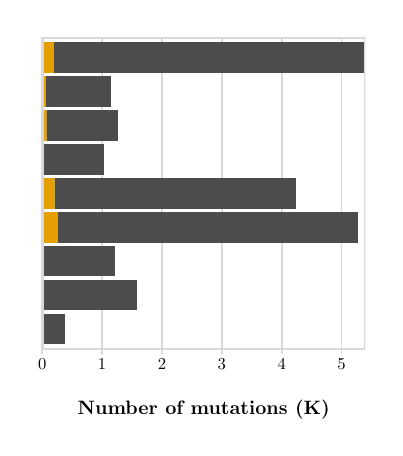
\begin{tikzpicture}[x=1pt,y=1pt]
\definecolor{fillColor}{RGB}{255,255,255}
\path[use as bounding box,fill=fillColor,fill opacity=0.00] (0,0) rectangle (125.50,144.54);
\begin{scope}
\path[clip] (  5.25, 28.30) rectangle (122.00,141.04);
\definecolor{drawColor}{gray}{0.85}

\path[draw=drawColor,line width= 0.6pt,line join=round] (  5.25, 28.30) --
	(  5.25,141.04);

\path[draw=drawColor,line width= 0.6pt,line join=round] ( 26.88, 28.30) --
	( 26.88,141.04);

\path[draw=drawColor,line width= 0.6pt,line join=round] ( 48.52, 28.30) --
	( 48.52,141.04);

\path[draw=drawColor,line width= 0.6pt,line join=round] ( 70.15, 28.30) --
	( 70.15,141.04);

\path[draw=drawColor,line width= 0.6pt,line join=round] ( 91.78, 28.30) --
	( 91.78,141.04);

\path[draw=drawColor,line width= 0.6pt,line join=round] (113.41, 28.30) --
	(113.41,141.04);
\definecolor{fillColor}{gray}{0.30}

\path[fill=fillColor] (  9.55,128.17) rectangle (122.00,139.20);
\definecolor{fillColor}{RGB}{230,159,0}

\path[fill=fillColor] (  5.25,128.17) rectangle (  9.55,139.20);
\definecolor{fillColor}{gray}{0.30}

\path[fill=fillColor] (  6.48,115.92) rectangle ( 29.95,126.95);
\definecolor{fillColor}{RGB}{230,159,0}

\path[fill=fillColor] (  5.25,115.92) rectangle (  6.48,126.95);
\definecolor{fillColor}{gray}{0.30}

\path[fill=fillColor] (  6.87,103.67) rectangle ( 32.66,114.69);
\definecolor{fillColor}{RGB}{230,159,0}

\path[fill=fillColor] (  5.25,103.67) rectangle (  6.87,114.69);
\definecolor{fillColor}{gray}{0.30}

\path[fill=fillColor] (  5.25, 91.41) rectangle ( 27.44,102.44);

\path[fill=fillColor] (  9.79, 79.16) rectangle ( 96.78, 90.19);
\definecolor{fillColor}{RGB}{230,159,0}

\path[fill=fillColor] (  5.25, 79.16) rectangle (  9.79, 90.19);
\definecolor{fillColor}{gray}{0.30}

\path[fill=fillColor] ( 10.96, 66.90) rectangle (119.47, 77.93);
\definecolor{fillColor}{RGB}{230,159,0}

\path[fill=fillColor] (  5.25, 66.90) rectangle ( 10.96, 77.93);
\definecolor{fillColor}{gray}{0.30}

\path[fill=fillColor] (  5.94, 54.65) rectangle ( 31.64, 65.68);
\definecolor{fillColor}{RGB}{230,159,0}

\path[fill=fillColor] (  5.25, 54.65) rectangle (  5.94, 65.68);
\definecolor{fillColor}{gray}{0.30}

\path[fill=fillColor] (  5.25, 42.40) rectangle ( 39.36, 53.42);

\path[fill=fillColor] (  5.47, 30.14) rectangle ( 13.32, 41.17);
\definecolor{fillColor}{RGB}{230,159,0}

\path[fill=fillColor] (  5.25, 30.14) rectangle (  5.47, 41.17);

\path[draw=drawColor,line width= 1.1pt,line join=round,line cap=round] (  5.25, 28.30) rectangle (122.00,141.04);
\end{scope}
\begin{scope}
\path[clip] (  0.00,  0.00) rectangle (125.50,144.54);
\definecolor{drawColor}{gray}{0.85}

\path[draw=drawColor,line width= 0.6pt,line join=round,line cap=rect] (  5.25, 28.30) --
	(  5.25,141.04);
\end{scope}
\begin{scope}
\path[clip] (  0.00,  0.00) rectangle (125.50,144.54);
\definecolor{drawColor}{gray}{0.85}

\path[draw=drawColor,line width= 0.6pt,line join=round] (  5.25, 26.55) --
	(  5.25, 28.30);

\path[draw=drawColor,line width= 0.6pt,line join=round] ( 26.88, 26.55) --
	( 26.88, 28.30);

\path[draw=drawColor,line width= 0.6pt,line join=round] ( 48.52, 26.55) --
	( 48.52, 28.30);

\path[draw=drawColor,line width= 0.6pt,line join=round] ( 70.15, 26.55) --
	( 70.15, 28.30);

\path[draw=drawColor,line width= 0.6pt,line join=round] ( 91.78, 26.55) --
	( 91.78, 28.30);

\path[draw=drawColor,line width= 0.6pt,line join=round] (113.41, 26.55) --
	(113.41, 28.30);
\end{scope}
\begin{scope}
\path[clip] (  0.00,  0.00) rectangle (125.50,144.54);
\definecolor{drawColor}{RGB}{0,0,0}

\node[text=drawColor,anchor=base,inner sep=0pt, outer sep=0pt, scale=  0.60] at (  5.25, 20.92) {0};

\node[text=drawColor,anchor=base,inner sep=0pt, outer sep=0pt, scale=  0.60] at ( 26.88, 20.92) {1};

\node[text=drawColor,anchor=base,inner sep=0pt, outer sep=0pt, scale=  0.60] at ( 48.52, 20.92) {2};

\node[text=drawColor,anchor=base,inner sep=0pt, outer sep=0pt, scale=  0.60] at ( 70.15, 20.92) {3};

\node[text=drawColor,anchor=base,inner sep=0pt, outer sep=0pt, scale=  0.60] at ( 91.78, 20.92) {4};

\node[text=drawColor,anchor=base,inner sep=0pt, outer sep=0pt, scale=  0.60] at (113.41, 20.92) {5};
\end{scope}
\begin{scope}
\path[clip] (  0.00,  0.00) rectangle (125.50,144.54);
\definecolor{drawColor}{RGB}{0,0,0}

\node[text=drawColor,anchor=base,inner sep=0pt, outer sep=0pt, scale=  0.70] at ( 63.63,  4.86) {\bfseries Number of mutations (K)};
\end{scope}
\end{tikzpicture}
}{\caption{}\label{subfig:datasets_abundancies}}%
		\end{subfloatrow}%
	}
	{\caption[Dataset distributions and number of mutations]{%
			\textbf{Dataset distributions and number of mutations.} Nine deep mutational scanning studies were used in this work.
			To make comparisons more meaningful, the fitness scores were scaled independently for each dataset to the range \numrange{0}{1} and centred such that a neutral mutation would have a scaled score of \num{0}.
			This scaling was only done for the visualizations and was not used in model development.
			\subref{subfig:fitness_score_distribution} Distribution of fitness scores.
			Orange crosses are synonymous mutations. Black crosses are outliers.
			\subref{subfig:datasets_abundancies} Number of mutations in each dataset (in thousands).
			The orange portion shows the number of synonymous mutations.
			The vertical axis is shared with \subref{subfig:fitness_score_distribution}.
			For a more detailed representation of the distribution of fitness scores see \autoref{sup:fig:score_distribution_by_dataset}.
		}}
\end{figure}

\thisfloatsetup{subfloatrowsep=larger}
\begin{figure}[p]
	\ffigbox{%
		\begin{subfloatrow}
			\ffigbox[\FBwidth]{% Created by tikzDevice version 0.12.3.1 on 2021-05-13 15:20:19
% !TEX encoding = UTF-8 Unicode
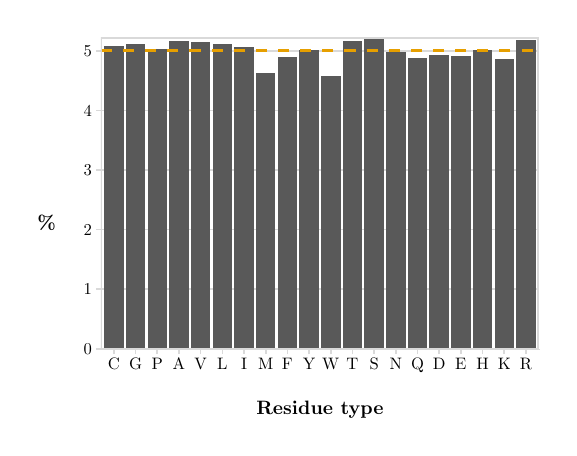
\begin{tikzpicture}[x=1pt,y=1pt]
\definecolor{fillColor}{RGB}{255,255,255}
\path[use as bounding box,fill=fillColor,fill opacity=0.00] (0,0) rectangle (188.25,144.54);
\begin{scope}
\path[clip] ( 26.46, 28.30) rectangle (184.75,141.04);
\definecolor{drawColor}{gray}{0.85}

\path[draw=drawColor,line width= 0.6pt,line join=round] ( 26.46, 28.53) --
	(184.75, 28.53);

\path[draw=drawColor,line width= 0.6pt,line join=round] ( 26.46, 50.06) --
	(184.75, 50.06);

\path[draw=drawColor,line width= 0.6pt,line join=round] ( 26.46, 71.59) --
	(184.75, 71.59);

\path[draw=drawColor,line width= 0.6pt,line join=round] ( 26.46, 93.12) --
	(184.75, 93.12);

\path[draw=drawColor,line width= 0.6pt,line join=round] ( 26.46,114.65) --
	(184.75,114.65);

\path[draw=drawColor,line width= 0.6pt,line join=round] ( 26.46,136.18) --
	(184.75,136.18);
\definecolor{fillColor}{gray}{0.35}

\path[fill=fillColor] ( 27.63, 28.53) rectangle ( 34.69,137.91);

\path[fill=fillColor] ( 35.47, 28.53) rectangle ( 42.52,138.61);

\path[fill=fillColor] ( 43.31, 28.53) rectangle ( 50.36,136.91);

\path[fill=fillColor] ( 51.14, 28.53) rectangle ( 58.20,139.61);

\path[fill=fillColor] ( 58.98, 28.53) rectangle ( 66.03,139.51);

\path[fill=fillColor] ( 66.81, 28.53) rectangle ( 73.87,138.61);

\path[fill=fillColor] ( 74.65, 28.53) rectangle ( 81.70,137.61);

\path[fill=fillColor] ( 82.49, 28.53) rectangle ( 89.54,128.31);

\path[fill=fillColor] ( 90.32, 28.53) rectangle ( 97.38,134.01);

\path[fill=fillColor] ( 98.16, 28.53) rectangle (105.21,136.41);

\path[fill=fillColor] (106.00, 28.53) rectangle (113.05,126.90);

\path[fill=fillColor] (113.83, 28.53) rectangle (120.89,139.81);

\path[fill=fillColor] (121.67, 28.53) rectangle (128.72,140.82);

\path[fill=fillColor] (129.51, 28.53) rectangle (136.56,135.71);

\path[fill=fillColor] (137.34, 28.53) rectangle (144.39,133.71);

\path[fill=fillColor] (145.18, 28.53) rectangle (152.23,134.51);

\path[fill=fillColor] (153.01, 28.53) rectangle (160.07,134.41);

\path[fill=fillColor] (160.85, 28.53) rectangle (167.90,136.61);

\path[fill=fillColor] (168.69, 28.53) rectangle (175.74,133.31);

\path[fill=fillColor] (176.52, 28.53) rectangle (183.58,140.21);
\definecolor{drawColor}{RGB}{230,159,0}

\path[draw=drawColor,line width= 1.1pt,dash pattern=on 4pt off 4pt ,line join=round] ( 26.46,136.18) -- (184.75,136.18);
\definecolor{drawColor}{gray}{0.85}

\path[draw=drawColor,line width= 1.1pt,line join=round,line cap=round] ( 26.46, 28.30) rectangle (184.75,141.04);
\end{scope}
\begin{scope}
\path[clip] (  0.00,  0.00) rectangle (188.25,144.54);
\definecolor{drawColor}{RGB}{0,0,0}

\node[text=drawColor,anchor=base east,inner sep=0pt, outer sep=0pt, scale=  0.60] at ( 23.21, 26.46) {0};

\node[text=drawColor,anchor=base east,inner sep=0pt, outer sep=0pt, scale=  0.60] at ( 23.21, 47.99) {1};

\node[text=drawColor,anchor=base east,inner sep=0pt, outer sep=0pt, scale=  0.60] at ( 23.21, 69.52) {2};

\node[text=drawColor,anchor=base east,inner sep=0pt, outer sep=0pt, scale=  0.60] at ( 23.21, 91.05) {3};

\node[text=drawColor,anchor=base east,inner sep=0pt, outer sep=0pt, scale=  0.60] at ( 23.21,112.58) {4};

\node[text=drawColor,anchor=base east,inner sep=0pt, outer sep=0pt, scale=  0.60] at ( 23.21,134.11) {5};
\end{scope}
\begin{scope}
\path[clip] (  0.00,  0.00) rectangle (188.25,144.54);
\definecolor{drawColor}{gray}{0.85}

\path[draw=drawColor,line width= 0.6pt,line join=round] ( 24.71, 28.53) --
	( 26.46, 28.53);

\path[draw=drawColor,line width= 0.6pt,line join=round] ( 24.71, 50.06) --
	( 26.46, 50.06);

\path[draw=drawColor,line width= 0.6pt,line join=round] ( 24.71, 71.59) --
	( 26.46, 71.59);

\path[draw=drawColor,line width= 0.6pt,line join=round] ( 24.71, 93.12) --
	( 26.46, 93.12);

\path[draw=drawColor,line width= 0.6pt,line join=round] ( 24.71,114.65) --
	( 26.46,114.65);

\path[draw=drawColor,line width= 0.6pt,line join=round] ( 24.71,136.18) --
	( 26.46,136.18);
\end{scope}
\begin{scope}
\path[clip] (  0.00,  0.00) rectangle (188.25,144.54);
\definecolor{drawColor}{gray}{0.85}

\path[draw=drawColor,line width= 0.6pt,line join=round,line cap=rect] ( 26.46, 28.30) --
	(184.75, 28.30);
\end{scope}
\begin{scope}
\path[clip] (  0.00,  0.00) rectangle (188.25,144.54);
\definecolor{drawColor}{gray}{0.85}

\path[draw=drawColor,line width= 0.6pt,line join=round] ( 31.16, 26.55) --
	( 31.16, 28.30);

\path[draw=drawColor,line width= 0.6pt,line join=round] ( 39.00, 26.55) --
	( 39.00, 28.30);

\path[draw=drawColor,line width= 0.6pt,line join=round] ( 46.83, 26.55) --
	( 46.83, 28.30);

\path[draw=drawColor,line width= 0.6pt,line join=round] ( 54.67, 26.55) --
	( 54.67, 28.30);

\path[draw=drawColor,line width= 0.6pt,line join=round] ( 62.50, 26.55) --
	( 62.50, 28.30);

\path[draw=drawColor,line width= 0.6pt,line join=round] ( 70.34, 26.55) --
	( 70.34, 28.30);

\path[draw=drawColor,line width= 0.6pt,line join=round] ( 78.18, 26.55) --
	( 78.18, 28.30);

\path[draw=drawColor,line width= 0.6pt,line join=round] ( 86.01, 26.55) --
	( 86.01, 28.30);

\path[draw=drawColor,line width= 0.6pt,line join=round] ( 93.85, 26.55) --
	( 93.85, 28.30);

\path[draw=drawColor,line width= 0.6pt,line join=round] (101.69, 26.55) --
	(101.69, 28.30);

\path[draw=drawColor,line width= 0.6pt,line join=round] (109.52, 26.55) --
	(109.52, 28.30);

\path[draw=drawColor,line width= 0.6pt,line join=round] (117.36, 26.55) --
	(117.36, 28.30);

\path[draw=drawColor,line width= 0.6pt,line join=round] (125.20, 26.55) --
	(125.20, 28.30);

\path[draw=drawColor,line width= 0.6pt,line join=round] (133.03, 26.55) --
	(133.03, 28.30);

\path[draw=drawColor,line width= 0.6pt,line join=round] (140.87, 26.55) --
	(140.87, 28.30);

\path[draw=drawColor,line width= 0.6pt,line join=round] (148.70, 26.55) --
	(148.70, 28.30);

\path[draw=drawColor,line width= 0.6pt,line join=round] (156.54, 26.55) --
	(156.54, 28.30);

\path[draw=drawColor,line width= 0.6pt,line join=round] (164.38, 26.55) --
	(164.38, 28.30);

\path[draw=drawColor,line width= 0.6pt,line join=round] (172.21, 26.55) --
	(172.21, 28.30);

\path[draw=drawColor,line width= 0.6pt,line join=round] (180.05, 26.55) --
	(180.05, 28.30);
\end{scope}
\begin{scope}
\path[clip] (  0.00,  0.00) rectangle (188.25,144.54);
\definecolor{drawColor}{RGB}{0,0,0}

\node[text=drawColor,anchor=base,inner sep=0pt, outer sep=0pt, scale=  0.60] at ( 31.16, 20.92) {C};

\node[text=drawColor,anchor=base,inner sep=0pt, outer sep=0pt, scale=  0.60] at ( 39.00, 20.92) {G};

\node[text=drawColor,anchor=base,inner sep=0pt, outer sep=0pt, scale=  0.60] at ( 46.83, 20.92) {P};

\node[text=drawColor,anchor=base,inner sep=0pt, outer sep=0pt, scale=  0.60] at ( 54.67, 20.92) {A};

\node[text=drawColor,anchor=base,inner sep=0pt, outer sep=0pt, scale=  0.60] at ( 62.50, 20.92) {V};

\node[text=drawColor,anchor=base,inner sep=0pt, outer sep=0pt, scale=  0.60] at ( 70.34, 20.92) {L};

\node[text=drawColor,anchor=base,inner sep=0pt, outer sep=0pt, scale=  0.60] at ( 78.18, 20.92) {I};

\node[text=drawColor,anchor=base,inner sep=0pt, outer sep=0pt, scale=  0.60] at ( 86.01, 20.92) {M};

\node[text=drawColor,anchor=base,inner sep=0pt, outer sep=0pt, scale=  0.60] at ( 93.85, 20.92) {F};

\node[text=drawColor,anchor=base,inner sep=0pt, outer sep=0pt, scale=  0.60] at (101.69, 20.92) {Y};

\node[text=drawColor,anchor=base,inner sep=0pt, outer sep=0pt, scale=  0.60] at (109.52, 20.92) {W};

\node[text=drawColor,anchor=base,inner sep=0pt, outer sep=0pt, scale=  0.60] at (117.36, 20.92) {T};

\node[text=drawColor,anchor=base,inner sep=0pt, outer sep=0pt, scale=  0.60] at (125.20, 20.92) {S};

\node[text=drawColor,anchor=base,inner sep=0pt, outer sep=0pt, scale=  0.60] at (133.03, 20.92) {N};

\node[text=drawColor,anchor=base,inner sep=0pt, outer sep=0pt, scale=  0.60] at (140.87, 20.92) {Q};

\node[text=drawColor,anchor=base,inner sep=0pt, outer sep=0pt, scale=  0.60] at (148.70, 20.92) {D};

\node[text=drawColor,anchor=base,inner sep=0pt, outer sep=0pt, scale=  0.60] at (156.54, 20.92) {E};

\node[text=drawColor,anchor=base,inner sep=0pt, outer sep=0pt, scale=  0.60] at (164.38, 20.92) {H};

\node[text=drawColor,anchor=base,inner sep=0pt, outer sep=0pt, scale=  0.60] at (172.21, 20.92) {K};

\node[text=drawColor,anchor=base,inner sep=0pt, outer sep=0pt, scale=  0.60] at (180.05, 20.92) {R};
\end{scope}
\begin{scope}
\path[clip] (  0.00,  0.00) rectangle (188.25,144.54);
\definecolor{drawColor}{RGB}{0,0,0}

\node[text=drawColor,anchor=base,inner sep=0pt, outer sep=0pt, scale=  0.70] at (105.60,  4.86) {\bfseries Residue type};
\end{scope}
\begin{scope}
\path[clip] (  0.00,  0.00) rectangle (188.25,144.54);
\definecolor{drawColor}{RGB}{0,0,0}

\node[text=drawColor,anchor=base,inner sep=0pt, outer sep=0pt, scale=  0.70] at (  6.85, 71.44) {\bfseries \%};
\end{scope}
\end{tikzpicture}
}{\caption{}\label{subfig:aa2_frequencies}}%
			\ffigbox[\FBwidth]{% Created by tikzDevice version 0.12.3.1 on 2021-05-09 13:07:35
% !TEX encoding = UTF-8 Unicode
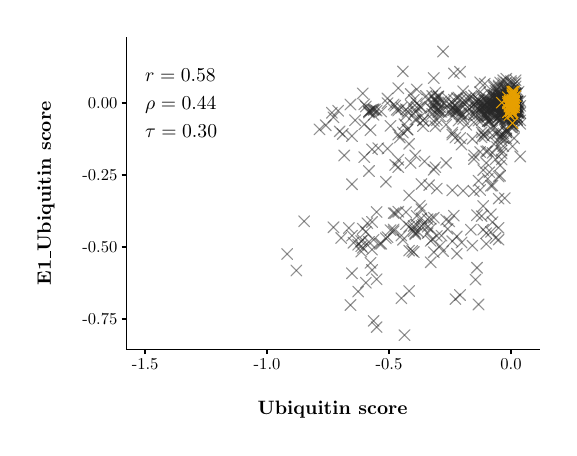
\begin{tikzpicture}[x=1pt,y=1pt]
\definecolor{fillColor}{RGB}{255,255,255}
\path[use as bounding box,fill=fillColor,fill opacity=0.00] (0,0) rectangle (188.25,144.54);
\begin{scope}
\path[clip] ( 35.67, 28.30) rectangle (184.75,141.04);
\definecolor{drawColor}{RGB}{38,38,38}

\path[draw=drawColor,draw opacity=0.50,line width= 0.4pt,line join=round,line cap=round] (148.13,133.95) -- (152.05,137.88);

\path[draw=drawColor,draw opacity=0.50,line width= 0.4pt,line join=round,line cap=round] (148.13,137.88) -- (152.05,133.95);

\path[draw=drawColor,draw opacity=0.50,line width= 0.4pt,line join=round,line cap=round] (133.63,126.77) -- (137.55,130.70);

\path[draw=drawColor,draw opacity=0.50,line width= 0.4pt,line join=round,line cap=round] (133.63,130.70) -- (137.55,126.77);

\path[draw=drawColor,draw opacity=0.50,line width= 0.4pt,line join=round,line cap=round] (154.26,126.64) -- (158.19,130.56);

\path[draw=drawColor,draw opacity=0.50,line width= 0.4pt,line join=round,line cap=round] (154.26,130.56) -- (158.19,126.64);

\path[draw=drawColor,draw opacity=0.50,line width= 0.4pt,line join=round,line cap=round] (152.03,126.06) -- (155.95,129.99);

\path[draw=drawColor,draw opacity=0.50,line width= 0.4pt,line join=round,line cap=round] (152.03,129.99) -- (155.95,126.06);

\path[draw=drawColor,draw opacity=0.50,line width= 0.4pt,line join=round,line cap=round] (119.12,118.84) -- (123.05,122.77);

\path[draw=drawColor,draw opacity=0.50,line width= 0.4pt,line join=round,line cap=round] (119.12,122.77) -- (123.05,118.84);

\path[draw=drawColor,draw opacity=0.50,line width= 0.4pt,line join=round,line cap=round] (122.47, 98.62) -- (126.40,102.54);

\path[draw=drawColor,draw opacity=0.50,line width= 0.4pt,line join=round,line cap=round] (122.47,102.54) -- (126.40, 98.62);

\path[draw=drawColor,draw opacity=0.50,line width= 0.4pt,line join=round,line cap=round] (144.78,124.37) -- (148.70,128.29);

\path[draw=drawColor,draw opacity=0.50,line width= 0.4pt,line join=round,line cap=round] (144.78,128.29) -- (148.70,124.37);

\path[draw=drawColor,draw opacity=0.50,line width= 0.4pt,line join=round,line cap=round] (167.09,119.76) -- (171.01,123.68);

\path[draw=drawColor,draw opacity=0.50,line width= 0.4pt,line join=round,line cap=round] (167.09,123.68) -- (171.01,119.76);

\path[draw=drawColor,draw opacity=0.50,line width= 0.4pt,line join=round,line cap=round] (161.51,119.32) -- (165.44,123.24);

\path[draw=drawColor,draw opacity=0.50,line width= 0.4pt,line join=round,line cap=round] (161.51,123.24) -- (165.44,119.32);

\path[draw=drawColor,draw opacity=0.50,line width= 0.4pt,line join=round,line cap=round] (168.20,117.21) -- (172.13,121.14);

\path[draw=drawColor,draw opacity=0.50,line width= 0.4pt,line join=round,line cap=round] (168.20,121.14) -- (172.13,117.21);

\path[draw=drawColor,draw opacity=0.50,line width= 0.4pt,line join=round,line cap=round] (164.86,116.72) -- (168.78,120.65);

\path[draw=drawColor,draw opacity=0.50,line width= 0.4pt,line join=round,line cap=round] (164.86,120.65) -- (168.78,116.72);

\path[draw=drawColor,draw opacity=0.50,line width= 0.4pt,line join=round,line cap=round] (159.84,116.29) -- (163.76,120.22);

\path[draw=drawColor,draw opacity=0.50,line width= 0.4pt,line join=round,line cap=round] (159.84,120.22) -- (163.76,116.29);

\path[draw=drawColor,draw opacity=0.50,line width= 0.4pt,line join=round,line cap=round] (172.67,115.88) -- (176.59,119.81);

\path[draw=drawColor,draw opacity=0.50,line width= 0.4pt,line join=round,line cap=round] (172.67,119.81) -- (176.59,115.88);

\path[draw=drawColor,draw opacity=0.50,line width= 0.4pt,line join=round,line cap=round] (169.88,114.97) -- (173.80,118.89);

\path[draw=drawColor,draw opacity=0.50,line width= 0.4pt,line join=round,line cap=round] (169.88,118.89) -- (173.80,114.97);

\path[draw=drawColor,draw opacity=0.50,line width= 0.4pt,line join=round,line cap=round] (174.34,114.57) -- (178.26,118.50);

\path[draw=drawColor,draw opacity=0.50,line width= 0.4pt,line join=round,line cap=round] (174.34,118.50) -- (178.26,114.57);

\path[draw=drawColor,draw opacity=0.50,line width= 0.4pt,line join=round,line cap=round] (155.38,114.05) -- (159.30,117.97);

\path[draw=drawColor,draw opacity=0.50,line width= 0.4pt,line join=round,line cap=round] (155.38,117.97) -- (159.30,114.05);

\path[draw=drawColor,draw opacity=0.50,line width= 0.4pt,line join=round,line cap=round] (153.15,113.50) -- (157.07,117.43);

\path[draw=drawColor,draw opacity=0.50,line width= 0.4pt,line join=round,line cap=round] (153.15,117.43) -- (157.07,113.50);

\path[draw=drawColor,draw opacity=0.50,line width= 0.4pt,line join=round,line cap=round] (169.88,113.48) -- (173.80,117.40);

\path[draw=drawColor,draw opacity=0.50,line width= 0.4pt,line join=round,line cap=round] (169.88,117.40) -- (173.80,113.48);

\path[draw=drawColor,draw opacity=0.50,line width= 0.4pt,line join=round,line cap=round] (168.76,113.13) -- (172.69,117.05);

\path[draw=drawColor,draw opacity=0.50,line width= 0.4pt,line join=round,line cap=round] (168.76,117.05) -- (172.69,113.13);

\path[draw=drawColor,draw opacity=0.50,line width= 0.4pt,line join=round,line cap=round] (166.53,112.98) -- (170.46,116.90);

\path[draw=drawColor,draw opacity=0.50,line width= 0.4pt,line join=round,line cap=round] (166.53,116.90) -- (170.46,112.98);

\path[draw=drawColor,draw opacity=0.50,line width= 0.4pt,line join=round,line cap=round] (165.42,112.73) -- (169.34,116.65);

\path[draw=drawColor,draw opacity=0.50,line width= 0.4pt,line join=round,line cap=round] (165.42,116.65) -- (169.34,112.73);

\path[draw=drawColor,draw opacity=0.50,line width= 0.4pt,line join=round,line cap=round] (159.84,112.56) -- (163.76,116.49);

\path[draw=drawColor,draw opacity=0.50,line width= 0.4pt,line join=round,line cap=round] (159.84,116.49) -- (163.76,112.56);

\path[draw=drawColor,draw opacity=0.50,line width= 0.4pt,line join=round,line cap=round] (147.01,112.27) -- (150.94,116.20);

\path[draw=drawColor,draw opacity=0.50,line width= 0.4pt,line join=round,line cap=round] (147.01,116.20) -- (150.94,112.27);

\path[draw=drawColor,draw opacity=0.50,line width= 0.4pt,line join=round,line cap=round] (170.99,124.14) -- (174.92,128.06);

\path[draw=drawColor,draw opacity=0.50,line width= 0.4pt,line join=round,line cap=round] (170.99,128.06) -- (174.92,124.14);

\path[draw=drawColor,draw opacity=0.50,line width= 0.4pt,line join=round,line cap=round] (172.11,118.42) -- (176.03,122.35);

\path[draw=drawColor,draw opacity=0.50,line width= 0.4pt,line join=round,line cap=round] (172.11,122.35) -- (176.03,118.42);

\path[draw=drawColor,draw opacity=0.50,line width= 0.4pt,line join=round,line cap=round] (167.65,118.38) -- (171.57,122.30);

\path[draw=drawColor,draw opacity=0.50,line width= 0.4pt,line join=round,line cap=round] (167.65,122.30) -- (171.57,118.38);

\path[draw=drawColor,draw opacity=0.50,line width= 0.4pt,line join=round,line cap=round] (169.32,118.12) -- (173.24,122.04);

\path[draw=drawColor,draw opacity=0.50,line width= 0.4pt,line join=round,line cap=round] (169.32,122.04) -- (173.24,118.12);

\path[draw=drawColor,draw opacity=0.50,line width= 0.4pt,line join=round,line cap=round] (174.34,117.82) -- (178.26,121.74);

\path[draw=drawColor,draw opacity=0.50,line width= 0.4pt,line join=round,line cap=round] (174.34,121.74) -- (178.26,117.82);

\path[draw=drawColor,draw opacity=0.50,line width= 0.4pt,line join=round,line cap=round] (173.78,117.18) -- (177.71,121.10);

\path[draw=drawColor,draw opacity=0.50,line width= 0.4pt,line join=round,line cap=round] (173.78,121.10) -- (177.71,117.18);

\path[draw=drawColor,draw opacity=0.50,line width= 0.4pt,line join=round,line cap=round] (173.78,116.97) -- (177.71,120.90);

\path[draw=drawColor,draw opacity=0.50,line width= 0.4pt,line join=round,line cap=round] (173.78,120.90) -- (177.71,116.97);

\path[draw=drawColor,draw opacity=0.50,line width= 0.4pt,line join=round,line cap=round] (173.78,116.92) -- (177.71,120.84);

\path[draw=drawColor,draw opacity=0.50,line width= 0.4pt,line join=round,line cap=round] (173.78,120.84) -- (177.71,116.92);

\path[draw=drawColor,draw opacity=0.50,line width= 0.4pt,line join=round,line cap=round] (174.34,116.26) -- (178.26,120.19);

\path[draw=drawColor,draw opacity=0.50,line width= 0.4pt,line join=round,line cap=round] (174.34,120.19) -- (178.26,116.26);

\path[draw=drawColor,draw opacity=0.50,line width= 0.4pt,line join=round,line cap=round] (173.22,116.03) -- (177.15,119.95);

\path[draw=drawColor,draw opacity=0.50,line width= 0.4pt,line join=round,line cap=round] (173.22,119.95) -- (177.15,116.03);

\path[draw=drawColor,draw opacity=0.50,line width= 0.4pt,line join=round,line cap=round] (174.34,115.97) -- (178.26,119.89);

\path[draw=drawColor,draw opacity=0.50,line width= 0.4pt,line join=round,line cap=round] (174.34,119.89) -- (178.26,115.97);

\path[draw=drawColor,draw opacity=0.50,line width= 0.4pt,line join=round,line cap=round] (174.90,115.87) -- (178.82,119.80);

\path[draw=drawColor,draw opacity=0.50,line width= 0.4pt,line join=round,line cap=round] (174.90,119.80) -- (178.82,115.87);

\path[draw=drawColor,draw opacity=0.50,line width= 0.4pt,line join=round,line cap=round] (174.34,115.86) -- (178.26,119.79);

\path[draw=drawColor,draw opacity=0.50,line width= 0.4pt,line join=round,line cap=round] (174.34,119.79) -- (178.26,115.86);

\path[draw=drawColor,draw opacity=0.50,line width= 0.4pt,line join=round,line cap=round] (174.90,115.86) -- (178.82,119.78);

\path[draw=drawColor,draw opacity=0.50,line width= 0.4pt,line join=round,line cap=round] (174.90,119.78) -- (178.82,115.86);

\path[draw=drawColor,draw opacity=0.50,line width= 0.4pt,line join=round,line cap=round] (173.78,115.79) -- (177.71,119.72);

\path[draw=drawColor,draw opacity=0.50,line width= 0.4pt,line join=round,line cap=round] (173.78,119.72) -- (177.71,115.79);

\path[draw=drawColor,draw opacity=0.50,line width= 0.4pt,line join=round,line cap=round] (173.22,115.39) -- (177.15,119.31);

\path[draw=drawColor,draw opacity=0.50,line width= 0.4pt,line join=round,line cap=round] (173.22,119.31) -- (177.15,115.39);

\path[draw=drawColor,draw opacity=0.50,line width= 0.4pt,line join=round,line cap=round] (174.34,114.67) -- (178.26,118.60);

\path[draw=drawColor,draw opacity=0.50,line width= 0.4pt,line join=round,line cap=round] (174.34,118.60) -- (178.26,114.67);

\path[draw=drawColor,draw opacity=0.50,line width= 0.4pt,line join=round,line cap=round] (173.22,113.90) -- (177.15,117.83);

\path[draw=drawColor,draw opacity=0.50,line width= 0.4pt,line join=round,line cap=round] (173.22,117.83) -- (177.15,113.90);

\path[draw=drawColor,draw opacity=0.50,line width= 0.4pt,line join=round,line cap=round] (174.90,112.45) -- (178.82,116.37);

\path[draw=drawColor,draw opacity=0.50,line width= 0.4pt,line join=round,line cap=round] (174.90,116.37) -- (178.82,112.45);

\path[draw=drawColor,draw opacity=0.50,line width= 0.4pt,line join=round,line cap=round] (169.88,123.58) -- (173.80,127.50);

\path[draw=drawColor,draw opacity=0.50,line width= 0.4pt,line join=round,line cap=round] (169.88,127.50) -- (173.80,123.58);

\path[draw=drawColor,draw opacity=0.50,line width= 0.4pt,line join=round,line cap=round] (131.95,120.71) -- (135.88,124.64);

\path[draw=drawColor,draw opacity=0.50,line width= 0.4pt,line join=round,line cap=round] (131.95,124.64) -- (135.88,120.71);

\path[draw=drawColor,draw opacity=0.50,line width= 0.4pt,line join=round,line cap=round] (138.64,120.29) -- (142.57,124.21);

\path[draw=drawColor,draw opacity=0.50,line width= 0.4pt,line join=round,line cap=round] (138.64,124.21) -- (142.57,120.29);

\path[draw=drawColor,draw opacity=0.50,line width= 0.4pt,line join=round,line cap=round] (136.41,118.66) -- (140.34,122.59);

\path[draw=drawColor,draw opacity=0.50,line width= 0.4pt,line join=round,line cap=round] (136.41,122.59) -- (140.34,118.66);

\path[draw=drawColor,draw opacity=0.50,line width= 0.4pt,line join=round,line cap=round] (168.76,118.08) -- (172.69,122.00);

\path[draw=drawColor,draw opacity=0.50,line width= 0.4pt,line join=round,line cap=round] (168.76,122.00) -- (172.69,118.08);

\path[draw=drawColor,draw opacity=0.50,line width= 0.4pt,line join=round,line cap=round] (141.99,117.87) -- (145.92,121.80);

\path[draw=drawColor,draw opacity=0.50,line width= 0.4pt,line join=round,line cap=round] (141.99,121.80) -- (145.92,117.87);

\path[draw=drawColor,draw opacity=0.50,line width= 0.4pt,line join=round,line cap=round] (145.90,117.54) -- (149.82,121.46);

\path[draw=drawColor,draw opacity=0.50,line width= 0.4pt,line join=round,line cap=round] (145.90,121.46) -- (149.82,117.54);

\path[draw=drawColor,draw opacity=0.50,line width= 0.4pt,line join=round,line cap=round] (153.70,117.32) -- (157.63,121.25);

\path[draw=drawColor,draw opacity=0.50,line width= 0.4pt,line join=round,line cap=round] (153.70,121.25) -- (157.63,117.32);

\path[draw=drawColor,draw opacity=0.50,line width= 0.4pt,line join=round,line cap=round] (153.15,117.08) -- (157.07,121.00);

\path[draw=drawColor,draw opacity=0.50,line width= 0.4pt,line join=round,line cap=round] (153.15,121.00) -- (157.07,117.08);

\path[draw=drawColor,draw opacity=0.50,line width= 0.4pt,line join=round,line cap=round] (156.49,117.04) -- (160.42,120.97);

\path[draw=drawColor,draw opacity=0.50,line width= 0.4pt,line join=round,line cap=round] (156.49,120.97) -- (160.42,117.04);

\path[draw=drawColor,draw opacity=0.50,line width= 0.4pt,line join=round,line cap=round] (128.05,117.00) -- (131.97,120.92);

\path[draw=drawColor,draw opacity=0.50,line width= 0.4pt,line join=round,line cap=round] (128.05,120.92) -- (131.97,117.00);

\path[draw=drawColor,draw opacity=0.50,line width= 0.4pt,line join=round,line cap=round] (137.53,116.46) -- (141.45,120.38);

\path[draw=drawColor,draw opacity=0.50,line width= 0.4pt,line join=round,line cap=round] (137.53,120.38) -- (141.45,116.46);

\path[draw=drawColor,draw opacity=0.50,line width= 0.4pt,line join=round,line cap=round] (151.47,115.28) -- (155.40,119.20);

\path[draw=drawColor,draw opacity=0.50,line width= 0.4pt,line join=round,line cap=round] (151.47,119.20) -- (155.40,115.28);

\path[draw=drawColor,draw opacity=0.50,line width= 0.4pt,line join=round,line cap=round] (133.07,113.65) -- (136.99,117.57);

\path[draw=drawColor,draw opacity=0.50,line width= 0.4pt,line join=round,line cap=round] (133.07,117.57) -- (136.99,113.65);

\path[draw=drawColor,draw opacity=0.50,line width= 0.4pt,line join=round,line cap=round] (125.82,112.24) -- (129.74,116.17);

\path[draw=drawColor,draw opacity=0.50,line width= 0.4pt,line join=round,line cap=round] (125.82,116.17) -- (129.74,112.24);

\path[draw=drawColor,draw opacity=0.50,line width= 0.4pt,line join=round,line cap=round] (174.34,123.58) -- (178.26,127.50);

\path[draw=drawColor,draw opacity=0.50,line width= 0.4pt,line join=round,line cap=round] (174.34,127.50) -- (178.26,123.58);

\path[draw=drawColor,draw opacity=0.50,line width= 0.4pt,line join=round,line cap=round] (172.67,123.28) -- (176.59,127.20);

\path[draw=drawColor,draw opacity=0.50,line width= 0.4pt,line join=round,line cap=round] (172.67,127.20) -- (176.59,123.28);

\path[draw=drawColor,draw opacity=0.50,line width= 0.4pt,line join=round,line cap=round] (170.99,122.78) -- (174.92,126.70);

\path[draw=drawColor,draw opacity=0.50,line width= 0.4pt,line join=round,line cap=round] (170.99,126.70) -- (174.92,122.78);

\path[draw=drawColor,draw opacity=0.50,line width= 0.4pt,line join=round,line cap=round] (172.67,122.56) -- (176.59,126.49);

\path[draw=drawColor,draw opacity=0.50,line width= 0.4pt,line join=round,line cap=round] (172.67,126.49) -- (176.59,122.56);

\path[draw=drawColor,draw opacity=0.50,line width= 0.4pt,line join=round,line cap=round] (166.53,121.09) -- (170.46,125.01);

\path[draw=drawColor,draw opacity=0.50,line width= 0.4pt,line join=round,line cap=round] (166.53,125.01) -- (170.46,121.09);

\path[draw=drawColor,draw opacity=0.50,line width= 0.4pt,line join=round,line cap=round] (172.67,120.77) -- (176.59,124.70);

\path[draw=drawColor,draw opacity=0.50,line width= 0.4pt,line join=round,line cap=round] (172.67,124.70) -- (176.59,120.77);

\path[draw=drawColor,draw opacity=0.50,line width= 0.4pt,line join=round,line cap=round] (172.11,120.14) -- (176.03,124.07);

\path[draw=drawColor,draw opacity=0.50,line width= 0.4pt,line join=round,line cap=round] (172.11,124.07) -- (176.03,120.14);

\path[draw=drawColor,draw opacity=0.50,line width= 0.4pt,line join=round,line cap=round] (172.11,119.75) -- (176.03,123.67);

\path[draw=drawColor,draw opacity=0.50,line width= 0.4pt,line join=round,line cap=round] (172.11,123.67) -- (176.03,119.75);

\path[draw=drawColor,draw opacity=0.50,line width= 0.4pt,line join=round,line cap=round] (174.34,118.82) -- (178.26,122.74);

\path[draw=drawColor,draw opacity=0.50,line width= 0.4pt,line join=round,line cap=round] (174.34,122.74) -- (178.26,118.82);

\path[draw=drawColor,draw opacity=0.50,line width= 0.4pt,line join=round,line cap=round] (172.11,118.64) -- (176.03,122.57);

\path[draw=drawColor,draw opacity=0.50,line width= 0.4pt,line join=round,line cap=round] (172.11,122.57) -- (176.03,118.64);

\path[draw=drawColor,draw opacity=0.50,line width= 0.4pt,line join=round,line cap=round] (174.34,118.50) -- (178.26,122.43);

\path[draw=drawColor,draw opacity=0.50,line width= 0.4pt,line join=round,line cap=round] (174.34,122.43) -- (178.26,118.50);

\path[draw=drawColor,draw opacity=0.50,line width= 0.4pt,line join=round,line cap=round] (172.67,118.35) -- (176.59,122.27);

\path[draw=drawColor,draw opacity=0.50,line width= 0.4pt,line join=round,line cap=round] (172.67,122.27) -- (176.59,118.35);

\path[draw=drawColor,draw opacity=0.50,line width= 0.4pt,line join=round,line cap=round] (170.99,118.07) -- (174.92,122.00);

\path[draw=drawColor,draw opacity=0.50,line width= 0.4pt,line join=round,line cap=round] (170.99,122.00) -- (174.92,118.07);

\path[draw=drawColor,draw opacity=0.50,line width= 0.4pt,line join=round,line cap=round] (172.67,117.84) -- (176.59,121.76);

\path[draw=drawColor,draw opacity=0.50,line width= 0.4pt,line join=round,line cap=round] (172.67,121.76) -- (176.59,117.84);

\path[draw=drawColor,draw opacity=0.50,line width= 0.4pt,line join=round,line cap=round] (173.22,116.76) -- (177.15,120.68);

\path[draw=drawColor,draw opacity=0.50,line width= 0.4pt,line join=round,line cap=round] (173.22,120.68) -- (177.15,116.76);

\path[draw=drawColor,draw opacity=0.50,line width= 0.4pt,line join=round,line cap=round] (172.11,116.62) -- (176.03,120.55);

\path[draw=drawColor,draw opacity=0.50,line width= 0.4pt,line join=round,line cap=round] (172.11,120.55) -- (176.03,116.62);

\path[draw=drawColor,draw opacity=0.50,line width= 0.4pt,line join=round,line cap=round] (173.22,116.32) -- (177.15,120.25);

\path[draw=drawColor,draw opacity=0.50,line width= 0.4pt,line join=round,line cap=round] (173.22,120.25) -- (177.15,116.32);

\path[draw=drawColor,draw opacity=0.50,line width= 0.4pt,line join=round,line cap=round] (173.22,116.29) -- (177.15,120.21);

\path[draw=drawColor,draw opacity=0.50,line width= 0.4pt,line join=round,line cap=round] (173.22,120.21) -- (177.15,116.29);

\path[draw=drawColor,draw opacity=0.50,line width= 0.4pt,line join=round,line cap=round] (173.78,115.34) -- (177.71,119.26);

\path[draw=drawColor,draw opacity=0.50,line width= 0.4pt,line join=round,line cap=round] (173.78,119.26) -- (177.71,115.34);

\path[draw=drawColor,draw opacity=0.50,line width= 0.4pt,line join=round,line cap=round] (161.51,122.88) -- (165.44,126.80);

\path[draw=drawColor,draw opacity=0.50,line width= 0.4pt,line join=round,line cap=round] (161.51,126.80) -- (165.44,122.88);

\path[draw=drawColor,draw opacity=0.50,line width= 0.4pt,line join=round,line cap=round] (163.18,122.37) -- (167.11,126.30);

\path[draw=drawColor,draw opacity=0.50,line width= 0.4pt,line join=round,line cap=round] (163.18,126.30) -- (167.11,122.37);

\path[draw=drawColor,draw opacity=0.50,line width= 0.4pt,line join=round,line cap=round] (166.53,121.78) -- (170.46,125.70);

\path[draw=drawColor,draw opacity=0.50,line width= 0.4pt,line join=round,line cap=round] (166.53,125.70) -- (170.46,121.78);

\path[draw=drawColor,draw opacity=0.50,line width= 0.4pt,line join=round,line cap=round] (167.65,120.13) -- (171.57,124.05);

\path[draw=drawColor,draw opacity=0.50,line width= 0.4pt,line join=round,line cap=round] (167.65,124.05) -- (171.57,120.13);

\path[draw=drawColor,draw opacity=0.50,line width= 0.4pt,line join=round,line cap=round] (168.76,118.46) -- (172.69,122.39);

\path[draw=drawColor,draw opacity=0.50,line width= 0.4pt,line join=round,line cap=round] (168.76,122.39) -- (172.69,118.46);

\path[draw=drawColor,draw opacity=0.50,line width= 0.4pt,line join=round,line cap=round] (165.97,117.71) -- (169.90,121.64);

\path[draw=drawColor,draw opacity=0.50,line width= 0.4pt,line join=round,line cap=round] (165.97,121.64) -- (169.90,117.71);

\path[draw=drawColor,draw opacity=0.50,line width= 0.4pt,line join=round,line cap=round] (157.61,117.12) -- (161.53,121.04);

\path[draw=drawColor,draw opacity=0.50,line width= 0.4pt,line join=round,line cap=round] (157.61,121.04) -- (161.53,117.12);

\path[draw=drawColor,draw opacity=0.50,line width= 0.4pt,line join=round,line cap=round] (167.65,116.87) -- (171.57,120.80);

\path[draw=drawColor,draw opacity=0.50,line width= 0.4pt,line join=round,line cap=round] (167.65,120.80) -- (171.57,116.87);

\path[draw=drawColor,draw opacity=0.50,line width= 0.4pt,line join=round,line cap=round] (173.22,116.52) -- (177.15,120.44);

\path[draw=drawColor,draw opacity=0.50,line width= 0.4pt,line join=round,line cap=round] (173.22,120.44) -- (177.15,116.52);

\path[draw=drawColor,draw opacity=0.50,line width= 0.4pt,line join=round,line cap=round] (160.95,116.43) -- (164.88,120.35);

\path[draw=drawColor,draw opacity=0.50,line width= 0.4pt,line join=round,line cap=round] (160.95,120.35) -- (164.88,116.43);

\path[draw=drawColor,draw opacity=0.50,line width= 0.4pt,line join=round,line cap=round] (163.18,116.33) -- (167.11,120.26);

\path[draw=drawColor,draw opacity=0.50,line width= 0.4pt,line join=round,line cap=round] (163.18,120.26) -- (167.11,116.33);

\path[draw=drawColor,draw opacity=0.50,line width= 0.4pt,line join=round,line cap=round] (165.97,115.71) -- (169.90,119.63);

\path[draw=drawColor,draw opacity=0.50,line width= 0.4pt,line join=round,line cap=round] (165.97,119.63) -- (169.90,115.71);

\path[draw=drawColor,draw opacity=0.50,line width= 0.4pt,line join=round,line cap=round] (165.97,115.40) -- (169.90,119.33);

\path[draw=drawColor,draw opacity=0.50,line width= 0.4pt,line join=round,line cap=round] (165.97,119.33) -- (169.90,115.40);

\path[draw=drawColor,draw opacity=0.50,line width= 0.4pt,line join=round,line cap=round] (160.95,115.29) -- (164.88,119.22);

\path[draw=drawColor,draw opacity=0.50,line width= 0.4pt,line join=round,line cap=round] (160.95,119.22) -- (164.88,115.29);

\path[draw=drawColor,draw opacity=0.50,line width= 0.4pt,line join=round,line cap=round] (165.42,115.24) -- (169.34,119.16);

\path[draw=drawColor,draw opacity=0.50,line width= 0.4pt,line join=round,line cap=round] (165.42,119.16) -- (169.34,115.24);

\path[draw=drawColor,draw opacity=0.50,line width= 0.4pt,line join=round,line cap=round] (159.84,115.08) -- (163.76,119.01);

\path[draw=drawColor,draw opacity=0.50,line width= 0.4pt,line join=round,line cap=round] (159.84,119.01) -- (163.76,115.08);

\path[draw=drawColor,draw opacity=0.50,line width= 0.4pt,line join=round,line cap=round] (167.09,113.63) -- (171.01,117.56);

\path[draw=drawColor,draw opacity=0.50,line width= 0.4pt,line join=round,line cap=round] (167.09,117.56) -- (171.01,113.63);

\path[draw=drawColor,draw opacity=0.50,line width= 0.4pt,line join=round,line cap=round] (132.51,102.86) -- (136.43,106.79);

\path[draw=drawColor,draw opacity=0.50,line width= 0.4pt,line join=round,line cap=round] (132.51,106.79) -- (136.43,102.86);

\path[draw=drawColor,draw opacity=0.50,line width= 0.4pt,line join=round,line cap=round] (168.76,122.76) -- (172.69,126.69);

\path[draw=drawColor,draw opacity=0.50,line width= 0.4pt,line join=round,line cap=round] (168.76,126.69) -- (172.69,122.76);

\path[draw=drawColor,draw opacity=0.50,line width= 0.4pt,line join=round,line cap=round] (169.88,118.63) -- (173.80,122.55);

\path[draw=drawColor,draw opacity=0.50,line width= 0.4pt,line join=round,line cap=round] (169.88,122.55) -- (173.80,118.63);

\path[draw=drawColor,draw opacity=0.50,line width= 0.4pt,line join=round,line cap=round] (168.76,117.87) -- (172.69,121.80);

\path[draw=drawColor,draw opacity=0.50,line width= 0.4pt,line join=round,line cap=round] (168.76,121.80) -- (172.69,117.87);

\path[draw=drawColor,draw opacity=0.50,line width= 0.4pt,line join=round,line cap=round] (169.88,116.46) -- (173.80,120.38);

\path[draw=drawColor,draw opacity=0.50,line width= 0.4pt,line join=round,line cap=round] (169.88,120.38) -- (173.80,116.46);

\path[draw=drawColor,draw opacity=0.50,line width= 0.4pt,line join=round,line cap=round] (170.44,115.49) -- (174.36,119.42);

\path[draw=drawColor,draw opacity=0.50,line width= 0.4pt,line join=round,line cap=round] (170.44,119.42) -- (174.36,115.49);

\path[draw=drawColor,draw opacity=0.50,line width= 0.4pt,line join=round,line cap=round] (169.88,114.20) -- (173.80,118.12);

\path[draw=drawColor,draw opacity=0.50,line width= 0.4pt,line join=round,line cap=round] (169.88,118.12) -- (173.80,114.20);

\path[draw=drawColor,draw opacity=0.50,line width= 0.4pt,line join=round,line cap=round] (169.88,113.97) -- (173.80,117.89);

\path[draw=drawColor,draw opacity=0.50,line width= 0.4pt,line join=round,line cap=round] (169.88,117.89) -- (173.80,113.97);

\path[draw=drawColor,draw opacity=0.50,line width= 0.4pt,line join=round,line cap=round] (174.34,122.53) -- (178.26,126.45);

\path[draw=drawColor,draw opacity=0.50,line width= 0.4pt,line join=round,line cap=round] (174.34,126.45) -- (178.26,122.53);

\path[draw=drawColor,draw opacity=0.50,line width= 0.4pt,line join=round,line cap=round] (169.88,122.50) -- (173.80,126.42);

\path[draw=drawColor,draw opacity=0.50,line width= 0.4pt,line join=round,line cap=round] (169.88,126.42) -- (173.80,122.50);

\path[draw=drawColor,draw opacity=0.50,line width= 0.4pt,line join=round,line cap=round] (174.34,121.32) -- (178.26,125.24);

\path[draw=drawColor,draw opacity=0.50,line width= 0.4pt,line join=round,line cap=round] (174.34,125.24) -- (178.26,121.32);

\path[draw=drawColor,draw opacity=0.50,line width= 0.4pt,line join=round,line cap=round] (175.45,119.47) -- (179.38,123.39);

\path[draw=drawColor,draw opacity=0.50,line width= 0.4pt,line join=round,line cap=round] (175.45,123.39) -- (179.38,119.47);

\path[draw=drawColor,draw opacity=0.50,line width= 0.4pt,line join=round,line cap=round] (171.55,119.05) -- (175.47,122.98);

\path[draw=drawColor,draw opacity=0.50,line width= 0.4pt,line join=round,line cap=round] (171.55,122.98) -- (175.47,119.05);

\path[draw=drawColor,draw opacity=0.50,line width= 0.4pt,line join=round,line cap=round] (174.90,118.80) -- (178.82,122.73);

\path[draw=drawColor,draw opacity=0.50,line width= 0.4pt,line join=round,line cap=round] (174.90,122.73) -- (178.82,118.80);

\path[draw=drawColor,draw opacity=0.50,line width= 0.4pt,line join=round,line cap=round] (170.99,118.28) -- (174.92,122.21);

\path[draw=drawColor,draw opacity=0.50,line width= 0.4pt,line join=round,line cap=round] (170.99,122.21) -- (174.92,118.28);

\path[draw=drawColor,draw opacity=0.50,line width= 0.4pt,line join=round,line cap=round] (172.67,117.55) -- (176.59,121.47);

\path[draw=drawColor,draw opacity=0.50,line width= 0.4pt,line join=round,line cap=round] (172.67,121.47) -- (176.59,117.55);

\path[draw=drawColor,draw opacity=0.50,line width= 0.4pt,line join=round,line cap=round] (173.78,116.37) -- (177.71,120.29);

\path[draw=drawColor,draw opacity=0.50,line width= 0.4pt,line join=round,line cap=round] (173.78,120.29) -- (177.71,116.37);

\path[draw=drawColor,draw opacity=0.50,line width= 0.4pt,line join=round,line cap=round] (171.55,116.36) -- (175.47,120.28);

\path[draw=drawColor,draw opacity=0.50,line width= 0.4pt,line join=round,line cap=round] (171.55,120.28) -- (175.47,116.36);

\path[draw=drawColor,draw opacity=0.50,line width= 0.4pt,line join=round,line cap=round] (170.99,116.29) -- (174.92,120.21);

\path[draw=drawColor,draw opacity=0.50,line width= 0.4pt,line join=round,line cap=round] (170.99,120.21) -- (174.92,116.29);

\path[draw=drawColor,draw opacity=0.50,line width= 0.4pt,line join=round,line cap=round] (171.55,116.16) -- (175.47,120.08);

\path[draw=drawColor,draw opacity=0.50,line width= 0.4pt,line join=round,line cap=round] (171.55,120.08) -- (175.47,116.16);

\path[draw=drawColor,draw opacity=0.50,line width= 0.4pt,line join=round,line cap=round] (172.67,115.49) -- (176.59,119.41);

\path[draw=drawColor,draw opacity=0.50,line width= 0.4pt,line join=round,line cap=round] (172.67,119.41) -- (176.59,115.49);

\path[draw=drawColor,draw opacity=0.50,line width= 0.4pt,line join=round,line cap=round] (171.55,115.47) -- (175.47,119.40);

\path[draw=drawColor,draw opacity=0.50,line width= 0.4pt,line join=round,line cap=round] (171.55,119.40) -- (175.47,115.47);

\path[draw=drawColor,draw opacity=0.50,line width= 0.4pt,line join=round,line cap=round] (172.67,115.00) -- (176.59,118.93);

\path[draw=drawColor,draw opacity=0.50,line width= 0.4pt,line join=round,line cap=round] (172.67,118.93) -- (176.59,115.00);

\path[draw=drawColor,draw opacity=0.50,line width= 0.4pt,line join=round,line cap=round] (173.78,113.58) -- (177.71,117.50);

\path[draw=drawColor,draw opacity=0.50,line width= 0.4pt,line join=round,line cap=round] (173.78,117.50) -- (177.71,113.58);

\path[draw=drawColor,draw opacity=0.50,line width= 0.4pt,line join=round,line cap=round] (172.11,110.26) -- (176.03,114.18);

\path[draw=drawColor,draw opacity=0.50,line width= 0.4pt,line join=round,line cap=round] (172.11,114.18) -- (176.03,110.26);

\path[draw=drawColor,draw opacity=0.50,line width= 0.4pt,line join=round,line cap=round] (165.97,105.55) -- (169.90,109.47);

\path[draw=drawColor,draw opacity=0.50,line width= 0.4pt,line join=round,line cap=round] (165.97,109.47) -- (169.90,105.55);

\path[draw=drawColor,draw opacity=0.50,line width= 0.4pt,line join=round,line cap=round] (120.24, 50.40) -- (124.16, 54.32);

\path[draw=drawColor,draw opacity=0.50,line width= 0.4pt,line join=round,line cap=round] (120.24, 54.32) -- (124.16, 50.40);

\path[draw=drawColor,draw opacity=0.50,line width= 0.4pt,line join=round,line cap=round] (173.78,122.04) -- (177.71,125.96);

\path[draw=drawColor,draw opacity=0.50,line width= 0.4pt,line join=round,line cap=round] (173.78,125.96) -- (177.71,122.04);

\path[draw=drawColor,draw opacity=0.50,line width= 0.4pt,line join=round,line cap=round] (173.78,120.03) -- (177.71,123.95);

\path[draw=drawColor,draw opacity=0.50,line width= 0.4pt,line join=round,line cap=round] (173.78,123.95) -- (177.71,120.03);

\path[draw=drawColor,draw opacity=0.50,line width= 0.4pt,line join=round,line cap=round] (173.22,119.92) -- (177.15,123.84);

\path[draw=drawColor,draw opacity=0.50,line width= 0.4pt,line join=round,line cap=round] (173.22,123.84) -- (177.15,119.92);

\path[draw=drawColor,draw opacity=0.50,line width= 0.4pt,line join=round,line cap=round] (173.22,118.20) -- (177.15,122.12);

\path[draw=drawColor,draw opacity=0.50,line width= 0.4pt,line join=round,line cap=round] (173.22,122.12) -- (177.15,118.20);

\path[draw=drawColor,draw opacity=0.50,line width= 0.4pt,line join=round,line cap=round] (173.78,117.63) -- (177.71,121.55);

\path[draw=drawColor,draw opacity=0.50,line width= 0.4pt,line join=round,line cap=round] (173.78,121.55) -- (177.71,117.63);

\path[draw=drawColor,draw opacity=0.50,line width= 0.4pt,line join=round,line cap=round] (173.78,117.28) -- (177.71,121.20);

\path[draw=drawColor,draw opacity=0.50,line width= 0.4pt,line join=round,line cap=round] (173.78,121.20) -- (177.71,117.28);

\path[draw=drawColor,draw opacity=0.50,line width= 0.4pt,line join=round,line cap=round] (173.22,116.95) -- (177.15,120.87);

\path[draw=drawColor,draw opacity=0.50,line width= 0.4pt,line join=round,line cap=round] (173.22,120.87) -- (177.15,116.95);

\path[draw=drawColor,draw opacity=0.50,line width= 0.4pt,line join=round,line cap=round] (173.78,116.89) -- (177.71,120.81);

\path[draw=drawColor,draw opacity=0.50,line width= 0.4pt,line join=round,line cap=round] (173.78,120.81) -- (177.71,116.89);

\path[draw=drawColor,draw opacity=0.50,line width= 0.4pt,line join=round,line cap=round] (173.78,116.53) -- (177.71,120.45);

\path[draw=drawColor,draw opacity=0.50,line width= 0.4pt,line join=round,line cap=round] (173.78,120.45) -- (177.71,116.53);

\path[draw=drawColor,draw opacity=0.50,line width= 0.4pt,line join=round,line cap=round] (173.78,116.42) -- (177.71,120.34);

\path[draw=drawColor,draw opacity=0.50,line width= 0.4pt,line join=round,line cap=round] (173.78,120.34) -- (177.71,116.42);

\path[draw=drawColor,draw opacity=0.50,line width= 0.4pt,line join=round,line cap=round] (172.11,116.22) -- (176.03,120.14);

\path[draw=drawColor,draw opacity=0.50,line width= 0.4pt,line join=round,line cap=round] (172.11,120.14) -- (176.03,116.22);

\path[draw=drawColor,draw opacity=0.50,line width= 0.4pt,line join=round,line cap=round] (173.78,116.19) -- (177.71,120.12);

\path[draw=drawColor,draw opacity=0.50,line width= 0.4pt,line join=round,line cap=round] (173.78,120.12) -- (177.71,116.19);

\path[draw=drawColor,draw opacity=0.50,line width= 0.4pt,line join=round,line cap=round] (170.99,116.15) -- (174.92,120.07);

\path[draw=drawColor,draw opacity=0.50,line width= 0.4pt,line join=round,line cap=round] (170.99,120.07) -- (174.92,116.15);

\path[draw=drawColor,draw opacity=0.50,line width= 0.4pt,line join=round,line cap=round] (171.55,115.41) -- (175.47,119.34);

\path[draw=drawColor,draw opacity=0.50,line width= 0.4pt,line join=round,line cap=round] (171.55,119.34) -- (175.47,115.41);

\path[draw=drawColor,draw opacity=0.50,line width= 0.4pt,line join=round,line cap=round] (173.78,114.66) -- (177.71,118.58);

\path[draw=drawColor,draw opacity=0.50,line width= 0.4pt,line join=round,line cap=round] (173.78,118.58) -- (177.71,114.66);

\path[draw=drawColor,draw opacity=0.50,line width= 0.4pt,line join=round,line cap=round] (173.78,114.59) -- (177.71,118.52);

\path[draw=drawColor,draw opacity=0.50,line width= 0.4pt,line join=round,line cap=round] (173.78,118.52) -- (177.71,114.59);

\path[draw=drawColor,draw opacity=0.50,line width= 0.4pt,line join=round,line cap=round] (173.78,114.58) -- (177.71,118.51);

\path[draw=drawColor,draw opacity=0.50,line width= 0.4pt,line join=round,line cap=round] (173.78,118.51) -- (177.71,114.58);

\path[draw=drawColor,draw opacity=0.50,line width= 0.4pt,line join=round,line cap=round] (169.88,113.98) -- (173.80,117.90);

\path[draw=drawColor,draw opacity=0.50,line width= 0.4pt,line join=round,line cap=round] (169.88,117.90) -- (173.80,113.98);

\path[draw=drawColor,draw opacity=0.50,line width= 0.4pt,line join=round,line cap=round] (173.78,113.87) -- (177.71,117.79);

\path[draw=drawColor,draw opacity=0.50,line width= 0.4pt,line join=round,line cap=round] (173.78,117.79) -- (177.71,113.87);

\path[draw=drawColor,draw opacity=0.50,line width= 0.4pt,line join=round,line cap=round] (168.20,121.66) -- (172.13,125.59);

\path[draw=drawColor,draw opacity=0.50,line width= 0.4pt,line join=round,line cap=round] (168.20,125.59) -- (172.13,121.66);

\path[draw=drawColor,draw opacity=0.50,line width= 0.4pt,line join=round,line cap=round] (170.99,114.95) -- (174.92,118.87);

\path[draw=drawColor,draw opacity=0.50,line width= 0.4pt,line join=round,line cap=round] (170.99,118.87) -- (174.92,114.95);

\path[draw=drawColor,draw opacity=0.50,line width= 0.4pt,line join=round,line cap=round] (169.88,114.42) -- (173.80,118.34);

\path[draw=drawColor,draw opacity=0.50,line width= 0.4pt,line join=round,line cap=round] (169.88,118.34) -- (173.80,114.42);

\path[draw=drawColor,draw opacity=0.50,line width= 0.4pt,line join=round,line cap=round] (171.55,113.23) -- (175.47,117.16);

\path[draw=drawColor,draw opacity=0.50,line width= 0.4pt,line join=round,line cap=round] (171.55,117.16) -- (175.47,113.23);

\path[draw=drawColor,draw opacity=0.50,line width= 0.4pt,line join=round,line cap=round] (170.44,112.18) -- (174.36,116.10);

\path[draw=drawColor,draw opacity=0.50,line width= 0.4pt,line join=round,line cap=round] (170.44,116.10) -- (174.36,112.18);

\path[draw=drawColor,draw opacity=0.50,line width= 0.4pt,line join=round,line cap=round] (165.97,111.18) -- (169.90,115.11);

\path[draw=drawColor,draw opacity=0.50,line width= 0.4pt,line join=round,line cap=round] (165.97,115.11) -- (169.90,111.18);

\path[draw=drawColor,draw opacity=0.50,line width= 0.4pt,line join=round,line cap=round] (164.86,108.88) -- (168.78,112.80);

\path[draw=drawColor,draw opacity=0.50,line width= 0.4pt,line join=round,line cap=round] (164.86,112.80) -- (168.78,108.88);

\path[draw=drawColor,draw opacity=0.50,line width= 0.4pt,line join=round,line cap=round] (164.30,108.85) -- (168.22,112.78);

\path[draw=drawColor,draw opacity=0.50,line width= 0.4pt,line join=round,line cap=round] (164.30,112.78) -- (168.22,108.85);

\path[draw=drawColor,draw opacity=0.50,line width= 0.4pt,line join=round,line cap=round] (122.47, 72.38) -- (126.40, 76.31);

\path[draw=drawColor,draw opacity=0.50,line width= 0.4pt,line join=round,line cap=round] (122.47, 76.31) -- (126.40, 72.38);

\path[draw=drawColor,draw opacity=0.50,line width= 0.4pt,line join=round,line cap=round] (111.32, 66.59) -- (115.24, 70.52);

\path[draw=drawColor,draw opacity=0.50,line width= 0.4pt,line join=round,line cap=round] (111.32, 70.52) -- (115.24, 66.59);

\path[draw=drawColor,draw opacity=0.50,line width= 0.4pt,line join=round,line cap=round] (144.22, 66.10) -- (148.15, 70.02);

\path[draw=drawColor,draw opacity=0.50,line width= 0.4pt,line join=round,line cap=round] (144.22, 70.02) -- (148.15, 66.10);

\path[draw=drawColor,draw opacity=0.50,line width= 0.4pt,line join=round,line cap=round] (168.20,121.23) -- (172.13,125.15);

\path[draw=drawColor,draw opacity=0.50,line width= 0.4pt,line join=round,line cap=round] (168.20,125.15) -- (172.13,121.23);

\path[draw=drawColor,draw opacity=0.50,line width= 0.4pt,line join=round,line cap=round] (172.11,118.65) -- (176.03,122.57);

\path[draw=drawColor,draw opacity=0.50,line width= 0.4pt,line join=round,line cap=round] (172.11,122.57) -- (176.03,118.65);

\path[draw=drawColor,draw opacity=0.50,line width= 0.4pt,line join=round,line cap=round] (149.80,117.03) -- (153.72,120.96);

\path[draw=drawColor,draw opacity=0.50,line width= 0.4pt,line join=round,line cap=round] (149.80,120.96) -- (153.72,117.03);

\path[draw=drawColor,draw opacity=0.50,line width= 0.4pt,line join=round,line cap=round] (142.55,116.62) -- (146.47,120.54);

\path[draw=drawColor,draw opacity=0.50,line width= 0.4pt,line join=round,line cap=round] (142.55,120.54) -- (146.47,116.62);

\path[draw=drawColor,draw opacity=0.50,line width= 0.4pt,line join=round,line cap=round] (154.26,116.44) -- (158.19,120.36);

\path[draw=drawColor,draw opacity=0.50,line width= 0.4pt,line join=round,line cap=round] (154.26,120.36) -- (158.19,116.44);

\path[draw=drawColor,draw opacity=0.50,line width= 0.4pt,line join=round,line cap=round] (121.36,111.86) -- (125.28,115.78);

\path[draw=drawColor,draw opacity=0.50,line width= 0.4pt,line join=round,line cap=round] (121.36,115.78) -- (125.28,111.86);

\path[draw=drawColor,draw opacity=0.50,line width= 0.4pt,line join=round,line cap=round] (141.43, 94.27) -- (145.36, 98.20);

\path[draw=drawColor,draw opacity=0.50,line width= 0.4pt,line join=round,line cap=round] (141.43, 98.20) -- (145.36, 94.27);

\path[draw=drawColor,draw opacity=0.50,line width= 0.4pt,line join=round,line cap=round] (172.11,120.80) -- (176.03,124.72);

\path[draw=drawColor,draw opacity=0.50,line width= 0.4pt,line join=round,line cap=round] (172.11,124.72) -- (176.03,120.80);

\path[draw=drawColor,draw opacity=0.50,line width= 0.4pt,line join=round,line cap=round] (169.88,120.76) -- (173.80,124.69);

\path[draw=drawColor,draw opacity=0.50,line width= 0.4pt,line join=round,line cap=round] (169.88,124.69) -- (173.80,120.76);

\path[draw=drawColor,draw opacity=0.50,line width= 0.4pt,line join=round,line cap=round] (170.44,120.62) -- (174.36,124.55);

\path[draw=drawColor,draw opacity=0.50,line width= 0.4pt,line join=round,line cap=round] (170.44,124.55) -- (174.36,120.62);

\path[draw=drawColor,draw opacity=0.50,line width= 0.4pt,line join=round,line cap=round] (171.55,119.25) -- (175.47,123.18);

\path[draw=drawColor,draw opacity=0.50,line width= 0.4pt,line join=round,line cap=round] (171.55,123.18) -- (175.47,119.25);

\path[draw=drawColor,draw opacity=0.50,line width= 0.4pt,line join=round,line cap=round] (164.86,119.00) -- (168.78,122.93);

\path[draw=drawColor,draw opacity=0.50,line width= 0.4pt,line join=round,line cap=round] (164.86,122.93) -- (168.78,119.00);

\path[draw=drawColor,draw opacity=0.50,line width= 0.4pt,line join=round,line cap=round] (174.34,118.55) -- (178.26,122.47);

\path[draw=drawColor,draw opacity=0.50,line width= 0.4pt,line join=round,line cap=round] (174.34,122.47) -- (178.26,118.55);

\path[draw=drawColor,draw opacity=0.50,line width= 0.4pt,line join=round,line cap=round] (169.32,116.98) -- (173.24,120.91);

\path[draw=drawColor,draw opacity=0.50,line width= 0.4pt,line join=round,line cap=round] (169.32,120.91) -- (173.24,116.98);

\path[draw=drawColor,draw opacity=0.50,line width= 0.4pt,line join=round,line cap=round] (145.34,115.88) -- (149.26,119.80);

\path[draw=drawColor,draw opacity=0.50,line width= 0.4pt,line join=round,line cap=round] (145.34,119.80) -- (149.26,115.88);

\path[draw=drawColor,draw opacity=0.50,line width= 0.4pt,line join=round,line cap=round] (170.99,115.74) -- (174.92,119.66);

\path[draw=drawColor,draw opacity=0.50,line width= 0.4pt,line join=round,line cap=round] (170.99,119.66) -- (174.92,115.74);

\path[draw=drawColor,draw opacity=0.50,line width= 0.4pt,line join=round,line cap=round] (170.99,113.78) -- (174.92,117.70);

\path[draw=drawColor,draw opacity=0.50,line width= 0.4pt,line join=round,line cap=round] (170.99,117.70) -- (174.92,113.78);

\path[draw=drawColor,draw opacity=0.50,line width= 0.4pt,line join=round,line cap=round] (160.40,113.53) -- (164.32,117.45);

\path[draw=drawColor,draw opacity=0.50,line width= 0.4pt,line join=round,line cap=round] (160.40,117.45) -- (164.32,113.53);

\path[draw=drawColor,draw opacity=0.50,line width= 0.4pt,line join=round,line cap=round] (151.47,112.72) -- (155.40,116.64);

\path[draw=drawColor,draw opacity=0.50,line width= 0.4pt,line join=round,line cap=round] (151.47,116.64) -- (155.40,112.72);

\path[draw=drawColor,draw opacity=0.50,line width= 0.4pt,line join=round,line cap=round] (169.32,112.26) -- (173.24,116.18);

\path[draw=drawColor,draw opacity=0.50,line width= 0.4pt,line join=round,line cap=round] (169.32,116.18) -- (173.24,112.26);

\path[draw=drawColor,draw opacity=0.50,line width= 0.4pt,line join=round,line cap=round] (168.76,110.79) -- (172.69,114.71);

\path[draw=drawColor,draw opacity=0.50,line width= 0.4pt,line join=round,line cap=round] (168.76,114.71) -- (172.69,110.79);

\path[draw=drawColor,draw opacity=0.50,line width= 0.4pt,line join=round,line cap=round] (163.74,110.28) -- (167.67,114.20);

\path[draw=drawColor,draw opacity=0.50,line width= 0.4pt,line join=round,line cap=round] (163.74,114.20) -- (167.67,110.28);

\path[draw=drawColor,draw opacity=0.50,line width= 0.4pt,line join=round,line cap=round] (170.44,109.67) -- (174.36,113.59);

\path[draw=drawColor,draw opacity=0.50,line width= 0.4pt,line join=round,line cap=round] (170.44,113.59) -- (174.36,109.67);

\path[draw=drawColor,draw opacity=0.50,line width= 0.4pt,line join=round,line cap=round] (173.22,109.08) -- (177.15,113.01);

\path[draw=drawColor,draw opacity=0.50,line width= 0.4pt,line join=round,line cap=round] (173.22,113.01) -- (177.15,109.08);

\path[draw=drawColor,draw opacity=0.50,line width= 0.4pt,line join=round,line cap=round] (169.32, 98.21) -- (173.24,102.13);

\path[draw=drawColor,draw opacity=0.50,line width= 0.4pt,line join=round,line cap=round] (169.32,102.13) -- (173.24, 98.21);

\path[draw=drawColor,draw opacity=0.50,line width= 0.4pt,line join=round,line cap=round] (176.01, 96.04) -- (179.94, 99.97);

\path[draw=drawColor,draw opacity=0.50,line width= 0.4pt,line join=round,line cap=round] (176.01, 99.97) -- (179.94, 96.04);

\path[draw=drawColor,draw opacity=0.50,line width= 0.4pt,line join=round,line cap=round] (173.22,117.63) -- (177.15,121.56);

\path[draw=drawColor,draw opacity=0.50,line width= 0.4pt,line join=round,line cap=round] (173.22,121.56) -- (177.15,117.63);

\path[draw=drawColor,draw opacity=0.50,line width= 0.4pt,line join=round,line cap=round] (163.74,117.27) -- (167.67,121.20);

\path[draw=drawColor,draw opacity=0.50,line width= 0.4pt,line join=round,line cap=round] (163.74,121.20) -- (167.67,117.27);

\path[draw=drawColor,draw opacity=0.50,line width= 0.4pt,line join=round,line cap=round] (172.67,116.70) -- (176.59,120.62);

\path[draw=drawColor,draw opacity=0.50,line width= 0.4pt,line join=round,line cap=round] (172.67,120.62) -- (176.59,116.70);

\path[draw=drawColor,draw opacity=0.50,line width= 0.4pt,line join=round,line cap=round] (163.74,116.46) -- (167.67,120.38);

\path[draw=drawColor,draw opacity=0.50,line width= 0.4pt,line join=round,line cap=round] (163.74,120.38) -- (167.67,116.46);

\path[draw=drawColor,draw opacity=0.50,line width= 0.4pt,line join=round,line cap=round] (151.47,113.76) -- (155.40,117.68);

\path[draw=drawColor,draw opacity=0.50,line width= 0.4pt,line join=round,line cap=round] (151.47,117.68) -- (155.40,113.76);

\path[draw=drawColor,draw opacity=0.50,line width= 0.4pt,line join=round,line cap=round] (172.67,113.41) -- (176.59,117.33);

\path[draw=drawColor,draw opacity=0.50,line width= 0.4pt,line join=round,line cap=round] (172.67,117.33) -- (176.59,113.41);

\path[draw=drawColor,draw opacity=0.50,line width= 0.4pt,line join=round,line cap=round] (145.34,113.24) -- (149.26,117.17);

\path[draw=drawColor,draw opacity=0.50,line width= 0.4pt,line join=round,line cap=round] (145.34,117.17) -- (149.26,113.24);

\path[draw=drawColor,draw opacity=0.50,line width= 0.4pt,line join=round,line cap=round] (170.99,113.19) -- (174.92,117.11);

\path[draw=drawColor,draw opacity=0.50,line width= 0.4pt,line join=round,line cap=round] (170.99,117.11) -- (174.92,113.19);

\path[draw=drawColor,draw opacity=0.50,line width= 0.4pt,line join=round,line cap=round] (172.11,112.28) -- (176.03,116.21);

\path[draw=drawColor,draw opacity=0.50,line width= 0.4pt,line join=round,line cap=round] (172.11,116.21) -- (176.03,112.28);

\path[draw=drawColor,draw opacity=0.50,line width= 0.4pt,line join=round,line cap=round] (144.22,111.39) -- (148.15,115.32);

\path[draw=drawColor,draw opacity=0.50,line width= 0.4pt,line join=round,line cap=round] (144.22,115.32) -- (148.15,111.39);

\path[draw=drawColor,draw opacity=0.50,line width= 0.4pt,line join=round,line cap=round] (170.99,120.39) -- (174.92,124.32);

\path[draw=drawColor,draw opacity=0.50,line width= 0.4pt,line join=round,line cap=round] (170.99,124.32) -- (174.92,120.39);

\path[draw=drawColor,draw opacity=0.50,line width= 0.4pt,line join=round,line cap=round] (170.99,119.77) -- (174.92,123.69);

\path[draw=drawColor,draw opacity=0.50,line width= 0.4pt,line join=round,line cap=round] (170.99,123.69) -- (174.92,119.77);

\path[draw=drawColor,draw opacity=0.50,line width= 0.4pt,line join=round,line cap=round] (155.38,119.64) -- (159.30,123.56);

\path[draw=drawColor,draw opacity=0.50,line width= 0.4pt,line join=round,line cap=round] (155.38,123.56) -- (159.30,119.64);

\path[draw=drawColor,draw opacity=0.50,line width= 0.4pt,line join=round,line cap=round] (173.22,119.22) -- (177.15,123.15);

\path[draw=drawColor,draw opacity=0.50,line width= 0.4pt,line join=round,line cap=round] (173.22,123.15) -- (177.15,119.22);

\path[draw=drawColor,draw opacity=0.50,line width= 0.4pt,line join=round,line cap=round] (150.36,115.01) -- (154.28,118.94);

\path[draw=drawColor,draw opacity=0.50,line width= 0.4pt,line join=round,line cap=round] (150.36,118.94) -- (154.28,115.01);

\path[draw=drawColor,draw opacity=0.50,line width= 0.4pt,line join=round,line cap=round] (172.67,113.76) -- (176.59,117.68);

\path[draw=drawColor,draw opacity=0.50,line width= 0.4pt,line join=round,line cap=round] (172.67,117.68) -- (176.59,113.76);

\path[draw=drawColor,draw opacity=0.50,line width= 0.4pt,line join=round,line cap=round] (171.55,113.53) -- (175.47,117.45);

\path[draw=drawColor,draw opacity=0.50,line width= 0.4pt,line join=round,line cap=round] (171.55,117.45) -- (175.47,113.53);

\path[draw=drawColor,draw opacity=0.50,line width= 0.4pt,line join=round,line cap=round] (135.30,112.21) -- (139.22,116.13);

\path[draw=drawColor,draw opacity=0.50,line width= 0.4pt,line join=round,line cap=round] (135.30,116.13) -- (139.22,112.21);

\path[draw=drawColor,draw opacity=0.50,line width= 0.4pt,line join=round,line cap=round] (140.88,109.19) -- (144.80,113.11);

\path[draw=drawColor,draw opacity=0.50,line width= 0.4pt,line join=round,line cap=round] (140.88,113.11) -- (144.80,109.19);

\path[draw=drawColor,draw opacity=0.50,line width= 0.4pt,line join=round,line cap=round] (173.22,120.16) -- (177.15,124.08);

\path[draw=drawColor,draw opacity=0.50,line width= 0.4pt,line join=round,line cap=round] (173.22,124.08) -- (177.15,120.16);

\path[draw=drawColor,draw opacity=0.50,line width= 0.4pt,line join=round,line cap=round] (173.78,118.93) -- (177.71,122.86);

\path[draw=drawColor,draw opacity=0.50,line width= 0.4pt,line join=round,line cap=round] (173.78,122.86) -- (177.71,118.93);

\path[draw=drawColor,draw opacity=0.50,line width= 0.4pt,line join=round,line cap=round] (168.20,118.33) -- (172.13,122.25);

\path[draw=drawColor,draw opacity=0.50,line width= 0.4pt,line join=round,line cap=round] (168.20,122.25) -- (172.13,118.33);

\path[draw=drawColor,draw opacity=0.50,line width= 0.4pt,line join=round,line cap=round] (173.78,118.27) -- (177.71,122.20);

\path[draw=drawColor,draw opacity=0.50,line width= 0.4pt,line join=round,line cap=round] (173.78,122.20) -- (177.71,118.27);

\path[draw=drawColor,draw opacity=0.50,line width= 0.4pt,line join=round,line cap=round] (173.78,116.78) -- (177.71,120.70);

\path[draw=drawColor,draw opacity=0.50,line width= 0.4pt,line join=round,line cap=round] (173.78,120.70) -- (177.71,116.78);

\path[draw=drawColor,draw opacity=0.50,line width= 0.4pt,line join=round,line cap=round] (173.78,116.68) -- (177.71,120.60);

\path[draw=drawColor,draw opacity=0.50,line width= 0.4pt,line join=round,line cap=round] (173.78,120.60) -- (177.71,116.68);

\path[draw=drawColor,draw opacity=0.50,line width= 0.4pt,line join=round,line cap=round] (173.22,116.34) -- (177.15,120.26);

\path[draw=drawColor,draw opacity=0.50,line width= 0.4pt,line join=round,line cap=round] (173.22,120.26) -- (177.15,116.34);

\path[draw=drawColor,draw opacity=0.50,line width= 0.4pt,line join=round,line cap=round] (174.34,115.66) -- (178.26,119.59);

\path[draw=drawColor,draw opacity=0.50,line width= 0.4pt,line join=round,line cap=round] (174.34,119.59) -- (178.26,115.66);

\path[draw=drawColor,draw opacity=0.50,line width= 0.4pt,line join=round,line cap=round] (172.67,115.49) -- (176.59,119.41);

\path[draw=drawColor,draw opacity=0.50,line width= 0.4pt,line join=round,line cap=round] (172.67,119.41) -- (176.59,115.49);

\path[draw=drawColor,draw opacity=0.50,line width= 0.4pt,line join=round,line cap=round] (172.67,115.36) -- (176.59,119.28);

\path[draw=drawColor,draw opacity=0.50,line width= 0.4pt,line join=round,line cap=round] (172.67,119.28) -- (176.59,115.36);

\path[draw=drawColor,draw opacity=0.50,line width= 0.4pt,line join=round,line cap=round] (168.76,115.32) -- (172.69,119.25);

\path[draw=drawColor,draw opacity=0.50,line width= 0.4pt,line join=round,line cap=round] (168.76,119.25) -- (172.69,115.32);

\path[draw=drawColor,draw opacity=0.50,line width= 0.4pt,line join=round,line cap=round] (173.22,115.17) -- (177.15,119.10);

\path[draw=drawColor,draw opacity=0.50,line width= 0.4pt,line join=round,line cap=round] (173.22,119.10) -- (177.15,115.17);

\path[draw=drawColor,draw opacity=0.50,line width= 0.4pt,line join=round,line cap=round] (172.11,115.17) -- (176.03,119.10);

\path[draw=drawColor,draw opacity=0.50,line width= 0.4pt,line join=round,line cap=round] (172.11,119.10) -- (176.03,115.17);

\path[draw=drawColor,draw opacity=0.50,line width= 0.4pt,line join=round,line cap=round] (173.78,114.57) -- (177.71,118.49);

\path[draw=drawColor,draw opacity=0.50,line width= 0.4pt,line join=round,line cap=round] (173.78,118.49) -- (177.71,114.57);

\path[draw=drawColor,draw opacity=0.50,line width= 0.4pt,line join=round,line cap=round] (172.11,114.49) -- (176.03,118.41);

\path[draw=drawColor,draw opacity=0.50,line width= 0.4pt,line join=round,line cap=round] (172.11,118.41) -- (176.03,114.49);

\path[draw=drawColor,draw opacity=0.50,line width= 0.4pt,line join=round,line cap=round] (173.22,114.45) -- (177.15,118.38);

\path[draw=drawColor,draw opacity=0.50,line width= 0.4pt,line join=round,line cap=round] (173.22,118.38) -- (177.15,114.45);

\path[draw=drawColor,draw opacity=0.50,line width= 0.4pt,line join=round,line cap=round] (173.22,114.42) -- (177.15,118.34);

\path[draw=drawColor,draw opacity=0.50,line width= 0.4pt,line join=round,line cap=round] (173.22,118.34) -- (177.15,114.42);

\path[draw=drawColor,draw opacity=0.50,line width= 0.4pt,line join=round,line cap=round] (172.11,114.40) -- (176.03,118.32);

\path[draw=drawColor,draw opacity=0.50,line width= 0.4pt,line join=round,line cap=round] (172.11,118.32) -- (176.03,114.40);

\path[draw=drawColor,draw opacity=0.50,line width= 0.4pt,line join=round,line cap=round] (172.67,111.34) -- (176.59,115.27);

\path[draw=drawColor,draw opacity=0.50,line width= 0.4pt,line join=round,line cap=round] (172.67,115.27) -- (176.59,111.34);

\path[draw=drawColor,draw opacity=0.50,line width= 0.4pt,line join=round,line cap=round] (172.11,114.28) -- (176.03,118.20);

\path[draw=drawColor,draw opacity=0.50,line width= 0.4pt,line join=round,line cap=round] (172.11,118.20) -- (176.03,114.28);

\path[draw=drawColor,draw opacity=0.50,line width= 0.4pt,line join=round,line cap=round] (173.22,114.22) -- (177.15,118.15);

\path[draw=drawColor,draw opacity=0.50,line width= 0.4pt,line join=round,line cap=round] (173.22,118.15) -- (177.15,114.22);

\path[draw=drawColor,draw opacity=0.50,line width= 0.4pt,line join=round,line cap=round] (171.55,113.96) -- (175.47,117.88);

\path[draw=drawColor,draw opacity=0.50,line width= 0.4pt,line join=round,line cap=round] (171.55,117.88) -- (175.47,113.96);

\path[draw=drawColor,draw opacity=0.50,line width= 0.4pt,line join=round,line cap=round] (172.11,111.95) -- (176.03,115.87);

\path[draw=drawColor,draw opacity=0.50,line width= 0.4pt,line join=round,line cap=round] (172.11,115.87) -- (176.03,111.95);

\path[draw=drawColor,draw opacity=0.50,line width= 0.4pt,line join=round,line cap=round] (159.28,111.31) -- (163.21,115.23);

\path[draw=drawColor,draw opacity=0.50,line width= 0.4pt,line join=round,line cap=round] (159.28,115.23) -- (163.21,111.31);

\path[draw=drawColor,draw opacity=0.50,line width= 0.4pt,line join=round,line cap=round] (140.88,109.04) -- (144.80,112.97);

\path[draw=drawColor,draw opacity=0.50,line width= 0.4pt,line join=round,line cap=round] (140.88,112.97) -- (144.80,109.04);

\path[draw=drawColor,draw opacity=0.50,line width= 0.4pt,line join=round,line cap=round] (164.30,108.93) -- (168.22,112.85);

\path[draw=drawColor,draw opacity=0.50,line width= 0.4pt,line join=round,line cap=round] (164.30,112.85) -- (168.22,108.93);

\path[draw=drawColor,draw opacity=0.50,line width= 0.4pt,line join=round,line cap=round] (140.32, 76.98) -- (144.24, 80.91);

\path[draw=drawColor,draw opacity=0.50,line width= 0.4pt,line join=round,line cap=round] (140.32, 80.91) -- (144.24, 76.98);

\path[draw=drawColor,draw opacity=0.50,line width= 0.4pt,line join=round,line cap=round] (149.80, 69.86) -- (153.72, 73.78);

\path[draw=drawColor,draw opacity=0.50,line width= 0.4pt,line join=round,line cap=round] (149.80, 73.78) -- (153.72, 69.86);

\path[draw=drawColor,draw opacity=0.50,line width= 0.4pt,line join=round,line cap=round] (129.16, 69.41) -- (133.09, 73.34);

\path[draw=drawColor,draw opacity=0.50,line width= 0.4pt,line join=round,line cap=round] (129.16, 73.34) -- (133.09, 69.41);

\path[draw=drawColor,draw opacity=0.50,line width= 0.4pt,line join=round,line cap=round] (139.20, 68.70) -- (143.13, 72.62);

\path[draw=drawColor,draw opacity=0.50,line width= 0.4pt,line join=round,line cap=round] (139.20, 72.62) -- (143.13, 68.70);

\path[draw=drawColor,draw opacity=0.50,line width= 0.4pt,line join=round,line cap=round] (133.63, 65.92) -- (137.55, 69.84);

\path[draw=drawColor,draw opacity=0.50,line width= 0.4pt,line join=round,line cap=round] (133.63, 69.84) -- (137.55, 65.92);

\path[draw=drawColor,draw opacity=0.50,line width= 0.4pt,line join=round,line cap=round] (143.66, 65.54) -- (147.59, 69.47);

\path[draw=drawColor,draw opacity=0.50,line width= 0.4pt,line join=round,line cap=round] (143.66, 69.47) -- (147.59, 65.54);

\path[draw=drawColor,draw opacity=0.50,line width= 0.4pt,line join=round,line cap=round] (154.82, 64.95) -- (158.74, 68.87);

\path[draw=drawColor,draw opacity=0.50,line width= 0.4pt,line join=round,line cap=round] (154.82, 68.87) -- (158.74, 64.95);

\path[draw=drawColor,draw opacity=0.50,line width= 0.4pt,line join=round,line cap=round] (136.97, 61.91) -- (140.90, 65.83);

\path[draw=drawColor,draw opacity=0.50,line width= 0.4pt,line join=round,line cap=round] (136.97, 65.83) -- (140.90, 61.91);

\path[draw=drawColor,draw opacity=0.50,line width= 0.4pt,line join=round,line cap=round] (144.78, 61.44) -- (148.70, 65.37);

\path[draw=drawColor,draw opacity=0.50,line width= 0.4pt,line join=round,line cap=round] (144.78, 65.37) -- (148.70, 61.44);

\path[draw=drawColor,draw opacity=0.50,line width= 0.4pt,line join=round,line cap=round] (143.66, 57.79) -- (147.59, 61.72);

\path[draw=drawColor,draw opacity=0.50,line width= 0.4pt,line join=round,line cap=round] (143.66, 61.72) -- (147.59, 57.79);

\path[draw=drawColor,draw opacity=0.50,line width= 0.4pt,line join=round,line cap=round] (170.99,116.80) -- (174.92,120.72);

\path[draw=drawColor,draw opacity=0.50,line width= 0.4pt,line join=round,line cap=round] (170.99,120.72) -- (174.92,116.80);

\path[draw=drawColor,draw opacity=0.50,line width= 0.4pt,line join=round,line cap=round] (173.78,115.97) -- (177.71,119.89);

\path[draw=drawColor,draw opacity=0.50,line width= 0.4pt,line join=round,line cap=round] (173.78,119.89) -- (177.71,115.97);

\path[draw=drawColor,draw opacity=0.50,line width= 0.4pt,line join=round,line cap=round] (170.99,108.82) -- (174.92,112.75);

\path[draw=drawColor,draw opacity=0.50,line width= 0.4pt,line join=round,line cap=round] (170.99,112.75) -- (174.92,108.82);

\path[draw=drawColor,draw opacity=0.50,line width= 0.4pt,line join=round,line cap=round] (156.49,107.48) -- (160.42,111.40);

\path[draw=drawColor,draw opacity=0.50,line width= 0.4pt,line join=round,line cap=round] (156.49,111.40) -- (160.42,107.48);

\path[draw=drawColor,draw opacity=0.50,line width= 0.4pt,line join=round,line cap=round] (103.51,105.83) -- (107.43,109.76);

\path[draw=drawColor,draw opacity=0.50,line width= 0.4pt,line join=round,line cap=round] (103.51,109.76) -- (107.43,105.83);

\path[draw=drawColor,draw opacity=0.50,line width= 0.4pt,line join=round,line cap=round] (151.47,104.69) -- (155.40,108.62);

\path[draw=drawColor,draw opacity=0.50,line width= 0.4pt,line join=round,line cap=round] (151.47,108.62) -- (155.40,104.69);

\path[draw=drawColor,draw opacity=0.50,line width= 0.4pt,line join=round,line cap=round] (165.97,103.68) -- (169.90,107.60);

\path[draw=drawColor,draw opacity=0.50,line width= 0.4pt,line join=round,line cap=round] (165.97,107.60) -- (169.90,103.68);

\path[draw=drawColor,draw opacity=0.50,line width= 0.4pt,line join=round,line cap=round] (173.78,102.62) -- (177.71,106.55);

\path[draw=drawColor,draw opacity=0.50,line width= 0.4pt,line join=round,line cap=round] (173.78,106.55) -- (177.71,102.62);

\path[draw=drawColor,draw opacity=0.50,line width= 0.4pt,line join=round,line cap=round] (169.32, 97.13) -- (173.24,101.05);

\path[draw=drawColor,draw opacity=0.50,line width= 0.4pt,line join=round,line cap=round] (169.32,101.05) -- (173.24, 97.13);

\path[draw=drawColor,draw opacity=0.50,line width= 0.4pt,line join=round,line cap=round] (159.28, 95.08) -- (163.21, 99.00);

\path[draw=drawColor,draw opacity=0.50,line width= 0.4pt,line join=round,line cap=round] (159.28, 99.00) -- (163.21, 95.08);

\path[draw=drawColor,draw opacity=0.50,line width= 0.4pt,line join=round,line cap=round] (167.09, 95.00) -- (171.01, 98.93);

\path[draw=drawColor,draw opacity=0.50,line width= 0.4pt,line join=round,line cap=round] (167.09, 98.93) -- (171.01, 95.00);

\path[draw=drawColor,draw opacity=0.50,line width= 0.4pt,line join=round,line cap=round] (140.32, 86.07) -- (144.24, 89.99);

\path[draw=drawColor,draw opacity=0.50,line width= 0.4pt,line join=round,line cap=round] (140.32, 89.99) -- (144.24, 86.07);

\path[draw=drawColor,draw opacity=0.50,line width= 0.4pt,line join=round,line cap=round] (137.53, 61.51) -- (141.45, 65.43);

\path[draw=drawColor,draw opacity=0.50,line width= 0.4pt,line join=round,line cap=round] (137.53, 65.43) -- (141.45, 61.51);

\path[draw=drawColor,draw opacity=0.50,line width= 0.4pt,line join=round,line cap=round] (160.40, 55.82) -- (164.32, 59.74);

\path[draw=drawColor,draw opacity=0.50,line width= 0.4pt,line join=round,line cap=round] (160.40, 59.74) -- (164.32, 55.82);

\path[draw=drawColor,draw opacity=0.50,line width= 0.4pt,line join=round,line cap=round] (124.14, 34.38) -- (128.07, 38.30);

\path[draw=drawColor,draw opacity=0.50,line width= 0.4pt,line join=round,line cap=round] (124.14, 38.30) -- (128.07, 34.38);

\path[draw=drawColor,draw opacity=0.50,line width= 0.4pt,line join=round,line cap=round] (167.65,117.62) -- (171.57,121.55);

\path[draw=drawColor,draw opacity=0.50,line width= 0.4pt,line join=round,line cap=round] (167.65,121.55) -- (171.57,117.62);

\path[draw=drawColor,draw opacity=0.50,line width= 0.4pt,line join=round,line cap=round] (167.65,116.62) -- (171.57,120.55);

\path[draw=drawColor,draw opacity=0.50,line width= 0.4pt,line join=round,line cap=round] (167.65,120.55) -- (171.57,116.62);

\path[draw=drawColor,draw opacity=0.50,line width= 0.4pt,line join=round,line cap=round] (169.88,115.74) -- (173.80,119.66);

\path[draw=drawColor,draw opacity=0.50,line width= 0.4pt,line join=round,line cap=round] (169.88,119.66) -- (173.80,115.74);

\path[draw=drawColor,draw opacity=0.50,line width= 0.4pt,line join=round,line cap=round] (172.67,115.65) -- (176.59,119.58);

\path[draw=drawColor,draw opacity=0.50,line width= 0.4pt,line join=round,line cap=round] (172.67,119.58) -- (176.59,115.65);

\path[draw=drawColor,draw opacity=0.50,line width= 0.4pt,line join=round,line cap=round] (172.67,115.36) -- (176.59,119.28);

\path[draw=drawColor,draw opacity=0.50,line width= 0.4pt,line join=round,line cap=round] (172.67,119.28) -- (176.59,115.36);

\path[draw=drawColor,draw opacity=0.50,line width= 0.4pt,line join=round,line cap=round] (171.55,115.03) -- (175.47,118.96);

\path[draw=drawColor,draw opacity=0.50,line width= 0.4pt,line join=round,line cap=round] (171.55,118.96) -- (175.47,115.03);

\path[draw=drawColor,draw opacity=0.50,line width= 0.4pt,line join=round,line cap=round] (167.65,114.76) -- (171.57,118.68);

\path[draw=drawColor,draw opacity=0.50,line width= 0.4pt,line join=round,line cap=round] (167.65,118.68) -- (171.57,114.76);

\path[draw=drawColor,draw opacity=0.50,line width= 0.4pt,line join=round,line cap=round] (174.34,114.54) -- (178.26,118.46);

\path[draw=drawColor,draw opacity=0.50,line width= 0.4pt,line join=round,line cap=round] (174.34,118.46) -- (178.26,114.54);

\path[draw=drawColor,draw opacity=0.50,line width= 0.4pt,line join=round,line cap=round] (170.99,114.31) -- (174.92,118.24);

\path[draw=drawColor,draw opacity=0.50,line width= 0.4pt,line join=round,line cap=round] (170.99,118.24) -- (174.92,114.31);

\path[draw=drawColor,draw opacity=0.50,line width= 0.4pt,line join=round,line cap=round] (172.67,114.16) -- (176.59,118.08);

\path[draw=drawColor,draw opacity=0.50,line width= 0.4pt,line join=round,line cap=round] (172.67,118.08) -- (176.59,114.16);

\path[draw=drawColor,draw opacity=0.50,line width= 0.4pt,line join=round,line cap=round] (163.18,113.68) -- (167.11,117.60);

\path[draw=drawColor,draw opacity=0.50,line width= 0.4pt,line join=round,line cap=round] (163.18,117.60) -- (167.11,113.68);

\path[draw=drawColor,draw opacity=0.50,line width= 0.4pt,line join=round,line cap=round] (172.67,113.28) -- (176.59,117.21);

\path[draw=drawColor,draw opacity=0.50,line width= 0.4pt,line join=round,line cap=round] (172.67,117.21) -- (176.59,113.28);

\path[draw=drawColor,draw opacity=0.50,line width= 0.4pt,line join=round,line cap=round] (172.11,112.90) -- (176.03,116.82);

\path[draw=drawColor,draw opacity=0.50,line width= 0.4pt,line join=round,line cap=round] (172.11,116.82) -- (176.03,112.90);

\path[draw=drawColor,draw opacity=0.50,line width= 0.4pt,line join=round,line cap=round] (171.55,112.86) -- (175.47,116.79);

\path[draw=drawColor,draw opacity=0.50,line width= 0.4pt,line join=round,line cap=round] (171.55,116.79) -- (175.47,112.86);

\path[draw=drawColor,draw opacity=0.50,line width= 0.4pt,line join=round,line cap=round] (170.44,112.66) -- (174.36,116.58);

\path[draw=drawColor,draw opacity=0.50,line width= 0.4pt,line join=round,line cap=round] (170.44,116.58) -- (174.36,112.66);

\path[draw=drawColor,draw opacity=0.50,line width= 0.4pt,line join=round,line cap=round] (170.99,111.72) -- (174.92,115.64);

\path[draw=drawColor,draw opacity=0.50,line width= 0.4pt,line join=round,line cap=round] (170.99,115.64) -- (174.92,111.72);

\path[draw=drawColor,draw opacity=0.50,line width= 0.4pt,line join=round,line cap=round] (164.86,108.55) -- (168.78,112.47);

\path[draw=drawColor,draw opacity=0.50,line width= 0.4pt,line join=round,line cap=round] (164.86,112.47) -- (168.78,108.55);

\path[draw=drawColor,draw opacity=0.50,line width= 0.4pt,line join=round,line cap=round] (170.99,104.71) -- (174.92,108.63);

\path[draw=drawColor,draw opacity=0.50,line width= 0.4pt,line join=round,line cap=round] (170.99,108.63) -- (174.92,104.71);

\path[draw=drawColor,draw opacity=0.50,line width= 0.4pt,line join=round,line cap=round] (144.78,116.74) -- (148.70,120.66);

\path[draw=drawColor,draw opacity=0.50,line width= 0.4pt,line join=round,line cap=round] (144.78,120.66) -- (148.70,116.74);

\path[draw=drawColor,draw opacity=0.50,line width= 0.4pt,line join=round,line cap=round] (172.67,115.51) -- (176.59,119.43);

\path[draw=drawColor,draw opacity=0.50,line width= 0.4pt,line join=round,line cap=round] (172.67,119.43) -- (176.59,115.51);

\path[draw=drawColor,draw opacity=0.50,line width= 0.4pt,line join=round,line cap=round] (167.65,114.29) -- (171.57,118.22);

\path[draw=drawColor,draw opacity=0.50,line width= 0.4pt,line join=round,line cap=round] (167.65,118.22) -- (171.57,114.29);

\path[draw=drawColor,draw opacity=0.50,line width= 0.4pt,line join=round,line cap=round] (170.99,114.14) -- (174.92,118.06);

\path[draw=drawColor,draw opacity=0.50,line width= 0.4pt,line join=round,line cap=round] (170.99,118.06) -- (174.92,114.14);

\path[draw=drawColor,draw opacity=0.50,line width= 0.4pt,line join=round,line cap=round] (155.38,111.20) -- (159.30,115.12);

\path[draw=drawColor,draw opacity=0.50,line width= 0.4pt,line join=round,line cap=round] (155.38,115.12) -- (159.30,111.20);

\path[draw=drawColor,draw opacity=0.50,line width= 0.4pt,line join=round,line cap=round] (123.03,111.05) -- (126.95,114.97);

\path[draw=drawColor,draw opacity=0.50,line width= 0.4pt,line join=round,line cap=round] (123.03,114.97) -- (126.95,111.05);

\path[draw=drawColor,draw opacity=0.50,line width= 0.4pt,line join=round,line cap=round] (168.76,109.66) -- (172.69,113.58);

\path[draw=drawColor,draw opacity=0.50,line width= 0.4pt,line join=round,line cap=round] (168.76,113.58) -- (172.69,109.66);

\path[draw=drawColor,draw opacity=0.50,line width= 0.4pt,line join=round,line cap=round] (164.86,108.86) -- (168.78,112.79);

\path[draw=drawColor,draw opacity=0.50,line width= 0.4pt,line join=round,line cap=round] (164.86,112.79) -- (168.78,108.86);

\path[draw=drawColor,draw opacity=0.50,line width= 0.4pt,line join=round,line cap=round] (168.20,108.60) -- (172.13,112.53);

\path[draw=drawColor,draw opacity=0.50,line width= 0.4pt,line join=round,line cap=round] (168.20,112.53) -- (172.13,108.60);

\path[draw=drawColor,draw opacity=0.50,line width= 0.4pt,line join=round,line cap=round] (172.67,107.91) -- (176.59,111.83);

\path[draw=drawColor,draw opacity=0.50,line width= 0.4pt,line join=round,line cap=round] (172.67,111.83) -- (176.59,107.91);

\path[draw=drawColor,draw opacity=0.50,line width= 0.4pt,line join=round,line cap=round] (172.67,106.53) -- (176.59,110.45);

\path[draw=drawColor,draw opacity=0.50,line width= 0.4pt,line join=round,line cap=round] (172.67,110.45) -- (176.59,106.53);

\path[draw=drawColor,draw opacity=0.50,line width= 0.4pt,line join=round,line cap=round] (135.30,105.74) -- (139.22,109.66);

\path[draw=drawColor,draw opacity=0.50,line width= 0.4pt,line join=round,line cap=round] (135.30,109.66) -- (139.22,105.74);

\path[draw=drawColor,draw opacity=0.50,line width= 0.4pt,line join=round,line cap=round] (170.99,102.56) -- (174.92,106.48);

\path[draw=drawColor,draw opacity=0.50,line width= 0.4pt,line join=round,line cap=round] (170.99,106.48) -- (174.92,102.56);

\path[draw=drawColor,draw opacity=0.50,line width= 0.4pt,line join=round,line cap=round] (173.22, 99.66) -- (177.15,103.58);

\path[draw=drawColor,draw opacity=0.50,line width= 0.4pt,line join=round,line cap=round] (173.22,103.58) -- (177.15, 99.66);

\path[draw=drawColor,draw opacity=0.50,line width= 0.4pt,line join=round,line cap=round] (167.65, 99.39) -- (171.57,103.32);

\path[draw=drawColor,draw opacity=0.50,line width= 0.4pt,line join=round,line cap=round] (167.65,103.32) -- (171.57, 99.39);

\path[draw=drawColor,draw opacity=0.50,line width= 0.4pt,line join=round,line cap=round] (162.63, 91.12) -- (166.55, 95.04);

\path[draw=drawColor,draw opacity=0.50,line width= 0.4pt,line join=round,line cap=round] (162.63, 95.04) -- (166.55, 91.12);

\path[draw=drawColor,draw opacity=0.50,line width= 0.4pt,line join=round,line cap=round] (139.76, 78.25) -- (143.68, 82.17);

\path[draw=drawColor,draw opacity=0.50,line width= 0.4pt,line join=round,line cap=round] (139.76, 82.17) -- (143.68, 78.25);

\path[draw=drawColor,draw opacity=0.50,line width= 0.4pt,line join=round,line cap=round] (128.05, 66.88) -- (131.97, 70.80);

\path[draw=drawColor,draw opacity=0.50,line width= 0.4pt,line join=round,line cap=round] (128.05, 70.80) -- (131.97, 66.88);

\path[draw=drawColor,draw opacity=0.50,line width= 0.4pt,line join=round,line cap=round] (145.34,119.16) -- (149.26,123.08);

\path[draw=drawColor,draw opacity=0.50,line width= 0.4pt,line join=round,line cap=round] (145.34,123.08) -- (149.26,119.16);

\path[draw=drawColor,draw opacity=0.50,line width= 0.4pt,line join=round,line cap=round] (168.76,117.98) -- (172.69,121.91);

\path[draw=drawColor,draw opacity=0.50,line width= 0.4pt,line join=round,line cap=round] (168.76,121.91) -- (172.69,117.98);

\path[draw=drawColor,draw opacity=0.50,line width= 0.4pt,line join=round,line cap=round] (146.45,115.57) -- (150.38,119.49);

\path[draw=drawColor,draw opacity=0.50,line width= 0.4pt,line join=round,line cap=round] (146.45,119.49) -- (150.38,115.57);

\path[draw=drawColor,draw opacity=0.50,line width= 0.4pt,line join=round,line cap=round] (168.76,115.47) -- (172.69,119.40);

\path[draw=drawColor,draw opacity=0.50,line width= 0.4pt,line join=round,line cap=round] (168.76,119.40) -- (172.69,115.47);

\path[draw=drawColor,draw opacity=0.50,line width= 0.4pt,line join=round,line cap=round] (172.11,115.25) -- (176.03,119.18);

\path[draw=drawColor,draw opacity=0.50,line width= 0.4pt,line join=round,line cap=round] (172.11,119.18) -- (176.03,115.25);

\path[draw=drawColor,draw opacity=0.50,line width= 0.4pt,line join=round,line cap=round] (130.28,114.83) -- (134.20,118.76);

\path[draw=drawColor,draw opacity=0.50,line width= 0.4pt,line join=round,line cap=round] (130.28,118.76) -- (134.20,114.83);

\path[draw=drawColor,draw opacity=0.50,line width= 0.4pt,line join=round,line cap=round] (138.64,113.81) -- (142.57,117.73);

\path[draw=drawColor,draw opacity=0.50,line width= 0.4pt,line join=round,line cap=round] (138.64,117.73) -- (142.57,113.81);

\path[draw=drawColor,draw opacity=0.50,line width= 0.4pt,line join=round,line cap=round] (146.45,113.30) -- (150.38,117.23);

\path[draw=drawColor,draw opacity=0.50,line width= 0.4pt,line join=round,line cap=round] (146.45,117.23) -- (150.38,113.30);

\path[draw=drawColor,draw opacity=0.50,line width= 0.4pt,line join=round,line cap=round] (122.47,112.96) -- (126.40,116.89);

\path[draw=drawColor,draw opacity=0.50,line width= 0.4pt,line join=round,line cap=round] (122.47,116.89) -- (126.40,112.96);

\path[draw=drawColor,draw opacity=0.50,line width= 0.4pt,line join=round,line cap=round] (144.22,112.94) -- (148.15,116.87);

\path[draw=drawColor,draw opacity=0.50,line width= 0.4pt,line join=round,line cap=round] (144.22,116.87) -- (148.15,112.94);

\path[draw=drawColor,draw opacity=0.50,line width= 0.4pt,line join=round,line cap=round] (131.39,112.92) -- (135.32,116.85);

\path[draw=drawColor,draw opacity=0.50,line width= 0.4pt,line join=round,line cap=round] (131.39,116.85) -- (135.32,112.92);

\path[draw=drawColor,draw opacity=0.50,line width= 0.4pt,line join=round,line cap=round] (121.91,112.71) -- (125.84,116.64);

\path[draw=drawColor,draw opacity=0.50,line width= 0.4pt,line join=round,line cap=round] (121.91,116.64) -- (125.84,112.71);

\path[draw=drawColor,draw opacity=0.50,line width= 0.4pt,line join=round,line cap=round] (124.14,112.59) -- (128.07,116.51);

\path[draw=drawColor,draw opacity=0.50,line width= 0.4pt,line join=round,line cap=round] (124.14,116.51) -- (128.07,112.59);

\path[draw=drawColor,draw opacity=0.50,line width= 0.4pt,line join=round,line cap=round] (164.30,112.56) -- (168.22,116.48);

\path[draw=drawColor,draw opacity=0.50,line width= 0.4pt,line join=round,line cap=round] (164.30,116.48) -- (168.22,112.56);

\path[draw=drawColor,draw opacity=0.50,line width= 0.4pt,line join=round,line cap=round] (108.53,110.18) -- (112.45,114.10);

\path[draw=drawColor,draw opacity=0.50,line width= 0.4pt,line join=round,line cap=round] (108.53,114.10) -- (112.45,110.18);

\path[draw=drawColor,draw opacity=0.50,line width= 0.4pt,line join=round,line cap=round] (167.65,109.88) -- (171.57,113.80);

\path[draw=drawColor,draw opacity=0.50,line width= 0.4pt,line join=round,line cap=round] (167.65,113.80) -- (171.57,109.88);

\path[draw=drawColor,draw opacity=0.50,line width= 0.4pt,line join=round,line cap=round] (116.34,109.13) -- (120.26,113.05);

\path[draw=drawColor,draw opacity=0.50,line width= 0.4pt,line join=round,line cap=round] (116.34,113.05) -- (120.26,109.13);

\path[draw=drawColor,draw opacity=0.50,line width= 0.4pt,line join=round,line cap=round] (119.68,107.65) -- (123.61,111.57);

\path[draw=drawColor,draw opacity=0.50,line width= 0.4pt,line join=round,line cap=round] (119.68,111.57) -- (123.61,107.65);

\path[draw=drawColor,draw opacity=0.50,line width= 0.4pt,line join=round,line cap=round] (171.55,119.06) -- (175.47,122.99);

\path[draw=drawColor,draw opacity=0.50,line width= 0.4pt,line join=round,line cap=round] (171.55,122.99) -- (175.47,119.06);

\path[draw=drawColor,draw opacity=0.50,line width= 0.4pt,line join=round,line cap=round] (170.44,118.82) -- (174.36,122.74);

\path[draw=drawColor,draw opacity=0.50,line width= 0.4pt,line join=round,line cap=round] (170.44,122.74) -- (174.36,118.82);

\path[draw=drawColor,draw opacity=0.50,line width= 0.4pt,line join=round,line cap=round] (170.44,118.70) -- (174.36,122.62);

\path[draw=drawColor,draw opacity=0.50,line width= 0.4pt,line join=round,line cap=round] (170.44,122.62) -- (174.36,118.70);

\path[draw=drawColor,draw opacity=0.50,line width= 0.4pt,line join=round,line cap=round] (168.76,118.61) -- (172.69,122.54);

\path[draw=drawColor,draw opacity=0.50,line width= 0.4pt,line join=round,line cap=round] (168.76,122.54) -- (172.69,118.61);

\path[draw=drawColor,draw opacity=0.50,line width= 0.4pt,line join=round,line cap=round] (170.99,118.37) -- (174.92,122.29);

\path[draw=drawColor,draw opacity=0.50,line width= 0.4pt,line join=round,line cap=round] (170.99,122.29) -- (174.92,118.37);

\path[draw=drawColor,draw opacity=0.50,line width= 0.4pt,line join=round,line cap=round] (166.53,118.11) -- (170.46,122.03);

\path[draw=drawColor,draw opacity=0.50,line width= 0.4pt,line join=round,line cap=round] (166.53,122.03) -- (170.46,118.11);

\path[draw=drawColor,draw opacity=0.50,line width= 0.4pt,line join=round,line cap=round] (169.32,117.13) -- (173.24,121.06);

\path[draw=drawColor,draw opacity=0.50,line width= 0.4pt,line join=round,line cap=round] (169.32,121.06) -- (173.24,117.13);

\path[draw=drawColor,draw opacity=0.50,line width= 0.4pt,line join=round,line cap=round] (169.32,116.96) -- (173.24,120.88);

\path[draw=drawColor,draw opacity=0.50,line width= 0.4pt,line join=round,line cap=round] (169.32,120.88) -- (173.24,116.96);

\path[draw=drawColor,draw opacity=0.50,line width= 0.4pt,line join=round,line cap=round] (170.99,116.44) -- (174.92,120.36);

\path[draw=drawColor,draw opacity=0.50,line width= 0.4pt,line join=round,line cap=round] (170.99,120.36) -- (174.92,116.44);

\path[draw=drawColor,draw opacity=0.50,line width= 0.4pt,line join=round,line cap=round] (167.09,115.77) -- (171.01,119.69);

\path[draw=drawColor,draw opacity=0.50,line width= 0.4pt,line join=round,line cap=round] (167.09,119.69) -- (171.01,115.77);

\path[draw=drawColor,draw opacity=0.50,line width= 0.4pt,line join=round,line cap=round] (166.53,115.62) -- (170.46,119.54);

\path[draw=drawColor,draw opacity=0.50,line width= 0.4pt,line join=round,line cap=round] (166.53,119.54) -- (170.46,115.62);

\path[draw=drawColor,draw opacity=0.50,line width= 0.4pt,line join=round,line cap=round] (170.99,115.46) -- (174.92,119.38);

\path[draw=drawColor,draw opacity=0.50,line width= 0.4pt,line join=round,line cap=round] (170.99,119.38) -- (174.92,115.46);

\path[draw=drawColor,draw opacity=0.50,line width= 0.4pt,line join=round,line cap=round] (167.09,115.17) -- (171.01,119.09);

\path[draw=drawColor,draw opacity=0.50,line width= 0.4pt,line join=round,line cap=round] (167.09,119.09) -- (171.01,115.17);

\path[draw=drawColor,draw opacity=0.50,line width= 0.4pt,line join=round,line cap=round] (167.65,114.40) -- (171.57,118.33);

\path[draw=drawColor,draw opacity=0.50,line width= 0.4pt,line join=round,line cap=round] (167.65,118.33) -- (171.57,114.40);

\path[draw=drawColor,draw opacity=0.50,line width= 0.4pt,line join=round,line cap=round] (168.76,114.33) -- (172.69,118.25);

\path[draw=drawColor,draw opacity=0.50,line width= 0.4pt,line join=round,line cap=round] (168.76,118.25) -- (172.69,114.33);

\path[draw=drawColor,draw opacity=0.50,line width= 0.4pt,line join=round,line cap=round] (169.32,114.31) -- (173.24,118.24);

\path[draw=drawColor,draw opacity=0.50,line width= 0.4pt,line join=round,line cap=round] (169.32,118.24) -- (173.24,114.31);

\path[draw=drawColor,draw opacity=0.50,line width= 0.4pt,line join=round,line cap=round] (168.20,113.86) -- (172.13,117.78);

\path[draw=drawColor,draw opacity=0.50,line width= 0.4pt,line join=round,line cap=round] (168.20,117.78) -- (172.13,113.86);

\path[draw=drawColor,draw opacity=0.50,line width= 0.4pt,line join=round,line cap=round] (170.44,113.70) -- (174.36,117.63);

\path[draw=drawColor,draw opacity=0.50,line width= 0.4pt,line join=round,line cap=round] (170.44,117.63) -- (174.36,113.70);

\path[draw=drawColor,draw opacity=0.50,line width= 0.4pt,line join=round,line cap=round] (118.57, 61.66) -- (122.49, 65.59);

\path[draw=drawColor,draw opacity=0.50,line width= 0.4pt,line join=round,line cap=round] (118.57, 65.59) -- (122.49, 61.66);

\path[draw=drawColor,draw opacity=0.50,line width= 0.4pt,line join=round,line cap=round] (174.34,118.96) -- (178.26,122.88);

\path[draw=drawColor,draw opacity=0.50,line width= 0.4pt,line join=round,line cap=round] (174.34,122.88) -- (178.26,118.96);

\path[draw=drawColor,draw opacity=0.50,line width= 0.4pt,line join=round,line cap=round] (173.22,116.90) -- (177.15,120.83);

\path[draw=drawColor,draw opacity=0.50,line width= 0.4pt,line join=round,line cap=round] (173.22,120.83) -- (177.15,116.90);

\path[draw=drawColor,draw opacity=0.50,line width= 0.4pt,line join=round,line cap=round] (170.99,114.52) -- (174.92,118.44);

\path[draw=drawColor,draw opacity=0.50,line width= 0.4pt,line join=round,line cap=round] (170.99,118.44) -- (174.92,114.52);

\path[draw=drawColor,draw opacity=0.50,line width= 0.4pt,line join=round,line cap=round] (173.22,113.27) -- (177.15,117.19);

\path[draw=drawColor,draw opacity=0.50,line width= 0.4pt,line join=round,line cap=round] (173.22,117.19) -- (177.15,113.27);

\path[draw=drawColor,draw opacity=0.50,line width= 0.4pt,line join=round,line cap=round] (162.07,109.12) -- (165.99,113.05);

\path[draw=drawColor,draw opacity=0.50,line width= 0.4pt,line join=round,line cap=round] (162.07,113.05) -- (165.99,109.12);

\path[draw=drawColor,draw opacity=0.50,line width= 0.4pt,line join=round,line cap=round] (165.97, 97.33) -- (169.90,101.25);

\path[draw=drawColor,draw opacity=0.50,line width= 0.4pt,line join=round,line cap=round] (165.97,101.25) -- (169.90, 97.33);

\path[draw=drawColor,draw opacity=0.50,line width= 0.4pt,line join=round,line cap=round] (153.15, 60.91) -- (157.07, 64.83);

\path[draw=drawColor,draw opacity=0.50,line width= 0.4pt,line join=round,line cap=round] (153.15, 64.83) -- (157.07, 60.91);

\path[draw=drawColor,draw opacity=0.50,line width= 0.4pt,line join=round,line cap=round] (115.22, 53.82) -- (119.14, 57.75);

\path[draw=drawColor,draw opacity=0.50,line width= 0.4pt,line join=round,line cap=round] (115.22, 57.75) -- (119.14, 53.82);

\path[draw=drawColor,draw opacity=0.50,line width= 0.4pt,line join=round,line cap=round] (117.45, 47.22) -- (121.38, 51.14);

\path[draw=drawColor,draw opacity=0.50,line width= 0.4pt,line join=round,line cap=round] (117.45, 51.14) -- (121.38, 47.22);

\path[draw=drawColor,draw opacity=0.50,line width= 0.4pt,line join=round,line cap=round] (154.26, 45.96) -- (158.19, 49.88);

\path[draw=drawColor,draw opacity=0.50,line width= 0.4pt,line join=round,line cap=round] (154.26, 49.88) -- (158.19, 45.96);

\path[draw=drawColor,draw opacity=0.50,line width= 0.4pt,line join=round,line cap=round] (114.66, 42.34) -- (118.59, 46.27);

\path[draw=drawColor,draw opacity=0.50,line width= 0.4pt,line join=round,line cap=round] (114.66, 46.27) -- (118.59, 42.34);

\path[draw=drawColor,draw opacity=0.50,line width= 0.4pt,line join=round,line cap=round] (123.03, 36.61) -- (126.95, 40.53);

\path[draw=drawColor,draw opacity=0.50,line width= 0.4pt,line join=round,line cap=round] (123.03, 40.53) -- (126.95, 36.61);

\path[draw=drawColor,draw opacity=0.50,line width= 0.4pt,line join=round,line cap=round] (173.22,118.78) -- (177.15,122.70);

\path[draw=drawColor,draw opacity=0.50,line width= 0.4pt,line join=round,line cap=round] (173.22,122.70) -- (177.15,118.78);

\path[draw=drawColor,draw opacity=0.50,line width= 0.4pt,line join=round,line cap=round] (171.55,118.72) -- (175.47,122.64);

\path[draw=drawColor,draw opacity=0.50,line width= 0.4pt,line join=round,line cap=round] (171.55,122.64) -- (175.47,118.72);

\path[draw=drawColor,draw opacity=0.50,line width= 0.4pt,line join=round,line cap=round] (172.11,116.87) -- (176.03,120.79);

\path[draw=drawColor,draw opacity=0.50,line width= 0.4pt,line join=round,line cap=round] (172.11,120.79) -- (176.03,116.87);

\path[draw=drawColor,draw opacity=0.50,line width= 0.4pt,line join=round,line cap=round] (172.67,116.81) -- (176.59,120.73);

\path[draw=drawColor,draw opacity=0.50,line width= 0.4pt,line join=round,line cap=round] (172.67,120.73) -- (176.59,116.81);

\path[draw=drawColor,draw opacity=0.50,line width= 0.4pt,line join=round,line cap=round] (172.11,116.80) -- (176.03,120.72);

\path[draw=drawColor,draw opacity=0.50,line width= 0.4pt,line join=round,line cap=round] (172.11,120.72) -- (176.03,116.80);

\path[draw=drawColor,draw opacity=0.50,line width= 0.4pt,line join=round,line cap=round] (172.67,116.39) -- (176.59,120.31);

\path[draw=drawColor,draw opacity=0.50,line width= 0.4pt,line join=round,line cap=round] (172.67,120.31) -- (176.59,116.39);

\path[draw=drawColor,draw opacity=0.50,line width= 0.4pt,line join=round,line cap=round] (172.67,116.10) -- (176.59,120.02);

\path[draw=drawColor,draw opacity=0.50,line width= 0.4pt,line join=round,line cap=round] (172.67,120.02) -- (176.59,116.10);

\path[draw=drawColor,draw opacity=0.50,line width= 0.4pt,line join=round,line cap=round] (172.11,116.02) -- (176.03,119.94);

\path[draw=drawColor,draw opacity=0.50,line width= 0.4pt,line join=round,line cap=round] (172.11,119.94) -- (176.03,116.02);

\path[draw=drawColor,draw opacity=0.50,line width= 0.4pt,line join=round,line cap=round] (172.67,115.71) -- (176.59,119.63);

\path[draw=drawColor,draw opacity=0.50,line width= 0.4pt,line join=round,line cap=round] (172.67,119.63) -- (176.59,115.71);

\path[draw=drawColor,draw opacity=0.50,line width= 0.4pt,line join=round,line cap=round] (172.11,115.54) -- (176.03,119.47);

\path[draw=drawColor,draw opacity=0.50,line width= 0.4pt,line join=round,line cap=round] (172.11,119.47) -- (176.03,115.54);

\path[draw=drawColor,draw opacity=0.50,line width= 0.4pt,line join=round,line cap=round] (172.67,115.40) -- (176.59,119.33);

\path[draw=drawColor,draw opacity=0.50,line width= 0.4pt,line join=round,line cap=round] (172.67,119.33) -- (176.59,115.40);

\path[draw=drawColor,draw opacity=0.50,line width= 0.4pt,line join=round,line cap=round] (173.22,115.37) -- (177.15,119.29);

\path[draw=drawColor,draw opacity=0.50,line width= 0.4pt,line join=round,line cap=round] (173.22,119.29) -- (177.15,115.37);

\path[draw=drawColor,draw opacity=0.50,line width= 0.4pt,line join=round,line cap=round] (172.67,114.44) -- (176.59,118.37);

\path[draw=drawColor,draw opacity=0.50,line width= 0.4pt,line join=round,line cap=round] (172.67,118.37) -- (176.59,114.44);

\path[draw=drawColor,draw opacity=0.50,line width= 0.4pt,line join=round,line cap=round] (173.22,114.37) -- (177.15,118.29);

\path[draw=drawColor,draw opacity=0.50,line width= 0.4pt,line join=round,line cap=round] (173.22,118.29) -- (177.15,114.37);

\path[draw=drawColor,draw opacity=0.50,line width= 0.4pt,line join=round,line cap=round] (173.22,114.11) -- (177.15,118.04);

\path[draw=drawColor,draw opacity=0.50,line width= 0.4pt,line join=round,line cap=round] (173.22,118.04) -- (177.15,114.11);

\path[draw=drawColor,draw opacity=0.50,line width= 0.4pt,line join=round,line cap=round] (172.67,113.62) -- (176.59,117.55);

\path[draw=drawColor,draw opacity=0.50,line width= 0.4pt,line join=round,line cap=round] (172.67,117.55) -- (176.59,113.62);

\path[draw=drawColor,draw opacity=0.50,line width= 0.4pt,line join=round,line cap=round] (171.55,111.99) -- (175.47,115.91);

\path[draw=drawColor,draw opacity=0.50,line width= 0.4pt,line join=round,line cap=round] (171.55,115.91) -- (175.47,111.99);

\path[draw=drawColor,draw opacity=0.50,line width= 0.4pt,line join=round,line cap=round] (169.88,104.38) -- (173.80,108.30);

\path[draw=drawColor,draw opacity=0.50,line width= 0.4pt,line join=round,line cap=round] (169.88,108.30) -- (173.80,104.38);

\path[draw=drawColor,draw opacity=0.50,line width= 0.4pt,line join=round,line cap=round] (172.67,118.72) -- (176.59,122.64);

\path[draw=drawColor,draw opacity=0.50,line width= 0.4pt,line join=round,line cap=round] (172.67,122.64) -- (176.59,118.72);

\path[draw=drawColor,draw opacity=0.50,line width= 0.4pt,line join=round,line cap=round] (172.67,118.50) -- (176.59,122.42);

\path[draw=drawColor,draw opacity=0.50,line width= 0.4pt,line join=round,line cap=round] (172.67,122.42) -- (176.59,118.50);

\path[draw=drawColor,draw opacity=0.50,line width= 0.4pt,line join=round,line cap=round] (172.67,117.26) -- (176.59,121.19);

\path[draw=drawColor,draw opacity=0.50,line width= 0.4pt,line join=round,line cap=round] (172.67,121.19) -- (176.59,117.26);

\path[draw=drawColor,draw opacity=0.50,line width= 0.4pt,line join=round,line cap=round] (172.67,117.14) -- (176.59,121.06);

\path[draw=drawColor,draw opacity=0.50,line width= 0.4pt,line join=round,line cap=round] (172.67,121.06) -- (176.59,117.14);

\path[draw=drawColor,draw opacity=0.50,line width= 0.4pt,line join=round,line cap=round] (173.22,116.75) -- (177.15,120.67);

\path[draw=drawColor,draw opacity=0.50,line width= 0.4pt,line join=round,line cap=round] (173.22,120.67) -- (177.15,116.75);

\path[draw=drawColor,draw opacity=0.50,line width= 0.4pt,line join=round,line cap=round] (172.67,115.87) -- (176.59,119.79);

\path[draw=drawColor,draw opacity=0.50,line width= 0.4pt,line join=round,line cap=round] (172.67,119.79) -- (176.59,115.87);

\path[draw=drawColor,draw opacity=0.50,line width= 0.4pt,line join=round,line cap=round] (173.22,115.80) -- (177.15,119.73);

\path[draw=drawColor,draw opacity=0.50,line width= 0.4pt,line join=round,line cap=round] (173.22,119.73) -- (177.15,115.80);

\path[draw=drawColor,draw opacity=0.50,line width= 0.4pt,line join=round,line cap=round] (173.22,115.76) -- (177.15,119.68);

\path[draw=drawColor,draw opacity=0.50,line width= 0.4pt,line join=round,line cap=round] (173.22,119.68) -- (177.15,115.76);

\path[draw=drawColor,draw opacity=0.50,line width= 0.4pt,line join=round,line cap=round] (171.55,115.52) -- (175.47,119.45);

\path[draw=drawColor,draw opacity=0.50,line width= 0.4pt,line join=round,line cap=round] (171.55,119.45) -- (175.47,115.52);

\path[draw=drawColor,draw opacity=0.50,line width= 0.4pt,line join=round,line cap=round] (170.99,115.40) -- (174.92,119.33);

\path[draw=drawColor,draw opacity=0.50,line width= 0.4pt,line join=round,line cap=round] (170.99,119.33) -- (174.92,115.40);

\path[draw=drawColor,draw opacity=0.50,line width= 0.4pt,line join=round,line cap=round] (170.99,115.33) -- (174.92,119.26);

\path[draw=drawColor,draw opacity=0.50,line width= 0.4pt,line join=round,line cap=round] (170.99,119.26) -- (174.92,115.33);

\path[draw=drawColor,draw opacity=0.50,line width= 0.4pt,line join=round,line cap=round] (171.55,115.28) -- (175.47,119.20);

\path[draw=drawColor,draw opacity=0.50,line width= 0.4pt,line join=round,line cap=round] (171.55,119.20) -- (175.47,115.28);

\path[draw=drawColor,draw opacity=0.50,line width= 0.4pt,line join=round,line cap=round] (171.55,115.14) -- (175.47,119.07);

\path[draw=drawColor,draw opacity=0.50,line width= 0.4pt,line join=round,line cap=round] (171.55,119.07) -- (175.47,115.14);

\path[draw=drawColor,draw opacity=0.50,line width= 0.4pt,line join=round,line cap=round] (172.67,114.74) -- (176.59,118.67);

\path[draw=drawColor,draw opacity=0.50,line width= 0.4pt,line join=round,line cap=round] (172.67,118.67) -- (176.59,114.74);

\path[draw=drawColor,draw opacity=0.50,line width= 0.4pt,line join=round,line cap=round] (173.78,114.57) -- (177.71,118.50);

\path[draw=drawColor,draw opacity=0.50,line width= 0.4pt,line join=round,line cap=round] (173.78,118.50) -- (177.71,114.57);

\path[draw=drawColor,draw opacity=0.50,line width= 0.4pt,line join=round,line cap=round] (172.67,114.07) -- (176.59,118.00);

\path[draw=drawColor,draw opacity=0.50,line width= 0.4pt,line join=round,line cap=round] (172.67,118.00) -- (176.59,114.07);

\path[draw=drawColor,draw opacity=0.50,line width= 0.4pt,line join=round,line cap=round] (172.67,113.92) -- (176.59,117.85);

\path[draw=drawColor,draw opacity=0.50,line width= 0.4pt,line join=round,line cap=round] (172.67,117.85) -- (176.59,113.92);

\path[draw=drawColor,draw opacity=0.50,line width= 0.4pt,line join=round,line cap=round] (172.11,113.60) -- (176.03,117.52);

\path[draw=drawColor,draw opacity=0.50,line width= 0.4pt,line join=round,line cap=round] (172.11,117.52) -- (176.03,113.60);

\path[draw=drawColor,draw opacity=0.50,line width= 0.4pt,line join=round,line cap=round] (170.99,113.39) -- (174.92,117.32);

\path[draw=drawColor,draw opacity=0.50,line width= 0.4pt,line join=round,line cap=round] (170.99,117.32) -- (174.92,113.39);

\path[draw=drawColor,draw opacity=0.50,line width= 0.4pt,line join=round,line cap=round] (165.97,118.38) -- (169.90,122.30);

\path[draw=drawColor,draw opacity=0.50,line width= 0.4pt,line join=round,line cap=round] (165.97,122.30) -- (169.90,118.38);

\path[draw=drawColor,draw opacity=0.50,line width= 0.4pt,line join=round,line cap=round] (166.53,118.12) -- (170.46,122.04);

\path[draw=drawColor,draw opacity=0.50,line width= 0.4pt,line join=round,line cap=round] (166.53,122.04) -- (170.46,118.12);

\path[draw=drawColor,draw opacity=0.50,line width= 0.4pt,line join=round,line cap=round] (159.28,118.11) -- (163.21,122.03);

\path[draw=drawColor,draw opacity=0.50,line width= 0.4pt,line join=round,line cap=round] (159.28,122.03) -- (163.21,118.11);

\path[draw=drawColor,draw opacity=0.50,line width= 0.4pt,line join=round,line cap=round] (170.44,117.58) -- (174.36,121.50);

\path[draw=drawColor,draw opacity=0.50,line width= 0.4pt,line join=round,line cap=round] (170.44,121.50) -- (174.36,117.58);

\path[draw=drawColor,draw opacity=0.50,line width= 0.4pt,line join=round,line cap=round] (167.65,117.42) -- (171.57,121.34);

\path[draw=drawColor,draw opacity=0.50,line width= 0.4pt,line join=round,line cap=round] (167.65,121.34) -- (171.57,117.42);

\path[draw=drawColor,draw opacity=0.50,line width= 0.4pt,line join=round,line cap=round] (170.99,117.20) -- (174.92,121.12);

\path[draw=drawColor,draw opacity=0.50,line width= 0.4pt,line join=round,line cap=round] (170.99,121.12) -- (174.92,117.20);

\path[draw=drawColor,draw opacity=0.50,line width= 0.4pt,line join=round,line cap=round] (169.88,116.77) -- (173.80,120.69);

\path[draw=drawColor,draw opacity=0.50,line width= 0.4pt,line join=round,line cap=round] (169.88,120.69) -- (173.80,116.77);

\path[draw=drawColor,draw opacity=0.50,line width= 0.4pt,line join=round,line cap=round] (171.55,116.29) -- (175.47,120.22);

\path[draw=drawColor,draw opacity=0.50,line width= 0.4pt,line join=round,line cap=round] (171.55,120.22) -- (175.47,116.29);

\path[draw=drawColor,draw opacity=0.50,line width= 0.4pt,line join=round,line cap=round] (171.55,116.18) -- (175.47,120.10);

\path[draw=drawColor,draw opacity=0.50,line width= 0.4pt,line join=round,line cap=round] (171.55,120.10) -- (175.47,116.18);

\path[draw=drawColor,draw opacity=0.50,line width= 0.4pt,line join=round,line cap=round] (167.65,115.96) -- (171.57,119.88);

\path[draw=drawColor,draw opacity=0.50,line width= 0.4pt,line join=round,line cap=round] (167.65,119.88) -- (171.57,115.96);

\path[draw=drawColor,draw opacity=0.50,line width= 0.4pt,line join=round,line cap=round] (164.30,115.84) -- (168.22,119.77);

\path[draw=drawColor,draw opacity=0.50,line width= 0.4pt,line join=round,line cap=round] (164.30,119.77) -- (168.22,115.84);

\path[draw=drawColor,draw opacity=0.50,line width= 0.4pt,line join=round,line cap=round] (170.44,115.50) -- (174.36,119.43);

\path[draw=drawColor,draw opacity=0.50,line width= 0.4pt,line join=round,line cap=round] (170.44,119.43) -- (174.36,115.50);

\path[draw=drawColor,draw opacity=0.50,line width= 0.4pt,line join=round,line cap=round] (162.63,115.19) -- (166.55,119.11);

\path[draw=drawColor,draw opacity=0.50,line width= 0.4pt,line join=round,line cap=round] (162.63,119.11) -- (166.55,115.19);

\path[draw=drawColor,draw opacity=0.50,line width= 0.4pt,line join=round,line cap=round] (170.99,115.09) -- (174.92,119.02);

\path[draw=drawColor,draw opacity=0.50,line width= 0.4pt,line join=round,line cap=round] (170.99,119.02) -- (174.92,115.09);

\path[draw=drawColor,draw opacity=0.50,line width= 0.4pt,line join=round,line cap=round] (170.99,114.84) -- (174.92,118.77);

\path[draw=drawColor,draw opacity=0.50,line width= 0.4pt,line join=round,line cap=round] (170.99,118.77) -- (174.92,114.84);

\path[draw=drawColor,draw opacity=0.50,line width= 0.4pt,line join=round,line cap=round] (164.86,114.40) -- (168.78,118.32);

\path[draw=drawColor,draw opacity=0.50,line width= 0.4pt,line join=round,line cap=round] (164.86,118.32) -- (168.78,114.40);

\path[draw=drawColor,draw opacity=0.50,line width= 0.4pt,line join=round,line cap=round] (167.65,114.13) -- (171.57,118.06);

\path[draw=drawColor,draw opacity=0.50,line width= 0.4pt,line join=round,line cap=round] (167.65,118.06) -- (171.57,114.13);

\path[draw=drawColor,draw opacity=0.50,line width= 0.4pt,line join=round,line cap=round] (169.88,113.30) -- (173.80,117.22);

\path[draw=drawColor,draw opacity=0.50,line width= 0.4pt,line join=round,line cap=round] (169.88,117.22) -- (173.80,113.30);

\path[draw=drawColor,draw opacity=0.50,line width= 0.4pt,line join=round,line cap=round] (171.55,118.24) -- (175.47,122.16);

\path[draw=drawColor,draw opacity=0.50,line width= 0.4pt,line join=round,line cap=round] (171.55,122.16) -- (175.47,118.24);

\path[draw=drawColor,draw opacity=0.50,line width= 0.4pt,line join=round,line cap=round] (168.76,116.92) -- (172.69,120.84);

\path[draw=drawColor,draw opacity=0.50,line width= 0.4pt,line join=round,line cap=round] (168.76,120.84) -- (172.69,116.92);

\path[draw=drawColor,draw opacity=0.50,line width= 0.4pt,line join=round,line cap=round] (169.32,116.57) -- (173.24,120.49);

\path[draw=drawColor,draw opacity=0.50,line width= 0.4pt,line join=round,line cap=round] (169.32,120.49) -- (173.24,116.57);

\path[draw=drawColor,draw opacity=0.50,line width= 0.4pt,line join=round,line cap=round] (172.67,116.06) -- (176.59,119.99);

\path[draw=drawColor,draw opacity=0.50,line width= 0.4pt,line join=round,line cap=round] (172.67,119.99) -- (176.59,116.06);

\path[draw=drawColor,draw opacity=0.50,line width= 0.4pt,line join=round,line cap=round] (169.88,116.01) -- (173.80,119.93);

\path[draw=drawColor,draw opacity=0.50,line width= 0.4pt,line join=round,line cap=round] (169.88,119.93) -- (173.80,116.01);

\path[draw=drawColor,draw opacity=0.50,line width= 0.4pt,line join=round,line cap=round] (172.67,115.95) -- (176.59,119.87);

\path[draw=drawColor,draw opacity=0.50,line width= 0.4pt,line join=round,line cap=round] (172.67,119.87) -- (176.59,115.95);

\path[draw=drawColor,draw opacity=0.50,line width= 0.4pt,line join=round,line cap=round] (169.88,115.55) -- (173.80,119.47);

\path[draw=drawColor,draw opacity=0.50,line width= 0.4pt,line join=round,line cap=round] (169.88,119.47) -- (173.80,115.55);

\path[draw=drawColor,draw opacity=0.50,line width= 0.4pt,line join=round,line cap=round] (169.88,115.52) -- (173.80,119.45);

\path[draw=drawColor,draw opacity=0.50,line width= 0.4pt,line join=round,line cap=round] (169.88,119.45) -- (173.80,115.52);

\path[draw=drawColor,draw opacity=0.50,line width= 0.4pt,line join=round,line cap=round] (172.11,115.47) -- (176.03,119.40);

\path[draw=drawColor,draw opacity=0.50,line width= 0.4pt,line join=round,line cap=round] (172.11,119.40) -- (176.03,115.47);

\path[draw=drawColor,draw opacity=0.50,line width= 0.4pt,line join=round,line cap=round] (165.97,114.88) -- (169.90,118.81);

\path[draw=drawColor,draw opacity=0.50,line width= 0.4pt,line join=round,line cap=round] (165.97,118.81) -- (169.90,114.88);

\path[draw=drawColor,draw opacity=0.50,line width= 0.4pt,line join=round,line cap=round] (167.65,114.10) -- (171.57,118.03);

\path[draw=drawColor,draw opacity=0.50,line width= 0.4pt,line join=round,line cap=round] (167.65,118.03) -- (171.57,114.10);

\path[draw=drawColor,draw opacity=0.50,line width= 0.4pt,line join=round,line cap=round] (169.32,113.93) -- (173.24,117.85);

\path[draw=drawColor,draw opacity=0.50,line width= 0.4pt,line join=round,line cap=round] (169.32,117.85) -- (173.24,113.93);

\path[draw=drawColor,draw opacity=0.50,line width= 0.4pt,line join=round,line cap=round] (170.99,113.88) -- (174.92,117.80);

\path[draw=drawColor,draw opacity=0.50,line width= 0.4pt,line join=round,line cap=round] (170.99,117.80) -- (174.92,113.88);

\path[draw=drawColor,draw opacity=0.50,line width= 0.4pt,line join=round,line cap=round] (171.55,113.63) -- (175.47,117.56);

\path[draw=drawColor,draw opacity=0.50,line width= 0.4pt,line join=round,line cap=round] (171.55,117.56) -- (175.47,113.63);

\path[draw=drawColor,draw opacity=0.50,line width= 0.4pt,line join=round,line cap=round] (171.55,113.56) -- (175.47,117.49);

\path[draw=drawColor,draw opacity=0.50,line width= 0.4pt,line join=round,line cap=round] (171.55,117.49) -- (175.47,113.56);

\path[draw=drawColor,draw opacity=0.50,line width= 0.4pt,line join=round,line cap=round] (162.07,112.98) -- (165.99,116.90);

\path[draw=drawColor,draw opacity=0.50,line width= 0.4pt,line join=round,line cap=round] (162.07,116.90) -- (165.99,112.98);

\path[draw=drawColor,draw opacity=0.50,line width= 0.4pt,line join=round,line cap=round] (170.99,110.63) -- (174.92,114.55);

\path[draw=drawColor,draw opacity=0.50,line width= 0.4pt,line join=round,line cap=round] (170.99,114.55) -- (174.92,110.63);

\path[draw=drawColor,draw opacity=0.50,line width= 0.4pt,line join=round,line cap=round] (149.24,107.51) -- (153.17,111.43);

\path[draw=drawColor,draw opacity=0.50,line width= 0.4pt,line join=round,line cap=round] (149.24,111.43) -- (153.17,107.51);

\path[draw=drawColor,draw opacity=0.50,line width= 0.4pt,line join=round,line cap=round] (170.99,116.63) -- (174.92,120.56);

\path[draw=drawColor,draw opacity=0.50,line width= 0.4pt,line join=round,line cap=round] (170.99,120.56) -- (174.92,116.63);

\path[draw=drawColor,draw opacity=0.50,line width= 0.4pt,line join=round,line cap=round] (170.99,116.34) -- (174.92,120.27);

\path[draw=drawColor,draw opacity=0.50,line width= 0.4pt,line join=round,line cap=round] (170.99,120.27) -- (174.92,116.34);

\path[draw=drawColor,draw opacity=0.50,line width= 0.4pt,line join=round,line cap=round] (173.78,116.09) -- (177.71,120.01);

\path[draw=drawColor,draw opacity=0.50,line width= 0.4pt,line join=round,line cap=round] (173.78,120.01) -- (177.71,116.09);

\path[draw=drawColor,draw opacity=0.50,line width= 0.4pt,line join=round,line cap=round] (168.20,116.04) -- (172.13,119.96);

\path[draw=drawColor,draw opacity=0.50,line width= 0.4pt,line join=round,line cap=round] (168.20,119.96) -- (172.13,116.04);

\path[draw=drawColor,draw opacity=0.50,line width= 0.4pt,line join=round,line cap=round] (172.11,115.90) -- (176.03,119.83);

\path[draw=drawColor,draw opacity=0.50,line width= 0.4pt,line join=round,line cap=round] (172.11,119.83) -- (176.03,115.90);

\path[draw=drawColor,draw opacity=0.50,line width= 0.4pt,line join=round,line cap=round] (170.99,115.66) -- (174.92,119.59);

\path[draw=drawColor,draw opacity=0.50,line width= 0.4pt,line join=round,line cap=round] (170.99,119.59) -- (174.92,115.66);

\path[draw=drawColor,draw opacity=0.50,line width= 0.4pt,line join=round,line cap=round] (170.44,115.55) -- (174.36,119.48);

\path[draw=drawColor,draw opacity=0.50,line width= 0.4pt,line join=round,line cap=round] (170.44,119.48) -- (174.36,115.55);

\path[draw=drawColor,draw opacity=0.50,line width= 0.4pt,line join=round,line cap=round] (164.30,115.27) -- (168.22,119.20);

\path[draw=drawColor,draw opacity=0.50,line width= 0.4pt,line join=round,line cap=round] (164.30,119.20) -- (168.22,115.27);

\path[draw=drawColor,draw opacity=0.50,line width= 0.4pt,line join=round,line cap=round] (148.68,115.12) -- (152.61,119.04);

\path[draw=drawColor,draw opacity=0.50,line width= 0.4pt,line join=round,line cap=round] (148.68,119.04) -- (152.61,115.12);

\path[draw=drawColor,draw opacity=0.50,line width= 0.4pt,line join=round,line cap=round] (159.28,114.68) -- (163.21,118.61);

\path[draw=drawColor,draw opacity=0.50,line width= 0.4pt,line join=round,line cap=round] (159.28,118.61) -- (163.21,114.68);

\path[draw=drawColor,draw opacity=0.50,line width= 0.4pt,line join=round,line cap=round] (172.11,114.35) -- (176.03,118.28);

\path[draw=drawColor,draw opacity=0.50,line width= 0.4pt,line join=round,line cap=round] (172.11,118.28) -- (176.03,114.35);

\path[draw=drawColor,draw opacity=0.50,line width= 0.4pt,line join=round,line cap=round] (167.09,114.32) -- (171.01,118.24);

\path[draw=drawColor,draw opacity=0.50,line width= 0.4pt,line join=round,line cap=round] (167.09,118.24) -- (171.01,114.32);

\path[draw=drawColor,draw opacity=0.50,line width= 0.4pt,line join=round,line cap=round] (157.05,113.88) -- (160.97,117.80);

\path[draw=drawColor,draw opacity=0.50,line width= 0.4pt,line join=round,line cap=round] (157.05,117.80) -- (160.97,113.88);

\path[draw=drawColor,draw opacity=0.50,line width= 0.4pt,line join=round,line cap=round] (169.88,113.86) -- (173.80,117.79);

\path[draw=drawColor,draw opacity=0.50,line width= 0.4pt,line join=round,line cap=round] (169.88,117.79) -- (173.80,113.86);

\path[draw=drawColor,draw opacity=0.50,line width= 0.4pt,line join=round,line cap=round] (162.07,113.77) -- (165.99,117.69);

\path[draw=drawColor,draw opacity=0.50,line width= 0.4pt,line join=round,line cap=round] (162.07,117.69) -- (165.99,113.77);

\path[draw=drawColor,draw opacity=0.50,line width= 0.4pt,line join=round,line cap=round] (163.18,112.96) -- (167.11,116.89);

\path[draw=drawColor,draw opacity=0.50,line width= 0.4pt,line join=round,line cap=round] (163.18,116.89) -- (167.11,112.96);

\path[draw=drawColor,draw opacity=0.50,line width= 0.4pt,line join=round,line cap=round] (171.55,112.76) -- (175.47,116.69);

\path[draw=drawColor,draw opacity=0.50,line width= 0.4pt,line join=round,line cap=round] (171.55,116.69) -- (175.47,112.76);

\path[draw=drawColor,draw opacity=0.50,line width= 0.4pt,line join=round,line cap=round] (169.88,111.93) -- (173.80,115.86);

\path[draw=drawColor,draw opacity=0.50,line width= 0.4pt,line join=round,line cap=round] (169.88,115.86) -- (173.80,111.93);

\path[draw=drawColor,draw opacity=0.50,line width= 0.4pt,line join=round,line cap=round] (169.88,118.03) -- (173.80,121.95);

\path[draw=drawColor,draw opacity=0.50,line width= 0.4pt,line join=round,line cap=round] (169.88,121.95) -- (173.80,118.03);

\path[draw=drawColor,draw opacity=0.50,line width= 0.4pt,line join=round,line cap=round] (144.22,117.89) -- (148.15,121.81);

\path[draw=drawColor,draw opacity=0.50,line width= 0.4pt,line join=round,line cap=round] (144.22,121.81) -- (148.15,117.89);

\path[draw=drawColor,draw opacity=0.50,line width= 0.4pt,line join=round,line cap=round] (162.63,116.77) -- (166.55,120.70);

\path[draw=drawColor,draw opacity=0.50,line width= 0.4pt,line join=round,line cap=round] (162.63,120.70) -- (166.55,116.77);

\path[draw=drawColor,draw opacity=0.50,line width= 0.4pt,line join=round,line cap=round] (173.22,114.95) -- (177.15,118.87);

\path[draw=drawColor,draw opacity=0.50,line width= 0.4pt,line join=round,line cap=round] (173.22,118.87) -- (177.15,114.95);

\path[draw=drawColor,draw opacity=0.50,line width= 0.4pt,line join=round,line cap=round] (144.78,114.76) -- (148.70,118.69);

\path[draw=drawColor,draw opacity=0.50,line width= 0.4pt,line join=round,line cap=round] (144.78,118.69) -- (148.70,114.76);

\path[draw=drawColor,draw opacity=0.50,line width= 0.4pt,line join=round,line cap=round] (170.99,114.70) -- (174.92,118.63);

\path[draw=drawColor,draw opacity=0.50,line width= 0.4pt,line join=round,line cap=round] (170.99,118.63) -- (174.92,114.70);

\path[draw=drawColor,draw opacity=0.50,line width= 0.4pt,line join=round,line cap=round] (163.18,114.61) -- (167.11,118.54);

\path[draw=drawColor,draw opacity=0.50,line width= 0.4pt,line join=round,line cap=round] (163.18,118.54) -- (167.11,114.61);

\path[draw=drawColor,draw opacity=0.50,line width= 0.4pt,line join=round,line cap=round] (152.59,114.35) -- (156.51,118.27);

\path[draw=drawColor,draw opacity=0.50,line width= 0.4pt,line join=round,line cap=round] (152.59,118.27) -- (156.51,114.35);

\path[draw=drawColor,draw opacity=0.50,line width= 0.4pt,line join=round,line cap=round] (165.97,114.23) -- (169.90,118.16);

\path[draw=drawColor,draw opacity=0.50,line width= 0.4pt,line join=round,line cap=round] (165.97,118.16) -- (169.90,114.23);

\path[draw=drawColor,draw opacity=0.50,line width= 0.4pt,line join=round,line cap=round] (165.97,113.65) -- (169.90,117.58);

\path[draw=drawColor,draw opacity=0.50,line width= 0.4pt,line join=round,line cap=round] (165.97,117.58) -- (169.90,113.65);

\path[draw=drawColor,draw opacity=0.50,line width= 0.4pt,line join=round,line cap=round] (157.61,113.23) -- (161.53,117.16);

\path[draw=drawColor,draw opacity=0.50,line width= 0.4pt,line join=round,line cap=round] (157.61,117.16) -- (161.53,113.23);

\path[draw=drawColor,draw opacity=0.50,line width= 0.4pt,line join=round,line cap=round] (153.70,112.55) -- (157.63,116.47);

\path[draw=drawColor,draw opacity=0.50,line width= 0.4pt,line join=round,line cap=round] (153.70,116.47) -- (157.63,112.55);

\path[draw=drawColor,draw opacity=0.50,line width= 0.4pt,line join=round,line cap=round] (174.34,112.36) -- (178.26,116.29);

\path[draw=drawColor,draw opacity=0.50,line width= 0.4pt,line join=round,line cap=round] (174.34,116.29) -- (178.26,112.36);

\path[draw=drawColor,draw opacity=0.50,line width= 0.4pt,line join=round,line cap=round] (150.36,112.20) -- (154.28,116.12);

\path[draw=drawColor,draw opacity=0.50,line width= 0.4pt,line join=round,line cap=round] (150.36,116.12) -- (154.28,112.20);

\path[draw=drawColor,draw opacity=0.50,line width= 0.4pt,line join=round,line cap=round] (154.82,111.34) -- (158.74,115.26);

\path[draw=drawColor,draw opacity=0.50,line width= 0.4pt,line join=round,line cap=round] (154.82,115.26) -- (158.74,111.34);

\path[draw=drawColor,draw opacity=0.50,line width= 0.4pt,line join=round,line cap=round] (167.09,110.80) -- (171.01,114.73);

\path[draw=drawColor,draw opacity=0.50,line width= 0.4pt,line join=round,line cap=round] (167.09,114.73) -- (171.01,110.80);

\path[draw=drawColor,draw opacity=0.50,line width= 0.4pt,line join=round,line cap=round] (151.47,110.51) -- (155.40,114.44);

\path[draw=drawColor,draw opacity=0.50,line width= 0.4pt,line join=round,line cap=round] (151.47,114.44) -- (155.40,110.51);

\path[draw=drawColor,draw opacity=0.50,line width= 0.4pt,line join=round,line cap=round] (164.30,110.41) -- (168.22,114.34);

\path[draw=drawColor,draw opacity=0.50,line width= 0.4pt,line join=round,line cap=round] (164.30,114.34) -- (168.22,110.41);

\path[draw=drawColor,draw opacity=0.50,line width= 0.4pt,line join=round,line cap=round] (162.07,117.95) -- (165.99,121.88);

\path[draw=drawColor,draw opacity=0.50,line width= 0.4pt,line join=round,line cap=round] (162.07,121.88) -- (165.99,117.95);

\path[draw=drawColor,draw opacity=0.50,line width= 0.4pt,line join=round,line cap=round] (160.95,115.50) -- (164.88,119.43);

\path[draw=drawColor,draw opacity=0.50,line width= 0.4pt,line join=round,line cap=round] (160.95,119.43) -- (164.88,115.50);

\path[draw=drawColor,draw opacity=0.50,line width= 0.4pt,line join=round,line cap=round] (173.22,115.50) -- (177.15,119.42);

\path[draw=drawColor,draw opacity=0.50,line width= 0.4pt,line join=round,line cap=round] (173.22,119.42) -- (177.15,115.50);

\path[draw=drawColor,draw opacity=0.50,line width= 0.4pt,line join=round,line cap=round] (172.67,114.26) -- (176.59,118.19);

\path[draw=drawColor,draw opacity=0.50,line width= 0.4pt,line join=round,line cap=round] (172.67,118.19) -- (176.59,114.26);

\path[draw=drawColor,draw opacity=0.50,line width= 0.4pt,line join=round,line cap=round] (173.22,113.52) -- (177.15,117.45);

\path[draw=drawColor,draw opacity=0.50,line width= 0.4pt,line join=round,line cap=round] (173.22,117.45) -- (177.15,113.52);

\path[draw=drawColor,draw opacity=0.50,line width= 0.4pt,line join=round,line cap=round] (131.95,112.67) -- (135.88,116.60);

\path[draw=drawColor,draw opacity=0.50,line width= 0.4pt,line join=round,line cap=round] (131.95,116.60) -- (135.88,112.67);

\path[draw=drawColor,draw opacity=0.50,line width= 0.4pt,line join=round,line cap=round] (121.36,112.29) -- (125.28,116.21);

\path[draw=drawColor,draw opacity=0.50,line width= 0.4pt,line join=round,line cap=round] (121.36,116.21) -- (125.28,112.29);

\path[draw=drawColor,draw opacity=0.50,line width= 0.4pt,line join=round,line cap=round] (137.53,111.42) -- (141.45,115.34);

\path[draw=drawColor,draw opacity=0.50,line width= 0.4pt,line join=round,line cap=round] (137.53,115.34) -- (141.45,111.42);

\path[draw=drawColor,draw opacity=0.50,line width= 0.4pt,line join=round,line cap=round] (163.74,110.90) -- (167.67,114.82);

\path[draw=drawColor,draw opacity=0.50,line width= 0.4pt,line join=round,line cap=round] (163.74,114.82) -- (167.67,110.90);

\path[draw=drawColor,draw opacity=0.50,line width= 0.4pt,line join=round,line cap=round] (138.09,109.37) -- (142.01,113.30);

\path[draw=drawColor,draw opacity=0.50,line width= 0.4pt,line join=round,line cap=round] (138.09,113.30) -- (142.01,109.37);

\path[draw=drawColor,draw opacity=0.50,line width= 0.4pt,line join=round,line cap=round] (145.34,106.93) -- (149.26,110.86);

\path[draw=drawColor,draw opacity=0.50,line width= 0.4pt,line join=round,line cap=round] (145.34,110.86) -- (149.26,106.93);

\path[draw=drawColor,draw opacity=0.50,line width= 0.4pt,line join=round,line cap=round] (135.30,105.76) -- (139.22,109.68);

\path[draw=drawColor,draw opacity=0.50,line width= 0.4pt,line join=round,line cap=round] (135.30,109.68) -- (139.22,105.76);

\path[draw=drawColor,draw opacity=0.50,line width= 0.4pt,line join=round,line cap=round] (115.22,103.43) -- (119.14,107.36);

\path[draw=drawColor,draw opacity=0.50,line width= 0.4pt,line join=round,line cap=round] (115.22,107.36) -- (119.14,103.43);

\path[draw=drawColor,draw opacity=0.50,line width= 0.4pt,line join=round,line cap=round] (127.49, 86.88) -- (131.41, 90.80);

\path[draw=drawColor,draw opacity=0.50,line width= 0.4pt,line join=round,line cap=round] (127.49, 90.80) -- (131.41, 86.88);

\path[draw=drawColor,draw opacity=0.50,line width= 0.4pt,line join=round,line cap=round] (172.11,117.92) -- (176.03,121.84);

\path[draw=drawColor,draw opacity=0.50,line width= 0.4pt,line join=round,line cap=round] (172.11,121.84) -- (176.03,117.92);

\path[draw=drawColor,draw opacity=0.50,line width= 0.4pt,line join=round,line cap=round] (168.20,116.87) -- (172.13,120.80);

\path[draw=drawColor,draw opacity=0.50,line width= 0.4pt,line join=round,line cap=round] (168.20,120.80) -- (172.13,116.87);

\path[draw=drawColor,draw opacity=0.50,line width= 0.4pt,line join=round,line cap=round] (168.76,115.75) -- (172.69,119.68);

\path[draw=drawColor,draw opacity=0.50,line width= 0.4pt,line join=round,line cap=round] (168.76,119.68) -- (172.69,115.75);

\path[draw=drawColor,draw opacity=0.50,line width= 0.4pt,line join=round,line cap=round] (171.55,115.15) -- (175.47,119.07);

\path[draw=drawColor,draw opacity=0.50,line width= 0.4pt,line join=round,line cap=round] (171.55,119.07) -- (175.47,115.15);

\path[draw=drawColor,draw opacity=0.50,line width= 0.4pt,line join=round,line cap=round] (171.55,115.12) -- (175.47,119.05);

\path[draw=drawColor,draw opacity=0.50,line width= 0.4pt,line join=round,line cap=round] (171.55,119.05) -- (175.47,115.12);

\path[draw=drawColor,draw opacity=0.50,line width= 0.4pt,line join=round,line cap=round] (170.99,115.02) -- (174.92,118.94);

\path[draw=drawColor,draw opacity=0.50,line width= 0.4pt,line join=round,line cap=round] (170.99,118.94) -- (174.92,115.02);

\path[draw=drawColor,draw opacity=0.50,line width= 0.4pt,line join=round,line cap=round] (171.55,115.00) -- (175.47,118.92);

\path[draw=drawColor,draw opacity=0.50,line width= 0.4pt,line join=round,line cap=round] (171.55,118.92) -- (175.47,115.00);

\path[draw=drawColor,draw opacity=0.50,line width= 0.4pt,line join=round,line cap=round] (171.55,114.95) -- (175.47,118.88);

\path[draw=drawColor,draw opacity=0.50,line width= 0.4pt,line join=round,line cap=round] (171.55,118.88) -- (175.47,114.95);

\path[draw=drawColor,draw opacity=0.50,line width= 0.4pt,line join=round,line cap=round] (172.11,114.94) -- (176.03,118.87);

\path[draw=drawColor,draw opacity=0.50,line width= 0.4pt,line join=round,line cap=round] (172.11,118.87) -- (176.03,114.94);

\path[draw=drawColor,draw opacity=0.50,line width= 0.4pt,line join=round,line cap=round] (173.22,114.69) -- (177.15,118.61);

\path[draw=drawColor,draw opacity=0.50,line width= 0.4pt,line join=round,line cap=round] (173.22,118.61) -- (177.15,114.69);

\path[draw=drawColor,draw opacity=0.50,line width= 0.4pt,line join=round,line cap=round] (172.67,114.53) -- (176.59,118.45);

\path[draw=drawColor,draw opacity=0.50,line width= 0.4pt,line join=round,line cap=round] (172.67,118.45) -- (176.59,114.53);

\path[draw=drawColor,draw opacity=0.50,line width= 0.4pt,line join=round,line cap=round] (172.11,114.47) -- (176.03,118.40);

\path[draw=drawColor,draw opacity=0.50,line width= 0.4pt,line join=round,line cap=round] (172.11,118.40) -- (176.03,114.47);

\path[draw=drawColor,draw opacity=0.50,line width= 0.4pt,line join=round,line cap=round] (170.99,114.28) -- (174.92,118.21);

\path[draw=drawColor,draw opacity=0.50,line width= 0.4pt,line join=round,line cap=round] (170.99,118.21) -- (174.92,114.28);

\path[draw=drawColor,draw opacity=0.50,line width= 0.4pt,line join=round,line cap=round] (169.32,114.20) -- (173.24,118.13);

\path[draw=drawColor,draw opacity=0.50,line width= 0.4pt,line join=round,line cap=round] (169.32,118.13) -- (173.24,114.20);

\path[draw=drawColor,draw opacity=0.50,line width= 0.4pt,line join=round,line cap=round] (172.11,114.16) -- (176.03,118.09);

\path[draw=drawColor,draw opacity=0.50,line width= 0.4pt,line join=round,line cap=round] (172.11,118.09) -- (176.03,114.16);

\path[draw=drawColor,draw opacity=0.50,line width= 0.4pt,line join=round,line cap=round] (169.88,114.01) -- (173.80,117.93);

\path[draw=drawColor,draw opacity=0.50,line width= 0.4pt,line join=round,line cap=round] (169.88,117.93) -- (173.80,114.01);

\path[draw=drawColor,draw opacity=0.50,line width= 0.4pt,line join=round,line cap=round] (171.55,113.20) -- (175.47,117.13);

\path[draw=drawColor,draw opacity=0.50,line width= 0.4pt,line join=round,line cap=round] (171.55,117.13) -- (175.47,113.20);

\path[draw=drawColor,draw opacity=0.50,line width= 0.4pt,line join=round,line cap=round] (171.55,113.14) -- (175.47,117.07);

\path[draw=drawColor,draw opacity=0.50,line width= 0.4pt,line join=round,line cap=round] (171.55,117.07) -- (175.47,113.14);

\path[draw=drawColor,draw opacity=0.50,line width= 0.4pt,line join=round,line cap=round] (111.87,104.13) -- (115.80,108.06);

\path[draw=drawColor,draw opacity=0.50,line width= 0.4pt,line join=round,line cap=round] (111.87,108.06) -- (115.80,104.13);

\path[draw=drawColor,draw opacity=0.50,line width= 0.4pt,line join=round,line cap=round] (170.44,113.99) -- (174.36,117.91);

\path[draw=drawColor,draw opacity=0.50,line width= 0.4pt,line join=round,line cap=round] (170.44,117.91) -- (174.36,113.99);

\path[draw=drawColor,draw opacity=0.50,line width= 0.4pt,line join=round,line cap=round] (140.32,113.79) -- (144.24,117.71);

\path[draw=drawColor,draw opacity=0.50,line width= 0.4pt,line join=round,line cap=round] (140.32,117.71) -- (144.24,113.79);

\path[draw=drawColor,draw opacity=0.50,line width= 0.4pt,line join=round,line cap=round] (172.67,113.77) -- (176.59,117.69);

\path[draw=drawColor,draw opacity=0.50,line width= 0.4pt,line join=round,line cap=round] (172.67,117.69) -- (176.59,113.77);

\path[draw=drawColor,draw opacity=0.50,line width= 0.4pt,line join=round,line cap=round] (134.74,113.08) -- (138.67,117.01);

\path[draw=drawColor,draw opacity=0.50,line width= 0.4pt,line join=round,line cap=round] (134.74,117.01) -- (138.67,113.08);

\path[draw=drawColor,draw opacity=0.50,line width= 0.4pt,line join=round,line cap=round] (169.88,111.17) -- (173.80,115.10);

\path[draw=drawColor,draw opacity=0.50,line width= 0.4pt,line join=round,line cap=round] (169.88,115.10) -- (173.80,111.17);

\path[draw=drawColor,draw opacity=0.50,line width= 0.4pt,line join=round,line cap=round] (151.47,103.93) -- (155.40,107.86);

\path[draw=drawColor,draw opacity=0.50,line width= 0.4pt,line join=round,line cap=round] (151.47,107.86) -- (155.40,103.93);

\path[draw=drawColor,draw opacity=0.50,line width= 0.4pt,line join=round,line cap=round] (146.45,117.83) -- (150.38,121.75);

\path[draw=drawColor,draw opacity=0.50,line width= 0.4pt,line join=round,line cap=round] (146.45,121.75) -- (150.38,117.83);

\path[draw=drawColor,draw opacity=0.50,line width= 0.4pt,line join=round,line cap=round] (171.55,117.27) -- (175.47,121.19);

\path[draw=drawColor,draw opacity=0.50,line width= 0.4pt,line join=round,line cap=round] (171.55,121.19) -- (175.47,117.27);

\path[draw=drawColor,draw opacity=0.50,line width= 0.4pt,line join=round,line cap=round] (169.32,115.56) -- (173.24,119.49);

\path[draw=drawColor,draw opacity=0.50,line width= 0.4pt,line join=round,line cap=round] (169.32,119.49) -- (173.24,115.56);

\path[draw=drawColor,draw opacity=0.50,line width= 0.4pt,line join=round,line cap=round] (172.11,114.65) -- (176.03,118.57);

\path[draw=drawColor,draw opacity=0.50,line width= 0.4pt,line join=round,line cap=round] (172.11,118.57) -- (176.03,114.65);

\path[draw=drawColor,draw opacity=0.50,line width= 0.4pt,line join=round,line cap=round] (164.30,114.44) -- (168.22,118.37);

\path[draw=drawColor,draw opacity=0.50,line width= 0.4pt,line join=round,line cap=round] (164.30,118.37) -- (168.22,114.44);

\path[draw=drawColor,draw opacity=0.50,line width= 0.4pt,line join=round,line cap=round] (130.84,114.38) -- (134.76,118.31);

\path[draw=drawColor,draw opacity=0.50,line width= 0.4pt,line join=round,line cap=round] (130.84,118.31) -- (134.76,114.38);

\path[draw=drawColor,draw opacity=0.50,line width= 0.4pt,line join=round,line cap=round] (162.07,113.80) -- (165.99,117.72);

\path[draw=drawColor,draw opacity=0.50,line width= 0.4pt,line join=round,line cap=round] (162.07,117.72) -- (165.99,113.80);

\path[draw=drawColor,draw opacity=0.50,line width= 0.4pt,line join=round,line cap=round] (173.78,113.73) -- (177.71,117.65);

\path[draw=drawColor,draw opacity=0.50,line width= 0.4pt,line join=round,line cap=round] (173.78,117.65) -- (177.71,113.73);

\path[draw=drawColor,draw opacity=0.50,line width= 0.4pt,line join=round,line cap=round] (164.86,113.01) -- (168.78,116.93);

\path[draw=drawColor,draw opacity=0.50,line width= 0.4pt,line join=round,line cap=round] (164.86,116.93) -- (168.78,113.01);

\path[draw=drawColor,draw opacity=0.50,line width= 0.4pt,line join=round,line cap=round] (169.32,112.96) -- (173.24,116.88);

\path[draw=drawColor,draw opacity=0.50,line width= 0.4pt,line join=round,line cap=round] (169.32,116.88) -- (173.24,112.96);

\path[draw=drawColor,draw opacity=0.50,line width= 0.4pt,line join=round,line cap=round] (152.03,112.81) -- (155.95,116.74);

\path[draw=drawColor,draw opacity=0.50,line width= 0.4pt,line join=round,line cap=round] (152.03,116.74) -- (155.95,112.81);

\path[draw=drawColor,draw opacity=0.50,line width= 0.4pt,line join=round,line cap=round] (172.67,112.78) -- (176.59,116.71);

\path[draw=drawColor,draw opacity=0.50,line width= 0.4pt,line join=round,line cap=round] (172.67,116.71) -- (176.59,112.78);

\path[draw=drawColor,draw opacity=0.50,line width= 0.4pt,line join=round,line cap=round] (162.63,111.87) -- (166.55,115.80);

\path[draw=drawColor,draw opacity=0.50,line width= 0.4pt,line join=round,line cap=round] (162.63,115.80) -- (166.55,111.87);

\path[draw=drawColor,draw opacity=0.50,line width= 0.4pt,line join=round,line cap=round] (163.18,110.99) -- (167.11,114.92);

\path[draw=drawColor,draw opacity=0.50,line width= 0.4pt,line join=round,line cap=round] (163.18,114.92) -- (167.11,110.99);

\path[draw=drawColor,draw opacity=0.50,line width= 0.4pt,line join=round,line cap=round] (165.42,110.99) -- (169.34,114.91);

\path[draw=drawColor,draw opacity=0.50,line width= 0.4pt,line join=round,line cap=round] (165.42,114.91) -- (169.34,110.99);

\path[draw=drawColor,draw opacity=0.50,line width= 0.4pt,line join=round,line cap=round] (163.18,103.28) -- (167.11,107.20);

\path[draw=drawColor,draw opacity=0.50,line width= 0.4pt,line join=round,line cap=round] (163.18,107.20) -- (167.11,103.28);

\path[draw=drawColor,draw opacity=0.50,line width= 0.4pt,line join=round,line cap=round] (164.86, 90.35) -- (168.78, 94.28);

\path[draw=drawColor,draw opacity=0.50,line width= 0.4pt,line join=round,line cap=round] (164.86, 94.28) -- (168.78, 90.35);

\path[draw=drawColor,draw opacity=0.50,line width= 0.4pt,line join=round,line cap=round] (124.14, 51.68) -- (128.07, 55.61);

\path[draw=drawColor,draw opacity=0.50,line width= 0.4pt,line join=round,line cap=round] (124.14, 55.61) -- (128.07, 51.68);

\path[draw=drawColor,draw opacity=0.50,line width= 0.4pt,line join=round,line cap=round] (171.55,117.83) -- (175.47,121.75);

\path[draw=drawColor,draw opacity=0.50,line width= 0.4pt,line join=round,line cap=round] (171.55,121.75) -- (175.47,117.83);

\path[draw=drawColor,draw opacity=0.50,line width= 0.4pt,line join=round,line cap=round] (119.68,114.87) -- (123.61,118.79);

\path[draw=drawColor,draw opacity=0.50,line width= 0.4pt,line join=round,line cap=round] (119.68,118.79) -- (123.61,114.87);

\path[draw=drawColor,draw opacity=0.50,line width= 0.4pt,line join=round,line cap=round] (169.32,114.78) -- (173.24,118.70);

\path[draw=drawColor,draw opacity=0.50,line width= 0.4pt,line join=round,line cap=round] (169.32,118.70) -- (173.24,114.78);

\path[draw=drawColor,draw opacity=0.50,line width= 0.4pt,line join=round,line cap=round] (168.20,114.42) -- (172.13,118.34);

\path[draw=drawColor,draw opacity=0.50,line width= 0.4pt,line join=round,line cap=round] (168.20,118.34) -- (172.13,114.42);

\path[draw=drawColor,draw opacity=0.50,line width= 0.4pt,line join=round,line cap=round] (170.44,114.27) -- (174.36,118.20);

\path[draw=drawColor,draw opacity=0.50,line width= 0.4pt,line join=round,line cap=round] (170.44,118.20) -- (174.36,114.27);

\path[draw=drawColor,draw opacity=0.50,line width= 0.4pt,line join=round,line cap=round] (165.97,113.96) -- (169.90,117.89);

\path[draw=drawColor,draw opacity=0.50,line width= 0.4pt,line join=round,line cap=round] (165.97,117.89) -- (169.90,113.96);

\path[draw=drawColor,draw opacity=0.50,line width= 0.4pt,line join=round,line cap=round] (166.53,113.18) -- (170.46,117.11);

\path[draw=drawColor,draw opacity=0.50,line width= 0.4pt,line join=round,line cap=round] (166.53,117.11) -- (170.46,113.18);

\path[draw=drawColor,draw opacity=0.50,line width= 0.4pt,line join=round,line cap=round] (164.30,112.99) -- (168.22,116.92);

\path[draw=drawColor,draw opacity=0.50,line width= 0.4pt,line join=round,line cap=round] (164.30,116.92) -- (168.22,112.99);

\path[draw=drawColor,draw opacity=0.50,line width= 0.4pt,line join=round,line cap=round] (110.20,112.56) -- (114.13,116.48);

\path[draw=drawColor,draw opacity=0.50,line width= 0.4pt,line join=round,line cap=round] (110.20,116.48) -- (114.13,112.56);

\path[draw=drawColor,draw opacity=0.50,line width= 0.4pt,line join=round,line cap=round] (121.36,112.30) -- (125.28,116.23);

\path[draw=drawColor,draw opacity=0.50,line width= 0.4pt,line join=round,line cap=round] (121.36,116.23) -- (125.28,112.30);

\path[draw=drawColor,draw opacity=0.50,line width= 0.4pt,line join=round,line cap=round] (138.09,112.25) -- (142.01,116.17);

\path[draw=drawColor,draw opacity=0.50,line width= 0.4pt,line join=round,line cap=round] (138.09,116.17) -- (142.01,112.25);

\path[draw=drawColor,draw opacity=0.50,line width= 0.4pt,line join=round,line cap=round] (147.57,112.14) -- (151.49,116.07);

\path[draw=drawColor,draw opacity=0.50,line width= 0.4pt,line join=round,line cap=round] (147.57,116.07) -- (151.49,112.14);

\path[draw=drawColor,draw opacity=0.50,line width= 0.4pt,line join=round,line cap=round] (170.44,112.07) -- (174.36,115.99);

\path[draw=drawColor,draw opacity=0.50,line width= 0.4pt,line join=round,line cap=round] (170.44,115.99) -- (174.36,112.07);

\path[draw=drawColor,draw opacity=0.50,line width= 0.4pt,line join=round,line cap=round] (168.76,112.01) -- (172.69,115.93);

\path[draw=drawColor,draw opacity=0.50,line width= 0.4pt,line join=round,line cap=round] (168.76,115.93) -- (172.69,112.01);

\path[draw=drawColor,draw opacity=0.50,line width= 0.4pt,line join=round,line cap=round] (107.97,111.81) -- (111.89,115.74);

\path[draw=drawColor,draw opacity=0.50,line width= 0.4pt,line join=round,line cap=round] (107.97,115.74) -- (111.89,111.81);

\path[draw=drawColor,draw opacity=0.50,line width= 0.4pt,line join=round,line cap=round] (168.76,109.01) -- (172.69,112.93);

\path[draw=drawColor,draw opacity=0.50,line width= 0.4pt,line join=round,line cap=round] (168.76,112.93) -- (172.69,109.01);

\path[draw=drawColor,draw opacity=0.50,line width= 0.4pt,line join=round,line cap=round] (169.32,101.85) -- (173.24,105.77);

\path[draw=drawColor,draw opacity=0.50,line width= 0.4pt,line join=round,line cap=round] (169.32,105.77) -- (173.24,101.85);

\path[draw=drawColor,draw opacity=0.50,line width= 0.4pt,line join=round,line cap=round] (160.95, 87.26) -- (164.88, 91.19);

\path[draw=drawColor,draw opacity=0.50,line width= 0.4pt,line join=round,line cap=round] (160.95, 91.19) -- (164.88, 87.26);

\path[draw=drawColor,draw opacity=0.50,line width= 0.4pt,line join=round,line cap=round] (168.76,115.87) -- (172.69,119.79);

\path[draw=drawColor,draw opacity=0.50,line width= 0.4pt,line join=round,line cap=round] (168.76,119.79) -- (172.69,115.87);

\path[draw=drawColor,draw opacity=0.50,line width= 0.4pt,line join=round,line cap=round] (167.65,115.79) -- (171.57,119.71);

\path[draw=drawColor,draw opacity=0.50,line width= 0.4pt,line join=round,line cap=round] (167.65,119.71) -- (171.57,115.79);

\path[draw=drawColor,draw opacity=0.50,line width= 0.4pt,line join=round,line cap=round] (145.90,115.58) -- (149.82,119.51);

\path[draw=drawColor,draw opacity=0.50,line width= 0.4pt,line join=round,line cap=round] (145.90,119.51) -- (149.82,115.58);

\path[draw=drawColor,draw opacity=0.50,line width= 0.4pt,line join=round,line cap=round] (172.67,115.04) -- (176.59,118.97);

\path[draw=drawColor,draw opacity=0.50,line width= 0.4pt,line join=round,line cap=round] (172.67,118.97) -- (176.59,115.04);

\path[draw=drawColor,draw opacity=0.50,line width= 0.4pt,line join=round,line cap=round] (170.99,114.52) -- (174.92,118.44);

\path[draw=drawColor,draw opacity=0.50,line width= 0.4pt,line join=round,line cap=round] (170.99,118.44) -- (174.92,114.52);

\path[draw=drawColor,draw opacity=0.50,line width= 0.4pt,line join=round,line cap=round] (172.67,113.80) -- (176.59,117.72);

\path[draw=drawColor,draw opacity=0.50,line width= 0.4pt,line join=round,line cap=round] (172.67,117.72) -- (176.59,113.80);

\path[draw=drawColor,draw opacity=0.50,line width= 0.4pt,line join=round,line cap=round] (173.78,113.65) -- (177.71,117.58);

\path[draw=drawColor,draw opacity=0.50,line width= 0.4pt,line join=round,line cap=round] (173.78,117.58) -- (177.71,113.65);

\path[draw=drawColor,draw opacity=0.50,line width= 0.4pt,line join=round,line cap=round] (173.78,113.27) -- (177.71,117.19);

\path[draw=drawColor,draw opacity=0.50,line width= 0.4pt,line join=round,line cap=round] (173.78,117.19) -- (177.71,113.27);

\path[draw=drawColor,draw opacity=0.50,line width= 0.4pt,line join=round,line cap=round] (172.11,113.22) -- (176.03,117.14);

\path[draw=drawColor,draw opacity=0.50,line width= 0.4pt,line join=round,line cap=round] (172.11,117.14) -- (176.03,113.22);

\path[draw=drawColor,draw opacity=0.50,line width= 0.4pt,line join=round,line cap=round] (169.88,113.13) -- (173.80,117.06);

\path[draw=drawColor,draw opacity=0.50,line width= 0.4pt,line join=round,line cap=round] (169.88,117.06) -- (173.80,113.13);

\path[draw=drawColor,draw opacity=0.50,line width= 0.4pt,line join=round,line cap=round] (173.78,113.09) -- (177.71,117.02);

\path[draw=drawColor,draw opacity=0.50,line width= 0.4pt,line join=round,line cap=round] (173.78,117.02) -- (177.71,113.09);

\path[draw=drawColor,draw opacity=0.50,line width= 0.4pt,line join=round,line cap=round] (172.67,112.54) -- (176.59,116.47);

\path[draw=drawColor,draw opacity=0.50,line width= 0.4pt,line join=round,line cap=round] (172.67,116.47) -- (176.59,112.54);

\path[draw=drawColor,draw opacity=0.50,line width= 0.4pt,line join=round,line cap=round] (170.99,111.82) -- (174.92,115.75);

\path[draw=drawColor,draw opacity=0.50,line width= 0.4pt,line join=round,line cap=round] (170.99,115.75) -- (174.92,111.82);

\path[draw=drawColor,draw opacity=0.50,line width= 0.4pt,line join=round,line cap=round] (172.67,111.65) -- (176.59,115.57);

\path[draw=drawColor,draw opacity=0.50,line width= 0.4pt,line join=round,line cap=round] (172.67,115.57) -- (176.59,111.65);

\path[draw=drawColor,draw opacity=0.50,line width= 0.4pt,line join=round,line cap=round] (140.32,110.70) -- (144.24,114.63);

\path[draw=drawColor,draw opacity=0.50,line width= 0.4pt,line join=round,line cap=round] (140.32,114.63) -- (144.24,110.70);

\path[draw=drawColor,draw opacity=0.50,line width= 0.4pt,line join=round,line cap=round] (171.55,109.43) -- (175.47,113.35);

\path[draw=drawColor,draw opacity=0.50,line width= 0.4pt,line join=round,line cap=round] (171.55,113.35) -- (175.47,109.43);

\path[draw=drawColor,draw opacity=0.50,line width= 0.4pt,line join=round,line cap=round] (119.68, 95.79) -- (123.61, 99.71);

\path[draw=drawColor,draw opacity=0.50,line width= 0.4pt,line join=round,line cap=round] (119.68, 99.71) -- (123.61, 95.79);

\path[draw=drawColor,draw opacity=0.50,line width= 0.4pt,line join=round,line cap=round] (121.36, 90.76) -- (125.28, 94.69);

\path[draw=drawColor,draw opacity=0.50,line width= 0.4pt,line join=round,line cap=round] (121.36, 94.69) -- (125.28, 90.76);

\path[draw=drawColor,draw opacity=0.50,line width= 0.4pt,line join=round,line cap=round] ( 97.93, 72.62) -- (101.86, 76.54);

\path[draw=drawColor,draw opacity=0.50,line width= 0.4pt,line join=round,line cap=round] ( 97.93, 76.54) -- (101.86, 72.62);

\path[draw=drawColor,draw opacity=0.50,line width= 0.4pt,line join=round,line cap=round] (158.17,117.66) -- (162.09,121.59);

\path[draw=drawColor,draw opacity=0.50,line width= 0.4pt,line join=round,line cap=round] (158.17,121.59) -- (162.09,117.66);

\path[draw=drawColor,draw opacity=0.50,line width= 0.4pt,line join=round,line cap=round] (146.45,117.59) -- (150.38,121.51);

\path[draw=drawColor,draw opacity=0.50,line width= 0.4pt,line join=round,line cap=round] (146.45,121.51) -- (150.38,117.59);

\path[draw=drawColor,draw opacity=0.50,line width= 0.4pt,line join=round,line cap=round] (160.95,116.30) -- (164.88,120.23);

\path[draw=drawColor,draw opacity=0.50,line width= 0.4pt,line join=round,line cap=round] (160.95,120.23) -- (164.88,116.30);

\path[draw=drawColor,draw opacity=0.50,line width= 0.4pt,line join=round,line cap=round] (155.93,115.97) -- (159.86,119.89);

\path[draw=drawColor,draw opacity=0.50,line width= 0.4pt,line join=round,line cap=round] (155.93,119.89) -- (159.86,115.97);

\path[draw=drawColor,draw opacity=0.50,line width= 0.4pt,line join=round,line cap=round] (163.18,114.62) -- (167.11,118.55);

\path[draw=drawColor,draw opacity=0.50,line width= 0.4pt,line join=round,line cap=round] (163.18,118.55) -- (167.11,114.62);

\path[draw=drawColor,draw opacity=0.50,line width= 0.4pt,line join=round,line cap=round] (136.41,114.53) -- (140.34,118.45);

\path[draw=drawColor,draw opacity=0.50,line width= 0.4pt,line join=round,line cap=round] (136.41,118.45) -- (140.34,114.53);

\path[draw=drawColor,draw opacity=0.50,line width= 0.4pt,line join=round,line cap=round] (143.66,113.48) -- (147.59,117.40);

\path[draw=drawColor,draw opacity=0.50,line width= 0.4pt,line join=round,line cap=round] (143.66,117.40) -- (147.59,113.48);

\path[draw=drawColor,draw opacity=0.50,line width= 0.4pt,line join=round,line cap=round] (159.28,111.01) -- (163.21,114.94);

\path[draw=drawColor,draw opacity=0.50,line width= 0.4pt,line join=round,line cap=round] (159.28,114.94) -- (163.21,111.01);

\path[draw=drawColor,draw opacity=0.50,line width= 0.4pt,line join=round,line cap=round] (138.64,109.45) -- (142.57,113.38);

\path[draw=drawColor,draw opacity=0.50,line width= 0.4pt,line join=round,line cap=round] (138.64,113.38) -- (142.57,109.45);

\path[draw=drawColor,draw opacity=0.50,line width= 0.4pt,line join=round,line cap=round] (159.28,108.40) -- (163.21,112.33);

\path[draw=drawColor,draw opacity=0.50,line width= 0.4pt,line join=round,line cap=round] (159.28,112.33) -- (163.21,108.40);

\path[draw=drawColor,draw opacity=0.50,line width= 0.4pt,line join=round,line cap=round] (105.74,107.32) -- (109.66,111.24);

\path[draw=drawColor,draw opacity=0.50,line width= 0.4pt,line join=round,line cap=round] (105.74,111.24) -- (109.66,107.32);

\path[draw=drawColor,draw opacity=0.50,line width= 0.4pt,line join=round,line cap=round] (159.28, 96.44) -- (163.21,100.37);

\path[draw=drawColor,draw opacity=0.50,line width= 0.4pt,line join=round,line cap=round] (159.28,100.37) -- (163.21, 96.44);

\path[draw=drawColor,draw opacity=0.50,line width= 0.4pt,line join=round,line cap=round] (144.78, 91.25) -- (148.70, 95.18);

\path[draw=drawColor,draw opacity=0.50,line width= 0.4pt,line join=round,line cap=round] (144.78, 95.18) -- (148.70, 91.25);

\path[draw=drawColor,draw opacity=0.50,line width= 0.4pt,line join=round,line cap=round] (122.47, 55.00) -- (126.40, 58.92);

\path[draw=drawColor,draw opacity=0.50,line width= 0.4pt,line join=round,line cap=round] (122.47, 58.92) -- (126.40, 55.00);

\path[draw=drawColor,draw opacity=0.50,line width= 0.4pt,line join=round,line cap=round] (133.07, 44.79) -- (136.99, 48.72);

\path[draw=drawColor,draw opacity=0.50,line width= 0.4pt,line join=round,line cap=round] (133.07, 48.72) -- (136.99, 44.79);

\path[draw=drawColor,draw opacity=0.50,line width= 0.4pt,line join=round,line cap=round] (173.78,117.65) -- (177.71,121.57);

\path[draw=drawColor,draw opacity=0.50,line width= 0.4pt,line join=round,line cap=round] (173.78,121.57) -- (177.71,117.65);

\path[draw=drawColor,draw opacity=0.50,line width= 0.4pt,line join=round,line cap=round] (172.67,117.23) -- (176.59,121.16);

\path[draw=drawColor,draw opacity=0.50,line width= 0.4pt,line join=round,line cap=round] (172.67,121.16) -- (176.59,117.23);

\path[draw=drawColor,draw opacity=0.50,line width= 0.4pt,line join=round,line cap=round] (173.22,117.12) -- (177.15,121.04);

\path[draw=drawColor,draw opacity=0.50,line width= 0.4pt,line join=round,line cap=round] (173.22,121.04) -- (177.15,117.12);

\path[draw=drawColor,draw opacity=0.50,line width= 0.4pt,line join=round,line cap=round] (172.67,116.85) -- (176.59,120.78);

\path[draw=drawColor,draw opacity=0.50,line width= 0.4pt,line join=round,line cap=round] (172.67,120.78) -- (176.59,116.85);

\path[draw=drawColor,draw opacity=0.50,line width= 0.4pt,line join=round,line cap=round] (172.67,116.04) -- (176.59,119.96);

\path[draw=drawColor,draw opacity=0.50,line width= 0.4pt,line join=round,line cap=round] (172.67,119.96) -- (176.59,116.04);

\path[draw=drawColor,draw opacity=0.50,line width= 0.4pt,line join=round,line cap=round] (172.67,115.99) -- (176.59,119.92);

\path[draw=drawColor,draw opacity=0.50,line width= 0.4pt,line join=round,line cap=round] (172.67,119.92) -- (176.59,115.99);

\path[draw=drawColor,draw opacity=0.50,line width= 0.4pt,line join=round,line cap=round] (172.67,115.69) -- (176.59,119.61);

\path[draw=drawColor,draw opacity=0.50,line width= 0.4pt,line join=round,line cap=round] (172.67,119.61) -- (176.59,115.69);

\path[draw=drawColor,draw opacity=0.50,line width= 0.4pt,line join=round,line cap=round] (170.44,115.37) -- (174.36,119.29);

\path[draw=drawColor,draw opacity=0.50,line width= 0.4pt,line join=round,line cap=round] (170.44,119.29) -- (174.36,115.37);

\path[draw=drawColor,draw opacity=0.50,line width= 0.4pt,line join=round,line cap=round] (174.34,115.29) -- (178.26,119.21);

\path[draw=drawColor,draw opacity=0.50,line width= 0.4pt,line join=round,line cap=round] (174.34,119.21) -- (178.26,115.29);

\path[draw=drawColor,draw opacity=0.50,line width= 0.4pt,line join=round,line cap=round] (173.78,115.19) -- (177.71,119.12);

\path[draw=drawColor,draw opacity=0.50,line width= 0.4pt,line join=round,line cap=round] (173.78,119.12) -- (177.71,115.19);

\path[draw=drawColor,draw opacity=0.50,line width= 0.4pt,line join=round,line cap=round] (170.99,114.95) -- (174.92,118.88);

\path[draw=drawColor,draw opacity=0.50,line width= 0.4pt,line join=round,line cap=round] (170.99,118.88) -- (174.92,114.95);

\path[draw=drawColor,draw opacity=0.50,line width= 0.4pt,line join=round,line cap=round] (173.78,114.95) -- (177.71,118.87);

\path[draw=drawColor,draw opacity=0.50,line width= 0.4pt,line join=round,line cap=round] (173.78,118.87) -- (177.71,114.95);

\path[draw=drawColor,draw opacity=0.50,line width= 0.4pt,line join=round,line cap=round] (173.78,114.80) -- (177.71,118.73);

\path[draw=drawColor,draw opacity=0.50,line width= 0.4pt,line join=round,line cap=round] (173.78,118.73) -- (177.71,114.80);

\path[draw=drawColor,draw opacity=0.50,line width= 0.4pt,line join=round,line cap=round] (173.22,114.71) -- (177.15,118.63);

\path[draw=drawColor,draw opacity=0.50,line width= 0.4pt,line join=round,line cap=round] (173.22,118.63) -- (177.15,114.71);

\path[draw=drawColor,draw opacity=0.50,line width= 0.4pt,line join=round,line cap=round] (173.22,114.47) -- (177.15,118.39);

\path[draw=drawColor,draw opacity=0.50,line width= 0.4pt,line join=round,line cap=round] (173.22,118.39) -- (177.15,114.47);

\path[draw=drawColor,draw opacity=0.50,line width= 0.4pt,line join=round,line cap=round] (173.22,113.95) -- (177.15,117.88);

\path[draw=drawColor,draw opacity=0.50,line width= 0.4pt,line join=round,line cap=round] (173.22,117.88) -- (177.15,113.95);

\path[draw=drawColor,draw opacity=0.50,line width= 0.4pt,line join=round,line cap=round] (173.78,113.51) -- (177.71,117.44);

\path[draw=drawColor,draw opacity=0.50,line width= 0.4pt,line join=round,line cap=round] (173.78,117.44) -- (177.71,113.51);

\path[draw=drawColor,draw opacity=0.50,line width= 0.4pt,line join=round,line cap=round] (173.78,112.53) -- (177.71,116.45);

\path[draw=drawColor,draw opacity=0.50,line width= 0.4pt,line join=round,line cap=round] (173.78,116.45) -- (177.71,112.53);

\path[draw=drawColor,draw opacity=0.50,line width= 0.4pt,line join=round,line cap=round] (173.78,111.17) -- (177.71,115.09);

\path[draw=drawColor,draw opacity=0.50,line width= 0.4pt,line join=round,line cap=round] (173.78,115.09) -- (177.71,111.17);

\path[draw=drawColor,draw opacity=0.50,line width= 0.4pt,line join=round,line cap=round] (173.22,117.61) -- (177.15,121.53);

\path[draw=drawColor,draw opacity=0.50,line width= 0.4pt,line join=round,line cap=round] (173.22,121.53) -- (177.15,117.61);

\path[draw=drawColor,draw opacity=0.50,line width= 0.4pt,line join=round,line cap=round] (173.22,117.32) -- (177.15,121.25);

\path[draw=drawColor,draw opacity=0.50,line width= 0.4pt,line join=round,line cap=round] (173.22,121.25) -- (177.15,117.32);

\path[draw=drawColor,draw opacity=0.50,line width= 0.4pt,line join=round,line cap=round] (173.78,116.29) -- (177.71,120.21);

\path[draw=drawColor,draw opacity=0.50,line width= 0.4pt,line join=round,line cap=round] (173.78,120.21) -- (177.71,116.29);

\path[draw=drawColor,draw opacity=0.50,line width= 0.4pt,line join=round,line cap=round] (172.67,116.20) -- (176.59,120.12);

\path[draw=drawColor,draw opacity=0.50,line width= 0.4pt,line join=round,line cap=round] (172.67,120.12) -- (176.59,116.20);

\path[draw=drawColor,draw opacity=0.50,line width= 0.4pt,line join=round,line cap=round] (172.67,115.91) -- (176.59,119.84);

\path[draw=drawColor,draw opacity=0.50,line width= 0.4pt,line join=round,line cap=round] (172.67,119.84) -- (176.59,115.91);

\path[draw=drawColor,draw opacity=0.50,line width= 0.4pt,line join=round,line cap=round] (173.22,115.91) -- (177.15,119.83);

\path[draw=drawColor,draw opacity=0.50,line width= 0.4pt,line join=round,line cap=round] (173.22,119.83) -- (177.15,115.91);

\path[draw=drawColor,draw opacity=0.50,line width= 0.4pt,line join=round,line cap=round] (174.34,115.80) -- (178.26,119.72);

\path[draw=drawColor,draw opacity=0.50,line width= 0.4pt,line join=round,line cap=round] (174.34,119.72) -- (178.26,115.80);

\path[draw=drawColor,draw opacity=0.50,line width= 0.4pt,line join=round,line cap=round] (173.22,115.74) -- (177.15,119.67);

\path[draw=drawColor,draw opacity=0.50,line width= 0.4pt,line join=round,line cap=round] (173.22,119.67) -- (177.15,115.74);

\path[draw=drawColor,draw opacity=0.50,line width= 0.4pt,line join=round,line cap=round] (169.32,115.66) -- (173.24,119.59);

\path[draw=drawColor,draw opacity=0.50,line width= 0.4pt,line join=round,line cap=round] (169.32,119.59) -- (173.24,115.66);

\path[draw=drawColor,draw opacity=0.50,line width= 0.4pt,line join=round,line cap=round] (173.78,115.58) -- (177.71,119.50);

\path[draw=drawColor,draw opacity=0.50,line width= 0.4pt,line join=round,line cap=round] (173.78,119.50) -- (177.71,115.58);

\path[draw=drawColor,draw opacity=0.50,line width= 0.4pt,line join=round,line cap=round] (172.11,114.94) -- (176.03,118.87);

\path[draw=drawColor,draw opacity=0.50,line width= 0.4pt,line join=round,line cap=round] (172.11,118.87) -- (176.03,114.94);

\path[draw=drawColor,draw opacity=0.50,line width= 0.4pt,line join=round,line cap=round] (172.67,114.65) -- (176.59,118.57);

\path[draw=drawColor,draw opacity=0.50,line width= 0.4pt,line join=round,line cap=round] (172.67,118.57) -- (176.59,114.65);

\path[draw=drawColor,draw opacity=0.50,line width= 0.4pt,line join=round,line cap=round] (173.22,114.57) -- (177.15,118.50);

\path[draw=drawColor,draw opacity=0.50,line width= 0.4pt,line join=round,line cap=round] (173.22,118.50) -- (177.15,114.57);

\path[draw=drawColor,draw opacity=0.50,line width= 0.4pt,line join=round,line cap=round] (174.34,114.44) -- (178.26,118.37);

\path[draw=drawColor,draw opacity=0.50,line width= 0.4pt,line join=round,line cap=round] (174.34,118.37) -- (178.26,114.44);

\path[draw=drawColor,draw opacity=0.50,line width= 0.4pt,line join=round,line cap=round] (174.90,114.21) -- (178.82,118.14);

\path[draw=drawColor,draw opacity=0.50,line width= 0.4pt,line join=round,line cap=round] (174.90,118.14) -- (178.82,114.21);

\path[draw=drawColor,draw opacity=0.50,line width= 0.4pt,line join=round,line cap=round] (173.78,114.21) -- (177.71,118.13);

\path[draw=drawColor,draw opacity=0.50,line width= 0.4pt,line join=round,line cap=round] (173.78,118.13) -- (177.71,114.21);

\path[draw=drawColor,draw opacity=0.50,line width= 0.4pt,line join=round,line cap=round] (175.45,113.84) -- (179.38,117.76);

\path[draw=drawColor,draw opacity=0.50,line width= 0.4pt,line join=round,line cap=round] (175.45,117.76) -- (179.38,113.84);

\path[draw=drawColor,draw opacity=0.50,line width= 0.4pt,line join=round,line cap=round] (174.34,113.67) -- (178.26,117.59);

\path[draw=drawColor,draw opacity=0.50,line width= 0.4pt,line join=round,line cap=round] (174.34,117.59) -- (178.26,113.67);

\path[draw=drawColor,draw opacity=0.50,line width= 0.4pt,line join=round,line cap=round] (171.55,111.59) -- (175.47,115.51);

\path[draw=drawColor,draw opacity=0.50,line width= 0.4pt,line join=round,line cap=round] (171.55,115.51) -- (175.47,111.59);

\path[draw=drawColor,draw opacity=0.50,line width= 0.4pt,line join=round,line cap=round] (168.20,117.37) -- (172.13,121.30);

\path[draw=drawColor,draw opacity=0.50,line width= 0.4pt,line join=round,line cap=round] (168.20,121.30) -- (172.13,117.37);

\path[draw=drawColor,draw opacity=0.50,line width= 0.4pt,line join=round,line cap=round] (152.03,116.58) -- (155.95,120.50);

\path[draw=drawColor,draw opacity=0.50,line width= 0.4pt,line join=round,line cap=round] (152.03,120.50) -- (155.95,116.58);

\path[draw=drawColor,draw opacity=0.50,line width= 0.4pt,line join=round,line cap=round] (145.34,116.34) -- (149.26,120.26);

\path[draw=drawColor,draw opacity=0.50,line width= 0.4pt,line join=round,line cap=round] (145.34,120.26) -- (149.26,116.34);

\path[draw=drawColor,draw opacity=0.50,line width= 0.4pt,line join=round,line cap=round] (147.57,115.90) -- (151.49,119.83);

\path[draw=drawColor,draw opacity=0.50,line width= 0.4pt,line join=round,line cap=round] (147.57,119.83) -- (151.49,115.90);

\path[draw=drawColor,draw opacity=0.50,line width= 0.4pt,line join=round,line cap=round] (171.55,115.68) -- (175.47,119.61);

\path[draw=drawColor,draw opacity=0.50,line width= 0.4pt,line join=round,line cap=round] (171.55,119.61) -- (175.47,115.68);

\path[draw=drawColor,draw opacity=0.50,line width= 0.4pt,line join=round,line cap=round] (128.05,115.30) -- (131.97,119.22);

\path[draw=drawColor,draw opacity=0.50,line width= 0.4pt,line join=round,line cap=round] (128.05,119.22) -- (131.97,115.30);

\path[draw=drawColor,draw opacity=0.50,line width= 0.4pt,line join=round,line cap=round] (168.20,114.29) -- (172.13,118.21);

\path[draw=drawColor,draw opacity=0.50,line width= 0.4pt,line join=round,line cap=round] (168.20,118.21) -- (172.13,114.29);

\path[draw=drawColor,draw opacity=0.50,line width= 0.4pt,line join=round,line cap=round] (144.78,114.19) -- (148.70,118.12);

\path[draw=drawColor,draw opacity=0.50,line width= 0.4pt,line join=round,line cap=round] (144.78,118.12) -- (148.70,114.19);

\path[draw=drawColor,draw opacity=0.50,line width= 0.4pt,line join=round,line cap=round] (120.24,114.08) -- (124.16,118.00);

\path[draw=drawColor,draw opacity=0.50,line width= 0.4pt,line join=round,line cap=round] (120.24,118.00) -- (124.16,114.08);

\path[draw=drawColor,draw opacity=0.50,line width= 0.4pt,line join=round,line cap=round] (172.11,113.47) -- (176.03,117.39);

\path[draw=drawColor,draw opacity=0.50,line width= 0.4pt,line join=round,line cap=round] (172.11,117.39) -- (176.03,113.47);

\path[draw=drawColor,draw opacity=0.50,line width= 0.4pt,line join=round,line cap=round] (123.03,113.14) -- (126.95,117.06);

\path[draw=drawColor,draw opacity=0.50,line width= 0.4pt,line join=round,line cap=round] (123.03,117.06) -- (126.95,113.14);

\path[draw=drawColor,draw opacity=0.50,line width= 0.4pt,line join=round,line cap=round] (150.91,112.87) -- (154.84,116.80);

\path[draw=drawColor,draw opacity=0.50,line width= 0.4pt,line join=round,line cap=round] (150.91,116.80) -- (154.84,112.87);

\path[draw=drawColor,draw opacity=0.50,line width= 0.4pt,line join=round,line cap=round] (164.30, 97.96) -- (168.22,101.88);

\path[draw=drawColor,draw opacity=0.50,line width= 0.4pt,line join=round,line cap=round] (164.30,101.88) -- (168.22, 97.96);

\path[draw=drawColor,draw opacity=0.50,line width= 0.4pt,line join=round,line cap=round] (112.43, 96.40) -- (116.36,100.32);

\path[draw=drawColor,draw opacity=0.50,line width= 0.4pt,line join=round,line cap=round] (112.43,100.32) -- (116.36, 96.40);

\path[draw=drawColor,draw opacity=0.50,line width= 0.4pt,line join=round,line cap=round] (130.84, 92.97) -- (134.76, 96.90);

\path[draw=drawColor,draw opacity=0.50,line width= 0.4pt,line join=round,line cap=round] (130.84, 96.90) -- (134.76, 92.97);

\path[draw=drawColor,draw opacity=0.50,line width= 0.4pt,line join=round,line cap=round] (145.34, 92.19) -- (149.26, 96.11);

\path[draw=drawColor,draw opacity=0.50,line width= 0.4pt,line join=round,line cap=round] (145.34, 96.11) -- (149.26, 92.19);

\path[draw=drawColor,draw opacity=0.50,line width= 0.4pt,line join=round,line cap=round] (153.15, 67.18) -- (157.07, 71.10);

\path[draw=drawColor,draw opacity=0.50,line width= 0.4pt,line join=round,line cap=round] (153.15, 71.10) -- (157.07, 67.18);

\path[draw=drawColor,draw opacity=0.50,line width= 0.4pt,line join=round,line cap=round] (170.44,117.34) -- (174.36,121.27);

\path[draw=drawColor,draw opacity=0.50,line width= 0.4pt,line join=round,line cap=round] (170.44,121.27) -- (174.36,117.34);

\path[draw=drawColor,draw opacity=0.50,line width= 0.4pt,line join=round,line cap=round] (171.55,116.53) -- (175.47,120.45);

\path[draw=drawColor,draw opacity=0.50,line width= 0.4pt,line join=round,line cap=round] (171.55,120.45) -- (175.47,116.53);

\path[draw=drawColor,draw opacity=0.50,line width= 0.4pt,line join=round,line cap=round] (171.55,114.84) -- (175.47,118.76);

\path[draw=drawColor,draw opacity=0.50,line width= 0.4pt,line join=round,line cap=round] (171.55,118.76) -- (175.47,114.84);

\path[draw=drawColor,draw opacity=0.50,line width= 0.4pt,line join=round,line cap=round] (167.09,113.82) -- (171.01,117.74);

\path[draw=drawColor,draw opacity=0.50,line width= 0.4pt,line join=round,line cap=round] (167.09,117.74) -- (171.01,113.82);

\path[draw=drawColor,draw opacity=0.50,line width= 0.4pt,line join=round,line cap=round] (169.88,112.41) -- (173.80,116.34);

\path[draw=drawColor,draw opacity=0.50,line width= 0.4pt,line join=round,line cap=round] (169.88,116.34) -- (173.80,112.41);

\path[draw=drawColor,draw opacity=0.50,line width= 0.4pt,line join=round,line cap=round] (152.59,112.29) -- (156.51,116.21);

\path[draw=drawColor,draw opacity=0.50,line width= 0.4pt,line join=round,line cap=round] (152.59,116.21) -- (156.51,112.29);

\path[draw=drawColor,draw opacity=0.50,line width= 0.4pt,line join=round,line cap=round] (171.55,111.16) -- (175.47,115.09);

\path[draw=drawColor,draw opacity=0.50,line width= 0.4pt,line join=round,line cap=round] (171.55,115.09) -- (175.47,111.16);

\path[draw=drawColor,draw opacity=0.50,line width= 0.4pt,line join=round,line cap=round] (138.64, 71.32) -- (142.57, 75.24);

\path[draw=drawColor,draw opacity=0.50,line width= 0.4pt,line join=round,line cap=round] (138.64, 75.24) -- (142.57, 71.32);

\path[draw=drawColor,draw opacity=0.50,line width= 0.4pt,line join=round,line cap=round] (172.67,117.18) -- (176.59,121.10);

\path[draw=drawColor,draw opacity=0.50,line width= 0.4pt,line join=round,line cap=round] (172.67,121.10) -- (176.59,117.18);

\path[draw=drawColor,draw opacity=0.50,line width= 0.4pt,line join=round,line cap=round] (172.67,115.66) -- (176.59,119.59);

\path[draw=drawColor,draw opacity=0.50,line width= 0.4pt,line join=round,line cap=round] (172.67,119.59) -- (176.59,115.66);

\path[draw=drawColor,draw opacity=0.50,line width= 0.4pt,line join=round,line cap=round] (169.88,115.54) -- (173.80,119.46);

\path[draw=drawColor,draw opacity=0.50,line width= 0.4pt,line join=round,line cap=round] (169.88,119.46) -- (173.80,115.54);

\path[draw=drawColor,draw opacity=0.50,line width= 0.4pt,line join=round,line cap=round] (172.67,115.47) -- (176.59,119.39);

\path[draw=drawColor,draw opacity=0.50,line width= 0.4pt,line join=round,line cap=round] (172.67,119.39) -- (176.59,115.47);

\path[draw=drawColor,draw opacity=0.50,line width= 0.4pt,line join=round,line cap=round] (171.55,115.41) -- (175.47,119.33);

\path[draw=drawColor,draw opacity=0.50,line width= 0.4pt,line join=round,line cap=round] (171.55,119.33) -- (175.47,115.41);

\path[draw=drawColor,draw opacity=0.50,line width= 0.4pt,line join=round,line cap=round] (114.66,114.80) -- (118.59,118.72);

\path[draw=drawColor,draw opacity=0.50,line width= 0.4pt,line join=round,line cap=round] (114.66,118.72) -- (118.59,114.80);

\path[draw=drawColor,draw opacity=0.50,line width= 0.4pt,line join=round,line cap=round] (172.67,114.02) -- (176.59,117.95);

\path[draw=drawColor,draw opacity=0.50,line width= 0.4pt,line join=round,line cap=round] (172.67,117.95) -- (176.59,114.02);

\path[draw=drawColor,draw opacity=0.50,line width= 0.4pt,line join=round,line cap=round] (174.34,113.64) -- (178.26,117.57);

\path[draw=drawColor,draw opacity=0.50,line width= 0.4pt,line join=round,line cap=round] (174.34,117.57) -- (178.26,113.64);

\path[draw=drawColor,draw opacity=0.50,line width= 0.4pt,line join=round,line cap=round] (169.32,113.05) -- (173.24,116.98);

\path[draw=drawColor,draw opacity=0.50,line width= 0.4pt,line join=round,line cap=round] (169.32,116.98) -- (173.24,113.05);

\path[draw=drawColor,draw opacity=0.50,line width= 0.4pt,line join=round,line cap=round] (172.11,112.41) -- (176.03,116.33);

\path[draw=drawColor,draw opacity=0.50,line width= 0.4pt,line join=round,line cap=round] (172.11,116.33) -- (176.03,112.41);

\path[draw=drawColor,draw opacity=0.50,line width= 0.4pt,line join=round,line cap=round] (169.32,111.49) -- (173.24,115.42);

\path[draw=drawColor,draw opacity=0.50,line width= 0.4pt,line join=round,line cap=round] (169.32,115.42) -- (173.24,111.49);

\path[draw=drawColor,draw opacity=0.50,line width= 0.4pt,line join=round,line cap=round] (168.76,111.14) -- (172.69,115.07);

\path[draw=drawColor,draw opacity=0.50,line width= 0.4pt,line join=round,line cap=round] (168.76,115.07) -- (172.69,111.14);

\path[draw=drawColor,draw opacity=0.50,line width= 0.4pt,line join=round,line cap=round] (160.40,110.98) -- (164.32,114.91);

\path[draw=drawColor,draw opacity=0.50,line width= 0.4pt,line join=round,line cap=round] (160.40,114.91) -- (164.32,110.98);

\path[draw=drawColor,draw opacity=0.50,line width= 0.4pt,line join=round,line cap=round] (169.88,110.70) -- (173.80,114.62);

\path[draw=drawColor,draw opacity=0.50,line width= 0.4pt,line join=round,line cap=round] (169.88,114.62) -- (173.80,110.70);

\path[draw=drawColor,draw opacity=0.50,line width= 0.4pt,line join=round,line cap=round] (154.82,110.56) -- (158.74,114.48);

\path[draw=drawColor,draw opacity=0.50,line width= 0.4pt,line join=round,line cap=round] (154.82,114.48) -- (158.74,110.56);

\path[draw=drawColor,draw opacity=0.50,line width= 0.4pt,line join=round,line cap=round] (167.65,109.72) -- (171.57,113.64);

\path[draw=drawColor,draw opacity=0.50,line width= 0.4pt,line join=round,line cap=round] (167.65,113.64) -- (171.57,109.72);

\path[draw=drawColor,draw opacity=0.50,line width= 0.4pt,line join=round,line cap=round] (170.44,109.24) -- (174.36,113.16);

\path[draw=drawColor,draw opacity=0.50,line width= 0.4pt,line join=round,line cap=round] (170.44,113.16) -- (174.36,109.24);

\path[draw=drawColor,draw opacity=0.50,line width= 0.4pt,line join=round,line cap=round] (171.55,108.55) -- (175.47,112.48);

\path[draw=drawColor,draw opacity=0.50,line width= 0.4pt,line join=round,line cap=round] (171.55,112.48) -- (175.47,108.55);

\path[draw=drawColor,draw opacity=0.50,line width= 0.4pt,line join=round,line cap=round] (173.22,117.14) -- (177.15,121.06);

\path[draw=drawColor,draw opacity=0.50,line width= 0.4pt,line join=round,line cap=round] (173.22,121.06) -- (177.15,117.14);

\path[draw=drawColor,draw opacity=0.50,line width= 0.4pt,line join=round,line cap=round] (173.78,115.99) -- (177.71,119.92);

\path[draw=drawColor,draw opacity=0.50,line width= 0.4pt,line join=round,line cap=round] (173.78,119.92) -- (177.71,115.99);

\path[draw=drawColor,draw opacity=0.50,line width= 0.4pt,line join=round,line cap=round] (173.78,114.64) -- (177.71,118.56);

\path[draw=drawColor,draw opacity=0.50,line width= 0.4pt,line join=round,line cap=round] (173.78,118.56) -- (177.71,114.64);

\path[draw=drawColor,draw opacity=0.50,line width= 0.4pt,line join=round,line cap=round] (174.34,114.33) -- (178.26,118.25);

\path[draw=drawColor,draw opacity=0.50,line width= 0.4pt,line join=round,line cap=round] (174.34,118.25) -- (178.26,114.33);

\path[draw=drawColor,draw opacity=0.50,line width= 0.4pt,line join=round,line cap=round] (153.15,112.48) -- (157.07,116.40);

\path[draw=drawColor,draw opacity=0.50,line width= 0.4pt,line join=round,line cap=round] (153.15,116.40) -- (157.07,112.48);

\path[draw=drawColor,draw opacity=0.50,line width= 0.4pt,line join=round,line cap=round] (163.74,112.36) -- (167.67,116.28);

\path[draw=drawColor,draw opacity=0.50,line width= 0.4pt,line join=round,line cap=round] (163.74,116.28) -- (167.67,112.36);

\path[draw=drawColor,draw opacity=0.50,line width= 0.4pt,line join=round,line cap=round] (171.55,112.23) -- (175.47,116.15);

\path[draw=drawColor,draw opacity=0.50,line width= 0.4pt,line join=round,line cap=round] (171.55,116.15) -- (175.47,112.23);

\path[draw=drawColor,draw opacity=0.50,line width= 0.4pt,line join=round,line cap=round] (147.01,110.57) -- (150.94,114.50);

\path[draw=drawColor,draw opacity=0.50,line width= 0.4pt,line join=round,line cap=round] (147.01,114.50) -- (150.94,110.57);

\path[draw=drawColor,draw opacity=0.50,line width= 0.4pt,line join=round,line cap=round] (133.63,104.67) -- (137.55,108.60);

\path[draw=drawColor,draw opacity=0.50,line width= 0.4pt,line join=round,line cap=round] (133.63,108.60) -- (137.55,104.67);

\path[draw=drawColor,draw opacity=0.50,line width= 0.4pt,line join=round,line cap=round] (131.95, 76.06) -- (135.88, 79.99);

\path[draw=drawColor,draw opacity=0.50,line width= 0.4pt,line join=round,line cap=round] (131.95, 79.99) -- (135.88, 76.06);

\path[draw=drawColor,draw opacity=0.50,line width= 0.4pt,line join=round,line cap=round] (130.84, 75.52) -- (134.76, 79.44);

\path[draw=drawColor,draw opacity=0.50,line width= 0.4pt,line join=round,line cap=round] (130.84, 79.44) -- (134.76, 75.52);

\path[draw=drawColor,draw opacity=0.50,line width= 0.4pt,line join=round,line cap=round] (138.64, 74.54) -- (142.57, 78.46);

\path[draw=drawColor,draw opacity=0.50,line width= 0.4pt,line join=round,line cap=round] (138.64, 78.46) -- (142.57, 74.54);

\path[draw=drawColor,draw opacity=0.50,line width= 0.4pt,line join=round,line cap=round] (143.66, 73.48) -- (147.59, 77.40);

\path[draw=drawColor,draw opacity=0.50,line width= 0.4pt,line join=round,line cap=round] (143.66, 77.40) -- (147.59, 73.48);

\path[draw=drawColor,draw opacity=0.50,line width= 0.4pt,line join=round,line cap=round] (142.55, 73.37) -- (146.47, 77.30);

\path[draw=drawColor,draw opacity=0.50,line width= 0.4pt,line join=round,line cap=round] (142.55, 77.30) -- (146.47, 73.37);

\path[draw=drawColor,draw opacity=0.50,line width= 0.4pt,line join=round,line cap=round] (149.24, 73.17) -- (153.17, 77.10);

\path[draw=drawColor,draw opacity=0.50,line width= 0.4pt,line join=round,line cap=round] (149.24, 77.10) -- (153.17, 73.17);

\path[draw=drawColor,draw opacity=0.50,line width= 0.4pt,line join=round,line cap=round] (150.36, 72.58) -- (154.28, 76.51);

\path[draw=drawColor,draw opacity=0.50,line width= 0.4pt,line join=round,line cap=round] (150.36, 76.51) -- (154.28, 72.58);

\path[draw=drawColor,draw opacity=0.50,line width= 0.4pt,line join=round,line cap=round] (137.53, 70.90) -- (141.45, 74.82);

\path[draw=drawColor,draw opacity=0.50,line width= 0.4pt,line join=round,line cap=round] (137.53, 74.82) -- (141.45, 70.90);

\path[draw=drawColor,draw opacity=0.50,line width= 0.4pt,line join=round,line cap=round] (135.86, 70.66) -- (139.78, 74.58);

\path[draw=drawColor,draw opacity=0.50,line width= 0.4pt,line join=round,line cap=round] (135.86, 74.58) -- (139.78, 70.66);

\path[draw=drawColor,draw opacity=0.50,line width= 0.4pt,line join=round,line cap=round] (166.53,117.09) -- (170.46,121.01);

\path[draw=drawColor,draw opacity=0.50,line width= 0.4pt,line join=round,line cap=round] (166.53,121.01) -- (170.46,117.09);

\path[draw=drawColor,draw opacity=0.50,line width= 0.4pt,line join=round,line cap=round] (138.64,115.27) -- (142.57,119.19);

\path[draw=drawColor,draw opacity=0.50,line width= 0.4pt,line join=round,line cap=round] (138.64,119.19) -- (142.57,115.27);

\path[draw=drawColor,draw opacity=0.50,line width= 0.4pt,line join=round,line cap=round] (166.53,115.07) -- (170.46,118.99);

\path[draw=drawColor,draw opacity=0.50,line width= 0.4pt,line join=round,line cap=round] (166.53,118.99) -- (170.46,115.07);

\path[draw=drawColor,draw opacity=0.50,line width= 0.4pt,line join=round,line cap=round] (164.86,114.85) -- (168.78,118.77);

\path[draw=drawColor,draw opacity=0.50,line width= 0.4pt,line join=round,line cap=round] (164.86,118.77) -- (168.78,114.85);

\path[draw=drawColor,draw opacity=0.50,line width= 0.4pt,line join=round,line cap=round] (169.88,114.61) -- (173.80,118.54);

\path[draw=drawColor,draw opacity=0.50,line width= 0.4pt,line join=round,line cap=round] (169.88,118.54) -- (173.80,114.61);

\path[draw=drawColor,draw opacity=0.50,line width= 0.4pt,line join=round,line cap=round] (167.65,114.28) -- (171.57,118.21);

\path[draw=drawColor,draw opacity=0.50,line width= 0.4pt,line join=round,line cap=round] (167.65,118.21) -- (171.57,114.28);

\path[draw=drawColor,draw opacity=0.50,line width= 0.4pt,line join=round,line cap=round] (162.63,114.24) -- (166.55,118.16);

\path[draw=drawColor,draw opacity=0.50,line width= 0.4pt,line join=round,line cap=round] (162.63,118.16) -- (166.55,114.24);

\path[draw=drawColor,draw opacity=0.50,line width= 0.4pt,line join=round,line cap=round] (165.42,113.93) -- (169.34,117.86);

\path[draw=drawColor,draw opacity=0.50,line width= 0.4pt,line join=round,line cap=round] (165.42,117.86) -- (169.34,113.93);

\path[draw=drawColor,draw opacity=0.50,line width= 0.4pt,line join=round,line cap=round] (166.53,113.53) -- (170.46,117.45);

\path[draw=drawColor,draw opacity=0.50,line width= 0.4pt,line join=round,line cap=round] (166.53,117.45) -- (170.46,113.53);

\path[draw=drawColor,draw opacity=0.50,line width= 0.4pt,line join=round,line cap=round] (162.07,113.36) -- (165.99,117.28);

\path[draw=drawColor,draw opacity=0.50,line width= 0.4pt,line join=round,line cap=round] (162.07,117.28) -- (165.99,113.36);

\path[draw=drawColor,draw opacity=0.50,line width= 0.4pt,line join=round,line cap=round] (169.32,113.06) -- (173.24,116.98);

\path[draw=drawColor,draw opacity=0.50,line width= 0.4pt,line join=round,line cap=round] (169.32,116.98) -- (173.24,113.06);

\path[draw=drawColor,draw opacity=0.50,line width= 0.4pt,line join=round,line cap=round] (152.59,112.91) -- (156.51,116.83);

\path[draw=drawColor,draw opacity=0.50,line width= 0.4pt,line join=round,line cap=round] (152.59,116.83) -- (156.51,112.91);

\path[draw=drawColor,draw opacity=0.50,line width= 0.4pt,line join=round,line cap=round] (123.03,112.80) -- (126.95,116.72);

\path[draw=drawColor,draw opacity=0.50,line width= 0.4pt,line join=round,line cap=round] (123.03,116.72) -- (126.95,112.80);

\path[draw=drawColor,draw opacity=0.50,line width= 0.4pt,line join=round,line cap=round] (166.53,112.25) -- (170.46,116.17);

\path[draw=drawColor,draw opacity=0.50,line width= 0.4pt,line join=round,line cap=round] (166.53,116.17) -- (170.46,112.25);

\path[draw=drawColor,draw opacity=0.50,line width= 0.4pt,line join=round,line cap=round] (154.26,111.65) -- (158.19,115.57);

\path[draw=drawColor,draw opacity=0.50,line width= 0.4pt,line join=round,line cap=round] (154.26,115.57) -- (158.19,111.65);

\path[draw=drawColor,draw opacity=0.50,line width= 0.4pt,line join=round,line cap=round] (145.90,109.13) -- (149.82,113.05);

\path[draw=drawColor,draw opacity=0.50,line width= 0.4pt,line join=round,line cap=round] (145.90,113.05) -- (149.82,109.13);

\path[draw=drawColor,draw opacity=0.50,line width= 0.4pt,line join=round,line cap=round] (131.95, 92.20) -- (135.88, 96.12);

\path[draw=drawColor,draw opacity=0.50,line width= 0.4pt,line join=round,line cap=round] (131.95, 96.12) -- (135.88, 92.20);

\path[draw=drawColor,draw opacity=0.50,line width= 0.4pt,line join=round,line cap=round] (108.53, 70.44) -- (112.45, 74.36);

\path[draw=drawColor,draw opacity=0.50,line width= 0.4pt,line join=round,line cap=round] (108.53, 74.36) -- (112.45, 70.44);

\path[draw=drawColor,draw opacity=0.50,line width= 0.4pt,line join=round,line cap=round] (123.59,113.01) -- (127.51,116.94);

\path[draw=drawColor,draw opacity=0.50,line width= 0.4pt,line join=round,line cap=round] (123.59,116.94) -- (127.51,113.01);

\path[draw=drawColor,draw opacity=0.50,line width= 0.4pt,line join=round,line cap=round] (131.95,103.95) -- (135.88,107.87);

\path[draw=drawColor,draw opacity=0.50,line width= 0.4pt,line join=round,line cap=round] (131.95,107.87) -- (135.88,103.95);

\path[draw=drawColor,draw opacity=0.50,line width= 0.4pt,line join=round,line cap=round] (168.76, 92.81) -- (172.69, 96.73);

\path[draw=drawColor,draw opacity=0.50,line width= 0.4pt,line join=round,line cap=round] (168.76, 96.73) -- (172.69, 92.81);

\path[draw=drawColor,draw opacity=0.50,line width= 0.4pt,line join=round,line cap=round] (170.44, 81.00) -- (174.36, 84.92);

\path[draw=drawColor,draw opacity=0.50,line width= 0.4pt,line join=round,line cap=round] (170.44, 84.92) -- (174.36, 81.00);

\path[draw=drawColor,draw opacity=0.50,line width= 0.4pt,line join=round,line cap=round] (168.20, 80.79) -- (172.13, 84.72);

\path[draw=drawColor,draw opacity=0.50,line width= 0.4pt,line join=round,line cap=round] (168.20, 84.72) -- (172.13, 80.79);

\path[draw=drawColor,draw opacity=0.50,line width= 0.4pt,line join=round,line cap=round] (140.32, 73.70) -- (144.24, 77.63);

\path[draw=drawColor,draw opacity=0.50,line width= 0.4pt,line join=round,line cap=round] (140.32, 77.63) -- (144.24, 73.70);

\path[draw=drawColor,draw opacity=0.50,line width= 0.4pt,line join=round,line cap=round] (162.63, 69.60) -- (166.55, 73.53);

\path[draw=drawColor,draw opacity=0.50,line width= 0.4pt,line join=round,line cap=round] (162.63, 73.53) -- (166.55, 69.60);

\path[draw=drawColor,draw opacity=0.50,line width= 0.4pt,line join=round,line cap=round] (152.59, 44.50) -- (156.51, 48.42);

\path[draw=drawColor,draw opacity=0.50,line width= 0.4pt,line join=round,line cap=round] (152.59, 48.42) -- (156.51, 44.50);

\path[draw=drawColor,draw opacity=0.50,line width= 0.4pt,line join=round,line cap=round] (172.67,116.57) -- (176.59,120.50);

\path[draw=drawColor,draw opacity=0.50,line width= 0.4pt,line join=round,line cap=round] (172.67,120.50) -- (176.59,116.57);

\path[draw=drawColor,draw opacity=0.50,line width= 0.4pt,line join=round,line cap=round] (172.11,115.75) -- (176.03,119.68);

\path[draw=drawColor,draw opacity=0.50,line width= 0.4pt,line join=round,line cap=round] (172.11,119.68) -- (176.03,115.75);

\path[draw=drawColor,draw opacity=0.50,line width= 0.4pt,line join=round,line cap=round] (172.67,115.46) -- (176.59,119.39);

\path[draw=drawColor,draw opacity=0.50,line width= 0.4pt,line join=round,line cap=round] (172.67,119.39) -- (176.59,115.46);

\path[draw=drawColor,draw opacity=0.50,line width= 0.4pt,line join=round,line cap=round] (173.78,115.46) -- (177.71,119.39);

\path[draw=drawColor,draw opacity=0.50,line width= 0.4pt,line join=round,line cap=round] (173.78,119.39) -- (177.71,115.46);

\path[draw=drawColor,draw opacity=0.50,line width= 0.4pt,line join=round,line cap=round] (173.22,114.95) -- (177.15,118.87);

\path[draw=drawColor,draw opacity=0.50,line width= 0.4pt,line join=round,line cap=round] (173.22,118.87) -- (177.15,114.95);

\path[draw=drawColor,draw opacity=0.50,line width= 0.4pt,line join=round,line cap=round] (173.22,114.89) -- (177.15,118.82);

\path[draw=drawColor,draw opacity=0.50,line width= 0.4pt,line join=round,line cap=round] (173.22,118.82) -- (177.15,114.89);

\path[draw=drawColor,draw opacity=0.50,line width= 0.4pt,line join=round,line cap=round] (174.34,114.86) -- (178.26,118.79);

\path[draw=drawColor,draw opacity=0.50,line width= 0.4pt,line join=round,line cap=round] (174.34,118.79) -- (178.26,114.86);

\path[draw=drawColor,draw opacity=0.50,line width= 0.4pt,line join=round,line cap=round] (174.34,114.77) -- (178.26,118.70);

\path[draw=drawColor,draw opacity=0.50,line width= 0.4pt,line join=round,line cap=round] (174.34,118.70) -- (178.26,114.77);

\path[draw=drawColor,draw opacity=0.50,line width= 0.4pt,line join=round,line cap=round] (172.11,114.72) -- (176.03,118.64);

\path[draw=drawColor,draw opacity=0.50,line width= 0.4pt,line join=round,line cap=round] (172.11,118.64) -- (176.03,114.72);

\path[draw=drawColor,draw opacity=0.50,line width= 0.4pt,line join=round,line cap=round] (172.11,114.44) -- (176.03,118.37);

\path[draw=drawColor,draw opacity=0.50,line width= 0.4pt,line join=round,line cap=round] (172.11,118.37) -- (176.03,114.44);

\path[draw=drawColor,draw opacity=0.50,line width= 0.4pt,line join=round,line cap=round] (172.67,114.30) -- (176.59,118.22);

\path[draw=drawColor,draw opacity=0.50,line width= 0.4pt,line join=round,line cap=round] (172.67,118.22) -- (176.59,114.30);

\path[draw=drawColor,draw opacity=0.50,line width= 0.4pt,line join=round,line cap=round] (174.34,113.70) -- (178.26,117.63);

\path[draw=drawColor,draw opacity=0.50,line width= 0.4pt,line join=round,line cap=round] (174.34,117.63) -- (178.26,113.70);

\path[draw=drawColor,draw opacity=0.50,line width= 0.4pt,line join=round,line cap=round] (166.53,113.57) -- (170.46,117.49);

\path[draw=drawColor,draw opacity=0.50,line width= 0.4pt,line join=round,line cap=round] (166.53,117.49) -- (170.46,113.57);

\path[draw=drawColor,draw opacity=0.50,line width= 0.4pt,line join=round,line cap=round] (175.45,113.46) -- (179.38,117.38);

\path[draw=drawColor,draw opacity=0.50,line width= 0.4pt,line join=round,line cap=round] (175.45,117.38) -- (179.38,113.46);

\path[draw=drawColor,draw opacity=0.50,line width= 0.4pt,line join=round,line cap=round] (166.53,113.33) -- (170.46,117.25);

\path[draw=drawColor,draw opacity=0.50,line width= 0.4pt,line join=round,line cap=round] (166.53,117.25) -- (170.46,113.33);

\path[draw=drawColor,draw opacity=0.50,line width= 0.4pt,line join=round,line cap=round] (173.78,112.78) -- (177.71,116.70);

\path[draw=drawColor,draw opacity=0.50,line width= 0.4pt,line join=round,line cap=round] (173.78,116.70) -- (177.71,112.78);

\path[draw=drawColor,draw opacity=0.50,line width= 0.4pt,line join=round,line cap=round] (173.22,111.88) -- (177.15,115.81);

\path[draw=drawColor,draw opacity=0.50,line width= 0.4pt,line join=round,line cap=round] (173.22,115.81) -- (177.15,111.88);

\path[draw=drawColor,draw opacity=0.50,line width= 0.4pt,line join=round,line cap=round] (164.30,110.42) -- (168.22,114.35);

\path[draw=drawColor,draw opacity=0.50,line width= 0.4pt,line join=round,line cap=round] (164.30,114.35) -- (168.22,110.42);

\path[draw=drawColor,draw opacity=0.50,line width= 0.4pt,line join=round,line cap=round] (173.78,110.21) -- (177.71,114.13);

\path[draw=drawColor,draw opacity=0.50,line width= 0.4pt,line join=round,line cap=round] (173.78,114.13) -- (177.71,110.21);

\path[draw=drawColor,draw opacity=0.50,line width= 0.4pt,line join=round,line cap=round] (174.34,116.43) -- (178.26,120.35);

\path[draw=drawColor,draw opacity=0.50,line width= 0.4pt,line join=round,line cap=round] (174.34,120.35) -- (178.26,116.43);

\path[draw=drawColor,draw opacity=0.50,line width= 0.4pt,line join=round,line cap=round] (174.34,115.86) -- (178.26,119.79);

\path[draw=drawColor,draw opacity=0.50,line width= 0.4pt,line join=round,line cap=round] (174.34,119.79) -- (178.26,115.86);

\path[draw=drawColor,draw opacity=0.50,line width= 0.4pt,line join=round,line cap=round] (173.78,115.66) -- (177.71,119.59);

\path[draw=drawColor,draw opacity=0.50,line width= 0.4pt,line join=round,line cap=round] (173.78,119.59) -- (177.71,115.66);

\path[draw=drawColor,draw opacity=0.50,line width= 0.4pt,line join=round,line cap=round] (174.90,115.59) -- (178.82,119.52);

\path[draw=drawColor,draw opacity=0.50,line width= 0.4pt,line join=round,line cap=round] (174.90,119.52) -- (178.82,115.59);

\path[draw=drawColor,draw opacity=0.50,line width= 0.4pt,line join=round,line cap=round] (173.22,114.64) -- (177.15,118.57);

\path[draw=drawColor,draw opacity=0.50,line width= 0.4pt,line join=round,line cap=round] (173.22,118.57) -- (177.15,114.64);

\path[draw=drawColor,draw opacity=0.50,line width= 0.4pt,line join=round,line cap=round] (173.78,114.36) -- (177.71,118.29);

\path[draw=drawColor,draw opacity=0.50,line width= 0.4pt,line join=round,line cap=round] (173.78,118.29) -- (177.71,114.36);

\path[draw=drawColor,draw opacity=0.50,line width= 0.4pt,line join=round,line cap=round] (174.90,114.31) -- (178.82,118.24);

\path[draw=drawColor,draw opacity=0.50,line width= 0.4pt,line join=round,line cap=round] (174.90,118.24) -- (178.82,114.31);

\path[draw=drawColor,draw opacity=0.50,line width= 0.4pt,line join=round,line cap=round] (174.34,114.06) -- (178.26,117.99);

\path[draw=drawColor,draw opacity=0.50,line width= 0.4pt,line join=round,line cap=round] (174.34,117.99) -- (178.26,114.06);

\path[draw=drawColor,draw opacity=0.50,line width= 0.4pt,line join=round,line cap=round] (174.34,113.79) -- (178.26,117.72);

\path[draw=drawColor,draw opacity=0.50,line width= 0.4pt,line join=round,line cap=round] (174.34,117.72) -- (178.26,113.79);

\path[draw=drawColor,draw opacity=0.50,line width= 0.4pt,line join=round,line cap=round] (174.34,113.72) -- (178.26,117.65);

\path[draw=drawColor,draw opacity=0.50,line width= 0.4pt,line join=round,line cap=round] (174.34,117.65) -- (178.26,113.72);

\path[draw=drawColor,draw opacity=0.50,line width= 0.4pt,line join=round,line cap=round] (174.34,113.28) -- (178.26,117.20);

\path[draw=drawColor,draw opacity=0.50,line width= 0.4pt,line join=round,line cap=round] (174.34,117.20) -- (178.26,113.28);

\path[draw=drawColor,draw opacity=0.50,line width= 0.4pt,line join=round,line cap=round] (173.78,113.13) -- (177.71,117.06);

\path[draw=drawColor,draw opacity=0.50,line width= 0.4pt,line join=round,line cap=round] (173.78,117.06) -- (177.71,113.13);

\path[draw=drawColor,draw opacity=0.50,line width= 0.4pt,line join=round,line cap=round] (174.34,112.33) -- (178.26,116.25);

\path[draw=drawColor,draw opacity=0.50,line width= 0.4pt,line join=round,line cap=round] (174.34,116.25) -- (178.26,112.33);

\path[draw=drawColor,draw opacity=0.50,line width= 0.4pt,line join=round,line cap=round] (173.22,112.29) -- (177.15,116.21);

\path[draw=drawColor,draw opacity=0.50,line width= 0.4pt,line join=round,line cap=round] (173.22,116.21) -- (177.15,112.29);

\path[draw=drawColor,draw opacity=0.50,line width= 0.4pt,line join=round,line cap=round] (174.34,112.16) -- (178.26,116.09);

\path[draw=drawColor,draw opacity=0.50,line width= 0.4pt,line join=round,line cap=round] (174.34,116.09) -- (178.26,112.16);

\path[draw=drawColor,draw opacity=0.50,line width= 0.4pt,line join=round,line cap=round] (174.34,111.90) -- (178.26,115.83);

\path[draw=drawColor,draw opacity=0.50,line width= 0.4pt,line join=round,line cap=round] (174.34,115.83) -- (178.26,111.90);

\path[draw=drawColor,draw opacity=0.50,line width= 0.4pt,line join=round,line cap=round] (175.45,111.59) -- (179.38,115.51);

\path[draw=drawColor,draw opacity=0.50,line width= 0.4pt,line join=round,line cap=round] (175.45,115.51) -- (179.38,111.59);

\path[draw=drawColor,draw opacity=0.50,line width= 0.4pt,line join=round,line cap=round] (173.22,108.23) -- (177.15,112.16);

\path[draw=drawColor,draw opacity=0.50,line width= 0.4pt,line join=round,line cap=round] (173.22,112.16) -- (177.15,108.23);

\path[draw=drawColor,draw opacity=0.50,line width= 0.4pt,line join=round,line cap=round] (173.22,106.39) -- (177.15,110.31);

\path[draw=drawColor,draw opacity=0.50,line width= 0.4pt,line join=round,line cap=round] (173.22,110.31) -- (177.15,106.39);

\path[draw=drawColor,draw opacity=0.50,line width= 0.4pt,line join=round,line cap=round] (168.76,116.38) -- (172.69,120.31);

\path[draw=drawColor,draw opacity=0.50,line width= 0.4pt,line join=round,line cap=round] (168.76,120.31) -- (172.69,116.38);

\path[draw=drawColor,draw opacity=0.50,line width= 0.4pt,line join=round,line cap=round] (163.74,114.51) -- (167.67,118.43);

\path[draw=drawColor,draw opacity=0.50,line width= 0.4pt,line join=round,line cap=round] (163.74,118.43) -- (167.67,114.51);

\path[draw=drawColor,draw opacity=0.50,line width= 0.4pt,line join=round,line cap=round] (139.76,114.04) -- (143.68,117.96);

\path[draw=drawColor,draw opacity=0.50,line width= 0.4pt,line join=round,line cap=round] (139.76,117.96) -- (143.68,114.04);

\path[draw=drawColor,draw opacity=0.50,line width= 0.4pt,line join=round,line cap=round] (153.70,113.40) -- (157.63,117.32);

\path[draw=drawColor,draw opacity=0.50,line width= 0.4pt,line join=round,line cap=round] (153.70,117.32) -- (157.63,113.40);

\path[draw=drawColor,draw opacity=0.50,line width= 0.4pt,line join=round,line cap=round] (134.18,107.70) -- (138.11,111.63);

\path[draw=drawColor,draw opacity=0.50,line width= 0.4pt,line join=round,line cap=round] (134.18,111.63) -- (138.11,107.70);

\path[draw=drawColor,draw opacity=0.50,line width= 0.4pt,line join=round,line cap=round] (121.91,105.53) -- (125.84,109.45);

\path[draw=drawColor,draw opacity=0.50,line width= 0.4pt,line join=round,line cap=round] (121.91,109.45) -- (125.84,105.53);

\path[draw=drawColor,draw opacity=0.50,line width= 0.4pt,line join=round,line cap=round] (110.76,105.10) -- (114.68,109.02);

\path[draw=drawColor,draw opacity=0.50,line width= 0.4pt,line join=round,line cap=round] (110.76,109.02) -- (114.68,105.10);

\path[draw=drawColor,draw opacity=0.50,line width= 0.4pt,line join=round,line cap=round] (135.86,100.58) -- (139.78,104.50);

\path[draw=drawColor,draw opacity=0.50,line width= 0.4pt,line join=round,line cap=round] (135.86,104.50) -- (139.78,100.58);

\path[draw=drawColor,draw opacity=0.50,line width= 0.4pt,line join=round,line cap=round] (124.70, 99.06) -- (128.63,102.98);

\path[draw=drawColor,draw opacity=0.50,line width= 0.4pt,line join=round,line cap=round] (124.70,102.98) -- (128.63, 99.06);

\path[draw=drawColor,draw opacity=0.50,line width= 0.4pt,line join=round,line cap=round] (136.41, 93.70) -- (140.34, 97.63);

\path[draw=drawColor,draw opacity=0.50,line width= 0.4pt,line join=round,line cap=round] (136.41, 97.63) -- (140.34, 93.70);

\path[draw=drawColor,draw opacity=0.50,line width= 0.4pt,line join=round,line cap=round] (124.14, 75.97) -- (128.07, 79.89);

\path[draw=drawColor,draw opacity=0.50,line width= 0.4pt,line join=round,line cap=round] (124.14, 79.89) -- (128.07, 75.97);

\path[draw=drawColor,draw opacity=0.50,line width= 0.4pt,line join=round,line cap=round] (134.74, 71.57) -- (138.67, 75.50);

\path[draw=drawColor,draw opacity=0.50,line width= 0.4pt,line join=round,line cap=round] (134.74, 75.50) -- (138.67, 71.57);

\path[draw=drawColor,draw opacity=0.50,line width= 0.4pt,line join=round,line cap=round] (120.24, 68.80) -- (124.16, 72.72);

\path[draw=drawColor,draw opacity=0.50,line width= 0.4pt,line join=round,line cap=round] (120.24, 72.72) -- (124.16, 68.80);

\path[draw=drawColor,draw opacity=0.50,line width= 0.4pt,line join=round,line cap=round] (138.09, 68.39) -- (142.01, 72.32);

\path[draw=drawColor,draw opacity=0.50,line width= 0.4pt,line join=round,line cap=round] (138.09, 72.32) -- (142.01, 68.39);

\path[draw=drawColor,draw opacity=0.50,line width= 0.4pt,line join=round,line cap=round] (142.55, 68.32) -- (146.47, 72.25);

\path[draw=drawColor,draw opacity=0.50,line width= 0.4pt,line join=round,line cap=round] (142.55, 72.25) -- (146.47, 68.32);

\path[draw=drawColor,draw opacity=0.50,line width= 0.4pt,line join=round,line cap=round] (138.09, 67.93) -- (142.01, 71.86);

\path[draw=drawColor,draw opacity=0.50,line width= 0.4pt,line join=round,line cap=round] (138.09, 71.86) -- (142.01, 67.93);

\path[draw=drawColor,draw opacity=0.50,line width= 0.4pt,line join=round,line cap=round] (127.49, 66.47) -- (131.41, 70.40);

\path[draw=drawColor,draw opacity=0.50,line width= 0.4pt,line join=round,line cap=round] (127.49, 70.40) -- (131.41, 66.47);

\path[draw=drawColor,draw opacity=0.50,line width= 0.4pt,line join=round,line cap=round] (173.78,116.26) -- (177.71,120.18);

\path[draw=drawColor,draw opacity=0.50,line width= 0.4pt,line join=round,line cap=round] (173.78,120.18) -- (177.71,116.26);

\path[draw=drawColor,draw opacity=0.50,line width= 0.4pt,line join=round,line cap=round] (176.01,116.03) -- (179.94,119.96);

\path[draw=drawColor,draw opacity=0.50,line width= 0.4pt,line join=round,line cap=round] (176.01,119.96) -- (179.94,116.03);

\path[draw=drawColor,draw opacity=0.50,line width= 0.4pt,line join=round,line cap=round] (174.90,115.70) -- (178.82,119.62);

\path[draw=drawColor,draw opacity=0.50,line width= 0.4pt,line join=round,line cap=round] (174.90,119.62) -- (178.82,115.70);

\path[draw=drawColor,draw opacity=0.50,line width= 0.4pt,line join=round,line cap=round] (156.49,115.69) -- (160.42,119.62);

\path[draw=drawColor,draw opacity=0.50,line width= 0.4pt,line join=round,line cap=round] (156.49,119.62) -- (160.42,115.69);

\path[draw=drawColor,draw opacity=0.50,line width= 0.4pt,line join=round,line cap=round] (165.42,115.53) -- (169.34,119.45);

\path[draw=drawColor,draw opacity=0.50,line width= 0.4pt,line join=round,line cap=round] (165.42,119.45) -- (169.34,115.53);

\path[draw=drawColor,draw opacity=0.50,line width= 0.4pt,line join=round,line cap=round] (172.67,115.39) -- (176.59,119.31);

\path[draw=drawColor,draw opacity=0.50,line width= 0.4pt,line join=round,line cap=round] (172.67,119.31) -- (176.59,115.39);

\path[draw=drawColor,draw opacity=0.50,line width= 0.4pt,line join=round,line cap=round] (169.88,115.29) -- (173.80,119.21);

\path[draw=drawColor,draw opacity=0.50,line width= 0.4pt,line join=round,line cap=round] (169.88,119.21) -- (173.80,115.29);

\path[draw=drawColor,draw opacity=0.50,line width= 0.4pt,line join=round,line cap=round] (174.34,115.11) -- (178.26,119.03);

\path[draw=drawColor,draw opacity=0.50,line width= 0.4pt,line join=round,line cap=round] (174.34,119.03) -- (178.26,115.11);

\path[draw=drawColor,draw opacity=0.50,line width= 0.4pt,line join=round,line cap=round] (169.32,114.92) -- (173.24,118.85);

\path[draw=drawColor,draw opacity=0.50,line width= 0.4pt,line join=round,line cap=round] (169.32,118.85) -- (173.24,114.92);

\path[draw=drawColor,draw opacity=0.50,line width= 0.4pt,line join=round,line cap=round] (172.11,114.70) -- (176.03,118.62);

\path[draw=drawColor,draw opacity=0.50,line width= 0.4pt,line join=round,line cap=round] (172.11,118.62) -- (176.03,114.70);

\path[draw=drawColor,draw opacity=0.50,line width= 0.4pt,line join=round,line cap=round] (170.99,114.05) -- (174.92,117.98);

\path[draw=drawColor,draw opacity=0.50,line width= 0.4pt,line join=round,line cap=round] (170.99,117.98) -- (174.92,114.05);

\path[draw=drawColor,draw opacity=0.50,line width= 0.4pt,line join=round,line cap=round] (172.67,113.95) -- (176.59,117.87);

\path[draw=drawColor,draw opacity=0.50,line width= 0.4pt,line join=round,line cap=round] (172.67,117.87) -- (176.59,113.95);

\path[draw=drawColor,draw opacity=0.50,line width= 0.4pt,line join=round,line cap=round] (147.01,113.89) -- (150.94,117.81);

\path[draw=drawColor,draw opacity=0.50,line width= 0.4pt,line join=round,line cap=round] (147.01,117.81) -- (150.94,113.89);

\path[draw=drawColor,draw opacity=0.50,line width= 0.4pt,line join=round,line cap=round] (166.53,113.83) -- (170.46,117.76);

\path[draw=drawColor,draw opacity=0.50,line width= 0.4pt,line join=round,line cap=round] (166.53,117.76) -- (170.46,113.83);

\path[draw=drawColor,draw opacity=0.50,line width= 0.4pt,line join=round,line cap=round] (172.67,113.56) -- (176.59,117.48);

\path[draw=drawColor,draw opacity=0.50,line width= 0.4pt,line join=round,line cap=round] (172.67,117.48) -- (176.59,113.56);

\path[draw=drawColor,draw opacity=0.50,line width= 0.4pt,line join=round,line cap=round] (173.22,113.14) -- (177.15,117.07);

\path[draw=drawColor,draw opacity=0.50,line width= 0.4pt,line join=round,line cap=round] (173.22,117.07) -- (177.15,113.14);

\path[draw=drawColor,draw opacity=0.50,line width= 0.4pt,line join=round,line cap=round] (160.40,113.08) -- (164.32,117.00);

\path[draw=drawColor,draw opacity=0.50,line width= 0.4pt,line join=round,line cap=round] (160.40,117.00) -- (164.32,113.08);

\path[draw=drawColor,draw opacity=0.50,line width= 0.4pt,line join=round,line cap=round] (174.90,112.11) -- (178.82,116.03);

\path[draw=drawColor,draw opacity=0.50,line width= 0.4pt,line join=round,line cap=round] (174.90,116.03) -- (178.82,112.11);

\path[draw=drawColor,draw opacity=0.50,line width= 0.4pt,line join=round,line cap=round] (169.32,111.63) -- (173.24,115.55);

\path[draw=drawColor,draw opacity=0.50,line width= 0.4pt,line join=round,line cap=round] (169.32,115.55) -- (173.24,111.63);

\path[draw=drawColor,draw opacity=0.50,line width= 0.4pt,line join=round,line cap=round] (171.55,116.17) -- (175.47,120.10);

\path[draw=drawColor,draw opacity=0.50,line width= 0.4pt,line join=round,line cap=round] (171.55,120.10) -- (175.47,116.17);

\path[draw=drawColor,draw opacity=0.50,line width= 0.4pt,line join=round,line cap=round] (172.11,116.07) -- (176.03,119.99);

\path[draw=drawColor,draw opacity=0.50,line width= 0.4pt,line join=round,line cap=round] (172.11,119.99) -- (176.03,116.07);

\path[draw=drawColor,draw opacity=0.50,line width= 0.4pt,line join=round,line cap=round] (173.78,115.09) -- (177.71,119.01);

\path[draw=drawColor,draw opacity=0.50,line width= 0.4pt,line join=round,line cap=round] (173.78,119.01) -- (177.71,115.09);

\path[draw=drawColor,draw opacity=0.50,line width= 0.4pt,line join=round,line cap=round] (172.11,114.87) -- (176.03,118.80);

\path[draw=drawColor,draw opacity=0.50,line width= 0.4pt,line join=round,line cap=round] (172.11,118.80) -- (176.03,114.87);

\path[draw=drawColor,draw opacity=0.50,line width= 0.4pt,line join=round,line cap=round] (171.55,114.86) -- (175.47,118.79);

\path[draw=drawColor,draw opacity=0.50,line width= 0.4pt,line join=round,line cap=round] (171.55,118.79) -- (175.47,114.86);

\path[draw=drawColor,draw opacity=0.50,line width= 0.4pt,line join=round,line cap=round] (173.78,114.14) -- (177.71,118.07);

\path[draw=drawColor,draw opacity=0.50,line width= 0.4pt,line join=round,line cap=round] (173.78,118.07) -- (177.71,114.14);

\path[draw=drawColor,draw opacity=0.50,line width= 0.4pt,line join=round,line cap=round] (171.55,113.84) -- (175.47,117.77);

\path[draw=drawColor,draw opacity=0.50,line width= 0.4pt,line join=round,line cap=round] (171.55,117.77) -- (175.47,113.84);

\path[draw=drawColor,draw opacity=0.50,line width= 0.4pt,line join=round,line cap=round] (172.11,113.67) -- (176.03,117.59);

\path[draw=drawColor,draw opacity=0.50,line width= 0.4pt,line join=round,line cap=round] (172.11,117.59) -- (176.03,113.67);

\path[draw=drawColor,draw opacity=0.50,line width= 0.4pt,line join=round,line cap=round] (172.67,113.50) -- (176.59,117.42);

\path[draw=drawColor,draw opacity=0.50,line width= 0.4pt,line join=round,line cap=round] (172.67,117.42) -- (176.59,113.50);

\path[draw=drawColor,draw opacity=0.50,line width= 0.4pt,line join=round,line cap=round] (173.22,113.07) -- (177.15,117.00);

\path[draw=drawColor,draw opacity=0.50,line width= 0.4pt,line join=round,line cap=round] (173.22,117.00) -- (177.15,113.07);

\path[draw=drawColor,draw opacity=0.50,line width= 0.4pt,line join=round,line cap=round] (173.22,112.76) -- (177.15,116.69);

\path[draw=drawColor,draw opacity=0.50,line width= 0.4pt,line join=round,line cap=round] (173.22,116.69) -- (177.15,112.76);

\path[draw=drawColor,draw opacity=0.50,line width= 0.4pt,line join=round,line cap=round] (171.55,112.58) -- (175.47,116.50);

\path[draw=drawColor,draw opacity=0.50,line width= 0.4pt,line join=round,line cap=round] (171.55,116.50) -- (175.47,112.58);

\path[draw=drawColor,draw opacity=0.50,line width= 0.4pt,line join=round,line cap=round] (172.11,112.45) -- (176.03,116.37);

\path[draw=drawColor,draw opacity=0.50,line width= 0.4pt,line join=round,line cap=round] (172.11,116.37) -- (176.03,112.45);

\path[draw=drawColor,draw opacity=0.50,line width= 0.4pt,line join=round,line cap=round] (173.78,111.97) -- (177.71,115.89);

\path[draw=drawColor,draw opacity=0.50,line width= 0.4pt,line join=round,line cap=round] (173.78,115.89) -- (177.71,111.97);

\path[draw=drawColor,draw opacity=0.50,line width= 0.4pt,line join=round,line cap=round] (172.67,111.81) -- (176.59,115.74);

\path[draw=drawColor,draw opacity=0.50,line width= 0.4pt,line join=round,line cap=round] (172.67,115.74) -- (176.59,111.81);

\path[draw=drawColor,draw opacity=0.50,line width= 0.4pt,line join=round,line cap=round] (170.99,110.82) -- (174.92,114.74);

\path[draw=drawColor,draw opacity=0.50,line width= 0.4pt,line join=round,line cap=round] (170.99,114.74) -- (174.92,110.82);

\path[draw=drawColor,draw opacity=0.50,line width= 0.4pt,line join=round,line cap=round] (173.22,115.68) -- (177.15,119.60);

\path[draw=drawColor,draw opacity=0.50,line width= 0.4pt,line join=round,line cap=round] (173.22,119.60) -- (177.15,115.68);

\path[draw=drawColor,draw opacity=0.50,line width= 0.4pt,line join=round,line cap=round] (173.22,114.76) -- (177.15,118.69);

\path[draw=drawColor,draw opacity=0.50,line width= 0.4pt,line join=round,line cap=round] (173.22,118.69) -- (177.15,114.76);

\path[draw=drawColor,draw opacity=0.50,line width= 0.4pt,line join=round,line cap=round] (172.67,114.44) -- (176.59,118.36);

\path[draw=drawColor,draw opacity=0.50,line width= 0.4pt,line join=round,line cap=round] (172.67,118.36) -- (176.59,114.44);

\path[draw=drawColor,draw opacity=0.50,line width= 0.4pt,line join=round,line cap=round] (172.67,113.97) -- (176.59,117.90);

\path[draw=drawColor,draw opacity=0.50,line width= 0.4pt,line join=round,line cap=round] (172.67,117.90) -- (176.59,113.97);

\path[draw=drawColor,draw opacity=0.50,line width= 0.4pt,line join=round,line cap=round] (171.55,113.01) -- (175.47,116.94);

\path[draw=drawColor,draw opacity=0.50,line width= 0.4pt,line join=round,line cap=round] (171.55,116.94) -- (175.47,113.01);

\path[draw=drawColor,draw opacity=0.50,line width= 0.4pt,line join=round,line cap=round] (168.76,112.67) -- (172.69,116.59);

\path[draw=drawColor,draw opacity=0.50,line width= 0.4pt,line join=round,line cap=round] (168.76,116.59) -- (172.69,112.67);

\path[draw=drawColor,draw opacity=0.50,line width= 0.4pt,line join=round,line cap=round] (173.78,112.38) -- (177.71,116.31);

\path[draw=drawColor,draw opacity=0.50,line width= 0.4pt,line join=round,line cap=round] (173.78,116.31) -- (177.71,112.38);

\path[draw=drawColor,draw opacity=0.50,line width= 0.4pt,line join=round,line cap=round] (172.11,110.84) -- (176.03,114.77);

\path[draw=drawColor,draw opacity=0.50,line width= 0.4pt,line join=round,line cap=round] (172.11,114.77) -- (176.03,110.84);

\path[draw=drawColor,draw opacity=0.50,line width= 0.4pt,line join=round,line cap=round] (160.95,109.01) -- (164.88,112.94);

\path[draw=drawColor,draw opacity=0.50,line width= 0.4pt,line join=round,line cap=round] (160.95,112.94) -- (164.88,109.01);

\path[draw=drawColor,draw opacity=0.50,line width= 0.4pt,line join=round,line cap=round] (140.88,106.99) -- (144.80,110.92);

\path[draw=drawColor,draw opacity=0.50,line width= 0.4pt,line join=round,line cap=round] (140.88,110.92) -- (144.80,106.99);

\path[draw=drawColor,draw opacity=0.50,line width= 0.4pt,line join=round,line cap=round] (170.99,104.87) -- (174.92,108.79);

\path[draw=drawColor,draw opacity=0.50,line width= 0.4pt,line join=round,line cap=round] (170.99,108.79) -- (174.92,104.87);

\path[draw=drawColor,draw opacity=0.50,line width= 0.4pt,line join=round,line cap=round] (151.47, 83.83) -- (155.40, 87.75);

\path[draw=drawColor,draw opacity=0.50,line width= 0.4pt,line join=round,line cap=round] (151.47, 87.75) -- (155.40, 83.83);

\path[draw=drawColor,draw opacity=0.50,line width= 0.4pt,line join=round,line cap=round] (147.01, 63.63) -- (150.94, 67.55);

\path[draw=drawColor,draw opacity=0.50,line width= 0.4pt,line join=round,line cap=round] (147.01, 67.55) -- (150.94, 63.63);

\path[draw=drawColor,draw opacity=0.50,line width= 0.4pt,line join=round,line cap=round] (119.12, 63.01) -- (123.05, 66.93);

\path[draw=drawColor,draw opacity=0.50,line width= 0.4pt,line join=round,line cap=round] (119.12, 66.93) -- (123.05, 63.01);

\path[draw=drawColor,draw opacity=0.50,line width= 0.4pt,line join=round,line cap=round] (135.86, 62.03) -- (139.78, 65.95);

\path[draw=drawColor,draw opacity=0.50,line width= 0.4pt,line join=round,line cap=round] (135.86, 65.95) -- (139.78, 62.03);

\path[draw=drawColor,draw opacity=0.50,line width= 0.4pt,line join=round,line cap=round] (148.13, 61.87) -- (152.05, 65.80);

\path[draw=drawColor,draw opacity=0.50,line width= 0.4pt,line join=round,line cap=round] (148.13, 65.80) -- (152.05, 61.87);

\path[draw=drawColor,draw opacity=0.50,line width= 0.4pt,line join=round,line cap=round] ( 91.80, 60.80) -- ( 95.72, 64.72);

\path[draw=drawColor,draw opacity=0.50,line width= 0.4pt,line join=round,line cap=round] ( 91.80, 64.72) -- ( 95.72, 60.80);

\path[draw=drawColor,draw opacity=0.50,line width= 0.4pt,line join=round,line cap=round] (121.91, 57.60) -- (125.84, 61.53);

\path[draw=drawColor,draw opacity=0.50,line width= 0.4pt,line join=round,line cap=round] (121.91, 61.53) -- (125.84, 57.60);

\path[draw=drawColor,draw opacity=0.50,line width= 0.4pt,line join=round,line cap=round] (172.67,116.15) -- (176.59,120.07);

\path[draw=drawColor,draw opacity=0.50,line width= 0.4pt,line join=round,line cap=round] (172.67,120.07) -- (176.59,116.15);

\path[draw=drawColor,draw opacity=0.50,line width= 0.4pt,line join=round,line cap=round] (169.88,115.94) -- (173.80,119.87);

\path[draw=drawColor,draw opacity=0.50,line width= 0.4pt,line join=round,line cap=round] (169.88,119.87) -- (173.80,115.94);

\path[draw=drawColor,draw opacity=0.50,line width= 0.4pt,line join=round,line cap=round] (174.90,115.75) -- (178.82,119.67);

\path[draw=drawColor,draw opacity=0.50,line width= 0.4pt,line join=round,line cap=round] (174.90,119.67) -- (178.82,115.75);

\path[draw=drawColor,draw opacity=0.50,line width= 0.4pt,line join=round,line cap=round] (168.20,115.01) -- (172.13,118.94);

\path[draw=drawColor,draw opacity=0.50,line width= 0.4pt,line join=round,line cap=round] (168.20,118.94) -- (172.13,115.01);

\path[draw=drawColor,draw opacity=0.50,line width= 0.4pt,line join=round,line cap=round] (167.65,114.99) -- (171.57,118.91);

\path[draw=drawColor,draw opacity=0.50,line width= 0.4pt,line join=round,line cap=round] (167.65,118.91) -- (171.57,114.99);

\path[draw=drawColor,draw opacity=0.50,line width= 0.4pt,line join=round,line cap=round] (159.28,114.90) -- (163.21,118.82);

\path[draw=drawColor,draw opacity=0.50,line width= 0.4pt,line join=round,line cap=round] (159.28,118.82) -- (163.21,114.90);

\path[draw=drawColor,draw opacity=0.50,line width= 0.4pt,line join=round,line cap=round] (174.34,114.29) -- (178.26,118.22);

\path[draw=drawColor,draw opacity=0.50,line width= 0.4pt,line join=round,line cap=round] (174.34,118.22) -- (178.26,114.29);

\path[draw=drawColor,draw opacity=0.50,line width= 0.4pt,line join=round,line cap=round] (174.34,114.29) -- (178.26,118.21);

\path[draw=drawColor,draw opacity=0.50,line width= 0.4pt,line join=round,line cap=round] (174.34,118.21) -- (178.26,114.29);

\path[draw=drawColor,draw opacity=0.50,line width= 0.4pt,line join=round,line cap=round] (174.90,114.19) -- (178.82,118.12);

\path[draw=drawColor,draw opacity=0.50,line width= 0.4pt,line join=round,line cap=round] (174.90,118.12) -- (178.82,114.19);

\path[draw=drawColor,draw opacity=0.50,line width= 0.4pt,line join=round,line cap=round] (172.67,113.75) -- (176.59,117.67);

\path[draw=drawColor,draw opacity=0.50,line width= 0.4pt,line join=round,line cap=round] (172.67,117.67) -- (176.59,113.75);

\path[draw=drawColor,draw opacity=0.50,line width= 0.4pt,line join=round,line cap=round] (173.78,113.73) -- (177.71,117.65);

\path[draw=drawColor,draw opacity=0.50,line width= 0.4pt,line join=round,line cap=round] (173.78,117.65) -- (177.71,113.73);

\path[draw=drawColor,draw opacity=0.50,line width= 0.4pt,line join=round,line cap=round] (170.44,113.60) -- (174.36,117.52);

\path[draw=drawColor,draw opacity=0.50,line width= 0.4pt,line join=round,line cap=round] (170.44,117.52) -- (174.36,113.60);

\path[draw=drawColor,draw opacity=0.50,line width= 0.4pt,line join=round,line cap=round] (173.78,112.91) -- (177.71,116.83);

\path[draw=drawColor,draw opacity=0.50,line width= 0.4pt,line join=round,line cap=round] (173.78,116.83) -- (177.71,112.91);

\path[draw=drawColor,draw opacity=0.50,line width= 0.4pt,line join=round,line cap=round] (162.07,112.15) -- (165.99,116.07);

\path[draw=drawColor,draw opacity=0.50,line width= 0.4pt,line join=round,line cap=round] (162.07,116.07) -- (165.99,112.15);

\path[draw=drawColor,draw opacity=0.50,line width= 0.4pt,line join=round,line cap=round] (171.55,111.90) -- (175.47,115.83);

\path[draw=drawColor,draw opacity=0.50,line width= 0.4pt,line join=round,line cap=round] (171.55,115.83) -- (175.47,111.90);

\path[draw=drawColor,draw opacity=0.50,line width= 0.4pt,line join=round,line cap=round] (170.44,111.55) -- (174.36,115.47);

\path[draw=drawColor,draw opacity=0.50,line width= 0.4pt,line join=round,line cap=round] (170.44,115.47) -- (174.36,111.55);

\path[draw=drawColor,draw opacity=0.50,line width= 0.4pt,line join=round,line cap=round] (163.18,110.67) -- (167.11,114.60);

\path[draw=drawColor,draw opacity=0.50,line width= 0.4pt,line join=round,line cap=round] (163.18,114.60) -- (167.11,110.67);

\path[draw=drawColor,draw opacity=0.50,line width= 0.4pt,line join=round,line cap=round] (162.07,104.74) -- (165.99,108.66);

\path[draw=drawColor,draw opacity=0.50,line width= 0.4pt,line join=round,line cap=round] (162.07,108.66) -- (165.99,104.74);

\path[draw=drawColor,draw opacity=0.50,line width= 0.4pt,line join=round,line cap=round] (138.09, 96.37) -- (142.01,100.30);

\path[draw=drawColor,draw opacity=0.50,line width= 0.4pt,line join=round,line cap=round] (138.09,100.30) -- (142.01, 96.37);

\path[draw=drawColor,draw opacity=0.50,line width= 0.4pt,line join=round,line cap=round] (171.55,115.49) -- (175.47,119.41);

\path[draw=drawColor,draw opacity=0.50,line width= 0.4pt,line join=round,line cap=round] (171.55,119.41) -- (175.47,115.49);

\path[draw=drawColor,draw opacity=0.50,line width= 0.4pt,line join=round,line cap=round] (171.55,114.29) -- (175.47,118.21);

\path[draw=drawColor,draw opacity=0.50,line width= 0.4pt,line join=round,line cap=round] (171.55,118.21) -- (175.47,114.29);

\path[draw=drawColor,draw opacity=0.50,line width= 0.4pt,line join=round,line cap=round] (172.11,114.15) -- (176.03,118.07);

\path[draw=drawColor,draw opacity=0.50,line width= 0.4pt,line join=round,line cap=round] (172.11,118.07) -- (176.03,114.15);

\path[draw=drawColor,draw opacity=0.50,line width= 0.4pt,line join=round,line cap=round] (172.67,113.80) -- (176.59,117.72);

\path[draw=drawColor,draw opacity=0.50,line width= 0.4pt,line join=round,line cap=round] (172.67,117.72) -- (176.59,113.80);

\path[draw=drawColor,draw opacity=0.50,line width= 0.4pt,line join=round,line cap=round] (172.67,113.49) -- (176.59,117.42);

\path[draw=drawColor,draw opacity=0.50,line width= 0.4pt,line join=round,line cap=round] (172.67,117.42) -- (176.59,113.49);

\path[draw=drawColor,draw opacity=0.50,line width= 0.4pt,line join=round,line cap=round] (172.67,113.11) -- (176.59,117.03);

\path[draw=drawColor,draw opacity=0.50,line width= 0.4pt,line join=round,line cap=round] (172.67,117.03) -- (176.59,113.11);

\path[draw=drawColor,draw opacity=0.50,line width= 0.4pt,line join=round,line cap=round] (172.11,112.95) -- (176.03,116.88);

\path[draw=drawColor,draw opacity=0.50,line width= 0.4pt,line join=round,line cap=round] (172.11,116.88) -- (176.03,112.95);

\path[draw=drawColor,draw opacity=0.50,line width= 0.4pt,line join=round,line cap=round] (172.11,112.73) -- (176.03,116.66);

\path[draw=drawColor,draw opacity=0.50,line width= 0.4pt,line join=round,line cap=round] (172.11,116.66) -- (176.03,112.73);

\path[draw=drawColor,draw opacity=0.50,line width= 0.4pt,line join=round,line cap=round] (172.11,112.63) -- (176.03,116.55);

\path[draw=drawColor,draw opacity=0.50,line width= 0.4pt,line join=round,line cap=round] (172.11,116.55) -- (176.03,112.63);

\path[draw=drawColor,draw opacity=0.50,line width= 0.4pt,line join=round,line cap=round] (172.67,112.00) -- (176.59,115.93);

\path[draw=drawColor,draw opacity=0.50,line width= 0.4pt,line join=round,line cap=round] (172.67,115.93) -- (176.59,112.00);

\path[draw=drawColor,draw opacity=0.50,line width= 0.4pt,line join=round,line cap=round] (173.22,111.77) -- (177.15,115.69);

\path[draw=drawColor,draw opacity=0.50,line width= 0.4pt,line join=round,line cap=round] (173.22,115.69) -- (177.15,111.77);

\path[draw=drawColor,draw opacity=0.50,line width= 0.4pt,line join=round,line cap=round] (168.20,111.21) -- (172.13,115.14);

\path[draw=drawColor,draw opacity=0.50,line width= 0.4pt,line join=round,line cap=round] (168.20,115.14) -- (172.13,111.21);

\path[draw=drawColor,draw opacity=0.50,line width= 0.4pt,line join=round,line cap=round] (172.67,111.01) -- (176.59,114.93);

\path[draw=drawColor,draw opacity=0.50,line width= 0.4pt,line join=round,line cap=round] (172.67,114.93) -- (176.59,111.01);

\path[draw=drawColor,draw opacity=0.50,line width= 0.4pt,line join=round,line cap=round] (171.55,110.07) -- (175.47,113.99);

\path[draw=drawColor,draw opacity=0.50,line width= 0.4pt,line join=round,line cap=round] (171.55,113.99) -- (175.47,110.07);

\path[draw=drawColor,draw opacity=0.50,line width= 0.4pt,line join=round,line cap=round] (173.78,109.06) -- (177.71,112.98);

\path[draw=drawColor,draw opacity=0.50,line width= 0.4pt,line join=round,line cap=round] (173.78,112.98) -- (177.71,109.06);

\path[draw=drawColor,draw opacity=0.50,line width= 0.4pt,line join=round,line cap=round] (173.22,107.28) -- (177.15,111.20);

\path[draw=drawColor,draw opacity=0.50,line width= 0.4pt,line join=round,line cap=round] (173.22,111.20) -- (177.15,107.28);

\path[draw=drawColor,draw opacity=0.50,line width= 0.4pt,line join=round,line cap=round] (173.78,106.89) -- (177.71,110.82);

\path[draw=drawColor,draw opacity=0.50,line width= 0.4pt,line join=round,line cap=round] (173.78,110.82) -- (177.71,106.89);

\path[draw=drawColor,draw opacity=0.50,line width= 0.4pt,line join=round,line cap=round] (167.65,104.41) -- (171.57,108.34);

\path[draw=drawColor,draw opacity=0.50,line width= 0.4pt,line join=round,line cap=round] (167.65,108.34) -- (171.57,104.41);

\path[draw=drawColor,draw opacity=0.50,line width= 0.4pt,line join=round,line cap=round] (170.99,116.07) -- (174.92,119.99);

\path[draw=drawColor,draw opacity=0.50,line width= 0.4pt,line join=round,line cap=round] (170.99,119.99) -- (174.92,116.07);

\path[draw=drawColor,draw opacity=0.50,line width= 0.4pt,line join=round,line cap=round] (169.32,115.61) -- (173.24,119.53);

\path[draw=drawColor,draw opacity=0.50,line width= 0.4pt,line join=round,line cap=round] (169.32,119.53) -- (173.24,115.61);

\path[draw=drawColor,draw opacity=0.50,line width= 0.4pt,line join=round,line cap=round] (169.32,115.43) -- (173.24,119.36);

\path[draw=drawColor,draw opacity=0.50,line width= 0.4pt,line join=round,line cap=round] (169.32,119.36) -- (173.24,115.43);

\path[draw=drawColor,draw opacity=0.50,line width= 0.4pt,line join=round,line cap=round] (170.44,115.28) -- (174.36,119.20);

\path[draw=drawColor,draw opacity=0.50,line width= 0.4pt,line join=round,line cap=round] (170.44,119.20) -- (174.36,115.28);

\path[draw=drawColor,draw opacity=0.50,line width= 0.4pt,line join=round,line cap=round] (170.99,115.21) -- (174.92,119.13);

\path[draw=drawColor,draw opacity=0.50,line width= 0.4pt,line join=round,line cap=round] (170.99,119.13) -- (174.92,115.21);

\path[draw=drawColor,draw opacity=0.50,line width= 0.4pt,line join=round,line cap=round] (169.88,115.12) -- (173.80,119.04);

\path[draw=drawColor,draw opacity=0.50,line width= 0.4pt,line join=round,line cap=round] (169.88,119.04) -- (173.80,115.12);

\path[draw=drawColor,draw opacity=0.50,line width= 0.4pt,line join=round,line cap=round] (169.32,114.88) -- (173.24,118.80);

\path[draw=drawColor,draw opacity=0.50,line width= 0.4pt,line join=round,line cap=round] (169.32,118.80) -- (173.24,114.88);

\path[draw=drawColor,draw opacity=0.50,line width= 0.4pt,line join=round,line cap=round] (168.20,114.51) -- (172.13,118.43);

\path[draw=drawColor,draw opacity=0.50,line width= 0.4pt,line join=round,line cap=round] (168.20,118.43) -- (172.13,114.51);

\path[draw=drawColor,draw opacity=0.50,line width= 0.4pt,line join=round,line cap=round] (169.32,114.46) -- (173.24,118.38);

\path[draw=drawColor,draw opacity=0.50,line width= 0.4pt,line join=round,line cap=round] (169.32,118.38) -- (173.24,114.46);

\path[draw=drawColor,draw opacity=0.50,line width= 0.4pt,line join=round,line cap=round] (171.55,114.44) -- (175.47,118.36);

\path[draw=drawColor,draw opacity=0.50,line width= 0.4pt,line join=round,line cap=round] (171.55,118.36) -- (175.47,114.44);

\path[draw=drawColor,draw opacity=0.50,line width= 0.4pt,line join=round,line cap=round] (169.88,114.32) -- (173.80,118.24);

\path[draw=drawColor,draw opacity=0.50,line width= 0.4pt,line join=round,line cap=round] (169.88,118.24) -- (173.80,114.32);

\path[draw=drawColor,draw opacity=0.50,line width= 0.4pt,line join=round,line cap=round] (170.44,113.99) -- (174.36,117.92);

\path[draw=drawColor,draw opacity=0.50,line width= 0.4pt,line join=round,line cap=round] (170.44,117.92) -- (174.36,113.99);

\path[draw=drawColor,draw opacity=0.50,line width= 0.4pt,line join=round,line cap=round] (170.99,113.98) -- (174.92,117.91);

\path[draw=drawColor,draw opacity=0.50,line width= 0.4pt,line join=round,line cap=round] (170.99,117.91) -- (174.92,113.98);

\path[draw=drawColor,draw opacity=0.50,line width= 0.4pt,line join=round,line cap=round] (170.44,113.97) -- (174.36,117.89);

\path[draw=drawColor,draw opacity=0.50,line width= 0.4pt,line join=round,line cap=round] (170.44,117.89) -- (174.36,113.97);

\path[draw=drawColor,draw opacity=0.50,line width= 0.4pt,line join=round,line cap=round] (169.88,113.72) -- (173.80,117.64);

\path[draw=drawColor,draw opacity=0.50,line width= 0.4pt,line join=round,line cap=round] (169.88,117.64) -- (173.80,113.72);

\path[draw=drawColor,draw opacity=0.50,line width= 0.4pt,line join=round,line cap=round] (169.88,113.47) -- (173.80,117.39);

\path[draw=drawColor,draw opacity=0.50,line width= 0.4pt,line join=round,line cap=round] (169.88,117.39) -- (173.80,113.47);

\path[draw=drawColor,draw opacity=0.50,line width= 0.4pt,line join=round,line cap=round] (169.88,113.42) -- (173.80,117.34);

\path[draw=drawColor,draw opacity=0.50,line width= 0.4pt,line join=round,line cap=round] (169.88,117.34) -- (173.80,113.42);

\path[draw=drawColor,draw opacity=0.50,line width= 0.4pt,line join=round,line cap=round] (168.76,113.40) -- (172.69,117.32);

\path[draw=drawColor,draw opacity=0.50,line width= 0.4pt,line join=round,line cap=round] (168.76,117.32) -- (172.69,113.40);

\path[draw=drawColor,draw opacity=0.50,line width= 0.4pt,line join=round,line cap=round] (171.55,113.18) -- (175.47,117.11);

\path[draw=drawColor,draw opacity=0.50,line width= 0.4pt,line join=round,line cap=round] (171.55,117.11) -- (175.47,113.18);

\path[draw=drawColor,draw opacity=0.50,line width= 0.4pt,line join=round,line cap=round] (174.34,114.20) -- (178.26,118.12);

\path[draw=drawColor,draw opacity=0.50,line width= 0.4pt,line join=round,line cap=round] (174.34,118.12) -- (178.26,114.20);

\path[draw=drawColor,draw opacity=0.50,line width= 0.4pt,line join=round,line cap=round] (173.22,114.16) -- (177.15,118.08);

\path[draw=drawColor,draw opacity=0.50,line width= 0.4pt,line join=round,line cap=round] (173.22,118.08) -- (177.15,114.16);

\path[draw=drawColor,draw opacity=0.50,line width= 0.4pt,line join=round,line cap=round] (163.18,111.76) -- (167.11,115.69);

\path[draw=drawColor,draw opacity=0.50,line width= 0.4pt,line join=round,line cap=round] (163.18,115.69) -- (167.11,111.76);

\path[draw=drawColor,draw opacity=0.50,line width= 0.4pt,line join=round,line cap=round] (157.61,111.49) -- (161.53,115.41);

\path[draw=drawColor,draw opacity=0.50,line width= 0.4pt,line join=round,line cap=round] (157.61,115.41) -- (161.53,111.49);

\path[draw=drawColor,draw opacity=0.50,line width= 0.4pt,line join=round,line cap=round] (167.09,110.34) -- (171.01,114.26);

\path[draw=drawColor,draw opacity=0.50,line width= 0.4pt,line join=round,line cap=round] (167.09,114.26) -- (171.01,110.34);

\path[draw=drawColor,draw opacity=0.50,line width= 0.4pt,line join=round,line cap=round] (172.11,109.82) -- (176.03,113.75);

\path[draw=drawColor,draw opacity=0.50,line width= 0.4pt,line join=round,line cap=round] (172.11,113.75) -- (176.03,109.82);

\path[draw=drawColor,draw opacity=0.50,line width= 0.4pt,line join=round,line cap=round] (167.09,101.09) -- (171.01,105.02);

\path[draw=drawColor,draw opacity=0.50,line width= 0.4pt,line join=round,line cap=round] (167.09,105.02) -- (171.01,101.09);

\path[draw=drawColor,draw opacity=0.50,line width= 0.4pt,line join=round,line cap=round] (165.42, 75.19) -- (169.34, 79.11);

\path[draw=drawColor,draw opacity=0.50,line width= 0.4pt,line join=round,line cap=round] (165.42, 79.11) -- (169.34, 75.19);

\path[draw=drawColor,draw opacity=0.50,line width= 0.4pt,line join=round,line cap=round] (152.03, 74.66) -- (155.95, 78.58);

\path[draw=drawColor,draw opacity=0.50,line width= 0.4pt,line join=round,line cap=round] (152.03, 78.58) -- (155.95, 74.66);

\path[draw=drawColor,draw opacity=0.50,line width= 0.4pt,line join=round,line cap=round] (144.78, 73.90) -- (148.70, 77.82);

\path[draw=drawColor,draw opacity=0.50,line width= 0.4pt,line join=round,line cap=round] (144.78, 77.82) -- (148.70, 73.90);

\path[draw=drawColor,draw opacity=0.50,line width= 0.4pt,line join=round,line cap=round] (140.32, 70.95) -- (144.24, 74.88);

\path[draw=drawColor,draw opacity=0.50,line width= 0.4pt,line join=round,line cap=round] (140.32, 74.88) -- (144.24, 70.95);

\path[draw=drawColor,draw opacity=0.50,line width= 0.4pt,line join=round,line cap=round] (170.99,112.64) -- (174.92,116.56);

\path[draw=drawColor,draw opacity=0.50,line width= 0.4pt,line join=round,line cap=round] (170.99,116.56) -- (174.92,112.64);

\path[draw=drawColor,draw opacity=0.50,line width= 0.4pt,line join=round,line cap=round] (129.16,107.09) -- (133.09,111.01);

\path[draw=drawColor,draw opacity=0.50,line width= 0.4pt,line join=round,line cap=round] (129.16,111.01) -- (133.09,107.09);

\path[draw=drawColor,draw opacity=0.50,line width= 0.4pt,line join=round,line cap=round] (168.20,105.14) -- (172.13,109.06);

\path[draw=drawColor,draw opacity=0.50,line width= 0.4pt,line join=round,line cap=round] (168.20,109.06) -- (172.13,105.14);

\path[draw=drawColor,draw opacity=0.50,line width= 0.4pt,line join=round,line cap=round] (162.63,103.78) -- (166.55,107.71);

\path[draw=drawColor,draw opacity=0.50,line width= 0.4pt,line join=round,line cap=round] (162.63,107.71) -- (166.55,103.78);

\path[draw=drawColor,draw opacity=0.50,line width= 0.4pt,line join=round,line cap=round] (154.82,100.33) -- (158.74,104.26);

\path[draw=drawColor,draw opacity=0.50,line width= 0.4pt,line join=round,line cap=round] (154.82,104.26) -- (158.74,100.33);

\path[draw=drawColor,draw opacity=0.50,line width= 0.4pt,line join=round,line cap=round] (128.05, 98.88) -- (131.97,102.80);

\path[draw=drawColor,draw opacity=0.50,line width= 0.4pt,line join=round,line cap=round] (128.05,102.80) -- (131.97, 98.88);

\path[draw=drawColor,draw opacity=0.50,line width= 0.4pt,line join=round,line cap=round] (163.74, 97.83) -- (167.67,101.75);

\path[draw=drawColor,draw opacity=0.50,line width= 0.4pt,line join=round,line cap=round] (163.74,101.75) -- (167.67, 97.83);

\path[draw=drawColor,draw opacity=0.50,line width= 0.4pt,line join=round,line cap=round] (161.51, 97.67) -- (165.44,101.59);

\path[draw=drawColor,draw opacity=0.50,line width= 0.4pt,line join=round,line cap=round] (161.51,101.59) -- (165.44, 97.67);

\path[draw=drawColor,draw opacity=0.50,line width= 0.4pt,line join=round,line cap=round] (149.24, 93.73) -- (153.17, 97.66);

\path[draw=drawColor,draw opacity=0.50,line width= 0.4pt,line join=round,line cap=round] (149.24, 97.66) -- (153.17, 93.73);

\path[draw=drawColor,draw opacity=0.50,line width= 0.4pt,line join=round,line cap=round] (163.74, 93.69) -- (167.67, 97.61);

\path[draw=drawColor,draw opacity=0.50,line width= 0.4pt,line join=round,line cap=round] (163.74, 97.61) -- (167.67, 93.69);

\path[draw=drawColor,draw opacity=0.50,line width= 0.4pt,line join=round,line cap=round] (143.11, 85.70) -- (147.03, 89.62);

\path[draw=drawColor,draw opacity=0.50,line width= 0.4pt,line join=round,line cap=round] (143.11, 89.62) -- (147.03, 85.70);

\path[draw=drawColor,draw opacity=0.50,line width= 0.4pt,line join=round,line cap=round] (165.97, 85.49) -- (169.90, 89.42);

\path[draw=drawColor,draw opacity=0.50,line width= 0.4pt,line join=round,line cap=round] (165.97, 89.42) -- (169.90, 85.49);

\path[draw=drawColor,draw opacity=0.50,line width= 0.4pt,line join=round,line cap=round] (155.38, 83.63) -- (159.30, 87.56);

\path[draw=drawColor,draw opacity=0.50,line width= 0.4pt,line join=round,line cap=round] (155.38, 87.56) -- (159.30, 83.63);

\path[draw=drawColor,draw opacity=0.50,line width= 0.4pt,line join=round,line cap=round] (140.88, 71.46) -- (144.80, 75.38);

\path[draw=drawColor,draw opacity=0.50,line width= 0.4pt,line join=round,line cap=round] (140.88, 75.38) -- (144.80, 71.46);

\path[draw=drawColor,draw opacity=0.50,line width= 0.4pt,line join=round,line cap=round] (130.28, 69.63) -- (134.20, 73.55);

\path[draw=drawColor,draw opacity=0.50,line width= 0.4pt,line join=round,line cap=round] (130.28, 73.55) -- (134.20, 69.63);

\path[draw=drawColor,draw opacity=0.50,line width= 0.4pt,line join=round,line cap=round] (158.17, 69.56) -- (162.09, 73.48);

\path[draw=drawColor,draw opacity=0.50,line width= 0.4pt,line join=round,line cap=round] (158.17, 73.48) -- (162.09, 69.56);

\path[draw=drawColor,draw opacity=0.50,line width= 0.4pt,line join=round,line cap=round] (125.82, 64.49) -- (129.74, 68.42);

\path[draw=drawColor,draw opacity=0.50,line width= 0.4pt,line join=round,line cap=round] (125.82, 68.42) -- (129.74, 64.49);

\path[draw=drawColor,draw opacity=0.50,line width= 0.4pt,line join=round,line cap=round] (171.55,115.37) -- (175.47,119.30);

\path[draw=drawColor,draw opacity=0.50,line width= 0.4pt,line join=round,line cap=round] (171.55,119.30) -- (175.47,115.37);

\path[draw=drawColor,draw opacity=0.50,line width= 0.4pt,line join=round,line cap=round] (171.55,114.02) -- (175.47,117.95);

\path[draw=drawColor,draw opacity=0.50,line width= 0.4pt,line join=round,line cap=round] (171.55,117.95) -- (175.47,114.02);

\path[draw=drawColor,draw opacity=0.50,line width= 0.4pt,line join=round,line cap=round] (170.44,113.34) -- (174.36,117.26);

\path[draw=drawColor,draw opacity=0.50,line width= 0.4pt,line join=round,line cap=round] (170.44,117.26) -- (174.36,113.34);

\path[draw=drawColor,draw opacity=0.50,line width= 0.4pt,line join=round,line cap=round] (168.20,110.05) -- (172.13,113.98);

\path[draw=drawColor,draw opacity=0.50,line width= 0.4pt,line join=round,line cap=round] (168.20,113.98) -- (172.13,110.05);

\path[draw=drawColor,draw opacity=0.50,line width= 0.4pt,line join=round,line cap=round] (172.11,108.49) -- (176.03,112.41);

\path[draw=drawColor,draw opacity=0.50,line width= 0.4pt,line join=round,line cap=round] (172.11,112.41) -- (176.03,108.49);

\path[draw=drawColor,draw opacity=0.50,line width= 0.4pt,line join=round,line cap=round] (173.22,106.98) -- (177.15,110.90);

\path[draw=drawColor,draw opacity=0.50,line width= 0.4pt,line join=round,line cap=round] (173.22,110.90) -- (177.15,106.98);

\path[draw=drawColor,draw opacity=0.50,line width= 0.4pt,line join=round,line cap=round] (170.99,106.05) -- (174.92,109.97);

\path[draw=drawColor,draw opacity=0.50,line width= 0.4pt,line join=round,line cap=round] (170.99,109.97) -- (174.92,106.05);

\path[draw=drawColor,draw opacity=0.50,line width= 0.4pt,line join=round,line cap=round] (158.72,102.39) -- (162.65,106.32);

\path[draw=drawColor,draw opacity=0.50,line width= 0.4pt,line join=round,line cap=round] (158.72,106.32) -- (162.65,102.39);

\path[draw=drawColor,draw opacity=0.50,line width= 0.4pt,line join=round,line cap=round] (169.32, 94.94) -- (173.24, 98.86);

\path[draw=drawColor,draw opacity=0.50,line width= 0.4pt,line join=round,line cap=round] (169.32, 98.86) -- (173.24, 94.94);

\path[draw=drawColor,draw opacity=0.50,line width= 0.4pt,line join=round,line cap=round] (168.20, 88.82) -- (172.13, 92.75);

\path[draw=drawColor,draw opacity=0.50,line width= 0.4pt,line join=round,line cap=round] (168.20, 92.75) -- (172.13, 88.82);

\path[draw=drawColor,draw opacity=0.50,line width= 0.4pt,line join=round,line cap=round] (135.86, 81.98) -- (139.78, 85.90);

\path[draw=drawColor,draw opacity=0.50,line width= 0.4pt,line join=round,line cap=round] (135.86, 85.90) -- (139.78, 81.98);

\path[draw=drawColor,draw opacity=0.50,line width= 0.4pt,line join=round,line cap=round] ( 95.14, 54.83) -- ( 99.07, 58.75);

\path[draw=drawColor,draw opacity=0.50,line width= 0.4pt,line join=round,line cap=round] ( 95.14, 58.75) -- ( 99.07, 54.83);

\path[draw=drawColor,draw opacity=0.50,line width= 0.4pt,line join=round,line cap=round] (159.84, 51.52) -- (163.76, 55.45);

\path[draw=drawColor,draw opacity=0.50,line width= 0.4pt,line join=round,line cap=round] (159.84, 55.45) -- (163.76, 51.52);

\path[draw=drawColor,draw opacity=0.50,line width= 0.4pt,line join=round,line cap=round] (135.86, 47.43) -- (139.78, 51.35);

\path[draw=drawColor,draw opacity=0.50,line width= 0.4pt,line join=round,line cap=round] (135.86, 51.35) -- (139.78, 47.43);

\path[draw=drawColor,draw opacity=0.50,line width= 0.4pt,line join=round,line cap=round] (160.95, 42.56) -- (164.88, 46.48);

\path[draw=drawColor,draw opacity=0.50,line width= 0.4pt,line join=round,line cap=round] (160.95, 46.48) -- (164.88, 42.56);

\path[draw=drawColor,draw opacity=0.50,line width= 0.4pt,line join=round,line cap=round] (134.18, 31.47) -- (138.11, 35.39);

\path[draw=drawColor,draw opacity=0.50,line width= 0.4pt,line join=round,line cap=round] (134.18, 35.39) -- (138.11, 31.47);

\path[draw=drawColor,draw opacity=0.50,line width= 0.4pt,line join=round,line cap=round] (115.22, 86.02) -- (119.14, 89.94);

\path[draw=drawColor,draw opacity=0.50,line width= 0.4pt,line join=round,line cap=round] (115.22, 89.94) -- (119.14, 86.02);

\path[draw=drawColor,draw opacity=0.50,line width= 0.4pt,line join=round,line cap=round] (130.28, 75.56) -- (134.20, 79.49);

\path[draw=drawColor,draw opacity=0.50,line width= 0.4pt,line join=round,line cap=round] (130.28, 79.49) -- (134.20, 75.56);

\path[draw=drawColor,draw opacity=0.50,line width= 0.4pt,line join=round,line cap=round] (120.80, 71.89) -- (124.72, 75.81);

\path[draw=drawColor,draw opacity=0.50,line width= 0.4pt,line join=round,line cap=round] (120.80, 75.81) -- (124.72, 71.89);

\path[draw=drawColor,draw opacity=0.50,line width= 0.4pt,line join=round,line cap=round] (137.53, 69.03) -- (141.45, 72.96);

\path[draw=drawColor,draw opacity=0.50,line width= 0.4pt,line join=round,line cap=round] (137.53, 72.96) -- (141.45, 69.03);

\path[draw=drawColor,draw opacity=0.50,line width= 0.4pt,line join=round,line cap=round] (145.90, 67.33) -- (149.82, 71.25);

\path[draw=drawColor,draw opacity=0.50,line width= 0.4pt,line join=round,line cap=round] (145.90, 71.25) -- (149.82, 67.33);

\path[draw=drawColor,draw opacity=0.50,line width= 0.4pt,line join=round,line cap=round] (168.20, 65.98) -- (172.13, 69.91);

\path[draw=drawColor,draw opacity=0.50,line width= 0.4pt,line join=round,line cap=round] (168.20, 69.91) -- (172.13, 65.98);

\path[draw=drawColor,draw opacity=0.50,line width= 0.4pt,line join=round,line cap=round] (119.12, 65.83) -- (123.05, 69.76);

\path[draw=drawColor,draw opacity=0.50,line width= 0.4pt,line join=round,line cap=round] (119.12, 69.76) -- (123.05, 65.83);

\path[draw=drawColor,draw opacity=0.50,line width= 0.4pt,line join=round,line cap=round] (118.57, 65.48) -- (122.49, 69.40);

\path[draw=drawColor,draw opacity=0.50,line width= 0.4pt,line join=round,line cap=round] (118.57, 69.40) -- (122.49, 65.48);

\path[draw=drawColor,draw opacity=0.50,line width= 0.4pt,line join=round,line cap=round] (121.36, 65.15) -- (125.28, 69.07);

\path[draw=drawColor,draw opacity=0.50,line width= 0.4pt,line join=round,line cap=round] (121.36, 69.07) -- (125.28, 65.15);

\path[draw=drawColor,draw opacity=0.50,line width= 0.4pt,line join=round,line cap=round] (115.78, 64.87) -- (119.70, 68.80);

\path[draw=drawColor,draw opacity=0.50,line width= 0.4pt,line join=round,line cap=round] (115.78, 68.80) -- (119.70, 64.87);

\path[draw=drawColor,draw opacity=0.50,line width= 0.4pt,line join=round,line cap=round] (117.45, 64.14) -- (121.38, 68.07);

\path[draw=drawColor,draw opacity=0.50,line width= 0.4pt,line join=round,line cap=round] (117.45, 68.07) -- (121.38, 64.14);

\path[draw=drawColor,draw opacity=0.50,line width= 0.4pt,line join=round,line cap=round] (158.72, 63.84) -- (162.65, 67.76);

\path[draw=drawColor,draw opacity=0.50,line width= 0.4pt,line join=round,line cap=round] (158.72, 67.76) -- (162.65, 63.84);

\path[draw=drawColor,draw opacity=0.50,line width= 0.4pt,line join=round,line cap=round] (118.57, 63.66) -- (122.49, 67.58);

\path[draw=drawColor,draw opacity=0.50,line width= 0.4pt,line join=round,line cap=round] (118.57, 67.58) -- (122.49, 63.66);

\path[draw=drawColor,draw opacity=0.50,line width= 0.4pt,line join=round,line cap=round] (122.47, 62.36) -- (126.40, 66.28);

\path[draw=drawColor,draw opacity=0.50,line width= 0.4pt,line join=round,line cap=round] (122.47, 66.28) -- (126.40, 62.36);

\path[draw=drawColor,draw opacity=0.50,line width= 0.4pt,line join=round,line cap=round] (171.55,111.70) -- (175.47,115.63);

\path[draw=drawColor,draw opacity=0.50,line width= 0.4pt,line join=round,line cap=round] (171.55,115.63) -- (175.47,111.70);

\path[draw=drawColor,draw opacity=0.50,line width= 0.4pt,line join=round,line cap=round] (153.70,108.99) -- (157.63,112.92);

\path[draw=drawColor,draw opacity=0.50,line width= 0.4pt,line join=round,line cap=round] (153.70,112.92) -- (157.63,108.99);

\path[draw=drawColor,draw opacity=0.50,line width= 0.4pt,line join=round,line cap=round] (162.07,102.92) -- (165.99,106.85);

\path[draw=drawColor,draw opacity=0.50,line width= 0.4pt,line join=round,line cap=round] (162.07,106.85) -- (165.99,102.92);

\path[draw=drawColor,draw opacity=0.50,line width= 0.4pt,line join=round,line cap=round] (169.32,102.90) -- (173.24,106.83);

\path[draw=drawColor,draw opacity=0.50,line width= 0.4pt,line join=round,line cap=round] (169.32,106.83) -- (173.24,102.90);

\path[draw=drawColor,draw opacity=0.50,line width= 0.4pt,line join=round,line cap=round] (152.59,102.90) -- (156.51,106.82);

\path[draw=drawColor,draw opacity=0.50,line width= 0.4pt,line join=round,line cap=round] (152.59,106.82) -- (156.51,102.90);

\path[draw=drawColor,draw opacity=0.50,line width= 0.4pt,line join=round,line cap=round] (168.76, 89.01) -- (172.69, 92.93);

\path[draw=drawColor,draw opacity=0.50,line width= 0.4pt,line join=round,line cap=round] (168.76, 92.93) -- (172.69, 89.01);

\path[draw=drawColor,draw opacity=0.50,line width= 0.4pt,line join=round,line cap=round] (164.30, 87.96) -- (168.22, 91.88);

\path[draw=drawColor,draw opacity=0.50,line width= 0.4pt,line join=round,line cap=round] (164.30, 91.88) -- (168.22, 87.96);

\path[draw=drawColor,draw opacity=0.50,line width= 0.4pt,line join=round,line cap=round] (165.42, 85.48) -- (169.34, 89.40);

\path[draw=drawColor,draw opacity=0.50,line width= 0.4pt,line join=round,line cap=round] (165.42, 89.40) -- (169.34, 85.48);

\path[draw=drawColor,draw opacity=0.50,line width= 0.4pt,line join=round,line cap=round] (145.90, 84.44) -- (149.82, 88.36);

\path[draw=drawColor,draw opacity=0.50,line width= 0.4pt,line join=round,line cap=round] (145.90, 88.36) -- (149.82, 84.44);

\path[draw=drawColor,draw opacity=0.50,line width= 0.4pt,line join=round,line cap=round] (161.51, 83.91) -- (165.44, 87.83);

\path[draw=drawColor,draw opacity=0.50,line width= 0.4pt,line join=round,line cap=round] (161.51, 87.83) -- (165.44, 83.91);

\path[draw=drawColor,draw opacity=0.50,line width= 0.4pt,line join=round,line cap=round] (159.28, 83.41) -- (163.21, 87.34);

\path[draw=drawColor,draw opacity=0.50,line width= 0.4pt,line join=round,line cap=round] (159.28, 87.34) -- (163.21, 83.41);

\path[draw=drawColor,draw opacity=0.50,line width= 0.4pt,line join=round,line cap=round] (162.63, 78.12) -- (166.55, 82.05);

\path[draw=drawColor,draw opacity=0.50,line width= 0.4pt,line join=round,line cap=round] (162.63, 82.05) -- (166.55, 78.12);

\path[draw=drawColor,draw opacity=0.50,line width= 0.4pt,line join=round,line cap=round] (160.40, 74.82) -- (164.32, 78.74);

\path[draw=drawColor,draw opacity=0.50,line width= 0.4pt,line join=round,line cap=round] (160.40, 78.74) -- (164.32, 74.82);

\path[draw=drawColor,draw opacity=0.50,line width= 0.4pt,line join=round,line cap=round] (162.07, 74.49) -- (165.99, 78.41);

\path[draw=drawColor,draw opacity=0.50,line width= 0.4pt,line join=round,line cap=round] (162.07, 78.41) -- (165.99, 74.49);

\path[draw=drawColor,draw opacity=0.50,line width= 0.4pt,line join=round,line cap=round] (168.20, 70.25) -- (172.13, 74.17);

\path[draw=drawColor,draw opacity=0.50,line width= 0.4pt,line join=round,line cap=round] (168.20, 74.17) -- (172.13, 70.25);

\path[draw=drawColor,draw opacity=0.50,line width= 0.4pt,line join=round,line cap=round] (165.42, 68.77) -- (169.34, 72.69);

\path[draw=drawColor,draw opacity=0.50,line width= 0.4pt,line join=round,line cap=round] (165.42, 72.69) -- (169.34, 68.77);

\path[draw=drawColor,draw opacity=0.50,line width= 0.4pt,line join=round,line cap=round] (163.74, 68.36) -- (167.67, 72.28);

\path[draw=drawColor,draw opacity=0.50,line width= 0.4pt,line join=round,line cap=round] (163.74, 72.28) -- (167.67, 68.36);

\path[draw=drawColor,draw opacity=0.50,line width= 0.4pt,line join=round,line cap=round] (167.09, 66.59) -- (171.01, 70.51);

\path[draw=drawColor,draw opacity=0.50,line width= 0.4pt,line join=round,line cap=round] (167.09, 70.51) -- (171.01, 66.59);

\path[draw=drawColor,draw opacity=0.50,line width= 0.4pt,line join=round,line cap=round] (163.74, 64.46) -- (167.67, 68.38);

\path[draw=drawColor,draw opacity=0.50,line width= 0.4pt,line join=round,line cap=round] (163.74, 68.38) -- (167.67, 64.46);

\path[draw=drawColor,draw opacity=0.50,line width= 0.4pt,line join=round,line cap=round] (174.34,115.05) -- (178.26,118.97);

\path[draw=drawColor,draw opacity=0.50,line width= 0.4pt,line join=round,line cap=round] (174.34,118.97) -- (178.26,115.05);

\path[draw=drawColor,draw opacity=0.50,line width= 0.4pt,line join=round,line cap=round] (176.01,114.34) -- (179.94,118.26);

\path[draw=drawColor,draw opacity=0.50,line width= 0.4pt,line join=round,line cap=round] (176.01,118.26) -- (179.94,114.34);

\path[draw=drawColor,draw opacity=0.50,line width= 0.4pt,line join=round,line cap=round] (175.45,112.77) -- (179.38,116.69);

\path[draw=drawColor,draw opacity=0.50,line width= 0.4pt,line join=round,line cap=round] (175.45,116.69) -- (179.38,112.77);

\path[draw=drawColor,draw opacity=0.50,line width= 0.4pt,line join=round,line cap=round] (174.34,112.53) -- (178.26,116.45);

\path[draw=drawColor,draw opacity=0.50,line width= 0.4pt,line join=round,line cap=round] (174.34,116.45) -- (178.26,112.53);

\path[draw=drawColor,draw opacity=0.50,line width= 0.4pt,line join=round,line cap=round] (174.90,112.28) -- (178.82,116.20);

\path[draw=drawColor,draw opacity=0.50,line width= 0.4pt,line join=round,line cap=round] (174.90,116.20) -- (178.82,112.28);

\path[draw=drawColor,draw opacity=0.50,line width= 0.4pt,line join=round,line cap=round] (175.45,112.26) -- (179.38,116.19);

\path[draw=drawColor,draw opacity=0.50,line width= 0.4pt,line join=round,line cap=round] (175.45,116.19) -- (179.38,112.26);

\path[draw=drawColor,draw opacity=0.50,line width= 0.4pt,line join=round,line cap=round] (174.90,112.02) -- (178.82,115.95);

\path[draw=drawColor,draw opacity=0.50,line width= 0.4pt,line join=round,line cap=round] (174.90,115.95) -- (178.82,112.02);

\path[draw=drawColor,draw opacity=0.50,line width= 0.4pt,line join=round,line cap=round] (175.45,111.79) -- (179.38,115.72);

\path[draw=drawColor,draw opacity=0.50,line width= 0.4pt,line join=round,line cap=round] (175.45,115.72) -- (179.38,111.79);

\path[draw=drawColor,draw opacity=0.50,line width= 0.4pt,line join=round,line cap=round] (176.01,111.75) -- (179.94,115.68);

\path[draw=drawColor,draw opacity=0.50,line width= 0.4pt,line join=round,line cap=round] (176.01,115.68) -- (179.94,111.75);

\path[draw=drawColor,draw opacity=0.50,line width= 0.4pt,line join=round,line cap=round] (174.90,110.50) -- (178.82,114.42);

\path[draw=drawColor,draw opacity=0.50,line width= 0.4pt,line join=round,line cap=round] (174.90,114.42) -- (178.82,110.50);

\path[draw=drawColor,draw opacity=0.50,line width= 0.4pt,line join=round,line cap=round] (174.90,110.46) -- (178.82,114.39);

\path[draw=drawColor,draw opacity=0.50,line width= 0.4pt,line join=round,line cap=round] (174.90,114.39) -- (178.82,110.46);

\path[draw=drawColor,draw opacity=0.50,line width= 0.4pt,line join=round,line cap=round] (174.90,110.11) -- (178.82,114.03);

\path[draw=drawColor,draw opacity=0.50,line width= 0.4pt,line join=round,line cap=round] (174.90,114.03) -- (178.82,110.11);

\path[draw=drawColor,draw opacity=0.50,line width= 0.4pt,line join=round,line cap=round] (174.34,109.90) -- (178.26,113.82);

\path[draw=drawColor,draw opacity=0.50,line width= 0.4pt,line join=round,line cap=round] (174.34,113.82) -- (178.26,109.90);

\path[draw=drawColor,draw opacity=0.50,line width= 0.4pt,line join=round,line cap=round] (173.22,109.89) -- (177.15,113.81);

\path[draw=drawColor,draw opacity=0.50,line width= 0.4pt,line join=round,line cap=round] (173.22,113.81) -- (177.15,109.89);

\path[draw=drawColor,draw opacity=0.50,line width= 0.4pt,line join=round,line cap=round] (173.22,109.51) -- (177.15,113.43);

\path[draw=drawColor,draw opacity=0.50,line width= 0.4pt,line join=round,line cap=round] (173.22,113.43) -- (177.15,109.51);

\path[draw=drawColor,draw opacity=0.50,line width= 0.4pt,line join=round,line cap=round] (174.90,109.32) -- (178.82,113.24);

\path[draw=drawColor,draw opacity=0.50,line width= 0.4pt,line join=round,line cap=round] (174.90,113.24) -- (178.82,109.32);

\path[draw=drawColor,draw opacity=0.50,line width= 0.4pt,line join=round,line cap=round] (174.90,109.19) -- (178.82,113.12);

\path[draw=drawColor,draw opacity=0.50,line width= 0.4pt,line join=round,line cap=round] (174.90,113.12) -- (178.82,109.19);

\path[draw=drawColor,draw opacity=0.50,line width= 0.4pt,line join=round,line cap=round] (176.01,109.08) -- (179.94,113.00);

\path[draw=drawColor,draw opacity=0.50,line width= 0.4pt,line join=round,line cap=round] (176.01,113.00) -- (179.94,109.08);

\path[draw=drawColor,draw opacity=0.50,line width= 0.4pt,line join=round,line cap=round] (176.01,107.80) -- (179.94,111.72);

\path[draw=drawColor,draw opacity=0.50,line width= 0.4pt,line join=round,line cap=round] (176.01,111.72) -- (179.94,107.80);

\path[draw=drawColor,draw opacity=0.50,line width= 0.4pt,line join=round,line cap=round] (169.32,114.58) -- (173.24,118.51);

\path[draw=drawColor,draw opacity=0.50,line width= 0.4pt,line join=round,line cap=round] (169.32,118.51) -- (173.24,114.58);

\path[draw=drawColor,draw opacity=0.50,line width= 0.4pt,line join=round,line cap=round] (146.45,112.71) -- (150.38,116.63);

\path[draw=drawColor,draw opacity=0.50,line width= 0.4pt,line join=round,line cap=round] (146.45,116.63) -- (150.38,112.71);

\path[draw=drawColor,draw opacity=0.50,line width= 0.4pt,line join=round,line cap=round] (169.32,111.98) -- (173.24,115.90);

\path[draw=drawColor,draw opacity=0.50,line width= 0.4pt,line join=round,line cap=round] (169.32,115.90) -- (173.24,111.98);

\path[draw=drawColor,draw opacity=0.50,line width= 0.4pt,line join=round,line cap=round] (134.74,110.83) -- (138.67,114.75);

\path[draw=drawColor,draw opacity=0.50,line width= 0.4pt,line join=round,line cap=round] (134.74,114.75) -- (138.67,110.83);

\path[draw=drawColor,draw opacity=0.50,line width= 0.4pt,line join=round,line cap=round] (155.38,109.60) -- (159.30,113.52);

\path[draw=drawColor,draw opacity=0.50,line width= 0.4pt,line join=round,line cap=round] (155.38,113.52) -- (159.30,109.60);

\path[draw=drawColor,draw opacity=0.50,line width= 0.4pt,line join=round,line cap=round] (168.76,109.08) -- (172.69,113.00);

\path[draw=drawColor,draw opacity=0.50,line width= 0.4pt,line join=round,line cap=round] (168.76,113.00) -- (172.69,109.08);

\path[draw=drawColor,draw opacity=0.50,line width= 0.4pt,line join=round,line cap=round] (170.99,105.58) -- (174.92,109.51);

\path[draw=drawColor,draw opacity=0.50,line width= 0.4pt,line join=round,line cap=round] (170.99,109.51) -- (174.92,105.58);

\path[draw=drawColor,draw opacity=0.50,line width= 0.4pt,line join=round,line cap=round] (170.99,105.54) -- (174.92,109.47);

\path[draw=drawColor,draw opacity=0.50,line width= 0.4pt,line join=round,line cap=round] (170.99,109.47) -- (174.92,105.54);

\path[draw=drawColor,draw opacity=0.50,line width= 0.4pt,line join=round,line cap=round] (163.18,104.57) -- (167.11,108.49);

\path[draw=drawColor,draw opacity=0.50,line width= 0.4pt,line join=round,line cap=round] (163.18,108.49) -- (167.11,104.57);

\path[draw=drawColor,draw opacity=0.50,line width= 0.4pt,line join=round,line cap=round] (169.32,104.13) -- (173.24,108.06);

\path[draw=drawColor,draw opacity=0.50,line width= 0.4pt,line join=round,line cap=round] (169.32,108.06) -- (173.24,104.13);

\path[draw=drawColor,draw opacity=0.50,line width= 0.4pt,line join=round,line cap=round] (168.76,103.06) -- (172.69,106.99);

\path[draw=drawColor,draw opacity=0.50,line width= 0.4pt,line join=round,line cap=round] (168.76,106.99) -- (172.69,103.06);

\path[draw=drawColor,draw opacity=0.50,line width= 0.4pt,line join=round,line cap=round] (169.88,102.73) -- (173.80,106.65);

\path[draw=drawColor,draw opacity=0.50,line width= 0.4pt,line join=round,line cap=round] (169.88,106.65) -- (173.80,102.73);

\path[draw=drawColor,draw opacity=0.50,line width= 0.4pt,line join=round,line cap=round] (154.26,102.70) -- (158.19,106.63);

\path[draw=drawColor,draw opacity=0.50,line width= 0.4pt,line join=round,line cap=round] (154.26,106.63) -- (158.19,102.70);

\path[draw=drawColor,draw opacity=0.50,line width= 0.4pt,line join=round,line cap=round] (169.88, 99.77) -- (173.80,103.70);

\path[draw=drawColor,draw opacity=0.50,line width= 0.4pt,line join=round,line cap=round] (169.88,103.70) -- (173.80, 99.77);

\path[draw=drawColor,draw opacity=0.50,line width= 0.4pt,line join=round,line cap=round] (165.97, 72.30) -- (169.90, 76.22);

\path[draw=drawColor,draw opacity=0.50,line width= 0.4pt,line join=round,line cap=round] (165.97, 76.22) -- (169.90, 72.30);

\path[draw=drawColor,draw opacity=0.50,line width= 0.4pt,line join=round,line cap=round] (137.53, 69.91) -- (141.45, 73.83);

\path[draw=drawColor,draw opacity=0.50,line width= 0.4pt,line join=round,line cap=round] (137.53, 73.83) -- (141.45, 69.91);

\path[draw=drawColor,draw opacity=0.50,line width= 0.4pt,line join=round,line cap=round] (147.57, 67.44) -- (151.49, 71.37);

\path[draw=drawColor,draw opacity=0.50,line width= 0.4pt,line join=round,line cap=round] (147.57, 71.37) -- (151.49, 67.44);

\path[draw=drawColor,draw opacity=0.50,line width= 0.4pt,line join=round,line cap=round] (115.22, 67.42) -- (119.14, 71.35);

\path[draw=drawColor,draw opacity=0.50,line width= 0.4pt,line join=round,line cap=round] (115.22, 71.35) -- (119.14, 67.42);

\path[draw=drawColor,draw opacity=0.50,line width= 0.4pt,line join=round,line cap=round] (123.03, 65.96) -- (126.95, 69.88);

\path[draw=drawColor,draw opacity=0.50,line width= 0.4pt,line join=round,line cap=round] (123.03, 69.88) -- (126.95, 65.96);

\path[draw=drawColor,draw opacity=0.50,line width= 0.4pt,line join=round,line cap=round] (146.45,112.04) -- (150.38,115.96);

\path[draw=drawColor,draw opacity=0.50,line width= 0.4pt,line join=round,line cap=round] (146.45,115.96) -- (150.38,112.04);

\path[draw=drawColor,draw opacity=0.50,line width= 0.4pt,line join=round,line cap=round] (144.78,108.87) -- (148.70,112.80);

\path[draw=drawColor,draw opacity=0.50,line width= 0.4pt,line join=round,line cap=round] (144.78,112.80) -- (148.70,108.87);

\path[draw=drawColor,draw opacity=0.50,line width= 0.4pt,line join=round,line cap=round] (165.97,106.70) -- (169.90,110.63);

\path[draw=drawColor,draw opacity=0.50,line width= 0.4pt,line join=round,line cap=round] (165.97,110.63) -- (169.90,106.70);

\path[draw=drawColor,draw opacity=0.50,line width= 0.4pt,line join=round,line cap=round] (131.95, 94.84) -- (135.88, 98.77);

\path[draw=drawColor,draw opacity=0.50,line width= 0.4pt,line join=round,line cap=round] (131.95, 98.77) -- (135.88, 94.84);

\path[draw=drawColor,draw opacity=0.50,line width= 0.4pt,line join=round,line cap=round] (134.74, 75.92) -- (138.67, 79.84);

\path[draw=drawColor,draw opacity=0.50,line width= 0.4pt,line join=round,line cap=round] (134.74, 79.84) -- (138.67, 75.92);

\path[draw=drawColor,draw opacity=0.50,line width= 0.4pt,line join=round,line cap=round] (142.55, 70.60) -- (146.47, 74.52);

\path[draw=drawColor,draw opacity=0.50,line width= 0.4pt,line join=round,line cap=round] (142.55, 74.52) -- (146.47, 70.60);

\path[draw=drawColor,draw opacity=0.50,line width= 0.4pt,line join=round,line cap=round] (114.10, 70.21) -- (118.03, 74.14);

\path[draw=drawColor,draw opacity=0.50,line width= 0.4pt,line join=round,line cap=round] (114.10, 74.14) -- (118.03, 70.21);

\path[draw=drawColor,draw opacity=0.50,line width= 0.4pt,line join=round,line cap=round] (119.12, 69.97) -- (123.05, 73.89);

\path[draw=drawColor,draw opacity=0.50,line width= 0.4pt,line join=round,line cap=round] (119.12, 73.89) -- (123.05, 69.97);

\path[draw=drawColor,draw opacity=0.50,line width= 0.4pt,line join=round,line cap=round] (143.66, 69.92) -- (147.59, 73.84);

\path[draw=drawColor,draw opacity=0.50,line width= 0.4pt,line join=round,line cap=round] (143.66, 73.84) -- (147.59, 69.92);

\path[draw=drawColor,draw opacity=0.50,line width= 0.4pt,line join=round,line cap=round] (130.28, 69.03) -- (134.20, 72.96);

\path[draw=drawColor,draw opacity=0.50,line width= 0.4pt,line join=round,line cap=round] (130.28, 72.96) -- (134.20, 69.03);

\path[draw=drawColor,draw opacity=0.50,line width= 0.4pt,line join=round,line cap=round] (133.07, 67.47) -- (136.99, 71.39);

\path[draw=drawColor,draw opacity=0.50,line width= 0.4pt,line join=round,line cap=round] (133.07, 71.39) -- (136.99, 67.47);

\path[draw=drawColor,draw opacity=0.50,line width= 0.4pt,line join=round,line cap=round] (151.47, 65.40) -- (155.40, 69.32);

\path[draw=drawColor,draw opacity=0.50,line width= 0.4pt,line join=round,line cap=round] (151.47, 69.32) -- (155.40, 65.40);

\path[draw=drawColor,draw opacity=0.50,line width= 0.4pt,line join=round,line cap=round] (125.26, 64.50) -- (129.18, 68.42);

\path[draw=drawColor,draw opacity=0.50,line width= 0.4pt,line join=round,line cap=round] (125.26, 68.42) -- (129.18, 64.50);
\definecolor{drawColor}{RGB}{230,159,0}

\path[draw=drawColor,line width= 0.4pt,line join=round,line cap=round] (173.22,114.36) -- (177.15,118.29);

\path[draw=drawColor,line width= 0.4pt,line join=round,line cap=round] (173.22,118.29) -- (177.15,114.36);

\path[draw=drawColor,line width= 0.4pt,line join=round,line cap=round] (173.22,114.19) -- (177.15,118.11);

\path[draw=drawColor,line width= 0.4pt,line join=round,line cap=round] (173.22,118.11) -- (177.15,114.19);

\path[draw=drawColor,line width= 0.4pt,line join=round,line cap=round] (172.67,115.03) -- (176.59,118.95);

\path[draw=drawColor,line width= 0.4pt,line join=round,line cap=round] (172.67,118.95) -- (176.59,115.03);

\path[draw=drawColor,line width= 0.4pt,line join=round,line cap=round] (173.22,114.41) -- (177.15,118.33);

\path[draw=drawColor,line width= 0.4pt,line join=round,line cap=round] (173.22,118.33) -- (177.15,114.41);

\path[draw=drawColor,line width= 0.4pt,line join=round,line cap=round] (172.67,113.22) -- (176.59,117.14);

\path[draw=drawColor,line width= 0.4pt,line join=round,line cap=round] (172.67,117.14) -- (176.59,113.22);

\path[draw=drawColor,line width= 0.4pt,line join=round,line cap=round] (171.55,111.97) -- (175.47,115.90);

\path[draw=drawColor,line width= 0.4pt,line join=round,line cap=round] (171.55,115.90) -- (175.47,111.97);

\path[draw=drawColor,line width= 0.4pt,line join=round,line cap=round] (172.67,114.71) -- (176.59,118.63);

\path[draw=drawColor,line width= 0.4pt,line join=round,line cap=round] (172.67,118.63) -- (176.59,114.71);

\path[draw=drawColor,line width= 0.4pt,line join=round,line cap=round] (173.22,115.74) -- (177.15,119.66);

\path[draw=drawColor,line width= 0.4pt,line join=round,line cap=round] (173.22,119.66) -- (177.15,115.74);

\path[draw=drawColor,line width= 0.4pt,line join=round,line cap=round] (169.32,115.50) -- (173.24,119.42);

\path[draw=drawColor,line width= 0.4pt,line join=round,line cap=round] (169.32,119.42) -- (173.24,115.50);

\path[draw=drawColor,line width= 0.4pt,line join=round,line cap=round] (172.67,112.40) -- (176.59,116.32);

\path[draw=drawColor,line width= 0.4pt,line join=round,line cap=round] (172.67,116.32) -- (176.59,112.40);

\path[draw=drawColor,line width= 0.4pt,line join=round,line cap=round] (173.22,118.52) -- (177.15,122.45);

\path[draw=drawColor,line width= 0.4pt,line join=round,line cap=round] (173.22,122.45) -- (177.15,118.52);

\path[draw=drawColor,line width= 0.4pt,line join=round,line cap=round] (173.22,115.55) -- (177.15,119.47);

\path[draw=drawColor,line width= 0.4pt,line join=round,line cap=round] (173.22,119.47) -- (177.15,115.55);

\path[draw=drawColor,line width= 0.4pt,line join=round,line cap=round] (173.22,116.50) -- (177.15,120.43);

\path[draw=drawColor,line width= 0.4pt,line join=round,line cap=round] (173.22,120.43) -- (177.15,116.50);

\path[draw=drawColor,line width= 0.4pt,line join=round,line cap=round] (172.67,115.84) -- (176.59,119.77);

\path[draw=drawColor,line width= 0.4pt,line join=round,line cap=round] (172.67,119.77) -- (176.59,115.84);

\path[draw=drawColor,line width= 0.4pt,line join=round,line cap=round] (173.78,119.50) -- (177.71,123.43);

\path[draw=drawColor,line width= 0.4pt,line join=round,line cap=round] (173.78,123.43) -- (177.71,119.50);

\path[draw=drawColor,line width= 0.4pt,line join=round,line cap=round] (173.22,119.48) -- (177.15,123.41);

\path[draw=drawColor,line width= 0.4pt,line join=round,line cap=round] (173.22,123.41) -- (177.15,119.48);

\path[draw=drawColor,line width= 0.4pt,line join=round,line cap=round] (173.22,119.46) -- (177.15,123.38);

\path[draw=drawColor,line width= 0.4pt,line join=round,line cap=round] (173.22,123.38) -- (177.15,119.46);

\path[draw=drawColor,line width= 0.4pt,line join=round,line cap=round] (173.22,119.21) -- (177.15,123.13);

\path[draw=drawColor,line width= 0.4pt,line join=round,line cap=round] (173.22,123.13) -- (177.15,119.21);

\path[draw=drawColor,line width= 0.4pt,line join=round,line cap=round] (171.55,117.45) -- (175.47,121.38);

\path[draw=drawColor,line width= 0.4pt,line join=round,line cap=round] (171.55,121.38) -- (175.47,117.45);

\path[draw=drawColor,line width= 0.4pt,line join=round,line cap=round] (172.67,113.56) -- (176.59,117.48);

\path[draw=drawColor,line width= 0.4pt,line join=round,line cap=round] (172.67,117.48) -- (176.59,113.56);

\path[draw=drawColor,line width= 0.4pt,line join=round,line cap=round] (173.78,115.81) -- (177.71,119.73);

\path[draw=drawColor,line width= 0.4pt,line join=round,line cap=round] (173.78,119.73) -- (177.71,115.81);

\path[draw=drawColor,line width= 0.4pt,line join=round,line cap=round] (173.22,115.93) -- (177.15,119.85);

\path[draw=drawColor,line width= 0.4pt,line join=round,line cap=round] (173.22,119.85) -- (177.15,115.93);

\path[draw=drawColor,line width= 0.4pt,line join=round,line cap=round] (173.22,112.06) -- (177.15,115.99);

\path[draw=drawColor,line width= 0.4pt,line join=round,line cap=round] (173.22,115.99) -- (177.15,112.06);

\path[draw=drawColor,line width= 0.4pt,line join=round,line cap=round] (171.55,115.23) -- (175.47,119.16);

\path[draw=drawColor,line width= 0.4pt,line join=round,line cap=round] (171.55,119.16) -- (175.47,115.23);

\path[draw=drawColor,line width= 0.4pt,line join=round,line cap=round] (171.55,115.81) -- (175.47,119.73);

\path[draw=drawColor,line width= 0.4pt,line join=round,line cap=round] (171.55,119.73) -- (175.47,115.81);

\path[draw=drawColor,line width= 0.4pt,line join=round,line cap=round] (173.22,118.23) -- (177.15,122.16);

\path[draw=drawColor,line width= 0.4pt,line join=round,line cap=round] (173.22,122.16) -- (177.15,118.23);

\path[draw=drawColor,line width= 0.4pt,line join=round,line cap=round] (173.78,117.33) -- (177.71,121.26);

\path[draw=drawColor,line width= 0.4pt,line join=round,line cap=round] (173.78,121.26) -- (177.71,117.33);

\path[draw=drawColor,line width= 0.4pt,line join=round,line cap=round] (173.22,113.73) -- (177.15,117.66);

\path[draw=drawColor,line width= 0.4pt,line join=round,line cap=round] (173.22,117.66) -- (177.15,113.73);

\path[draw=drawColor,line width= 0.4pt,line join=round,line cap=round] (172.11,111.02) -- (176.03,114.95);

\path[draw=drawColor,line width= 0.4pt,line join=round,line cap=round] (172.11,114.95) -- (176.03,111.02);

\path[draw=drawColor,line width= 0.4pt,line join=round,line cap=round] (174.34,117.83) -- (178.26,121.76);

\path[draw=drawColor,line width= 0.4pt,line join=round,line cap=round] (174.34,121.76) -- (178.26,117.83);

\path[draw=drawColor,line width= 0.4pt,line join=round,line cap=round] (173.22,108.11) -- (177.15,112.03);

\path[draw=drawColor,line width= 0.4pt,line join=round,line cap=round] (173.22,112.03) -- (177.15,108.11);

\path[draw=drawColor,line width= 0.4pt,line join=round,line cap=round] (172.11,114.66) -- (176.03,118.59);

\path[draw=drawColor,line width= 0.4pt,line join=round,line cap=round] (172.11,118.59) -- (176.03,114.66);

\path[draw=drawColor,line width= 0.4pt,line join=round,line cap=round] (173.22,117.74) -- (177.15,121.67);

\path[draw=drawColor,line width= 0.4pt,line join=round,line cap=round] (173.22,121.67) -- (177.15,117.74);

\path[draw=drawColor,line width= 0.4pt,line join=round,line cap=round] (173.22,115.31) -- (177.15,119.23);

\path[draw=drawColor,line width= 0.4pt,line join=round,line cap=round] (173.22,119.23) -- (177.15,115.31);

\path[draw=drawColor,line width= 0.4pt,line join=round,line cap=round] (173.22,115.25) -- (177.15,119.18);

\path[draw=drawColor,line width= 0.4pt,line join=round,line cap=round] (173.22,119.18) -- (177.15,115.25);

\path[draw=drawColor,line width= 0.4pt,line join=round,line cap=round] (173.22,116.45) -- (177.15,120.37);

\path[draw=drawColor,line width= 0.4pt,line join=round,line cap=round] (173.22,120.37) -- (177.15,116.45);

\path[draw=drawColor,line width= 0.4pt,line join=round,line cap=round] (172.11,116.25) -- (176.03,120.17);

\path[draw=drawColor,line width= 0.4pt,line join=round,line cap=round] (172.11,120.17) -- (176.03,116.25);

\path[draw=drawColor,line width= 0.4pt,line join=round,line cap=round] (173.78,116.26) -- (177.71,120.19);

\path[draw=drawColor,line width= 0.4pt,line join=round,line cap=round] (173.78,120.19) -- (177.71,116.26);

\path[draw=drawColor,line width= 0.4pt,line join=round,line cap=round] (172.67,113.96) -- (176.59,117.89);

\path[draw=drawColor,line width= 0.4pt,line join=round,line cap=round] (172.67,117.89) -- (176.59,113.96);

\path[draw=drawColor,line width= 0.4pt,line join=round,line cap=round] (173.78,117.08) -- (177.71,121.00);

\path[draw=drawColor,line width= 0.4pt,line join=round,line cap=round] (173.78,121.00) -- (177.71,117.08);

\path[draw=drawColor,line width= 0.4pt,line join=round,line cap=round] (173.22,115.20) -- (177.15,119.12);

\path[draw=drawColor,line width= 0.4pt,line join=round,line cap=round] (173.22,119.12) -- (177.15,115.20);

\path[draw=drawColor,line width= 0.4pt,line join=round,line cap=round] (173.22,114.12) -- (177.15,118.05);

\path[draw=drawColor,line width= 0.4pt,line join=round,line cap=round] (173.22,118.05) -- (177.15,114.12);

\path[draw=drawColor,line width= 0.4pt,line join=round,line cap=round] (173.78,114.78) -- (177.71,118.70);

\path[draw=drawColor,line width= 0.4pt,line join=round,line cap=round] (173.78,118.70) -- (177.71,114.78);

\path[draw=drawColor,line width= 0.4pt,line join=round,line cap=round] (173.22,115.56) -- (177.15,119.48);

\path[draw=drawColor,line width= 0.4pt,line join=round,line cap=round] (173.22,119.48) -- (177.15,115.56);

\path[draw=drawColor,line width= 0.4pt,line join=round,line cap=round] (173.22,114.18) -- (177.15,118.10);

\path[draw=drawColor,line width= 0.4pt,line join=round,line cap=round] (173.22,118.10) -- (177.15,114.18);

\path[draw=drawColor,line width= 0.4pt,line join=round,line cap=round] (173.78,116.17) -- (177.71,120.10);

\path[draw=drawColor,line width= 0.4pt,line join=round,line cap=round] (173.78,120.10) -- (177.71,116.17);

\path[draw=drawColor,line width= 0.4pt,line join=round,line cap=round] (173.78,113.80) -- (177.71,117.72);

\path[draw=drawColor,line width= 0.4pt,line join=round,line cap=round] (173.78,117.72) -- (177.71,113.80);

\path[draw=drawColor,line width= 0.4pt,line join=round,line cap=round] (173.78,116.08) -- (177.71,120.00);

\path[draw=drawColor,line width= 0.4pt,line join=round,line cap=round] (173.78,120.00) -- (177.71,116.08);

\path[draw=drawColor,line width= 0.4pt,line join=round,line cap=round] (173.22,111.41) -- (177.15,115.33);

\path[draw=drawColor,line width= 0.4pt,line join=round,line cap=round] (173.22,115.33) -- (177.15,111.41);

\path[draw=drawColor,line width= 0.4pt,line join=round,line cap=round] (173.22,116.01) -- (177.15,119.94);

\path[draw=drawColor,line width= 0.4pt,line join=round,line cap=round] (173.22,119.94) -- (177.15,116.01);

\path[draw=drawColor,line width= 0.4pt,line join=round,line cap=round] (172.11,115.78) -- (176.03,119.70);

\path[draw=drawColor,line width= 0.4pt,line join=round,line cap=round] (172.11,119.70) -- (176.03,115.78);

\path[draw=drawColor,line width= 0.4pt,line join=round,line cap=round] (172.11,115.64) -- (176.03,119.57);

\path[draw=drawColor,line width= 0.4pt,line join=round,line cap=round] (172.11,119.57) -- (176.03,115.64);

\path[draw=drawColor,line width= 0.4pt,line join=round,line cap=round] (172.11,115.53) -- (176.03,119.45);

\path[draw=drawColor,line width= 0.4pt,line join=round,line cap=round] (172.11,119.45) -- (176.03,115.53);

\path[draw=drawColor,line width= 0.4pt,line join=round,line cap=round] (173.78,115.39) -- (177.71,119.31);

\path[draw=drawColor,line width= 0.4pt,line join=round,line cap=round] (173.78,119.31) -- (177.71,115.39);

\path[draw=drawColor,line width= 0.4pt,line join=round,line cap=round] (173.78,114.54) -- (177.71,118.46);

\path[draw=drawColor,line width= 0.4pt,line join=round,line cap=round] (173.78,118.46) -- (177.71,114.54);

\path[draw=drawColor,line width= 0.4pt,line join=round,line cap=round] (172.67,112.80) -- (176.59,116.73);

\path[draw=drawColor,line width= 0.4pt,line join=round,line cap=round] (172.67,116.73) -- (176.59,112.80);

\path[draw=drawColor,line width= 0.4pt,line join=round,line cap=round] (172.11,114.05) -- (176.03,117.97);

\path[draw=drawColor,line width= 0.4pt,line join=round,line cap=round] (172.11,117.97) -- (176.03,114.05);
\definecolor{drawColor}{RGB}{0,0,0}

\node[text=drawColor,anchor=base west,inner sep=0pt, outer sep=0pt, scale=  0.71] at ( 42.45,125.20) {$r=0.58$};

\node[text=drawColor,anchor=base west,inner sep=0pt, outer sep=0pt, scale=  0.71] at ( 42.45,114.96) {$\rho=0.44$};

\node[text=drawColor,anchor=base west,inner sep=0pt, outer sep=0pt, scale=  0.71] at ( 42.45,104.71) {$\tau=0.30$};
\end{scope}
\begin{scope}
\path[clip] (  0.00,  0.00) rectangle (188.25,144.54);
\definecolor{drawColor}{RGB}{0,0,0}

\path[draw=drawColor,line width= 0.6pt,line join=round,line cap=rect] ( 35.67, 28.30) --
	( 35.67,141.04);
\end{scope}
\begin{scope}
\path[clip] (  0.00,  0.00) rectangle (188.25,144.54);
\definecolor{drawColor}{RGB}{0,0,0}

\node[text=drawColor,anchor=base east,inner sep=0pt, outer sep=0pt, scale=  0.60] at ( 32.42, 37.21) {-0.75};

\node[text=drawColor,anchor=base east,inner sep=0pt, outer sep=0pt, scale=  0.60] at ( 32.42, 63.25) {-0.50};

\node[text=drawColor,anchor=base east,inner sep=0pt, outer sep=0pt, scale=  0.60] at ( 32.42, 89.30) {-0.25};

\node[text=drawColor,anchor=base east,inner sep=0pt, outer sep=0pt, scale=  0.60] at ( 32.42,115.34) {0.00};
\end{scope}
\begin{scope}
\path[clip] (  0.00,  0.00) rectangle (188.25,144.54);
\definecolor{drawColor}{RGB}{0,0,0}

\path[draw=drawColor,line width= 0.6pt,line join=round] ( 33.92, 39.27) --
	( 35.67, 39.27);

\path[draw=drawColor,line width= 0.6pt,line join=round] ( 33.92, 65.32) --
	( 35.67, 65.32);

\path[draw=drawColor,line width= 0.6pt,line join=round] ( 33.92, 91.36) --
	( 35.67, 91.36);

\path[draw=drawColor,line width= 0.6pt,line join=round] ( 33.92,117.41) --
	( 35.67,117.41);
\end{scope}
\begin{scope}
\path[clip] (  0.00,  0.00) rectangle (188.25,144.54);
\definecolor{drawColor}{RGB}{0,0,0}

\path[draw=drawColor,line width= 0.6pt,line join=round,line cap=rect] ( 35.67, 28.30) --
	(184.75, 28.30);
\end{scope}
\begin{scope}
\path[clip] (  0.00,  0.00) rectangle (188.25,144.54);
\definecolor{drawColor}{RGB}{0,0,0}

\path[draw=drawColor,line width= 0.6pt,line join=round] ( 42.45, 26.55) --
	( 42.45, 28.30);

\path[draw=drawColor,line width= 0.6pt,line join=round] ( 86.51, 26.55) --
	( 86.51, 28.30);

\path[draw=drawColor,line width= 0.6pt,line join=round] (130.57, 26.55) --
	(130.57, 28.30);

\path[draw=drawColor,line width= 0.6pt,line join=round] (174.63, 26.55) --
	(174.63, 28.30);
\end{scope}
\begin{scope}
\path[clip] (  0.00,  0.00) rectangle (188.25,144.54);
\definecolor{drawColor}{RGB}{0,0,0}

\node[text=drawColor,anchor=base,inner sep=0pt, outer sep=0pt, scale=  0.60] at ( 42.45, 20.92) {-1.5};

\node[text=drawColor,anchor=base,inner sep=0pt, outer sep=0pt, scale=  0.60] at ( 86.51, 20.92) {-1.0};

\node[text=drawColor,anchor=base,inner sep=0pt, outer sep=0pt, scale=  0.60] at (130.57, 20.92) {-0.5};

\node[text=drawColor,anchor=base,inner sep=0pt, outer sep=0pt, scale=  0.60] at (174.63, 20.92) {0.0};
\end{scope}
\begin{scope}
\path[clip] (  0.00,  0.00) rectangle (188.25,144.54);
\definecolor{drawColor}{RGB}{0,0,0}

\node[text=drawColor,anchor=base,inner sep=0pt, outer sep=0pt, scale=  0.70] at (110.21,  4.86) {\bfseries Ubiquitin score};
\end{scope}
\begin{scope}
\path[clip] (  0.00,  0.00) rectangle (188.25,144.54);
\definecolor{drawColor}{RGB}{0,0,0}

\node[text=drawColor,rotate= 90.00,anchor=base,inner sep=0pt, outer sep=0pt, scale=  0.70] at (  8.39, 84.67) {\bfseries E1\_Ubiquitin score};
\end{scope}
\end{tikzpicture}%
}{\caption{}\label{subfig:datasets_correlations}}
		\end{subfloatrow}%
		\subfigvsep%
		\begin{subfloatrow}
			\ffigbox[\FBwidth]{% Created by tikzDevice version 0.12.3.1 on 2021-06-10 13:50:49
% !TEX encoding = UTF-8 Unicode
}{\caption{}\label{subfig:datasets_composition}}%
			\ffigbox[\FBwidth]{% Created by tikzDevice version 0.12.3.1 on 2021-05-13 15:20:15
% !TEX encoding = UTF-8 Unicode
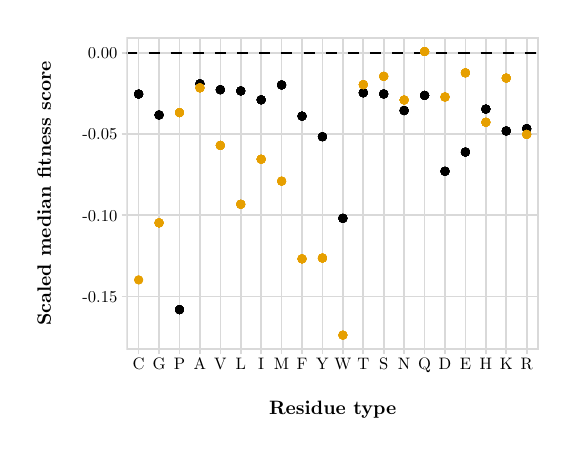
\begin{tikzpicture}[x=1pt,y=1pt]
\definecolor{fillColor}{RGB}{255,255,255}
\path[use as bounding box,fill=fillColor,fill opacity=0.00] (0,0) rectangle (188.25,144.54);
\begin{scope}
\path[clip] ( 35.67, 28.30) rectangle (184.75,141.04);
\definecolor{drawColor}{gray}{0.85}

\path[draw=drawColor,line width= 0.6pt,line join=round] ( 35.67, 47.40) --
	(184.75, 47.40);

\path[draw=drawColor,line width= 0.6pt,line join=round] ( 35.67, 76.73) --
	(184.75, 76.73);

\path[draw=drawColor,line width= 0.6pt,line join=round] ( 35.67,106.06) --
	(184.75,106.06);

\path[draw=drawColor,line width= 0.6pt,line join=round] ( 35.67,135.39) --
	(184.75,135.39);

\path[draw=drawColor,line width= 0.6pt,line join=round] ( 40.10, 28.30) --
	( 40.10,141.04);

\path[draw=drawColor,line width= 0.6pt,line join=round] ( 47.48, 28.30) --
	( 47.48,141.04);

\path[draw=drawColor,line width= 0.6pt,line join=round] ( 54.86, 28.30) --
	( 54.86,141.04);

\path[draw=drawColor,line width= 0.6pt,line join=round] ( 62.24, 28.30) --
	( 62.24,141.04);

\path[draw=drawColor,line width= 0.6pt,line join=round] ( 69.62, 28.30) --
	( 69.62,141.04);

\path[draw=drawColor,line width= 0.6pt,line join=round] ( 77.00, 28.30) --
	( 77.00,141.04);

\path[draw=drawColor,line width= 0.6pt,line join=round] ( 84.38, 28.30) --
	( 84.38,141.04);

\path[draw=drawColor,line width= 0.6pt,line join=round] ( 91.76, 28.30) --
	( 91.76,141.04);

\path[draw=drawColor,line width= 0.6pt,line join=round] ( 99.14, 28.30) --
	( 99.14,141.04);

\path[draw=drawColor,line width= 0.6pt,line join=round] (106.52, 28.30) --
	(106.52,141.04);

\path[draw=drawColor,line width= 0.6pt,line join=round] (113.90, 28.30) --
	(113.90,141.04);

\path[draw=drawColor,line width= 0.6pt,line join=round] (121.28, 28.30) --
	(121.28,141.04);

\path[draw=drawColor,line width= 0.6pt,line join=round] (128.66, 28.30) --
	(128.66,141.04);

\path[draw=drawColor,line width= 0.6pt,line join=round] (136.04, 28.30) --
	(136.04,141.04);

\path[draw=drawColor,line width= 0.6pt,line join=round] (143.42, 28.30) --
	(143.42,141.04);

\path[draw=drawColor,line width= 0.6pt,line join=round] (150.80, 28.30) --
	(150.80,141.04);

\path[draw=drawColor,line width= 0.6pt,line join=round] (158.18, 28.30) --
	(158.18,141.04);

\path[draw=drawColor,line width= 0.6pt,line join=round] (165.56, 28.30) --
	(165.56,141.04);

\path[draw=drawColor,line width= 0.6pt,line join=round] (172.94, 28.30) --
	(172.94,141.04);

\path[draw=drawColor,line width= 0.6pt,line join=round] (180.32, 28.30) --
	(180.32,141.04);
\definecolor{drawColor}{RGB}{0,0,0}

\path[draw=drawColor,line width= 0.6pt,dash pattern=on 4pt off 4pt ,line join=round] ( 35.67,135.39) -- (184.75,135.39);
\definecolor{fillColor}{RGB}{0,0,0}

\path[draw=drawColor,line width= 0.4pt,line join=round,line cap=round,fill=fillColor] ( 54.86, 42.66) circle (  1.43);

\path[draw=drawColor,line width= 0.4pt,line join=round,line cap=round,fill=fillColor] (143.42,120.05) circle (  1.43);

\path[draw=drawColor,line width= 0.4pt,line join=round,line cap=round,fill=fillColor] (150.80, 92.64) circle (  1.43);

\path[draw=drawColor,line width= 0.4pt,line join=round,line cap=round,fill=fillColor] (172.94,107.21) circle (  1.43);

\path[draw=drawColor,line width= 0.4pt,line join=round,line cap=round,fill=fillColor] (136.04,114.59) circle (  1.43);

\path[draw=drawColor,line width= 0.4pt,line join=round,line cap=round,fill=fillColor] (180.32,108.05) circle (  1.43);

\path[draw=drawColor,line width= 0.4pt,line join=round,line cap=round,fill=fillColor] (158.18, 99.58) circle (  1.43);

\path[draw=drawColor,line width= 0.4pt,line join=round,line cap=round,fill=fillColor] (165.56,115.11) circle (  1.43);

\path[draw=drawColor,line width= 0.4pt,line join=round,line cap=round,fill=fillColor] (128.66,120.58) circle (  1.43);

\path[draw=drawColor,line width= 0.4pt,line join=round,line cap=round,fill=fillColor] (121.28,121.01) circle (  1.43);

\path[draw=drawColor,line width= 0.4pt,line join=round,line cap=round,fill=fillColor] ( 47.48,112.98) circle (  1.43);

\path[draw=drawColor,line width= 0.4pt,line join=round,line cap=round,fill=fillColor] ( 40.10,120.54) circle (  1.43);

\path[draw=drawColor,line width= 0.4pt,line join=round,line cap=round,fill=fillColor] ( 62.24,124.25) circle (  1.43);

\path[draw=drawColor,line width= 0.4pt,line join=round,line cap=round,fill=fillColor] ( 91.76,123.83) circle (  1.43);

\path[draw=drawColor,line width= 0.4pt,line join=round,line cap=round,fill=fillColor] ( 69.62,122.11) circle (  1.43);

\path[draw=drawColor,line width= 0.4pt,line join=round,line cap=round,fill=fillColor] (106.52,105.13) circle (  1.43);

\path[draw=drawColor,line width= 0.4pt,line join=round,line cap=round,fill=fillColor] ( 99.14,112.56) circle (  1.43);

\path[draw=drawColor,line width= 0.4pt,line join=round,line cap=round,fill=fillColor] ( 77.00,121.68) circle (  1.43);

\path[draw=drawColor,line width= 0.4pt,line join=round,line cap=round,fill=fillColor] ( 84.38,118.47) circle (  1.43);

\path[draw=drawColor,line width= 0.4pt,line join=round,line cap=round,fill=fillColor] (113.90, 75.64) circle (  1.43);

\path[draw=drawColor,line width= 0.4pt,line join=round,line cap=round,fill=fillColor] ( 40.10,120.54) circle (  1.43);

\path[draw=drawColor,line width= 0.4pt,line join=round,line cap=round,fill=fillColor] (106.52,105.13) circle (  1.43);

\path[draw=drawColor,line width= 0.4pt,line join=round,line cap=round,fill=fillColor] ( 99.14,112.56) circle (  1.43);

\path[draw=drawColor,line width= 0.4pt,line join=round,line cap=round,fill=fillColor] ( 47.48,112.98) circle (  1.43);

\path[draw=drawColor,line width= 0.4pt,line join=round,line cap=round,fill=fillColor] (128.66,120.58) circle (  1.43);

\path[draw=drawColor,line width= 0.4pt,line join=round,line cap=round,fill=fillColor] (121.28,121.01) circle (  1.43);

\path[draw=drawColor,line width= 0.4pt,line join=round,line cap=round,fill=fillColor] ( 84.38,118.47) circle (  1.43);

\path[draw=drawColor,line width= 0.4pt,line join=round,line cap=round,fill=fillColor] ( 77.00,121.68) circle (  1.43);

\path[draw=drawColor,line width= 0.4pt,line join=round,line cap=round,fill=fillColor] (180.32,108.05) circle (  1.43);

\path[draw=drawColor,line width= 0.4pt,line join=round,line cap=round,fill=fillColor] ( 54.86, 42.66) circle (  1.43);

\path[draw=drawColor,line width= 0.4pt,line join=round,line cap=round,fill=fillColor] (150.80, 92.64) circle (  1.43);

\path[draw=drawColor,line width= 0.4pt,line join=round,line cap=round,fill=fillColor] (165.56,115.11) circle (  1.43);

\path[draw=drawColor,line width= 0.4pt,line join=round,line cap=round,fill=fillColor] ( 62.24,124.25) circle (  1.43);

\path[draw=drawColor,line width= 0.4pt,line join=round,line cap=round,fill=fillColor] (143.42,120.05) circle (  1.43);

\path[draw=drawColor,line width= 0.4pt,line join=round,line cap=round,fill=fillColor] ( 91.76,123.83) circle (  1.43);

\path[draw=drawColor,line width= 0.4pt,line join=round,line cap=round,fill=fillColor] (128.66,120.58) circle (  1.43);

\path[draw=drawColor,line width= 0.4pt,line join=round,line cap=round,fill=fillColor] (121.28,121.01) circle (  1.43);

\path[draw=drawColor,line width= 0.4pt,line join=round,line cap=round,fill=fillColor] ( 40.10,120.54) circle (  1.43);

\path[draw=drawColor,line width= 0.4pt,line join=round,line cap=round,fill=fillColor] ( 47.48,112.98) circle (  1.43);

\path[draw=drawColor,line width= 0.4pt,line join=round,line cap=round,fill=fillColor] ( 62.24,124.25) circle (  1.43);

\path[draw=drawColor,line width= 0.4pt,line join=round,line cap=round,fill=fillColor] ( 54.86, 42.66) circle (  1.43);

\path[draw=drawColor,line width= 0.4pt,line join=round,line cap=round,fill=fillColor] ( 91.76,123.83) circle (  1.43);

\path[draw=drawColor,line width= 0.4pt,line join=round,line cap=round,fill=fillColor] (172.94,107.21) circle (  1.43);

\path[draw=drawColor,line width= 0.4pt,line join=round,line cap=round,fill=fillColor] ( 69.62,122.11) circle (  1.43);

\path[draw=drawColor,line width= 0.4pt,line join=round,line cap=round,fill=fillColor] (113.90, 75.64) circle (  1.43);

\path[draw=drawColor,line width= 0.4pt,line join=round,line cap=round,fill=fillColor] (136.04,114.59) circle (  1.43);

\path[draw=drawColor,line width= 0.4pt,line join=round,line cap=round,fill=fillColor] (158.18, 99.58) circle (  1.43);

\path[draw=drawColor,line width= 0.4pt,line join=round,line cap=round,fill=fillColor] (143.42,120.05) circle (  1.43);

\path[draw=drawColor,line width= 0.4pt,line join=round,line cap=round,fill=fillColor] (150.80, 92.64) circle (  1.43);

\path[draw=drawColor,line width= 0.4pt,line join=round,line cap=round,fill=fillColor] (136.04,114.59) circle (  1.43);

\path[draw=drawColor,line width= 0.4pt,line join=round,line cap=round,fill=fillColor] (158.18, 99.58) circle (  1.43);

\path[draw=drawColor,line width= 0.4pt,line join=round,line cap=round,fill=fillColor] (172.94,107.21) circle (  1.43);

\path[draw=drawColor,line width= 0.4pt,line join=round,line cap=round,fill=fillColor] (113.90, 75.64) circle (  1.43);

\path[draw=drawColor,line width= 0.4pt,line join=round,line cap=round,fill=fillColor] ( 69.62,122.11) circle (  1.43);

\path[draw=drawColor,line width= 0.4pt,line join=round,line cap=round,fill=fillColor] (180.32,108.05) circle (  1.43);

\path[draw=drawColor,line width= 0.4pt,line join=round,line cap=round,fill=fillColor] (106.52,105.13) circle (  1.43);

\path[draw=drawColor,line width= 0.4pt,line join=round,line cap=round,fill=fillColor] ( 84.38,118.47) circle (  1.43);

\path[draw=drawColor,line width= 0.4pt,line join=round,line cap=round,fill=fillColor] ( 77.00,121.68) circle (  1.43);

\path[draw=drawColor,line width= 0.4pt,line join=round,line cap=round,fill=fillColor] (165.56,115.11) circle (  1.43);

\path[draw=drawColor,line width= 0.4pt,line join=round,line cap=round,fill=fillColor] ( 99.14,112.56) circle (  1.43);

\path[draw=drawColor,line width= 0.4pt,line join=round,line cap=round,fill=fillColor] (106.52,105.13) circle (  1.43);

\path[draw=drawColor,line width= 0.4pt,line join=round,line cap=round,fill=fillColor] (113.90, 75.64) circle (  1.43);

\path[draw=drawColor,line width= 0.4pt,line join=round,line cap=round,fill=fillColor] (165.56,115.11) circle (  1.43);

\path[draw=drawColor,line width= 0.4pt,line join=round,line cap=round,fill=fillColor] ( 99.14,112.56) circle (  1.43);

\path[draw=drawColor,line width= 0.4pt,line join=round,line cap=round,fill=fillColor] (158.18, 99.58) circle (  1.43);

\path[draw=drawColor,line width= 0.4pt,line join=round,line cap=round,fill=fillColor] ( 54.86, 42.66) circle (  1.43);

\path[draw=drawColor,line width= 0.4pt,line join=round,line cap=round,fill=fillColor] (143.42,120.05) circle (  1.43);

\path[draw=drawColor,line width= 0.4pt,line join=round,line cap=round,fill=fillColor] ( 47.48,112.98) circle (  1.43);

\path[draw=drawColor,line width= 0.4pt,line join=round,line cap=round,fill=fillColor] (136.04,114.59) circle (  1.43);

\path[draw=drawColor,line width= 0.4pt,line join=round,line cap=round,fill=fillColor] (121.28,121.01) circle (  1.43);

\path[draw=drawColor,line width= 0.4pt,line join=round,line cap=round,fill=fillColor] ( 91.76,123.83) circle (  1.43);

\path[draw=drawColor,line width= 0.4pt,line join=round,line cap=round,fill=fillColor] (128.66,120.58) circle (  1.43);

\path[draw=drawColor,line width= 0.4pt,line join=round,line cap=round,fill=fillColor] ( 40.10,120.54) circle (  1.43);

\path[draw=drawColor,line width= 0.4pt,line join=round,line cap=round,fill=fillColor] ( 69.62,122.11) circle (  1.43);

\path[draw=drawColor,line width= 0.4pt,line join=round,line cap=round,fill=fillColor] ( 84.38,118.47) circle (  1.43);

\path[draw=drawColor,line width= 0.4pt,line join=round,line cap=round,fill=fillColor] ( 77.00,121.68) circle (  1.43);

\path[draw=drawColor,line width= 0.4pt,line join=round,line cap=round,fill=fillColor] (150.80, 92.64) circle (  1.43);

\path[draw=drawColor,line width= 0.4pt,line join=round,line cap=round,fill=fillColor] (180.32,108.05) circle (  1.43);

\path[draw=drawColor,line width= 0.4pt,line join=round,line cap=round,fill=fillColor] (172.94,107.21) circle (  1.43);

\path[draw=drawColor,line width= 0.4pt,line join=round,line cap=round,fill=fillColor] ( 62.24,124.25) circle (  1.43);

\path[draw=drawColor,line width= 0.4pt,line join=round,line cap=round,fill=fillColor] (180.32,108.05) circle (  1.43);

\path[draw=drawColor,line width= 0.4pt,line join=round,line cap=round,fill=fillColor] (128.66,120.58) circle (  1.43);

\path[draw=drawColor,line width= 0.4pt,line join=round,line cap=round,fill=fillColor] (121.28,121.01) circle (  1.43);

\path[draw=drawColor,line width= 0.4pt,line join=round,line cap=round,fill=fillColor] (143.42,120.05) circle (  1.43);

\path[draw=drawColor,line width= 0.4pt,line join=round,line cap=round,fill=fillColor] (172.94,107.21) circle (  1.43);

\path[draw=drawColor,line width= 0.4pt,line join=round,line cap=round,fill=fillColor] ( 54.86, 42.66) circle (  1.43);

\path[draw=drawColor,line width= 0.4pt,line join=round,line cap=round,fill=fillColor] (165.56,115.11) circle (  1.43);

\path[draw=drawColor,line width= 0.4pt,line join=round,line cap=round,fill=fillColor] ( 84.38,118.47) circle (  1.43);

\path[draw=drawColor,line width= 0.4pt,line join=round,line cap=round,fill=fillColor] ( 40.10,120.54) circle (  1.43);

\path[draw=drawColor,line width= 0.4pt,line join=round,line cap=round,fill=fillColor] (136.04,114.59) circle (  1.43);

\path[draw=drawColor,line width= 0.4pt,line join=round,line cap=round,fill=fillColor] (158.18, 99.58) circle (  1.43);

\path[draw=drawColor,line width= 0.4pt,line join=round,line cap=round,fill=fillColor] ( 47.48,112.98) circle (  1.43);

\path[draw=drawColor,line width= 0.4pt,line join=round,line cap=round,fill=fillColor] (106.52,105.13) circle (  1.43);

\path[draw=drawColor,line width= 0.4pt,line join=round,line cap=round,fill=fillColor] ( 62.24,124.25) circle (  1.43);

\path[draw=drawColor,line width= 0.4pt,line join=round,line cap=round,fill=fillColor] ( 69.62,122.11) circle (  1.43);

\path[draw=drawColor,line width= 0.4pt,line join=round,line cap=round,fill=fillColor] ( 91.76,123.83) circle (  1.43);

\path[draw=drawColor,line width= 0.4pt,line join=round,line cap=round,fill=fillColor] (150.80, 92.64) circle (  1.43);

\path[draw=drawColor,line width= 0.4pt,line join=round,line cap=round,fill=fillColor] ( 77.00,121.68) circle (  1.43);

\path[draw=drawColor,line width= 0.4pt,line join=round,line cap=round,fill=fillColor] (113.90, 75.64) circle (  1.43);

\path[draw=drawColor,line width= 0.4pt,line join=round,line cap=round,fill=fillColor] ( 99.14,112.56) circle (  1.43);

\path[draw=drawColor,line width= 0.4pt,line join=round,line cap=round,fill=fillColor] ( 40.10,120.54) circle (  1.43);

\path[draw=drawColor,line width= 0.4pt,line join=round,line cap=round,fill=fillColor] (136.04,114.59) circle (  1.43);

\path[draw=drawColor,line width= 0.4pt,line join=round,line cap=round,fill=fillColor] (128.66,120.58) circle (  1.43);

\path[draw=drawColor,line width= 0.4pt,line join=round,line cap=round,fill=fillColor] (180.32,108.05) circle (  1.43);

\path[draw=drawColor,line width= 0.4pt,line join=round,line cap=round,fill=fillColor] (165.56,115.11) circle (  1.43);

\path[draw=drawColor,line width= 0.4pt,line join=round,line cap=round,fill=fillColor] ( 62.24,124.25) circle (  1.43);

\path[draw=drawColor,line width= 0.4pt,line join=round,line cap=round,fill=fillColor] (158.18, 99.58) circle (  1.43);

\path[draw=drawColor,line width= 0.4pt,line join=round,line cap=round,fill=fillColor] (121.28,121.01) circle (  1.43);

\path[draw=drawColor,line width= 0.4pt,line join=round,line cap=round,fill=fillColor] ( 77.00,121.68) circle (  1.43);

\path[draw=drawColor,line width= 0.4pt,line join=round,line cap=round,fill=fillColor] (172.94,107.21) circle (  1.43);

\path[draw=drawColor,line width= 0.4pt,line join=round,line cap=round,fill=fillColor] (150.80, 92.64) circle (  1.43);

\path[draw=drawColor,line width= 0.4pt,line join=round,line cap=round,fill=fillColor] ( 47.48,112.98) circle (  1.43);

\path[draw=drawColor,line width= 0.4pt,line join=round,line cap=round,fill=fillColor] (106.52,105.13) circle (  1.43);

\path[draw=drawColor,line width= 0.4pt,line join=round,line cap=round,fill=fillColor] ( 69.62,122.11) circle (  1.43);

\path[draw=drawColor,line width= 0.4pt,line join=round,line cap=round,fill=fillColor] ( 84.38,118.47) circle (  1.43);

\path[draw=drawColor,line width= 0.4pt,line join=round,line cap=round,fill=fillColor] ( 54.86, 42.66) circle (  1.43);

\path[draw=drawColor,line width= 0.4pt,line join=round,line cap=round,fill=fillColor] ( 99.14,112.56) circle (  1.43);

\path[draw=drawColor,line width= 0.4pt,line join=round,line cap=round,fill=fillColor] ( 91.76,123.83) circle (  1.43);

\path[draw=drawColor,line width= 0.4pt,line join=round,line cap=round,fill=fillColor] (143.42,120.05) circle (  1.43);

\path[draw=drawColor,line width= 0.4pt,line join=round,line cap=round,fill=fillColor] (113.90, 75.64) circle (  1.43);

\path[draw=drawColor,line width= 0.4pt,line join=round,line cap=round,fill=fillColor] (106.52,105.13) circle (  1.43);

\path[draw=drawColor,line width= 0.4pt,line join=round,line cap=round,fill=fillColor] (165.56,115.11) circle (  1.43);

\path[draw=drawColor,line width= 0.4pt,line join=round,line cap=round,fill=fillColor] (113.90, 75.64) circle (  1.43);

\path[draw=drawColor,line width= 0.4pt,line join=round,line cap=round,fill=fillColor] ( 47.48,112.98) circle (  1.43);

\path[draw=drawColor,line width= 0.4pt,line join=round,line cap=round,fill=fillColor] (143.42,120.05) circle (  1.43);

\path[draw=drawColor,line width= 0.4pt,line join=round,line cap=round,fill=fillColor] ( 99.14,112.56) circle (  1.43);

\path[draw=drawColor,line width= 0.4pt,line join=round,line cap=round,fill=fillColor] (136.04,114.59) circle (  1.43);

\path[draw=drawColor,line width= 0.4pt,line join=round,line cap=round,fill=fillColor] (180.32,108.05) circle (  1.43);

\path[draw=drawColor,line width= 0.4pt,line join=round,line cap=round,fill=fillColor] (150.80, 92.64) circle (  1.43);

\path[draw=drawColor,line width= 0.4pt,line join=round,line cap=round,fill=fillColor] ( 84.38,118.47) circle (  1.43);

\path[draw=drawColor,line width= 0.4pt,line join=round,line cap=round,fill=fillColor] (172.94,107.21) circle (  1.43);

\path[draw=drawColor,line width= 0.4pt,line join=round,line cap=round,fill=fillColor] ( 77.00,121.68) circle (  1.43);

\path[draw=drawColor,line width= 0.4pt,line join=round,line cap=round,fill=fillColor] (121.28,121.01) circle (  1.43);

\path[draw=drawColor,line width= 0.4pt,line join=round,line cap=round,fill=fillColor] ( 91.76,123.83) circle (  1.43);

\path[draw=drawColor,line width= 0.4pt,line join=round,line cap=round,fill=fillColor] ( 40.10,120.54) circle (  1.43);

\path[draw=drawColor,line width= 0.4pt,line join=round,line cap=round,fill=fillColor] ( 69.62,122.11) circle (  1.43);

\path[draw=drawColor,line width= 0.4pt,line join=round,line cap=round,fill=fillColor] (158.18, 99.58) circle (  1.43);

\path[draw=drawColor,line width= 0.4pt,line join=round,line cap=round,fill=fillColor] (128.66,120.58) circle (  1.43);

\path[draw=drawColor,line width= 0.4pt,line join=round,line cap=round,fill=fillColor] ( 62.24,124.25) circle (  1.43);

\path[draw=drawColor,line width= 0.4pt,line join=round,line cap=round,fill=fillColor] ( 54.86, 42.66) circle (  1.43);

\path[draw=drawColor,line width= 0.4pt,line join=round,line cap=round,fill=fillColor] (180.32,108.05) circle (  1.43);

\path[draw=drawColor,line width= 0.4pt,line join=round,line cap=round,fill=fillColor] ( 54.86, 42.66) circle (  1.43);

\path[draw=drawColor,line width= 0.4pt,line join=round,line cap=round,fill=fillColor] (136.04,114.59) circle (  1.43);

\path[draw=drawColor,line width= 0.4pt,line join=round,line cap=round,fill=fillColor] (165.56,115.11) circle (  1.43);

\path[draw=drawColor,line width= 0.4pt,line join=round,line cap=round,fill=fillColor] ( 47.48,112.98) circle (  1.43);

\path[draw=drawColor,line width= 0.4pt,line join=round,line cap=round,fill=fillColor] (150.80, 92.64) circle (  1.43);

\path[draw=drawColor,line width= 0.4pt,line join=round,line cap=round,fill=fillColor] (128.66,120.58) circle (  1.43);

\path[draw=drawColor,line width= 0.4pt,line join=round,line cap=round,fill=fillColor] ( 77.00,121.68) circle (  1.43);

\path[draw=drawColor,line width= 0.4pt,line join=round,line cap=round,fill=fillColor] (158.18, 99.58) circle (  1.43);

\path[draw=drawColor,line width= 0.4pt,line join=round,line cap=round,fill=fillColor] ( 91.76,123.83) circle (  1.43);

\path[draw=drawColor,line width= 0.4pt,line join=round,line cap=round,fill=fillColor] ( 62.24,124.25) circle (  1.43);

\path[draw=drawColor,line width= 0.4pt,line join=round,line cap=round,fill=fillColor] ( 84.38,118.47) circle (  1.43);

\path[draw=drawColor,line width= 0.4pt,line join=round,line cap=round,fill=fillColor] (106.52,105.13) circle (  1.43);

\path[draw=drawColor,line width= 0.4pt,line join=round,line cap=round,fill=fillColor] ( 99.14,112.56) circle (  1.43);

\path[draw=drawColor,line width= 0.4pt,line join=round,line cap=round,fill=fillColor] (121.28,121.01) circle (  1.43);

\path[draw=drawColor,line width= 0.4pt,line join=round,line cap=round,fill=fillColor] (172.94,107.21) circle (  1.43);

\path[draw=drawColor,line width= 0.4pt,line join=round,line cap=round,fill=fillColor] (143.42,120.05) circle (  1.43);

\path[draw=drawColor,line width= 0.4pt,line join=round,line cap=round,fill=fillColor] ( 40.10,120.54) circle (  1.43);

\path[draw=drawColor,line width= 0.4pt,line join=round,line cap=round,fill=fillColor] (113.90, 75.64) circle (  1.43);

\path[draw=drawColor,line width= 0.4pt,line join=round,line cap=round,fill=fillColor] ( 69.62,122.11) circle (  1.43);

\path[draw=drawColor,line width= 0.4pt,line join=round,line cap=round,fill=fillColor] (136.04,114.59) circle (  1.43);

\path[draw=drawColor,line width= 0.4pt,line join=round,line cap=round,fill=fillColor] ( 84.38,118.47) circle (  1.43);

\path[draw=drawColor,line width= 0.4pt,line join=round,line cap=round,fill=fillColor] ( 40.10,120.54) circle (  1.43);

\path[draw=drawColor,line width= 0.4pt,line join=round,line cap=round,fill=fillColor] (180.32,108.05) circle (  1.43);

\path[draw=drawColor,line width= 0.4pt,line join=round,line cap=round,fill=fillColor] (150.80, 92.64) circle (  1.43);

\path[draw=drawColor,line width= 0.4pt,line join=round,line cap=round,fill=fillColor] (143.42,120.05) circle (  1.43);

\path[draw=drawColor,line width= 0.4pt,line join=round,line cap=round,fill=fillColor] (172.94,107.21) circle (  1.43);

\path[draw=drawColor,line width= 0.4pt,line join=round,line cap=round,fill=fillColor] ( 54.86, 42.66) circle (  1.43);

\path[draw=drawColor,line width= 0.4pt,line join=round,line cap=round,fill=fillColor] (165.56,115.11) circle (  1.43);

\path[draw=drawColor,line width= 0.4pt,line join=round,line cap=round,fill=fillColor] ( 77.00,121.68) circle (  1.43);

\path[draw=drawColor,line width= 0.4pt,line join=round,line cap=round,fill=fillColor] (113.90, 75.64) circle (  1.43);

\path[draw=drawColor,line width= 0.4pt,line join=round,line cap=round,fill=fillColor] ( 99.14,112.56) circle (  1.43);

\path[draw=drawColor,line width= 0.4pt,line join=round,line cap=round,fill=fillColor] (106.52,105.13) circle (  1.43);

\path[draw=drawColor,line width= 0.4pt,line join=round,line cap=round,fill=fillColor] (158.18, 99.58) circle (  1.43);

\path[draw=drawColor,line width= 0.4pt,line join=round,line cap=round,fill=fillColor] ( 47.48,112.98) circle (  1.43);

\path[draw=drawColor,line width= 0.4pt,line join=round,line cap=round,fill=fillColor] ( 69.62,122.11) circle (  1.43);

\path[draw=drawColor,line width= 0.4pt,line join=round,line cap=round,fill=fillColor] ( 62.24,124.25) circle (  1.43);

\path[draw=drawColor,line width= 0.4pt,line join=round,line cap=round,fill=fillColor] ( 91.76,123.83) circle (  1.43);

\path[draw=drawColor,line width= 0.4pt,line join=round,line cap=round,fill=fillColor] (128.66,120.58) circle (  1.43);

\path[draw=drawColor,line width= 0.4pt,line join=round,line cap=round,fill=fillColor] (121.28,121.01) circle (  1.43);
\definecolor{drawColor}{RGB}{230,159,0}
\definecolor{fillColor}{RGB}{230,159,0}

\path[draw=drawColor,line width= 0.4pt,line join=round,line cap=round,fill=fillColor] ( 54.86,113.86) circle (  1.43);

\path[draw=drawColor,line width= 0.4pt,line join=round,line cap=round,fill=fillColor] (150.80,119.50) circle (  1.43);

\path[draw=drawColor,line width= 0.4pt,line join=round,line cap=round,fill=fillColor] ( 62.24,122.79) circle (  1.43);

\path[draw=drawColor,line width= 0.4pt,line join=round,line cap=round,fill=fillColor] ( 40.10, 53.39) circle (  1.43);

\path[draw=drawColor,line width= 0.4pt,line join=round,line cap=round,fill=fillColor] (136.04,118.40) circle (  1.43);

\path[draw=drawColor,line width= 0.4pt,line join=round,line cap=round,fill=fillColor] ( 77.00, 80.72) circle (  1.43);

\path[draw=drawColor,line width= 0.4pt,line join=round,line cap=round,fill=fillColor] ( 99.14, 61.00) circle (  1.43);

\path[draw=drawColor,line width= 0.4pt,line join=round,line cap=round,fill=fillColor] (158.18,128.21) circle (  1.43);

\path[draw=drawColor,line width= 0.4pt,line join=round,line cap=round,fill=fillColor] (165.56,110.35) circle (  1.43);

\path[draw=drawColor,line width= 0.4pt,line join=round,line cap=round,fill=fillColor] (121.28,123.96) circle (  1.43);

\path[draw=drawColor,line width= 0.4pt,line join=round,line cap=round,fill=fillColor] ( 84.38, 97.00) circle (  1.43);

\path[draw=drawColor,line width= 0.4pt,line join=round,line cap=round,fill=fillColor] (180.32,105.95) circle (  1.43);

\path[draw=drawColor,line width= 0.4pt,line join=round,line cap=round,fill=fillColor] ( 69.62,101.98) circle (  1.43);

\path[draw=drawColor,line width= 0.4pt,line join=round,line cap=round,fill=fillColor] (106.52, 61.29) circle (  1.43);

\path[draw=drawColor,line width= 0.4pt,line join=round,line cap=round,fill=fillColor] (143.42,135.92) circle (  1.43);

\path[draw=drawColor,line width= 0.4pt,line join=round,line cap=round,fill=fillColor] ( 47.48, 74.01) circle (  1.43);

\path[draw=drawColor,line width= 0.4pt,line join=round,line cap=round,fill=fillColor] (172.94,126.32) circle (  1.43);

\path[draw=drawColor,line width= 0.4pt,line join=round,line cap=round,fill=fillColor] (128.66,126.94) circle (  1.43);

\path[draw=drawColor,line width= 0.4pt,line join=round,line cap=round,fill=fillColor] ( 91.76, 89.07) circle (  1.43);

\path[draw=drawColor,line width= 0.4pt,line join=round,line cap=round,fill=fillColor] (113.90, 33.43) circle (  1.43);

\path[draw=drawColor,line width= 0.4pt,line join=round,line cap=round,fill=fillColor] (143.42,135.92) circle (  1.43);

\path[draw=drawColor,line width= 0.4pt,line join=round,line cap=round,fill=fillColor] (143.42,135.92) circle (  1.43);

\path[draw=drawColor,line width= 0.4pt,line join=round,line cap=round,fill=fillColor] (150.80,119.50) circle (  1.43);

\path[draw=drawColor,line width= 0.4pt,line join=round,line cap=round,fill=fillColor] (150.80,119.50) circle (  1.43);

\path[draw=drawColor,line width= 0.4pt,line join=round,line cap=round,fill=fillColor] ( 99.14, 61.00) circle (  1.43);

\path[draw=drawColor,line width= 0.4pt,line join=round,line cap=round,fill=fillColor] ( 99.14, 61.00) circle (  1.43);

\path[draw=drawColor,line width= 0.4pt,line join=round,line cap=round,fill=fillColor] (121.28,123.96) circle (  1.43);

\path[draw=drawColor,line width= 0.4pt,line join=round,line cap=round,fill=fillColor] (121.28,123.96) circle (  1.43);

\path[draw=drawColor,line width= 0.4pt,line join=round,line cap=round,fill=fillColor] (158.18,128.21) circle (  1.43);

\path[draw=drawColor,line width= 0.4pt,line join=round,line cap=round,fill=fillColor] (158.18,128.21) circle (  1.43);

\path[draw=drawColor,line width= 0.4pt,line join=round,line cap=round,fill=fillColor] ( 69.62,101.98) circle (  1.43);

\path[draw=drawColor,line width= 0.4pt,line join=round,line cap=round,fill=fillColor] ( 69.62,101.98) circle (  1.43);

\path[draw=drawColor,line width= 0.4pt,line join=round,line cap=round,fill=fillColor] ( 77.00, 80.72) circle (  1.43);

\path[draw=drawColor,line width= 0.4pt,line join=round,line cap=round,fill=fillColor] ( 77.00, 80.72) circle (  1.43);

\path[draw=drawColor,line width= 0.4pt,line join=round,line cap=round,fill=fillColor] (128.66,126.94) circle (  1.43);

\path[draw=drawColor,line width= 0.4pt,line join=round,line cap=round,fill=fillColor] (128.66,126.94) circle (  1.43);

\path[draw=drawColor,line width= 0.4pt,line join=round,line cap=round,fill=fillColor] ( 84.38, 97.00) circle (  1.43);

\path[draw=drawColor,line width= 0.4pt,line join=round,line cap=round,fill=fillColor] ( 84.38, 97.00) circle (  1.43);

\path[draw=drawColor,line width= 0.4pt,line join=round,line cap=round,fill=fillColor] (106.52, 61.29) circle (  1.43);

\path[draw=drawColor,line width= 0.4pt,line join=round,line cap=round,fill=fillColor] (106.52, 61.29) circle (  1.43);

\path[draw=drawColor,line width= 0.4pt,line join=round,line cap=round,fill=fillColor] (172.94,126.32) circle (  1.43);

\path[draw=drawColor,line width= 0.4pt,line join=round,line cap=round,fill=fillColor] (172.94,126.32) circle (  1.43);

\path[draw=drawColor,line width= 0.4pt,line join=round,line cap=round,fill=fillColor] (136.04,118.40) circle (  1.43);

\path[draw=drawColor,line width= 0.4pt,line join=round,line cap=round,fill=fillColor] (136.04,118.40) circle (  1.43);

\path[draw=drawColor,line width= 0.4pt,line join=round,line cap=round,fill=fillColor] (165.56,110.35) circle (  1.43);

\path[draw=drawColor,line width= 0.4pt,line join=round,line cap=round,fill=fillColor] (165.56,110.35) circle (  1.43);

\path[draw=drawColor,line width= 0.4pt,line join=round,line cap=round,fill=fillColor] ( 54.86,113.86) circle (  1.43);

\path[draw=drawColor,line width= 0.4pt,line join=round,line cap=round,fill=fillColor] ( 54.86,113.86) circle (  1.43);

\path[draw=drawColor,line width= 0.4pt,line join=round,line cap=round,fill=fillColor] (180.32,105.95) circle (  1.43);

\path[draw=drawColor,line width= 0.4pt,line join=round,line cap=round,fill=fillColor] (180.32,105.95) circle (  1.43);

\path[draw=drawColor,line width= 0.4pt,line join=round,line cap=round,fill=fillColor] ( 47.48, 74.01) circle (  1.43);

\path[draw=drawColor,line width= 0.4pt,line join=round,line cap=round,fill=fillColor] ( 47.48, 74.01) circle (  1.43);

\path[draw=drawColor,line width= 0.4pt,line join=round,line cap=round,fill=fillColor] ( 62.24,122.79) circle (  1.43);

\path[draw=drawColor,line width= 0.4pt,line join=round,line cap=round,fill=fillColor] (150.80,119.50) circle (  1.43);

\path[draw=drawColor,line width= 0.4pt,line join=round,line cap=round,fill=fillColor] ( 69.62,101.98) circle (  1.43);

\path[draw=drawColor,line width= 0.4pt,line join=round,line cap=round,fill=fillColor] (121.28,123.96) circle (  1.43);

\path[draw=drawColor,line width= 0.4pt,line join=round,line cap=round,fill=fillColor] (158.18,128.21) circle (  1.43);

\path[draw=drawColor,line width= 0.4pt,line join=round,line cap=round,fill=fillColor] (172.94,126.32) circle (  1.43);

\path[draw=drawColor,line width= 0.4pt,line join=round,line cap=round,fill=fillColor] (106.52, 61.29) circle (  1.43);

\path[draw=drawColor,line width= 0.4pt,line join=round,line cap=round,fill=fillColor] ( 77.00, 80.72) circle (  1.43);

\path[draw=drawColor,line width= 0.4pt,line join=round,line cap=round,fill=fillColor] (143.42,135.92) circle (  1.43);

\path[draw=drawColor,line width= 0.4pt,line join=round,line cap=round,fill=fillColor] (136.04,118.40) circle (  1.43);

\path[draw=drawColor,line width= 0.4pt,line join=round,line cap=round,fill=fillColor] ( 84.38, 97.00) circle (  1.43);

\path[draw=drawColor,line width= 0.4pt,line join=round,line cap=round,fill=fillColor] ( 47.48, 74.01) circle (  1.43);

\path[draw=drawColor,line width= 0.4pt,line join=round,line cap=round,fill=fillColor] ( 99.14, 61.00) circle (  1.43);

\path[draw=drawColor,line width= 0.4pt,line join=round,line cap=round,fill=fillColor] (113.90, 33.43) circle (  1.43);

\path[draw=drawColor,line width= 0.4pt,line join=round,line cap=round,fill=fillColor] ( 62.24,122.79) circle (  1.43);

\path[draw=drawColor,line width= 0.4pt,line join=round,line cap=round,fill=fillColor] ( 84.38, 97.00) circle (  1.43);

\path[draw=drawColor,line width= 0.4pt,line join=round,line cap=round,fill=fillColor] (143.42,135.92) circle (  1.43);

\path[draw=drawColor,line width= 0.4pt,line join=round,line cap=round,fill=fillColor] ( 77.00, 80.72) circle (  1.43);

\path[draw=drawColor,line width= 0.4pt,line join=round,line cap=round,fill=fillColor] (172.94,126.32) circle (  1.43);

\path[draw=drawColor,line width= 0.4pt,line join=round,line cap=round,fill=fillColor] ( 47.48, 74.01) circle (  1.43);

\path[draw=drawColor,line width= 0.4pt,line join=round,line cap=round,fill=fillColor] (180.32,105.95) circle (  1.43);

\path[draw=drawColor,line width= 0.4pt,line join=round,line cap=round,fill=fillColor] ( 99.14, 61.00) circle (  1.43);

\path[draw=drawColor,line width= 0.4pt,line join=round,line cap=round,fill=fillColor] (158.18,128.21) circle (  1.43);

\path[draw=drawColor,line width= 0.4pt,line join=round,line cap=round,fill=fillColor] (121.28,123.96) circle (  1.43);

\path[draw=drawColor,line width= 0.4pt,line join=round,line cap=round,fill=fillColor] (136.04,118.40) circle (  1.43);

\path[draw=drawColor,line width= 0.4pt,line join=round,line cap=round,fill=fillColor] ( 69.62,101.98) circle (  1.43);

\path[draw=drawColor,line width= 0.4pt,line join=round,line cap=round,fill=fillColor] ( 54.86,113.86) circle (  1.43);

\path[draw=drawColor,line width= 0.4pt,line join=round,line cap=round,fill=fillColor] (128.66,126.94) circle (  1.43);

\path[draw=drawColor,line width= 0.4pt,line join=round,line cap=round,fill=fillColor] (150.80,119.50) circle (  1.43);

\path[draw=drawColor,line width= 0.4pt,line join=round,line cap=round,fill=fillColor] (106.52, 61.29) circle (  1.43);

\path[draw=drawColor,line width= 0.4pt,line join=round,line cap=round,fill=fillColor] (165.56,110.35) circle (  1.43);

\path[draw=drawColor,line width= 0.4pt,line join=round,line cap=round,fill=fillColor] ( 91.76, 89.07) circle (  1.43);

\path[draw=drawColor,line width= 0.4pt,line join=round,line cap=round,fill=fillColor] (113.90, 33.43) circle (  1.43);

\path[draw=drawColor,line width= 0.4pt,line join=round,line cap=round,fill=fillColor] (143.42,135.92) circle (  1.43);

\path[draw=drawColor,line width= 0.4pt,line join=round,line cap=round,fill=fillColor] ( 62.24,122.79) circle (  1.43);

\path[draw=drawColor,line width= 0.4pt,line join=round,line cap=round,fill=fillColor] (136.04,118.40) circle (  1.43);

\path[draw=drawColor,line width= 0.4pt,line join=round,line cap=round,fill=fillColor] ( 54.86,113.86) circle (  1.43);

\path[draw=drawColor,line width= 0.4pt,line join=round,line cap=round,fill=fillColor] ( 47.48, 74.01) circle (  1.43);

\path[draw=drawColor,line width= 0.4pt,line join=round,line cap=round,fill=fillColor] (121.28,123.96) circle (  1.43);

\path[draw=drawColor,line width= 0.4pt,line join=round,line cap=round,fill=fillColor] (158.18,128.21) circle (  1.43);

\path[draw=drawColor,line width= 0.4pt,line join=round,line cap=round,fill=fillColor] (150.80,119.50) circle (  1.43);

\path[draw=drawColor,line width= 0.4pt,line join=round,line cap=round,fill=fillColor] ( 69.62,101.98) circle (  1.43);

\path[draw=drawColor,line width= 0.4pt,line join=round,line cap=round,fill=fillColor] ( 77.00, 80.72) circle (  1.43);

\path[draw=drawColor,line width= 0.4pt,line join=round,line cap=round,fill=fillColor] (128.66,126.94) circle (  1.43);

\path[draw=drawColor,line width= 0.4pt,line join=round,line cap=round,fill=fillColor] (172.94,126.32) circle (  1.43);

\path[draw=drawColor,line width= 0.4pt,line join=round,line cap=round,fill=fillColor] ( 84.38, 97.00) circle (  1.43);

\path[draw=drawColor,line width= 0.4pt,line join=round,line cap=round,fill=fillColor] (165.56,110.35) circle (  1.43);

\path[draw=drawColor,line width= 0.4pt,line join=round,line cap=round,fill=fillColor] ( 91.76, 89.07) circle (  1.43);

\path[draw=drawColor,line width= 0.4pt,line join=round,line cap=round,fill=fillColor] ( 99.14, 61.00) circle (  1.43);

\path[draw=drawColor,line width= 0.4pt,line join=round,line cap=round,fill=fillColor] (106.52, 61.29) circle (  1.43);

\path[draw=drawColor,line width= 0.4pt,line join=round,line cap=round,fill=fillColor] ( 54.86,113.86) circle (  1.43);

\path[draw=drawColor,line width= 0.4pt,line join=round,line cap=round,fill=fillColor] (158.18,128.21) circle (  1.43);

\path[draw=drawColor,line width= 0.4pt,line join=round,line cap=round,fill=fillColor] (165.56,110.35) circle (  1.43);

\path[draw=drawColor,line width= 0.4pt,line join=round,line cap=round,fill=fillColor] ( 47.48, 74.01) circle (  1.43);

\path[draw=drawColor,line width= 0.4pt,line join=round,line cap=round,fill=fillColor] ( 69.62,101.98) circle (  1.43);

\path[draw=drawColor,line width= 0.4pt,line join=round,line cap=round,fill=fillColor] ( 84.38, 97.00) circle (  1.43);

\path[draw=drawColor,line width= 0.4pt,line join=round,line cap=round,fill=fillColor] (150.80,119.50) circle (  1.43);

\path[draw=drawColor,line width= 0.4pt,line join=round,line cap=round,fill=fillColor] (121.28,123.96) circle (  1.43);

\path[draw=drawColor,line width= 0.4pt,line join=round,line cap=round,fill=fillColor] (143.42,135.92) circle (  1.43);

\path[draw=drawColor,line width= 0.4pt,line join=round,line cap=round,fill=fillColor] (128.66,126.94) circle (  1.43);

\path[draw=drawColor,line width= 0.4pt,line join=round,line cap=round,fill=fillColor] (180.32,105.95) circle (  1.43);

\path[draw=drawColor,line width= 0.4pt,line join=round,line cap=round,fill=fillColor] ( 77.00, 80.72) circle (  1.43);

\path[draw=drawColor,line width= 0.4pt,line join=round,line cap=round,fill=fillColor] ( 99.14, 61.00) circle (  1.43);

\path[draw=drawColor,line width= 0.4pt,line join=round,line cap=round,fill=fillColor] (136.04,118.40) circle (  1.43);

\path[draw=drawColor,line width= 0.4pt,line join=round,line cap=round,fill=fillColor] (106.52, 61.29) circle (  1.43);

\path[draw=drawColor,line width= 0.4pt,line join=round,line cap=round,fill=fillColor] ( 62.24,122.79) circle (  1.43);

\path[draw=drawColor,line width= 0.4pt,line join=round,line cap=round,fill=fillColor] (172.94,126.32) circle (  1.43);

\path[draw=drawColor,line width= 0.4pt,line join=round,line cap=round,fill=fillColor] ( 62.24,122.79) circle (  1.43);

\path[draw=drawColor,line width= 0.4pt,line join=round,line cap=round,fill=fillColor] ( 69.62,101.98) circle (  1.43);

\path[draw=drawColor,line width= 0.4pt,line join=round,line cap=round,fill=fillColor] (150.80,119.50) circle (  1.43);

\path[draw=drawColor,line width= 0.4pt,line join=round,line cap=round,fill=fillColor] ( 77.00, 80.72) circle (  1.43);

\path[draw=drawColor,line width= 0.4pt,line join=round,line cap=round,fill=fillColor] (143.42,135.92) circle (  1.43);

\path[draw=drawColor,line width= 0.4pt,line join=round,line cap=round,fill=fillColor] ( 91.76, 89.07) circle (  1.43);

\path[draw=drawColor,line width= 0.4pt,line join=round,line cap=round,fill=fillColor] (158.18,128.21) circle (  1.43);

\path[draw=drawColor,line width= 0.4pt,line join=round,line cap=round,fill=fillColor] ( 62.24,122.79) circle (  1.43);

\path[draw=drawColor,line width= 0.4pt,line join=round,line cap=round,fill=fillColor] (128.66,126.94) circle (  1.43);

\path[draw=drawColor,line width= 0.4pt,line join=round,line cap=round,fill=fillColor] (180.32,105.95) circle (  1.43);

\path[draw=drawColor,line width= 0.4pt,line join=round,line cap=round,fill=fillColor] ( 54.86,113.86) circle (  1.43);

\path[draw=drawColor,line width= 0.4pt,line join=round,line cap=round,fill=fillColor] ( 84.38, 97.00) circle (  1.43);

\path[draw=drawColor,line width= 0.4pt,line join=round,line cap=round,fill=fillColor] (121.28,123.96) circle (  1.43);

\path[draw=drawColor,line width= 0.4pt,line join=round,line cap=round,fill=fillColor] ( 99.14, 61.00) circle (  1.43);

\path[draw=drawColor,line width= 0.4pt,line join=round,line cap=round,fill=fillColor] ( 47.48, 74.01) circle (  1.43);

\path[draw=drawColor,line width= 0.4pt,line join=round,line cap=round,fill=fillColor] (106.52, 61.29) circle (  1.43);

\path[draw=drawColor,line width= 0.4pt,line join=round,line cap=round,fill=fillColor] (172.94,126.32) circle (  1.43);

\path[draw=drawColor,line width= 0.4pt,line join=round,line cap=round,fill=fillColor] (113.90, 33.43) circle (  1.43);

\path[draw=drawColor,line width= 0.4pt,line join=round,line cap=round,fill=fillColor] (136.04,118.40) circle (  1.43);

\path[draw=drawColor,line width= 0.4pt,line join=round,line cap=round,fill=fillColor] (165.56,110.35) circle (  1.43);

\path[draw=drawColor,line width= 0.4pt,line join=round,line cap=round,fill=fillColor] (158.18,128.21) circle (  1.43);

\path[draw=drawColor,line width= 0.4pt,line join=round,line cap=round,fill=fillColor] (150.80,119.50) circle (  1.43);

\path[draw=drawColor,line width= 0.4pt,line join=round,line cap=round,fill=fillColor] (143.42,135.92) circle (  1.43);

\path[draw=drawColor,line width= 0.4pt,line join=round,line cap=round,fill=fillColor] ( 77.00, 80.72) circle (  1.43);

\path[draw=drawColor,line width= 0.4pt,line join=round,line cap=round,fill=fillColor] ( 47.48, 74.01) circle (  1.43);

\path[draw=drawColor,line width= 0.4pt,line join=round,line cap=round,fill=fillColor] ( 69.62,101.98) circle (  1.43);

\path[draw=drawColor,line width= 0.4pt,line join=round,line cap=round,fill=fillColor] ( 54.86,113.86) circle (  1.43);

\path[draw=drawColor,line width= 0.4pt,line join=round,line cap=round,fill=fillColor] (121.28,123.96) circle (  1.43);

\path[draw=drawColor,line width= 0.4pt,line join=round,line cap=round,fill=fillColor] ( 99.14, 61.00) circle (  1.43);

\path[draw=drawColor,line width= 0.4pt,line join=round,line cap=round,fill=fillColor] ( 62.24,122.79) circle (  1.43);

\path[draw=drawColor,line width= 0.4pt,line join=round,line cap=round,fill=fillColor] (128.66,126.94) circle (  1.43);

\path[draw=drawColor,line width= 0.4pt,line join=round,line cap=round,fill=fillColor] (180.32,105.95) circle (  1.43);

\path[draw=drawColor,line width= 0.4pt,line join=round,line cap=round,fill=fillColor] (165.56,110.35) circle (  1.43);

\path[draw=drawColor,line width= 0.4pt,line join=round,line cap=round,fill=fillColor] ( 84.38, 97.00) circle (  1.43);

\path[draw=drawColor,line width= 0.4pt,line join=round,line cap=round,fill=fillColor] (113.90, 33.43) circle (  1.43);

\path[draw=drawColor,line width= 0.4pt,line join=round,line cap=round,fill=fillColor] (172.94,126.32) circle (  1.43);

\path[draw=drawColor,line width= 0.4pt,line join=round,line cap=round,fill=fillColor] ( 91.76, 89.07) circle (  1.43);

\path[draw=drawColor,line width= 0.4pt,line join=round,line cap=round,fill=fillColor] ( 40.10, 53.39) circle (  1.43);

\path[draw=drawColor,line width= 0.4pt,line join=round,line cap=round,fill=fillColor] (106.52, 61.29) circle (  1.43);

\path[draw=drawColor,line width= 0.4pt,line join=round,line cap=round,fill=fillColor] (136.04,118.40) circle (  1.43);
\definecolor{drawColor}{gray}{0.85}

\path[draw=drawColor,line width= 1.1pt,line join=round,line cap=round] ( 35.67, 28.30) rectangle (184.75,141.04);
\end{scope}
\begin{scope}
\path[clip] (  0.00,  0.00) rectangle (188.25,144.54);
\definecolor{drawColor}{RGB}{0,0,0}

\node[text=drawColor,anchor=base east,inner sep=0pt, outer sep=0pt, scale=  0.60] at ( 32.42, 45.34) {-0.15};

\node[text=drawColor,anchor=base east,inner sep=0pt, outer sep=0pt, scale=  0.60] at ( 32.42, 74.66) {-0.10};

\node[text=drawColor,anchor=base east,inner sep=0pt, outer sep=0pt, scale=  0.60] at ( 32.42,103.99) {-0.05};

\node[text=drawColor,anchor=base east,inner sep=0pt, outer sep=0pt, scale=  0.60] at ( 32.42,133.32) {0.00};
\end{scope}
\begin{scope}
\path[clip] (  0.00,  0.00) rectangle (188.25,144.54);
\definecolor{drawColor}{gray}{0.85}

\path[draw=drawColor,line width= 0.6pt,line join=round] ( 33.92, 47.40) --
	( 35.67, 47.40);

\path[draw=drawColor,line width= 0.6pt,line join=round] ( 33.92, 76.73) --
	( 35.67, 76.73);

\path[draw=drawColor,line width= 0.6pt,line join=round] ( 33.92,106.06) --
	( 35.67,106.06);

\path[draw=drawColor,line width= 0.6pt,line join=round] ( 33.92,135.39) --
	( 35.67,135.39);
\end{scope}
\begin{scope}
\path[clip] (  0.00,  0.00) rectangle (188.25,144.54);
\definecolor{drawColor}{gray}{0.85}

\path[draw=drawColor,line width= 0.6pt,line join=round] ( 40.10, 26.55) --
	( 40.10, 28.30);

\path[draw=drawColor,line width= 0.6pt,line join=round] ( 47.48, 26.55) --
	( 47.48, 28.30);

\path[draw=drawColor,line width= 0.6pt,line join=round] ( 54.86, 26.55) --
	( 54.86, 28.30);

\path[draw=drawColor,line width= 0.6pt,line join=round] ( 62.24, 26.55) --
	( 62.24, 28.30);

\path[draw=drawColor,line width= 0.6pt,line join=round] ( 69.62, 26.55) --
	( 69.62, 28.30);

\path[draw=drawColor,line width= 0.6pt,line join=round] ( 77.00, 26.55) --
	( 77.00, 28.30);

\path[draw=drawColor,line width= 0.6pt,line join=round] ( 84.38, 26.55) --
	( 84.38, 28.30);

\path[draw=drawColor,line width= 0.6pt,line join=round] ( 91.76, 26.55) --
	( 91.76, 28.30);

\path[draw=drawColor,line width= 0.6pt,line join=round] ( 99.14, 26.55) --
	( 99.14, 28.30);

\path[draw=drawColor,line width= 0.6pt,line join=round] (106.52, 26.55) --
	(106.52, 28.30);

\path[draw=drawColor,line width= 0.6pt,line join=round] (113.90, 26.55) --
	(113.90, 28.30);

\path[draw=drawColor,line width= 0.6pt,line join=round] (121.28, 26.55) --
	(121.28, 28.30);

\path[draw=drawColor,line width= 0.6pt,line join=round] (128.66, 26.55) --
	(128.66, 28.30);

\path[draw=drawColor,line width= 0.6pt,line join=round] (136.04, 26.55) --
	(136.04, 28.30);

\path[draw=drawColor,line width= 0.6pt,line join=round] (143.42, 26.55) --
	(143.42, 28.30);

\path[draw=drawColor,line width= 0.6pt,line join=round] (150.80, 26.55) --
	(150.80, 28.30);

\path[draw=drawColor,line width= 0.6pt,line join=round] (158.18, 26.55) --
	(158.18, 28.30);

\path[draw=drawColor,line width= 0.6pt,line join=round] (165.56, 26.55) --
	(165.56, 28.30);

\path[draw=drawColor,line width= 0.6pt,line join=round] (172.94, 26.55) --
	(172.94, 28.30);

\path[draw=drawColor,line width= 0.6pt,line join=round] (180.32, 26.55) --
	(180.32, 28.30);
\end{scope}
\begin{scope}
\path[clip] (  0.00,  0.00) rectangle (188.25,144.54);
\definecolor{drawColor}{RGB}{0,0,0}

\node[text=drawColor,anchor=base,inner sep=0pt, outer sep=0pt, scale=  0.60] at ( 40.10, 20.92) {C};

\node[text=drawColor,anchor=base,inner sep=0pt, outer sep=0pt, scale=  0.60] at ( 47.48, 20.92) {G};

\node[text=drawColor,anchor=base,inner sep=0pt, outer sep=0pt, scale=  0.60] at ( 54.86, 20.92) {P};

\node[text=drawColor,anchor=base,inner sep=0pt, outer sep=0pt, scale=  0.60] at ( 62.24, 20.92) {A};

\node[text=drawColor,anchor=base,inner sep=0pt, outer sep=0pt, scale=  0.60] at ( 69.62, 20.92) {V};

\node[text=drawColor,anchor=base,inner sep=0pt, outer sep=0pt, scale=  0.60] at ( 77.00, 20.92) {L};

\node[text=drawColor,anchor=base,inner sep=0pt, outer sep=0pt, scale=  0.60] at ( 84.38, 20.92) {I};

\node[text=drawColor,anchor=base,inner sep=0pt, outer sep=0pt, scale=  0.60] at ( 91.76, 20.92) {M};

\node[text=drawColor,anchor=base,inner sep=0pt, outer sep=0pt, scale=  0.60] at ( 99.14, 20.92) {F};

\node[text=drawColor,anchor=base,inner sep=0pt, outer sep=0pt, scale=  0.60] at (106.52, 20.92) {Y};

\node[text=drawColor,anchor=base,inner sep=0pt, outer sep=0pt, scale=  0.60] at (113.90, 20.92) {W};

\node[text=drawColor,anchor=base,inner sep=0pt, outer sep=0pt, scale=  0.60] at (121.28, 20.92) {T};

\node[text=drawColor,anchor=base,inner sep=0pt, outer sep=0pt, scale=  0.60] at (128.66, 20.92) {S};

\node[text=drawColor,anchor=base,inner sep=0pt, outer sep=0pt, scale=  0.60] at (136.04, 20.92) {N};

\node[text=drawColor,anchor=base,inner sep=0pt, outer sep=0pt, scale=  0.60] at (143.42, 20.92) {Q};

\node[text=drawColor,anchor=base,inner sep=0pt, outer sep=0pt, scale=  0.60] at (150.80, 20.92) {D};

\node[text=drawColor,anchor=base,inner sep=0pt, outer sep=0pt, scale=  0.60] at (158.18, 20.92) {E};

\node[text=drawColor,anchor=base,inner sep=0pt, outer sep=0pt, scale=  0.60] at (165.56, 20.92) {H};

\node[text=drawColor,anchor=base,inner sep=0pt, outer sep=0pt, scale=  0.60] at (172.94, 20.92) {K};

\node[text=drawColor,anchor=base,inner sep=0pt, outer sep=0pt, scale=  0.60] at (180.32, 20.92) {R};
\end{scope}
\begin{scope}
\path[clip] (  0.00,  0.00) rectangle (188.25,144.54);
\definecolor{drawColor}{RGB}{0,0,0}

\node[text=drawColor,anchor=base,inner sep=0pt, outer sep=0pt, scale=  0.70] at (110.21,  4.86) {\bfseries Residue type};
\end{scope}
\begin{scope}
\path[clip] (  0.00,  0.00) rectangle (188.25,144.54);
\definecolor{drawColor}{RGB}{0,0,0}

\node[text=drawColor,rotate= 90.00,anchor=base,inner sep=0pt, outer sep=0pt, scale=  0.70] at (  8.39, 84.67) {\bfseries Scaled median fitness score};
\end{scope}
\end{tikzpicture}
}{\caption{}\label{subfig:median_residue_fitness}}%
		\end{subfloatrow}%
	}{\caption[Aggregated statistics and correlation among different experiments]{%
			\textbf{Aggregated statistics and correlation among different experiments.}
			\subref{subfig:aa2_frequencies}, \subref{subfig:datasets_composition}, \subref{subfig:median_residue_fitness} show aggregated data from the nine datasets used in this work.
			Before aggregating the data, the fitness scores were scaled independently for each dataset to the range \numrange{0}{1} and centred such that a neutral mutation would have a scaled score of \num{0}.
			The same data presented individually for each dataset is available in appendix (\autoref{sup:fig:aa2_frequencies_by_dataset.tex}, \autoref{sup:fig:dataset_composition_by_dataset}, and \autoref{sup:fig:median_residue_fitness_by_dataset}).
			\subref{subfig:aa2_frequencies} Fraction of mutations towards each of the \num{20} standard residues.
			The orange dashed line marks the expected fraction of mutations in case of uniform frequency.
			\subref{subfig:datasets_correlations} Correlation among the fitness scores from two different experiments on ubiquitin.
			Orange crosses are synonymous mutations.
			Black crosses are missense mutations.
			The Pearson ($r$), Spearman ($\rho$), and Kendall ($\tau$) correlation coefficients are shown.
			\subref{subfig:datasets_composition} Aggregated composition of the dataset in terms of wild-type residues for each mutation (in grey) compared to the aggregated residue composition of the wild-type sequences of the mutagenized protein regions (in orange) and the residue composition of the whole UniProt (in blue).
			The UniProt composition refers to the release \texttt{2020\_01}, sourced from \url{https://www.uniprot.org/statistics/}.
			\subref{subfig:median_residue_fitness} Median score of mutations from and to each of the \num{20} standard residues.
			Orange dots represent the median score of mutations from the residue.
			Black dots represent the median score of mutations towards the residue.
			The black dashed line marks a fitness score of \num{0}, corresponding to a neutral effect.
		}\label{fig:dataset_aggregated}}
\end{figure}

\begin{figure}[p]
	\ffigbox{%
		\begin{subfloatrow}
			\ffigbox[\FBwidth]{% Created by tikzDevice version 0.12.3.1 on 2021-06-02 18:26:25
% !TEX encoding = UTF-8 Unicode
\begin{tikzpicture}[x=1pt,y=1pt]
\definecolor{fillColor}{RGB}{255,255,255}
\path[use as bounding box,fill=fillColor,fill opacity=0.00] (0,0) rectangle (188.25,216.81);
\begin{scope}
\path[clip] ( 28.66, 64.75) rectangle (184.75,213.31);
\definecolor{drawColor}{gray}{0.92}

\path[draw=drawColor,line width= 0.4pt,line join=round] ( 28.66, 69.16) --
	(184.75, 69.16);

\path[draw=drawColor,line width= 0.4pt,line join=round] ( 28.66, 76.52) --
	(184.75, 76.52);

\path[draw=drawColor,line width= 0.4pt,line join=round] ( 28.66, 83.87) --
	(184.75, 83.87);

\path[draw=drawColor,line width= 0.4pt,line join=round] ( 28.66, 91.23) --
	(184.75, 91.23);

\path[draw=drawColor,line width= 0.4pt,line join=round] ( 28.66, 98.58) --
	(184.75, 98.58);

\path[draw=drawColor,line width= 0.4pt,line join=round] ( 28.66,105.94) --
	(184.75,105.94);

\path[draw=drawColor,line width= 0.4pt,line join=round] ( 28.66,113.29) --
	(184.75,113.29);

\path[draw=drawColor,line width= 0.4pt,line join=round] ( 28.66,120.64) --
	(184.75,120.64);

\path[draw=drawColor,line width= 0.4pt,line join=round] ( 28.66,128.00) --
	(184.75,128.00);

\path[draw=drawColor,line width= 0.4pt,line join=round] ( 28.66,135.35) --
	(184.75,135.35);

\path[draw=drawColor,line width= 0.4pt,line join=round] ( 28.66,142.71) --
	(184.75,142.71);

\path[draw=drawColor,line width= 0.4pt,line join=round] ( 28.66,150.06) --
	(184.75,150.06);

\path[draw=drawColor,line width= 0.4pt,line join=round] ( 28.66,157.42) --
	(184.75,157.42);

\path[draw=drawColor,line width= 0.4pt,line join=round] ( 28.66,164.77) --
	(184.75,164.77);

\path[draw=drawColor,line width= 0.4pt,line join=round] ( 28.66,172.13) --
	(184.75,172.13);

\path[draw=drawColor,line width= 0.4pt,line join=round] ( 28.66,179.48) --
	(184.75,179.48);

\path[draw=drawColor,line width= 0.4pt,line join=round] ( 28.66,186.83) --
	(184.75,186.83);

\path[draw=drawColor,line width= 0.4pt,line join=round] ( 28.66,194.19) --
	(184.75,194.19);

\path[draw=drawColor,line width= 0.4pt,line join=round] ( 28.66,201.54) --
	(184.75,201.54);

\path[draw=drawColor,line width= 0.4pt,line join=round] ( 28.66,208.90) --
	(184.75,208.90);

\path[draw=drawColor,line width= 0.4pt,line join=round] ( 33.30, 64.75) --
	( 33.30,213.31);

\path[draw=drawColor,line width= 0.4pt,line join=round] ( 41.02, 64.75) --
	( 41.02,213.31);

\path[draw=drawColor,line width= 0.4pt,line join=round] ( 48.75, 64.75) --
	( 48.75,213.31);

\path[draw=drawColor,line width= 0.4pt,line join=round] ( 56.48, 64.75) --
	( 56.48,213.31);

\path[draw=drawColor,line width= 0.4pt,line join=round] ( 64.21, 64.75) --
	( 64.21,213.31);

\path[draw=drawColor,line width= 0.4pt,line join=round] ( 71.93, 64.75) --
	( 71.93,213.31);

\path[draw=drawColor,line width= 0.4pt,line join=round] ( 79.66, 64.75) --
	( 79.66,213.31);

\path[draw=drawColor,line width= 0.4pt,line join=round] ( 87.39, 64.75) --
	( 87.39,213.31);

\path[draw=drawColor,line width= 0.4pt,line join=round] ( 95.11, 64.75) --
	( 95.11,213.31);

\path[draw=drawColor,line width= 0.4pt,line join=round] (102.84, 64.75) --
	(102.84,213.31);

\path[draw=drawColor,line width= 0.4pt,line join=round] (110.57, 64.75) --
	(110.57,213.31);

\path[draw=drawColor,line width= 0.4pt,line join=round] (118.30, 64.75) --
	(118.30,213.31);

\path[draw=drawColor,line width= 0.4pt,line join=round] (126.02, 64.75) --
	(126.02,213.31);

\path[draw=drawColor,line width= 0.4pt,line join=round] (133.75, 64.75) --
	(133.75,213.31);

\path[draw=drawColor,line width= 0.4pt,line join=round] (141.48, 64.75) --
	(141.48,213.31);

\path[draw=drawColor,line width= 0.4pt,line join=round] (149.21, 64.75) --
	(149.21,213.31);

\path[draw=drawColor,line width= 0.4pt,line join=round] (156.93, 64.75) --
	(156.93,213.31);

\path[draw=drawColor,line width= 0.4pt,line join=round] (164.66, 64.75) --
	(164.66,213.31);

\path[draw=drawColor,line width= 0.4pt,line join=round] (172.39, 64.75) --
	(172.39,213.31);

\path[draw=drawColor,line width= 0.4pt,line join=round] (180.11, 64.75) --
	(180.11,213.31);
\definecolor{fillColor}{RGB}{255,254,190}

\path[fill=fillColor] ( 29.43, 65.49) rectangle ( 37.16, 72.84);

\path[fill=fillColor] ( 29.43, 65.49) rectangle ( 37.16, 72.84);

\path[fill=fillColor] ( 29.43, 65.49) rectangle ( 37.16, 72.84);

\path[fill=fillColor] ( 29.43, 65.49) rectangle ( 37.16, 72.84);

\path[fill=fillColor] ( 29.43, 65.49) rectangle ( 37.16, 72.84);

\path[fill=fillColor] ( 29.43, 65.49) rectangle ( 37.16, 72.84);

\path[fill=fillColor] ( 29.43, 65.49) rectangle ( 37.16, 72.84);

\path[fill=fillColor] ( 29.43, 65.49) rectangle ( 37.16, 72.84);
\definecolor{fillColor}{RGB}{240,249,168}

\path[fill=fillColor] ( 29.43, 72.84) rectangle ( 37.16, 80.20);

\path[fill=fillColor] ( 29.43, 72.84) rectangle ( 37.16, 80.20);

\path[fill=fillColor] ( 29.43, 72.84) rectangle ( 37.16, 80.20);

\path[fill=fillColor] ( 29.43, 72.84) rectangle ( 37.16, 80.20);

\path[fill=fillColor] ( 29.43, 72.84) rectangle ( 37.16, 80.20);

\path[fill=fillColor] ( 29.43, 72.84) rectangle ( 37.16, 80.20);

\path[fill=fillColor] ( 29.43, 72.84) rectangle ( 37.16, 80.20);

\path[fill=fillColor] ( 29.43, 72.84) rectangle ( 37.16, 80.20);
\definecolor{fillColor}{RGB}{126,184,165}

\path[fill=fillColor] ( 29.43, 80.20) rectangle ( 37.16, 87.55);

\path[fill=fillColor] ( 29.43, 80.20) rectangle ( 37.16, 87.55);

\path[fill=fillColor] ( 29.43, 80.20) rectangle ( 37.16, 87.55);

\path[fill=fillColor] ( 29.43, 80.20) rectangle ( 37.16, 87.55);

\path[fill=fillColor] ( 29.43, 80.20) rectangle ( 37.16, 87.55);

\path[fill=fillColor] ( 29.43, 80.20) rectangle ( 37.16, 87.55);

\path[fill=fillColor] ( 29.43, 80.20) rectangle ( 37.16, 87.55);

\path[fill=fillColor] ( 29.43, 80.20) rectangle ( 37.16, 87.55);
\definecolor{fillColor}{RGB}{247,252,178}

\path[fill=fillColor] ( 29.43, 87.55) rectangle ( 37.16, 94.90);

\path[fill=fillColor] ( 29.43, 87.55) rectangle ( 37.16, 94.90);

\path[fill=fillColor] ( 29.43, 87.55) rectangle ( 37.16, 94.90);

\path[fill=fillColor] ( 29.43, 87.55) rectangle ( 37.16, 94.90);

\path[fill=fillColor] ( 29.43, 87.55) rectangle ( 37.16, 94.90);

\path[fill=fillColor] ( 29.43, 87.55) rectangle ( 37.16, 94.90);

\path[fill=fillColor] ( 29.43, 87.55) rectangle ( 37.16, 94.90);
\definecolor{fillColor}{RGB}{236,248,162}

\path[fill=fillColor] ( 29.43, 94.90) rectangle ( 37.16,102.26);

\path[fill=fillColor] ( 29.43, 94.90) rectangle ( 37.16,102.26);

\path[fill=fillColor] ( 29.43, 94.90) rectangle ( 37.16,102.26);

\path[fill=fillColor] ( 29.43, 94.90) rectangle ( 37.16,102.26);

\path[fill=fillColor] ( 29.43, 94.90) rectangle ( 37.16,102.26);

\path[fill=fillColor] ( 29.43, 94.90) rectangle ( 37.16,102.26);

\path[fill=fillColor] ( 29.43, 94.90) rectangle ( 37.16,102.26);

\path[fill=fillColor] ( 29.43, 94.90) rectangle ( 37.16,102.26);
\definecolor{fillColor}{RGB}{230,245,152}

\path[fill=fillColor] ( 29.43,102.26) rectangle ( 37.16,109.61);

\path[fill=fillColor] ( 29.43,102.26) rectangle ( 37.16,109.61);

\path[fill=fillColor] ( 29.43,102.26) rectangle ( 37.16,109.61);

\path[fill=fillColor] ( 29.43,102.26) rectangle ( 37.16,109.61);

\path[fill=fillColor] ( 29.43,102.26) rectangle ( 37.16,109.61);

\path[fill=fillColor] ( 29.43,102.26) rectangle ( 37.16,109.61);

\path[fill=fillColor] ( 29.43,102.26) rectangle ( 37.16,109.61);

\path[fill=fillColor] ( 29.43,102.26) rectangle ( 37.16,109.61);
\definecolor{fillColor}{RGB}{185,226,150}

\path[fill=fillColor] ( 29.43,109.61) rectangle ( 37.16,116.97);

\path[fill=fillColor] ( 29.43,109.61) rectangle ( 37.16,116.97);

\path[fill=fillColor] ( 29.43,109.61) rectangle ( 37.16,116.97);

\path[fill=fillColor] ( 29.43,109.61) rectangle ( 37.16,116.97);

\path[fill=fillColor] ( 29.43,109.61) rectangle ( 37.16,116.97);

\path[fill=fillColor] ( 29.43,109.61) rectangle ( 37.16,116.97);

\path[fill=fillColor] ( 29.43,109.61) rectangle ( 37.16,116.97);

\path[fill=fillColor] ( 29.43,109.61) rectangle ( 37.16,116.97);
\definecolor{fillColor}{RGB}{234,247,159}

\path[fill=fillColor] ( 29.43,116.97) rectangle ( 37.16,124.32);

\path[fill=fillColor] ( 29.43,116.97) rectangle ( 37.16,124.32);

\path[fill=fillColor] ( 29.43,116.97) rectangle ( 37.16,124.32);

\path[fill=fillColor] ( 29.43,116.97) rectangle ( 37.16,124.32);

\path[fill=fillColor] ( 29.43,116.97) rectangle ( 37.16,124.32);

\path[fill=fillColor] ( 29.43,116.97) rectangle ( 37.16,124.32);

\path[fill=fillColor] ( 29.43,116.97) rectangle ( 37.16,124.32);
\definecolor{fillColor}{RGB}{184,226,150}

\path[fill=fillColor] ( 29.43,124.32) rectangle ( 37.16,131.68);

\path[fill=fillColor] ( 29.43,124.32) rectangle ( 37.16,131.68);

\path[fill=fillColor] ( 29.43,124.32) rectangle ( 37.16,131.68);

\path[fill=fillColor] ( 29.43,124.32) rectangle ( 37.16,131.68);

\path[fill=fillColor] ( 29.43,124.32) rectangle ( 37.16,131.68);

\path[fill=fillColor] ( 29.43,124.32) rectangle ( 37.16,131.68);

\path[fill=fillColor] ( 29.43,124.32) rectangle ( 37.16,131.68);

\path[fill=fillColor] ( 29.43,124.32) rectangle ( 37.16,131.68);
\definecolor{fillColor}{RGB}{123,181,166}

\path[fill=fillColor] ( 29.43,131.68) rectangle ( 37.16,139.03);

\path[fill=fillColor] ( 29.43,131.68) rectangle ( 37.16,139.03);

\path[fill=fillColor] ( 29.43,131.68) rectangle ( 37.16,139.03);

\path[fill=fillColor] ( 29.43,131.68) rectangle ( 37.16,139.03);

\path[fill=fillColor] ( 29.43,131.68) rectangle ( 37.16,139.03);

\path[fill=fillColor] ( 29.43,131.68) rectangle ( 37.16,139.03);

\path[fill=fillColor] ( 29.43,131.68) rectangle ( 37.16,139.03);

\path[fill=fillColor] ( 29.43,131.68) rectangle ( 37.16,139.03);
\definecolor{fillColor}{RGB}{134,191,161}

\path[fill=fillColor] ( 29.43,139.03) rectangle ( 37.16,146.39);

\path[fill=fillColor] ( 29.43,139.03) rectangle ( 37.16,146.39);

\path[fill=fillColor] ( 29.43,139.03) rectangle ( 37.16,146.39);

\path[fill=fillColor] ( 29.43,139.03) rectangle ( 37.16,146.39);

\path[fill=fillColor] ( 29.43,139.03) rectangle ( 37.16,146.39);

\path[fill=fillColor] ( 29.43,139.03) rectangle ( 37.16,146.39);

\path[fill=fillColor] ( 29.43,139.03) rectangle ( 37.16,146.39);

\path[fill=fillColor] ( 29.43,139.03) rectangle ( 37.16,146.39);
\definecolor{fillColor}{RGB}{245,251,175}

\path[fill=fillColor] ( 29.43,146.39) rectangle ( 37.16,153.74);

\path[fill=fillColor] ( 29.43,146.39) rectangle ( 37.16,153.74);

\path[fill=fillColor] ( 29.43,146.39) rectangle ( 37.16,153.74);

\path[fill=fillColor] ( 29.43,146.39) rectangle ( 37.16,153.74);

\path[fill=fillColor] ( 29.43,146.39) rectangle ( 37.16,153.74);

\path[fill=fillColor] ( 29.43,146.39) rectangle ( 37.16,153.74);

\path[fill=fillColor] ( 29.43,146.39) rectangle ( 37.16,153.74);

\path[fill=fillColor] ( 29.43,146.39) rectangle ( 37.16,153.74);
\definecolor{fillColor}{RGB}{238,248,165}

\path[fill=fillColor] ( 29.43,153.74) rectangle ( 37.16,161.09);

\path[fill=fillColor] ( 29.43,153.74) rectangle ( 37.16,161.09);

\path[fill=fillColor] ( 29.43,153.74) rectangle ( 37.16,161.09);

\path[fill=fillColor] ( 29.43,153.74) rectangle ( 37.16,161.09);

\path[fill=fillColor] ( 29.43,153.74) rectangle ( 37.16,161.09);

\path[fill=fillColor] ( 29.43,153.74) rectangle ( 37.16,161.09);

\path[fill=fillColor] ( 29.43,153.74) rectangle ( 37.16,161.09);

\path[fill=fillColor] ( 29.43,153.74) rectangle ( 37.16,161.09);
\definecolor{fillColor}{RGB}{178,223,149}

\path[fill=fillColor] ( 29.43,161.09) rectangle ( 37.16,168.45);

\path[fill=fillColor] ( 29.43,161.09) rectangle ( 37.16,168.45);

\path[fill=fillColor] ( 29.43,161.09) rectangle ( 37.16,168.45);

\path[fill=fillColor] ( 29.43,161.09) rectangle ( 37.16,168.45);

\path[fill=fillColor] ( 29.43,161.09) rectangle ( 37.16,168.45);

\path[fill=fillColor] ( 29.43,161.09) rectangle ( 37.16,168.45);

\path[fill=fillColor] ( 29.43,161.09) rectangle ( 37.16,168.45);
\definecolor{fillColor}{RGB}{166,218,149}

\path[fill=fillColor] ( 29.43,168.45) rectangle ( 37.16,175.80);

\path[fill=fillColor] ( 29.43,168.45) rectangle ( 37.16,175.80);

\path[fill=fillColor] ( 29.43,168.45) rectangle ( 37.16,175.80);

\path[fill=fillColor] ( 29.43,168.45) rectangle ( 37.16,175.80);

\path[fill=fillColor] ( 29.43,168.45) rectangle ( 37.16,175.80);

\path[fill=fillColor] ( 29.43,168.45) rectangle ( 37.16,175.80);

\path[fill=fillColor] ( 29.43,168.45) rectangle ( 37.16,175.80);
\definecolor{fillColor}{RGB}{130,187,163}

\path[fill=fillColor] ( 29.43,175.80) rectangle ( 37.16,183.16);

\path[fill=fillColor] ( 29.43,175.80) rectangle ( 37.16,183.16);

\path[fill=fillColor] ( 29.43,175.80) rectangle ( 37.16,183.16);

\path[fill=fillColor] ( 29.43,175.80) rectangle ( 37.16,183.16);

\path[fill=fillColor] ( 29.43,175.80) rectangle ( 37.16,183.16);

\path[fill=fillColor] ( 29.43,175.80) rectangle ( 37.16,183.16);

\path[fill=fillColor] ( 29.43,175.80) rectangle ( 37.16,183.16);
\definecolor{fillColor}{RGB}{140,198,157}

\path[fill=fillColor] ( 29.43,183.16) rectangle ( 37.16,190.51);

\path[fill=fillColor] ( 29.43,183.16) rectangle ( 37.16,190.51);

\path[fill=fillColor] ( 29.43,183.16) rectangle ( 37.16,190.51);

\path[fill=fillColor] ( 29.43,183.16) rectangle ( 37.16,190.51);

\path[fill=fillColor] ( 29.43,183.16) rectangle ( 37.16,190.51);

\path[fill=fillColor] ( 29.43,183.16) rectangle ( 37.16,190.51);

\path[fill=fillColor] ( 29.43,183.16) rectangle ( 37.16,190.51);
\definecolor{fillColor}{RGB}{126,184,165}

\path[fill=fillColor] ( 29.43,190.51) rectangle ( 37.16,197.87);

\path[fill=fillColor] ( 29.43,190.51) rectangle ( 37.16,197.87);

\path[fill=fillColor] ( 29.43,190.51) rectangle ( 37.16,197.87);

\path[fill=fillColor] ( 29.43,190.51) rectangle ( 37.16,197.87);

\path[fill=fillColor] ( 29.43,190.51) rectangle ( 37.16,197.87);

\path[fill=fillColor] ( 29.43,190.51) rectangle ( 37.16,197.87);

\path[fill=fillColor] ( 29.43,190.51) rectangle ( 37.16,197.87);
\definecolor{fillColor}{RGB}{127,185,164}

\path[fill=fillColor] ( 29.43,197.87) rectangle ( 37.16,205.22);

\path[fill=fillColor] ( 29.43,197.87) rectangle ( 37.16,205.22);

\path[fill=fillColor] ( 29.43,197.87) rectangle ( 37.16,205.22);

\path[fill=fillColor] ( 29.43,197.87) rectangle ( 37.16,205.22);

\path[fill=fillColor] ( 29.43,197.87) rectangle ( 37.16,205.22);

\path[fill=fillColor] ( 29.43,197.87) rectangle ( 37.16,205.22);

\path[fill=fillColor] ( 29.43,197.87) rectangle ( 37.16,205.22);

\path[fill=fillColor] ( 29.43,197.87) rectangle ( 37.16,205.22);
\definecolor{fillColor}{RGB}{112,171,171}

\path[fill=fillColor] ( 29.43,205.22) rectangle ( 37.16,212.57);

\path[fill=fillColor] ( 29.43,205.22) rectangle ( 37.16,212.57);

\path[fill=fillColor] ( 29.43,205.22) rectangle ( 37.16,212.57);

\path[fill=fillColor] ( 29.43,205.22) rectangle ( 37.16,212.57);

\path[fill=fillColor] ( 29.43,205.22) rectangle ( 37.16,212.57);

\path[fill=fillColor] ( 29.43,205.22) rectangle ( 37.16,212.57);

\path[fill=fillColor] ( 29.43,205.22) rectangle ( 37.16,212.57);

\path[fill=fillColor] ( 29.43,205.22) rectangle ( 37.16,212.57);
\definecolor{fillColor}{RGB}{227,244,152}

\path[fill=fillColor] ( 37.16, 65.49) rectangle ( 44.89, 72.84);

\path[fill=fillColor] ( 37.16, 65.49) rectangle ( 44.89, 72.84);

\path[fill=fillColor] ( 37.16, 65.49) rectangle ( 44.89, 72.84);

\path[fill=fillColor] ( 37.16, 65.49) rectangle ( 44.89, 72.84);

\path[fill=fillColor] ( 37.16, 65.49) rectangle ( 44.89, 72.84);

\path[fill=fillColor] ( 37.16, 65.49) rectangle ( 44.89, 72.84);

\path[fill=fillColor] ( 37.16, 65.49) rectangle ( 44.89, 72.84);

\path[fill=fillColor] ( 37.16, 65.49) rectangle ( 44.89, 72.84);

\path[fill=fillColor] ( 37.16, 65.49) rectangle ( 44.89, 72.84);

\path[fill=fillColor] ( 37.16, 65.49) rectangle ( 44.89, 72.84);

\path[fill=fillColor] ( 37.16, 65.49) rectangle ( 44.89, 72.84);

\path[fill=fillColor] ( 37.16, 65.49) rectangle ( 44.89, 72.84);

\path[fill=fillColor] ( 37.16, 65.49) rectangle ( 44.89, 72.84);

\path[fill=fillColor] ( 37.16, 65.49) rectangle ( 44.89, 72.84);

\path[fill=fillColor] ( 37.16, 65.49) rectangle ( 44.89, 72.84);

\path[fill=fillColor] ( 37.16, 65.49) rectangle ( 44.89, 72.84);

\path[fill=fillColor] ( 37.16, 65.49) rectangle ( 44.89, 72.84);

\path[fill=fillColor] ( 37.16, 65.49) rectangle ( 44.89, 72.84);

\path[fill=fillColor] ( 37.16, 65.49) rectangle ( 44.89, 72.84);

\path[fill=fillColor] ( 37.16, 65.49) rectangle ( 44.89, 72.84);

\path[fill=fillColor] ( 37.16, 65.49) rectangle ( 44.89, 72.84);

\path[fill=fillColor] ( 37.16, 65.49) rectangle ( 44.89, 72.84);

\path[fill=fillColor] ( 37.16, 65.49) rectangle ( 44.89, 72.84);

\path[fill=fillColor] ( 37.16, 65.49) rectangle ( 44.89, 72.84);

\path[fill=fillColor] ( 37.16, 65.49) rectangle ( 44.89, 72.84);

\path[fill=fillColor] ( 37.16, 65.49) rectangle ( 44.89, 72.84);

\path[fill=fillColor] ( 37.16, 65.49) rectangle ( 44.89, 72.84);

\path[fill=fillColor] ( 37.16, 65.49) rectangle ( 44.89, 72.84);

\path[fill=fillColor] ( 37.16, 65.49) rectangle ( 44.89, 72.84);

\path[fill=fillColor] ( 37.16, 65.49) rectangle ( 44.89, 72.84);

\path[fill=fillColor] ( 37.16, 65.49) rectangle ( 44.89, 72.84);

\path[fill=fillColor] ( 37.16, 65.49) rectangle ( 44.89, 72.84);

\path[fill=fillColor] ( 37.16, 65.49) rectangle ( 44.89, 72.84);

\path[fill=fillColor] ( 37.16, 65.49) rectangle ( 44.89, 72.84);

\path[fill=fillColor] ( 37.16, 65.49) rectangle ( 44.89, 72.84);

\path[fill=fillColor] ( 37.16, 65.49) rectangle ( 44.89, 72.84);

\path[fill=fillColor] ( 37.16, 65.49) rectangle ( 44.89, 72.84);

\path[fill=fillColor] ( 37.16, 65.49) rectangle ( 44.89, 72.84);

\path[fill=fillColor] ( 37.16, 65.49) rectangle ( 44.89, 72.84);

\path[fill=fillColor] ( 37.16, 65.49) rectangle ( 44.89, 72.84);

\path[fill=fillColor] ( 37.16, 65.49) rectangle ( 44.89, 72.84);

\path[fill=fillColor] ( 37.16, 65.49) rectangle ( 44.89, 72.84);

\path[fill=fillColor] ( 37.16, 65.49) rectangle ( 44.89, 72.84);

\path[fill=fillColor] ( 37.16, 65.49) rectangle ( 44.89, 72.84);

\path[fill=fillColor] ( 37.16, 65.49) rectangle ( 44.89, 72.84);

\path[fill=fillColor] ( 37.16, 65.49) rectangle ( 44.89, 72.84);

\path[fill=fillColor] ( 37.16, 65.49) rectangle ( 44.89, 72.84);

\path[fill=fillColor] ( 37.16, 65.49) rectangle ( 44.89, 72.84);

\path[fill=fillColor] ( 37.16, 65.49) rectangle ( 44.89, 72.84);

\path[fill=fillColor] ( 37.16, 65.49) rectangle ( 44.89, 72.84);

\path[fill=fillColor] ( 37.16, 65.49) rectangle ( 44.89, 72.84);

\path[fill=fillColor] ( 37.16, 65.49) rectangle ( 44.89, 72.84);

\path[fill=fillColor] ( 37.16, 65.49) rectangle ( 44.89, 72.84);

\path[fill=fillColor] ( 37.16, 65.49) rectangle ( 44.89, 72.84);

\path[fill=fillColor] ( 37.16, 65.49) rectangle ( 44.89, 72.84);

\path[fill=fillColor] ( 37.16, 65.49) rectangle ( 44.89, 72.84);

\path[fill=fillColor] ( 37.16, 65.49) rectangle ( 44.89, 72.84);

\path[fill=fillColor] ( 37.16, 65.49) rectangle ( 44.89, 72.84);

\path[fill=fillColor] ( 37.16, 65.49) rectangle ( 44.89, 72.84);

\path[fill=fillColor] ( 37.16, 65.49) rectangle ( 44.89, 72.84);

\path[fill=fillColor] ( 37.16, 65.49) rectangle ( 44.89, 72.84);

\path[fill=fillColor] ( 37.16, 65.49) rectangle ( 44.89, 72.84);

\path[fill=fillColor] ( 37.16, 65.49) rectangle ( 44.89, 72.84);

\path[fill=fillColor] ( 37.16, 65.49) rectangle ( 44.89, 72.84);

\path[fill=fillColor] ( 37.16, 65.49) rectangle ( 44.89, 72.84);

\path[fill=fillColor] ( 37.16, 65.49) rectangle ( 44.89, 72.84);

\path[fill=fillColor] ( 37.16, 65.49) rectangle ( 44.89, 72.84);

\path[fill=fillColor] ( 37.16, 65.49) rectangle ( 44.89, 72.84);

\path[fill=fillColor] ( 37.16, 65.49) rectangle ( 44.89, 72.84);

\path[fill=fillColor] ( 37.16, 65.49) rectangle ( 44.89, 72.84);

\path[fill=fillColor] ( 37.16, 65.49) rectangle ( 44.89, 72.84);

\path[fill=fillColor] ( 37.16, 65.49) rectangle ( 44.89, 72.84);

\path[fill=fillColor] ( 37.16, 65.49) rectangle ( 44.89, 72.84);

\path[fill=fillColor] ( 37.16, 65.49) rectangle ( 44.89, 72.84);

\path[fill=fillColor] ( 37.16, 65.49) rectangle ( 44.89, 72.84);

\path[fill=fillColor] ( 37.16, 65.49) rectangle ( 44.89, 72.84);

\path[fill=fillColor] ( 37.16, 65.49) rectangle ( 44.89, 72.84);

\path[fill=fillColor] ( 37.16, 65.49) rectangle ( 44.89, 72.84);

\path[fill=fillColor] ( 37.16, 65.49) rectangle ( 44.89, 72.84);

\path[fill=fillColor] ( 37.16, 65.49) rectangle ( 44.89, 72.84);

\path[fill=fillColor] ( 37.16, 65.49) rectangle ( 44.89, 72.84);

\path[fill=fillColor] ( 37.16, 65.49) rectangle ( 44.89, 72.84);

\path[fill=fillColor] ( 37.16, 65.49) rectangle ( 44.89, 72.84);

\path[fill=fillColor] ( 37.16, 65.49) rectangle ( 44.89, 72.84);

\path[fill=fillColor] ( 37.16, 65.49) rectangle ( 44.89, 72.84);
\definecolor{fillColor}{RGB}{255,255,191}

\path[fill=fillColor] ( 37.16, 72.84) rectangle ( 44.89, 80.20);

\path[fill=fillColor] ( 37.16, 72.84) rectangle ( 44.89, 80.20);

\path[fill=fillColor] ( 37.16, 72.84) rectangle ( 44.89, 80.20);

\path[fill=fillColor] ( 37.16, 72.84) rectangle ( 44.89, 80.20);

\path[fill=fillColor] ( 37.16, 72.84) rectangle ( 44.89, 80.20);

\path[fill=fillColor] ( 37.16, 72.84) rectangle ( 44.89, 80.20);

\path[fill=fillColor] ( 37.16, 72.84) rectangle ( 44.89, 80.20);

\path[fill=fillColor] ( 37.16, 72.84) rectangle ( 44.89, 80.20);

\path[fill=fillColor] ( 37.16, 72.84) rectangle ( 44.89, 80.20);

\path[fill=fillColor] ( 37.16, 72.84) rectangle ( 44.89, 80.20);

\path[fill=fillColor] ( 37.16, 72.84) rectangle ( 44.89, 80.20);

\path[fill=fillColor] ( 37.16, 72.84) rectangle ( 44.89, 80.20);

\path[fill=fillColor] ( 37.16, 72.84) rectangle ( 44.89, 80.20);

\path[fill=fillColor] ( 37.16, 72.84) rectangle ( 44.89, 80.20);

\path[fill=fillColor] ( 37.16, 72.84) rectangle ( 44.89, 80.20);

\path[fill=fillColor] ( 37.16, 72.84) rectangle ( 44.89, 80.20);

\path[fill=fillColor] ( 37.16, 72.84) rectangle ( 44.89, 80.20);

\path[fill=fillColor] ( 37.16, 72.84) rectangle ( 44.89, 80.20);

\path[fill=fillColor] ( 37.16, 72.84) rectangle ( 44.89, 80.20);

\path[fill=fillColor] ( 37.16, 72.84) rectangle ( 44.89, 80.20);

\path[fill=fillColor] ( 37.16, 72.84) rectangle ( 44.89, 80.20);

\path[fill=fillColor] ( 37.16, 72.84) rectangle ( 44.89, 80.20);

\path[fill=fillColor] ( 37.16, 72.84) rectangle ( 44.89, 80.20);

\path[fill=fillColor] ( 37.16, 72.84) rectangle ( 44.89, 80.20);

\path[fill=fillColor] ( 37.16, 72.84) rectangle ( 44.89, 80.20);

\path[fill=fillColor] ( 37.16, 72.84) rectangle ( 44.89, 80.20);

\path[fill=fillColor] ( 37.16, 72.84) rectangle ( 44.89, 80.20);

\path[fill=fillColor] ( 37.16, 72.84) rectangle ( 44.89, 80.20);

\path[fill=fillColor] ( 37.16, 72.84) rectangle ( 44.89, 80.20);

\path[fill=fillColor] ( 37.16, 72.84) rectangle ( 44.89, 80.20);

\path[fill=fillColor] ( 37.16, 72.84) rectangle ( 44.89, 80.20);

\path[fill=fillColor] ( 37.16, 72.84) rectangle ( 44.89, 80.20);

\path[fill=fillColor] ( 37.16, 72.84) rectangle ( 44.89, 80.20);

\path[fill=fillColor] ( 37.16, 72.84) rectangle ( 44.89, 80.20);

\path[fill=fillColor] ( 37.16, 72.84) rectangle ( 44.89, 80.20);

\path[fill=fillColor] ( 37.16, 72.84) rectangle ( 44.89, 80.20);

\path[fill=fillColor] ( 37.16, 72.84) rectangle ( 44.89, 80.20);

\path[fill=fillColor] ( 37.16, 72.84) rectangle ( 44.89, 80.20);

\path[fill=fillColor] ( 37.16, 72.84) rectangle ( 44.89, 80.20);

\path[fill=fillColor] ( 37.16, 72.84) rectangle ( 44.89, 80.20);

\path[fill=fillColor] ( 37.16, 72.84) rectangle ( 44.89, 80.20);

\path[fill=fillColor] ( 37.16, 72.84) rectangle ( 44.89, 80.20);

\path[fill=fillColor] ( 37.16, 72.84) rectangle ( 44.89, 80.20);

\path[fill=fillColor] ( 37.16, 72.84) rectangle ( 44.89, 80.20);

\path[fill=fillColor] ( 37.16, 72.84) rectangle ( 44.89, 80.20);

\path[fill=fillColor] ( 37.16, 72.84) rectangle ( 44.89, 80.20);

\path[fill=fillColor] ( 37.16, 72.84) rectangle ( 44.89, 80.20);

\path[fill=fillColor] ( 37.16, 72.84) rectangle ( 44.89, 80.20);

\path[fill=fillColor] ( 37.16, 72.84) rectangle ( 44.89, 80.20);

\path[fill=fillColor] ( 37.16, 72.84) rectangle ( 44.89, 80.20);

\path[fill=fillColor] ( 37.16, 72.84) rectangle ( 44.89, 80.20);

\path[fill=fillColor] ( 37.16, 72.84) rectangle ( 44.89, 80.20);

\path[fill=fillColor] ( 37.16, 72.84) rectangle ( 44.89, 80.20);

\path[fill=fillColor] ( 37.16, 72.84) rectangle ( 44.89, 80.20);

\path[fill=fillColor] ( 37.16, 72.84) rectangle ( 44.89, 80.20);

\path[fill=fillColor] ( 37.16, 72.84) rectangle ( 44.89, 80.20);

\path[fill=fillColor] ( 37.16, 72.84) rectangle ( 44.89, 80.20);

\path[fill=fillColor] ( 37.16, 72.84) rectangle ( 44.89, 80.20);

\path[fill=fillColor] ( 37.16, 72.84) rectangle ( 44.89, 80.20);

\path[fill=fillColor] ( 37.16, 72.84) rectangle ( 44.89, 80.20);

\path[fill=fillColor] ( 37.16, 72.84) rectangle ( 44.89, 80.20);

\path[fill=fillColor] ( 37.16, 72.84) rectangle ( 44.89, 80.20);

\path[fill=fillColor] ( 37.16, 72.84) rectangle ( 44.89, 80.20);

\path[fill=fillColor] ( 37.16, 72.84) rectangle ( 44.89, 80.20);

\path[fill=fillColor] ( 37.16, 72.84) rectangle ( 44.89, 80.20);

\path[fill=fillColor] ( 37.16, 72.84) rectangle ( 44.89, 80.20);

\path[fill=fillColor] ( 37.16, 72.84) rectangle ( 44.89, 80.20);
\definecolor{fillColor}{RGB}{143,202,155}

\path[fill=fillColor] ( 37.16, 80.20) rectangle ( 44.89, 87.55);

\path[fill=fillColor] ( 37.16, 80.20) rectangle ( 44.89, 87.55);

\path[fill=fillColor] ( 37.16, 80.20) rectangle ( 44.89, 87.55);

\path[fill=fillColor] ( 37.16, 80.20) rectangle ( 44.89, 87.55);

\path[fill=fillColor] ( 37.16, 80.20) rectangle ( 44.89, 87.55);

\path[fill=fillColor] ( 37.16, 80.20) rectangle ( 44.89, 87.55);

\path[fill=fillColor] ( 37.16, 80.20) rectangle ( 44.89, 87.55);

\path[fill=fillColor] ( 37.16, 80.20) rectangle ( 44.89, 87.55);

\path[fill=fillColor] ( 37.16, 80.20) rectangle ( 44.89, 87.55);

\path[fill=fillColor] ( 37.16, 80.20) rectangle ( 44.89, 87.55);

\path[fill=fillColor] ( 37.16, 80.20) rectangle ( 44.89, 87.55);

\path[fill=fillColor] ( 37.16, 80.20) rectangle ( 44.89, 87.55);

\path[fill=fillColor] ( 37.16, 80.20) rectangle ( 44.89, 87.55);

\path[fill=fillColor] ( 37.16, 80.20) rectangle ( 44.89, 87.55);

\path[fill=fillColor] ( 37.16, 80.20) rectangle ( 44.89, 87.55);

\path[fill=fillColor] ( 37.16, 80.20) rectangle ( 44.89, 87.55);

\path[fill=fillColor] ( 37.16, 80.20) rectangle ( 44.89, 87.55);

\path[fill=fillColor] ( 37.16, 80.20) rectangle ( 44.89, 87.55);

\path[fill=fillColor] ( 37.16, 80.20) rectangle ( 44.89, 87.55);

\path[fill=fillColor] ( 37.16, 80.20) rectangle ( 44.89, 87.55);

\path[fill=fillColor] ( 37.16, 80.20) rectangle ( 44.89, 87.55);

\path[fill=fillColor] ( 37.16, 80.20) rectangle ( 44.89, 87.55);

\path[fill=fillColor] ( 37.16, 80.20) rectangle ( 44.89, 87.55);

\path[fill=fillColor] ( 37.16, 80.20) rectangle ( 44.89, 87.55);

\path[fill=fillColor] ( 37.16, 80.20) rectangle ( 44.89, 87.55);

\path[fill=fillColor] ( 37.16, 80.20) rectangle ( 44.89, 87.55);

\path[fill=fillColor] ( 37.16, 80.20) rectangle ( 44.89, 87.55);

\path[fill=fillColor] ( 37.16, 80.20) rectangle ( 44.89, 87.55);

\path[fill=fillColor] ( 37.16, 80.20) rectangle ( 44.89, 87.55);

\path[fill=fillColor] ( 37.16, 80.20) rectangle ( 44.89, 87.55);

\path[fill=fillColor] ( 37.16, 80.20) rectangle ( 44.89, 87.55);

\path[fill=fillColor] ( 37.16, 80.20) rectangle ( 44.89, 87.55);

\path[fill=fillColor] ( 37.16, 80.20) rectangle ( 44.89, 87.55);

\path[fill=fillColor] ( 37.16, 80.20) rectangle ( 44.89, 87.55);

\path[fill=fillColor] ( 37.16, 80.20) rectangle ( 44.89, 87.55);

\path[fill=fillColor] ( 37.16, 80.20) rectangle ( 44.89, 87.55);

\path[fill=fillColor] ( 37.16, 80.20) rectangle ( 44.89, 87.55);

\path[fill=fillColor] ( 37.16, 80.20) rectangle ( 44.89, 87.55);

\path[fill=fillColor] ( 37.16, 80.20) rectangle ( 44.89, 87.55);

\path[fill=fillColor] ( 37.16, 80.20) rectangle ( 44.89, 87.55);

\path[fill=fillColor] ( 37.16, 80.20) rectangle ( 44.89, 87.55);

\path[fill=fillColor] ( 37.16, 80.20) rectangle ( 44.89, 87.55);

\path[fill=fillColor] ( 37.16, 80.20) rectangle ( 44.89, 87.55);

\path[fill=fillColor] ( 37.16, 80.20) rectangle ( 44.89, 87.55);

\path[fill=fillColor] ( 37.16, 80.20) rectangle ( 44.89, 87.55);

\path[fill=fillColor] ( 37.16, 80.20) rectangle ( 44.89, 87.55);

\path[fill=fillColor] ( 37.16, 80.20) rectangle ( 44.89, 87.55);

\path[fill=fillColor] ( 37.16, 80.20) rectangle ( 44.89, 87.55);

\path[fill=fillColor] ( 37.16, 80.20) rectangle ( 44.89, 87.55);

\path[fill=fillColor] ( 37.16, 80.20) rectangle ( 44.89, 87.55);

\path[fill=fillColor] ( 37.16, 80.20) rectangle ( 44.89, 87.55);

\path[fill=fillColor] ( 37.16, 80.20) rectangle ( 44.89, 87.55);

\path[fill=fillColor] ( 37.16, 80.20) rectangle ( 44.89, 87.55);

\path[fill=fillColor] ( 37.16, 80.20) rectangle ( 44.89, 87.55);

\path[fill=fillColor] ( 37.16, 80.20) rectangle ( 44.89, 87.55);

\path[fill=fillColor] ( 37.16, 80.20) rectangle ( 44.89, 87.55);

\path[fill=fillColor] ( 37.16, 80.20) rectangle ( 44.89, 87.55);

\path[fill=fillColor] ( 37.16, 80.20) rectangle ( 44.89, 87.55);

\path[fill=fillColor] ( 37.16, 80.20) rectangle ( 44.89, 87.55);

\path[fill=fillColor] ( 37.16, 80.20) rectangle ( 44.89, 87.55);

\path[fill=fillColor] ( 37.16, 80.20) rectangle ( 44.89, 87.55);

\path[fill=fillColor] ( 37.16, 80.20) rectangle ( 44.89, 87.55);

\path[fill=fillColor] ( 37.16, 80.20) rectangle ( 44.89, 87.55);

\path[fill=fillColor] ( 37.16, 80.20) rectangle ( 44.89, 87.55);

\path[fill=fillColor] ( 37.16, 80.20) rectangle ( 44.89, 87.55);

\path[fill=fillColor] ( 37.16, 80.20) rectangle ( 44.89, 87.55);

\path[fill=fillColor] ( 37.16, 80.20) rectangle ( 44.89, 87.55);

\path[fill=fillColor] ( 37.16, 80.20) rectangle ( 44.89, 87.55);

\path[fill=fillColor] ( 37.16, 80.20) rectangle ( 44.89, 87.55);

\path[fill=fillColor] ( 37.16, 80.20) rectangle ( 44.89, 87.55);

\path[fill=fillColor] ( 37.16, 80.20) rectangle ( 44.89, 87.55);

\path[fill=fillColor] ( 37.16, 80.20) rectangle ( 44.89, 87.55);

\path[fill=fillColor] ( 37.16, 80.20) rectangle ( 44.89, 87.55);

\path[fill=fillColor] ( 37.16, 80.20) rectangle ( 44.89, 87.55);

\path[fill=fillColor] ( 37.16, 80.20) rectangle ( 44.89, 87.55);

\path[fill=fillColor] ( 37.16, 80.20) rectangle ( 44.89, 87.55);

\path[fill=fillColor] ( 37.16, 80.20) rectangle ( 44.89, 87.55);

\path[fill=fillColor] ( 37.16, 80.20) rectangle ( 44.89, 87.55);

\path[fill=fillColor] ( 37.16, 80.20) rectangle ( 44.89, 87.55);

\path[fill=fillColor] ( 37.16, 80.20) rectangle ( 44.89, 87.55);

\path[fill=fillColor] ( 37.16, 80.20) rectangle ( 44.89, 87.55);

\path[fill=fillColor] ( 37.16, 80.20) rectangle ( 44.89, 87.55);

\path[fill=fillColor] ( 37.16, 80.20) rectangle ( 44.89, 87.55);
\definecolor{fillColor}{RGB}{237,248,164}

\path[fill=fillColor] ( 37.16, 87.55) rectangle ( 44.89, 94.90);

\path[fill=fillColor] ( 37.16, 87.55) rectangle ( 44.89, 94.90);

\path[fill=fillColor] ( 37.16, 87.55) rectangle ( 44.89, 94.90);

\path[fill=fillColor] ( 37.16, 87.55) rectangle ( 44.89, 94.90);

\path[fill=fillColor] ( 37.16, 87.55) rectangle ( 44.89, 94.90);

\path[fill=fillColor] ( 37.16, 87.55) rectangle ( 44.89, 94.90);

\path[fill=fillColor] ( 37.16, 87.55) rectangle ( 44.89, 94.90);

\path[fill=fillColor] ( 37.16, 87.55) rectangle ( 44.89, 94.90);

\path[fill=fillColor] ( 37.16, 87.55) rectangle ( 44.89, 94.90);

\path[fill=fillColor] ( 37.16, 87.55) rectangle ( 44.89, 94.90);

\path[fill=fillColor] ( 37.16, 87.55) rectangle ( 44.89, 94.90);

\path[fill=fillColor] ( 37.16, 87.55) rectangle ( 44.89, 94.90);

\path[fill=fillColor] ( 37.16, 87.55) rectangle ( 44.89, 94.90);

\path[fill=fillColor] ( 37.16, 87.55) rectangle ( 44.89, 94.90);

\path[fill=fillColor] ( 37.16, 87.55) rectangle ( 44.89, 94.90);

\path[fill=fillColor] ( 37.16, 87.55) rectangle ( 44.89, 94.90);

\path[fill=fillColor] ( 37.16, 87.55) rectangle ( 44.89, 94.90);

\path[fill=fillColor] ( 37.16, 87.55) rectangle ( 44.89, 94.90);

\path[fill=fillColor] ( 37.16, 87.55) rectangle ( 44.89, 94.90);

\path[fill=fillColor] ( 37.16, 87.55) rectangle ( 44.89, 94.90);

\path[fill=fillColor] ( 37.16, 87.55) rectangle ( 44.89, 94.90);

\path[fill=fillColor] ( 37.16, 87.55) rectangle ( 44.89, 94.90);

\path[fill=fillColor] ( 37.16, 87.55) rectangle ( 44.89, 94.90);

\path[fill=fillColor] ( 37.16, 87.55) rectangle ( 44.89, 94.90);

\path[fill=fillColor] ( 37.16, 87.55) rectangle ( 44.89, 94.90);

\path[fill=fillColor] ( 37.16, 87.55) rectangle ( 44.89, 94.90);

\path[fill=fillColor] ( 37.16, 87.55) rectangle ( 44.89, 94.90);

\path[fill=fillColor] ( 37.16, 87.55) rectangle ( 44.89, 94.90);

\path[fill=fillColor] ( 37.16, 87.55) rectangle ( 44.89, 94.90);

\path[fill=fillColor] ( 37.16, 87.55) rectangle ( 44.89, 94.90);

\path[fill=fillColor] ( 37.16, 87.55) rectangle ( 44.89, 94.90);

\path[fill=fillColor] ( 37.16, 87.55) rectangle ( 44.89, 94.90);

\path[fill=fillColor] ( 37.16, 87.55) rectangle ( 44.89, 94.90);

\path[fill=fillColor] ( 37.16, 87.55) rectangle ( 44.89, 94.90);

\path[fill=fillColor] ( 37.16, 87.55) rectangle ( 44.89, 94.90);

\path[fill=fillColor] ( 37.16, 87.55) rectangle ( 44.89, 94.90);

\path[fill=fillColor] ( 37.16, 87.55) rectangle ( 44.89, 94.90);

\path[fill=fillColor] ( 37.16, 87.55) rectangle ( 44.89, 94.90);

\path[fill=fillColor] ( 37.16, 87.55) rectangle ( 44.89, 94.90);

\path[fill=fillColor] ( 37.16, 87.55) rectangle ( 44.89, 94.90);

\path[fill=fillColor] ( 37.16, 87.55) rectangle ( 44.89, 94.90);

\path[fill=fillColor] ( 37.16, 87.55) rectangle ( 44.89, 94.90);

\path[fill=fillColor] ( 37.16, 87.55) rectangle ( 44.89, 94.90);

\path[fill=fillColor] ( 37.16, 87.55) rectangle ( 44.89, 94.90);

\path[fill=fillColor] ( 37.16, 87.55) rectangle ( 44.89, 94.90);

\path[fill=fillColor] ( 37.16, 87.55) rectangle ( 44.89, 94.90);

\path[fill=fillColor] ( 37.16, 87.55) rectangle ( 44.89, 94.90);

\path[fill=fillColor] ( 37.16, 87.55) rectangle ( 44.89, 94.90);

\path[fill=fillColor] ( 37.16, 87.55) rectangle ( 44.89, 94.90);

\path[fill=fillColor] ( 37.16, 87.55) rectangle ( 44.89, 94.90);

\path[fill=fillColor] ( 37.16, 87.55) rectangle ( 44.89, 94.90);

\path[fill=fillColor] ( 37.16, 87.55) rectangle ( 44.89, 94.90);

\path[fill=fillColor] ( 37.16, 87.55) rectangle ( 44.89, 94.90);

\path[fill=fillColor] ( 37.16, 87.55) rectangle ( 44.89, 94.90);

\path[fill=fillColor] ( 37.16, 87.55) rectangle ( 44.89, 94.90);

\path[fill=fillColor] ( 37.16, 87.55) rectangle ( 44.89, 94.90);

\path[fill=fillColor] ( 37.16, 87.55) rectangle ( 44.89, 94.90);

\path[fill=fillColor] ( 37.16, 87.55) rectangle ( 44.89, 94.90);

\path[fill=fillColor] ( 37.16, 87.55) rectangle ( 44.89, 94.90);

\path[fill=fillColor] ( 37.16, 87.55) rectangle ( 44.89, 94.90);

\path[fill=fillColor] ( 37.16, 87.55) rectangle ( 44.89, 94.90);

\path[fill=fillColor] ( 37.16, 87.55) rectangle ( 44.89, 94.90);

\path[fill=fillColor] ( 37.16, 87.55) rectangle ( 44.89, 94.90);

\path[fill=fillColor] ( 37.16, 87.55) rectangle ( 44.89, 94.90);

\path[fill=fillColor] ( 37.16, 87.55) rectangle ( 44.89, 94.90);

\path[fill=fillColor] ( 37.16, 87.55) rectangle ( 44.89, 94.90);

\path[fill=fillColor] ( 37.16, 87.55) rectangle ( 44.89, 94.90);

\path[fill=fillColor] ( 37.16, 87.55) rectangle ( 44.89, 94.90);

\path[fill=fillColor] ( 37.16, 87.55) rectangle ( 44.89, 94.90);

\path[fill=fillColor] ( 37.16, 87.55) rectangle ( 44.89, 94.90);

\path[fill=fillColor] ( 37.16, 87.55) rectangle ( 44.89, 94.90);

\path[fill=fillColor] ( 37.16, 87.55) rectangle ( 44.89, 94.90);

\path[fill=fillColor] ( 37.16, 87.55) rectangle ( 44.89, 94.90);

\path[fill=fillColor] ( 37.16, 87.55) rectangle ( 44.89, 94.90);

\path[fill=fillColor] ( 37.16, 87.55) rectangle ( 44.89, 94.90);

\path[fill=fillColor] ( 37.16, 87.55) rectangle ( 44.89, 94.90);

\path[fill=fillColor] ( 37.16, 87.55) rectangle ( 44.89, 94.90);

\path[fill=fillColor] ( 37.16, 87.55) rectangle ( 44.89, 94.90);

\path[fill=fillColor] ( 37.16, 87.55) rectangle ( 44.89, 94.90);

\path[fill=fillColor] ( 37.16, 87.55) rectangle ( 44.89, 94.90);

\path[fill=fillColor] ( 37.16, 87.55) rectangle ( 44.89, 94.90);

\path[fill=fillColor] ( 37.16, 87.55) rectangle ( 44.89, 94.90);

\path[fill=fillColor] ( 37.16, 87.55) rectangle ( 44.89, 94.90);

\path[fill=fillColor] ( 37.16, 87.55) rectangle ( 44.89, 94.90);

\path[fill=fillColor] ( 37.16, 87.55) rectangle ( 44.89, 94.90);

\path[fill=fillColor] ( 37.16, 87.55) rectangle ( 44.89, 94.90);

\path[fill=fillColor] ( 37.16, 87.55) rectangle ( 44.89, 94.90);

\path[fill=fillColor] ( 37.16, 87.55) rectangle ( 44.89, 94.90);

\path[fill=fillColor] ( 37.16, 87.55) rectangle ( 44.89, 94.90);
\definecolor{fillColor}{RGB}{160,216,148}

\path[fill=fillColor] ( 37.16, 94.90) rectangle ( 44.89,102.26);

\path[fill=fillColor] ( 37.16, 94.90) rectangle ( 44.89,102.26);

\path[fill=fillColor] ( 37.16, 94.90) rectangle ( 44.89,102.26);

\path[fill=fillColor] ( 37.16, 94.90) rectangle ( 44.89,102.26);

\path[fill=fillColor] ( 37.16, 94.90) rectangle ( 44.89,102.26);

\path[fill=fillColor] ( 37.16, 94.90) rectangle ( 44.89,102.26);

\path[fill=fillColor] ( 37.16, 94.90) rectangle ( 44.89,102.26);

\path[fill=fillColor] ( 37.16, 94.90) rectangle ( 44.89,102.26);

\path[fill=fillColor] ( 37.16, 94.90) rectangle ( 44.89,102.26);

\path[fill=fillColor] ( 37.16, 94.90) rectangle ( 44.89,102.26);

\path[fill=fillColor] ( 37.16, 94.90) rectangle ( 44.89,102.26);

\path[fill=fillColor] ( 37.16, 94.90) rectangle ( 44.89,102.26);

\path[fill=fillColor] ( 37.16, 94.90) rectangle ( 44.89,102.26);

\path[fill=fillColor] ( 37.16, 94.90) rectangle ( 44.89,102.26);

\path[fill=fillColor] ( 37.16, 94.90) rectangle ( 44.89,102.26);

\path[fill=fillColor] ( 37.16, 94.90) rectangle ( 44.89,102.26);

\path[fill=fillColor] ( 37.16, 94.90) rectangle ( 44.89,102.26);

\path[fill=fillColor] ( 37.16, 94.90) rectangle ( 44.89,102.26);

\path[fill=fillColor] ( 37.16, 94.90) rectangle ( 44.89,102.26);

\path[fill=fillColor] ( 37.16, 94.90) rectangle ( 44.89,102.26);

\path[fill=fillColor] ( 37.16, 94.90) rectangle ( 44.89,102.26);

\path[fill=fillColor] ( 37.16, 94.90) rectangle ( 44.89,102.26);

\path[fill=fillColor] ( 37.16, 94.90) rectangle ( 44.89,102.26);

\path[fill=fillColor] ( 37.16, 94.90) rectangle ( 44.89,102.26);

\path[fill=fillColor] ( 37.16, 94.90) rectangle ( 44.89,102.26);

\path[fill=fillColor] ( 37.16, 94.90) rectangle ( 44.89,102.26);

\path[fill=fillColor] ( 37.16, 94.90) rectangle ( 44.89,102.26);

\path[fill=fillColor] ( 37.16, 94.90) rectangle ( 44.89,102.26);

\path[fill=fillColor] ( 37.16, 94.90) rectangle ( 44.89,102.26);

\path[fill=fillColor] ( 37.16, 94.90) rectangle ( 44.89,102.26);

\path[fill=fillColor] ( 37.16, 94.90) rectangle ( 44.89,102.26);

\path[fill=fillColor] ( 37.16, 94.90) rectangle ( 44.89,102.26);

\path[fill=fillColor] ( 37.16, 94.90) rectangle ( 44.89,102.26);

\path[fill=fillColor] ( 37.16, 94.90) rectangle ( 44.89,102.26);

\path[fill=fillColor] ( 37.16, 94.90) rectangle ( 44.89,102.26);

\path[fill=fillColor] ( 37.16, 94.90) rectangle ( 44.89,102.26);

\path[fill=fillColor] ( 37.16, 94.90) rectangle ( 44.89,102.26);

\path[fill=fillColor] ( 37.16, 94.90) rectangle ( 44.89,102.26);

\path[fill=fillColor] ( 37.16, 94.90) rectangle ( 44.89,102.26);

\path[fill=fillColor] ( 37.16, 94.90) rectangle ( 44.89,102.26);

\path[fill=fillColor] ( 37.16, 94.90) rectangle ( 44.89,102.26);

\path[fill=fillColor] ( 37.16, 94.90) rectangle ( 44.89,102.26);

\path[fill=fillColor] ( 37.16, 94.90) rectangle ( 44.89,102.26);

\path[fill=fillColor] ( 37.16, 94.90) rectangle ( 44.89,102.26);

\path[fill=fillColor] ( 37.16, 94.90) rectangle ( 44.89,102.26);

\path[fill=fillColor] ( 37.16, 94.90) rectangle ( 44.89,102.26);

\path[fill=fillColor] ( 37.16, 94.90) rectangle ( 44.89,102.26);

\path[fill=fillColor] ( 37.16, 94.90) rectangle ( 44.89,102.26);

\path[fill=fillColor] ( 37.16, 94.90) rectangle ( 44.89,102.26);

\path[fill=fillColor] ( 37.16, 94.90) rectangle ( 44.89,102.26);

\path[fill=fillColor] ( 37.16, 94.90) rectangle ( 44.89,102.26);

\path[fill=fillColor] ( 37.16, 94.90) rectangle ( 44.89,102.26);

\path[fill=fillColor] ( 37.16, 94.90) rectangle ( 44.89,102.26);

\path[fill=fillColor] ( 37.16, 94.90) rectangle ( 44.89,102.26);

\path[fill=fillColor] ( 37.16, 94.90) rectangle ( 44.89,102.26);

\path[fill=fillColor] ( 37.16, 94.90) rectangle ( 44.89,102.26);

\path[fill=fillColor] ( 37.16, 94.90) rectangle ( 44.89,102.26);

\path[fill=fillColor] ( 37.16, 94.90) rectangle ( 44.89,102.26);

\path[fill=fillColor] ( 37.16, 94.90) rectangle ( 44.89,102.26);

\path[fill=fillColor] ( 37.16, 94.90) rectangle ( 44.89,102.26);

\path[fill=fillColor] ( 37.16, 94.90) rectangle ( 44.89,102.26);

\path[fill=fillColor] ( 37.16, 94.90) rectangle ( 44.89,102.26);

\path[fill=fillColor] ( 37.16, 94.90) rectangle ( 44.89,102.26);

\path[fill=fillColor] ( 37.16, 94.90) rectangle ( 44.89,102.26);

\path[fill=fillColor] ( 37.16, 94.90) rectangle ( 44.89,102.26);

\path[fill=fillColor] ( 37.16, 94.90) rectangle ( 44.89,102.26);

\path[fill=fillColor] ( 37.16, 94.90) rectangle ( 44.89,102.26);

\path[fill=fillColor] ( 37.16, 94.90) rectangle ( 44.89,102.26);

\path[fill=fillColor] ( 37.16, 94.90) rectangle ( 44.89,102.26);

\path[fill=fillColor] ( 37.16, 94.90) rectangle ( 44.89,102.26);

\path[fill=fillColor] ( 37.16, 94.90) rectangle ( 44.89,102.26);

\path[fill=fillColor] ( 37.16, 94.90) rectangle ( 44.89,102.26);

\path[fill=fillColor] ( 37.16, 94.90) rectangle ( 44.89,102.26);

\path[fill=fillColor] ( 37.16, 94.90) rectangle ( 44.89,102.26);

\path[fill=fillColor] ( 37.16, 94.90) rectangle ( 44.89,102.26);

\path[fill=fillColor] ( 37.16, 94.90) rectangle ( 44.89,102.26);

\path[fill=fillColor] ( 37.16, 94.90) rectangle ( 44.89,102.26);

\path[fill=fillColor] ( 37.16, 94.90) rectangle ( 44.89,102.26);

\path[fill=fillColor] ( 37.16, 94.90) rectangle ( 44.89,102.26);

\path[fill=fillColor] ( 37.16, 94.90) rectangle ( 44.89,102.26);

\path[fill=fillColor] ( 37.16, 94.90) rectangle ( 44.89,102.26);

\path[fill=fillColor] ( 37.16, 94.90) rectangle ( 44.89,102.26);

\path[fill=fillColor] ( 37.16, 94.90) rectangle ( 44.89,102.26);

\path[fill=fillColor] ( 37.16, 94.90) rectangle ( 44.89,102.26);

\path[fill=fillColor] ( 37.16, 94.90) rectangle ( 44.89,102.26);

\path[fill=fillColor] ( 37.16, 94.90) rectangle ( 44.89,102.26);

\path[fill=fillColor] ( 37.16, 94.90) rectangle ( 44.89,102.26);
\definecolor{fillColor}{RGB}{175,222,149}

\path[fill=fillColor] ( 37.16,102.26) rectangle ( 44.89,109.61);

\path[fill=fillColor] ( 37.16,102.26) rectangle ( 44.89,109.61);

\path[fill=fillColor] ( 37.16,102.26) rectangle ( 44.89,109.61);

\path[fill=fillColor] ( 37.16,102.26) rectangle ( 44.89,109.61);

\path[fill=fillColor] ( 37.16,102.26) rectangle ( 44.89,109.61);

\path[fill=fillColor] ( 37.16,102.26) rectangle ( 44.89,109.61);

\path[fill=fillColor] ( 37.16,102.26) rectangle ( 44.89,109.61);

\path[fill=fillColor] ( 37.16,102.26) rectangle ( 44.89,109.61);

\path[fill=fillColor] ( 37.16,102.26) rectangle ( 44.89,109.61);

\path[fill=fillColor] ( 37.16,102.26) rectangle ( 44.89,109.61);

\path[fill=fillColor] ( 37.16,102.26) rectangle ( 44.89,109.61);

\path[fill=fillColor] ( 37.16,102.26) rectangle ( 44.89,109.61);

\path[fill=fillColor] ( 37.16,102.26) rectangle ( 44.89,109.61);

\path[fill=fillColor] ( 37.16,102.26) rectangle ( 44.89,109.61);

\path[fill=fillColor] ( 37.16,102.26) rectangle ( 44.89,109.61);

\path[fill=fillColor] ( 37.16,102.26) rectangle ( 44.89,109.61);

\path[fill=fillColor] ( 37.16,102.26) rectangle ( 44.89,109.61);

\path[fill=fillColor] ( 37.16,102.26) rectangle ( 44.89,109.61);

\path[fill=fillColor] ( 37.16,102.26) rectangle ( 44.89,109.61);

\path[fill=fillColor] ( 37.16,102.26) rectangle ( 44.89,109.61);

\path[fill=fillColor] ( 37.16,102.26) rectangle ( 44.89,109.61);

\path[fill=fillColor] ( 37.16,102.26) rectangle ( 44.89,109.61);

\path[fill=fillColor] ( 37.16,102.26) rectangle ( 44.89,109.61);

\path[fill=fillColor] ( 37.16,102.26) rectangle ( 44.89,109.61);

\path[fill=fillColor] ( 37.16,102.26) rectangle ( 44.89,109.61);

\path[fill=fillColor] ( 37.16,102.26) rectangle ( 44.89,109.61);

\path[fill=fillColor] ( 37.16,102.26) rectangle ( 44.89,109.61);

\path[fill=fillColor] ( 37.16,102.26) rectangle ( 44.89,109.61);

\path[fill=fillColor] ( 37.16,102.26) rectangle ( 44.89,109.61);

\path[fill=fillColor] ( 37.16,102.26) rectangle ( 44.89,109.61);

\path[fill=fillColor] ( 37.16,102.26) rectangle ( 44.89,109.61);

\path[fill=fillColor] ( 37.16,102.26) rectangle ( 44.89,109.61);

\path[fill=fillColor] ( 37.16,102.26) rectangle ( 44.89,109.61);

\path[fill=fillColor] ( 37.16,102.26) rectangle ( 44.89,109.61);

\path[fill=fillColor] ( 37.16,102.26) rectangle ( 44.89,109.61);

\path[fill=fillColor] ( 37.16,102.26) rectangle ( 44.89,109.61);

\path[fill=fillColor] ( 37.16,102.26) rectangle ( 44.89,109.61);

\path[fill=fillColor] ( 37.16,102.26) rectangle ( 44.89,109.61);

\path[fill=fillColor] ( 37.16,102.26) rectangle ( 44.89,109.61);

\path[fill=fillColor] ( 37.16,102.26) rectangle ( 44.89,109.61);

\path[fill=fillColor] ( 37.16,102.26) rectangle ( 44.89,109.61);

\path[fill=fillColor] ( 37.16,102.26) rectangle ( 44.89,109.61);

\path[fill=fillColor] ( 37.16,102.26) rectangle ( 44.89,109.61);

\path[fill=fillColor] ( 37.16,102.26) rectangle ( 44.89,109.61);

\path[fill=fillColor] ( 37.16,102.26) rectangle ( 44.89,109.61);

\path[fill=fillColor] ( 37.16,102.26) rectangle ( 44.89,109.61);

\path[fill=fillColor] ( 37.16,102.26) rectangle ( 44.89,109.61);

\path[fill=fillColor] ( 37.16,102.26) rectangle ( 44.89,109.61);

\path[fill=fillColor] ( 37.16,102.26) rectangle ( 44.89,109.61);

\path[fill=fillColor] ( 37.16,102.26) rectangle ( 44.89,109.61);

\path[fill=fillColor] ( 37.16,102.26) rectangle ( 44.89,109.61);

\path[fill=fillColor] ( 37.16,102.26) rectangle ( 44.89,109.61);

\path[fill=fillColor] ( 37.16,102.26) rectangle ( 44.89,109.61);

\path[fill=fillColor] ( 37.16,102.26) rectangle ( 44.89,109.61);

\path[fill=fillColor] ( 37.16,102.26) rectangle ( 44.89,109.61);

\path[fill=fillColor] ( 37.16,102.26) rectangle ( 44.89,109.61);

\path[fill=fillColor] ( 37.16,102.26) rectangle ( 44.89,109.61);

\path[fill=fillColor] ( 37.16,102.26) rectangle ( 44.89,109.61);

\path[fill=fillColor] ( 37.16,102.26) rectangle ( 44.89,109.61);

\path[fill=fillColor] ( 37.16,102.26) rectangle ( 44.89,109.61);

\path[fill=fillColor] ( 37.16,102.26) rectangle ( 44.89,109.61);

\path[fill=fillColor] ( 37.16,102.26) rectangle ( 44.89,109.61);

\path[fill=fillColor] ( 37.16,102.26) rectangle ( 44.89,109.61);

\path[fill=fillColor] ( 37.16,102.26) rectangle ( 44.89,109.61);

\path[fill=fillColor] ( 37.16,102.26) rectangle ( 44.89,109.61);

\path[fill=fillColor] ( 37.16,102.26) rectangle ( 44.89,109.61);

\path[fill=fillColor] ( 37.16,102.26) rectangle ( 44.89,109.61);

\path[fill=fillColor] ( 37.16,102.26) rectangle ( 44.89,109.61);

\path[fill=fillColor] ( 37.16,102.26) rectangle ( 44.89,109.61);

\path[fill=fillColor] ( 37.16,102.26) rectangle ( 44.89,109.61);

\path[fill=fillColor] ( 37.16,102.26) rectangle ( 44.89,109.61);

\path[fill=fillColor] ( 37.16,102.26) rectangle ( 44.89,109.61);

\path[fill=fillColor] ( 37.16,102.26) rectangle ( 44.89,109.61);

\path[fill=fillColor] ( 37.16,102.26) rectangle ( 44.89,109.61);

\path[fill=fillColor] ( 37.16,102.26) rectangle ( 44.89,109.61);

\path[fill=fillColor] ( 37.16,102.26) rectangle ( 44.89,109.61);

\path[fill=fillColor] ( 37.16,102.26) rectangle ( 44.89,109.61);

\path[fill=fillColor] ( 37.16,102.26) rectangle ( 44.89,109.61);

\path[fill=fillColor] ( 37.16,102.26) rectangle ( 44.89,109.61);

\path[fill=fillColor] ( 37.16,102.26) rectangle ( 44.89,109.61);

\path[fill=fillColor] ( 37.16,102.26) rectangle ( 44.89,109.61);

\path[fill=fillColor] ( 37.16,102.26) rectangle ( 44.89,109.61);

\path[fill=fillColor] ( 37.16,102.26) rectangle ( 44.89,109.61);

\path[fill=fillColor] ( 37.16,102.26) rectangle ( 44.89,109.61);

\path[fill=fillColor] ( 37.16,102.26) rectangle ( 44.89,109.61);

\path[fill=fillColor] ( 37.16,102.26) rectangle ( 44.89,109.61);
\definecolor{fillColor}{RGB}{162,217,149}

\path[fill=fillColor] ( 37.16,109.61) rectangle ( 44.89,116.97);

\path[fill=fillColor] ( 37.16,109.61) rectangle ( 44.89,116.97);

\path[fill=fillColor] ( 37.16,109.61) rectangle ( 44.89,116.97);

\path[fill=fillColor] ( 37.16,109.61) rectangle ( 44.89,116.97);

\path[fill=fillColor] ( 37.16,109.61) rectangle ( 44.89,116.97);

\path[fill=fillColor] ( 37.16,109.61) rectangle ( 44.89,116.97);

\path[fill=fillColor] ( 37.16,109.61) rectangle ( 44.89,116.97);

\path[fill=fillColor] ( 37.16,109.61) rectangle ( 44.89,116.97);

\path[fill=fillColor] ( 37.16,109.61) rectangle ( 44.89,116.97);

\path[fill=fillColor] ( 37.16,109.61) rectangle ( 44.89,116.97);

\path[fill=fillColor] ( 37.16,109.61) rectangle ( 44.89,116.97);

\path[fill=fillColor] ( 37.16,109.61) rectangle ( 44.89,116.97);

\path[fill=fillColor] ( 37.16,109.61) rectangle ( 44.89,116.97);

\path[fill=fillColor] ( 37.16,109.61) rectangle ( 44.89,116.97);

\path[fill=fillColor] ( 37.16,109.61) rectangle ( 44.89,116.97);

\path[fill=fillColor] ( 37.16,109.61) rectangle ( 44.89,116.97);

\path[fill=fillColor] ( 37.16,109.61) rectangle ( 44.89,116.97);

\path[fill=fillColor] ( 37.16,109.61) rectangle ( 44.89,116.97);

\path[fill=fillColor] ( 37.16,109.61) rectangle ( 44.89,116.97);

\path[fill=fillColor] ( 37.16,109.61) rectangle ( 44.89,116.97);

\path[fill=fillColor] ( 37.16,109.61) rectangle ( 44.89,116.97);

\path[fill=fillColor] ( 37.16,109.61) rectangle ( 44.89,116.97);

\path[fill=fillColor] ( 37.16,109.61) rectangle ( 44.89,116.97);

\path[fill=fillColor] ( 37.16,109.61) rectangle ( 44.89,116.97);

\path[fill=fillColor] ( 37.16,109.61) rectangle ( 44.89,116.97);

\path[fill=fillColor] ( 37.16,109.61) rectangle ( 44.89,116.97);

\path[fill=fillColor] ( 37.16,109.61) rectangle ( 44.89,116.97);

\path[fill=fillColor] ( 37.16,109.61) rectangle ( 44.89,116.97);

\path[fill=fillColor] ( 37.16,109.61) rectangle ( 44.89,116.97);

\path[fill=fillColor] ( 37.16,109.61) rectangle ( 44.89,116.97);

\path[fill=fillColor] ( 37.16,109.61) rectangle ( 44.89,116.97);

\path[fill=fillColor] ( 37.16,109.61) rectangle ( 44.89,116.97);

\path[fill=fillColor] ( 37.16,109.61) rectangle ( 44.89,116.97);

\path[fill=fillColor] ( 37.16,109.61) rectangle ( 44.89,116.97);

\path[fill=fillColor] ( 37.16,109.61) rectangle ( 44.89,116.97);

\path[fill=fillColor] ( 37.16,109.61) rectangle ( 44.89,116.97);

\path[fill=fillColor] ( 37.16,109.61) rectangle ( 44.89,116.97);

\path[fill=fillColor] ( 37.16,109.61) rectangle ( 44.89,116.97);

\path[fill=fillColor] ( 37.16,109.61) rectangle ( 44.89,116.97);

\path[fill=fillColor] ( 37.16,109.61) rectangle ( 44.89,116.97);

\path[fill=fillColor] ( 37.16,109.61) rectangle ( 44.89,116.97);

\path[fill=fillColor] ( 37.16,109.61) rectangle ( 44.89,116.97);

\path[fill=fillColor] ( 37.16,109.61) rectangle ( 44.89,116.97);

\path[fill=fillColor] ( 37.16,109.61) rectangle ( 44.89,116.97);

\path[fill=fillColor] ( 37.16,109.61) rectangle ( 44.89,116.97);

\path[fill=fillColor] ( 37.16,109.61) rectangle ( 44.89,116.97);

\path[fill=fillColor] ( 37.16,109.61) rectangle ( 44.89,116.97);

\path[fill=fillColor] ( 37.16,109.61) rectangle ( 44.89,116.97);

\path[fill=fillColor] ( 37.16,109.61) rectangle ( 44.89,116.97);

\path[fill=fillColor] ( 37.16,109.61) rectangle ( 44.89,116.97);

\path[fill=fillColor] ( 37.16,109.61) rectangle ( 44.89,116.97);

\path[fill=fillColor] ( 37.16,109.61) rectangle ( 44.89,116.97);

\path[fill=fillColor] ( 37.16,109.61) rectangle ( 44.89,116.97);

\path[fill=fillColor] ( 37.16,109.61) rectangle ( 44.89,116.97);

\path[fill=fillColor] ( 37.16,109.61) rectangle ( 44.89,116.97);

\path[fill=fillColor] ( 37.16,109.61) rectangle ( 44.89,116.97);

\path[fill=fillColor] ( 37.16,109.61) rectangle ( 44.89,116.97);

\path[fill=fillColor] ( 37.16,109.61) rectangle ( 44.89,116.97);

\path[fill=fillColor] ( 37.16,109.61) rectangle ( 44.89,116.97);

\path[fill=fillColor] ( 37.16,109.61) rectangle ( 44.89,116.97);

\path[fill=fillColor] ( 37.16,109.61) rectangle ( 44.89,116.97);

\path[fill=fillColor] ( 37.16,109.61) rectangle ( 44.89,116.97);

\path[fill=fillColor] ( 37.16,109.61) rectangle ( 44.89,116.97);

\path[fill=fillColor] ( 37.16,109.61) rectangle ( 44.89,116.97);

\path[fill=fillColor] ( 37.16,109.61) rectangle ( 44.89,116.97);

\path[fill=fillColor] ( 37.16,109.61) rectangle ( 44.89,116.97);

\path[fill=fillColor] ( 37.16,109.61) rectangle ( 44.89,116.97);

\path[fill=fillColor] ( 37.16,109.61) rectangle ( 44.89,116.97);

\path[fill=fillColor] ( 37.16,109.61) rectangle ( 44.89,116.97);

\path[fill=fillColor] ( 37.16,109.61) rectangle ( 44.89,116.97);

\path[fill=fillColor] ( 37.16,109.61) rectangle ( 44.89,116.97);

\path[fill=fillColor] ( 37.16,109.61) rectangle ( 44.89,116.97);

\path[fill=fillColor] ( 37.16,109.61) rectangle ( 44.89,116.97);

\path[fill=fillColor] ( 37.16,109.61) rectangle ( 44.89,116.97);

\path[fill=fillColor] ( 37.16,109.61) rectangle ( 44.89,116.97);

\path[fill=fillColor] ( 37.16,109.61) rectangle ( 44.89,116.97);

\path[fill=fillColor] ( 37.16,109.61) rectangle ( 44.89,116.97);

\path[fill=fillColor] ( 37.16,109.61) rectangle ( 44.89,116.97);

\path[fill=fillColor] ( 37.16,109.61) rectangle ( 44.89,116.97);

\path[fill=fillColor] ( 37.16,109.61) rectangle ( 44.89,116.97);

\path[fill=fillColor] ( 37.16,109.61) rectangle ( 44.89,116.97);
\definecolor{fillColor}{RGB}{207,235,151}

\path[fill=fillColor] ( 37.16,116.97) rectangle ( 44.89,124.32);

\path[fill=fillColor] ( 37.16,116.97) rectangle ( 44.89,124.32);

\path[fill=fillColor] ( 37.16,116.97) rectangle ( 44.89,124.32);

\path[fill=fillColor] ( 37.16,116.97) rectangle ( 44.89,124.32);

\path[fill=fillColor] ( 37.16,116.97) rectangle ( 44.89,124.32);

\path[fill=fillColor] ( 37.16,116.97) rectangle ( 44.89,124.32);

\path[fill=fillColor] ( 37.16,116.97) rectangle ( 44.89,124.32);

\path[fill=fillColor] ( 37.16,116.97) rectangle ( 44.89,124.32);

\path[fill=fillColor] ( 37.16,116.97) rectangle ( 44.89,124.32);

\path[fill=fillColor] ( 37.16,116.97) rectangle ( 44.89,124.32);

\path[fill=fillColor] ( 37.16,116.97) rectangle ( 44.89,124.32);

\path[fill=fillColor] ( 37.16,116.97) rectangle ( 44.89,124.32);

\path[fill=fillColor] ( 37.16,116.97) rectangle ( 44.89,124.32);

\path[fill=fillColor] ( 37.16,116.97) rectangle ( 44.89,124.32);

\path[fill=fillColor] ( 37.16,116.97) rectangle ( 44.89,124.32);

\path[fill=fillColor] ( 37.16,116.97) rectangle ( 44.89,124.32);

\path[fill=fillColor] ( 37.16,116.97) rectangle ( 44.89,124.32);

\path[fill=fillColor] ( 37.16,116.97) rectangle ( 44.89,124.32);

\path[fill=fillColor] ( 37.16,116.97) rectangle ( 44.89,124.32);

\path[fill=fillColor] ( 37.16,116.97) rectangle ( 44.89,124.32);

\path[fill=fillColor] ( 37.16,116.97) rectangle ( 44.89,124.32);

\path[fill=fillColor] ( 37.16,116.97) rectangle ( 44.89,124.32);

\path[fill=fillColor] ( 37.16,116.97) rectangle ( 44.89,124.32);

\path[fill=fillColor] ( 37.16,116.97) rectangle ( 44.89,124.32);

\path[fill=fillColor] ( 37.16,116.97) rectangle ( 44.89,124.32);

\path[fill=fillColor] ( 37.16,116.97) rectangle ( 44.89,124.32);

\path[fill=fillColor] ( 37.16,116.97) rectangle ( 44.89,124.32);

\path[fill=fillColor] ( 37.16,116.97) rectangle ( 44.89,124.32);

\path[fill=fillColor] ( 37.16,116.97) rectangle ( 44.89,124.32);

\path[fill=fillColor] ( 37.16,116.97) rectangle ( 44.89,124.32);

\path[fill=fillColor] ( 37.16,116.97) rectangle ( 44.89,124.32);

\path[fill=fillColor] ( 37.16,116.97) rectangle ( 44.89,124.32);

\path[fill=fillColor] ( 37.16,116.97) rectangle ( 44.89,124.32);

\path[fill=fillColor] ( 37.16,116.97) rectangle ( 44.89,124.32);

\path[fill=fillColor] ( 37.16,116.97) rectangle ( 44.89,124.32);

\path[fill=fillColor] ( 37.16,116.97) rectangle ( 44.89,124.32);

\path[fill=fillColor] ( 37.16,116.97) rectangle ( 44.89,124.32);

\path[fill=fillColor] ( 37.16,116.97) rectangle ( 44.89,124.32);

\path[fill=fillColor] ( 37.16,116.97) rectangle ( 44.89,124.32);

\path[fill=fillColor] ( 37.16,116.97) rectangle ( 44.89,124.32);

\path[fill=fillColor] ( 37.16,116.97) rectangle ( 44.89,124.32);

\path[fill=fillColor] ( 37.16,116.97) rectangle ( 44.89,124.32);

\path[fill=fillColor] ( 37.16,116.97) rectangle ( 44.89,124.32);

\path[fill=fillColor] ( 37.16,116.97) rectangle ( 44.89,124.32);

\path[fill=fillColor] ( 37.16,116.97) rectangle ( 44.89,124.32);

\path[fill=fillColor] ( 37.16,116.97) rectangle ( 44.89,124.32);

\path[fill=fillColor] ( 37.16,116.97) rectangle ( 44.89,124.32);

\path[fill=fillColor] ( 37.16,116.97) rectangle ( 44.89,124.32);

\path[fill=fillColor] ( 37.16,116.97) rectangle ( 44.89,124.32);

\path[fill=fillColor] ( 37.16,116.97) rectangle ( 44.89,124.32);

\path[fill=fillColor] ( 37.16,116.97) rectangle ( 44.89,124.32);

\path[fill=fillColor] ( 37.16,116.97) rectangle ( 44.89,124.32);

\path[fill=fillColor] ( 37.16,116.97) rectangle ( 44.89,124.32);

\path[fill=fillColor] ( 37.16,116.97) rectangle ( 44.89,124.32);

\path[fill=fillColor] ( 37.16,116.97) rectangle ( 44.89,124.32);

\path[fill=fillColor] ( 37.16,116.97) rectangle ( 44.89,124.32);

\path[fill=fillColor] ( 37.16,116.97) rectangle ( 44.89,124.32);

\path[fill=fillColor] ( 37.16,116.97) rectangle ( 44.89,124.32);

\path[fill=fillColor] ( 37.16,116.97) rectangle ( 44.89,124.32);

\path[fill=fillColor] ( 37.16,116.97) rectangle ( 44.89,124.32);

\path[fill=fillColor] ( 37.16,116.97) rectangle ( 44.89,124.32);

\path[fill=fillColor] ( 37.16,116.97) rectangle ( 44.89,124.32);

\path[fill=fillColor] ( 37.16,116.97) rectangle ( 44.89,124.32);

\path[fill=fillColor] ( 37.16,116.97) rectangle ( 44.89,124.32);

\path[fill=fillColor] ( 37.16,116.97) rectangle ( 44.89,124.32);

\path[fill=fillColor] ( 37.16,116.97) rectangle ( 44.89,124.32);

\path[fill=fillColor] ( 37.16,116.97) rectangle ( 44.89,124.32);

\path[fill=fillColor] ( 37.16,116.97) rectangle ( 44.89,124.32);

\path[fill=fillColor] ( 37.16,116.97) rectangle ( 44.89,124.32);

\path[fill=fillColor] ( 37.16,116.97) rectangle ( 44.89,124.32);

\path[fill=fillColor] ( 37.16,116.97) rectangle ( 44.89,124.32);

\path[fill=fillColor] ( 37.16,116.97) rectangle ( 44.89,124.32);
\definecolor{fillColor}{RGB}{190,228,150}

\path[fill=fillColor] ( 37.16,124.32) rectangle ( 44.89,131.68);

\path[fill=fillColor] ( 37.16,124.32) rectangle ( 44.89,131.68);

\path[fill=fillColor] ( 37.16,124.32) rectangle ( 44.89,131.68);

\path[fill=fillColor] ( 37.16,124.32) rectangle ( 44.89,131.68);

\path[fill=fillColor] ( 37.16,124.32) rectangle ( 44.89,131.68);

\path[fill=fillColor] ( 37.16,124.32) rectangle ( 44.89,131.68);

\path[fill=fillColor] ( 37.16,124.32) rectangle ( 44.89,131.68);

\path[fill=fillColor] ( 37.16,124.32) rectangle ( 44.89,131.68);

\path[fill=fillColor] ( 37.16,124.32) rectangle ( 44.89,131.68);

\path[fill=fillColor] ( 37.16,124.32) rectangle ( 44.89,131.68);

\path[fill=fillColor] ( 37.16,124.32) rectangle ( 44.89,131.68);

\path[fill=fillColor] ( 37.16,124.32) rectangle ( 44.89,131.68);

\path[fill=fillColor] ( 37.16,124.32) rectangle ( 44.89,131.68);

\path[fill=fillColor] ( 37.16,124.32) rectangle ( 44.89,131.68);

\path[fill=fillColor] ( 37.16,124.32) rectangle ( 44.89,131.68);

\path[fill=fillColor] ( 37.16,124.32) rectangle ( 44.89,131.68);

\path[fill=fillColor] ( 37.16,124.32) rectangle ( 44.89,131.68);

\path[fill=fillColor] ( 37.16,124.32) rectangle ( 44.89,131.68);

\path[fill=fillColor] ( 37.16,124.32) rectangle ( 44.89,131.68);

\path[fill=fillColor] ( 37.16,124.32) rectangle ( 44.89,131.68);

\path[fill=fillColor] ( 37.16,124.32) rectangle ( 44.89,131.68);

\path[fill=fillColor] ( 37.16,124.32) rectangle ( 44.89,131.68);

\path[fill=fillColor] ( 37.16,124.32) rectangle ( 44.89,131.68);

\path[fill=fillColor] ( 37.16,124.32) rectangle ( 44.89,131.68);

\path[fill=fillColor] ( 37.16,124.32) rectangle ( 44.89,131.68);

\path[fill=fillColor] ( 37.16,124.32) rectangle ( 44.89,131.68);

\path[fill=fillColor] ( 37.16,124.32) rectangle ( 44.89,131.68);

\path[fill=fillColor] ( 37.16,124.32) rectangle ( 44.89,131.68);

\path[fill=fillColor] ( 37.16,124.32) rectangle ( 44.89,131.68);

\path[fill=fillColor] ( 37.16,124.32) rectangle ( 44.89,131.68);

\path[fill=fillColor] ( 37.16,124.32) rectangle ( 44.89,131.68);

\path[fill=fillColor] ( 37.16,124.32) rectangle ( 44.89,131.68);

\path[fill=fillColor] ( 37.16,124.32) rectangle ( 44.89,131.68);

\path[fill=fillColor] ( 37.16,124.32) rectangle ( 44.89,131.68);

\path[fill=fillColor] ( 37.16,124.32) rectangle ( 44.89,131.68);

\path[fill=fillColor] ( 37.16,124.32) rectangle ( 44.89,131.68);

\path[fill=fillColor] ( 37.16,124.32) rectangle ( 44.89,131.68);

\path[fill=fillColor] ( 37.16,124.32) rectangle ( 44.89,131.68);

\path[fill=fillColor] ( 37.16,124.32) rectangle ( 44.89,131.68);

\path[fill=fillColor] ( 37.16,124.32) rectangle ( 44.89,131.68);

\path[fill=fillColor] ( 37.16,124.32) rectangle ( 44.89,131.68);

\path[fill=fillColor] ( 37.16,124.32) rectangle ( 44.89,131.68);

\path[fill=fillColor] ( 37.16,124.32) rectangle ( 44.89,131.68);

\path[fill=fillColor] ( 37.16,124.32) rectangle ( 44.89,131.68);

\path[fill=fillColor] ( 37.16,124.32) rectangle ( 44.89,131.68);

\path[fill=fillColor] ( 37.16,124.32) rectangle ( 44.89,131.68);

\path[fill=fillColor] ( 37.16,124.32) rectangle ( 44.89,131.68);

\path[fill=fillColor] ( 37.16,124.32) rectangle ( 44.89,131.68);

\path[fill=fillColor] ( 37.16,124.32) rectangle ( 44.89,131.68);

\path[fill=fillColor] ( 37.16,124.32) rectangle ( 44.89,131.68);

\path[fill=fillColor] ( 37.16,124.32) rectangle ( 44.89,131.68);

\path[fill=fillColor] ( 37.16,124.32) rectangle ( 44.89,131.68);

\path[fill=fillColor] ( 37.16,124.32) rectangle ( 44.89,131.68);

\path[fill=fillColor] ( 37.16,124.32) rectangle ( 44.89,131.68);

\path[fill=fillColor] ( 37.16,124.32) rectangle ( 44.89,131.68);

\path[fill=fillColor] ( 37.16,124.32) rectangle ( 44.89,131.68);

\path[fill=fillColor] ( 37.16,124.32) rectangle ( 44.89,131.68);

\path[fill=fillColor] ( 37.16,124.32) rectangle ( 44.89,131.68);

\path[fill=fillColor] ( 37.16,124.32) rectangle ( 44.89,131.68);

\path[fill=fillColor] ( 37.16,124.32) rectangle ( 44.89,131.68);

\path[fill=fillColor] ( 37.16,124.32) rectangle ( 44.89,131.68);

\path[fill=fillColor] ( 37.16,124.32) rectangle ( 44.89,131.68);

\path[fill=fillColor] ( 37.16,124.32) rectangle ( 44.89,131.68);

\path[fill=fillColor] ( 37.16,124.32) rectangle ( 44.89,131.68);

\path[fill=fillColor] ( 37.16,124.32) rectangle ( 44.89,131.68);

\path[fill=fillColor] ( 37.16,124.32) rectangle ( 44.89,131.68);

\path[fill=fillColor] ( 37.16,124.32) rectangle ( 44.89,131.68);

\path[fill=fillColor] ( 37.16,124.32) rectangle ( 44.89,131.68);

\path[fill=fillColor] ( 37.16,124.32) rectangle ( 44.89,131.68);

\path[fill=fillColor] ( 37.16,124.32) rectangle ( 44.89,131.68);

\path[fill=fillColor] ( 37.16,124.32) rectangle ( 44.89,131.68);

\path[fill=fillColor] ( 37.16,124.32) rectangle ( 44.89,131.68);

\path[fill=fillColor] ( 37.16,124.32) rectangle ( 44.89,131.68);

\path[fill=fillColor] ( 37.16,124.32) rectangle ( 44.89,131.68);

\path[fill=fillColor] ( 37.16,124.32) rectangle ( 44.89,131.68);

\path[fill=fillColor] ( 37.16,124.32) rectangle ( 44.89,131.68);
\definecolor{fillColor}{RGB}{183,225,150}

\path[fill=fillColor] ( 37.16,131.68) rectangle ( 44.89,139.03);

\path[fill=fillColor] ( 37.16,131.68) rectangle ( 44.89,139.03);

\path[fill=fillColor] ( 37.16,131.68) rectangle ( 44.89,139.03);

\path[fill=fillColor] ( 37.16,131.68) rectangle ( 44.89,139.03);

\path[fill=fillColor] ( 37.16,131.68) rectangle ( 44.89,139.03);

\path[fill=fillColor] ( 37.16,131.68) rectangle ( 44.89,139.03);

\path[fill=fillColor] ( 37.16,131.68) rectangle ( 44.89,139.03);

\path[fill=fillColor] ( 37.16,131.68) rectangle ( 44.89,139.03);

\path[fill=fillColor] ( 37.16,131.68) rectangle ( 44.89,139.03);

\path[fill=fillColor] ( 37.16,131.68) rectangle ( 44.89,139.03);

\path[fill=fillColor] ( 37.16,131.68) rectangle ( 44.89,139.03);

\path[fill=fillColor] ( 37.16,131.68) rectangle ( 44.89,139.03);

\path[fill=fillColor] ( 37.16,131.68) rectangle ( 44.89,139.03);

\path[fill=fillColor] ( 37.16,131.68) rectangle ( 44.89,139.03);

\path[fill=fillColor] ( 37.16,131.68) rectangle ( 44.89,139.03);

\path[fill=fillColor] ( 37.16,131.68) rectangle ( 44.89,139.03);

\path[fill=fillColor] ( 37.16,131.68) rectangle ( 44.89,139.03);

\path[fill=fillColor] ( 37.16,131.68) rectangle ( 44.89,139.03);

\path[fill=fillColor] ( 37.16,131.68) rectangle ( 44.89,139.03);

\path[fill=fillColor] ( 37.16,131.68) rectangle ( 44.89,139.03);

\path[fill=fillColor] ( 37.16,131.68) rectangle ( 44.89,139.03);

\path[fill=fillColor] ( 37.16,131.68) rectangle ( 44.89,139.03);

\path[fill=fillColor] ( 37.16,131.68) rectangle ( 44.89,139.03);

\path[fill=fillColor] ( 37.16,131.68) rectangle ( 44.89,139.03);

\path[fill=fillColor] ( 37.16,131.68) rectangle ( 44.89,139.03);

\path[fill=fillColor] ( 37.16,131.68) rectangle ( 44.89,139.03);

\path[fill=fillColor] ( 37.16,131.68) rectangle ( 44.89,139.03);

\path[fill=fillColor] ( 37.16,131.68) rectangle ( 44.89,139.03);

\path[fill=fillColor] ( 37.16,131.68) rectangle ( 44.89,139.03);

\path[fill=fillColor] ( 37.16,131.68) rectangle ( 44.89,139.03);

\path[fill=fillColor] ( 37.16,131.68) rectangle ( 44.89,139.03);

\path[fill=fillColor] ( 37.16,131.68) rectangle ( 44.89,139.03);

\path[fill=fillColor] ( 37.16,131.68) rectangle ( 44.89,139.03);

\path[fill=fillColor] ( 37.16,131.68) rectangle ( 44.89,139.03);

\path[fill=fillColor] ( 37.16,131.68) rectangle ( 44.89,139.03);

\path[fill=fillColor] ( 37.16,131.68) rectangle ( 44.89,139.03);

\path[fill=fillColor] ( 37.16,131.68) rectangle ( 44.89,139.03);

\path[fill=fillColor] ( 37.16,131.68) rectangle ( 44.89,139.03);

\path[fill=fillColor] ( 37.16,131.68) rectangle ( 44.89,139.03);

\path[fill=fillColor] ( 37.16,131.68) rectangle ( 44.89,139.03);

\path[fill=fillColor] ( 37.16,131.68) rectangle ( 44.89,139.03);

\path[fill=fillColor] ( 37.16,131.68) rectangle ( 44.89,139.03);

\path[fill=fillColor] ( 37.16,131.68) rectangle ( 44.89,139.03);

\path[fill=fillColor] ( 37.16,131.68) rectangle ( 44.89,139.03);

\path[fill=fillColor] ( 37.16,131.68) rectangle ( 44.89,139.03);

\path[fill=fillColor] ( 37.16,131.68) rectangle ( 44.89,139.03);

\path[fill=fillColor] ( 37.16,131.68) rectangle ( 44.89,139.03);

\path[fill=fillColor] ( 37.16,131.68) rectangle ( 44.89,139.03);

\path[fill=fillColor] ( 37.16,131.68) rectangle ( 44.89,139.03);

\path[fill=fillColor] ( 37.16,131.68) rectangle ( 44.89,139.03);

\path[fill=fillColor] ( 37.16,131.68) rectangle ( 44.89,139.03);

\path[fill=fillColor] ( 37.16,131.68) rectangle ( 44.89,139.03);

\path[fill=fillColor] ( 37.16,131.68) rectangle ( 44.89,139.03);

\path[fill=fillColor] ( 37.16,131.68) rectangle ( 44.89,139.03);

\path[fill=fillColor] ( 37.16,131.68) rectangle ( 44.89,139.03);

\path[fill=fillColor] ( 37.16,131.68) rectangle ( 44.89,139.03);

\path[fill=fillColor] ( 37.16,131.68) rectangle ( 44.89,139.03);

\path[fill=fillColor] ( 37.16,131.68) rectangle ( 44.89,139.03);

\path[fill=fillColor] ( 37.16,131.68) rectangle ( 44.89,139.03);

\path[fill=fillColor] ( 37.16,131.68) rectangle ( 44.89,139.03);

\path[fill=fillColor] ( 37.16,131.68) rectangle ( 44.89,139.03);

\path[fill=fillColor] ( 37.16,131.68) rectangle ( 44.89,139.03);

\path[fill=fillColor] ( 37.16,131.68) rectangle ( 44.89,139.03);

\path[fill=fillColor] ( 37.16,131.68) rectangle ( 44.89,139.03);

\path[fill=fillColor] ( 37.16,131.68) rectangle ( 44.89,139.03);

\path[fill=fillColor] ( 37.16,131.68) rectangle ( 44.89,139.03);

\path[fill=fillColor] ( 37.16,131.68) rectangle ( 44.89,139.03);

\path[fill=fillColor] ( 37.16,131.68) rectangle ( 44.89,139.03);

\path[fill=fillColor] ( 37.16,131.68) rectangle ( 44.89,139.03);

\path[fill=fillColor] ( 37.16,131.68) rectangle ( 44.89,139.03);

\path[fill=fillColor] ( 37.16,131.68) rectangle ( 44.89,139.03);

\path[fill=fillColor] ( 37.16,131.68) rectangle ( 44.89,139.03);

\path[fill=fillColor] ( 37.16,131.68) rectangle ( 44.89,139.03);

\path[fill=fillColor] ( 37.16,131.68) rectangle ( 44.89,139.03);

\path[fill=fillColor] ( 37.16,131.68) rectangle ( 44.89,139.03);

\path[fill=fillColor] ( 37.16,131.68) rectangle ( 44.89,139.03);

\path[fill=fillColor] ( 37.16,131.68) rectangle ( 44.89,139.03);

\path[fill=fillColor] ( 37.16,131.68) rectangle ( 44.89,139.03);

\path[fill=fillColor] ( 37.16,131.68) rectangle ( 44.89,139.03);
\definecolor{fillColor}{RGB}{181,224,150}

\path[fill=fillColor] ( 37.16,139.03) rectangle ( 44.89,146.39);

\path[fill=fillColor] ( 37.16,139.03) rectangle ( 44.89,146.39);

\path[fill=fillColor] ( 37.16,139.03) rectangle ( 44.89,146.39);

\path[fill=fillColor] ( 37.16,139.03) rectangle ( 44.89,146.39);

\path[fill=fillColor] ( 37.16,139.03) rectangle ( 44.89,146.39);

\path[fill=fillColor] ( 37.16,139.03) rectangle ( 44.89,146.39);

\path[fill=fillColor] ( 37.16,139.03) rectangle ( 44.89,146.39);

\path[fill=fillColor] ( 37.16,139.03) rectangle ( 44.89,146.39);

\path[fill=fillColor] ( 37.16,139.03) rectangle ( 44.89,146.39);

\path[fill=fillColor] ( 37.16,139.03) rectangle ( 44.89,146.39);

\path[fill=fillColor] ( 37.16,139.03) rectangle ( 44.89,146.39);

\path[fill=fillColor] ( 37.16,139.03) rectangle ( 44.89,146.39);

\path[fill=fillColor] ( 37.16,139.03) rectangle ( 44.89,146.39);

\path[fill=fillColor] ( 37.16,139.03) rectangle ( 44.89,146.39);

\path[fill=fillColor] ( 37.16,139.03) rectangle ( 44.89,146.39);

\path[fill=fillColor] ( 37.16,139.03) rectangle ( 44.89,146.39);

\path[fill=fillColor] ( 37.16,139.03) rectangle ( 44.89,146.39);

\path[fill=fillColor] ( 37.16,139.03) rectangle ( 44.89,146.39);

\path[fill=fillColor] ( 37.16,139.03) rectangle ( 44.89,146.39);

\path[fill=fillColor] ( 37.16,139.03) rectangle ( 44.89,146.39);

\path[fill=fillColor] ( 37.16,139.03) rectangle ( 44.89,146.39);

\path[fill=fillColor] ( 37.16,139.03) rectangle ( 44.89,146.39);

\path[fill=fillColor] ( 37.16,139.03) rectangle ( 44.89,146.39);

\path[fill=fillColor] ( 37.16,139.03) rectangle ( 44.89,146.39);

\path[fill=fillColor] ( 37.16,139.03) rectangle ( 44.89,146.39);

\path[fill=fillColor] ( 37.16,139.03) rectangle ( 44.89,146.39);

\path[fill=fillColor] ( 37.16,139.03) rectangle ( 44.89,146.39);

\path[fill=fillColor] ( 37.16,139.03) rectangle ( 44.89,146.39);

\path[fill=fillColor] ( 37.16,139.03) rectangle ( 44.89,146.39);

\path[fill=fillColor] ( 37.16,139.03) rectangle ( 44.89,146.39);

\path[fill=fillColor] ( 37.16,139.03) rectangle ( 44.89,146.39);

\path[fill=fillColor] ( 37.16,139.03) rectangle ( 44.89,146.39);

\path[fill=fillColor] ( 37.16,139.03) rectangle ( 44.89,146.39);

\path[fill=fillColor] ( 37.16,139.03) rectangle ( 44.89,146.39);

\path[fill=fillColor] ( 37.16,139.03) rectangle ( 44.89,146.39);

\path[fill=fillColor] ( 37.16,139.03) rectangle ( 44.89,146.39);

\path[fill=fillColor] ( 37.16,139.03) rectangle ( 44.89,146.39);

\path[fill=fillColor] ( 37.16,139.03) rectangle ( 44.89,146.39);

\path[fill=fillColor] ( 37.16,139.03) rectangle ( 44.89,146.39);

\path[fill=fillColor] ( 37.16,139.03) rectangle ( 44.89,146.39);

\path[fill=fillColor] ( 37.16,139.03) rectangle ( 44.89,146.39);

\path[fill=fillColor] ( 37.16,139.03) rectangle ( 44.89,146.39);

\path[fill=fillColor] ( 37.16,139.03) rectangle ( 44.89,146.39);

\path[fill=fillColor] ( 37.16,139.03) rectangle ( 44.89,146.39);

\path[fill=fillColor] ( 37.16,139.03) rectangle ( 44.89,146.39);

\path[fill=fillColor] ( 37.16,139.03) rectangle ( 44.89,146.39);

\path[fill=fillColor] ( 37.16,139.03) rectangle ( 44.89,146.39);

\path[fill=fillColor] ( 37.16,139.03) rectangle ( 44.89,146.39);

\path[fill=fillColor] ( 37.16,139.03) rectangle ( 44.89,146.39);

\path[fill=fillColor] ( 37.16,139.03) rectangle ( 44.89,146.39);

\path[fill=fillColor] ( 37.16,139.03) rectangle ( 44.89,146.39);

\path[fill=fillColor] ( 37.16,139.03) rectangle ( 44.89,146.39);

\path[fill=fillColor] ( 37.16,139.03) rectangle ( 44.89,146.39);

\path[fill=fillColor] ( 37.16,139.03) rectangle ( 44.89,146.39);

\path[fill=fillColor] ( 37.16,139.03) rectangle ( 44.89,146.39);

\path[fill=fillColor] ( 37.16,139.03) rectangle ( 44.89,146.39);

\path[fill=fillColor] ( 37.16,139.03) rectangle ( 44.89,146.39);

\path[fill=fillColor] ( 37.16,139.03) rectangle ( 44.89,146.39);

\path[fill=fillColor] ( 37.16,139.03) rectangle ( 44.89,146.39);

\path[fill=fillColor] ( 37.16,139.03) rectangle ( 44.89,146.39);

\path[fill=fillColor] ( 37.16,139.03) rectangle ( 44.89,146.39);

\path[fill=fillColor] ( 37.16,139.03) rectangle ( 44.89,146.39);

\path[fill=fillColor] ( 37.16,139.03) rectangle ( 44.89,146.39);

\path[fill=fillColor] ( 37.16,139.03) rectangle ( 44.89,146.39);

\path[fill=fillColor] ( 37.16,139.03) rectangle ( 44.89,146.39);

\path[fill=fillColor] ( 37.16,139.03) rectangle ( 44.89,146.39);

\path[fill=fillColor] ( 37.16,139.03) rectangle ( 44.89,146.39);

\path[fill=fillColor] ( 37.16,139.03) rectangle ( 44.89,146.39);

\path[fill=fillColor] ( 37.16,139.03) rectangle ( 44.89,146.39);

\path[fill=fillColor] ( 37.16,139.03) rectangle ( 44.89,146.39);

\path[fill=fillColor] ( 37.16,139.03) rectangle ( 44.89,146.39);

\path[fill=fillColor] ( 37.16,139.03) rectangle ( 44.89,146.39);

\path[fill=fillColor] ( 37.16,139.03) rectangle ( 44.89,146.39);

\path[fill=fillColor] ( 37.16,139.03) rectangle ( 44.89,146.39);

\path[fill=fillColor] ( 37.16,139.03) rectangle ( 44.89,146.39);

\path[fill=fillColor] ( 37.16,139.03) rectangle ( 44.89,146.39);

\path[fill=fillColor] ( 37.16,139.03) rectangle ( 44.89,146.39);

\path[fill=fillColor] ( 37.16,139.03) rectangle ( 44.89,146.39);

\path[fill=fillColor] ( 37.16,139.03) rectangle ( 44.89,146.39);

\path[fill=fillColor] ( 37.16,139.03) rectangle ( 44.89,146.39);

\path[fill=fillColor] ( 37.16,139.03) rectangle ( 44.89,146.39);
\definecolor{fillColor}{RGB}{198,231,150}

\path[fill=fillColor] ( 37.16,146.39) rectangle ( 44.89,153.74);

\path[fill=fillColor] ( 37.16,146.39) rectangle ( 44.89,153.74);

\path[fill=fillColor] ( 37.16,146.39) rectangle ( 44.89,153.74);

\path[fill=fillColor] ( 37.16,146.39) rectangle ( 44.89,153.74);

\path[fill=fillColor] ( 37.16,146.39) rectangle ( 44.89,153.74);

\path[fill=fillColor] ( 37.16,146.39) rectangle ( 44.89,153.74);

\path[fill=fillColor] ( 37.16,146.39) rectangle ( 44.89,153.74);

\path[fill=fillColor] ( 37.16,146.39) rectangle ( 44.89,153.74);

\path[fill=fillColor] ( 37.16,146.39) rectangle ( 44.89,153.74);

\path[fill=fillColor] ( 37.16,146.39) rectangle ( 44.89,153.74);

\path[fill=fillColor] ( 37.16,146.39) rectangle ( 44.89,153.74);

\path[fill=fillColor] ( 37.16,146.39) rectangle ( 44.89,153.74);

\path[fill=fillColor] ( 37.16,146.39) rectangle ( 44.89,153.74);

\path[fill=fillColor] ( 37.16,146.39) rectangle ( 44.89,153.74);

\path[fill=fillColor] ( 37.16,146.39) rectangle ( 44.89,153.74);

\path[fill=fillColor] ( 37.16,146.39) rectangle ( 44.89,153.74);

\path[fill=fillColor] ( 37.16,146.39) rectangle ( 44.89,153.74);

\path[fill=fillColor] ( 37.16,146.39) rectangle ( 44.89,153.74);

\path[fill=fillColor] ( 37.16,146.39) rectangle ( 44.89,153.74);

\path[fill=fillColor] ( 37.16,146.39) rectangle ( 44.89,153.74);

\path[fill=fillColor] ( 37.16,146.39) rectangle ( 44.89,153.74);

\path[fill=fillColor] ( 37.16,146.39) rectangle ( 44.89,153.74);

\path[fill=fillColor] ( 37.16,146.39) rectangle ( 44.89,153.74);

\path[fill=fillColor] ( 37.16,146.39) rectangle ( 44.89,153.74);

\path[fill=fillColor] ( 37.16,146.39) rectangle ( 44.89,153.74);

\path[fill=fillColor] ( 37.16,146.39) rectangle ( 44.89,153.74);

\path[fill=fillColor] ( 37.16,146.39) rectangle ( 44.89,153.74);

\path[fill=fillColor] ( 37.16,146.39) rectangle ( 44.89,153.74);

\path[fill=fillColor] ( 37.16,146.39) rectangle ( 44.89,153.74);

\path[fill=fillColor] ( 37.16,146.39) rectangle ( 44.89,153.74);

\path[fill=fillColor] ( 37.16,146.39) rectangle ( 44.89,153.74);

\path[fill=fillColor] ( 37.16,146.39) rectangle ( 44.89,153.74);

\path[fill=fillColor] ( 37.16,146.39) rectangle ( 44.89,153.74);

\path[fill=fillColor] ( 37.16,146.39) rectangle ( 44.89,153.74);

\path[fill=fillColor] ( 37.16,146.39) rectangle ( 44.89,153.74);

\path[fill=fillColor] ( 37.16,146.39) rectangle ( 44.89,153.74);

\path[fill=fillColor] ( 37.16,146.39) rectangle ( 44.89,153.74);

\path[fill=fillColor] ( 37.16,146.39) rectangle ( 44.89,153.74);

\path[fill=fillColor] ( 37.16,146.39) rectangle ( 44.89,153.74);

\path[fill=fillColor] ( 37.16,146.39) rectangle ( 44.89,153.74);

\path[fill=fillColor] ( 37.16,146.39) rectangle ( 44.89,153.74);

\path[fill=fillColor] ( 37.16,146.39) rectangle ( 44.89,153.74);

\path[fill=fillColor] ( 37.16,146.39) rectangle ( 44.89,153.74);

\path[fill=fillColor] ( 37.16,146.39) rectangle ( 44.89,153.74);

\path[fill=fillColor] ( 37.16,146.39) rectangle ( 44.89,153.74);

\path[fill=fillColor] ( 37.16,146.39) rectangle ( 44.89,153.74);

\path[fill=fillColor] ( 37.16,146.39) rectangle ( 44.89,153.74);

\path[fill=fillColor] ( 37.16,146.39) rectangle ( 44.89,153.74);

\path[fill=fillColor] ( 37.16,146.39) rectangle ( 44.89,153.74);

\path[fill=fillColor] ( 37.16,146.39) rectangle ( 44.89,153.74);

\path[fill=fillColor] ( 37.16,146.39) rectangle ( 44.89,153.74);

\path[fill=fillColor] ( 37.16,146.39) rectangle ( 44.89,153.74);

\path[fill=fillColor] ( 37.16,146.39) rectangle ( 44.89,153.74);

\path[fill=fillColor] ( 37.16,146.39) rectangle ( 44.89,153.74);

\path[fill=fillColor] ( 37.16,146.39) rectangle ( 44.89,153.74);

\path[fill=fillColor] ( 37.16,146.39) rectangle ( 44.89,153.74);

\path[fill=fillColor] ( 37.16,146.39) rectangle ( 44.89,153.74);

\path[fill=fillColor] ( 37.16,146.39) rectangle ( 44.89,153.74);

\path[fill=fillColor] ( 37.16,146.39) rectangle ( 44.89,153.74);

\path[fill=fillColor] ( 37.16,146.39) rectangle ( 44.89,153.74);

\path[fill=fillColor] ( 37.16,146.39) rectangle ( 44.89,153.74);

\path[fill=fillColor] ( 37.16,146.39) rectangle ( 44.89,153.74);

\path[fill=fillColor] ( 37.16,146.39) rectangle ( 44.89,153.74);

\path[fill=fillColor] ( 37.16,146.39) rectangle ( 44.89,153.74);

\path[fill=fillColor] ( 37.16,146.39) rectangle ( 44.89,153.74);

\path[fill=fillColor] ( 37.16,146.39) rectangle ( 44.89,153.74);

\path[fill=fillColor] ( 37.16,146.39) rectangle ( 44.89,153.74);

\path[fill=fillColor] ( 37.16,146.39) rectangle ( 44.89,153.74);

\path[fill=fillColor] ( 37.16,146.39) rectangle ( 44.89,153.74);

\path[fill=fillColor] ( 37.16,146.39) rectangle ( 44.89,153.74);

\path[fill=fillColor] ( 37.16,146.39) rectangle ( 44.89,153.74);

\path[fill=fillColor] ( 37.16,146.39) rectangle ( 44.89,153.74);

\path[fill=fillColor] ( 37.16,146.39) rectangle ( 44.89,153.74);

\path[fill=fillColor] ( 37.16,146.39) rectangle ( 44.89,153.74);

\path[fill=fillColor] ( 37.16,146.39) rectangle ( 44.89,153.74);

\path[fill=fillColor] ( 37.16,146.39) rectangle ( 44.89,153.74);

\path[fill=fillColor] ( 37.16,146.39) rectangle ( 44.89,153.74);

\path[fill=fillColor] ( 37.16,146.39) rectangle ( 44.89,153.74);

\path[fill=fillColor] ( 37.16,146.39) rectangle ( 44.89,153.74);

\path[fill=fillColor] ( 37.16,146.39) rectangle ( 44.89,153.74);

\path[fill=fillColor] ( 37.16,146.39) rectangle ( 44.89,153.74);

\path[fill=fillColor] ( 37.16,146.39) rectangle ( 44.89,153.74);

\path[fill=fillColor] ( 37.16,146.39) rectangle ( 44.89,153.74);

\path[fill=fillColor] ( 37.16,146.39) rectangle ( 44.89,153.74);

\path[fill=fillColor] ( 37.16,146.39) rectangle ( 44.89,153.74);

\path[fill=fillColor] ( 37.16,146.39) rectangle ( 44.89,153.74);
\definecolor{fillColor}{RGB}{237,248,163}

\path[fill=fillColor] ( 37.16,153.74) rectangle ( 44.89,161.09);

\path[fill=fillColor] ( 37.16,153.74) rectangle ( 44.89,161.09);

\path[fill=fillColor] ( 37.16,153.74) rectangle ( 44.89,161.09);

\path[fill=fillColor] ( 37.16,153.74) rectangle ( 44.89,161.09);

\path[fill=fillColor] ( 37.16,153.74) rectangle ( 44.89,161.09);

\path[fill=fillColor] ( 37.16,153.74) rectangle ( 44.89,161.09);

\path[fill=fillColor] ( 37.16,153.74) rectangle ( 44.89,161.09);

\path[fill=fillColor] ( 37.16,153.74) rectangle ( 44.89,161.09);

\path[fill=fillColor] ( 37.16,153.74) rectangle ( 44.89,161.09);

\path[fill=fillColor] ( 37.16,153.74) rectangle ( 44.89,161.09);

\path[fill=fillColor] ( 37.16,153.74) rectangle ( 44.89,161.09);

\path[fill=fillColor] ( 37.16,153.74) rectangle ( 44.89,161.09);

\path[fill=fillColor] ( 37.16,153.74) rectangle ( 44.89,161.09);

\path[fill=fillColor] ( 37.16,153.74) rectangle ( 44.89,161.09);

\path[fill=fillColor] ( 37.16,153.74) rectangle ( 44.89,161.09);

\path[fill=fillColor] ( 37.16,153.74) rectangle ( 44.89,161.09);

\path[fill=fillColor] ( 37.16,153.74) rectangle ( 44.89,161.09);

\path[fill=fillColor] ( 37.16,153.74) rectangle ( 44.89,161.09);

\path[fill=fillColor] ( 37.16,153.74) rectangle ( 44.89,161.09);

\path[fill=fillColor] ( 37.16,153.74) rectangle ( 44.89,161.09);

\path[fill=fillColor] ( 37.16,153.74) rectangle ( 44.89,161.09);

\path[fill=fillColor] ( 37.16,153.74) rectangle ( 44.89,161.09);

\path[fill=fillColor] ( 37.16,153.74) rectangle ( 44.89,161.09);

\path[fill=fillColor] ( 37.16,153.74) rectangle ( 44.89,161.09);

\path[fill=fillColor] ( 37.16,153.74) rectangle ( 44.89,161.09);

\path[fill=fillColor] ( 37.16,153.74) rectangle ( 44.89,161.09);

\path[fill=fillColor] ( 37.16,153.74) rectangle ( 44.89,161.09);

\path[fill=fillColor] ( 37.16,153.74) rectangle ( 44.89,161.09);

\path[fill=fillColor] ( 37.16,153.74) rectangle ( 44.89,161.09);

\path[fill=fillColor] ( 37.16,153.74) rectangle ( 44.89,161.09);

\path[fill=fillColor] ( 37.16,153.74) rectangle ( 44.89,161.09);

\path[fill=fillColor] ( 37.16,153.74) rectangle ( 44.89,161.09);

\path[fill=fillColor] ( 37.16,153.74) rectangle ( 44.89,161.09);

\path[fill=fillColor] ( 37.16,153.74) rectangle ( 44.89,161.09);

\path[fill=fillColor] ( 37.16,153.74) rectangle ( 44.89,161.09);

\path[fill=fillColor] ( 37.16,153.74) rectangle ( 44.89,161.09);

\path[fill=fillColor] ( 37.16,153.74) rectangle ( 44.89,161.09);

\path[fill=fillColor] ( 37.16,153.74) rectangle ( 44.89,161.09);

\path[fill=fillColor] ( 37.16,153.74) rectangle ( 44.89,161.09);

\path[fill=fillColor] ( 37.16,153.74) rectangle ( 44.89,161.09);

\path[fill=fillColor] ( 37.16,153.74) rectangle ( 44.89,161.09);

\path[fill=fillColor] ( 37.16,153.74) rectangle ( 44.89,161.09);

\path[fill=fillColor] ( 37.16,153.74) rectangle ( 44.89,161.09);

\path[fill=fillColor] ( 37.16,153.74) rectangle ( 44.89,161.09);

\path[fill=fillColor] ( 37.16,153.74) rectangle ( 44.89,161.09);

\path[fill=fillColor] ( 37.16,153.74) rectangle ( 44.89,161.09);

\path[fill=fillColor] ( 37.16,153.74) rectangle ( 44.89,161.09);

\path[fill=fillColor] ( 37.16,153.74) rectangle ( 44.89,161.09);

\path[fill=fillColor] ( 37.16,153.74) rectangle ( 44.89,161.09);

\path[fill=fillColor] ( 37.16,153.74) rectangle ( 44.89,161.09);

\path[fill=fillColor] ( 37.16,153.74) rectangle ( 44.89,161.09);

\path[fill=fillColor] ( 37.16,153.74) rectangle ( 44.89,161.09);

\path[fill=fillColor] ( 37.16,153.74) rectangle ( 44.89,161.09);

\path[fill=fillColor] ( 37.16,153.74) rectangle ( 44.89,161.09);

\path[fill=fillColor] ( 37.16,153.74) rectangle ( 44.89,161.09);

\path[fill=fillColor] ( 37.16,153.74) rectangle ( 44.89,161.09);

\path[fill=fillColor] ( 37.16,153.74) rectangle ( 44.89,161.09);

\path[fill=fillColor] ( 37.16,153.74) rectangle ( 44.89,161.09);

\path[fill=fillColor] ( 37.16,153.74) rectangle ( 44.89,161.09);

\path[fill=fillColor] ( 37.16,153.74) rectangle ( 44.89,161.09);

\path[fill=fillColor] ( 37.16,153.74) rectangle ( 44.89,161.09);

\path[fill=fillColor] ( 37.16,153.74) rectangle ( 44.89,161.09);

\path[fill=fillColor] ( 37.16,153.74) rectangle ( 44.89,161.09);

\path[fill=fillColor] ( 37.16,153.74) rectangle ( 44.89,161.09);

\path[fill=fillColor] ( 37.16,153.74) rectangle ( 44.89,161.09);

\path[fill=fillColor] ( 37.16,153.74) rectangle ( 44.89,161.09);

\path[fill=fillColor] ( 37.16,153.74) rectangle ( 44.89,161.09);

\path[fill=fillColor] ( 37.16,153.74) rectangle ( 44.89,161.09);

\path[fill=fillColor] ( 37.16,153.74) rectangle ( 44.89,161.09);

\path[fill=fillColor] ( 37.16,153.74) rectangle ( 44.89,161.09);

\path[fill=fillColor] ( 37.16,153.74) rectangle ( 44.89,161.09);

\path[fill=fillColor] ( 37.16,153.74) rectangle ( 44.89,161.09);

\path[fill=fillColor] ( 37.16,153.74) rectangle ( 44.89,161.09);

\path[fill=fillColor] ( 37.16,153.74) rectangle ( 44.89,161.09);

\path[fill=fillColor] ( 37.16,153.74) rectangle ( 44.89,161.09);

\path[fill=fillColor] ( 37.16,153.74) rectangle ( 44.89,161.09);

\path[fill=fillColor] ( 37.16,153.74) rectangle ( 44.89,161.09);

\path[fill=fillColor] ( 37.16,153.74) rectangle ( 44.89,161.09);

\path[fill=fillColor] ( 37.16,153.74) rectangle ( 44.89,161.09);

\path[fill=fillColor] ( 37.16,153.74) rectangle ( 44.89,161.09);

\path[fill=fillColor] ( 37.16,153.74) rectangle ( 44.89,161.09);

\path[fill=fillColor] ( 37.16,153.74) rectangle ( 44.89,161.09);

\path[fill=fillColor] ( 37.16,153.74) rectangle ( 44.89,161.09);

\path[fill=fillColor] ( 37.16,153.74) rectangle ( 44.89,161.09);

\path[fill=fillColor] ( 37.16,153.74) rectangle ( 44.89,161.09);

\path[fill=fillColor] ( 37.16,153.74) rectangle ( 44.89,161.09);

\path[fill=fillColor] ( 37.16,153.74) rectangle ( 44.89,161.09);

\path[fill=fillColor] ( 37.16,153.74) rectangle ( 44.89,161.09);

\path[fill=fillColor] ( 37.16,153.74) rectangle ( 44.89,161.09);
\definecolor{fillColor}{RGB}{224,242,152}

\path[fill=fillColor] ( 37.16,161.09) rectangle ( 44.89,168.45);

\path[fill=fillColor] ( 37.16,161.09) rectangle ( 44.89,168.45);

\path[fill=fillColor] ( 37.16,161.09) rectangle ( 44.89,168.45);

\path[fill=fillColor] ( 37.16,161.09) rectangle ( 44.89,168.45);

\path[fill=fillColor] ( 37.16,161.09) rectangle ( 44.89,168.45);

\path[fill=fillColor] ( 37.16,161.09) rectangle ( 44.89,168.45);

\path[fill=fillColor] ( 37.16,161.09) rectangle ( 44.89,168.45);

\path[fill=fillColor] ( 37.16,161.09) rectangle ( 44.89,168.45);

\path[fill=fillColor] ( 37.16,161.09) rectangle ( 44.89,168.45);

\path[fill=fillColor] ( 37.16,161.09) rectangle ( 44.89,168.45);

\path[fill=fillColor] ( 37.16,161.09) rectangle ( 44.89,168.45);

\path[fill=fillColor] ( 37.16,161.09) rectangle ( 44.89,168.45);

\path[fill=fillColor] ( 37.16,161.09) rectangle ( 44.89,168.45);

\path[fill=fillColor] ( 37.16,161.09) rectangle ( 44.89,168.45);

\path[fill=fillColor] ( 37.16,161.09) rectangle ( 44.89,168.45);

\path[fill=fillColor] ( 37.16,161.09) rectangle ( 44.89,168.45);

\path[fill=fillColor] ( 37.16,161.09) rectangle ( 44.89,168.45);

\path[fill=fillColor] ( 37.16,161.09) rectangle ( 44.89,168.45);

\path[fill=fillColor] ( 37.16,161.09) rectangle ( 44.89,168.45);

\path[fill=fillColor] ( 37.16,161.09) rectangle ( 44.89,168.45);

\path[fill=fillColor] ( 37.16,161.09) rectangle ( 44.89,168.45);

\path[fill=fillColor] ( 37.16,161.09) rectangle ( 44.89,168.45);

\path[fill=fillColor] ( 37.16,161.09) rectangle ( 44.89,168.45);

\path[fill=fillColor] ( 37.16,161.09) rectangle ( 44.89,168.45);

\path[fill=fillColor] ( 37.16,161.09) rectangle ( 44.89,168.45);

\path[fill=fillColor] ( 37.16,161.09) rectangle ( 44.89,168.45);

\path[fill=fillColor] ( 37.16,161.09) rectangle ( 44.89,168.45);

\path[fill=fillColor] ( 37.16,161.09) rectangle ( 44.89,168.45);

\path[fill=fillColor] ( 37.16,161.09) rectangle ( 44.89,168.45);

\path[fill=fillColor] ( 37.16,161.09) rectangle ( 44.89,168.45);

\path[fill=fillColor] ( 37.16,161.09) rectangle ( 44.89,168.45);

\path[fill=fillColor] ( 37.16,161.09) rectangle ( 44.89,168.45);

\path[fill=fillColor] ( 37.16,161.09) rectangle ( 44.89,168.45);

\path[fill=fillColor] ( 37.16,161.09) rectangle ( 44.89,168.45);

\path[fill=fillColor] ( 37.16,161.09) rectangle ( 44.89,168.45);

\path[fill=fillColor] ( 37.16,161.09) rectangle ( 44.89,168.45);

\path[fill=fillColor] ( 37.16,161.09) rectangle ( 44.89,168.45);

\path[fill=fillColor] ( 37.16,161.09) rectangle ( 44.89,168.45);

\path[fill=fillColor] ( 37.16,161.09) rectangle ( 44.89,168.45);

\path[fill=fillColor] ( 37.16,161.09) rectangle ( 44.89,168.45);

\path[fill=fillColor] ( 37.16,161.09) rectangle ( 44.89,168.45);

\path[fill=fillColor] ( 37.16,161.09) rectangle ( 44.89,168.45);

\path[fill=fillColor] ( 37.16,161.09) rectangle ( 44.89,168.45);

\path[fill=fillColor] ( 37.16,161.09) rectangle ( 44.89,168.45);

\path[fill=fillColor] ( 37.16,161.09) rectangle ( 44.89,168.45);

\path[fill=fillColor] ( 37.16,161.09) rectangle ( 44.89,168.45);

\path[fill=fillColor] ( 37.16,161.09) rectangle ( 44.89,168.45);

\path[fill=fillColor] ( 37.16,161.09) rectangle ( 44.89,168.45);

\path[fill=fillColor] ( 37.16,161.09) rectangle ( 44.89,168.45);

\path[fill=fillColor] ( 37.16,161.09) rectangle ( 44.89,168.45);

\path[fill=fillColor] ( 37.16,161.09) rectangle ( 44.89,168.45);

\path[fill=fillColor] ( 37.16,161.09) rectangle ( 44.89,168.45);

\path[fill=fillColor] ( 37.16,161.09) rectangle ( 44.89,168.45);

\path[fill=fillColor] ( 37.16,161.09) rectangle ( 44.89,168.45);

\path[fill=fillColor] ( 37.16,161.09) rectangle ( 44.89,168.45);

\path[fill=fillColor] ( 37.16,161.09) rectangle ( 44.89,168.45);

\path[fill=fillColor] ( 37.16,161.09) rectangle ( 44.89,168.45);

\path[fill=fillColor] ( 37.16,161.09) rectangle ( 44.89,168.45);

\path[fill=fillColor] ( 37.16,161.09) rectangle ( 44.89,168.45);

\path[fill=fillColor] ( 37.16,161.09) rectangle ( 44.89,168.45);

\path[fill=fillColor] ( 37.16,161.09) rectangle ( 44.89,168.45);

\path[fill=fillColor] ( 37.16,161.09) rectangle ( 44.89,168.45);

\path[fill=fillColor] ( 37.16,161.09) rectangle ( 44.89,168.45);

\path[fill=fillColor] ( 37.16,161.09) rectangle ( 44.89,168.45);

\path[fill=fillColor] ( 37.16,161.09) rectangle ( 44.89,168.45);

\path[fill=fillColor] ( 37.16,161.09) rectangle ( 44.89,168.45);

\path[fill=fillColor] ( 37.16,161.09) rectangle ( 44.89,168.45);

\path[fill=fillColor] ( 37.16,161.09) rectangle ( 44.89,168.45);

\path[fill=fillColor] ( 37.16,161.09) rectangle ( 44.89,168.45);

\path[fill=fillColor] ( 37.16,161.09) rectangle ( 44.89,168.45);

\path[fill=fillColor] ( 37.16,161.09) rectangle ( 44.89,168.45);

\path[fill=fillColor] ( 37.16,161.09) rectangle ( 44.89,168.45);

\path[fill=fillColor] ( 37.16,161.09) rectangle ( 44.89,168.45);

\path[fill=fillColor] ( 37.16,161.09) rectangle ( 44.89,168.45);

\path[fill=fillColor] ( 37.16,161.09) rectangle ( 44.89,168.45);

\path[fill=fillColor] ( 37.16,161.09) rectangle ( 44.89,168.45);

\path[fill=fillColor] ( 37.16,161.09) rectangle ( 44.89,168.45);

\path[fill=fillColor] ( 37.16,161.09) rectangle ( 44.89,168.45);

\path[fill=fillColor] ( 37.16,161.09) rectangle ( 44.89,168.45);

\path[fill=fillColor] ( 37.16,161.09) rectangle ( 44.89,168.45);

\path[fill=fillColor] ( 37.16,161.09) rectangle ( 44.89,168.45);

\path[fill=fillColor] ( 37.16,161.09) rectangle ( 44.89,168.45);
\definecolor{fillColor}{RGB}{211,237,151}

\path[fill=fillColor] ( 37.16,168.45) rectangle ( 44.89,175.80);

\path[fill=fillColor] ( 37.16,168.45) rectangle ( 44.89,175.80);

\path[fill=fillColor] ( 37.16,168.45) rectangle ( 44.89,175.80);

\path[fill=fillColor] ( 37.16,168.45) rectangle ( 44.89,175.80);

\path[fill=fillColor] ( 37.16,168.45) rectangle ( 44.89,175.80);

\path[fill=fillColor] ( 37.16,168.45) rectangle ( 44.89,175.80);

\path[fill=fillColor] ( 37.16,168.45) rectangle ( 44.89,175.80);

\path[fill=fillColor] ( 37.16,168.45) rectangle ( 44.89,175.80);

\path[fill=fillColor] ( 37.16,168.45) rectangle ( 44.89,175.80);

\path[fill=fillColor] ( 37.16,168.45) rectangle ( 44.89,175.80);

\path[fill=fillColor] ( 37.16,168.45) rectangle ( 44.89,175.80);

\path[fill=fillColor] ( 37.16,168.45) rectangle ( 44.89,175.80);

\path[fill=fillColor] ( 37.16,168.45) rectangle ( 44.89,175.80);

\path[fill=fillColor] ( 37.16,168.45) rectangle ( 44.89,175.80);

\path[fill=fillColor] ( 37.16,168.45) rectangle ( 44.89,175.80);

\path[fill=fillColor] ( 37.16,168.45) rectangle ( 44.89,175.80);

\path[fill=fillColor] ( 37.16,168.45) rectangle ( 44.89,175.80);

\path[fill=fillColor] ( 37.16,168.45) rectangle ( 44.89,175.80);

\path[fill=fillColor] ( 37.16,168.45) rectangle ( 44.89,175.80);

\path[fill=fillColor] ( 37.16,168.45) rectangle ( 44.89,175.80);

\path[fill=fillColor] ( 37.16,168.45) rectangle ( 44.89,175.80);

\path[fill=fillColor] ( 37.16,168.45) rectangle ( 44.89,175.80);

\path[fill=fillColor] ( 37.16,168.45) rectangle ( 44.89,175.80);

\path[fill=fillColor] ( 37.16,168.45) rectangle ( 44.89,175.80);

\path[fill=fillColor] ( 37.16,168.45) rectangle ( 44.89,175.80);

\path[fill=fillColor] ( 37.16,168.45) rectangle ( 44.89,175.80);

\path[fill=fillColor] ( 37.16,168.45) rectangle ( 44.89,175.80);

\path[fill=fillColor] ( 37.16,168.45) rectangle ( 44.89,175.80);

\path[fill=fillColor] ( 37.16,168.45) rectangle ( 44.89,175.80);

\path[fill=fillColor] ( 37.16,168.45) rectangle ( 44.89,175.80);

\path[fill=fillColor] ( 37.16,168.45) rectangle ( 44.89,175.80);

\path[fill=fillColor] ( 37.16,168.45) rectangle ( 44.89,175.80);

\path[fill=fillColor] ( 37.16,168.45) rectangle ( 44.89,175.80);

\path[fill=fillColor] ( 37.16,168.45) rectangle ( 44.89,175.80);

\path[fill=fillColor] ( 37.16,168.45) rectangle ( 44.89,175.80);

\path[fill=fillColor] ( 37.16,168.45) rectangle ( 44.89,175.80);

\path[fill=fillColor] ( 37.16,168.45) rectangle ( 44.89,175.80);

\path[fill=fillColor] ( 37.16,168.45) rectangle ( 44.89,175.80);

\path[fill=fillColor] ( 37.16,168.45) rectangle ( 44.89,175.80);

\path[fill=fillColor] ( 37.16,168.45) rectangle ( 44.89,175.80);

\path[fill=fillColor] ( 37.16,168.45) rectangle ( 44.89,175.80);

\path[fill=fillColor] ( 37.16,168.45) rectangle ( 44.89,175.80);

\path[fill=fillColor] ( 37.16,168.45) rectangle ( 44.89,175.80);

\path[fill=fillColor] ( 37.16,168.45) rectangle ( 44.89,175.80);

\path[fill=fillColor] ( 37.16,168.45) rectangle ( 44.89,175.80);

\path[fill=fillColor] ( 37.16,168.45) rectangle ( 44.89,175.80);

\path[fill=fillColor] ( 37.16,168.45) rectangle ( 44.89,175.80);

\path[fill=fillColor] ( 37.16,168.45) rectangle ( 44.89,175.80);

\path[fill=fillColor] ( 37.16,168.45) rectangle ( 44.89,175.80);

\path[fill=fillColor] ( 37.16,168.45) rectangle ( 44.89,175.80);

\path[fill=fillColor] ( 37.16,168.45) rectangle ( 44.89,175.80);

\path[fill=fillColor] ( 37.16,168.45) rectangle ( 44.89,175.80);

\path[fill=fillColor] ( 37.16,168.45) rectangle ( 44.89,175.80);

\path[fill=fillColor] ( 37.16,168.45) rectangle ( 44.89,175.80);

\path[fill=fillColor] ( 37.16,168.45) rectangle ( 44.89,175.80);

\path[fill=fillColor] ( 37.16,168.45) rectangle ( 44.89,175.80);

\path[fill=fillColor] ( 37.16,168.45) rectangle ( 44.89,175.80);

\path[fill=fillColor] ( 37.16,168.45) rectangle ( 44.89,175.80);

\path[fill=fillColor] ( 37.16,168.45) rectangle ( 44.89,175.80);

\path[fill=fillColor] ( 37.16,168.45) rectangle ( 44.89,175.80);

\path[fill=fillColor] ( 37.16,168.45) rectangle ( 44.89,175.80);

\path[fill=fillColor] ( 37.16,168.45) rectangle ( 44.89,175.80);

\path[fill=fillColor] ( 37.16,168.45) rectangle ( 44.89,175.80);

\path[fill=fillColor] ( 37.16,168.45) rectangle ( 44.89,175.80);

\path[fill=fillColor] ( 37.16,168.45) rectangle ( 44.89,175.80);

\path[fill=fillColor] ( 37.16,168.45) rectangle ( 44.89,175.80);

\path[fill=fillColor] ( 37.16,168.45) rectangle ( 44.89,175.80);

\path[fill=fillColor] ( 37.16,168.45) rectangle ( 44.89,175.80);

\path[fill=fillColor] ( 37.16,168.45) rectangle ( 44.89,175.80);

\path[fill=fillColor] ( 37.16,168.45) rectangle ( 44.89,175.80);

\path[fill=fillColor] ( 37.16,168.45) rectangle ( 44.89,175.80);

\path[fill=fillColor] ( 37.16,168.45) rectangle ( 44.89,175.80);

\path[fill=fillColor] ( 37.16,168.45) rectangle ( 44.89,175.80);

\path[fill=fillColor] ( 37.16,168.45) rectangle ( 44.89,175.80);

\path[fill=fillColor] ( 37.16,168.45) rectangle ( 44.89,175.80);

\path[fill=fillColor] ( 37.16,168.45) rectangle ( 44.89,175.80);

\path[fill=fillColor] ( 37.16,168.45) rectangle ( 44.89,175.80);
\definecolor{fillColor}{RGB}{200,232,151}

\path[fill=fillColor] ( 37.16,175.80) rectangle ( 44.89,183.16);

\path[fill=fillColor] ( 37.16,175.80) rectangle ( 44.89,183.16);

\path[fill=fillColor] ( 37.16,175.80) rectangle ( 44.89,183.16);

\path[fill=fillColor] ( 37.16,175.80) rectangle ( 44.89,183.16);

\path[fill=fillColor] ( 37.16,175.80) rectangle ( 44.89,183.16);

\path[fill=fillColor] ( 37.16,175.80) rectangle ( 44.89,183.16);

\path[fill=fillColor] ( 37.16,175.80) rectangle ( 44.89,183.16);

\path[fill=fillColor] ( 37.16,175.80) rectangle ( 44.89,183.16);

\path[fill=fillColor] ( 37.16,175.80) rectangle ( 44.89,183.16);

\path[fill=fillColor] ( 37.16,175.80) rectangle ( 44.89,183.16);

\path[fill=fillColor] ( 37.16,175.80) rectangle ( 44.89,183.16);

\path[fill=fillColor] ( 37.16,175.80) rectangle ( 44.89,183.16);

\path[fill=fillColor] ( 37.16,175.80) rectangle ( 44.89,183.16);

\path[fill=fillColor] ( 37.16,175.80) rectangle ( 44.89,183.16);

\path[fill=fillColor] ( 37.16,175.80) rectangle ( 44.89,183.16);

\path[fill=fillColor] ( 37.16,175.80) rectangle ( 44.89,183.16);

\path[fill=fillColor] ( 37.16,175.80) rectangle ( 44.89,183.16);

\path[fill=fillColor] ( 37.16,175.80) rectangle ( 44.89,183.16);

\path[fill=fillColor] ( 37.16,175.80) rectangle ( 44.89,183.16);

\path[fill=fillColor] ( 37.16,175.80) rectangle ( 44.89,183.16);

\path[fill=fillColor] ( 37.16,175.80) rectangle ( 44.89,183.16);

\path[fill=fillColor] ( 37.16,175.80) rectangle ( 44.89,183.16);

\path[fill=fillColor] ( 37.16,175.80) rectangle ( 44.89,183.16);

\path[fill=fillColor] ( 37.16,175.80) rectangle ( 44.89,183.16);

\path[fill=fillColor] ( 37.16,175.80) rectangle ( 44.89,183.16);

\path[fill=fillColor] ( 37.16,175.80) rectangle ( 44.89,183.16);

\path[fill=fillColor] ( 37.16,175.80) rectangle ( 44.89,183.16);

\path[fill=fillColor] ( 37.16,175.80) rectangle ( 44.89,183.16);

\path[fill=fillColor] ( 37.16,175.80) rectangle ( 44.89,183.16);

\path[fill=fillColor] ( 37.16,175.80) rectangle ( 44.89,183.16);

\path[fill=fillColor] ( 37.16,175.80) rectangle ( 44.89,183.16);

\path[fill=fillColor] ( 37.16,175.80) rectangle ( 44.89,183.16);

\path[fill=fillColor] ( 37.16,175.80) rectangle ( 44.89,183.16);

\path[fill=fillColor] ( 37.16,175.80) rectangle ( 44.89,183.16);

\path[fill=fillColor] ( 37.16,175.80) rectangle ( 44.89,183.16);

\path[fill=fillColor] ( 37.16,175.80) rectangle ( 44.89,183.16);

\path[fill=fillColor] ( 37.16,175.80) rectangle ( 44.89,183.16);

\path[fill=fillColor] ( 37.16,175.80) rectangle ( 44.89,183.16);

\path[fill=fillColor] ( 37.16,175.80) rectangle ( 44.89,183.16);

\path[fill=fillColor] ( 37.16,175.80) rectangle ( 44.89,183.16);

\path[fill=fillColor] ( 37.16,175.80) rectangle ( 44.89,183.16);

\path[fill=fillColor] ( 37.16,175.80) rectangle ( 44.89,183.16);

\path[fill=fillColor] ( 37.16,175.80) rectangle ( 44.89,183.16);

\path[fill=fillColor] ( 37.16,175.80) rectangle ( 44.89,183.16);

\path[fill=fillColor] ( 37.16,175.80) rectangle ( 44.89,183.16);

\path[fill=fillColor] ( 37.16,175.80) rectangle ( 44.89,183.16);

\path[fill=fillColor] ( 37.16,175.80) rectangle ( 44.89,183.16);

\path[fill=fillColor] ( 37.16,175.80) rectangle ( 44.89,183.16);

\path[fill=fillColor] ( 37.16,175.80) rectangle ( 44.89,183.16);

\path[fill=fillColor] ( 37.16,175.80) rectangle ( 44.89,183.16);

\path[fill=fillColor] ( 37.16,175.80) rectangle ( 44.89,183.16);

\path[fill=fillColor] ( 37.16,175.80) rectangle ( 44.89,183.16);

\path[fill=fillColor] ( 37.16,175.80) rectangle ( 44.89,183.16);

\path[fill=fillColor] ( 37.16,175.80) rectangle ( 44.89,183.16);

\path[fill=fillColor] ( 37.16,175.80) rectangle ( 44.89,183.16);

\path[fill=fillColor] ( 37.16,175.80) rectangle ( 44.89,183.16);

\path[fill=fillColor] ( 37.16,175.80) rectangle ( 44.89,183.16);

\path[fill=fillColor] ( 37.16,175.80) rectangle ( 44.89,183.16);

\path[fill=fillColor] ( 37.16,175.80) rectangle ( 44.89,183.16);

\path[fill=fillColor] ( 37.16,175.80) rectangle ( 44.89,183.16);

\path[fill=fillColor] ( 37.16,175.80) rectangle ( 44.89,183.16);

\path[fill=fillColor] ( 37.16,175.80) rectangle ( 44.89,183.16);

\path[fill=fillColor] ( 37.16,175.80) rectangle ( 44.89,183.16);

\path[fill=fillColor] ( 37.16,175.80) rectangle ( 44.89,183.16);

\path[fill=fillColor] ( 37.16,175.80) rectangle ( 44.89,183.16);

\path[fill=fillColor] ( 37.16,175.80) rectangle ( 44.89,183.16);

\path[fill=fillColor] ( 37.16,175.80) rectangle ( 44.89,183.16);

\path[fill=fillColor] ( 37.16,175.80) rectangle ( 44.89,183.16);

\path[fill=fillColor] ( 37.16,175.80) rectangle ( 44.89,183.16);

\path[fill=fillColor] ( 37.16,175.80) rectangle ( 44.89,183.16);

\path[fill=fillColor] ( 37.16,175.80) rectangle ( 44.89,183.16);

\path[fill=fillColor] ( 37.16,175.80) rectangle ( 44.89,183.16);

\path[fill=fillColor] ( 37.16,175.80) rectangle ( 44.89,183.16);

\path[fill=fillColor] ( 37.16,175.80) rectangle ( 44.89,183.16);

\path[fill=fillColor] ( 37.16,175.80) rectangle ( 44.89,183.16);

\path[fill=fillColor] ( 37.16,175.80) rectangle ( 44.89,183.16);

\path[fill=fillColor] ( 37.16,175.80) rectangle ( 44.89,183.16);

\path[fill=fillColor] ( 37.16,175.80) rectangle ( 44.89,183.16);

\path[fill=fillColor] ( 37.16,175.80) rectangle ( 44.89,183.16);

\path[fill=fillColor] ( 37.16,175.80) rectangle ( 44.89,183.16);

\path[fill=fillColor] ( 37.16,175.80) rectangle ( 44.89,183.16);

\path[fill=fillColor] ( 37.16,175.80) rectangle ( 44.89,183.16);

\path[fill=fillColor] ( 37.16,175.80) rectangle ( 44.89,183.16);

\path[fill=fillColor] ( 37.16,175.80) rectangle ( 44.89,183.16);

\path[fill=fillColor] ( 37.16,175.80) rectangle ( 44.89,183.16);

\path[fill=fillColor] ( 37.16,175.80) rectangle ( 44.89,183.16);

\path[fill=fillColor] ( 37.16,175.80) rectangle ( 44.89,183.16);
\definecolor{fillColor}{RGB}{198,231,150}

\path[fill=fillColor] ( 37.16,183.16) rectangle ( 44.89,190.51);

\path[fill=fillColor] ( 37.16,183.16) rectangle ( 44.89,190.51);

\path[fill=fillColor] ( 37.16,183.16) rectangle ( 44.89,190.51);

\path[fill=fillColor] ( 37.16,183.16) rectangle ( 44.89,190.51);

\path[fill=fillColor] ( 37.16,183.16) rectangle ( 44.89,190.51);

\path[fill=fillColor] ( 37.16,183.16) rectangle ( 44.89,190.51);

\path[fill=fillColor] ( 37.16,183.16) rectangle ( 44.89,190.51);

\path[fill=fillColor] ( 37.16,183.16) rectangle ( 44.89,190.51);

\path[fill=fillColor] ( 37.16,183.16) rectangle ( 44.89,190.51);

\path[fill=fillColor] ( 37.16,183.16) rectangle ( 44.89,190.51);

\path[fill=fillColor] ( 37.16,183.16) rectangle ( 44.89,190.51);

\path[fill=fillColor] ( 37.16,183.16) rectangle ( 44.89,190.51);

\path[fill=fillColor] ( 37.16,183.16) rectangle ( 44.89,190.51);

\path[fill=fillColor] ( 37.16,183.16) rectangle ( 44.89,190.51);

\path[fill=fillColor] ( 37.16,183.16) rectangle ( 44.89,190.51);

\path[fill=fillColor] ( 37.16,183.16) rectangle ( 44.89,190.51);

\path[fill=fillColor] ( 37.16,183.16) rectangle ( 44.89,190.51);

\path[fill=fillColor] ( 37.16,183.16) rectangle ( 44.89,190.51);

\path[fill=fillColor] ( 37.16,183.16) rectangle ( 44.89,190.51);

\path[fill=fillColor] ( 37.16,183.16) rectangle ( 44.89,190.51);

\path[fill=fillColor] ( 37.16,183.16) rectangle ( 44.89,190.51);

\path[fill=fillColor] ( 37.16,183.16) rectangle ( 44.89,190.51);

\path[fill=fillColor] ( 37.16,183.16) rectangle ( 44.89,190.51);

\path[fill=fillColor] ( 37.16,183.16) rectangle ( 44.89,190.51);

\path[fill=fillColor] ( 37.16,183.16) rectangle ( 44.89,190.51);

\path[fill=fillColor] ( 37.16,183.16) rectangle ( 44.89,190.51);

\path[fill=fillColor] ( 37.16,183.16) rectangle ( 44.89,190.51);

\path[fill=fillColor] ( 37.16,183.16) rectangle ( 44.89,190.51);

\path[fill=fillColor] ( 37.16,183.16) rectangle ( 44.89,190.51);

\path[fill=fillColor] ( 37.16,183.16) rectangle ( 44.89,190.51);

\path[fill=fillColor] ( 37.16,183.16) rectangle ( 44.89,190.51);

\path[fill=fillColor] ( 37.16,183.16) rectangle ( 44.89,190.51);

\path[fill=fillColor] ( 37.16,183.16) rectangle ( 44.89,190.51);

\path[fill=fillColor] ( 37.16,183.16) rectangle ( 44.89,190.51);

\path[fill=fillColor] ( 37.16,183.16) rectangle ( 44.89,190.51);

\path[fill=fillColor] ( 37.16,183.16) rectangle ( 44.89,190.51);

\path[fill=fillColor] ( 37.16,183.16) rectangle ( 44.89,190.51);

\path[fill=fillColor] ( 37.16,183.16) rectangle ( 44.89,190.51);

\path[fill=fillColor] ( 37.16,183.16) rectangle ( 44.89,190.51);

\path[fill=fillColor] ( 37.16,183.16) rectangle ( 44.89,190.51);

\path[fill=fillColor] ( 37.16,183.16) rectangle ( 44.89,190.51);

\path[fill=fillColor] ( 37.16,183.16) rectangle ( 44.89,190.51);

\path[fill=fillColor] ( 37.16,183.16) rectangle ( 44.89,190.51);

\path[fill=fillColor] ( 37.16,183.16) rectangle ( 44.89,190.51);

\path[fill=fillColor] ( 37.16,183.16) rectangle ( 44.89,190.51);

\path[fill=fillColor] ( 37.16,183.16) rectangle ( 44.89,190.51);

\path[fill=fillColor] ( 37.16,183.16) rectangle ( 44.89,190.51);

\path[fill=fillColor] ( 37.16,183.16) rectangle ( 44.89,190.51);

\path[fill=fillColor] ( 37.16,183.16) rectangle ( 44.89,190.51);

\path[fill=fillColor] ( 37.16,183.16) rectangle ( 44.89,190.51);

\path[fill=fillColor] ( 37.16,183.16) rectangle ( 44.89,190.51);

\path[fill=fillColor] ( 37.16,183.16) rectangle ( 44.89,190.51);

\path[fill=fillColor] ( 37.16,183.16) rectangle ( 44.89,190.51);

\path[fill=fillColor] ( 37.16,183.16) rectangle ( 44.89,190.51);

\path[fill=fillColor] ( 37.16,183.16) rectangle ( 44.89,190.51);

\path[fill=fillColor] ( 37.16,183.16) rectangle ( 44.89,190.51);

\path[fill=fillColor] ( 37.16,183.16) rectangle ( 44.89,190.51);

\path[fill=fillColor] ( 37.16,183.16) rectangle ( 44.89,190.51);

\path[fill=fillColor] ( 37.16,183.16) rectangle ( 44.89,190.51);

\path[fill=fillColor] ( 37.16,183.16) rectangle ( 44.89,190.51);

\path[fill=fillColor] ( 37.16,183.16) rectangle ( 44.89,190.51);

\path[fill=fillColor] ( 37.16,183.16) rectangle ( 44.89,190.51);

\path[fill=fillColor] ( 37.16,183.16) rectangle ( 44.89,190.51);

\path[fill=fillColor] ( 37.16,183.16) rectangle ( 44.89,190.51);

\path[fill=fillColor] ( 37.16,183.16) rectangle ( 44.89,190.51);

\path[fill=fillColor] ( 37.16,183.16) rectangle ( 44.89,190.51);

\path[fill=fillColor] ( 37.16,183.16) rectangle ( 44.89,190.51);

\path[fill=fillColor] ( 37.16,183.16) rectangle ( 44.89,190.51);

\path[fill=fillColor] ( 37.16,183.16) rectangle ( 44.89,190.51);

\path[fill=fillColor] ( 37.16,183.16) rectangle ( 44.89,190.51);

\path[fill=fillColor] ( 37.16,183.16) rectangle ( 44.89,190.51);

\path[fill=fillColor] ( 37.16,183.16) rectangle ( 44.89,190.51);

\path[fill=fillColor] ( 37.16,183.16) rectangle ( 44.89,190.51);

\path[fill=fillColor] ( 37.16,183.16) rectangle ( 44.89,190.51);

\path[fill=fillColor] ( 37.16,183.16) rectangle ( 44.89,190.51);

\path[fill=fillColor] ( 37.16,183.16) rectangle ( 44.89,190.51);

\path[fill=fillColor] ( 37.16,183.16) rectangle ( 44.89,190.51);

\path[fill=fillColor] ( 37.16,183.16) rectangle ( 44.89,190.51);

\path[fill=fillColor] ( 37.16,183.16) rectangle ( 44.89,190.51);

\path[fill=fillColor] ( 37.16,183.16) rectangle ( 44.89,190.51);

\path[fill=fillColor] ( 37.16,183.16) rectangle ( 44.89,190.51);

\path[fill=fillColor] ( 37.16,183.16) rectangle ( 44.89,190.51);

\path[fill=fillColor] ( 37.16,183.16) rectangle ( 44.89,190.51);

\path[fill=fillColor] ( 37.16,183.16) rectangle ( 44.89,190.51);

\path[fill=fillColor] ( 37.16,183.16) rectangle ( 44.89,190.51);

\path[fill=fillColor] ( 37.16,183.16) rectangle ( 44.89,190.51);
\definecolor{fillColor}{RGB}{216,239,151}

\path[fill=fillColor] ( 37.16,190.51) rectangle ( 44.89,197.87);

\path[fill=fillColor] ( 37.16,190.51) rectangle ( 44.89,197.87);

\path[fill=fillColor] ( 37.16,190.51) rectangle ( 44.89,197.87);

\path[fill=fillColor] ( 37.16,190.51) rectangle ( 44.89,197.87);

\path[fill=fillColor] ( 37.16,190.51) rectangle ( 44.89,197.87);

\path[fill=fillColor] ( 37.16,190.51) rectangle ( 44.89,197.87);

\path[fill=fillColor] ( 37.16,190.51) rectangle ( 44.89,197.87);

\path[fill=fillColor] ( 37.16,190.51) rectangle ( 44.89,197.87);

\path[fill=fillColor] ( 37.16,190.51) rectangle ( 44.89,197.87);

\path[fill=fillColor] ( 37.16,190.51) rectangle ( 44.89,197.87);

\path[fill=fillColor] ( 37.16,190.51) rectangle ( 44.89,197.87);

\path[fill=fillColor] ( 37.16,190.51) rectangle ( 44.89,197.87);

\path[fill=fillColor] ( 37.16,190.51) rectangle ( 44.89,197.87);

\path[fill=fillColor] ( 37.16,190.51) rectangle ( 44.89,197.87);

\path[fill=fillColor] ( 37.16,190.51) rectangle ( 44.89,197.87);

\path[fill=fillColor] ( 37.16,190.51) rectangle ( 44.89,197.87);

\path[fill=fillColor] ( 37.16,190.51) rectangle ( 44.89,197.87);

\path[fill=fillColor] ( 37.16,190.51) rectangle ( 44.89,197.87);

\path[fill=fillColor] ( 37.16,190.51) rectangle ( 44.89,197.87);

\path[fill=fillColor] ( 37.16,190.51) rectangle ( 44.89,197.87);

\path[fill=fillColor] ( 37.16,190.51) rectangle ( 44.89,197.87);

\path[fill=fillColor] ( 37.16,190.51) rectangle ( 44.89,197.87);

\path[fill=fillColor] ( 37.16,190.51) rectangle ( 44.89,197.87);

\path[fill=fillColor] ( 37.16,190.51) rectangle ( 44.89,197.87);

\path[fill=fillColor] ( 37.16,190.51) rectangle ( 44.89,197.87);

\path[fill=fillColor] ( 37.16,190.51) rectangle ( 44.89,197.87);

\path[fill=fillColor] ( 37.16,190.51) rectangle ( 44.89,197.87);

\path[fill=fillColor] ( 37.16,190.51) rectangle ( 44.89,197.87);

\path[fill=fillColor] ( 37.16,190.51) rectangle ( 44.89,197.87);

\path[fill=fillColor] ( 37.16,190.51) rectangle ( 44.89,197.87);

\path[fill=fillColor] ( 37.16,190.51) rectangle ( 44.89,197.87);

\path[fill=fillColor] ( 37.16,190.51) rectangle ( 44.89,197.87);

\path[fill=fillColor] ( 37.16,190.51) rectangle ( 44.89,197.87);

\path[fill=fillColor] ( 37.16,190.51) rectangle ( 44.89,197.87);

\path[fill=fillColor] ( 37.16,190.51) rectangle ( 44.89,197.87);

\path[fill=fillColor] ( 37.16,190.51) rectangle ( 44.89,197.87);

\path[fill=fillColor] ( 37.16,190.51) rectangle ( 44.89,197.87);

\path[fill=fillColor] ( 37.16,190.51) rectangle ( 44.89,197.87);

\path[fill=fillColor] ( 37.16,190.51) rectangle ( 44.89,197.87);

\path[fill=fillColor] ( 37.16,190.51) rectangle ( 44.89,197.87);

\path[fill=fillColor] ( 37.16,190.51) rectangle ( 44.89,197.87);

\path[fill=fillColor] ( 37.16,190.51) rectangle ( 44.89,197.87);

\path[fill=fillColor] ( 37.16,190.51) rectangle ( 44.89,197.87);

\path[fill=fillColor] ( 37.16,190.51) rectangle ( 44.89,197.87);

\path[fill=fillColor] ( 37.16,190.51) rectangle ( 44.89,197.87);

\path[fill=fillColor] ( 37.16,190.51) rectangle ( 44.89,197.87);

\path[fill=fillColor] ( 37.16,190.51) rectangle ( 44.89,197.87);

\path[fill=fillColor] ( 37.16,190.51) rectangle ( 44.89,197.87);

\path[fill=fillColor] ( 37.16,190.51) rectangle ( 44.89,197.87);

\path[fill=fillColor] ( 37.16,190.51) rectangle ( 44.89,197.87);

\path[fill=fillColor] ( 37.16,190.51) rectangle ( 44.89,197.87);

\path[fill=fillColor] ( 37.16,190.51) rectangle ( 44.89,197.87);

\path[fill=fillColor] ( 37.16,190.51) rectangle ( 44.89,197.87);

\path[fill=fillColor] ( 37.16,190.51) rectangle ( 44.89,197.87);

\path[fill=fillColor] ( 37.16,190.51) rectangle ( 44.89,197.87);

\path[fill=fillColor] ( 37.16,190.51) rectangle ( 44.89,197.87);

\path[fill=fillColor] ( 37.16,190.51) rectangle ( 44.89,197.87);

\path[fill=fillColor] ( 37.16,190.51) rectangle ( 44.89,197.87);

\path[fill=fillColor] ( 37.16,190.51) rectangle ( 44.89,197.87);

\path[fill=fillColor] ( 37.16,190.51) rectangle ( 44.89,197.87);

\path[fill=fillColor] ( 37.16,190.51) rectangle ( 44.89,197.87);

\path[fill=fillColor] ( 37.16,190.51) rectangle ( 44.89,197.87);

\path[fill=fillColor] ( 37.16,190.51) rectangle ( 44.89,197.87);

\path[fill=fillColor] ( 37.16,190.51) rectangle ( 44.89,197.87);

\path[fill=fillColor] ( 37.16,190.51) rectangle ( 44.89,197.87);

\path[fill=fillColor] ( 37.16,190.51) rectangle ( 44.89,197.87);

\path[fill=fillColor] ( 37.16,190.51) rectangle ( 44.89,197.87);

\path[fill=fillColor] ( 37.16,190.51) rectangle ( 44.89,197.87);

\path[fill=fillColor] ( 37.16,190.51) rectangle ( 44.89,197.87);

\path[fill=fillColor] ( 37.16,190.51) rectangle ( 44.89,197.87);

\path[fill=fillColor] ( 37.16,190.51) rectangle ( 44.89,197.87);

\path[fill=fillColor] ( 37.16,190.51) rectangle ( 44.89,197.87);

\path[fill=fillColor] ( 37.16,190.51) rectangle ( 44.89,197.87);

\path[fill=fillColor] ( 37.16,190.51) rectangle ( 44.89,197.87);

\path[fill=fillColor] ( 37.16,190.51) rectangle ( 44.89,197.87);

\path[fill=fillColor] ( 37.16,190.51) rectangle ( 44.89,197.87);

\path[fill=fillColor] ( 37.16,190.51) rectangle ( 44.89,197.87);

\path[fill=fillColor] ( 37.16,190.51) rectangle ( 44.89,197.87);
\definecolor{fillColor}{RGB}{182,224,150}

\path[fill=fillColor] ( 37.16,197.87) rectangle ( 44.89,205.22);

\path[fill=fillColor] ( 37.16,197.87) rectangle ( 44.89,205.22);

\path[fill=fillColor] ( 37.16,197.87) rectangle ( 44.89,205.22);

\path[fill=fillColor] ( 37.16,197.87) rectangle ( 44.89,205.22);

\path[fill=fillColor] ( 37.16,197.87) rectangle ( 44.89,205.22);

\path[fill=fillColor] ( 37.16,197.87) rectangle ( 44.89,205.22);

\path[fill=fillColor] ( 37.16,197.87) rectangle ( 44.89,205.22);

\path[fill=fillColor] ( 37.16,197.87) rectangle ( 44.89,205.22);

\path[fill=fillColor] ( 37.16,197.87) rectangle ( 44.89,205.22);

\path[fill=fillColor] ( 37.16,197.87) rectangle ( 44.89,205.22);

\path[fill=fillColor] ( 37.16,197.87) rectangle ( 44.89,205.22);

\path[fill=fillColor] ( 37.16,197.87) rectangle ( 44.89,205.22);

\path[fill=fillColor] ( 37.16,197.87) rectangle ( 44.89,205.22);

\path[fill=fillColor] ( 37.16,197.87) rectangle ( 44.89,205.22);

\path[fill=fillColor] ( 37.16,197.87) rectangle ( 44.89,205.22);

\path[fill=fillColor] ( 37.16,197.87) rectangle ( 44.89,205.22);

\path[fill=fillColor] ( 37.16,197.87) rectangle ( 44.89,205.22);

\path[fill=fillColor] ( 37.16,197.87) rectangle ( 44.89,205.22);

\path[fill=fillColor] ( 37.16,197.87) rectangle ( 44.89,205.22);

\path[fill=fillColor] ( 37.16,197.87) rectangle ( 44.89,205.22);

\path[fill=fillColor] ( 37.16,197.87) rectangle ( 44.89,205.22);

\path[fill=fillColor] ( 37.16,197.87) rectangle ( 44.89,205.22);

\path[fill=fillColor] ( 37.16,197.87) rectangle ( 44.89,205.22);

\path[fill=fillColor] ( 37.16,197.87) rectangle ( 44.89,205.22);

\path[fill=fillColor] ( 37.16,197.87) rectangle ( 44.89,205.22);

\path[fill=fillColor] ( 37.16,197.87) rectangle ( 44.89,205.22);

\path[fill=fillColor] ( 37.16,197.87) rectangle ( 44.89,205.22);

\path[fill=fillColor] ( 37.16,197.87) rectangle ( 44.89,205.22);

\path[fill=fillColor] ( 37.16,197.87) rectangle ( 44.89,205.22);

\path[fill=fillColor] ( 37.16,197.87) rectangle ( 44.89,205.22);

\path[fill=fillColor] ( 37.16,197.87) rectangle ( 44.89,205.22);

\path[fill=fillColor] ( 37.16,197.87) rectangle ( 44.89,205.22);

\path[fill=fillColor] ( 37.16,197.87) rectangle ( 44.89,205.22);

\path[fill=fillColor] ( 37.16,197.87) rectangle ( 44.89,205.22);

\path[fill=fillColor] ( 37.16,197.87) rectangle ( 44.89,205.22);

\path[fill=fillColor] ( 37.16,197.87) rectangle ( 44.89,205.22);

\path[fill=fillColor] ( 37.16,197.87) rectangle ( 44.89,205.22);

\path[fill=fillColor] ( 37.16,197.87) rectangle ( 44.89,205.22);

\path[fill=fillColor] ( 37.16,197.87) rectangle ( 44.89,205.22);

\path[fill=fillColor] ( 37.16,197.87) rectangle ( 44.89,205.22);

\path[fill=fillColor] ( 37.16,197.87) rectangle ( 44.89,205.22);

\path[fill=fillColor] ( 37.16,197.87) rectangle ( 44.89,205.22);

\path[fill=fillColor] ( 37.16,197.87) rectangle ( 44.89,205.22);

\path[fill=fillColor] ( 37.16,197.87) rectangle ( 44.89,205.22);

\path[fill=fillColor] ( 37.16,197.87) rectangle ( 44.89,205.22);

\path[fill=fillColor] ( 37.16,197.87) rectangle ( 44.89,205.22);

\path[fill=fillColor] ( 37.16,197.87) rectangle ( 44.89,205.22);

\path[fill=fillColor] ( 37.16,197.87) rectangle ( 44.89,205.22);

\path[fill=fillColor] ( 37.16,197.87) rectangle ( 44.89,205.22);

\path[fill=fillColor] ( 37.16,197.87) rectangle ( 44.89,205.22);

\path[fill=fillColor] ( 37.16,197.87) rectangle ( 44.89,205.22);

\path[fill=fillColor] ( 37.16,197.87) rectangle ( 44.89,205.22);

\path[fill=fillColor] ( 37.16,197.87) rectangle ( 44.89,205.22);

\path[fill=fillColor] ( 37.16,197.87) rectangle ( 44.89,205.22);

\path[fill=fillColor] ( 37.16,197.87) rectangle ( 44.89,205.22);

\path[fill=fillColor] ( 37.16,197.87) rectangle ( 44.89,205.22);

\path[fill=fillColor] ( 37.16,197.87) rectangle ( 44.89,205.22);

\path[fill=fillColor] ( 37.16,197.87) rectangle ( 44.89,205.22);

\path[fill=fillColor] ( 37.16,197.87) rectangle ( 44.89,205.22);

\path[fill=fillColor] ( 37.16,197.87) rectangle ( 44.89,205.22);

\path[fill=fillColor] ( 37.16,197.87) rectangle ( 44.89,205.22);

\path[fill=fillColor] ( 37.16,197.87) rectangle ( 44.89,205.22);

\path[fill=fillColor] ( 37.16,197.87) rectangle ( 44.89,205.22);

\path[fill=fillColor] ( 37.16,197.87) rectangle ( 44.89,205.22);

\path[fill=fillColor] ( 37.16,197.87) rectangle ( 44.89,205.22);

\path[fill=fillColor] ( 37.16,197.87) rectangle ( 44.89,205.22);

\path[fill=fillColor] ( 37.16,197.87) rectangle ( 44.89,205.22);

\path[fill=fillColor] ( 37.16,197.87) rectangle ( 44.89,205.22);

\path[fill=fillColor] ( 37.16,197.87) rectangle ( 44.89,205.22);

\path[fill=fillColor] ( 37.16,197.87) rectangle ( 44.89,205.22);

\path[fill=fillColor] ( 37.16,197.87) rectangle ( 44.89,205.22);

\path[fill=fillColor] ( 37.16,197.87) rectangle ( 44.89,205.22);

\path[fill=fillColor] ( 37.16,197.87) rectangle ( 44.89,205.22);

\path[fill=fillColor] ( 37.16,197.87) rectangle ( 44.89,205.22);

\path[fill=fillColor] ( 37.16,197.87) rectangle ( 44.89,205.22);

\path[fill=fillColor] ( 37.16,197.87) rectangle ( 44.89,205.22);

\path[fill=fillColor] ( 37.16,197.87) rectangle ( 44.89,205.22);

\path[fill=fillColor] ( 37.16,197.87) rectangle ( 44.89,205.22);
\definecolor{fillColor}{RGB}{180,224,149}

\path[fill=fillColor] ( 37.16,205.22) rectangle ( 44.89,212.57);

\path[fill=fillColor] ( 37.16,205.22) rectangle ( 44.89,212.57);

\path[fill=fillColor] ( 37.16,205.22) rectangle ( 44.89,212.57);

\path[fill=fillColor] ( 37.16,205.22) rectangle ( 44.89,212.57);

\path[fill=fillColor] ( 37.16,205.22) rectangle ( 44.89,212.57);

\path[fill=fillColor] ( 37.16,205.22) rectangle ( 44.89,212.57);

\path[fill=fillColor] ( 37.16,205.22) rectangle ( 44.89,212.57);

\path[fill=fillColor] ( 37.16,205.22) rectangle ( 44.89,212.57);

\path[fill=fillColor] ( 37.16,205.22) rectangle ( 44.89,212.57);

\path[fill=fillColor] ( 37.16,205.22) rectangle ( 44.89,212.57);

\path[fill=fillColor] ( 37.16,205.22) rectangle ( 44.89,212.57);

\path[fill=fillColor] ( 37.16,205.22) rectangle ( 44.89,212.57);

\path[fill=fillColor] ( 37.16,205.22) rectangle ( 44.89,212.57);

\path[fill=fillColor] ( 37.16,205.22) rectangle ( 44.89,212.57);

\path[fill=fillColor] ( 37.16,205.22) rectangle ( 44.89,212.57);

\path[fill=fillColor] ( 37.16,205.22) rectangle ( 44.89,212.57);

\path[fill=fillColor] ( 37.16,205.22) rectangle ( 44.89,212.57);

\path[fill=fillColor] ( 37.16,205.22) rectangle ( 44.89,212.57);

\path[fill=fillColor] ( 37.16,205.22) rectangle ( 44.89,212.57);

\path[fill=fillColor] ( 37.16,205.22) rectangle ( 44.89,212.57);

\path[fill=fillColor] ( 37.16,205.22) rectangle ( 44.89,212.57);

\path[fill=fillColor] ( 37.16,205.22) rectangle ( 44.89,212.57);

\path[fill=fillColor] ( 37.16,205.22) rectangle ( 44.89,212.57);

\path[fill=fillColor] ( 37.16,205.22) rectangle ( 44.89,212.57);

\path[fill=fillColor] ( 37.16,205.22) rectangle ( 44.89,212.57);

\path[fill=fillColor] ( 37.16,205.22) rectangle ( 44.89,212.57);

\path[fill=fillColor] ( 37.16,205.22) rectangle ( 44.89,212.57);

\path[fill=fillColor] ( 37.16,205.22) rectangle ( 44.89,212.57);

\path[fill=fillColor] ( 37.16,205.22) rectangle ( 44.89,212.57);

\path[fill=fillColor] ( 37.16,205.22) rectangle ( 44.89,212.57);

\path[fill=fillColor] ( 37.16,205.22) rectangle ( 44.89,212.57);

\path[fill=fillColor] ( 37.16,205.22) rectangle ( 44.89,212.57);

\path[fill=fillColor] ( 37.16,205.22) rectangle ( 44.89,212.57);

\path[fill=fillColor] ( 37.16,205.22) rectangle ( 44.89,212.57);

\path[fill=fillColor] ( 37.16,205.22) rectangle ( 44.89,212.57);

\path[fill=fillColor] ( 37.16,205.22) rectangle ( 44.89,212.57);

\path[fill=fillColor] ( 37.16,205.22) rectangle ( 44.89,212.57);

\path[fill=fillColor] ( 37.16,205.22) rectangle ( 44.89,212.57);

\path[fill=fillColor] ( 37.16,205.22) rectangle ( 44.89,212.57);

\path[fill=fillColor] ( 37.16,205.22) rectangle ( 44.89,212.57);

\path[fill=fillColor] ( 37.16,205.22) rectangle ( 44.89,212.57);

\path[fill=fillColor] ( 37.16,205.22) rectangle ( 44.89,212.57);

\path[fill=fillColor] ( 37.16,205.22) rectangle ( 44.89,212.57);

\path[fill=fillColor] ( 37.16,205.22) rectangle ( 44.89,212.57);

\path[fill=fillColor] ( 37.16,205.22) rectangle ( 44.89,212.57);

\path[fill=fillColor] ( 37.16,205.22) rectangle ( 44.89,212.57);

\path[fill=fillColor] ( 37.16,205.22) rectangle ( 44.89,212.57);

\path[fill=fillColor] ( 37.16,205.22) rectangle ( 44.89,212.57);

\path[fill=fillColor] ( 37.16,205.22) rectangle ( 44.89,212.57);

\path[fill=fillColor] ( 37.16,205.22) rectangle ( 44.89,212.57);

\path[fill=fillColor] ( 37.16,205.22) rectangle ( 44.89,212.57);

\path[fill=fillColor] ( 37.16,205.22) rectangle ( 44.89,212.57);

\path[fill=fillColor] ( 37.16,205.22) rectangle ( 44.89,212.57);

\path[fill=fillColor] ( 37.16,205.22) rectangle ( 44.89,212.57);

\path[fill=fillColor] ( 37.16,205.22) rectangle ( 44.89,212.57);

\path[fill=fillColor] ( 37.16,205.22) rectangle ( 44.89,212.57);

\path[fill=fillColor] ( 37.16,205.22) rectangle ( 44.89,212.57);

\path[fill=fillColor] ( 37.16,205.22) rectangle ( 44.89,212.57);

\path[fill=fillColor] ( 37.16,205.22) rectangle ( 44.89,212.57);

\path[fill=fillColor] ( 37.16,205.22) rectangle ( 44.89,212.57);

\path[fill=fillColor] ( 37.16,205.22) rectangle ( 44.89,212.57);

\path[fill=fillColor] ( 37.16,205.22) rectangle ( 44.89,212.57);

\path[fill=fillColor] ( 37.16,205.22) rectangle ( 44.89,212.57);

\path[fill=fillColor] ( 37.16,205.22) rectangle ( 44.89,212.57);

\path[fill=fillColor] ( 37.16,205.22) rectangle ( 44.89,212.57);

\path[fill=fillColor] ( 37.16,205.22) rectangle ( 44.89,212.57);

\path[fill=fillColor] ( 37.16,205.22) rectangle ( 44.89,212.57);

\path[fill=fillColor] ( 37.16,205.22) rectangle ( 44.89,212.57);

\path[fill=fillColor] ( 37.16,205.22) rectangle ( 44.89,212.57);

\path[fill=fillColor] ( 37.16,205.22) rectangle ( 44.89,212.57);

\path[fill=fillColor] ( 37.16,205.22) rectangle ( 44.89,212.57);

\path[fill=fillColor] ( 37.16,205.22) rectangle ( 44.89,212.57);

\path[fill=fillColor] ( 37.16,205.22) rectangle ( 44.89,212.57);

\path[fill=fillColor] ( 37.16,205.22) rectangle ( 44.89,212.57);

\path[fill=fillColor] ( 37.16,205.22) rectangle ( 44.89,212.57);

\path[fill=fillColor] ( 37.16,205.22) rectangle ( 44.89,212.57);

\path[fill=fillColor] ( 37.16,205.22) rectangle ( 44.89,212.57);

\path[fill=fillColor] ( 37.16,205.22) rectangle ( 44.89,212.57);

\path[fill=fillColor] ( 37.16,205.22) rectangle ( 44.89,212.57);

\path[fill=fillColor] ( 37.16,205.22) rectangle ( 44.89,212.57);

\path[fill=fillColor] ( 37.16,205.22) rectangle ( 44.89,212.57);

\path[fill=fillColor] ( 37.16,205.22) rectangle ( 44.89,212.57);

\path[fill=fillColor] ( 37.16,205.22) rectangle ( 44.89,212.57);

\path[fill=fillColor] ( 37.16,205.22) rectangle ( 44.89,212.57);

\path[fill=fillColor] ( 37.16,205.22) rectangle ( 44.89,212.57);

\path[fill=fillColor] ( 37.16,205.22) rectangle ( 44.89,212.57);

\path[fill=fillColor] ( 37.16,205.22) rectangle ( 44.89,212.57);

\path[fill=fillColor] ( 37.16,205.22) rectangle ( 44.89,212.57);

\path[fill=fillColor] ( 37.16,205.22) rectangle ( 44.89,212.57);
\definecolor{fillColor}{RGB}{243,250,172}

\path[fill=fillColor] ( 44.89, 65.49) rectangle ( 52.61, 72.84);

\path[fill=fillColor] ( 44.89, 65.49) rectangle ( 52.61, 72.84);

\path[fill=fillColor] ( 44.89, 65.49) rectangle ( 52.61, 72.84);

\path[fill=fillColor] ( 44.89, 65.49) rectangle ( 52.61, 72.84);

\path[fill=fillColor] ( 44.89, 65.49) rectangle ( 52.61, 72.84);

\path[fill=fillColor] ( 44.89, 65.49) rectangle ( 52.61, 72.84);

\path[fill=fillColor] ( 44.89, 65.49) rectangle ( 52.61, 72.84);

\path[fill=fillColor] ( 44.89, 65.49) rectangle ( 52.61, 72.84);

\path[fill=fillColor] ( 44.89, 65.49) rectangle ( 52.61, 72.84);

\path[fill=fillColor] ( 44.89, 65.49) rectangle ( 52.61, 72.84);

\path[fill=fillColor] ( 44.89, 65.49) rectangle ( 52.61, 72.84);

\path[fill=fillColor] ( 44.89, 65.49) rectangle ( 52.61, 72.84);

\path[fill=fillColor] ( 44.89, 65.49) rectangle ( 52.61, 72.84);

\path[fill=fillColor] ( 44.89, 65.49) rectangle ( 52.61, 72.84);

\path[fill=fillColor] ( 44.89, 65.49) rectangle ( 52.61, 72.84);

\path[fill=fillColor] ( 44.89, 65.49) rectangle ( 52.61, 72.84);

\path[fill=fillColor] ( 44.89, 65.49) rectangle ( 52.61, 72.84);

\path[fill=fillColor] ( 44.89, 65.49) rectangle ( 52.61, 72.84);

\path[fill=fillColor] ( 44.89, 65.49) rectangle ( 52.61, 72.84);

\path[fill=fillColor] ( 44.89, 65.49) rectangle ( 52.61, 72.84);

\path[fill=fillColor] ( 44.89, 65.49) rectangle ( 52.61, 72.84);

\path[fill=fillColor] ( 44.89, 65.49) rectangle ( 52.61, 72.84);

\path[fill=fillColor] ( 44.89, 65.49) rectangle ( 52.61, 72.84);

\path[fill=fillColor] ( 44.89, 65.49) rectangle ( 52.61, 72.84);

\path[fill=fillColor] ( 44.89, 65.49) rectangle ( 52.61, 72.84);

\path[fill=fillColor] ( 44.89, 65.49) rectangle ( 52.61, 72.84);

\path[fill=fillColor] ( 44.89, 65.49) rectangle ( 52.61, 72.84);

\path[fill=fillColor] ( 44.89, 65.49) rectangle ( 52.61, 72.84);

\path[fill=fillColor] ( 44.89, 65.49) rectangle ( 52.61, 72.84);

\path[fill=fillColor] ( 44.89, 65.49) rectangle ( 52.61, 72.84);

\path[fill=fillColor] ( 44.89, 65.49) rectangle ( 52.61, 72.84);

\path[fill=fillColor] ( 44.89, 65.49) rectangle ( 52.61, 72.84);

\path[fill=fillColor] ( 44.89, 65.49) rectangle ( 52.61, 72.84);

\path[fill=fillColor] ( 44.89, 65.49) rectangle ( 52.61, 72.84);

\path[fill=fillColor] ( 44.89, 65.49) rectangle ( 52.61, 72.84);

\path[fill=fillColor] ( 44.89, 65.49) rectangle ( 52.61, 72.84);

\path[fill=fillColor] ( 44.89, 65.49) rectangle ( 52.61, 72.84);
\definecolor{fillColor}{RGB}{243,250,171}

\path[fill=fillColor] ( 44.89, 72.84) rectangle ( 52.61, 80.20);

\path[fill=fillColor] ( 44.89, 72.84) rectangle ( 52.61, 80.20);

\path[fill=fillColor] ( 44.89, 72.84) rectangle ( 52.61, 80.20);

\path[fill=fillColor] ( 44.89, 72.84) rectangle ( 52.61, 80.20);

\path[fill=fillColor] ( 44.89, 72.84) rectangle ( 52.61, 80.20);

\path[fill=fillColor] ( 44.89, 72.84) rectangle ( 52.61, 80.20);

\path[fill=fillColor] ( 44.89, 72.84) rectangle ( 52.61, 80.20);

\path[fill=fillColor] ( 44.89, 72.84) rectangle ( 52.61, 80.20);

\path[fill=fillColor] ( 44.89, 72.84) rectangle ( 52.61, 80.20);

\path[fill=fillColor] ( 44.89, 72.84) rectangle ( 52.61, 80.20);

\path[fill=fillColor] ( 44.89, 72.84) rectangle ( 52.61, 80.20);

\path[fill=fillColor] ( 44.89, 72.84) rectangle ( 52.61, 80.20);

\path[fill=fillColor] ( 44.89, 72.84) rectangle ( 52.61, 80.20);

\path[fill=fillColor] ( 44.89, 72.84) rectangle ( 52.61, 80.20);

\path[fill=fillColor] ( 44.89, 72.84) rectangle ( 52.61, 80.20);

\path[fill=fillColor] ( 44.89, 72.84) rectangle ( 52.61, 80.20);

\path[fill=fillColor] ( 44.89, 72.84) rectangle ( 52.61, 80.20);

\path[fill=fillColor] ( 44.89, 72.84) rectangle ( 52.61, 80.20);

\path[fill=fillColor] ( 44.89, 72.84) rectangle ( 52.61, 80.20);

\path[fill=fillColor] ( 44.89, 72.84) rectangle ( 52.61, 80.20);

\path[fill=fillColor] ( 44.89, 72.84) rectangle ( 52.61, 80.20);

\path[fill=fillColor] ( 44.89, 72.84) rectangle ( 52.61, 80.20);

\path[fill=fillColor] ( 44.89, 72.84) rectangle ( 52.61, 80.20);

\path[fill=fillColor] ( 44.89, 72.84) rectangle ( 52.61, 80.20);

\path[fill=fillColor] ( 44.89, 72.84) rectangle ( 52.61, 80.20);

\path[fill=fillColor] ( 44.89, 72.84) rectangle ( 52.61, 80.20);

\path[fill=fillColor] ( 44.89, 72.84) rectangle ( 52.61, 80.20);

\path[fill=fillColor] ( 44.89, 72.84) rectangle ( 52.61, 80.20);

\path[fill=fillColor] ( 44.89, 72.84) rectangle ( 52.61, 80.20);

\path[fill=fillColor] ( 44.89, 72.84) rectangle ( 52.61, 80.20);

\path[fill=fillColor] ( 44.89, 72.84) rectangle ( 52.61, 80.20);

\path[fill=fillColor] ( 44.89, 72.84) rectangle ( 52.61, 80.20);

\path[fill=fillColor] ( 44.89, 72.84) rectangle ( 52.61, 80.20);

\path[fill=fillColor] ( 44.89, 72.84) rectangle ( 52.61, 80.20);

\path[fill=fillColor] ( 44.89, 72.84) rectangle ( 52.61, 80.20);

\path[fill=fillColor] ( 44.89, 72.84) rectangle ( 52.61, 80.20);

\path[fill=fillColor] ( 44.89, 72.84) rectangle ( 52.61, 80.20);

\path[fill=fillColor] ( 44.89, 72.84) rectangle ( 52.61, 80.20);

\path[fill=fillColor] ( 44.89, 72.84) rectangle ( 52.61, 80.20);

\path[fill=fillColor] ( 44.89, 72.84) rectangle ( 52.61, 80.20);
\definecolor{fillColor}{RGB}{255,255,191}

\path[fill=fillColor] ( 44.89, 80.20) rectangle ( 52.61, 87.55);

\path[fill=fillColor] ( 44.89, 80.20) rectangle ( 52.61, 87.55);

\path[fill=fillColor] ( 44.89, 80.20) rectangle ( 52.61, 87.55);

\path[fill=fillColor] ( 44.89, 80.20) rectangle ( 52.61, 87.55);

\path[fill=fillColor] ( 44.89, 80.20) rectangle ( 52.61, 87.55);

\path[fill=fillColor] ( 44.89, 80.20) rectangle ( 52.61, 87.55);

\path[fill=fillColor] ( 44.89, 80.20) rectangle ( 52.61, 87.55);

\path[fill=fillColor] ( 44.89, 80.20) rectangle ( 52.61, 87.55);

\path[fill=fillColor] ( 44.89, 80.20) rectangle ( 52.61, 87.55);

\path[fill=fillColor] ( 44.89, 80.20) rectangle ( 52.61, 87.55);

\path[fill=fillColor] ( 44.89, 80.20) rectangle ( 52.61, 87.55);

\path[fill=fillColor] ( 44.89, 80.20) rectangle ( 52.61, 87.55);

\path[fill=fillColor] ( 44.89, 80.20) rectangle ( 52.61, 87.55);

\path[fill=fillColor] ( 44.89, 80.20) rectangle ( 52.61, 87.55);

\path[fill=fillColor] ( 44.89, 80.20) rectangle ( 52.61, 87.55);

\path[fill=fillColor] ( 44.89, 80.20) rectangle ( 52.61, 87.55);

\path[fill=fillColor] ( 44.89, 80.20) rectangle ( 52.61, 87.55);

\path[fill=fillColor] ( 44.89, 80.20) rectangle ( 52.61, 87.55);

\path[fill=fillColor] ( 44.89, 80.20) rectangle ( 52.61, 87.55);

\path[fill=fillColor] ( 44.89, 80.20) rectangle ( 52.61, 87.55);

\path[fill=fillColor] ( 44.89, 80.20) rectangle ( 52.61, 87.55);

\path[fill=fillColor] ( 44.89, 80.20) rectangle ( 52.61, 87.55);

\path[fill=fillColor] ( 44.89, 80.20) rectangle ( 52.61, 87.55);

\path[fill=fillColor] ( 44.89, 80.20) rectangle ( 52.61, 87.55);

\path[fill=fillColor] ( 44.89, 80.20) rectangle ( 52.61, 87.55);

\path[fill=fillColor] ( 44.89, 80.20) rectangle ( 52.61, 87.55);

\path[fill=fillColor] ( 44.89, 80.20) rectangle ( 52.61, 87.55);

\path[fill=fillColor] ( 44.89, 80.20) rectangle ( 52.61, 87.55);

\path[fill=fillColor] ( 44.89, 80.20) rectangle ( 52.61, 87.55);

\path[fill=fillColor] ( 44.89, 80.20) rectangle ( 52.61, 87.55);

\path[fill=fillColor] ( 44.89, 80.20) rectangle ( 52.61, 87.55);

\path[fill=fillColor] ( 44.89, 80.20) rectangle ( 52.61, 87.55);
\definecolor{fillColor}{RGB}{245,251,175}

\path[fill=fillColor] ( 44.89, 87.55) rectangle ( 52.61, 94.90);

\path[fill=fillColor] ( 44.89, 87.55) rectangle ( 52.61, 94.90);

\path[fill=fillColor] ( 44.89, 87.55) rectangle ( 52.61, 94.90);

\path[fill=fillColor] ( 44.89, 87.55) rectangle ( 52.61, 94.90);

\path[fill=fillColor] ( 44.89, 87.55) rectangle ( 52.61, 94.90);

\path[fill=fillColor] ( 44.89, 87.55) rectangle ( 52.61, 94.90);

\path[fill=fillColor] ( 44.89, 87.55) rectangle ( 52.61, 94.90);

\path[fill=fillColor] ( 44.89, 87.55) rectangle ( 52.61, 94.90);

\path[fill=fillColor] ( 44.89, 87.55) rectangle ( 52.61, 94.90);

\path[fill=fillColor] ( 44.89, 87.55) rectangle ( 52.61, 94.90);

\path[fill=fillColor] ( 44.89, 87.55) rectangle ( 52.61, 94.90);

\path[fill=fillColor] ( 44.89, 87.55) rectangle ( 52.61, 94.90);

\path[fill=fillColor] ( 44.89, 87.55) rectangle ( 52.61, 94.90);

\path[fill=fillColor] ( 44.89, 87.55) rectangle ( 52.61, 94.90);

\path[fill=fillColor] ( 44.89, 87.55) rectangle ( 52.61, 94.90);

\path[fill=fillColor] ( 44.89, 87.55) rectangle ( 52.61, 94.90);

\path[fill=fillColor] ( 44.89, 87.55) rectangle ( 52.61, 94.90);

\path[fill=fillColor] ( 44.89, 87.55) rectangle ( 52.61, 94.90);

\path[fill=fillColor] ( 44.89, 87.55) rectangle ( 52.61, 94.90);

\path[fill=fillColor] ( 44.89, 87.55) rectangle ( 52.61, 94.90);

\path[fill=fillColor] ( 44.89, 87.55) rectangle ( 52.61, 94.90);

\path[fill=fillColor] ( 44.89, 87.55) rectangle ( 52.61, 94.90);

\path[fill=fillColor] ( 44.89, 87.55) rectangle ( 52.61, 94.90);

\path[fill=fillColor] ( 44.89, 87.55) rectangle ( 52.61, 94.90);

\path[fill=fillColor] ( 44.89, 87.55) rectangle ( 52.61, 94.90);

\path[fill=fillColor] ( 44.89, 87.55) rectangle ( 52.61, 94.90);

\path[fill=fillColor] ( 44.89, 87.55) rectangle ( 52.61, 94.90);

\path[fill=fillColor] ( 44.89, 87.55) rectangle ( 52.61, 94.90);

\path[fill=fillColor] ( 44.89, 87.55) rectangle ( 52.61, 94.90);

\path[fill=fillColor] ( 44.89, 87.55) rectangle ( 52.61, 94.90);

\path[fill=fillColor] ( 44.89, 87.55) rectangle ( 52.61, 94.90);

\path[fill=fillColor] ( 44.89, 87.55) rectangle ( 52.61, 94.90);

\path[fill=fillColor] ( 44.89, 87.55) rectangle ( 52.61, 94.90);

\path[fill=fillColor] ( 44.89, 87.55) rectangle ( 52.61, 94.90);

\path[fill=fillColor] ( 44.89, 87.55) rectangle ( 52.61, 94.90);

\path[fill=fillColor] ( 44.89, 87.55) rectangle ( 52.61, 94.90);

\path[fill=fillColor] ( 44.89, 87.55) rectangle ( 52.61, 94.90);

\path[fill=fillColor] ( 44.89, 87.55) rectangle ( 52.61, 94.90);

\path[fill=fillColor] ( 44.89, 87.55) rectangle ( 52.61, 94.90);

\path[fill=fillColor] ( 44.89, 87.55) rectangle ( 52.61, 94.90);

\path[fill=fillColor] ( 44.89, 87.55) rectangle ( 52.61, 94.90);
\definecolor{fillColor}{RGB}{243,250,172}

\path[fill=fillColor] ( 44.89, 94.90) rectangle ( 52.61,102.26);

\path[fill=fillColor] ( 44.89, 94.90) rectangle ( 52.61,102.26);

\path[fill=fillColor] ( 44.89, 94.90) rectangle ( 52.61,102.26);

\path[fill=fillColor] ( 44.89, 94.90) rectangle ( 52.61,102.26);

\path[fill=fillColor] ( 44.89, 94.90) rectangle ( 52.61,102.26);

\path[fill=fillColor] ( 44.89, 94.90) rectangle ( 52.61,102.26);

\path[fill=fillColor] ( 44.89, 94.90) rectangle ( 52.61,102.26);

\path[fill=fillColor] ( 44.89, 94.90) rectangle ( 52.61,102.26);

\path[fill=fillColor] ( 44.89, 94.90) rectangle ( 52.61,102.26);

\path[fill=fillColor] ( 44.89, 94.90) rectangle ( 52.61,102.26);

\path[fill=fillColor] ( 44.89, 94.90) rectangle ( 52.61,102.26);

\path[fill=fillColor] ( 44.89, 94.90) rectangle ( 52.61,102.26);

\path[fill=fillColor] ( 44.89, 94.90) rectangle ( 52.61,102.26);

\path[fill=fillColor] ( 44.89, 94.90) rectangle ( 52.61,102.26);

\path[fill=fillColor] ( 44.89, 94.90) rectangle ( 52.61,102.26);

\path[fill=fillColor] ( 44.89, 94.90) rectangle ( 52.61,102.26);

\path[fill=fillColor] ( 44.89, 94.90) rectangle ( 52.61,102.26);

\path[fill=fillColor] ( 44.89, 94.90) rectangle ( 52.61,102.26);

\path[fill=fillColor] ( 44.89, 94.90) rectangle ( 52.61,102.26);

\path[fill=fillColor] ( 44.89, 94.90) rectangle ( 52.61,102.26);

\path[fill=fillColor] ( 44.89, 94.90) rectangle ( 52.61,102.26);

\path[fill=fillColor] ( 44.89, 94.90) rectangle ( 52.61,102.26);

\path[fill=fillColor] ( 44.89, 94.90) rectangle ( 52.61,102.26);

\path[fill=fillColor] ( 44.89, 94.90) rectangle ( 52.61,102.26);

\path[fill=fillColor] ( 44.89, 94.90) rectangle ( 52.61,102.26);

\path[fill=fillColor] ( 44.89, 94.90) rectangle ( 52.61,102.26);

\path[fill=fillColor] ( 44.89, 94.90) rectangle ( 52.61,102.26);

\path[fill=fillColor] ( 44.89, 94.90) rectangle ( 52.61,102.26);

\path[fill=fillColor] ( 44.89, 94.90) rectangle ( 52.61,102.26);

\path[fill=fillColor] ( 44.89, 94.90) rectangle ( 52.61,102.26);

\path[fill=fillColor] ( 44.89, 94.90) rectangle ( 52.61,102.26);

\path[fill=fillColor] ( 44.89, 94.90) rectangle ( 52.61,102.26);

\path[fill=fillColor] ( 44.89, 94.90) rectangle ( 52.61,102.26);

\path[fill=fillColor] ( 44.89, 94.90) rectangle ( 52.61,102.26);

\path[fill=fillColor] ( 44.89, 94.90) rectangle ( 52.61,102.26);

\path[fill=fillColor] ( 44.89, 94.90) rectangle ( 52.61,102.26);

\path[fill=fillColor] ( 44.89, 94.90) rectangle ( 52.61,102.26);

\path[fill=fillColor] ( 44.89, 94.90) rectangle ( 52.61,102.26);

\path[fill=fillColor] ( 44.89, 94.90) rectangle ( 52.61,102.26);
\definecolor{fillColor}{RGB}{240,249,167}

\path[fill=fillColor] ( 44.89,102.26) rectangle ( 52.61,109.61);

\path[fill=fillColor] ( 44.89,102.26) rectangle ( 52.61,109.61);

\path[fill=fillColor] ( 44.89,102.26) rectangle ( 52.61,109.61);

\path[fill=fillColor] ( 44.89,102.26) rectangle ( 52.61,109.61);

\path[fill=fillColor] ( 44.89,102.26) rectangle ( 52.61,109.61);

\path[fill=fillColor] ( 44.89,102.26) rectangle ( 52.61,109.61);

\path[fill=fillColor] ( 44.89,102.26) rectangle ( 52.61,109.61);

\path[fill=fillColor] ( 44.89,102.26) rectangle ( 52.61,109.61);

\path[fill=fillColor] ( 44.89,102.26) rectangle ( 52.61,109.61);

\path[fill=fillColor] ( 44.89,102.26) rectangle ( 52.61,109.61);

\path[fill=fillColor] ( 44.89,102.26) rectangle ( 52.61,109.61);

\path[fill=fillColor] ( 44.89,102.26) rectangle ( 52.61,109.61);

\path[fill=fillColor] ( 44.89,102.26) rectangle ( 52.61,109.61);

\path[fill=fillColor] ( 44.89,102.26) rectangle ( 52.61,109.61);

\path[fill=fillColor] ( 44.89,102.26) rectangle ( 52.61,109.61);

\path[fill=fillColor] ( 44.89,102.26) rectangle ( 52.61,109.61);

\path[fill=fillColor] ( 44.89,102.26) rectangle ( 52.61,109.61);

\path[fill=fillColor] ( 44.89,102.26) rectangle ( 52.61,109.61);

\path[fill=fillColor] ( 44.89,102.26) rectangle ( 52.61,109.61);

\path[fill=fillColor] ( 44.89,102.26) rectangle ( 52.61,109.61);

\path[fill=fillColor] ( 44.89,102.26) rectangle ( 52.61,109.61);

\path[fill=fillColor] ( 44.89,102.26) rectangle ( 52.61,109.61);

\path[fill=fillColor] ( 44.89,102.26) rectangle ( 52.61,109.61);

\path[fill=fillColor] ( 44.89,102.26) rectangle ( 52.61,109.61);

\path[fill=fillColor] ( 44.89,102.26) rectangle ( 52.61,109.61);

\path[fill=fillColor] ( 44.89,102.26) rectangle ( 52.61,109.61);

\path[fill=fillColor] ( 44.89,102.26) rectangle ( 52.61,109.61);

\path[fill=fillColor] ( 44.89,102.26) rectangle ( 52.61,109.61);

\path[fill=fillColor] ( 44.89,102.26) rectangle ( 52.61,109.61);

\path[fill=fillColor] ( 44.89,102.26) rectangle ( 52.61,109.61);

\path[fill=fillColor] ( 44.89,102.26) rectangle ( 52.61,109.61);

\path[fill=fillColor] ( 44.89,102.26) rectangle ( 52.61,109.61);

\path[fill=fillColor] ( 44.89,102.26) rectangle ( 52.61,109.61);

\path[fill=fillColor] ( 44.89,102.26) rectangle ( 52.61,109.61);

\path[fill=fillColor] ( 44.89,102.26) rectangle ( 52.61,109.61);

\path[fill=fillColor] ( 44.89,102.26) rectangle ( 52.61,109.61);

\path[fill=fillColor] ( 44.89,102.26) rectangle ( 52.61,109.61);

\path[fill=fillColor] ( 44.89,102.26) rectangle ( 52.61,109.61);

\path[fill=fillColor] ( 44.89,102.26) rectangle ( 52.61,109.61);

\path[fill=fillColor] ( 44.89,102.26) rectangle ( 52.61,109.61);
\definecolor{fillColor}{RGB}{239,249,166}

\path[fill=fillColor] ( 44.89,109.61) rectangle ( 52.61,116.97);

\path[fill=fillColor] ( 44.89,109.61) rectangle ( 52.61,116.97);

\path[fill=fillColor] ( 44.89,109.61) rectangle ( 52.61,116.97);

\path[fill=fillColor] ( 44.89,109.61) rectangle ( 52.61,116.97);

\path[fill=fillColor] ( 44.89,109.61) rectangle ( 52.61,116.97);

\path[fill=fillColor] ( 44.89,109.61) rectangle ( 52.61,116.97);

\path[fill=fillColor] ( 44.89,109.61) rectangle ( 52.61,116.97);

\path[fill=fillColor] ( 44.89,109.61) rectangle ( 52.61,116.97);

\path[fill=fillColor] ( 44.89,109.61) rectangle ( 52.61,116.97);

\path[fill=fillColor] ( 44.89,109.61) rectangle ( 52.61,116.97);

\path[fill=fillColor] ( 44.89,109.61) rectangle ( 52.61,116.97);

\path[fill=fillColor] ( 44.89,109.61) rectangle ( 52.61,116.97);

\path[fill=fillColor] ( 44.89,109.61) rectangle ( 52.61,116.97);

\path[fill=fillColor] ( 44.89,109.61) rectangle ( 52.61,116.97);

\path[fill=fillColor] ( 44.89,109.61) rectangle ( 52.61,116.97);

\path[fill=fillColor] ( 44.89,109.61) rectangle ( 52.61,116.97);

\path[fill=fillColor] ( 44.89,109.61) rectangle ( 52.61,116.97);

\path[fill=fillColor] ( 44.89,109.61) rectangle ( 52.61,116.97);

\path[fill=fillColor] ( 44.89,109.61) rectangle ( 52.61,116.97);

\path[fill=fillColor] ( 44.89,109.61) rectangle ( 52.61,116.97);

\path[fill=fillColor] ( 44.89,109.61) rectangle ( 52.61,116.97);

\path[fill=fillColor] ( 44.89,109.61) rectangle ( 52.61,116.97);

\path[fill=fillColor] ( 44.89,109.61) rectangle ( 52.61,116.97);

\path[fill=fillColor] ( 44.89,109.61) rectangle ( 52.61,116.97);

\path[fill=fillColor] ( 44.89,109.61) rectangle ( 52.61,116.97);

\path[fill=fillColor] ( 44.89,109.61) rectangle ( 52.61,116.97);

\path[fill=fillColor] ( 44.89,109.61) rectangle ( 52.61,116.97);

\path[fill=fillColor] ( 44.89,109.61) rectangle ( 52.61,116.97);

\path[fill=fillColor] ( 44.89,109.61) rectangle ( 52.61,116.97);

\path[fill=fillColor] ( 44.89,109.61) rectangle ( 52.61,116.97);

\path[fill=fillColor] ( 44.89,109.61) rectangle ( 52.61,116.97);

\path[fill=fillColor] ( 44.89,109.61) rectangle ( 52.61,116.97);

\path[fill=fillColor] ( 44.89,109.61) rectangle ( 52.61,116.97);

\path[fill=fillColor] ( 44.89,109.61) rectangle ( 52.61,116.97);

\path[fill=fillColor] ( 44.89,109.61) rectangle ( 52.61,116.97);

\path[fill=fillColor] ( 44.89,109.61) rectangle ( 52.61,116.97);

\path[fill=fillColor] ( 44.89,109.61) rectangle ( 52.61,116.97);

\path[fill=fillColor] ( 44.89,109.61) rectangle ( 52.61,116.97);

\path[fill=fillColor] ( 44.89,109.61) rectangle ( 52.61,116.97);
\definecolor{fillColor}{RGB}{236,247,162}

\path[fill=fillColor] ( 44.89,116.97) rectangle ( 52.61,124.32);

\path[fill=fillColor] ( 44.89,116.97) rectangle ( 52.61,124.32);

\path[fill=fillColor] ( 44.89,116.97) rectangle ( 52.61,124.32);

\path[fill=fillColor] ( 44.89,116.97) rectangle ( 52.61,124.32);

\path[fill=fillColor] ( 44.89,116.97) rectangle ( 52.61,124.32);

\path[fill=fillColor] ( 44.89,116.97) rectangle ( 52.61,124.32);

\path[fill=fillColor] ( 44.89,116.97) rectangle ( 52.61,124.32);

\path[fill=fillColor] ( 44.89,116.97) rectangle ( 52.61,124.32);

\path[fill=fillColor] ( 44.89,116.97) rectangle ( 52.61,124.32);

\path[fill=fillColor] ( 44.89,116.97) rectangle ( 52.61,124.32);

\path[fill=fillColor] ( 44.89,116.97) rectangle ( 52.61,124.32);

\path[fill=fillColor] ( 44.89,116.97) rectangle ( 52.61,124.32);

\path[fill=fillColor] ( 44.89,116.97) rectangle ( 52.61,124.32);

\path[fill=fillColor] ( 44.89,116.97) rectangle ( 52.61,124.32);

\path[fill=fillColor] ( 44.89,116.97) rectangle ( 52.61,124.32);

\path[fill=fillColor] ( 44.89,116.97) rectangle ( 52.61,124.32);

\path[fill=fillColor] ( 44.89,116.97) rectangle ( 52.61,124.32);

\path[fill=fillColor] ( 44.89,116.97) rectangle ( 52.61,124.32);

\path[fill=fillColor] ( 44.89,116.97) rectangle ( 52.61,124.32);

\path[fill=fillColor] ( 44.89,116.97) rectangle ( 52.61,124.32);

\path[fill=fillColor] ( 44.89,116.97) rectangle ( 52.61,124.32);

\path[fill=fillColor] ( 44.89,116.97) rectangle ( 52.61,124.32);

\path[fill=fillColor] ( 44.89,116.97) rectangle ( 52.61,124.32);

\path[fill=fillColor] ( 44.89,116.97) rectangle ( 52.61,124.32);

\path[fill=fillColor] ( 44.89,116.97) rectangle ( 52.61,124.32);

\path[fill=fillColor] ( 44.89,116.97) rectangle ( 52.61,124.32);

\path[fill=fillColor] ( 44.89,116.97) rectangle ( 52.61,124.32);

\path[fill=fillColor] ( 44.89,116.97) rectangle ( 52.61,124.32);

\path[fill=fillColor] ( 44.89,116.97) rectangle ( 52.61,124.32);

\path[fill=fillColor] ( 44.89,116.97) rectangle ( 52.61,124.32);

\path[fill=fillColor] ( 44.89,116.97) rectangle ( 52.61,124.32);

\path[fill=fillColor] ( 44.89,116.97) rectangle ( 52.61,124.32);

\path[fill=fillColor] ( 44.89,116.97) rectangle ( 52.61,124.32);

\path[fill=fillColor] ( 44.89,116.97) rectangle ( 52.61,124.32);

\path[fill=fillColor] ( 44.89,116.97) rectangle ( 52.61,124.32);
\definecolor{fillColor}{RGB}{231,245,153}

\path[fill=fillColor] ( 44.89,124.32) rectangle ( 52.61,131.68);

\path[fill=fillColor] ( 44.89,124.32) rectangle ( 52.61,131.68);

\path[fill=fillColor] ( 44.89,124.32) rectangle ( 52.61,131.68);

\path[fill=fillColor] ( 44.89,124.32) rectangle ( 52.61,131.68);

\path[fill=fillColor] ( 44.89,124.32) rectangle ( 52.61,131.68);

\path[fill=fillColor] ( 44.89,124.32) rectangle ( 52.61,131.68);

\path[fill=fillColor] ( 44.89,124.32) rectangle ( 52.61,131.68);

\path[fill=fillColor] ( 44.89,124.32) rectangle ( 52.61,131.68);

\path[fill=fillColor] ( 44.89,124.32) rectangle ( 52.61,131.68);

\path[fill=fillColor] ( 44.89,124.32) rectangle ( 52.61,131.68);

\path[fill=fillColor] ( 44.89,124.32) rectangle ( 52.61,131.68);

\path[fill=fillColor] ( 44.89,124.32) rectangle ( 52.61,131.68);

\path[fill=fillColor] ( 44.89,124.32) rectangle ( 52.61,131.68);

\path[fill=fillColor] ( 44.89,124.32) rectangle ( 52.61,131.68);

\path[fill=fillColor] ( 44.89,124.32) rectangle ( 52.61,131.68);

\path[fill=fillColor] ( 44.89,124.32) rectangle ( 52.61,131.68);

\path[fill=fillColor] ( 44.89,124.32) rectangle ( 52.61,131.68);

\path[fill=fillColor] ( 44.89,124.32) rectangle ( 52.61,131.68);

\path[fill=fillColor] ( 44.89,124.32) rectangle ( 52.61,131.68);

\path[fill=fillColor] ( 44.89,124.32) rectangle ( 52.61,131.68);

\path[fill=fillColor] ( 44.89,124.32) rectangle ( 52.61,131.68);

\path[fill=fillColor] ( 44.89,124.32) rectangle ( 52.61,131.68);

\path[fill=fillColor] ( 44.89,124.32) rectangle ( 52.61,131.68);

\path[fill=fillColor] ( 44.89,124.32) rectangle ( 52.61,131.68);

\path[fill=fillColor] ( 44.89,124.32) rectangle ( 52.61,131.68);

\path[fill=fillColor] ( 44.89,124.32) rectangle ( 52.61,131.68);

\path[fill=fillColor] ( 44.89,124.32) rectangle ( 52.61,131.68);

\path[fill=fillColor] ( 44.89,124.32) rectangle ( 52.61,131.68);

\path[fill=fillColor] ( 44.89,124.32) rectangle ( 52.61,131.68);

\path[fill=fillColor] ( 44.89,124.32) rectangle ( 52.61,131.68);

\path[fill=fillColor] ( 44.89,124.32) rectangle ( 52.61,131.68);

\path[fill=fillColor] ( 44.89,124.32) rectangle ( 52.61,131.68);

\path[fill=fillColor] ( 44.89,124.32) rectangle ( 52.61,131.68);

\path[fill=fillColor] ( 44.89,124.32) rectangle ( 52.61,131.68);

\path[fill=fillColor] ( 44.89,124.32) rectangle ( 52.61,131.68);

\path[fill=fillColor] ( 44.89,124.32) rectangle ( 52.61,131.68);

\path[fill=fillColor] ( 44.89,124.32) rectangle ( 52.61,131.68);

\path[fill=fillColor] ( 44.89,124.32) rectangle ( 52.61,131.68);

\path[fill=fillColor] ( 44.89,124.32) rectangle ( 52.61,131.68);
\definecolor{fillColor}{RGB}{225,243,152}

\path[fill=fillColor] ( 44.89,131.68) rectangle ( 52.61,139.03);

\path[fill=fillColor] ( 44.89,131.68) rectangle ( 52.61,139.03);

\path[fill=fillColor] ( 44.89,131.68) rectangle ( 52.61,139.03);

\path[fill=fillColor] ( 44.89,131.68) rectangle ( 52.61,139.03);

\path[fill=fillColor] ( 44.89,131.68) rectangle ( 52.61,139.03);

\path[fill=fillColor] ( 44.89,131.68) rectangle ( 52.61,139.03);

\path[fill=fillColor] ( 44.89,131.68) rectangle ( 52.61,139.03);

\path[fill=fillColor] ( 44.89,131.68) rectangle ( 52.61,139.03);

\path[fill=fillColor] ( 44.89,131.68) rectangle ( 52.61,139.03);

\path[fill=fillColor] ( 44.89,131.68) rectangle ( 52.61,139.03);

\path[fill=fillColor] ( 44.89,131.68) rectangle ( 52.61,139.03);

\path[fill=fillColor] ( 44.89,131.68) rectangle ( 52.61,139.03);

\path[fill=fillColor] ( 44.89,131.68) rectangle ( 52.61,139.03);

\path[fill=fillColor] ( 44.89,131.68) rectangle ( 52.61,139.03);

\path[fill=fillColor] ( 44.89,131.68) rectangle ( 52.61,139.03);

\path[fill=fillColor] ( 44.89,131.68) rectangle ( 52.61,139.03);

\path[fill=fillColor] ( 44.89,131.68) rectangle ( 52.61,139.03);

\path[fill=fillColor] ( 44.89,131.68) rectangle ( 52.61,139.03);

\path[fill=fillColor] ( 44.89,131.68) rectangle ( 52.61,139.03);

\path[fill=fillColor] ( 44.89,131.68) rectangle ( 52.61,139.03);

\path[fill=fillColor] ( 44.89,131.68) rectangle ( 52.61,139.03);

\path[fill=fillColor] ( 44.89,131.68) rectangle ( 52.61,139.03);

\path[fill=fillColor] ( 44.89,131.68) rectangle ( 52.61,139.03);

\path[fill=fillColor] ( 44.89,131.68) rectangle ( 52.61,139.03);

\path[fill=fillColor] ( 44.89,131.68) rectangle ( 52.61,139.03);

\path[fill=fillColor] ( 44.89,131.68) rectangle ( 52.61,139.03);

\path[fill=fillColor] ( 44.89,131.68) rectangle ( 52.61,139.03);

\path[fill=fillColor] ( 44.89,131.68) rectangle ( 52.61,139.03);

\path[fill=fillColor] ( 44.89,131.68) rectangle ( 52.61,139.03);

\path[fill=fillColor] ( 44.89,131.68) rectangle ( 52.61,139.03);

\path[fill=fillColor] ( 44.89,131.68) rectangle ( 52.61,139.03);

\path[fill=fillColor] ( 44.89,131.68) rectangle ( 52.61,139.03);

\path[fill=fillColor] ( 44.89,131.68) rectangle ( 52.61,139.03);

\path[fill=fillColor] ( 44.89,131.68) rectangle ( 52.61,139.03);

\path[fill=fillColor] ( 44.89,131.68) rectangle ( 52.61,139.03);

\path[fill=fillColor] ( 44.89,131.68) rectangle ( 52.61,139.03);

\path[fill=fillColor] ( 44.89,131.68) rectangle ( 52.61,139.03);
\definecolor{fillColor}{RGB}{195,230,150}

\path[fill=fillColor] ( 44.89,139.03) rectangle ( 52.61,146.39);

\path[fill=fillColor] ( 44.89,139.03) rectangle ( 52.61,146.39);

\path[fill=fillColor] ( 44.89,139.03) rectangle ( 52.61,146.39);

\path[fill=fillColor] ( 44.89,139.03) rectangle ( 52.61,146.39);

\path[fill=fillColor] ( 44.89,139.03) rectangle ( 52.61,146.39);

\path[fill=fillColor] ( 44.89,139.03) rectangle ( 52.61,146.39);

\path[fill=fillColor] ( 44.89,139.03) rectangle ( 52.61,146.39);

\path[fill=fillColor] ( 44.89,139.03) rectangle ( 52.61,146.39);

\path[fill=fillColor] ( 44.89,139.03) rectangle ( 52.61,146.39);

\path[fill=fillColor] ( 44.89,139.03) rectangle ( 52.61,146.39);

\path[fill=fillColor] ( 44.89,139.03) rectangle ( 52.61,146.39);

\path[fill=fillColor] ( 44.89,139.03) rectangle ( 52.61,146.39);

\path[fill=fillColor] ( 44.89,139.03) rectangle ( 52.61,146.39);

\path[fill=fillColor] ( 44.89,139.03) rectangle ( 52.61,146.39);

\path[fill=fillColor] ( 44.89,139.03) rectangle ( 52.61,146.39);

\path[fill=fillColor] ( 44.89,139.03) rectangle ( 52.61,146.39);

\path[fill=fillColor] ( 44.89,139.03) rectangle ( 52.61,146.39);

\path[fill=fillColor] ( 44.89,139.03) rectangle ( 52.61,146.39);

\path[fill=fillColor] ( 44.89,139.03) rectangle ( 52.61,146.39);

\path[fill=fillColor] ( 44.89,139.03) rectangle ( 52.61,146.39);

\path[fill=fillColor] ( 44.89,139.03) rectangle ( 52.61,146.39);

\path[fill=fillColor] ( 44.89,139.03) rectangle ( 52.61,146.39);

\path[fill=fillColor] ( 44.89,139.03) rectangle ( 52.61,146.39);

\path[fill=fillColor] ( 44.89,139.03) rectangle ( 52.61,146.39);

\path[fill=fillColor] ( 44.89,139.03) rectangle ( 52.61,146.39);

\path[fill=fillColor] ( 44.89,139.03) rectangle ( 52.61,146.39);

\path[fill=fillColor] ( 44.89,139.03) rectangle ( 52.61,146.39);

\path[fill=fillColor] ( 44.89,139.03) rectangle ( 52.61,146.39);

\path[fill=fillColor] ( 44.89,139.03) rectangle ( 52.61,146.39);

\path[fill=fillColor] ( 44.89,139.03) rectangle ( 52.61,146.39);

\path[fill=fillColor] ( 44.89,139.03) rectangle ( 52.61,146.39);

\path[fill=fillColor] ( 44.89,139.03) rectangle ( 52.61,146.39);

\path[fill=fillColor] ( 44.89,139.03) rectangle ( 52.61,146.39);

\path[fill=fillColor] ( 44.89,139.03) rectangle ( 52.61,146.39);

\path[fill=fillColor] ( 44.89,139.03) rectangle ( 52.61,146.39);
\definecolor{fillColor}{RGB}{245,251,175}

\path[fill=fillColor] ( 44.89,146.39) rectangle ( 52.61,153.74);

\path[fill=fillColor] ( 44.89,146.39) rectangle ( 52.61,153.74);

\path[fill=fillColor] ( 44.89,146.39) rectangle ( 52.61,153.74);

\path[fill=fillColor] ( 44.89,146.39) rectangle ( 52.61,153.74);

\path[fill=fillColor] ( 44.89,146.39) rectangle ( 52.61,153.74);

\path[fill=fillColor] ( 44.89,146.39) rectangle ( 52.61,153.74);

\path[fill=fillColor] ( 44.89,146.39) rectangle ( 52.61,153.74);

\path[fill=fillColor] ( 44.89,146.39) rectangle ( 52.61,153.74);

\path[fill=fillColor] ( 44.89,146.39) rectangle ( 52.61,153.74);

\path[fill=fillColor] ( 44.89,146.39) rectangle ( 52.61,153.74);

\path[fill=fillColor] ( 44.89,146.39) rectangle ( 52.61,153.74);

\path[fill=fillColor] ( 44.89,146.39) rectangle ( 52.61,153.74);

\path[fill=fillColor] ( 44.89,146.39) rectangle ( 52.61,153.74);

\path[fill=fillColor] ( 44.89,146.39) rectangle ( 52.61,153.74);

\path[fill=fillColor] ( 44.89,146.39) rectangle ( 52.61,153.74);

\path[fill=fillColor] ( 44.89,146.39) rectangle ( 52.61,153.74);

\path[fill=fillColor] ( 44.89,146.39) rectangle ( 52.61,153.74);

\path[fill=fillColor] ( 44.89,146.39) rectangle ( 52.61,153.74);

\path[fill=fillColor] ( 44.89,146.39) rectangle ( 52.61,153.74);

\path[fill=fillColor] ( 44.89,146.39) rectangle ( 52.61,153.74);

\path[fill=fillColor] ( 44.89,146.39) rectangle ( 52.61,153.74);

\path[fill=fillColor] ( 44.89,146.39) rectangle ( 52.61,153.74);

\path[fill=fillColor] ( 44.89,146.39) rectangle ( 52.61,153.74);

\path[fill=fillColor] ( 44.89,146.39) rectangle ( 52.61,153.74);

\path[fill=fillColor] ( 44.89,146.39) rectangle ( 52.61,153.74);

\path[fill=fillColor] ( 44.89,146.39) rectangle ( 52.61,153.74);

\path[fill=fillColor] ( 44.89,146.39) rectangle ( 52.61,153.74);

\path[fill=fillColor] ( 44.89,146.39) rectangle ( 52.61,153.74);

\path[fill=fillColor] ( 44.89,146.39) rectangle ( 52.61,153.74);

\path[fill=fillColor] ( 44.89,146.39) rectangle ( 52.61,153.74);

\path[fill=fillColor] ( 44.89,146.39) rectangle ( 52.61,153.74);

\path[fill=fillColor] ( 44.89,146.39) rectangle ( 52.61,153.74);

\path[fill=fillColor] ( 44.89,146.39) rectangle ( 52.61,153.74);

\path[fill=fillColor] ( 44.89,146.39) rectangle ( 52.61,153.74);

\path[fill=fillColor] ( 44.89,146.39) rectangle ( 52.61,153.74);

\path[fill=fillColor] ( 44.89,146.39) rectangle ( 52.61,153.74);

\path[fill=fillColor] ( 44.89,146.39) rectangle ( 52.61,153.74);

\path[fill=fillColor] ( 44.89,146.39) rectangle ( 52.61,153.74);

\path[fill=fillColor] ( 44.89,146.39) rectangle ( 52.61,153.74);

\path[fill=fillColor] ( 44.89,146.39) rectangle ( 52.61,153.74);
\definecolor{fillColor}{RGB}{243,250,173}

\path[fill=fillColor] ( 44.89,153.74) rectangle ( 52.61,161.09);

\path[fill=fillColor] ( 44.89,153.74) rectangle ( 52.61,161.09);

\path[fill=fillColor] ( 44.89,153.74) rectangle ( 52.61,161.09);

\path[fill=fillColor] ( 44.89,153.74) rectangle ( 52.61,161.09);

\path[fill=fillColor] ( 44.89,153.74) rectangle ( 52.61,161.09);

\path[fill=fillColor] ( 44.89,153.74) rectangle ( 52.61,161.09);

\path[fill=fillColor] ( 44.89,153.74) rectangle ( 52.61,161.09);

\path[fill=fillColor] ( 44.89,153.74) rectangle ( 52.61,161.09);

\path[fill=fillColor] ( 44.89,153.74) rectangle ( 52.61,161.09);

\path[fill=fillColor] ( 44.89,153.74) rectangle ( 52.61,161.09);

\path[fill=fillColor] ( 44.89,153.74) rectangle ( 52.61,161.09);

\path[fill=fillColor] ( 44.89,153.74) rectangle ( 52.61,161.09);

\path[fill=fillColor] ( 44.89,153.74) rectangle ( 52.61,161.09);

\path[fill=fillColor] ( 44.89,153.74) rectangle ( 52.61,161.09);

\path[fill=fillColor] ( 44.89,153.74) rectangle ( 52.61,161.09);

\path[fill=fillColor] ( 44.89,153.74) rectangle ( 52.61,161.09);

\path[fill=fillColor] ( 44.89,153.74) rectangle ( 52.61,161.09);

\path[fill=fillColor] ( 44.89,153.74) rectangle ( 52.61,161.09);

\path[fill=fillColor] ( 44.89,153.74) rectangle ( 52.61,161.09);

\path[fill=fillColor] ( 44.89,153.74) rectangle ( 52.61,161.09);

\path[fill=fillColor] ( 44.89,153.74) rectangle ( 52.61,161.09);

\path[fill=fillColor] ( 44.89,153.74) rectangle ( 52.61,161.09);

\path[fill=fillColor] ( 44.89,153.74) rectangle ( 52.61,161.09);

\path[fill=fillColor] ( 44.89,153.74) rectangle ( 52.61,161.09);

\path[fill=fillColor] ( 44.89,153.74) rectangle ( 52.61,161.09);

\path[fill=fillColor] ( 44.89,153.74) rectangle ( 52.61,161.09);

\path[fill=fillColor] ( 44.89,153.74) rectangle ( 52.61,161.09);

\path[fill=fillColor] ( 44.89,153.74) rectangle ( 52.61,161.09);

\path[fill=fillColor] ( 44.89,153.74) rectangle ( 52.61,161.09);

\path[fill=fillColor] ( 44.89,153.74) rectangle ( 52.61,161.09);

\path[fill=fillColor] ( 44.89,153.74) rectangle ( 52.61,161.09);

\path[fill=fillColor] ( 44.89,153.74) rectangle ( 52.61,161.09);

\path[fill=fillColor] ( 44.89,153.74) rectangle ( 52.61,161.09);

\path[fill=fillColor] ( 44.89,153.74) rectangle ( 52.61,161.09);

\path[fill=fillColor] ( 44.89,153.74) rectangle ( 52.61,161.09);

\path[fill=fillColor] ( 44.89,153.74) rectangle ( 52.61,161.09);

\path[fill=fillColor] ( 44.89,153.74) rectangle ( 52.61,161.09);

\path[fill=fillColor] ( 44.89,153.74) rectangle ( 52.61,161.09);

\path[fill=fillColor] ( 44.89,153.74) rectangle ( 52.61,161.09);

\path[fill=fillColor] ( 44.89,153.74) rectangle ( 52.61,161.09);

\path[fill=fillColor] ( 44.89,153.74) rectangle ( 52.61,161.09);
\definecolor{fillColor}{RGB}{241,249,169}

\path[fill=fillColor] ( 44.89,161.09) rectangle ( 52.61,168.45);

\path[fill=fillColor] ( 44.89,161.09) rectangle ( 52.61,168.45);

\path[fill=fillColor] ( 44.89,161.09) rectangle ( 52.61,168.45);

\path[fill=fillColor] ( 44.89,161.09) rectangle ( 52.61,168.45);

\path[fill=fillColor] ( 44.89,161.09) rectangle ( 52.61,168.45);

\path[fill=fillColor] ( 44.89,161.09) rectangle ( 52.61,168.45);

\path[fill=fillColor] ( 44.89,161.09) rectangle ( 52.61,168.45);

\path[fill=fillColor] ( 44.89,161.09) rectangle ( 52.61,168.45);

\path[fill=fillColor] ( 44.89,161.09) rectangle ( 52.61,168.45);

\path[fill=fillColor] ( 44.89,161.09) rectangle ( 52.61,168.45);

\path[fill=fillColor] ( 44.89,161.09) rectangle ( 52.61,168.45);

\path[fill=fillColor] ( 44.89,161.09) rectangle ( 52.61,168.45);

\path[fill=fillColor] ( 44.89,161.09) rectangle ( 52.61,168.45);

\path[fill=fillColor] ( 44.89,161.09) rectangle ( 52.61,168.45);

\path[fill=fillColor] ( 44.89,161.09) rectangle ( 52.61,168.45);

\path[fill=fillColor] ( 44.89,161.09) rectangle ( 52.61,168.45);

\path[fill=fillColor] ( 44.89,161.09) rectangle ( 52.61,168.45);

\path[fill=fillColor] ( 44.89,161.09) rectangle ( 52.61,168.45);

\path[fill=fillColor] ( 44.89,161.09) rectangle ( 52.61,168.45);

\path[fill=fillColor] ( 44.89,161.09) rectangle ( 52.61,168.45);

\path[fill=fillColor] ( 44.89,161.09) rectangle ( 52.61,168.45);

\path[fill=fillColor] ( 44.89,161.09) rectangle ( 52.61,168.45);

\path[fill=fillColor] ( 44.89,161.09) rectangle ( 52.61,168.45);

\path[fill=fillColor] ( 44.89,161.09) rectangle ( 52.61,168.45);

\path[fill=fillColor] ( 44.89,161.09) rectangle ( 52.61,168.45);

\path[fill=fillColor] ( 44.89,161.09) rectangle ( 52.61,168.45);

\path[fill=fillColor] ( 44.89,161.09) rectangle ( 52.61,168.45);

\path[fill=fillColor] ( 44.89,161.09) rectangle ( 52.61,168.45);

\path[fill=fillColor] ( 44.89,161.09) rectangle ( 52.61,168.45);

\path[fill=fillColor] ( 44.89,161.09) rectangle ( 52.61,168.45);

\path[fill=fillColor] ( 44.89,161.09) rectangle ( 52.61,168.45);

\path[fill=fillColor] ( 44.89,161.09) rectangle ( 52.61,168.45);

\path[fill=fillColor] ( 44.89,161.09) rectangle ( 52.61,168.45);

\path[fill=fillColor] ( 44.89,161.09) rectangle ( 52.61,168.45);

\path[fill=fillColor] ( 44.89,161.09) rectangle ( 52.61,168.45);

\path[fill=fillColor] ( 44.89,161.09) rectangle ( 52.61,168.45);

\path[fill=fillColor] ( 44.89,161.09) rectangle ( 52.61,168.45);

\path[fill=fillColor] ( 44.89,161.09) rectangle ( 52.61,168.45);
\definecolor{fillColor}{RGB}{240,249,167}

\path[fill=fillColor] ( 44.89,168.45) rectangle ( 52.61,175.80);

\path[fill=fillColor] ( 44.89,168.45) rectangle ( 52.61,175.80);

\path[fill=fillColor] ( 44.89,168.45) rectangle ( 52.61,175.80);

\path[fill=fillColor] ( 44.89,168.45) rectangle ( 52.61,175.80);

\path[fill=fillColor] ( 44.89,168.45) rectangle ( 52.61,175.80);

\path[fill=fillColor] ( 44.89,168.45) rectangle ( 52.61,175.80);

\path[fill=fillColor] ( 44.89,168.45) rectangle ( 52.61,175.80);

\path[fill=fillColor] ( 44.89,168.45) rectangle ( 52.61,175.80);

\path[fill=fillColor] ( 44.89,168.45) rectangle ( 52.61,175.80);

\path[fill=fillColor] ( 44.89,168.45) rectangle ( 52.61,175.80);

\path[fill=fillColor] ( 44.89,168.45) rectangle ( 52.61,175.80);

\path[fill=fillColor] ( 44.89,168.45) rectangle ( 52.61,175.80);

\path[fill=fillColor] ( 44.89,168.45) rectangle ( 52.61,175.80);

\path[fill=fillColor] ( 44.89,168.45) rectangle ( 52.61,175.80);

\path[fill=fillColor] ( 44.89,168.45) rectangle ( 52.61,175.80);

\path[fill=fillColor] ( 44.89,168.45) rectangle ( 52.61,175.80);

\path[fill=fillColor] ( 44.89,168.45) rectangle ( 52.61,175.80);

\path[fill=fillColor] ( 44.89,168.45) rectangle ( 52.61,175.80);

\path[fill=fillColor] ( 44.89,168.45) rectangle ( 52.61,175.80);

\path[fill=fillColor] ( 44.89,168.45) rectangle ( 52.61,175.80);

\path[fill=fillColor] ( 44.89,168.45) rectangle ( 52.61,175.80);

\path[fill=fillColor] ( 44.89,168.45) rectangle ( 52.61,175.80);

\path[fill=fillColor] ( 44.89,168.45) rectangle ( 52.61,175.80);

\path[fill=fillColor] ( 44.89,168.45) rectangle ( 52.61,175.80);

\path[fill=fillColor] ( 44.89,168.45) rectangle ( 52.61,175.80);

\path[fill=fillColor] ( 44.89,168.45) rectangle ( 52.61,175.80);

\path[fill=fillColor] ( 44.89,168.45) rectangle ( 52.61,175.80);

\path[fill=fillColor] ( 44.89,168.45) rectangle ( 52.61,175.80);

\path[fill=fillColor] ( 44.89,168.45) rectangle ( 52.61,175.80);

\path[fill=fillColor] ( 44.89,168.45) rectangle ( 52.61,175.80);

\path[fill=fillColor] ( 44.89,168.45) rectangle ( 52.61,175.80);

\path[fill=fillColor] ( 44.89,168.45) rectangle ( 52.61,175.80);

\path[fill=fillColor] ( 44.89,168.45) rectangle ( 52.61,175.80);

\path[fill=fillColor] ( 44.89,168.45) rectangle ( 52.61,175.80);

\path[fill=fillColor] ( 44.89,168.45) rectangle ( 52.61,175.80);

\path[fill=fillColor] ( 44.89,168.45) rectangle ( 52.61,175.80);

\path[fill=fillColor] ( 44.89,168.45) rectangle ( 52.61,175.80);

\path[fill=fillColor] ( 44.89,168.45) rectangle ( 52.61,175.80);

\path[fill=fillColor] ( 44.89,168.45) rectangle ( 52.61,175.80);

\path[fill=fillColor] ( 44.89,168.45) rectangle ( 52.61,175.80);

\path[fill=fillColor] ( 44.89,168.45) rectangle ( 52.61,175.80);
\definecolor{fillColor}{RGB}{233,246,157}

\path[fill=fillColor] ( 44.89,175.80) rectangle ( 52.61,183.16);

\path[fill=fillColor] ( 44.89,175.80) rectangle ( 52.61,183.16);

\path[fill=fillColor] ( 44.89,175.80) rectangle ( 52.61,183.16);

\path[fill=fillColor] ( 44.89,175.80) rectangle ( 52.61,183.16);

\path[fill=fillColor] ( 44.89,175.80) rectangle ( 52.61,183.16);

\path[fill=fillColor] ( 44.89,175.80) rectangle ( 52.61,183.16);

\path[fill=fillColor] ( 44.89,175.80) rectangle ( 52.61,183.16);

\path[fill=fillColor] ( 44.89,175.80) rectangle ( 52.61,183.16);

\path[fill=fillColor] ( 44.89,175.80) rectangle ( 52.61,183.16);

\path[fill=fillColor] ( 44.89,175.80) rectangle ( 52.61,183.16);

\path[fill=fillColor] ( 44.89,175.80) rectangle ( 52.61,183.16);

\path[fill=fillColor] ( 44.89,175.80) rectangle ( 52.61,183.16);

\path[fill=fillColor] ( 44.89,175.80) rectangle ( 52.61,183.16);

\path[fill=fillColor] ( 44.89,175.80) rectangle ( 52.61,183.16);

\path[fill=fillColor] ( 44.89,175.80) rectangle ( 52.61,183.16);

\path[fill=fillColor] ( 44.89,175.80) rectangle ( 52.61,183.16);

\path[fill=fillColor] ( 44.89,175.80) rectangle ( 52.61,183.16);

\path[fill=fillColor] ( 44.89,175.80) rectangle ( 52.61,183.16);

\path[fill=fillColor] ( 44.89,175.80) rectangle ( 52.61,183.16);

\path[fill=fillColor] ( 44.89,175.80) rectangle ( 52.61,183.16);

\path[fill=fillColor] ( 44.89,175.80) rectangle ( 52.61,183.16);

\path[fill=fillColor] ( 44.89,175.80) rectangle ( 52.61,183.16);

\path[fill=fillColor] ( 44.89,175.80) rectangle ( 52.61,183.16);

\path[fill=fillColor] ( 44.89,175.80) rectangle ( 52.61,183.16);

\path[fill=fillColor] ( 44.89,175.80) rectangle ( 52.61,183.16);

\path[fill=fillColor] ( 44.89,175.80) rectangle ( 52.61,183.16);

\path[fill=fillColor] ( 44.89,175.80) rectangle ( 52.61,183.16);

\path[fill=fillColor] ( 44.89,175.80) rectangle ( 52.61,183.16);

\path[fill=fillColor] ( 44.89,175.80) rectangle ( 52.61,183.16);

\path[fill=fillColor] ( 44.89,175.80) rectangle ( 52.61,183.16);

\path[fill=fillColor] ( 44.89,175.80) rectangle ( 52.61,183.16);

\path[fill=fillColor] ( 44.89,175.80) rectangle ( 52.61,183.16);

\path[fill=fillColor] ( 44.89,175.80) rectangle ( 52.61,183.16);

\path[fill=fillColor] ( 44.89,175.80) rectangle ( 52.61,183.16);

\path[fill=fillColor] ( 44.89,175.80) rectangle ( 52.61,183.16);

\path[fill=fillColor] ( 44.89,175.80) rectangle ( 52.61,183.16);

\path[fill=fillColor] ( 44.89,175.80) rectangle ( 52.61,183.16);

\path[fill=fillColor] ( 44.89,175.80) rectangle ( 52.61,183.16);
\definecolor{fillColor}{RGB}{237,248,163}

\path[fill=fillColor] ( 44.89,183.16) rectangle ( 52.61,190.51);

\path[fill=fillColor] ( 44.89,183.16) rectangle ( 52.61,190.51);

\path[fill=fillColor] ( 44.89,183.16) rectangle ( 52.61,190.51);

\path[fill=fillColor] ( 44.89,183.16) rectangle ( 52.61,190.51);

\path[fill=fillColor] ( 44.89,183.16) rectangle ( 52.61,190.51);

\path[fill=fillColor] ( 44.89,183.16) rectangle ( 52.61,190.51);

\path[fill=fillColor] ( 44.89,183.16) rectangle ( 52.61,190.51);

\path[fill=fillColor] ( 44.89,183.16) rectangle ( 52.61,190.51);

\path[fill=fillColor] ( 44.89,183.16) rectangle ( 52.61,190.51);

\path[fill=fillColor] ( 44.89,183.16) rectangle ( 52.61,190.51);

\path[fill=fillColor] ( 44.89,183.16) rectangle ( 52.61,190.51);

\path[fill=fillColor] ( 44.89,183.16) rectangle ( 52.61,190.51);

\path[fill=fillColor] ( 44.89,183.16) rectangle ( 52.61,190.51);

\path[fill=fillColor] ( 44.89,183.16) rectangle ( 52.61,190.51);

\path[fill=fillColor] ( 44.89,183.16) rectangle ( 52.61,190.51);

\path[fill=fillColor] ( 44.89,183.16) rectangle ( 52.61,190.51);

\path[fill=fillColor] ( 44.89,183.16) rectangle ( 52.61,190.51);

\path[fill=fillColor] ( 44.89,183.16) rectangle ( 52.61,190.51);

\path[fill=fillColor] ( 44.89,183.16) rectangle ( 52.61,190.51);

\path[fill=fillColor] ( 44.89,183.16) rectangle ( 52.61,190.51);

\path[fill=fillColor] ( 44.89,183.16) rectangle ( 52.61,190.51);

\path[fill=fillColor] ( 44.89,183.16) rectangle ( 52.61,190.51);

\path[fill=fillColor] ( 44.89,183.16) rectangle ( 52.61,190.51);

\path[fill=fillColor] ( 44.89,183.16) rectangle ( 52.61,190.51);

\path[fill=fillColor] ( 44.89,183.16) rectangle ( 52.61,190.51);

\path[fill=fillColor] ( 44.89,183.16) rectangle ( 52.61,190.51);

\path[fill=fillColor] ( 44.89,183.16) rectangle ( 52.61,190.51);

\path[fill=fillColor] ( 44.89,183.16) rectangle ( 52.61,190.51);

\path[fill=fillColor] ( 44.89,183.16) rectangle ( 52.61,190.51);

\path[fill=fillColor] ( 44.89,183.16) rectangle ( 52.61,190.51);

\path[fill=fillColor] ( 44.89,183.16) rectangle ( 52.61,190.51);

\path[fill=fillColor] ( 44.89,183.16) rectangle ( 52.61,190.51);

\path[fill=fillColor] ( 44.89,183.16) rectangle ( 52.61,190.51);

\path[fill=fillColor] ( 44.89,183.16) rectangle ( 52.61,190.51);

\path[fill=fillColor] ( 44.89,183.16) rectangle ( 52.61,190.51);

\path[fill=fillColor] ( 44.89,183.16) rectangle ( 52.61,190.51);

\path[fill=fillColor] ( 44.89,183.16) rectangle ( 52.61,190.51);
\definecolor{fillColor}{RGB}{239,249,166}

\path[fill=fillColor] ( 44.89,190.51) rectangle ( 52.61,197.87);

\path[fill=fillColor] ( 44.89,190.51) rectangle ( 52.61,197.87);

\path[fill=fillColor] ( 44.89,190.51) rectangle ( 52.61,197.87);

\path[fill=fillColor] ( 44.89,190.51) rectangle ( 52.61,197.87);

\path[fill=fillColor] ( 44.89,190.51) rectangle ( 52.61,197.87);

\path[fill=fillColor] ( 44.89,190.51) rectangle ( 52.61,197.87);

\path[fill=fillColor] ( 44.89,190.51) rectangle ( 52.61,197.87);

\path[fill=fillColor] ( 44.89,190.51) rectangle ( 52.61,197.87);

\path[fill=fillColor] ( 44.89,190.51) rectangle ( 52.61,197.87);

\path[fill=fillColor] ( 44.89,190.51) rectangle ( 52.61,197.87);

\path[fill=fillColor] ( 44.89,190.51) rectangle ( 52.61,197.87);

\path[fill=fillColor] ( 44.89,190.51) rectangle ( 52.61,197.87);

\path[fill=fillColor] ( 44.89,190.51) rectangle ( 52.61,197.87);

\path[fill=fillColor] ( 44.89,190.51) rectangle ( 52.61,197.87);

\path[fill=fillColor] ( 44.89,190.51) rectangle ( 52.61,197.87);

\path[fill=fillColor] ( 44.89,190.51) rectangle ( 52.61,197.87);

\path[fill=fillColor] ( 44.89,190.51) rectangle ( 52.61,197.87);

\path[fill=fillColor] ( 44.89,190.51) rectangle ( 52.61,197.87);

\path[fill=fillColor] ( 44.89,190.51) rectangle ( 52.61,197.87);

\path[fill=fillColor] ( 44.89,190.51) rectangle ( 52.61,197.87);

\path[fill=fillColor] ( 44.89,190.51) rectangle ( 52.61,197.87);

\path[fill=fillColor] ( 44.89,190.51) rectangle ( 52.61,197.87);

\path[fill=fillColor] ( 44.89,190.51) rectangle ( 52.61,197.87);

\path[fill=fillColor] ( 44.89,190.51) rectangle ( 52.61,197.87);

\path[fill=fillColor] ( 44.89,190.51) rectangle ( 52.61,197.87);

\path[fill=fillColor] ( 44.89,190.51) rectangle ( 52.61,197.87);

\path[fill=fillColor] ( 44.89,190.51) rectangle ( 52.61,197.87);

\path[fill=fillColor] ( 44.89,190.51) rectangle ( 52.61,197.87);

\path[fill=fillColor] ( 44.89,190.51) rectangle ( 52.61,197.87);

\path[fill=fillColor] ( 44.89,190.51) rectangle ( 52.61,197.87);

\path[fill=fillColor] ( 44.89,190.51) rectangle ( 52.61,197.87);

\path[fill=fillColor] ( 44.89,190.51) rectangle ( 52.61,197.87);

\path[fill=fillColor] ( 44.89,190.51) rectangle ( 52.61,197.87);

\path[fill=fillColor] ( 44.89,190.51) rectangle ( 52.61,197.87);

\path[fill=fillColor] ( 44.89,190.51) rectangle ( 52.61,197.87);

\path[fill=fillColor] ( 44.89,190.51) rectangle ( 52.61,197.87);

\path[fill=fillColor] ( 44.89,190.51) rectangle ( 52.61,197.87);

\path[fill=fillColor] ( 44.89,190.51) rectangle ( 52.61,197.87);

\path[fill=fillColor] ( 44.89,190.51) rectangle ( 52.61,197.87);

\path[fill=fillColor] ( 44.89,190.51) rectangle ( 52.61,197.87);
\definecolor{fillColor}{RGB}{242,250,170}

\path[fill=fillColor] ( 44.89,197.87) rectangle ( 52.61,205.22);

\path[fill=fillColor] ( 44.89,197.87) rectangle ( 52.61,205.22);

\path[fill=fillColor] ( 44.89,197.87) rectangle ( 52.61,205.22);

\path[fill=fillColor] ( 44.89,197.87) rectangle ( 52.61,205.22);

\path[fill=fillColor] ( 44.89,197.87) rectangle ( 52.61,205.22);

\path[fill=fillColor] ( 44.89,197.87) rectangle ( 52.61,205.22);

\path[fill=fillColor] ( 44.89,197.87) rectangle ( 52.61,205.22);

\path[fill=fillColor] ( 44.89,197.87) rectangle ( 52.61,205.22);

\path[fill=fillColor] ( 44.89,197.87) rectangle ( 52.61,205.22);

\path[fill=fillColor] ( 44.89,197.87) rectangle ( 52.61,205.22);

\path[fill=fillColor] ( 44.89,197.87) rectangle ( 52.61,205.22);

\path[fill=fillColor] ( 44.89,197.87) rectangle ( 52.61,205.22);

\path[fill=fillColor] ( 44.89,197.87) rectangle ( 52.61,205.22);

\path[fill=fillColor] ( 44.89,197.87) rectangle ( 52.61,205.22);

\path[fill=fillColor] ( 44.89,197.87) rectangle ( 52.61,205.22);

\path[fill=fillColor] ( 44.89,197.87) rectangle ( 52.61,205.22);

\path[fill=fillColor] ( 44.89,197.87) rectangle ( 52.61,205.22);

\path[fill=fillColor] ( 44.89,197.87) rectangle ( 52.61,205.22);

\path[fill=fillColor] ( 44.89,197.87) rectangle ( 52.61,205.22);

\path[fill=fillColor] ( 44.89,197.87) rectangle ( 52.61,205.22);

\path[fill=fillColor] ( 44.89,197.87) rectangle ( 52.61,205.22);

\path[fill=fillColor] ( 44.89,197.87) rectangle ( 52.61,205.22);

\path[fill=fillColor] ( 44.89,197.87) rectangle ( 52.61,205.22);

\path[fill=fillColor] ( 44.89,197.87) rectangle ( 52.61,205.22);

\path[fill=fillColor] ( 44.89,197.87) rectangle ( 52.61,205.22);

\path[fill=fillColor] ( 44.89,197.87) rectangle ( 52.61,205.22);

\path[fill=fillColor] ( 44.89,197.87) rectangle ( 52.61,205.22);

\path[fill=fillColor] ( 44.89,197.87) rectangle ( 52.61,205.22);

\path[fill=fillColor] ( 44.89,197.87) rectangle ( 52.61,205.22);

\path[fill=fillColor] ( 44.89,197.87) rectangle ( 52.61,205.22);

\path[fill=fillColor] ( 44.89,197.87) rectangle ( 52.61,205.22);

\path[fill=fillColor] ( 44.89,197.87) rectangle ( 52.61,205.22);

\path[fill=fillColor] ( 44.89,197.87) rectangle ( 52.61,205.22);

\path[fill=fillColor] ( 44.89,197.87) rectangle ( 52.61,205.22);

\path[fill=fillColor] ( 44.89,197.87) rectangle ( 52.61,205.22);

\path[fill=fillColor] ( 44.89,197.87) rectangle ( 52.61,205.22);

\path[fill=fillColor] ( 44.89,197.87) rectangle ( 52.61,205.22);
\definecolor{fillColor}{RGB}{237,248,164}

\path[fill=fillColor] ( 44.89,205.22) rectangle ( 52.61,212.57);

\path[fill=fillColor] ( 44.89,205.22) rectangle ( 52.61,212.57);

\path[fill=fillColor] ( 44.89,205.22) rectangle ( 52.61,212.57);

\path[fill=fillColor] ( 44.89,205.22) rectangle ( 52.61,212.57);

\path[fill=fillColor] ( 44.89,205.22) rectangle ( 52.61,212.57);

\path[fill=fillColor] ( 44.89,205.22) rectangle ( 52.61,212.57);

\path[fill=fillColor] ( 44.89,205.22) rectangle ( 52.61,212.57);

\path[fill=fillColor] ( 44.89,205.22) rectangle ( 52.61,212.57);

\path[fill=fillColor] ( 44.89,205.22) rectangle ( 52.61,212.57);

\path[fill=fillColor] ( 44.89,205.22) rectangle ( 52.61,212.57);

\path[fill=fillColor] ( 44.89,205.22) rectangle ( 52.61,212.57);

\path[fill=fillColor] ( 44.89,205.22) rectangle ( 52.61,212.57);

\path[fill=fillColor] ( 44.89,205.22) rectangle ( 52.61,212.57);

\path[fill=fillColor] ( 44.89,205.22) rectangle ( 52.61,212.57);

\path[fill=fillColor] ( 44.89,205.22) rectangle ( 52.61,212.57);

\path[fill=fillColor] ( 44.89,205.22) rectangle ( 52.61,212.57);

\path[fill=fillColor] ( 44.89,205.22) rectangle ( 52.61,212.57);

\path[fill=fillColor] ( 44.89,205.22) rectangle ( 52.61,212.57);

\path[fill=fillColor] ( 44.89,205.22) rectangle ( 52.61,212.57);

\path[fill=fillColor] ( 44.89,205.22) rectangle ( 52.61,212.57);

\path[fill=fillColor] ( 44.89,205.22) rectangle ( 52.61,212.57);

\path[fill=fillColor] ( 44.89,205.22) rectangle ( 52.61,212.57);

\path[fill=fillColor] ( 44.89,205.22) rectangle ( 52.61,212.57);

\path[fill=fillColor] ( 44.89,205.22) rectangle ( 52.61,212.57);

\path[fill=fillColor] ( 44.89,205.22) rectangle ( 52.61,212.57);

\path[fill=fillColor] ( 44.89,205.22) rectangle ( 52.61,212.57);

\path[fill=fillColor] ( 44.89,205.22) rectangle ( 52.61,212.57);

\path[fill=fillColor] ( 44.89,205.22) rectangle ( 52.61,212.57);

\path[fill=fillColor] ( 44.89,205.22) rectangle ( 52.61,212.57);

\path[fill=fillColor] ( 44.89,205.22) rectangle ( 52.61,212.57);

\path[fill=fillColor] ( 44.89,205.22) rectangle ( 52.61,212.57);

\path[fill=fillColor] ( 44.89,205.22) rectangle ( 52.61,212.57);

\path[fill=fillColor] ( 44.89,205.22) rectangle ( 52.61,212.57);

\path[fill=fillColor] ( 44.89,205.22) rectangle ( 52.61,212.57);

\path[fill=fillColor] ( 44.89,205.22) rectangle ( 52.61,212.57);

\path[fill=fillColor] ( 44.89,205.22) rectangle ( 52.61,212.57);

\path[fill=fillColor] ( 44.89,205.22) rectangle ( 52.61,212.57);

\path[fill=fillColor] ( 44.89,205.22) rectangle ( 52.61,212.57);

\path[fill=fillColor] ( 44.89,205.22) rectangle ( 52.61,212.57);

\path[fill=fillColor] ( 44.89,205.22) rectangle ( 52.61,212.57);

\path[fill=fillColor] ( 44.89,205.22) rectangle ( 52.61,212.57);
\definecolor{fillColor}{RGB}{251,253,184}

\path[fill=fillColor] ( 52.61, 65.49) rectangle ( 60.34, 72.84);

\path[fill=fillColor] ( 52.61, 65.49) rectangle ( 60.34, 72.84);

\path[fill=fillColor] ( 52.61, 65.49) rectangle ( 60.34, 72.84);

\path[fill=fillColor] ( 52.61, 65.49) rectangle ( 60.34, 72.84);

\path[fill=fillColor] ( 52.61, 65.49) rectangle ( 60.34, 72.84);

\path[fill=fillColor] ( 52.61, 65.49) rectangle ( 60.34, 72.84);

\path[fill=fillColor] ( 52.61, 65.49) rectangle ( 60.34, 72.84);

\path[fill=fillColor] ( 52.61, 65.49) rectangle ( 60.34, 72.84);

\path[fill=fillColor] ( 52.61, 65.49) rectangle ( 60.34, 72.84);

\path[fill=fillColor] ( 52.61, 65.49) rectangle ( 60.34, 72.84);

\path[fill=fillColor] ( 52.61, 65.49) rectangle ( 60.34, 72.84);

\path[fill=fillColor] ( 52.61, 65.49) rectangle ( 60.34, 72.84);

\path[fill=fillColor] ( 52.61, 65.49) rectangle ( 60.34, 72.84);

\path[fill=fillColor] ( 52.61, 65.49) rectangle ( 60.34, 72.84);

\path[fill=fillColor] ( 52.61, 65.49) rectangle ( 60.34, 72.84);

\path[fill=fillColor] ( 52.61, 65.49) rectangle ( 60.34, 72.84);

\path[fill=fillColor] ( 52.61, 65.49) rectangle ( 60.34, 72.84);

\path[fill=fillColor] ( 52.61, 65.49) rectangle ( 60.34, 72.84);

\path[fill=fillColor] ( 52.61, 65.49) rectangle ( 60.34, 72.84);

\path[fill=fillColor] ( 52.61, 65.49) rectangle ( 60.34, 72.84);

\path[fill=fillColor] ( 52.61, 65.49) rectangle ( 60.34, 72.84);

\path[fill=fillColor] ( 52.61, 65.49) rectangle ( 60.34, 72.84);

\path[fill=fillColor] ( 52.61, 65.49) rectangle ( 60.34, 72.84);

\path[fill=fillColor] ( 52.61, 65.49) rectangle ( 60.34, 72.84);

\path[fill=fillColor] ( 52.61, 65.49) rectangle ( 60.34, 72.84);

\path[fill=fillColor] ( 52.61, 65.49) rectangle ( 60.34, 72.84);

\path[fill=fillColor] ( 52.61, 65.49) rectangle ( 60.34, 72.84);

\path[fill=fillColor] ( 52.61, 65.49) rectangle ( 60.34, 72.84);

\path[fill=fillColor] ( 52.61, 65.49) rectangle ( 60.34, 72.84);

\path[fill=fillColor] ( 52.61, 65.49) rectangle ( 60.34, 72.84);

\path[fill=fillColor] ( 52.61, 65.49) rectangle ( 60.34, 72.84);

\path[fill=fillColor] ( 52.61, 65.49) rectangle ( 60.34, 72.84);

\path[fill=fillColor] ( 52.61, 65.49) rectangle ( 60.34, 72.84);

\path[fill=fillColor] ( 52.61, 65.49) rectangle ( 60.34, 72.84);

\path[fill=fillColor] ( 52.61, 65.49) rectangle ( 60.34, 72.84);

\path[fill=fillColor] ( 52.61, 65.49) rectangle ( 60.34, 72.84);

\path[fill=fillColor] ( 52.61, 65.49) rectangle ( 60.34, 72.84);

\path[fill=fillColor] ( 52.61, 65.49) rectangle ( 60.34, 72.84);

\path[fill=fillColor] ( 52.61, 65.49) rectangle ( 60.34, 72.84);

\path[fill=fillColor] ( 52.61, 65.49) rectangle ( 60.34, 72.84);

\path[fill=fillColor] ( 52.61, 65.49) rectangle ( 60.34, 72.84);

\path[fill=fillColor] ( 52.61, 65.49) rectangle ( 60.34, 72.84);

\path[fill=fillColor] ( 52.61, 65.49) rectangle ( 60.34, 72.84);

\path[fill=fillColor] ( 52.61, 65.49) rectangle ( 60.34, 72.84);

\path[fill=fillColor] ( 52.61, 65.49) rectangle ( 60.34, 72.84);

\path[fill=fillColor] ( 52.61, 65.49) rectangle ( 60.34, 72.84);

\path[fill=fillColor] ( 52.61, 65.49) rectangle ( 60.34, 72.84);

\path[fill=fillColor] ( 52.61, 65.49) rectangle ( 60.34, 72.84);

\path[fill=fillColor] ( 52.61, 65.49) rectangle ( 60.34, 72.84);

\path[fill=fillColor] ( 52.61, 65.49) rectangle ( 60.34, 72.84);

\path[fill=fillColor] ( 52.61, 65.49) rectangle ( 60.34, 72.84);

\path[fill=fillColor] ( 52.61, 65.49) rectangle ( 60.34, 72.84);

\path[fill=fillColor] ( 52.61, 65.49) rectangle ( 60.34, 72.84);

\path[fill=fillColor] ( 52.61, 65.49) rectangle ( 60.34, 72.84);

\path[fill=fillColor] ( 52.61, 65.49) rectangle ( 60.34, 72.84);

\path[fill=fillColor] ( 52.61, 65.49) rectangle ( 60.34, 72.84);

\path[fill=fillColor] ( 52.61, 65.49) rectangle ( 60.34, 72.84);

\path[fill=fillColor] ( 52.61, 65.49) rectangle ( 60.34, 72.84);

\path[fill=fillColor] ( 52.61, 65.49) rectangle ( 60.34, 72.84);

\path[fill=fillColor] ( 52.61, 65.49) rectangle ( 60.34, 72.84);

\path[fill=fillColor] ( 52.61, 65.49) rectangle ( 60.34, 72.84);

\path[fill=fillColor] ( 52.61, 65.49) rectangle ( 60.34, 72.84);

\path[fill=fillColor] ( 52.61, 65.49) rectangle ( 60.34, 72.84);

\path[fill=fillColor] ( 52.61, 65.49) rectangle ( 60.34, 72.84);

\path[fill=fillColor] ( 52.61, 65.49) rectangle ( 60.34, 72.84);

\path[fill=fillColor] ( 52.61, 65.49) rectangle ( 60.34, 72.84);

\path[fill=fillColor] ( 52.61, 65.49) rectangle ( 60.34, 72.84);

\path[fill=fillColor] ( 52.61, 65.49) rectangle ( 60.34, 72.84);

\path[fill=fillColor] ( 52.61, 65.49) rectangle ( 60.34, 72.84);

\path[fill=fillColor] ( 52.61, 65.49) rectangle ( 60.34, 72.84);

\path[fill=fillColor] ( 52.61, 65.49) rectangle ( 60.34, 72.84);

\path[fill=fillColor] ( 52.61, 65.49) rectangle ( 60.34, 72.84);

\path[fill=fillColor] ( 52.61, 65.49) rectangle ( 60.34, 72.84);

\path[fill=fillColor] ( 52.61, 65.49) rectangle ( 60.34, 72.84);

\path[fill=fillColor] ( 52.61, 65.49) rectangle ( 60.34, 72.84);

\path[fill=fillColor] ( 52.61, 65.49) rectangle ( 60.34, 72.84);

\path[fill=fillColor] ( 52.61, 65.49) rectangle ( 60.34, 72.84);

\path[fill=fillColor] ( 52.61, 65.49) rectangle ( 60.34, 72.84);

\path[fill=fillColor] ( 52.61, 65.49) rectangle ( 60.34, 72.84);

\path[fill=fillColor] ( 52.61, 65.49) rectangle ( 60.34, 72.84);

\path[fill=fillColor] ( 52.61, 65.49) rectangle ( 60.34, 72.84);

\path[fill=fillColor] ( 52.61, 65.49) rectangle ( 60.34, 72.84);

\path[fill=fillColor] ( 52.61, 65.49) rectangle ( 60.34, 72.84);

\path[fill=fillColor] ( 52.61, 65.49) rectangle ( 60.34, 72.84);

\path[fill=fillColor] ( 52.61, 65.49) rectangle ( 60.34, 72.84);

\path[fill=fillColor] ( 52.61, 65.49) rectangle ( 60.34, 72.84);

\path[fill=fillColor] ( 52.61, 65.49) rectangle ( 60.34, 72.84);

\path[fill=fillColor] ( 52.61, 65.49) rectangle ( 60.34, 72.84);

\path[fill=fillColor] ( 52.61, 65.49) rectangle ( 60.34, 72.84);

\path[fill=fillColor] ( 52.61, 65.49) rectangle ( 60.34, 72.84);

\path[fill=fillColor] ( 52.61, 65.49) rectangle ( 60.34, 72.84);

\path[fill=fillColor] ( 52.61, 65.49) rectangle ( 60.34, 72.84);

\path[fill=fillColor] ( 52.61, 65.49) rectangle ( 60.34, 72.84);

\path[fill=fillColor] ( 52.61, 65.49) rectangle ( 60.34, 72.84);

\path[fill=fillColor] ( 52.61, 65.49) rectangle ( 60.34, 72.84);

\path[fill=fillColor] ( 52.61, 65.49) rectangle ( 60.34, 72.84);

\path[fill=fillColor] ( 52.61, 65.49) rectangle ( 60.34, 72.84);

\path[fill=fillColor] ( 52.61, 65.49) rectangle ( 60.34, 72.84);

\path[fill=fillColor] ( 52.61, 65.49) rectangle ( 60.34, 72.84);

\path[fill=fillColor] ( 52.61, 65.49) rectangle ( 60.34, 72.84);
\definecolor{fillColor}{RGB}{250,253,183}

\path[fill=fillColor] ( 52.61, 72.84) rectangle ( 60.34, 80.20);

\path[fill=fillColor] ( 52.61, 72.84) rectangle ( 60.34, 80.20);

\path[fill=fillColor] ( 52.61, 72.84) rectangle ( 60.34, 80.20);

\path[fill=fillColor] ( 52.61, 72.84) rectangle ( 60.34, 80.20);

\path[fill=fillColor] ( 52.61, 72.84) rectangle ( 60.34, 80.20);

\path[fill=fillColor] ( 52.61, 72.84) rectangle ( 60.34, 80.20);

\path[fill=fillColor] ( 52.61, 72.84) rectangle ( 60.34, 80.20);

\path[fill=fillColor] ( 52.61, 72.84) rectangle ( 60.34, 80.20);

\path[fill=fillColor] ( 52.61, 72.84) rectangle ( 60.34, 80.20);

\path[fill=fillColor] ( 52.61, 72.84) rectangle ( 60.34, 80.20);

\path[fill=fillColor] ( 52.61, 72.84) rectangle ( 60.34, 80.20);

\path[fill=fillColor] ( 52.61, 72.84) rectangle ( 60.34, 80.20);

\path[fill=fillColor] ( 52.61, 72.84) rectangle ( 60.34, 80.20);

\path[fill=fillColor] ( 52.61, 72.84) rectangle ( 60.34, 80.20);

\path[fill=fillColor] ( 52.61, 72.84) rectangle ( 60.34, 80.20);

\path[fill=fillColor] ( 52.61, 72.84) rectangle ( 60.34, 80.20);

\path[fill=fillColor] ( 52.61, 72.84) rectangle ( 60.34, 80.20);

\path[fill=fillColor] ( 52.61, 72.84) rectangle ( 60.34, 80.20);

\path[fill=fillColor] ( 52.61, 72.84) rectangle ( 60.34, 80.20);

\path[fill=fillColor] ( 52.61, 72.84) rectangle ( 60.34, 80.20);

\path[fill=fillColor] ( 52.61, 72.84) rectangle ( 60.34, 80.20);

\path[fill=fillColor] ( 52.61, 72.84) rectangle ( 60.34, 80.20);

\path[fill=fillColor] ( 52.61, 72.84) rectangle ( 60.34, 80.20);

\path[fill=fillColor] ( 52.61, 72.84) rectangle ( 60.34, 80.20);

\path[fill=fillColor] ( 52.61, 72.84) rectangle ( 60.34, 80.20);

\path[fill=fillColor] ( 52.61, 72.84) rectangle ( 60.34, 80.20);

\path[fill=fillColor] ( 52.61, 72.84) rectangle ( 60.34, 80.20);

\path[fill=fillColor] ( 52.61, 72.84) rectangle ( 60.34, 80.20);

\path[fill=fillColor] ( 52.61, 72.84) rectangle ( 60.34, 80.20);

\path[fill=fillColor] ( 52.61, 72.84) rectangle ( 60.34, 80.20);

\path[fill=fillColor] ( 52.61, 72.84) rectangle ( 60.34, 80.20);

\path[fill=fillColor] ( 52.61, 72.84) rectangle ( 60.34, 80.20);

\path[fill=fillColor] ( 52.61, 72.84) rectangle ( 60.34, 80.20);

\path[fill=fillColor] ( 52.61, 72.84) rectangle ( 60.34, 80.20);

\path[fill=fillColor] ( 52.61, 72.84) rectangle ( 60.34, 80.20);

\path[fill=fillColor] ( 52.61, 72.84) rectangle ( 60.34, 80.20);

\path[fill=fillColor] ( 52.61, 72.84) rectangle ( 60.34, 80.20);

\path[fill=fillColor] ( 52.61, 72.84) rectangle ( 60.34, 80.20);

\path[fill=fillColor] ( 52.61, 72.84) rectangle ( 60.34, 80.20);

\path[fill=fillColor] ( 52.61, 72.84) rectangle ( 60.34, 80.20);

\path[fill=fillColor] ( 52.61, 72.84) rectangle ( 60.34, 80.20);

\path[fill=fillColor] ( 52.61, 72.84) rectangle ( 60.34, 80.20);

\path[fill=fillColor] ( 52.61, 72.84) rectangle ( 60.34, 80.20);

\path[fill=fillColor] ( 52.61, 72.84) rectangle ( 60.34, 80.20);

\path[fill=fillColor] ( 52.61, 72.84) rectangle ( 60.34, 80.20);

\path[fill=fillColor] ( 52.61, 72.84) rectangle ( 60.34, 80.20);

\path[fill=fillColor] ( 52.61, 72.84) rectangle ( 60.34, 80.20);

\path[fill=fillColor] ( 52.61, 72.84) rectangle ( 60.34, 80.20);

\path[fill=fillColor] ( 52.61, 72.84) rectangle ( 60.34, 80.20);

\path[fill=fillColor] ( 52.61, 72.84) rectangle ( 60.34, 80.20);

\path[fill=fillColor] ( 52.61, 72.84) rectangle ( 60.34, 80.20);

\path[fill=fillColor] ( 52.61, 72.84) rectangle ( 60.34, 80.20);

\path[fill=fillColor] ( 52.61, 72.84) rectangle ( 60.34, 80.20);

\path[fill=fillColor] ( 52.61, 72.84) rectangle ( 60.34, 80.20);

\path[fill=fillColor] ( 52.61, 72.84) rectangle ( 60.34, 80.20);

\path[fill=fillColor] ( 52.61, 72.84) rectangle ( 60.34, 80.20);

\path[fill=fillColor] ( 52.61, 72.84) rectangle ( 60.34, 80.20);

\path[fill=fillColor] ( 52.61, 72.84) rectangle ( 60.34, 80.20);

\path[fill=fillColor] ( 52.61, 72.84) rectangle ( 60.34, 80.20);

\path[fill=fillColor] ( 52.61, 72.84) rectangle ( 60.34, 80.20);

\path[fill=fillColor] ( 52.61, 72.84) rectangle ( 60.34, 80.20);

\path[fill=fillColor] ( 52.61, 72.84) rectangle ( 60.34, 80.20);

\path[fill=fillColor] ( 52.61, 72.84) rectangle ( 60.34, 80.20);

\path[fill=fillColor] ( 52.61, 72.84) rectangle ( 60.34, 80.20);

\path[fill=fillColor] ( 52.61, 72.84) rectangle ( 60.34, 80.20);

\path[fill=fillColor] ( 52.61, 72.84) rectangle ( 60.34, 80.20);

\path[fill=fillColor] ( 52.61, 72.84) rectangle ( 60.34, 80.20);

\path[fill=fillColor] ( 52.61, 72.84) rectangle ( 60.34, 80.20);

\path[fill=fillColor] ( 52.61, 72.84) rectangle ( 60.34, 80.20);

\path[fill=fillColor] ( 52.61, 72.84) rectangle ( 60.34, 80.20);

\path[fill=fillColor] ( 52.61, 72.84) rectangle ( 60.34, 80.20);

\path[fill=fillColor] ( 52.61, 72.84) rectangle ( 60.34, 80.20);

\path[fill=fillColor] ( 52.61, 72.84) rectangle ( 60.34, 80.20);

\path[fill=fillColor] ( 52.61, 72.84) rectangle ( 60.34, 80.20);

\path[fill=fillColor] ( 52.61, 72.84) rectangle ( 60.34, 80.20);

\path[fill=fillColor] ( 52.61, 72.84) rectangle ( 60.34, 80.20);

\path[fill=fillColor] ( 52.61, 72.84) rectangle ( 60.34, 80.20);

\path[fill=fillColor] ( 52.61, 72.84) rectangle ( 60.34, 80.20);

\path[fill=fillColor] ( 52.61, 72.84) rectangle ( 60.34, 80.20);

\path[fill=fillColor] ( 52.61, 72.84) rectangle ( 60.34, 80.20);

\path[fill=fillColor] ( 52.61, 72.84) rectangle ( 60.34, 80.20);

\path[fill=fillColor] ( 52.61, 72.84) rectangle ( 60.34, 80.20);

\path[fill=fillColor] ( 52.61, 72.84) rectangle ( 60.34, 80.20);

\path[fill=fillColor] ( 52.61, 72.84) rectangle ( 60.34, 80.20);

\path[fill=fillColor] ( 52.61, 72.84) rectangle ( 60.34, 80.20);

\path[fill=fillColor] ( 52.61, 72.84) rectangle ( 60.34, 80.20);

\path[fill=fillColor] ( 52.61, 72.84) rectangle ( 60.34, 80.20);

\path[fill=fillColor] ( 52.61, 72.84) rectangle ( 60.34, 80.20);

\path[fill=fillColor] ( 52.61, 72.84) rectangle ( 60.34, 80.20);

\path[fill=fillColor] ( 52.61, 72.84) rectangle ( 60.34, 80.20);

\path[fill=fillColor] ( 52.61, 72.84) rectangle ( 60.34, 80.20);

\path[fill=fillColor] ( 52.61, 72.84) rectangle ( 60.34, 80.20);

\path[fill=fillColor] ( 52.61, 72.84) rectangle ( 60.34, 80.20);

\path[fill=fillColor] ( 52.61, 72.84) rectangle ( 60.34, 80.20);

\path[fill=fillColor] ( 52.61, 72.84) rectangle ( 60.34, 80.20);

\path[fill=fillColor] ( 52.61, 72.84) rectangle ( 60.34, 80.20);

\path[fill=fillColor] ( 52.61, 72.84) rectangle ( 60.34, 80.20);

\path[fill=fillColor] ( 52.61, 72.84) rectangle ( 60.34, 80.20);

\path[fill=fillColor] ( 52.61, 72.84) rectangle ( 60.34, 80.20);

\path[fill=fillColor] ( 52.61, 72.84) rectangle ( 60.34, 80.20);

\path[fill=fillColor] ( 52.61, 72.84) rectangle ( 60.34, 80.20);
\definecolor{fillColor}{RGB}{183,225,150}

\path[fill=fillColor] ( 52.61, 80.20) rectangle ( 60.34, 87.55);

\path[fill=fillColor] ( 52.61, 80.20) rectangle ( 60.34, 87.55);

\path[fill=fillColor] ( 52.61, 80.20) rectangle ( 60.34, 87.55);

\path[fill=fillColor] ( 52.61, 80.20) rectangle ( 60.34, 87.55);

\path[fill=fillColor] ( 52.61, 80.20) rectangle ( 60.34, 87.55);

\path[fill=fillColor] ( 52.61, 80.20) rectangle ( 60.34, 87.55);

\path[fill=fillColor] ( 52.61, 80.20) rectangle ( 60.34, 87.55);

\path[fill=fillColor] ( 52.61, 80.20) rectangle ( 60.34, 87.55);

\path[fill=fillColor] ( 52.61, 80.20) rectangle ( 60.34, 87.55);

\path[fill=fillColor] ( 52.61, 80.20) rectangle ( 60.34, 87.55);

\path[fill=fillColor] ( 52.61, 80.20) rectangle ( 60.34, 87.55);

\path[fill=fillColor] ( 52.61, 80.20) rectangle ( 60.34, 87.55);

\path[fill=fillColor] ( 52.61, 80.20) rectangle ( 60.34, 87.55);

\path[fill=fillColor] ( 52.61, 80.20) rectangle ( 60.34, 87.55);

\path[fill=fillColor] ( 52.61, 80.20) rectangle ( 60.34, 87.55);

\path[fill=fillColor] ( 52.61, 80.20) rectangle ( 60.34, 87.55);

\path[fill=fillColor] ( 52.61, 80.20) rectangle ( 60.34, 87.55);

\path[fill=fillColor] ( 52.61, 80.20) rectangle ( 60.34, 87.55);

\path[fill=fillColor] ( 52.61, 80.20) rectangle ( 60.34, 87.55);

\path[fill=fillColor] ( 52.61, 80.20) rectangle ( 60.34, 87.55);

\path[fill=fillColor] ( 52.61, 80.20) rectangle ( 60.34, 87.55);

\path[fill=fillColor] ( 52.61, 80.20) rectangle ( 60.34, 87.55);

\path[fill=fillColor] ( 52.61, 80.20) rectangle ( 60.34, 87.55);

\path[fill=fillColor] ( 52.61, 80.20) rectangle ( 60.34, 87.55);

\path[fill=fillColor] ( 52.61, 80.20) rectangle ( 60.34, 87.55);

\path[fill=fillColor] ( 52.61, 80.20) rectangle ( 60.34, 87.55);

\path[fill=fillColor] ( 52.61, 80.20) rectangle ( 60.34, 87.55);

\path[fill=fillColor] ( 52.61, 80.20) rectangle ( 60.34, 87.55);

\path[fill=fillColor] ( 52.61, 80.20) rectangle ( 60.34, 87.55);

\path[fill=fillColor] ( 52.61, 80.20) rectangle ( 60.34, 87.55);

\path[fill=fillColor] ( 52.61, 80.20) rectangle ( 60.34, 87.55);

\path[fill=fillColor] ( 52.61, 80.20) rectangle ( 60.34, 87.55);

\path[fill=fillColor] ( 52.61, 80.20) rectangle ( 60.34, 87.55);

\path[fill=fillColor] ( 52.61, 80.20) rectangle ( 60.34, 87.55);

\path[fill=fillColor] ( 52.61, 80.20) rectangle ( 60.34, 87.55);

\path[fill=fillColor] ( 52.61, 80.20) rectangle ( 60.34, 87.55);

\path[fill=fillColor] ( 52.61, 80.20) rectangle ( 60.34, 87.55);

\path[fill=fillColor] ( 52.61, 80.20) rectangle ( 60.34, 87.55);

\path[fill=fillColor] ( 52.61, 80.20) rectangle ( 60.34, 87.55);

\path[fill=fillColor] ( 52.61, 80.20) rectangle ( 60.34, 87.55);

\path[fill=fillColor] ( 52.61, 80.20) rectangle ( 60.34, 87.55);

\path[fill=fillColor] ( 52.61, 80.20) rectangle ( 60.34, 87.55);

\path[fill=fillColor] ( 52.61, 80.20) rectangle ( 60.34, 87.55);

\path[fill=fillColor] ( 52.61, 80.20) rectangle ( 60.34, 87.55);

\path[fill=fillColor] ( 52.61, 80.20) rectangle ( 60.34, 87.55);

\path[fill=fillColor] ( 52.61, 80.20) rectangle ( 60.34, 87.55);

\path[fill=fillColor] ( 52.61, 80.20) rectangle ( 60.34, 87.55);

\path[fill=fillColor] ( 52.61, 80.20) rectangle ( 60.34, 87.55);

\path[fill=fillColor] ( 52.61, 80.20) rectangle ( 60.34, 87.55);

\path[fill=fillColor] ( 52.61, 80.20) rectangle ( 60.34, 87.55);

\path[fill=fillColor] ( 52.61, 80.20) rectangle ( 60.34, 87.55);

\path[fill=fillColor] ( 52.61, 80.20) rectangle ( 60.34, 87.55);

\path[fill=fillColor] ( 52.61, 80.20) rectangle ( 60.34, 87.55);

\path[fill=fillColor] ( 52.61, 80.20) rectangle ( 60.34, 87.55);

\path[fill=fillColor] ( 52.61, 80.20) rectangle ( 60.34, 87.55);

\path[fill=fillColor] ( 52.61, 80.20) rectangle ( 60.34, 87.55);

\path[fill=fillColor] ( 52.61, 80.20) rectangle ( 60.34, 87.55);

\path[fill=fillColor] ( 52.61, 80.20) rectangle ( 60.34, 87.55);

\path[fill=fillColor] ( 52.61, 80.20) rectangle ( 60.34, 87.55);

\path[fill=fillColor] ( 52.61, 80.20) rectangle ( 60.34, 87.55);

\path[fill=fillColor] ( 52.61, 80.20) rectangle ( 60.34, 87.55);

\path[fill=fillColor] ( 52.61, 80.20) rectangle ( 60.34, 87.55);

\path[fill=fillColor] ( 52.61, 80.20) rectangle ( 60.34, 87.55);

\path[fill=fillColor] ( 52.61, 80.20) rectangle ( 60.34, 87.55);

\path[fill=fillColor] ( 52.61, 80.20) rectangle ( 60.34, 87.55);

\path[fill=fillColor] ( 52.61, 80.20) rectangle ( 60.34, 87.55);

\path[fill=fillColor] ( 52.61, 80.20) rectangle ( 60.34, 87.55);

\path[fill=fillColor] ( 52.61, 80.20) rectangle ( 60.34, 87.55);

\path[fill=fillColor] ( 52.61, 80.20) rectangle ( 60.34, 87.55);

\path[fill=fillColor] ( 52.61, 80.20) rectangle ( 60.34, 87.55);

\path[fill=fillColor] ( 52.61, 80.20) rectangle ( 60.34, 87.55);

\path[fill=fillColor] ( 52.61, 80.20) rectangle ( 60.34, 87.55);

\path[fill=fillColor] ( 52.61, 80.20) rectangle ( 60.34, 87.55);

\path[fill=fillColor] ( 52.61, 80.20) rectangle ( 60.34, 87.55);

\path[fill=fillColor] ( 52.61, 80.20) rectangle ( 60.34, 87.55);

\path[fill=fillColor] ( 52.61, 80.20) rectangle ( 60.34, 87.55);

\path[fill=fillColor] ( 52.61, 80.20) rectangle ( 60.34, 87.55);

\path[fill=fillColor] ( 52.61, 80.20) rectangle ( 60.34, 87.55);

\path[fill=fillColor] ( 52.61, 80.20) rectangle ( 60.34, 87.55);

\path[fill=fillColor] ( 52.61, 80.20) rectangle ( 60.34, 87.55);

\path[fill=fillColor] ( 52.61, 80.20) rectangle ( 60.34, 87.55);

\path[fill=fillColor] ( 52.61, 80.20) rectangle ( 60.34, 87.55);

\path[fill=fillColor] ( 52.61, 80.20) rectangle ( 60.34, 87.55);

\path[fill=fillColor] ( 52.61, 80.20) rectangle ( 60.34, 87.55);

\path[fill=fillColor] ( 52.61, 80.20) rectangle ( 60.34, 87.55);

\path[fill=fillColor] ( 52.61, 80.20) rectangle ( 60.34, 87.55);

\path[fill=fillColor] ( 52.61, 80.20) rectangle ( 60.34, 87.55);

\path[fill=fillColor] ( 52.61, 80.20) rectangle ( 60.34, 87.55);

\path[fill=fillColor] ( 52.61, 80.20) rectangle ( 60.34, 87.55);

\path[fill=fillColor] ( 52.61, 80.20) rectangle ( 60.34, 87.55);

\path[fill=fillColor] ( 52.61, 80.20) rectangle ( 60.34, 87.55);

\path[fill=fillColor] ( 52.61, 80.20) rectangle ( 60.34, 87.55);

\path[fill=fillColor] ( 52.61, 80.20) rectangle ( 60.34, 87.55);

\path[fill=fillColor] ( 52.61, 80.20) rectangle ( 60.34, 87.55);

\path[fill=fillColor] ( 52.61, 80.20) rectangle ( 60.34, 87.55);

\path[fill=fillColor] ( 52.61, 80.20) rectangle ( 60.34, 87.55);

\path[fill=fillColor] ( 52.61, 80.20) rectangle ( 60.34, 87.55);

\path[fill=fillColor] ( 52.61, 80.20) rectangle ( 60.34, 87.55);

\path[fill=fillColor] ( 52.61, 80.20) rectangle ( 60.34, 87.55);
\definecolor{fillColor}{RGB}{255,255,191}

\path[fill=fillColor] ( 52.61, 87.55) rectangle ( 60.34, 94.90);

\path[fill=fillColor] ( 52.61, 87.55) rectangle ( 60.34, 94.90);

\path[fill=fillColor] ( 52.61, 87.55) rectangle ( 60.34, 94.90);

\path[fill=fillColor] ( 52.61, 87.55) rectangle ( 60.34, 94.90);

\path[fill=fillColor] ( 52.61, 87.55) rectangle ( 60.34, 94.90);

\path[fill=fillColor] ( 52.61, 87.55) rectangle ( 60.34, 94.90);

\path[fill=fillColor] ( 52.61, 87.55) rectangle ( 60.34, 94.90);

\path[fill=fillColor] ( 52.61, 87.55) rectangle ( 60.34, 94.90);

\path[fill=fillColor] ( 52.61, 87.55) rectangle ( 60.34, 94.90);

\path[fill=fillColor] ( 52.61, 87.55) rectangle ( 60.34, 94.90);

\path[fill=fillColor] ( 52.61, 87.55) rectangle ( 60.34, 94.90);

\path[fill=fillColor] ( 52.61, 87.55) rectangle ( 60.34, 94.90);

\path[fill=fillColor] ( 52.61, 87.55) rectangle ( 60.34, 94.90);

\path[fill=fillColor] ( 52.61, 87.55) rectangle ( 60.34, 94.90);

\path[fill=fillColor] ( 52.61, 87.55) rectangle ( 60.34, 94.90);

\path[fill=fillColor] ( 52.61, 87.55) rectangle ( 60.34, 94.90);

\path[fill=fillColor] ( 52.61, 87.55) rectangle ( 60.34, 94.90);

\path[fill=fillColor] ( 52.61, 87.55) rectangle ( 60.34, 94.90);

\path[fill=fillColor] ( 52.61, 87.55) rectangle ( 60.34, 94.90);

\path[fill=fillColor] ( 52.61, 87.55) rectangle ( 60.34, 94.90);

\path[fill=fillColor] ( 52.61, 87.55) rectangle ( 60.34, 94.90);

\path[fill=fillColor] ( 52.61, 87.55) rectangle ( 60.34, 94.90);

\path[fill=fillColor] ( 52.61, 87.55) rectangle ( 60.34, 94.90);

\path[fill=fillColor] ( 52.61, 87.55) rectangle ( 60.34, 94.90);

\path[fill=fillColor] ( 52.61, 87.55) rectangle ( 60.34, 94.90);

\path[fill=fillColor] ( 52.61, 87.55) rectangle ( 60.34, 94.90);

\path[fill=fillColor] ( 52.61, 87.55) rectangle ( 60.34, 94.90);

\path[fill=fillColor] ( 52.61, 87.55) rectangle ( 60.34, 94.90);

\path[fill=fillColor] ( 52.61, 87.55) rectangle ( 60.34, 94.90);

\path[fill=fillColor] ( 52.61, 87.55) rectangle ( 60.34, 94.90);

\path[fill=fillColor] ( 52.61, 87.55) rectangle ( 60.34, 94.90);

\path[fill=fillColor] ( 52.61, 87.55) rectangle ( 60.34, 94.90);

\path[fill=fillColor] ( 52.61, 87.55) rectangle ( 60.34, 94.90);

\path[fill=fillColor] ( 52.61, 87.55) rectangle ( 60.34, 94.90);

\path[fill=fillColor] ( 52.61, 87.55) rectangle ( 60.34, 94.90);

\path[fill=fillColor] ( 52.61, 87.55) rectangle ( 60.34, 94.90);

\path[fill=fillColor] ( 52.61, 87.55) rectangle ( 60.34, 94.90);

\path[fill=fillColor] ( 52.61, 87.55) rectangle ( 60.34, 94.90);

\path[fill=fillColor] ( 52.61, 87.55) rectangle ( 60.34, 94.90);

\path[fill=fillColor] ( 52.61, 87.55) rectangle ( 60.34, 94.90);

\path[fill=fillColor] ( 52.61, 87.55) rectangle ( 60.34, 94.90);

\path[fill=fillColor] ( 52.61, 87.55) rectangle ( 60.34, 94.90);

\path[fill=fillColor] ( 52.61, 87.55) rectangle ( 60.34, 94.90);

\path[fill=fillColor] ( 52.61, 87.55) rectangle ( 60.34, 94.90);

\path[fill=fillColor] ( 52.61, 87.55) rectangle ( 60.34, 94.90);

\path[fill=fillColor] ( 52.61, 87.55) rectangle ( 60.34, 94.90);

\path[fill=fillColor] ( 52.61, 87.55) rectangle ( 60.34, 94.90);

\path[fill=fillColor] ( 52.61, 87.55) rectangle ( 60.34, 94.90);

\path[fill=fillColor] ( 52.61, 87.55) rectangle ( 60.34, 94.90);

\path[fill=fillColor] ( 52.61, 87.55) rectangle ( 60.34, 94.90);

\path[fill=fillColor] ( 52.61, 87.55) rectangle ( 60.34, 94.90);

\path[fill=fillColor] ( 52.61, 87.55) rectangle ( 60.34, 94.90);

\path[fill=fillColor] ( 52.61, 87.55) rectangle ( 60.34, 94.90);

\path[fill=fillColor] ( 52.61, 87.55) rectangle ( 60.34, 94.90);

\path[fill=fillColor] ( 52.61, 87.55) rectangle ( 60.34, 94.90);

\path[fill=fillColor] ( 52.61, 87.55) rectangle ( 60.34, 94.90);

\path[fill=fillColor] ( 52.61, 87.55) rectangle ( 60.34, 94.90);

\path[fill=fillColor] ( 52.61, 87.55) rectangle ( 60.34, 94.90);

\path[fill=fillColor] ( 52.61, 87.55) rectangle ( 60.34, 94.90);

\path[fill=fillColor] ( 52.61, 87.55) rectangle ( 60.34, 94.90);

\path[fill=fillColor] ( 52.61, 87.55) rectangle ( 60.34, 94.90);

\path[fill=fillColor] ( 52.61, 87.55) rectangle ( 60.34, 94.90);

\path[fill=fillColor] ( 52.61, 87.55) rectangle ( 60.34, 94.90);

\path[fill=fillColor] ( 52.61, 87.55) rectangle ( 60.34, 94.90);

\path[fill=fillColor] ( 52.61, 87.55) rectangle ( 60.34, 94.90);

\path[fill=fillColor] ( 52.61, 87.55) rectangle ( 60.34, 94.90);

\path[fill=fillColor] ( 52.61, 87.55) rectangle ( 60.34, 94.90);

\path[fill=fillColor] ( 52.61, 87.55) rectangle ( 60.34, 94.90);

\path[fill=fillColor] ( 52.61, 87.55) rectangle ( 60.34, 94.90);

\path[fill=fillColor] ( 52.61, 87.55) rectangle ( 60.34, 94.90);

\path[fill=fillColor] ( 52.61, 87.55) rectangle ( 60.34, 94.90);

\path[fill=fillColor] ( 52.61, 87.55) rectangle ( 60.34, 94.90);

\path[fill=fillColor] ( 52.61, 87.55) rectangle ( 60.34, 94.90);

\path[fill=fillColor] ( 52.61, 87.55) rectangle ( 60.34, 94.90);

\path[fill=fillColor] ( 52.61, 87.55) rectangle ( 60.34, 94.90);

\path[fill=fillColor] ( 52.61, 87.55) rectangle ( 60.34, 94.90);

\path[fill=fillColor] ( 52.61, 87.55) rectangle ( 60.34, 94.90);

\path[fill=fillColor] ( 52.61, 87.55) rectangle ( 60.34, 94.90);
\definecolor{fillColor}{RGB}{245,251,175}

\path[fill=fillColor] ( 52.61, 94.90) rectangle ( 60.34,102.26);

\path[fill=fillColor] ( 52.61, 94.90) rectangle ( 60.34,102.26);

\path[fill=fillColor] ( 52.61, 94.90) rectangle ( 60.34,102.26);

\path[fill=fillColor] ( 52.61, 94.90) rectangle ( 60.34,102.26);

\path[fill=fillColor] ( 52.61, 94.90) rectangle ( 60.34,102.26);

\path[fill=fillColor] ( 52.61, 94.90) rectangle ( 60.34,102.26);

\path[fill=fillColor] ( 52.61, 94.90) rectangle ( 60.34,102.26);

\path[fill=fillColor] ( 52.61, 94.90) rectangle ( 60.34,102.26);

\path[fill=fillColor] ( 52.61, 94.90) rectangle ( 60.34,102.26);

\path[fill=fillColor] ( 52.61, 94.90) rectangle ( 60.34,102.26);

\path[fill=fillColor] ( 52.61, 94.90) rectangle ( 60.34,102.26);

\path[fill=fillColor] ( 52.61, 94.90) rectangle ( 60.34,102.26);

\path[fill=fillColor] ( 52.61, 94.90) rectangle ( 60.34,102.26);

\path[fill=fillColor] ( 52.61, 94.90) rectangle ( 60.34,102.26);

\path[fill=fillColor] ( 52.61, 94.90) rectangle ( 60.34,102.26);

\path[fill=fillColor] ( 52.61, 94.90) rectangle ( 60.34,102.26);

\path[fill=fillColor] ( 52.61, 94.90) rectangle ( 60.34,102.26);

\path[fill=fillColor] ( 52.61, 94.90) rectangle ( 60.34,102.26);

\path[fill=fillColor] ( 52.61, 94.90) rectangle ( 60.34,102.26);

\path[fill=fillColor] ( 52.61, 94.90) rectangle ( 60.34,102.26);

\path[fill=fillColor] ( 52.61, 94.90) rectangle ( 60.34,102.26);

\path[fill=fillColor] ( 52.61, 94.90) rectangle ( 60.34,102.26);

\path[fill=fillColor] ( 52.61, 94.90) rectangle ( 60.34,102.26);

\path[fill=fillColor] ( 52.61, 94.90) rectangle ( 60.34,102.26);

\path[fill=fillColor] ( 52.61, 94.90) rectangle ( 60.34,102.26);

\path[fill=fillColor] ( 52.61, 94.90) rectangle ( 60.34,102.26);

\path[fill=fillColor] ( 52.61, 94.90) rectangle ( 60.34,102.26);

\path[fill=fillColor] ( 52.61, 94.90) rectangle ( 60.34,102.26);

\path[fill=fillColor] ( 52.61, 94.90) rectangle ( 60.34,102.26);

\path[fill=fillColor] ( 52.61, 94.90) rectangle ( 60.34,102.26);

\path[fill=fillColor] ( 52.61, 94.90) rectangle ( 60.34,102.26);

\path[fill=fillColor] ( 52.61, 94.90) rectangle ( 60.34,102.26);

\path[fill=fillColor] ( 52.61, 94.90) rectangle ( 60.34,102.26);

\path[fill=fillColor] ( 52.61, 94.90) rectangle ( 60.34,102.26);

\path[fill=fillColor] ( 52.61, 94.90) rectangle ( 60.34,102.26);

\path[fill=fillColor] ( 52.61, 94.90) rectangle ( 60.34,102.26);

\path[fill=fillColor] ( 52.61, 94.90) rectangle ( 60.34,102.26);

\path[fill=fillColor] ( 52.61, 94.90) rectangle ( 60.34,102.26);

\path[fill=fillColor] ( 52.61, 94.90) rectangle ( 60.34,102.26);

\path[fill=fillColor] ( 52.61, 94.90) rectangle ( 60.34,102.26);

\path[fill=fillColor] ( 52.61, 94.90) rectangle ( 60.34,102.26);

\path[fill=fillColor] ( 52.61, 94.90) rectangle ( 60.34,102.26);

\path[fill=fillColor] ( 52.61, 94.90) rectangle ( 60.34,102.26);

\path[fill=fillColor] ( 52.61, 94.90) rectangle ( 60.34,102.26);

\path[fill=fillColor] ( 52.61, 94.90) rectangle ( 60.34,102.26);

\path[fill=fillColor] ( 52.61, 94.90) rectangle ( 60.34,102.26);

\path[fill=fillColor] ( 52.61, 94.90) rectangle ( 60.34,102.26);

\path[fill=fillColor] ( 52.61, 94.90) rectangle ( 60.34,102.26);

\path[fill=fillColor] ( 52.61, 94.90) rectangle ( 60.34,102.26);

\path[fill=fillColor] ( 52.61, 94.90) rectangle ( 60.34,102.26);

\path[fill=fillColor] ( 52.61, 94.90) rectangle ( 60.34,102.26);

\path[fill=fillColor] ( 52.61, 94.90) rectangle ( 60.34,102.26);

\path[fill=fillColor] ( 52.61, 94.90) rectangle ( 60.34,102.26);

\path[fill=fillColor] ( 52.61, 94.90) rectangle ( 60.34,102.26);

\path[fill=fillColor] ( 52.61, 94.90) rectangle ( 60.34,102.26);

\path[fill=fillColor] ( 52.61, 94.90) rectangle ( 60.34,102.26);

\path[fill=fillColor] ( 52.61, 94.90) rectangle ( 60.34,102.26);

\path[fill=fillColor] ( 52.61, 94.90) rectangle ( 60.34,102.26);

\path[fill=fillColor] ( 52.61, 94.90) rectangle ( 60.34,102.26);

\path[fill=fillColor] ( 52.61, 94.90) rectangle ( 60.34,102.26);

\path[fill=fillColor] ( 52.61, 94.90) rectangle ( 60.34,102.26);

\path[fill=fillColor] ( 52.61, 94.90) rectangle ( 60.34,102.26);

\path[fill=fillColor] ( 52.61, 94.90) rectangle ( 60.34,102.26);

\path[fill=fillColor] ( 52.61, 94.90) rectangle ( 60.34,102.26);

\path[fill=fillColor] ( 52.61, 94.90) rectangle ( 60.34,102.26);

\path[fill=fillColor] ( 52.61, 94.90) rectangle ( 60.34,102.26);

\path[fill=fillColor] ( 52.61, 94.90) rectangle ( 60.34,102.26);

\path[fill=fillColor] ( 52.61, 94.90) rectangle ( 60.34,102.26);

\path[fill=fillColor] ( 52.61, 94.90) rectangle ( 60.34,102.26);

\path[fill=fillColor] ( 52.61, 94.90) rectangle ( 60.34,102.26);

\path[fill=fillColor] ( 52.61, 94.90) rectangle ( 60.34,102.26);

\path[fill=fillColor] ( 52.61, 94.90) rectangle ( 60.34,102.26);

\path[fill=fillColor] ( 52.61, 94.90) rectangle ( 60.34,102.26);

\path[fill=fillColor] ( 52.61, 94.90) rectangle ( 60.34,102.26);

\path[fill=fillColor] ( 52.61, 94.90) rectangle ( 60.34,102.26);

\path[fill=fillColor] ( 52.61, 94.90) rectangle ( 60.34,102.26);

\path[fill=fillColor] ( 52.61, 94.90) rectangle ( 60.34,102.26);

\path[fill=fillColor] ( 52.61, 94.90) rectangle ( 60.34,102.26);

\path[fill=fillColor] ( 52.61, 94.90) rectangle ( 60.34,102.26);

\path[fill=fillColor] ( 52.61, 94.90) rectangle ( 60.34,102.26);

\path[fill=fillColor] ( 52.61, 94.90) rectangle ( 60.34,102.26);

\path[fill=fillColor] ( 52.61, 94.90) rectangle ( 60.34,102.26);

\path[fill=fillColor] ( 52.61, 94.90) rectangle ( 60.34,102.26);

\path[fill=fillColor] ( 52.61, 94.90) rectangle ( 60.34,102.26);

\path[fill=fillColor] ( 52.61, 94.90) rectangle ( 60.34,102.26);

\path[fill=fillColor] ( 52.61, 94.90) rectangle ( 60.34,102.26);

\path[fill=fillColor] ( 52.61, 94.90) rectangle ( 60.34,102.26);

\path[fill=fillColor] ( 52.61, 94.90) rectangle ( 60.34,102.26);

\path[fill=fillColor] ( 52.61, 94.90) rectangle ( 60.34,102.26);

\path[fill=fillColor] ( 52.61, 94.90) rectangle ( 60.34,102.26);

\path[fill=fillColor] ( 52.61, 94.90) rectangle ( 60.34,102.26);

\path[fill=fillColor] ( 52.61, 94.90) rectangle ( 60.34,102.26);

\path[fill=fillColor] ( 52.61, 94.90) rectangle ( 60.34,102.26);

\path[fill=fillColor] ( 52.61, 94.90) rectangle ( 60.34,102.26);

\path[fill=fillColor] ( 52.61, 94.90) rectangle ( 60.34,102.26);

\path[fill=fillColor] ( 52.61, 94.90) rectangle ( 60.34,102.26);

\path[fill=fillColor] ( 52.61, 94.90) rectangle ( 60.34,102.26);

\path[fill=fillColor] ( 52.61, 94.90) rectangle ( 60.34,102.26);

\path[fill=fillColor] ( 52.61, 94.90) rectangle ( 60.34,102.26);

\path[fill=fillColor] ( 52.61, 94.90) rectangle ( 60.34,102.26);

\path[fill=fillColor] ( 52.61, 94.90) rectangle ( 60.34,102.26);
\definecolor{fillColor}{RGB}{233,246,157}

\path[fill=fillColor] ( 52.61,102.26) rectangle ( 60.34,109.61);

\path[fill=fillColor] ( 52.61,102.26) rectangle ( 60.34,109.61);

\path[fill=fillColor] ( 52.61,102.26) rectangle ( 60.34,109.61);

\path[fill=fillColor] ( 52.61,102.26) rectangle ( 60.34,109.61);

\path[fill=fillColor] ( 52.61,102.26) rectangle ( 60.34,109.61);

\path[fill=fillColor] ( 52.61,102.26) rectangle ( 60.34,109.61);

\path[fill=fillColor] ( 52.61,102.26) rectangle ( 60.34,109.61);

\path[fill=fillColor] ( 52.61,102.26) rectangle ( 60.34,109.61);

\path[fill=fillColor] ( 52.61,102.26) rectangle ( 60.34,109.61);

\path[fill=fillColor] ( 52.61,102.26) rectangle ( 60.34,109.61);

\path[fill=fillColor] ( 52.61,102.26) rectangle ( 60.34,109.61);

\path[fill=fillColor] ( 52.61,102.26) rectangle ( 60.34,109.61);

\path[fill=fillColor] ( 52.61,102.26) rectangle ( 60.34,109.61);

\path[fill=fillColor] ( 52.61,102.26) rectangle ( 60.34,109.61);

\path[fill=fillColor] ( 52.61,102.26) rectangle ( 60.34,109.61);

\path[fill=fillColor] ( 52.61,102.26) rectangle ( 60.34,109.61);

\path[fill=fillColor] ( 52.61,102.26) rectangle ( 60.34,109.61);

\path[fill=fillColor] ( 52.61,102.26) rectangle ( 60.34,109.61);

\path[fill=fillColor] ( 52.61,102.26) rectangle ( 60.34,109.61);

\path[fill=fillColor] ( 52.61,102.26) rectangle ( 60.34,109.61);

\path[fill=fillColor] ( 52.61,102.26) rectangle ( 60.34,109.61);

\path[fill=fillColor] ( 52.61,102.26) rectangle ( 60.34,109.61);

\path[fill=fillColor] ( 52.61,102.26) rectangle ( 60.34,109.61);

\path[fill=fillColor] ( 52.61,102.26) rectangle ( 60.34,109.61);

\path[fill=fillColor] ( 52.61,102.26) rectangle ( 60.34,109.61);

\path[fill=fillColor] ( 52.61,102.26) rectangle ( 60.34,109.61);

\path[fill=fillColor] ( 52.61,102.26) rectangle ( 60.34,109.61);

\path[fill=fillColor] ( 52.61,102.26) rectangle ( 60.34,109.61);

\path[fill=fillColor] ( 52.61,102.26) rectangle ( 60.34,109.61);

\path[fill=fillColor] ( 52.61,102.26) rectangle ( 60.34,109.61);

\path[fill=fillColor] ( 52.61,102.26) rectangle ( 60.34,109.61);

\path[fill=fillColor] ( 52.61,102.26) rectangle ( 60.34,109.61);

\path[fill=fillColor] ( 52.61,102.26) rectangle ( 60.34,109.61);

\path[fill=fillColor] ( 52.61,102.26) rectangle ( 60.34,109.61);

\path[fill=fillColor] ( 52.61,102.26) rectangle ( 60.34,109.61);

\path[fill=fillColor] ( 52.61,102.26) rectangle ( 60.34,109.61);

\path[fill=fillColor] ( 52.61,102.26) rectangle ( 60.34,109.61);

\path[fill=fillColor] ( 52.61,102.26) rectangle ( 60.34,109.61);

\path[fill=fillColor] ( 52.61,102.26) rectangle ( 60.34,109.61);

\path[fill=fillColor] ( 52.61,102.26) rectangle ( 60.34,109.61);

\path[fill=fillColor] ( 52.61,102.26) rectangle ( 60.34,109.61);

\path[fill=fillColor] ( 52.61,102.26) rectangle ( 60.34,109.61);

\path[fill=fillColor] ( 52.61,102.26) rectangle ( 60.34,109.61);

\path[fill=fillColor] ( 52.61,102.26) rectangle ( 60.34,109.61);

\path[fill=fillColor] ( 52.61,102.26) rectangle ( 60.34,109.61);

\path[fill=fillColor] ( 52.61,102.26) rectangle ( 60.34,109.61);

\path[fill=fillColor] ( 52.61,102.26) rectangle ( 60.34,109.61);

\path[fill=fillColor] ( 52.61,102.26) rectangle ( 60.34,109.61);

\path[fill=fillColor] ( 52.61,102.26) rectangle ( 60.34,109.61);

\path[fill=fillColor] ( 52.61,102.26) rectangle ( 60.34,109.61);

\path[fill=fillColor] ( 52.61,102.26) rectangle ( 60.34,109.61);

\path[fill=fillColor] ( 52.61,102.26) rectangle ( 60.34,109.61);

\path[fill=fillColor] ( 52.61,102.26) rectangle ( 60.34,109.61);

\path[fill=fillColor] ( 52.61,102.26) rectangle ( 60.34,109.61);

\path[fill=fillColor] ( 52.61,102.26) rectangle ( 60.34,109.61);

\path[fill=fillColor] ( 52.61,102.26) rectangle ( 60.34,109.61);

\path[fill=fillColor] ( 52.61,102.26) rectangle ( 60.34,109.61);

\path[fill=fillColor] ( 52.61,102.26) rectangle ( 60.34,109.61);

\path[fill=fillColor] ( 52.61,102.26) rectangle ( 60.34,109.61);

\path[fill=fillColor] ( 52.61,102.26) rectangle ( 60.34,109.61);

\path[fill=fillColor] ( 52.61,102.26) rectangle ( 60.34,109.61);

\path[fill=fillColor] ( 52.61,102.26) rectangle ( 60.34,109.61);

\path[fill=fillColor] ( 52.61,102.26) rectangle ( 60.34,109.61);

\path[fill=fillColor] ( 52.61,102.26) rectangle ( 60.34,109.61);

\path[fill=fillColor] ( 52.61,102.26) rectangle ( 60.34,109.61);

\path[fill=fillColor] ( 52.61,102.26) rectangle ( 60.34,109.61);

\path[fill=fillColor] ( 52.61,102.26) rectangle ( 60.34,109.61);

\path[fill=fillColor] ( 52.61,102.26) rectangle ( 60.34,109.61);

\path[fill=fillColor] ( 52.61,102.26) rectangle ( 60.34,109.61);

\path[fill=fillColor] ( 52.61,102.26) rectangle ( 60.34,109.61);

\path[fill=fillColor] ( 52.61,102.26) rectangle ( 60.34,109.61);

\path[fill=fillColor] ( 52.61,102.26) rectangle ( 60.34,109.61);

\path[fill=fillColor] ( 52.61,102.26) rectangle ( 60.34,109.61);

\path[fill=fillColor] ( 52.61,102.26) rectangle ( 60.34,109.61);

\path[fill=fillColor] ( 52.61,102.26) rectangle ( 60.34,109.61);

\path[fill=fillColor] ( 52.61,102.26) rectangle ( 60.34,109.61);

\path[fill=fillColor] ( 52.61,102.26) rectangle ( 60.34,109.61);

\path[fill=fillColor] ( 52.61,102.26) rectangle ( 60.34,109.61);

\path[fill=fillColor] ( 52.61,102.26) rectangle ( 60.34,109.61);

\path[fill=fillColor] ( 52.61,102.26) rectangle ( 60.34,109.61);

\path[fill=fillColor] ( 52.61,102.26) rectangle ( 60.34,109.61);

\path[fill=fillColor] ( 52.61,102.26) rectangle ( 60.34,109.61);

\path[fill=fillColor] ( 52.61,102.26) rectangle ( 60.34,109.61);

\path[fill=fillColor] ( 52.61,102.26) rectangle ( 60.34,109.61);

\path[fill=fillColor] ( 52.61,102.26) rectangle ( 60.34,109.61);

\path[fill=fillColor] ( 52.61,102.26) rectangle ( 60.34,109.61);

\path[fill=fillColor] ( 52.61,102.26) rectangle ( 60.34,109.61);

\path[fill=fillColor] ( 52.61,102.26) rectangle ( 60.34,109.61);

\path[fill=fillColor] ( 52.61,102.26) rectangle ( 60.34,109.61);

\path[fill=fillColor] ( 52.61,102.26) rectangle ( 60.34,109.61);

\path[fill=fillColor] ( 52.61,102.26) rectangle ( 60.34,109.61);

\path[fill=fillColor] ( 52.61,102.26) rectangle ( 60.34,109.61);

\path[fill=fillColor] ( 52.61,102.26) rectangle ( 60.34,109.61);

\path[fill=fillColor] ( 52.61,102.26) rectangle ( 60.34,109.61);

\path[fill=fillColor] ( 52.61,102.26) rectangle ( 60.34,109.61);

\path[fill=fillColor] ( 52.61,102.26) rectangle ( 60.34,109.61);

\path[fill=fillColor] ( 52.61,102.26) rectangle ( 60.34,109.61);

\path[fill=fillColor] ( 52.61,102.26) rectangle ( 60.34,109.61);

\path[fill=fillColor] ( 52.61,102.26) rectangle ( 60.34,109.61);
\definecolor{fillColor}{RGB}{238,248,165}

\path[fill=fillColor] ( 52.61,109.61) rectangle ( 60.34,116.97);

\path[fill=fillColor] ( 52.61,109.61) rectangle ( 60.34,116.97);

\path[fill=fillColor] ( 52.61,109.61) rectangle ( 60.34,116.97);

\path[fill=fillColor] ( 52.61,109.61) rectangle ( 60.34,116.97);

\path[fill=fillColor] ( 52.61,109.61) rectangle ( 60.34,116.97);

\path[fill=fillColor] ( 52.61,109.61) rectangle ( 60.34,116.97);

\path[fill=fillColor] ( 52.61,109.61) rectangle ( 60.34,116.97);

\path[fill=fillColor] ( 52.61,109.61) rectangle ( 60.34,116.97);

\path[fill=fillColor] ( 52.61,109.61) rectangle ( 60.34,116.97);

\path[fill=fillColor] ( 52.61,109.61) rectangle ( 60.34,116.97);

\path[fill=fillColor] ( 52.61,109.61) rectangle ( 60.34,116.97);

\path[fill=fillColor] ( 52.61,109.61) rectangle ( 60.34,116.97);

\path[fill=fillColor] ( 52.61,109.61) rectangle ( 60.34,116.97);

\path[fill=fillColor] ( 52.61,109.61) rectangle ( 60.34,116.97);

\path[fill=fillColor] ( 52.61,109.61) rectangle ( 60.34,116.97);

\path[fill=fillColor] ( 52.61,109.61) rectangle ( 60.34,116.97);

\path[fill=fillColor] ( 52.61,109.61) rectangle ( 60.34,116.97);

\path[fill=fillColor] ( 52.61,109.61) rectangle ( 60.34,116.97);

\path[fill=fillColor] ( 52.61,109.61) rectangle ( 60.34,116.97);

\path[fill=fillColor] ( 52.61,109.61) rectangle ( 60.34,116.97);

\path[fill=fillColor] ( 52.61,109.61) rectangle ( 60.34,116.97);

\path[fill=fillColor] ( 52.61,109.61) rectangle ( 60.34,116.97);

\path[fill=fillColor] ( 52.61,109.61) rectangle ( 60.34,116.97);

\path[fill=fillColor] ( 52.61,109.61) rectangle ( 60.34,116.97);

\path[fill=fillColor] ( 52.61,109.61) rectangle ( 60.34,116.97);

\path[fill=fillColor] ( 52.61,109.61) rectangle ( 60.34,116.97);

\path[fill=fillColor] ( 52.61,109.61) rectangle ( 60.34,116.97);

\path[fill=fillColor] ( 52.61,109.61) rectangle ( 60.34,116.97);

\path[fill=fillColor] ( 52.61,109.61) rectangle ( 60.34,116.97);

\path[fill=fillColor] ( 52.61,109.61) rectangle ( 60.34,116.97);

\path[fill=fillColor] ( 52.61,109.61) rectangle ( 60.34,116.97);

\path[fill=fillColor] ( 52.61,109.61) rectangle ( 60.34,116.97);

\path[fill=fillColor] ( 52.61,109.61) rectangle ( 60.34,116.97);

\path[fill=fillColor] ( 52.61,109.61) rectangle ( 60.34,116.97);

\path[fill=fillColor] ( 52.61,109.61) rectangle ( 60.34,116.97);

\path[fill=fillColor] ( 52.61,109.61) rectangle ( 60.34,116.97);

\path[fill=fillColor] ( 52.61,109.61) rectangle ( 60.34,116.97);

\path[fill=fillColor] ( 52.61,109.61) rectangle ( 60.34,116.97);

\path[fill=fillColor] ( 52.61,109.61) rectangle ( 60.34,116.97);

\path[fill=fillColor] ( 52.61,109.61) rectangle ( 60.34,116.97);

\path[fill=fillColor] ( 52.61,109.61) rectangle ( 60.34,116.97);

\path[fill=fillColor] ( 52.61,109.61) rectangle ( 60.34,116.97);

\path[fill=fillColor] ( 52.61,109.61) rectangle ( 60.34,116.97);

\path[fill=fillColor] ( 52.61,109.61) rectangle ( 60.34,116.97);

\path[fill=fillColor] ( 52.61,109.61) rectangle ( 60.34,116.97);

\path[fill=fillColor] ( 52.61,109.61) rectangle ( 60.34,116.97);

\path[fill=fillColor] ( 52.61,109.61) rectangle ( 60.34,116.97);

\path[fill=fillColor] ( 52.61,109.61) rectangle ( 60.34,116.97);

\path[fill=fillColor] ( 52.61,109.61) rectangle ( 60.34,116.97);

\path[fill=fillColor] ( 52.61,109.61) rectangle ( 60.34,116.97);

\path[fill=fillColor] ( 52.61,109.61) rectangle ( 60.34,116.97);

\path[fill=fillColor] ( 52.61,109.61) rectangle ( 60.34,116.97);

\path[fill=fillColor] ( 52.61,109.61) rectangle ( 60.34,116.97);

\path[fill=fillColor] ( 52.61,109.61) rectangle ( 60.34,116.97);

\path[fill=fillColor] ( 52.61,109.61) rectangle ( 60.34,116.97);

\path[fill=fillColor] ( 52.61,109.61) rectangle ( 60.34,116.97);

\path[fill=fillColor] ( 52.61,109.61) rectangle ( 60.34,116.97);

\path[fill=fillColor] ( 52.61,109.61) rectangle ( 60.34,116.97);

\path[fill=fillColor] ( 52.61,109.61) rectangle ( 60.34,116.97);

\path[fill=fillColor] ( 52.61,109.61) rectangle ( 60.34,116.97);

\path[fill=fillColor] ( 52.61,109.61) rectangle ( 60.34,116.97);

\path[fill=fillColor] ( 52.61,109.61) rectangle ( 60.34,116.97);

\path[fill=fillColor] ( 52.61,109.61) rectangle ( 60.34,116.97);

\path[fill=fillColor] ( 52.61,109.61) rectangle ( 60.34,116.97);

\path[fill=fillColor] ( 52.61,109.61) rectangle ( 60.34,116.97);

\path[fill=fillColor] ( 52.61,109.61) rectangle ( 60.34,116.97);

\path[fill=fillColor] ( 52.61,109.61) rectangle ( 60.34,116.97);

\path[fill=fillColor] ( 52.61,109.61) rectangle ( 60.34,116.97);

\path[fill=fillColor] ( 52.61,109.61) rectangle ( 60.34,116.97);

\path[fill=fillColor] ( 52.61,109.61) rectangle ( 60.34,116.97);

\path[fill=fillColor] ( 52.61,109.61) rectangle ( 60.34,116.97);

\path[fill=fillColor] ( 52.61,109.61) rectangle ( 60.34,116.97);

\path[fill=fillColor] ( 52.61,109.61) rectangle ( 60.34,116.97);

\path[fill=fillColor] ( 52.61,109.61) rectangle ( 60.34,116.97);

\path[fill=fillColor] ( 52.61,109.61) rectangle ( 60.34,116.97);

\path[fill=fillColor] ( 52.61,109.61) rectangle ( 60.34,116.97);

\path[fill=fillColor] ( 52.61,109.61) rectangle ( 60.34,116.97);

\path[fill=fillColor] ( 52.61,109.61) rectangle ( 60.34,116.97);

\path[fill=fillColor] ( 52.61,109.61) rectangle ( 60.34,116.97);

\path[fill=fillColor] ( 52.61,109.61) rectangle ( 60.34,116.97);

\path[fill=fillColor] ( 52.61,109.61) rectangle ( 60.34,116.97);

\path[fill=fillColor] ( 52.61,109.61) rectangle ( 60.34,116.97);

\path[fill=fillColor] ( 52.61,109.61) rectangle ( 60.34,116.97);

\path[fill=fillColor] ( 52.61,109.61) rectangle ( 60.34,116.97);

\path[fill=fillColor] ( 52.61,109.61) rectangle ( 60.34,116.97);

\path[fill=fillColor] ( 52.61,109.61) rectangle ( 60.34,116.97);

\path[fill=fillColor] ( 52.61,109.61) rectangle ( 60.34,116.97);

\path[fill=fillColor] ( 52.61,109.61) rectangle ( 60.34,116.97);

\path[fill=fillColor] ( 52.61,109.61) rectangle ( 60.34,116.97);

\path[fill=fillColor] ( 52.61,109.61) rectangle ( 60.34,116.97);

\path[fill=fillColor] ( 52.61,109.61) rectangle ( 60.34,116.97);

\path[fill=fillColor] ( 52.61,109.61) rectangle ( 60.34,116.97);

\path[fill=fillColor] ( 52.61,109.61) rectangle ( 60.34,116.97);

\path[fill=fillColor] ( 52.61,109.61) rectangle ( 60.34,116.97);

\path[fill=fillColor] ( 52.61,109.61) rectangle ( 60.34,116.97);

\path[fill=fillColor] ( 52.61,109.61) rectangle ( 60.34,116.97);

\path[fill=fillColor] ( 52.61,109.61) rectangle ( 60.34,116.97);
\definecolor{fillColor}{RGB}{243,250,173}

\path[fill=fillColor] ( 52.61,116.97) rectangle ( 60.34,124.32);

\path[fill=fillColor] ( 52.61,116.97) rectangle ( 60.34,124.32);

\path[fill=fillColor] ( 52.61,116.97) rectangle ( 60.34,124.32);

\path[fill=fillColor] ( 52.61,116.97) rectangle ( 60.34,124.32);

\path[fill=fillColor] ( 52.61,116.97) rectangle ( 60.34,124.32);

\path[fill=fillColor] ( 52.61,116.97) rectangle ( 60.34,124.32);

\path[fill=fillColor] ( 52.61,116.97) rectangle ( 60.34,124.32);

\path[fill=fillColor] ( 52.61,116.97) rectangle ( 60.34,124.32);

\path[fill=fillColor] ( 52.61,116.97) rectangle ( 60.34,124.32);

\path[fill=fillColor] ( 52.61,116.97) rectangle ( 60.34,124.32);

\path[fill=fillColor] ( 52.61,116.97) rectangle ( 60.34,124.32);

\path[fill=fillColor] ( 52.61,116.97) rectangle ( 60.34,124.32);

\path[fill=fillColor] ( 52.61,116.97) rectangle ( 60.34,124.32);

\path[fill=fillColor] ( 52.61,116.97) rectangle ( 60.34,124.32);

\path[fill=fillColor] ( 52.61,116.97) rectangle ( 60.34,124.32);

\path[fill=fillColor] ( 52.61,116.97) rectangle ( 60.34,124.32);

\path[fill=fillColor] ( 52.61,116.97) rectangle ( 60.34,124.32);

\path[fill=fillColor] ( 52.61,116.97) rectangle ( 60.34,124.32);

\path[fill=fillColor] ( 52.61,116.97) rectangle ( 60.34,124.32);

\path[fill=fillColor] ( 52.61,116.97) rectangle ( 60.34,124.32);

\path[fill=fillColor] ( 52.61,116.97) rectangle ( 60.34,124.32);

\path[fill=fillColor] ( 52.61,116.97) rectangle ( 60.34,124.32);

\path[fill=fillColor] ( 52.61,116.97) rectangle ( 60.34,124.32);

\path[fill=fillColor] ( 52.61,116.97) rectangle ( 60.34,124.32);

\path[fill=fillColor] ( 52.61,116.97) rectangle ( 60.34,124.32);

\path[fill=fillColor] ( 52.61,116.97) rectangle ( 60.34,124.32);

\path[fill=fillColor] ( 52.61,116.97) rectangle ( 60.34,124.32);

\path[fill=fillColor] ( 52.61,116.97) rectangle ( 60.34,124.32);

\path[fill=fillColor] ( 52.61,116.97) rectangle ( 60.34,124.32);

\path[fill=fillColor] ( 52.61,116.97) rectangle ( 60.34,124.32);

\path[fill=fillColor] ( 52.61,116.97) rectangle ( 60.34,124.32);

\path[fill=fillColor] ( 52.61,116.97) rectangle ( 60.34,124.32);

\path[fill=fillColor] ( 52.61,116.97) rectangle ( 60.34,124.32);

\path[fill=fillColor] ( 52.61,116.97) rectangle ( 60.34,124.32);

\path[fill=fillColor] ( 52.61,116.97) rectangle ( 60.34,124.32);

\path[fill=fillColor] ( 52.61,116.97) rectangle ( 60.34,124.32);

\path[fill=fillColor] ( 52.61,116.97) rectangle ( 60.34,124.32);

\path[fill=fillColor] ( 52.61,116.97) rectangle ( 60.34,124.32);

\path[fill=fillColor] ( 52.61,116.97) rectangle ( 60.34,124.32);

\path[fill=fillColor] ( 52.61,116.97) rectangle ( 60.34,124.32);

\path[fill=fillColor] ( 52.61,116.97) rectangle ( 60.34,124.32);

\path[fill=fillColor] ( 52.61,116.97) rectangle ( 60.34,124.32);

\path[fill=fillColor] ( 52.61,116.97) rectangle ( 60.34,124.32);

\path[fill=fillColor] ( 52.61,116.97) rectangle ( 60.34,124.32);

\path[fill=fillColor] ( 52.61,116.97) rectangle ( 60.34,124.32);

\path[fill=fillColor] ( 52.61,116.97) rectangle ( 60.34,124.32);

\path[fill=fillColor] ( 52.61,116.97) rectangle ( 60.34,124.32);

\path[fill=fillColor] ( 52.61,116.97) rectangle ( 60.34,124.32);

\path[fill=fillColor] ( 52.61,116.97) rectangle ( 60.34,124.32);

\path[fill=fillColor] ( 52.61,116.97) rectangle ( 60.34,124.32);

\path[fill=fillColor] ( 52.61,116.97) rectangle ( 60.34,124.32);

\path[fill=fillColor] ( 52.61,116.97) rectangle ( 60.34,124.32);

\path[fill=fillColor] ( 52.61,116.97) rectangle ( 60.34,124.32);

\path[fill=fillColor] ( 52.61,116.97) rectangle ( 60.34,124.32);

\path[fill=fillColor] ( 52.61,116.97) rectangle ( 60.34,124.32);

\path[fill=fillColor] ( 52.61,116.97) rectangle ( 60.34,124.32);

\path[fill=fillColor] ( 52.61,116.97) rectangle ( 60.34,124.32);

\path[fill=fillColor] ( 52.61,116.97) rectangle ( 60.34,124.32);

\path[fill=fillColor] ( 52.61,116.97) rectangle ( 60.34,124.32);

\path[fill=fillColor] ( 52.61,116.97) rectangle ( 60.34,124.32);

\path[fill=fillColor] ( 52.61,116.97) rectangle ( 60.34,124.32);

\path[fill=fillColor] ( 52.61,116.97) rectangle ( 60.34,124.32);

\path[fill=fillColor] ( 52.61,116.97) rectangle ( 60.34,124.32);

\path[fill=fillColor] ( 52.61,116.97) rectangle ( 60.34,124.32);

\path[fill=fillColor] ( 52.61,116.97) rectangle ( 60.34,124.32);

\path[fill=fillColor] ( 52.61,116.97) rectangle ( 60.34,124.32);

\path[fill=fillColor] ( 52.61,116.97) rectangle ( 60.34,124.32);

\path[fill=fillColor] ( 52.61,116.97) rectangle ( 60.34,124.32);

\path[fill=fillColor] ( 52.61,116.97) rectangle ( 60.34,124.32);

\path[fill=fillColor] ( 52.61,116.97) rectangle ( 60.34,124.32);

\path[fill=fillColor] ( 52.61,116.97) rectangle ( 60.34,124.32);

\path[fill=fillColor] ( 52.61,116.97) rectangle ( 60.34,124.32);

\path[fill=fillColor] ( 52.61,116.97) rectangle ( 60.34,124.32);

\path[fill=fillColor] ( 52.61,116.97) rectangle ( 60.34,124.32);

\path[fill=fillColor] ( 52.61,116.97) rectangle ( 60.34,124.32);

\path[fill=fillColor] ( 52.61,116.97) rectangle ( 60.34,124.32);

\path[fill=fillColor] ( 52.61,116.97) rectangle ( 60.34,124.32);

\path[fill=fillColor] ( 52.61,116.97) rectangle ( 60.34,124.32);

\path[fill=fillColor] ( 52.61,116.97) rectangle ( 60.34,124.32);

\path[fill=fillColor] ( 52.61,116.97) rectangle ( 60.34,124.32);

\path[fill=fillColor] ( 52.61,116.97) rectangle ( 60.34,124.32);

\path[fill=fillColor] ( 52.61,116.97) rectangle ( 60.34,124.32);

\path[fill=fillColor] ( 52.61,116.97) rectangle ( 60.34,124.32);

\path[fill=fillColor] ( 52.61,116.97) rectangle ( 60.34,124.32);
\definecolor{fillColor}{RGB}{232,246,156}

\path[fill=fillColor] ( 52.61,124.32) rectangle ( 60.34,131.68);

\path[fill=fillColor] ( 52.61,124.32) rectangle ( 60.34,131.68);

\path[fill=fillColor] ( 52.61,124.32) rectangle ( 60.34,131.68);

\path[fill=fillColor] ( 52.61,124.32) rectangle ( 60.34,131.68);

\path[fill=fillColor] ( 52.61,124.32) rectangle ( 60.34,131.68);

\path[fill=fillColor] ( 52.61,124.32) rectangle ( 60.34,131.68);

\path[fill=fillColor] ( 52.61,124.32) rectangle ( 60.34,131.68);

\path[fill=fillColor] ( 52.61,124.32) rectangle ( 60.34,131.68);

\path[fill=fillColor] ( 52.61,124.32) rectangle ( 60.34,131.68);

\path[fill=fillColor] ( 52.61,124.32) rectangle ( 60.34,131.68);

\path[fill=fillColor] ( 52.61,124.32) rectangle ( 60.34,131.68);

\path[fill=fillColor] ( 52.61,124.32) rectangle ( 60.34,131.68);

\path[fill=fillColor] ( 52.61,124.32) rectangle ( 60.34,131.68);

\path[fill=fillColor] ( 52.61,124.32) rectangle ( 60.34,131.68);

\path[fill=fillColor] ( 52.61,124.32) rectangle ( 60.34,131.68);

\path[fill=fillColor] ( 52.61,124.32) rectangle ( 60.34,131.68);

\path[fill=fillColor] ( 52.61,124.32) rectangle ( 60.34,131.68);

\path[fill=fillColor] ( 52.61,124.32) rectangle ( 60.34,131.68);

\path[fill=fillColor] ( 52.61,124.32) rectangle ( 60.34,131.68);

\path[fill=fillColor] ( 52.61,124.32) rectangle ( 60.34,131.68);

\path[fill=fillColor] ( 52.61,124.32) rectangle ( 60.34,131.68);

\path[fill=fillColor] ( 52.61,124.32) rectangle ( 60.34,131.68);

\path[fill=fillColor] ( 52.61,124.32) rectangle ( 60.34,131.68);

\path[fill=fillColor] ( 52.61,124.32) rectangle ( 60.34,131.68);

\path[fill=fillColor] ( 52.61,124.32) rectangle ( 60.34,131.68);

\path[fill=fillColor] ( 52.61,124.32) rectangle ( 60.34,131.68);

\path[fill=fillColor] ( 52.61,124.32) rectangle ( 60.34,131.68);

\path[fill=fillColor] ( 52.61,124.32) rectangle ( 60.34,131.68);

\path[fill=fillColor] ( 52.61,124.32) rectangle ( 60.34,131.68);

\path[fill=fillColor] ( 52.61,124.32) rectangle ( 60.34,131.68);

\path[fill=fillColor] ( 52.61,124.32) rectangle ( 60.34,131.68);

\path[fill=fillColor] ( 52.61,124.32) rectangle ( 60.34,131.68);

\path[fill=fillColor] ( 52.61,124.32) rectangle ( 60.34,131.68);

\path[fill=fillColor] ( 52.61,124.32) rectangle ( 60.34,131.68);

\path[fill=fillColor] ( 52.61,124.32) rectangle ( 60.34,131.68);

\path[fill=fillColor] ( 52.61,124.32) rectangle ( 60.34,131.68);

\path[fill=fillColor] ( 52.61,124.32) rectangle ( 60.34,131.68);

\path[fill=fillColor] ( 52.61,124.32) rectangle ( 60.34,131.68);

\path[fill=fillColor] ( 52.61,124.32) rectangle ( 60.34,131.68);

\path[fill=fillColor] ( 52.61,124.32) rectangle ( 60.34,131.68);

\path[fill=fillColor] ( 52.61,124.32) rectangle ( 60.34,131.68);

\path[fill=fillColor] ( 52.61,124.32) rectangle ( 60.34,131.68);

\path[fill=fillColor] ( 52.61,124.32) rectangle ( 60.34,131.68);

\path[fill=fillColor] ( 52.61,124.32) rectangle ( 60.34,131.68);

\path[fill=fillColor] ( 52.61,124.32) rectangle ( 60.34,131.68);

\path[fill=fillColor] ( 52.61,124.32) rectangle ( 60.34,131.68);

\path[fill=fillColor] ( 52.61,124.32) rectangle ( 60.34,131.68);

\path[fill=fillColor] ( 52.61,124.32) rectangle ( 60.34,131.68);

\path[fill=fillColor] ( 52.61,124.32) rectangle ( 60.34,131.68);

\path[fill=fillColor] ( 52.61,124.32) rectangle ( 60.34,131.68);

\path[fill=fillColor] ( 52.61,124.32) rectangle ( 60.34,131.68);

\path[fill=fillColor] ( 52.61,124.32) rectangle ( 60.34,131.68);

\path[fill=fillColor] ( 52.61,124.32) rectangle ( 60.34,131.68);

\path[fill=fillColor] ( 52.61,124.32) rectangle ( 60.34,131.68);

\path[fill=fillColor] ( 52.61,124.32) rectangle ( 60.34,131.68);

\path[fill=fillColor] ( 52.61,124.32) rectangle ( 60.34,131.68);

\path[fill=fillColor] ( 52.61,124.32) rectangle ( 60.34,131.68);

\path[fill=fillColor] ( 52.61,124.32) rectangle ( 60.34,131.68);

\path[fill=fillColor] ( 52.61,124.32) rectangle ( 60.34,131.68);

\path[fill=fillColor] ( 52.61,124.32) rectangle ( 60.34,131.68);

\path[fill=fillColor] ( 52.61,124.32) rectangle ( 60.34,131.68);

\path[fill=fillColor] ( 52.61,124.32) rectangle ( 60.34,131.68);

\path[fill=fillColor] ( 52.61,124.32) rectangle ( 60.34,131.68);

\path[fill=fillColor] ( 52.61,124.32) rectangle ( 60.34,131.68);

\path[fill=fillColor] ( 52.61,124.32) rectangle ( 60.34,131.68);

\path[fill=fillColor] ( 52.61,124.32) rectangle ( 60.34,131.68);

\path[fill=fillColor] ( 52.61,124.32) rectangle ( 60.34,131.68);

\path[fill=fillColor] ( 52.61,124.32) rectangle ( 60.34,131.68);

\path[fill=fillColor] ( 52.61,124.32) rectangle ( 60.34,131.68);

\path[fill=fillColor] ( 52.61,124.32) rectangle ( 60.34,131.68);

\path[fill=fillColor] ( 52.61,124.32) rectangle ( 60.34,131.68);

\path[fill=fillColor] ( 52.61,124.32) rectangle ( 60.34,131.68);

\path[fill=fillColor] ( 52.61,124.32) rectangle ( 60.34,131.68);

\path[fill=fillColor] ( 52.61,124.32) rectangle ( 60.34,131.68);

\path[fill=fillColor] ( 52.61,124.32) rectangle ( 60.34,131.68);

\path[fill=fillColor] ( 52.61,124.32) rectangle ( 60.34,131.68);

\path[fill=fillColor] ( 52.61,124.32) rectangle ( 60.34,131.68);

\path[fill=fillColor] ( 52.61,124.32) rectangle ( 60.34,131.68);

\path[fill=fillColor] ( 52.61,124.32) rectangle ( 60.34,131.68);

\path[fill=fillColor] ( 52.61,124.32) rectangle ( 60.34,131.68);

\path[fill=fillColor] ( 52.61,124.32) rectangle ( 60.34,131.68);

\path[fill=fillColor] ( 52.61,124.32) rectangle ( 60.34,131.68);

\path[fill=fillColor] ( 52.61,124.32) rectangle ( 60.34,131.68);

\path[fill=fillColor] ( 52.61,124.32) rectangle ( 60.34,131.68);

\path[fill=fillColor] ( 52.61,124.32) rectangle ( 60.34,131.68);

\path[fill=fillColor] ( 52.61,124.32) rectangle ( 60.34,131.68);

\path[fill=fillColor] ( 52.61,124.32) rectangle ( 60.34,131.68);

\path[fill=fillColor] ( 52.61,124.32) rectangle ( 60.34,131.68);

\path[fill=fillColor] ( 52.61,124.32) rectangle ( 60.34,131.68);

\path[fill=fillColor] ( 52.61,124.32) rectangle ( 60.34,131.68);

\path[fill=fillColor] ( 52.61,124.32) rectangle ( 60.34,131.68);

\path[fill=fillColor] ( 52.61,124.32) rectangle ( 60.34,131.68);

\path[fill=fillColor] ( 52.61,124.32) rectangle ( 60.34,131.68);
\definecolor{fillColor}{RGB}{234,246,157}

\path[fill=fillColor] ( 52.61,131.68) rectangle ( 60.34,139.03);

\path[fill=fillColor] ( 52.61,131.68) rectangle ( 60.34,139.03);

\path[fill=fillColor] ( 52.61,131.68) rectangle ( 60.34,139.03);

\path[fill=fillColor] ( 52.61,131.68) rectangle ( 60.34,139.03);

\path[fill=fillColor] ( 52.61,131.68) rectangle ( 60.34,139.03);

\path[fill=fillColor] ( 52.61,131.68) rectangle ( 60.34,139.03);

\path[fill=fillColor] ( 52.61,131.68) rectangle ( 60.34,139.03);

\path[fill=fillColor] ( 52.61,131.68) rectangle ( 60.34,139.03);

\path[fill=fillColor] ( 52.61,131.68) rectangle ( 60.34,139.03);

\path[fill=fillColor] ( 52.61,131.68) rectangle ( 60.34,139.03);

\path[fill=fillColor] ( 52.61,131.68) rectangle ( 60.34,139.03);

\path[fill=fillColor] ( 52.61,131.68) rectangle ( 60.34,139.03);

\path[fill=fillColor] ( 52.61,131.68) rectangle ( 60.34,139.03);

\path[fill=fillColor] ( 52.61,131.68) rectangle ( 60.34,139.03);

\path[fill=fillColor] ( 52.61,131.68) rectangle ( 60.34,139.03);

\path[fill=fillColor] ( 52.61,131.68) rectangle ( 60.34,139.03);

\path[fill=fillColor] ( 52.61,131.68) rectangle ( 60.34,139.03);

\path[fill=fillColor] ( 52.61,131.68) rectangle ( 60.34,139.03);

\path[fill=fillColor] ( 52.61,131.68) rectangle ( 60.34,139.03);

\path[fill=fillColor] ( 52.61,131.68) rectangle ( 60.34,139.03);

\path[fill=fillColor] ( 52.61,131.68) rectangle ( 60.34,139.03);

\path[fill=fillColor] ( 52.61,131.68) rectangle ( 60.34,139.03);

\path[fill=fillColor] ( 52.61,131.68) rectangle ( 60.34,139.03);

\path[fill=fillColor] ( 52.61,131.68) rectangle ( 60.34,139.03);

\path[fill=fillColor] ( 52.61,131.68) rectangle ( 60.34,139.03);

\path[fill=fillColor] ( 52.61,131.68) rectangle ( 60.34,139.03);

\path[fill=fillColor] ( 52.61,131.68) rectangle ( 60.34,139.03);

\path[fill=fillColor] ( 52.61,131.68) rectangle ( 60.34,139.03);

\path[fill=fillColor] ( 52.61,131.68) rectangle ( 60.34,139.03);

\path[fill=fillColor] ( 52.61,131.68) rectangle ( 60.34,139.03);

\path[fill=fillColor] ( 52.61,131.68) rectangle ( 60.34,139.03);

\path[fill=fillColor] ( 52.61,131.68) rectangle ( 60.34,139.03);

\path[fill=fillColor] ( 52.61,131.68) rectangle ( 60.34,139.03);

\path[fill=fillColor] ( 52.61,131.68) rectangle ( 60.34,139.03);

\path[fill=fillColor] ( 52.61,131.68) rectangle ( 60.34,139.03);

\path[fill=fillColor] ( 52.61,131.68) rectangle ( 60.34,139.03);

\path[fill=fillColor] ( 52.61,131.68) rectangle ( 60.34,139.03);

\path[fill=fillColor] ( 52.61,131.68) rectangle ( 60.34,139.03);

\path[fill=fillColor] ( 52.61,131.68) rectangle ( 60.34,139.03);

\path[fill=fillColor] ( 52.61,131.68) rectangle ( 60.34,139.03);

\path[fill=fillColor] ( 52.61,131.68) rectangle ( 60.34,139.03);

\path[fill=fillColor] ( 52.61,131.68) rectangle ( 60.34,139.03);

\path[fill=fillColor] ( 52.61,131.68) rectangle ( 60.34,139.03);

\path[fill=fillColor] ( 52.61,131.68) rectangle ( 60.34,139.03);

\path[fill=fillColor] ( 52.61,131.68) rectangle ( 60.34,139.03);

\path[fill=fillColor] ( 52.61,131.68) rectangle ( 60.34,139.03);

\path[fill=fillColor] ( 52.61,131.68) rectangle ( 60.34,139.03);

\path[fill=fillColor] ( 52.61,131.68) rectangle ( 60.34,139.03);

\path[fill=fillColor] ( 52.61,131.68) rectangle ( 60.34,139.03);

\path[fill=fillColor] ( 52.61,131.68) rectangle ( 60.34,139.03);

\path[fill=fillColor] ( 52.61,131.68) rectangle ( 60.34,139.03);

\path[fill=fillColor] ( 52.61,131.68) rectangle ( 60.34,139.03);

\path[fill=fillColor] ( 52.61,131.68) rectangle ( 60.34,139.03);

\path[fill=fillColor] ( 52.61,131.68) rectangle ( 60.34,139.03);

\path[fill=fillColor] ( 52.61,131.68) rectangle ( 60.34,139.03);

\path[fill=fillColor] ( 52.61,131.68) rectangle ( 60.34,139.03);

\path[fill=fillColor] ( 52.61,131.68) rectangle ( 60.34,139.03);

\path[fill=fillColor] ( 52.61,131.68) rectangle ( 60.34,139.03);

\path[fill=fillColor] ( 52.61,131.68) rectangle ( 60.34,139.03);

\path[fill=fillColor] ( 52.61,131.68) rectangle ( 60.34,139.03);

\path[fill=fillColor] ( 52.61,131.68) rectangle ( 60.34,139.03);

\path[fill=fillColor] ( 52.61,131.68) rectangle ( 60.34,139.03);

\path[fill=fillColor] ( 52.61,131.68) rectangle ( 60.34,139.03);

\path[fill=fillColor] ( 52.61,131.68) rectangle ( 60.34,139.03);

\path[fill=fillColor] ( 52.61,131.68) rectangle ( 60.34,139.03);

\path[fill=fillColor] ( 52.61,131.68) rectangle ( 60.34,139.03);

\path[fill=fillColor] ( 52.61,131.68) rectangle ( 60.34,139.03);

\path[fill=fillColor] ( 52.61,131.68) rectangle ( 60.34,139.03);

\path[fill=fillColor] ( 52.61,131.68) rectangle ( 60.34,139.03);

\path[fill=fillColor] ( 52.61,131.68) rectangle ( 60.34,139.03);

\path[fill=fillColor] ( 52.61,131.68) rectangle ( 60.34,139.03);

\path[fill=fillColor] ( 52.61,131.68) rectangle ( 60.34,139.03);

\path[fill=fillColor] ( 52.61,131.68) rectangle ( 60.34,139.03);

\path[fill=fillColor] ( 52.61,131.68) rectangle ( 60.34,139.03);

\path[fill=fillColor] ( 52.61,131.68) rectangle ( 60.34,139.03);

\path[fill=fillColor] ( 52.61,131.68) rectangle ( 60.34,139.03);

\path[fill=fillColor] ( 52.61,131.68) rectangle ( 60.34,139.03);

\path[fill=fillColor] ( 52.61,131.68) rectangle ( 60.34,139.03);

\path[fill=fillColor] ( 52.61,131.68) rectangle ( 60.34,139.03);

\path[fill=fillColor] ( 52.61,131.68) rectangle ( 60.34,139.03);

\path[fill=fillColor] ( 52.61,131.68) rectangle ( 60.34,139.03);

\path[fill=fillColor] ( 52.61,131.68) rectangle ( 60.34,139.03);

\path[fill=fillColor] ( 52.61,131.68) rectangle ( 60.34,139.03);

\path[fill=fillColor] ( 52.61,131.68) rectangle ( 60.34,139.03);

\path[fill=fillColor] ( 52.61,131.68) rectangle ( 60.34,139.03);

\path[fill=fillColor] ( 52.61,131.68) rectangle ( 60.34,139.03);

\path[fill=fillColor] ( 52.61,131.68) rectangle ( 60.34,139.03);

\path[fill=fillColor] ( 52.61,131.68) rectangle ( 60.34,139.03);

\path[fill=fillColor] ( 52.61,131.68) rectangle ( 60.34,139.03);

\path[fill=fillColor] ( 52.61,131.68) rectangle ( 60.34,139.03);

\path[fill=fillColor] ( 52.61,131.68) rectangle ( 60.34,139.03);

\path[fill=fillColor] ( 52.61,131.68) rectangle ( 60.34,139.03);

\path[fill=fillColor] ( 52.61,131.68) rectangle ( 60.34,139.03);

\path[fill=fillColor] ( 52.61,131.68) rectangle ( 60.34,139.03);

\path[fill=fillColor] ( 52.61,131.68) rectangle ( 60.34,139.03);

\path[fill=fillColor] ( 52.61,131.68) rectangle ( 60.34,139.03);
\definecolor{fillColor}{RGB}{222,241,152}

\path[fill=fillColor] ( 52.61,139.03) rectangle ( 60.34,146.39);

\path[fill=fillColor] ( 52.61,139.03) rectangle ( 60.34,146.39);

\path[fill=fillColor] ( 52.61,139.03) rectangle ( 60.34,146.39);

\path[fill=fillColor] ( 52.61,139.03) rectangle ( 60.34,146.39);

\path[fill=fillColor] ( 52.61,139.03) rectangle ( 60.34,146.39);

\path[fill=fillColor] ( 52.61,139.03) rectangle ( 60.34,146.39);

\path[fill=fillColor] ( 52.61,139.03) rectangle ( 60.34,146.39);

\path[fill=fillColor] ( 52.61,139.03) rectangle ( 60.34,146.39);

\path[fill=fillColor] ( 52.61,139.03) rectangle ( 60.34,146.39);

\path[fill=fillColor] ( 52.61,139.03) rectangle ( 60.34,146.39);

\path[fill=fillColor] ( 52.61,139.03) rectangle ( 60.34,146.39);

\path[fill=fillColor] ( 52.61,139.03) rectangle ( 60.34,146.39);

\path[fill=fillColor] ( 52.61,139.03) rectangle ( 60.34,146.39);

\path[fill=fillColor] ( 52.61,139.03) rectangle ( 60.34,146.39);

\path[fill=fillColor] ( 52.61,139.03) rectangle ( 60.34,146.39);

\path[fill=fillColor] ( 52.61,139.03) rectangle ( 60.34,146.39);

\path[fill=fillColor] ( 52.61,139.03) rectangle ( 60.34,146.39);

\path[fill=fillColor] ( 52.61,139.03) rectangle ( 60.34,146.39);

\path[fill=fillColor] ( 52.61,139.03) rectangle ( 60.34,146.39);

\path[fill=fillColor] ( 52.61,139.03) rectangle ( 60.34,146.39);

\path[fill=fillColor] ( 52.61,139.03) rectangle ( 60.34,146.39);

\path[fill=fillColor] ( 52.61,139.03) rectangle ( 60.34,146.39);

\path[fill=fillColor] ( 52.61,139.03) rectangle ( 60.34,146.39);

\path[fill=fillColor] ( 52.61,139.03) rectangle ( 60.34,146.39);

\path[fill=fillColor] ( 52.61,139.03) rectangle ( 60.34,146.39);

\path[fill=fillColor] ( 52.61,139.03) rectangle ( 60.34,146.39);

\path[fill=fillColor] ( 52.61,139.03) rectangle ( 60.34,146.39);

\path[fill=fillColor] ( 52.61,139.03) rectangle ( 60.34,146.39);

\path[fill=fillColor] ( 52.61,139.03) rectangle ( 60.34,146.39);

\path[fill=fillColor] ( 52.61,139.03) rectangle ( 60.34,146.39);

\path[fill=fillColor] ( 52.61,139.03) rectangle ( 60.34,146.39);

\path[fill=fillColor] ( 52.61,139.03) rectangle ( 60.34,146.39);

\path[fill=fillColor] ( 52.61,139.03) rectangle ( 60.34,146.39);

\path[fill=fillColor] ( 52.61,139.03) rectangle ( 60.34,146.39);

\path[fill=fillColor] ( 52.61,139.03) rectangle ( 60.34,146.39);

\path[fill=fillColor] ( 52.61,139.03) rectangle ( 60.34,146.39);

\path[fill=fillColor] ( 52.61,139.03) rectangle ( 60.34,146.39);

\path[fill=fillColor] ( 52.61,139.03) rectangle ( 60.34,146.39);

\path[fill=fillColor] ( 52.61,139.03) rectangle ( 60.34,146.39);

\path[fill=fillColor] ( 52.61,139.03) rectangle ( 60.34,146.39);

\path[fill=fillColor] ( 52.61,139.03) rectangle ( 60.34,146.39);

\path[fill=fillColor] ( 52.61,139.03) rectangle ( 60.34,146.39);

\path[fill=fillColor] ( 52.61,139.03) rectangle ( 60.34,146.39);

\path[fill=fillColor] ( 52.61,139.03) rectangle ( 60.34,146.39);

\path[fill=fillColor] ( 52.61,139.03) rectangle ( 60.34,146.39);

\path[fill=fillColor] ( 52.61,139.03) rectangle ( 60.34,146.39);

\path[fill=fillColor] ( 52.61,139.03) rectangle ( 60.34,146.39);

\path[fill=fillColor] ( 52.61,139.03) rectangle ( 60.34,146.39);

\path[fill=fillColor] ( 52.61,139.03) rectangle ( 60.34,146.39);

\path[fill=fillColor] ( 52.61,139.03) rectangle ( 60.34,146.39);

\path[fill=fillColor] ( 52.61,139.03) rectangle ( 60.34,146.39);

\path[fill=fillColor] ( 52.61,139.03) rectangle ( 60.34,146.39);

\path[fill=fillColor] ( 52.61,139.03) rectangle ( 60.34,146.39);

\path[fill=fillColor] ( 52.61,139.03) rectangle ( 60.34,146.39);

\path[fill=fillColor] ( 52.61,139.03) rectangle ( 60.34,146.39);

\path[fill=fillColor] ( 52.61,139.03) rectangle ( 60.34,146.39);

\path[fill=fillColor] ( 52.61,139.03) rectangle ( 60.34,146.39);

\path[fill=fillColor] ( 52.61,139.03) rectangle ( 60.34,146.39);

\path[fill=fillColor] ( 52.61,139.03) rectangle ( 60.34,146.39);

\path[fill=fillColor] ( 52.61,139.03) rectangle ( 60.34,146.39);

\path[fill=fillColor] ( 52.61,139.03) rectangle ( 60.34,146.39);

\path[fill=fillColor] ( 52.61,139.03) rectangle ( 60.34,146.39);

\path[fill=fillColor] ( 52.61,139.03) rectangle ( 60.34,146.39);

\path[fill=fillColor] ( 52.61,139.03) rectangle ( 60.34,146.39);

\path[fill=fillColor] ( 52.61,139.03) rectangle ( 60.34,146.39);

\path[fill=fillColor] ( 52.61,139.03) rectangle ( 60.34,146.39);

\path[fill=fillColor] ( 52.61,139.03) rectangle ( 60.34,146.39);

\path[fill=fillColor] ( 52.61,139.03) rectangle ( 60.34,146.39);

\path[fill=fillColor] ( 52.61,139.03) rectangle ( 60.34,146.39);

\path[fill=fillColor] ( 52.61,139.03) rectangle ( 60.34,146.39);

\path[fill=fillColor] ( 52.61,139.03) rectangle ( 60.34,146.39);

\path[fill=fillColor] ( 52.61,139.03) rectangle ( 60.34,146.39);

\path[fill=fillColor] ( 52.61,139.03) rectangle ( 60.34,146.39);

\path[fill=fillColor] ( 52.61,139.03) rectangle ( 60.34,146.39);

\path[fill=fillColor] ( 52.61,139.03) rectangle ( 60.34,146.39);

\path[fill=fillColor] ( 52.61,139.03) rectangle ( 60.34,146.39);

\path[fill=fillColor] ( 52.61,139.03) rectangle ( 60.34,146.39);

\path[fill=fillColor] ( 52.61,139.03) rectangle ( 60.34,146.39);

\path[fill=fillColor] ( 52.61,139.03) rectangle ( 60.34,146.39);
\definecolor{fillColor}{RGB}{247,252,179}

\path[fill=fillColor] ( 52.61,146.39) rectangle ( 60.34,153.74);

\path[fill=fillColor] ( 52.61,146.39) rectangle ( 60.34,153.74);

\path[fill=fillColor] ( 52.61,146.39) rectangle ( 60.34,153.74);

\path[fill=fillColor] ( 52.61,146.39) rectangle ( 60.34,153.74);

\path[fill=fillColor] ( 52.61,146.39) rectangle ( 60.34,153.74);

\path[fill=fillColor] ( 52.61,146.39) rectangle ( 60.34,153.74);

\path[fill=fillColor] ( 52.61,146.39) rectangle ( 60.34,153.74);

\path[fill=fillColor] ( 52.61,146.39) rectangle ( 60.34,153.74);

\path[fill=fillColor] ( 52.61,146.39) rectangle ( 60.34,153.74);

\path[fill=fillColor] ( 52.61,146.39) rectangle ( 60.34,153.74);

\path[fill=fillColor] ( 52.61,146.39) rectangle ( 60.34,153.74);

\path[fill=fillColor] ( 52.61,146.39) rectangle ( 60.34,153.74);

\path[fill=fillColor] ( 52.61,146.39) rectangle ( 60.34,153.74);

\path[fill=fillColor] ( 52.61,146.39) rectangle ( 60.34,153.74);

\path[fill=fillColor] ( 52.61,146.39) rectangle ( 60.34,153.74);

\path[fill=fillColor] ( 52.61,146.39) rectangle ( 60.34,153.74);

\path[fill=fillColor] ( 52.61,146.39) rectangle ( 60.34,153.74);

\path[fill=fillColor] ( 52.61,146.39) rectangle ( 60.34,153.74);

\path[fill=fillColor] ( 52.61,146.39) rectangle ( 60.34,153.74);

\path[fill=fillColor] ( 52.61,146.39) rectangle ( 60.34,153.74);

\path[fill=fillColor] ( 52.61,146.39) rectangle ( 60.34,153.74);

\path[fill=fillColor] ( 52.61,146.39) rectangle ( 60.34,153.74);

\path[fill=fillColor] ( 52.61,146.39) rectangle ( 60.34,153.74);

\path[fill=fillColor] ( 52.61,146.39) rectangle ( 60.34,153.74);

\path[fill=fillColor] ( 52.61,146.39) rectangle ( 60.34,153.74);

\path[fill=fillColor] ( 52.61,146.39) rectangle ( 60.34,153.74);

\path[fill=fillColor] ( 52.61,146.39) rectangle ( 60.34,153.74);

\path[fill=fillColor] ( 52.61,146.39) rectangle ( 60.34,153.74);

\path[fill=fillColor] ( 52.61,146.39) rectangle ( 60.34,153.74);

\path[fill=fillColor] ( 52.61,146.39) rectangle ( 60.34,153.74);

\path[fill=fillColor] ( 52.61,146.39) rectangle ( 60.34,153.74);

\path[fill=fillColor] ( 52.61,146.39) rectangle ( 60.34,153.74);

\path[fill=fillColor] ( 52.61,146.39) rectangle ( 60.34,153.74);

\path[fill=fillColor] ( 52.61,146.39) rectangle ( 60.34,153.74);

\path[fill=fillColor] ( 52.61,146.39) rectangle ( 60.34,153.74);

\path[fill=fillColor] ( 52.61,146.39) rectangle ( 60.34,153.74);

\path[fill=fillColor] ( 52.61,146.39) rectangle ( 60.34,153.74);

\path[fill=fillColor] ( 52.61,146.39) rectangle ( 60.34,153.74);

\path[fill=fillColor] ( 52.61,146.39) rectangle ( 60.34,153.74);

\path[fill=fillColor] ( 52.61,146.39) rectangle ( 60.34,153.74);

\path[fill=fillColor] ( 52.61,146.39) rectangle ( 60.34,153.74);

\path[fill=fillColor] ( 52.61,146.39) rectangle ( 60.34,153.74);

\path[fill=fillColor] ( 52.61,146.39) rectangle ( 60.34,153.74);

\path[fill=fillColor] ( 52.61,146.39) rectangle ( 60.34,153.74);

\path[fill=fillColor] ( 52.61,146.39) rectangle ( 60.34,153.74);

\path[fill=fillColor] ( 52.61,146.39) rectangle ( 60.34,153.74);

\path[fill=fillColor] ( 52.61,146.39) rectangle ( 60.34,153.74);

\path[fill=fillColor] ( 52.61,146.39) rectangle ( 60.34,153.74);

\path[fill=fillColor] ( 52.61,146.39) rectangle ( 60.34,153.74);

\path[fill=fillColor] ( 52.61,146.39) rectangle ( 60.34,153.74);

\path[fill=fillColor] ( 52.61,146.39) rectangle ( 60.34,153.74);

\path[fill=fillColor] ( 52.61,146.39) rectangle ( 60.34,153.74);

\path[fill=fillColor] ( 52.61,146.39) rectangle ( 60.34,153.74);

\path[fill=fillColor] ( 52.61,146.39) rectangle ( 60.34,153.74);

\path[fill=fillColor] ( 52.61,146.39) rectangle ( 60.34,153.74);

\path[fill=fillColor] ( 52.61,146.39) rectangle ( 60.34,153.74);

\path[fill=fillColor] ( 52.61,146.39) rectangle ( 60.34,153.74);

\path[fill=fillColor] ( 52.61,146.39) rectangle ( 60.34,153.74);

\path[fill=fillColor] ( 52.61,146.39) rectangle ( 60.34,153.74);

\path[fill=fillColor] ( 52.61,146.39) rectangle ( 60.34,153.74);

\path[fill=fillColor] ( 52.61,146.39) rectangle ( 60.34,153.74);

\path[fill=fillColor] ( 52.61,146.39) rectangle ( 60.34,153.74);

\path[fill=fillColor] ( 52.61,146.39) rectangle ( 60.34,153.74);

\path[fill=fillColor] ( 52.61,146.39) rectangle ( 60.34,153.74);

\path[fill=fillColor] ( 52.61,146.39) rectangle ( 60.34,153.74);

\path[fill=fillColor] ( 52.61,146.39) rectangle ( 60.34,153.74);

\path[fill=fillColor] ( 52.61,146.39) rectangle ( 60.34,153.74);

\path[fill=fillColor] ( 52.61,146.39) rectangle ( 60.34,153.74);

\path[fill=fillColor] ( 52.61,146.39) rectangle ( 60.34,153.74);

\path[fill=fillColor] ( 52.61,146.39) rectangle ( 60.34,153.74);

\path[fill=fillColor] ( 52.61,146.39) rectangle ( 60.34,153.74);

\path[fill=fillColor] ( 52.61,146.39) rectangle ( 60.34,153.74);

\path[fill=fillColor] ( 52.61,146.39) rectangle ( 60.34,153.74);

\path[fill=fillColor] ( 52.61,146.39) rectangle ( 60.34,153.74);

\path[fill=fillColor] ( 52.61,146.39) rectangle ( 60.34,153.74);

\path[fill=fillColor] ( 52.61,146.39) rectangle ( 60.34,153.74);

\path[fill=fillColor] ( 52.61,146.39) rectangle ( 60.34,153.74);

\path[fill=fillColor] ( 52.61,146.39) rectangle ( 60.34,153.74);

\path[fill=fillColor] ( 52.61,146.39) rectangle ( 60.34,153.74);

\path[fill=fillColor] ( 52.61,146.39) rectangle ( 60.34,153.74);

\path[fill=fillColor] ( 52.61,146.39) rectangle ( 60.34,153.74);

\path[fill=fillColor] ( 52.61,146.39) rectangle ( 60.34,153.74);

\path[fill=fillColor] ( 52.61,146.39) rectangle ( 60.34,153.74);

\path[fill=fillColor] ( 52.61,146.39) rectangle ( 60.34,153.74);

\path[fill=fillColor] ( 52.61,146.39) rectangle ( 60.34,153.74);

\path[fill=fillColor] ( 52.61,146.39) rectangle ( 60.34,153.74);

\path[fill=fillColor] ( 52.61,146.39) rectangle ( 60.34,153.74);

\path[fill=fillColor] ( 52.61,146.39) rectangle ( 60.34,153.74);

\path[fill=fillColor] ( 52.61,146.39) rectangle ( 60.34,153.74);

\path[fill=fillColor] ( 52.61,146.39) rectangle ( 60.34,153.74);

\path[fill=fillColor] ( 52.61,146.39) rectangle ( 60.34,153.74);

\path[fill=fillColor] ( 52.61,146.39) rectangle ( 60.34,153.74);

\path[fill=fillColor] ( 52.61,146.39) rectangle ( 60.34,153.74);

\path[fill=fillColor] ( 52.61,146.39) rectangle ( 60.34,153.74);

\path[fill=fillColor] ( 52.61,146.39) rectangle ( 60.34,153.74);

\path[fill=fillColor] ( 52.61,146.39) rectangle ( 60.34,153.74);

\path[fill=fillColor] ( 52.61,146.39) rectangle ( 60.34,153.74);

\path[fill=fillColor] ( 52.61,146.39) rectangle ( 60.34,153.74);

\path[fill=fillColor] ( 52.61,146.39) rectangle ( 60.34,153.74);

\path[fill=fillColor] ( 52.61,146.39) rectangle ( 60.34,153.74);

\path[fill=fillColor] ( 52.61,146.39) rectangle ( 60.34,153.74);
\definecolor{fillColor}{RGB}{252,254,186}

\path[fill=fillColor] ( 52.61,153.74) rectangle ( 60.34,161.09);

\path[fill=fillColor] ( 52.61,153.74) rectangle ( 60.34,161.09);

\path[fill=fillColor] ( 52.61,153.74) rectangle ( 60.34,161.09);

\path[fill=fillColor] ( 52.61,153.74) rectangle ( 60.34,161.09);

\path[fill=fillColor] ( 52.61,153.74) rectangle ( 60.34,161.09);

\path[fill=fillColor] ( 52.61,153.74) rectangle ( 60.34,161.09);

\path[fill=fillColor] ( 52.61,153.74) rectangle ( 60.34,161.09);

\path[fill=fillColor] ( 52.61,153.74) rectangle ( 60.34,161.09);

\path[fill=fillColor] ( 52.61,153.74) rectangle ( 60.34,161.09);

\path[fill=fillColor] ( 52.61,153.74) rectangle ( 60.34,161.09);

\path[fill=fillColor] ( 52.61,153.74) rectangle ( 60.34,161.09);

\path[fill=fillColor] ( 52.61,153.74) rectangle ( 60.34,161.09);

\path[fill=fillColor] ( 52.61,153.74) rectangle ( 60.34,161.09);

\path[fill=fillColor] ( 52.61,153.74) rectangle ( 60.34,161.09);

\path[fill=fillColor] ( 52.61,153.74) rectangle ( 60.34,161.09);

\path[fill=fillColor] ( 52.61,153.74) rectangle ( 60.34,161.09);

\path[fill=fillColor] ( 52.61,153.74) rectangle ( 60.34,161.09);

\path[fill=fillColor] ( 52.61,153.74) rectangle ( 60.34,161.09);

\path[fill=fillColor] ( 52.61,153.74) rectangle ( 60.34,161.09);

\path[fill=fillColor] ( 52.61,153.74) rectangle ( 60.34,161.09);

\path[fill=fillColor] ( 52.61,153.74) rectangle ( 60.34,161.09);

\path[fill=fillColor] ( 52.61,153.74) rectangle ( 60.34,161.09);

\path[fill=fillColor] ( 52.61,153.74) rectangle ( 60.34,161.09);

\path[fill=fillColor] ( 52.61,153.74) rectangle ( 60.34,161.09);

\path[fill=fillColor] ( 52.61,153.74) rectangle ( 60.34,161.09);

\path[fill=fillColor] ( 52.61,153.74) rectangle ( 60.34,161.09);

\path[fill=fillColor] ( 52.61,153.74) rectangle ( 60.34,161.09);

\path[fill=fillColor] ( 52.61,153.74) rectangle ( 60.34,161.09);

\path[fill=fillColor] ( 52.61,153.74) rectangle ( 60.34,161.09);

\path[fill=fillColor] ( 52.61,153.74) rectangle ( 60.34,161.09);

\path[fill=fillColor] ( 52.61,153.74) rectangle ( 60.34,161.09);

\path[fill=fillColor] ( 52.61,153.74) rectangle ( 60.34,161.09);

\path[fill=fillColor] ( 52.61,153.74) rectangle ( 60.34,161.09);

\path[fill=fillColor] ( 52.61,153.74) rectangle ( 60.34,161.09);

\path[fill=fillColor] ( 52.61,153.74) rectangle ( 60.34,161.09);

\path[fill=fillColor] ( 52.61,153.74) rectangle ( 60.34,161.09);

\path[fill=fillColor] ( 52.61,153.74) rectangle ( 60.34,161.09);

\path[fill=fillColor] ( 52.61,153.74) rectangle ( 60.34,161.09);

\path[fill=fillColor] ( 52.61,153.74) rectangle ( 60.34,161.09);

\path[fill=fillColor] ( 52.61,153.74) rectangle ( 60.34,161.09);

\path[fill=fillColor] ( 52.61,153.74) rectangle ( 60.34,161.09);

\path[fill=fillColor] ( 52.61,153.74) rectangle ( 60.34,161.09);

\path[fill=fillColor] ( 52.61,153.74) rectangle ( 60.34,161.09);

\path[fill=fillColor] ( 52.61,153.74) rectangle ( 60.34,161.09);

\path[fill=fillColor] ( 52.61,153.74) rectangle ( 60.34,161.09);

\path[fill=fillColor] ( 52.61,153.74) rectangle ( 60.34,161.09);

\path[fill=fillColor] ( 52.61,153.74) rectangle ( 60.34,161.09);

\path[fill=fillColor] ( 52.61,153.74) rectangle ( 60.34,161.09);

\path[fill=fillColor] ( 52.61,153.74) rectangle ( 60.34,161.09);

\path[fill=fillColor] ( 52.61,153.74) rectangle ( 60.34,161.09);

\path[fill=fillColor] ( 52.61,153.74) rectangle ( 60.34,161.09);

\path[fill=fillColor] ( 52.61,153.74) rectangle ( 60.34,161.09);

\path[fill=fillColor] ( 52.61,153.74) rectangle ( 60.34,161.09);

\path[fill=fillColor] ( 52.61,153.74) rectangle ( 60.34,161.09);

\path[fill=fillColor] ( 52.61,153.74) rectangle ( 60.34,161.09);

\path[fill=fillColor] ( 52.61,153.74) rectangle ( 60.34,161.09);

\path[fill=fillColor] ( 52.61,153.74) rectangle ( 60.34,161.09);

\path[fill=fillColor] ( 52.61,153.74) rectangle ( 60.34,161.09);

\path[fill=fillColor] ( 52.61,153.74) rectangle ( 60.34,161.09);

\path[fill=fillColor] ( 52.61,153.74) rectangle ( 60.34,161.09);

\path[fill=fillColor] ( 52.61,153.74) rectangle ( 60.34,161.09);

\path[fill=fillColor] ( 52.61,153.74) rectangle ( 60.34,161.09);

\path[fill=fillColor] ( 52.61,153.74) rectangle ( 60.34,161.09);

\path[fill=fillColor] ( 52.61,153.74) rectangle ( 60.34,161.09);

\path[fill=fillColor] ( 52.61,153.74) rectangle ( 60.34,161.09);

\path[fill=fillColor] ( 52.61,153.74) rectangle ( 60.34,161.09);

\path[fill=fillColor] ( 52.61,153.74) rectangle ( 60.34,161.09);

\path[fill=fillColor] ( 52.61,153.74) rectangle ( 60.34,161.09);

\path[fill=fillColor] ( 52.61,153.74) rectangle ( 60.34,161.09);

\path[fill=fillColor] ( 52.61,153.74) rectangle ( 60.34,161.09);

\path[fill=fillColor] ( 52.61,153.74) rectangle ( 60.34,161.09);

\path[fill=fillColor] ( 52.61,153.74) rectangle ( 60.34,161.09);

\path[fill=fillColor] ( 52.61,153.74) rectangle ( 60.34,161.09);

\path[fill=fillColor] ( 52.61,153.74) rectangle ( 60.34,161.09);

\path[fill=fillColor] ( 52.61,153.74) rectangle ( 60.34,161.09);

\path[fill=fillColor] ( 52.61,153.74) rectangle ( 60.34,161.09);

\path[fill=fillColor] ( 52.61,153.74) rectangle ( 60.34,161.09);

\path[fill=fillColor] ( 52.61,153.74) rectangle ( 60.34,161.09);

\path[fill=fillColor] ( 52.61,153.74) rectangle ( 60.34,161.09);

\path[fill=fillColor] ( 52.61,153.74) rectangle ( 60.34,161.09);

\path[fill=fillColor] ( 52.61,153.74) rectangle ( 60.34,161.09);

\path[fill=fillColor] ( 52.61,153.74) rectangle ( 60.34,161.09);

\path[fill=fillColor] ( 52.61,153.74) rectangle ( 60.34,161.09);

\path[fill=fillColor] ( 52.61,153.74) rectangle ( 60.34,161.09);

\path[fill=fillColor] ( 52.61,153.74) rectangle ( 60.34,161.09);

\path[fill=fillColor] ( 52.61,153.74) rectangle ( 60.34,161.09);

\path[fill=fillColor] ( 52.61,153.74) rectangle ( 60.34,161.09);

\path[fill=fillColor] ( 52.61,153.74) rectangle ( 60.34,161.09);

\path[fill=fillColor] ( 52.61,153.74) rectangle ( 60.34,161.09);

\path[fill=fillColor] ( 52.61,153.74) rectangle ( 60.34,161.09);

\path[fill=fillColor] ( 52.61,153.74) rectangle ( 60.34,161.09);

\path[fill=fillColor] ( 52.61,153.74) rectangle ( 60.34,161.09);

\path[fill=fillColor] ( 52.61,153.74) rectangle ( 60.34,161.09);

\path[fill=fillColor] ( 52.61,153.74) rectangle ( 60.34,161.09);

\path[fill=fillColor] ( 52.61,153.74) rectangle ( 60.34,161.09);

\path[fill=fillColor] ( 52.61,153.74) rectangle ( 60.34,161.09);

\path[fill=fillColor] ( 52.61,153.74) rectangle ( 60.34,161.09);

\path[fill=fillColor] ( 52.61,153.74) rectangle ( 60.34,161.09);

\path[fill=fillColor] ( 52.61,153.74) rectangle ( 60.34,161.09);

\path[fill=fillColor] ( 52.61,153.74) rectangle ( 60.34,161.09);

\path[fill=fillColor] ( 52.61,153.74) rectangle ( 60.34,161.09);
\definecolor{fillColor}{RGB}{236,247,162}

\path[fill=fillColor] ( 52.61,161.09) rectangle ( 60.34,168.45);

\path[fill=fillColor] ( 52.61,161.09) rectangle ( 60.34,168.45);

\path[fill=fillColor] ( 52.61,161.09) rectangle ( 60.34,168.45);

\path[fill=fillColor] ( 52.61,161.09) rectangle ( 60.34,168.45);

\path[fill=fillColor] ( 52.61,161.09) rectangle ( 60.34,168.45);

\path[fill=fillColor] ( 52.61,161.09) rectangle ( 60.34,168.45);

\path[fill=fillColor] ( 52.61,161.09) rectangle ( 60.34,168.45);

\path[fill=fillColor] ( 52.61,161.09) rectangle ( 60.34,168.45);

\path[fill=fillColor] ( 52.61,161.09) rectangle ( 60.34,168.45);

\path[fill=fillColor] ( 52.61,161.09) rectangle ( 60.34,168.45);

\path[fill=fillColor] ( 52.61,161.09) rectangle ( 60.34,168.45);

\path[fill=fillColor] ( 52.61,161.09) rectangle ( 60.34,168.45);

\path[fill=fillColor] ( 52.61,161.09) rectangle ( 60.34,168.45);

\path[fill=fillColor] ( 52.61,161.09) rectangle ( 60.34,168.45);

\path[fill=fillColor] ( 52.61,161.09) rectangle ( 60.34,168.45);

\path[fill=fillColor] ( 52.61,161.09) rectangle ( 60.34,168.45);

\path[fill=fillColor] ( 52.61,161.09) rectangle ( 60.34,168.45);

\path[fill=fillColor] ( 52.61,161.09) rectangle ( 60.34,168.45);

\path[fill=fillColor] ( 52.61,161.09) rectangle ( 60.34,168.45);

\path[fill=fillColor] ( 52.61,161.09) rectangle ( 60.34,168.45);

\path[fill=fillColor] ( 52.61,161.09) rectangle ( 60.34,168.45);

\path[fill=fillColor] ( 52.61,161.09) rectangle ( 60.34,168.45);

\path[fill=fillColor] ( 52.61,161.09) rectangle ( 60.34,168.45);

\path[fill=fillColor] ( 52.61,161.09) rectangle ( 60.34,168.45);

\path[fill=fillColor] ( 52.61,161.09) rectangle ( 60.34,168.45);

\path[fill=fillColor] ( 52.61,161.09) rectangle ( 60.34,168.45);

\path[fill=fillColor] ( 52.61,161.09) rectangle ( 60.34,168.45);

\path[fill=fillColor] ( 52.61,161.09) rectangle ( 60.34,168.45);

\path[fill=fillColor] ( 52.61,161.09) rectangle ( 60.34,168.45);

\path[fill=fillColor] ( 52.61,161.09) rectangle ( 60.34,168.45);

\path[fill=fillColor] ( 52.61,161.09) rectangle ( 60.34,168.45);

\path[fill=fillColor] ( 52.61,161.09) rectangle ( 60.34,168.45);

\path[fill=fillColor] ( 52.61,161.09) rectangle ( 60.34,168.45);

\path[fill=fillColor] ( 52.61,161.09) rectangle ( 60.34,168.45);

\path[fill=fillColor] ( 52.61,161.09) rectangle ( 60.34,168.45);

\path[fill=fillColor] ( 52.61,161.09) rectangle ( 60.34,168.45);

\path[fill=fillColor] ( 52.61,161.09) rectangle ( 60.34,168.45);

\path[fill=fillColor] ( 52.61,161.09) rectangle ( 60.34,168.45);

\path[fill=fillColor] ( 52.61,161.09) rectangle ( 60.34,168.45);

\path[fill=fillColor] ( 52.61,161.09) rectangle ( 60.34,168.45);

\path[fill=fillColor] ( 52.61,161.09) rectangle ( 60.34,168.45);

\path[fill=fillColor] ( 52.61,161.09) rectangle ( 60.34,168.45);

\path[fill=fillColor] ( 52.61,161.09) rectangle ( 60.34,168.45);

\path[fill=fillColor] ( 52.61,161.09) rectangle ( 60.34,168.45);

\path[fill=fillColor] ( 52.61,161.09) rectangle ( 60.34,168.45);

\path[fill=fillColor] ( 52.61,161.09) rectangle ( 60.34,168.45);

\path[fill=fillColor] ( 52.61,161.09) rectangle ( 60.34,168.45);

\path[fill=fillColor] ( 52.61,161.09) rectangle ( 60.34,168.45);

\path[fill=fillColor] ( 52.61,161.09) rectangle ( 60.34,168.45);

\path[fill=fillColor] ( 52.61,161.09) rectangle ( 60.34,168.45);

\path[fill=fillColor] ( 52.61,161.09) rectangle ( 60.34,168.45);

\path[fill=fillColor] ( 52.61,161.09) rectangle ( 60.34,168.45);

\path[fill=fillColor] ( 52.61,161.09) rectangle ( 60.34,168.45);

\path[fill=fillColor] ( 52.61,161.09) rectangle ( 60.34,168.45);

\path[fill=fillColor] ( 52.61,161.09) rectangle ( 60.34,168.45);

\path[fill=fillColor] ( 52.61,161.09) rectangle ( 60.34,168.45);

\path[fill=fillColor] ( 52.61,161.09) rectangle ( 60.34,168.45);

\path[fill=fillColor] ( 52.61,161.09) rectangle ( 60.34,168.45);

\path[fill=fillColor] ( 52.61,161.09) rectangle ( 60.34,168.45);

\path[fill=fillColor] ( 52.61,161.09) rectangle ( 60.34,168.45);

\path[fill=fillColor] ( 52.61,161.09) rectangle ( 60.34,168.45);

\path[fill=fillColor] ( 52.61,161.09) rectangle ( 60.34,168.45);

\path[fill=fillColor] ( 52.61,161.09) rectangle ( 60.34,168.45);

\path[fill=fillColor] ( 52.61,161.09) rectangle ( 60.34,168.45);

\path[fill=fillColor] ( 52.61,161.09) rectangle ( 60.34,168.45);

\path[fill=fillColor] ( 52.61,161.09) rectangle ( 60.34,168.45);

\path[fill=fillColor] ( 52.61,161.09) rectangle ( 60.34,168.45);

\path[fill=fillColor] ( 52.61,161.09) rectangle ( 60.34,168.45);

\path[fill=fillColor] ( 52.61,161.09) rectangle ( 60.34,168.45);

\path[fill=fillColor] ( 52.61,161.09) rectangle ( 60.34,168.45);

\path[fill=fillColor] ( 52.61,161.09) rectangle ( 60.34,168.45);

\path[fill=fillColor] ( 52.61,161.09) rectangle ( 60.34,168.45);

\path[fill=fillColor] ( 52.61,161.09) rectangle ( 60.34,168.45);

\path[fill=fillColor] ( 52.61,161.09) rectangle ( 60.34,168.45);

\path[fill=fillColor] ( 52.61,161.09) rectangle ( 60.34,168.45);

\path[fill=fillColor] ( 52.61,161.09) rectangle ( 60.34,168.45);

\path[fill=fillColor] ( 52.61,161.09) rectangle ( 60.34,168.45);

\path[fill=fillColor] ( 52.61,161.09) rectangle ( 60.34,168.45);

\path[fill=fillColor] ( 52.61,161.09) rectangle ( 60.34,168.45);

\path[fill=fillColor] ( 52.61,161.09) rectangle ( 60.34,168.45);

\path[fill=fillColor] ( 52.61,161.09) rectangle ( 60.34,168.45);

\path[fill=fillColor] ( 52.61,161.09) rectangle ( 60.34,168.45);

\path[fill=fillColor] ( 52.61,161.09) rectangle ( 60.34,168.45);

\path[fill=fillColor] ( 52.61,161.09) rectangle ( 60.34,168.45);

\path[fill=fillColor] ( 52.61,161.09) rectangle ( 60.34,168.45);

\path[fill=fillColor] ( 52.61,161.09) rectangle ( 60.34,168.45);

\path[fill=fillColor] ( 52.61,161.09) rectangle ( 60.34,168.45);

\path[fill=fillColor] ( 52.61,161.09) rectangle ( 60.34,168.45);

\path[fill=fillColor] ( 52.61,161.09) rectangle ( 60.34,168.45);

\path[fill=fillColor] ( 52.61,161.09) rectangle ( 60.34,168.45);

\path[fill=fillColor] ( 52.61,161.09) rectangle ( 60.34,168.45);

\path[fill=fillColor] ( 52.61,161.09) rectangle ( 60.34,168.45);

\path[fill=fillColor] ( 52.61,161.09) rectangle ( 60.34,168.45);

\path[fill=fillColor] ( 52.61,161.09) rectangle ( 60.34,168.45);

\path[fill=fillColor] ( 52.61,161.09) rectangle ( 60.34,168.45);

\path[fill=fillColor] ( 52.61,161.09) rectangle ( 60.34,168.45);
\definecolor{fillColor}{RGB}{237,248,162}

\path[fill=fillColor] ( 52.61,168.45) rectangle ( 60.34,175.80);

\path[fill=fillColor] ( 52.61,168.45) rectangle ( 60.34,175.80);

\path[fill=fillColor] ( 52.61,168.45) rectangle ( 60.34,175.80);

\path[fill=fillColor] ( 52.61,168.45) rectangle ( 60.34,175.80);

\path[fill=fillColor] ( 52.61,168.45) rectangle ( 60.34,175.80);

\path[fill=fillColor] ( 52.61,168.45) rectangle ( 60.34,175.80);

\path[fill=fillColor] ( 52.61,168.45) rectangle ( 60.34,175.80);

\path[fill=fillColor] ( 52.61,168.45) rectangle ( 60.34,175.80);

\path[fill=fillColor] ( 52.61,168.45) rectangle ( 60.34,175.80);

\path[fill=fillColor] ( 52.61,168.45) rectangle ( 60.34,175.80);

\path[fill=fillColor] ( 52.61,168.45) rectangle ( 60.34,175.80);

\path[fill=fillColor] ( 52.61,168.45) rectangle ( 60.34,175.80);

\path[fill=fillColor] ( 52.61,168.45) rectangle ( 60.34,175.80);

\path[fill=fillColor] ( 52.61,168.45) rectangle ( 60.34,175.80);

\path[fill=fillColor] ( 52.61,168.45) rectangle ( 60.34,175.80);

\path[fill=fillColor] ( 52.61,168.45) rectangle ( 60.34,175.80);

\path[fill=fillColor] ( 52.61,168.45) rectangle ( 60.34,175.80);

\path[fill=fillColor] ( 52.61,168.45) rectangle ( 60.34,175.80);

\path[fill=fillColor] ( 52.61,168.45) rectangle ( 60.34,175.80);

\path[fill=fillColor] ( 52.61,168.45) rectangle ( 60.34,175.80);

\path[fill=fillColor] ( 52.61,168.45) rectangle ( 60.34,175.80);

\path[fill=fillColor] ( 52.61,168.45) rectangle ( 60.34,175.80);

\path[fill=fillColor] ( 52.61,168.45) rectangle ( 60.34,175.80);

\path[fill=fillColor] ( 52.61,168.45) rectangle ( 60.34,175.80);

\path[fill=fillColor] ( 52.61,168.45) rectangle ( 60.34,175.80);

\path[fill=fillColor] ( 52.61,168.45) rectangle ( 60.34,175.80);

\path[fill=fillColor] ( 52.61,168.45) rectangle ( 60.34,175.80);

\path[fill=fillColor] ( 52.61,168.45) rectangle ( 60.34,175.80);

\path[fill=fillColor] ( 52.61,168.45) rectangle ( 60.34,175.80);

\path[fill=fillColor] ( 52.61,168.45) rectangle ( 60.34,175.80);

\path[fill=fillColor] ( 52.61,168.45) rectangle ( 60.34,175.80);

\path[fill=fillColor] ( 52.61,168.45) rectangle ( 60.34,175.80);

\path[fill=fillColor] ( 52.61,168.45) rectangle ( 60.34,175.80);

\path[fill=fillColor] ( 52.61,168.45) rectangle ( 60.34,175.80);

\path[fill=fillColor] ( 52.61,168.45) rectangle ( 60.34,175.80);

\path[fill=fillColor] ( 52.61,168.45) rectangle ( 60.34,175.80);

\path[fill=fillColor] ( 52.61,168.45) rectangle ( 60.34,175.80);

\path[fill=fillColor] ( 52.61,168.45) rectangle ( 60.34,175.80);

\path[fill=fillColor] ( 52.61,168.45) rectangle ( 60.34,175.80);

\path[fill=fillColor] ( 52.61,168.45) rectangle ( 60.34,175.80);

\path[fill=fillColor] ( 52.61,168.45) rectangle ( 60.34,175.80);

\path[fill=fillColor] ( 52.61,168.45) rectangle ( 60.34,175.80);

\path[fill=fillColor] ( 52.61,168.45) rectangle ( 60.34,175.80);

\path[fill=fillColor] ( 52.61,168.45) rectangle ( 60.34,175.80);

\path[fill=fillColor] ( 52.61,168.45) rectangle ( 60.34,175.80);

\path[fill=fillColor] ( 52.61,168.45) rectangle ( 60.34,175.80);

\path[fill=fillColor] ( 52.61,168.45) rectangle ( 60.34,175.80);

\path[fill=fillColor] ( 52.61,168.45) rectangle ( 60.34,175.80);

\path[fill=fillColor] ( 52.61,168.45) rectangle ( 60.34,175.80);

\path[fill=fillColor] ( 52.61,168.45) rectangle ( 60.34,175.80);

\path[fill=fillColor] ( 52.61,168.45) rectangle ( 60.34,175.80);

\path[fill=fillColor] ( 52.61,168.45) rectangle ( 60.34,175.80);

\path[fill=fillColor] ( 52.61,168.45) rectangle ( 60.34,175.80);

\path[fill=fillColor] ( 52.61,168.45) rectangle ( 60.34,175.80);

\path[fill=fillColor] ( 52.61,168.45) rectangle ( 60.34,175.80);

\path[fill=fillColor] ( 52.61,168.45) rectangle ( 60.34,175.80);

\path[fill=fillColor] ( 52.61,168.45) rectangle ( 60.34,175.80);

\path[fill=fillColor] ( 52.61,168.45) rectangle ( 60.34,175.80);

\path[fill=fillColor] ( 52.61,168.45) rectangle ( 60.34,175.80);

\path[fill=fillColor] ( 52.61,168.45) rectangle ( 60.34,175.80);

\path[fill=fillColor] ( 52.61,168.45) rectangle ( 60.34,175.80);

\path[fill=fillColor] ( 52.61,168.45) rectangle ( 60.34,175.80);

\path[fill=fillColor] ( 52.61,168.45) rectangle ( 60.34,175.80);

\path[fill=fillColor] ( 52.61,168.45) rectangle ( 60.34,175.80);

\path[fill=fillColor] ( 52.61,168.45) rectangle ( 60.34,175.80);

\path[fill=fillColor] ( 52.61,168.45) rectangle ( 60.34,175.80);

\path[fill=fillColor] ( 52.61,168.45) rectangle ( 60.34,175.80);

\path[fill=fillColor] ( 52.61,168.45) rectangle ( 60.34,175.80);

\path[fill=fillColor] ( 52.61,168.45) rectangle ( 60.34,175.80);

\path[fill=fillColor] ( 52.61,168.45) rectangle ( 60.34,175.80);

\path[fill=fillColor] ( 52.61,168.45) rectangle ( 60.34,175.80);

\path[fill=fillColor] ( 52.61,168.45) rectangle ( 60.34,175.80);

\path[fill=fillColor] ( 52.61,168.45) rectangle ( 60.34,175.80);

\path[fill=fillColor] ( 52.61,168.45) rectangle ( 60.34,175.80);

\path[fill=fillColor] ( 52.61,168.45) rectangle ( 60.34,175.80);

\path[fill=fillColor] ( 52.61,168.45) rectangle ( 60.34,175.80);

\path[fill=fillColor] ( 52.61,168.45) rectangle ( 60.34,175.80);

\path[fill=fillColor] ( 52.61,168.45) rectangle ( 60.34,175.80);

\path[fill=fillColor] ( 52.61,168.45) rectangle ( 60.34,175.80);

\path[fill=fillColor] ( 52.61,168.45) rectangle ( 60.34,175.80);

\path[fill=fillColor] ( 52.61,168.45) rectangle ( 60.34,175.80);

\path[fill=fillColor] ( 52.61,168.45) rectangle ( 60.34,175.80);

\path[fill=fillColor] ( 52.61,168.45) rectangle ( 60.34,175.80);

\path[fill=fillColor] ( 52.61,168.45) rectangle ( 60.34,175.80);

\path[fill=fillColor] ( 52.61,168.45) rectangle ( 60.34,175.80);

\path[fill=fillColor] ( 52.61,168.45) rectangle ( 60.34,175.80);

\path[fill=fillColor] ( 52.61,168.45) rectangle ( 60.34,175.80);

\path[fill=fillColor] ( 52.61,168.45) rectangle ( 60.34,175.80);

\path[fill=fillColor] ( 52.61,168.45) rectangle ( 60.34,175.80);

\path[fill=fillColor] ( 52.61,168.45) rectangle ( 60.34,175.80);
\definecolor{fillColor}{RGB}{213,238,151}

\path[fill=fillColor] ( 52.61,175.80) rectangle ( 60.34,183.16);

\path[fill=fillColor] ( 52.61,175.80) rectangle ( 60.34,183.16);

\path[fill=fillColor] ( 52.61,175.80) rectangle ( 60.34,183.16);

\path[fill=fillColor] ( 52.61,175.80) rectangle ( 60.34,183.16);

\path[fill=fillColor] ( 52.61,175.80) rectangle ( 60.34,183.16);

\path[fill=fillColor] ( 52.61,175.80) rectangle ( 60.34,183.16);

\path[fill=fillColor] ( 52.61,175.80) rectangle ( 60.34,183.16);

\path[fill=fillColor] ( 52.61,175.80) rectangle ( 60.34,183.16);

\path[fill=fillColor] ( 52.61,175.80) rectangle ( 60.34,183.16);

\path[fill=fillColor] ( 52.61,175.80) rectangle ( 60.34,183.16);

\path[fill=fillColor] ( 52.61,175.80) rectangle ( 60.34,183.16);

\path[fill=fillColor] ( 52.61,175.80) rectangle ( 60.34,183.16);

\path[fill=fillColor] ( 52.61,175.80) rectangle ( 60.34,183.16);

\path[fill=fillColor] ( 52.61,175.80) rectangle ( 60.34,183.16);

\path[fill=fillColor] ( 52.61,175.80) rectangle ( 60.34,183.16);

\path[fill=fillColor] ( 52.61,175.80) rectangle ( 60.34,183.16);

\path[fill=fillColor] ( 52.61,175.80) rectangle ( 60.34,183.16);

\path[fill=fillColor] ( 52.61,175.80) rectangle ( 60.34,183.16);

\path[fill=fillColor] ( 52.61,175.80) rectangle ( 60.34,183.16);

\path[fill=fillColor] ( 52.61,175.80) rectangle ( 60.34,183.16);

\path[fill=fillColor] ( 52.61,175.80) rectangle ( 60.34,183.16);

\path[fill=fillColor] ( 52.61,175.80) rectangle ( 60.34,183.16);

\path[fill=fillColor] ( 52.61,175.80) rectangle ( 60.34,183.16);

\path[fill=fillColor] ( 52.61,175.80) rectangle ( 60.34,183.16);

\path[fill=fillColor] ( 52.61,175.80) rectangle ( 60.34,183.16);

\path[fill=fillColor] ( 52.61,175.80) rectangle ( 60.34,183.16);

\path[fill=fillColor] ( 52.61,175.80) rectangle ( 60.34,183.16);

\path[fill=fillColor] ( 52.61,175.80) rectangle ( 60.34,183.16);

\path[fill=fillColor] ( 52.61,175.80) rectangle ( 60.34,183.16);

\path[fill=fillColor] ( 52.61,175.80) rectangle ( 60.34,183.16);

\path[fill=fillColor] ( 52.61,175.80) rectangle ( 60.34,183.16);

\path[fill=fillColor] ( 52.61,175.80) rectangle ( 60.34,183.16);

\path[fill=fillColor] ( 52.61,175.80) rectangle ( 60.34,183.16);

\path[fill=fillColor] ( 52.61,175.80) rectangle ( 60.34,183.16);

\path[fill=fillColor] ( 52.61,175.80) rectangle ( 60.34,183.16);

\path[fill=fillColor] ( 52.61,175.80) rectangle ( 60.34,183.16);

\path[fill=fillColor] ( 52.61,175.80) rectangle ( 60.34,183.16);

\path[fill=fillColor] ( 52.61,175.80) rectangle ( 60.34,183.16);

\path[fill=fillColor] ( 52.61,175.80) rectangle ( 60.34,183.16);

\path[fill=fillColor] ( 52.61,175.80) rectangle ( 60.34,183.16);

\path[fill=fillColor] ( 52.61,175.80) rectangle ( 60.34,183.16);

\path[fill=fillColor] ( 52.61,175.80) rectangle ( 60.34,183.16);

\path[fill=fillColor] ( 52.61,175.80) rectangle ( 60.34,183.16);

\path[fill=fillColor] ( 52.61,175.80) rectangle ( 60.34,183.16);

\path[fill=fillColor] ( 52.61,175.80) rectangle ( 60.34,183.16);

\path[fill=fillColor] ( 52.61,175.80) rectangle ( 60.34,183.16);

\path[fill=fillColor] ( 52.61,175.80) rectangle ( 60.34,183.16);

\path[fill=fillColor] ( 52.61,175.80) rectangle ( 60.34,183.16);

\path[fill=fillColor] ( 52.61,175.80) rectangle ( 60.34,183.16);

\path[fill=fillColor] ( 52.61,175.80) rectangle ( 60.34,183.16);

\path[fill=fillColor] ( 52.61,175.80) rectangle ( 60.34,183.16);

\path[fill=fillColor] ( 52.61,175.80) rectangle ( 60.34,183.16);

\path[fill=fillColor] ( 52.61,175.80) rectangle ( 60.34,183.16);

\path[fill=fillColor] ( 52.61,175.80) rectangle ( 60.34,183.16);

\path[fill=fillColor] ( 52.61,175.80) rectangle ( 60.34,183.16);

\path[fill=fillColor] ( 52.61,175.80) rectangle ( 60.34,183.16);

\path[fill=fillColor] ( 52.61,175.80) rectangle ( 60.34,183.16);

\path[fill=fillColor] ( 52.61,175.80) rectangle ( 60.34,183.16);

\path[fill=fillColor] ( 52.61,175.80) rectangle ( 60.34,183.16);

\path[fill=fillColor] ( 52.61,175.80) rectangle ( 60.34,183.16);

\path[fill=fillColor] ( 52.61,175.80) rectangle ( 60.34,183.16);

\path[fill=fillColor] ( 52.61,175.80) rectangle ( 60.34,183.16);

\path[fill=fillColor] ( 52.61,175.80) rectangle ( 60.34,183.16);

\path[fill=fillColor] ( 52.61,175.80) rectangle ( 60.34,183.16);

\path[fill=fillColor] ( 52.61,175.80) rectangle ( 60.34,183.16);

\path[fill=fillColor] ( 52.61,175.80) rectangle ( 60.34,183.16);

\path[fill=fillColor] ( 52.61,175.80) rectangle ( 60.34,183.16);

\path[fill=fillColor] ( 52.61,175.80) rectangle ( 60.34,183.16);

\path[fill=fillColor] ( 52.61,175.80) rectangle ( 60.34,183.16);

\path[fill=fillColor] ( 52.61,175.80) rectangle ( 60.34,183.16);

\path[fill=fillColor] ( 52.61,175.80) rectangle ( 60.34,183.16);

\path[fill=fillColor] ( 52.61,175.80) rectangle ( 60.34,183.16);

\path[fill=fillColor] ( 52.61,175.80) rectangle ( 60.34,183.16);

\path[fill=fillColor] ( 52.61,175.80) rectangle ( 60.34,183.16);

\path[fill=fillColor] ( 52.61,175.80) rectangle ( 60.34,183.16);

\path[fill=fillColor] ( 52.61,175.80) rectangle ( 60.34,183.16);

\path[fill=fillColor] ( 52.61,175.80) rectangle ( 60.34,183.16);

\path[fill=fillColor] ( 52.61,175.80) rectangle ( 60.34,183.16);

\path[fill=fillColor] ( 52.61,175.80) rectangle ( 60.34,183.16);

\path[fill=fillColor] ( 52.61,175.80) rectangle ( 60.34,183.16);

\path[fill=fillColor] ( 52.61,175.80) rectangle ( 60.34,183.16);

\path[fill=fillColor] ( 52.61,175.80) rectangle ( 60.34,183.16);

\path[fill=fillColor] ( 52.61,175.80) rectangle ( 60.34,183.16);

\path[fill=fillColor] ( 52.61,175.80) rectangle ( 60.34,183.16);

\path[fill=fillColor] ( 52.61,175.80) rectangle ( 60.34,183.16);

\path[fill=fillColor] ( 52.61,175.80) rectangle ( 60.34,183.16);

\path[fill=fillColor] ( 52.61,175.80) rectangle ( 60.34,183.16);

\path[fill=fillColor] ( 52.61,175.80) rectangle ( 60.34,183.16);

\path[fill=fillColor] ( 52.61,175.80) rectangle ( 60.34,183.16);

\path[fill=fillColor] ( 52.61,175.80) rectangle ( 60.34,183.16);

\path[fill=fillColor] ( 52.61,175.80) rectangle ( 60.34,183.16);

\path[fill=fillColor] ( 52.61,175.80) rectangle ( 60.34,183.16);

\path[fill=fillColor] ( 52.61,175.80) rectangle ( 60.34,183.16);

\path[fill=fillColor] ( 52.61,175.80) rectangle ( 60.34,183.16);

\path[fill=fillColor] ( 52.61,175.80) rectangle ( 60.34,183.16);

\path[fill=fillColor] ( 52.61,175.80) rectangle ( 60.34,183.16);

\path[fill=fillColor] ( 52.61,175.80) rectangle ( 60.34,183.16);

\path[fill=fillColor] ( 52.61,175.80) rectangle ( 60.34,183.16);

\path[fill=fillColor] ( 52.61,175.80) rectangle ( 60.34,183.16);
\definecolor{fillColor}{RGB}{220,241,152}

\path[fill=fillColor] ( 52.61,183.16) rectangle ( 60.34,190.51);

\path[fill=fillColor] ( 52.61,183.16) rectangle ( 60.34,190.51);

\path[fill=fillColor] ( 52.61,183.16) rectangle ( 60.34,190.51);

\path[fill=fillColor] ( 52.61,183.16) rectangle ( 60.34,190.51);

\path[fill=fillColor] ( 52.61,183.16) rectangle ( 60.34,190.51);

\path[fill=fillColor] ( 52.61,183.16) rectangle ( 60.34,190.51);

\path[fill=fillColor] ( 52.61,183.16) rectangle ( 60.34,190.51);

\path[fill=fillColor] ( 52.61,183.16) rectangle ( 60.34,190.51);

\path[fill=fillColor] ( 52.61,183.16) rectangle ( 60.34,190.51);

\path[fill=fillColor] ( 52.61,183.16) rectangle ( 60.34,190.51);

\path[fill=fillColor] ( 52.61,183.16) rectangle ( 60.34,190.51);

\path[fill=fillColor] ( 52.61,183.16) rectangle ( 60.34,190.51);

\path[fill=fillColor] ( 52.61,183.16) rectangle ( 60.34,190.51);

\path[fill=fillColor] ( 52.61,183.16) rectangle ( 60.34,190.51);

\path[fill=fillColor] ( 52.61,183.16) rectangle ( 60.34,190.51);

\path[fill=fillColor] ( 52.61,183.16) rectangle ( 60.34,190.51);

\path[fill=fillColor] ( 52.61,183.16) rectangle ( 60.34,190.51);

\path[fill=fillColor] ( 52.61,183.16) rectangle ( 60.34,190.51);

\path[fill=fillColor] ( 52.61,183.16) rectangle ( 60.34,190.51);

\path[fill=fillColor] ( 52.61,183.16) rectangle ( 60.34,190.51);

\path[fill=fillColor] ( 52.61,183.16) rectangle ( 60.34,190.51);

\path[fill=fillColor] ( 52.61,183.16) rectangle ( 60.34,190.51);

\path[fill=fillColor] ( 52.61,183.16) rectangle ( 60.34,190.51);

\path[fill=fillColor] ( 52.61,183.16) rectangle ( 60.34,190.51);

\path[fill=fillColor] ( 52.61,183.16) rectangle ( 60.34,190.51);

\path[fill=fillColor] ( 52.61,183.16) rectangle ( 60.34,190.51);

\path[fill=fillColor] ( 52.61,183.16) rectangle ( 60.34,190.51);

\path[fill=fillColor] ( 52.61,183.16) rectangle ( 60.34,190.51);

\path[fill=fillColor] ( 52.61,183.16) rectangle ( 60.34,190.51);

\path[fill=fillColor] ( 52.61,183.16) rectangle ( 60.34,190.51);

\path[fill=fillColor] ( 52.61,183.16) rectangle ( 60.34,190.51);

\path[fill=fillColor] ( 52.61,183.16) rectangle ( 60.34,190.51);

\path[fill=fillColor] ( 52.61,183.16) rectangle ( 60.34,190.51);

\path[fill=fillColor] ( 52.61,183.16) rectangle ( 60.34,190.51);

\path[fill=fillColor] ( 52.61,183.16) rectangle ( 60.34,190.51);

\path[fill=fillColor] ( 52.61,183.16) rectangle ( 60.34,190.51);

\path[fill=fillColor] ( 52.61,183.16) rectangle ( 60.34,190.51);

\path[fill=fillColor] ( 52.61,183.16) rectangle ( 60.34,190.51);

\path[fill=fillColor] ( 52.61,183.16) rectangle ( 60.34,190.51);

\path[fill=fillColor] ( 52.61,183.16) rectangle ( 60.34,190.51);

\path[fill=fillColor] ( 52.61,183.16) rectangle ( 60.34,190.51);

\path[fill=fillColor] ( 52.61,183.16) rectangle ( 60.34,190.51);

\path[fill=fillColor] ( 52.61,183.16) rectangle ( 60.34,190.51);

\path[fill=fillColor] ( 52.61,183.16) rectangle ( 60.34,190.51);

\path[fill=fillColor] ( 52.61,183.16) rectangle ( 60.34,190.51);

\path[fill=fillColor] ( 52.61,183.16) rectangle ( 60.34,190.51);

\path[fill=fillColor] ( 52.61,183.16) rectangle ( 60.34,190.51);

\path[fill=fillColor] ( 52.61,183.16) rectangle ( 60.34,190.51);

\path[fill=fillColor] ( 52.61,183.16) rectangle ( 60.34,190.51);

\path[fill=fillColor] ( 52.61,183.16) rectangle ( 60.34,190.51);

\path[fill=fillColor] ( 52.61,183.16) rectangle ( 60.34,190.51);

\path[fill=fillColor] ( 52.61,183.16) rectangle ( 60.34,190.51);

\path[fill=fillColor] ( 52.61,183.16) rectangle ( 60.34,190.51);

\path[fill=fillColor] ( 52.61,183.16) rectangle ( 60.34,190.51);

\path[fill=fillColor] ( 52.61,183.16) rectangle ( 60.34,190.51);

\path[fill=fillColor] ( 52.61,183.16) rectangle ( 60.34,190.51);

\path[fill=fillColor] ( 52.61,183.16) rectangle ( 60.34,190.51);

\path[fill=fillColor] ( 52.61,183.16) rectangle ( 60.34,190.51);

\path[fill=fillColor] ( 52.61,183.16) rectangle ( 60.34,190.51);

\path[fill=fillColor] ( 52.61,183.16) rectangle ( 60.34,190.51);

\path[fill=fillColor] ( 52.61,183.16) rectangle ( 60.34,190.51);

\path[fill=fillColor] ( 52.61,183.16) rectangle ( 60.34,190.51);

\path[fill=fillColor] ( 52.61,183.16) rectangle ( 60.34,190.51);

\path[fill=fillColor] ( 52.61,183.16) rectangle ( 60.34,190.51);

\path[fill=fillColor] ( 52.61,183.16) rectangle ( 60.34,190.51);

\path[fill=fillColor] ( 52.61,183.16) rectangle ( 60.34,190.51);

\path[fill=fillColor] ( 52.61,183.16) rectangle ( 60.34,190.51);

\path[fill=fillColor] ( 52.61,183.16) rectangle ( 60.34,190.51);

\path[fill=fillColor] ( 52.61,183.16) rectangle ( 60.34,190.51);

\path[fill=fillColor] ( 52.61,183.16) rectangle ( 60.34,190.51);

\path[fill=fillColor] ( 52.61,183.16) rectangle ( 60.34,190.51);

\path[fill=fillColor] ( 52.61,183.16) rectangle ( 60.34,190.51);

\path[fill=fillColor] ( 52.61,183.16) rectangle ( 60.34,190.51);

\path[fill=fillColor] ( 52.61,183.16) rectangle ( 60.34,190.51);

\path[fill=fillColor] ( 52.61,183.16) rectangle ( 60.34,190.51);

\path[fill=fillColor] ( 52.61,183.16) rectangle ( 60.34,190.51);

\path[fill=fillColor] ( 52.61,183.16) rectangle ( 60.34,190.51);

\path[fill=fillColor] ( 52.61,183.16) rectangle ( 60.34,190.51);

\path[fill=fillColor] ( 52.61,183.16) rectangle ( 60.34,190.51);

\path[fill=fillColor] ( 52.61,183.16) rectangle ( 60.34,190.51);

\path[fill=fillColor] ( 52.61,183.16) rectangle ( 60.34,190.51);

\path[fill=fillColor] ( 52.61,183.16) rectangle ( 60.34,190.51);

\path[fill=fillColor] ( 52.61,183.16) rectangle ( 60.34,190.51);

\path[fill=fillColor] ( 52.61,183.16) rectangle ( 60.34,190.51);

\path[fill=fillColor] ( 52.61,183.16) rectangle ( 60.34,190.51);

\path[fill=fillColor] ( 52.61,183.16) rectangle ( 60.34,190.51);

\path[fill=fillColor] ( 52.61,183.16) rectangle ( 60.34,190.51);

\path[fill=fillColor] ( 52.61,183.16) rectangle ( 60.34,190.51);

\path[fill=fillColor] ( 52.61,183.16) rectangle ( 60.34,190.51);

\path[fill=fillColor] ( 52.61,183.16) rectangle ( 60.34,190.51);

\path[fill=fillColor] ( 52.61,183.16) rectangle ( 60.34,190.51);

\path[fill=fillColor] ( 52.61,183.16) rectangle ( 60.34,190.51);

\path[fill=fillColor] ( 52.61,183.16) rectangle ( 60.34,190.51);

\path[fill=fillColor] ( 52.61,183.16) rectangle ( 60.34,190.51);

\path[fill=fillColor] ( 52.61,183.16) rectangle ( 60.34,190.51);

\path[fill=fillColor] ( 52.61,183.16) rectangle ( 60.34,190.51);

\path[fill=fillColor] ( 52.61,183.16) rectangle ( 60.34,190.51);

\path[fill=fillColor] ( 52.61,183.16) rectangle ( 60.34,190.51);

\path[fill=fillColor] ( 52.61,183.16) rectangle ( 60.34,190.51);
\definecolor{fillColor}{RGB}{235,247,160}

\path[fill=fillColor] ( 52.61,190.51) rectangle ( 60.34,197.87);

\path[fill=fillColor] ( 52.61,190.51) rectangle ( 60.34,197.87);

\path[fill=fillColor] ( 52.61,190.51) rectangle ( 60.34,197.87);

\path[fill=fillColor] ( 52.61,190.51) rectangle ( 60.34,197.87);

\path[fill=fillColor] ( 52.61,190.51) rectangle ( 60.34,197.87);

\path[fill=fillColor] ( 52.61,190.51) rectangle ( 60.34,197.87);

\path[fill=fillColor] ( 52.61,190.51) rectangle ( 60.34,197.87);

\path[fill=fillColor] ( 52.61,190.51) rectangle ( 60.34,197.87);

\path[fill=fillColor] ( 52.61,190.51) rectangle ( 60.34,197.87);

\path[fill=fillColor] ( 52.61,190.51) rectangle ( 60.34,197.87);

\path[fill=fillColor] ( 52.61,190.51) rectangle ( 60.34,197.87);

\path[fill=fillColor] ( 52.61,190.51) rectangle ( 60.34,197.87);

\path[fill=fillColor] ( 52.61,190.51) rectangle ( 60.34,197.87);

\path[fill=fillColor] ( 52.61,190.51) rectangle ( 60.34,197.87);

\path[fill=fillColor] ( 52.61,190.51) rectangle ( 60.34,197.87);

\path[fill=fillColor] ( 52.61,190.51) rectangle ( 60.34,197.87);

\path[fill=fillColor] ( 52.61,190.51) rectangle ( 60.34,197.87);

\path[fill=fillColor] ( 52.61,190.51) rectangle ( 60.34,197.87);

\path[fill=fillColor] ( 52.61,190.51) rectangle ( 60.34,197.87);

\path[fill=fillColor] ( 52.61,190.51) rectangle ( 60.34,197.87);

\path[fill=fillColor] ( 52.61,190.51) rectangle ( 60.34,197.87);

\path[fill=fillColor] ( 52.61,190.51) rectangle ( 60.34,197.87);

\path[fill=fillColor] ( 52.61,190.51) rectangle ( 60.34,197.87);

\path[fill=fillColor] ( 52.61,190.51) rectangle ( 60.34,197.87);

\path[fill=fillColor] ( 52.61,190.51) rectangle ( 60.34,197.87);

\path[fill=fillColor] ( 52.61,190.51) rectangle ( 60.34,197.87);

\path[fill=fillColor] ( 52.61,190.51) rectangle ( 60.34,197.87);

\path[fill=fillColor] ( 52.61,190.51) rectangle ( 60.34,197.87);

\path[fill=fillColor] ( 52.61,190.51) rectangle ( 60.34,197.87);

\path[fill=fillColor] ( 52.61,190.51) rectangle ( 60.34,197.87);

\path[fill=fillColor] ( 52.61,190.51) rectangle ( 60.34,197.87);

\path[fill=fillColor] ( 52.61,190.51) rectangle ( 60.34,197.87);

\path[fill=fillColor] ( 52.61,190.51) rectangle ( 60.34,197.87);

\path[fill=fillColor] ( 52.61,190.51) rectangle ( 60.34,197.87);

\path[fill=fillColor] ( 52.61,190.51) rectangle ( 60.34,197.87);

\path[fill=fillColor] ( 52.61,190.51) rectangle ( 60.34,197.87);

\path[fill=fillColor] ( 52.61,190.51) rectangle ( 60.34,197.87);

\path[fill=fillColor] ( 52.61,190.51) rectangle ( 60.34,197.87);

\path[fill=fillColor] ( 52.61,190.51) rectangle ( 60.34,197.87);

\path[fill=fillColor] ( 52.61,190.51) rectangle ( 60.34,197.87);

\path[fill=fillColor] ( 52.61,190.51) rectangle ( 60.34,197.87);

\path[fill=fillColor] ( 52.61,190.51) rectangle ( 60.34,197.87);

\path[fill=fillColor] ( 52.61,190.51) rectangle ( 60.34,197.87);

\path[fill=fillColor] ( 52.61,190.51) rectangle ( 60.34,197.87);

\path[fill=fillColor] ( 52.61,190.51) rectangle ( 60.34,197.87);

\path[fill=fillColor] ( 52.61,190.51) rectangle ( 60.34,197.87);

\path[fill=fillColor] ( 52.61,190.51) rectangle ( 60.34,197.87);

\path[fill=fillColor] ( 52.61,190.51) rectangle ( 60.34,197.87);

\path[fill=fillColor] ( 52.61,190.51) rectangle ( 60.34,197.87);

\path[fill=fillColor] ( 52.61,190.51) rectangle ( 60.34,197.87);

\path[fill=fillColor] ( 52.61,190.51) rectangle ( 60.34,197.87);

\path[fill=fillColor] ( 52.61,190.51) rectangle ( 60.34,197.87);

\path[fill=fillColor] ( 52.61,190.51) rectangle ( 60.34,197.87);

\path[fill=fillColor] ( 52.61,190.51) rectangle ( 60.34,197.87);

\path[fill=fillColor] ( 52.61,190.51) rectangle ( 60.34,197.87);

\path[fill=fillColor] ( 52.61,190.51) rectangle ( 60.34,197.87);

\path[fill=fillColor] ( 52.61,190.51) rectangle ( 60.34,197.87);

\path[fill=fillColor] ( 52.61,190.51) rectangle ( 60.34,197.87);

\path[fill=fillColor] ( 52.61,190.51) rectangle ( 60.34,197.87);

\path[fill=fillColor] ( 52.61,190.51) rectangle ( 60.34,197.87);

\path[fill=fillColor] ( 52.61,190.51) rectangle ( 60.34,197.87);

\path[fill=fillColor] ( 52.61,190.51) rectangle ( 60.34,197.87);

\path[fill=fillColor] ( 52.61,190.51) rectangle ( 60.34,197.87);

\path[fill=fillColor] ( 52.61,190.51) rectangle ( 60.34,197.87);

\path[fill=fillColor] ( 52.61,190.51) rectangle ( 60.34,197.87);

\path[fill=fillColor] ( 52.61,190.51) rectangle ( 60.34,197.87);

\path[fill=fillColor] ( 52.61,190.51) rectangle ( 60.34,197.87);

\path[fill=fillColor] ( 52.61,190.51) rectangle ( 60.34,197.87);

\path[fill=fillColor] ( 52.61,190.51) rectangle ( 60.34,197.87);

\path[fill=fillColor] ( 52.61,190.51) rectangle ( 60.34,197.87);

\path[fill=fillColor] ( 52.61,190.51) rectangle ( 60.34,197.87);

\path[fill=fillColor] ( 52.61,190.51) rectangle ( 60.34,197.87);

\path[fill=fillColor] ( 52.61,190.51) rectangle ( 60.34,197.87);

\path[fill=fillColor] ( 52.61,190.51) rectangle ( 60.34,197.87);

\path[fill=fillColor] ( 52.61,190.51) rectangle ( 60.34,197.87);

\path[fill=fillColor] ( 52.61,190.51) rectangle ( 60.34,197.87);

\path[fill=fillColor] ( 52.61,190.51) rectangle ( 60.34,197.87);

\path[fill=fillColor] ( 52.61,190.51) rectangle ( 60.34,197.87);

\path[fill=fillColor] ( 52.61,190.51) rectangle ( 60.34,197.87);

\path[fill=fillColor] ( 52.61,190.51) rectangle ( 60.34,197.87);

\path[fill=fillColor] ( 52.61,190.51) rectangle ( 60.34,197.87);

\path[fill=fillColor] ( 52.61,190.51) rectangle ( 60.34,197.87);

\path[fill=fillColor] ( 52.61,190.51) rectangle ( 60.34,197.87);

\path[fill=fillColor] ( 52.61,190.51) rectangle ( 60.34,197.87);

\path[fill=fillColor] ( 52.61,190.51) rectangle ( 60.34,197.87);

\path[fill=fillColor] ( 52.61,190.51) rectangle ( 60.34,197.87);

\path[fill=fillColor] ( 52.61,190.51) rectangle ( 60.34,197.87);

\path[fill=fillColor] ( 52.61,190.51) rectangle ( 60.34,197.87);

\path[fill=fillColor] ( 52.61,190.51) rectangle ( 60.34,197.87);

\path[fill=fillColor] ( 52.61,190.51) rectangle ( 60.34,197.87);

\path[fill=fillColor] ( 52.61,190.51) rectangle ( 60.34,197.87);

\path[fill=fillColor] ( 52.61,190.51) rectangle ( 60.34,197.87);

\path[fill=fillColor] ( 52.61,190.51) rectangle ( 60.34,197.87);

\path[fill=fillColor] ( 52.61,190.51) rectangle ( 60.34,197.87);

\path[fill=fillColor] ( 52.61,190.51) rectangle ( 60.34,197.87);

\path[fill=fillColor] ( 52.61,190.51) rectangle ( 60.34,197.87);
\definecolor{fillColor}{RGB}{224,242,152}

\path[fill=fillColor] ( 52.61,197.87) rectangle ( 60.34,205.22);

\path[fill=fillColor] ( 52.61,197.87) rectangle ( 60.34,205.22);

\path[fill=fillColor] ( 52.61,197.87) rectangle ( 60.34,205.22);

\path[fill=fillColor] ( 52.61,197.87) rectangle ( 60.34,205.22);

\path[fill=fillColor] ( 52.61,197.87) rectangle ( 60.34,205.22);

\path[fill=fillColor] ( 52.61,197.87) rectangle ( 60.34,205.22);

\path[fill=fillColor] ( 52.61,197.87) rectangle ( 60.34,205.22);

\path[fill=fillColor] ( 52.61,197.87) rectangle ( 60.34,205.22);

\path[fill=fillColor] ( 52.61,197.87) rectangle ( 60.34,205.22);

\path[fill=fillColor] ( 52.61,197.87) rectangle ( 60.34,205.22);

\path[fill=fillColor] ( 52.61,197.87) rectangle ( 60.34,205.22);

\path[fill=fillColor] ( 52.61,197.87) rectangle ( 60.34,205.22);

\path[fill=fillColor] ( 52.61,197.87) rectangle ( 60.34,205.22);

\path[fill=fillColor] ( 52.61,197.87) rectangle ( 60.34,205.22);

\path[fill=fillColor] ( 52.61,197.87) rectangle ( 60.34,205.22);

\path[fill=fillColor] ( 52.61,197.87) rectangle ( 60.34,205.22);

\path[fill=fillColor] ( 52.61,197.87) rectangle ( 60.34,205.22);

\path[fill=fillColor] ( 52.61,197.87) rectangle ( 60.34,205.22);

\path[fill=fillColor] ( 52.61,197.87) rectangle ( 60.34,205.22);

\path[fill=fillColor] ( 52.61,197.87) rectangle ( 60.34,205.22);

\path[fill=fillColor] ( 52.61,197.87) rectangle ( 60.34,205.22);

\path[fill=fillColor] ( 52.61,197.87) rectangle ( 60.34,205.22);

\path[fill=fillColor] ( 52.61,197.87) rectangle ( 60.34,205.22);

\path[fill=fillColor] ( 52.61,197.87) rectangle ( 60.34,205.22);

\path[fill=fillColor] ( 52.61,197.87) rectangle ( 60.34,205.22);

\path[fill=fillColor] ( 52.61,197.87) rectangle ( 60.34,205.22);

\path[fill=fillColor] ( 52.61,197.87) rectangle ( 60.34,205.22);

\path[fill=fillColor] ( 52.61,197.87) rectangle ( 60.34,205.22);

\path[fill=fillColor] ( 52.61,197.87) rectangle ( 60.34,205.22);

\path[fill=fillColor] ( 52.61,197.87) rectangle ( 60.34,205.22);

\path[fill=fillColor] ( 52.61,197.87) rectangle ( 60.34,205.22);

\path[fill=fillColor] ( 52.61,197.87) rectangle ( 60.34,205.22);

\path[fill=fillColor] ( 52.61,197.87) rectangle ( 60.34,205.22);

\path[fill=fillColor] ( 52.61,197.87) rectangle ( 60.34,205.22);

\path[fill=fillColor] ( 52.61,197.87) rectangle ( 60.34,205.22);

\path[fill=fillColor] ( 52.61,197.87) rectangle ( 60.34,205.22);

\path[fill=fillColor] ( 52.61,197.87) rectangle ( 60.34,205.22);

\path[fill=fillColor] ( 52.61,197.87) rectangle ( 60.34,205.22);

\path[fill=fillColor] ( 52.61,197.87) rectangle ( 60.34,205.22);

\path[fill=fillColor] ( 52.61,197.87) rectangle ( 60.34,205.22);

\path[fill=fillColor] ( 52.61,197.87) rectangle ( 60.34,205.22);

\path[fill=fillColor] ( 52.61,197.87) rectangle ( 60.34,205.22);

\path[fill=fillColor] ( 52.61,197.87) rectangle ( 60.34,205.22);

\path[fill=fillColor] ( 52.61,197.87) rectangle ( 60.34,205.22);

\path[fill=fillColor] ( 52.61,197.87) rectangle ( 60.34,205.22);

\path[fill=fillColor] ( 52.61,197.87) rectangle ( 60.34,205.22);

\path[fill=fillColor] ( 52.61,197.87) rectangle ( 60.34,205.22);

\path[fill=fillColor] ( 52.61,197.87) rectangle ( 60.34,205.22);

\path[fill=fillColor] ( 52.61,197.87) rectangle ( 60.34,205.22);

\path[fill=fillColor] ( 52.61,197.87) rectangle ( 60.34,205.22);

\path[fill=fillColor] ( 52.61,197.87) rectangle ( 60.34,205.22);

\path[fill=fillColor] ( 52.61,197.87) rectangle ( 60.34,205.22);

\path[fill=fillColor] ( 52.61,197.87) rectangle ( 60.34,205.22);

\path[fill=fillColor] ( 52.61,197.87) rectangle ( 60.34,205.22);

\path[fill=fillColor] ( 52.61,197.87) rectangle ( 60.34,205.22);

\path[fill=fillColor] ( 52.61,197.87) rectangle ( 60.34,205.22);

\path[fill=fillColor] ( 52.61,197.87) rectangle ( 60.34,205.22);

\path[fill=fillColor] ( 52.61,197.87) rectangle ( 60.34,205.22);

\path[fill=fillColor] ( 52.61,197.87) rectangle ( 60.34,205.22);

\path[fill=fillColor] ( 52.61,197.87) rectangle ( 60.34,205.22);

\path[fill=fillColor] ( 52.61,197.87) rectangle ( 60.34,205.22);

\path[fill=fillColor] ( 52.61,197.87) rectangle ( 60.34,205.22);

\path[fill=fillColor] ( 52.61,197.87) rectangle ( 60.34,205.22);

\path[fill=fillColor] ( 52.61,197.87) rectangle ( 60.34,205.22);

\path[fill=fillColor] ( 52.61,197.87) rectangle ( 60.34,205.22);

\path[fill=fillColor] ( 52.61,197.87) rectangle ( 60.34,205.22);

\path[fill=fillColor] ( 52.61,197.87) rectangle ( 60.34,205.22);

\path[fill=fillColor] ( 52.61,197.87) rectangle ( 60.34,205.22);

\path[fill=fillColor] ( 52.61,197.87) rectangle ( 60.34,205.22);

\path[fill=fillColor] ( 52.61,197.87) rectangle ( 60.34,205.22);

\path[fill=fillColor] ( 52.61,197.87) rectangle ( 60.34,205.22);

\path[fill=fillColor] ( 52.61,197.87) rectangle ( 60.34,205.22);

\path[fill=fillColor] ( 52.61,197.87) rectangle ( 60.34,205.22);

\path[fill=fillColor] ( 52.61,197.87) rectangle ( 60.34,205.22);

\path[fill=fillColor] ( 52.61,197.87) rectangle ( 60.34,205.22);

\path[fill=fillColor] ( 52.61,197.87) rectangle ( 60.34,205.22);

\path[fill=fillColor] ( 52.61,197.87) rectangle ( 60.34,205.22);

\path[fill=fillColor] ( 52.61,197.87) rectangle ( 60.34,205.22);

\path[fill=fillColor] ( 52.61,197.87) rectangle ( 60.34,205.22);

\path[fill=fillColor] ( 52.61,197.87) rectangle ( 60.34,205.22);

\path[fill=fillColor] ( 52.61,197.87) rectangle ( 60.34,205.22);

\path[fill=fillColor] ( 52.61,197.87) rectangle ( 60.34,205.22);

\path[fill=fillColor] ( 52.61,197.87) rectangle ( 60.34,205.22);

\path[fill=fillColor] ( 52.61,197.87) rectangle ( 60.34,205.22);

\path[fill=fillColor] ( 52.61,197.87) rectangle ( 60.34,205.22);

\path[fill=fillColor] ( 52.61,197.87) rectangle ( 60.34,205.22);

\path[fill=fillColor] ( 52.61,197.87) rectangle ( 60.34,205.22);

\path[fill=fillColor] ( 52.61,197.87) rectangle ( 60.34,205.22);

\path[fill=fillColor] ( 52.61,197.87) rectangle ( 60.34,205.22);

\path[fill=fillColor] ( 52.61,197.87) rectangle ( 60.34,205.22);
\definecolor{fillColor}{RGB}{219,240,151}

\path[fill=fillColor] ( 52.61,205.22) rectangle ( 60.34,212.57);

\path[fill=fillColor] ( 52.61,205.22) rectangle ( 60.34,212.57);

\path[fill=fillColor] ( 52.61,205.22) rectangle ( 60.34,212.57);

\path[fill=fillColor] ( 52.61,205.22) rectangle ( 60.34,212.57);

\path[fill=fillColor] ( 52.61,205.22) rectangle ( 60.34,212.57);

\path[fill=fillColor] ( 52.61,205.22) rectangle ( 60.34,212.57);

\path[fill=fillColor] ( 52.61,205.22) rectangle ( 60.34,212.57);

\path[fill=fillColor] ( 52.61,205.22) rectangle ( 60.34,212.57);

\path[fill=fillColor] ( 52.61,205.22) rectangle ( 60.34,212.57);

\path[fill=fillColor] ( 52.61,205.22) rectangle ( 60.34,212.57);

\path[fill=fillColor] ( 52.61,205.22) rectangle ( 60.34,212.57);

\path[fill=fillColor] ( 52.61,205.22) rectangle ( 60.34,212.57);

\path[fill=fillColor] ( 52.61,205.22) rectangle ( 60.34,212.57);

\path[fill=fillColor] ( 52.61,205.22) rectangle ( 60.34,212.57);

\path[fill=fillColor] ( 52.61,205.22) rectangle ( 60.34,212.57);

\path[fill=fillColor] ( 52.61,205.22) rectangle ( 60.34,212.57);

\path[fill=fillColor] ( 52.61,205.22) rectangle ( 60.34,212.57);

\path[fill=fillColor] ( 52.61,205.22) rectangle ( 60.34,212.57);

\path[fill=fillColor] ( 52.61,205.22) rectangle ( 60.34,212.57);

\path[fill=fillColor] ( 52.61,205.22) rectangle ( 60.34,212.57);

\path[fill=fillColor] ( 52.61,205.22) rectangle ( 60.34,212.57);

\path[fill=fillColor] ( 52.61,205.22) rectangle ( 60.34,212.57);

\path[fill=fillColor] ( 52.61,205.22) rectangle ( 60.34,212.57);

\path[fill=fillColor] ( 52.61,205.22) rectangle ( 60.34,212.57);

\path[fill=fillColor] ( 52.61,205.22) rectangle ( 60.34,212.57);

\path[fill=fillColor] ( 52.61,205.22) rectangle ( 60.34,212.57);

\path[fill=fillColor] ( 52.61,205.22) rectangle ( 60.34,212.57);

\path[fill=fillColor] ( 52.61,205.22) rectangle ( 60.34,212.57);

\path[fill=fillColor] ( 52.61,205.22) rectangle ( 60.34,212.57);

\path[fill=fillColor] ( 52.61,205.22) rectangle ( 60.34,212.57);

\path[fill=fillColor] ( 52.61,205.22) rectangle ( 60.34,212.57);

\path[fill=fillColor] ( 52.61,205.22) rectangle ( 60.34,212.57);

\path[fill=fillColor] ( 52.61,205.22) rectangle ( 60.34,212.57);

\path[fill=fillColor] ( 52.61,205.22) rectangle ( 60.34,212.57);

\path[fill=fillColor] ( 52.61,205.22) rectangle ( 60.34,212.57);

\path[fill=fillColor] ( 52.61,205.22) rectangle ( 60.34,212.57);

\path[fill=fillColor] ( 52.61,205.22) rectangle ( 60.34,212.57);

\path[fill=fillColor] ( 52.61,205.22) rectangle ( 60.34,212.57);

\path[fill=fillColor] ( 52.61,205.22) rectangle ( 60.34,212.57);

\path[fill=fillColor] ( 52.61,205.22) rectangle ( 60.34,212.57);

\path[fill=fillColor] ( 52.61,205.22) rectangle ( 60.34,212.57);

\path[fill=fillColor] ( 52.61,205.22) rectangle ( 60.34,212.57);

\path[fill=fillColor] ( 52.61,205.22) rectangle ( 60.34,212.57);

\path[fill=fillColor] ( 52.61,205.22) rectangle ( 60.34,212.57);

\path[fill=fillColor] ( 52.61,205.22) rectangle ( 60.34,212.57);

\path[fill=fillColor] ( 52.61,205.22) rectangle ( 60.34,212.57);

\path[fill=fillColor] ( 52.61,205.22) rectangle ( 60.34,212.57);

\path[fill=fillColor] ( 52.61,205.22) rectangle ( 60.34,212.57);

\path[fill=fillColor] ( 52.61,205.22) rectangle ( 60.34,212.57);

\path[fill=fillColor] ( 52.61,205.22) rectangle ( 60.34,212.57);

\path[fill=fillColor] ( 52.61,205.22) rectangle ( 60.34,212.57);

\path[fill=fillColor] ( 52.61,205.22) rectangle ( 60.34,212.57);

\path[fill=fillColor] ( 52.61,205.22) rectangle ( 60.34,212.57);

\path[fill=fillColor] ( 52.61,205.22) rectangle ( 60.34,212.57);

\path[fill=fillColor] ( 52.61,205.22) rectangle ( 60.34,212.57);

\path[fill=fillColor] ( 52.61,205.22) rectangle ( 60.34,212.57);

\path[fill=fillColor] ( 52.61,205.22) rectangle ( 60.34,212.57);

\path[fill=fillColor] ( 52.61,205.22) rectangle ( 60.34,212.57);

\path[fill=fillColor] ( 52.61,205.22) rectangle ( 60.34,212.57);

\path[fill=fillColor] ( 52.61,205.22) rectangle ( 60.34,212.57);

\path[fill=fillColor] ( 52.61,205.22) rectangle ( 60.34,212.57);

\path[fill=fillColor] ( 52.61,205.22) rectangle ( 60.34,212.57);

\path[fill=fillColor] ( 52.61,205.22) rectangle ( 60.34,212.57);

\path[fill=fillColor] ( 52.61,205.22) rectangle ( 60.34,212.57);

\path[fill=fillColor] ( 52.61,205.22) rectangle ( 60.34,212.57);

\path[fill=fillColor] ( 52.61,205.22) rectangle ( 60.34,212.57);

\path[fill=fillColor] ( 52.61,205.22) rectangle ( 60.34,212.57);

\path[fill=fillColor] ( 52.61,205.22) rectangle ( 60.34,212.57);

\path[fill=fillColor] ( 52.61,205.22) rectangle ( 60.34,212.57);

\path[fill=fillColor] ( 52.61,205.22) rectangle ( 60.34,212.57);

\path[fill=fillColor] ( 52.61,205.22) rectangle ( 60.34,212.57);

\path[fill=fillColor] ( 52.61,205.22) rectangle ( 60.34,212.57);

\path[fill=fillColor] ( 52.61,205.22) rectangle ( 60.34,212.57);

\path[fill=fillColor] ( 52.61,205.22) rectangle ( 60.34,212.57);

\path[fill=fillColor] ( 52.61,205.22) rectangle ( 60.34,212.57);

\path[fill=fillColor] ( 52.61,205.22) rectangle ( 60.34,212.57);

\path[fill=fillColor] ( 52.61,205.22) rectangle ( 60.34,212.57);

\path[fill=fillColor] ( 52.61,205.22) rectangle ( 60.34,212.57);

\path[fill=fillColor] ( 52.61,205.22) rectangle ( 60.34,212.57);

\path[fill=fillColor] ( 52.61,205.22) rectangle ( 60.34,212.57);

\path[fill=fillColor] ( 52.61,205.22) rectangle ( 60.34,212.57);

\path[fill=fillColor] ( 52.61,205.22) rectangle ( 60.34,212.57);

\path[fill=fillColor] ( 52.61,205.22) rectangle ( 60.34,212.57);

\path[fill=fillColor] ( 52.61,205.22) rectangle ( 60.34,212.57);

\path[fill=fillColor] ( 52.61,205.22) rectangle ( 60.34,212.57);

\path[fill=fillColor] ( 52.61,205.22) rectangle ( 60.34,212.57);

\path[fill=fillColor] ( 52.61,205.22) rectangle ( 60.34,212.57);

\path[fill=fillColor] ( 52.61,205.22) rectangle ( 60.34,212.57);

\path[fill=fillColor] ( 52.61,205.22) rectangle ( 60.34,212.57);

\path[fill=fillColor] ( 52.61,205.22) rectangle ( 60.34,212.57);

\path[fill=fillColor] ( 52.61,205.22) rectangle ( 60.34,212.57);

\path[fill=fillColor] ( 52.61,205.22) rectangle ( 60.34,212.57);

\path[fill=fillColor] ( 52.61,205.22) rectangle ( 60.34,212.57);

\path[fill=fillColor] ( 52.61,205.22) rectangle ( 60.34,212.57);

\path[fill=fillColor] ( 52.61,205.22) rectangle ( 60.34,212.57);

\path[fill=fillColor] ( 52.61,205.22) rectangle ( 60.34,212.57);

\path[fill=fillColor] ( 52.61,205.22) rectangle ( 60.34,212.57);

\path[fill=fillColor] ( 52.61,205.22) rectangle ( 60.34,212.57);

\path[fill=fillColor] ( 52.61,205.22) rectangle ( 60.34,212.57);
\definecolor{fillColor}{RGB}{249,253,181}

\path[fill=fillColor] ( 60.34, 65.49) rectangle ( 68.07, 72.84);

\path[fill=fillColor] ( 60.34, 65.49) rectangle ( 68.07, 72.84);

\path[fill=fillColor] ( 60.34, 65.49) rectangle ( 68.07, 72.84);

\path[fill=fillColor] ( 60.34, 65.49) rectangle ( 68.07, 72.84);

\path[fill=fillColor] ( 60.34, 65.49) rectangle ( 68.07, 72.84);

\path[fill=fillColor] ( 60.34, 65.49) rectangle ( 68.07, 72.84);

\path[fill=fillColor] ( 60.34, 65.49) rectangle ( 68.07, 72.84);

\path[fill=fillColor] ( 60.34, 65.49) rectangle ( 68.07, 72.84);

\path[fill=fillColor] ( 60.34, 65.49) rectangle ( 68.07, 72.84);

\path[fill=fillColor] ( 60.34, 65.49) rectangle ( 68.07, 72.84);

\path[fill=fillColor] ( 60.34, 65.49) rectangle ( 68.07, 72.84);

\path[fill=fillColor] ( 60.34, 65.49) rectangle ( 68.07, 72.84);

\path[fill=fillColor] ( 60.34, 65.49) rectangle ( 68.07, 72.84);

\path[fill=fillColor] ( 60.34, 65.49) rectangle ( 68.07, 72.84);

\path[fill=fillColor] ( 60.34, 65.49) rectangle ( 68.07, 72.84);

\path[fill=fillColor] ( 60.34, 65.49) rectangle ( 68.07, 72.84);

\path[fill=fillColor] ( 60.34, 65.49) rectangle ( 68.07, 72.84);

\path[fill=fillColor] ( 60.34, 65.49) rectangle ( 68.07, 72.84);

\path[fill=fillColor] ( 60.34, 65.49) rectangle ( 68.07, 72.84);

\path[fill=fillColor] ( 60.34, 65.49) rectangle ( 68.07, 72.84);

\path[fill=fillColor] ( 60.34, 65.49) rectangle ( 68.07, 72.84);

\path[fill=fillColor] ( 60.34, 65.49) rectangle ( 68.07, 72.84);

\path[fill=fillColor] ( 60.34, 65.49) rectangle ( 68.07, 72.84);

\path[fill=fillColor] ( 60.34, 65.49) rectangle ( 68.07, 72.84);

\path[fill=fillColor] ( 60.34, 65.49) rectangle ( 68.07, 72.84);

\path[fill=fillColor] ( 60.34, 65.49) rectangle ( 68.07, 72.84);

\path[fill=fillColor] ( 60.34, 65.49) rectangle ( 68.07, 72.84);

\path[fill=fillColor] ( 60.34, 65.49) rectangle ( 68.07, 72.84);

\path[fill=fillColor] ( 60.34, 65.49) rectangle ( 68.07, 72.84);

\path[fill=fillColor] ( 60.34, 65.49) rectangle ( 68.07, 72.84);

\path[fill=fillColor] ( 60.34, 65.49) rectangle ( 68.07, 72.84);

\path[fill=fillColor] ( 60.34, 65.49) rectangle ( 68.07, 72.84);

\path[fill=fillColor] ( 60.34, 65.49) rectangle ( 68.07, 72.84);

\path[fill=fillColor] ( 60.34, 65.49) rectangle ( 68.07, 72.84);

\path[fill=fillColor] ( 60.34, 65.49) rectangle ( 68.07, 72.84);

\path[fill=fillColor] ( 60.34, 65.49) rectangle ( 68.07, 72.84);

\path[fill=fillColor] ( 60.34, 65.49) rectangle ( 68.07, 72.84);

\path[fill=fillColor] ( 60.34, 65.49) rectangle ( 68.07, 72.84);

\path[fill=fillColor] ( 60.34, 65.49) rectangle ( 68.07, 72.84);

\path[fill=fillColor] ( 60.34, 65.49) rectangle ( 68.07, 72.84);

\path[fill=fillColor] ( 60.34, 65.49) rectangle ( 68.07, 72.84);

\path[fill=fillColor] ( 60.34, 65.49) rectangle ( 68.07, 72.84);

\path[fill=fillColor] ( 60.34, 65.49) rectangle ( 68.07, 72.84);

\path[fill=fillColor] ( 60.34, 65.49) rectangle ( 68.07, 72.84);

\path[fill=fillColor] ( 60.34, 65.49) rectangle ( 68.07, 72.84);

\path[fill=fillColor] ( 60.34, 65.49) rectangle ( 68.07, 72.84);

\path[fill=fillColor] ( 60.34, 65.49) rectangle ( 68.07, 72.84);

\path[fill=fillColor] ( 60.34, 65.49) rectangle ( 68.07, 72.84);

\path[fill=fillColor] ( 60.34, 65.49) rectangle ( 68.07, 72.84);

\path[fill=fillColor] ( 60.34, 65.49) rectangle ( 68.07, 72.84);

\path[fill=fillColor] ( 60.34, 65.49) rectangle ( 68.07, 72.84);

\path[fill=fillColor] ( 60.34, 65.49) rectangle ( 68.07, 72.84);

\path[fill=fillColor] ( 60.34, 65.49) rectangle ( 68.07, 72.84);

\path[fill=fillColor] ( 60.34, 65.49) rectangle ( 68.07, 72.84);

\path[fill=fillColor] ( 60.34, 65.49) rectangle ( 68.07, 72.84);

\path[fill=fillColor] ( 60.34, 65.49) rectangle ( 68.07, 72.84);

\path[fill=fillColor] ( 60.34, 65.49) rectangle ( 68.07, 72.84);

\path[fill=fillColor] ( 60.34, 65.49) rectangle ( 68.07, 72.84);

\path[fill=fillColor] ( 60.34, 65.49) rectangle ( 68.07, 72.84);
\definecolor{fillColor}{RGB}{205,234,151}

\path[fill=fillColor] ( 60.34, 72.84) rectangle ( 68.07, 80.20);

\path[fill=fillColor] ( 60.34, 72.84) rectangle ( 68.07, 80.20);

\path[fill=fillColor] ( 60.34, 72.84) rectangle ( 68.07, 80.20);

\path[fill=fillColor] ( 60.34, 72.84) rectangle ( 68.07, 80.20);

\path[fill=fillColor] ( 60.34, 72.84) rectangle ( 68.07, 80.20);

\path[fill=fillColor] ( 60.34, 72.84) rectangle ( 68.07, 80.20);

\path[fill=fillColor] ( 60.34, 72.84) rectangle ( 68.07, 80.20);

\path[fill=fillColor] ( 60.34, 72.84) rectangle ( 68.07, 80.20);

\path[fill=fillColor] ( 60.34, 72.84) rectangle ( 68.07, 80.20);

\path[fill=fillColor] ( 60.34, 72.84) rectangle ( 68.07, 80.20);

\path[fill=fillColor] ( 60.34, 72.84) rectangle ( 68.07, 80.20);

\path[fill=fillColor] ( 60.34, 72.84) rectangle ( 68.07, 80.20);

\path[fill=fillColor] ( 60.34, 72.84) rectangle ( 68.07, 80.20);

\path[fill=fillColor] ( 60.34, 72.84) rectangle ( 68.07, 80.20);

\path[fill=fillColor] ( 60.34, 72.84) rectangle ( 68.07, 80.20);

\path[fill=fillColor] ( 60.34, 72.84) rectangle ( 68.07, 80.20);

\path[fill=fillColor] ( 60.34, 72.84) rectangle ( 68.07, 80.20);

\path[fill=fillColor] ( 60.34, 72.84) rectangle ( 68.07, 80.20);

\path[fill=fillColor] ( 60.34, 72.84) rectangle ( 68.07, 80.20);

\path[fill=fillColor] ( 60.34, 72.84) rectangle ( 68.07, 80.20);

\path[fill=fillColor] ( 60.34, 72.84) rectangle ( 68.07, 80.20);

\path[fill=fillColor] ( 60.34, 72.84) rectangle ( 68.07, 80.20);

\path[fill=fillColor] ( 60.34, 72.84) rectangle ( 68.07, 80.20);

\path[fill=fillColor] ( 60.34, 72.84) rectangle ( 68.07, 80.20);

\path[fill=fillColor] ( 60.34, 72.84) rectangle ( 68.07, 80.20);

\path[fill=fillColor] ( 60.34, 72.84) rectangle ( 68.07, 80.20);

\path[fill=fillColor] ( 60.34, 72.84) rectangle ( 68.07, 80.20);

\path[fill=fillColor] ( 60.34, 72.84) rectangle ( 68.07, 80.20);

\path[fill=fillColor] ( 60.34, 72.84) rectangle ( 68.07, 80.20);

\path[fill=fillColor] ( 60.34, 72.84) rectangle ( 68.07, 80.20);

\path[fill=fillColor] ( 60.34, 72.84) rectangle ( 68.07, 80.20);

\path[fill=fillColor] ( 60.34, 72.84) rectangle ( 68.07, 80.20);

\path[fill=fillColor] ( 60.34, 72.84) rectangle ( 68.07, 80.20);

\path[fill=fillColor] ( 60.34, 72.84) rectangle ( 68.07, 80.20);

\path[fill=fillColor] ( 60.34, 72.84) rectangle ( 68.07, 80.20);

\path[fill=fillColor] ( 60.34, 72.84) rectangle ( 68.07, 80.20);

\path[fill=fillColor] ( 60.34, 72.84) rectangle ( 68.07, 80.20);

\path[fill=fillColor] ( 60.34, 72.84) rectangle ( 68.07, 80.20);

\path[fill=fillColor] ( 60.34, 72.84) rectangle ( 68.07, 80.20);

\path[fill=fillColor] ( 60.34, 72.84) rectangle ( 68.07, 80.20);

\path[fill=fillColor] ( 60.34, 72.84) rectangle ( 68.07, 80.20);

\path[fill=fillColor] ( 60.34, 72.84) rectangle ( 68.07, 80.20);

\path[fill=fillColor] ( 60.34, 72.84) rectangle ( 68.07, 80.20);

\path[fill=fillColor] ( 60.34, 72.84) rectangle ( 68.07, 80.20);

\path[fill=fillColor] ( 60.34, 72.84) rectangle ( 68.07, 80.20);

\path[fill=fillColor] ( 60.34, 72.84) rectangle ( 68.07, 80.20);

\path[fill=fillColor] ( 60.34, 72.84) rectangle ( 68.07, 80.20);

\path[fill=fillColor] ( 60.34, 72.84) rectangle ( 68.07, 80.20);

\path[fill=fillColor] ( 60.34, 72.84) rectangle ( 68.07, 80.20);

\path[fill=fillColor] ( 60.34, 72.84) rectangle ( 68.07, 80.20);

\path[fill=fillColor] ( 60.34, 72.84) rectangle ( 68.07, 80.20);

\path[fill=fillColor] ( 60.34, 72.84) rectangle ( 68.07, 80.20);

\path[fill=fillColor] ( 60.34, 72.84) rectangle ( 68.07, 80.20);

\path[fill=fillColor] ( 60.34, 72.84) rectangle ( 68.07, 80.20);

\path[fill=fillColor] ( 60.34, 72.84) rectangle ( 68.07, 80.20);

\path[fill=fillColor] ( 60.34, 72.84) rectangle ( 68.07, 80.20);

\path[fill=fillColor] ( 60.34, 72.84) rectangle ( 68.07, 80.20);

\path[fill=fillColor] ( 60.34, 72.84) rectangle ( 68.07, 80.20);

\path[fill=fillColor] ( 60.34, 72.84) rectangle ( 68.07, 80.20);

\path[fill=fillColor] ( 60.34, 72.84) rectangle ( 68.07, 80.20);

\path[fill=fillColor] ( 60.34, 72.84) rectangle ( 68.07, 80.20);

\path[fill=fillColor] ( 60.34, 72.84) rectangle ( 68.07, 80.20);

\path[fill=fillColor] ( 60.34, 72.84) rectangle ( 68.07, 80.20);

\path[fill=fillColor] ( 60.34, 72.84) rectangle ( 68.07, 80.20);
\definecolor{fillColor}{RGB}{141,199,156}

\path[fill=fillColor] ( 60.34, 80.20) rectangle ( 68.07, 87.55);

\path[fill=fillColor] ( 60.34, 80.20) rectangle ( 68.07, 87.55);

\path[fill=fillColor] ( 60.34, 80.20) rectangle ( 68.07, 87.55);

\path[fill=fillColor] ( 60.34, 80.20) rectangle ( 68.07, 87.55);

\path[fill=fillColor] ( 60.34, 80.20) rectangle ( 68.07, 87.55);

\path[fill=fillColor] ( 60.34, 80.20) rectangle ( 68.07, 87.55);

\path[fill=fillColor] ( 60.34, 80.20) rectangle ( 68.07, 87.55);

\path[fill=fillColor] ( 60.34, 80.20) rectangle ( 68.07, 87.55);

\path[fill=fillColor] ( 60.34, 80.20) rectangle ( 68.07, 87.55);

\path[fill=fillColor] ( 60.34, 80.20) rectangle ( 68.07, 87.55);

\path[fill=fillColor] ( 60.34, 80.20) rectangle ( 68.07, 87.55);

\path[fill=fillColor] ( 60.34, 80.20) rectangle ( 68.07, 87.55);

\path[fill=fillColor] ( 60.34, 80.20) rectangle ( 68.07, 87.55);

\path[fill=fillColor] ( 60.34, 80.20) rectangle ( 68.07, 87.55);

\path[fill=fillColor] ( 60.34, 80.20) rectangle ( 68.07, 87.55);

\path[fill=fillColor] ( 60.34, 80.20) rectangle ( 68.07, 87.55);

\path[fill=fillColor] ( 60.34, 80.20) rectangle ( 68.07, 87.55);

\path[fill=fillColor] ( 60.34, 80.20) rectangle ( 68.07, 87.55);

\path[fill=fillColor] ( 60.34, 80.20) rectangle ( 68.07, 87.55);

\path[fill=fillColor] ( 60.34, 80.20) rectangle ( 68.07, 87.55);

\path[fill=fillColor] ( 60.34, 80.20) rectangle ( 68.07, 87.55);

\path[fill=fillColor] ( 60.34, 80.20) rectangle ( 68.07, 87.55);

\path[fill=fillColor] ( 60.34, 80.20) rectangle ( 68.07, 87.55);

\path[fill=fillColor] ( 60.34, 80.20) rectangle ( 68.07, 87.55);

\path[fill=fillColor] ( 60.34, 80.20) rectangle ( 68.07, 87.55);

\path[fill=fillColor] ( 60.34, 80.20) rectangle ( 68.07, 87.55);

\path[fill=fillColor] ( 60.34, 80.20) rectangle ( 68.07, 87.55);

\path[fill=fillColor] ( 60.34, 80.20) rectangle ( 68.07, 87.55);

\path[fill=fillColor] ( 60.34, 80.20) rectangle ( 68.07, 87.55);

\path[fill=fillColor] ( 60.34, 80.20) rectangle ( 68.07, 87.55);

\path[fill=fillColor] ( 60.34, 80.20) rectangle ( 68.07, 87.55);

\path[fill=fillColor] ( 60.34, 80.20) rectangle ( 68.07, 87.55);

\path[fill=fillColor] ( 60.34, 80.20) rectangle ( 68.07, 87.55);

\path[fill=fillColor] ( 60.34, 80.20) rectangle ( 68.07, 87.55);

\path[fill=fillColor] ( 60.34, 80.20) rectangle ( 68.07, 87.55);

\path[fill=fillColor] ( 60.34, 80.20) rectangle ( 68.07, 87.55);

\path[fill=fillColor] ( 60.34, 80.20) rectangle ( 68.07, 87.55);

\path[fill=fillColor] ( 60.34, 80.20) rectangle ( 68.07, 87.55);

\path[fill=fillColor] ( 60.34, 80.20) rectangle ( 68.07, 87.55);

\path[fill=fillColor] ( 60.34, 80.20) rectangle ( 68.07, 87.55);

\path[fill=fillColor] ( 60.34, 80.20) rectangle ( 68.07, 87.55);

\path[fill=fillColor] ( 60.34, 80.20) rectangle ( 68.07, 87.55);

\path[fill=fillColor] ( 60.34, 80.20) rectangle ( 68.07, 87.55);

\path[fill=fillColor] ( 60.34, 80.20) rectangle ( 68.07, 87.55);

\path[fill=fillColor] ( 60.34, 80.20) rectangle ( 68.07, 87.55);

\path[fill=fillColor] ( 60.34, 80.20) rectangle ( 68.07, 87.55);

\path[fill=fillColor] ( 60.34, 80.20) rectangle ( 68.07, 87.55);

\path[fill=fillColor] ( 60.34, 80.20) rectangle ( 68.07, 87.55);

\path[fill=fillColor] ( 60.34, 80.20) rectangle ( 68.07, 87.55);

\path[fill=fillColor] ( 60.34, 80.20) rectangle ( 68.07, 87.55);

\path[fill=fillColor] ( 60.34, 80.20) rectangle ( 68.07, 87.55);

\path[fill=fillColor] ( 60.34, 80.20) rectangle ( 68.07, 87.55);

\path[fill=fillColor] ( 60.34, 80.20) rectangle ( 68.07, 87.55);

\path[fill=fillColor] ( 60.34, 80.20) rectangle ( 68.07, 87.55);

\path[fill=fillColor] ( 60.34, 80.20) rectangle ( 68.07, 87.55);

\path[fill=fillColor] ( 60.34, 80.20) rectangle ( 68.07, 87.55);

\path[fill=fillColor] ( 60.34, 80.20) rectangle ( 68.07, 87.55);

\path[fill=fillColor] ( 60.34, 80.20) rectangle ( 68.07, 87.55);

\path[fill=fillColor] ( 60.34, 80.20) rectangle ( 68.07, 87.55);

\path[fill=fillColor] ( 60.34, 80.20) rectangle ( 68.07, 87.55);

\path[fill=fillColor] ( 60.34, 80.20) rectangle ( 68.07, 87.55);

\path[fill=fillColor] ( 60.34, 80.20) rectangle ( 68.07, 87.55);
\definecolor{fillColor}{RGB}{245,251,176}

\path[fill=fillColor] ( 60.34, 87.55) rectangle ( 68.07, 94.90);

\path[fill=fillColor] ( 60.34, 87.55) rectangle ( 68.07, 94.90);

\path[fill=fillColor] ( 60.34, 87.55) rectangle ( 68.07, 94.90);

\path[fill=fillColor] ( 60.34, 87.55) rectangle ( 68.07, 94.90);

\path[fill=fillColor] ( 60.34, 87.55) rectangle ( 68.07, 94.90);

\path[fill=fillColor] ( 60.34, 87.55) rectangle ( 68.07, 94.90);

\path[fill=fillColor] ( 60.34, 87.55) rectangle ( 68.07, 94.90);

\path[fill=fillColor] ( 60.34, 87.55) rectangle ( 68.07, 94.90);

\path[fill=fillColor] ( 60.34, 87.55) rectangle ( 68.07, 94.90);

\path[fill=fillColor] ( 60.34, 87.55) rectangle ( 68.07, 94.90);

\path[fill=fillColor] ( 60.34, 87.55) rectangle ( 68.07, 94.90);

\path[fill=fillColor] ( 60.34, 87.55) rectangle ( 68.07, 94.90);

\path[fill=fillColor] ( 60.34, 87.55) rectangle ( 68.07, 94.90);

\path[fill=fillColor] ( 60.34, 87.55) rectangle ( 68.07, 94.90);

\path[fill=fillColor] ( 60.34, 87.55) rectangle ( 68.07, 94.90);

\path[fill=fillColor] ( 60.34, 87.55) rectangle ( 68.07, 94.90);

\path[fill=fillColor] ( 60.34, 87.55) rectangle ( 68.07, 94.90);

\path[fill=fillColor] ( 60.34, 87.55) rectangle ( 68.07, 94.90);

\path[fill=fillColor] ( 60.34, 87.55) rectangle ( 68.07, 94.90);

\path[fill=fillColor] ( 60.34, 87.55) rectangle ( 68.07, 94.90);

\path[fill=fillColor] ( 60.34, 87.55) rectangle ( 68.07, 94.90);

\path[fill=fillColor] ( 60.34, 87.55) rectangle ( 68.07, 94.90);

\path[fill=fillColor] ( 60.34, 87.55) rectangle ( 68.07, 94.90);

\path[fill=fillColor] ( 60.34, 87.55) rectangle ( 68.07, 94.90);

\path[fill=fillColor] ( 60.34, 87.55) rectangle ( 68.07, 94.90);

\path[fill=fillColor] ( 60.34, 87.55) rectangle ( 68.07, 94.90);

\path[fill=fillColor] ( 60.34, 87.55) rectangle ( 68.07, 94.90);

\path[fill=fillColor] ( 60.34, 87.55) rectangle ( 68.07, 94.90);

\path[fill=fillColor] ( 60.34, 87.55) rectangle ( 68.07, 94.90);

\path[fill=fillColor] ( 60.34, 87.55) rectangle ( 68.07, 94.90);

\path[fill=fillColor] ( 60.34, 87.55) rectangle ( 68.07, 94.90);

\path[fill=fillColor] ( 60.34, 87.55) rectangle ( 68.07, 94.90);

\path[fill=fillColor] ( 60.34, 87.55) rectangle ( 68.07, 94.90);

\path[fill=fillColor] ( 60.34, 87.55) rectangle ( 68.07, 94.90);

\path[fill=fillColor] ( 60.34, 87.55) rectangle ( 68.07, 94.90);

\path[fill=fillColor] ( 60.34, 87.55) rectangle ( 68.07, 94.90);

\path[fill=fillColor] ( 60.34, 87.55) rectangle ( 68.07, 94.90);

\path[fill=fillColor] ( 60.34, 87.55) rectangle ( 68.07, 94.90);

\path[fill=fillColor] ( 60.34, 87.55) rectangle ( 68.07, 94.90);

\path[fill=fillColor] ( 60.34, 87.55) rectangle ( 68.07, 94.90);

\path[fill=fillColor] ( 60.34, 87.55) rectangle ( 68.07, 94.90);

\path[fill=fillColor] ( 60.34, 87.55) rectangle ( 68.07, 94.90);

\path[fill=fillColor] ( 60.34, 87.55) rectangle ( 68.07, 94.90);

\path[fill=fillColor] ( 60.34, 87.55) rectangle ( 68.07, 94.90);

\path[fill=fillColor] ( 60.34, 87.55) rectangle ( 68.07, 94.90);

\path[fill=fillColor] ( 60.34, 87.55) rectangle ( 68.07, 94.90);

\path[fill=fillColor] ( 60.34, 87.55) rectangle ( 68.07, 94.90);

\path[fill=fillColor] ( 60.34, 87.55) rectangle ( 68.07, 94.90);

\path[fill=fillColor] ( 60.34, 87.55) rectangle ( 68.07, 94.90);

\path[fill=fillColor] ( 60.34, 87.55) rectangle ( 68.07, 94.90);

\path[fill=fillColor] ( 60.34, 87.55) rectangle ( 68.07, 94.90);

\path[fill=fillColor] ( 60.34, 87.55) rectangle ( 68.07, 94.90);

\path[fill=fillColor] ( 60.34, 87.55) rectangle ( 68.07, 94.90);

\path[fill=fillColor] ( 60.34, 87.55) rectangle ( 68.07, 94.90);

\path[fill=fillColor] ( 60.34, 87.55) rectangle ( 68.07, 94.90);

\path[fill=fillColor] ( 60.34, 87.55) rectangle ( 68.07, 94.90);

\path[fill=fillColor] ( 60.34, 87.55) rectangle ( 68.07, 94.90);

\path[fill=fillColor] ( 60.34, 87.55) rectangle ( 68.07, 94.90);

\path[fill=fillColor] ( 60.34, 87.55) rectangle ( 68.07, 94.90);

\path[fill=fillColor] ( 60.34, 87.55) rectangle ( 68.07, 94.90);

\path[fill=fillColor] ( 60.34, 87.55) rectangle ( 68.07, 94.90);

\path[fill=fillColor] ( 60.34, 87.55) rectangle ( 68.07, 94.90);

\path[fill=fillColor] ( 60.34, 87.55) rectangle ( 68.07, 94.90);

\path[fill=fillColor] ( 60.34, 87.55) rectangle ( 68.07, 94.90);

\path[fill=fillColor] ( 60.34, 87.55) rectangle ( 68.07, 94.90);
\definecolor{fillColor}{RGB}{255,254,190}

\path[fill=fillColor] ( 60.34, 94.90) rectangle ( 68.07,102.26);

\path[fill=fillColor] ( 60.34, 94.90) rectangle ( 68.07,102.26);

\path[fill=fillColor] ( 60.34, 94.90) rectangle ( 68.07,102.26);

\path[fill=fillColor] ( 60.34, 94.90) rectangle ( 68.07,102.26);

\path[fill=fillColor] ( 60.34, 94.90) rectangle ( 68.07,102.26);

\path[fill=fillColor] ( 60.34, 94.90) rectangle ( 68.07,102.26);

\path[fill=fillColor] ( 60.34, 94.90) rectangle ( 68.07,102.26);

\path[fill=fillColor] ( 60.34, 94.90) rectangle ( 68.07,102.26);

\path[fill=fillColor] ( 60.34, 94.90) rectangle ( 68.07,102.26);

\path[fill=fillColor] ( 60.34, 94.90) rectangle ( 68.07,102.26);

\path[fill=fillColor] ( 60.34, 94.90) rectangle ( 68.07,102.26);

\path[fill=fillColor] ( 60.34, 94.90) rectangle ( 68.07,102.26);

\path[fill=fillColor] ( 60.34, 94.90) rectangle ( 68.07,102.26);

\path[fill=fillColor] ( 60.34, 94.90) rectangle ( 68.07,102.26);

\path[fill=fillColor] ( 60.34, 94.90) rectangle ( 68.07,102.26);

\path[fill=fillColor] ( 60.34, 94.90) rectangle ( 68.07,102.26);

\path[fill=fillColor] ( 60.34, 94.90) rectangle ( 68.07,102.26);

\path[fill=fillColor] ( 60.34, 94.90) rectangle ( 68.07,102.26);

\path[fill=fillColor] ( 60.34, 94.90) rectangle ( 68.07,102.26);

\path[fill=fillColor] ( 60.34, 94.90) rectangle ( 68.07,102.26);

\path[fill=fillColor] ( 60.34, 94.90) rectangle ( 68.07,102.26);

\path[fill=fillColor] ( 60.34, 94.90) rectangle ( 68.07,102.26);

\path[fill=fillColor] ( 60.34, 94.90) rectangle ( 68.07,102.26);

\path[fill=fillColor] ( 60.34, 94.90) rectangle ( 68.07,102.26);

\path[fill=fillColor] ( 60.34, 94.90) rectangle ( 68.07,102.26);

\path[fill=fillColor] ( 60.34, 94.90) rectangle ( 68.07,102.26);

\path[fill=fillColor] ( 60.34, 94.90) rectangle ( 68.07,102.26);

\path[fill=fillColor] ( 60.34, 94.90) rectangle ( 68.07,102.26);

\path[fill=fillColor] ( 60.34, 94.90) rectangle ( 68.07,102.26);

\path[fill=fillColor] ( 60.34, 94.90) rectangle ( 68.07,102.26);

\path[fill=fillColor] ( 60.34, 94.90) rectangle ( 68.07,102.26);

\path[fill=fillColor] ( 60.34, 94.90) rectangle ( 68.07,102.26);

\path[fill=fillColor] ( 60.34, 94.90) rectangle ( 68.07,102.26);

\path[fill=fillColor] ( 60.34, 94.90) rectangle ( 68.07,102.26);

\path[fill=fillColor] ( 60.34, 94.90) rectangle ( 68.07,102.26);

\path[fill=fillColor] ( 60.34, 94.90) rectangle ( 68.07,102.26);

\path[fill=fillColor] ( 60.34, 94.90) rectangle ( 68.07,102.26);

\path[fill=fillColor] ( 60.34, 94.90) rectangle ( 68.07,102.26);

\path[fill=fillColor] ( 60.34, 94.90) rectangle ( 68.07,102.26);

\path[fill=fillColor] ( 60.34, 94.90) rectangle ( 68.07,102.26);

\path[fill=fillColor] ( 60.34, 94.90) rectangle ( 68.07,102.26);

\path[fill=fillColor] ( 60.34, 94.90) rectangle ( 68.07,102.26);

\path[fill=fillColor] ( 60.34, 94.90) rectangle ( 68.07,102.26);

\path[fill=fillColor] ( 60.34, 94.90) rectangle ( 68.07,102.26);

\path[fill=fillColor] ( 60.34, 94.90) rectangle ( 68.07,102.26);

\path[fill=fillColor] ( 60.34, 94.90) rectangle ( 68.07,102.26);

\path[fill=fillColor] ( 60.34, 94.90) rectangle ( 68.07,102.26);

\path[fill=fillColor] ( 60.34, 94.90) rectangle ( 68.07,102.26);

\path[fill=fillColor] ( 60.34, 94.90) rectangle ( 68.07,102.26);

\path[fill=fillColor] ( 60.34, 94.90) rectangle ( 68.07,102.26);
\definecolor{fillColor}{RGB}{246,252,177}

\path[fill=fillColor] ( 60.34,102.26) rectangle ( 68.07,109.61);

\path[fill=fillColor] ( 60.34,102.26) rectangle ( 68.07,109.61);

\path[fill=fillColor] ( 60.34,102.26) rectangle ( 68.07,109.61);

\path[fill=fillColor] ( 60.34,102.26) rectangle ( 68.07,109.61);

\path[fill=fillColor] ( 60.34,102.26) rectangle ( 68.07,109.61);

\path[fill=fillColor] ( 60.34,102.26) rectangle ( 68.07,109.61);

\path[fill=fillColor] ( 60.34,102.26) rectangle ( 68.07,109.61);

\path[fill=fillColor] ( 60.34,102.26) rectangle ( 68.07,109.61);

\path[fill=fillColor] ( 60.34,102.26) rectangle ( 68.07,109.61);

\path[fill=fillColor] ( 60.34,102.26) rectangle ( 68.07,109.61);

\path[fill=fillColor] ( 60.34,102.26) rectangle ( 68.07,109.61);

\path[fill=fillColor] ( 60.34,102.26) rectangle ( 68.07,109.61);

\path[fill=fillColor] ( 60.34,102.26) rectangle ( 68.07,109.61);

\path[fill=fillColor] ( 60.34,102.26) rectangle ( 68.07,109.61);

\path[fill=fillColor] ( 60.34,102.26) rectangle ( 68.07,109.61);

\path[fill=fillColor] ( 60.34,102.26) rectangle ( 68.07,109.61);

\path[fill=fillColor] ( 60.34,102.26) rectangle ( 68.07,109.61);

\path[fill=fillColor] ( 60.34,102.26) rectangle ( 68.07,109.61);

\path[fill=fillColor] ( 60.34,102.26) rectangle ( 68.07,109.61);

\path[fill=fillColor] ( 60.34,102.26) rectangle ( 68.07,109.61);

\path[fill=fillColor] ( 60.34,102.26) rectangle ( 68.07,109.61);

\path[fill=fillColor] ( 60.34,102.26) rectangle ( 68.07,109.61);

\path[fill=fillColor] ( 60.34,102.26) rectangle ( 68.07,109.61);

\path[fill=fillColor] ( 60.34,102.26) rectangle ( 68.07,109.61);

\path[fill=fillColor] ( 60.34,102.26) rectangle ( 68.07,109.61);

\path[fill=fillColor] ( 60.34,102.26) rectangle ( 68.07,109.61);

\path[fill=fillColor] ( 60.34,102.26) rectangle ( 68.07,109.61);

\path[fill=fillColor] ( 60.34,102.26) rectangle ( 68.07,109.61);

\path[fill=fillColor] ( 60.34,102.26) rectangle ( 68.07,109.61);

\path[fill=fillColor] ( 60.34,102.26) rectangle ( 68.07,109.61);

\path[fill=fillColor] ( 60.34,102.26) rectangle ( 68.07,109.61);

\path[fill=fillColor] ( 60.34,102.26) rectangle ( 68.07,109.61);

\path[fill=fillColor] ( 60.34,102.26) rectangle ( 68.07,109.61);

\path[fill=fillColor] ( 60.34,102.26) rectangle ( 68.07,109.61);

\path[fill=fillColor] ( 60.34,102.26) rectangle ( 68.07,109.61);

\path[fill=fillColor] ( 60.34,102.26) rectangle ( 68.07,109.61);

\path[fill=fillColor] ( 60.34,102.26) rectangle ( 68.07,109.61);

\path[fill=fillColor] ( 60.34,102.26) rectangle ( 68.07,109.61);

\path[fill=fillColor] ( 60.34,102.26) rectangle ( 68.07,109.61);

\path[fill=fillColor] ( 60.34,102.26) rectangle ( 68.07,109.61);

\path[fill=fillColor] ( 60.34,102.26) rectangle ( 68.07,109.61);

\path[fill=fillColor] ( 60.34,102.26) rectangle ( 68.07,109.61);

\path[fill=fillColor] ( 60.34,102.26) rectangle ( 68.07,109.61);

\path[fill=fillColor] ( 60.34,102.26) rectangle ( 68.07,109.61);

\path[fill=fillColor] ( 60.34,102.26) rectangle ( 68.07,109.61);

\path[fill=fillColor] ( 60.34,102.26) rectangle ( 68.07,109.61);

\path[fill=fillColor] ( 60.34,102.26) rectangle ( 68.07,109.61);

\path[fill=fillColor] ( 60.34,102.26) rectangle ( 68.07,109.61);

\path[fill=fillColor] ( 60.34,102.26) rectangle ( 68.07,109.61);

\path[fill=fillColor] ( 60.34,102.26) rectangle ( 68.07,109.61);

\path[fill=fillColor] ( 60.34,102.26) rectangle ( 68.07,109.61);

\path[fill=fillColor] ( 60.34,102.26) rectangle ( 68.07,109.61);

\path[fill=fillColor] ( 60.34,102.26) rectangle ( 68.07,109.61);

\path[fill=fillColor] ( 60.34,102.26) rectangle ( 68.07,109.61);

\path[fill=fillColor] ( 60.34,102.26) rectangle ( 68.07,109.61);

\path[fill=fillColor] ( 60.34,102.26) rectangle ( 68.07,109.61);

\path[fill=fillColor] ( 60.34,102.26) rectangle ( 68.07,109.61);

\path[fill=fillColor] ( 60.34,102.26) rectangle ( 68.07,109.61);

\path[fill=fillColor] ( 60.34,102.26) rectangle ( 68.07,109.61);

\path[fill=fillColor] ( 60.34,102.26) rectangle ( 68.07,109.61);

\path[fill=fillColor] ( 60.34,102.26) rectangle ( 68.07,109.61);

\path[fill=fillColor] ( 60.34,102.26) rectangle ( 68.07,109.61);

\path[fill=fillColor] ( 60.34,102.26) rectangle ( 68.07,109.61);

\path[fill=fillColor] ( 60.34,102.26) rectangle ( 68.07,109.61);
\definecolor{fillColor}{RGB}{252,254,187}

\path[fill=fillColor] ( 60.34,109.61) rectangle ( 68.07,116.97);

\path[fill=fillColor] ( 60.34,109.61) rectangle ( 68.07,116.97);

\path[fill=fillColor] ( 60.34,109.61) rectangle ( 68.07,116.97);

\path[fill=fillColor] ( 60.34,109.61) rectangle ( 68.07,116.97);

\path[fill=fillColor] ( 60.34,109.61) rectangle ( 68.07,116.97);

\path[fill=fillColor] ( 60.34,109.61) rectangle ( 68.07,116.97);

\path[fill=fillColor] ( 60.34,109.61) rectangle ( 68.07,116.97);

\path[fill=fillColor] ( 60.34,109.61) rectangle ( 68.07,116.97);

\path[fill=fillColor] ( 60.34,109.61) rectangle ( 68.07,116.97);

\path[fill=fillColor] ( 60.34,109.61) rectangle ( 68.07,116.97);

\path[fill=fillColor] ( 60.34,109.61) rectangle ( 68.07,116.97);

\path[fill=fillColor] ( 60.34,109.61) rectangle ( 68.07,116.97);

\path[fill=fillColor] ( 60.34,109.61) rectangle ( 68.07,116.97);

\path[fill=fillColor] ( 60.34,109.61) rectangle ( 68.07,116.97);

\path[fill=fillColor] ( 60.34,109.61) rectangle ( 68.07,116.97);

\path[fill=fillColor] ( 60.34,109.61) rectangle ( 68.07,116.97);

\path[fill=fillColor] ( 60.34,109.61) rectangle ( 68.07,116.97);

\path[fill=fillColor] ( 60.34,109.61) rectangle ( 68.07,116.97);

\path[fill=fillColor] ( 60.34,109.61) rectangle ( 68.07,116.97);

\path[fill=fillColor] ( 60.34,109.61) rectangle ( 68.07,116.97);

\path[fill=fillColor] ( 60.34,109.61) rectangle ( 68.07,116.97);

\path[fill=fillColor] ( 60.34,109.61) rectangle ( 68.07,116.97);

\path[fill=fillColor] ( 60.34,109.61) rectangle ( 68.07,116.97);

\path[fill=fillColor] ( 60.34,109.61) rectangle ( 68.07,116.97);

\path[fill=fillColor] ( 60.34,109.61) rectangle ( 68.07,116.97);

\path[fill=fillColor] ( 60.34,109.61) rectangle ( 68.07,116.97);

\path[fill=fillColor] ( 60.34,109.61) rectangle ( 68.07,116.97);

\path[fill=fillColor] ( 60.34,109.61) rectangle ( 68.07,116.97);

\path[fill=fillColor] ( 60.34,109.61) rectangle ( 68.07,116.97);

\path[fill=fillColor] ( 60.34,109.61) rectangle ( 68.07,116.97);

\path[fill=fillColor] ( 60.34,109.61) rectangle ( 68.07,116.97);

\path[fill=fillColor] ( 60.34,109.61) rectangle ( 68.07,116.97);

\path[fill=fillColor] ( 60.34,109.61) rectangle ( 68.07,116.97);

\path[fill=fillColor] ( 60.34,109.61) rectangle ( 68.07,116.97);

\path[fill=fillColor] ( 60.34,109.61) rectangle ( 68.07,116.97);

\path[fill=fillColor] ( 60.34,109.61) rectangle ( 68.07,116.97);

\path[fill=fillColor] ( 60.34,109.61) rectangle ( 68.07,116.97);

\path[fill=fillColor] ( 60.34,109.61) rectangle ( 68.07,116.97);

\path[fill=fillColor] ( 60.34,109.61) rectangle ( 68.07,116.97);

\path[fill=fillColor] ( 60.34,109.61) rectangle ( 68.07,116.97);

\path[fill=fillColor] ( 60.34,109.61) rectangle ( 68.07,116.97);

\path[fill=fillColor] ( 60.34,109.61) rectangle ( 68.07,116.97);

\path[fill=fillColor] ( 60.34,109.61) rectangle ( 68.07,116.97);

\path[fill=fillColor] ( 60.34,109.61) rectangle ( 68.07,116.97);

\path[fill=fillColor] ( 60.34,109.61) rectangle ( 68.07,116.97);

\path[fill=fillColor] ( 60.34,109.61) rectangle ( 68.07,116.97);

\path[fill=fillColor] ( 60.34,109.61) rectangle ( 68.07,116.97);

\path[fill=fillColor] ( 60.34,109.61) rectangle ( 68.07,116.97);

\path[fill=fillColor] ( 60.34,109.61) rectangle ( 68.07,116.97);

\path[fill=fillColor] ( 60.34,109.61) rectangle ( 68.07,116.97);

\path[fill=fillColor] ( 60.34,109.61) rectangle ( 68.07,116.97);

\path[fill=fillColor] ( 60.34,109.61) rectangle ( 68.07,116.97);

\path[fill=fillColor] ( 60.34,109.61) rectangle ( 68.07,116.97);

\path[fill=fillColor] ( 60.34,109.61) rectangle ( 68.07,116.97);

\path[fill=fillColor] ( 60.34,109.61) rectangle ( 68.07,116.97);

\path[fill=fillColor] ( 60.34,109.61) rectangle ( 68.07,116.97);

\path[fill=fillColor] ( 60.34,109.61) rectangle ( 68.07,116.97);

\path[fill=fillColor] ( 60.34,109.61) rectangle ( 68.07,116.97);

\path[fill=fillColor] ( 60.34,109.61) rectangle ( 68.07,116.97);

\path[fill=fillColor] ( 60.34,109.61) rectangle ( 68.07,116.97);

\path[fill=fillColor] ( 60.34,109.61) rectangle ( 68.07,116.97);

\path[fill=fillColor] ( 60.34,109.61) rectangle ( 68.07,116.97);

\path[fill=fillColor] ( 60.34,109.61) rectangle ( 68.07,116.97);

\path[fill=fillColor] ( 60.34,109.61) rectangle ( 68.07,116.97);

\path[fill=fillColor] ( 60.34,109.61) rectangle ( 68.07,116.97);
\definecolor{fillColor}{RGB}{246,251,176}

\path[fill=fillColor] ( 60.34,116.97) rectangle ( 68.07,124.32);

\path[fill=fillColor] ( 60.34,116.97) rectangle ( 68.07,124.32);

\path[fill=fillColor] ( 60.34,116.97) rectangle ( 68.07,124.32);

\path[fill=fillColor] ( 60.34,116.97) rectangle ( 68.07,124.32);

\path[fill=fillColor] ( 60.34,116.97) rectangle ( 68.07,124.32);

\path[fill=fillColor] ( 60.34,116.97) rectangle ( 68.07,124.32);

\path[fill=fillColor] ( 60.34,116.97) rectangle ( 68.07,124.32);

\path[fill=fillColor] ( 60.34,116.97) rectangle ( 68.07,124.32);

\path[fill=fillColor] ( 60.34,116.97) rectangle ( 68.07,124.32);

\path[fill=fillColor] ( 60.34,116.97) rectangle ( 68.07,124.32);

\path[fill=fillColor] ( 60.34,116.97) rectangle ( 68.07,124.32);

\path[fill=fillColor] ( 60.34,116.97) rectangle ( 68.07,124.32);

\path[fill=fillColor] ( 60.34,116.97) rectangle ( 68.07,124.32);

\path[fill=fillColor] ( 60.34,116.97) rectangle ( 68.07,124.32);

\path[fill=fillColor] ( 60.34,116.97) rectangle ( 68.07,124.32);

\path[fill=fillColor] ( 60.34,116.97) rectangle ( 68.07,124.32);

\path[fill=fillColor] ( 60.34,116.97) rectangle ( 68.07,124.32);

\path[fill=fillColor] ( 60.34,116.97) rectangle ( 68.07,124.32);

\path[fill=fillColor] ( 60.34,116.97) rectangle ( 68.07,124.32);

\path[fill=fillColor] ( 60.34,116.97) rectangle ( 68.07,124.32);

\path[fill=fillColor] ( 60.34,116.97) rectangle ( 68.07,124.32);

\path[fill=fillColor] ( 60.34,116.97) rectangle ( 68.07,124.32);

\path[fill=fillColor] ( 60.34,116.97) rectangle ( 68.07,124.32);

\path[fill=fillColor] ( 60.34,116.97) rectangle ( 68.07,124.32);

\path[fill=fillColor] ( 60.34,116.97) rectangle ( 68.07,124.32);

\path[fill=fillColor] ( 60.34,116.97) rectangle ( 68.07,124.32);

\path[fill=fillColor] ( 60.34,116.97) rectangle ( 68.07,124.32);

\path[fill=fillColor] ( 60.34,116.97) rectangle ( 68.07,124.32);

\path[fill=fillColor] ( 60.34,116.97) rectangle ( 68.07,124.32);

\path[fill=fillColor] ( 60.34,116.97) rectangle ( 68.07,124.32);

\path[fill=fillColor] ( 60.34,116.97) rectangle ( 68.07,124.32);

\path[fill=fillColor] ( 60.34,116.97) rectangle ( 68.07,124.32);

\path[fill=fillColor] ( 60.34,116.97) rectangle ( 68.07,124.32);

\path[fill=fillColor] ( 60.34,116.97) rectangle ( 68.07,124.32);

\path[fill=fillColor] ( 60.34,116.97) rectangle ( 68.07,124.32);

\path[fill=fillColor] ( 60.34,116.97) rectangle ( 68.07,124.32);

\path[fill=fillColor] ( 60.34,116.97) rectangle ( 68.07,124.32);

\path[fill=fillColor] ( 60.34,116.97) rectangle ( 68.07,124.32);

\path[fill=fillColor] ( 60.34,116.97) rectangle ( 68.07,124.32);

\path[fill=fillColor] ( 60.34,116.97) rectangle ( 68.07,124.32);

\path[fill=fillColor] ( 60.34,116.97) rectangle ( 68.07,124.32);

\path[fill=fillColor] ( 60.34,116.97) rectangle ( 68.07,124.32);

\path[fill=fillColor] ( 60.34,116.97) rectangle ( 68.07,124.32);

\path[fill=fillColor] ( 60.34,116.97) rectangle ( 68.07,124.32);

\path[fill=fillColor] ( 60.34,116.97) rectangle ( 68.07,124.32);

\path[fill=fillColor] ( 60.34,116.97) rectangle ( 68.07,124.32);

\path[fill=fillColor] ( 60.34,116.97) rectangle ( 68.07,124.32);

\path[fill=fillColor] ( 60.34,116.97) rectangle ( 68.07,124.32);

\path[fill=fillColor] ( 60.34,116.97) rectangle ( 68.07,124.32);

\path[fill=fillColor] ( 60.34,116.97) rectangle ( 68.07,124.32);

\path[fill=fillColor] ( 60.34,116.97) rectangle ( 68.07,124.32);

\path[fill=fillColor] ( 60.34,116.97) rectangle ( 68.07,124.32);

\path[fill=fillColor] ( 60.34,116.97) rectangle ( 68.07,124.32);

\path[fill=fillColor] ( 60.34,116.97) rectangle ( 68.07,124.32);

\path[fill=fillColor] ( 60.34,116.97) rectangle ( 68.07,124.32);

\path[fill=fillColor] ( 60.34,116.97) rectangle ( 68.07,124.32);

\path[fill=fillColor] ( 60.34,116.97) rectangle ( 68.07,124.32);

\path[fill=fillColor] ( 60.34,116.97) rectangle ( 68.07,124.32);

\path[fill=fillColor] ( 60.34,116.97) rectangle ( 68.07,124.32);
\definecolor{fillColor}{RGB}{226,243,152}

\path[fill=fillColor] ( 60.34,124.32) rectangle ( 68.07,131.68);

\path[fill=fillColor] ( 60.34,124.32) rectangle ( 68.07,131.68);

\path[fill=fillColor] ( 60.34,124.32) rectangle ( 68.07,131.68);

\path[fill=fillColor] ( 60.34,124.32) rectangle ( 68.07,131.68);

\path[fill=fillColor] ( 60.34,124.32) rectangle ( 68.07,131.68);

\path[fill=fillColor] ( 60.34,124.32) rectangle ( 68.07,131.68);

\path[fill=fillColor] ( 60.34,124.32) rectangle ( 68.07,131.68);

\path[fill=fillColor] ( 60.34,124.32) rectangle ( 68.07,131.68);

\path[fill=fillColor] ( 60.34,124.32) rectangle ( 68.07,131.68);

\path[fill=fillColor] ( 60.34,124.32) rectangle ( 68.07,131.68);

\path[fill=fillColor] ( 60.34,124.32) rectangle ( 68.07,131.68);

\path[fill=fillColor] ( 60.34,124.32) rectangle ( 68.07,131.68);

\path[fill=fillColor] ( 60.34,124.32) rectangle ( 68.07,131.68);

\path[fill=fillColor] ( 60.34,124.32) rectangle ( 68.07,131.68);

\path[fill=fillColor] ( 60.34,124.32) rectangle ( 68.07,131.68);

\path[fill=fillColor] ( 60.34,124.32) rectangle ( 68.07,131.68);

\path[fill=fillColor] ( 60.34,124.32) rectangle ( 68.07,131.68);

\path[fill=fillColor] ( 60.34,124.32) rectangle ( 68.07,131.68);

\path[fill=fillColor] ( 60.34,124.32) rectangle ( 68.07,131.68);

\path[fill=fillColor] ( 60.34,124.32) rectangle ( 68.07,131.68);

\path[fill=fillColor] ( 60.34,124.32) rectangle ( 68.07,131.68);

\path[fill=fillColor] ( 60.34,124.32) rectangle ( 68.07,131.68);

\path[fill=fillColor] ( 60.34,124.32) rectangle ( 68.07,131.68);

\path[fill=fillColor] ( 60.34,124.32) rectangle ( 68.07,131.68);

\path[fill=fillColor] ( 60.34,124.32) rectangle ( 68.07,131.68);

\path[fill=fillColor] ( 60.34,124.32) rectangle ( 68.07,131.68);

\path[fill=fillColor] ( 60.34,124.32) rectangle ( 68.07,131.68);

\path[fill=fillColor] ( 60.34,124.32) rectangle ( 68.07,131.68);

\path[fill=fillColor] ( 60.34,124.32) rectangle ( 68.07,131.68);

\path[fill=fillColor] ( 60.34,124.32) rectangle ( 68.07,131.68);

\path[fill=fillColor] ( 60.34,124.32) rectangle ( 68.07,131.68);

\path[fill=fillColor] ( 60.34,124.32) rectangle ( 68.07,131.68);

\path[fill=fillColor] ( 60.34,124.32) rectangle ( 68.07,131.68);

\path[fill=fillColor] ( 60.34,124.32) rectangle ( 68.07,131.68);

\path[fill=fillColor] ( 60.34,124.32) rectangle ( 68.07,131.68);

\path[fill=fillColor] ( 60.34,124.32) rectangle ( 68.07,131.68);

\path[fill=fillColor] ( 60.34,124.32) rectangle ( 68.07,131.68);

\path[fill=fillColor] ( 60.34,124.32) rectangle ( 68.07,131.68);

\path[fill=fillColor] ( 60.34,124.32) rectangle ( 68.07,131.68);

\path[fill=fillColor] ( 60.34,124.32) rectangle ( 68.07,131.68);

\path[fill=fillColor] ( 60.34,124.32) rectangle ( 68.07,131.68);

\path[fill=fillColor] ( 60.34,124.32) rectangle ( 68.07,131.68);

\path[fill=fillColor] ( 60.34,124.32) rectangle ( 68.07,131.68);

\path[fill=fillColor] ( 60.34,124.32) rectangle ( 68.07,131.68);

\path[fill=fillColor] ( 60.34,124.32) rectangle ( 68.07,131.68);

\path[fill=fillColor] ( 60.34,124.32) rectangle ( 68.07,131.68);

\path[fill=fillColor] ( 60.34,124.32) rectangle ( 68.07,131.68);

\path[fill=fillColor] ( 60.34,124.32) rectangle ( 68.07,131.68);

\path[fill=fillColor] ( 60.34,124.32) rectangle ( 68.07,131.68);

\path[fill=fillColor] ( 60.34,124.32) rectangle ( 68.07,131.68);

\path[fill=fillColor] ( 60.34,124.32) rectangle ( 68.07,131.68);

\path[fill=fillColor] ( 60.34,124.32) rectangle ( 68.07,131.68);

\path[fill=fillColor] ( 60.34,124.32) rectangle ( 68.07,131.68);

\path[fill=fillColor] ( 60.34,124.32) rectangle ( 68.07,131.68);

\path[fill=fillColor] ( 60.34,124.32) rectangle ( 68.07,131.68);

\path[fill=fillColor] ( 60.34,124.32) rectangle ( 68.07,131.68);

\path[fill=fillColor] ( 60.34,124.32) rectangle ( 68.07,131.68);

\path[fill=fillColor] ( 60.34,124.32) rectangle ( 68.07,131.68);

\path[fill=fillColor] ( 60.34,124.32) rectangle ( 68.07,131.68);

\path[fill=fillColor] ( 60.34,124.32) rectangle ( 68.07,131.68);
\definecolor{fillColor}{RGB}{200,232,151}

\path[fill=fillColor] ( 60.34,131.68) rectangle ( 68.07,139.03);

\path[fill=fillColor] ( 60.34,131.68) rectangle ( 68.07,139.03);

\path[fill=fillColor] ( 60.34,131.68) rectangle ( 68.07,139.03);

\path[fill=fillColor] ( 60.34,131.68) rectangle ( 68.07,139.03);

\path[fill=fillColor] ( 60.34,131.68) rectangle ( 68.07,139.03);

\path[fill=fillColor] ( 60.34,131.68) rectangle ( 68.07,139.03);

\path[fill=fillColor] ( 60.34,131.68) rectangle ( 68.07,139.03);

\path[fill=fillColor] ( 60.34,131.68) rectangle ( 68.07,139.03);

\path[fill=fillColor] ( 60.34,131.68) rectangle ( 68.07,139.03);

\path[fill=fillColor] ( 60.34,131.68) rectangle ( 68.07,139.03);

\path[fill=fillColor] ( 60.34,131.68) rectangle ( 68.07,139.03);

\path[fill=fillColor] ( 60.34,131.68) rectangle ( 68.07,139.03);

\path[fill=fillColor] ( 60.34,131.68) rectangle ( 68.07,139.03);

\path[fill=fillColor] ( 60.34,131.68) rectangle ( 68.07,139.03);

\path[fill=fillColor] ( 60.34,131.68) rectangle ( 68.07,139.03);

\path[fill=fillColor] ( 60.34,131.68) rectangle ( 68.07,139.03);

\path[fill=fillColor] ( 60.34,131.68) rectangle ( 68.07,139.03);

\path[fill=fillColor] ( 60.34,131.68) rectangle ( 68.07,139.03);

\path[fill=fillColor] ( 60.34,131.68) rectangle ( 68.07,139.03);

\path[fill=fillColor] ( 60.34,131.68) rectangle ( 68.07,139.03);

\path[fill=fillColor] ( 60.34,131.68) rectangle ( 68.07,139.03);

\path[fill=fillColor] ( 60.34,131.68) rectangle ( 68.07,139.03);

\path[fill=fillColor] ( 60.34,131.68) rectangle ( 68.07,139.03);

\path[fill=fillColor] ( 60.34,131.68) rectangle ( 68.07,139.03);

\path[fill=fillColor] ( 60.34,131.68) rectangle ( 68.07,139.03);

\path[fill=fillColor] ( 60.34,131.68) rectangle ( 68.07,139.03);

\path[fill=fillColor] ( 60.34,131.68) rectangle ( 68.07,139.03);

\path[fill=fillColor] ( 60.34,131.68) rectangle ( 68.07,139.03);

\path[fill=fillColor] ( 60.34,131.68) rectangle ( 68.07,139.03);

\path[fill=fillColor] ( 60.34,131.68) rectangle ( 68.07,139.03);

\path[fill=fillColor] ( 60.34,131.68) rectangle ( 68.07,139.03);

\path[fill=fillColor] ( 60.34,131.68) rectangle ( 68.07,139.03);

\path[fill=fillColor] ( 60.34,131.68) rectangle ( 68.07,139.03);

\path[fill=fillColor] ( 60.34,131.68) rectangle ( 68.07,139.03);

\path[fill=fillColor] ( 60.34,131.68) rectangle ( 68.07,139.03);

\path[fill=fillColor] ( 60.34,131.68) rectangle ( 68.07,139.03);

\path[fill=fillColor] ( 60.34,131.68) rectangle ( 68.07,139.03);

\path[fill=fillColor] ( 60.34,131.68) rectangle ( 68.07,139.03);

\path[fill=fillColor] ( 60.34,131.68) rectangle ( 68.07,139.03);

\path[fill=fillColor] ( 60.34,131.68) rectangle ( 68.07,139.03);

\path[fill=fillColor] ( 60.34,131.68) rectangle ( 68.07,139.03);

\path[fill=fillColor] ( 60.34,131.68) rectangle ( 68.07,139.03);

\path[fill=fillColor] ( 60.34,131.68) rectangle ( 68.07,139.03);

\path[fill=fillColor] ( 60.34,131.68) rectangle ( 68.07,139.03);

\path[fill=fillColor] ( 60.34,131.68) rectangle ( 68.07,139.03);

\path[fill=fillColor] ( 60.34,131.68) rectangle ( 68.07,139.03);

\path[fill=fillColor] ( 60.34,131.68) rectangle ( 68.07,139.03);

\path[fill=fillColor] ( 60.34,131.68) rectangle ( 68.07,139.03);

\path[fill=fillColor] ( 60.34,131.68) rectangle ( 68.07,139.03);

\path[fill=fillColor] ( 60.34,131.68) rectangle ( 68.07,139.03);

\path[fill=fillColor] ( 60.34,131.68) rectangle ( 68.07,139.03);

\path[fill=fillColor] ( 60.34,131.68) rectangle ( 68.07,139.03);

\path[fill=fillColor] ( 60.34,131.68) rectangle ( 68.07,139.03);

\path[fill=fillColor] ( 60.34,131.68) rectangle ( 68.07,139.03);

\path[fill=fillColor] ( 60.34,131.68) rectangle ( 68.07,139.03);

\path[fill=fillColor] ( 60.34,131.68) rectangle ( 68.07,139.03);

\path[fill=fillColor] ( 60.34,131.68) rectangle ( 68.07,139.03);

\path[fill=fillColor] ( 60.34,131.68) rectangle ( 68.07,139.03);

\path[fill=fillColor] ( 60.34,131.68) rectangle ( 68.07,139.03);
\definecolor{fillColor}{RGB}{190,228,150}

\path[fill=fillColor] ( 60.34,139.03) rectangle ( 68.07,146.39);

\path[fill=fillColor] ( 60.34,139.03) rectangle ( 68.07,146.39);

\path[fill=fillColor] ( 60.34,139.03) rectangle ( 68.07,146.39);

\path[fill=fillColor] ( 60.34,139.03) rectangle ( 68.07,146.39);

\path[fill=fillColor] ( 60.34,139.03) rectangle ( 68.07,146.39);

\path[fill=fillColor] ( 60.34,139.03) rectangle ( 68.07,146.39);

\path[fill=fillColor] ( 60.34,139.03) rectangle ( 68.07,146.39);

\path[fill=fillColor] ( 60.34,139.03) rectangle ( 68.07,146.39);

\path[fill=fillColor] ( 60.34,139.03) rectangle ( 68.07,146.39);

\path[fill=fillColor] ( 60.34,139.03) rectangle ( 68.07,146.39);

\path[fill=fillColor] ( 60.34,139.03) rectangle ( 68.07,146.39);

\path[fill=fillColor] ( 60.34,139.03) rectangle ( 68.07,146.39);

\path[fill=fillColor] ( 60.34,139.03) rectangle ( 68.07,146.39);

\path[fill=fillColor] ( 60.34,139.03) rectangle ( 68.07,146.39);

\path[fill=fillColor] ( 60.34,139.03) rectangle ( 68.07,146.39);

\path[fill=fillColor] ( 60.34,139.03) rectangle ( 68.07,146.39);

\path[fill=fillColor] ( 60.34,139.03) rectangle ( 68.07,146.39);

\path[fill=fillColor] ( 60.34,139.03) rectangle ( 68.07,146.39);

\path[fill=fillColor] ( 60.34,139.03) rectangle ( 68.07,146.39);

\path[fill=fillColor] ( 60.34,139.03) rectangle ( 68.07,146.39);

\path[fill=fillColor] ( 60.34,139.03) rectangle ( 68.07,146.39);

\path[fill=fillColor] ( 60.34,139.03) rectangle ( 68.07,146.39);

\path[fill=fillColor] ( 60.34,139.03) rectangle ( 68.07,146.39);

\path[fill=fillColor] ( 60.34,139.03) rectangle ( 68.07,146.39);

\path[fill=fillColor] ( 60.34,139.03) rectangle ( 68.07,146.39);

\path[fill=fillColor] ( 60.34,139.03) rectangle ( 68.07,146.39);

\path[fill=fillColor] ( 60.34,139.03) rectangle ( 68.07,146.39);

\path[fill=fillColor] ( 60.34,139.03) rectangle ( 68.07,146.39);

\path[fill=fillColor] ( 60.34,139.03) rectangle ( 68.07,146.39);

\path[fill=fillColor] ( 60.34,139.03) rectangle ( 68.07,146.39);

\path[fill=fillColor] ( 60.34,139.03) rectangle ( 68.07,146.39);

\path[fill=fillColor] ( 60.34,139.03) rectangle ( 68.07,146.39);

\path[fill=fillColor] ( 60.34,139.03) rectangle ( 68.07,146.39);

\path[fill=fillColor] ( 60.34,139.03) rectangle ( 68.07,146.39);

\path[fill=fillColor] ( 60.34,139.03) rectangle ( 68.07,146.39);

\path[fill=fillColor] ( 60.34,139.03) rectangle ( 68.07,146.39);

\path[fill=fillColor] ( 60.34,139.03) rectangle ( 68.07,146.39);

\path[fill=fillColor] ( 60.34,139.03) rectangle ( 68.07,146.39);

\path[fill=fillColor] ( 60.34,139.03) rectangle ( 68.07,146.39);

\path[fill=fillColor] ( 60.34,139.03) rectangle ( 68.07,146.39);

\path[fill=fillColor] ( 60.34,139.03) rectangle ( 68.07,146.39);

\path[fill=fillColor] ( 60.34,139.03) rectangle ( 68.07,146.39);

\path[fill=fillColor] ( 60.34,139.03) rectangle ( 68.07,146.39);

\path[fill=fillColor] ( 60.34,139.03) rectangle ( 68.07,146.39);

\path[fill=fillColor] ( 60.34,139.03) rectangle ( 68.07,146.39);

\path[fill=fillColor] ( 60.34,139.03) rectangle ( 68.07,146.39);

\path[fill=fillColor] ( 60.34,139.03) rectangle ( 68.07,146.39);

\path[fill=fillColor] ( 60.34,139.03) rectangle ( 68.07,146.39);

\path[fill=fillColor] ( 60.34,139.03) rectangle ( 68.07,146.39);

\path[fill=fillColor] ( 60.34,139.03) rectangle ( 68.07,146.39);

\path[fill=fillColor] ( 60.34,139.03) rectangle ( 68.07,146.39);
\definecolor{fillColor}{RGB}{246,252,177}

\path[fill=fillColor] ( 60.34,146.39) rectangle ( 68.07,153.74);

\path[fill=fillColor] ( 60.34,146.39) rectangle ( 68.07,153.74);

\path[fill=fillColor] ( 60.34,146.39) rectangle ( 68.07,153.74);

\path[fill=fillColor] ( 60.34,146.39) rectangle ( 68.07,153.74);

\path[fill=fillColor] ( 60.34,146.39) rectangle ( 68.07,153.74);

\path[fill=fillColor] ( 60.34,146.39) rectangle ( 68.07,153.74);

\path[fill=fillColor] ( 60.34,146.39) rectangle ( 68.07,153.74);

\path[fill=fillColor] ( 60.34,146.39) rectangle ( 68.07,153.74);

\path[fill=fillColor] ( 60.34,146.39) rectangle ( 68.07,153.74);

\path[fill=fillColor] ( 60.34,146.39) rectangle ( 68.07,153.74);

\path[fill=fillColor] ( 60.34,146.39) rectangle ( 68.07,153.74);

\path[fill=fillColor] ( 60.34,146.39) rectangle ( 68.07,153.74);

\path[fill=fillColor] ( 60.34,146.39) rectangle ( 68.07,153.74);

\path[fill=fillColor] ( 60.34,146.39) rectangle ( 68.07,153.74);

\path[fill=fillColor] ( 60.34,146.39) rectangle ( 68.07,153.74);

\path[fill=fillColor] ( 60.34,146.39) rectangle ( 68.07,153.74);

\path[fill=fillColor] ( 60.34,146.39) rectangle ( 68.07,153.74);

\path[fill=fillColor] ( 60.34,146.39) rectangle ( 68.07,153.74);

\path[fill=fillColor] ( 60.34,146.39) rectangle ( 68.07,153.74);

\path[fill=fillColor] ( 60.34,146.39) rectangle ( 68.07,153.74);

\path[fill=fillColor] ( 60.34,146.39) rectangle ( 68.07,153.74);

\path[fill=fillColor] ( 60.34,146.39) rectangle ( 68.07,153.74);

\path[fill=fillColor] ( 60.34,146.39) rectangle ( 68.07,153.74);

\path[fill=fillColor] ( 60.34,146.39) rectangle ( 68.07,153.74);

\path[fill=fillColor] ( 60.34,146.39) rectangle ( 68.07,153.74);

\path[fill=fillColor] ( 60.34,146.39) rectangle ( 68.07,153.74);

\path[fill=fillColor] ( 60.34,146.39) rectangle ( 68.07,153.74);

\path[fill=fillColor] ( 60.34,146.39) rectangle ( 68.07,153.74);

\path[fill=fillColor] ( 60.34,146.39) rectangle ( 68.07,153.74);

\path[fill=fillColor] ( 60.34,146.39) rectangle ( 68.07,153.74);

\path[fill=fillColor] ( 60.34,146.39) rectangle ( 68.07,153.74);

\path[fill=fillColor] ( 60.34,146.39) rectangle ( 68.07,153.74);

\path[fill=fillColor] ( 60.34,146.39) rectangle ( 68.07,153.74);

\path[fill=fillColor] ( 60.34,146.39) rectangle ( 68.07,153.74);

\path[fill=fillColor] ( 60.34,146.39) rectangle ( 68.07,153.74);

\path[fill=fillColor] ( 60.34,146.39) rectangle ( 68.07,153.74);

\path[fill=fillColor] ( 60.34,146.39) rectangle ( 68.07,153.74);

\path[fill=fillColor] ( 60.34,146.39) rectangle ( 68.07,153.74);

\path[fill=fillColor] ( 60.34,146.39) rectangle ( 68.07,153.74);

\path[fill=fillColor] ( 60.34,146.39) rectangle ( 68.07,153.74);

\path[fill=fillColor] ( 60.34,146.39) rectangle ( 68.07,153.74);

\path[fill=fillColor] ( 60.34,146.39) rectangle ( 68.07,153.74);

\path[fill=fillColor] ( 60.34,146.39) rectangle ( 68.07,153.74);

\path[fill=fillColor] ( 60.34,146.39) rectangle ( 68.07,153.74);

\path[fill=fillColor] ( 60.34,146.39) rectangle ( 68.07,153.74);

\path[fill=fillColor] ( 60.34,146.39) rectangle ( 68.07,153.74);

\path[fill=fillColor] ( 60.34,146.39) rectangle ( 68.07,153.74);

\path[fill=fillColor] ( 60.34,146.39) rectangle ( 68.07,153.74);

\path[fill=fillColor] ( 60.34,146.39) rectangle ( 68.07,153.74);

\path[fill=fillColor] ( 60.34,146.39) rectangle ( 68.07,153.74);

\path[fill=fillColor] ( 60.34,146.39) rectangle ( 68.07,153.74);

\path[fill=fillColor] ( 60.34,146.39) rectangle ( 68.07,153.74);

\path[fill=fillColor] ( 60.34,146.39) rectangle ( 68.07,153.74);

\path[fill=fillColor] ( 60.34,146.39) rectangle ( 68.07,153.74);

\path[fill=fillColor] ( 60.34,146.39) rectangle ( 68.07,153.74);

\path[fill=fillColor] ( 60.34,146.39) rectangle ( 68.07,153.74);

\path[fill=fillColor] ( 60.34,146.39) rectangle ( 68.07,153.74);

\path[fill=fillColor] ( 60.34,146.39) rectangle ( 68.07,153.74);

\path[fill=fillColor] ( 60.34,146.39) rectangle ( 68.07,153.74);

\path[fill=fillColor] ( 60.34,146.39) rectangle ( 68.07,153.74);

\path[fill=fillColor] ( 60.34,146.39) rectangle ( 68.07,153.74);

\path[fill=fillColor] ( 60.34,146.39) rectangle ( 68.07,153.74);

\path[fill=fillColor] ( 60.34,146.39) rectangle ( 68.07,153.74);

\path[fill=fillColor] ( 60.34,146.39) rectangle ( 68.07,153.74);
\definecolor{fillColor}{RGB}{233,246,157}

\path[fill=fillColor] ( 60.34,153.74) rectangle ( 68.07,161.09);

\path[fill=fillColor] ( 60.34,153.74) rectangle ( 68.07,161.09);

\path[fill=fillColor] ( 60.34,153.74) rectangle ( 68.07,161.09);

\path[fill=fillColor] ( 60.34,153.74) rectangle ( 68.07,161.09);

\path[fill=fillColor] ( 60.34,153.74) rectangle ( 68.07,161.09);

\path[fill=fillColor] ( 60.34,153.74) rectangle ( 68.07,161.09);

\path[fill=fillColor] ( 60.34,153.74) rectangle ( 68.07,161.09);

\path[fill=fillColor] ( 60.34,153.74) rectangle ( 68.07,161.09);

\path[fill=fillColor] ( 60.34,153.74) rectangle ( 68.07,161.09);

\path[fill=fillColor] ( 60.34,153.74) rectangle ( 68.07,161.09);

\path[fill=fillColor] ( 60.34,153.74) rectangle ( 68.07,161.09);

\path[fill=fillColor] ( 60.34,153.74) rectangle ( 68.07,161.09);

\path[fill=fillColor] ( 60.34,153.74) rectangle ( 68.07,161.09);

\path[fill=fillColor] ( 60.34,153.74) rectangle ( 68.07,161.09);

\path[fill=fillColor] ( 60.34,153.74) rectangle ( 68.07,161.09);

\path[fill=fillColor] ( 60.34,153.74) rectangle ( 68.07,161.09);

\path[fill=fillColor] ( 60.34,153.74) rectangle ( 68.07,161.09);

\path[fill=fillColor] ( 60.34,153.74) rectangle ( 68.07,161.09);

\path[fill=fillColor] ( 60.34,153.74) rectangle ( 68.07,161.09);

\path[fill=fillColor] ( 60.34,153.74) rectangle ( 68.07,161.09);

\path[fill=fillColor] ( 60.34,153.74) rectangle ( 68.07,161.09);

\path[fill=fillColor] ( 60.34,153.74) rectangle ( 68.07,161.09);

\path[fill=fillColor] ( 60.34,153.74) rectangle ( 68.07,161.09);

\path[fill=fillColor] ( 60.34,153.74) rectangle ( 68.07,161.09);

\path[fill=fillColor] ( 60.34,153.74) rectangle ( 68.07,161.09);

\path[fill=fillColor] ( 60.34,153.74) rectangle ( 68.07,161.09);

\path[fill=fillColor] ( 60.34,153.74) rectangle ( 68.07,161.09);

\path[fill=fillColor] ( 60.34,153.74) rectangle ( 68.07,161.09);

\path[fill=fillColor] ( 60.34,153.74) rectangle ( 68.07,161.09);

\path[fill=fillColor] ( 60.34,153.74) rectangle ( 68.07,161.09);

\path[fill=fillColor] ( 60.34,153.74) rectangle ( 68.07,161.09);

\path[fill=fillColor] ( 60.34,153.74) rectangle ( 68.07,161.09);

\path[fill=fillColor] ( 60.34,153.74) rectangle ( 68.07,161.09);

\path[fill=fillColor] ( 60.34,153.74) rectangle ( 68.07,161.09);

\path[fill=fillColor] ( 60.34,153.74) rectangle ( 68.07,161.09);

\path[fill=fillColor] ( 60.34,153.74) rectangle ( 68.07,161.09);

\path[fill=fillColor] ( 60.34,153.74) rectangle ( 68.07,161.09);

\path[fill=fillColor] ( 60.34,153.74) rectangle ( 68.07,161.09);

\path[fill=fillColor] ( 60.34,153.74) rectangle ( 68.07,161.09);

\path[fill=fillColor] ( 60.34,153.74) rectangle ( 68.07,161.09);

\path[fill=fillColor] ( 60.34,153.74) rectangle ( 68.07,161.09);

\path[fill=fillColor] ( 60.34,153.74) rectangle ( 68.07,161.09);

\path[fill=fillColor] ( 60.34,153.74) rectangle ( 68.07,161.09);

\path[fill=fillColor] ( 60.34,153.74) rectangle ( 68.07,161.09);

\path[fill=fillColor] ( 60.34,153.74) rectangle ( 68.07,161.09);

\path[fill=fillColor] ( 60.34,153.74) rectangle ( 68.07,161.09);

\path[fill=fillColor] ( 60.34,153.74) rectangle ( 68.07,161.09);

\path[fill=fillColor] ( 60.34,153.74) rectangle ( 68.07,161.09);

\path[fill=fillColor] ( 60.34,153.74) rectangle ( 68.07,161.09);

\path[fill=fillColor] ( 60.34,153.74) rectangle ( 68.07,161.09);

\path[fill=fillColor] ( 60.34,153.74) rectangle ( 68.07,161.09);

\path[fill=fillColor] ( 60.34,153.74) rectangle ( 68.07,161.09);

\path[fill=fillColor] ( 60.34,153.74) rectangle ( 68.07,161.09);

\path[fill=fillColor] ( 60.34,153.74) rectangle ( 68.07,161.09);

\path[fill=fillColor] ( 60.34,153.74) rectangle ( 68.07,161.09);

\path[fill=fillColor] ( 60.34,153.74) rectangle ( 68.07,161.09);

\path[fill=fillColor] ( 60.34,153.74) rectangle ( 68.07,161.09);

\path[fill=fillColor] ( 60.34,153.74) rectangle ( 68.07,161.09);

\path[fill=fillColor] ( 60.34,153.74) rectangle ( 68.07,161.09);

\path[fill=fillColor] ( 60.34,153.74) rectangle ( 68.07,161.09);

\path[fill=fillColor] ( 60.34,153.74) rectangle ( 68.07,161.09);

\path[fill=fillColor] ( 60.34,153.74) rectangle ( 68.07,161.09);

\path[fill=fillColor] ( 60.34,153.74) rectangle ( 68.07,161.09);

\path[fill=fillColor] ( 60.34,153.74) rectangle ( 68.07,161.09);
\definecolor{fillColor}{RGB}{206,235,151}

\path[fill=fillColor] ( 60.34,161.09) rectangle ( 68.07,168.45);

\path[fill=fillColor] ( 60.34,161.09) rectangle ( 68.07,168.45);

\path[fill=fillColor] ( 60.34,161.09) rectangle ( 68.07,168.45);

\path[fill=fillColor] ( 60.34,161.09) rectangle ( 68.07,168.45);

\path[fill=fillColor] ( 60.34,161.09) rectangle ( 68.07,168.45);

\path[fill=fillColor] ( 60.34,161.09) rectangle ( 68.07,168.45);

\path[fill=fillColor] ( 60.34,161.09) rectangle ( 68.07,168.45);

\path[fill=fillColor] ( 60.34,161.09) rectangle ( 68.07,168.45);

\path[fill=fillColor] ( 60.34,161.09) rectangle ( 68.07,168.45);

\path[fill=fillColor] ( 60.34,161.09) rectangle ( 68.07,168.45);

\path[fill=fillColor] ( 60.34,161.09) rectangle ( 68.07,168.45);

\path[fill=fillColor] ( 60.34,161.09) rectangle ( 68.07,168.45);

\path[fill=fillColor] ( 60.34,161.09) rectangle ( 68.07,168.45);

\path[fill=fillColor] ( 60.34,161.09) rectangle ( 68.07,168.45);

\path[fill=fillColor] ( 60.34,161.09) rectangle ( 68.07,168.45);

\path[fill=fillColor] ( 60.34,161.09) rectangle ( 68.07,168.45);

\path[fill=fillColor] ( 60.34,161.09) rectangle ( 68.07,168.45);

\path[fill=fillColor] ( 60.34,161.09) rectangle ( 68.07,168.45);

\path[fill=fillColor] ( 60.34,161.09) rectangle ( 68.07,168.45);

\path[fill=fillColor] ( 60.34,161.09) rectangle ( 68.07,168.45);

\path[fill=fillColor] ( 60.34,161.09) rectangle ( 68.07,168.45);

\path[fill=fillColor] ( 60.34,161.09) rectangle ( 68.07,168.45);

\path[fill=fillColor] ( 60.34,161.09) rectangle ( 68.07,168.45);

\path[fill=fillColor] ( 60.34,161.09) rectangle ( 68.07,168.45);

\path[fill=fillColor] ( 60.34,161.09) rectangle ( 68.07,168.45);

\path[fill=fillColor] ( 60.34,161.09) rectangle ( 68.07,168.45);

\path[fill=fillColor] ( 60.34,161.09) rectangle ( 68.07,168.45);

\path[fill=fillColor] ( 60.34,161.09) rectangle ( 68.07,168.45);

\path[fill=fillColor] ( 60.34,161.09) rectangle ( 68.07,168.45);

\path[fill=fillColor] ( 60.34,161.09) rectangle ( 68.07,168.45);

\path[fill=fillColor] ( 60.34,161.09) rectangle ( 68.07,168.45);

\path[fill=fillColor] ( 60.34,161.09) rectangle ( 68.07,168.45);

\path[fill=fillColor] ( 60.34,161.09) rectangle ( 68.07,168.45);

\path[fill=fillColor] ( 60.34,161.09) rectangle ( 68.07,168.45);

\path[fill=fillColor] ( 60.34,161.09) rectangle ( 68.07,168.45);

\path[fill=fillColor] ( 60.34,161.09) rectangle ( 68.07,168.45);

\path[fill=fillColor] ( 60.34,161.09) rectangle ( 68.07,168.45);

\path[fill=fillColor] ( 60.34,161.09) rectangle ( 68.07,168.45);

\path[fill=fillColor] ( 60.34,161.09) rectangle ( 68.07,168.45);

\path[fill=fillColor] ( 60.34,161.09) rectangle ( 68.07,168.45);

\path[fill=fillColor] ( 60.34,161.09) rectangle ( 68.07,168.45);

\path[fill=fillColor] ( 60.34,161.09) rectangle ( 68.07,168.45);

\path[fill=fillColor] ( 60.34,161.09) rectangle ( 68.07,168.45);

\path[fill=fillColor] ( 60.34,161.09) rectangle ( 68.07,168.45);

\path[fill=fillColor] ( 60.34,161.09) rectangle ( 68.07,168.45);

\path[fill=fillColor] ( 60.34,161.09) rectangle ( 68.07,168.45);

\path[fill=fillColor] ( 60.34,161.09) rectangle ( 68.07,168.45);

\path[fill=fillColor] ( 60.34,161.09) rectangle ( 68.07,168.45);

\path[fill=fillColor] ( 60.34,161.09) rectangle ( 68.07,168.45);

\path[fill=fillColor] ( 60.34,161.09) rectangle ( 68.07,168.45);

\path[fill=fillColor] ( 60.34,161.09) rectangle ( 68.07,168.45);

\path[fill=fillColor] ( 60.34,161.09) rectangle ( 68.07,168.45);

\path[fill=fillColor] ( 60.34,161.09) rectangle ( 68.07,168.45);

\path[fill=fillColor] ( 60.34,161.09) rectangle ( 68.07,168.45);

\path[fill=fillColor] ( 60.34,161.09) rectangle ( 68.07,168.45);

\path[fill=fillColor] ( 60.34,161.09) rectangle ( 68.07,168.45);

\path[fill=fillColor] ( 60.34,161.09) rectangle ( 68.07,168.45);

\path[fill=fillColor] ( 60.34,161.09) rectangle ( 68.07,168.45);

\path[fill=fillColor] ( 60.34,161.09) rectangle ( 68.07,168.45);

\path[fill=fillColor] ( 60.34,161.09) rectangle ( 68.07,168.45);

\path[fill=fillColor] ( 60.34,161.09) rectangle ( 68.07,168.45);
\definecolor{fillColor}{RGB}{214,238,151}

\path[fill=fillColor] ( 60.34,168.45) rectangle ( 68.07,175.80);

\path[fill=fillColor] ( 60.34,168.45) rectangle ( 68.07,175.80);

\path[fill=fillColor] ( 60.34,168.45) rectangle ( 68.07,175.80);

\path[fill=fillColor] ( 60.34,168.45) rectangle ( 68.07,175.80);

\path[fill=fillColor] ( 60.34,168.45) rectangle ( 68.07,175.80);

\path[fill=fillColor] ( 60.34,168.45) rectangle ( 68.07,175.80);

\path[fill=fillColor] ( 60.34,168.45) rectangle ( 68.07,175.80);

\path[fill=fillColor] ( 60.34,168.45) rectangle ( 68.07,175.80);

\path[fill=fillColor] ( 60.34,168.45) rectangle ( 68.07,175.80);

\path[fill=fillColor] ( 60.34,168.45) rectangle ( 68.07,175.80);

\path[fill=fillColor] ( 60.34,168.45) rectangle ( 68.07,175.80);

\path[fill=fillColor] ( 60.34,168.45) rectangle ( 68.07,175.80);

\path[fill=fillColor] ( 60.34,168.45) rectangle ( 68.07,175.80);

\path[fill=fillColor] ( 60.34,168.45) rectangle ( 68.07,175.80);

\path[fill=fillColor] ( 60.34,168.45) rectangle ( 68.07,175.80);

\path[fill=fillColor] ( 60.34,168.45) rectangle ( 68.07,175.80);

\path[fill=fillColor] ( 60.34,168.45) rectangle ( 68.07,175.80);

\path[fill=fillColor] ( 60.34,168.45) rectangle ( 68.07,175.80);

\path[fill=fillColor] ( 60.34,168.45) rectangle ( 68.07,175.80);

\path[fill=fillColor] ( 60.34,168.45) rectangle ( 68.07,175.80);

\path[fill=fillColor] ( 60.34,168.45) rectangle ( 68.07,175.80);

\path[fill=fillColor] ( 60.34,168.45) rectangle ( 68.07,175.80);

\path[fill=fillColor] ( 60.34,168.45) rectangle ( 68.07,175.80);

\path[fill=fillColor] ( 60.34,168.45) rectangle ( 68.07,175.80);

\path[fill=fillColor] ( 60.34,168.45) rectangle ( 68.07,175.80);

\path[fill=fillColor] ( 60.34,168.45) rectangle ( 68.07,175.80);

\path[fill=fillColor] ( 60.34,168.45) rectangle ( 68.07,175.80);

\path[fill=fillColor] ( 60.34,168.45) rectangle ( 68.07,175.80);

\path[fill=fillColor] ( 60.34,168.45) rectangle ( 68.07,175.80);

\path[fill=fillColor] ( 60.34,168.45) rectangle ( 68.07,175.80);

\path[fill=fillColor] ( 60.34,168.45) rectangle ( 68.07,175.80);

\path[fill=fillColor] ( 60.34,168.45) rectangle ( 68.07,175.80);

\path[fill=fillColor] ( 60.34,168.45) rectangle ( 68.07,175.80);

\path[fill=fillColor] ( 60.34,168.45) rectangle ( 68.07,175.80);

\path[fill=fillColor] ( 60.34,168.45) rectangle ( 68.07,175.80);

\path[fill=fillColor] ( 60.34,168.45) rectangle ( 68.07,175.80);

\path[fill=fillColor] ( 60.34,168.45) rectangle ( 68.07,175.80);

\path[fill=fillColor] ( 60.34,168.45) rectangle ( 68.07,175.80);

\path[fill=fillColor] ( 60.34,168.45) rectangle ( 68.07,175.80);

\path[fill=fillColor] ( 60.34,168.45) rectangle ( 68.07,175.80);

\path[fill=fillColor] ( 60.34,168.45) rectangle ( 68.07,175.80);

\path[fill=fillColor] ( 60.34,168.45) rectangle ( 68.07,175.80);

\path[fill=fillColor] ( 60.34,168.45) rectangle ( 68.07,175.80);

\path[fill=fillColor] ( 60.34,168.45) rectangle ( 68.07,175.80);

\path[fill=fillColor] ( 60.34,168.45) rectangle ( 68.07,175.80);

\path[fill=fillColor] ( 60.34,168.45) rectangle ( 68.07,175.80);

\path[fill=fillColor] ( 60.34,168.45) rectangle ( 68.07,175.80);

\path[fill=fillColor] ( 60.34,168.45) rectangle ( 68.07,175.80);

\path[fill=fillColor] ( 60.34,168.45) rectangle ( 68.07,175.80);

\path[fill=fillColor] ( 60.34,168.45) rectangle ( 68.07,175.80);

\path[fill=fillColor] ( 60.34,168.45) rectangle ( 68.07,175.80);

\path[fill=fillColor] ( 60.34,168.45) rectangle ( 68.07,175.80);

\path[fill=fillColor] ( 60.34,168.45) rectangle ( 68.07,175.80);

\path[fill=fillColor] ( 60.34,168.45) rectangle ( 68.07,175.80);

\path[fill=fillColor] ( 60.34,168.45) rectangle ( 68.07,175.80);

\path[fill=fillColor] ( 60.34,168.45) rectangle ( 68.07,175.80);

\path[fill=fillColor] ( 60.34,168.45) rectangle ( 68.07,175.80);

\path[fill=fillColor] ( 60.34,168.45) rectangle ( 68.07,175.80);
\definecolor{fillColor}{RGB}{144,203,154}

\path[fill=fillColor] ( 60.34,175.80) rectangle ( 68.07,183.16);

\path[fill=fillColor] ( 60.34,175.80) rectangle ( 68.07,183.16);

\path[fill=fillColor] ( 60.34,175.80) rectangle ( 68.07,183.16);

\path[fill=fillColor] ( 60.34,175.80) rectangle ( 68.07,183.16);

\path[fill=fillColor] ( 60.34,175.80) rectangle ( 68.07,183.16);

\path[fill=fillColor] ( 60.34,175.80) rectangle ( 68.07,183.16);

\path[fill=fillColor] ( 60.34,175.80) rectangle ( 68.07,183.16);

\path[fill=fillColor] ( 60.34,175.80) rectangle ( 68.07,183.16);

\path[fill=fillColor] ( 60.34,175.80) rectangle ( 68.07,183.16);

\path[fill=fillColor] ( 60.34,175.80) rectangle ( 68.07,183.16);

\path[fill=fillColor] ( 60.34,175.80) rectangle ( 68.07,183.16);

\path[fill=fillColor] ( 60.34,175.80) rectangle ( 68.07,183.16);

\path[fill=fillColor] ( 60.34,175.80) rectangle ( 68.07,183.16);

\path[fill=fillColor] ( 60.34,175.80) rectangle ( 68.07,183.16);

\path[fill=fillColor] ( 60.34,175.80) rectangle ( 68.07,183.16);

\path[fill=fillColor] ( 60.34,175.80) rectangle ( 68.07,183.16);

\path[fill=fillColor] ( 60.34,175.80) rectangle ( 68.07,183.16);

\path[fill=fillColor] ( 60.34,175.80) rectangle ( 68.07,183.16);

\path[fill=fillColor] ( 60.34,175.80) rectangle ( 68.07,183.16);

\path[fill=fillColor] ( 60.34,175.80) rectangle ( 68.07,183.16);

\path[fill=fillColor] ( 60.34,175.80) rectangle ( 68.07,183.16);

\path[fill=fillColor] ( 60.34,175.80) rectangle ( 68.07,183.16);

\path[fill=fillColor] ( 60.34,175.80) rectangle ( 68.07,183.16);

\path[fill=fillColor] ( 60.34,175.80) rectangle ( 68.07,183.16);

\path[fill=fillColor] ( 60.34,175.80) rectangle ( 68.07,183.16);

\path[fill=fillColor] ( 60.34,175.80) rectangle ( 68.07,183.16);

\path[fill=fillColor] ( 60.34,175.80) rectangle ( 68.07,183.16);

\path[fill=fillColor] ( 60.34,175.80) rectangle ( 68.07,183.16);

\path[fill=fillColor] ( 60.34,175.80) rectangle ( 68.07,183.16);

\path[fill=fillColor] ( 60.34,175.80) rectangle ( 68.07,183.16);

\path[fill=fillColor] ( 60.34,175.80) rectangle ( 68.07,183.16);

\path[fill=fillColor] ( 60.34,175.80) rectangle ( 68.07,183.16);

\path[fill=fillColor] ( 60.34,175.80) rectangle ( 68.07,183.16);

\path[fill=fillColor] ( 60.34,175.80) rectangle ( 68.07,183.16);

\path[fill=fillColor] ( 60.34,175.80) rectangle ( 68.07,183.16);

\path[fill=fillColor] ( 60.34,175.80) rectangle ( 68.07,183.16);

\path[fill=fillColor] ( 60.34,175.80) rectangle ( 68.07,183.16);

\path[fill=fillColor] ( 60.34,175.80) rectangle ( 68.07,183.16);

\path[fill=fillColor] ( 60.34,175.80) rectangle ( 68.07,183.16);

\path[fill=fillColor] ( 60.34,175.80) rectangle ( 68.07,183.16);

\path[fill=fillColor] ( 60.34,175.80) rectangle ( 68.07,183.16);

\path[fill=fillColor] ( 60.34,175.80) rectangle ( 68.07,183.16);

\path[fill=fillColor] ( 60.34,175.80) rectangle ( 68.07,183.16);

\path[fill=fillColor] ( 60.34,175.80) rectangle ( 68.07,183.16);

\path[fill=fillColor] ( 60.34,175.80) rectangle ( 68.07,183.16);

\path[fill=fillColor] ( 60.34,175.80) rectangle ( 68.07,183.16);

\path[fill=fillColor] ( 60.34,175.80) rectangle ( 68.07,183.16);

\path[fill=fillColor] ( 60.34,175.80) rectangle ( 68.07,183.16);

\path[fill=fillColor] ( 60.34,175.80) rectangle ( 68.07,183.16);

\path[fill=fillColor] ( 60.34,175.80) rectangle ( 68.07,183.16);

\path[fill=fillColor] ( 60.34,175.80) rectangle ( 68.07,183.16);

\path[fill=fillColor] ( 60.34,175.80) rectangle ( 68.07,183.16);

\path[fill=fillColor] ( 60.34,175.80) rectangle ( 68.07,183.16);

\path[fill=fillColor] ( 60.34,175.80) rectangle ( 68.07,183.16);

\path[fill=fillColor] ( 60.34,175.80) rectangle ( 68.07,183.16);

\path[fill=fillColor] ( 60.34,175.80) rectangle ( 68.07,183.16);

\path[fill=fillColor] ( 60.34,175.80) rectangle ( 68.07,183.16);

\path[fill=fillColor] ( 60.34,175.80) rectangle ( 68.07,183.16);

\path[fill=fillColor] ( 60.34,175.80) rectangle ( 68.07,183.16);

\path[fill=fillColor] ( 60.34,175.80) rectangle ( 68.07,183.16);

\path[fill=fillColor] ( 60.34,175.80) rectangle ( 68.07,183.16);

\path[fill=fillColor] ( 60.34,175.80) rectangle ( 68.07,183.16);

\path[fill=fillColor] ( 60.34,175.80) rectangle ( 68.07,183.16);

\path[fill=fillColor] ( 60.34,175.80) rectangle ( 68.07,183.16);
\definecolor{fillColor}{RGB}{194,230,150}

\path[fill=fillColor] ( 60.34,183.16) rectangle ( 68.07,190.51);

\path[fill=fillColor] ( 60.34,183.16) rectangle ( 68.07,190.51);

\path[fill=fillColor] ( 60.34,183.16) rectangle ( 68.07,190.51);

\path[fill=fillColor] ( 60.34,183.16) rectangle ( 68.07,190.51);

\path[fill=fillColor] ( 60.34,183.16) rectangle ( 68.07,190.51);

\path[fill=fillColor] ( 60.34,183.16) rectangle ( 68.07,190.51);

\path[fill=fillColor] ( 60.34,183.16) rectangle ( 68.07,190.51);

\path[fill=fillColor] ( 60.34,183.16) rectangle ( 68.07,190.51);

\path[fill=fillColor] ( 60.34,183.16) rectangle ( 68.07,190.51);

\path[fill=fillColor] ( 60.34,183.16) rectangle ( 68.07,190.51);

\path[fill=fillColor] ( 60.34,183.16) rectangle ( 68.07,190.51);

\path[fill=fillColor] ( 60.34,183.16) rectangle ( 68.07,190.51);

\path[fill=fillColor] ( 60.34,183.16) rectangle ( 68.07,190.51);

\path[fill=fillColor] ( 60.34,183.16) rectangle ( 68.07,190.51);

\path[fill=fillColor] ( 60.34,183.16) rectangle ( 68.07,190.51);

\path[fill=fillColor] ( 60.34,183.16) rectangle ( 68.07,190.51);

\path[fill=fillColor] ( 60.34,183.16) rectangle ( 68.07,190.51);

\path[fill=fillColor] ( 60.34,183.16) rectangle ( 68.07,190.51);

\path[fill=fillColor] ( 60.34,183.16) rectangle ( 68.07,190.51);

\path[fill=fillColor] ( 60.34,183.16) rectangle ( 68.07,190.51);

\path[fill=fillColor] ( 60.34,183.16) rectangle ( 68.07,190.51);

\path[fill=fillColor] ( 60.34,183.16) rectangle ( 68.07,190.51);

\path[fill=fillColor] ( 60.34,183.16) rectangle ( 68.07,190.51);

\path[fill=fillColor] ( 60.34,183.16) rectangle ( 68.07,190.51);

\path[fill=fillColor] ( 60.34,183.16) rectangle ( 68.07,190.51);

\path[fill=fillColor] ( 60.34,183.16) rectangle ( 68.07,190.51);

\path[fill=fillColor] ( 60.34,183.16) rectangle ( 68.07,190.51);

\path[fill=fillColor] ( 60.34,183.16) rectangle ( 68.07,190.51);

\path[fill=fillColor] ( 60.34,183.16) rectangle ( 68.07,190.51);

\path[fill=fillColor] ( 60.34,183.16) rectangle ( 68.07,190.51);

\path[fill=fillColor] ( 60.34,183.16) rectangle ( 68.07,190.51);

\path[fill=fillColor] ( 60.34,183.16) rectangle ( 68.07,190.51);

\path[fill=fillColor] ( 60.34,183.16) rectangle ( 68.07,190.51);

\path[fill=fillColor] ( 60.34,183.16) rectangle ( 68.07,190.51);

\path[fill=fillColor] ( 60.34,183.16) rectangle ( 68.07,190.51);

\path[fill=fillColor] ( 60.34,183.16) rectangle ( 68.07,190.51);

\path[fill=fillColor] ( 60.34,183.16) rectangle ( 68.07,190.51);

\path[fill=fillColor] ( 60.34,183.16) rectangle ( 68.07,190.51);

\path[fill=fillColor] ( 60.34,183.16) rectangle ( 68.07,190.51);

\path[fill=fillColor] ( 60.34,183.16) rectangle ( 68.07,190.51);

\path[fill=fillColor] ( 60.34,183.16) rectangle ( 68.07,190.51);

\path[fill=fillColor] ( 60.34,183.16) rectangle ( 68.07,190.51);

\path[fill=fillColor] ( 60.34,183.16) rectangle ( 68.07,190.51);

\path[fill=fillColor] ( 60.34,183.16) rectangle ( 68.07,190.51);

\path[fill=fillColor] ( 60.34,183.16) rectangle ( 68.07,190.51);

\path[fill=fillColor] ( 60.34,183.16) rectangle ( 68.07,190.51);

\path[fill=fillColor] ( 60.34,183.16) rectangle ( 68.07,190.51);

\path[fill=fillColor] ( 60.34,183.16) rectangle ( 68.07,190.51);

\path[fill=fillColor] ( 60.34,183.16) rectangle ( 68.07,190.51);

\path[fill=fillColor] ( 60.34,183.16) rectangle ( 68.07,190.51);

\path[fill=fillColor] ( 60.34,183.16) rectangle ( 68.07,190.51);

\path[fill=fillColor] ( 60.34,183.16) rectangle ( 68.07,190.51);

\path[fill=fillColor] ( 60.34,183.16) rectangle ( 68.07,190.51);

\path[fill=fillColor] ( 60.34,183.16) rectangle ( 68.07,190.51);

\path[fill=fillColor] ( 60.34,183.16) rectangle ( 68.07,190.51);

\path[fill=fillColor] ( 60.34,183.16) rectangle ( 68.07,190.51);

\path[fill=fillColor] ( 60.34,183.16) rectangle ( 68.07,190.51);

\path[fill=fillColor] ( 60.34,183.16) rectangle ( 68.07,190.51);

\path[fill=fillColor] ( 60.34,183.16) rectangle ( 68.07,190.51);

\path[fill=fillColor] ( 60.34,183.16) rectangle ( 68.07,190.51);

\path[fill=fillColor] ( 60.34,183.16) rectangle ( 68.07,190.51);
\definecolor{fillColor}{RGB}{205,234,151}

\path[fill=fillColor] ( 60.34,190.51) rectangle ( 68.07,197.87);

\path[fill=fillColor] ( 60.34,190.51) rectangle ( 68.07,197.87);

\path[fill=fillColor] ( 60.34,190.51) rectangle ( 68.07,197.87);

\path[fill=fillColor] ( 60.34,190.51) rectangle ( 68.07,197.87);

\path[fill=fillColor] ( 60.34,190.51) rectangle ( 68.07,197.87);

\path[fill=fillColor] ( 60.34,190.51) rectangle ( 68.07,197.87);

\path[fill=fillColor] ( 60.34,190.51) rectangle ( 68.07,197.87);

\path[fill=fillColor] ( 60.34,190.51) rectangle ( 68.07,197.87);

\path[fill=fillColor] ( 60.34,190.51) rectangle ( 68.07,197.87);

\path[fill=fillColor] ( 60.34,190.51) rectangle ( 68.07,197.87);

\path[fill=fillColor] ( 60.34,190.51) rectangle ( 68.07,197.87);

\path[fill=fillColor] ( 60.34,190.51) rectangle ( 68.07,197.87);

\path[fill=fillColor] ( 60.34,190.51) rectangle ( 68.07,197.87);

\path[fill=fillColor] ( 60.34,190.51) rectangle ( 68.07,197.87);

\path[fill=fillColor] ( 60.34,190.51) rectangle ( 68.07,197.87);

\path[fill=fillColor] ( 60.34,190.51) rectangle ( 68.07,197.87);

\path[fill=fillColor] ( 60.34,190.51) rectangle ( 68.07,197.87);

\path[fill=fillColor] ( 60.34,190.51) rectangle ( 68.07,197.87);

\path[fill=fillColor] ( 60.34,190.51) rectangle ( 68.07,197.87);

\path[fill=fillColor] ( 60.34,190.51) rectangle ( 68.07,197.87);

\path[fill=fillColor] ( 60.34,190.51) rectangle ( 68.07,197.87);

\path[fill=fillColor] ( 60.34,190.51) rectangle ( 68.07,197.87);

\path[fill=fillColor] ( 60.34,190.51) rectangle ( 68.07,197.87);

\path[fill=fillColor] ( 60.34,190.51) rectangle ( 68.07,197.87);

\path[fill=fillColor] ( 60.34,190.51) rectangle ( 68.07,197.87);

\path[fill=fillColor] ( 60.34,190.51) rectangle ( 68.07,197.87);

\path[fill=fillColor] ( 60.34,190.51) rectangle ( 68.07,197.87);

\path[fill=fillColor] ( 60.34,190.51) rectangle ( 68.07,197.87);

\path[fill=fillColor] ( 60.34,190.51) rectangle ( 68.07,197.87);

\path[fill=fillColor] ( 60.34,190.51) rectangle ( 68.07,197.87);

\path[fill=fillColor] ( 60.34,190.51) rectangle ( 68.07,197.87);

\path[fill=fillColor] ( 60.34,190.51) rectangle ( 68.07,197.87);

\path[fill=fillColor] ( 60.34,190.51) rectangle ( 68.07,197.87);

\path[fill=fillColor] ( 60.34,190.51) rectangle ( 68.07,197.87);

\path[fill=fillColor] ( 60.34,190.51) rectangle ( 68.07,197.87);

\path[fill=fillColor] ( 60.34,190.51) rectangle ( 68.07,197.87);

\path[fill=fillColor] ( 60.34,190.51) rectangle ( 68.07,197.87);

\path[fill=fillColor] ( 60.34,190.51) rectangle ( 68.07,197.87);

\path[fill=fillColor] ( 60.34,190.51) rectangle ( 68.07,197.87);

\path[fill=fillColor] ( 60.34,190.51) rectangle ( 68.07,197.87);

\path[fill=fillColor] ( 60.34,190.51) rectangle ( 68.07,197.87);

\path[fill=fillColor] ( 60.34,190.51) rectangle ( 68.07,197.87);

\path[fill=fillColor] ( 60.34,190.51) rectangle ( 68.07,197.87);

\path[fill=fillColor] ( 60.34,190.51) rectangle ( 68.07,197.87);

\path[fill=fillColor] ( 60.34,190.51) rectangle ( 68.07,197.87);

\path[fill=fillColor] ( 60.34,190.51) rectangle ( 68.07,197.87);

\path[fill=fillColor] ( 60.34,190.51) rectangle ( 68.07,197.87);

\path[fill=fillColor] ( 60.34,190.51) rectangle ( 68.07,197.87);

\path[fill=fillColor] ( 60.34,190.51) rectangle ( 68.07,197.87);

\path[fill=fillColor] ( 60.34,190.51) rectangle ( 68.07,197.87);

\path[fill=fillColor] ( 60.34,190.51) rectangle ( 68.07,197.87);

\path[fill=fillColor] ( 60.34,190.51) rectangle ( 68.07,197.87);

\path[fill=fillColor] ( 60.34,190.51) rectangle ( 68.07,197.87);

\path[fill=fillColor] ( 60.34,190.51) rectangle ( 68.07,197.87);

\path[fill=fillColor] ( 60.34,190.51) rectangle ( 68.07,197.87);
\definecolor{fillColor}{RGB}{158,215,148}

\path[fill=fillColor] ( 60.34,197.87) rectangle ( 68.07,205.22);

\path[fill=fillColor] ( 60.34,197.87) rectangle ( 68.07,205.22);

\path[fill=fillColor] ( 60.34,197.87) rectangle ( 68.07,205.22);

\path[fill=fillColor] ( 60.34,197.87) rectangle ( 68.07,205.22);

\path[fill=fillColor] ( 60.34,197.87) rectangle ( 68.07,205.22);

\path[fill=fillColor] ( 60.34,197.87) rectangle ( 68.07,205.22);

\path[fill=fillColor] ( 60.34,197.87) rectangle ( 68.07,205.22);

\path[fill=fillColor] ( 60.34,197.87) rectangle ( 68.07,205.22);

\path[fill=fillColor] ( 60.34,197.87) rectangle ( 68.07,205.22);

\path[fill=fillColor] ( 60.34,197.87) rectangle ( 68.07,205.22);

\path[fill=fillColor] ( 60.34,197.87) rectangle ( 68.07,205.22);

\path[fill=fillColor] ( 60.34,197.87) rectangle ( 68.07,205.22);

\path[fill=fillColor] ( 60.34,197.87) rectangle ( 68.07,205.22);

\path[fill=fillColor] ( 60.34,197.87) rectangle ( 68.07,205.22);

\path[fill=fillColor] ( 60.34,197.87) rectangle ( 68.07,205.22);

\path[fill=fillColor] ( 60.34,197.87) rectangle ( 68.07,205.22);

\path[fill=fillColor] ( 60.34,197.87) rectangle ( 68.07,205.22);

\path[fill=fillColor] ( 60.34,197.87) rectangle ( 68.07,205.22);

\path[fill=fillColor] ( 60.34,197.87) rectangle ( 68.07,205.22);

\path[fill=fillColor] ( 60.34,197.87) rectangle ( 68.07,205.22);

\path[fill=fillColor] ( 60.34,197.87) rectangle ( 68.07,205.22);

\path[fill=fillColor] ( 60.34,197.87) rectangle ( 68.07,205.22);

\path[fill=fillColor] ( 60.34,197.87) rectangle ( 68.07,205.22);

\path[fill=fillColor] ( 60.34,197.87) rectangle ( 68.07,205.22);

\path[fill=fillColor] ( 60.34,197.87) rectangle ( 68.07,205.22);

\path[fill=fillColor] ( 60.34,197.87) rectangle ( 68.07,205.22);

\path[fill=fillColor] ( 60.34,197.87) rectangle ( 68.07,205.22);

\path[fill=fillColor] ( 60.34,197.87) rectangle ( 68.07,205.22);

\path[fill=fillColor] ( 60.34,197.87) rectangle ( 68.07,205.22);

\path[fill=fillColor] ( 60.34,197.87) rectangle ( 68.07,205.22);

\path[fill=fillColor] ( 60.34,197.87) rectangle ( 68.07,205.22);

\path[fill=fillColor] ( 60.34,197.87) rectangle ( 68.07,205.22);

\path[fill=fillColor] ( 60.34,197.87) rectangle ( 68.07,205.22);

\path[fill=fillColor] ( 60.34,197.87) rectangle ( 68.07,205.22);

\path[fill=fillColor] ( 60.34,197.87) rectangle ( 68.07,205.22);

\path[fill=fillColor] ( 60.34,197.87) rectangle ( 68.07,205.22);

\path[fill=fillColor] ( 60.34,197.87) rectangle ( 68.07,205.22);

\path[fill=fillColor] ( 60.34,197.87) rectangle ( 68.07,205.22);

\path[fill=fillColor] ( 60.34,197.87) rectangle ( 68.07,205.22);

\path[fill=fillColor] ( 60.34,197.87) rectangle ( 68.07,205.22);

\path[fill=fillColor] ( 60.34,197.87) rectangle ( 68.07,205.22);

\path[fill=fillColor] ( 60.34,197.87) rectangle ( 68.07,205.22);

\path[fill=fillColor] ( 60.34,197.87) rectangle ( 68.07,205.22);

\path[fill=fillColor] ( 60.34,197.87) rectangle ( 68.07,205.22);

\path[fill=fillColor] ( 60.34,197.87) rectangle ( 68.07,205.22);

\path[fill=fillColor] ( 60.34,197.87) rectangle ( 68.07,205.22);

\path[fill=fillColor] ( 60.34,197.87) rectangle ( 68.07,205.22);

\path[fill=fillColor] ( 60.34,197.87) rectangle ( 68.07,205.22);

\path[fill=fillColor] ( 60.34,197.87) rectangle ( 68.07,205.22);

\path[fill=fillColor] ( 60.34,197.87) rectangle ( 68.07,205.22);

\path[fill=fillColor] ( 60.34,197.87) rectangle ( 68.07,205.22);

\path[fill=fillColor] ( 60.34,197.87) rectangle ( 68.07,205.22);

\path[fill=fillColor] ( 60.34,197.87) rectangle ( 68.07,205.22);

\path[fill=fillColor] ( 60.34,197.87) rectangle ( 68.07,205.22);

\path[fill=fillColor] ( 60.34,197.87) rectangle ( 68.07,205.22);

\path[fill=fillColor] ( 60.34,197.87) rectangle ( 68.07,205.22);

\path[fill=fillColor] ( 60.34,197.87) rectangle ( 68.07,205.22);
\definecolor{fillColor}{RGB}{157,214,148}

\path[fill=fillColor] ( 60.34,205.22) rectangle ( 68.07,212.57);

\path[fill=fillColor] ( 60.34,205.22) rectangle ( 68.07,212.57);

\path[fill=fillColor] ( 60.34,205.22) rectangle ( 68.07,212.57);

\path[fill=fillColor] ( 60.34,205.22) rectangle ( 68.07,212.57);

\path[fill=fillColor] ( 60.34,205.22) rectangle ( 68.07,212.57);

\path[fill=fillColor] ( 60.34,205.22) rectangle ( 68.07,212.57);

\path[fill=fillColor] ( 60.34,205.22) rectangle ( 68.07,212.57);

\path[fill=fillColor] ( 60.34,205.22) rectangle ( 68.07,212.57);

\path[fill=fillColor] ( 60.34,205.22) rectangle ( 68.07,212.57);

\path[fill=fillColor] ( 60.34,205.22) rectangle ( 68.07,212.57);

\path[fill=fillColor] ( 60.34,205.22) rectangle ( 68.07,212.57);

\path[fill=fillColor] ( 60.34,205.22) rectangle ( 68.07,212.57);

\path[fill=fillColor] ( 60.34,205.22) rectangle ( 68.07,212.57);

\path[fill=fillColor] ( 60.34,205.22) rectangle ( 68.07,212.57);

\path[fill=fillColor] ( 60.34,205.22) rectangle ( 68.07,212.57);

\path[fill=fillColor] ( 60.34,205.22) rectangle ( 68.07,212.57);

\path[fill=fillColor] ( 60.34,205.22) rectangle ( 68.07,212.57);

\path[fill=fillColor] ( 60.34,205.22) rectangle ( 68.07,212.57);

\path[fill=fillColor] ( 60.34,205.22) rectangle ( 68.07,212.57);

\path[fill=fillColor] ( 60.34,205.22) rectangle ( 68.07,212.57);

\path[fill=fillColor] ( 60.34,205.22) rectangle ( 68.07,212.57);

\path[fill=fillColor] ( 60.34,205.22) rectangle ( 68.07,212.57);

\path[fill=fillColor] ( 60.34,205.22) rectangle ( 68.07,212.57);

\path[fill=fillColor] ( 60.34,205.22) rectangle ( 68.07,212.57);

\path[fill=fillColor] ( 60.34,205.22) rectangle ( 68.07,212.57);

\path[fill=fillColor] ( 60.34,205.22) rectangle ( 68.07,212.57);

\path[fill=fillColor] ( 60.34,205.22) rectangle ( 68.07,212.57);

\path[fill=fillColor] ( 60.34,205.22) rectangle ( 68.07,212.57);

\path[fill=fillColor] ( 60.34,205.22) rectangle ( 68.07,212.57);

\path[fill=fillColor] ( 60.34,205.22) rectangle ( 68.07,212.57);

\path[fill=fillColor] ( 60.34,205.22) rectangle ( 68.07,212.57);

\path[fill=fillColor] ( 60.34,205.22) rectangle ( 68.07,212.57);

\path[fill=fillColor] ( 60.34,205.22) rectangle ( 68.07,212.57);

\path[fill=fillColor] ( 60.34,205.22) rectangle ( 68.07,212.57);

\path[fill=fillColor] ( 60.34,205.22) rectangle ( 68.07,212.57);

\path[fill=fillColor] ( 60.34,205.22) rectangle ( 68.07,212.57);

\path[fill=fillColor] ( 60.34,205.22) rectangle ( 68.07,212.57);

\path[fill=fillColor] ( 60.34,205.22) rectangle ( 68.07,212.57);

\path[fill=fillColor] ( 60.34,205.22) rectangle ( 68.07,212.57);

\path[fill=fillColor] ( 60.34,205.22) rectangle ( 68.07,212.57);

\path[fill=fillColor] ( 60.34,205.22) rectangle ( 68.07,212.57);

\path[fill=fillColor] ( 60.34,205.22) rectangle ( 68.07,212.57);

\path[fill=fillColor] ( 60.34,205.22) rectangle ( 68.07,212.57);

\path[fill=fillColor] ( 60.34,205.22) rectangle ( 68.07,212.57);

\path[fill=fillColor] ( 60.34,205.22) rectangle ( 68.07,212.57);

\path[fill=fillColor] ( 60.34,205.22) rectangle ( 68.07,212.57);

\path[fill=fillColor] ( 60.34,205.22) rectangle ( 68.07,212.57);

\path[fill=fillColor] ( 60.34,205.22) rectangle ( 68.07,212.57);

\path[fill=fillColor] ( 60.34,205.22) rectangle ( 68.07,212.57);

\path[fill=fillColor] ( 60.34,205.22) rectangle ( 68.07,212.57);

\path[fill=fillColor] ( 60.34,205.22) rectangle ( 68.07,212.57);

\path[fill=fillColor] ( 60.34,205.22) rectangle ( 68.07,212.57);

\path[fill=fillColor] ( 60.34,205.22) rectangle ( 68.07,212.57);

\path[fill=fillColor] ( 60.34,205.22) rectangle ( 68.07,212.57);

\path[fill=fillColor] ( 60.34,205.22) rectangle ( 68.07,212.57);

\path[fill=fillColor] ( 60.34,205.22) rectangle ( 68.07,212.57);

\path[fill=fillColor] ( 60.34,205.22) rectangle ( 68.07,212.57);

\path[fill=fillColor] ( 60.34,205.22) rectangle ( 68.07,212.57);

\path[fill=fillColor] ( 60.34,205.22) rectangle ( 68.07,212.57);

\path[fill=fillColor] ( 60.34,205.22) rectangle ( 68.07,212.57);

\path[fill=fillColor] ( 60.34,205.22) rectangle ( 68.07,212.57);

\path[fill=fillColor] ( 60.34,205.22) rectangle ( 68.07,212.57);

\path[fill=fillColor] ( 60.34,205.22) rectangle ( 68.07,212.57);
\definecolor{fillColor}{RGB}{240,249,167}

\path[fill=fillColor] ( 68.07, 65.49) rectangle ( 75.80, 72.84);

\path[fill=fillColor] ( 68.07, 65.49) rectangle ( 75.80, 72.84);

\path[fill=fillColor] ( 68.07, 65.49) rectangle ( 75.80, 72.84);

\path[fill=fillColor] ( 68.07, 65.49) rectangle ( 75.80, 72.84);

\path[fill=fillColor] ( 68.07, 65.49) rectangle ( 75.80, 72.84);

\path[fill=fillColor] ( 68.07, 65.49) rectangle ( 75.80, 72.84);

\path[fill=fillColor] ( 68.07, 65.49) rectangle ( 75.80, 72.84);

\path[fill=fillColor] ( 68.07, 65.49) rectangle ( 75.80, 72.84);

\path[fill=fillColor] ( 68.07, 65.49) rectangle ( 75.80, 72.84);

\path[fill=fillColor] ( 68.07, 65.49) rectangle ( 75.80, 72.84);

\path[fill=fillColor] ( 68.07, 65.49) rectangle ( 75.80, 72.84);

\path[fill=fillColor] ( 68.07, 65.49) rectangle ( 75.80, 72.84);

\path[fill=fillColor] ( 68.07, 65.49) rectangle ( 75.80, 72.84);

\path[fill=fillColor] ( 68.07, 65.49) rectangle ( 75.80, 72.84);

\path[fill=fillColor] ( 68.07, 65.49) rectangle ( 75.80, 72.84);

\path[fill=fillColor] ( 68.07, 65.49) rectangle ( 75.80, 72.84);

\path[fill=fillColor] ( 68.07, 65.49) rectangle ( 75.80, 72.84);

\path[fill=fillColor] ( 68.07, 65.49) rectangle ( 75.80, 72.84);

\path[fill=fillColor] ( 68.07, 65.49) rectangle ( 75.80, 72.84);

\path[fill=fillColor] ( 68.07, 65.49) rectangle ( 75.80, 72.84);

\path[fill=fillColor] ( 68.07, 65.49) rectangle ( 75.80, 72.84);

\path[fill=fillColor] ( 68.07, 65.49) rectangle ( 75.80, 72.84);

\path[fill=fillColor] ( 68.07, 65.49) rectangle ( 75.80, 72.84);

\path[fill=fillColor] ( 68.07, 65.49) rectangle ( 75.80, 72.84);

\path[fill=fillColor] ( 68.07, 65.49) rectangle ( 75.80, 72.84);

\path[fill=fillColor] ( 68.07, 65.49) rectangle ( 75.80, 72.84);

\path[fill=fillColor] ( 68.07, 65.49) rectangle ( 75.80, 72.84);

\path[fill=fillColor] ( 68.07, 65.49) rectangle ( 75.80, 72.84);

\path[fill=fillColor] ( 68.07, 65.49) rectangle ( 75.80, 72.84);

\path[fill=fillColor] ( 68.07, 65.49) rectangle ( 75.80, 72.84);

\path[fill=fillColor] ( 68.07, 65.49) rectangle ( 75.80, 72.84);

\path[fill=fillColor] ( 68.07, 65.49) rectangle ( 75.80, 72.84);

\path[fill=fillColor] ( 68.07, 65.49) rectangle ( 75.80, 72.84);

\path[fill=fillColor] ( 68.07, 65.49) rectangle ( 75.80, 72.84);

\path[fill=fillColor] ( 68.07, 65.49) rectangle ( 75.80, 72.84);

\path[fill=fillColor] ( 68.07, 65.49) rectangle ( 75.80, 72.84);

\path[fill=fillColor] ( 68.07, 65.49) rectangle ( 75.80, 72.84);

\path[fill=fillColor] ( 68.07, 65.49) rectangle ( 75.80, 72.84);

\path[fill=fillColor] ( 68.07, 65.49) rectangle ( 75.80, 72.84);

\path[fill=fillColor] ( 68.07, 65.49) rectangle ( 75.80, 72.84);

\path[fill=fillColor] ( 68.07, 65.49) rectangle ( 75.80, 72.84);

\path[fill=fillColor] ( 68.07, 65.49) rectangle ( 75.80, 72.84);

\path[fill=fillColor] ( 68.07, 65.49) rectangle ( 75.80, 72.84);

\path[fill=fillColor] ( 68.07, 65.49) rectangle ( 75.80, 72.84);

\path[fill=fillColor] ( 68.07, 65.49) rectangle ( 75.80, 72.84);

\path[fill=fillColor] ( 68.07, 65.49) rectangle ( 75.80, 72.84);

\path[fill=fillColor] ( 68.07, 65.49) rectangle ( 75.80, 72.84);

\path[fill=fillColor] ( 68.07, 65.49) rectangle ( 75.80, 72.84);

\path[fill=fillColor] ( 68.07, 65.49) rectangle ( 75.80, 72.84);

\path[fill=fillColor] ( 68.07, 65.49) rectangle ( 75.80, 72.84);

\path[fill=fillColor] ( 68.07, 65.49) rectangle ( 75.80, 72.84);

\path[fill=fillColor] ( 68.07, 65.49) rectangle ( 75.80, 72.84);

\path[fill=fillColor] ( 68.07, 65.49) rectangle ( 75.80, 72.84);

\path[fill=fillColor] ( 68.07, 65.49) rectangle ( 75.80, 72.84);

\path[fill=fillColor] ( 68.07, 65.49) rectangle ( 75.80, 72.84);

\path[fill=fillColor] ( 68.07, 65.49) rectangle ( 75.80, 72.84);

\path[fill=fillColor] ( 68.07, 65.49) rectangle ( 75.80, 72.84);

\path[fill=fillColor] ( 68.07, 65.49) rectangle ( 75.80, 72.84);

\path[fill=fillColor] ( 68.07, 65.49) rectangle ( 75.80, 72.84);

\path[fill=fillColor] ( 68.07, 65.49) rectangle ( 75.80, 72.84);

\path[fill=fillColor] ( 68.07, 65.49) rectangle ( 75.80, 72.84);

\path[fill=fillColor] ( 68.07, 65.49) rectangle ( 75.80, 72.84);

\path[fill=fillColor] ( 68.07, 65.49) rectangle ( 75.80, 72.84);

\path[fill=fillColor] ( 68.07, 65.49) rectangle ( 75.80, 72.84);

\path[fill=fillColor] ( 68.07, 65.49) rectangle ( 75.80, 72.84);

\path[fill=fillColor] ( 68.07, 65.49) rectangle ( 75.80, 72.84);

\path[fill=fillColor] ( 68.07, 65.49) rectangle ( 75.80, 72.84);

\path[fill=fillColor] ( 68.07, 65.49) rectangle ( 75.80, 72.84);

\path[fill=fillColor] ( 68.07, 65.49) rectangle ( 75.80, 72.84);

\path[fill=fillColor] ( 68.07, 65.49) rectangle ( 75.80, 72.84);

\path[fill=fillColor] ( 68.07, 65.49) rectangle ( 75.80, 72.84);

\path[fill=fillColor] ( 68.07, 65.49) rectangle ( 75.80, 72.84);

\path[fill=fillColor] ( 68.07, 65.49) rectangle ( 75.80, 72.84);

\path[fill=fillColor] ( 68.07, 65.49) rectangle ( 75.80, 72.84);

\path[fill=fillColor] ( 68.07, 65.49) rectangle ( 75.80, 72.84);

\path[fill=fillColor] ( 68.07, 65.49) rectangle ( 75.80, 72.84);

\path[fill=fillColor] ( 68.07, 65.49) rectangle ( 75.80, 72.84);

\path[fill=fillColor] ( 68.07, 65.49) rectangle ( 75.80, 72.84);

\path[fill=fillColor] ( 68.07, 65.49) rectangle ( 75.80, 72.84);

\path[fill=fillColor] ( 68.07, 65.49) rectangle ( 75.80, 72.84);

\path[fill=fillColor] ( 68.07, 65.49) rectangle ( 75.80, 72.84);

\path[fill=fillColor] ( 68.07, 65.49) rectangle ( 75.80, 72.84);

\path[fill=fillColor] ( 68.07, 65.49) rectangle ( 75.80, 72.84);

\path[fill=fillColor] ( 68.07, 65.49) rectangle ( 75.80, 72.84);

\path[fill=fillColor] ( 68.07, 65.49) rectangle ( 75.80, 72.84);

\path[fill=fillColor] ( 68.07, 65.49) rectangle ( 75.80, 72.84);

\path[fill=fillColor] ( 68.07, 65.49) rectangle ( 75.80, 72.84);

\path[fill=fillColor] ( 68.07, 65.49) rectangle ( 75.80, 72.84);

\path[fill=fillColor] ( 68.07, 65.49) rectangle ( 75.80, 72.84);

\path[fill=fillColor] ( 68.07, 65.49) rectangle ( 75.80, 72.84);

\path[fill=fillColor] ( 68.07, 65.49) rectangle ( 75.80, 72.84);

\path[fill=fillColor] ( 68.07, 65.49) rectangle ( 75.80, 72.84);

\path[fill=fillColor] ( 68.07, 65.49) rectangle ( 75.80, 72.84);

\path[fill=fillColor] ( 68.07, 65.49) rectangle ( 75.80, 72.84);

\path[fill=fillColor] ( 68.07, 65.49) rectangle ( 75.80, 72.84);

\path[fill=fillColor] ( 68.07, 65.49) rectangle ( 75.80, 72.84);

\path[fill=fillColor] ( 68.07, 65.49) rectangle ( 75.80, 72.84);

\path[fill=fillColor] ( 68.07, 65.49) rectangle ( 75.80, 72.84);

\path[fill=fillColor] ( 68.07, 65.49) rectangle ( 75.80, 72.84);

\path[fill=fillColor] ( 68.07, 65.49) rectangle ( 75.80, 72.84);

\path[fill=fillColor] ( 68.07, 65.49) rectangle ( 75.80, 72.84);

\path[fill=fillColor] ( 68.07, 65.49) rectangle ( 75.80, 72.84);

\path[fill=fillColor] ( 68.07, 65.49) rectangle ( 75.80, 72.84);

\path[fill=fillColor] ( 68.07, 65.49) rectangle ( 75.80, 72.84);

\path[fill=fillColor] ( 68.07, 65.49) rectangle ( 75.80, 72.84);

\path[fill=fillColor] ( 68.07, 65.49) rectangle ( 75.80, 72.84);

\path[fill=fillColor] ( 68.07, 65.49) rectangle ( 75.80, 72.84);

\path[fill=fillColor] ( 68.07, 65.49) rectangle ( 75.80, 72.84);

\path[fill=fillColor] ( 68.07, 65.49) rectangle ( 75.80, 72.84);

\path[fill=fillColor] ( 68.07, 65.49) rectangle ( 75.80, 72.84);

\path[fill=fillColor] ( 68.07, 65.49) rectangle ( 75.80, 72.84);

\path[fill=fillColor] ( 68.07, 65.49) rectangle ( 75.80, 72.84);

\path[fill=fillColor] ( 68.07, 65.49) rectangle ( 75.80, 72.84);

\path[fill=fillColor] ( 68.07, 65.49) rectangle ( 75.80, 72.84);

\path[fill=fillColor] ( 68.07, 65.49) rectangle ( 75.80, 72.84);

\path[fill=fillColor] ( 68.07, 65.49) rectangle ( 75.80, 72.84);
\definecolor{fillColor}{RGB}{190,228,150}

\path[fill=fillColor] ( 68.07, 72.84) rectangle ( 75.80, 80.20);

\path[fill=fillColor] ( 68.07, 72.84) rectangle ( 75.80, 80.20);

\path[fill=fillColor] ( 68.07, 72.84) rectangle ( 75.80, 80.20);

\path[fill=fillColor] ( 68.07, 72.84) rectangle ( 75.80, 80.20);

\path[fill=fillColor] ( 68.07, 72.84) rectangle ( 75.80, 80.20);

\path[fill=fillColor] ( 68.07, 72.84) rectangle ( 75.80, 80.20);

\path[fill=fillColor] ( 68.07, 72.84) rectangle ( 75.80, 80.20);

\path[fill=fillColor] ( 68.07, 72.84) rectangle ( 75.80, 80.20);

\path[fill=fillColor] ( 68.07, 72.84) rectangle ( 75.80, 80.20);

\path[fill=fillColor] ( 68.07, 72.84) rectangle ( 75.80, 80.20);

\path[fill=fillColor] ( 68.07, 72.84) rectangle ( 75.80, 80.20);

\path[fill=fillColor] ( 68.07, 72.84) rectangle ( 75.80, 80.20);

\path[fill=fillColor] ( 68.07, 72.84) rectangle ( 75.80, 80.20);

\path[fill=fillColor] ( 68.07, 72.84) rectangle ( 75.80, 80.20);

\path[fill=fillColor] ( 68.07, 72.84) rectangle ( 75.80, 80.20);

\path[fill=fillColor] ( 68.07, 72.84) rectangle ( 75.80, 80.20);

\path[fill=fillColor] ( 68.07, 72.84) rectangle ( 75.80, 80.20);

\path[fill=fillColor] ( 68.07, 72.84) rectangle ( 75.80, 80.20);

\path[fill=fillColor] ( 68.07, 72.84) rectangle ( 75.80, 80.20);

\path[fill=fillColor] ( 68.07, 72.84) rectangle ( 75.80, 80.20);

\path[fill=fillColor] ( 68.07, 72.84) rectangle ( 75.80, 80.20);

\path[fill=fillColor] ( 68.07, 72.84) rectangle ( 75.80, 80.20);

\path[fill=fillColor] ( 68.07, 72.84) rectangle ( 75.80, 80.20);

\path[fill=fillColor] ( 68.07, 72.84) rectangle ( 75.80, 80.20);

\path[fill=fillColor] ( 68.07, 72.84) rectangle ( 75.80, 80.20);

\path[fill=fillColor] ( 68.07, 72.84) rectangle ( 75.80, 80.20);

\path[fill=fillColor] ( 68.07, 72.84) rectangle ( 75.80, 80.20);

\path[fill=fillColor] ( 68.07, 72.84) rectangle ( 75.80, 80.20);

\path[fill=fillColor] ( 68.07, 72.84) rectangle ( 75.80, 80.20);

\path[fill=fillColor] ( 68.07, 72.84) rectangle ( 75.80, 80.20);

\path[fill=fillColor] ( 68.07, 72.84) rectangle ( 75.80, 80.20);

\path[fill=fillColor] ( 68.07, 72.84) rectangle ( 75.80, 80.20);

\path[fill=fillColor] ( 68.07, 72.84) rectangle ( 75.80, 80.20);

\path[fill=fillColor] ( 68.07, 72.84) rectangle ( 75.80, 80.20);

\path[fill=fillColor] ( 68.07, 72.84) rectangle ( 75.80, 80.20);

\path[fill=fillColor] ( 68.07, 72.84) rectangle ( 75.80, 80.20);

\path[fill=fillColor] ( 68.07, 72.84) rectangle ( 75.80, 80.20);

\path[fill=fillColor] ( 68.07, 72.84) rectangle ( 75.80, 80.20);

\path[fill=fillColor] ( 68.07, 72.84) rectangle ( 75.80, 80.20);

\path[fill=fillColor] ( 68.07, 72.84) rectangle ( 75.80, 80.20);

\path[fill=fillColor] ( 68.07, 72.84) rectangle ( 75.80, 80.20);

\path[fill=fillColor] ( 68.07, 72.84) rectangle ( 75.80, 80.20);

\path[fill=fillColor] ( 68.07, 72.84) rectangle ( 75.80, 80.20);

\path[fill=fillColor] ( 68.07, 72.84) rectangle ( 75.80, 80.20);

\path[fill=fillColor] ( 68.07, 72.84) rectangle ( 75.80, 80.20);

\path[fill=fillColor] ( 68.07, 72.84) rectangle ( 75.80, 80.20);

\path[fill=fillColor] ( 68.07, 72.84) rectangle ( 75.80, 80.20);

\path[fill=fillColor] ( 68.07, 72.84) rectangle ( 75.80, 80.20);

\path[fill=fillColor] ( 68.07, 72.84) rectangle ( 75.80, 80.20);

\path[fill=fillColor] ( 68.07, 72.84) rectangle ( 75.80, 80.20);

\path[fill=fillColor] ( 68.07, 72.84) rectangle ( 75.80, 80.20);

\path[fill=fillColor] ( 68.07, 72.84) rectangle ( 75.80, 80.20);

\path[fill=fillColor] ( 68.07, 72.84) rectangle ( 75.80, 80.20);

\path[fill=fillColor] ( 68.07, 72.84) rectangle ( 75.80, 80.20);

\path[fill=fillColor] ( 68.07, 72.84) rectangle ( 75.80, 80.20);

\path[fill=fillColor] ( 68.07, 72.84) rectangle ( 75.80, 80.20);

\path[fill=fillColor] ( 68.07, 72.84) rectangle ( 75.80, 80.20);

\path[fill=fillColor] ( 68.07, 72.84) rectangle ( 75.80, 80.20);

\path[fill=fillColor] ( 68.07, 72.84) rectangle ( 75.80, 80.20);

\path[fill=fillColor] ( 68.07, 72.84) rectangle ( 75.80, 80.20);

\path[fill=fillColor] ( 68.07, 72.84) rectangle ( 75.80, 80.20);

\path[fill=fillColor] ( 68.07, 72.84) rectangle ( 75.80, 80.20);

\path[fill=fillColor] ( 68.07, 72.84) rectangle ( 75.80, 80.20);

\path[fill=fillColor] ( 68.07, 72.84) rectangle ( 75.80, 80.20);

\path[fill=fillColor] ( 68.07, 72.84) rectangle ( 75.80, 80.20);

\path[fill=fillColor] ( 68.07, 72.84) rectangle ( 75.80, 80.20);

\path[fill=fillColor] ( 68.07, 72.84) rectangle ( 75.80, 80.20);

\path[fill=fillColor] ( 68.07, 72.84) rectangle ( 75.80, 80.20);

\path[fill=fillColor] ( 68.07, 72.84) rectangle ( 75.80, 80.20);

\path[fill=fillColor] ( 68.07, 72.84) rectangle ( 75.80, 80.20);

\path[fill=fillColor] ( 68.07, 72.84) rectangle ( 75.80, 80.20);

\path[fill=fillColor] ( 68.07, 72.84) rectangle ( 75.80, 80.20);

\path[fill=fillColor] ( 68.07, 72.84) rectangle ( 75.80, 80.20);

\path[fill=fillColor] ( 68.07, 72.84) rectangle ( 75.80, 80.20);

\path[fill=fillColor] ( 68.07, 72.84) rectangle ( 75.80, 80.20);

\path[fill=fillColor] ( 68.07, 72.84) rectangle ( 75.80, 80.20);

\path[fill=fillColor] ( 68.07, 72.84) rectangle ( 75.80, 80.20);

\path[fill=fillColor] ( 68.07, 72.84) rectangle ( 75.80, 80.20);

\path[fill=fillColor] ( 68.07, 72.84) rectangle ( 75.80, 80.20);

\path[fill=fillColor] ( 68.07, 72.84) rectangle ( 75.80, 80.20);

\path[fill=fillColor] ( 68.07, 72.84) rectangle ( 75.80, 80.20);

\path[fill=fillColor] ( 68.07, 72.84) rectangle ( 75.80, 80.20);

\path[fill=fillColor] ( 68.07, 72.84) rectangle ( 75.80, 80.20);

\path[fill=fillColor] ( 68.07, 72.84) rectangle ( 75.80, 80.20);

\path[fill=fillColor] ( 68.07, 72.84) rectangle ( 75.80, 80.20);

\path[fill=fillColor] ( 68.07, 72.84) rectangle ( 75.80, 80.20);

\path[fill=fillColor] ( 68.07, 72.84) rectangle ( 75.80, 80.20);

\path[fill=fillColor] ( 68.07, 72.84) rectangle ( 75.80, 80.20);

\path[fill=fillColor] ( 68.07, 72.84) rectangle ( 75.80, 80.20);

\path[fill=fillColor] ( 68.07, 72.84) rectangle ( 75.80, 80.20);

\path[fill=fillColor] ( 68.07, 72.84) rectangle ( 75.80, 80.20);

\path[fill=fillColor] ( 68.07, 72.84) rectangle ( 75.80, 80.20);

\path[fill=fillColor] ( 68.07, 72.84) rectangle ( 75.80, 80.20);

\path[fill=fillColor] ( 68.07, 72.84) rectangle ( 75.80, 80.20);

\path[fill=fillColor] ( 68.07, 72.84) rectangle ( 75.80, 80.20);

\path[fill=fillColor] ( 68.07, 72.84) rectangle ( 75.80, 80.20);

\path[fill=fillColor] ( 68.07, 72.84) rectangle ( 75.80, 80.20);

\path[fill=fillColor] ( 68.07, 72.84) rectangle ( 75.80, 80.20);

\path[fill=fillColor] ( 68.07, 72.84) rectangle ( 75.80, 80.20);

\path[fill=fillColor] ( 68.07, 72.84) rectangle ( 75.80, 80.20);

\path[fill=fillColor] ( 68.07, 72.84) rectangle ( 75.80, 80.20);

\path[fill=fillColor] ( 68.07, 72.84) rectangle ( 75.80, 80.20);

\path[fill=fillColor] ( 68.07, 72.84) rectangle ( 75.80, 80.20);

\path[fill=fillColor] ( 68.07, 72.84) rectangle ( 75.80, 80.20);

\path[fill=fillColor] ( 68.07, 72.84) rectangle ( 75.80, 80.20);

\path[fill=fillColor] ( 68.07, 72.84) rectangle ( 75.80, 80.20);

\path[fill=fillColor] ( 68.07, 72.84) rectangle ( 75.80, 80.20);

\path[fill=fillColor] ( 68.07, 72.84) rectangle ( 75.80, 80.20);

\path[fill=fillColor] ( 68.07, 72.84) rectangle ( 75.80, 80.20);

\path[fill=fillColor] ( 68.07, 72.84) rectangle ( 75.80, 80.20);

\path[fill=fillColor] ( 68.07, 72.84) rectangle ( 75.80, 80.20);
\definecolor{fillColor}{RGB}{156,214,148}

\path[fill=fillColor] ( 68.07, 80.20) rectangle ( 75.80, 87.55);

\path[fill=fillColor] ( 68.07, 80.20) rectangle ( 75.80, 87.55);

\path[fill=fillColor] ( 68.07, 80.20) rectangle ( 75.80, 87.55);

\path[fill=fillColor] ( 68.07, 80.20) rectangle ( 75.80, 87.55);

\path[fill=fillColor] ( 68.07, 80.20) rectangle ( 75.80, 87.55);

\path[fill=fillColor] ( 68.07, 80.20) rectangle ( 75.80, 87.55);

\path[fill=fillColor] ( 68.07, 80.20) rectangle ( 75.80, 87.55);

\path[fill=fillColor] ( 68.07, 80.20) rectangle ( 75.80, 87.55);

\path[fill=fillColor] ( 68.07, 80.20) rectangle ( 75.80, 87.55);

\path[fill=fillColor] ( 68.07, 80.20) rectangle ( 75.80, 87.55);

\path[fill=fillColor] ( 68.07, 80.20) rectangle ( 75.80, 87.55);

\path[fill=fillColor] ( 68.07, 80.20) rectangle ( 75.80, 87.55);

\path[fill=fillColor] ( 68.07, 80.20) rectangle ( 75.80, 87.55);

\path[fill=fillColor] ( 68.07, 80.20) rectangle ( 75.80, 87.55);

\path[fill=fillColor] ( 68.07, 80.20) rectangle ( 75.80, 87.55);

\path[fill=fillColor] ( 68.07, 80.20) rectangle ( 75.80, 87.55);

\path[fill=fillColor] ( 68.07, 80.20) rectangle ( 75.80, 87.55);

\path[fill=fillColor] ( 68.07, 80.20) rectangle ( 75.80, 87.55);

\path[fill=fillColor] ( 68.07, 80.20) rectangle ( 75.80, 87.55);

\path[fill=fillColor] ( 68.07, 80.20) rectangle ( 75.80, 87.55);

\path[fill=fillColor] ( 68.07, 80.20) rectangle ( 75.80, 87.55);

\path[fill=fillColor] ( 68.07, 80.20) rectangle ( 75.80, 87.55);

\path[fill=fillColor] ( 68.07, 80.20) rectangle ( 75.80, 87.55);

\path[fill=fillColor] ( 68.07, 80.20) rectangle ( 75.80, 87.55);

\path[fill=fillColor] ( 68.07, 80.20) rectangle ( 75.80, 87.55);

\path[fill=fillColor] ( 68.07, 80.20) rectangle ( 75.80, 87.55);

\path[fill=fillColor] ( 68.07, 80.20) rectangle ( 75.80, 87.55);

\path[fill=fillColor] ( 68.07, 80.20) rectangle ( 75.80, 87.55);

\path[fill=fillColor] ( 68.07, 80.20) rectangle ( 75.80, 87.55);

\path[fill=fillColor] ( 68.07, 80.20) rectangle ( 75.80, 87.55);

\path[fill=fillColor] ( 68.07, 80.20) rectangle ( 75.80, 87.55);

\path[fill=fillColor] ( 68.07, 80.20) rectangle ( 75.80, 87.55);

\path[fill=fillColor] ( 68.07, 80.20) rectangle ( 75.80, 87.55);

\path[fill=fillColor] ( 68.07, 80.20) rectangle ( 75.80, 87.55);

\path[fill=fillColor] ( 68.07, 80.20) rectangle ( 75.80, 87.55);

\path[fill=fillColor] ( 68.07, 80.20) rectangle ( 75.80, 87.55);

\path[fill=fillColor] ( 68.07, 80.20) rectangle ( 75.80, 87.55);

\path[fill=fillColor] ( 68.07, 80.20) rectangle ( 75.80, 87.55);

\path[fill=fillColor] ( 68.07, 80.20) rectangle ( 75.80, 87.55);

\path[fill=fillColor] ( 68.07, 80.20) rectangle ( 75.80, 87.55);

\path[fill=fillColor] ( 68.07, 80.20) rectangle ( 75.80, 87.55);

\path[fill=fillColor] ( 68.07, 80.20) rectangle ( 75.80, 87.55);

\path[fill=fillColor] ( 68.07, 80.20) rectangle ( 75.80, 87.55);

\path[fill=fillColor] ( 68.07, 80.20) rectangle ( 75.80, 87.55);

\path[fill=fillColor] ( 68.07, 80.20) rectangle ( 75.80, 87.55);

\path[fill=fillColor] ( 68.07, 80.20) rectangle ( 75.80, 87.55);

\path[fill=fillColor] ( 68.07, 80.20) rectangle ( 75.80, 87.55);

\path[fill=fillColor] ( 68.07, 80.20) rectangle ( 75.80, 87.55);

\path[fill=fillColor] ( 68.07, 80.20) rectangle ( 75.80, 87.55);

\path[fill=fillColor] ( 68.07, 80.20) rectangle ( 75.80, 87.55);

\path[fill=fillColor] ( 68.07, 80.20) rectangle ( 75.80, 87.55);

\path[fill=fillColor] ( 68.07, 80.20) rectangle ( 75.80, 87.55);

\path[fill=fillColor] ( 68.07, 80.20) rectangle ( 75.80, 87.55);

\path[fill=fillColor] ( 68.07, 80.20) rectangle ( 75.80, 87.55);

\path[fill=fillColor] ( 68.07, 80.20) rectangle ( 75.80, 87.55);

\path[fill=fillColor] ( 68.07, 80.20) rectangle ( 75.80, 87.55);

\path[fill=fillColor] ( 68.07, 80.20) rectangle ( 75.80, 87.55);

\path[fill=fillColor] ( 68.07, 80.20) rectangle ( 75.80, 87.55);

\path[fill=fillColor] ( 68.07, 80.20) rectangle ( 75.80, 87.55);

\path[fill=fillColor] ( 68.07, 80.20) rectangle ( 75.80, 87.55);

\path[fill=fillColor] ( 68.07, 80.20) rectangle ( 75.80, 87.55);

\path[fill=fillColor] ( 68.07, 80.20) rectangle ( 75.80, 87.55);

\path[fill=fillColor] ( 68.07, 80.20) rectangle ( 75.80, 87.55);

\path[fill=fillColor] ( 68.07, 80.20) rectangle ( 75.80, 87.55);

\path[fill=fillColor] ( 68.07, 80.20) rectangle ( 75.80, 87.55);

\path[fill=fillColor] ( 68.07, 80.20) rectangle ( 75.80, 87.55);

\path[fill=fillColor] ( 68.07, 80.20) rectangle ( 75.80, 87.55);

\path[fill=fillColor] ( 68.07, 80.20) rectangle ( 75.80, 87.55);

\path[fill=fillColor] ( 68.07, 80.20) rectangle ( 75.80, 87.55);

\path[fill=fillColor] ( 68.07, 80.20) rectangle ( 75.80, 87.55);

\path[fill=fillColor] ( 68.07, 80.20) rectangle ( 75.80, 87.55);

\path[fill=fillColor] ( 68.07, 80.20) rectangle ( 75.80, 87.55);

\path[fill=fillColor] ( 68.07, 80.20) rectangle ( 75.80, 87.55);

\path[fill=fillColor] ( 68.07, 80.20) rectangle ( 75.80, 87.55);

\path[fill=fillColor] ( 68.07, 80.20) rectangle ( 75.80, 87.55);

\path[fill=fillColor] ( 68.07, 80.20) rectangle ( 75.80, 87.55);

\path[fill=fillColor] ( 68.07, 80.20) rectangle ( 75.80, 87.55);

\path[fill=fillColor] ( 68.07, 80.20) rectangle ( 75.80, 87.55);

\path[fill=fillColor] ( 68.07, 80.20) rectangle ( 75.80, 87.55);

\path[fill=fillColor] ( 68.07, 80.20) rectangle ( 75.80, 87.55);

\path[fill=fillColor] ( 68.07, 80.20) rectangle ( 75.80, 87.55);

\path[fill=fillColor] ( 68.07, 80.20) rectangle ( 75.80, 87.55);

\path[fill=fillColor] ( 68.07, 80.20) rectangle ( 75.80, 87.55);

\path[fill=fillColor] ( 68.07, 80.20) rectangle ( 75.80, 87.55);

\path[fill=fillColor] ( 68.07, 80.20) rectangle ( 75.80, 87.55);

\path[fill=fillColor] ( 68.07, 80.20) rectangle ( 75.80, 87.55);

\path[fill=fillColor] ( 68.07, 80.20) rectangle ( 75.80, 87.55);

\path[fill=fillColor] ( 68.07, 80.20) rectangle ( 75.80, 87.55);

\path[fill=fillColor] ( 68.07, 80.20) rectangle ( 75.80, 87.55);

\path[fill=fillColor] ( 68.07, 80.20) rectangle ( 75.80, 87.55);

\path[fill=fillColor] ( 68.07, 80.20) rectangle ( 75.80, 87.55);

\path[fill=fillColor] ( 68.07, 80.20) rectangle ( 75.80, 87.55);

\path[fill=fillColor] ( 68.07, 80.20) rectangle ( 75.80, 87.55);

\path[fill=fillColor] ( 68.07, 80.20) rectangle ( 75.80, 87.55);

\path[fill=fillColor] ( 68.07, 80.20) rectangle ( 75.80, 87.55);

\path[fill=fillColor] ( 68.07, 80.20) rectangle ( 75.80, 87.55);

\path[fill=fillColor] ( 68.07, 80.20) rectangle ( 75.80, 87.55);

\path[fill=fillColor] ( 68.07, 80.20) rectangle ( 75.80, 87.55);

\path[fill=fillColor] ( 68.07, 80.20) rectangle ( 75.80, 87.55);

\path[fill=fillColor] ( 68.07, 80.20) rectangle ( 75.80, 87.55);

\path[fill=fillColor] ( 68.07, 80.20) rectangle ( 75.80, 87.55);

\path[fill=fillColor] ( 68.07, 80.20) rectangle ( 75.80, 87.55);

\path[fill=fillColor] ( 68.07, 80.20) rectangle ( 75.80, 87.55);

\path[fill=fillColor] ( 68.07, 80.20) rectangle ( 75.80, 87.55);

\path[fill=fillColor] ( 68.07, 80.20) rectangle ( 75.80, 87.55);

\path[fill=fillColor] ( 68.07, 80.20) rectangle ( 75.80, 87.55);

\path[fill=fillColor] ( 68.07, 80.20) rectangle ( 75.80, 87.55);

\path[fill=fillColor] ( 68.07, 80.20) rectangle ( 75.80, 87.55);

\path[fill=fillColor] ( 68.07, 80.20) rectangle ( 75.80, 87.55);

\path[fill=fillColor] ( 68.07, 80.20) rectangle ( 75.80, 87.55);
\definecolor{fillColor}{RGB}{234,247,158}

\path[fill=fillColor] ( 68.07, 87.55) rectangle ( 75.80, 94.90);

\path[fill=fillColor] ( 68.07, 87.55) rectangle ( 75.80, 94.90);

\path[fill=fillColor] ( 68.07, 87.55) rectangle ( 75.80, 94.90);

\path[fill=fillColor] ( 68.07, 87.55) rectangle ( 75.80, 94.90);

\path[fill=fillColor] ( 68.07, 87.55) rectangle ( 75.80, 94.90);

\path[fill=fillColor] ( 68.07, 87.55) rectangle ( 75.80, 94.90);

\path[fill=fillColor] ( 68.07, 87.55) rectangle ( 75.80, 94.90);

\path[fill=fillColor] ( 68.07, 87.55) rectangle ( 75.80, 94.90);

\path[fill=fillColor] ( 68.07, 87.55) rectangle ( 75.80, 94.90);

\path[fill=fillColor] ( 68.07, 87.55) rectangle ( 75.80, 94.90);

\path[fill=fillColor] ( 68.07, 87.55) rectangle ( 75.80, 94.90);

\path[fill=fillColor] ( 68.07, 87.55) rectangle ( 75.80, 94.90);

\path[fill=fillColor] ( 68.07, 87.55) rectangle ( 75.80, 94.90);

\path[fill=fillColor] ( 68.07, 87.55) rectangle ( 75.80, 94.90);

\path[fill=fillColor] ( 68.07, 87.55) rectangle ( 75.80, 94.90);

\path[fill=fillColor] ( 68.07, 87.55) rectangle ( 75.80, 94.90);

\path[fill=fillColor] ( 68.07, 87.55) rectangle ( 75.80, 94.90);

\path[fill=fillColor] ( 68.07, 87.55) rectangle ( 75.80, 94.90);

\path[fill=fillColor] ( 68.07, 87.55) rectangle ( 75.80, 94.90);

\path[fill=fillColor] ( 68.07, 87.55) rectangle ( 75.80, 94.90);

\path[fill=fillColor] ( 68.07, 87.55) rectangle ( 75.80, 94.90);

\path[fill=fillColor] ( 68.07, 87.55) rectangle ( 75.80, 94.90);

\path[fill=fillColor] ( 68.07, 87.55) rectangle ( 75.80, 94.90);

\path[fill=fillColor] ( 68.07, 87.55) rectangle ( 75.80, 94.90);

\path[fill=fillColor] ( 68.07, 87.55) rectangle ( 75.80, 94.90);

\path[fill=fillColor] ( 68.07, 87.55) rectangle ( 75.80, 94.90);

\path[fill=fillColor] ( 68.07, 87.55) rectangle ( 75.80, 94.90);

\path[fill=fillColor] ( 68.07, 87.55) rectangle ( 75.80, 94.90);

\path[fill=fillColor] ( 68.07, 87.55) rectangle ( 75.80, 94.90);

\path[fill=fillColor] ( 68.07, 87.55) rectangle ( 75.80, 94.90);

\path[fill=fillColor] ( 68.07, 87.55) rectangle ( 75.80, 94.90);

\path[fill=fillColor] ( 68.07, 87.55) rectangle ( 75.80, 94.90);

\path[fill=fillColor] ( 68.07, 87.55) rectangle ( 75.80, 94.90);

\path[fill=fillColor] ( 68.07, 87.55) rectangle ( 75.80, 94.90);

\path[fill=fillColor] ( 68.07, 87.55) rectangle ( 75.80, 94.90);

\path[fill=fillColor] ( 68.07, 87.55) rectangle ( 75.80, 94.90);

\path[fill=fillColor] ( 68.07, 87.55) rectangle ( 75.80, 94.90);

\path[fill=fillColor] ( 68.07, 87.55) rectangle ( 75.80, 94.90);

\path[fill=fillColor] ( 68.07, 87.55) rectangle ( 75.80, 94.90);

\path[fill=fillColor] ( 68.07, 87.55) rectangle ( 75.80, 94.90);

\path[fill=fillColor] ( 68.07, 87.55) rectangle ( 75.80, 94.90);

\path[fill=fillColor] ( 68.07, 87.55) rectangle ( 75.80, 94.90);

\path[fill=fillColor] ( 68.07, 87.55) rectangle ( 75.80, 94.90);

\path[fill=fillColor] ( 68.07, 87.55) rectangle ( 75.80, 94.90);

\path[fill=fillColor] ( 68.07, 87.55) rectangle ( 75.80, 94.90);

\path[fill=fillColor] ( 68.07, 87.55) rectangle ( 75.80, 94.90);

\path[fill=fillColor] ( 68.07, 87.55) rectangle ( 75.80, 94.90);

\path[fill=fillColor] ( 68.07, 87.55) rectangle ( 75.80, 94.90);

\path[fill=fillColor] ( 68.07, 87.55) rectangle ( 75.80, 94.90);

\path[fill=fillColor] ( 68.07, 87.55) rectangle ( 75.80, 94.90);

\path[fill=fillColor] ( 68.07, 87.55) rectangle ( 75.80, 94.90);

\path[fill=fillColor] ( 68.07, 87.55) rectangle ( 75.80, 94.90);

\path[fill=fillColor] ( 68.07, 87.55) rectangle ( 75.80, 94.90);

\path[fill=fillColor] ( 68.07, 87.55) rectangle ( 75.80, 94.90);

\path[fill=fillColor] ( 68.07, 87.55) rectangle ( 75.80, 94.90);

\path[fill=fillColor] ( 68.07, 87.55) rectangle ( 75.80, 94.90);

\path[fill=fillColor] ( 68.07, 87.55) rectangle ( 75.80, 94.90);

\path[fill=fillColor] ( 68.07, 87.55) rectangle ( 75.80, 94.90);

\path[fill=fillColor] ( 68.07, 87.55) rectangle ( 75.80, 94.90);

\path[fill=fillColor] ( 68.07, 87.55) rectangle ( 75.80, 94.90);

\path[fill=fillColor] ( 68.07, 87.55) rectangle ( 75.80, 94.90);

\path[fill=fillColor] ( 68.07, 87.55) rectangle ( 75.80, 94.90);

\path[fill=fillColor] ( 68.07, 87.55) rectangle ( 75.80, 94.90);

\path[fill=fillColor] ( 68.07, 87.55) rectangle ( 75.80, 94.90);

\path[fill=fillColor] ( 68.07, 87.55) rectangle ( 75.80, 94.90);

\path[fill=fillColor] ( 68.07, 87.55) rectangle ( 75.80, 94.90);

\path[fill=fillColor] ( 68.07, 87.55) rectangle ( 75.80, 94.90);

\path[fill=fillColor] ( 68.07, 87.55) rectangle ( 75.80, 94.90);

\path[fill=fillColor] ( 68.07, 87.55) rectangle ( 75.80, 94.90);

\path[fill=fillColor] ( 68.07, 87.55) rectangle ( 75.80, 94.90);

\path[fill=fillColor] ( 68.07, 87.55) rectangle ( 75.80, 94.90);

\path[fill=fillColor] ( 68.07, 87.55) rectangle ( 75.80, 94.90);

\path[fill=fillColor] ( 68.07, 87.55) rectangle ( 75.80, 94.90);

\path[fill=fillColor] ( 68.07, 87.55) rectangle ( 75.80, 94.90);

\path[fill=fillColor] ( 68.07, 87.55) rectangle ( 75.80, 94.90);

\path[fill=fillColor] ( 68.07, 87.55) rectangle ( 75.80, 94.90);

\path[fill=fillColor] ( 68.07, 87.55) rectangle ( 75.80, 94.90);

\path[fill=fillColor] ( 68.07, 87.55) rectangle ( 75.80, 94.90);

\path[fill=fillColor] ( 68.07, 87.55) rectangle ( 75.80, 94.90);

\path[fill=fillColor] ( 68.07, 87.55) rectangle ( 75.80, 94.90);

\path[fill=fillColor] ( 68.07, 87.55) rectangle ( 75.80, 94.90);

\path[fill=fillColor] ( 68.07, 87.55) rectangle ( 75.80, 94.90);

\path[fill=fillColor] ( 68.07, 87.55) rectangle ( 75.80, 94.90);

\path[fill=fillColor] ( 68.07, 87.55) rectangle ( 75.80, 94.90);

\path[fill=fillColor] ( 68.07, 87.55) rectangle ( 75.80, 94.90);

\path[fill=fillColor] ( 68.07, 87.55) rectangle ( 75.80, 94.90);

\path[fill=fillColor] ( 68.07, 87.55) rectangle ( 75.80, 94.90);

\path[fill=fillColor] ( 68.07, 87.55) rectangle ( 75.80, 94.90);

\path[fill=fillColor] ( 68.07, 87.55) rectangle ( 75.80, 94.90);

\path[fill=fillColor] ( 68.07, 87.55) rectangle ( 75.80, 94.90);

\path[fill=fillColor] ( 68.07, 87.55) rectangle ( 75.80, 94.90);

\path[fill=fillColor] ( 68.07, 87.55) rectangle ( 75.80, 94.90);

\path[fill=fillColor] ( 68.07, 87.55) rectangle ( 75.80, 94.90);

\path[fill=fillColor] ( 68.07, 87.55) rectangle ( 75.80, 94.90);

\path[fill=fillColor] ( 68.07, 87.55) rectangle ( 75.80, 94.90);

\path[fill=fillColor] ( 68.07, 87.55) rectangle ( 75.80, 94.90);

\path[fill=fillColor] ( 68.07, 87.55) rectangle ( 75.80, 94.90);

\path[fill=fillColor] ( 68.07, 87.55) rectangle ( 75.80, 94.90);

\path[fill=fillColor] ( 68.07, 87.55) rectangle ( 75.80, 94.90);

\path[fill=fillColor] ( 68.07, 87.55) rectangle ( 75.80, 94.90);

\path[fill=fillColor] ( 68.07, 87.55) rectangle ( 75.80, 94.90);

\path[fill=fillColor] ( 68.07, 87.55) rectangle ( 75.80, 94.90);

\path[fill=fillColor] ( 68.07, 87.55) rectangle ( 75.80, 94.90);

\path[fill=fillColor] ( 68.07, 87.55) rectangle ( 75.80, 94.90);

\path[fill=fillColor] ( 68.07, 87.55) rectangle ( 75.80, 94.90);

\path[fill=fillColor] ( 68.07, 87.55) rectangle ( 75.80, 94.90);

\path[fill=fillColor] ( 68.07, 87.55) rectangle ( 75.80, 94.90);

\path[fill=fillColor] ( 68.07, 87.55) rectangle ( 75.80, 94.90);

\path[fill=fillColor] ( 68.07, 87.55) rectangle ( 75.80, 94.90);

\path[fill=fillColor] ( 68.07, 87.55) rectangle ( 75.80, 94.90);

\path[fill=fillColor] ( 68.07, 87.55) rectangle ( 75.80, 94.90);

\path[fill=fillColor] ( 68.07, 87.55) rectangle ( 75.80, 94.90);

\path[fill=fillColor] ( 68.07, 87.55) rectangle ( 75.80, 94.90);

\path[fill=fillColor] ( 68.07, 87.55) rectangle ( 75.80, 94.90);

\path[fill=fillColor] ( 68.07, 87.55) rectangle ( 75.80, 94.90);
\definecolor{fillColor}{RGB}{246,251,177}

\path[fill=fillColor] ( 68.07, 94.90) rectangle ( 75.80,102.26);

\path[fill=fillColor] ( 68.07, 94.90) rectangle ( 75.80,102.26);

\path[fill=fillColor] ( 68.07, 94.90) rectangle ( 75.80,102.26);

\path[fill=fillColor] ( 68.07, 94.90) rectangle ( 75.80,102.26);

\path[fill=fillColor] ( 68.07, 94.90) rectangle ( 75.80,102.26);

\path[fill=fillColor] ( 68.07, 94.90) rectangle ( 75.80,102.26);

\path[fill=fillColor] ( 68.07, 94.90) rectangle ( 75.80,102.26);

\path[fill=fillColor] ( 68.07, 94.90) rectangle ( 75.80,102.26);

\path[fill=fillColor] ( 68.07, 94.90) rectangle ( 75.80,102.26);

\path[fill=fillColor] ( 68.07, 94.90) rectangle ( 75.80,102.26);

\path[fill=fillColor] ( 68.07, 94.90) rectangle ( 75.80,102.26);

\path[fill=fillColor] ( 68.07, 94.90) rectangle ( 75.80,102.26);

\path[fill=fillColor] ( 68.07, 94.90) rectangle ( 75.80,102.26);

\path[fill=fillColor] ( 68.07, 94.90) rectangle ( 75.80,102.26);

\path[fill=fillColor] ( 68.07, 94.90) rectangle ( 75.80,102.26);

\path[fill=fillColor] ( 68.07, 94.90) rectangle ( 75.80,102.26);

\path[fill=fillColor] ( 68.07, 94.90) rectangle ( 75.80,102.26);

\path[fill=fillColor] ( 68.07, 94.90) rectangle ( 75.80,102.26);

\path[fill=fillColor] ( 68.07, 94.90) rectangle ( 75.80,102.26);

\path[fill=fillColor] ( 68.07, 94.90) rectangle ( 75.80,102.26);

\path[fill=fillColor] ( 68.07, 94.90) rectangle ( 75.80,102.26);

\path[fill=fillColor] ( 68.07, 94.90) rectangle ( 75.80,102.26);

\path[fill=fillColor] ( 68.07, 94.90) rectangle ( 75.80,102.26);

\path[fill=fillColor] ( 68.07, 94.90) rectangle ( 75.80,102.26);

\path[fill=fillColor] ( 68.07, 94.90) rectangle ( 75.80,102.26);

\path[fill=fillColor] ( 68.07, 94.90) rectangle ( 75.80,102.26);

\path[fill=fillColor] ( 68.07, 94.90) rectangle ( 75.80,102.26);

\path[fill=fillColor] ( 68.07, 94.90) rectangle ( 75.80,102.26);

\path[fill=fillColor] ( 68.07, 94.90) rectangle ( 75.80,102.26);

\path[fill=fillColor] ( 68.07, 94.90) rectangle ( 75.80,102.26);

\path[fill=fillColor] ( 68.07, 94.90) rectangle ( 75.80,102.26);

\path[fill=fillColor] ( 68.07, 94.90) rectangle ( 75.80,102.26);

\path[fill=fillColor] ( 68.07, 94.90) rectangle ( 75.80,102.26);

\path[fill=fillColor] ( 68.07, 94.90) rectangle ( 75.80,102.26);

\path[fill=fillColor] ( 68.07, 94.90) rectangle ( 75.80,102.26);

\path[fill=fillColor] ( 68.07, 94.90) rectangle ( 75.80,102.26);

\path[fill=fillColor] ( 68.07, 94.90) rectangle ( 75.80,102.26);

\path[fill=fillColor] ( 68.07, 94.90) rectangle ( 75.80,102.26);

\path[fill=fillColor] ( 68.07, 94.90) rectangle ( 75.80,102.26);

\path[fill=fillColor] ( 68.07, 94.90) rectangle ( 75.80,102.26);

\path[fill=fillColor] ( 68.07, 94.90) rectangle ( 75.80,102.26);

\path[fill=fillColor] ( 68.07, 94.90) rectangle ( 75.80,102.26);

\path[fill=fillColor] ( 68.07, 94.90) rectangle ( 75.80,102.26);

\path[fill=fillColor] ( 68.07, 94.90) rectangle ( 75.80,102.26);

\path[fill=fillColor] ( 68.07, 94.90) rectangle ( 75.80,102.26);

\path[fill=fillColor] ( 68.07, 94.90) rectangle ( 75.80,102.26);

\path[fill=fillColor] ( 68.07, 94.90) rectangle ( 75.80,102.26);

\path[fill=fillColor] ( 68.07, 94.90) rectangle ( 75.80,102.26);

\path[fill=fillColor] ( 68.07, 94.90) rectangle ( 75.80,102.26);

\path[fill=fillColor] ( 68.07, 94.90) rectangle ( 75.80,102.26);

\path[fill=fillColor] ( 68.07, 94.90) rectangle ( 75.80,102.26);

\path[fill=fillColor] ( 68.07, 94.90) rectangle ( 75.80,102.26);

\path[fill=fillColor] ( 68.07, 94.90) rectangle ( 75.80,102.26);

\path[fill=fillColor] ( 68.07, 94.90) rectangle ( 75.80,102.26);

\path[fill=fillColor] ( 68.07, 94.90) rectangle ( 75.80,102.26);

\path[fill=fillColor] ( 68.07, 94.90) rectangle ( 75.80,102.26);

\path[fill=fillColor] ( 68.07, 94.90) rectangle ( 75.80,102.26);

\path[fill=fillColor] ( 68.07, 94.90) rectangle ( 75.80,102.26);

\path[fill=fillColor] ( 68.07, 94.90) rectangle ( 75.80,102.26);

\path[fill=fillColor] ( 68.07, 94.90) rectangle ( 75.80,102.26);

\path[fill=fillColor] ( 68.07, 94.90) rectangle ( 75.80,102.26);

\path[fill=fillColor] ( 68.07, 94.90) rectangle ( 75.80,102.26);

\path[fill=fillColor] ( 68.07, 94.90) rectangle ( 75.80,102.26);

\path[fill=fillColor] ( 68.07, 94.90) rectangle ( 75.80,102.26);

\path[fill=fillColor] ( 68.07, 94.90) rectangle ( 75.80,102.26);

\path[fill=fillColor] ( 68.07, 94.90) rectangle ( 75.80,102.26);

\path[fill=fillColor] ( 68.07, 94.90) rectangle ( 75.80,102.26);

\path[fill=fillColor] ( 68.07, 94.90) rectangle ( 75.80,102.26);

\path[fill=fillColor] ( 68.07, 94.90) rectangle ( 75.80,102.26);

\path[fill=fillColor] ( 68.07, 94.90) rectangle ( 75.80,102.26);

\path[fill=fillColor] ( 68.07, 94.90) rectangle ( 75.80,102.26);

\path[fill=fillColor] ( 68.07, 94.90) rectangle ( 75.80,102.26);

\path[fill=fillColor] ( 68.07, 94.90) rectangle ( 75.80,102.26);

\path[fill=fillColor] ( 68.07, 94.90) rectangle ( 75.80,102.26);

\path[fill=fillColor] ( 68.07, 94.90) rectangle ( 75.80,102.26);

\path[fill=fillColor] ( 68.07, 94.90) rectangle ( 75.80,102.26);

\path[fill=fillColor] ( 68.07, 94.90) rectangle ( 75.80,102.26);

\path[fill=fillColor] ( 68.07, 94.90) rectangle ( 75.80,102.26);

\path[fill=fillColor] ( 68.07, 94.90) rectangle ( 75.80,102.26);

\path[fill=fillColor] ( 68.07, 94.90) rectangle ( 75.80,102.26);

\path[fill=fillColor] ( 68.07, 94.90) rectangle ( 75.80,102.26);

\path[fill=fillColor] ( 68.07, 94.90) rectangle ( 75.80,102.26);

\path[fill=fillColor] ( 68.07, 94.90) rectangle ( 75.80,102.26);

\path[fill=fillColor] ( 68.07, 94.90) rectangle ( 75.80,102.26);

\path[fill=fillColor] ( 68.07, 94.90) rectangle ( 75.80,102.26);

\path[fill=fillColor] ( 68.07, 94.90) rectangle ( 75.80,102.26);

\path[fill=fillColor] ( 68.07, 94.90) rectangle ( 75.80,102.26);

\path[fill=fillColor] ( 68.07, 94.90) rectangle ( 75.80,102.26);

\path[fill=fillColor] ( 68.07, 94.90) rectangle ( 75.80,102.26);

\path[fill=fillColor] ( 68.07, 94.90) rectangle ( 75.80,102.26);

\path[fill=fillColor] ( 68.07, 94.90) rectangle ( 75.80,102.26);

\path[fill=fillColor] ( 68.07, 94.90) rectangle ( 75.80,102.26);

\path[fill=fillColor] ( 68.07, 94.90) rectangle ( 75.80,102.26);

\path[fill=fillColor] ( 68.07, 94.90) rectangle ( 75.80,102.26);

\path[fill=fillColor] ( 68.07, 94.90) rectangle ( 75.80,102.26);

\path[fill=fillColor] ( 68.07, 94.90) rectangle ( 75.80,102.26);

\path[fill=fillColor] ( 68.07, 94.90) rectangle ( 75.80,102.26);

\path[fill=fillColor] ( 68.07, 94.90) rectangle ( 75.80,102.26);

\path[fill=fillColor] ( 68.07, 94.90) rectangle ( 75.80,102.26);

\path[fill=fillColor] ( 68.07, 94.90) rectangle ( 75.80,102.26);

\path[fill=fillColor] ( 68.07, 94.90) rectangle ( 75.80,102.26);

\path[fill=fillColor] ( 68.07, 94.90) rectangle ( 75.80,102.26);

\path[fill=fillColor] ( 68.07, 94.90) rectangle ( 75.80,102.26);

\path[fill=fillColor] ( 68.07, 94.90) rectangle ( 75.80,102.26);

\path[fill=fillColor] ( 68.07, 94.90) rectangle ( 75.80,102.26);

\path[fill=fillColor] ( 68.07, 94.90) rectangle ( 75.80,102.26);

\path[fill=fillColor] ( 68.07, 94.90) rectangle ( 75.80,102.26);

\path[fill=fillColor] ( 68.07, 94.90) rectangle ( 75.80,102.26);

\path[fill=fillColor] ( 68.07, 94.90) rectangle ( 75.80,102.26);

\path[fill=fillColor] ( 68.07, 94.90) rectangle ( 75.80,102.26);

\path[fill=fillColor] ( 68.07, 94.90) rectangle ( 75.80,102.26);

\path[fill=fillColor] ( 68.07, 94.90) rectangle ( 75.80,102.26);

\path[fill=fillColor] ( 68.07, 94.90) rectangle ( 75.80,102.26);

\path[fill=fillColor] ( 68.07, 94.90) rectangle ( 75.80,102.26);

\path[fill=fillColor] ( 68.07, 94.90) rectangle ( 75.80,102.26);

\path[fill=fillColor] ( 68.07, 94.90) rectangle ( 75.80,102.26);

\path[fill=fillColor] ( 68.07, 94.90) rectangle ( 75.80,102.26);

\path[fill=fillColor] ( 68.07, 94.90) rectangle ( 75.80,102.26);
\definecolor{fillColor}{RGB}{255,255,190}

\path[fill=fillColor] ( 68.07,102.26) rectangle ( 75.80,109.61);

\path[fill=fillColor] ( 68.07,102.26) rectangle ( 75.80,109.61);

\path[fill=fillColor] ( 68.07,102.26) rectangle ( 75.80,109.61);

\path[fill=fillColor] ( 68.07,102.26) rectangle ( 75.80,109.61);

\path[fill=fillColor] ( 68.07,102.26) rectangle ( 75.80,109.61);

\path[fill=fillColor] ( 68.07,102.26) rectangle ( 75.80,109.61);

\path[fill=fillColor] ( 68.07,102.26) rectangle ( 75.80,109.61);

\path[fill=fillColor] ( 68.07,102.26) rectangle ( 75.80,109.61);

\path[fill=fillColor] ( 68.07,102.26) rectangle ( 75.80,109.61);

\path[fill=fillColor] ( 68.07,102.26) rectangle ( 75.80,109.61);

\path[fill=fillColor] ( 68.07,102.26) rectangle ( 75.80,109.61);

\path[fill=fillColor] ( 68.07,102.26) rectangle ( 75.80,109.61);

\path[fill=fillColor] ( 68.07,102.26) rectangle ( 75.80,109.61);

\path[fill=fillColor] ( 68.07,102.26) rectangle ( 75.80,109.61);

\path[fill=fillColor] ( 68.07,102.26) rectangle ( 75.80,109.61);

\path[fill=fillColor] ( 68.07,102.26) rectangle ( 75.80,109.61);

\path[fill=fillColor] ( 68.07,102.26) rectangle ( 75.80,109.61);

\path[fill=fillColor] ( 68.07,102.26) rectangle ( 75.80,109.61);

\path[fill=fillColor] ( 68.07,102.26) rectangle ( 75.80,109.61);

\path[fill=fillColor] ( 68.07,102.26) rectangle ( 75.80,109.61);

\path[fill=fillColor] ( 68.07,102.26) rectangle ( 75.80,109.61);

\path[fill=fillColor] ( 68.07,102.26) rectangle ( 75.80,109.61);

\path[fill=fillColor] ( 68.07,102.26) rectangle ( 75.80,109.61);

\path[fill=fillColor] ( 68.07,102.26) rectangle ( 75.80,109.61);

\path[fill=fillColor] ( 68.07,102.26) rectangle ( 75.80,109.61);

\path[fill=fillColor] ( 68.07,102.26) rectangle ( 75.80,109.61);

\path[fill=fillColor] ( 68.07,102.26) rectangle ( 75.80,109.61);

\path[fill=fillColor] ( 68.07,102.26) rectangle ( 75.80,109.61);

\path[fill=fillColor] ( 68.07,102.26) rectangle ( 75.80,109.61);

\path[fill=fillColor] ( 68.07,102.26) rectangle ( 75.80,109.61);

\path[fill=fillColor] ( 68.07,102.26) rectangle ( 75.80,109.61);

\path[fill=fillColor] ( 68.07,102.26) rectangle ( 75.80,109.61);

\path[fill=fillColor] ( 68.07,102.26) rectangle ( 75.80,109.61);

\path[fill=fillColor] ( 68.07,102.26) rectangle ( 75.80,109.61);

\path[fill=fillColor] ( 68.07,102.26) rectangle ( 75.80,109.61);

\path[fill=fillColor] ( 68.07,102.26) rectangle ( 75.80,109.61);

\path[fill=fillColor] ( 68.07,102.26) rectangle ( 75.80,109.61);

\path[fill=fillColor] ( 68.07,102.26) rectangle ( 75.80,109.61);

\path[fill=fillColor] ( 68.07,102.26) rectangle ( 75.80,109.61);

\path[fill=fillColor] ( 68.07,102.26) rectangle ( 75.80,109.61);

\path[fill=fillColor] ( 68.07,102.26) rectangle ( 75.80,109.61);

\path[fill=fillColor] ( 68.07,102.26) rectangle ( 75.80,109.61);

\path[fill=fillColor] ( 68.07,102.26) rectangle ( 75.80,109.61);

\path[fill=fillColor] ( 68.07,102.26) rectangle ( 75.80,109.61);

\path[fill=fillColor] ( 68.07,102.26) rectangle ( 75.80,109.61);

\path[fill=fillColor] ( 68.07,102.26) rectangle ( 75.80,109.61);

\path[fill=fillColor] ( 68.07,102.26) rectangle ( 75.80,109.61);

\path[fill=fillColor] ( 68.07,102.26) rectangle ( 75.80,109.61);

\path[fill=fillColor] ( 68.07,102.26) rectangle ( 75.80,109.61);

\path[fill=fillColor] ( 68.07,102.26) rectangle ( 75.80,109.61);

\path[fill=fillColor] ( 68.07,102.26) rectangle ( 75.80,109.61);

\path[fill=fillColor] ( 68.07,102.26) rectangle ( 75.80,109.61);

\path[fill=fillColor] ( 68.07,102.26) rectangle ( 75.80,109.61);

\path[fill=fillColor] ( 68.07,102.26) rectangle ( 75.80,109.61);

\path[fill=fillColor] ( 68.07,102.26) rectangle ( 75.80,109.61);

\path[fill=fillColor] ( 68.07,102.26) rectangle ( 75.80,109.61);

\path[fill=fillColor] ( 68.07,102.26) rectangle ( 75.80,109.61);

\path[fill=fillColor] ( 68.07,102.26) rectangle ( 75.80,109.61);

\path[fill=fillColor] ( 68.07,102.26) rectangle ( 75.80,109.61);

\path[fill=fillColor] ( 68.07,102.26) rectangle ( 75.80,109.61);

\path[fill=fillColor] ( 68.07,102.26) rectangle ( 75.80,109.61);

\path[fill=fillColor] ( 68.07,102.26) rectangle ( 75.80,109.61);

\path[fill=fillColor] ( 68.07,102.26) rectangle ( 75.80,109.61);

\path[fill=fillColor] ( 68.07,102.26) rectangle ( 75.80,109.61);

\path[fill=fillColor] ( 68.07,102.26) rectangle ( 75.80,109.61);

\path[fill=fillColor] ( 68.07,102.26) rectangle ( 75.80,109.61);

\path[fill=fillColor] ( 68.07,102.26) rectangle ( 75.80,109.61);

\path[fill=fillColor] ( 68.07,102.26) rectangle ( 75.80,109.61);

\path[fill=fillColor] ( 68.07,102.26) rectangle ( 75.80,109.61);

\path[fill=fillColor] ( 68.07,102.26) rectangle ( 75.80,109.61);

\path[fill=fillColor] ( 68.07,102.26) rectangle ( 75.80,109.61);

\path[fill=fillColor] ( 68.07,102.26) rectangle ( 75.80,109.61);

\path[fill=fillColor] ( 68.07,102.26) rectangle ( 75.80,109.61);

\path[fill=fillColor] ( 68.07,102.26) rectangle ( 75.80,109.61);

\path[fill=fillColor] ( 68.07,102.26) rectangle ( 75.80,109.61);

\path[fill=fillColor] ( 68.07,102.26) rectangle ( 75.80,109.61);

\path[fill=fillColor] ( 68.07,102.26) rectangle ( 75.80,109.61);

\path[fill=fillColor] ( 68.07,102.26) rectangle ( 75.80,109.61);

\path[fill=fillColor] ( 68.07,102.26) rectangle ( 75.80,109.61);

\path[fill=fillColor] ( 68.07,102.26) rectangle ( 75.80,109.61);

\path[fill=fillColor] ( 68.07,102.26) rectangle ( 75.80,109.61);

\path[fill=fillColor] ( 68.07,102.26) rectangle ( 75.80,109.61);

\path[fill=fillColor] ( 68.07,102.26) rectangle ( 75.80,109.61);

\path[fill=fillColor] ( 68.07,102.26) rectangle ( 75.80,109.61);

\path[fill=fillColor] ( 68.07,102.26) rectangle ( 75.80,109.61);

\path[fill=fillColor] ( 68.07,102.26) rectangle ( 75.80,109.61);

\path[fill=fillColor] ( 68.07,102.26) rectangle ( 75.80,109.61);

\path[fill=fillColor] ( 68.07,102.26) rectangle ( 75.80,109.61);

\path[fill=fillColor] ( 68.07,102.26) rectangle ( 75.80,109.61);

\path[fill=fillColor] ( 68.07,102.26) rectangle ( 75.80,109.61);

\path[fill=fillColor] ( 68.07,102.26) rectangle ( 75.80,109.61);

\path[fill=fillColor] ( 68.07,102.26) rectangle ( 75.80,109.61);

\path[fill=fillColor] ( 68.07,102.26) rectangle ( 75.80,109.61);

\path[fill=fillColor] ( 68.07,102.26) rectangle ( 75.80,109.61);

\path[fill=fillColor] ( 68.07,102.26) rectangle ( 75.80,109.61);
\definecolor{fillColor}{RGB}{248,252,179}

\path[fill=fillColor] ( 68.07,109.61) rectangle ( 75.80,116.97);

\path[fill=fillColor] ( 68.07,109.61) rectangle ( 75.80,116.97);

\path[fill=fillColor] ( 68.07,109.61) rectangle ( 75.80,116.97);

\path[fill=fillColor] ( 68.07,109.61) rectangle ( 75.80,116.97);

\path[fill=fillColor] ( 68.07,109.61) rectangle ( 75.80,116.97);

\path[fill=fillColor] ( 68.07,109.61) rectangle ( 75.80,116.97);

\path[fill=fillColor] ( 68.07,109.61) rectangle ( 75.80,116.97);

\path[fill=fillColor] ( 68.07,109.61) rectangle ( 75.80,116.97);

\path[fill=fillColor] ( 68.07,109.61) rectangle ( 75.80,116.97);

\path[fill=fillColor] ( 68.07,109.61) rectangle ( 75.80,116.97);

\path[fill=fillColor] ( 68.07,109.61) rectangle ( 75.80,116.97);

\path[fill=fillColor] ( 68.07,109.61) rectangle ( 75.80,116.97);

\path[fill=fillColor] ( 68.07,109.61) rectangle ( 75.80,116.97);

\path[fill=fillColor] ( 68.07,109.61) rectangle ( 75.80,116.97);

\path[fill=fillColor] ( 68.07,109.61) rectangle ( 75.80,116.97);

\path[fill=fillColor] ( 68.07,109.61) rectangle ( 75.80,116.97);

\path[fill=fillColor] ( 68.07,109.61) rectangle ( 75.80,116.97);

\path[fill=fillColor] ( 68.07,109.61) rectangle ( 75.80,116.97);

\path[fill=fillColor] ( 68.07,109.61) rectangle ( 75.80,116.97);

\path[fill=fillColor] ( 68.07,109.61) rectangle ( 75.80,116.97);

\path[fill=fillColor] ( 68.07,109.61) rectangle ( 75.80,116.97);

\path[fill=fillColor] ( 68.07,109.61) rectangle ( 75.80,116.97);

\path[fill=fillColor] ( 68.07,109.61) rectangle ( 75.80,116.97);

\path[fill=fillColor] ( 68.07,109.61) rectangle ( 75.80,116.97);

\path[fill=fillColor] ( 68.07,109.61) rectangle ( 75.80,116.97);

\path[fill=fillColor] ( 68.07,109.61) rectangle ( 75.80,116.97);

\path[fill=fillColor] ( 68.07,109.61) rectangle ( 75.80,116.97);

\path[fill=fillColor] ( 68.07,109.61) rectangle ( 75.80,116.97);

\path[fill=fillColor] ( 68.07,109.61) rectangle ( 75.80,116.97);

\path[fill=fillColor] ( 68.07,109.61) rectangle ( 75.80,116.97);

\path[fill=fillColor] ( 68.07,109.61) rectangle ( 75.80,116.97);

\path[fill=fillColor] ( 68.07,109.61) rectangle ( 75.80,116.97);

\path[fill=fillColor] ( 68.07,109.61) rectangle ( 75.80,116.97);

\path[fill=fillColor] ( 68.07,109.61) rectangle ( 75.80,116.97);

\path[fill=fillColor] ( 68.07,109.61) rectangle ( 75.80,116.97);

\path[fill=fillColor] ( 68.07,109.61) rectangle ( 75.80,116.97);

\path[fill=fillColor] ( 68.07,109.61) rectangle ( 75.80,116.97);

\path[fill=fillColor] ( 68.07,109.61) rectangle ( 75.80,116.97);

\path[fill=fillColor] ( 68.07,109.61) rectangle ( 75.80,116.97);

\path[fill=fillColor] ( 68.07,109.61) rectangle ( 75.80,116.97);

\path[fill=fillColor] ( 68.07,109.61) rectangle ( 75.80,116.97);

\path[fill=fillColor] ( 68.07,109.61) rectangle ( 75.80,116.97);

\path[fill=fillColor] ( 68.07,109.61) rectangle ( 75.80,116.97);

\path[fill=fillColor] ( 68.07,109.61) rectangle ( 75.80,116.97);

\path[fill=fillColor] ( 68.07,109.61) rectangle ( 75.80,116.97);

\path[fill=fillColor] ( 68.07,109.61) rectangle ( 75.80,116.97);

\path[fill=fillColor] ( 68.07,109.61) rectangle ( 75.80,116.97);

\path[fill=fillColor] ( 68.07,109.61) rectangle ( 75.80,116.97);

\path[fill=fillColor] ( 68.07,109.61) rectangle ( 75.80,116.97);

\path[fill=fillColor] ( 68.07,109.61) rectangle ( 75.80,116.97);

\path[fill=fillColor] ( 68.07,109.61) rectangle ( 75.80,116.97);

\path[fill=fillColor] ( 68.07,109.61) rectangle ( 75.80,116.97);

\path[fill=fillColor] ( 68.07,109.61) rectangle ( 75.80,116.97);

\path[fill=fillColor] ( 68.07,109.61) rectangle ( 75.80,116.97);

\path[fill=fillColor] ( 68.07,109.61) rectangle ( 75.80,116.97);

\path[fill=fillColor] ( 68.07,109.61) rectangle ( 75.80,116.97);

\path[fill=fillColor] ( 68.07,109.61) rectangle ( 75.80,116.97);

\path[fill=fillColor] ( 68.07,109.61) rectangle ( 75.80,116.97);

\path[fill=fillColor] ( 68.07,109.61) rectangle ( 75.80,116.97);

\path[fill=fillColor] ( 68.07,109.61) rectangle ( 75.80,116.97);

\path[fill=fillColor] ( 68.07,109.61) rectangle ( 75.80,116.97);

\path[fill=fillColor] ( 68.07,109.61) rectangle ( 75.80,116.97);

\path[fill=fillColor] ( 68.07,109.61) rectangle ( 75.80,116.97);

\path[fill=fillColor] ( 68.07,109.61) rectangle ( 75.80,116.97);

\path[fill=fillColor] ( 68.07,109.61) rectangle ( 75.80,116.97);

\path[fill=fillColor] ( 68.07,109.61) rectangle ( 75.80,116.97);

\path[fill=fillColor] ( 68.07,109.61) rectangle ( 75.80,116.97);

\path[fill=fillColor] ( 68.07,109.61) rectangle ( 75.80,116.97);

\path[fill=fillColor] ( 68.07,109.61) rectangle ( 75.80,116.97);

\path[fill=fillColor] ( 68.07,109.61) rectangle ( 75.80,116.97);

\path[fill=fillColor] ( 68.07,109.61) rectangle ( 75.80,116.97);

\path[fill=fillColor] ( 68.07,109.61) rectangle ( 75.80,116.97);

\path[fill=fillColor] ( 68.07,109.61) rectangle ( 75.80,116.97);

\path[fill=fillColor] ( 68.07,109.61) rectangle ( 75.80,116.97);

\path[fill=fillColor] ( 68.07,109.61) rectangle ( 75.80,116.97);

\path[fill=fillColor] ( 68.07,109.61) rectangle ( 75.80,116.97);

\path[fill=fillColor] ( 68.07,109.61) rectangle ( 75.80,116.97);

\path[fill=fillColor] ( 68.07,109.61) rectangle ( 75.80,116.97);

\path[fill=fillColor] ( 68.07,109.61) rectangle ( 75.80,116.97);

\path[fill=fillColor] ( 68.07,109.61) rectangle ( 75.80,116.97);

\path[fill=fillColor] ( 68.07,109.61) rectangle ( 75.80,116.97);

\path[fill=fillColor] ( 68.07,109.61) rectangle ( 75.80,116.97);

\path[fill=fillColor] ( 68.07,109.61) rectangle ( 75.80,116.97);

\path[fill=fillColor] ( 68.07,109.61) rectangle ( 75.80,116.97);

\path[fill=fillColor] ( 68.07,109.61) rectangle ( 75.80,116.97);

\path[fill=fillColor] ( 68.07,109.61) rectangle ( 75.80,116.97);

\path[fill=fillColor] ( 68.07,109.61) rectangle ( 75.80,116.97);

\path[fill=fillColor] ( 68.07,109.61) rectangle ( 75.80,116.97);

\path[fill=fillColor] ( 68.07,109.61) rectangle ( 75.80,116.97);

\path[fill=fillColor] ( 68.07,109.61) rectangle ( 75.80,116.97);

\path[fill=fillColor] ( 68.07,109.61) rectangle ( 75.80,116.97);

\path[fill=fillColor] ( 68.07,109.61) rectangle ( 75.80,116.97);

\path[fill=fillColor] ( 68.07,109.61) rectangle ( 75.80,116.97);

\path[fill=fillColor] ( 68.07,109.61) rectangle ( 75.80,116.97);

\path[fill=fillColor] ( 68.07,109.61) rectangle ( 75.80,116.97);

\path[fill=fillColor] ( 68.07,109.61) rectangle ( 75.80,116.97);

\path[fill=fillColor] ( 68.07,109.61) rectangle ( 75.80,116.97);

\path[fill=fillColor] ( 68.07,109.61) rectangle ( 75.80,116.97);

\path[fill=fillColor] ( 68.07,109.61) rectangle ( 75.80,116.97);

\path[fill=fillColor] ( 68.07,109.61) rectangle ( 75.80,116.97);

\path[fill=fillColor] ( 68.07,109.61) rectangle ( 75.80,116.97);

\path[fill=fillColor] ( 68.07,109.61) rectangle ( 75.80,116.97);

\path[fill=fillColor] ( 68.07,109.61) rectangle ( 75.80,116.97);

\path[fill=fillColor] ( 68.07,109.61) rectangle ( 75.80,116.97);

\path[fill=fillColor] ( 68.07,109.61) rectangle ( 75.80,116.97);

\path[fill=fillColor] ( 68.07,109.61) rectangle ( 75.80,116.97);

\path[fill=fillColor] ( 68.07,109.61) rectangle ( 75.80,116.97);

\path[fill=fillColor] ( 68.07,109.61) rectangle ( 75.80,116.97);

\path[fill=fillColor] ( 68.07,109.61) rectangle ( 75.80,116.97);

\path[fill=fillColor] ( 68.07,109.61) rectangle ( 75.80,116.97);

\path[fill=fillColor] ( 68.07,109.61) rectangle ( 75.80,116.97);

\path[fill=fillColor] ( 68.07,109.61) rectangle ( 75.80,116.97);

\path[fill=fillColor] ( 68.07,109.61) rectangle ( 75.80,116.97);

\path[fill=fillColor] ( 68.07,109.61) rectangle ( 75.80,116.97);

\path[fill=fillColor] ( 68.07,109.61) rectangle ( 75.80,116.97);

\path[fill=fillColor] ( 68.07,109.61) rectangle ( 75.80,116.97);

\path[fill=fillColor] ( 68.07,109.61) rectangle ( 75.80,116.97);
\definecolor{fillColor}{RGB}{250,253,183}

\path[fill=fillColor] ( 68.07,116.97) rectangle ( 75.80,124.32);

\path[fill=fillColor] ( 68.07,116.97) rectangle ( 75.80,124.32);

\path[fill=fillColor] ( 68.07,116.97) rectangle ( 75.80,124.32);

\path[fill=fillColor] ( 68.07,116.97) rectangle ( 75.80,124.32);

\path[fill=fillColor] ( 68.07,116.97) rectangle ( 75.80,124.32);

\path[fill=fillColor] ( 68.07,116.97) rectangle ( 75.80,124.32);

\path[fill=fillColor] ( 68.07,116.97) rectangle ( 75.80,124.32);

\path[fill=fillColor] ( 68.07,116.97) rectangle ( 75.80,124.32);

\path[fill=fillColor] ( 68.07,116.97) rectangle ( 75.80,124.32);

\path[fill=fillColor] ( 68.07,116.97) rectangle ( 75.80,124.32);

\path[fill=fillColor] ( 68.07,116.97) rectangle ( 75.80,124.32);

\path[fill=fillColor] ( 68.07,116.97) rectangle ( 75.80,124.32);

\path[fill=fillColor] ( 68.07,116.97) rectangle ( 75.80,124.32);

\path[fill=fillColor] ( 68.07,116.97) rectangle ( 75.80,124.32);

\path[fill=fillColor] ( 68.07,116.97) rectangle ( 75.80,124.32);

\path[fill=fillColor] ( 68.07,116.97) rectangle ( 75.80,124.32);

\path[fill=fillColor] ( 68.07,116.97) rectangle ( 75.80,124.32);

\path[fill=fillColor] ( 68.07,116.97) rectangle ( 75.80,124.32);

\path[fill=fillColor] ( 68.07,116.97) rectangle ( 75.80,124.32);

\path[fill=fillColor] ( 68.07,116.97) rectangle ( 75.80,124.32);

\path[fill=fillColor] ( 68.07,116.97) rectangle ( 75.80,124.32);

\path[fill=fillColor] ( 68.07,116.97) rectangle ( 75.80,124.32);

\path[fill=fillColor] ( 68.07,116.97) rectangle ( 75.80,124.32);

\path[fill=fillColor] ( 68.07,116.97) rectangle ( 75.80,124.32);

\path[fill=fillColor] ( 68.07,116.97) rectangle ( 75.80,124.32);

\path[fill=fillColor] ( 68.07,116.97) rectangle ( 75.80,124.32);

\path[fill=fillColor] ( 68.07,116.97) rectangle ( 75.80,124.32);

\path[fill=fillColor] ( 68.07,116.97) rectangle ( 75.80,124.32);

\path[fill=fillColor] ( 68.07,116.97) rectangle ( 75.80,124.32);

\path[fill=fillColor] ( 68.07,116.97) rectangle ( 75.80,124.32);

\path[fill=fillColor] ( 68.07,116.97) rectangle ( 75.80,124.32);

\path[fill=fillColor] ( 68.07,116.97) rectangle ( 75.80,124.32);

\path[fill=fillColor] ( 68.07,116.97) rectangle ( 75.80,124.32);

\path[fill=fillColor] ( 68.07,116.97) rectangle ( 75.80,124.32);

\path[fill=fillColor] ( 68.07,116.97) rectangle ( 75.80,124.32);

\path[fill=fillColor] ( 68.07,116.97) rectangle ( 75.80,124.32);

\path[fill=fillColor] ( 68.07,116.97) rectangle ( 75.80,124.32);

\path[fill=fillColor] ( 68.07,116.97) rectangle ( 75.80,124.32);

\path[fill=fillColor] ( 68.07,116.97) rectangle ( 75.80,124.32);

\path[fill=fillColor] ( 68.07,116.97) rectangle ( 75.80,124.32);

\path[fill=fillColor] ( 68.07,116.97) rectangle ( 75.80,124.32);

\path[fill=fillColor] ( 68.07,116.97) rectangle ( 75.80,124.32);

\path[fill=fillColor] ( 68.07,116.97) rectangle ( 75.80,124.32);

\path[fill=fillColor] ( 68.07,116.97) rectangle ( 75.80,124.32);

\path[fill=fillColor] ( 68.07,116.97) rectangle ( 75.80,124.32);

\path[fill=fillColor] ( 68.07,116.97) rectangle ( 75.80,124.32);

\path[fill=fillColor] ( 68.07,116.97) rectangle ( 75.80,124.32);

\path[fill=fillColor] ( 68.07,116.97) rectangle ( 75.80,124.32);

\path[fill=fillColor] ( 68.07,116.97) rectangle ( 75.80,124.32);

\path[fill=fillColor] ( 68.07,116.97) rectangle ( 75.80,124.32);

\path[fill=fillColor] ( 68.07,116.97) rectangle ( 75.80,124.32);

\path[fill=fillColor] ( 68.07,116.97) rectangle ( 75.80,124.32);

\path[fill=fillColor] ( 68.07,116.97) rectangle ( 75.80,124.32);

\path[fill=fillColor] ( 68.07,116.97) rectangle ( 75.80,124.32);

\path[fill=fillColor] ( 68.07,116.97) rectangle ( 75.80,124.32);

\path[fill=fillColor] ( 68.07,116.97) rectangle ( 75.80,124.32);

\path[fill=fillColor] ( 68.07,116.97) rectangle ( 75.80,124.32);

\path[fill=fillColor] ( 68.07,116.97) rectangle ( 75.80,124.32);

\path[fill=fillColor] ( 68.07,116.97) rectangle ( 75.80,124.32);

\path[fill=fillColor] ( 68.07,116.97) rectangle ( 75.80,124.32);

\path[fill=fillColor] ( 68.07,116.97) rectangle ( 75.80,124.32);

\path[fill=fillColor] ( 68.07,116.97) rectangle ( 75.80,124.32);

\path[fill=fillColor] ( 68.07,116.97) rectangle ( 75.80,124.32);

\path[fill=fillColor] ( 68.07,116.97) rectangle ( 75.80,124.32);

\path[fill=fillColor] ( 68.07,116.97) rectangle ( 75.80,124.32);

\path[fill=fillColor] ( 68.07,116.97) rectangle ( 75.80,124.32);

\path[fill=fillColor] ( 68.07,116.97) rectangle ( 75.80,124.32);

\path[fill=fillColor] ( 68.07,116.97) rectangle ( 75.80,124.32);

\path[fill=fillColor] ( 68.07,116.97) rectangle ( 75.80,124.32);

\path[fill=fillColor] ( 68.07,116.97) rectangle ( 75.80,124.32);

\path[fill=fillColor] ( 68.07,116.97) rectangle ( 75.80,124.32);

\path[fill=fillColor] ( 68.07,116.97) rectangle ( 75.80,124.32);

\path[fill=fillColor] ( 68.07,116.97) rectangle ( 75.80,124.32);

\path[fill=fillColor] ( 68.07,116.97) rectangle ( 75.80,124.32);

\path[fill=fillColor] ( 68.07,116.97) rectangle ( 75.80,124.32);

\path[fill=fillColor] ( 68.07,116.97) rectangle ( 75.80,124.32);

\path[fill=fillColor] ( 68.07,116.97) rectangle ( 75.80,124.32);

\path[fill=fillColor] ( 68.07,116.97) rectangle ( 75.80,124.32);

\path[fill=fillColor] ( 68.07,116.97) rectangle ( 75.80,124.32);

\path[fill=fillColor] ( 68.07,116.97) rectangle ( 75.80,124.32);

\path[fill=fillColor] ( 68.07,116.97) rectangle ( 75.80,124.32);

\path[fill=fillColor] ( 68.07,116.97) rectangle ( 75.80,124.32);

\path[fill=fillColor] ( 68.07,116.97) rectangle ( 75.80,124.32);

\path[fill=fillColor] ( 68.07,116.97) rectangle ( 75.80,124.32);

\path[fill=fillColor] ( 68.07,116.97) rectangle ( 75.80,124.32);

\path[fill=fillColor] ( 68.07,116.97) rectangle ( 75.80,124.32);

\path[fill=fillColor] ( 68.07,116.97) rectangle ( 75.80,124.32);

\path[fill=fillColor] ( 68.07,116.97) rectangle ( 75.80,124.32);

\path[fill=fillColor] ( 68.07,116.97) rectangle ( 75.80,124.32);

\path[fill=fillColor] ( 68.07,116.97) rectangle ( 75.80,124.32);

\path[fill=fillColor] ( 68.07,116.97) rectangle ( 75.80,124.32);

\path[fill=fillColor] ( 68.07,116.97) rectangle ( 75.80,124.32);

\path[fill=fillColor] ( 68.07,116.97) rectangle ( 75.80,124.32);

\path[fill=fillColor] ( 68.07,116.97) rectangle ( 75.80,124.32);

\path[fill=fillColor] ( 68.07,116.97) rectangle ( 75.80,124.32);

\path[fill=fillColor] ( 68.07,116.97) rectangle ( 75.80,124.32);

\path[fill=fillColor] ( 68.07,116.97) rectangle ( 75.80,124.32);

\path[fill=fillColor] ( 68.07,116.97) rectangle ( 75.80,124.32);

\path[fill=fillColor] ( 68.07,116.97) rectangle ( 75.80,124.32);

\path[fill=fillColor] ( 68.07,116.97) rectangle ( 75.80,124.32);

\path[fill=fillColor] ( 68.07,116.97) rectangle ( 75.80,124.32);

\path[fill=fillColor] ( 68.07,116.97) rectangle ( 75.80,124.32);

\path[fill=fillColor] ( 68.07,116.97) rectangle ( 75.80,124.32);

\path[fill=fillColor] ( 68.07,116.97) rectangle ( 75.80,124.32);

\path[fill=fillColor] ( 68.07,116.97) rectangle ( 75.80,124.32);

\path[fill=fillColor] ( 68.07,116.97) rectangle ( 75.80,124.32);

\path[fill=fillColor] ( 68.07,116.97) rectangle ( 75.80,124.32);

\path[fill=fillColor] ( 68.07,116.97) rectangle ( 75.80,124.32);

\path[fill=fillColor] ( 68.07,116.97) rectangle ( 75.80,124.32);

\path[fill=fillColor] ( 68.07,116.97) rectangle ( 75.80,124.32);

\path[fill=fillColor] ( 68.07,116.97) rectangle ( 75.80,124.32);

\path[fill=fillColor] ( 68.07,116.97) rectangle ( 75.80,124.32);

\path[fill=fillColor] ( 68.07,116.97) rectangle ( 75.80,124.32);

\path[fill=fillColor] ( 68.07,116.97) rectangle ( 75.80,124.32);

\path[fill=fillColor] ( 68.07,116.97) rectangle ( 75.80,124.32);
\definecolor{fillColor}{RGB}{240,249,168}

\path[fill=fillColor] ( 68.07,124.32) rectangle ( 75.80,131.68);

\path[fill=fillColor] ( 68.07,124.32) rectangle ( 75.80,131.68);

\path[fill=fillColor] ( 68.07,124.32) rectangle ( 75.80,131.68);

\path[fill=fillColor] ( 68.07,124.32) rectangle ( 75.80,131.68);

\path[fill=fillColor] ( 68.07,124.32) rectangle ( 75.80,131.68);

\path[fill=fillColor] ( 68.07,124.32) rectangle ( 75.80,131.68);

\path[fill=fillColor] ( 68.07,124.32) rectangle ( 75.80,131.68);

\path[fill=fillColor] ( 68.07,124.32) rectangle ( 75.80,131.68);

\path[fill=fillColor] ( 68.07,124.32) rectangle ( 75.80,131.68);

\path[fill=fillColor] ( 68.07,124.32) rectangle ( 75.80,131.68);

\path[fill=fillColor] ( 68.07,124.32) rectangle ( 75.80,131.68);

\path[fill=fillColor] ( 68.07,124.32) rectangle ( 75.80,131.68);

\path[fill=fillColor] ( 68.07,124.32) rectangle ( 75.80,131.68);

\path[fill=fillColor] ( 68.07,124.32) rectangle ( 75.80,131.68);

\path[fill=fillColor] ( 68.07,124.32) rectangle ( 75.80,131.68);

\path[fill=fillColor] ( 68.07,124.32) rectangle ( 75.80,131.68);

\path[fill=fillColor] ( 68.07,124.32) rectangle ( 75.80,131.68);

\path[fill=fillColor] ( 68.07,124.32) rectangle ( 75.80,131.68);

\path[fill=fillColor] ( 68.07,124.32) rectangle ( 75.80,131.68);

\path[fill=fillColor] ( 68.07,124.32) rectangle ( 75.80,131.68);

\path[fill=fillColor] ( 68.07,124.32) rectangle ( 75.80,131.68);

\path[fill=fillColor] ( 68.07,124.32) rectangle ( 75.80,131.68);

\path[fill=fillColor] ( 68.07,124.32) rectangle ( 75.80,131.68);

\path[fill=fillColor] ( 68.07,124.32) rectangle ( 75.80,131.68);

\path[fill=fillColor] ( 68.07,124.32) rectangle ( 75.80,131.68);

\path[fill=fillColor] ( 68.07,124.32) rectangle ( 75.80,131.68);

\path[fill=fillColor] ( 68.07,124.32) rectangle ( 75.80,131.68);

\path[fill=fillColor] ( 68.07,124.32) rectangle ( 75.80,131.68);

\path[fill=fillColor] ( 68.07,124.32) rectangle ( 75.80,131.68);

\path[fill=fillColor] ( 68.07,124.32) rectangle ( 75.80,131.68);

\path[fill=fillColor] ( 68.07,124.32) rectangle ( 75.80,131.68);

\path[fill=fillColor] ( 68.07,124.32) rectangle ( 75.80,131.68);

\path[fill=fillColor] ( 68.07,124.32) rectangle ( 75.80,131.68);

\path[fill=fillColor] ( 68.07,124.32) rectangle ( 75.80,131.68);

\path[fill=fillColor] ( 68.07,124.32) rectangle ( 75.80,131.68);

\path[fill=fillColor] ( 68.07,124.32) rectangle ( 75.80,131.68);

\path[fill=fillColor] ( 68.07,124.32) rectangle ( 75.80,131.68);

\path[fill=fillColor] ( 68.07,124.32) rectangle ( 75.80,131.68);

\path[fill=fillColor] ( 68.07,124.32) rectangle ( 75.80,131.68);

\path[fill=fillColor] ( 68.07,124.32) rectangle ( 75.80,131.68);

\path[fill=fillColor] ( 68.07,124.32) rectangle ( 75.80,131.68);

\path[fill=fillColor] ( 68.07,124.32) rectangle ( 75.80,131.68);

\path[fill=fillColor] ( 68.07,124.32) rectangle ( 75.80,131.68);

\path[fill=fillColor] ( 68.07,124.32) rectangle ( 75.80,131.68);

\path[fill=fillColor] ( 68.07,124.32) rectangle ( 75.80,131.68);

\path[fill=fillColor] ( 68.07,124.32) rectangle ( 75.80,131.68);

\path[fill=fillColor] ( 68.07,124.32) rectangle ( 75.80,131.68);

\path[fill=fillColor] ( 68.07,124.32) rectangle ( 75.80,131.68);

\path[fill=fillColor] ( 68.07,124.32) rectangle ( 75.80,131.68);

\path[fill=fillColor] ( 68.07,124.32) rectangle ( 75.80,131.68);

\path[fill=fillColor] ( 68.07,124.32) rectangle ( 75.80,131.68);

\path[fill=fillColor] ( 68.07,124.32) rectangle ( 75.80,131.68);

\path[fill=fillColor] ( 68.07,124.32) rectangle ( 75.80,131.68);

\path[fill=fillColor] ( 68.07,124.32) rectangle ( 75.80,131.68);

\path[fill=fillColor] ( 68.07,124.32) rectangle ( 75.80,131.68);

\path[fill=fillColor] ( 68.07,124.32) rectangle ( 75.80,131.68);

\path[fill=fillColor] ( 68.07,124.32) rectangle ( 75.80,131.68);

\path[fill=fillColor] ( 68.07,124.32) rectangle ( 75.80,131.68);

\path[fill=fillColor] ( 68.07,124.32) rectangle ( 75.80,131.68);

\path[fill=fillColor] ( 68.07,124.32) rectangle ( 75.80,131.68);

\path[fill=fillColor] ( 68.07,124.32) rectangle ( 75.80,131.68);

\path[fill=fillColor] ( 68.07,124.32) rectangle ( 75.80,131.68);

\path[fill=fillColor] ( 68.07,124.32) rectangle ( 75.80,131.68);

\path[fill=fillColor] ( 68.07,124.32) rectangle ( 75.80,131.68);

\path[fill=fillColor] ( 68.07,124.32) rectangle ( 75.80,131.68);

\path[fill=fillColor] ( 68.07,124.32) rectangle ( 75.80,131.68);

\path[fill=fillColor] ( 68.07,124.32) rectangle ( 75.80,131.68);

\path[fill=fillColor] ( 68.07,124.32) rectangle ( 75.80,131.68);

\path[fill=fillColor] ( 68.07,124.32) rectangle ( 75.80,131.68);

\path[fill=fillColor] ( 68.07,124.32) rectangle ( 75.80,131.68);

\path[fill=fillColor] ( 68.07,124.32) rectangle ( 75.80,131.68);

\path[fill=fillColor] ( 68.07,124.32) rectangle ( 75.80,131.68);

\path[fill=fillColor] ( 68.07,124.32) rectangle ( 75.80,131.68);

\path[fill=fillColor] ( 68.07,124.32) rectangle ( 75.80,131.68);

\path[fill=fillColor] ( 68.07,124.32) rectangle ( 75.80,131.68);

\path[fill=fillColor] ( 68.07,124.32) rectangle ( 75.80,131.68);

\path[fill=fillColor] ( 68.07,124.32) rectangle ( 75.80,131.68);

\path[fill=fillColor] ( 68.07,124.32) rectangle ( 75.80,131.68);

\path[fill=fillColor] ( 68.07,124.32) rectangle ( 75.80,131.68);

\path[fill=fillColor] ( 68.07,124.32) rectangle ( 75.80,131.68);

\path[fill=fillColor] ( 68.07,124.32) rectangle ( 75.80,131.68);

\path[fill=fillColor] ( 68.07,124.32) rectangle ( 75.80,131.68);

\path[fill=fillColor] ( 68.07,124.32) rectangle ( 75.80,131.68);

\path[fill=fillColor] ( 68.07,124.32) rectangle ( 75.80,131.68);

\path[fill=fillColor] ( 68.07,124.32) rectangle ( 75.80,131.68);

\path[fill=fillColor] ( 68.07,124.32) rectangle ( 75.80,131.68);

\path[fill=fillColor] ( 68.07,124.32) rectangle ( 75.80,131.68);

\path[fill=fillColor] ( 68.07,124.32) rectangle ( 75.80,131.68);

\path[fill=fillColor] ( 68.07,124.32) rectangle ( 75.80,131.68);

\path[fill=fillColor] ( 68.07,124.32) rectangle ( 75.80,131.68);

\path[fill=fillColor] ( 68.07,124.32) rectangle ( 75.80,131.68);

\path[fill=fillColor] ( 68.07,124.32) rectangle ( 75.80,131.68);

\path[fill=fillColor] ( 68.07,124.32) rectangle ( 75.80,131.68);

\path[fill=fillColor] ( 68.07,124.32) rectangle ( 75.80,131.68);

\path[fill=fillColor] ( 68.07,124.32) rectangle ( 75.80,131.68);

\path[fill=fillColor] ( 68.07,124.32) rectangle ( 75.80,131.68);

\path[fill=fillColor] ( 68.07,124.32) rectangle ( 75.80,131.68);

\path[fill=fillColor] ( 68.07,124.32) rectangle ( 75.80,131.68);

\path[fill=fillColor] ( 68.07,124.32) rectangle ( 75.80,131.68);

\path[fill=fillColor] ( 68.07,124.32) rectangle ( 75.80,131.68);

\path[fill=fillColor] ( 68.07,124.32) rectangle ( 75.80,131.68);

\path[fill=fillColor] ( 68.07,124.32) rectangle ( 75.80,131.68);

\path[fill=fillColor] ( 68.07,124.32) rectangle ( 75.80,131.68);

\path[fill=fillColor] ( 68.07,124.32) rectangle ( 75.80,131.68);

\path[fill=fillColor] ( 68.07,124.32) rectangle ( 75.80,131.68);

\path[fill=fillColor] ( 68.07,124.32) rectangle ( 75.80,131.68);

\path[fill=fillColor] ( 68.07,124.32) rectangle ( 75.80,131.68);

\path[fill=fillColor] ( 68.07,124.32) rectangle ( 75.80,131.68);

\path[fill=fillColor] ( 68.07,124.32) rectangle ( 75.80,131.68);

\path[fill=fillColor] ( 68.07,124.32) rectangle ( 75.80,131.68);

\path[fill=fillColor] ( 68.07,124.32) rectangle ( 75.80,131.68);

\path[fill=fillColor] ( 68.07,124.32) rectangle ( 75.80,131.68);

\path[fill=fillColor] ( 68.07,124.32) rectangle ( 75.80,131.68);

\path[fill=fillColor] ( 68.07,124.32) rectangle ( 75.80,131.68);

\path[fill=fillColor] ( 68.07,124.32) rectangle ( 75.80,131.68);
\definecolor{fillColor}{RGB}{222,241,152}

\path[fill=fillColor] ( 68.07,131.68) rectangle ( 75.80,139.03);

\path[fill=fillColor] ( 68.07,131.68) rectangle ( 75.80,139.03);

\path[fill=fillColor] ( 68.07,131.68) rectangle ( 75.80,139.03);

\path[fill=fillColor] ( 68.07,131.68) rectangle ( 75.80,139.03);

\path[fill=fillColor] ( 68.07,131.68) rectangle ( 75.80,139.03);

\path[fill=fillColor] ( 68.07,131.68) rectangle ( 75.80,139.03);

\path[fill=fillColor] ( 68.07,131.68) rectangle ( 75.80,139.03);

\path[fill=fillColor] ( 68.07,131.68) rectangle ( 75.80,139.03);

\path[fill=fillColor] ( 68.07,131.68) rectangle ( 75.80,139.03);

\path[fill=fillColor] ( 68.07,131.68) rectangle ( 75.80,139.03);

\path[fill=fillColor] ( 68.07,131.68) rectangle ( 75.80,139.03);

\path[fill=fillColor] ( 68.07,131.68) rectangle ( 75.80,139.03);

\path[fill=fillColor] ( 68.07,131.68) rectangle ( 75.80,139.03);

\path[fill=fillColor] ( 68.07,131.68) rectangle ( 75.80,139.03);

\path[fill=fillColor] ( 68.07,131.68) rectangle ( 75.80,139.03);

\path[fill=fillColor] ( 68.07,131.68) rectangle ( 75.80,139.03);

\path[fill=fillColor] ( 68.07,131.68) rectangle ( 75.80,139.03);

\path[fill=fillColor] ( 68.07,131.68) rectangle ( 75.80,139.03);

\path[fill=fillColor] ( 68.07,131.68) rectangle ( 75.80,139.03);

\path[fill=fillColor] ( 68.07,131.68) rectangle ( 75.80,139.03);

\path[fill=fillColor] ( 68.07,131.68) rectangle ( 75.80,139.03);

\path[fill=fillColor] ( 68.07,131.68) rectangle ( 75.80,139.03);

\path[fill=fillColor] ( 68.07,131.68) rectangle ( 75.80,139.03);

\path[fill=fillColor] ( 68.07,131.68) rectangle ( 75.80,139.03);

\path[fill=fillColor] ( 68.07,131.68) rectangle ( 75.80,139.03);

\path[fill=fillColor] ( 68.07,131.68) rectangle ( 75.80,139.03);

\path[fill=fillColor] ( 68.07,131.68) rectangle ( 75.80,139.03);

\path[fill=fillColor] ( 68.07,131.68) rectangle ( 75.80,139.03);

\path[fill=fillColor] ( 68.07,131.68) rectangle ( 75.80,139.03);

\path[fill=fillColor] ( 68.07,131.68) rectangle ( 75.80,139.03);

\path[fill=fillColor] ( 68.07,131.68) rectangle ( 75.80,139.03);

\path[fill=fillColor] ( 68.07,131.68) rectangle ( 75.80,139.03);

\path[fill=fillColor] ( 68.07,131.68) rectangle ( 75.80,139.03);

\path[fill=fillColor] ( 68.07,131.68) rectangle ( 75.80,139.03);

\path[fill=fillColor] ( 68.07,131.68) rectangle ( 75.80,139.03);

\path[fill=fillColor] ( 68.07,131.68) rectangle ( 75.80,139.03);

\path[fill=fillColor] ( 68.07,131.68) rectangle ( 75.80,139.03);

\path[fill=fillColor] ( 68.07,131.68) rectangle ( 75.80,139.03);

\path[fill=fillColor] ( 68.07,131.68) rectangle ( 75.80,139.03);

\path[fill=fillColor] ( 68.07,131.68) rectangle ( 75.80,139.03);

\path[fill=fillColor] ( 68.07,131.68) rectangle ( 75.80,139.03);

\path[fill=fillColor] ( 68.07,131.68) rectangle ( 75.80,139.03);

\path[fill=fillColor] ( 68.07,131.68) rectangle ( 75.80,139.03);

\path[fill=fillColor] ( 68.07,131.68) rectangle ( 75.80,139.03);

\path[fill=fillColor] ( 68.07,131.68) rectangle ( 75.80,139.03);

\path[fill=fillColor] ( 68.07,131.68) rectangle ( 75.80,139.03);

\path[fill=fillColor] ( 68.07,131.68) rectangle ( 75.80,139.03);

\path[fill=fillColor] ( 68.07,131.68) rectangle ( 75.80,139.03);

\path[fill=fillColor] ( 68.07,131.68) rectangle ( 75.80,139.03);

\path[fill=fillColor] ( 68.07,131.68) rectangle ( 75.80,139.03);

\path[fill=fillColor] ( 68.07,131.68) rectangle ( 75.80,139.03);

\path[fill=fillColor] ( 68.07,131.68) rectangle ( 75.80,139.03);

\path[fill=fillColor] ( 68.07,131.68) rectangle ( 75.80,139.03);

\path[fill=fillColor] ( 68.07,131.68) rectangle ( 75.80,139.03);

\path[fill=fillColor] ( 68.07,131.68) rectangle ( 75.80,139.03);

\path[fill=fillColor] ( 68.07,131.68) rectangle ( 75.80,139.03);

\path[fill=fillColor] ( 68.07,131.68) rectangle ( 75.80,139.03);

\path[fill=fillColor] ( 68.07,131.68) rectangle ( 75.80,139.03);

\path[fill=fillColor] ( 68.07,131.68) rectangle ( 75.80,139.03);

\path[fill=fillColor] ( 68.07,131.68) rectangle ( 75.80,139.03);

\path[fill=fillColor] ( 68.07,131.68) rectangle ( 75.80,139.03);

\path[fill=fillColor] ( 68.07,131.68) rectangle ( 75.80,139.03);

\path[fill=fillColor] ( 68.07,131.68) rectangle ( 75.80,139.03);

\path[fill=fillColor] ( 68.07,131.68) rectangle ( 75.80,139.03);

\path[fill=fillColor] ( 68.07,131.68) rectangle ( 75.80,139.03);

\path[fill=fillColor] ( 68.07,131.68) rectangle ( 75.80,139.03);

\path[fill=fillColor] ( 68.07,131.68) rectangle ( 75.80,139.03);

\path[fill=fillColor] ( 68.07,131.68) rectangle ( 75.80,139.03);

\path[fill=fillColor] ( 68.07,131.68) rectangle ( 75.80,139.03);

\path[fill=fillColor] ( 68.07,131.68) rectangle ( 75.80,139.03);

\path[fill=fillColor] ( 68.07,131.68) rectangle ( 75.80,139.03);

\path[fill=fillColor] ( 68.07,131.68) rectangle ( 75.80,139.03);

\path[fill=fillColor] ( 68.07,131.68) rectangle ( 75.80,139.03);

\path[fill=fillColor] ( 68.07,131.68) rectangle ( 75.80,139.03);

\path[fill=fillColor] ( 68.07,131.68) rectangle ( 75.80,139.03);

\path[fill=fillColor] ( 68.07,131.68) rectangle ( 75.80,139.03);

\path[fill=fillColor] ( 68.07,131.68) rectangle ( 75.80,139.03);

\path[fill=fillColor] ( 68.07,131.68) rectangle ( 75.80,139.03);

\path[fill=fillColor] ( 68.07,131.68) rectangle ( 75.80,139.03);

\path[fill=fillColor] ( 68.07,131.68) rectangle ( 75.80,139.03);

\path[fill=fillColor] ( 68.07,131.68) rectangle ( 75.80,139.03);

\path[fill=fillColor] ( 68.07,131.68) rectangle ( 75.80,139.03);

\path[fill=fillColor] ( 68.07,131.68) rectangle ( 75.80,139.03);

\path[fill=fillColor] ( 68.07,131.68) rectangle ( 75.80,139.03);

\path[fill=fillColor] ( 68.07,131.68) rectangle ( 75.80,139.03);

\path[fill=fillColor] ( 68.07,131.68) rectangle ( 75.80,139.03);

\path[fill=fillColor] ( 68.07,131.68) rectangle ( 75.80,139.03);

\path[fill=fillColor] ( 68.07,131.68) rectangle ( 75.80,139.03);

\path[fill=fillColor] ( 68.07,131.68) rectangle ( 75.80,139.03);

\path[fill=fillColor] ( 68.07,131.68) rectangle ( 75.80,139.03);

\path[fill=fillColor] ( 68.07,131.68) rectangle ( 75.80,139.03);

\path[fill=fillColor] ( 68.07,131.68) rectangle ( 75.80,139.03);

\path[fill=fillColor] ( 68.07,131.68) rectangle ( 75.80,139.03);

\path[fill=fillColor] ( 68.07,131.68) rectangle ( 75.80,139.03);

\path[fill=fillColor] ( 68.07,131.68) rectangle ( 75.80,139.03);

\path[fill=fillColor] ( 68.07,131.68) rectangle ( 75.80,139.03);

\path[fill=fillColor] ( 68.07,131.68) rectangle ( 75.80,139.03);

\path[fill=fillColor] ( 68.07,131.68) rectangle ( 75.80,139.03);

\path[fill=fillColor] ( 68.07,131.68) rectangle ( 75.80,139.03);

\path[fill=fillColor] ( 68.07,131.68) rectangle ( 75.80,139.03);

\path[fill=fillColor] ( 68.07,131.68) rectangle ( 75.80,139.03);

\path[fill=fillColor] ( 68.07,131.68) rectangle ( 75.80,139.03);

\path[fill=fillColor] ( 68.07,131.68) rectangle ( 75.80,139.03);

\path[fill=fillColor] ( 68.07,131.68) rectangle ( 75.80,139.03);

\path[fill=fillColor] ( 68.07,131.68) rectangle ( 75.80,139.03);

\path[fill=fillColor] ( 68.07,131.68) rectangle ( 75.80,139.03);

\path[fill=fillColor] ( 68.07,131.68) rectangle ( 75.80,139.03);
\definecolor{fillColor}{RGB}{188,227,150}

\path[fill=fillColor] ( 68.07,139.03) rectangle ( 75.80,146.39);

\path[fill=fillColor] ( 68.07,139.03) rectangle ( 75.80,146.39);

\path[fill=fillColor] ( 68.07,139.03) rectangle ( 75.80,146.39);

\path[fill=fillColor] ( 68.07,139.03) rectangle ( 75.80,146.39);

\path[fill=fillColor] ( 68.07,139.03) rectangle ( 75.80,146.39);

\path[fill=fillColor] ( 68.07,139.03) rectangle ( 75.80,146.39);

\path[fill=fillColor] ( 68.07,139.03) rectangle ( 75.80,146.39);

\path[fill=fillColor] ( 68.07,139.03) rectangle ( 75.80,146.39);

\path[fill=fillColor] ( 68.07,139.03) rectangle ( 75.80,146.39);

\path[fill=fillColor] ( 68.07,139.03) rectangle ( 75.80,146.39);

\path[fill=fillColor] ( 68.07,139.03) rectangle ( 75.80,146.39);

\path[fill=fillColor] ( 68.07,139.03) rectangle ( 75.80,146.39);

\path[fill=fillColor] ( 68.07,139.03) rectangle ( 75.80,146.39);

\path[fill=fillColor] ( 68.07,139.03) rectangle ( 75.80,146.39);

\path[fill=fillColor] ( 68.07,139.03) rectangle ( 75.80,146.39);

\path[fill=fillColor] ( 68.07,139.03) rectangle ( 75.80,146.39);

\path[fill=fillColor] ( 68.07,139.03) rectangle ( 75.80,146.39);

\path[fill=fillColor] ( 68.07,139.03) rectangle ( 75.80,146.39);

\path[fill=fillColor] ( 68.07,139.03) rectangle ( 75.80,146.39);

\path[fill=fillColor] ( 68.07,139.03) rectangle ( 75.80,146.39);

\path[fill=fillColor] ( 68.07,139.03) rectangle ( 75.80,146.39);

\path[fill=fillColor] ( 68.07,139.03) rectangle ( 75.80,146.39);

\path[fill=fillColor] ( 68.07,139.03) rectangle ( 75.80,146.39);

\path[fill=fillColor] ( 68.07,139.03) rectangle ( 75.80,146.39);

\path[fill=fillColor] ( 68.07,139.03) rectangle ( 75.80,146.39);

\path[fill=fillColor] ( 68.07,139.03) rectangle ( 75.80,146.39);

\path[fill=fillColor] ( 68.07,139.03) rectangle ( 75.80,146.39);

\path[fill=fillColor] ( 68.07,139.03) rectangle ( 75.80,146.39);

\path[fill=fillColor] ( 68.07,139.03) rectangle ( 75.80,146.39);

\path[fill=fillColor] ( 68.07,139.03) rectangle ( 75.80,146.39);

\path[fill=fillColor] ( 68.07,139.03) rectangle ( 75.80,146.39);

\path[fill=fillColor] ( 68.07,139.03) rectangle ( 75.80,146.39);

\path[fill=fillColor] ( 68.07,139.03) rectangle ( 75.80,146.39);

\path[fill=fillColor] ( 68.07,139.03) rectangle ( 75.80,146.39);

\path[fill=fillColor] ( 68.07,139.03) rectangle ( 75.80,146.39);

\path[fill=fillColor] ( 68.07,139.03) rectangle ( 75.80,146.39);

\path[fill=fillColor] ( 68.07,139.03) rectangle ( 75.80,146.39);

\path[fill=fillColor] ( 68.07,139.03) rectangle ( 75.80,146.39);

\path[fill=fillColor] ( 68.07,139.03) rectangle ( 75.80,146.39);

\path[fill=fillColor] ( 68.07,139.03) rectangle ( 75.80,146.39);

\path[fill=fillColor] ( 68.07,139.03) rectangle ( 75.80,146.39);

\path[fill=fillColor] ( 68.07,139.03) rectangle ( 75.80,146.39);

\path[fill=fillColor] ( 68.07,139.03) rectangle ( 75.80,146.39);

\path[fill=fillColor] ( 68.07,139.03) rectangle ( 75.80,146.39);

\path[fill=fillColor] ( 68.07,139.03) rectangle ( 75.80,146.39);

\path[fill=fillColor] ( 68.07,139.03) rectangle ( 75.80,146.39);

\path[fill=fillColor] ( 68.07,139.03) rectangle ( 75.80,146.39);

\path[fill=fillColor] ( 68.07,139.03) rectangle ( 75.80,146.39);

\path[fill=fillColor] ( 68.07,139.03) rectangle ( 75.80,146.39);

\path[fill=fillColor] ( 68.07,139.03) rectangle ( 75.80,146.39);

\path[fill=fillColor] ( 68.07,139.03) rectangle ( 75.80,146.39);

\path[fill=fillColor] ( 68.07,139.03) rectangle ( 75.80,146.39);

\path[fill=fillColor] ( 68.07,139.03) rectangle ( 75.80,146.39);

\path[fill=fillColor] ( 68.07,139.03) rectangle ( 75.80,146.39);

\path[fill=fillColor] ( 68.07,139.03) rectangle ( 75.80,146.39);

\path[fill=fillColor] ( 68.07,139.03) rectangle ( 75.80,146.39);

\path[fill=fillColor] ( 68.07,139.03) rectangle ( 75.80,146.39);

\path[fill=fillColor] ( 68.07,139.03) rectangle ( 75.80,146.39);

\path[fill=fillColor] ( 68.07,139.03) rectangle ( 75.80,146.39);

\path[fill=fillColor] ( 68.07,139.03) rectangle ( 75.80,146.39);

\path[fill=fillColor] ( 68.07,139.03) rectangle ( 75.80,146.39);

\path[fill=fillColor] ( 68.07,139.03) rectangle ( 75.80,146.39);

\path[fill=fillColor] ( 68.07,139.03) rectangle ( 75.80,146.39);

\path[fill=fillColor] ( 68.07,139.03) rectangle ( 75.80,146.39);

\path[fill=fillColor] ( 68.07,139.03) rectangle ( 75.80,146.39);

\path[fill=fillColor] ( 68.07,139.03) rectangle ( 75.80,146.39);

\path[fill=fillColor] ( 68.07,139.03) rectangle ( 75.80,146.39);

\path[fill=fillColor] ( 68.07,139.03) rectangle ( 75.80,146.39);

\path[fill=fillColor] ( 68.07,139.03) rectangle ( 75.80,146.39);

\path[fill=fillColor] ( 68.07,139.03) rectangle ( 75.80,146.39);

\path[fill=fillColor] ( 68.07,139.03) rectangle ( 75.80,146.39);

\path[fill=fillColor] ( 68.07,139.03) rectangle ( 75.80,146.39);

\path[fill=fillColor] ( 68.07,139.03) rectangle ( 75.80,146.39);

\path[fill=fillColor] ( 68.07,139.03) rectangle ( 75.80,146.39);

\path[fill=fillColor] ( 68.07,139.03) rectangle ( 75.80,146.39);

\path[fill=fillColor] ( 68.07,139.03) rectangle ( 75.80,146.39);

\path[fill=fillColor] ( 68.07,139.03) rectangle ( 75.80,146.39);

\path[fill=fillColor] ( 68.07,139.03) rectangle ( 75.80,146.39);

\path[fill=fillColor] ( 68.07,139.03) rectangle ( 75.80,146.39);

\path[fill=fillColor] ( 68.07,139.03) rectangle ( 75.80,146.39);

\path[fill=fillColor] ( 68.07,139.03) rectangle ( 75.80,146.39);

\path[fill=fillColor] ( 68.07,139.03) rectangle ( 75.80,146.39);

\path[fill=fillColor] ( 68.07,139.03) rectangle ( 75.80,146.39);

\path[fill=fillColor] ( 68.07,139.03) rectangle ( 75.80,146.39);

\path[fill=fillColor] ( 68.07,139.03) rectangle ( 75.80,146.39);

\path[fill=fillColor] ( 68.07,139.03) rectangle ( 75.80,146.39);

\path[fill=fillColor] ( 68.07,139.03) rectangle ( 75.80,146.39);

\path[fill=fillColor] ( 68.07,139.03) rectangle ( 75.80,146.39);

\path[fill=fillColor] ( 68.07,139.03) rectangle ( 75.80,146.39);

\path[fill=fillColor] ( 68.07,139.03) rectangle ( 75.80,146.39);

\path[fill=fillColor] ( 68.07,139.03) rectangle ( 75.80,146.39);

\path[fill=fillColor] ( 68.07,139.03) rectangle ( 75.80,146.39);

\path[fill=fillColor] ( 68.07,139.03) rectangle ( 75.80,146.39);

\path[fill=fillColor] ( 68.07,139.03) rectangle ( 75.80,146.39);

\path[fill=fillColor] ( 68.07,139.03) rectangle ( 75.80,146.39);

\path[fill=fillColor] ( 68.07,139.03) rectangle ( 75.80,146.39);

\path[fill=fillColor] ( 68.07,139.03) rectangle ( 75.80,146.39);

\path[fill=fillColor] ( 68.07,139.03) rectangle ( 75.80,146.39);

\path[fill=fillColor] ( 68.07,139.03) rectangle ( 75.80,146.39);

\path[fill=fillColor] ( 68.07,139.03) rectangle ( 75.80,146.39);

\path[fill=fillColor] ( 68.07,139.03) rectangle ( 75.80,146.39);

\path[fill=fillColor] ( 68.07,139.03) rectangle ( 75.80,146.39);

\path[fill=fillColor] ( 68.07,139.03) rectangle ( 75.80,146.39);

\path[fill=fillColor] ( 68.07,139.03) rectangle ( 75.80,146.39);

\path[fill=fillColor] ( 68.07,139.03) rectangle ( 75.80,146.39);

\path[fill=fillColor] ( 68.07,139.03) rectangle ( 75.80,146.39);

\path[fill=fillColor] ( 68.07,139.03) rectangle ( 75.80,146.39);

\path[fill=fillColor] ( 68.07,139.03) rectangle ( 75.80,146.39);

\path[fill=fillColor] ( 68.07,139.03) rectangle ( 75.80,146.39);
\definecolor{fillColor}{RGB}{235,247,159}

\path[fill=fillColor] ( 68.07,146.39) rectangle ( 75.80,153.74);

\path[fill=fillColor] ( 68.07,146.39) rectangle ( 75.80,153.74);

\path[fill=fillColor] ( 68.07,146.39) rectangle ( 75.80,153.74);

\path[fill=fillColor] ( 68.07,146.39) rectangle ( 75.80,153.74);

\path[fill=fillColor] ( 68.07,146.39) rectangle ( 75.80,153.74);

\path[fill=fillColor] ( 68.07,146.39) rectangle ( 75.80,153.74);

\path[fill=fillColor] ( 68.07,146.39) rectangle ( 75.80,153.74);

\path[fill=fillColor] ( 68.07,146.39) rectangle ( 75.80,153.74);

\path[fill=fillColor] ( 68.07,146.39) rectangle ( 75.80,153.74);

\path[fill=fillColor] ( 68.07,146.39) rectangle ( 75.80,153.74);

\path[fill=fillColor] ( 68.07,146.39) rectangle ( 75.80,153.74);

\path[fill=fillColor] ( 68.07,146.39) rectangle ( 75.80,153.74);

\path[fill=fillColor] ( 68.07,146.39) rectangle ( 75.80,153.74);

\path[fill=fillColor] ( 68.07,146.39) rectangle ( 75.80,153.74);

\path[fill=fillColor] ( 68.07,146.39) rectangle ( 75.80,153.74);

\path[fill=fillColor] ( 68.07,146.39) rectangle ( 75.80,153.74);

\path[fill=fillColor] ( 68.07,146.39) rectangle ( 75.80,153.74);

\path[fill=fillColor] ( 68.07,146.39) rectangle ( 75.80,153.74);

\path[fill=fillColor] ( 68.07,146.39) rectangle ( 75.80,153.74);

\path[fill=fillColor] ( 68.07,146.39) rectangle ( 75.80,153.74);

\path[fill=fillColor] ( 68.07,146.39) rectangle ( 75.80,153.74);

\path[fill=fillColor] ( 68.07,146.39) rectangle ( 75.80,153.74);

\path[fill=fillColor] ( 68.07,146.39) rectangle ( 75.80,153.74);

\path[fill=fillColor] ( 68.07,146.39) rectangle ( 75.80,153.74);

\path[fill=fillColor] ( 68.07,146.39) rectangle ( 75.80,153.74);

\path[fill=fillColor] ( 68.07,146.39) rectangle ( 75.80,153.74);

\path[fill=fillColor] ( 68.07,146.39) rectangle ( 75.80,153.74);

\path[fill=fillColor] ( 68.07,146.39) rectangle ( 75.80,153.74);

\path[fill=fillColor] ( 68.07,146.39) rectangle ( 75.80,153.74);

\path[fill=fillColor] ( 68.07,146.39) rectangle ( 75.80,153.74);

\path[fill=fillColor] ( 68.07,146.39) rectangle ( 75.80,153.74);

\path[fill=fillColor] ( 68.07,146.39) rectangle ( 75.80,153.74);

\path[fill=fillColor] ( 68.07,146.39) rectangle ( 75.80,153.74);

\path[fill=fillColor] ( 68.07,146.39) rectangle ( 75.80,153.74);

\path[fill=fillColor] ( 68.07,146.39) rectangle ( 75.80,153.74);

\path[fill=fillColor] ( 68.07,146.39) rectangle ( 75.80,153.74);

\path[fill=fillColor] ( 68.07,146.39) rectangle ( 75.80,153.74);

\path[fill=fillColor] ( 68.07,146.39) rectangle ( 75.80,153.74);

\path[fill=fillColor] ( 68.07,146.39) rectangle ( 75.80,153.74);

\path[fill=fillColor] ( 68.07,146.39) rectangle ( 75.80,153.74);

\path[fill=fillColor] ( 68.07,146.39) rectangle ( 75.80,153.74);

\path[fill=fillColor] ( 68.07,146.39) rectangle ( 75.80,153.74);

\path[fill=fillColor] ( 68.07,146.39) rectangle ( 75.80,153.74);

\path[fill=fillColor] ( 68.07,146.39) rectangle ( 75.80,153.74);

\path[fill=fillColor] ( 68.07,146.39) rectangle ( 75.80,153.74);

\path[fill=fillColor] ( 68.07,146.39) rectangle ( 75.80,153.74);

\path[fill=fillColor] ( 68.07,146.39) rectangle ( 75.80,153.74);

\path[fill=fillColor] ( 68.07,146.39) rectangle ( 75.80,153.74);

\path[fill=fillColor] ( 68.07,146.39) rectangle ( 75.80,153.74);

\path[fill=fillColor] ( 68.07,146.39) rectangle ( 75.80,153.74);

\path[fill=fillColor] ( 68.07,146.39) rectangle ( 75.80,153.74);

\path[fill=fillColor] ( 68.07,146.39) rectangle ( 75.80,153.74);

\path[fill=fillColor] ( 68.07,146.39) rectangle ( 75.80,153.74);

\path[fill=fillColor] ( 68.07,146.39) rectangle ( 75.80,153.74);

\path[fill=fillColor] ( 68.07,146.39) rectangle ( 75.80,153.74);

\path[fill=fillColor] ( 68.07,146.39) rectangle ( 75.80,153.74);

\path[fill=fillColor] ( 68.07,146.39) rectangle ( 75.80,153.74);

\path[fill=fillColor] ( 68.07,146.39) rectangle ( 75.80,153.74);

\path[fill=fillColor] ( 68.07,146.39) rectangle ( 75.80,153.74);

\path[fill=fillColor] ( 68.07,146.39) rectangle ( 75.80,153.74);

\path[fill=fillColor] ( 68.07,146.39) rectangle ( 75.80,153.74);

\path[fill=fillColor] ( 68.07,146.39) rectangle ( 75.80,153.74);

\path[fill=fillColor] ( 68.07,146.39) rectangle ( 75.80,153.74);

\path[fill=fillColor] ( 68.07,146.39) rectangle ( 75.80,153.74);

\path[fill=fillColor] ( 68.07,146.39) rectangle ( 75.80,153.74);

\path[fill=fillColor] ( 68.07,146.39) rectangle ( 75.80,153.74);

\path[fill=fillColor] ( 68.07,146.39) rectangle ( 75.80,153.74);

\path[fill=fillColor] ( 68.07,146.39) rectangle ( 75.80,153.74);

\path[fill=fillColor] ( 68.07,146.39) rectangle ( 75.80,153.74);

\path[fill=fillColor] ( 68.07,146.39) rectangle ( 75.80,153.74);

\path[fill=fillColor] ( 68.07,146.39) rectangle ( 75.80,153.74);

\path[fill=fillColor] ( 68.07,146.39) rectangle ( 75.80,153.74);

\path[fill=fillColor] ( 68.07,146.39) rectangle ( 75.80,153.74);

\path[fill=fillColor] ( 68.07,146.39) rectangle ( 75.80,153.74);

\path[fill=fillColor] ( 68.07,146.39) rectangle ( 75.80,153.74);

\path[fill=fillColor] ( 68.07,146.39) rectangle ( 75.80,153.74);

\path[fill=fillColor] ( 68.07,146.39) rectangle ( 75.80,153.74);

\path[fill=fillColor] ( 68.07,146.39) rectangle ( 75.80,153.74);

\path[fill=fillColor] ( 68.07,146.39) rectangle ( 75.80,153.74);

\path[fill=fillColor] ( 68.07,146.39) rectangle ( 75.80,153.74);

\path[fill=fillColor] ( 68.07,146.39) rectangle ( 75.80,153.74);

\path[fill=fillColor] ( 68.07,146.39) rectangle ( 75.80,153.74);

\path[fill=fillColor] ( 68.07,146.39) rectangle ( 75.80,153.74);

\path[fill=fillColor] ( 68.07,146.39) rectangle ( 75.80,153.74);

\path[fill=fillColor] ( 68.07,146.39) rectangle ( 75.80,153.74);

\path[fill=fillColor] ( 68.07,146.39) rectangle ( 75.80,153.74);

\path[fill=fillColor] ( 68.07,146.39) rectangle ( 75.80,153.74);

\path[fill=fillColor] ( 68.07,146.39) rectangle ( 75.80,153.74);

\path[fill=fillColor] ( 68.07,146.39) rectangle ( 75.80,153.74);

\path[fill=fillColor] ( 68.07,146.39) rectangle ( 75.80,153.74);

\path[fill=fillColor] ( 68.07,146.39) rectangle ( 75.80,153.74);

\path[fill=fillColor] ( 68.07,146.39) rectangle ( 75.80,153.74);

\path[fill=fillColor] ( 68.07,146.39) rectangle ( 75.80,153.74);

\path[fill=fillColor] ( 68.07,146.39) rectangle ( 75.80,153.74);

\path[fill=fillColor] ( 68.07,146.39) rectangle ( 75.80,153.74);

\path[fill=fillColor] ( 68.07,146.39) rectangle ( 75.80,153.74);

\path[fill=fillColor] ( 68.07,146.39) rectangle ( 75.80,153.74);

\path[fill=fillColor] ( 68.07,146.39) rectangle ( 75.80,153.74);

\path[fill=fillColor] ( 68.07,146.39) rectangle ( 75.80,153.74);

\path[fill=fillColor] ( 68.07,146.39) rectangle ( 75.80,153.74);

\path[fill=fillColor] ( 68.07,146.39) rectangle ( 75.80,153.74);

\path[fill=fillColor] ( 68.07,146.39) rectangle ( 75.80,153.74);

\path[fill=fillColor] ( 68.07,146.39) rectangle ( 75.80,153.74);

\path[fill=fillColor] ( 68.07,146.39) rectangle ( 75.80,153.74);

\path[fill=fillColor] ( 68.07,146.39) rectangle ( 75.80,153.74);

\path[fill=fillColor] ( 68.07,146.39) rectangle ( 75.80,153.74);

\path[fill=fillColor] ( 68.07,146.39) rectangle ( 75.80,153.74);

\path[fill=fillColor] ( 68.07,146.39) rectangle ( 75.80,153.74);

\path[fill=fillColor] ( 68.07,146.39) rectangle ( 75.80,153.74);

\path[fill=fillColor] ( 68.07,146.39) rectangle ( 75.80,153.74);

\path[fill=fillColor] ( 68.07,146.39) rectangle ( 75.80,153.74);

\path[fill=fillColor] ( 68.07,146.39) rectangle ( 75.80,153.74);

\path[fill=fillColor] ( 68.07,146.39) rectangle ( 75.80,153.74);

\path[fill=fillColor] ( 68.07,146.39) rectangle ( 75.80,153.74);

\path[fill=fillColor] ( 68.07,146.39) rectangle ( 75.80,153.74);

\path[fill=fillColor] ( 68.07,146.39) rectangle ( 75.80,153.74);

\path[fill=fillColor] ( 68.07,146.39) rectangle ( 75.80,153.74);
\definecolor{fillColor}{RGB}{219,240,151}

\path[fill=fillColor] ( 68.07,153.74) rectangle ( 75.80,161.09);

\path[fill=fillColor] ( 68.07,153.74) rectangle ( 75.80,161.09);

\path[fill=fillColor] ( 68.07,153.74) rectangle ( 75.80,161.09);

\path[fill=fillColor] ( 68.07,153.74) rectangle ( 75.80,161.09);

\path[fill=fillColor] ( 68.07,153.74) rectangle ( 75.80,161.09);

\path[fill=fillColor] ( 68.07,153.74) rectangle ( 75.80,161.09);

\path[fill=fillColor] ( 68.07,153.74) rectangle ( 75.80,161.09);

\path[fill=fillColor] ( 68.07,153.74) rectangle ( 75.80,161.09);

\path[fill=fillColor] ( 68.07,153.74) rectangle ( 75.80,161.09);

\path[fill=fillColor] ( 68.07,153.74) rectangle ( 75.80,161.09);

\path[fill=fillColor] ( 68.07,153.74) rectangle ( 75.80,161.09);

\path[fill=fillColor] ( 68.07,153.74) rectangle ( 75.80,161.09);

\path[fill=fillColor] ( 68.07,153.74) rectangle ( 75.80,161.09);

\path[fill=fillColor] ( 68.07,153.74) rectangle ( 75.80,161.09);

\path[fill=fillColor] ( 68.07,153.74) rectangle ( 75.80,161.09);

\path[fill=fillColor] ( 68.07,153.74) rectangle ( 75.80,161.09);

\path[fill=fillColor] ( 68.07,153.74) rectangle ( 75.80,161.09);

\path[fill=fillColor] ( 68.07,153.74) rectangle ( 75.80,161.09);

\path[fill=fillColor] ( 68.07,153.74) rectangle ( 75.80,161.09);

\path[fill=fillColor] ( 68.07,153.74) rectangle ( 75.80,161.09);

\path[fill=fillColor] ( 68.07,153.74) rectangle ( 75.80,161.09);

\path[fill=fillColor] ( 68.07,153.74) rectangle ( 75.80,161.09);

\path[fill=fillColor] ( 68.07,153.74) rectangle ( 75.80,161.09);

\path[fill=fillColor] ( 68.07,153.74) rectangle ( 75.80,161.09);

\path[fill=fillColor] ( 68.07,153.74) rectangle ( 75.80,161.09);

\path[fill=fillColor] ( 68.07,153.74) rectangle ( 75.80,161.09);

\path[fill=fillColor] ( 68.07,153.74) rectangle ( 75.80,161.09);

\path[fill=fillColor] ( 68.07,153.74) rectangle ( 75.80,161.09);

\path[fill=fillColor] ( 68.07,153.74) rectangle ( 75.80,161.09);

\path[fill=fillColor] ( 68.07,153.74) rectangle ( 75.80,161.09);

\path[fill=fillColor] ( 68.07,153.74) rectangle ( 75.80,161.09);

\path[fill=fillColor] ( 68.07,153.74) rectangle ( 75.80,161.09);

\path[fill=fillColor] ( 68.07,153.74) rectangle ( 75.80,161.09);

\path[fill=fillColor] ( 68.07,153.74) rectangle ( 75.80,161.09);

\path[fill=fillColor] ( 68.07,153.74) rectangle ( 75.80,161.09);

\path[fill=fillColor] ( 68.07,153.74) rectangle ( 75.80,161.09);

\path[fill=fillColor] ( 68.07,153.74) rectangle ( 75.80,161.09);

\path[fill=fillColor] ( 68.07,153.74) rectangle ( 75.80,161.09);

\path[fill=fillColor] ( 68.07,153.74) rectangle ( 75.80,161.09);

\path[fill=fillColor] ( 68.07,153.74) rectangle ( 75.80,161.09);

\path[fill=fillColor] ( 68.07,153.74) rectangle ( 75.80,161.09);

\path[fill=fillColor] ( 68.07,153.74) rectangle ( 75.80,161.09);

\path[fill=fillColor] ( 68.07,153.74) rectangle ( 75.80,161.09);

\path[fill=fillColor] ( 68.07,153.74) rectangle ( 75.80,161.09);

\path[fill=fillColor] ( 68.07,153.74) rectangle ( 75.80,161.09);

\path[fill=fillColor] ( 68.07,153.74) rectangle ( 75.80,161.09);

\path[fill=fillColor] ( 68.07,153.74) rectangle ( 75.80,161.09);

\path[fill=fillColor] ( 68.07,153.74) rectangle ( 75.80,161.09);

\path[fill=fillColor] ( 68.07,153.74) rectangle ( 75.80,161.09);

\path[fill=fillColor] ( 68.07,153.74) rectangle ( 75.80,161.09);

\path[fill=fillColor] ( 68.07,153.74) rectangle ( 75.80,161.09);

\path[fill=fillColor] ( 68.07,153.74) rectangle ( 75.80,161.09);

\path[fill=fillColor] ( 68.07,153.74) rectangle ( 75.80,161.09);

\path[fill=fillColor] ( 68.07,153.74) rectangle ( 75.80,161.09);

\path[fill=fillColor] ( 68.07,153.74) rectangle ( 75.80,161.09);

\path[fill=fillColor] ( 68.07,153.74) rectangle ( 75.80,161.09);

\path[fill=fillColor] ( 68.07,153.74) rectangle ( 75.80,161.09);

\path[fill=fillColor] ( 68.07,153.74) rectangle ( 75.80,161.09);

\path[fill=fillColor] ( 68.07,153.74) rectangle ( 75.80,161.09);

\path[fill=fillColor] ( 68.07,153.74) rectangle ( 75.80,161.09);

\path[fill=fillColor] ( 68.07,153.74) rectangle ( 75.80,161.09);

\path[fill=fillColor] ( 68.07,153.74) rectangle ( 75.80,161.09);

\path[fill=fillColor] ( 68.07,153.74) rectangle ( 75.80,161.09);

\path[fill=fillColor] ( 68.07,153.74) rectangle ( 75.80,161.09);

\path[fill=fillColor] ( 68.07,153.74) rectangle ( 75.80,161.09);

\path[fill=fillColor] ( 68.07,153.74) rectangle ( 75.80,161.09);

\path[fill=fillColor] ( 68.07,153.74) rectangle ( 75.80,161.09);

\path[fill=fillColor] ( 68.07,153.74) rectangle ( 75.80,161.09);

\path[fill=fillColor] ( 68.07,153.74) rectangle ( 75.80,161.09);

\path[fill=fillColor] ( 68.07,153.74) rectangle ( 75.80,161.09);

\path[fill=fillColor] ( 68.07,153.74) rectangle ( 75.80,161.09);

\path[fill=fillColor] ( 68.07,153.74) rectangle ( 75.80,161.09);

\path[fill=fillColor] ( 68.07,153.74) rectangle ( 75.80,161.09);

\path[fill=fillColor] ( 68.07,153.74) rectangle ( 75.80,161.09);

\path[fill=fillColor] ( 68.07,153.74) rectangle ( 75.80,161.09);

\path[fill=fillColor] ( 68.07,153.74) rectangle ( 75.80,161.09);

\path[fill=fillColor] ( 68.07,153.74) rectangle ( 75.80,161.09);

\path[fill=fillColor] ( 68.07,153.74) rectangle ( 75.80,161.09);

\path[fill=fillColor] ( 68.07,153.74) rectangle ( 75.80,161.09);

\path[fill=fillColor] ( 68.07,153.74) rectangle ( 75.80,161.09);

\path[fill=fillColor] ( 68.07,153.74) rectangle ( 75.80,161.09);

\path[fill=fillColor] ( 68.07,153.74) rectangle ( 75.80,161.09);

\path[fill=fillColor] ( 68.07,153.74) rectangle ( 75.80,161.09);

\path[fill=fillColor] ( 68.07,153.74) rectangle ( 75.80,161.09);

\path[fill=fillColor] ( 68.07,153.74) rectangle ( 75.80,161.09);

\path[fill=fillColor] ( 68.07,153.74) rectangle ( 75.80,161.09);

\path[fill=fillColor] ( 68.07,153.74) rectangle ( 75.80,161.09);

\path[fill=fillColor] ( 68.07,153.74) rectangle ( 75.80,161.09);

\path[fill=fillColor] ( 68.07,153.74) rectangle ( 75.80,161.09);

\path[fill=fillColor] ( 68.07,153.74) rectangle ( 75.80,161.09);

\path[fill=fillColor] ( 68.07,153.74) rectangle ( 75.80,161.09);

\path[fill=fillColor] ( 68.07,153.74) rectangle ( 75.80,161.09);

\path[fill=fillColor] ( 68.07,153.74) rectangle ( 75.80,161.09);

\path[fill=fillColor] ( 68.07,153.74) rectangle ( 75.80,161.09);

\path[fill=fillColor] ( 68.07,153.74) rectangle ( 75.80,161.09);

\path[fill=fillColor] ( 68.07,153.74) rectangle ( 75.80,161.09);

\path[fill=fillColor] ( 68.07,153.74) rectangle ( 75.80,161.09);

\path[fill=fillColor] ( 68.07,153.74) rectangle ( 75.80,161.09);

\path[fill=fillColor] ( 68.07,153.74) rectangle ( 75.80,161.09);

\path[fill=fillColor] ( 68.07,153.74) rectangle ( 75.80,161.09);

\path[fill=fillColor] ( 68.07,153.74) rectangle ( 75.80,161.09);

\path[fill=fillColor] ( 68.07,153.74) rectangle ( 75.80,161.09);

\path[fill=fillColor] ( 68.07,153.74) rectangle ( 75.80,161.09);

\path[fill=fillColor] ( 68.07,153.74) rectangle ( 75.80,161.09);

\path[fill=fillColor] ( 68.07,153.74) rectangle ( 75.80,161.09);

\path[fill=fillColor] ( 68.07,153.74) rectangle ( 75.80,161.09);

\path[fill=fillColor] ( 68.07,153.74) rectangle ( 75.80,161.09);

\path[fill=fillColor] ( 68.07,153.74) rectangle ( 75.80,161.09);

\path[fill=fillColor] ( 68.07,153.74) rectangle ( 75.80,161.09);

\path[fill=fillColor] ( 68.07,153.74) rectangle ( 75.80,161.09);

\path[fill=fillColor] ( 68.07,153.74) rectangle ( 75.80,161.09);

\path[fill=fillColor] ( 68.07,153.74) rectangle ( 75.80,161.09);
\definecolor{fillColor}{RGB}{193,229,150}

\path[fill=fillColor] ( 68.07,161.09) rectangle ( 75.80,168.45);

\path[fill=fillColor] ( 68.07,161.09) rectangle ( 75.80,168.45);

\path[fill=fillColor] ( 68.07,161.09) rectangle ( 75.80,168.45);

\path[fill=fillColor] ( 68.07,161.09) rectangle ( 75.80,168.45);

\path[fill=fillColor] ( 68.07,161.09) rectangle ( 75.80,168.45);

\path[fill=fillColor] ( 68.07,161.09) rectangle ( 75.80,168.45);

\path[fill=fillColor] ( 68.07,161.09) rectangle ( 75.80,168.45);

\path[fill=fillColor] ( 68.07,161.09) rectangle ( 75.80,168.45);

\path[fill=fillColor] ( 68.07,161.09) rectangle ( 75.80,168.45);

\path[fill=fillColor] ( 68.07,161.09) rectangle ( 75.80,168.45);

\path[fill=fillColor] ( 68.07,161.09) rectangle ( 75.80,168.45);

\path[fill=fillColor] ( 68.07,161.09) rectangle ( 75.80,168.45);

\path[fill=fillColor] ( 68.07,161.09) rectangle ( 75.80,168.45);

\path[fill=fillColor] ( 68.07,161.09) rectangle ( 75.80,168.45);

\path[fill=fillColor] ( 68.07,161.09) rectangle ( 75.80,168.45);

\path[fill=fillColor] ( 68.07,161.09) rectangle ( 75.80,168.45);

\path[fill=fillColor] ( 68.07,161.09) rectangle ( 75.80,168.45);

\path[fill=fillColor] ( 68.07,161.09) rectangle ( 75.80,168.45);

\path[fill=fillColor] ( 68.07,161.09) rectangle ( 75.80,168.45);

\path[fill=fillColor] ( 68.07,161.09) rectangle ( 75.80,168.45);

\path[fill=fillColor] ( 68.07,161.09) rectangle ( 75.80,168.45);

\path[fill=fillColor] ( 68.07,161.09) rectangle ( 75.80,168.45);

\path[fill=fillColor] ( 68.07,161.09) rectangle ( 75.80,168.45);

\path[fill=fillColor] ( 68.07,161.09) rectangle ( 75.80,168.45);

\path[fill=fillColor] ( 68.07,161.09) rectangle ( 75.80,168.45);

\path[fill=fillColor] ( 68.07,161.09) rectangle ( 75.80,168.45);

\path[fill=fillColor] ( 68.07,161.09) rectangle ( 75.80,168.45);

\path[fill=fillColor] ( 68.07,161.09) rectangle ( 75.80,168.45);

\path[fill=fillColor] ( 68.07,161.09) rectangle ( 75.80,168.45);

\path[fill=fillColor] ( 68.07,161.09) rectangle ( 75.80,168.45);

\path[fill=fillColor] ( 68.07,161.09) rectangle ( 75.80,168.45);

\path[fill=fillColor] ( 68.07,161.09) rectangle ( 75.80,168.45);

\path[fill=fillColor] ( 68.07,161.09) rectangle ( 75.80,168.45);

\path[fill=fillColor] ( 68.07,161.09) rectangle ( 75.80,168.45);

\path[fill=fillColor] ( 68.07,161.09) rectangle ( 75.80,168.45);

\path[fill=fillColor] ( 68.07,161.09) rectangle ( 75.80,168.45);

\path[fill=fillColor] ( 68.07,161.09) rectangle ( 75.80,168.45);

\path[fill=fillColor] ( 68.07,161.09) rectangle ( 75.80,168.45);

\path[fill=fillColor] ( 68.07,161.09) rectangle ( 75.80,168.45);

\path[fill=fillColor] ( 68.07,161.09) rectangle ( 75.80,168.45);

\path[fill=fillColor] ( 68.07,161.09) rectangle ( 75.80,168.45);

\path[fill=fillColor] ( 68.07,161.09) rectangle ( 75.80,168.45);

\path[fill=fillColor] ( 68.07,161.09) rectangle ( 75.80,168.45);

\path[fill=fillColor] ( 68.07,161.09) rectangle ( 75.80,168.45);

\path[fill=fillColor] ( 68.07,161.09) rectangle ( 75.80,168.45);

\path[fill=fillColor] ( 68.07,161.09) rectangle ( 75.80,168.45);

\path[fill=fillColor] ( 68.07,161.09) rectangle ( 75.80,168.45);

\path[fill=fillColor] ( 68.07,161.09) rectangle ( 75.80,168.45);

\path[fill=fillColor] ( 68.07,161.09) rectangle ( 75.80,168.45);

\path[fill=fillColor] ( 68.07,161.09) rectangle ( 75.80,168.45);

\path[fill=fillColor] ( 68.07,161.09) rectangle ( 75.80,168.45);

\path[fill=fillColor] ( 68.07,161.09) rectangle ( 75.80,168.45);

\path[fill=fillColor] ( 68.07,161.09) rectangle ( 75.80,168.45);

\path[fill=fillColor] ( 68.07,161.09) rectangle ( 75.80,168.45);

\path[fill=fillColor] ( 68.07,161.09) rectangle ( 75.80,168.45);

\path[fill=fillColor] ( 68.07,161.09) rectangle ( 75.80,168.45);

\path[fill=fillColor] ( 68.07,161.09) rectangle ( 75.80,168.45);

\path[fill=fillColor] ( 68.07,161.09) rectangle ( 75.80,168.45);

\path[fill=fillColor] ( 68.07,161.09) rectangle ( 75.80,168.45);

\path[fill=fillColor] ( 68.07,161.09) rectangle ( 75.80,168.45);

\path[fill=fillColor] ( 68.07,161.09) rectangle ( 75.80,168.45);

\path[fill=fillColor] ( 68.07,161.09) rectangle ( 75.80,168.45);

\path[fill=fillColor] ( 68.07,161.09) rectangle ( 75.80,168.45);

\path[fill=fillColor] ( 68.07,161.09) rectangle ( 75.80,168.45);

\path[fill=fillColor] ( 68.07,161.09) rectangle ( 75.80,168.45);

\path[fill=fillColor] ( 68.07,161.09) rectangle ( 75.80,168.45);

\path[fill=fillColor] ( 68.07,161.09) rectangle ( 75.80,168.45);

\path[fill=fillColor] ( 68.07,161.09) rectangle ( 75.80,168.45);

\path[fill=fillColor] ( 68.07,161.09) rectangle ( 75.80,168.45);

\path[fill=fillColor] ( 68.07,161.09) rectangle ( 75.80,168.45);

\path[fill=fillColor] ( 68.07,161.09) rectangle ( 75.80,168.45);

\path[fill=fillColor] ( 68.07,161.09) rectangle ( 75.80,168.45);

\path[fill=fillColor] ( 68.07,161.09) rectangle ( 75.80,168.45);

\path[fill=fillColor] ( 68.07,161.09) rectangle ( 75.80,168.45);

\path[fill=fillColor] ( 68.07,161.09) rectangle ( 75.80,168.45);

\path[fill=fillColor] ( 68.07,161.09) rectangle ( 75.80,168.45);

\path[fill=fillColor] ( 68.07,161.09) rectangle ( 75.80,168.45);

\path[fill=fillColor] ( 68.07,161.09) rectangle ( 75.80,168.45);

\path[fill=fillColor] ( 68.07,161.09) rectangle ( 75.80,168.45);

\path[fill=fillColor] ( 68.07,161.09) rectangle ( 75.80,168.45);

\path[fill=fillColor] ( 68.07,161.09) rectangle ( 75.80,168.45);

\path[fill=fillColor] ( 68.07,161.09) rectangle ( 75.80,168.45);

\path[fill=fillColor] ( 68.07,161.09) rectangle ( 75.80,168.45);

\path[fill=fillColor] ( 68.07,161.09) rectangle ( 75.80,168.45);

\path[fill=fillColor] ( 68.07,161.09) rectangle ( 75.80,168.45);

\path[fill=fillColor] ( 68.07,161.09) rectangle ( 75.80,168.45);

\path[fill=fillColor] ( 68.07,161.09) rectangle ( 75.80,168.45);

\path[fill=fillColor] ( 68.07,161.09) rectangle ( 75.80,168.45);

\path[fill=fillColor] ( 68.07,161.09) rectangle ( 75.80,168.45);

\path[fill=fillColor] ( 68.07,161.09) rectangle ( 75.80,168.45);

\path[fill=fillColor] ( 68.07,161.09) rectangle ( 75.80,168.45);

\path[fill=fillColor] ( 68.07,161.09) rectangle ( 75.80,168.45);

\path[fill=fillColor] ( 68.07,161.09) rectangle ( 75.80,168.45);

\path[fill=fillColor] ( 68.07,161.09) rectangle ( 75.80,168.45);

\path[fill=fillColor] ( 68.07,161.09) rectangle ( 75.80,168.45);

\path[fill=fillColor] ( 68.07,161.09) rectangle ( 75.80,168.45);

\path[fill=fillColor] ( 68.07,161.09) rectangle ( 75.80,168.45);

\path[fill=fillColor] ( 68.07,161.09) rectangle ( 75.80,168.45);

\path[fill=fillColor] ( 68.07,161.09) rectangle ( 75.80,168.45);

\path[fill=fillColor] ( 68.07,161.09) rectangle ( 75.80,168.45);

\path[fill=fillColor] ( 68.07,161.09) rectangle ( 75.80,168.45);

\path[fill=fillColor] ( 68.07,161.09) rectangle ( 75.80,168.45);

\path[fill=fillColor] ( 68.07,161.09) rectangle ( 75.80,168.45);
\definecolor{fillColor}{RGB}{214,238,151}

\path[fill=fillColor] ( 68.07,168.45) rectangle ( 75.80,175.80);

\path[fill=fillColor] ( 68.07,168.45) rectangle ( 75.80,175.80);

\path[fill=fillColor] ( 68.07,168.45) rectangle ( 75.80,175.80);

\path[fill=fillColor] ( 68.07,168.45) rectangle ( 75.80,175.80);

\path[fill=fillColor] ( 68.07,168.45) rectangle ( 75.80,175.80);

\path[fill=fillColor] ( 68.07,168.45) rectangle ( 75.80,175.80);

\path[fill=fillColor] ( 68.07,168.45) rectangle ( 75.80,175.80);

\path[fill=fillColor] ( 68.07,168.45) rectangle ( 75.80,175.80);

\path[fill=fillColor] ( 68.07,168.45) rectangle ( 75.80,175.80);

\path[fill=fillColor] ( 68.07,168.45) rectangle ( 75.80,175.80);

\path[fill=fillColor] ( 68.07,168.45) rectangle ( 75.80,175.80);

\path[fill=fillColor] ( 68.07,168.45) rectangle ( 75.80,175.80);

\path[fill=fillColor] ( 68.07,168.45) rectangle ( 75.80,175.80);

\path[fill=fillColor] ( 68.07,168.45) rectangle ( 75.80,175.80);

\path[fill=fillColor] ( 68.07,168.45) rectangle ( 75.80,175.80);

\path[fill=fillColor] ( 68.07,168.45) rectangle ( 75.80,175.80);

\path[fill=fillColor] ( 68.07,168.45) rectangle ( 75.80,175.80);

\path[fill=fillColor] ( 68.07,168.45) rectangle ( 75.80,175.80);

\path[fill=fillColor] ( 68.07,168.45) rectangle ( 75.80,175.80);

\path[fill=fillColor] ( 68.07,168.45) rectangle ( 75.80,175.80);

\path[fill=fillColor] ( 68.07,168.45) rectangle ( 75.80,175.80);

\path[fill=fillColor] ( 68.07,168.45) rectangle ( 75.80,175.80);

\path[fill=fillColor] ( 68.07,168.45) rectangle ( 75.80,175.80);

\path[fill=fillColor] ( 68.07,168.45) rectangle ( 75.80,175.80);

\path[fill=fillColor] ( 68.07,168.45) rectangle ( 75.80,175.80);

\path[fill=fillColor] ( 68.07,168.45) rectangle ( 75.80,175.80);

\path[fill=fillColor] ( 68.07,168.45) rectangle ( 75.80,175.80);

\path[fill=fillColor] ( 68.07,168.45) rectangle ( 75.80,175.80);

\path[fill=fillColor] ( 68.07,168.45) rectangle ( 75.80,175.80);

\path[fill=fillColor] ( 68.07,168.45) rectangle ( 75.80,175.80);

\path[fill=fillColor] ( 68.07,168.45) rectangle ( 75.80,175.80);

\path[fill=fillColor] ( 68.07,168.45) rectangle ( 75.80,175.80);

\path[fill=fillColor] ( 68.07,168.45) rectangle ( 75.80,175.80);

\path[fill=fillColor] ( 68.07,168.45) rectangle ( 75.80,175.80);

\path[fill=fillColor] ( 68.07,168.45) rectangle ( 75.80,175.80);

\path[fill=fillColor] ( 68.07,168.45) rectangle ( 75.80,175.80);

\path[fill=fillColor] ( 68.07,168.45) rectangle ( 75.80,175.80);

\path[fill=fillColor] ( 68.07,168.45) rectangle ( 75.80,175.80);

\path[fill=fillColor] ( 68.07,168.45) rectangle ( 75.80,175.80);

\path[fill=fillColor] ( 68.07,168.45) rectangle ( 75.80,175.80);

\path[fill=fillColor] ( 68.07,168.45) rectangle ( 75.80,175.80);

\path[fill=fillColor] ( 68.07,168.45) rectangle ( 75.80,175.80);

\path[fill=fillColor] ( 68.07,168.45) rectangle ( 75.80,175.80);

\path[fill=fillColor] ( 68.07,168.45) rectangle ( 75.80,175.80);

\path[fill=fillColor] ( 68.07,168.45) rectangle ( 75.80,175.80);

\path[fill=fillColor] ( 68.07,168.45) rectangle ( 75.80,175.80);

\path[fill=fillColor] ( 68.07,168.45) rectangle ( 75.80,175.80);

\path[fill=fillColor] ( 68.07,168.45) rectangle ( 75.80,175.80);

\path[fill=fillColor] ( 68.07,168.45) rectangle ( 75.80,175.80);

\path[fill=fillColor] ( 68.07,168.45) rectangle ( 75.80,175.80);

\path[fill=fillColor] ( 68.07,168.45) rectangle ( 75.80,175.80);

\path[fill=fillColor] ( 68.07,168.45) rectangle ( 75.80,175.80);

\path[fill=fillColor] ( 68.07,168.45) rectangle ( 75.80,175.80);

\path[fill=fillColor] ( 68.07,168.45) rectangle ( 75.80,175.80);

\path[fill=fillColor] ( 68.07,168.45) rectangle ( 75.80,175.80);

\path[fill=fillColor] ( 68.07,168.45) rectangle ( 75.80,175.80);

\path[fill=fillColor] ( 68.07,168.45) rectangle ( 75.80,175.80);

\path[fill=fillColor] ( 68.07,168.45) rectangle ( 75.80,175.80);

\path[fill=fillColor] ( 68.07,168.45) rectangle ( 75.80,175.80);

\path[fill=fillColor] ( 68.07,168.45) rectangle ( 75.80,175.80);

\path[fill=fillColor] ( 68.07,168.45) rectangle ( 75.80,175.80);

\path[fill=fillColor] ( 68.07,168.45) rectangle ( 75.80,175.80);

\path[fill=fillColor] ( 68.07,168.45) rectangle ( 75.80,175.80);

\path[fill=fillColor] ( 68.07,168.45) rectangle ( 75.80,175.80);

\path[fill=fillColor] ( 68.07,168.45) rectangle ( 75.80,175.80);

\path[fill=fillColor] ( 68.07,168.45) rectangle ( 75.80,175.80);

\path[fill=fillColor] ( 68.07,168.45) rectangle ( 75.80,175.80);

\path[fill=fillColor] ( 68.07,168.45) rectangle ( 75.80,175.80);

\path[fill=fillColor] ( 68.07,168.45) rectangle ( 75.80,175.80);

\path[fill=fillColor] ( 68.07,168.45) rectangle ( 75.80,175.80);

\path[fill=fillColor] ( 68.07,168.45) rectangle ( 75.80,175.80);

\path[fill=fillColor] ( 68.07,168.45) rectangle ( 75.80,175.80);

\path[fill=fillColor] ( 68.07,168.45) rectangle ( 75.80,175.80);

\path[fill=fillColor] ( 68.07,168.45) rectangle ( 75.80,175.80);

\path[fill=fillColor] ( 68.07,168.45) rectangle ( 75.80,175.80);

\path[fill=fillColor] ( 68.07,168.45) rectangle ( 75.80,175.80);

\path[fill=fillColor] ( 68.07,168.45) rectangle ( 75.80,175.80);

\path[fill=fillColor] ( 68.07,168.45) rectangle ( 75.80,175.80);

\path[fill=fillColor] ( 68.07,168.45) rectangle ( 75.80,175.80);

\path[fill=fillColor] ( 68.07,168.45) rectangle ( 75.80,175.80);

\path[fill=fillColor] ( 68.07,168.45) rectangle ( 75.80,175.80);

\path[fill=fillColor] ( 68.07,168.45) rectangle ( 75.80,175.80);

\path[fill=fillColor] ( 68.07,168.45) rectangle ( 75.80,175.80);

\path[fill=fillColor] ( 68.07,168.45) rectangle ( 75.80,175.80);

\path[fill=fillColor] ( 68.07,168.45) rectangle ( 75.80,175.80);

\path[fill=fillColor] ( 68.07,168.45) rectangle ( 75.80,175.80);

\path[fill=fillColor] ( 68.07,168.45) rectangle ( 75.80,175.80);

\path[fill=fillColor] ( 68.07,168.45) rectangle ( 75.80,175.80);

\path[fill=fillColor] ( 68.07,168.45) rectangle ( 75.80,175.80);

\path[fill=fillColor] ( 68.07,168.45) rectangle ( 75.80,175.80);

\path[fill=fillColor] ( 68.07,168.45) rectangle ( 75.80,175.80);

\path[fill=fillColor] ( 68.07,168.45) rectangle ( 75.80,175.80);

\path[fill=fillColor] ( 68.07,168.45) rectangle ( 75.80,175.80);

\path[fill=fillColor] ( 68.07,168.45) rectangle ( 75.80,175.80);

\path[fill=fillColor] ( 68.07,168.45) rectangle ( 75.80,175.80);

\path[fill=fillColor] ( 68.07,168.45) rectangle ( 75.80,175.80);

\path[fill=fillColor] ( 68.07,168.45) rectangle ( 75.80,175.80);

\path[fill=fillColor] ( 68.07,168.45) rectangle ( 75.80,175.80);

\path[fill=fillColor] ( 68.07,168.45) rectangle ( 75.80,175.80);

\path[fill=fillColor] ( 68.07,168.45) rectangle ( 75.80,175.80);

\path[fill=fillColor] ( 68.07,168.45) rectangle ( 75.80,175.80);

\path[fill=fillColor] ( 68.07,168.45) rectangle ( 75.80,175.80);

\path[fill=fillColor] ( 68.07,168.45) rectangle ( 75.80,175.80);

\path[fill=fillColor] ( 68.07,168.45) rectangle ( 75.80,175.80);

\path[fill=fillColor] ( 68.07,168.45) rectangle ( 75.80,175.80);

\path[fill=fillColor] ( 68.07,168.45) rectangle ( 75.80,175.80);

\path[fill=fillColor] ( 68.07,168.45) rectangle ( 75.80,175.80);

\path[fill=fillColor] ( 68.07,168.45) rectangle ( 75.80,175.80);

\path[fill=fillColor] ( 68.07,168.45) rectangle ( 75.80,175.80);

\path[fill=fillColor] ( 68.07,168.45) rectangle ( 75.80,175.80);

\path[fill=fillColor] ( 68.07,168.45) rectangle ( 75.80,175.80);

\path[fill=fillColor] ( 68.07,168.45) rectangle ( 75.80,175.80);

\path[fill=fillColor] ( 68.07,168.45) rectangle ( 75.80,175.80);
\definecolor{fillColor}{RGB}{131,189,162}

\path[fill=fillColor] ( 68.07,175.80) rectangle ( 75.80,183.16);

\path[fill=fillColor] ( 68.07,175.80) rectangle ( 75.80,183.16);

\path[fill=fillColor] ( 68.07,175.80) rectangle ( 75.80,183.16);

\path[fill=fillColor] ( 68.07,175.80) rectangle ( 75.80,183.16);

\path[fill=fillColor] ( 68.07,175.80) rectangle ( 75.80,183.16);

\path[fill=fillColor] ( 68.07,175.80) rectangle ( 75.80,183.16);

\path[fill=fillColor] ( 68.07,175.80) rectangle ( 75.80,183.16);

\path[fill=fillColor] ( 68.07,175.80) rectangle ( 75.80,183.16);

\path[fill=fillColor] ( 68.07,175.80) rectangle ( 75.80,183.16);

\path[fill=fillColor] ( 68.07,175.80) rectangle ( 75.80,183.16);

\path[fill=fillColor] ( 68.07,175.80) rectangle ( 75.80,183.16);

\path[fill=fillColor] ( 68.07,175.80) rectangle ( 75.80,183.16);

\path[fill=fillColor] ( 68.07,175.80) rectangle ( 75.80,183.16);

\path[fill=fillColor] ( 68.07,175.80) rectangle ( 75.80,183.16);

\path[fill=fillColor] ( 68.07,175.80) rectangle ( 75.80,183.16);

\path[fill=fillColor] ( 68.07,175.80) rectangle ( 75.80,183.16);

\path[fill=fillColor] ( 68.07,175.80) rectangle ( 75.80,183.16);

\path[fill=fillColor] ( 68.07,175.80) rectangle ( 75.80,183.16);

\path[fill=fillColor] ( 68.07,175.80) rectangle ( 75.80,183.16);

\path[fill=fillColor] ( 68.07,175.80) rectangle ( 75.80,183.16);

\path[fill=fillColor] ( 68.07,175.80) rectangle ( 75.80,183.16);

\path[fill=fillColor] ( 68.07,175.80) rectangle ( 75.80,183.16);

\path[fill=fillColor] ( 68.07,175.80) rectangle ( 75.80,183.16);

\path[fill=fillColor] ( 68.07,175.80) rectangle ( 75.80,183.16);

\path[fill=fillColor] ( 68.07,175.80) rectangle ( 75.80,183.16);

\path[fill=fillColor] ( 68.07,175.80) rectangle ( 75.80,183.16);

\path[fill=fillColor] ( 68.07,175.80) rectangle ( 75.80,183.16);

\path[fill=fillColor] ( 68.07,175.80) rectangle ( 75.80,183.16);

\path[fill=fillColor] ( 68.07,175.80) rectangle ( 75.80,183.16);

\path[fill=fillColor] ( 68.07,175.80) rectangle ( 75.80,183.16);

\path[fill=fillColor] ( 68.07,175.80) rectangle ( 75.80,183.16);

\path[fill=fillColor] ( 68.07,175.80) rectangle ( 75.80,183.16);

\path[fill=fillColor] ( 68.07,175.80) rectangle ( 75.80,183.16);

\path[fill=fillColor] ( 68.07,175.80) rectangle ( 75.80,183.16);

\path[fill=fillColor] ( 68.07,175.80) rectangle ( 75.80,183.16);

\path[fill=fillColor] ( 68.07,175.80) rectangle ( 75.80,183.16);

\path[fill=fillColor] ( 68.07,175.80) rectangle ( 75.80,183.16);

\path[fill=fillColor] ( 68.07,175.80) rectangle ( 75.80,183.16);

\path[fill=fillColor] ( 68.07,175.80) rectangle ( 75.80,183.16);

\path[fill=fillColor] ( 68.07,175.80) rectangle ( 75.80,183.16);

\path[fill=fillColor] ( 68.07,175.80) rectangle ( 75.80,183.16);

\path[fill=fillColor] ( 68.07,175.80) rectangle ( 75.80,183.16);

\path[fill=fillColor] ( 68.07,175.80) rectangle ( 75.80,183.16);

\path[fill=fillColor] ( 68.07,175.80) rectangle ( 75.80,183.16);

\path[fill=fillColor] ( 68.07,175.80) rectangle ( 75.80,183.16);

\path[fill=fillColor] ( 68.07,175.80) rectangle ( 75.80,183.16);

\path[fill=fillColor] ( 68.07,175.80) rectangle ( 75.80,183.16);

\path[fill=fillColor] ( 68.07,175.80) rectangle ( 75.80,183.16);

\path[fill=fillColor] ( 68.07,175.80) rectangle ( 75.80,183.16);

\path[fill=fillColor] ( 68.07,175.80) rectangle ( 75.80,183.16);

\path[fill=fillColor] ( 68.07,175.80) rectangle ( 75.80,183.16);

\path[fill=fillColor] ( 68.07,175.80) rectangle ( 75.80,183.16);

\path[fill=fillColor] ( 68.07,175.80) rectangle ( 75.80,183.16);

\path[fill=fillColor] ( 68.07,175.80) rectangle ( 75.80,183.16);

\path[fill=fillColor] ( 68.07,175.80) rectangle ( 75.80,183.16);

\path[fill=fillColor] ( 68.07,175.80) rectangle ( 75.80,183.16);

\path[fill=fillColor] ( 68.07,175.80) rectangle ( 75.80,183.16);

\path[fill=fillColor] ( 68.07,175.80) rectangle ( 75.80,183.16);

\path[fill=fillColor] ( 68.07,175.80) rectangle ( 75.80,183.16);

\path[fill=fillColor] ( 68.07,175.80) rectangle ( 75.80,183.16);

\path[fill=fillColor] ( 68.07,175.80) rectangle ( 75.80,183.16);

\path[fill=fillColor] ( 68.07,175.80) rectangle ( 75.80,183.16);

\path[fill=fillColor] ( 68.07,175.80) rectangle ( 75.80,183.16);

\path[fill=fillColor] ( 68.07,175.80) rectangle ( 75.80,183.16);

\path[fill=fillColor] ( 68.07,175.80) rectangle ( 75.80,183.16);

\path[fill=fillColor] ( 68.07,175.80) rectangle ( 75.80,183.16);

\path[fill=fillColor] ( 68.07,175.80) rectangle ( 75.80,183.16);

\path[fill=fillColor] ( 68.07,175.80) rectangle ( 75.80,183.16);

\path[fill=fillColor] ( 68.07,175.80) rectangle ( 75.80,183.16);

\path[fill=fillColor] ( 68.07,175.80) rectangle ( 75.80,183.16);

\path[fill=fillColor] ( 68.07,175.80) rectangle ( 75.80,183.16);

\path[fill=fillColor] ( 68.07,175.80) rectangle ( 75.80,183.16);

\path[fill=fillColor] ( 68.07,175.80) rectangle ( 75.80,183.16);

\path[fill=fillColor] ( 68.07,175.80) rectangle ( 75.80,183.16);

\path[fill=fillColor] ( 68.07,175.80) rectangle ( 75.80,183.16);

\path[fill=fillColor] ( 68.07,175.80) rectangle ( 75.80,183.16);

\path[fill=fillColor] ( 68.07,175.80) rectangle ( 75.80,183.16);

\path[fill=fillColor] ( 68.07,175.80) rectangle ( 75.80,183.16);

\path[fill=fillColor] ( 68.07,175.80) rectangle ( 75.80,183.16);

\path[fill=fillColor] ( 68.07,175.80) rectangle ( 75.80,183.16);

\path[fill=fillColor] ( 68.07,175.80) rectangle ( 75.80,183.16);

\path[fill=fillColor] ( 68.07,175.80) rectangle ( 75.80,183.16);

\path[fill=fillColor] ( 68.07,175.80) rectangle ( 75.80,183.16);

\path[fill=fillColor] ( 68.07,175.80) rectangle ( 75.80,183.16);

\path[fill=fillColor] ( 68.07,175.80) rectangle ( 75.80,183.16);

\path[fill=fillColor] ( 68.07,175.80) rectangle ( 75.80,183.16);

\path[fill=fillColor] ( 68.07,175.80) rectangle ( 75.80,183.16);

\path[fill=fillColor] ( 68.07,175.80) rectangle ( 75.80,183.16);

\path[fill=fillColor] ( 68.07,175.80) rectangle ( 75.80,183.16);

\path[fill=fillColor] ( 68.07,175.80) rectangle ( 75.80,183.16);

\path[fill=fillColor] ( 68.07,175.80) rectangle ( 75.80,183.16);

\path[fill=fillColor] ( 68.07,175.80) rectangle ( 75.80,183.16);

\path[fill=fillColor] ( 68.07,175.80) rectangle ( 75.80,183.16);

\path[fill=fillColor] ( 68.07,175.80) rectangle ( 75.80,183.16);

\path[fill=fillColor] ( 68.07,175.80) rectangle ( 75.80,183.16);

\path[fill=fillColor] ( 68.07,175.80) rectangle ( 75.80,183.16);

\path[fill=fillColor] ( 68.07,175.80) rectangle ( 75.80,183.16);

\path[fill=fillColor] ( 68.07,175.80) rectangle ( 75.80,183.16);

\path[fill=fillColor] ( 68.07,175.80) rectangle ( 75.80,183.16);

\path[fill=fillColor] ( 68.07,175.80) rectangle ( 75.80,183.16);
\definecolor{fillColor}{RGB}{177,223,149}

\path[fill=fillColor] ( 68.07,183.16) rectangle ( 75.80,190.51);

\path[fill=fillColor] ( 68.07,183.16) rectangle ( 75.80,190.51);

\path[fill=fillColor] ( 68.07,183.16) rectangle ( 75.80,190.51);

\path[fill=fillColor] ( 68.07,183.16) rectangle ( 75.80,190.51);

\path[fill=fillColor] ( 68.07,183.16) rectangle ( 75.80,190.51);

\path[fill=fillColor] ( 68.07,183.16) rectangle ( 75.80,190.51);

\path[fill=fillColor] ( 68.07,183.16) rectangle ( 75.80,190.51);

\path[fill=fillColor] ( 68.07,183.16) rectangle ( 75.80,190.51);

\path[fill=fillColor] ( 68.07,183.16) rectangle ( 75.80,190.51);

\path[fill=fillColor] ( 68.07,183.16) rectangle ( 75.80,190.51);

\path[fill=fillColor] ( 68.07,183.16) rectangle ( 75.80,190.51);

\path[fill=fillColor] ( 68.07,183.16) rectangle ( 75.80,190.51);

\path[fill=fillColor] ( 68.07,183.16) rectangle ( 75.80,190.51);

\path[fill=fillColor] ( 68.07,183.16) rectangle ( 75.80,190.51);

\path[fill=fillColor] ( 68.07,183.16) rectangle ( 75.80,190.51);

\path[fill=fillColor] ( 68.07,183.16) rectangle ( 75.80,190.51);

\path[fill=fillColor] ( 68.07,183.16) rectangle ( 75.80,190.51);

\path[fill=fillColor] ( 68.07,183.16) rectangle ( 75.80,190.51);

\path[fill=fillColor] ( 68.07,183.16) rectangle ( 75.80,190.51);

\path[fill=fillColor] ( 68.07,183.16) rectangle ( 75.80,190.51);

\path[fill=fillColor] ( 68.07,183.16) rectangle ( 75.80,190.51);

\path[fill=fillColor] ( 68.07,183.16) rectangle ( 75.80,190.51);

\path[fill=fillColor] ( 68.07,183.16) rectangle ( 75.80,190.51);

\path[fill=fillColor] ( 68.07,183.16) rectangle ( 75.80,190.51);

\path[fill=fillColor] ( 68.07,183.16) rectangle ( 75.80,190.51);

\path[fill=fillColor] ( 68.07,183.16) rectangle ( 75.80,190.51);

\path[fill=fillColor] ( 68.07,183.16) rectangle ( 75.80,190.51);

\path[fill=fillColor] ( 68.07,183.16) rectangle ( 75.80,190.51);

\path[fill=fillColor] ( 68.07,183.16) rectangle ( 75.80,190.51);

\path[fill=fillColor] ( 68.07,183.16) rectangle ( 75.80,190.51);

\path[fill=fillColor] ( 68.07,183.16) rectangle ( 75.80,190.51);

\path[fill=fillColor] ( 68.07,183.16) rectangle ( 75.80,190.51);

\path[fill=fillColor] ( 68.07,183.16) rectangle ( 75.80,190.51);

\path[fill=fillColor] ( 68.07,183.16) rectangle ( 75.80,190.51);

\path[fill=fillColor] ( 68.07,183.16) rectangle ( 75.80,190.51);

\path[fill=fillColor] ( 68.07,183.16) rectangle ( 75.80,190.51);

\path[fill=fillColor] ( 68.07,183.16) rectangle ( 75.80,190.51);

\path[fill=fillColor] ( 68.07,183.16) rectangle ( 75.80,190.51);

\path[fill=fillColor] ( 68.07,183.16) rectangle ( 75.80,190.51);

\path[fill=fillColor] ( 68.07,183.16) rectangle ( 75.80,190.51);

\path[fill=fillColor] ( 68.07,183.16) rectangle ( 75.80,190.51);

\path[fill=fillColor] ( 68.07,183.16) rectangle ( 75.80,190.51);

\path[fill=fillColor] ( 68.07,183.16) rectangle ( 75.80,190.51);

\path[fill=fillColor] ( 68.07,183.16) rectangle ( 75.80,190.51);

\path[fill=fillColor] ( 68.07,183.16) rectangle ( 75.80,190.51);

\path[fill=fillColor] ( 68.07,183.16) rectangle ( 75.80,190.51);

\path[fill=fillColor] ( 68.07,183.16) rectangle ( 75.80,190.51);

\path[fill=fillColor] ( 68.07,183.16) rectangle ( 75.80,190.51);

\path[fill=fillColor] ( 68.07,183.16) rectangle ( 75.80,190.51);

\path[fill=fillColor] ( 68.07,183.16) rectangle ( 75.80,190.51);

\path[fill=fillColor] ( 68.07,183.16) rectangle ( 75.80,190.51);

\path[fill=fillColor] ( 68.07,183.16) rectangle ( 75.80,190.51);

\path[fill=fillColor] ( 68.07,183.16) rectangle ( 75.80,190.51);

\path[fill=fillColor] ( 68.07,183.16) rectangle ( 75.80,190.51);

\path[fill=fillColor] ( 68.07,183.16) rectangle ( 75.80,190.51);

\path[fill=fillColor] ( 68.07,183.16) rectangle ( 75.80,190.51);

\path[fill=fillColor] ( 68.07,183.16) rectangle ( 75.80,190.51);

\path[fill=fillColor] ( 68.07,183.16) rectangle ( 75.80,190.51);

\path[fill=fillColor] ( 68.07,183.16) rectangle ( 75.80,190.51);

\path[fill=fillColor] ( 68.07,183.16) rectangle ( 75.80,190.51);

\path[fill=fillColor] ( 68.07,183.16) rectangle ( 75.80,190.51);

\path[fill=fillColor] ( 68.07,183.16) rectangle ( 75.80,190.51);

\path[fill=fillColor] ( 68.07,183.16) rectangle ( 75.80,190.51);

\path[fill=fillColor] ( 68.07,183.16) rectangle ( 75.80,190.51);

\path[fill=fillColor] ( 68.07,183.16) rectangle ( 75.80,190.51);

\path[fill=fillColor] ( 68.07,183.16) rectangle ( 75.80,190.51);

\path[fill=fillColor] ( 68.07,183.16) rectangle ( 75.80,190.51);

\path[fill=fillColor] ( 68.07,183.16) rectangle ( 75.80,190.51);

\path[fill=fillColor] ( 68.07,183.16) rectangle ( 75.80,190.51);

\path[fill=fillColor] ( 68.07,183.16) rectangle ( 75.80,190.51);

\path[fill=fillColor] ( 68.07,183.16) rectangle ( 75.80,190.51);

\path[fill=fillColor] ( 68.07,183.16) rectangle ( 75.80,190.51);

\path[fill=fillColor] ( 68.07,183.16) rectangle ( 75.80,190.51);

\path[fill=fillColor] ( 68.07,183.16) rectangle ( 75.80,190.51);

\path[fill=fillColor] ( 68.07,183.16) rectangle ( 75.80,190.51);

\path[fill=fillColor] ( 68.07,183.16) rectangle ( 75.80,190.51);

\path[fill=fillColor] ( 68.07,183.16) rectangle ( 75.80,190.51);

\path[fill=fillColor] ( 68.07,183.16) rectangle ( 75.80,190.51);

\path[fill=fillColor] ( 68.07,183.16) rectangle ( 75.80,190.51);

\path[fill=fillColor] ( 68.07,183.16) rectangle ( 75.80,190.51);

\path[fill=fillColor] ( 68.07,183.16) rectangle ( 75.80,190.51);

\path[fill=fillColor] ( 68.07,183.16) rectangle ( 75.80,190.51);

\path[fill=fillColor] ( 68.07,183.16) rectangle ( 75.80,190.51);

\path[fill=fillColor] ( 68.07,183.16) rectangle ( 75.80,190.51);

\path[fill=fillColor] ( 68.07,183.16) rectangle ( 75.80,190.51);

\path[fill=fillColor] ( 68.07,183.16) rectangle ( 75.80,190.51);

\path[fill=fillColor] ( 68.07,183.16) rectangle ( 75.80,190.51);

\path[fill=fillColor] ( 68.07,183.16) rectangle ( 75.80,190.51);

\path[fill=fillColor] ( 68.07,183.16) rectangle ( 75.80,190.51);

\path[fill=fillColor] ( 68.07,183.16) rectangle ( 75.80,190.51);

\path[fill=fillColor] ( 68.07,183.16) rectangle ( 75.80,190.51);

\path[fill=fillColor] ( 68.07,183.16) rectangle ( 75.80,190.51);

\path[fill=fillColor] ( 68.07,183.16) rectangle ( 75.80,190.51);

\path[fill=fillColor] ( 68.07,183.16) rectangle ( 75.80,190.51);

\path[fill=fillColor] ( 68.07,183.16) rectangle ( 75.80,190.51);

\path[fill=fillColor] ( 68.07,183.16) rectangle ( 75.80,190.51);

\path[fill=fillColor] ( 68.07,183.16) rectangle ( 75.80,190.51);

\path[fill=fillColor] ( 68.07,183.16) rectangle ( 75.80,190.51);

\path[fill=fillColor] ( 68.07,183.16) rectangle ( 75.80,190.51);

\path[fill=fillColor] ( 68.07,183.16) rectangle ( 75.80,190.51);

\path[fill=fillColor] ( 68.07,183.16) rectangle ( 75.80,190.51);

\path[fill=fillColor] ( 68.07,183.16) rectangle ( 75.80,190.51);

\path[fill=fillColor] ( 68.07,183.16) rectangle ( 75.80,190.51);

\path[fill=fillColor] ( 68.07,183.16) rectangle ( 75.80,190.51);

\path[fill=fillColor] ( 68.07,183.16) rectangle ( 75.80,190.51);

\path[fill=fillColor] ( 68.07,183.16) rectangle ( 75.80,190.51);

\path[fill=fillColor] ( 68.07,183.16) rectangle ( 75.80,190.51);

\path[fill=fillColor] ( 68.07,183.16) rectangle ( 75.80,190.51);

\path[fill=fillColor] ( 68.07,183.16) rectangle ( 75.80,190.51);

\path[fill=fillColor] ( 68.07,183.16) rectangle ( 75.80,190.51);

\path[fill=fillColor] ( 68.07,183.16) rectangle ( 75.80,190.51);
\definecolor{fillColor}{RGB}{192,229,150}

\path[fill=fillColor] ( 68.07,190.51) rectangle ( 75.80,197.87);

\path[fill=fillColor] ( 68.07,190.51) rectangle ( 75.80,197.87);

\path[fill=fillColor] ( 68.07,190.51) rectangle ( 75.80,197.87);

\path[fill=fillColor] ( 68.07,190.51) rectangle ( 75.80,197.87);

\path[fill=fillColor] ( 68.07,190.51) rectangle ( 75.80,197.87);

\path[fill=fillColor] ( 68.07,190.51) rectangle ( 75.80,197.87);

\path[fill=fillColor] ( 68.07,190.51) rectangle ( 75.80,197.87);

\path[fill=fillColor] ( 68.07,190.51) rectangle ( 75.80,197.87);

\path[fill=fillColor] ( 68.07,190.51) rectangle ( 75.80,197.87);

\path[fill=fillColor] ( 68.07,190.51) rectangle ( 75.80,197.87);

\path[fill=fillColor] ( 68.07,190.51) rectangle ( 75.80,197.87);

\path[fill=fillColor] ( 68.07,190.51) rectangle ( 75.80,197.87);

\path[fill=fillColor] ( 68.07,190.51) rectangle ( 75.80,197.87);

\path[fill=fillColor] ( 68.07,190.51) rectangle ( 75.80,197.87);

\path[fill=fillColor] ( 68.07,190.51) rectangle ( 75.80,197.87);

\path[fill=fillColor] ( 68.07,190.51) rectangle ( 75.80,197.87);

\path[fill=fillColor] ( 68.07,190.51) rectangle ( 75.80,197.87);

\path[fill=fillColor] ( 68.07,190.51) rectangle ( 75.80,197.87);

\path[fill=fillColor] ( 68.07,190.51) rectangle ( 75.80,197.87);

\path[fill=fillColor] ( 68.07,190.51) rectangle ( 75.80,197.87);

\path[fill=fillColor] ( 68.07,190.51) rectangle ( 75.80,197.87);

\path[fill=fillColor] ( 68.07,190.51) rectangle ( 75.80,197.87);

\path[fill=fillColor] ( 68.07,190.51) rectangle ( 75.80,197.87);

\path[fill=fillColor] ( 68.07,190.51) rectangle ( 75.80,197.87);

\path[fill=fillColor] ( 68.07,190.51) rectangle ( 75.80,197.87);

\path[fill=fillColor] ( 68.07,190.51) rectangle ( 75.80,197.87);

\path[fill=fillColor] ( 68.07,190.51) rectangle ( 75.80,197.87);

\path[fill=fillColor] ( 68.07,190.51) rectangle ( 75.80,197.87);

\path[fill=fillColor] ( 68.07,190.51) rectangle ( 75.80,197.87);

\path[fill=fillColor] ( 68.07,190.51) rectangle ( 75.80,197.87);

\path[fill=fillColor] ( 68.07,190.51) rectangle ( 75.80,197.87);

\path[fill=fillColor] ( 68.07,190.51) rectangle ( 75.80,197.87);

\path[fill=fillColor] ( 68.07,190.51) rectangle ( 75.80,197.87);

\path[fill=fillColor] ( 68.07,190.51) rectangle ( 75.80,197.87);

\path[fill=fillColor] ( 68.07,190.51) rectangle ( 75.80,197.87);

\path[fill=fillColor] ( 68.07,190.51) rectangle ( 75.80,197.87);

\path[fill=fillColor] ( 68.07,190.51) rectangle ( 75.80,197.87);

\path[fill=fillColor] ( 68.07,190.51) rectangle ( 75.80,197.87);

\path[fill=fillColor] ( 68.07,190.51) rectangle ( 75.80,197.87);

\path[fill=fillColor] ( 68.07,190.51) rectangle ( 75.80,197.87);

\path[fill=fillColor] ( 68.07,190.51) rectangle ( 75.80,197.87);

\path[fill=fillColor] ( 68.07,190.51) rectangle ( 75.80,197.87);

\path[fill=fillColor] ( 68.07,190.51) rectangle ( 75.80,197.87);

\path[fill=fillColor] ( 68.07,190.51) rectangle ( 75.80,197.87);

\path[fill=fillColor] ( 68.07,190.51) rectangle ( 75.80,197.87);

\path[fill=fillColor] ( 68.07,190.51) rectangle ( 75.80,197.87);

\path[fill=fillColor] ( 68.07,190.51) rectangle ( 75.80,197.87);

\path[fill=fillColor] ( 68.07,190.51) rectangle ( 75.80,197.87);

\path[fill=fillColor] ( 68.07,190.51) rectangle ( 75.80,197.87);

\path[fill=fillColor] ( 68.07,190.51) rectangle ( 75.80,197.87);

\path[fill=fillColor] ( 68.07,190.51) rectangle ( 75.80,197.87);

\path[fill=fillColor] ( 68.07,190.51) rectangle ( 75.80,197.87);

\path[fill=fillColor] ( 68.07,190.51) rectangle ( 75.80,197.87);

\path[fill=fillColor] ( 68.07,190.51) rectangle ( 75.80,197.87);

\path[fill=fillColor] ( 68.07,190.51) rectangle ( 75.80,197.87);

\path[fill=fillColor] ( 68.07,190.51) rectangle ( 75.80,197.87);

\path[fill=fillColor] ( 68.07,190.51) rectangle ( 75.80,197.87);

\path[fill=fillColor] ( 68.07,190.51) rectangle ( 75.80,197.87);

\path[fill=fillColor] ( 68.07,190.51) rectangle ( 75.80,197.87);

\path[fill=fillColor] ( 68.07,190.51) rectangle ( 75.80,197.87);

\path[fill=fillColor] ( 68.07,190.51) rectangle ( 75.80,197.87);

\path[fill=fillColor] ( 68.07,190.51) rectangle ( 75.80,197.87);

\path[fill=fillColor] ( 68.07,190.51) rectangle ( 75.80,197.87);

\path[fill=fillColor] ( 68.07,190.51) rectangle ( 75.80,197.87);

\path[fill=fillColor] ( 68.07,190.51) rectangle ( 75.80,197.87);

\path[fill=fillColor] ( 68.07,190.51) rectangle ( 75.80,197.87);

\path[fill=fillColor] ( 68.07,190.51) rectangle ( 75.80,197.87);

\path[fill=fillColor] ( 68.07,190.51) rectangle ( 75.80,197.87);

\path[fill=fillColor] ( 68.07,190.51) rectangle ( 75.80,197.87);

\path[fill=fillColor] ( 68.07,190.51) rectangle ( 75.80,197.87);

\path[fill=fillColor] ( 68.07,190.51) rectangle ( 75.80,197.87);

\path[fill=fillColor] ( 68.07,190.51) rectangle ( 75.80,197.87);

\path[fill=fillColor] ( 68.07,190.51) rectangle ( 75.80,197.87);

\path[fill=fillColor] ( 68.07,190.51) rectangle ( 75.80,197.87);

\path[fill=fillColor] ( 68.07,190.51) rectangle ( 75.80,197.87);

\path[fill=fillColor] ( 68.07,190.51) rectangle ( 75.80,197.87);

\path[fill=fillColor] ( 68.07,190.51) rectangle ( 75.80,197.87);

\path[fill=fillColor] ( 68.07,190.51) rectangle ( 75.80,197.87);

\path[fill=fillColor] ( 68.07,190.51) rectangle ( 75.80,197.87);

\path[fill=fillColor] ( 68.07,190.51) rectangle ( 75.80,197.87);

\path[fill=fillColor] ( 68.07,190.51) rectangle ( 75.80,197.87);

\path[fill=fillColor] ( 68.07,190.51) rectangle ( 75.80,197.87);

\path[fill=fillColor] ( 68.07,190.51) rectangle ( 75.80,197.87);

\path[fill=fillColor] ( 68.07,190.51) rectangle ( 75.80,197.87);

\path[fill=fillColor] ( 68.07,190.51) rectangle ( 75.80,197.87);

\path[fill=fillColor] ( 68.07,190.51) rectangle ( 75.80,197.87);

\path[fill=fillColor] ( 68.07,190.51) rectangle ( 75.80,197.87);

\path[fill=fillColor] ( 68.07,190.51) rectangle ( 75.80,197.87);

\path[fill=fillColor] ( 68.07,190.51) rectangle ( 75.80,197.87);

\path[fill=fillColor] ( 68.07,190.51) rectangle ( 75.80,197.87);

\path[fill=fillColor] ( 68.07,190.51) rectangle ( 75.80,197.87);

\path[fill=fillColor] ( 68.07,190.51) rectangle ( 75.80,197.87);

\path[fill=fillColor] ( 68.07,190.51) rectangle ( 75.80,197.87);

\path[fill=fillColor] ( 68.07,190.51) rectangle ( 75.80,197.87);

\path[fill=fillColor] ( 68.07,190.51) rectangle ( 75.80,197.87);

\path[fill=fillColor] ( 68.07,190.51) rectangle ( 75.80,197.87);

\path[fill=fillColor] ( 68.07,190.51) rectangle ( 75.80,197.87);

\path[fill=fillColor] ( 68.07,190.51) rectangle ( 75.80,197.87);

\path[fill=fillColor] ( 68.07,190.51) rectangle ( 75.80,197.87);

\path[fill=fillColor] ( 68.07,190.51) rectangle ( 75.80,197.87);

\path[fill=fillColor] ( 68.07,190.51) rectangle ( 75.80,197.87);

\path[fill=fillColor] ( 68.07,190.51) rectangle ( 75.80,197.87);

\path[fill=fillColor] ( 68.07,190.51) rectangle ( 75.80,197.87);

\path[fill=fillColor] ( 68.07,190.51) rectangle ( 75.80,197.87);

\path[fill=fillColor] ( 68.07,190.51) rectangle ( 75.80,197.87);

\path[fill=fillColor] ( 68.07,190.51) rectangle ( 75.80,197.87);

\path[fill=fillColor] ( 68.07,190.51) rectangle ( 75.80,197.87);

\path[fill=fillColor] ( 68.07,190.51) rectangle ( 75.80,197.87);

\path[fill=fillColor] ( 68.07,190.51) rectangle ( 75.80,197.87);
\definecolor{fillColor}{RGB}{165,218,149}

\path[fill=fillColor] ( 68.07,197.87) rectangle ( 75.80,205.22);

\path[fill=fillColor] ( 68.07,197.87) rectangle ( 75.80,205.22);

\path[fill=fillColor] ( 68.07,197.87) rectangle ( 75.80,205.22);

\path[fill=fillColor] ( 68.07,197.87) rectangle ( 75.80,205.22);

\path[fill=fillColor] ( 68.07,197.87) rectangle ( 75.80,205.22);

\path[fill=fillColor] ( 68.07,197.87) rectangle ( 75.80,205.22);

\path[fill=fillColor] ( 68.07,197.87) rectangle ( 75.80,205.22);

\path[fill=fillColor] ( 68.07,197.87) rectangle ( 75.80,205.22);

\path[fill=fillColor] ( 68.07,197.87) rectangle ( 75.80,205.22);

\path[fill=fillColor] ( 68.07,197.87) rectangle ( 75.80,205.22);

\path[fill=fillColor] ( 68.07,197.87) rectangle ( 75.80,205.22);

\path[fill=fillColor] ( 68.07,197.87) rectangle ( 75.80,205.22);

\path[fill=fillColor] ( 68.07,197.87) rectangle ( 75.80,205.22);

\path[fill=fillColor] ( 68.07,197.87) rectangle ( 75.80,205.22);

\path[fill=fillColor] ( 68.07,197.87) rectangle ( 75.80,205.22);

\path[fill=fillColor] ( 68.07,197.87) rectangle ( 75.80,205.22);

\path[fill=fillColor] ( 68.07,197.87) rectangle ( 75.80,205.22);

\path[fill=fillColor] ( 68.07,197.87) rectangle ( 75.80,205.22);

\path[fill=fillColor] ( 68.07,197.87) rectangle ( 75.80,205.22);

\path[fill=fillColor] ( 68.07,197.87) rectangle ( 75.80,205.22);

\path[fill=fillColor] ( 68.07,197.87) rectangle ( 75.80,205.22);

\path[fill=fillColor] ( 68.07,197.87) rectangle ( 75.80,205.22);

\path[fill=fillColor] ( 68.07,197.87) rectangle ( 75.80,205.22);

\path[fill=fillColor] ( 68.07,197.87) rectangle ( 75.80,205.22);

\path[fill=fillColor] ( 68.07,197.87) rectangle ( 75.80,205.22);

\path[fill=fillColor] ( 68.07,197.87) rectangle ( 75.80,205.22);

\path[fill=fillColor] ( 68.07,197.87) rectangle ( 75.80,205.22);

\path[fill=fillColor] ( 68.07,197.87) rectangle ( 75.80,205.22);

\path[fill=fillColor] ( 68.07,197.87) rectangle ( 75.80,205.22);

\path[fill=fillColor] ( 68.07,197.87) rectangle ( 75.80,205.22);

\path[fill=fillColor] ( 68.07,197.87) rectangle ( 75.80,205.22);

\path[fill=fillColor] ( 68.07,197.87) rectangle ( 75.80,205.22);

\path[fill=fillColor] ( 68.07,197.87) rectangle ( 75.80,205.22);

\path[fill=fillColor] ( 68.07,197.87) rectangle ( 75.80,205.22);

\path[fill=fillColor] ( 68.07,197.87) rectangle ( 75.80,205.22);

\path[fill=fillColor] ( 68.07,197.87) rectangle ( 75.80,205.22);

\path[fill=fillColor] ( 68.07,197.87) rectangle ( 75.80,205.22);

\path[fill=fillColor] ( 68.07,197.87) rectangle ( 75.80,205.22);

\path[fill=fillColor] ( 68.07,197.87) rectangle ( 75.80,205.22);

\path[fill=fillColor] ( 68.07,197.87) rectangle ( 75.80,205.22);

\path[fill=fillColor] ( 68.07,197.87) rectangle ( 75.80,205.22);

\path[fill=fillColor] ( 68.07,197.87) rectangle ( 75.80,205.22);

\path[fill=fillColor] ( 68.07,197.87) rectangle ( 75.80,205.22);

\path[fill=fillColor] ( 68.07,197.87) rectangle ( 75.80,205.22);

\path[fill=fillColor] ( 68.07,197.87) rectangle ( 75.80,205.22);

\path[fill=fillColor] ( 68.07,197.87) rectangle ( 75.80,205.22);

\path[fill=fillColor] ( 68.07,197.87) rectangle ( 75.80,205.22);

\path[fill=fillColor] ( 68.07,197.87) rectangle ( 75.80,205.22);

\path[fill=fillColor] ( 68.07,197.87) rectangle ( 75.80,205.22);

\path[fill=fillColor] ( 68.07,197.87) rectangle ( 75.80,205.22);

\path[fill=fillColor] ( 68.07,197.87) rectangle ( 75.80,205.22);

\path[fill=fillColor] ( 68.07,197.87) rectangle ( 75.80,205.22);

\path[fill=fillColor] ( 68.07,197.87) rectangle ( 75.80,205.22);

\path[fill=fillColor] ( 68.07,197.87) rectangle ( 75.80,205.22);

\path[fill=fillColor] ( 68.07,197.87) rectangle ( 75.80,205.22);

\path[fill=fillColor] ( 68.07,197.87) rectangle ( 75.80,205.22);

\path[fill=fillColor] ( 68.07,197.87) rectangle ( 75.80,205.22);

\path[fill=fillColor] ( 68.07,197.87) rectangle ( 75.80,205.22);

\path[fill=fillColor] ( 68.07,197.87) rectangle ( 75.80,205.22);

\path[fill=fillColor] ( 68.07,197.87) rectangle ( 75.80,205.22);

\path[fill=fillColor] ( 68.07,197.87) rectangle ( 75.80,205.22);

\path[fill=fillColor] ( 68.07,197.87) rectangle ( 75.80,205.22);

\path[fill=fillColor] ( 68.07,197.87) rectangle ( 75.80,205.22);

\path[fill=fillColor] ( 68.07,197.87) rectangle ( 75.80,205.22);

\path[fill=fillColor] ( 68.07,197.87) rectangle ( 75.80,205.22);

\path[fill=fillColor] ( 68.07,197.87) rectangle ( 75.80,205.22);

\path[fill=fillColor] ( 68.07,197.87) rectangle ( 75.80,205.22);

\path[fill=fillColor] ( 68.07,197.87) rectangle ( 75.80,205.22);

\path[fill=fillColor] ( 68.07,197.87) rectangle ( 75.80,205.22);

\path[fill=fillColor] ( 68.07,197.87) rectangle ( 75.80,205.22);

\path[fill=fillColor] ( 68.07,197.87) rectangle ( 75.80,205.22);

\path[fill=fillColor] ( 68.07,197.87) rectangle ( 75.80,205.22);

\path[fill=fillColor] ( 68.07,197.87) rectangle ( 75.80,205.22);

\path[fill=fillColor] ( 68.07,197.87) rectangle ( 75.80,205.22);

\path[fill=fillColor] ( 68.07,197.87) rectangle ( 75.80,205.22);

\path[fill=fillColor] ( 68.07,197.87) rectangle ( 75.80,205.22);

\path[fill=fillColor] ( 68.07,197.87) rectangle ( 75.80,205.22);

\path[fill=fillColor] ( 68.07,197.87) rectangle ( 75.80,205.22);

\path[fill=fillColor] ( 68.07,197.87) rectangle ( 75.80,205.22);

\path[fill=fillColor] ( 68.07,197.87) rectangle ( 75.80,205.22);

\path[fill=fillColor] ( 68.07,197.87) rectangle ( 75.80,205.22);

\path[fill=fillColor] ( 68.07,197.87) rectangle ( 75.80,205.22);

\path[fill=fillColor] ( 68.07,197.87) rectangle ( 75.80,205.22);

\path[fill=fillColor] ( 68.07,197.87) rectangle ( 75.80,205.22);

\path[fill=fillColor] ( 68.07,197.87) rectangle ( 75.80,205.22);

\path[fill=fillColor] ( 68.07,197.87) rectangle ( 75.80,205.22);

\path[fill=fillColor] ( 68.07,197.87) rectangle ( 75.80,205.22);

\path[fill=fillColor] ( 68.07,197.87) rectangle ( 75.80,205.22);

\path[fill=fillColor] ( 68.07,197.87) rectangle ( 75.80,205.22);

\path[fill=fillColor] ( 68.07,197.87) rectangle ( 75.80,205.22);

\path[fill=fillColor] ( 68.07,197.87) rectangle ( 75.80,205.22);

\path[fill=fillColor] ( 68.07,197.87) rectangle ( 75.80,205.22);

\path[fill=fillColor] ( 68.07,197.87) rectangle ( 75.80,205.22);

\path[fill=fillColor] ( 68.07,197.87) rectangle ( 75.80,205.22);

\path[fill=fillColor] ( 68.07,197.87) rectangle ( 75.80,205.22);

\path[fill=fillColor] ( 68.07,197.87) rectangle ( 75.80,205.22);

\path[fill=fillColor] ( 68.07,197.87) rectangle ( 75.80,205.22);

\path[fill=fillColor] ( 68.07,197.87) rectangle ( 75.80,205.22);

\path[fill=fillColor] ( 68.07,197.87) rectangle ( 75.80,205.22);

\path[fill=fillColor] ( 68.07,197.87) rectangle ( 75.80,205.22);

\path[fill=fillColor] ( 68.07,197.87) rectangle ( 75.80,205.22);

\path[fill=fillColor] ( 68.07,197.87) rectangle ( 75.80,205.22);

\path[fill=fillColor] ( 68.07,197.87) rectangle ( 75.80,205.22);

\path[fill=fillColor] ( 68.07,197.87) rectangle ( 75.80,205.22);

\path[fill=fillColor] ( 68.07,197.87) rectangle ( 75.80,205.22);

\path[fill=fillColor] ( 68.07,197.87) rectangle ( 75.80,205.22);

\path[fill=fillColor] ( 68.07,197.87) rectangle ( 75.80,205.22);

\path[fill=fillColor] ( 68.07,197.87) rectangle ( 75.80,205.22);

\path[fill=fillColor] ( 68.07,197.87) rectangle ( 75.80,205.22);

\path[fill=fillColor] ( 68.07,197.87) rectangle ( 75.80,205.22);

\path[fill=fillColor] ( 68.07,197.87) rectangle ( 75.80,205.22);
\definecolor{fillColor}{RGB}{135,193,160}

\path[fill=fillColor] ( 68.07,205.22) rectangle ( 75.80,212.57);

\path[fill=fillColor] ( 68.07,205.22) rectangle ( 75.80,212.57);

\path[fill=fillColor] ( 68.07,205.22) rectangle ( 75.80,212.57);

\path[fill=fillColor] ( 68.07,205.22) rectangle ( 75.80,212.57);

\path[fill=fillColor] ( 68.07,205.22) rectangle ( 75.80,212.57);

\path[fill=fillColor] ( 68.07,205.22) rectangle ( 75.80,212.57);

\path[fill=fillColor] ( 68.07,205.22) rectangle ( 75.80,212.57);

\path[fill=fillColor] ( 68.07,205.22) rectangle ( 75.80,212.57);

\path[fill=fillColor] ( 68.07,205.22) rectangle ( 75.80,212.57);

\path[fill=fillColor] ( 68.07,205.22) rectangle ( 75.80,212.57);

\path[fill=fillColor] ( 68.07,205.22) rectangle ( 75.80,212.57);

\path[fill=fillColor] ( 68.07,205.22) rectangle ( 75.80,212.57);

\path[fill=fillColor] ( 68.07,205.22) rectangle ( 75.80,212.57);

\path[fill=fillColor] ( 68.07,205.22) rectangle ( 75.80,212.57);

\path[fill=fillColor] ( 68.07,205.22) rectangle ( 75.80,212.57);

\path[fill=fillColor] ( 68.07,205.22) rectangle ( 75.80,212.57);

\path[fill=fillColor] ( 68.07,205.22) rectangle ( 75.80,212.57);

\path[fill=fillColor] ( 68.07,205.22) rectangle ( 75.80,212.57);

\path[fill=fillColor] ( 68.07,205.22) rectangle ( 75.80,212.57);

\path[fill=fillColor] ( 68.07,205.22) rectangle ( 75.80,212.57);

\path[fill=fillColor] ( 68.07,205.22) rectangle ( 75.80,212.57);

\path[fill=fillColor] ( 68.07,205.22) rectangle ( 75.80,212.57);

\path[fill=fillColor] ( 68.07,205.22) rectangle ( 75.80,212.57);

\path[fill=fillColor] ( 68.07,205.22) rectangle ( 75.80,212.57);

\path[fill=fillColor] ( 68.07,205.22) rectangle ( 75.80,212.57);

\path[fill=fillColor] ( 68.07,205.22) rectangle ( 75.80,212.57);

\path[fill=fillColor] ( 68.07,205.22) rectangle ( 75.80,212.57);

\path[fill=fillColor] ( 68.07,205.22) rectangle ( 75.80,212.57);

\path[fill=fillColor] ( 68.07,205.22) rectangle ( 75.80,212.57);

\path[fill=fillColor] ( 68.07,205.22) rectangle ( 75.80,212.57);

\path[fill=fillColor] ( 68.07,205.22) rectangle ( 75.80,212.57);

\path[fill=fillColor] ( 68.07,205.22) rectangle ( 75.80,212.57);

\path[fill=fillColor] ( 68.07,205.22) rectangle ( 75.80,212.57);

\path[fill=fillColor] ( 68.07,205.22) rectangle ( 75.80,212.57);

\path[fill=fillColor] ( 68.07,205.22) rectangle ( 75.80,212.57);

\path[fill=fillColor] ( 68.07,205.22) rectangle ( 75.80,212.57);

\path[fill=fillColor] ( 68.07,205.22) rectangle ( 75.80,212.57);

\path[fill=fillColor] ( 68.07,205.22) rectangle ( 75.80,212.57);

\path[fill=fillColor] ( 68.07,205.22) rectangle ( 75.80,212.57);

\path[fill=fillColor] ( 68.07,205.22) rectangle ( 75.80,212.57);

\path[fill=fillColor] ( 68.07,205.22) rectangle ( 75.80,212.57);

\path[fill=fillColor] ( 68.07,205.22) rectangle ( 75.80,212.57);

\path[fill=fillColor] ( 68.07,205.22) rectangle ( 75.80,212.57);

\path[fill=fillColor] ( 68.07,205.22) rectangle ( 75.80,212.57);

\path[fill=fillColor] ( 68.07,205.22) rectangle ( 75.80,212.57);

\path[fill=fillColor] ( 68.07,205.22) rectangle ( 75.80,212.57);

\path[fill=fillColor] ( 68.07,205.22) rectangle ( 75.80,212.57);

\path[fill=fillColor] ( 68.07,205.22) rectangle ( 75.80,212.57);

\path[fill=fillColor] ( 68.07,205.22) rectangle ( 75.80,212.57);

\path[fill=fillColor] ( 68.07,205.22) rectangle ( 75.80,212.57);

\path[fill=fillColor] ( 68.07,205.22) rectangle ( 75.80,212.57);

\path[fill=fillColor] ( 68.07,205.22) rectangle ( 75.80,212.57);

\path[fill=fillColor] ( 68.07,205.22) rectangle ( 75.80,212.57);

\path[fill=fillColor] ( 68.07,205.22) rectangle ( 75.80,212.57);

\path[fill=fillColor] ( 68.07,205.22) rectangle ( 75.80,212.57);

\path[fill=fillColor] ( 68.07,205.22) rectangle ( 75.80,212.57);

\path[fill=fillColor] ( 68.07,205.22) rectangle ( 75.80,212.57);

\path[fill=fillColor] ( 68.07,205.22) rectangle ( 75.80,212.57);

\path[fill=fillColor] ( 68.07,205.22) rectangle ( 75.80,212.57);

\path[fill=fillColor] ( 68.07,205.22) rectangle ( 75.80,212.57);

\path[fill=fillColor] ( 68.07,205.22) rectangle ( 75.80,212.57);

\path[fill=fillColor] ( 68.07,205.22) rectangle ( 75.80,212.57);

\path[fill=fillColor] ( 68.07,205.22) rectangle ( 75.80,212.57);

\path[fill=fillColor] ( 68.07,205.22) rectangle ( 75.80,212.57);

\path[fill=fillColor] ( 68.07,205.22) rectangle ( 75.80,212.57);

\path[fill=fillColor] ( 68.07,205.22) rectangle ( 75.80,212.57);

\path[fill=fillColor] ( 68.07,205.22) rectangle ( 75.80,212.57);

\path[fill=fillColor] ( 68.07,205.22) rectangle ( 75.80,212.57);

\path[fill=fillColor] ( 68.07,205.22) rectangle ( 75.80,212.57);

\path[fill=fillColor] ( 68.07,205.22) rectangle ( 75.80,212.57);

\path[fill=fillColor] ( 68.07,205.22) rectangle ( 75.80,212.57);

\path[fill=fillColor] ( 68.07,205.22) rectangle ( 75.80,212.57);

\path[fill=fillColor] ( 68.07,205.22) rectangle ( 75.80,212.57);

\path[fill=fillColor] ( 68.07,205.22) rectangle ( 75.80,212.57);

\path[fill=fillColor] ( 68.07,205.22) rectangle ( 75.80,212.57);

\path[fill=fillColor] ( 68.07,205.22) rectangle ( 75.80,212.57);

\path[fill=fillColor] ( 68.07,205.22) rectangle ( 75.80,212.57);

\path[fill=fillColor] ( 68.07,205.22) rectangle ( 75.80,212.57);

\path[fill=fillColor] ( 68.07,205.22) rectangle ( 75.80,212.57);

\path[fill=fillColor] ( 68.07,205.22) rectangle ( 75.80,212.57);

\path[fill=fillColor] ( 68.07,205.22) rectangle ( 75.80,212.57);

\path[fill=fillColor] ( 68.07,205.22) rectangle ( 75.80,212.57);

\path[fill=fillColor] ( 68.07,205.22) rectangle ( 75.80,212.57);

\path[fill=fillColor] ( 68.07,205.22) rectangle ( 75.80,212.57);

\path[fill=fillColor] ( 68.07,205.22) rectangle ( 75.80,212.57);

\path[fill=fillColor] ( 68.07,205.22) rectangle ( 75.80,212.57);

\path[fill=fillColor] ( 68.07,205.22) rectangle ( 75.80,212.57);

\path[fill=fillColor] ( 68.07,205.22) rectangle ( 75.80,212.57);

\path[fill=fillColor] ( 68.07,205.22) rectangle ( 75.80,212.57);

\path[fill=fillColor] ( 68.07,205.22) rectangle ( 75.80,212.57);

\path[fill=fillColor] ( 68.07,205.22) rectangle ( 75.80,212.57);

\path[fill=fillColor] ( 68.07,205.22) rectangle ( 75.80,212.57);

\path[fill=fillColor] ( 68.07,205.22) rectangle ( 75.80,212.57);

\path[fill=fillColor] ( 68.07,205.22) rectangle ( 75.80,212.57);

\path[fill=fillColor] ( 68.07,205.22) rectangle ( 75.80,212.57);

\path[fill=fillColor] ( 68.07,205.22) rectangle ( 75.80,212.57);

\path[fill=fillColor] ( 68.07,205.22) rectangle ( 75.80,212.57);

\path[fill=fillColor] ( 68.07,205.22) rectangle ( 75.80,212.57);

\path[fill=fillColor] ( 68.07,205.22) rectangle ( 75.80,212.57);

\path[fill=fillColor] ( 68.07,205.22) rectangle ( 75.80,212.57);

\path[fill=fillColor] ( 68.07,205.22) rectangle ( 75.80,212.57);

\path[fill=fillColor] ( 68.07,205.22) rectangle ( 75.80,212.57);

\path[fill=fillColor] ( 68.07,205.22) rectangle ( 75.80,212.57);

\path[fill=fillColor] ( 68.07,205.22) rectangle ( 75.80,212.57);

\path[fill=fillColor] ( 68.07,205.22) rectangle ( 75.80,212.57);

\path[fill=fillColor] ( 68.07,205.22) rectangle ( 75.80,212.57);

\path[fill=fillColor] ( 68.07,205.22) rectangle ( 75.80,212.57);

\path[fill=fillColor] ( 68.07,205.22) rectangle ( 75.80,212.57);

\path[fill=fillColor] ( 68.07,205.22) rectangle ( 75.80,212.57);

\path[fill=fillColor] ( 68.07,205.22) rectangle ( 75.80,212.57);

\path[fill=fillColor] ( 68.07,205.22) rectangle ( 75.80,212.57);

\path[fill=fillColor] ( 68.07,205.22) rectangle ( 75.80,212.57);

\path[fill=fillColor] ( 68.07,205.22) rectangle ( 75.80,212.57);

\path[fill=fillColor] ( 68.07,205.22) rectangle ( 75.80,212.57);

\path[fill=fillColor] ( 68.07,205.22) rectangle ( 75.80,212.57);

\path[fill=fillColor] ( 68.07,205.22) rectangle ( 75.80,212.57);
\definecolor{fillColor}{RGB}{245,251,175}

\path[fill=fillColor] ( 75.80, 65.49) rectangle ( 83.52, 72.84);

\path[fill=fillColor] ( 75.80, 65.49) rectangle ( 83.52, 72.84);

\path[fill=fillColor] ( 75.80, 65.49) rectangle ( 83.52, 72.84);

\path[fill=fillColor] ( 75.80, 65.49) rectangle ( 83.52, 72.84);

\path[fill=fillColor] ( 75.80, 65.49) rectangle ( 83.52, 72.84);

\path[fill=fillColor] ( 75.80, 65.49) rectangle ( 83.52, 72.84);

\path[fill=fillColor] ( 75.80, 65.49) rectangle ( 83.52, 72.84);

\path[fill=fillColor] ( 75.80, 65.49) rectangle ( 83.52, 72.84);

\path[fill=fillColor] ( 75.80, 65.49) rectangle ( 83.52, 72.84);

\path[fill=fillColor] ( 75.80, 65.49) rectangle ( 83.52, 72.84);

\path[fill=fillColor] ( 75.80, 65.49) rectangle ( 83.52, 72.84);

\path[fill=fillColor] ( 75.80, 65.49) rectangle ( 83.52, 72.84);

\path[fill=fillColor] ( 75.80, 65.49) rectangle ( 83.52, 72.84);

\path[fill=fillColor] ( 75.80, 65.49) rectangle ( 83.52, 72.84);

\path[fill=fillColor] ( 75.80, 65.49) rectangle ( 83.52, 72.84);

\path[fill=fillColor] ( 75.80, 65.49) rectangle ( 83.52, 72.84);

\path[fill=fillColor] ( 75.80, 65.49) rectangle ( 83.52, 72.84);

\path[fill=fillColor] ( 75.80, 65.49) rectangle ( 83.52, 72.84);

\path[fill=fillColor] ( 75.80, 65.49) rectangle ( 83.52, 72.84);

\path[fill=fillColor] ( 75.80, 65.49) rectangle ( 83.52, 72.84);

\path[fill=fillColor] ( 75.80, 65.49) rectangle ( 83.52, 72.84);

\path[fill=fillColor] ( 75.80, 65.49) rectangle ( 83.52, 72.84);

\path[fill=fillColor] ( 75.80, 65.49) rectangle ( 83.52, 72.84);

\path[fill=fillColor] ( 75.80, 65.49) rectangle ( 83.52, 72.84);

\path[fill=fillColor] ( 75.80, 65.49) rectangle ( 83.52, 72.84);

\path[fill=fillColor] ( 75.80, 65.49) rectangle ( 83.52, 72.84);

\path[fill=fillColor] ( 75.80, 65.49) rectangle ( 83.52, 72.84);

\path[fill=fillColor] ( 75.80, 65.49) rectangle ( 83.52, 72.84);

\path[fill=fillColor] ( 75.80, 65.49) rectangle ( 83.52, 72.84);

\path[fill=fillColor] ( 75.80, 65.49) rectangle ( 83.52, 72.84);

\path[fill=fillColor] ( 75.80, 65.49) rectangle ( 83.52, 72.84);

\path[fill=fillColor] ( 75.80, 65.49) rectangle ( 83.52, 72.84);

\path[fill=fillColor] ( 75.80, 65.49) rectangle ( 83.52, 72.84);

\path[fill=fillColor] ( 75.80, 65.49) rectangle ( 83.52, 72.84);

\path[fill=fillColor] ( 75.80, 65.49) rectangle ( 83.52, 72.84);

\path[fill=fillColor] ( 75.80, 65.49) rectangle ( 83.52, 72.84);

\path[fill=fillColor] ( 75.80, 65.49) rectangle ( 83.52, 72.84);

\path[fill=fillColor] ( 75.80, 65.49) rectangle ( 83.52, 72.84);

\path[fill=fillColor] ( 75.80, 65.49) rectangle ( 83.52, 72.84);

\path[fill=fillColor] ( 75.80, 65.49) rectangle ( 83.52, 72.84);

\path[fill=fillColor] ( 75.80, 65.49) rectangle ( 83.52, 72.84);

\path[fill=fillColor] ( 75.80, 65.49) rectangle ( 83.52, 72.84);

\path[fill=fillColor] ( 75.80, 65.49) rectangle ( 83.52, 72.84);

\path[fill=fillColor] ( 75.80, 65.49) rectangle ( 83.52, 72.84);

\path[fill=fillColor] ( 75.80, 65.49) rectangle ( 83.52, 72.84);

\path[fill=fillColor] ( 75.80, 65.49) rectangle ( 83.52, 72.84);

\path[fill=fillColor] ( 75.80, 65.49) rectangle ( 83.52, 72.84);

\path[fill=fillColor] ( 75.80, 65.49) rectangle ( 83.52, 72.84);

\path[fill=fillColor] ( 75.80, 65.49) rectangle ( 83.52, 72.84);

\path[fill=fillColor] ( 75.80, 65.49) rectangle ( 83.52, 72.84);

\path[fill=fillColor] ( 75.80, 65.49) rectangle ( 83.52, 72.84);

\path[fill=fillColor] ( 75.80, 65.49) rectangle ( 83.52, 72.84);

\path[fill=fillColor] ( 75.80, 65.49) rectangle ( 83.52, 72.84);

\path[fill=fillColor] ( 75.80, 65.49) rectangle ( 83.52, 72.84);

\path[fill=fillColor] ( 75.80, 65.49) rectangle ( 83.52, 72.84);

\path[fill=fillColor] ( 75.80, 65.49) rectangle ( 83.52, 72.84);

\path[fill=fillColor] ( 75.80, 65.49) rectangle ( 83.52, 72.84);

\path[fill=fillColor] ( 75.80, 65.49) rectangle ( 83.52, 72.84);

\path[fill=fillColor] ( 75.80, 65.49) rectangle ( 83.52, 72.84);

\path[fill=fillColor] ( 75.80, 65.49) rectangle ( 83.52, 72.84);

\path[fill=fillColor] ( 75.80, 65.49) rectangle ( 83.52, 72.84);

\path[fill=fillColor] ( 75.80, 65.49) rectangle ( 83.52, 72.84);

\path[fill=fillColor] ( 75.80, 65.49) rectangle ( 83.52, 72.84);

\path[fill=fillColor] ( 75.80, 65.49) rectangle ( 83.52, 72.84);

\path[fill=fillColor] ( 75.80, 65.49) rectangle ( 83.52, 72.84);

\path[fill=fillColor] ( 75.80, 65.49) rectangle ( 83.52, 72.84);

\path[fill=fillColor] ( 75.80, 65.49) rectangle ( 83.52, 72.84);

\path[fill=fillColor] ( 75.80, 65.49) rectangle ( 83.52, 72.84);

\path[fill=fillColor] ( 75.80, 65.49) rectangle ( 83.52, 72.84);

\path[fill=fillColor] ( 75.80, 65.49) rectangle ( 83.52, 72.84);

\path[fill=fillColor] ( 75.80, 65.49) rectangle ( 83.52, 72.84);

\path[fill=fillColor] ( 75.80, 65.49) rectangle ( 83.52, 72.84);

\path[fill=fillColor] ( 75.80, 65.49) rectangle ( 83.52, 72.84);

\path[fill=fillColor] ( 75.80, 65.49) rectangle ( 83.52, 72.84);

\path[fill=fillColor] ( 75.80, 65.49) rectangle ( 83.52, 72.84);

\path[fill=fillColor] ( 75.80, 65.49) rectangle ( 83.52, 72.84);

\path[fill=fillColor] ( 75.80, 65.49) rectangle ( 83.52, 72.84);

\path[fill=fillColor] ( 75.80, 65.49) rectangle ( 83.52, 72.84);
\definecolor{fillColor}{RGB}{160,216,148}

\path[fill=fillColor] ( 75.80, 72.84) rectangle ( 83.52, 80.20);

\path[fill=fillColor] ( 75.80, 72.84) rectangle ( 83.52, 80.20);

\path[fill=fillColor] ( 75.80, 72.84) rectangle ( 83.52, 80.20);

\path[fill=fillColor] ( 75.80, 72.84) rectangle ( 83.52, 80.20);

\path[fill=fillColor] ( 75.80, 72.84) rectangle ( 83.52, 80.20);

\path[fill=fillColor] ( 75.80, 72.84) rectangle ( 83.52, 80.20);

\path[fill=fillColor] ( 75.80, 72.84) rectangle ( 83.52, 80.20);

\path[fill=fillColor] ( 75.80, 72.84) rectangle ( 83.52, 80.20);

\path[fill=fillColor] ( 75.80, 72.84) rectangle ( 83.52, 80.20);

\path[fill=fillColor] ( 75.80, 72.84) rectangle ( 83.52, 80.20);

\path[fill=fillColor] ( 75.80, 72.84) rectangle ( 83.52, 80.20);

\path[fill=fillColor] ( 75.80, 72.84) rectangle ( 83.52, 80.20);

\path[fill=fillColor] ( 75.80, 72.84) rectangle ( 83.52, 80.20);

\path[fill=fillColor] ( 75.80, 72.84) rectangle ( 83.52, 80.20);

\path[fill=fillColor] ( 75.80, 72.84) rectangle ( 83.52, 80.20);

\path[fill=fillColor] ( 75.80, 72.84) rectangle ( 83.52, 80.20);

\path[fill=fillColor] ( 75.80, 72.84) rectangle ( 83.52, 80.20);

\path[fill=fillColor] ( 75.80, 72.84) rectangle ( 83.52, 80.20);

\path[fill=fillColor] ( 75.80, 72.84) rectangle ( 83.52, 80.20);

\path[fill=fillColor] ( 75.80, 72.84) rectangle ( 83.52, 80.20);

\path[fill=fillColor] ( 75.80, 72.84) rectangle ( 83.52, 80.20);

\path[fill=fillColor] ( 75.80, 72.84) rectangle ( 83.52, 80.20);

\path[fill=fillColor] ( 75.80, 72.84) rectangle ( 83.52, 80.20);

\path[fill=fillColor] ( 75.80, 72.84) rectangle ( 83.52, 80.20);

\path[fill=fillColor] ( 75.80, 72.84) rectangle ( 83.52, 80.20);

\path[fill=fillColor] ( 75.80, 72.84) rectangle ( 83.52, 80.20);

\path[fill=fillColor] ( 75.80, 72.84) rectangle ( 83.52, 80.20);

\path[fill=fillColor] ( 75.80, 72.84) rectangle ( 83.52, 80.20);

\path[fill=fillColor] ( 75.80, 72.84) rectangle ( 83.52, 80.20);

\path[fill=fillColor] ( 75.80, 72.84) rectangle ( 83.52, 80.20);

\path[fill=fillColor] ( 75.80, 72.84) rectangle ( 83.52, 80.20);

\path[fill=fillColor] ( 75.80, 72.84) rectangle ( 83.52, 80.20);

\path[fill=fillColor] ( 75.80, 72.84) rectangle ( 83.52, 80.20);

\path[fill=fillColor] ( 75.80, 72.84) rectangle ( 83.52, 80.20);

\path[fill=fillColor] ( 75.80, 72.84) rectangle ( 83.52, 80.20);

\path[fill=fillColor] ( 75.80, 72.84) rectangle ( 83.52, 80.20);

\path[fill=fillColor] ( 75.80, 72.84) rectangle ( 83.52, 80.20);

\path[fill=fillColor] ( 75.80, 72.84) rectangle ( 83.52, 80.20);

\path[fill=fillColor] ( 75.80, 72.84) rectangle ( 83.52, 80.20);

\path[fill=fillColor] ( 75.80, 72.84) rectangle ( 83.52, 80.20);

\path[fill=fillColor] ( 75.80, 72.84) rectangle ( 83.52, 80.20);

\path[fill=fillColor] ( 75.80, 72.84) rectangle ( 83.52, 80.20);

\path[fill=fillColor] ( 75.80, 72.84) rectangle ( 83.52, 80.20);

\path[fill=fillColor] ( 75.80, 72.84) rectangle ( 83.52, 80.20);

\path[fill=fillColor] ( 75.80, 72.84) rectangle ( 83.52, 80.20);

\path[fill=fillColor] ( 75.80, 72.84) rectangle ( 83.52, 80.20);

\path[fill=fillColor] ( 75.80, 72.84) rectangle ( 83.52, 80.20);

\path[fill=fillColor] ( 75.80, 72.84) rectangle ( 83.52, 80.20);

\path[fill=fillColor] ( 75.80, 72.84) rectangle ( 83.52, 80.20);

\path[fill=fillColor] ( 75.80, 72.84) rectangle ( 83.52, 80.20);

\path[fill=fillColor] ( 75.80, 72.84) rectangle ( 83.52, 80.20);

\path[fill=fillColor] ( 75.80, 72.84) rectangle ( 83.52, 80.20);

\path[fill=fillColor] ( 75.80, 72.84) rectangle ( 83.52, 80.20);

\path[fill=fillColor] ( 75.80, 72.84) rectangle ( 83.52, 80.20);

\path[fill=fillColor] ( 75.80, 72.84) rectangle ( 83.52, 80.20);

\path[fill=fillColor] ( 75.80, 72.84) rectangle ( 83.52, 80.20);

\path[fill=fillColor] ( 75.80, 72.84) rectangle ( 83.52, 80.20);

\path[fill=fillColor] ( 75.80, 72.84) rectangle ( 83.52, 80.20);

\path[fill=fillColor] ( 75.80, 72.84) rectangle ( 83.52, 80.20);

\path[fill=fillColor] ( 75.80, 72.84) rectangle ( 83.52, 80.20);

\path[fill=fillColor] ( 75.80, 72.84) rectangle ( 83.52, 80.20);

\path[fill=fillColor] ( 75.80, 72.84) rectangle ( 83.52, 80.20);

\path[fill=fillColor] ( 75.80, 72.84) rectangle ( 83.52, 80.20);

\path[fill=fillColor] ( 75.80, 72.84) rectangle ( 83.52, 80.20);

\path[fill=fillColor] ( 75.80, 72.84) rectangle ( 83.52, 80.20);

\path[fill=fillColor] ( 75.80, 72.84) rectangle ( 83.52, 80.20);

\path[fill=fillColor] ( 75.80, 72.84) rectangle ( 83.52, 80.20);

\path[fill=fillColor] ( 75.80, 72.84) rectangle ( 83.52, 80.20);

\path[fill=fillColor] ( 75.80, 72.84) rectangle ( 83.52, 80.20);

\path[fill=fillColor] ( 75.80, 72.84) rectangle ( 83.52, 80.20);

\path[fill=fillColor] ( 75.80, 72.84) rectangle ( 83.52, 80.20);

\path[fill=fillColor] ( 75.80, 72.84) rectangle ( 83.52, 80.20);

\path[fill=fillColor] ( 75.80, 72.84) rectangle ( 83.52, 80.20);

\path[fill=fillColor] ( 75.80, 72.84) rectangle ( 83.52, 80.20);

\path[fill=fillColor] ( 75.80, 72.84) rectangle ( 83.52, 80.20);

\path[fill=fillColor] ( 75.80, 72.84) rectangle ( 83.52, 80.20);

\path[fill=fillColor] ( 75.80, 72.84) rectangle ( 83.52, 80.20);

\path[fill=fillColor] ( 75.80, 72.84) rectangle ( 83.52, 80.20);
\definecolor{fillColor}{RGB}{107,167,173}

\path[fill=fillColor] ( 75.80, 80.20) rectangle ( 83.52, 87.55);

\path[fill=fillColor] ( 75.80, 80.20) rectangle ( 83.52, 87.55);

\path[fill=fillColor] ( 75.80, 80.20) rectangle ( 83.52, 87.55);

\path[fill=fillColor] ( 75.80, 80.20) rectangle ( 83.52, 87.55);

\path[fill=fillColor] ( 75.80, 80.20) rectangle ( 83.52, 87.55);

\path[fill=fillColor] ( 75.80, 80.20) rectangle ( 83.52, 87.55);

\path[fill=fillColor] ( 75.80, 80.20) rectangle ( 83.52, 87.55);

\path[fill=fillColor] ( 75.80, 80.20) rectangle ( 83.52, 87.55);

\path[fill=fillColor] ( 75.80, 80.20) rectangle ( 83.52, 87.55);

\path[fill=fillColor] ( 75.80, 80.20) rectangle ( 83.52, 87.55);

\path[fill=fillColor] ( 75.80, 80.20) rectangle ( 83.52, 87.55);

\path[fill=fillColor] ( 75.80, 80.20) rectangle ( 83.52, 87.55);

\path[fill=fillColor] ( 75.80, 80.20) rectangle ( 83.52, 87.55);

\path[fill=fillColor] ( 75.80, 80.20) rectangle ( 83.52, 87.55);

\path[fill=fillColor] ( 75.80, 80.20) rectangle ( 83.52, 87.55);

\path[fill=fillColor] ( 75.80, 80.20) rectangle ( 83.52, 87.55);

\path[fill=fillColor] ( 75.80, 80.20) rectangle ( 83.52, 87.55);

\path[fill=fillColor] ( 75.80, 80.20) rectangle ( 83.52, 87.55);

\path[fill=fillColor] ( 75.80, 80.20) rectangle ( 83.52, 87.55);

\path[fill=fillColor] ( 75.80, 80.20) rectangle ( 83.52, 87.55);

\path[fill=fillColor] ( 75.80, 80.20) rectangle ( 83.52, 87.55);

\path[fill=fillColor] ( 75.80, 80.20) rectangle ( 83.52, 87.55);

\path[fill=fillColor] ( 75.80, 80.20) rectangle ( 83.52, 87.55);

\path[fill=fillColor] ( 75.80, 80.20) rectangle ( 83.52, 87.55);

\path[fill=fillColor] ( 75.80, 80.20) rectangle ( 83.52, 87.55);

\path[fill=fillColor] ( 75.80, 80.20) rectangle ( 83.52, 87.55);

\path[fill=fillColor] ( 75.80, 80.20) rectangle ( 83.52, 87.55);

\path[fill=fillColor] ( 75.80, 80.20) rectangle ( 83.52, 87.55);

\path[fill=fillColor] ( 75.80, 80.20) rectangle ( 83.52, 87.55);

\path[fill=fillColor] ( 75.80, 80.20) rectangle ( 83.52, 87.55);

\path[fill=fillColor] ( 75.80, 80.20) rectangle ( 83.52, 87.55);

\path[fill=fillColor] ( 75.80, 80.20) rectangle ( 83.52, 87.55);

\path[fill=fillColor] ( 75.80, 80.20) rectangle ( 83.52, 87.55);

\path[fill=fillColor] ( 75.80, 80.20) rectangle ( 83.52, 87.55);

\path[fill=fillColor] ( 75.80, 80.20) rectangle ( 83.52, 87.55);

\path[fill=fillColor] ( 75.80, 80.20) rectangle ( 83.52, 87.55);

\path[fill=fillColor] ( 75.80, 80.20) rectangle ( 83.52, 87.55);

\path[fill=fillColor] ( 75.80, 80.20) rectangle ( 83.52, 87.55);

\path[fill=fillColor] ( 75.80, 80.20) rectangle ( 83.52, 87.55);

\path[fill=fillColor] ( 75.80, 80.20) rectangle ( 83.52, 87.55);

\path[fill=fillColor] ( 75.80, 80.20) rectangle ( 83.52, 87.55);

\path[fill=fillColor] ( 75.80, 80.20) rectangle ( 83.52, 87.55);

\path[fill=fillColor] ( 75.80, 80.20) rectangle ( 83.52, 87.55);

\path[fill=fillColor] ( 75.80, 80.20) rectangle ( 83.52, 87.55);

\path[fill=fillColor] ( 75.80, 80.20) rectangle ( 83.52, 87.55);

\path[fill=fillColor] ( 75.80, 80.20) rectangle ( 83.52, 87.55);

\path[fill=fillColor] ( 75.80, 80.20) rectangle ( 83.52, 87.55);

\path[fill=fillColor] ( 75.80, 80.20) rectangle ( 83.52, 87.55);

\path[fill=fillColor] ( 75.80, 80.20) rectangle ( 83.52, 87.55);

\path[fill=fillColor] ( 75.80, 80.20) rectangle ( 83.52, 87.55);

\path[fill=fillColor] ( 75.80, 80.20) rectangle ( 83.52, 87.55);

\path[fill=fillColor] ( 75.80, 80.20) rectangle ( 83.52, 87.55);

\path[fill=fillColor] ( 75.80, 80.20) rectangle ( 83.52, 87.55);

\path[fill=fillColor] ( 75.80, 80.20) rectangle ( 83.52, 87.55);

\path[fill=fillColor] ( 75.80, 80.20) rectangle ( 83.52, 87.55);

\path[fill=fillColor] ( 75.80, 80.20) rectangle ( 83.52, 87.55);

\path[fill=fillColor] ( 75.80, 80.20) rectangle ( 83.52, 87.55);

\path[fill=fillColor] ( 75.80, 80.20) rectangle ( 83.52, 87.55);

\path[fill=fillColor] ( 75.80, 80.20) rectangle ( 83.52, 87.55);

\path[fill=fillColor] ( 75.80, 80.20) rectangle ( 83.52, 87.55);

\path[fill=fillColor] ( 75.80, 80.20) rectangle ( 83.52, 87.55);

\path[fill=fillColor] ( 75.80, 80.20) rectangle ( 83.52, 87.55);

\path[fill=fillColor] ( 75.80, 80.20) rectangle ( 83.52, 87.55);

\path[fill=fillColor] ( 75.80, 80.20) rectangle ( 83.52, 87.55);

\path[fill=fillColor] ( 75.80, 80.20) rectangle ( 83.52, 87.55);

\path[fill=fillColor] ( 75.80, 80.20) rectangle ( 83.52, 87.55);

\path[fill=fillColor] ( 75.80, 80.20) rectangle ( 83.52, 87.55);

\path[fill=fillColor] ( 75.80, 80.20) rectangle ( 83.52, 87.55);

\path[fill=fillColor] ( 75.80, 80.20) rectangle ( 83.52, 87.55);

\path[fill=fillColor] ( 75.80, 80.20) rectangle ( 83.52, 87.55);

\path[fill=fillColor] ( 75.80, 80.20) rectangle ( 83.52, 87.55);

\path[fill=fillColor] ( 75.80, 80.20) rectangle ( 83.52, 87.55);

\path[fill=fillColor] ( 75.80, 80.20) rectangle ( 83.52, 87.55);

\path[fill=fillColor] ( 75.80, 80.20) rectangle ( 83.52, 87.55);

\path[fill=fillColor] ( 75.80, 80.20) rectangle ( 83.52, 87.55);

\path[fill=fillColor] ( 75.80, 80.20) rectangle ( 83.52, 87.55);

\path[fill=fillColor] ( 75.80, 80.20) rectangle ( 83.52, 87.55);
\definecolor{fillColor}{RGB}{234,247,158}

\path[fill=fillColor] ( 75.80, 87.55) rectangle ( 83.52, 94.90);

\path[fill=fillColor] ( 75.80, 87.55) rectangle ( 83.52, 94.90);

\path[fill=fillColor] ( 75.80, 87.55) rectangle ( 83.52, 94.90);

\path[fill=fillColor] ( 75.80, 87.55) rectangle ( 83.52, 94.90);

\path[fill=fillColor] ( 75.80, 87.55) rectangle ( 83.52, 94.90);

\path[fill=fillColor] ( 75.80, 87.55) rectangle ( 83.52, 94.90);

\path[fill=fillColor] ( 75.80, 87.55) rectangle ( 83.52, 94.90);

\path[fill=fillColor] ( 75.80, 87.55) rectangle ( 83.52, 94.90);

\path[fill=fillColor] ( 75.80, 87.55) rectangle ( 83.52, 94.90);

\path[fill=fillColor] ( 75.80, 87.55) rectangle ( 83.52, 94.90);

\path[fill=fillColor] ( 75.80, 87.55) rectangle ( 83.52, 94.90);

\path[fill=fillColor] ( 75.80, 87.55) rectangle ( 83.52, 94.90);

\path[fill=fillColor] ( 75.80, 87.55) rectangle ( 83.52, 94.90);

\path[fill=fillColor] ( 75.80, 87.55) rectangle ( 83.52, 94.90);

\path[fill=fillColor] ( 75.80, 87.55) rectangle ( 83.52, 94.90);

\path[fill=fillColor] ( 75.80, 87.55) rectangle ( 83.52, 94.90);

\path[fill=fillColor] ( 75.80, 87.55) rectangle ( 83.52, 94.90);

\path[fill=fillColor] ( 75.80, 87.55) rectangle ( 83.52, 94.90);

\path[fill=fillColor] ( 75.80, 87.55) rectangle ( 83.52, 94.90);

\path[fill=fillColor] ( 75.80, 87.55) rectangle ( 83.52, 94.90);

\path[fill=fillColor] ( 75.80, 87.55) rectangle ( 83.52, 94.90);

\path[fill=fillColor] ( 75.80, 87.55) rectangle ( 83.52, 94.90);

\path[fill=fillColor] ( 75.80, 87.55) rectangle ( 83.52, 94.90);

\path[fill=fillColor] ( 75.80, 87.55) rectangle ( 83.52, 94.90);

\path[fill=fillColor] ( 75.80, 87.55) rectangle ( 83.52, 94.90);

\path[fill=fillColor] ( 75.80, 87.55) rectangle ( 83.52, 94.90);

\path[fill=fillColor] ( 75.80, 87.55) rectangle ( 83.52, 94.90);

\path[fill=fillColor] ( 75.80, 87.55) rectangle ( 83.52, 94.90);

\path[fill=fillColor] ( 75.80, 87.55) rectangle ( 83.52, 94.90);

\path[fill=fillColor] ( 75.80, 87.55) rectangle ( 83.52, 94.90);

\path[fill=fillColor] ( 75.80, 87.55) rectangle ( 83.52, 94.90);

\path[fill=fillColor] ( 75.80, 87.55) rectangle ( 83.52, 94.90);

\path[fill=fillColor] ( 75.80, 87.55) rectangle ( 83.52, 94.90);

\path[fill=fillColor] ( 75.80, 87.55) rectangle ( 83.52, 94.90);

\path[fill=fillColor] ( 75.80, 87.55) rectangle ( 83.52, 94.90);

\path[fill=fillColor] ( 75.80, 87.55) rectangle ( 83.52, 94.90);

\path[fill=fillColor] ( 75.80, 87.55) rectangle ( 83.52, 94.90);

\path[fill=fillColor] ( 75.80, 87.55) rectangle ( 83.52, 94.90);

\path[fill=fillColor] ( 75.80, 87.55) rectangle ( 83.52, 94.90);

\path[fill=fillColor] ( 75.80, 87.55) rectangle ( 83.52, 94.90);

\path[fill=fillColor] ( 75.80, 87.55) rectangle ( 83.52, 94.90);

\path[fill=fillColor] ( 75.80, 87.55) rectangle ( 83.52, 94.90);

\path[fill=fillColor] ( 75.80, 87.55) rectangle ( 83.52, 94.90);

\path[fill=fillColor] ( 75.80, 87.55) rectangle ( 83.52, 94.90);

\path[fill=fillColor] ( 75.80, 87.55) rectangle ( 83.52, 94.90);

\path[fill=fillColor] ( 75.80, 87.55) rectangle ( 83.52, 94.90);

\path[fill=fillColor] ( 75.80, 87.55) rectangle ( 83.52, 94.90);

\path[fill=fillColor] ( 75.80, 87.55) rectangle ( 83.52, 94.90);

\path[fill=fillColor] ( 75.80, 87.55) rectangle ( 83.52, 94.90);

\path[fill=fillColor] ( 75.80, 87.55) rectangle ( 83.52, 94.90);

\path[fill=fillColor] ( 75.80, 87.55) rectangle ( 83.52, 94.90);

\path[fill=fillColor] ( 75.80, 87.55) rectangle ( 83.52, 94.90);

\path[fill=fillColor] ( 75.80, 87.55) rectangle ( 83.52, 94.90);

\path[fill=fillColor] ( 75.80, 87.55) rectangle ( 83.52, 94.90);

\path[fill=fillColor] ( 75.80, 87.55) rectangle ( 83.52, 94.90);

\path[fill=fillColor] ( 75.80, 87.55) rectangle ( 83.52, 94.90);

\path[fill=fillColor] ( 75.80, 87.55) rectangle ( 83.52, 94.90);

\path[fill=fillColor] ( 75.80, 87.55) rectangle ( 83.52, 94.90);

\path[fill=fillColor] ( 75.80, 87.55) rectangle ( 83.52, 94.90);

\path[fill=fillColor] ( 75.80, 87.55) rectangle ( 83.52, 94.90);

\path[fill=fillColor] ( 75.80, 87.55) rectangle ( 83.52, 94.90);

\path[fill=fillColor] ( 75.80, 87.55) rectangle ( 83.52, 94.90);

\path[fill=fillColor] ( 75.80, 87.55) rectangle ( 83.52, 94.90);

\path[fill=fillColor] ( 75.80, 87.55) rectangle ( 83.52, 94.90);

\path[fill=fillColor] ( 75.80, 87.55) rectangle ( 83.52, 94.90);

\path[fill=fillColor] ( 75.80, 87.55) rectangle ( 83.52, 94.90);

\path[fill=fillColor] ( 75.80, 87.55) rectangle ( 83.52, 94.90);

\path[fill=fillColor] ( 75.80, 87.55) rectangle ( 83.52, 94.90);

\path[fill=fillColor] ( 75.80, 87.55) rectangle ( 83.52, 94.90);

\path[fill=fillColor] ( 75.80, 87.55) rectangle ( 83.52, 94.90);

\path[fill=fillColor] ( 75.80, 87.55) rectangle ( 83.52, 94.90);

\path[fill=fillColor] ( 75.80, 87.55) rectangle ( 83.52, 94.90);

\path[fill=fillColor] ( 75.80, 87.55) rectangle ( 83.52, 94.90);

\path[fill=fillColor] ( 75.80, 87.55) rectangle ( 83.52, 94.90);

\path[fill=fillColor] ( 75.80, 87.55) rectangle ( 83.52, 94.90);

\path[fill=fillColor] ( 75.80, 87.55) rectangle ( 83.52, 94.90);

\path[fill=fillColor] ( 75.80, 87.55) rectangle ( 83.52, 94.90);

\path[fill=fillColor] ( 75.80, 87.55) rectangle ( 83.52, 94.90);

\path[fill=fillColor] ( 75.80, 87.55) rectangle ( 83.52, 94.90);
\definecolor{fillColor}{RGB}{254,255,190}

\path[fill=fillColor] ( 75.80, 94.90) rectangle ( 83.52,102.26);

\path[fill=fillColor] ( 75.80, 94.90) rectangle ( 83.52,102.26);

\path[fill=fillColor] ( 75.80, 94.90) rectangle ( 83.52,102.26);

\path[fill=fillColor] ( 75.80, 94.90) rectangle ( 83.52,102.26);

\path[fill=fillColor] ( 75.80, 94.90) rectangle ( 83.52,102.26);

\path[fill=fillColor] ( 75.80, 94.90) rectangle ( 83.52,102.26);

\path[fill=fillColor] ( 75.80, 94.90) rectangle ( 83.52,102.26);

\path[fill=fillColor] ( 75.80, 94.90) rectangle ( 83.52,102.26);

\path[fill=fillColor] ( 75.80, 94.90) rectangle ( 83.52,102.26);

\path[fill=fillColor] ( 75.80, 94.90) rectangle ( 83.52,102.26);

\path[fill=fillColor] ( 75.80, 94.90) rectangle ( 83.52,102.26);

\path[fill=fillColor] ( 75.80, 94.90) rectangle ( 83.52,102.26);

\path[fill=fillColor] ( 75.80, 94.90) rectangle ( 83.52,102.26);

\path[fill=fillColor] ( 75.80, 94.90) rectangle ( 83.52,102.26);

\path[fill=fillColor] ( 75.80, 94.90) rectangle ( 83.52,102.26);

\path[fill=fillColor] ( 75.80, 94.90) rectangle ( 83.52,102.26);

\path[fill=fillColor] ( 75.80, 94.90) rectangle ( 83.52,102.26);

\path[fill=fillColor] ( 75.80, 94.90) rectangle ( 83.52,102.26);

\path[fill=fillColor] ( 75.80, 94.90) rectangle ( 83.52,102.26);

\path[fill=fillColor] ( 75.80, 94.90) rectangle ( 83.52,102.26);

\path[fill=fillColor] ( 75.80, 94.90) rectangle ( 83.52,102.26);

\path[fill=fillColor] ( 75.80, 94.90) rectangle ( 83.52,102.26);

\path[fill=fillColor] ( 75.80, 94.90) rectangle ( 83.52,102.26);

\path[fill=fillColor] ( 75.80, 94.90) rectangle ( 83.52,102.26);

\path[fill=fillColor] ( 75.80, 94.90) rectangle ( 83.52,102.26);

\path[fill=fillColor] ( 75.80, 94.90) rectangle ( 83.52,102.26);

\path[fill=fillColor] ( 75.80, 94.90) rectangle ( 83.52,102.26);

\path[fill=fillColor] ( 75.80, 94.90) rectangle ( 83.52,102.26);

\path[fill=fillColor] ( 75.80, 94.90) rectangle ( 83.52,102.26);

\path[fill=fillColor] ( 75.80, 94.90) rectangle ( 83.52,102.26);

\path[fill=fillColor] ( 75.80, 94.90) rectangle ( 83.52,102.26);

\path[fill=fillColor] ( 75.80, 94.90) rectangle ( 83.52,102.26);

\path[fill=fillColor] ( 75.80, 94.90) rectangle ( 83.52,102.26);

\path[fill=fillColor] ( 75.80, 94.90) rectangle ( 83.52,102.26);

\path[fill=fillColor] ( 75.80, 94.90) rectangle ( 83.52,102.26);

\path[fill=fillColor] ( 75.80, 94.90) rectangle ( 83.52,102.26);

\path[fill=fillColor] ( 75.80, 94.90) rectangle ( 83.52,102.26);

\path[fill=fillColor] ( 75.80, 94.90) rectangle ( 83.52,102.26);

\path[fill=fillColor] ( 75.80, 94.90) rectangle ( 83.52,102.26);

\path[fill=fillColor] ( 75.80, 94.90) rectangle ( 83.52,102.26);

\path[fill=fillColor] ( 75.80, 94.90) rectangle ( 83.52,102.26);

\path[fill=fillColor] ( 75.80, 94.90) rectangle ( 83.52,102.26);

\path[fill=fillColor] ( 75.80, 94.90) rectangle ( 83.52,102.26);

\path[fill=fillColor] ( 75.80, 94.90) rectangle ( 83.52,102.26);

\path[fill=fillColor] ( 75.80, 94.90) rectangle ( 83.52,102.26);

\path[fill=fillColor] ( 75.80, 94.90) rectangle ( 83.52,102.26);

\path[fill=fillColor] ( 75.80, 94.90) rectangle ( 83.52,102.26);

\path[fill=fillColor] ( 75.80, 94.90) rectangle ( 83.52,102.26);

\path[fill=fillColor] ( 75.80, 94.90) rectangle ( 83.52,102.26);

\path[fill=fillColor] ( 75.80, 94.90) rectangle ( 83.52,102.26);

\path[fill=fillColor] ( 75.80, 94.90) rectangle ( 83.52,102.26);

\path[fill=fillColor] ( 75.80, 94.90) rectangle ( 83.52,102.26);

\path[fill=fillColor] ( 75.80, 94.90) rectangle ( 83.52,102.26);

\path[fill=fillColor] ( 75.80, 94.90) rectangle ( 83.52,102.26);

\path[fill=fillColor] ( 75.80, 94.90) rectangle ( 83.52,102.26);

\path[fill=fillColor] ( 75.80, 94.90) rectangle ( 83.52,102.26);

\path[fill=fillColor] ( 75.80, 94.90) rectangle ( 83.52,102.26);

\path[fill=fillColor] ( 75.80, 94.90) rectangle ( 83.52,102.26);

\path[fill=fillColor] ( 75.80, 94.90) rectangle ( 83.52,102.26);

\path[fill=fillColor] ( 75.80, 94.90) rectangle ( 83.52,102.26);

\path[fill=fillColor] ( 75.80, 94.90) rectangle ( 83.52,102.26);

\path[fill=fillColor] ( 75.80, 94.90) rectangle ( 83.52,102.26);

\path[fill=fillColor] ( 75.80, 94.90) rectangle ( 83.52,102.26);

\path[fill=fillColor] ( 75.80, 94.90) rectangle ( 83.52,102.26);

\path[fill=fillColor] ( 75.80, 94.90) rectangle ( 83.52,102.26);

\path[fill=fillColor] ( 75.80, 94.90) rectangle ( 83.52,102.26);

\path[fill=fillColor] ( 75.80, 94.90) rectangle ( 83.52,102.26);

\path[fill=fillColor] ( 75.80, 94.90) rectangle ( 83.52,102.26);

\path[fill=fillColor] ( 75.80, 94.90) rectangle ( 83.52,102.26);

\path[fill=fillColor] ( 75.80, 94.90) rectangle ( 83.52,102.26);

\path[fill=fillColor] ( 75.80, 94.90) rectangle ( 83.52,102.26);

\path[fill=fillColor] ( 75.80, 94.90) rectangle ( 83.52,102.26);

\path[fill=fillColor] ( 75.80, 94.90) rectangle ( 83.52,102.26);

\path[fill=fillColor] ( 75.80, 94.90) rectangle ( 83.52,102.26);

\path[fill=fillColor] ( 75.80, 94.90) rectangle ( 83.52,102.26);

\path[fill=fillColor] ( 75.80, 94.90) rectangle ( 83.52,102.26);

\path[fill=fillColor] ( 75.80, 94.90) rectangle ( 83.52,102.26);

\path[fill=fillColor] ( 75.80, 94.90) rectangle ( 83.52,102.26);

\path[fill=fillColor] ( 75.80, 94.90) rectangle ( 83.52,102.26);
\definecolor{fillColor}{RGB}{251,253,185}

\path[fill=fillColor] ( 75.80,102.26) rectangle ( 83.52,109.61);

\path[fill=fillColor] ( 75.80,102.26) rectangle ( 83.52,109.61);

\path[fill=fillColor] ( 75.80,102.26) rectangle ( 83.52,109.61);

\path[fill=fillColor] ( 75.80,102.26) rectangle ( 83.52,109.61);

\path[fill=fillColor] ( 75.80,102.26) rectangle ( 83.52,109.61);

\path[fill=fillColor] ( 75.80,102.26) rectangle ( 83.52,109.61);

\path[fill=fillColor] ( 75.80,102.26) rectangle ( 83.52,109.61);

\path[fill=fillColor] ( 75.80,102.26) rectangle ( 83.52,109.61);

\path[fill=fillColor] ( 75.80,102.26) rectangle ( 83.52,109.61);

\path[fill=fillColor] ( 75.80,102.26) rectangle ( 83.52,109.61);

\path[fill=fillColor] ( 75.80,102.26) rectangle ( 83.52,109.61);

\path[fill=fillColor] ( 75.80,102.26) rectangle ( 83.52,109.61);

\path[fill=fillColor] ( 75.80,102.26) rectangle ( 83.52,109.61);

\path[fill=fillColor] ( 75.80,102.26) rectangle ( 83.52,109.61);

\path[fill=fillColor] ( 75.80,102.26) rectangle ( 83.52,109.61);

\path[fill=fillColor] ( 75.80,102.26) rectangle ( 83.52,109.61);

\path[fill=fillColor] ( 75.80,102.26) rectangle ( 83.52,109.61);

\path[fill=fillColor] ( 75.80,102.26) rectangle ( 83.52,109.61);

\path[fill=fillColor] ( 75.80,102.26) rectangle ( 83.52,109.61);

\path[fill=fillColor] ( 75.80,102.26) rectangle ( 83.52,109.61);

\path[fill=fillColor] ( 75.80,102.26) rectangle ( 83.52,109.61);

\path[fill=fillColor] ( 75.80,102.26) rectangle ( 83.52,109.61);

\path[fill=fillColor] ( 75.80,102.26) rectangle ( 83.52,109.61);

\path[fill=fillColor] ( 75.80,102.26) rectangle ( 83.52,109.61);

\path[fill=fillColor] ( 75.80,102.26) rectangle ( 83.52,109.61);

\path[fill=fillColor] ( 75.80,102.26) rectangle ( 83.52,109.61);

\path[fill=fillColor] ( 75.80,102.26) rectangle ( 83.52,109.61);

\path[fill=fillColor] ( 75.80,102.26) rectangle ( 83.52,109.61);

\path[fill=fillColor] ( 75.80,102.26) rectangle ( 83.52,109.61);

\path[fill=fillColor] ( 75.80,102.26) rectangle ( 83.52,109.61);

\path[fill=fillColor] ( 75.80,102.26) rectangle ( 83.52,109.61);

\path[fill=fillColor] ( 75.80,102.26) rectangle ( 83.52,109.61);

\path[fill=fillColor] ( 75.80,102.26) rectangle ( 83.52,109.61);

\path[fill=fillColor] ( 75.80,102.26) rectangle ( 83.52,109.61);

\path[fill=fillColor] ( 75.80,102.26) rectangle ( 83.52,109.61);

\path[fill=fillColor] ( 75.80,102.26) rectangle ( 83.52,109.61);

\path[fill=fillColor] ( 75.80,102.26) rectangle ( 83.52,109.61);

\path[fill=fillColor] ( 75.80,102.26) rectangle ( 83.52,109.61);

\path[fill=fillColor] ( 75.80,102.26) rectangle ( 83.52,109.61);

\path[fill=fillColor] ( 75.80,102.26) rectangle ( 83.52,109.61);

\path[fill=fillColor] ( 75.80,102.26) rectangle ( 83.52,109.61);

\path[fill=fillColor] ( 75.80,102.26) rectangle ( 83.52,109.61);

\path[fill=fillColor] ( 75.80,102.26) rectangle ( 83.52,109.61);

\path[fill=fillColor] ( 75.80,102.26) rectangle ( 83.52,109.61);

\path[fill=fillColor] ( 75.80,102.26) rectangle ( 83.52,109.61);

\path[fill=fillColor] ( 75.80,102.26) rectangle ( 83.52,109.61);

\path[fill=fillColor] ( 75.80,102.26) rectangle ( 83.52,109.61);

\path[fill=fillColor] ( 75.80,102.26) rectangle ( 83.52,109.61);

\path[fill=fillColor] ( 75.80,102.26) rectangle ( 83.52,109.61);

\path[fill=fillColor] ( 75.80,102.26) rectangle ( 83.52,109.61);

\path[fill=fillColor] ( 75.80,102.26) rectangle ( 83.52,109.61);

\path[fill=fillColor] ( 75.80,102.26) rectangle ( 83.52,109.61);

\path[fill=fillColor] ( 75.80,102.26) rectangle ( 83.52,109.61);

\path[fill=fillColor] ( 75.80,102.26) rectangle ( 83.52,109.61);

\path[fill=fillColor] ( 75.80,102.26) rectangle ( 83.52,109.61);

\path[fill=fillColor] ( 75.80,102.26) rectangle ( 83.52,109.61);

\path[fill=fillColor] ( 75.80,102.26) rectangle ( 83.52,109.61);

\path[fill=fillColor] ( 75.80,102.26) rectangle ( 83.52,109.61);

\path[fill=fillColor] ( 75.80,102.26) rectangle ( 83.52,109.61);

\path[fill=fillColor] ( 75.80,102.26) rectangle ( 83.52,109.61);

\path[fill=fillColor] ( 75.80,102.26) rectangle ( 83.52,109.61);

\path[fill=fillColor] ( 75.80,102.26) rectangle ( 83.52,109.61);

\path[fill=fillColor] ( 75.80,102.26) rectangle ( 83.52,109.61);

\path[fill=fillColor] ( 75.80,102.26) rectangle ( 83.52,109.61);

\path[fill=fillColor] ( 75.80,102.26) rectangle ( 83.52,109.61);

\path[fill=fillColor] ( 75.80,102.26) rectangle ( 83.52,109.61);

\path[fill=fillColor] ( 75.80,102.26) rectangle ( 83.52,109.61);

\path[fill=fillColor] ( 75.80,102.26) rectangle ( 83.52,109.61);

\path[fill=fillColor] ( 75.80,102.26) rectangle ( 83.52,109.61);

\path[fill=fillColor] ( 75.80,102.26) rectangle ( 83.52,109.61);

\path[fill=fillColor] ( 75.80,102.26) rectangle ( 83.52,109.61);

\path[fill=fillColor] ( 75.80,102.26) rectangle ( 83.52,109.61);

\path[fill=fillColor] ( 75.80,102.26) rectangle ( 83.52,109.61);

\path[fill=fillColor] ( 75.80,102.26) rectangle ( 83.52,109.61);

\path[fill=fillColor] ( 75.80,102.26) rectangle ( 83.52,109.61);

\path[fill=fillColor] ( 75.80,102.26) rectangle ( 83.52,109.61);

\path[fill=fillColor] ( 75.80,102.26) rectangle ( 83.52,109.61);

\path[fill=fillColor] ( 75.80,102.26) rectangle ( 83.52,109.61);

\path[fill=fillColor] ( 75.80,102.26) rectangle ( 83.52,109.61);
\definecolor{fillColor}{RGB}{255,255,191}

\path[fill=fillColor] ( 75.80,109.61) rectangle ( 83.52,116.97);

\path[fill=fillColor] ( 75.80,109.61) rectangle ( 83.52,116.97);

\path[fill=fillColor] ( 75.80,109.61) rectangle ( 83.52,116.97);

\path[fill=fillColor] ( 75.80,109.61) rectangle ( 83.52,116.97);

\path[fill=fillColor] ( 75.80,109.61) rectangle ( 83.52,116.97);

\path[fill=fillColor] ( 75.80,109.61) rectangle ( 83.52,116.97);

\path[fill=fillColor] ( 75.80,109.61) rectangle ( 83.52,116.97);

\path[fill=fillColor] ( 75.80,109.61) rectangle ( 83.52,116.97);

\path[fill=fillColor] ( 75.80,109.61) rectangle ( 83.52,116.97);

\path[fill=fillColor] ( 75.80,109.61) rectangle ( 83.52,116.97);

\path[fill=fillColor] ( 75.80,109.61) rectangle ( 83.52,116.97);

\path[fill=fillColor] ( 75.80,109.61) rectangle ( 83.52,116.97);

\path[fill=fillColor] ( 75.80,109.61) rectangle ( 83.52,116.97);

\path[fill=fillColor] ( 75.80,109.61) rectangle ( 83.52,116.97);

\path[fill=fillColor] ( 75.80,109.61) rectangle ( 83.52,116.97);

\path[fill=fillColor] ( 75.80,109.61) rectangle ( 83.52,116.97);

\path[fill=fillColor] ( 75.80,109.61) rectangle ( 83.52,116.97);

\path[fill=fillColor] ( 75.80,109.61) rectangle ( 83.52,116.97);

\path[fill=fillColor] ( 75.80,109.61) rectangle ( 83.52,116.97);

\path[fill=fillColor] ( 75.80,109.61) rectangle ( 83.52,116.97);

\path[fill=fillColor] ( 75.80,109.61) rectangle ( 83.52,116.97);

\path[fill=fillColor] ( 75.80,109.61) rectangle ( 83.52,116.97);

\path[fill=fillColor] ( 75.80,109.61) rectangle ( 83.52,116.97);

\path[fill=fillColor] ( 75.80,109.61) rectangle ( 83.52,116.97);

\path[fill=fillColor] ( 75.80,109.61) rectangle ( 83.52,116.97);

\path[fill=fillColor] ( 75.80,109.61) rectangle ( 83.52,116.97);

\path[fill=fillColor] ( 75.80,109.61) rectangle ( 83.52,116.97);

\path[fill=fillColor] ( 75.80,109.61) rectangle ( 83.52,116.97);

\path[fill=fillColor] ( 75.80,109.61) rectangle ( 83.52,116.97);

\path[fill=fillColor] ( 75.80,109.61) rectangle ( 83.52,116.97);

\path[fill=fillColor] ( 75.80,109.61) rectangle ( 83.52,116.97);

\path[fill=fillColor] ( 75.80,109.61) rectangle ( 83.52,116.97);

\path[fill=fillColor] ( 75.80,109.61) rectangle ( 83.52,116.97);

\path[fill=fillColor] ( 75.80,109.61) rectangle ( 83.52,116.97);

\path[fill=fillColor] ( 75.80,109.61) rectangle ( 83.52,116.97);

\path[fill=fillColor] ( 75.80,109.61) rectangle ( 83.52,116.97);

\path[fill=fillColor] ( 75.80,109.61) rectangle ( 83.52,116.97);

\path[fill=fillColor] ( 75.80,109.61) rectangle ( 83.52,116.97);

\path[fill=fillColor] ( 75.80,109.61) rectangle ( 83.52,116.97);

\path[fill=fillColor] ( 75.80,109.61) rectangle ( 83.52,116.97);

\path[fill=fillColor] ( 75.80,109.61) rectangle ( 83.52,116.97);

\path[fill=fillColor] ( 75.80,109.61) rectangle ( 83.52,116.97);

\path[fill=fillColor] ( 75.80,109.61) rectangle ( 83.52,116.97);

\path[fill=fillColor] ( 75.80,109.61) rectangle ( 83.52,116.97);

\path[fill=fillColor] ( 75.80,109.61) rectangle ( 83.52,116.97);

\path[fill=fillColor] ( 75.80,109.61) rectangle ( 83.52,116.97);

\path[fill=fillColor] ( 75.80,109.61) rectangle ( 83.52,116.97);

\path[fill=fillColor] ( 75.80,109.61) rectangle ( 83.52,116.97);

\path[fill=fillColor] ( 75.80,109.61) rectangle ( 83.52,116.97);

\path[fill=fillColor] ( 75.80,109.61) rectangle ( 83.52,116.97);

\path[fill=fillColor] ( 75.80,109.61) rectangle ( 83.52,116.97);

\path[fill=fillColor] ( 75.80,109.61) rectangle ( 83.52,116.97);

\path[fill=fillColor] ( 75.80,109.61) rectangle ( 83.52,116.97);
\definecolor{fillColor}{RGB}{247,252,179}

\path[fill=fillColor] ( 75.80,116.97) rectangle ( 83.52,124.32);

\path[fill=fillColor] ( 75.80,116.97) rectangle ( 83.52,124.32);

\path[fill=fillColor] ( 75.80,116.97) rectangle ( 83.52,124.32);

\path[fill=fillColor] ( 75.80,116.97) rectangle ( 83.52,124.32);

\path[fill=fillColor] ( 75.80,116.97) rectangle ( 83.52,124.32);

\path[fill=fillColor] ( 75.80,116.97) rectangle ( 83.52,124.32);

\path[fill=fillColor] ( 75.80,116.97) rectangle ( 83.52,124.32);

\path[fill=fillColor] ( 75.80,116.97) rectangle ( 83.52,124.32);

\path[fill=fillColor] ( 75.80,116.97) rectangle ( 83.52,124.32);

\path[fill=fillColor] ( 75.80,116.97) rectangle ( 83.52,124.32);

\path[fill=fillColor] ( 75.80,116.97) rectangle ( 83.52,124.32);

\path[fill=fillColor] ( 75.80,116.97) rectangle ( 83.52,124.32);

\path[fill=fillColor] ( 75.80,116.97) rectangle ( 83.52,124.32);

\path[fill=fillColor] ( 75.80,116.97) rectangle ( 83.52,124.32);

\path[fill=fillColor] ( 75.80,116.97) rectangle ( 83.52,124.32);

\path[fill=fillColor] ( 75.80,116.97) rectangle ( 83.52,124.32);

\path[fill=fillColor] ( 75.80,116.97) rectangle ( 83.52,124.32);

\path[fill=fillColor] ( 75.80,116.97) rectangle ( 83.52,124.32);

\path[fill=fillColor] ( 75.80,116.97) rectangle ( 83.52,124.32);

\path[fill=fillColor] ( 75.80,116.97) rectangle ( 83.52,124.32);

\path[fill=fillColor] ( 75.80,116.97) rectangle ( 83.52,124.32);

\path[fill=fillColor] ( 75.80,116.97) rectangle ( 83.52,124.32);

\path[fill=fillColor] ( 75.80,116.97) rectangle ( 83.52,124.32);

\path[fill=fillColor] ( 75.80,116.97) rectangle ( 83.52,124.32);

\path[fill=fillColor] ( 75.80,116.97) rectangle ( 83.52,124.32);

\path[fill=fillColor] ( 75.80,116.97) rectangle ( 83.52,124.32);

\path[fill=fillColor] ( 75.80,116.97) rectangle ( 83.52,124.32);

\path[fill=fillColor] ( 75.80,116.97) rectangle ( 83.52,124.32);

\path[fill=fillColor] ( 75.80,116.97) rectangle ( 83.52,124.32);

\path[fill=fillColor] ( 75.80,116.97) rectangle ( 83.52,124.32);

\path[fill=fillColor] ( 75.80,116.97) rectangle ( 83.52,124.32);

\path[fill=fillColor] ( 75.80,116.97) rectangle ( 83.52,124.32);

\path[fill=fillColor] ( 75.80,116.97) rectangle ( 83.52,124.32);

\path[fill=fillColor] ( 75.80,116.97) rectangle ( 83.52,124.32);

\path[fill=fillColor] ( 75.80,116.97) rectangle ( 83.52,124.32);

\path[fill=fillColor] ( 75.80,116.97) rectangle ( 83.52,124.32);

\path[fill=fillColor] ( 75.80,116.97) rectangle ( 83.52,124.32);

\path[fill=fillColor] ( 75.80,116.97) rectangle ( 83.52,124.32);

\path[fill=fillColor] ( 75.80,116.97) rectangle ( 83.52,124.32);

\path[fill=fillColor] ( 75.80,116.97) rectangle ( 83.52,124.32);

\path[fill=fillColor] ( 75.80,116.97) rectangle ( 83.52,124.32);

\path[fill=fillColor] ( 75.80,116.97) rectangle ( 83.52,124.32);

\path[fill=fillColor] ( 75.80,116.97) rectangle ( 83.52,124.32);

\path[fill=fillColor] ( 75.80,116.97) rectangle ( 83.52,124.32);

\path[fill=fillColor] ( 75.80,116.97) rectangle ( 83.52,124.32);

\path[fill=fillColor] ( 75.80,116.97) rectangle ( 83.52,124.32);

\path[fill=fillColor] ( 75.80,116.97) rectangle ( 83.52,124.32);

\path[fill=fillColor] ( 75.80,116.97) rectangle ( 83.52,124.32);

\path[fill=fillColor] ( 75.80,116.97) rectangle ( 83.52,124.32);

\path[fill=fillColor] ( 75.80,116.97) rectangle ( 83.52,124.32);

\path[fill=fillColor] ( 75.80,116.97) rectangle ( 83.52,124.32);

\path[fill=fillColor] ( 75.80,116.97) rectangle ( 83.52,124.32);

\path[fill=fillColor] ( 75.80,116.97) rectangle ( 83.52,124.32);

\path[fill=fillColor] ( 75.80,116.97) rectangle ( 83.52,124.32);

\path[fill=fillColor] ( 75.80,116.97) rectangle ( 83.52,124.32);

\path[fill=fillColor] ( 75.80,116.97) rectangle ( 83.52,124.32);

\path[fill=fillColor] ( 75.80,116.97) rectangle ( 83.52,124.32);

\path[fill=fillColor] ( 75.80,116.97) rectangle ( 83.52,124.32);

\path[fill=fillColor] ( 75.80,116.97) rectangle ( 83.52,124.32);

\path[fill=fillColor] ( 75.80,116.97) rectangle ( 83.52,124.32);

\path[fill=fillColor] ( 75.80,116.97) rectangle ( 83.52,124.32);

\path[fill=fillColor] ( 75.80,116.97) rectangle ( 83.52,124.32);

\path[fill=fillColor] ( 75.80,116.97) rectangle ( 83.52,124.32);

\path[fill=fillColor] ( 75.80,116.97) rectangle ( 83.52,124.32);

\path[fill=fillColor] ( 75.80,116.97) rectangle ( 83.52,124.32);

\path[fill=fillColor] ( 75.80,116.97) rectangle ( 83.52,124.32);

\path[fill=fillColor] ( 75.80,116.97) rectangle ( 83.52,124.32);

\path[fill=fillColor] ( 75.80,116.97) rectangle ( 83.52,124.32);

\path[fill=fillColor] ( 75.80,116.97) rectangle ( 83.52,124.32);

\path[fill=fillColor] ( 75.80,116.97) rectangle ( 83.52,124.32);

\path[fill=fillColor] ( 75.80,116.97) rectangle ( 83.52,124.32);

\path[fill=fillColor] ( 75.80,116.97) rectangle ( 83.52,124.32);

\path[fill=fillColor] ( 75.80,116.97) rectangle ( 83.52,124.32);

\path[fill=fillColor] ( 75.80,116.97) rectangle ( 83.52,124.32);

\path[fill=fillColor] ( 75.80,116.97) rectangle ( 83.52,124.32);

\path[fill=fillColor] ( 75.80,116.97) rectangle ( 83.52,124.32);

\path[fill=fillColor] ( 75.80,116.97) rectangle ( 83.52,124.32);

\path[fill=fillColor] ( 75.80,116.97) rectangle ( 83.52,124.32);
\definecolor{fillColor}{RGB}{237,248,162}

\path[fill=fillColor] ( 75.80,124.32) rectangle ( 83.52,131.68);

\path[fill=fillColor] ( 75.80,124.32) rectangle ( 83.52,131.68);

\path[fill=fillColor] ( 75.80,124.32) rectangle ( 83.52,131.68);

\path[fill=fillColor] ( 75.80,124.32) rectangle ( 83.52,131.68);

\path[fill=fillColor] ( 75.80,124.32) rectangle ( 83.52,131.68);

\path[fill=fillColor] ( 75.80,124.32) rectangle ( 83.52,131.68);

\path[fill=fillColor] ( 75.80,124.32) rectangle ( 83.52,131.68);

\path[fill=fillColor] ( 75.80,124.32) rectangle ( 83.52,131.68);

\path[fill=fillColor] ( 75.80,124.32) rectangle ( 83.52,131.68);

\path[fill=fillColor] ( 75.80,124.32) rectangle ( 83.52,131.68);

\path[fill=fillColor] ( 75.80,124.32) rectangle ( 83.52,131.68);

\path[fill=fillColor] ( 75.80,124.32) rectangle ( 83.52,131.68);

\path[fill=fillColor] ( 75.80,124.32) rectangle ( 83.52,131.68);

\path[fill=fillColor] ( 75.80,124.32) rectangle ( 83.52,131.68);

\path[fill=fillColor] ( 75.80,124.32) rectangle ( 83.52,131.68);

\path[fill=fillColor] ( 75.80,124.32) rectangle ( 83.52,131.68);

\path[fill=fillColor] ( 75.80,124.32) rectangle ( 83.52,131.68);

\path[fill=fillColor] ( 75.80,124.32) rectangle ( 83.52,131.68);

\path[fill=fillColor] ( 75.80,124.32) rectangle ( 83.52,131.68);

\path[fill=fillColor] ( 75.80,124.32) rectangle ( 83.52,131.68);

\path[fill=fillColor] ( 75.80,124.32) rectangle ( 83.52,131.68);

\path[fill=fillColor] ( 75.80,124.32) rectangle ( 83.52,131.68);

\path[fill=fillColor] ( 75.80,124.32) rectangle ( 83.52,131.68);

\path[fill=fillColor] ( 75.80,124.32) rectangle ( 83.52,131.68);

\path[fill=fillColor] ( 75.80,124.32) rectangle ( 83.52,131.68);

\path[fill=fillColor] ( 75.80,124.32) rectangle ( 83.52,131.68);

\path[fill=fillColor] ( 75.80,124.32) rectangle ( 83.52,131.68);

\path[fill=fillColor] ( 75.80,124.32) rectangle ( 83.52,131.68);

\path[fill=fillColor] ( 75.80,124.32) rectangle ( 83.52,131.68);

\path[fill=fillColor] ( 75.80,124.32) rectangle ( 83.52,131.68);

\path[fill=fillColor] ( 75.80,124.32) rectangle ( 83.52,131.68);

\path[fill=fillColor] ( 75.80,124.32) rectangle ( 83.52,131.68);

\path[fill=fillColor] ( 75.80,124.32) rectangle ( 83.52,131.68);

\path[fill=fillColor] ( 75.80,124.32) rectangle ( 83.52,131.68);

\path[fill=fillColor] ( 75.80,124.32) rectangle ( 83.52,131.68);

\path[fill=fillColor] ( 75.80,124.32) rectangle ( 83.52,131.68);

\path[fill=fillColor] ( 75.80,124.32) rectangle ( 83.52,131.68);

\path[fill=fillColor] ( 75.80,124.32) rectangle ( 83.52,131.68);

\path[fill=fillColor] ( 75.80,124.32) rectangle ( 83.52,131.68);

\path[fill=fillColor] ( 75.80,124.32) rectangle ( 83.52,131.68);

\path[fill=fillColor] ( 75.80,124.32) rectangle ( 83.52,131.68);

\path[fill=fillColor] ( 75.80,124.32) rectangle ( 83.52,131.68);

\path[fill=fillColor] ( 75.80,124.32) rectangle ( 83.52,131.68);

\path[fill=fillColor] ( 75.80,124.32) rectangle ( 83.52,131.68);

\path[fill=fillColor] ( 75.80,124.32) rectangle ( 83.52,131.68);

\path[fill=fillColor] ( 75.80,124.32) rectangle ( 83.52,131.68);

\path[fill=fillColor] ( 75.80,124.32) rectangle ( 83.52,131.68);

\path[fill=fillColor] ( 75.80,124.32) rectangle ( 83.52,131.68);

\path[fill=fillColor] ( 75.80,124.32) rectangle ( 83.52,131.68);

\path[fill=fillColor] ( 75.80,124.32) rectangle ( 83.52,131.68);

\path[fill=fillColor] ( 75.80,124.32) rectangle ( 83.52,131.68);

\path[fill=fillColor] ( 75.80,124.32) rectangle ( 83.52,131.68);

\path[fill=fillColor] ( 75.80,124.32) rectangle ( 83.52,131.68);

\path[fill=fillColor] ( 75.80,124.32) rectangle ( 83.52,131.68);

\path[fill=fillColor] ( 75.80,124.32) rectangle ( 83.52,131.68);

\path[fill=fillColor] ( 75.80,124.32) rectangle ( 83.52,131.68);

\path[fill=fillColor] ( 75.80,124.32) rectangle ( 83.52,131.68);

\path[fill=fillColor] ( 75.80,124.32) rectangle ( 83.52,131.68);

\path[fill=fillColor] ( 75.80,124.32) rectangle ( 83.52,131.68);

\path[fill=fillColor] ( 75.80,124.32) rectangle ( 83.52,131.68);

\path[fill=fillColor] ( 75.80,124.32) rectangle ( 83.52,131.68);

\path[fill=fillColor] ( 75.80,124.32) rectangle ( 83.52,131.68);

\path[fill=fillColor] ( 75.80,124.32) rectangle ( 83.52,131.68);

\path[fill=fillColor] ( 75.80,124.32) rectangle ( 83.52,131.68);

\path[fill=fillColor] ( 75.80,124.32) rectangle ( 83.52,131.68);

\path[fill=fillColor] ( 75.80,124.32) rectangle ( 83.52,131.68);

\path[fill=fillColor] ( 75.80,124.32) rectangle ( 83.52,131.68);

\path[fill=fillColor] ( 75.80,124.32) rectangle ( 83.52,131.68);

\path[fill=fillColor] ( 75.80,124.32) rectangle ( 83.52,131.68);

\path[fill=fillColor] ( 75.80,124.32) rectangle ( 83.52,131.68);

\path[fill=fillColor] ( 75.80,124.32) rectangle ( 83.52,131.68);

\path[fill=fillColor] ( 75.80,124.32) rectangle ( 83.52,131.68);

\path[fill=fillColor] ( 75.80,124.32) rectangle ( 83.52,131.68);

\path[fill=fillColor] ( 75.80,124.32) rectangle ( 83.52,131.68);

\path[fill=fillColor] ( 75.80,124.32) rectangle ( 83.52,131.68);
\definecolor{fillColor}{RGB}{209,236,151}

\path[fill=fillColor] ( 75.80,131.68) rectangle ( 83.52,139.03);

\path[fill=fillColor] ( 75.80,131.68) rectangle ( 83.52,139.03);

\path[fill=fillColor] ( 75.80,131.68) rectangle ( 83.52,139.03);

\path[fill=fillColor] ( 75.80,131.68) rectangle ( 83.52,139.03);

\path[fill=fillColor] ( 75.80,131.68) rectangle ( 83.52,139.03);

\path[fill=fillColor] ( 75.80,131.68) rectangle ( 83.52,139.03);

\path[fill=fillColor] ( 75.80,131.68) rectangle ( 83.52,139.03);

\path[fill=fillColor] ( 75.80,131.68) rectangle ( 83.52,139.03);

\path[fill=fillColor] ( 75.80,131.68) rectangle ( 83.52,139.03);

\path[fill=fillColor] ( 75.80,131.68) rectangle ( 83.52,139.03);

\path[fill=fillColor] ( 75.80,131.68) rectangle ( 83.52,139.03);

\path[fill=fillColor] ( 75.80,131.68) rectangle ( 83.52,139.03);

\path[fill=fillColor] ( 75.80,131.68) rectangle ( 83.52,139.03);

\path[fill=fillColor] ( 75.80,131.68) rectangle ( 83.52,139.03);

\path[fill=fillColor] ( 75.80,131.68) rectangle ( 83.52,139.03);

\path[fill=fillColor] ( 75.80,131.68) rectangle ( 83.52,139.03);

\path[fill=fillColor] ( 75.80,131.68) rectangle ( 83.52,139.03);

\path[fill=fillColor] ( 75.80,131.68) rectangle ( 83.52,139.03);

\path[fill=fillColor] ( 75.80,131.68) rectangle ( 83.52,139.03);

\path[fill=fillColor] ( 75.80,131.68) rectangle ( 83.52,139.03);

\path[fill=fillColor] ( 75.80,131.68) rectangle ( 83.52,139.03);

\path[fill=fillColor] ( 75.80,131.68) rectangle ( 83.52,139.03);

\path[fill=fillColor] ( 75.80,131.68) rectangle ( 83.52,139.03);

\path[fill=fillColor] ( 75.80,131.68) rectangle ( 83.52,139.03);

\path[fill=fillColor] ( 75.80,131.68) rectangle ( 83.52,139.03);

\path[fill=fillColor] ( 75.80,131.68) rectangle ( 83.52,139.03);

\path[fill=fillColor] ( 75.80,131.68) rectangle ( 83.52,139.03);

\path[fill=fillColor] ( 75.80,131.68) rectangle ( 83.52,139.03);

\path[fill=fillColor] ( 75.80,131.68) rectangle ( 83.52,139.03);

\path[fill=fillColor] ( 75.80,131.68) rectangle ( 83.52,139.03);

\path[fill=fillColor] ( 75.80,131.68) rectangle ( 83.52,139.03);

\path[fill=fillColor] ( 75.80,131.68) rectangle ( 83.52,139.03);

\path[fill=fillColor] ( 75.80,131.68) rectangle ( 83.52,139.03);

\path[fill=fillColor] ( 75.80,131.68) rectangle ( 83.52,139.03);

\path[fill=fillColor] ( 75.80,131.68) rectangle ( 83.52,139.03);

\path[fill=fillColor] ( 75.80,131.68) rectangle ( 83.52,139.03);

\path[fill=fillColor] ( 75.80,131.68) rectangle ( 83.52,139.03);

\path[fill=fillColor] ( 75.80,131.68) rectangle ( 83.52,139.03);

\path[fill=fillColor] ( 75.80,131.68) rectangle ( 83.52,139.03);

\path[fill=fillColor] ( 75.80,131.68) rectangle ( 83.52,139.03);

\path[fill=fillColor] ( 75.80,131.68) rectangle ( 83.52,139.03);

\path[fill=fillColor] ( 75.80,131.68) rectangle ( 83.52,139.03);

\path[fill=fillColor] ( 75.80,131.68) rectangle ( 83.52,139.03);

\path[fill=fillColor] ( 75.80,131.68) rectangle ( 83.52,139.03);

\path[fill=fillColor] ( 75.80,131.68) rectangle ( 83.52,139.03);

\path[fill=fillColor] ( 75.80,131.68) rectangle ( 83.52,139.03);

\path[fill=fillColor] ( 75.80,131.68) rectangle ( 83.52,139.03);

\path[fill=fillColor] ( 75.80,131.68) rectangle ( 83.52,139.03);

\path[fill=fillColor] ( 75.80,131.68) rectangle ( 83.52,139.03);

\path[fill=fillColor] ( 75.80,131.68) rectangle ( 83.52,139.03);

\path[fill=fillColor] ( 75.80,131.68) rectangle ( 83.52,139.03);

\path[fill=fillColor] ( 75.80,131.68) rectangle ( 83.52,139.03);

\path[fill=fillColor] ( 75.80,131.68) rectangle ( 83.52,139.03);

\path[fill=fillColor] ( 75.80,131.68) rectangle ( 83.52,139.03);

\path[fill=fillColor] ( 75.80,131.68) rectangle ( 83.52,139.03);

\path[fill=fillColor] ( 75.80,131.68) rectangle ( 83.52,139.03);

\path[fill=fillColor] ( 75.80,131.68) rectangle ( 83.52,139.03);

\path[fill=fillColor] ( 75.80,131.68) rectangle ( 83.52,139.03);

\path[fill=fillColor] ( 75.80,131.68) rectangle ( 83.52,139.03);

\path[fill=fillColor] ( 75.80,131.68) rectangle ( 83.52,139.03);

\path[fill=fillColor] ( 75.80,131.68) rectangle ( 83.52,139.03);

\path[fill=fillColor] ( 75.80,131.68) rectangle ( 83.52,139.03);

\path[fill=fillColor] ( 75.80,131.68) rectangle ( 83.52,139.03);

\path[fill=fillColor] ( 75.80,131.68) rectangle ( 83.52,139.03);

\path[fill=fillColor] ( 75.80,131.68) rectangle ( 83.52,139.03);

\path[fill=fillColor] ( 75.80,131.68) rectangle ( 83.52,139.03);

\path[fill=fillColor] ( 75.80,131.68) rectangle ( 83.52,139.03);

\path[fill=fillColor] ( 75.80,131.68) rectangle ( 83.52,139.03);

\path[fill=fillColor] ( 75.80,131.68) rectangle ( 83.52,139.03);

\path[fill=fillColor] ( 75.80,131.68) rectangle ( 83.52,139.03);

\path[fill=fillColor] ( 75.80,131.68) rectangle ( 83.52,139.03);

\path[fill=fillColor] ( 75.80,131.68) rectangle ( 83.52,139.03);

\path[fill=fillColor] ( 75.80,131.68) rectangle ( 83.52,139.03);

\path[fill=fillColor] ( 75.80,131.68) rectangle ( 83.52,139.03);

\path[fill=fillColor] ( 75.80,131.68) rectangle ( 83.52,139.03);

\path[fill=fillColor] ( 75.80,131.68) rectangle ( 83.52,139.03);
\definecolor{fillColor}{RGB}{154,213,148}

\path[fill=fillColor] ( 75.80,139.03) rectangle ( 83.52,146.39);

\path[fill=fillColor] ( 75.80,139.03) rectangle ( 83.52,146.39);

\path[fill=fillColor] ( 75.80,139.03) rectangle ( 83.52,146.39);

\path[fill=fillColor] ( 75.80,139.03) rectangle ( 83.52,146.39);

\path[fill=fillColor] ( 75.80,139.03) rectangle ( 83.52,146.39);

\path[fill=fillColor] ( 75.80,139.03) rectangle ( 83.52,146.39);

\path[fill=fillColor] ( 75.80,139.03) rectangle ( 83.52,146.39);

\path[fill=fillColor] ( 75.80,139.03) rectangle ( 83.52,146.39);

\path[fill=fillColor] ( 75.80,139.03) rectangle ( 83.52,146.39);

\path[fill=fillColor] ( 75.80,139.03) rectangle ( 83.52,146.39);

\path[fill=fillColor] ( 75.80,139.03) rectangle ( 83.52,146.39);

\path[fill=fillColor] ( 75.80,139.03) rectangle ( 83.52,146.39);

\path[fill=fillColor] ( 75.80,139.03) rectangle ( 83.52,146.39);

\path[fill=fillColor] ( 75.80,139.03) rectangle ( 83.52,146.39);

\path[fill=fillColor] ( 75.80,139.03) rectangle ( 83.52,146.39);

\path[fill=fillColor] ( 75.80,139.03) rectangle ( 83.52,146.39);

\path[fill=fillColor] ( 75.80,139.03) rectangle ( 83.52,146.39);

\path[fill=fillColor] ( 75.80,139.03) rectangle ( 83.52,146.39);

\path[fill=fillColor] ( 75.80,139.03) rectangle ( 83.52,146.39);

\path[fill=fillColor] ( 75.80,139.03) rectangle ( 83.52,146.39);

\path[fill=fillColor] ( 75.80,139.03) rectangle ( 83.52,146.39);

\path[fill=fillColor] ( 75.80,139.03) rectangle ( 83.52,146.39);

\path[fill=fillColor] ( 75.80,139.03) rectangle ( 83.52,146.39);

\path[fill=fillColor] ( 75.80,139.03) rectangle ( 83.52,146.39);

\path[fill=fillColor] ( 75.80,139.03) rectangle ( 83.52,146.39);

\path[fill=fillColor] ( 75.80,139.03) rectangle ( 83.52,146.39);

\path[fill=fillColor] ( 75.80,139.03) rectangle ( 83.52,146.39);

\path[fill=fillColor] ( 75.80,139.03) rectangle ( 83.52,146.39);

\path[fill=fillColor] ( 75.80,139.03) rectangle ( 83.52,146.39);

\path[fill=fillColor] ( 75.80,139.03) rectangle ( 83.52,146.39);

\path[fill=fillColor] ( 75.80,139.03) rectangle ( 83.52,146.39);

\path[fill=fillColor] ( 75.80,139.03) rectangle ( 83.52,146.39);

\path[fill=fillColor] ( 75.80,139.03) rectangle ( 83.52,146.39);

\path[fill=fillColor] ( 75.80,139.03) rectangle ( 83.52,146.39);

\path[fill=fillColor] ( 75.80,139.03) rectangle ( 83.52,146.39);

\path[fill=fillColor] ( 75.80,139.03) rectangle ( 83.52,146.39);

\path[fill=fillColor] ( 75.80,139.03) rectangle ( 83.52,146.39);

\path[fill=fillColor] ( 75.80,139.03) rectangle ( 83.52,146.39);

\path[fill=fillColor] ( 75.80,139.03) rectangle ( 83.52,146.39);

\path[fill=fillColor] ( 75.80,139.03) rectangle ( 83.52,146.39);

\path[fill=fillColor] ( 75.80,139.03) rectangle ( 83.52,146.39);

\path[fill=fillColor] ( 75.80,139.03) rectangle ( 83.52,146.39);

\path[fill=fillColor] ( 75.80,139.03) rectangle ( 83.52,146.39);

\path[fill=fillColor] ( 75.80,139.03) rectangle ( 83.52,146.39);

\path[fill=fillColor] ( 75.80,139.03) rectangle ( 83.52,146.39);

\path[fill=fillColor] ( 75.80,139.03) rectangle ( 83.52,146.39);

\path[fill=fillColor] ( 75.80,139.03) rectangle ( 83.52,146.39);

\path[fill=fillColor] ( 75.80,139.03) rectangle ( 83.52,146.39);

\path[fill=fillColor] ( 75.80,139.03) rectangle ( 83.52,146.39);

\path[fill=fillColor] ( 75.80,139.03) rectangle ( 83.52,146.39);

\path[fill=fillColor] ( 75.80,139.03) rectangle ( 83.52,146.39);

\path[fill=fillColor] ( 75.80,139.03) rectangle ( 83.52,146.39);

\path[fill=fillColor] ( 75.80,139.03) rectangle ( 83.52,146.39);

\path[fill=fillColor] ( 75.80,139.03) rectangle ( 83.52,146.39);

\path[fill=fillColor] ( 75.80,139.03) rectangle ( 83.52,146.39);

\path[fill=fillColor] ( 75.80,139.03) rectangle ( 83.52,146.39);

\path[fill=fillColor] ( 75.80,139.03) rectangle ( 83.52,146.39);

\path[fill=fillColor] ( 75.80,139.03) rectangle ( 83.52,146.39);

\path[fill=fillColor] ( 75.80,139.03) rectangle ( 83.52,146.39);

\path[fill=fillColor] ( 75.80,139.03) rectangle ( 83.52,146.39);

\path[fill=fillColor] ( 75.80,139.03) rectangle ( 83.52,146.39);

\path[fill=fillColor] ( 75.80,139.03) rectangle ( 83.52,146.39);

\path[fill=fillColor] ( 75.80,139.03) rectangle ( 83.52,146.39);

\path[fill=fillColor] ( 75.80,139.03) rectangle ( 83.52,146.39);

\path[fill=fillColor] ( 75.80,139.03) rectangle ( 83.52,146.39);

\path[fill=fillColor] ( 75.80,139.03) rectangle ( 83.52,146.39);

\path[fill=fillColor] ( 75.80,139.03) rectangle ( 83.52,146.39);
\definecolor{fillColor}{RGB}{239,248,165}

\path[fill=fillColor] ( 75.80,146.39) rectangle ( 83.52,153.74);

\path[fill=fillColor] ( 75.80,146.39) rectangle ( 83.52,153.74);

\path[fill=fillColor] ( 75.80,146.39) rectangle ( 83.52,153.74);

\path[fill=fillColor] ( 75.80,146.39) rectangle ( 83.52,153.74);

\path[fill=fillColor] ( 75.80,146.39) rectangle ( 83.52,153.74);

\path[fill=fillColor] ( 75.80,146.39) rectangle ( 83.52,153.74);

\path[fill=fillColor] ( 75.80,146.39) rectangle ( 83.52,153.74);

\path[fill=fillColor] ( 75.80,146.39) rectangle ( 83.52,153.74);

\path[fill=fillColor] ( 75.80,146.39) rectangle ( 83.52,153.74);

\path[fill=fillColor] ( 75.80,146.39) rectangle ( 83.52,153.74);

\path[fill=fillColor] ( 75.80,146.39) rectangle ( 83.52,153.74);

\path[fill=fillColor] ( 75.80,146.39) rectangle ( 83.52,153.74);

\path[fill=fillColor] ( 75.80,146.39) rectangle ( 83.52,153.74);

\path[fill=fillColor] ( 75.80,146.39) rectangle ( 83.52,153.74);

\path[fill=fillColor] ( 75.80,146.39) rectangle ( 83.52,153.74);

\path[fill=fillColor] ( 75.80,146.39) rectangle ( 83.52,153.74);

\path[fill=fillColor] ( 75.80,146.39) rectangle ( 83.52,153.74);

\path[fill=fillColor] ( 75.80,146.39) rectangle ( 83.52,153.74);

\path[fill=fillColor] ( 75.80,146.39) rectangle ( 83.52,153.74);

\path[fill=fillColor] ( 75.80,146.39) rectangle ( 83.52,153.74);

\path[fill=fillColor] ( 75.80,146.39) rectangle ( 83.52,153.74);

\path[fill=fillColor] ( 75.80,146.39) rectangle ( 83.52,153.74);

\path[fill=fillColor] ( 75.80,146.39) rectangle ( 83.52,153.74);

\path[fill=fillColor] ( 75.80,146.39) rectangle ( 83.52,153.74);

\path[fill=fillColor] ( 75.80,146.39) rectangle ( 83.52,153.74);

\path[fill=fillColor] ( 75.80,146.39) rectangle ( 83.52,153.74);

\path[fill=fillColor] ( 75.80,146.39) rectangle ( 83.52,153.74);

\path[fill=fillColor] ( 75.80,146.39) rectangle ( 83.52,153.74);

\path[fill=fillColor] ( 75.80,146.39) rectangle ( 83.52,153.74);

\path[fill=fillColor] ( 75.80,146.39) rectangle ( 83.52,153.74);

\path[fill=fillColor] ( 75.80,146.39) rectangle ( 83.52,153.74);

\path[fill=fillColor] ( 75.80,146.39) rectangle ( 83.52,153.74);

\path[fill=fillColor] ( 75.80,146.39) rectangle ( 83.52,153.74);

\path[fill=fillColor] ( 75.80,146.39) rectangle ( 83.52,153.74);

\path[fill=fillColor] ( 75.80,146.39) rectangle ( 83.52,153.74);

\path[fill=fillColor] ( 75.80,146.39) rectangle ( 83.52,153.74);

\path[fill=fillColor] ( 75.80,146.39) rectangle ( 83.52,153.74);

\path[fill=fillColor] ( 75.80,146.39) rectangle ( 83.52,153.74);

\path[fill=fillColor] ( 75.80,146.39) rectangle ( 83.52,153.74);

\path[fill=fillColor] ( 75.80,146.39) rectangle ( 83.52,153.74);

\path[fill=fillColor] ( 75.80,146.39) rectangle ( 83.52,153.74);

\path[fill=fillColor] ( 75.80,146.39) rectangle ( 83.52,153.74);

\path[fill=fillColor] ( 75.80,146.39) rectangle ( 83.52,153.74);

\path[fill=fillColor] ( 75.80,146.39) rectangle ( 83.52,153.74);

\path[fill=fillColor] ( 75.80,146.39) rectangle ( 83.52,153.74);

\path[fill=fillColor] ( 75.80,146.39) rectangle ( 83.52,153.74);

\path[fill=fillColor] ( 75.80,146.39) rectangle ( 83.52,153.74);

\path[fill=fillColor] ( 75.80,146.39) rectangle ( 83.52,153.74);

\path[fill=fillColor] ( 75.80,146.39) rectangle ( 83.52,153.74);

\path[fill=fillColor] ( 75.80,146.39) rectangle ( 83.52,153.74);

\path[fill=fillColor] ( 75.80,146.39) rectangle ( 83.52,153.74);

\path[fill=fillColor] ( 75.80,146.39) rectangle ( 83.52,153.74);

\path[fill=fillColor] ( 75.80,146.39) rectangle ( 83.52,153.74);

\path[fill=fillColor] ( 75.80,146.39) rectangle ( 83.52,153.74);

\path[fill=fillColor] ( 75.80,146.39) rectangle ( 83.52,153.74);

\path[fill=fillColor] ( 75.80,146.39) rectangle ( 83.52,153.74);

\path[fill=fillColor] ( 75.80,146.39) rectangle ( 83.52,153.74);

\path[fill=fillColor] ( 75.80,146.39) rectangle ( 83.52,153.74);

\path[fill=fillColor] ( 75.80,146.39) rectangle ( 83.52,153.74);

\path[fill=fillColor] ( 75.80,146.39) rectangle ( 83.52,153.74);

\path[fill=fillColor] ( 75.80,146.39) rectangle ( 83.52,153.74);

\path[fill=fillColor] ( 75.80,146.39) rectangle ( 83.52,153.74);

\path[fill=fillColor] ( 75.80,146.39) rectangle ( 83.52,153.74);

\path[fill=fillColor] ( 75.80,146.39) rectangle ( 83.52,153.74);

\path[fill=fillColor] ( 75.80,146.39) rectangle ( 83.52,153.74);

\path[fill=fillColor] ( 75.80,146.39) rectangle ( 83.52,153.74);

\path[fill=fillColor] ( 75.80,146.39) rectangle ( 83.52,153.74);

\path[fill=fillColor] ( 75.80,146.39) rectangle ( 83.52,153.74);

\path[fill=fillColor] ( 75.80,146.39) rectangle ( 83.52,153.74);

\path[fill=fillColor] ( 75.80,146.39) rectangle ( 83.52,153.74);

\path[fill=fillColor] ( 75.80,146.39) rectangle ( 83.52,153.74);

\path[fill=fillColor] ( 75.80,146.39) rectangle ( 83.52,153.74);

\path[fill=fillColor] ( 75.80,146.39) rectangle ( 83.52,153.74);

\path[fill=fillColor] ( 75.80,146.39) rectangle ( 83.52,153.74);

\path[fill=fillColor] ( 75.80,146.39) rectangle ( 83.52,153.74);

\path[fill=fillColor] ( 75.80,146.39) rectangle ( 83.52,153.74);

\path[fill=fillColor] ( 75.80,146.39) rectangle ( 83.52,153.74);

\path[fill=fillColor] ( 75.80,146.39) rectangle ( 83.52,153.74);

\path[fill=fillColor] ( 75.80,146.39) rectangle ( 83.52,153.74);
\definecolor{fillColor}{RGB}{201,233,151}

\path[fill=fillColor] ( 75.80,153.74) rectangle ( 83.52,161.09);

\path[fill=fillColor] ( 75.80,153.74) rectangle ( 83.52,161.09);

\path[fill=fillColor] ( 75.80,153.74) rectangle ( 83.52,161.09);

\path[fill=fillColor] ( 75.80,153.74) rectangle ( 83.52,161.09);

\path[fill=fillColor] ( 75.80,153.74) rectangle ( 83.52,161.09);

\path[fill=fillColor] ( 75.80,153.74) rectangle ( 83.52,161.09);

\path[fill=fillColor] ( 75.80,153.74) rectangle ( 83.52,161.09);

\path[fill=fillColor] ( 75.80,153.74) rectangle ( 83.52,161.09);

\path[fill=fillColor] ( 75.80,153.74) rectangle ( 83.52,161.09);

\path[fill=fillColor] ( 75.80,153.74) rectangle ( 83.52,161.09);

\path[fill=fillColor] ( 75.80,153.74) rectangle ( 83.52,161.09);

\path[fill=fillColor] ( 75.80,153.74) rectangle ( 83.52,161.09);

\path[fill=fillColor] ( 75.80,153.74) rectangle ( 83.52,161.09);

\path[fill=fillColor] ( 75.80,153.74) rectangle ( 83.52,161.09);

\path[fill=fillColor] ( 75.80,153.74) rectangle ( 83.52,161.09);

\path[fill=fillColor] ( 75.80,153.74) rectangle ( 83.52,161.09);

\path[fill=fillColor] ( 75.80,153.74) rectangle ( 83.52,161.09);

\path[fill=fillColor] ( 75.80,153.74) rectangle ( 83.52,161.09);

\path[fill=fillColor] ( 75.80,153.74) rectangle ( 83.52,161.09);

\path[fill=fillColor] ( 75.80,153.74) rectangle ( 83.52,161.09);

\path[fill=fillColor] ( 75.80,153.74) rectangle ( 83.52,161.09);

\path[fill=fillColor] ( 75.80,153.74) rectangle ( 83.52,161.09);

\path[fill=fillColor] ( 75.80,153.74) rectangle ( 83.52,161.09);

\path[fill=fillColor] ( 75.80,153.74) rectangle ( 83.52,161.09);

\path[fill=fillColor] ( 75.80,153.74) rectangle ( 83.52,161.09);

\path[fill=fillColor] ( 75.80,153.74) rectangle ( 83.52,161.09);

\path[fill=fillColor] ( 75.80,153.74) rectangle ( 83.52,161.09);

\path[fill=fillColor] ( 75.80,153.74) rectangle ( 83.52,161.09);

\path[fill=fillColor] ( 75.80,153.74) rectangle ( 83.52,161.09);

\path[fill=fillColor] ( 75.80,153.74) rectangle ( 83.52,161.09);

\path[fill=fillColor] ( 75.80,153.74) rectangle ( 83.52,161.09);

\path[fill=fillColor] ( 75.80,153.74) rectangle ( 83.52,161.09);

\path[fill=fillColor] ( 75.80,153.74) rectangle ( 83.52,161.09);

\path[fill=fillColor] ( 75.80,153.74) rectangle ( 83.52,161.09);

\path[fill=fillColor] ( 75.80,153.74) rectangle ( 83.52,161.09);

\path[fill=fillColor] ( 75.80,153.74) rectangle ( 83.52,161.09);

\path[fill=fillColor] ( 75.80,153.74) rectangle ( 83.52,161.09);

\path[fill=fillColor] ( 75.80,153.74) rectangle ( 83.52,161.09);

\path[fill=fillColor] ( 75.80,153.74) rectangle ( 83.52,161.09);

\path[fill=fillColor] ( 75.80,153.74) rectangle ( 83.52,161.09);

\path[fill=fillColor] ( 75.80,153.74) rectangle ( 83.52,161.09);

\path[fill=fillColor] ( 75.80,153.74) rectangle ( 83.52,161.09);

\path[fill=fillColor] ( 75.80,153.74) rectangle ( 83.52,161.09);

\path[fill=fillColor] ( 75.80,153.74) rectangle ( 83.52,161.09);

\path[fill=fillColor] ( 75.80,153.74) rectangle ( 83.52,161.09);

\path[fill=fillColor] ( 75.80,153.74) rectangle ( 83.52,161.09);

\path[fill=fillColor] ( 75.80,153.74) rectangle ( 83.52,161.09);

\path[fill=fillColor] ( 75.80,153.74) rectangle ( 83.52,161.09);

\path[fill=fillColor] ( 75.80,153.74) rectangle ( 83.52,161.09);

\path[fill=fillColor] ( 75.80,153.74) rectangle ( 83.52,161.09);

\path[fill=fillColor] ( 75.80,153.74) rectangle ( 83.52,161.09);

\path[fill=fillColor] ( 75.80,153.74) rectangle ( 83.52,161.09);

\path[fill=fillColor] ( 75.80,153.74) rectangle ( 83.52,161.09);

\path[fill=fillColor] ( 75.80,153.74) rectangle ( 83.52,161.09);

\path[fill=fillColor] ( 75.80,153.74) rectangle ( 83.52,161.09);

\path[fill=fillColor] ( 75.80,153.74) rectangle ( 83.52,161.09);

\path[fill=fillColor] ( 75.80,153.74) rectangle ( 83.52,161.09);

\path[fill=fillColor] ( 75.80,153.74) rectangle ( 83.52,161.09);

\path[fill=fillColor] ( 75.80,153.74) rectangle ( 83.52,161.09);

\path[fill=fillColor] ( 75.80,153.74) rectangle ( 83.52,161.09);

\path[fill=fillColor] ( 75.80,153.74) rectangle ( 83.52,161.09);

\path[fill=fillColor] ( 75.80,153.74) rectangle ( 83.52,161.09);

\path[fill=fillColor] ( 75.80,153.74) rectangle ( 83.52,161.09);

\path[fill=fillColor] ( 75.80,153.74) rectangle ( 83.52,161.09);

\path[fill=fillColor] ( 75.80,153.74) rectangle ( 83.52,161.09);

\path[fill=fillColor] ( 75.80,153.74) rectangle ( 83.52,161.09);

\path[fill=fillColor] ( 75.80,153.74) rectangle ( 83.52,161.09);

\path[fill=fillColor] ( 75.80,153.74) rectangle ( 83.52,161.09);

\path[fill=fillColor] ( 75.80,153.74) rectangle ( 83.52,161.09);

\path[fill=fillColor] ( 75.80,153.74) rectangle ( 83.52,161.09);

\path[fill=fillColor] ( 75.80,153.74) rectangle ( 83.52,161.09);

\path[fill=fillColor] ( 75.80,153.74) rectangle ( 83.52,161.09);

\path[fill=fillColor] ( 75.80,153.74) rectangle ( 83.52,161.09);

\path[fill=fillColor] ( 75.80,153.74) rectangle ( 83.52,161.09);

\path[fill=fillColor] ( 75.80,153.74) rectangle ( 83.52,161.09);

\path[fill=fillColor] ( 75.80,153.74) rectangle ( 83.52,161.09);

\path[fill=fillColor] ( 75.80,153.74) rectangle ( 83.52,161.09);

\path[fill=fillColor] ( 75.80,153.74) rectangle ( 83.52,161.09);

\path[fill=fillColor] ( 75.80,153.74) rectangle ( 83.52,161.09);
\definecolor{fillColor}{RGB}{186,227,150}

\path[fill=fillColor] ( 75.80,161.09) rectangle ( 83.52,168.45);

\path[fill=fillColor] ( 75.80,161.09) rectangle ( 83.52,168.45);

\path[fill=fillColor] ( 75.80,161.09) rectangle ( 83.52,168.45);

\path[fill=fillColor] ( 75.80,161.09) rectangle ( 83.52,168.45);

\path[fill=fillColor] ( 75.80,161.09) rectangle ( 83.52,168.45);

\path[fill=fillColor] ( 75.80,161.09) rectangle ( 83.52,168.45);

\path[fill=fillColor] ( 75.80,161.09) rectangle ( 83.52,168.45);

\path[fill=fillColor] ( 75.80,161.09) rectangle ( 83.52,168.45);

\path[fill=fillColor] ( 75.80,161.09) rectangle ( 83.52,168.45);

\path[fill=fillColor] ( 75.80,161.09) rectangle ( 83.52,168.45);

\path[fill=fillColor] ( 75.80,161.09) rectangle ( 83.52,168.45);

\path[fill=fillColor] ( 75.80,161.09) rectangle ( 83.52,168.45);

\path[fill=fillColor] ( 75.80,161.09) rectangle ( 83.52,168.45);

\path[fill=fillColor] ( 75.80,161.09) rectangle ( 83.52,168.45);

\path[fill=fillColor] ( 75.80,161.09) rectangle ( 83.52,168.45);

\path[fill=fillColor] ( 75.80,161.09) rectangle ( 83.52,168.45);

\path[fill=fillColor] ( 75.80,161.09) rectangle ( 83.52,168.45);

\path[fill=fillColor] ( 75.80,161.09) rectangle ( 83.52,168.45);

\path[fill=fillColor] ( 75.80,161.09) rectangle ( 83.52,168.45);

\path[fill=fillColor] ( 75.80,161.09) rectangle ( 83.52,168.45);

\path[fill=fillColor] ( 75.80,161.09) rectangle ( 83.52,168.45);

\path[fill=fillColor] ( 75.80,161.09) rectangle ( 83.52,168.45);

\path[fill=fillColor] ( 75.80,161.09) rectangle ( 83.52,168.45);

\path[fill=fillColor] ( 75.80,161.09) rectangle ( 83.52,168.45);

\path[fill=fillColor] ( 75.80,161.09) rectangle ( 83.52,168.45);

\path[fill=fillColor] ( 75.80,161.09) rectangle ( 83.52,168.45);

\path[fill=fillColor] ( 75.80,161.09) rectangle ( 83.52,168.45);

\path[fill=fillColor] ( 75.80,161.09) rectangle ( 83.52,168.45);

\path[fill=fillColor] ( 75.80,161.09) rectangle ( 83.52,168.45);

\path[fill=fillColor] ( 75.80,161.09) rectangle ( 83.52,168.45);

\path[fill=fillColor] ( 75.80,161.09) rectangle ( 83.52,168.45);

\path[fill=fillColor] ( 75.80,161.09) rectangle ( 83.52,168.45);

\path[fill=fillColor] ( 75.80,161.09) rectangle ( 83.52,168.45);

\path[fill=fillColor] ( 75.80,161.09) rectangle ( 83.52,168.45);

\path[fill=fillColor] ( 75.80,161.09) rectangle ( 83.52,168.45);

\path[fill=fillColor] ( 75.80,161.09) rectangle ( 83.52,168.45);

\path[fill=fillColor] ( 75.80,161.09) rectangle ( 83.52,168.45);

\path[fill=fillColor] ( 75.80,161.09) rectangle ( 83.52,168.45);

\path[fill=fillColor] ( 75.80,161.09) rectangle ( 83.52,168.45);

\path[fill=fillColor] ( 75.80,161.09) rectangle ( 83.52,168.45);

\path[fill=fillColor] ( 75.80,161.09) rectangle ( 83.52,168.45);

\path[fill=fillColor] ( 75.80,161.09) rectangle ( 83.52,168.45);

\path[fill=fillColor] ( 75.80,161.09) rectangle ( 83.52,168.45);

\path[fill=fillColor] ( 75.80,161.09) rectangle ( 83.52,168.45);

\path[fill=fillColor] ( 75.80,161.09) rectangle ( 83.52,168.45);

\path[fill=fillColor] ( 75.80,161.09) rectangle ( 83.52,168.45);

\path[fill=fillColor] ( 75.80,161.09) rectangle ( 83.52,168.45);

\path[fill=fillColor] ( 75.80,161.09) rectangle ( 83.52,168.45);

\path[fill=fillColor] ( 75.80,161.09) rectangle ( 83.52,168.45);

\path[fill=fillColor] ( 75.80,161.09) rectangle ( 83.52,168.45);

\path[fill=fillColor] ( 75.80,161.09) rectangle ( 83.52,168.45);

\path[fill=fillColor] ( 75.80,161.09) rectangle ( 83.52,168.45);

\path[fill=fillColor] ( 75.80,161.09) rectangle ( 83.52,168.45);

\path[fill=fillColor] ( 75.80,161.09) rectangle ( 83.52,168.45);

\path[fill=fillColor] ( 75.80,161.09) rectangle ( 83.52,168.45);

\path[fill=fillColor] ( 75.80,161.09) rectangle ( 83.52,168.45);

\path[fill=fillColor] ( 75.80,161.09) rectangle ( 83.52,168.45);

\path[fill=fillColor] ( 75.80,161.09) rectangle ( 83.52,168.45);

\path[fill=fillColor] ( 75.80,161.09) rectangle ( 83.52,168.45);

\path[fill=fillColor] ( 75.80,161.09) rectangle ( 83.52,168.45);

\path[fill=fillColor] ( 75.80,161.09) rectangle ( 83.52,168.45);

\path[fill=fillColor] ( 75.80,161.09) rectangle ( 83.52,168.45);

\path[fill=fillColor] ( 75.80,161.09) rectangle ( 83.52,168.45);

\path[fill=fillColor] ( 75.80,161.09) rectangle ( 83.52,168.45);

\path[fill=fillColor] ( 75.80,161.09) rectangle ( 83.52,168.45);

\path[fill=fillColor] ( 75.80,161.09) rectangle ( 83.52,168.45);

\path[fill=fillColor] ( 75.80,161.09) rectangle ( 83.52,168.45);

\path[fill=fillColor] ( 75.80,161.09) rectangle ( 83.52,168.45);

\path[fill=fillColor] ( 75.80,161.09) rectangle ( 83.52,168.45);

\path[fill=fillColor] ( 75.80,161.09) rectangle ( 83.52,168.45);

\path[fill=fillColor] ( 75.80,161.09) rectangle ( 83.52,168.45);

\path[fill=fillColor] ( 75.80,161.09) rectangle ( 83.52,168.45);

\path[fill=fillColor] ( 75.80,161.09) rectangle ( 83.52,168.45);

\path[fill=fillColor] ( 75.80,161.09) rectangle ( 83.52,168.45);

\path[fill=fillColor] ( 75.80,161.09) rectangle ( 83.52,168.45);

\path[fill=fillColor] ( 75.80,161.09) rectangle ( 83.52,168.45);
\definecolor{fillColor}{RGB}{194,230,150}

\path[fill=fillColor] ( 75.80,168.45) rectangle ( 83.52,175.80);

\path[fill=fillColor] ( 75.80,168.45) rectangle ( 83.52,175.80);

\path[fill=fillColor] ( 75.80,168.45) rectangle ( 83.52,175.80);

\path[fill=fillColor] ( 75.80,168.45) rectangle ( 83.52,175.80);

\path[fill=fillColor] ( 75.80,168.45) rectangle ( 83.52,175.80);

\path[fill=fillColor] ( 75.80,168.45) rectangle ( 83.52,175.80);

\path[fill=fillColor] ( 75.80,168.45) rectangle ( 83.52,175.80);

\path[fill=fillColor] ( 75.80,168.45) rectangle ( 83.52,175.80);

\path[fill=fillColor] ( 75.80,168.45) rectangle ( 83.52,175.80);

\path[fill=fillColor] ( 75.80,168.45) rectangle ( 83.52,175.80);

\path[fill=fillColor] ( 75.80,168.45) rectangle ( 83.52,175.80);

\path[fill=fillColor] ( 75.80,168.45) rectangle ( 83.52,175.80);

\path[fill=fillColor] ( 75.80,168.45) rectangle ( 83.52,175.80);

\path[fill=fillColor] ( 75.80,168.45) rectangle ( 83.52,175.80);

\path[fill=fillColor] ( 75.80,168.45) rectangle ( 83.52,175.80);

\path[fill=fillColor] ( 75.80,168.45) rectangle ( 83.52,175.80);

\path[fill=fillColor] ( 75.80,168.45) rectangle ( 83.52,175.80);

\path[fill=fillColor] ( 75.80,168.45) rectangle ( 83.52,175.80);

\path[fill=fillColor] ( 75.80,168.45) rectangle ( 83.52,175.80);

\path[fill=fillColor] ( 75.80,168.45) rectangle ( 83.52,175.80);

\path[fill=fillColor] ( 75.80,168.45) rectangle ( 83.52,175.80);

\path[fill=fillColor] ( 75.80,168.45) rectangle ( 83.52,175.80);

\path[fill=fillColor] ( 75.80,168.45) rectangle ( 83.52,175.80);

\path[fill=fillColor] ( 75.80,168.45) rectangle ( 83.52,175.80);

\path[fill=fillColor] ( 75.80,168.45) rectangle ( 83.52,175.80);

\path[fill=fillColor] ( 75.80,168.45) rectangle ( 83.52,175.80);

\path[fill=fillColor] ( 75.80,168.45) rectangle ( 83.52,175.80);

\path[fill=fillColor] ( 75.80,168.45) rectangle ( 83.52,175.80);

\path[fill=fillColor] ( 75.80,168.45) rectangle ( 83.52,175.80);

\path[fill=fillColor] ( 75.80,168.45) rectangle ( 83.52,175.80);

\path[fill=fillColor] ( 75.80,168.45) rectangle ( 83.52,175.80);

\path[fill=fillColor] ( 75.80,168.45) rectangle ( 83.52,175.80);

\path[fill=fillColor] ( 75.80,168.45) rectangle ( 83.52,175.80);

\path[fill=fillColor] ( 75.80,168.45) rectangle ( 83.52,175.80);

\path[fill=fillColor] ( 75.80,168.45) rectangle ( 83.52,175.80);

\path[fill=fillColor] ( 75.80,168.45) rectangle ( 83.52,175.80);

\path[fill=fillColor] ( 75.80,168.45) rectangle ( 83.52,175.80);

\path[fill=fillColor] ( 75.80,168.45) rectangle ( 83.52,175.80);

\path[fill=fillColor] ( 75.80,168.45) rectangle ( 83.52,175.80);

\path[fill=fillColor] ( 75.80,168.45) rectangle ( 83.52,175.80);

\path[fill=fillColor] ( 75.80,168.45) rectangle ( 83.52,175.80);

\path[fill=fillColor] ( 75.80,168.45) rectangle ( 83.52,175.80);

\path[fill=fillColor] ( 75.80,168.45) rectangle ( 83.52,175.80);

\path[fill=fillColor] ( 75.80,168.45) rectangle ( 83.52,175.80);

\path[fill=fillColor] ( 75.80,168.45) rectangle ( 83.52,175.80);

\path[fill=fillColor] ( 75.80,168.45) rectangle ( 83.52,175.80);

\path[fill=fillColor] ( 75.80,168.45) rectangle ( 83.52,175.80);

\path[fill=fillColor] ( 75.80,168.45) rectangle ( 83.52,175.80);

\path[fill=fillColor] ( 75.80,168.45) rectangle ( 83.52,175.80);

\path[fill=fillColor] ( 75.80,168.45) rectangle ( 83.52,175.80);

\path[fill=fillColor] ( 75.80,168.45) rectangle ( 83.52,175.80);

\path[fill=fillColor] ( 75.80,168.45) rectangle ( 83.52,175.80);

\path[fill=fillColor] ( 75.80,168.45) rectangle ( 83.52,175.80);

\path[fill=fillColor] ( 75.80,168.45) rectangle ( 83.52,175.80);

\path[fill=fillColor] ( 75.80,168.45) rectangle ( 83.52,175.80);

\path[fill=fillColor] ( 75.80,168.45) rectangle ( 83.52,175.80);

\path[fill=fillColor] ( 75.80,168.45) rectangle ( 83.52,175.80);

\path[fill=fillColor] ( 75.80,168.45) rectangle ( 83.52,175.80);

\path[fill=fillColor] ( 75.80,168.45) rectangle ( 83.52,175.80);

\path[fill=fillColor] ( 75.80,168.45) rectangle ( 83.52,175.80);

\path[fill=fillColor] ( 75.80,168.45) rectangle ( 83.52,175.80);

\path[fill=fillColor] ( 75.80,168.45) rectangle ( 83.52,175.80);

\path[fill=fillColor] ( 75.80,168.45) rectangle ( 83.52,175.80);

\path[fill=fillColor] ( 75.80,168.45) rectangle ( 83.52,175.80);

\path[fill=fillColor] ( 75.80,168.45) rectangle ( 83.52,175.80);

\path[fill=fillColor] ( 75.80,168.45) rectangle ( 83.52,175.80);

\path[fill=fillColor] ( 75.80,168.45) rectangle ( 83.52,175.80);

\path[fill=fillColor] ( 75.80,168.45) rectangle ( 83.52,175.80);

\path[fill=fillColor] ( 75.80,168.45) rectangle ( 83.52,175.80);

\path[fill=fillColor] ( 75.80,168.45) rectangle ( 83.52,175.80);
\definecolor{fillColor}{RGB}{116,175,169}

\path[fill=fillColor] ( 75.80,175.80) rectangle ( 83.52,183.16);

\path[fill=fillColor] ( 75.80,175.80) rectangle ( 83.52,183.16);

\path[fill=fillColor] ( 75.80,175.80) rectangle ( 83.52,183.16);

\path[fill=fillColor] ( 75.80,175.80) rectangle ( 83.52,183.16);

\path[fill=fillColor] ( 75.80,175.80) rectangle ( 83.52,183.16);

\path[fill=fillColor] ( 75.80,175.80) rectangle ( 83.52,183.16);

\path[fill=fillColor] ( 75.80,175.80) rectangle ( 83.52,183.16);

\path[fill=fillColor] ( 75.80,175.80) rectangle ( 83.52,183.16);

\path[fill=fillColor] ( 75.80,175.80) rectangle ( 83.52,183.16);

\path[fill=fillColor] ( 75.80,175.80) rectangle ( 83.52,183.16);

\path[fill=fillColor] ( 75.80,175.80) rectangle ( 83.52,183.16);

\path[fill=fillColor] ( 75.80,175.80) rectangle ( 83.52,183.16);

\path[fill=fillColor] ( 75.80,175.80) rectangle ( 83.52,183.16);

\path[fill=fillColor] ( 75.80,175.80) rectangle ( 83.52,183.16);

\path[fill=fillColor] ( 75.80,175.80) rectangle ( 83.52,183.16);

\path[fill=fillColor] ( 75.80,175.80) rectangle ( 83.52,183.16);

\path[fill=fillColor] ( 75.80,175.80) rectangle ( 83.52,183.16);

\path[fill=fillColor] ( 75.80,175.80) rectangle ( 83.52,183.16);

\path[fill=fillColor] ( 75.80,175.80) rectangle ( 83.52,183.16);

\path[fill=fillColor] ( 75.80,175.80) rectangle ( 83.52,183.16);

\path[fill=fillColor] ( 75.80,175.80) rectangle ( 83.52,183.16);

\path[fill=fillColor] ( 75.80,175.80) rectangle ( 83.52,183.16);

\path[fill=fillColor] ( 75.80,175.80) rectangle ( 83.52,183.16);

\path[fill=fillColor] ( 75.80,175.80) rectangle ( 83.52,183.16);

\path[fill=fillColor] ( 75.80,175.80) rectangle ( 83.52,183.16);

\path[fill=fillColor] ( 75.80,175.80) rectangle ( 83.52,183.16);

\path[fill=fillColor] ( 75.80,175.80) rectangle ( 83.52,183.16);

\path[fill=fillColor] ( 75.80,175.80) rectangle ( 83.52,183.16);

\path[fill=fillColor] ( 75.80,175.80) rectangle ( 83.52,183.16);

\path[fill=fillColor] ( 75.80,175.80) rectangle ( 83.52,183.16);

\path[fill=fillColor] ( 75.80,175.80) rectangle ( 83.52,183.16);

\path[fill=fillColor] ( 75.80,175.80) rectangle ( 83.52,183.16);

\path[fill=fillColor] ( 75.80,175.80) rectangle ( 83.52,183.16);

\path[fill=fillColor] ( 75.80,175.80) rectangle ( 83.52,183.16);

\path[fill=fillColor] ( 75.80,175.80) rectangle ( 83.52,183.16);

\path[fill=fillColor] ( 75.80,175.80) rectangle ( 83.52,183.16);

\path[fill=fillColor] ( 75.80,175.80) rectangle ( 83.52,183.16);

\path[fill=fillColor] ( 75.80,175.80) rectangle ( 83.52,183.16);

\path[fill=fillColor] ( 75.80,175.80) rectangle ( 83.52,183.16);

\path[fill=fillColor] ( 75.80,175.80) rectangle ( 83.52,183.16);

\path[fill=fillColor] ( 75.80,175.80) rectangle ( 83.52,183.16);

\path[fill=fillColor] ( 75.80,175.80) rectangle ( 83.52,183.16);

\path[fill=fillColor] ( 75.80,175.80) rectangle ( 83.52,183.16);

\path[fill=fillColor] ( 75.80,175.80) rectangle ( 83.52,183.16);

\path[fill=fillColor] ( 75.80,175.80) rectangle ( 83.52,183.16);

\path[fill=fillColor] ( 75.80,175.80) rectangle ( 83.52,183.16);

\path[fill=fillColor] ( 75.80,175.80) rectangle ( 83.52,183.16);

\path[fill=fillColor] ( 75.80,175.80) rectangle ( 83.52,183.16);

\path[fill=fillColor] ( 75.80,175.80) rectangle ( 83.52,183.16);

\path[fill=fillColor] ( 75.80,175.80) rectangle ( 83.52,183.16);

\path[fill=fillColor] ( 75.80,175.80) rectangle ( 83.52,183.16);

\path[fill=fillColor] ( 75.80,175.80) rectangle ( 83.52,183.16);

\path[fill=fillColor] ( 75.80,175.80) rectangle ( 83.52,183.16);

\path[fill=fillColor] ( 75.80,175.80) rectangle ( 83.52,183.16);

\path[fill=fillColor] ( 75.80,175.80) rectangle ( 83.52,183.16);

\path[fill=fillColor] ( 75.80,175.80) rectangle ( 83.52,183.16);

\path[fill=fillColor] ( 75.80,175.80) rectangle ( 83.52,183.16);

\path[fill=fillColor] ( 75.80,175.80) rectangle ( 83.52,183.16);

\path[fill=fillColor] ( 75.80,175.80) rectangle ( 83.52,183.16);

\path[fill=fillColor] ( 75.80,175.80) rectangle ( 83.52,183.16);

\path[fill=fillColor] ( 75.80,175.80) rectangle ( 83.52,183.16);

\path[fill=fillColor] ( 75.80,175.80) rectangle ( 83.52,183.16);

\path[fill=fillColor] ( 75.80,175.80) rectangle ( 83.52,183.16);

\path[fill=fillColor] ( 75.80,175.80) rectangle ( 83.52,183.16);

\path[fill=fillColor] ( 75.80,175.80) rectangle ( 83.52,183.16);

\path[fill=fillColor] ( 75.80,175.80) rectangle ( 83.52,183.16);

\path[fill=fillColor] ( 75.80,175.80) rectangle ( 83.52,183.16);

\path[fill=fillColor] ( 75.80,175.80) rectangle ( 83.52,183.16);

\path[fill=fillColor] ( 75.80,175.80) rectangle ( 83.52,183.16);

\path[fill=fillColor] ( 75.80,175.80) rectangle ( 83.52,183.16);

\path[fill=fillColor] ( 75.80,175.80) rectangle ( 83.52,183.16);

\path[fill=fillColor] ( 75.80,175.80) rectangle ( 83.52,183.16);

\path[fill=fillColor] ( 75.80,175.80) rectangle ( 83.52,183.16);
\definecolor{fillColor}{RGB}{156,214,148}

\path[fill=fillColor] ( 75.80,183.16) rectangle ( 83.52,190.51);

\path[fill=fillColor] ( 75.80,183.16) rectangle ( 83.52,190.51);

\path[fill=fillColor] ( 75.80,183.16) rectangle ( 83.52,190.51);

\path[fill=fillColor] ( 75.80,183.16) rectangle ( 83.52,190.51);

\path[fill=fillColor] ( 75.80,183.16) rectangle ( 83.52,190.51);

\path[fill=fillColor] ( 75.80,183.16) rectangle ( 83.52,190.51);

\path[fill=fillColor] ( 75.80,183.16) rectangle ( 83.52,190.51);

\path[fill=fillColor] ( 75.80,183.16) rectangle ( 83.52,190.51);

\path[fill=fillColor] ( 75.80,183.16) rectangle ( 83.52,190.51);

\path[fill=fillColor] ( 75.80,183.16) rectangle ( 83.52,190.51);

\path[fill=fillColor] ( 75.80,183.16) rectangle ( 83.52,190.51);

\path[fill=fillColor] ( 75.80,183.16) rectangle ( 83.52,190.51);

\path[fill=fillColor] ( 75.80,183.16) rectangle ( 83.52,190.51);

\path[fill=fillColor] ( 75.80,183.16) rectangle ( 83.52,190.51);

\path[fill=fillColor] ( 75.80,183.16) rectangle ( 83.52,190.51);

\path[fill=fillColor] ( 75.80,183.16) rectangle ( 83.52,190.51);

\path[fill=fillColor] ( 75.80,183.16) rectangle ( 83.52,190.51);

\path[fill=fillColor] ( 75.80,183.16) rectangle ( 83.52,190.51);

\path[fill=fillColor] ( 75.80,183.16) rectangle ( 83.52,190.51);

\path[fill=fillColor] ( 75.80,183.16) rectangle ( 83.52,190.51);

\path[fill=fillColor] ( 75.80,183.16) rectangle ( 83.52,190.51);

\path[fill=fillColor] ( 75.80,183.16) rectangle ( 83.52,190.51);

\path[fill=fillColor] ( 75.80,183.16) rectangle ( 83.52,190.51);

\path[fill=fillColor] ( 75.80,183.16) rectangle ( 83.52,190.51);

\path[fill=fillColor] ( 75.80,183.16) rectangle ( 83.52,190.51);

\path[fill=fillColor] ( 75.80,183.16) rectangle ( 83.52,190.51);

\path[fill=fillColor] ( 75.80,183.16) rectangle ( 83.52,190.51);

\path[fill=fillColor] ( 75.80,183.16) rectangle ( 83.52,190.51);

\path[fill=fillColor] ( 75.80,183.16) rectangle ( 83.52,190.51);

\path[fill=fillColor] ( 75.80,183.16) rectangle ( 83.52,190.51);

\path[fill=fillColor] ( 75.80,183.16) rectangle ( 83.52,190.51);

\path[fill=fillColor] ( 75.80,183.16) rectangle ( 83.52,190.51);

\path[fill=fillColor] ( 75.80,183.16) rectangle ( 83.52,190.51);

\path[fill=fillColor] ( 75.80,183.16) rectangle ( 83.52,190.51);

\path[fill=fillColor] ( 75.80,183.16) rectangle ( 83.52,190.51);

\path[fill=fillColor] ( 75.80,183.16) rectangle ( 83.52,190.51);

\path[fill=fillColor] ( 75.80,183.16) rectangle ( 83.52,190.51);

\path[fill=fillColor] ( 75.80,183.16) rectangle ( 83.52,190.51);

\path[fill=fillColor] ( 75.80,183.16) rectangle ( 83.52,190.51);

\path[fill=fillColor] ( 75.80,183.16) rectangle ( 83.52,190.51);

\path[fill=fillColor] ( 75.80,183.16) rectangle ( 83.52,190.51);

\path[fill=fillColor] ( 75.80,183.16) rectangle ( 83.52,190.51);

\path[fill=fillColor] ( 75.80,183.16) rectangle ( 83.52,190.51);

\path[fill=fillColor] ( 75.80,183.16) rectangle ( 83.52,190.51);

\path[fill=fillColor] ( 75.80,183.16) rectangle ( 83.52,190.51);

\path[fill=fillColor] ( 75.80,183.16) rectangle ( 83.52,190.51);

\path[fill=fillColor] ( 75.80,183.16) rectangle ( 83.52,190.51);

\path[fill=fillColor] ( 75.80,183.16) rectangle ( 83.52,190.51);

\path[fill=fillColor] ( 75.80,183.16) rectangle ( 83.52,190.51);

\path[fill=fillColor] ( 75.80,183.16) rectangle ( 83.52,190.51);

\path[fill=fillColor] ( 75.80,183.16) rectangle ( 83.52,190.51);

\path[fill=fillColor] ( 75.80,183.16) rectangle ( 83.52,190.51);

\path[fill=fillColor] ( 75.80,183.16) rectangle ( 83.52,190.51);

\path[fill=fillColor] ( 75.80,183.16) rectangle ( 83.52,190.51);

\path[fill=fillColor] ( 75.80,183.16) rectangle ( 83.52,190.51);

\path[fill=fillColor] ( 75.80,183.16) rectangle ( 83.52,190.51);

\path[fill=fillColor] ( 75.80,183.16) rectangle ( 83.52,190.51);

\path[fill=fillColor] ( 75.80,183.16) rectangle ( 83.52,190.51);

\path[fill=fillColor] ( 75.80,183.16) rectangle ( 83.52,190.51);

\path[fill=fillColor] ( 75.80,183.16) rectangle ( 83.52,190.51);

\path[fill=fillColor] ( 75.80,183.16) rectangle ( 83.52,190.51);

\path[fill=fillColor] ( 75.80,183.16) rectangle ( 83.52,190.51);

\path[fill=fillColor] ( 75.80,183.16) rectangle ( 83.52,190.51);

\path[fill=fillColor] ( 75.80,183.16) rectangle ( 83.52,190.51);

\path[fill=fillColor] ( 75.80,183.16) rectangle ( 83.52,190.51);

\path[fill=fillColor] ( 75.80,183.16) rectangle ( 83.52,190.51);

\path[fill=fillColor] ( 75.80,183.16) rectangle ( 83.52,190.51);

\path[fill=fillColor] ( 75.80,183.16) rectangle ( 83.52,190.51);

\path[fill=fillColor] ( 75.80,183.16) rectangle ( 83.52,190.51);
\definecolor{fillColor}{RGB}{172,221,149}

\path[fill=fillColor] ( 75.80,190.51) rectangle ( 83.52,197.87);

\path[fill=fillColor] ( 75.80,190.51) rectangle ( 83.52,197.87);

\path[fill=fillColor] ( 75.80,190.51) rectangle ( 83.52,197.87);

\path[fill=fillColor] ( 75.80,190.51) rectangle ( 83.52,197.87);

\path[fill=fillColor] ( 75.80,190.51) rectangle ( 83.52,197.87);

\path[fill=fillColor] ( 75.80,190.51) rectangle ( 83.52,197.87);

\path[fill=fillColor] ( 75.80,190.51) rectangle ( 83.52,197.87);

\path[fill=fillColor] ( 75.80,190.51) rectangle ( 83.52,197.87);

\path[fill=fillColor] ( 75.80,190.51) rectangle ( 83.52,197.87);

\path[fill=fillColor] ( 75.80,190.51) rectangle ( 83.52,197.87);

\path[fill=fillColor] ( 75.80,190.51) rectangle ( 83.52,197.87);

\path[fill=fillColor] ( 75.80,190.51) rectangle ( 83.52,197.87);

\path[fill=fillColor] ( 75.80,190.51) rectangle ( 83.52,197.87);

\path[fill=fillColor] ( 75.80,190.51) rectangle ( 83.52,197.87);

\path[fill=fillColor] ( 75.80,190.51) rectangle ( 83.52,197.87);

\path[fill=fillColor] ( 75.80,190.51) rectangle ( 83.52,197.87);

\path[fill=fillColor] ( 75.80,190.51) rectangle ( 83.52,197.87);

\path[fill=fillColor] ( 75.80,190.51) rectangle ( 83.52,197.87);

\path[fill=fillColor] ( 75.80,190.51) rectangle ( 83.52,197.87);

\path[fill=fillColor] ( 75.80,190.51) rectangle ( 83.52,197.87);

\path[fill=fillColor] ( 75.80,190.51) rectangle ( 83.52,197.87);

\path[fill=fillColor] ( 75.80,190.51) rectangle ( 83.52,197.87);

\path[fill=fillColor] ( 75.80,190.51) rectangle ( 83.52,197.87);

\path[fill=fillColor] ( 75.80,190.51) rectangle ( 83.52,197.87);

\path[fill=fillColor] ( 75.80,190.51) rectangle ( 83.52,197.87);

\path[fill=fillColor] ( 75.80,190.51) rectangle ( 83.52,197.87);

\path[fill=fillColor] ( 75.80,190.51) rectangle ( 83.52,197.87);

\path[fill=fillColor] ( 75.80,190.51) rectangle ( 83.52,197.87);

\path[fill=fillColor] ( 75.80,190.51) rectangle ( 83.52,197.87);

\path[fill=fillColor] ( 75.80,190.51) rectangle ( 83.52,197.87);

\path[fill=fillColor] ( 75.80,190.51) rectangle ( 83.52,197.87);

\path[fill=fillColor] ( 75.80,190.51) rectangle ( 83.52,197.87);

\path[fill=fillColor] ( 75.80,190.51) rectangle ( 83.52,197.87);

\path[fill=fillColor] ( 75.80,190.51) rectangle ( 83.52,197.87);

\path[fill=fillColor] ( 75.80,190.51) rectangle ( 83.52,197.87);

\path[fill=fillColor] ( 75.80,190.51) rectangle ( 83.52,197.87);

\path[fill=fillColor] ( 75.80,190.51) rectangle ( 83.52,197.87);

\path[fill=fillColor] ( 75.80,190.51) rectangle ( 83.52,197.87);

\path[fill=fillColor] ( 75.80,190.51) rectangle ( 83.52,197.87);

\path[fill=fillColor] ( 75.80,190.51) rectangle ( 83.52,197.87);

\path[fill=fillColor] ( 75.80,190.51) rectangle ( 83.52,197.87);

\path[fill=fillColor] ( 75.80,190.51) rectangle ( 83.52,197.87);

\path[fill=fillColor] ( 75.80,190.51) rectangle ( 83.52,197.87);

\path[fill=fillColor] ( 75.80,190.51) rectangle ( 83.52,197.87);

\path[fill=fillColor] ( 75.80,190.51) rectangle ( 83.52,197.87);

\path[fill=fillColor] ( 75.80,190.51) rectangle ( 83.52,197.87);

\path[fill=fillColor] ( 75.80,190.51) rectangle ( 83.52,197.87);

\path[fill=fillColor] ( 75.80,190.51) rectangle ( 83.52,197.87);

\path[fill=fillColor] ( 75.80,190.51) rectangle ( 83.52,197.87);

\path[fill=fillColor] ( 75.80,190.51) rectangle ( 83.52,197.87);

\path[fill=fillColor] ( 75.80,190.51) rectangle ( 83.52,197.87);

\path[fill=fillColor] ( 75.80,190.51) rectangle ( 83.52,197.87);

\path[fill=fillColor] ( 75.80,190.51) rectangle ( 83.52,197.87);

\path[fill=fillColor] ( 75.80,190.51) rectangle ( 83.52,197.87);

\path[fill=fillColor] ( 75.80,190.51) rectangle ( 83.52,197.87);

\path[fill=fillColor] ( 75.80,190.51) rectangle ( 83.52,197.87);

\path[fill=fillColor] ( 75.80,190.51) rectangle ( 83.52,197.87);

\path[fill=fillColor] ( 75.80,190.51) rectangle ( 83.52,197.87);

\path[fill=fillColor] ( 75.80,190.51) rectangle ( 83.52,197.87);

\path[fill=fillColor] ( 75.80,190.51) rectangle ( 83.52,197.87);

\path[fill=fillColor] ( 75.80,190.51) rectangle ( 83.52,197.87);

\path[fill=fillColor] ( 75.80,190.51) rectangle ( 83.52,197.87);

\path[fill=fillColor] ( 75.80,190.51) rectangle ( 83.52,197.87);

\path[fill=fillColor] ( 75.80,190.51) rectangle ( 83.52,197.87);

\path[fill=fillColor] ( 75.80,190.51) rectangle ( 83.52,197.87);

\path[fill=fillColor] ( 75.80,190.51) rectangle ( 83.52,197.87);

\path[fill=fillColor] ( 75.80,190.51) rectangle ( 83.52,197.87);

\path[fill=fillColor] ( 75.80,190.51) rectangle ( 83.52,197.87);

\path[fill=fillColor] ( 75.80,190.51) rectangle ( 83.52,197.87);

\path[fill=fillColor] ( 75.80,190.51) rectangle ( 83.52,197.87);

\path[fill=fillColor] ( 75.80,190.51) rectangle ( 83.52,197.87);

\path[fill=fillColor] ( 75.80,190.51) rectangle ( 83.52,197.87);

\path[fill=fillColor] ( 75.80,190.51) rectangle ( 83.52,197.87);

\path[fill=fillColor] ( 75.80,190.51) rectangle ( 83.52,197.87);

\path[fill=fillColor] ( 75.80,190.51) rectangle ( 83.52,197.87);

\path[fill=fillColor] ( 75.80,190.51) rectangle ( 83.52,197.87);

\path[fill=fillColor] ( 75.80,190.51) rectangle ( 83.52,197.87);
\definecolor{fillColor}{RGB}{161,216,148}

\path[fill=fillColor] ( 75.80,197.87) rectangle ( 83.52,205.22);

\path[fill=fillColor] ( 75.80,197.87) rectangle ( 83.52,205.22);

\path[fill=fillColor] ( 75.80,197.87) rectangle ( 83.52,205.22);

\path[fill=fillColor] ( 75.80,197.87) rectangle ( 83.52,205.22);

\path[fill=fillColor] ( 75.80,197.87) rectangle ( 83.52,205.22);

\path[fill=fillColor] ( 75.80,197.87) rectangle ( 83.52,205.22);

\path[fill=fillColor] ( 75.80,197.87) rectangle ( 83.52,205.22);

\path[fill=fillColor] ( 75.80,197.87) rectangle ( 83.52,205.22);

\path[fill=fillColor] ( 75.80,197.87) rectangle ( 83.52,205.22);

\path[fill=fillColor] ( 75.80,197.87) rectangle ( 83.52,205.22);

\path[fill=fillColor] ( 75.80,197.87) rectangle ( 83.52,205.22);

\path[fill=fillColor] ( 75.80,197.87) rectangle ( 83.52,205.22);

\path[fill=fillColor] ( 75.80,197.87) rectangle ( 83.52,205.22);

\path[fill=fillColor] ( 75.80,197.87) rectangle ( 83.52,205.22);

\path[fill=fillColor] ( 75.80,197.87) rectangle ( 83.52,205.22);

\path[fill=fillColor] ( 75.80,197.87) rectangle ( 83.52,205.22);

\path[fill=fillColor] ( 75.80,197.87) rectangle ( 83.52,205.22);

\path[fill=fillColor] ( 75.80,197.87) rectangle ( 83.52,205.22);

\path[fill=fillColor] ( 75.80,197.87) rectangle ( 83.52,205.22);

\path[fill=fillColor] ( 75.80,197.87) rectangle ( 83.52,205.22);

\path[fill=fillColor] ( 75.80,197.87) rectangle ( 83.52,205.22);

\path[fill=fillColor] ( 75.80,197.87) rectangle ( 83.52,205.22);

\path[fill=fillColor] ( 75.80,197.87) rectangle ( 83.52,205.22);

\path[fill=fillColor] ( 75.80,197.87) rectangle ( 83.52,205.22);

\path[fill=fillColor] ( 75.80,197.87) rectangle ( 83.52,205.22);

\path[fill=fillColor] ( 75.80,197.87) rectangle ( 83.52,205.22);

\path[fill=fillColor] ( 75.80,197.87) rectangle ( 83.52,205.22);

\path[fill=fillColor] ( 75.80,197.87) rectangle ( 83.52,205.22);

\path[fill=fillColor] ( 75.80,197.87) rectangle ( 83.52,205.22);

\path[fill=fillColor] ( 75.80,197.87) rectangle ( 83.52,205.22);

\path[fill=fillColor] ( 75.80,197.87) rectangle ( 83.52,205.22);

\path[fill=fillColor] ( 75.80,197.87) rectangle ( 83.52,205.22);

\path[fill=fillColor] ( 75.80,197.87) rectangle ( 83.52,205.22);

\path[fill=fillColor] ( 75.80,197.87) rectangle ( 83.52,205.22);

\path[fill=fillColor] ( 75.80,197.87) rectangle ( 83.52,205.22);

\path[fill=fillColor] ( 75.80,197.87) rectangle ( 83.52,205.22);

\path[fill=fillColor] ( 75.80,197.87) rectangle ( 83.52,205.22);

\path[fill=fillColor] ( 75.80,197.87) rectangle ( 83.52,205.22);

\path[fill=fillColor] ( 75.80,197.87) rectangle ( 83.52,205.22);

\path[fill=fillColor] ( 75.80,197.87) rectangle ( 83.52,205.22);

\path[fill=fillColor] ( 75.80,197.87) rectangle ( 83.52,205.22);

\path[fill=fillColor] ( 75.80,197.87) rectangle ( 83.52,205.22);

\path[fill=fillColor] ( 75.80,197.87) rectangle ( 83.52,205.22);

\path[fill=fillColor] ( 75.80,197.87) rectangle ( 83.52,205.22);

\path[fill=fillColor] ( 75.80,197.87) rectangle ( 83.52,205.22);

\path[fill=fillColor] ( 75.80,197.87) rectangle ( 83.52,205.22);

\path[fill=fillColor] ( 75.80,197.87) rectangle ( 83.52,205.22);

\path[fill=fillColor] ( 75.80,197.87) rectangle ( 83.52,205.22);

\path[fill=fillColor] ( 75.80,197.87) rectangle ( 83.52,205.22);

\path[fill=fillColor] ( 75.80,197.87) rectangle ( 83.52,205.22);

\path[fill=fillColor] ( 75.80,197.87) rectangle ( 83.52,205.22);

\path[fill=fillColor] ( 75.80,197.87) rectangle ( 83.52,205.22);

\path[fill=fillColor] ( 75.80,197.87) rectangle ( 83.52,205.22);

\path[fill=fillColor] ( 75.80,197.87) rectangle ( 83.52,205.22);

\path[fill=fillColor] ( 75.80,197.87) rectangle ( 83.52,205.22);

\path[fill=fillColor] ( 75.80,197.87) rectangle ( 83.52,205.22);

\path[fill=fillColor] ( 75.80,197.87) rectangle ( 83.52,205.22);

\path[fill=fillColor] ( 75.80,197.87) rectangle ( 83.52,205.22);

\path[fill=fillColor] ( 75.80,197.87) rectangle ( 83.52,205.22);

\path[fill=fillColor] ( 75.80,197.87) rectangle ( 83.52,205.22);

\path[fill=fillColor] ( 75.80,197.87) rectangle ( 83.52,205.22);

\path[fill=fillColor] ( 75.80,197.87) rectangle ( 83.52,205.22);

\path[fill=fillColor] ( 75.80,197.87) rectangle ( 83.52,205.22);

\path[fill=fillColor] ( 75.80,197.87) rectangle ( 83.52,205.22);

\path[fill=fillColor] ( 75.80,197.87) rectangle ( 83.52,205.22);

\path[fill=fillColor] ( 75.80,197.87) rectangle ( 83.52,205.22);

\path[fill=fillColor] ( 75.80,197.87) rectangle ( 83.52,205.22);

\path[fill=fillColor] ( 75.80,197.87) rectangle ( 83.52,205.22);

\path[fill=fillColor] ( 75.80,197.87) rectangle ( 83.52,205.22);

\path[fill=fillColor] ( 75.80,197.87) rectangle ( 83.52,205.22);

\path[fill=fillColor] ( 75.80,197.87) rectangle ( 83.52,205.22);

\path[fill=fillColor] ( 75.80,197.87) rectangle ( 83.52,205.22);

\path[fill=fillColor] ( 75.80,197.87) rectangle ( 83.52,205.22);

\path[fill=fillColor] ( 75.80,197.87) rectangle ( 83.52,205.22);

\path[fill=fillColor] ( 75.80,197.87) rectangle ( 83.52,205.22);
\definecolor{fillColor}{RGB}{136,194,159}

\path[fill=fillColor] ( 75.80,205.22) rectangle ( 83.52,212.57);

\path[fill=fillColor] ( 75.80,205.22) rectangle ( 83.52,212.57);

\path[fill=fillColor] ( 75.80,205.22) rectangle ( 83.52,212.57);

\path[fill=fillColor] ( 75.80,205.22) rectangle ( 83.52,212.57);

\path[fill=fillColor] ( 75.80,205.22) rectangle ( 83.52,212.57);

\path[fill=fillColor] ( 75.80,205.22) rectangle ( 83.52,212.57);

\path[fill=fillColor] ( 75.80,205.22) rectangle ( 83.52,212.57);

\path[fill=fillColor] ( 75.80,205.22) rectangle ( 83.52,212.57);

\path[fill=fillColor] ( 75.80,205.22) rectangle ( 83.52,212.57);

\path[fill=fillColor] ( 75.80,205.22) rectangle ( 83.52,212.57);

\path[fill=fillColor] ( 75.80,205.22) rectangle ( 83.52,212.57);

\path[fill=fillColor] ( 75.80,205.22) rectangle ( 83.52,212.57);

\path[fill=fillColor] ( 75.80,205.22) rectangle ( 83.52,212.57);

\path[fill=fillColor] ( 75.80,205.22) rectangle ( 83.52,212.57);

\path[fill=fillColor] ( 75.80,205.22) rectangle ( 83.52,212.57);

\path[fill=fillColor] ( 75.80,205.22) rectangle ( 83.52,212.57);

\path[fill=fillColor] ( 75.80,205.22) rectangle ( 83.52,212.57);

\path[fill=fillColor] ( 75.80,205.22) rectangle ( 83.52,212.57);

\path[fill=fillColor] ( 75.80,205.22) rectangle ( 83.52,212.57);

\path[fill=fillColor] ( 75.80,205.22) rectangle ( 83.52,212.57);

\path[fill=fillColor] ( 75.80,205.22) rectangle ( 83.52,212.57);

\path[fill=fillColor] ( 75.80,205.22) rectangle ( 83.52,212.57);

\path[fill=fillColor] ( 75.80,205.22) rectangle ( 83.52,212.57);

\path[fill=fillColor] ( 75.80,205.22) rectangle ( 83.52,212.57);

\path[fill=fillColor] ( 75.80,205.22) rectangle ( 83.52,212.57);

\path[fill=fillColor] ( 75.80,205.22) rectangle ( 83.52,212.57);

\path[fill=fillColor] ( 75.80,205.22) rectangle ( 83.52,212.57);

\path[fill=fillColor] ( 75.80,205.22) rectangle ( 83.52,212.57);

\path[fill=fillColor] ( 75.80,205.22) rectangle ( 83.52,212.57);

\path[fill=fillColor] ( 75.80,205.22) rectangle ( 83.52,212.57);

\path[fill=fillColor] ( 75.80,205.22) rectangle ( 83.52,212.57);

\path[fill=fillColor] ( 75.80,205.22) rectangle ( 83.52,212.57);

\path[fill=fillColor] ( 75.80,205.22) rectangle ( 83.52,212.57);

\path[fill=fillColor] ( 75.80,205.22) rectangle ( 83.52,212.57);

\path[fill=fillColor] ( 75.80,205.22) rectangle ( 83.52,212.57);

\path[fill=fillColor] ( 75.80,205.22) rectangle ( 83.52,212.57);

\path[fill=fillColor] ( 75.80,205.22) rectangle ( 83.52,212.57);

\path[fill=fillColor] ( 75.80,205.22) rectangle ( 83.52,212.57);

\path[fill=fillColor] ( 75.80,205.22) rectangle ( 83.52,212.57);

\path[fill=fillColor] ( 75.80,205.22) rectangle ( 83.52,212.57);

\path[fill=fillColor] ( 75.80,205.22) rectangle ( 83.52,212.57);

\path[fill=fillColor] ( 75.80,205.22) rectangle ( 83.52,212.57);

\path[fill=fillColor] ( 75.80,205.22) rectangle ( 83.52,212.57);

\path[fill=fillColor] ( 75.80,205.22) rectangle ( 83.52,212.57);

\path[fill=fillColor] ( 75.80,205.22) rectangle ( 83.52,212.57);

\path[fill=fillColor] ( 75.80,205.22) rectangle ( 83.52,212.57);

\path[fill=fillColor] ( 75.80,205.22) rectangle ( 83.52,212.57);

\path[fill=fillColor] ( 75.80,205.22) rectangle ( 83.52,212.57);

\path[fill=fillColor] ( 75.80,205.22) rectangle ( 83.52,212.57);

\path[fill=fillColor] ( 75.80,205.22) rectangle ( 83.52,212.57);

\path[fill=fillColor] ( 75.80,205.22) rectangle ( 83.52,212.57);

\path[fill=fillColor] ( 75.80,205.22) rectangle ( 83.52,212.57);

\path[fill=fillColor] ( 75.80,205.22) rectangle ( 83.52,212.57);

\path[fill=fillColor] ( 75.80,205.22) rectangle ( 83.52,212.57);

\path[fill=fillColor] ( 75.80,205.22) rectangle ( 83.52,212.57);

\path[fill=fillColor] ( 75.80,205.22) rectangle ( 83.52,212.57);

\path[fill=fillColor] ( 75.80,205.22) rectangle ( 83.52,212.57);

\path[fill=fillColor] ( 75.80,205.22) rectangle ( 83.52,212.57);

\path[fill=fillColor] ( 75.80,205.22) rectangle ( 83.52,212.57);

\path[fill=fillColor] ( 75.80,205.22) rectangle ( 83.52,212.57);

\path[fill=fillColor] ( 75.80,205.22) rectangle ( 83.52,212.57);

\path[fill=fillColor] ( 75.80,205.22) rectangle ( 83.52,212.57);

\path[fill=fillColor] ( 75.80,205.22) rectangle ( 83.52,212.57);

\path[fill=fillColor] ( 75.80,205.22) rectangle ( 83.52,212.57);

\path[fill=fillColor] ( 75.80,205.22) rectangle ( 83.52,212.57);

\path[fill=fillColor] ( 75.80,205.22) rectangle ( 83.52,212.57);

\path[fill=fillColor] ( 75.80,205.22) rectangle ( 83.52,212.57);

\path[fill=fillColor] ( 75.80,205.22) rectangle ( 83.52,212.57);

\path[fill=fillColor] ( 75.80,205.22) rectangle ( 83.52,212.57);

\path[fill=fillColor] ( 75.80,205.22) rectangle ( 83.52,212.57);

\path[fill=fillColor] ( 75.80,205.22) rectangle ( 83.52,212.57);

\path[fill=fillColor] ( 75.80,205.22) rectangle ( 83.52,212.57);

\path[fill=fillColor] ( 75.80,205.22) rectangle ( 83.52,212.57);

\path[fill=fillColor] ( 75.80,205.22) rectangle ( 83.52,212.57);

\path[fill=fillColor] ( 75.80,205.22) rectangle ( 83.52,212.57);

\path[fill=fillColor] ( 75.80,205.22) rectangle ( 83.52,212.57);

\path[fill=fillColor] ( 75.80,205.22) rectangle ( 83.52,212.57);

\path[fill=fillColor] ( 75.80,205.22) rectangle ( 83.52,212.57);

\path[fill=fillColor] ( 75.80,205.22) rectangle ( 83.52,212.57);
\definecolor{fillColor}{RGB}{237,248,162}

\path[fill=fillColor] ( 83.52, 65.49) rectangle ( 91.25, 72.84);

\path[fill=fillColor] ( 83.52, 65.49) rectangle ( 91.25, 72.84);

\path[fill=fillColor] ( 83.52, 65.49) rectangle ( 91.25, 72.84);

\path[fill=fillColor] ( 83.52, 65.49) rectangle ( 91.25, 72.84);

\path[fill=fillColor] ( 83.52, 65.49) rectangle ( 91.25, 72.84);

\path[fill=fillColor] ( 83.52, 65.49) rectangle ( 91.25, 72.84);

\path[fill=fillColor] ( 83.52, 65.49) rectangle ( 91.25, 72.84);

\path[fill=fillColor] ( 83.52, 65.49) rectangle ( 91.25, 72.84);

\path[fill=fillColor] ( 83.52, 65.49) rectangle ( 91.25, 72.84);

\path[fill=fillColor] ( 83.52, 65.49) rectangle ( 91.25, 72.84);

\path[fill=fillColor] ( 83.52, 65.49) rectangle ( 91.25, 72.84);

\path[fill=fillColor] ( 83.52, 65.49) rectangle ( 91.25, 72.84);

\path[fill=fillColor] ( 83.52, 65.49) rectangle ( 91.25, 72.84);

\path[fill=fillColor] ( 83.52, 65.49) rectangle ( 91.25, 72.84);

\path[fill=fillColor] ( 83.52, 65.49) rectangle ( 91.25, 72.84);

\path[fill=fillColor] ( 83.52, 65.49) rectangle ( 91.25, 72.84);

\path[fill=fillColor] ( 83.52, 65.49) rectangle ( 91.25, 72.84);

\path[fill=fillColor] ( 83.52, 65.49) rectangle ( 91.25, 72.84);

\path[fill=fillColor] ( 83.52, 65.49) rectangle ( 91.25, 72.84);

\path[fill=fillColor] ( 83.52, 65.49) rectangle ( 91.25, 72.84);
\definecolor{fillColor}{RGB}{201,232,151}

\path[fill=fillColor] ( 83.52, 72.84) rectangle ( 91.25, 80.20);

\path[fill=fillColor] ( 83.52, 72.84) rectangle ( 91.25, 80.20);

\path[fill=fillColor] ( 83.52, 72.84) rectangle ( 91.25, 80.20);

\path[fill=fillColor] ( 83.52, 72.84) rectangle ( 91.25, 80.20);

\path[fill=fillColor] ( 83.52, 72.84) rectangle ( 91.25, 80.20);

\path[fill=fillColor] ( 83.52, 72.84) rectangle ( 91.25, 80.20);

\path[fill=fillColor] ( 83.52, 72.84) rectangle ( 91.25, 80.20);

\path[fill=fillColor] ( 83.52, 72.84) rectangle ( 91.25, 80.20);

\path[fill=fillColor] ( 83.52, 72.84) rectangle ( 91.25, 80.20);

\path[fill=fillColor] ( 83.52, 72.84) rectangle ( 91.25, 80.20);

\path[fill=fillColor] ( 83.52, 72.84) rectangle ( 91.25, 80.20);

\path[fill=fillColor] ( 83.52, 72.84) rectangle ( 91.25, 80.20);

\path[fill=fillColor] ( 83.52, 72.84) rectangle ( 91.25, 80.20);

\path[fill=fillColor] ( 83.52, 72.84) rectangle ( 91.25, 80.20);

\path[fill=fillColor] ( 83.52, 72.84) rectangle ( 91.25, 80.20);

\path[fill=fillColor] ( 83.52, 72.84) rectangle ( 91.25, 80.20);

\path[fill=fillColor] ( 83.52, 72.84) rectangle ( 91.25, 80.20);

\path[fill=fillColor] ( 83.52, 72.84) rectangle ( 91.25, 80.20);

\path[fill=fillColor] ( 83.52, 72.84) rectangle ( 91.25, 80.20);

\path[fill=fillColor] ( 83.52, 72.84) rectangle ( 91.25, 80.20);

\path[fill=fillColor] ( 83.52, 72.84) rectangle ( 91.25, 80.20);

\path[fill=fillColor] ( 83.52, 72.84) rectangle ( 91.25, 80.20);
\definecolor{fillColor}{RGB}{62,140,187}

\path[fill=fillColor] ( 83.52, 80.20) rectangle ( 91.25, 87.55);

\path[fill=fillColor] ( 83.52, 80.20) rectangle ( 91.25, 87.55);

\path[fill=fillColor] ( 83.52, 80.20) rectangle ( 91.25, 87.55);

\path[fill=fillColor] ( 83.52, 80.20) rectangle ( 91.25, 87.55);

\path[fill=fillColor] ( 83.52, 80.20) rectangle ( 91.25, 87.55);

\path[fill=fillColor] ( 83.52, 80.20) rectangle ( 91.25, 87.55);

\path[fill=fillColor] ( 83.52, 80.20) rectangle ( 91.25, 87.55);

\path[fill=fillColor] ( 83.52, 80.20) rectangle ( 91.25, 87.55);

\path[fill=fillColor] ( 83.52, 80.20) rectangle ( 91.25, 87.55);

\path[fill=fillColor] ( 83.52, 80.20) rectangle ( 91.25, 87.55);

\path[fill=fillColor] ( 83.52, 80.20) rectangle ( 91.25, 87.55);

\path[fill=fillColor] ( 83.52, 80.20) rectangle ( 91.25, 87.55);

\path[fill=fillColor] ( 83.52, 80.20) rectangle ( 91.25, 87.55);

\path[fill=fillColor] ( 83.52, 80.20) rectangle ( 91.25, 87.55);

\path[fill=fillColor] ( 83.52, 80.20) rectangle ( 91.25, 87.55);

\path[fill=fillColor] ( 83.52, 80.20) rectangle ( 91.25, 87.55);

\path[fill=fillColor] ( 83.52, 80.20) rectangle ( 91.25, 87.55);

\path[fill=fillColor] ( 83.52, 80.20) rectangle ( 91.25, 87.55);

\path[fill=fillColor] ( 83.52, 80.20) rectangle ( 91.25, 87.55);

\path[fill=fillColor] ( 83.52, 80.20) rectangle ( 91.25, 87.55);
\definecolor{fillColor}{RGB}{236,247,161}

\path[fill=fillColor] ( 83.52, 87.55) rectangle ( 91.25, 94.90);

\path[fill=fillColor] ( 83.52, 87.55) rectangle ( 91.25, 94.90);

\path[fill=fillColor] ( 83.52, 87.55) rectangle ( 91.25, 94.90);

\path[fill=fillColor] ( 83.52, 87.55) rectangle ( 91.25, 94.90);

\path[fill=fillColor] ( 83.52, 87.55) rectangle ( 91.25, 94.90);

\path[fill=fillColor] ( 83.52, 87.55) rectangle ( 91.25, 94.90);

\path[fill=fillColor] ( 83.52, 87.55) rectangle ( 91.25, 94.90);

\path[fill=fillColor] ( 83.52, 87.55) rectangle ( 91.25, 94.90);

\path[fill=fillColor] ( 83.52, 87.55) rectangle ( 91.25, 94.90);

\path[fill=fillColor] ( 83.52, 87.55) rectangle ( 91.25, 94.90);

\path[fill=fillColor] ( 83.52, 87.55) rectangle ( 91.25, 94.90);

\path[fill=fillColor] ( 83.52, 87.55) rectangle ( 91.25, 94.90);

\path[fill=fillColor] ( 83.52, 87.55) rectangle ( 91.25, 94.90);

\path[fill=fillColor] ( 83.52, 87.55) rectangle ( 91.25, 94.90);

\path[fill=fillColor] ( 83.52, 87.55) rectangle ( 91.25, 94.90);

\path[fill=fillColor] ( 83.52, 87.55) rectangle ( 91.25, 94.90);

\path[fill=fillColor] ( 83.52, 87.55) rectangle ( 91.25, 94.90);

\path[fill=fillColor] ( 83.52, 87.55) rectangle ( 91.25, 94.90);

\path[fill=fillColor] ( 83.52, 87.55) rectangle ( 91.25, 94.90);

\path[fill=fillColor] ( 83.52, 87.55) rectangle ( 91.25, 94.90);

\path[fill=fillColor] ( 83.52, 87.55) rectangle ( 91.25, 94.90);

\path[fill=fillColor] ( 83.52, 87.55) rectangle ( 91.25, 94.90);
\definecolor{fillColor}{RGB}{243,250,172}

\path[fill=fillColor] ( 83.52, 94.90) rectangle ( 91.25,102.26);

\path[fill=fillColor] ( 83.52, 94.90) rectangle ( 91.25,102.26);

\path[fill=fillColor] ( 83.52, 94.90) rectangle ( 91.25,102.26);

\path[fill=fillColor] ( 83.52, 94.90) rectangle ( 91.25,102.26);

\path[fill=fillColor] ( 83.52, 94.90) rectangle ( 91.25,102.26);

\path[fill=fillColor] ( 83.52, 94.90) rectangle ( 91.25,102.26);

\path[fill=fillColor] ( 83.52, 94.90) rectangle ( 91.25,102.26);

\path[fill=fillColor] ( 83.52, 94.90) rectangle ( 91.25,102.26);

\path[fill=fillColor] ( 83.52, 94.90) rectangle ( 91.25,102.26);

\path[fill=fillColor] ( 83.52, 94.90) rectangle ( 91.25,102.26);

\path[fill=fillColor] ( 83.52, 94.90) rectangle ( 91.25,102.26);

\path[fill=fillColor] ( 83.52, 94.90) rectangle ( 91.25,102.26);

\path[fill=fillColor] ( 83.52, 94.90) rectangle ( 91.25,102.26);

\path[fill=fillColor] ( 83.52, 94.90) rectangle ( 91.25,102.26);

\path[fill=fillColor] ( 83.52, 94.90) rectangle ( 91.25,102.26);

\path[fill=fillColor] ( 83.52, 94.90) rectangle ( 91.25,102.26);

\path[fill=fillColor] ( 83.52, 94.90) rectangle ( 91.25,102.26);

\path[fill=fillColor] ( 83.52, 94.90) rectangle ( 91.25,102.26);

\path[fill=fillColor] ( 83.52, 94.90) rectangle ( 91.25,102.26);

\path[fill=fillColor] ( 83.52, 94.90) rectangle ( 91.25,102.26);

\path[fill=fillColor] ( 83.52, 94.90) rectangle ( 91.25,102.26);

\path[fill=fillColor] ( 83.52, 94.90) rectangle ( 91.25,102.26);
\definecolor{fillColor}{RGB}{252,254,186}

\path[fill=fillColor] ( 83.52,102.26) rectangle ( 91.25,109.61);

\path[fill=fillColor] ( 83.52,102.26) rectangle ( 91.25,109.61);

\path[fill=fillColor] ( 83.52,102.26) rectangle ( 91.25,109.61);

\path[fill=fillColor] ( 83.52,102.26) rectangle ( 91.25,109.61);

\path[fill=fillColor] ( 83.52,102.26) rectangle ( 91.25,109.61);

\path[fill=fillColor] ( 83.52,102.26) rectangle ( 91.25,109.61);

\path[fill=fillColor] ( 83.52,102.26) rectangle ( 91.25,109.61);

\path[fill=fillColor] ( 83.52,102.26) rectangle ( 91.25,109.61);

\path[fill=fillColor] ( 83.52,102.26) rectangle ( 91.25,109.61);

\path[fill=fillColor] ( 83.52,102.26) rectangle ( 91.25,109.61);

\path[fill=fillColor] ( 83.52,102.26) rectangle ( 91.25,109.61);

\path[fill=fillColor] ( 83.52,102.26) rectangle ( 91.25,109.61);

\path[fill=fillColor] ( 83.52,102.26) rectangle ( 91.25,109.61);

\path[fill=fillColor] ( 83.52,102.26) rectangle ( 91.25,109.61);

\path[fill=fillColor] ( 83.52,102.26) rectangle ( 91.25,109.61);

\path[fill=fillColor] ( 83.52,102.26) rectangle ( 91.25,109.61);

\path[fill=fillColor] ( 83.52,102.26) rectangle ( 91.25,109.61);

\path[fill=fillColor] ( 83.52,102.26) rectangle ( 91.25,109.61);

\path[fill=fillColor] ( 83.52,102.26) rectangle ( 91.25,109.61);

\path[fill=fillColor] ( 83.52,102.26) rectangle ( 91.25,109.61);

\path[fill=fillColor] ( 83.52,102.26) rectangle ( 91.25,109.61);

\path[fill=fillColor] ( 83.52,102.26) rectangle ( 91.25,109.61);
\definecolor{fillColor}{RGB}{244,251,174}

\path[fill=fillColor] ( 83.52,109.61) rectangle ( 91.25,116.97);

\path[fill=fillColor] ( 83.52,109.61) rectangle ( 91.25,116.97);

\path[fill=fillColor] ( 83.52,109.61) rectangle ( 91.25,116.97);

\path[fill=fillColor] ( 83.52,109.61) rectangle ( 91.25,116.97);

\path[fill=fillColor] ( 83.52,109.61) rectangle ( 91.25,116.97);

\path[fill=fillColor] ( 83.52,109.61) rectangle ( 91.25,116.97);

\path[fill=fillColor] ( 83.52,109.61) rectangle ( 91.25,116.97);

\path[fill=fillColor] ( 83.52,109.61) rectangle ( 91.25,116.97);

\path[fill=fillColor] ( 83.52,109.61) rectangle ( 91.25,116.97);

\path[fill=fillColor] ( 83.52,109.61) rectangle ( 91.25,116.97);

\path[fill=fillColor] ( 83.52,109.61) rectangle ( 91.25,116.97);

\path[fill=fillColor] ( 83.52,109.61) rectangle ( 91.25,116.97);

\path[fill=fillColor] ( 83.52,109.61) rectangle ( 91.25,116.97);

\path[fill=fillColor] ( 83.52,109.61) rectangle ( 91.25,116.97);

\path[fill=fillColor] ( 83.52,109.61) rectangle ( 91.25,116.97);

\path[fill=fillColor] ( 83.52,109.61) rectangle ( 91.25,116.97);

\path[fill=fillColor] ( 83.52,109.61) rectangle ( 91.25,116.97);

\path[fill=fillColor] ( 83.52,109.61) rectangle ( 91.25,116.97);

\path[fill=fillColor] ( 83.52,109.61) rectangle ( 91.25,116.97);

\path[fill=fillColor] ( 83.52,109.61) rectangle ( 91.25,116.97);

\path[fill=fillColor] ( 83.52,109.61) rectangle ( 91.25,116.97);

\path[fill=fillColor] ( 83.52,109.61) rectangle ( 91.25,116.97);
\definecolor{fillColor}{RGB}{255,255,191}

\path[fill=fillColor] ( 83.52,116.97) rectangle ( 91.25,124.32);

\path[fill=fillColor] ( 83.52,116.97) rectangle ( 91.25,124.32);

\path[fill=fillColor] ( 83.52,116.97) rectangle ( 91.25,124.32);

\path[fill=fillColor] ( 83.52,116.97) rectangle ( 91.25,124.32);

\path[fill=fillColor] ( 83.52,116.97) rectangle ( 91.25,124.32);

\path[fill=fillColor] ( 83.52,116.97) rectangle ( 91.25,124.32);
\definecolor{fillColor}{RGB}{229,244,152}

\path[fill=fillColor] ( 83.52,124.32) rectangle ( 91.25,131.68);

\path[fill=fillColor] ( 83.52,124.32) rectangle ( 91.25,131.68);

\path[fill=fillColor] ( 83.52,124.32) rectangle ( 91.25,131.68);

\path[fill=fillColor] ( 83.52,124.32) rectangle ( 91.25,131.68);

\path[fill=fillColor] ( 83.52,124.32) rectangle ( 91.25,131.68);

\path[fill=fillColor] ( 83.52,124.32) rectangle ( 91.25,131.68);

\path[fill=fillColor] ( 83.52,124.32) rectangle ( 91.25,131.68);

\path[fill=fillColor] ( 83.52,124.32) rectangle ( 91.25,131.68);

\path[fill=fillColor] ( 83.52,124.32) rectangle ( 91.25,131.68);

\path[fill=fillColor] ( 83.52,124.32) rectangle ( 91.25,131.68);

\path[fill=fillColor] ( 83.52,124.32) rectangle ( 91.25,131.68);

\path[fill=fillColor] ( 83.52,124.32) rectangle ( 91.25,131.68);

\path[fill=fillColor] ( 83.52,124.32) rectangle ( 91.25,131.68);

\path[fill=fillColor] ( 83.52,124.32) rectangle ( 91.25,131.68);

\path[fill=fillColor] ( 83.52,124.32) rectangle ( 91.25,131.68);

\path[fill=fillColor] ( 83.52,124.32) rectangle ( 91.25,131.68);

\path[fill=fillColor] ( 83.52,124.32) rectangle ( 91.25,131.68);

\path[fill=fillColor] ( 83.52,124.32) rectangle ( 91.25,131.68);

\path[fill=fillColor] ( 83.52,124.32) rectangle ( 91.25,131.68);

\path[fill=fillColor] ( 83.52,124.32) rectangle ( 91.25,131.68);

\path[fill=fillColor] ( 83.52,124.32) rectangle ( 91.25,131.68);
\definecolor{fillColor}{RGB}{180,224,149}

\path[fill=fillColor] ( 83.52,131.68) rectangle ( 91.25,139.03);

\path[fill=fillColor] ( 83.52,131.68) rectangle ( 91.25,139.03);

\path[fill=fillColor] ( 83.52,131.68) rectangle ( 91.25,139.03);

\path[fill=fillColor] ( 83.52,131.68) rectangle ( 91.25,139.03);

\path[fill=fillColor] ( 83.52,131.68) rectangle ( 91.25,139.03);

\path[fill=fillColor] ( 83.52,131.68) rectangle ( 91.25,139.03);

\path[fill=fillColor] ( 83.52,131.68) rectangle ( 91.25,139.03);

\path[fill=fillColor] ( 83.52,131.68) rectangle ( 91.25,139.03);

\path[fill=fillColor] ( 83.52,131.68) rectangle ( 91.25,139.03);

\path[fill=fillColor] ( 83.52,131.68) rectangle ( 91.25,139.03);

\path[fill=fillColor] ( 83.52,131.68) rectangle ( 91.25,139.03);

\path[fill=fillColor] ( 83.52,131.68) rectangle ( 91.25,139.03);

\path[fill=fillColor] ( 83.52,131.68) rectangle ( 91.25,139.03);

\path[fill=fillColor] ( 83.52,131.68) rectangle ( 91.25,139.03);

\path[fill=fillColor] ( 83.52,131.68) rectangle ( 91.25,139.03);

\path[fill=fillColor] ( 83.52,131.68) rectangle ( 91.25,139.03);

\path[fill=fillColor] ( 83.52,131.68) rectangle ( 91.25,139.03);

\path[fill=fillColor] ( 83.52,131.68) rectangle ( 91.25,139.03);

\path[fill=fillColor] ( 83.52,131.68) rectangle ( 91.25,139.03);

\path[fill=fillColor] ( 83.52,131.68) rectangle ( 91.25,139.03);
\definecolor{fillColor}{RGB}{161,216,148}

\path[fill=fillColor] ( 83.52,139.03) rectangle ( 91.25,146.39);

\path[fill=fillColor] ( 83.52,139.03) rectangle ( 91.25,146.39);

\path[fill=fillColor] ( 83.52,139.03) rectangle ( 91.25,146.39);

\path[fill=fillColor] ( 83.52,139.03) rectangle ( 91.25,146.39);

\path[fill=fillColor] ( 83.52,139.03) rectangle ( 91.25,146.39);

\path[fill=fillColor] ( 83.52,139.03) rectangle ( 91.25,146.39);

\path[fill=fillColor] ( 83.52,139.03) rectangle ( 91.25,146.39);

\path[fill=fillColor] ( 83.52,139.03) rectangle ( 91.25,146.39);

\path[fill=fillColor] ( 83.52,139.03) rectangle ( 91.25,146.39);

\path[fill=fillColor] ( 83.52,139.03) rectangle ( 91.25,146.39);

\path[fill=fillColor] ( 83.52,139.03) rectangle ( 91.25,146.39);

\path[fill=fillColor] ( 83.52,139.03) rectangle ( 91.25,146.39);

\path[fill=fillColor] ( 83.52,139.03) rectangle ( 91.25,146.39);

\path[fill=fillColor] ( 83.52,139.03) rectangle ( 91.25,146.39);

\path[fill=fillColor] ( 83.52,139.03) rectangle ( 91.25,146.39);

\path[fill=fillColor] ( 83.52,139.03) rectangle ( 91.25,146.39);

\path[fill=fillColor] ( 83.52,139.03) rectangle ( 91.25,146.39);

\path[fill=fillColor] ( 83.52,139.03) rectangle ( 91.25,146.39);

\path[fill=fillColor] ( 83.52,139.03) rectangle ( 91.25,146.39);

\path[fill=fillColor] ( 83.52,139.03) rectangle ( 91.25,146.39);

\path[fill=fillColor] ( 83.52,139.03) rectangle ( 91.25,146.39);
\definecolor{fillColor}{RGB}{234,246,158}

\path[fill=fillColor] ( 83.52,146.39) rectangle ( 91.25,153.74);

\path[fill=fillColor] ( 83.52,146.39) rectangle ( 91.25,153.74);

\path[fill=fillColor] ( 83.52,146.39) rectangle ( 91.25,153.74);

\path[fill=fillColor] ( 83.52,146.39) rectangle ( 91.25,153.74);

\path[fill=fillColor] ( 83.52,146.39) rectangle ( 91.25,153.74);

\path[fill=fillColor] ( 83.52,146.39) rectangle ( 91.25,153.74);

\path[fill=fillColor] ( 83.52,146.39) rectangle ( 91.25,153.74);

\path[fill=fillColor] ( 83.52,146.39) rectangle ( 91.25,153.74);

\path[fill=fillColor] ( 83.52,146.39) rectangle ( 91.25,153.74);

\path[fill=fillColor] ( 83.52,146.39) rectangle ( 91.25,153.74);

\path[fill=fillColor] ( 83.52,146.39) rectangle ( 91.25,153.74);

\path[fill=fillColor] ( 83.52,146.39) rectangle ( 91.25,153.74);

\path[fill=fillColor] ( 83.52,146.39) rectangle ( 91.25,153.74);

\path[fill=fillColor] ( 83.52,146.39) rectangle ( 91.25,153.74);

\path[fill=fillColor] ( 83.52,146.39) rectangle ( 91.25,153.74);

\path[fill=fillColor] ( 83.52,146.39) rectangle ( 91.25,153.74);

\path[fill=fillColor] ( 83.52,146.39) rectangle ( 91.25,153.74);

\path[fill=fillColor] ( 83.52,146.39) rectangle ( 91.25,153.74);

\path[fill=fillColor] ( 83.52,146.39) rectangle ( 91.25,153.74);

\path[fill=fillColor] ( 83.52,146.39) rectangle ( 91.25,153.74);

\path[fill=fillColor] ( 83.52,146.39) rectangle ( 91.25,153.74);

\path[fill=fillColor] ( 83.52,146.39) rectangle ( 91.25,153.74);
\definecolor{fillColor}{RGB}{215,239,151}

\path[fill=fillColor] ( 83.52,153.74) rectangle ( 91.25,161.09);

\path[fill=fillColor] ( 83.52,153.74) rectangle ( 91.25,161.09);

\path[fill=fillColor] ( 83.52,153.74) rectangle ( 91.25,161.09);

\path[fill=fillColor] ( 83.52,153.74) rectangle ( 91.25,161.09);

\path[fill=fillColor] ( 83.52,153.74) rectangle ( 91.25,161.09);

\path[fill=fillColor] ( 83.52,153.74) rectangle ( 91.25,161.09);

\path[fill=fillColor] ( 83.52,153.74) rectangle ( 91.25,161.09);

\path[fill=fillColor] ( 83.52,153.74) rectangle ( 91.25,161.09);

\path[fill=fillColor] ( 83.52,153.74) rectangle ( 91.25,161.09);

\path[fill=fillColor] ( 83.52,153.74) rectangle ( 91.25,161.09);

\path[fill=fillColor] ( 83.52,153.74) rectangle ( 91.25,161.09);

\path[fill=fillColor] ( 83.52,153.74) rectangle ( 91.25,161.09);

\path[fill=fillColor] ( 83.52,153.74) rectangle ( 91.25,161.09);

\path[fill=fillColor] ( 83.52,153.74) rectangle ( 91.25,161.09);

\path[fill=fillColor] ( 83.52,153.74) rectangle ( 91.25,161.09);

\path[fill=fillColor] ( 83.52,153.74) rectangle ( 91.25,161.09);

\path[fill=fillColor] ( 83.52,153.74) rectangle ( 91.25,161.09);

\path[fill=fillColor] ( 83.52,153.74) rectangle ( 91.25,161.09);

\path[fill=fillColor] ( 83.52,153.74) rectangle ( 91.25,161.09);

\path[fill=fillColor] ( 83.52,153.74) rectangle ( 91.25,161.09);

\path[fill=fillColor] ( 83.52,153.74) rectangle ( 91.25,161.09);

\path[fill=fillColor] ( 83.52,153.74) rectangle ( 91.25,161.09);
\definecolor{fillColor}{RGB}{186,226,150}

\path[fill=fillColor] ( 83.52,161.09) rectangle ( 91.25,168.45);

\path[fill=fillColor] ( 83.52,161.09) rectangle ( 91.25,168.45);

\path[fill=fillColor] ( 83.52,161.09) rectangle ( 91.25,168.45);

\path[fill=fillColor] ( 83.52,161.09) rectangle ( 91.25,168.45);

\path[fill=fillColor] ( 83.52,161.09) rectangle ( 91.25,168.45);

\path[fill=fillColor] ( 83.52,161.09) rectangle ( 91.25,168.45);

\path[fill=fillColor] ( 83.52,161.09) rectangle ( 91.25,168.45);

\path[fill=fillColor] ( 83.52,161.09) rectangle ( 91.25,168.45);

\path[fill=fillColor] ( 83.52,161.09) rectangle ( 91.25,168.45);

\path[fill=fillColor] ( 83.52,161.09) rectangle ( 91.25,168.45);

\path[fill=fillColor] ( 83.52,161.09) rectangle ( 91.25,168.45);

\path[fill=fillColor] ( 83.52,161.09) rectangle ( 91.25,168.45);

\path[fill=fillColor] ( 83.52,161.09) rectangle ( 91.25,168.45);

\path[fill=fillColor] ( 83.52,161.09) rectangle ( 91.25,168.45);

\path[fill=fillColor] ( 83.52,161.09) rectangle ( 91.25,168.45);

\path[fill=fillColor] ( 83.52,161.09) rectangle ( 91.25,168.45);

\path[fill=fillColor] ( 83.52,161.09) rectangle ( 91.25,168.45);

\path[fill=fillColor] ( 83.52,161.09) rectangle ( 91.25,168.45);

\path[fill=fillColor] ( 83.52,161.09) rectangle ( 91.25,168.45);

\path[fill=fillColor] ( 83.52,161.09) rectangle ( 91.25,168.45);

\path[fill=fillColor] ( 83.52,161.09) rectangle ( 91.25,168.45);
\definecolor{fillColor}{RGB}{234,246,158}

\path[fill=fillColor] ( 83.52,168.45) rectangle ( 91.25,175.80);

\path[fill=fillColor] ( 83.52,168.45) rectangle ( 91.25,175.80);

\path[fill=fillColor] ( 83.52,168.45) rectangle ( 91.25,175.80);

\path[fill=fillColor] ( 83.52,168.45) rectangle ( 91.25,175.80);

\path[fill=fillColor] ( 83.52,168.45) rectangle ( 91.25,175.80);

\path[fill=fillColor] ( 83.52,168.45) rectangle ( 91.25,175.80);

\path[fill=fillColor] ( 83.52,168.45) rectangle ( 91.25,175.80);

\path[fill=fillColor] ( 83.52,168.45) rectangle ( 91.25,175.80);

\path[fill=fillColor] ( 83.52,168.45) rectangle ( 91.25,175.80);

\path[fill=fillColor] ( 83.52,168.45) rectangle ( 91.25,175.80);

\path[fill=fillColor] ( 83.52,168.45) rectangle ( 91.25,175.80);

\path[fill=fillColor] ( 83.52,168.45) rectangle ( 91.25,175.80);

\path[fill=fillColor] ( 83.52,168.45) rectangle ( 91.25,175.80);

\path[fill=fillColor] ( 83.52,168.45) rectangle ( 91.25,175.80);

\path[fill=fillColor] ( 83.52,168.45) rectangle ( 91.25,175.80);

\path[fill=fillColor] ( 83.52,168.45) rectangle ( 91.25,175.80);

\path[fill=fillColor] ( 83.52,168.45) rectangle ( 91.25,175.80);

\path[fill=fillColor] ( 83.52,168.45) rectangle ( 91.25,175.80);

\path[fill=fillColor] ( 83.52,168.45) rectangle ( 91.25,175.80);

\path[fill=fillColor] ( 83.52,168.45) rectangle ( 91.25,175.80);

\path[fill=fillColor] ( 83.52,168.45) rectangle ( 91.25,175.80);

\path[fill=fillColor] ( 83.52,168.45) rectangle ( 91.25,175.80);
\definecolor{fillColor}{RGB}{136,194,159}

\path[fill=fillColor] ( 83.52,175.80) rectangle ( 91.25,183.16);

\path[fill=fillColor] ( 83.52,175.80) rectangle ( 91.25,183.16);

\path[fill=fillColor] ( 83.52,175.80) rectangle ( 91.25,183.16);

\path[fill=fillColor] ( 83.52,175.80) rectangle ( 91.25,183.16);

\path[fill=fillColor] ( 83.52,175.80) rectangle ( 91.25,183.16);

\path[fill=fillColor] ( 83.52,175.80) rectangle ( 91.25,183.16);

\path[fill=fillColor] ( 83.52,175.80) rectangle ( 91.25,183.16);

\path[fill=fillColor] ( 83.52,175.80) rectangle ( 91.25,183.16);

\path[fill=fillColor] ( 83.52,175.80) rectangle ( 91.25,183.16);

\path[fill=fillColor] ( 83.52,175.80) rectangle ( 91.25,183.16);

\path[fill=fillColor] ( 83.52,175.80) rectangle ( 91.25,183.16);

\path[fill=fillColor] ( 83.52,175.80) rectangle ( 91.25,183.16);

\path[fill=fillColor] ( 83.52,175.80) rectangle ( 91.25,183.16);

\path[fill=fillColor] ( 83.52,175.80) rectangle ( 91.25,183.16);

\path[fill=fillColor] ( 83.52,175.80) rectangle ( 91.25,183.16);

\path[fill=fillColor] ( 83.52,175.80) rectangle ( 91.25,183.16);

\path[fill=fillColor] ( 83.52,175.80) rectangle ( 91.25,183.16);

\path[fill=fillColor] ( 83.52,175.80) rectangle ( 91.25,183.16);
\definecolor{fillColor}{RGB}{182,225,150}

\path[fill=fillColor] ( 83.52,183.16) rectangle ( 91.25,190.51);

\path[fill=fillColor] ( 83.52,183.16) rectangle ( 91.25,190.51);

\path[fill=fillColor] ( 83.52,183.16) rectangle ( 91.25,190.51);

\path[fill=fillColor] ( 83.52,183.16) rectangle ( 91.25,190.51);

\path[fill=fillColor] ( 83.52,183.16) rectangle ( 91.25,190.51);

\path[fill=fillColor] ( 83.52,183.16) rectangle ( 91.25,190.51);

\path[fill=fillColor] ( 83.52,183.16) rectangle ( 91.25,190.51);

\path[fill=fillColor] ( 83.52,183.16) rectangle ( 91.25,190.51);

\path[fill=fillColor] ( 83.52,183.16) rectangle ( 91.25,190.51);

\path[fill=fillColor] ( 83.52,183.16) rectangle ( 91.25,190.51);

\path[fill=fillColor] ( 83.52,183.16) rectangle ( 91.25,190.51);

\path[fill=fillColor] ( 83.52,183.16) rectangle ( 91.25,190.51);

\path[fill=fillColor] ( 83.52,183.16) rectangle ( 91.25,190.51);

\path[fill=fillColor] ( 83.52,183.16) rectangle ( 91.25,190.51);

\path[fill=fillColor] ( 83.52,183.16) rectangle ( 91.25,190.51);

\path[fill=fillColor] ( 83.52,183.16) rectangle ( 91.25,190.51);

\path[fill=fillColor] ( 83.52,183.16) rectangle ( 91.25,190.51);

\path[fill=fillColor] ( 83.52,183.16) rectangle ( 91.25,190.51);

\path[fill=fillColor] ( 83.52,183.16) rectangle ( 91.25,190.51);

\path[fill=fillColor] ( 83.52,183.16) rectangle ( 91.25,190.51);

\path[fill=fillColor] ( 83.52,183.16) rectangle ( 91.25,190.51);
\definecolor{fillColor}{RGB}{209,236,151}

\path[fill=fillColor] ( 83.52,190.51) rectangle ( 91.25,197.87);

\path[fill=fillColor] ( 83.52,190.51) rectangle ( 91.25,197.87);

\path[fill=fillColor] ( 83.52,190.51) rectangle ( 91.25,197.87);

\path[fill=fillColor] ( 83.52,190.51) rectangle ( 91.25,197.87);

\path[fill=fillColor] ( 83.52,190.51) rectangle ( 91.25,197.87);

\path[fill=fillColor] ( 83.52,190.51) rectangle ( 91.25,197.87);

\path[fill=fillColor] ( 83.52,190.51) rectangle ( 91.25,197.87);

\path[fill=fillColor] ( 83.52,190.51) rectangle ( 91.25,197.87);

\path[fill=fillColor] ( 83.52,190.51) rectangle ( 91.25,197.87);

\path[fill=fillColor] ( 83.52,190.51) rectangle ( 91.25,197.87);

\path[fill=fillColor] ( 83.52,190.51) rectangle ( 91.25,197.87);

\path[fill=fillColor] ( 83.52,190.51) rectangle ( 91.25,197.87);

\path[fill=fillColor] ( 83.52,190.51) rectangle ( 91.25,197.87);

\path[fill=fillColor] ( 83.52,190.51) rectangle ( 91.25,197.87);

\path[fill=fillColor] ( 83.52,190.51) rectangle ( 91.25,197.87);

\path[fill=fillColor] ( 83.52,190.51) rectangle ( 91.25,197.87);

\path[fill=fillColor] ( 83.52,190.51) rectangle ( 91.25,197.87);

\path[fill=fillColor] ( 83.52,190.51) rectangle ( 91.25,197.87);

\path[fill=fillColor] ( 83.52,190.51) rectangle ( 91.25,197.87);
\definecolor{fillColor}{RGB}{159,215,148}

\path[fill=fillColor] ( 83.52,197.87) rectangle ( 91.25,205.22);

\path[fill=fillColor] ( 83.52,197.87) rectangle ( 91.25,205.22);

\path[fill=fillColor] ( 83.52,197.87) rectangle ( 91.25,205.22);

\path[fill=fillColor] ( 83.52,197.87) rectangle ( 91.25,205.22);

\path[fill=fillColor] ( 83.52,197.87) rectangle ( 91.25,205.22);

\path[fill=fillColor] ( 83.52,197.87) rectangle ( 91.25,205.22);

\path[fill=fillColor] ( 83.52,197.87) rectangle ( 91.25,205.22);

\path[fill=fillColor] ( 83.52,197.87) rectangle ( 91.25,205.22);

\path[fill=fillColor] ( 83.52,197.87) rectangle ( 91.25,205.22);

\path[fill=fillColor] ( 83.52,197.87) rectangle ( 91.25,205.22);

\path[fill=fillColor] ( 83.52,197.87) rectangle ( 91.25,205.22);

\path[fill=fillColor] ( 83.52,197.87) rectangle ( 91.25,205.22);

\path[fill=fillColor] ( 83.52,197.87) rectangle ( 91.25,205.22);

\path[fill=fillColor] ( 83.52,197.87) rectangle ( 91.25,205.22);

\path[fill=fillColor] ( 83.52,197.87) rectangle ( 91.25,205.22);

\path[fill=fillColor] ( 83.52,197.87) rectangle ( 91.25,205.22);

\path[fill=fillColor] ( 83.52,197.87) rectangle ( 91.25,205.22);

\path[fill=fillColor] ( 83.52,197.87) rectangle ( 91.25,205.22);

\path[fill=fillColor] ( 83.52,197.87) rectangle ( 91.25,205.22);

\path[fill=fillColor] ( 83.52,197.87) rectangle ( 91.25,205.22);

\path[fill=fillColor] ( 83.52,197.87) rectangle ( 91.25,205.22);
\definecolor{fillColor}{RGB}{151,211,149}

\path[fill=fillColor] ( 83.52,205.22) rectangle ( 91.25,212.57);

\path[fill=fillColor] ( 83.52,205.22) rectangle ( 91.25,212.57);

\path[fill=fillColor] ( 83.52,205.22) rectangle ( 91.25,212.57);

\path[fill=fillColor] ( 83.52,205.22) rectangle ( 91.25,212.57);

\path[fill=fillColor] ( 83.52,205.22) rectangle ( 91.25,212.57);

\path[fill=fillColor] ( 83.52,205.22) rectangle ( 91.25,212.57);

\path[fill=fillColor] ( 83.52,205.22) rectangle ( 91.25,212.57);

\path[fill=fillColor] ( 83.52,205.22) rectangle ( 91.25,212.57);

\path[fill=fillColor] ( 83.52,205.22) rectangle ( 91.25,212.57);

\path[fill=fillColor] ( 83.52,205.22) rectangle ( 91.25,212.57);

\path[fill=fillColor] ( 83.52,205.22) rectangle ( 91.25,212.57);

\path[fill=fillColor] ( 83.52,205.22) rectangle ( 91.25,212.57);

\path[fill=fillColor] ( 83.52,205.22) rectangle ( 91.25,212.57);

\path[fill=fillColor] ( 83.52,205.22) rectangle ( 91.25,212.57);

\path[fill=fillColor] ( 83.52,205.22) rectangle ( 91.25,212.57);

\path[fill=fillColor] ( 83.52,205.22) rectangle ( 91.25,212.57);

\path[fill=fillColor] ( 83.52,205.22) rectangle ( 91.25,212.57);

\path[fill=fillColor] ( 83.52,205.22) rectangle ( 91.25,212.57);

\path[fill=fillColor] ( 83.52,205.22) rectangle ( 91.25,212.57);

\path[fill=fillColor] ( 83.52,205.22) rectangle ( 91.25,212.57);

\path[fill=fillColor] ( 83.52,205.22) rectangle ( 91.25,212.57);

\path[fill=fillColor] ( 83.52,205.22) rectangle ( 91.25,212.57);
\definecolor{fillColor}{RGB}{231,245,153}

\path[fill=fillColor] ( 91.25, 65.49) rectangle ( 98.98, 72.84);

\path[fill=fillColor] ( 91.25, 65.49) rectangle ( 98.98, 72.84);

\path[fill=fillColor] ( 91.25, 65.49) rectangle ( 98.98, 72.84);

\path[fill=fillColor] ( 91.25, 65.49) rectangle ( 98.98, 72.84);

\path[fill=fillColor] ( 91.25, 65.49) rectangle ( 98.98, 72.84);

\path[fill=fillColor] ( 91.25, 65.49) rectangle ( 98.98, 72.84);

\path[fill=fillColor] ( 91.25, 65.49) rectangle ( 98.98, 72.84);

\path[fill=fillColor] ( 91.25, 65.49) rectangle ( 98.98, 72.84);

\path[fill=fillColor] ( 91.25, 65.49) rectangle ( 98.98, 72.84);

\path[fill=fillColor] ( 91.25, 65.49) rectangle ( 98.98, 72.84);

\path[fill=fillColor] ( 91.25, 65.49) rectangle ( 98.98, 72.84);

\path[fill=fillColor] ( 91.25, 65.49) rectangle ( 98.98, 72.84);

\path[fill=fillColor] ( 91.25, 65.49) rectangle ( 98.98, 72.84);

\path[fill=fillColor] ( 91.25, 65.49) rectangle ( 98.98, 72.84);

\path[fill=fillColor] ( 91.25, 65.49) rectangle ( 98.98, 72.84);

\path[fill=fillColor] ( 91.25, 65.49) rectangle ( 98.98, 72.84);

\path[fill=fillColor] ( 91.25, 65.49) rectangle ( 98.98, 72.84);

\path[fill=fillColor] ( 91.25, 65.49) rectangle ( 98.98, 72.84);

\path[fill=fillColor] ( 91.25, 65.49) rectangle ( 98.98, 72.84);

\path[fill=fillColor] ( 91.25, 65.49) rectangle ( 98.98, 72.84);

\path[fill=fillColor] ( 91.25, 65.49) rectangle ( 98.98, 72.84);

\path[fill=fillColor] ( 91.25, 65.49) rectangle ( 98.98, 72.84);

\path[fill=fillColor] ( 91.25, 65.49) rectangle ( 98.98, 72.84);

\path[fill=fillColor] ( 91.25, 65.49) rectangle ( 98.98, 72.84);

\path[fill=fillColor] ( 91.25, 65.49) rectangle ( 98.98, 72.84);

\path[fill=fillColor] ( 91.25, 65.49) rectangle ( 98.98, 72.84);

\path[fill=fillColor] ( 91.25, 65.49) rectangle ( 98.98, 72.84);

\path[fill=fillColor] ( 91.25, 65.49) rectangle ( 98.98, 72.84);

\path[fill=fillColor] ( 91.25, 65.49) rectangle ( 98.98, 72.84);

\path[fill=fillColor] ( 91.25, 65.49) rectangle ( 98.98, 72.84);

\path[fill=fillColor] ( 91.25, 65.49) rectangle ( 98.98, 72.84);

\path[fill=fillColor] ( 91.25, 65.49) rectangle ( 98.98, 72.84);

\path[fill=fillColor] ( 91.25, 65.49) rectangle ( 98.98, 72.84);

\path[fill=fillColor] ( 91.25, 65.49) rectangle ( 98.98, 72.84);

\path[fill=fillColor] ( 91.25, 65.49) rectangle ( 98.98, 72.84);

\path[fill=fillColor] ( 91.25, 65.49) rectangle ( 98.98, 72.84);

\path[fill=fillColor] ( 91.25, 65.49) rectangle ( 98.98, 72.84);

\path[fill=fillColor] ( 91.25, 65.49) rectangle ( 98.98, 72.84);

\path[fill=fillColor] ( 91.25, 65.49) rectangle ( 98.98, 72.84);

\path[fill=fillColor] ( 91.25, 65.49) rectangle ( 98.98, 72.84);

\path[fill=fillColor] ( 91.25, 65.49) rectangle ( 98.98, 72.84);

\path[fill=fillColor] ( 91.25, 65.49) rectangle ( 98.98, 72.84);

\path[fill=fillColor] ( 91.25, 65.49) rectangle ( 98.98, 72.84);

\path[fill=fillColor] ( 91.25, 65.49) rectangle ( 98.98, 72.84);

\path[fill=fillColor] ( 91.25, 65.49) rectangle ( 98.98, 72.84);

\path[fill=fillColor] ( 91.25, 65.49) rectangle ( 98.98, 72.84);
\definecolor{fillColor}{RGB}{178,223,149}

\path[fill=fillColor] ( 91.25, 72.84) rectangle ( 98.98, 80.20);

\path[fill=fillColor] ( 91.25, 72.84) rectangle ( 98.98, 80.20);

\path[fill=fillColor] ( 91.25, 72.84) rectangle ( 98.98, 80.20);

\path[fill=fillColor] ( 91.25, 72.84) rectangle ( 98.98, 80.20);

\path[fill=fillColor] ( 91.25, 72.84) rectangle ( 98.98, 80.20);

\path[fill=fillColor] ( 91.25, 72.84) rectangle ( 98.98, 80.20);

\path[fill=fillColor] ( 91.25, 72.84) rectangle ( 98.98, 80.20);

\path[fill=fillColor] ( 91.25, 72.84) rectangle ( 98.98, 80.20);

\path[fill=fillColor] ( 91.25, 72.84) rectangle ( 98.98, 80.20);

\path[fill=fillColor] ( 91.25, 72.84) rectangle ( 98.98, 80.20);

\path[fill=fillColor] ( 91.25, 72.84) rectangle ( 98.98, 80.20);

\path[fill=fillColor] ( 91.25, 72.84) rectangle ( 98.98, 80.20);

\path[fill=fillColor] ( 91.25, 72.84) rectangle ( 98.98, 80.20);

\path[fill=fillColor] ( 91.25, 72.84) rectangle ( 98.98, 80.20);

\path[fill=fillColor] ( 91.25, 72.84) rectangle ( 98.98, 80.20);

\path[fill=fillColor] ( 91.25, 72.84) rectangle ( 98.98, 80.20);

\path[fill=fillColor] ( 91.25, 72.84) rectangle ( 98.98, 80.20);

\path[fill=fillColor] ( 91.25, 72.84) rectangle ( 98.98, 80.20);

\path[fill=fillColor] ( 91.25, 72.84) rectangle ( 98.98, 80.20);

\path[fill=fillColor] ( 91.25, 72.84) rectangle ( 98.98, 80.20);

\path[fill=fillColor] ( 91.25, 72.84) rectangle ( 98.98, 80.20);

\path[fill=fillColor] ( 91.25, 72.84) rectangle ( 98.98, 80.20);

\path[fill=fillColor] ( 91.25, 72.84) rectangle ( 98.98, 80.20);

\path[fill=fillColor] ( 91.25, 72.84) rectangle ( 98.98, 80.20);

\path[fill=fillColor] ( 91.25, 72.84) rectangle ( 98.98, 80.20);

\path[fill=fillColor] ( 91.25, 72.84) rectangle ( 98.98, 80.20);

\path[fill=fillColor] ( 91.25, 72.84) rectangle ( 98.98, 80.20);

\path[fill=fillColor] ( 91.25, 72.84) rectangle ( 98.98, 80.20);

\path[fill=fillColor] ( 91.25, 72.84) rectangle ( 98.98, 80.20);

\path[fill=fillColor] ( 91.25, 72.84) rectangle ( 98.98, 80.20);

\path[fill=fillColor] ( 91.25, 72.84) rectangle ( 98.98, 80.20);

\path[fill=fillColor] ( 91.25, 72.84) rectangle ( 98.98, 80.20);

\path[fill=fillColor] ( 91.25, 72.84) rectangle ( 98.98, 80.20);

\path[fill=fillColor] ( 91.25, 72.84) rectangle ( 98.98, 80.20);

\path[fill=fillColor] ( 91.25, 72.84) rectangle ( 98.98, 80.20);

\path[fill=fillColor] ( 91.25, 72.84) rectangle ( 98.98, 80.20);

\path[fill=fillColor] ( 91.25, 72.84) rectangle ( 98.98, 80.20);

\path[fill=fillColor] ( 91.25, 72.84) rectangle ( 98.98, 80.20);

\path[fill=fillColor] ( 91.25, 72.84) rectangle ( 98.98, 80.20);

\path[fill=fillColor] ( 91.25, 72.84) rectangle ( 98.98, 80.20);

\path[fill=fillColor] ( 91.25, 72.84) rectangle ( 98.98, 80.20);

\path[fill=fillColor] ( 91.25, 72.84) rectangle ( 98.98, 80.20);

\path[fill=fillColor] ( 91.25, 72.84) rectangle ( 98.98, 80.20);

\path[fill=fillColor] ( 91.25, 72.84) rectangle ( 98.98, 80.20);
\definecolor{fillColor}{RGB}{87,153,181}

\path[fill=fillColor] ( 91.25, 80.20) rectangle ( 98.98, 87.55);

\path[fill=fillColor] ( 91.25, 80.20) rectangle ( 98.98, 87.55);

\path[fill=fillColor] ( 91.25, 80.20) rectangle ( 98.98, 87.55);

\path[fill=fillColor] ( 91.25, 80.20) rectangle ( 98.98, 87.55);

\path[fill=fillColor] ( 91.25, 80.20) rectangle ( 98.98, 87.55);

\path[fill=fillColor] ( 91.25, 80.20) rectangle ( 98.98, 87.55);

\path[fill=fillColor] ( 91.25, 80.20) rectangle ( 98.98, 87.55);

\path[fill=fillColor] ( 91.25, 80.20) rectangle ( 98.98, 87.55);

\path[fill=fillColor] ( 91.25, 80.20) rectangle ( 98.98, 87.55);

\path[fill=fillColor] ( 91.25, 80.20) rectangle ( 98.98, 87.55);

\path[fill=fillColor] ( 91.25, 80.20) rectangle ( 98.98, 87.55);

\path[fill=fillColor] ( 91.25, 80.20) rectangle ( 98.98, 87.55);

\path[fill=fillColor] ( 91.25, 80.20) rectangle ( 98.98, 87.55);

\path[fill=fillColor] ( 91.25, 80.20) rectangle ( 98.98, 87.55);

\path[fill=fillColor] ( 91.25, 80.20) rectangle ( 98.98, 87.55);

\path[fill=fillColor] ( 91.25, 80.20) rectangle ( 98.98, 87.55);

\path[fill=fillColor] ( 91.25, 80.20) rectangle ( 98.98, 87.55);

\path[fill=fillColor] ( 91.25, 80.20) rectangle ( 98.98, 87.55);

\path[fill=fillColor] ( 91.25, 80.20) rectangle ( 98.98, 87.55);

\path[fill=fillColor] ( 91.25, 80.20) rectangle ( 98.98, 87.55);

\path[fill=fillColor] ( 91.25, 80.20) rectangle ( 98.98, 87.55);

\path[fill=fillColor] ( 91.25, 80.20) rectangle ( 98.98, 87.55);

\path[fill=fillColor] ( 91.25, 80.20) rectangle ( 98.98, 87.55);

\path[fill=fillColor] ( 91.25, 80.20) rectangle ( 98.98, 87.55);

\path[fill=fillColor] ( 91.25, 80.20) rectangle ( 98.98, 87.55);

\path[fill=fillColor] ( 91.25, 80.20) rectangle ( 98.98, 87.55);

\path[fill=fillColor] ( 91.25, 80.20) rectangle ( 98.98, 87.55);

\path[fill=fillColor] ( 91.25, 80.20) rectangle ( 98.98, 87.55);

\path[fill=fillColor] ( 91.25, 80.20) rectangle ( 98.98, 87.55);

\path[fill=fillColor] ( 91.25, 80.20) rectangle ( 98.98, 87.55);

\path[fill=fillColor] ( 91.25, 80.20) rectangle ( 98.98, 87.55);

\path[fill=fillColor] ( 91.25, 80.20) rectangle ( 98.98, 87.55);

\path[fill=fillColor] ( 91.25, 80.20) rectangle ( 98.98, 87.55);

\path[fill=fillColor] ( 91.25, 80.20) rectangle ( 98.98, 87.55);

\path[fill=fillColor] ( 91.25, 80.20) rectangle ( 98.98, 87.55);

\path[fill=fillColor] ( 91.25, 80.20) rectangle ( 98.98, 87.55);

\path[fill=fillColor] ( 91.25, 80.20) rectangle ( 98.98, 87.55);

\path[fill=fillColor] ( 91.25, 80.20) rectangle ( 98.98, 87.55);

\path[fill=fillColor] ( 91.25, 80.20) rectangle ( 98.98, 87.55);

\path[fill=fillColor] ( 91.25, 80.20) rectangle ( 98.98, 87.55);
\definecolor{fillColor}{RGB}{208,236,151}

\path[fill=fillColor] ( 91.25, 87.55) rectangle ( 98.98, 94.90);

\path[fill=fillColor] ( 91.25, 87.55) rectangle ( 98.98, 94.90);

\path[fill=fillColor] ( 91.25, 87.55) rectangle ( 98.98, 94.90);

\path[fill=fillColor] ( 91.25, 87.55) rectangle ( 98.98, 94.90);

\path[fill=fillColor] ( 91.25, 87.55) rectangle ( 98.98, 94.90);

\path[fill=fillColor] ( 91.25, 87.55) rectangle ( 98.98, 94.90);

\path[fill=fillColor] ( 91.25, 87.55) rectangle ( 98.98, 94.90);

\path[fill=fillColor] ( 91.25, 87.55) rectangle ( 98.98, 94.90);

\path[fill=fillColor] ( 91.25, 87.55) rectangle ( 98.98, 94.90);

\path[fill=fillColor] ( 91.25, 87.55) rectangle ( 98.98, 94.90);

\path[fill=fillColor] ( 91.25, 87.55) rectangle ( 98.98, 94.90);

\path[fill=fillColor] ( 91.25, 87.55) rectangle ( 98.98, 94.90);

\path[fill=fillColor] ( 91.25, 87.55) rectangle ( 98.98, 94.90);

\path[fill=fillColor] ( 91.25, 87.55) rectangle ( 98.98, 94.90);

\path[fill=fillColor] ( 91.25, 87.55) rectangle ( 98.98, 94.90);

\path[fill=fillColor] ( 91.25, 87.55) rectangle ( 98.98, 94.90);

\path[fill=fillColor] ( 91.25, 87.55) rectangle ( 98.98, 94.90);

\path[fill=fillColor] ( 91.25, 87.55) rectangle ( 98.98, 94.90);

\path[fill=fillColor] ( 91.25, 87.55) rectangle ( 98.98, 94.90);

\path[fill=fillColor] ( 91.25, 87.55) rectangle ( 98.98, 94.90);

\path[fill=fillColor] ( 91.25, 87.55) rectangle ( 98.98, 94.90);

\path[fill=fillColor] ( 91.25, 87.55) rectangle ( 98.98, 94.90);

\path[fill=fillColor] ( 91.25, 87.55) rectangle ( 98.98, 94.90);

\path[fill=fillColor] ( 91.25, 87.55) rectangle ( 98.98, 94.90);

\path[fill=fillColor] ( 91.25, 87.55) rectangle ( 98.98, 94.90);

\path[fill=fillColor] ( 91.25, 87.55) rectangle ( 98.98, 94.90);

\path[fill=fillColor] ( 91.25, 87.55) rectangle ( 98.98, 94.90);

\path[fill=fillColor] ( 91.25, 87.55) rectangle ( 98.98, 94.90);

\path[fill=fillColor] ( 91.25, 87.55) rectangle ( 98.98, 94.90);

\path[fill=fillColor] ( 91.25, 87.55) rectangle ( 98.98, 94.90);

\path[fill=fillColor] ( 91.25, 87.55) rectangle ( 98.98, 94.90);

\path[fill=fillColor] ( 91.25, 87.55) rectangle ( 98.98, 94.90);

\path[fill=fillColor] ( 91.25, 87.55) rectangle ( 98.98, 94.90);

\path[fill=fillColor] ( 91.25, 87.55) rectangle ( 98.98, 94.90);

\path[fill=fillColor] ( 91.25, 87.55) rectangle ( 98.98, 94.90);

\path[fill=fillColor] ( 91.25, 87.55) rectangle ( 98.98, 94.90);

\path[fill=fillColor] ( 91.25, 87.55) rectangle ( 98.98, 94.90);

\path[fill=fillColor] ( 91.25, 87.55) rectangle ( 98.98, 94.90);

\path[fill=fillColor] ( 91.25, 87.55) rectangle ( 98.98, 94.90);

\path[fill=fillColor] ( 91.25, 87.55) rectangle ( 98.98, 94.90);

\path[fill=fillColor] ( 91.25, 87.55) rectangle ( 98.98, 94.90);

\path[fill=fillColor] ( 91.25, 87.55) rectangle ( 98.98, 94.90);

\path[fill=fillColor] ( 91.25, 87.55) rectangle ( 98.98, 94.90);

\path[fill=fillColor] ( 91.25, 87.55) rectangle ( 98.98, 94.90);

\path[fill=fillColor] ( 91.25, 87.55) rectangle ( 98.98, 94.90);

\path[fill=fillColor] ( 91.25, 87.55) rectangle ( 98.98, 94.90);

\path[fill=fillColor] ( 91.25, 87.55) rectangle ( 98.98, 94.90);
\definecolor{fillColor}{RGB}{220,241,152}

\path[fill=fillColor] ( 91.25, 94.90) rectangle ( 98.98,102.26);

\path[fill=fillColor] ( 91.25, 94.90) rectangle ( 98.98,102.26);

\path[fill=fillColor] ( 91.25, 94.90) rectangle ( 98.98,102.26);

\path[fill=fillColor] ( 91.25, 94.90) rectangle ( 98.98,102.26);

\path[fill=fillColor] ( 91.25, 94.90) rectangle ( 98.98,102.26);

\path[fill=fillColor] ( 91.25, 94.90) rectangle ( 98.98,102.26);

\path[fill=fillColor] ( 91.25, 94.90) rectangle ( 98.98,102.26);

\path[fill=fillColor] ( 91.25, 94.90) rectangle ( 98.98,102.26);

\path[fill=fillColor] ( 91.25, 94.90) rectangle ( 98.98,102.26);

\path[fill=fillColor] ( 91.25, 94.90) rectangle ( 98.98,102.26);

\path[fill=fillColor] ( 91.25, 94.90) rectangle ( 98.98,102.26);

\path[fill=fillColor] ( 91.25, 94.90) rectangle ( 98.98,102.26);

\path[fill=fillColor] ( 91.25, 94.90) rectangle ( 98.98,102.26);

\path[fill=fillColor] ( 91.25, 94.90) rectangle ( 98.98,102.26);

\path[fill=fillColor] ( 91.25, 94.90) rectangle ( 98.98,102.26);

\path[fill=fillColor] ( 91.25, 94.90) rectangle ( 98.98,102.26);

\path[fill=fillColor] ( 91.25, 94.90) rectangle ( 98.98,102.26);

\path[fill=fillColor] ( 91.25, 94.90) rectangle ( 98.98,102.26);

\path[fill=fillColor] ( 91.25, 94.90) rectangle ( 98.98,102.26);

\path[fill=fillColor] ( 91.25, 94.90) rectangle ( 98.98,102.26);

\path[fill=fillColor] ( 91.25, 94.90) rectangle ( 98.98,102.26);

\path[fill=fillColor] ( 91.25, 94.90) rectangle ( 98.98,102.26);

\path[fill=fillColor] ( 91.25, 94.90) rectangle ( 98.98,102.26);

\path[fill=fillColor] ( 91.25, 94.90) rectangle ( 98.98,102.26);

\path[fill=fillColor] ( 91.25, 94.90) rectangle ( 98.98,102.26);

\path[fill=fillColor] ( 91.25, 94.90) rectangle ( 98.98,102.26);

\path[fill=fillColor] ( 91.25, 94.90) rectangle ( 98.98,102.26);

\path[fill=fillColor] ( 91.25, 94.90) rectangle ( 98.98,102.26);

\path[fill=fillColor] ( 91.25, 94.90) rectangle ( 98.98,102.26);

\path[fill=fillColor] ( 91.25, 94.90) rectangle ( 98.98,102.26);

\path[fill=fillColor] ( 91.25, 94.90) rectangle ( 98.98,102.26);

\path[fill=fillColor] ( 91.25, 94.90) rectangle ( 98.98,102.26);

\path[fill=fillColor] ( 91.25, 94.90) rectangle ( 98.98,102.26);

\path[fill=fillColor] ( 91.25, 94.90) rectangle ( 98.98,102.26);

\path[fill=fillColor] ( 91.25, 94.90) rectangle ( 98.98,102.26);

\path[fill=fillColor] ( 91.25, 94.90) rectangle ( 98.98,102.26);

\path[fill=fillColor] ( 91.25, 94.90) rectangle ( 98.98,102.26);

\path[fill=fillColor] ( 91.25, 94.90) rectangle ( 98.98,102.26);

\path[fill=fillColor] ( 91.25, 94.90) rectangle ( 98.98,102.26);

\path[fill=fillColor] ( 91.25, 94.90) rectangle ( 98.98,102.26);

\path[fill=fillColor] ( 91.25, 94.90) rectangle ( 98.98,102.26);

\path[fill=fillColor] ( 91.25, 94.90) rectangle ( 98.98,102.26);

\path[fill=fillColor] ( 91.25, 94.90) rectangle ( 98.98,102.26);

\path[fill=fillColor] ( 91.25, 94.90) rectangle ( 98.98,102.26);

\path[fill=fillColor] ( 91.25, 94.90) rectangle ( 98.98,102.26);

\path[fill=fillColor] ( 91.25, 94.90) rectangle ( 98.98,102.26);
\definecolor{fillColor}{RGB}{234,246,157}

\path[fill=fillColor] ( 91.25,102.26) rectangle ( 98.98,109.61);

\path[fill=fillColor] ( 91.25,102.26) rectangle ( 98.98,109.61);

\path[fill=fillColor] ( 91.25,102.26) rectangle ( 98.98,109.61);

\path[fill=fillColor] ( 91.25,102.26) rectangle ( 98.98,109.61);

\path[fill=fillColor] ( 91.25,102.26) rectangle ( 98.98,109.61);

\path[fill=fillColor] ( 91.25,102.26) rectangle ( 98.98,109.61);

\path[fill=fillColor] ( 91.25,102.26) rectangle ( 98.98,109.61);

\path[fill=fillColor] ( 91.25,102.26) rectangle ( 98.98,109.61);

\path[fill=fillColor] ( 91.25,102.26) rectangle ( 98.98,109.61);

\path[fill=fillColor] ( 91.25,102.26) rectangle ( 98.98,109.61);

\path[fill=fillColor] ( 91.25,102.26) rectangle ( 98.98,109.61);

\path[fill=fillColor] ( 91.25,102.26) rectangle ( 98.98,109.61);

\path[fill=fillColor] ( 91.25,102.26) rectangle ( 98.98,109.61);

\path[fill=fillColor] ( 91.25,102.26) rectangle ( 98.98,109.61);

\path[fill=fillColor] ( 91.25,102.26) rectangle ( 98.98,109.61);

\path[fill=fillColor] ( 91.25,102.26) rectangle ( 98.98,109.61);

\path[fill=fillColor] ( 91.25,102.26) rectangle ( 98.98,109.61);

\path[fill=fillColor] ( 91.25,102.26) rectangle ( 98.98,109.61);

\path[fill=fillColor] ( 91.25,102.26) rectangle ( 98.98,109.61);

\path[fill=fillColor] ( 91.25,102.26) rectangle ( 98.98,109.61);

\path[fill=fillColor] ( 91.25,102.26) rectangle ( 98.98,109.61);

\path[fill=fillColor] ( 91.25,102.26) rectangle ( 98.98,109.61);

\path[fill=fillColor] ( 91.25,102.26) rectangle ( 98.98,109.61);

\path[fill=fillColor] ( 91.25,102.26) rectangle ( 98.98,109.61);

\path[fill=fillColor] ( 91.25,102.26) rectangle ( 98.98,109.61);

\path[fill=fillColor] ( 91.25,102.26) rectangle ( 98.98,109.61);

\path[fill=fillColor] ( 91.25,102.26) rectangle ( 98.98,109.61);

\path[fill=fillColor] ( 91.25,102.26) rectangle ( 98.98,109.61);

\path[fill=fillColor] ( 91.25,102.26) rectangle ( 98.98,109.61);

\path[fill=fillColor] ( 91.25,102.26) rectangle ( 98.98,109.61);

\path[fill=fillColor] ( 91.25,102.26) rectangle ( 98.98,109.61);

\path[fill=fillColor] ( 91.25,102.26) rectangle ( 98.98,109.61);

\path[fill=fillColor] ( 91.25,102.26) rectangle ( 98.98,109.61);

\path[fill=fillColor] ( 91.25,102.26) rectangle ( 98.98,109.61);

\path[fill=fillColor] ( 91.25,102.26) rectangle ( 98.98,109.61);

\path[fill=fillColor] ( 91.25,102.26) rectangle ( 98.98,109.61);

\path[fill=fillColor] ( 91.25,102.26) rectangle ( 98.98,109.61);

\path[fill=fillColor] ( 91.25,102.26) rectangle ( 98.98,109.61);

\path[fill=fillColor] ( 91.25,102.26) rectangle ( 98.98,109.61);

\path[fill=fillColor] ( 91.25,102.26) rectangle ( 98.98,109.61);

\path[fill=fillColor] ( 91.25,102.26) rectangle ( 98.98,109.61);

\path[fill=fillColor] ( 91.25,102.26) rectangle ( 98.98,109.61);

\path[fill=fillColor] ( 91.25,102.26) rectangle ( 98.98,109.61);

\path[fill=fillColor] ( 91.25,102.26) rectangle ( 98.98,109.61);

\path[fill=fillColor] ( 91.25,102.26) rectangle ( 98.98,109.61);

\path[fill=fillColor] ( 91.25,102.26) rectangle ( 98.98,109.61);
\definecolor{fillColor}{RGB}{215,238,151}

\path[fill=fillColor] ( 91.25,109.61) rectangle ( 98.98,116.97);

\path[fill=fillColor] ( 91.25,109.61) rectangle ( 98.98,116.97);

\path[fill=fillColor] ( 91.25,109.61) rectangle ( 98.98,116.97);

\path[fill=fillColor] ( 91.25,109.61) rectangle ( 98.98,116.97);

\path[fill=fillColor] ( 91.25,109.61) rectangle ( 98.98,116.97);

\path[fill=fillColor] ( 91.25,109.61) rectangle ( 98.98,116.97);

\path[fill=fillColor] ( 91.25,109.61) rectangle ( 98.98,116.97);

\path[fill=fillColor] ( 91.25,109.61) rectangle ( 98.98,116.97);

\path[fill=fillColor] ( 91.25,109.61) rectangle ( 98.98,116.97);

\path[fill=fillColor] ( 91.25,109.61) rectangle ( 98.98,116.97);

\path[fill=fillColor] ( 91.25,109.61) rectangle ( 98.98,116.97);

\path[fill=fillColor] ( 91.25,109.61) rectangle ( 98.98,116.97);

\path[fill=fillColor] ( 91.25,109.61) rectangle ( 98.98,116.97);

\path[fill=fillColor] ( 91.25,109.61) rectangle ( 98.98,116.97);

\path[fill=fillColor] ( 91.25,109.61) rectangle ( 98.98,116.97);

\path[fill=fillColor] ( 91.25,109.61) rectangle ( 98.98,116.97);

\path[fill=fillColor] ( 91.25,109.61) rectangle ( 98.98,116.97);

\path[fill=fillColor] ( 91.25,109.61) rectangle ( 98.98,116.97);

\path[fill=fillColor] ( 91.25,109.61) rectangle ( 98.98,116.97);

\path[fill=fillColor] ( 91.25,109.61) rectangle ( 98.98,116.97);

\path[fill=fillColor] ( 91.25,109.61) rectangle ( 98.98,116.97);

\path[fill=fillColor] ( 91.25,109.61) rectangle ( 98.98,116.97);

\path[fill=fillColor] ( 91.25,109.61) rectangle ( 98.98,116.97);

\path[fill=fillColor] ( 91.25,109.61) rectangle ( 98.98,116.97);

\path[fill=fillColor] ( 91.25,109.61) rectangle ( 98.98,116.97);

\path[fill=fillColor] ( 91.25,109.61) rectangle ( 98.98,116.97);

\path[fill=fillColor] ( 91.25,109.61) rectangle ( 98.98,116.97);

\path[fill=fillColor] ( 91.25,109.61) rectangle ( 98.98,116.97);

\path[fill=fillColor] ( 91.25,109.61) rectangle ( 98.98,116.97);

\path[fill=fillColor] ( 91.25,109.61) rectangle ( 98.98,116.97);

\path[fill=fillColor] ( 91.25,109.61) rectangle ( 98.98,116.97);

\path[fill=fillColor] ( 91.25,109.61) rectangle ( 98.98,116.97);

\path[fill=fillColor] ( 91.25,109.61) rectangle ( 98.98,116.97);

\path[fill=fillColor] ( 91.25,109.61) rectangle ( 98.98,116.97);

\path[fill=fillColor] ( 91.25,109.61) rectangle ( 98.98,116.97);

\path[fill=fillColor] ( 91.25,109.61) rectangle ( 98.98,116.97);

\path[fill=fillColor] ( 91.25,109.61) rectangle ( 98.98,116.97);

\path[fill=fillColor] ( 91.25,109.61) rectangle ( 98.98,116.97);

\path[fill=fillColor] ( 91.25,109.61) rectangle ( 98.98,116.97);

\path[fill=fillColor] ( 91.25,109.61) rectangle ( 98.98,116.97);

\path[fill=fillColor] ( 91.25,109.61) rectangle ( 98.98,116.97);

\path[fill=fillColor] ( 91.25,109.61) rectangle ( 98.98,116.97);

\path[fill=fillColor] ( 91.25,109.61) rectangle ( 98.98,116.97);

\path[fill=fillColor] ( 91.25,109.61) rectangle ( 98.98,116.97);

\path[fill=fillColor] ( 91.25,109.61) rectangle ( 98.98,116.97);

\path[fill=fillColor] ( 91.25,109.61) rectangle ( 98.98,116.97);

\path[fill=fillColor] ( 91.25,109.61) rectangle ( 98.98,116.97);
\definecolor{fillColor}{RGB}{238,248,165}

\path[fill=fillColor] ( 91.25,116.97) rectangle ( 98.98,124.32);

\path[fill=fillColor] ( 91.25,116.97) rectangle ( 98.98,124.32);

\path[fill=fillColor] ( 91.25,116.97) rectangle ( 98.98,124.32);

\path[fill=fillColor] ( 91.25,116.97) rectangle ( 98.98,124.32);

\path[fill=fillColor] ( 91.25,116.97) rectangle ( 98.98,124.32);

\path[fill=fillColor] ( 91.25,116.97) rectangle ( 98.98,124.32);

\path[fill=fillColor] ( 91.25,116.97) rectangle ( 98.98,124.32);

\path[fill=fillColor] ( 91.25,116.97) rectangle ( 98.98,124.32);

\path[fill=fillColor] ( 91.25,116.97) rectangle ( 98.98,124.32);

\path[fill=fillColor] ( 91.25,116.97) rectangle ( 98.98,124.32);

\path[fill=fillColor] ( 91.25,116.97) rectangle ( 98.98,124.32);

\path[fill=fillColor] ( 91.25,116.97) rectangle ( 98.98,124.32);

\path[fill=fillColor] ( 91.25,116.97) rectangle ( 98.98,124.32);

\path[fill=fillColor] ( 91.25,116.97) rectangle ( 98.98,124.32);

\path[fill=fillColor] ( 91.25,116.97) rectangle ( 98.98,124.32);

\path[fill=fillColor] ( 91.25,116.97) rectangle ( 98.98,124.32);

\path[fill=fillColor] ( 91.25,116.97) rectangle ( 98.98,124.32);

\path[fill=fillColor] ( 91.25,116.97) rectangle ( 98.98,124.32);

\path[fill=fillColor] ( 91.25,116.97) rectangle ( 98.98,124.32);

\path[fill=fillColor] ( 91.25,116.97) rectangle ( 98.98,124.32);

\path[fill=fillColor] ( 91.25,116.97) rectangle ( 98.98,124.32);

\path[fill=fillColor] ( 91.25,116.97) rectangle ( 98.98,124.32);

\path[fill=fillColor] ( 91.25,116.97) rectangle ( 98.98,124.32);

\path[fill=fillColor] ( 91.25,116.97) rectangle ( 98.98,124.32);

\path[fill=fillColor] ( 91.25,116.97) rectangle ( 98.98,124.32);

\path[fill=fillColor] ( 91.25,116.97) rectangle ( 98.98,124.32);

\path[fill=fillColor] ( 91.25,116.97) rectangle ( 98.98,124.32);

\path[fill=fillColor] ( 91.25,116.97) rectangle ( 98.98,124.32);

\path[fill=fillColor] ( 91.25,116.97) rectangle ( 98.98,124.32);

\path[fill=fillColor] ( 91.25,116.97) rectangle ( 98.98,124.32);

\path[fill=fillColor] ( 91.25,116.97) rectangle ( 98.98,124.32);

\path[fill=fillColor] ( 91.25,116.97) rectangle ( 98.98,124.32);

\path[fill=fillColor] ( 91.25,116.97) rectangle ( 98.98,124.32);

\path[fill=fillColor] ( 91.25,116.97) rectangle ( 98.98,124.32);

\path[fill=fillColor] ( 91.25,116.97) rectangle ( 98.98,124.32);

\path[fill=fillColor] ( 91.25,116.97) rectangle ( 98.98,124.32);

\path[fill=fillColor] ( 91.25,116.97) rectangle ( 98.98,124.32);

\path[fill=fillColor] ( 91.25,116.97) rectangle ( 98.98,124.32);

\path[fill=fillColor] ( 91.25,116.97) rectangle ( 98.98,124.32);

\path[fill=fillColor] ( 91.25,116.97) rectangle ( 98.98,124.32);

\path[fill=fillColor] ( 91.25,116.97) rectangle ( 98.98,124.32);

\path[fill=fillColor] ( 91.25,116.97) rectangle ( 98.98,124.32);

\path[fill=fillColor] ( 91.25,116.97) rectangle ( 98.98,124.32);
\definecolor{fillColor}{RGB}{255,255,191}

\path[fill=fillColor] ( 91.25,124.32) rectangle ( 98.98,131.68);

\path[fill=fillColor] ( 91.25,124.32) rectangle ( 98.98,131.68);

\path[fill=fillColor] ( 91.25,124.32) rectangle ( 98.98,131.68);

\path[fill=fillColor] ( 91.25,124.32) rectangle ( 98.98,131.68);

\path[fill=fillColor] ( 91.25,124.32) rectangle ( 98.98,131.68);

\path[fill=fillColor] ( 91.25,124.32) rectangle ( 98.98,131.68);

\path[fill=fillColor] ( 91.25,124.32) rectangle ( 98.98,131.68);

\path[fill=fillColor] ( 91.25,124.32) rectangle ( 98.98,131.68);

\path[fill=fillColor] ( 91.25,124.32) rectangle ( 98.98,131.68);

\path[fill=fillColor] ( 91.25,124.32) rectangle ( 98.98,131.68);

\path[fill=fillColor] ( 91.25,124.32) rectangle ( 98.98,131.68);

\path[fill=fillColor] ( 91.25,124.32) rectangle ( 98.98,131.68);

\path[fill=fillColor] ( 91.25,124.32) rectangle ( 98.98,131.68);

\path[fill=fillColor] ( 91.25,124.32) rectangle ( 98.98,131.68);

\path[fill=fillColor] ( 91.25,124.32) rectangle ( 98.98,131.68);

\path[fill=fillColor] ( 91.25,124.32) rectangle ( 98.98,131.68);

\path[fill=fillColor] ( 91.25,124.32) rectangle ( 98.98,131.68);

\path[fill=fillColor] ( 91.25,124.32) rectangle ( 98.98,131.68);

\path[fill=fillColor] ( 91.25,124.32) rectangle ( 98.98,131.68);

\path[fill=fillColor] ( 91.25,124.32) rectangle ( 98.98,131.68);

\path[fill=fillColor] ( 91.25,124.32) rectangle ( 98.98,131.68);

\path[fill=fillColor] ( 91.25,124.32) rectangle ( 98.98,131.68);

\path[fill=fillColor] ( 91.25,124.32) rectangle ( 98.98,131.68);

\path[fill=fillColor] ( 91.25,124.32) rectangle ( 98.98,131.68);

\path[fill=fillColor] ( 91.25,124.32) rectangle ( 98.98,131.68);

\path[fill=fillColor] ( 91.25,124.32) rectangle ( 98.98,131.68);

\path[fill=fillColor] ( 91.25,124.32) rectangle ( 98.98,131.68);

\path[fill=fillColor] ( 91.25,124.32) rectangle ( 98.98,131.68);

\path[fill=fillColor] ( 91.25,124.32) rectangle ( 98.98,131.68);

\path[fill=fillColor] ( 91.25,124.32) rectangle ( 98.98,131.68);

\path[fill=fillColor] ( 91.25,124.32) rectangle ( 98.98,131.68);

\path[fill=fillColor] ( 91.25,124.32) rectangle ( 98.98,131.68);

\path[fill=fillColor] ( 91.25,124.32) rectangle ( 98.98,131.68);

\path[fill=fillColor] ( 91.25,124.32) rectangle ( 98.98,131.68);

\path[fill=fillColor] ( 91.25,124.32) rectangle ( 98.98,131.68);

\path[fill=fillColor] ( 91.25,124.32) rectangle ( 98.98,131.68);
\definecolor{fillColor}{RGB}{248,252,180}

\path[fill=fillColor] ( 91.25,131.68) rectangle ( 98.98,139.03);

\path[fill=fillColor] ( 91.25,131.68) rectangle ( 98.98,139.03);

\path[fill=fillColor] ( 91.25,131.68) rectangle ( 98.98,139.03);

\path[fill=fillColor] ( 91.25,131.68) rectangle ( 98.98,139.03);

\path[fill=fillColor] ( 91.25,131.68) rectangle ( 98.98,139.03);

\path[fill=fillColor] ( 91.25,131.68) rectangle ( 98.98,139.03);

\path[fill=fillColor] ( 91.25,131.68) rectangle ( 98.98,139.03);

\path[fill=fillColor] ( 91.25,131.68) rectangle ( 98.98,139.03);

\path[fill=fillColor] ( 91.25,131.68) rectangle ( 98.98,139.03);

\path[fill=fillColor] ( 91.25,131.68) rectangle ( 98.98,139.03);

\path[fill=fillColor] ( 91.25,131.68) rectangle ( 98.98,139.03);

\path[fill=fillColor] ( 91.25,131.68) rectangle ( 98.98,139.03);

\path[fill=fillColor] ( 91.25,131.68) rectangle ( 98.98,139.03);

\path[fill=fillColor] ( 91.25,131.68) rectangle ( 98.98,139.03);

\path[fill=fillColor] ( 91.25,131.68) rectangle ( 98.98,139.03);

\path[fill=fillColor] ( 91.25,131.68) rectangle ( 98.98,139.03);

\path[fill=fillColor] ( 91.25,131.68) rectangle ( 98.98,139.03);

\path[fill=fillColor] ( 91.25,131.68) rectangle ( 98.98,139.03);

\path[fill=fillColor] ( 91.25,131.68) rectangle ( 98.98,139.03);

\path[fill=fillColor] ( 91.25,131.68) rectangle ( 98.98,139.03);

\path[fill=fillColor] ( 91.25,131.68) rectangle ( 98.98,139.03);

\path[fill=fillColor] ( 91.25,131.68) rectangle ( 98.98,139.03);

\path[fill=fillColor] ( 91.25,131.68) rectangle ( 98.98,139.03);

\path[fill=fillColor] ( 91.25,131.68) rectangle ( 98.98,139.03);

\path[fill=fillColor] ( 91.25,131.68) rectangle ( 98.98,139.03);

\path[fill=fillColor] ( 91.25,131.68) rectangle ( 98.98,139.03);

\path[fill=fillColor] ( 91.25,131.68) rectangle ( 98.98,139.03);

\path[fill=fillColor] ( 91.25,131.68) rectangle ( 98.98,139.03);

\path[fill=fillColor] ( 91.25,131.68) rectangle ( 98.98,139.03);

\path[fill=fillColor] ( 91.25,131.68) rectangle ( 98.98,139.03);

\path[fill=fillColor] ( 91.25,131.68) rectangle ( 98.98,139.03);

\path[fill=fillColor] ( 91.25,131.68) rectangle ( 98.98,139.03);

\path[fill=fillColor] ( 91.25,131.68) rectangle ( 98.98,139.03);

\path[fill=fillColor] ( 91.25,131.68) rectangle ( 98.98,139.03);

\path[fill=fillColor] ( 91.25,131.68) rectangle ( 98.98,139.03);

\path[fill=fillColor] ( 91.25,131.68) rectangle ( 98.98,139.03);

\path[fill=fillColor] ( 91.25,131.68) rectangle ( 98.98,139.03);

\path[fill=fillColor] ( 91.25,131.68) rectangle ( 98.98,139.03);

\path[fill=fillColor] ( 91.25,131.68) rectangle ( 98.98,139.03);

\path[fill=fillColor] ( 91.25,131.68) rectangle ( 98.98,139.03);

\path[fill=fillColor] ( 91.25,131.68) rectangle ( 98.98,139.03);

\path[fill=fillColor] ( 91.25,131.68) rectangle ( 98.98,139.03);

\path[fill=fillColor] ( 91.25,131.68) rectangle ( 98.98,139.03);

\path[fill=fillColor] ( 91.25,131.68) rectangle ( 98.98,139.03);

\path[fill=fillColor] ( 91.25,131.68) rectangle ( 98.98,139.03);

\path[fill=fillColor] ( 91.25,131.68) rectangle ( 98.98,139.03);

\path[fill=fillColor] ( 91.25,131.68) rectangle ( 98.98,139.03);
\definecolor{fillColor}{RGB}{234,247,158}

\path[fill=fillColor] ( 91.25,139.03) rectangle ( 98.98,146.39);

\path[fill=fillColor] ( 91.25,139.03) rectangle ( 98.98,146.39);

\path[fill=fillColor] ( 91.25,139.03) rectangle ( 98.98,146.39);

\path[fill=fillColor] ( 91.25,139.03) rectangle ( 98.98,146.39);

\path[fill=fillColor] ( 91.25,139.03) rectangle ( 98.98,146.39);

\path[fill=fillColor] ( 91.25,139.03) rectangle ( 98.98,146.39);

\path[fill=fillColor] ( 91.25,139.03) rectangle ( 98.98,146.39);

\path[fill=fillColor] ( 91.25,139.03) rectangle ( 98.98,146.39);

\path[fill=fillColor] ( 91.25,139.03) rectangle ( 98.98,146.39);

\path[fill=fillColor] ( 91.25,139.03) rectangle ( 98.98,146.39);

\path[fill=fillColor] ( 91.25,139.03) rectangle ( 98.98,146.39);

\path[fill=fillColor] ( 91.25,139.03) rectangle ( 98.98,146.39);

\path[fill=fillColor] ( 91.25,139.03) rectangle ( 98.98,146.39);

\path[fill=fillColor] ( 91.25,139.03) rectangle ( 98.98,146.39);

\path[fill=fillColor] ( 91.25,139.03) rectangle ( 98.98,146.39);

\path[fill=fillColor] ( 91.25,139.03) rectangle ( 98.98,146.39);

\path[fill=fillColor] ( 91.25,139.03) rectangle ( 98.98,146.39);

\path[fill=fillColor] ( 91.25,139.03) rectangle ( 98.98,146.39);

\path[fill=fillColor] ( 91.25,139.03) rectangle ( 98.98,146.39);

\path[fill=fillColor] ( 91.25,139.03) rectangle ( 98.98,146.39);

\path[fill=fillColor] ( 91.25,139.03) rectangle ( 98.98,146.39);

\path[fill=fillColor] ( 91.25,139.03) rectangle ( 98.98,146.39);

\path[fill=fillColor] ( 91.25,139.03) rectangle ( 98.98,146.39);

\path[fill=fillColor] ( 91.25,139.03) rectangle ( 98.98,146.39);

\path[fill=fillColor] ( 91.25,139.03) rectangle ( 98.98,146.39);

\path[fill=fillColor] ( 91.25,139.03) rectangle ( 98.98,146.39);

\path[fill=fillColor] ( 91.25,139.03) rectangle ( 98.98,146.39);

\path[fill=fillColor] ( 91.25,139.03) rectangle ( 98.98,146.39);

\path[fill=fillColor] ( 91.25,139.03) rectangle ( 98.98,146.39);

\path[fill=fillColor] ( 91.25,139.03) rectangle ( 98.98,146.39);

\path[fill=fillColor] ( 91.25,139.03) rectangle ( 98.98,146.39);

\path[fill=fillColor] ( 91.25,139.03) rectangle ( 98.98,146.39);

\path[fill=fillColor] ( 91.25,139.03) rectangle ( 98.98,146.39);

\path[fill=fillColor] ( 91.25,139.03) rectangle ( 98.98,146.39);

\path[fill=fillColor] ( 91.25,139.03) rectangle ( 98.98,146.39);

\path[fill=fillColor] ( 91.25,139.03) rectangle ( 98.98,146.39);

\path[fill=fillColor] ( 91.25,139.03) rectangle ( 98.98,146.39);

\path[fill=fillColor] ( 91.25,139.03) rectangle ( 98.98,146.39);

\path[fill=fillColor] ( 91.25,139.03) rectangle ( 98.98,146.39);

\path[fill=fillColor] ( 91.25,139.03) rectangle ( 98.98,146.39);

\path[fill=fillColor] ( 91.25,139.03) rectangle ( 98.98,146.39);

\path[fill=fillColor] ( 91.25,139.03) rectangle ( 98.98,146.39);

\path[fill=fillColor] ( 91.25,139.03) rectangle ( 98.98,146.39);

\path[fill=fillColor] ( 91.25,139.03) rectangle ( 98.98,146.39);

\path[fill=fillColor] ( 91.25,139.03) rectangle ( 98.98,146.39);

\path[fill=fillColor] ( 91.25,139.03) rectangle ( 98.98,146.39);
\definecolor{fillColor}{RGB}{183,225,150}

\path[fill=fillColor] ( 91.25,146.39) rectangle ( 98.98,153.74);

\path[fill=fillColor] ( 91.25,146.39) rectangle ( 98.98,153.74);

\path[fill=fillColor] ( 91.25,146.39) rectangle ( 98.98,153.74);

\path[fill=fillColor] ( 91.25,146.39) rectangle ( 98.98,153.74);

\path[fill=fillColor] ( 91.25,146.39) rectangle ( 98.98,153.74);

\path[fill=fillColor] ( 91.25,146.39) rectangle ( 98.98,153.74);

\path[fill=fillColor] ( 91.25,146.39) rectangle ( 98.98,153.74);

\path[fill=fillColor] ( 91.25,146.39) rectangle ( 98.98,153.74);

\path[fill=fillColor] ( 91.25,146.39) rectangle ( 98.98,153.74);

\path[fill=fillColor] ( 91.25,146.39) rectangle ( 98.98,153.74);

\path[fill=fillColor] ( 91.25,146.39) rectangle ( 98.98,153.74);

\path[fill=fillColor] ( 91.25,146.39) rectangle ( 98.98,153.74);

\path[fill=fillColor] ( 91.25,146.39) rectangle ( 98.98,153.74);

\path[fill=fillColor] ( 91.25,146.39) rectangle ( 98.98,153.74);

\path[fill=fillColor] ( 91.25,146.39) rectangle ( 98.98,153.74);

\path[fill=fillColor] ( 91.25,146.39) rectangle ( 98.98,153.74);

\path[fill=fillColor] ( 91.25,146.39) rectangle ( 98.98,153.74);

\path[fill=fillColor] ( 91.25,146.39) rectangle ( 98.98,153.74);

\path[fill=fillColor] ( 91.25,146.39) rectangle ( 98.98,153.74);

\path[fill=fillColor] ( 91.25,146.39) rectangle ( 98.98,153.74);

\path[fill=fillColor] ( 91.25,146.39) rectangle ( 98.98,153.74);

\path[fill=fillColor] ( 91.25,146.39) rectangle ( 98.98,153.74);

\path[fill=fillColor] ( 91.25,146.39) rectangle ( 98.98,153.74);

\path[fill=fillColor] ( 91.25,146.39) rectangle ( 98.98,153.74);

\path[fill=fillColor] ( 91.25,146.39) rectangle ( 98.98,153.74);

\path[fill=fillColor] ( 91.25,146.39) rectangle ( 98.98,153.74);

\path[fill=fillColor] ( 91.25,146.39) rectangle ( 98.98,153.74);

\path[fill=fillColor] ( 91.25,146.39) rectangle ( 98.98,153.74);

\path[fill=fillColor] ( 91.25,146.39) rectangle ( 98.98,153.74);

\path[fill=fillColor] ( 91.25,146.39) rectangle ( 98.98,153.74);

\path[fill=fillColor] ( 91.25,146.39) rectangle ( 98.98,153.74);

\path[fill=fillColor] ( 91.25,146.39) rectangle ( 98.98,153.74);

\path[fill=fillColor] ( 91.25,146.39) rectangle ( 98.98,153.74);

\path[fill=fillColor] ( 91.25,146.39) rectangle ( 98.98,153.74);

\path[fill=fillColor] ( 91.25,146.39) rectangle ( 98.98,153.74);

\path[fill=fillColor] ( 91.25,146.39) rectangle ( 98.98,153.74);

\path[fill=fillColor] ( 91.25,146.39) rectangle ( 98.98,153.74);

\path[fill=fillColor] ( 91.25,146.39) rectangle ( 98.98,153.74);

\path[fill=fillColor] ( 91.25,146.39) rectangle ( 98.98,153.74);

\path[fill=fillColor] ( 91.25,146.39) rectangle ( 98.98,153.74);

\path[fill=fillColor] ( 91.25,146.39) rectangle ( 98.98,153.74);

\path[fill=fillColor] ( 91.25,146.39) rectangle ( 98.98,153.74);

\path[fill=fillColor] ( 91.25,146.39) rectangle ( 98.98,153.74);

\path[fill=fillColor] ( 91.25,146.39) rectangle ( 98.98,153.74);

\path[fill=fillColor] ( 91.25,146.39) rectangle ( 98.98,153.74);

\path[fill=fillColor] ( 91.25,146.39) rectangle ( 98.98,153.74);

\path[fill=fillColor] ( 91.25,146.39) rectangle ( 98.98,153.74);
\definecolor{fillColor}{RGB}{200,232,151}

\path[fill=fillColor] ( 91.25,153.74) rectangle ( 98.98,161.09);

\path[fill=fillColor] ( 91.25,153.74) rectangle ( 98.98,161.09);

\path[fill=fillColor] ( 91.25,153.74) rectangle ( 98.98,161.09);

\path[fill=fillColor] ( 91.25,153.74) rectangle ( 98.98,161.09);

\path[fill=fillColor] ( 91.25,153.74) rectangle ( 98.98,161.09);

\path[fill=fillColor] ( 91.25,153.74) rectangle ( 98.98,161.09);

\path[fill=fillColor] ( 91.25,153.74) rectangle ( 98.98,161.09);

\path[fill=fillColor] ( 91.25,153.74) rectangle ( 98.98,161.09);

\path[fill=fillColor] ( 91.25,153.74) rectangle ( 98.98,161.09);

\path[fill=fillColor] ( 91.25,153.74) rectangle ( 98.98,161.09);

\path[fill=fillColor] ( 91.25,153.74) rectangle ( 98.98,161.09);

\path[fill=fillColor] ( 91.25,153.74) rectangle ( 98.98,161.09);

\path[fill=fillColor] ( 91.25,153.74) rectangle ( 98.98,161.09);

\path[fill=fillColor] ( 91.25,153.74) rectangle ( 98.98,161.09);

\path[fill=fillColor] ( 91.25,153.74) rectangle ( 98.98,161.09);

\path[fill=fillColor] ( 91.25,153.74) rectangle ( 98.98,161.09);

\path[fill=fillColor] ( 91.25,153.74) rectangle ( 98.98,161.09);

\path[fill=fillColor] ( 91.25,153.74) rectangle ( 98.98,161.09);

\path[fill=fillColor] ( 91.25,153.74) rectangle ( 98.98,161.09);

\path[fill=fillColor] ( 91.25,153.74) rectangle ( 98.98,161.09);

\path[fill=fillColor] ( 91.25,153.74) rectangle ( 98.98,161.09);

\path[fill=fillColor] ( 91.25,153.74) rectangle ( 98.98,161.09);

\path[fill=fillColor] ( 91.25,153.74) rectangle ( 98.98,161.09);

\path[fill=fillColor] ( 91.25,153.74) rectangle ( 98.98,161.09);

\path[fill=fillColor] ( 91.25,153.74) rectangle ( 98.98,161.09);

\path[fill=fillColor] ( 91.25,153.74) rectangle ( 98.98,161.09);

\path[fill=fillColor] ( 91.25,153.74) rectangle ( 98.98,161.09);

\path[fill=fillColor] ( 91.25,153.74) rectangle ( 98.98,161.09);

\path[fill=fillColor] ( 91.25,153.74) rectangle ( 98.98,161.09);

\path[fill=fillColor] ( 91.25,153.74) rectangle ( 98.98,161.09);

\path[fill=fillColor] ( 91.25,153.74) rectangle ( 98.98,161.09);

\path[fill=fillColor] ( 91.25,153.74) rectangle ( 98.98,161.09);

\path[fill=fillColor] ( 91.25,153.74) rectangle ( 98.98,161.09);

\path[fill=fillColor] ( 91.25,153.74) rectangle ( 98.98,161.09);

\path[fill=fillColor] ( 91.25,153.74) rectangle ( 98.98,161.09);

\path[fill=fillColor] ( 91.25,153.74) rectangle ( 98.98,161.09);

\path[fill=fillColor] ( 91.25,153.74) rectangle ( 98.98,161.09);

\path[fill=fillColor] ( 91.25,153.74) rectangle ( 98.98,161.09);

\path[fill=fillColor] ( 91.25,153.74) rectangle ( 98.98,161.09);

\path[fill=fillColor] ( 91.25,153.74) rectangle ( 98.98,161.09);

\path[fill=fillColor] ( 91.25,153.74) rectangle ( 98.98,161.09);

\path[fill=fillColor] ( 91.25,153.74) rectangle ( 98.98,161.09);

\path[fill=fillColor] ( 91.25,153.74) rectangle ( 98.98,161.09);

\path[fill=fillColor] ( 91.25,153.74) rectangle ( 98.98,161.09);

\path[fill=fillColor] ( 91.25,153.74) rectangle ( 98.98,161.09);

\path[fill=fillColor] ( 91.25,153.74) rectangle ( 98.98,161.09);
\definecolor{fillColor}{RGB}{180,224,149}

\path[fill=fillColor] ( 91.25,161.09) rectangle ( 98.98,168.45);

\path[fill=fillColor] ( 91.25,161.09) rectangle ( 98.98,168.45);

\path[fill=fillColor] ( 91.25,161.09) rectangle ( 98.98,168.45);

\path[fill=fillColor] ( 91.25,161.09) rectangle ( 98.98,168.45);

\path[fill=fillColor] ( 91.25,161.09) rectangle ( 98.98,168.45);

\path[fill=fillColor] ( 91.25,161.09) rectangle ( 98.98,168.45);

\path[fill=fillColor] ( 91.25,161.09) rectangle ( 98.98,168.45);

\path[fill=fillColor] ( 91.25,161.09) rectangle ( 98.98,168.45);

\path[fill=fillColor] ( 91.25,161.09) rectangle ( 98.98,168.45);

\path[fill=fillColor] ( 91.25,161.09) rectangle ( 98.98,168.45);

\path[fill=fillColor] ( 91.25,161.09) rectangle ( 98.98,168.45);

\path[fill=fillColor] ( 91.25,161.09) rectangle ( 98.98,168.45);

\path[fill=fillColor] ( 91.25,161.09) rectangle ( 98.98,168.45);

\path[fill=fillColor] ( 91.25,161.09) rectangle ( 98.98,168.45);

\path[fill=fillColor] ( 91.25,161.09) rectangle ( 98.98,168.45);

\path[fill=fillColor] ( 91.25,161.09) rectangle ( 98.98,168.45);

\path[fill=fillColor] ( 91.25,161.09) rectangle ( 98.98,168.45);

\path[fill=fillColor] ( 91.25,161.09) rectangle ( 98.98,168.45);

\path[fill=fillColor] ( 91.25,161.09) rectangle ( 98.98,168.45);

\path[fill=fillColor] ( 91.25,161.09) rectangle ( 98.98,168.45);

\path[fill=fillColor] ( 91.25,161.09) rectangle ( 98.98,168.45);

\path[fill=fillColor] ( 91.25,161.09) rectangle ( 98.98,168.45);

\path[fill=fillColor] ( 91.25,161.09) rectangle ( 98.98,168.45);

\path[fill=fillColor] ( 91.25,161.09) rectangle ( 98.98,168.45);

\path[fill=fillColor] ( 91.25,161.09) rectangle ( 98.98,168.45);

\path[fill=fillColor] ( 91.25,161.09) rectangle ( 98.98,168.45);

\path[fill=fillColor] ( 91.25,161.09) rectangle ( 98.98,168.45);

\path[fill=fillColor] ( 91.25,161.09) rectangle ( 98.98,168.45);

\path[fill=fillColor] ( 91.25,161.09) rectangle ( 98.98,168.45);

\path[fill=fillColor] ( 91.25,161.09) rectangle ( 98.98,168.45);

\path[fill=fillColor] ( 91.25,161.09) rectangle ( 98.98,168.45);

\path[fill=fillColor] ( 91.25,161.09) rectangle ( 98.98,168.45);

\path[fill=fillColor] ( 91.25,161.09) rectangle ( 98.98,168.45);

\path[fill=fillColor] ( 91.25,161.09) rectangle ( 98.98,168.45);

\path[fill=fillColor] ( 91.25,161.09) rectangle ( 98.98,168.45);

\path[fill=fillColor] ( 91.25,161.09) rectangle ( 98.98,168.45);

\path[fill=fillColor] ( 91.25,161.09) rectangle ( 98.98,168.45);

\path[fill=fillColor] ( 91.25,161.09) rectangle ( 98.98,168.45);

\path[fill=fillColor] ( 91.25,161.09) rectangle ( 98.98,168.45);

\path[fill=fillColor] ( 91.25,161.09) rectangle ( 98.98,168.45);

\path[fill=fillColor] ( 91.25,161.09) rectangle ( 98.98,168.45);

\path[fill=fillColor] ( 91.25,161.09) rectangle ( 98.98,168.45);

\path[fill=fillColor] ( 91.25,161.09) rectangle ( 98.98,168.45);

\path[fill=fillColor] ( 91.25,161.09) rectangle ( 98.98,168.45);
\definecolor{fillColor}{RGB}{193,229,150}

\path[fill=fillColor] ( 91.25,168.45) rectangle ( 98.98,175.80);

\path[fill=fillColor] ( 91.25,168.45) rectangle ( 98.98,175.80);

\path[fill=fillColor] ( 91.25,168.45) rectangle ( 98.98,175.80);

\path[fill=fillColor] ( 91.25,168.45) rectangle ( 98.98,175.80);

\path[fill=fillColor] ( 91.25,168.45) rectangle ( 98.98,175.80);

\path[fill=fillColor] ( 91.25,168.45) rectangle ( 98.98,175.80);

\path[fill=fillColor] ( 91.25,168.45) rectangle ( 98.98,175.80);

\path[fill=fillColor] ( 91.25,168.45) rectangle ( 98.98,175.80);

\path[fill=fillColor] ( 91.25,168.45) rectangle ( 98.98,175.80);

\path[fill=fillColor] ( 91.25,168.45) rectangle ( 98.98,175.80);

\path[fill=fillColor] ( 91.25,168.45) rectangle ( 98.98,175.80);

\path[fill=fillColor] ( 91.25,168.45) rectangle ( 98.98,175.80);

\path[fill=fillColor] ( 91.25,168.45) rectangle ( 98.98,175.80);

\path[fill=fillColor] ( 91.25,168.45) rectangle ( 98.98,175.80);

\path[fill=fillColor] ( 91.25,168.45) rectangle ( 98.98,175.80);

\path[fill=fillColor] ( 91.25,168.45) rectangle ( 98.98,175.80);

\path[fill=fillColor] ( 91.25,168.45) rectangle ( 98.98,175.80);

\path[fill=fillColor] ( 91.25,168.45) rectangle ( 98.98,175.80);

\path[fill=fillColor] ( 91.25,168.45) rectangle ( 98.98,175.80);

\path[fill=fillColor] ( 91.25,168.45) rectangle ( 98.98,175.80);

\path[fill=fillColor] ( 91.25,168.45) rectangle ( 98.98,175.80);

\path[fill=fillColor] ( 91.25,168.45) rectangle ( 98.98,175.80);

\path[fill=fillColor] ( 91.25,168.45) rectangle ( 98.98,175.80);

\path[fill=fillColor] ( 91.25,168.45) rectangle ( 98.98,175.80);

\path[fill=fillColor] ( 91.25,168.45) rectangle ( 98.98,175.80);

\path[fill=fillColor] ( 91.25,168.45) rectangle ( 98.98,175.80);

\path[fill=fillColor] ( 91.25,168.45) rectangle ( 98.98,175.80);

\path[fill=fillColor] ( 91.25,168.45) rectangle ( 98.98,175.80);

\path[fill=fillColor] ( 91.25,168.45) rectangle ( 98.98,175.80);

\path[fill=fillColor] ( 91.25,168.45) rectangle ( 98.98,175.80);

\path[fill=fillColor] ( 91.25,168.45) rectangle ( 98.98,175.80);

\path[fill=fillColor] ( 91.25,168.45) rectangle ( 98.98,175.80);

\path[fill=fillColor] ( 91.25,168.45) rectangle ( 98.98,175.80);

\path[fill=fillColor] ( 91.25,168.45) rectangle ( 98.98,175.80);

\path[fill=fillColor] ( 91.25,168.45) rectangle ( 98.98,175.80);

\path[fill=fillColor] ( 91.25,168.45) rectangle ( 98.98,175.80);

\path[fill=fillColor] ( 91.25,168.45) rectangle ( 98.98,175.80);

\path[fill=fillColor] ( 91.25,168.45) rectangle ( 98.98,175.80);
\definecolor{fillColor}{RGB}{70,144,185}

\path[fill=fillColor] ( 91.25,175.80) rectangle ( 98.98,183.16);

\path[fill=fillColor] ( 91.25,175.80) rectangle ( 98.98,183.16);

\path[fill=fillColor] ( 91.25,175.80) rectangle ( 98.98,183.16);

\path[fill=fillColor] ( 91.25,175.80) rectangle ( 98.98,183.16);

\path[fill=fillColor] ( 91.25,175.80) rectangle ( 98.98,183.16);

\path[fill=fillColor] ( 91.25,175.80) rectangle ( 98.98,183.16);

\path[fill=fillColor] ( 91.25,175.80) rectangle ( 98.98,183.16);

\path[fill=fillColor] ( 91.25,175.80) rectangle ( 98.98,183.16);

\path[fill=fillColor] ( 91.25,175.80) rectangle ( 98.98,183.16);

\path[fill=fillColor] ( 91.25,175.80) rectangle ( 98.98,183.16);

\path[fill=fillColor] ( 91.25,175.80) rectangle ( 98.98,183.16);

\path[fill=fillColor] ( 91.25,175.80) rectangle ( 98.98,183.16);

\path[fill=fillColor] ( 91.25,175.80) rectangle ( 98.98,183.16);

\path[fill=fillColor] ( 91.25,175.80) rectangle ( 98.98,183.16);

\path[fill=fillColor] ( 91.25,175.80) rectangle ( 98.98,183.16);

\path[fill=fillColor] ( 91.25,175.80) rectangle ( 98.98,183.16);

\path[fill=fillColor] ( 91.25,175.80) rectangle ( 98.98,183.16);

\path[fill=fillColor] ( 91.25,175.80) rectangle ( 98.98,183.16);

\path[fill=fillColor] ( 91.25,175.80) rectangle ( 98.98,183.16);

\path[fill=fillColor] ( 91.25,175.80) rectangle ( 98.98,183.16);

\path[fill=fillColor] ( 91.25,175.80) rectangle ( 98.98,183.16);

\path[fill=fillColor] ( 91.25,175.80) rectangle ( 98.98,183.16);

\path[fill=fillColor] ( 91.25,175.80) rectangle ( 98.98,183.16);

\path[fill=fillColor] ( 91.25,175.80) rectangle ( 98.98,183.16);

\path[fill=fillColor] ( 91.25,175.80) rectangle ( 98.98,183.16);

\path[fill=fillColor] ( 91.25,175.80) rectangle ( 98.98,183.16);

\path[fill=fillColor] ( 91.25,175.80) rectangle ( 98.98,183.16);

\path[fill=fillColor] ( 91.25,175.80) rectangle ( 98.98,183.16);

\path[fill=fillColor] ( 91.25,175.80) rectangle ( 98.98,183.16);

\path[fill=fillColor] ( 91.25,175.80) rectangle ( 98.98,183.16);

\path[fill=fillColor] ( 91.25,175.80) rectangle ( 98.98,183.16);

\path[fill=fillColor] ( 91.25,175.80) rectangle ( 98.98,183.16);

\path[fill=fillColor] ( 91.25,175.80) rectangle ( 98.98,183.16);

\path[fill=fillColor] ( 91.25,175.80) rectangle ( 98.98,183.16);

\path[fill=fillColor] ( 91.25,175.80) rectangle ( 98.98,183.16);

\path[fill=fillColor] ( 91.25,175.80) rectangle ( 98.98,183.16);

\path[fill=fillColor] ( 91.25,175.80) rectangle ( 98.98,183.16);

\path[fill=fillColor] ( 91.25,175.80) rectangle ( 98.98,183.16);

\path[fill=fillColor] ( 91.25,175.80) rectangle ( 98.98,183.16);

\path[fill=fillColor] ( 91.25,175.80) rectangle ( 98.98,183.16);

\path[fill=fillColor] ( 91.25,175.80) rectangle ( 98.98,183.16);

\path[fill=fillColor] ( 91.25,175.80) rectangle ( 98.98,183.16);
\definecolor{fillColor}{RGB}{138,196,158}

\path[fill=fillColor] ( 91.25,183.16) rectangle ( 98.98,190.51);

\path[fill=fillColor] ( 91.25,183.16) rectangle ( 98.98,190.51);

\path[fill=fillColor] ( 91.25,183.16) rectangle ( 98.98,190.51);

\path[fill=fillColor] ( 91.25,183.16) rectangle ( 98.98,190.51);

\path[fill=fillColor] ( 91.25,183.16) rectangle ( 98.98,190.51);

\path[fill=fillColor] ( 91.25,183.16) rectangle ( 98.98,190.51);

\path[fill=fillColor] ( 91.25,183.16) rectangle ( 98.98,190.51);

\path[fill=fillColor] ( 91.25,183.16) rectangle ( 98.98,190.51);

\path[fill=fillColor] ( 91.25,183.16) rectangle ( 98.98,190.51);

\path[fill=fillColor] ( 91.25,183.16) rectangle ( 98.98,190.51);

\path[fill=fillColor] ( 91.25,183.16) rectangle ( 98.98,190.51);

\path[fill=fillColor] ( 91.25,183.16) rectangle ( 98.98,190.51);

\path[fill=fillColor] ( 91.25,183.16) rectangle ( 98.98,190.51);

\path[fill=fillColor] ( 91.25,183.16) rectangle ( 98.98,190.51);

\path[fill=fillColor] ( 91.25,183.16) rectangle ( 98.98,190.51);

\path[fill=fillColor] ( 91.25,183.16) rectangle ( 98.98,190.51);

\path[fill=fillColor] ( 91.25,183.16) rectangle ( 98.98,190.51);

\path[fill=fillColor] ( 91.25,183.16) rectangle ( 98.98,190.51);

\path[fill=fillColor] ( 91.25,183.16) rectangle ( 98.98,190.51);

\path[fill=fillColor] ( 91.25,183.16) rectangle ( 98.98,190.51);

\path[fill=fillColor] ( 91.25,183.16) rectangle ( 98.98,190.51);

\path[fill=fillColor] ( 91.25,183.16) rectangle ( 98.98,190.51);

\path[fill=fillColor] ( 91.25,183.16) rectangle ( 98.98,190.51);

\path[fill=fillColor] ( 91.25,183.16) rectangle ( 98.98,190.51);

\path[fill=fillColor] ( 91.25,183.16) rectangle ( 98.98,190.51);

\path[fill=fillColor] ( 91.25,183.16) rectangle ( 98.98,190.51);

\path[fill=fillColor] ( 91.25,183.16) rectangle ( 98.98,190.51);

\path[fill=fillColor] ( 91.25,183.16) rectangle ( 98.98,190.51);

\path[fill=fillColor] ( 91.25,183.16) rectangle ( 98.98,190.51);

\path[fill=fillColor] ( 91.25,183.16) rectangle ( 98.98,190.51);

\path[fill=fillColor] ( 91.25,183.16) rectangle ( 98.98,190.51);

\path[fill=fillColor] ( 91.25,183.16) rectangle ( 98.98,190.51);

\path[fill=fillColor] ( 91.25,183.16) rectangle ( 98.98,190.51);

\path[fill=fillColor] ( 91.25,183.16) rectangle ( 98.98,190.51);

\path[fill=fillColor] ( 91.25,183.16) rectangle ( 98.98,190.51);

\path[fill=fillColor] ( 91.25,183.16) rectangle ( 98.98,190.51);

\path[fill=fillColor] ( 91.25,183.16) rectangle ( 98.98,190.51);
\definecolor{fillColor}{RGB}{221,241,152}

\path[fill=fillColor] ( 91.25,190.51) rectangle ( 98.98,197.87);

\path[fill=fillColor] ( 91.25,190.51) rectangle ( 98.98,197.87);

\path[fill=fillColor] ( 91.25,190.51) rectangle ( 98.98,197.87);

\path[fill=fillColor] ( 91.25,190.51) rectangle ( 98.98,197.87);

\path[fill=fillColor] ( 91.25,190.51) rectangle ( 98.98,197.87);

\path[fill=fillColor] ( 91.25,190.51) rectangle ( 98.98,197.87);

\path[fill=fillColor] ( 91.25,190.51) rectangle ( 98.98,197.87);

\path[fill=fillColor] ( 91.25,190.51) rectangle ( 98.98,197.87);

\path[fill=fillColor] ( 91.25,190.51) rectangle ( 98.98,197.87);

\path[fill=fillColor] ( 91.25,190.51) rectangle ( 98.98,197.87);

\path[fill=fillColor] ( 91.25,190.51) rectangle ( 98.98,197.87);

\path[fill=fillColor] ( 91.25,190.51) rectangle ( 98.98,197.87);

\path[fill=fillColor] ( 91.25,190.51) rectangle ( 98.98,197.87);

\path[fill=fillColor] ( 91.25,190.51) rectangle ( 98.98,197.87);

\path[fill=fillColor] ( 91.25,190.51) rectangle ( 98.98,197.87);

\path[fill=fillColor] ( 91.25,190.51) rectangle ( 98.98,197.87);

\path[fill=fillColor] ( 91.25,190.51) rectangle ( 98.98,197.87);

\path[fill=fillColor] ( 91.25,190.51) rectangle ( 98.98,197.87);

\path[fill=fillColor] ( 91.25,190.51) rectangle ( 98.98,197.87);

\path[fill=fillColor] ( 91.25,190.51) rectangle ( 98.98,197.87);

\path[fill=fillColor] ( 91.25,190.51) rectangle ( 98.98,197.87);

\path[fill=fillColor] ( 91.25,190.51) rectangle ( 98.98,197.87);

\path[fill=fillColor] ( 91.25,190.51) rectangle ( 98.98,197.87);

\path[fill=fillColor] ( 91.25,190.51) rectangle ( 98.98,197.87);

\path[fill=fillColor] ( 91.25,190.51) rectangle ( 98.98,197.87);

\path[fill=fillColor] ( 91.25,190.51) rectangle ( 98.98,197.87);

\path[fill=fillColor] ( 91.25,190.51) rectangle ( 98.98,197.87);

\path[fill=fillColor] ( 91.25,190.51) rectangle ( 98.98,197.87);

\path[fill=fillColor] ( 91.25,190.51) rectangle ( 98.98,197.87);

\path[fill=fillColor] ( 91.25,190.51) rectangle ( 98.98,197.87);

\path[fill=fillColor] ( 91.25,190.51) rectangle ( 98.98,197.87);

\path[fill=fillColor] ( 91.25,190.51) rectangle ( 98.98,197.87);

\path[fill=fillColor] ( 91.25,190.51) rectangle ( 98.98,197.87);

\path[fill=fillColor] ( 91.25,190.51) rectangle ( 98.98,197.87);

\path[fill=fillColor] ( 91.25,190.51) rectangle ( 98.98,197.87);

\path[fill=fillColor] ( 91.25,190.51) rectangle ( 98.98,197.87);

\path[fill=fillColor] ( 91.25,190.51) rectangle ( 98.98,197.87);

\path[fill=fillColor] ( 91.25,190.51) rectangle ( 98.98,197.87);

\path[fill=fillColor] ( 91.25,190.51) rectangle ( 98.98,197.87);

\path[fill=fillColor] ( 91.25,190.51) rectangle ( 98.98,197.87);

\path[fill=fillColor] ( 91.25,190.51) rectangle ( 98.98,197.87);

\path[fill=fillColor] ( 91.25,190.51) rectangle ( 98.98,197.87);

\path[fill=fillColor] ( 91.25,190.51) rectangle ( 98.98,197.87);

\path[fill=fillColor] ( 91.25,190.51) rectangle ( 98.98,197.87);

\path[fill=fillColor] ( 91.25,190.51) rectangle ( 98.98,197.87);

\path[fill=fillColor] ( 91.25,190.51) rectangle ( 98.98,197.87);
\definecolor{fillColor}{RGB}{161,216,148}

\path[fill=fillColor] ( 91.25,197.87) rectangle ( 98.98,205.22);

\path[fill=fillColor] ( 91.25,197.87) rectangle ( 98.98,205.22);

\path[fill=fillColor] ( 91.25,197.87) rectangle ( 98.98,205.22);

\path[fill=fillColor] ( 91.25,197.87) rectangle ( 98.98,205.22);

\path[fill=fillColor] ( 91.25,197.87) rectangle ( 98.98,205.22);

\path[fill=fillColor] ( 91.25,197.87) rectangle ( 98.98,205.22);

\path[fill=fillColor] ( 91.25,197.87) rectangle ( 98.98,205.22);

\path[fill=fillColor] ( 91.25,197.87) rectangle ( 98.98,205.22);

\path[fill=fillColor] ( 91.25,197.87) rectangle ( 98.98,205.22);

\path[fill=fillColor] ( 91.25,197.87) rectangle ( 98.98,205.22);

\path[fill=fillColor] ( 91.25,197.87) rectangle ( 98.98,205.22);

\path[fill=fillColor] ( 91.25,197.87) rectangle ( 98.98,205.22);

\path[fill=fillColor] ( 91.25,197.87) rectangle ( 98.98,205.22);

\path[fill=fillColor] ( 91.25,197.87) rectangle ( 98.98,205.22);

\path[fill=fillColor] ( 91.25,197.87) rectangle ( 98.98,205.22);

\path[fill=fillColor] ( 91.25,197.87) rectangle ( 98.98,205.22);

\path[fill=fillColor] ( 91.25,197.87) rectangle ( 98.98,205.22);

\path[fill=fillColor] ( 91.25,197.87) rectangle ( 98.98,205.22);

\path[fill=fillColor] ( 91.25,197.87) rectangle ( 98.98,205.22);

\path[fill=fillColor] ( 91.25,197.87) rectangle ( 98.98,205.22);

\path[fill=fillColor] ( 91.25,197.87) rectangle ( 98.98,205.22);

\path[fill=fillColor] ( 91.25,197.87) rectangle ( 98.98,205.22);

\path[fill=fillColor] ( 91.25,197.87) rectangle ( 98.98,205.22);

\path[fill=fillColor] ( 91.25,197.87) rectangle ( 98.98,205.22);

\path[fill=fillColor] ( 91.25,197.87) rectangle ( 98.98,205.22);

\path[fill=fillColor] ( 91.25,197.87) rectangle ( 98.98,205.22);

\path[fill=fillColor] ( 91.25,197.87) rectangle ( 98.98,205.22);

\path[fill=fillColor] ( 91.25,197.87) rectangle ( 98.98,205.22);

\path[fill=fillColor] ( 91.25,197.87) rectangle ( 98.98,205.22);

\path[fill=fillColor] ( 91.25,197.87) rectangle ( 98.98,205.22);

\path[fill=fillColor] ( 91.25,197.87) rectangle ( 98.98,205.22);

\path[fill=fillColor] ( 91.25,197.87) rectangle ( 98.98,205.22);

\path[fill=fillColor] ( 91.25,197.87) rectangle ( 98.98,205.22);

\path[fill=fillColor] ( 91.25,197.87) rectangle ( 98.98,205.22);

\path[fill=fillColor] ( 91.25,197.87) rectangle ( 98.98,205.22);

\path[fill=fillColor] ( 91.25,197.87) rectangle ( 98.98,205.22);

\path[fill=fillColor] ( 91.25,197.87) rectangle ( 98.98,205.22);

\path[fill=fillColor] ( 91.25,197.87) rectangle ( 98.98,205.22);

\path[fill=fillColor] ( 91.25,197.87) rectangle ( 98.98,205.22);
\definecolor{fillColor}{RGB}{137,195,158}

\path[fill=fillColor] ( 91.25,205.22) rectangle ( 98.98,212.57);

\path[fill=fillColor] ( 91.25,205.22) rectangle ( 98.98,212.57);

\path[fill=fillColor] ( 91.25,205.22) rectangle ( 98.98,212.57);

\path[fill=fillColor] ( 91.25,205.22) rectangle ( 98.98,212.57);

\path[fill=fillColor] ( 91.25,205.22) rectangle ( 98.98,212.57);

\path[fill=fillColor] ( 91.25,205.22) rectangle ( 98.98,212.57);

\path[fill=fillColor] ( 91.25,205.22) rectangle ( 98.98,212.57);

\path[fill=fillColor] ( 91.25,205.22) rectangle ( 98.98,212.57);

\path[fill=fillColor] ( 91.25,205.22) rectangle ( 98.98,212.57);

\path[fill=fillColor] ( 91.25,205.22) rectangle ( 98.98,212.57);

\path[fill=fillColor] ( 91.25,205.22) rectangle ( 98.98,212.57);

\path[fill=fillColor] ( 91.25,205.22) rectangle ( 98.98,212.57);

\path[fill=fillColor] ( 91.25,205.22) rectangle ( 98.98,212.57);

\path[fill=fillColor] ( 91.25,205.22) rectangle ( 98.98,212.57);

\path[fill=fillColor] ( 91.25,205.22) rectangle ( 98.98,212.57);

\path[fill=fillColor] ( 91.25,205.22) rectangle ( 98.98,212.57);

\path[fill=fillColor] ( 91.25,205.22) rectangle ( 98.98,212.57);

\path[fill=fillColor] ( 91.25,205.22) rectangle ( 98.98,212.57);

\path[fill=fillColor] ( 91.25,205.22) rectangle ( 98.98,212.57);

\path[fill=fillColor] ( 91.25,205.22) rectangle ( 98.98,212.57);

\path[fill=fillColor] ( 91.25,205.22) rectangle ( 98.98,212.57);

\path[fill=fillColor] ( 91.25,205.22) rectangle ( 98.98,212.57);

\path[fill=fillColor] ( 91.25,205.22) rectangle ( 98.98,212.57);

\path[fill=fillColor] ( 91.25,205.22) rectangle ( 98.98,212.57);

\path[fill=fillColor] ( 91.25,205.22) rectangle ( 98.98,212.57);

\path[fill=fillColor] ( 91.25,205.22) rectangle ( 98.98,212.57);

\path[fill=fillColor] ( 91.25,205.22) rectangle ( 98.98,212.57);

\path[fill=fillColor] ( 91.25,205.22) rectangle ( 98.98,212.57);

\path[fill=fillColor] ( 91.25,205.22) rectangle ( 98.98,212.57);

\path[fill=fillColor] ( 91.25,205.22) rectangle ( 98.98,212.57);

\path[fill=fillColor] ( 91.25,205.22) rectangle ( 98.98,212.57);

\path[fill=fillColor] ( 91.25,205.22) rectangle ( 98.98,212.57);

\path[fill=fillColor] ( 91.25,205.22) rectangle ( 98.98,212.57);

\path[fill=fillColor] ( 91.25,205.22) rectangle ( 98.98,212.57);

\path[fill=fillColor] ( 91.25,205.22) rectangle ( 98.98,212.57);

\path[fill=fillColor] ( 91.25,205.22) rectangle ( 98.98,212.57);

\path[fill=fillColor] ( 91.25,205.22) rectangle ( 98.98,212.57);

\path[fill=fillColor] ( 91.25,205.22) rectangle ( 98.98,212.57);

\path[fill=fillColor] ( 91.25,205.22) rectangle ( 98.98,212.57);

\path[fill=fillColor] ( 91.25,205.22) rectangle ( 98.98,212.57);

\path[fill=fillColor] ( 91.25,205.22) rectangle ( 98.98,212.57);

\path[fill=fillColor] ( 91.25,205.22) rectangle ( 98.98,212.57);

\path[fill=fillColor] ( 91.25,205.22) rectangle ( 98.98,212.57);

\path[fill=fillColor] ( 91.25,205.22) rectangle ( 98.98,212.57);
\definecolor{fillColor}{RGB}{215,239,151}

\path[fill=fillColor] ( 98.98, 65.49) rectangle (106.71, 72.84);

\path[fill=fillColor] ( 98.98, 65.49) rectangle (106.71, 72.84);

\path[fill=fillColor] ( 98.98, 65.49) rectangle (106.71, 72.84);

\path[fill=fillColor] ( 98.98, 65.49) rectangle (106.71, 72.84);

\path[fill=fillColor] ( 98.98, 65.49) rectangle (106.71, 72.84);

\path[fill=fillColor] ( 98.98, 65.49) rectangle (106.71, 72.84);

\path[fill=fillColor] ( 98.98, 65.49) rectangle (106.71, 72.84);

\path[fill=fillColor] ( 98.98, 65.49) rectangle (106.71, 72.84);

\path[fill=fillColor] ( 98.98, 65.49) rectangle (106.71, 72.84);

\path[fill=fillColor] ( 98.98, 65.49) rectangle (106.71, 72.84);

\path[fill=fillColor] ( 98.98, 65.49) rectangle (106.71, 72.84);

\path[fill=fillColor] ( 98.98, 65.49) rectangle (106.71, 72.84);

\path[fill=fillColor] ( 98.98, 65.49) rectangle (106.71, 72.84);

\path[fill=fillColor] ( 98.98, 65.49) rectangle (106.71, 72.84);

\path[fill=fillColor] ( 98.98, 65.49) rectangle (106.71, 72.84);

\path[fill=fillColor] ( 98.98, 65.49) rectangle (106.71, 72.84);

\path[fill=fillColor] ( 98.98, 65.49) rectangle (106.71, 72.84);

\path[fill=fillColor] ( 98.98, 65.49) rectangle (106.71, 72.84);

\path[fill=fillColor] ( 98.98, 65.49) rectangle (106.71, 72.84);

\path[fill=fillColor] ( 98.98, 65.49) rectangle (106.71, 72.84);

\path[fill=fillColor] ( 98.98, 65.49) rectangle (106.71, 72.84);

\path[fill=fillColor] ( 98.98, 65.49) rectangle (106.71, 72.84);
\definecolor{fillColor}{RGB}{146,205,153}

\path[fill=fillColor] ( 98.98, 72.84) rectangle (106.71, 80.20);

\path[fill=fillColor] ( 98.98, 72.84) rectangle (106.71, 80.20);

\path[fill=fillColor] ( 98.98, 72.84) rectangle (106.71, 80.20);

\path[fill=fillColor] ( 98.98, 72.84) rectangle (106.71, 80.20);

\path[fill=fillColor] ( 98.98, 72.84) rectangle (106.71, 80.20);

\path[fill=fillColor] ( 98.98, 72.84) rectangle (106.71, 80.20);

\path[fill=fillColor] ( 98.98, 72.84) rectangle (106.71, 80.20);

\path[fill=fillColor] ( 98.98, 72.84) rectangle (106.71, 80.20);

\path[fill=fillColor] ( 98.98, 72.84) rectangle (106.71, 80.20);

\path[fill=fillColor] ( 98.98, 72.84) rectangle (106.71, 80.20);

\path[fill=fillColor] ( 98.98, 72.84) rectangle (106.71, 80.20);

\path[fill=fillColor] ( 98.98, 72.84) rectangle (106.71, 80.20);

\path[fill=fillColor] ( 98.98, 72.84) rectangle (106.71, 80.20);

\path[fill=fillColor] ( 98.98, 72.84) rectangle (106.71, 80.20);

\path[fill=fillColor] ( 98.98, 72.84) rectangle (106.71, 80.20);

\path[fill=fillColor] ( 98.98, 72.84) rectangle (106.71, 80.20);

\path[fill=fillColor] ( 98.98, 72.84) rectangle (106.71, 80.20);

\path[fill=fillColor] ( 98.98, 72.84) rectangle (106.71, 80.20);

\path[fill=fillColor] ( 98.98, 72.84) rectangle (106.71, 80.20);

\path[fill=fillColor] ( 98.98, 72.84) rectangle (106.71, 80.20);

\path[fill=fillColor] ( 98.98, 72.84) rectangle (106.71, 80.20);
\definecolor{fillColor}{RGB}{79,149,183}

\path[fill=fillColor] ( 98.98, 80.20) rectangle (106.71, 87.55);

\path[fill=fillColor] ( 98.98, 80.20) rectangle (106.71, 87.55);

\path[fill=fillColor] ( 98.98, 80.20) rectangle (106.71, 87.55);

\path[fill=fillColor] ( 98.98, 80.20) rectangle (106.71, 87.55);

\path[fill=fillColor] ( 98.98, 80.20) rectangle (106.71, 87.55);

\path[fill=fillColor] ( 98.98, 80.20) rectangle (106.71, 87.55);

\path[fill=fillColor] ( 98.98, 80.20) rectangle (106.71, 87.55);

\path[fill=fillColor] ( 98.98, 80.20) rectangle (106.71, 87.55);

\path[fill=fillColor] ( 98.98, 80.20) rectangle (106.71, 87.55);

\path[fill=fillColor] ( 98.98, 80.20) rectangle (106.71, 87.55);

\path[fill=fillColor] ( 98.98, 80.20) rectangle (106.71, 87.55);

\path[fill=fillColor] ( 98.98, 80.20) rectangle (106.71, 87.55);

\path[fill=fillColor] ( 98.98, 80.20) rectangle (106.71, 87.55);

\path[fill=fillColor] ( 98.98, 80.20) rectangle (106.71, 87.55);

\path[fill=fillColor] ( 98.98, 80.20) rectangle (106.71, 87.55);

\path[fill=fillColor] ( 98.98, 80.20) rectangle (106.71, 87.55);

\path[fill=fillColor] ( 98.98, 80.20) rectangle (106.71, 87.55);

\path[fill=fillColor] ( 98.98, 80.20) rectangle (106.71, 87.55);

\path[fill=fillColor] ( 98.98, 80.20) rectangle (106.71, 87.55);

\path[fill=fillColor] ( 98.98, 80.20) rectangle (106.71, 87.55);

\path[fill=fillColor] ( 98.98, 80.20) rectangle (106.71, 87.55);

\path[fill=fillColor] ( 98.98, 80.20) rectangle (106.71, 87.55);
\definecolor{fillColor}{RGB}{201,233,151}

\path[fill=fillColor] ( 98.98, 87.55) rectangle (106.71, 94.90);

\path[fill=fillColor] ( 98.98, 87.55) rectangle (106.71, 94.90);

\path[fill=fillColor] ( 98.98, 87.55) rectangle (106.71, 94.90);

\path[fill=fillColor] ( 98.98, 87.55) rectangle (106.71, 94.90);

\path[fill=fillColor] ( 98.98, 87.55) rectangle (106.71, 94.90);

\path[fill=fillColor] ( 98.98, 87.55) rectangle (106.71, 94.90);

\path[fill=fillColor] ( 98.98, 87.55) rectangle (106.71, 94.90);

\path[fill=fillColor] ( 98.98, 87.55) rectangle (106.71, 94.90);

\path[fill=fillColor] ( 98.98, 87.55) rectangle (106.71, 94.90);

\path[fill=fillColor] ( 98.98, 87.55) rectangle (106.71, 94.90);

\path[fill=fillColor] ( 98.98, 87.55) rectangle (106.71, 94.90);

\path[fill=fillColor] ( 98.98, 87.55) rectangle (106.71, 94.90);

\path[fill=fillColor] ( 98.98, 87.55) rectangle (106.71, 94.90);

\path[fill=fillColor] ( 98.98, 87.55) rectangle (106.71, 94.90);

\path[fill=fillColor] ( 98.98, 87.55) rectangle (106.71, 94.90);

\path[fill=fillColor] ( 98.98, 87.55) rectangle (106.71, 94.90);

\path[fill=fillColor] ( 98.98, 87.55) rectangle (106.71, 94.90);

\path[fill=fillColor] ( 98.98, 87.55) rectangle (106.71, 94.90);

\path[fill=fillColor] ( 98.98, 87.55) rectangle (106.71, 94.90);

\path[fill=fillColor] ( 98.98, 87.55) rectangle (106.71, 94.90);

\path[fill=fillColor] ( 98.98, 87.55) rectangle (106.71, 94.90);

\path[fill=fillColor] ( 98.98, 87.55) rectangle (106.71, 94.90);
\definecolor{fillColor}{RGB}{224,242,152}

\path[fill=fillColor] ( 98.98, 94.90) rectangle (106.71,102.26);

\path[fill=fillColor] ( 98.98, 94.90) rectangle (106.71,102.26);

\path[fill=fillColor] ( 98.98, 94.90) rectangle (106.71,102.26);

\path[fill=fillColor] ( 98.98, 94.90) rectangle (106.71,102.26);

\path[fill=fillColor] ( 98.98, 94.90) rectangle (106.71,102.26);

\path[fill=fillColor] ( 98.98, 94.90) rectangle (106.71,102.26);

\path[fill=fillColor] ( 98.98, 94.90) rectangle (106.71,102.26);

\path[fill=fillColor] ( 98.98, 94.90) rectangle (106.71,102.26);

\path[fill=fillColor] ( 98.98, 94.90) rectangle (106.71,102.26);

\path[fill=fillColor] ( 98.98, 94.90) rectangle (106.71,102.26);

\path[fill=fillColor] ( 98.98, 94.90) rectangle (106.71,102.26);

\path[fill=fillColor] ( 98.98, 94.90) rectangle (106.71,102.26);

\path[fill=fillColor] ( 98.98, 94.90) rectangle (106.71,102.26);

\path[fill=fillColor] ( 98.98, 94.90) rectangle (106.71,102.26);

\path[fill=fillColor] ( 98.98, 94.90) rectangle (106.71,102.26);

\path[fill=fillColor] ( 98.98, 94.90) rectangle (106.71,102.26);

\path[fill=fillColor] ( 98.98, 94.90) rectangle (106.71,102.26);

\path[fill=fillColor] ( 98.98, 94.90) rectangle (106.71,102.26);

\path[fill=fillColor] ( 98.98, 94.90) rectangle (106.71,102.26);

\path[fill=fillColor] ( 98.98, 94.90) rectangle (106.71,102.26);

\path[fill=fillColor] ( 98.98, 94.90) rectangle (106.71,102.26);

\path[fill=fillColor] ( 98.98, 94.90) rectangle (106.71,102.26);
\definecolor{fillColor}{RGB}{238,248,164}

\path[fill=fillColor] ( 98.98,102.26) rectangle (106.71,109.61);

\path[fill=fillColor] ( 98.98,102.26) rectangle (106.71,109.61);

\path[fill=fillColor] ( 98.98,102.26) rectangle (106.71,109.61);

\path[fill=fillColor] ( 98.98,102.26) rectangle (106.71,109.61);

\path[fill=fillColor] ( 98.98,102.26) rectangle (106.71,109.61);

\path[fill=fillColor] ( 98.98,102.26) rectangle (106.71,109.61);

\path[fill=fillColor] ( 98.98,102.26) rectangle (106.71,109.61);

\path[fill=fillColor] ( 98.98,102.26) rectangle (106.71,109.61);

\path[fill=fillColor] ( 98.98,102.26) rectangle (106.71,109.61);

\path[fill=fillColor] ( 98.98,102.26) rectangle (106.71,109.61);

\path[fill=fillColor] ( 98.98,102.26) rectangle (106.71,109.61);

\path[fill=fillColor] ( 98.98,102.26) rectangle (106.71,109.61);

\path[fill=fillColor] ( 98.98,102.26) rectangle (106.71,109.61);

\path[fill=fillColor] ( 98.98,102.26) rectangle (106.71,109.61);

\path[fill=fillColor] ( 98.98,102.26) rectangle (106.71,109.61);

\path[fill=fillColor] ( 98.98,102.26) rectangle (106.71,109.61);

\path[fill=fillColor] ( 98.98,102.26) rectangle (106.71,109.61);

\path[fill=fillColor] ( 98.98,102.26) rectangle (106.71,109.61);

\path[fill=fillColor] ( 98.98,102.26) rectangle (106.71,109.61);

\path[fill=fillColor] ( 98.98,102.26) rectangle (106.71,109.61);

\path[fill=fillColor] ( 98.98,102.26) rectangle (106.71,109.61);

\path[fill=fillColor] ( 98.98,102.26) rectangle (106.71,109.61);
\definecolor{fillColor}{RGB}{214,238,151}

\path[fill=fillColor] ( 98.98,109.61) rectangle (106.71,116.97);

\path[fill=fillColor] ( 98.98,109.61) rectangle (106.71,116.97);

\path[fill=fillColor] ( 98.98,109.61) rectangle (106.71,116.97);

\path[fill=fillColor] ( 98.98,109.61) rectangle (106.71,116.97);

\path[fill=fillColor] ( 98.98,109.61) rectangle (106.71,116.97);

\path[fill=fillColor] ( 98.98,109.61) rectangle (106.71,116.97);

\path[fill=fillColor] ( 98.98,109.61) rectangle (106.71,116.97);

\path[fill=fillColor] ( 98.98,109.61) rectangle (106.71,116.97);

\path[fill=fillColor] ( 98.98,109.61) rectangle (106.71,116.97);

\path[fill=fillColor] ( 98.98,109.61) rectangle (106.71,116.97);

\path[fill=fillColor] ( 98.98,109.61) rectangle (106.71,116.97);

\path[fill=fillColor] ( 98.98,109.61) rectangle (106.71,116.97);

\path[fill=fillColor] ( 98.98,109.61) rectangle (106.71,116.97);

\path[fill=fillColor] ( 98.98,109.61) rectangle (106.71,116.97);

\path[fill=fillColor] ( 98.98,109.61) rectangle (106.71,116.97);

\path[fill=fillColor] ( 98.98,109.61) rectangle (106.71,116.97);

\path[fill=fillColor] ( 98.98,109.61) rectangle (106.71,116.97);

\path[fill=fillColor] ( 98.98,109.61) rectangle (106.71,116.97);

\path[fill=fillColor] ( 98.98,109.61) rectangle (106.71,116.97);

\path[fill=fillColor] ( 98.98,109.61) rectangle (106.71,116.97);

\path[fill=fillColor] ( 98.98,109.61) rectangle (106.71,116.97);

\path[fill=fillColor] ( 98.98,109.61) rectangle (106.71,116.97);
\definecolor{fillColor}{RGB}{240,249,167}

\path[fill=fillColor] ( 98.98,116.97) rectangle (106.71,124.32);

\path[fill=fillColor] ( 98.98,116.97) rectangle (106.71,124.32);

\path[fill=fillColor] ( 98.98,116.97) rectangle (106.71,124.32);

\path[fill=fillColor] ( 98.98,116.97) rectangle (106.71,124.32);

\path[fill=fillColor] ( 98.98,116.97) rectangle (106.71,124.32);

\path[fill=fillColor] ( 98.98,116.97) rectangle (106.71,124.32);

\path[fill=fillColor] ( 98.98,116.97) rectangle (106.71,124.32);

\path[fill=fillColor] ( 98.98,116.97) rectangle (106.71,124.32);

\path[fill=fillColor] ( 98.98,116.97) rectangle (106.71,124.32);

\path[fill=fillColor] ( 98.98,116.97) rectangle (106.71,124.32);

\path[fill=fillColor] ( 98.98,116.97) rectangle (106.71,124.32);

\path[fill=fillColor] ( 98.98,116.97) rectangle (106.71,124.32);

\path[fill=fillColor] ( 98.98,116.97) rectangle (106.71,124.32);

\path[fill=fillColor] ( 98.98,116.97) rectangle (106.71,124.32);

\path[fill=fillColor] ( 98.98,116.97) rectangle (106.71,124.32);

\path[fill=fillColor] ( 98.98,116.97) rectangle (106.71,124.32);

\path[fill=fillColor] ( 98.98,116.97) rectangle (106.71,124.32);

\path[fill=fillColor] ( 98.98,116.97) rectangle (106.71,124.32);
\definecolor{fillColor}{RGB}{251,253,184}

\path[fill=fillColor] ( 98.98,124.32) rectangle (106.71,131.68);

\path[fill=fillColor] ( 98.98,124.32) rectangle (106.71,131.68);

\path[fill=fillColor] ( 98.98,124.32) rectangle (106.71,131.68);

\path[fill=fillColor] ( 98.98,124.32) rectangle (106.71,131.68);

\path[fill=fillColor] ( 98.98,124.32) rectangle (106.71,131.68);

\path[fill=fillColor] ( 98.98,124.32) rectangle (106.71,131.68);

\path[fill=fillColor] ( 98.98,124.32) rectangle (106.71,131.68);

\path[fill=fillColor] ( 98.98,124.32) rectangle (106.71,131.68);

\path[fill=fillColor] ( 98.98,124.32) rectangle (106.71,131.68);

\path[fill=fillColor] ( 98.98,124.32) rectangle (106.71,131.68);

\path[fill=fillColor] ( 98.98,124.32) rectangle (106.71,131.68);

\path[fill=fillColor] ( 98.98,124.32) rectangle (106.71,131.68);

\path[fill=fillColor] ( 98.98,124.32) rectangle (106.71,131.68);

\path[fill=fillColor] ( 98.98,124.32) rectangle (106.71,131.68);

\path[fill=fillColor] ( 98.98,124.32) rectangle (106.71,131.68);

\path[fill=fillColor] ( 98.98,124.32) rectangle (106.71,131.68);

\path[fill=fillColor] ( 98.98,124.32) rectangle (106.71,131.68);

\path[fill=fillColor] ( 98.98,124.32) rectangle (106.71,131.68);

\path[fill=fillColor] ( 98.98,124.32) rectangle (106.71,131.68);

\path[fill=fillColor] ( 98.98,124.32) rectangle (106.71,131.68);

\path[fill=fillColor] ( 98.98,124.32) rectangle (106.71,131.68);

\path[fill=fillColor] ( 98.98,124.32) rectangle (106.71,131.68);

\path[fill=fillColor] ( 98.98,124.32) rectangle (106.71,131.68);
\definecolor{fillColor}{RGB}{255,253,188}

\path[fill=fillColor] ( 98.98,131.68) rectangle (106.71,139.03);

\path[fill=fillColor] ( 98.98,131.68) rectangle (106.71,139.03);

\path[fill=fillColor] ( 98.98,131.68) rectangle (106.71,139.03);

\path[fill=fillColor] ( 98.98,131.68) rectangle (106.71,139.03);

\path[fill=fillColor] ( 98.98,131.68) rectangle (106.71,139.03);

\path[fill=fillColor] ( 98.98,131.68) rectangle (106.71,139.03);

\path[fill=fillColor] ( 98.98,131.68) rectangle (106.71,139.03);

\path[fill=fillColor] ( 98.98,131.68) rectangle (106.71,139.03);

\path[fill=fillColor] ( 98.98,131.68) rectangle (106.71,139.03);

\path[fill=fillColor] ( 98.98,131.68) rectangle (106.71,139.03);

\path[fill=fillColor] ( 98.98,131.68) rectangle (106.71,139.03);

\path[fill=fillColor] ( 98.98,131.68) rectangle (106.71,139.03);

\path[fill=fillColor] ( 98.98,131.68) rectangle (106.71,139.03);

\path[fill=fillColor] ( 98.98,131.68) rectangle (106.71,139.03);

\path[fill=fillColor] ( 98.98,131.68) rectangle (106.71,139.03);

\path[fill=fillColor] ( 98.98,131.68) rectangle (106.71,139.03);
\definecolor{fillColor}{RGB}{234,247,158}

\path[fill=fillColor] ( 98.98,139.03) rectangle (106.71,146.39);

\path[fill=fillColor] ( 98.98,139.03) rectangle (106.71,146.39);

\path[fill=fillColor] ( 98.98,139.03) rectangle (106.71,146.39);

\path[fill=fillColor] ( 98.98,139.03) rectangle (106.71,146.39);

\path[fill=fillColor] ( 98.98,139.03) rectangle (106.71,146.39);

\path[fill=fillColor] ( 98.98,139.03) rectangle (106.71,146.39);

\path[fill=fillColor] ( 98.98,139.03) rectangle (106.71,146.39);

\path[fill=fillColor] ( 98.98,139.03) rectangle (106.71,146.39);

\path[fill=fillColor] ( 98.98,139.03) rectangle (106.71,146.39);

\path[fill=fillColor] ( 98.98,139.03) rectangle (106.71,146.39);

\path[fill=fillColor] ( 98.98,139.03) rectangle (106.71,146.39);

\path[fill=fillColor] ( 98.98,139.03) rectangle (106.71,146.39);

\path[fill=fillColor] ( 98.98,139.03) rectangle (106.71,146.39);

\path[fill=fillColor] ( 98.98,139.03) rectangle (106.71,146.39);

\path[fill=fillColor] ( 98.98,139.03) rectangle (106.71,146.39);

\path[fill=fillColor] ( 98.98,139.03) rectangle (106.71,146.39);

\path[fill=fillColor] ( 98.98,139.03) rectangle (106.71,146.39);

\path[fill=fillColor] ( 98.98,139.03) rectangle (106.71,146.39);

\path[fill=fillColor] ( 98.98,139.03) rectangle (106.71,146.39);

\path[fill=fillColor] ( 98.98,139.03) rectangle (106.71,146.39);
\definecolor{fillColor}{RGB}{176,222,149}

\path[fill=fillColor] ( 98.98,146.39) rectangle (106.71,153.74);

\path[fill=fillColor] ( 98.98,146.39) rectangle (106.71,153.74);

\path[fill=fillColor] ( 98.98,146.39) rectangle (106.71,153.74);

\path[fill=fillColor] ( 98.98,146.39) rectangle (106.71,153.74);

\path[fill=fillColor] ( 98.98,146.39) rectangle (106.71,153.74);

\path[fill=fillColor] ( 98.98,146.39) rectangle (106.71,153.74);

\path[fill=fillColor] ( 98.98,146.39) rectangle (106.71,153.74);

\path[fill=fillColor] ( 98.98,146.39) rectangle (106.71,153.74);

\path[fill=fillColor] ( 98.98,146.39) rectangle (106.71,153.74);

\path[fill=fillColor] ( 98.98,146.39) rectangle (106.71,153.74);

\path[fill=fillColor] ( 98.98,146.39) rectangle (106.71,153.74);

\path[fill=fillColor] ( 98.98,146.39) rectangle (106.71,153.74);

\path[fill=fillColor] ( 98.98,146.39) rectangle (106.71,153.74);

\path[fill=fillColor] ( 98.98,146.39) rectangle (106.71,153.74);

\path[fill=fillColor] ( 98.98,146.39) rectangle (106.71,153.74);

\path[fill=fillColor] ( 98.98,146.39) rectangle (106.71,153.74);

\path[fill=fillColor] ( 98.98,146.39) rectangle (106.71,153.74);

\path[fill=fillColor] ( 98.98,146.39) rectangle (106.71,153.74);

\path[fill=fillColor] ( 98.98,146.39) rectangle (106.71,153.74);

\path[fill=fillColor] ( 98.98,146.39) rectangle (106.71,153.74);

\path[fill=fillColor] ( 98.98,146.39) rectangle (106.71,153.74);

\path[fill=fillColor] ( 98.98,146.39) rectangle (106.71,153.74);
\definecolor{fillColor}{RGB}{181,224,150}

\path[fill=fillColor] ( 98.98,153.74) rectangle (106.71,161.09);

\path[fill=fillColor] ( 98.98,153.74) rectangle (106.71,161.09);

\path[fill=fillColor] ( 98.98,153.74) rectangle (106.71,161.09);

\path[fill=fillColor] ( 98.98,153.74) rectangle (106.71,161.09);

\path[fill=fillColor] ( 98.98,153.74) rectangle (106.71,161.09);

\path[fill=fillColor] ( 98.98,153.74) rectangle (106.71,161.09);

\path[fill=fillColor] ( 98.98,153.74) rectangle (106.71,161.09);

\path[fill=fillColor] ( 98.98,153.74) rectangle (106.71,161.09);

\path[fill=fillColor] ( 98.98,153.74) rectangle (106.71,161.09);

\path[fill=fillColor] ( 98.98,153.74) rectangle (106.71,161.09);

\path[fill=fillColor] ( 98.98,153.74) rectangle (106.71,161.09);

\path[fill=fillColor] ( 98.98,153.74) rectangle (106.71,161.09);

\path[fill=fillColor] ( 98.98,153.74) rectangle (106.71,161.09);

\path[fill=fillColor] ( 98.98,153.74) rectangle (106.71,161.09);

\path[fill=fillColor] ( 98.98,153.74) rectangle (106.71,161.09);

\path[fill=fillColor] ( 98.98,153.74) rectangle (106.71,161.09);

\path[fill=fillColor] ( 98.98,153.74) rectangle (106.71,161.09);

\path[fill=fillColor] ( 98.98,153.74) rectangle (106.71,161.09);

\path[fill=fillColor] ( 98.98,153.74) rectangle (106.71,161.09);

\path[fill=fillColor] ( 98.98,153.74) rectangle (106.71,161.09);

\path[fill=fillColor] ( 98.98,153.74) rectangle (106.71,161.09);

\path[fill=fillColor] ( 98.98,153.74) rectangle (106.71,161.09);
\definecolor{fillColor}{RGB}{173,221,149}

\path[fill=fillColor] ( 98.98,161.09) rectangle (106.71,168.45);

\path[fill=fillColor] ( 98.98,161.09) rectangle (106.71,168.45);

\path[fill=fillColor] ( 98.98,161.09) rectangle (106.71,168.45);

\path[fill=fillColor] ( 98.98,161.09) rectangle (106.71,168.45);

\path[fill=fillColor] ( 98.98,161.09) rectangle (106.71,168.45);

\path[fill=fillColor] ( 98.98,161.09) rectangle (106.71,168.45);

\path[fill=fillColor] ( 98.98,161.09) rectangle (106.71,168.45);

\path[fill=fillColor] ( 98.98,161.09) rectangle (106.71,168.45);

\path[fill=fillColor] ( 98.98,161.09) rectangle (106.71,168.45);

\path[fill=fillColor] ( 98.98,161.09) rectangle (106.71,168.45);

\path[fill=fillColor] ( 98.98,161.09) rectangle (106.71,168.45);

\path[fill=fillColor] ( 98.98,161.09) rectangle (106.71,168.45);

\path[fill=fillColor] ( 98.98,161.09) rectangle (106.71,168.45);

\path[fill=fillColor] ( 98.98,161.09) rectangle (106.71,168.45);

\path[fill=fillColor] ( 98.98,161.09) rectangle (106.71,168.45);

\path[fill=fillColor] ( 98.98,161.09) rectangle (106.71,168.45);

\path[fill=fillColor] ( 98.98,161.09) rectangle (106.71,168.45);

\path[fill=fillColor] ( 98.98,161.09) rectangle (106.71,168.45);

\path[fill=fillColor] ( 98.98,161.09) rectangle (106.71,168.45);

\path[fill=fillColor] ( 98.98,161.09) rectangle (106.71,168.45);

\path[fill=fillColor] ( 98.98,161.09) rectangle (106.71,168.45);

\path[fill=fillColor] ( 98.98,161.09) rectangle (106.71,168.45);
\definecolor{fillColor}{RGB}{161,216,148}

\path[fill=fillColor] ( 98.98,168.45) rectangle (106.71,175.80);

\path[fill=fillColor] ( 98.98,168.45) rectangle (106.71,175.80);

\path[fill=fillColor] ( 98.98,168.45) rectangle (106.71,175.80);

\path[fill=fillColor] ( 98.98,168.45) rectangle (106.71,175.80);

\path[fill=fillColor] ( 98.98,168.45) rectangle (106.71,175.80);

\path[fill=fillColor] ( 98.98,168.45) rectangle (106.71,175.80);

\path[fill=fillColor] ( 98.98,168.45) rectangle (106.71,175.80);

\path[fill=fillColor] ( 98.98,168.45) rectangle (106.71,175.80);

\path[fill=fillColor] ( 98.98,168.45) rectangle (106.71,175.80);

\path[fill=fillColor] ( 98.98,168.45) rectangle (106.71,175.80);

\path[fill=fillColor] ( 98.98,168.45) rectangle (106.71,175.80);

\path[fill=fillColor] ( 98.98,168.45) rectangle (106.71,175.80);

\path[fill=fillColor] ( 98.98,168.45) rectangle (106.71,175.80);

\path[fill=fillColor] ( 98.98,168.45) rectangle (106.71,175.80);

\path[fill=fillColor] ( 98.98,168.45) rectangle (106.71,175.80);

\path[fill=fillColor] ( 98.98,168.45) rectangle (106.71,175.80);

\path[fill=fillColor] ( 98.98,168.45) rectangle (106.71,175.80);

\path[fill=fillColor] ( 98.98,168.45) rectangle (106.71,175.80);

\path[fill=fillColor] ( 98.98,168.45) rectangle (106.71,175.80);

\path[fill=fillColor] ( 98.98,168.45) rectangle (106.71,175.80);

\path[fill=fillColor] ( 98.98,168.45) rectangle (106.71,175.80);

\path[fill=fillColor] ( 98.98,168.45) rectangle (106.71,175.80);
\definecolor{fillColor}{RGB}{104,165,175}

\path[fill=fillColor] ( 98.98,175.80) rectangle (106.71,183.16);

\path[fill=fillColor] ( 98.98,175.80) rectangle (106.71,183.16);

\path[fill=fillColor] ( 98.98,175.80) rectangle (106.71,183.16);

\path[fill=fillColor] ( 98.98,175.80) rectangle (106.71,183.16);

\path[fill=fillColor] ( 98.98,175.80) rectangle (106.71,183.16);

\path[fill=fillColor] ( 98.98,175.80) rectangle (106.71,183.16);

\path[fill=fillColor] ( 98.98,175.80) rectangle (106.71,183.16);

\path[fill=fillColor] ( 98.98,175.80) rectangle (106.71,183.16);

\path[fill=fillColor] ( 98.98,175.80) rectangle (106.71,183.16);

\path[fill=fillColor] ( 98.98,175.80) rectangle (106.71,183.16);

\path[fill=fillColor] ( 98.98,175.80) rectangle (106.71,183.16);

\path[fill=fillColor] ( 98.98,175.80) rectangle (106.71,183.16);

\path[fill=fillColor] ( 98.98,175.80) rectangle (106.71,183.16);

\path[fill=fillColor] ( 98.98,175.80) rectangle (106.71,183.16);

\path[fill=fillColor] ( 98.98,175.80) rectangle (106.71,183.16);

\path[fill=fillColor] ( 98.98,175.80) rectangle (106.71,183.16);

\path[fill=fillColor] ( 98.98,175.80) rectangle (106.71,183.16);

\path[fill=fillColor] ( 98.98,175.80) rectangle (106.71,183.16);

\path[fill=fillColor] ( 98.98,175.80) rectangle (106.71,183.16);

\path[fill=fillColor] ( 98.98,175.80) rectangle (106.71,183.16);

\path[fill=fillColor] ( 98.98,175.80) rectangle (106.71,183.16);

\path[fill=fillColor] ( 98.98,175.80) rectangle (106.71,183.16);
\definecolor{fillColor}{RGB}{114,173,171}

\path[fill=fillColor] ( 98.98,183.16) rectangle (106.71,190.51);

\path[fill=fillColor] ( 98.98,183.16) rectangle (106.71,190.51);

\path[fill=fillColor] ( 98.98,183.16) rectangle (106.71,190.51);

\path[fill=fillColor] ( 98.98,183.16) rectangle (106.71,190.51);

\path[fill=fillColor] ( 98.98,183.16) rectangle (106.71,190.51);

\path[fill=fillColor] ( 98.98,183.16) rectangle (106.71,190.51);

\path[fill=fillColor] ( 98.98,183.16) rectangle (106.71,190.51);

\path[fill=fillColor] ( 98.98,183.16) rectangle (106.71,190.51);

\path[fill=fillColor] ( 98.98,183.16) rectangle (106.71,190.51);

\path[fill=fillColor] ( 98.98,183.16) rectangle (106.71,190.51);

\path[fill=fillColor] ( 98.98,183.16) rectangle (106.71,190.51);

\path[fill=fillColor] ( 98.98,183.16) rectangle (106.71,190.51);

\path[fill=fillColor] ( 98.98,183.16) rectangle (106.71,190.51);

\path[fill=fillColor] ( 98.98,183.16) rectangle (106.71,190.51);

\path[fill=fillColor] ( 98.98,183.16) rectangle (106.71,190.51);

\path[fill=fillColor] ( 98.98,183.16) rectangle (106.71,190.51);

\path[fill=fillColor] ( 98.98,183.16) rectangle (106.71,190.51);

\path[fill=fillColor] ( 98.98,183.16) rectangle (106.71,190.51);

\path[fill=fillColor] ( 98.98,183.16) rectangle (106.71,190.51);

\path[fill=fillColor] ( 98.98,183.16) rectangle (106.71,190.51);

\path[fill=fillColor] ( 98.98,183.16) rectangle (106.71,190.51);

\path[fill=fillColor] ( 98.98,183.16) rectangle (106.71,190.51);
\definecolor{fillColor}{RGB}{219,240,151}

\path[fill=fillColor] ( 98.98,190.51) rectangle (106.71,197.87);

\path[fill=fillColor] ( 98.98,190.51) rectangle (106.71,197.87);

\path[fill=fillColor] ( 98.98,190.51) rectangle (106.71,197.87);

\path[fill=fillColor] ( 98.98,190.51) rectangle (106.71,197.87);

\path[fill=fillColor] ( 98.98,190.51) rectangle (106.71,197.87);

\path[fill=fillColor] ( 98.98,190.51) rectangle (106.71,197.87);

\path[fill=fillColor] ( 98.98,190.51) rectangle (106.71,197.87);

\path[fill=fillColor] ( 98.98,190.51) rectangle (106.71,197.87);

\path[fill=fillColor] ( 98.98,190.51) rectangle (106.71,197.87);

\path[fill=fillColor] ( 98.98,190.51) rectangle (106.71,197.87);

\path[fill=fillColor] ( 98.98,190.51) rectangle (106.71,197.87);

\path[fill=fillColor] ( 98.98,190.51) rectangle (106.71,197.87);

\path[fill=fillColor] ( 98.98,190.51) rectangle (106.71,197.87);

\path[fill=fillColor] ( 98.98,190.51) rectangle (106.71,197.87);

\path[fill=fillColor] ( 98.98,190.51) rectangle (106.71,197.87);

\path[fill=fillColor] ( 98.98,190.51) rectangle (106.71,197.87);

\path[fill=fillColor] ( 98.98,190.51) rectangle (106.71,197.87);

\path[fill=fillColor] ( 98.98,190.51) rectangle (106.71,197.87);

\path[fill=fillColor] ( 98.98,190.51) rectangle (106.71,197.87);

\path[fill=fillColor] ( 98.98,190.51) rectangle (106.71,197.87);

\path[fill=fillColor] ( 98.98,190.51) rectangle (106.71,197.87);

\path[fill=fillColor] ( 98.98,190.51) rectangle (106.71,197.87);

\path[fill=fillColor] ( 98.98,190.51) rectangle (106.71,197.87);
\definecolor{fillColor}{RGB}{126,184,165}

\path[fill=fillColor] ( 98.98,197.87) rectangle (106.71,205.22);

\path[fill=fillColor] ( 98.98,197.87) rectangle (106.71,205.22);

\path[fill=fillColor] ( 98.98,197.87) rectangle (106.71,205.22);

\path[fill=fillColor] ( 98.98,197.87) rectangle (106.71,205.22);

\path[fill=fillColor] ( 98.98,197.87) rectangle (106.71,205.22);

\path[fill=fillColor] ( 98.98,197.87) rectangle (106.71,205.22);

\path[fill=fillColor] ( 98.98,197.87) rectangle (106.71,205.22);

\path[fill=fillColor] ( 98.98,197.87) rectangle (106.71,205.22);

\path[fill=fillColor] ( 98.98,197.87) rectangle (106.71,205.22);

\path[fill=fillColor] ( 98.98,197.87) rectangle (106.71,205.22);

\path[fill=fillColor] ( 98.98,197.87) rectangle (106.71,205.22);

\path[fill=fillColor] ( 98.98,197.87) rectangle (106.71,205.22);

\path[fill=fillColor] ( 98.98,197.87) rectangle (106.71,205.22);

\path[fill=fillColor] ( 98.98,197.87) rectangle (106.71,205.22);

\path[fill=fillColor] ( 98.98,197.87) rectangle (106.71,205.22);

\path[fill=fillColor] ( 98.98,197.87) rectangle (106.71,205.22);

\path[fill=fillColor] ( 98.98,197.87) rectangle (106.71,205.22);

\path[fill=fillColor] ( 98.98,197.87) rectangle (106.71,205.22);

\path[fill=fillColor] ( 98.98,197.87) rectangle (106.71,205.22);

\path[fill=fillColor] ( 98.98,197.87) rectangle (106.71,205.22);

\path[fill=fillColor] ( 98.98,197.87) rectangle (106.71,205.22);
\definecolor{fillColor}{RGB}{133,190,161}

\path[fill=fillColor] ( 98.98,205.22) rectangle (106.71,212.57);

\path[fill=fillColor] ( 98.98,205.22) rectangle (106.71,212.57);

\path[fill=fillColor] ( 98.98,205.22) rectangle (106.71,212.57);

\path[fill=fillColor] ( 98.98,205.22) rectangle (106.71,212.57);

\path[fill=fillColor] ( 98.98,205.22) rectangle (106.71,212.57);

\path[fill=fillColor] ( 98.98,205.22) rectangle (106.71,212.57);

\path[fill=fillColor] ( 98.98,205.22) rectangle (106.71,212.57);

\path[fill=fillColor] ( 98.98,205.22) rectangle (106.71,212.57);

\path[fill=fillColor] ( 98.98,205.22) rectangle (106.71,212.57);

\path[fill=fillColor] ( 98.98,205.22) rectangle (106.71,212.57);

\path[fill=fillColor] ( 98.98,205.22) rectangle (106.71,212.57);

\path[fill=fillColor] ( 98.98,205.22) rectangle (106.71,212.57);

\path[fill=fillColor] ( 98.98,205.22) rectangle (106.71,212.57);

\path[fill=fillColor] ( 98.98,205.22) rectangle (106.71,212.57);

\path[fill=fillColor] ( 98.98,205.22) rectangle (106.71,212.57);

\path[fill=fillColor] ( 98.98,205.22) rectangle (106.71,212.57);

\path[fill=fillColor] ( 98.98,205.22) rectangle (106.71,212.57);

\path[fill=fillColor] ( 98.98,205.22) rectangle (106.71,212.57);

\path[fill=fillColor] ( 98.98,205.22) rectangle (106.71,212.57);

\path[fill=fillColor] ( 98.98,205.22) rectangle (106.71,212.57);

\path[fill=fillColor] ( 98.98,205.22) rectangle (106.71,212.57);
\definecolor{fillColor}{RGB}{119,177,168}

\path[fill=fillColor] (106.71, 65.49) rectangle (114.43, 72.84);

\path[fill=fillColor] (106.71, 65.49) rectangle (114.43, 72.84);

\path[fill=fillColor] (106.71, 65.49) rectangle (114.43, 72.84);

\path[fill=fillColor] (106.71, 65.49) rectangle (114.43, 72.84);

\path[fill=fillColor] (106.71, 65.49) rectangle (114.43, 72.84);

\path[fill=fillColor] (106.71, 65.49) rectangle (114.43, 72.84);

\path[fill=fillColor] (106.71, 65.49) rectangle (114.43, 72.84);

\path[fill=fillColor] (106.71, 65.49) rectangle (114.43, 72.84);

\path[fill=fillColor] (106.71, 65.49) rectangle (114.43, 72.84);

\path[fill=fillColor] (106.71, 65.49) rectangle (114.43, 72.84);

\path[fill=fillColor] (106.71, 65.49) rectangle (114.43, 72.84);

\path[fill=fillColor] (106.71, 65.49) rectangle (114.43, 72.84);
\definecolor{fillColor}{RGB}{118,177,168}

\path[fill=fillColor] (106.71, 72.84) rectangle (114.43, 80.20);

\path[fill=fillColor] (106.71, 72.84) rectangle (114.43, 80.20);

\path[fill=fillColor] (106.71, 72.84) rectangle (114.43, 80.20);

\path[fill=fillColor] (106.71, 72.84) rectangle (114.43, 80.20);

\path[fill=fillColor] (106.71, 72.84) rectangle (114.43, 80.20);

\path[fill=fillColor] (106.71, 72.84) rectangle (114.43, 80.20);

\path[fill=fillColor] (106.71, 72.84) rectangle (114.43, 80.20);

\path[fill=fillColor] (106.71, 72.84) rectangle (114.43, 80.20);

\path[fill=fillColor] (106.71, 72.84) rectangle (114.43, 80.20);

\path[fill=fillColor] (106.71, 72.84) rectangle (114.43, 80.20);

\path[fill=fillColor] (106.71, 72.84) rectangle (114.43, 80.20);

\path[fill=fillColor] (106.71, 72.84) rectangle (114.43, 80.20);
\definecolor{fillColor}{RGB}{50,136,189}

\path[fill=fillColor] (106.71, 80.20) rectangle (114.43, 87.55);

\path[fill=fillColor] (106.71, 80.20) rectangle (114.43, 87.55);

\path[fill=fillColor] (106.71, 80.20) rectangle (114.43, 87.55);

\path[fill=fillColor] (106.71, 80.20) rectangle (114.43, 87.55);

\path[fill=fillColor] (106.71, 80.20) rectangle (114.43, 87.55);

\path[fill=fillColor] (106.71, 80.20) rectangle (114.43, 87.55);

\path[fill=fillColor] (106.71, 80.20) rectangle (114.43, 87.55);

\path[fill=fillColor] (106.71, 80.20) rectangle (114.43, 87.55);

\path[fill=fillColor] (106.71, 80.20) rectangle (114.43, 87.55);

\path[fill=fillColor] (106.71, 80.20) rectangle (114.43, 87.55);

\path[fill=fillColor] (106.71, 80.20) rectangle (114.43, 87.55);
\definecolor{fillColor}{RGB}{147,206,152}

\path[fill=fillColor] (106.71, 87.55) rectangle (114.43, 94.90);

\path[fill=fillColor] (106.71, 87.55) rectangle (114.43, 94.90);

\path[fill=fillColor] (106.71, 87.55) rectangle (114.43, 94.90);

\path[fill=fillColor] (106.71, 87.55) rectangle (114.43, 94.90);

\path[fill=fillColor] (106.71, 87.55) rectangle (114.43, 94.90);

\path[fill=fillColor] (106.71, 87.55) rectangle (114.43, 94.90);

\path[fill=fillColor] (106.71, 87.55) rectangle (114.43, 94.90);

\path[fill=fillColor] (106.71, 87.55) rectangle (114.43, 94.90);

\path[fill=fillColor] (106.71, 87.55) rectangle (114.43, 94.90);

\path[fill=fillColor] (106.71, 87.55) rectangle (114.43, 94.90);
\definecolor{fillColor}{RGB}{123,181,166}

\path[fill=fillColor] (106.71, 94.90) rectangle (114.43,102.26);

\path[fill=fillColor] (106.71, 94.90) rectangle (114.43,102.26);

\path[fill=fillColor] (106.71, 94.90) rectangle (114.43,102.26);

\path[fill=fillColor] (106.71, 94.90) rectangle (114.43,102.26);

\path[fill=fillColor] (106.71, 94.90) rectangle (114.43,102.26);

\path[fill=fillColor] (106.71, 94.90) rectangle (114.43,102.26);

\path[fill=fillColor] (106.71, 94.90) rectangle (114.43,102.26);

\path[fill=fillColor] (106.71, 94.90) rectangle (114.43,102.26);

\path[fill=fillColor] (106.71, 94.90) rectangle (114.43,102.26);

\path[fill=fillColor] (106.71, 94.90) rectangle (114.43,102.26);

\path[fill=fillColor] (106.71, 94.90) rectangle (114.43,102.26);
\definecolor{fillColor}{RGB}{176,222,149}

\path[fill=fillColor] (106.71,102.26) rectangle (114.43,109.61);

\path[fill=fillColor] (106.71,102.26) rectangle (114.43,109.61);

\path[fill=fillColor] (106.71,102.26) rectangle (114.43,109.61);

\path[fill=fillColor] (106.71,102.26) rectangle (114.43,109.61);

\path[fill=fillColor] (106.71,102.26) rectangle (114.43,109.61);

\path[fill=fillColor] (106.71,102.26) rectangle (114.43,109.61);

\path[fill=fillColor] (106.71,102.26) rectangle (114.43,109.61);

\path[fill=fillColor] (106.71,102.26) rectangle (114.43,109.61);

\path[fill=fillColor] (106.71,102.26) rectangle (114.43,109.61);

\path[fill=fillColor] (106.71,102.26) rectangle (114.43,109.61);

\path[fill=fillColor] (106.71,102.26) rectangle (114.43,109.61);

\path[fill=fillColor] (106.71,102.26) rectangle (114.43,109.61);
\definecolor{fillColor}{RGB}{144,203,154}

\path[fill=fillColor] (106.71,109.61) rectangle (114.43,116.97);

\path[fill=fillColor] (106.71,109.61) rectangle (114.43,116.97);

\path[fill=fillColor] (106.71,109.61) rectangle (114.43,116.97);

\path[fill=fillColor] (106.71,109.61) rectangle (114.43,116.97);

\path[fill=fillColor] (106.71,109.61) rectangle (114.43,116.97);

\path[fill=fillColor] (106.71,109.61) rectangle (114.43,116.97);

\path[fill=fillColor] (106.71,109.61) rectangle (114.43,116.97);

\path[fill=fillColor] (106.71,109.61) rectangle (114.43,116.97);

\path[fill=fillColor] (106.71,109.61) rectangle (114.43,116.97);

\path[fill=fillColor] (106.71,109.61) rectangle (114.43,116.97);

\path[fill=fillColor] (106.71,109.61) rectangle (114.43,116.97);
\definecolor{fillColor}{RGB}{197,231,150}

\path[fill=fillColor] (106.71,116.97) rectangle (114.43,124.32);

\path[fill=fillColor] (106.71,116.97) rectangle (114.43,124.32);

\path[fill=fillColor] (106.71,116.97) rectangle (114.43,124.32);

\path[fill=fillColor] (106.71,116.97) rectangle (114.43,124.32);

\path[fill=fillColor] (106.71,116.97) rectangle (114.43,124.32);

\path[fill=fillColor] (106.71,116.97) rectangle (114.43,124.32);

\path[fill=fillColor] (106.71,116.97) rectangle (114.43,124.32);

\path[fill=fillColor] (106.71,116.97) rectangle (114.43,124.32);

\path[fill=fillColor] (106.71,116.97) rectangle (114.43,124.32);

\path[fill=fillColor] (106.71,116.97) rectangle (114.43,124.32);

\path[fill=fillColor] (106.71,116.97) rectangle (114.43,124.32);
\definecolor{fillColor}{RGB}{233,246,157}

\path[fill=fillColor] (106.71,124.32) rectangle (114.43,131.68);

\path[fill=fillColor] (106.71,124.32) rectangle (114.43,131.68);

\path[fill=fillColor] (106.71,124.32) rectangle (114.43,131.68);

\path[fill=fillColor] (106.71,124.32) rectangle (114.43,131.68);

\path[fill=fillColor] (106.71,124.32) rectangle (114.43,131.68);

\path[fill=fillColor] (106.71,124.32) rectangle (114.43,131.68);

\path[fill=fillColor] (106.71,124.32) rectangle (114.43,131.68);

\path[fill=fillColor] (106.71,124.32) rectangle (114.43,131.68);

\path[fill=fillColor] (106.71,124.32) rectangle (114.43,131.68);

\path[fill=fillColor] (106.71,124.32) rectangle (114.43,131.68);

\path[fill=fillColor] (106.71,124.32) rectangle (114.43,131.68);

\path[fill=fillColor] (106.71,124.32) rectangle (114.43,131.68);
\definecolor{fillColor}{RGB}{220,241,152}

\path[fill=fillColor] (106.71,131.68) rectangle (114.43,139.03);

\path[fill=fillColor] (106.71,131.68) rectangle (114.43,139.03);

\path[fill=fillColor] (106.71,131.68) rectangle (114.43,139.03);

\path[fill=fillColor] (106.71,131.68) rectangle (114.43,139.03);

\path[fill=fillColor] (106.71,131.68) rectangle (114.43,139.03);

\path[fill=fillColor] (106.71,131.68) rectangle (114.43,139.03);

\path[fill=fillColor] (106.71,131.68) rectangle (114.43,139.03);

\path[fill=fillColor] (106.71,131.68) rectangle (114.43,139.03);

\path[fill=fillColor] (106.71,131.68) rectangle (114.43,139.03);

\path[fill=fillColor] (106.71,131.68) rectangle (114.43,139.03);

\path[fill=fillColor] (106.71,131.68) rectangle (114.43,139.03);

\path[fill=fillColor] (106.71,131.68) rectangle (114.43,139.03);
\definecolor{fillColor}{RGB}{254,255,189}

\path[fill=fillColor] (106.71,139.03) rectangle (114.43,146.39);

\path[fill=fillColor] (106.71,139.03) rectangle (114.43,146.39);

\path[fill=fillColor] (106.71,139.03) rectangle (114.43,146.39);

\path[fill=fillColor] (106.71,139.03) rectangle (114.43,146.39);

\path[fill=fillColor] (106.71,139.03) rectangle (114.43,146.39);

\path[fill=fillColor] (106.71,139.03) rectangle (114.43,146.39);
\definecolor{fillColor}{RGB}{110,169,172}

\path[fill=fillColor] (106.71,146.39) rectangle (114.43,153.74);

\path[fill=fillColor] (106.71,146.39) rectangle (114.43,153.74);

\path[fill=fillColor] (106.71,146.39) rectangle (114.43,153.74);

\path[fill=fillColor] (106.71,146.39) rectangle (114.43,153.74);

\path[fill=fillColor] (106.71,146.39) rectangle (114.43,153.74);

\path[fill=fillColor] (106.71,146.39) rectangle (114.43,153.74);

\path[fill=fillColor] (106.71,146.39) rectangle (114.43,153.74);

\path[fill=fillColor] (106.71,146.39) rectangle (114.43,153.74);

\path[fill=fillColor] (106.71,146.39) rectangle (114.43,153.74);

\path[fill=fillColor] (106.71,146.39) rectangle (114.43,153.74);

\path[fill=fillColor] (106.71,146.39) rectangle (114.43,153.74);
\definecolor{fillColor}{RGB}{108,168,173}

\path[fill=fillColor] (106.71,153.74) rectangle (114.43,161.09);

\path[fill=fillColor] (106.71,153.74) rectangle (114.43,161.09);

\path[fill=fillColor] (106.71,153.74) rectangle (114.43,161.09);

\path[fill=fillColor] (106.71,153.74) rectangle (114.43,161.09);

\path[fill=fillColor] (106.71,153.74) rectangle (114.43,161.09);

\path[fill=fillColor] (106.71,153.74) rectangle (114.43,161.09);

\path[fill=fillColor] (106.71,153.74) rectangle (114.43,161.09);

\path[fill=fillColor] (106.71,153.74) rectangle (114.43,161.09);

\path[fill=fillColor] (106.71,153.74) rectangle (114.43,161.09);

\path[fill=fillColor] (106.71,153.74) rectangle (114.43,161.09);

\path[fill=fillColor] (106.71,153.74) rectangle (114.43,161.09);

\path[fill=fillColor] (106.71,153.74) rectangle (114.43,161.09);
\definecolor{fillColor}{RGB}{125,183,165}

\path[fill=fillColor] (106.71,161.09) rectangle (114.43,168.45);

\path[fill=fillColor] (106.71,161.09) rectangle (114.43,168.45);

\path[fill=fillColor] (106.71,161.09) rectangle (114.43,168.45);

\path[fill=fillColor] (106.71,161.09) rectangle (114.43,168.45);

\path[fill=fillColor] (106.71,161.09) rectangle (114.43,168.45);

\path[fill=fillColor] (106.71,161.09) rectangle (114.43,168.45);

\path[fill=fillColor] (106.71,161.09) rectangle (114.43,168.45);

\path[fill=fillColor] (106.71,161.09) rectangle (114.43,168.45);

\path[fill=fillColor] (106.71,161.09) rectangle (114.43,168.45);

\path[fill=fillColor] (106.71,161.09) rectangle (114.43,168.45);

\path[fill=fillColor] (106.71,161.09) rectangle (114.43,168.45);
\definecolor{fillColor}{RGB}{126,184,165}

\path[fill=fillColor] (106.71,168.45) rectangle (114.43,175.80);

\path[fill=fillColor] (106.71,168.45) rectangle (114.43,175.80);

\path[fill=fillColor] (106.71,168.45) rectangle (114.43,175.80);

\path[fill=fillColor] (106.71,168.45) rectangle (114.43,175.80);

\path[fill=fillColor] (106.71,168.45) rectangle (114.43,175.80);

\path[fill=fillColor] (106.71,168.45) rectangle (114.43,175.80);

\path[fill=fillColor] (106.71,168.45) rectangle (114.43,175.80);

\path[fill=fillColor] (106.71,168.45) rectangle (114.43,175.80);

\path[fill=fillColor] (106.71,168.45) rectangle (114.43,175.80);

\path[fill=fillColor] (106.71,168.45) rectangle (114.43,175.80);

\path[fill=fillColor] (106.71,168.45) rectangle (114.43,175.80);
\definecolor{fillColor}{RGB}{132,190,161}

\path[fill=fillColor] (106.71,175.80) rectangle (114.43,183.16);

\path[fill=fillColor] (106.71,175.80) rectangle (114.43,183.16);

\path[fill=fillColor] (106.71,175.80) rectangle (114.43,183.16);

\path[fill=fillColor] (106.71,175.80) rectangle (114.43,183.16);

\path[fill=fillColor] (106.71,175.80) rectangle (114.43,183.16);

\path[fill=fillColor] (106.71,175.80) rectangle (114.43,183.16);

\path[fill=fillColor] (106.71,175.80) rectangle (114.43,183.16);

\path[fill=fillColor] (106.71,175.80) rectangle (114.43,183.16);

\path[fill=fillColor] (106.71,175.80) rectangle (114.43,183.16);

\path[fill=fillColor] (106.71,175.80) rectangle (114.43,183.16);

\path[fill=fillColor] (106.71,175.80) rectangle (114.43,183.16);
\definecolor{fillColor}{RGB}{121,179,167}

\path[fill=fillColor] (106.71,183.16) rectangle (114.43,190.51);

\path[fill=fillColor] (106.71,183.16) rectangle (114.43,190.51);

\path[fill=fillColor] (106.71,183.16) rectangle (114.43,190.51);

\path[fill=fillColor] (106.71,183.16) rectangle (114.43,190.51);

\path[fill=fillColor] (106.71,183.16) rectangle (114.43,190.51);

\path[fill=fillColor] (106.71,183.16) rectangle (114.43,190.51);

\path[fill=fillColor] (106.71,183.16) rectangle (114.43,190.51);

\path[fill=fillColor] (106.71,183.16) rectangle (114.43,190.51);

\path[fill=fillColor] (106.71,183.16) rectangle (114.43,190.51);

\path[fill=fillColor] (106.71,183.16) rectangle (114.43,190.51);

\path[fill=fillColor] (106.71,183.16) rectangle (114.43,190.51);
\definecolor{fillColor}{RGB}{153,213,148}

\path[fill=fillColor] (106.71,190.51) rectangle (114.43,197.87);

\path[fill=fillColor] (106.71,190.51) rectangle (114.43,197.87);

\path[fill=fillColor] (106.71,190.51) rectangle (114.43,197.87);

\path[fill=fillColor] (106.71,190.51) rectangle (114.43,197.87);

\path[fill=fillColor] (106.71,190.51) rectangle (114.43,197.87);

\path[fill=fillColor] (106.71,190.51) rectangle (114.43,197.87);

\path[fill=fillColor] (106.71,190.51) rectangle (114.43,197.87);

\path[fill=fillColor] (106.71,190.51) rectangle (114.43,197.87);

\path[fill=fillColor] (106.71,190.51) rectangle (114.43,197.87);

\path[fill=fillColor] (106.71,190.51) rectangle (114.43,197.87);

\path[fill=fillColor] (106.71,190.51) rectangle (114.43,197.87);
\definecolor{fillColor}{RGB}{79,148,183}

\path[fill=fillColor] (106.71,197.87) rectangle (114.43,205.22);

\path[fill=fillColor] (106.71,197.87) rectangle (114.43,205.22);

\path[fill=fillColor] (106.71,197.87) rectangle (114.43,205.22);

\path[fill=fillColor] (106.71,197.87) rectangle (114.43,205.22);

\path[fill=fillColor] (106.71,197.87) rectangle (114.43,205.22);

\path[fill=fillColor] (106.71,197.87) rectangle (114.43,205.22);

\path[fill=fillColor] (106.71,197.87) rectangle (114.43,205.22);

\path[fill=fillColor] (106.71,197.87) rectangle (114.43,205.22);

\path[fill=fillColor] (106.71,197.87) rectangle (114.43,205.22);

\path[fill=fillColor] (106.71,197.87) rectangle (114.43,205.22);

\path[fill=fillColor] (106.71,197.87) rectangle (114.43,205.22);
\definecolor{fillColor}{RGB}{120,178,168}

\path[fill=fillColor] (106.71,205.22) rectangle (114.43,212.57);

\path[fill=fillColor] (106.71,205.22) rectangle (114.43,212.57);

\path[fill=fillColor] (106.71,205.22) rectangle (114.43,212.57);

\path[fill=fillColor] (106.71,205.22) rectangle (114.43,212.57);

\path[fill=fillColor] (106.71,205.22) rectangle (114.43,212.57);

\path[fill=fillColor] (106.71,205.22) rectangle (114.43,212.57);

\path[fill=fillColor] (106.71,205.22) rectangle (114.43,212.57);

\path[fill=fillColor] (106.71,205.22) rectangle (114.43,212.57);

\path[fill=fillColor] (106.71,205.22) rectangle (114.43,212.57);

\path[fill=fillColor] (106.71,205.22) rectangle (114.43,212.57);

\path[fill=fillColor] (106.71,205.22) rectangle (114.43,212.57);

\path[fill=fillColor] (106.71,205.22) rectangle (114.43,212.57);
\definecolor{fillColor}{RGB}{251,253,184}

\path[fill=fillColor] (114.43, 65.49) rectangle (122.16, 72.84);

\path[fill=fillColor] (114.43, 65.49) rectangle (122.16, 72.84);

\path[fill=fillColor] (114.43, 65.49) rectangle (122.16, 72.84);

\path[fill=fillColor] (114.43, 65.49) rectangle (122.16, 72.84);

\path[fill=fillColor] (114.43, 65.49) rectangle (122.16, 72.84);

\path[fill=fillColor] (114.43, 65.49) rectangle (122.16, 72.84);

\path[fill=fillColor] (114.43, 65.49) rectangle (122.16, 72.84);

\path[fill=fillColor] (114.43, 65.49) rectangle (122.16, 72.84);

\path[fill=fillColor] (114.43, 65.49) rectangle (122.16, 72.84);

\path[fill=fillColor] (114.43, 65.49) rectangle (122.16, 72.84);

\path[fill=fillColor] (114.43, 65.49) rectangle (122.16, 72.84);

\path[fill=fillColor] (114.43, 65.49) rectangle (122.16, 72.84);

\path[fill=fillColor] (114.43, 65.49) rectangle (122.16, 72.84);

\path[fill=fillColor] (114.43, 65.49) rectangle (122.16, 72.84);

\path[fill=fillColor] (114.43, 65.49) rectangle (122.16, 72.84);

\path[fill=fillColor] (114.43, 65.49) rectangle (122.16, 72.84);

\path[fill=fillColor] (114.43, 65.49) rectangle (122.16, 72.84);

\path[fill=fillColor] (114.43, 65.49) rectangle (122.16, 72.84);

\path[fill=fillColor] (114.43, 65.49) rectangle (122.16, 72.84);

\path[fill=fillColor] (114.43, 65.49) rectangle (122.16, 72.84);

\path[fill=fillColor] (114.43, 65.49) rectangle (122.16, 72.84);

\path[fill=fillColor] (114.43, 65.49) rectangle (122.16, 72.84);

\path[fill=fillColor] (114.43, 65.49) rectangle (122.16, 72.84);

\path[fill=fillColor] (114.43, 65.49) rectangle (122.16, 72.84);

\path[fill=fillColor] (114.43, 65.49) rectangle (122.16, 72.84);

\path[fill=fillColor] (114.43, 65.49) rectangle (122.16, 72.84);

\path[fill=fillColor] (114.43, 65.49) rectangle (122.16, 72.84);

\path[fill=fillColor] (114.43, 65.49) rectangle (122.16, 72.84);

\path[fill=fillColor] (114.43, 65.49) rectangle (122.16, 72.84);

\path[fill=fillColor] (114.43, 65.49) rectangle (122.16, 72.84);

\path[fill=fillColor] (114.43, 65.49) rectangle (122.16, 72.84);

\path[fill=fillColor] (114.43, 65.49) rectangle (122.16, 72.84);

\path[fill=fillColor] (114.43, 65.49) rectangle (122.16, 72.84);

\path[fill=fillColor] (114.43, 65.49) rectangle (122.16, 72.84);

\path[fill=fillColor] (114.43, 65.49) rectangle (122.16, 72.84);

\path[fill=fillColor] (114.43, 65.49) rectangle (122.16, 72.84);

\path[fill=fillColor] (114.43, 65.49) rectangle (122.16, 72.84);

\path[fill=fillColor] (114.43, 65.49) rectangle (122.16, 72.84);

\path[fill=fillColor] (114.43, 65.49) rectangle (122.16, 72.84);

\path[fill=fillColor] (114.43, 65.49) rectangle (122.16, 72.84);

\path[fill=fillColor] (114.43, 65.49) rectangle (122.16, 72.84);

\path[fill=fillColor] (114.43, 65.49) rectangle (122.16, 72.84);

\path[fill=fillColor] (114.43, 65.49) rectangle (122.16, 72.84);

\path[fill=fillColor] (114.43, 65.49) rectangle (122.16, 72.84);

\path[fill=fillColor] (114.43, 65.49) rectangle (122.16, 72.84);

\path[fill=fillColor] (114.43, 65.49) rectangle (122.16, 72.84);

\path[fill=fillColor] (114.43, 65.49) rectangle (122.16, 72.84);

\path[fill=fillColor] (114.43, 65.49) rectangle (122.16, 72.84);

\path[fill=fillColor] (114.43, 65.49) rectangle (122.16, 72.84);

\path[fill=fillColor] (114.43, 65.49) rectangle (122.16, 72.84);

\path[fill=fillColor] (114.43, 65.49) rectangle (122.16, 72.84);

\path[fill=fillColor] (114.43, 65.49) rectangle (122.16, 72.84);

\path[fill=fillColor] (114.43, 65.49) rectangle (122.16, 72.84);

\path[fill=fillColor] (114.43, 65.49) rectangle (122.16, 72.84);

\path[fill=fillColor] (114.43, 65.49) rectangle (122.16, 72.84);

\path[fill=fillColor] (114.43, 65.49) rectangle (122.16, 72.84);

\path[fill=fillColor] (114.43, 65.49) rectangle (122.16, 72.84);

\path[fill=fillColor] (114.43, 65.49) rectangle (122.16, 72.84);

\path[fill=fillColor] (114.43, 65.49) rectangle (122.16, 72.84);

\path[fill=fillColor] (114.43, 65.49) rectangle (122.16, 72.84);

\path[fill=fillColor] (114.43, 65.49) rectangle (122.16, 72.84);

\path[fill=fillColor] (114.43, 65.49) rectangle (122.16, 72.84);

\path[fill=fillColor] (114.43, 65.49) rectangle (122.16, 72.84);

\path[fill=fillColor] (114.43, 65.49) rectangle (122.16, 72.84);

\path[fill=fillColor] (114.43, 65.49) rectangle (122.16, 72.84);

\path[fill=fillColor] (114.43, 65.49) rectangle (122.16, 72.84);

\path[fill=fillColor] (114.43, 65.49) rectangle (122.16, 72.84);

\path[fill=fillColor] (114.43, 65.49) rectangle (122.16, 72.84);

\path[fill=fillColor] (114.43, 65.49) rectangle (122.16, 72.84);
\definecolor{fillColor}{RGB}{241,250,170}

\path[fill=fillColor] (114.43, 72.84) rectangle (122.16, 80.20);

\path[fill=fillColor] (114.43, 72.84) rectangle (122.16, 80.20);

\path[fill=fillColor] (114.43, 72.84) rectangle (122.16, 80.20);

\path[fill=fillColor] (114.43, 72.84) rectangle (122.16, 80.20);

\path[fill=fillColor] (114.43, 72.84) rectangle (122.16, 80.20);

\path[fill=fillColor] (114.43, 72.84) rectangle (122.16, 80.20);

\path[fill=fillColor] (114.43, 72.84) rectangle (122.16, 80.20);

\path[fill=fillColor] (114.43, 72.84) rectangle (122.16, 80.20);

\path[fill=fillColor] (114.43, 72.84) rectangle (122.16, 80.20);

\path[fill=fillColor] (114.43, 72.84) rectangle (122.16, 80.20);

\path[fill=fillColor] (114.43, 72.84) rectangle (122.16, 80.20);

\path[fill=fillColor] (114.43, 72.84) rectangle (122.16, 80.20);

\path[fill=fillColor] (114.43, 72.84) rectangle (122.16, 80.20);

\path[fill=fillColor] (114.43, 72.84) rectangle (122.16, 80.20);

\path[fill=fillColor] (114.43, 72.84) rectangle (122.16, 80.20);

\path[fill=fillColor] (114.43, 72.84) rectangle (122.16, 80.20);

\path[fill=fillColor] (114.43, 72.84) rectangle (122.16, 80.20);

\path[fill=fillColor] (114.43, 72.84) rectangle (122.16, 80.20);

\path[fill=fillColor] (114.43, 72.84) rectangle (122.16, 80.20);

\path[fill=fillColor] (114.43, 72.84) rectangle (122.16, 80.20);

\path[fill=fillColor] (114.43, 72.84) rectangle (122.16, 80.20);

\path[fill=fillColor] (114.43, 72.84) rectangle (122.16, 80.20);

\path[fill=fillColor] (114.43, 72.84) rectangle (122.16, 80.20);

\path[fill=fillColor] (114.43, 72.84) rectangle (122.16, 80.20);

\path[fill=fillColor] (114.43, 72.84) rectangle (122.16, 80.20);

\path[fill=fillColor] (114.43, 72.84) rectangle (122.16, 80.20);

\path[fill=fillColor] (114.43, 72.84) rectangle (122.16, 80.20);

\path[fill=fillColor] (114.43, 72.84) rectangle (122.16, 80.20);

\path[fill=fillColor] (114.43, 72.84) rectangle (122.16, 80.20);

\path[fill=fillColor] (114.43, 72.84) rectangle (122.16, 80.20);

\path[fill=fillColor] (114.43, 72.84) rectangle (122.16, 80.20);

\path[fill=fillColor] (114.43, 72.84) rectangle (122.16, 80.20);

\path[fill=fillColor] (114.43, 72.84) rectangle (122.16, 80.20);

\path[fill=fillColor] (114.43, 72.84) rectangle (122.16, 80.20);

\path[fill=fillColor] (114.43, 72.84) rectangle (122.16, 80.20);

\path[fill=fillColor] (114.43, 72.84) rectangle (122.16, 80.20);

\path[fill=fillColor] (114.43, 72.84) rectangle (122.16, 80.20);

\path[fill=fillColor] (114.43, 72.84) rectangle (122.16, 80.20);

\path[fill=fillColor] (114.43, 72.84) rectangle (122.16, 80.20);

\path[fill=fillColor] (114.43, 72.84) rectangle (122.16, 80.20);

\path[fill=fillColor] (114.43, 72.84) rectangle (122.16, 80.20);

\path[fill=fillColor] (114.43, 72.84) rectangle (122.16, 80.20);

\path[fill=fillColor] (114.43, 72.84) rectangle (122.16, 80.20);

\path[fill=fillColor] (114.43, 72.84) rectangle (122.16, 80.20);

\path[fill=fillColor] (114.43, 72.84) rectangle (122.16, 80.20);

\path[fill=fillColor] (114.43, 72.84) rectangle (122.16, 80.20);

\path[fill=fillColor] (114.43, 72.84) rectangle (122.16, 80.20);

\path[fill=fillColor] (114.43, 72.84) rectangle (122.16, 80.20);

\path[fill=fillColor] (114.43, 72.84) rectangle (122.16, 80.20);

\path[fill=fillColor] (114.43, 72.84) rectangle (122.16, 80.20);

\path[fill=fillColor] (114.43, 72.84) rectangle (122.16, 80.20);

\path[fill=fillColor] (114.43, 72.84) rectangle (122.16, 80.20);

\path[fill=fillColor] (114.43, 72.84) rectangle (122.16, 80.20);

\path[fill=fillColor] (114.43, 72.84) rectangle (122.16, 80.20);

\path[fill=fillColor] (114.43, 72.84) rectangle (122.16, 80.20);

\path[fill=fillColor] (114.43, 72.84) rectangle (122.16, 80.20);

\path[fill=fillColor] (114.43, 72.84) rectangle (122.16, 80.20);

\path[fill=fillColor] (114.43, 72.84) rectangle (122.16, 80.20);

\path[fill=fillColor] (114.43, 72.84) rectangle (122.16, 80.20);

\path[fill=fillColor] (114.43, 72.84) rectangle (122.16, 80.20);

\path[fill=fillColor] (114.43, 72.84) rectangle (122.16, 80.20);

\path[fill=fillColor] (114.43, 72.84) rectangle (122.16, 80.20);

\path[fill=fillColor] (114.43, 72.84) rectangle (122.16, 80.20);

\path[fill=fillColor] (114.43, 72.84) rectangle (122.16, 80.20);

\path[fill=fillColor] (114.43, 72.84) rectangle (122.16, 80.20);

\path[fill=fillColor] (114.43, 72.84) rectangle (122.16, 80.20);

\path[fill=fillColor] (114.43, 72.84) rectangle (122.16, 80.20);

\path[fill=fillColor] (114.43, 72.84) rectangle (122.16, 80.20);

\path[fill=fillColor] (114.43, 72.84) rectangle (122.16, 80.20);

\path[fill=fillColor] (114.43, 72.84) rectangle (122.16, 80.20);
\definecolor{fillColor}{RGB}{169,220,149}

\path[fill=fillColor] (114.43, 80.20) rectangle (122.16, 87.55);

\path[fill=fillColor] (114.43, 80.20) rectangle (122.16, 87.55);

\path[fill=fillColor] (114.43, 80.20) rectangle (122.16, 87.55);

\path[fill=fillColor] (114.43, 80.20) rectangle (122.16, 87.55);

\path[fill=fillColor] (114.43, 80.20) rectangle (122.16, 87.55);

\path[fill=fillColor] (114.43, 80.20) rectangle (122.16, 87.55);

\path[fill=fillColor] (114.43, 80.20) rectangle (122.16, 87.55);

\path[fill=fillColor] (114.43, 80.20) rectangle (122.16, 87.55);

\path[fill=fillColor] (114.43, 80.20) rectangle (122.16, 87.55);

\path[fill=fillColor] (114.43, 80.20) rectangle (122.16, 87.55);

\path[fill=fillColor] (114.43, 80.20) rectangle (122.16, 87.55);

\path[fill=fillColor] (114.43, 80.20) rectangle (122.16, 87.55);

\path[fill=fillColor] (114.43, 80.20) rectangle (122.16, 87.55);

\path[fill=fillColor] (114.43, 80.20) rectangle (122.16, 87.55);

\path[fill=fillColor] (114.43, 80.20) rectangle (122.16, 87.55);

\path[fill=fillColor] (114.43, 80.20) rectangle (122.16, 87.55);

\path[fill=fillColor] (114.43, 80.20) rectangle (122.16, 87.55);

\path[fill=fillColor] (114.43, 80.20) rectangle (122.16, 87.55);

\path[fill=fillColor] (114.43, 80.20) rectangle (122.16, 87.55);

\path[fill=fillColor] (114.43, 80.20) rectangle (122.16, 87.55);

\path[fill=fillColor] (114.43, 80.20) rectangle (122.16, 87.55);

\path[fill=fillColor] (114.43, 80.20) rectangle (122.16, 87.55);

\path[fill=fillColor] (114.43, 80.20) rectangle (122.16, 87.55);

\path[fill=fillColor] (114.43, 80.20) rectangle (122.16, 87.55);

\path[fill=fillColor] (114.43, 80.20) rectangle (122.16, 87.55);

\path[fill=fillColor] (114.43, 80.20) rectangle (122.16, 87.55);

\path[fill=fillColor] (114.43, 80.20) rectangle (122.16, 87.55);

\path[fill=fillColor] (114.43, 80.20) rectangle (122.16, 87.55);

\path[fill=fillColor] (114.43, 80.20) rectangle (122.16, 87.55);

\path[fill=fillColor] (114.43, 80.20) rectangle (122.16, 87.55);

\path[fill=fillColor] (114.43, 80.20) rectangle (122.16, 87.55);

\path[fill=fillColor] (114.43, 80.20) rectangle (122.16, 87.55);

\path[fill=fillColor] (114.43, 80.20) rectangle (122.16, 87.55);

\path[fill=fillColor] (114.43, 80.20) rectangle (122.16, 87.55);

\path[fill=fillColor] (114.43, 80.20) rectangle (122.16, 87.55);

\path[fill=fillColor] (114.43, 80.20) rectangle (122.16, 87.55);

\path[fill=fillColor] (114.43, 80.20) rectangle (122.16, 87.55);

\path[fill=fillColor] (114.43, 80.20) rectangle (122.16, 87.55);

\path[fill=fillColor] (114.43, 80.20) rectangle (122.16, 87.55);

\path[fill=fillColor] (114.43, 80.20) rectangle (122.16, 87.55);

\path[fill=fillColor] (114.43, 80.20) rectangle (122.16, 87.55);

\path[fill=fillColor] (114.43, 80.20) rectangle (122.16, 87.55);

\path[fill=fillColor] (114.43, 80.20) rectangle (122.16, 87.55);

\path[fill=fillColor] (114.43, 80.20) rectangle (122.16, 87.55);

\path[fill=fillColor] (114.43, 80.20) rectangle (122.16, 87.55);

\path[fill=fillColor] (114.43, 80.20) rectangle (122.16, 87.55);

\path[fill=fillColor] (114.43, 80.20) rectangle (122.16, 87.55);

\path[fill=fillColor] (114.43, 80.20) rectangle (122.16, 87.55);

\path[fill=fillColor] (114.43, 80.20) rectangle (122.16, 87.55);

\path[fill=fillColor] (114.43, 80.20) rectangle (122.16, 87.55);

\path[fill=fillColor] (114.43, 80.20) rectangle (122.16, 87.55);

\path[fill=fillColor] (114.43, 80.20) rectangle (122.16, 87.55);

\path[fill=fillColor] (114.43, 80.20) rectangle (122.16, 87.55);

\path[fill=fillColor] (114.43, 80.20) rectangle (122.16, 87.55);

\path[fill=fillColor] (114.43, 80.20) rectangle (122.16, 87.55);

\path[fill=fillColor] (114.43, 80.20) rectangle (122.16, 87.55);

\path[fill=fillColor] (114.43, 80.20) rectangle (122.16, 87.55);

\path[fill=fillColor] (114.43, 80.20) rectangle (122.16, 87.55);

\path[fill=fillColor] (114.43, 80.20) rectangle (122.16, 87.55);

\path[fill=fillColor] (114.43, 80.20) rectangle (122.16, 87.55);

\path[fill=fillColor] (114.43, 80.20) rectangle (122.16, 87.55);

\path[fill=fillColor] (114.43, 80.20) rectangle (122.16, 87.55);

\path[fill=fillColor] (114.43, 80.20) rectangle (122.16, 87.55);

\path[fill=fillColor] (114.43, 80.20) rectangle (122.16, 87.55);

\path[fill=fillColor] (114.43, 80.20) rectangle (122.16, 87.55);

\path[fill=fillColor] (114.43, 80.20) rectangle (122.16, 87.55);

\path[fill=fillColor] (114.43, 80.20) rectangle (122.16, 87.55);

\path[fill=fillColor] (114.43, 80.20) rectangle (122.16, 87.55);

\path[fill=fillColor] (114.43, 80.20) rectangle (122.16, 87.55);

\path[fill=fillColor] (114.43, 80.20) rectangle (122.16, 87.55);

\path[fill=fillColor] (114.43, 80.20) rectangle (122.16, 87.55);
\definecolor{fillColor}{RGB}{248,252,180}

\path[fill=fillColor] (114.43, 87.55) rectangle (122.16, 94.90);

\path[fill=fillColor] (114.43, 87.55) rectangle (122.16, 94.90);

\path[fill=fillColor] (114.43, 87.55) rectangle (122.16, 94.90);

\path[fill=fillColor] (114.43, 87.55) rectangle (122.16, 94.90);

\path[fill=fillColor] (114.43, 87.55) rectangle (122.16, 94.90);

\path[fill=fillColor] (114.43, 87.55) rectangle (122.16, 94.90);

\path[fill=fillColor] (114.43, 87.55) rectangle (122.16, 94.90);

\path[fill=fillColor] (114.43, 87.55) rectangle (122.16, 94.90);

\path[fill=fillColor] (114.43, 87.55) rectangle (122.16, 94.90);

\path[fill=fillColor] (114.43, 87.55) rectangle (122.16, 94.90);

\path[fill=fillColor] (114.43, 87.55) rectangle (122.16, 94.90);

\path[fill=fillColor] (114.43, 87.55) rectangle (122.16, 94.90);

\path[fill=fillColor] (114.43, 87.55) rectangle (122.16, 94.90);

\path[fill=fillColor] (114.43, 87.55) rectangle (122.16, 94.90);

\path[fill=fillColor] (114.43, 87.55) rectangle (122.16, 94.90);

\path[fill=fillColor] (114.43, 87.55) rectangle (122.16, 94.90);

\path[fill=fillColor] (114.43, 87.55) rectangle (122.16, 94.90);

\path[fill=fillColor] (114.43, 87.55) rectangle (122.16, 94.90);

\path[fill=fillColor] (114.43, 87.55) rectangle (122.16, 94.90);

\path[fill=fillColor] (114.43, 87.55) rectangle (122.16, 94.90);

\path[fill=fillColor] (114.43, 87.55) rectangle (122.16, 94.90);

\path[fill=fillColor] (114.43, 87.55) rectangle (122.16, 94.90);

\path[fill=fillColor] (114.43, 87.55) rectangle (122.16, 94.90);

\path[fill=fillColor] (114.43, 87.55) rectangle (122.16, 94.90);

\path[fill=fillColor] (114.43, 87.55) rectangle (122.16, 94.90);

\path[fill=fillColor] (114.43, 87.55) rectangle (122.16, 94.90);

\path[fill=fillColor] (114.43, 87.55) rectangle (122.16, 94.90);

\path[fill=fillColor] (114.43, 87.55) rectangle (122.16, 94.90);

\path[fill=fillColor] (114.43, 87.55) rectangle (122.16, 94.90);

\path[fill=fillColor] (114.43, 87.55) rectangle (122.16, 94.90);

\path[fill=fillColor] (114.43, 87.55) rectangle (122.16, 94.90);

\path[fill=fillColor] (114.43, 87.55) rectangle (122.16, 94.90);

\path[fill=fillColor] (114.43, 87.55) rectangle (122.16, 94.90);

\path[fill=fillColor] (114.43, 87.55) rectangle (122.16, 94.90);

\path[fill=fillColor] (114.43, 87.55) rectangle (122.16, 94.90);

\path[fill=fillColor] (114.43, 87.55) rectangle (122.16, 94.90);

\path[fill=fillColor] (114.43, 87.55) rectangle (122.16, 94.90);

\path[fill=fillColor] (114.43, 87.55) rectangle (122.16, 94.90);

\path[fill=fillColor] (114.43, 87.55) rectangle (122.16, 94.90);

\path[fill=fillColor] (114.43, 87.55) rectangle (122.16, 94.90);

\path[fill=fillColor] (114.43, 87.55) rectangle (122.16, 94.90);

\path[fill=fillColor] (114.43, 87.55) rectangle (122.16, 94.90);

\path[fill=fillColor] (114.43, 87.55) rectangle (122.16, 94.90);

\path[fill=fillColor] (114.43, 87.55) rectangle (122.16, 94.90);

\path[fill=fillColor] (114.43, 87.55) rectangle (122.16, 94.90);

\path[fill=fillColor] (114.43, 87.55) rectangle (122.16, 94.90);

\path[fill=fillColor] (114.43, 87.55) rectangle (122.16, 94.90);

\path[fill=fillColor] (114.43, 87.55) rectangle (122.16, 94.90);

\path[fill=fillColor] (114.43, 87.55) rectangle (122.16, 94.90);

\path[fill=fillColor] (114.43, 87.55) rectangle (122.16, 94.90);

\path[fill=fillColor] (114.43, 87.55) rectangle (122.16, 94.90);

\path[fill=fillColor] (114.43, 87.55) rectangle (122.16, 94.90);

\path[fill=fillColor] (114.43, 87.55) rectangle (122.16, 94.90);

\path[fill=fillColor] (114.43, 87.55) rectangle (122.16, 94.90);

\path[fill=fillColor] (114.43, 87.55) rectangle (122.16, 94.90);

\path[fill=fillColor] (114.43, 87.55) rectangle (122.16, 94.90);

\path[fill=fillColor] (114.43, 87.55) rectangle (122.16, 94.90);

\path[fill=fillColor] (114.43, 87.55) rectangle (122.16, 94.90);

\path[fill=fillColor] (114.43, 87.55) rectangle (122.16, 94.90);

\path[fill=fillColor] (114.43, 87.55) rectangle (122.16, 94.90);

\path[fill=fillColor] (114.43, 87.55) rectangle (122.16, 94.90);

\path[fill=fillColor] (114.43, 87.55) rectangle (122.16, 94.90);

\path[fill=fillColor] (114.43, 87.55) rectangle (122.16, 94.90);

\path[fill=fillColor] (114.43, 87.55) rectangle (122.16, 94.90);

\path[fill=fillColor] (114.43, 87.55) rectangle (122.16, 94.90);

\path[fill=fillColor] (114.43, 87.55) rectangle (122.16, 94.90);

\path[fill=fillColor] (114.43, 87.55) rectangle (122.16, 94.90);

\path[fill=fillColor] (114.43, 87.55) rectangle (122.16, 94.90);

\path[fill=fillColor] (114.43, 87.55) rectangle (122.16, 94.90);

\path[fill=fillColor] (114.43, 87.55) rectangle (122.16, 94.90);

\path[fill=fillColor] (114.43, 87.55) rectangle (122.16, 94.90);

\path[fill=fillColor] (114.43, 87.55) rectangle (122.16, 94.90);

\path[fill=fillColor] (114.43, 87.55) rectangle (122.16, 94.90);

\path[fill=fillColor] (114.43, 87.55) rectangle (122.16, 94.90);
\definecolor{fillColor}{RGB}{247,252,178}

\path[fill=fillColor] (114.43, 94.90) rectangle (122.16,102.26);

\path[fill=fillColor] (114.43, 94.90) rectangle (122.16,102.26);

\path[fill=fillColor] (114.43, 94.90) rectangle (122.16,102.26);

\path[fill=fillColor] (114.43, 94.90) rectangle (122.16,102.26);

\path[fill=fillColor] (114.43, 94.90) rectangle (122.16,102.26);

\path[fill=fillColor] (114.43, 94.90) rectangle (122.16,102.26);

\path[fill=fillColor] (114.43, 94.90) rectangle (122.16,102.26);

\path[fill=fillColor] (114.43, 94.90) rectangle (122.16,102.26);

\path[fill=fillColor] (114.43, 94.90) rectangle (122.16,102.26);

\path[fill=fillColor] (114.43, 94.90) rectangle (122.16,102.26);

\path[fill=fillColor] (114.43, 94.90) rectangle (122.16,102.26);

\path[fill=fillColor] (114.43, 94.90) rectangle (122.16,102.26);

\path[fill=fillColor] (114.43, 94.90) rectangle (122.16,102.26);

\path[fill=fillColor] (114.43, 94.90) rectangle (122.16,102.26);

\path[fill=fillColor] (114.43, 94.90) rectangle (122.16,102.26);

\path[fill=fillColor] (114.43, 94.90) rectangle (122.16,102.26);

\path[fill=fillColor] (114.43, 94.90) rectangle (122.16,102.26);

\path[fill=fillColor] (114.43, 94.90) rectangle (122.16,102.26);

\path[fill=fillColor] (114.43, 94.90) rectangle (122.16,102.26);

\path[fill=fillColor] (114.43, 94.90) rectangle (122.16,102.26);

\path[fill=fillColor] (114.43, 94.90) rectangle (122.16,102.26);

\path[fill=fillColor] (114.43, 94.90) rectangle (122.16,102.26);

\path[fill=fillColor] (114.43, 94.90) rectangle (122.16,102.26);

\path[fill=fillColor] (114.43, 94.90) rectangle (122.16,102.26);

\path[fill=fillColor] (114.43, 94.90) rectangle (122.16,102.26);

\path[fill=fillColor] (114.43, 94.90) rectangle (122.16,102.26);

\path[fill=fillColor] (114.43, 94.90) rectangle (122.16,102.26);

\path[fill=fillColor] (114.43, 94.90) rectangle (122.16,102.26);

\path[fill=fillColor] (114.43, 94.90) rectangle (122.16,102.26);

\path[fill=fillColor] (114.43, 94.90) rectangle (122.16,102.26);

\path[fill=fillColor] (114.43, 94.90) rectangle (122.16,102.26);

\path[fill=fillColor] (114.43, 94.90) rectangle (122.16,102.26);

\path[fill=fillColor] (114.43, 94.90) rectangle (122.16,102.26);

\path[fill=fillColor] (114.43, 94.90) rectangle (122.16,102.26);

\path[fill=fillColor] (114.43, 94.90) rectangle (122.16,102.26);

\path[fill=fillColor] (114.43, 94.90) rectangle (122.16,102.26);

\path[fill=fillColor] (114.43, 94.90) rectangle (122.16,102.26);

\path[fill=fillColor] (114.43, 94.90) rectangle (122.16,102.26);

\path[fill=fillColor] (114.43, 94.90) rectangle (122.16,102.26);

\path[fill=fillColor] (114.43, 94.90) rectangle (122.16,102.26);

\path[fill=fillColor] (114.43, 94.90) rectangle (122.16,102.26);

\path[fill=fillColor] (114.43, 94.90) rectangle (122.16,102.26);

\path[fill=fillColor] (114.43, 94.90) rectangle (122.16,102.26);

\path[fill=fillColor] (114.43, 94.90) rectangle (122.16,102.26);

\path[fill=fillColor] (114.43, 94.90) rectangle (122.16,102.26);

\path[fill=fillColor] (114.43, 94.90) rectangle (122.16,102.26);

\path[fill=fillColor] (114.43, 94.90) rectangle (122.16,102.26);

\path[fill=fillColor] (114.43, 94.90) rectangle (122.16,102.26);

\path[fill=fillColor] (114.43, 94.90) rectangle (122.16,102.26);

\path[fill=fillColor] (114.43, 94.90) rectangle (122.16,102.26);

\path[fill=fillColor] (114.43, 94.90) rectangle (122.16,102.26);

\path[fill=fillColor] (114.43, 94.90) rectangle (122.16,102.26);

\path[fill=fillColor] (114.43, 94.90) rectangle (122.16,102.26);

\path[fill=fillColor] (114.43, 94.90) rectangle (122.16,102.26);

\path[fill=fillColor] (114.43, 94.90) rectangle (122.16,102.26);

\path[fill=fillColor] (114.43, 94.90) rectangle (122.16,102.26);

\path[fill=fillColor] (114.43, 94.90) rectangle (122.16,102.26);

\path[fill=fillColor] (114.43, 94.90) rectangle (122.16,102.26);

\path[fill=fillColor] (114.43, 94.90) rectangle (122.16,102.26);

\path[fill=fillColor] (114.43, 94.90) rectangle (122.16,102.26);

\path[fill=fillColor] (114.43, 94.90) rectangle (122.16,102.26);

\path[fill=fillColor] (114.43, 94.90) rectangle (122.16,102.26);

\path[fill=fillColor] (114.43, 94.90) rectangle (122.16,102.26);

\path[fill=fillColor] (114.43, 94.90) rectangle (122.16,102.26);

\path[fill=fillColor] (114.43, 94.90) rectangle (122.16,102.26);

\path[fill=fillColor] (114.43, 94.90) rectangle (122.16,102.26);

\path[fill=fillColor] (114.43, 94.90) rectangle (122.16,102.26);

\path[fill=fillColor] (114.43, 94.90) rectangle (122.16,102.26);

\path[fill=fillColor] (114.43, 94.90) rectangle (122.16,102.26);

\path[fill=fillColor] (114.43, 94.90) rectangle (122.16,102.26);

\path[fill=fillColor] (114.43, 94.90) rectangle (122.16,102.26);
\definecolor{fillColor}{RGB}{242,250,170}

\path[fill=fillColor] (114.43,102.26) rectangle (122.16,109.61);

\path[fill=fillColor] (114.43,102.26) rectangle (122.16,109.61);

\path[fill=fillColor] (114.43,102.26) rectangle (122.16,109.61);

\path[fill=fillColor] (114.43,102.26) rectangle (122.16,109.61);

\path[fill=fillColor] (114.43,102.26) rectangle (122.16,109.61);

\path[fill=fillColor] (114.43,102.26) rectangle (122.16,109.61);

\path[fill=fillColor] (114.43,102.26) rectangle (122.16,109.61);

\path[fill=fillColor] (114.43,102.26) rectangle (122.16,109.61);

\path[fill=fillColor] (114.43,102.26) rectangle (122.16,109.61);

\path[fill=fillColor] (114.43,102.26) rectangle (122.16,109.61);

\path[fill=fillColor] (114.43,102.26) rectangle (122.16,109.61);

\path[fill=fillColor] (114.43,102.26) rectangle (122.16,109.61);

\path[fill=fillColor] (114.43,102.26) rectangle (122.16,109.61);

\path[fill=fillColor] (114.43,102.26) rectangle (122.16,109.61);

\path[fill=fillColor] (114.43,102.26) rectangle (122.16,109.61);

\path[fill=fillColor] (114.43,102.26) rectangle (122.16,109.61);

\path[fill=fillColor] (114.43,102.26) rectangle (122.16,109.61);

\path[fill=fillColor] (114.43,102.26) rectangle (122.16,109.61);

\path[fill=fillColor] (114.43,102.26) rectangle (122.16,109.61);

\path[fill=fillColor] (114.43,102.26) rectangle (122.16,109.61);

\path[fill=fillColor] (114.43,102.26) rectangle (122.16,109.61);

\path[fill=fillColor] (114.43,102.26) rectangle (122.16,109.61);

\path[fill=fillColor] (114.43,102.26) rectangle (122.16,109.61);

\path[fill=fillColor] (114.43,102.26) rectangle (122.16,109.61);

\path[fill=fillColor] (114.43,102.26) rectangle (122.16,109.61);

\path[fill=fillColor] (114.43,102.26) rectangle (122.16,109.61);

\path[fill=fillColor] (114.43,102.26) rectangle (122.16,109.61);

\path[fill=fillColor] (114.43,102.26) rectangle (122.16,109.61);

\path[fill=fillColor] (114.43,102.26) rectangle (122.16,109.61);

\path[fill=fillColor] (114.43,102.26) rectangle (122.16,109.61);

\path[fill=fillColor] (114.43,102.26) rectangle (122.16,109.61);

\path[fill=fillColor] (114.43,102.26) rectangle (122.16,109.61);

\path[fill=fillColor] (114.43,102.26) rectangle (122.16,109.61);

\path[fill=fillColor] (114.43,102.26) rectangle (122.16,109.61);

\path[fill=fillColor] (114.43,102.26) rectangle (122.16,109.61);

\path[fill=fillColor] (114.43,102.26) rectangle (122.16,109.61);

\path[fill=fillColor] (114.43,102.26) rectangle (122.16,109.61);

\path[fill=fillColor] (114.43,102.26) rectangle (122.16,109.61);

\path[fill=fillColor] (114.43,102.26) rectangle (122.16,109.61);

\path[fill=fillColor] (114.43,102.26) rectangle (122.16,109.61);

\path[fill=fillColor] (114.43,102.26) rectangle (122.16,109.61);

\path[fill=fillColor] (114.43,102.26) rectangle (122.16,109.61);

\path[fill=fillColor] (114.43,102.26) rectangle (122.16,109.61);

\path[fill=fillColor] (114.43,102.26) rectangle (122.16,109.61);

\path[fill=fillColor] (114.43,102.26) rectangle (122.16,109.61);

\path[fill=fillColor] (114.43,102.26) rectangle (122.16,109.61);

\path[fill=fillColor] (114.43,102.26) rectangle (122.16,109.61);

\path[fill=fillColor] (114.43,102.26) rectangle (122.16,109.61);

\path[fill=fillColor] (114.43,102.26) rectangle (122.16,109.61);

\path[fill=fillColor] (114.43,102.26) rectangle (122.16,109.61);

\path[fill=fillColor] (114.43,102.26) rectangle (122.16,109.61);

\path[fill=fillColor] (114.43,102.26) rectangle (122.16,109.61);

\path[fill=fillColor] (114.43,102.26) rectangle (122.16,109.61);

\path[fill=fillColor] (114.43,102.26) rectangle (122.16,109.61);

\path[fill=fillColor] (114.43,102.26) rectangle (122.16,109.61);

\path[fill=fillColor] (114.43,102.26) rectangle (122.16,109.61);

\path[fill=fillColor] (114.43,102.26) rectangle (122.16,109.61);

\path[fill=fillColor] (114.43,102.26) rectangle (122.16,109.61);

\path[fill=fillColor] (114.43,102.26) rectangle (122.16,109.61);

\path[fill=fillColor] (114.43,102.26) rectangle (122.16,109.61);

\path[fill=fillColor] (114.43,102.26) rectangle (122.16,109.61);

\path[fill=fillColor] (114.43,102.26) rectangle (122.16,109.61);

\path[fill=fillColor] (114.43,102.26) rectangle (122.16,109.61);

\path[fill=fillColor] (114.43,102.26) rectangle (122.16,109.61);

\path[fill=fillColor] (114.43,102.26) rectangle (122.16,109.61);

\path[fill=fillColor] (114.43,102.26) rectangle (122.16,109.61);

\path[fill=fillColor] (114.43,102.26) rectangle (122.16,109.61);

\path[fill=fillColor] (114.43,102.26) rectangle (122.16,109.61);

\path[fill=fillColor] (114.43,102.26) rectangle (122.16,109.61);

\path[fill=fillColor] (114.43,102.26) rectangle (122.16,109.61);
\definecolor{fillColor}{RGB}{239,249,166}

\path[fill=fillColor] (114.43,109.61) rectangle (122.16,116.97);

\path[fill=fillColor] (114.43,109.61) rectangle (122.16,116.97);

\path[fill=fillColor] (114.43,109.61) rectangle (122.16,116.97);

\path[fill=fillColor] (114.43,109.61) rectangle (122.16,116.97);

\path[fill=fillColor] (114.43,109.61) rectangle (122.16,116.97);

\path[fill=fillColor] (114.43,109.61) rectangle (122.16,116.97);

\path[fill=fillColor] (114.43,109.61) rectangle (122.16,116.97);

\path[fill=fillColor] (114.43,109.61) rectangle (122.16,116.97);

\path[fill=fillColor] (114.43,109.61) rectangle (122.16,116.97);

\path[fill=fillColor] (114.43,109.61) rectangle (122.16,116.97);

\path[fill=fillColor] (114.43,109.61) rectangle (122.16,116.97);

\path[fill=fillColor] (114.43,109.61) rectangle (122.16,116.97);

\path[fill=fillColor] (114.43,109.61) rectangle (122.16,116.97);

\path[fill=fillColor] (114.43,109.61) rectangle (122.16,116.97);

\path[fill=fillColor] (114.43,109.61) rectangle (122.16,116.97);

\path[fill=fillColor] (114.43,109.61) rectangle (122.16,116.97);

\path[fill=fillColor] (114.43,109.61) rectangle (122.16,116.97);

\path[fill=fillColor] (114.43,109.61) rectangle (122.16,116.97);

\path[fill=fillColor] (114.43,109.61) rectangle (122.16,116.97);

\path[fill=fillColor] (114.43,109.61) rectangle (122.16,116.97);

\path[fill=fillColor] (114.43,109.61) rectangle (122.16,116.97);

\path[fill=fillColor] (114.43,109.61) rectangle (122.16,116.97);

\path[fill=fillColor] (114.43,109.61) rectangle (122.16,116.97);

\path[fill=fillColor] (114.43,109.61) rectangle (122.16,116.97);

\path[fill=fillColor] (114.43,109.61) rectangle (122.16,116.97);

\path[fill=fillColor] (114.43,109.61) rectangle (122.16,116.97);

\path[fill=fillColor] (114.43,109.61) rectangle (122.16,116.97);

\path[fill=fillColor] (114.43,109.61) rectangle (122.16,116.97);

\path[fill=fillColor] (114.43,109.61) rectangle (122.16,116.97);

\path[fill=fillColor] (114.43,109.61) rectangle (122.16,116.97);

\path[fill=fillColor] (114.43,109.61) rectangle (122.16,116.97);

\path[fill=fillColor] (114.43,109.61) rectangle (122.16,116.97);

\path[fill=fillColor] (114.43,109.61) rectangle (122.16,116.97);

\path[fill=fillColor] (114.43,109.61) rectangle (122.16,116.97);

\path[fill=fillColor] (114.43,109.61) rectangle (122.16,116.97);

\path[fill=fillColor] (114.43,109.61) rectangle (122.16,116.97);

\path[fill=fillColor] (114.43,109.61) rectangle (122.16,116.97);

\path[fill=fillColor] (114.43,109.61) rectangle (122.16,116.97);

\path[fill=fillColor] (114.43,109.61) rectangle (122.16,116.97);

\path[fill=fillColor] (114.43,109.61) rectangle (122.16,116.97);

\path[fill=fillColor] (114.43,109.61) rectangle (122.16,116.97);

\path[fill=fillColor] (114.43,109.61) rectangle (122.16,116.97);

\path[fill=fillColor] (114.43,109.61) rectangle (122.16,116.97);

\path[fill=fillColor] (114.43,109.61) rectangle (122.16,116.97);

\path[fill=fillColor] (114.43,109.61) rectangle (122.16,116.97);

\path[fill=fillColor] (114.43,109.61) rectangle (122.16,116.97);

\path[fill=fillColor] (114.43,109.61) rectangle (122.16,116.97);

\path[fill=fillColor] (114.43,109.61) rectangle (122.16,116.97);

\path[fill=fillColor] (114.43,109.61) rectangle (122.16,116.97);

\path[fill=fillColor] (114.43,109.61) rectangle (122.16,116.97);

\path[fill=fillColor] (114.43,109.61) rectangle (122.16,116.97);

\path[fill=fillColor] (114.43,109.61) rectangle (122.16,116.97);

\path[fill=fillColor] (114.43,109.61) rectangle (122.16,116.97);

\path[fill=fillColor] (114.43,109.61) rectangle (122.16,116.97);

\path[fill=fillColor] (114.43,109.61) rectangle (122.16,116.97);

\path[fill=fillColor] (114.43,109.61) rectangle (122.16,116.97);

\path[fill=fillColor] (114.43,109.61) rectangle (122.16,116.97);

\path[fill=fillColor] (114.43,109.61) rectangle (122.16,116.97);

\path[fill=fillColor] (114.43,109.61) rectangle (122.16,116.97);

\path[fill=fillColor] (114.43,109.61) rectangle (122.16,116.97);

\path[fill=fillColor] (114.43,109.61) rectangle (122.16,116.97);

\path[fill=fillColor] (114.43,109.61) rectangle (122.16,116.97);

\path[fill=fillColor] (114.43,109.61) rectangle (122.16,116.97);

\path[fill=fillColor] (114.43,109.61) rectangle (122.16,116.97);

\path[fill=fillColor] (114.43,109.61) rectangle (122.16,116.97);

\path[fill=fillColor] (114.43,109.61) rectangle (122.16,116.97);

\path[fill=fillColor] (114.43,109.61) rectangle (122.16,116.97);

\path[fill=fillColor] (114.43,109.61) rectangle (122.16,116.97);

\path[fill=fillColor] (114.43,109.61) rectangle (122.16,116.97);

\path[fill=fillColor] (114.43,109.61) rectangle (122.16,116.97);

\path[fill=fillColor] (114.43,109.61) rectangle (122.16,116.97);

\path[fill=fillColor] (114.43,109.61) rectangle (122.16,116.97);

\path[fill=fillColor] (114.43,109.61) rectangle (122.16,116.97);
\definecolor{fillColor}{RGB}{243,250,173}

\path[fill=fillColor] (114.43,116.97) rectangle (122.16,124.32);

\path[fill=fillColor] (114.43,116.97) rectangle (122.16,124.32);

\path[fill=fillColor] (114.43,116.97) rectangle (122.16,124.32);

\path[fill=fillColor] (114.43,116.97) rectangle (122.16,124.32);

\path[fill=fillColor] (114.43,116.97) rectangle (122.16,124.32);

\path[fill=fillColor] (114.43,116.97) rectangle (122.16,124.32);

\path[fill=fillColor] (114.43,116.97) rectangle (122.16,124.32);

\path[fill=fillColor] (114.43,116.97) rectangle (122.16,124.32);

\path[fill=fillColor] (114.43,116.97) rectangle (122.16,124.32);

\path[fill=fillColor] (114.43,116.97) rectangle (122.16,124.32);

\path[fill=fillColor] (114.43,116.97) rectangle (122.16,124.32);

\path[fill=fillColor] (114.43,116.97) rectangle (122.16,124.32);

\path[fill=fillColor] (114.43,116.97) rectangle (122.16,124.32);

\path[fill=fillColor] (114.43,116.97) rectangle (122.16,124.32);

\path[fill=fillColor] (114.43,116.97) rectangle (122.16,124.32);

\path[fill=fillColor] (114.43,116.97) rectangle (122.16,124.32);

\path[fill=fillColor] (114.43,116.97) rectangle (122.16,124.32);

\path[fill=fillColor] (114.43,116.97) rectangle (122.16,124.32);

\path[fill=fillColor] (114.43,116.97) rectangle (122.16,124.32);

\path[fill=fillColor] (114.43,116.97) rectangle (122.16,124.32);

\path[fill=fillColor] (114.43,116.97) rectangle (122.16,124.32);

\path[fill=fillColor] (114.43,116.97) rectangle (122.16,124.32);

\path[fill=fillColor] (114.43,116.97) rectangle (122.16,124.32);

\path[fill=fillColor] (114.43,116.97) rectangle (122.16,124.32);

\path[fill=fillColor] (114.43,116.97) rectangle (122.16,124.32);

\path[fill=fillColor] (114.43,116.97) rectangle (122.16,124.32);

\path[fill=fillColor] (114.43,116.97) rectangle (122.16,124.32);

\path[fill=fillColor] (114.43,116.97) rectangle (122.16,124.32);

\path[fill=fillColor] (114.43,116.97) rectangle (122.16,124.32);

\path[fill=fillColor] (114.43,116.97) rectangle (122.16,124.32);

\path[fill=fillColor] (114.43,116.97) rectangle (122.16,124.32);

\path[fill=fillColor] (114.43,116.97) rectangle (122.16,124.32);

\path[fill=fillColor] (114.43,116.97) rectangle (122.16,124.32);

\path[fill=fillColor] (114.43,116.97) rectangle (122.16,124.32);

\path[fill=fillColor] (114.43,116.97) rectangle (122.16,124.32);

\path[fill=fillColor] (114.43,116.97) rectangle (122.16,124.32);

\path[fill=fillColor] (114.43,116.97) rectangle (122.16,124.32);

\path[fill=fillColor] (114.43,116.97) rectangle (122.16,124.32);

\path[fill=fillColor] (114.43,116.97) rectangle (122.16,124.32);

\path[fill=fillColor] (114.43,116.97) rectangle (122.16,124.32);

\path[fill=fillColor] (114.43,116.97) rectangle (122.16,124.32);

\path[fill=fillColor] (114.43,116.97) rectangle (122.16,124.32);

\path[fill=fillColor] (114.43,116.97) rectangle (122.16,124.32);

\path[fill=fillColor] (114.43,116.97) rectangle (122.16,124.32);

\path[fill=fillColor] (114.43,116.97) rectangle (122.16,124.32);

\path[fill=fillColor] (114.43,116.97) rectangle (122.16,124.32);

\path[fill=fillColor] (114.43,116.97) rectangle (122.16,124.32);

\path[fill=fillColor] (114.43,116.97) rectangle (122.16,124.32);

\path[fill=fillColor] (114.43,116.97) rectangle (122.16,124.32);

\path[fill=fillColor] (114.43,116.97) rectangle (122.16,124.32);

\path[fill=fillColor] (114.43,116.97) rectangle (122.16,124.32);

\path[fill=fillColor] (114.43,116.97) rectangle (122.16,124.32);

\path[fill=fillColor] (114.43,116.97) rectangle (122.16,124.32);

\path[fill=fillColor] (114.43,116.97) rectangle (122.16,124.32);

\path[fill=fillColor] (114.43,116.97) rectangle (122.16,124.32);

\path[fill=fillColor] (114.43,116.97) rectangle (122.16,124.32);

\path[fill=fillColor] (114.43,116.97) rectangle (122.16,124.32);

\path[fill=fillColor] (114.43,116.97) rectangle (122.16,124.32);

\path[fill=fillColor] (114.43,116.97) rectangle (122.16,124.32);

\path[fill=fillColor] (114.43,116.97) rectangle (122.16,124.32);

\path[fill=fillColor] (114.43,116.97) rectangle (122.16,124.32);

\path[fill=fillColor] (114.43,116.97) rectangle (122.16,124.32);

\path[fill=fillColor] (114.43,116.97) rectangle (122.16,124.32);

\path[fill=fillColor] (114.43,116.97) rectangle (122.16,124.32);

\path[fill=fillColor] (114.43,116.97) rectangle (122.16,124.32);

\path[fill=fillColor] (114.43,116.97) rectangle (122.16,124.32);

\path[fill=fillColor] (114.43,116.97) rectangle (122.16,124.32);

\path[fill=fillColor] (114.43,116.97) rectangle (122.16,124.32);
\definecolor{fillColor}{RGB}{230,245,152}

\path[fill=fillColor] (114.43,124.32) rectangle (122.16,131.68);

\path[fill=fillColor] (114.43,124.32) rectangle (122.16,131.68);

\path[fill=fillColor] (114.43,124.32) rectangle (122.16,131.68);

\path[fill=fillColor] (114.43,124.32) rectangle (122.16,131.68);

\path[fill=fillColor] (114.43,124.32) rectangle (122.16,131.68);

\path[fill=fillColor] (114.43,124.32) rectangle (122.16,131.68);

\path[fill=fillColor] (114.43,124.32) rectangle (122.16,131.68);

\path[fill=fillColor] (114.43,124.32) rectangle (122.16,131.68);

\path[fill=fillColor] (114.43,124.32) rectangle (122.16,131.68);

\path[fill=fillColor] (114.43,124.32) rectangle (122.16,131.68);

\path[fill=fillColor] (114.43,124.32) rectangle (122.16,131.68);

\path[fill=fillColor] (114.43,124.32) rectangle (122.16,131.68);

\path[fill=fillColor] (114.43,124.32) rectangle (122.16,131.68);

\path[fill=fillColor] (114.43,124.32) rectangle (122.16,131.68);

\path[fill=fillColor] (114.43,124.32) rectangle (122.16,131.68);

\path[fill=fillColor] (114.43,124.32) rectangle (122.16,131.68);

\path[fill=fillColor] (114.43,124.32) rectangle (122.16,131.68);

\path[fill=fillColor] (114.43,124.32) rectangle (122.16,131.68);

\path[fill=fillColor] (114.43,124.32) rectangle (122.16,131.68);

\path[fill=fillColor] (114.43,124.32) rectangle (122.16,131.68);

\path[fill=fillColor] (114.43,124.32) rectangle (122.16,131.68);

\path[fill=fillColor] (114.43,124.32) rectangle (122.16,131.68);

\path[fill=fillColor] (114.43,124.32) rectangle (122.16,131.68);

\path[fill=fillColor] (114.43,124.32) rectangle (122.16,131.68);

\path[fill=fillColor] (114.43,124.32) rectangle (122.16,131.68);

\path[fill=fillColor] (114.43,124.32) rectangle (122.16,131.68);

\path[fill=fillColor] (114.43,124.32) rectangle (122.16,131.68);

\path[fill=fillColor] (114.43,124.32) rectangle (122.16,131.68);

\path[fill=fillColor] (114.43,124.32) rectangle (122.16,131.68);

\path[fill=fillColor] (114.43,124.32) rectangle (122.16,131.68);

\path[fill=fillColor] (114.43,124.32) rectangle (122.16,131.68);

\path[fill=fillColor] (114.43,124.32) rectangle (122.16,131.68);

\path[fill=fillColor] (114.43,124.32) rectangle (122.16,131.68);

\path[fill=fillColor] (114.43,124.32) rectangle (122.16,131.68);

\path[fill=fillColor] (114.43,124.32) rectangle (122.16,131.68);

\path[fill=fillColor] (114.43,124.32) rectangle (122.16,131.68);

\path[fill=fillColor] (114.43,124.32) rectangle (122.16,131.68);

\path[fill=fillColor] (114.43,124.32) rectangle (122.16,131.68);

\path[fill=fillColor] (114.43,124.32) rectangle (122.16,131.68);

\path[fill=fillColor] (114.43,124.32) rectangle (122.16,131.68);

\path[fill=fillColor] (114.43,124.32) rectangle (122.16,131.68);

\path[fill=fillColor] (114.43,124.32) rectangle (122.16,131.68);

\path[fill=fillColor] (114.43,124.32) rectangle (122.16,131.68);

\path[fill=fillColor] (114.43,124.32) rectangle (122.16,131.68);

\path[fill=fillColor] (114.43,124.32) rectangle (122.16,131.68);

\path[fill=fillColor] (114.43,124.32) rectangle (122.16,131.68);

\path[fill=fillColor] (114.43,124.32) rectangle (122.16,131.68);

\path[fill=fillColor] (114.43,124.32) rectangle (122.16,131.68);

\path[fill=fillColor] (114.43,124.32) rectangle (122.16,131.68);

\path[fill=fillColor] (114.43,124.32) rectangle (122.16,131.68);

\path[fill=fillColor] (114.43,124.32) rectangle (122.16,131.68);

\path[fill=fillColor] (114.43,124.32) rectangle (122.16,131.68);

\path[fill=fillColor] (114.43,124.32) rectangle (122.16,131.68);

\path[fill=fillColor] (114.43,124.32) rectangle (122.16,131.68);

\path[fill=fillColor] (114.43,124.32) rectangle (122.16,131.68);

\path[fill=fillColor] (114.43,124.32) rectangle (122.16,131.68);

\path[fill=fillColor] (114.43,124.32) rectangle (122.16,131.68);

\path[fill=fillColor] (114.43,124.32) rectangle (122.16,131.68);

\path[fill=fillColor] (114.43,124.32) rectangle (122.16,131.68);

\path[fill=fillColor] (114.43,124.32) rectangle (122.16,131.68);

\path[fill=fillColor] (114.43,124.32) rectangle (122.16,131.68);

\path[fill=fillColor] (114.43,124.32) rectangle (122.16,131.68);

\path[fill=fillColor] (114.43,124.32) rectangle (122.16,131.68);

\path[fill=fillColor] (114.43,124.32) rectangle (122.16,131.68);

\path[fill=fillColor] (114.43,124.32) rectangle (122.16,131.68);

\path[fill=fillColor] (114.43,124.32) rectangle (122.16,131.68);

\path[fill=fillColor] (114.43,124.32) rectangle (122.16,131.68);

\path[fill=fillColor] (114.43,124.32) rectangle (122.16,131.68);
\definecolor{fillColor}{RGB}{232,246,155}

\path[fill=fillColor] (114.43,131.68) rectangle (122.16,139.03);

\path[fill=fillColor] (114.43,131.68) rectangle (122.16,139.03);

\path[fill=fillColor] (114.43,131.68) rectangle (122.16,139.03);

\path[fill=fillColor] (114.43,131.68) rectangle (122.16,139.03);

\path[fill=fillColor] (114.43,131.68) rectangle (122.16,139.03);

\path[fill=fillColor] (114.43,131.68) rectangle (122.16,139.03);

\path[fill=fillColor] (114.43,131.68) rectangle (122.16,139.03);

\path[fill=fillColor] (114.43,131.68) rectangle (122.16,139.03);

\path[fill=fillColor] (114.43,131.68) rectangle (122.16,139.03);

\path[fill=fillColor] (114.43,131.68) rectangle (122.16,139.03);

\path[fill=fillColor] (114.43,131.68) rectangle (122.16,139.03);

\path[fill=fillColor] (114.43,131.68) rectangle (122.16,139.03);

\path[fill=fillColor] (114.43,131.68) rectangle (122.16,139.03);

\path[fill=fillColor] (114.43,131.68) rectangle (122.16,139.03);

\path[fill=fillColor] (114.43,131.68) rectangle (122.16,139.03);

\path[fill=fillColor] (114.43,131.68) rectangle (122.16,139.03);

\path[fill=fillColor] (114.43,131.68) rectangle (122.16,139.03);

\path[fill=fillColor] (114.43,131.68) rectangle (122.16,139.03);

\path[fill=fillColor] (114.43,131.68) rectangle (122.16,139.03);

\path[fill=fillColor] (114.43,131.68) rectangle (122.16,139.03);

\path[fill=fillColor] (114.43,131.68) rectangle (122.16,139.03);

\path[fill=fillColor] (114.43,131.68) rectangle (122.16,139.03);

\path[fill=fillColor] (114.43,131.68) rectangle (122.16,139.03);

\path[fill=fillColor] (114.43,131.68) rectangle (122.16,139.03);

\path[fill=fillColor] (114.43,131.68) rectangle (122.16,139.03);

\path[fill=fillColor] (114.43,131.68) rectangle (122.16,139.03);

\path[fill=fillColor] (114.43,131.68) rectangle (122.16,139.03);

\path[fill=fillColor] (114.43,131.68) rectangle (122.16,139.03);

\path[fill=fillColor] (114.43,131.68) rectangle (122.16,139.03);

\path[fill=fillColor] (114.43,131.68) rectangle (122.16,139.03);

\path[fill=fillColor] (114.43,131.68) rectangle (122.16,139.03);

\path[fill=fillColor] (114.43,131.68) rectangle (122.16,139.03);

\path[fill=fillColor] (114.43,131.68) rectangle (122.16,139.03);

\path[fill=fillColor] (114.43,131.68) rectangle (122.16,139.03);

\path[fill=fillColor] (114.43,131.68) rectangle (122.16,139.03);

\path[fill=fillColor] (114.43,131.68) rectangle (122.16,139.03);

\path[fill=fillColor] (114.43,131.68) rectangle (122.16,139.03);

\path[fill=fillColor] (114.43,131.68) rectangle (122.16,139.03);

\path[fill=fillColor] (114.43,131.68) rectangle (122.16,139.03);

\path[fill=fillColor] (114.43,131.68) rectangle (122.16,139.03);

\path[fill=fillColor] (114.43,131.68) rectangle (122.16,139.03);

\path[fill=fillColor] (114.43,131.68) rectangle (122.16,139.03);

\path[fill=fillColor] (114.43,131.68) rectangle (122.16,139.03);

\path[fill=fillColor] (114.43,131.68) rectangle (122.16,139.03);

\path[fill=fillColor] (114.43,131.68) rectangle (122.16,139.03);

\path[fill=fillColor] (114.43,131.68) rectangle (122.16,139.03);

\path[fill=fillColor] (114.43,131.68) rectangle (122.16,139.03);

\path[fill=fillColor] (114.43,131.68) rectangle (122.16,139.03);

\path[fill=fillColor] (114.43,131.68) rectangle (122.16,139.03);

\path[fill=fillColor] (114.43,131.68) rectangle (122.16,139.03);

\path[fill=fillColor] (114.43,131.68) rectangle (122.16,139.03);

\path[fill=fillColor] (114.43,131.68) rectangle (122.16,139.03);

\path[fill=fillColor] (114.43,131.68) rectangle (122.16,139.03);

\path[fill=fillColor] (114.43,131.68) rectangle (122.16,139.03);

\path[fill=fillColor] (114.43,131.68) rectangle (122.16,139.03);

\path[fill=fillColor] (114.43,131.68) rectangle (122.16,139.03);

\path[fill=fillColor] (114.43,131.68) rectangle (122.16,139.03);

\path[fill=fillColor] (114.43,131.68) rectangle (122.16,139.03);

\path[fill=fillColor] (114.43,131.68) rectangle (122.16,139.03);

\path[fill=fillColor] (114.43,131.68) rectangle (122.16,139.03);

\path[fill=fillColor] (114.43,131.68) rectangle (122.16,139.03);

\path[fill=fillColor] (114.43,131.68) rectangle (122.16,139.03);

\path[fill=fillColor] (114.43,131.68) rectangle (122.16,139.03);

\path[fill=fillColor] (114.43,131.68) rectangle (122.16,139.03);

\path[fill=fillColor] (114.43,131.68) rectangle (122.16,139.03);

\path[fill=fillColor] (114.43,131.68) rectangle (122.16,139.03);

\path[fill=fillColor] (114.43,131.68) rectangle (122.16,139.03);

\path[fill=fillColor] (114.43,131.68) rectangle (122.16,139.03);
\definecolor{fillColor}{RGB}{216,239,151}

\path[fill=fillColor] (114.43,139.03) rectangle (122.16,146.39);

\path[fill=fillColor] (114.43,139.03) rectangle (122.16,146.39);

\path[fill=fillColor] (114.43,139.03) rectangle (122.16,146.39);

\path[fill=fillColor] (114.43,139.03) rectangle (122.16,146.39);

\path[fill=fillColor] (114.43,139.03) rectangle (122.16,146.39);

\path[fill=fillColor] (114.43,139.03) rectangle (122.16,146.39);

\path[fill=fillColor] (114.43,139.03) rectangle (122.16,146.39);

\path[fill=fillColor] (114.43,139.03) rectangle (122.16,146.39);

\path[fill=fillColor] (114.43,139.03) rectangle (122.16,146.39);

\path[fill=fillColor] (114.43,139.03) rectangle (122.16,146.39);

\path[fill=fillColor] (114.43,139.03) rectangle (122.16,146.39);

\path[fill=fillColor] (114.43,139.03) rectangle (122.16,146.39);

\path[fill=fillColor] (114.43,139.03) rectangle (122.16,146.39);

\path[fill=fillColor] (114.43,139.03) rectangle (122.16,146.39);

\path[fill=fillColor] (114.43,139.03) rectangle (122.16,146.39);

\path[fill=fillColor] (114.43,139.03) rectangle (122.16,146.39);

\path[fill=fillColor] (114.43,139.03) rectangle (122.16,146.39);

\path[fill=fillColor] (114.43,139.03) rectangle (122.16,146.39);

\path[fill=fillColor] (114.43,139.03) rectangle (122.16,146.39);

\path[fill=fillColor] (114.43,139.03) rectangle (122.16,146.39);

\path[fill=fillColor] (114.43,139.03) rectangle (122.16,146.39);

\path[fill=fillColor] (114.43,139.03) rectangle (122.16,146.39);

\path[fill=fillColor] (114.43,139.03) rectangle (122.16,146.39);

\path[fill=fillColor] (114.43,139.03) rectangle (122.16,146.39);

\path[fill=fillColor] (114.43,139.03) rectangle (122.16,146.39);

\path[fill=fillColor] (114.43,139.03) rectangle (122.16,146.39);

\path[fill=fillColor] (114.43,139.03) rectangle (122.16,146.39);

\path[fill=fillColor] (114.43,139.03) rectangle (122.16,146.39);

\path[fill=fillColor] (114.43,139.03) rectangle (122.16,146.39);

\path[fill=fillColor] (114.43,139.03) rectangle (122.16,146.39);

\path[fill=fillColor] (114.43,139.03) rectangle (122.16,146.39);

\path[fill=fillColor] (114.43,139.03) rectangle (122.16,146.39);

\path[fill=fillColor] (114.43,139.03) rectangle (122.16,146.39);

\path[fill=fillColor] (114.43,139.03) rectangle (122.16,146.39);

\path[fill=fillColor] (114.43,139.03) rectangle (122.16,146.39);

\path[fill=fillColor] (114.43,139.03) rectangle (122.16,146.39);

\path[fill=fillColor] (114.43,139.03) rectangle (122.16,146.39);

\path[fill=fillColor] (114.43,139.03) rectangle (122.16,146.39);

\path[fill=fillColor] (114.43,139.03) rectangle (122.16,146.39);

\path[fill=fillColor] (114.43,139.03) rectangle (122.16,146.39);

\path[fill=fillColor] (114.43,139.03) rectangle (122.16,146.39);

\path[fill=fillColor] (114.43,139.03) rectangle (122.16,146.39);

\path[fill=fillColor] (114.43,139.03) rectangle (122.16,146.39);

\path[fill=fillColor] (114.43,139.03) rectangle (122.16,146.39);

\path[fill=fillColor] (114.43,139.03) rectangle (122.16,146.39);

\path[fill=fillColor] (114.43,139.03) rectangle (122.16,146.39);

\path[fill=fillColor] (114.43,139.03) rectangle (122.16,146.39);

\path[fill=fillColor] (114.43,139.03) rectangle (122.16,146.39);

\path[fill=fillColor] (114.43,139.03) rectangle (122.16,146.39);

\path[fill=fillColor] (114.43,139.03) rectangle (122.16,146.39);

\path[fill=fillColor] (114.43,139.03) rectangle (122.16,146.39);

\path[fill=fillColor] (114.43,139.03) rectangle (122.16,146.39);

\path[fill=fillColor] (114.43,139.03) rectangle (122.16,146.39);

\path[fill=fillColor] (114.43,139.03) rectangle (122.16,146.39);

\path[fill=fillColor] (114.43,139.03) rectangle (122.16,146.39);

\path[fill=fillColor] (114.43,139.03) rectangle (122.16,146.39);

\path[fill=fillColor] (114.43,139.03) rectangle (122.16,146.39);

\path[fill=fillColor] (114.43,139.03) rectangle (122.16,146.39);

\path[fill=fillColor] (114.43,139.03) rectangle (122.16,146.39);

\path[fill=fillColor] (114.43,139.03) rectangle (122.16,146.39);
\definecolor{fillColor}{RGB}{255,255,191}

\path[fill=fillColor] (114.43,146.39) rectangle (122.16,153.74);

\path[fill=fillColor] (114.43,146.39) rectangle (122.16,153.74);

\path[fill=fillColor] (114.43,146.39) rectangle (122.16,153.74);

\path[fill=fillColor] (114.43,146.39) rectangle (122.16,153.74);

\path[fill=fillColor] (114.43,146.39) rectangle (122.16,153.74);

\path[fill=fillColor] (114.43,146.39) rectangle (122.16,153.74);

\path[fill=fillColor] (114.43,146.39) rectangle (122.16,153.74);

\path[fill=fillColor] (114.43,146.39) rectangle (122.16,153.74);

\path[fill=fillColor] (114.43,146.39) rectangle (122.16,153.74);

\path[fill=fillColor] (114.43,146.39) rectangle (122.16,153.74);

\path[fill=fillColor] (114.43,146.39) rectangle (122.16,153.74);

\path[fill=fillColor] (114.43,146.39) rectangle (122.16,153.74);

\path[fill=fillColor] (114.43,146.39) rectangle (122.16,153.74);

\path[fill=fillColor] (114.43,146.39) rectangle (122.16,153.74);

\path[fill=fillColor] (114.43,146.39) rectangle (122.16,153.74);

\path[fill=fillColor] (114.43,146.39) rectangle (122.16,153.74);

\path[fill=fillColor] (114.43,146.39) rectangle (122.16,153.74);

\path[fill=fillColor] (114.43,146.39) rectangle (122.16,153.74);

\path[fill=fillColor] (114.43,146.39) rectangle (122.16,153.74);

\path[fill=fillColor] (114.43,146.39) rectangle (122.16,153.74);

\path[fill=fillColor] (114.43,146.39) rectangle (122.16,153.74);

\path[fill=fillColor] (114.43,146.39) rectangle (122.16,153.74);

\path[fill=fillColor] (114.43,146.39) rectangle (122.16,153.74);

\path[fill=fillColor] (114.43,146.39) rectangle (122.16,153.74);

\path[fill=fillColor] (114.43,146.39) rectangle (122.16,153.74);

\path[fill=fillColor] (114.43,146.39) rectangle (122.16,153.74);

\path[fill=fillColor] (114.43,146.39) rectangle (122.16,153.74);

\path[fill=fillColor] (114.43,146.39) rectangle (122.16,153.74);

\path[fill=fillColor] (114.43,146.39) rectangle (122.16,153.74);

\path[fill=fillColor] (114.43,146.39) rectangle (122.16,153.74);

\path[fill=fillColor] (114.43,146.39) rectangle (122.16,153.74);

\path[fill=fillColor] (114.43,146.39) rectangle (122.16,153.74);

\path[fill=fillColor] (114.43,146.39) rectangle (122.16,153.74);

\path[fill=fillColor] (114.43,146.39) rectangle (122.16,153.74);

\path[fill=fillColor] (114.43,146.39) rectangle (122.16,153.74);

\path[fill=fillColor] (114.43,146.39) rectangle (122.16,153.74);

\path[fill=fillColor] (114.43,146.39) rectangle (122.16,153.74);

\path[fill=fillColor] (114.43,146.39) rectangle (122.16,153.74);

\path[fill=fillColor] (114.43,146.39) rectangle (122.16,153.74);

\path[fill=fillColor] (114.43,146.39) rectangle (122.16,153.74);

\path[fill=fillColor] (114.43,146.39) rectangle (122.16,153.74);

\path[fill=fillColor] (114.43,146.39) rectangle (122.16,153.74);

\path[fill=fillColor] (114.43,146.39) rectangle (122.16,153.74);

\path[fill=fillColor] (114.43,146.39) rectangle (122.16,153.74);

\path[fill=fillColor] (114.43,146.39) rectangle (122.16,153.74);

\path[fill=fillColor] (114.43,146.39) rectangle (122.16,153.74);

\path[fill=fillColor] (114.43,146.39) rectangle (122.16,153.74);

\path[fill=fillColor] (114.43,146.39) rectangle (122.16,153.74);

\path[fill=fillColor] (114.43,146.39) rectangle (122.16,153.74);

\path[fill=fillColor] (114.43,146.39) rectangle (122.16,153.74);

\path[fill=fillColor] (114.43,146.39) rectangle (122.16,153.74);

\path[fill=fillColor] (114.43,146.39) rectangle (122.16,153.74);

\path[fill=fillColor] (114.43,146.39) rectangle (122.16,153.74);

\path[fill=fillColor] (114.43,146.39) rectangle (122.16,153.74);

\path[fill=fillColor] (114.43,146.39) rectangle (122.16,153.74);
\definecolor{fillColor}{RGB}{253,254,188}

\path[fill=fillColor] (114.43,153.74) rectangle (122.16,161.09);

\path[fill=fillColor] (114.43,153.74) rectangle (122.16,161.09);

\path[fill=fillColor] (114.43,153.74) rectangle (122.16,161.09);

\path[fill=fillColor] (114.43,153.74) rectangle (122.16,161.09);

\path[fill=fillColor] (114.43,153.74) rectangle (122.16,161.09);

\path[fill=fillColor] (114.43,153.74) rectangle (122.16,161.09);

\path[fill=fillColor] (114.43,153.74) rectangle (122.16,161.09);

\path[fill=fillColor] (114.43,153.74) rectangle (122.16,161.09);

\path[fill=fillColor] (114.43,153.74) rectangle (122.16,161.09);

\path[fill=fillColor] (114.43,153.74) rectangle (122.16,161.09);

\path[fill=fillColor] (114.43,153.74) rectangle (122.16,161.09);

\path[fill=fillColor] (114.43,153.74) rectangle (122.16,161.09);

\path[fill=fillColor] (114.43,153.74) rectangle (122.16,161.09);

\path[fill=fillColor] (114.43,153.74) rectangle (122.16,161.09);

\path[fill=fillColor] (114.43,153.74) rectangle (122.16,161.09);

\path[fill=fillColor] (114.43,153.74) rectangle (122.16,161.09);

\path[fill=fillColor] (114.43,153.74) rectangle (122.16,161.09);

\path[fill=fillColor] (114.43,153.74) rectangle (122.16,161.09);

\path[fill=fillColor] (114.43,153.74) rectangle (122.16,161.09);

\path[fill=fillColor] (114.43,153.74) rectangle (122.16,161.09);

\path[fill=fillColor] (114.43,153.74) rectangle (122.16,161.09);

\path[fill=fillColor] (114.43,153.74) rectangle (122.16,161.09);

\path[fill=fillColor] (114.43,153.74) rectangle (122.16,161.09);

\path[fill=fillColor] (114.43,153.74) rectangle (122.16,161.09);

\path[fill=fillColor] (114.43,153.74) rectangle (122.16,161.09);

\path[fill=fillColor] (114.43,153.74) rectangle (122.16,161.09);

\path[fill=fillColor] (114.43,153.74) rectangle (122.16,161.09);

\path[fill=fillColor] (114.43,153.74) rectangle (122.16,161.09);

\path[fill=fillColor] (114.43,153.74) rectangle (122.16,161.09);

\path[fill=fillColor] (114.43,153.74) rectangle (122.16,161.09);

\path[fill=fillColor] (114.43,153.74) rectangle (122.16,161.09);

\path[fill=fillColor] (114.43,153.74) rectangle (122.16,161.09);

\path[fill=fillColor] (114.43,153.74) rectangle (122.16,161.09);

\path[fill=fillColor] (114.43,153.74) rectangle (122.16,161.09);

\path[fill=fillColor] (114.43,153.74) rectangle (122.16,161.09);

\path[fill=fillColor] (114.43,153.74) rectangle (122.16,161.09);

\path[fill=fillColor] (114.43,153.74) rectangle (122.16,161.09);

\path[fill=fillColor] (114.43,153.74) rectangle (122.16,161.09);

\path[fill=fillColor] (114.43,153.74) rectangle (122.16,161.09);

\path[fill=fillColor] (114.43,153.74) rectangle (122.16,161.09);

\path[fill=fillColor] (114.43,153.74) rectangle (122.16,161.09);

\path[fill=fillColor] (114.43,153.74) rectangle (122.16,161.09);

\path[fill=fillColor] (114.43,153.74) rectangle (122.16,161.09);

\path[fill=fillColor] (114.43,153.74) rectangle (122.16,161.09);

\path[fill=fillColor] (114.43,153.74) rectangle (122.16,161.09);

\path[fill=fillColor] (114.43,153.74) rectangle (122.16,161.09);

\path[fill=fillColor] (114.43,153.74) rectangle (122.16,161.09);

\path[fill=fillColor] (114.43,153.74) rectangle (122.16,161.09);

\path[fill=fillColor] (114.43,153.74) rectangle (122.16,161.09);

\path[fill=fillColor] (114.43,153.74) rectangle (122.16,161.09);

\path[fill=fillColor] (114.43,153.74) rectangle (122.16,161.09);

\path[fill=fillColor] (114.43,153.74) rectangle (122.16,161.09);

\path[fill=fillColor] (114.43,153.74) rectangle (122.16,161.09);

\path[fill=fillColor] (114.43,153.74) rectangle (122.16,161.09);

\path[fill=fillColor] (114.43,153.74) rectangle (122.16,161.09);

\path[fill=fillColor] (114.43,153.74) rectangle (122.16,161.09);

\path[fill=fillColor] (114.43,153.74) rectangle (122.16,161.09);

\path[fill=fillColor] (114.43,153.74) rectangle (122.16,161.09);

\path[fill=fillColor] (114.43,153.74) rectangle (122.16,161.09);

\path[fill=fillColor] (114.43,153.74) rectangle (122.16,161.09);

\path[fill=fillColor] (114.43,153.74) rectangle (122.16,161.09);

\path[fill=fillColor] (114.43,153.74) rectangle (122.16,161.09);

\path[fill=fillColor] (114.43,153.74) rectangle (122.16,161.09);

\path[fill=fillColor] (114.43,153.74) rectangle (122.16,161.09);

\path[fill=fillColor] (114.43,153.74) rectangle (122.16,161.09);

\path[fill=fillColor] (114.43,153.74) rectangle (122.16,161.09);

\path[fill=fillColor] (114.43,153.74) rectangle (122.16,161.09);

\path[fill=fillColor] (114.43,153.74) rectangle (122.16,161.09);

\path[fill=fillColor] (114.43,153.74) rectangle (122.16,161.09);

\path[fill=fillColor] (114.43,153.74) rectangle (122.16,161.09);

\path[fill=fillColor] (114.43,153.74) rectangle (122.16,161.09);

\path[fill=fillColor] (114.43,153.74) rectangle (122.16,161.09);

\path[fill=fillColor] (114.43,153.74) rectangle (122.16,161.09);

\path[fill=fillColor] (114.43,153.74) rectangle (122.16,161.09);

\path[fill=fillColor] (114.43,153.74) rectangle (122.16,161.09);
\definecolor{fillColor}{RGB}{239,248,165}

\path[fill=fillColor] (114.43,161.09) rectangle (122.16,168.45);

\path[fill=fillColor] (114.43,161.09) rectangle (122.16,168.45);

\path[fill=fillColor] (114.43,161.09) rectangle (122.16,168.45);

\path[fill=fillColor] (114.43,161.09) rectangle (122.16,168.45);

\path[fill=fillColor] (114.43,161.09) rectangle (122.16,168.45);

\path[fill=fillColor] (114.43,161.09) rectangle (122.16,168.45);

\path[fill=fillColor] (114.43,161.09) rectangle (122.16,168.45);

\path[fill=fillColor] (114.43,161.09) rectangle (122.16,168.45);

\path[fill=fillColor] (114.43,161.09) rectangle (122.16,168.45);

\path[fill=fillColor] (114.43,161.09) rectangle (122.16,168.45);

\path[fill=fillColor] (114.43,161.09) rectangle (122.16,168.45);

\path[fill=fillColor] (114.43,161.09) rectangle (122.16,168.45);

\path[fill=fillColor] (114.43,161.09) rectangle (122.16,168.45);

\path[fill=fillColor] (114.43,161.09) rectangle (122.16,168.45);

\path[fill=fillColor] (114.43,161.09) rectangle (122.16,168.45);

\path[fill=fillColor] (114.43,161.09) rectangle (122.16,168.45);

\path[fill=fillColor] (114.43,161.09) rectangle (122.16,168.45);

\path[fill=fillColor] (114.43,161.09) rectangle (122.16,168.45);

\path[fill=fillColor] (114.43,161.09) rectangle (122.16,168.45);

\path[fill=fillColor] (114.43,161.09) rectangle (122.16,168.45);

\path[fill=fillColor] (114.43,161.09) rectangle (122.16,168.45);

\path[fill=fillColor] (114.43,161.09) rectangle (122.16,168.45);

\path[fill=fillColor] (114.43,161.09) rectangle (122.16,168.45);

\path[fill=fillColor] (114.43,161.09) rectangle (122.16,168.45);

\path[fill=fillColor] (114.43,161.09) rectangle (122.16,168.45);

\path[fill=fillColor] (114.43,161.09) rectangle (122.16,168.45);

\path[fill=fillColor] (114.43,161.09) rectangle (122.16,168.45);

\path[fill=fillColor] (114.43,161.09) rectangle (122.16,168.45);

\path[fill=fillColor] (114.43,161.09) rectangle (122.16,168.45);

\path[fill=fillColor] (114.43,161.09) rectangle (122.16,168.45);

\path[fill=fillColor] (114.43,161.09) rectangle (122.16,168.45);

\path[fill=fillColor] (114.43,161.09) rectangle (122.16,168.45);

\path[fill=fillColor] (114.43,161.09) rectangle (122.16,168.45);

\path[fill=fillColor] (114.43,161.09) rectangle (122.16,168.45);

\path[fill=fillColor] (114.43,161.09) rectangle (122.16,168.45);

\path[fill=fillColor] (114.43,161.09) rectangle (122.16,168.45);

\path[fill=fillColor] (114.43,161.09) rectangle (122.16,168.45);

\path[fill=fillColor] (114.43,161.09) rectangle (122.16,168.45);

\path[fill=fillColor] (114.43,161.09) rectangle (122.16,168.45);

\path[fill=fillColor] (114.43,161.09) rectangle (122.16,168.45);

\path[fill=fillColor] (114.43,161.09) rectangle (122.16,168.45);

\path[fill=fillColor] (114.43,161.09) rectangle (122.16,168.45);

\path[fill=fillColor] (114.43,161.09) rectangle (122.16,168.45);

\path[fill=fillColor] (114.43,161.09) rectangle (122.16,168.45);

\path[fill=fillColor] (114.43,161.09) rectangle (122.16,168.45);

\path[fill=fillColor] (114.43,161.09) rectangle (122.16,168.45);

\path[fill=fillColor] (114.43,161.09) rectangle (122.16,168.45);

\path[fill=fillColor] (114.43,161.09) rectangle (122.16,168.45);

\path[fill=fillColor] (114.43,161.09) rectangle (122.16,168.45);

\path[fill=fillColor] (114.43,161.09) rectangle (122.16,168.45);

\path[fill=fillColor] (114.43,161.09) rectangle (122.16,168.45);

\path[fill=fillColor] (114.43,161.09) rectangle (122.16,168.45);

\path[fill=fillColor] (114.43,161.09) rectangle (122.16,168.45);

\path[fill=fillColor] (114.43,161.09) rectangle (122.16,168.45);

\path[fill=fillColor] (114.43,161.09) rectangle (122.16,168.45);

\path[fill=fillColor] (114.43,161.09) rectangle (122.16,168.45);

\path[fill=fillColor] (114.43,161.09) rectangle (122.16,168.45);

\path[fill=fillColor] (114.43,161.09) rectangle (122.16,168.45);

\path[fill=fillColor] (114.43,161.09) rectangle (122.16,168.45);

\path[fill=fillColor] (114.43,161.09) rectangle (122.16,168.45);

\path[fill=fillColor] (114.43,161.09) rectangle (122.16,168.45);

\path[fill=fillColor] (114.43,161.09) rectangle (122.16,168.45);

\path[fill=fillColor] (114.43,161.09) rectangle (122.16,168.45);

\path[fill=fillColor] (114.43,161.09) rectangle (122.16,168.45);

\path[fill=fillColor] (114.43,161.09) rectangle (122.16,168.45);

\path[fill=fillColor] (114.43,161.09) rectangle (122.16,168.45);

\path[fill=fillColor] (114.43,161.09) rectangle (122.16,168.45);

\path[fill=fillColor] (114.43,161.09) rectangle (122.16,168.45);

\path[fill=fillColor] (114.43,161.09) rectangle (122.16,168.45);

\path[fill=fillColor] (114.43,161.09) rectangle (122.16,168.45);

\path[fill=fillColor] (114.43,161.09) rectangle (122.16,168.45);

\path[fill=fillColor] (114.43,161.09) rectangle (122.16,168.45);

\path[fill=fillColor] (114.43,161.09) rectangle (122.16,168.45);

\path[fill=fillColor] (114.43,168.45) rectangle (122.16,175.80);

\path[fill=fillColor] (114.43,168.45) rectangle (122.16,175.80);

\path[fill=fillColor] (114.43,168.45) rectangle (122.16,175.80);

\path[fill=fillColor] (114.43,168.45) rectangle (122.16,175.80);

\path[fill=fillColor] (114.43,168.45) rectangle (122.16,175.80);

\path[fill=fillColor] (114.43,168.45) rectangle (122.16,175.80);

\path[fill=fillColor] (114.43,168.45) rectangle (122.16,175.80);

\path[fill=fillColor] (114.43,168.45) rectangle (122.16,175.80);

\path[fill=fillColor] (114.43,168.45) rectangle (122.16,175.80);

\path[fill=fillColor] (114.43,168.45) rectangle (122.16,175.80);

\path[fill=fillColor] (114.43,168.45) rectangle (122.16,175.80);

\path[fill=fillColor] (114.43,168.45) rectangle (122.16,175.80);

\path[fill=fillColor] (114.43,168.45) rectangle (122.16,175.80);

\path[fill=fillColor] (114.43,168.45) rectangle (122.16,175.80);

\path[fill=fillColor] (114.43,168.45) rectangle (122.16,175.80);

\path[fill=fillColor] (114.43,168.45) rectangle (122.16,175.80);

\path[fill=fillColor] (114.43,168.45) rectangle (122.16,175.80);

\path[fill=fillColor] (114.43,168.45) rectangle (122.16,175.80);

\path[fill=fillColor] (114.43,168.45) rectangle (122.16,175.80);

\path[fill=fillColor] (114.43,168.45) rectangle (122.16,175.80);

\path[fill=fillColor] (114.43,168.45) rectangle (122.16,175.80);

\path[fill=fillColor] (114.43,168.45) rectangle (122.16,175.80);

\path[fill=fillColor] (114.43,168.45) rectangle (122.16,175.80);

\path[fill=fillColor] (114.43,168.45) rectangle (122.16,175.80);

\path[fill=fillColor] (114.43,168.45) rectangle (122.16,175.80);

\path[fill=fillColor] (114.43,168.45) rectangle (122.16,175.80);

\path[fill=fillColor] (114.43,168.45) rectangle (122.16,175.80);

\path[fill=fillColor] (114.43,168.45) rectangle (122.16,175.80);

\path[fill=fillColor] (114.43,168.45) rectangle (122.16,175.80);

\path[fill=fillColor] (114.43,168.45) rectangle (122.16,175.80);

\path[fill=fillColor] (114.43,168.45) rectangle (122.16,175.80);

\path[fill=fillColor] (114.43,168.45) rectangle (122.16,175.80);

\path[fill=fillColor] (114.43,168.45) rectangle (122.16,175.80);

\path[fill=fillColor] (114.43,168.45) rectangle (122.16,175.80);

\path[fill=fillColor] (114.43,168.45) rectangle (122.16,175.80);

\path[fill=fillColor] (114.43,168.45) rectangle (122.16,175.80);

\path[fill=fillColor] (114.43,168.45) rectangle (122.16,175.80);

\path[fill=fillColor] (114.43,168.45) rectangle (122.16,175.80);

\path[fill=fillColor] (114.43,168.45) rectangle (122.16,175.80);

\path[fill=fillColor] (114.43,168.45) rectangle (122.16,175.80);

\path[fill=fillColor] (114.43,168.45) rectangle (122.16,175.80);

\path[fill=fillColor] (114.43,168.45) rectangle (122.16,175.80);

\path[fill=fillColor] (114.43,168.45) rectangle (122.16,175.80);

\path[fill=fillColor] (114.43,168.45) rectangle (122.16,175.80);

\path[fill=fillColor] (114.43,168.45) rectangle (122.16,175.80);

\path[fill=fillColor] (114.43,168.45) rectangle (122.16,175.80);

\path[fill=fillColor] (114.43,168.45) rectangle (122.16,175.80);

\path[fill=fillColor] (114.43,168.45) rectangle (122.16,175.80);

\path[fill=fillColor] (114.43,168.45) rectangle (122.16,175.80);

\path[fill=fillColor] (114.43,168.45) rectangle (122.16,175.80);

\path[fill=fillColor] (114.43,168.45) rectangle (122.16,175.80);

\path[fill=fillColor] (114.43,168.45) rectangle (122.16,175.80);

\path[fill=fillColor] (114.43,168.45) rectangle (122.16,175.80);

\path[fill=fillColor] (114.43,168.45) rectangle (122.16,175.80);

\path[fill=fillColor] (114.43,168.45) rectangle (122.16,175.80);

\path[fill=fillColor] (114.43,168.45) rectangle (122.16,175.80);

\path[fill=fillColor] (114.43,168.45) rectangle (122.16,175.80);

\path[fill=fillColor] (114.43,168.45) rectangle (122.16,175.80);

\path[fill=fillColor] (114.43,168.45) rectangle (122.16,175.80);

\path[fill=fillColor] (114.43,168.45) rectangle (122.16,175.80);

\path[fill=fillColor] (114.43,168.45) rectangle (122.16,175.80);

\path[fill=fillColor] (114.43,168.45) rectangle (122.16,175.80);

\path[fill=fillColor] (114.43,168.45) rectangle (122.16,175.80);
\definecolor{fillColor}{RGB}{228,244,152}

\path[fill=fillColor] (114.43,175.80) rectangle (122.16,183.16);

\path[fill=fillColor] (114.43,175.80) rectangle (122.16,183.16);

\path[fill=fillColor] (114.43,175.80) rectangle (122.16,183.16);

\path[fill=fillColor] (114.43,175.80) rectangle (122.16,183.16);

\path[fill=fillColor] (114.43,175.80) rectangle (122.16,183.16);

\path[fill=fillColor] (114.43,175.80) rectangle (122.16,183.16);

\path[fill=fillColor] (114.43,175.80) rectangle (122.16,183.16);

\path[fill=fillColor] (114.43,175.80) rectangle (122.16,183.16);

\path[fill=fillColor] (114.43,175.80) rectangle (122.16,183.16);

\path[fill=fillColor] (114.43,175.80) rectangle (122.16,183.16);

\path[fill=fillColor] (114.43,175.80) rectangle (122.16,183.16);

\path[fill=fillColor] (114.43,175.80) rectangle (122.16,183.16);

\path[fill=fillColor] (114.43,175.80) rectangle (122.16,183.16);

\path[fill=fillColor] (114.43,175.80) rectangle (122.16,183.16);

\path[fill=fillColor] (114.43,175.80) rectangle (122.16,183.16);

\path[fill=fillColor] (114.43,175.80) rectangle (122.16,183.16);

\path[fill=fillColor] (114.43,175.80) rectangle (122.16,183.16);

\path[fill=fillColor] (114.43,175.80) rectangle (122.16,183.16);

\path[fill=fillColor] (114.43,175.80) rectangle (122.16,183.16);

\path[fill=fillColor] (114.43,175.80) rectangle (122.16,183.16);

\path[fill=fillColor] (114.43,175.80) rectangle (122.16,183.16);

\path[fill=fillColor] (114.43,175.80) rectangle (122.16,183.16);

\path[fill=fillColor] (114.43,175.80) rectangle (122.16,183.16);

\path[fill=fillColor] (114.43,175.80) rectangle (122.16,183.16);

\path[fill=fillColor] (114.43,175.80) rectangle (122.16,183.16);

\path[fill=fillColor] (114.43,175.80) rectangle (122.16,183.16);

\path[fill=fillColor] (114.43,175.80) rectangle (122.16,183.16);

\path[fill=fillColor] (114.43,175.80) rectangle (122.16,183.16);

\path[fill=fillColor] (114.43,175.80) rectangle (122.16,183.16);

\path[fill=fillColor] (114.43,175.80) rectangle (122.16,183.16);

\path[fill=fillColor] (114.43,175.80) rectangle (122.16,183.16);

\path[fill=fillColor] (114.43,175.80) rectangle (122.16,183.16);

\path[fill=fillColor] (114.43,175.80) rectangle (122.16,183.16);

\path[fill=fillColor] (114.43,175.80) rectangle (122.16,183.16);

\path[fill=fillColor] (114.43,175.80) rectangle (122.16,183.16);

\path[fill=fillColor] (114.43,175.80) rectangle (122.16,183.16);

\path[fill=fillColor] (114.43,175.80) rectangle (122.16,183.16);

\path[fill=fillColor] (114.43,175.80) rectangle (122.16,183.16);

\path[fill=fillColor] (114.43,175.80) rectangle (122.16,183.16);

\path[fill=fillColor] (114.43,175.80) rectangle (122.16,183.16);

\path[fill=fillColor] (114.43,175.80) rectangle (122.16,183.16);

\path[fill=fillColor] (114.43,175.80) rectangle (122.16,183.16);

\path[fill=fillColor] (114.43,175.80) rectangle (122.16,183.16);

\path[fill=fillColor] (114.43,175.80) rectangle (122.16,183.16);

\path[fill=fillColor] (114.43,175.80) rectangle (122.16,183.16);

\path[fill=fillColor] (114.43,175.80) rectangle (122.16,183.16);

\path[fill=fillColor] (114.43,175.80) rectangle (122.16,183.16);

\path[fill=fillColor] (114.43,175.80) rectangle (122.16,183.16);

\path[fill=fillColor] (114.43,175.80) rectangle (122.16,183.16);

\path[fill=fillColor] (114.43,175.80) rectangle (122.16,183.16);

\path[fill=fillColor] (114.43,175.80) rectangle (122.16,183.16);

\path[fill=fillColor] (114.43,175.80) rectangle (122.16,183.16);

\path[fill=fillColor] (114.43,175.80) rectangle (122.16,183.16);

\path[fill=fillColor] (114.43,175.80) rectangle (122.16,183.16);

\path[fill=fillColor] (114.43,175.80) rectangle (122.16,183.16);

\path[fill=fillColor] (114.43,175.80) rectangle (122.16,183.16);

\path[fill=fillColor] (114.43,175.80) rectangle (122.16,183.16);

\path[fill=fillColor] (114.43,175.80) rectangle (122.16,183.16);

\path[fill=fillColor] (114.43,175.80) rectangle (122.16,183.16);

\path[fill=fillColor] (114.43,175.80) rectangle (122.16,183.16);

\path[fill=fillColor] (114.43,175.80) rectangle (122.16,183.16);

\path[fill=fillColor] (114.43,175.80) rectangle (122.16,183.16);

\path[fill=fillColor] (114.43,175.80) rectangle (122.16,183.16);

\path[fill=fillColor] (114.43,175.80) rectangle (122.16,183.16);

\path[fill=fillColor] (114.43,175.80) rectangle (122.16,183.16);

\path[fill=fillColor] (114.43,175.80) rectangle (122.16,183.16);
\definecolor{fillColor}{RGB}{234,247,159}

\path[fill=fillColor] (114.43,183.16) rectangle (122.16,190.51);

\path[fill=fillColor] (114.43,183.16) rectangle (122.16,190.51);

\path[fill=fillColor] (114.43,183.16) rectangle (122.16,190.51);

\path[fill=fillColor] (114.43,183.16) rectangle (122.16,190.51);

\path[fill=fillColor] (114.43,183.16) rectangle (122.16,190.51);

\path[fill=fillColor] (114.43,183.16) rectangle (122.16,190.51);

\path[fill=fillColor] (114.43,183.16) rectangle (122.16,190.51);

\path[fill=fillColor] (114.43,183.16) rectangle (122.16,190.51);

\path[fill=fillColor] (114.43,183.16) rectangle (122.16,190.51);

\path[fill=fillColor] (114.43,183.16) rectangle (122.16,190.51);

\path[fill=fillColor] (114.43,183.16) rectangle (122.16,190.51);

\path[fill=fillColor] (114.43,183.16) rectangle (122.16,190.51);

\path[fill=fillColor] (114.43,183.16) rectangle (122.16,190.51);

\path[fill=fillColor] (114.43,183.16) rectangle (122.16,190.51);

\path[fill=fillColor] (114.43,183.16) rectangle (122.16,190.51);

\path[fill=fillColor] (114.43,183.16) rectangle (122.16,190.51);

\path[fill=fillColor] (114.43,183.16) rectangle (122.16,190.51);

\path[fill=fillColor] (114.43,183.16) rectangle (122.16,190.51);

\path[fill=fillColor] (114.43,183.16) rectangle (122.16,190.51);

\path[fill=fillColor] (114.43,183.16) rectangle (122.16,190.51);

\path[fill=fillColor] (114.43,183.16) rectangle (122.16,190.51);

\path[fill=fillColor] (114.43,183.16) rectangle (122.16,190.51);

\path[fill=fillColor] (114.43,183.16) rectangle (122.16,190.51);

\path[fill=fillColor] (114.43,183.16) rectangle (122.16,190.51);

\path[fill=fillColor] (114.43,183.16) rectangle (122.16,190.51);

\path[fill=fillColor] (114.43,183.16) rectangle (122.16,190.51);

\path[fill=fillColor] (114.43,183.16) rectangle (122.16,190.51);

\path[fill=fillColor] (114.43,183.16) rectangle (122.16,190.51);

\path[fill=fillColor] (114.43,183.16) rectangle (122.16,190.51);

\path[fill=fillColor] (114.43,183.16) rectangle (122.16,190.51);

\path[fill=fillColor] (114.43,183.16) rectangle (122.16,190.51);

\path[fill=fillColor] (114.43,183.16) rectangle (122.16,190.51);

\path[fill=fillColor] (114.43,183.16) rectangle (122.16,190.51);

\path[fill=fillColor] (114.43,183.16) rectangle (122.16,190.51);

\path[fill=fillColor] (114.43,183.16) rectangle (122.16,190.51);

\path[fill=fillColor] (114.43,183.16) rectangle (122.16,190.51);

\path[fill=fillColor] (114.43,183.16) rectangle (122.16,190.51);

\path[fill=fillColor] (114.43,183.16) rectangle (122.16,190.51);

\path[fill=fillColor] (114.43,183.16) rectangle (122.16,190.51);

\path[fill=fillColor] (114.43,183.16) rectangle (122.16,190.51);

\path[fill=fillColor] (114.43,183.16) rectangle (122.16,190.51);

\path[fill=fillColor] (114.43,183.16) rectangle (122.16,190.51);

\path[fill=fillColor] (114.43,183.16) rectangle (122.16,190.51);

\path[fill=fillColor] (114.43,183.16) rectangle (122.16,190.51);

\path[fill=fillColor] (114.43,183.16) rectangle (122.16,190.51);

\path[fill=fillColor] (114.43,183.16) rectangle (122.16,190.51);

\path[fill=fillColor] (114.43,183.16) rectangle (122.16,190.51);

\path[fill=fillColor] (114.43,183.16) rectangle (122.16,190.51);

\path[fill=fillColor] (114.43,183.16) rectangle (122.16,190.51);

\path[fill=fillColor] (114.43,183.16) rectangle (122.16,190.51);

\path[fill=fillColor] (114.43,183.16) rectangle (122.16,190.51);

\path[fill=fillColor] (114.43,183.16) rectangle (122.16,190.51);

\path[fill=fillColor] (114.43,183.16) rectangle (122.16,190.51);

\path[fill=fillColor] (114.43,183.16) rectangle (122.16,190.51);

\path[fill=fillColor] (114.43,183.16) rectangle (122.16,190.51);

\path[fill=fillColor] (114.43,183.16) rectangle (122.16,190.51);

\path[fill=fillColor] (114.43,183.16) rectangle (122.16,190.51);

\path[fill=fillColor] (114.43,183.16) rectangle (122.16,190.51);

\path[fill=fillColor] (114.43,183.16) rectangle (122.16,190.51);

\path[fill=fillColor] (114.43,183.16) rectangle (122.16,190.51);

\path[fill=fillColor] (114.43,183.16) rectangle (122.16,190.51);

\path[fill=fillColor] (114.43,183.16) rectangle (122.16,190.51);

\path[fill=fillColor] (114.43,183.16) rectangle (122.16,190.51);

\path[fill=fillColor] (114.43,183.16) rectangle (122.16,190.51);

\path[fill=fillColor] (114.43,183.16) rectangle (122.16,190.51);
\definecolor{fillColor}{RGB}{239,249,166}

\path[fill=fillColor] (114.43,190.51) rectangle (122.16,197.87);

\path[fill=fillColor] (114.43,190.51) rectangle (122.16,197.87);

\path[fill=fillColor] (114.43,190.51) rectangle (122.16,197.87);

\path[fill=fillColor] (114.43,190.51) rectangle (122.16,197.87);

\path[fill=fillColor] (114.43,190.51) rectangle (122.16,197.87);

\path[fill=fillColor] (114.43,190.51) rectangle (122.16,197.87);

\path[fill=fillColor] (114.43,190.51) rectangle (122.16,197.87);

\path[fill=fillColor] (114.43,190.51) rectangle (122.16,197.87);

\path[fill=fillColor] (114.43,190.51) rectangle (122.16,197.87);

\path[fill=fillColor] (114.43,190.51) rectangle (122.16,197.87);

\path[fill=fillColor] (114.43,190.51) rectangle (122.16,197.87);

\path[fill=fillColor] (114.43,190.51) rectangle (122.16,197.87);

\path[fill=fillColor] (114.43,190.51) rectangle (122.16,197.87);

\path[fill=fillColor] (114.43,190.51) rectangle (122.16,197.87);

\path[fill=fillColor] (114.43,190.51) rectangle (122.16,197.87);

\path[fill=fillColor] (114.43,190.51) rectangle (122.16,197.87);

\path[fill=fillColor] (114.43,190.51) rectangle (122.16,197.87);

\path[fill=fillColor] (114.43,190.51) rectangle (122.16,197.87);

\path[fill=fillColor] (114.43,190.51) rectangle (122.16,197.87);

\path[fill=fillColor] (114.43,190.51) rectangle (122.16,197.87);

\path[fill=fillColor] (114.43,190.51) rectangle (122.16,197.87);

\path[fill=fillColor] (114.43,190.51) rectangle (122.16,197.87);

\path[fill=fillColor] (114.43,190.51) rectangle (122.16,197.87);

\path[fill=fillColor] (114.43,190.51) rectangle (122.16,197.87);

\path[fill=fillColor] (114.43,190.51) rectangle (122.16,197.87);

\path[fill=fillColor] (114.43,190.51) rectangle (122.16,197.87);

\path[fill=fillColor] (114.43,190.51) rectangle (122.16,197.87);

\path[fill=fillColor] (114.43,190.51) rectangle (122.16,197.87);

\path[fill=fillColor] (114.43,190.51) rectangle (122.16,197.87);

\path[fill=fillColor] (114.43,190.51) rectangle (122.16,197.87);

\path[fill=fillColor] (114.43,190.51) rectangle (122.16,197.87);

\path[fill=fillColor] (114.43,190.51) rectangle (122.16,197.87);

\path[fill=fillColor] (114.43,190.51) rectangle (122.16,197.87);

\path[fill=fillColor] (114.43,190.51) rectangle (122.16,197.87);

\path[fill=fillColor] (114.43,190.51) rectangle (122.16,197.87);

\path[fill=fillColor] (114.43,190.51) rectangle (122.16,197.87);

\path[fill=fillColor] (114.43,190.51) rectangle (122.16,197.87);

\path[fill=fillColor] (114.43,190.51) rectangle (122.16,197.87);

\path[fill=fillColor] (114.43,190.51) rectangle (122.16,197.87);

\path[fill=fillColor] (114.43,190.51) rectangle (122.16,197.87);

\path[fill=fillColor] (114.43,190.51) rectangle (122.16,197.87);

\path[fill=fillColor] (114.43,190.51) rectangle (122.16,197.87);

\path[fill=fillColor] (114.43,190.51) rectangle (122.16,197.87);

\path[fill=fillColor] (114.43,190.51) rectangle (122.16,197.87);

\path[fill=fillColor] (114.43,190.51) rectangle (122.16,197.87);

\path[fill=fillColor] (114.43,190.51) rectangle (122.16,197.87);

\path[fill=fillColor] (114.43,190.51) rectangle (122.16,197.87);

\path[fill=fillColor] (114.43,190.51) rectangle (122.16,197.87);

\path[fill=fillColor] (114.43,190.51) rectangle (122.16,197.87);

\path[fill=fillColor] (114.43,190.51) rectangle (122.16,197.87);

\path[fill=fillColor] (114.43,190.51) rectangle (122.16,197.87);

\path[fill=fillColor] (114.43,190.51) rectangle (122.16,197.87);

\path[fill=fillColor] (114.43,190.51) rectangle (122.16,197.87);

\path[fill=fillColor] (114.43,190.51) rectangle (122.16,197.87);

\path[fill=fillColor] (114.43,190.51) rectangle (122.16,197.87);

\path[fill=fillColor] (114.43,190.51) rectangle (122.16,197.87);

\path[fill=fillColor] (114.43,190.51) rectangle (122.16,197.87);

\path[fill=fillColor] (114.43,190.51) rectangle (122.16,197.87);

\path[fill=fillColor] (114.43,190.51) rectangle (122.16,197.87);

\path[fill=fillColor] (114.43,190.51) rectangle (122.16,197.87);

\path[fill=fillColor] (114.43,190.51) rectangle (122.16,197.87);

\path[fill=fillColor] (114.43,190.51) rectangle (122.16,197.87);

\path[fill=fillColor] (114.43,190.51) rectangle (122.16,197.87);

\path[fill=fillColor] (114.43,190.51) rectangle (122.16,197.87);

\path[fill=fillColor] (114.43,190.51) rectangle (122.16,197.87);

\path[fill=fillColor] (114.43,190.51) rectangle (122.16,197.87);

\path[fill=fillColor] (114.43,190.51) rectangle (122.16,197.87);

\path[fill=fillColor] (114.43,190.51) rectangle (122.16,197.87);

\path[fill=fillColor] (114.43,190.51) rectangle (122.16,197.87);
\definecolor{fillColor}{RGB}{230,245,152}

\path[fill=fillColor] (114.43,197.87) rectangle (122.16,205.22);

\path[fill=fillColor] (114.43,197.87) rectangle (122.16,205.22);

\path[fill=fillColor] (114.43,197.87) rectangle (122.16,205.22);

\path[fill=fillColor] (114.43,197.87) rectangle (122.16,205.22);

\path[fill=fillColor] (114.43,197.87) rectangle (122.16,205.22);

\path[fill=fillColor] (114.43,197.87) rectangle (122.16,205.22);

\path[fill=fillColor] (114.43,197.87) rectangle (122.16,205.22);

\path[fill=fillColor] (114.43,197.87) rectangle (122.16,205.22);

\path[fill=fillColor] (114.43,197.87) rectangle (122.16,205.22);

\path[fill=fillColor] (114.43,197.87) rectangle (122.16,205.22);

\path[fill=fillColor] (114.43,197.87) rectangle (122.16,205.22);

\path[fill=fillColor] (114.43,197.87) rectangle (122.16,205.22);

\path[fill=fillColor] (114.43,197.87) rectangle (122.16,205.22);

\path[fill=fillColor] (114.43,197.87) rectangle (122.16,205.22);

\path[fill=fillColor] (114.43,197.87) rectangle (122.16,205.22);

\path[fill=fillColor] (114.43,197.87) rectangle (122.16,205.22);

\path[fill=fillColor] (114.43,197.87) rectangle (122.16,205.22);

\path[fill=fillColor] (114.43,197.87) rectangle (122.16,205.22);

\path[fill=fillColor] (114.43,197.87) rectangle (122.16,205.22);

\path[fill=fillColor] (114.43,197.87) rectangle (122.16,205.22);

\path[fill=fillColor] (114.43,197.87) rectangle (122.16,205.22);

\path[fill=fillColor] (114.43,197.87) rectangle (122.16,205.22);

\path[fill=fillColor] (114.43,197.87) rectangle (122.16,205.22);

\path[fill=fillColor] (114.43,197.87) rectangle (122.16,205.22);

\path[fill=fillColor] (114.43,197.87) rectangle (122.16,205.22);

\path[fill=fillColor] (114.43,197.87) rectangle (122.16,205.22);

\path[fill=fillColor] (114.43,197.87) rectangle (122.16,205.22);

\path[fill=fillColor] (114.43,197.87) rectangle (122.16,205.22);

\path[fill=fillColor] (114.43,197.87) rectangle (122.16,205.22);

\path[fill=fillColor] (114.43,197.87) rectangle (122.16,205.22);

\path[fill=fillColor] (114.43,197.87) rectangle (122.16,205.22);

\path[fill=fillColor] (114.43,197.87) rectangle (122.16,205.22);

\path[fill=fillColor] (114.43,197.87) rectangle (122.16,205.22);

\path[fill=fillColor] (114.43,197.87) rectangle (122.16,205.22);

\path[fill=fillColor] (114.43,197.87) rectangle (122.16,205.22);

\path[fill=fillColor] (114.43,197.87) rectangle (122.16,205.22);

\path[fill=fillColor] (114.43,197.87) rectangle (122.16,205.22);

\path[fill=fillColor] (114.43,197.87) rectangle (122.16,205.22);

\path[fill=fillColor] (114.43,197.87) rectangle (122.16,205.22);

\path[fill=fillColor] (114.43,197.87) rectangle (122.16,205.22);

\path[fill=fillColor] (114.43,197.87) rectangle (122.16,205.22);

\path[fill=fillColor] (114.43,197.87) rectangle (122.16,205.22);

\path[fill=fillColor] (114.43,197.87) rectangle (122.16,205.22);

\path[fill=fillColor] (114.43,197.87) rectangle (122.16,205.22);

\path[fill=fillColor] (114.43,197.87) rectangle (122.16,205.22);

\path[fill=fillColor] (114.43,197.87) rectangle (122.16,205.22);

\path[fill=fillColor] (114.43,197.87) rectangle (122.16,205.22);

\path[fill=fillColor] (114.43,197.87) rectangle (122.16,205.22);

\path[fill=fillColor] (114.43,197.87) rectangle (122.16,205.22);

\path[fill=fillColor] (114.43,197.87) rectangle (122.16,205.22);

\path[fill=fillColor] (114.43,197.87) rectangle (122.16,205.22);

\path[fill=fillColor] (114.43,197.87) rectangle (122.16,205.22);

\path[fill=fillColor] (114.43,197.87) rectangle (122.16,205.22);

\path[fill=fillColor] (114.43,197.87) rectangle (122.16,205.22);

\path[fill=fillColor] (114.43,197.87) rectangle (122.16,205.22);

\path[fill=fillColor] (114.43,197.87) rectangle (122.16,205.22);

\path[fill=fillColor] (114.43,197.87) rectangle (122.16,205.22);

\path[fill=fillColor] (114.43,197.87) rectangle (122.16,205.22);

\path[fill=fillColor] (114.43,197.87) rectangle (122.16,205.22);

\path[fill=fillColor] (114.43,197.87) rectangle (122.16,205.22);

\path[fill=fillColor] (114.43,197.87) rectangle (122.16,205.22);

\path[fill=fillColor] (114.43,197.87) rectangle (122.16,205.22);

\path[fill=fillColor] (114.43,197.87) rectangle (122.16,205.22);

\path[fill=fillColor] (114.43,197.87) rectangle (122.16,205.22);

\path[fill=fillColor] (114.43,197.87) rectangle (122.16,205.22);

\path[fill=fillColor] (114.43,197.87) rectangle (122.16,205.22);

\path[fill=fillColor] (114.43,197.87) rectangle (122.16,205.22);
\definecolor{fillColor}{RGB}{233,246,156}

\path[fill=fillColor] (114.43,205.22) rectangle (122.16,212.57);

\path[fill=fillColor] (114.43,205.22) rectangle (122.16,212.57);

\path[fill=fillColor] (114.43,205.22) rectangle (122.16,212.57);

\path[fill=fillColor] (114.43,205.22) rectangle (122.16,212.57);

\path[fill=fillColor] (114.43,205.22) rectangle (122.16,212.57);

\path[fill=fillColor] (114.43,205.22) rectangle (122.16,212.57);

\path[fill=fillColor] (114.43,205.22) rectangle (122.16,212.57);

\path[fill=fillColor] (114.43,205.22) rectangle (122.16,212.57);

\path[fill=fillColor] (114.43,205.22) rectangle (122.16,212.57);

\path[fill=fillColor] (114.43,205.22) rectangle (122.16,212.57);

\path[fill=fillColor] (114.43,205.22) rectangle (122.16,212.57);

\path[fill=fillColor] (114.43,205.22) rectangle (122.16,212.57);

\path[fill=fillColor] (114.43,205.22) rectangle (122.16,212.57);

\path[fill=fillColor] (114.43,205.22) rectangle (122.16,212.57);

\path[fill=fillColor] (114.43,205.22) rectangle (122.16,212.57);

\path[fill=fillColor] (114.43,205.22) rectangle (122.16,212.57);

\path[fill=fillColor] (114.43,205.22) rectangle (122.16,212.57);

\path[fill=fillColor] (114.43,205.22) rectangle (122.16,212.57);

\path[fill=fillColor] (114.43,205.22) rectangle (122.16,212.57);

\path[fill=fillColor] (114.43,205.22) rectangle (122.16,212.57);

\path[fill=fillColor] (114.43,205.22) rectangle (122.16,212.57);

\path[fill=fillColor] (114.43,205.22) rectangle (122.16,212.57);

\path[fill=fillColor] (114.43,205.22) rectangle (122.16,212.57);

\path[fill=fillColor] (114.43,205.22) rectangle (122.16,212.57);

\path[fill=fillColor] (114.43,205.22) rectangle (122.16,212.57);

\path[fill=fillColor] (114.43,205.22) rectangle (122.16,212.57);

\path[fill=fillColor] (114.43,205.22) rectangle (122.16,212.57);

\path[fill=fillColor] (114.43,205.22) rectangle (122.16,212.57);

\path[fill=fillColor] (114.43,205.22) rectangle (122.16,212.57);

\path[fill=fillColor] (114.43,205.22) rectangle (122.16,212.57);

\path[fill=fillColor] (114.43,205.22) rectangle (122.16,212.57);

\path[fill=fillColor] (114.43,205.22) rectangle (122.16,212.57);

\path[fill=fillColor] (114.43,205.22) rectangle (122.16,212.57);

\path[fill=fillColor] (114.43,205.22) rectangle (122.16,212.57);

\path[fill=fillColor] (114.43,205.22) rectangle (122.16,212.57);

\path[fill=fillColor] (114.43,205.22) rectangle (122.16,212.57);

\path[fill=fillColor] (114.43,205.22) rectangle (122.16,212.57);

\path[fill=fillColor] (114.43,205.22) rectangle (122.16,212.57);

\path[fill=fillColor] (114.43,205.22) rectangle (122.16,212.57);

\path[fill=fillColor] (114.43,205.22) rectangle (122.16,212.57);

\path[fill=fillColor] (114.43,205.22) rectangle (122.16,212.57);

\path[fill=fillColor] (114.43,205.22) rectangle (122.16,212.57);

\path[fill=fillColor] (114.43,205.22) rectangle (122.16,212.57);

\path[fill=fillColor] (114.43,205.22) rectangle (122.16,212.57);

\path[fill=fillColor] (114.43,205.22) rectangle (122.16,212.57);

\path[fill=fillColor] (114.43,205.22) rectangle (122.16,212.57);

\path[fill=fillColor] (114.43,205.22) rectangle (122.16,212.57);

\path[fill=fillColor] (114.43,205.22) rectangle (122.16,212.57);

\path[fill=fillColor] (114.43,205.22) rectangle (122.16,212.57);

\path[fill=fillColor] (114.43,205.22) rectangle (122.16,212.57);

\path[fill=fillColor] (114.43,205.22) rectangle (122.16,212.57);

\path[fill=fillColor] (114.43,205.22) rectangle (122.16,212.57);

\path[fill=fillColor] (114.43,205.22) rectangle (122.16,212.57);

\path[fill=fillColor] (114.43,205.22) rectangle (122.16,212.57);

\path[fill=fillColor] (114.43,205.22) rectangle (122.16,212.57);

\path[fill=fillColor] (114.43,205.22) rectangle (122.16,212.57);

\path[fill=fillColor] (114.43,205.22) rectangle (122.16,212.57);

\path[fill=fillColor] (114.43,205.22) rectangle (122.16,212.57);

\path[fill=fillColor] (114.43,205.22) rectangle (122.16,212.57);

\path[fill=fillColor] (114.43,205.22) rectangle (122.16,212.57);

\path[fill=fillColor] (114.43,205.22) rectangle (122.16,212.57);

\path[fill=fillColor] (114.43,205.22) rectangle (122.16,212.57);

\path[fill=fillColor] (114.43,205.22) rectangle (122.16,212.57);

\path[fill=fillColor] (114.43,205.22) rectangle (122.16,212.57);

\path[fill=fillColor] (114.43,205.22) rectangle (122.16,212.57);

\path[fill=fillColor] (114.43,205.22) rectangle (122.16,212.57);

\path[fill=fillColor] (114.43,205.22) rectangle (122.16,212.57);

\path[fill=fillColor] (114.43,205.22) rectangle (122.16,212.57);

\path[fill=fillColor] (114.43,205.22) rectangle (122.16,212.57);

\path[fill=fillColor] (114.43,205.22) rectangle (122.16,212.57);

\path[fill=fillColor] (114.43,205.22) rectangle (122.16,212.57);
\definecolor{fillColor}{RGB}{245,251,175}

\path[fill=fillColor] (122.16, 65.49) rectangle (129.89, 72.84);

\path[fill=fillColor] (122.16, 65.49) rectangle (129.89, 72.84);

\path[fill=fillColor] (122.16, 65.49) rectangle (129.89, 72.84);

\path[fill=fillColor] (122.16, 65.49) rectangle (129.89, 72.84);

\path[fill=fillColor] (122.16, 65.49) rectangle (129.89, 72.84);

\path[fill=fillColor] (122.16, 65.49) rectangle (129.89, 72.84);

\path[fill=fillColor] (122.16, 65.49) rectangle (129.89, 72.84);

\path[fill=fillColor] (122.16, 65.49) rectangle (129.89, 72.84);

\path[fill=fillColor] (122.16, 65.49) rectangle (129.89, 72.84);

\path[fill=fillColor] (122.16, 65.49) rectangle (129.89, 72.84);

\path[fill=fillColor] (122.16, 65.49) rectangle (129.89, 72.84);

\path[fill=fillColor] (122.16, 65.49) rectangle (129.89, 72.84);

\path[fill=fillColor] (122.16, 65.49) rectangle (129.89, 72.84);

\path[fill=fillColor] (122.16, 65.49) rectangle (129.89, 72.84);

\path[fill=fillColor] (122.16, 65.49) rectangle (129.89, 72.84);

\path[fill=fillColor] (122.16, 65.49) rectangle (129.89, 72.84);

\path[fill=fillColor] (122.16, 65.49) rectangle (129.89, 72.84);

\path[fill=fillColor] (122.16, 65.49) rectangle (129.89, 72.84);

\path[fill=fillColor] (122.16, 65.49) rectangle (129.89, 72.84);

\path[fill=fillColor] (122.16, 65.49) rectangle (129.89, 72.84);

\path[fill=fillColor] (122.16, 65.49) rectangle (129.89, 72.84);

\path[fill=fillColor] (122.16, 65.49) rectangle (129.89, 72.84);

\path[fill=fillColor] (122.16, 65.49) rectangle (129.89, 72.84);

\path[fill=fillColor] (122.16, 65.49) rectangle (129.89, 72.84);

\path[fill=fillColor] (122.16, 65.49) rectangle (129.89, 72.84);

\path[fill=fillColor] (122.16, 65.49) rectangle (129.89, 72.84);

\path[fill=fillColor] (122.16, 65.49) rectangle (129.89, 72.84);

\path[fill=fillColor] (122.16, 65.49) rectangle (129.89, 72.84);

\path[fill=fillColor] (122.16, 65.49) rectangle (129.89, 72.84);

\path[fill=fillColor] (122.16, 65.49) rectangle (129.89, 72.84);

\path[fill=fillColor] (122.16, 65.49) rectangle (129.89, 72.84);

\path[fill=fillColor] (122.16, 65.49) rectangle (129.89, 72.84);

\path[fill=fillColor] (122.16, 65.49) rectangle (129.89, 72.84);

\path[fill=fillColor] (122.16, 65.49) rectangle (129.89, 72.84);

\path[fill=fillColor] (122.16, 65.49) rectangle (129.89, 72.84);

\path[fill=fillColor] (122.16, 65.49) rectangle (129.89, 72.84);

\path[fill=fillColor] (122.16, 65.49) rectangle (129.89, 72.84);

\path[fill=fillColor] (122.16, 65.49) rectangle (129.89, 72.84);

\path[fill=fillColor] (122.16, 65.49) rectangle (129.89, 72.84);

\path[fill=fillColor] (122.16, 65.49) rectangle (129.89, 72.84);

\path[fill=fillColor] (122.16, 65.49) rectangle (129.89, 72.84);

\path[fill=fillColor] (122.16, 65.49) rectangle (129.89, 72.84);

\path[fill=fillColor] (122.16, 65.49) rectangle (129.89, 72.84);

\path[fill=fillColor] (122.16, 65.49) rectangle (129.89, 72.84);

\path[fill=fillColor] (122.16, 65.49) rectangle (129.89, 72.84);

\path[fill=fillColor] (122.16, 65.49) rectangle (129.89, 72.84);

\path[fill=fillColor] (122.16, 65.49) rectangle (129.89, 72.84);

\path[fill=fillColor] (122.16, 65.49) rectangle (129.89, 72.84);

\path[fill=fillColor] (122.16, 65.49) rectangle (129.89, 72.84);

\path[fill=fillColor] (122.16, 65.49) rectangle (129.89, 72.84);

\path[fill=fillColor] (122.16, 65.49) rectangle (129.89, 72.84);

\path[fill=fillColor] (122.16, 65.49) rectangle (129.89, 72.84);

\path[fill=fillColor] (122.16, 65.49) rectangle (129.89, 72.84);

\path[fill=fillColor] (122.16, 65.49) rectangle (129.89, 72.84);

\path[fill=fillColor] (122.16, 65.49) rectangle (129.89, 72.84);

\path[fill=fillColor] (122.16, 65.49) rectangle (129.89, 72.84);

\path[fill=fillColor] (122.16, 65.49) rectangle (129.89, 72.84);

\path[fill=fillColor] (122.16, 65.49) rectangle (129.89, 72.84);

\path[fill=fillColor] (122.16, 65.49) rectangle (129.89, 72.84);

\path[fill=fillColor] (122.16, 65.49) rectangle (129.89, 72.84);

\path[fill=fillColor] (122.16, 65.49) rectangle (129.89, 72.84);

\path[fill=fillColor] (122.16, 65.49) rectangle (129.89, 72.84);

\path[fill=fillColor] (122.16, 65.49) rectangle (129.89, 72.84);

\path[fill=fillColor] (122.16, 65.49) rectangle (129.89, 72.84);
\definecolor{fillColor}{RGB}{247,252,178}

\path[fill=fillColor] (122.16, 72.84) rectangle (129.89, 80.20);

\path[fill=fillColor] (122.16, 72.84) rectangle (129.89, 80.20);

\path[fill=fillColor] (122.16, 72.84) rectangle (129.89, 80.20);

\path[fill=fillColor] (122.16, 72.84) rectangle (129.89, 80.20);

\path[fill=fillColor] (122.16, 72.84) rectangle (129.89, 80.20);

\path[fill=fillColor] (122.16, 72.84) rectangle (129.89, 80.20);

\path[fill=fillColor] (122.16, 72.84) rectangle (129.89, 80.20);

\path[fill=fillColor] (122.16, 72.84) rectangle (129.89, 80.20);

\path[fill=fillColor] (122.16, 72.84) rectangle (129.89, 80.20);

\path[fill=fillColor] (122.16, 72.84) rectangle (129.89, 80.20);

\path[fill=fillColor] (122.16, 72.84) rectangle (129.89, 80.20);

\path[fill=fillColor] (122.16, 72.84) rectangle (129.89, 80.20);

\path[fill=fillColor] (122.16, 72.84) rectangle (129.89, 80.20);

\path[fill=fillColor] (122.16, 72.84) rectangle (129.89, 80.20);

\path[fill=fillColor] (122.16, 72.84) rectangle (129.89, 80.20);

\path[fill=fillColor] (122.16, 72.84) rectangle (129.89, 80.20);

\path[fill=fillColor] (122.16, 72.84) rectangle (129.89, 80.20);

\path[fill=fillColor] (122.16, 72.84) rectangle (129.89, 80.20);

\path[fill=fillColor] (122.16, 72.84) rectangle (129.89, 80.20);

\path[fill=fillColor] (122.16, 72.84) rectangle (129.89, 80.20);

\path[fill=fillColor] (122.16, 72.84) rectangle (129.89, 80.20);

\path[fill=fillColor] (122.16, 72.84) rectangle (129.89, 80.20);

\path[fill=fillColor] (122.16, 72.84) rectangle (129.89, 80.20);

\path[fill=fillColor] (122.16, 72.84) rectangle (129.89, 80.20);

\path[fill=fillColor] (122.16, 72.84) rectangle (129.89, 80.20);

\path[fill=fillColor] (122.16, 72.84) rectangle (129.89, 80.20);

\path[fill=fillColor] (122.16, 72.84) rectangle (129.89, 80.20);

\path[fill=fillColor] (122.16, 72.84) rectangle (129.89, 80.20);

\path[fill=fillColor] (122.16, 72.84) rectangle (129.89, 80.20);

\path[fill=fillColor] (122.16, 72.84) rectangle (129.89, 80.20);

\path[fill=fillColor] (122.16, 72.84) rectangle (129.89, 80.20);

\path[fill=fillColor] (122.16, 72.84) rectangle (129.89, 80.20);

\path[fill=fillColor] (122.16, 72.84) rectangle (129.89, 80.20);

\path[fill=fillColor] (122.16, 72.84) rectangle (129.89, 80.20);

\path[fill=fillColor] (122.16, 72.84) rectangle (129.89, 80.20);

\path[fill=fillColor] (122.16, 72.84) rectangle (129.89, 80.20);

\path[fill=fillColor] (122.16, 72.84) rectangle (129.89, 80.20);

\path[fill=fillColor] (122.16, 72.84) rectangle (129.89, 80.20);

\path[fill=fillColor] (122.16, 72.84) rectangle (129.89, 80.20);

\path[fill=fillColor] (122.16, 72.84) rectangle (129.89, 80.20);

\path[fill=fillColor] (122.16, 72.84) rectangle (129.89, 80.20);

\path[fill=fillColor] (122.16, 72.84) rectangle (129.89, 80.20);

\path[fill=fillColor] (122.16, 72.84) rectangle (129.89, 80.20);

\path[fill=fillColor] (122.16, 72.84) rectangle (129.89, 80.20);

\path[fill=fillColor] (122.16, 72.84) rectangle (129.89, 80.20);

\path[fill=fillColor] (122.16, 72.84) rectangle (129.89, 80.20);

\path[fill=fillColor] (122.16, 72.84) rectangle (129.89, 80.20);

\path[fill=fillColor] (122.16, 72.84) rectangle (129.89, 80.20);

\path[fill=fillColor] (122.16, 72.84) rectangle (129.89, 80.20);

\path[fill=fillColor] (122.16, 72.84) rectangle (129.89, 80.20);

\path[fill=fillColor] (122.16, 72.84) rectangle (129.89, 80.20);

\path[fill=fillColor] (122.16, 72.84) rectangle (129.89, 80.20);

\path[fill=fillColor] (122.16, 72.84) rectangle (129.89, 80.20);

\path[fill=fillColor] (122.16, 72.84) rectangle (129.89, 80.20);

\path[fill=fillColor] (122.16, 72.84) rectangle (129.89, 80.20);

\path[fill=fillColor] (122.16, 72.84) rectangle (129.89, 80.20);

\path[fill=fillColor] (122.16, 72.84) rectangle (129.89, 80.20);

\path[fill=fillColor] (122.16, 72.84) rectangle (129.89, 80.20);

\path[fill=fillColor] (122.16, 72.84) rectangle (129.89, 80.20);

\path[fill=fillColor] (122.16, 72.84) rectangle (129.89, 80.20);

\path[fill=fillColor] (122.16, 72.84) rectangle (129.89, 80.20);

\path[fill=fillColor] (122.16, 72.84) rectangle (129.89, 80.20);

\path[fill=fillColor] (122.16, 72.84) rectangle (129.89, 80.20);

\path[fill=fillColor] (122.16, 72.84) rectangle (129.89, 80.20);
\definecolor{fillColor}{RGB}{188,227,150}

\path[fill=fillColor] (122.16, 80.20) rectangle (129.89, 87.55);

\path[fill=fillColor] (122.16, 80.20) rectangle (129.89, 87.55);

\path[fill=fillColor] (122.16, 80.20) rectangle (129.89, 87.55);

\path[fill=fillColor] (122.16, 80.20) rectangle (129.89, 87.55);

\path[fill=fillColor] (122.16, 80.20) rectangle (129.89, 87.55);

\path[fill=fillColor] (122.16, 80.20) rectangle (129.89, 87.55);

\path[fill=fillColor] (122.16, 80.20) rectangle (129.89, 87.55);

\path[fill=fillColor] (122.16, 80.20) rectangle (129.89, 87.55);

\path[fill=fillColor] (122.16, 80.20) rectangle (129.89, 87.55);

\path[fill=fillColor] (122.16, 80.20) rectangle (129.89, 87.55);

\path[fill=fillColor] (122.16, 80.20) rectangle (129.89, 87.55);

\path[fill=fillColor] (122.16, 80.20) rectangle (129.89, 87.55);

\path[fill=fillColor] (122.16, 80.20) rectangle (129.89, 87.55);

\path[fill=fillColor] (122.16, 80.20) rectangle (129.89, 87.55);

\path[fill=fillColor] (122.16, 80.20) rectangle (129.89, 87.55);

\path[fill=fillColor] (122.16, 80.20) rectangle (129.89, 87.55);

\path[fill=fillColor] (122.16, 80.20) rectangle (129.89, 87.55);

\path[fill=fillColor] (122.16, 80.20) rectangle (129.89, 87.55);

\path[fill=fillColor] (122.16, 80.20) rectangle (129.89, 87.55);

\path[fill=fillColor] (122.16, 80.20) rectangle (129.89, 87.55);

\path[fill=fillColor] (122.16, 80.20) rectangle (129.89, 87.55);

\path[fill=fillColor] (122.16, 80.20) rectangle (129.89, 87.55);

\path[fill=fillColor] (122.16, 80.20) rectangle (129.89, 87.55);

\path[fill=fillColor] (122.16, 80.20) rectangle (129.89, 87.55);

\path[fill=fillColor] (122.16, 80.20) rectangle (129.89, 87.55);

\path[fill=fillColor] (122.16, 80.20) rectangle (129.89, 87.55);

\path[fill=fillColor] (122.16, 80.20) rectangle (129.89, 87.55);

\path[fill=fillColor] (122.16, 80.20) rectangle (129.89, 87.55);

\path[fill=fillColor] (122.16, 80.20) rectangle (129.89, 87.55);

\path[fill=fillColor] (122.16, 80.20) rectangle (129.89, 87.55);

\path[fill=fillColor] (122.16, 80.20) rectangle (129.89, 87.55);

\path[fill=fillColor] (122.16, 80.20) rectangle (129.89, 87.55);

\path[fill=fillColor] (122.16, 80.20) rectangle (129.89, 87.55);

\path[fill=fillColor] (122.16, 80.20) rectangle (129.89, 87.55);

\path[fill=fillColor] (122.16, 80.20) rectangle (129.89, 87.55);

\path[fill=fillColor] (122.16, 80.20) rectangle (129.89, 87.55);

\path[fill=fillColor] (122.16, 80.20) rectangle (129.89, 87.55);

\path[fill=fillColor] (122.16, 80.20) rectangle (129.89, 87.55);

\path[fill=fillColor] (122.16, 80.20) rectangle (129.89, 87.55);

\path[fill=fillColor] (122.16, 80.20) rectangle (129.89, 87.55);

\path[fill=fillColor] (122.16, 80.20) rectangle (129.89, 87.55);

\path[fill=fillColor] (122.16, 80.20) rectangle (129.89, 87.55);

\path[fill=fillColor] (122.16, 80.20) rectangle (129.89, 87.55);

\path[fill=fillColor] (122.16, 80.20) rectangle (129.89, 87.55);

\path[fill=fillColor] (122.16, 80.20) rectangle (129.89, 87.55);

\path[fill=fillColor] (122.16, 80.20) rectangle (129.89, 87.55);

\path[fill=fillColor] (122.16, 80.20) rectangle (129.89, 87.55);

\path[fill=fillColor] (122.16, 80.20) rectangle (129.89, 87.55);

\path[fill=fillColor] (122.16, 80.20) rectangle (129.89, 87.55);

\path[fill=fillColor] (122.16, 80.20) rectangle (129.89, 87.55);

\path[fill=fillColor] (122.16, 80.20) rectangle (129.89, 87.55);

\path[fill=fillColor] (122.16, 80.20) rectangle (129.89, 87.55);

\path[fill=fillColor] (122.16, 80.20) rectangle (129.89, 87.55);

\path[fill=fillColor] (122.16, 80.20) rectangle (129.89, 87.55);

\path[fill=fillColor] (122.16, 80.20) rectangle (129.89, 87.55);

\path[fill=fillColor] (122.16, 80.20) rectangle (129.89, 87.55);

\path[fill=fillColor] (122.16, 80.20) rectangle (129.89, 87.55);

\path[fill=fillColor] (122.16, 80.20) rectangle (129.89, 87.55);

\path[fill=fillColor] (122.16, 80.20) rectangle (129.89, 87.55);

\path[fill=fillColor] (122.16, 80.20) rectangle (129.89, 87.55);

\path[fill=fillColor] (122.16, 80.20) rectangle (129.89, 87.55);
\definecolor{fillColor}{RGB}{249,253,182}

\path[fill=fillColor] (122.16, 87.55) rectangle (129.89, 94.90);

\path[fill=fillColor] (122.16, 87.55) rectangle (129.89, 94.90);

\path[fill=fillColor] (122.16, 87.55) rectangle (129.89, 94.90);

\path[fill=fillColor] (122.16, 87.55) rectangle (129.89, 94.90);

\path[fill=fillColor] (122.16, 87.55) rectangle (129.89, 94.90);

\path[fill=fillColor] (122.16, 87.55) rectangle (129.89, 94.90);

\path[fill=fillColor] (122.16, 87.55) rectangle (129.89, 94.90);

\path[fill=fillColor] (122.16, 87.55) rectangle (129.89, 94.90);

\path[fill=fillColor] (122.16, 87.55) rectangle (129.89, 94.90);

\path[fill=fillColor] (122.16, 87.55) rectangle (129.89, 94.90);

\path[fill=fillColor] (122.16, 87.55) rectangle (129.89, 94.90);

\path[fill=fillColor] (122.16, 87.55) rectangle (129.89, 94.90);

\path[fill=fillColor] (122.16, 87.55) rectangle (129.89, 94.90);

\path[fill=fillColor] (122.16, 87.55) rectangle (129.89, 94.90);

\path[fill=fillColor] (122.16, 87.55) rectangle (129.89, 94.90);

\path[fill=fillColor] (122.16, 87.55) rectangle (129.89, 94.90);

\path[fill=fillColor] (122.16, 87.55) rectangle (129.89, 94.90);

\path[fill=fillColor] (122.16, 87.55) rectangle (129.89, 94.90);

\path[fill=fillColor] (122.16, 87.55) rectangle (129.89, 94.90);

\path[fill=fillColor] (122.16, 87.55) rectangle (129.89, 94.90);

\path[fill=fillColor] (122.16, 87.55) rectangle (129.89, 94.90);

\path[fill=fillColor] (122.16, 87.55) rectangle (129.89, 94.90);

\path[fill=fillColor] (122.16, 87.55) rectangle (129.89, 94.90);

\path[fill=fillColor] (122.16, 87.55) rectangle (129.89, 94.90);

\path[fill=fillColor] (122.16, 87.55) rectangle (129.89, 94.90);

\path[fill=fillColor] (122.16, 87.55) rectangle (129.89, 94.90);

\path[fill=fillColor] (122.16, 87.55) rectangle (129.89, 94.90);

\path[fill=fillColor] (122.16, 87.55) rectangle (129.89, 94.90);

\path[fill=fillColor] (122.16, 87.55) rectangle (129.89, 94.90);

\path[fill=fillColor] (122.16, 87.55) rectangle (129.89, 94.90);

\path[fill=fillColor] (122.16, 87.55) rectangle (129.89, 94.90);

\path[fill=fillColor] (122.16, 87.55) rectangle (129.89, 94.90);

\path[fill=fillColor] (122.16, 87.55) rectangle (129.89, 94.90);

\path[fill=fillColor] (122.16, 87.55) rectangle (129.89, 94.90);

\path[fill=fillColor] (122.16, 87.55) rectangle (129.89, 94.90);

\path[fill=fillColor] (122.16, 87.55) rectangle (129.89, 94.90);

\path[fill=fillColor] (122.16, 87.55) rectangle (129.89, 94.90);

\path[fill=fillColor] (122.16, 87.55) rectangle (129.89, 94.90);

\path[fill=fillColor] (122.16, 87.55) rectangle (129.89, 94.90);

\path[fill=fillColor] (122.16, 87.55) rectangle (129.89, 94.90);

\path[fill=fillColor] (122.16, 87.55) rectangle (129.89, 94.90);

\path[fill=fillColor] (122.16, 87.55) rectangle (129.89, 94.90);

\path[fill=fillColor] (122.16, 87.55) rectangle (129.89, 94.90);

\path[fill=fillColor] (122.16, 87.55) rectangle (129.89, 94.90);

\path[fill=fillColor] (122.16, 87.55) rectangle (129.89, 94.90);

\path[fill=fillColor] (122.16, 87.55) rectangle (129.89, 94.90);

\path[fill=fillColor] (122.16, 87.55) rectangle (129.89, 94.90);

\path[fill=fillColor] (122.16, 87.55) rectangle (129.89, 94.90);

\path[fill=fillColor] (122.16, 87.55) rectangle (129.89, 94.90);

\path[fill=fillColor] (122.16, 87.55) rectangle (129.89, 94.90);

\path[fill=fillColor] (122.16, 87.55) rectangle (129.89, 94.90);

\path[fill=fillColor] (122.16, 87.55) rectangle (129.89, 94.90);

\path[fill=fillColor] (122.16, 87.55) rectangle (129.89, 94.90);

\path[fill=fillColor] (122.16, 87.55) rectangle (129.89, 94.90);

\path[fill=fillColor] (122.16, 87.55) rectangle (129.89, 94.90);

\path[fill=fillColor] (122.16, 87.55) rectangle (129.89, 94.90);

\path[fill=fillColor] (122.16, 87.55) rectangle (129.89, 94.90);

\path[fill=fillColor] (122.16, 87.55) rectangle (129.89, 94.90);

\path[fill=fillColor] (122.16, 87.55) rectangle (129.89, 94.90);

\path[fill=fillColor] (122.16, 87.55) rectangle (129.89, 94.90);

\path[fill=fillColor] (122.16, 87.55) rectangle (129.89, 94.90);

\path[fill=fillColor] (122.16, 87.55) rectangle (129.89, 94.90);

\path[fill=fillColor] (122.16, 87.55) rectangle (129.89, 94.90);
\definecolor{fillColor}{RGB}{240,249,167}

\path[fill=fillColor] (122.16, 94.90) rectangle (129.89,102.26);

\path[fill=fillColor] (122.16, 94.90) rectangle (129.89,102.26);

\path[fill=fillColor] (122.16, 94.90) rectangle (129.89,102.26);

\path[fill=fillColor] (122.16, 94.90) rectangle (129.89,102.26);

\path[fill=fillColor] (122.16, 94.90) rectangle (129.89,102.26);

\path[fill=fillColor] (122.16, 94.90) rectangle (129.89,102.26);

\path[fill=fillColor] (122.16, 94.90) rectangle (129.89,102.26);

\path[fill=fillColor] (122.16, 94.90) rectangle (129.89,102.26);

\path[fill=fillColor] (122.16, 94.90) rectangle (129.89,102.26);

\path[fill=fillColor] (122.16, 94.90) rectangle (129.89,102.26);

\path[fill=fillColor] (122.16, 94.90) rectangle (129.89,102.26);

\path[fill=fillColor] (122.16, 94.90) rectangle (129.89,102.26);

\path[fill=fillColor] (122.16, 94.90) rectangle (129.89,102.26);

\path[fill=fillColor] (122.16, 94.90) rectangle (129.89,102.26);

\path[fill=fillColor] (122.16, 94.90) rectangle (129.89,102.26);

\path[fill=fillColor] (122.16, 94.90) rectangle (129.89,102.26);

\path[fill=fillColor] (122.16, 94.90) rectangle (129.89,102.26);

\path[fill=fillColor] (122.16, 94.90) rectangle (129.89,102.26);

\path[fill=fillColor] (122.16, 94.90) rectangle (129.89,102.26);

\path[fill=fillColor] (122.16, 94.90) rectangle (129.89,102.26);

\path[fill=fillColor] (122.16, 94.90) rectangle (129.89,102.26);

\path[fill=fillColor] (122.16, 94.90) rectangle (129.89,102.26);

\path[fill=fillColor] (122.16, 94.90) rectangle (129.89,102.26);

\path[fill=fillColor] (122.16, 94.90) rectangle (129.89,102.26);

\path[fill=fillColor] (122.16, 94.90) rectangle (129.89,102.26);

\path[fill=fillColor] (122.16, 94.90) rectangle (129.89,102.26);

\path[fill=fillColor] (122.16, 94.90) rectangle (129.89,102.26);

\path[fill=fillColor] (122.16, 94.90) rectangle (129.89,102.26);

\path[fill=fillColor] (122.16, 94.90) rectangle (129.89,102.26);

\path[fill=fillColor] (122.16, 94.90) rectangle (129.89,102.26);

\path[fill=fillColor] (122.16, 94.90) rectangle (129.89,102.26);

\path[fill=fillColor] (122.16, 94.90) rectangle (129.89,102.26);

\path[fill=fillColor] (122.16, 94.90) rectangle (129.89,102.26);

\path[fill=fillColor] (122.16, 94.90) rectangle (129.89,102.26);

\path[fill=fillColor] (122.16, 94.90) rectangle (129.89,102.26);

\path[fill=fillColor] (122.16, 94.90) rectangle (129.89,102.26);

\path[fill=fillColor] (122.16, 94.90) rectangle (129.89,102.26);

\path[fill=fillColor] (122.16, 94.90) rectangle (129.89,102.26);

\path[fill=fillColor] (122.16, 94.90) rectangle (129.89,102.26);

\path[fill=fillColor] (122.16, 94.90) rectangle (129.89,102.26);

\path[fill=fillColor] (122.16, 94.90) rectangle (129.89,102.26);

\path[fill=fillColor] (122.16, 94.90) rectangle (129.89,102.26);

\path[fill=fillColor] (122.16, 94.90) rectangle (129.89,102.26);

\path[fill=fillColor] (122.16, 94.90) rectangle (129.89,102.26);

\path[fill=fillColor] (122.16, 94.90) rectangle (129.89,102.26);

\path[fill=fillColor] (122.16, 94.90) rectangle (129.89,102.26);

\path[fill=fillColor] (122.16, 94.90) rectangle (129.89,102.26);

\path[fill=fillColor] (122.16, 94.90) rectangle (129.89,102.26);

\path[fill=fillColor] (122.16, 94.90) rectangle (129.89,102.26);

\path[fill=fillColor] (122.16, 94.90) rectangle (129.89,102.26);

\path[fill=fillColor] (122.16, 94.90) rectangle (129.89,102.26);

\path[fill=fillColor] (122.16, 94.90) rectangle (129.89,102.26);

\path[fill=fillColor] (122.16, 94.90) rectangle (129.89,102.26);

\path[fill=fillColor] (122.16, 94.90) rectangle (129.89,102.26);

\path[fill=fillColor] (122.16, 94.90) rectangle (129.89,102.26);

\path[fill=fillColor] (122.16, 94.90) rectangle (129.89,102.26);

\path[fill=fillColor] (122.16, 94.90) rectangle (129.89,102.26);

\path[fill=fillColor] (122.16, 94.90) rectangle (129.89,102.26);

\path[fill=fillColor] (122.16, 94.90) rectangle (129.89,102.26);

\path[fill=fillColor] (122.16, 94.90) rectangle (129.89,102.26);

\path[fill=fillColor] (122.16, 94.90) rectangle (129.89,102.26);

\path[fill=fillColor] (122.16, 94.90) rectangle (129.89,102.26);

\path[fill=fillColor] (122.16, 94.90) rectangle (129.89,102.26);

\path[fill=fillColor] (122.16, 94.90) rectangle (129.89,102.26);
\definecolor{fillColor}{RGB}{233,246,157}

\path[fill=fillColor] (122.16,102.26) rectangle (129.89,109.61);

\path[fill=fillColor] (122.16,102.26) rectangle (129.89,109.61);

\path[fill=fillColor] (122.16,102.26) rectangle (129.89,109.61);

\path[fill=fillColor] (122.16,102.26) rectangle (129.89,109.61);

\path[fill=fillColor] (122.16,102.26) rectangle (129.89,109.61);

\path[fill=fillColor] (122.16,102.26) rectangle (129.89,109.61);

\path[fill=fillColor] (122.16,102.26) rectangle (129.89,109.61);

\path[fill=fillColor] (122.16,102.26) rectangle (129.89,109.61);

\path[fill=fillColor] (122.16,102.26) rectangle (129.89,109.61);

\path[fill=fillColor] (122.16,102.26) rectangle (129.89,109.61);

\path[fill=fillColor] (122.16,102.26) rectangle (129.89,109.61);

\path[fill=fillColor] (122.16,102.26) rectangle (129.89,109.61);

\path[fill=fillColor] (122.16,102.26) rectangle (129.89,109.61);

\path[fill=fillColor] (122.16,102.26) rectangle (129.89,109.61);

\path[fill=fillColor] (122.16,102.26) rectangle (129.89,109.61);

\path[fill=fillColor] (122.16,102.26) rectangle (129.89,109.61);

\path[fill=fillColor] (122.16,102.26) rectangle (129.89,109.61);

\path[fill=fillColor] (122.16,102.26) rectangle (129.89,109.61);

\path[fill=fillColor] (122.16,102.26) rectangle (129.89,109.61);

\path[fill=fillColor] (122.16,102.26) rectangle (129.89,109.61);

\path[fill=fillColor] (122.16,102.26) rectangle (129.89,109.61);

\path[fill=fillColor] (122.16,102.26) rectangle (129.89,109.61);

\path[fill=fillColor] (122.16,102.26) rectangle (129.89,109.61);

\path[fill=fillColor] (122.16,102.26) rectangle (129.89,109.61);

\path[fill=fillColor] (122.16,102.26) rectangle (129.89,109.61);

\path[fill=fillColor] (122.16,102.26) rectangle (129.89,109.61);

\path[fill=fillColor] (122.16,102.26) rectangle (129.89,109.61);

\path[fill=fillColor] (122.16,102.26) rectangle (129.89,109.61);

\path[fill=fillColor] (122.16,102.26) rectangle (129.89,109.61);

\path[fill=fillColor] (122.16,102.26) rectangle (129.89,109.61);

\path[fill=fillColor] (122.16,102.26) rectangle (129.89,109.61);

\path[fill=fillColor] (122.16,102.26) rectangle (129.89,109.61);

\path[fill=fillColor] (122.16,102.26) rectangle (129.89,109.61);

\path[fill=fillColor] (122.16,102.26) rectangle (129.89,109.61);

\path[fill=fillColor] (122.16,102.26) rectangle (129.89,109.61);

\path[fill=fillColor] (122.16,102.26) rectangle (129.89,109.61);

\path[fill=fillColor] (122.16,102.26) rectangle (129.89,109.61);

\path[fill=fillColor] (122.16,102.26) rectangle (129.89,109.61);

\path[fill=fillColor] (122.16,102.26) rectangle (129.89,109.61);

\path[fill=fillColor] (122.16,102.26) rectangle (129.89,109.61);

\path[fill=fillColor] (122.16,102.26) rectangle (129.89,109.61);

\path[fill=fillColor] (122.16,102.26) rectangle (129.89,109.61);

\path[fill=fillColor] (122.16,102.26) rectangle (129.89,109.61);

\path[fill=fillColor] (122.16,102.26) rectangle (129.89,109.61);

\path[fill=fillColor] (122.16,102.26) rectangle (129.89,109.61);

\path[fill=fillColor] (122.16,102.26) rectangle (129.89,109.61);

\path[fill=fillColor] (122.16,102.26) rectangle (129.89,109.61);

\path[fill=fillColor] (122.16,102.26) rectangle (129.89,109.61);

\path[fill=fillColor] (122.16,102.26) rectangle (129.89,109.61);

\path[fill=fillColor] (122.16,102.26) rectangle (129.89,109.61);

\path[fill=fillColor] (122.16,102.26) rectangle (129.89,109.61);

\path[fill=fillColor] (122.16,102.26) rectangle (129.89,109.61);

\path[fill=fillColor] (122.16,102.26) rectangle (129.89,109.61);

\path[fill=fillColor] (122.16,102.26) rectangle (129.89,109.61);

\path[fill=fillColor] (122.16,102.26) rectangle (129.89,109.61);

\path[fill=fillColor] (122.16,102.26) rectangle (129.89,109.61);

\path[fill=fillColor] (122.16,102.26) rectangle (129.89,109.61);

\path[fill=fillColor] (122.16,102.26) rectangle (129.89,109.61);

\path[fill=fillColor] (122.16,102.26) rectangle (129.89,109.61);

\path[fill=fillColor] (122.16,102.26) rectangle (129.89,109.61);

\path[fill=fillColor] (122.16,102.26) rectangle (129.89,109.61);

\path[fill=fillColor] (122.16,102.26) rectangle (129.89,109.61);

\path[fill=fillColor] (122.16,102.26) rectangle (129.89,109.61);

\path[fill=fillColor] (122.16,102.26) rectangle (129.89,109.61);
\definecolor{fillColor}{RGB}{234,246,158}

\path[fill=fillColor] (122.16,109.61) rectangle (129.89,116.97);

\path[fill=fillColor] (122.16,109.61) rectangle (129.89,116.97);

\path[fill=fillColor] (122.16,109.61) rectangle (129.89,116.97);

\path[fill=fillColor] (122.16,109.61) rectangle (129.89,116.97);

\path[fill=fillColor] (122.16,109.61) rectangle (129.89,116.97);

\path[fill=fillColor] (122.16,109.61) rectangle (129.89,116.97);

\path[fill=fillColor] (122.16,109.61) rectangle (129.89,116.97);

\path[fill=fillColor] (122.16,109.61) rectangle (129.89,116.97);

\path[fill=fillColor] (122.16,109.61) rectangle (129.89,116.97);

\path[fill=fillColor] (122.16,109.61) rectangle (129.89,116.97);

\path[fill=fillColor] (122.16,109.61) rectangle (129.89,116.97);

\path[fill=fillColor] (122.16,109.61) rectangle (129.89,116.97);

\path[fill=fillColor] (122.16,109.61) rectangle (129.89,116.97);

\path[fill=fillColor] (122.16,109.61) rectangle (129.89,116.97);

\path[fill=fillColor] (122.16,109.61) rectangle (129.89,116.97);

\path[fill=fillColor] (122.16,109.61) rectangle (129.89,116.97);

\path[fill=fillColor] (122.16,109.61) rectangle (129.89,116.97);

\path[fill=fillColor] (122.16,109.61) rectangle (129.89,116.97);

\path[fill=fillColor] (122.16,109.61) rectangle (129.89,116.97);

\path[fill=fillColor] (122.16,109.61) rectangle (129.89,116.97);

\path[fill=fillColor] (122.16,109.61) rectangle (129.89,116.97);

\path[fill=fillColor] (122.16,109.61) rectangle (129.89,116.97);

\path[fill=fillColor] (122.16,109.61) rectangle (129.89,116.97);

\path[fill=fillColor] (122.16,109.61) rectangle (129.89,116.97);

\path[fill=fillColor] (122.16,109.61) rectangle (129.89,116.97);

\path[fill=fillColor] (122.16,109.61) rectangle (129.89,116.97);

\path[fill=fillColor] (122.16,109.61) rectangle (129.89,116.97);

\path[fill=fillColor] (122.16,109.61) rectangle (129.89,116.97);

\path[fill=fillColor] (122.16,109.61) rectangle (129.89,116.97);

\path[fill=fillColor] (122.16,109.61) rectangle (129.89,116.97);

\path[fill=fillColor] (122.16,109.61) rectangle (129.89,116.97);

\path[fill=fillColor] (122.16,109.61) rectangle (129.89,116.97);

\path[fill=fillColor] (122.16,109.61) rectangle (129.89,116.97);

\path[fill=fillColor] (122.16,109.61) rectangle (129.89,116.97);

\path[fill=fillColor] (122.16,109.61) rectangle (129.89,116.97);

\path[fill=fillColor] (122.16,109.61) rectangle (129.89,116.97);

\path[fill=fillColor] (122.16,109.61) rectangle (129.89,116.97);

\path[fill=fillColor] (122.16,109.61) rectangle (129.89,116.97);

\path[fill=fillColor] (122.16,109.61) rectangle (129.89,116.97);

\path[fill=fillColor] (122.16,109.61) rectangle (129.89,116.97);

\path[fill=fillColor] (122.16,109.61) rectangle (129.89,116.97);

\path[fill=fillColor] (122.16,109.61) rectangle (129.89,116.97);

\path[fill=fillColor] (122.16,109.61) rectangle (129.89,116.97);

\path[fill=fillColor] (122.16,109.61) rectangle (129.89,116.97);

\path[fill=fillColor] (122.16,109.61) rectangle (129.89,116.97);

\path[fill=fillColor] (122.16,109.61) rectangle (129.89,116.97);

\path[fill=fillColor] (122.16,109.61) rectangle (129.89,116.97);

\path[fill=fillColor] (122.16,109.61) rectangle (129.89,116.97);

\path[fill=fillColor] (122.16,109.61) rectangle (129.89,116.97);

\path[fill=fillColor] (122.16,109.61) rectangle (129.89,116.97);

\path[fill=fillColor] (122.16,109.61) rectangle (129.89,116.97);

\path[fill=fillColor] (122.16,109.61) rectangle (129.89,116.97);

\path[fill=fillColor] (122.16,109.61) rectangle (129.89,116.97);

\path[fill=fillColor] (122.16,109.61) rectangle (129.89,116.97);

\path[fill=fillColor] (122.16,109.61) rectangle (129.89,116.97);

\path[fill=fillColor] (122.16,109.61) rectangle (129.89,116.97);

\path[fill=fillColor] (122.16,109.61) rectangle (129.89,116.97);

\path[fill=fillColor] (122.16,109.61) rectangle (129.89,116.97);

\path[fill=fillColor] (122.16,109.61) rectangle (129.89,116.97);

\path[fill=fillColor] (122.16,109.61) rectangle (129.89,116.97);

\path[fill=fillColor] (122.16,109.61) rectangle (129.89,116.97);

\path[fill=fillColor] (122.16,109.61) rectangle (129.89,116.97);

\path[fill=fillColor] (122.16,109.61) rectangle (129.89,116.97);

\path[fill=fillColor] (122.16,109.61) rectangle (129.89,116.97);
\definecolor{fillColor}{RGB}{244,250,173}

\path[fill=fillColor] (122.16,116.97) rectangle (129.89,124.32);

\path[fill=fillColor] (122.16,116.97) rectangle (129.89,124.32);

\path[fill=fillColor] (122.16,116.97) rectangle (129.89,124.32);

\path[fill=fillColor] (122.16,116.97) rectangle (129.89,124.32);

\path[fill=fillColor] (122.16,116.97) rectangle (129.89,124.32);

\path[fill=fillColor] (122.16,116.97) rectangle (129.89,124.32);

\path[fill=fillColor] (122.16,116.97) rectangle (129.89,124.32);

\path[fill=fillColor] (122.16,116.97) rectangle (129.89,124.32);

\path[fill=fillColor] (122.16,116.97) rectangle (129.89,124.32);

\path[fill=fillColor] (122.16,116.97) rectangle (129.89,124.32);

\path[fill=fillColor] (122.16,116.97) rectangle (129.89,124.32);

\path[fill=fillColor] (122.16,116.97) rectangle (129.89,124.32);

\path[fill=fillColor] (122.16,116.97) rectangle (129.89,124.32);

\path[fill=fillColor] (122.16,116.97) rectangle (129.89,124.32);

\path[fill=fillColor] (122.16,116.97) rectangle (129.89,124.32);

\path[fill=fillColor] (122.16,116.97) rectangle (129.89,124.32);

\path[fill=fillColor] (122.16,116.97) rectangle (129.89,124.32);

\path[fill=fillColor] (122.16,116.97) rectangle (129.89,124.32);

\path[fill=fillColor] (122.16,116.97) rectangle (129.89,124.32);

\path[fill=fillColor] (122.16,116.97) rectangle (129.89,124.32);

\path[fill=fillColor] (122.16,116.97) rectangle (129.89,124.32);

\path[fill=fillColor] (122.16,116.97) rectangle (129.89,124.32);

\path[fill=fillColor] (122.16,116.97) rectangle (129.89,124.32);

\path[fill=fillColor] (122.16,116.97) rectangle (129.89,124.32);

\path[fill=fillColor] (122.16,116.97) rectangle (129.89,124.32);

\path[fill=fillColor] (122.16,116.97) rectangle (129.89,124.32);

\path[fill=fillColor] (122.16,116.97) rectangle (129.89,124.32);

\path[fill=fillColor] (122.16,116.97) rectangle (129.89,124.32);

\path[fill=fillColor] (122.16,116.97) rectangle (129.89,124.32);

\path[fill=fillColor] (122.16,116.97) rectangle (129.89,124.32);

\path[fill=fillColor] (122.16,116.97) rectangle (129.89,124.32);

\path[fill=fillColor] (122.16,116.97) rectangle (129.89,124.32);

\path[fill=fillColor] (122.16,116.97) rectangle (129.89,124.32);

\path[fill=fillColor] (122.16,116.97) rectangle (129.89,124.32);

\path[fill=fillColor] (122.16,116.97) rectangle (129.89,124.32);

\path[fill=fillColor] (122.16,116.97) rectangle (129.89,124.32);

\path[fill=fillColor] (122.16,116.97) rectangle (129.89,124.32);

\path[fill=fillColor] (122.16,116.97) rectangle (129.89,124.32);

\path[fill=fillColor] (122.16,116.97) rectangle (129.89,124.32);

\path[fill=fillColor] (122.16,116.97) rectangle (129.89,124.32);

\path[fill=fillColor] (122.16,116.97) rectangle (129.89,124.32);

\path[fill=fillColor] (122.16,116.97) rectangle (129.89,124.32);

\path[fill=fillColor] (122.16,116.97) rectangle (129.89,124.32);

\path[fill=fillColor] (122.16,116.97) rectangle (129.89,124.32);

\path[fill=fillColor] (122.16,116.97) rectangle (129.89,124.32);

\path[fill=fillColor] (122.16,116.97) rectangle (129.89,124.32);

\path[fill=fillColor] (122.16,116.97) rectangle (129.89,124.32);

\path[fill=fillColor] (122.16,116.97) rectangle (129.89,124.32);

\path[fill=fillColor] (122.16,116.97) rectangle (129.89,124.32);

\path[fill=fillColor] (122.16,116.97) rectangle (129.89,124.32);

\path[fill=fillColor] (122.16,116.97) rectangle (129.89,124.32);

\path[fill=fillColor] (122.16,116.97) rectangle (129.89,124.32);

\path[fill=fillColor] (122.16,116.97) rectangle (129.89,124.32);
\definecolor{fillColor}{RGB}{233,246,157}

\path[fill=fillColor] (122.16,124.32) rectangle (129.89,131.68);

\path[fill=fillColor] (122.16,124.32) rectangle (129.89,131.68);

\path[fill=fillColor] (122.16,124.32) rectangle (129.89,131.68);

\path[fill=fillColor] (122.16,124.32) rectangle (129.89,131.68);

\path[fill=fillColor] (122.16,124.32) rectangle (129.89,131.68);

\path[fill=fillColor] (122.16,124.32) rectangle (129.89,131.68);

\path[fill=fillColor] (122.16,124.32) rectangle (129.89,131.68);

\path[fill=fillColor] (122.16,124.32) rectangle (129.89,131.68);

\path[fill=fillColor] (122.16,124.32) rectangle (129.89,131.68);

\path[fill=fillColor] (122.16,124.32) rectangle (129.89,131.68);

\path[fill=fillColor] (122.16,124.32) rectangle (129.89,131.68);

\path[fill=fillColor] (122.16,124.32) rectangle (129.89,131.68);

\path[fill=fillColor] (122.16,124.32) rectangle (129.89,131.68);

\path[fill=fillColor] (122.16,124.32) rectangle (129.89,131.68);

\path[fill=fillColor] (122.16,124.32) rectangle (129.89,131.68);

\path[fill=fillColor] (122.16,124.32) rectangle (129.89,131.68);

\path[fill=fillColor] (122.16,124.32) rectangle (129.89,131.68);

\path[fill=fillColor] (122.16,124.32) rectangle (129.89,131.68);

\path[fill=fillColor] (122.16,124.32) rectangle (129.89,131.68);

\path[fill=fillColor] (122.16,124.32) rectangle (129.89,131.68);

\path[fill=fillColor] (122.16,124.32) rectangle (129.89,131.68);

\path[fill=fillColor] (122.16,124.32) rectangle (129.89,131.68);

\path[fill=fillColor] (122.16,124.32) rectangle (129.89,131.68);

\path[fill=fillColor] (122.16,124.32) rectangle (129.89,131.68);

\path[fill=fillColor] (122.16,124.32) rectangle (129.89,131.68);

\path[fill=fillColor] (122.16,124.32) rectangle (129.89,131.68);

\path[fill=fillColor] (122.16,124.32) rectangle (129.89,131.68);

\path[fill=fillColor] (122.16,124.32) rectangle (129.89,131.68);

\path[fill=fillColor] (122.16,124.32) rectangle (129.89,131.68);

\path[fill=fillColor] (122.16,124.32) rectangle (129.89,131.68);

\path[fill=fillColor] (122.16,124.32) rectangle (129.89,131.68);

\path[fill=fillColor] (122.16,124.32) rectangle (129.89,131.68);

\path[fill=fillColor] (122.16,124.32) rectangle (129.89,131.68);

\path[fill=fillColor] (122.16,124.32) rectangle (129.89,131.68);

\path[fill=fillColor] (122.16,124.32) rectangle (129.89,131.68);

\path[fill=fillColor] (122.16,124.32) rectangle (129.89,131.68);

\path[fill=fillColor] (122.16,124.32) rectangle (129.89,131.68);

\path[fill=fillColor] (122.16,124.32) rectangle (129.89,131.68);

\path[fill=fillColor] (122.16,124.32) rectangle (129.89,131.68);

\path[fill=fillColor] (122.16,124.32) rectangle (129.89,131.68);

\path[fill=fillColor] (122.16,124.32) rectangle (129.89,131.68);

\path[fill=fillColor] (122.16,124.32) rectangle (129.89,131.68);

\path[fill=fillColor] (122.16,124.32) rectangle (129.89,131.68);

\path[fill=fillColor] (122.16,124.32) rectangle (129.89,131.68);

\path[fill=fillColor] (122.16,124.32) rectangle (129.89,131.68);

\path[fill=fillColor] (122.16,124.32) rectangle (129.89,131.68);

\path[fill=fillColor] (122.16,124.32) rectangle (129.89,131.68);

\path[fill=fillColor] (122.16,124.32) rectangle (129.89,131.68);

\path[fill=fillColor] (122.16,124.32) rectangle (129.89,131.68);

\path[fill=fillColor] (122.16,124.32) rectangle (129.89,131.68);

\path[fill=fillColor] (122.16,124.32) rectangle (129.89,131.68);

\path[fill=fillColor] (122.16,124.32) rectangle (129.89,131.68);

\path[fill=fillColor] (122.16,124.32) rectangle (129.89,131.68);

\path[fill=fillColor] (122.16,124.32) rectangle (129.89,131.68);

\path[fill=fillColor] (122.16,124.32) rectangle (129.89,131.68);

\path[fill=fillColor] (122.16,124.32) rectangle (129.89,131.68);

\path[fill=fillColor] (122.16,124.32) rectangle (129.89,131.68);

\path[fill=fillColor] (122.16,124.32) rectangle (129.89,131.68);

\path[fill=fillColor] (122.16,124.32) rectangle (129.89,131.68);

\path[fill=fillColor] (122.16,124.32) rectangle (129.89,131.68);

\path[fill=fillColor] (122.16,124.32) rectangle (129.89,131.68);

\path[fill=fillColor] (122.16,124.32) rectangle (129.89,131.68);
\definecolor{fillColor}{RGB}{234,246,157}

\path[fill=fillColor] (122.16,131.68) rectangle (129.89,139.03);

\path[fill=fillColor] (122.16,131.68) rectangle (129.89,139.03);

\path[fill=fillColor] (122.16,131.68) rectangle (129.89,139.03);

\path[fill=fillColor] (122.16,131.68) rectangle (129.89,139.03);

\path[fill=fillColor] (122.16,131.68) rectangle (129.89,139.03);

\path[fill=fillColor] (122.16,131.68) rectangle (129.89,139.03);

\path[fill=fillColor] (122.16,131.68) rectangle (129.89,139.03);

\path[fill=fillColor] (122.16,131.68) rectangle (129.89,139.03);

\path[fill=fillColor] (122.16,131.68) rectangle (129.89,139.03);

\path[fill=fillColor] (122.16,131.68) rectangle (129.89,139.03);

\path[fill=fillColor] (122.16,131.68) rectangle (129.89,139.03);

\path[fill=fillColor] (122.16,131.68) rectangle (129.89,139.03);

\path[fill=fillColor] (122.16,131.68) rectangle (129.89,139.03);

\path[fill=fillColor] (122.16,131.68) rectangle (129.89,139.03);

\path[fill=fillColor] (122.16,131.68) rectangle (129.89,139.03);

\path[fill=fillColor] (122.16,131.68) rectangle (129.89,139.03);

\path[fill=fillColor] (122.16,131.68) rectangle (129.89,139.03);

\path[fill=fillColor] (122.16,131.68) rectangle (129.89,139.03);

\path[fill=fillColor] (122.16,131.68) rectangle (129.89,139.03);

\path[fill=fillColor] (122.16,131.68) rectangle (129.89,139.03);

\path[fill=fillColor] (122.16,131.68) rectangle (129.89,139.03);

\path[fill=fillColor] (122.16,131.68) rectangle (129.89,139.03);

\path[fill=fillColor] (122.16,131.68) rectangle (129.89,139.03);

\path[fill=fillColor] (122.16,131.68) rectangle (129.89,139.03);

\path[fill=fillColor] (122.16,131.68) rectangle (129.89,139.03);

\path[fill=fillColor] (122.16,131.68) rectangle (129.89,139.03);

\path[fill=fillColor] (122.16,131.68) rectangle (129.89,139.03);

\path[fill=fillColor] (122.16,131.68) rectangle (129.89,139.03);

\path[fill=fillColor] (122.16,131.68) rectangle (129.89,139.03);

\path[fill=fillColor] (122.16,131.68) rectangle (129.89,139.03);

\path[fill=fillColor] (122.16,131.68) rectangle (129.89,139.03);

\path[fill=fillColor] (122.16,131.68) rectangle (129.89,139.03);

\path[fill=fillColor] (122.16,131.68) rectangle (129.89,139.03);

\path[fill=fillColor] (122.16,131.68) rectangle (129.89,139.03);

\path[fill=fillColor] (122.16,131.68) rectangle (129.89,139.03);

\path[fill=fillColor] (122.16,131.68) rectangle (129.89,139.03);

\path[fill=fillColor] (122.16,131.68) rectangle (129.89,139.03);

\path[fill=fillColor] (122.16,131.68) rectangle (129.89,139.03);

\path[fill=fillColor] (122.16,131.68) rectangle (129.89,139.03);

\path[fill=fillColor] (122.16,131.68) rectangle (129.89,139.03);

\path[fill=fillColor] (122.16,131.68) rectangle (129.89,139.03);

\path[fill=fillColor] (122.16,131.68) rectangle (129.89,139.03);

\path[fill=fillColor] (122.16,131.68) rectangle (129.89,139.03);

\path[fill=fillColor] (122.16,131.68) rectangle (129.89,139.03);

\path[fill=fillColor] (122.16,131.68) rectangle (129.89,139.03);

\path[fill=fillColor] (122.16,131.68) rectangle (129.89,139.03);

\path[fill=fillColor] (122.16,131.68) rectangle (129.89,139.03);

\path[fill=fillColor] (122.16,131.68) rectangle (129.89,139.03);

\path[fill=fillColor] (122.16,131.68) rectangle (129.89,139.03);

\path[fill=fillColor] (122.16,131.68) rectangle (129.89,139.03);

\path[fill=fillColor] (122.16,131.68) rectangle (129.89,139.03);

\path[fill=fillColor] (122.16,131.68) rectangle (129.89,139.03);

\path[fill=fillColor] (122.16,131.68) rectangle (129.89,139.03);

\path[fill=fillColor] (122.16,131.68) rectangle (129.89,139.03);

\path[fill=fillColor] (122.16,131.68) rectangle (129.89,139.03);

\path[fill=fillColor] (122.16,131.68) rectangle (129.89,139.03);

\path[fill=fillColor] (122.16,131.68) rectangle (129.89,139.03);

\path[fill=fillColor] (122.16,131.68) rectangle (129.89,139.03);

\path[fill=fillColor] (122.16,131.68) rectangle (129.89,139.03);

\path[fill=fillColor] (122.16,131.68) rectangle (129.89,139.03);

\path[fill=fillColor] (122.16,131.68) rectangle (129.89,139.03);

\path[fill=fillColor] (122.16,131.68) rectangle (129.89,139.03);

\path[fill=fillColor] (122.16,131.68) rectangle (129.89,139.03);

\path[fill=fillColor] (122.16,131.68) rectangle (129.89,139.03);
\definecolor{fillColor}{RGB}{229,244,152}

\path[fill=fillColor] (122.16,139.03) rectangle (129.89,146.39);

\path[fill=fillColor] (122.16,139.03) rectangle (129.89,146.39);

\path[fill=fillColor] (122.16,139.03) rectangle (129.89,146.39);

\path[fill=fillColor] (122.16,139.03) rectangle (129.89,146.39);

\path[fill=fillColor] (122.16,139.03) rectangle (129.89,146.39);

\path[fill=fillColor] (122.16,139.03) rectangle (129.89,146.39);

\path[fill=fillColor] (122.16,139.03) rectangle (129.89,146.39);

\path[fill=fillColor] (122.16,139.03) rectangle (129.89,146.39);

\path[fill=fillColor] (122.16,139.03) rectangle (129.89,146.39);

\path[fill=fillColor] (122.16,139.03) rectangle (129.89,146.39);

\path[fill=fillColor] (122.16,139.03) rectangle (129.89,146.39);

\path[fill=fillColor] (122.16,139.03) rectangle (129.89,146.39);

\path[fill=fillColor] (122.16,139.03) rectangle (129.89,146.39);

\path[fill=fillColor] (122.16,139.03) rectangle (129.89,146.39);

\path[fill=fillColor] (122.16,139.03) rectangle (129.89,146.39);

\path[fill=fillColor] (122.16,139.03) rectangle (129.89,146.39);

\path[fill=fillColor] (122.16,139.03) rectangle (129.89,146.39);

\path[fill=fillColor] (122.16,139.03) rectangle (129.89,146.39);

\path[fill=fillColor] (122.16,139.03) rectangle (129.89,146.39);

\path[fill=fillColor] (122.16,139.03) rectangle (129.89,146.39);

\path[fill=fillColor] (122.16,139.03) rectangle (129.89,146.39);

\path[fill=fillColor] (122.16,139.03) rectangle (129.89,146.39);

\path[fill=fillColor] (122.16,139.03) rectangle (129.89,146.39);

\path[fill=fillColor] (122.16,139.03) rectangle (129.89,146.39);

\path[fill=fillColor] (122.16,139.03) rectangle (129.89,146.39);

\path[fill=fillColor] (122.16,139.03) rectangle (129.89,146.39);

\path[fill=fillColor] (122.16,139.03) rectangle (129.89,146.39);

\path[fill=fillColor] (122.16,139.03) rectangle (129.89,146.39);

\path[fill=fillColor] (122.16,139.03) rectangle (129.89,146.39);

\path[fill=fillColor] (122.16,139.03) rectangle (129.89,146.39);

\path[fill=fillColor] (122.16,139.03) rectangle (129.89,146.39);

\path[fill=fillColor] (122.16,139.03) rectangle (129.89,146.39);

\path[fill=fillColor] (122.16,139.03) rectangle (129.89,146.39);

\path[fill=fillColor] (122.16,139.03) rectangle (129.89,146.39);

\path[fill=fillColor] (122.16,139.03) rectangle (129.89,146.39);

\path[fill=fillColor] (122.16,139.03) rectangle (129.89,146.39);

\path[fill=fillColor] (122.16,139.03) rectangle (129.89,146.39);

\path[fill=fillColor] (122.16,139.03) rectangle (129.89,146.39);

\path[fill=fillColor] (122.16,139.03) rectangle (129.89,146.39);

\path[fill=fillColor] (122.16,139.03) rectangle (129.89,146.39);

\path[fill=fillColor] (122.16,139.03) rectangle (129.89,146.39);

\path[fill=fillColor] (122.16,139.03) rectangle (129.89,146.39);

\path[fill=fillColor] (122.16,139.03) rectangle (129.89,146.39);

\path[fill=fillColor] (122.16,139.03) rectangle (129.89,146.39);

\path[fill=fillColor] (122.16,139.03) rectangle (129.89,146.39);

\path[fill=fillColor] (122.16,139.03) rectangle (129.89,146.39);

\path[fill=fillColor] (122.16,139.03) rectangle (129.89,146.39);

\path[fill=fillColor] (122.16,139.03) rectangle (129.89,146.39);

\path[fill=fillColor] (122.16,139.03) rectangle (129.89,146.39);

\path[fill=fillColor] (122.16,139.03) rectangle (129.89,146.39);

\path[fill=fillColor] (122.16,139.03) rectangle (129.89,146.39);

\path[fill=fillColor] (122.16,139.03) rectangle (129.89,146.39);

\path[fill=fillColor] (122.16,139.03) rectangle (129.89,146.39);

\path[fill=fillColor] (122.16,139.03) rectangle (129.89,146.39);

\path[fill=fillColor] (122.16,139.03) rectangle (129.89,146.39);

\path[fill=fillColor] (122.16,139.03) rectangle (129.89,146.39);

\path[fill=fillColor] (122.16,139.03) rectangle (129.89,146.39);

\path[fill=fillColor] (122.16,139.03) rectangle (129.89,146.39);

\path[fill=fillColor] (122.16,139.03) rectangle (129.89,146.39);

\path[fill=fillColor] (122.16,139.03) rectangle (129.89,146.39);

\path[fill=fillColor] (122.16,139.03) rectangle (129.89,146.39);

\path[fill=fillColor] (122.16,139.03) rectangle (129.89,146.39);
\definecolor{fillColor}{RGB}{249,253,182}

\path[fill=fillColor] (122.16,146.39) rectangle (129.89,153.74);

\path[fill=fillColor] (122.16,146.39) rectangle (129.89,153.74);

\path[fill=fillColor] (122.16,146.39) rectangle (129.89,153.74);

\path[fill=fillColor] (122.16,146.39) rectangle (129.89,153.74);

\path[fill=fillColor] (122.16,146.39) rectangle (129.89,153.74);

\path[fill=fillColor] (122.16,146.39) rectangle (129.89,153.74);

\path[fill=fillColor] (122.16,146.39) rectangle (129.89,153.74);

\path[fill=fillColor] (122.16,146.39) rectangle (129.89,153.74);

\path[fill=fillColor] (122.16,146.39) rectangle (129.89,153.74);

\path[fill=fillColor] (122.16,146.39) rectangle (129.89,153.74);

\path[fill=fillColor] (122.16,146.39) rectangle (129.89,153.74);

\path[fill=fillColor] (122.16,146.39) rectangle (129.89,153.74);

\path[fill=fillColor] (122.16,146.39) rectangle (129.89,153.74);

\path[fill=fillColor] (122.16,146.39) rectangle (129.89,153.74);

\path[fill=fillColor] (122.16,146.39) rectangle (129.89,153.74);

\path[fill=fillColor] (122.16,146.39) rectangle (129.89,153.74);

\path[fill=fillColor] (122.16,146.39) rectangle (129.89,153.74);

\path[fill=fillColor] (122.16,146.39) rectangle (129.89,153.74);

\path[fill=fillColor] (122.16,146.39) rectangle (129.89,153.74);

\path[fill=fillColor] (122.16,146.39) rectangle (129.89,153.74);

\path[fill=fillColor] (122.16,146.39) rectangle (129.89,153.74);

\path[fill=fillColor] (122.16,146.39) rectangle (129.89,153.74);

\path[fill=fillColor] (122.16,146.39) rectangle (129.89,153.74);

\path[fill=fillColor] (122.16,146.39) rectangle (129.89,153.74);

\path[fill=fillColor] (122.16,146.39) rectangle (129.89,153.74);

\path[fill=fillColor] (122.16,146.39) rectangle (129.89,153.74);

\path[fill=fillColor] (122.16,146.39) rectangle (129.89,153.74);

\path[fill=fillColor] (122.16,146.39) rectangle (129.89,153.74);

\path[fill=fillColor] (122.16,146.39) rectangle (129.89,153.74);

\path[fill=fillColor] (122.16,146.39) rectangle (129.89,153.74);

\path[fill=fillColor] (122.16,146.39) rectangle (129.89,153.74);

\path[fill=fillColor] (122.16,146.39) rectangle (129.89,153.74);

\path[fill=fillColor] (122.16,146.39) rectangle (129.89,153.74);

\path[fill=fillColor] (122.16,146.39) rectangle (129.89,153.74);

\path[fill=fillColor] (122.16,146.39) rectangle (129.89,153.74);

\path[fill=fillColor] (122.16,146.39) rectangle (129.89,153.74);

\path[fill=fillColor] (122.16,146.39) rectangle (129.89,153.74);

\path[fill=fillColor] (122.16,146.39) rectangle (129.89,153.74);

\path[fill=fillColor] (122.16,146.39) rectangle (129.89,153.74);

\path[fill=fillColor] (122.16,146.39) rectangle (129.89,153.74);

\path[fill=fillColor] (122.16,146.39) rectangle (129.89,153.74);

\path[fill=fillColor] (122.16,146.39) rectangle (129.89,153.74);

\path[fill=fillColor] (122.16,146.39) rectangle (129.89,153.74);

\path[fill=fillColor] (122.16,146.39) rectangle (129.89,153.74);

\path[fill=fillColor] (122.16,146.39) rectangle (129.89,153.74);

\path[fill=fillColor] (122.16,146.39) rectangle (129.89,153.74);

\path[fill=fillColor] (122.16,146.39) rectangle (129.89,153.74);

\path[fill=fillColor] (122.16,146.39) rectangle (129.89,153.74);

\path[fill=fillColor] (122.16,146.39) rectangle (129.89,153.74);

\path[fill=fillColor] (122.16,146.39) rectangle (129.89,153.74);

\path[fill=fillColor] (122.16,146.39) rectangle (129.89,153.74);

\path[fill=fillColor] (122.16,146.39) rectangle (129.89,153.74);

\path[fill=fillColor] (122.16,146.39) rectangle (129.89,153.74);

\path[fill=fillColor] (122.16,146.39) rectangle (129.89,153.74);

\path[fill=fillColor] (122.16,146.39) rectangle (129.89,153.74);

\path[fill=fillColor] (122.16,146.39) rectangle (129.89,153.74);

\path[fill=fillColor] (122.16,146.39) rectangle (129.89,153.74);

\path[fill=fillColor] (122.16,146.39) rectangle (129.89,153.74);

\path[fill=fillColor] (122.16,146.39) rectangle (129.89,153.74);

\path[fill=fillColor] (122.16,146.39) rectangle (129.89,153.74);

\path[fill=fillColor] (122.16,146.39) rectangle (129.89,153.74);

\path[fill=fillColor] (122.16,146.39) rectangle (129.89,153.74);

\path[fill=fillColor] (122.16,146.39) rectangle (129.89,153.74);

\path[fill=fillColor] (122.16,146.39) rectangle (129.89,153.74);
\definecolor{fillColor}{RGB}{255,255,191}

\path[fill=fillColor] (122.16,153.74) rectangle (129.89,161.09);

\path[fill=fillColor] (122.16,153.74) rectangle (129.89,161.09);

\path[fill=fillColor] (122.16,153.74) rectangle (129.89,161.09);

\path[fill=fillColor] (122.16,153.74) rectangle (129.89,161.09);

\path[fill=fillColor] (122.16,153.74) rectangle (129.89,161.09);

\path[fill=fillColor] (122.16,153.74) rectangle (129.89,161.09);

\path[fill=fillColor] (122.16,153.74) rectangle (129.89,161.09);

\path[fill=fillColor] (122.16,153.74) rectangle (129.89,161.09);

\path[fill=fillColor] (122.16,153.74) rectangle (129.89,161.09);

\path[fill=fillColor] (122.16,153.74) rectangle (129.89,161.09);

\path[fill=fillColor] (122.16,153.74) rectangle (129.89,161.09);

\path[fill=fillColor] (122.16,153.74) rectangle (129.89,161.09);

\path[fill=fillColor] (122.16,153.74) rectangle (129.89,161.09);

\path[fill=fillColor] (122.16,153.74) rectangle (129.89,161.09);

\path[fill=fillColor] (122.16,153.74) rectangle (129.89,161.09);

\path[fill=fillColor] (122.16,153.74) rectangle (129.89,161.09);

\path[fill=fillColor] (122.16,153.74) rectangle (129.89,161.09);

\path[fill=fillColor] (122.16,153.74) rectangle (129.89,161.09);

\path[fill=fillColor] (122.16,153.74) rectangle (129.89,161.09);

\path[fill=fillColor] (122.16,153.74) rectangle (129.89,161.09);

\path[fill=fillColor] (122.16,153.74) rectangle (129.89,161.09);

\path[fill=fillColor] (122.16,153.74) rectangle (129.89,161.09);

\path[fill=fillColor] (122.16,153.74) rectangle (129.89,161.09);

\path[fill=fillColor] (122.16,153.74) rectangle (129.89,161.09);

\path[fill=fillColor] (122.16,153.74) rectangle (129.89,161.09);

\path[fill=fillColor] (122.16,153.74) rectangle (129.89,161.09);

\path[fill=fillColor] (122.16,153.74) rectangle (129.89,161.09);

\path[fill=fillColor] (122.16,153.74) rectangle (129.89,161.09);

\path[fill=fillColor] (122.16,153.74) rectangle (129.89,161.09);

\path[fill=fillColor] (122.16,153.74) rectangle (129.89,161.09);

\path[fill=fillColor] (122.16,153.74) rectangle (129.89,161.09);

\path[fill=fillColor] (122.16,153.74) rectangle (129.89,161.09);

\path[fill=fillColor] (122.16,153.74) rectangle (129.89,161.09);

\path[fill=fillColor] (122.16,153.74) rectangle (129.89,161.09);

\path[fill=fillColor] (122.16,153.74) rectangle (129.89,161.09);

\path[fill=fillColor] (122.16,153.74) rectangle (129.89,161.09);

\path[fill=fillColor] (122.16,153.74) rectangle (129.89,161.09);

\path[fill=fillColor] (122.16,153.74) rectangle (129.89,161.09);

\path[fill=fillColor] (122.16,153.74) rectangle (129.89,161.09);

\path[fill=fillColor] (122.16,153.74) rectangle (129.89,161.09);

\path[fill=fillColor] (122.16,153.74) rectangle (129.89,161.09);

\path[fill=fillColor] (122.16,153.74) rectangle (129.89,161.09);

\path[fill=fillColor] (122.16,153.74) rectangle (129.89,161.09);

\path[fill=fillColor] (122.16,153.74) rectangle (129.89,161.09);

\path[fill=fillColor] (122.16,153.74) rectangle (129.89,161.09);

\path[fill=fillColor] (122.16,153.74) rectangle (129.89,161.09);

\path[fill=fillColor] (122.16,153.74) rectangle (129.89,161.09);

\path[fill=fillColor] (122.16,153.74) rectangle (129.89,161.09);

\path[fill=fillColor] (122.16,153.74) rectangle (129.89,161.09);

\path[fill=fillColor] (122.16,153.74) rectangle (129.89,161.09);

\path[fill=fillColor] (122.16,153.74) rectangle (129.89,161.09);
\definecolor{fillColor}{RGB}{245,251,175}

\path[fill=fillColor] (122.16,161.09) rectangle (129.89,168.45);

\path[fill=fillColor] (122.16,161.09) rectangle (129.89,168.45);

\path[fill=fillColor] (122.16,161.09) rectangle (129.89,168.45);

\path[fill=fillColor] (122.16,161.09) rectangle (129.89,168.45);

\path[fill=fillColor] (122.16,161.09) rectangle (129.89,168.45);

\path[fill=fillColor] (122.16,161.09) rectangle (129.89,168.45);

\path[fill=fillColor] (122.16,161.09) rectangle (129.89,168.45);

\path[fill=fillColor] (122.16,161.09) rectangle (129.89,168.45);

\path[fill=fillColor] (122.16,161.09) rectangle (129.89,168.45);

\path[fill=fillColor] (122.16,161.09) rectangle (129.89,168.45);

\path[fill=fillColor] (122.16,161.09) rectangle (129.89,168.45);

\path[fill=fillColor] (122.16,161.09) rectangle (129.89,168.45);

\path[fill=fillColor] (122.16,161.09) rectangle (129.89,168.45);

\path[fill=fillColor] (122.16,161.09) rectangle (129.89,168.45);

\path[fill=fillColor] (122.16,161.09) rectangle (129.89,168.45);

\path[fill=fillColor] (122.16,161.09) rectangle (129.89,168.45);

\path[fill=fillColor] (122.16,161.09) rectangle (129.89,168.45);

\path[fill=fillColor] (122.16,161.09) rectangle (129.89,168.45);

\path[fill=fillColor] (122.16,161.09) rectangle (129.89,168.45);

\path[fill=fillColor] (122.16,161.09) rectangle (129.89,168.45);

\path[fill=fillColor] (122.16,161.09) rectangle (129.89,168.45);

\path[fill=fillColor] (122.16,161.09) rectangle (129.89,168.45);

\path[fill=fillColor] (122.16,161.09) rectangle (129.89,168.45);

\path[fill=fillColor] (122.16,161.09) rectangle (129.89,168.45);

\path[fill=fillColor] (122.16,161.09) rectangle (129.89,168.45);

\path[fill=fillColor] (122.16,161.09) rectangle (129.89,168.45);

\path[fill=fillColor] (122.16,161.09) rectangle (129.89,168.45);

\path[fill=fillColor] (122.16,161.09) rectangle (129.89,168.45);

\path[fill=fillColor] (122.16,161.09) rectangle (129.89,168.45);

\path[fill=fillColor] (122.16,161.09) rectangle (129.89,168.45);

\path[fill=fillColor] (122.16,161.09) rectangle (129.89,168.45);

\path[fill=fillColor] (122.16,161.09) rectangle (129.89,168.45);

\path[fill=fillColor] (122.16,161.09) rectangle (129.89,168.45);

\path[fill=fillColor] (122.16,161.09) rectangle (129.89,168.45);

\path[fill=fillColor] (122.16,161.09) rectangle (129.89,168.45);

\path[fill=fillColor] (122.16,161.09) rectangle (129.89,168.45);

\path[fill=fillColor] (122.16,161.09) rectangle (129.89,168.45);

\path[fill=fillColor] (122.16,161.09) rectangle (129.89,168.45);

\path[fill=fillColor] (122.16,161.09) rectangle (129.89,168.45);

\path[fill=fillColor] (122.16,161.09) rectangle (129.89,168.45);

\path[fill=fillColor] (122.16,161.09) rectangle (129.89,168.45);

\path[fill=fillColor] (122.16,161.09) rectangle (129.89,168.45);

\path[fill=fillColor] (122.16,161.09) rectangle (129.89,168.45);

\path[fill=fillColor] (122.16,161.09) rectangle (129.89,168.45);

\path[fill=fillColor] (122.16,161.09) rectangle (129.89,168.45);

\path[fill=fillColor] (122.16,161.09) rectangle (129.89,168.45);

\path[fill=fillColor] (122.16,161.09) rectangle (129.89,168.45);

\path[fill=fillColor] (122.16,161.09) rectangle (129.89,168.45);

\path[fill=fillColor] (122.16,161.09) rectangle (129.89,168.45);

\path[fill=fillColor] (122.16,161.09) rectangle (129.89,168.45);

\path[fill=fillColor] (122.16,161.09) rectangle (129.89,168.45);

\path[fill=fillColor] (122.16,161.09) rectangle (129.89,168.45);

\path[fill=fillColor] (122.16,161.09) rectangle (129.89,168.45);

\path[fill=fillColor] (122.16,161.09) rectangle (129.89,168.45);

\path[fill=fillColor] (122.16,161.09) rectangle (129.89,168.45);

\path[fill=fillColor] (122.16,161.09) rectangle (129.89,168.45);

\path[fill=fillColor] (122.16,161.09) rectangle (129.89,168.45);

\path[fill=fillColor] (122.16,161.09) rectangle (129.89,168.45);

\path[fill=fillColor] (122.16,161.09) rectangle (129.89,168.45);

\path[fill=fillColor] (122.16,161.09) rectangle (129.89,168.45);

\path[fill=fillColor] (122.16,161.09) rectangle (129.89,168.45);

\path[fill=fillColor] (122.16,161.09) rectangle (129.89,168.45);
\definecolor{fillColor}{RGB}{240,249,168}

\path[fill=fillColor] (122.16,168.45) rectangle (129.89,175.80);

\path[fill=fillColor] (122.16,168.45) rectangle (129.89,175.80);

\path[fill=fillColor] (122.16,168.45) rectangle (129.89,175.80);

\path[fill=fillColor] (122.16,168.45) rectangle (129.89,175.80);

\path[fill=fillColor] (122.16,168.45) rectangle (129.89,175.80);

\path[fill=fillColor] (122.16,168.45) rectangle (129.89,175.80);

\path[fill=fillColor] (122.16,168.45) rectangle (129.89,175.80);

\path[fill=fillColor] (122.16,168.45) rectangle (129.89,175.80);

\path[fill=fillColor] (122.16,168.45) rectangle (129.89,175.80);

\path[fill=fillColor] (122.16,168.45) rectangle (129.89,175.80);

\path[fill=fillColor] (122.16,168.45) rectangle (129.89,175.80);

\path[fill=fillColor] (122.16,168.45) rectangle (129.89,175.80);

\path[fill=fillColor] (122.16,168.45) rectangle (129.89,175.80);

\path[fill=fillColor] (122.16,168.45) rectangle (129.89,175.80);

\path[fill=fillColor] (122.16,168.45) rectangle (129.89,175.80);

\path[fill=fillColor] (122.16,168.45) rectangle (129.89,175.80);

\path[fill=fillColor] (122.16,168.45) rectangle (129.89,175.80);

\path[fill=fillColor] (122.16,168.45) rectangle (129.89,175.80);

\path[fill=fillColor] (122.16,168.45) rectangle (129.89,175.80);

\path[fill=fillColor] (122.16,168.45) rectangle (129.89,175.80);

\path[fill=fillColor] (122.16,168.45) rectangle (129.89,175.80);

\path[fill=fillColor] (122.16,168.45) rectangle (129.89,175.80);

\path[fill=fillColor] (122.16,168.45) rectangle (129.89,175.80);

\path[fill=fillColor] (122.16,168.45) rectangle (129.89,175.80);

\path[fill=fillColor] (122.16,168.45) rectangle (129.89,175.80);

\path[fill=fillColor] (122.16,168.45) rectangle (129.89,175.80);

\path[fill=fillColor] (122.16,168.45) rectangle (129.89,175.80);

\path[fill=fillColor] (122.16,168.45) rectangle (129.89,175.80);

\path[fill=fillColor] (122.16,168.45) rectangle (129.89,175.80);

\path[fill=fillColor] (122.16,168.45) rectangle (129.89,175.80);

\path[fill=fillColor] (122.16,168.45) rectangle (129.89,175.80);

\path[fill=fillColor] (122.16,168.45) rectangle (129.89,175.80);

\path[fill=fillColor] (122.16,168.45) rectangle (129.89,175.80);

\path[fill=fillColor] (122.16,168.45) rectangle (129.89,175.80);

\path[fill=fillColor] (122.16,168.45) rectangle (129.89,175.80);

\path[fill=fillColor] (122.16,168.45) rectangle (129.89,175.80);

\path[fill=fillColor] (122.16,168.45) rectangle (129.89,175.80);

\path[fill=fillColor] (122.16,168.45) rectangle (129.89,175.80);

\path[fill=fillColor] (122.16,168.45) rectangle (129.89,175.80);

\path[fill=fillColor] (122.16,168.45) rectangle (129.89,175.80);

\path[fill=fillColor] (122.16,168.45) rectangle (129.89,175.80);

\path[fill=fillColor] (122.16,168.45) rectangle (129.89,175.80);

\path[fill=fillColor] (122.16,168.45) rectangle (129.89,175.80);

\path[fill=fillColor] (122.16,168.45) rectangle (129.89,175.80);

\path[fill=fillColor] (122.16,168.45) rectangle (129.89,175.80);

\path[fill=fillColor] (122.16,168.45) rectangle (129.89,175.80);

\path[fill=fillColor] (122.16,168.45) rectangle (129.89,175.80);

\path[fill=fillColor] (122.16,168.45) rectangle (129.89,175.80);

\path[fill=fillColor] (122.16,168.45) rectangle (129.89,175.80);

\path[fill=fillColor] (122.16,168.45) rectangle (129.89,175.80);

\path[fill=fillColor] (122.16,168.45) rectangle (129.89,175.80);

\path[fill=fillColor] (122.16,168.45) rectangle (129.89,175.80);

\path[fill=fillColor] (122.16,168.45) rectangle (129.89,175.80);

\path[fill=fillColor] (122.16,168.45) rectangle (129.89,175.80);

\path[fill=fillColor] (122.16,168.45) rectangle (129.89,175.80);

\path[fill=fillColor] (122.16,168.45) rectangle (129.89,175.80);

\path[fill=fillColor] (122.16,168.45) rectangle (129.89,175.80);

\path[fill=fillColor] (122.16,168.45) rectangle (129.89,175.80);

\path[fill=fillColor] (122.16,168.45) rectangle (129.89,175.80);
\definecolor{fillColor}{RGB}{233,246,156}

\path[fill=fillColor] (122.16,175.80) rectangle (129.89,183.16);

\path[fill=fillColor] (122.16,175.80) rectangle (129.89,183.16);

\path[fill=fillColor] (122.16,175.80) rectangle (129.89,183.16);

\path[fill=fillColor] (122.16,175.80) rectangle (129.89,183.16);

\path[fill=fillColor] (122.16,175.80) rectangle (129.89,183.16);

\path[fill=fillColor] (122.16,175.80) rectangle (129.89,183.16);

\path[fill=fillColor] (122.16,175.80) rectangle (129.89,183.16);

\path[fill=fillColor] (122.16,175.80) rectangle (129.89,183.16);

\path[fill=fillColor] (122.16,175.80) rectangle (129.89,183.16);

\path[fill=fillColor] (122.16,175.80) rectangle (129.89,183.16);

\path[fill=fillColor] (122.16,175.80) rectangle (129.89,183.16);

\path[fill=fillColor] (122.16,175.80) rectangle (129.89,183.16);

\path[fill=fillColor] (122.16,175.80) rectangle (129.89,183.16);

\path[fill=fillColor] (122.16,175.80) rectangle (129.89,183.16);

\path[fill=fillColor] (122.16,175.80) rectangle (129.89,183.16);

\path[fill=fillColor] (122.16,175.80) rectangle (129.89,183.16);

\path[fill=fillColor] (122.16,175.80) rectangle (129.89,183.16);

\path[fill=fillColor] (122.16,175.80) rectangle (129.89,183.16);

\path[fill=fillColor] (122.16,175.80) rectangle (129.89,183.16);

\path[fill=fillColor] (122.16,175.80) rectangle (129.89,183.16);

\path[fill=fillColor] (122.16,175.80) rectangle (129.89,183.16);

\path[fill=fillColor] (122.16,175.80) rectangle (129.89,183.16);

\path[fill=fillColor] (122.16,175.80) rectangle (129.89,183.16);

\path[fill=fillColor] (122.16,175.80) rectangle (129.89,183.16);

\path[fill=fillColor] (122.16,175.80) rectangle (129.89,183.16);

\path[fill=fillColor] (122.16,175.80) rectangle (129.89,183.16);

\path[fill=fillColor] (122.16,175.80) rectangle (129.89,183.16);

\path[fill=fillColor] (122.16,175.80) rectangle (129.89,183.16);

\path[fill=fillColor] (122.16,175.80) rectangle (129.89,183.16);

\path[fill=fillColor] (122.16,175.80) rectangle (129.89,183.16);

\path[fill=fillColor] (122.16,175.80) rectangle (129.89,183.16);

\path[fill=fillColor] (122.16,175.80) rectangle (129.89,183.16);

\path[fill=fillColor] (122.16,175.80) rectangle (129.89,183.16);

\path[fill=fillColor] (122.16,175.80) rectangle (129.89,183.16);

\path[fill=fillColor] (122.16,175.80) rectangle (129.89,183.16);

\path[fill=fillColor] (122.16,175.80) rectangle (129.89,183.16);

\path[fill=fillColor] (122.16,175.80) rectangle (129.89,183.16);

\path[fill=fillColor] (122.16,175.80) rectangle (129.89,183.16);

\path[fill=fillColor] (122.16,175.80) rectangle (129.89,183.16);

\path[fill=fillColor] (122.16,175.80) rectangle (129.89,183.16);

\path[fill=fillColor] (122.16,175.80) rectangle (129.89,183.16);

\path[fill=fillColor] (122.16,175.80) rectangle (129.89,183.16);

\path[fill=fillColor] (122.16,175.80) rectangle (129.89,183.16);

\path[fill=fillColor] (122.16,175.80) rectangle (129.89,183.16);

\path[fill=fillColor] (122.16,175.80) rectangle (129.89,183.16);

\path[fill=fillColor] (122.16,175.80) rectangle (129.89,183.16);

\path[fill=fillColor] (122.16,175.80) rectangle (129.89,183.16);

\path[fill=fillColor] (122.16,175.80) rectangle (129.89,183.16);

\path[fill=fillColor] (122.16,175.80) rectangle (129.89,183.16);

\path[fill=fillColor] (122.16,175.80) rectangle (129.89,183.16);

\path[fill=fillColor] (122.16,175.80) rectangle (129.89,183.16);

\path[fill=fillColor] (122.16,175.80) rectangle (129.89,183.16);

\path[fill=fillColor] (122.16,175.80) rectangle (129.89,183.16);

\path[fill=fillColor] (122.16,175.80) rectangle (129.89,183.16);

\path[fill=fillColor] (122.16,175.80) rectangle (129.89,183.16);

\path[fill=fillColor] (122.16,175.80) rectangle (129.89,183.16);

\path[fill=fillColor] (122.16,175.80) rectangle (129.89,183.16);

\path[fill=fillColor] (122.16,175.80) rectangle (129.89,183.16);

\path[fill=fillColor] (122.16,175.80) rectangle (129.89,183.16);

\path[fill=fillColor] (122.16,175.80) rectangle (129.89,183.16);

\path[fill=fillColor] (122.16,175.80) rectangle (129.89,183.16);

\path[fill=fillColor] (122.16,175.80) rectangle (129.89,183.16);

\path[fill=fillColor] (122.16,175.80) rectangle (129.89,183.16);

\path[fill=fillColor] (122.16,175.80) rectangle (129.89,183.16);
\definecolor{fillColor}{RGB}{236,247,162}

\path[fill=fillColor] (122.16,183.16) rectangle (129.89,190.51);

\path[fill=fillColor] (122.16,183.16) rectangle (129.89,190.51);

\path[fill=fillColor] (122.16,183.16) rectangle (129.89,190.51);

\path[fill=fillColor] (122.16,183.16) rectangle (129.89,190.51);

\path[fill=fillColor] (122.16,183.16) rectangle (129.89,190.51);

\path[fill=fillColor] (122.16,183.16) rectangle (129.89,190.51);

\path[fill=fillColor] (122.16,183.16) rectangle (129.89,190.51);

\path[fill=fillColor] (122.16,183.16) rectangle (129.89,190.51);

\path[fill=fillColor] (122.16,183.16) rectangle (129.89,190.51);

\path[fill=fillColor] (122.16,183.16) rectangle (129.89,190.51);

\path[fill=fillColor] (122.16,183.16) rectangle (129.89,190.51);

\path[fill=fillColor] (122.16,183.16) rectangle (129.89,190.51);

\path[fill=fillColor] (122.16,183.16) rectangle (129.89,190.51);

\path[fill=fillColor] (122.16,183.16) rectangle (129.89,190.51);

\path[fill=fillColor] (122.16,183.16) rectangle (129.89,190.51);

\path[fill=fillColor] (122.16,183.16) rectangle (129.89,190.51);

\path[fill=fillColor] (122.16,183.16) rectangle (129.89,190.51);

\path[fill=fillColor] (122.16,183.16) rectangle (129.89,190.51);

\path[fill=fillColor] (122.16,183.16) rectangle (129.89,190.51);

\path[fill=fillColor] (122.16,183.16) rectangle (129.89,190.51);

\path[fill=fillColor] (122.16,183.16) rectangle (129.89,190.51);

\path[fill=fillColor] (122.16,183.16) rectangle (129.89,190.51);

\path[fill=fillColor] (122.16,183.16) rectangle (129.89,190.51);

\path[fill=fillColor] (122.16,183.16) rectangle (129.89,190.51);

\path[fill=fillColor] (122.16,183.16) rectangle (129.89,190.51);

\path[fill=fillColor] (122.16,183.16) rectangle (129.89,190.51);

\path[fill=fillColor] (122.16,183.16) rectangle (129.89,190.51);

\path[fill=fillColor] (122.16,183.16) rectangle (129.89,190.51);

\path[fill=fillColor] (122.16,183.16) rectangle (129.89,190.51);

\path[fill=fillColor] (122.16,183.16) rectangle (129.89,190.51);

\path[fill=fillColor] (122.16,183.16) rectangle (129.89,190.51);

\path[fill=fillColor] (122.16,183.16) rectangle (129.89,190.51);

\path[fill=fillColor] (122.16,183.16) rectangle (129.89,190.51);

\path[fill=fillColor] (122.16,183.16) rectangle (129.89,190.51);

\path[fill=fillColor] (122.16,183.16) rectangle (129.89,190.51);

\path[fill=fillColor] (122.16,183.16) rectangle (129.89,190.51);

\path[fill=fillColor] (122.16,183.16) rectangle (129.89,190.51);

\path[fill=fillColor] (122.16,183.16) rectangle (129.89,190.51);

\path[fill=fillColor] (122.16,183.16) rectangle (129.89,190.51);

\path[fill=fillColor] (122.16,183.16) rectangle (129.89,190.51);

\path[fill=fillColor] (122.16,183.16) rectangle (129.89,190.51);

\path[fill=fillColor] (122.16,183.16) rectangle (129.89,190.51);

\path[fill=fillColor] (122.16,183.16) rectangle (129.89,190.51);

\path[fill=fillColor] (122.16,183.16) rectangle (129.89,190.51);

\path[fill=fillColor] (122.16,183.16) rectangle (129.89,190.51);

\path[fill=fillColor] (122.16,183.16) rectangle (129.89,190.51);

\path[fill=fillColor] (122.16,183.16) rectangle (129.89,190.51);

\path[fill=fillColor] (122.16,183.16) rectangle (129.89,190.51);

\path[fill=fillColor] (122.16,183.16) rectangle (129.89,190.51);

\path[fill=fillColor] (122.16,183.16) rectangle (129.89,190.51);

\path[fill=fillColor] (122.16,183.16) rectangle (129.89,190.51);

\path[fill=fillColor] (122.16,183.16) rectangle (129.89,190.51);

\path[fill=fillColor] (122.16,183.16) rectangle (129.89,190.51);

\path[fill=fillColor] (122.16,183.16) rectangle (129.89,190.51);

\path[fill=fillColor] (122.16,183.16) rectangle (129.89,190.51);

\path[fill=fillColor] (122.16,183.16) rectangle (129.89,190.51);

\path[fill=fillColor] (122.16,183.16) rectangle (129.89,190.51);

\path[fill=fillColor] (122.16,183.16) rectangle (129.89,190.51);

\path[fill=fillColor] (122.16,183.16) rectangle (129.89,190.51);
\definecolor{fillColor}{RGB}{240,249,168}

\path[fill=fillColor] (122.16,190.51) rectangle (129.89,197.87);

\path[fill=fillColor] (122.16,190.51) rectangle (129.89,197.87);

\path[fill=fillColor] (122.16,190.51) rectangle (129.89,197.87);

\path[fill=fillColor] (122.16,190.51) rectangle (129.89,197.87);

\path[fill=fillColor] (122.16,190.51) rectangle (129.89,197.87);

\path[fill=fillColor] (122.16,190.51) rectangle (129.89,197.87);

\path[fill=fillColor] (122.16,190.51) rectangle (129.89,197.87);

\path[fill=fillColor] (122.16,190.51) rectangle (129.89,197.87);

\path[fill=fillColor] (122.16,190.51) rectangle (129.89,197.87);

\path[fill=fillColor] (122.16,190.51) rectangle (129.89,197.87);

\path[fill=fillColor] (122.16,190.51) rectangle (129.89,197.87);

\path[fill=fillColor] (122.16,190.51) rectangle (129.89,197.87);

\path[fill=fillColor] (122.16,190.51) rectangle (129.89,197.87);

\path[fill=fillColor] (122.16,190.51) rectangle (129.89,197.87);

\path[fill=fillColor] (122.16,190.51) rectangle (129.89,197.87);

\path[fill=fillColor] (122.16,190.51) rectangle (129.89,197.87);

\path[fill=fillColor] (122.16,190.51) rectangle (129.89,197.87);

\path[fill=fillColor] (122.16,190.51) rectangle (129.89,197.87);

\path[fill=fillColor] (122.16,190.51) rectangle (129.89,197.87);

\path[fill=fillColor] (122.16,190.51) rectangle (129.89,197.87);

\path[fill=fillColor] (122.16,190.51) rectangle (129.89,197.87);

\path[fill=fillColor] (122.16,190.51) rectangle (129.89,197.87);

\path[fill=fillColor] (122.16,190.51) rectangle (129.89,197.87);

\path[fill=fillColor] (122.16,190.51) rectangle (129.89,197.87);

\path[fill=fillColor] (122.16,190.51) rectangle (129.89,197.87);

\path[fill=fillColor] (122.16,190.51) rectangle (129.89,197.87);

\path[fill=fillColor] (122.16,190.51) rectangle (129.89,197.87);

\path[fill=fillColor] (122.16,190.51) rectangle (129.89,197.87);

\path[fill=fillColor] (122.16,190.51) rectangle (129.89,197.87);

\path[fill=fillColor] (122.16,190.51) rectangle (129.89,197.87);

\path[fill=fillColor] (122.16,190.51) rectangle (129.89,197.87);

\path[fill=fillColor] (122.16,190.51) rectangle (129.89,197.87);

\path[fill=fillColor] (122.16,190.51) rectangle (129.89,197.87);

\path[fill=fillColor] (122.16,190.51) rectangle (129.89,197.87);

\path[fill=fillColor] (122.16,190.51) rectangle (129.89,197.87);

\path[fill=fillColor] (122.16,190.51) rectangle (129.89,197.87);

\path[fill=fillColor] (122.16,190.51) rectangle (129.89,197.87);

\path[fill=fillColor] (122.16,190.51) rectangle (129.89,197.87);

\path[fill=fillColor] (122.16,190.51) rectangle (129.89,197.87);

\path[fill=fillColor] (122.16,190.51) rectangle (129.89,197.87);

\path[fill=fillColor] (122.16,190.51) rectangle (129.89,197.87);

\path[fill=fillColor] (122.16,190.51) rectangle (129.89,197.87);

\path[fill=fillColor] (122.16,190.51) rectangle (129.89,197.87);

\path[fill=fillColor] (122.16,190.51) rectangle (129.89,197.87);

\path[fill=fillColor] (122.16,190.51) rectangle (129.89,197.87);

\path[fill=fillColor] (122.16,190.51) rectangle (129.89,197.87);

\path[fill=fillColor] (122.16,190.51) rectangle (129.89,197.87);

\path[fill=fillColor] (122.16,190.51) rectangle (129.89,197.87);

\path[fill=fillColor] (122.16,190.51) rectangle (129.89,197.87);

\path[fill=fillColor] (122.16,190.51) rectangle (129.89,197.87);

\path[fill=fillColor] (122.16,190.51) rectangle (129.89,197.87);

\path[fill=fillColor] (122.16,190.51) rectangle (129.89,197.87);

\path[fill=fillColor] (122.16,190.51) rectangle (129.89,197.87);

\path[fill=fillColor] (122.16,190.51) rectangle (129.89,197.87);

\path[fill=fillColor] (122.16,190.51) rectangle (129.89,197.87);

\path[fill=fillColor] (122.16,190.51) rectangle (129.89,197.87);

\path[fill=fillColor] (122.16,190.51) rectangle (129.89,197.87);

\path[fill=fillColor] (122.16,190.51) rectangle (129.89,197.87);

\path[fill=fillColor] (122.16,190.51) rectangle (129.89,197.87);

\path[fill=fillColor] (122.16,190.51) rectangle (129.89,197.87);

\path[fill=fillColor] (122.16,190.51) rectangle (129.89,197.87);

\path[fill=fillColor] (122.16,190.51) rectangle (129.89,197.87);
\definecolor{fillColor}{RGB}{232,246,155}

\path[fill=fillColor] (122.16,197.87) rectangle (129.89,205.22);

\path[fill=fillColor] (122.16,197.87) rectangle (129.89,205.22);

\path[fill=fillColor] (122.16,197.87) rectangle (129.89,205.22);

\path[fill=fillColor] (122.16,197.87) rectangle (129.89,205.22);

\path[fill=fillColor] (122.16,197.87) rectangle (129.89,205.22);

\path[fill=fillColor] (122.16,197.87) rectangle (129.89,205.22);

\path[fill=fillColor] (122.16,197.87) rectangle (129.89,205.22);

\path[fill=fillColor] (122.16,197.87) rectangle (129.89,205.22);

\path[fill=fillColor] (122.16,197.87) rectangle (129.89,205.22);

\path[fill=fillColor] (122.16,197.87) rectangle (129.89,205.22);

\path[fill=fillColor] (122.16,197.87) rectangle (129.89,205.22);

\path[fill=fillColor] (122.16,197.87) rectangle (129.89,205.22);

\path[fill=fillColor] (122.16,197.87) rectangle (129.89,205.22);

\path[fill=fillColor] (122.16,197.87) rectangle (129.89,205.22);

\path[fill=fillColor] (122.16,197.87) rectangle (129.89,205.22);

\path[fill=fillColor] (122.16,197.87) rectangle (129.89,205.22);

\path[fill=fillColor] (122.16,197.87) rectangle (129.89,205.22);

\path[fill=fillColor] (122.16,197.87) rectangle (129.89,205.22);

\path[fill=fillColor] (122.16,197.87) rectangle (129.89,205.22);

\path[fill=fillColor] (122.16,197.87) rectangle (129.89,205.22);

\path[fill=fillColor] (122.16,197.87) rectangle (129.89,205.22);

\path[fill=fillColor] (122.16,197.87) rectangle (129.89,205.22);

\path[fill=fillColor] (122.16,197.87) rectangle (129.89,205.22);

\path[fill=fillColor] (122.16,197.87) rectangle (129.89,205.22);

\path[fill=fillColor] (122.16,197.87) rectangle (129.89,205.22);

\path[fill=fillColor] (122.16,197.87) rectangle (129.89,205.22);

\path[fill=fillColor] (122.16,197.87) rectangle (129.89,205.22);

\path[fill=fillColor] (122.16,197.87) rectangle (129.89,205.22);

\path[fill=fillColor] (122.16,197.87) rectangle (129.89,205.22);

\path[fill=fillColor] (122.16,197.87) rectangle (129.89,205.22);

\path[fill=fillColor] (122.16,197.87) rectangle (129.89,205.22);

\path[fill=fillColor] (122.16,197.87) rectangle (129.89,205.22);

\path[fill=fillColor] (122.16,197.87) rectangle (129.89,205.22);

\path[fill=fillColor] (122.16,197.87) rectangle (129.89,205.22);

\path[fill=fillColor] (122.16,197.87) rectangle (129.89,205.22);

\path[fill=fillColor] (122.16,197.87) rectangle (129.89,205.22);

\path[fill=fillColor] (122.16,197.87) rectangle (129.89,205.22);

\path[fill=fillColor] (122.16,197.87) rectangle (129.89,205.22);

\path[fill=fillColor] (122.16,197.87) rectangle (129.89,205.22);

\path[fill=fillColor] (122.16,197.87) rectangle (129.89,205.22);

\path[fill=fillColor] (122.16,197.87) rectangle (129.89,205.22);

\path[fill=fillColor] (122.16,197.87) rectangle (129.89,205.22);

\path[fill=fillColor] (122.16,197.87) rectangle (129.89,205.22);

\path[fill=fillColor] (122.16,197.87) rectangle (129.89,205.22);

\path[fill=fillColor] (122.16,197.87) rectangle (129.89,205.22);

\path[fill=fillColor] (122.16,197.87) rectangle (129.89,205.22);

\path[fill=fillColor] (122.16,197.87) rectangle (129.89,205.22);

\path[fill=fillColor] (122.16,197.87) rectangle (129.89,205.22);

\path[fill=fillColor] (122.16,197.87) rectangle (129.89,205.22);

\path[fill=fillColor] (122.16,197.87) rectangle (129.89,205.22);

\path[fill=fillColor] (122.16,197.87) rectangle (129.89,205.22);

\path[fill=fillColor] (122.16,197.87) rectangle (129.89,205.22);

\path[fill=fillColor] (122.16,197.87) rectangle (129.89,205.22);

\path[fill=fillColor] (122.16,197.87) rectangle (129.89,205.22);

\path[fill=fillColor] (122.16,197.87) rectangle (129.89,205.22);

\path[fill=fillColor] (122.16,197.87) rectangle (129.89,205.22);

\path[fill=fillColor] (122.16,197.87) rectangle (129.89,205.22);

\path[fill=fillColor] (122.16,197.87) rectangle (129.89,205.22);

\path[fill=fillColor] (122.16,197.87) rectangle (129.89,205.22);

\path[fill=fillColor] (122.16,197.87) rectangle (129.89,205.22);
\definecolor{fillColor}{RGB}{234,247,158}

\path[fill=fillColor] (122.16,205.22) rectangle (129.89,212.57);

\path[fill=fillColor] (122.16,205.22) rectangle (129.89,212.57);

\path[fill=fillColor] (122.16,205.22) rectangle (129.89,212.57);

\path[fill=fillColor] (122.16,205.22) rectangle (129.89,212.57);

\path[fill=fillColor] (122.16,205.22) rectangle (129.89,212.57);

\path[fill=fillColor] (122.16,205.22) rectangle (129.89,212.57);

\path[fill=fillColor] (122.16,205.22) rectangle (129.89,212.57);

\path[fill=fillColor] (122.16,205.22) rectangle (129.89,212.57);

\path[fill=fillColor] (122.16,205.22) rectangle (129.89,212.57);

\path[fill=fillColor] (122.16,205.22) rectangle (129.89,212.57);

\path[fill=fillColor] (122.16,205.22) rectangle (129.89,212.57);

\path[fill=fillColor] (122.16,205.22) rectangle (129.89,212.57);

\path[fill=fillColor] (122.16,205.22) rectangle (129.89,212.57);

\path[fill=fillColor] (122.16,205.22) rectangle (129.89,212.57);

\path[fill=fillColor] (122.16,205.22) rectangle (129.89,212.57);

\path[fill=fillColor] (122.16,205.22) rectangle (129.89,212.57);

\path[fill=fillColor] (122.16,205.22) rectangle (129.89,212.57);

\path[fill=fillColor] (122.16,205.22) rectangle (129.89,212.57);

\path[fill=fillColor] (122.16,205.22) rectangle (129.89,212.57);

\path[fill=fillColor] (122.16,205.22) rectangle (129.89,212.57);

\path[fill=fillColor] (122.16,205.22) rectangle (129.89,212.57);

\path[fill=fillColor] (122.16,205.22) rectangle (129.89,212.57);

\path[fill=fillColor] (122.16,205.22) rectangle (129.89,212.57);

\path[fill=fillColor] (122.16,205.22) rectangle (129.89,212.57);

\path[fill=fillColor] (122.16,205.22) rectangle (129.89,212.57);

\path[fill=fillColor] (122.16,205.22) rectangle (129.89,212.57);

\path[fill=fillColor] (122.16,205.22) rectangle (129.89,212.57);

\path[fill=fillColor] (122.16,205.22) rectangle (129.89,212.57);

\path[fill=fillColor] (122.16,205.22) rectangle (129.89,212.57);

\path[fill=fillColor] (122.16,205.22) rectangle (129.89,212.57);

\path[fill=fillColor] (122.16,205.22) rectangle (129.89,212.57);

\path[fill=fillColor] (122.16,205.22) rectangle (129.89,212.57);

\path[fill=fillColor] (122.16,205.22) rectangle (129.89,212.57);

\path[fill=fillColor] (122.16,205.22) rectangle (129.89,212.57);

\path[fill=fillColor] (122.16,205.22) rectangle (129.89,212.57);

\path[fill=fillColor] (122.16,205.22) rectangle (129.89,212.57);

\path[fill=fillColor] (122.16,205.22) rectangle (129.89,212.57);

\path[fill=fillColor] (122.16,205.22) rectangle (129.89,212.57);

\path[fill=fillColor] (122.16,205.22) rectangle (129.89,212.57);

\path[fill=fillColor] (122.16,205.22) rectangle (129.89,212.57);

\path[fill=fillColor] (122.16,205.22) rectangle (129.89,212.57);

\path[fill=fillColor] (122.16,205.22) rectangle (129.89,212.57);

\path[fill=fillColor] (122.16,205.22) rectangle (129.89,212.57);

\path[fill=fillColor] (122.16,205.22) rectangle (129.89,212.57);

\path[fill=fillColor] (122.16,205.22) rectangle (129.89,212.57);

\path[fill=fillColor] (122.16,205.22) rectangle (129.89,212.57);

\path[fill=fillColor] (122.16,205.22) rectangle (129.89,212.57);

\path[fill=fillColor] (122.16,205.22) rectangle (129.89,212.57);

\path[fill=fillColor] (122.16,205.22) rectangle (129.89,212.57);

\path[fill=fillColor] (122.16,205.22) rectangle (129.89,212.57);

\path[fill=fillColor] (122.16,205.22) rectangle (129.89,212.57);

\path[fill=fillColor] (122.16,205.22) rectangle (129.89,212.57);

\path[fill=fillColor] (122.16,205.22) rectangle (129.89,212.57);

\path[fill=fillColor] (122.16,205.22) rectangle (129.89,212.57);

\path[fill=fillColor] (122.16,205.22) rectangle (129.89,212.57);

\path[fill=fillColor] (122.16,205.22) rectangle (129.89,212.57);

\path[fill=fillColor] (122.16,205.22) rectangle (129.89,212.57);

\path[fill=fillColor] (122.16,205.22) rectangle (129.89,212.57);

\path[fill=fillColor] (122.16,205.22) rectangle (129.89,212.57);

\path[fill=fillColor] (122.16,205.22) rectangle (129.89,212.57);

\path[fill=fillColor] (122.16,205.22) rectangle (129.89,212.57);

\path[fill=fillColor] (122.16,205.22) rectangle (129.89,212.57);

\path[fill=fillColor] (122.16,205.22) rectangle (129.89,212.57);

\path[fill=fillColor] (122.16,205.22) rectangle (129.89,212.57);

\path[fill=fillColor] (129.89, 65.49) rectangle (137.61, 72.84);

\path[fill=fillColor] (129.89, 65.49) rectangle (137.61, 72.84);

\path[fill=fillColor] (129.89, 65.49) rectangle (137.61, 72.84);

\path[fill=fillColor] (129.89, 65.49) rectangle (137.61, 72.84);

\path[fill=fillColor] (129.89, 65.49) rectangle (137.61, 72.84);

\path[fill=fillColor] (129.89, 65.49) rectangle (137.61, 72.84);

\path[fill=fillColor] (129.89, 65.49) rectangle (137.61, 72.84);

\path[fill=fillColor] (129.89, 65.49) rectangle (137.61, 72.84);

\path[fill=fillColor] (129.89, 65.49) rectangle (137.61, 72.84);

\path[fill=fillColor] (129.89, 65.49) rectangle (137.61, 72.84);

\path[fill=fillColor] (129.89, 65.49) rectangle (137.61, 72.84);

\path[fill=fillColor] (129.89, 65.49) rectangle (137.61, 72.84);

\path[fill=fillColor] (129.89, 65.49) rectangle (137.61, 72.84);

\path[fill=fillColor] (129.89, 65.49) rectangle (137.61, 72.84);

\path[fill=fillColor] (129.89, 65.49) rectangle (137.61, 72.84);

\path[fill=fillColor] (129.89, 65.49) rectangle (137.61, 72.84);

\path[fill=fillColor] (129.89, 65.49) rectangle (137.61, 72.84);

\path[fill=fillColor] (129.89, 65.49) rectangle (137.61, 72.84);

\path[fill=fillColor] (129.89, 65.49) rectangle (137.61, 72.84);

\path[fill=fillColor] (129.89, 65.49) rectangle (137.61, 72.84);

\path[fill=fillColor] (129.89, 65.49) rectangle (137.61, 72.84);

\path[fill=fillColor] (129.89, 65.49) rectangle (137.61, 72.84);

\path[fill=fillColor] (129.89, 65.49) rectangle (137.61, 72.84);

\path[fill=fillColor] (129.89, 65.49) rectangle (137.61, 72.84);

\path[fill=fillColor] (129.89, 65.49) rectangle (137.61, 72.84);

\path[fill=fillColor] (129.89, 65.49) rectangle (137.61, 72.84);

\path[fill=fillColor] (129.89, 65.49) rectangle (137.61, 72.84);

\path[fill=fillColor] (129.89, 65.49) rectangle (137.61, 72.84);

\path[fill=fillColor] (129.89, 65.49) rectangle (137.61, 72.84);

\path[fill=fillColor] (129.89, 65.49) rectangle (137.61, 72.84);

\path[fill=fillColor] (129.89, 65.49) rectangle (137.61, 72.84);

\path[fill=fillColor] (129.89, 65.49) rectangle (137.61, 72.84);

\path[fill=fillColor] (129.89, 65.49) rectangle (137.61, 72.84);

\path[fill=fillColor] (129.89, 65.49) rectangle (137.61, 72.84);

\path[fill=fillColor] (129.89, 65.49) rectangle (137.61, 72.84);

\path[fill=fillColor] (129.89, 65.49) rectangle (137.61, 72.84);
\definecolor{fillColor}{RGB}{240,249,167}

\path[fill=fillColor] (129.89, 72.84) rectangle (137.61, 80.20);

\path[fill=fillColor] (129.89, 72.84) rectangle (137.61, 80.20);

\path[fill=fillColor] (129.89, 72.84) rectangle (137.61, 80.20);

\path[fill=fillColor] (129.89, 72.84) rectangle (137.61, 80.20);

\path[fill=fillColor] (129.89, 72.84) rectangle (137.61, 80.20);

\path[fill=fillColor] (129.89, 72.84) rectangle (137.61, 80.20);

\path[fill=fillColor] (129.89, 72.84) rectangle (137.61, 80.20);

\path[fill=fillColor] (129.89, 72.84) rectangle (137.61, 80.20);

\path[fill=fillColor] (129.89, 72.84) rectangle (137.61, 80.20);

\path[fill=fillColor] (129.89, 72.84) rectangle (137.61, 80.20);

\path[fill=fillColor] (129.89, 72.84) rectangle (137.61, 80.20);

\path[fill=fillColor] (129.89, 72.84) rectangle (137.61, 80.20);

\path[fill=fillColor] (129.89, 72.84) rectangle (137.61, 80.20);

\path[fill=fillColor] (129.89, 72.84) rectangle (137.61, 80.20);

\path[fill=fillColor] (129.89, 72.84) rectangle (137.61, 80.20);

\path[fill=fillColor] (129.89, 72.84) rectangle (137.61, 80.20);

\path[fill=fillColor] (129.89, 72.84) rectangle (137.61, 80.20);

\path[fill=fillColor] (129.89, 72.84) rectangle (137.61, 80.20);

\path[fill=fillColor] (129.89, 72.84) rectangle (137.61, 80.20);

\path[fill=fillColor] (129.89, 72.84) rectangle (137.61, 80.20);

\path[fill=fillColor] (129.89, 72.84) rectangle (137.61, 80.20);

\path[fill=fillColor] (129.89, 72.84) rectangle (137.61, 80.20);

\path[fill=fillColor] (129.89, 72.84) rectangle (137.61, 80.20);

\path[fill=fillColor] (129.89, 72.84) rectangle (137.61, 80.20);

\path[fill=fillColor] (129.89, 72.84) rectangle (137.61, 80.20);

\path[fill=fillColor] (129.89, 72.84) rectangle (137.61, 80.20);

\path[fill=fillColor] (129.89, 72.84) rectangle (137.61, 80.20);

\path[fill=fillColor] (129.89, 72.84) rectangle (137.61, 80.20);

\path[fill=fillColor] (129.89, 72.84) rectangle (137.61, 80.20);

\path[fill=fillColor] (129.89, 72.84) rectangle (137.61, 80.20);

\path[fill=fillColor] (129.89, 72.84) rectangle (137.61, 80.20);

\path[fill=fillColor] (129.89, 72.84) rectangle (137.61, 80.20);

\path[fill=fillColor] (129.89, 72.84) rectangle (137.61, 80.20);

\path[fill=fillColor] (129.89, 72.84) rectangle (137.61, 80.20);

\path[fill=fillColor] (129.89, 72.84) rectangle (137.61, 80.20);

\path[fill=fillColor] (129.89, 72.84) rectangle (137.61, 80.20);
\definecolor{fillColor}{RGB}{147,205,152}

\path[fill=fillColor] (129.89, 80.20) rectangle (137.61, 87.55);

\path[fill=fillColor] (129.89, 80.20) rectangle (137.61, 87.55);

\path[fill=fillColor] (129.89, 80.20) rectangle (137.61, 87.55);

\path[fill=fillColor] (129.89, 80.20) rectangle (137.61, 87.55);

\path[fill=fillColor] (129.89, 80.20) rectangle (137.61, 87.55);

\path[fill=fillColor] (129.89, 80.20) rectangle (137.61, 87.55);

\path[fill=fillColor] (129.89, 80.20) rectangle (137.61, 87.55);

\path[fill=fillColor] (129.89, 80.20) rectangle (137.61, 87.55);

\path[fill=fillColor] (129.89, 80.20) rectangle (137.61, 87.55);

\path[fill=fillColor] (129.89, 80.20) rectangle (137.61, 87.55);

\path[fill=fillColor] (129.89, 80.20) rectangle (137.61, 87.55);

\path[fill=fillColor] (129.89, 80.20) rectangle (137.61, 87.55);

\path[fill=fillColor] (129.89, 80.20) rectangle (137.61, 87.55);

\path[fill=fillColor] (129.89, 80.20) rectangle (137.61, 87.55);

\path[fill=fillColor] (129.89, 80.20) rectangle (137.61, 87.55);

\path[fill=fillColor] (129.89, 80.20) rectangle (137.61, 87.55);

\path[fill=fillColor] (129.89, 80.20) rectangle (137.61, 87.55);

\path[fill=fillColor] (129.89, 80.20) rectangle (137.61, 87.55);

\path[fill=fillColor] (129.89, 80.20) rectangle (137.61, 87.55);

\path[fill=fillColor] (129.89, 80.20) rectangle (137.61, 87.55);

\path[fill=fillColor] (129.89, 80.20) rectangle (137.61, 87.55);

\path[fill=fillColor] (129.89, 80.20) rectangle (137.61, 87.55);

\path[fill=fillColor] (129.89, 80.20) rectangle (137.61, 87.55);

\path[fill=fillColor] (129.89, 80.20) rectangle (137.61, 87.55);

\path[fill=fillColor] (129.89, 80.20) rectangle (137.61, 87.55);

\path[fill=fillColor] (129.89, 80.20) rectangle (137.61, 87.55);

\path[fill=fillColor] (129.89, 80.20) rectangle (137.61, 87.55);

\path[fill=fillColor] (129.89, 80.20) rectangle (137.61, 87.55);

\path[fill=fillColor] (129.89, 80.20) rectangle (137.61, 87.55);

\path[fill=fillColor] (129.89, 80.20) rectangle (137.61, 87.55);

\path[fill=fillColor] (129.89, 80.20) rectangle (137.61, 87.55);

\path[fill=fillColor] (129.89, 80.20) rectangle (137.61, 87.55);

\path[fill=fillColor] (129.89, 80.20) rectangle (137.61, 87.55);

\path[fill=fillColor] (129.89, 80.20) rectangle (137.61, 87.55);

\path[fill=fillColor] (129.89, 80.20) rectangle (137.61, 87.55);
\definecolor{fillColor}{RGB}{241,249,168}

\path[fill=fillColor] (129.89, 87.55) rectangle (137.61, 94.90);

\path[fill=fillColor] (129.89, 87.55) rectangle (137.61, 94.90);

\path[fill=fillColor] (129.89, 87.55) rectangle (137.61, 94.90);

\path[fill=fillColor] (129.89, 87.55) rectangle (137.61, 94.90);

\path[fill=fillColor] (129.89, 87.55) rectangle (137.61, 94.90);

\path[fill=fillColor] (129.89, 87.55) rectangle (137.61, 94.90);

\path[fill=fillColor] (129.89, 87.55) rectangle (137.61, 94.90);

\path[fill=fillColor] (129.89, 87.55) rectangle (137.61, 94.90);

\path[fill=fillColor] (129.89, 87.55) rectangle (137.61, 94.90);

\path[fill=fillColor] (129.89, 87.55) rectangle (137.61, 94.90);

\path[fill=fillColor] (129.89, 87.55) rectangle (137.61, 94.90);

\path[fill=fillColor] (129.89, 87.55) rectangle (137.61, 94.90);

\path[fill=fillColor] (129.89, 87.55) rectangle (137.61, 94.90);

\path[fill=fillColor] (129.89, 87.55) rectangle (137.61, 94.90);

\path[fill=fillColor] (129.89, 87.55) rectangle (137.61, 94.90);

\path[fill=fillColor] (129.89, 87.55) rectangle (137.61, 94.90);

\path[fill=fillColor] (129.89, 87.55) rectangle (137.61, 94.90);

\path[fill=fillColor] (129.89, 87.55) rectangle (137.61, 94.90);

\path[fill=fillColor] (129.89, 87.55) rectangle (137.61, 94.90);

\path[fill=fillColor] (129.89, 87.55) rectangle (137.61, 94.90);

\path[fill=fillColor] (129.89, 87.55) rectangle (137.61, 94.90);

\path[fill=fillColor] (129.89, 87.55) rectangle (137.61, 94.90);

\path[fill=fillColor] (129.89, 87.55) rectangle (137.61, 94.90);

\path[fill=fillColor] (129.89, 87.55) rectangle (137.61, 94.90);

\path[fill=fillColor] (129.89, 87.55) rectangle (137.61, 94.90);

\path[fill=fillColor] (129.89, 87.55) rectangle (137.61, 94.90);

\path[fill=fillColor] (129.89, 87.55) rectangle (137.61, 94.90);

\path[fill=fillColor] (129.89, 87.55) rectangle (137.61, 94.90);

\path[fill=fillColor] (129.89, 87.55) rectangle (137.61, 94.90);

\path[fill=fillColor] (129.89, 87.55) rectangle (137.61, 94.90);

\path[fill=fillColor] (129.89, 87.55) rectangle (137.61, 94.90);

\path[fill=fillColor] (129.89, 87.55) rectangle (137.61, 94.90);

\path[fill=fillColor] (129.89, 87.55) rectangle (137.61, 94.90);

\path[fill=fillColor] (129.89, 87.55) rectangle (137.61, 94.90);

\path[fill=fillColor] (129.89, 87.55) rectangle (137.61, 94.90);

\path[fill=fillColor] (129.89, 87.55) rectangle (137.61, 94.90);
\definecolor{fillColor}{RGB}{231,245,153}

\path[fill=fillColor] (129.89, 94.90) rectangle (137.61,102.26);

\path[fill=fillColor] (129.89, 94.90) rectangle (137.61,102.26);

\path[fill=fillColor] (129.89, 94.90) rectangle (137.61,102.26);

\path[fill=fillColor] (129.89, 94.90) rectangle (137.61,102.26);

\path[fill=fillColor] (129.89, 94.90) rectangle (137.61,102.26);

\path[fill=fillColor] (129.89, 94.90) rectangle (137.61,102.26);

\path[fill=fillColor] (129.89, 94.90) rectangle (137.61,102.26);

\path[fill=fillColor] (129.89, 94.90) rectangle (137.61,102.26);

\path[fill=fillColor] (129.89, 94.90) rectangle (137.61,102.26);

\path[fill=fillColor] (129.89, 94.90) rectangle (137.61,102.26);

\path[fill=fillColor] (129.89, 94.90) rectangle (137.61,102.26);

\path[fill=fillColor] (129.89, 94.90) rectangle (137.61,102.26);

\path[fill=fillColor] (129.89, 94.90) rectangle (137.61,102.26);

\path[fill=fillColor] (129.89, 94.90) rectangle (137.61,102.26);

\path[fill=fillColor] (129.89, 94.90) rectangle (137.61,102.26);

\path[fill=fillColor] (129.89, 94.90) rectangle (137.61,102.26);

\path[fill=fillColor] (129.89, 94.90) rectangle (137.61,102.26);

\path[fill=fillColor] (129.89, 94.90) rectangle (137.61,102.26);

\path[fill=fillColor] (129.89, 94.90) rectangle (137.61,102.26);

\path[fill=fillColor] (129.89, 94.90) rectangle (137.61,102.26);

\path[fill=fillColor] (129.89, 94.90) rectangle (137.61,102.26);

\path[fill=fillColor] (129.89, 94.90) rectangle (137.61,102.26);

\path[fill=fillColor] (129.89, 94.90) rectangle (137.61,102.26);

\path[fill=fillColor] (129.89, 94.90) rectangle (137.61,102.26);

\path[fill=fillColor] (129.89, 94.90) rectangle (137.61,102.26);

\path[fill=fillColor] (129.89, 94.90) rectangle (137.61,102.26);

\path[fill=fillColor] (129.89, 94.90) rectangle (137.61,102.26);

\path[fill=fillColor] (129.89, 94.90) rectangle (137.61,102.26);

\path[fill=fillColor] (129.89, 94.90) rectangle (137.61,102.26);

\path[fill=fillColor] (129.89, 94.90) rectangle (137.61,102.26);

\path[fill=fillColor] (129.89, 94.90) rectangle (137.61,102.26);

\path[fill=fillColor] (129.89, 94.90) rectangle (137.61,102.26);

\path[fill=fillColor] (129.89, 94.90) rectangle (137.61,102.26);

\path[fill=fillColor] (129.89, 94.90) rectangle (137.61,102.26);

\path[fill=fillColor] (129.89, 94.90) rectangle (137.61,102.26);

\path[fill=fillColor] (129.89, 94.90) rectangle (137.61,102.26);
\definecolor{fillColor}{RGB}{227,244,152}

\path[fill=fillColor] (129.89,102.26) rectangle (137.61,109.61);

\path[fill=fillColor] (129.89,102.26) rectangle (137.61,109.61);

\path[fill=fillColor] (129.89,102.26) rectangle (137.61,109.61);

\path[fill=fillColor] (129.89,102.26) rectangle (137.61,109.61);

\path[fill=fillColor] (129.89,102.26) rectangle (137.61,109.61);

\path[fill=fillColor] (129.89,102.26) rectangle (137.61,109.61);

\path[fill=fillColor] (129.89,102.26) rectangle (137.61,109.61);

\path[fill=fillColor] (129.89,102.26) rectangle (137.61,109.61);

\path[fill=fillColor] (129.89,102.26) rectangle (137.61,109.61);

\path[fill=fillColor] (129.89,102.26) rectangle (137.61,109.61);

\path[fill=fillColor] (129.89,102.26) rectangle (137.61,109.61);

\path[fill=fillColor] (129.89,102.26) rectangle (137.61,109.61);

\path[fill=fillColor] (129.89,102.26) rectangle (137.61,109.61);

\path[fill=fillColor] (129.89,102.26) rectangle (137.61,109.61);

\path[fill=fillColor] (129.89,102.26) rectangle (137.61,109.61);

\path[fill=fillColor] (129.89,102.26) rectangle (137.61,109.61);

\path[fill=fillColor] (129.89,102.26) rectangle (137.61,109.61);

\path[fill=fillColor] (129.89,102.26) rectangle (137.61,109.61);

\path[fill=fillColor] (129.89,102.26) rectangle (137.61,109.61);

\path[fill=fillColor] (129.89,102.26) rectangle (137.61,109.61);

\path[fill=fillColor] (129.89,102.26) rectangle (137.61,109.61);

\path[fill=fillColor] (129.89,102.26) rectangle (137.61,109.61);

\path[fill=fillColor] (129.89,102.26) rectangle (137.61,109.61);

\path[fill=fillColor] (129.89,102.26) rectangle (137.61,109.61);

\path[fill=fillColor] (129.89,102.26) rectangle (137.61,109.61);

\path[fill=fillColor] (129.89,102.26) rectangle (137.61,109.61);

\path[fill=fillColor] (129.89,102.26) rectangle (137.61,109.61);

\path[fill=fillColor] (129.89,102.26) rectangle (137.61,109.61);

\path[fill=fillColor] (129.89,102.26) rectangle (137.61,109.61);

\path[fill=fillColor] (129.89,102.26) rectangle (137.61,109.61);

\path[fill=fillColor] (129.89,102.26) rectangle (137.61,109.61);

\path[fill=fillColor] (129.89,102.26) rectangle (137.61,109.61);

\path[fill=fillColor] (129.89,102.26) rectangle (137.61,109.61);

\path[fill=fillColor] (129.89,102.26) rectangle (137.61,109.61);

\path[fill=fillColor] (129.89,102.26) rectangle (137.61,109.61);

\path[fill=fillColor] (129.89,102.26) rectangle (137.61,109.61);
\definecolor{fillColor}{RGB}{231,245,153}

\path[fill=fillColor] (129.89,109.61) rectangle (137.61,116.97);

\path[fill=fillColor] (129.89,109.61) rectangle (137.61,116.97);

\path[fill=fillColor] (129.89,109.61) rectangle (137.61,116.97);

\path[fill=fillColor] (129.89,109.61) rectangle (137.61,116.97);

\path[fill=fillColor] (129.89,109.61) rectangle (137.61,116.97);

\path[fill=fillColor] (129.89,109.61) rectangle (137.61,116.97);

\path[fill=fillColor] (129.89,109.61) rectangle (137.61,116.97);

\path[fill=fillColor] (129.89,109.61) rectangle (137.61,116.97);

\path[fill=fillColor] (129.89,109.61) rectangle (137.61,116.97);

\path[fill=fillColor] (129.89,109.61) rectangle (137.61,116.97);

\path[fill=fillColor] (129.89,109.61) rectangle (137.61,116.97);

\path[fill=fillColor] (129.89,109.61) rectangle (137.61,116.97);

\path[fill=fillColor] (129.89,109.61) rectangle (137.61,116.97);

\path[fill=fillColor] (129.89,109.61) rectangle (137.61,116.97);

\path[fill=fillColor] (129.89,109.61) rectangle (137.61,116.97);

\path[fill=fillColor] (129.89,109.61) rectangle (137.61,116.97);

\path[fill=fillColor] (129.89,109.61) rectangle (137.61,116.97);

\path[fill=fillColor] (129.89,109.61) rectangle (137.61,116.97);

\path[fill=fillColor] (129.89,109.61) rectangle (137.61,116.97);

\path[fill=fillColor] (129.89,109.61) rectangle (137.61,116.97);

\path[fill=fillColor] (129.89,109.61) rectangle (137.61,116.97);

\path[fill=fillColor] (129.89,109.61) rectangle (137.61,116.97);

\path[fill=fillColor] (129.89,109.61) rectangle (137.61,116.97);

\path[fill=fillColor] (129.89,109.61) rectangle (137.61,116.97);

\path[fill=fillColor] (129.89,109.61) rectangle (137.61,116.97);

\path[fill=fillColor] (129.89,109.61) rectangle (137.61,116.97);

\path[fill=fillColor] (129.89,109.61) rectangle (137.61,116.97);

\path[fill=fillColor] (129.89,109.61) rectangle (137.61,116.97);

\path[fill=fillColor] (129.89,109.61) rectangle (137.61,116.97);

\path[fill=fillColor] (129.89,109.61) rectangle (137.61,116.97);

\path[fill=fillColor] (129.89,109.61) rectangle (137.61,116.97);

\path[fill=fillColor] (129.89,109.61) rectangle (137.61,116.97);

\path[fill=fillColor] (129.89,109.61) rectangle (137.61,116.97);

\path[fill=fillColor] (129.89,109.61) rectangle (137.61,116.97);

\path[fill=fillColor] (129.89,109.61) rectangle (137.61,116.97);

\path[fill=fillColor] (129.89,109.61) rectangle (137.61,116.97);
\definecolor{fillColor}{RGB}{234,246,157}

\path[fill=fillColor] (129.89,116.97) rectangle (137.61,124.32);

\path[fill=fillColor] (129.89,116.97) rectangle (137.61,124.32);

\path[fill=fillColor] (129.89,116.97) rectangle (137.61,124.32);

\path[fill=fillColor] (129.89,116.97) rectangle (137.61,124.32);

\path[fill=fillColor] (129.89,116.97) rectangle (137.61,124.32);

\path[fill=fillColor] (129.89,116.97) rectangle (137.61,124.32);

\path[fill=fillColor] (129.89,116.97) rectangle (137.61,124.32);

\path[fill=fillColor] (129.89,116.97) rectangle (137.61,124.32);

\path[fill=fillColor] (129.89,116.97) rectangle (137.61,124.32);

\path[fill=fillColor] (129.89,116.97) rectangle (137.61,124.32);

\path[fill=fillColor] (129.89,116.97) rectangle (137.61,124.32);

\path[fill=fillColor] (129.89,116.97) rectangle (137.61,124.32);

\path[fill=fillColor] (129.89,116.97) rectangle (137.61,124.32);

\path[fill=fillColor] (129.89,116.97) rectangle (137.61,124.32);

\path[fill=fillColor] (129.89,116.97) rectangle (137.61,124.32);

\path[fill=fillColor] (129.89,116.97) rectangle (137.61,124.32);

\path[fill=fillColor] (129.89,116.97) rectangle (137.61,124.32);

\path[fill=fillColor] (129.89,116.97) rectangle (137.61,124.32);

\path[fill=fillColor] (129.89,116.97) rectangle (137.61,124.32);

\path[fill=fillColor] (129.89,116.97) rectangle (137.61,124.32);

\path[fill=fillColor] (129.89,116.97) rectangle (137.61,124.32);

\path[fill=fillColor] (129.89,116.97) rectangle (137.61,124.32);

\path[fill=fillColor] (129.89,116.97) rectangle (137.61,124.32);

\path[fill=fillColor] (129.89,116.97) rectangle (137.61,124.32);

\path[fill=fillColor] (129.89,116.97) rectangle (137.61,124.32);

\path[fill=fillColor] (129.89,116.97) rectangle (137.61,124.32);

\path[fill=fillColor] (129.89,116.97) rectangle (137.61,124.32);

\path[fill=fillColor] (129.89,116.97) rectangle (137.61,124.32);

\path[fill=fillColor] (129.89,116.97) rectangle (137.61,124.32);

\path[fill=fillColor] (129.89,116.97) rectangle (137.61,124.32);

\path[fill=fillColor] (129.89,116.97) rectangle (137.61,124.32);

\path[fill=fillColor] (129.89,116.97) rectangle (137.61,124.32);

\path[fill=fillColor] (129.89,116.97) rectangle (137.61,124.32);
\definecolor{fillColor}{RGB}{216,239,151}

\path[fill=fillColor] (129.89,124.32) rectangle (137.61,131.68);

\path[fill=fillColor] (129.89,124.32) rectangle (137.61,131.68);

\path[fill=fillColor] (129.89,124.32) rectangle (137.61,131.68);

\path[fill=fillColor] (129.89,124.32) rectangle (137.61,131.68);

\path[fill=fillColor] (129.89,124.32) rectangle (137.61,131.68);

\path[fill=fillColor] (129.89,124.32) rectangle (137.61,131.68);

\path[fill=fillColor] (129.89,124.32) rectangle (137.61,131.68);

\path[fill=fillColor] (129.89,124.32) rectangle (137.61,131.68);

\path[fill=fillColor] (129.89,124.32) rectangle (137.61,131.68);

\path[fill=fillColor] (129.89,124.32) rectangle (137.61,131.68);

\path[fill=fillColor] (129.89,124.32) rectangle (137.61,131.68);

\path[fill=fillColor] (129.89,124.32) rectangle (137.61,131.68);

\path[fill=fillColor] (129.89,124.32) rectangle (137.61,131.68);

\path[fill=fillColor] (129.89,124.32) rectangle (137.61,131.68);

\path[fill=fillColor] (129.89,124.32) rectangle (137.61,131.68);

\path[fill=fillColor] (129.89,124.32) rectangle (137.61,131.68);

\path[fill=fillColor] (129.89,124.32) rectangle (137.61,131.68);

\path[fill=fillColor] (129.89,124.32) rectangle (137.61,131.68);

\path[fill=fillColor] (129.89,124.32) rectangle (137.61,131.68);

\path[fill=fillColor] (129.89,124.32) rectangle (137.61,131.68);

\path[fill=fillColor] (129.89,124.32) rectangle (137.61,131.68);

\path[fill=fillColor] (129.89,124.32) rectangle (137.61,131.68);

\path[fill=fillColor] (129.89,124.32) rectangle (137.61,131.68);

\path[fill=fillColor] (129.89,124.32) rectangle (137.61,131.68);

\path[fill=fillColor] (129.89,124.32) rectangle (137.61,131.68);

\path[fill=fillColor] (129.89,124.32) rectangle (137.61,131.68);

\path[fill=fillColor] (129.89,124.32) rectangle (137.61,131.68);

\path[fill=fillColor] (129.89,124.32) rectangle (137.61,131.68);

\path[fill=fillColor] (129.89,124.32) rectangle (137.61,131.68);

\path[fill=fillColor] (129.89,124.32) rectangle (137.61,131.68);

\path[fill=fillColor] (129.89,124.32) rectangle (137.61,131.68);

\path[fill=fillColor] (129.89,124.32) rectangle (137.61,131.68);

\path[fill=fillColor] (129.89,124.32) rectangle (137.61,131.68);

\path[fill=fillColor] (129.89,124.32) rectangle (137.61,131.68);

\path[fill=fillColor] (129.89,124.32) rectangle (137.61,131.68);
\definecolor{fillColor}{RGB}{225,243,152}

\path[fill=fillColor] (129.89,131.68) rectangle (137.61,139.03);

\path[fill=fillColor] (129.89,131.68) rectangle (137.61,139.03);

\path[fill=fillColor] (129.89,131.68) rectangle (137.61,139.03);

\path[fill=fillColor] (129.89,131.68) rectangle (137.61,139.03);

\path[fill=fillColor] (129.89,131.68) rectangle (137.61,139.03);

\path[fill=fillColor] (129.89,131.68) rectangle (137.61,139.03);

\path[fill=fillColor] (129.89,131.68) rectangle (137.61,139.03);

\path[fill=fillColor] (129.89,131.68) rectangle (137.61,139.03);

\path[fill=fillColor] (129.89,131.68) rectangle (137.61,139.03);

\path[fill=fillColor] (129.89,131.68) rectangle (137.61,139.03);

\path[fill=fillColor] (129.89,131.68) rectangle (137.61,139.03);

\path[fill=fillColor] (129.89,131.68) rectangle (137.61,139.03);

\path[fill=fillColor] (129.89,131.68) rectangle (137.61,139.03);

\path[fill=fillColor] (129.89,131.68) rectangle (137.61,139.03);

\path[fill=fillColor] (129.89,131.68) rectangle (137.61,139.03);

\path[fill=fillColor] (129.89,131.68) rectangle (137.61,139.03);

\path[fill=fillColor] (129.89,131.68) rectangle (137.61,139.03);

\path[fill=fillColor] (129.89,131.68) rectangle (137.61,139.03);

\path[fill=fillColor] (129.89,131.68) rectangle (137.61,139.03);

\path[fill=fillColor] (129.89,131.68) rectangle (137.61,139.03);

\path[fill=fillColor] (129.89,131.68) rectangle (137.61,139.03);

\path[fill=fillColor] (129.89,131.68) rectangle (137.61,139.03);

\path[fill=fillColor] (129.89,131.68) rectangle (137.61,139.03);

\path[fill=fillColor] (129.89,131.68) rectangle (137.61,139.03);

\path[fill=fillColor] (129.89,131.68) rectangle (137.61,139.03);

\path[fill=fillColor] (129.89,131.68) rectangle (137.61,139.03);

\path[fill=fillColor] (129.89,131.68) rectangle (137.61,139.03);

\path[fill=fillColor] (129.89,131.68) rectangle (137.61,139.03);

\path[fill=fillColor] (129.89,131.68) rectangle (137.61,139.03);

\path[fill=fillColor] (129.89,131.68) rectangle (137.61,139.03);

\path[fill=fillColor] (129.89,131.68) rectangle (137.61,139.03);

\path[fill=fillColor] (129.89,131.68) rectangle (137.61,139.03);

\path[fill=fillColor] (129.89,131.68) rectangle (137.61,139.03);

\path[fill=fillColor] (129.89,131.68) rectangle (137.61,139.03);

\path[fill=fillColor] (129.89,131.68) rectangle (137.61,139.03);

\path[fill=fillColor] (129.89,131.68) rectangle (137.61,139.03);
\definecolor{fillColor}{RGB}{204,234,151}

\path[fill=fillColor] (129.89,139.03) rectangle (137.61,146.39);

\path[fill=fillColor] (129.89,139.03) rectangle (137.61,146.39);

\path[fill=fillColor] (129.89,139.03) rectangle (137.61,146.39);

\path[fill=fillColor] (129.89,139.03) rectangle (137.61,146.39);

\path[fill=fillColor] (129.89,139.03) rectangle (137.61,146.39);

\path[fill=fillColor] (129.89,139.03) rectangle (137.61,146.39);

\path[fill=fillColor] (129.89,139.03) rectangle (137.61,146.39);

\path[fill=fillColor] (129.89,139.03) rectangle (137.61,146.39);

\path[fill=fillColor] (129.89,139.03) rectangle (137.61,146.39);

\path[fill=fillColor] (129.89,139.03) rectangle (137.61,146.39);

\path[fill=fillColor] (129.89,139.03) rectangle (137.61,146.39);

\path[fill=fillColor] (129.89,139.03) rectangle (137.61,146.39);

\path[fill=fillColor] (129.89,139.03) rectangle (137.61,146.39);

\path[fill=fillColor] (129.89,139.03) rectangle (137.61,146.39);

\path[fill=fillColor] (129.89,139.03) rectangle (137.61,146.39);

\path[fill=fillColor] (129.89,139.03) rectangle (137.61,146.39);

\path[fill=fillColor] (129.89,139.03) rectangle (137.61,146.39);

\path[fill=fillColor] (129.89,139.03) rectangle (137.61,146.39);

\path[fill=fillColor] (129.89,139.03) rectangle (137.61,146.39);

\path[fill=fillColor] (129.89,139.03) rectangle (137.61,146.39);

\path[fill=fillColor] (129.89,139.03) rectangle (137.61,146.39);

\path[fill=fillColor] (129.89,139.03) rectangle (137.61,146.39);

\path[fill=fillColor] (129.89,139.03) rectangle (137.61,146.39);

\path[fill=fillColor] (129.89,139.03) rectangle (137.61,146.39);

\path[fill=fillColor] (129.89,139.03) rectangle (137.61,146.39);

\path[fill=fillColor] (129.89,139.03) rectangle (137.61,146.39);

\path[fill=fillColor] (129.89,139.03) rectangle (137.61,146.39);
\definecolor{fillColor}{RGB}{238,248,164}

\path[fill=fillColor] (129.89,146.39) rectangle (137.61,153.74);

\path[fill=fillColor] (129.89,146.39) rectangle (137.61,153.74);

\path[fill=fillColor] (129.89,146.39) rectangle (137.61,153.74);

\path[fill=fillColor] (129.89,146.39) rectangle (137.61,153.74);

\path[fill=fillColor] (129.89,146.39) rectangle (137.61,153.74);

\path[fill=fillColor] (129.89,146.39) rectangle (137.61,153.74);

\path[fill=fillColor] (129.89,146.39) rectangle (137.61,153.74);

\path[fill=fillColor] (129.89,146.39) rectangle (137.61,153.74);

\path[fill=fillColor] (129.89,146.39) rectangle (137.61,153.74);

\path[fill=fillColor] (129.89,146.39) rectangle (137.61,153.74);

\path[fill=fillColor] (129.89,146.39) rectangle (137.61,153.74);

\path[fill=fillColor] (129.89,146.39) rectangle (137.61,153.74);

\path[fill=fillColor] (129.89,146.39) rectangle (137.61,153.74);

\path[fill=fillColor] (129.89,146.39) rectangle (137.61,153.74);

\path[fill=fillColor] (129.89,146.39) rectangle (137.61,153.74);

\path[fill=fillColor] (129.89,146.39) rectangle (137.61,153.74);

\path[fill=fillColor] (129.89,146.39) rectangle (137.61,153.74);

\path[fill=fillColor] (129.89,146.39) rectangle (137.61,153.74);

\path[fill=fillColor] (129.89,146.39) rectangle (137.61,153.74);

\path[fill=fillColor] (129.89,146.39) rectangle (137.61,153.74);

\path[fill=fillColor] (129.89,146.39) rectangle (137.61,153.74);

\path[fill=fillColor] (129.89,146.39) rectangle (137.61,153.74);

\path[fill=fillColor] (129.89,146.39) rectangle (137.61,153.74);

\path[fill=fillColor] (129.89,146.39) rectangle (137.61,153.74);

\path[fill=fillColor] (129.89,146.39) rectangle (137.61,153.74);

\path[fill=fillColor] (129.89,146.39) rectangle (137.61,153.74);

\path[fill=fillColor] (129.89,146.39) rectangle (137.61,153.74);

\path[fill=fillColor] (129.89,146.39) rectangle (137.61,153.74);

\path[fill=fillColor] (129.89,146.39) rectangle (137.61,153.74);

\path[fill=fillColor] (129.89,146.39) rectangle (137.61,153.74);

\path[fill=fillColor] (129.89,146.39) rectangle (137.61,153.74);

\path[fill=fillColor] (129.89,146.39) rectangle (137.61,153.74);

\path[fill=fillColor] (129.89,146.39) rectangle (137.61,153.74);

\path[fill=fillColor] (129.89,146.39) rectangle (137.61,153.74);

\path[fill=fillColor] (129.89,146.39) rectangle (137.61,153.74);

\path[fill=fillColor] (129.89,146.39) rectangle (137.61,153.74);

\path[fill=fillColor] (129.89,146.39) rectangle (137.61,153.74);
\definecolor{fillColor}{RGB}{242,250,171}

\path[fill=fillColor] (129.89,153.74) rectangle (137.61,161.09);

\path[fill=fillColor] (129.89,153.74) rectangle (137.61,161.09);

\path[fill=fillColor] (129.89,153.74) rectangle (137.61,161.09);

\path[fill=fillColor] (129.89,153.74) rectangle (137.61,161.09);

\path[fill=fillColor] (129.89,153.74) rectangle (137.61,161.09);

\path[fill=fillColor] (129.89,153.74) rectangle (137.61,161.09);

\path[fill=fillColor] (129.89,153.74) rectangle (137.61,161.09);

\path[fill=fillColor] (129.89,153.74) rectangle (137.61,161.09);

\path[fill=fillColor] (129.89,153.74) rectangle (137.61,161.09);

\path[fill=fillColor] (129.89,153.74) rectangle (137.61,161.09);

\path[fill=fillColor] (129.89,153.74) rectangle (137.61,161.09);

\path[fill=fillColor] (129.89,153.74) rectangle (137.61,161.09);

\path[fill=fillColor] (129.89,153.74) rectangle (137.61,161.09);

\path[fill=fillColor] (129.89,153.74) rectangle (137.61,161.09);

\path[fill=fillColor] (129.89,153.74) rectangle (137.61,161.09);

\path[fill=fillColor] (129.89,153.74) rectangle (137.61,161.09);

\path[fill=fillColor] (129.89,153.74) rectangle (137.61,161.09);

\path[fill=fillColor] (129.89,153.74) rectangle (137.61,161.09);

\path[fill=fillColor] (129.89,153.74) rectangle (137.61,161.09);

\path[fill=fillColor] (129.89,153.74) rectangle (137.61,161.09);

\path[fill=fillColor] (129.89,153.74) rectangle (137.61,161.09);

\path[fill=fillColor] (129.89,153.74) rectangle (137.61,161.09);

\path[fill=fillColor] (129.89,153.74) rectangle (137.61,161.09);

\path[fill=fillColor] (129.89,153.74) rectangle (137.61,161.09);

\path[fill=fillColor] (129.89,153.74) rectangle (137.61,161.09);

\path[fill=fillColor] (129.89,153.74) rectangle (137.61,161.09);

\path[fill=fillColor] (129.89,153.74) rectangle (137.61,161.09);

\path[fill=fillColor] (129.89,153.74) rectangle (137.61,161.09);

\path[fill=fillColor] (129.89,153.74) rectangle (137.61,161.09);

\path[fill=fillColor] (129.89,153.74) rectangle (137.61,161.09);

\path[fill=fillColor] (129.89,153.74) rectangle (137.61,161.09);

\path[fill=fillColor] (129.89,153.74) rectangle (137.61,161.09);

\path[fill=fillColor] (129.89,153.74) rectangle (137.61,161.09);

\path[fill=fillColor] (129.89,153.74) rectangle (137.61,161.09);

\path[fill=fillColor] (129.89,153.74) rectangle (137.61,161.09);

\path[fill=fillColor] (129.89,153.74) rectangle (137.61,161.09);

\path[fill=fillColor] (129.89,153.74) rectangle (137.61,161.09);
\definecolor{fillColor}{RGB}{255,254,189}

\path[fill=fillColor] (129.89,161.09) rectangle (137.61,168.45);

\path[fill=fillColor] (129.89,161.09) rectangle (137.61,168.45);

\path[fill=fillColor] (129.89,161.09) rectangle (137.61,168.45);

\path[fill=fillColor] (129.89,161.09) rectangle (137.61,168.45);

\path[fill=fillColor] (129.89,161.09) rectangle (137.61,168.45);

\path[fill=fillColor] (129.89,161.09) rectangle (137.61,168.45);

\path[fill=fillColor] (129.89,161.09) rectangle (137.61,168.45);

\path[fill=fillColor] (129.89,161.09) rectangle (137.61,168.45);

\path[fill=fillColor] (129.89,161.09) rectangle (137.61,168.45);

\path[fill=fillColor] (129.89,161.09) rectangle (137.61,168.45);

\path[fill=fillColor] (129.89,161.09) rectangle (137.61,168.45);

\path[fill=fillColor] (129.89,161.09) rectangle (137.61,168.45);

\path[fill=fillColor] (129.89,161.09) rectangle (137.61,168.45);

\path[fill=fillColor] (129.89,161.09) rectangle (137.61,168.45);

\path[fill=fillColor] (129.89,161.09) rectangle (137.61,168.45);

\path[fill=fillColor] (129.89,161.09) rectangle (137.61,168.45);

\path[fill=fillColor] (129.89,161.09) rectangle (137.61,168.45);

\path[fill=fillColor] (129.89,161.09) rectangle (137.61,168.45);

\path[fill=fillColor] (129.89,161.09) rectangle (137.61,168.45);

\path[fill=fillColor] (129.89,161.09) rectangle (137.61,168.45);

\path[fill=fillColor] (129.89,161.09) rectangle (137.61,168.45);
\definecolor{fillColor}{RGB}{239,248,165}

\path[fill=fillColor] (129.89,168.45) rectangle (137.61,175.80);

\path[fill=fillColor] (129.89,168.45) rectangle (137.61,175.80);

\path[fill=fillColor] (129.89,168.45) rectangle (137.61,175.80);

\path[fill=fillColor] (129.89,168.45) rectangle (137.61,175.80);

\path[fill=fillColor] (129.89,168.45) rectangle (137.61,175.80);

\path[fill=fillColor] (129.89,168.45) rectangle (137.61,175.80);

\path[fill=fillColor] (129.89,168.45) rectangle (137.61,175.80);

\path[fill=fillColor] (129.89,168.45) rectangle (137.61,175.80);

\path[fill=fillColor] (129.89,168.45) rectangle (137.61,175.80);

\path[fill=fillColor] (129.89,168.45) rectangle (137.61,175.80);

\path[fill=fillColor] (129.89,168.45) rectangle (137.61,175.80);

\path[fill=fillColor] (129.89,168.45) rectangle (137.61,175.80);

\path[fill=fillColor] (129.89,168.45) rectangle (137.61,175.80);

\path[fill=fillColor] (129.89,168.45) rectangle (137.61,175.80);

\path[fill=fillColor] (129.89,168.45) rectangle (137.61,175.80);

\path[fill=fillColor] (129.89,168.45) rectangle (137.61,175.80);

\path[fill=fillColor] (129.89,168.45) rectangle (137.61,175.80);

\path[fill=fillColor] (129.89,168.45) rectangle (137.61,175.80);

\path[fill=fillColor] (129.89,168.45) rectangle (137.61,175.80);

\path[fill=fillColor] (129.89,168.45) rectangle (137.61,175.80);

\path[fill=fillColor] (129.89,168.45) rectangle (137.61,175.80);

\path[fill=fillColor] (129.89,168.45) rectangle (137.61,175.80);

\path[fill=fillColor] (129.89,168.45) rectangle (137.61,175.80);

\path[fill=fillColor] (129.89,168.45) rectangle (137.61,175.80);

\path[fill=fillColor] (129.89,168.45) rectangle (137.61,175.80);

\path[fill=fillColor] (129.89,168.45) rectangle (137.61,175.80);

\path[fill=fillColor] (129.89,168.45) rectangle (137.61,175.80);

\path[fill=fillColor] (129.89,168.45) rectangle (137.61,175.80);

\path[fill=fillColor] (129.89,168.45) rectangle (137.61,175.80);

\path[fill=fillColor] (129.89,168.45) rectangle (137.61,175.80);

\path[fill=fillColor] (129.89,168.45) rectangle (137.61,175.80);

\path[fill=fillColor] (129.89,168.45) rectangle (137.61,175.80);

\path[fill=fillColor] (129.89,168.45) rectangle (137.61,175.80);

\path[fill=fillColor] (129.89,168.45) rectangle (137.61,175.80);

\path[fill=fillColor] (129.89,168.45) rectangle (137.61,175.80);

\path[fill=fillColor] (129.89,175.80) rectangle (137.61,183.16);

\path[fill=fillColor] (129.89,175.80) rectangle (137.61,183.16);

\path[fill=fillColor] (129.89,175.80) rectangle (137.61,183.16);

\path[fill=fillColor] (129.89,175.80) rectangle (137.61,183.16);

\path[fill=fillColor] (129.89,175.80) rectangle (137.61,183.16);

\path[fill=fillColor] (129.89,175.80) rectangle (137.61,183.16);

\path[fill=fillColor] (129.89,175.80) rectangle (137.61,183.16);

\path[fill=fillColor] (129.89,175.80) rectangle (137.61,183.16);

\path[fill=fillColor] (129.89,175.80) rectangle (137.61,183.16);

\path[fill=fillColor] (129.89,175.80) rectangle (137.61,183.16);

\path[fill=fillColor] (129.89,175.80) rectangle (137.61,183.16);

\path[fill=fillColor] (129.89,175.80) rectangle (137.61,183.16);

\path[fill=fillColor] (129.89,175.80) rectangle (137.61,183.16);

\path[fill=fillColor] (129.89,175.80) rectangle (137.61,183.16);

\path[fill=fillColor] (129.89,175.80) rectangle (137.61,183.16);

\path[fill=fillColor] (129.89,175.80) rectangle (137.61,183.16);

\path[fill=fillColor] (129.89,175.80) rectangle (137.61,183.16);

\path[fill=fillColor] (129.89,175.80) rectangle (137.61,183.16);

\path[fill=fillColor] (129.89,175.80) rectangle (137.61,183.16);

\path[fill=fillColor] (129.89,175.80) rectangle (137.61,183.16);

\path[fill=fillColor] (129.89,175.80) rectangle (137.61,183.16);

\path[fill=fillColor] (129.89,175.80) rectangle (137.61,183.16);

\path[fill=fillColor] (129.89,175.80) rectangle (137.61,183.16);

\path[fill=fillColor] (129.89,175.80) rectangle (137.61,183.16);

\path[fill=fillColor] (129.89,175.80) rectangle (137.61,183.16);

\path[fill=fillColor] (129.89,175.80) rectangle (137.61,183.16);

\path[fill=fillColor] (129.89,175.80) rectangle (137.61,183.16);

\path[fill=fillColor] (129.89,175.80) rectangle (137.61,183.16);

\path[fill=fillColor] (129.89,175.80) rectangle (137.61,183.16);

\path[fill=fillColor] (129.89,175.80) rectangle (137.61,183.16);

\path[fill=fillColor] (129.89,175.80) rectangle (137.61,183.16);

\path[fill=fillColor] (129.89,175.80) rectangle (137.61,183.16);

\path[fill=fillColor] (129.89,175.80) rectangle (137.61,183.16);

\path[fill=fillColor] (129.89,175.80) rectangle (137.61,183.16);

\path[fill=fillColor] (129.89,175.80) rectangle (137.61,183.16);

\path[fill=fillColor] (129.89,175.80) rectangle (137.61,183.16);

\path[fill=fillColor] (129.89,175.80) rectangle (137.61,183.16);
\definecolor{fillColor}{RGB}{221,241,152}

\path[fill=fillColor] (129.89,183.16) rectangle (137.61,190.51);

\path[fill=fillColor] (129.89,183.16) rectangle (137.61,190.51);

\path[fill=fillColor] (129.89,183.16) rectangle (137.61,190.51);

\path[fill=fillColor] (129.89,183.16) rectangle (137.61,190.51);

\path[fill=fillColor] (129.89,183.16) rectangle (137.61,190.51);

\path[fill=fillColor] (129.89,183.16) rectangle (137.61,190.51);

\path[fill=fillColor] (129.89,183.16) rectangle (137.61,190.51);

\path[fill=fillColor] (129.89,183.16) rectangle (137.61,190.51);

\path[fill=fillColor] (129.89,183.16) rectangle (137.61,190.51);

\path[fill=fillColor] (129.89,183.16) rectangle (137.61,190.51);

\path[fill=fillColor] (129.89,183.16) rectangle (137.61,190.51);

\path[fill=fillColor] (129.89,183.16) rectangle (137.61,190.51);

\path[fill=fillColor] (129.89,183.16) rectangle (137.61,190.51);

\path[fill=fillColor] (129.89,183.16) rectangle (137.61,190.51);

\path[fill=fillColor] (129.89,183.16) rectangle (137.61,190.51);

\path[fill=fillColor] (129.89,183.16) rectangle (137.61,190.51);

\path[fill=fillColor] (129.89,183.16) rectangle (137.61,190.51);

\path[fill=fillColor] (129.89,183.16) rectangle (137.61,190.51);

\path[fill=fillColor] (129.89,183.16) rectangle (137.61,190.51);

\path[fill=fillColor] (129.89,183.16) rectangle (137.61,190.51);

\path[fill=fillColor] (129.89,183.16) rectangle (137.61,190.51);

\path[fill=fillColor] (129.89,183.16) rectangle (137.61,190.51);

\path[fill=fillColor] (129.89,183.16) rectangle (137.61,190.51);

\path[fill=fillColor] (129.89,183.16) rectangle (137.61,190.51);

\path[fill=fillColor] (129.89,183.16) rectangle (137.61,190.51);

\path[fill=fillColor] (129.89,183.16) rectangle (137.61,190.51);

\path[fill=fillColor] (129.89,183.16) rectangle (137.61,190.51);

\path[fill=fillColor] (129.89,183.16) rectangle (137.61,190.51);

\path[fill=fillColor] (129.89,183.16) rectangle (137.61,190.51);

\path[fill=fillColor] (129.89,183.16) rectangle (137.61,190.51);

\path[fill=fillColor] (129.89,183.16) rectangle (137.61,190.51);

\path[fill=fillColor] (129.89,183.16) rectangle (137.61,190.51);

\path[fill=fillColor] (129.89,183.16) rectangle (137.61,190.51);

\path[fill=fillColor] (129.89,183.16) rectangle (137.61,190.51);

\path[fill=fillColor] (129.89,183.16) rectangle (137.61,190.51);

\path[fill=fillColor] (129.89,183.16) rectangle (137.61,190.51);
\definecolor{fillColor}{RGB}{233,246,157}

\path[fill=fillColor] (129.89,190.51) rectangle (137.61,197.87);

\path[fill=fillColor] (129.89,190.51) rectangle (137.61,197.87);

\path[fill=fillColor] (129.89,190.51) rectangle (137.61,197.87);

\path[fill=fillColor] (129.89,190.51) rectangle (137.61,197.87);

\path[fill=fillColor] (129.89,190.51) rectangle (137.61,197.87);

\path[fill=fillColor] (129.89,190.51) rectangle (137.61,197.87);

\path[fill=fillColor] (129.89,190.51) rectangle (137.61,197.87);

\path[fill=fillColor] (129.89,190.51) rectangle (137.61,197.87);

\path[fill=fillColor] (129.89,190.51) rectangle (137.61,197.87);

\path[fill=fillColor] (129.89,190.51) rectangle (137.61,197.87);

\path[fill=fillColor] (129.89,190.51) rectangle (137.61,197.87);

\path[fill=fillColor] (129.89,190.51) rectangle (137.61,197.87);

\path[fill=fillColor] (129.89,190.51) rectangle (137.61,197.87);

\path[fill=fillColor] (129.89,190.51) rectangle (137.61,197.87);

\path[fill=fillColor] (129.89,190.51) rectangle (137.61,197.87);

\path[fill=fillColor] (129.89,190.51) rectangle (137.61,197.87);

\path[fill=fillColor] (129.89,190.51) rectangle (137.61,197.87);

\path[fill=fillColor] (129.89,190.51) rectangle (137.61,197.87);

\path[fill=fillColor] (129.89,190.51) rectangle (137.61,197.87);

\path[fill=fillColor] (129.89,190.51) rectangle (137.61,197.87);

\path[fill=fillColor] (129.89,190.51) rectangle (137.61,197.87);

\path[fill=fillColor] (129.89,190.51) rectangle (137.61,197.87);

\path[fill=fillColor] (129.89,190.51) rectangle (137.61,197.87);

\path[fill=fillColor] (129.89,190.51) rectangle (137.61,197.87);

\path[fill=fillColor] (129.89,190.51) rectangle (137.61,197.87);

\path[fill=fillColor] (129.89,190.51) rectangle (137.61,197.87);

\path[fill=fillColor] (129.89,190.51) rectangle (137.61,197.87);

\path[fill=fillColor] (129.89,190.51) rectangle (137.61,197.87);

\path[fill=fillColor] (129.89,190.51) rectangle (137.61,197.87);

\path[fill=fillColor] (129.89,190.51) rectangle (137.61,197.87);

\path[fill=fillColor] (129.89,190.51) rectangle (137.61,197.87);

\path[fill=fillColor] (129.89,190.51) rectangle (137.61,197.87);

\path[fill=fillColor] (129.89,190.51) rectangle (137.61,197.87);

\path[fill=fillColor] (129.89,190.51) rectangle (137.61,197.87);

\path[fill=fillColor] (129.89,190.51) rectangle (137.61,197.87);

\path[fill=fillColor] (129.89,190.51) rectangle (137.61,197.87);

\path[fill=fillColor] (129.89,190.51) rectangle (137.61,197.87);
\definecolor{fillColor}{RGB}{230,245,152}

\path[fill=fillColor] (129.89,197.87) rectangle (137.61,205.22);

\path[fill=fillColor] (129.89,197.87) rectangle (137.61,205.22);

\path[fill=fillColor] (129.89,197.87) rectangle (137.61,205.22);

\path[fill=fillColor] (129.89,197.87) rectangle (137.61,205.22);

\path[fill=fillColor] (129.89,197.87) rectangle (137.61,205.22);

\path[fill=fillColor] (129.89,197.87) rectangle (137.61,205.22);

\path[fill=fillColor] (129.89,197.87) rectangle (137.61,205.22);

\path[fill=fillColor] (129.89,197.87) rectangle (137.61,205.22);

\path[fill=fillColor] (129.89,197.87) rectangle (137.61,205.22);

\path[fill=fillColor] (129.89,197.87) rectangle (137.61,205.22);

\path[fill=fillColor] (129.89,197.87) rectangle (137.61,205.22);

\path[fill=fillColor] (129.89,197.87) rectangle (137.61,205.22);

\path[fill=fillColor] (129.89,197.87) rectangle (137.61,205.22);

\path[fill=fillColor] (129.89,197.87) rectangle (137.61,205.22);

\path[fill=fillColor] (129.89,197.87) rectangle (137.61,205.22);

\path[fill=fillColor] (129.89,197.87) rectangle (137.61,205.22);

\path[fill=fillColor] (129.89,197.87) rectangle (137.61,205.22);

\path[fill=fillColor] (129.89,197.87) rectangle (137.61,205.22);

\path[fill=fillColor] (129.89,197.87) rectangle (137.61,205.22);

\path[fill=fillColor] (129.89,197.87) rectangle (137.61,205.22);

\path[fill=fillColor] (129.89,197.87) rectangle (137.61,205.22);

\path[fill=fillColor] (129.89,197.87) rectangle (137.61,205.22);

\path[fill=fillColor] (129.89,197.87) rectangle (137.61,205.22);

\path[fill=fillColor] (129.89,197.87) rectangle (137.61,205.22);

\path[fill=fillColor] (129.89,197.87) rectangle (137.61,205.22);

\path[fill=fillColor] (129.89,197.87) rectangle (137.61,205.22);

\path[fill=fillColor] (129.89,197.87) rectangle (137.61,205.22);

\path[fill=fillColor] (129.89,197.87) rectangle (137.61,205.22);

\path[fill=fillColor] (129.89,197.87) rectangle (137.61,205.22);

\path[fill=fillColor] (129.89,197.87) rectangle (137.61,205.22);

\path[fill=fillColor] (129.89,197.87) rectangle (137.61,205.22);

\path[fill=fillColor] (129.89,197.87) rectangle (137.61,205.22);

\path[fill=fillColor] (129.89,197.87) rectangle (137.61,205.22);

\path[fill=fillColor] (129.89,197.87) rectangle (137.61,205.22);

\path[fill=fillColor] (129.89,197.87) rectangle (137.61,205.22);

\path[fill=fillColor] (129.89,197.87) rectangle (137.61,205.22);

\path[fill=fillColor] (129.89,197.87) rectangle (137.61,205.22);
\definecolor{fillColor}{RGB}{230,245,153}

\path[fill=fillColor] (129.89,205.22) rectangle (137.61,212.57);

\path[fill=fillColor] (129.89,205.22) rectangle (137.61,212.57);

\path[fill=fillColor] (129.89,205.22) rectangle (137.61,212.57);

\path[fill=fillColor] (129.89,205.22) rectangle (137.61,212.57);

\path[fill=fillColor] (129.89,205.22) rectangle (137.61,212.57);

\path[fill=fillColor] (129.89,205.22) rectangle (137.61,212.57);

\path[fill=fillColor] (129.89,205.22) rectangle (137.61,212.57);

\path[fill=fillColor] (129.89,205.22) rectangle (137.61,212.57);

\path[fill=fillColor] (129.89,205.22) rectangle (137.61,212.57);

\path[fill=fillColor] (129.89,205.22) rectangle (137.61,212.57);

\path[fill=fillColor] (129.89,205.22) rectangle (137.61,212.57);

\path[fill=fillColor] (129.89,205.22) rectangle (137.61,212.57);

\path[fill=fillColor] (129.89,205.22) rectangle (137.61,212.57);

\path[fill=fillColor] (129.89,205.22) rectangle (137.61,212.57);

\path[fill=fillColor] (129.89,205.22) rectangle (137.61,212.57);

\path[fill=fillColor] (129.89,205.22) rectangle (137.61,212.57);

\path[fill=fillColor] (129.89,205.22) rectangle (137.61,212.57);

\path[fill=fillColor] (129.89,205.22) rectangle (137.61,212.57);

\path[fill=fillColor] (129.89,205.22) rectangle (137.61,212.57);

\path[fill=fillColor] (129.89,205.22) rectangle (137.61,212.57);

\path[fill=fillColor] (129.89,205.22) rectangle (137.61,212.57);

\path[fill=fillColor] (129.89,205.22) rectangle (137.61,212.57);

\path[fill=fillColor] (129.89,205.22) rectangle (137.61,212.57);

\path[fill=fillColor] (129.89,205.22) rectangle (137.61,212.57);

\path[fill=fillColor] (129.89,205.22) rectangle (137.61,212.57);

\path[fill=fillColor] (129.89,205.22) rectangle (137.61,212.57);

\path[fill=fillColor] (129.89,205.22) rectangle (137.61,212.57);

\path[fill=fillColor] (129.89,205.22) rectangle (137.61,212.57);

\path[fill=fillColor] (129.89,205.22) rectangle (137.61,212.57);

\path[fill=fillColor] (129.89,205.22) rectangle (137.61,212.57);

\path[fill=fillColor] (129.89,205.22) rectangle (137.61,212.57);

\path[fill=fillColor] (129.89,205.22) rectangle (137.61,212.57);

\path[fill=fillColor] (129.89,205.22) rectangle (137.61,212.57);

\path[fill=fillColor] (129.89,205.22) rectangle (137.61,212.57);

\path[fill=fillColor] (129.89,205.22) rectangle (137.61,212.57);

\path[fill=fillColor] (129.89,205.22) rectangle (137.61,212.57);

\path[fill=fillColor] (129.89,205.22) rectangle (137.61,212.57);
\definecolor{fillColor}{RGB}{253,254,187}

\path[fill=fillColor] (137.61, 65.49) rectangle (145.34, 72.84);

\path[fill=fillColor] (137.61, 65.49) rectangle (145.34, 72.84);

\path[fill=fillColor] (137.61, 65.49) rectangle (145.34, 72.84);

\path[fill=fillColor] (137.61, 65.49) rectangle (145.34, 72.84);

\path[fill=fillColor] (137.61, 65.49) rectangle (145.34, 72.84);

\path[fill=fillColor] (137.61, 65.49) rectangle (145.34, 72.84);

\path[fill=fillColor] (137.61, 65.49) rectangle (145.34, 72.84);

\path[fill=fillColor] (137.61, 65.49) rectangle (145.34, 72.84);

\path[fill=fillColor] (137.61, 65.49) rectangle (145.34, 72.84);

\path[fill=fillColor] (137.61, 65.49) rectangle (145.34, 72.84);

\path[fill=fillColor] (137.61, 65.49) rectangle (145.34, 72.84);

\path[fill=fillColor] (137.61, 65.49) rectangle (145.34, 72.84);

\path[fill=fillColor] (137.61, 65.49) rectangle (145.34, 72.84);

\path[fill=fillColor] (137.61, 65.49) rectangle (145.34, 72.84);

\path[fill=fillColor] (137.61, 65.49) rectangle (145.34, 72.84);

\path[fill=fillColor] (137.61, 65.49) rectangle (145.34, 72.84);

\path[fill=fillColor] (137.61, 65.49) rectangle (145.34, 72.84);

\path[fill=fillColor] (137.61, 65.49) rectangle (145.34, 72.84);

\path[fill=fillColor] (137.61, 65.49) rectangle (145.34, 72.84);

\path[fill=fillColor] (137.61, 65.49) rectangle (145.34, 72.84);

\path[fill=fillColor] (137.61, 65.49) rectangle (145.34, 72.84);

\path[fill=fillColor] (137.61, 65.49) rectangle (145.34, 72.84);

\path[fill=fillColor] (137.61, 65.49) rectangle (145.34, 72.84);

\path[fill=fillColor] (137.61, 65.49) rectangle (145.34, 72.84);

\path[fill=fillColor] (137.61, 65.49) rectangle (145.34, 72.84);

\path[fill=fillColor] (137.61, 65.49) rectangle (145.34, 72.84);

\path[fill=fillColor] (137.61, 65.49) rectangle (145.34, 72.84);

\path[fill=fillColor] (137.61, 65.49) rectangle (145.34, 72.84);

\path[fill=fillColor] (137.61, 65.49) rectangle (145.34, 72.84);

\path[fill=fillColor] (137.61, 65.49) rectangle (145.34, 72.84);

\path[fill=fillColor] (137.61, 65.49) rectangle (145.34, 72.84);

\path[fill=fillColor] (137.61, 65.49) rectangle (145.34, 72.84);

\path[fill=fillColor] (137.61, 65.49) rectangle (145.34, 72.84);

\path[fill=fillColor] (137.61, 65.49) rectangle (145.34, 72.84);

\path[fill=fillColor] (137.61, 65.49) rectangle (145.34, 72.84);

\path[fill=fillColor] (137.61, 65.49) rectangle (145.34, 72.84);

\path[fill=fillColor] (137.61, 65.49) rectangle (145.34, 72.84);

\path[fill=fillColor] (137.61, 65.49) rectangle (145.34, 72.84);

\path[fill=fillColor] (137.61, 65.49) rectangle (145.34, 72.84);

\path[fill=fillColor] (137.61, 65.49) rectangle (145.34, 72.84);

\path[fill=fillColor] (137.61, 65.49) rectangle (145.34, 72.84);

\path[fill=fillColor] (137.61, 65.49) rectangle (145.34, 72.84);

\path[fill=fillColor] (137.61, 65.49) rectangle (145.34, 72.84);
\definecolor{fillColor}{RGB}{246,252,177}

\path[fill=fillColor] (137.61, 72.84) rectangle (145.34, 80.20);

\path[fill=fillColor] (137.61, 72.84) rectangle (145.34, 80.20);

\path[fill=fillColor] (137.61, 72.84) rectangle (145.34, 80.20);

\path[fill=fillColor] (137.61, 72.84) rectangle (145.34, 80.20);

\path[fill=fillColor] (137.61, 72.84) rectangle (145.34, 80.20);

\path[fill=fillColor] (137.61, 72.84) rectangle (145.34, 80.20);

\path[fill=fillColor] (137.61, 72.84) rectangle (145.34, 80.20);

\path[fill=fillColor] (137.61, 72.84) rectangle (145.34, 80.20);

\path[fill=fillColor] (137.61, 72.84) rectangle (145.34, 80.20);

\path[fill=fillColor] (137.61, 72.84) rectangle (145.34, 80.20);

\path[fill=fillColor] (137.61, 72.84) rectangle (145.34, 80.20);

\path[fill=fillColor] (137.61, 72.84) rectangle (145.34, 80.20);

\path[fill=fillColor] (137.61, 72.84) rectangle (145.34, 80.20);

\path[fill=fillColor] (137.61, 72.84) rectangle (145.34, 80.20);

\path[fill=fillColor] (137.61, 72.84) rectangle (145.34, 80.20);

\path[fill=fillColor] (137.61, 72.84) rectangle (145.34, 80.20);

\path[fill=fillColor] (137.61, 72.84) rectangle (145.34, 80.20);

\path[fill=fillColor] (137.61, 72.84) rectangle (145.34, 80.20);

\path[fill=fillColor] (137.61, 72.84) rectangle (145.34, 80.20);

\path[fill=fillColor] (137.61, 72.84) rectangle (145.34, 80.20);

\path[fill=fillColor] (137.61, 72.84) rectangle (145.34, 80.20);

\path[fill=fillColor] (137.61, 72.84) rectangle (145.34, 80.20);

\path[fill=fillColor] (137.61, 72.84) rectangle (145.34, 80.20);

\path[fill=fillColor] (137.61, 72.84) rectangle (145.34, 80.20);

\path[fill=fillColor] (137.61, 72.84) rectangle (145.34, 80.20);

\path[fill=fillColor] (137.61, 72.84) rectangle (145.34, 80.20);

\path[fill=fillColor] (137.61, 72.84) rectangle (145.34, 80.20);

\path[fill=fillColor] (137.61, 72.84) rectangle (145.34, 80.20);

\path[fill=fillColor] (137.61, 72.84) rectangle (145.34, 80.20);

\path[fill=fillColor] (137.61, 72.84) rectangle (145.34, 80.20);

\path[fill=fillColor] (137.61, 72.84) rectangle (145.34, 80.20);

\path[fill=fillColor] (137.61, 72.84) rectangle (145.34, 80.20);

\path[fill=fillColor] (137.61, 72.84) rectangle (145.34, 80.20);

\path[fill=fillColor] (137.61, 72.84) rectangle (145.34, 80.20);

\path[fill=fillColor] (137.61, 72.84) rectangle (145.34, 80.20);

\path[fill=fillColor] (137.61, 72.84) rectangle (145.34, 80.20);

\path[fill=fillColor] (137.61, 72.84) rectangle (145.34, 80.20);

\path[fill=fillColor] (137.61, 72.84) rectangle (145.34, 80.20);

\path[fill=fillColor] (137.61, 72.84) rectangle (145.34, 80.20);

\path[fill=fillColor] (137.61, 72.84) rectangle (145.34, 80.20);

\path[fill=fillColor] (137.61, 72.84) rectangle (145.34, 80.20);

\path[fill=fillColor] (137.61, 72.84) rectangle (145.34, 80.20);

\path[fill=fillColor] (137.61, 72.84) rectangle (145.34, 80.20);

\path[fill=fillColor] (137.61, 72.84) rectangle (145.34, 80.20);

\path[fill=fillColor] (137.61, 72.84) rectangle (145.34, 80.20);

\path[fill=fillColor] (137.61, 72.84) rectangle (145.34, 80.20);

\path[fill=fillColor] (137.61, 72.84) rectangle (145.34, 80.20);

\path[fill=fillColor] (137.61, 72.84) rectangle (145.34, 80.20);
\definecolor{fillColor}{RGB}{178,223,149}

\path[fill=fillColor] (137.61, 80.20) rectangle (145.34, 87.55);

\path[fill=fillColor] (137.61, 80.20) rectangle (145.34, 87.55);

\path[fill=fillColor] (137.61, 80.20) rectangle (145.34, 87.55);

\path[fill=fillColor] (137.61, 80.20) rectangle (145.34, 87.55);

\path[fill=fillColor] (137.61, 80.20) rectangle (145.34, 87.55);

\path[fill=fillColor] (137.61, 80.20) rectangle (145.34, 87.55);

\path[fill=fillColor] (137.61, 80.20) rectangle (145.34, 87.55);

\path[fill=fillColor] (137.61, 80.20) rectangle (145.34, 87.55);

\path[fill=fillColor] (137.61, 80.20) rectangle (145.34, 87.55);

\path[fill=fillColor] (137.61, 80.20) rectangle (145.34, 87.55);

\path[fill=fillColor] (137.61, 80.20) rectangle (145.34, 87.55);

\path[fill=fillColor] (137.61, 80.20) rectangle (145.34, 87.55);

\path[fill=fillColor] (137.61, 80.20) rectangle (145.34, 87.55);

\path[fill=fillColor] (137.61, 80.20) rectangle (145.34, 87.55);

\path[fill=fillColor] (137.61, 80.20) rectangle (145.34, 87.55);

\path[fill=fillColor] (137.61, 80.20) rectangle (145.34, 87.55);

\path[fill=fillColor] (137.61, 80.20) rectangle (145.34, 87.55);

\path[fill=fillColor] (137.61, 80.20) rectangle (145.34, 87.55);

\path[fill=fillColor] (137.61, 80.20) rectangle (145.34, 87.55);

\path[fill=fillColor] (137.61, 80.20) rectangle (145.34, 87.55);

\path[fill=fillColor] (137.61, 80.20) rectangle (145.34, 87.55);

\path[fill=fillColor] (137.61, 80.20) rectangle (145.34, 87.55);

\path[fill=fillColor] (137.61, 80.20) rectangle (145.34, 87.55);

\path[fill=fillColor] (137.61, 80.20) rectangle (145.34, 87.55);

\path[fill=fillColor] (137.61, 80.20) rectangle (145.34, 87.55);

\path[fill=fillColor] (137.61, 80.20) rectangle (145.34, 87.55);

\path[fill=fillColor] (137.61, 80.20) rectangle (145.34, 87.55);

\path[fill=fillColor] (137.61, 80.20) rectangle (145.34, 87.55);

\path[fill=fillColor] (137.61, 80.20) rectangle (145.34, 87.55);

\path[fill=fillColor] (137.61, 80.20) rectangle (145.34, 87.55);

\path[fill=fillColor] (137.61, 80.20) rectangle (145.34, 87.55);

\path[fill=fillColor] (137.61, 80.20) rectangle (145.34, 87.55);

\path[fill=fillColor] (137.61, 80.20) rectangle (145.34, 87.55);

\path[fill=fillColor] (137.61, 80.20) rectangle (145.34, 87.55);

\path[fill=fillColor] (137.61, 80.20) rectangle (145.34, 87.55);

\path[fill=fillColor] (137.61, 80.20) rectangle (145.34, 87.55);

\path[fill=fillColor] (137.61, 80.20) rectangle (145.34, 87.55);

\path[fill=fillColor] (137.61, 80.20) rectangle (145.34, 87.55);

\path[fill=fillColor] (137.61, 80.20) rectangle (145.34, 87.55);

\path[fill=fillColor] (137.61, 80.20) rectangle (145.34, 87.55);

\path[fill=fillColor] (137.61, 80.20) rectangle (145.34, 87.55);

\path[fill=fillColor] (137.61, 80.20) rectangle (145.34, 87.55);

\path[fill=fillColor] (137.61, 80.20) rectangle (145.34, 87.55);

\path[fill=fillColor] (137.61, 80.20) rectangle (145.34, 87.55);

\path[fill=fillColor] (137.61, 80.20) rectangle (145.34, 87.55);

\path[fill=fillColor] (137.61, 80.20) rectangle (145.34, 87.55);

\path[fill=fillColor] (137.61, 80.20) rectangle (145.34, 87.55);
\definecolor{fillColor}{RGB}{253,254,188}

\path[fill=fillColor] (137.61, 87.55) rectangle (145.34, 94.90);

\path[fill=fillColor] (137.61, 87.55) rectangle (145.34, 94.90);

\path[fill=fillColor] (137.61, 87.55) rectangle (145.34, 94.90);

\path[fill=fillColor] (137.61, 87.55) rectangle (145.34, 94.90);

\path[fill=fillColor] (137.61, 87.55) rectangle (145.34, 94.90);

\path[fill=fillColor] (137.61, 87.55) rectangle (145.34, 94.90);

\path[fill=fillColor] (137.61, 87.55) rectangle (145.34, 94.90);

\path[fill=fillColor] (137.61, 87.55) rectangle (145.34, 94.90);

\path[fill=fillColor] (137.61, 87.55) rectangle (145.34, 94.90);

\path[fill=fillColor] (137.61, 87.55) rectangle (145.34, 94.90);

\path[fill=fillColor] (137.61, 87.55) rectangle (145.34, 94.90);

\path[fill=fillColor] (137.61, 87.55) rectangle (145.34, 94.90);

\path[fill=fillColor] (137.61, 87.55) rectangle (145.34, 94.90);

\path[fill=fillColor] (137.61, 87.55) rectangle (145.34, 94.90);

\path[fill=fillColor] (137.61, 87.55) rectangle (145.34, 94.90);

\path[fill=fillColor] (137.61, 87.55) rectangle (145.34, 94.90);

\path[fill=fillColor] (137.61, 87.55) rectangle (145.34, 94.90);

\path[fill=fillColor] (137.61, 87.55) rectangle (145.34, 94.90);

\path[fill=fillColor] (137.61, 87.55) rectangle (145.34, 94.90);

\path[fill=fillColor] (137.61, 87.55) rectangle (145.34, 94.90);

\path[fill=fillColor] (137.61, 87.55) rectangle (145.34, 94.90);

\path[fill=fillColor] (137.61, 87.55) rectangle (145.34, 94.90);

\path[fill=fillColor] (137.61, 87.55) rectangle (145.34, 94.90);

\path[fill=fillColor] (137.61, 87.55) rectangle (145.34, 94.90);

\path[fill=fillColor] (137.61, 87.55) rectangle (145.34, 94.90);

\path[fill=fillColor] (137.61, 87.55) rectangle (145.34, 94.90);

\path[fill=fillColor] (137.61, 87.55) rectangle (145.34, 94.90);

\path[fill=fillColor] (137.61, 87.55) rectangle (145.34, 94.90);

\path[fill=fillColor] (137.61, 87.55) rectangle (145.34, 94.90);

\path[fill=fillColor] (137.61, 87.55) rectangle (145.34, 94.90);

\path[fill=fillColor] (137.61, 87.55) rectangle (145.34, 94.90);

\path[fill=fillColor] (137.61, 87.55) rectangle (145.34, 94.90);

\path[fill=fillColor] (137.61, 87.55) rectangle (145.34, 94.90);

\path[fill=fillColor] (137.61, 87.55) rectangle (145.34, 94.90);

\path[fill=fillColor] (137.61, 87.55) rectangle (145.34, 94.90);

\path[fill=fillColor] (137.61, 87.55) rectangle (145.34, 94.90);

\path[fill=fillColor] (137.61, 87.55) rectangle (145.34, 94.90);

\path[fill=fillColor] (137.61, 87.55) rectangle (145.34, 94.90);

\path[fill=fillColor] (137.61, 87.55) rectangle (145.34, 94.90);

\path[fill=fillColor] (137.61, 87.55) rectangle (145.34, 94.90);

\path[fill=fillColor] (137.61, 87.55) rectangle (145.34, 94.90);

\path[fill=fillColor] (137.61, 87.55) rectangle (145.34, 94.90);

\path[fill=fillColor] (137.61, 87.55) rectangle (145.34, 94.90);

\path[fill=fillColor] (137.61, 87.55) rectangle (145.34, 94.90);

\path[fill=fillColor] (137.61, 87.55) rectangle (145.34, 94.90);

\path[fill=fillColor] (137.61, 87.55) rectangle (145.34, 94.90);

\path[fill=fillColor] (137.61, 87.55) rectangle (145.34, 94.90);
\definecolor{fillColor}{RGB}{254,255,190}

\path[fill=fillColor] (137.61, 94.90) rectangle (145.34,102.26);

\path[fill=fillColor] (137.61, 94.90) rectangle (145.34,102.26);

\path[fill=fillColor] (137.61, 94.90) rectangle (145.34,102.26);

\path[fill=fillColor] (137.61, 94.90) rectangle (145.34,102.26);

\path[fill=fillColor] (137.61, 94.90) rectangle (145.34,102.26);

\path[fill=fillColor] (137.61, 94.90) rectangle (145.34,102.26);

\path[fill=fillColor] (137.61, 94.90) rectangle (145.34,102.26);

\path[fill=fillColor] (137.61, 94.90) rectangle (145.34,102.26);

\path[fill=fillColor] (137.61, 94.90) rectangle (145.34,102.26);

\path[fill=fillColor] (137.61, 94.90) rectangle (145.34,102.26);

\path[fill=fillColor] (137.61, 94.90) rectangle (145.34,102.26);

\path[fill=fillColor] (137.61, 94.90) rectangle (145.34,102.26);

\path[fill=fillColor] (137.61, 94.90) rectangle (145.34,102.26);

\path[fill=fillColor] (137.61, 94.90) rectangle (145.34,102.26);

\path[fill=fillColor] (137.61, 94.90) rectangle (145.34,102.26);

\path[fill=fillColor] (137.61, 94.90) rectangle (145.34,102.26);

\path[fill=fillColor] (137.61, 94.90) rectangle (145.34,102.26);

\path[fill=fillColor] (137.61, 94.90) rectangle (145.34,102.26);

\path[fill=fillColor] (137.61, 94.90) rectangle (145.34,102.26);

\path[fill=fillColor] (137.61, 94.90) rectangle (145.34,102.26);

\path[fill=fillColor] (137.61, 94.90) rectangle (145.34,102.26);

\path[fill=fillColor] (137.61, 94.90) rectangle (145.34,102.26);

\path[fill=fillColor] (137.61, 94.90) rectangle (145.34,102.26);

\path[fill=fillColor] (137.61, 94.90) rectangle (145.34,102.26);

\path[fill=fillColor] (137.61, 94.90) rectangle (145.34,102.26);

\path[fill=fillColor] (137.61, 94.90) rectangle (145.34,102.26);

\path[fill=fillColor] (137.61, 94.90) rectangle (145.34,102.26);

\path[fill=fillColor] (137.61, 94.90) rectangle (145.34,102.26);

\path[fill=fillColor] (137.61, 94.90) rectangle (145.34,102.26);

\path[fill=fillColor] (137.61, 94.90) rectangle (145.34,102.26);

\path[fill=fillColor] (137.61, 94.90) rectangle (145.34,102.26);

\path[fill=fillColor] (137.61, 94.90) rectangle (145.34,102.26);

\path[fill=fillColor] (137.61, 94.90) rectangle (145.34,102.26);

\path[fill=fillColor] (137.61, 94.90) rectangle (145.34,102.26);

\path[fill=fillColor] (137.61, 94.90) rectangle (145.34,102.26);

\path[fill=fillColor] (137.61, 94.90) rectangle (145.34,102.26);

\path[fill=fillColor] (137.61, 94.90) rectangle (145.34,102.26);

\path[fill=fillColor] (137.61, 94.90) rectangle (145.34,102.26);

\path[fill=fillColor] (137.61, 94.90) rectangle (145.34,102.26);

\path[fill=fillColor] (137.61, 94.90) rectangle (145.34,102.26);

\path[fill=fillColor] (137.61, 94.90) rectangle (145.34,102.26);
\definecolor{fillColor}{RGB}{250,253,183}

\path[fill=fillColor] (137.61,102.26) rectangle (145.34,109.61);

\path[fill=fillColor] (137.61,102.26) rectangle (145.34,109.61);

\path[fill=fillColor] (137.61,102.26) rectangle (145.34,109.61);

\path[fill=fillColor] (137.61,102.26) rectangle (145.34,109.61);

\path[fill=fillColor] (137.61,102.26) rectangle (145.34,109.61);

\path[fill=fillColor] (137.61,102.26) rectangle (145.34,109.61);

\path[fill=fillColor] (137.61,102.26) rectangle (145.34,109.61);

\path[fill=fillColor] (137.61,102.26) rectangle (145.34,109.61);

\path[fill=fillColor] (137.61,102.26) rectangle (145.34,109.61);

\path[fill=fillColor] (137.61,102.26) rectangle (145.34,109.61);

\path[fill=fillColor] (137.61,102.26) rectangle (145.34,109.61);

\path[fill=fillColor] (137.61,102.26) rectangle (145.34,109.61);

\path[fill=fillColor] (137.61,102.26) rectangle (145.34,109.61);

\path[fill=fillColor] (137.61,102.26) rectangle (145.34,109.61);

\path[fill=fillColor] (137.61,102.26) rectangle (145.34,109.61);

\path[fill=fillColor] (137.61,102.26) rectangle (145.34,109.61);

\path[fill=fillColor] (137.61,102.26) rectangle (145.34,109.61);

\path[fill=fillColor] (137.61,102.26) rectangle (145.34,109.61);

\path[fill=fillColor] (137.61,102.26) rectangle (145.34,109.61);

\path[fill=fillColor] (137.61,102.26) rectangle (145.34,109.61);

\path[fill=fillColor] (137.61,102.26) rectangle (145.34,109.61);

\path[fill=fillColor] (137.61,102.26) rectangle (145.34,109.61);

\path[fill=fillColor] (137.61,102.26) rectangle (145.34,109.61);

\path[fill=fillColor] (137.61,102.26) rectangle (145.34,109.61);

\path[fill=fillColor] (137.61,102.26) rectangle (145.34,109.61);

\path[fill=fillColor] (137.61,102.26) rectangle (145.34,109.61);

\path[fill=fillColor] (137.61,102.26) rectangle (145.34,109.61);

\path[fill=fillColor] (137.61,102.26) rectangle (145.34,109.61);

\path[fill=fillColor] (137.61,102.26) rectangle (145.34,109.61);

\path[fill=fillColor] (137.61,102.26) rectangle (145.34,109.61);

\path[fill=fillColor] (137.61,102.26) rectangle (145.34,109.61);

\path[fill=fillColor] (137.61,102.26) rectangle (145.34,109.61);

\path[fill=fillColor] (137.61,102.26) rectangle (145.34,109.61);

\path[fill=fillColor] (137.61,102.26) rectangle (145.34,109.61);

\path[fill=fillColor] (137.61,102.26) rectangle (145.34,109.61);

\path[fill=fillColor] (137.61,102.26) rectangle (145.34,109.61);

\path[fill=fillColor] (137.61,102.26) rectangle (145.34,109.61);

\path[fill=fillColor] (137.61,102.26) rectangle (145.34,109.61);

\path[fill=fillColor] (137.61,102.26) rectangle (145.34,109.61);

\path[fill=fillColor] (137.61,102.26) rectangle (145.34,109.61);

\path[fill=fillColor] (137.61,102.26) rectangle (145.34,109.61);

\path[fill=fillColor] (137.61,102.26) rectangle (145.34,109.61);

\path[fill=fillColor] (137.61,102.26) rectangle (145.34,109.61);

\path[fill=fillColor] (137.61,102.26) rectangle (145.34,109.61);

\path[fill=fillColor] (137.61,102.26) rectangle (145.34,109.61);

\path[fill=fillColor] (137.61,102.26) rectangle (145.34,109.61);
\definecolor{fillColor}{RGB}{254,255,190}

\path[fill=fillColor] (137.61,109.61) rectangle (145.34,116.97);

\path[fill=fillColor] (137.61,109.61) rectangle (145.34,116.97);

\path[fill=fillColor] (137.61,109.61) rectangle (145.34,116.97);

\path[fill=fillColor] (137.61,109.61) rectangle (145.34,116.97);

\path[fill=fillColor] (137.61,109.61) rectangle (145.34,116.97);

\path[fill=fillColor] (137.61,109.61) rectangle (145.34,116.97);

\path[fill=fillColor] (137.61,109.61) rectangle (145.34,116.97);

\path[fill=fillColor] (137.61,109.61) rectangle (145.34,116.97);

\path[fill=fillColor] (137.61,109.61) rectangle (145.34,116.97);

\path[fill=fillColor] (137.61,109.61) rectangle (145.34,116.97);

\path[fill=fillColor] (137.61,109.61) rectangle (145.34,116.97);

\path[fill=fillColor] (137.61,109.61) rectangle (145.34,116.97);

\path[fill=fillColor] (137.61,109.61) rectangle (145.34,116.97);

\path[fill=fillColor] (137.61,109.61) rectangle (145.34,116.97);

\path[fill=fillColor] (137.61,109.61) rectangle (145.34,116.97);

\path[fill=fillColor] (137.61,109.61) rectangle (145.34,116.97);

\path[fill=fillColor] (137.61,109.61) rectangle (145.34,116.97);

\path[fill=fillColor] (137.61,109.61) rectangle (145.34,116.97);

\path[fill=fillColor] (137.61,109.61) rectangle (145.34,116.97);

\path[fill=fillColor] (137.61,109.61) rectangle (145.34,116.97);

\path[fill=fillColor] (137.61,109.61) rectangle (145.34,116.97);

\path[fill=fillColor] (137.61,109.61) rectangle (145.34,116.97);

\path[fill=fillColor] (137.61,109.61) rectangle (145.34,116.97);

\path[fill=fillColor] (137.61,109.61) rectangle (145.34,116.97);

\path[fill=fillColor] (137.61,109.61) rectangle (145.34,116.97);

\path[fill=fillColor] (137.61,109.61) rectangle (145.34,116.97);

\path[fill=fillColor] (137.61,109.61) rectangle (145.34,116.97);

\path[fill=fillColor] (137.61,109.61) rectangle (145.34,116.97);

\path[fill=fillColor] (137.61,109.61) rectangle (145.34,116.97);

\path[fill=fillColor] (137.61,109.61) rectangle (145.34,116.97);

\path[fill=fillColor] (137.61,109.61) rectangle (145.34,116.97);

\path[fill=fillColor] (137.61,109.61) rectangle (145.34,116.97);

\path[fill=fillColor] (137.61,109.61) rectangle (145.34,116.97);

\path[fill=fillColor] (137.61,109.61) rectangle (145.34,116.97);

\path[fill=fillColor] (137.61,109.61) rectangle (145.34,116.97);

\path[fill=fillColor] (137.61,109.61) rectangle (145.34,116.97);

\path[fill=fillColor] (137.61,109.61) rectangle (145.34,116.97);

\path[fill=fillColor] (137.61,109.61) rectangle (145.34,116.97);

\path[fill=fillColor] (137.61,109.61) rectangle (145.34,116.97);

\path[fill=fillColor] (137.61,109.61) rectangle (145.34,116.97);

\path[fill=fillColor] (137.61,109.61) rectangle (145.34,116.97);

\path[fill=fillColor] (137.61,109.61) rectangle (145.34,116.97);
\definecolor{fillColor}{RGB}{254,254,189}

\path[fill=fillColor] (137.61,116.97) rectangle (145.34,124.32);

\path[fill=fillColor] (137.61,116.97) rectangle (145.34,124.32);

\path[fill=fillColor] (137.61,116.97) rectangle (145.34,124.32);

\path[fill=fillColor] (137.61,116.97) rectangle (145.34,124.32);

\path[fill=fillColor] (137.61,116.97) rectangle (145.34,124.32);

\path[fill=fillColor] (137.61,116.97) rectangle (145.34,124.32);

\path[fill=fillColor] (137.61,116.97) rectangle (145.34,124.32);

\path[fill=fillColor] (137.61,116.97) rectangle (145.34,124.32);

\path[fill=fillColor] (137.61,116.97) rectangle (145.34,124.32);

\path[fill=fillColor] (137.61,116.97) rectangle (145.34,124.32);

\path[fill=fillColor] (137.61,116.97) rectangle (145.34,124.32);

\path[fill=fillColor] (137.61,116.97) rectangle (145.34,124.32);

\path[fill=fillColor] (137.61,116.97) rectangle (145.34,124.32);

\path[fill=fillColor] (137.61,116.97) rectangle (145.34,124.32);

\path[fill=fillColor] (137.61,116.97) rectangle (145.34,124.32);

\path[fill=fillColor] (137.61,116.97) rectangle (145.34,124.32);

\path[fill=fillColor] (137.61,116.97) rectangle (145.34,124.32);

\path[fill=fillColor] (137.61,116.97) rectangle (145.34,124.32);

\path[fill=fillColor] (137.61,116.97) rectangle (145.34,124.32);

\path[fill=fillColor] (137.61,116.97) rectangle (145.34,124.32);

\path[fill=fillColor] (137.61,116.97) rectangle (145.34,124.32);

\path[fill=fillColor] (137.61,116.97) rectangle (145.34,124.32);

\path[fill=fillColor] (137.61,116.97) rectangle (145.34,124.32);

\path[fill=fillColor] (137.61,116.97) rectangle (145.34,124.32);

\path[fill=fillColor] (137.61,116.97) rectangle (145.34,124.32);

\path[fill=fillColor] (137.61,116.97) rectangle (145.34,124.32);

\path[fill=fillColor] (137.61,116.97) rectangle (145.34,124.32);

\path[fill=fillColor] (137.61,116.97) rectangle (145.34,124.32);

\path[fill=fillColor] (137.61,116.97) rectangle (145.34,124.32);

\path[fill=fillColor] (137.61,116.97) rectangle (145.34,124.32);

\path[fill=fillColor] (137.61,116.97) rectangle (145.34,124.32);

\path[fill=fillColor] (137.61,116.97) rectangle (145.34,124.32);

\path[fill=fillColor] (137.61,116.97) rectangle (145.34,124.32);

\path[fill=fillColor] (137.61,116.97) rectangle (145.34,124.32);

\path[fill=fillColor] (137.61,116.97) rectangle (145.34,124.32);

\path[fill=fillColor] (137.61,116.97) rectangle (145.34,124.32);

\path[fill=fillColor] (137.61,116.97) rectangle (145.34,124.32);

\path[fill=fillColor] (137.61,116.97) rectangle (145.34,124.32);

\path[fill=fillColor] (137.61,116.97) rectangle (145.34,124.32);

\path[fill=fillColor] (137.61,116.97) rectangle (145.34,124.32);

\path[fill=fillColor] (137.61,116.97) rectangle (145.34,124.32);

\path[fill=fillColor] (137.61,116.97) rectangle (145.34,124.32);

\path[fill=fillColor] (137.61,116.97) rectangle (145.34,124.32);
\definecolor{fillColor}{RGB}{251,253,184}

\path[fill=fillColor] (137.61,124.32) rectangle (145.34,131.68);

\path[fill=fillColor] (137.61,124.32) rectangle (145.34,131.68);

\path[fill=fillColor] (137.61,124.32) rectangle (145.34,131.68);

\path[fill=fillColor] (137.61,124.32) rectangle (145.34,131.68);

\path[fill=fillColor] (137.61,124.32) rectangle (145.34,131.68);

\path[fill=fillColor] (137.61,124.32) rectangle (145.34,131.68);

\path[fill=fillColor] (137.61,124.32) rectangle (145.34,131.68);

\path[fill=fillColor] (137.61,124.32) rectangle (145.34,131.68);

\path[fill=fillColor] (137.61,124.32) rectangle (145.34,131.68);

\path[fill=fillColor] (137.61,124.32) rectangle (145.34,131.68);

\path[fill=fillColor] (137.61,124.32) rectangle (145.34,131.68);

\path[fill=fillColor] (137.61,124.32) rectangle (145.34,131.68);

\path[fill=fillColor] (137.61,124.32) rectangle (145.34,131.68);

\path[fill=fillColor] (137.61,124.32) rectangle (145.34,131.68);

\path[fill=fillColor] (137.61,124.32) rectangle (145.34,131.68);

\path[fill=fillColor] (137.61,124.32) rectangle (145.34,131.68);

\path[fill=fillColor] (137.61,124.32) rectangle (145.34,131.68);

\path[fill=fillColor] (137.61,124.32) rectangle (145.34,131.68);

\path[fill=fillColor] (137.61,124.32) rectangle (145.34,131.68);

\path[fill=fillColor] (137.61,124.32) rectangle (145.34,131.68);

\path[fill=fillColor] (137.61,124.32) rectangle (145.34,131.68);

\path[fill=fillColor] (137.61,124.32) rectangle (145.34,131.68);

\path[fill=fillColor] (137.61,124.32) rectangle (145.34,131.68);

\path[fill=fillColor] (137.61,124.32) rectangle (145.34,131.68);

\path[fill=fillColor] (137.61,124.32) rectangle (145.34,131.68);

\path[fill=fillColor] (137.61,124.32) rectangle (145.34,131.68);

\path[fill=fillColor] (137.61,124.32) rectangle (145.34,131.68);

\path[fill=fillColor] (137.61,124.32) rectangle (145.34,131.68);

\path[fill=fillColor] (137.61,124.32) rectangle (145.34,131.68);

\path[fill=fillColor] (137.61,124.32) rectangle (145.34,131.68);

\path[fill=fillColor] (137.61,124.32) rectangle (145.34,131.68);

\path[fill=fillColor] (137.61,124.32) rectangle (145.34,131.68);

\path[fill=fillColor] (137.61,124.32) rectangle (145.34,131.68);

\path[fill=fillColor] (137.61,124.32) rectangle (145.34,131.68);

\path[fill=fillColor] (137.61,124.32) rectangle (145.34,131.68);

\path[fill=fillColor] (137.61,124.32) rectangle (145.34,131.68);

\path[fill=fillColor] (137.61,124.32) rectangle (145.34,131.68);

\path[fill=fillColor] (137.61,124.32) rectangle (145.34,131.68);

\path[fill=fillColor] (137.61,124.32) rectangle (145.34,131.68);

\path[fill=fillColor] (137.61,124.32) rectangle (145.34,131.68);
\definecolor{fillColor}{RGB}{248,252,180}

\path[fill=fillColor] (137.61,131.68) rectangle (145.34,139.03);

\path[fill=fillColor] (137.61,131.68) rectangle (145.34,139.03);

\path[fill=fillColor] (137.61,131.68) rectangle (145.34,139.03);

\path[fill=fillColor] (137.61,131.68) rectangle (145.34,139.03);

\path[fill=fillColor] (137.61,131.68) rectangle (145.34,139.03);

\path[fill=fillColor] (137.61,131.68) rectangle (145.34,139.03);

\path[fill=fillColor] (137.61,131.68) rectangle (145.34,139.03);

\path[fill=fillColor] (137.61,131.68) rectangle (145.34,139.03);

\path[fill=fillColor] (137.61,131.68) rectangle (145.34,139.03);

\path[fill=fillColor] (137.61,131.68) rectangle (145.34,139.03);

\path[fill=fillColor] (137.61,131.68) rectangle (145.34,139.03);

\path[fill=fillColor] (137.61,131.68) rectangle (145.34,139.03);

\path[fill=fillColor] (137.61,131.68) rectangle (145.34,139.03);

\path[fill=fillColor] (137.61,131.68) rectangle (145.34,139.03);

\path[fill=fillColor] (137.61,131.68) rectangle (145.34,139.03);

\path[fill=fillColor] (137.61,131.68) rectangle (145.34,139.03);

\path[fill=fillColor] (137.61,131.68) rectangle (145.34,139.03);

\path[fill=fillColor] (137.61,131.68) rectangle (145.34,139.03);

\path[fill=fillColor] (137.61,131.68) rectangle (145.34,139.03);

\path[fill=fillColor] (137.61,131.68) rectangle (145.34,139.03);

\path[fill=fillColor] (137.61,131.68) rectangle (145.34,139.03);

\path[fill=fillColor] (137.61,131.68) rectangle (145.34,139.03);

\path[fill=fillColor] (137.61,131.68) rectangle (145.34,139.03);

\path[fill=fillColor] (137.61,131.68) rectangle (145.34,139.03);

\path[fill=fillColor] (137.61,131.68) rectangle (145.34,139.03);

\path[fill=fillColor] (137.61,131.68) rectangle (145.34,139.03);

\path[fill=fillColor] (137.61,131.68) rectangle (145.34,139.03);

\path[fill=fillColor] (137.61,131.68) rectangle (145.34,139.03);

\path[fill=fillColor] (137.61,131.68) rectangle (145.34,139.03);

\path[fill=fillColor] (137.61,131.68) rectangle (145.34,139.03);

\path[fill=fillColor] (137.61,131.68) rectangle (145.34,139.03);

\path[fill=fillColor] (137.61,131.68) rectangle (145.34,139.03);

\path[fill=fillColor] (137.61,131.68) rectangle (145.34,139.03);

\path[fill=fillColor] (137.61,131.68) rectangle (145.34,139.03);

\path[fill=fillColor] (137.61,131.68) rectangle (145.34,139.03);

\path[fill=fillColor] (137.61,131.68) rectangle (145.34,139.03);

\path[fill=fillColor] (137.61,131.68) rectangle (145.34,139.03);

\path[fill=fillColor] (137.61,131.68) rectangle (145.34,139.03);

\path[fill=fillColor] (137.61,131.68) rectangle (145.34,139.03);

\path[fill=fillColor] (137.61,131.68) rectangle (145.34,139.03);

\path[fill=fillColor] (137.61,131.68) rectangle (145.34,139.03);

\path[fill=fillColor] (137.61,131.68) rectangle (145.34,139.03);

\path[fill=fillColor] (137.61,131.68) rectangle (145.34,139.03);

\path[fill=fillColor] (137.61,131.68) rectangle (145.34,139.03);

\path[fill=fillColor] (137.61,131.68) rectangle (145.34,139.03);

\path[fill=fillColor] (137.61,131.68) rectangle (145.34,139.03);
\definecolor{fillColor}{RGB}{253,254,187}

\path[fill=fillColor] (137.61,139.03) rectangle (145.34,146.39);

\path[fill=fillColor] (137.61,139.03) rectangle (145.34,146.39);

\path[fill=fillColor] (137.61,139.03) rectangle (145.34,146.39);

\path[fill=fillColor] (137.61,139.03) rectangle (145.34,146.39);

\path[fill=fillColor] (137.61,139.03) rectangle (145.34,146.39);

\path[fill=fillColor] (137.61,139.03) rectangle (145.34,146.39);

\path[fill=fillColor] (137.61,139.03) rectangle (145.34,146.39);

\path[fill=fillColor] (137.61,139.03) rectangle (145.34,146.39);

\path[fill=fillColor] (137.61,139.03) rectangle (145.34,146.39);

\path[fill=fillColor] (137.61,139.03) rectangle (145.34,146.39);

\path[fill=fillColor] (137.61,139.03) rectangle (145.34,146.39);

\path[fill=fillColor] (137.61,139.03) rectangle (145.34,146.39);

\path[fill=fillColor] (137.61,139.03) rectangle (145.34,146.39);

\path[fill=fillColor] (137.61,139.03) rectangle (145.34,146.39);

\path[fill=fillColor] (137.61,139.03) rectangle (145.34,146.39);

\path[fill=fillColor] (137.61,139.03) rectangle (145.34,146.39);

\path[fill=fillColor] (137.61,139.03) rectangle (145.34,146.39);

\path[fill=fillColor] (137.61,139.03) rectangle (145.34,146.39);

\path[fill=fillColor] (137.61,139.03) rectangle (145.34,146.39);

\path[fill=fillColor] (137.61,139.03) rectangle (145.34,146.39);

\path[fill=fillColor] (137.61,139.03) rectangle (145.34,146.39);

\path[fill=fillColor] (137.61,139.03) rectangle (145.34,146.39);

\path[fill=fillColor] (137.61,139.03) rectangle (145.34,146.39);

\path[fill=fillColor] (137.61,139.03) rectangle (145.34,146.39);

\path[fill=fillColor] (137.61,139.03) rectangle (145.34,146.39);

\path[fill=fillColor] (137.61,139.03) rectangle (145.34,146.39);

\path[fill=fillColor] (137.61,139.03) rectangle (145.34,146.39);

\path[fill=fillColor] (137.61,139.03) rectangle (145.34,146.39);

\path[fill=fillColor] (137.61,139.03) rectangle (145.34,146.39);

\path[fill=fillColor] (137.61,139.03) rectangle (145.34,146.39);

\path[fill=fillColor] (137.61,139.03) rectangle (145.34,146.39);

\path[fill=fillColor] (137.61,139.03) rectangle (145.34,146.39);

\path[fill=fillColor] (137.61,139.03) rectangle (145.34,146.39);

\path[fill=fillColor] (137.61,139.03) rectangle (145.34,146.39);

\path[fill=fillColor] (137.61,139.03) rectangle (145.34,146.39);

\path[fill=fillColor] (137.61,139.03) rectangle (145.34,146.39);

\path[fill=fillColor] (137.61,139.03) rectangle (145.34,146.39);

\path[fill=fillColor] (137.61,139.03) rectangle (145.34,146.39);

\path[fill=fillColor] (137.61,139.03) rectangle (145.34,146.39);
\definecolor{fillColor}{RGB}{252,254,187}

\path[fill=fillColor] (137.61,146.39) rectangle (145.34,153.74);

\path[fill=fillColor] (137.61,146.39) rectangle (145.34,153.74);

\path[fill=fillColor] (137.61,146.39) rectangle (145.34,153.74);

\path[fill=fillColor] (137.61,146.39) rectangle (145.34,153.74);

\path[fill=fillColor] (137.61,146.39) rectangle (145.34,153.74);

\path[fill=fillColor] (137.61,146.39) rectangle (145.34,153.74);

\path[fill=fillColor] (137.61,146.39) rectangle (145.34,153.74);

\path[fill=fillColor] (137.61,146.39) rectangle (145.34,153.74);

\path[fill=fillColor] (137.61,146.39) rectangle (145.34,153.74);

\path[fill=fillColor] (137.61,146.39) rectangle (145.34,153.74);

\path[fill=fillColor] (137.61,146.39) rectangle (145.34,153.74);

\path[fill=fillColor] (137.61,146.39) rectangle (145.34,153.74);

\path[fill=fillColor] (137.61,146.39) rectangle (145.34,153.74);

\path[fill=fillColor] (137.61,146.39) rectangle (145.34,153.74);

\path[fill=fillColor] (137.61,146.39) rectangle (145.34,153.74);

\path[fill=fillColor] (137.61,146.39) rectangle (145.34,153.74);

\path[fill=fillColor] (137.61,146.39) rectangle (145.34,153.74);

\path[fill=fillColor] (137.61,146.39) rectangle (145.34,153.74);

\path[fill=fillColor] (137.61,146.39) rectangle (145.34,153.74);

\path[fill=fillColor] (137.61,146.39) rectangle (145.34,153.74);

\path[fill=fillColor] (137.61,146.39) rectangle (145.34,153.74);

\path[fill=fillColor] (137.61,146.39) rectangle (145.34,153.74);

\path[fill=fillColor] (137.61,146.39) rectangle (145.34,153.74);

\path[fill=fillColor] (137.61,146.39) rectangle (145.34,153.74);

\path[fill=fillColor] (137.61,146.39) rectangle (145.34,153.74);

\path[fill=fillColor] (137.61,146.39) rectangle (145.34,153.74);

\path[fill=fillColor] (137.61,146.39) rectangle (145.34,153.74);

\path[fill=fillColor] (137.61,146.39) rectangle (145.34,153.74);

\path[fill=fillColor] (137.61,146.39) rectangle (145.34,153.74);

\path[fill=fillColor] (137.61,146.39) rectangle (145.34,153.74);

\path[fill=fillColor] (137.61,146.39) rectangle (145.34,153.74);

\path[fill=fillColor] (137.61,146.39) rectangle (145.34,153.74);

\path[fill=fillColor] (137.61,146.39) rectangle (145.34,153.74);

\path[fill=fillColor] (137.61,146.39) rectangle (145.34,153.74);

\path[fill=fillColor] (137.61,146.39) rectangle (145.34,153.74);

\path[fill=fillColor] (137.61,146.39) rectangle (145.34,153.74);

\path[fill=fillColor] (137.61,146.39) rectangle (145.34,153.74);

\path[fill=fillColor] (137.61,146.39) rectangle (145.34,153.74);

\path[fill=fillColor] (137.61,146.39) rectangle (145.34,153.74);

\path[fill=fillColor] (137.61,146.39) rectangle (145.34,153.74);

\path[fill=fillColor] (137.61,146.39) rectangle (145.34,153.74);

\path[fill=fillColor] (137.61,146.39) rectangle (145.34,153.74);

\path[fill=fillColor] (137.61,146.39) rectangle (145.34,153.74);

\path[fill=fillColor] (137.61,146.39) rectangle (145.34,153.74);

\path[fill=fillColor] (137.61,146.39) rectangle (145.34,153.74);

\path[fill=fillColor] (137.61,146.39) rectangle (145.34,153.74);

\path[fill=fillColor] (137.61,146.39) rectangle (145.34,153.74);
\definecolor{fillColor}{RGB}{255,254,190}

\path[fill=fillColor] (137.61,153.74) rectangle (145.34,161.09);

\path[fill=fillColor] (137.61,153.74) rectangle (145.34,161.09);

\path[fill=fillColor] (137.61,153.74) rectangle (145.34,161.09);

\path[fill=fillColor] (137.61,153.74) rectangle (145.34,161.09);

\path[fill=fillColor] (137.61,153.74) rectangle (145.34,161.09);

\path[fill=fillColor] (137.61,153.74) rectangle (145.34,161.09);

\path[fill=fillColor] (137.61,153.74) rectangle (145.34,161.09);

\path[fill=fillColor] (137.61,153.74) rectangle (145.34,161.09);

\path[fill=fillColor] (137.61,153.74) rectangle (145.34,161.09);

\path[fill=fillColor] (137.61,153.74) rectangle (145.34,161.09);

\path[fill=fillColor] (137.61,153.74) rectangle (145.34,161.09);

\path[fill=fillColor] (137.61,153.74) rectangle (145.34,161.09);

\path[fill=fillColor] (137.61,153.74) rectangle (145.34,161.09);

\path[fill=fillColor] (137.61,153.74) rectangle (145.34,161.09);

\path[fill=fillColor] (137.61,153.74) rectangle (145.34,161.09);

\path[fill=fillColor] (137.61,153.74) rectangle (145.34,161.09);

\path[fill=fillColor] (137.61,153.74) rectangle (145.34,161.09);

\path[fill=fillColor] (137.61,153.74) rectangle (145.34,161.09);

\path[fill=fillColor] (137.61,153.74) rectangle (145.34,161.09);

\path[fill=fillColor] (137.61,153.74) rectangle (145.34,161.09);

\path[fill=fillColor] (137.61,153.74) rectangle (145.34,161.09);

\path[fill=fillColor] (137.61,153.74) rectangle (145.34,161.09);

\path[fill=fillColor] (137.61,153.74) rectangle (145.34,161.09);

\path[fill=fillColor] (137.61,153.74) rectangle (145.34,161.09);

\path[fill=fillColor] (137.61,153.74) rectangle (145.34,161.09);

\path[fill=fillColor] (137.61,153.74) rectangle (145.34,161.09);

\path[fill=fillColor] (137.61,153.74) rectangle (145.34,161.09);

\path[fill=fillColor] (137.61,153.74) rectangle (145.34,161.09);

\path[fill=fillColor] (137.61,153.74) rectangle (145.34,161.09);

\path[fill=fillColor] (137.61,153.74) rectangle (145.34,161.09);

\path[fill=fillColor] (137.61,153.74) rectangle (145.34,161.09);

\path[fill=fillColor] (137.61,153.74) rectangle (145.34,161.09);

\path[fill=fillColor] (137.61,153.74) rectangle (145.34,161.09);

\path[fill=fillColor] (137.61,153.74) rectangle (145.34,161.09);

\path[fill=fillColor] (137.61,153.74) rectangle (145.34,161.09);

\path[fill=fillColor] (137.61,153.74) rectangle (145.34,161.09);

\path[fill=fillColor] (137.61,153.74) rectangle (145.34,161.09);

\path[fill=fillColor] (137.61,153.74) rectangle (145.34,161.09);

\path[fill=fillColor] (137.61,153.74) rectangle (145.34,161.09);

\path[fill=fillColor] (137.61,153.74) rectangle (145.34,161.09);

\path[fill=fillColor] (137.61,153.74) rectangle (145.34,161.09);

\path[fill=fillColor] (137.61,153.74) rectangle (145.34,161.09);

\path[fill=fillColor] (137.61,153.74) rectangle (145.34,161.09);

\path[fill=fillColor] (137.61,153.74) rectangle (145.34,161.09);

\path[fill=fillColor] (137.61,153.74) rectangle (145.34,161.09);

\path[fill=fillColor] (137.61,153.74) rectangle (145.34,161.09);

\path[fill=fillColor] (137.61,153.74) rectangle (145.34,161.09);
\definecolor{fillColor}{RGB}{255,255,190}

\path[fill=fillColor] (137.61,161.09) rectangle (145.34,168.45);

\path[fill=fillColor] (137.61,161.09) rectangle (145.34,168.45);

\path[fill=fillColor] (137.61,161.09) rectangle (145.34,168.45);

\path[fill=fillColor] (137.61,161.09) rectangle (145.34,168.45);

\path[fill=fillColor] (137.61,161.09) rectangle (145.34,168.45);

\path[fill=fillColor] (137.61,161.09) rectangle (145.34,168.45);

\path[fill=fillColor] (137.61,161.09) rectangle (145.34,168.45);

\path[fill=fillColor] (137.61,161.09) rectangle (145.34,168.45);

\path[fill=fillColor] (137.61,161.09) rectangle (145.34,168.45);

\path[fill=fillColor] (137.61,161.09) rectangle (145.34,168.45);

\path[fill=fillColor] (137.61,161.09) rectangle (145.34,168.45);

\path[fill=fillColor] (137.61,161.09) rectangle (145.34,168.45);

\path[fill=fillColor] (137.61,161.09) rectangle (145.34,168.45);

\path[fill=fillColor] (137.61,161.09) rectangle (145.34,168.45);

\path[fill=fillColor] (137.61,161.09) rectangle (145.34,168.45);

\path[fill=fillColor] (137.61,161.09) rectangle (145.34,168.45);

\path[fill=fillColor] (137.61,161.09) rectangle (145.34,168.45);

\path[fill=fillColor] (137.61,161.09) rectangle (145.34,168.45);

\path[fill=fillColor] (137.61,161.09) rectangle (145.34,168.45);

\path[fill=fillColor] (137.61,161.09) rectangle (145.34,168.45);

\path[fill=fillColor] (137.61,161.09) rectangle (145.34,168.45);

\path[fill=fillColor] (137.61,161.09) rectangle (145.34,168.45);

\path[fill=fillColor] (137.61,161.09) rectangle (145.34,168.45);

\path[fill=fillColor] (137.61,161.09) rectangle (145.34,168.45);

\path[fill=fillColor] (137.61,161.09) rectangle (145.34,168.45);

\path[fill=fillColor] (137.61,161.09) rectangle (145.34,168.45);

\path[fill=fillColor] (137.61,161.09) rectangle (145.34,168.45);

\path[fill=fillColor] (137.61,161.09) rectangle (145.34,168.45);

\path[fill=fillColor] (137.61,161.09) rectangle (145.34,168.45);

\path[fill=fillColor] (137.61,161.09) rectangle (145.34,168.45);

\path[fill=fillColor] (137.61,161.09) rectangle (145.34,168.45);

\path[fill=fillColor] (137.61,161.09) rectangle (145.34,168.45);

\path[fill=fillColor] (137.61,161.09) rectangle (145.34,168.45);

\path[fill=fillColor] (137.61,161.09) rectangle (145.34,168.45);

\path[fill=fillColor] (137.61,161.09) rectangle (145.34,168.45);

\path[fill=fillColor] (137.61,161.09) rectangle (145.34,168.45);

\path[fill=fillColor] (137.61,161.09) rectangle (145.34,168.45);

\path[fill=fillColor] (137.61,161.09) rectangle (145.34,168.45);

\path[fill=fillColor] (137.61,161.09) rectangle (145.34,168.45);

\path[fill=fillColor] (137.61,161.09) rectangle (145.34,168.45);

\path[fill=fillColor] (137.61,161.09) rectangle (145.34,168.45);

\path[fill=fillColor] (137.61,161.09) rectangle (145.34,168.45);

\path[fill=fillColor] (137.61,161.09) rectangle (145.34,168.45);
\definecolor{fillColor}{RGB}{255,255,191}

\path[fill=fillColor] (137.61,168.45) rectangle (145.34,175.80);

\path[fill=fillColor] (137.61,168.45) rectangle (145.34,175.80);

\path[fill=fillColor] (137.61,168.45) rectangle (145.34,175.80);

\path[fill=fillColor] (137.61,168.45) rectangle (145.34,175.80);

\path[fill=fillColor] (137.61,168.45) rectangle (145.34,175.80);

\path[fill=fillColor] (137.61,168.45) rectangle (145.34,175.80);

\path[fill=fillColor] (137.61,168.45) rectangle (145.34,175.80);

\path[fill=fillColor] (137.61,168.45) rectangle (145.34,175.80);

\path[fill=fillColor] (137.61,168.45) rectangle (145.34,175.80);

\path[fill=fillColor] (137.61,168.45) rectangle (145.34,175.80);

\path[fill=fillColor] (137.61,168.45) rectangle (145.34,175.80);

\path[fill=fillColor] (137.61,168.45) rectangle (145.34,175.80);

\path[fill=fillColor] (137.61,168.45) rectangle (145.34,175.80);

\path[fill=fillColor] (137.61,168.45) rectangle (145.34,175.80);

\path[fill=fillColor] (137.61,168.45) rectangle (145.34,175.80);

\path[fill=fillColor] (137.61,168.45) rectangle (145.34,175.80);

\path[fill=fillColor] (137.61,168.45) rectangle (145.34,175.80);

\path[fill=fillColor] (137.61,168.45) rectangle (145.34,175.80);

\path[fill=fillColor] (137.61,168.45) rectangle (145.34,175.80);

\path[fill=fillColor] (137.61,168.45) rectangle (145.34,175.80);

\path[fill=fillColor] (137.61,168.45) rectangle (145.34,175.80);

\path[fill=fillColor] (137.61,168.45) rectangle (145.34,175.80);

\path[fill=fillColor] (137.61,168.45) rectangle (145.34,175.80);

\path[fill=fillColor] (137.61,168.45) rectangle (145.34,175.80);

\path[fill=fillColor] (137.61,168.45) rectangle (145.34,175.80);

\path[fill=fillColor] (137.61,168.45) rectangle (145.34,175.80);

\path[fill=fillColor] (137.61,168.45) rectangle (145.34,175.80);

\path[fill=fillColor] (137.61,168.45) rectangle (145.34,175.80);

\path[fill=fillColor] (137.61,168.45) rectangle (145.34,175.80);

\path[fill=fillColor] (137.61,168.45) rectangle (145.34,175.80);

\path[fill=fillColor] (137.61,168.45) rectangle (145.34,175.80);

\path[fill=fillColor] (137.61,168.45) rectangle (145.34,175.80);

\path[fill=fillColor] (137.61,168.45) rectangle (145.34,175.80);

\path[fill=fillColor] (137.61,168.45) rectangle (145.34,175.80);
\definecolor{fillColor}{RGB}{248,252,179}

\path[fill=fillColor] (137.61,175.80) rectangle (145.34,183.16);

\path[fill=fillColor] (137.61,175.80) rectangle (145.34,183.16);

\path[fill=fillColor] (137.61,175.80) rectangle (145.34,183.16);

\path[fill=fillColor] (137.61,175.80) rectangle (145.34,183.16);

\path[fill=fillColor] (137.61,175.80) rectangle (145.34,183.16);

\path[fill=fillColor] (137.61,175.80) rectangle (145.34,183.16);

\path[fill=fillColor] (137.61,175.80) rectangle (145.34,183.16);

\path[fill=fillColor] (137.61,175.80) rectangle (145.34,183.16);

\path[fill=fillColor] (137.61,175.80) rectangle (145.34,183.16);

\path[fill=fillColor] (137.61,175.80) rectangle (145.34,183.16);

\path[fill=fillColor] (137.61,175.80) rectangle (145.34,183.16);

\path[fill=fillColor] (137.61,175.80) rectangle (145.34,183.16);

\path[fill=fillColor] (137.61,175.80) rectangle (145.34,183.16);

\path[fill=fillColor] (137.61,175.80) rectangle (145.34,183.16);

\path[fill=fillColor] (137.61,175.80) rectangle (145.34,183.16);

\path[fill=fillColor] (137.61,175.80) rectangle (145.34,183.16);

\path[fill=fillColor] (137.61,175.80) rectangle (145.34,183.16);

\path[fill=fillColor] (137.61,175.80) rectangle (145.34,183.16);

\path[fill=fillColor] (137.61,175.80) rectangle (145.34,183.16);

\path[fill=fillColor] (137.61,175.80) rectangle (145.34,183.16);

\path[fill=fillColor] (137.61,175.80) rectangle (145.34,183.16);

\path[fill=fillColor] (137.61,175.80) rectangle (145.34,183.16);

\path[fill=fillColor] (137.61,175.80) rectangle (145.34,183.16);

\path[fill=fillColor] (137.61,175.80) rectangle (145.34,183.16);

\path[fill=fillColor] (137.61,175.80) rectangle (145.34,183.16);

\path[fill=fillColor] (137.61,175.80) rectangle (145.34,183.16);

\path[fill=fillColor] (137.61,175.80) rectangle (145.34,183.16);

\path[fill=fillColor] (137.61,175.80) rectangle (145.34,183.16);

\path[fill=fillColor] (137.61,175.80) rectangle (145.34,183.16);

\path[fill=fillColor] (137.61,175.80) rectangle (145.34,183.16);

\path[fill=fillColor] (137.61,175.80) rectangle (145.34,183.16);

\path[fill=fillColor] (137.61,175.80) rectangle (145.34,183.16);

\path[fill=fillColor] (137.61,175.80) rectangle (145.34,183.16);

\path[fill=fillColor] (137.61,175.80) rectangle (145.34,183.16);

\path[fill=fillColor] (137.61,175.80) rectangle (145.34,183.16);

\path[fill=fillColor] (137.61,175.80) rectangle (145.34,183.16);

\path[fill=fillColor] (137.61,175.80) rectangle (145.34,183.16);

\path[fill=fillColor] (137.61,175.80) rectangle (145.34,183.16);

\path[fill=fillColor] (137.61,175.80) rectangle (145.34,183.16);

\path[fill=fillColor] (137.61,175.80) rectangle (145.34,183.16);

\path[fill=fillColor] (137.61,175.80) rectangle (145.34,183.16);

\path[fill=fillColor] (137.61,175.80) rectangle (145.34,183.16);

\path[fill=fillColor] (137.61,175.80) rectangle (145.34,183.16);

\path[fill=fillColor] (137.61,175.80) rectangle (145.34,183.16);
\definecolor{fillColor}{RGB}{250,253,183}

\path[fill=fillColor] (137.61,183.16) rectangle (145.34,190.51);

\path[fill=fillColor] (137.61,183.16) rectangle (145.34,190.51);

\path[fill=fillColor] (137.61,183.16) rectangle (145.34,190.51);

\path[fill=fillColor] (137.61,183.16) rectangle (145.34,190.51);

\path[fill=fillColor] (137.61,183.16) rectangle (145.34,190.51);

\path[fill=fillColor] (137.61,183.16) rectangle (145.34,190.51);

\path[fill=fillColor] (137.61,183.16) rectangle (145.34,190.51);

\path[fill=fillColor] (137.61,183.16) rectangle (145.34,190.51);

\path[fill=fillColor] (137.61,183.16) rectangle (145.34,190.51);

\path[fill=fillColor] (137.61,183.16) rectangle (145.34,190.51);

\path[fill=fillColor] (137.61,183.16) rectangle (145.34,190.51);

\path[fill=fillColor] (137.61,183.16) rectangle (145.34,190.51);

\path[fill=fillColor] (137.61,183.16) rectangle (145.34,190.51);

\path[fill=fillColor] (137.61,183.16) rectangle (145.34,190.51);

\path[fill=fillColor] (137.61,183.16) rectangle (145.34,190.51);

\path[fill=fillColor] (137.61,183.16) rectangle (145.34,190.51);

\path[fill=fillColor] (137.61,183.16) rectangle (145.34,190.51);

\path[fill=fillColor] (137.61,183.16) rectangle (145.34,190.51);

\path[fill=fillColor] (137.61,183.16) rectangle (145.34,190.51);

\path[fill=fillColor] (137.61,183.16) rectangle (145.34,190.51);

\path[fill=fillColor] (137.61,183.16) rectangle (145.34,190.51);

\path[fill=fillColor] (137.61,183.16) rectangle (145.34,190.51);

\path[fill=fillColor] (137.61,183.16) rectangle (145.34,190.51);

\path[fill=fillColor] (137.61,183.16) rectangle (145.34,190.51);

\path[fill=fillColor] (137.61,183.16) rectangle (145.34,190.51);

\path[fill=fillColor] (137.61,183.16) rectangle (145.34,190.51);

\path[fill=fillColor] (137.61,183.16) rectangle (145.34,190.51);

\path[fill=fillColor] (137.61,183.16) rectangle (145.34,190.51);

\path[fill=fillColor] (137.61,183.16) rectangle (145.34,190.51);

\path[fill=fillColor] (137.61,183.16) rectangle (145.34,190.51);

\path[fill=fillColor] (137.61,183.16) rectangle (145.34,190.51);

\path[fill=fillColor] (137.61,183.16) rectangle (145.34,190.51);

\path[fill=fillColor] (137.61,183.16) rectangle (145.34,190.51);

\path[fill=fillColor] (137.61,183.16) rectangle (145.34,190.51);

\path[fill=fillColor] (137.61,183.16) rectangle (145.34,190.51);

\path[fill=fillColor] (137.61,183.16) rectangle (145.34,190.51);

\path[fill=fillColor] (137.61,183.16) rectangle (145.34,190.51);

\path[fill=fillColor] (137.61,183.16) rectangle (145.34,190.51);

\path[fill=fillColor] (137.61,183.16) rectangle (145.34,190.51);

\path[fill=fillColor] (137.61,183.16) rectangle (145.34,190.51);

\path[fill=fillColor] (137.61,183.16) rectangle (145.34,190.51);

\path[fill=fillColor] (137.61,183.16) rectangle (145.34,190.51);

\path[fill=fillColor] (137.61,183.16) rectangle (145.34,190.51);

\path[fill=fillColor] (137.61,183.16) rectangle (145.34,190.51);

\path[fill=fillColor] (137.61,183.16) rectangle (145.34,190.51);
\definecolor{fillColor}{RGB}{251,253,185}

\path[fill=fillColor] (137.61,190.51) rectangle (145.34,197.87);

\path[fill=fillColor] (137.61,190.51) rectangle (145.34,197.87);

\path[fill=fillColor] (137.61,190.51) rectangle (145.34,197.87);

\path[fill=fillColor] (137.61,190.51) rectangle (145.34,197.87);

\path[fill=fillColor] (137.61,190.51) rectangle (145.34,197.87);

\path[fill=fillColor] (137.61,190.51) rectangle (145.34,197.87);

\path[fill=fillColor] (137.61,190.51) rectangle (145.34,197.87);

\path[fill=fillColor] (137.61,190.51) rectangle (145.34,197.87);

\path[fill=fillColor] (137.61,190.51) rectangle (145.34,197.87);

\path[fill=fillColor] (137.61,190.51) rectangle (145.34,197.87);

\path[fill=fillColor] (137.61,190.51) rectangle (145.34,197.87);

\path[fill=fillColor] (137.61,190.51) rectangle (145.34,197.87);

\path[fill=fillColor] (137.61,190.51) rectangle (145.34,197.87);

\path[fill=fillColor] (137.61,190.51) rectangle (145.34,197.87);

\path[fill=fillColor] (137.61,190.51) rectangle (145.34,197.87);

\path[fill=fillColor] (137.61,190.51) rectangle (145.34,197.87);

\path[fill=fillColor] (137.61,190.51) rectangle (145.34,197.87);

\path[fill=fillColor] (137.61,190.51) rectangle (145.34,197.87);

\path[fill=fillColor] (137.61,190.51) rectangle (145.34,197.87);

\path[fill=fillColor] (137.61,190.51) rectangle (145.34,197.87);

\path[fill=fillColor] (137.61,190.51) rectangle (145.34,197.87);

\path[fill=fillColor] (137.61,190.51) rectangle (145.34,197.87);

\path[fill=fillColor] (137.61,190.51) rectangle (145.34,197.87);

\path[fill=fillColor] (137.61,190.51) rectangle (145.34,197.87);

\path[fill=fillColor] (137.61,190.51) rectangle (145.34,197.87);

\path[fill=fillColor] (137.61,190.51) rectangle (145.34,197.87);

\path[fill=fillColor] (137.61,190.51) rectangle (145.34,197.87);

\path[fill=fillColor] (137.61,190.51) rectangle (145.34,197.87);

\path[fill=fillColor] (137.61,190.51) rectangle (145.34,197.87);

\path[fill=fillColor] (137.61,190.51) rectangle (145.34,197.87);

\path[fill=fillColor] (137.61,190.51) rectangle (145.34,197.87);

\path[fill=fillColor] (137.61,190.51) rectangle (145.34,197.87);

\path[fill=fillColor] (137.61,190.51) rectangle (145.34,197.87);

\path[fill=fillColor] (137.61,190.51) rectangle (145.34,197.87);

\path[fill=fillColor] (137.61,190.51) rectangle (145.34,197.87);

\path[fill=fillColor] (137.61,190.51) rectangle (145.34,197.87);

\path[fill=fillColor] (137.61,190.51) rectangle (145.34,197.87);

\path[fill=fillColor] (137.61,190.51) rectangle (145.34,197.87);

\path[fill=fillColor] (137.61,190.51) rectangle (145.34,197.87);

\path[fill=fillColor] (137.61,190.51) rectangle (145.34,197.87);

\path[fill=fillColor] (137.61,190.51) rectangle (145.34,197.87);

\path[fill=fillColor] (137.61,190.51) rectangle (145.34,197.87);

\path[fill=fillColor] (137.61,190.51) rectangle (145.34,197.87);

\path[fill=fillColor] (137.61,190.51) rectangle (145.34,197.87);

\path[fill=fillColor] (137.61,190.51) rectangle (145.34,197.87);

\path[fill=fillColor] (137.61,190.51) rectangle (145.34,197.87);

\path[fill=fillColor] (137.61,190.51) rectangle (145.34,197.87);
\definecolor{fillColor}{RGB}{250,253,182}

\path[fill=fillColor] (137.61,197.87) rectangle (145.34,205.22);

\path[fill=fillColor] (137.61,197.87) rectangle (145.34,205.22);

\path[fill=fillColor] (137.61,197.87) rectangle (145.34,205.22);

\path[fill=fillColor] (137.61,197.87) rectangle (145.34,205.22);

\path[fill=fillColor] (137.61,197.87) rectangle (145.34,205.22);

\path[fill=fillColor] (137.61,197.87) rectangle (145.34,205.22);

\path[fill=fillColor] (137.61,197.87) rectangle (145.34,205.22);

\path[fill=fillColor] (137.61,197.87) rectangle (145.34,205.22);

\path[fill=fillColor] (137.61,197.87) rectangle (145.34,205.22);

\path[fill=fillColor] (137.61,197.87) rectangle (145.34,205.22);

\path[fill=fillColor] (137.61,197.87) rectangle (145.34,205.22);

\path[fill=fillColor] (137.61,197.87) rectangle (145.34,205.22);

\path[fill=fillColor] (137.61,197.87) rectangle (145.34,205.22);

\path[fill=fillColor] (137.61,197.87) rectangle (145.34,205.22);

\path[fill=fillColor] (137.61,197.87) rectangle (145.34,205.22);

\path[fill=fillColor] (137.61,197.87) rectangle (145.34,205.22);

\path[fill=fillColor] (137.61,197.87) rectangle (145.34,205.22);

\path[fill=fillColor] (137.61,197.87) rectangle (145.34,205.22);

\path[fill=fillColor] (137.61,197.87) rectangle (145.34,205.22);

\path[fill=fillColor] (137.61,197.87) rectangle (145.34,205.22);

\path[fill=fillColor] (137.61,197.87) rectangle (145.34,205.22);

\path[fill=fillColor] (137.61,197.87) rectangle (145.34,205.22);

\path[fill=fillColor] (137.61,197.87) rectangle (145.34,205.22);

\path[fill=fillColor] (137.61,197.87) rectangle (145.34,205.22);

\path[fill=fillColor] (137.61,197.87) rectangle (145.34,205.22);

\path[fill=fillColor] (137.61,197.87) rectangle (145.34,205.22);

\path[fill=fillColor] (137.61,197.87) rectangle (145.34,205.22);

\path[fill=fillColor] (137.61,197.87) rectangle (145.34,205.22);

\path[fill=fillColor] (137.61,197.87) rectangle (145.34,205.22);

\path[fill=fillColor] (137.61,197.87) rectangle (145.34,205.22);

\path[fill=fillColor] (137.61,197.87) rectangle (145.34,205.22);

\path[fill=fillColor] (137.61,197.87) rectangle (145.34,205.22);

\path[fill=fillColor] (137.61,197.87) rectangle (145.34,205.22);

\path[fill=fillColor] (137.61,197.87) rectangle (145.34,205.22);

\path[fill=fillColor] (137.61,197.87) rectangle (145.34,205.22);

\path[fill=fillColor] (137.61,197.87) rectangle (145.34,205.22);

\path[fill=fillColor] (137.61,197.87) rectangle (145.34,205.22);

\path[fill=fillColor] (137.61,197.87) rectangle (145.34,205.22);

\path[fill=fillColor] (137.61,197.87) rectangle (145.34,205.22);

\path[fill=fillColor] (137.61,197.87) rectangle (145.34,205.22);

\path[fill=fillColor] (137.61,197.87) rectangle (145.34,205.22);

\path[fill=fillColor] (137.61,197.87) rectangle (145.34,205.22);

\path[fill=fillColor] (137.61,197.87) rectangle (145.34,205.22);

\path[fill=fillColor] (137.61,197.87) rectangle (145.34,205.22);
\definecolor{fillColor}{RGB}{254,255,190}

\path[fill=fillColor] (137.61,205.22) rectangle (145.34,212.57);

\path[fill=fillColor] (137.61,205.22) rectangle (145.34,212.57);

\path[fill=fillColor] (137.61,205.22) rectangle (145.34,212.57);

\path[fill=fillColor] (137.61,205.22) rectangle (145.34,212.57);

\path[fill=fillColor] (137.61,205.22) rectangle (145.34,212.57);

\path[fill=fillColor] (137.61,205.22) rectangle (145.34,212.57);

\path[fill=fillColor] (137.61,205.22) rectangle (145.34,212.57);

\path[fill=fillColor] (137.61,205.22) rectangle (145.34,212.57);

\path[fill=fillColor] (137.61,205.22) rectangle (145.34,212.57);

\path[fill=fillColor] (137.61,205.22) rectangle (145.34,212.57);

\path[fill=fillColor] (137.61,205.22) rectangle (145.34,212.57);

\path[fill=fillColor] (137.61,205.22) rectangle (145.34,212.57);

\path[fill=fillColor] (137.61,205.22) rectangle (145.34,212.57);

\path[fill=fillColor] (137.61,205.22) rectangle (145.34,212.57);

\path[fill=fillColor] (137.61,205.22) rectangle (145.34,212.57);

\path[fill=fillColor] (137.61,205.22) rectangle (145.34,212.57);

\path[fill=fillColor] (137.61,205.22) rectangle (145.34,212.57);

\path[fill=fillColor] (137.61,205.22) rectangle (145.34,212.57);

\path[fill=fillColor] (137.61,205.22) rectangle (145.34,212.57);

\path[fill=fillColor] (137.61,205.22) rectangle (145.34,212.57);

\path[fill=fillColor] (137.61,205.22) rectangle (145.34,212.57);

\path[fill=fillColor] (137.61,205.22) rectangle (145.34,212.57);

\path[fill=fillColor] (137.61,205.22) rectangle (145.34,212.57);

\path[fill=fillColor] (137.61,205.22) rectangle (145.34,212.57);

\path[fill=fillColor] (137.61,205.22) rectangle (145.34,212.57);

\path[fill=fillColor] (137.61,205.22) rectangle (145.34,212.57);

\path[fill=fillColor] (137.61,205.22) rectangle (145.34,212.57);

\path[fill=fillColor] (137.61,205.22) rectangle (145.34,212.57);

\path[fill=fillColor] (137.61,205.22) rectangle (145.34,212.57);

\path[fill=fillColor] (137.61,205.22) rectangle (145.34,212.57);

\path[fill=fillColor] (137.61,205.22) rectangle (145.34,212.57);

\path[fill=fillColor] (137.61,205.22) rectangle (145.34,212.57);

\path[fill=fillColor] (137.61,205.22) rectangle (145.34,212.57);

\path[fill=fillColor] (137.61,205.22) rectangle (145.34,212.57);

\path[fill=fillColor] (137.61,205.22) rectangle (145.34,212.57);

\path[fill=fillColor] (137.61,205.22) rectangle (145.34,212.57);

\path[fill=fillColor] (137.61,205.22) rectangle (145.34,212.57);

\path[fill=fillColor] (137.61,205.22) rectangle (145.34,212.57);

\path[fill=fillColor] (137.61,205.22) rectangle (145.34,212.57);

\path[fill=fillColor] (137.61,205.22) rectangle (145.34,212.57);

\path[fill=fillColor] (137.61,205.22) rectangle (145.34,212.57);

\path[fill=fillColor] (137.61,205.22) rectangle (145.34,212.57);

\path[fill=fillColor] (137.61,205.22) rectangle (145.34,212.57);

\path[fill=fillColor] (137.61,205.22) rectangle (145.34,212.57);

\path[fill=fillColor] (137.61,205.22) rectangle (145.34,212.57);
\definecolor{fillColor}{RGB}{241,249,169}

\path[fill=fillColor] (145.34, 65.49) rectangle (153.07, 72.84);

\path[fill=fillColor] (145.34, 65.49) rectangle (153.07, 72.84);

\path[fill=fillColor] (145.34, 65.49) rectangle (153.07, 72.84);

\path[fill=fillColor] (145.34, 65.49) rectangle (153.07, 72.84);

\path[fill=fillColor] (145.34, 65.49) rectangle (153.07, 72.84);

\path[fill=fillColor] (145.34, 65.49) rectangle (153.07, 72.84);

\path[fill=fillColor] (145.34, 65.49) rectangle (153.07, 72.84);

\path[fill=fillColor] (145.34, 65.49) rectangle (153.07, 72.84);

\path[fill=fillColor] (145.34, 65.49) rectangle (153.07, 72.84);

\path[fill=fillColor] (145.34, 65.49) rectangle (153.07, 72.84);

\path[fill=fillColor] (145.34, 65.49) rectangle (153.07, 72.84);

\path[fill=fillColor] (145.34, 65.49) rectangle (153.07, 72.84);

\path[fill=fillColor] (145.34, 65.49) rectangle (153.07, 72.84);

\path[fill=fillColor] (145.34, 65.49) rectangle (153.07, 72.84);

\path[fill=fillColor] (145.34, 65.49) rectangle (153.07, 72.84);

\path[fill=fillColor] (145.34, 65.49) rectangle (153.07, 72.84);

\path[fill=fillColor] (145.34, 65.49) rectangle (153.07, 72.84);

\path[fill=fillColor] (145.34, 65.49) rectangle (153.07, 72.84);

\path[fill=fillColor] (145.34, 65.49) rectangle (153.07, 72.84);

\path[fill=fillColor] (145.34, 65.49) rectangle (153.07, 72.84);

\path[fill=fillColor] (145.34, 65.49) rectangle (153.07, 72.84);

\path[fill=fillColor] (145.34, 65.49) rectangle (153.07, 72.84);

\path[fill=fillColor] (145.34, 65.49) rectangle (153.07, 72.84);

\path[fill=fillColor] (145.34, 65.49) rectangle (153.07, 72.84);

\path[fill=fillColor] (145.34, 65.49) rectangle (153.07, 72.84);

\path[fill=fillColor] (145.34, 65.49) rectangle (153.07, 72.84);

\path[fill=fillColor] (145.34, 65.49) rectangle (153.07, 72.84);

\path[fill=fillColor] (145.34, 65.49) rectangle (153.07, 72.84);

\path[fill=fillColor] (145.34, 65.49) rectangle (153.07, 72.84);

\path[fill=fillColor] (145.34, 65.49) rectangle (153.07, 72.84);

\path[fill=fillColor] (145.34, 65.49) rectangle (153.07, 72.84);

\path[fill=fillColor] (145.34, 65.49) rectangle (153.07, 72.84);

\path[fill=fillColor] (145.34, 65.49) rectangle (153.07, 72.84);

\path[fill=fillColor] (145.34, 65.49) rectangle (153.07, 72.84);

\path[fill=fillColor] (145.34, 65.49) rectangle (153.07, 72.84);

\path[fill=fillColor] (145.34, 65.49) rectangle (153.07, 72.84);

\path[fill=fillColor] (145.34, 65.49) rectangle (153.07, 72.84);

\path[fill=fillColor] (145.34, 65.49) rectangle (153.07, 72.84);

\path[fill=fillColor] (145.34, 65.49) rectangle (153.07, 72.84);

\path[fill=fillColor] (145.34, 65.49) rectangle (153.07, 72.84);

\path[fill=fillColor] (145.34, 65.49) rectangle (153.07, 72.84);

\path[fill=fillColor] (145.34, 65.49) rectangle (153.07, 72.84);

\path[fill=fillColor] (145.34, 65.49) rectangle (153.07, 72.84);

\path[fill=fillColor] (145.34, 65.49) rectangle (153.07, 72.84);

\path[fill=fillColor] (145.34, 65.49) rectangle (153.07, 72.84);

\path[fill=fillColor] (145.34, 65.49) rectangle (153.07, 72.84);

\path[fill=fillColor] (145.34, 65.49) rectangle (153.07, 72.84);

\path[fill=fillColor] (145.34, 65.49) rectangle (153.07, 72.84);

\path[fill=fillColor] (145.34, 65.49) rectangle (153.07, 72.84);

\path[fill=fillColor] (145.34, 65.49) rectangle (153.07, 72.84);

\path[fill=fillColor] (145.34, 65.49) rectangle (153.07, 72.84);

\path[fill=fillColor] (145.34, 65.49) rectangle (153.07, 72.84);

\path[fill=fillColor] (145.34, 65.49) rectangle (153.07, 72.84);

\path[fill=fillColor] (145.34, 65.49) rectangle (153.07, 72.84);

\path[fill=fillColor] (145.34, 65.49) rectangle (153.07, 72.84);

\path[fill=fillColor] (145.34, 65.49) rectangle (153.07, 72.84);

\path[fill=fillColor] (145.34, 65.49) rectangle (153.07, 72.84);

\path[fill=fillColor] (145.34, 65.49) rectangle (153.07, 72.84);

\path[fill=fillColor] (145.34, 65.49) rectangle (153.07, 72.84);

\path[fill=fillColor] (145.34, 65.49) rectangle (153.07, 72.84);

\path[fill=fillColor] (145.34, 65.49) rectangle (153.07, 72.84);

\path[fill=fillColor] (145.34, 65.49) rectangle (153.07, 72.84);

\path[fill=fillColor] (145.34, 65.49) rectangle (153.07, 72.84);

\path[fill=fillColor] (145.34, 65.49) rectangle (153.07, 72.84);

\path[fill=fillColor] (145.34, 65.49) rectangle (153.07, 72.84);

\path[fill=fillColor] (145.34, 65.49) rectangle (153.07, 72.84);

\path[fill=fillColor] (145.34, 65.49) rectangle (153.07, 72.84);

\path[fill=fillColor] (145.34, 65.49) rectangle (153.07, 72.84);

\path[fill=fillColor] (145.34, 65.49) rectangle (153.07, 72.84);

\path[fill=fillColor] (145.34, 65.49) rectangle (153.07, 72.84);

\path[fill=fillColor] (145.34, 65.49) rectangle (153.07, 72.84);

\path[fill=fillColor] (145.34, 65.49) rectangle (153.07, 72.84);

\path[fill=fillColor] (145.34, 65.49) rectangle (153.07, 72.84);

\path[fill=fillColor] (145.34, 65.49) rectangle (153.07, 72.84);

\path[fill=fillColor] (145.34, 65.49) rectangle (153.07, 72.84);

\path[fill=fillColor] (145.34, 65.49) rectangle (153.07, 72.84);

\path[fill=fillColor] (145.34, 65.49) rectangle (153.07, 72.84);

\path[fill=fillColor] (145.34, 65.49) rectangle (153.07, 72.84);

\path[fill=fillColor] (145.34, 65.49) rectangle (153.07, 72.84);

\path[fill=fillColor] (145.34, 65.49) rectangle (153.07, 72.84);

\path[fill=fillColor] (145.34, 65.49) rectangle (153.07, 72.84);

\path[fill=fillColor] (145.34, 65.49) rectangle (153.07, 72.84);

\path[fill=fillColor] (145.34, 65.49) rectangle (153.07, 72.84);

\path[fill=fillColor] (145.34, 65.49) rectangle (153.07, 72.84);

\path[fill=fillColor] (145.34, 72.84) rectangle (153.07, 80.20);

\path[fill=fillColor] (145.34, 72.84) rectangle (153.07, 80.20);

\path[fill=fillColor] (145.34, 72.84) rectangle (153.07, 80.20);

\path[fill=fillColor] (145.34, 72.84) rectangle (153.07, 80.20);

\path[fill=fillColor] (145.34, 72.84) rectangle (153.07, 80.20);

\path[fill=fillColor] (145.34, 72.84) rectangle (153.07, 80.20);

\path[fill=fillColor] (145.34, 72.84) rectangle (153.07, 80.20);

\path[fill=fillColor] (145.34, 72.84) rectangle (153.07, 80.20);

\path[fill=fillColor] (145.34, 72.84) rectangle (153.07, 80.20);

\path[fill=fillColor] (145.34, 72.84) rectangle (153.07, 80.20);

\path[fill=fillColor] (145.34, 72.84) rectangle (153.07, 80.20);

\path[fill=fillColor] (145.34, 72.84) rectangle (153.07, 80.20);

\path[fill=fillColor] (145.34, 72.84) rectangle (153.07, 80.20);

\path[fill=fillColor] (145.34, 72.84) rectangle (153.07, 80.20);

\path[fill=fillColor] (145.34, 72.84) rectangle (153.07, 80.20);

\path[fill=fillColor] (145.34, 72.84) rectangle (153.07, 80.20);

\path[fill=fillColor] (145.34, 72.84) rectangle (153.07, 80.20);

\path[fill=fillColor] (145.34, 72.84) rectangle (153.07, 80.20);

\path[fill=fillColor] (145.34, 72.84) rectangle (153.07, 80.20);

\path[fill=fillColor] (145.34, 72.84) rectangle (153.07, 80.20);

\path[fill=fillColor] (145.34, 72.84) rectangle (153.07, 80.20);

\path[fill=fillColor] (145.34, 72.84) rectangle (153.07, 80.20);

\path[fill=fillColor] (145.34, 72.84) rectangle (153.07, 80.20);

\path[fill=fillColor] (145.34, 72.84) rectangle (153.07, 80.20);

\path[fill=fillColor] (145.34, 72.84) rectangle (153.07, 80.20);

\path[fill=fillColor] (145.34, 72.84) rectangle (153.07, 80.20);

\path[fill=fillColor] (145.34, 72.84) rectangle (153.07, 80.20);

\path[fill=fillColor] (145.34, 72.84) rectangle (153.07, 80.20);

\path[fill=fillColor] (145.34, 72.84) rectangle (153.07, 80.20);

\path[fill=fillColor] (145.34, 72.84) rectangle (153.07, 80.20);

\path[fill=fillColor] (145.34, 72.84) rectangle (153.07, 80.20);

\path[fill=fillColor] (145.34, 72.84) rectangle (153.07, 80.20);

\path[fill=fillColor] (145.34, 72.84) rectangle (153.07, 80.20);

\path[fill=fillColor] (145.34, 72.84) rectangle (153.07, 80.20);

\path[fill=fillColor] (145.34, 72.84) rectangle (153.07, 80.20);

\path[fill=fillColor] (145.34, 72.84) rectangle (153.07, 80.20);

\path[fill=fillColor] (145.34, 72.84) rectangle (153.07, 80.20);

\path[fill=fillColor] (145.34, 72.84) rectangle (153.07, 80.20);

\path[fill=fillColor] (145.34, 72.84) rectangle (153.07, 80.20);

\path[fill=fillColor] (145.34, 72.84) rectangle (153.07, 80.20);

\path[fill=fillColor] (145.34, 72.84) rectangle (153.07, 80.20);

\path[fill=fillColor] (145.34, 72.84) rectangle (153.07, 80.20);

\path[fill=fillColor] (145.34, 72.84) rectangle (153.07, 80.20);

\path[fill=fillColor] (145.34, 72.84) rectangle (153.07, 80.20);

\path[fill=fillColor] (145.34, 72.84) rectangle (153.07, 80.20);

\path[fill=fillColor] (145.34, 72.84) rectangle (153.07, 80.20);

\path[fill=fillColor] (145.34, 72.84) rectangle (153.07, 80.20);

\path[fill=fillColor] (145.34, 72.84) rectangle (153.07, 80.20);

\path[fill=fillColor] (145.34, 72.84) rectangle (153.07, 80.20);

\path[fill=fillColor] (145.34, 72.84) rectangle (153.07, 80.20);

\path[fill=fillColor] (145.34, 72.84) rectangle (153.07, 80.20);

\path[fill=fillColor] (145.34, 72.84) rectangle (153.07, 80.20);

\path[fill=fillColor] (145.34, 72.84) rectangle (153.07, 80.20);

\path[fill=fillColor] (145.34, 72.84) rectangle (153.07, 80.20);

\path[fill=fillColor] (145.34, 72.84) rectangle (153.07, 80.20);

\path[fill=fillColor] (145.34, 72.84) rectangle (153.07, 80.20);

\path[fill=fillColor] (145.34, 72.84) rectangle (153.07, 80.20);

\path[fill=fillColor] (145.34, 72.84) rectangle (153.07, 80.20);

\path[fill=fillColor] (145.34, 72.84) rectangle (153.07, 80.20);

\path[fill=fillColor] (145.34, 72.84) rectangle (153.07, 80.20);

\path[fill=fillColor] (145.34, 72.84) rectangle (153.07, 80.20);

\path[fill=fillColor] (145.34, 72.84) rectangle (153.07, 80.20);

\path[fill=fillColor] (145.34, 72.84) rectangle (153.07, 80.20);

\path[fill=fillColor] (145.34, 72.84) rectangle (153.07, 80.20);

\path[fill=fillColor] (145.34, 72.84) rectangle (153.07, 80.20);

\path[fill=fillColor] (145.34, 72.84) rectangle (153.07, 80.20);

\path[fill=fillColor] (145.34, 72.84) rectangle (153.07, 80.20);

\path[fill=fillColor] (145.34, 72.84) rectangle (153.07, 80.20);

\path[fill=fillColor] (145.34, 72.84) rectangle (153.07, 80.20);

\path[fill=fillColor] (145.34, 72.84) rectangle (153.07, 80.20);

\path[fill=fillColor] (145.34, 72.84) rectangle (153.07, 80.20);

\path[fill=fillColor] (145.34, 72.84) rectangle (153.07, 80.20);

\path[fill=fillColor] (145.34, 72.84) rectangle (153.07, 80.20);

\path[fill=fillColor] (145.34, 72.84) rectangle (153.07, 80.20);

\path[fill=fillColor] (145.34, 72.84) rectangle (153.07, 80.20);

\path[fill=fillColor] (145.34, 72.84) rectangle (153.07, 80.20);

\path[fill=fillColor] (145.34, 72.84) rectangle (153.07, 80.20);

\path[fill=fillColor] (145.34, 72.84) rectangle (153.07, 80.20);

\path[fill=fillColor] (145.34, 72.84) rectangle (153.07, 80.20);

\path[fill=fillColor] (145.34, 72.84) rectangle (153.07, 80.20);

\path[fill=fillColor] (145.34, 72.84) rectangle (153.07, 80.20);

\path[fill=fillColor] (145.34, 72.84) rectangle (153.07, 80.20);

\path[fill=fillColor] (145.34, 72.84) rectangle (153.07, 80.20);

\path[fill=fillColor] (145.34, 72.84) rectangle (153.07, 80.20);

\path[fill=fillColor] (145.34, 72.84) rectangle (153.07, 80.20);
\definecolor{fillColor}{RGB}{194,230,150}

\path[fill=fillColor] (145.34, 80.20) rectangle (153.07, 87.55);

\path[fill=fillColor] (145.34, 80.20) rectangle (153.07, 87.55);

\path[fill=fillColor] (145.34, 80.20) rectangle (153.07, 87.55);

\path[fill=fillColor] (145.34, 80.20) rectangle (153.07, 87.55);

\path[fill=fillColor] (145.34, 80.20) rectangle (153.07, 87.55);

\path[fill=fillColor] (145.34, 80.20) rectangle (153.07, 87.55);

\path[fill=fillColor] (145.34, 80.20) rectangle (153.07, 87.55);

\path[fill=fillColor] (145.34, 80.20) rectangle (153.07, 87.55);

\path[fill=fillColor] (145.34, 80.20) rectangle (153.07, 87.55);

\path[fill=fillColor] (145.34, 80.20) rectangle (153.07, 87.55);

\path[fill=fillColor] (145.34, 80.20) rectangle (153.07, 87.55);

\path[fill=fillColor] (145.34, 80.20) rectangle (153.07, 87.55);

\path[fill=fillColor] (145.34, 80.20) rectangle (153.07, 87.55);

\path[fill=fillColor] (145.34, 80.20) rectangle (153.07, 87.55);

\path[fill=fillColor] (145.34, 80.20) rectangle (153.07, 87.55);

\path[fill=fillColor] (145.34, 80.20) rectangle (153.07, 87.55);

\path[fill=fillColor] (145.34, 80.20) rectangle (153.07, 87.55);

\path[fill=fillColor] (145.34, 80.20) rectangle (153.07, 87.55);

\path[fill=fillColor] (145.34, 80.20) rectangle (153.07, 87.55);

\path[fill=fillColor] (145.34, 80.20) rectangle (153.07, 87.55);

\path[fill=fillColor] (145.34, 80.20) rectangle (153.07, 87.55);

\path[fill=fillColor] (145.34, 80.20) rectangle (153.07, 87.55);

\path[fill=fillColor] (145.34, 80.20) rectangle (153.07, 87.55);

\path[fill=fillColor] (145.34, 80.20) rectangle (153.07, 87.55);

\path[fill=fillColor] (145.34, 80.20) rectangle (153.07, 87.55);

\path[fill=fillColor] (145.34, 80.20) rectangle (153.07, 87.55);

\path[fill=fillColor] (145.34, 80.20) rectangle (153.07, 87.55);

\path[fill=fillColor] (145.34, 80.20) rectangle (153.07, 87.55);

\path[fill=fillColor] (145.34, 80.20) rectangle (153.07, 87.55);

\path[fill=fillColor] (145.34, 80.20) rectangle (153.07, 87.55);

\path[fill=fillColor] (145.34, 80.20) rectangle (153.07, 87.55);

\path[fill=fillColor] (145.34, 80.20) rectangle (153.07, 87.55);

\path[fill=fillColor] (145.34, 80.20) rectangle (153.07, 87.55);

\path[fill=fillColor] (145.34, 80.20) rectangle (153.07, 87.55);

\path[fill=fillColor] (145.34, 80.20) rectangle (153.07, 87.55);

\path[fill=fillColor] (145.34, 80.20) rectangle (153.07, 87.55);

\path[fill=fillColor] (145.34, 80.20) rectangle (153.07, 87.55);

\path[fill=fillColor] (145.34, 80.20) rectangle (153.07, 87.55);

\path[fill=fillColor] (145.34, 80.20) rectangle (153.07, 87.55);

\path[fill=fillColor] (145.34, 80.20) rectangle (153.07, 87.55);

\path[fill=fillColor] (145.34, 80.20) rectangle (153.07, 87.55);

\path[fill=fillColor] (145.34, 80.20) rectangle (153.07, 87.55);

\path[fill=fillColor] (145.34, 80.20) rectangle (153.07, 87.55);

\path[fill=fillColor] (145.34, 80.20) rectangle (153.07, 87.55);

\path[fill=fillColor] (145.34, 80.20) rectangle (153.07, 87.55);

\path[fill=fillColor] (145.34, 80.20) rectangle (153.07, 87.55);

\path[fill=fillColor] (145.34, 80.20) rectangle (153.07, 87.55);

\path[fill=fillColor] (145.34, 80.20) rectangle (153.07, 87.55);

\path[fill=fillColor] (145.34, 80.20) rectangle (153.07, 87.55);

\path[fill=fillColor] (145.34, 80.20) rectangle (153.07, 87.55);

\path[fill=fillColor] (145.34, 80.20) rectangle (153.07, 87.55);

\path[fill=fillColor] (145.34, 80.20) rectangle (153.07, 87.55);

\path[fill=fillColor] (145.34, 80.20) rectangle (153.07, 87.55);

\path[fill=fillColor] (145.34, 80.20) rectangle (153.07, 87.55);

\path[fill=fillColor] (145.34, 80.20) rectangle (153.07, 87.55);

\path[fill=fillColor] (145.34, 80.20) rectangle (153.07, 87.55);

\path[fill=fillColor] (145.34, 80.20) rectangle (153.07, 87.55);

\path[fill=fillColor] (145.34, 80.20) rectangle (153.07, 87.55);

\path[fill=fillColor] (145.34, 80.20) rectangle (153.07, 87.55);

\path[fill=fillColor] (145.34, 80.20) rectangle (153.07, 87.55);

\path[fill=fillColor] (145.34, 80.20) rectangle (153.07, 87.55);

\path[fill=fillColor] (145.34, 80.20) rectangle (153.07, 87.55);

\path[fill=fillColor] (145.34, 80.20) rectangle (153.07, 87.55);

\path[fill=fillColor] (145.34, 80.20) rectangle (153.07, 87.55);

\path[fill=fillColor] (145.34, 80.20) rectangle (153.07, 87.55);

\path[fill=fillColor] (145.34, 80.20) rectangle (153.07, 87.55);

\path[fill=fillColor] (145.34, 80.20) rectangle (153.07, 87.55);

\path[fill=fillColor] (145.34, 80.20) rectangle (153.07, 87.55);

\path[fill=fillColor] (145.34, 80.20) rectangle (153.07, 87.55);

\path[fill=fillColor] (145.34, 80.20) rectangle (153.07, 87.55);

\path[fill=fillColor] (145.34, 80.20) rectangle (153.07, 87.55);

\path[fill=fillColor] (145.34, 80.20) rectangle (153.07, 87.55);

\path[fill=fillColor] (145.34, 80.20) rectangle (153.07, 87.55);

\path[fill=fillColor] (145.34, 80.20) rectangle (153.07, 87.55);

\path[fill=fillColor] (145.34, 80.20) rectangle (153.07, 87.55);

\path[fill=fillColor] (145.34, 80.20) rectangle (153.07, 87.55);

\path[fill=fillColor] (145.34, 80.20) rectangle (153.07, 87.55);

\path[fill=fillColor] (145.34, 80.20) rectangle (153.07, 87.55);

\path[fill=fillColor] (145.34, 80.20) rectangle (153.07, 87.55);

\path[fill=fillColor] (145.34, 80.20) rectangle (153.07, 87.55);

\path[fill=fillColor] (145.34, 80.20) rectangle (153.07, 87.55);

\path[fill=fillColor] (145.34, 80.20) rectangle (153.07, 87.55);

\path[fill=fillColor] (145.34, 80.20) rectangle (153.07, 87.55);

\path[fill=fillColor] (145.34, 80.20) rectangle (153.07, 87.55);
\definecolor{fillColor}{RGB}{241,249,169}

\path[fill=fillColor] (145.34, 87.55) rectangle (153.07, 94.90);

\path[fill=fillColor] (145.34, 87.55) rectangle (153.07, 94.90);

\path[fill=fillColor] (145.34, 87.55) rectangle (153.07, 94.90);

\path[fill=fillColor] (145.34, 87.55) rectangle (153.07, 94.90);

\path[fill=fillColor] (145.34, 87.55) rectangle (153.07, 94.90);

\path[fill=fillColor] (145.34, 87.55) rectangle (153.07, 94.90);

\path[fill=fillColor] (145.34, 87.55) rectangle (153.07, 94.90);

\path[fill=fillColor] (145.34, 87.55) rectangle (153.07, 94.90);

\path[fill=fillColor] (145.34, 87.55) rectangle (153.07, 94.90);

\path[fill=fillColor] (145.34, 87.55) rectangle (153.07, 94.90);

\path[fill=fillColor] (145.34, 87.55) rectangle (153.07, 94.90);

\path[fill=fillColor] (145.34, 87.55) rectangle (153.07, 94.90);

\path[fill=fillColor] (145.34, 87.55) rectangle (153.07, 94.90);

\path[fill=fillColor] (145.34, 87.55) rectangle (153.07, 94.90);

\path[fill=fillColor] (145.34, 87.55) rectangle (153.07, 94.90);

\path[fill=fillColor] (145.34, 87.55) rectangle (153.07, 94.90);

\path[fill=fillColor] (145.34, 87.55) rectangle (153.07, 94.90);

\path[fill=fillColor] (145.34, 87.55) rectangle (153.07, 94.90);

\path[fill=fillColor] (145.34, 87.55) rectangle (153.07, 94.90);

\path[fill=fillColor] (145.34, 87.55) rectangle (153.07, 94.90);

\path[fill=fillColor] (145.34, 87.55) rectangle (153.07, 94.90);

\path[fill=fillColor] (145.34, 87.55) rectangle (153.07, 94.90);

\path[fill=fillColor] (145.34, 87.55) rectangle (153.07, 94.90);

\path[fill=fillColor] (145.34, 87.55) rectangle (153.07, 94.90);

\path[fill=fillColor] (145.34, 87.55) rectangle (153.07, 94.90);

\path[fill=fillColor] (145.34, 87.55) rectangle (153.07, 94.90);

\path[fill=fillColor] (145.34, 87.55) rectangle (153.07, 94.90);

\path[fill=fillColor] (145.34, 87.55) rectangle (153.07, 94.90);

\path[fill=fillColor] (145.34, 87.55) rectangle (153.07, 94.90);

\path[fill=fillColor] (145.34, 87.55) rectangle (153.07, 94.90);

\path[fill=fillColor] (145.34, 87.55) rectangle (153.07, 94.90);

\path[fill=fillColor] (145.34, 87.55) rectangle (153.07, 94.90);

\path[fill=fillColor] (145.34, 87.55) rectangle (153.07, 94.90);

\path[fill=fillColor] (145.34, 87.55) rectangle (153.07, 94.90);

\path[fill=fillColor] (145.34, 87.55) rectangle (153.07, 94.90);

\path[fill=fillColor] (145.34, 87.55) rectangle (153.07, 94.90);

\path[fill=fillColor] (145.34, 87.55) rectangle (153.07, 94.90);

\path[fill=fillColor] (145.34, 87.55) rectangle (153.07, 94.90);

\path[fill=fillColor] (145.34, 87.55) rectangle (153.07, 94.90);

\path[fill=fillColor] (145.34, 87.55) rectangle (153.07, 94.90);

\path[fill=fillColor] (145.34, 87.55) rectangle (153.07, 94.90);

\path[fill=fillColor] (145.34, 87.55) rectangle (153.07, 94.90);

\path[fill=fillColor] (145.34, 87.55) rectangle (153.07, 94.90);

\path[fill=fillColor] (145.34, 87.55) rectangle (153.07, 94.90);

\path[fill=fillColor] (145.34, 87.55) rectangle (153.07, 94.90);

\path[fill=fillColor] (145.34, 87.55) rectangle (153.07, 94.90);

\path[fill=fillColor] (145.34, 87.55) rectangle (153.07, 94.90);

\path[fill=fillColor] (145.34, 87.55) rectangle (153.07, 94.90);

\path[fill=fillColor] (145.34, 87.55) rectangle (153.07, 94.90);

\path[fill=fillColor] (145.34, 87.55) rectangle (153.07, 94.90);

\path[fill=fillColor] (145.34, 87.55) rectangle (153.07, 94.90);

\path[fill=fillColor] (145.34, 87.55) rectangle (153.07, 94.90);

\path[fill=fillColor] (145.34, 87.55) rectangle (153.07, 94.90);

\path[fill=fillColor] (145.34, 87.55) rectangle (153.07, 94.90);

\path[fill=fillColor] (145.34, 87.55) rectangle (153.07, 94.90);

\path[fill=fillColor] (145.34, 87.55) rectangle (153.07, 94.90);

\path[fill=fillColor] (145.34, 87.55) rectangle (153.07, 94.90);

\path[fill=fillColor] (145.34, 87.55) rectangle (153.07, 94.90);

\path[fill=fillColor] (145.34, 87.55) rectangle (153.07, 94.90);

\path[fill=fillColor] (145.34, 87.55) rectangle (153.07, 94.90);

\path[fill=fillColor] (145.34, 87.55) rectangle (153.07, 94.90);

\path[fill=fillColor] (145.34, 87.55) rectangle (153.07, 94.90);

\path[fill=fillColor] (145.34, 87.55) rectangle (153.07, 94.90);

\path[fill=fillColor] (145.34, 87.55) rectangle (153.07, 94.90);

\path[fill=fillColor] (145.34, 87.55) rectangle (153.07, 94.90);

\path[fill=fillColor] (145.34, 87.55) rectangle (153.07, 94.90);

\path[fill=fillColor] (145.34, 87.55) rectangle (153.07, 94.90);

\path[fill=fillColor] (145.34, 87.55) rectangle (153.07, 94.90);

\path[fill=fillColor] (145.34, 87.55) rectangle (153.07, 94.90);

\path[fill=fillColor] (145.34, 87.55) rectangle (153.07, 94.90);

\path[fill=fillColor] (145.34, 87.55) rectangle (153.07, 94.90);

\path[fill=fillColor] (145.34, 87.55) rectangle (153.07, 94.90);

\path[fill=fillColor] (145.34, 87.55) rectangle (153.07, 94.90);

\path[fill=fillColor] (145.34, 87.55) rectangle (153.07, 94.90);

\path[fill=fillColor] (145.34, 87.55) rectangle (153.07, 94.90);

\path[fill=fillColor] (145.34, 87.55) rectangle (153.07, 94.90);

\path[fill=fillColor] (145.34, 87.55) rectangle (153.07, 94.90);

\path[fill=fillColor] (145.34, 87.55) rectangle (153.07, 94.90);

\path[fill=fillColor] (145.34, 87.55) rectangle (153.07, 94.90);

\path[fill=fillColor] (145.34, 87.55) rectangle (153.07, 94.90);

\path[fill=fillColor] (145.34, 87.55) rectangle (153.07, 94.90);

\path[fill=fillColor] (145.34, 87.55) rectangle (153.07, 94.90);

\path[fill=fillColor] (145.34, 87.55) rectangle (153.07, 94.90);

\path[fill=fillColor] (145.34, 87.55) rectangle (153.07, 94.90);

\path[fill=fillColor] (145.34, 87.55) rectangle (153.07, 94.90);
\definecolor{fillColor}{RGB}{238,248,164}

\path[fill=fillColor] (145.34, 94.90) rectangle (153.07,102.26);

\path[fill=fillColor] (145.34, 94.90) rectangle (153.07,102.26);

\path[fill=fillColor] (145.34, 94.90) rectangle (153.07,102.26);

\path[fill=fillColor] (145.34, 94.90) rectangle (153.07,102.26);

\path[fill=fillColor] (145.34, 94.90) rectangle (153.07,102.26);

\path[fill=fillColor] (145.34, 94.90) rectangle (153.07,102.26);

\path[fill=fillColor] (145.34, 94.90) rectangle (153.07,102.26);

\path[fill=fillColor] (145.34, 94.90) rectangle (153.07,102.26);

\path[fill=fillColor] (145.34, 94.90) rectangle (153.07,102.26);

\path[fill=fillColor] (145.34, 94.90) rectangle (153.07,102.26);

\path[fill=fillColor] (145.34, 94.90) rectangle (153.07,102.26);

\path[fill=fillColor] (145.34, 94.90) rectangle (153.07,102.26);

\path[fill=fillColor] (145.34, 94.90) rectangle (153.07,102.26);

\path[fill=fillColor] (145.34, 94.90) rectangle (153.07,102.26);

\path[fill=fillColor] (145.34, 94.90) rectangle (153.07,102.26);

\path[fill=fillColor] (145.34, 94.90) rectangle (153.07,102.26);

\path[fill=fillColor] (145.34, 94.90) rectangle (153.07,102.26);

\path[fill=fillColor] (145.34, 94.90) rectangle (153.07,102.26);

\path[fill=fillColor] (145.34, 94.90) rectangle (153.07,102.26);

\path[fill=fillColor] (145.34, 94.90) rectangle (153.07,102.26);

\path[fill=fillColor] (145.34, 94.90) rectangle (153.07,102.26);

\path[fill=fillColor] (145.34, 94.90) rectangle (153.07,102.26);

\path[fill=fillColor] (145.34, 94.90) rectangle (153.07,102.26);

\path[fill=fillColor] (145.34, 94.90) rectangle (153.07,102.26);

\path[fill=fillColor] (145.34, 94.90) rectangle (153.07,102.26);

\path[fill=fillColor] (145.34, 94.90) rectangle (153.07,102.26);

\path[fill=fillColor] (145.34, 94.90) rectangle (153.07,102.26);

\path[fill=fillColor] (145.34, 94.90) rectangle (153.07,102.26);

\path[fill=fillColor] (145.34, 94.90) rectangle (153.07,102.26);

\path[fill=fillColor] (145.34, 94.90) rectangle (153.07,102.26);

\path[fill=fillColor] (145.34, 94.90) rectangle (153.07,102.26);

\path[fill=fillColor] (145.34, 94.90) rectangle (153.07,102.26);

\path[fill=fillColor] (145.34, 94.90) rectangle (153.07,102.26);

\path[fill=fillColor] (145.34, 94.90) rectangle (153.07,102.26);

\path[fill=fillColor] (145.34, 94.90) rectangle (153.07,102.26);

\path[fill=fillColor] (145.34, 94.90) rectangle (153.07,102.26);

\path[fill=fillColor] (145.34, 94.90) rectangle (153.07,102.26);

\path[fill=fillColor] (145.34, 94.90) rectangle (153.07,102.26);

\path[fill=fillColor] (145.34, 94.90) rectangle (153.07,102.26);

\path[fill=fillColor] (145.34, 94.90) rectangle (153.07,102.26);

\path[fill=fillColor] (145.34, 94.90) rectangle (153.07,102.26);

\path[fill=fillColor] (145.34, 94.90) rectangle (153.07,102.26);

\path[fill=fillColor] (145.34, 94.90) rectangle (153.07,102.26);

\path[fill=fillColor] (145.34, 94.90) rectangle (153.07,102.26);

\path[fill=fillColor] (145.34, 94.90) rectangle (153.07,102.26);

\path[fill=fillColor] (145.34, 94.90) rectangle (153.07,102.26);

\path[fill=fillColor] (145.34, 94.90) rectangle (153.07,102.26);

\path[fill=fillColor] (145.34, 94.90) rectangle (153.07,102.26);

\path[fill=fillColor] (145.34, 94.90) rectangle (153.07,102.26);

\path[fill=fillColor] (145.34, 94.90) rectangle (153.07,102.26);

\path[fill=fillColor] (145.34, 94.90) rectangle (153.07,102.26);

\path[fill=fillColor] (145.34, 94.90) rectangle (153.07,102.26);

\path[fill=fillColor] (145.34, 94.90) rectangle (153.07,102.26);

\path[fill=fillColor] (145.34, 94.90) rectangle (153.07,102.26);

\path[fill=fillColor] (145.34, 94.90) rectangle (153.07,102.26);

\path[fill=fillColor] (145.34, 94.90) rectangle (153.07,102.26);

\path[fill=fillColor] (145.34, 94.90) rectangle (153.07,102.26);

\path[fill=fillColor] (145.34, 94.90) rectangle (153.07,102.26);

\path[fill=fillColor] (145.34, 94.90) rectangle (153.07,102.26);

\path[fill=fillColor] (145.34, 94.90) rectangle (153.07,102.26);

\path[fill=fillColor] (145.34, 94.90) rectangle (153.07,102.26);

\path[fill=fillColor] (145.34, 94.90) rectangle (153.07,102.26);

\path[fill=fillColor] (145.34, 94.90) rectangle (153.07,102.26);

\path[fill=fillColor] (145.34, 94.90) rectangle (153.07,102.26);

\path[fill=fillColor] (145.34, 94.90) rectangle (153.07,102.26);

\path[fill=fillColor] (145.34, 94.90) rectangle (153.07,102.26);

\path[fill=fillColor] (145.34, 94.90) rectangle (153.07,102.26);

\path[fill=fillColor] (145.34, 94.90) rectangle (153.07,102.26);

\path[fill=fillColor] (145.34, 94.90) rectangle (153.07,102.26);

\path[fill=fillColor] (145.34, 94.90) rectangle (153.07,102.26);

\path[fill=fillColor] (145.34, 94.90) rectangle (153.07,102.26);

\path[fill=fillColor] (145.34, 94.90) rectangle (153.07,102.26);

\path[fill=fillColor] (145.34, 94.90) rectangle (153.07,102.26);

\path[fill=fillColor] (145.34, 94.90) rectangle (153.07,102.26);

\path[fill=fillColor] (145.34, 94.90) rectangle (153.07,102.26);

\path[fill=fillColor] (145.34, 94.90) rectangle (153.07,102.26);

\path[fill=fillColor] (145.34, 94.90) rectangle (153.07,102.26);

\path[fill=fillColor] (145.34, 94.90) rectangle (153.07,102.26);

\path[fill=fillColor] (145.34, 94.90) rectangle (153.07,102.26);

\path[fill=fillColor] (145.34, 94.90) rectangle (153.07,102.26);

\path[fill=fillColor] (145.34, 94.90) rectangle (153.07,102.26);

\path[fill=fillColor] (145.34, 94.90) rectangle (153.07,102.26);

\path[fill=fillColor] (145.34, 94.90) rectangle (153.07,102.26);

\path[fill=fillColor] (145.34, 94.90) rectangle (153.07,102.26);

\path[fill=fillColor] (145.34, 94.90) rectangle (153.07,102.26);
\definecolor{fillColor}{RGB}{234,246,158}

\path[fill=fillColor] (145.34,102.26) rectangle (153.07,109.61);

\path[fill=fillColor] (145.34,102.26) rectangle (153.07,109.61);

\path[fill=fillColor] (145.34,102.26) rectangle (153.07,109.61);

\path[fill=fillColor] (145.34,102.26) rectangle (153.07,109.61);

\path[fill=fillColor] (145.34,102.26) rectangle (153.07,109.61);

\path[fill=fillColor] (145.34,102.26) rectangle (153.07,109.61);

\path[fill=fillColor] (145.34,102.26) rectangle (153.07,109.61);

\path[fill=fillColor] (145.34,102.26) rectangle (153.07,109.61);

\path[fill=fillColor] (145.34,102.26) rectangle (153.07,109.61);

\path[fill=fillColor] (145.34,102.26) rectangle (153.07,109.61);

\path[fill=fillColor] (145.34,102.26) rectangle (153.07,109.61);

\path[fill=fillColor] (145.34,102.26) rectangle (153.07,109.61);

\path[fill=fillColor] (145.34,102.26) rectangle (153.07,109.61);

\path[fill=fillColor] (145.34,102.26) rectangle (153.07,109.61);

\path[fill=fillColor] (145.34,102.26) rectangle (153.07,109.61);

\path[fill=fillColor] (145.34,102.26) rectangle (153.07,109.61);

\path[fill=fillColor] (145.34,102.26) rectangle (153.07,109.61);

\path[fill=fillColor] (145.34,102.26) rectangle (153.07,109.61);

\path[fill=fillColor] (145.34,102.26) rectangle (153.07,109.61);

\path[fill=fillColor] (145.34,102.26) rectangle (153.07,109.61);

\path[fill=fillColor] (145.34,102.26) rectangle (153.07,109.61);

\path[fill=fillColor] (145.34,102.26) rectangle (153.07,109.61);

\path[fill=fillColor] (145.34,102.26) rectangle (153.07,109.61);

\path[fill=fillColor] (145.34,102.26) rectangle (153.07,109.61);

\path[fill=fillColor] (145.34,102.26) rectangle (153.07,109.61);

\path[fill=fillColor] (145.34,102.26) rectangle (153.07,109.61);

\path[fill=fillColor] (145.34,102.26) rectangle (153.07,109.61);

\path[fill=fillColor] (145.34,102.26) rectangle (153.07,109.61);

\path[fill=fillColor] (145.34,102.26) rectangle (153.07,109.61);

\path[fill=fillColor] (145.34,102.26) rectangle (153.07,109.61);

\path[fill=fillColor] (145.34,102.26) rectangle (153.07,109.61);

\path[fill=fillColor] (145.34,102.26) rectangle (153.07,109.61);

\path[fill=fillColor] (145.34,102.26) rectangle (153.07,109.61);

\path[fill=fillColor] (145.34,102.26) rectangle (153.07,109.61);

\path[fill=fillColor] (145.34,102.26) rectangle (153.07,109.61);

\path[fill=fillColor] (145.34,102.26) rectangle (153.07,109.61);

\path[fill=fillColor] (145.34,102.26) rectangle (153.07,109.61);

\path[fill=fillColor] (145.34,102.26) rectangle (153.07,109.61);

\path[fill=fillColor] (145.34,102.26) rectangle (153.07,109.61);

\path[fill=fillColor] (145.34,102.26) rectangle (153.07,109.61);

\path[fill=fillColor] (145.34,102.26) rectangle (153.07,109.61);

\path[fill=fillColor] (145.34,102.26) rectangle (153.07,109.61);

\path[fill=fillColor] (145.34,102.26) rectangle (153.07,109.61);

\path[fill=fillColor] (145.34,102.26) rectangle (153.07,109.61);

\path[fill=fillColor] (145.34,102.26) rectangle (153.07,109.61);

\path[fill=fillColor] (145.34,102.26) rectangle (153.07,109.61);

\path[fill=fillColor] (145.34,102.26) rectangle (153.07,109.61);

\path[fill=fillColor] (145.34,102.26) rectangle (153.07,109.61);

\path[fill=fillColor] (145.34,102.26) rectangle (153.07,109.61);

\path[fill=fillColor] (145.34,102.26) rectangle (153.07,109.61);

\path[fill=fillColor] (145.34,102.26) rectangle (153.07,109.61);

\path[fill=fillColor] (145.34,102.26) rectangle (153.07,109.61);

\path[fill=fillColor] (145.34,102.26) rectangle (153.07,109.61);

\path[fill=fillColor] (145.34,102.26) rectangle (153.07,109.61);

\path[fill=fillColor] (145.34,102.26) rectangle (153.07,109.61);

\path[fill=fillColor] (145.34,102.26) rectangle (153.07,109.61);

\path[fill=fillColor] (145.34,102.26) rectangle (153.07,109.61);

\path[fill=fillColor] (145.34,102.26) rectangle (153.07,109.61);

\path[fill=fillColor] (145.34,102.26) rectangle (153.07,109.61);

\path[fill=fillColor] (145.34,102.26) rectangle (153.07,109.61);

\path[fill=fillColor] (145.34,102.26) rectangle (153.07,109.61);

\path[fill=fillColor] (145.34,102.26) rectangle (153.07,109.61);

\path[fill=fillColor] (145.34,102.26) rectangle (153.07,109.61);

\path[fill=fillColor] (145.34,102.26) rectangle (153.07,109.61);

\path[fill=fillColor] (145.34,102.26) rectangle (153.07,109.61);

\path[fill=fillColor] (145.34,102.26) rectangle (153.07,109.61);

\path[fill=fillColor] (145.34,102.26) rectangle (153.07,109.61);

\path[fill=fillColor] (145.34,102.26) rectangle (153.07,109.61);

\path[fill=fillColor] (145.34,102.26) rectangle (153.07,109.61);

\path[fill=fillColor] (145.34,102.26) rectangle (153.07,109.61);

\path[fill=fillColor] (145.34,102.26) rectangle (153.07,109.61);

\path[fill=fillColor] (145.34,102.26) rectangle (153.07,109.61);

\path[fill=fillColor] (145.34,102.26) rectangle (153.07,109.61);

\path[fill=fillColor] (145.34,102.26) rectangle (153.07,109.61);

\path[fill=fillColor] (145.34,102.26) rectangle (153.07,109.61);

\path[fill=fillColor] (145.34,102.26) rectangle (153.07,109.61);

\path[fill=fillColor] (145.34,102.26) rectangle (153.07,109.61);

\path[fill=fillColor] (145.34,102.26) rectangle (153.07,109.61);

\path[fill=fillColor] (145.34,102.26) rectangle (153.07,109.61);

\path[fill=fillColor] (145.34,102.26) rectangle (153.07,109.61);

\path[fill=fillColor] (145.34,102.26) rectangle (153.07,109.61);

\path[fill=fillColor] (145.34,102.26) rectangle (153.07,109.61);

\path[fill=fillColor] (145.34,102.26) rectangle (153.07,109.61);

\path[fill=fillColor] (145.34,102.26) rectangle (153.07,109.61);
\definecolor{fillColor}{RGB}{232,246,155}

\path[fill=fillColor] (145.34,109.61) rectangle (153.07,116.97);

\path[fill=fillColor] (145.34,109.61) rectangle (153.07,116.97);

\path[fill=fillColor] (145.34,109.61) rectangle (153.07,116.97);

\path[fill=fillColor] (145.34,109.61) rectangle (153.07,116.97);

\path[fill=fillColor] (145.34,109.61) rectangle (153.07,116.97);

\path[fill=fillColor] (145.34,109.61) rectangle (153.07,116.97);

\path[fill=fillColor] (145.34,109.61) rectangle (153.07,116.97);

\path[fill=fillColor] (145.34,109.61) rectangle (153.07,116.97);

\path[fill=fillColor] (145.34,109.61) rectangle (153.07,116.97);

\path[fill=fillColor] (145.34,109.61) rectangle (153.07,116.97);

\path[fill=fillColor] (145.34,109.61) rectangle (153.07,116.97);

\path[fill=fillColor] (145.34,109.61) rectangle (153.07,116.97);

\path[fill=fillColor] (145.34,109.61) rectangle (153.07,116.97);

\path[fill=fillColor] (145.34,109.61) rectangle (153.07,116.97);

\path[fill=fillColor] (145.34,109.61) rectangle (153.07,116.97);

\path[fill=fillColor] (145.34,109.61) rectangle (153.07,116.97);

\path[fill=fillColor] (145.34,109.61) rectangle (153.07,116.97);

\path[fill=fillColor] (145.34,109.61) rectangle (153.07,116.97);

\path[fill=fillColor] (145.34,109.61) rectangle (153.07,116.97);

\path[fill=fillColor] (145.34,109.61) rectangle (153.07,116.97);

\path[fill=fillColor] (145.34,109.61) rectangle (153.07,116.97);

\path[fill=fillColor] (145.34,109.61) rectangle (153.07,116.97);

\path[fill=fillColor] (145.34,109.61) rectangle (153.07,116.97);

\path[fill=fillColor] (145.34,109.61) rectangle (153.07,116.97);

\path[fill=fillColor] (145.34,109.61) rectangle (153.07,116.97);

\path[fill=fillColor] (145.34,109.61) rectangle (153.07,116.97);

\path[fill=fillColor] (145.34,109.61) rectangle (153.07,116.97);

\path[fill=fillColor] (145.34,109.61) rectangle (153.07,116.97);

\path[fill=fillColor] (145.34,109.61) rectangle (153.07,116.97);

\path[fill=fillColor] (145.34,109.61) rectangle (153.07,116.97);

\path[fill=fillColor] (145.34,109.61) rectangle (153.07,116.97);

\path[fill=fillColor] (145.34,109.61) rectangle (153.07,116.97);

\path[fill=fillColor] (145.34,109.61) rectangle (153.07,116.97);

\path[fill=fillColor] (145.34,109.61) rectangle (153.07,116.97);

\path[fill=fillColor] (145.34,109.61) rectangle (153.07,116.97);

\path[fill=fillColor] (145.34,109.61) rectangle (153.07,116.97);

\path[fill=fillColor] (145.34,109.61) rectangle (153.07,116.97);

\path[fill=fillColor] (145.34,109.61) rectangle (153.07,116.97);

\path[fill=fillColor] (145.34,109.61) rectangle (153.07,116.97);

\path[fill=fillColor] (145.34,109.61) rectangle (153.07,116.97);

\path[fill=fillColor] (145.34,109.61) rectangle (153.07,116.97);

\path[fill=fillColor] (145.34,109.61) rectangle (153.07,116.97);

\path[fill=fillColor] (145.34,109.61) rectangle (153.07,116.97);

\path[fill=fillColor] (145.34,109.61) rectangle (153.07,116.97);

\path[fill=fillColor] (145.34,109.61) rectangle (153.07,116.97);

\path[fill=fillColor] (145.34,109.61) rectangle (153.07,116.97);

\path[fill=fillColor] (145.34,109.61) rectangle (153.07,116.97);

\path[fill=fillColor] (145.34,109.61) rectangle (153.07,116.97);

\path[fill=fillColor] (145.34,109.61) rectangle (153.07,116.97);

\path[fill=fillColor] (145.34,109.61) rectangle (153.07,116.97);

\path[fill=fillColor] (145.34,109.61) rectangle (153.07,116.97);

\path[fill=fillColor] (145.34,109.61) rectangle (153.07,116.97);

\path[fill=fillColor] (145.34,109.61) rectangle (153.07,116.97);

\path[fill=fillColor] (145.34,109.61) rectangle (153.07,116.97);

\path[fill=fillColor] (145.34,109.61) rectangle (153.07,116.97);

\path[fill=fillColor] (145.34,109.61) rectangle (153.07,116.97);

\path[fill=fillColor] (145.34,109.61) rectangle (153.07,116.97);

\path[fill=fillColor] (145.34,109.61) rectangle (153.07,116.97);

\path[fill=fillColor] (145.34,109.61) rectangle (153.07,116.97);

\path[fill=fillColor] (145.34,109.61) rectangle (153.07,116.97);

\path[fill=fillColor] (145.34,109.61) rectangle (153.07,116.97);

\path[fill=fillColor] (145.34,109.61) rectangle (153.07,116.97);

\path[fill=fillColor] (145.34,109.61) rectangle (153.07,116.97);

\path[fill=fillColor] (145.34,109.61) rectangle (153.07,116.97);

\path[fill=fillColor] (145.34,109.61) rectangle (153.07,116.97);

\path[fill=fillColor] (145.34,109.61) rectangle (153.07,116.97);

\path[fill=fillColor] (145.34,109.61) rectangle (153.07,116.97);

\path[fill=fillColor] (145.34,109.61) rectangle (153.07,116.97);

\path[fill=fillColor] (145.34,109.61) rectangle (153.07,116.97);

\path[fill=fillColor] (145.34,109.61) rectangle (153.07,116.97);

\path[fill=fillColor] (145.34,109.61) rectangle (153.07,116.97);

\path[fill=fillColor] (145.34,109.61) rectangle (153.07,116.97);

\path[fill=fillColor] (145.34,109.61) rectangle (153.07,116.97);

\path[fill=fillColor] (145.34,109.61) rectangle (153.07,116.97);

\path[fill=fillColor] (145.34,109.61) rectangle (153.07,116.97);

\path[fill=fillColor] (145.34,109.61) rectangle (153.07,116.97);

\path[fill=fillColor] (145.34,109.61) rectangle (153.07,116.97);

\path[fill=fillColor] (145.34,109.61) rectangle (153.07,116.97);

\path[fill=fillColor] (145.34,109.61) rectangle (153.07,116.97);

\path[fill=fillColor] (145.34,109.61) rectangle (153.07,116.97);

\path[fill=fillColor] (145.34,109.61) rectangle (153.07,116.97);

\path[fill=fillColor] (145.34,109.61) rectangle (153.07,116.97);

\path[fill=fillColor] (145.34,109.61) rectangle (153.07,116.97);

\path[fill=fillColor] (145.34,109.61) rectangle (153.07,116.97);

\path[fill=fillColor] (145.34,109.61) rectangle (153.07,116.97);
\definecolor{fillColor}{RGB}{235,247,160}

\path[fill=fillColor] (145.34,116.97) rectangle (153.07,124.32);

\path[fill=fillColor] (145.34,116.97) rectangle (153.07,124.32);

\path[fill=fillColor] (145.34,116.97) rectangle (153.07,124.32);

\path[fill=fillColor] (145.34,116.97) rectangle (153.07,124.32);

\path[fill=fillColor] (145.34,116.97) rectangle (153.07,124.32);

\path[fill=fillColor] (145.34,116.97) rectangle (153.07,124.32);

\path[fill=fillColor] (145.34,116.97) rectangle (153.07,124.32);

\path[fill=fillColor] (145.34,116.97) rectangle (153.07,124.32);

\path[fill=fillColor] (145.34,116.97) rectangle (153.07,124.32);

\path[fill=fillColor] (145.34,116.97) rectangle (153.07,124.32);

\path[fill=fillColor] (145.34,116.97) rectangle (153.07,124.32);

\path[fill=fillColor] (145.34,116.97) rectangle (153.07,124.32);

\path[fill=fillColor] (145.34,116.97) rectangle (153.07,124.32);

\path[fill=fillColor] (145.34,116.97) rectangle (153.07,124.32);

\path[fill=fillColor] (145.34,116.97) rectangle (153.07,124.32);

\path[fill=fillColor] (145.34,116.97) rectangle (153.07,124.32);

\path[fill=fillColor] (145.34,116.97) rectangle (153.07,124.32);

\path[fill=fillColor] (145.34,116.97) rectangle (153.07,124.32);

\path[fill=fillColor] (145.34,116.97) rectangle (153.07,124.32);

\path[fill=fillColor] (145.34,116.97) rectangle (153.07,124.32);

\path[fill=fillColor] (145.34,116.97) rectangle (153.07,124.32);

\path[fill=fillColor] (145.34,116.97) rectangle (153.07,124.32);

\path[fill=fillColor] (145.34,116.97) rectangle (153.07,124.32);

\path[fill=fillColor] (145.34,116.97) rectangle (153.07,124.32);

\path[fill=fillColor] (145.34,116.97) rectangle (153.07,124.32);

\path[fill=fillColor] (145.34,116.97) rectangle (153.07,124.32);

\path[fill=fillColor] (145.34,116.97) rectangle (153.07,124.32);

\path[fill=fillColor] (145.34,116.97) rectangle (153.07,124.32);

\path[fill=fillColor] (145.34,116.97) rectangle (153.07,124.32);

\path[fill=fillColor] (145.34,116.97) rectangle (153.07,124.32);

\path[fill=fillColor] (145.34,116.97) rectangle (153.07,124.32);

\path[fill=fillColor] (145.34,116.97) rectangle (153.07,124.32);

\path[fill=fillColor] (145.34,116.97) rectangle (153.07,124.32);

\path[fill=fillColor] (145.34,116.97) rectangle (153.07,124.32);

\path[fill=fillColor] (145.34,116.97) rectangle (153.07,124.32);

\path[fill=fillColor] (145.34,116.97) rectangle (153.07,124.32);

\path[fill=fillColor] (145.34,116.97) rectangle (153.07,124.32);

\path[fill=fillColor] (145.34,116.97) rectangle (153.07,124.32);

\path[fill=fillColor] (145.34,116.97) rectangle (153.07,124.32);

\path[fill=fillColor] (145.34,116.97) rectangle (153.07,124.32);

\path[fill=fillColor] (145.34,116.97) rectangle (153.07,124.32);

\path[fill=fillColor] (145.34,116.97) rectangle (153.07,124.32);

\path[fill=fillColor] (145.34,116.97) rectangle (153.07,124.32);

\path[fill=fillColor] (145.34,116.97) rectangle (153.07,124.32);

\path[fill=fillColor] (145.34,116.97) rectangle (153.07,124.32);

\path[fill=fillColor] (145.34,116.97) rectangle (153.07,124.32);

\path[fill=fillColor] (145.34,116.97) rectangle (153.07,124.32);

\path[fill=fillColor] (145.34,116.97) rectangle (153.07,124.32);

\path[fill=fillColor] (145.34,116.97) rectangle (153.07,124.32);

\path[fill=fillColor] (145.34,116.97) rectangle (153.07,124.32);

\path[fill=fillColor] (145.34,116.97) rectangle (153.07,124.32);

\path[fill=fillColor] (145.34,116.97) rectangle (153.07,124.32);

\path[fill=fillColor] (145.34,116.97) rectangle (153.07,124.32);

\path[fill=fillColor] (145.34,116.97) rectangle (153.07,124.32);

\path[fill=fillColor] (145.34,116.97) rectangle (153.07,124.32);

\path[fill=fillColor] (145.34,116.97) rectangle (153.07,124.32);

\path[fill=fillColor] (145.34,116.97) rectangle (153.07,124.32);

\path[fill=fillColor] (145.34,116.97) rectangle (153.07,124.32);

\path[fill=fillColor] (145.34,116.97) rectangle (153.07,124.32);

\path[fill=fillColor] (145.34,116.97) rectangle (153.07,124.32);

\path[fill=fillColor] (145.34,116.97) rectangle (153.07,124.32);

\path[fill=fillColor] (145.34,116.97) rectangle (153.07,124.32);

\path[fill=fillColor] (145.34,116.97) rectangle (153.07,124.32);

\path[fill=fillColor] (145.34,116.97) rectangle (153.07,124.32);

\path[fill=fillColor] (145.34,116.97) rectangle (153.07,124.32);

\path[fill=fillColor] (145.34,116.97) rectangle (153.07,124.32);

\path[fill=fillColor] (145.34,116.97) rectangle (153.07,124.32);

\path[fill=fillColor] (145.34,116.97) rectangle (153.07,124.32);

\path[fill=fillColor] (145.34,116.97) rectangle (153.07,124.32);

\path[fill=fillColor] (145.34,116.97) rectangle (153.07,124.32);

\path[fill=fillColor] (145.34,116.97) rectangle (153.07,124.32);

\path[fill=fillColor] (145.34,116.97) rectangle (153.07,124.32);
\definecolor{fillColor}{RGB}{229,245,152}

\path[fill=fillColor] (145.34,124.32) rectangle (153.07,131.68);

\path[fill=fillColor] (145.34,124.32) rectangle (153.07,131.68);

\path[fill=fillColor] (145.34,124.32) rectangle (153.07,131.68);

\path[fill=fillColor] (145.34,124.32) rectangle (153.07,131.68);

\path[fill=fillColor] (145.34,124.32) rectangle (153.07,131.68);

\path[fill=fillColor] (145.34,124.32) rectangle (153.07,131.68);

\path[fill=fillColor] (145.34,124.32) rectangle (153.07,131.68);

\path[fill=fillColor] (145.34,124.32) rectangle (153.07,131.68);

\path[fill=fillColor] (145.34,124.32) rectangle (153.07,131.68);

\path[fill=fillColor] (145.34,124.32) rectangle (153.07,131.68);

\path[fill=fillColor] (145.34,124.32) rectangle (153.07,131.68);

\path[fill=fillColor] (145.34,124.32) rectangle (153.07,131.68);

\path[fill=fillColor] (145.34,124.32) rectangle (153.07,131.68);

\path[fill=fillColor] (145.34,124.32) rectangle (153.07,131.68);

\path[fill=fillColor] (145.34,124.32) rectangle (153.07,131.68);

\path[fill=fillColor] (145.34,124.32) rectangle (153.07,131.68);

\path[fill=fillColor] (145.34,124.32) rectangle (153.07,131.68);

\path[fill=fillColor] (145.34,124.32) rectangle (153.07,131.68);

\path[fill=fillColor] (145.34,124.32) rectangle (153.07,131.68);

\path[fill=fillColor] (145.34,124.32) rectangle (153.07,131.68);

\path[fill=fillColor] (145.34,124.32) rectangle (153.07,131.68);

\path[fill=fillColor] (145.34,124.32) rectangle (153.07,131.68);

\path[fill=fillColor] (145.34,124.32) rectangle (153.07,131.68);

\path[fill=fillColor] (145.34,124.32) rectangle (153.07,131.68);

\path[fill=fillColor] (145.34,124.32) rectangle (153.07,131.68);

\path[fill=fillColor] (145.34,124.32) rectangle (153.07,131.68);

\path[fill=fillColor] (145.34,124.32) rectangle (153.07,131.68);

\path[fill=fillColor] (145.34,124.32) rectangle (153.07,131.68);

\path[fill=fillColor] (145.34,124.32) rectangle (153.07,131.68);

\path[fill=fillColor] (145.34,124.32) rectangle (153.07,131.68);

\path[fill=fillColor] (145.34,124.32) rectangle (153.07,131.68);

\path[fill=fillColor] (145.34,124.32) rectangle (153.07,131.68);

\path[fill=fillColor] (145.34,124.32) rectangle (153.07,131.68);

\path[fill=fillColor] (145.34,124.32) rectangle (153.07,131.68);

\path[fill=fillColor] (145.34,124.32) rectangle (153.07,131.68);

\path[fill=fillColor] (145.34,124.32) rectangle (153.07,131.68);

\path[fill=fillColor] (145.34,124.32) rectangle (153.07,131.68);

\path[fill=fillColor] (145.34,124.32) rectangle (153.07,131.68);

\path[fill=fillColor] (145.34,124.32) rectangle (153.07,131.68);

\path[fill=fillColor] (145.34,124.32) rectangle (153.07,131.68);

\path[fill=fillColor] (145.34,124.32) rectangle (153.07,131.68);

\path[fill=fillColor] (145.34,124.32) rectangle (153.07,131.68);

\path[fill=fillColor] (145.34,124.32) rectangle (153.07,131.68);

\path[fill=fillColor] (145.34,124.32) rectangle (153.07,131.68);

\path[fill=fillColor] (145.34,124.32) rectangle (153.07,131.68);

\path[fill=fillColor] (145.34,124.32) rectangle (153.07,131.68);

\path[fill=fillColor] (145.34,124.32) rectangle (153.07,131.68);

\path[fill=fillColor] (145.34,124.32) rectangle (153.07,131.68);

\path[fill=fillColor] (145.34,124.32) rectangle (153.07,131.68);

\path[fill=fillColor] (145.34,124.32) rectangle (153.07,131.68);

\path[fill=fillColor] (145.34,124.32) rectangle (153.07,131.68);

\path[fill=fillColor] (145.34,124.32) rectangle (153.07,131.68);

\path[fill=fillColor] (145.34,124.32) rectangle (153.07,131.68);

\path[fill=fillColor] (145.34,124.32) rectangle (153.07,131.68);

\path[fill=fillColor] (145.34,124.32) rectangle (153.07,131.68);

\path[fill=fillColor] (145.34,124.32) rectangle (153.07,131.68);

\path[fill=fillColor] (145.34,124.32) rectangle (153.07,131.68);

\path[fill=fillColor] (145.34,124.32) rectangle (153.07,131.68);

\path[fill=fillColor] (145.34,124.32) rectangle (153.07,131.68);

\path[fill=fillColor] (145.34,124.32) rectangle (153.07,131.68);

\path[fill=fillColor] (145.34,124.32) rectangle (153.07,131.68);

\path[fill=fillColor] (145.34,124.32) rectangle (153.07,131.68);

\path[fill=fillColor] (145.34,124.32) rectangle (153.07,131.68);

\path[fill=fillColor] (145.34,124.32) rectangle (153.07,131.68);

\path[fill=fillColor] (145.34,124.32) rectangle (153.07,131.68);

\path[fill=fillColor] (145.34,124.32) rectangle (153.07,131.68);

\path[fill=fillColor] (145.34,124.32) rectangle (153.07,131.68);

\path[fill=fillColor] (145.34,124.32) rectangle (153.07,131.68);

\path[fill=fillColor] (145.34,124.32) rectangle (153.07,131.68);

\path[fill=fillColor] (145.34,124.32) rectangle (153.07,131.68);

\path[fill=fillColor] (145.34,124.32) rectangle (153.07,131.68);

\path[fill=fillColor] (145.34,124.32) rectangle (153.07,131.68);

\path[fill=fillColor] (145.34,124.32) rectangle (153.07,131.68);

\path[fill=fillColor] (145.34,124.32) rectangle (153.07,131.68);

\path[fill=fillColor] (145.34,124.32) rectangle (153.07,131.68);

\path[fill=fillColor] (145.34,124.32) rectangle (153.07,131.68);

\path[fill=fillColor] (145.34,124.32) rectangle (153.07,131.68);

\path[fill=fillColor] (145.34,124.32) rectangle (153.07,131.68);

\path[fill=fillColor] (145.34,124.32) rectangle (153.07,131.68);

\path[fill=fillColor] (145.34,124.32) rectangle (153.07,131.68);

\path[fill=fillColor] (145.34,124.32) rectangle (153.07,131.68);

\path[fill=fillColor] (145.34,124.32) rectangle (153.07,131.68);

\path[fill=fillColor] (145.34,124.32) rectangle (153.07,131.68);
\definecolor{fillColor}{RGB}{235,247,159}

\path[fill=fillColor] (145.34,131.68) rectangle (153.07,139.03);

\path[fill=fillColor] (145.34,131.68) rectangle (153.07,139.03);

\path[fill=fillColor] (145.34,131.68) rectangle (153.07,139.03);

\path[fill=fillColor] (145.34,131.68) rectangle (153.07,139.03);

\path[fill=fillColor] (145.34,131.68) rectangle (153.07,139.03);

\path[fill=fillColor] (145.34,131.68) rectangle (153.07,139.03);

\path[fill=fillColor] (145.34,131.68) rectangle (153.07,139.03);

\path[fill=fillColor] (145.34,131.68) rectangle (153.07,139.03);

\path[fill=fillColor] (145.34,131.68) rectangle (153.07,139.03);

\path[fill=fillColor] (145.34,131.68) rectangle (153.07,139.03);

\path[fill=fillColor] (145.34,131.68) rectangle (153.07,139.03);

\path[fill=fillColor] (145.34,131.68) rectangle (153.07,139.03);

\path[fill=fillColor] (145.34,131.68) rectangle (153.07,139.03);

\path[fill=fillColor] (145.34,131.68) rectangle (153.07,139.03);

\path[fill=fillColor] (145.34,131.68) rectangle (153.07,139.03);

\path[fill=fillColor] (145.34,131.68) rectangle (153.07,139.03);

\path[fill=fillColor] (145.34,131.68) rectangle (153.07,139.03);

\path[fill=fillColor] (145.34,131.68) rectangle (153.07,139.03);

\path[fill=fillColor] (145.34,131.68) rectangle (153.07,139.03);

\path[fill=fillColor] (145.34,131.68) rectangle (153.07,139.03);

\path[fill=fillColor] (145.34,131.68) rectangle (153.07,139.03);

\path[fill=fillColor] (145.34,131.68) rectangle (153.07,139.03);

\path[fill=fillColor] (145.34,131.68) rectangle (153.07,139.03);

\path[fill=fillColor] (145.34,131.68) rectangle (153.07,139.03);

\path[fill=fillColor] (145.34,131.68) rectangle (153.07,139.03);

\path[fill=fillColor] (145.34,131.68) rectangle (153.07,139.03);

\path[fill=fillColor] (145.34,131.68) rectangle (153.07,139.03);

\path[fill=fillColor] (145.34,131.68) rectangle (153.07,139.03);

\path[fill=fillColor] (145.34,131.68) rectangle (153.07,139.03);

\path[fill=fillColor] (145.34,131.68) rectangle (153.07,139.03);

\path[fill=fillColor] (145.34,131.68) rectangle (153.07,139.03);

\path[fill=fillColor] (145.34,131.68) rectangle (153.07,139.03);

\path[fill=fillColor] (145.34,131.68) rectangle (153.07,139.03);

\path[fill=fillColor] (145.34,131.68) rectangle (153.07,139.03);

\path[fill=fillColor] (145.34,131.68) rectangle (153.07,139.03);

\path[fill=fillColor] (145.34,131.68) rectangle (153.07,139.03);

\path[fill=fillColor] (145.34,131.68) rectangle (153.07,139.03);

\path[fill=fillColor] (145.34,131.68) rectangle (153.07,139.03);

\path[fill=fillColor] (145.34,131.68) rectangle (153.07,139.03);

\path[fill=fillColor] (145.34,131.68) rectangle (153.07,139.03);

\path[fill=fillColor] (145.34,131.68) rectangle (153.07,139.03);

\path[fill=fillColor] (145.34,131.68) rectangle (153.07,139.03);

\path[fill=fillColor] (145.34,131.68) rectangle (153.07,139.03);

\path[fill=fillColor] (145.34,131.68) rectangle (153.07,139.03);

\path[fill=fillColor] (145.34,131.68) rectangle (153.07,139.03);

\path[fill=fillColor] (145.34,131.68) rectangle (153.07,139.03);

\path[fill=fillColor] (145.34,131.68) rectangle (153.07,139.03);

\path[fill=fillColor] (145.34,131.68) rectangle (153.07,139.03);

\path[fill=fillColor] (145.34,131.68) rectangle (153.07,139.03);

\path[fill=fillColor] (145.34,131.68) rectangle (153.07,139.03);

\path[fill=fillColor] (145.34,131.68) rectangle (153.07,139.03);

\path[fill=fillColor] (145.34,131.68) rectangle (153.07,139.03);

\path[fill=fillColor] (145.34,131.68) rectangle (153.07,139.03);

\path[fill=fillColor] (145.34,131.68) rectangle (153.07,139.03);

\path[fill=fillColor] (145.34,131.68) rectangle (153.07,139.03);

\path[fill=fillColor] (145.34,131.68) rectangle (153.07,139.03);

\path[fill=fillColor] (145.34,131.68) rectangle (153.07,139.03);

\path[fill=fillColor] (145.34,131.68) rectangle (153.07,139.03);

\path[fill=fillColor] (145.34,131.68) rectangle (153.07,139.03);

\path[fill=fillColor] (145.34,131.68) rectangle (153.07,139.03);

\path[fill=fillColor] (145.34,131.68) rectangle (153.07,139.03);

\path[fill=fillColor] (145.34,131.68) rectangle (153.07,139.03);

\path[fill=fillColor] (145.34,131.68) rectangle (153.07,139.03);

\path[fill=fillColor] (145.34,131.68) rectangle (153.07,139.03);

\path[fill=fillColor] (145.34,131.68) rectangle (153.07,139.03);

\path[fill=fillColor] (145.34,131.68) rectangle (153.07,139.03);

\path[fill=fillColor] (145.34,131.68) rectangle (153.07,139.03);

\path[fill=fillColor] (145.34,131.68) rectangle (153.07,139.03);

\path[fill=fillColor] (145.34,131.68) rectangle (153.07,139.03);

\path[fill=fillColor] (145.34,131.68) rectangle (153.07,139.03);

\path[fill=fillColor] (145.34,131.68) rectangle (153.07,139.03);

\path[fill=fillColor] (145.34,131.68) rectangle (153.07,139.03);

\path[fill=fillColor] (145.34,131.68) rectangle (153.07,139.03);

\path[fill=fillColor] (145.34,131.68) rectangle (153.07,139.03);

\path[fill=fillColor] (145.34,131.68) rectangle (153.07,139.03);

\path[fill=fillColor] (145.34,131.68) rectangle (153.07,139.03);

\path[fill=fillColor] (145.34,131.68) rectangle (153.07,139.03);

\path[fill=fillColor] (145.34,131.68) rectangle (153.07,139.03);

\path[fill=fillColor] (145.34,131.68) rectangle (153.07,139.03);

\path[fill=fillColor] (145.34,131.68) rectangle (153.07,139.03);

\path[fill=fillColor] (145.34,131.68) rectangle (153.07,139.03);

\path[fill=fillColor] (145.34,131.68) rectangle (153.07,139.03);

\path[fill=fillColor] (145.34,131.68) rectangle (153.07,139.03);

\path[fill=fillColor] (145.34,131.68) rectangle (153.07,139.03);

\path[fill=fillColor] (145.34,131.68) rectangle (153.07,139.03);
\definecolor{fillColor}{RGB}{231,245,153}

\path[fill=fillColor] (145.34,139.03) rectangle (153.07,146.39);

\path[fill=fillColor] (145.34,139.03) rectangle (153.07,146.39);

\path[fill=fillColor] (145.34,139.03) rectangle (153.07,146.39);

\path[fill=fillColor] (145.34,139.03) rectangle (153.07,146.39);

\path[fill=fillColor] (145.34,139.03) rectangle (153.07,146.39);

\path[fill=fillColor] (145.34,139.03) rectangle (153.07,146.39);

\path[fill=fillColor] (145.34,139.03) rectangle (153.07,146.39);

\path[fill=fillColor] (145.34,139.03) rectangle (153.07,146.39);

\path[fill=fillColor] (145.34,139.03) rectangle (153.07,146.39);

\path[fill=fillColor] (145.34,139.03) rectangle (153.07,146.39);

\path[fill=fillColor] (145.34,139.03) rectangle (153.07,146.39);

\path[fill=fillColor] (145.34,139.03) rectangle (153.07,146.39);

\path[fill=fillColor] (145.34,139.03) rectangle (153.07,146.39);

\path[fill=fillColor] (145.34,139.03) rectangle (153.07,146.39);

\path[fill=fillColor] (145.34,139.03) rectangle (153.07,146.39);

\path[fill=fillColor] (145.34,139.03) rectangle (153.07,146.39);

\path[fill=fillColor] (145.34,139.03) rectangle (153.07,146.39);

\path[fill=fillColor] (145.34,139.03) rectangle (153.07,146.39);

\path[fill=fillColor] (145.34,139.03) rectangle (153.07,146.39);

\path[fill=fillColor] (145.34,139.03) rectangle (153.07,146.39);

\path[fill=fillColor] (145.34,139.03) rectangle (153.07,146.39);

\path[fill=fillColor] (145.34,139.03) rectangle (153.07,146.39);

\path[fill=fillColor] (145.34,139.03) rectangle (153.07,146.39);

\path[fill=fillColor] (145.34,139.03) rectangle (153.07,146.39);

\path[fill=fillColor] (145.34,139.03) rectangle (153.07,146.39);

\path[fill=fillColor] (145.34,139.03) rectangle (153.07,146.39);

\path[fill=fillColor] (145.34,139.03) rectangle (153.07,146.39);

\path[fill=fillColor] (145.34,139.03) rectangle (153.07,146.39);

\path[fill=fillColor] (145.34,139.03) rectangle (153.07,146.39);

\path[fill=fillColor] (145.34,139.03) rectangle (153.07,146.39);

\path[fill=fillColor] (145.34,139.03) rectangle (153.07,146.39);

\path[fill=fillColor] (145.34,139.03) rectangle (153.07,146.39);

\path[fill=fillColor] (145.34,139.03) rectangle (153.07,146.39);

\path[fill=fillColor] (145.34,139.03) rectangle (153.07,146.39);

\path[fill=fillColor] (145.34,139.03) rectangle (153.07,146.39);

\path[fill=fillColor] (145.34,139.03) rectangle (153.07,146.39);

\path[fill=fillColor] (145.34,139.03) rectangle (153.07,146.39);

\path[fill=fillColor] (145.34,139.03) rectangle (153.07,146.39);

\path[fill=fillColor] (145.34,139.03) rectangle (153.07,146.39);

\path[fill=fillColor] (145.34,139.03) rectangle (153.07,146.39);

\path[fill=fillColor] (145.34,139.03) rectangle (153.07,146.39);

\path[fill=fillColor] (145.34,139.03) rectangle (153.07,146.39);

\path[fill=fillColor] (145.34,139.03) rectangle (153.07,146.39);

\path[fill=fillColor] (145.34,139.03) rectangle (153.07,146.39);

\path[fill=fillColor] (145.34,139.03) rectangle (153.07,146.39);

\path[fill=fillColor] (145.34,139.03) rectangle (153.07,146.39);

\path[fill=fillColor] (145.34,139.03) rectangle (153.07,146.39);

\path[fill=fillColor] (145.34,139.03) rectangle (153.07,146.39);

\path[fill=fillColor] (145.34,139.03) rectangle (153.07,146.39);

\path[fill=fillColor] (145.34,139.03) rectangle (153.07,146.39);

\path[fill=fillColor] (145.34,139.03) rectangle (153.07,146.39);

\path[fill=fillColor] (145.34,139.03) rectangle (153.07,146.39);

\path[fill=fillColor] (145.34,139.03) rectangle (153.07,146.39);

\path[fill=fillColor] (145.34,139.03) rectangle (153.07,146.39);

\path[fill=fillColor] (145.34,139.03) rectangle (153.07,146.39);

\path[fill=fillColor] (145.34,139.03) rectangle (153.07,146.39);

\path[fill=fillColor] (145.34,139.03) rectangle (153.07,146.39);

\path[fill=fillColor] (145.34,139.03) rectangle (153.07,146.39);

\path[fill=fillColor] (145.34,139.03) rectangle (153.07,146.39);

\path[fill=fillColor] (145.34,139.03) rectangle (153.07,146.39);

\path[fill=fillColor] (145.34,139.03) rectangle (153.07,146.39);

\path[fill=fillColor] (145.34,139.03) rectangle (153.07,146.39);

\path[fill=fillColor] (145.34,139.03) rectangle (153.07,146.39);

\path[fill=fillColor] (145.34,139.03) rectangle (153.07,146.39);

\path[fill=fillColor] (145.34,139.03) rectangle (153.07,146.39);

\path[fill=fillColor] (145.34,139.03) rectangle (153.07,146.39);

\path[fill=fillColor] (145.34,139.03) rectangle (153.07,146.39);

\path[fill=fillColor] (145.34,139.03) rectangle (153.07,146.39);

\path[fill=fillColor] (145.34,139.03) rectangle (153.07,146.39);

\path[fill=fillColor] (145.34,139.03) rectangle (153.07,146.39);

\path[fill=fillColor] (145.34,139.03) rectangle (153.07,146.39);

\path[fill=fillColor] (145.34,139.03) rectangle (153.07,146.39);

\path[fill=fillColor] (145.34,139.03) rectangle (153.07,146.39);

\path[fill=fillColor] (145.34,139.03) rectangle (153.07,146.39);
\definecolor{fillColor}{RGB}{239,248,166}

\path[fill=fillColor] (145.34,146.39) rectangle (153.07,153.74);

\path[fill=fillColor] (145.34,146.39) rectangle (153.07,153.74);

\path[fill=fillColor] (145.34,146.39) rectangle (153.07,153.74);

\path[fill=fillColor] (145.34,146.39) rectangle (153.07,153.74);

\path[fill=fillColor] (145.34,146.39) rectangle (153.07,153.74);

\path[fill=fillColor] (145.34,146.39) rectangle (153.07,153.74);

\path[fill=fillColor] (145.34,146.39) rectangle (153.07,153.74);

\path[fill=fillColor] (145.34,146.39) rectangle (153.07,153.74);

\path[fill=fillColor] (145.34,146.39) rectangle (153.07,153.74);

\path[fill=fillColor] (145.34,146.39) rectangle (153.07,153.74);

\path[fill=fillColor] (145.34,146.39) rectangle (153.07,153.74);

\path[fill=fillColor] (145.34,146.39) rectangle (153.07,153.74);

\path[fill=fillColor] (145.34,146.39) rectangle (153.07,153.74);

\path[fill=fillColor] (145.34,146.39) rectangle (153.07,153.74);

\path[fill=fillColor] (145.34,146.39) rectangle (153.07,153.74);

\path[fill=fillColor] (145.34,146.39) rectangle (153.07,153.74);

\path[fill=fillColor] (145.34,146.39) rectangle (153.07,153.74);

\path[fill=fillColor] (145.34,146.39) rectangle (153.07,153.74);

\path[fill=fillColor] (145.34,146.39) rectangle (153.07,153.74);

\path[fill=fillColor] (145.34,146.39) rectangle (153.07,153.74);

\path[fill=fillColor] (145.34,146.39) rectangle (153.07,153.74);

\path[fill=fillColor] (145.34,146.39) rectangle (153.07,153.74);

\path[fill=fillColor] (145.34,146.39) rectangle (153.07,153.74);

\path[fill=fillColor] (145.34,146.39) rectangle (153.07,153.74);

\path[fill=fillColor] (145.34,146.39) rectangle (153.07,153.74);

\path[fill=fillColor] (145.34,146.39) rectangle (153.07,153.74);

\path[fill=fillColor] (145.34,146.39) rectangle (153.07,153.74);

\path[fill=fillColor] (145.34,146.39) rectangle (153.07,153.74);

\path[fill=fillColor] (145.34,146.39) rectangle (153.07,153.74);

\path[fill=fillColor] (145.34,146.39) rectangle (153.07,153.74);

\path[fill=fillColor] (145.34,146.39) rectangle (153.07,153.74);

\path[fill=fillColor] (145.34,146.39) rectangle (153.07,153.74);

\path[fill=fillColor] (145.34,146.39) rectangle (153.07,153.74);

\path[fill=fillColor] (145.34,146.39) rectangle (153.07,153.74);

\path[fill=fillColor] (145.34,146.39) rectangle (153.07,153.74);

\path[fill=fillColor] (145.34,146.39) rectangle (153.07,153.74);

\path[fill=fillColor] (145.34,146.39) rectangle (153.07,153.74);

\path[fill=fillColor] (145.34,146.39) rectangle (153.07,153.74);

\path[fill=fillColor] (145.34,146.39) rectangle (153.07,153.74);

\path[fill=fillColor] (145.34,146.39) rectangle (153.07,153.74);

\path[fill=fillColor] (145.34,146.39) rectangle (153.07,153.74);

\path[fill=fillColor] (145.34,146.39) rectangle (153.07,153.74);

\path[fill=fillColor] (145.34,146.39) rectangle (153.07,153.74);

\path[fill=fillColor] (145.34,146.39) rectangle (153.07,153.74);

\path[fill=fillColor] (145.34,146.39) rectangle (153.07,153.74);

\path[fill=fillColor] (145.34,146.39) rectangle (153.07,153.74);

\path[fill=fillColor] (145.34,146.39) rectangle (153.07,153.74);

\path[fill=fillColor] (145.34,146.39) rectangle (153.07,153.74);

\path[fill=fillColor] (145.34,146.39) rectangle (153.07,153.74);

\path[fill=fillColor] (145.34,146.39) rectangle (153.07,153.74);

\path[fill=fillColor] (145.34,146.39) rectangle (153.07,153.74);

\path[fill=fillColor] (145.34,146.39) rectangle (153.07,153.74);

\path[fill=fillColor] (145.34,146.39) rectangle (153.07,153.74);

\path[fill=fillColor] (145.34,146.39) rectangle (153.07,153.74);

\path[fill=fillColor] (145.34,146.39) rectangle (153.07,153.74);

\path[fill=fillColor] (145.34,146.39) rectangle (153.07,153.74);

\path[fill=fillColor] (145.34,146.39) rectangle (153.07,153.74);

\path[fill=fillColor] (145.34,146.39) rectangle (153.07,153.74);

\path[fill=fillColor] (145.34,146.39) rectangle (153.07,153.74);

\path[fill=fillColor] (145.34,146.39) rectangle (153.07,153.74);

\path[fill=fillColor] (145.34,146.39) rectangle (153.07,153.74);

\path[fill=fillColor] (145.34,146.39) rectangle (153.07,153.74);

\path[fill=fillColor] (145.34,146.39) rectangle (153.07,153.74);

\path[fill=fillColor] (145.34,146.39) rectangle (153.07,153.74);

\path[fill=fillColor] (145.34,146.39) rectangle (153.07,153.74);

\path[fill=fillColor] (145.34,146.39) rectangle (153.07,153.74);

\path[fill=fillColor] (145.34,146.39) rectangle (153.07,153.74);

\path[fill=fillColor] (145.34,146.39) rectangle (153.07,153.74);

\path[fill=fillColor] (145.34,146.39) rectangle (153.07,153.74);

\path[fill=fillColor] (145.34,146.39) rectangle (153.07,153.74);

\path[fill=fillColor] (145.34,146.39) rectangle (153.07,153.74);

\path[fill=fillColor] (145.34,146.39) rectangle (153.07,153.74);

\path[fill=fillColor] (145.34,146.39) rectangle (153.07,153.74);

\path[fill=fillColor] (145.34,146.39) rectangle (153.07,153.74);

\path[fill=fillColor] (145.34,146.39) rectangle (153.07,153.74);

\path[fill=fillColor] (145.34,146.39) rectangle (153.07,153.74);

\path[fill=fillColor] (145.34,146.39) rectangle (153.07,153.74);

\path[fill=fillColor] (145.34,146.39) rectangle (153.07,153.74);

\path[fill=fillColor] (145.34,146.39) rectangle (153.07,153.74);

\path[fill=fillColor] (145.34,146.39) rectangle (153.07,153.74);

\path[fill=fillColor] (145.34,146.39) rectangle (153.07,153.74);

\path[fill=fillColor] (145.34,146.39) rectangle (153.07,153.74);

\path[fill=fillColor] (145.34,146.39) rectangle (153.07,153.74);
\definecolor{fillColor}{RGB}{244,251,174}

\path[fill=fillColor] (145.34,153.74) rectangle (153.07,161.09);

\path[fill=fillColor] (145.34,153.74) rectangle (153.07,161.09);

\path[fill=fillColor] (145.34,153.74) rectangle (153.07,161.09);

\path[fill=fillColor] (145.34,153.74) rectangle (153.07,161.09);

\path[fill=fillColor] (145.34,153.74) rectangle (153.07,161.09);

\path[fill=fillColor] (145.34,153.74) rectangle (153.07,161.09);

\path[fill=fillColor] (145.34,153.74) rectangle (153.07,161.09);

\path[fill=fillColor] (145.34,153.74) rectangle (153.07,161.09);

\path[fill=fillColor] (145.34,153.74) rectangle (153.07,161.09);

\path[fill=fillColor] (145.34,153.74) rectangle (153.07,161.09);

\path[fill=fillColor] (145.34,153.74) rectangle (153.07,161.09);

\path[fill=fillColor] (145.34,153.74) rectangle (153.07,161.09);

\path[fill=fillColor] (145.34,153.74) rectangle (153.07,161.09);

\path[fill=fillColor] (145.34,153.74) rectangle (153.07,161.09);

\path[fill=fillColor] (145.34,153.74) rectangle (153.07,161.09);

\path[fill=fillColor] (145.34,153.74) rectangle (153.07,161.09);

\path[fill=fillColor] (145.34,153.74) rectangle (153.07,161.09);

\path[fill=fillColor] (145.34,153.74) rectangle (153.07,161.09);

\path[fill=fillColor] (145.34,153.74) rectangle (153.07,161.09);

\path[fill=fillColor] (145.34,153.74) rectangle (153.07,161.09);

\path[fill=fillColor] (145.34,153.74) rectangle (153.07,161.09);

\path[fill=fillColor] (145.34,153.74) rectangle (153.07,161.09);

\path[fill=fillColor] (145.34,153.74) rectangle (153.07,161.09);

\path[fill=fillColor] (145.34,153.74) rectangle (153.07,161.09);

\path[fill=fillColor] (145.34,153.74) rectangle (153.07,161.09);

\path[fill=fillColor] (145.34,153.74) rectangle (153.07,161.09);

\path[fill=fillColor] (145.34,153.74) rectangle (153.07,161.09);

\path[fill=fillColor] (145.34,153.74) rectangle (153.07,161.09);

\path[fill=fillColor] (145.34,153.74) rectangle (153.07,161.09);

\path[fill=fillColor] (145.34,153.74) rectangle (153.07,161.09);

\path[fill=fillColor] (145.34,153.74) rectangle (153.07,161.09);

\path[fill=fillColor] (145.34,153.74) rectangle (153.07,161.09);

\path[fill=fillColor] (145.34,153.74) rectangle (153.07,161.09);

\path[fill=fillColor] (145.34,153.74) rectangle (153.07,161.09);

\path[fill=fillColor] (145.34,153.74) rectangle (153.07,161.09);

\path[fill=fillColor] (145.34,153.74) rectangle (153.07,161.09);

\path[fill=fillColor] (145.34,153.74) rectangle (153.07,161.09);

\path[fill=fillColor] (145.34,153.74) rectangle (153.07,161.09);

\path[fill=fillColor] (145.34,153.74) rectangle (153.07,161.09);

\path[fill=fillColor] (145.34,153.74) rectangle (153.07,161.09);

\path[fill=fillColor] (145.34,153.74) rectangle (153.07,161.09);

\path[fill=fillColor] (145.34,153.74) rectangle (153.07,161.09);

\path[fill=fillColor] (145.34,153.74) rectangle (153.07,161.09);

\path[fill=fillColor] (145.34,153.74) rectangle (153.07,161.09);

\path[fill=fillColor] (145.34,153.74) rectangle (153.07,161.09);

\path[fill=fillColor] (145.34,153.74) rectangle (153.07,161.09);

\path[fill=fillColor] (145.34,153.74) rectangle (153.07,161.09);

\path[fill=fillColor] (145.34,153.74) rectangle (153.07,161.09);

\path[fill=fillColor] (145.34,153.74) rectangle (153.07,161.09);

\path[fill=fillColor] (145.34,153.74) rectangle (153.07,161.09);

\path[fill=fillColor] (145.34,153.74) rectangle (153.07,161.09);

\path[fill=fillColor] (145.34,153.74) rectangle (153.07,161.09);

\path[fill=fillColor] (145.34,153.74) rectangle (153.07,161.09);

\path[fill=fillColor] (145.34,153.74) rectangle (153.07,161.09);

\path[fill=fillColor] (145.34,153.74) rectangle (153.07,161.09);

\path[fill=fillColor] (145.34,153.74) rectangle (153.07,161.09);

\path[fill=fillColor] (145.34,153.74) rectangle (153.07,161.09);

\path[fill=fillColor] (145.34,153.74) rectangle (153.07,161.09);

\path[fill=fillColor] (145.34,153.74) rectangle (153.07,161.09);

\path[fill=fillColor] (145.34,153.74) rectangle (153.07,161.09);

\path[fill=fillColor] (145.34,153.74) rectangle (153.07,161.09);

\path[fill=fillColor] (145.34,153.74) rectangle (153.07,161.09);

\path[fill=fillColor] (145.34,153.74) rectangle (153.07,161.09);

\path[fill=fillColor] (145.34,153.74) rectangle (153.07,161.09);

\path[fill=fillColor] (145.34,153.74) rectangle (153.07,161.09);

\path[fill=fillColor] (145.34,153.74) rectangle (153.07,161.09);

\path[fill=fillColor] (145.34,153.74) rectangle (153.07,161.09);

\path[fill=fillColor] (145.34,153.74) rectangle (153.07,161.09);

\path[fill=fillColor] (145.34,153.74) rectangle (153.07,161.09);

\path[fill=fillColor] (145.34,153.74) rectangle (153.07,161.09);

\path[fill=fillColor] (145.34,153.74) rectangle (153.07,161.09);

\path[fill=fillColor] (145.34,153.74) rectangle (153.07,161.09);

\path[fill=fillColor] (145.34,153.74) rectangle (153.07,161.09);

\path[fill=fillColor] (145.34,153.74) rectangle (153.07,161.09);

\path[fill=fillColor] (145.34,153.74) rectangle (153.07,161.09);

\path[fill=fillColor] (145.34,153.74) rectangle (153.07,161.09);

\path[fill=fillColor] (145.34,153.74) rectangle (153.07,161.09);

\path[fill=fillColor] (145.34,153.74) rectangle (153.07,161.09);

\path[fill=fillColor] (145.34,153.74) rectangle (153.07,161.09);

\path[fill=fillColor] (145.34,153.74) rectangle (153.07,161.09);

\path[fill=fillColor] (145.34,153.74) rectangle (153.07,161.09);

\path[fill=fillColor] (145.34,153.74) rectangle (153.07,161.09);

\path[fill=fillColor] (145.34,153.74) rectangle (153.07,161.09);

\path[fill=fillColor] (145.34,153.74) rectangle (153.07,161.09);

\path[fill=fillColor] (145.34,153.74) rectangle (153.07,161.09);
\definecolor{fillColor}{RGB}{246,251,176}

\path[fill=fillColor] (145.34,161.09) rectangle (153.07,168.45);

\path[fill=fillColor] (145.34,161.09) rectangle (153.07,168.45);

\path[fill=fillColor] (145.34,161.09) rectangle (153.07,168.45);

\path[fill=fillColor] (145.34,161.09) rectangle (153.07,168.45);

\path[fill=fillColor] (145.34,161.09) rectangle (153.07,168.45);

\path[fill=fillColor] (145.34,161.09) rectangle (153.07,168.45);

\path[fill=fillColor] (145.34,161.09) rectangle (153.07,168.45);

\path[fill=fillColor] (145.34,161.09) rectangle (153.07,168.45);

\path[fill=fillColor] (145.34,161.09) rectangle (153.07,168.45);

\path[fill=fillColor] (145.34,161.09) rectangle (153.07,168.45);

\path[fill=fillColor] (145.34,161.09) rectangle (153.07,168.45);

\path[fill=fillColor] (145.34,161.09) rectangle (153.07,168.45);

\path[fill=fillColor] (145.34,161.09) rectangle (153.07,168.45);

\path[fill=fillColor] (145.34,161.09) rectangle (153.07,168.45);

\path[fill=fillColor] (145.34,161.09) rectangle (153.07,168.45);

\path[fill=fillColor] (145.34,161.09) rectangle (153.07,168.45);

\path[fill=fillColor] (145.34,161.09) rectangle (153.07,168.45);

\path[fill=fillColor] (145.34,161.09) rectangle (153.07,168.45);

\path[fill=fillColor] (145.34,161.09) rectangle (153.07,168.45);

\path[fill=fillColor] (145.34,161.09) rectangle (153.07,168.45);

\path[fill=fillColor] (145.34,161.09) rectangle (153.07,168.45);

\path[fill=fillColor] (145.34,161.09) rectangle (153.07,168.45);

\path[fill=fillColor] (145.34,161.09) rectangle (153.07,168.45);

\path[fill=fillColor] (145.34,161.09) rectangle (153.07,168.45);

\path[fill=fillColor] (145.34,161.09) rectangle (153.07,168.45);

\path[fill=fillColor] (145.34,161.09) rectangle (153.07,168.45);

\path[fill=fillColor] (145.34,161.09) rectangle (153.07,168.45);

\path[fill=fillColor] (145.34,161.09) rectangle (153.07,168.45);

\path[fill=fillColor] (145.34,161.09) rectangle (153.07,168.45);

\path[fill=fillColor] (145.34,161.09) rectangle (153.07,168.45);

\path[fill=fillColor] (145.34,161.09) rectangle (153.07,168.45);

\path[fill=fillColor] (145.34,161.09) rectangle (153.07,168.45);

\path[fill=fillColor] (145.34,161.09) rectangle (153.07,168.45);

\path[fill=fillColor] (145.34,161.09) rectangle (153.07,168.45);

\path[fill=fillColor] (145.34,161.09) rectangle (153.07,168.45);

\path[fill=fillColor] (145.34,161.09) rectangle (153.07,168.45);

\path[fill=fillColor] (145.34,161.09) rectangle (153.07,168.45);

\path[fill=fillColor] (145.34,161.09) rectangle (153.07,168.45);

\path[fill=fillColor] (145.34,161.09) rectangle (153.07,168.45);

\path[fill=fillColor] (145.34,161.09) rectangle (153.07,168.45);

\path[fill=fillColor] (145.34,161.09) rectangle (153.07,168.45);

\path[fill=fillColor] (145.34,161.09) rectangle (153.07,168.45);

\path[fill=fillColor] (145.34,161.09) rectangle (153.07,168.45);

\path[fill=fillColor] (145.34,161.09) rectangle (153.07,168.45);

\path[fill=fillColor] (145.34,161.09) rectangle (153.07,168.45);

\path[fill=fillColor] (145.34,161.09) rectangle (153.07,168.45);

\path[fill=fillColor] (145.34,161.09) rectangle (153.07,168.45);

\path[fill=fillColor] (145.34,161.09) rectangle (153.07,168.45);

\path[fill=fillColor] (145.34,161.09) rectangle (153.07,168.45);

\path[fill=fillColor] (145.34,161.09) rectangle (153.07,168.45);

\path[fill=fillColor] (145.34,161.09) rectangle (153.07,168.45);

\path[fill=fillColor] (145.34,161.09) rectangle (153.07,168.45);

\path[fill=fillColor] (145.34,161.09) rectangle (153.07,168.45);

\path[fill=fillColor] (145.34,161.09) rectangle (153.07,168.45);

\path[fill=fillColor] (145.34,161.09) rectangle (153.07,168.45);

\path[fill=fillColor] (145.34,161.09) rectangle (153.07,168.45);

\path[fill=fillColor] (145.34,161.09) rectangle (153.07,168.45);

\path[fill=fillColor] (145.34,161.09) rectangle (153.07,168.45);

\path[fill=fillColor] (145.34,161.09) rectangle (153.07,168.45);

\path[fill=fillColor] (145.34,161.09) rectangle (153.07,168.45);

\path[fill=fillColor] (145.34,161.09) rectangle (153.07,168.45);

\path[fill=fillColor] (145.34,161.09) rectangle (153.07,168.45);

\path[fill=fillColor] (145.34,161.09) rectangle (153.07,168.45);

\path[fill=fillColor] (145.34,161.09) rectangle (153.07,168.45);

\path[fill=fillColor] (145.34,161.09) rectangle (153.07,168.45);

\path[fill=fillColor] (145.34,161.09) rectangle (153.07,168.45);

\path[fill=fillColor] (145.34,161.09) rectangle (153.07,168.45);

\path[fill=fillColor] (145.34,161.09) rectangle (153.07,168.45);

\path[fill=fillColor] (145.34,161.09) rectangle (153.07,168.45);

\path[fill=fillColor] (145.34,161.09) rectangle (153.07,168.45);

\path[fill=fillColor] (145.34,161.09) rectangle (153.07,168.45);

\path[fill=fillColor] (145.34,161.09) rectangle (153.07,168.45);

\path[fill=fillColor] (145.34,161.09) rectangle (153.07,168.45);

\path[fill=fillColor] (145.34,161.09) rectangle (153.07,168.45);

\path[fill=fillColor] (145.34,161.09) rectangle (153.07,168.45);

\path[fill=fillColor] (145.34,161.09) rectangle (153.07,168.45);

\path[fill=fillColor] (145.34,161.09) rectangle (153.07,168.45);

\path[fill=fillColor] (145.34,161.09) rectangle (153.07,168.45);

\path[fill=fillColor] (145.34,161.09) rectangle (153.07,168.45);

\path[fill=fillColor] (145.34,161.09) rectangle (153.07,168.45);

\path[fill=fillColor] (145.34,161.09) rectangle (153.07,168.45);

\path[fill=fillColor] (145.34,161.09) rectangle (153.07,168.45);

\path[fill=fillColor] (145.34,161.09) rectangle (153.07,168.45);

\path[fill=fillColor] (145.34,161.09) rectangle (153.07,168.45);

\path[fill=fillColor] (145.34,161.09) rectangle (153.07,168.45);
\definecolor{fillColor}{RGB}{241,249,169}

\path[fill=fillColor] (145.34,168.45) rectangle (153.07,175.80);

\path[fill=fillColor] (145.34,168.45) rectangle (153.07,175.80);

\path[fill=fillColor] (145.34,168.45) rectangle (153.07,175.80);

\path[fill=fillColor] (145.34,168.45) rectangle (153.07,175.80);

\path[fill=fillColor] (145.34,168.45) rectangle (153.07,175.80);

\path[fill=fillColor] (145.34,168.45) rectangle (153.07,175.80);

\path[fill=fillColor] (145.34,168.45) rectangle (153.07,175.80);

\path[fill=fillColor] (145.34,168.45) rectangle (153.07,175.80);

\path[fill=fillColor] (145.34,168.45) rectangle (153.07,175.80);

\path[fill=fillColor] (145.34,168.45) rectangle (153.07,175.80);

\path[fill=fillColor] (145.34,168.45) rectangle (153.07,175.80);

\path[fill=fillColor] (145.34,168.45) rectangle (153.07,175.80);

\path[fill=fillColor] (145.34,168.45) rectangle (153.07,175.80);

\path[fill=fillColor] (145.34,168.45) rectangle (153.07,175.80);

\path[fill=fillColor] (145.34,168.45) rectangle (153.07,175.80);

\path[fill=fillColor] (145.34,168.45) rectangle (153.07,175.80);

\path[fill=fillColor] (145.34,168.45) rectangle (153.07,175.80);

\path[fill=fillColor] (145.34,168.45) rectangle (153.07,175.80);

\path[fill=fillColor] (145.34,168.45) rectangle (153.07,175.80);

\path[fill=fillColor] (145.34,168.45) rectangle (153.07,175.80);

\path[fill=fillColor] (145.34,168.45) rectangle (153.07,175.80);

\path[fill=fillColor] (145.34,168.45) rectangle (153.07,175.80);

\path[fill=fillColor] (145.34,168.45) rectangle (153.07,175.80);

\path[fill=fillColor] (145.34,168.45) rectangle (153.07,175.80);

\path[fill=fillColor] (145.34,168.45) rectangle (153.07,175.80);

\path[fill=fillColor] (145.34,168.45) rectangle (153.07,175.80);

\path[fill=fillColor] (145.34,168.45) rectangle (153.07,175.80);

\path[fill=fillColor] (145.34,168.45) rectangle (153.07,175.80);

\path[fill=fillColor] (145.34,168.45) rectangle (153.07,175.80);

\path[fill=fillColor] (145.34,168.45) rectangle (153.07,175.80);

\path[fill=fillColor] (145.34,168.45) rectangle (153.07,175.80);

\path[fill=fillColor] (145.34,168.45) rectangle (153.07,175.80);

\path[fill=fillColor] (145.34,168.45) rectangle (153.07,175.80);

\path[fill=fillColor] (145.34,168.45) rectangle (153.07,175.80);

\path[fill=fillColor] (145.34,168.45) rectangle (153.07,175.80);

\path[fill=fillColor] (145.34,168.45) rectangle (153.07,175.80);

\path[fill=fillColor] (145.34,168.45) rectangle (153.07,175.80);

\path[fill=fillColor] (145.34,168.45) rectangle (153.07,175.80);

\path[fill=fillColor] (145.34,168.45) rectangle (153.07,175.80);

\path[fill=fillColor] (145.34,168.45) rectangle (153.07,175.80);

\path[fill=fillColor] (145.34,168.45) rectangle (153.07,175.80);

\path[fill=fillColor] (145.34,168.45) rectangle (153.07,175.80);

\path[fill=fillColor] (145.34,168.45) rectangle (153.07,175.80);

\path[fill=fillColor] (145.34,168.45) rectangle (153.07,175.80);

\path[fill=fillColor] (145.34,168.45) rectangle (153.07,175.80);

\path[fill=fillColor] (145.34,168.45) rectangle (153.07,175.80);

\path[fill=fillColor] (145.34,168.45) rectangle (153.07,175.80);

\path[fill=fillColor] (145.34,168.45) rectangle (153.07,175.80);

\path[fill=fillColor] (145.34,168.45) rectangle (153.07,175.80);

\path[fill=fillColor] (145.34,168.45) rectangle (153.07,175.80);

\path[fill=fillColor] (145.34,168.45) rectangle (153.07,175.80);

\path[fill=fillColor] (145.34,168.45) rectangle (153.07,175.80);

\path[fill=fillColor] (145.34,168.45) rectangle (153.07,175.80);

\path[fill=fillColor] (145.34,168.45) rectangle (153.07,175.80);

\path[fill=fillColor] (145.34,168.45) rectangle (153.07,175.80);

\path[fill=fillColor] (145.34,168.45) rectangle (153.07,175.80);

\path[fill=fillColor] (145.34,168.45) rectangle (153.07,175.80);

\path[fill=fillColor] (145.34,168.45) rectangle (153.07,175.80);

\path[fill=fillColor] (145.34,168.45) rectangle (153.07,175.80);

\path[fill=fillColor] (145.34,168.45) rectangle (153.07,175.80);

\path[fill=fillColor] (145.34,168.45) rectangle (153.07,175.80);

\path[fill=fillColor] (145.34,168.45) rectangle (153.07,175.80);

\path[fill=fillColor] (145.34,168.45) rectangle (153.07,175.80);

\path[fill=fillColor] (145.34,168.45) rectangle (153.07,175.80);

\path[fill=fillColor] (145.34,168.45) rectangle (153.07,175.80);

\path[fill=fillColor] (145.34,168.45) rectangle (153.07,175.80);

\path[fill=fillColor] (145.34,168.45) rectangle (153.07,175.80);

\path[fill=fillColor] (145.34,168.45) rectangle (153.07,175.80);

\path[fill=fillColor] (145.34,168.45) rectangle (153.07,175.80);

\path[fill=fillColor] (145.34,168.45) rectangle (153.07,175.80);

\path[fill=fillColor] (145.34,168.45) rectangle (153.07,175.80);

\path[fill=fillColor] (145.34,168.45) rectangle (153.07,175.80);

\path[fill=fillColor] (145.34,168.45) rectangle (153.07,175.80);

\path[fill=fillColor] (145.34,168.45) rectangle (153.07,175.80);

\path[fill=fillColor] (145.34,168.45) rectangle (153.07,175.80);

\path[fill=fillColor] (145.34,168.45) rectangle (153.07,175.80);

\path[fill=fillColor] (145.34,168.45) rectangle (153.07,175.80);

\path[fill=fillColor] (145.34,168.45) rectangle (153.07,175.80);

\path[fill=fillColor] (145.34,168.45) rectangle (153.07,175.80);

\path[fill=fillColor] (145.34,168.45) rectangle (153.07,175.80);

\path[fill=fillColor] (145.34,168.45) rectangle (153.07,175.80);

\path[fill=fillColor] (145.34,168.45) rectangle (153.07,175.80);

\path[fill=fillColor] (145.34,168.45) rectangle (153.07,175.80);

\path[fill=fillColor] (145.34,168.45) rectangle (153.07,175.80);

\path[fill=fillColor] (145.34,168.45) rectangle (153.07,175.80);
\definecolor{fillColor}{RGB}{255,255,190}

\path[fill=fillColor] (145.34,175.80) rectangle (153.07,183.16);

\path[fill=fillColor] (145.34,175.80) rectangle (153.07,183.16);

\path[fill=fillColor] (145.34,175.80) rectangle (153.07,183.16);

\path[fill=fillColor] (145.34,175.80) rectangle (153.07,183.16);

\path[fill=fillColor] (145.34,175.80) rectangle (153.07,183.16);

\path[fill=fillColor] (145.34,175.80) rectangle (153.07,183.16);

\path[fill=fillColor] (145.34,175.80) rectangle (153.07,183.16);

\path[fill=fillColor] (145.34,175.80) rectangle (153.07,183.16);

\path[fill=fillColor] (145.34,175.80) rectangle (153.07,183.16);

\path[fill=fillColor] (145.34,175.80) rectangle (153.07,183.16);

\path[fill=fillColor] (145.34,175.80) rectangle (153.07,183.16);

\path[fill=fillColor] (145.34,175.80) rectangle (153.07,183.16);

\path[fill=fillColor] (145.34,175.80) rectangle (153.07,183.16);

\path[fill=fillColor] (145.34,175.80) rectangle (153.07,183.16);

\path[fill=fillColor] (145.34,175.80) rectangle (153.07,183.16);

\path[fill=fillColor] (145.34,175.80) rectangle (153.07,183.16);

\path[fill=fillColor] (145.34,175.80) rectangle (153.07,183.16);

\path[fill=fillColor] (145.34,175.80) rectangle (153.07,183.16);

\path[fill=fillColor] (145.34,175.80) rectangle (153.07,183.16);

\path[fill=fillColor] (145.34,175.80) rectangle (153.07,183.16);

\path[fill=fillColor] (145.34,175.80) rectangle (153.07,183.16);

\path[fill=fillColor] (145.34,175.80) rectangle (153.07,183.16);

\path[fill=fillColor] (145.34,175.80) rectangle (153.07,183.16);

\path[fill=fillColor] (145.34,175.80) rectangle (153.07,183.16);

\path[fill=fillColor] (145.34,175.80) rectangle (153.07,183.16);

\path[fill=fillColor] (145.34,175.80) rectangle (153.07,183.16);

\path[fill=fillColor] (145.34,175.80) rectangle (153.07,183.16);

\path[fill=fillColor] (145.34,175.80) rectangle (153.07,183.16);

\path[fill=fillColor] (145.34,175.80) rectangle (153.07,183.16);

\path[fill=fillColor] (145.34,175.80) rectangle (153.07,183.16);

\path[fill=fillColor] (145.34,175.80) rectangle (153.07,183.16);

\path[fill=fillColor] (145.34,175.80) rectangle (153.07,183.16);

\path[fill=fillColor] (145.34,175.80) rectangle (153.07,183.16);

\path[fill=fillColor] (145.34,175.80) rectangle (153.07,183.16);

\path[fill=fillColor] (145.34,175.80) rectangle (153.07,183.16);

\path[fill=fillColor] (145.34,175.80) rectangle (153.07,183.16);

\path[fill=fillColor] (145.34,175.80) rectangle (153.07,183.16);

\path[fill=fillColor] (145.34,175.80) rectangle (153.07,183.16);

\path[fill=fillColor] (145.34,175.80) rectangle (153.07,183.16);

\path[fill=fillColor] (145.34,175.80) rectangle (153.07,183.16);

\path[fill=fillColor] (145.34,175.80) rectangle (153.07,183.16);

\path[fill=fillColor] (145.34,175.80) rectangle (153.07,183.16);

\path[fill=fillColor] (145.34,175.80) rectangle (153.07,183.16);

\path[fill=fillColor] (145.34,175.80) rectangle (153.07,183.16);

\path[fill=fillColor] (145.34,175.80) rectangle (153.07,183.16);

\path[fill=fillColor] (145.34,175.80) rectangle (153.07,183.16);

\path[fill=fillColor] (145.34,175.80) rectangle (153.07,183.16);

\path[fill=fillColor] (145.34,175.80) rectangle (153.07,183.16);

\path[fill=fillColor] (145.34,175.80) rectangle (153.07,183.16);

\path[fill=fillColor] (145.34,175.80) rectangle (153.07,183.16);

\path[fill=fillColor] (145.34,175.80) rectangle (153.07,183.16);

\path[fill=fillColor] (145.34,175.80) rectangle (153.07,183.16);

\path[fill=fillColor] (145.34,175.80) rectangle (153.07,183.16);

\path[fill=fillColor] (145.34,175.80) rectangle (153.07,183.16);

\path[fill=fillColor] (145.34,175.80) rectangle (153.07,183.16);

\path[fill=fillColor] (145.34,175.80) rectangle (153.07,183.16);

\path[fill=fillColor] (145.34,175.80) rectangle (153.07,183.16);

\path[fill=fillColor] (145.34,175.80) rectangle (153.07,183.16);

\path[fill=fillColor] (145.34,175.80) rectangle (153.07,183.16);

\path[fill=fillColor] (145.34,175.80) rectangle (153.07,183.16);

\path[fill=fillColor] (145.34,175.80) rectangle (153.07,183.16);

\path[fill=fillColor] (145.34,175.80) rectangle (153.07,183.16);

\path[fill=fillColor] (145.34,175.80) rectangle (153.07,183.16);

\path[fill=fillColor] (145.34,175.80) rectangle (153.07,183.16);
\definecolor{fillColor}{RGB}{244,250,173}

\path[fill=fillColor] (145.34,183.16) rectangle (153.07,190.51);

\path[fill=fillColor] (145.34,183.16) rectangle (153.07,190.51);

\path[fill=fillColor] (145.34,183.16) rectangle (153.07,190.51);

\path[fill=fillColor] (145.34,183.16) rectangle (153.07,190.51);

\path[fill=fillColor] (145.34,183.16) rectangle (153.07,190.51);

\path[fill=fillColor] (145.34,183.16) rectangle (153.07,190.51);

\path[fill=fillColor] (145.34,183.16) rectangle (153.07,190.51);

\path[fill=fillColor] (145.34,183.16) rectangle (153.07,190.51);

\path[fill=fillColor] (145.34,183.16) rectangle (153.07,190.51);

\path[fill=fillColor] (145.34,183.16) rectangle (153.07,190.51);

\path[fill=fillColor] (145.34,183.16) rectangle (153.07,190.51);

\path[fill=fillColor] (145.34,183.16) rectangle (153.07,190.51);

\path[fill=fillColor] (145.34,183.16) rectangle (153.07,190.51);

\path[fill=fillColor] (145.34,183.16) rectangle (153.07,190.51);

\path[fill=fillColor] (145.34,183.16) rectangle (153.07,190.51);

\path[fill=fillColor] (145.34,183.16) rectangle (153.07,190.51);

\path[fill=fillColor] (145.34,183.16) rectangle (153.07,190.51);

\path[fill=fillColor] (145.34,183.16) rectangle (153.07,190.51);

\path[fill=fillColor] (145.34,183.16) rectangle (153.07,190.51);

\path[fill=fillColor] (145.34,183.16) rectangle (153.07,190.51);

\path[fill=fillColor] (145.34,183.16) rectangle (153.07,190.51);

\path[fill=fillColor] (145.34,183.16) rectangle (153.07,190.51);

\path[fill=fillColor] (145.34,183.16) rectangle (153.07,190.51);

\path[fill=fillColor] (145.34,183.16) rectangle (153.07,190.51);

\path[fill=fillColor] (145.34,183.16) rectangle (153.07,190.51);

\path[fill=fillColor] (145.34,183.16) rectangle (153.07,190.51);

\path[fill=fillColor] (145.34,183.16) rectangle (153.07,190.51);

\path[fill=fillColor] (145.34,183.16) rectangle (153.07,190.51);

\path[fill=fillColor] (145.34,183.16) rectangle (153.07,190.51);

\path[fill=fillColor] (145.34,183.16) rectangle (153.07,190.51);

\path[fill=fillColor] (145.34,183.16) rectangle (153.07,190.51);

\path[fill=fillColor] (145.34,183.16) rectangle (153.07,190.51);

\path[fill=fillColor] (145.34,183.16) rectangle (153.07,190.51);

\path[fill=fillColor] (145.34,183.16) rectangle (153.07,190.51);

\path[fill=fillColor] (145.34,183.16) rectangle (153.07,190.51);

\path[fill=fillColor] (145.34,183.16) rectangle (153.07,190.51);

\path[fill=fillColor] (145.34,183.16) rectangle (153.07,190.51);

\path[fill=fillColor] (145.34,183.16) rectangle (153.07,190.51);

\path[fill=fillColor] (145.34,183.16) rectangle (153.07,190.51);

\path[fill=fillColor] (145.34,183.16) rectangle (153.07,190.51);

\path[fill=fillColor] (145.34,183.16) rectangle (153.07,190.51);

\path[fill=fillColor] (145.34,183.16) rectangle (153.07,190.51);

\path[fill=fillColor] (145.34,183.16) rectangle (153.07,190.51);

\path[fill=fillColor] (145.34,183.16) rectangle (153.07,190.51);

\path[fill=fillColor] (145.34,183.16) rectangle (153.07,190.51);

\path[fill=fillColor] (145.34,183.16) rectangle (153.07,190.51);

\path[fill=fillColor] (145.34,183.16) rectangle (153.07,190.51);

\path[fill=fillColor] (145.34,183.16) rectangle (153.07,190.51);

\path[fill=fillColor] (145.34,183.16) rectangle (153.07,190.51);

\path[fill=fillColor] (145.34,183.16) rectangle (153.07,190.51);

\path[fill=fillColor] (145.34,183.16) rectangle (153.07,190.51);

\path[fill=fillColor] (145.34,183.16) rectangle (153.07,190.51);

\path[fill=fillColor] (145.34,183.16) rectangle (153.07,190.51);

\path[fill=fillColor] (145.34,183.16) rectangle (153.07,190.51);

\path[fill=fillColor] (145.34,183.16) rectangle (153.07,190.51);

\path[fill=fillColor] (145.34,183.16) rectangle (153.07,190.51);

\path[fill=fillColor] (145.34,183.16) rectangle (153.07,190.51);

\path[fill=fillColor] (145.34,183.16) rectangle (153.07,190.51);

\path[fill=fillColor] (145.34,183.16) rectangle (153.07,190.51);

\path[fill=fillColor] (145.34,183.16) rectangle (153.07,190.51);

\path[fill=fillColor] (145.34,183.16) rectangle (153.07,190.51);

\path[fill=fillColor] (145.34,183.16) rectangle (153.07,190.51);

\path[fill=fillColor] (145.34,183.16) rectangle (153.07,190.51);

\path[fill=fillColor] (145.34,183.16) rectangle (153.07,190.51);

\path[fill=fillColor] (145.34,183.16) rectangle (153.07,190.51);

\path[fill=fillColor] (145.34,183.16) rectangle (153.07,190.51);

\path[fill=fillColor] (145.34,183.16) rectangle (153.07,190.51);

\path[fill=fillColor] (145.34,183.16) rectangle (153.07,190.51);

\path[fill=fillColor] (145.34,183.16) rectangle (153.07,190.51);

\path[fill=fillColor] (145.34,183.16) rectangle (153.07,190.51);

\path[fill=fillColor] (145.34,183.16) rectangle (153.07,190.51);

\path[fill=fillColor] (145.34,183.16) rectangle (153.07,190.51);

\path[fill=fillColor] (145.34,183.16) rectangle (153.07,190.51);

\path[fill=fillColor] (145.34,183.16) rectangle (153.07,190.51);

\path[fill=fillColor] (145.34,183.16) rectangle (153.07,190.51);

\path[fill=fillColor] (145.34,183.16) rectangle (153.07,190.51);

\path[fill=fillColor] (145.34,183.16) rectangle (153.07,190.51);

\path[fill=fillColor] (145.34,183.16) rectangle (153.07,190.51);

\path[fill=fillColor] (145.34,183.16) rectangle (153.07,190.51);

\path[fill=fillColor] (145.34,183.16) rectangle (153.07,190.51);

\path[fill=fillColor] (145.34,183.16) rectangle (153.07,190.51);

\path[fill=fillColor] (145.34,183.16) rectangle (153.07,190.51);

\path[fill=fillColor] (145.34,183.16) rectangle (153.07,190.51);

\path[fill=fillColor] (145.34,183.16) rectangle (153.07,190.51);
\definecolor{fillColor}{RGB}{238,248,165}

\path[fill=fillColor] (145.34,190.51) rectangle (153.07,197.87);

\path[fill=fillColor] (145.34,190.51) rectangle (153.07,197.87);

\path[fill=fillColor] (145.34,190.51) rectangle (153.07,197.87);

\path[fill=fillColor] (145.34,190.51) rectangle (153.07,197.87);

\path[fill=fillColor] (145.34,190.51) rectangle (153.07,197.87);

\path[fill=fillColor] (145.34,190.51) rectangle (153.07,197.87);

\path[fill=fillColor] (145.34,190.51) rectangle (153.07,197.87);

\path[fill=fillColor] (145.34,190.51) rectangle (153.07,197.87);

\path[fill=fillColor] (145.34,190.51) rectangle (153.07,197.87);

\path[fill=fillColor] (145.34,190.51) rectangle (153.07,197.87);

\path[fill=fillColor] (145.34,190.51) rectangle (153.07,197.87);

\path[fill=fillColor] (145.34,190.51) rectangle (153.07,197.87);

\path[fill=fillColor] (145.34,190.51) rectangle (153.07,197.87);

\path[fill=fillColor] (145.34,190.51) rectangle (153.07,197.87);

\path[fill=fillColor] (145.34,190.51) rectangle (153.07,197.87);

\path[fill=fillColor] (145.34,190.51) rectangle (153.07,197.87);

\path[fill=fillColor] (145.34,190.51) rectangle (153.07,197.87);

\path[fill=fillColor] (145.34,190.51) rectangle (153.07,197.87);

\path[fill=fillColor] (145.34,190.51) rectangle (153.07,197.87);

\path[fill=fillColor] (145.34,190.51) rectangle (153.07,197.87);

\path[fill=fillColor] (145.34,190.51) rectangle (153.07,197.87);

\path[fill=fillColor] (145.34,190.51) rectangle (153.07,197.87);

\path[fill=fillColor] (145.34,190.51) rectangle (153.07,197.87);

\path[fill=fillColor] (145.34,190.51) rectangle (153.07,197.87);

\path[fill=fillColor] (145.34,190.51) rectangle (153.07,197.87);

\path[fill=fillColor] (145.34,190.51) rectangle (153.07,197.87);

\path[fill=fillColor] (145.34,190.51) rectangle (153.07,197.87);

\path[fill=fillColor] (145.34,190.51) rectangle (153.07,197.87);

\path[fill=fillColor] (145.34,190.51) rectangle (153.07,197.87);

\path[fill=fillColor] (145.34,190.51) rectangle (153.07,197.87);

\path[fill=fillColor] (145.34,190.51) rectangle (153.07,197.87);

\path[fill=fillColor] (145.34,190.51) rectangle (153.07,197.87);

\path[fill=fillColor] (145.34,190.51) rectangle (153.07,197.87);

\path[fill=fillColor] (145.34,190.51) rectangle (153.07,197.87);

\path[fill=fillColor] (145.34,190.51) rectangle (153.07,197.87);

\path[fill=fillColor] (145.34,190.51) rectangle (153.07,197.87);

\path[fill=fillColor] (145.34,190.51) rectangle (153.07,197.87);

\path[fill=fillColor] (145.34,190.51) rectangle (153.07,197.87);

\path[fill=fillColor] (145.34,190.51) rectangle (153.07,197.87);

\path[fill=fillColor] (145.34,190.51) rectangle (153.07,197.87);

\path[fill=fillColor] (145.34,190.51) rectangle (153.07,197.87);

\path[fill=fillColor] (145.34,190.51) rectangle (153.07,197.87);

\path[fill=fillColor] (145.34,190.51) rectangle (153.07,197.87);

\path[fill=fillColor] (145.34,190.51) rectangle (153.07,197.87);

\path[fill=fillColor] (145.34,190.51) rectangle (153.07,197.87);

\path[fill=fillColor] (145.34,190.51) rectangle (153.07,197.87);

\path[fill=fillColor] (145.34,190.51) rectangle (153.07,197.87);

\path[fill=fillColor] (145.34,190.51) rectangle (153.07,197.87);

\path[fill=fillColor] (145.34,190.51) rectangle (153.07,197.87);

\path[fill=fillColor] (145.34,190.51) rectangle (153.07,197.87);

\path[fill=fillColor] (145.34,190.51) rectangle (153.07,197.87);

\path[fill=fillColor] (145.34,190.51) rectangle (153.07,197.87);

\path[fill=fillColor] (145.34,190.51) rectangle (153.07,197.87);

\path[fill=fillColor] (145.34,190.51) rectangle (153.07,197.87);

\path[fill=fillColor] (145.34,190.51) rectangle (153.07,197.87);

\path[fill=fillColor] (145.34,190.51) rectangle (153.07,197.87);

\path[fill=fillColor] (145.34,190.51) rectangle (153.07,197.87);

\path[fill=fillColor] (145.34,190.51) rectangle (153.07,197.87);

\path[fill=fillColor] (145.34,190.51) rectangle (153.07,197.87);

\path[fill=fillColor] (145.34,190.51) rectangle (153.07,197.87);

\path[fill=fillColor] (145.34,190.51) rectangle (153.07,197.87);

\path[fill=fillColor] (145.34,190.51) rectangle (153.07,197.87);

\path[fill=fillColor] (145.34,190.51) rectangle (153.07,197.87);

\path[fill=fillColor] (145.34,190.51) rectangle (153.07,197.87);

\path[fill=fillColor] (145.34,190.51) rectangle (153.07,197.87);

\path[fill=fillColor] (145.34,190.51) rectangle (153.07,197.87);

\path[fill=fillColor] (145.34,190.51) rectangle (153.07,197.87);

\path[fill=fillColor] (145.34,190.51) rectangle (153.07,197.87);

\path[fill=fillColor] (145.34,190.51) rectangle (153.07,197.87);

\path[fill=fillColor] (145.34,190.51) rectangle (153.07,197.87);

\path[fill=fillColor] (145.34,190.51) rectangle (153.07,197.87);

\path[fill=fillColor] (145.34,190.51) rectangle (153.07,197.87);

\path[fill=fillColor] (145.34,190.51) rectangle (153.07,197.87);

\path[fill=fillColor] (145.34,190.51) rectangle (153.07,197.87);

\path[fill=fillColor] (145.34,190.51) rectangle (153.07,197.87);

\path[fill=fillColor] (145.34,190.51) rectangle (153.07,197.87);

\path[fill=fillColor] (145.34,190.51) rectangle (153.07,197.87);

\path[fill=fillColor] (145.34,190.51) rectangle (153.07,197.87);

\path[fill=fillColor] (145.34,190.51) rectangle (153.07,197.87);

\path[fill=fillColor] (145.34,190.51) rectangle (153.07,197.87);

\path[fill=fillColor] (145.34,190.51) rectangle (153.07,197.87);

\path[fill=fillColor] (145.34,190.51) rectangle (153.07,197.87);

\path[fill=fillColor] (145.34,190.51) rectangle (153.07,197.87);

\path[fill=fillColor] (145.34,190.51) rectangle (153.07,197.87);

\path[fill=fillColor] (145.34,190.51) rectangle (153.07,197.87);
\definecolor{fillColor}{RGB}{236,247,162}

\path[fill=fillColor] (145.34,197.87) rectangle (153.07,205.22);

\path[fill=fillColor] (145.34,197.87) rectangle (153.07,205.22);

\path[fill=fillColor] (145.34,197.87) rectangle (153.07,205.22);

\path[fill=fillColor] (145.34,197.87) rectangle (153.07,205.22);

\path[fill=fillColor] (145.34,197.87) rectangle (153.07,205.22);

\path[fill=fillColor] (145.34,197.87) rectangle (153.07,205.22);

\path[fill=fillColor] (145.34,197.87) rectangle (153.07,205.22);

\path[fill=fillColor] (145.34,197.87) rectangle (153.07,205.22);

\path[fill=fillColor] (145.34,197.87) rectangle (153.07,205.22);

\path[fill=fillColor] (145.34,197.87) rectangle (153.07,205.22);

\path[fill=fillColor] (145.34,197.87) rectangle (153.07,205.22);

\path[fill=fillColor] (145.34,197.87) rectangle (153.07,205.22);

\path[fill=fillColor] (145.34,197.87) rectangle (153.07,205.22);

\path[fill=fillColor] (145.34,197.87) rectangle (153.07,205.22);

\path[fill=fillColor] (145.34,197.87) rectangle (153.07,205.22);

\path[fill=fillColor] (145.34,197.87) rectangle (153.07,205.22);

\path[fill=fillColor] (145.34,197.87) rectangle (153.07,205.22);

\path[fill=fillColor] (145.34,197.87) rectangle (153.07,205.22);

\path[fill=fillColor] (145.34,197.87) rectangle (153.07,205.22);

\path[fill=fillColor] (145.34,197.87) rectangle (153.07,205.22);

\path[fill=fillColor] (145.34,197.87) rectangle (153.07,205.22);

\path[fill=fillColor] (145.34,197.87) rectangle (153.07,205.22);

\path[fill=fillColor] (145.34,197.87) rectangle (153.07,205.22);

\path[fill=fillColor] (145.34,197.87) rectangle (153.07,205.22);

\path[fill=fillColor] (145.34,197.87) rectangle (153.07,205.22);

\path[fill=fillColor] (145.34,197.87) rectangle (153.07,205.22);

\path[fill=fillColor] (145.34,197.87) rectangle (153.07,205.22);

\path[fill=fillColor] (145.34,197.87) rectangle (153.07,205.22);

\path[fill=fillColor] (145.34,197.87) rectangle (153.07,205.22);

\path[fill=fillColor] (145.34,197.87) rectangle (153.07,205.22);

\path[fill=fillColor] (145.34,197.87) rectangle (153.07,205.22);

\path[fill=fillColor] (145.34,197.87) rectangle (153.07,205.22);

\path[fill=fillColor] (145.34,197.87) rectangle (153.07,205.22);

\path[fill=fillColor] (145.34,197.87) rectangle (153.07,205.22);

\path[fill=fillColor] (145.34,197.87) rectangle (153.07,205.22);

\path[fill=fillColor] (145.34,197.87) rectangle (153.07,205.22);

\path[fill=fillColor] (145.34,197.87) rectangle (153.07,205.22);

\path[fill=fillColor] (145.34,197.87) rectangle (153.07,205.22);

\path[fill=fillColor] (145.34,197.87) rectangle (153.07,205.22);

\path[fill=fillColor] (145.34,197.87) rectangle (153.07,205.22);

\path[fill=fillColor] (145.34,197.87) rectangle (153.07,205.22);

\path[fill=fillColor] (145.34,197.87) rectangle (153.07,205.22);

\path[fill=fillColor] (145.34,197.87) rectangle (153.07,205.22);

\path[fill=fillColor] (145.34,197.87) rectangle (153.07,205.22);

\path[fill=fillColor] (145.34,197.87) rectangle (153.07,205.22);

\path[fill=fillColor] (145.34,197.87) rectangle (153.07,205.22);

\path[fill=fillColor] (145.34,197.87) rectangle (153.07,205.22);

\path[fill=fillColor] (145.34,197.87) rectangle (153.07,205.22);

\path[fill=fillColor] (145.34,197.87) rectangle (153.07,205.22);

\path[fill=fillColor] (145.34,197.87) rectangle (153.07,205.22);

\path[fill=fillColor] (145.34,197.87) rectangle (153.07,205.22);

\path[fill=fillColor] (145.34,197.87) rectangle (153.07,205.22);

\path[fill=fillColor] (145.34,197.87) rectangle (153.07,205.22);

\path[fill=fillColor] (145.34,197.87) rectangle (153.07,205.22);

\path[fill=fillColor] (145.34,197.87) rectangle (153.07,205.22);

\path[fill=fillColor] (145.34,197.87) rectangle (153.07,205.22);

\path[fill=fillColor] (145.34,197.87) rectangle (153.07,205.22);

\path[fill=fillColor] (145.34,197.87) rectangle (153.07,205.22);

\path[fill=fillColor] (145.34,197.87) rectangle (153.07,205.22);

\path[fill=fillColor] (145.34,197.87) rectangle (153.07,205.22);

\path[fill=fillColor] (145.34,197.87) rectangle (153.07,205.22);

\path[fill=fillColor] (145.34,197.87) rectangle (153.07,205.22);

\path[fill=fillColor] (145.34,197.87) rectangle (153.07,205.22);

\path[fill=fillColor] (145.34,197.87) rectangle (153.07,205.22);

\path[fill=fillColor] (145.34,197.87) rectangle (153.07,205.22);

\path[fill=fillColor] (145.34,197.87) rectangle (153.07,205.22);

\path[fill=fillColor] (145.34,197.87) rectangle (153.07,205.22);

\path[fill=fillColor] (145.34,197.87) rectangle (153.07,205.22);

\path[fill=fillColor] (145.34,197.87) rectangle (153.07,205.22);

\path[fill=fillColor] (145.34,197.87) rectangle (153.07,205.22);

\path[fill=fillColor] (145.34,197.87) rectangle (153.07,205.22);

\path[fill=fillColor] (145.34,197.87) rectangle (153.07,205.22);

\path[fill=fillColor] (145.34,197.87) rectangle (153.07,205.22);

\path[fill=fillColor] (145.34,197.87) rectangle (153.07,205.22);

\path[fill=fillColor] (145.34,197.87) rectangle (153.07,205.22);

\path[fill=fillColor] (145.34,197.87) rectangle (153.07,205.22);

\path[fill=fillColor] (145.34,197.87) rectangle (153.07,205.22);

\path[fill=fillColor] (145.34,197.87) rectangle (153.07,205.22);

\path[fill=fillColor] (145.34,197.87) rectangle (153.07,205.22);

\path[fill=fillColor] (145.34,197.87) rectangle (153.07,205.22);

\path[fill=fillColor] (145.34,197.87) rectangle (153.07,205.22);

\path[fill=fillColor] (145.34,197.87) rectangle (153.07,205.22);

\path[fill=fillColor] (145.34,197.87) rectangle (153.07,205.22);

\path[fill=fillColor] (145.34,197.87) rectangle (153.07,205.22);
\definecolor{fillColor}{RGB}{234,246,158}

\path[fill=fillColor] (145.34,205.22) rectangle (153.07,212.57);

\path[fill=fillColor] (145.34,205.22) rectangle (153.07,212.57);

\path[fill=fillColor] (145.34,205.22) rectangle (153.07,212.57);

\path[fill=fillColor] (145.34,205.22) rectangle (153.07,212.57);

\path[fill=fillColor] (145.34,205.22) rectangle (153.07,212.57);

\path[fill=fillColor] (145.34,205.22) rectangle (153.07,212.57);

\path[fill=fillColor] (145.34,205.22) rectangle (153.07,212.57);

\path[fill=fillColor] (145.34,205.22) rectangle (153.07,212.57);

\path[fill=fillColor] (145.34,205.22) rectangle (153.07,212.57);

\path[fill=fillColor] (145.34,205.22) rectangle (153.07,212.57);

\path[fill=fillColor] (145.34,205.22) rectangle (153.07,212.57);

\path[fill=fillColor] (145.34,205.22) rectangle (153.07,212.57);

\path[fill=fillColor] (145.34,205.22) rectangle (153.07,212.57);

\path[fill=fillColor] (145.34,205.22) rectangle (153.07,212.57);

\path[fill=fillColor] (145.34,205.22) rectangle (153.07,212.57);

\path[fill=fillColor] (145.34,205.22) rectangle (153.07,212.57);

\path[fill=fillColor] (145.34,205.22) rectangle (153.07,212.57);

\path[fill=fillColor] (145.34,205.22) rectangle (153.07,212.57);

\path[fill=fillColor] (145.34,205.22) rectangle (153.07,212.57);

\path[fill=fillColor] (145.34,205.22) rectangle (153.07,212.57);

\path[fill=fillColor] (145.34,205.22) rectangle (153.07,212.57);

\path[fill=fillColor] (145.34,205.22) rectangle (153.07,212.57);

\path[fill=fillColor] (145.34,205.22) rectangle (153.07,212.57);

\path[fill=fillColor] (145.34,205.22) rectangle (153.07,212.57);

\path[fill=fillColor] (145.34,205.22) rectangle (153.07,212.57);

\path[fill=fillColor] (145.34,205.22) rectangle (153.07,212.57);

\path[fill=fillColor] (145.34,205.22) rectangle (153.07,212.57);

\path[fill=fillColor] (145.34,205.22) rectangle (153.07,212.57);

\path[fill=fillColor] (145.34,205.22) rectangle (153.07,212.57);

\path[fill=fillColor] (145.34,205.22) rectangle (153.07,212.57);

\path[fill=fillColor] (145.34,205.22) rectangle (153.07,212.57);

\path[fill=fillColor] (145.34,205.22) rectangle (153.07,212.57);

\path[fill=fillColor] (145.34,205.22) rectangle (153.07,212.57);

\path[fill=fillColor] (145.34,205.22) rectangle (153.07,212.57);

\path[fill=fillColor] (145.34,205.22) rectangle (153.07,212.57);

\path[fill=fillColor] (145.34,205.22) rectangle (153.07,212.57);

\path[fill=fillColor] (145.34,205.22) rectangle (153.07,212.57);

\path[fill=fillColor] (145.34,205.22) rectangle (153.07,212.57);

\path[fill=fillColor] (145.34,205.22) rectangle (153.07,212.57);

\path[fill=fillColor] (145.34,205.22) rectangle (153.07,212.57);

\path[fill=fillColor] (145.34,205.22) rectangle (153.07,212.57);

\path[fill=fillColor] (145.34,205.22) rectangle (153.07,212.57);

\path[fill=fillColor] (145.34,205.22) rectangle (153.07,212.57);

\path[fill=fillColor] (145.34,205.22) rectangle (153.07,212.57);

\path[fill=fillColor] (145.34,205.22) rectangle (153.07,212.57);

\path[fill=fillColor] (145.34,205.22) rectangle (153.07,212.57);

\path[fill=fillColor] (145.34,205.22) rectangle (153.07,212.57);

\path[fill=fillColor] (145.34,205.22) rectangle (153.07,212.57);

\path[fill=fillColor] (145.34,205.22) rectangle (153.07,212.57);

\path[fill=fillColor] (145.34,205.22) rectangle (153.07,212.57);

\path[fill=fillColor] (145.34,205.22) rectangle (153.07,212.57);

\path[fill=fillColor] (145.34,205.22) rectangle (153.07,212.57);

\path[fill=fillColor] (145.34,205.22) rectangle (153.07,212.57);

\path[fill=fillColor] (145.34,205.22) rectangle (153.07,212.57);

\path[fill=fillColor] (145.34,205.22) rectangle (153.07,212.57);

\path[fill=fillColor] (145.34,205.22) rectangle (153.07,212.57);

\path[fill=fillColor] (145.34,205.22) rectangle (153.07,212.57);

\path[fill=fillColor] (145.34,205.22) rectangle (153.07,212.57);

\path[fill=fillColor] (145.34,205.22) rectangle (153.07,212.57);

\path[fill=fillColor] (145.34,205.22) rectangle (153.07,212.57);

\path[fill=fillColor] (145.34,205.22) rectangle (153.07,212.57);

\path[fill=fillColor] (145.34,205.22) rectangle (153.07,212.57);

\path[fill=fillColor] (145.34,205.22) rectangle (153.07,212.57);

\path[fill=fillColor] (145.34,205.22) rectangle (153.07,212.57);

\path[fill=fillColor] (145.34,205.22) rectangle (153.07,212.57);

\path[fill=fillColor] (145.34,205.22) rectangle (153.07,212.57);

\path[fill=fillColor] (145.34,205.22) rectangle (153.07,212.57);

\path[fill=fillColor] (145.34,205.22) rectangle (153.07,212.57);

\path[fill=fillColor] (145.34,205.22) rectangle (153.07,212.57);

\path[fill=fillColor] (145.34,205.22) rectangle (153.07,212.57);

\path[fill=fillColor] (145.34,205.22) rectangle (153.07,212.57);

\path[fill=fillColor] (145.34,205.22) rectangle (153.07,212.57);

\path[fill=fillColor] (145.34,205.22) rectangle (153.07,212.57);

\path[fill=fillColor] (145.34,205.22) rectangle (153.07,212.57);

\path[fill=fillColor] (145.34,205.22) rectangle (153.07,212.57);

\path[fill=fillColor] (145.34,205.22) rectangle (153.07,212.57);

\path[fill=fillColor] (145.34,205.22) rectangle (153.07,212.57);

\path[fill=fillColor] (145.34,205.22) rectangle (153.07,212.57);

\path[fill=fillColor] (145.34,205.22) rectangle (153.07,212.57);

\path[fill=fillColor] (145.34,205.22) rectangle (153.07,212.57);

\path[fill=fillColor] (145.34,205.22) rectangle (153.07,212.57);

\path[fill=fillColor] (145.34,205.22) rectangle (153.07,212.57);

\path[fill=fillColor] (145.34,205.22) rectangle (153.07,212.57);

\path[fill=fillColor] (145.34,205.22) rectangle (153.07,212.57);
\definecolor{fillColor}{RGB}{247,252,178}

\path[fill=fillColor] (153.07, 65.49) rectangle (160.80, 72.84);

\path[fill=fillColor] (153.07, 65.49) rectangle (160.80, 72.84);

\path[fill=fillColor] (153.07, 65.49) rectangle (160.80, 72.84);

\path[fill=fillColor] (153.07, 65.49) rectangle (160.80, 72.84);

\path[fill=fillColor] (153.07, 65.49) rectangle (160.80, 72.84);

\path[fill=fillColor] (153.07, 65.49) rectangle (160.80, 72.84);

\path[fill=fillColor] (153.07, 65.49) rectangle (160.80, 72.84);

\path[fill=fillColor] (153.07, 65.49) rectangle (160.80, 72.84);

\path[fill=fillColor] (153.07, 65.49) rectangle (160.80, 72.84);

\path[fill=fillColor] (153.07, 65.49) rectangle (160.80, 72.84);

\path[fill=fillColor] (153.07, 65.49) rectangle (160.80, 72.84);

\path[fill=fillColor] (153.07, 65.49) rectangle (160.80, 72.84);

\path[fill=fillColor] (153.07, 65.49) rectangle (160.80, 72.84);

\path[fill=fillColor] (153.07, 65.49) rectangle (160.80, 72.84);

\path[fill=fillColor] (153.07, 65.49) rectangle (160.80, 72.84);

\path[fill=fillColor] (153.07, 65.49) rectangle (160.80, 72.84);

\path[fill=fillColor] (153.07, 65.49) rectangle (160.80, 72.84);

\path[fill=fillColor] (153.07, 65.49) rectangle (160.80, 72.84);

\path[fill=fillColor] (153.07, 65.49) rectangle (160.80, 72.84);

\path[fill=fillColor] (153.07, 65.49) rectangle (160.80, 72.84);

\path[fill=fillColor] (153.07, 65.49) rectangle (160.80, 72.84);

\path[fill=fillColor] (153.07, 65.49) rectangle (160.80, 72.84);

\path[fill=fillColor] (153.07, 65.49) rectangle (160.80, 72.84);

\path[fill=fillColor] (153.07, 65.49) rectangle (160.80, 72.84);

\path[fill=fillColor] (153.07, 65.49) rectangle (160.80, 72.84);

\path[fill=fillColor] (153.07, 65.49) rectangle (160.80, 72.84);

\path[fill=fillColor] (153.07, 65.49) rectangle (160.80, 72.84);

\path[fill=fillColor] (153.07, 65.49) rectangle (160.80, 72.84);

\path[fill=fillColor] (153.07, 65.49) rectangle (160.80, 72.84);

\path[fill=fillColor] (153.07, 65.49) rectangle (160.80, 72.84);

\path[fill=fillColor] (153.07, 65.49) rectangle (160.80, 72.84);

\path[fill=fillColor] (153.07, 65.49) rectangle (160.80, 72.84);

\path[fill=fillColor] (153.07, 65.49) rectangle (160.80, 72.84);

\path[fill=fillColor] (153.07, 65.49) rectangle (160.80, 72.84);

\path[fill=fillColor] (153.07, 65.49) rectangle (160.80, 72.84);

\path[fill=fillColor] (153.07, 65.49) rectangle (160.80, 72.84);

\path[fill=fillColor] (153.07, 65.49) rectangle (160.80, 72.84);

\path[fill=fillColor] (153.07, 65.49) rectangle (160.80, 72.84);

\path[fill=fillColor] (153.07, 65.49) rectangle (160.80, 72.84);

\path[fill=fillColor] (153.07, 65.49) rectangle (160.80, 72.84);

\path[fill=fillColor] (153.07, 65.49) rectangle (160.80, 72.84);

\path[fill=fillColor] (153.07, 65.49) rectangle (160.80, 72.84);

\path[fill=fillColor] (153.07, 65.49) rectangle (160.80, 72.84);

\path[fill=fillColor] (153.07, 65.49) rectangle (160.80, 72.84);

\path[fill=fillColor] (153.07, 65.49) rectangle (160.80, 72.84);

\path[fill=fillColor] (153.07, 65.49) rectangle (160.80, 72.84);

\path[fill=fillColor] (153.07, 65.49) rectangle (160.80, 72.84);

\path[fill=fillColor] (153.07, 65.49) rectangle (160.80, 72.84);

\path[fill=fillColor] (153.07, 65.49) rectangle (160.80, 72.84);

\path[fill=fillColor] (153.07, 65.49) rectangle (160.80, 72.84);

\path[fill=fillColor] (153.07, 65.49) rectangle (160.80, 72.84);

\path[fill=fillColor] (153.07, 65.49) rectangle (160.80, 72.84);

\path[fill=fillColor] (153.07, 65.49) rectangle (160.80, 72.84);

\path[fill=fillColor] (153.07, 65.49) rectangle (160.80, 72.84);

\path[fill=fillColor] (153.07, 65.49) rectangle (160.80, 72.84);

\path[fill=fillColor] (153.07, 65.49) rectangle (160.80, 72.84);

\path[fill=fillColor] (153.07, 65.49) rectangle (160.80, 72.84);

\path[fill=fillColor] (153.07, 65.49) rectangle (160.80, 72.84);

\path[fill=fillColor] (153.07, 65.49) rectangle (160.80, 72.84);

\path[fill=fillColor] (153.07, 65.49) rectangle (160.80, 72.84);

\path[fill=fillColor] (153.07, 65.49) rectangle (160.80, 72.84);

\path[fill=fillColor] (153.07, 65.49) rectangle (160.80, 72.84);

\path[fill=fillColor] (153.07, 65.49) rectangle (160.80, 72.84);

\path[fill=fillColor] (153.07, 65.49) rectangle (160.80, 72.84);

\path[fill=fillColor] (153.07, 65.49) rectangle (160.80, 72.84);

\path[fill=fillColor] (153.07, 65.49) rectangle (160.80, 72.84);

\path[fill=fillColor] (153.07, 65.49) rectangle (160.80, 72.84);

\path[fill=fillColor] (153.07, 65.49) rectangle (160.80, 72.84);

\path[fill=fillColor] (153.07, 65.49) rectangle (160.80, 72.84);

\path[fill=fillColor] (153.07, 65.49) rectangle (160.80, 72.84);

\path[fill=fillColor] (153.07, 65.49) rectangle (160.80, 72.84);

\path[fill=fillColor] (153.07, 65.49) rectangle (160.80, 72.84);

\path[fill=fillColor] (153.07, 65.49) rectangle (160.80, 72.84);

\path[fill=fillColor] (153.07, 65.49) rectangle (160.80, 72.84);

\path[fill=fillColor] (153.07, 65.49) rectangle (160.80, 72.84);

\path[fill=fillColor] (153.07, 65.49) rectangle (160.80, 72.84);

\path[fill=fillColor] (153.07, 65.49) rectangle (160.80, 72.84);

\path[fill=fillColor] (153.07, 65.49) rectangle (160.80, 72.84);
\definecolor{fillColor}{RGB}{246,251,176}

\path[fill=fillColor] (153.07, 72.84) rectangle (160.80, 80.20);

\path[fill=fillColor] (153.07, 72.84) rectangle (160.80, 80.20);

\path[fill=fillColor] (153.07, 72.84) rectangle (160.80, 80.20);

\path[fill=fillColor] (153.07, 72.84) rectangle (160.80, 80.20);

\path[fill=fillColor] (153.07, 72.84) rectangle (160.80, 80.20);

\path[fill=fillColor] (153.07, 72.84) rectangle (160.80, 80.20);

\path[fill=fillColor] (153.07, 72.84) rectangle (160.80, 80.20);

\path[fill=fillColor] (153.07, 72.84) rectangle (160.80, 80.20);

\path[fill=fillColor] (153.07, 72.84) rectangle (160.80, 80.20);

\path[fill=fillColor] (153.07, 72.84) rectangle (160.80, 80.20);

\path[fill=fillColor] (153.07, 72.84) rectangle (160.80, 80.20);

\path[fill=fillColor] (153.07, 72.84) rectangle (160.80, 80.20);

\path[fill=fillColor] (153.07, 72.84) rectangle (160.80, 80.20);

\path[fill=fillColor] (153.07, 72.84) rectangle (160.80, 80.20);

\path[fill=fillColor] (153.07, 72.84) rectangle (160.80, 80.20);

\path[fill=fillColor] (153.07, 72.84) rectangle (160.80, 80.20);

\path[fill=fillColor] (153.07, 72.84) rectangle (160.80, 80.20);

\path[fill=fillColor] (153.07, 72.84) rectangle (160.80, 80.20);

\path[fill=fillColor] (153.07, 72.84) rectangle (160.80, 80.20);

\path[fill=fillColor] (153.07, 72.84) rectangle (160.80, 80.20);

\path[fill=fillColor] (153.07, 72.84) rectangle (160.80, 80.20);

\path[fill=fillColor] (153.07, 72.84) rectangle (160.80, 80.20);

\path[fill=fillColor] (153.07, 72.84) rectangle (160.80, 80.20);

\path[fill=fillColor] (153.07, 72.84) rectangle (160.80, 80.20);

\path[fill=fillColor] (153.07, 72.84) rectangle (160.80, 80.20);

\path[fill=fillColor] (153.07, 72.84) rectangle (160.80, 80.20);

\path[fill=fillColor] (153.07, 72.84) rectangle (160.80, 80.20);

\path[fill=fillColor] (153.07, 72.84) rectangle (160.80, 80.20);

\path[fill=fillColor] (153.07, 72.84) rectangle (160.80, 80.20);

\path[fill=fillColor] (153.07, 72.84) rectangle (160.80, 80.20);

\path[fill=fillColor] (153.07, 72.84) rectangle (160.80, 80.20);

\path[fill=fillColor] (153.07, 72.84) rectangle (160.80, 80.20);

\path[fill=fillColor] (153.07, 72.84) rectangle (160.80, 80.20);

\path[fill=fillColor] (153.07, 72.84) rectangle (160.80, 80.20);

\path[fill=fillColor] (153.07, 72.84) rectangle (160.80, 80.20);

\path[fill=fillColor] (153.07, 72.84) rectangle (160.80, 80.20);

\path[fill=fillColor] (153.07, 72.84) rectangle (160.80, 80.20);

\path[fill=fillColor] (153.07, 72.84) rectangle (160.80, 80.20);

\path[fill=fillColor] (153.07, 72.84) rectangle (160.80, 80.20);

\path[fill=fillColor] (153.07, 72.84) rectangle (160.80, 80.20);

\path[fill=fillColor] (153.07, 72.84) rectangle (160.80, 80.20);

\path[fill=fillColor] (153.07, 72.84) rectangle (160.80, 80.20);

\path[fill=fillColor] (153.07, 72.84) rectangle (160.80, 80.20);

\path[fill=fillColor] (153.07, 72.84) rectangle (160.80, 80.20);

\path[fill=fillColor] (153.07, 72.84) rectangle (160.80, 80.20);

\path[fill=fillColor] (153.07, 72.84) rectangle (160.80, 80.20);

\path[fill=fillColor] (153.07, 72.84) rectangle (160.80, 80.20);

\path[fill=fillColor] (153.07, 72.84) rectangle (160.80, 80.20);

\path[fill=fillColor] (153.07, 72.84) rectangle (160.80, 80.20);

\path[fill=fillColor] (153.07, 72.84) rectangle (160.80, 80.20);

\path[fill=fillColor] (153.07, 72.84) rectangle (160.80, 80.20);

\path[fill=fillColor] (153.07, 72.84) rectangle (160.80, 80.20);

\path[fill=fillColor] (153.07, 72.84) rectangle (160.80, 80.20);

\path[fill=fillColor] (153.07, 72.84) rectangle (160.80, 80.20);

\path[fill=fillColor] (153.07, 72.84) rectangle (160.80, 80.20);

\path[fill=fillColor] (153.07, 72.84) rectangle (160.80, 80.20);

\path[fill=fillColor] (153.07, 72.84) rectangle (160.80, 80.20);

\path[fill=fillColor] (153.07, 72.84) rectangle (160.80, 80.20);

\path[fill=fillColor] (153.07, 72.84) rectangle (160.80, 80.20);

\path[fill=fillColor] (153.07, 72.84) rectangle (160.80, 80.20);

\path[fill=fillColor] (153.07, 72.84) rectangle (160.80, 80.20);

\path[fill=fillColor] (153.07, 72.84) rectangle (160.80, 80.20);

\path[fill=fillColor] (153.07, 72.84) rectangle (160.80, 80.20);

\path[fill=fillColor] (153.07, 72.84) rectangle (160.80, 80.20);

\path[fill=fillColor] (153.07, 72.84) rectangle (160.80, 80.20);

\path[fill=fillColor] (153.07, 72.84) rectangle (160.80, 80.20);

\path[fill=fillColor] (153.07, 72.84) rectangle (160.80, 80.20);

\path[fill=fillColor] (153.07, 72.84) rectangle (160.80, 80.20);

\path[fill=fillColor] (153.07, 72.84) rectangle (160.80, 80.20);

\path[fill=fillColor] (153.07, 72.84) rectangle (160.80, 80.20);

\path[fill=fillColor] (153.07, 72.84) rectangle (160.80, 80.20);

\path[fill=fillColor] (153.07, 72.84) rectangle (160.80, 80.20);

\path[fill=fillColor] (153.07, 72.84) rectangle (160.80, 80.20);

\path[fill=fillColor] (153.07, 72.84) rectangle (160.80, 80.20);

\path[fill=fillColor] (153.07, 72.84) rectangle (160.80, 80.20);

\path[fill=fillColor] (153.07, 72.84) rectangle (160.80, 80.20);

\path[fill=fillColor] (153.07, 72.84) rectangle (160.80, 80.20);

\path[fill=fillColor] (153.07, 72.84) rectangle (160.80, 80.20);

\path[fill=fillColor] (153.07, 72.84) rectangle (160.80, 80.20);

\path[fill=fillColor] (153.07, 72.84) rectangle (160.80, 80.20);

\path[fill=fillColor] (153.07, 72.84) rectangle (160.80, 80.20);

\path[fill=fillColor] (153.07, 72.84) rectangle (160.80, 80.20);

\path[fill=fillColor] (153.07, 72.84) rectangle (160.80, 80.20);

\path[fill=fillColor] (153.07, 72.84) rectangle (160.80, 80.20);

\path[fill=fillColor] (153.07, 72.84) rectangle (160.80, 80.20);

\path[fill=fillColor] (153.07, 72.84) rectangle (160.80, 80.20);

\path[fill=fillColor] (153.07, 72.84) rectangle (160.80, 80.20);
\definecolor{fillColor}{RGB}{209,236,151}

\path[fill=fillColor] (153.07, 80.20) rectangle (160.80, 87.55);

\path[fill=fillColor] (153.07, 80.20) rectangle (160.80, 87.55);

\path[fill=fillColor] (153.07, 80.20) rectangle (160.80, 87.55);

\path[fill=fillColor] (153.07, 80.20) rectangle (160.80, 87.55);

\path[fill=fillColor] (153.07, 80.20) rectangle (160.80, 87.55);

\path[fill=fillColor] (153.07, 80.20) rectangle (160.80, 87.55);

\path[fill=fillColor] (153.07, 80.20) rectangle (160.80, 87.55);

\path[fill=fillColor] (153.07, 80.20) rectangle (160.80, 87.55);

\path[fill=fillColor] (153.07, 80.20) rectangle (160.80, 87.55);

\path[fill=fillColor] (153.07, 80.20) rectangle (160.80, 87.55);

\path[fill=fillColor] (153.07, 80.20) rectangle (160.80, 87.55);

\path[fill=fillColor] (153.07, 80.20) rectangle (160.80, 87.55);

\path[fill=fillColor] (153.07, 80.20) rectangle (160.80, 87.55);

\path[fill=fillColor] (153.07, 80.20) rectangle (160.80, 87.55);

\path[fill=fillColor] (153.07, 80.20) rectangle (160.80, 87.55);

\path[fill=fillColor] (153.07, 80.20) rectangle (160.80, 87.55);

\path[fill=fillColor] (153.07, 80.20) rectangle (160.80, 87.55);

\path[fill=fillColor] (153.07, 80.20) rectangle (160.80, 87.55);

\path[fill=fillColor] (153.07, 80.20) rectangle (160.80, 87.55);

\path[fill=fillColor] (153.07, 80.20) rectangle (160.80, 87.55);

\path[fill=fillColor] (153.07, 80.20) rectangle (160.80, 87.55);

\path[fill=fillColor] (153.07, 80.20) rectangle (160.80, 87.55);

\path[fill=fillColor] (153.07, 80.20) rectangle (160.80, 87.55);

\path[fill=fillColor] (153.07, 80.20) rectangle (160.80, 87.55);

\path[fill=fillColor] (153.07, 80.20) rectangle (160.80, 87.55);

\path[fill=fillColor] (153.07, 80.20) rectangle (160.80, 87.55);

\path[fill=fillColor] (153.07, 80.20) rectangle (160.80, 87.55);

\path[fill=fillColor] (153.07, 80.20) rectangle (160.80, 87.55);

\path[fill=fillColor] (153.07, 80.20) rectangle (160.80, 87.55);

\path[fill=fillColor] (153.07, 80.20) rectangle (160.80, 87.55);

\path[fill=fillColor] (153.07, 80.20) rectangle (160.80, 87.55);

\path[fill=fillColor] (153.07, 80.20) rectangle (160.80, 87.55);

\path[fill=fillColor] (153.07, 80.20) rectangle (160.80, 87.55);

\path[fill=fillColor] (153.07, 80.20) rectangle (160.80, 87.55);

\path[fill=fillColor] (153.07, 80.20) rectangle (160.80, 87.55);

\path[fill=fillColor] (153.07, 80.20) rectangle (160.80, 87.55);

\path[fill=fillColor] (153.07, 80.20) rectangle (160.80, 87.55);

\path[fill=fillColor] (153.07, 80.20) rectangle (160.80, 87.55);

\path[fill=fillColor] (153.07, 80.20) rectangle (160.80, 87.55);

\path[fill=fillColor] (153.07, 80.20) rectangle (160.80, 87.55);

\path[fill=fillColor] (153.07, 80.20) rectangle (160.80, 87.55);

\path[fill=fillColor] (153.07, 80.20) rectangle (160.80, 87.55);

\path[fill=fillColor] (153.07, 80.20) rectangle (160.80, 87.55);

\path[fill=fillColor] (153.07, 80.20) rectangle (160.80, 87.55);

\path[fill=fillColor] (153.07, 80.20) rectangle (160.80, 87.55);

\path[fill=fillColor] (153.07, 80.20) rectangle (160.80, 87.55);

\path[fill=fillColor] (153.07, 80.20) rectangle (160.80, 87.55);

\path[fill=fillColor] (153.07, 80.20) rectangle (160.80, 87.55);

\path[fill=fillColor] (153.07, 80.20) rectangle (160.80, 87.55);

\path[fill=fillColor] (153.07, 80.20) rectangle (160.80, 87.55);

\path[fill=fillColor] (153.07, 80.20) rectangle (160.80, 87.55);

\path[fill=fillColor] (153.07, 80.20) rectangle (160.80, 87.55);

\path[fill=fillColor] (153.07, 80.20) rectangle (160.80, 87.55);

\path[fill=fillColor] (153.07, 80.20) rectangle (160.80, 87.55);

\path[fill=fillColor] (153.07, 80.20) rectangle (160.80, 87.55);

\path[fill=fillColor] (153.07, 80.20) rectangle (160.80, 87.55);

\path[fill=fillColor] (153.07, 80.20) rectangle (160.80, 87.55);

\path[fill=fillColor] (153.07, 80.20) rectangle (160.80, 87.55);

\path[fill=fillColor] (153.07, 80.20) rectangle (160.80, 87.55);

\path[fill=fillColor] (153.07, 80.20) rectangle (160.80, 87.55);

\path[fill=fillColor] (153.07, 80.20) rectangle (160.80, 87.55);

\path[fill=fillColor] (153.07, 80.20) rectangle (160.80, 87.55);

\path[fill=fillColor] (153.07, 80.20) rectangle (160.80, 87.55);

\path[fill=fillColor] (153.07, 80.20) rectangle (160.80, 87.55);

\path[fill=fillColor] (153.07, 80.20) rectangle (160.80, 87.55);

\path[fill=fillColor] (153.07, 80.20) rectangle (160.80, 87.55);

\path[fill=fillColor] (153.07, 80.20) rectangle (160.80, 87.55);

\path[fill=fillColor] (153.07, 80.20) rectangle (160.80, 87.55);

\path[fill=fillColor] (153.07, 80.20) rectangle (160.80, 87.55);

\path[fill=fillColor] (153.07, 80.20) rectangle (160.80, 87.55);

\path[fill=fillColor] (153.07, 80.20) rectangle (160.80, 87.55);

\path[fill=fillColor] (153.07, 80.20) rectangle (160.80, 87.55);

\path[fill=fillColor] (153.07, 80.20) rectangle (160.80, 87.55);

\path[fill=fillColor] (153.07, 80.20) rectangle (160.80, 87.55);

\path[fill=fillColor] (153.07, 80.20) rectangle (160.80, 87.55);

\path[fill=fillColor] (153.07, 80.20) rectangle (160.80, 87.55);

\path[fill=fillColor] (153.07, 80.20) rectangle (160.80, 87.55);

\path[fill=fillColor] (153.07, 80.20) rectangle (160.80, 87.55);

\path[fill=fillColor] (153.07, 80.20) rectangle (160.80, 87.55);

\path[fill=fillColor] (153.07, 80.20) rectangle (160.80, 87.55);
\definecolor{fillColor}{RGB}{247,252,178}

\path[fill=fillColor] (153.07, 87.55) rectangle (160.80, 94.90);

\path[fill=fillColor] (153.07, 87.55) rectangle (160.80, 94.90);

\path[fill=fillColor] (153.07, 87.55) rectangle (160.80, 94.90);

\path[fill=fillColor] (153.07, 87.55) rectangle (160.80, 94.90);

\path[fill=fillColor] (153.07, 87.55) rectangle (160.80, 94.90);

\path[fill=fillColor] (153.07, 87.55) rectangle (160.80, 94.90);

\path[fill=fillColor] (153.07, 87.55) rectangle (160.80, 94.90);

\path[fill=fillColor] (153.07, 87.55) rectangle (160.80, 94.90);

\path[fill=fillColor] (153.07, 87.55) rectangle (160.80, 94.90);

\path[fill=fillColor] (153.07, 87.55) rectangle (160.80, 94.90);

\path[fill=fillColor] (153.07, 87.55) rectangle (160.80, 94.90);

\path[fill=fillColor] (153.07, 87.55) rectangle (160.80, 94.90);

\path[fill=fillColor] (153.07, 87.55) rectangle (160.80, 94.90);

\path[fill=fillColor] (153.07, 87.55) rectangle (160.80, 94.90);

\path[fill=fillColor] (153.07, 87.55) rectangle (160.80, 94.90);

\path[fill=fillColor] (153.07, 87.55) rectangle (160.80, 94.90);

\path[fill=fillColor] (153.07, 87.55) rectangle (160.80, 94.90);

\path[fill=fillColor] (153.07, 87.55) rectangle (160.80, 94.90);

\path[fill=fillColor] (153.07, 87.55) rectangle (160.80, 94.90);

\path[fill=fillColor] (153.07, 87.55) rectangle (160.80, 94.90);

\path[fill=fillColor] (153.07, 87.55) rectangle (160.80, 94.90);

\path[fill=fillColor] (153.07, 87.55) rectangle (160.80, 94.90);

\path[fill=fillColor] (153.07, 87.55) rectangle (160.80, 94.90);

\path[fill=fillColor] (153.07, 87.55) rectangle (160.80, 94.90);

\path[fill=fillColor] (153.07, 87.55) rectangle (160.80, 94.90);

\path[fill=fillColor] (153.07, 87.55) rectangle (160.80, 94.90);

\path[fill=fillColor] (153.07, 87.55) rectangle (160.80, 94.90);

\path[fill=fillColor] (153.07, 87.55) rectangle (160.80, 94.90);

\path[fill=fillColor] (153.07, 87.55) rectangle (160.80, 94.90);

\path[fill=fillColor] (153.07, 87.55) rectangle (160.80, 94.90);

\path[fill=fillColor] (153.07, 87.55) rectangle (160.80, 94.90);

\path[fill=fillColor] (153.07, 87.55) rectangle (160.80, 94.90);

\path[fill=fillColor] (153.07, 87.55) rectangle (160.80, 94.90);

\path[fill=fillColor] (153.07, 87.55) rectangle (160.80, 94.90);

\path[fill=fillColor] (153.07, 87.55) rectangle (160.80, 94.90);

\path[fill=fillColor] (153.07, 87.55) rectangle (160.80, 94.90);

\path[fill=fillColor] (153.07, 87.55) rectangle (160.80, 94.90);

\path[fill=fillColor] (153.07, 87.55) rectangle (160.80, 94.90);

\path[fill=fillColor] (153.07, 87.55) rectangle (160.80, 94.90);

\path[fill=fillColor] (153.07, 87.55) rectangle (160.80, 94.90);

\path[fill=fillColor] (153.07, 87.55) rectangle (160.80, 94.90);

\path[fill=fillColor] (153.07, 87.55) rectangle (160.80, 94.90);

\path[fill=fillColor] (153.07, 87.55) rectangle (160.80, 94.90);

\path[fill=fillColor] (153.07, 87.55) rectangle (160.80, 94.90);

\path[fill=fillColor] (153.07, 87.55) rectangle (160.80, 94.90);

\path[fill=fillColor] (153.07, 87.55) rectangle (160.80, 94.90);

\path[fill=fillColor] (153.07, 87.55) rectangle (160.80, 94.90);

\path[fill=fillColor] (153.07, 87.55) rectangle (160.80, 94.90);

\path[fill=fillColor] (153.07, 87.55) rectangle (160.80, 94.90);

\path[fill=fillColor] (153.07, 87.55) rectangle (160.80, 94.90);

\path[fill=fillColor] (153.07, 87.55) rectangle (160.80, 94.90);

\path[fill=fillColor] (153.07, 87.55) rectangle (160.80, 94.90);

\path[fill=fillColor] (153.07, 87.55) rectangle (160.80, 94.90);

\path[fill=fillColor] (153.07, 87.55) rectangle (160.80, 94.90);

\path[fill=fillColor] (153.07, 87.55) rectangle (160.80, 94.90);

\path[fill=fillColor] (153.07, 87.55) rectangle (160.80, 94.90);

\path[fill=fillColor] (153.07, 87.55) rectangle (160.80, 94.90);

\path[fill=fillColor] (153.07, 87.55) rectangle (160.80, 94.90);

\path[fill=fillColor] (153.07, 87.55) rectangle (160.80, 94.90);

\path[fill=fillColor] (153.07, 87.55) rectangle (160.80, 94.90);

\path[fill=fillColor] (153.07, 87.55) rectangle (160.80, 94.90);

\path[fill=fillColor] (153.07, 87.55) rectangle (160.80, 94.90);

\path[fill=fillColor] (153.07, 87.55) rectangle (160.80, 94.90);

\path[fill=fillColor] (153.07, 87.55) rectangle (160.80, 94.90);

\path[fill=fillColor] (153.07, 87.55) rectangle (160.80, 94.90);

\path[fill=fillColor] (153.07, 87.55) rectangle (160.80, 94.90);

\path[fill=fillColor] (153.07, 87.55) rectangle (160.80, 94.90);

\path[fill=fillColor] (153.07, 87.55) rectangle (160.80, 94.90);

\path[fill=fillColor] (153.07, 87.55) rectangle (160.80, 94.90);

\path[fill=fillColor] (153.07, 87.55) rectangle (160.80, 94.90);

\path[fill=fillColor] (153.07, 87.55) rectangle (160.80, 94.90);

\path[fill=fillColor] (153.07, 87.55) rectangle (160.80, 94.90);

\path[fill=fillColor] (153.07, 87.55) rectangle (160.80, 94.90);

\path[fill=fillColor] (153.07, 87.55) rectangle (160.80, 94.90);

\path[fill=fillColor] (153.07, 87.55) rectangle (160.80, 94.90);

\path[fill=fillColor] (153.07, 87.55) rectangle (160.80, 94.90);

\path[fill=fillColor] (153.07, 87.55) rectangle (160.80, 94.90);

\path[fill=fillColor] (153.07, 87.55) rectangle (160.80, 94.90);

\path[fill=fillColor] (153.07, 87.55) rectangle (160.80, 94.90);

\path[fill=fillColor] (153.07, 87.55) rectangle (160.80, 94.90);

\path[fill=fillColor] (153.07, 87.55) rectangle (160.80, 94.90);

\path[fill=fillColor] (153.07, 87.55) rectangle (160.80, 94.90);

\path[fill=fillColor] (153.07, 87.55) rectangle (160.80, 94.90);

\path[fill=fillColor] (153.07, 87.55) rectangle (160.80, 94.90);

\path[fill=fillColor] (153.07, 87.55) rectangle (160.80, 94.90);

\path[fill=fillColor] (153.07, 87.55) rectangle (160.80, 94.90);

\path[fill=fillColor] (153.07, 87.55) rectangle (160.80, 94.90);
\definecolor{fillColor}{RGB}{244,251,174}

\path[fill=fillColor] (153.07, 94.90) rectangle (160.80,102.26);

\path[fill=fillColor] (153.07, 94.90) rectangle (160.80,102.26);

\path[fill=fillColor] (153.07, 94.90) rectangle (160.80,102.26);

\path[fill=fillColor] (153.07, 94.90) rectangle (160.80,102.26);

\path[fill=fillColor] (153.07, 94.90) rectangle (160.80,102.26);

\path[fill=fillColor] (153.07, 94.90) rectangle (160.80,102.26);

\path[fill=fillColor] (153.07, 94.90) rectangle (160.80,102.26);

\path[fill=fillColor] (153.07, 94.90) rectangle (160.80,102.26);

\path[fill=fillColor] (153.07, 94.90) rectangle (160.80,102.26);

\path[fill=fillColor] (153.07, 94.90) rectangle (160.80,102.26);

\path[fill=fillColor] (153.07, 94.90) rectangle (160.80,102.26);

\path[fill=fillColor] (153.07, 94.90) rectangle (160.80,102.26);

\path[fill=fillColor] (153.07, 94.90) rectangle (160.80,102.26);

\path[fill=fillColor] (153.07, 94.90) rectangle (160.80,102.26);

\path[fill=fillColor] (153.07, 94.90) rectangle (160.80,102.26);

\path[fill=fillColor] (153.07, 94.90) rectangle (160.80,102.26);

\path[fill=fillColor] (153.07, 94.90) rectangle (160.80,102.26);

\path[fill=fillColor] (153.07, 94.90) rectangle (160.80,102.26);

\path[fill=fillColor] (153.07, 94.90) rectangle (160.80,102.26);

\path[fill=fillColor] (153.07, 94.90) rectangle (160.80,102.26);

\path[fill=fillColor] (153.07, 94.90) rectangle (160.80,102.26);

\path[fill=fillColor] (153.07, 94.90) rectangle (160.80,102.26);

\path[fill=fillColor] (153.07, 94.90) rectangle (160.80,102.26);

\path[fill=fillColor] (153.07, 94.90) rectangle (160.80,102.26);

\path[fill=fillColor] (153.07, 94.90) rectangle (160.80,102.26);

\path[fill=fillColor] (153.07, 94.90) rectangle (160.80,102.26);

\path[fill=fillColor] (153.07, 94.90) rectangle (160.80,102.26);

\path[fill=fillColor] (153.07, 94.90) rectangle (160.80,102.26);

\path[fill=fillColor] (153.07, 94.90) rectangle (160.80,102.26);

\path[fill=fillColor] (153.07, 94.90) rectangle (160.80,102.26);

\path[fill=fillColor] (153.07, 94.90) rectangle (160.80,102.26);

\path[fill=fillColor] (153.07, 94.90) rectangle (160.80,102.26);

\path[fill=fillColor] (153.07, 94.90) rectangle (160.80,102.26);

\path[fill=fillColor] (153.07, 94.90) rectangle (160.80,102.26);

\path[fill=fillColor] (153.07, 94.90) rectangle (160.80,102.26);

\path[fill=fillColor] (153.07, 94.90) rectangle (160.80,102.26);

\path[fill=fillColor] (153.07, 94.90) rectangle (160.80,102.26);

\path[fill=fillColor] (153.07, 94.90) rectangle (160.80,102.26);

\path[fill=fillColor] (153.07, 94.90) rectangle (160.80,102.26);

\path[fill=fillColor] (153.07, 94.90) rectangle (160.80,102.26);

\path[fill=fillColor] (153.07, 94.90) rectangle (160.80,102.26);

\path[fill=fillColor] (153.07, 94.90) rectangle (160.80,102.26);

\path[fill=fillColor] (153.07, 94.90) rectangle (160.80,102.26);

\path[fill=fillColor] (153.07, 94.90) rectangle (160.80,102.26);

\path[fill=fillColor] (153.07, 94.90) rectangle (160.80,102.26);

\path[fill=fillColor] (153.07, 94.90) rectangle (160.80,102.26);

\path[fill=fillColor] (153.07, 94.90) rectangle (160.80,102.26);

\path[fill=fillColor] (153.07, 94.90) rectangle (160.80,102.26);

\path[fill=fillColor] (153.07, 94.90) rectangle (160.80,102.26);

\path[fill=fillColor] (153.07, 94.90) rectangle (160.80,102.26);

\path[fill=fillColor] (153.07, 94.90) rectangle (160.80,102.26);

\path[fill=fillColor] (153.07, 94.90) rectangle (160.80,102.26);

\path[fill=fillColor] (153.07, 94.90) rectangle (160.80,102.26);

\path[fill=fillColor] (153.07, 94.90) rectangle (160.80,102.26);

\path[fill=fillColor] (153.07, 94.90) rectangle (160.80,102.26);

\path[fill=fillColor] (153.07, 94.90) rectangle (160.80,102.26);

\path[fill=fillColor] (153.07, 94.90) rectangle (160.80,102.26);

\path[fill=fillColor] (153.07, 94.90) rectangle (160.80,102.26);

\path[fill=fillColor] (153.07, 94.90) rectangle (160.80,102.26);

\path[fill=fillColor] (153.07, 94.90) rectangle (160.80,102.26);

\path[fill=fillColor] (153.07, 94.90) rectangle (160.80,102.26);

\path[fill=fillColor] (153.07, 94.90) rectangle (160.80,102.26);

\path[fill=fillColor] (153.07, 94.90) rectangle (160.80,102.26);

\path[fill=fillColor] (153.07, 94.90) rectangle (160.80,102.26);

\path[fill=fillColor] (153.07, 94.90) rectangle (160.80,102.26);

\path[fill=fillColor] (153.07, 94.90) rectangle (160.80,102.26);

\path[fill=fillColor] (153.07, 94.90) rectangle (160.80,102.26);

\path[fill=fillColor] (153.07, 94.90) rectangle (160.80,102.26);

\path[fill=fillColor] (153.07, 94.90) rectangle (160.80,102.26);

\path[fill=fillColor] (153.07, 94.90) rectangle (160.80,102.26);

\path[fill=fillColor] (153.07, 94.90) rectangle (160.80,102.26);

\path[fill=fillColor] (153.07, 94.90) rectangle (160.80,102.26);

\path[fill=fillColor] (153.07, 94.90) rectangle (160.80,102.26);

\path[fill=fillColor] (153.07, 94.90) rectangle (160.80,102.26);

\path[fill=fillColor] (153.07, 94.90) rectangle (160.80,102.26);

\path[fill=fillColor] (153.07, 94.90) rectangle (160.80,102.26);

\path[fill=fillColor] (153.07, 94.90) rectangle (160.80,102.26);

\path[fill=fillColor] (153.07, 94.90) rectangle (160.80,102.26);

\path[fill=fillColor] (153.07, 94.90) rectangle (160.80,102.26);

\path[fill=fillColor] (153.07, 94.90) rectangle (160.80,102.26);

\path[fill=fillColor] (153.07, 94.90) rectangle (160.80,102.26);

\path[fill=fillColor] (153.07, 94.90) rectangle (160.80,102.26);

\path[fill=fillColor] (153.07, 94.90) rectangle (160.80,102.26);

\path[fill=fillColor] (153.07, 94.90) rectangle (160.80,102.26);

\path[fill=fillColor] (153.07, 94.90) rectangle (160.80,102.26);

\path[fill=fillColor] (153.07, 94.90) rectangle (160.80,102.26);

\path[fill=fillColor] (153.07, 94.90) rectangle (160.80,102.26);

\path[fill=fillColor] (153.07,102.26) rectangle (160.80,109.61);

\path[fill=fillColor] (153.07,102.26) rectangle (160.80,109.61);

\path[fill=fillColor] (153.07,102.26) rectangle (160.80,109.61);

\path[fill=fillColor] (153.07,102.26) rectangle (160.80,109.61);

\path[fill=fillColor] (153.07,102.26) rectangle (160.80,109.61);

\path[fill=fillColor] (153.07,102.26) rectangle (160.80,109.61);

\path[fill=fillColor] (153.07,102.26) rectangle (160.80,109.61);

\path[fill=fillColor] (153.07,102.26) rectangle (160.80,109.61);

\path[fill=fillColor] (153.07,102.26) rectangle (160.80,109.61);

\path[fill=fillColor] (153.07,102.26) rectangle (160.80,109.61);

\path[fill=fillColor] (153.07,102.26) rectangle (160.80,109.61);

\path[fill=fillColor] (153.07,102.26) rectangle (160.80,109.61);

\path[fill=fillColor] (153.07,102.26) rectangle (160.80,109.61);

\path[fill=fillColor] (153.07,102.26) rectangle (160.80,109.61);

\path[fill=fillColor] (153.07,102.26) rectangle (160.80,109.61);

\path[fill=fillColor] (153.07,102.26) rectangle (160.80,109.61);

\path[fill=fillColor] (153.07,102.26) rectangle (160.80,109.61);

\path[fill=fillColor] (153.07,102.26) rectangle (160.80,109.61);

\path[fill=fillColor] (153.07,102.26) rectangle (160.80,109.61);

\path[fill=fillColor] (153.07,102.26) rectangle (160.80,109.61);

\path[fill=fillColor] (153.07,102.26) rectangle (160.80,109.61);

\path[fill=fillColor] (153.07,102.26) rectangle (160.80,109.61);

\path[fill=fillColor] (153.07,102.26) rectangle (160.80,109.61);

\path[fill=fillColor] (153.07,102.26) rectangle (160.80,109.61);

\path[fill=fillColor] (153.07,102.26) rectangle (160.80,109.61);

\path[fill=fillColor] (153.07,102.26) rectangle (160.80,109.61);

\path[fill=fillColor] (153.07,102.26) rectangle (160.80,109.61);

\path[fill=fillColor] (153.07,102.26) rectangle (160.80,109.61);

\path[fill=fillColor] (153.07,102.26) rectangle (160.80,109.61);

\path[fill=fillColor] (153.07,102.26) rectangle (160.80,109.61);

\path[fill=fillColor] (153.07,102.26) rectangle (160.80,109.61);

\path[fill=fillColor] (153.07,102.26) rectangle (160.80,109.61);

\path[fill=fillColor] (153.07,102.26) rectangle (160.80,109.61);

\path[fill=fillColor] (153.07,102.26) rectangle (160.80,109.61);

\path[fill=fillColor] (153.07,102.26) rectangle (160.80,109.61);

\path[fill=fillColor] (153.07,102.26) rectangle (160.80,109.61);

\path[fill=fillColor] (153.07,102.26) rectangle (160.80,109.61);

\path[fill=fillColor] (153.07,102.26) rectangle (160.80,109.61);

\path[fill=fillColor] (153.07,102.26) rectangle (160.80,109.61);

\path[fill=fillColor] (153.07,102.26) rectangle (160.80,109.61);

\path[fill=fillColor] (153.07,102.26) rectangle (160.80,109.61);

\path[fill=fillColor] (153.07,102.26) rectangle (160.80,109.61);

\path[fill=fillColor] (153.07,102.26) rectangle (160.80,109.61);

\path[fill=fillColor] (153.07,102.26) rectangle (160.80,109.61);

\path[fill=fillColor] (153.07,102.26) rectangle (160.80,109.61);

\path[fill=fillColor] (153.07,102.26) rectangle (160.80,109.61);

\path[fill=fillColor] (153.07,102.26) rectangle (160.80,109.61);

\path[fill=fillColor] (153.07,102.26) rectangle (160.80,109.61);

\path[fill=fillColor] (153.07,102.26) rectangle (160.80,109.61);

\path[fill=fillColor] (153.07,102.26) rectangle (160.80,109.61);

\path[fill=fillColor] (153.07,102.26) rectangle (160.80,109.61);

\path[fill=fillColor] (153.07,102.26) rectangle (160.80,109.61);

\path[fill=fillColor] (153.07,102.26) rectangle (160.80,109.61);

\path[fill=fillColor] (153.07,102.26) rectangle (160.80,109.61);

\path[fill=fillColor] (153.07,102.26) rectangle (160.80,109.61);

\path[fill=fillColor] (153.07,102.26) rectangle (160.80,109.61);

\path[fill=fillColor] (153.07,102.26) rectangle (160.80,109.61);

\path[fill=fillColor] (153.07,102.26) rectangle (160.80,109.61);

\path[fill=fillColor] (153.07,102.26) rectangle (160.80,109.61);

\path[fill=fillColor] (153.07,102.26) rectangle (160.80,109.61);

\path[fill=fillColor] (153.07,102.26) rectangle (160.80,109.61);

\path[fill=fillColor] (153.07,102.26) rectangle (160.80,109.61);

\path[fill=fillColor] (153.07,102.26) rectangle (160.80,109.61);

\path[fill=fillColor] (153.07,102.26) rectangle (160.80,109.61);

\path[fill=fillColor] (153.07,102.26) rectangle (160.80,109.61);

\path[fill=fillColor] (153.07,102.26) rectangle (160.80,109.61);

\path[fill=fillColor] (153.07,102.26) rectangle (160.80,109.61);

\path[fill=fillColor] (153.07,102.26) rectangle (160.80,109.61);

\path[fill=fillColor] (153.07,102.26) rectangle (160.80,109.61);

\path[fill=fillColor] (153.07,102.26) rectangle (160.80,109.61);

\path[fill=fillColor] (153.07,102.26) rectangle (160.80,109.61);

\path[fill=fillColor] (153.07,102.26) rectangle (160.80,109.61);

\path[fill=fillColor] (153.07,102.26) rectangle (160.80,109.61);

\path[fill=fillColor] (153.07,102.26) rectangle (160.80,109.61);

\path[fill=fillColor] (153.07,102.26) rectangle (160.80,109.61);

\path[fill=fillColor] (153.07,102.26) rectangle (160.80,109.61);

\path[fill=fillColor] (153.07,102.26) rectangle (160.80,109.61);

\path[fill=fillColor] (153.07,102.26) rectangle (160.80,109.61);

\path[fill=fillColor] (153.07,102.26) rectangle (160.80,109.61);

\path[fill=fillColor] (153.07,102.26) rectangle (160.80,109.61);

\path[fill=fillColor] (153.07,102.26) rectangle (160.80,109.61);

\path[fill=fillColor] (153.07,102.26) rectangle (160.80,109.61);

\path[fill=fillColor] (153.07,102.26) rectangle (160.80,109.61);

\path[fill=fillColor] (153.07,102.26) rectangle (160.80,109.61);

\path[fill=fillColor] (153.07,102.26) rectangle (160.80,109.61);
\definecolor{fillColor}{RGB}{243,250,172}

\path[fill=fillColor] (153.07,109.61) rectangle (160.80,116.97);

\path[fill=fillColor] (153.07,109.61) rectangle (160.80,116.97);

\path[fill=fillColor] (153.07,109.61) rectangle (160.80,116.97);

\path[fill=fillColor] (153.07,109.61) rectangle (160.80,116.97);

\path[fill=fillColor] (153.07,109.61) rectangle (160.80,116.97);

\path[fill=fillColor] (153.07,109.61) rectangle (160.80,116.97);

\path[fill=fillColor] (153.07,109.61) rectangle (160.80,116.97);

\path[fill=fillColor] (153.07,109.61) rectangle (160.80,116.97);

\path[fill=fillColor] (153.07,109.61) rectangle (160.80,116.97);

\path[fill=fillColor] (153.07,109.61) rectangle (160.80,116.97);

\path[fill=fillColor] (153.07,109.61) rectangle (160.80,116.97);

\path[fill=fillColor] (153.07,109.61) rectangle (160.80,116.97);

\path[fill=fillColor] (153.07,109.61) rectangle (160.80,116.97);

\path[fill=fillColor] (153.07,109.61) rectangle (160.80,116.97);

\path[fill=fillColor] (153.07,109.61) rectangle (160.80,116.97);

\path[fill=fillColor] (153.07,109.61) rectangle (160.80,116.97);

\path[fill=fillColor] (153.07,109.61) rectangle (160.80,116.97);

\path[fill=fillColor] (153.07,109.61) rectangle (160.80,116.97);

\path[fill=fillColor] (153.07,109.61) rectangle (160.80,116.97);

\path[fill=fillColor] (153.07,109.61) rectangle (160.80,116.97);

\path[fill=fillColor] (153.07,109.61) rectangle (160.80,116.97);

\path[fill=fillColor] (153.07,109.61) rectangle (160.80,116.97);

\path[fill=fillColor] (153.07,109.61) rectangle (160.80,116.97);

\path[fill=fillColor] (153.07,109.61) rectangle (160.80,116.97);

\path[fill=fillColor] (153.07,109.61) rectangle (160.80,116.97);

\path[fill=fillColor] (153.07,109.61) rectangle (160.80,116.97);

\path[fill=fillColor] (153.07,109.61) rectangle (160.80,116.97);

\path[fill=fillColor] (153.07,109.61) rectangle (160.80,116.97);

\path[fill=fillColor] (153.07,109.61) rectangle (160.80,116.97);

\path[fill=fillColor] (153.07,109.61) rectangle (160.80,116.97);

\path[fill=fillColor] (153.07,109.61) rectangle (160.80,116.97);

\path[fill=fillColor] (153.07,109.61) rectangle (160.80,116.97);

\path[fill=fillColor] (153.07,109.61) rectangle (160.80,116.97);

\path[fill=fillColor] (153.07,109.61) rectangle (160.80,116.97);

\path[fill=fillColor] (153.07,109.61) rectangle (160.80,116.97);

\path[fill=fillColor] (153.07,109.61) rectangle (160.80,116.97);

\path[fill=fillColor] (153.07,109.61) rectangle (160.80,116.97);

\path[fill=fillColor] (153.07,109.61) rectangle (160.80,116.97);

\path[fill=fillColor] (153.07,109.61) rectangle (160.80,116.97);

\path[fill=fillColor] (153.07,109.61) rectangle (160.80,116.97);

\path[fill=fillColor] (153.07,109.61) rectangle (160.80,116.97);

\path[fill=fillColor] (153.07,109.61) rectangle (160.80,116.97);

\path[fill=fillColor] (153.07,109.61) rectangle (160.80,116.97);

\path[fill=fillColor] (153.07,109.61) rectangle (160.80,116.97);

\path[fill=fillColor] (153.07,109.61) rectangle (160.80,116.97);

\path[fill=fillColor] (153.07,109.61) rectangle (160.80,116.97);

\path[fill=fillColor] (153.07,109.61) rectangle (160.80,116.97);

\path[fill=fillColor] (153.07,109.61) rectangle (160.80,116.97);

\path[fill=fillColor] (153.07,109.61) rectangle (160.80,116.97);

\path[fill=fillColor] (153.07,109.61) rectangle (160.80,116.97);

\path[fill=fillColor] (153.07,109.61) rectangle (160.80,116.97);

\path[fill=fillColor] (153.07,109.61) rectangle (160.80,116.97);

\path[fill=fillColor] (153.07,109.61) rectangle (160.80,116.97);

\path[fill=fillColor] (153.07,109.61) rectangle (160.80,116.97);

\path[fill=fillColor] (153.07,109.61) rectangle (160.80,116.97);

\path[fill=fillColor] (153.07,109.61) rectangle (160.80,116.97);

\path[fill=fillColor] (153.07,109.61) rectangle (160.80,116.97);

\path[fill=fillColor] (153.07,109.61) rectangle (160.80,116.97);

\path[fill=fillColor] (153.07,109.61) rectangle (160.80,116.97);

\path[fill=fillColor] (153.07,109.61) rectangle (160.80,116.97);

\path[fill=fillColor] (153.07,109.61) rectangle (160.80,116.97);

\path[fill=fillColor] (153.07,109.61) rectangle (160.80,116.97);

\path[fill=fillColor] (153.07,109.61) rectangle (160.80,116.97);

\path[fill=fillColor] (153.07,109.61) rectangle (160.80,116.97);

\path[fill=fillColor] (153.07,109.61) rectangle (160.80,116.97);

\path[fill=fillColor] (153.07,109.61) rectangle (160.80,116.97);

\path[fill=fillColor] (153.07,109.61) rectangle (160.80,116.97);

\path[fill=fillColor] (153.07,109.61) rectangle (160.80,116.97);

\path[fill=fillColor] (153.07,109.61) rectangle (160.80,116.97);

\path[fill=fillColor] (153.07,109.61) rectangle (160.80,116.97);

\path[fill=fillColor] (153.07,109.61) rectangle (160.80,116.97);

\path[fill=fillColor] (153.07,109.61) rectangle (160.80,116.97);

\path[fill=fillColor] (153.07,109.61) rectangle (160.80,116.97);

\path[fill=fillColor] (153.07,109.61) rectangle (160.80,116.97);

\path[fill=fillColor] (153.07,109.61) rectangle (160.80,116.97);

\path[fill=fillColor] (153.07,109.61) rectangle (160.80,116.97);

\path[fill=fillColor] (153.07,109.61) rectangle (160.80,116.97);

\path[fill=fillColor] (153.07,109.61) rectangle (160.80,116.97);

\path[fill=fillColor] (153.07,109.61) rectangle (160.80,116.97);

\path[fill=fillColor] (153.07,109.61) rectangle (160.80,116.97);

\path[fill=fillColor] (153.07,109.61) rectangle (160.80,116.97);

\path[fill=fillColor] (153.07,109.61) rectangle (160.80,116.97);

\path[fill=fillColor] (153.07,109.61) rectangle (160.80,116.97);

\path[fill=fillColor] (153.07,109.61) rectangle (160.80,116.97);
\definecolor{fillColor}{RGB}{246,251,177}

\path[fill=fillColor] (153.07,116.97) rectangle (160.80,124.32);

\path[fill=fillColor] (153.07,116.97) rectangle (160.80,124.32);

\path[fill=fillColor] (153.07,116.97) rectangle (160.80,124.32);

\path[fill=fillColor] (153.07,116.97) rectangle (160.80,124.32);

\path[fill=fillColor] (153.07,116.97) rectangle (160.80,124.32);

\path[fill=fillColor] (153.07,116.97) rectangle (160.80,124.32);

\path[fill=fillColor] (153.07,116.97) rectangle (160.80,124.32);

\path[fill=fillColor] (153.07,116.97) rectangle (160.80,124.32);

\path[fill=fillColor] (153.07,116.97) rectangle (160.80,124.32);

\path[fill=fillColor] (153.07,116.97) rectangle (160.80,124.32);

\path[fill=fillColor] (153.07,116.97) rectangle (160.80,124.32);

\path[fill=fillColor] (153.07,116.97) rectangle (160.80,124.32);

\path[fill=fillColor] (153.07,116.97) rectangle (160.80,124.32);

\path[fill=fillColor] (153.07,116.97) rectangle (160.80,124.32);

\path[fill=fillColor] (153.07,116.97) rectangle (160.80,124.32);

\path[fill=fillColor] (153.07,116.97) rectangle (160.80,124.32);

\path[fill=fillColor] (153.07,116.97) rectangle (160.80,124.32);

\path[fill=fillColor] (153.07,116.97) rectangle (160.80,124.32);

\path[fill=fillColor] (153.07,116.97) rectangle (160.80,124.32);

\path[fill=fillColor] (153.07,116.97) rectangle (160.80,124.32);

\path[fill=fillColor] (153.07,116.97) rectangle (160.80,124.32);

\path[fill=fillColor] (153.07,116.97) rectangle (160.80,124.32);

\path[fill=fillColor] (153.07,116.97) rectangle (160.80,124.32);

\path[fill=fillColor] (153.07,116.97) rectangle (160.80,124.32);

\path[fill=fillColor] (153.07,116.97) rectangle (160.80,124.32);

\path[fill=fillColor] (153.07,116.97) rectangle (160.80,124.32);

\path[fill=fillColor] (153.07,116.97) rectangle (160.80,124.32);

\path[fill=fillColor] (153.07,116.97) rectangle (160.80,124.32);

\path[fill=fillColor] (153.07,116.97) rectangle (160.80,124.32);

\path[fill=fillColor] (153.07,116.97) rectangle (160.80,124.32);

\path[fill=fillColor] (153.07,116.97) rectangle (160.80,124.32);

\path[fill=fillColor] (153.07,116.97) rectangle (160.80,124.32);

\path[fill=fillColor] (153.07,116.97) rectangle (160.80,124.32);

\path[fill=fillColor] (153.07,116.97) rectangle (160.80,124.32);

\path[fill=fillColor] (153.07,116.97) rectangle (160.80,124.32);

\path[fill=fillColor] (153.07,116.97) rectangle (160.80,124.32);

\path[fill=fillColor] (153.07,116.97) rectangle (160.80,124.32);

\path[fill=fillColor] (153.07,116.97) rectangle (160.80,124.32);

\path[fill=fillColor] (153.07,116.97) rectangle (160.80,124.32);

\path[fill=fillColor] (153.07,116.97) rectangle (160.80,124.32);

\path[fill=fillColor] (153.07,116.97) rectangle (160.80,124.32);

\path[fill=fillColor] (153.07,116.97) rectangle (160.80,124.32);

\path[fill=fillColor] (153.07,116.97) rectangle (160.80,124.32);

\path[fill=fillColor] (153.07,116.97) rectangle (160.80,124.32);

\path[fill=fillColor] (153.07,116.97) rectangle (160.80,124.32);

\path[fill=fillColor] (153.07,116.97) rectangle (160.80,124.32);

\path[fill=fillColor] (153.07,116.97) rectangle (160.80,124.32);

\path[fill=fillColor] (153.07,116.97) rectangle (160.80,124.32);

\path[fill=fillColor] (153.07,116.97) rectangle (160.80,124.32);

\path[fill=fillColor] (153.07,116.97) rectangle (160.80,124.32);

\path[fill=fillColor] (153.07,116.97) rectangle (160.80,124.32);

\path[fill=fillColor] (153.07,116.97) rectangle (160.80,124.32);

\path[fill=fillColor] (153.07,116.97) rectangle (160.80,124.32);

\path[fill=fillColor] (153.07,116.97) rectangle (160.80,124.32);

\path[fill=fillColor] (153.07,116.97) rectangle (160.80,124.32);

\path[fill=fillColor] (153.07,116.97) rectangle (160.80,124.32);

\path[fill=fillColor] (153.07,116.97) rectangle (160.80,124.32);

\path[fill=fillColor] (153.07,116.97) rectangle (160.80,124.32);

\path[fill=fillColor] (153.07,116.97) rectangle (160.80,124.32);

\path[fill=fillColor] (153.07,116.97) rectangle (160.80,124.32);

\path[fill=fillColor] (153.07,116.97) rectangle (160.80,124.32);

\path[fill=fillColor] (153.07,116.97) rectangle (160.80,124.32);

\path[fill=fillColor] (153.07,116.97) rectangle (160.80,124.32);

\path[fill=fillColor] (153.07,116.97) rectangle (160.80,124.32);

\path[fill=fillColor] (153.07,116.97) rectangle (160.80,124.32);

\path[fill=fillColor] (153.07,116.97) rectangle (160.80,124.32);

\path[fill=fillColor] (153.07,116.97) rectangle (160.80,124.32);

\path[fill=fillColor] (153.07,116.97) rectangle (160.80,124.32);

\path[fill=fillColor] (153.07,116.97) rectangle (160.80,124.32);

\path[fill=fillColor] (153.07,116.97) rectangle (160.80,124.32);
\definecolor{fillColor}{RGB}{239,249,166}

\path[fill=fillColor] (153.07,124.32) rectangle (160.80,131.68);

\path[fill=fillColor] (153.07,124.32) rectangle (160.80,131.68);

\path[fill=fillColor] (153.07,124.32) rectangle (160.80,131.68);

\path[fill=fillColor] (153.07,124.32) rectangle (160.80,131.68);

\path[fill=fillColor] (153.07,124.32) rectangle (160.80,131.68);

\path[fill=fillColor] (153.07,124.32) rectangle (160.80,131.68);

\path[fill=fillColor] (153.07,124.32) rectangle (160.80,131.68);

\path[fill=fillColor] (153.07,124.32) rectangle (160.80,131.68);

\path[fill=fillColor] (153.07,124.32) rectangle (160.80,131.68);

\path[fill=fillColor] (153.07,124.32) rectangle (160.80,131.68);

\path[fill=fillColor] (153.07,124.32) rectangle (160.80,131.68);

\path[fill=fillColor] (153.07,124.32) rectangle (160.80,131.68);

\path[fill=fillColor] (153.07,124.32) rectangle (160.80,131.68);

\path[fill=fillColor] (153.07,124.32) rectangle (160.80,131.68);

\path[fill=fillColor] (153.07,124.32) rectangle (160.80,131.68);

\path[fill=fillColor] (153.07,124.32) rectangle (160.80,131.68);

\path[fill=fillColor] (153.07,124.32) rectangle (160.80,131.68);

\path[fill=fillColor] (153.07,124.32) rectangle (160.80,131.68);

\path[fill=fillColor] (153.07,124.32) rectangle (160.80,131.68);

\path[fill=fillColor] (153.07,124.32) rectangle (160.80,131.68);

\path[fill=fillColor] (153.07,124.32) rectangle (160.80,131.68);

\path[fill=fillColor] (153.07,124.32) rectangle (160.80,131.68);

\path[fill=fillColor] (153.07,124.32) rectangle (160.80,131.68);

\path[fill=fillColor] (153.07,124.32) rectangle (160.80,131.68);

\path[fill=fillColor] (153.07,124.32) rectangle (160.80,131.68);

\path[fill=fillColor] (153.07,124.32) rectangle (160.80,131.68);

\path[fill=fillColor] (153.07,124.32) rectangle (160.80,131.68);

\path[fill=fillColor] (153.07,124.32) rectangle (160.80,131.68);

\path[fill=fillColor] (153.07,124.32) rectangle (160.80,131.68);

\path[fill=fillColor] (153.07,124.32) rectangle (160.80,131.68);

\path[fill=fillColor] (153.07,124.32) rectangle (160.80,131.68);

\path[fill=fillColor] (153.07,124.32) rectangle (160.80,131.68);

\path[fill=fillColor] (153.07,124.32) rectangle (160.80,131.68);

\path[fill=fillColor] (153.07,124.32) rectangle (160.80,131.68);

\path[fill=fillColor] (153.07,124.32) rectangle (160.80,131.68);

\path[fill=fillColor] (153.07,124.32) rectangle (160.80,131.68);

\path[fill=fillColor] (153.07,124.32) rectangle (160.80,131.68);

\path[fill=fillColor] (153.07,124.32) rectangle (160.80,131.68);

\path[fill=fillColor] (153.07,124.32) rectangle (160.80,131.68);

\path[fill=fillColor] (153.07,124.32) rectangle (160.80,131.68);

\path[fill=fillColor] (153.07,124.32) rectangle (160.80,131.68);

\path[fill=fillColor] (153.07,124.32) rectangle (160.80,131.68);

\path[fill=fillColor] (153.07,124.32) rectangle (160.80,131.68);

\path[fill=fillColor] (153.07,124.32) rectangle (160.80,131.68);

\path[fill=fillColor] (153.07,124.32) rectangle (160.80,131.68);

\path[fill=fillColor] (153.07,124.32) rectangle (160.80,131.68);

\path[fill=fillColor] (153.07,124.32) rectangle (160.80,131.68);

\path[fill=fillColor] (153.07,124.32) rectangle (160.80,131.68);

\path[fill=fillColor] (153.07,124.32) rectangle (160.80,131.68);

\path[fill=fillColor] (153.07,124.32) rectangle (160.80,131.68);

\path[fill=fillColor] (153.07,124.32) rectangle (160.80,131.68);

\path[fill=fillColor] (153.07,124.32) rectangle (160.80,131.68);

\path[fill=fillColor] (153.07,124.32) rectangle (160.80,131.68);

\path[fill=fillColor] (153.07,124.32) rectangle (160.80,131.68);

\path[fill=fillColor] (153.07,124.32) rectangle (160.80,131.68);

\path[fill=fillColor] (153.07,124.32) rectangle (160.80,131.68);

\path[fill=fillColor] (153.07,124.32) rectangle (160.80,131.68);

\path[fill=fillColor] (153.07,124.32) rectangle (160.80,131.68);

\path[fill=fillColor] (153.07,124.32) rectangle (160.80,131.68);

\path[fill=fillColor] (153.07,124.32) rectangle (160.80,131.68);

\path[fill=fillColor] (153.07,124.32) rectangle (160.80,131.68);

\path[fill=fillColor] (153.07,124.32) rectangle (160.80,131.68);

\path[fill=fillColor] (153.07,124.32) rectangle (160.80,131.68);

\path[fill=fillColor] (153.07,124.32) rectangle (160.80,131.68);

\path[fill=fillColor] (153.07,124.32) rectangle (160.80,131.68);

\path[fill=fillColor] (153.07,124.32) rectangle (160.80,131.68);

\path[fill=fillColor] (153.07,124.32) rectangle (160.80,131.68);

\path[fill=fillColor] (153.07,124.32) rectangle (160.80,131.68);

\path[fill=fillColor] (153.07,124.32) rectangle (160.80,131.68);

\path[fill=fillColor] (153.07,124.32) rectangle (160.80,131.68);

\path[fill=fillColor] (153.07,124.32) rectangle (160.80,131.68);

\path[fill=fillColor] (153.07,124.32) rectangle (160.80,131.68);

\path[fill=fillColor] (153.07,124.32) rectangle (160.80,131.68);

\path[fill=fillColor] (153.07,124.32) rectangle (160.80,131.68);

\path[fill=fillColor] (153.07,124.32) rectangle (160.80,131.68);

\path[fill=fillColor] (153.07,124.32) rectangle (160.80,131.68);

\path[fill=fillColor] (153.07,124.32) rectangle (160.80,131.68);

\path[fill=fillColor] (153.07,124.32) rectangle (160.80,131.68);
\definecolor{fillColor}{RGB}{243,250,173}

\path[fill=fillColor] (153.07,131.68) rectangle (160.80,139.03);

\path[fill=fillColor] (153.07,131.68) rectangle (160.80,139.03);

\path[fill=fillColor] (153.07,131.68) rectangle (160.80,139.03);

\path[fill=fillColor] (153.07,131.68) rectangle (160.80,139.03);

\path[fill=fillColor] (153.07,131.68) rectangle (160.80,139.03);

\path[fill=fillColor] (153.07,131.68) rectangle (160.80,139.03);

\path[fill=fillColor] (153.07,131.68) rectangle (160.80,139.03);

\path[fill=fillColor] (153.07,131.68) rectangle (160.80,139.03);

\path[fill=fillColor] (153.07,131.68) rectangle (160.80,139.03);

\path[fill=fillColor] (153.07,131.68) rectangle (160.80,139.03);

\path[fill=fillColor] (153.07,131.68) rectangle (160.80,139.03);

\path[fill=fillColor] (153.07,131.68) rectangle (160.80,139.03);

\path[fill=fillColor] (153.07,131.68) rectangle (160.80,139.03);

\path[fill=fillColor] (153.07,131.68) rectangle (160.80,139.03);

\path[fill=fillColor] (153.07,131.68) rectangle (160.80,139.03);

\path[fill=fillColor] (153.07,131.68) rectangle (160.80,139.03);

\path[fill=fillColor] (153.07,131.68) rectangle (160.80,139.03);

\path[fill=fillColor] (153.07,131.68) rectangle (160.80,139.03);

\path[fill=fillColor] (153.07,131.68) rectangle (160.80,139.03);

\path[fill=fillColor] (153.07,131.68) rectangle (160.80,139.03);

\path[fill=fillColor] (153.07,131.68) rectangle (160.80,139.03);

\path[fill=fillColor] (153.07,131.68) rectangle (160.80,139.03);

\path[fill=fillColor] (153.07,131.68) rectangle (160.80,139.03);

\path[fill=fillColor] (153.07,131.68) rectangle (160.80,139.03);

\path[fill=fillColor] (153.07,131.68) rectangle (160.80,139.03);

\path[fill=fillColor] (153.07,131.68) rectangle (160.80,139.03);

\path[fill=fillColor] (153.07,131.68) rectangle (160.80,139.03);

\path[fill=fillColor] (153.07,131.68) rectangle (160.80,139.03);

\path[fill=fillColor] (153.07,131.68) rectangle (160.80,139.03);

\path[fill=fillColor] (153.07,131.68) rectangle (160.80,139.03);

\path[fill=fillColor] (153.07,131.68) rectangle (160.80,139.03);

\path[fill=fillColor] (153.07,131.68) rectangle (160.80,139.03);

\path[fill=fillColor] (153.07,131.68) rectangle (160.80,139.03);

\path[fill=fillColor] (153.07,131.68) rectangle (160.80,139.03);

\path[fill=fillColor] (153.07,131.68) rectangle (160.80,139.03);

\path[fill=fillColor] (153.07,131.68) rectangle (160.80,139.03);

\path[fill=fillColor] (153.07,131.68) rectangle (160.80,139.03);

\path[fill=fillColor] (153.07,131.68) rectangle (160.80,139.03);

\path[fill=fillColor] (153.07,131.68) rectangle (160.80,139.03);

\path[fill=fillColor] (153.07,131.68) rectangle (160.80,139.03);

\path[fill=fillColor] (153.07,131.68) rectangle (160.80,139.03);

\path[fill=fillColor] (153.07,131.68) rectangle (160.80,139.03);

\path[fill=fillColor] (153.07,131.68) rectangle (160.80,139.03);

\path[fill=fillColor] (153.07,131.68) rectangle (160.80,139.03);

\path[fill=fillColor] (153.07,131.68) rectangle (160.80,139.03);

\path[fill=fillColor] (153.07,131.68) rectangle (160.80,139.03);

\path[fill=fillColor] (153.07,131.68) rectangle (160.80,139.03);

\path[fill=fillColor] (153.07,131.68) rectangle (160.80,139.03);

\path[fill=fillColor] (153.07,131.68) rectangle (160.80,139.03);

\path[fill=fillColor] (153.07,131.68) rectangle (160.80,139.03);

\path[fill=fillColor] (153.07,131.68) rectangle (160.80,139.03);

\path[fill=fillColor] (153.07,131.68) rectangle (160.80,139.03);

\path[fill=fillColor] (153.07,131.68) rectangle (160.80,139.03);

\path[fill=fillColor] (153.07,131.68) rectangle (160.80,139.03);

\path[fill=fillColor] (153.07,131.68) rectangle (160.80,139.03);

\path[fill=fillColor] (153.07,131.68) rectangle (160.80,139.03);

\path[fill=fillColor] (153.07,131.68) rectangle (160.80,139.03);

\path[fill=fillColor] (153.07,131.68) rectangle (160.80,139.03);

\path[fill=fillColor] (153.07,131.68) rectangle (160.80,139.03);

\path[fill=fillColor] (153.07,131.68) rectangle (160.80,139.03);

\path[fill=fillColor] (153.07,131.68) rectangle (160.80,139.03);

\path[fill=fillColor] (153.07,131.68) rectangle (160.80,139.03);

\path[fill=fillColor] (153.07,131.68) rectangle (160.80,139.03);

\path[fill=fillColor] (153.07,131.68) rectangle (160.80,139.03);

\path[fill=fillColor] (153.07,131.68) rectangle (160.80,139.03);

\path[fill=fillColor] (153.07,131.68) rectangle (160.80,139.03);

\path[fill=fillColor] (153.07,131.68) rectangle (160.80,139.03);

\path[fill=fillColor] (153.07,131.68) rectangle (160.80,139.03);

\path[fill=fillColor] (153.07,131.68) rectangle (160.80,139.03);

\path[fill=fillColor] (153.07,131.68) rectangle (160.80,139.03);

\path[fill=fillColor] (153.07,131.68) rectangle (160.80,139.03);

\path[fill=fillColor] (153.07,131.68) rectangle (160.80,139.03);

\path[fill=fillColor] (153.07,131.68) rectangle (160.80,139.03);

\path[fill=fillColor] (153.07,131.68) rectangle (160.80,139.03);

\path[fill=fillColor] (153.07,131.68) rectangle (160.80,139.03);

\path[fill=fillColor] (153.07,131.68) rectangle (160.80,139.03);

\path[fill=fillColor] (153.07,131.68) rectangle (160.80,139.03);

\path[fill=fillColor] (153.07,131.68) rectangle (160.80,139.03);

\path[fill=fillColor] (153.07,131.68) rectangle (160.80,139.03);

\path[fill=fillColor] (153.07,131.68) rectangle (160.80,139.03);
\definecolor{fillColor}{RGB}{241,249,169}

\path[fill=fillColor] (153.07,139.03) rectangle (160.80,146.39);

\path[fill=fillColor] (153.07,139.03) rectangle (160.80,146.39);

\path[fill=fillColor] (153.07,139.03) rectangle (160.80,146.39);

\path[fill=fillColor] (153.07,139.03) rectangle (160.80,146.39);

\path[fill=fillColor] (153.07,139.03) rectangle (160.80,146.39);

\path[fill=fillColor] (153.07,139.03) rectangle (160.80,146.39);

\path[fill=fillColor] (153.07,139.03) rectangle (160.80,146.39);

\path[fill=fillColor] (153.07,139.03) rectangle (160.80,146.39);

\path[fill=fillColor] (153.07,139.03) rectangle (160.80,146.39);

\path[fill=fillColor] (153.07,139.03) rectangle (160.80,146.39);

\path[fill=fillColor] (153.07,139.03) rectangle (160.80,146.39);

\path[fill=fillColor] (153.07,139.03) rectangle (160.80,146.39);

\path[fill=fillColor] (153.07,139.03) rectangle (160.80,146.39);

\path[fill=fillColor] (153.07,139.03) rectangle (160.80,146.39);

\path[fill=fillColor] (153.07,139.03) rectangle (160.80,146.39);

\path[fill=fillColor] (153.07,139.03) rectangle (160.80,146.39);

\path[fill=fillColor] (153.07,139.03) rectangle (160.80,146.39);

\path[fill=fillColor] (153.07,139.03) rectangle (160.80,146.39);

\path[fill=fillColor] (153.07,139.03) rectangle (160.80,146.39);

\path[fill=fillColor] (153.07,139.03) rectangle (160.80,146.39);

\path[fill=fillColor] (153.07,139.03) rectangle (160.80,146.39);

\path[fill=fillColor] (153.07,139.03) rectangle (160.80,146.39);

\path[fill=fillColor] (153.07,139.03) rectangle (160.80,146.39);

\path[fill=fillColor] (153.07,139.03) rectangle (160.80,146.39);

\path[fill=fillColor] (153.07,139.03) rectangle (160.80,146.39);

\path[fill=fillColor] (153.07,139.03) rectangle (160.80,146.39);

\path[fill=fillColor] (153.07,139.03) rectangle (160.80,146.39);

\path[fill=fillColor] (153.07,139.03) rectangle (160.80,146.39);

\path[fill=fillColor] (153.07,139.03) rectangle (160.80,146.39);

\path[fill=fillColor] (153.07,139.03) rectangle (160.80,146.39);

\path[fill=fillColor] (153.07,139.03) rectangle (160.80,146.39);

\path[fill=fillColor] (153.07,139.03) rectangle (160.80,146.39);

\path[fill=fillColor] (153.07,139.03) rectangle (160.80,146.39);

\path[fill=fillColor] (153.07,139.03) rectangle (160.80,146.39);

\path[fill=fillColor] (153.07,139.03) rectangle (160.80,146.39);

\path[fill=fillColor] (153.07,139.03) rectangle (160.80,146.39);

\path[fill=fillColor] (153.07,139.03) rectangle (160.80,146.39);

\path[fill=fillColor] (153.07,139.03) rectangle (160.80,146.39);

\path[fill=fillColor] (153.07,139.03) rectangle (160.80,146.39);

\path[fill=fillColor] (153.07,139.03) rectangle (160.80,146.39);

\path[fill=fillColor] (153.07,139.03) rectangle (160.80,146.39);

\path[fill=fillColor] (153.07,139.03) rectangle (160.80,146.39);

\path[fill=fillColor] (153.07,139.03) rectangle (160.80,146.39);

\path[fill=fillColor] (153.07,139.03) rectangle (160.80,146.39);

\path[fill=fillColor] (153.07,139.03) rectangle (160.80,146.39);

\path[fill=fillColor] (153.07,139.03) rectangle (160.80,146.39);

\path[fill=fillColor] (153.07,139.03) rectangle (160.80,146.39);

\path[fill=fillColor] (153.07,139.03) rectangle (160.80,146.39);

\path[fill=fillColor] (153.07,139.03) rectangle (160.80,146.39);

\path[fill=fillColor] (153.07,139.03) rectangle (160.80,146.39);

\path[fill=fillColor] (153.07,139.03) rectangle (160.80,146.39);

\path[fill=fillColor] (153.07,139.03) rectangle (160.80,146.39);

\path[fill=fillColor] (153.07,139.03) rectangle (160.80,146.39);

\path[fill=fillColor] (153.07,139.03) rectangle (160.80,146.39);

\path[fill=fillColor] (153.07,139.03) rectangle (160.80,146.39);

\path[fill=fillColor] (153.07,139.03) rectangle (160.80,146.39);

\path[fill=fillColor] (153.07,139.03) rectangle (160.80,146.39);

\path[fill=fillColor] (153.07,139.03) rectangle (160.80,146.39);

\path[fill=fillColor] (153.07,139.03) rectangle (160.80,146.39);

\path[fill=fillColor] (153.07,139.03) rectangle (160.80,146.39);

\path[fill=fillColor] (153.07,139.03) rectangle (160.80,146.39);

\path[fill=fillColor] (153.07,139.03) rectangle (160.80,146.39);

\path[fill=fillColor] (153.07,139.03) rectangle (160.80,146.39);

\path[fill=fillColor] (153.07,139.03) rectangle (160.80,146.39);

\path[fill=fillColor] (153.07,139.03) rectangle (160.80,146.39);

\path[fill=fillColor] (153.07,139.03) rectangle (160.80,146.39);

\path[fill=fillColor] (153.07,139.03) rectangle (160.80,146.39);

\path[fill=fillColor] (153.07,139.03) rectangle (160.80,146.39);
\definecolor{fillColor}{RGB}{247,252,178}

\path[fill=fillColor] (153.07,146.39) rectangle (160.80,153.74);

\path[fill=fillColor] (153.07,146.39) rectangle (160.80,153.74);

\path[fill=fillColor] (153.07,146.39) rectangle (160.80,153.74);

\path[fill=fillColor] (153.07,146.39) rectangle (160.80,153.74);

\path[fill=fillColor] (153.07,146.39) rectangle (160.80,153.74);

\path[fill=fillColor] (153.07,146.39) rectangle (160.80,153.74);

\path[fill=fillColor] (153.07,146.39) rectangle (160.80,153.74);

\path[fill=fillColor] (153.07,146.39) rectangle (160.80,153.74);

\path[fill=fillColor] (153.07,146.39) rectangle (160.80,153.74);

\path[fill=fillColor] (153.07,146.39) rectangle (160.80,153.74);

\path[fill=fillColor] (153.07,146.39) rectangle (160.80,153.74);

\path[fill=fillColor] (153.07,146.39) rectangle (160.80,153.74);

\path[fill=fillColor] (153.07,146.39) rectangle (160.80,153.74);

\path[fill=fillColor] (153.07,146.39) rectangle (160.80,153.74);

\path[fill=fillColor] (153.07,146.39) rectangle (160.80,153.74);

\path[fill=fillColor] (153.07,146.39) rectangle (160.80,153.74);

\path[fill=fillColor] (153.07,146.39) rectangle (160.80,153.74);

\path[fill=fillColor] (153.07,146.39) rectangle (160.80,153.74);

\path[fill=fillColor] (153.07,146.39) rectangle (160.80,153.74);

\path[fill=fillColor] (153.07,146.39) rectangle (160.80,153.74);

\path[fill=fillColor] (153.07,146.39) rectangle (160.80,153.74);

\path[fill=fillColor] (153.07,146.39) rectangle (160.80,153.74);

\path[fill=fillColor] (153.07,146.39) rectangle (160.80,153.74);

\path[fill=fillColor] (153.07,146.39) rectangle (160.80,153.74);

\path[fill=fillColor] (153.07,146.39) rectangle (160.80,153.74);

\path[fill=fillColor] (153.07,146.39) rectangle (160.80,153.74);

\path[fill=fillColor] (153.07,146.39) rectangle (160.80,153.74);

\path[fill=fillColor] (153.07,146.39) rectangle (160.80,153.74);

\path[fill=fillColor] (153.07,146.39) rectangle (160.80,153.74);

\path[fill=fillColor] (153.07,146.39) rectangle (160.80,153.74);

\path[fill=fillColor] (153.07,146.39) rectangle (160.80,153.74);

\path[fill=fillColor] (153.07,146.39) rectangle (160.80,153.74);

\path[fill=fillColor] (153.07,146.39) rectangle (160.80,153.74);

\path[fill=fillColor] (153.07,146.39) rectangle (160.80,153.74);

\path[fill=fillColor] (153.07,146.39) rectangle (160.80,153.74);

\path[fill=fillColor] (153.07,146.39) rectangle (160.80,153.74);

\path[fill=fillColor] (153.07,146.39) rectangle (160.80,153.74);

\path[fill=fillColor] (153.07,146.39) rectangle (160.80,153.74);

\path[fill=fillColor] (153.07,146.39) rectangle (160.80,153.74);

\path[fill=fillColor] (153.07,146.39) rectangle (160.80,153.74);

\path[fill=fillColor] (153.07,146.39) rectangle (160.80,153.74);

\path[fill=fillColor] (153.07,146.39) rectangle (160.80,153.74);

\path[fill=fillColor] (153.07,146.39) rectangle (160.80,153.74);

\path[fill=fillColor] (153.07,146.39) rectangle (160.80,153.74);

\path[fill=fillColor] (153.07,146.39) rectangle (160.80,153.74);

\path[fill=fillColor] (153.07,146.39) rectangle (160.80,153.74);

\path[fill=fillColor] (153.07,146.39) rectangle (160.80,153.74);

\path[fill=fillColor] (153.07,146.39) rectangle (160.80,153.74);

\path[fill=fillColor] (153.07,146.39) rectangle (160.80,153.74);

\path[fill=fillColor] (153.07,146.39) rectangle (160.80,153.74);

\path[fill=fillColor] (153.07,146.39) rectangle (160.80,153.74);

\path[fill=fillColor] (153.07,146.39) rectangle (160.80,153.74);

\path[fill=fillColor] (153.07,146.39) rectangle (160.80,153.74);

\path[fill=fillColor] (153.07,146.39) rectangle (160.80,153.74);

\path[fill=fillColor] (153.07,146.39) rectangle (160.80,153.74);

\path[fill=fillColor] (153.07,146.39) rectangle (160.80,153.74);

\path[fill=fillColor] (153.07,146.39) rectangle (160.80,153.74);

\path[fill=fillColor] (153.07,146.39) rectangle (160.80,153.74);

\path[fill=fillColor] (153.07,146.39) rectangle (160.80,153.74);

\path[fill=fillColor] (153.07,146.39) rectangle (160.80,153.74);

\path[fill=fillColor] (153.07,146.39) rectangle (160.80,153.74);

\path[fill=fillColor] (153.07,146.39) rectangle (160.80,153.74);

\path[fill=fillColor] (153.07,146.39) rectangle (160.80,153.74);

\path[fill=fillColor] (153.07,146.39) rectangle (160.80,153.74);

\path[fill=fillColor] (153.07,146.39) rectangle (160.80,153.74);

\path[fill=fillColor] (153.07,146.39) rectangle (160.80,153.74);

\path[fill=fillColor] (153.07,146.39) rectangle (160.80,153.74);

\path[fill=fillColor] (153.07,146.39) rectangle (160.80,153.74);

\path[fill=fillColor] (153.07,146.39) rectangle (160.80,153.74);

\path[fill=fillColor] (153.07,146.39) rectangle (160.80,153.74);

\path[fill=fillColor] (153.07,146.39) rectangle (160.80,153.74);

\path[fill=fillColor] (153.07,146.39) rectangle (160.80,153.74);

\path[fill=fillColor] (153.07,146.39) rectangle (160.80,153.74);

\path[fill=fillColor] (153.07,146.39) rectangle (160.80,153.74);

\path[fill=fillColor] (153.07,146.39) rectangle (160.80,153.74);

\path[fill=fillColor] (153.07,146.39) rectangle (160.80,153.74);

\path[fill=fillColor] (153.07,146.39) rectangle (160.80,153.74);

\path[fill=fillColor] (153.07,146.39) rectangle (160.80,153.74);

\path[fill=fillColor] (153.07,146.39) rectangle (160.80,153.74);

\path[fill=fillColor] (153.07,146.39) rectangle (160.80,153.74);

\path[fill=fillColor] (153.07,146.39) rectangle (160.80,153.74);

\path[fill=fillColor] (153.07,146.39) rectangle (160.80,153.74);

\path[fill=fillColor] (153.07,146.39) rectangle (160.80,153.74);

\path[fill=fillColor] (153.07,146.39) rectangle (160.80,153.74);

\path[fill=fillColor] (153.07,146.39) rectangle (160.80,153.74);

\path[fill=fillColor] (153.07,146.39) rectangle (160.80,153.74);

\path[fill=fillColor] (153.07,146.39) rectangle (160.80,153.74);

\path[fill=fillColor] (153.07,153.74) rectangle (160.80,161.09);

\path[fill=fillColor] (153.07,153.74) rectangle (160.80,161.09);

\path[fill=fillColor] (153.07,153.74) rectangle (160.80,161.09);

\path[fill=fillColor] (153.07,153.74) rectangle (160.80,161.09);

\path[fill=fillColor] (153.07,153.74) rectangle (160.80,161.09);

\path[fill=fillColor] (153.07,153.74) rectangle (160.80,161.09);

\path[fill=fillColor] (153.07,153.74) rectangle (160.80,161.09);

\path[fill=fillColor] (153.07,153.74) rectangle (160.80,161.09);

\path[fill=fillColor] (153.07,153.74) rectangle (160.80,161.09);

\path[fill=fillColor] (153.07,153.74) rectangle (160.80,161.09);

\path[fill=fillColor] (153.07,153.74) rectangle (160.80,161.09);

\path[fill=fillColor] (153.07,153.74) rectangle (160.80,161.09);

\path[fill=fillColor] (153.07,153.74) rectangle (160.80,161.09);

\path[fill=fillColor] (153.07,153.74) rectangle (160.80,161.09);

\path[fill=fillColor] (153.07,153.74) rectangle (160.80,161.09);

\path[fill=fillColor] (153.07,153.74) rectangle (160.80,161.09);

\path[fill=fillColor] (153.07,153.74) rectangle (160.80,161.09);

\path[fill=fillColor] (153.07,153.74) rectangle (160.80,161.09);

\path[fill=fillColor] (153.07,153.74) rectangle (160.80,161.09);

\path[fill=fillColor] (153.07,153.74) rectangle (160.80,161.09);

\path[fill=fillColor] (153.07,153.74) rectangle (160.80,161.09);

\path[fill=fillColor] (153.07,153.74) rectangle (160.80,161.09);

\path[fill=fillColor] (153.07,153.74) rectangle (160.80,161.09);

\path[fill=fillColor] (153.07,153.74) rectangle (160.80,161.09);

\path[fill=fillColor] (153.07,153.74) rectangle (160.80,161.09);

\path[fill=fillColor] (153.07,153.74) rectangle (160.80,161.09);

\path[fill=fillColor] (153.07,153.74) rectangle (160.80,161.09);

\path[fill=fillColor] (153.07,153.74) rectangle (160.80,161.09);

\path[fill=fillColor] (153.07,153.74) rectangle (160.80,161.09);

\path[fill=fillColor] (153.07,153.74) rectangle (160.80,161.09);

\path[fill=fillColor] (153.07,153.74) rectangle (160.80,161.09);

\path[fill=fillColor] (153.07,153.74) rectangle (160.80,161.09);

\path[fill=fillColor] (153.07,153.74) rectangle (160.80,161.09);

\path[fill=fillColor] (153.07,153.74) rectangle (160.80,161.09);

\path[fill=fillColor] (153.07,153.74) rectangle (160.80,161.09);

\path[fill=fillColor] (153.07,153.74) rectangle (160.80,161.09);

\path[fill=fillColor] (153.07,153.74) rectangle (160.80,161.09);

\path[fill=fillColor] (153.07,153.74) rectangle (160.80,161.09);

\path[fill=fillColor] (153.07,153.74) rectangle (160.80,161.09);

\path[fill=fillColor] (153.07,153.74) rectangle (160.80,161.09);

\path[fill=fillColor] (153.07,153.74) rectangle (160.80,161.09);

\path[fill=fillColor] (153.07,153.74) rectangle (160.80,161.09);

\path[fill=fillColor] (153.07,153.74) rectangle (160.80,161.09);

\path[fill=fillColor] (153.07,153.74) rectangle (160.80,161.09);

\path[fill=fillColor] (153.07,153.74) rectangle (160.80,161.09);

\path[fill=fillColor] (153.07,153.74) rectangle (160.80,161.09);

\path[fill=fillColor] (153.07,153.74) rectangle (160.80,161.09);

\path[fill=fillColor] (153.07,153.74) rectangle (160.80,161.09);

\path[fill=fillColor] (153.07,153.74) rectangle (160.80,161.09);

\path[fill=fillColor] (153.07,153.74) rectangle (160.80,161.09);

\path[fill=fillColor] (153.07,153.74) rectangle (160.80,161.09);

\path[fill=fillColor] (153.07,153.74) rectangle (160.80,161.09);

\path[fill=fillColor] (153.07,153.74) rectangle (160.80,161.09);

\path[fill=fillColor] (153.07,153.74) rectangle (160.80,161.09);

\path[fill=fillColor] (153.07,153.74) rectangle (160.80,161.09);

\path[fill=fillColor] (153.07,153.74) rectangle (160.80,161.09);

\path[fill=fillColor] (153.07,153.74) rectangle (160.80,161.09);

\path[fill=fillColor] (153.07,153.74) rectangle (160.80,161.09);

\path[fill=fillColor] (153.07,153.74) rectangle (160.80,161.09);

\path[fill=fillColor] (153.07,153.74) rectangle (160.80,161.09);

\path[fill=fillColor] (153.07,153.74) rectangle (160.80,161.09);

\path[fill=fillColor] (153.07,153.74) rectangle (160.80,161.09);

\path[fill=fillColor] (153.07,153.74) rectangle (160.80,161.09);

\path[fill=fillColor] (153.07,153.74) rectangle (160.80,161.09);

\path[fill=fillColor] (153.07,153.74) rectangle (160.80,161.09);

\path[fill=fillColor] (153.07,153.74) rectangle (160.80,161.09);

\path[fill=fillColor] (153.07,153.74) rectangle (160.80,161.09);

\path[fill=fillColor] (153.07,153.74) rectangle (160.80,161.09);

\path[fill=fillColor] (153.07,153.74) rectangle (160.80,161.09);

\path[fill=fillColor] (153.07,153.74) rectangle (160.80,161.09);

\path[fill=fillColor] (153.07,153.74) rectangle (160.80,161.09);

\path[fill=fillColor] (153.07,153.74) rectangle (160.80,161.09);

\path[fill=fillColor] (153.07,153.74) rectangle (160.80,161.09);

\path[fill=fillColor] (153.07,153.74) rectangle (160.80,161.09);

\path[fill=fillColor] (153.07,153.74) rectangle (160.80,161.09);

\path[fill=fillColor] (153.07,153.74) rectangle (160.80,161.09);

\path[fill=fillColor] (153.07,153.74) rectangle (160.80,161.09);

\path[fill=fillColor] (153.07,153.74) rectangle (160.80,161.09);

\path[fill=fillColor] (153.07,153.74) rectangle (160.80,161.09);

\path[fill=fillColor] (153.07,153.74) rectangle (160.80,161.09);

\path[fill=fillColor] (153.07,153.74) rectangle (160.80,161.09);

\path[fill=fillColor] (153.07,153.74) rectangle (160.80,161.09);

\path[fill=fillColor] (153.07,153.74) rectangle (160.80,161.09);

\path[fill=fillColor] (153.07,153.74) rectangle (160.80,161.09);

\path[fill=fillColor] (153.07,153.74) rectangle (160.80,161.09);

\path[fill=fillColor] (153.07,153.74) rectangle (160.80,161.09);
\definecolor{fillColor}{RGB}{247,252,179}

\path[fill=fillColor] (153.07,161.09) rectangle (160.80,168.45);

\path[fill=fillColor] (153.07,161.09) rectangle (160.80,168.45);

\path[fill=fillColor] (153.07,161.09) rectangle (160.80,168.45);

\path[fill=fillColor] (153.07,161.09) rectangle (160.80,168.45);

\path[fill=fillColor] (153.07,161.09) rectangle (160.80,168.45);

\path[fill=fillColor] (153.07,161.09) rectangle (160.80,168.45);

\path[fill=fillColor] (153.07,161.09) rectangle (160.80,168.45);

\path[fill=fillColor] (153.07,161.09) rectangle (160.80,168.45);

\path[fill=fillColor] (153.07,161.09) rectangle (160.80,168.45);

\path[fill=fillColor] (153.07,161.09) rectangle (160.80,168.45);

\path[fill=fillColor] (153.07,161.09) rectangle (160.80,168.45);

\path[fill=fillColor] (153.07,161.09) rectangle (160.80,168.45);

\path[fill=fillColor] (153.07,161.09) rectangle (160.80,168.45);

\path[fill=fillColor] (153.07,161.09) rectangle (160.80,168.45);

\path[fill=fillColor] (153.07,161.09) rectangle (160.80,168.45);

\path[fill=fillColor] (153.07,161.09) rectangle (160.80,168.45);

\path[fill=fillColor] (153.07,161.09) rectangle (160.80,168.45);

\path[fill=fillColor] (153.07,161.09) rectangle (160.80,168.45);

\path[fill=fillColor] (153.07,161.09) rectangle (160.80,168.45);

\path[fill=fillColor] (153.07,161.09) rectangle (160.80,168.45);

\path[fill=fillColor] (153.07,161.09) rectangle (160.80,168.45);

\path[fill=fillColor] (153.07,161.09) rectangle (160.80,168.45);

\path[fill=fillColor] (153.07,161.09) rectangle (160.80,168.45);

\path[fill=fillColor] (153.07,161.09) rectangle (160.80,168.45);

\path[fill=fillColor] (153.07,161.09) rectangle (160.80,168.45);

\path[fill=fillColor] (153.07,161.09) rectangle (160.80,168.45);

\path[fill=fillColor] (153.07,161.09) rectangle (160.80,168.45);

\path[fill=fillColor] (153.07,161.09) rectangle (160.80,168.45);

\path[fill=fillColor] (153.07,161.09) rectangle (160.80,168.45);

\path[fill=fillColor] (153.07,161.09) rectangle (160.80,168.45);

\path[fill=fillColor] (153.07,161.09) rectangle (160.80,168.45);

\path[fill=fillColor] (153.07,161.09) rectangle (160.80,168.45);

\path[fill=fillColor] (153.07,161.09) rectangle (160.80,168.45);

\path[fill=fillColor] (153.07,161.09) rectangle (160.80,168.45);

\path[fill=fillColor] (153.07,161.09) rectangle (160.80,168.45);

\path[fill=fillColor] (153.07,161.09) rectangle (160.80,168.45);

\path[fill=fillColor] (153.07,161.09) rectangle (160.80,168.45);

\path[fill=fillColor] (153.07,161.09) rectangle (160.80,168.45);

\path[fill=fillColor] (153.07,161.09) rectangle (160.80,168.45);

\path[fill=fillColor] (153.07,161.09) rectangle (160.80,168.45);

\path[fill=fillColor] (153.07,161.09) rectangle (160.80,168.45);

\path[fill=fillColor] (153.07,161.09) rectangle (160.80,168.45);

\path[fill=fillColor] (153.07,161.09) rectangle (160.80,168.45);

\path[fill=fillColor] (153.07,161.09) rectangle (160.80,168.45);

\path[fill=fillColor] (153.07,161.09) rectangle (160.80,168.45);

\path[fill=fillColor] (153.07,161.09) rectangle (160.80,168.45);

\path[fill=fillColor] (153.07,161.09) rectangle (160.80,168.45);

\path[fill=fillColor] (153.07,161.09) rectangle (160.80,168.45);

\path[fill=fillColor] (153.07,161.09) rectangle (160.80,168.45);

\path[fill=fillColor] (153.07,161.09) rectangle (160.80,168.45);

\path[fill=fillColor] (153.07,161.09) rectangle (160.80,168.45);

\path[fill=fillColor] (153.07,161.09) rectangle (160.80,168.45);

\path[fill=fillColor] (153.07,161.09) rectangle (160.80,168.45);

\path[fill=fillColor] (153.07,161.09) rectangle (160.80,168.45);

\path[fill=fillColor] (153.07,161.09) rectangle (160.80,168.45);

\path[fill=fillColor] (153.07,161.09) rectangle (160.80,168.45);

\path[fill=fillColor] (153.07,161.09) rectangle (160.80,168.45);

\path[fill=fillColor] (153.07,161.09) rectangle (160.80,168.45);

\path[fill=fillColor] (153.07,161.09) rectangle (160.80,168.45);

\path[fill=fillColor] (153.07,161.09) rectangle (160.80,168.45);

\path[fill=fillColor] (153.07,161.09) rectangle (160.80,168.45);

\path[fill=fillColor] (153.07,161.09) rectangle (160.80,168.45);

\path[fill=fillColor] (153.07,161.09) rectangle (160.80,168.45);

\path[fill=fillColor] (153.07,161.09) rectangle (160.80,168.45);

\path[fill=fillColor] (153.07,161.09) rectangle (160.80,168.45);

\path[fill=fillColor] (153.07,161.09) rectangle (160.80,168.45);

\path[fill=fillColor] (153.07,161.09) rectangle (160.80,168.45);

\path[fill=fillColor] (153.07,161.09) rectangle (160.80,168.45);

\path[fill=fillColor] (153.07,161.09) rectangle (160.80,168.45);

\path[fill=fillColor] (153.07,161.09) rectangle (160.80,168.45);

\path[fill=fillColor] (153.07,161.09) rectangle (160.80,168.45);

\path[fill=fillColor] (153.07,161.09) rectangle (160.80,168.45);

\path[fill=fillColor] (153.07,161.09) rectangle (160.80,168.45);

\path[fill=fillColor] (153.07,161.09) rectangle (160.80,168.45);

\path[fill=fillColor] (153.07,161.09) rectangle (160.80,168.45);

\path[fill=fillColor] (153.07,161.09) rectangle (160.80,168.45);

\path[fill=fillColor] (153.07,161.09) rectangle (160.80,168.45);

\path[fill=fillColor] (153.07,161.09) rectangle (160.80,168.45);

\path[fill=fillColor] (153.07,161.09) rectangle (160.80,168.45);

\path[fill=fillColor] (153.07,161.09) rectangle (160.80,168.45);

\path[fill=fillColor] (153.07,161.09) rectangle (160.80,168.45);

\path[fill=fillColor] (153.07,161.09) rectangle (160.80,168.45);

\path[fill=fillColor] (153.07,161.09) rectangle (160.80,168.45);

\path[fill=fillColor] (153.07,161.09) rectangle (160.80,168.45);

\path[fill=fillColor] (153.07,161.09) rectangle (160.80,168.45);
\definecolor{fillColor}{RGB}{253,254,188}

\path[fill=fillColor] (153.07,168.45) rectangle (160.80,175.80);

\path[fill=fillColor] (153.07,168.45) rectangle (160.80,175.80);

\path[fill=fillColor] (153.07,168.45) rectangle (160.80,175.80);

\path[fill=fillColor] (153.07,168.45) rectangle (160.80,175.80);

\path[fill=fillColor] (153.07,168.45) rectangle (160.80,175.80);

\path[fill=fillColor] (153.07,168.45) rectangle (160.80,175.80);

\path[fill=fillColor] (153.07,168.45) rectangle (160.80,175.80);

\path[fill=fillColor] (153.07,168.45) rectangle (160.80,175.80);

\path[fill=fillColor] (153.07,168.45) rectangle (160.80,175.80);

\path[fill=fillColor] (153.07,168.45) rectangle (160.80,175.80);

\path[fill=fillColor] (153.07,168.45) rectangle (160.80,175.80);

\path[fill=fillColor] (153.07,168.45) rectangle (160.80,175.80);

\path[fill=fillColor] (153.07,168.45) rectangle (160.80,175.80);

\path[fill=fillColor] (153.07,168.45) rectangle (160.80,175.80);

\path[fill=fillColor] (153.07,168.45) rectangle (160.80,175.80);

\path[fill=fillColor] (153.07,168.45) rectangle (160.80,175.80);

\path[fill=fillColor] (153.07,168.45) rectangle (160.80,175.80);

\path[fill=fillColor] (153.07,168.45) rectangle (160.80,175.80);

\path[fill=fillColor] (153.07,168.45) rectangle (160.80,175.80);

\path[fill=fillColor] (153.07,168.45) rectangle (160.80,175.80);

\path[fill=fillColor] (153.07,168.45) rectangle (160.80,175.80);

\path[fill=fillColor] (153.07,168.45) rectangle (160.80,175.80);

\path[fill=fillColor] (153.07,168.45) rectangle (160.80,175.80);

\path[fill=fillColor] (153.07,168.45) rectangle (160.80,175.80);

\path[fill=fillColor] (153.07,168.45) rectangle (160.80,175.80);

\path[fill=fillColor] (153.07,168.45) rectangle (160.80,175.80);

\path[fill=fillColor] (153.07,168.45) rectangle (160.80,175.80);

\path[fill=fillColor] (153.07,168.45) rectangle (160.80,175.80);

\path[fill=fillColor] (153.07,168.45) rectangle (160.80,175.80);

\path[fill=fillColor] (153.07,168.45) rectangle (160.80,175.80);

\path[fill=fillColor] (153.07,168.45) rectangle (160.80,175.80);

\path[fill=fillColor] (153.07,168.45) rectangle (160.80,175.80);

\path[fill=fillColor] (153.07,168.45) rectangle (160.80,175.80);

\path[fill=fillColor] (153.07,168.45) rectangle (160.80,175.80);

\path[fill=fillColor] (153.07,168.45) rectangle (160.80,175.80);

\path[fill=fillColor] (153.07,168.45) rectangle (160.80,175.80);

\path[fill=fillColor] (153.07,168.45) rectangle (160.80,175.80);

\path[fill=fillColor] (153.07,168.45) rectangle (160.80,175.80);

\path[fill=fillColor] (153.07,168.45) rectangle (160.80,175.80);

\path[fill=fillColor] (153.07,168.45) rectangle (160.80,175.80);

\path[fill=fillColor] (153.07,168.45) rectangle (160.80,175.80);

\path[fill=fillColor] (153.07,168.45) rectangle (160.80,175.80);

\path[fill=fillColor] (153.07,168.45) rectangle (160.80,175.80);

\path[fill=fillColor] (153.07,168.45) rectangle (160.80,175.80);

\path[fill=fillColor] (153.07,168.45) rectangle (160.80,175.80);

\path[fill=fillColor] (153.07,168.45) rectangle (160.80,175.80);

\path[fill=fillColor] (153.07,168.45) rectangle (160.80,175.80);

\path[fill=fillColor] (153.07,168.45) rectangle (160.80,175.80);

\path[fill=fillColor] (153.07,168.45) rectangle (160.80,175.80);

\path[fill=fillColor] (153.07,168.45) rectangle (160.80,175.80);

\path[fill=fillColor] (153.07,168.45) rectangle (160.80,175.80);

\path[fill=fillColor] (153.07,168.45) rectangle (160.80,175.80);

\path[fill=fillColor] (153.07,168.45) rectangle (160.80,175.80);

\path[fill=fillColor] (153.07,168.45) rectangle (160.80,175.80);

\path[fill=fillColor] (153.07,168.45) rectangle (160.80,175.80);

\path[fill=fillColor] (153.07,168.45) rectangle (160.80,175.80);

\path[fill=fillColor] (153.07,168.45) rectangle (160.80,175.80);

\path[fill=fillColor] (153.07,168.45) rectangle (160.80,175.80);

\path[fill=fillColor] (153.07,168.45) rectangle (160.80,175.80);

\path[fill=fillColor] (153.07,168.45) rectangle (160.80,175.80);

\path[fill=fillColor] (153.07,168.45) rectangle (160.80,175.80);

\path[fill=fillColor] (153.07,168.45) rectangle (160.80,175.80);

\path[fill=fillColor] (153.07,168.45) rectangle (160.80,175.80);

\path[fill=fillColor] (153.07,168.45) rectangle (160.80,175.80);

\path[fill=fillColor] (153.07,168.45) rectangle (160.80,175.80);

\path[fill=fillColor] (153.07,168.45) rectangle (160.80,175.80);

\path[fill=fillColor] (153.07,168.45) rectangle (160.80,175.80);

\path[fill=fillColor] (153.07,168.45) rectangle (160.80,175.80);

\path[fill=fillColor] (153.07,168.45) rectangle (160.80,175.80);

\path[fill=fillColor] (153.07,168.45) rectangle (160.80,175.80);

\path[fill=fillColor] (153.07,168.45) rectangle (160.80,175.80);

\path[fill=fillColor] (153.07,168.45) rectangle (160.80,175.80);

\path[fill=fillColor] (153.07,168.45) rectangle (160.80,175.80);

\path[fill=fillColor] (153.07,168.45) rectangle (160.80,175.80);

\path[fill=fillColor] (153.07,168.45) rectangle (160.80,175.80);

\path[fill=fillColor] (153.07,168.45) rectangle (160.80,175.80);

\path[fill=fillColor] (153.07,168.45) rectangle (160.80,175.80);

\path[fill=fillColor] (153.07,168.45) rectangle (160.80,175.80);

\path[fill=fillColor] (153.07,168.45) rectangle (160.80,175.80);

\path[fill=fillColor] (153.07,168.45) rectangle (160.80,175.80);

\path[fill=fillColor] (153.07,168.45) rectangle (160.80,175.80);

\path[fill=fillColor] (153.07,168.45) rectangle (160.80,175.80);

\path[fill=fillColor] (153.07,168.45) rectangle (160.80,175.80);

\path[fill=fillColor] (153.07,168.45) rectangle (160.80,175.80);
\definecolor{fillColor}{RGB}{248,252,181}

\path[fill=fillColor] (153.07,175.80) rectangle (160.80,183.16);

\path[fill=fillColor] (153.07,175.80) rectangle (160.80,183.16);

\path[fill=fillColor] (153.07,175.80) rectangle (160.80,183.16);

\path[fill=fillColor] (153.07,175.80) rectangle (160.80,183.16);

\path[fill=fillColor] (153.07,175.80) rectangle (160.80,183.16);

\path[fill=fillColor] (153.07,175.80) rectangle (160.80,183.16);

\path[fill=fillColor] (153.07,175.80) rectangle (160.80,183.16);

\path[fill=fillColor] (153.07,175.80) rectangle (160.80,183.16);

\path[fill=fillColor] (153.07,175.80) rectangle (160.80,183.16);

\path[fill=fillColor] (153.07,175.80) rectangle (160.80,183.16);

\path[fill=fillColor] (153.07,175.80) rectangle (160.80,183.16);

\path[fill=fillColor] (153.07,175.80) rectangle (160.80,183.16);

\path[fill=fillColor] (153.07,175.80) rectangle (160.80,183.16);

\path[fill=fillColor] (153.07,175.80) rectangle (160.80,183.16);

\path[fill=fillColor] (153.07,175.80) rectangle (160.80,183.16);

\path[fill=fillColor] (153.07,175.80) rectangle (160.80,183.16);

\path[fill=fillColor] (153.07,175.80) rectangle (160.80,183.16);

\path[fill=fillColor] (153.07,175.80) rectangle (160.80,183.16);

\path[fill=fillColor] (153.07,175.80) rectangle (160.80,183.16);

\path[fill=fillColor] (153.07,175.80) rectangle (160.80,183.16);

\path[fill=fillColor] (153.07,175.80) rectangle (160.80,183.16);

\path[fill=fillColor] (153.07,175.80) rectangle (160.80,183.16);

\path[fill=fillColor] (153.07,175.80) rectangle (160.80,183.16);

\path[fill=fillColor] (153.07,175.80) rectangle (160.80,183.16);

\path[fill=fillColor] (153.07,175.80) rectangle (160.80,183.16);

\path[fill=fillColor] (153.07,175.80) rectangle (160.80,183.16);

\path[fill=fillColor] (153.07,175.80) rectangle (160.80,183.16);

\path[fill=fillColor] (153.07,175.80) rectangle (160.80,183.16);

\path[fill=fillColor] (153.07,175.80) rectangle (160.80,183.16);

\path[fill=fillColor] (153.07,175.80) rectangle (160.80,183.16);

\path[fill=fillColor] (153.07,175.80) rectangle (160.80,183.16);

\path[fill=fillColor] (153.07,175.80) rectangle (160.80,183.16);

\path[fill=fillColor] (153.07,175.80) rectangle (160.80,183.16);

\path[fill=fillColor] (153.07,175.80) rectangle (160.80,183.16);

\path[fill=fillColor] (153.07,175.80) rectangle (160.80,183.16);

\path[fill=fillColor] (153.07,175.80) rectangle (160.80,183.16);

\path[fill=fillColor] (153.07,175.80) rectangle (160.80,183.16);

\path[fill=fillColor] (153.07,175.80) rectangle (160.80,183.16);

\path[fill=fillColor] (153.07,175.80) rectangle (160.80,183.16);

\path[fill=fillColor] (153.07,175.80) rectangle (160.80,183.16);

\path[fill=fillColor] (153.07,175.80) rectangle (160.80,183.16);

\path[fill=fillColor] (153.07,175.80) rectangle (160.80,183.16);

\path[fill=fillColor] (153.07,175.80) rectangle (160.80,183.16);

\path[fill=fillColor] (153.07,175.80) rectangle (160.80,183.16);

\path[fill=fillColor] (153.07,175.80) rectangle (160.80,183.16);

\path[fill=fillColor] (153.07,175.80) rectangle (160.80,183.16);

\path[fill=fillColor] (153.07,175.80) rectangle (160.80,183.16);

\path[fill=fillColor] (153.07,175.80) rectangle (160.80,183.16);

\path[fill=fillColor] (153.07,175.80) rectangle (160.80,183.16);

\path[fill=fillColor] (153.07,175.80) rectangle (160.80,183.16);

\path[fill=fillColor] (153.07,175.80) rectangle (160.80,183.16);

\path[fill=fillColor] (153.07,175.80) rectangle (160.80,183.16);

\path[fill=fillColor] (153.07,175.80) rectangle (160.80,183.16);

\path[fill=fillColor] (153.07,175.80) rectangle (160.80,183.16);

\path[fill=fillColor] (153.07,175.80) rectangle (160.80,183.16);

\path[fill=fillColor] (153.07,175.80) rectangle (160.80,183.16);

\path[fill=fillColor] (153.07,175.80) rectangle (160.80,183.16);

\path[fill=fillColor] (153.07,175.80) rectangle (160.80,183.16);

\path[fill=fillColor] (153.07,175.80) rectangle (160.80,183.16);

\path[fill=fillColor] (153.07,175.80) rectangle (160.80,183.16);

\path[fill=fillColor] (153.07,175.80) rectangle (160.80,183.16);

\path[fill=fillColor] (153.07,175.80) rectangle (160.80,183.16);

\path[fill=fillColor] (153.07,175.80) rectangle (160.80,183.16);

\path[fill=fillColor] (153.07,175.80) rectangle (160.80,183.16);

\path[fill=fillColor] (153.07,175.80) rectangle (160.80,183.16);

\path[fill=fillColor] (153.07,175.80) rectangle (160.80,183.16);

\path[fill=fillColor] (153.07,175.80) rectangle (160.80,183.16);

\path[fill=fillColor] (153.07,175.80) rectangle (160.80,183.16);

\path[fill=fillColor] (153.07,175.80) rectangle (160.80,183.16);

\path[fill=fillColor] (153.07,175.80) rectangle (160.80,183.16);

\path[fill=fillColor] (153.07,175.80) rectangle (160.80,183.16);

\path[fill=fillColor] (153.07,175.80) rectangle (160.80,183.16);

\path[fill=fillColor] (153.07,175.80) rectangle (160.80,183.16);

\path[fill=fillColor] (153.07,175.80) rectangle (160.80,183.16);

\path[fill=fillColor] (153.07,175.80) rectangle (160.80,183.16);

\path[fill=fillColor] (153.07,175.80) rectangle (160.80,183.16);

\path[fill=fillColor] (153.07,175.80) rectangle (160.80,183.16);

\path[fill=fillColor] (153.07,175.80) rectangle (160.80,183.16);

\path[fill=fillColor] (153.07,175.80) rectangle (160.80,183.16);

\path[fill=fillColor] (153.07,175.80) rectangle (160.80,183.16);

\path[fill=fillColor] (153.07,175.80) rectangle (160.80,183.16);

\path[fill=fillColor] (153.07,175.80) rectangle (160.80,183.16);

\path[fill=fillColor] (153.07,175.80) rectangle (160.80,183.16);

\path[fill=fillColor] (153.07,175.80) rectangle (160.80,183.16);

\path[fill=fillColor] (153.07,175.80) rectangle (160.80,183.16);
\definecolor{fillColor}{RGB}{255,255,191}

\path[fill=fillColor] (153.07,183.16) rectangle (160.80,190.51);

\path[fill=fillColor] (153.07,183.16) rectangle (160.80,190.51);

\path[fill=fillColor] (153.07,183.16) rectangle (160.80,190.51);

\path[fill=fillColor] (153.07,183.16) rectangle (160.80,190.51);

\path[fill=fillColor] (153.07,183.16) rectangle (160.80,190.51);

\path[fill=fillColor] (153.07,183.16) rectangle (160.80,190.51);

\path[fill=fillColor] (153.07,183.16) rectangle (160.80,190.51);

\path[fill=fillColor] (153.07,183.16) rectangle (160.80,190.51);

\path[fill=fillColor] (153.07,183.16) rectangle (160.80,190.51);

\path[fill=fillColor] (153.07,183.16) rectangle (160.80,190.51);

\path[fill=fillColor] (153.07,183.16) rectangle (160.80,190.51);

\path[fill=fillColor] (153.07,183.16) rectangle (160.80,190.51);

\path[fill=fillColor] (153.07,183.16) rectangle (160.80,190.51);

\path[fill=fillColor] (153.07,183.16) rectangle (160.80,190.51);

\path[fill=fillColor] (153.07,183.16) rectangle (160.80,190.51);

\path[fill=fillColor] (153.07,183.16) rectangle (160.80,190.51);

\path[fill=fillColor] (153.07,183.16) rectangle (160.80,190.51);

\path[fill=fillColor] (153.07,183.16) rectangle (160.80,190.51);

\path[fill=fillColor] (153.07,183.16) rectangle (160.80,190.51);

\path[fill=fillColor] (153.07,183.16) rectangle (160.80,190.51);

\path[fill=fillColor] (153.07,183.16) rectangle (160.80,190.51);

\path[fill=fillColor] (153.07,183.16) rectangle (160.80,190.51);

\path[fill=fillColor] (153.07,183.16) rectangle (160.80,190.51);

\path[fill=fillColor] (153.07,183.16) rectangle (160.80,190.51);

\path[fill=fillColor] (153.07,183.16) rectangle (160.80,190.51);

\path[fill=fillColor] (153.07,183.16) rectangle (160.80,190.51);

\path[fill=fillColor] (153.07,183.16) rectangle (160.80,190.51);

\path[fill=fillColor] (153.07,183.16) rectangle (160.80,190.51);

\path[fill=fillColor] (153.07,183.16) rectangle (160.80,190.51);

\path[fill=fillColor] (153.07,183.16) rectangle (160.80,190.51);

\path[fill=fillColor] (153.07,183.16) rectangle (160.80,190.51);

\path[fill=fillColor] (153.07,183.16) rectangle (160.80,190.51);

\path[fill=fillColor] (153.07,183.16) rectangle (160.80,190.51);

\path[fill=fillColor] (153.07,183.16) rectangle (160.80,190.51);

\path[fill=fillColor] (153.07,183.16) rectangle (160.80,190.51);

\path[fill=fillColor] (153.07,183.16) rectangle (160.80,190.51);

\path[fill=fillColor] (153.07,183.16) rectangle (160.80,190.51);

\path[fill=fillColor] (153.07,183.16) rectangle (160.80,190.51);

\path[fill=fillColor] (153.07,183.16) rectangle (160.80,190.51);

\path[fill=fillColor] (153.07,183.16) rectangle (160.80,190.51);

\path[fill=fillColor] (153.07,183.16) rectangle (160.80,190.51);

\path[fill=fillColor] (153.07,183.16) rectangle (160.80,190.51);

\path[fill=fillColor] (153.07,183.16) rectangle (160.80,190.51);

\path[fill=fillColor] (153.07,183.16) rectangle (160.80,190.51);

\path[fill=fillColor] (153.07,183.16) rectangle (160.80,190.51);

\path[fill=fillColor] (153.07,183.16) rectangle (160.80,190.51);

\path[fill=fillColor] (153.07,183.16) rectangle (160.80,190.51);

\path[fill=fillColor] (153.07,183.16) rectangle (160.80,190.51);

\path[fill=fillColor] (153.07,183.16) rectangle (160.80,190.51);

\path[fill=fillColor] (153.07,183.16) rectangle (160.80,190.51);

\path[fill=fillColor] (153.07,183.16) rectangle (160.80,190.51);

\path[fill=fillColor] (153.07,183.16) rectangle (160.80,190.51);

\path[fill=fillColor] (153.07,183.16) rectangle (160.80,190.51);

\path[fill=fillColor] (153.07,183.16) rectangle (160.80,190.51);

\path[fill=fillColor] (153.07,183.16) rectangle (160.80,190.51);

\path[fill=fillColor] (153.07,183.16) rectangle (160.80,190.51);

\path[fill=fillColor] (153.07,183.16) rectangle (160.80,190.51);

\path[fill=fillColor] (153.07,183.16) rectangle (160.80,190.51);

\path[fill=fillColor] (153.07,183.16) rectangle (160.80,190.51);

\path[fill=fillColor] (153.07,183.16) rectangle (160.80,190.51);

\path[fill=fillColor] (153.07,183.16) rectangle (160.80,190.51);

\path[fill=fillColor] (153.07,183.16) rectangle (160.80,190.51);

\path[fill=fillColor] (153.07,183.16) rectangle (160.80,190.51);

\path[fill=fillColor] (153.07,183.16) rectangle (160.80,190.51);

\path[fill=fillColor] (153.07,183.16) rectangle (160.80,190.51);

\path[fill=fillColor] (153.07,183.16) rectangle (160.80,190.51);

\path[fill=fillColor] (153.07,183.16) rectangle (160.80,190.51);
\definecolor{fillColor}{RGB}{246,252,177}

\path[fill=fillColor] (153.07,190.51) rectangle (160.80,197.87);

\path[fill=fillColor] (153.07,190.51) rectangle (160.80,197.87);

\path[fill=fillColor] (153.07,190.51) rectangle (160.80,197.87);

\path[fill=fillColor] (153.07,190.51) rectangle (160.80,197.87);

\path[fill=fillColor] (153.07,190.51) rectangle (160.80,197.87);

\path[fill=fillColor] (153.07,190.51) rectangle (160.80,197.87);

\path[fill=fillColor] (153.07,190.51) rectangle (160.80,197.87);

\path[fill=fillColor] (153.07,190.51) rectangle (160.80,197.87);

\path[fill=fillColor] (153.07,190.51) rectangle (160.80,197.87);

\path[fill=fillColor] (153.07,190.51) rectangle (160.80,197.87);

\path[fill=fillColor] (153.07,190.51) rectangle (160.80,197.87);

\path[fill=fillColor] (153.07,190.51) rectangle (160.80,197.87);

\path[fill=fillColor] (153.07,190.51) rectangle (160.80,197.87);

\path[fill=fillColor] (153.07,190.51) rectangle (160.80,197.87);

\path[fill=fillColor] (153.07,190.51) rectangle (160.80,197.87);

\path[fill=fillColor] (153.07,190.51) rectangle (160.80,197.87);

\path[fill=fillColor] (153.07,190.51) rectangle (160.80,197.87);

\path[fill=fillColor] (153.07,190.51) rectangle (160.80,197.87);

\path[fill=fillColor] (153.07,190.51) rectangle (160.80,197.87);

\path[fill=fillColor] (153.07,190.51) rectangle (160.80,197.87);

\path[fill=fillColor] (153.07,190.51) rectangle (160.80,197.87);

\path[fill=fillColor] (153.07,190.51) rectangle (160.80,197.87);

\path[fill=fillColor] (153.07,190.51) rectangle (160.80,197.87);

\path[fill=fillColor] (153.07,190.51) rectangle (160.80,197.87);

\path[fill=fillColor] (153.07,190.51) rectangle (160.80,197.87);

\path[fill=fillColor] (153.07,190.51) rectangle (160.80,197.87);

\path[fill=fillColor] (153.07,190.51) rectangle (160.80,197.87);

\path[fill=fillColor] (153.07,190.51) rectangle (160.80,197.87);

\path[fill=fillColor] (153.07,190.51) rectangle (160.80,197.87);

\path[fill=fillColor] (153.07,190.51) rectangle (160.80,197.87);

\path[fill=fillColor] (153.07,190.51) rectangle (160.80,197.87);

\path[fill=fillColor] (153.07,190.51) rectangle (160.80,197.87);

\path[fill=fillColor] (153.07,190.51) rectangle (160.80,197.87);

\path[fill=fillColor] (153.07,190.51) rectangle (160.80,197.87);

\path[fill=fillColor] (153.07,190.51) rectangle (160.80,197.87);

\path[fill=fillColor] (153.07,190.51) rectangle (160.80,197.87);

\path[fill=fillColor] (153.07,190.51) rectangle (160.80,197.87);

\path[fill=fillColor] (153.07,190.51) rectangle (160.80,197.87);

\path[fill=fillColor] (153.07,190.51) rectangle (160.80,197.87);

\path[fill=fillColor] (153.07,190.51) rectangle (160.80,197.87);

\path[fill=fillColor] (153.07,190.51) rectangle (160.80,197.87);

\path[fill=fillColor] (153.07,190.51) rectangle (160.80,197.87);

\path[fill=fillColor] (153.07,190.51) rectangle (160.80,197.87);

\path[fill=fillColor] (153.07,190.51) rectangle (160.80,197.87);

\path[fill=fillColor] (153.07,190.51) rectangle (160.80,197.87);

\path[fill=fillColor] (153.07,190.51) rectangle (160.80,197.87);

\path[fill=fillColor] (153.07,190.51) rectangle (160.80,197.87);

\path[fill=fillColor] (153.07,190.51) rectangle (160.80,197.87);

\path[fill=fillColor] (153.07,190.51) rectangle (160.80,197.87);

\path[fill=fillColor] (153.07,190.51) rectangle (160.80,197.87);

\path[fill=fillColor] (153.07,190.51) rectangle (160.80,197.87);

\path[fill=fillColor] (153.07,190.51) rectangle (160.80,197.87);

\path[fill=fillColor] (153.07,190.51) rectangle (160.80,197.87);

\path[fill=fillColor] (153.07,190.51) rectangle (160.80,197.87);

\path[fill=fillColor] (153.07,190.51) rectangle (160.80,197.87);

\path[fill=fillColor] (153.07,190.51) rectangle (160.80,197.87);

\path[fill=fillColor] (153.07,190.51) rectangle (160.80,197.87);

\path[fill=fillColor] (153.07,190.51) rectangle (160.80,197.87);

\path[fill=fillColor] (153.07,190.51) rectangle (160.80,197.87);

\path[fill=fillColor] (153.07,190.51) rectangle (160.80,197.87);

\path[fill=fillColor] (153.07,190.51) rectangle (160.80,197.87);

\path[fill=fillColor] (153.07,190.51) rectangle (160.80,197.87);

\path[fill=fillColor] (153.07,190.51) rectangle (160.80,197.87);

\path[fill=fillColor] (153.07,190.51) rectangle (160.80,197.87);

\path[fill=fillColor] (153.07,190.51) rectangle (160.80,197.87);

\path[fill=fillColor] (153.07,190.51) rectangle (160.80,197.87);

\path[fill=fillColor] (153.07,190.51) rectangle (160.80,197.87);

\path[fill=fillColor] (153.07,190.51) rectangle (160.80,197.87);

\path[fill=fillColor] (153.07,190.51) rectangle (160.80,197.87);

\path[fill=fillColor] (153.07,190.51) rectangle (160.80,197.87);

\path[fill=fillColor] (153.07,190.51) rectangle (160.80,197.87);

\path[fill=fillColor] (153.07,190.51) rectangle (160.80,197.87);

\path[fill=fillColor] (153.07,190.51) rectangle (160.80,197.87);

\path[fill=fillColor] (153.07,190.51) rectangle (160.80,197.87);

\path[fill=fillColor] (153.07,190.51) rectangle (160.80,197.87);

\path[fill=fillColor] (153.07,190.51) rectangle (160.80,197.87);

\path[fill=fillColor] (153.07,190.51) rectangle (160.80,197.87);

\path[fill=fillColor] (153.07,190.51) rectangle (160.80,197.87);

\path[fill=fillColor] (153.07,190.51) rectangle (160.80,197.87);

\path[fill=fillColor] (153.07,190.51) rectangle (160.80,197.87);

\path[fill=fillColor] (153.07,190.51) rectangle (160.80,197.87);

\path[fill=fillColor] (153.07,190.51) rectangle (160.80,197.87);

\path[fill=fillColor] (153.07,190.51) rectangle (160.80,197.87);

\path[fill=fillColor] (153.07,190.51) rectangle (160.80,197.87);

\path[fill=fillColor] (153.07,190.51) rectangle (160.80,197.87);
\definecolor{fillColor}{RGB}{241,250,170}

\path[fill=fillColor] (153.07,197.87) rectangle (160.80,205.22);

\path[fill=fillColor] (153.07,197.87) rectangle (160.80,205.22);

\path[fill=fillColor] (153.07,197.87) rectangle (160.80,205.22);

\path[fill=fillColor] (153.07,197.87) rectangle (160.80,205.22);

\path[fill=fillColor] (153.07,197.87) rectangle (160.80,205.22);

\path[fill=fillColor] (153.07,197.87) rectangle (160.80,205.22);

\path[fill=fillColor] (153.07,197.87) rectangle (160.80,205.22);

\path[fill=fillColor] (153.07,197.87) rectangle (160.80,205.22);

\path[fill=fillColor] (153.07,197.87) rectangle (160.80,205.22);

\path[fill=fillColor] (153.07,197.87) rectangle (160.80,205.22);

\path[fill=fillColor] (153.07,197.87) rectangle (160.80,205.22);

\path[fill=fillColor] (153.07,197.87) rectangle (160.80,205.22);

\path[fill=fillColor] (153.07,197.87) rectangle (160.80,205.22);

\path[fill=fillColor] (153.07,197.87) rectangle (160.80,205.22);

\path[fill=fillColor] (153.07,197.87) rectangle (160.80,205.22);

\path[fill=fillColor] (153.07,197.87) rectangle (160.80,205.22);

\path[fill=fillColor] (153.07,197.87) rectangle (160.80,205.22);

\path[fill=fillColor] (153.07,197.87) rectangle (160.80,205.22);

\path[fill=fillColor] (153.07,197.87) rectangle (160.80,205.22);

\path[fill=fillColor] (153.07,197.87) rectangle (160.80,205.22);

\path[fill=fillColor] (153.07,197.87) rectangle (160.80,205.22);

\path[fill=fillColor] (153.07,197.87) rectangle (160.80,205.22);

\path[fill=fillColor] (153.07,197.87) rectangle (160.80,205.22);

\path[fill=fillColor] (153.07,197.87) rectangle (160.80,205.22);

\path[fill=fillColor] (153.07,197.87) rectangle (160.80,205.22);

\path[fill=fillColor] (153.07,197.87) rectangle (160.80,205.22);

\path[fill=fillColor] (153.07,197.87) rectangle (160.80,205.22);

\path[fill=fillColor] (153.07,197.87) rectangle (160.80,205.22);

\path[fill=fillColor] (153.07,197.87) rectangle (160.80,205.22);

\path[fill=fillColor] (153.07,197.87) rectangle (160.80,205.22);

\path[fill=fillColor] (153.07,197.87) rectangle (160.80,205.22);

\path[fill=fillColor] (153.07,197.87) rectangle (160.80,205.22);

\path[fill=fillColor] (153.07,197.87) rectangle (160.80,205.22);

\path[fill=fillColor] (153.07,197.87) rectangle (160.80,205.22);

\path[fill=fillColor] (153.07,197.87) rectangle (160.80,205.22);

\path[fill=fillColor] (153.07,197.87) rectangle (160.80,205.22);

\path[fill=fillColor] (153.07,197.87) rectangle (160.80,205.22);

\path[fill=fillColor] (153.07,197.87) rectangle (160.80,205.22);

\path[fill=fillColor] (153.07,197.87) rectangle (160.80,205.22);

\path[fill=fillColor] (153.07,197.87) rectangle (160.80,205.22);

\path[fill=fillColor] (153.07,197.87) rectangle (160.80,205.22);

\path[fill=fillColor] (153.07,197.87) rectangle (160.80,205.22);

\path[fill=fillColor] (153.07,197.87) rectangle (160.80,205.22);

\path[fill=fillColor] (153.07,197.87) rectangle (160.80,205.22);

\path[fill=fillColor] (153.07,197.87) rectangle (160.80,205.22);

\path[fill=fillColor] (153.07,197.87) rectangle (160.80,205.22);

\path[fill=fillColor] (153.07,197.87) rectangle (160.80,205.22);

\path[fill=fillColor] (153.07,197.87) rectangle (160.80,205.22);

\path[fill=fillColor] (153.07,197.87) rectangle (160.80,205.22);

\path[fill=fillColor] (153.07,197.87) rectangle (160.80,205.22);

\path[fill=fillColor] (153.07,197.87) rectangle (160.80,205.22);

\path[fill=fillColor] (153.07,197.87) rectangle (160.80,205.22);

\path[fill=fillColor] (153.07,197.87) rectangle (160.80,205.22);

\path[fill=fillColor] (153.07,197.87) rectangle (160.80,205.22);

\path[fill=fillColor] (153.07,197.87) rectangle (160.80,205.22);

\path[fill=fillColor] (153.07,197.87) rectangle (160.80,205.22);

\path[fill=fillColor] (153.07,197.87) rectangle (160.80,205.22);

\path[fill=fillColor] (153.07,197.87) rectangle (160.80,205.22);

\path[fill=fillColor] (153.07,197.87) rectangle (160.80,205.22);

\path[fill=fillColor] (153.07,197.87) rectangle (160.80,205.22);

\path[fill=fillColor] (153.07,197.87) rectangle (160.80,205.22);

\path[fill=fillColor] (153.07,197.87) rectangle (160.80,205.22);

\path[fill=fillColor] (153.07,197.87) rectangle (160.80,205.22);

\path[fill=fillColor] (153.07,197.87) rectangle (160.80,205.22);

\path[fill=fillColor] (153.07,197.87) rectangle (160.80,205.22);

\path[fill=fillColor] (153.07,197.87) rectangle (160.80,205.22);

\path[fill=fillColor] (153.07,197.87) rectangle (160.80,205.22);

\path[fill=fillColor] (153.07,197.87) rectangle (160.80,205.22);

\path[fill=fillColor] (153.07,197.87) rectangle (160.80,205.22);

\path[fill=fillColor] (153.07,197.87) rectangle (160.80,205.22);

\path[fill=fillColor] (153.07,197.87) rectangle (160.80,205.22);

\path[fill=fillColor] (153.07,197.87) rectangle (160.80,205.22);

\path[fill=fillColor] (153.07,197.87) rectangle (160.80,205.22);

\path[fill=fillColor] (153.07,197.87) rectangle (160.80,205.22);

\path[fill=fillColor] (153.07,197.87) rectangle (160.80,205.22);

\path[fill=fillColor] (153.07,197.87) rectangle (160.80,205.22);

\path[fill=fillColor] (153.07,197.87) rectangle (160.80,205.22);

\path[fill=fillColor] (153.07,197.87) rectangle (160.80,205.22);

\path[fill=fillColor] (153.07,197.87) rectangle (160.80,205.22);

\path[fill=fillColor] (153.07,197.87) rectangle (160.80,205.22);

\path[fill=fillColor] (153.07,197.87) rectangle (160.80,205.22);

\path[fill=fillColor] (153.07,197.87) rectangle (160.80,205.22);

\path[fill=fillColor] (153.07,197.87) rectangle (160.80,205.22);

\path[fill=fillColor] (153.07,197.87) rectangle (160.80,205.22);

\path[fill=fillColor] (153.07,197.87) rectangle (160.80,205.22);

\path[fill=fillColor] (153.07,197.87) rectangle (160.80,205.22);

\path[fill=fillColor] (153.07,197.87) rectangle (160.80,205.22);
\definecolor{fillColor}{RGB}{240,249,167}

\path[fill=fillColor] (153.07,205.22) rectangle (160.80,212.57);

\path[fill=fillColor] (153.07,205.22) rectangle (160.80,212.57);

\path[fill=fillColor] (153.07,205.22) rectangle (160.80,212.57);

\path[fill=fillColor] (153.07,205.22) rectangle (160.80,212.57);

\path[fill=fillColor] (153.07,205.22) rectangle (160.80,212.57);

\path[fill=fillColor] (153.07,205.22) rectangle (160.80,212.57);

\path[fill=fillColor] (153.07,205.22) rectangle (160.80,212.57);

\path[fill=fillColor] (153.07,205.22) rectangle (160.80,212.57);

\path[fill=fillColor] (153.07,205.22) rectangle (160.80,212.57);

\path[fill=fillColor] (153.07,205.22) rectangle (160.80,212.57);

\path[fill=fillColor] (153.07,205.22) rectangle (160.80,212.57);

\path[fill=fillColor] (153.07,205.22) rectangle (160.80,212.57);

\path[fill=fillColor] (153.07,205.22) rectangle (160.80,212.57);

\path[fill=fillColor] (153.07,205.22) rectangle (160.80,212.57);

\path[fill=fillColor] (153.07,205.22) rectangle (160.80,212.57);

\path[fill=fillColor] (153.07,205.22) rectangle (160.80,212.57);

\path[fill=fillColor] (153.07,205.22) rectangle (160.80,212.57);

\path[fill=fillColor] (153.07,205.22) rectangle (160.80,212.57);

\path[fill=fillColor] (153.07,205.22) rectangle (160.80,212.57);

\path[fill=fillColor] (153.07,205.22) rectangle (160.80,212.57);

\path[fill=fillColor] (153.07,205.22) rectangle (160.80,212.57);

\path[fill=fillColor] (153.07,205.22) rectangle (160.80,212.57);

\path[fill=fillColor] (153.07,205.22) rectangle (160.80,212.57);

\path[fill=fillColor] (153.07,205.22) rectangle (160.80,212.57);

\path[fill=fillColor] (153.07,205.22) rectangle (160.80,212.57);

\path[fill=fillColor] (153.07,205.22) rectangle (160.80,212.57);

\path[fill=fillColor] (153.07,205.22) rectangle (160.80,212.57);

\path[fill=fillColor] (153.07,205.22) rectangle (160.80,212.57);

\path[fill=fillColor] (153.07,205.22) rectangle (160.80,212.57);

\path[fill=fillColor] (153.07,205.22) rectangle (160.80,212.57);

\path[fill=fillColor] (153.07,205.22) rectangle (160.80,212.57);

\path[fill=fillColor] (153.07,205.22) rectangle (160.80,212.57);

\path[fill=fillColor] (153.07,205.22) rectangle (160.80,212.57);

\path[fill=fillColor] (153.07,205.22) rectangle (160.80,212.57);

\path[fill=fillColor] (153.07,205.22) rectangle (160.80,212.57);

\path[fill=fillColor] (153.07,205.22) rectangle (160.80,212.57);

\path[fill=fillColor] (153.07,205.22) rectangle (160.80,212.57);

\path[fill=fillColor] (153.07,205.22) rectangle (160.80,212.57);

\path[fill=fillColor] (153.07,205.22) rectangle (160.80,212.57);

\path[fill=fillColor] (153.07,205.22) rectangle (160.80,212.57);

\path[fill=fillColor] (153.07,205.22) rectangle (160.80,212.57);

\path[fill=fillColor] (153.07,205.22) rectangle (160.80,212.57);

\path[fill=fillColor] (153.07,205.22) rectangle (160.80,212.57);

\path[fill=fillColor] (153.07,205.22) rectangle (160.80,212.57);

\path[fill=fillColor] (153.07,205.22) rectangle (160.80,212.57);

\path[fill=fillColor] (153.07,205.22) rectangle (160.80,212.57);

\path[fill=fillColor] (153.07,205.22) rectangle (160.80,212.57);

\path[fill=fillColor] (153.07,205.22) rectangle (160.80,212.57);

\path[fill=fillColor] (153.07,205.22) rectangle (160.80,212.57);

\path[fill=fillColor] (153.07,205.22) rectangle (160.80,212.57);

\path[fill=fillColor] (153.07,205.22) rectangle (160.80,212.57);

\path[fill=fillColor] (153.07,205.22) rectangle (160.80,212.57);

\path[fill=fillColor] (153.07,205.22) rectangle (160.80,212.57);

\path[fill=fillColor] (153.07,205.22) rectangle (160.80,212.57);

\path[fill=fillColor] (153.07,205.22) rectangle (160.80,212.57);

\path[fill=fillColor] (153.07,205.22) rectangle (160.80,212.57);

\path[fill=fillColor] (153.07,205.22) rectangle (160.80,212.57);

\path[fill=fillColor] (153.07,205.22) rectangle (160.80,212.57);

\path[fill=fillColor] (153.07,205.22) rectangle (160.80,212.57);

\path[fill=fillColor] (153.07,205.22) rectangle (160.80,212.57);

\path[fill=fillColor] (153.07,205.22) rectangle (160.80,212.57);

\path[fill=fillColor] (153.07,205.22) rectangle (160.80,212.57);

\path[fill=fillColor] (153.07,205.22) rectangle (160.80,212.57);

\path[fill=fillColor] (153.07,205.22) rectangle (160.80,212.57);

\path[fill=fillColor] (153.07,205.22) rectangle (160.80,212.57);

\path[fill=fillColor] (153.07,205.22) rectangle (160.80,212.57);

\path[fill=fillColor] (153.07,205.22) rectangle (160.80,212.57);

\path[fill=fillColor] (153.07,205.22) rectangle (160.80,212.57);

\path[fill=fillColor] (153.07,205.22) rectangle (160.80,212.57);

\path[fill=fillColor] (153.07,205.22) rectangle (160.80,212.57);

\path[fill=fillColor] (153.07,205.22) rectangle (160.80,212.57);

\path[fill=fillColor] (153.07,205.22) rectangle (160.80,212.57);

\path[fill=fillColor] (153.07,205.22) rectangle (160.80,212.57);

\path[fill=fillColor] (153.07,205.22) rectangle (160.80,212.57);

\path[fill=fillColor] (153.07,205.22) rectangle (160.80,212.57);

\path[fill=fillColor] (153.07,205.22) rectangle (160.80,212.57);

\path[fill=fillColor] (153.07,205.22) rectangle (160.80,212.57);

\path[fill=fillColor] (153.07,205.22) rectangle (160.80,212.57);

\path[fill=fillColor] (153.07,205.22) rectangle (160.80,212.57);

\path[fill=fillColor] (153.07,205.22) rectangle (160.80,212.57);

\path[fill=fillColor] (153.07,205.22) rectangle (160.80,212.57);

\path[fill=fillColor] (153.07,205.22) rectangle (160.80,212.57);

\path[fill=fillColor] (153.07,205.22) rectangle (160.80,212.57);

\path[fill=fillColor] (153.07,205.22) rectangle (160.80,212.57);

\path[fill=fillColor] (153.07,205.22) rectangle (160.80,212.57);

\path[fill=fillColor] (153.07,205.22) rectangle (160.80,212.57);
\definecolor{fillColor}{RGB}{238,248,164}

\path[fill=fillColor] (160.80, 65.49) rectangle (168.52, 72.84);

\path[fill=fillColor] (160.80, 65.49) rectangle (168.52, 72.84);

\path[fill=fillColor] (160.80, 65.49) rectangle (168.52, 72.84);

\path[fill=fillColor] (160.80, 65.49) rectangle (168.52, 72.84);

\path[fill=fillColor] (160.80, 65.49) rectangle (168.52, 72.84);

\path[fill=fillColor] (160.80, 65.49) rectangle (168.52, 72.84);

\path[fill=fillColor] (160.80, 65.49) rectangle (168.52, 72.84);

\path[fill=fillColor] (160.80, 65.49) rectangle (168.52, 72.84);

\path[fill=fillColor] (160.80, 65.49) rectangle (168.52, 72.84);

\path[fill=fillColor] (160.80, 65.49) rectangle (168.52, 72.84);

\path[fill=fillColor] (160.80, 65.49) rectangle (168.52, 72.84);

\path[fill=fillColor] (160.80, 65.49) rectangle (168.52, 72.84);

\path[fill=fillColor] (160.80, 65.49) rectangle (168.52, 72.84);

\path[fill=fillColor] (160.80, 65.49) rectangle (168.52, 72.84);

\path[fill=fillColor] (160.80, 65.49) rectangle (168.52, 72.84);

\path[fill=fillColor] (160.80, 65.49) rectangle (168.52, 72.84);

\path[fill=fillColor] (160.80, 65.49) rectangle (168.52, 72.84);

\path[fill=fillColor] (160.80, 65.49) rectangle (168.52, 72.84);

\path[fill=fillColor] (160.80, 65.49) rectangle (168.52, 72.84);

\path[fill=fillColor] (160.80, 65.49) rectangle (168.52, 72.84);

\path[fill=fillColor] (160.80, 65.49) rectangle (168.52, 72.84);

\path[fill=fillColor] (160.80, 65.49) rectangle (168.52, 72.84);
\definecolor{fillColor}{RGB}{235,247,160}

\path[fill=fillColor] (160.80, 72.84) rectangle (168.52, 80.20);

\path[fill=fillColor] (160.80, 72.84) rectangle (168.52, 80.20);

\path[fill=fillColor] (160.80, 72.84) rectangle (168.52, 80.20);

\path[fill=fillColor] (160.80, 72.84) rectangle (168.52, 80.20);

\path[fill=fillColor] (160.80, 72.84) rectangle (168.52, 80.20);

\path[fill=fillColor] (160.80, 72.84) rectangle (168.52, 80.20);

\path[fill=fillColor] (160.80, 72.84) rectangle (168.52, 80.20);

\path[fill=fillColor] (160.80, 72.84) rectangle (168.52, 80.20);

\path[fill=fillColor] (160.80, 72.84) rectangle (168.52, 80.20);

\path[fill=fillColor] (160.80, 72.84) rectangle (168.52, 80.20);

\path[fill=fillColor] (160.80, 72.84) rectangle (168.52, 80.20);

\path[fill=fillColor] (160.80, 72.84) rectangle (168.52, 80.20);

\path[fill=fillColor] (160.80, 72.84) rectangle (168.52, 80.20);

\path[fill=fillColor] (160.80, 72.84) rectangle (168.52, 80.20);

\path[fill=fillColor] (160.80, 72.84) rectangle (168.52, 80.20);

\path[fill=fillColor] (160.80, 72.84) rectangle (168.52, 80.20);

\path[fill=fillColor] (160.80, 72.84) rectangle (168.52, 80.20);

\path[fill=fillColor] (160.80, 72.84) rectangle (168.52, 80.20);

\path[fill=fillColor] (160.80, 72.84) rectangle (168.52, 80.20);

\path[fill=fillColor] (160.80, 72.84) rectangle (168.52, 80.20);

\path[fill=fillColor] (160.80, 72.84) rectangle (168.52, 80.20);
\definecolor{fillColor}{RGB}{157,215,148}

\path[fill=fillColor] (160.80, 80.20) rectangle (168.52, 87.55);

\path[fill=fillColor] (160.80, 80.20) rectangle (168.52, 87.55);

\path[fill=fillColor] (160.80, 80.20) rectangle (168.52, 87.55);

\path[fill=fillColor] (160.80, 80.20) rectangle (168.52, 87.55);

\path[fill=fillColor] (160.80, 80.20) rectangle (168.52, 87.55);

\path[fill=fillColor] (160.80, 80.20) rectangle (168.52, 87.55);

\path[fill=fillColor] (160.80, 80.20) rectangle (168.52, 87.55);

\path[fill=fillColor] (160.80, 80.20) rectangle (168.52, 87.55);

\path[fill=fillColor] (160.80, 80.20) rectangle (168.52, 87.55);

\path[fill=fillColor] (160.80, 80.20) rectangle (168.52, 87.55);

\path[fill=fillColor] (160.80, 80.20) rectangle (168.52, 87.55);

\path[fill=fillColor] (160.80, 80.20) rectangle (168.52, 87.55);

\path[fill=fillColor] (160.80, 80.20) rectangle (168.52, 87.55);

\path[fill=fillColor] (160.80, 80.20) rectangle (168.52, 87.55);

\path[fill=fillColor] (160.80, 80.20) rectangle (168.52, 87.55);

\path[fill=fillColor] (160.80, 80.20) rectangle (168.52, 87.55);

\path[fill=fillColor] (160.80, 80.20) rectangle (168.52, 87.55);

\path[fill=fillColor] (160.80, 80.20) rectangle (168.52, 87.55);

\path[fill=fillColor] (160.80, 80.20) rectangle (168.52, 87.55);

\path[fill=fillColor] (160.80, 80.20) rectangle (168.52, 87.55);

\path[fill=fillColor] (160.80, 80.20) rectangle (168.52, 87.55);

\path[fill=fillColor] (160.80, 80.20) rectangle (168.52, 87.55);
\definecolor{fillColor}{RGB}{242,250,170}

\path[fill=fillColor] (160.80, 87.55) rectangle (168.52, 94.90);

\path[fill=fillColor] (160.80, 87.55) rectangle (168.52, 94.90);

\path[fill=fillColor] (160.80, 87.55) rectangle (168.52, 94.90);

\path[fill=fillColor] (160.80, 87.55) rectangle (168.52, 94.90);

\path[fill=fillColor] (160.80, 87.55) rectangle (168.52, 94.90);

\path[fill=fillColor] (160.80, 87.55) rectangle (168.52, 94.90);

\path[fill=fillColor] (160.80, 87.55) rectangle (168.52, 94.90);

\path[fill=fillColor] (160.80, 87.55) rectangle (168.52, 94.90);

\path[fill=fillColor] (160.80, 87.55) rectangle (168.52, 94.90);

\path[fill=fillColor] (160.80, 87.55) rectangle (168.52, 94.90);

\path[fill=fillColor] (160.80, 87.55) rectangle (168.52, 94.90);

\path[fill=fillColor] (160.80, 87.55) rectangle (168.52, 94.90);

\path[fill=fillColor] (160.80, 87.55) rectangle (168.52, 94.90);

\path[fill=fillColor] (160.80, 87.55) rectangle (168.52, 94.90);

\path[fill=fillColor] (160.80, 87.55) rectangle (168.52, 94.90);

\path[fill=fillColor] (160.80, 87.55) rectangle (168.52, 94.90);

\path[fill=fillColor] (160.80, 87.55) rectangle (168.52, 94.90);

\path[fill=fillColor] (160.80, 87.55) rectangle (168.52, 94.90);

\path[fill=fillColor] (160.80, 87.55) rectangle (168.52, 94.90);

\path[fill=fillColor] (160.80, 87.55) rectangle (168.52, 94.90);

\path[fill=fillColor] (160.80, 87.55) rectangle (168.52, 94.90);
\definecolor{fillColor}{RGB}{239,248,165}

\path[fill=fillColor] (160.80, 94.90) rectangle (168.52,102.26);

\path[fill=fillColor] (160.80, 94.90) rectangle (168.52,102.26);

\path[fill=fillColor] (160.80, 94.90) rectangle (168.52,102.26);

\path[fill=fillColor] (160.80, 94.90) rectangle (168.52,102.26);

\path[fill=fillColor] (160.80, 94.90) rectangle (168.52,102.26);

\path[fill=fillColor] (160.80, 94.90) rectangle (168.52,102.26);

\path[fill=fillColor] (160.80, 94.90) rectangle (168.52,102.26);

\path[fill=fillColor] (160.80, 94.90) rectangle (168.52,102.26);

\path[fill=fillColor] (160.80, 94.90) rectangle (168.52,102.26);

\path[fill=fillColor] (160.80, 94.90) rectangle (168.52,102.26);

\path[fill=fillColor] (160.80, 94.90) rectangle (168.52,102.26);

\path[fill=fillColor] (160.80, 94.90) rectangle (168.52,102.26);

\path[fill=fillColor] (160.80, 94.90) rectangle (168.52,102.26);

\path[fill=fillColor] (160.80, 94.90) rectangle (168.52,102.26);

\path[fill=fillColor] (160.80, 94.90) rectangle (168.52,102.26);

\path[fill=fillColor] (160.80, 94.90) rectangle (168.52,102.26);

\path[fill=fillColor] (160.80, 94.90) rectangle (168.52,102.26);

\path[fill=fillColor] (160.80, 94.90) rectangle (168.52,102.26);

\path[fill=fillColor] (160.80, 94.90) rectangle (168.52,102.26);

\path[fill=fillColor] (160.80, 94.90) rectangle (168.52,102.26);

\path[fill=fillColor] (160.80, 94.90) rectangle (168.52,102.26);
\definecolor{fillColor}{RGB}{236,247,161}

\path[fill=fillColor] (160.80,102.26) rectangle (168.52,109.61);

\path[fill=fillColor] (160.80,102.26) rectangle (168.52,109.61);

\path[fill=fillColor] (160.80,102.26) rectangle (168.52,109.61);

\path[fill=fillColor] (160.80,102.26) rectangle (168.52,109.61);

\path[fill=fillColor] (160.80,102.26) rectangle (168.52,109.61);

\path[fill=fillColor] (160.80,102.26) rectangle (168.52,109.61);

\path[fill=fillColor] (160.80,102.26) rectangle (168.52,109.61);

\path[fill=fillColor] (160.80,102.26) rectangle (168.52,109.61);

\path[fill=fillColor] (160.80,102.26) rectangle (168.52,109.61);

\path[fill=fillColor] (160.80,102.26) rectangle (168.52,109.61);

\path[fill=fillColor] (160.80,102.26) rectangle (168.52,109.61);

\path[fill=fillColor] (160.80,102.26) rectangle (168.52,109.61);

\path[fill=fillColor] (160.80,102.26) rectangle (168.52,109.61);

\path[fill=fillColor] (160.80,102.26) rectangle (168.52,109.61);

\path[fill=fillColor] (160.80,102.26) rectangle (168.52,109.61);

\path[fill=fillColor] (160.80,102.26) rectangle (168.52,109.61);

\path[fill=fillColor] (160.80,102.26) rectangle (168.52,109.61);

\path[fill=fillColor] (160.80,102.26) rectangle (168.52,109.61);

\path[fill=fillColor] (160.80,102.26) rectangle (168.52,109.61);

\path[fill=fillColor] (160.80,102.26) rectangle (168.52,109.61);

\path[fill=fillColor] (160.80,102.26) rectangle (168.52,109.61);
\definecolor{fillColor}{RGB}{224,243,152}

\path[fill=fillColor] (160.80,109.61) rectangle (168.52,116.97);

\path[fill=fillColor] (160.80,109.61) rectangle (168.52,116.97);

\path[fill=fillColor] (160.80,109.61) rectangle (168.52,116.97);

\path[fill=fillColor] (160.80,109.61) rectangle (168.52,116.97);

\path[fill=fillColor] (160.80,109.61) rectangle (168.52,116.97);

\path[fill=fillColor] (160.80,109.61) rectangle (168.52,116.97);

\path[fill=fillColor] (160.80,109.61) rectangle (168.52,116.97);

\path[fill=fillColor] (160.80,109.61) rectangle (168.52,116.97);

\path[fill=fillColor] (160.80,109.61) rectangle (168.52,116.97);

\path[fill=fillColor] (160.80,109.61) rectangle (168.52,116.97);

\path[fill=fillColor] (160.80,109.61) rectangle (168.52,116.97);

\path[fill=fillColor] (160.80,109.61) rectangle (168.52,116.97);

\path[fill=fillColor] (160.80,109.61) rectangle (168.52,116.97);

\path[fill=fillColor] (160.80,109.61) rectangle (168.52,116.97);

\path[fill=fillColor] (160.80,109.61) rectangle (168.52,116.97);

\path[fill=fillColor] (160.80,109.61) rectangle (168.52,116.97);

\path[fill=fillColor] (160.80,109.61) rectangle (168.52,116.97);

\path[fill=fillColor] (160.80,109.61) rectangle (168.52,116.97);

\path[fill=fillColor] (160.80,109.61) rectangle (168.52,116.97);

\path[fill=fillColor] (160.80,109.61) rectangle (168.52,116.97);

\path[fill=fillColor] (160.80,109.61) rectangle (168.52,116.97);

\path[fill=fillColor] (160.80,109.61) rectangle (168.52,116.97);
\definecolor{fillColor}{RGB}{237,248,163}

\path[fill=fillColor] (160.80,116.97) rectangle (168.52,124.32);

\path[fill=fillColor] (160.80,116.97) rectangle (168.52,124.32);

\path[fill=fillColor] (160.80,116.97) rectangle (168.52,124.32);

\path[fill=fillColor] (160.80,116.97) rectangle (168.52,124.32);

\path[fill=fillColor] (160.80,116.97) rectangle (168.52,124.32);

\path[fill=fillColor] (160.80,116.97) rectangle (168.52,124.32);

\path[fill=fillColor] (160.80,116.97) rectangle (168.52,124.32);

\path[fill=fillColor] (160.80,116.97) rectangle (168.52,124.32);

\path[fill=fillColor] (160.80,116.97) rectangle (168.52,124.32);

\path[fill=fillColor] (160.80,116.97) rectangle (168.52,124.32);

\path[fill=fillColor] (160.80,116.97) rectangle (168.52,124.32);

\path[fill=fillColor] (160.80,116.97) rectangle (168.52,124.32);

\path[fill=fillColor] (160.80,116.97) rectangle (168.52,124.32);

\path[fill=fillColor] (160.80,116.97) rectangle (168.52,124.32);

\path[fill=fillColor] (160.80,116.97) rectangle (168.52,124.32);

\path[fill=fillColor] (160.80,116.97) rectangle (168.52,124.32);

\path[fill=fillColor] (160.80,116.97) rectangle (168.52,124.32);
\definecolor{fillColor}{RGB}{239,248,165}

\path[fill=fillColor] (160.80,124.32) rectangle (168.52,131.68);

\path[fill=fillColor] (160.80,124.32) rectangle (168.52,131.68);

\path[fill=fillColor] (160.80,124.32) rectangle (168.52,131.68);

\path[fill=fillColor] (160.80,124.32) rectangle (168.52,131.68);

\path[fill=fillColor] (160.80,124.32) rectangle (168.52,131.68);

\path[fill=fillColor] (160.80,124.32) rectangle (168.52,131.68);

\path[fill=fillColor] (160.80,124.32) rectangle (168.52,131.68);

\path[fill=fillColor] (160.80,124.32) rectangle (168.52,131.68);

\path[fill=fillColor] (160.80,124.32) rectangle (168.52,131.68);

\path[fill=fillColor] (160.80,124.32) rectangle (168.52,131.68);

\path[fill=fillColor] (160.80,124.32) rectangle (168.52,131.68);

\path[fill=fillColor] (160.80,124.32) rectangle (168.52,131.68);

\path[fill=fillColor] (160.80,124.32) rectangle (168.52,131.68);

\path[fill=fillColor] (160.80,124.32) rectangle (168.52,131.68);

\path[fill=fillColor] (160.80,124.32) rectangle (168.52,131.68);

\path[fill=fillColor] (160.80,124.32) rectangle (168.52,131.68);

\path[fill=fillColor] (160.80,124.32) rectangle (168.52,131.68);

\path[fill=fillColor] (160.80,124.32) rectangle (168.52,131.68);

\path[fill=fillColor] (160.80,124.32) rectangle (168.52,131.68);

\path[fill=fillColor] (160.80,124.32) rectangle (168.52,131.68);

\path[fill=fillColor] (160.80,124.32) rectangle (168.52,131.68);
\definecolor{fillColor}{RGB}{242,250,170}

\path[fill=fillColor] (160.80,131.68) rectangle (168.52,139.03);

\path[fill=fillColor] (160.80,131.68) rectangle (168.52,139.03);

\path[fill=fillColor] (160.80,131.68) rectangle (168.52,139.03);

\path[fill=fillColor] (160.80,131.68) rectangle (168.52,139.03);

\path[fill=fillColor] (160.80,131.68) rectangle (168.52,139.03);

\path[fill=fillColor] (160.80,131.68) rectangle (168.52,139.03);

\path[fill=fillColor] (160.80,131.68) rectangle (168.52,139.03);

\path[fill=fillColor] (160.80,131.68) rectangle (168.52,139.03);

\path[fill=fillColor] (160.80,131.68) rectangle (168.52,139.03);

\path[fill=fillColor] (160.80,131.68) rectangle (168.52,139.03);

\path[fill=fillColor] (160.80,131.68) rectangle (168.52,139.03);

\path[fill=fillColor] (160.80,131.68) rectangle (168.52,139.03);

\path[fill=fillColor] (160.80,131.68) rectangle (168.52,139.03);

\path[fill=fillColor] (160.80,131.68) rectangle (168.52,139.03);

\path[fill=fillColor] (160.80,131.68) rectangle (168.52,139.03);

\path[fill=fillColor] (160.80,131.68) rectangle (168.52,139.03);

\path[fill=fillColor] (160.80,131.68) rectangle (168.52,139.03);

\path[fill=fillColor] (160.80,131.68) rectangle (168.52,139.03);

\path[fill=fillColor] (160.80,131.68) rectangle (168.52,139.03);

\path[fill=fillColor] (160.80,131.68) rectangle (168.52,139.03);

\path[fill=fillColor] (160.80,131.68) rectangle (168.52,139.03);
\definecolor{fillColor}{RGB}{231,246,154}

\path[fill=fillColor] (160.80,139.03) rectangle (168.52,146.39);

\path[fill=fillColor] (160.80,139.03) rectangle (168.52,146.39);

\path[fill=fillColor] (160.80,139.03) rectangle (168.52,146.39);

\path[fill=fillColor] (160.80,139.03) rectangle (168.52,146.39);

\path[fill=fillColor] (160.80,139.03) rectangle (168.52,146.39);

\path[fill=fillColor] (160.80,139.03) rectangle (168.52,146.39);

\path[fill=fillColor] (160.80,139.03) rectangle (168.52,146.39);

\path[fill=fillColor] (160.80,139.03) rectangle (168.52,146.39);

\path[fill=fillColor] (160.80,139.03) rectangle (168.52,146.39);

\path[fill=fillColor] (160.80,139.03) rectangle (168.52,146.39);

\path[fill=fillColor] (160.80,139.03) rectangle (168.52,146.39);

\path[fill=fillColor] (160.80,139.03) rectangle (168.52,146.39);

\path[fill=fillColor] (160.80,139.03) rectangle (168.52,146.39);

\path[fill=fillColor] (160.80,139.03) rectangle (168.52,146.39);

\path[fill=fillColor] (160.80,139.03) rectangle (168.52,146.39);

\path[fill=fillColor] (160.80,139.03) rectangle (168.52,146.39);

\path[fill=fillColor] (160.80,139.03) rectangle (168.52,146.39);
\definecolor{fillColor}{RGB}{237,248,162}

\path[fill=fillColor] (160.80,146.39) rectangle (168.52,153.74);

\path[fill=fillColor] (160.80,146.39) rectangle (168.52,153.74);

\path[fill=fillColor] (160.80,146.39) rectangle (168.52,153.74);

\path[fill=fillColor] (160.80,146.39) rectangle (168.52,153.74);

\path[fill=fillColor] (160.80,146.39) rectangle (168.52,153.74);

\path[fill=fillColor] (160.80,146.39) rectangle (168.52,153.74);

\path[fill=fillColor] (160.80,146.39) rectangle (168.52,153.74);

\path[fill=fillColor] (160.80,146.39) rectangle (168.52,153.74);

\path[fill=fillColor] (160.80,146.39) rectangle (168.52,153.74);

\path[fill=fillColor] (160.80,146.39) rectangle (168.52,153.74);

\path[fill=fillColor] (160.80,146.39) rectangle (168.52,153.74);

\path[fill=fillColor] (160.80,146.39) rectangle (168.52,153.74);

\path[fill=fillColor] (160.80,146.39) rectangle (168.52,153.74);

\path[fill=fillColor] (160.80,146.39) rectangle (168.52,153.74);

\path[fill=fillColor] (160.80,146.39) rectangle (168.52,153.74);

\path[fill=fillColor] (160.80,146.39) rectangle (168.52,153.74);

\path[fill=fillColor] (160.80,146.39) rectangle (168.52,153.74);

\path[fill=fillColor] (160.80,146.39) rectangle (168.52,153.74);

\path[fill=fillColor] (160.80,146.39) rectangle (168.52,153.74);

\path[fill=fillColor] (160.80,146.39) rectangle (168.52,153.74);

\path[fill=fillColor] (160.80,146.39) rectangle (168.52,153.74);
\definecolor{fillColor}{RGB}{238,248,165}

\path[fill=fillColor] (160.80,153.74) rectangle (168.52,161.09);

\path[fill=fillColor] (160.80,153.74) rectangle (168.52,161.09);

\path[fill=fillColor] (160.80,153.74) rectangle (168.52,161.09);

\path[fill=fillColor] (160.80,153.74) rectangle (168.52,161.09);

\path[fill=fillColor] (160.80,153.74) rectangle (168.52,161.09);

\path[fill=fillColor] (160.80,153.74) rectangle (168.52,161.09);

\path[fill=fillColor] (160.80,153.74) rectangle (168.52,161.09);

\path[fill=fillColor] (160.80,153.74) rectangle (168.52,161.09);

\path[fill=fillColor] (160.80,153.74) rectangle (168.52,161.09);

\path[fill=fillColor] (160.80,153.74) rectangle (168.52,161.09);

\path[fill=fillColor] (160.80,153.74) rectangle (168.52,161.09);

\path[fill=fillColor] (160.80,153.74) rectangle (168.52,161.09);

\path[fill=fillColor] (160.80,153.74) rectangle (168.52,161.09);

\path[fill=fillColor] (160.80,153.74) rectangle (168.52,161.09);

\path[fill=fillColor] (160.80,153.74) rectangle (168.52,161.09);

\path[fill=fillColor] (160.80,153.74) rectangle (168.52,161.09);

\path[fill=fillColor] (160.80,153.74) rectangle (168.52,161.09);

\path[fill=fillColor] (160.80,153.74) rectangle (168.52,161.09);

\path[fill=fillColor] (160.80,153.74) rectangle (168.52,161.09);

\path[fill=fillColor] (160.80,153.74) rectangle (168.52,161.09);

\path[fill=fillColor] (160.80,153.74) rectangle (168.52,161.09);
\definecolor{fillColor}{RGB}{247,252,178}

\path[fill=fillColor] (160.80,161.09) rectangle (168.52,168.45);

\path[fill=fillColor] (160.80,161.09) rectangle (168.52,168.45);

\path[fill=fillColor] (160.80,161.09) rectangle (168.52,168.45);

\path[fill=fillColor] (160.80,161.09) rectangle (168.52,168.45);

\path[fill=fillColor] (160.80,161.09) rectangle (168.52,168.45);

\path[fill=fillColor] (160.80,161.09) rectangle (168.52,168.45);

\path[fill=fillColor] (160.80,161.09) rectangle (168.52,168.45);

\path[fill=fillColor] (160.80,161.09) rectangle (168.52,168.45);

\path[fill=fillColor] (160.80,161.09) rectangle (168.52,168.45);

\path[fill=fillColor] (160.80,161.09) rectangle (168.52,168.45);

\path[fill=fillColor] (160.80,161.09) rectangle (168.52,168.45);

\path[fill=fillColor] (160.80,161.09) rectangle (168.52,168.45);

\path[fill=fillColor] (160.80,161.09) rectangle (168.52,168.45);

\path[fill=fillColor] (160.80,161.09) rectangle (168.52,168.45);

\path[fill=fillColor] (160.80,161.09) rectangle (168.52,168.45);

\path[fill=fillColor] (160.80,161.09) rectangle (168.52,168.45);

\path[fill=fillColor] (160.80,161.09) rectangle (168.52,168.45);

\path[fill=fillColor] (160.80,161.09) rectangle (168.52,168.45);

\path[fill=fillColor] (160.80,161.09) rectangle (168.52,168.45);

\path[fill=fillColor] (160.80,161.09) rectangle (168.52,168.45);

\path[fill=fillColor] (160.80,161.09) rectangle (168.52,168.45);
\definecolor{fillColor}{RGB}{246,252,178}

\path[fill=fillColor] (160.80,168.45) rectangle (168.52,175.80);

\path[fill=fillColor] (160.80,168.45) rectangle (168.52,175.80);

\path[fill=fillColor] (160.80,168.45) rectangle (168.52,175.80);

\path[fill=fillColor] (160.80,168.45) rectangle (168.52,175.80);

\path[fill=fillColor] (160.80,168.45) rectangle (168.52,175.80);

\path[fill=fillColor] (160.80,168.45) rectangle (168.52,175.80);

\path[fill=fillColor] (160.80,168.45) rectangle (168.52,175.80);

\path[fill=fillColor] (160.80,168.45) rectangle (168.52,175.80);

\path[fill=fillColor] (160.80,168.45) rectangle (168.52,175.80);

\path[fill=fillColor] (160.80,168.45) rectangle (168.52,175.80);

\path[fill=fillColor] (160.80,168.45) rectangle (168.52,175.80);

\path[fill=fillColor] (160.80,168.45) rectangle (168.52,175.80);

\path[fill=fillColor] (160.80,168.45) rectangle (168.52,175.80);

\path[fill=fillColor] (160.80,168.45) rectangle (168.52,175.80);

\path[fill=fillColor] (160.80,168.45) rectangle (168.52,175.80);

\path[fill=fillColor] (160.80,168.45) rectangle (168.52,175.80);

\path[fill=fillColor] (160.80,168.45) rectangle (168.52,175.80);

\path[fill=fillColor] (160.80,168.45) rectangle (168.52,175.80);

\path[fill=fillColor] (160.80,168.45) rectangle (168.52,175.80);

\path[fill=fillColor] (160.80,168.45) rectangle (168.52,175.80);

\path[fill=fillColor] (160.80,168.45) rectangle (168.52,175.80);
\definecolor{fillColor}{RGB}{233,246,156}

\path[fill=fillColor] (160.80,175.80) rectangle (168.52,183.16);

\path[fill=fillColor] (160.80,175.80) rectangle (168.52,183.16);

\path[fill=fillColor] (160.80,175.80) rectangle (168.52,183.16);

\path[fill=fillColor] (160.80,175.80) rectangle (168.52,183.16);

\path[fill=fillColor] (160.80,175.80) rectangle (168.52,183.16);

\path[fill=fillColor] (160.80,175.80) rectangle (168.52,183.16);

\path[fill=fillColor] (160.80,175.80) rectangle (168.52,183.16);

\path[fill=fillColor] (160.80,175.80) rectangle (168.52,183.16);

\path[fill=fillColor] (160.80,175.80) rectangle (168.52,183.16);

\path[fill=fillColor] (160.80,175.80) rectangle (168.52,183.16);

\path[fill=fillColor] (160.80,175.80) rectangle (168.52,183.16);

\path[fill=fillColor] (160.80,175.80) rectangle (168.52,183.16);

\path[fill=fillColor] (160.80,175.80) rectangle (168.52,183.16);

\path[fill=fillColor] (160.80,175.80) rectangle (168.52,183.16);

\path[fill=fillColor] (160.80,175.80) rectangle (168.52,183.16);

\path[fill=fillColor] (160.80,175.80) rectangle (168.52,183.16);

\path[fill=fillColor] (160.80,175.80) rectangle (168.52,183.16);

\path[fill=fillColor] (160.80,175.80) rectangle (168.52,183.16);

\path[fill=fillColor] (160.80,175.80) rectangle (168.52,183.16);

\path[fill=fillColor] (160.80,175.80) rectangle (168.52,183.16);
\definecolor{fillColor}{RGB}{226,243,152}

\path[fill=fillColor] (160.80,183.16) rectangle (168.52,190.51);

\path[fill=fillColor] (160.80,183.16) rectangle (168.52,190.51);

\path[fill=fillColor] (160.80,183.16) rectangle (168.52,190.51);

\path[fill=fillColor] (160.80,183.16) rectangle (168.52,190.51);

\path[fill=fillColor] (160.80,183.16) rectangle (168.52,190.51);

\path[fill=fillColor] (160.80,183.16) rectangle (168.52,190.51);

\path[fill=fillColor] (160.80,183.16) rectangle (168.52,190.51);

\path[fill=fillColor] (160.80,183.16) rectangle (168.52,190.51);

\path[fill=fillColor] (160.80,183.16) rectangle (168.52,190.51);

\path[fill=fillColor] (160.80,183.16) rectangle (168.52,190.51);

\path[fill=fillColor] (160.80,183.16) rectangle (168.52,190.51);

\path[fill=fillColor] (160.80,183.16) rectangle (168.52,190.51);

\path[fill=fillColor] (160.80,183.16) rectangle (168.52,190.51);

\path[fill=fillColor] (160.80,183.16) rectangle (168.52,190.51);

\path[fill=fillColor] (160.80,183.16) rectangle (168.52,190.51);

\path[fill=fillColor] (160.80,183.16) rectangle (168.52,190.51);

\path[fill=fillColor] (160.80,183.16) rectangle (168.52,190.51);

\path[fill=fillColor] (160.80,183.16) rectangle (168.52,190.51);

\path[fill=fillColor] (160.80,183.16) rectangle (168.52,190.51);

\path[fill=fillColor] (160.80,183.16) rectangle (168.52,190.51);

\path[fill=fillColor] (160.80,183.16) rectangle (168.52,190.51);
\definecolor{fillColor}{RGB}{255,254,190}

\path[fill=fillColor] (160.80,190.51) rectangle (168.52,197.87);

\path[fill=fillColor] (160.80,190.51) rectangle (168.52,197.87);

\path[fill=fillColor] (160.80,190.51) rectangle (168.52,197.87);

\path[fill=fillColor] (160.80,190.51) rectangle (168.52,197.87);

\path[fill=fillColor] (160.80,190.51) rectangle (168.52,197.87);

\path[fill=fillColor] (160.80,190.51) rectangle (168.52,197.87);

\path[fill=fillColor] (160.80,190.51) rectangle (168.52,197.87);

\path[fill=fillColor] (160.80,190.51) rectangle (168.52,197.87);

\path[fill=fillColor] (160.80,190.51) rectangle (168.52,197.87);

\path[fill=fillColor] (160.80,190.51) rectangle (168.52,197.87);

\path[fill=fillColor] (160.80,190.51) rectangle (168.52,197.87);

\path[fill=fillColor] (160.80,190.51) rectangle (168.52,197.87);

\path[fill=fillColor] (160.80,190.51) rectangle (168.52,197.87);

\path[fill=fillColor] (160.80,190.51) rectangle (168.52,197.87);
\definecolor{fillColor}{RGB}{238,248,164}

\path[fill=fillColor] (160.80,197.87) rectangle (168.52,205.22);

\path[fill=fillColor] (160.80,197.87) rectangle (168.52,205.22);

\path[fill=fillColor] (160.80,197.87) rectangle (168.52,205.22);

\path[fill=fillColor] (160.80,197.87) rectangle (168.52,205.22);

\path[fill=fillColor] (160.80,197.87) rectangle (168.52,205.22);

\path[fill=fillColor] (160.80,197.87) rectangle (168.52,205.22);

\path[fill=fillColor] (160.80,197.87) rectangle (168.52,205.22);

\path[fill=fillColor] (160.80,197.87) rectangle (168.52,205.22);

\path[fill=fillColor] (160.80,197.87) rectangle (168.52,205.22);

\path[fill=fillColor] (160.80,197.87) rectangle (168.52,205.22);

\path[fill=fillColor] (160.80,197.87) rectangle (168.52,205.22);

\path[fill=fillColor] (160.80,197.87) rectangle (168.52,205.22);

\path[fill=fillColor] (160.80,197.87) rectangle (168.52,205.22);

\path[fill=fillColor] (160.80,197.87) rectangle (168.52,205.22);

\path[fill=fillColor] (160.80,197.87) rectangle (168.52,205.22);

\path[fill=fillColor] (160.80,197.87) rectangle (168.52,205.22);

\path[fill=fillColor] (160.80,197.87) rectangle (168.52,205.22);

\path[fill=fillColor] (160.80,197.87) rectangle (168.52,205.22);

\path[fill=fillColor] (160.80,197.87) rectangle (168.52,205.22);

\path[fill=fillColor] (160.80,197.87) rectangle (168.52,205.22);
\definecolor{fillColor}{RGB}{241,250,170}

\path[fill=fillColor] (160.80,205.22) rectangle (168.52,212.57);

\path[fill=fillColor] (160.80,205.22) rectangle (168.52,212.57);

\path[fill=fillColor] (160.80,205.22) rectangle (168.52,212.57);

\path[fill=fillColor] (160.80,205.22) rectangle (168.52,212.57);

\path[fill=fillColor] (160.80,205.22) rectangle (168.52,212.57);

\path[fill=fillColor] (160.80,205.22) rectangle (168.52,212.57);

\path[fill=fillColor] (160.80,205.22) rectangle (168.52,212.57);

\path[fill=fillColor] (160.80,205.22) rectangle (168.52,212.57);

\path[fill=fillColor] (160.80,205.22) rectangle (168.52,212.57);

\path[fill=fillColor] (160.80,205.22) rectangle (168.52,212.57);

\path[fill=fillColor] (160.80,205.22) rectangle (168.52,212.57);

\path[fill=fillColor] (160.80,205.22) rectangle (168.52,212.57);

\path[fill=fillColor] (160.80,205.22) rectangle (168.52,212.57);

\path[fill=fillColor] (160.80,205.22) rectangle (168.52,212.57);

\path[fill=fillColor] (160.80,205.22) rectangle (168.52,212.57);

\path[fill=fillColor] (160.80,205.22) rectangle (168.52,212.57);

\path[fill=fillColor] (160.80,205.22) rectangle (168.52,212.57);

\path[fill=fillColor] (160.80,205.22) rectangle (168.52,212.57);

\path[fill=fillColor] (160.80,205.22) rectangle (168.52,212.57);

\path[fill=fillColor] (160.80,205.22) rectangle (168.52,212.57);

\path[fill=fillColor] (160.80,205.22) rectangle (168.52,212.57);
\definecolor{fillColor}{RGB}{241,249,169}

\path[fill=fillColor] (168.52, 65.49) rectangle (176.25, 72.84);

\path[fill=fillColor] (168.52, 65.49) rectangle (176.25, 72.84);

\path[fill=fillColor] (168.52, 65.49) rectangle (176.25, 72.84);

\path[fill=fillColor] (168.52, 65.49) rectangle (176.25, 72.84);

\path[fill=fillColor] (168.52, 65.49) rectangle (176.25, 72.84);

\path[fill=fillColor] (168.52, 65.49) rectangle (176.25, 72.84);

\path[fill=fillColor] (168.52, 65.49) rectangle (176.25, 72.84);

\path[fill=fillColor] (168.52, 65.49) rectangle (176.25, 72.84);

\path[fill=fillColor] (168.52, 65.49) rectangle (176.25, 72.84);

\path[fill=fillColor] (168.52, 65.49) rectangle (176.25, 72.84);

\path[fill=fillColor] (168.52, 65.49) rectangle (176.25, 72.84);

\path[fill=fillColor] (168.52, 65.49) rectangle (176.25, 72.84);

\path[fill=fillColor] (168.52, 65.49) rectangle (176.25, 72.84);

\path[fill=fillColor] (168.52, 65.49) rectangle (176.25, 72.84);

\path[fill=fillColor] (168.52, 65.49) rectangle (176.25, 72.84);

\path[fill=fillColor] (168.52, 65.49) rectangle (176.25, 72.84);

\path[fill=fillColor] (168.52, 65.49) rectangle (176.25, 72.84);

\path[fill=fillColor] (168.52, 65.49) rectangle (176.25, 72.84);

\path[fill=fillColor] (168.52, 65.49) rectangle (176.25, 72.84);

\path[fill=fillColor] (168.52, 65.49) rectangle (176.25, 72.84);

\path[fill=fillColor] (168.52, 65.49) rectangle (176.25, 72.84);

\path[fill=fillColor] (168.52, 65.49) rectangle (176.25, 72.84);

\path[fill=fillColor] (168.52, 65.49) rectangle (176.25, 72.84);

\path[fill=fillColor] (168.52, 65.49) rectangle (176.25, 72.84);

\path[fill=fillColor] (168.52, 65.49) rectangle (176.25, 72.84);

\path[fill=fillColor] (168.52, 65.49) rectangle (176.25, 72.84);

\path[fill=fillColor] (168.52, 65.49) rectangle (176.25, 72.84);

\path[fill=fillColor] (168.52, 65.49) rectangle (176.25, 72.84);

\path[fill=fillColor] (168.52, 65.49) rectangle (176.25, 72.84);

\path[fill=fillColor] (168.52, 65.49) rectangle (176.25, 72.84);

\path[fill=fillColor] (168.52, 65.49) rectangle (176.25, 72.84);

\path[fill=fillColor] (168.52, 65.49) rectangle (176.25, 72.84);

\path[fill=fillColor] (168.52, 65.49) rectangle (176.25, 72.84);

\path[fill=fillColor] (168.52, 65.49) rectangle (176.25, 72.84);

\path[fill=fillColor] (168.52, 65.49) rectangle (176.25, 72.84);

\path[fill=fillColor] (168.52, 65.49) rectangle (176.25, 72.84);

\path[fill=fillColor] (168.52, 65.49) rectangle (176.25, 72.84);

\path[fill=fillColor] (168.52, 65.49) rectangle (176.25, 72.84);

\path[fill=fillColor] (168.52, 65.49) rectangle (176.25, 72.84);

\path[fill=fillColor] (168.52, 65.49) rectangle (176.25, 72.84);

\path[fill=fillColor] (168.52, 65.49) rectangle (176.25, 72.84);

\path[fill=fillColor] (168.52, 65.49) rectangle (176.25, 72.84);

\path[fill=fillColor] (168.52, 65.49) rectangle (176.25, 72.84);

\path[fill=fillColor] (168.52, 65.49) rectangle (176.25, 72.84);

\path[fill=fillColor] (168.52, 65.49) rectangle (176.25, 72.84);

\path[fill=fillColor] (168.52, 65.49) rectangle (176.25, 72.84);

\path[fill=fillColor] (168.52, 65.49) rectangle (176.25, 72.84);

\path[fill=fillColor] (168.52, 65.49) rectangle (176.25, 72.84);

\path[fill=fillColor] (168.52, 65.49) rectangle (176.25, 72.84);

\path[fill=fillColor] (168.52, 65.49) rectangle (176.25, 72.84);

\path[fill=fillColor] (168.52, 65.49) rectangle (176.25, 72.84);

\path[fill=fillColor] (168.52, 65.49) rectangle (176.25, 72.84);

\path[fill=fillColor] (168.52, 65.49) rectangle (176.25, 72.84);

\path[fill=fillColor] (168.52, 65.49) rectangle (176.25, 72.84);

\path[fill=fillColor] (168.52, 65.49) rectangle (176.25, 72.84);

\path[fill=fillColor] (168.52, 65.49) rectangle (176.25, 72.84);
\definecolor{fillColor}{RGB}{240,249,167}

\path[fill=fillColor] (168.52, 72.84) rectangle (176.25, 80.20);

\path[fill=fillColor] (168.52, 72.84) rectangle (176.25, 80.20);

\path[fill=fillColor] (168.52, 72.84) rectangle (176.25, 80.20);

\path[fill=fillColor] (168.52, 72.84) rectangle (176.25, 80.20);

\path[fill=fillColor] (168.52, 72.84) rectangle (176.25, 80.20);

\path[fill=fillColor] (168.52, 72.84) rectangle (176.25, 80.20);

\path[fill=fillColor] (168.52, 72.84) rectangle (176.25, 80.20);

\path[fill=fillColor] (168.52, 72.84) rectangle (176.25, 80.20);

\path[fill=fillColor] (168.52, 72.84) rectangle (176.25, 80.20);

\path[fill=fillColor] (168.52, 72.84) rectangle (176.25, 80.20);

\path[fill=fillColor] (168.52, 72.84) rectangle (176.25, 80.20);

\path[fill=fillColor] (168.52, 72.84) rectangle (176.25, 80.20);

\path[fill=fillColor] (168.52, 72.84) rectangle (176.25, 80.20);

\path[fill=fillColor] (168.52, 72.84) rectangle (176.25, 80.20);

\path[fill=fillColor] (168.52, 72.84) rectangle (176.25, 80.20);

\path[fill=fillColor] (168.52, 72.84) rectangle (176.25, 80.20);

\path[fill=fillColor] (168.52, 72.84) rectangle (176.25, 80.20);

\path[fill=fillColor] (168.52, 72.84) rectangle (176.25, 80.20);

\path[fill=fillColor] (168.52, 72.84) rectangle (176.25, 80.20);

\path[fill=fillColor] (168.52, 72.84) rectangle (176.25, 80.20);

\path[fill=fillColor] (168.52, 72.84) rectangle (176.25, 80.20);

\path[fill=fillColor] (168.52, 72.84) rectangle (176.25, 80.20);

\path[fill=fillColor] (168.52, 72.84) rectangle (176.25, 80.20);

\path[fill=fillColor] (168.52, 72.84) rectangle (176.25, 80.20);

\path[fill=fillColor] (168.52, 72.84) rectangle (176.25, 80.20);

\path[fill=fillColor] (168.52, 72.84) rectangle (176.25, 80.20);

\path[fill=fillColor] (168.52, 72.84) rectangle (176.25, 80.20);

\path[fill=fillColor] (168.52, 72.84) rectangle (176.25, 80.20);

\path[fill=fillColor] (168.52, 72.84) rectangle (176.25, 80.20);

\path[fill=fillColor] (168.52, 72.84) rectangle (176.25, 80.20);

\path[fill=fillColor] (168.52, 72.84) rectangle (176.25, 80.20);

\path[fill=fillColor] (168.52, 72.84) rectangle (176.25, 80.20);

\path[fill=fillColor] (168.52, 72.84) rectangle (176.25, 80.20);

\path[fill=fillColor] (168.52, 72.84) rectangle (176.25, 80.20);

\path[fill=fillColor] (168.52, 72.84) rectangle (176.25, 80.20);

\path[fill=fillColor] (168.52, 72.84) rectangle (176.25, 80.20);

\path[fill=fillColor] (168.52, 72.84) rectangle (176.25, 80.20);

\path[fill=fillColor] (168.52, 72.84) rectangle (176.25, 80.20);

\path[fill=fillColor] (168.52, 72.84) rectangle (176.25, 80.20);

\path[fill=fillColor] (168.52, 72.84) rectangle (176.25, 80.20);

\path[fill=fillColor] (168.52, 72.84) rectangle (176.25, 80.20);

\path[fill=fillColor] (168.52, 72.84) rectangle (176.25, 80.20);

\path[fill=fillColor] (168.52, 72.84) rectangle (176.25, 80.20);

\path[fill=fillColor] (168.52, 72.84) rectangle (176.25, 80.20);

\path[fill=fillColor] (168.52, 72.84) rectangle (176.25, 80.20);

\path[fill=fillColor] (168.52, 72.84) rectangle (176.25, 80.20);

\path[fill=fillColor] (168.52, 72.84) rectangle (176.25, 80.20);

\path[fill=fillColor] (168.52, 72.84) rectangle (176.25, 80.20);

\path[fill=fillColor] (168.52, 72.84) rectangle (176.25, 80.20);

\path[fill=fillColor] (168.52, 72.84) rectangle (176.25, 80.20);

\path[fill=fillColor] (168.52, 72.84) rectangle (176.25, 80.20);

\path[fill=fillColor] (168.52, 72.84) rectangle (176.25, 80.20);

\path[fill=fillColor] (168.52, 72.84) rectangle (176.25, 80.20);

\path[fill=fillColor] (168.52, 72.84) rectangle (176.25, 80.20);

\path[fill=fillColor] (168.52, 72.84) rectangle (176.25, 80.20);

\path[fill=fillColor] (168.52, 72.84) rectangle (176.25, 80.20);

\path[fill=fillColor] (168.52, 72.84) rectangle (176.25, 80.20);

\path[fill=fillColor] (168.52, 72.84) rectangle (176.25, 80.20);

\path[fill=fillColor] (168.52, 72.84) rectangle (176.25, 80.20);

\path[fill=fillColor] (168.52, 72.84) rectangle (176.25, 80.20);

\path[fill=fillColor] (168.52, 72.84) rectangle (176.25, 80.20);
\definecolor{fillColor}{RGB}{167,218,149}

\path[fill=fillColor] (168.52, 80.20) rectangle (176.25, 87.55);

\path[fill=fillColor] (168.52, 80.20) rectangle (176.25, 87.55);

\path[fill=fillColor] (168.52, 80.20) rectangle (176.25, 87.55);

\path[fill=fillColor] (168.52, 80.20) rectangle (176.25, 87.55);

\path[fill=fillColor] (168.52, 80.20) rectangle (176.25, 87.55);

\path[fill=fillColor] (168.52, 80.20) rectangle (176.25, 87.55);

\path[fill=fillColor] (168.52, 80.20) rectangle (176.25, 87.55);

\path[fill=fillColor] (168.52, 80.20) rectangle (176.25, 87.55);

\path[fill=fillColor] (168.52, 80.20) rectangle (176.25, 87.55);

\path[fill=fillColor] (168.52, 80.20) rectangle (176.25, 87.55);

\path[fill=fillColor] (168.52, 80.20) rectangle (176.25, 87.55);

\path[fill=fillColor] (168.52, 80.20) rectangle (176.25, 87.55);

\path[fill=fillColor] (168.52, 80.20) rectangle (176.25, 87.55);

\path[fill=fillColor] (168.52, 80.20) rectangle (176.25, 87.55);

\path[fill=fillColor] (168.52, 80.20) rectangle (176.25, 87.55);

\path[fill=fillColor] (168.52, 80.20) rectangle (176.25, 87.55);

\path[fill=fillColor] (168.52, 80.20) rectangle (176.25, 87.55);

\path[fill=fillColor] (168.52, 80.20) rectangle (176.25, 87.55);

\path[fill=fillColor] (168.52, 80.20) rectangle (176.25, 87.55);

\path[fill=fillColor] (168.52, 80.20) rectangle (176.25, 87.55);

\path[fill=fillColor] (168.52, 80.20) rectangle (176.25, 87.55);

\path[fill=fillColor] (168.52, 80.20) rectangle (176.25, 87.55);

\path[fill=fillColor] (168.52, 80.20) rectangle (176.25, 87.55);

\path[fill=fillColor] (168.52, 80.20) rectangle (176.25, 87.55);

\path[fill=fillColor] (168.52, 80.20) rectangle (176.25, 87.55);

\path[fill=fillColor] (168.52, 80.20) rectangle (176.25, 87.55);

\path[fill=fillColor] (168.52, 80.20) rectangle (176.25, 87.55);

\path[fill=fillColor] (168.52, 80.20) rectangle (176.25, 87.55);

\path[fill=fillColor] (168.52, 80.20) rectangle (176.25, 87.55);

\path[fill=fillColor] (168.52, 80.20) rectangle (176.25, 87.55);

\path[fill=fillColor] (168.52, 80.20) rectangle (176.25, 87.55);

\path[fill=fillColor] (168.52, 80.20) rectangle (176.25, 87.55);

\path[fill=fillColor] (168.52, 80.20) rectangle (176.25, 87.55);

\path[fill=fillColor] (168.52, 80.20) rectangle (176.25, 87.55);

\path[fill=fillColor] (168.52, 80.20) rectangle (176.25, 87.55);

\path[fill=fillColor] (168.52, 80.20) rectangle (176.25, 87.55);

\path[fill=fillColor] (168.52, 80.20) rectangle (176.25, 87.55);

\path[fill=fillColor] (168.52, 80.20) rectangle (176.25, 87.55);

\path[fill=fillColor] (168.52, 80.20) rectangle (176.25, 87.55);

\path[fill=fillColor] (168.52, 80.20) rectangle (176.25, 87.55);

\path[fill=fillColor] (168.52, 80.20) rectangle (176.25, 87.55);

\path[fill=fillColor] (168.52, 80.20) rectangle (176.25, 87.55);

\path[fill=fillColor] (168.52, 80.20) rectangle (176.25, 87.55);

\path[fill=fillColor] (168.52, 80.20) rectangle (176.25, 87.55);

\path[fill=fillColor] (168.52, 80.20) rectangle (176.25, 87.55);

\path[fill=fillColor] (168.52, 80.20) rectangle (176.25, 87.55);

\path[fill=fillColor] (168.52, 80.20) rectangle (176.25, 87.55);

\path[fill=fillColor] (168.52, 80.20) rectangle (176.25, 87.55);

\path[fill=fillColor] (168.52, 80.20) rectangle (176.25, 87.55);

\path[fill=fillColor] (168.52, 80.20) rectangle (176.25, 87.55);

\path[fill=fillColor] (168.52, 80.20) rectangle (176.25, 87.55);

\path[fill=fillColor] (168.52, 80.20) rectangle (176.25, 87.55);

\path[fill=fillColor] (168.52, 80.20) rectangle (176.25, 87.55);

\path[fill=fillColor] (168.52, 80.20) rectangle (176.25, 87.55);

\path[fill=fillColor] (168.52, 80.20) rectangle (176.25, 87.55);

\path[fill=fillColor] (168.52, 80.20) rectangle (176.25, 87.55);

\path[fill=fillColor] (168.52, 80.20) rectangle (176.25, 87.55);

\path[fill=fillColor] (168.52, 80.20) rectangle (176.25, 87.55);

\path[fill=fillColor] (168.52, 80.20) rectangle (176.25, 87.55);

\path[fill=fillColor] (168.52, 80.20) rectangle (176.25, 87.55);
\definecolor{fillColor}{RGB}{243,250,172}

\path[fill=fillColor] (168.52, 87.55) rectangle (176.25, 94.90);

\path[fill=fillColor] (168.52, 87.55) rectangle (176.25, 94.90);

\path[fill=fillColor] (168.52, 87.55) rectangle (176.25, 94.90);

\path[fill=fillColor] (168.52, 87.55) rectangle (176.25, 94.90);

\path[fill=fillColor] (168.52, 87.55) rectangle (176.25, 94.90);

\path[fill=fillColor] (168.52, 87.55) rectangle (176.25, 94.90);

\path[fill=fillColor] (168.52, 87.55) rectangle (176.25, 94.90);

\path[fill=fillColor] (168.52, 87.55) rectangle (176.25, 94.90);

\path[fill=fillColor] (168.52, 87.55) rectangle (176.25, 94.90);

\path[fill=fillColor] (168.52, 87.55) rectangle (176.25, 94.90);

\path[fill=fillColor] (168.52, 87.55) rectangle (176.25, 94.90);

\path[fill=fillColor] (168.52, 87.55) rectangle (176.25, 94.90);

\path[fill=fillColor] (168.52, 87.55) rectangle (176.25, 94.90);

\path[fill=fillColor] (168.52, 87.55) rectangle (176.25, 94.90);

\path[fill=fillColor] (168.52, 87.55) rectangle (176.25, 94.90);

\path[fill=fillColor] (168.52, 87.55) rectangle (176.25, 94.90);

\path[fill=fillColor] (168.52, 87.55) rectangle (176.25, 94.90);

\path[fill=fillColor] (168.52, 87.55) rectangle (176.25, 94.90);

\path[fill=fillColor] (168.52, 87.55) rectangle (176.25, 94.90);

\path[fill=fillColor] (168.52, 87.55) rectangle (176.25, 94.90);

\path[fill=fillColor] (168.52, 87.55) rectangle (176.25, 94.90);

\path[fill=fillColor] (168.52, 87.55) rectangle (176.25, 94.90);

\path[fill=fillColor] (168.52, 87.55) rectangle (176.25, 94.90);

\path[fill=fillColor] (168.52, 87.55) rectangle (176.25, 94.90);

\path[fill=fillColor] (168.52, 87.55) rectangle (176.25, 94.90);

\path[fill=fillColor] (168.52, 87.55) rectangle (176.25, 94.90);

\path[fill=fillColor] (168.52, 87.55) rectangle (176.25, 94.90);

\path[fill=fillColor] (168.52, 87.55) rectangle (176.25, 94.90);

\path[fill=fillColor] (168.52, 87.55) rectangle (176.25, 94.90);

\path[fill=fillColor] (168.52, 87.55) rectangle (176.25, 94.90);

\path[fill=fillColor] (168.52, 87.55) rectangle (176.25, 94.90);

\path[fill=fillColor] (168.52, 87.55) rectangle (176.25, 94.90);

\path[fill=fillColor] (168.52, 87.55) rectangle (176.25, 94.90);

\path[fill=fillColor] (168.52, 87.55) rectangle (176.25, 94.90);

\path[fill=fillColor] (168.52, 87.55) rectangle (176.25, 94.90);

\path[fill=fillColor] (168.52, 87.55) rectangle (176.25, 94.90);

\path[fill=fillColor] (168.52, 87.55) rectangle (176.25, 94.90);

\path[fill=fillColor] (168.52, 87.55) rectangle (176.25, 94.90);

\path[fill=fillColor] (168.52, 87.55) rectangle (176.25, 94.90);

\path[fill=fillColor] (168.52, 87.55) rectangle (176.25, 94.90);

\path[fill=fillColor] (168.52, 87.55) rectangle (176.25, 94.90);

\path[fill=fillColor] (168.52, 87.55) rectangle (176.25, 94.90);

\path[fill=fillColor] (168.52, 87.55) rectangle (176.25, 94.90);

\path[fill=fillColor] (168.52, 87.55) rectangle (176.25, 94.90);

\path[fill=fillColor] (168.52, 87.55) rectangle (176.25, 94.90);

\path[fill=fillColor] (168.52, 87.55) rectangle (176.25, 94.90);

\path[fill=fillColor] (168.52, 87.55) rectangle (176.25, 94.90);

\path[fill=fillColor] (168.52, 87.55) rectangle (176.25, 94.90);

\path[fill=fillColor] (168.52, 87.55) rectangle (176.25, 94.90);

\path[fill=fillColor] (168.52, 87.55) rectangle (176.25, 94.90);

\path[fill=fillColor] (168.52, 87.55) rectangle (176.25, 94.90);

\path[fill=fillColor] (168.52, 87.55) rectangle (176.25, 94.90);

\path[fill=fillColor] (168.52, 87.55) rectangle (176.25, 94.90);

\path[fill=fillColor] (168.52, 87.55) rectangle (176.25, 94.90);

\path[fill=fillColor] (168.52, 87.55) rectangle (176.25, 94.90);

\path[fill=fillColor] (168.52, 87.55) rectangle (176.25, 94.90);

\path[fill=fillColor] (168.52, 87.55) rectangle (176.25, 94.90);

\path[fill=fillColor] (168.52, 87.55) rectangle (176.25, 94.90);

\path[fill=fillColor] (168.52, 87.55) rectangle (176.25, 94.90);

\path[fill=fillColor] (168.52, 87.55) rectangle (176.25, 94.90);

\path[fill=fillColor] (168.52, 87.55) rectangle (176.25, 94.90);

\path[fill=fillColor] (168.52, 87.55) rectangle (176.25, 94.90);
\definecolor{fillColor}{RGB}{240,249,167}

\path[fill=fillColor] (168.52, 94.90) rectangle (176.25,102.26);

\path[fill=fillColor] (168.52, 94.90) rectangle (176.25,102.26);

\path[fill=fillColor] (168.52, 94.90) rectangle (176.25,102.26);

\path[fill=fillColor] (168.52, 94.90) rectangle (176.25,102.26);

\path[fill=fillColor] (168.52, 94.90) rectangle (176.25,102.26);

\path[fill=fillColor] (168.52, 94.90) rectangle (176.25,102.26);

\path[fill=fillColor] (168.52, 94.90) rectangle (176.25,102.26);

\path[fill=fillColor] (168.52, 94.90) rectangle (176.25,102.26);

\path[fill=fillColor] (168.52, 94.90) rectangle (176.25,102.26);

\path[fill=fillColor] (168.52, 94.90) rectangle (176.25,102.26);

\path[fill=fillColor] (168.52, 94.90) rectangle (176.25,102.26);

\path[fill=fillColor] (168.52, 94.90) rectangle (176.25,102.26);

\path[fill=fillColor] (168.52, 94.90) rectangle (176.25,102.26);

\path[fill=fillColor] (168.52, 94.90) rectangle (176.25,102.26);

\path[fill=fillColor] (168.52, 94.90) rectangle (176.25,102.26);

\path[fill=fillColor] (168.52, 94.90) rectangle (176.25,102.26);

\path[fill=fillColor] (168.52, 94.90) rectangle (176.25,102.26);

\path[fill=fillColor] (168.52, 94.90) rectangle (176.25,102.26);

\path[fill=fillColor] (168.52, 94.90) rectangle (176.25,102.26);

\path[fill=fillColor] (168.52, 94.90) rectangle (176.25,102.26);

\path[fill=fillColor] (168.52, 94.90) rectangle (176.25,102.26);

\path[fill=fillColor] (168.52, 94.90) rectangle (176.25,102.26);

\path[fill=fillColor] (168.52, 94.90) rectangle (176.25,102.26);

\path[fill=fillColor] (168.52, 94.90) rectangle (176.25,102.26);

\path[fill=fillColor] (168.52, 94.90) rectangle (176.25,102.26);

\path[fill=fillColor] (168.52, 94.90) rectangle (176.25,102.26);

\path[fill=fillColor] (168.52, 94.90) rectangle (176.25,102.26);

\path[fill=fillColor] (168.52, 94.90) rectangle (176.25,102.26);

\path[fill=fillColor] (168.52, 94.90) rectangle (176.25,102.26);

\path[fill=fillColor] (168.52, 94.90) rectangle (176.25,102.26);

\path[fill=fillColor] (168.52, 94.90) rectangle (176.25,102.26);

\path[fill=fillColor] (168.52, 94.90) rectangle (176.25,102.26);

\path[fill=fillColor] (168.52, 94.90) rectangle (176.25,102.26);

\path[fill=fillColor] (168.52, 94.90) rectangle (176.25,102.26);

\path[fill=fillColor] (168.52, 94.90) rectangle (176.25,102.26);

\path[fill=fillColor] (168.52, 94.90) rectangle (176.25,102.26);

\path[fill=fillColor] (168.52, 94.90) rectangle (176.25,102.26);

\path[fill=fillColor] (168.52, 94.90) rectangle (176.25,102.26);

\path[fill=fillColor] (168.52, 94.90) rectangle (176.25,102.26);

\path[fill=fillColor] (168.52, 94.90) rectangle (176.25,102.26);

\path[fill=fillColor] (168.52, 94.90) rectangle (176.25,102.26);

\path[fill=fillColor] (168.52, 94.90) rectangle (176.25,102.26);

\path[fill=fillColor] (168.52, 94.90) rectangle (176.25,102.26);

\path[fill=fillColor] (168.52, 94.90) rectangle (176.25,102.26);

\path[fill=fillColor] (168.52, 94.90) rectangle (176.25,102.26);

\path[fill=fillColor] (168.52, 94.90) rectangle (176.25,102.26);

\path[fill=fillColor] (168.52, 94.90) rectangle (176.25,102.26);

\path[fill=fillColor] (168.52, 94.90) rectangle (176.25,102.26);

\path[fill=fillColor] (168.52, 94.90) rectangle (176.25,102.26);

\path[fill=fillColor] (168.52, 94.90) rectangle (176.25,102.26);

\path[fill=fillColor] (168.52, 94.90) rectangle (176.25,102.26);

\path[fill=fillColor] (168.52, 94.90) rectangle (176.25,102.26);

\path[fill=fillColor] (168.52, 94.90) rectangle (176.25,102.26);

\path[fill=fillColor] (168.52, 94.90) rectangle (176.25,102.26);

\path[fill=fillColor] (168.52, 94.90) rectangle (176.25,102.26);

\path[fill=fillColor] (168.52, 94.90) rectangle (176.25,102.26);

\path[fill=fillColor] (168.52, 94.90) rectangle (176.25,102.26);

\path[fill=fillColor] (168.52, 94.90) rectangle (176.25,102.26);

\path[fill=fillColor] (168.52, 94.90) rectangle (176.25,102.26);

\path[fill=fillColor] (168.52, 94.90) rectangle (176.25,102.26);

\path[fill=fillColor] (168.52, 94.90) rectangle (176.25,102.26);

\path[fill=fillColor] (168.52, 94.90) rectangle (176.25,102.26);
\definecolor{fillColor}{RGB}{240,249,168}

\path[fill=fillColor] (168.52,102.26) rectangle (176.25,109.61);

\path[fill=fillColor] (168.52,102.26) rectangle (176.25,109.61);

\path[fill=fillColor] (168.52,102.26) rectangle (176.25,109.61);

\path[fill=fillColor] (168.52,102.26) rectangle (176.25,109.61);

\path[fill=fillColor] (168.52,102.26) rectangle (176.25,109.61);

\path[fill=fillColor] (168.52,102.26) rectangle (176.25,109.61);

\path[fill=fillColor] (168.52,102.26) rectangle (176.25,109.61);

\path[fill=fillColor] (168.52,102.26) rectangle (176.25,109.61);

\path[fill=fillColor] (168.52,102.26) rectangle (176.25,109.61);

\path[fill=fillColor] (168.52,102.26) rectangle (176.25,109.61);

\path[fill=fillColor] (168.52,102.26) rectangle (176.25,109.61);

\path[fill=fillColor] (168.52,102.26) rectangle (176.25,109.61);

\path[fill=fillColor] (168.52,102.26) rectangle (176.25,109.61);

\path[fill=fillColor] (168.52,102.26) rectangle (176.25,109.61);

\path[fill=fillColor] (168.52,102.26) rectangle (176.25,109.61);

\path[fill=fillColor] (168.52,102.26) rectangle (176.25,109.61);

\path[fill=fillColor] (168.52,102.26) rectangle (176.25,109.61);

\path[fill=fillColor] (168.52,102.26) rectangle (176.25,109.61);

\path[fill=fillColor] (168.52,102.26) rectangle (176.25,109.61);

\path[fill=fillColor] (168.52,102.26) rectangle (176.25,109.61);

\path[fill=fillColor] (168.52,102.26) rectangle (176.25,109.61);

\path[fill=fillColor] (168.52,102.26) rectangle (176.25,109.61);

\path[fill=fillColor] (168.52,102.26) rectangle (176.25,109.61);

\path[fill=fillColor] (168.52,102.26) rectangle (176.25,109.61);

\path[fill=fillColor] (168.52,102.26) rectangle (176.25,109.61);

\path[fill=fillColor] (168.52,102.26) rectangle (176.25,109.61);

\path[fill=fillColor] (168.52,102.26) rectangle (176.25,109.61);

\path[fill=fillColor] (168.52,102.26) rectangle (176.25,109.61);

\path[fill=fillColor] (168.52,102.26) rectangle (176.25,109.61);

\path[fill=fillColor] (168.52,102.26) rectangle (176.25,109.61);

\path[fill=fillColor] (168.52,102.26) rectangle (176.25,109.61);

\path[fill=fillColor] (168.52,102.26) rectangle (176.25,109.61);

\path[fill=fillColor] (168.52,102.26) rectangle (176.25,109.61);

\path[fill=fillColor] (168.52,102.26) rectangle (176.25,109.61);

\path[fill=fillColor] (168.52,102.26) rectangle (176.25,109.61);

\path[fill=fillColor] (168.52,102.26) rectangle (176.25,109.61);

\path[fill=fillColor] (168.52,102.26) rectangle (176.25,109.61);

\path[fill=fillColor] (168.52,102.26) rectangle (176.25,109.61);

\path[fill=fillColor] (168.52,102.26) rectangle (176.25,109.61);

\path[fill=fillColor] (168.52,102.26) rectangle (176.25,109.61);

\path[fill=fillColor] (168.52,102.26) rectangle (176.25,109.61);

\path[fill=fillColor] (168.52,102.26) rectangle (176.25,109.61);

\path[fill=fillColor] (168.52,102.26) rectangle (176.25,109.61);

\path[fill=fillColor] (168.52,102.26) rectangle (176.25,109.61);

\path[fill=fillColor] (168.52,102.26) rectangle (176.25,109.61);

\path[fill=fillColor] (168.52,102.26) rectangle (176.25,109.61);

\path[fill=fillColor] (168.52,102.26) rectangle (176.25,109.61);

\path[fill=fillColor] (168.52,102.26) rectangle (176.25,109.61);

\path[fill=fillColor] (168.52,102.26) rectangle (176.25,109.61);

\path[fill=fillColor] (168.52,102.26) rectangle (176.25,109.61);

\path[fill=fillColor] (168.52,102.26) rectangle (176.25,109.61);

\path[fill=fillColor] (168.52,102.26) rectangle (176.25,109.61);

\path[fill=fillColor] (168.52,102.26) rectangle (176.25,109.61);

\path[fill=fillColor] (168.52,102.26) rectangle (176.25,109.61);

\path[fill=fillColor] (168.52,102.26) rectangle (176.25,109.61);

\path[fill=fillColor] (168.52,102.26) rectangle (176.25,109.61);

\path[fill=fillColor] (168.52,102.26) rectangle (176.25,109.61);

\path[fill=fillColor] (168.52,102.26) rectangle (176.25,109.61);

\path[fill=fillColor] (168.52,102.26) rectangle (176.25,109.61);

\path[fill=fillColor] (168.52,102.26) rectangle (176.25,109.61);

\path[fill=fillColor] (168.52,102.26) rectangle (176.25,109.61);

\path[fill=fillColor] (168.52,102.26) rectangle (176.25,109.61);
\definecolor{fillColor}{RGB}{238,248,164}

\path[fill=fillColor] (168.52,109.61) rectangle (176.25,116.97);

\path[fill=fillColor] (168.52,109.61) rectangle (176.25,116.97);

\path[fill=fillColor] (168.52,109.61) rectangle (176.25,116.97);

\path[fill=fillColor] (168.52,109.61) rectangle (176.25,116.97);

\path[fill=fillColor] (168.52,109.61) rectangle (176.25,116.97);

\path[fill=fillColor] (168.52,109.61) rectangle (176.25,116.97);

\path[fill=fillColor] (168.52,109.61) rectangle (176.25,116.97);

\path[fill=fillColor] (168.52,109.61) rectangle (176.25,116.97);

\path[fill=fillColor] (168.52,109.61) rectangle (176.25,116.97);

\path[fill=fillColor] (168.52,109.61) rectangle (176.25,116.97);

\path[fill=fillColor] (168.52,109.61) rectangle (176.25,116.97);

\path[fill=fillColor] (168.52,109.61) rectangle (176.25,116.97);

\path[fill=fillColor] (168.52,109.61) rectangle (176.25,116.97);

\path[fill=fillColor] (168.52,109.61) rectangle (176.25,116.97);

\path[fill=fillColor] (168.52,109.61) rectangle (176.25,116.97);

\path[fill=fillColor] (168.52,109.61) rectangle (176.25,116.97);

\path[fill=fillColor] (168.52,109.61) rectangle (176.25,116.97);

\path[fill=fillColor] (168.52,109.61) rectangle (176.25,116.97);

\path[fill=fillColor] (168.52,109.61) rectangle (176.25,116.97);

\path[fill=fillColor] (168.52,109.61) rectangle (176.25,116.97);

\path[fill=fillColor] (168.52,109.61) rectangle (176.25,116.97);

\path[fill=fillColor] (168.52,109.61) rectangle (176.25,116.97);

\path[fill=fillColor] (168.52,109.61) rectangle (176.25,116.97);

\path[fill=fillColor] (168.52,109.61) rectangle (176.25,116.97);

\path[fill=fillColor] (168.52,109.61) rectangle (176.25,116.97);

\path[fill=fillColor] (168.52,109.61) rectangle (176.25,116.97);

\path[fill=fillColor] (168.52,109.61) rectangle (176.25,116.97);

\path[fill=fillColor] (168.52,109.61) rectangle (176.25,116.97);

\path[fill=fillColor] (168.52,109.61) rectangle (176.25,116.97);

\path[fill=fillColor] (168.52,109.61) rectangle (176.25,116.97);

\path[fill=fillColor] (168.52,109.61) rectangle (176.25,116.97);

\path[fill=fillColor] (168.52,109.61) rectangle (176.25,116.97);

\path[fill=fillColor] (168.52,109.61) rectangle (176.25,116.97);

\path[fill=fillColor] (168.52,109.61) rectangle (176.25,116.97);

\path[fill=fillColor] (168.52,109.61) rectangle (176.25,116.97);

\path[fill=fillColor] (168.52,109.61) rectangle (176.25,116.97);

\path[fill=fillColor] (168.52,109.61) rectangle (176.25,116.97);

\path[fill=fillColor] (168.52,109.61) rectangle (176.25,116.97);

\path[fill=fillColor] (168.52,109.61) rectangle (176.25,116.97);

\path[fill=fillColor] (168.52,109.61) rectangle (176.25,116.97);

\path[fill=fillColor] (168.52,109.61) rectangle (176.25,116.97);

\path[fill=fillColor] (168.52,109.61) rectangle (176.25,116.97);

\path[fill=fillColor] (168.52,109.61) rectangle (176.25,116.97);

\path[fill=fillColor] (168.52,109.61) rectangle (176.25,116.97);

\path[fill=fillColor] (168.52,109.61) rectangle (176.25,116.97);

\path[fill=fillColor] (168.52,109.61) rectangle (176.25,116.97);

\path[fill=fillColor] (168.52,109.61) rectangle (176.25,116.97);

\path[fill=fillColor] (168.52,109.61) rectangle (176.25,116.97);

\path[fill=fillColor] (168.52,109.61) rectangle (176.25,116.97);

\path[fill=fillColor] (168.52,109.61) rectangle (176.25,116.97);

\path[fill=fillColor] (168.52,109.61) rectangle (176.25,116.97);

\path[fill=fillColor] (168.52,109.61) rectangle (176.25,116.97);

\path[fill=fillColor] (168.52,109.61) rectangle (176.25,116.97);

\path[fill=fillColor] (168.52,109.61) rectangle (176.25,116.97);

\path[fill=fillColor] (168.52,109.61) rectangle (176.25,116.97);

\path[fill=fillColor] (168.52,109.61) rectangle (176.25,116.97);

\path[fill=fillColor] (168.52,109.61) rectangle (176.25,116.97);

\path[fill=fillColor] (168.52,109.61) rectangle (176.25,116.97);

\path[fill=fillColor] (168.52,109.61) rectangle (176.25,116.97);

\path[fill=fillColor] (168.52,109.61) rectangle (176.25,116.97);

\path[fill=fillColor] (168.52,109.61) rectangle (176.25,116.97);

\path[fill=fillColor] (168.52,109.61) rectangle (176.25,116.97);

\path[fill=fillColor] (168.52,109.61) rectangle (176.25,116.97);
\definecolor{fillColor}{RGB}{242,250,171}

\path[fill=fillColor] (168.52,116.97) rectangle (176.25,124.32);

\path[fill=fillColor] (168.52,116.97) rectangle (176.25,124.32);

\path[fill=fillColor] (168.52,116.97) rectangle (176.25,124.32);

\path[fill=fillColor] (168.52,116.97) rectangle (176.25,124.32);

\path[fill=fillColor] (168.52,116.97) rectangle (176.25,124.32);

\path[fill=fillColor] (168.52,116.97) rectangle (176.25,124.32);

\path[fill=fillColor] (168.52,116.97) rectangle (176.25,124.32);

\path[fill=fillColor] (168.52,116.97) rectangle (176.25,124.32);

\path[fill=fillColor] (168.52,116.97) rectangle (176.25,124.32);

\path[fill=fillColor] (168.52,116.97) rectangle (176.25,124.32);

\path[fill=fillColor] (168.52,116.97) rectangle (176.25,124.32);

\path[fill=fillColor] (168.52,116.97) rectangle (176.25,124.32);

\path[fill=fillColor] (168.52,116.97) rectangle (176.25,124.32);

\path[fill=fillColor] (168.52,116.97) rectangle (176.25,124.32);

\path[fill=fillColor] (168.52,116.97) rectangle (176.25,124.32);

\path[fill=fillColor] (168.52,116.97) rectangle (176.25,124.32);

\path[fill=fillColor] (168.52,116.97) rectangle (176.25,124.32);

\path[fill=fillColor] (168.52,116.97) rectangle (176.25,124.32);

\path[fill=fillColor] (168.52,116.97) rectangle (176.25,124.32);

\path[fill=fillColor] (168.52,116.97) rectangle (176.25,124.32);

\path[fill=fillColor] (168.52,116.97) rectangle (176.25,124.32);

\path[fill=fillColor] (168.52,116.97) rectangle (176.25,124.32);

\path[fill=fillColor] (168.52,116.97) rectangle (176.25,124.32);

\path[fill=fillColor] (168.52,116.97) rectangle (176.25,124.32);

\path[fill=fillColor] (168.52,116.97) rectangle (176.25,124.32);

\path[fill=fillColor] (168.52,116.97) rectangle (176.25,124.32);

\path[fill=fillColor] (168.52,116.97) rectangle (176.25,124.32);

\path[fill=fillColor] (168.52,116.97) rectangle (176.25,124.32);

\path[fill=fillColor] (168.52,116.97) rectangle (176.25,124.32);

\path[fill=fillColor] (168.52,116.97) rectangle (176.25,124.32);

\path[fill=fillColor] (168.52,116.97) rectangle (176.25,124.32);

\path[fill=fillColor] (168.52,116.97) rectangle (176.25,124.32);

\path[fill=fillColor] (168.52,116.97) rectangle (176.25,124.32);

\path[fill=fillColor] (168.52,116.97) rectangle (176.25,124.32);

\path[fill=fillColor] (168.52,116.97) rectangle (176.25,124.32);

\path[fill=fillColor] (168.52,116.97) rectangle (176.25,124.32);

\path[fill=fillColor] (168.52,116.97) rectangle (176.25,124.32);

\path[fill=fillColor] (168.52,116.97) rectangle (176.25,124.32);

\path[fill=fillColor] (168.52,116.97) rectangle (176.25,124.32);

\path[fill=fillColor] (168.52,116.97) rectangle (176.25,124.32);

\path[fill=fillColor] (168.52,116.97) rectangle (176.25,124.32);

\path[fill=fillColor] (168.52,116.97) rectangle (176.25,124.32);

\path[fill=fillColor] (168.52,116.97) rectangle (176.25,124.32);

\path[fill=fillColor] (168.52,116.97) rectangle (176.25,124.32);

\path[fill=fillColor] (168.52,116.97) rectangle (176.25,124.32);

\path[fill=fillColor] (168.52,116.97) rectangle (176.25,124.32);

\path[fill=fillColor] (168.52,116.97) rectangle (176.25,124.32);

\path[fill=fillColor] (168.52,116.97) rectangle (176.25,124.32);

\path[fill=fillColor] (168.52,116.97) rectangle (176.25,124.32);

\path[fill=fillColor] (168.52,116.97) rectangle (176.25,124.32);

\path[fill=fillColor] (168.52,116.97) rectangle (176.25,124.32);

\path[fill=fillColor] (168.52,116.97) rectangle (176.25,124.32);

\path[fill=fillColor] (168.52,116.97) rectangle (176.25,124.32);

\path[fill=fillColor] (168.52,116.97) rectangle (176.25,124.32);

\path[fill=fillColor] (168.52,116.97) rectangle (176.25,124.32);

\path[fill=fillColor] (168.52,116.97) rectangle (176.25,124.32);

\path[fill=fillColor] (168.52,116.97) rectangle (176.25,124.32);

\path[fill=fillColor] (168.52,116.97) rectangle (176.25,124.32);

\path[fill=fillColor] (168.52,116.97) rectangle (176.25,124.32);

\path[fill=fillColor] (168.52,116.97) rectangle (176.25,124.32);

\path[fill=fillColor] (168.52,116.97) rectangle (176.25,124.32);
\definecolor{fillColor}{RGB}{239,248,166}

\path[fill=fillColor] (168.52,124.32) rectangle (176.25,131.68);

\path[fill=fillColor] (168.52,124.32) rectangle (176.25,131.68);

\path[fill=fillColor] (168.52,124.32) rectangle (176.25,131.68);

\path[fill=fillColor] (168.52,124.32) rectangle (176.25,131.68);

\path[fill=fillColor] (168.52,124.32) rectangle (176.25,131.68);

\path[fill=fillColor] (168.52,124.32) rectangle (176.25,131.68);

\path[fill=fillColor] (168.52,124.32) rectangle (176.25,131.68);

\path[fill=fillColor] (168.52,124.32) rectangle (176.25,131.68);

\path[fill=fillColor] (168.52,124.32) rectangle (176.25,131.68);

\path[fill=fillColor] (168.52,124.32) rectangle (176.25,131.68);

\path[fill=fillColor] (168.52,124.32) rectangle (176.25,131.68);

\path[fill=fillColor] (168.52,124.32) rectangle (176.25,131.68);

\path[fill=fillColor] (168.52,124.32) rectangle (176.25,131.68);

\path[fill=fillColor] (168.52,124.32) rectangle (176.25,131.68);

\path[fill=fillColor] (168.52,124.32) rectangle (176.25,131.68);

\path[fill=fillColor] (168.52,124.32) rectangle (176.25,131.68);

\path[fill=fillColor] (168.52,124.32) rectangle (176.25,131.68);

\path[fill=fillColor] (168.52,124.32) rectangle (176.25,131.68);

\path[fill=fillColor] (168.52,124.32) rectangle (176.25,131.68);

\path[fill=fillColor] (168.52,124.32) rectangle (176.25,131.68);

\path[fill=fillColor] (168.52,124.32) rectangle (176.25,131.68);

\path[fill=fillColor] (168.52,124.32) rectangle (176.25,131.68);

\path[fill=fillColor] (168.52,124.32) rectangle (176.25,131.68);

\path[fill=fillColor] (168.52,124.32) rectangle (176.25,131.68);

\path[fill=fillColor] (168.52,124.32) rectangle (176.25,131.68);

\path[fill=fillColor] (168.52,124.32) rectangle (176.25,131.68);

\path[fill=fillColor] (168.52,124.32) rectangle (176.25,131.68);

\path[fill=fillColor] (168.52,124.32) rectangle (176.25,131.68);

\path[fill=fillColor] (168.52,124.32) rectangle (176.25,131.68);

\path[fill=fillColor] (168.52,124.32) rectangle (176.25,131.68);

\path[fill=fillColor] (168.52,124.32) rectangle (176.25,131.68);

\path[fill=fillColor] (168.52,124.32) rectangle (176.25,131.68);

\path[fill=fillColor] (168.52,124.32) rectangle (176.25,131.68);

\path[fill=fillColor] (168.52,124.32) rectangle (176.25,131.68);

\path[fill=fillColor] (168.52,124.32) rectangle (176.25,131.68);

\path[fill=fillColor] (168.52,124.32) rectangle (176.25,131.68);

\path[fill=fillColor] (168.52,124.32) rectangle (176.25,131.68);

\path[fill=fillColor] (168.52,124.32) rectangle (176.25,131.68);

\path[fill=fillColor] (168.52,124.32) rectangle (176.25,131.68);

\path[fill=fillColor] (168.52,124.32) rectangle (176.25,131.68);

\path[fill=fillColor] (168.52,124.32) rectangle (176.25,131.68);

\path[fill=fillColor] (168.52,124.32) rectangle (176.25,131.68);

\path[fill=fillColor] (168.52,124.32) rectangle (176.25,131.68);

\path[fill=fillColor] (168.52,124.32) rectangle (176.25,131.68);

\path[fill=fillColor] (168.52,124.32) rectangle (176.25,131.68);

\path[fill=fillColor] (168.52,124.32) rectangle (176.25,131.68);

\path[fill=fillColor] (168.52,124.32) rectangle (176.25,131.68);

\path[fill=fillColor] (168.52,124.32) rectangle (176.25,131.68);

\path[fill=fillColor] (168.52,124.32) rectangle (176.25,131.68);

\path[fill=fillColor] (168.52,124.32) rectangle (176.25,131.68);

\path[fill=fillColor] (168.52,124.32) rectangle (176.25,131.68);

\path[fill=fillColor] (168.52,124.32) rectangle (176.25,131.68);

\path[fill=fillColor] (168.52,124.32) rectangle (176.25,131.68);

\path[fill=fillColor] (168.52,124.32) rectangle (176.25,131.68);
\definecolor{fillColor}{RGB}{235,247,160}

\path[fill=fillColor] (168.52,131.68) rectangle (176.25,139.03);

\path[fill=fillColor] (168.52,131.68) rectangle (176.25,139.03);

\path[fill=fillColor] (168.52,131.68) rectangle (176.25,139.03);

\path[fill=fillColor] (168.52,131.68) rectangle (176.25,139.03);

\path[fill=fillColor] (168.52,131.68) rectangle (176.25,139.03);

\path[fill=fillColor] (168.52,131.68) rectangle (176.25,139.03);

\path[fill=fillColor] (168.52,131.68) rectangle (176.25,139.03);

\path[fill=fillColor] (168.52,131.68) rectangle (176.25,139.03);

\path[fill=fillColor] (168.52,131.68) rectangle (176.25,139.03);

\path[fill=fillColor] (168.52,131.68) rectangle (176.25,139.03);

\path[fill=fillColor] (168.52,131.68) rectangle (176.25,139.03);

\path[fill=fillColor] (168.52,131.68) rectangle (176.25,139.03);

\path[fill=fillColor] (168.52,131.68) rectangle (176.25,139.03);

\path[fill=fillColor] (168.52,131.68) rectangle (176.25,139.03);

\path[fill=fillColor] (168.52,131.68) rectangle (176.25,139.03);

\path[fill=fillColor] (168.52,131.68) rectangle (176.25,139.03);

\path[fill=fillColor] (168.52,131.68) rectangle (176.25,139.03);

\path[fill=fillColor] (168.52,131.68) rectangle (176.25,139.03);

\path[fill=fillColor] (168.52,131.68) rectangle (176.25,139.03);

\path[fill=fillColor] (168.52,131.68) rectangle (176.25,139.03);

\path[fill=fillColor] (168.52,131.68) rectangle (176.25,139.03);

\path[fill=fillColor] (168.52,131.68) rectangle (176.25,139.03);

\path[fill=fillColor] (168.52,131.68) rectangle (176.25,139.03);

\path[fill=fillColor] (168.52,131.68) rectangle (176.25,139.03);

\path[fill=fillColor] (168.52,131.68) rectangle (176.25,139.03);

\path[fill=fillColor] (168.52,131.68) rectangle (176.25,139.03);

\path[fill=fillColor] (168.52,131.68) rectangle (176.25,139.03);

\path[fill=fillColor] (168.52,131.68) rectangle (176.25,139.03);

\path[fill=fillColor] (168.52,131.68) rectangle (176.25,139.03);

\path[fill=fillColor] (168.52,131.68) rectangle (176.25,139.03);

\path[fill=fillColor] (168.52,131.68) rectangle (176.25,139.03);

\path[fill=fillColor] (168.52,131.68) rectangle (176.25,139.03);

\path[fill=fillColor] (168.52,131.68) rectangle (176.25,139.03);

\path[fill=fillColor] (168.52,131.68) rectangle (176.25,139.03);

\path[fill=fillColor] (168.52,131.68) rectangle (176.25,139.03);

\path[fill=fillColor] (168.52,131.68) rectangle (176.25,139.03);

\path[fill=fillColor] (168.52,131.68) rectangle (176.25,139.03);

\path[fill=fillColor] (168.52,131.68) rectangle (176.25,139.03);

\path[fill=fillColor] (168.52,131.68) rectangle (176.25,139.03);

\path[fill=fillColor] (168.52,131.68) rectangle (176.25,139.03);

\path[fill=fillColor] (168.52,131.68) rectangle (176.25,139.03);

\path[fill=fillColor] (168.52,131.68) rectangle (176.25,139.03);

\path[fill=fillColor] (168.52,131.68) rectangle (176.25,139.03);

\path[fill=fillColor] (168.52,131.68) rectangle (176.25,139.03);

\path[fill=fillColor] (168.52,131.68) rectangle (176.25,139.03);

\path[fill=fillColor] (168.52,131.68) rectangle (176.25,139.03);

\path[fill=fillColor] (168.52,131.68) rectangle (176.25,139.03);

\path[fill=fillColor] (168.52,131.68) rectangle (176.25,139.03);

\path[fill=fillColor] (168.52,131.68) rectangle (176.25,139.03);

\path[fill=fillColor] (168.52,131.68) rectangle (176.25,139.03);

\path[fill=fillColor] (168.52,131.68) rectangle (176.25,139.03);

\path[fill=fillColor] (168.52,131.68) rectangle (176.25,139.03);

\path[fill=fillColor] (168.52,131.68) rectangle (176.25,139.03);

\path[fill=fillColor] (168.52,131.68) rectangle (176.25,139.03);

\path[fill=fillColor] (168.52,131.68) rectangle (176.25,139.03);

\path[fill=fillColor] (168.52,131.68) rectangle (176.25,139.03);

\path[fill=fillColor] (168.52,131.68) rectangle (176.25,139.03);

\path[fill=fillColor] (168.52,131.68) rectangle (176.25,139.03);

\path[fill=fillColor] (168.52,131.68) rectangle (176.25,139.03);

\path[fill=fillColor] (168.52,131.68) rectangle (176.25,139.03);

\path[fill=fillColor] (168.52,131.68) rectangle (176.25,139.03);

\path[fill=fillColor] (168.52,131.68) rectangle (176.25,139.03);

\path[fill=fillColor] (168.52,131.68) rectangle (176.25,139.03);
\definecolor{fillColor}{RGB}{231,245,153}

\path[fill=fillColor] (168.52,139.03) rectangle (176.25,146.39);

\path[fill=fillColor] (168.52,139.03) rectangle (176.25,146.39);

\path[fill=fillColor] (168.52,139.03) rectangle (176.25,146.39);

\path[fill=fillColor] (168.52,139.03) rectangle (176.25,146.39);

\path[fill=fillColor] (168.52,139.03) rectangle (176.25,146.39);

\path[fill=fillColor] (168.52,139.03) rectangle (176.25,146.39);

\path[fill=fillColor] (168.52,139.03) rectangle (176.25,146.39);

\path[fill=fillColor] (168.52,139.03) rectangle (176.25,146.39);

\path[fill=fillColor] (168.52,139.03) rectangle (176.25,146.39);

\path[fill=fillColor] (168.52,139.03) rectangle (176.25,146.39);

\path[fill=fillColor] (168.52,139.03) rectangle (176.25,146.39);

\path[fill=fillColor] (168.52,139.03) rectangle (176.25,146.39);

\path[fill=fillColor] (168.52,139.03) rectangle (176.25,146.39);

\path[fill=fillColor] (168.52,139.03) rectangle (176.25,146.39);

\path[fill=fillColor] (168.52,139.03) rectangle (176.25,146.39);

\path[fill=fillColor] (168.52,139.03) rectangle (176.25,146.39);

\path[fill=fillColor] (168.52,139.03) rectangle (176.25,146.39);

\path[fill=fillColor] (168.52,139.03) rectangle (176.25,146.39);

\path[fill=fillColor] (168.52,139.03) rectangle (176.25,146.39);

\path[fill=fillColor] (168.52,139.03) rectangle (176.25,146.39);

\path[fill=fillColor] (168.52,139.03) rectangle (176.25,146.39);

\path[fill=fillColor] (168.52,139.03) rectangle (176.25,146.39);

\path[fill=fillColor] (168.52,139.03) rectangle (176.25,146.39);

\path[fill=fillColor] (168.52,139.03) rectangle (176.25,146.39);

\path[fill=fillColor] (168.52,139.03) rectangle (176.25,146.39);

\path[fill=fillColor] (168.52,139.03) rectangle (176.25,146.39);

\path[fill=fillColor] (168.52,139.03) rectangle (176.25,146.39);

\path[fill=fillColor] (168.52,139.03) rectangle (176.25,146.39);

\path[fill=fillColor] (168.52,139.03) rectangle (176.25,146.39);

\path[fill=fillColor] (168.52,139.03) rectangle (176.25,146.39);

\path[fill=fillColor] (168.52,139.03) rectangle (176.25,146.39);

\path[fill=fillColor] (168.52,139.03) rectangle (176.25,146.39);

\path[fill=fillColor] (168.52,139.03) rectangle (176.25,146.39);

\path[fill=fillColor] (168.52,139.03) rectangle (176.25,146.39);

\path[fill=fillColor] (168.52,139.03) rectangle (176.25,146.39);

\path[fill=fillColor] (168.52,139.03) rectangle (176.25,146.39);

\path[fill=fillColor] (168.52,139.03) rectangle (176.25,146.39);

\path[fill=fillColor] (168.52,139.03) rectangle (176.25,146.39);

\path[fill=fillColor] (168.52,139.03) rectangle (176.25,146.39);

\path[fill=fillColor] (168.52,139.03) rectangle (176.25,146.39);

\path[fill=fillColor] (168.52,139.03) rectangle (176.25,146.39);

\path[fill=fillColor] (168.52,139.03) rectangle (176.25,146.39);

\path[fill=fillColor] (168.52,139.03) rectangle (176.25,146.39);

\path[fill=fillColor] (168.52,139.03) rectangle (176.25,146.39);

\path[fill=fillColor] (168.52,139.03) rectangle (176.25,146.39);

\path[fill=fillColor] (168.52,139.03) rectangle (176.25,146.39);

\path[fill=fillColor] (168.52,139.03) rectangle (176.25,146.39);

\path[fill=fillColor] (168.52,139.03) rectangle (176.25,146.39);

\path[fill=fillColor] (168.52,139.03) rectangle (176.25,146.39);

\path[fill=fillColor] (168.52,139.03) rectangle (176.25,146.39);

\path[fill=fillColor] (168.52,139.03) rectangle (176.25,146.39);

\path[fill=fillColor] (168.52,139.03) rectangle (176.25,146.39);

\path[fill=fillColor] (168.52,139.03) rectangle (176.25,146.39);

\path[fill=fillColor] (168.52,139.03) rectangle (176.25,146.39);

\path[fill=fillColor] (168.52,139.03) rectangle (176.25,146.39);

\path[fill=fillColor] (168.52,139.03) rectangle (176.25,146.39);

\path[fill=fillColor] (168.52,139.03) rectangle (176.25,146.39);

\path[fill=fillColor] (168.52,139.03) rectangle (176.25,146.39);

\path[fill=fillColor] (168.52,139.03) rectangle (176.25,146.39);
\definecolor{fillColor}{RGB}{239,249,167}

\path[fill=fillColor] (168.52,146.39) rectangle (176.25,153.74);

\path[fill=fillColor] (168.52,146.39) rectangle (176.25,153.74);

\path[fill=fillColor] (168.52,146.39) rectangle (176.25,153.74);

\path[fill=fillColor] (168.52,146.39) rectangle (176.25,153.74);

\path[fill=fillColor] (168.52,146.39) rectangle (176.25,153.74);

\path[fill=fillColor] (168.52,146.39) rectangle (176.25,153.74);

\path[fill=fillColor] (168.52,146.39) rectangle (176.25,153.74);

\path[fill=fillColor] (168.52,146.39) rectangle (176.25,153.74);

\path[fill=fillColor] (168.52,146.39) rectangle (176.25,153.74);

\path[fill=fillColor] (168.52,146.39) rectangle (176.25,153.74);

\path[fill=fillColor] (168.52,146.39) rectangle (176.25,153.74);

\path[fill=fillColor] (168.52,146.39) rectangle (176.25,153.74);

\path[fill=fillColor] (168.52,146.39) rectangle (176.25,153.74);

\path[fill=fillColor] (168.52,146.39) rectangle (176.25,153.74);

\path[fill=fillColor] (168.52,146.39) rectangle (176.25,153.74);

\path[fill=fillColor] (168.52,146.39) rectangle (176.25,153.74);

\path[fill=fillColor] (168.52,146.39) rectangle (176.25,153.74);

\path[fill=fillColor] (168.52,146.39) rectangle (176.25,153.74);

\path[fill=fillColor] (168.52,146.39) rectangle (176.25,153.74);

\path[fill=fillColor] (168.52,146.39) rectangle (176.25,153.74);

\path[fill=fillColor] (168.52,146.39) rectangle (176.25,153.74);

\path[fill=fillColor] (168.52,146.39) rectangle (176.25,153.74);

\path[fill=fillColor] (168.52,146.39) rectangle (176.25,153.74);

\path[fill=fillColor] (168.52,146.39) rectangle (176.25,153.74);

\path[fill=fillColor] (168.52,146.39) rectangle (176.25,153.74);

\path[fill=fillColor] (168.52,146.39) rectangle (176.25,153.74);

\path[fill=fillColor] (168.52,146.39) rectangle (176.25,153.74);

\path[fill=fillColor] (168.52,146.39) rectangle (176.25,153.74);

\path[fill=fillColor] (168.52,146.39) rectangle (176.25,153.74);

\path[fill=fillColor] (168.52,146.39) rectangle (176.25,153.74);

\path[fill=fillColor] (168.52,146.39) rectangle (176.25,153.74);

\path[fill=fillColor] (168.52,146.39) rectangle (176.25,153.74);

\path[fill=fillColor] (168.52,146.39) rectangle (176.25,153.74);

\path[fill=fillColor] (168.52,146.39) rectangle (176.25,153.74);

\path[fill=fillColor] (168.52,146.39) rectangle (176.25,153.74);

\path[fill=fillColor] (168.52,146.39) rectangle (176.25,153.74);

\path[fill=fillColor] (168.52,146.39) rectangle (176.25,153.74);

\path[fill=fillColor] (168.52,146.39) rectangle (176.25,153.74);

\path[fill=fillColor] (168.52,146.39) rectangle (176.25,153.74);

\path[fill=fillColor] (168.52,146.39) rectangle (176.25,153.74);

\path[fill=fillColor] (168.52,146.39) rectangle (176.25,153.74);

\path[fill=fillColor] (168.52,146.39) rectangle (176.25,153.74);

\path[fill=fillColor] (168.52,146.39) rectangle (176.25,153.74);

\path[fill=fillColor] (168.52,146.39) rectangle (176.25,153.74);

\path[fill=fillColor] (168.52,146.39) rectangle (176.25,153.74);

\path[fill=fillColor] (168.52,146.39) rectangle (176.25,153.74);

\path[fill=fillColor] (168.52,146.39) rectangle (176.25,153.74);

\path[fill=fillColor] (168.52,146.39) rectangle (176.25,153.74);

\path[fill=fillColor] (168.52,146.39) rectangle (176.25,153.74);

\path[fill=fillColor] (168.52,146.39) rectangle (176.25,153.74);

\path[fill=fillColor] (168.52,146.39) rectangle (176.25,153.74);

\path[fill=fillColor] (168.52,146.39) rectangle (176.25,153.74);

\path[fill=fillColor] (168.52,146.39) rectangle (176.25,153.74);

\path[fill=fillColor] (168.52,146.39) rectangle (176.25,153.74);

\path[fill=fillColor] (168.52,146.39) rectangle (176.25,153.74);

\path[fill=fillColor] (168.52,146.39) rectangle (176.25,153.74);

\path[fill=fillColor] (168.52,146.39) rectangle (176.25,153.74);

\path[fill=fillColor] (168.52,146.39) rectangle (176.25,153.74);

\path[fill=fillColor] (168.52,146.39) rectangle (176.25,153.74);

\path[fill=fillColor] (168.52,146.39) rectangle (176.25,153.74);

\path[fill=fillColor] (168.52,146.39) rectangle (176.25,153.74);
\definecolor{fillColor}{RGB}{240,249,167}

\path[fill=fillColor] (168.52,153.74) rectangle (176.25,161.09);

\path[fill=fillColor] (168.52,153.74) rectangle (176.25,161.09);

\path[fill=fillColor] (168.52,153.74) rectangle (176.25,161.09);

\path[fill=fillColor] (168.52,153.74) rectangle (176.25,161.09);

\path[fill=fillColor] (168.52,153.74) rectangle (176.25,161.09);

\path[fill=fillColor] (168.52,153.74) rectangle (176.25,161.09);

\path[fill=fillColor] (168.52,153.74) rectangle (176.25,161.09);

\path[fill=fillColor] (168.52,153.74) rectangle (176.25,161.09);

\path[fill=fillColor] (168.52,153.74) rectangle (176.25,161.09);

\path[fill=fillColor] (168.52,153.74) rectangle (176.25,161.09);

\path[fill=fillColor] (168.52,153.74) rectangle (176.25,161.09);

\path[fill=fillColor] (168.52,153.74) rectangle (176.25,161.09);

\path[fill=fillColor] (168.52,153.74) rectangle (176.25,161.09);

\path[fill=fillColor] (168.52,153.74) rectangle (176.25,161.09);

\path[fill=fillColor] (168.52,153.74) rectangle (176.25,161.09);

\path[fill=fillColor] (168.52,153.74) rectangle (176.25,161.09);

\path[fill=fillColor] (168.52,153.74) rectangle (176.25,161.09);

\path[fill=fillColor] (168.52,153.74) rectangle (176.25,161.09);

\path[fill=fillColor] (168.52,153.74) rectangle (176.25,161.09);

\path[fill=fillColor] (168.52,153.74) rectangle (176.25,161.09);

\path[fill=fillColor] (168.52,153.74) rectangle (176.25,161.09);

\path[fill=fillColor] (168.52,153.74) rectangle (176.25,161.09);

\path[fill=fillColor] (168.52,153.74) rectangle (176.25,161.09);

\path[fill=fillColor] (168.52,153.74) rectangle (176.25,161.09);

\path[fill=fillColor] (168.52,153.74) rectangle (176.25,161.09);

\path[fill=fillColor] (168.52,153.74) rectangle (176.25,161.09);

\path[fill=fillColor] (168.52,153.74) rectangle (176.25,161.09);

\path[fill=fillColor] (168.52,153.74) rectangle (176.25,161.09);

\path[fill=fillColor] (168.52,153.74) rectangle (176.25,161.09);

\path[fill=fillColor] (168.52,153.74) rectangle (176.25,161.09);

\path[fill=fillColor] (168.52,153.74) rectangle (176.25,161.09);

\path[fill=fillColor] (168.52,153.74) rectangle (176.25,161.09);

\path[fill=fillColor] (168.52,153.74) rectangle (176.25,161.09);

\path[fill=fillColor] (168.52,153.74) rectangle (176.25,161.09);

\path[fill=fillColor] (168.52,153.74) rectangle (176.25,161.09);

\path[fill=fillColor] (168.52,153.74) rectangle (176.25,161.09);

\path[fill=fillColor] (168.52,153.74) rectangle (176.25,161.09);

\path[fill=fillColor] (168.52,153.74) rectangle (176.25,161.09);

\path[fill=fillColor] (168.52,153.74) rectangle (176.25,161.09);

\path[fill=fillColor] (168.52,153.74) rectangle (176.25,161.09);

\path[fill=fillColor] (168.52,153.74) rectangle (176.25,161.09);

\path[fill=fillColor] (168.52,153.74) rectangle (176.25,161.09);

\path[fill=fillColor] (168.52,153.74) rectangle (176.25,161.09);

\path[fill=fillColor] (168.52,153.74) rectangle (176.25,161.09);

\path[fill=fillColor] (168.52,153.74) rectangle (176.25,161.09);

\path[fill=fillColor] (168.52,153.74) rectangle (176.25,161.09);

\path[fill=fillColor] (168.52,153.74) rectangle (176.25,161.09);

\path[fill=fillColor] (168.52,153.74) rectangle (176.25,161.09);

\path[fill=fillColor] (168.52,153.74) rectangle (176.25,161.09);

\path[fill=fillColor] (168.52,153.74) rectangle (176.25,161.09);

\path[fill=fillColor] (168.52,153.74) rectangle (176.25,161.09);

\path[fill=fillColor] (168.52,153.74) rectangle (176.25,161.09);

\path[fill=fillColor] (168.52,153.74) rectangle (176.25,161.09);

\path[fill=fillColor] (168.52,153.74) rectangle (176.25,161.09);

\path[fill=fillColor] (168.52,153.74) rectangle (176.25,161.09);

\path[fill=fillColor] (168.52,153.74) rectangle (176.25,161.09);

\path[fill=fillColor] (168.52,153.74) rectangle (176.25,161.09);

\path[fill=fillColor] (168.52,153.74) rectangle (176.25,161.09);

\path[fill=fillColor] (168.52,153.74) rectangle (176.25,161.09);

\path[fill=fillColor] (168.52,153.74) rectangle (176.25,161.09);

\path[fill=fillColor] (168.52,153.74) rectangle (176.25,161.09);

\path[fill=fillColor] (168.52,153.74) rectangle (176.25,161.09);

\path[fill=fillColor] (168.52,153.74) rectangle (176.25,161.09);
\definecolor{fillColor}{RGB}{238,248,164}

\path[fill=fillColor] (168.52,161.09) rectangle (176.25,168.45);

\path[fill=fillColor] (168.52,161.09) rectangle (176.25,168.45);

\path[fill=fillColor] (168.52,161.09) rectangle (176.25,168.45);

\path[fill=fillColor] (168.52,161.09) rectangle (176.25,168.45);

\path[fill=fillColor] (168.52,161.09) rectangle (176.25,168.45);

\path[fill=fillColor] (168.52,161.09) rectangle (176.25,168.45);

\path[fill=fillColor] (168.52,161.09) rectangle (176.25,168.45);

\path[fill=fillColor] (168.52,161.09) rectangle (176.25,168.45);

\path[fill=fillColor] (168.52,161.09) rectangle (176.25,168.45);

\path[fill=fillColor] (168.52,161.09) rectangle (176.25,168.45);

\path[fill=fillColor] (168.52,161.09) rectangle (176.25,168.45);

\path[fill=fillColor] (168.52,161.09) rectangle (176.25,168.45);

\path[fill=fillColor] (168.52,161.09) rectangle (176.25,168.45);

\path[fill=fillColor] (168.52,161.09) rectangle (176.25,168.45);

\path[fill=fillColor] (168.52,161.09) rectangle (176.25,168.45);

\path[fill=fillColor] (168.52,161.09) rectangle (176.25,168.45);

\path[fill=fillColor] (168.52,161.09) rectangle (176.25,168.45);

\path[fill=fillColor] (168.52,161.09) rectangle (176.25,168.45);

\path[fill=fillColor] (168.52,161.09) rectangle (176.25,168.45);

\path[fill=fillColor] (168.52,161.09) rectangle (176.25,168.45);

\path[fill=fillColor] (168.52,161.09) rectangle (176.25,168.45);

\path[fill=fillColor] (168.52,161.09) rectangle (176.25,168.45);

\path[fill=fillColor] (168.52,161.09) rectangle (176.25,168.45);

\path[fill=fillColor] (168.52,161.09) rectangle (176.25,168.45);

\path[fill=fillColor] (168.52,161.09) rectangle (176.25,168.45);

\path[fill=fillColor] (168.52,161.09) rectangle (176.25,168.45);

\path[fill=fillColor] (168.52,161.09) rectangle (176.25,168.45);

\path[fill=fillColor] (168.52,161.09) rectangle (176.25,168.45);

\path[fill=fillColor] (168.52,161.09) rectangle (176.25,168.45);

\path[fill=fillColor] (168.52,161.09) rectangle (176.25,168.45);

\path[fill=fillColor] (168.52,161.09) rectangle (176.25,168.45);

\path[fill=fillColor] (168.52,161.09) rectangle (176.25,168.45);

\path[fill=fillColor] (168.52,161.09) rectangle (176.25,168.45);

\path[fill=fillColor] (168.52,161.09) rectangle (176.25,168.45);

\path[fill=fillColor] (168.52,161.09) rectangle (176.25,168.45);

\path[fill=fillColor] (168.52,161.09) rectangle (176.25,168.45);

\path[fill=fillColor] (168.52,161.09) rectangle (176.25,168.45);

\path[fill=fillColor] (168.52,161.09) rectangle (176.25,168.45);

\path[fill=fillColor] (168.52,161.09) rectangle (176.25,168.45);

\path[fill=fillColor] (168.52,161.09) rectangle (176.25,168.45);

\path[fill=fillColor] (168.52,161.09) rectangle (176.25,168.45);

\path[fill=fillColor] (168.52,161.09) rectangle (176.25,168.45);

\path[fill=fillColor] (168.52,161.09) rectangle (176.25,168.45);

\path[fill=fillColor] (168.52,161.09) rectangle (176.25,168.45);

\path[fill=fillColor] (168.52,161.09) rectangle (176.25,168.45);

\path[fill=fillColor] (168.52,161.09) rectangle (176.25,168.45);

\path[fill=fillColor] (168.52,161.09) rectangle (176.25,168.45);

\path[fill=fillColor] (168.52,161.09) rectangle (176.25,168.45);

\path[fill=fillColor] (168.52,161.09) rectangle (176.25,168.45);

\path[fill=fillColor] (168.52,161.09) rectangle (176.25,168.45);

\path[fill=fillColor] (168.52,161.09) rectangle (176.25,168.45);

\path[fill=fillColor] (168.52,161.09) rectangle (176.25,168.45);

\path[fill=fillColor] (168.52,161.09) rectangle (176.25,168.45);

\path[fill=fillColor] (168.52,161.09) rectangle (176.25,168.45);

\path[fill=fillColor] (168.52,161.09) rectangle (176.25,168.45);

\path[fill=fillColor] (168.52,161.09) rectangle (176.25,168.45);

\path[fill=fillColor] (168.52,161.09) rectangle (176.25,168.45);

\path[fill=fillColor] (168.52,161.09) rectangle (176.25,168.45);

\path[fill=fillColor] (168.52,161.09) rectangle (176.25,168.45);

\path[fill=fillColor] (168.52,161.09) rectangle (176.25,168.45);

\path[fill=fillColor] (168.52,161.09) rectangle (176.25,168.45);

\path[fill=fillColor] (168.52,161.09) rectangle (176.25,168.45);

\path[fill=fillColor] (168.52,161.09) rectangle (176.25,168.45);
\definecolor{fillColor}{RGB}{243,250,173}

\path[fill=fillColor] (168.52,168.45) rectangle (176.25,175.80);

\path[fill=fillColor] (168.52,168.45) rectangle (176.25,175.80);

\path[fill=fillColor] (168.52,168.45) rectangle (176.25,175.80);

\path[fill=fillColor] (168.52,168.45) rectangle (176.25,175.80);

\path[fill=fillColor] (168.52,168.45) rectangle (176.25,175.80);

\path[fill=fillColor] (168.52,168.45) rectangle (176.25,175.80);

\path[fill=fillColor] (168.52,168.45) rectangle (176.25,175.80);

\path[fill=fillColor] (168.52,168.45) rectangle (176.25,175.80);

\path[fill=fillColor] (168.52,168.45) rectangle (176.25,175.80);

\path[fill=fillColor] (168.52,168.45) rectangle (176.25,175.80);

\path[fill=fillColor] (168.52,168.45) rectangle (176.25,175.80);

\path[fill=fillColor] (168.52,168.45) rectangle (176.25,175.80);

\path[fill=fillColor] (168.52,168.45) rectangle (176.25,175.80);

\path[fill=fillColor] (168.52,168.45) rectangle (176.25,175.80);

\path[fill=fillColor] (168.52,168.45) rectangle (176.25,175.80);

\path[fill=fillColor] (168.52,168.45) rectangle (176.25,175.80);

\path[fill=fillColor] (168.52,168.45) rectangle (176.25,175.80);

\path[fill=fillColor] (168.52,168.45) rectangle (176.25,175.80);

\path[fill=fillColor] (168.52,168.45) rectangle (176.25,175.80);

\path[fill=fillColor] (168.52,168.45) rectangle (176.25,175.80);

\path[fill=fillColor] (168.52,168.45) rectangle (176.25,175.80);

\path[fill=fillColor] (168.52,168.45) rectangle (176.25,175.80);

\path[fill=fillColor] (168.52,168.45) rectangle (176.25,175.80);

\path[fill=fillColor] (168.52,168.45) rectangle (176.25,175.80);

\path[fill=fillColor] (168.52,168.45) rectangle (176.25,175.80);

\path[fill=fillColor] (168.52,168.45) rectangle (176.25,175.80);

\path[fill=fillColor] (168.52,168.45) rectangle (176.25,175.80);

\path[fill=fillColor] (168.52,168.45) rectangle (176.25,175.80);

\path[fill=fillColor] (168.52,168.45) rectangle (176.25,175.80);

\path[fill=fillColor] (168.52,168.45) rectangle (176.25,175.80);

\path[fill=fillColor] (168.52,168.45) rectangle (176.25,175.80);

\path[fill=fillColor] (168.52,168.45) rectangle (176.25,175.80);

\path[fill=fillColor] (168.52,168.45) rectangle (176.25,175.80);

\path[fill=fillColor] (168.52,168.45) rectangle (176.25,175.80);

\path[fill=fillColor] (168.52,168.45) rectangle (176.25,175.80);

\path[fill=fillColor] (168.52,168.45) rectangle (176.25,175.80);

\path[fill=fillColor] (168.52,168.45) rectangle (176.25,175.80);

\path[fill=fillColor] (168.52,168.45) rectangle (176.25,175.80);

\path[fill=fillColor] (168.52,168.45) rectangle (176.25,175.80);

\path[fill=fillColor] (168.52,168.45) rectangle (176.25,175.80);

\path[fill=fillColor] (168.52,168.45) rectangle (176.25,175.80);

\path[fill=fillColor] (168.52,168.45) rectangle (176.25,175.80);

\path[fill=fillColor] (168.52,168.45) rectangle (176.25,175.80);

\path[fill=fillColor] (168.52,168.45) rectangle (176.25,175.80);

\path[fill=fillColor] (168.52,168.45) rectangle (176.25,175.80);

\path[fill=fillColor] (168.52,168.45) rectangle (176.25,175.80);

\path[fill=fillColor] (168.52,168.45) rectangle (176.25,175.80);

\path[fill=fillColor] (168.52,168.45) rectangle (176.25,175.80);

\path[fill=fillColor] (168.52,168.45) rectangle (176.25,175.80);

\path[fill=fillColor] (168.52,168.45) rectangle (176.25,175.80);

\path[fill=fillColor] (168.52,168.45) rectangle (176.25,175.80);

\path[fill=fillColor] (168.52,168.45) rectangle (176.25,175.80);

\path[fill=fillColor] (168.52,168.45) rectangle (176.25,175.80);

\path[fill=fillColor] (168.52,168.45) rectangle (176.25,175.80);

\path[fill=fillColor] (168.52,168.45) rectangle (176.25,175.80);

\path[fill=fillColor] (168.52,168.45) rectangle (176.25,175.80);

\path[fill=fillColor] (168.52,168.45) rectangle (176.25,175.80);

\path[fill=fillColor] (168.52,168.45) rectangle (176.25,175.80);

\path[fill=fillColor] (168.52,168.45) rectangle (176.25,175.80);

\path[fill=fillColor] (168.52,168.45) rectangle (176.25,175.80);

\path[fill=fillColor] (168.52,168.45) rectangle (176.25,175.80);

\path[fill=fillColor] (168.52,168.45) rectangle (176.25,175.80);
\definecolor{fillColor}{RGB}{226,243,152}

\path[fill=fillColor] (168.52,175.80) rectangle (176.25,183.16);

\path[fill=fillColor] (168.52,175.80) rectangle (176.25,183.16);

\path[fill=fillColor] (168.52,175.80) rectangle (176.25,183.16);

\path[fill=fillColor] (168.52,175.80) rectangle (176.25,183.16);

\path[fill=fillColor] (168.52,175.80) rectangle (176.25,183.16);

\path[fill=fillColor] (168.52,175.80) rectangle (176.25,183.16);

\path[fill=fillColor] (168.52,175.80) rectangle (176.25,183.16);

\path[fill=fillColor] (168.52,175.80) rectangle (176.25,183.16);

\path[fill=fillColor] (168.52,175.80) rectangle (176.25,183.16);

\path[fill=fillColor] (168.52,175.80) rectangle (176.25,183.16);

\path[fill=fillColor] (168.52,175.80) rectangle (176.25,183.16);

\path[fill=fillColor] (168.52,175.80) rectangle (176.25,183.16);

\path[fill=fillColor] (168.52,175.80) rectangle (176.25,183.16);

\path[fill=fillColor] (168.52,175.80) rectangle (176.25,183.16);

\path[fill=fillColor] (168.52,175.80) rectangle (176.25,183.16);

\path[fill=fillColor] (168.52,175.80) rectangle (176.25,183.16);

\path[fill=fillColor] (168.52,175.80) rectangle (176.25,183.16);

\path[fill=fillColor] (168.52,175.80) rectangle (176.25,183.16);

\path[fill=fillColor] (168.52,175.80) rectangle (176.25,183.16);

\path[fill=fillColor] (168.52,175.80) rectangle (176.25,183.16);

\path[fill=fillColor] (168.52,175.80) rectangle (176.25,183.16);

\path[fill=fillColor] (168.52,175.80) rectangle (176.25,183.16);

\path[fill=fillColor] (168.52,175.80) rectangle (176.25,183.16);

\path[fill=fillColor] (168.52,175.80) rectangle (176.25,183.16);

\path[fill=fillColor] (168.52,175.80) rectangle (176.25,183.16);

\path[fill=fillColor] (168.52,175.80) rectangle (176.25,183.16);

\path[fill=fillColor] (168.52,175.80) rectangle (176.25,183.16);

\path[fill=fillColor] (168.52,175.80) rectangle (176.25,183.16);

\path[fill=fillColor] (168.52,175.80) rectangle (176.25,183.16);

\path[fill=fillColor] (168.52,175.80) rectangle (176.25,183.16);

\path[fill=fillColor] (168.52,175.80) rectangle (176.25,183.16);

\path[fill=fillColor] (168.52,175.80) rectangle (176.25,183.16);

\path[fill=fillColor] (168.52,175.80) rectangle (176.25,183.16);

\path[fill=fillColor] (168.52,175.80) rectangle (176.25,183.16);

\path[fill=fillColor] (168.52,175.80) rectangle (176.25,183.16);

\path[fill=fillColor] (168.52,175.80) rectangle (176.25,183.16);

\path[fill=fillColor] (168.52,175.80) rectangle (176.25,183.16);

\path[fill=fillColor] (168.52,175.80) rectangle (176.25,183.16);

\path[fill=fillColor] (168.52,175.80) rectangle (176.25,183.16);

\path[fill=fillColor] (168.52,175.80) rectangle (176.25,183.16);

\path[fill=fillColor] (168.52,175.80) rectangle (176.25,183.16);

\path[fill=fillColor] (168.52,175.80) rectangle (176.25,183.16);

\path[fill=fillColor] (168.52,175.80) rectangle (176.25,183.16);

\path[fill=fillColor] (168.52,175.80) rectangle (176.25,183.16);

\path[fill=fillColor] (168.52,175.80) rectangle (176.25,183.16);

\path[fill=fillColor] (168.52,175.80) rectangle (176.25,183.16);

\path[fill=fillColor] (168.52,175.80) rectangle (176.25,183.16);

\path[fill=fillColor] (168.52,175.80) rectangle (176.25,183.16);

\path[fill=fillColor] (168.52,175.80) rectangle (176.25,183.16);

\path[fill=fillColor] (168.52,175.80) rectangle (176.25,183.16);

\path[fill=fillColor] (168.52,175.80) rectangle (176.25,183.16);

\path[fill=fillColor] (168.52,175.80) rectangle (176.25,183.16);

\path[fill=fillColor] (168.52,175.80) rectangle (176.25,183.16);

\path[fill=fillColor] (168.52,175.80) rectangle (176.25,183.16);

\path[fill=fillColor] (168.52,175.80) rectangle (176.25,183.16);

\path[fill=fillColor] (168.52,175.80) rectangle (176.25,183.16);

\path[fill=fillColor] (168.52,175.80) rectangle (176.25,183.16);

\path[fill=fillColor] (168.52,175.80) rectangle (176.25,183.16);
\definecolor{fillColor}{RGB}{230,245,152}

\path[fill=fillColor] (168.52,183.16) rectangle (176.25,190.51);

\path[fill=fillColor] (168.52,183.16) rectangle (176.25,190.51);

\path[fill=fillColor] (168.52,183.16) rectangle (176.25,190.51);

\path[fill=fillColor] (168.52,183.16) rectangle (176.25,190.51);

\path[fill=fillColor] (168.52,183.16) rectangle (176.25,190.51);

\path[fill=fillColor] (168.52,183.16) rectangle (176.25,190.51);

\path[fill=fillColor] (168.52,183.16) rectangle (176.25,190.51);

\path[fill=fillColor] (168.52,183.16) rectangle (176.25,190.51);

\path[fill=fillColor] (168.52,183.16) rectangle (176.25,190.51);

\path[fill=fillColor] (168.52,183.16) rectangle (176.25,190.51);

\path[fill=fillColor] (168.52,183.16) rectangle (176.25,190.51);

\path[fill=fillColor] (168.52,183.16) rectangle (176.25,190.51);

\path[fill=fillColor] (168.52,183.16) rectangle (176.25,190.51);

\path[fill=fillColor] (168.52,183.16) rectangle (176.25,190.51);

\path[fill=fillColor] (168.52,183.16) rectangle (176.25,190.51);

\path[fill=fillColor] (168.52,183.16) rectangle (176.25,190.51);

\path[fill=fillColor] (168.52,183.16) rectangle (176.25,190.51);

\path[fill=fillColor] (168.52,183.16) rectangle (176.25,190.51);

\path[fill=fillColor] (168.52,183.16) rectangle (176.25,190.51);

\path[fill=fillColor] (168.52,183.16) rectangle (176.25,190.51);

\path[fill=fillColor] (168.52,183.16) rectangle (176.25,190.51);

\path[fill=fillColor] (168.52,183.16) rectangle (176.25,190.51);

\path[fill=fillColor] (168.52,183.16) rectangle (176.25,190.51);

\path[fill=fillColor] (168.52,183.16) rectangle (176.25,190.51);

\path[fill=fillColor] (168.52,183.16) rectangle (176.25,190.51);

\path[fill=fillColor] (168.52,183.16) rectangle (176.25,190.51);

\path[fill=fillColor] (168.52,183.16) rectangle (176.25,190.51);

\path[fill=fillColor] (168.52,183.16) rectangle (176.25,190.51);

\path[fill=fillColor] (168.52,183.16) rectangle (176.25,190.51);

\path[fill=fillColor] (168.52,183.16) rectangle (176.25,190.51);

\path[fill=fillColor] (168.52,183.16) rectangle (176.25,190.51);

\path[fill=fillColor] (168.52,183.16) rectangle (176.25,190.51);

\path[fill=fillColor] (168.52,183.16) rectangle (176.25,190.51);

\path[fill=fillColor] (168.52,183.16) rectangle (176.25,190.51);

\path[fill=fillColor] (168.52,183.16) rectangle (176.25,190.51);

\path[fill=fillColor] (168.52,183.16) rectangle (176.25,190.51);

\path[fill=fillColor] (168.52,183.16) rectangle (176.25,190.51);

\path[fill=fillColor] (168.52,183.16) rectangle (176.25,190.51);

\path[fill=fillColor] (168.52,183.16) rectangle (176.25,190.51);

\path[fill=fillColor] (168.52,183.16) rectangle (176.25,190.51);

\path[fill=fillColor] (168.52,183.16) rectangle (176.25,190.51);

\path[fill=fillColor] (168.52,183.16) rectangle (176.25,190.51);

\path[fill=fillColor] (168.52,183.16) rectangle (176.25,190.51);

\path[fill=fillColor] (168.52,183.16) rectangle (176.25,190.51);

\path[fill=fillColor] (168.52,183.16) rectangle (176.25,190.51);

\path[fill=fillColor] (168.52,183.16) rectangle (176.25,190.51);

\path[fill=fillColor] (168.52,183.16) rectangle (176.25,190.51);

\path[fill=fillColor] (168.52,183.16) rectangle (176.25,190.51);

\path[fill=fillColor] (168.52,183.16) rectangle (176.25,190.51);

\path[fill=fillColor] (168.52,183.16) rectangle (176.25,190.51);

\path[fill=fillColor] (168.52,183.16) rectangle (176.25,190.51);

\path[fill=fillColor] (168.52,183.16) rectangle (176.25,190.51);

\path[fill=fillColor] (168.52,183.16) rectangle (176.25,190.51);

\path[fill=fillColor] (168.52,183.16) rectangle (176.25,190.51);

\path[fill=fillColor] (168.52,183.16) rectangle (176.25,190.51);

\path[fill=fillColor] (168.52,183.16) rectangle (176.25,190.51);

\path[fill=fillColor] (168.52,183.16) rectangle (176.25,190.51);

\path[fill=fillColor] (168.52,183.16) rectangle (176.25,190.51);

\path[fill=fillColor] (168.52,183.16) rectangle (176.25,190.51);

\path[fill=fillColor] (168.52,183.16) rectangle (176.25,190.51);

\path[fill=fillColor] (168.52,183.16) rectangle (176.25,190.51);
\definecolor{fillColor}{RGB}{240,249,167}

\path[fill=fillColor] (168.52,190.51) rectangle (176.25,197.87);

\path[fill=fillColor] (168.52,190.51) rectangle (176.25,197.87);

\path[fill=fillColor] (168.52,190.51) rectangle (176.25,197.87);

\path[fill=fillColor] (168.52,190.51) rectangle (176.25,197.87);

\path[fill=fillColor] (168.52,190.51) rectangle (176.25,197.87);

\path[fill=fillColor] (168.52,190.51) rectangle (176.25,197.87);

\path[fill=fillColor] (168.52,190.51) rectangle (176.25,197.87);

\path[fill=fillColor] (168.52,190.51) rectangle (176.25,197.87);

\path[fill=fillColor] (168.52,190.51) rectangle (176.25,197.87);

\path[fill=fillColor] (168.52,190.51) rectangle (176.25,197.87);

\path[fill=fillColor] (168.52,190.51) rectangle (176.25,197.87);

\path[fill=fillColor] (168.52,190.51) rectangle (176.25,197.87);

\path[fill=fillColor] (168.52,190.51) rectangle (176.25,197.87);

\path[fill=fillColor] (168.52,190.51) rectangle (176.25,197.87);

\path[fill=fillColor] (168.52,190.51) rectangle (176.25,197.87);

\path[fill=fillColor] (168.52,190.51) rectangle (176.25,197.87);

\path[fill=fillColor] (168.52,190.51) rectangle (176.25,197.87);

\path[fill=fillColor] (168.52,190.51) rectangle (176.25,197.87);

\path[fill=fillColor] (168.52,190.51) rectangle (176.25,197.87);

\path[fill=fillColor] (168.52,190.51) rectangle (176.25,197.87);

\path[fill=fillColor] (168.52,190.51) rectangle (176.25,197.87);

\path[fill=fillColor] (168.52,190.51) rectangle (176.25,197.87);

\path[fill=fillColor] (168.52,190.51) rectangle (176.25,197.87);

\path[fill=fillColor] (168.52,190.51) rectangle (176.25,197.87);

\path[fill=fillColor] (168.52,190.51) rectangle (176.25,197.87);

\path[fill=fillColor] (168.52,190.51) rectangle (176.25,197.87);

\path[fill=fillColor] (168.52,190.51) rectangle (176.25,197.87);

\path[fill=fillColor] (168.52,190.51) rectangle (176.25,197.87);

\path[fill=fillColor] (168.52,190.51) rectangle (176.25,197.87);

\path[fill=fillColor] (168.52,190.51) rectangle (176.25,197.87);

\path[fill=fillColor] (168.52,190.51) rectangle (176.25,197.87);

\path[fill=fillColor] (168.52,190.51) rectangle (176.25,197.87);

\path[fill=fillColor] (168.52,190.51) rectangle (176.25,197.87);

\path[fill=fillColor] (168.52,190.51) rectangle (176.25,197.87);

\path[fill=fillColor] (168.52,190.51) rectangle (176.25,197.87);

\path[fill=fillColor] (168.52,190.51) rectangle (176.25,197.87);

\path[fill=fillColor] (168.52,190.51) rectangle (176.25,197.87);

\path[fill=fillColor] (168.52,190.51) rectangle (176.25,197.87);

\path[fill=fillColor] (168.52,190.51) rectangle (176.25,197.87);

\path[fill=fillColor] (168.52,190.51) rectangle (176.25,197.87);

\path[fill=fillColor] (168.52,190.51) rectangle (176.25,197.87);

\path[fill=fillColor] (168.52,190.51) rectangle (176.25,197.87);

\path[fill=fillColor] (168.52,190.51) rectangle (176.25,197.87);

\path[fill=fillColor] (168.52,190.51) rectangle (176.25,197.87);

\path[fill=fillColor] (168.52,190.51) rectangle (176.25,197.87);

\path[fill=fillColor] (168.52,190.51) rectangle (176.25,197.87);

\path[fill=fillColor] (168.52,190.51) rectangle (176.25,197.87);

\path[fill=fillColor] (168.52,190.51) rectangle (176.25,197.87);

\path[fill=fillColor] (168.52,190.51) rectangle (176.25,197.87);

\path[fill=fillColor] (168.52,190.51) rectangle (176.25,197.87);

\path[fill=fillColor] (168.52,190.51) rectangle (176.25,197.87);

\path[fill=fillColor] (168.52,190.51) rectangle (176.25,197.87);

\path[fill=fillColor] (168.52,190.51) rectangle (176.25,197.87);

\path[fill=fillColor] (168.52,190.51) rectangle (176.25,197.87);

\path[fill=fillColor] (168.52,190.51) rectangle (176.25,197.87);

\path[fill=fillColor] (168.52,190.51) rectangle (176.25,197.87);

\path[fill=fillColor] (168.52,190.51) rectangle (176.25,197.87);

\path[fill=fillColor] (168.52,190.51) rectangle (176.25,197.87);

\path[fill=fillColor] (168.52,190.51) rectangle (176.25,197.87);

\path[fill=fillColor] (168.52,190.51) rectangle (176.25,197.87);

\path[fill=fillColor] (168.52,190.51) rectangle (176.25,197.87);

\path[fill=fillColor] (168.52,190.51) rectangle (176.25,197.87);
\definecolor{fillColor}{RGB}{255,255,191}

\path[fill=fillColor] (168.52,197.87) rectangle (176.25,205.22);

\path[fill=fillColor] (168.52,197.87) rectangle (176.25,205.22);

\path[fill=fillColor] (168.52,197.87) rectangle (176.25,205.22);

\path[fill=fillColor] (168.52,197.87) rectangle (176.25,205.22);

\path[fill=fillColor] (168.52,197.87) rectangle (176.25,205.22);

\path[fill=fillColor] (168.52,197.87) rectangle (176.25,205.22);

\path[fill=fillColor] (168.52,197.87) rectangle (176.25,205.22);

\path[fill=fillColor] (168.52,197.87) rectangle (176.25,205.22);

\path[fill=fillColor] (168.52,197.87) rectangle (176.25,205.22);

\path[fill=fillColor] (168.52,197.87) rectangle (176.25,205.22);

\path[fill=fillColor] (168.52,197.87) rectangle (176.25,205.22);

\path[fill=fillColor] (168.52,197.87) rectangle (176.25,205.22);

\path[fill=fillColor] (168.52,197.87) rectangle (176.25,205.22);

\path[fill=fillColor] (168.52,197.87) rectangle (176.25,205.22);

\path[fill=fillColor] (168.52,197.87) rectangle (176.25,205.22);

\path[fill=fillColor] (168.52,197.87) rectangle (176.25,205.22);

\path[fill=fillColor] (168.52,197.87) rectangle (176.25,205.22);

\path[fill=fillColor] (168.52,197.87) rectangle (176.25,205.22);

\path[fill=fillColor] (168.52,197.87) rectangle (176.25,205.22);

\path[fill=fillColor] (168.52,197.87) rectangle (176.25,205.22);

\path[fill=fillColor] (168.52,197.87) rectangle (176.25,205.22);

\path[fill=fillColor] (168.52,197.87) rectangle (176.25,205.22);

\path[fill=fillColor] (168.52,197.87) rectangle (176.25,205.22);

\path[fill=fillColor] (168.52,197.87) rectangle (176.25,205.22);

\path[fill=fillColor] (168.52,197.87) rectangle (176.25,205.22);

\path[fill=fillColor] (168.52,197.87) rectangle (176.25,205.22);

\path[fill=fillColor] (168.52,197.87) rectangle (176.25,205.22);

\path[fill=fillColor] (168.52,197.87) rectangle (176.25,205.22);

\path[fill=fillColor] (168.52,197.87) rectangle (176.25,205.22);

\path[fill=fillColor] (168.52,197.87) rectangle (176.25,205.22);

\path[fill=fillColor] (168.52,197.87) rectangle (176.25,205.22);

\path[fill=fillColor] (168.52,197.87) rectangle (176.25,205.22);

\path[fill=fillColor] (168.52,197.87) rectangle (176.25,205.22);

\path[fill=fillColor] (168.52,197.87) rectangle (176.25,205.22);

\path[fill=fillColor] (168.52,197.87) rectangle (176.25,205.22);

\path[fill=fillColor] (168.52,197.87) rectangle (176.25,205.22);

\path[fill=fillColor] (168.52,197.87) rectangle (176.25,205.22);

\path[fill=fillColor] (168.52,197.87) rectangle (176.25,205.22);

\path[fill=fillColor] (168.52,197.87) rectangle (176.25,205.22);

\path[fill=fillColor] (168.52,197.87) rectangle (176.25,205.22);

\path[fill=fillColor] (168.52,197.87) rectangle (176.25,205.22);

\path[fill=fillColor] (168.52,197.87) rectangle (176.25,205.22);

\path[fill=fillColor] (168.52,197.87) rectangle (176.25,205.22);
\definecolor{fillColor}{RGB}{249,252,181}

\path[fill=fillColor] (168.52,205.22) rectangle (176.25,212.57);

\path[fill=fillColor] (168.52,205.22) rectangle (176.25,212.57);

\path[fill=fillColor] (168.52,205.22) rectangle (176.25,212.57);

\path[fill=fillColor] (168.52,205.22) rectangle (176.25,212.57);

\path[fill=fillColor] (168.52,205.22) rectangle (176.25,212.57);

\path[fill=fillColor] (168.52,205.22) rectangle (176.25,212.57);

\path[fill=fillColor] (168.52,205.22) rectangle (176.25,212.57);

\path[fill=fillColor] (168.52,205.22) rectangle (176.25,212.57);

\path[fill=fillColor] (168.52,205.22) rectangle (176.25,212.57);

\path[fill=fillColor] (168.52,205.22) rectangle (176.25,212.57);

\path[fill=fillColor] (168.52,205.22) rectangle (176.25,212.57);

\path[fill=fillColor] (168.52,205.22) rectangle (176.25,212.57);

\path[fill=fillColor] (168.52,205.22) rectangle (176.25,212.57);

\path[fill=fillColor] (168.52,205.22) rectangle (176.25,212.57);

\path[fill=fillColor] (168.52,205.22) rectangle (176.25,212.57);

\path[fill=fillColor] (168.52,205.22) rectangle (176.25,212.57);

\path[fill=fillColor] (168.52,205.22) rectangle (176.25,212.57);

\path[fill=fillColor] (168.52,205.22) rectangle (176.25,212.57);

\path[fill=fillColor] (168.52,205.22) rectangle (176.25,212.57);

\path[fill=fillColor] (168.52,205.22) rectangle (176.25,212.57);

\path[fill=fillColor] (168.52,205.22) rectangle (176.25,212.57);

\path[fill=fillColor] (168.52,205.22) rectangle (176.25,212.57);

\path[fill=fillColor] (168.52,205.22) rectangle (176.25,212.57);

\path[fill=fillColor] (168.52,205.22) rectangle (176.25,212.57);

\path[fill=fillColor] (168.52,205.22) rectangle (176.25,212.57);

\path[fill=fillColor] (168.52,205.22) rectangle (176.25,212.57);

\path[fill=fillColor] (168.52,205.22) rectangle (176.25,212.57);

\path[fill=fillColor] (168.52,205.22) rectangle (176.25,212.57);

\path[fill=fillColor] (168.52,205.22) rectangle (176.25,212.57);

\path[fill=fillColor] (168.52,205.22) rectangle (176.25,212.57);

\path[fill=fillColor] (168.52,205.22) rectangle (176.25,212.57);

\path[fill=fillColor] (168.52,205.22) rectangle (176.25,212.57);

\path[fill=fillColor] (168.52,205.22) rectangle (176.25,212.57);

\path[fill=fillColor] (168.52,205.22) rectangle (176.25,212.57);

\path[fill=fillColor] (168.52,205.22) rectangle (176.25,212.57);

\path[fill=fillColor] (168.52,205.22) rectangle (176.25,212.57);

\path[fill=fillColor] (168.52,205.22) rectangle (176.25,212.57);

\path[fill=fillColor] (168.52,205.22) rectangle (176.25,212.57);

\path[fill=fillColor] (168.52,205.22) rectangle (176.25,212.57);

\path[fill=fillColor] (168.52,205.22) rectangle (176.25,212.57);

\path[fill=fillColor] (168.52,205.22) rectangle (176.25,212.57);

\path[fill=fillColor] (168.52,205.22) rectangle (176.25,212.57);

\path[fill=fillColor] (168.52,205.22) rectangle (176.25,212.57);

\path[fill=fillColor] (168.52,205.22) rectangle (176.25,212.57);

\path[fill=fillColor] (168.52,205.22) rectangle (176.25,212.57);

\path[fill=fillColor] (168.52,205.22) rectangle (176.25,212.57);

\path[fill=fillColor] (168.52,205.22) rectangle (176.25,212.57);

\path[fill=fillColor] (168.52,205.22) rectangle (176.25,212.57);

\path[fill=fillColor] (168.52,205.22) rectangle (176.25,212.57);

\path[fill=fillColor] (168.52,205.22) rectangle (176.25,212.57);

\path[fill=fillColor] (168.52,205.22) rectangle (176.25,212.57);

\path[fill=fillColor] (168.52,205.22) rectangle (176.25,212.57);

\path[fill=fillColor] (168.52,205.22) rectangle (176.25,212.57);

\path[fill=fillColor] (168.52,205.22) rectangle (176.25,212.57);

\path[fill=fillColor] (168.52,205.22) rectangle (176.25,212.57);

\path[fill=fillColor] (168.52,205.22) rectangle (176.25,212.57);

\path[fill=fillColor] (168.52,205.22) rectangle (176.25,212.57);

\path[fill=fillColor] (168.52,205.22) rectangle (176.25,212.57);

\path[fill=fillColor] (168.52,205.22) rectangle (176.25,212.57);

\path[fill=fillColor] (168.52,205.22) rectangle (176.25,212.57);

\path[fill=fillColor] (168.52,205.22) rectangle (176.25,212.57);

\path[fill=fillColor] (168.52,205.22) rectangle (176.25,212.57);

\path[fill=fillColor] (168.52,205.22) rectangle (176.25,212.57);
\definecolor{fillColor}{RGB}{237,248,162}

\path[fill=fillColor] (176.25, 65.49) rectangle (183.98, 72.84);

\path[fill=fillColor] (176.25, 65.49) rectangle (183.98, 72.84);

\path[fill=fillColor] (176.25, 65.49) rectangle (183.98, 72.84);

\path[fill=fillColor] (176.25, 65.49) rectangle (183.98, 72.84);

\path[fill=fillColor] (176.25, 65.49) rectangle (183.98, 72.84);

\path[fill=fillColor] (176.25, 65.49) rectangle (183.98, 72.84);

\path[fill=fillColor] (176.25, 65.49) rectangle (183.98, 72.84);

\path[fill=fillColor] (176.25, 65.49) rectangle (183.98, 72.84);

\path[fill=fillColor] (176.25, 65.49) rectangle (183.98, 72.84);

\path[fill=fillColor] (176.25, 65.49) rectangle (183.98, 72.84);

\path[fill=fillColor] (176.25, 65.49) rectangle (183.98, 72.84);

\path[fill=fillColor] (176.25, 65.49) rectangle (183.98, 72.84);

\path[fill=fillColor] (176.25, 65.49) rectangle (183.98, 72.84);

\path[fill=fillColor] (176.25, 65.49) rectangle (183.98, 72.84);

\path[fill=fillColor] (176.25, 65.49) rectangle (183.98, 72.84);

\path[fill=fillColor] (176.25, 65.49) rectangle (183.98, 72.84);

\path[fill=fillColor] (176.25, 65.49) rectangle (183.98, 72.84);

\path[fill=fillColor] (176.25, 65.49) rectangle (183.98, 72.84);

\path[fill=fillColor] (176.25, 65.49) rectangle (183.98, 72.84);

\path[fill=fillColor] (176.25, 65.49) rectangle (183.98, 72.84);

\path[fill=fillColor] (176.25, 65.49) rectangle (183.98, 72.84);

\path[fill=fillColor] (176.25, 65.49) rectangle (183.98, 72.84);

\path[fill=fillColor] (176.25, 65.49) rectangle (183.98, 72.84);

\path[fill=fillColor] (176.25, 65.49) rectangle (183.98, 72.84);

\path[fill=fillColor] (176.25, 65.49) rectangle (183.98, 72.84);

\path[fill=fillColor] (176.25, 65.49) rectangle (183.98, 72.84);

\path[fill=fillColor] (176.25, 65.49) rectangle (183.98, 72.84);

\path[fill=fillColor] (176.25, 65.49) rectangle (183.98, 72.84);

\path[fill=fillColor] (176.25, 65.49) rectangle (183.98, 72.84);

\path[fill=fillColor] (176.25, 65.49) rectangle (183.98, 72.84);

\path[fill=fillColor] (176.25, 65.49) rectangle (183.98, 72.84);

\path[fill=fillColor] (176.25, 65.49) rectangle (183.98, 72.84);

\path[fill=fillColor] (176.25, 65.49) rectangle (183.98, 72.84);

\path[fill=fillColor] (176.25, 65.49) rectangle (183.98, 72.84);

\path[fill=fillColor] (176.25, 65.49) rectangle (183.98, 72.84);

\path[fill=fillColor] (176.25, 65.49) rectangle (183.98, 72.84);

\path[fill=fillColor] (176.25, 65.49) rectangle (183.98, 72.84);

\path[fill=fillColor] (176.25, 65.49) rectangle (183.98, 72.84);

\path[fill=fillColor] (176.25, 65.49) rectangle (183.98, 72.84);

\path[fill=fillColor] (176.25, 65.49) rectangle (183.98, 72.84);

\path[fill=fillColor] (176.25, 65.49) rectangle (183.98, 72.84);

\path[fill=fillColor] (176.25, 65.49) rectangle (183.98, 72.84);

\path[fill=fillColor] (176.25, 65.49) rectangle (183.98, 72.84);

\path[fill=fillColor] (176.25, 65.49) rectangle (183.98, 72.84);

\path[fill=fillColor] (176.25, 65.49) rectangle (183.98, 72.84);

\path[fill=fillColor] (176.25, 65.49) rectangle (183.98, 72.84);

\path[fill=fillColor] (176.25, 65.49) rectangle (183.98, 72.84);

\path[fill=fillColor] (176.25, 65.49) rectangle (183.98, 72.84);

\path[fill=fillColor] (176.25, 65.49) rectangle (183.98, 72.84);

\path[fill=fillColor] (176.25, 65.49) rectangle (183.98, 72.84);

\path[fill=fillColor] (176.25, 65.49) rectangle (183.98, 72.84);

\path[fill=fillColor] (176.25, 65.49) rectangle (183.98, 72.84);

\path[fill=fillColor] (176.25, 65.49) rectangle (183.98, 72.84);

\path[fill=fillColor] (176.25, 65.49) rectangle (183.98, 72.84);

\path[fill=fillColor] (176.25, 65.49) rectangle (183.98, 72.84);

\path[fill=fillColor] (176.25, 65.49) rectangle (183.98, 72.84);

\path[fill=fillColor] (176.25, 65.49) rectangle (183.98, 72.84);

\path[fill=fillColor] (176.25, 65.49) rectangle (183.98, 72.84);
\definecolor{fillColor}{RGB}{233,246,156}

\path[fill=fillColor] (176.25, 72.84) rectangle (183.98, 80.20);

\path[fill=fillColor] (176.25, 72.84) rectangle (183.98, 80.20);

\path[fill=fillColor] (176.25, 72.84) rectangle (183.98, 80.20);

\path[fill=fillColor] (176.25, 72.84) rectangle (183.98, 80.20);

\path[fill=fillColor] (176.25, 72.84) rectangle (183.98, 80.20);

\path[fill=fillColor] (176.25, 72.84) rectangle (183.98, 80.20);

\path[fill=fillColor] (176.25, 72.84) rectangle (183.98, 80.20);

\path[fill=fillColor] (176.25, 72.84) rectangle (183.98, 80.20);

\path[fill=fillColor] (176.25, 72.84) rectangle (183.98, 80.20);

\path[fill=fillColor] (176.25, 72.84) rectangle (183.98, 80.20);

\path[fill=fillColor] (176.25, 72.84) rectangle (183.98, 80.20);

\path[fill=fillColor] (176.25, 72.84) rectangle (183.98, 80.20);

\path[fill=fillColor] (176.25, 72.84) rectangle (183.98, 80.20);

\path[fill=fillColor] (176.25, 72.84) rectangle (183.98, 80.20);

\path[fill=fillColor] (176.25, 72.84) rectangle (183.98, 80.20);

\path[fill=fillColor] (176.25, 72.84) rectangle (183.98, 80.20);

\path[fill=fillColor] (176.25, 72.84) rectangle (183.98, 80.20);

\path[fill=fillColor] (176.25, 72.84) rectangle (183.98, 80.20);

\path[fill=fillColor] (176.25, 72.84) rectangle (183.98, 80.20);

\path[fill=fillColor] (176.25, 72.84) rectangle (183.98, 80.20);

\path[fill=fillColor] (176.25, 72.84) rectangle (183.98, 80.20);

\path[fill=fillColor] (176.25, 72.84) rectangle (183.98, 80.20);

\path[fill=fillColor] (176.25, 72.84) rectangle (183.98, 80.20);

\path[fill=fillColor] (176.25, 72.84) rectangle (183.98, 80.20);

\path[fill=fillColor] (176.25, 72.84) rectangle (183.98, 80.20);

\path[fill=fillColor] (176.25, 72.84) rectangle (183.98, 80.20);

\path[fill=fillColor] (176.25, 72.84) rectangle (183.98, 80.20);

\path[fill=fillColor] (176.25, 72.84) rectangle (183.98, 80.20);

\path[fill=fillColor] (176.25, 72.84) rectangle (183.98, 80.20);

\path[fill=fillColor] (176.25, 72.84) rectangle (183.98, 80.20);

\path[fill=fillColor] (176.25, 72.84) rectangle (183.98, 80.20);

\path[fill=fillColor] (176.25, 72.84) rectangle (183.98, 80.20);

\path[fill=fillColor] (176.25, 72.84) rectangle (183.98, 80.20);

\path[fill=fillColor] (176.25, 72.84) rectangle (183.98, 80.20);

\path[fill=fillColor] (176.25, 72.84) rectangle (183.98, 80.20);

\path[fill=fillColor] (176.25, 72.84) rectangle (183.98, 80.20);

\path[fill=fillColor] (176.25, 72.84) rectangle (183.98, 80.20);

\path[fill=fillColor] (176.25, 72.84) rectangle (183.98, 80.20);

\path[fill=fillColor] (176.25, 72.84) rectangle (183.98, 80.20);

\path[fill=fillColor] (176.25, 72.84) rectangle (183.98, 80.20);

\path[fill=fillColor] (176.25, 72.84) rectangle (183.98, 80.20);

\path[fill=fillColor] (176.25, 72.84) rectangle (183.98, 80.20);

\path[fill=fillColor] (176.25, 72.84) rectangle (183.98, 80.20);

\path[fill=fillColor] (176.25, 72.84) rectangle (183.98, 80.20);

\path[fill=fillColor] (176.25, 72.84) rectangle (183.98, 80.20);

\path[fill=fillColor] (176.25, 72.84) rectangle (183.98, 80.20);

\path[fill=fillColor] (176.25, 72.84) rectangle (183.98, 80.20);

\path[fill=fillColor] (176.25, 72.84) rectangle (183.98, 80.20);

\path[fill=fillColor] (176.25, 72.84) rectangle (183.98, 80.20);

\path[fill=fillColor] (176.25, 72.84) rectangle (183.98, 80.20);

\path[fill=fillColor] (176.25, 72.84) rectangle (183.98, 80.20);

\path[fill=fillColor] (176.25, 72.84) rectangle (183.98, 80.20);

\path[fill=fillColor] (176.25, 72.84) rectangle (183.98, 80.20);

\path[fill=fillColor] (176.25, 72.84) rectangle (183.98, 80.20);

\path[fill=fillColor] (176.25, 72.84) rectangle (183.98, 80.20);

\path[fill=fillColor] (176.25, 72.84) rectangle (183.98, 80.20);

\path[fill=fillColor] (176.25, 72.84) rectangle (183.98, 80.20);

\path[fill=fillColor] (176.25, 72.84) rectangle (183.98, 80.20);

\path[fill=fillColor] (176.25, 72.84) rectangle (183.98, 80.20);

\path[fill=fillColor] (176.25, 72.84) rectangle (183.98, 80.20);
\definecolor{fillColor}{RGB}{153,213,148}

\path[fill=fillColor] (176.25, 80.20) rectangle (183.98, 87.55);

\path[fill=fillColor] (176.25, 80.20) rectangle (183.98, 87.55);

\path[fill=fillColor] (176.25, 80.20) rectangle (183.98, 87.55);

\path[fill=fillColor] (176.25, 80.20) rectangle (183.98, 87.55);

\path[fill=fillColor] (176.25, 80.20) rectangle (183.98, 87.55);

\path[fill=fillColor] (176.25, 80.20) rectangle (183.98, 87.55);

\path[fill=fillColor] (176.25, 80.20) rectangle (183.98, 87.55);

\path[fill=fillColor] (176.25, 80.20) rectangle (183.98, 87.55);

\path[fill=fillColor] (176.25, 80.20) rectangle (183.98, 87.55);

\path[fill=fillColor] (176.25, 80.20) rectangle (183.98, 87.55);

\path[fill=fillColor] (176.25, 80.20) rectangle (183.98, 87.55);

\path[fill=fillColor] (176.25, 80.20) rectangle (183.98, 87.55);

\path[fill=fillColor] (176.25, 80.20) rectangle (183.98, 87.55);

\path[fill=fillColor] (176.25, 80.20) rectangle (183.98, 87.55);

\path[fill=fillColor] (176.25, 80.20) rectangle (183.98, 87.55);

\path[fill=fillColor] (176.25, 80.20) rectangle (183.98, 87.55);

\path[fill=fillColor] (176.25, 80.20) rectangle (183.98, 87.55);

\path[fill=fillColor] (176.25, 80.20) rectangle (183.98, 87.55);

\path[fill=fillColor] (176.25, 80.20) rectangle (183.98, 87.55);

\path[fill=fillColor] (176.25, 80.20) rectangle (183.98, 87.55);

\path[fill=fillColor] (176.25, 80.20) rectangle (183.98, 87.55);

\path[fill=fillColor] (176.25, 80.20) rectangle (183.98, 87.55);

\path[fill=fillColor] (176.25, 80.20) rectangle (183.98, 87.55);

\path[fill=fillColor] (176.25, 80.20) rectangle (183.98, 87.55);

\path[fill=fillColor] (176.25, 80.20) rectangle (183.98, 87.55);

\path[fill=fillColor] (176.25, 80.20) rectangle (183.98, 87.55);

\path[fill=fillColor] (176.25, 80.20) rectangle (183.98, 87.55);

\path[fill=fillColor] (176.25, 80.20) rectangle (183.98, 87.55);

\path[fill=fillColor] (176.25, 80.20) rectangle (183.98, 87.55);

\path[fill=fillColor] (176.25, 80.20) rectangle (183.98, 87.55);

\path[fill=fillColor] (176.25, 80.20) rectangle (183.98, 87.55);

\path[fill=fillColor] (176.25, 80.20) rectangle (183.98, 87.55);

\path[fill=fillColor] (176.25, 80.20) rectangle (183.98, 87.55);

\path[fill=fillColor] (176.25, 80.20) rectangle (183.98, 87.55);

\path[fill=fillColor] (176.25, 80.20) rectangle (183.98, 87.55);

\path[fill=fillColor] (176.25, 80.20) rectangle (183.98, 87.55);

\path[fill=fillColor] (176.25, 80.20) rectangle (183.98, 87.55);

\path[fill=fillColor] (176.25, 80.20) rectangle (183.98, 87.55);

\path[fill=fillColor] (176.25, 80.20) rectangle (183.98, 87.55);

\path[fill=fillColor] (176.25, 80.20) rectangle (183.98, 87.55);

\path[fill=fillColor] (176.25, 80.20) rectangle (183.98, 87.55);

\path[fill=fillColor] (176.25, 80.20) rectangle (183.98, 87.55);

\path[fill=fillColor] (176.25, 80.20) rectangle (183.98, 87.55);

\path[fill=fillColor] (176.25, 80.20) rectangle (183.98, 87.55);

\path[fill=fillColor] (176.25, 80.20) rectangle (183.98, 87.55);

\path[fill=fillColor] (176.25, 80.20) rectangle (183.98, 87.55);

\path[fill=fillColor] (176.25, 80.20) rectangle (183.98, 87.55);

\path[fill=fillColor] (176.25, 80.20) rectangle (183.98, 87.55);

\path[fill=fillColor] (176.25, 80.20) rectangle (183.98, 87.55);

\path[fill=fillColor] (176.25, 80.20) rectangle (183.98, 87.55);

\path[fill=fillColor] (176.25, 80.20) rectangle (183.98, 87.55);

\path[fill=fillColor] (176.25, 80.20) rectangle (183.98, 87.55);

\path[fill=fillColor] (176.25, 80.20) rectangle (183.98, 87.55);

\path[fill=fillColor] (176.25, 80.20) rectangle (183.98, 87.55);

\path[fill=fillColor] (176.25, 80.20) rectangle (183.98, 87.55);

\path[fill=fillColor] (176.25, 80.20) rectangle (183.98, 87.55);

\path[fill=fillColor] (176.25, 80.20) rectangle (183.98, 87.55);

\path[fill=fillColor] (176.25, 80.20) rectangle (183.98, 87.55);

\path[fill=fillColor] (176.25, 80.20) rectangle (183.98, 87.55);
\definecolor{fillColor}{RGB}{240,249,168}

\path[fill=fillColor] (176.25, 87.55) rectangle (183.98, 94.90);

\path[fill=fillColor] (176.25, 87.55) rectangle (183.98, 94.90);

\path[fill=fillColor] (176.25, 87.55) rectangle (183.98, 94.90);

\path[fill=fillColor] (176.25, 87.55) rectangle (183.98, 94.90);

\path[fill=fillColor] (176.25, 87.55) rectangle (183.98, 94.90);

\path[fill=fillColor] (176.25, 87.55) rectangle (183.98, 94.90);

\path[fill=fillColor] (176.25, 87.55) rectangle (183.98, 94.90);

\path[fill=fillColor] (176.25, 87.55) rectangle (183.98, 94.90);

\path[fill=fillColor] (176.25, 87.55) rectangle (183.98, 94.90);

\path[fill=fillColor] (176.25, 87.55) rectangle (183.98, 94.90);

\path[fill=fillColor] (176.25, 87.55) rectangle (183.98, 94.90);

\path[fill=fillColor] (176.25, 87.55) rectangle (183.98, 94.90);

\path[fill=fillColor] (176.25, 87.55) rectangle (183.98, 94.90);

\path[fill=fillColor] (176.25, 87.55) rectangle (183.98, 94.90);

\path[fill=fillColor] (176.25, 87.55) rectangle (183.98, 94.90);

\path[fill=fillColor] (176.25, 87.55) rectangle (183.98, 94.90);

\path[fill=fillColor] (176.25, 87.55) rectangle (183.98, 94.90);

\path[fill=fillColor] (176.25, 87.55) rectangle (183.98, 94.90);

\path[fill=fillColor] (176.25, 87.55) rectangle (183.98, 94.90);

\path[fill=fillColor] (176.25, 87.55) rectangle (183.98, 94.90);

\path[fill=fillColor] (176.25, 87.55) rectangle (183.98, 94.90);

\path[fill=fillColor] (176.25, 87.55) rectangle (183.98, 94.90);

\path[fill=fillColor] (176.25, 87.55) rectangle (183.98, 94.90);

\path[fill=fillColor] (176.25, 87.55) rectangle (183.98, 94.90);

\path[fill=fillColor] (176.25, 87.55) rectangle (183.98, 94.90);

\path[fill=fillColor] (176.25, 87.55) rectangle (183.98, 94.90);

\path[fill=fillColor] (176.25, 87.55) rectangle (183.98, 94.90);

\path[fill=fillColor] (176.25, 87.55) rectangle (183.98, 94.90);

\path[fill=fillColor] (176.25, 87.55) rectangle (183.98, 94.90);

\path[fill=fillColor] (176.25, 87.55) rectangle (183.98, 94.90);

\path[fill=fillColor] (176.25, 87.55) rectangle (183.98, 94.90);

\path[fill=fillColor] (176.25, 87.55) rectangle (183.98, 94.90);

\path[fill=fillColor] (176.25, 87.55) rectangle (183.98, 94.90);

\path[fill=fillColor] (176.25, 87.55) rectangle (183.98, 94.90);

\path[fill=fillColor] (176.25, 87.55) rectangle (183.98, 94.90);

\path[fill=fillColor] (176.25, 87.55) rectangle (183.98, 94.90);

\path[fill=fillColor] (176.25, 87.55) rectangle (183.98, 94.90);

\path[fill=fillColor] (176.25, 87.55) rectangle (183.98, 94.90);

\path[fill=fillColor] (176.25, 87.55) rectangle (183.98, 94.90);

\path[fill=fillColor] (176.25, 87.55) rectangle (183.98, 94.90);

\path[fill=fillColor] (176.25, 87.55) rectangle (183.98, 94.90);

\path[fill=fillColor] (176.25, 87.55) rectangle (183.98, 94.90);

\path[fill=fillColor] (176.25, 87.55) rectangle (183.98, 94.90);

\path[fill=fillColor] (176.25, 87.55) rectangle (183.98, 94.90);

\path[fill=fillColor] (176.25, 87.55) rectangle (183.98, 94.90);

\path[fill=fillColor] (176.25, 87.55) rectangle (183.98, 94.90);

\path[fill=fillColor] (176.25, 87.55) rectangle (183.98, 94.90);

\path[fill=fillColor] (176.25, 87.55) rectangle (183.98, 94.90);

\path[fill=fillColor] (176.25, 87.55) rectangle (183.98, 94.90);

\path[fill=fillColor] (176.25, 87.55) rectangle (183.98, 94.90);

\path[fill=fillColor] (176.25, 87.55) rectangle (183.98, 94.90);

\path[fill=fillColor] (176.25, 87.55) rectangle (183.98, 94.90);

\path[fill=fillColor] (176.25, 87.55) rectangle (183.98, 94.90);

\path[fill=fillColor] (176.25, 87.55) rectangle (183.98, 94.90);

\path[fill=fillColor] (176.25, 87.55) rectangle (183.98, 94.90);

\path[fill=fillColor] (176.25, 87.55) rectangle (183.98, 94.90);

\path[fill=fillColor] (176.25, 87.55) rectangle (183.98, 94.90);

\path[fill=fillColor] (176.25, 87.55) rectangle (183.98, 94.90);

\path[fill=fillColor] (176.25, 87.55) rectangle (183.98, 94.90);

\path[fill=fillColor] (176.25, 87.55) rectangle (183.98, 94.90);
\definecolor{fillColor}{RGB}{235,247,160}

\path[fill=fillColor] (176.25, 94.90) rectangle (183.98,102.26);

\path[fill=fillColor] (176.25, 94.90) rectangle (183.98,102.26);

\path[fill=fillColor] (176.25, 94.90) rectangle (183.98,102.26);

\path[fill=fillColor] (176.25, 94.90) rectangle (183.98,102.26);

\path[fill=fillColor] (176.25, 94.90) rectangle (183.98,102.26);

\path[fill=fillColor] (176.25, 94.90) rectangle (183.98,102.26);

\path[fill=fillColor] (176.25, 94.90) rectangle (183.98,102.26);

\path[fill=fillColor] (176.25, 94.90) rectangle (183.98,102.26);

\path[fill=fillColor] (176.25, 94.90) rectangle (183.98,102.26);

\path[fill=fillColor] (176.25, 94.90) rectangle (183.98,102.26);

\path[fill=fillColor] (176.25, 94.90) rectangle (183.98,102.26);

\path[fill=fillColor] (176.25, 94.90) rectangle (183.98,102.26);

\path[fill=fillColor] (176.25, 94.90) rectangle (183.98,102.26);

\path[fill=fillColor] (176.25, 94.90) rectangle (183.98,102.26);

\path[fill=fillColor] (176.25, 94.90) rectangle (183.98,102.26);

\path[fill=fillColor] (176.25, 94.90) rectangle (183.98,102.26);

\path[fill=fillColor] (176.25, 94.90) rectangle (183.98,102.26);

\path[fill=fillColor] (176.25, 94.90) rectangle (183.98,102.26);

\path[fill=fillColor] (176.25, 94.90) rectangle (183.98,102.26);

\path[fill=fillColor] (176.25, 94.90) rectangle (183.98,102.26);

\path[fill=fillColor] (176.25, 94.90) rectangle (183.98,102.26);

\path[fill=fillColor] (176.25, 94.90) rectangle (183.98,102.26);

\path[fill=fillColor] (176.25, 94.90) rectangle (183.98,102.26);

\path[fill=fillColor] (176.25, 94.90) rectangle (183.98,102.26);

\path[fill=fillColor] (176.25, 94.90) rectangle (183.98,102.26);

\path[fill=fillColor] (176.25, 94.90) rectangle (183.98,102.26);

\path[fill=fillColor] (176.25, 94.90) rectangle (183.98,102.26);

\path[fill=fillColor] (176.25, 94.90) rectangle (183.98,102.26);

\path[fill=fillColor] (176.25, 94.90) rectangle (183.98,102.26);

\path[fill=fillColor] (176.25, 94.90) rectangle (183.98,102.26);

\path[fill=fillColor] (176.25, 94.90) rectangle (183.98,102.26);

\path[fill=fillColor] (176.25, 94.90) rectangle (183.98,102.26);

\path[fill=fillColor] (176.25, 94.90) rectangle (183.98,102.26);

\path[fill=fillColor] (176.25, 94.90) rectangle (183.98,102.26);

\path[fill=fillColor] (176.25, 94.90) rectangle (183.98,102.26);

\path[fill=fillColor] (176.25, 94.90) rectangle (183.98,102.26);

\path[fill=fillColor] (176.25, 94.90) rectangle (183.98,102.26);

\path[fill=fillColor] (176.25, 94.90) rectangle (183.98,102.26);

\path[fill=fillColor] (176.25, 94.90) rectangle (183.98,102.26);

\path[fill=fillColor] (176.25, 94.90) rectangle (183.98,102.26);

\path[fill=fillColor] (176.25, 94.90) rectangle (183.98,102.26);

\path[fill=fillColor] (176.25, 94.90) rectangle (183.98,102.26);

\path[fill=fillColor] (176.25, 94.90) rectangle (183.98,102.26);

\path[fill=fillColor] (176.25, 94.90) rectangle (183.98,102.26);

\path[fill=fillColor] (176.25, 94.90) rectangle (183.98,102.26);

\path[fill=fillColor] (176.25, 94.90) rectangle (183.98,102.26);

\path[fill=fillColor] (176.25, 94.90) rectangle (183.98,102.26);

\path[fill=fillColor] (176.25, 94.90) rectangle (183.98,102.26);

\path[fill=fillColor] (176.25, 94.90) rectangle (183.98,102.26);

\path[fill=fillColor] (176.25, 94.90) rectangle (183.98,102.26);

\path[fill=fillColor] (176.25, 94.90) rectangle (183.98,102.26);

\path[fill=fillColor] (176.25, 94.90) rectangle (183.98,102.26);

\path[fill=fillColor] (176.25, 94.90) rectangle (183.98,102.26);

\path[fill=fillColor] (176.25, 94.90) rectangle (183.98,102.26);

\path[fill=fillColor] (176.25, 94.90) rectangle (183.98,102.26);

\path[fill=fillColor] (176.25, 94.90) rectangle (183.98,102.26);

\path[fill=fillColor] (176.25, 94.90) rectangle (183.98,102.26);

\path[fill=fillColor] (176.25, 94.90) rectangle (183.98,102.26);

\path[fill=fillColor] (176.25, 94.90) rectangle (183.98,102.26);
\definecolor{fillColor}{RGB}{236,247,161}

\path[fill=fillColor] (176.25,102.26) rectangle (183.98,109.61);

\path[fill=fillColor] (176.25,102.26) rectangle (183.98,109.61);

\path[fill=fillColor] (176.25,102.26) rectangle (183.98,109.61);

\path[fill=fillColor] (176.25,102.26) rectangle (183.98,109.61);

\path[fill=fillColor] (176.25,102.26) rectangle (183.98,109.61);

\path[fill=fillColor] (176.25,102.26) rectangle (183.98,109.61);

\path[fill=fillColor] (176.25,102.26) rectangle (183.98,109.61);

\path[fill=fillColor] (176.25,102.26) rectangle (183.98,109.61);

\path[fill=fillColor] (176.25,102.26) rectangle (183.98,109.61);

\path[fill=fillColor] (176.25,102.26) rectangle (183.98,109.61);

\path[fill=fillColor] (176.25,102.26) rectangle (183.98,109.61);

\path[fill=fillColor] (176.25,102.26) rectangle (183.98,109.61);

\path[fill=fillColor] (176.25,102.26) rectangle (183.98,109.61);

\path[fill=fillColor] (176.25,102.26) rectangle (183.98,109.61);

\path[fill=fillColor] (176.25,102.26) rectangle (183.98,109.61);

\path[fill=fillColor] (176.25,102.26) rectangle (183.98,109.61);

\path[fill=fillColor] (176.25,102.26) rectangle (183.98,109.61);

\path[fill=fillColor] (176.25,102.26) rectangle (183.98,109.61);

\path[fill=fillColor] (176.25,102.26) rectangle (183.98,109.61);

\path[fill=fillColor] (176.25,102.26) rectangle (183.98,109.61);

\path[fill=fillColor] (176.25,102.26) rectangle (183.98,109.61);

\path[fill=fillColor] (176.25,102.26) rectangle (183.98,109.61);

\path[fill=fillColor] (176.25,102.26) rectangle (183.98,109.61);

\path[fill=fillColor] (176.25,102.26) rectangle (183.98,109.61);

\path[fill=fillColor] (176.25,102.26) rectangle (183.98,109.61);

\path[fill=fillColor] (176.25,102.26) rectangle (183.98,109.61);

\path[fill=fillColor] (176.25,102.26) rectangle (183.98,109.61);

\path[fill=fillColor] (176.25,102.26) rectangle (183.98,109.61);

\path[fill=fillColor] (176.25,102.26) rectangle (183.98,109.61);

\path[fill=fillColor] (176.25,102.26) rectangle (183.98,109.61);

\path[fill=fillColor] (176.25,102.26) rectangle (183.98,109.61);

\path[fill=fillColor] (176.25,102.26) rectangle (183.98,109.61);

\path[fill=fillColor] (176.25,102.26) rectangle (183.98,109.61);

\path[fill=fillColor] (176.25,102.26) rectangle (183.98,109.61);

\path[fill=fillColor] (176.25,102.26) rectangle (183.98,109.61);

\path[fill=fillColor] (176.25,102.26) rectangle (183.98,109.61);

\path[fill=fillColor] (176.25,102.26) rectangle (183.98,109.61);

\path[fill=fillColor] (176.25,102.26) rectangle (183.98,109.61);

\path[fill=fillColor] (176.25,102.26) rectangle (183.98,109.61);

\path[fill=fillColor] (176.25,102.26) rectangle (183.98,109.61);

\path[fill=fillColor] (176.25,102.26) rectangle (183.98,109.61);

\path[fill=fillColor] (176.25,102.26) rectangle (183.98,109.61);

\path[fill=fillColor] (176.25,102.26) rectangle (183.98,109.61);

\path[fill=fillColor] (176.25,102.26) rectangle (183.98,109.61);

\path[fill=fillColor] (176.25,102.26) rectangle (183.98,109.61);

\path[fill=fillColor] (176.25,102.26) rectangle (183.98,109.61);

\path[fill=fillColor] (176.25,102.26) rectangle (183.98,109.61);

\path[fill=fillColor] (176.25,102.26) rectangle (183.98,109.61);

\path[fill=fillColor] (176.25,102.26) rectangle (183.98,109.61);

\path[fill=fillColor] (176.25,102.26) rectangle (183.98,109.61);

\path[fill=fillColor] (176.25,102.26) rectangle (183.98,109.61);

\path[fill=fillColor] (176.25,102.26) rectangle (183.98,109.61);

\path[fill=fillColor] (176.25,102.26) rectangle (183.98,109.61);

\path[fill=fillColor] (176.25,102.26) rectangle (183.98,109.61);

\path[fill=fillColor] (176.25,102.26) rectangle (183.98,109.61);

\path[fill=fillColor] (176.25,102.26) rectangle (183.98,109.61);

\path[fill=fillColor] (176.25,102.26) rectangle (183.98,109.61);

\path[fill=fillColor] (176.25,102.26) rectangle (183.98,109.61);

\path[fill=fillColor] (176.25,102.26) rectangle (183.98,109.61);
\definecolor{fillColor}{RGB}{232,246,155}

\path[fill=fillColor] (176.25,109.61) rectangle (183.98,116.97);

\path[fill=fillColor] (176.25,109.61) rectangle (183.98,116.97);

\path[fill=fillColor] (176.25,109.61) rectangle (183.98,116.97);

\path[fill=fillColor] (176.25,109.61) rectangle (183.98,116.97);

\path[fill=fillColor] (176.25,109.61) rectangle (183.98,116.97);

\path[fill=fillColor] (176.25,109.61) rectangle (183.98,116.97);

\path[fill=fillColor] (176.25,109.61) rectangle (183.98,116.97);

\path[fill=fillColor] (176.25,109.61) rectangle (183.98,116.97);

\path[fill=fillColor] (176.25,109.61) rectangle (183.98,116.97);

\path[fill=fillColor] (176.25,109.61) rectangle (183.98,116.97);

\path[fill=fillColor] (176.25,109.61) rectangle (183.98,116.97);

\path[fill=fillColor] (176.25,109.61) rectangle (183.98,116.97);

\path[fill=fillColor] (176.25,109.61) rectangle (183.98,116.97);

\path[fill=fillColor] (176.25,109.61) rectangle (183.98,116.97);

\path[fill=fillColor] (176.25,109.61) rectangle (183.98,116.97);

\path[fill=fillColor] (176.25,109.61) rectangle (183.98,116.97);

\path[fill=fillColor] (176.25,109.61) rectangle (183.98,116.97);

\path[fill=fillColor] (176.25,109.61) rectangle (183.98,116.97);

\path[fill=fillColor] (176.25,109.61) rectangle (183.98,116.97);

\path[fill=fillColor] (176.25,109.61) rectangle (183.98,116.97);

\path[fill=fillColor] (176.25,109.61) rectangle (183.98,116.97);

\path[fill=fillColor] (176.25,109.61) rectangle (183.98,116.97);

\path[fill=fillColor] (176.25,109.61) rectangle (183.98,116.97);

\path[fill=fillColor] (176.25,109.61) rectangle (183.98,116.97);

\path[fill=fillColor] (176.25,109.61) rectangle (183.98,116.97);

\path[fill=fillColor] (176.25,109.61) rectangle (183.98,116.97);

\path[fill=fillColor] (176.25,109.61) rectangle (183.98,116.97);

\path[fill=fillColor] (176.25,109.61) rectangle (183.98,116.97);

\path[fill=fillColor] (176.25,109.61) rectangle (183.98,116.97);

\path[fill=fillColor] (176.25,109.61) rectangle (183.98,116.97);

\path[fill=fillColor] (176.25,109.61) rectangle (183.98,116.97);

\path[fill=fillColor] (176.25,109.61) rectangle (183.98,116.97);

\path[fill=fillColor] (176.25,109.61) rectangle (183.98,116.97);

\path[fill=fillColor] (176.25,109.61) rectangle (183.98,116.97);

\path[fill=fillColor] (176.25,109.61) rectangle (183.98,116.97);

\path[fill=fillColor] (176.25,109.61) rectangle (183.98,116.97);

\path[fill=fillColor] (176.25,109.61) rectangle (183.98,116.97);

\path[fill=fillColor] (176.25,109.61) rectangle (183.98,116.97);

\path[fill=fillColor] (176.25,109.61) rectangle (183.98,116.97);

\path[fill=fillColor] (176.25,109.61) rectangle (183.98,116.97);

\path[fill=fillColor] (176.25,109.61) rectangle (183.98,116.97);

\path[fill=fillColor] (176.25,109.61) rectangle (183.98,116.97);

\path[fill=fillColor] (176.25,109.61) rectangle (183.98,116.97);

\path[fill=fillColor] (176.25,109.61) rectangle (183.98,116.97);

\path[fill=fillColor] (176.25,109.61) rectangle (183.98,116.97);

\path[fill=fillColor] (176.25,109.61) rectangle (183.98,116.97);

\path[fill=fillColor] (176.25,109.61) rectangle (183.98,116.97);

\path[fill=fillColor] (176.25,109.61) rectangle (183.98,116.97);

\path[fill=fillColor] (176.25,109.61) rectangle (183.98,116.97);

\path[fill=fillColor] (176.25,109.61) rectangle (183.98,116.97);

\path[fill=fillColor] (176.25,109.61) rectangle (183.98,116.97);

\path[fill=fillColor] (176.25,109.61) rectangle (183.98,116.97);

\path[fill=fillColor] (176.25,109.61) rectangle (183.98,116.97);

\path[fill=fillColor] (176.25,109.61) rectangle (183.98,116.97);

\path[fill=fillColor] (176.25,109.61) rectangle (183.98,116.97);

\path[fill=fillColor] (176.25,109.61) rectangle (183.98,116.97);

\path[fill=fillColor] (176.25,109.61) rectangle (183.98,116.97);

\path[fill=fillColor] (176.25,109.61) rectangle (183.98,116.97);

\path[fill=fillColor] (176.25,109.61) rectangle (183.98,116.97);
\definecolor{fillColor}{RGB}{241,249,169}

\path[fill=fillColor] (176.25,116.97) rectangle (183.98,124.32);

\path[fill=fillColor] (176.25,116.97) rectangle (183.98,124.32);

\path[fill=fillColor] (176.25,116.97) rectangle (183.98,124.32);

\path[fill=fillColor] (176.25,116.97) rectangle (183.98,124.32);

\path[fill=fillColor] (176.25,116.97) rectangle (183.98,124.32);

\path[fill=fillColor] (176.25,116.97) rectangle (183.98,124.32);

\path[fill=fillColor] (176.25,116.97) rectangle (183.98,124.32);

\path[fill=fillColor] (176.25,116.97) rectangle (183.98,124.32);

\path[fill=fillColor] (176.25,116.97) rectangle (183.98,124.32);

\path[fill=fillColor] (176.25,116.97) rectangle (183.98,124.32);

\path[fill=fillColor] (176.25,116.97) rectangle (183.98,124.32);

\path[fill=fillColor] (176.25,116.97) rectangle (183.98,124.32);

\path[fill=fillColor] (176.25,116.97) rectangle (183.98,124.32);

\path[fill=fillColor] (176.25,116.97) rectangle (183.98,124.32);

\path[fill=fillColor] (176.25,116.97) rectangle (183.98,124.32);

\path[fill=fillColor] (176.25,116.97) rectangle (183.98,124.32);

\path[fill=fillColor] (176.25,116.97) rectangle (183.98,124.32);

\path[fill=fillColor] (176.25,116.97) rectangle (183.98,124.32);

\path[fill=fillColor] (176.25,116.97) rectangle (183.98,124.32);

\path[fill=fillColor] (176.25,116.97) rectangle (183.98,124.32);

\path[fill=fillColor] (176.25,116.97) rectangle (183.98,124.32);

\path[fill=fillColor] (176.25,116.97) rectangle (183.98,124.32);

\path[fill=fillColor] (176.25,116.97) rectangle (183.98,124.32);

\path[fill=fillColor] (176.25,116.97) rectangle (183.98,124.32);

\path[fill=fillColor] (176.25,116.97) rectangle (183.98,124.32);

\path[fill=fillColor] (176.25,116.97) rectangle (183.98,124.32);

\path[fill=fillColor] (176.25,116.97) rectangle (183.98,124.32);

\path[fill=fillColor] (176.25,116.97) rectangle (183.98,124.32);

\path[fill=fillColor] (176.25,116.97) rectangle (183.98,124.32);

\path[fill=fillColor] (176.25,116.97) rectangle (183.98,124.32);

\path[fill=fillColor] (176.25,116.97) rectangle (183.98,124.32);

\path[fill=fillColor] (176.25,116.97) rectangle (183.98,124.32);

\path[fill=fillColor] (176.25,116.97) rectangle (183.98,124.32);

\path[fill=fillColor] (176.25,116.97) rectangle (183.98,124.32);

\path[fill=fillColor] (176.25,116.97) rectangle (183.98,124.32);

\path[fill=fillColor] (176.25,116.97) rectangle (183.98,124.32);

\path[fill=fillColor] (176.25,116.97) rectangle (183.98,124.32);

\path[fill=fillColor] (176.25,116.97) rectangle (183.98,124.32);

\path[fill=fillColor] (176.25,116.97) rectangle (183.98,124.32);

\path[fill=fillColor] (176.25,116.97) rectangle (183.98,124.32);

\path[fill=fillColor] (176.25,116.97) rectangle (183.98,124.32);

\path[fill=fillColor] (176.25,116.97) rectangle (183.98,124.32);

\path[fill=fillColor] (176.25,116.97) rectangle (183.98,124.32);

\path[fill=fillColor] (176.25,116.97) rectangle (183.98,124.32);

\path[fill=fillColor] (176.25,116.97) rectangle (183.98,124.32);

\path[fill=fillColor] (176.25,116.97) rectangle (183.98,124.32);

\path[fill=fillColor] (176.25,116.97) rectangle (183.98,124.32);

\path[fill=fillColor] (176.25,116.97) rectangle (183.98,124.32);

\path[fill=fillColor] (176.25,116.97) rectangle (183.98,124.32);

\path[fill=fillColor] (176.25,116.97) rectangle (183.98,124.32);

\path[fill=fillColor] (176.25,116.97) rectangle (183.98,124.32);

\path[fill=fillColor] (176.25,116.97) rectangle (183.98,124.32);
\definecolor{fillColor}{RGB}{232,246,155}

\path[fill=fillColor] (176.25,124.32) rectangle (183.98,131.68);

\path[fill=fillColor] (176.25,124.32) rectangle (183.98,131.68);

\path[fill=fillColor] (176.25,124.32) rectangle (183.98,131.68);

\path[fill=fillColor] (176.25,124.32) rectangle (183.98,131.68);

\path[fill=fillColor] (176.25,124.32) rectangle (183.98,131.68);

\path[fill=fillColor] (176.25,124.32) rectangle (183.98,131.68);

\path[fill=fillColor] (176.25,124.32) rectangle (183.98,131.68);

\path[fill=fillColor] (176.25,124.32) rectangle (183.98,131.68);

\path[fill=fillColor] (176.25,124.32) rectangle (183.98,131.68);

\path[fill=fillColor] (176.25,124.32) rectangle (183.98,131.68);

\path[fill=fillColor] (176.25,124.32) rectangle (183.98,131.68);

\path[fill=fillColor] (176.25,124.32) rectangle (183.98,131.68);

\path[fill=fillColor] (176.25,124.32) rectangle (183.98,131.68);

\path[fill=fillColor] (176.25,124.32) rectangle (183.98,131.68);

\path[fill=fillColor] (176.25,124.32) rectangle (183.98,131.68);

\path[fill=fillColor] (176.25,124.32) rectangle (183.98,131.68);

\path[fill=fillColor] (176.25,124.32) rectangle (183.98,131.68);

\path[fill=fillColor] (176.25,124.32) rectangle (183.98,131.68);

\path[fill=fillColor] (176.25,124.32) rectangle (183.98,131.68);

\path[fill=fillColor] (176.25,124.32) rectangle (183.98,131.68);

\path[fill=fillColor] (176.25,124.32) rectangle (183.98,131.68);

\path[fill=fillColor] (176.25,124.32) rectangle (183.98,131.68);

\path[fill=fillColor] (176.25,124.32) rectangle (183.98,131.68);

\path[fill=fillColor] (176.25,124.32) rectangle (183.98,131.68);

\path[fill=fillColor] (176.25,124.32) rectangle (183.98,131.68);

\path[fill=fillColor] (176.25,124.32) rectangle (183.98,131.68);

\path[fill=fillColor] (176.25,124.32) rectangle (183.98,131.68);

\path[fill=fillColor] (176.25,124.32) rectangle (183.98,131.68);

\path[fill=fillColor] (176.25,124.32) rectangle (183.98,131.68);

\path[fill=fillColor] (176.25,124.32) rectangle (183.98,131.68);

\path[fill=fillColor] (176.25,124.32) rectangle (183.98,131.68);

\path[fill=fillColor] (176.25,124.32) rectangle (183.98,131.68);

\path[fill=fillColor] (176.25,124.32) rectangle (183.98,131.68);

\path[fill=fillColor] (176.25,124.32) rectangle (183.98,131.68);

\path[fill=fillColor] (176.25,124.32) rectangle (183.98,131.68);

\path[fill=fillColor] (176.25,124.32) rectangle (183.98,131.68);

\path[fill=fillColor] (176.25,124.32) rectangle (183.98,131.68);

\path[fill=fillColor] (176.25,124.32) rectangle (183.98,131.68);

\path[fill=fillColor] (176.25,124.32) rectangle (183.98,131.68);

\path[fill=fillColor] (176.25,124.32) rectangle (183.98,131.68);

\path[fill=fillColor] (176.25,124.32) rectangle (183.98,131.68);

\path[fill=fillColor] (176.25,124.32) rectangle (183.98,131.68);

\path[fill=fillColor] (176.25,124.32) rectangle (183.98,131.68);

\path[fill=fillColor] (176.25,124.32) rectangle (183.98,131.68);

\path[fill=fillColor] (176.25,124.32) rectangle (183.98,131.68);

\path[fill=fillColor] (176.25,124.32) rectangle (183.98,131.68);

\path[fill=fillColor] (176.25,124.32) rectangle (183.98,131.68);

\path[fill=fillColor] (176.25,124.32) rectangle (183.98,131.68);

\path[fill=fillColor] (176.25,124.32) rectangle (183.98,131.68);

\path[fill=fillColor] (176.25,124.32) rectangle (183.98,131.68);

\path[fill=fillColor] (176.25,124.32) rectangle (183.98,131.68);

\path[fill=fillColor] (176.25,124.32) rectangle (183.98,131.68);

\path[fill=fillColor] (176.25,124.32) rectangle (183.98,131.68);

\path[fill=fillColor] (176.25,124.32) rectangle (183.98,131.68);

\path[fill=fillColor] (176.25,124.32) rectangle (183.98,131.68);
\definecolor{fillColor}{RGB}{234,247,158}

\path[fill=fillColor] (176.25,131.68) rectangle (183.98,139.03);

\path[fill=fillColor] (176.25,131.68) rectangle (183.98,139.03);

\path[fill=fillColor] (176.25,131.68) rectangle (183.98,139.03);

\path[fill=fillColor] (176.25,131.68) rectangle (183.98,139.03);

\path[fill=fillColor] (176.25,131.68) rectangle (183.98,139.03);

\path[fill=fillColor] (176.25,131.68) rectangle (183.98,139.03);

\path[fill=fillColor] (176.25,131.68) rectangle (183.98,139.03);

\path[fill=fillColor] (176.25,131.68) rectangle (183.98,139.03);

\path[fill=fillColor] (176.25,131.68) rectangle (183.98,139.03);

\path[fill=fillColor] (176.25,131.68) rectangle (183.98,139.03);

\path[fill=fillColor] (176.25,131.68) rectangle (183.98,139.03);

\path[fill=fillColor] (176.25,131.68) rectangle (183.98,139.03);

\path[fill=fillColor] (176.25,131.68) rectangle (183.98,139.03);

\path[fill=fillColor] (176.25,131.68) rectangle (183.98,139.03);

\path[fill=fillColor] (176.25,131.68) rectangle (183.98,139.03);

\path[fill=fillColor] (176.25,131.68) rectangle (183.98,139.03);

\path[fill=fillColor] (176.25,131.68) rectangle (183.98,139.03);

\path[fill=fillColor] (176.25,131.68) rectangle (183.98,139.03);

\path[fill=fillColor] (176.25,131.68) rectangle (183.98,139.03);

\path[fill=fillColor] (176.25,131.68) rectangle (183.98,139.03);

\path[fill=fillColor] (176.25,131.68) rectangle (183.98,139.03);

\path[fill=fillColor] (176.25,131.68) rectangle (183.98,139.03);

\path[fill=fillColor] (176.25,131.68) rectangle (183.98,139.03);

\path[fill=fillColor] (176.25,131.68) rectangle (183.98,139.03);

\path[fill=fillColor] (176.25,131.68) rectangle (183.98,139.03);

\path[fill=fillColor] (176.25,131.68) rectangle (183.98,139.03);

\path[fill=fillColor] (176.25,131.68) rectangle (183.98,139.03);

\path[fill=fillColor] (176.25,131.68) rectangle (183.98,139.03);

\path[fill=fillColor] (176.25,131.68) rectangle (183.98,139.03);

\path[fill=fillColor] (176.25,131.68) rectangle (183.98,139.03);

\path[fill=fillColor] (176.25,131.68) rectangle (183.98,139.03);

\path[fill=fillColor] (176.25,131.68) rectangle (183.98,139.03);

\path[fill=fillColor] (176.25,131.68) rectangle (183.98,139.03);

\path[fill=fillColor] (176.25,131.68) rectangle (183.98,139.03);

\path[fill=fillColor] (176.25,131.68) rectangle (183.98,139.03);

\path[fill=fillColor] (176.25,131.68) rectangle (183.98,139.03);

\path[fill=fillColor] (176.25,131.68) rectangle (183.98,139.03);

\path[fill=fillColor] (176.25,131.68) rectangle (183.98,139.03);

\path[fill=fillColor] (176.25,131.68) rectangle (183.98,139.03);

\path[fill=fillColor] (176.25,131.68) rectangle (183.98,139.03);

\path[fill=fillColor] (176.25,131.68) rectangle (183.98,139.03);

\path[fill=fillColor] (176.25,131.68) rectangle (183.98,139.03);

\path[fill=fillColor] (176.25,131.68) rectangle (183.98,139.03);

\path[fill=fillColor] (176.25,131.68) rectangle (183.98,139.03);

\path[fill=fillColor] (176.25,131.68) rectangle (183.98,139.03);

\path[fill=fillColor] (176.25,131.68) rectangle (183.98,139.03);

\path[fill=fillColor] (176.25,131.68) rectangle (183.98,139.03);

\path[fill=fillColor] (176.25,131.68) rectangle (183.98,139.03);

\path[fill=fillColor] (176.25,131.68) rectangle (183.98,139.03);

\path[fill=fillColor] (176.25,131.68) rectangle (183.98,139.03);

\path[fill=fillColor] (176.25,131.68) rectangle (183.98,139.03);

\path[fill=fillColor] (176.25,131.68) rectangle (183.98,139.03);

\path[fill=fillColor] (176.25,131.68) rectangle (183.98,139.03);

\path[fill=fillColor] (176.25,131.68) rectangle (183.98,139.03);

\path[fill=fillColor] (176.25,131.68) rectangle (183.98,139.03);

\path[fill=fillColor] (176.25,131.68) rectangle (183.98,139.03);

\path[fill=fillColor] (176.25,131.68) rectangle (183.98,139.03);

\path[fill=fillColor] (176.25,131.68) rectangle (183.98,139.03);
\definecolor{fillColor}{RGB}{213,238,151}

\path[fill=fillColor] (176.25,139.03) rectangle (183.98,146.39);

\path[fill=fillColor] (176.25,139.03) rectangle (183.98,146.39);

\path[fill=fillColor] (176.25,139.03) rectangle (183.98,146.39);

\path[fill=fillColor] (176.25,139.03) rectangle (183.98,146.39);

\path[fill=fillColor] (176.25,139.03) rectangle (183.98,146.39);

\path[fill=fillColor] (176.25,139.03) rectangle (183.98,146.39);

\path[fill=fillColor] (176.25,139.03) rectangle (183.98,146.39);

\path[fill=fillColor] (176.25,139.03) rectangle (183.98,146.39);

\path[fill=fillColor] (176.25,139.03) rectangle (183.98,146.39);

\path[fill=fillColor] (176.25,139.03) rectangle (183.98,146.39);

\path[fill=fillColor] (176.25,139.03) rectangle (183.98,146.39);

\path[fill=fillColor] (176.25,139.03) rectangle (183.98,146.39);

\path[fill=fillColor] (176.25,139.03) rectangle (183.98,146.39);

\path[fill=fillColor] (176.25,139.03) rectangle (183.98,146.39);

\path[fill=fillColor] (176.25,139.03) rectangle (183.98,146.39);

\path[fill=fillColor] (176.25,139.03) rectangle (183.98,146.39);

\path[fill=fillColor] (176.25,139.03) rectangle (183.98,146.39);

\path[fill=fillColor] (176.25,139.03) rectangle (183.98,146.39);

\path[fill=fillColor] (176.25,139.03) rectangle (183.98,146.39);

\path[fill=fillColor] (176.25,139.03) rectangle (183.98,146.39);

\path[fill=fillColor] (176.25,139.03) rectangle (183.98,146.39);

\path[fill=fillColor] (176.25,139.03) rectangle (183.98,146.39);

\path[fill=fillColor] (176.25,139.03) rectangle (183.98,146.39);

\path[fill=fillColor] (176.25,139.03) rectangle (183.98,146.39);

\path[fill=fillColor] (176.25,139.03) rectangle (183.98,146.39);

\path[fill=fillColor] (176.25,139.03) rectangle (183.98,146.39);

\path[fill=fillColor] (176.25,139.03) rectangle (183.98,146.39);

\path[fill=fillColor] (176.25,139.03) rectangle (183.98,146.39);

\path[fill=fillColor] (176.25,139.03) rectangle (183.98,146.39);

\path[fill=fillColor] (176.25,139.03) rectangle (183.98,146.39);

\path[fill=fillColor] (176.25,139.03) rectangle (183.98,146.39);

\path[fill=fillColor] (176.25,139.03) rectangle (183.98,146.39);

\path[fill=fillColor] (176.25,139.03) rectangle (183.98,146.39);

\path[fill=fillColor] (176.25,139.03) rectangle (183.98,146.39);

\path[fill=fillColor] (176.25,139.03) rectangle (183.98,146.39);

\path[fill=fillColor] (176.25,139.03) rectangle (183.98,146.39);

\path[fill=fillColor] (176.25,139.03) rectangle (183.98,146.39);

\path[fill=fillColor] (176.25,139.03) rectangle (183.98,146.39);

\path[fill=fillColor] (176.25,139.03) rectangle (183.98,146.39);

\path[fill=fillColor] (176.25,139.03) rectangle (183.98,146.39);

\path[fill=fillColor] (176.25,139.03) rectangle (183.98,146.39);

\path[fill=fillColor] (176.25,139.03) rectangle (183.98,146.39);

\path[fill=fillColor] (176.25,139.03) rectangle (183.98,146.39);

\path[fill=fillColor] (176.25,139.03) rectangle (183.98,146.39);

\path[fill=fillColor] (176.25,139.03) rectangle (183.98,146.39);

\path[fill=fillColor] (176.25,139.03) rectangle (183.98,146.39);

\path[fill=fillColor] (176.25,139.03) rectangle (183.98,146.39);

\path[fill=fillColor] (176.25,139.03) rectangle (183.98,146.39);

\path[fill=fillColor] (176.25,139.03) rectangle (183.98,146.39);

\path[fill=fillColor] (176.25,139.03) rectangle (183.98,146.39);

\path[fill=fillColor] (176.25,139.03) rectangle (183.98,146.39);

\path[fill=fillColor] (176.25,139.03) rectangle (183.98,146.39);

\path[fill=fillColor] (176.25,139.03) rectangle (183.98,146.39);

\path[fill=fillColor] (176.25,139.03) rectangle (183.98,146.39);
\definecolor{fillColor}{RGB}{238,248,165}

\path[fill=fillColor] (176.25,146.39) rectangle (183.98,153.74);

\path[fill=fillColor] (176.25,146.39) rectangle (183.98,153.74);

\path[fill=fillColor] (176.25,146.39) rectangle (183.98,153.74);

\path[fill=fillColor] (176.25,146.39) rectangle (183.98,153.74);

\path[fill=fillColor] (176.25,146.39) rectangle (183.98,153.74);

\path[fill=fillColor] (176.25,146.39) rectangle (183.98,153.74);

\path[fill=fillColor] (176.25,146.39) rectangle (183.98,153.74);

\path[fill=fillColor] (176.25,146.39) rectangle (183.98,153.74);

\path[fill=fillColor] (176.25,146.39) rectangle (183.98,153.74);

\path[fill=fillColor] (176.25,146.39) rectangle (183.98,153.74);

\path[fill=fillColor] (176.25,146.39) rectangle (183.98,153.74);

\path[fill=fillColor] (176.25,146.39) rectangle (183.98,153.74);

\path[fill=fillColor] (176.25,146.39) rectangle (183.98,153.74);

\path[fill=fillColor] (176.25,146.39) rectangle (183.98,153.74);

\path[fill=fillColor] (176.25,146.39) rectangle (183.98,153.74);

\path[fill=fillColor] (176.25,146.39) rectangle (183.98,153.74);

\path[fill=fillColor] (176.25,146.39) rectangle (183.98,153.74);

\path[fill=fillColor] (176.25,146.39) rectangle (183.98,153.74);

\path[fill=fillColor] (176.25,146.39) rectangle (183.98,153.74);

\path[fill=fillColor] (176.25,146.39) rectangle (183.98,153.74);

\path[fill=fillColor] (176.25,146.39) rectangle (183.98,153.74);

\path[fill=fillColor] (176.25,146.39) rectangle (183.98,153.74);

\path[fill=fillColor] (176.25,146.39) rectangle (183.98,153.74);

\path[fill=fillColor] (176.25,146.39) rectangle (183.98,153.74);

\path[fill=fillColor] (176.25,146.39) rectangle (183.98,153.74);

\path[fill=fillColor] (176.25,146.39) rectangle (183.98,153.74);

\path[fill=fillColor] (176.25,146.39) rectangle (183.98,153.74);

\path[fill=fillColor] (176.25,146.39) rectangle (183.98,153.74);

\path[fill=fillColor] (176.25,146.39) rectangle (183.98,153.74);

\path[fill=fillColor] (176.25,146.39) rectangle (183.98,153.74);

\path[fill=fillColor] (176.25,146.39) rectangle (183.98,153.74);

\path[fill=fillColor] (176.25,146.39) rectangle (183.98,153.74);

\path[fill=fillColor] (176.25,146.39) rectangle (183.98,153.74);

\path[fill=fillColor] (176.25,146.39) rectangle (183.98,153.74);

\path[fill=fillColor] (176.25,146.39) rectangle (183.98,153.74);

\path[fill=fillColor] (176.25,146.39) rectangle (183.98,153.74);

\path[fill=fillColor] (176.25,146.39) rectangle (183.98,153.74);

\path[fill=fillColor] (176.25,146.39) rectangle (183.98,153.74);

\path[fill=fillColor] (176.25,146.39) rectangle (183.98,153.74);

\path[fill=fillColor] (176.25,146.39) rectangle (183.98,153.74);

\path[fill=fillColor] (176.25,146.39) rectangle (183.98,153.74);

\path[fill=fillColor] (176.25,146.39) rectangle (183.98,153.74);

\path[fill=fillColor] (176.25,146.39) rectangle (183.98,153.74);

\path[fill=fillColor] (176.25,146.39) rectangle (183.98,153.74);

\path[fill=fillColor] (176.25,146.39) rectangle (183.98,153.74);

\path[fill=fillColor] (176.25,146.39) rectangle (183.98,153.74);

\path[fill=fillColor] (176.25,146.39) rectangle (183.98,153.74);

\path[fill=fillColor] (176.25,146.39) rectangle (183.98,153.74);

\path[fill=fillColor] (176.25,146.39) rectangle (183.98,153.74);

\path[fill=fillColor] (176.25,146.39) rectangle (183.98,153.74);

\path[fill=fillColor] (176.25,146.39) rectangle (183.98,153.74);

\path[fill=fillColor] (176.25,146.39) rectangle (183.98,153.74);

\path[fill=fillColor] (176.25,146.39) rectangle (183.98,153.74);

\path[fill=fillColor] (176.25,146.39) rectangle (183.98,153.74);

\path[fill=fillColor] (176.25,146.39) rectangle (183.98,153.74);

\path[fill=fillColor] (176.25,146.39) rectangle (183.98,153.74);

\path[fill=fillColor] (176.25,146.39) rectangle (183.98,153.74);

\path[fill=fillColor] (176.25,146.39) rectangle (183.98,153.74);

\path[fill=fillColor] (176.25,146.39) rectangle (183.98,153.74);

\path[fill=fillColor] (176.25,146.39) rectangle (183.98,153.74);
\definecolor{fillColor}{RGB}{240,249,167}

\path[fill=fillColor] (176.25,153.74) rectangle (183.98,161.09);

\path[fill=fillColor] (176.25,153.74) rectangle (183.98,161.09);

\path[fill=fillColor] (176.25,153.74) rectangle (183.98,161.09);

\path[fill=fillColor] (176.25,153.74) rectangle (183.98,161.09);

\path[fill=fillColor] (176.25,153.74) rectangle (183.98,161.09);

\path[fill=fillColor] (176.25,153.74) rectangle (183.98,161.09);

\path[fill=fillColor] (176.25,153.74) rectangle (183.98,161.09);

\path[fill=fillColor] (176.25,153.74) rectangle (183.98,161.09);

\path[fill=fillColor] (176.25,153.74) rectangle (183.98,161.09);

\path[fill=fillColor] (176.25,153.74) rectangle (183.98,161.09);

\path[fill=fillColor] (176.25,153.74) rectangle (183.98,161.09);

\path[fill=fillColor] (176.25,153.74) rectangle (183.98,161.09);

\path[fill=fillColor] (176.25,153.74) rectangle (183.98,161.09);

\path[fill=fillColor] (176.25,153.74) rectangle (183.98,161.09);

\path[fill=fillColor] (176.25,153.74) rectangle (183.98,161.09);

\path[fill=fillColor] (176.25,153.74) rectangle (183.98,161.09);

\path[fill=fillColor] (176.25,153.74) rectangle (183.98,161.09);

\path[fill=fillColor] (176.25,153.74) rectangle (183.98,161.09);

\path[fill=fillColor] (176.25,153.74) rectangle (183.98,161.09);

\path[fill=fillColor] (176.25,153.74) rectangle (183.98,161.09);

\path[fill=fillColor] (176.25,153.74) rectangle (183.98,161.09);

\path[fill=fillColor] (176.25,153.74) rectangle (183.98,161.09);

\path[fill=fillColor] (176.25,153.74) rectangle (183.98,161.09);

\path[fill=fillColor] (176.25,153.74) rectangle (183.98,161.09);

\path[fill=fillColor] (176.25,153.74) rectangle (183.98,161.09);

\path[fill=fillColor] (176.25,153.74) rectangle (183.98,161.09);

\path[fill=fillColor] (176.25,153.74) rectangle (183.98,161.09);

\path[fill=fillColor] (176.25,153.74) rectangle (183.98,161.09);

\path[fill=fillColor] (176.25,153.74) rectangle (183.98,161.09);

\path[fill=fillColor] (176.25,153.74) rectangle (183.98,161.09);

\path[fill=fillColor] (176.25,153.74) rectangle (183.98,161.09);

\path[fill=fillColor] (176.25,153.74) rectangle (183.98,161.09);

\path[fill=fillColor] (176.25,153.74) rectangle (183.98,161.09);

\path[fill=fillColor] (176.25,153.74) rectangle (183.98,161.09);

\path[fill=fillColor] (176.25,153.74) rectangle (183.98,161.09);

\path[fill=fillColor] (176.25,153.74) rectangle (183.98,161.09);

\path[fill=fillColor] (176.25,153.74) rectangle (183.98,161.09);

\path[fill=fillColor] (176.25,153.74) rectangle (183.98,161.09);

\path[fill=fillColor] (176.25,153.74) rectangle (183.98,161.09);

\path[fill=fillColor] (176.25,153.74) rectangle (183.98,161.09);

\path[fill=fillColor] (176.25,153.74) rectangle (183.98,161.09);

\path[fill=fillColor] (176.25,153.74) rectangle (183.98,161.09);

\path[fill=fillColor] (176.25,153.74) rectangle (183.98,161.09);

\path[fill=fillColor] (176.25,153.74) rectangle (183.98,161.09);

\path[fill=fillColor] (176.25,153.74) rectangle (183.98,161.09);

\path[fill=fillColor] (176.25,153.74) rectangle (183.98,161.09);

\path[fill=fillColor] (176.25,153.74) rectangle (183.98,161.09);

\path[fill=fillColor] (176.25,153.74) rectangle (183.98,161.09);

\path[fill=fillColor] (176.25,153.74) rectangle (183.98,161.09);

\path[fill=fillColor] (176.25,153.74) rectangle (183.98,161.09);

\path[fill=fillColor] (176.25,153.74) rectangle (183.98,161.09);

\path[fill=fillColor] (176.25,153.74) rectangle (183.98,161.09);

\path[fill=fillColor] (176.25,153.74) rectangle (183.98,161.09);

\path[fill=fillColor] (176.25,153.74) rectangle (183.98,161.09);

\path[fill=fillColor] (176.25,153.74) rectangle (183.98,161.09);

\path[fill=fillColor] (176.25,153.74) rectangle (183.98,161.09);

\path[fill=fillColor] (176.25,153.74) rectangle (183.98,161.09);

\path[fill=fillColor] (176.25,153.74) rectangle (183.98,161.09);

\path[fill=fillColor] (176.25,153.74) rectangle (183.98,161.09);

\path[fill=fillColor] (176.25,153.74) rectangle (183.98,161.09);

\path[fill=fillColor] (176.25,153.74) rectangle (183.98,161.09);
\definecolor{fillColor}{RGB}{239,249,166}

\path[fill=fillColor] (176.25,161.09) rectangle (183.98,168.45);

\path[fill=fillColor] (176.25,161.09) rectangle (183.98,168.45);

\path[fill=fillColor] (176.25,161.09) rectangle (183.98,168.45);

\path[fill=fillColor] (176.25,161.09) rectangle (183.98,168.45);

\path[fill=fillColor] (176.25,161.09) rectangle (183.98,168.45);

\path[fill=fillColor] (176.25,161.09) rectangle (183.98,168.45);

\path[fill=fillColor] (176.25,161.09) rectangle (183.98,168.45);

\path[fill=fillColor] (176.25,161.09) rectangle (183.98,168.45);

\path[fill=fillColor] (176.25,161.09) rectangle (183.98,168.45);

\path[fill=fillColor] (176.25,161.09) rectangle (183.98,168.45);

\path[fill=fillColor] (176.25,161.09) rectangle (183.98,168.45);

\path[fill=fillColor] (176.25,161.09) rectangle (183.98,168.45);

\path[fill=fillColor] (176.25,161.09) rectangle (183.98,168.45);

\path[fill=fillColor] (176.25,161.09) rectangle (183.98,168.45);

\path[fill=fillColor] (176.25,161.09) rectangle (183.98,168.45);

\path[fill=fillColor] (176.25,161.09) rectangle (183.98,168.45);

\path[fill=fillColor] (176.25,161.09) rectangle (183.98,168.45);

\path[fill=fillColor] (176.25,161.09) rectangle (183.98,168.45);

\path[fill=fillColor] (176.25,161.09) rectangle (183.98,168.45);

\path[fill=fillColor] (176.25,161.09) rectangle (183.98,168.45);

\path[fill=fillColor] (176.25,161.09) rectangle (183.98,168.45);

\path[fill=fillColor] (176.25,161.09) rectangle (183.98,168.45);

\path[fill=fillColor] (176.25,161.09) rectangle (183.98,168.45);

\path[fill=fillColor] (176.25,161.09) rectangle (183.98,168.45);

\path[fill=fillColor] (176.25,161.09) rectangle (183.98,168.45);

\path[fill=fillColor] (176.25,161.09) rectangle (183.98,168.45);

\path[fill=fillColor] (176.25,161.09) rectangle (183.98,168.45);

\path[fill=fillColor] (176.25,161.09) rectangle (183.98,168.45);

\path[fill=fillColor] (176.25,161.09) rectangle (183.98,168.45);

\path[fill=fillColor] (176.25,161.09) rectangle (183.98,168.45);

\path[fill=fillColor] (176.25,161.09) rectangle (183.98,168.45);

\path[fill=fillColor] (176.25,161.09) rectangle (183.98,168.45);

\path[fill=fillColor] (176.25,161.09) rectangle (183.98,168.45);

\path[fill=fillColor] (176.25,161.09) rectangle (183.98,168.45);

\path[fill=fillColor] (176.25,161.09) rectangle (183.98,168.45);

\path[fill=fillColor] (176.25,161.09) rectangle (183.98,168.45);

\path[fill=fillColor] (176.25,161.09) rectangle (183.98,168.45);

\path[fill=fillColor] (176.25,161.09) rectangle (183.98,168.45);

\path[fill=fillColor] (176.25,161.09) rectangle (183.98,168.45);

\path[fill=fillColor] (176.25,161.09) rectangle (183.98,168.45);

\path[fill=fillColor] (176.25,161.09) rectangle (183.98,168.45);

\path[fill=fillColor] (176.25,161.09) rectangle (183.98,168.45);

\path[fill=fillColor] (176.25,161.09) rectangle (183.98,168.45);

\path[fill=fillColor] (176.25,161.09) rectangle (183.98,168.45);

\path[fill=fillColor] (176.25,161.09) rectangle (183.98,168.45);

\path[fill=fillColor] (176.25,161.09) rectangle (183.98,168.45);

\path[fill=fillColor] (176.25,161.09) rectangle (183.98,168.45);

\path[fill=fillColor] (176.25,161.09) rectangle (183.98,168.45);

\path[fill=fillColor] (176.25,161.09) rectangle (183.98,168.45);

\path[fill=fillColor] (176.25,161.09) rectangle (183.98,168.45);

\path[fill=fillColor] (176.25,161.09) rectangle (183.98,168.45);

\path[fill=fillColor] (176.25,161.09) rectangle (183.98,168.45);

\path[fill=fillColor] (176.25,161.09) rectangle (183.98,168.45);

\path[fill=fillColor] (176.25,161.09) rectangle (183.98,168.45);

\path[fill=fillColor] (176.25,161.09) rectangle (183.98,168.45);

\path[fill=fillColor] (176.25,161.09) rectangle (183.98,168.45);

\path[fill=fillColor] (176.25,161.09) rectangle (183.98,168.45);
\definecolor{fillColor}{RGB}{243,250,172}

\path[fill=fillColor] (176.25,168.45) rectangle (183.98,175.80);

\path[fill=fillColor] (176.25,168.45) rectangle (183.98,175.80);

\path[fill=fillColor] (176.25,168.45) rectangle (183.98,175.80);

\path[fill=fillColor] (176.25,168.45) rectangle (183.98,175.80);

\path[fill=fillColor] (176.25,168.45) rectangle (183.98,175.80);

\path[fill=fillColor] (176.25,168.45) rectangle (183.98,175.80);

\path[fill=fillColor] (176.25,168.45) rectangle (183.98,175.80);

\path[fill=fillColor] (176.25,168.45) rectangle (183.98,175.80);

\path[fill=fillColor] (176.25,168.45) rectangle (183.98,175.80);

\path[fill=fillColor] (176.25,168.45) rectangle (183.98,175.80);

\path[fill=fillColor] (176.25,168.45) rectangle (183.98,175.80);

\path[fill=fillColor] (176.25,168.45) rectangle (183.98,175.80);

\path[fill=fillColor] (176.25,168.45) rectangle (183.98,175.80);

\path[fill=fillColor] (176.25,168.45) rectangle (183.98,175.80);

\path[fill=fillColor] (176.25,168.45) rectangle (183.98,175.80);

\path[fill=fillColor] (176.25,168.45) rectangle (183.98,175.80);

\path[fill=fillColor] (176.25,168.45) rectangle (183.98,175.80);

\path[fill=fillColor] (176.25,168.45) rectangle (183.98,175.80);

\path[fill=fillColor] (176.25,168.45) rectangle (183.98,175.80);

\path[fill=fillColor] (176.25,168.45) rectangle (183.98,175.80);

\path[fill=fillColor] (176.25,168.45) rectangle (183.98,175.80);

\path[fill=fillColor] (176.25,168.45) rectangle (183.98,175.80);

\path[fill=fillColor] (176.25,168.45) rectangle (183.98,175.80);

\path[fill=fillColor] (176.25,168.45) rectangle (183.98,175.80);

\path[fill=fillColor] (176.25,168.45) rectangle (183.98,175.80);

\path[fill=fillColor] (176.25,168.45) rectangle (183.98,175.80);

\path[fill=fillColor] (176.25,168.45) rectangle (183.98,175.80);

\path[fill=fillColor] (176.25,168.45) rectangle (183.98,175.80);

\path[fill=fillColor] (176.25,168.45) rectangle (183.98,175.80);

\path[fill=fillColor] (176.25,168.45) rectangle (183.98,175.80);

\path[fill=fillColor] (176.25,168.45) rectangle (183.98,175.80);

\path[fill=fillColor] (176.25,168.45) rectangle (183.98,175.80);

\path[fill=fillColor] (176.25,168.45) rectangle (183.98,175.80);

\path[fill=fillColor] (176.25,168.45) rectangle (183.98,175.80);

\path[fill=fillColor] (176.25,168.45) rectangle (183.98,175.80);

\path[fill=fillColor] (176.25,168.45) rectangle (183.98,175.80);

\path[fill=fillColor] (176.25,168.45) rectangle (183.98,175.80);

\path[fill=fillColor] (176.25,168.45) rectangle (183.98,175.80);

\path[fill=fillColor] (176.25,168.45) rectangle (183.98,175.80);

\path[fill=fillColor] (176.25,168.45) rectangle (183.98,175.80);

\path[fill=fillColor] (176.25,168.45) rectangle (183.98,175.80);

\path[fill=fillColor] (176.25,168.45) rectangle (183.98,175.80);

\path[fill=fillColor] (176.25,168.45) rectangle (183.98,175.80);

\path[fill=fillColor] (176.25,168.45) rectangle (183.98,175.80);

\path[fill=fillColor] (176.25,168.45) rectangle (183.98,175.80);

\path[fill=fillColor] (176.25,168.45) rectangle (183.98,175.80);

\path[fill=fillColor] (176.25,168.45) rectangle (183.98,175.80);

\path[fill=fillColor] (176.25,168.45) rectangle (183.98,175.80);

\path[fill=fillColor] (176.25,168.45) rectangle (183.98,175.80);

\path[fill=fillColor] (176.25,168.45) rectangle (183.98,175.80);

\path[fill=fillColor] (176.25,168.45) rectangle (183.98,175.80);

\path[fill=fillColor] (176.25,168.45) rectangle (183.98,175.80);

\path[fill=fillColor] (176.25,168.45) rectangle (183.98,175.80);

\path[fill=fillColor] (176.25,168.45) rectangle (183.98,175.80);

\path[fill=fillColor] (176.25,168.45) rectangle (183.98,175.80);

\path[fill=fillColor] (176.25,168.45) rectangle (183.98,175.80);

\path[fill=fillColor] (176.25,168.45) rectangle (183.98,175.80);

\path[fill=fillColor] (176.25,168.45) rectangle (183.98,175.80);

\path[fill=fillColor] (176.25,168.45) rectangle (183.98,175.80);
\definecolor{fillColor}{RGB}{221,241,152}

\path[fill=fillColor] (176.25,175.80) rectangle (183.98,183.16);

\path[fill=fillColor] (176.25,175.80) rectangle (183.98,183.16);

\path[fill=fillColor] (176.25,175.80) rectangle (183.98,183.16);

\path[fill=fillColor] (176.25,175.80) rectangle (183.98,183.16);

\path[fill=fillColor] (176.25,175.80) rectangle (183.98,183.16);

\path[fill=fillColor] (176.25,175.80) rectangle (183.98,183.16);

\path[fill=fillColor] (176.25,175.80) rectangle (183.98,183.16);

\path[fill=fillColor] (176.25,175.80) rectangle (183.98,183.16);

\path[fill=fillColor] (176.25,175.80) rectangle (183.98,183.16);

\path[fill=fillColor] (176.25,175.80) rectangle (183.98,183.16);

\path[fill=fillColor] (176.25,175.80) rectangle (183.98,183.16);

\path[fill=fillColor] (176.25,175.80) rectangle (183.98,183.16);

\path[fill=fillColor] (176.25,175.80) rectangle (183.98,183.16);

\path[fill=fillColor] (176.25,175.80) rectangle (183.98,183.16);

\path[fill=fillColor] (176.25,175.80) rectangle (183.98,183.16);

\path[fill=fillColor] (176.25,175.80) rectangle (183.98,183.16);

\path[fill=fillColor] (176.25,175.80) rectangle (183.98,183.16);

\path[fill=fillColor] (176.25,175.80) rectangle (183.98,183.16);

\path[fill=fillColor] (176.25,175.80) rectangle (183.98,183.16);

\path[fill=fillColor] (176.25,175.80) rectangle (183.98,183.16);

\path[fill=fillColor] (176.25,175.80) rectangle (183.98,183.16);

\path[fill=fillColor] (176.25,175.80) rectangle (183.98,183.16);

\path[fill=fillColor] (176.25,175.80) rectangle (183.98,183.16);

\path[fill=fillColor] (176.25,175.80) rectangle (183.98,183.16);

\path[fill=fillColor] (176.25,175.80) rectangle (183.98,183.16);

\path[fill=fillColor] (176.25,175.80) rectangle (183.98,183.16);

\path[fill=fillColor] (176.25,175.80) rectangle (183.98,183.16);

\path[fill=fillColor] (176.25,175.80) rectangle (183.98,183.16);

\path[fill=fillColor] (176.25,175.80) rectangle (183.98,183.16);

\path[fill=fillColor] (176.25,175.80) rectangle (183.98,183.16);

\path[fill=fillColor] (176.25,175.80) rectangle (183.98,183.16);

\path[fill=fillColor] (176.25,175.80) rectangle (183.98,183.16);

\path[fill=fillColor] (176.25,175.80) rectangle (183.98,183.16);

\path[fill=fillColor] (176.25,175.80) rectangle (183.98,183.16);

\path[fill=fillColor] (176.25,175.80) rectangle (183.98,183.16);

\path[fill=fillColor] (176.25,175.80) rectangle (183.98,183.16);

\path[fill=fillColor] (176.25,175.80) rectangle (183.98,183.16);

\path[fill=fillColor] (176.25,175.80) rectangle (183.98,183.16);

\path[fill=fillColor] (176.25,175.80) rectangle (183.98,183.16);

\path[fill=fillColor] (176.25,175.80) rectangle (183.98,183.16);

\path[fill=fillColor] (176.25,175.80) rectangle (183.98,183.16);

\path[fill=fillColor] (176.25,175.80) rectangle (183.98,183.16);

\path[fill=fillColor] (176.25,175.80) rectangle (183.98,183.16);

\path[fill=fillColor] (176.25,175.80) rectangle (183.98,183.16);

\path[fill=fillColor] (176.25,175.80) rectangle (183.98,183.16);

\path[fill=fillColor] (176.25,175.80) rectangle (183.98,183.16);

\path[fill=fillColor] (176.25,175.80) rectangle (183.98,183.16);

\path[fill=fillColor] (176.25,175.80) rectangle (183.98,183.16);

\path[fill=fillColor] (176.25,175.80) rectangle (183.98,183.16);

\path[fill=fillColor] (176.25,175.80) rectangle (183.98,183.16);

\path[fill=fillColor] (176.25,175.80) rectangle (183.98,183.16);

\path[fill=fillColor] (176.25,175.80) rectangle (183.98,183.16);

\path[fill=fillColor] (176.25,175.80) rectangle (183.98,183.16);

\path[fill=fillColor] (176.25,175.80) rectangle (183.98,183.16);

\path[fill=fillColor] (176.25,175.80) rectangle (183.98,183.16);

\path[fill=fillColor] (176.25,175.80) rectangle (183.98,183.16);

\path[fill=fillColor] (176.25,175.80) rectangle (183.98,183.16);

\path[fill=fillColor] (176.25,175.80) rectangle (183.98,183.16);

\path[fill=fillColor] (176.25,175.80) rectangle (183.98,183.16);

\path[fill=fillColor] (176.25,175.80) rectangle (183.98,183.16);
\definecolor{fillColor}{RGB}{231,246,154}

\path[fill=fillColor] (176.25,183.16) rectangle (183.98,190.51);

\path[fill=fillColor] (176.25,183.16) rectangle (183.98,190.51);

\path[fill=fillColor] (176.25,183.16) rectangle (183.98,190.51);

\path[fill=fillColor] (176.25,183.16) rectangle (183.98,190.51);

\path[fill=fillColor] (176.25,183.16) rectangle (183.98,190.51);

\path[fill=fillColor] (176.25,183.16) rectangle (183.98,190.51);

\path[fill=fillColor] (176.25,183.16) rectangle (183.98,190.51);

\path[fill=fillColor] (176.25,183.16) rectangle (183.98,190.51);

\path[fill=fillColor] (176.25,183.16) rectangle (183.98,190.51);

\path[fill=fillColor] (176.25,183.16) rectangle (183.98,190.51);

\path[fill=fillColor] (176.25,183.16) rectangle (183.98,190.51);

\path[fill=fillColor] (176.25,183.16) rectangle (183.98,190.51);

\path[fill=fillColor] (176.25,183.16) rectangle (183.98,190.51);

\path[fill=fillColor] (176.25,183.16) rectangle (183.98,190.51);

\path[fill=fillColor] (176.25,183.16) rectangle (183.98,190.51);

\path[fill=fillColor] (176.25,183.16) rectangle (183.98,190.51);

\path[fill=fillColor] (176.25,183.16) rectangle (183.98,190.51);

\path[fill=fillColor] (176.25,183.16) rectangle (183.98,190.51);

\path[fill=fillColor] (176.25,183.16) rectangle (183.98,190.51);

\path[fill=fillColor] (176.25,183.16) rectangle (183.98,190.51);

\path[fill=fillColor] (176.25,183.16) rectangle (183.98,190.51);

\path[fill=fillColor] (176.25,183.16) rectangle (183.98,190.51);

\path[fill=fillColor] (176.25,183.16) rectangle (183.98,190.51);

\path[fill=fillColor] (176.25,183.16) rectangle (183.98,190.51);

\path[fill=fillColor] (176.25,183.16) rectangle (183.98,190.51);

\path[fill=fillColor] (176.25,183.16) rectangle (183.98,190.51);

\path[fill=fillColor] (176.25,183.16) rectangle (183.98,190.51);

\path[fill=fillColor] (176.25,183.16) rectangle (183.98,190.51);

\path[fill=fillColor] (176.25,183.16) rectangle (183.98,190.51);

\path[fill=fillColor] (176.25,183.16) rectangle (183.98,190.51);

\path[fill=fillColor] (176.25,183.16) rectangle (183.98,190.51);

\path[fill=fillColor] (176.25,183.16) rectangle (183.98,190.51);

\path[fill=fillColor] (176.25,183.16) rectangle (183.98,190.51);

\path[fill=fillColor] (176.25,183.16) rectangle (183.98,190.51);

\path[fill=fillColor] (176.25,183.16) rectangle (183.98,190.51);

\path[fill=fillColor] (176.25,183.16) rectangle (183.98,190.51);

\path[fill=fillColor] (176.25,183.16) rectangle (183.98,190.51);

\path[fill=fillColor] (176.25,183.16) rectangle (183.98,190.51);

\path[fill=fillColor] (176.25,183.16) rectangle (183.98,190.51);

\path[fill=fillColor] (176.25,183.16) rectangle (183.98,190.51);

\path[fill=fillColor] (176.25,183.16) rectangle (183.98,190.51);

\path[fill=fillColor] (176.25,183.16) rectangle (183.98,190.51);

\path[fill=fillColor] (176.25,183.16) rectangle (183.98,190.51);

\path[fill=fillColor] (176.25,183.16) rectangle (183.98,190.51);

\path[fill=fillColor] (176.25,183.16) rectangle (183.98,190.51);

\path[fill=fillColor] (176.25,183.16) rectangle (183.98,190.51);

\path[fill=fillColor] (176.25,183.16) rectangle (183.98,190.51);

\path[fill=fillColor] (176.25,183.16) rectangle (183.98,190.51);

\path[fill=fillColor] (176.25,183.16) rectangle (183.98,190.51);

\path[fill=fillColor] (176.25,183.16) rectangle (183.98,190.51);

\path[fill=fillColor] (176.25,183.16) rectangle (183.98,190.51);

\path[fill=fillColor] (176.25,183.16) rectangle (183.98,190.51);

\path[fill=fillColor] (176.25,183.16) rectangle (183.98,190.51);

\path[fill=fillColor] (176.25,183.16) rectangle (183.98,190.51);

\path[fill=fillColor] (176.25,183.16) rectangle (183.98,190.51);

\path[fill=fillColor] (176.25,183.16) rectangle (183.98,190.51);

\path[fill=fillColor] (176.25,183.16) rectangle (183.98,190.51);

\path[fill=fillColor] (176.25,183.16) rectangle (183.98,190.51);

\path[fill=fillColor] (176.25,183.16) rectangle (183.98,190.51);
\definecolor{fillColor}{RGB}{246,251,176}

\path[fill=fillColor] (176.25,190.51) rectangle (183.98,197.87);

\path[fill=fillColor] (176.25,190.51) rectangle (183.98,197.87);

\path[fill=fillColor] (176.25,190.51) rectangle (183.98,197.87);

\path[fill=fillColor] (176.25,190.51) rectangle (183.98,197.87);

\path[fill=fillColor] (176.25,190.51) rectangle (183.98,197.87);

\path[fill=fillColor] (176.25,190.51) rectangle (183.98,197.87);

\path[fill=fillColor] (176.25,190.51) rectangle (183.98,197.87);

\path[fill=fillColor] (176.25,190.51) rectangle (183.98,197.87);

\path[fill=fillColor] (176.25,190.51) rectangle (183.98,197.87);

\path[fill=fillColor] (176.25,190.51) rectangle (183.98,197.87);

\path[fill=fillColor] (176.25,190.51) rectangle (183.98,197.87);

\path[fill=fillColor] (176.25,190.51) rectangle (183.98,197.87);

\path[fill=fillColor] (176.25,190.51) rectangle (183.98,197.87);

\path[fill=fillColor] (176.25,190.51) rectangle (183.98,197.87);

\path[fill=fillColor] (176.25,190.51) rectangle (183.98,197.87);

\path[fill=fillColor] (176.25,190.51) rectangle (183.98,197.87);

\path[fill=fillColor] (176.25,190.51) rectangle (183.98,197.87);

\path[fill=fillColor] (176.25,190.51) rectangle (183.98,197.87);

\path[fill=fillColor] (176.25,190.51) rectangle (183.98,197.87);

\path[fill=fillColor] (176.25,190.51) rectangle (183.98,197.87);

\path[fill=fillColor] (176.25,190.51) rectangle (183.98,197.87);

\path[fill=fillColor] (176.25,190.51) rectangle (183.98,197.87);

\path[fill=fillColor] (176.25,190.51) rectangle (183.98,197.87);

\path[fill=fillColor] (176.25,190.51) rectangle (183.98,197.87);

\path[fill=fillColor] (176.25,190.51) rectangle (183.98,197.87);

\path[fill=fillColor] (176.25,190.51) rectangle (183.98,197.87);

\path[fill=fillColor] (176.25,190.51) rectangle (183.98,197.87);

\path[fill=fillColor] (176.25,190.51) rectangle (183.98,197.87);

\path[fill=fillColor] (176.25,190.51) rectangle (183.98,197.87);

\path[fill=fillColor] (176.25,190.51) rectangle (183.98,197.87);

\path[fill=fillColor] (176.25,190.51) rectangle (183.98,197.87);

\path[fill=fillColor] (176.25,190.51) rectangle (183.98,197.87);

\path[fill=fillColor] (176.25,190.51) rectangle (183.98,197.87);

\path[fill=fillColor] (176.25,190.51) rectangle (183.98,197.87);

\path[fill=fillColor] (176.25,190.51) rectangle (183.98,197.87);

\path[fill=fillColor] (176.25,190.51) rectangle (183.98,197.87);

\path[fill=fillColor] (176.25,190.51) rectangle (183.98,197.87);

\path[fill=fillColor] (176.25,190.51) rectangle (183.98,197.87);

\path[fill=fillColor] (176.25,190.51) rectangle (183.98,197.87);

\path[fill=fillColor] (176.25,190.51) rectangle (183.98,197.87);

\path[fill=fillColor] (176.25,190.51) rectangle (183.98,197.87);

\path[fill=fillColor] (176.25,190.51) rectangle (183.98,197.87);

\path[fill=fillColor] (176.25,190.51) rectangle (183.98,197.87);

\path[fill=fillColor] (176.25,190.51) rectangle (183.98,197.87);

\path[fill=fillColor] (176.25,190.51) rectangle (183.98,197.87);

\path[fill=fillColor] (176.25,190.51) rectangle (183.98,197.87);

\path[fill=fillColor] (176.25,190.51) rectangle (183.98,197.87);

\path[fill=fillColor] (176.25,190.51) rectangle (183.98,197.87);

\path[fill=fillColor] (176.25,190.51) rectangle (183.98,197.87);

\path[fill=fillColor] (176.25,190.51) rectangle (183.98,197.87);

\path[fill=fillColor] (176.25,190.51) rectangle (183.98,197.87);

\path[fill=fillColor] (176.25,190.51) rectangle (183.98,197.87);

\path[fill=fillColor] (176.25,190.51) rectangle (183.98,197.87);

\path[fill=fillColor] (176.25,190.51) rectangle (183.98,197.87);

\path[fill=fillColor] (176.25,190.51) rectangle (183.98,197.87);

\path[fill=fillColor] (176.25,190.51) rectangle (183.98,197.87);

\path[fill=fillColor] (176.25,190.51) rectangle (183.98,197.87);

\path[fill=fillColor] (176.25,190.51) rectangle (183.98,197.87);
\definecolor{fillColor}{RGB}{252,254,186}

\path[fill=fillColor] (176.25,197.87) rectangle (183.98,205.22);

\path[fill=fillColor] (176.25,197.87) rectangle (183.98,205.22);

\path[fill=fillColor] (176.25,197.87) rectangle (183.98,205.22);

\path[fill=fillColor] (176.25,197.87) rectangle (183.98,205.22);

\path[fill=fillColor] (176.25,197.87) rectangle (183.98,205.22);

\path[fill=fillColor] (176.25,197.87) rectangle (183.98,205.22);

\path[fill=fillColor] (176.25,197.87) rectangle (183.98,205.22);

\path[fill=fillColor] (176.25,197.87) rectangle (183.98,205.22);

\path[fill=fillColor] (176.25,197.87) rectangle (183.98,205.22);

\path[fill=fillColor] (176.25,197.87) rectangle (183.98,205.22);

\path[fill=fillColor] (176.25,197.87) rectangle (183.98,205.22);

\path[fill=fillColor] (176.25,197.87) rectangle (183.98,205.22);

\path[fill=fillColor] (176.25,197.87) rectangle (183.98,205.22);

\path[fill=fillColor] (176.25,197.87) rectangle (183.98,205.22);

\path[fill=fillColor] (176.25,197.87) rectangle (183.98,205.22);

\path[fill=fillColor] (176.25,197.87) rectangle (183.98,205.22);

\path[fill=fillColor] (176.25,197.87) rectangle (183.98,205.22);

\path[fill=fillColor] (176.25,197.87) rectangle (183.98,205.22);

\path[fill=fillColor] (176.25,197.87) rectangle (183.98,205.22);

\path[fill=fillColor] (176.25,197.87) rectangle (183.98,205.22);

\path[fill=fillColor] (176.25,197.87) rectangle (183.98,205.22);

\path[fill=fillColor] (176.25,197.87) rectangle (183.98,205.22);

\path[fill=fillColor] (176.25,197.87) rectangle (183.98,205.22);

\path[fill=fillColor] (176.25,197.87) rectangle (183.98,205.22);

\path[fill=fillColor] (176.25,197.87) rectangle (183.98,205.22);

\path[fill=fillColor] (176.25,197.87) rectangle (183.98,205.22);

\path[fill=fillColor] (176.25,197.87) rectangle (183.98,205.22);

\path[fill=fillColor] (176.25,197.87) rectangle (183.98,205.22);

\path[fill=fillColor] (176.25,197.87) rectangle (183.98,205.22);

\path[fill=fillColor] (176.25,197.87) rectangle (183.98,205.22);

\path[fill=fillColor] (176.25,197.87) rectangle (183.98,205.22);

\path[fill=fillColor] (176.25,197.87) rectangle (183.98,205.22);

\path[fill=fillColor] (176.25,197.87) rectangle (183.98,205.22);

\path[fill=fillColor] (176.25,197.87) rectangle (183.98,205.22);

\path[fill=fillColor] (176.25,197.87) rectangle (183.98,205.22);

\path[fill=fillColor] (176.25,197.87) rectangle (183.98,205.22);

\path[fill=fillColor] (176.25,197.87) rectangle (183.98,205.22);

\path[fill=fillColor] (176.25,197.87) rectangle (183.98,205.22);

\path[fill=fillColor] (176.25,197.87) rectangle (183.98,205.22);

\path[fill=fillColor] (176.25,197.87) rectangle (183.98,205.22);

\path[fill=fillColor] (176.25,197.87) rectangle (183.98,205.22);

\path[fill=fillColor] (176.25,197.87) rectangle (183.98,205.22);

\path[fill=fillColor] (176.25,197.87) rectangle (183.98,205.22);

\path[fill=fillColor] (176.25,197.87) rectangle (183.98,205.22);

\path[fill=fillColor] (176.25,197.87) rectangle (183.98,205.22);

\path[fill=fillColor] (176.25,197.87) rectangle (183.98,205.22);

\path[fill=fillColor] (176.25,197.87) rectangle (183.98,205.22);

\path[fill=fillColor] (176.25,197.87) rectangle (183.98,205.22);

\path[fill=fillColor] (176.25,197.87) rectangle (183.98,205.22);

\path[fill=fillColor] (176.25,197.87) rectangle (183.98,205.22);

\path[fill=fillColor] (176.25,197.87) rectangle (183.98,205.22);

\path[fill=fillColor] (176.25,197.87) rectangle (183.98,205.22);

\path[fill=fillColor] (176.25,197.87) rectangle (183.98,205.22);

\path[fill=fillColor] (176.25,197.87) rectangle (183.98,205.22);

\path[fill=fillColor] (176.25,197.87) rectangle (183.98,205.22);

\path[fill=fillColor] (176.25,197.87) rectangle (183.98,205.22);

\path[fill=fillColor] (176.25,197.87) rectangle (183.98,205.22);
\definecolor{fillColor}{RGB}{255,255,191}

\path[fill=fillColor] (176.25,205.22) rectangle (183.98,212.57);

\path[fill=fillColor] (176.25,205.22) rectangle (183.98,212.57);

\path[fill=fillColor] (176.25,205.22) rectangle (183.98,212.57);

\path[fill=fillColor] (176.25,205.22) rectangle (183.98,212.57);

\path[fill=fillColor] (176.25,205.22) rectangle (183.98,212.57);

\path[fill=fillColor] (176.25,205.22) rectangle (183.98,212.57);

\path[fill=fillColor] (176.25,205.22) rectangle (183.98,212.57);

\path[fill=fillColor] (176.25,205.22) rectangle (183.98,212.57);

\path[fill=fillColor] (176.25,205.22) rectangle (183.98,212.57);

\path[fill=fillColor] (176.25,205.22) rectangle (183.98,212.57);

\path[fill=fillColor] (176.25,205.22) rectangle (183.98,212.57);

\path[fill=fillColor] (176.25,205.22) rectangle (183.98,212.57);

\path[fill=fillColor] (176.25,205.22) rectangle (183.98,212.57);

\path[fill=fillColor] (176.25,205.22) rectangle (183.98,212.57);

\path[fill=fillColor] (176.25,205.22) rectangle (183.98,212.57);

\path[fill=fillColor] (176.25,205.22) rectangle (183.98,212.57);

\path[fill=fillColor] (176.25,205.22) rectangle (183.98,212.57);

\path[fill=fillColor] (176.25,205.22) rectangle (183.98,212.57);

\path[fill=fillColor] (176.25,205.22) rectangle (183.98,212.57);

\path[fill=fillColor] (176.25,205.22) rectangle (183.98,212.57);

\path[fill=fillColor] (176.25,205.22) rectangle (183.98,212.57);

\path[fill=fillColor] (176.25,205.22) rectangle (183.98,212.57);

\path[fill=fillColor] (176.25,205.22) rectangle (183.98,212.57);

\path[fill=fillColor] (176.25,205.22) rectangle (183.98,212.57);

\path[fill=fillColor] (176.25,205.22) rectangle (183.98,212.57);

\path[fill=fillColor] (176.25,205.22) rectangle (183.98,212.57);

\path[fill=fillColor] (176.25,205.22) rectangle (183.98,212.57);

\path[fill=fillColor] (176.25,205.22) rectangle (183.98,212.57);

\path[fill=fillColor] (176.25,205.22) rectangle (183.98,212.57);

\path[fill=fillColor] (176.25,205.22) rectangle (183.98,212.57);

\path[fill=fillColor] (176.25,205.22) rectangle (183.98,212.57);

\path[fill=fillColor] (176.25,205.22) rectangle (183.98,212.57);

\path[fill=fillColor] (176.25,205.22) rectangle (183.98,212.57);

\path[fill=fillColor] (176.25,205.22) rectangle (183.98,212.57);

\path[fill=fillColor] (176.25,205.22) rectangle (183.98,212.57);

\path[fill=fillColor] (176.25,205.22) rectangle (183.98,212.57);

\path[fill=fillColor] (176.25,205.22) rectangle (183.98,212.57);

\path[fill=fillColor] (176.25,205.22) rectangle (183.98,212.57);

\path[fill=fillColor] (176.25,205.22) rectangle (183.98,212.57);

\path[fill=fillColor] (176.25,205.22) rectangle (183.98,212.57);

\path[fill=fillColor] (176.25,205.22) rectangle (183.98,212.57);

\path[fill=fillColor] (176.25,205.22) rectangle (183.98,212.57);

\path[fill=fillColor] (176.25,205.22) rectangle (183.98,212.57);

\path[fill=fillColor] (176.25,205.22) rectangle (183.98,212.57);

\path[fill=fillColor] (176.25,205.22) rectangle (183.98,212.57);

\path[fill=fillColor] (176.25,205.22) rectangle (183.98,212.57);

\path[fill=fillColor] (176.25,205.22) rectangle (183.98,212.57);

\path[fill=fillColor] (176.25,205.22) rectangle (183.98,212.57);

\path[fill=fillColor] (176.25,205.22) rectangle (183.98,212.57);

\path[fill=fillColor] (176.25,205.22) rectangle (183.98,212.57);

\path[fill=fillColor] (176.25,205.22) rectangle (183.98,212.57);
\end{scope}
\begin{scope}
\path[clip] (  0.00,  0.00) rectangle (188.25,216.81);
\definecolor{drawColor}{gray}{0.30}

\node[text=drawColor,anchor=base east,inner sep=0pt, outer sep=0pt, scale=  0.56] at ( 25.51, 67.24) {C};

\node[text=drawColor,anchor=base east,inner sep=0pt, outer sep=0pt, scale=  0.56] at ( 25.51, 74.59) {G};

\node[text=drawColor,anchor=base east,inner sep=0pt, outer sep=0pt, scale=  0.56] at ( 25.51, 81.94) {P};

\node[text=drawColor,anchor=base east,inner sep=0pt, outer sep=0pt, scale=  0.56] at ( 25.51, 89.30) {A};

\node[text=drawColor,anchor=base east,inner sep=0pt, outer sep=0pt, scale=  0.56] at ( 25.51, 96.65) {V};

\node[text=drawColor,anchor=base east,inner sep=0pt, outer sep=0pt, scale=  0.56] at ( 25.51,104.01) {L};

\node[text=drawColor,anchor=base east,inner sep=0pt, outer sep=0pt, scale=  0.56] at ( 25.51,111.36) {I};

\node[text=drawColor,anchor=base east,inner sep=0pt, outer sep=0pt, scale=  0.56] at ( 25.51,118.72) {M};

\node[text=drawColor,anchor=base east,inner sep=0pt, outer sep=0pt, scale=  0.56] at ( 25.51,126.07) {F};

\node[text=drawColor,anchor=base east,inner sep=0pt, outer sep=0pt, scale=  0.56] at ( 25.51,133.42) {Y};

\node[text=drawColor,anchor=base east,inner sep=0pt, outer sep=0pt, scale=  0.56] at ( 25.51,140.78) {W};

\node[text=drawColor,anchor=base east,inner sep=0pt, outer sep=0pt, scale=  0.56] at ( 25.51,148.13) {T};

\node[text=drawColor,anchor=base east,inner sep=0pt, outer sep=0pt, scale=  0.56] at ( 25.51,155.49) {S};

\node[text=drawColor,anchor=base east,inner sep=0pt, outer sep=0pt, scale=  0.56] at ( 25.51,162.84) {N};

\node[text=drawColor,anchor=base east,inner sep=0pt, outer sep=0pt, scale=  0.56] at ( 25.51,170.20) {Q};

\node[text=drawColor,anchor=base east,inner sep=0pt, outer sep=0pt, scale=  0.56] at ( 25.51,177.55) {D};

\node[text=drawColor,anchor=base east,inner sep=0pt, outer sep=0pt, scale=  0.56] at ( 25.51,184.91) {E};

\node[text=drawColor,anchor=base east,inner sep=0pt, outer sep=0pt, scale=  0.56] at ( 25.51,192.26) {H};

\node[text=drawColor,anchor=base east,inner sep=0pt, outer sep=0pt, scale=  0.56] at ( 25.51,199.61) {K};

\node[text=drawColor,anchor=base east,inner sep=0pt, outer sep=0pt, scale=  0.56] at ( 25.51,206.97) {R};
\end{scope}
\begin{scope}
\path[clip] (  0.00,  0.00) rectangle (188.25,216.81);
\definecolor{drawColor}{gray}{0.30}

\node[text=drawColor,anchor=base,inner sep=0pt, outer sep=0pt, scale=  0.56] at ( 33.30, 57.74) {C};

\node[text=drawColor,anchor=base,inner sep=0pt, outer sep=0pt, scale=  0.56] at ( 41.02, 57.74) {G};

\node[text=drawColor,anchor=base,inner sep=0pt, outer sep=0pt, scale=  0.56] at ( 48.75, 57.74) {P};

\node[text=drawColor,anchor=base,inner sep=0pt, outer sep=0pt, scale=  0.56] at ( 56.48, 57.74) {A};

\node[text=drawColor,anchor=base,inner sep=0pt, outer sep=0pt, scale=  0.56] at ( 64.21, 57.74) {V};

\node[text=drawColor,anchor=base,inner sep=0pt, outer sep=0pt, scale=  0.56] at ( 71.93, 57.74) {L};

\node[text=drawColor,anchor=base,inner sep=0pt, outer sep=0pt, scale=  0.56] at ( 79.66, 57.74) {I};

\node[text=drawColor,anchor=base,inner sep=0pt, outer sep=0pt, scale=  0.56] at ( 87.39, 57.74) {M};

\node[text=drawColor,anchor=base,inner sep=0pt, outer sep=0pt, scale=  0.56] at ( 95.11, 57.74) {F};

\node[text=drawColor,anchor=base,inner sep=0pt, outer sep=0pt, scale=  0.56] at (102.84, 57.74) {Y};

\node[text=drawColor,anchor=base,inner sep=0pt, outer sep=0pt, scale=  0.56] at (110.57, 57.74) {W};

\node[text=drawColor,anchor=base,inner sep=0pt, outer sep=0pt, scale=  0.56] at (118.30, 57.74) {T};

\node[text=drawColor,anchor=base,inner sep=0pt, outer sep=0pt, scale=  0.56] at (126.02, 57.74) {S};

\node[text=drawColor,anchor=base,inner sep=0pt, outer sep=0pt, scale=  0.56] at (133.75, 57.74) {N};

\node[text=drawColor,anchor=base,inner sep=0pt, outer sep=0pt, scale=  0.56] at (141.48, 57.74) {Q};

\node[text=drawColor,anchor=base,inner sep=0pt, outer sep=0pt, scale=  0.56] at (149.21, 57.74) {D};

\node[text=drawColor,anchor=base,inner sep=0pt, outer sep=0pt, scale=  0.56] at (156.93, 57.74) {E};

\node[text=drawColor,anchor=base,inner sep=0pt, outer sep=0pt, scale=  0.56] at (164.66, 57.74) {H};

\node[text=drawColor,anchor=base,inner sep=0pt, outer sep=0pt, scale=  0.56] at (172.39, 57.74) {K};

\node[text=drawColor,anchor=base,inner sep=0pt, outer sep=0pt, scale=  0.56] at (180.11, 57.74) {R};
\end{scope}
\begin{scope}
\path[clip] (  0.00,  0.00) rectangle (188.25,216.81);
\definecolor{drawColor}{RGB}{0,0,0}

\node[text=drawColor,anchor=base,inner sep=0pt, outer sep=0pt, scale=  0.70] at (106.71, 41.76) {\bfseries Mutation from};
\end{scope}
\begin{scope}
\path[clip] (  0.00,  0.00) rectangle (188.25,216.81);
\definecolor{drawColor}{RGB}{0,0,0}

\node[text=drawColor,rotate= 90.00,anchor=base,inner sep=0pt, outer sep=0pt, scale=  0.70] at (  8.39,139.03) {\bfseries Mutation towards};
\end{scope}
\begin{scope}
\path[clip] (  0.00,  0.00) rectangle (188.25,216.81);
\node[inner sep=0pt,outer sep=0pt,anchor=south west,rotate=  0.00] at ( 72.32,  15.45) {
	\pgfimage[width= 72.27pt,height= 14.45pt,interpolate=true]{mutation_identity_ras1}};
\end{scope}
\begin{scope}
\path[clip] (  0.00,  0.00) rectangle (188.25,216.81);
\definecolor{drawColor}{RGB}{0,0,0}

\node[text=drawColor,anchor=base,inner sep=0pt, outer sep=0pt, scale=  0.56] at ( 72.89,  8.09) {-0.4};

\node[text=drawColor,anchor=base,inner sep=0pt, outer sep=0pt, scale=  0.56] at ( 90.67,  8.09) {-0.2};

\node[text=drawColor,anchor=base,inner sep=0pt, outer sep=0pt, scale=  0.56] at (108.46,  8.09) {0.0};

\node[text=drawColor,anchor=base,inner sep=0pt, outer sep=0pt, scale=  0.56] at (126.24,  8.09) {0.2};

\node[text=drawColor,anchor=base,inner sep=0pt, outer sep=0pt, scale=  0.56] at (144.02,  8.09) {0.4};
\end{scope}
\begin{scope}
\path[clip] (  0.00,  0.00) rectangle (188.25,216.81);
\definecolor{drawColor}{RGB}{255,255,255}

\path[draw=drawColor,line width= 0.2pt,line join=round] ( 72.89, 15.45) -- ( 72.89, 18.34);

\path[draw=drawColor,line width= 0.2pt,line join=round] ( 90.67, 15.45) -- ( 90.67, 18.34);

\path[draw=drawColor,line width= 0.2pt,line join=round] (108.46, 15.45) -- (108.46, 18.34);

\path[draw=drawColor,line width= 0.2pt,line join=round] (126.24, 15.45) -- (126.24, 18.34);

\path[draw=drawColor,line width= 0.2pt,line join=round] (144.02, 15.45) -- (144.02, 18.34);

\path[draw=drawColor,line width= 0.2pt,line join=round] ( 72.89, 27.01) -- ( 72.89, 29.90);

\path[draw=drawColor,line width= 0.2pt,line join=round] ( 90.67, 27.01) -- ( 90.67, 29.90);

\path[draw=drawColor,line width= 0.2pt,line join=round] (108.46, 27.01) -- (108.46, 29.90);

\path[draw=drawColor,line width= 0.2pt,line join=round] (126.24, 27.01) -- (126.24, 29.90);

\path[draw=drawColor,line width= 0.2pt,line join=round] (144.02, 27.01) -- (144.02, 29.90);
\end{scope}
\end{tikzpicture}
}{\caption{}\label{subfig:mutation_identity}}%
			\ffigbox[\FBwidth]{% Created by tikzDevice version 0.12.3.1 on 2021-05-16 12:28:53
% !TEX encoding = UTF-8 Unicode
\begin{tikzpicture}[x=1pt,y=1pt]
	\definecolor{fillColor}{RGB}{255,255,255}
	\path[use as bounding box,fill=fillColor,fill opacity=0.00] (0,0) rectangle (188.25,216.81);
	\begin{scope}
		\path[clip] ( 28.66, 64.75) rectangle (184.75,213.31);
		\definecolor{drawColor}{gray}{0.92}

		\path[draw=drawColor,line width= 0.4pt,line join=round] ( 28.66, 69.16) --
		(184.75, 69.16);

		\path[draw=drawColor,line width= 0.4pt,line join=round] ( 28.66, 76.52) --
		(184.75, 76.52);

		\path[draw=drawColor,line width= 0.4pt,line join=round] ( 28.66, 83.87) --
		(184.75, 83.87);

		\path[draw=drawColor,line width= 0.4pt,line join=round] ( 28.66, 91.23) --
		(184.75, 91.23);

		\path[draw=drawColor,line width= 0.4pt,line join=round] ( 28.66, 98.58) --
		(184.75, 98.58);

		\path[draw=drawColor,line width= 0.4pt,line join=round] ( 28.66,105.94) --
		(184.75,105.94);

		\path[draw=drawColor,line width= 0.4pt,line join=round] ( 28.66,113.29) --
		(184.75,113.29);

		\path[draw=drawColor,line width= 0.4pt,line join=round] ( 28.66,120.64) --
		(184.75,120.64);

		\path[draw=drawColor,line width= 0.4pt,line join=round] ( 28.66,128.00) --
		(184.75,128.00);

		\path[draw=drawColor,line width= 0.4pt,line join=round] ( 28.66,135.35) --
		(184.75,135.35);

		\path[draw=drawColor,line width= 0.4pt,line join=round] ( 28.66,142.71) --
		(184.75,142.71);

		\path[draw=drawColor,line width= 0.4pt,line join=round] ( 28.66,150.06) --
		(184.75,150.06);

		\path[draw=drawColor,line width= 0.4pt,line join=round] ( 28.66,157.42) --
		(184.75,157.42);

		\path[draw=drawColor,line width= 0.4pt,line join=round] ( 28.66,164.77) --
		(184.75,164.77);

		\path[draw=drawColor,line width= 0.4pt,line join=round] ( 28.66,172.13) --
		(184.75,172.13);

		\path[draw=drawColor,line width= 0.4pt,line join=round] ( 28.66,179.48) --
		(184.75,179.48);

		\path[draw=drawColor,line width= 0.4pt,line join=round] ( 28.66,186.83) --
		(184.75,186.83);

		\path[draw=drawColor,line width= 0.4pt,line join=round] ( 28.66,194.19) --
		(184.75,194.19);

		\path[draw=drawColor,line width= 0.4pt,line join=round] ( 28.66,201.54) --
		(184.75,201.54);

		\path[draw=drawColor,line width= 0.4pt,line join=round] ( 28.66,208.90) --
		(184.75,208.90);

		\path[draw=drawColor,line width= 0.4pt,line join=round] ( 33.30, 64.75) --
		( 33.30,213.31);

		\path[draw=drawColor,line width= 0.4pt,line join=round] ( 41.02, 64.75) --
		( 41.02,213.31);

		\path[draw=drawColor,line width= 0.4pt,line join=round] ( 48.75, 64.75) --
		( 48.75,213.31);

		\path[draw=drawColor,line width= 0.4pt,line join=round] ( 56.48, 64.75) --
		( 56.48,213.31);

		\path[draw=drawColor,line width= 0.4pt,line join=round] ( 64.21, 64.75) --
		( 64.21,213.31);

		\path[draw=drawColor,line width= 0.4pt,line join=round] ( 71.93, 64.75) --
		( 71.93,213.31);

		\path[draw=drawColor,line width= 0.4pt,line join=round] ( 79.66, 64.75) --
		( 79.66,213.31);

		\path[draw=drawColor,line width= 0.4pt,line join=round] ( 87.39, 64.75) --
		( 87.39,213.31);

		\path[draw=drawColor,line width= 0.4pt,line join=round] ( 95.11, 64.75) --
		( 95.11,213.31);

		\path[draw=drawColor,line width= 0.4pt,line join=round] (102.84, 64.75) --
		(102.84,213.31);

		\path[draw=drawColor,line width= 0.4pt,line join=round] (110.57, 64.75) --
		(110.57,213.31);

		\path[draw=drawColor,line width= 0.4pt,line join=round] (118.30, 64.75) --
		(118.30,213.31);

		\path[draw=drawColor,line width= 0.4pt,line join=round] (126.02, 64.75) --
		(126.02,213.31);

		\path[draw=drawColor,line width= 0.4pt,line join=round] (133.75, 64.75) --
		(133.75,213.31);

		\path[draw=drawColor,line width= 0.4pt,line join=round] (141.48, 64.75) --
		(141.48,213.31);

		\path[draw=drawColor,line width= 0.4pt,line join=round] (149.21, 64.75) --
		(149.21,213.31);

		\path[draw=drawColor,line width= 0.4pt,line join=round] (156.93, 64.75) --
		(156.93,213.31);

		\path[draw=drawColor,line width= 0.4pt,line join=round] (164.66, 64.75) --
		(164.66,213.31);

		\path[draw=drawColor,line width= 0.4pt,line join=round] (172.39, 64.75) --
		(172.39,213.31);

		\path[draw=drawColor,line width= 0.4pt,line join=round] (180.11, 64.75) --
		(180.11,213.31);
		\definecolor{fillColor}{RGB}{246,251,176}

		\path[fill=fillColor] ( 52.61, 87.55) rectangle ( 60.34, 94.90);
		\definecolor{fillColor}{RGB}{155,214,148}

		\path[fill=fillColor] ( 52.61,205.22) rectangle ( 60.34,212.57);
		\definecolor{fillColor}{RGB}{144,203,154}

		\path[fill=fillColor] ( 52.61,161.09) rectangle ( 60.34,168.45);
		\definecolor{fillColor}{RGB}{134,191,161}

		\path[fill=fillColor] ( 52.61,175.80) rectangle ( 60.34,183.16);
		\definecolor{fillColor}{RGB}{166,218,149}

		\path[fill=fillColor] ( 52.61, 65.49) rectangle ( 60.34, 72.84);

		\path[fill=fillColor] ( 52.61,168.45) rectangle ( 60.34,175.80);
		\definecolor{fillColor}{RGB}{155,214,148}

		\path[fill=fillColor] ( 52.61,183.16) rectangle ( 60.34,190.51);
		\definecolor{fillColor}{RGB}{178,223,149}

		\path[fill=fillColor] ( 52.61, 72.84) rectangle ( 60.34, 80.20);
		\definecolor{fillColor}{RGB}{144,203,154}

		\path[fill=fillColor] ( 52.61,190.51) rectangle ( 60.34,197.87);

		\path[fill=fillColor] ( 52.61,109.61) rectangle ( 60.34,116.97);

		\path[fill=fillColor] ( 52.61,102.26) rectangle ( 60.34,109.61);
		\definecolor{fillColor}{RGB}{166,218,149}

		\path[fill=fillColor] ( 52.61,197.87) rectangle ( 60.34,205.22);
		\definecolor{fillColor}{RGB}{155,214,148}

		\path[fill=fillColor] ( 52.61,116.97) rectangle ( 60.34,124.32);
		\definecolor{fillColor}{RGB}{134,191,161}

		\path[fill=fillColor] ( 52.61,124.32) rectangle ( 60.34,131.68);
		\definecolor{fillColor}{RGB}{166,218,149}

		\path[fill=fillColor] ( 52.61, 80.20) rectangle ( 60.34, 87.55);
		\definecolor{fillColor}{RGB}{200,232,151}

		\path[fill=fillColor] ( 52.61,153.74) rectangle ( 60.34,161.09);
		\definecolor{fillColor}{RGB}{178,223,149}

		\path[fill=fillColor] ( 52.61,146.39) rectangle ( 60.34,153.74);
		\definecolor{fillColor}{RGB}{122,180,167}

		\path[fill=fillColor] ( 52.61,139.03) rectangle ( 60.34,146.39);
		\definecolor{fillColor}{RGB}{134,191,161}

		\path[fill=fillColor] ( 52.61,131.68) rectangle ( 60.34,139.03);
		\definecolor{fillColor}{RGB}{166,218,149}

		\path[fill=fillColor] ( 52.61, 94.90) rectangle ( 60.34,102.26);
		\definecolor{fillColor}{RGB}{155,214,148}

		\path[fill=fillColor] (176.25, 87.55) rectangle (183.98, 94.90);
		\definecolor{fillColor}{RGB}{253,254,188}

		\path[fill=fillColor] (176.25,205.22) rectangle (183.98,212.57);
		\definecolor{fillColor}{RGB}{166,218,149}

		\path[fill=fillColor] (176.25,161.09) rectangle (183.98,168.45);
		\definecolor{fillColor}{RGB}{134,191,161}

		\path[fill=fillColor] (176.25,175.80) rectangle (183.98,183.16);
		\definecolor{fillColor}{RGB}{94,157,178}

		\path[fill=fillColor] (176.25, 65.49) rectangle (183.98, 72.84);
		\definecolor{fillColor}{RGB}{189,228,150}

		\path[fill=fillColor] (176.25,168.45) rectangle (183.98,175.80);
		\definecolor{fillColor}{RGB}{166,218,149}

		\path[fill=fillColor] (176.25,183.16) rectangle (183.98,190.51);
		\definecolor{fillColor}{RGB}{122,180,167}

		\path[fill=fillColor] (176.25, 72.84) rectangle (183.98, 80.20);
		\definecolor{fillColor}{RGB}{178,223,149}

		\path[fill=fillColor] (176.25,190.51) rectangle (183.98,197.87);
		\definecolor{fillColor}{RGB}{109,169,173}

		\path[fill=fillColor] (176.25,109.61) rectangle (183.98,116.97);
		\definecolor{fillColor}{RGB}{122,180,167}

		\path[fill=fillColor] (176.25,102.26) rectangle (183.98,109.61);
		\definecolor{fillColor}{RGB}{222,242,152}

		\path[fill=fillColor] (176.25,197.87) rectangle (183.98,205.22);
		\definecolor{fillColor}{RGB}{144,203,154}

		\path[fill=fillColor] (176.25,116.97) rectangle (183.98,124.32);
		\definecolor{fillColor}{RGB}{122,180,167}

		\path[fill=fillColor] (176.25,124.32) rectangle (183.98,131.68);
		\definecolor{fillColor}{RGB}{134,191,161}

		\path[fill=fillColor] (176.25, 80.20) rectangle (183.98, 87.55);
		\definecolor{fillColor}{RGB}{155,214,148}

		\path[fill=fillColor] (176.25,153.74) rectangle (183.98,161.09);

		\path[fill=fillColor] (176.25,146.39) rectangle (183.98,153.74);
		\definecolor{fillColor}{RGB}{109,169,173}

		\path[fill=fillColor] (176.25,139.03) rectangle (183.98,146.39);
		\definecolor{fillColor}{RGB}{134,191,161}

		\path[fill=fillColor] (176.25,131.68) rectangle (183.98,139.03);
		\definecolor{fillColor}{RGB}{122,180,167}

		\path[fill=fillColor] (176.25, 94.90) rectangle (183.98,102.26);
		\definecolor{fillColor}{RGB}{144,203,154}

		\path[fill=fillColor] (129.89, 87.55) rectangle (137.61, 94.90);
		\definecolor{fillColor}{RGB}{166,218,149}

		\path[fill=fillColor] (129.89,205.22) rectangle (137.61,212.57);
		\definecolor{fillColor}{RGB}{255,253,188}

		\path[fill=fillColor] (129.89,161.09) rectangle (137.61,168.45);
		\definecolor{fillColor}{RGB}{200,232,151}

		\path[fill=fillColor] (129.89,175.80) rectangle (137.61,183.16);
		\definecolor{fillColor}{RGB}{134,191,161}

		\path[fill=fillColor] (129.89, 65.49) rectangle (137.61, 72.84);
		\definecolor{fillColor}{RGB}{178,223,149}

		\path[fill=fillColor] (129.89,168.45) rectangle (137.61,175.80);
		\definecolor{fillColor}{RGB}{166,218,149}

		\path[fill=fillColor] (129.89,183.16) rectangle (137.61,190.51);

		\path[fill=fillColor] (129.89, 72.84) rectangle (137.61, 80.20);
		\definecolor{fillColor}{RGB}{189,228,150}

		\path[fill=fillColor] (129.89,190.51) rectangle (137.61,197.87);
		\definecolor{fillColor}{RGB}{109,169,173}

		\path[fill=fillColor] (129.89,109.61) rectangle (137.61,116.97);

		\path[fill=fillColor] (129.89,102.26) rectangle (137.61,109.61);
		\definecolor{fillColor}{RGB}{178,223,149}

		\path[fill=fillColor] (129.89,197.87) rectangle (137.61,205.22);
		\definecolor{fillColor}{RGB}{134,191,161}

		\path[fill=fillColor] (129.89,116.97) rectangle (137.61,124.32);
		\definecolor{fillColor}{RGB}{109,169,173}

		\path[fill=fillColor] (129.89,124.32) rectangle (137.61,131.68);
		\definecolor{fillColor}{RGB}{134,191,161}

		\path[fill=fillColor] (129.89, 80.20) rectangle (137.61, 87.55);
		\definecolor{fillColor}{RGB}{189,228,150}

		\path[fill=fillColor] (129.89,153.74) rectangle (137.61,161.09);
		\definecolor{fillColor}{RGB}{178,223,149}

		\path[fill=fillColor] (129.89,146.39) rectangle (137.61,153.74);
		\definecolor{fillColor}{RGB}{94,157,178}

		\path[fill=fillColor] (129.89,139.03) rectangle (137.61,146.39);
		\definecolor{fillColor}{RGB}{134,191,161}

		\path[fill=fillColor] (129.89,131.68) rectangle (137.61,139.03);
		\definecolor{fillColor}{RGB}{109,169,173}

		\path[fill=fillColor] (129.89, 94.90) rectangle (137.61,102.26);
		\definecolor{fillColor}{RGB}{134,191,161}

		\path[fill=fillColor] (145.34, 87.55) rectangle (153.07, 94.90);

		\path[fill=fillColor] (145.34,205.22) rectangle (153.07,212.57);
		\definecolor{fillColor}{RGB}{200,232,151}

		\path[fill=fillColor] (145.34,161.09) rectangle (153.07,168.45);
		\definecolor{fillColor}{RGB}{253,254,188}

		\path[fill=fillColor] (145.34,175.80) rectangle (153.07,183.16);
		\definecolor{fillColor}{RGB}{94,157,178}

		\path[fill=fillColor] (145.34, 65.49) rectangle (153.07, 72.84);
		\definecolor{fillColor}{RGB}{166,218,149}

		\path[fill=fillColor] (145.34,168.45) rectangle (153.07,175.80);
		\definecolor{fillColor}{RGB}{211,237,151}

		\path[fill=fillColor] (145.34,183.16) rectangle (153.07,190.51);
		\definecolor{fillColor}{RGB}{144,203,154}

		\path[fill=fillColor] (145.34, 72.84) rectangle (153.07, 80.20);
		\definecolor{fillColor}{RGB}{155,214,148}

		\path[fill=fillColor] (145.34,190.51) rectangle (153.07,197.87);
		\definecolor{fillColor}{RGB}{94,157,178}

		\path[fill=fillColor] (145.34,109.61) rectangle (153.07,116.97);

		\path[fill=fillColor] (145.34,102.26) rectangle (153.07,109.61);
		\definecolor{fillColor}{RGB}{155,214,148}

		\path[fill=fillColor] (145.34,197.87) rectangle (153.07,205.22);
		\definecolor{fillColor}{RGB}{94,157,178}

		\path[fill=fillColor] (145.34,116.97) rectangle (153.07,124.32);

		\path[fill=fillColor] (145.34,124.32) rectangle (153.07,131.68);
		\definecolor{fillColor}{RGB}{134,191,161}

		\path[fill=fillColor] (145.34, 80.20) rectangle (153.07, 87.55);
		\definecolor{fillColor}{RGB}{166,218,149}

		\path[fill=fillColor] (145.34,153.74) rectangle (153.07,161.09);
		\definecolor{fillColor}{RGB}{144,203,154}

		\path[fill=fillColor] (145.34,146.39) rectangle (153.07,153.74);
		\definecolor{fillColor}{RGB}{50,136,189}

		\path[fill=fillColor] (145.34,139.03) rectangle (153.07,146.39);
		\definecolor{fillColor}{RGB}{109,169,173}

		\path[fill=fillColor] (145.34,131.68) rectangle (153.07,139.03);
		\definecolor{fillColor}{RGB}{94,157,178}

		\path[fill=fillColor] (145.34, 94.90) rectangle (153.07,102.26);
		\definecolor{fillColor}{RGB}{166,218,149}

		\path[fill=fillColor] ( 29.43, 87.55) rectangle ( 37.16, 94.90);
		\definecolor{fillColor}{RGB}{94,157,178}

		\path[fill=fillColor] ( 29.43,205.22) rectangle ( 37.16,212.57);
		\definecolor{fillColor}{RGB}{134,191,161}

		\path[fill=fillColor] ( 29.43,161.09) rectangle ( 37.16,168.45);
		\definecolor{fillColor}{RGB}{94,157,178}

		\path[fill=fillColor] ( 29.43,175.80) rectangle ( 37.16,183.16);
		\definecolor{fillColor}{RGB}{255,240,165}

		\path[fill=fillColor] ( 29.43, 65.49) rectangle ( 37.16, 72.84);
		\definecolor{fillColor}{RGB}{109,169,173}

		\path[fill=fillColor] ( 29.43,168.45) rectangle ( 37.16,175.80);
		\definecolor{fillColor}{RGB}{75,147,184}

		\path[fill=fillColor] ( 29.43,183.16) rectangle ( 37.16,190.51);
		\definecolor{fillColor}{RGB}{109,169,173}

		\path[fill=fillColor] ( 29.43, 72.84) rectangle ( 37.16, 80.20);
		\definecolor{fillColor}{RGB}{94,157,178}

		\path[fill=fillColor] ( 29.43,190.51) rectangle ( 37.16,197.87);
		\definecolor{fillColor}{RGB}{155,214,148}

		\path[fill=fillColor] ( 29.43,109.61) rectangle ( 37.16,116.97);
		\definecolor{fillColor}{RGB}{134,191,161}

		\path[fill=fillColor] ( 29.43,102.26) rectangle ( 37.16,109.61);
		\definecolor{fillColor}{RGB}{94,157,178}

		\path[fill=fillColor] ( 29.43,197.87) rectangle ( 37.16,205.22);
		\definecolor{fillColor}{RGB}{144,203,154}

		\path[fill=fillColor] ( 29.43,116.97) rectangle ( 37.16,124.32);

		\path[fill=fillColor] ( 29.43,124.32) rectangle ( 37.16,131.68);
		\definecolor{fillColor}{RGB}{94,157,178}

		\path[fill=fillColor] ( 29.43, 80.20) rectangle ( 37.16, 87.55);
		\definecolor{fillColor}{RGB}{155,214,148}

		\path[fill=fillColor] ( 29.43,153.74) rectangle ( 37.16,161.09);

		\path[fill=fillColor] ( 29.43,146.39) rectangle ( 37.16,153.74);
		\definecolor{fillColor}{RGB}{109,169,173}

		\path[fill=fillColor] ( 29.43,139.03) rectangle ( 37.16,146.39);
		\definecolor{fillColor}{RGB}{122,180,167}

		\path[fill=fillColor] ( 29.43,131.68) rectangle ( 37.16,139.03);
		\definecolor{fillColor}{RGB}{155,214,148}

		\path[fill=fillColor] ( 29.43, 94.90) rectangle ( 37.16,102.26);
		\definecolor{fillColor}{RGB}{166,218,149}

		\path[fill=fillColor] (137.61, 87.55) rectangle (145.34, 94.90);
		\definecolor{fillColor}{RGB}{189,228,150}

		\path[fill=fillColor] (137.61,205.22) rectangle (145.34,212.57);
		\definecolor{fillColor}{RGB}{178,223,149}

		\path[fill=fillColor] (137.61,161.09) rectangle (145.34,168.45);
		\definecolor{fillColor}{RGB}{166,218,149}

		\path[fill=fillColor] (137.61,175.80) rectangle (145.34,183.16);
		\definecolor{fillColor}{RGB}{109,169,173}

		\path[fill=fillColor] (137.61, 65.49) rectangle (145.34, 72.84);
		\definecolor{fillColor}{RGB}{255,253,188}

		\path[fill=fillColor] (137.61,168.45) rectangle (145.34,175.80);
		\definecolor{fillColor}{RGB}{211,237,151}

		\path[fill=fillColor] (137.61,183.16) rectangle (145.34,190.51);
		\definecolor{fillColor}{RGB}{134,191,161}

		\path[fill=fillColor] (137.61, 72.84) rectangle (145.34, 80.20);
		\definecolor{fillColor}{RGB}{200,232,151}

		\path[fill=fillColor] (137.61,190.51) rectangle (145.34,197.87);
		\definecolor{fillColor}{RGB}{122,180,167}

		\path[fill=fillColor] (137.61,109.61) rectangle (145.34,116.97);
		\definecolor{fillColor}{RGB}{134,191,161}

		\path[fill=fillColor] (137.61,102.26) rectangle (145.34,109.61);
		\definecolor{fillColor}{RGB}{211,237,151}

		\path[fill=fillColor] (137.61,197.87) rectangle (145.34,205.22);
		\definecolor{fillColor}{RGB}{166,218,149}

		\path[fill=fillColor] (137.61,116.97) rectangle (145.34,124.32);
		\definecolor{fillColor}{RGB}{122,180,167}

		\path[fill=fillColor] (137.61,124.32) rectangle (145.34,131.68);
		\definecolor{fillColor}{RGB}{144,203,154}

		\path[fill=fillColor] (137.61, 80.20) rectangle (145.34, 87.55);
		\definecolor{fillColor}{RGB}{166,218,149}

		\path[fill=fillColor] (137.61,153.74) rectangle (145.34,161.09);
		\definecolor{fillColor}{RGB}{155,214,148}

		\path[fill=fillColor] (137.61,146.39) rectangle (145.34,153.74);
		\definecolor{fillColor}{RGB}{134,191,161}

		\path[fill=fillColor] (137.61,139.03) rectangle (145.34,146.39);
		\definecolor{fillColor}{RGB}{144,203,154}

		\path[fill=fillColor] (137.61,131.68) rectangle (145.34,139.03);
		\definecolor{fillColor}{RGB}{134,191,161}

		\path[fill=fillColor] (137.61, 94.90) rectangle (145.34,102.26);
		\definecolor{fillColor}{RGB}{155,214,148}

		\path[fill=fillColor] (153.07, 87.55) rectangle (160.80, 94.90);
		\definecolor{fillColor}{RGB}{166,218,149}

		\path[fill=fillColor] (153.07,205.22) rectangle (160.80,212.57);

		\path[fill=fillColor] (153.07,161.09) rectangle (160.80,168.45);
		\definecolor{fillColor}{RGB}{211,237,151}

		\path[fill=fillColor] (153.07,175.80) rectangle (160.80,183.16);
		\definecolor{fillColor}{RGB}{75,147,184}

		\path[fill=fillColor] (153.07, 65.49) rectangle (160.80, 72.84);
		\definecolor{fillColor}{RGB}{211,237,151}

		\path[fill=fillColor] (153.07,168.45) rectangle (160.80,175.80);
		\definecolor{fillColor}{RGB}{253,254,188}

		\path[fill=fillColor] (153.07,183.16) rectangle (160.80,190.51);
		\definecolor{fillColor}{RGB}{122,180,167}

		\path[fill=fillColor] (153.07, 72.84) rectangle (160.80, 80.20);
		\definecolor{fillColor}{RGB}{166,218,149}

		\path[fill=fillColor] (153.07,190.51) rectangle (160.80,197.87);
		\definecolor{fillColor}{RGB}{109,169,173}

		\path[fill=fillColor] (153.07,109.61) rectangle (160.80,116.97);

		\path[fill=fillColor] (153.07,102.26) rectangle (160.80,109.61);
		\definecolor{fillColor}{RGB}{189,228,150}

		\path[fill=fillColor] (153.07,197.87) rectangle (160.80,205.22);
		\definecolor{fillColor}{RGB}{134,191,161}

		\path[fill=fillColor] (153.07,116.97) rectangle (160.80,124.32);
		\definecolor{fillColor}{RGB}{94,157,178}

		\path[fill=fillColor] (153.07,124.32) rectangle (160.80,131.68);
		\definecolor{fillColor}{RGB}{144,203,154}

		\path[fill=fillColor] (153.07, 80.20) rectangle (160.80, 87.55);
		\definecolor{fillColor}{RGB}{166,218,149}

		\path[fill=fillColor] (153.07,153.74) rectangle (160.80,161.09);
		\definecolor{fillColor}{RGB}{155,214,148}

		\path[fill=fillColor] (153.07,146.39) rectangle (160.80,153.74);
		\definecolor{fillColor}{RGB}{94,157,178}

		\path[fill=fillColor] (153.07,139.03) rectangle (160.80,146.39);
		\definecolor{fillColor}{RGB}{109,169,173}

		\path[fill=fillColor] (153.07,131.68) rectangle (160.80,139.03);
		\definecolor{fillColor}{RGB}{134,191,161}

		\path[fill=fillColor] (153.07, 94.90) rectangle (160.80,102.26);
		\definecolor{fillColor}{RGB}{178,223,149}

		\path[fill=fillColor] ( 37.16, 87.55) rectangle ( 44.89, 94.90);
		\definecolor{fillColor}{RGB}{122,180,167}

		\path[fill=fillColor] ( 37.16,205.22) rectangle ( 44.89,212.57);
		\definecolor{fillColor}{RGB}{166,218,149}

		\path[fill=fillColor] ( 37.16,161.09) rectangle ( 44.89,168.45);
		\definecolor{fillColor}{RGB}{144,203,154}

		\path[fill=fillColor] ( 37.16,175.80) rectangle ( 44.89,183.16);
		\definecolor{fillColor}{RGB}{109,169,173}

		\path[fill=fillColor] ( 37.16, 65.49) rectangle ( 44.89, 72.84);
		\definecolor{fillColor}{RGB}{134,191,161}

		\path[fill=fillColor] ( 37.16,168.45) rectangle ( 44.89,175.80);
		\definecolor{fillColor}{RGB}{122,180,167}

		\path[fill=fillColor] ( 37.16,183.16) rectangle ( 44.89,190.51);
		\definecolor{fillColor}{RGB}{249,253,182}

		\path[fill=fillColor] ( 37.16, 72.84) rectangle ( 44.89, 80.20);
		\definecolor{fillColor}{RGB}{122,180,167}

		\path[fill=fillColor] ( 37.16,190.51) rectangle ( 44.89,197.87);
		\definecolor{fillColor}{RGB}{75,147,184}

		\path[fill=fillColor] ( 37.16,109.61) rectangle ( 44.89,116.97);
		\definecolor{fillColor}{RGB}{94,157,178}

		\path[fill=fillColor] ( 37.16,102.26) rectangle ( 44.89,109.61);
		\definecolor{fillColor}{RGB}{134,191,161}

		\path[fill=fillColor] ( 37.16,197.87) rectangle ( 44.89,205.22);
		\definecolor{fillColor}{RGB}{109,169,173}

		\path[fill=fillColor] ( 37.16,116.97) rectangle ( 44.89,124.32);
		\definecolor{fillColor}{RGB}{94,157,178}

		\path[fill=fillColor] ( 37.16,124.32) rectangle ( 44.89,131.68);
		\definecolor{fillColor}{RGB}{122,180,167}

		\path[fill=fillColor] ( 37.16, 80.20) rectangle ( 44.89, 87.55);
		\definecolor{fillColor}{RGB}{166,218,149}

		\path[fill=fillColor] ( 37.16,153.74) rectangle ( 44.89,161.09);
		\definecolor{fillColor}{RGB}{134,191,161}

		\path[fill=fillColor] ( 37.16,146.39) rectangle ( 44.89,153.74);
		\definecolor{fillColor}{RGB}{109,169,173}

		\path[fill=fillColor] ( 37.16,139.03) rectangle ( 44.89,146.39);
		\definecolor{fillColor}{RGB}{94,157,178}

		\path[fill=fillColor] ( 37.16,131.68) rectangle ( 44.89,139.03);

		\path[fill=fillColor] ( 37.16, 94.90) rectangle ( 44.89,102.26);
		\definecolor{fillColor}{RGB}{144,203,154}

		\path[fill=fillColor] (160.80, 87.55) rectangle (168.52, 94.90);
		\definecolor{fillColor}{RGB}{178,223,149}

		\path[fill=fillColor] (160.80,205.22) rectangle (168.52,212.57);
		\definecolor{fillColor}{RGB}{189,228,150}

		\path[fill=fillColor] (160.80,161.09) rectangle (168.52,168.45);
		\definecolor{fillColor}{RGB}{155,214,148}

		\path[fill=fillColor] (160.80,175.80) rectangle (168.52,183.16);
		\definecolor{fillColor}{RGB}{94,157,178}

		\path[fill=fillColor] (160.80, 65.49) rectangle (168.52, 72.84);
		\definecolor{fillColor}{RGB}{200,232,151}

		\path[fill=fillColor] (160.80,168.45) rectangle (168.52,175.80);
		\definecolor{fillColor}{RGB}{166,218,149}

		\path[fill=fillColor] (160.80,183.16) rectangle (168.52,190.51);
		\definecolor{fillColor}{RGB}{122,180,167}

		\path[fill=fillColor] (160.80, 72.84) rectangle (168.52, 80.20);
		\definecolor{fillColor}{RGB}{255,244,173}

		\path[fill=fillColor] (160.80,190.51) rectangle (168.52,197.87);
		\definecolor{fillColor}{RGB}{109,169,173}

		\path[fill=fillColor] (160.80,109.61) rectangle (168.52,116.97);
		\definecolor{fillColor}{RGB}{122,180,167}

		\path[fill=fillColor] (160.80,102.26) rectangle (168.52,109.61);
		\definecolor{fillColor}{RGB}{155,214,148}

		\path[fill=fillColor] (160.80,197.87) rectangle (168.52,205.22);
		\definecolor{fillColor}{RGB}{134,191,161}

		\path[fill=fillColor] (160.80,116.97) rectangle (168.52,124.32);
		\definecolor{fillColor}{RGB}{144,203,154}

		\path[fill=fillColor] (160.80,124.32) rectangle (168.52,131.68);
		\definecolor{fillColor}{RGB}{134,191,161}

		\path[fill=fillColor] (160.80, 80.20) rectangle (168.52, 87.55);
		\definecolor{fillColor}{RGB}{155,214,148}

		\path[fill=fillColor] (160.80,153.74) rectangle (168.52,161.09);
		\definecolor{fillColor}{RGB}{144,203,154}

		\path[fill=fillColor] (160.80,146.39) rectangle (168.52,153.74);
		\definecolor{fillColor}{RGB}{134,191,161}

		\path[fill=fillColor] (160.80,139.03) rectangle (168.52,146.39);
		\definecolor{fillColor}{RGB}{200,232,151}

		\path[fill=fillColor] (160.80,131.68) rectangle (168.52,139.03);
		\definecolor{fillColor}{RGB}{109,169,173}

		\path[fill=fillColor] (160.80, 94.90) rectangle (168.52,102.26);
		\definecolor{fillColor}{RGB}{144,203,154}

		\path[fill=fillColor] ( 75.80, 87.55) rectangle ( 83.52, 94.90);
		\definecolor{fillColor}{RGB}{109,169,173}

		\path[fill=fillColor] ( 75.80,205.22) rectangle ( 83.52,212.57);

		\path[fill=fillColor] ( 75.80,161.09) rectangle ( 83.52,168.45);
		\definecolor{fillColor}{RGB}{94,157,178}

		\path[fill=fillColor] ( 75.80,175.80) rectangle ( 83.52,183.16);
		\definecolor{fillColor}{RGB}{155,214,148}

		\path[fill=fillColor] ( 75.80, 65.49) rectangle ( 83.52, 72.84);
		\definecolor{fillColor}{RGB}{122,180,167}

		\path[fill=fillColor] ( 75.80,168.45) rectangle ( 83.52,175.80);
		\definecolor{fillColor}{RGB}{109,169,173}

		\path[fill=fillColor] ( 75.80,183.16) rectangle ( 83.52,190.51);
		\definecolor{fillColor}{RGB}{75,147,184}

		\path[fill=fillColor] ( 75.80, 72.84) rectangle ( 83.52, 80.20);
		\definecolor{fillColor}{RGB}{109,169,173}

		\path[fill=fillColor] ( 75.80,190.51) rectangle ( 83.52,197.87);
		\definecolor{fillColor}{RGB}{246,251,176}

		\path[fill=fillColor] ( 75.80,109.61) rectangle ( 83.52,116.97);
		\definecolor{fillColor}{RGB}{211,237,151}

		\path[fill=fillColor] ( 75.80,102.26) rectangle ( 83.52,109.61);
		\definecolor{fillColor}{RGB}{122,180,167}

		\path[fill=fillColor] ( 75.80,197.87) rectangle ( 83.52,205.22);
		\definecolor{fillColor}{RGB}{200,232,151}

		\path[fill=fillColor] ( 75.80,116.97) rectangle ( 83.52,124.32);
		\definecolor{fillColor}{RGB}{166,218,149}

		\path[fill=fillColor] ( 75.80,124.32) rectangle ( 83.52,131.68);
		\definecolor{fillColor}{RGB}{109,169,173}

		\path[fill=fillColor] ( 75.80, 80.20) rectangle ( 83.52, 87.55);
		\definecolor{fillColor}{RGB}{134,191,161}

		\path[fill=fillColor] ( 75.80,153.74) rectangle ( 83.52,161.09);
		\definecolor{fillColor}{RGB}{155,214,148}

		\path[fill=fillColor] ( 75.80,146.39) rectangle ( 83.52,153.74);
		\definecolor{fillColor}{RGB}{122,180,167}

		\path[fill=fillColor] ( 75.80,139.03) rectangle ( 83.52,146.39);
		\definecolor{fillColor}{RGB}{144,203,154}

		\path[fill=fillColor] ( 75.80,131.68) rectangle ( 83.52,139.03);
		\definecolor{fillColor}{RGB}{231,245,154}

		\path[fill=fillColor] ( 75.80, 94.90) rectangle ( 83.52,102.26);
		\definecolor{fillColor}{RGB}{144,203,154}

		\path[fill=fillColor] ( 68.07, 87.55) rectangle ( 75.80, 94.90);
		\definecolor{fillColor}{RGB}{122,180,167}

		\path[fill=fillColor] ( 68.07,205.22) rectangle ( 75.80,212.57);
		\definecolor{fillColor}{RGB}{109,169,173}

		\path[fill=fillColor] ( 68.07,161.09) rectangle ( 75.80,168.45);
		\definecolor{fillColor}{RGB}{94,157,178}

		\path[fill=fillColor] ( 68.07,175.80) rectangle ( 75.80,183.16);
		\definecolor{fillColor}{RGB}{134,191,161}

		\path[fill=fillColor] ( 68.07, 65.49) rectangle ( 75.80, 72.84);

		\path[fill=fillColor] ( 68.07,168.45) rectangle ( 75.80,175.80);
		\definecolor{fillColor}{RGB}{109,169,173}

		\path[fill=fillColor] ( 68.07,183.16) rectangle ( 75.80,190.51);
		\definecolor{fillColor}{RGB}{94,157,178}

		\path[fill=fillColor] ( 68.07, 72.84) rectangle ( 75.80, 80.20);
		\definecolor{fillColor}{RGB}{122,180,167}

		\path[fill=fillColor] ( 68.07,190.51) rectangle ( 75.80,197.87);
		\definecolor{fillColor}{RGB}{211,237,151}

		\path[fill=fillColor] ( 68.07,109.61) rectangle ( 75.80,116.97);
		\definecolor{fillColor}{RGB}{246,251,176}

		\path[fill=fillColor] ( 68.07,102.26) rectangle ( 75.80,109.61);
		\definecolor{fillColor}{RGB}{122,180,167}

		\path[fill=fillColor] ( 68.07,197.87) rectangle ( 75.80,205.22);
		\definecolor{fillColor}{RGB}{222,242,152}

		\path[fill=fillColor] ( 68.07,116.97) rectangle ( 75.80,124.32);
		\definecolor{fillColor}{RGB}{189,228,150}

		\path[fill=fillColor] ( 68.07,124.32) rectangle ( 75.80,131.68);
		\definecolor{fillColor}{RGB}{109,169,173}

		\path[fill=fillColor] ( 68.07, 80.20) rectangle ( 75.80, 87.55);
		\definecolor{fillColor}{RGB}{122,180,167}

		\path[fill=fillColor] ( 68.07,153.74) rectangle ( 75.80,161.09);
		\definecolor{fillColor}{RGB}{144,203,154}

		\path[fill=fillColor] ( 68.07,146.39) rectangle ( 75.80,153.74);
		\definecolor{fillColor}{RGB}{134,191,161}

		\path[fill=fillColor] ( 68.07,139.03) rectangle ( 75.80,146.39);
		\definecolor{fillColor}{RGB}{144,203,154}

		\path[fill=fillColor] ( 68.07,131.68) rectangle ( 75.80,139.03);
		\definecolor{fillColor}{RGB}{189,228,150}

		\path[fill=fillColor] ( 68.07, 94.90) rectangle ( 75.80,102.26);
		\definecolor{fillColor}{RGB}{166,218,149}

		\path[fill=fillColor] (168.52, 87.55) rectangle (176.25, 94.90);
		\definecolor{fillColor}{RGB}{222,242,152}

		\path[fill=fillColor] (168.52,205.22) rectangle (176.25,212.57);
		\definecolor{fillColor}{RGB}{178,223,149}

		\path[fill=fillColor] (168.52,161.09) rectangle (176.25,168.45);
		\definecolor{fillColor}{RGB}{155,214,148}

		\path[fill=fillColor] (168.52,175.80) rectangle (176.25,183.16);
		\definecolor{fillColor}{RGB}{94,157,178}

		\path[fill=fillColor] (168.52, 65.49) rectangle (176.25, 72.84);
		\definecolor{fillColor}{RGB}{211,237,151}

		\path[fill=fillColor] (168.52,168.45) rectangle (176.25,175.80);
		\definecolor{fillColor}{RGB}{189,228,150}

		\path[fill=fillColor] (168.52,183.16) rectangle (176.25,190.51);
		\definecolor{fillColor}{RGB}{134,191,161}

		\path[fill=fillColor] (168.52, 72.84) rectangle (176.25, 80.20);
		\definecolor{fillColor}{RGB}{155,214,148}

		\path[fill=fillColor] (168.52,190.51) rectangle (176.25,197.87);
		\definecolor{fillColor}{RGB}{122,180,167}

		\path[fill=fillColor] (168.52,109.61) rectangle (176.25,116.97);

		\path[fill=fillColor] (168.52,102.26) rectangle (176.25,109.61);
		\definecolor{fillColor}{RGB}{253,254,188}

		\path[fill=fillColor] (168.52,197.87) rectangle (176.25,205.22);
		\definecolor{fillColor}{RGB}{144,203,154}

		\path[fill=fillColor] (168.52,116.97) rectangle (176.25,124.32);
		\definecolor{fillColor}{RGB}{122,180,167}

		\path[fill=fillColor] (168.52,124.32) rectangle (176.25,131.68);
		\definecolor{fillColor}{RGB}{155,214,148}

		\path[fill=fillColor] (168.52, 80.20) rectangle (176.25, 87.55);
		\definecolor{fillColor}{RGB}{166,218,149}

		\path[fill=fillColor] (168.52,153.74) rectangle (176.25,161.09);
		\definecolor{fillColor}{RGB}{155,214,148}

		\path[fill=fillColor] (168.52,146.39) rectangle (176.25,153.74);
		\definecolor{fillColor}{RGB}{94,157,178}

		\path[fill=fillColor] (168.52,139.03) rectangle (176.25,146.39);
		\definecolor{fillColor}{RGB}{134,191,161}

		\path[fill=fillColor] (168.52,131.68) rectangle (176.25,139.03);

		\path[fill=fillColor] (168.52, 94.90) rectangle (176.25,102.26);
		\definecolor{fillColor}{RGB}{155,214,148}

		\path[fill=fillColor] ( 83.52, 87.55) rectangle ( 91.25, 94.90);
		\definecolor{fillColor}{RGB}{144,203,154}

		\path[fill=fillColor] ( 83.52,205.22) rectangle ( 91.25,212.57);
		\definecolor{fillColor}{RGB}{134,191,161}

		\path[fill=fillColor] ( 83.52,161.09) rectangle ( 91.25,168.45);
		\definecolor{fillColor}{RGB}{94,157,178}

		\path[fill=fillColor] ( 83.52,175.80) rectangle ( 91.25,183.16);
		\definecolor{fillColor}{RGB}{144,203,154}

		\path[fill=fillColor] ( 83.52, 65.49) rectangle ( 91.25, 72.84);
		\definecolor{fillColor}{RGB}{166,218,149}

		\path[fill=fillColor] ( 83.52,168.45) rectangle ( 91.25,175.80);
		\definecolor{fillColor}{RGB}{134,191,161}

		\path[fill=fillColor] ( 83.52,183.16) rectangle ( 91.25,190.51);
		\definecolor{fillColor}{RGB}{109,169,173}

		\path[fill=fillColor] ( 83.52, 72.84) rectangle ( 91.25, 80.20);
		\definecolor{fillColor}{RGB}{134,191,161}

		\path[fill=fillColor] ( 83.52,190.51) rectangle ( 91.25,197.87);
		\definecolor{fillColor}{RGB}{200,232,151}

		\path[fill=fillColor] ( 83.52,109.61) rectangle ( 91.25,116.97);
		\definecolor{fillColor}{RGB}{222,242,152}

		\path[fill=fillColor] ( 83.52,102.26) rectangle ( 91.25,109.61);
		\definecolor{fillColor}{RGB}{144,203,154}

		\path[fill=fillColor] ( 83.52,197.87) rectangle ( 91.25,205.22);
		\definecolor{fillColor}{RGB}{255,249,180}

		\path[fill=fillColor] ( 83.52,116.97) rectangle ( 91.25,124.32);
		\definecolor{fillColor}{RGB}{178,223,149}

		\path[fill=fillColor] ( 83.52,124.32) rectangle ( 91.25,131.68);
		\definecolor{fillColor}{RGB}{134,191,161}

		\path[fill=fillColor] ( 83.52, 80.20) rectangle ( 91.25, 87.55);
		\definecolor{fillColor}{RGB}{144,203,154}

		\path[fill=fillColor] ( 83.52,153.74) rectangle ( 91.25,161.09);
		\definecolor{fillColor}{RGB}{166,218,149}

		\path[fill=fillColor] ( 83.52,146.39) rectangle ( 91.25,153.74);
		\definecolor{fillColor}{RGB}{144,203,154}

		\path[fill=fillColor] ( 83.52,139.03) rectangle ( 91.25,146.39);
		\definecolor{fillColor}{RGB}{134,191,161}

		\path[fill=fillColor] ( 83.52,131.68) rectangle ( 91.25,139.03);
		\definecolor{fillColor}{RGB}{189,228,150}

		\path[fill=fillColor] ( 83.52, 94.90) rectangle ( 91.25,102.26);
		\definecolor{fillColor}{RGB}{134,191,161}

		\path[fill=fillColor] ( 91.25, 87.55) rectangle ( 98.98, 94.90);
		\definecolor{fillColor}{RGB}{122,180,167}

		\path[fill=fillColor] ( 91.25,205.22) rectangle ( 98.98,212.57);
		\definecolor{fillColor}{RGB}{109,169,173}

		\path[fill=fillColor] ( 91.25,161.09) rectangle ( 98.98,168.45);
		\definecolor{fillColor}{RGB}{94,157,178}

		\path[fill=fillColor] ( 91.25,175.80) rectangle ( 98.98,183.16);
		\definecolor{fillColor}{RGB}{144,203,154}

		\path[fill=fillColor] ( 91.25, 65.49) rectangle ( 98.98, 72.84);
		\definecolor{fillColor}{RGB}{122,180,167}

		\path[fill=fillColor] ( 91.25,168.45) rectangle ( 98.98,175.80);
		\definecolor{fillColor}{RGB}{94,157,178}

		\path[fill=fillColor] ( 91.25,183.16) rectangle ( 98.98,190.51);

		\path[fill=fillColor] ( 91.25, 72.84) rectangle ( 98.98, 80.20);
		\definecolor{fillColor}{RGB}{144,203,154}

		\path[fill=fillColor] ( 91.25,190.51) rectangle ( 98.98,197.87);
		\definecolor{fillColor}{RGB}{166,218,149}

		\path[fill=fillColor] ( 91.25,109.61) rectangle ( 98.98,116.97);
		\definecolor{fillColor}{RGB}{189,228,150}

		\path[fill=fillColor] ( 91.25,102.26) rectangle ( 98.98,109.61);
		\definecolor{fillColor}{RGB}{122,180,167}

		\path[fill=fillColor] ( 91.25,197.87) rectangle ( 98.98,205.22);
		\definecolor{fillColor}{RGB}{178,223,149}

		\path[fill=fillColor] ( 91.25,116.97) rectangle ( 98.98,124.32);
		\definecolor{fillColor}{RGB}{255,253,188}

		\path[fill=fillColor] ( 91.25,124.32) rectangle ( 98.98,131.68);
		\definecolor{fillColor}{RGB}{109,169,173}

		\path[fill=fillColor] ( 91.25, 80.20) rectangle ( 98.98, 87.55);
		\definecolor{fillColor}{RGB}{134,191,161}

		\path[fill=fillColor] ( 91.25,153.74) rectangle ( 98.98,161.09);

		\path[fill=fillColor] ( 91.25,146.39) rectangle ( 98.98,153.74);
		\definecolor{fillColor}{RGB}{189,228,150}

		\path[fill=fillColor] ( 91.25,139.03) rectangle ( 98.98,146.39);
		\definecolor{fillColor}{RGB}{231,245,154}

		\path[fill=fillColor] ( 91.25,131.68) rectangle ( 98.98,139.03);
		\definecolor{fillColor}{RGB}{155,214,148}

		\path[fill=fillColor] ( 91.25, 94.90) rectangle ( 98.98,102.26);
		\definecolor{fillColor}{RGB}{166,218,149}

		\path[fill=fillColor] ( 44.89, 87.55) rectangle ( 52.61, 94.90);
		\definecolor{fillColor}{RGB}{134,191,161}

		\path[fill=fillColor] ( 44.89,205.22) rectangle ( 52.61,212.57);

		\path[fill=fillColor] ( 44.89,161.09) rectangle ( 52.61,168.45);

		\path[fill=fillColor] ( 44.89,175.80) rectangle ( 52.61,183.16);
		\definecolor{fillColor}{RGB}{94,157,178}

		\path[fill=fillColor] ( 44.89, 65.49) rectangle ( 52.61, 72.84);
		\definecolor{fillColor}{RGB}{144,203,154}

		\path[fill=fillColor] ( 44.89,168.45) rectangle ( 52.61,175.80);

		\path[fill=fillColor] ( 44.89,183.16) rectangle ( 52.61,190.51);
		\definecolor{fillColor}{RGB}{122,180,167}

		\path[fill=fillColor] ( 44.89, 72.84) rectangle ( 52.61, 80.20);
		\definecolor{fillColor}{RGB}{134,191,161}

		\path[fill=fillColor] ( 44.89,190.51) rectangle ( 52.61,197.87);
		\definecolor{fillColor}{RGB}{109,169,173}

		\path[fill=fillColor] ( 44.89,109.61) rectangle ( 52.61,116.97);

		\path[fill=fillColor] ( 44.89,102.26) rectangle ( 52.61,109.61);
		\definecolor{fillColor}{RGB}{155,214,148}

		\path[fill=fillColor] ( 44.89,197.87) rectangle ( 52.61,205.22);
		\definecolor{fillColor}{RGB}{134,191,161}

		\path[fill=fillColor] ( 44.89,116.97) rectangle ( 52.61,124.32);
		\definecolor{fillColor}{RGB}{109,169,173}

		\path[fill=fillColor] ( 44.89,124.32) rectangle ( 52.61,131.68);
		\definecolor{fillColor}{RGB}{255,249,180}

		\path[fill=fillColor] ( 44.89, 80.20) rectangle ( 52.61, 87.55);
		\definecolor{fillColor}{RGB}{155,214,148}

		\path[fill=fillColor] ( 44.89,153.74) rectangle ( 52.61,161.09);
		\definecolor{fillColor}{RGB}{144,203,154}

		\path[fill=fillColor] ( 44.89,146.39) rectangle ( 52.61,153.74);
		\definecolor{fillColor}{RGB}{94,157,178}

		\path[fill=fillColor] ( 44.89,139.03) rectangle ( 52.61,146.39);
		\definecolor{fillColor}{RGB}{109,169,173}

		\path[fill=fillColor] ( 44.89,131.68) rectangle ( 52.61,139.03);
		\definecolor{fillColor}{RGB}{122,180,167}

		\path[fill=fillColor] ( 44.89, 94.90) rectangle ( 52.61,102.26);
		\definecolor{fillColor}{RGB}{200,232,151}

		\path[fill=fillColor] (122.16, 87.55) rectangle (129.89, 94.90);
		\definecolor{fillColor}{RGB}{155,214,148}

		\path[fill=fillColor] (122.16,205.22) rectangle (129.89,212.57);
		\definecolor{fillColor}{RGB}{189,228,150}

		\path[fill=fillColor] (122.16,161.09) rectangle (129.89,168.45);
		\definecolor{fillColor}{RGB}{166,218,149}

		\path[fill=fillColor] (122.16,175.80) rectangle (129.89,183.16);
		\definecolor{fillColor}{RGB}{155,214,148}

		\path[fill=fillColor] (122.16, 65.49) rectangle (129.89, 72.84);
		\definecolor{fillColor}{RGB}{166,218,149}

		\path[fill=fillColor] (122.16,168.45) rectangle (129.89,175.80);

		\path[fill=fillColor] (122.16,183.16) rectangle (129.89,190.51);

		\path[fill=fillColor] (122.16, 72.84) rectangle (129.89, 80.20);
		\definecolor{fillColor}{RGB}{155,214,148}

		\path[fill=fillColor] (122.16,190.51) rectangle (129.89,197.87);
		\definecolor{fillColor}{RGB}{134,191,161}

		\path[fill=fillColor] (122.16,109.61) rectangle (129.89,116.97);
		\definecolor{fillColor}{RGB}{122,180,167}

		\path[fill=fillColor] (122.16,102.26) rectangle (129.89,109.61);
		\definecolor{fillColor}{RGB}{166,218,149}

		\path[fill=fillColor] (122.16,197.87) rectangle (129.89,205.22);
		\definecolor{fillColor}{RGB}{144,203,154}

		\path[fill=fillColor] (122.16,116.97) rectangle (129.89,124.32);
		\definecolor{fillColor}{RGB}{134,191,161}

		\path[fill=fillColor] (122.16,124.32) rectangle (129.89,131.68);
		\definecolor{fillColor}{RGB}{155,214,148}

		\path[fill=fillColor] (122.16, 80.20) rectangle (129.89, 87.55);
		\definecolor{fillColor}{RGB}{249,253,182}

		\path[fill=fillColor] (122.16,153.74) rectangle (129.89,161.09);
		\definecolor{fillColor}{RGB}{211,237,151}

		\path[fill=fillColor] (122.16,146.39) rectangle (129.89,153.74);
		\definecolor{fillColor}{RGB}{109,169,173}

		\path[fill=fillColor] (122.16,139.03) rectangle (129.89,146.39);
		\definecolor{fillColor}{RGB}{134,191,161}

		\path[fill=fillColor] (122.16,131.68) rectangle (129.89,139.03);
		\definecolor{fillColor}{RGB}{144,203,154}

		\path[fill=fillColor] (122.16, 94.90) rectangle (129.89,102.26);
		\definecolor{fillColor}{RGB}{178,223,149}

		\path[fill=fillColor] (114.43, 87.55) rectangle (122.16, 94.90);
		\definecolor{fillColor}{RGB}{155,214,148}

		\path[fill=fillColor] (114.43,205.22) rectangle (122.16,212.57);
		\definecolor{fillColor}{RGB}{178,223,149}

		\path[fill=fillColor] (114.43,161.09) rectangle (122.16,168.45);
		\definecolor{fillColor}{RGB}{144,203,154}

		\path[fill=fillColor] (114.43,175.80) rectangle (122.16,183.16);
		\definecolor{fillColor}{RGB}{155,214,148}

		\path[fill=fillColor] (114.43, 65.49) rectangle (122.16, 72.84);

		\path[fill=fillColor] (114.43,168.45) rectangle (122.16,175.80);

		\path[fill=fillColor] (114.43,183.16) rectangle (122.16,190.51);
		\definecolor{fillColor}{RGB}{134,191,161}

		\path[fill=fillColor] (114.43, 72.84) rectangle (122.16, 80.20);
		\definecolor{fillColor}{RGB}{144,203,154}

		\path[fill=fillColor] (114.43,190.51) rectangle (122.16,197.87);
		\definecolor{fillColor}{RGB}{155,214,148}

		\path[fill=fillColor] (114.43,109.61) rectangle (122.16,116.97);
		\definecolor{fillColor}{RGB}{144,203,154}

		\path[fill=fillColor] (114.43,102.26) rectangle (122.16,109.61);
		\definecolor{fillColor}{RGB}{155,214,148}

		\path[fill=fillColor] (114.43,197.87) rectangle (122.16,205.22);
		\definecolor{fillColor}{RGB}{166,218,149}

		\path[fill=fillColor] (114.43,116.97) rectangle (122.16,124.32);
		\definecolor{fillColor}{RGB}{134,191,161}

		\path[fill=fillColor] (114.43,124.32) rectangle (122.16,131.68);
		\definecolor{fillColor}{RGB}{144,203,154}

		\path[fill=fillColor] (114.43, 80.20) rectangle (122.16, 87.55);
		\definecolor{fillColor}{RGB}{211,237,151}

		\path[fill=fillColor] (114.43,153.74) rectangle (122.16,161.09);
		\definecolor{fillColor}{RGB}{249,253,182}

		\path[fill=fillColor] (114.43,146.39) rectangle (122.16,153.74);
		\definecolor{fillColor}{RGB}{109,169,173}

		\path[fill=fillColor] (114.43,139.03) rectangle (122.16,146.39);
		\definecolor{fillColor}{RGB}{134,191,161}

		\path[fill=fillColor] (114.43,131.68) rectangle (122.16,139.03);
		\definecolor{fillColor}{RGB}{178,223,149}

		\path[fill=fillColor] (114.43, 94.90) rectangle (122.16,102.26);
		\definecolor{fillColor}{RGB}{122,180,167}

		\path[fill=fillColor] (106.71, 87.55) rectangle (114.43, 94.90);
		\definecolor{fillColor}{RGB}{109,169,173}

		\path[fill=fillColor] (106.71,205.22) rectangle (114.43,212.57);
		\definecolor{fillColor}{RGB}{94,157,178}

		\path[fill=fillColor] (106.71,161.09) rectangle (114.43,168.45);
		\definecolor{fillColor}{RGB}{50,136,189}

		\path[fill=fillColor] (106.71,175.80) rectangle (114.43,183.16);
		\definecolor{fillColor}{RGB}{109,169,173}

		\path[fill=fillColor] (106.71, 65.49) rectangle (114.43, 72.84);
		\definecolor{fillColor}{RGB}{134,191,161}

		\path[fill=fillColor] (106.71,168.45) rectangle (114.43,175.80);
		\definecolor{fillColor}{RGB}{94,157,178}

		\path[fill=fillColor] (106.71,183.16) rectangle (114.43,190.51);
		\definecolor{fillColor}{RGB}{109,169,173}

		\path[fill=fillColor] (106.71, 72.84) rectangle (114.43, 80.20);
		\definecolor{fillColor}{RGB}{134,191,161}

		\path[fill=fillColor] (106.71,190.51) rectangle (114.43,197.87);
		\definecolor{fillColor}{RGB}{122,180,167}

		\path[fill=fillColor] (106.71,109.61) rectangle (114.43,116.97);
		\definecolor{fillColor}{RGB}{134,191,161}

		\path[fill=fillColor] (106.71,102.26) rectangle (114.43,109.61);
		\definecolor{fillColor}{RGB}{94,157,178}

		\path[fill=fillColor] (106.71,197.87) rectangle (114.43,205.22);
		\definecolor{fillColor}{RGB}{144,203,154}

		\path[fill=fillColor] (106.71,116.97) rectangle (114.43,124.32);
		\definecolor{fillColor}{RGB}{189,228,150}

		\path[fill=fillColor] (106.71,124.32) rectangle (114.43,131.68);
		\definecolor{fillColor}{RGB}{94,157,178}

		\path[fill=fillColor] (106.71, 80.20) rectangle (114.43, 87.55);
		\definecolor{fillColor}{RGB}{109,169,173}

		\path[fill=fillColor] (106.71,153.74) rectangle (114.43,161.09);

		\path[fill=fillColor] (106.71,146.39) rectangle (114.43,153.74);
		\definecolor{fillColor}{RGB}{254,226,143}

		\path[fill=fillColor] (106.71,139.03) rectangle (114.43,146.39);
		\definecolor{fillColor}{RGB}{211,237,151}

		\path[fill=fillColor] (106.71,131.68) rectangle (114.43,139.03);
		\definecolor{fillColor}{RGB}{134,191,161}

		\path[fill=fillColor] (106.71, 94.90) rectangle (114.43,102.26);

		\path[fill=fillColor] ( 98.98, 87.55) rectangle (106.71, 94.90);

		\path[fill=fillColor] ( 98.98,205.22) rectangle (106.71,212.57);

		\path[fill=fillColor] ( 98.98,161.09) rectangle (106.71,168.45);
		\definecolor{fillColor}{RGB}{109,169,173}

		\path[fill=fillColor] ( 98.98,175.80) rectangle (106.71,183.16);
		\definecolor{fillColor}{RGB}{122,180,167}

		\path[fill=fillColor] ( 98.98, 65.49) rectangle (106.71, 72.84);
		\definecolor{fillColor}{RGB}{144,203,154}

		\path[fill=fillColor] ( 98.98,168.45) rectangle (106.71,175.80);
		\definecolor{fillColor}{RGB}{109,169,173}

		\path[fill=fillColor] ( 98.98,183.16) rectangle (106.71,190.51);
		\definecolor{fillColor}{RGB}{94,157,178}

		\path[fill=fillColor] ( 98.98, 72.84) rectangle (106.71, 80.20);
		\definecolor{fillColor}{RGB}{200,232,151}

		\path[fill=fillColor] ( 98.98,190.51) rectangle (106.71,197.87);
		\definecolor{fillColor}{RGB}{144,203,154}

		\path[fill=fillColor] ( 98.98,109.61) rectangle (106.71,116.97);

		\path[fill=fillColor] ( 98.98,102.26) rectangle (106.71,109.61);
		\definecolor{fillColor}{RGB}{134,191,161}

		\path[fill=fillColor] ( 98.98,197.87) rectangle (106.71,205.22);

		\path[fill=fillColor] ( 98.98,116.97) rectangle (106.71,124.32);
		\definecolor{fillColor}{RGB}{231,245,154}

		\path[fill=fillColor] ( 98.98,124.32) rectangle (106.71,131.68);
		\definecolor{fillColor}{RGB}{109,169,173}

		\path[fill=fillColor] ( 98.98, 80.20) rectangle (106.71, 87.55);
		\definecolor{fillColor}{RGB}{134,191,161}

		\path[fill=fillColor] ( 98.98,153.74) rectangle (106.71,161.09);

		\path[fill=fillColor] ( 98.98,146.39) rectangle (106.71,153.74);
		\definecolor{fillColor}{RGB}{211,237,151}

		\path[fill=fillColor] ( 98.98,139.03) rectangle (106.71,146.39);
		\definecolor{fillColor}{RGB}{255,249,180}

		\path[fill=fillColor] ( 98.98,131.68) rectangle (106.71,139.03);
		\definecolor{fillColor}{RGB}{134,191,161}

		\path[fill=fillColor] ( 98.98, 94.90) rectangle (106.71,102.26);
		\definecolor{fillColor}{RGB}{166,218,149}

		\path[fill=fillColor] ( 60.34, 87.55) rectangle ( 68.07, 94.90);
		\definecolor{fillColor}{RGB}{122,180,167}

		\path[fill=fillColor] ( 60.34,205.22) rectangle ( 68.07,212.57);
		\definecolor{fillColor}{RGB}{109,169,173}

		\path[fill=fillColor] ( 60.34,161.09) rectangle ( 68.07,168.45);
		\definecolor{fillColor}{RGB}{94,157,178}

		\path[fill=fillColor] ( 60.34,175.80) rectangle ( 68.07,183.16);
		\definecolor{fillColor}{RGB}{155,214,148}

		\path[fill=fillColor] ( 60.34, 65.49) rectangle ( 68.07, 72.84);
		\definecolor{fillColor}{RGB}{134,191,161}

		\path[fill=fillColor] ( 60.34,168.45) rectangle ( 68.07,175.80);

		\path[fill=fillColor] ( 60.34,183.16) rectangle ( 68.07,190.51);
		\definecolor{fillColor}{RGB}{94,157,178}

		\path[fill=fillColor] ( 60.34, 72.84) rectangle ( 68.07, 80.20);
		\definecolor{fillColor}{RGB}{109,169,173}

		\path[fill=fillColor] ( 60.34,190.51) rectangle ( 68.07,197.87);
		\definecolor{fillColor}{RGB}{231,245,154}

		\path[fill=fillColor] ( 60.34,109.61) rectangle ( 68.07,116.97);
		\definecolor{fillColor}{RGB}{189,228,150}

		\path[fill=fillColor] ( 60.34,102.26) rectangle ( 68.07,109.61);
		\definecolor{fillColor}{RGB}{134,191,161}

		\path[fill=fillColor] ( 60.34,197.87) rectangle ( 68.07,205.22);
		\definecolor{fillColor}{RGB}{189,228,150}

		\path[fill=fillColor] ( 60.34,116.97) rectangle ( 68.07,124.32);
		\definecolor{fillColor}{RGB}{155,214,148}

		\path[fill=fillColor] ( 60.34,124.32) rectangle ( 68.07,131.68);
		\definecolor{fillColor}{RGB}{122,180,167}

		\path[fill=fillColor] ( 60.34, 80.20) rectangle ( 68.07, 87.55);
		\definecolor{fillColor}{RGB}{144,203,154}

		\path[fill=fillColor] ( 60.34,153.74) rectangle ( 68.07,161.09);
		\definecolor{fillColor}{RGB}{178,223,149}

		\path[fill=fillColor] ( 60.34,146.39) rectangle ( 68.07,153.74);
		\definecolor{fillColor}{RGB}{134,191,161}

		\path[fill=fillColor] ( 60.34,139.03) rectangle ( 68.07,146.39);

		\path[fill=fillColor] ( 60.34,131.68) rectangle ( 68.07,139.03);
		\definecolor{fillColor}{RGB}{246,251,176}

		\path[fill=fillColor] ( 60.34, 94.90) rectangle ( 68.07,102.26);
	\end{scope}
	\begin{scope}
		\path[clip] (  0.00,  0.00) rectangle (188.25,216.81);
		\definecolor{drawColor}{gray}{0.30}

		\node[text=drawColor,anchor=base east,inner sep=0pt, outer sep=0pt, scale=  0.56] at ( 25.51, 67.24) {C};

		\node[text=drawColor,anchor=base east,inner sep=0pt, outer sep=0pt, scale=  0.56] at ( 25.51, 74.59) {G};

		\node[text=drawColor,anchor=base east,inner sep=0pt, outer sep=0pt, scale=  0.56] at ( 25.51, 81.94) {P};

		\node[text=drawColor,anchor=base east,inner sep=0pt, outer sep=0pt, scale=  0.56] at ( 25.51, 89.30) {A};

		\node[text=drawColor,anchor=base east,inner sep=0pt, outer sep=0pt, scale=  0.56] at ( 25.51, 96.65) {V};

		\node[text=drawColor,anchor=base east,inner sep=0pt, outer sep=0pt, scale=  0.56] at ( 25.51,104.01) {L};

		\node[text=drawColor,anchor=base east,inner sep=0pt, outer sep=0pt, scale=  0.56] at ( 25.51,111.36) {I};

		\node[text=drawColor,anchor=base east,inner sep=0pt, outer sep=0pt, scale=  0.56] at ( 25.51,118.72) {M};

		\node[text=drawColor,anchor=base east,inner sep=0pt, outer sep=0pt, scale=  0.56] at ( 25.51,126.07) {F};

		\node[text=drawColor,anchor=base east,inner sep=0pt, outer sep=0pt, scale=  0.56] at ( 25.51,133.42) {Y};

		\node[text=drawColor,anchor=base east,inner sep=0pt, outer sep=0pt, scale=  0.56] at ( 25.51,140.78) {W};

		\node[text=drawColor,anchor=base east,inner sep=0pt, outer sep=0pt, scale=  0.56] at ( 25.51,148.13) {T};

		\node[text=drawColor,anchor=base east,inner sep=0pt, outer sep=0pt, scale=  0.56] at ( 25.51,155.49) {S};

		\node[text=drawColor,anchor=base east,inner sep=0pt, outer sep=0pt, scale=  0.56] at ( 25.51,162.84) {N};

		\node[text=drawColor,anchor=base east,inner sep=0pt, outer sep=0pt, scale=  0.56] at ( 25.51,170.20) {Q};

		\node[text=drawColor,anchor=base east,inner sep=0pt, outer sep=0pt, scale=  0.56] at ( 25.51,177.55) {D};

		\node[text=drawColor,anchor=base east,inner sep=0pt, outer sep=0pt, scale=  0.56] at ( 25.51,184.91) {E};

		\node[text=drawColor,anchor=base east,inner sep=0pt, outer sep=0pt, scale=  0.56] at ( 25.51,192.26) {H};

		\node[text=drawColor,anchor=base east,inner sep=0pt, outer sep=0pt, scale=  0.56] at ( 25.51,199.61) {K};

		\node[text=drawColor,anchor=base east,inner sep=0pt, outer sep=0pt, scale=  0.56] at ( 25.51,206.97) {R};
	\end{scope}
	\begin{scope}
		\path[clip] (  0.00,  0.00) rectangle (188.25,216.81);
		\definecolor{drawColor}{gray}{0.30}

		\node[text=drawColor,anchor=base,inner sep=0pt, outer sep=0pt, scale=  0.56] at ( 33.30, 57.74) {C};

		\node[text=drawColor,anchor=base,inner sep=0pt, outer sep=0pt, scale=  0.56] at ( 41.02, 57.74) {G};

		\node[text=drawColor,anchor=base,inner sep=0pt, outer sep=0pt, scale=  0.56] at ( 48.75, 57.74) {P};

		\node[text=drawColor,anchor=base,inner sep=0pt, outer sep=0pt, scale=  0.56] at ( 56.48, 57.74) {A};

		\node[text=drawColor,anchor=base,inner sep=0pt, outer sep=0pt, scale=  0.56] at ( 64.21, 57.74) {V};

		\node[text=drawColor,anchor=base,inner sep=0pt, outer sep=0pt, scale=  0.56] at ( 71.93, 57.74) {L};

		\node[text=drawColor,anchor=base,inner sep=0pt, outer sep=0pt, scale=  0.56] at ( 79.66, 57.74) {I};

		\node[text=drawColor,anchor=base,inner sep=0pt, outer sep=0pt, scale=  0.56] at ( 87.39, 57.74) {M};

		\node[text=drawColor,anchor=base,inner sep=0pt, outer sep=0pt, scale=  0.56] at ( 95.11, 57.74) {F};

		\node[text=drawColor,anchor=base,inner sep=0pt, outer sep=0pt, scale=  0.56] at (102.84, 57.74) {Y};

		\node[text=drawColor,anchor=base,inner sep=0pt, outer sep=0pt, scale=  0.56] at (110.57, 57.74) {W};

		\node[text=drawColor,anchor=base,inner sep=0pt, outer sep=0pt, scale=  0.56] at (118.30, 57.74) {T};

		\node[text=drawColor,anchor=base,inner sep=0pt, outer sep=0pt, scale=  0.56] at (126.02, 57.74) {S};

		\node[text=drawColor,anchor=base,inner sep=0pt, outer sep=0pt, scale=  0.56] at (133.75, 57.74) {N};

		\node[text=drawColor,anchor=base,inner sep=0pt, outer sep=0pt, scale=  0.56] at (141.48, 57.74) {Q};

		\node[text=drawColor,anchor=base,inner sep=0pt, outer sep=0pt, scale=  0.56] at (149.21, 57.74) {D};

		\node[text=drawColor,anchor=base,inner sep=0pt, outer sep=0pt, scale=  0.56] at (156.93, 57.74) {E};

		\node[text=drawColor,anchor=base,inner sep=0pt, outer sep=0pt, scale=  0.56] at (164.66, 57.74) {H};

		\node[text=drawColor,anchor=base,inner sep=0pt, outer sep=0pt, scale=  0.56] at (172.39, 57.74) {K};

		\node[text=drawColor,anchor=base,inner sep=0pt, outer sep=0pt, scale=  0.56] at (180.11, 57.74) {R};
	\end{scope}
	\begin{scope}
		\path[clip] (  0.00,  0.00) rectangle (188.25,216.81);
		\definecolor{drawColor}{RGB}{0,0,0}

		\node[text=drawColor,anchor=base,inner sep=0pt, outer sep=0pt, scale=  0.70] at (106.71, 41.76) {\bfseries Mutation from};
	\end{scope}
	\begin{scope}
		\path[clip] (  0.00,  0.00) rectangle (188.25,216.81);
		\definecolor{drawColor}{RGB}{0,0,0}

		\node[text=drawColor,rotate= 90.00,anchor=base,inner sep=0pt, outer sep=0pt, scale=  0.70] at (  8.39,139.03) {\bfseries Mutation towards};
	\end{scope}
	\begin{scope}
		\path[clip] (  0.00,  0.00) rectangle (188.25,216.81);
		\node[inner sep=0pt,outer sep=0pt,anchor=south west,rotate=  0.00] at ( 72.32,  15.45) {
			\pgfimage[width= 72.27pt,height= 14.45pt,interpolate=true]{tikz/raster/blosum100_ras1.png}};
	\end{scope}
	\begin{scope}
		\path[clip] (  0.00,  0.00) rectangle (188.25,216.81);
		\definecolor{drawColor}{RGB}{0,0,0}

		\node[text=drawColor,anchor=base,inner sep=0pt, outer sep=0pt, scale=  0.56] at ( 89.57,  8.09) {-0.4};

		\node[text=drawColor,anchor=base,inner sep=0pt, outer sep=0pt, scale=  0.56] at (108.46,  8.09) {0.0};

		\node[text=drawColor,anchor=base,inner sep=0pt, outer sep=0pt, scale=  0.56] at (127.34,  8.09) {0.4};
	\end{scope}
	\begin{scope}
		\path[clip] (  0.00,  0.00) rectangle (188.25,216.81);
		\definecolor{drawColor}{RGB}{255,255,255}

		\path[draw=drawColor,line width= 0.2pt,line join=round] ( 89.57, 15.45) -- ( 89.57, 18.34);

		\path[draw=drawColor,line width= 0.2pt,line join=round] (108.46, 15.45) -- (108.46, 18.34);

		\path[draw=drawColor,line width= 0.2pt,line join=round] (127.34, 15.45) -- (127.34, 18.34);

		\path[draw=drawColor,line width= 0.2pt,line join=round] ( 89.57, 27.01) -- ( 89.57, 29.90);

		\path[draw=drawColor,line width= 0.2pt,line join=round] (108.46, 27.01) -- (108.46, 29.90);

		\path[draw=drawColor,line width= 0.2pt,line join=round] (127.34, 27.01) -- (127.34, 29.90);
	\end{scope}
\end{tikzpicture}%
}{\caption{}\label{subfig:blosum100}}
		\end{subfloatrow}%
		\subfigvsep%
		\begin{subfloatrow}
			\ffigbox[\FBwidth]{% Created by tikzDevice version 0.12.3.1 on 2021-05-18 16:13:18
% !TEX encoding = UTF-8 Unicode
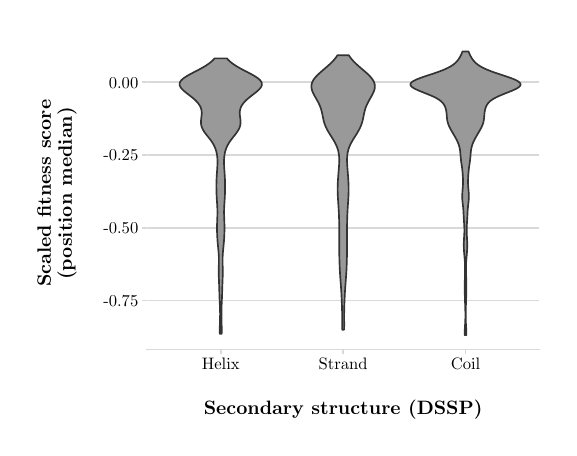
\begin{tikzpicture}[x=1pt,y=1pt]
\definecolor{fillColor}{RGB}{255,255,255}
\path[use as bounding box,fill=fillColor,fill opacity=0.00] (0,0) rectangle (188.25,144.54);
\begin{scope}
\path[clip] ( 43.23, 28.30) rectangle (184.75,141.04);
\definecolor{drawColor}{gray}{0.85}

\path[draw=drawColor,line width= 0.6pt,line join=round] ( 43.23, 45.97) --
	(184.75, 45.97);

\path[draw=drawColor,line width= 0.6pt,line join=round] ( 43.23, 72.25) --
	(184.75, 72.25);

\path[draw=drawColor,line width= 0.6pt,line join=round] ( 43.23, 98.52) --
	(184.75, 98.52);

\path[draw=drawColor,line width= 0.6pt,line join=round] ( 43.23,124.79) --
	(184.75,124.79);
\definecolor{drawColor}{gray}{0.20}
\definecolor{fillColor}{gray}{0.60}

\path[draw=drawColor,line width= 0.6pt,line join=round,line cap=round,fill=fillColor] ( 69.44, 33.88) --
	( 69.43, 34.07) --
	( 69.43, 34.27) --
	( 69.42, 34.46) --
	( 69.42, 34.66) --
	( 69.42, 34.85) --
	( 69.42, 35.05) --
	( 69.42, 35.24) --
	( 69.42, 35.44) --
	( 69.42, 35.63) --
	( 69.42, 35.83) --
	( 69.42, 36.02) --
	( 69.42, 36.22) --
	( 69.43, 36.41) --
	( 69.43, 36.61) --
	( 69.43, 36.80) --
	( 69.44, 37.00) --
	( 69.44, 37.19) --
	( 69.45, 37.39) --
	( 69.45, 37.58) --
	( 69.46, 37.78) --
	( 69.47, 37.97) --
	( 69.47, 38.17) --
	( 69.48, 38.36) --
	( 69.48, 38.56) --
	( 69.49, 38.75) --
	( 69.49, 38.95) --
	( 69.50, 39.14) --
	( 69.50, 39.34) --
	( 69.51, 39.53) --
	( 69.51, 39.73) --
	( 69.52, 39.92) --
	( 69.52, 40.12) --
	( 69.52, 40.31) --
	( 69.52, 40.51) --
	( 69.53, 40.70) --
	( 69.53, 40.90) --
	( 69.53, 41.09) --
	( 69.53, 41.29) --
	( 69.53, 41.48) --
	( 69.52, 41.68) --
	( 69.52, 41.87) --
	( 69.52, 42.07) --
	( 69.52, 42.26) --
	( 69.51, 42.45) --
	( 69.51, 42.65) --
	( 69.50, 42.84) --
	( 69.50, 43.04) --
	( 69.49, 43.23) --
	( 69.48, 43.43) --
	( 69.48, 43.62) --
	( 69.47, 43.82) --
	( 69.46, 44.01) --
	( 69.45, 44.21) --
	( 69.44, 44.40) --
	( 69.43, 44.60) --
	( 69.42, 44.79) --
	( 69.42, 44.99) --
	( 69.41, 45.18) --
	( 69.40, 45.38) --
	( 69.39, 45.57) --
	( 69.38, 45.77) --
	( 69.37, 45.96) --
	( 69.36, 46.16) --
	( 69.35, 46.35) --
	( 69.34, 46.55) --
	( 69.34, 46.74) --
	( 69.33, 46.94) --
	( 69.32, 47.13) --
	( 69.31, 47.33) --
	( 69.31, 47.52) --
	( 69.30, 47.72) --
	( 69.29, 47.91) --
	( 69.29, 48.11) --
	( 69.28, 48.30) --
	( 69.27, 48.50) --
	( 69.27, 48.69) --
	( 69.26, 48.89) --
	( 69.26, 49.08) --
	( 69.25, 49.28) --
	( 69.25, 49.47) --
	( 69.24, 49.67) --
	( 69.24, 49.86) --
	( 69.23, 50.06) --
	( 69.22, 50.25) --
	( 69.22, 50.44) --
	( 69.21, 50.64) --
	( 69.21, 50.83) --
	( 69.20, 51.03) --
	( 69.19, 51.22) --
	( 69.19, 51.42) --
	( 69.18, 51.61) --
	( 69.17, 51.81) --
	( 69.16, 52.00) --
	( 69.16, 52.20) --
	( 69.15, 52.39) --
	( 69.14, 52.59) --
	( 69.13, 52.78) --
	( 69.12, 52.98) --
	( 69.12, 53.17) --
	( 69.11, 53.37) --
	( 69.10, 53.56) --
	( 69.09, 53.76) --
	( 69.09, 53.95) --
	( 69.08, 54.15) --
	( 69.07, 54.34) --
	( 69.07, 54.54) --
	( 69.06, 54.73) --
	( 69.06, 54.93) --
	( 69.05, 55.12) --
	( 69.05, 55.32) --
	( 69.04, 55.51) --
	( 69.04, 55.71) --
	( 69.04, 55.90) --
	( 69.04, 56.10) --
	( 69.04, 56.29) --
	( 69.04, 56.49) --
	( 69.04, 56.68) --
	( 69.04, 56.88) --
	( 69.04, 57.07) --
	( 69.05, 57.27) --
	( 69.05, 57.46) --
	( 69.05, 57.66) --
	( 69.06, 57.85) --
	( 69.06, 58.05) --
	( 69.06, 58.24) --
	( 69.07, 58.44) --
	( 69.07, 58.63) --
	( 69.08, 58.82) --
	( 69.08, 59.02) --
	( 69.09, 59.21) --
	( 69.09, 59.41) --
	( 69.09, 59.60) --
	( 69.10, 59.80) --
	( 69.10, 59.99) --
	( 69.10, 60.19) --
	( 69.10, 60.38) --
	( 69.10, 60.58) --
	( 69.10, 60.77) --
	( 69.10, 60.97) --
	( 69.09, 61.16) --
	( 69.09, 61.36) --
	( 69.08, 61.55) --
	( 69.08, 61.75) --
	( 69.07, 61.94) --
	( 69.06, 62.14) --
	( 69.05, 62.33) --
	( 69.04, 62.53) --
	( 69.03, 62.72) --
	( 69.02, 62.92) --
	( 69.00, 63.11) --
	( 68.99, 63.31) --
	( 68.97, 63.50) --
	( 68.95, 63.70) --
	( 68.94, 63.89) --
	( 68.92, 64.09) --
	( 68.90, 64.28) --
	( 68.88, 64.48) --
	( 68.86, 64.67) --
	( 68.85, 64.87) --
	( 68.83, 65.06) --
	( 68.81, 65.26) --
	( 68.79, 65.45) --
	( 68.77, 65.65) --
	( 68.75, 65.84) --
	( 68.73, 66.04) --
	( 68.71, 66.23) --
	( 68.69, 66.43) --
	( 68.68, 66.62) --
	( 68.66, 66.82) --
	( 68.64, 67.01) --
	( 68.63, 67.20) --
	( 68.61, 67.40) --
	( 68.59, 67.59) --
	( 68.58, 67.79) --
	( 68.57, 67.98) --
	( 68.55, 68.18) --
	( 68.54, 68.37) --
	( 68.53, 68.57) --
	( 68.52, 68.76) --
	( 68.51, 68.96) --
	( 68.50, 69.15) --
	( 68.49, 69.35) --
	( 68.48, 69.54) --
	( 68.47, 69.74) --
	( 68.46, 69.93) --
	( 68.46, 70.13) --
	( 68.45, 70.32) --
	( 68.44, 70.52) --
	( 68.44, 70.71) --
	( 68.43, 70.91) --
	( 68.43, 71.10) --
	( 68.43, 71.30) --
	( 68.42, 71.49) --
	( 68.42, 71.69) --
	( 68.42, 71.88) --
	( 68.42, 72.08) --
	( 68.42, 72.27) --
	( 68.42, 72.47) --
	( 68.42, 72.66) --
	( 68.42, 72.86) --
	( 68.43, 73.05) --
	( 68.43, 73.25) --
	( 68.43, 73.44) --
	( 68.44, 73.64) --
	( 68.44, 73.83) --
	( 68.45, 74.03) --
	( 68.46, 74.22) --
	( 68.46, 74.42) --
	( 68.47, 74.61) --
	( 68.48, 74.81) --
	( 68.49, 75.00) --
	( 68.50, 75.19) --
	( 68.50, 75.39) --
	( 68.51, 75.58) --
	( 68.52, 75.78) --
	( 68.53, 75.97) --
	( 68.53, 76.17) --
	( 68.54, 76.36) --
	( 68.55, 76.56) --
	( 68.55, 76.75) --
	( 68.56, 76.95) --
	( 68.56, 77.14) --
	( 68.56, 77.34) --
	( 68.57, 77.53) --
	( 68.57, 77.73) --
	( 68.57, 77.92) --
	( 68.57, 78.12) --
	( 68.56, 78.31) --
	( 68.56, 78.51) --
	( 68.56, 78.70) --
	( 68.55, 78.90) --
	( 68.55, 79.09) --
	( 68.54, 79.29) --
	( 68.53, 79.48) --
	( 68.52, 79.68) --
	( 68.51, 79.87) --
	( 68.50, 80.07) --
	( 68.49, 80.26) --
	( 68.48, 80.46) --
	( 68.47, 80.65) --
	( 68.45, 80.85) --
	( 68.44, 81.04) --
	( 68.43, 81.24) --
	( 68.41, 81.43) --
	( 68.40, 81.63) --
	( 68.39, 81.82) --
	( 68.38, 82.02) --
	( 68.36, 82.21) --
	( 68.35, 82.41) --
	( 68.34, 82.60) --
	( 68.33, 82.80) --
	( 68.32, 82.99) --
	( 68.31, 83.19) --
	( 68.30, 83.38) --
	( 68.29, 83.57) --
	( 68.28, 83.77) --
	( 68.27, 83.96) --
	( 68.26, 84.16) --
	( 68.25, 84.35) --
	( 68.25, 84.55) --
	( 68.24, 84.74) --
	( 68.23, 84.94) --
	( 68.23, 85.13) --
	( 68.22, 85.33) --
	( 68.22, 85.52) --
	( 68.22, 85.72) --
	( 68.21, 85.91) --
	( 68.21, 86.11) --
	( 68.21, 86.30) --
	( 68.20, 86.50) --
	( 68.20, 86.69) --
	( 68.20, 86.89) --
	( 68.20, 87.08) --
	( 68.20, 87.28) --
	( 68.20, 87.47) --
	( 68.20, 87.67) --
	( 68.20, 87.86) --
	( 68.20, 88.06) --
	( 68.21, 88.25) --
	( 68.21, 88.45) --
	( 68.21, 88.64) --
	( 68.22, 88.84) --
	( 68.22, 89.03) --
	( 68.23, 89.23) --
	( 68.24, 89.42) --
	( 68.24, 89.62) --
	( 68.25, 89.81) --
	( 68.26, 90.01) --
	( 68.27, 90.20) --
	( 68.28, 90.40) --
	( 68.29, 90.59) --
	( 68.30, 90.79) --
	( 68.31, 90.98) --
	( 68.32, 91.18) --
	( 68.34, 91.37) --
	( 68.35, 91.57) --
	( 68.36, 91.76) --
	( 68.38, 91.95) --
	( 68.39, 92.15) --
	( 68.40, 92.34) --
	( 68.42, 92.54) --
	( 68.43, 92.73) --
	( 68.45, 92.93) --
	( 68.46, 93.12) --
	( 68.47, 93.32) --
	( 68.49, 93.51) --
	( 68.50, 93.71) --
	( 68.51, 93.90) --
	( 68.52, 94.10) --
	( 68.53, 94.29) --
	( 68.54, 94.49) --
	( 68.55, 94.68) --
	( 68.56, 94.88) --
	( 68.57, 95.07) --
	( 68.58, 95.27) --
	( 68.58, 95.46) --
	( 68.58, 95.66) --
	( 68.58, 95.85) --
	( 68.59, 96.05) --
	( 68.58, 96.24) --
	( 68.58, 96.44) --
	( 68.58, 96.63) --
	( 68.57, 96.83) --
	( 68.56, 97.02) --
	( 68.55, 97.22) --
	( 68.54, 97.41) --
	( 68.52, 97.61) --
	( 68.50, 97.80) --
	( 68.48, 98.00) --
	( 68.46, 98.19) --
	( 68.44, 98.39) --
	( 68.41, 98.58) --
	( 68.38, 98.78) --
	( 68.34, 98.97) --
	( 68.31, 99.17) --
	( 68.26, 99.36) --
	( 68.22, 99.56) --
	( 68.17, 99.75) --
	( 68.12, 99.94) --
	( 68.06,100.14) --
	( 68.01,100.33) --
	( 67.94,100.53) --
	( 67.87,100.72) --
	( 67.80,100.92) --
	( 67.72,101.11) --
	( 67.64,101.31) --
	( 67.56,101.50) --
	( 67.47,101.70) --
	( 67.37,101.89) --
	( 67.27,102.09) --
	( 67.16,102.28) --
	( 67.05,102.48) --
	( 66.94,102.67) --
	( 66.82,102.87) --
	( 66.70,103.06) --
	( 66.57,103.26) --
	( 66.43,103.45) --
	( 66.30,103.65) --
	( 66.16,103.84) --
	( 66.01,104.04) --
	( 65.87,104.23) --
	( 65.72,104.43) --
	( 65.57,104.62) --
	( 65.41,104.82) --
	( 65.26,105.01) --
	( 65.10,105.21) --
	( 64.95,105.40) --
	( 64.79,105.60) --
	( 64.64,105.79) --
	( 64.49,105.99) --
	( 64.34,106.18) --
	( 64.19,106.38) --
	( 64.05,106.57) --
	( 63.91,106.77) --
	( 63.78,106.96) --
	( 63.65,107.16) --
	( 63.53,107.35) --
	( 63.41,107.55) --
	( 63.31,107.74) --
	( 63.21,107.94) --
	( 63.11,108.13) --
	( 63.03,108.32) --
	( 62.95,108.52) --
	( 62.88,108.71) --
	( 62.82,108.91) --
	( 62.77,109.10) --
	( 62.72,109.30) --
	( 62.68,109.49) --
	( 62.66,109.69) --
	( 62.63,109.88) --
	( 62.62,110.08) --
	( 62.61,110.27) --
	( 62.61,110.47) --
	( 62.62,110.66) --
	( 62.62,110.86) --
	( 62.64,111.05) --
	( 62.66,111.25) --
	( 62.68,111.44) --
	( 62.70,111.64) --
	( 62.72,111.83) --
	( 62.75,112.03) --
	( 62.77,112.22) --
	( 62.80,112.42) --
	( 62.82,112.61) --
	( 62.84,112.81) --
	( 62.86,113.00) --
	( 62.87,113.20) --
	( 62.88,113.39) --
	( 62.89,113.59) --
	( 62.89,113.78) --
	( 62.88,113.98) --
	( 62.87,114.17) --
	( 62.85,114.37) --
	( 62.83,114.56) --
	( 62.79,114.76) --
	( 62.75,114.95) --
	( 62.70,115.15) --
	( 62.64,115.34) --
	( 62.58,115.54) --
	( 62.50,115.73) --
	( 62.41,115.93) --
	( 62.32,116.12) --
	( 62.21,116.32) --
	( 62.10,116.51) --
	( 61.97,116.70) --
	( 61.84,116.90) --
	( 61.70,117.09) --
	( 61.54,117.29) --
	( 61.38,117.48) --
	( 61.21,117.68) --
	( 61.03,117.87) --
	( 60.84,118.07) --
	( 60.64,118.26) --
	( 60.44,118.46) --
	( 60.22,118.65) --
	( 60.00,118.85) --
	( 59.78,119.04) --
	( 59.54,119.24) --
	( 59.30,119.43) --
	( 59.06,119.63) --
	( 58.81,119.82) --
	( 58.56,120.02) --
	( 58.31,120.21) --
	( 58.06,120.41) --
	( 57.81,120.60) --
	( 57.55,120.80) --
	( 57.31,120.99) --
	( 57.06,121.19) --
	( 56.83,121.38) --
	( 56.59,121.58) --
	( 56.37,121.77) --
	( 56.16,121.97) --
	( 55.96,122.16) --
	( 55.77,122.36) --
	( 55.60,122.55) --
	( 55.44,122.75) --
	( 55.30,122.94) --
	( 55.18,123.14) --
	( 55.08,123.33) --
	( 54.99,123.53) --
	( 54.94,123.72) --
	( 54.90,123.92) --
	( 54.89,124.11) --
	( 54.90,124.31) --
	( 54.93,124.50) --
	( 55.00,124.69) --
	( 55.08,124.89) --
	( 55.19,125.08) --
	( 55.32,125.28) --
	( 55.48,125.47) --
	( 55.66,125.67) --
	( 55.87,125.86) --
	( 56.09,126.06) --
	( 56.33,126.25) --
	( 56.60,126.45) --
	( 56.88,126.64) --
	( 57.18,126.84) --
	( 57.50,127.03) --
	( 57.82,127.23) --
	( 58.16,127.42) --
	( 58.51,127.62) --
	( 58.87,127.81) --
	( 59.24,128.01) --
	( 59.61,128.20) --
	( 59.98,128.40) --
	( 60.36,128.59) --
	( 60.74,128.79) --
	( 61.11,128.98) --
	( 61.48,129.18) --
	( 61.85,129.37) --
	( 62.22,129.57) --
	( 62.58,129.76) --
	( 62.93,129.96) --
	( 63.27,130.15) --
	( 63.61,130.35) --
	( 63.94,130.54) --
	( 64.26,130.74) --
	( 64.56,130.93) --
	( 64.86,131.13) --
	( 65.14,131.32) --
	( 65.42,131.52) --
	( 65.68,131.71) --
	( 65.93,131.91) --
	( 66.17,132.10) --
	( 66.40,132.30) --
	( 66.62,132.49) --
	( 66.83,132.69) --
	( 67.03,132.88) --
	( 67.21,133.07) --
	( 67.39,133.27) --
	( 67.56,133.46) --
	( 71.98,133.46) --
	( 72.14,133.27) --
	( 72.32,133.07) --
	( 72.51,132.88) --
	( 72.70,132.69) --
	( 72.91,132.49) --
	( 73.13,132.30) --
	( 73.36,132.10) --
	( 73.60,131.91) --
	( 73.85,131.71) --
	( 74.11,131.52) --
	( 74.39,131.32) --
	( 74.68,131.13) --
	( 74.97,130.93) --
	( 75.28,130.74) --
	( 75.59,130.54) --
	( 75.92,130.35) --
	( 76.26,130.15) --
	( 76.60,129.96) --
	( 76.95,129.76) --
	( 77.31,129.57) --
	( 77.68,129.37) --
	( 78.05,129.18) --
	( 78.42,128.98) --
	( 78.80,128.79) --
	( 79.17,128.59) --
	( 79.55,128.40) --
	( 79.92,128.20) --
	( 80.30,128.01) --
	( 80.66,127.81) --
	( 81.02,127.62) --
	( 81.37,127.42) --
	( 81.71,127.23) --
	( 82.04,127.03) --
	( 82.35,126.84) --
	( 82.65,126.64) --
	( 82.93,126.45) --
	( 83.20,126.25) --
	( 83.44,126.06) --
	( 83.67,125.86) --
	( 83.87,125.67) --
	( 84.05,125.47) --
	( 84.21,125.28) --
	( 84.34,125.08) --
	( 84.45,124.89) --
	( 84.53,124.69) --
	( 84.60,124.50) --
	( 84.63,124.31) --
	( 84.64,124.11) --
	( 84.63,123.92) --
	( 84.59,123.72) --
	( 84.54,123.53) --
	( 84.45,123.33) --
	( 84.35,123.14) --
	( 84.23,122.94) --
	( 84.09,122.75) --
	( 83.94,122.55) --
	( 83.76,122.36) --
	( 83.57,122.16) --
	( 83.37,121.97) --
	( 83.16,121.77) --
	( 82.94,121.58) --
	( 82.71,121.38) --
	( 82.47,121.19) --
	( 82.23,120.99) --
	( 81.98,120.80) --
	( 81.73,120.60) --
	( 81.47,120.41) --
	( 81.22,120.21) --
	( 80.97,120.02) --
	( 80.72,119.82) --
	( 80.47,119.63) --
	( 80.23,119.43) --
	( 79.99,119.24) --
	( 79.76,119.04) --
	( 79.53,118.85) --
	( 79.31,118.65) --
	( 79.09,118.46) --
	( 78.89,118.26) --
	( 78.69,118.07) --
	( 78.50,117.87) --
	( 78.32,117.68) --
	( 78.15,117.48) --
	( 77.99,117.29) --
	( 77.84,117.09) --
	( 77.69,116.90) --
	( 77.56,116.70) --
	( 77.43,116.51) --
	( 77.32,116.32) --
	( 77.22,116.12) --
	( 77.12,115.93) --
	( 77.03,115.73) --
	( 76.96,115.54) --
	( 76.89,115.34) --
	( 76.83,115.15) --
	( 76.78,114.95) --
	( 76.74,114.76) --
	( 76.70,114.56) --
	( 76.68,114.37) --
	( 76.66,114.17) --
	( 76.65,113.98) --
	( 76.64,113.78) --
	( 76.64,113.59) --
	( 76.65,113.39) --
	( 76.66,113.20) --
	( 76.67,113.00) --
	( 76.69,112.81) --
	( 76.71,112.61) --
	( 76.73,112.42) --
	( 76.76,112.22) --
	( 76.78,112.03) --
	( 76.81,111.83) --
	( 76.83,111.64) --
	( 76.86,111.44) --
	( 76.88,111.25) --
	( 76.89,111.05) --
	( 76.91,110.86) --
	( 76.92,110.66) --
	( 76.92,110.47) --
	( 76.92,110.27) --
	( 76.91,110.08) --
	( 76.90,109.88) --
	( 76.88,109.69) --
	( 76.85,109.49) --
	( 76.81,109.30) --
	( 76.77,109.10) --
	( 76.71,108.91) --
	( 76.65,108.71) --
	( 76.58,108.52) --
	( 76.51,108.32) --
	( 76.42,108.13) --
	( 76.33,107.94) --
	( 76.23,107.74) --
	( 76.12,107.55) --
	( 76.00,107.35) --
	( 75.88,107.16) --
	( 75.75,106.96) --
	( 75.62,106.77) --
	( 75.48,106.57) --
	( 75.34,106.38) --
	( 75.19,106.18) --
	( 75.04,105.99) --
	( 74.89,105.79) --
	( 74.74,105.60) --
	( 74.58,105.40) --
	( 74.43,105.21) --
	( 74.27,105.01) --
	( 74.12,104.82) --
	( 73.97,104.62) --
	( 73.82,104.43) --
	( 73.67,104.23) --
	( 73.52,104.04) --
	( 73.38,103.84) --
	( 73.24,103.65) --
	( 73.10,103.45) --
	( 72.97,103.26) --
	( 72.84,103.06) --
	( 72.71,102.87) --
	( 72.59,102.67) --
	( 72.48,102.48) --
	( 72.37,102.28) --
	( 72.26,102.09) --
	( 72.16,101.89) --
	( 72.07,101.70) --
	( 71.98,101.50) --
	( 71.89,101.31) --
	( 71.81,101.11) --
	( 71.73,100.92) --
	( 71.66,100.72) --
	( 71.59,100.53) --
	( 71.53,100.33) --
	( 71.47,100.14) --
	( 71.41, 99.94) --
	( 71.36, 99.75) --
	( 71.31, 99.56) --
	( 71.27, 99.36) --
	( 71.23, 99.17) --
	( 71.19, 98.97) --
	( 71.16, 98.78) --
	( 71.12, 98.58) --
	( 71.10, 98.39) --
	( 71.07, 98.19) --
	( 71.05, 98.00) --
	( 71.03, 97.80) --
	( 71.01, 97.61) --
	( 71.00, 97.41) --
	( 70.98, 97.22) --
	( 70.97, 97.02) --
	( 70.96, 96.83) --
	( 70.96, 96.63) --
	( 70.95, 96.44) --
	( 70.95, 96.24) --
	( 70.95, 96.05) --
	( 70.95, 95.85) --
	( 70.95, 95.66) --
	( 70.95, 95.46) --
	( 70.96, 95.27) --
	( 70.96, 95.07) --
	( 70.97, 94.88) --
	( 70.98, 94.68) --
	( 70.99, 94.49) --
	( 71.00, 94.29) --
	( 71.01, 94.10) --
	( 71.02, 93.90) --
	( 71.03, 93.71) --
	( 71.05, 93.51) --
	( 71.06, 93.32) --
	( 71.07, 93.12) --
	( 71.09, 92.93) --
	( 71.10, 92.73) --
	( 71.11, 92.54) --
	( 71.13, 92.34) --
	( 71.14, 92.15) --
	( 71.16, 91.95) --
	( 71.17, 91.76) --
	( 71.18, 91.57) --
	( 71.20, 91.37) --
	( 71.21, 91.18) --
	( 71.22, 90.98) --
	( 71.23, 90.79) --
	( 71.24, 90.59) --
	( 71.25, 90.40) --
	( 71.26, 90.20) --
	( 71.27, 90.01) --
	( 71.28, 89.81) --
	( 71.29, 89.62) --
	( 71.30, 89.42) --
	( 71.30, 89.23) --
	( 71.31, 89.03) --
	( 71.31, 88.84) --
	( 71.32, 88.64) --
	( 71.32, 88.45) --
	( 71.33, 88.25) --
	( 71.33, 88.06) --
	( 71.33, 87.86) --
	( 71.33, 87.67) --
	( 71.33, 87.47) --
	( 71.33, 87.28) --
	( 71.33, 87.08) --
	( 71.33, 86.89) --
	( 71.33, 86.69) --
	( 71.33, 86.50) --
	( 71.33, 86.30) --
	( 71.32, 86.11) --
	( 71.32, 85.91) --
	( 71.32, 85.72) --
	( 71.31, 85.52) --
	( 71.31, 85.33) --
	( 71.30, 85.13) --
	( 71.30, 84.94) --
	( 71.29, 84.74) --
	( 71.29, 84.55) --
	( 71.28, 84.35) --
	( 71.27, 84.16) --
	( 71.26, 83.96) --
	( 71.26, 83.77) --
	( 71.25, 83.57) --
	( 71.24, 83.38) --
	( 71.23, 83.19) --
	( 71.22, 82.99) --
	( 71.21, 82.80) --
	( 71.19, 82.60) --
	( 71.18, 82.41) --
	( 71.17, 82.21) --
	( 71.16, 82.02) --
	( 71.14, 81.82) --
	( 71.13, 81.63) --
	( 71.12, 81.43) --
	( 71.10, 81.24) --
	( 71.09, 81.04) --
	( 71.08, 80.85) --
	( 71.07, 80.65) --
	( 71.05, 80.46) --
	( 71.04, 80.26) --
	( 71.03, 80.07) --
	( 71.02, 79.87) --
	( 71.01, 79.68) --
	( 71.00, 79.48) --
	( 70.99, 79.29) --
	( 70.99, 79.09) --
	( 70.98, 78.90) --
	( 70.98, 78.70) --
	( 70.97, 78.51) --
	( 70.97, 78.31) --
	( 70.97, 78.12) --
	( 70.97, 77.92) --
	( 70.97, 77.73) --
	( 70.97, 77.53) --
	( 70.97, 77.34) --
	( 70.97, 77.14) --
	( 70.98, 76.95) --
	( 70.98, 76.75) --
	( 70.99, 76.56) --
	( 70.99, 76.36) --
	( 71.00, 76.17) --
	( 71.01, 75.97) --
	( 71.01, 75.78) --
	( 71.02, 75.58) --
	( 71.03, 75.39) --
	( 71.04, 75.19) --
	( 71.04, 75.00) --
	( 71.05, 74.81) --
	( 71.06, 74.61) --
	( 71.07, 74.42) --
	( 71.07, 74.22) --
	( 71.08, 74.03) --
	( 71.09, 73.83) --
	( 71.09, 73.64) --
	( 71.10, 73.44) --
	( 71.10, 73.25) --
	( 71.11, 73.05) --
	( 71.11, 72.86) --
	( 71.11, 72.66) --
	( 71.11, 72.47) --
	( 71.11, 72.27) --
	( 71.11, 72.08) --
	( 71.11, 71.88) --
	( 71.11, 71.69) --
	( 71.11, 71.49) --
	( 71.11, 71.30) --
	( 71.10, 71.10) --
	( 71.10, 70.91) --
	( 71.09, 70.71) --
	( 71.09, 70.52) --
	( 71.08, 70.32) --
	( 71.08, 70.13) --
	( 71.07, 69.93) --
	( 71.06, 69.74) --
	( 71.05, 69.54) --
	( 71.04, 69.35) --
	( 71.04, 69.15) --
	( 71.03, 68.96) --
	( 71.01, 68.76) --
	( 71.00, 68.57) --
	( 70.99, 68.37) --
	( 70.98, 68.18) --
	( 70.97, 67.98) --
	( 70.95, 67.79) --
	( 70.94, 67.59) --
	( 70.92, 67.40) --
	( 70.91, 67.20) --
	( 70.89, 67.01) --
	( 70.87, 66.82) --
	( 70.86, 66.62) --
	( 70.84, 66.43) --
	( 70.82, 66.23) --
	( 70.80, 66.04) --
	( 70.78, 65.84) --
	( 70.76, 65.65) --
	( 70.75, 65.45) --
	( 70.73, 65.26) --
	( 70.71, 65.06) --
	( 70.69, 64.87) --
	( 70.67, 64.67) --
	( 70.65, 64.48) --
	( 70.63, 64.28) --
	( 70.61, 64.09) --
	( 70.59, 63.89) --
	( 70.58, 63.70) --
	( 70.56, 63.50) --
	( 70.55, 63.31) --
	( 70.53, 63.11) --
	( 70.52, 62.92) --
	( 70.50, 62.72) --
	( 70.49, 62.53) --
	( 70.48, 62.33) --
	( 70.47, 62.14) --
	( 70.46, 61.94) --
	( 70.45, 61.75) --
	( 70.45, 61.55) --
	( 70.44, 61.36) --
	( 70.44, 61.16) --
	( 70.44, 60.97) --
	( 70.43, 60.77) --
	( 70.43, 60.58) --
	( 70.43, 60.38) --
	( 70.43, 60.19) --
	( 70.43, 59.99) --
	( 70.44, 59.80) --
	( 70.44, 59.60) --
	( 70.44, 59.41) --
	( 70.45, 59.21) --
	( 70.45, 59.02) --
	( 70.45, 58.82) --
	( 70.46, 58.63) --
	( 70.46, 58.44) --
	( 70.47, 58.24) --
	( 70.47, 58.05) --
	( 70.48, 57.85) --
	( 70.48, 57.66) --
	( 70.48, 57.46) --
	( 70.49, 57.27) --
	( 70.49, 57.07) --
	( 70.49, 56.88) --
	( 70.49, 56.68) --
	( 70.49, 56.49) --
	( 70.49, 56.29) --
	( 70.49, 56.10) --
	( 70.49, 55.90) --
	( 70.49, 55.71) --
	( 70.49, 55.51) --
	( 70.48, 55.32) --
	( 70.48, 55.12) --
	( 70.48, 54.93) --
	( 70.47, 54.73) --
	( 70.47, 54.54) --
	( 70.46, 54.34) --
	( 70.45, 54.15) --
	( 70.45, 53.95) --
	( 70.44, 53.76) --
	( 70.43, 53.56) --
	( 70.42, 53.37) --
	( 70.42, 53.17) --
	( 70.41, 52.98) --
	( 70.40, 52.78) --
	( 70.39, 52.59) --
	( 70.38, 52.39) --
	( 70.38, 52.20) --
	( 70.37, 52.00) --
	( 70.36, 51.81) --
	( 70.35, 51.61) --
	( 70.35, 51.42) --
	( 70.34, 51.22) --
	( 70.33, 51.03) --
	( 70.33, 50.83) --
	( 70.32, 50.64) --
	( 70.31, 50.44) --
	( 70.31, 50.25) --
	( 70.30, 50.06) --
	( 70.30, 49.86) --
	( 70.29, 49.67) --
	( 70.29, 49.47) --
	( 70.28, 49.28) --
	( 70.27, 49.08) --
	( 70.27, 48.89) --
	( 70.26, 48.69) --
	( 70.26, 48.50) --
	( 70.25, 48.30) --
	( 70.25, 48.11) --
	( 70.24, 47.91) --
	( 70.23, 47.72) --
	( 70.23, 47.52) --
	( 70.22, 47.33) --
	( 70.21, 47.13) --
	( 70.20, 46.94) --
	( 70.20, 46.74) --
	( 70.19, 46.55) --
	( 70.18, 46.35) --
	( 70.17, 46.16) --
	( 70.16, 45.96) --
	( 70.15, 45.77) --
	( 70.14, 45.57) --
	( 70.13, 45.38) --
	( 70.13, 45.18) --
	( 70.12, 44.99) --
	( 70.11, 44.79) --
	( 70.10, 44.60) --
	( 70.09, 44.40) --
	( 70.08, 44.21) --
	( 70.07, 44.01) --
	( 70.06, 43.82) --
	( 70.06, 43.62) --
	( 70.05, 43.43) --
	( 70.04, 43.23) --
	( 70.04, 43.04) --
	( 70.03, 42.84) --
	( 70.03, 42.65) --
	( 70.02, 42.45) --
	( 70.02, 42.26) --
	( 70.01, 42.07) --
	( 70.01, 41.87) --
	( 70.01, 41.68) --
	( 70.01, 41.48) --
	( 70.01, 41.29) --
	( 70.01, 41.09) --
	( 70.01, 40.90) --
	( 70.01, 40.70) --
	( 70.01, 40.51) --
	( 70.01, 40.31) --
	( 70.01, 40.12) --
	( 70.02, 39.92) --
	( 70.02, 39.73) --
	( 70.02, 39.53) --
	( 70.03, 39.34) --
	( 70.03, 39.14) --
	( 70.04, 38.95) --
	( 70.04, 38.75) --
	( 70.05, 38.56) --
	( 70.06, 38.36) --
	( 70.06, 38.17) --
	( 70.07, 37.97) --
	( 70.07, 37.78) --
	( 70.08, 37.58) --
	( 70.08, 37.39) --
	( 70.09, 37.19) --
	( 70.09, 37.00) --
	( 70.10, 36.80) --
	( 70.10, 36.61) --
	( 70.11, 36.41) --
	( 70.11, 36.22) --
	( 70.11, 36.02) --
	( 70.11, 35.83) --
	( 70.11, 35.63) --
	( 70.12, 35.44) --
	( 70.12, 35.24) --
	( 70.11, 35.05) --
	( 70.11, 34.85) --
	( 70.11, 34.66) --
	( 70.11, 34.46) --
	( 70.10, 34.27) --
	( 70.10, 34.07) --
	( 70.09, 33.88) --
	( 69.44, 33.88) --
	cycle;

\path[draw=drawColor,line width= 0.6pt,line join=round,line cap=round,fill=fillColor] (113.63, 35.38) --
	(113.63, 35.57) --
	(113.63, 35.76) --
	(113.62, 35.96) --
	(113.62, 36.15) --
	(113.62, 36.35) --
	(113.62, 36.54) --
	(113.62, 36.73) --
	(113.62, 36.93) --
	(113.61, 37.12) --
	(113.61, 37.32) --
	(113.61, 37.51) --
	(113.61, 37.71) --
	(113.62, 37.90) --
	(113.62, 38.09) --
	(113.62, 38.29) --
	(113.62, 38.48) --
	(113.62, 38.68) --
	(113.62, 38.87) --
	(113.62, 39.06) --
	(113.62, 39.26) --
	(113.62, 39.45) --
	(113.62, 39.65) --
	(113.62, 39.84) --
	(113.62, 40.04) --
	(113.62, 40.23) --
	(113.62, 40.42) --
	(113.62, 40.62) --
	(113.62, 40.81) --
	(113.62, 41.01) --
	(113.62, 41.20) --
	(113.62, 41.39) --
	(113.62, 41.59) --
	(113.61, 41.78) --
	(113.61, 41.98) --
	(113.61, 42.17) --
	(113.60, 42.36) --
	(113.60, 42.56) --
	(113.60, 42.75) --
	(113.59, 42.95) --
	(113.59, 43.14) --
	(113.58, 43.34) --
	(113.58, 43.53) --
	(113.57, 43.72) --
	(113.56, 43.92) --
	(113.56, 44.11) --
	(113.55, 44.31) --
	(113.54, 44.50) --
	(113.54, 44.69) --
	(113.53, 44.89) --
	(113.52, 45.08) --
	(113.51, 45.28) --
	(113.51, 45.47) --
	(113.50, 45.67) --
	(113.49, 45.86) --
	(113.48, 46.05) --
	(113.47, 46.25) --
	(113.47, 46.44) --
	(113.46, 46.64) --
	(113.45, 46.83) --
	(113.44, 47.02) --
	(113.43, 47.22) --
	(113.42, 47.41) --
	(113.41, 47.61) --
	(113.40, 47.80) --
	(113.39, 48.00) --
	(113.38, 48.19) --
	(113.37, 48.38) --
	(113.36, 48.58) --
	(113.35, 48.77) --
	(113.34, 48.97) --
	(113.33, 49.16) --
	(113.31, 49.35) --
	(113.30, 49.55) --
	(113.29, 49.74) --
	(113.28, 49.94) --
	(113.27, 50.13) --
	(113.25, 50.33) --
	(113.24, 50.52) --
	(113.23, 50.71) --
	(113.21, 50.91) --
	(113.20, 51.10) --
	(113.19, 51.30) --
	(113.17, 51.49) --
	(113.16, 51.68) --
	(113.14, 51.88) --
	(113.13, 52.07) --
	(113.11, 52.27) --
	(113.10, 52.46) --
	(113.08, 52.66) --
	(113.07, 52.85) --
	(113.05, 53.04) --
	(113.04, 53.24) --
	(113.02, 53.43) --
	(113.01, 53.63) --
	(112.99, 53.82) --
	(112.98, 54.01) --
	(112.97, 54.21) --
	(112.95, 54.40) --
	(112.94, 54.60) --
	(112.92, 54.79) --
	(112.91, 54.99) --
	(112.90, 55.18) --
	(112.89, 55.37) --
	(112.87, 55.57) --
	(112.86, 55.76) --
	(112.85, 55.96) --
	(112.84, 56.15) --
	(112.83, 56.34) --
	(112.81, 56.54) --
	(112.80, 56.73) --
	(112.79, 56.93) --
	(112.78, 57.12) --
	(112.77, 57.32) --
	(112.76, 57.51) --
	(112.76, 57.70) --
	(112.75, 57.90) --
	(112.74, 58.09) --
	(112.73, 58.29) --
	(112.72, 58.48) --
	(112.71, 58.67) --
	(112.71, 58.87) --
	(112.70, 59.06) --
	(112.69, 59.26) --
	(112.69, 59.45) --
	(112.68, 59.65) --
	(112.67, 59.84) --
	(112.67, 60.03) --
	(112.66, 60.23) --
	(112.66, 60.42) --
	(112.65, 60.62) --
	(112.64, 60.81) --
	(112.64, 61.00) --
	(112.63, 61.20) --
	(112.63, 61.39) --
	(112.62, 61.59) --
	(112.62, 61.78) --
	(112.61, 61.98) --
	(112.61, 62.17) --
	(112.61, 62.36) --
	(112.60, 62.56) --
	(112.60, 62.75) --
	(112.59, 62.95) --
	(112.59, 63.14) --
	(112.59, 63.33) --
	(112.59, 63.53) --
	(112.58, 63.72) --
	(112.58, 63.92) --
	(112.58, 64.11) --
	(112.58, 64.31) --
	(112.57, 64.50) --
	(112.57, 64.69) --
	(112.57, 64.89) --
	(112.57, 65.08) --
	(112.57, 65.28) --
	(112.57, 65.47) --
	(112.57, 65.66) --
	(112.57, 65.86) --
	(112.57, 66.05) --
	(112.57, 66.25) --
	(112.57, 66.44) --
	(112.57, 66.63) --
	(112.57, 66.83) --
	(112.57, 67.02) --
	(112.57, 67.22) --
	(112.58, 67.41) --
	(112.58, 67.61) --
	(112.58, 67.80) --
	(112.58, 67.99) --
	(112.58, 68.19) --
	(112.58, 68.38) --
	(112.59, 68.58) --
	(112.59, 68.77) --
	(112.59, 68.96) --
	(112.59, 69.16) --
	(112.59, 69.35) --
	(112.59, 69.55) --
	(112.59, 69.74) --
	(112.60, 69.94) --
	(112.60, 70.13) --
	(112.60, 70.32) --
	(112.60, 70.52) --
	(112.60, 70.71) --
	(112.60, 70.91) --
	(112.60, 71.10) --
	(112.60, 71.29) --
	(112.60, 71.49) --
	(112.59, 71.68) --
	(112.59, 71.88) --
	(112.59, 72.07) --
	(112.59, 72.27) --
	(112.59, 72.46) --
	(112.59, 72.65) --
	(112.58, 72.85) --
	(112.58, 73.04) --
	(112.58, 73.24) --
	(112.57, 73.43) --
	(112.57, 73.62) --
	(112.57, 73.82) --
	(112.56, 74.01) --
	(112.56, 74.21) --
	(112.55, 74.40) --
	(112.55, 74.60) --
	(112.54, 74.79) --
	(112.54, 74.98) --
	(112.53, 75.18) --
	(112.53, 75.37) --
	(112.52, 75.57) --
	(112.51, 75.76) --
	(112.51, 75.95) --
	(112.50, 76.15) --
	(112.49, 76.34) --
	(112.49, 76.54) --
	(112.48, 76.73) --
	(112.47, 76.93) --
	(112.46, 77.12) --
	(112.45, 77.31) --
	(112.45, 77.51) --
	(112.44, 77.70) --
	(112.43, 77.90) --
	(112.42, 78.09) --
	(112.41, 78.28) --
	(112.40, 78.48) --
	(112.39, 78.67) --
	(112.37, 78.87) --
	(112.36, 79.06) --
	(112.35, 79.26) --
	(112.34, 79.45) --
	(112.33, 79.64) --
	(112.31, 79.84) --
	(112.30, 80.03) --
	(112.29, 80.23) --
	(112.28, 80.42) --
	(112.26, 80.61) --
	(112.25, 80.81) --
	(112.24, 81.00) --
	(112.22, 81.20) --
	(112.21, 81.39) --
	(112.20, 81.59) --
	(112.19, 81.78) --
	(112.17, 81.97) --
	(112.16, 82.17) --
	(112.15, 82.36) --
	(112.14, 82.56) --
	(112.12, 82.75) --
	(112.11, 82.94) --
	(112.10, 83.14) --
	(112.09, 83.33) --
	(112.08, 83.53) --
	(112.07, 83.72) --
	(112.06, 83.92) --
	(112.05, 84.11) --
	(112.05, 84.30) --
	(112.04, 84.50) --
	(112.03, 84.69) --
	(112.03, 84.89) --
	(112.02, 85.08) --
	(112.02, 85.27) --
	(112.01, 85.47) --
	(112.01, 85.66) --
	(112.01, 85.86) --
	(112.01, 86.05) --
	(112.01, 86.25) --
	(112.01, 86.44) --
	(112.01, 86.63) --
	(112.01, 86.83) --
	(112.02, 87.02) --
	(112.02, 87.22) --
	(112.02, 87.41) --
	(112.03, 87.60) --
	(112.04, 87.80) --
	(112.04, 87.99) --
	(112.05, 88.19) --
	(112.06, 88.38) --
	(112.07, 88.58) --
	(112.08, 88.77) --
	(112.09, 88.96) --
	(112.10, 89.16) --
	(112.11, 89.35) --
	(112.12, 89.55) --
	(112.13, 89.74) --
	(112.15, 89.93) --
	(112.16, 90.13) --
	(112.17, 90.32) --
	(112.19, 90.52) --
	(112.20, 90.71) --
	(112.22, 90.90) --
	(112.23, 91.10) --
	(112.25, 91.29) --
	(112.26, 91.49) --
	(112.28, 91.68) --
	(112.29, 91.88) --
	(112.31, 92.07) --
	(112.32, 92.26) --
	(112.34, 92.46) --
	(112.36, 92.65) --
	(112.37, 92.85) --
	(112.39, 93.04) --
	(112.40, 93.23) --
	(112.42, 93.43) --
	(112.43, 93.62) --
	(112.45, 93.82) --
	(112.46, 94.01) --
	(112.48, 94.21) --
	(112.49, 94.40) --
	(112.50, 94.59) --
	(112.51, 94.79) --
	(112.53, 94.98) --
	(112.54, 95.18) --
	(112.55, 95.37) --
	(112.55, 95.56) --
	(112.56, 95.76) --
	(112.57, 95.95) --
	(112.57, 96.15) --
	(112.58, 96.34) --
	(112.58, 96.54) --
	(112.58, 96.73) --
	(112.58, 96.92) --
	(112.57, 97.12) --
	(112.57, 97.31) --
	(112.56, 97.51) --
	(112.55, 97.70) --
	(112.54, 97.89) --
	(112.52, 98.09) --
	(112.51, 98.28) --
	(112.49, 98.48) --
	(112.46, 98.67) --
	(112.44, 98.87) --
	(112.41, 99.06) --
	(112.37, 99.25) --
	(112.34, 99.45) --
	(112.30, 99.64) --
	(112.26, 99.84) --
	(112.21,100.03) --
	(112.16,100.22) --
	(112.10,100.42) --
	(112.05,100.61) --
	(111.98,100.81) --
	(111.92,101.00) --
	(111.85,101.20) --
	(111.78,101.39) --
	(111.70,101.58) --
	(111.62,101.78) --
	(111.53,101.97) --
	(111.45,102.17) --
	(111.35,102.36) --
	(111.26,102.55) --
	(111.16,102.75) --
	(111.06,102.94) --
	(110.95,103.14) --
	(110.85,103.33) --
	(110.74,103.53) --
	(110.62,103.72) --
	(110.51,103.91) --
	(110.39,104.11) --
	(110.27,104.30) --
	(110.15,104.50) --
	(110.03,104.69) --
	(109.91,104.88) --
	(109.79,105.08) --
	(109.66,105.27) --
	(109.54,105.47) --
	(109.42,105.66) --
	(109.29,105.86) --
	(109.17,106.05) --
	(109.05,106.24) --
	(108.93,106.44) --
	(108.82,106.63) --
	(108.70,106.83) --
	(108.59,107.02) --
	(108.48,107.21) --
	(108.37,107.41) --
	(108.26,107.60) --
	(108.16,107.80) --
	(108.06,107.99) --
	(107.96,108.19) --
	(107.87,108.38) --
	(107.78,108.57) --
	(107.69,108.77) --
	(107.61,108.96) --
	(107.53,109.16) --
	(107.46,109.35) --
	(107.39,109.54) --
	(107.32,109.74) --
	(107.25,109.93) --
	(107.19,110.13) --
	(107.13,110.32) --
	(107.08,110.52) --
	(107.02,110.71) --
	(106.97,110.90) --
	(106.92,111.10) --
	(106.88,111.29) --
	(106.84,111.49) --
	(106.79,111.68) --
	(106.75,111.87) --
	(106.71,112.07) --
	(106.67,112.26) --
	(106.63,112.46) --
	(106.60,112.65) --
	(106.56,112.85) --
	(106.52,113.04) --
	(106.48,113.23) --
	(106.44,113.43) --
	(106.40,113.62) --
	(106.35,113.82) --
	(106.31,114.01) --
	(106.26,114.20) --
	(106.21,114.40) --
	(106.16,114.59) --
	(106.11,114.79) --
	(106.05,114.98) --
	(105.99,115.17) --
	(105.93,115.37) --
	(105.86,115.56) --
	(105.79,115.76) --
	(105.72,115.95) --
	(105.64,116.15) --
	(105.56,116.34) --
	(105.48,116.53) --
	(105.39,116.73) --
	(105.30,116.92) --
	(105.21,117.12) --
	(105.12,117.31) --
	(105.02,117.50) --
	(104.92,117.70) --
	(104.81,117.89) --
	(104.71,118.09) --
	(104.60,118.28) --
	(104.49,118.48) --
	(104.38,118.67) --
	(104.27,118.86) --
	(104.16,119.06) --
	(104.05,119.25) --
	(103.94,119.45) --
	(103.83,119.64) --
	(103.72,119.83) --
	(103.61,120.03) --
	(103.51,120.22) --
	(103.40,120.42) --
	(103.30,120.61) --
	(103.21,120.81) --
	(103.12,121.00) --
	(103.03,121.19) --
	(102.95,121.39) --
	(102.87,121.58) --
	(102.80,121.78) --
	(102.74,121.97) --
	(102.68,122.16) --
	(102.64,122.36) --
	(102.60,122.55) --
	(102.56,122.75) --
	(102.54,122.94) --
	(102.53,123.14) --
	(102.52,123.33) --
	(102.53,123.52) --
	(102.54,123.72) --
	(102.57,123.91) --
	(102.60,124.11) --
	(102.65,124.30) --
	(102.71,124.49) --
	(102.77,124.69) --
	(102.85,124.88) --
	(102.94,125.08) --
	(103.04,125.27) --
	(103.14,125.47) --
	(103.26,125.66) --
	(103.39,125.85) --
	(103.53,126.05) --
	(103.67,126.24) --
	(103.83,126.44) --
	(103.99,126.63) --
	(104.16,126.82) --
	(104.34,127.02) --
	(104.53,127.21) --
	(104.72,127.41) --
	(104.92,127.60) --
	(105.12,127.80) --
	(105.33,127.99) --
	(105.55,128.18) --
	(105.76,128.38) --
	(105.98,128.57) --
	(106.21,128.77) --
	(106.43,128.96) --
	(106.66,129.15) --
	(106.89,129.35) --
	(107.12,129.54) --
	(107.34,129.74) --
	(107.57,129.93) --
	(107.80,130.13) --
	(108.02,130.32) --
	(108.24,130.51) --
	(108.47,130.71) --
	(108.68,130.90) --
	(108.90,131.10) --
	(109.11,131.29) --
	(109.32,131.48) --
	(109.52,131.68) --
	(109.72,131.87) --
	(109.91,132.07) --
	(110.10,132.26) --
	(110.28,132.46) --
	(110.46,132.65) --
	(110.64,132.84) --
	(110.81,133.04) --
	(110.97,133.23) --
	(111.13,133.43) --
	(111.28,133.62) --
	(111.42,133.81) --
	(111.57,134.01) --
	(111.70,134.20) --
	(111.83,134.40) --
	(111.96,134.59) --
	(116.03,134.59) --
	(116.15,134.40) --
	(116.28,134.20) --
	(116.42,134.01) --
	(116.56,133.81) --
	(116.70,133.62) --
	(116.86,133.43) --
	(117.01,133.23) --
	(117.18,133.04) --
	(117.34,132.84) --
	(117.52,132.65) --
	(117.70,132.46) --
	(117.88,132.26) --
	(118.07,132.07) --
	(118.27,131.87) --
	(118.46,131.68) --
	(118.67,131.48) --
	(118.87,131.29) --
	(119.09,131.10) --
	(119.30,130.90) --
	(119.52,130.71) --
	(119.74,130.51) --
	(119.96,130.32) --
	(120.19,130.13) --
	(120.41,129.93) --
	(120.64,129.74) --
	(120.87,129.54) --
	(121.10,129.35) --
	(121.32,129.15) --
	(121.55,128.96) --
	(121.77,128.77) --
	(122.00,128.57) --
	(122.22,128.38) --
	(122.43,128.18) --
	(122.65,127.99) --
	(122.86,127.80) --
	(123.06,127.60) --
	(123.26,127.41) --
	(123.45,127.21) --
	(123.64,127.02) --
	(123.82,126.82) --
	(123.99,126.63) --
	(124.15,126.44) --
	(124.31,126.24) --
	(124.45,126.05) --
	(124.59,125.85) --
	(124.72,125.66) --
	(124.84,125.47) --
	(124.95,125.27) --
	(125.04,125.08) --
	(125.13,124.88) --
	(125.21,124.69) --
	(125.28,124.49) --
	(125.33,124.30) --
	(125.38,124.11) --
	(125.41,123.91) --
	(125.44,123.72) --
	(125.46,123.52) --
	(125.46,123.33) --
	(125.45,123.14) --
	(125.44,122.94) --
	(125.42,122.75) --
	(125.39,122.55) --
	(125.35,122.36) --
	(125.30,122.16) --
	(125.24,121.97) --
	(125.18,121.78) --
	(125.11,121.58) --
	(125.03,121.39) --
	(124.95,121.19) --
	(124.86,121.00) --
	(124.77,120.81) --
	(124.68,120.61) --
	(124.58,120.42) --
	(124.48,120.22) --
	(124.37,120.03) --
	(124.26,119.83) --
	(124.15,119.64) --
	(124.04,119.45) --
	(123.93,119.25) --
	(123.82,119.06) --
	(123.71,118.86) --
	(123.60,118.67) --
	(123.49,118.48) --
	(123.38,118.28) --
	(123.27,118.09) --
	(123.17,117.89) --
	(123.06,117.70) --
	(122.96,117.50) --
	(122.87,117.31) --
	(122.77,117.12) --
	(122.68,116.92) --
	(122.59,116.73) --
	(122.50,116.53) --
	(122.42,116.34) --
	(122.34,116.15) --
	(122.26,115.95) --
	(122.19,115.76) --
	(122.12,115.56) --
	(122.06,115.37) --
	(121.99,115.17) --
	(121.93,114.98) --
	(121.88,114.79) --
	(121.82,114.59) --
	(121.77,114.40) --
	(121.72,114.20) --
	(121.67,114.01) --
	(121.63,113.82) --
	(121.59,113.62) --
	(121.54,113.43) --
	(121.50,113.23) --
	(121.46,113.04) --
	(121.43,112.85) --
	(121.39,112.65) --
	(121.35,112.46) --
	(121.31,112.26) --
	(121.27,112.07) --
	(121.23,111.87) --
	(121.19,111.68) --
	(121.15,111.49) --
	(121.10,111.29) --
	(121.06,111.10) --
	(121.01,110.90) --
	(120.96,110.71) --
	(120.91,110.52) --
	(120.85,110.32) --
	(120.79,110.13) --
	(120.73,109.93) --
	(120.66,109.74) --
	(120.60,109.54) --
	(120.52,109.35) --
	(120.45,109.16) --
	(120.37,108.96) --
	(120.29,108.77) --
	(120.20,108.57) --
	(120.11,108.38) --
	(120.02,108.19) --
	(119.92,107.99) --
	(119.82,107.80) --
	(119.72,107.60) --
	(119.61,107.41) --
	(119.51,107.21) --
	(119.39,107.02) --
	(119.28,106.83) --
	(119.17,106.63) --
	(119.05,106.44) --
	(118.93,106.24) --
	(118.81,106.05) --
	(118.69,105.86) --
	(118.56,105.66) --
	(118.44,105.47) --
	(118.32,105.27) --
	(118.20,105.08) --
	(118.07,104.88) --
	(117.95,104.69) --
	(117.83,104.50) --
	(117.71,104.30) --
	(117.59,104.11) --
	(117.47,103.91) --
	(117.36,103.72) --
	(117.25,103.53) --
	(117.14,103.33) --
	(117.03,103.14) --
	(116.92,102.94) --
	(116.82,102.75) --
	(116.72,102.55) --
	(116.63,102.36) --
	(116.54,102.17) --
	(116.45,101.97) --
	(116.36,101.78) --
	(116.28,101.58) --
	(116.21,101.39) --
	(116.13,101.20) --
	(116.06,101.00) --
	(116.00,100.81) --
	(115.94,100.61) --
	(115.88,100.42) --
	(115.82,100.22) --
	(115.77,100.03) --
	(115.73, 99.84) --
	(115.68, 99.64) --
	(115.64, 99.45) --
	(115.61, 99.25) --
	(115.58, 99.06) --
	(115.55, 98.87) --
	(115.52, 98.67) --
	(115.50, 98.48) --
	(115.48, 98.28) --
	(115.46, 98.09) --
	(115.44, 97.89) --
	(115.43, 97.70) --
	(115.42, 97.51) --
	(115.41, 97.31) --
	(115.41, 97.12) --
	(115.41, 96.92) --
	(115.40, 96.73) --
	(115.40, 96.54) --
	(115.41, 96.34) --
	(115.41, 96.15) --
	(115.41, 95.95) --
	(115.42, 95.76) --
	(115.43, 95.56) --
	(115.44, 95.37) --
	(115.45, 95.18) --
	(115.46, 94.98) --
	(115.47, 94.79) --
	(115.48, 94.59) --
	(115.49, 94.40) --
	(115.51, 94.21) --
	(115.52, 94.01) --
	(115.53, 93.82) --
	(115.55, 93.62) --
	(115.56, 93.43) --
	(115.58, 93.23) --
	(115.60, 93.04) --
	(115.61, 92.85) --
	(115.63, 92.65) --
	(115.64, 92.46) --
	(115.66, 92.26) --
	(115.67, 92.07) --
	(115.69, 91.88) --
	(115.71, 91.68) --
	(115.72, 91.49) --
	(115.74, 91.29) --
	(115.75, 91.10) --
	(115.77, 90.90) --
	(115.78, 90.71) --
	(115.80, 90.52) --
	(115.81, 90.32) --
	(115.82, 90.13) --
	(115.84, 89.93) --
	(115.85, 89.74) --
	(115.86, 89.55) --
	(115.87, 89.35) --
	(115.88, 89.16) --
	(115.89, 88.96) --
	(115.90, 88.77) --
	(115.91, 88.58) --
	(115.92, 88.38) --
	(115.93, 88.19) --
	(115.94, 87.99) --
	(115.95, 87.80) --
	(115.95, 87.60) --
	(115.96, 87.41) --
	(115.96, 87.22) --
	(115.97, 87.02) --
	(115.97, 86.83) --
	(115.97, 86.63) --
	(115.97, 86.44) --
	(115.97, 86.25) --
	(115.97, 86.05) --
	(115.97, 85.86) --
	(115.97, 85.66) --
	(115.97, 85.47) --
	(115.96, 85.27) --
	(115.96, 85.08) --
	(115.95, 84.89) --
	(115.95, 84.69) --
	(115.94, 84.50) --
	(115.94, 84.30) --
	(115.93, 84.11) --
	(115.92, 83.92) --
	(115.91, 83.72) --
	(115.90, 83.53) --
	(115.89, 83.33) --
	(115.88, 83.14) --
	(115.87, 82.94) --
	(115.86, 82.75) --
	(115.85, 82.56) --
	(115.83, 82.36) --
	(115.82, 82.17) --
	(115.81, 81.97) --
	(115.80, 81.78) --
	(115.78, 81.59) --
	(115.77, 81.39) --
	(115.76, 81.20) --
	(115.74, 81.00) --
	(115.73, 80.81) --
	(115.72, 80.61) --
	(115.71, 80.42) --
	(115.69, 80.23) --
	(115.68, 80.03) --
	(115.67, 79.84) --
	(115.66, 79.64) --
	(115.64, 79.45) --
	(115.63, 79.26) --
	(115.62, 79.06) --
	(115.61, 78.87) --
	(115.60, 78.67) --
	(115.59, 78.48) --
	(115.58, 78.28) --
	(115.57, 78.09) --
	(115.56, 77.90) --
	(115.55, 77.70) --
	(115.54, 77.51) --
	(115.53, 77.31) --
	(115.52, 77.12) --
	(115.51, 76.93) --
	(115.50, 76.73) --
	(115.50, 76.54) --
	(115.49, 76.34) --
	(115.48, 76.15) --
	(115.47, 75.95) --
	(115.47, 75.76) --
	(115.46, 75.57) --
	(115.45, 75.37) --
	(115.45, 75.18) --
	(115.44, 74.98) --
	(115.44, 74.79) --
	(115.43, 74.60) --
	(115.43, 74.40) --
	(115.42, 74.21) --
	(115.42, 74.01) --
	(115.42, 73.82) --
	(115.41, 73.62) --
	(115.41, 73.43) --
	(115.41, 73.24) --
	(115.40, 73.04) --
	(115.40, 72.85) --
	(115.40, 72.65) --
	(115.39, 72.46) --
	(115.39, 72.27) --
	(115.39, 72.07) --
	(115.39, 71.88) --
	(115.39, 71.68) --
	(115.39, 71.49) --
	(115.39, 71.29) --
	(115.39, 71.10) --
	(115.39, 70.91) --
	(115.39, 70.71) --
	(115.39, 70.52) --
	(115.39, 70.32) --
	(115.39, 70.13) --
	(115.39, 69.94) --
	(115.39, 69.74) --
	(115.39, 69.55) --
	(115.39, 69.35) --
	(115.39, 69.16) --
	(115.39, 68.96) --
	(115.39, 68.77) --
	(115.40, 68.58) --
	(115.40, 68.38) --
	(115.40, 68.19) --
	(115.40, 67.99) --
	(115.40, 67.80) --
	(115.40, 67.61) --
	(115.41, 67.41) --
	(115.41, 67.22) --
	(115.41, 67.02) --
	(115.41, 66.83) --
	(115.41, 66.63) --
	(115.41, 66.44) --
	(115.41, 66.25) --
	(115.41, 66.05) --
	(115.41, 65.86) --
	(115.41, 65.66) --
	(115.41, 65.47) --
	(115.41, 65.28) --
	(115.41, 65.08) --
	(115.41, 64.89) --
	(115.41, 64.69) --
	(115.41, 64.50) --
	(115.41, 64.31) --
	(115.40, 64.11) --
	(115.40, 63.92) --
	(115.40, 63.72) --
	(115.40, 63.53) --
	(115.39, 63.33) --
	(115.39, 63.14) --
	(115.39, 62.95) --
	(115.38, 62.75) --
	(115.38, 62.56) --
	(115.38, 62.36) --
	(115.37, 62.17) --
	(115.37, 61.98) --
	(115.36, 61.78) --
	(115.36, 61.59) --
	(115.35, 61.39) --
	(115.35, 61.20) --
	(115.34, 61.00) --
	(115.34, 60.81) --
	(115.33, 60.62) --
	(115.33, 60.42) --
	(115.32, 60.23) --
	(115.31, 60.03) --
	(115.31, 59.84) --
	(115.30, 59.65) --
	(115.30, 59.45) --
	(115.29, 59.26) --
	(115.28, 59.06) --
	(115.27, 58.87) --
	(115.27, 58.67) --
	(115.26, 58.48) --
	(115.25, 58.29) --
	(115.24, 58.09) --
	(115.24, 57.90) --
	(115.23, 57.70) --
	(115.22, 57.51) --
	(115.21, 57.32) --
	(115.20, 57.12) --
	(115.19, 56.93) --
	(115.18, 56.73) --
	(115.17, 56.54) --
	(115.16, 56.34) --
	(115.15, 56.15) --
	(115.13, 55.96) --
	(115.12, 55.76) --
	(115.11, 55.57) --
	(115.10, 55.37) --
	(115.08, 55.18) --
	(115.07, 54.99) --
	(115.06, 54.79) --
	(115.04, 54.60) --
	(115.03, 54.40) --
	(115.02, 54.21) --
	(115.00, 54.01) --
	(114.99, 53.82) --
	(114.97, 53.63) --
	(114.96, 53.43) --
	(114.94, 53.24) --
	(114.93, 53.04) --
	(114.91, 52.85) --
	(114.90, 52.66) --
	(114.88, 52.46) --
	(114.87, 52.27) --
	(114.85, 52.07) --
	(114.84, 51.88) --
	(114.83, 51.68) --
	(114.81, 51.49) --
	(114.80, 51.30) --
	(114.78, 51.10) --
	(114.77, 50.91) --
	(114.76, 50.71) --
	(114.74, 50.52) --
	(114.73, 50.33) --
	(114.72, 50.13) --
	(114.70, 49.94) --
	(114.69, 49.74) --
	(114.68, 49.55) --
	(114.67, 49.35) --
	(114.66, 49.16) --
	(114.64, 48.97) --
	(114.63, 48.77) --
	(114.62, 48.58) --
	(114.61, 48.38) --
	(114.60, 48.19) --
	(114.59, 48.00) --
	(114.58, 47.80) --
	(114.57, 47.61) --
	(114.56, 47.41) --
	(114.55, 47.22) --
	(114.54, 47.02) --
	(114.53, 46.83) --
	(114.53, 46.64) --
	(114.52, 46.44) --
	(114.51, 46.25) --
	(114.50, 46.05) --
	(114.49, 45.86) --
	(114.48, 45.67) --
	(114.48, 45.47) --
	(114.47, 45.28) --
	(114.46, 45.08) --
	(114.45, 44.89) --
	(114.44, 44.69) --
	(114.44, 44.50) --
	(114.43, 44.31) --
	(114.42, 44.11) --
	(114.42, 43.92) --
	(114.41, 43.72) --
	(114.41, 43.53) --
	(114.40, 43.34) --
	(114.40, 43.14) --
	(114.39, 42.95) --
	(114.39, 42.75) --
	(114.38, 42.56) --
	(114.38, 42.36) --
	(114.37, 42.17) --
	(114.37, 41.98) --
	(114.37, 41.78) --
	(114.37, 41.59) --
	(114.36, 41.39) --
	(114.36, 41.20) --
	(114.36, 41.01) --
	(114.36, 40.81) --
	(114.36, 40.62) --
	(114.36, 40.42) --
	(114.36, 40.23) --
	(114.36, 40.04) --
	(114.36, 39.84) --
	(114.36, 39.65) --
	(114.36, 39.45) --
	(114.36, 39.26) --
	(114.36, 39.06) --
	(114.36, 38.87) --
	(114.36, 38.68) --
	(114.36, 38.48) --
	(114.37, 38.29) --
	(114.37, 38.09) --
	(114.37, 37.90) --
	(114.37, 37.71) --
	(114.37, 37.51) --
	(114.37, 37.32) --
	(114.37, 37.12) --
	(114.37, 36.93) --
	(114.37, 36.73) --
	(114.36, 36.54) --
	(114.36, 36.35) --
	(114.36, 36.15) --
	(114.36, 35.96) --
	(114.36, 35.76) --
	(114.35, 35.57) --
	(114.35, 35.38) --
	(113.63, 35.38) --
	cycle;

\path[draw=drawColor,line width= 0.6pt,line join=round,line cap=round,fill=fillColor] (157.93, 33.43) --
	(157.92, 33.63) --
	(157.92, 33.83) --
	(157.92, 34.03) --
	(157.92, 34.23) --
	(157.92, 34.43) --
	(157.92, 34.63) --
	(157.93, 34.83) --
	(157.94, 35.03) --
	(157.94, 35.23) --
	(157.95, 35.43) --
	(157.96, 35.63) --
	(157.97, 35.84) --
	(157.98, 36.04) --
	(157.99, 36.24) --
	(158.00, 36.44) --
	(158.01, 36.64) --
	(158.03, 36.84) --
	(158.04, 37.04) --
	(158.05, 37.24) --
	(158.06, 37.44) --
	(158.07, 37.64) --
	(158.08, 37.84) --
	(158.09, 38.04) --
	(158.10, 38.24) --
	(158.11, 38.44) --
	(158.12, 38.64) --
	(158.13, 38.84) --
	(158.14, 39.04) --
	(158.14, 39.24) --
	(158.15, 39.45) --
	(158.15, 39.65) --
	(158.16, 39.85) --
	(158.16, 40.05) --
	(158.16, 40.25) --
	(158.16, 40.45) --
	(158.16, 40.65) --
	(158.16, 40.85) --
	(158.16, 41.05) --
	(158.16, 41.25) --
	(158.16, 41.45) --
	(158.15, 41.65) --
	(158.15, 41.85) --
	(158.15, 42.05) --
	(158.14, 42.25) --
	(158.14, 42.45) --
	(158.13, 42.65) --
	(158.13, 42.86) --
	(158.12, 43.06) --
	(158.11, 43.26) --
	(158.11, 43.46) --
	(158.10, 43.66) --
	(158.09, 43.86) --
	(158.09, 44.06) --
	(158.08, 44.26) --
	(158.07, 44.46) --
	(158.07, 44.66) --
	(158.06, 44.86) --
	(158.05, 45.06) --
	(158.05, 45.26) --
	(158.04, 45.46) --
	(158.03, 45.66) --
	(158.02, 45.86) --
	(158.02, 46.06) --
	(158.01, 46.26) --
	(158.00, 46.47) --
	(158.00, 46.67) --
	(157.99, 46.87) --
	(157.99, 47.07) --
	(157.98, 47.27) --
	(157.97, 47.47) --
	(157.97, 47.67) --
	(157.96, 47.87) --
	(157.96, 48.07) --
	(157.95, 48.27) --
	(157.95, 48.47) --
	(157.94, 48.67) --
	(157.94, 48.87) --
	(157.94, 49.07) --
	(157.94, 49.27) --
	(157.93, 49.47) --
	(157.93, 49.67) --
	(157.93, 49.87) --
	(157.93, 50.08) --
	(157.93, 50.28) --
	(157.93, 50.48) --
	(157.93, 50.68) --
	(157.93, 50.88) --
	(157.93, 51.08) --
	(157.93, 51.28) --
	(157.93, 51.48) --
	(157.94, 51.68) --
	(157.94, 51.88) --
	(157.94, 52.08) --
	(157.94, 52.28) --
	(157.95, 52.48) --
	(157.95, 52.68) --
	(157.95, 52.88) --
	(157.96, 53.08) --
	(157.96, 53.28) --
	(157.97, 53.48) --
	(157.97, 53.69) --
	(157.98, 53.89) --
	(157.98, 54.09) --
	(157.98, 54.29) --
	(157.99, 54.49) --
	(157.99, 54.69) --
	(158.00, 54.89) --
	(158.00, 55.09) --
	(158.01, 55.29) --
	(158.01, 55.49) --
	(158.02, 55.69) --
	(158.02, 55.89) --
	(158.03, 56.09) --
	(158.03, 56.29) --
	(158.03, 56.49) --
	(158.04, 56.69) --
	(158.04, 56.89) --
	(158.04, 57.09) --
	(158.04, 57.30) --
	(158.05, 57.50) --
	(158.05, 57.70) --
	(158.05, 57.90) --
	(158.04, 58.10) --
	(158.04, 58.30) --
	(158.04, 58.50) --
	(158.03, 58.70) --
	(158.03, 58.90) --
	(158.02, 59.10) --
	(158.01, 59.30) --
	(158.00, 59.50) --
	(157.99, 59.70) --
	(157.98, 59.90) --
	(157.97, 60.10) --
	(157.96, 60.30) --
	(157.94, 60.50) --
	(157.93, 60.71) --
	(157.91, 60.91) --
	(157.89, 61.11) --
	(157.88, 61.31) --
	(157.86, 61.51) --
	(157.84, 61.71) --
	(157.82, 61.91) --
	(157.81, 62.11) --
	(157.79, 62.31) --
	(157.77, 62.51) --
	(157.75, 62.71) --
	(157.74, 62.91) --
	(157.72, 63.11) --
	(157.70, 63.31) --
	(157.69, 63.51) --
	(157.68, 63.71) --
	(157.66, 63.91) --
	(157.65, 64.11) --
	(157.64, 64.32) --
	(157.63, 64.52) --
	(157.62, 64.72) --
	(157.61, 64.92) --
	(157.61, 65.12) --
	(157.60, 65.32) --
	(157.60, 65.52) --
	(157.60, 65.72) --
	(157.60, 65.92) --
	(157.60, 66.12) --
	(157.60, 66.32) --
	(157.60, 66.52) --
	(157.60, 66.72) --
	(157.61, 66.92) --
	(157.62, 67.12) --
	(157.62, 67.32) --
	(157.63, 67.52) --
	(157.64, 67.72) --
	(157.65, 67.93) --
	(157.66, 68.13) --
	(157.67, 68.33) --
	(157.68, 68.53) --
	(157.69, 68.73) --
	(157.71, 68.93) --
	(157.72, 69.13) --
	(157.73, 69.33) --
	(157.74, 69.53) --
	(157.75, 69.73) --
	(157.76, 69.93) --
	(157.77, 70.13) --
	(157.78, 70.33) --
	(157.79, 70.53) --
	(157.79, 70.73) --
	(157.79, 70.93) --
	(157.80, 71.13) --
	(157.80, 71.33) --
	(157.80, 71.54) --
	(157.80, 71.74) --
	(157.79, 71.94) --
	(157.79, 72.14) --
	(157.78, 72.34) --
	(157.77, 72.54) --
	(157.77, 72.74) --
	(157.76, 72.94) --
	(157.75, 73.14) --
	(157.73, 73.34) --
	(157.72, 73.54) --
	(157.71, 73.74) --
	(157.70, 73.94) --
	(157.68, 74.14) --
	(157.67, 74.34) --
	(157.66, 74.54) --
	(157.65, 74.74) --
	(157.63, 74.94) --
	(157.62, 75.15) --
	(157.61, 75.35) --
	(157.60, 75.55) --
	(157.59, 75.75) --
	(157.58, 75.95) --
	(157.57, 76.15) --
	(157.56, 76.35) --
	(157.55, 76.55) --
	(157.54, 76.75) --
	(157.53, 76.95) --
	(157.52, 77.15) --
	(157.51, 77.35) --
	(157.50, 77.55) --
	(157.49, 77.75) --
	(157.48, 77.95) --
	(157.47, 78.15) --
	(157.45, 78.35) --
	(157.44, 78.56) --
	(157.43, 78.76) --
	(157.41, 78.96) --
	(157.39, 79.16) --
	(157.38, 79.36) --
	(157.36, 79.56) --
	(157.34, 79.76) --
	(157.32, 79.96) --
	(157.29, 80.16) --
	(157.27, 80.36) --
	(157.25, 80.56) --
	(157.23, 80.76) --
	(157.20, 80.96) --
	(157.18, 81.16) --
	(157.16, 81.36) --
	(157.14, 81.56) --
	(157.12, 81.76) --
	(157.10, 81.96) --
	(157.08, 82.17) --
	(157.07, 82.37) --
	(157.05, 82.57) --
	(157.04, 82.77) --
	(157.03, 82.97) --
	(157.03, 83.17) --
	(157.02, 83.37) --
	(157.02, 83.57) --
	(157.02, 83.77) --
	(157.02, 83.97) --
	(157.03, 84.17) --
	(157.04, 84.37) --
	(157.05, 84.57) --
	(157.06, 84.77) --
	(157.07, 84.97) --
	(157.09, 85.17) --
	(157.10, 85.37) --
	(157.12, 85.57) --
	(157.14, 85.78) --
	(157.15, 85.98) --
	(157.17, 86.18) --
	(157.19, 86.38) --
	(157.20, 86.58) --
	(157.22, 86.78) --
	(157.24, 86.98) --
	(157.25, 87.18) --
	(157.26, 87.38) --
	(157.27, 87.58) --
	(157.28, 87.78) --
	(157.29, 87.98) --
	(157.30, 88.18) --
	(157.30, 88.38) --
	(157.31, 88.58) --
	(157.31, 88.78) --
	(157.31, 88.98) --
	(157.31, 89.18) --
	(157.31, 89.39) --
	(157.30, 89.59) --
	(157.30, 89.79) --
	(157.29, 89.99) --
	(157.28, 90.19) --
	(157.27, 90.39) --
	(157.26, 90.59) --
	(157.25, 90.79) --
	(157.24, 90.99) --
	(157.23, 91.19) --
	(157.21, 91.39) --
	(157.20, 91.59) --
	(157.18, 91.79) --
	(157.17, 91.99) --
	(157.15, 92.19) --
	(157.13, 92.39) --
	(157.11, 92.59) --
	(157.09, 92.79) --
	(157.07, 93.00) --
	(157.05, 93.20) --
	(157.03, 93.40) --
	(157.00, 93.60) --
	(156.98, 93.80) --
	(156.95, 94.00) --
	(156.92, 94.20) --
	(156.90, 94.40) --
	(156.87, 94.60) --
	(156.84, 94.80) --
	(156.81, 95.00) --
	(156.78, 95.20) --
	(156.75, 95.40) --
	(156.72, 95.60) --
	(156.69, 95.80) --
	(156.67, 96.00) --
	(156.64, 96.20) --
	(156.61, 96.41) --
	(156.59, 96.61) --
	(156.56, 96.81) --
	(156.54, 97.01) --
	(156.52, 97.21) --
	(156.49, 97.41) --
	(156.48, 97.61) --
	(156.46, 97.81) --
	(156.44, 98.01) --
	(156.42, 98.21) --
	(156.41, 98.41) --
	(156.39, 98.61) --
	(156.37, 98.81) --
	(156.36, 99.01) --
	(156.34, 99.21) --
	(156.32, 99.41) --
	(156.30, 99.61) --
	(156.28, 99.81) --
	(156.26,100.02) --
	(156.23,100.22) --
	(156.21,100.42) --
	(156.17,100.62) --
	(156.14,100.82) --
	(156.10,101.02) --
	(156.05,101.22) --
	(156.01,101.42) --
	(155.95,101.62) --
	(155.90,101.82) --
	(155.83,102.02) --
	(155.77,102.22) --
	(155.70,102.42) --
	(155.62,102.62) --
	(155.55,102.82) --
	(155.46,103.02) --
	(155.37,103.22) --
	(155.28,103.42) --
	(155.19,103.63) --
	(155.09,103.83) --
	(154.99,104.03) --
	(154.89,104.23) --
	(154.78,104.43) --
	(154.67,104.63) --
	(154.56,104.83) --
	(154.45,105.03) --
	(154.34,105.23) --
	(154.22,105.43) --
	(154.11,105.63) --
	(153.99,105.83) --
	(153.87,106.03) --
	(153.75,106.23) --
	(153.63,106.43) --
	(153.52,106.63) --
	(153.40,106.83) --
	(153.28,107.03) --
	(153.17,107.24) --
	(153.05,107.44) --
	(152.94,107.64) --
	(152.83,107.84) --
	(152.72,108.04) --
	(152.61,108.24) --
	(152.51,108.44) --
	(152.41,108.64) --
	(152.32,108.84) --
	(152.23,109.04) --
	(152.15,109.24) --
	(152.07,109.44) --
	(151.99,109.64) --
	(151.92,109.84) --
	(151.86,110.04) --
	(151.80,110.24) --
	(151.75,110.44) --
	(151.70,110.64) --
	(151.66,110.85) --
	(151.62,111.05) --
	(151.59,111.25) --
	(151.56,111.45) --
	(151.54,111.65) --
	(151.52,111.85) --
	(151.50,112.05) --
	(151.48,112.25) --
	(151.46,112.45) --
	(151.45,112.65) --
	(151.43,112.85) --
	(151.42,113.05) --
	(151.40,113.25) --
	(151.38,113.45) --
	(151.36,113.65) --
	(151.34,113.85) --
	(151.31,114.05) --
	(151.28,114.25) --
	(151.25,114.46) --
	(151.21,114.66) --
	(151.17,114.86) --
	(151.12,115.06) --
	(151.06,115.26) --
	(151.00,115.46) --
	(150.94,115.66) --
	(150.86,115.86) --
	(150.78,116.06) --
	(150.68,116.26) --
	(150.58,116.46) --
	(150.46,116.66) --
	(150.34,116.86) --
	(150.19,117.06) --
	(150.04,117.26) --
	(149.86,117.46) --
	(149.66,117.66) --
	(149.45,117.87) --
	(149.21,118.07) --
	(148.96,118.27) --
	(148.68,118.47) --
	(148.37,118.67) --
	(148.05,118.87) --
	(147.70,119.07) --
	(147.32,119.27) --
	(146.93,119.47) --
	(146.50,119.67) --
	(146.06,119.87) --
	(145.60,120.07) --
	(145.12,120.27) --
	(144.63,120.47) --
	(144.13,120.67) --
	(143.63,120.87) --
	(143.12,121.07) --
	(142.61,121.27) --
	(142.11,121.48) --
	(141.61,121.68) --
	(141.14,121.88) --
	(140.69,122.08) --
	(140.27,122.28) --
	(139.87,122.48) --
	(139.51,122.68) --
	(139.19,122.88) --
	(138.92,123.08) --
	(138.69,123.28) --
	(138.52,123.48) --
	(138.39,123.68) --
	(138.32,123.88) --
	(138.31,124.08) --
	(138.37,124.28) --
	(138.48,124.48) --
	(138.64,124.68) --
	(138.85,124.88) --
	(139.12,125.09) --
	(139.45,125.29) --
	(139.82,125.49) --
	(140.23,125.69) --
	(140.68,125.89) --
	(141.17,126.09) --
	(141.69,126.29) --
	(142.24,126.49) --
	(142.81,126.69) --
	(143.40,126.89) --
	(144.00,127.09) --
	(144.60,127.29) --
	(145.22,127.49) --
	(145.82,127.69) --
	(146.43,127.89) --
	(147.02,128.09) --
	(147.61,128.29) --
	(148.18,128.49) --
	(148.73,128.70) --
	(149.26,128.90) --
	(149.78,129.10) --
	(150.27,129.30) --
	(150.74,129.50) --
	(151.19,129.70) --
	(151.61,129.90) --
	(152.01,130.10) --
	(152.38,130.30) --
	(152.74,130.50) --
	(153.07,130.70) --
	(153.38,130.90) --
	(153.66,131.10) --
	(153.93,131.30) --
	(154.19,131.50) --
	(154.42,131.70) --
	(154.64,131.90) --
	(154.84,132.10) --
	(155.04,132.31) --
	(155.21,132.51) --
	(155.38,132.71) --
	(155.54,132.91) --
	(155.68,133.11) --
	(155.82,133.31) --
	(155.95,133.51) --
	(156.08,133.71) --
	(156.19,133.91) --
	(156.30,134.11) --
	(156.41,134.31) --
	(156.51,134.51) --
	(156.61,134.71) --
	(156.70,134.91) --
	(156.79,135.11) --
	(156.88,135.31) --
	(156.96,135.51) --
	(157.04,135.72) --
	(157.11,135.92) --
	(159.32,135.92) --
	(159.40,135.72) --
	(159.47,135.51) --
	(159.56,135.31) --
	(159.64,135.11) --
	(159.73,134.91) --
	(159.82,134.71) --
	(159.92,134.51) --
	(160.02,134.31) --
	(160.13,134.11) --
	(160.24,133.91) --
	(160.36,133.71) --
	(160.48,133.51) --
	(160.61,133.31) --
	(160.75,133.11) --
	(160.89,132.91) --
	(161.05,132.71) --
	(161.22,132.51) --
	(161.40,132.31) --
	(161.59,132.10) --
	(161.79,131.90) --
	(162.01,131.70) --
	(162.25,131.50) --
	(162.50,131.30) --
	(162.77,131.10) --
	(163.06,130.90) --
	(163.36,130.70) --
	(163.70,130.50) --
	(164.05,130.30) --
	(164.43,130.10) --
	(164.82,129.90) --
	(165.24,129.70) --
	(165.69,129.50) --
	(166.16,129.30) --
	(166.65,129.10) --
	(167.17,128.90) --
	(167.70,128.70) --
	(168.25,128.49) --
	(168.82,128.29) --
	(169.41,128.09) --
	(170.00,127.89) --
	(170.61,127.69) --
	(171.22,127.49) --
	(171.83,127.29) --
	(172.43,127.09) --
	(173.03,126.89) --
	(173.62,126.69) --
	(174.19,126.49) --
	(174.74,126.29) --
	(175.26,126.09) --
	(175.75,125.89) --
	(176.20,125.69) --
	(176.61,125.49) --
	(176.99,125.29) --
	(177.31,125.09) --
	(177.58,124.88) --
	(177.79,124.68) --
	(177.96,124.48) --
	(178.06,124.28) --
	(178.12,124.08) --
	(178.11,123.88) --
	(178.04,123.68) --
	(177.91,123.48) --
	(177.74,123.28) --
	(177.52,123.08) --
	(177.25,122.88) --
	(176.92,122.68) --
	(176.56,122.48) --
	(176.17,122.28) --
	(175.74,122.08) --
	(175.29,121.88) --
	(174.82,121.68) --
	(174.33,121.48) --
	(173.82,121.27) --
	(173.32,121.07) --
	(172.81,120.87) --
	(172.30,120.67) --
	(171.80,120.47) --
	(171.31,120.27) --
	(170.83,120.07) --
	(170.37,119.87) --
	(169.93,119.67) --
	(169.51,119.47) --
	(169.11,119.27) --
	(168.74,119.07) --
	(168.39,118.87) --
	(168.06,118.67) --
	(167.75,118.47) --
	(167.47,118.27) --
	(167.22,118.07) --
	(166.98,117.87) --
	(166.77,117.66) --
	(166.57,117.46) --
	(166.40,117.26) --
	(166.24,117.06) --
	(166.10,116.86) --
	(165.97,116.66) --
	(165.85,116.46) --
	(165.75,116.26) --
	(165.65,116.06) --
	(165.57,115.86) --
	(165.50,115.66) --
	(165.43,115.46) --
	(165.37,115.26) --
	(165.31,115.06) --
	(165.27,114.86) --
	(165.22,114.66) --
	(165.19,114.46) --
	(165.15,114.25) --
	(165.12,114.05) --
	(165.10,113.85) --
	(165.07,113.65) --
	(165.05,113.45) --
	(165.03,113.25) --
	(165.02,113.05) --
	(165.00,112.85) --
	(164.98,112.65) --
	(164.97,112.45) --
	(164.95,112.25) --
	(164.94,112.05) --
	(164.92,111.85) --
	(164.89,111.65) --
	(164.87,111.45) --
	(164.84,111.25) --
	(164.81,111.05) --
	(164.77,110.85) --
	(164.73,110.64) --
	(164.68,110.44) --
	(164.63,110.24) --
	(164.57,110.04) --
	(164.51,109.84) --
	(164.44,109.64) --
	(164.37,109.44) --
	(164.29,109.24) --
	(164.20,109.04) --
	(164.11,108.84) --
	(164.02,108.64) --
	(163.92,108.44) --
	(163.82,108.24) --
	(163.71,108.04) --
	(163.60,107.84) --
	(163.49,107.64) --
	(163.38,107.44) --
	(163.27,107.24) --
	(163.15,107.03) --
	(163.03,106.83) --
	(162.92,106.63) --
	(162.80,106.43) --
	(162.68,106.23) --
	(162.56,106.03) --
	(162.44,105.83) --
	(162.33,105.63) --
	(162.21,105.43) --
	(162.09,105.23) --
	(161.98,105.03) --
	(161.87,104.83) --
	(161.76,104.63) --
	(161.65,104.43) --
	(161.54,104.23) --
	(161.44,104.03) --
	(161.34,103.83) --
	(161.24,103.63) --
	(161.15,103.42) --
	(161.06,103.22) --
	(160.97,103.02) --
	(160.89,102.82) --
	(160.81,102.62) --
	(160.73,102.42) --
	(160.66,102.22) --
	(160.60,102.02) --
	(160.54,101.82) --
	(160.48,101.62) --
	(160.43,101.42) --
	(160.38,101.22) --
	(160.33,101.02) --
	(160.30,100.82) --
	(160.26,100.62) --
	(160.23,100.42) --
	(160.20,100.22) --
	(160.17,100.02) --
	(160.15, 99.81) --
	(160.13, 99.61) --
	(160.11, 99.41) --
	(160.09, 99.21) --
	(160.07, 99.01) --
	(160.06, 98.81) --
	(160.04, 98.61) --
	(160.03, 98.41) --
	(160.01, 98.21) --
	(159.99, 98.01) --
	(159.98, 97.81) --
	(159.96, 97.61) --
	(159.94, 97.41) --
	(159.92, 97.21) --
	(159.89, 97.01) --
	(159.87, 96.81) --
	(159.85, 96.61) --
	(159.82, 96.41) --
	(159.79, 96.20) --
	(159.77, 96.00) --
	(159.74, 95.80) --
	(159.71, 95.60) --
	(159.68, 95.40) --
	(159.65, 95.20) --
	(159.62, 95.00) --
	(159.59, 94.80) --
	(159.56, 94.60) --
	(159.54, 94.40) --
	(159.51, 94.20) --
	(159.48, 94.00) --
	(159.46, 93.80) --
	(159.43, 93.60) --
	(159.41, 93.40) --
	(159.38, 93.20) --
	(159.36, 93.00) --
	(159.34, 92.79) --
	(159.32, 92.59) --
	(159.30, 92.39) --
	(159.28, 92.19) --
	(159.27, 91.99) --
	(159.25, 91.79) --
	(159.23, 91.59) --
	(159.22, 91.39) --
	(159.20, 91.19) --
	(159.19, 90.99) --
	(159.18, 90.79) --
	(159.17, 90.59) --
	(159.16, 90.39) --
	(159.15, 90.19) --
	(159.14, 89.99) --
	(159.14, 89.79) --
	(159.13, 89.59) --
	(159.13, 89.39) --
	(159.12, 89.18) --
	(159.12, 88.98) --
	(159.12, 88.78) --
	(159.13, 88.58) --
	(159.13, 88.38) --
	(159.13, 88.18) --
	(159.14, 87.98) --
	(159.15, 87.78) --
	(159.16, 87.58) --
	(159.17, 87.38) --
	(159.18, 87.18) --
	(159.20, 86.98) --
	(159.21, 86.78) --
	(159.23, 86.58) --
	(159.24, 86.38) --
	(159.26, 86.18) --
	(159.28, 85.98) --
	(159.30, 85.78) --
	(159.31, 85.57) --
	(159.33, 85.37) --
	(159.35, 85.17) --
	(159.36, 84.97) --
	(159.37, 84.77) --
	(159.38, 84.57) --
	(159.39, 84.37) --
	(159.40, 84.17) --
	(159.41, 83.97) --
	(159.41, 83.77) --
	(159.41, 83.57) --
	(159.41, 83.37) --
	(159.41, 83.17) --
	(159.40, 82.97) --
	(159.39, 82.77) --
	(159.38, 82.57) --
	(159.37, 82.37) --
	(159.35, 82.17) --
	(159.33, 81.96) --
	(159.31, 81.76) --
	(159.29, 81.56) --
	(159.27, 81.36) --
	(159.25, 81.16) --
	(159.23, 80.96) --
	(159.21, 80.76) --
	(159.18, 80.56) --
	(159.16, 80.36) --
	(159.14, 80.16) --
	(159.12, 79.96) --
	(159.10, 79.76) --
	(159.08, 79.56) --
	(159.06, 79.36) --
	(159.04, 79.16) --
	(159.02, 78.96) --
	(159.01, 78.76) --
	(158.99, 78.56) --
	(158.98, 78.35) --
	(158.97, 78.15) --
	(158.95, 77.95) --
	(158.94, 77.75) --
	(158.93, 77.55) --
	(158.92, 77.35) --
	(158.91, 77.15) --
	(158.90, 76.95) --
	(158.90, 76.75) --
	(158.89, 76.55) --
	(158.88, 76.35) --
	(158.87, 76.15) --
	(158.86, 75.95) --
	(158.85, 75.75) --
	(158.83, 75.55) --
	(158.82, 75.35) --
	(158.81, 75.15) --
	(158.80, 74.94) --
	(158.79, 74.74) --
	(158.77, 74.54) --
	(158.76, 74.34) --
	(158.75, 74.14) --
	(158.73, 73.94) --
	(158.72, 73.74) --
	(158.71, 73.54) --
	(158.70, 73.34) --
	(158.69, 73.14) --
	(158.68, 72.94) --
	(158.67, 72.74) --
	(158.66, 72.54) --
	(158.65, 72.34) --
	(158.64, 72.14) --
	(158.64, 71.94) --
	(158.64, 71.74) --
	(158.63, 71.54) --
	(158.63, 71.33) --
	(158.63, 71.13) --
	(158.64, 70.93) --
	(158.64, 70.73) --
	(158.65, 70.53) --
	(158.65, 70.33) --
	(158.66, 70.13) --
	(158.67, 69.93) --
	(158.68, 69.73) --
	(158.69, 69.53) --
	(158.70, 69.33) --
	(158.71, 69.13) --
	(158.73, 68.93) --
	(158.74, 68.73) --
	(158.75, 68.53) --
	(158.76, 68.33) --
	(158.77, 68.13) --
	(158.78, 67.93) --
	(158.79, 67.72) --
	(158.80, 67.52) --
	(158.81, 67.32) --
	(158.82, 67.12) --
	(158.82, 66.92) --
	(158.83, 66.72) --
	(158.83, 66.52) --
	(158.83, 66.32) --
	(158.84, 66.12) --
	(158.84, 65.92) --
	(158.83, 65.72) --
	(158.83, 65.52) --
	(158.83, 65.32) --
	(158.82, 65.12) --
	(158.82, 64.92) --
	(158.81, 64.72) --
	(158.80, 64.52) --
	(158.79, 64.32) --
	(158.78, 64.11) --
	(158.77, 63.91) --
	(158.76, 63.71) --
	(158.74, 63.51) --
	(158.73, 63.31) --
	(158.71, 63.11) --
	(158.70, 62.91) --
	(158.68, 62.71) --
	(158.66, 62.51) --
	(158.64, 62.31) --
	(158.63, 62.11) --
	(158.61, 61.91) --
	(158.59, 61.71) --
	(158.57, 61.51) --
	(158.56, 61.31) --
	(158.54, 61.11) --
	(158.52, 60.91) --
	(158.51, 60.71) --
	(158.49, 60.50) --
	(158.48, 60.30) --
	(158.46, 60.10) --
	(158.45, 59.90) --
	(158.44, 59.70) --
	(158.43, 59.50) --
	(158.42, 59.30) --
	(158.41, 59.10) --
	(158.40, 58.90) --
	(158.40, 58.70) --
	(158.39, 58.50) --
	(158.39, 58.30) --
	(158.39, 58.10) --
	(158.39, 57.90) --
	(158.39, 57.70) --
	(158.39, 57.50) --
	(158.39, 57.30) --
	(158.39, 57.09) --
	(158.39, 56.89) --
	(158.39, 56.69) --
	(158.40, 56.49) --
	(158.40, 56.29) --
	(158.41, 56.09) --
	(158.41, 55.89) --
	(158.41, 55.69) --
	(158.42, 55.49) --
	(158.42, 55.29) --
	(158.43, 55.09) --
	(158.43, 54.89) --
	(158.44, 54.69) --
	(158.44, 54.49) --
	(158.45, 54.29) --
	(158.45, 54.09) --
	(158.46, 53.89) --
	(158.46, 53.69) --
	(158.47, 53.48) --
	(158.47, 53.28) --
	(158.47, 53.08) --
	(158.48, 52.88) --
	(158.48, 52.68) --
	(158.48, 52.48) --
	(158.49, 52.28) --
	(158.49, 52.08) --
	(158.49, 51.88) --
	(158.50, 51.68) --
	(158.50, 51.48) --
	(158.50, 51.28) --
	(158.50, 51.08) --
	(158.50, 50.88) --
	(158.50, 50.68) --
	(158.50, 50.48) --
	(158.50, 50.28) --
	(158.50, 50.08) --
	(158.50, 49.87) --
	(158.50, 49.67) --
	(158.50, 49.47) --
	(158.50, 49.27) --
	(158.49, 49.07) --
	(158.49, 48.87) --
	(158.49, 48.67) --
	(158.48, 48.47) --
	(158.48, 48.27) --
	(158.47, 48.07) --
	(158.47, 47.87) --
	(158.46, 47.67) --
	(158.46, 47.47) --
	(158.45, 47.27) --
	(158.45, 47.07) --
	(158.44, 46.87) --
	(158.43, 46.67) --
	(158.43, 46.47) --
	(158.42, 46.26) --
	(158.41, 46.06) --
	(158.41, 45.86) --
	(158.40, 45.66) --
	(158.39, 45.46) --
	(158.39, 45.26) --
	(158.38, 45.06) --
	(158.37, 44.86) --
	(158.37, 44.66) --
	(158.36, 44.46) --
	(158.35, 44.26) --
	(158.34, 44.06) --
	(158.34, 43.86) --
	(158.33, 43.66) --
	(158.32, 43.46) --
	(158.32, 43.26) --
	(158.31, 43.06) --
	(158.31, 42.86) --
	(158.30, 42.65) --
	(158.29, 42.45) --
	(158.29, 42.25) --
	(158.28, 42.05) --
	(158.28, 41.85) --
	(158.28, 41.65) --
	(158.27, 41.45) --
	(158.27, 41.25) --
	(158.27, 41.05) --
	(158.27, 40.85) --
	(158.27, 40.65) --
	(158.27, 40.45) --
	(158.27, 40.25) --
	(158.27, 40.05) --
	(158.28, 39.85) --
	(158.28, 39.65) --
	(158.28, 39.45) --
	(158.29, 39.24) --
	(158.29, 39.04) --
	(158.30, 38.84) --
	(158.31, 38.64) --
	(158.32, 38.44) --
	(158.33, 38.24) --
	(158.34, 38.04) --
	(158.35, 37.84) --
	(158.36, 37.64) --
	(158.37, 37.44) --
	(158.38, 37.24) --
	(158.39, 37.04) --
	(158.41, 36.84) --
	(158.42, 36.64) --
	(158.43, 36.44) --
	(158.44, 36.24) --
	(158.45, 36.04) --
	(158.46, 35.84) --
	(158.47, 35.63) --
	(158.48, 35.43) --
	(158.49, 35.23) --
	(158.50, 35.03) --
	(158.50, 34.83) --
	(158.51, 34.63) --
	(158.51, 34.43) --
	(158.51, 34.23) --
	(158.51, 34.03) --
	(158.51, 33.83) --
	(158.51, 33.63) --
	(158.51, 33.43) --
	(157.93, 33.43) --
	cycle;
\end{scope}
\begin{scope}
\path[clip] (  0.00,  0.00) rectangle (188.25,144.54);
\definecolor{drawColor}{RGB}{0,0,0}

\node[text=drawColor,anchor=base east,inner sep=0pt, outer sep=0pt, scale=  0.60] at ( 39.98, 43.91) {-0.75};

\node[text=drawColor,anchor=base east,inner sep=0pt, outer sep=0pt, scale=  0.60] at ( 39.98, 70.18) {-0.50};

\node[text=drawColor,anchor=base east,inner sep=0pt, outer sep=0pt, scale=  0.60] at ( 39.98, 96.45) {-0.25};

\node[text=drawColor,anchor=base east,inner sep=0pt, outer sep=0pt, scale=  0.60] at ( 39.98,122.72) {0.00};
\end{scope}
\begin{scope}
\path[clip] (  0.00,  0.00) rectangle (188.25,144.54);
\definecolor{drawColor}{gray}{0.85}

\path[draw=drawColor,line width= 0.6pt,line join=round] ( 41.48, 45.97) --
	( 43.23, 45.97);

\path[draw=drawColor,line width= 0.6pt,line join=round] ( 41.48, 72.25) --
	( 43.23, 72.25);

\path[draw=drawColor,line width= 0.6pt,line join=round] ( 41.48, 98.52) --
	( 43.23, 98.52);

\path[draw=drawColor,line width= 0.6pt,line join=round] ( 41.48,124.79) --
	( 43.23,124.79);
\end{scope}
\begin{scope}
\path[clip] (  0.00,  0.00) rectangle (188.25,144.54);
\definecolor{drawColor}{gray}{0.85}

\path[draw=drawColor,line width= 0.6pt,line join=round,line cap=rect] ( 43.23, 28.30) --
	(184.75, 28.30);
\end{scope}
\begin{scope}
\path[clip] (  0.00,  0.00) rectangle (188.25,144.54);
\definecolor{drawColor}{gray}{0.85}

\path[draw=drawColor,line width= 0.6pt,line join=round] ( 69.77, 26.55) --
	( 69.77, 28.30);

\path[draw=drawColor,line width= 0.6pt,line join=round] (113.99, 26.55) --
	(113.99, 28.30);

\path[draw=drawColor,line width= 0.6pt,line join=round] (158.22, 26.55) --
	(158.22, 28.30);
\end{scope}
\begin{scope}
\path[clip] (  0.00,  0.00) rectangle (188.25,144.54);
\definecolor{drawColor}{RGB}{0,0,0}

\node[text=drawColor,anchor=base,inner sep=0pt, outer sep=0pt, scale=  0.60] at ( 69.77, 20.92) {Helix};

\node[text=drawColor,anchor=base,inner sep=0pt, outer sep=0pt, scale=  0.60] at (113.99, 20.92) {Strand};

\node[text=drawColor,anchor=base,inner sep=0pt, outer sep=0pt, scale=  0.60] at (158.22, 20.92) {Coil};
\end{scope}
\begin{scope}
\path[clip] (  0.00,  0.00) rectangle (188.25,144.54);
\definecolor{drawColor}{RGB}{0,0,0}

\node[text=drawColor,anchor=base,inner sep=0pt, outer sep=0pt, scale=  0.70] at (113.99,  4.86) {\bfseries Secondary structure (DSSP)};
\end{scope}
\begin{scope}
\path[clip] (  0.00,  0.00) rectangle (188.25,144.54);
\definecolor{drawColor}{RGB}{0,0,0}

\node[text=drawColor,rotate= 90.00,anchor=base,inner sep=0pt, outer sep=0pt, scale=  0.70] at (  8.39, 84.67) {\bfseries Scaled fitness score};

\node[text=drawColor,rotate= 90.00,anchor=base,inner sep=0pt, outer sep=0pt, scale=  0.70] at ( 15.95, 84.67) {\bfseries (position median)};
\end{scope}
\end{tikzpicture}%
}{\caption{}\label{subfig:dssp_q3}}%
			\ffigbox[\FBwidth]{% Created by tikzDevice version 0.12.3.1 on 2021-05-19 14:24:38
% !TEX encoding = UTF-8 Unicode
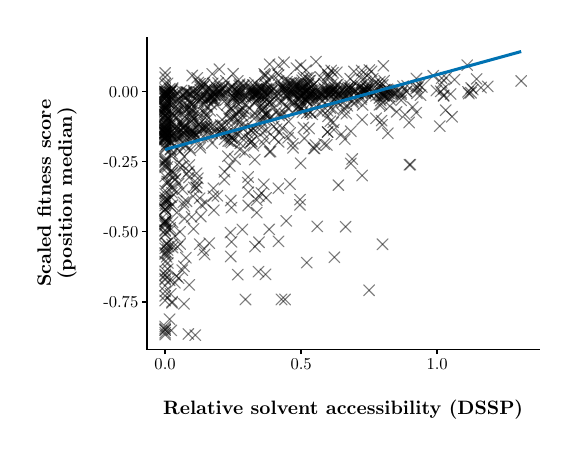
\begin{tikzpicture}[x=1pt,y=1pt]
\definecolor{fillColor}{RGB}{255,255,255}
\path[use as bounding box,fill=fillColor,fill opacity=0.00] (0,0) rectangle (188.25,144.54);
\begin{scope}
\path[clip] ( 43.23, 28.30) rectangle (184.75,141.04);
\definecolor{drawColor}{RGB}{0,0,0}

\path[draw=drawColor,draw opacity=0.50,line width= 0.4pt,line join=round,line cap=round] ( 99.58,120.23) -- (103.51,124.16);

\path[draw=drawColor,draw opacity=0.50,line width= 0.4pt,line join=round,line cap=round] ( 99.58,124.16) -- (103.51,120.23);

\path[draw=drawColor,draw opacity=0.50,line width= 0.4pt,line join=round,line cap=round] (107.97,115.96) -- (111.90,119.88);

\path[draw=drawColor,draw opacity=0.50,line width= 0.4pt,line join=round,line cap=round] (107.97,119.88) -- (111.90,115.96);

\path[draw=drawColor,draw opacity=0.50,line width= 0.4pt,line join=round,line cap=round] (107.91,119.58) -- (111.83,123.50);

\path[draw=drawColor,draw opacity=0.50,line width= 0.4pt,line join=round,line cap=round] (107.91,123.50) -- (111.83,119.58);

\path[draw=drawColor,draw opacity=0.50,line width= 0.4pt,line join=round,line cap=round] ( 49.12,102.26) -- ( 53.04,106.19);

\path[draw=drawColor,draw opacity=0.50,line width= 0.4pt,line join=round,line cap=round] ( 49.12,106.19) -- ( 53.04,102.26);

\path[draw=drawColor,draw opacity=0.50,line width= 0.4pt,line join=round,line cap=round] ( 73.48,111.48) -- ( 77.40,115.40);

\path[draw=drawColor,draw opacity=0.50,line width= 0.4pt,line join=round,line cap=round] ( 73.48,115.40) -- ( 77.40,111.48);

\path[draw=drawColor,draw opacity=0.50,line width= 0.4pt,line join=round,line cap=round] (109.10,120.80) -- (113.02,124.72);

\path[draw=drawColor,draw opacity=0.50,line width= 0.4pt,line join=round,line cap=round] (109.10,124.72) -- (113.02,120.80);

\path[draw=drawColor,draw opacity=0.50,line width= 0.4pt,line join=round,line cap=round] ( 64.43,114.90) -- ( 68.35,118.83);

\path[draw=drawColor,draw opacity=0.50,line width= 0.4pt,line join=round,line cap=round] ( 64.43,118.83) -- ( 68.35,114.90);

\path[draw=drawColor,draw opacity=0.50,line width= 0.4pt,line join=round,line cap=round] ( 47.70, 69.13) -- ( 51.63, 73.06);

\path[draw=drawColor,draw opacity=0.50,line width= 0.4pt,line join=round,line cap=round] ( 47.70, 73.06) -- ( 51.63, 69.13);

\path[draw=drawColor,draw opacity=0.50,line width= 0.4pt,line join=round,line cap=round] ( 99.31,117.57) -- (103.24,121.50);

\path[draw=drawColor,draw opacity=0.50,line width= 0.4pt,line join=round,line cap=round] ( 99.31,121.50) -- (103.24,117.57);

\path[draw=drawColor,draw opacity=0.50,line width= 0.4pt,line join=round,line cap=round] ( 92.04,121.31) -- ( 95.97,125.23);

\path[draw=drawColor,draw opacity=0.50,line width= 0.4pt,line join=round,line cap=round] ( 92.04,125.23) -- ( 95.97,121.31);

\path[draw=drawColor,draw opacity=0.50,line width= 0.4pt,line join=round,line cap=round] ( 48.59,109.70) -- ( 52.52,113.63);

\path[draw=drawColor,draw opacity=0.50,line width= 0.4pt,line join=round,line cap=round] ( 48.59,113.63) -- ( 52.52,109.70);

\path[draw=drawColor,draw opacity=0.50,line width= 0.4pt,line join=round,line cap=round] ( 65.15, 81.65) -- ( 69.07, 85.58);

\path[draw=drawColor,draw opacity=0.50,line width= 0.4pt,line join=round,line cap=round] ( 65.15, 85.58) -- ( 69.07, 81.65);

\path[draw=drawColor,draw opacity=0.50,line width= 0.4pt,line join=round,line cap=round] (114.56,121.59) -- (118.48,125.52);

\path[draw=drawColor,draw opacity=0.50,line width= 0.4pt,line join=round,line cap=round] (114.56,125.52) -- (118.48,121.59);

\path[draw=drawColor,draw opacity=0.50,line width= 0.4pt,line join=round,line cap=round] (118.15,121.05) -- (122.08,124.97);

\path[draw=drawColor,draw opacity=0.50,line width= 0.4pt,line join=round,line cap=round] (118.15,124.97) -- (122.08,121.05);

\path[draw=drawColor,draw opacity=0.50,line width= 0.4pt,line join=round,line cap=round] ( 57.89,108.25) -- ( 61.82,112.17);

\path[draw=drawColor,draw opacity=0.50,line width= 0.4pt,line join=round,line cap=round] ( 57.89,112.17) -- ( 61.82,108.25);

\path[draw=drawColor,draw opacity=0.50,line width= 0.4pt,line join=round,line cap=round] (126.39,117.94) -- (130.32,121.87);

\path[draw=drawColor,draw opacity=0.50,line width= 0.4pt,line join=round,line cap=round] (126.39,121.87) -- (130.32,117.94);

\path[draw=drawColor,draw opacity=0.50,line width= 0.4pt,line join=round,line cap=round] ( 64.65,100.92) -- ( 68.57,104.84);

\path[draw=drawColor,draw opacity=0.50,line width= 0.4pt,line join=round,line cap=round] ( 64.65,104.84) -- ( 68.57,100.92);

\path[draw=drawColor,draw opacity=0.50,line width= 0.4pt,line join=round,line cap=round] ( 82.90,115.14) -- ( 86.83,119.07);

\path[draw=drawColor,draw opacity=0.50,line width= 0.4pt,line join=round,line cap=round] ( 82.90,119.07) -- ( 86.83,115.14);

\path[draw=drawColor,draw opacity=0.50,line width= 0.4pt,line join=round,line cap=round] ( 50.26, 96.99) -- ( 54.18,100.92);

\path[draw=drawColor,draw opacity=0.50,line width= 0.4pt,line join=round,line cap=round] ( 50.26,100.92) -- ( 54.18, 96.99);

\path[draw=drawColor,draw opacity=0.50,line width= 0.4pt,line join=round,line cap=round] ( 47.70, 33.90) -- ( 51.63, 37.82);

\path[draw=drawColor,draw opacity=0.50,line width= 0.4pt,line join=round,line cap=round] ( 47.70, 37.82) -- ( 51.63, 33.90);

\path[draw=drawColor,draw opacity=0.50,line width= 0.4pt,line join=round,line cap=round] ( 47.70, 63.85) -- ( 51.63, 67.78);

\path[draw=drawColor,draw opacity=0.50,line width= 0.4pt,line join=round,line cap=round] ( 47.70, 67.78) -- ( 51.63, 63.85);

\path[draw=drawColor,draw opacity=0.50,line width= 0.4pt,line join=round,line cap=round] ( 47.70,102.10) -- ( 51.63,106.02);

\path[draw=drawColor,draw opacity=0.50,line width= 0.4pt,line join=round,line cap=round] ( 47.70,106.02) -- ( 51.63,102.10);

\path[draw=drawColor,draw opacity=0.50,line width= 0.4pt,line join=round,line cap=round] ( 51.08,113.66) -- ( 55.00,117.58);

\path[draw=drawColor,draw opacity=0.50,line width= 0.4pt,line join=round,line cap=round] ( 51.08,117.58) -- ( 55.00,113.66);

\path[draw=drawColor,draw opacity=0.50,line width= 0.4pt,line join=round,line cap=round] ( 47.70,102.76) -- ( 51.63,106.69);

\path[draw=drawColor,draw opacity=0.50,line width= 0.4pt,line join=round,line cap=round] ( 47.70,106.69) -- ( 51.63,102.76);

\path[draw=drawColor,draw opacity=0.50,line width= 0.4pt,line join=round,line cap=round] ( 78.40,101.03) -- ( 82.32,104.95);

\path[draw=drawColor,draw opacity=0.50,line width= 0.4pt,line join=round,line cap=round] ( 78.40,104.95) -- ( 82.32,101.03);

\path[draw=drawColor,draw opacity=0.50,line width= 0.4pt,line join=round,line cap=round] ( 59.09,108.67) -- ( 63.01,112.59);

\path[draw=drawColor,draw opacity=0.50,line width= 0.4pt,line join=round,line cap=round] ( 59.09,112.59) -- ( 63.01,108.67);

\path[draw=drawColor,draw opacity=0.50,line width= 0.4pt,line join=round,line cap=round] (145.74,119.88) -- (149.66,123.81);

\path[draw=drawColor,draw opacity=0.50,line width= 0.4pt,line join=round,line cap=round] (145.74,123.81) -- (149.66,119.88);

\path[draw=drawColor,draw opacity=0.50,line width= 0.4pt,line join=round,line cap=round] (104.74,112.48) -- (108.66,116.41);

\path[draw=drawColor,draw opacity=0.50,line width= 0.4pt,line join=round,line cap=round] (104.74,116.41) -- (108.66,112.48);

\path[draw=drawColor,draw opacity=0.50,line width= 0.4pt,line join=round,line cap=round] ( 78.93,101.30) -- ( 82.85,105.22);

\path[draw=drawColor,draw opacity=0.50,line width= 0.4pt,line join=round,line cap=round] ( 78.93,105.22) -- ( 82.85,101.30);

\path[draw=drawColor,draw opacity=0.50,line width= 0.4pt,line join=round,line cap=round] (106.48,119.91) -- (110.41,123.83);

\path[draw=drawColor,draw opacity=0.50,line width= 0.4pt,line join=round,line cap=round] (106.48,123.83) -- (110.41,119.91);

\path[draw=drawColor,draw opacity=0.50,line width= 0.4pt,line join=round,line cap=round] ( 92.80,116.55) -- ( 96.72,120.47);

\path[draw=drawColor,draw opacity=0.50,line width= 0.4pt,line join=round,line cap=round] ( 92.80,120.47) -- ( 96.72,116.55);

\path[draw=drawColor,draw opacity=0.50,line width= 0.4pt,line join=round,line cap=round] ( 78.87,110.69) -- ( 82.79,114.61);

\path[draw=drawColor,draw opacity=0.50,line width= 0.4pt,line join=round,line cap=round] ( 78.87,114.61) -- ( 82.79,110.69);

\path[draw=drawColor,draw opacity=0.50,line width= 0.4pt,line join=round,line cap=round] ( 71.33,113.52) -- ( 75.26,117.45);

\path[draw=drawColor,draw opacity=0.50,line width= 0.4pt,line join=round,line cap=round] ( 71.33,117.45) -- ( 75.26,113.52);

\path[draw=drawColor,draw opacity=0.50,line width= 0.4pt,line join=round,line cap=round] ( 84.61,118.64) -- ( 88.53,122.56);

\path[draw=drawColor,draw opacity=0.50,line width= 0.4pt,line join=round,line cap=round] ( 84.61,122.56) -- ( 88.53,118.64);

\path[draw=drawColor,draw opacity=0.50,line width= 0.4pt,line join=round,line cap=round] ( 71.21,112.95) -- ( 75.14,116.87);

\path[draw=drawColor,draw opacity=0.50,line width= 0.4pt,line join=round,line cap=round] ( 71.21,116.87) -- ( 75.14,112.95);

\path[draw=drawColor,draw opacity=0.50,line width= 0.4pt,line join=round,line cap=round] ( 83.33, 85.97) -- ( 87.26, 89.90);

\path[draw=drawColor,draw opacity=0.50,line width= 0.4pt,line join=round,line cap=round] ( 83.33, 89.90) -- ( 87.26, 85.97);

\path[draw=drawColor,draw opacity=0.50,line width= 0.4pt,line join=round,line cap=round] ( 69.18,119.51) -- ( 73.10,123.43);

\path[draw=drawColor,draw opacity=0.50,line width= 0.4pt,line join=round,line cap=round] ( 69.18,123.43) -- ( 73.10,119.51);

\path[draw=drawColor,draw opacity=0.50,line width= 0.4pt,line join=round,line cap=round] (127.60,120.03) -- (131.53,123.95);

\path[draw=drawColor,draw opacity=0.50,line width= 0.4pt,line join=round,line cap=round] (127.60,123.95) -- (131.53,120.03);

\path[draw=drawColor,draw opacity=0.50,line width= 0.4pt,line join=round,line cap=round] ( 85.40,109.82) -- ( 89.33,113.75);

\path[draw=drawColor,draw opacity=0.50,line width= 0.4pt,line join=round,line cap=round] ( 85.40,113.75) -- ( 89.33,109.82);

\path[draw=drawColor,draw opacity=0.50,line width= 0.4pt,line join=round,line cap=round] ( 73.89,109.04) -- ( 77.81,112.96);

\path[draw=drawColor,draw opacity=0.50,line width= 0.4pt,line join=round,line cap=round] ( 73.89,112.96) -- ( 77.81,109.04);

\path[draw=drawColor,draw opacity=0.50,line width= 0.4pt,line join=round,line cap=round] ( 48.68, 57.55) -- ( 52.61, 61.47);

\path[draw=drawColor,draw opacity=0.50,line width= 0.4pt,line join=round,line cap=round] ( 48.68, 61.47) -- ( 52.61, 57.55);

\path[draw=drawColor,draw opacity=0.50,line width= 0.4pt,line join=round,line cap=round] ( 60.17, 80.94) -- ( 64.10, 84.86);

\path[draw=drawColor,draw opacity=0.50,line width= 0.4pt,line join=round,line cap=round] ( 60.17, 84.86) -- ( 64.10, 80.94);

\path[draw=drawColor,draw opacity=0.50,line width= 0.4pt,line join=round,line cap=round] ( 49.67,100.90) -- ( 53.59,104.83);

\path[draw=drawColor,draw opacity=0.50,line width= 0.4pt,line join=round,line cap=round] ( 49.67,104.83) -- ( 53.59,100.90);

\path[draw=drawColor,draw opacity=0.50,line width= 0.4pt,line join=round,line cap=round] ( 49.18,110.50) -- ( 53.10,114.42);

\path[draw=drawColor,draw opacity=0.50,line width= 0.4pt,line join=round,line cap=round] ( 49.18,114.42) -- ( 53.10,110.50);

\path[draw=drawColor,draw opacity=0.50,line width= 0.4pt,line join=round,line cap=round] ( 56.09, 31.90) -- ( 60.01, 35.83);

\path[draw=drawColor,draw opacity=0.50,line width= 0.4pt,line join=round,line cap=round] ( 56.09, 35.83) -- ( 60.01, 31.90);

\path[draw=drawColor,draw opacity=0.50,line width= 0.4pt,line join=round,line cap=round] ( 47.70, 71.57) -- ( 51.63, 75.49);

\path[draw=drawColor,draw opacity=0.50,line width= 0.4pt,line join=round,line cap=round] ( 47.70, 75.49) -- ( 51.63, 71.57);

\path[draw=drawColor,draw opacity=0.50,line width= 0.4pt,line join=round,line cap=round] ( 48.19,101.40) -- ( 52.12,105.32);

\path[draw=drawColor,draw opacity=0.50,line width= 0.4pt,line join=round,line cap=round] ( 48.19,105.32) -- ( 52.12,101.40);

\path[draw=drawColor,draw opacity=0.50,line width= 0.4pt,line join=round,line cap=round] ( 47.70, 32.33) -- ( 51.63, 36.25);

\path[draw=drawColor,draw opacity=0.50,line width= 0.4pt,line join=round,line cap=round] ( 47.70, 36.25) -- ( 51.63, 32.33);

\path[draw=drawColor,draw opacity=0.50,line width= 0.4pt,line join=round,line cap=round] ( 47.70, 76.98) -- ( 51.63, 80.91);

\path[draw=drawColor,draw opacity=0.50,line width= 0.4pt,line join=round,line cap=round] ( 47.70, 80.91) -- ( 51.63, 76.98);

\path[draw=drawColor,draw opacity=0.50,line width= 0.4pt,line join=round,line cap=round] ( 48.30,109.19) -- ( 52.23,113.12);

\path[draw=drawColor,draw opacity=0.50,line width= 0.4pt,line join=round,line cap=round] ( 48.30,113.12) -- ( 52.23,109.19);

\path[draw=drawColor,draw opacity=0.50,line width= 0.4pt,line join=round,line cap=round] ( 47.70, 67.91) -- ( 51.63, 71.83);

\path[draw=drawColor,draw opacity=0.50,line width= 0.4pt,line join=round,line cap=round] ( 47.70, 71.83) -- ( 51.63, 67.91);

\path[draw=drawColor,draw opacity=0.50,line width= 0.4pt,line join=round,line cap=round] ( 47.70, 81.22) -- ( 51.63, 85.15);

\path[draw=drawColor,draw opacity=0.50,line width= 0.4pt,line join=round,line cap=round] ( 47.70, 85.15) -- ( 51.63, 81.22);

\path[draw=drawColor,draw opacity=0.50,line width= 0.4pt,line join=round,line cap=round] ( 47.70, 94.01) -- ( 51.63, 97.94);

\path[draw=drawColor,draw opacity=0.50,line width= 0.4pt,line join=round,line cap=round] ( 47.70, 97.94) -- ( 51.63, 94.01);

\path[draw=drawColor,draw opacity=0.50,line width= 0.4pt,line join=round,line cap=round] ( 53.05,117.04) -- ( 56.98,120.96);

\path[draw=drawColor,draw opacity=0.50,line width= 0.4pt,line join=round,line cap=round] ( 53.05,120.96) -- ( 56.98,117.04);

\path[draw=drawColor,draw opacity=0.50,line width= 0.4pt,line join=round,line cap=round] ( 49.62, 78.10) -- ( 53.54, 82.03);

\path[draw=drawColor,draw opacity=0.50,line width= 0.4pt,line join=round,line cap=round] ( 49.62, 82.03) -- ( 53.54, 78.10);

\path[draw=drawColor,draw opacity=0.50,line width= 0.4pt,line join=round,line cap=round] ( 49.50, 69.38) -- ( 53.42, 73.31);

\path[draw=drawColor,draw opacity=0.50,line width= 0.4pt,line join=round,line cap=round] ( 49.50, 73.31) -- ( 53.42, 69.38);

\path[draw=drawColor,draw opacity=0.50,line width= 0.4pt,line join=round,line cap=round] ( 72.86,118.71) -- ( 76.79,122.63);

\path[draw=drawColor,draw opacity=0.50,line width= 0.4pt,line join=round,line cap=round] ( 72.86,122.63) -- ( 76.79,118.71);

\path[draw=drawColor,draw opacity=0.50,line width= 0.4pt,line join=round,line cap=round] ( 74.32,112.19) -- ( 78.24,116.12);

\path[draw=drawColor,draw opacity=0.50,line width= 0.4pt,line join=round,line cap=round] ( 74.32,116.12) -- ( 78.24,112.19);

\path[draw=drawColor,draw opacity=0.50,line width= 0.4pt,line join=round,line cap=round] ( 88.63, 84.54) -- ( 92.56, 88.47);

\path[draw=drawColor,draw opacity=0.50,line width= 0.4pt,line join=round,line cap=round] ( 88.63, 88.47) -- ( 92.56, 84.54);

\path[draw=drawColor,draw opacity=0.50,line width= 0.4pt,line join=round,line cap=round] (111.04,119.28) -- (114.96,123.21);

\path[draw=drawColor,draw opacity=0.50,line width= 0.4pt,line join=round,line cap=round] (111.04,123.21) -- (114.96,119.28);

\path[draw=drawColor,draw opacity=0.50,line width= 0.4pt,line join=round,line cap=round] (128.89,114.25) -- (132.82,118.17);

\path[draw=drawColor,draw opacity=0.50,line width= 0.4pt,line join=round,line cap=round] (128.89,118.17) -- (132.82,114.25);

\path[draw=drawColor,draw opacity=0.50,line width= 0.4pt,line join=round,line cap=round] (115.40,119.50) -- (119.33,123.42);

\path[draw=drawColor,draw opacity=0.50,line width= 0.4pt,line join=round,line cap=round] (115.40,123.42) -- (119.33,119.50);

\path[draw=drawColor,draw opacity=0.50,line width= 0.4pt,line join=round,line cap=round] ( 53.89,107.82) -- ( 57.82,111.74);

\path[draw=drawColor,draw opacity=0.50,line width= 0.4pt,line join=round,line cap=round] ( 53.89,111.74) -- ( 57.82,107.82);

\path[draw=drawColor,draw opacity=0.50,line width= 0.4pt,line join=round,line cap=round] (109.35,119.57) -- (113.27,123.50);

\path[draw=drawColor,draw opacity=0.50,line width= 0.4pt,line join=round,line cap=round] (109.35,123.50) -- (113.27,119.57);

\path[draw=drawColor,draw opacity=0.50,line width= 0.4pt,line join=round,line cap=round] ( 71.68,102.75) -- ( 75.60,106.67);

\path[draw=drawColor,draw opacity=0.50,line width= 0.4pt,line join=round,line cap=round] ( 71.68,106.67) -- ( 75.60,102.75);

\path[draw=drawColor,draw opacity=0.50,line width= 0.4pt,line join=round,line cap=round] (107.66,119.32) -- (111.58,123.24);

\path[draw=drawColor,draw opacity=0.50,line width= 0.4pt,line join=round,line cap=round] (107.66,123.24) -- (111.58,119.32);

\path[draw=drawColor,draw opacity=0.50,line width= 0.4pt,line join=round,line cap=round] ( 87.19,102.71) -- ( 91.12,106.63);

\path[draw=drawColor,draw opacity=0.50,line width= 0.4pt,line join=round,line cap=round] ( 87.19,106.63) -- ( 91.12,102.71);

\path[draw=drawColor,draw opacity=0.50,line width= 0.4pt,line join=round,line cap=round] ( 95.78,116.44) -- ( 99.70,120.37);

\path[draw=drawColor,draw opacity=0.50,line width= 0.4pt,line join=round,line cap=round] ( 95.78,120.37) -- ( 99.70,116.44);

\path[draw=drawColor,draw opacity=0.50,line width= 0.4pt,line join=round,line cap=round] ( 56.29, 90.67) -- ( 60.22, 94.59);

\path[draw=drawColor,draw opacity=0.50,line width= 0.4pt,line join=round,line cap=round] ( 56.29, 94.59) -- ( 60.22, 90.67);

\path[draw=drawColor,draw opacity=0.50,line width= 0.4pt,line join=round,line cap=round] (121.20,120.45) -- (125.12,124.37);

\path[draw=drawColor,draw opacity=0.50,line width= 0.4pt,line join=round,line cap=round] (121.20,124.37) -- (125.12,120.45);

\path[draw=drawColor,draw opacity=0.50,line width= 0.4pt,line join=round,line cap=round] ( 57.82, 81.64) -- ( 61.75, 85.56);

\path[draw=drawColor,draw opacity=0.50,line width= 0.4pt,line join=round,line cap=round] ( 57.82, 85.56) -- ( 61.75, 81.64);

\path[draw=drawColor,draw opacity=0.50,line width= 0.4pt,line join=round,line cap=round] ( 81.25,119.07) -- ( 85.18,122.99);

\path[draw=drawColor,draw opacity=0.50,line width= 0.4pt,line join=round,line cap=round] ( 81.25,122.99) -- ( 85.18,119.07);

\path[draw=drawColor,draw opacity=0.50,line width= 0.4pt,line join=round,line cap=round] (112.65,120.86) -- (116.57,124.78);

\path[draw=drawColor,draw opacity=0.50,line width= 0.4pt,line join=round,line cap=round] (112.65,124.78) -- (116.57,120.86);

\path[draw=drawColor,draw opacity=0.50,line width= 0.4pt,line join=round,line cap=round] (133.65,121.44) -- (137.57,125.36);

\path[draw=drawColor,draw opacity=0.50,line width= 0.4pt,line join=round,line cap=round] (133.65,125.36) -- (137.57,121.44);

\path[draw=drawColor,draw opacity=0.50,line width= 0.4pt,line join=round,line cap=round] ( 96.82,113.45) -- (100.74,117.37);

\path[draw=drawColor,draw opacity=0.50,line width= 0.4pt,line join=round,line cap=round] ( 96.82,117.37) -- (100.74,113.45);

\path[draw=drawColor,draw opacity=0.50,line width= 0.4pt,line join=round,line cap=round] ( 80.07, 94.89) -- ( 83.99, 98.81);

\path[draw=drawColor,draw opacity=0.50,line width= 0.4pt,line join=round,line cap=round] ( 80.07, 98.81) -- ( 83.99, 94.89);

\path[draw=drawColor,draw opacity=0.50,line width= 0.4pt,line join=round,line cap=round] ( 75.84,113.45) -- ( 79.77,117.37);

\path[draw=drawColor,draw opacity=0.50,line width= 0.4pt,line join=round,line cap=round] ( 75.84,117.37) -- ( 79.77,113.45);

\path[draw=drawColor,draw opacity=0.50,line width= 0.4pt,line join=round,line cap=round] (124.79,118.35) -- (128.71,122.28);

\path[draw=drawColor,draw opacity=0.50,line width= 0.4pt,line join=round,line cap=round] (124.79,122.28) -- (128.71,118.35);

\path[draw=drawColor,draw opacity=0.50,line width= 0.4pt,line join=round,line cap=round] (101.98,100.17) -- (105.91,104.09);

\path[draw=drawColor,draw opacity=0.50,line width= 0.4pt,line join=round,line cap=round] (101.98,104.09) -- (105.91,100.17);

\path[draw=drawColor,draw opacity=0.50,line width= 0.4pt,line join=round,line cap=round] ( 51.90, 75.75) -- ( 55.82, 79.67);

\path[draw=drawColor,draw opacity=0.50,line width= 0.4pt,line join=round,line cap=round] ( 51.90, 79.67) -- ( 55.82, 75.75);

\path[draw=drawColor,draw opacity=0.50,line width= 0.4pt,line join=round,line cap=round] ( 71.26,101.49) -- ( 75.18,105.41);

\path[draw=drawColor,draw opacity=0.50,line width= 0.4pt,line join=round,line cap=round] ( 71.26,105.41) -- ( 75.18,101.49);

\path[draw=drawColor,draw opacity=0.50,line width= 0.4pt,line join=round,line cap=round] ( 70.09,110.94) -- ( 74.01,114.86);

\path[draw=drawColor,draw opacity=0.50,line width= 0.4pt,line join=round,line cap=round] ( 70.09,114.86) -- ( 74.01,110.94);

\path[draw=drawColor,draw opacity=0.50,line width= 0.4pt,line join=round,line cap=round] ( 47.70, 68.12) -- ( 51.63, 72.04);

\path[draw=drawColor,draw opacity=0.50,line width= 0.4pt,line join=round,line cap=round] ( 47.70, 72.04) -- ( 51.63, 68.12);

\path[draw=drawColor,draw opacity=0.50,line width= 0.4pt,line join=round,line cap=round] (112.97,117.57) -- (116.90,121.50);

\path[draw=drawColor,draw opacity=0.50,line width= 0.4pt,line join=round,line cap=round] (112.97,121.50) -- (116.90,117.57);

\path[draw=drawColor,draw opacity=0.50,line width= 0.4pt,line join=round,line cap=round] (119.39,120.08) -- (123.31,124.01);

\path[draw=drawColor,draw opacity=0.50,line width= 0.4pt,line join=round,line cap=round] (119.39,124.01) -- (123.31,120.08);

\path[draw=drawColor,draw opacity=0.50,line width= 0.4pt,line join=round,line cap=round] ( 89.85,111.12) -- ( 93.78,115.04);

\path[draw=drawColor,draw opacity=0.50,line width= 0.4pt,line join=round,line cap=round] ( 89.85,115.04) -- ( 93.78,111.12);

\path[draw=drawColor,draw opacity=0.50,line width= 0.4pt,line join=round,line cap=round] ( 86.06,114.90) -- ( 89.99,118.83);

\path[draw=drawColor,draw opacity=0.50,line width= 0.4pt,line join=round,line cap=round] ( 86.06,118.83) -- ( 89.99,114.90);

\path[draw=drawColor,draw opacity=0.50,line width= 0.4pt,line join=round,line cap=round] (138.42,121.39) -- (142.34,125.31);

\path[draw=drawColor,draw opacity=0.50,line width= 0.4pt,line join=round,line cap=round] (138.42,125.31) -- (142.34,121.39);

\path[draw=drawColor,draw opacity=0.50,line width= 0.4pt,line join=round,line cap=round] (126.83,118.03) -- (130.76,121.96);

\path[draw=drawColor,draw opacity=0.50,line width= 0.4pt,line join=round,line cap=round] (126.83,121.96) -- (130.76,118.03);

\path[draw=drawColor,draw opacity=0.50,line width= 0.4pt,line join=round,line cap=round] ( 51.45, 89.30) -- ( 55.37, 93.23);

\path[draw=drawColor,draw opacity=0.50,line width= 0.4pt,line join=round,line cap=round] ( 51.45, 93.23) -- ( 55.37, 89.30);

\path[draw=drawColor,draw opacity=0.50,line width= 0.4pt,line join=round,line cap=round] ( 50.16, 82.94) -- ( 54.08, 86.86);

\path[draw=drawColor,draw opacity=0.50,line width= 0.4pt,line join=round,line cap=round] ( 50.16, 86.86) -- ( 54.08, 82.94);

\path[draw=drawColor,draw opacity=0.50,line width= 0.4pt,line join=round,line cap=round] ( 56.92,105.44) -- ( 60.84,109.37);

\path[draw=drawColor,draw opacity=0.50,line width= 0.4pt,line join=round,line cap=round] ( 56.92,109.37) -- ( 60.84,105.44);

\path[draw=drawColor,draw opacity=0.50,line width= 0.4pt,line join=round,line cap=round] ( 48.98, 80.22) -- ( 52.91, 84.14);

\path[draw=drawColor,draw opacity=0.50,line width= 0.4pt,line join=round,line cap=round] ( 48.98, 84.14) -- ( 52.91, 80.22);

\path[draw=drawColor,draw opacity=0.50,line width= 0.4pt,line join=round,line cap=round] ( 95.78,120.77) -- ( 99.70,124.69);

\path[draw=drawColor,draw opacity=0.50,line width= 0.4pt,line join=round,line cap=round] ( 95.78,124.69) -- ( 99.70,120.77);

\path[draw=drawColor,draw opacity=0.50,line width= 0.4pt,line join=round,line cap=round] ( 92.15,102.77) -- ( 96.08,106.69);

\path[draw=drawColor,draw opacity=0.50,line width= 0.4pt,line join=round,line cap=round] ( 92.15,106.69) -- ( 96.08,102.77);

\path[draw=drawColor,draw opacity=0.50,line width= 0.4pt,line join=round,line cap=round] ( 47.70, 72.60) -- ( 51.63, 76.52);

\path[draw=drawColor,draw opacity=0.50,line width= 0.4pt,line join=round,line cap=round] ( 47.70, 76.52) -- ( 51.63, 72.60);

\path[draw=drawColor,draw opacity=0.50,line width= 0.4pt,line join=round,line cap=round] ( 48.40, 64.59) -- ( 52.33, 68.52);

\path[draw=drawColor,draw opacity=0.50,line width= 0.4pt,line join=round,line cap=round] ( 48.40, 68.52) -- ( 52.33, 64.59);

\path[draw=drawColor,draw opacity=0.50,line width= 0.4pt,line join=round,line cap=round] ( 84.61,120.37) -- ( 88.53,124.29);

\path[draw=drawColor,draw opacity=0.50,line width= 0.4pt,line join=round,line cap=round] ( 84.61,124.29) -- ( 88.53,120.37);

\path[draw=drawColor,draw opacity=0.50,line width= 0.4pt,line join=round,line cap=round] ( 51.27, 87.61) -- ( 55.19, 91.53);

\path[draw=drawColor,draw opacity=0.50,line width= 0.4pt,line join=round,line cap=round] ( 51.27, 91.53) -- ( 55.19, 87.61);

\path[draw=drawColor,draw opacity=0.50,line width= 0.4pt,line join=round,line cap=round] ( 47.70, 83.62) -- ( 51.63, 87.55);

\path[draw=drawColor,draw opacity=0.50,line width= 0.4pt,line join=round,line cap=round] ( 47.70, 87.55) -- ( 51.63, 83.62);

\path[draw=drawColor,draw opacity=0.50,line width= 0.4pt,line join=round,line cap=round] ( 47.70, 69.45) -- ( 51.63, 73.38);

\path[draw=drawColor,draw opacity=0.50,line width= 0.4pt,line join=round,line cap=round] ( 47.70, 73.38) -- ( 51.63, 69.45);

\path[draw=drawColor,draw opacity=0.50,line width= 0.4pt,line join=round,line cap=round] ( 56.92,112.36) -- ( 60.84,116.28);

\path[draw=drawColor,draw opacity=0.50,line width= 0.4pt,line join=round,line cap=round] ( 56.92,116.28) -- ( 60.84,112.36);

\path[draw=drawColor,draw opacity=0.50,line width= 0.4pt,line join=round,line cap=round] ( 74.23,114.84) -- ( 78.15,118.76);

\path[draw=drawColor,draw opacity=0.50,line width= 0.4pt,line join=round,line cap=round] ( 74.23,118.76) -- ( 78.15,114.84);

\path[draw=drawColor,draw opacity=0.50,line width= 0.4pt,line join=round,line cap=round] ( 58.61, 31.47) -- ( 62.53, 35.39);

\path[draw=drawColor,draw opacity=0.50,line width= 0.4pt,line join=round,line cap=round] ( 58.61, 35.39) -- ( 62.53, 31.47);

\path[draw=drawColor,draw opacity=0.50,line width= 0.4pt,line join=round,line cap=round] ( 47.70, 31.65) -- ( 51.63, 35.57);

\path[draw=drawColor,draw opacity=0.50,line width= 0.4pt,line join=round,line cap=round] ( 47.70, 35.57) -- ( 51.63, 31.65);

\path[draw=drawColor,draw opacity=0.50,line width= 0.4pt,line join=round,line cap=round] ( 56.43, 49.63) -- ( 60.36, 53.55);

\path[draw=drawColor,draw opacity=0.50,line width= 0.4pt,line join=round,line cap=round] ( 56.43, 53.55) -- ( 60.36, 49.63);

\path[draw=drawColor,draw opacity=0.50,line width= 0.4pt,line join=round,line cap=round] ( 48.41, 87.01) -- ( 52.33, 90.93);

\path[draw=drawColor,draw opacity=0.50,line width= 0.4pt,line join=round,line cap=round] ( 48.41, 90.93) -- ( 52.33, 87.01);

\path[draw=drawColor,draw opacity=0.50,line width= 0.4pt,line join=round,line cap=round] ( 47.70, 33.36) -- ( 51.63, 37.28);

\path[draw=drawColor,draw opacity=0.50,line width= 0.4pt,line join=round,line cap=round] ( 47.70, 37.28) -- ( 51.63, 33.36);

\path[draw=drawColor,draw opacity=0.50,line width= 0.4pt,line join=round,line cap=round] ( 47.70, 54.57) -- ( 51.63, 58.50);

\path[draw=drawColor,draw opacity=0.50,line width= 0.4pt,line join=round,line cap=round] ( 47.70, 58.50) -- ( 51.63, 54.57);

\path[draw=drawColor,draw opacity=0.50,line width= 0.4pt,line join=round,line cap=round] ( 65.16, 84.55) -- ( 69.08, 88.47);

\path[draw=drawColor,draw opacity=0.50,line width= 0.4pt,line join=round,line cap=round] ( 65.16, 88.47) -- ( 69.08, 84.55);

\path[draw=drawColor,draw opacity=0.50,line width= 0.4pt,line join=round,line cap=round] ( 60.29,100.27) -- ( 64.21,104.19);

\path[draw=drawColor,draw opacity=0.50,line width= 0.4pt,line join=round,line cap=round] ( 60.29,104.19) -- ( 64.21,100.27);

\path[draw=drawColor,draw opacity=0.50,line width= 0.4pt,line join=round,line cap=round] ( 47.70, 45.65) -- ( 51.63, 49.58);

\path[draw=drawColor,draw opacity=0.50,line width= 0.4pt,line join=round,line cap=round] ( 47.70, 49.58) -- ( 51.63, 45.65);

\path[draw=drawColor,draw opacity=0.50,line width= 0.4pt,line join=round,line cap=round] ( 47.70, 98.71) -- ( 51.63,102.63);

\path[draw=drawColor,draw opacity=0.50,line width= 0.4pt,line join=round,line cap=round] ( 47.70,102.63) -- ( 51.63, 98.71);

\path[draw=drawColor,draw opacity=0.50,line width= 0.4pt,line join=round,line cap=round] (113.61,120.45) -- (117.54,124.37);

\path[draw=drawColor,draw opacity=0.50,line width= 0.4pt,line join=round,line cap=round] (113.61,124.37) -- (117.54,120.45);

\path[draw=drawColor,draw opacity=0.50,line width= 0.4pt,line join=round,line cap=round] ( 72.51,117.36) -- ( 76.43,121.28);

\path[draw=drawColor,draw opacity=0.50,line width= 0.4pt,line join=round,line cap=round] ( 72.51,121.28) -- ( 76.43,117.36);

\path[draw=drawColor,draw opacity=0.50,line width= 0.4pt,line join=round,line cap=round] ( 58.98,102.22) -- ( 62.90,106.14);

\path[draw=drawColor,draw opacity=0.50,line width= 0.4pt,line join=round,line cap=round] ( 58.98,106.14) -- ( 62.90,102.22);

\path[draw=drawColor,draw opacity=0.50,line width= 0.4pt,line join=round,line cap=round] (112.65,102.24) -- (116.58,106.16);

\path[draw=drawColor,draw opacity=0.50,line width= 0.4pt,line join=round,line cap=round] (112.65,106.16) -- (116.58,102.24);

\path[draw=drawColor,draw opacity=0.50,line width= 0.4pt,line join=round,line cap=round] ( 53.95, 84.15) -- ( 57.87, 88.07);

\path[draw=drawColor,draw opacity=0.50,line width= 0.4pt,line join=round,line cap=round] ( 53.95, 88.07) -- ( 57.87, 84.15);

\path[draw=drawColor,draw opacity=0.50,line width= 0.4pt,line join=round,line cap=round] ( 54.63, 95.99) -- ( 58.55, 99.92);

\path[draw=drawColor,draw opacity=0.50,line width= 0.4pt,line join=round,line cap=round] ( 54.63, 99.92) -- ( 58.55, 95.99);

\path[draw=drawColor,draw opacity=0.50,line width= 0.4pt,line join=round,line cap=round] (128.47,120.01) -- (132.39,123.93);

\path[draw=drawColor,draw opacity=0.50,line width= 0.4pt,line join=round,line cap=round] (128.47,123.93) -- (132.39,120.01);

\path[draw=drawColor,draw opacity=0.50,line width= 0.4pt,line join=round,line cap=round] (109.03,119.10) -- (112.96,123.02);

\path[draw=drawColor,draw opacity=0.50,line width= 0.4pt,line join=round,line cap=round] (109.03,123.02) -- (112.96,119.10);

\path[draw=drawColor,draw opacity=0.50,line width= 0.4pt,line join=round,line cap=round] ( 48.90, 89.64) -- ( 52.82, 93.56);

\path[draw=drawColor,draw opacity=0.50,line width= 0.4pt,line join=round,line cap=round] ( 48.90, 93.56) -- ( 52.82, 89.64);

\path[draw=drawColor,draw opacity=0.50,line width= 0.4pt,line join=round,line cap=round] ( 76.05,112.01) -- ( 79.98,115.94);

\path[draw=drawColor,draw opacity=0.50,line width= 0.4pt,line join=round,line cap=round] ( 76.05,115.94) -- ( 79.98,112.01);

\path[draw=drawColor,draw opacity=0.50,line width= 0.4pt,line join=round,line cap=round] ( 81.60,120.95) -- ( 85.52,124.88);

\path[draw=drawColor,draw opacity=0.50,line width= 0.4pt,line join=round,line cap=round] ( 81.60,124.88) -- ( 85.52,120.95);

\path[draw=drawColor,draw opacity=0.50,line width= 0.4pt,line join=round,line cap=round] ( 68.27,109.34) -- ( 72.20,113.26);

\path[draw=drawColor,draw opacity=0.50,line width= 0.4pt,line join=round,line cap=round] ( 68.27,113.26) -- ( 72.20,109.34);

\path[draw=drawColor,draw opacity=0.50,line width= 0.4pt,line join=round,line cap=round] ( 48.90,104.68) -- ( 52.82,108.60);

\path[draw=drawColor,draw opacity=0.50,line width= 0.4pt,line join=round,line cap=round] ( 48.90,108.60) -- ( 52.82,104.68);

\path[draw=drawColor,draw opacity=0.50,line width= 0.4pt,line join=round,line cap=round] (100.66,120.06) -- (104.59,123.98);

\path[draw=drawColor,draw opacity=0.50,line width= 0.4pt,line join=round,line cap=round] (100.66,123.98) -- (104.59,120.06);

\path[draw=drawColor,draw opacity=0.50,line width= 0.4pt,line join=round,line cap=round] (139.02,120.99) -- (142.94,124.91);

\path[draw=drawColor,draw opacity=0.50,line width= 0.4pt,line join=round,line cap=round] (139.02,124.91) -- (142.94,120.99);

\path[draw=drawColor,draw opacity=0.50,line width= 0.4pt,line join=round,line cap=round] ( 60.97,117.13) -- ( 64.89,121.05);

\path[draw=drawColor,draw opacity=0.50,line width= 0.4pt,line join=round,line cap=round] ( 60.97,121.05) -- ( 64.89,117.13);

\path[draw=drawColor,draw opacity=0.50,line width= 0.4pt,line join=round,line cap=round] (106.41,104.90) -- (110.33,108.82);

\path[draw=drawColor,draw opacity=0.50,line width= 0.4pt,line join=round,line cap=round] (106.41,108.82) -- (110.33,104.90);

\path[draw=drawColor,draw opacity=0.50,line width= 0.4pt,line join=round,line cap=round] ( 54.52, 42.80) -- ( 58.45, 46.72);

\path[draw=drawColor,draw opacity=0.50,line width= 0.4pt,line join=round,line cap=round] ( 54.52, 46.72) -- ( 58.45, 42.80);

\path[draw=drawColor,draw opacity=0.50,line width= 0.4pt,line join=round,line cap=round] (120.12,120.07) -- (124.04,123.99);

\path[draw=drawColor,draw opacity=0.50,line width= 0.4pt,line join=round,line cap=round] (120.12,123.99) -- (124.04,120.07);

\path[draw=drawColor,draw opacity=0.50,line width= 0.4pt,line join=round,line cap=round] ( 74.56,119.52) -- ( 78.49,123.44);

\path[draw=drawColor,draw opacity=0.50,line width= 0.4pt,line join=round,line cap=round] ( 74.56,123.44) -- ( 78.49,119.52);

\path[draw=drawColor,draw opacity=0.50,line width= 0.4pt,line join=round,line cap=round] ( 51.25, 50.37) -- ( 55.17, 54.29);

\path[draw=drawColor,draw opacity=0.50,line width= 0.4pt,line join=round,line cap=round] ( 51.25, 54.29) -- ( 55.17, 50.37);

\path[draw=drawColor,draw opacity=0.50,line width= 0.4pt,line join=round,line cap=round] ( 82.90,104.66) -- ( 86.83,108.58);

\path[draw=drawColor,draw opacity=0.50,line width= 0.4pt,line join=round,line cap=round] ( 82.90,108.58) -- ( 86.83,104.66);

\path[draw=drawColor,draw opacity=0.50,line width= 0.4pt,line join=round,line cap=round] ( 50.10,107.65) -- ( 54.02,111.58);

\path[draw=drawColor,draw opacity=0.50,line width= 0.4pt,line join=round,line cap=round] ( 50.10,111.58) -- ( 54.02,107.65);

\path[draw=drawColor,draw opacity=0.50,line width= 0.4pt,line join=round,line cap=round] ( 83.18,100.69) -- ( 87.10,104.62);

\path[draw=drawColor,draw opacity=0.50,line width= 0.4pt,line join=round,line cap=round] ( 83.18,104.62) -- ( 87.10,100.69);

\path[draw=drawColor,draw opacity=0.50,line width= 0.4pt,line join=round,line cap=round] ( 62.30,106.21) -- ( 66.22,110.13);

\path[draw=drawColor,draw opacity=0.50,line width= 0.4pt,line join=round,line cap=round] ( 62.30,110.13) -- ( 66.22,106.21);

\path[draw=drawColor,draw opacity=0.50,line width= 0.4pt,line join=round,line cap=round] ( 87.76,117.80) -- ( 91.68,121.72);

\path[draw=drawColor,draw opacity=0.50,line width= 0.4pt,line join=round,line cap=round] ( 87.76,121.72) -- ( 91.68,117.80);

\path[draw=drawColor,draw opacity=0.50,line width= 0.4pt,line join=round,line cap=round] ( 49.95, 33.19) -- ( 53.88, 37.11);

\path[draw=drawColor,draw opacity=0.50,line width= 0.4pt,line join=round,line cap=round] ( 49.95, 37.11) -- ( 53.88, 33.19);

\path[draw=drawColor,draw opacity=0.50,line width= 0.4pt,line join=round,line cap=round] ( 67.79,107.40) -- ( 71.72,111.33);

\path[draw=drawColor,draw opacity=0.50,line width= 0.4pt,line join=round,line cap=round] ( 67.79,111.33) -- ( 71.72,107.40);

\path[draw=drawColor,draw opacity=0.50,line width= 0.4pt,line join=round,line cap=round] (107.91,120.42) -- (111.83,124.35);

\path[draw=drawColor,draw opacity=0.50,line width= 0.4pt,line join=round,line cap=round] (107.91,124.35) -- (111.83,120.42);

\path[draw=drawColor,draw opacity=0.50,line width= 0.4pt,line join=round,line cap=round] ( 50.10, 91.11) -- ( 54.02, 95.04);

\path[draw=drawColor,draw opacity=0.50,line width= 0.4pt,line join=round,line cap=round] ( 50.10, 95.04) -- ( 54.02, 91.11);

\path[draw=drawColor,draw opacity=0.50,line width= 0.4pt,line join=round,line cap=round] ( 60.46, 99.21) -- ( 64.38,103.13);

\path[draw=drawColor,draw opacity=0.50,line width= 0.4pt,line join=round,line cap=round] ( 60.46,103.13) -- ( 64.38, 99.21);

\path[draw=drawColor,draw opacity=0.50,line width= 0.4pt,line join=round,line cap=round] ( 91.03,119.73) -- ( 94.95,123.65);

\path[draw=drawColor,draw opacity=0.50,line width= 0.4pt,line join=round,line cap=round] ( 91.03,123.65) -- ( 94.95,119.73);

\path[draw=drawColor,draw opacity=0.50,line width= 0.4pt,line join=round,line cap=round] ( 62.87,114.10) -- ( 66.79,118.03);

\path[draw=drawColor,draw opacity=0.50,line width= 0.4pt,line join=round,line cap=round] ( 62.87,118.03) -- ( 66.79,114.10);

\path[draw=drawColor,draw opacity=0.50,line width= 0.4pt,line join=round,line cap=round] ( 82.60,121.39) -- ( 86.52,125.31);

\path[draw=drawColor,draw opacity=0.50,line width= 0.4pt,line join=round,line cap=round] ( 82.60,125.31) -- ( 86.52,121.39);

\path[draw=drawColor,draw opacity=0.50,line width= 0.4pt,line join=round,line cap=round] (100.35,118.88) -- (104.28,122.80);

\path[draw=drawColor,draw opacity=0.50,line width= 0.4pt,line join=round,line cap=round] (100.35,122.80) -- (104.28,118.88);

\path[draw=drawColor,draw opacity=0.50,line width= 0.4pt,line join=round,line cap=round] (161.85,120.93) -- (165.77,124.86);

\path[draw=drawColor,draw opacity=0.50,line width= 0.4pt,line join=round,line cap=round] (161.85,124.86) -- (165.77,120.93);

\path[draw=drawColor,draw opacity=0.50,line width= 0.4pt,line join=round,line cap=round] ( 77.72, 88.61) -- ( 81.64, 92.53);

\path[draw=drawColor,draw opacity=0.50,line width= 0.4pt,line join=round,line cap=round] ( 77.72, 92.53) -- ( 81.64, 88.61);

\path[draw=drawColor,draw opacity=0.50,line width= 0.4pt,line join=round,line cap=round] (107.35,120.98) -- (111.27,124.90);

\path[draw=drawColor,draw opacity=0.50,line width= 0.4pt,line join=round,line cap=round] (107.35,124.90) -- (111.27,120.98);

\path[draw=drawColor,draw opacity=0.50,line width= 0.4pt,line join=round,line cap=round] ( 88.91,110.79) -- ( 92.84,114.71);

\path[draw=drawColor,draw opacity=0.50,line width= 0.4pt,line join=round,line cap=round] ( 88.91,114.71) -- ( 92.84,110.79);

\path[draw=drawColor,draw opacity=0.50,line width= 0.4pt,line join=round,line cap=round] ( 49.75, 46.36) -- ( 53.67, 50.29);

\path[draw=drawColor,draw opacity=0.50,line width= 0.4pt,line join=round,line cap=round] ( 49.75, 50.29) -- ( 53.67, 46.36);

\path[draw=drawColor,draw opacity=0.50,line width= 0.4pt,line join=round,line cap=round] ( 51.25, 67.26) -- ( 55.17, 71.19);

\path[draw=drawColor,draw opacity=0.50,line width= 0.4pt,line join=round,line cap=round] ( 51.25, 71.19) -- ( 55.17, 67.26);

\path[draw=drawColor,draw opacity=0.50,line width= 0.4pt,line join=round,line cap=round] ( 47.70, 33.34) -- ( 51.63, 37.27);

\path[draw=drawColor,draw opacity=0.50,line width= 0.4pt,line join=round,line cap=round] ( 47.70, 37.27) -- ( 51.63, 33.34);

\path[draw=drawColor,draw opacity=0.50,line width= 0.4pt,line join=round,line cap=round] ( 66.37,120.83) -- ( 70.29,124.76);

\path[draw=drawColor,draw opacity=0.50,line width= 0.4pt,line join=round,line cap=round] ( 66.37,124.76) -- ( 70.29,120.83);

\path[draw=drawColor,draw opacity=0.50,line width= 0.4pt,line join=round,line cap=round] ( 47.70, 51.46) -- ( 51.63, 55.39);

\path[draw=drawColor,draw opacity=0.50,line width= 0.4pt,line join=round,line cap=round] ( 47.70, 55.39) -- ( 51.63, 51.46);

\path[draw=drawColor,draw opacity=0.50,line width= 0.4pt,line join=round,line cap=round] ( 56.62,115.61) -- ( 60.55,119.53);

\path[draw=drawColor,draw opacity=0.50,line width= 0.4pt,line join=round,line cap=round] ( 56.62,119.53) -- ( 60.55,115.61);

\path[draw=drawColor,draw opacity=0.50,line width= 0.4pt,line join=round,line cap=round] ( 48.19, 75.38) -- ( 52.12, 79.31);

\path[draw=drawColor,draw opacity=0.50,line width= 0.4pt,line join=round,line cap=round] ( 48.19, 79.31) -- ( 52.12, 75.38);

\path[draw=drawColor,draw opacity=0.50,line width= 0.4pt,line join=round,line cap=round] ( 47.70, 47.27) -- ( 51.63, 51.20);

\path[draw=drawColor,draw opacity=0.50,line width= 0.4pt,line join=round,line cap=round] ( 47.70, 51.20) -- ( 51.63, 47.27);

\path[draw=drawColor,draw opacity=0.50,line width= 0.4pt,line join=round,line cap=round] ( 85.97,121.32) -- ( 89.90,125.24);

\path[draw=drawColor,draw opacity=0.50,line width= 0.4pt,line join=round,line cap=round] ( 85.97,125.24) -- ( 89.90,121.32);

\path[draw=drawColor,draw opacity=0.50,line width= 0.4pt,line join=round,line cap=round] ( 48.41,110.56) -- ( 52.33,114.49);

\path[draw=drawColor,draw opacity=0.50,line width= 0.4pt,line join=round,line cap=round] ( 48.41,114.49) -- ( 52.33,110.56);

\path[draw=drawColor,draw opacity=0.50,line width= 0.4pt,line join=round,line cap=round] ( 48.30, 86.28) -- ( 52.23, 90.20);

\path[draw=drawColor,draw opacity=0.50,line width= 0.4pt,line join=round,line cap=round] ( 48.30, 90.20) -- ( 52.23, 86.28);

\path[draw=drawColor,draw opacity=0.50,line width= 0.4pt,line join=round,line cap=round] ( 78.18,118.95) -- ( 82.10,122.87);

\path[draw=drawColor,draw opacity=0.50,line width= 0.4pt,line join=round,line cap=round] ( 78.18,122.87) -- ( 82.10,118.95);

\path[draw=drawColor,draw opacity=0.50,line width= 0.4pt,line join=round,line cap=round] ( 82.59,119.87) -- ( 86.51,123.79);

\path[draw=drawColor,draw opacity=0.50,line width= 0.4pt,line join=round,line cap=round] ( 82.59,123.79) -- ( 86.51,119.87);

\path[draw=drawColor,draw opacity=0.50,line width= 0.4pt,line join=round,line cap=round] ( 48.30, 95.08) -- ( 52.23, 99.00);

\path[draw=drawColor,draw opacity=0.50,line width= 0.4pt,line join=round,line cap=round] ( 48.30, 99.00) -- ( 52.23, 95.08);

\path[draw=drawColor,draw opacity=0.50,line width= 0.4pt,line join=round,line cap=round] ( 57.89,105.07) -- ( 61.82,109.00);

\path[draw=drawColor,draw opacity=0.50,line width= 0.4pt,line join=round,line cap=round] ( 57.89,109.00) -- ( 61.82,105.07);

\path[draw=drawColor,draw opacity=0.50,line width= 0.4pt,line join=round,line cap=round] ( 94.48,121.38) -- ( 98.40,125.30);

\path[draw=drawColor,draw opacity=0.50,line width= 0.4pt,line join=round,line cap=round] ( 94.48,125.30) -- ( 98.40,121.38);

\path[draw=drawColor,draw opacity=0.50,line width= 0.4pt,line join=round,line cap=round] ( 78.93,117.57) -- ( 82.85,121.50);

\path[draw=drawColor,draw opacity=0.50,line width= 0.4pt,line join=round,line cap=round] ( 78.93,121.50) -- ( 82.85,117.57);

\path[draw=drawColor,draw opacity=0.50,line width= 0.4pt,line join=round,line cap=round] (157.43,118.80) -- (161.35,122.73);

\path[draw=drawColor,draw opacity=0.50,line width= 0.4pt,line join=round,line cap=round] (157.43,122.73) -- (161.35,118.80);

\path[draw=drawColor,draw opacity=0.50,line width= 0.4pt,line join=round,line cap=round] ( 95.65,122.11) -- ( 99.58,126.04);

\path[draw=drawColor,draw opacity=0.50,line width= 0.4pt,line join=round,line cap=round] ( 95.65,126.04) -- ( 99.58,122.11);

\path[draw=drawColor,draw opacity=0.50,line width= 0.4pt,line join=round,line cap=round] ( 50.10, 96.08) -- ( 54.02,100.01);

\path[draw=drawColor,draw opacity=0.50,line width= 0.4pt,line join=round,line cap=round] ( 50.10,100.01) -- ( 54.02, 96.08);

\path[draw=drawColor,draw opacity=0.50,line width= 0.4pt,line join=round,line cap=round] ( 98.73,117.10) -- (102.66,121.02);

\path[draw=drawColor,draw opacity=0.50,line width= 0.4pt,line join=round,line cap=round] ( 98.73,121.02) -- (102.66,117.10);

\path[draw=drawColor,draw opacity=0.50,line width= 0.4pt,line join=round,line cap=round] (118.43,121.57) -- (122.36,125.50);

\path[draw=drawColor,draw opacity=0.50,line width= 0.4pt,line join=round,line cap=round] (118.43,125.50) -- (122.36,121.57);

\path[draw=drawColor,draw opacity=0.50,line width= 0.4pt,line join=round,line cap=round] (114.60,120.35) -- (118.53,124.28);

\path[draw=drawColor,draw opacity=0.50,line width= 0.4pt,line join=round,line cap=round] (114.60,124.28) -- (118.53,120.35);

\path[draw=drawColor,draw opacity=0.50,line width= 0.4pt,line join=round,line cap=round] ( 56.93,103.57) -- ( 60.85,107.50);

\path[draw=drawColor,draw opacity=0.50,line width= 0.4pt,line join=round,line cap=round] ( 56.93,107.50) -- ( 60.85,103.57);

\path[draw=drawColor,draw opacity=0.50,line width= 0.4pt,line join=round,line cap=round] ( 70.88,109.62) -- ( 74.81,113.54);

\path[draw=drawColor,draw opacity=0.50,line width= 0.4pt,line join=round,line cap=round] ( 70.88,113.54) -- ( 74.81,109.62);

\path[draw=drawColor,draw opacity=0.50,line width= 0.4pt,line join=round,line cap=round] ( 96.69,119.97) -- (100.61,123.89);

\path[draw=drawColor,draw opacity=0.50,line width= 0.4pt,line join=round,line cap=round] ( 96.69,123.89) -- (100.61,119.97);

\path[draw=drawColor,draw opacity=0.50,line width= 0.4pt,line join=round,line cap=round] ( 74.12,118.22) -- ( 78.05,122.14);

\path[draw=drawColor,draw opacity=0.50,line width= 0.4pt,line join=round,line cap=round] ( 74.12,122.14) -- ( 78.05,118.22);

\path[draw=drawColor,draw opacity=0.50,line width= 0.4pt,line join=round,line cap=round] ( 47.70, 62.81) -- ( 51.63, 66.74);

\path[draw=drawColor,draw opacity=0.50,line width= 0.4pt,line join=round,line cap=round] ( 47.70, 66.74) -- ( 51.63, 62.81);

\path[draw=drawColor,draw opacity=0.50,line width= 0.4pt,line join=round,line cap=round] ( 63.81,119.87) -- ( 67.73,123.79);

\path[draw=drawColor,draw opacity=0.50,line width= 0.4pt,line join=round,line cap=round] ( 63.81,123.79) -- ( 67.73,119.87);

\path[draw=drawColor,draw opacity=0.50,line width= 0.4pt,line join=round,line cap=round] ( 93.41,119.21) -- ( 97.33,123.13);

\path[draw=drawColor,draw opacity=0.50,line width= 0.4pt,line join=round,line cap=round] ( 93.41,123.13) -- ( 97.33,119.21);

\path[draw=drawColor,draw opacity=0.50,line width= 0.4pt,line join=round,line cap=round] ( 54.65, 78.03) -- ( 58.57, 81.95);

\path[draw=drawColor,draw opacity=0.50,line width= 0.4pt,line join=round,line cap=round] ( 54.65, 81.95) -- ( 58.57, 78.03);

\path[draw=drawColor,draw opacity=0.50,line width= 0.4pt,line join=round,line cap=round] ( 48.19, 64.58) -- ( 52.12, 68.50);

\path[draw=drawColor,draw opacity=0.50,line width= 0.4pt,line join=round,line cap=round] ( 48.19, 68.50) -- ( 52.12, 64.58);

\path[draw=drawColor,draw opacity=0.50,line width= 0.4pt,line join=round,line cap=round] ( 97.22,117.57) -- (101.14,121.50);

\path[draw=drawColor,draw opacity=0.50,line width= 0.4pt,line join=round,line cap=round] ( 97.22,121.50) -- (101.14,117.57);

\path[draw=drawColor,draw opacity=0.50,line width= 0.4pt,line join=round,line cap=round] ( 83.38,119.80) -- ( 87.31,123.73);

\path[draw=drawColor,draw opacity=0.50,line width= 0.4pt,line join=round,line cap=round] ( 83.38,123.73) -- ( 87.31,119.80);

\path[draw=drawColor,draw opacity=0.50,line width= 0.4pt,line join=round,line cap=round] ( 53.16, 92.11) -- ( 57.08, 96.04);

\path[draw=drawColor,draw opacity=0.50,line width= 0.4pt,line join=round,line cap=round] ( 53.16, 96.04) -- ( 57.08, 92.11);

\path[draw=drawColor,draw opacity=0.50,line width= 0.4pt,line join=round,line cap=round] (115.08,118.22) -- (119.01,122.14);

\path[draw=drawColor,draw opacity=0.50,line width= 0.4pt,line join=round,line cap=round] (115.08,122.14) -- (119.01,118.22);

\path[draw=drawColor,draw opacity=0.50,line width= 0.4pt,line join=round,line cap=round] ( 77.12,106.98) -- ( 81.05,110.90);

\path[draw=drawColor,draw opacity=0.50,line width= 0.4pt,line join=round,line cap=round] ( 77.12,110.90) -- ( 81.05,106.98);

\path[draw=drawColor,draw opacity=0.50,line width= 0.4pt,line join=round,line cap=round] ( 48.59, 92.31) -- ( 52.52, 96.24);

\path[draw=drawColor,draw opacity=0.50,line width= 0.4pt,line join=round,line cap=round] ( 48.59, 96.24) -- ( 52.52, 92.31);

\path[draw=drawColor,draw opacity=0.50,line width= 0.4pt,line join=round,line cap=round] ( 98.91,111.71) -- (102.84,115.63);

\path[draw=drawColor,draw opacity=0.50,line width= 0.4pt,line join=round,line cap=round] ( 98.91,115.63) -- (102.84,111.71);

\path[draw=drawColor,draw opacity=0.50,line width= 0.4pt,line join=round,line cap=round] ( 96.19,117.07) -- (100.12,121.00);

\path[draw=drawColor,draw opacity=0.50,line width= 0.4pt,line join=round,line cap=round] ( 96.19,121.00) -- (100.12,117.07);

\path[draw=drawColor,draw opacity=0.50,line width= 0.4pt,line join=round,line cap=round] ( 47.70, 80.16) -- ( 51.63, 84.09);

\path[draw=drawColor,draw opacity=0.50,line width= 0.4pt,line join=round,line cap=round] ( 47.70, 84.09) -- ( 51.63, 80.16);

\path[draw=drawColor,draw opacity=0.50,line width= 0.4pt,line join=round,line cap=round] ( 51.90, 83.36) -- ( 55.82, 87.28);

\path[draw=drawColor,draw opacity=0.50,line width= 0.4pt,line join=round,line cap=round] ( 51.90, 87.28) -- ( 55.82, 83.36);

\path[draw=drawColor,draw opacity=0.50,line width= 0.4pt,line join=round,line cap=round] ( 77.75, 78.32) -- ( 81.67, 82.24);

\path[draw=drawColor,draw opacity=0.50,line width= 0.4pt,line join=round,line cap=round] ( 77.75, 82.24) -- ( 81.67, 78.32);

\path[draw=drawColor,draw opacity=0.50,line width= 0.4pt,line join=round,line cap=round] (113.12,118.15) -- (117.05,122.07);

\path[draw=drawColor,draw opacity=0.50,line width= 0.4pt,line join=round,line cap=round] (113.12,122.07) -- (117.05,118.15);

\path[draw=drawColor,draw opacity=0.50,line width= 0.4pt,line join=round,line cap=round] ( 71.79,120.63) -- ( 75.71,124.56);

\path[draw=drawColor,draw opacity=0.50,line width= 0.4pt,line join=round,line cap=round] ( 71.79,124.56) -- ( 75.71,120.63);

\path[draw=drawColor,draw opacity=0.50,line width= 0.4pt,line join=round,line cap=round] ( 74.67, 98.55) -- ( 78.60,102.47);

\path[draw=drawColor,draw opacity=0.50,line width= 0.4pt,line join=round,line cap=round] ( 74.67,102.47) -- ( 78.60, 98.55);

\path[draw=drawColor,draw opacity=0.50,line width= 0.4pt,line join=round,line cap=round] ( 83.73,102.40) -- ( 87.65,106.32);

\path[draw=drawColor,draw opacity=0.50,line width= 0.4pt,line join=round,line cap=round] ( 83.73,106.32) -- ( 87.65,102.40);

\path[draw=drawColor,draw opacity=0.50,line width= 0.4pt,line join=round,line cap=round] (140.47,121.12) -- (144.40,125.04);

\path[draw=drawColor,draw opacity=0.50,line width= 0.4pt,line join=round,line cap=round] (140.47,125.04) -- (144.40,121.12);

\path[draw=drawColor,draw opacity=0.50,line width= 0.4pt,line join=round,line cap=round] (125.14,114.69) -- (129.07,118.61);

\path[draw=drawColor,draw opacity=0.50,line width= 0.4pt,line join=round,line cap=round] (125.14,118.61) -- (129.07,114.69);

\path[draw=drawColor,draw opacity=0.50,line width= 0.4pt,line join=round,line cap=round] ( 71.41, 59.91) -- ( 75.33, 63.84);

\path[draw=drawColor,draw opacity=0.50,line width= 0.4pt,line join=round,line cap=round] ( 71.41, 63.84) -- ( 75.33, 59.91);

\path[draw=drawColor,draw opacity=0.50,line width= 0.4pt,line join=round,line cap=round] ( 60.44,108.13) -- ( 64.36,112.05);

\path[draw=drawColor,draw opacity=0.50,line width= 0.4pt,line join=round,line cap=round] ( 60.44,112.05) -- ( 64.36,108.13);

\path[draw=drawColor,draw opacity=0.50,line width= 0.4pt,line join=round,line cap=round] ( 53.07, 68.79) -- ( 56.99, 72.72);

\path[draw=drawColor,draw opacity=0.50,line width= 0.4pt,line join=round,line cap=round] ( 53.07, 72.72) -- ( 56.99, 68.79);

\path[draw=drawColor,draw opacity=0.50,line width= 0.4pt,line join=round,line cap=round] ( 50.38, 72.30) -- ( 54.30, 76.22);

\path[draw=drawColor,draw opacity=0.50,line width= 0.4pt,line join=round,line cap=round] ( 50.38, 76.22) -- ( 54.30, 72.30);

\path[draw=drawColor,draw opacity=0.50,line width= 0.4pt,line join=round,line cap=round] ( 47.70, 88.79) -- ( 51.63, 92.72);

\path[draw=drawColor,draw opacity=0.50,line width= 0.4pt,line join=round,line cap=round] ( 47.70, 92.72) -- ( 51.63, 88.79);

\path[draw=drawColor,draw opacity=0.50,line width= 0.4pt,line join=round,line cap=round] ( 47.70, 34.58) -- ( 51.63, 38.50);

\path[draw=drawColor,draw opacity=0.50,line width= 0.4pt,line join=round,line cap=round] ( 47.70, 38.50) -- ( 51.63, 34.58);

\path[draw=drawColor,draw opacity=0.50,line width= 0.4pt,line join=round,line cap=round] ( 51.90, 52.76) -- ( 55.82, 56.68);

\path[draw=drawColor,draw opacity=0.50,line width= 0.4pt,line join=round,line cap=round] ( 51.90, 56.68) -- ( 55.82, 52.76);

\path[draw=drawColor,draw opacity=0.50,line width= 0.4pt,line join=round,line cap=round] ( 50.20, 43.52) -- ( 54.12, 47.45);

\path[draw=drawColor,draw opacity=0.50,line width= 0.4pt,line join=round,line cap=round] ( 50.20, 47.45) -- ( 54.12, 43.52);

\path[draw=drawColor,draw opacity=0.50,line width= 0.4pt,line join=round,line cap=round] ( 81.60, 81.75) -- ( 85.52, 85.68);

\path[draw=drawColor,draw opacity=0.50,line width= 0.4pt,line join=round,line cap=round] ( 81.60, 85.68) -- ( 85.52, 81.75);

\path[draw=drawColor,draw opacity=0.50,line width= 0.4pt,line join=round,line cap=round] ( 80.18, 63.45) -- ( 84.10, 67.38);

\path[draw=drawColor,draw opacity=0.50,line width= 0.4pt,line join=round,line cap=round] ( 80.18, 67.38) -- ( 84.10, 63.45);

\path[draw=drawColor,draw opacity=0.50,line width= 0.4pt,line join=round,line cap=round] (113.54,120.42) -- (117.46,124.35);

\path[draw=drawColor,draw opacity=0.50,line width= 0.4pt,line join=round,line cap=round] (113.54,124.35) -- (117.46,120.42);

\path[draw=drawColor,draw opacity=0.50,line width= 0.4pt,line join=round,line cap=round] (110.37,118.54) -- (114.30,122.46);

\path[draw=drawColor,draw opacity=0.50,line width= 0.4pt,line join=round,line cap=round] (110.37,122.46) -- (114.30,118.54);

\path[draw=drawColor,draw opacity=0.50,line width= 0.4pt,line join=round,line cap=round] ( 61.44, 62.23) -- ( 65.37, 66.16);

\path[draw=drawColor,draw opacity=0.50,line width= 0.4pt,line join=round,line cap=round] ( 61.44, 66.16) -- ( 65.37, 62.23);

\path[draw=drawColor,draw opacity=0.50,line width= 0.4pt,line join=round,line cap=round] ( 48.54, 80.37) -- ( 52.46, 84.29);

\path[draw=drawColor,draw opacity=0.50,line width= 0.4pt,line join=round,line cap=round] ( 48.54, 84.29) -- ( 52.46, 80.37);

\path[draw=drawColor,draw opacity=0.50,line width= 0.4pt,line join=round,line cap=round] ( 58.00, 84.88) -- ( 61.93, 88.81);

\path[draw=drawColor,draw opacity=0.50,line width= 0.4pt,line join=round,line cap=round] ( 58.00, 88.81) -- ( 61.93, 84.88);

\path[draw=drawColor,draw opacity=0.50,line width= 0.4pt,line join=round,line cap=round] ( 47.70, 44.01) -- ( 51.63, 47.94);

\path[draw=drawColor,draw opacity=0.50,line width= 0.4pt,line join=round,line cap=round] ( 47.70, 47.94) -- ( 51.63, 44.01);

\path[draw=drawColor,draw opacity=0.50,line width= 0.4pt,line join=round,line cap=round] ( 48.24, 80.25) -- ( 52.16, 84.18);

\path[draw=drawColor,draw opacity=0.50,line width= 0.4pt,line join=round,line cap=round] ( 48.24, 84.18) -- ( 52.16, 80.25);

\path[draw=drawColor,draw opacity=0.50,line width= 0.4pt,line join=round,line cap=round] ( 47.70, 58.02) -- ( 51.63, 61.95);

\path[draw=drawColor,draw opacity=0.50,line width= 0.4pt,line join=round,line cap=round] ( 47.70, 61.95) -- ( 51.63, 58.02);

\path[draw=drawColor,draw opacity=0.50,line width= 0.4pt,line join=round,line cap=round] ( 47.70, 49.32) -- ( 51.63, 53.25);

\path[draw=drawColor,draw opacity=0.50,line width= 0.4pt,line join=round,line cap=round] ( 47.70, 53.25) -- ( 51.63, 49.32);

\path[draw=drawColor,draw opacity=0.50,line width= 0.4pt,line join=round,line cap=round] ( 49.49,109.25) -- ( 53.41,113.17);

\path[draw=drawColor,draw opacity=0.50,line width= 0.4pt,line join=round,line cap=round] ( 49.49,113.17) -- ( 53.41,109.25);

\path[draw=drawColor,draw opacity=0.50,line width= 0.4pt,line join=round,line cap=round] ( 49.50, 70.19) -- ( 53.42, 74.11);

\path[draw=drawColor,draw opacity=0.50,line width= 0.4pt,line join=round,line cap=round] ( 49.50, 74.11) -- ( 53.42, 70.19);

\path[draw=drawColor,draw opacity=0.50,line width= 0.4pt,line join=round,line cap=round] ( 47.70, 51.85) -- ( 51.63, 55.77);

\path[draw=drawColor,draw opacity=0.50,line width= 0.4pt,line join=round,line cap=round] ( 47.70, 55.77) -- ( 51.63, 51.85);

\path[draw=drawColor,draw opacity=0.50,line width= 0.4pt,line join=round,line cap=round] ( 71.95,109.37) -- ( 75.87,113.30);

\path[draw=drawColor,draw opacity=0.50,line width= 0.4pt,line join=round,line cap=round] ( 71.95,113.30) -- ( 75.87,109.37);

\path[draw=drawColor,draw opacity=0.50,line width= 0.4pt,line join=round,line cap=round] (147.30,119.59) -- (151.22,123.51);

\path[draw=drawColor,draw opacity=0.50,line width= 0.4pt,line join=round,line cap=round] (147.30,123.51) -- (151.22,119.59);

\path[draw=drawColor,draw opacity=0.50,line width= 0.4pt,line join=round,line cap=round] (102.66,117.50) -- (106.59,121.43);

\path[draw=drawColor,draw opacity=0.50,line width= 0.4pt,line join=round,line cap=round] (102.66,121.43) -- (106.59,117.50);

\path[draw=drawColor,draw opacity=0.50,line width= 0.4pt,line join=round,line cap=round] (117.47,118.99) -- (121.40,122.91);

\path[draw=drawColor,draw opacity=0.50,line width= 0.4pt,line join=round,line cap=round] (117.47,122.91) -- (121.40,118.99);

\path[draw=drawColor,draw opacity=0.50,line width= 0.4pt,line join=round,line cap=round] ( 82.34,113.15) -- ( 86.26,117.08);

\path[draw=drawColor,draw opacity=0.50,line width= 0.4pt,line join=round,line cap=round] ( 82.34,117.08) -- ( 86.26,113.15);

\path[draw=drawColor,draw opacity=0.50,line width= 0.4pt,line join=round,line cap=round] ( 86.28,120.01) -- ( 90.21,123.93);

\path[draw=drawColor,draw opacity=0.50,line width= 0.4pt,line join=round,line cap=round] ( 86.28,123.93) -- ( 90.21,120.01);

\path[draw=drawColor,draw opacity=0.50,line width= 0.4pt,line join=round,line cap=round] ( 66.59, 81.85) -- ( 70.51, 85.77);

\path[draw=drawColor,draw opacity=0.50,line width= 0.4pt,line join=round,line cap=round] ( 66.59, 85.77) -- ( 70.51, 81.85);

\path[draw=drawColor,draw opacity=0.50,line width= 0.4pt,line join=round,line cap=round] ( 47.70, 53.38) -- ( 51.63, 57.31);

\path[draw=drawColor,draw opacity=0.50,line width= 0.4pt,line join=round,line cap=round] ( 47.70, 57.31) -- ( 51.63, 53.38);

\path[draw=drawColor,draw opacity=0.50,line width= 0.4pt,line join=round,line cap=round] ( 48.98, 63.50) -- ( 52.91, 67.43);

\path[draw=drawColor,draw opacity=0.50,line width= 0.4pt,line join=round,line cap=round] ( 48.98, 67.43) -- ( 52.91, 63.50);

\path[draw=drawColor,draw opacity=0.50,line width= 0.4pt,line join=round,line cap=round] ( 47.70, 76.76) -- ( 51.63, 80.68);

\path[draw=drawColor,draw opacity=0.50,line width= 0.4pt,line join=round,line cap=round] ( 47.70, 80.68) -- ( 51.63, 76.76);

\path[draw=drawColor,draw opacity=0.50,line width= 0.4pt,line join=round,line cap=round] ( 49.31, 51.28) -- ( 53.24, 55.21);

\path[draw=drawColor,draw opacity=0.50,line width= 0.4pt,line join=round,line cap=round] ( 49.31, 55.21) -- ( 53.24, 51.28);

\path[draw=drawColor,draw opacity=0.50,line width= 0.4pt,line join=round,line cap=round] ( 48.62, 62.25) -- ( 52.55, 66.18);

\path[draw=drawColor,draw opacity=0.50,line width= 0.4pt,line join=round,line cap=round] ( 48.62, 66.18) -- ( 52.55, 62.25);

\path[draw=drawColor,draw opacity=0.50,line width= 0.4pt,line join=round,line cap=round] ( 52.66,104.44) -- ( 56.59,108.37);

\path[draw=drawColor,draw opacity=0.50,line width= 0.4pt,line join=round,line cap=round] ( 52.66,108.37) -- ( 56.59,104.44);

\path[draw=drawColor,draw opacity=0.50,line width= 0.4pt,line join=round,line cap=round] ( 61.88,111.86) -- ( 65.80,115.78);

\path[draw=drawColor,draw opacity=0.50,line width= 0.4pt,line join=round,line cap=round] ( 61.88,115.78) -- ( 65.80,111.86);

\path[draw=drawColor,draw opacity=0.50,line width= 0.4pt,line join=round,line cap=round] (106.41,104.84) -- (110.33,108.76);

\path[draw=drawColor,draw opacity=0.50,line width= 0.4pt,line join=round,line cap=round] (106.41,108.76) -- (110.33,104.84);

\path[draw=drawColor,draw opacity=0.50,line width= 0.4pt,line join=round,line cap=round] ( 52.73, 93.74) -- ( 56.66, 97.66);

\path[draw=drawColor,draw opacity=0.50,line width= 0.4pt,line join=round,line cap=round] ( 52.73, 97.66) -- ( 56.66, 93.74);

\path[draw=drawColor,draw opacity=0.50,line width= 0.4pt,line join=round,line cap=round] (158.88,120.19) -- (162.81,124.12);

\path[draw=drawColor,draw opacity=0.50,line width= 0.4pt,line join=round,line cap=round] (158.88,124.12) -- (162.81,120.19);

\path[draw=drawColor,draw opacity=0.50,line width= 0.4pt,line join=round,line cap=round] ( 67.33,119.12) -- ( 71.25,123.04);

\path[draw=drawColor,draw opacity=0.50,line width= 0.4pt,line join=round,line cap=round] ( 67.33,123.04) -- ( 71.25,119.12);

\path[draw=drawColor,draw opacity=0.50,line width= 0.4pt,line join=round,line cap=round] (104.40,118.50) -- (108.33,122.42);

\path[draw=drawColor,draw opacity=0.50,line width= 0.4pt,line join=round,line cap=round] (104.40,122.42) -- (108.33,118.50);

\path[draw=drawColor,draw opacity=0.50,line width= 0.4pt,line join=round,line cap=round] ( 84.55,111.23) -- ( 88.47,115.15);

\path[draw=drawColor,draw opacity=0.50,line width= 0.4pt,line join=round,line cap=round] ( 84.55,115.15) -- ( 88.47,111.23);

\path[draw=drawColor,draw opacity=0.50,line width= 0.4pt,line join=round,line cap=round] (120.69,119.58) -- (124.62,123.50);

\path[draw=drawColor,draw opacity=0.50,line width= 0.4pt,line join=round,line cap=round] (120.69,123.50) -- (124.62,119.58);

\path[draw=drawColor,draw opacity=0.50,line width= 0.4pt,line join=round,line cap=round] ( 94.41,119.01) -- ( 98.33,122.93);

\path[draw=drawColor,draw opacity=0.50,line width= 0.4pt,line join=round,line cap=round] ( 94.41,122.93) -- ( 98.33,119.01);

\path[draw=drawColor,draw opacity=0.50,line width= 0.4pt,line join=round,line cap=round] ( 57.57,110.64) -- ( 61.50,114.56);

\path[draw=drawColor,draw opacity=0.50,line width= 0.4pt,line join=round,line cap=round] ( 57.57,114.56) -- ( 61.50,110.64);

\path[draw=drawColor,draw opacity=0.50,line width= 0.4pt,line join=round,line cap=round] ( 59.12, 86.52) -- ( 63.04, 90.45);

\path[draw=drawColor,draw opacity=0.50,line width= 0.4pt,line join=round,line cap=round] ( 59.12, 90.45) -- ( 63.04, 86.52);

\path[draw=drawColor,draw opacity=0.50,line width= 0.4pt,line join=round,line cap=round] (109.52,119.73) -- (113.44,123.65);

\path[draw=drawColor,draw opacity=0.50,line width= 0.4pt,line join=round,line cap=round] (109.52,123.65) -- (113.44,119.73);

\path[draw=drawColor,draw opacity=0.50,line width= 0.4pt,line join=round,line cap=round] ( 59.81,119.30) -- ( 63.73,123.22);

\path[draw=drawColor,draw opacity=0.50,line width= 0.4pt,line join=round,line cap=round] ( 59.81,123.22) -- ( 63.73,119.30);

\path[draw=drawColor,draw opacity=0.50,line width= 0.4pt,line join=round,line cap=round] ( 52.53, 52.08) -- ( 56.46, 56.01);

\path[draw=drawColor,draw opacity=0.50,line width= 0.4pt,line join=round,line cap=round] ( 52.53, 56.01) -- ( 56.46, 52.08);

\path[draw=drawColor,draw opacity=0.50,line width= 0.4pt,line join=round,line cap=round] ( 61.08,116.79) -- ( 65.01,120.72);

\path[draw=drawColor,draw opacity=0.50,line width= 0.4pt,line join=round,line cap=round] ( 61.08,120.72) -- ( 65.01,116.79);

\path[draw=drawColor,draw opacity=0.50,line width= 0.4pt,line join=round,line cap=round] (109.60,117.26) -- (113.52,121.18);

\path[draw=drawColor,draw opacity=0.50,line width= 0.4pt,line join=round,line cap=round] (109.60,121.18) -- (113.52,117.26);

\path[draw=drawColor,draw opacity=0.50,line width= 0.4pt,line join=round,line cap=round] ( 49.31, 37.21) -- ( 53.24, 41.13);

\path[draw=drawColor,draw opacity=0.50,line width= 0.4pt,line join=round,line cap=round] ( 49.31, 41.13) -- ( 53.24, 37.21);

\path[draw=drawColor,draw opacity=0.50,line width= 0.4pt,line join=round,line cap=round] ( 50.20, 90.02) -- ( 54.12, 93.94);

\path[draw=drawColor,draw opacity=0.50,line width= 0.4pt,line join=round,line cap=round] ( 50.20, 93.94) -- ( 54.12, 90.02);

\path[draw=drawColor,draw opacity=0.50,line width= 0.4pt,line join=round,line cap=round] ( 82.49,120.44) -- ( 86.42,124.37);

\path[draw=drawColor,draw opacity=0.50,line width= 0.4pt,line join=round,line cap=round] ( 82.49,124.37) -- ( 86.42,120.44);

\path[draw=drawColor,draw opacity=0.50,line width= 0.4pt,line join=round,line cap=round] ( 62.80,120.44) -- ( 66.72,124.37);

\path[draw=drawColor,draw opacity=0.50,line width= 0.4pt,line join=round,line cap=round] ( 62.80,124.37) -- ( 66.72,120.44);

\path[draw=drawColor,draw opacity=0.50,line width= 0.4pt,line join=round,line cap=round] ( 50.10, 85.08) -- ( 54.02, 89.00);

\path[draw=drawColor,draw opacity=0.50,line width= 0.4pt,line join=round,line cap=round] ( 50.10, 89.00) -- ( 54.02, 85.08);

\path[draw=drawColor,draw opacity=0.50,line width= 0.4pt,line join=round,line cap=round] ( 62.73,106.51) -- ( 66.66,110.44);

\path[draw=drawColor,draw opacity=0.50,line width= 0.4pt,line join=round,line cap=round] ( 62.73,110.44) -- ( 66.66,106.51);

\path[draw=drawColor,draw opacity=0.50,line width= 0.4pt,line join=round,line cap=round] (129.42,119.67) -- (133.35,123.59);

\path[draw=drawColor,draw opacity=0.50,line width= 0.4pt,line join=round,line cap=round] (129.42,123.59) -- (133.35,119.67);

\path[draw=drawColor,draw opacity=0.50,line width= 0.4pt,line join=round,line cap=round] ( 75.26,115.89) -- ( 79.19,119.81);

\path[draw=drawColor,draw opacity=0.50,line width= 0.4pt,line join=round,line cap=round] ( 75.26,119.81) -- ( 79.19,115.89);

\path[draw=drawColor,draw opacity=0.50,line width= 0.4pt,line join=round,line cap=round] ( 85.31, 69.71) -- ( 89.23, 73.63);

\path[draw=drawColor,draw opacity=0.50,line width= 0.4pt,line join=round,line cap=round] ( 85.31, 73.63) -- ( 89.23, 69.71);

\path[draw=drawColor,draw opacity=0.50,line width= 0.4pt,line join=round,line cap=round] ( 96.69,129.03) -- (100.61,132.95);

\path[draw=drawColor,draw opacity=0.50,line width= 0.4pt,line join=round,line cap=round] ( 96.69,132.95) -- (100.61,129.03);

\path[draw=drawColor,draw opacity=0.50,line width= 0.4pt,line join=round,line cap=round] ( 48.24, 59.76) -- ( 52.16, 63.69);

\path[draw=drawColor,draw opacity=0.50,line width= 0.4pt,line join=round,line cap=round] ( 48.24, 63.69) -- ( 52.16, 59.76);

\path[draw=drawColor,draw opacity=0.50,line width= 0.4pt,line join=round,line cap=round] ( 77.58,121.76) -- ( 81.50,125.69);

\path[draw=drawColor,draw opacity=0.50,line width= 0.4pt,line join=round,line cap=round] ( 77.58,125.69) -- ( 81.50,121.76);

\path[draw=drawColor,draw opacity=0.50,line width= 0.4pt,line join=round,line cap=round] ( 47.70, 76.75) -- ( 51.63, 80.68);

\path[draw=drawColor,draw opacity=0.50,line width= 0.4pt,line join=round,line cap=round] ( 47.70, 80.68) -- ( 51.63, 76.75);

\path[draw=drawColor,draw opacity=0.50,line width= 0.4pt,line join=round,line cap=round] ( 83.07,117.62) -- ( 86.99,121.55);

\path[draw=drawColor,draw opacity=0.50,line width= 0.4pt,line join=round,line cap=round] ( 83.07,121.55) -- ( 86.99,117.62);

\path[draw=drawColor,draw opacity=0.50,line width= 0.4pt,line join=round,line cap=round] ( 54.08,118.30) -- ( 58.00,122.22);

\path[draw=drawColor,draw opacity=0.50,line width= 0.4pt,line join=round,line cap=round] ( 54.08,122.22) -- ( 58.00,118.30);

\path[draw=drawColor,draw opacity=0.50,line width= 0.4pt,line join=round,line cap=round] ( 71.68,101.03) -- ( 75.60,104.95);

\path[draw=drawColor,draw opacity=0.50,line width= 0.4pt,line join=round,line cap=round] ( 71.68,104.95) -- ( 75.60,101.03);

\path[draw=drawColor,draw opacity=0.50,line width= 0.4pt,line join=round,line cap=round] ( 64.00,116.97) -- ( 67.93,120.90);

\path[draw=drawColor,draw opacity=0.50,line width= 0.4pt,line join=round,line cap=round] ( 64.00,120.90) -- ( 67.93,116.97);

\path[draw=drawColor,draw opacity=0.50,line width= 0.4pt,line join=round,line cap=round] ( 96.42, 78.53) -- (100.34, 82.46);

\path[draw=drawColor,draw opacity=0.50,line width= 0.4pt,line join=round,line cap=round] ( 96.42, 82.46) -- (100.34, 78.53);

\path[draw=drawColor,draw opacity=0.50,line width= 0.4pt,line join=round,line cap=round] (107.44,108.78) -- (111.36,112.70);

\path[draw=drawColor,draw opacity=0.50,line width= 0.4pt,line join=round,line cap=round] (107.44,112.70) -- (111.36,108.78);

\path[draw=drawColor,draw opacity=0.50,line width= 0.4pt,line join=round,line cap=round] ( 98.02,120.54) -- (101.95,124.46);

\path[draw=drawColor,draw opacity=0.50,line width= 0.4pt,line join=round,line cap=round] ( 98.02,124.46) -- (101.95,120.54);

\path[draw=drawColor,draw opacity=0.50,line width= 0.4pt,line join=round,line cap=round] ( 62.73,117.18) -- ( 66.66,121.10);

\path[draw=drawColor,draw opacity=0.50,line width= 0.4pt,line join=round,line cap=round] ( 62.73,121.10) -- ( 66.66,117.18);

\path[draw=drawColor,draw opacity=0.50,line width= 0.4pt,line join=round,line cap=round] ( 96.60,120.57) -- (100.53,124.49);

\path[draw=drawColor,draw opacity=0.50,line width= 0.4pt,line join=round,line cap=round] ( 96.60,124.49) -- (100.53,120.57);

\path[draw=drawColor,draw opacity=0.50,line width= 0.4pt,line join=round,line cap=round] ( 52.50,112.33) -- ( 56.42,116.26);

\path[draw=drawColor,draw opacity=0.50,line width= 0.4pt,line join=round,line cap=round] ( 52.50,116.26) -- ( 56.42,112.33);

\path[draw=drawColor,draw opacity=0.50,line width= 0.4pt,line join=round,line cap=round] (134.92,119.50) -- (138.84,123.42);

\path[draw=drawColor,draw opacity=0.50,line width= 0.4pt,line join=round,line cap=round] (134.92,123.42) -- (138.84,119.50);

\path[draw=drawColor,draw opacity=0.50,line width= 0.4pt,line join=round,line cap=round] ( 49.62,117.36) -- ( 53.54,121.29);

\path[draw=drawColor,draw opacity=0.50,line width= 0.4pt,line join=round,line cap=round] ( 49.62,121.29) -- ( 53.54,117.36);

\path[draw=drawColor,draw opacity=0.50,line width= 0.4pt,line join=round,line cap=round] (114.66,120.42) -- (118.59,124.34);

\path[draw=drawColor,draw opacity=0.50,line width= 0.4pt,line join=round,line cap=round] (114.66,124.34) -- (118.59,120.42);

\path[draw=drawColor,draw opacity=0.50,line width= 0.4pt,line join=round,line cap=round] ( 86.28,119.93) -- ( 90.21,123.86);

\path[draw=drawColor,draw opacity=0.50,line width= 0.4pt,line join=round,line cap=round] ( 86.28,123.86) -- ( 90.21,119.93);

\path[draw=drawColor,draw opacity=0.50,line width= 0.4pt,line join=round,line cap=round] (119.00,119.37) -- (122.92,123.30);

\path[draw=drawColor,draw opacity=0.50,line width= 0.4pt,line join=round,line cap=round] (119.00,123.30) -- (122.92,119.37);

\path[draw=drawColor,draw opacity=0.50,line width= 0.4pt,line join=round,line cap=round] ( 74.31,116.93) -- ( 78.23,120.86);

\path[draw=drawColor,draw opacity=0.50,line width= 0.4pt,line join=round,line cap=round] ( 74.31,120.86) -- ( 78.23,116.93);

\path[draw=drawColor,draw opacity=0.50,line width= 0.4pt,line join=round,line cap=round] ( 80.30,120.09) -- ( 84.23,124.01);

\path[draw=drawColor,draw opacity=0.50,line width= 0.4pt,line join=round,line cap=round] ( 80.30,124.01) -- ( 84.23,120.09);

\path[draw=drawColor,draw opacity=0.50,line width= 0.4pt,line join=round,line cap=round] ( 47.70, 99.68) -- ( 51.63,103.60);

\path[draw=drawColor,draw opacity=0.50,line width= 0.4pt,line join=round,line cap=round] ( 47.70,103.60) -- ( 51.63, 99.68);

\path[draw=drawColor,draw opacity=0.50,line width= 0.4pt,line join=round,line cap=round] ( 98.87,120.01) -- (102.79,123.94);

\path[draw=drawColor,draw opacity=0.50,line width= 0.4pt,line join=round,line cap=round] ( 98.87,123.94) -- (102.79,120.01);

\path[draw=drawColor,draw opacity=0.50,line width= 0.4pt,line join=round,line cap=round] ( 81.27,118.76) -- ( 85.20,122.68);

\path[draw=drawColor,draw opacity=0.50,line width= 0.4pt,line join=round,line cap=round] ( 81.27,122.68) -- ( 85.20,118.76);

\path[draw=drawColor,draw opacity=0.50,line width= 0.4pt,line join=round,line cap=round] ( 47.70, 79.91) -- ( 51.63, 83.84);

\path[draw=drawColor,draw opacity=0.50,line width= 0.4pt,line join=round,line cap=round] ( 47.70, 83.84) -- ( 51.63, 79.91);

\path[draw=drawColor,draw opacity=0.50,line width= 0.4pt,line join=round,line cap=round] ( 49.61, 98.43) -- ( 53.54,102.35);

\path[draw=drawColor,draw opacity=0.50,line width= 0.4pt,line join=round,line cap=round] ( 49.61,102.35) -- ( 53.54, 98.43);

\path[draw=drawColor,draw opacity=0.50,line width= 0.4pt,line join=round,line cap=round] ( 87.96,119.31) -- ( 91.89,123.24);

\path[draw=drawColor,draw opacity=0.50,line width= 0.4pt,line join=round,line cap=round] ( 87.96,123.24) -- ( 91.89,119.31);

\path[draw=drawColor,draw opacity=0.50,line width= 0.4pt,line join=round,line cap=round] ( 80.20,117.76) -- ( 84.12,121.68);

\path[draw=drawColor,draw opacity=0.50,line width= 0.4pt,line join=round,line cap=round] ( 80.20,121.68) -- ( 84.12,117.76);

\path[draw=drawColor,draw opacity=0.50,line width= 0.4pt,line join=round,line cap=round] ( 47.70, 82.60) -- ( 51.63, 86.52);

\path[draw=drawColor,draw opacity=0.50,line width= 0.4pt,line join=round,line cap=round] ( 47.70, 86.52) -- ( 51.63, 82.60);

\path[draw=drawColor,draw opacity=0.50,line width= 0.4pt,line join=round,line cap=round] ( 93.94,120.43) -- ( 97.86,124.35);

\path[draw=drawColor,draw opacity=0.50,line width= 0.4pt,line join=round,line cap=round] ( 93.94,124.35) -- ( 97.86,120.43);

\path[draw=drawColor,draw opacity=0.50,line width= 0.4pt,line join=round,line cap=round] (138.43,120.57) -- (142.36,124.49);

\path[draw=drawColor,draw opacity=0.50,line width= 0.4pt,line join=round,line cap=round] (138.43,124.49) -- (142.36,120.57);

\path[draw=drawColor,draw opacity=0.50,line width= 0.4pt,line join=round,line cap=round] (100.75,119.81) -- (104.67,123.74);

\path[draw=drawColor,draw opacity=0.50,line width= 0.4pt,line join=round,line cap=round] (100.75,123.74) -- (104.67,119.81);

\path[draw=drawColor,draw opacity=0.50,line width= 0.4pt,line join=round,line cap=round] ( 96.66,113.04) -- (100.58,116.97);

\path[draw=drawColor,draw opacity=0.50,line width= 0.4pt,line join=round,line cap=round] ( 96.66,116.97) -- (100.58,113.04);

\path[draw=drawColor,draw opacity=0.50,line width= 0.4pt,line join=round,line cap=round] (118.90, 89.15) -- (122.82, 93.08);

\path[draw=drawColor,draw opacity=0.50,line width= 0.4pt,line join=round,line cap=round] (118.90, 93.08) -- (122.82, 89.15);

\path[draw=drawColor,draw opacity=0.50,line width= 0.4pt,line join=round,line cap=round] ( 59.51,115.74) -- ( 63.44,119.67);

\path[draw=drawColor,draw opacity=0.50,line width= 0.4pt,line join=round,line cap=round] ( 59.51,119.67) -- ( 63.44,115.74);

\path[draw=drawColor,draw opacity=0.50,line width= 0.4pt,line join=round,line cap=round] ( 79.57,118.73) -- ( 83.49,122.66);

\path[draw=drawColor,draw opacity=0.50,line width= 0.4pt,line join=round,line cap=round] ( 79.57,122.66) -- ( 83.49,118.73);

\path[draw=drawColor,draw opacity=0.50,line width= 0.4pt,line join=round,line cap=round] ( 76.10,117.93) -- ( 80.03,121.86);

\path[draw=drawColor,draw opacity=0.50,line width= 0.4pt,line join=round,line cap=round] ( 76.10,121.86) -- ( 80.03,117.93);

\path[draw=drawColor,draw opacity=0.50,line width= 0.4pt,line join=round,line cap=round] (132.97,118.47) -- (136.90,122.39);

\path[draw=drawColor,draw opacity=0.50,line width= 0.4pt,line join=round,line cap=round] (132.97,122.39) -- (136.90,118.47);

\path[draw=drawColor,draw opacity=0.50,line width= 0.4pt,line join=round,line cap=round] ( 92.83, 86.06) -- ( 96.76, 89.99);

\path[draw=drawColor,draw opacity=0.50,line width= 0.4pt,line join=round,line cap=round] ( 92.83, 89.99) -- ( 96.76, 86.06);

\path[draw=drawColor,draw opacity=0.50,line width= 0.4pt,line join=round,line cap=round] ( 51.90,106.97) -- ( 55.82,110.89);

\path[draw=drawColor,draw opacity=0.50,line width= 0.4pt,line join=round,line cap=round] ( 51.90,110.89) -- ( 55.82,106.97);

\path[draw=drawColor,draw opacity=0.50,line width= 0.4pt,line join=round,line cap=round] (118.60,118.91) -- (122.52,122.83);

\path[draw=drawColor,draw opacity=0.50,line width= 0.4pt,line join=round,line cap=round] (118.60,122.83) -- (122.52,118.91);

\path[draw=drawColor,draw opacity=0.50,line width= 0.4pt,line join=round,line cap=round] ( 90.68,120.11) -- ( 94.60,124.03);

\path[draw=drawColor,draw opacity=0.50,line width= 0.4pt,line join=round,line cap=round] ( 90.68,124.03) -- ( 94.60,120.11);

\path[draw=drawColor,draw opacity=0.50,line width= 0.4pt,line join=round,line cap=round] (110.16,115.37) -- (114.08,119.29);

\path[draw=drawColor,draw opacity=0.50,line width= 0.4pt,line join=round,line cap=round] (110.16,119.29) -- (114.08,115.37);

\path[draw=drawColor,draw opacity=0.50,line width= 0.4pt,line join=round,line cap=round] ( 98.36,116.83) -- (102.28,120.75);

\path[draw=drawColor,draw opacity=0.50,line width= 0.4pt,line join=round,line cap=round] ( 98.36,120.75) -- (102.28,116.83);

\path[draw=drawColor,draw opacity=0.50,line width= 0.4pt,line join=round,line cap=round] ( 66.84,122.61) -- ( 70.76,126.54);

\path[draw=drawColor,draw opacity=0.50,line width= 0.4pt,line join=round,line cap=round] ( 66.84,126.54) -- ( 70.76,122.61);

\path[draw=drawColor,draw opacity=0.50,line width= 0.4pt,line join=round,line cap=round] ( 48.30,107.88) -- ( 52.23,111.81);

\path[draw=drawColor,draw opacity=0.50,line width= 0.4pt,line join=round,line cap=round] ( 48.30,111.81) -- ( 52.23,107.88);

\path[draw=drawColor,draw opacity=0.50,line width= 0.4pt,line join=round,line cap=round] (105.58,119.55) -- (109.50,123.47);

\path[draw=drawColor,draw opacity=0.50,line width= 0.4pt,line join=round,line cap=round] (105.58,123.47) -- (109.50,119.55);

\path[draw=drawColor,draw opacity=0.50,line width= 0.4pt,line join=round,line cap=round] (100.91,118.52) -- (104.84,122.44);

\path[draw=drawColor,draw opacity=0.50,line width= 0.4pt,line join=round,line cap=round] (100.91,122.44) -- (104.84,118.52);

\path[draw=drawColor,draw opacity=0.50,line width= 0.4pt,line join=round,line cap=round] ( 74.84,100.75) -- ( 78.77,104.68);

\path[draw=drawColor,draw opacity=0.50,line width= 0.4pt,line join=round,line cap=round] ( 74.84,104.68) -- ( 78.77,100.75);

\path[draw=drawColor,draw opacity=0.50,line width= 0.4pt,line join=round,line cap=round] (132.98,119.04) -- (136.90,122.97);

\path[draw=drawColor,draw opacity=0.50,line width= 0.4pt,line join=round,line cap=round] (132.98,122.97) -- (136.90,119.04);

\path[draw=drawColor,draw opacity=0.50,line width= 0.4pt,line join=round,line cap=round] ( 50.39, 78.53) -- ( 54.31, 82.45);

\path[draw=drawColor,draw opacity=0.50,line width= 0.4pt,line join=round,line cap=round] ( 50.39, 82.45) -- ( 54.31, 78.53);

\path[draw=drawColor,draw opacity=0.50,line width= 0.4pt,line join=round,line cap=round] (120.35,119.54) -- (124.28,123.46);

\path[draw=drawColor,draw opacity=0.50,line width= 0.4pt,line join=round,line cap=round] (120.35,123.46) -- (124.28,119.54);

\path[draw=drawColor,draw opacity=0.50,line width= 0.4pt,line join=round,line cap=round] (104.57,118.53) -- (108.49,122.46);

\path[draw=drawColor,draw opacity=0.50,line width= 0.4pt,line join=round,line cap=round] (104.57,122.46) -- (108.49,118.53);

\path[draw=drawColor,draw opacity=0.50,line width= 0.4pt,line join=round,line cap=round] (107.91,118.95) -- (111.83,122.88);

\path[draw=drawColor,draw opacity=0.50,line width= 0.4pt,line join=round,line cap=round] (107.91,122.88) -- (111.83,118.95);

\path[draw=drawColor,draw opacity=0.50,line width= 0.4pt,line join=round,line cap=round] ( 64.48,117.95) -- ( 68.40,121.87);

\path[draw=drawColor,draw opacity=0.50,line width= 0.4pt,line join=round,line cap=round] ( 64.48,121.87) -- ( 68.40,117.95);

\path[draw=drawColor,draw opacity=0.50,line width= 0.4pt,line join=round,line cap=round] ( 92.35,118.11) -- ( 96.28,122.03);

\path[draw=drawColor,draw opacity=0.50,line width= 0.4pt,line join=round,line cap=round] ( 92.35,122.03) -- ( 96.28,118.11);

\path[draw=drawColor,draw opacity=0.50,line width= 0.4pt,line join=round,line cap=round] ( 47.70,110.83) -- ( 51.63,114.76);

\path[draw=drawColor,draw opacity=0.50,line width= 0.4pt,line join=round,line cap=round] ( 47.70,114.76) -- ( 51.63,110.83);

\path[draw=drawColor,draw opacity=0.50,line width= 0.4pt,line join=round,line cap=round] ( 56.35,113.74) -- ( 60.27,117.67);

\path[draw=drawColor,draw opacity=0.50,line width= 0.4pt,line join=round,line cap=round] ( 56.35,117.67) -- ( 60.27,113.74);

\path[draw=drawColor,draw opacity=0.50,line width= 0.4pt,line join=round,line cap=round] ( 48.90,117.15) -- ( 52.82,121.07);

\path[draw=drawColor,draw opacity=0.50,line width= 0.4pt,line join=round,line cap=round] ( 48.90,121.07) -- ( 52.82,117.15);

\path[draw=drawColor,draw opacity=0.50,line width= 0.4pt,line join=round,line cap=round] ( 47.70, 70.97) -- ( 51.63, 74.89);

\path[draw=drawColor,draw opacity=0.50,line width= 0.4pt,line join=round,line cap=round] ( 47.70, 74.89) -- ( 51.63, 70.97);

\path[draw=drawColor,draw opacity=0.50,line width= 0.4pt,line join=round,line cap=round] ( 96.69, 93.59) -- (100.61, 97.52);

\path[draw=drawColor,draw opacity=0.50,line width= 0.4pt,line join=round,line cap=round] ( 96.69, 97.52) -- (100.61, 93.59);

\path[draw=drawColor,draw opacity=0.50,line width= 0.4pt,line join=round,line cap=round] ( 48.24,107.39) -- ( 52.16,111.31);

\path[draw=drawColor,draw opacity=0.50,line width= 0.4pt,line join=round,line cap=round] ( 48.24,111.31) -- ( 52.16,107.39);

\path[draw=drawColor,draw opacity=0.50,line width= 0.4pt,line join=round,line cap=round] ( 77.58, 86.54) -- ( 81.50, 90.46);

\path[draw=drawColor,draw opacity=0.50,line width= 0.4pt,line join=round,line cap=round] ( 77.58, 90.46) -- ( 81.50, 86.54);

\path[draw=drawColor,draw opacity=0.50,line width= 0.4pt,line join=round,line cap=round] ( 47.70,113.16) -- ( 51.63,117.08);

\path[draw=drawColor,draw opacity=0.50,line width= 0.4pt,line join=round,line cap=round] ( 47.70,117.08) -- ( 51.63,113.16);

\path[draw=drawColor,draw opacity=0.50,line width= 0.4pt,line join=round,line cap=round] ( 83.07,110.59) -- ( 86.99,114.52);

\path[draw=drawColor,draw opacity=0.50,line width= 0.4pt,line join=round,line cap=round] ( 83.07,114.52) -- ( 86.99,110.59);

\path[draw=drawColor,draw opacity=0.50,line width= 0.4pt,line join=round,line cap=round] ( 54.08, 92.63) -- ( 58.00, 96.56);

\path[draw=drawColor,draw opacity=0.50,line width= 0.4pt,line join=round,line cap=round] ( 54.08, 96.56) -- ( 58.00, 92.63);

\path[draw=drawColor,draw opacity=0.50,line width= 0.4pt,line join=round,line cap=round] ( 71.68, 77.56) -- ( 75.60, 81.48);

\path[draw=drawColor,draw opacity=0.50,line width= 0.4pt,line join=round,line cap=round] ( 71.68, 81.48) -- ( 75.60, 77.56);

\path[draw=drawColor,draw opacity=0.50,line width= 0.4pt,line join=round,line cap=round] ( 64.00,112.52) -- ( 67.93,116.44);

\path[draw=drawColor,draw opacity=0.50,line width= 0.4pt,line join=round,line cap=round] ( 64.00,116.44) -- ( 67.93,112.52);

\path[draw=drawColor,draw opacity=0.50,line width= 0.4pt,line join=round,line cap=round] ( 96.42, 80.45) -- (100.34, 84.37);

\path[draw=drawColor,draw opacity=0.50,line width= 0.4pt,line join=round,line cap=round] ( 96.42, 84.37) -- (100.34, 80.45);

\path[draw=drawColor,draw opacity=0.50,line width= 0.4pt,line join=round,line cap=round] (107.44,113.48) -- (111.36,117.40);

\path[draw=drawColor,draw opacity=0.50,line width= 0.4pt,line join=round,line cap=round] (107.44,117.40) -- (111.36,113.48);

\path[draw=drawColor,draw opacity=0.50,line width= 0.4pt,line join=round,line cap=round] ( 98.02,102.57) -- (101.95,106.50);

\path[draw=drawColor,draw opacity=0.50,line width= 0.4pt,line join=round,line cap=round] ( 98.02,106.50) -- (101.95,102.57);

\path[draw=drawColor,draw opacity=0.50,line width= 0.4pt,line join=round,line cap=round] ( 62.73,110.59) -- ( 66.66,114.52);

\path[draw=drawColor,draw opacity=0.50,line width= 0.4pt,line join=round,line cap=round] ( 62.73,114.52) -- ( 66.66,110.59);

\path[draw=drawColor,draw opacity=0.50,line width= 0.4pt,line join=round,line cap=round] ( 96.60,117.65) -- (100.53,121.57);

\path[draw=drawColor,draw opacity=0.50,line width= 0.4pt,line join=round,line cap=round] ( 96.60,121.57) -- (100.53,117.65);

\path[draw=drawColor,draw opacity=0.50,line width= 0.4pt,line join=round,line cap=round] ( 52.50,115.08) -- ( 56.42,119.01);

\path[draw=drawColor,draw opacity=0.50,line width= 0.4pt,line join=round,line cap=round] ( 52.50,119.01) -- ( 56.42,115.08);

\path[draw=drawColor,draw opacity=0.50,line width= 0.4pt,line join=round,line cap=round] (134.92,119.57) -- (138.84,123.50);

\path[draw=drawColor,draw opacity=0.50,line width= 0.4pt,line join=round,line cap=round] (134.92,123.50) -- (138.84,119.57);

\path[draw=drawColor,draw opacity=0.50,line width= 0.4pt,line join=round,line cap=round] ( 49.62,117.97) -- ( 53.54,121.89);

\path[draw=drawColor,draw opacity=0.50,line width= 0.4pt,line join=round,line cap=round] ( 49.62,121.89) -- ( 53.54,117.97);

\path[draw=drawColor,draw opacity=0.50,line width= 0.4pt,line join=round,line cap=round] (114.66,120.85) -- (118.59,124.78);

\path[draw=drawColor,draw opacity=0.50,line width= 0.4pt,line join=round,line cap=round] (114.66,124.78) -- (118.59,120.85);

\path[draw=drawColor,draw opacity=0.50,line width= 0.4pt,line join=round,line cap=round] ( 86.28,119.57) -- ( 90.21,123.50);

\path[draw=drawColor,draw opacity=0.50,line width= 0.4pt,line join=round,line cap=round] ( 86.28,123.50) -- ( 90.21,119.57);

\path[draw=drawColor,draw opacity=0.50,line width= 0.4pt,line join=round,line cap=round] (119.00,120.21) -- (122.92,124.14);

\path[draw=drawColor,draw opacity=0.50,line width= 0.4pt,line join=round,line cap=round] (119.00,124.14) -- (122.92,120.21);

\path[draw=drawColor,draw opacity=0.50,line width= 0.4pt,line join=round,line cap=round] ( 74.31,117.65) -- ( 78.23,121.57);

\path[draw=drawColor,draw opacity=0.50,line width= 0.4pt,line join=round,line cap=round] ( 74.31,121.57) -- ( 78.23,117.65);

\path[draw=drawColor,draw opacity=0.50,line width= 0.4pt,line join=round,line cap=round] ( 80.30,115.72) -- ( 84.23,119.65);

\path[draw=drawColor,draw opacity=0.50,line width= 0.4pt,line join=round,line cap=round] ( 80.30,119.65) -- ( 84.23,115.72);

\path[draw=drawColor,draw opacity=0.50,line width= 0.4pt,line join=round,line cap=round] ( 47.70,114.44) -- ( 51.63,118.36);

\path[draw=drawColor,draw opacity=0.50,line width= 0.4pt,line join=round,line cap=round] ( 47.70,118.36) -- ( 51.63,114.44);

\path[draw=drawColor,draw opacity=0.50,line width= 0.4pt,line join=round,line cap=round] ( 98.87,116.36) -- (102.79,120.29);

\path[draw=drawColor,draw opacity=0.50,line width= 0.4pt,line join=round,line cap=round] ( 98.87,120.29) -- (102.79,116.36);

\path[draw=drawColor,draw opacity=0.50,line width= 0.4pt,line join=round,line cap=round] ( 81.27,118.29) -- ( 85.20,122.21);

\path[draw=drawColor,draw opacity=0.50,line width= 0.4pt,line join=round,line cap=round] ( 81.27,122.21) -- ( 85.20,118.29);

\path[draw=drawColor,draw opacity=0.50,line width= 0.4pt,line join=round,line cap=round] ( 47.70,117.01) -- ( 51.63,120.93);

\path[draw=drawColor,draw opacity=0.50,line width= 0.4pt,line join=round,line cap=round] ( 47.70,120.93) -- ( 51.63,117.01);

\path[draw=drawColor,draw opacity=0.50,line width= 0.4pt,line join=round,line cap=round] ( 49.61,101.29) -- ( 53.54,105.22);

\path[draw=drawColor,draw opacity=0.50,line width= 0.4pt,line join=round,line cap=round] ( 49.61,105.22) -- ( 53.54,101.29);

\path[draw=drawColor,draw opacity=0.50,line width= 0.4pt,line join=round,line cap=round] ( 87.96,116.36) -- ( 91.89,120.29);

\path[draw=drawColor,draw opacity=0.50,line width= 0.4pt,line join=round,line cap=round] ( 87.96,120.29) -- ( 91.89,116.36);

\path[draw=drawColor,draw opacity=0.50,line width= 0.4pt,line join=round,line cap=round] ( 80.20,118.93) -- ( 84.12,122.85);

\path[draw=drawColor,draw opacity=0.50,line width= 0.4pt,line join=round,line cap=round] ( 80.20,122.85) -- ( 84.12,118.93);

\path[draw=drawColor,draw opacity=0.50,line width= 0.4pt,line join=round,line cap=round] ( 47.70,112.20) -- ( 51.63,116.12);

\path[draw=drawColor,draw opacity=0.50,line width= 0.4pt,line join=round,line cap=round] ( 47.70,116.12) -- ( 51.63,112.20);

\path[draw=drawColor,draw opacity=0.50,line width= 0.4pt,line join=round,line cap=round] ( 93.94,119.25) -- ( 97.86,123.18);

\path[draw=drawColor,draw opacity=0.50,line width= 0.4pt,line join=round,line cap=round] ( 93.94,123.18) -- ( 97.86,119.25);

\path[draw=drawColor,draw opacity=0.50,line width= 0.4pt,line join=round,line cap=round] (138.43,111.88) -- (142.36,115.80);

\path[draw=drawColor,draw opacity=0.50,line width= 0.4pt,line join=round,line cap=round] (138.43,115.80) -- (142.36,111.88);

\path[draw=drawColor,draw opacity=0.50,line width= 0.4pt,line join=round,line cap=round] (100.75,115.72) -- (104.67,119.65);

\path[draw=drawColor,draw opacity=0.50,line width= 0.4pt,line join=round,line cap=round] (100.75,119.65) -- (104.67,115.72);

\path[draw=drawColor,draw opacity=0.50,line width= 0.4pt,line join=round,line cap=round] ( 96.66,113.80) -- (100.58,117.72);

\path[draw=drawColor,draw opacity=0.50,line width= 0.4pt,line join=round,line cap=round] ( 96.66,117.72) -- (100.58,113.80);

\path[draw=drawColor,draw opacity=0.50,line width= 0.4pt,line join=round,line cap=round] (118.90,109.31) -- (122.82,113.23);

\path[draw=drawColor,draw opacity=0.50,line width= 0.4pt,line join=round,line cap=round] (118.90,113.23) -- (122.82,109.31);

\path[draw=drawColor,draw opacity=0.50,line width= 0.4pt,line join=round,line cap=round] ( 59.51, 88.14) -- ( 63.44, 92.07);

\path[draw=drawColor,draw opacity=0.50,line width= 0.4pt,line join=round,line cap=round] ( 59.51, 92.07) -- ( 63.44, 88.14);

\path[draw=drawColor,draw opacity=0.50,line width= 0.4pt,line join=round,line cap=round] ( 79.57,120.21) -- ( 83.49,124.14);

\path[draw=drawColor,draw opacity=0.50,line width= 0.4pt,line join=round,line cap=round] ( 79.57,124.14) -- ( 83.49,120.21);

\path[draw=drawColor,draw opacity=0.50,line width= 0.4pt,line join=round,line cap=round] ( 76.10,121.50) -- ( 80.03,125.42);

\path[draw=drawColor,draw opacity=0.50,line width= 0.4pt,line join=round,line cap=round] ( 76.10,125.42) -- ( 80.03,121.50);

\path[draw=drawColor,draw opacity=0.50,line width= 0.4pt,line join=round,line cap=round] (132.97,117.65) -- (136.90,121.57);

\path[draw=drawColor,draw opacity=0.50,line width= 0.4pt,line join=round,line cap=round] (132.97,121.57) -- (136.90,117.65);

\path[draw=drawColor,draw opacity=0.50,line width= 0.4pt,line join=round,line cap=round] ( 75.77,110.59) -- ( 79.70,114.52);

\path[draw=drawColor,draw opacity=0.50,line width= 0.4pt,line join=round,line cap=round] ( 75.77,114.52) -- ( 79.70,110.59);

\path[draw=drawColor,draw opacity=0.50,line width= 0.4pt,line join=round,line cap=round] ( 47.70,106.74) -- ( 51.63,110.67);

\path[draw=drawColor,draw opacity=0.50,line width= 0.4pt,line join=round,line cap=round] ( 47.70,110.67) -- ( 51.63,106.74);

\path[draw=drawColor,draw opacity=0.50,line width= 0.4pt,line join=round,line cap=round] ( 60.58, 74.35) -- ( 64.50, 78.28);

\path[draw=drawColor,draw opacity=0.50,line width= 0.4pt,line join=round,line cap=round] ( 60.58, 78.28) -- ( 64.50, 74.35);

\path[draw=drawColor,draw opacity=0.50,line width= 0.4pt,line join=round,line cap=round] ( 48.90,109.63) -- ( 52.82,113.55);

\path[draw=drawColor,draw opacity=0.50,line width= 0.4pt,line join=round,line cap=round] ( 48.90,113.55) -- ( 52.82,109.63);

\path[draw=drawColor,draw opacity=0.50,line width= 0.4pt,line join=round,line cap=round] ( 50.39, 63.13) -- ( 54.31, 67.05);

\path[draw=drawColor,draw opacity=0.50,line width= 0.4pt,line join=round,line cap=round] ( 50.39, 67.05) -- ( 54.31, 63.13);

\path[draw=drawColor,draw opacity=0.50,line width= 0.4pt,line join=round,line cap=round] ( 65.33,116.36) -- ( 69.26,120.29);

\path[draw=drawColor,draw opacity=0.50,line width= 0.4pt,line join=round,line cap=round] ( 65.33,120.29) -- ( 69.26,116.36);

\path[draw=drawColor,draw opacity=0.50,line width= 0.4pt,line join=round,line cap=round] ( 88.74,101.29) -- ( 92.66,105.22);

\path[draw=drawColor,draw opacity=0.50,line width= 0.4pt,line join=round,line cap=round] ( 88.74,105.22) -- ( 92.66,101.29);

\path[draw=drawColor,draw opacity=0.50,line width= 0.4pt,line join=round,line cap=round] ( 78.93,105.46) -- ( 82.85,109.39);

\path[draw=drawColor,draw opacity=0.50,line width= 0.4pt,line join=round,line cap=round] ( 78.93,109.39) -- ( 82.85,105.46);

\path[draw=drawColor,draw opacity=0.50,line width= 0.4pt,line join=round,line cap=round] (108.87, 59.60) -- (112.80, 63.52);

\path[draw=drawColor,draw opacity=0.50,line width= 0.4pt,line join=round,line cap=round] (108.87, 63.52) -- (112.80, 59.60);

\path[draw=drawColor,draw opacity=0.50,line width= 0.4pt,line join=round,line cap=round] ( 92.83,104.50) -- ( 96.76,108.42);

\path[draw=drawColor,draw opacity=0.50,line width= 0.4pt,line join=round,line cap=round] ( 92.83,108.42) -- ( 96.76,104.50);

\path[draw=drawColor,draw opacity=0.50,line width= 0.4pt,line join=round,line cap=round] ( 51.90,116.36) -- ( 55.82,120.29);

\path[draw=drawColor,draw opacity=0.50,line width= 0.4pt,line join=round,line cap=round] ( 51.90,120.29) -- ( 55.82,116.36);

\path[draw=drawColor,draw opacity=0.50,line width= 0.4pt,line join=round,line cap=round] (118.60,116.69) -- (122.52,120.61);

\path[draw=drawColor,draw opacity=0.50,line width= 0.4pt,line join=round,line cap=round] (118.60,120.61) -- (122.52,116.69);

\path[draw=drawColor,draw opacity=0.50,line width= 0.4pt,line join=round,line cap=round] ( 90.68,120.85) -- ( 94.60,124.78);

\path[draw=drawColor,draw opacity=0.50,line width= 0.4pt,line join=round,line cap=round] ( 90.68,124.78) -- ( 94.60,120.85);

\path[draw=drawColor,draw opacity=0.50,line width= 0.4pt,line join=round,line cap=round] (110.16,122.14) -- (114.08,126.06);

\path[draw=drawColor,draw opacity=0.50,line width= 0.4pt,line join=round,line cap=round] (110.16,126.06) -- (114.08,122.14);

\path[draw=drawColor,draw opacity=0.50,line width= 0.4pt,line join=round,line cap=round] ( 98.36,119.57) -- (102.28,123.50);

\path[draw=drawColor,draw opacity=0.50,line width= 0.4pt,line join=round,line cap=round] ( 98.36,123.50) -- (102.28,119.57);

\path[draw=drawColor,draw opacity=0.50,line width= 0.4pt,line join=round,line cap=round] ( 66.84,119.57) -- ( 70.76,123.50);

\path[draw=drawColor,draw opacity=0.50,line width= 0.4pt,line join=round,line cap=round] ( 66.84,123.50) -- ( 70.76,119.57);

\path[draw=drawColor,draw opacity=0.50,line width= 0.4pt,line join=round,line cap=round] ( 48.30,117.65) -- ( 52.23,121.57);

\path[draw=drawColor,draw opacity=0.50,line width= 0.4pt,line join=round,line cap=round] ( 48.30,121.57) -- ( 52.23,117.65);

\path[draw=drawColor,draw opacity=0.50,line width= 0.4pt,line join=round,line cap=round] (105.58,120.21) -- (109.50,124.14);

\path[draw=drawColor,draw opacity=0.50,line width= 0.4pt,line join=round,line cap=round] (105.58,124.14) -- (109.50,120.21);

\path[draw=drawColor,draw opacity=0.50,line width= 0.4pt,line join=round,line cap=round] (100.91,111.23) -- (104.84,115.16);

\path[draw=drawColor,draw opacity=0.50,line width= 0.4pt,line join=round,line cap=round] (100.91,115.16) -- (104.84,111.23);

\path[draw=drawColor,draw opacity=0.50,line width= 0.4pt,line join=round,line cap=round] ( 74.84,108.67) -- ( 78.77,112.59);

\path[draw=drawColor,draw opacity=0.50,line width= 0.4pt,line join=round,line cap=round] ( 74.84,112.59) -- ( 78.77,108.67);

\path[draw=drawColor,draw opacity=0.50,line width= 0.4pt,line join=round,line cap=round] (132.98,116.36) -- (136.90,120.29);

\path[draw=drawColor,draw opacity=0.50,line width= 0.4pt,line join=round,line cap=round] (132.98,120.29) -- (136.90,116.36);

\path[draw=drawColor,draw opacity=0.50,line width= 0.4pt,line join=round,line cap=round] ( 50.39, 90.39) -- ( 54.31, 94.31);

\path[draw=drawColor,draw opacity=0.50,line width= 0.4pt,line join=round,line cap=round] ( 50.39, 94.31) -- ( 54.31, 90.39);

\path[draw=drawColor,draw opacity=0.50,line width= 0.4pt,line join=round,line cap=round] (120.35,120.21) -- (124.28,124.14);

\path[draw=drawColor,draw opacity=0.50,line width= 0.4pt,line join=round,line cap=round] (120.35,124.14) -- (124.28,120.21);

\path[draw=drawColor,draw opacity=0.50,line width= 0.4pt,line join=round,line cap=round] (104.57,116.36) -- (108.49,120.29);

\path[draw=drawColor,draw opacity=0.50,line width= 0.4pt,line join=round,line cap=round] (104.57,120.29) -- (108.49,116.36);

\path[draw=drawColor,draw opacity=0.50,line width= 0.4pt,line join=round,line cap=round] (107.91,119.25) -- (111.83,123.18);

\path[draw=drawColor,draw opacity=0.50,line width= 0.4pt,line join=round,line cap=round] (107.91,123.18) -- (111.83,119.25);

\path[draw=drawColor,draw opacity=0.50,line width= 0.4pt,line join=round,line cap=round] ( 64.48,117.65) -- ( 68.40,121.57);

\path[draw=drawColor,draw opacity=0.50,line width= 0.4pt,line join=round,line cap=round] ( 64.48,121.57) -- ( 68.40,117.65);

\path[draw=drawColor,draw opacity=0.50,line width= 0.4pt,line join=round,line cap=round] ( 92.35,108.67) -- ( 96.28,112.59);

\path[draw=drawColor,draw opacity=0.50,line width= 0.4pt,line join=round,line cap=round] ( 92.35,112.59) -- ( 96.28,108.67);

\path[draw=drawColor,draw opacity=0.50,line width= 0.4pt,line join=round,line cap=round] ( 47.70, 92.63) -- ( 51.63, 96.56);

\path[draw=drawColor,draw opacity=0.50,line width= 0.4pt,line join=round,line cap=round] ( 47.70, 96.56) -- ( 51.63, 92.63);

\path[draw=drawColor,draw opacity=0.50,line width= 0.4pt,line join=round,line cap=round] ( 56.35, 88.46) -- ( 60.27, 92.39);

\path[draw=drawColor,draw opacity=0.50,line width= 0.4pt,line join=round,line cap=round] ( 56.35, 92.39) -- ( 60.27, 88.46);

\path[draw=drawColor,draw opacity=0.50,line width= 0.4pt,line join=round,line cap=round] ( 48.90, 86.86) -- ( 52.82, 90.78);

\path[draw=drawColor,draw opacity=0.50,line width= 0.4pt,line join=round,line cap=round] ( 48.90, 90.78) -- ( 52.82, 86.86);

\path[draw=drawColor,draw opacity=0.50,line width= 0.4pt,line join=round,line cap=round] ( 47.70, 61.20) -- ( 51.63, 65.13);

\path[draw=drawColor,draw opacity=0.50,line width= 0.4pt,line join=round,line cap=round] ( 47.70, 65.13) -- ( 51.63, 61.20);

\path[draw=drawColor,draw opacity=0.50,line width= 0.4pt,line join=round,line cap=round] ( 53.10, 64.41) -- ( 57.02, 68.34);

\path[draw=drawColor,draw opacity=0.50,line width= 0.4pt,line join=round,line cap=round] ( 53.10, 68.34) -- ( 57.02, 64.41);

\path[draw=drawColor,draw opacity=0.50,line width= 0.4pt,line join=round,line cap=round] ( 84.19, 81.09) -- ( 88.11, 85.01);

\path[draw=drawColor,draw opacity=0.50,line width= 0.4pt,line join=round,line cap=round] ( 84.19, 85.01) -- ( 88.11, 81.09);

\path[draw=drawColor,draw opacity=0.50,line width= 0.4pt,line join=round,line cap=round] ( 54.30, 79.48) -- ( 58.22, 83.41);

\path[draw=drawColor,draw opacity=0.50,line width= 0.4pt,line join=round,line cap=round] ( 54.30, 83.41) -- ( 58.22, 79.48);

\path[draw=drawColor,draw opacity=0.50,line width= 0.4pt,line join=round,line cap=round] ( 81.61, 65.05) -- ( 85.54, 68.98);

\path[draw=drawColor,draw opacity=0.50,line width= 0.4pt,line join=round,line cap=round] ( 81.61, 68.98) -- ( 85.54, 65.05);

\path[draw=drawColor,draw opacity=0.50,line width= 0.4pt,line join=round,line cap=round] ( 52.30,102.95) -- ( 56.23,106.88);

\path[draw=drawColor,draw opacity=0.50,line width= 0.4pt,line join=round,line cap=round] ( 52.30,106.88) -- ( 56.23,102.95);

\path[draw=drawColor,draw opacity=0.50,line width= 0.4pt,line join=round,line cap=round] ( 85.93,116.05) -- ( 89.86,119.98);

\path[draw=drawColor,draw opacity=0.50,line width= 0.4pt,line join=round,line cap=round] ( 85.93,119.98) -- ( 89.86,116.05);

\path[draw=drawColor,draw opacity=0.50,line width= 0.4pt,line join=round,line cap=round] ( 47.70, 99.12) -- ( 51.63,103.04);

\path[draw=drawColor,draw opacity=0.50,line width= 0.4pt,line join=round,line cap=round] ( 47.70,103.04) -- ( 51.63, 99.12);

\path[draw=drawColor,draw opacity=0.50,line width= 0.4pt,line join=round,line cap=round] (106.12,119.08) -- (110.04,123.01);

\path[draw=drawColor,draw opacity=0.50,line width= 0.4pt,line join=round,line cap=round] (106.12,123.01) -- (110.04,119.08);

\path[draw=drawColor,draw opacity=0.50,line width= 0.4pt,line join=round,line cap=round] ( 56.45, 99.18) -- ( 60.37,103.11);

\path[draw=drawColor,draw opacity=0.50,line width= 0.4pt,line join=round,line cap=round] ( 56.45,103.11) -- ( 60.37, 99.18);

\path[draw=drawColor,draw opacity=0.50,line width= 0.4pt,line join=round,line cap=round] (122.73,119.38) -- (126.65,123.30);

\path[draw=drawColor,draw opacity=0.50,line width= 0.4pt,line join=round,line cap=round] (122.73,123.30) -- (126.65,119.38);

\path[draw=drawColor,draw opacity=0.50,line width= 0.4pt,line join=round,line cap=round] (146.93,107.01) -- (150.85,110.94);

\path[draw=drawColor,draw opacity=0.50,line width= 0.4pt,line join=round,line cap=round] (146.93,110.94) -- (150.85,107.01);

\path[draw=drawColor,draw opacity=0.50,line width= 0.4pt,line join=round,line cap=round] ( 76.47, 97.52) -- ( 80.40,101.44);

\path[draw=drawColor,draw opacity=0.50,line width= 0.4pt,line join=round,line cap=round] ( 76.47,101.44) -- ( 80.40, 97.52);

\path[draw=drawColor,draw opacity=0.50,line width= 0.4pt,line join=round,line cap=round] (122.25,118.03) -- (126.18,121.96);

\path[draw=drawColor,draw opacity=0.50,line width= 0.4pt,line join=round,line cap=round] (122.25,121.96) -- (126.18,118.03);

\path[draw=drawColor,draw opacity=0.50,line width= 0.4pt,line join=round,line cap=round] ( 93.92, 99.18) -- ( 97.84,103.11);

\path[draw=drawColor,draw opacity=0.50,line width= 0.4pt,line join=round,line cap=round] ( 93.92,103.11) -- ( 97.84, 99.18);

\path[draw=drawColor,draw opacity=0.50,line width= 0.4pt,line join=round,line cap=round] (116.35,122.31) -- (120.27,126.24);

\path[draw=drawColor,draw opacity=0.50,line width= 0.4pt,line join=round,line cap=round] (116.35,126.24) -- (120.27,122.31);

\path[draw=drawColor,draw opacity=0.50,line width= 0.4pt,line join=round,line cap=round] ( 80.30,111.60) -- ( 84.23,115.52);

\path[draw=drawColor,draw opacity=0.50,line width= 0.4pt,line join=round,line cap=round] ( 80.30,115.52) -- ( 84.23,111.60);

\path[draw=drawColor,draw opacity=0.50,line width= 0.4pt,line join=round,line cap=round] (105.11,120.73) -- (109.03,124.66);

\path[draw=drawColor,draw opacity=0.50,line width= 0.4pt,line join=round,line cap=round] (105.11,124.66) -- (109.03,120.73);

\path[draw=drawColor,draw opacity=0.50,line width= 0.4pt,line join=round,line cap=round] ( 74.63,118.49) -- ( 78.56,122.42);

\path[draw=drawColor,draw opacity=0.50,line width= 0.4pt,line join=round,line cap=round] ( 74.63,122.42) -- ( 78.56,118.49);

\path[draw=drawColor,draw opacity=0.50,line width= 0.4pt,line join=round,line cap=round] ( 53.05,112.85) -- ( 56.98,116.78);

\path[draw=drawColor,draw opacity=0.50,line width= 0.4pt,line join=round,line cap=round] ( 53.05,116.78) -- ( 56.98,112.85);

\path[draw=drawColor,draw opacity=0.50,line width= 0.4pt,line join=round,line cap=round] ( 96.31,119.89) -- (100.23,123.82);

\path[draw=drawColor,draw opacity=0.50,line width= 0.4pt,line join=round,line cap=round] ( 96.31,123.82) -- (100.23,119.89);

\path[draw=drawColor,draw opacity=0.50,line width= 0.4pt,line join=round,line cap=round] ( 91.36,124.12) -- ( 95.29,128.04);

\path[draw=drawColor,draw opacity=0.50,line width= 0.4pt,line join=round,line cap=round] ( 91.36,128.04) -- ( 95.29,124.12);

\path[draw=drawColor,draw opacity=0.50,line width= 0.4pt,line join=round,line cap=round] ( 69.11, 87.66) -- ( 73.03, 91.58);

\path[draw=drawColor,draw opacity=0.50,line width= 0.4pt,line join=round,line cap=round] ( 69.11, 91.58) -- ( 73.03, 87.66);

\path[draw=drawColor,draw opacity=0.50,line width= 0.4pt,line join=round,line cap=round] ( 95.19,122.27) -- ( 99.11,126.20);

\path[draw=drawColor,draw opacity=0.50,line width= 0.4pt,line join=round,line cap=round] ( 95.19,126.20) -- ( 99.11,122.27);

\path[draw=drawColor,draw opacity=0.50,line width= 0.4pt,line join=round,line cap=round] ( 47.70, 71.82) -- ( 51.63, 75.74);

\path[draw=drawColor,draw opacity=0.50,line width= 0.4pt,line join=round,line cap=round] ( 47.70, 75.74) -- ( 51.63, 71.82);

\path[draw=drawColor,draw opacity=0.50,line width= 0.4pt,line join=round,line cap=round] ( 91.03, 44.37) -- ( 94.95, 48.29);

\path[draw=drawColor,draw opacity=0.50,line width= 0.4pt,line join=round,line cap=round] ( 91.03, 48.29) -- ( 94.95, 44.37);

\path[draw=drawColor,draw opacity=0.50,line width= 0.4pt,line join=round,line cap=round] (110.31, 85.69) -- (114.23, 89.61);

\path[draw=drawColor,draw opacity=0.50,line width= 0.4pt,line join=round,line cap=round] (110.31, 89.61) -- (114.23, 85.69);

\path[draw=drawColor,draw opacity=0.50,line width= 0.4pt,line join=round,line cap=round] ( 49.66, 98.74) -- ( 53.59,102.66);

\path[draw=drawColor,draw opacity=0.50,line width= 0.4pt,line join=round,line cap=round] ( 49.66,102.66) -- ( 53.59, 98.74);

\path[draw=drawColor,draw opacity=0.50,line width= 0.4pt,line join=round,line cap=round] ( 89.76, 44.37) -- ( 93.68, 48.29);

\path[draw=drawColor,draw opacity=0.50,line width= 0.4pt,line join=round,line cap=round] ( 89.76, 48.29) -- ( 93.68, 44.37);

\path[draw=drawColor,draw opacity=0.50,line width= 0.4pt,line join=round,line cap=round] (106.59,116.49) -- (110.52,120.41);

\path[draw=drawColor,draw opacity=0.50,line width= 0.4pt,line join=round,line cap=round] (106.59,120.41) -- (110.52,116.49);

\path[draw=drawColor,draw opacity=0.50,line width= 0.4pt,line join=round,line cap=round] ( 78.98,101.57) -- ( 82.91,105.50);

\path[draw=drawColor,draw opacity=0.50,line width= 0.4pt,line join=round,line cap=round] ( 78.98,105.50) -- ( 82.91,101.57);

\path[draw=drawColor,draw opacity=0.50,line width= 0.4pt,line join=round,line cap=round] ( 52.16, 63.35) -- ( 56.09, 67.28);

\path[draw=drawColor,draw opacity=0.50,line width= 0.4pt,line join=round,line cap=round] ( 52.16, 67.28) -- ( 56.09, 63.35);

\path[draw=drawColor,draw opacity=0.50,line width= 0.4pt,line join=round,line cap=round] (126.26, 64.31) -- (130.19, 68.24);

\path[draw=drawColor,draw opacity=0.50,line width= 0.4pt,line join=round,line cap=round] (126.26, 68.24) -- (130.19, 64.31);

\path[draw=drawColor,draw opacity=0.50,line width= 0.4pt,line join=round,line cap=round] (122.74,124.17) -- (126.67,128.10);

\path[draw=drawColor,draw opacity=0.50,line width= 0.4pt,line join=round,line cap=round] (122.74,128.10) -- (126.67,124.17);

\path[draw=drawColor,draw opacity=0.50,line width= 0.4pt,line join=round,line cap=round] (106.12,100.20) -- (110.04,104.13);

\path[draw=drawColor,draw opacity=0.50,line width= 0.4pt,line join=round,line cap=round] (106.12,104.13) -- (110.04,100.20);

\path[draw=drawColor,draw opacity=0.50,line width= 0.4pt,line join=round,line cap=round] (123.90,109.83) -- (127.82,113.75);

\path[draw=drawColor,draw opacity=0.50,line width= 0.4pt,line join=round,line cap=round] (123.90,113.75) -- (127.82,109.83);

\path[draw=drawColor,draw opacity=0.50,line width= 0.4pt,line join=round,line cap=round] ( 57.30, 74.18) -- ( 61.22, 78.10);

\path[draw=drawColor,draw opacity=0.50,line width= 0.4pt,line join=round,line cap=round] ( 57.30, 78.10) -- ( 61.22, 74.18);

\path[draw=drawColor,draw opacity=0.50,line width= 0.4pt,line join=round,line cap=round] (144.57,125.21) -- (148.50,129.14);

\path[draw=drawColor,draw opacity=0.50,line width= 0.4pt,line join=round,line cap=round] (144.57,129.14) -- (148.50,125.21);

\path[draw=drawColor,draw opacity=0.50,line width= 0.4pt,line join=round,line cap=round] ( 73.93, 53.34) -- ( 77.86, 57.27);

\path[draw=drawColor,draw opacity=0.50,line width= 0.4pt,line join=round,line cap=round] ( 73.93, 57.27) -- ( 77.86, 53.34);

\path[draw=drawColor,draw opacity=0.50,line width= 0.4pt,line join=round,line cap=round] ( 76.72, 44.37) -- ( 80.65, 48.29);

\path[draw=drawColor,draw opacity=0.50,line width= 0.4pt,line join=round,line cap=round] ( 76.72, 48.29) -- ( 80.65, 44.37);

\path[draw=drawColor,draw opacity=0.50,line width= 0.4pt,line join=round,line cap=round] (111.49,119.87) -- (115.41,123.79);

\path[draw=drawColor,draw opacity=0.50,line width= 0.4pt,line join=round,line cap=round] (111.49,123.79) -- (115.41,119.87);

\path[draw=drawColor,draw opacity=0.50,line width= 0.4pt,line join=round,line cap=round] ( 80.82, 80.26) -- ( 84.75, 84.19);

\path[draw=drawColor,draw opacity=0.50,line width= 0.4pt,line join=round,line cap=round] ( 80.82, 84.19) -- ( 84.75, 80.26);

\path[draw=drawColor,draw opacity=0.50,line width= 0.4pt,line join=round,line cap=round] (105.00,122.35) -- (108.93,126.27);

\path[draw=drawColor,draw opacity=0.50,line width= 0.4pt,line join=round,line cap=round] (105.00,126.27) -- (108.93,122.35);

\path[draw=drawColor,draw opacity=0.50,line width= 0.4pt,line join=round,line cap=round] (109.78,126.48) -- (113.70,130.40);

\path[draw=drawColor,draw opacity=0.50,line width= 0.4pt,line join=round,line cap=round] (109.78,130.40) -- (113.70,126.48);

\path[draw=drawColor,draw opacity=0.50,line width= 0.4pt,line join=round,line cap=round] (125.31,123.07) -- (129.23,126.99);

\path[draw=drawColor,draw opacity=0.50,line width= 0.4pt,line join=round,line cap=round] (125.31,126.99) -- (129.23,123.07);

\path[draw=drawColor,draw opacity=0.50,line width= 0.4pt,line join=round,line cap=round] (107.94,122.15) -- (111.87,126.07);

\path[draw=drawColor,draw opacity=0.50,line width= 0.4pt,line join=round,line cap=round] (107.94,126.07) -- (111.87,122.15);

\path[draw=drawColor,draw opacity=0.50,line width= 0.4pt,line join=round,line cap=round] ( 79.24,119.14) -- ( 83.17,123.06);

\path[draw=drawColor,draw opacity=0.50,line width= 0.4pt,line join=round,line cap=round] ( 79.24,123.06) -- ( 83.17,119.14);

\path[draw=drawColor,draw opacity=0.50,line width= 0.4pt,line join=round,line cap=round] ( 64.71,125.88) -- ( 68.64,129.81);

\path[draw=drawColor,draw opacity=0.50,line width= 0.4pt,line join=round,line cap=round] ( 64.71,129.81) -- ( 68.64,125.88);

\path[draw=drawColor,draw opacity=0.50,line width= 0.4pt,line join=round,line cap=round] ( 48.68, 55.34) -- ( 52.61, 59.26);

\path[draw=drawColor,draw opacity=0.50,line width= 0.4pt,line join=round,line cap=round] ( 48.68, 59.26) -- ( 52.61, 55.34);

\path[draw=drawColor,draw opacity=0.50,line width= 0.4pt,line join=round,line cap=round] ( 76.76,118.27) -- ( 80.68,122.19);

\path[draw=drawColor,draw opacity=0.50,line width= 0.4pt,line join=round,line cap=round] ( 76.76,122.19) -- ( 80.68,118.27);

\path[draw=drawColor,draw opacity=0.50,line width= 0.4pt,line join=round,line cap=round] ( 48.34,100.49) -- ( 52.27,104.41);

\path[draw=drawColor,draw opacity=0.50,line width= 0.4pt,line join=round,line cap=round] ( 48.34,104.41) -- ( 52.27,100.49);

\path[draw=drawColor,draw opacity=0.50,line width= 0.4pt,line join=round,line cap=round] ( 92.35,113.43) -- ( 96.28,117.35);

\path[draw=drawColor,draw opacity=0.50,line width= 0.4pt,line join=round,line cap=round] ( 92.35,117.35) -- ( 96.28,113.43);

\path[draw=drawColor,draw opacity=0.50,line width= 0.4pt,line join=round,line cap=round] ( 93.84,100.60) -- ( 97.77,104.53);

\path[draw=drawColor,draw opacity=0.50,line width= 0.4pt,line join=round,line cap=round] ( 93.84,104.53) -- ( 97.77,100.60);

\path[draw=drawColor,draw opacity=0.50,line width= 0.4pt,line join=round,line cap=round] (158.31,120.80) -- (162.24,124.72);

\path[draw=drawColor,draw opacity=0.50,line width= 0.4pt,line join=round,line cap=round] (158.31,124.72) -- (162.24,120.80);

\path[draw=drawColor,draw opacity=0.50,line width= 0.4pt,line join=round,line cap=round] (103.06,119.44) -- (106.98,123.36);

\path[draw=drawColor,draw opacity=0.50,line width= 0.4pt,line join=round,line cap=round] (103.06,123.36) -- (106.98,119.44);

\path[draw=drawColor,draw opacity=0.50,line width= 0.4pt,line join=round,line cap=round] ( 99.47,117.53) -- (103.39,121.45);

\path[draw=drawColor,draw opacity=0.50,line width= 0.4pt,line join=round,line cap=round] ( 99.47,121.45) -- (103.39,117.53);

\path[draw=drawColor,draw opacity=0.50,line width= 0.4pt,line join=round,line cap=round] (110.07,118.02) -- (113.99,121.94);

\path[draw=drawColor,draw opacity=0.50,line width= 0.4pt,line join=round,line cap=round] (110.07,121.94) -- (113.99,118.02);

\path[draw=drawColor,draw opacity=0.50,line width= 0.4pt,line join=round,line cap=round] ( 66.31,104.14) -- ( 70.24,108.06);

\path[draw=drawColor,draw opacity=0.50,line width= 0.4pt,line join=round,line cap=round] ( 66.31,108.06) -- ( 70.24,104.14);

\path[draw=drawColor,draw opacity=0.50,line width= 0.4pt,line join=round,line cap=round] (134.36,111.16) -- (138.28,115.09);

\path[draw=drawColor,draw opacity=0.50,line width= 0.4pt,line join=round,line cap=round] (134.36,115.09) -- (138.28,111.16);

\path[draw=drawColor,draw opacity=0.50,line width= 0.4pt,line join=round,line cap=round] ( 52.60,110.85) -- ( 56.52,114.77);

\path[draw=drawColor,draw opacity=0.50,line width= 0.4pt,line join=round,line cap=round] ( 52.60,114.77) -- ( 56.52,110.85);

\path[draw=drawColor,draw opacity=0.50,line width= 0.4pt,line join=round,line cap=round] ( 75.22,117.59) -- ( 79.15,121.52);

\path[draw=drawColor,draw opacity=0.50,line width= 0.4pt,line join=round,line cap=round] ( 75.22,121.52) -- ( 79.15,117.59);

\path[draw=drawColor,draw opacity=0.50,line width= 0.4pt,line join=round,line cap=round] ( 96.76,113.14) -- (100.69,117.06);

\path[draw=drawColor,draw opacity=0.50,line width= 0.4pt,line join=round,line cap=round] ( 96.76,117.06) -- (100.69,113.14);

\path[draw=drawColor,draw opacity=0.50,line width= 0.4pt,line join=round,line cap=round] ( 65.15,116.30) -- ( 69.07,120.22);

\path[draw=drawColor,draw opacity=0.50,line width= 0.4pt,line join=round,line cap=round] ( 65.15,120.22) -- ( 69.07,116.30);

\path[draw=drawColor,draw opacity=0.50,line width= 0.4pt,line join=round,line cap=round] ( 47.70,110.75) -- ( 51.63,114.68);

\path[draw=drawColor,draw opacity=0.50,line width= 0.4pt,line join=round,line cap=round] ( 47.70,114.68) -- ( 51.63,110.75);

\path[draw=drawColor,draw opacity=0.50,line width= 0.4pt,line join=round,line cap=round] ( 72.51,116.50) -- ( 76.43,120.43);

\path[draw=drawColor,draw opacity=0.50,line width= 0.4pt,line join=round,line cap=round] ( 72.51,120.43) -- ( 76.43,116.50);

\path[draw=drawColor,draw opacity=0.50,line width= 0.4pt,line join=round,line cap=round] ( 97.79,116.97) -- (101.71,120.89);

\path[draw=drawColor,draw opacity=0.50,line width= 0.4pt,line join=round,line cap=round] ( 97.79,120.89) -- (101.71,116.97);

\path[draw=drawColor,draw opacity=0.50,line width= 0.4pt,line join=round,line cap=round] ( 47.70,112.21) -- ( 51.63,116.13);

\path[draw=drawColor,draw opacity=0.50,line width= 0.4pt,line join=round,line cap=round] ( 47.70,116.13) -- ( 51.63,112.21);

\path[draw=drawColor,draw opacity=0.50,line width= 0.4pt,line join=round,line cap=round] ( 47.70,113.08) -- ( 51.63,117.01);

\path[draw=drawColor,draw opacity=0.50,line width= 0.4pt,line join=round,line cap=round] ( 47.70,117.01) -- ( 51.63,113.08);

\path[draw=drawColor,draw opacity=0.50,line width= 0.4pt,line join=round,line cap=round] ( 96.35,116.76) -- (100.27,120.69);

\path[draw=drawColor,draw opacity=0.50,line width= 0.4pt,line join=round,line cap=round] ( 96.35,120.69) -- (100.27,116.76);

\path[draw=drawColor,draw opacity=0.50,line width= 0.4pt,line join=round,line cap=round] ( 82.47,109.03) -- ( 86.39,112.96);

\path[draw=drawColor,draw opacity=0.50,line width= 0.4pt,line join=round,line cap=round] ( 82.47,112.96) -- ( 86.39,109.03);

\path[draw=drawColor,draw opacity=0.50,line width= 0.4pt,line join=round,line cap=round] ( 47.70,108.86) -- ( 51.63,112.79);

\path[draw=drawColor,draw opacity=0.50,line width= 0.4pt,line join=round,line cap=round] ( 47.70,112.79) -- ( 51.63,108.86);

\path[draw=drawColor,draw opacity=0.50,line width= 0.4pt,line join=round,line cap=round] ( 64.34,106.76) -- ( 68.27,110.68);

\path[draw=drawColor,draw opacity=0.50,line width= 0.4pt,line join=round,line cap=round] ( 64.34,110.68) -- ( 68.27,106.76);

\path[draw=drawColor,draw opacity=0.50,line width= 0.4pt,line join=round,line cap=round] (125.59,116.21) -- (129.52,120.13);

\path[draw=drawColor,draw opacity=0.50,line width= 0.4pt,line join=round,line cap=round] (125.59,120.13) -- (129.52,116.21);

\path[draw=drawColor,draw opacity=0.50,line width= 0.4pt,line join=round,line cap=round] ( 70.38, 96.11) -- ( 74.31,100.03);

\path[draw=drawColor,draw opacity=0.50,line width= 0.4pt,line join=round,line cap=round] ( 70.38,100.03) -- ( 74.31, 96.11);

\path[draw=drawColor,draw opacity=0.50,line width= 0.4pt,line join=round,line cap=round] (135.96, 93.05) -- (139.89, 96.98);

\path[draw=drawColor,draw opacity=0.50,line width= 0.4pt,line join=round,line cap=round] (135.96, 96.98) -- (139.89, 93.05);

\path[draw=drawColor,draw opacity=0.50,line width= 0.4pt,line join=round,line cap=round] ( 62.42, 79.33) -- ( 66.35, 83.25);

\path[draw=drawColor,draw opacity=0.50,line width= 0.4pt,line join=round,line cap=round] ( 62.42, 83.25) -- ( 66.35, 79.33);

\path[draw=drawColor,draw opacity=0.50,line width= 0.4pt,line join=round,line cap=round] (150.87,118.62) -- (154.79,122.54);

\path[draw=drawColor,draw opacity=0.50,line width= 0.4pt,line join=round,line cap=round] (150.87,122.54) -- (154.79,118.62);

\path[draw=drawColor,draw opacity=0.50,line width= 0.4pt,line join=round,line cap=round] ( 80.60,116.22) -- ( 84.53,120.14);

\path[draw=drawColor,draw opacity=0.50,line width= 0.4pt,line join=round,line cap=round] ( 80.60,120.14) -- ( 84.53,116.22);

\path[draw=drawColor,draw opacity=0.50,line width= 0.4pt,line join=round,line cap=round] ( 59.17,117.62) -- ( 63.10,121.54);

\path[draw=drawColor,draw opacity=0.50,line width= 0.4pt,line join=round,line cap=round] ( 59.17,121.54) -- ( 63.10,117.62);

\path[draw=drawColor,draw opacity=0.50,line width= 0.4pt,line join=round,line cap=round] ( 54.45,117.39) -- ( 58.38,121.32);

\path[draw=drawColor,draw opacity=0.50,line width= 0.4pt,line join=round,line cap=round] ( 54.45,121.32) -- ( 58.38,117.39);

\path[draw=drawColor,draw opacity=0.50,line width= 0.4pt,line join=round,line cap=round] ( 47.70,113.39) -- ( 51.63,117.31);

\path[draw=drawColor,draw opacity=0.50,line width= 0.4pt,line join=round,line cap=round] ( 47.70,117.31) -- ( 51.63,113.39);

\path[draw=drawColor,draw opacity=0.50,line width= 0.4pt,line join=round,line cap=round] ( 47.70,114.13) -- ( 51.63,118.06);

\path[draw=drawColor,draw opacity=0.50,line width= 0.4pt,line join=round,line cap=round] ( 47.70,118.06) -- ( 51.63,114.13);

\path[draw=drawColor,draw opacity=0.50,line width= 0.4pt,line join=round,line cap=round] ( 48.30,119.32) -- ( 52.23,123.25);

\path[draw=drawColor,draw opacity=0.50,line width= 0.4pt,line join=round,line cap=round] ( 48.30,123.25) -- ( 52.23,119.32);

\path[draw=drawColor,draw opacity=0.50,line width= 0.4pt,line join=round,line cap=round] ( 71.31, 68.54) -- ( 75.24, 72.46);

\path[draw=drawColor,draw opacity=0.50,line width= 0.4pt,line join=round,line cap=round] ( 71.31, 72.46) -- ( 75.24, 68.54);

\path[draw=drawColor,draw opacity=0.50,line width= 0.4pt,line join=round,line cap=round] ( 53.89, 54.97) -- ( 57.82, 58.89);

\path[draw=drawColor,draw opacity=0.50,line width= 0.4pt,line join=round,line cap=round] ( 53.89, 58.89) -- ( 57.82, 54.97);

\path[draw=drawColor,draw opacity=0.50,line width= 0.4pt,line join=round,line cap=round] ( 49.50,119.32) -- ( 53.42,123.25);

\path[draw=drawColor,draw opacity=0.50,line width= 0.4pt,line join=round,line cap=round] ( 49.50,123.25) -- ( 53.42,119.32);

\path[draw=drawColor,draw opacity=0.50,line width= 0.4pt,line join=round,line cap=round] ( 47.70,119.53) -- ( 51.63,123.46);

\path[draw=drawColor,draw opacity=0.50,line width= 0.4pt,line join=round,line cap=round] ( 47.70,123.46) -- ( 51.63,119.53);

\path[draw=drawColor,draw opacity=0.50,line width= 0.4pt,line join=round,line cap=round] ( 85.45, 97.71) -- ( 89.37,101.64);

\path[draw=drawColor,draw opacity=0.50,line width= 0.4pt,line join=round,line cap=round] ( 85.45,101.64) -- ( 89.37, 97.71);

\path[draw=drawColor,draw opacity=0.50,line width= 0.4pt,line join=round,line cap=round] ( 83.96, 53.44) -- ( 87.88, 57.37);

\path[draw=drawColor,draw opacity=0.50,line width= 0.4pt,line join=round,line cap=round] ( 83.96, 57.37) -- ( 87.88, 53.44);

\path[draw=drawColor,draw opacity=0.50,line width= 0.4pt,line join=round,line cap=round] ( 48.59,114.69) -- ( 52.52,118.61);

\path[draw=drawColor,draw opacity=0.50,line width= 0.4pt,line join=round,line cap=round] ( 48.59,118.61) -- ( 52.52,114.69);

\path[draw=drawColor,draw opacity=0.50,line width= 0.4pt,line join=round,line cap=round] ( 60.28,117.55) -- ( 64.21,121.47);

\path[draw=drawColor,draw opacity=0.50,line width= 0.4pt,line join=round,line cap=round] ( 60.28,121.47) -- ( 64.21,117.55);

\path[draw=drawColor,draw opacity=0.50,line width= 0.4pt,line join=round,line cap=round] ( 98.87, 57.68) -- (102.79, 61.60);

\path[draw=drawColor,draw opacity=0.50,line width= 0.4pt,line join=round,line cap=round] ( 98.87, 61.60) -- (102.79, 57.68);

\path[draw=drawColor,draw opacity=0.50,line width= 0.4pt,line join=round,line cap=round] ( 61.97, 60.60) -- ( 65.90, 64.52);

\path[draw=drawColor,draw opacity=0.50,line width= 0.4pt,line join=round,line cap=round] ( 61.97, 64.52) -- ( 65.90, 60.60);

\path[draw=drawColor,draw opacity=0.50,line width= 0.4pt,line join=round,line cap=round] ( 47.70,120.39) -- ( 51.63,124.32);

\path[draw=drawColor,draw opacity=0.50,line width= 0.4pt,line join=round,line cap=round] ( 47.70,124.32) -- ( 51.63,120.39);

\path[draw=drawColor,draw opacity=0.50,line width= 0.4pt,line join=round,line cap=round] ( 82.49,108.47) -- ( 86.42,112.40);

\path[draw=drawColor,draw opacity=0.50,line width= 0.4pt,line join=round,line cap=round] ( 82.49,112.40) -- ( 86.42,108.47);

\path[draw=drawColor,draw opacity=0.50,line width= 0.4pt,line join=round,line cap=round] (102.66,118.11) -- (106.58,122.04);

\path[draw=drawColor,draw opacity=0.50,line width= 0.4pt,line join=round,line cap=round] (102.66,122.04) -- (106.58,118.11);

\path[draw=drawColor,draw opacity=0.50,line width= 0.4pt,line join=round,line cap=round] ( 47.70,119.53) -- ( 51.63,123.45);

\path[draw=drawColor,draw opacity=0.50,line width= 0.4pt,line join=round,line cap=round] ( 47.70,123.45) -- ( 51.63,119.53);

\path[draw=drawColor,draw opacity=0.50,line width= 0.4pt,line join=round,line cap=round] ( 96.64,116.02) -- (100.56,119.94);

\path[draw=drawColor,draw opacity=0.50,line width= 0.4pt,line join=round,line cap=round] ( 96.64,119.94) -- (100.56,116.02);

\path[draw=drawColor,draw opacity=0.50,line width= 0.4pt,line join=round,line cap=round] (128.66,117.72) -- (132.59,121.65);

\path[draw=drawColor,draw opacity=0.50,line width= 0.4pt,line join=round,line cap=round] (128.66,121.65) -- (132.59,117.72);

\path[draw=drawColor,draw opacity=0.50,line width= 0.4pt,line join=round,line cap=round] ( 78.76,120.19) -- ( 82.69,124.12);

\path[draw=drawColor,draw opacity=0.50,line width= 0.4pt,line join=round,line cap=round] ( 78.76,124.12) -- ( 82.69,120.19);

\path[draw=drawColor,draw opacity=0.50,line width= 0.4pt,line join=round,line cap=round] ( 58.61,118.20) -- ( 62.53,122.12);

\path[draw=drawColor,draw opacity=0.50,line width= 0.4pt,line join=round,line cap=round] ( 58.61,122.12) -- ( 62.53,118.20);

\path[draw=drawColor,draw opacity=0.50,line width= 0.4pt,line join=round,line cap=round] (120.83,119.27) -- (124.75,123.19);

\path[draw=drawColor,draw opacity=0.50,line width= 0.4pt,line join=round,line cap=round] (120.83,123.19) -- (124.75,119.27);

\path[draw=drawColor,draw opacity=0.50,line width= 0.4pt,line join=round,line cap=round] (148.35,118.13) -- (152.28,122.06);

\path[draw=drawColor,draw opacity=0.50,line width= 0.4pt,line join=round,line cap=round] (148.35,122.06) -- (152.28,118.13);

\path[draw=drawColor,draw opacity=0.50,line width= 0.4pt,line join=round,line cap=round] ( 82.49,117.07) -- ( 86.42,121.00);

\path[draw=drawColor,draw opacity=0.50,line width= 0.4pt,line join=round,line cap=round] ( 82.49,121.00) -- ( 86.42,117.07);

\path[draw=drawColor,draw opacity=0.50,line width= 0.4pt,line join=round,line cap=round] (104.51,115.99) -- (108.43,119.91);

\path[draw=drawColor,draw opacity=0.50,line width= 0.4pt,line join=round,line cap=round] (104.51,119.91) -- (108.43,115.99);

\path[draw=drawColor,draw opacity=0.50,line width= 0.4pt,line join=round,line cap=round] (118.91,118.98) -- (122.83,122.91);

\path[draw=drawColor,draw opacity=0.50,line width= 0.4pt,line join=round,line cap=round] (118.91,122.91) -- (122.83,118.98);

\path[draw=drawColor,draw opacity=0.50,line width= 0.4pt,line join=round,line cap=round] ( 60.36,120.15) -- ( 64.29,124.07);

\path[draw=drawColor,draw opacity=0.50,line width= 0.4pt,line join=round,line cap=round] ( 60.36,124.07) -- ( 64.29,120.15);

\path[draw=drawColor,draw opacity=0.50,line width= 0.4pt,line join=round,line cap=round] ( 73.48,119.62) -- ( 77.40,123.55);

\path[draw=drawColor,draw opacity=0.50,line width= 0.4pt,line join=round,line cap=round] ( 73.48,123.55) -- ( 77.40,119.62);

\path[draw=drawColor,draw opacity=0.50,line width= 0.4pt,line join=round,line cap=round] (126.48,118.60) -- (130.40,122.53);

\path[draw=drawColor,draw opacity=0.50,line width= 0.4pt,line join=round,line cap=round] (126.48,122.53) -- (130.40,118.60);

\path[draw=drawColor,draw opacity=0.50,line width= 0.4pt,line join=round,line cap=round] ( 92.35,119.25) -- ( 96.28,123.17);

\path[draw=drawColor,draw opacity=0.50,line width= 0.4pt,line join=round,line cap=round] ( 92.35,123.17) -- ( 96.28,119.25);

\path[draw=drawColor,draw opacity=0.50,line width= 0.4pt,line join=round,line cap=round] ( 65.71,118.27) -- ( 69.63,122.19);

\path[draw=drawColor,draw opacity=0.50,line width= 0.4pt,line join=round,line cap=round] ( 65.71,122.19) -- ( 69.63,118.27);

\path[draw=drawColor,draw opacity=0.50,line width= 0.4pt,line join=round,line cap=round] (107.28,120.57) -- (111.20,124.49);

\path[draw=drawColor,draw opacity=0.50,line width= 0.4pt,line join=round,line cap=round] (107.28,124.49) -- (111.20,120.57);

\path[draw=drawColor,draw opacity=0.50,line width= 0.4pt,line join=round,line cap=round] (120.69,120.74) -- (124.62,124.66);

\path[draw=drawColor,draw opacity=0.50,line width= 0.4pt,line join=round,line cap=round] (120.69,124.66) -- (124.62,120.74);

\path[draw=drawColor,draw opacity=0.50,line width= 0.4pt,line join=round,line cap=round] ( 65.68,116.70) -- ( 69.61,120.63);

\path[draw=drawColor,draw opacity=0.50,line width= 0.4pt,line join=round,line cap=round] ( 65.68,120.63) -- ( 69.61,116.70);

\path[draw=drawColor,draw opacity=0.50,line width= 0.4pt,line join=round,line cap=round] ( 48.68,115.59) -- ( 52.61,119.52);

\path[draw=drawColor,draw opacity=0.50,line width= 0.4pt,line join=round,line cap=round] ( 48.68,119.52) -- ( 52.61,115.59);

\path[draw=drawColor,draw opacity=0.50,line width= 0.4pt,line join=round,line cap=round] ( 47.70,118.06) -- ( 51.63,121.98);

\path[draw=drawColor,draw opacity=0.50,line width= 0.4pt,line join=round,line cap=round] ( 47.70,121.98) -- ( 51.63,118.06);

\path[draw=drawColor,draw opacity=0.50,line width= 0.4pt,line join=round,line cap=round] ( 74.32,120.34) -- ( 78.24,124.26);

\path[draw=drawColor,draw opacity=0.50,line width= 0.4pt,line join=round,line cap=round] ( 74.32,124.26) -- ( 78.24,120.34);

\path[draw=drawColor,draw opacity=0.50,line width= 0.4pt,line join=round,line cap=round] ( 47.70,118.80) -- ( 51.63,122.73);

\path[draw=drawColor,draw opacity=0.50,line width= 0.4pt,line join=round,line cap=round] ( 47.70,122.73) -- ( 51.63,118.80);

\path[draw=drawColor,draw opacity=0.50,line width= 0.4pt,line join=round,line cap=round] ( 64.71,119.83) -- ( 68.64,123.76);

\path[draw=drawColor,draw opacity=0.50,line width= 0.4pt,line join=round,line cap=round] ( 64.71,123.76) -- ( 68.64,119.83);

\path[draw=drawColor,draw opacity=0.50,line width= 0.4pt,line join=round,line cap=round] ( 55.32,119.32) -- ( 59.25,123.25);

\path[draw=drawColor,draw opacity=0.50,line width= 0.4pt,line join=round,line cap=round] ( 55.32,123.25) -- ( 59.25,119.32);

\path[draw=drawColor,draw opacity=0.50,line width= 0.4pt,line join=round,line cap=round] ( 67.30,119.77) -- ( 71.22,123.70);

\path[draw=drawColor,draw opacity=0.50,line width= 0.4pt,line join=round,line cap=round] ( 67.30,123.70) -- ( 71.22,119.77);

\path[draw=drawColor,draw opacity=0.50,line width= 0.4pt,line join=round,line cap=round] ( 94.12,120.17) -- ( 98.04,124.09);

\path[draw=drawColor,draw opacity=0.50,line width= 0.4pt,line join=round,line cap=round] ( 94.12,124.09) -- ( 98.04,120.17);

\path[draw=drawColor,draw opacity=0.50,line width= 0.4pt,line join=round,line cap=round] (123.66,119.73) -- (127.59,123.65);

\path[draw=drawColor,draw opacity=0.50,line width= 0.4pt,line join=round,line cap=round] (123.66,123.65) -- (127.59,119.73);

\path[draw=drawColor,draw opacity=0.50,line width= 0.4pt,line join=round,line cap=round] ( 99.99,124.80) -- (103.91,128.73);

\path[draw=drawColor,draw opacity=0.50,line width= 0.4pt,line join=round,line cap=round] ( 99.99,128.73) -- (103.91,124.80);

\path[draw=drawColor,draw opacity=0.50,line width= 0.4pt,line join=round,line cap=round] ( 88.80,118.87) -- ( 92.72,122.79);

\path[draw=drawColor,draw opacity=0.50,line width= 0.4pt,line join=round,line cap=round] ( 88.80,122.79) -- ( 92.72,118.87);

\path[draw=drawColor,draw opacity=0.50,line width= 0.4pt,line join=round,line cap=round] ( 47.70,119.27) -- ( 51.63,123.19);

\path[draw=drawColor,draw opacity=0.50,line width= 0.4pt,line join=round,line cap=round] ( 47.70,123.19) -- ( 51.63,119.27);

\path[draw=drawColor,draw opacity=0.50,line width= 0.4pt,line join=round,line cap=round] ( 47.70,114.92) -- ( 51.63,118.84);

\path[draw=drawColor,draw opacity=0.50,line width= 0.4pt,line join=round,line cap=round] ( 47.70,118.84) -- ( 51.63,114.92);

\path[draw=drawColor,draw opacity=0.50,line width= 0.4pt,line join=round,line cap=round] ( 49.39,119.18) -- ( 53.31,123.10);

\path[draw=drawColor,draw opacity=0.50,line width= 0.4pt,line join=round,line cap=round] ( 49.39,123.10) -- ( 53.31,119.18);

\path[draw=drawColor,draw opacity=0.50,line width= 0.4pt,line join=round,line cap=round] ( 49.31,119.14) -- ( 53.24,123.07);

\path[draw=drawColor,draw opacity=0.50,line width= 0.4pt,line join=round,line cap=round] ( 49.31,123.07) -- ( 53.24,119.14);

\path[draw=drawColor,draw opacity=0.50,line width= 0.4pt,line join=round,line cap=round] ( 55.86,119.26) -- ( 59.78,123.18);

\path[draw=drawColor,draw opacity=0.50,line width= 0.4pt,line join=round,line cap=round] ( 55.86,123.18) -- ( 59.78,119.26);

\path[draw=drawColor,draw opacity=0.50,line width= 0.4pt,line join=round,line cap=round] ( 54.52, 56.35) -- ( 58.45, 60.28);

\path[draw=drawColor,draw opacity=0.50,line width= 0.4pt,line join=round,line cap=round] ( 54.52, 60.28) -- ( 58.45, 56.35);

\path[draw=drawColor,draw opacity=0.50,line width= 0.4pt,line join=round,line cap=round] ( 47.70,117.37) -- ( 51.63,121.30);

\path[draw=drawColor,draw opacity=0.50,line width= 0.4pt,line join=round,line cap=round] ( 47.70,121.30) -- ( 51.63,117.37);

\path[draw=drawColor,draw opacity=0.50,line width= 0.4pt,line join=round,line cap=round] ( 47.70, 60.76) -- ( 51.63, 64.69);

\path[draw=drawColor,draw opacity=0.50,line width= 0.4pt,line join=round,line cap=round] ( 47.70, 64.69) -- ( 51.63, 60.76);

\path[draw=drawColor,draw opacity=0.50,line width= 0.4pt,line join=round,line cap=round] ( 68.10,120.07) -- ( 72.03,124.00);

\path[draw=drawColor,draw opacity=0.50,line width= 0.4pt,line join=round,line cap=round] ( 68.10,124.00) -- ( 72.03,120.07);

\path[draw=drawColor,draw opacity=0.50,line width= 0.4pt,line join=round,line cap=round] ( 50.20, 64.28) -- ( 54.12, 68.20);

\path[draw=drawColor,draw opacity=0.50,line width= 0.4pt,line join=round,line cap=round] ( 50.20, 68.20) -- ( 54.12, 64.28);

\path[draw=drawColor,draw opacity=0.50,line width= 0.4pt,line join=round,line cap=round] ( 61.95,112.55) -- ( 65.87,116.48);

\path[draw=drawColor,draw opacity=0.50,line width= 0.4pt,line join=round,line cap=round] ( 61.95,116.48) -- ( 65.87,112.55);

\path[draw=drawColor,draw opacity=0.50,line width= 0.4pt,line join=round,line cap=round] ( 59.75,116.12) -- ( 63.67,120.05);

\path[draw=drawColor,draw opacity=0.50,line width= 0.4pt,line join=round,line cap=round] ( 59.75,120.05) -- ( 63.67,116.12);

\path[draw=drawColor,draw opacity=0.50,line width= 0.4pt,line join=round,line cap=round] ( 70.16,114.88) -- ( 74.09,118.81);

\path[draw=drawColor,draw opacity=0.50,line width= 0.4pt,line join=round,line cap=round] ( 70.16,118.81) -- ( 74.09,114.88);

\path[draw=drawColor,draw opacity=0.50,line width= 0.4pt,line join=round,line cap=round] (106.58,110.54) -- (110.50,114.46);

\path[draw=drawColor,draw opacity=0.50,line width= 0.4pt,line join=round,line cap=round] (106.58,114.46) -- (110.50,110.54);

\path[draw=drawColor,draw opacity=0.50,line width= 0.4pt,line join=round,line cap=round] ( 82.59,114.62) -- ( 86.51,118.54);

\path[draw=drawColor,draw opacity=0.50,line width= 0.4pt,line join=round,line cap=round] ( 82.59,118.54) -- ( 86.51,114.62);

\path[draw=drawColor,draw opacity=0.50,line width= 0.4pt,line join=round,line cap=round] ( 47.70,118.86) -- ( 51.63,122.79);

\path[draw=drawColor,draw opacity=0.50,line width= 0.4pt,line join=round,line cap=round] ( 47.70,122.79) -- ( 51.63,118.86);

\path[draw=drawColor,draw opacity=0.50,line width= 0.4pt,line join=round,line cap=round] ( 62.20,107.55) -- ( 66.12,111.47);

\path[draw=drawColor,draw opacity=0.50,line width= 0.4pt,line join=round,line cap=round] ( 62.20,111.47) -- ( 66.12,107.55);

\path[draw=drawColor,draw opacity=0.50,line width= 0.4pt,line join=round,line cap=round] (100.08,111.86) -- (104.00,115.79);

\path[draw=drawColor,draw opacity=0.50,line width= 0.4pt,line join=round,line cap=round] (100.08,115.79) -- (104.00,111.86);

\path[draw=drawColor,draw opacity=0.50,line width= 0.4pt,line join=round,line cap=round] (100.75,117.98) -- (104.67,121.91);

\path[draw=drawColor,draw opacity=0.50,line width= 0.4pt,line join=round,line cap=round] (100.75,121.91) -- (104.67,117.98);

\path[draw=drawColor,draw opacity=0.50,line width= 0.4pt,line join=round,line cap=round] ( 55.49,119.27) -- ( 59.42,123.20);

\path[draw=drawColor,draw opacity=0.50,line width= 0.4pt,line join=round,line cap=round] ( 55.49,123.20) -- ( 59.42,119.27);

\path[draw=drawColor,draw opacity=0.50,line width= 0.4pt,line join=round,line cap=round] ( 47.70,119.16) -- ( 51.63,123.08);

\path[draw=drawColor,draw opacity=0.50,line width= 0.4pt,line join=round,line cap=round] ( 47.70,123.08) -- ( 51.63,119.16);

\path[draw=drawColor,draw opacity=0.50,line width= 0.4pt,line join=round,line cap=round] ( 80.30,119.01) -- ( 84.23,122.94);

\path[draw=drawColor,draw opacity=0.50,line width= 0.4pt,line join=round,line cap=round] ( 80.30,122.94) -- ( 84.23,119.01);

\path[draw=drawColor,draw opacity=0.50,line width= 0.4pt,line join=round,line cap=round] ( 91.73,117.93) -- ( 95.65,121.86);

\path[draw=drawColor,draw opacity=0.50,line width= 0.4pt,line join=round,line cap=round] ( 91.73,121.86) -- ( 95.65,117.93);

\path[draw=drawColor,draw opacity=0.50,line width= 0.4pt,line join=round,line cap=round] ( 96.76,117.97) -- (100.69,121.90);

\path[draw=drawColor,draw opacity=0.50,line width= 0.4pt,line join=round,line cap=round] ( 96.76,121.90) -- (100.69,117.97);

\path[draw=drawColor,draw opacity=0.50,line width= 0.4pt,line join=round,line cap=round] ( 64.43,118.21) -- ( 68.35,122.13);

\path[draw=drawColor,draw opacity=0.50,line width= 0.4pt,line join=round,line cap=round] ( 64.43,122.13) -- ( 68.35,118.21);

\path[draw=drawColor,draw opacity=0.50,line width= 0.4pt,line join=round,line cap=round] (148.35,117.91) -- (152.28,121.83);

\path[draw=drawColor,draw opacity=0.50,line width= 0.4pt,line join=round,line cap=round] (148.35,121.83) -- (152.28,117.91);

\path[draw=drawColor,draw opacity=0.50,line width= 0.4pt,line join=round,line cap=round] ( 55.20,117.57) -- ( 59.12,121.49);

\path[draw=drawColor,draw opacity=0.50,line width= 0.4pt,line join=round,line cap=round] ( 55.20,121.49) -- ( 59.12,117.57);

\path[draw=drawColor,draw opacity=0.50,line width= 0.4pt,line join=round,line cap=round] ( 48.41,118.55) -- ( 52.33,122.47);

\path[draw=drawColor,draw opacity=0.50,line width= 0.4pt,line join=round,line cap=round] ( 48.41,122.47) -- ( 52.33,118.55);

\path[draw=drawColor,draw opacity=0.50,line width= 0.4pt,line join=round,line cap=round] (100.27,121.05) -- (104.19,124.98);

\path[draw=drawColor,draw opacity=0.50,line width= 0.4pt,line join=round,line cap=round] (100.27,124.98) -- (104.19,121.05);

\path[draw=drawColor,draw opacity=0.50,line width= 0.4pt,line join=round,line cap=round] ( 81.60,118.88) -- ( 85.52,122.81);

\path[draw=drawColor,draw opacity=0.50,line width= 0.4pt,line join=round,line cap=round] ( 81.60,122.81) -- ( 85.52,118.88);

\path[draw=drawColor,draw opacity=0.50,line width= 0.4pt,line join=round,line cap=round] ( 47.70,113.55) -- ( 51.63,117.48);

\path[draw=drawColor,draw opacity=0.50,line width= 0.4pt,line join=round,line cap=round] ( 47.70,117.48) -- ( 51.63,113.55);

\path[draw=drawColor,draw opacity=0.50,line width= 0.4pt,line join=round,line cap=round] ( 57.04,115.55) -- ( 60.96,119.47);

\path[draw=drawColor,draw opacity=0.50,line width= 0.4pt,line join=round,line cap=round] ( 57.04,119.47) -- ( 60.96,115.55);

\path[draw=drawColor,draw opacity=0.50,line width= 0.4pt,line join=round,line cap=round] (115.79,115.20) -- (119.71,119.13);

\path[draw=drawColor,draw opacity=0.50,line width= 0.4pt,line join=round,line cap=round] (115.79,119.13) -- (119.71,115.20);

\path[draw=drawColor,draw opacity=0.50,line width= 0.4pt,line join=round,line cap=round] ( 64.65,117.50) -- ( 68.57,121.42);

\path[draw=drawColor,draw opacity=0.50,line width= 0.4pt,line join=round,line cap=round] ( 64.65,121.42) -- ( 68.57,117.50);

\path[draw=drawColor,draw opacity=0.50,line width= 0.4pt,line join=round,line cap=round] ( 63.29,117.08) -- ( 67.21,121.00);

\path[draw=drawColor,draw opacity=0.50,line width= 0.4pt,line join=round,line cap=round] ( 63.29,121.00) -- ( 67.21,117.08);

\path[draw=drawColor,draw opacity=0.50,line width= 0.4pt,line join=round,line cap=round] (139.96,118.19) -- (143.89,122.12);

\path[draw=drawColor,draw opacity=0.50,line width= 0.4pt,line join=round,line cap=round] (139.96,122.12) -- (143.89,118.19);

\path[draw=drawColor,draw opacity=0.50,line width= 0.4pt,line join=round,line cap=round] (128.88,118.74) -- (132.80,122.67);

\path[draw=drawColor,draw opacity=0.50,line width= 0.4pt,line join=round,line cap=round] (128.88,122.67) -- (132.80,118.74);

\path[draw=drawColor,draw opacity=0.50,line width= 0.4pt,line join=round,line cap=round] (123.90,117.95) -- (127.82,121.87);

\path[draw=drawColor,draw opacity=0.50,line width= 0.4pt,line join=round,line cap=round] (123.90,121.87) -- (127.82,117.95);

\path[draw=drawColor,draw opacity=0.50,line width= 0.4pt,line join=round,line cap=round] ( 71.79,119.29) -- ( 75.71,123.22);

\path[draw=drawColor,draw opacity=0.50,line width= 0.4pt,line join=round,line cap=round] ( 71.79,123.22) -- ( 75.71,119.29);

\path[draw=drawColor,draw opacity=0.50,line width= 0.4pt,line join=round,line cap=round] (100.23,112.05) -- (104.15,115.97);

\path[draw=drawColor,draw opacity=0.50,line width= 0.4pt,line join=round,line cap=round] (100.23,115.97) -- (104.15,112.05);

\path[draw=drawColor,draw opacity=0.50,line width= 0.4pt,line join=round,line cap=round] ( 52.18,118.73) -- ( 56.10,122.66);

\path[draw=drawColor,draw opacity=0.50,line width= 0.4pt,line join=round,line cap=round] ( 52.18,122.66) -- ( 56.10,118.73);

\path[draw=drawColor,draw opacity=0.50,line width= 0.4pt,line join=round,line cap=round] ( 67.83,118.06) -- ( 71.76,121.98);

\path[draw=drawColor,draw opacity=0.50,line width= 0.4pt,line join=round,line cap=round] ( 67.83,121.98) -- ( 71.76,118.06);

\path[draw=drawColor,draw opacity=0.50,line width= 0.4pt,line join=round,line cap=round] ( 76.69,115.10) -- ( 80.61,119.02);

\path[draw=drawColor,draw opacity=0.50,line width= 0.4pt,line join=round,line cap=round] ( 76.69,119.02) -- ( 80.61,115.10);

\path[draw=drawColor,draw opacity=0.50,line width= 0.4pt,line join=round,line cap=round] ( 47.70, 92.16) -- ( 51.63, 96.08);

\path[draw=drawColor,draw opacity=0.50,line width= 0.4pt,line join=round,line cap=round] ( 47.70, 96.08) -- ( 51.63, 92.16);

\path[draw=drawColor,draw opacity=0.50,line width= 0.4pt,line join=round,line cap=round] ( 81.43, 54.43) -- ( 85.35, 58.35);

\path[draw=drawColor,draw opacity=0.50,line width= 0.4pt,line join=round,line cap=round] ( 81.43, 58.35) -- ( 85.35, 54.43);

\path[draw=drawColor,draw opacity=0.50,line width= 0.4pt,line join=round,line cap=round] (131.36,112.16) -- (135.29,116.08);

\path[draw=drawColor,draw opacity=0.50,line width= 0.4pt,line join=round,line cap=round] (131.36,116.08) -- (135.29,112.16);

\path[draw=drawColor,draw opacity=0.50,line width= 0.4pt,line join=round,line cap=round] ( 71.70, 65.16) -- ( 75.63, 69.09);

\path[draw=drawColor,draw opacity=0.50,line width= 0.4pt,line join=round,line cap=round] ( 71.70, 69.09) -- ( 75.63, 65.16);

\path[draw=drawColor,draw opacity=0.50,line width= 0.4pt,line join=round,line cap=round] (121.40, 47.68) -- (125.32, 51.61);

\path[draw=drawColor,draw opacity=0.50,line width= 0.4pt,line join=round,line cap=round] (121.40, 51.61) -- (125.32, 47.68);

\path[draw=drawColor,draw opacity=0.50,line width= 0.4pt,line join=round,line cap=round] ( 47.70, 72.24) -- ( 51.63, 76.17);

\path[draw=drawColor,draw opacity=0.50,line width= 0.4pt,line join=round,line cap=round] ( 47.70, 76.17) -- ( 51.63, 72.24);

\path[draw=drawColor,draw opacity=0.50,line width= 0.4pt,line join=round,line cap=round] ( 50.20, 43.15) -- ( 54.12, 47.08);

\path[draw=drawColor,draw opacity=0.50,line width= 0.4pt,line join=round,line cap=round] ( 50.20, 47.08) -- ( 54.12, 43.15);

\path[draw=drawColor,draw opacity=0.50,line width= 0.4pt,line join=round,line cap=round] ( 55.54, 89.85) -- ( 59.46, 93.78);

\path[draw=drawColor,draw opacity=0.50,line width= 0.4pt,line join=round,line cap=round] ( 55.54, 93.78) -- ( 59.46, 89.85);

\path[draw=drawColor,draw opacity=0.50,line width= 0.4pt,line join=round,line cap=round] ( 48.62, 60.99) -- ( 52.55, 64.91);

\path[draw=drawColor,draw opacity=0.50,line width= 0.4pt,line join=round,line cap=round] ( 48.62, 64.91) -- ( 52.55, 60.99);

\path[draw=drawColor,draw opacity=0.50,line width= 0.4pt,line join=round,line cap=round] ( 47.70, 72.61) -- ( 51.63, 76.54);

\path[draw=drawColor,draw opacity=0.50,line width= 0.4pt,line join=round,line cap=round] ( 47.70, 76.54) -- ( 51.63, 72.61);

\path[draw=drawColor,draw opacity=0.50,line width= 0.4pt,line join=round,line cap=round] ( 47.70,119.33) -- ( 51.63,123.26);

\path[draw=drawColor,draw opacity=0.50,line width= 0.4pt,line join=round,line cap=round] ( 47.70,123.26) -- ( 51.63,119.33);

\path[draw=drawColor,draw opacity=0.50,line width= 0.4pt,line join=round,line cap=round] ( 47.70, 77.16) -- ( 51.63, 81.08);

\path[draw=drawColor,draw opacity=0.50,line width= 0.4pt,line join=round,line cap=round] ( 47.70, 81.08) -- ( 51.63, 77.16);

\path[draw=drawColor,draw opacity=0.50,line width= 0.4pt,line join=round,line cap=round] ( 47.70, 72.75) -- ( 51.63, 76.67);

\path[draw=drawColor,draw opacity=0.50,line width= 0.4pt,line join=round,line cap=round] ( 47.70, 76.67) -- ( 51.63, 72.75);

\path[draw=drawColor,draw opacity=0.50,line width= 0.4pt,line join=round,line cap=round] ( 47.70,112.86) -- ( 51.63,116.79);

\path[draw=drawColor,draw opacity=0.50,line width= 0.4pt,line join=round,line cap=round] ( 47.70,116.79) -- ( 51.63,112.86);

\path[draw=drawColor,draw opacity=0.50,line width= 0.4pt,line join=round,line cap=round] ( 47.70,113.80) -- ( 51.63,117.72);

\path[draw=drawColor,draw opacity=0.50,line width= 0.4pt,line join=round,line cap=round] ( 47.70,117.72) -- ( 51.63,113.80);

\path[draw=drawColor,draw opacity=0.50,line width= 0.4pt,line join=round,line cap=round] ( 96.14,114.26) -- (100.06,118.19);

\path[draw=drawColor,draw opacity=0.50,line width= 0.4pt,line join=round,line cap=round] ( 96.14,118.19) -- (100.06,114.26);

\path[draw=drawColor,draw opacity=0.50,line width= 0.4pt,line join=round,line cap=round] ( 86.34,110.35) -- ( 90.26,114.28);

\path[draw=drawColor,draw opacity=0.50,line width= 0.4pt,line join=round,line cap=round] ( 86.34,114.28) -- ( 90.26,110.35);

\path[draw=drawColor,draw opacity=0.50,line width= 0.4pt,line join=round,line cap=round] ( 47.70,111.24) -- ( 51.63,115.17);

\path[draw=drawColor,draw opacity=0.50,line width= 0.4pt,line join=round,line cap=round] ( 47.70,115.17) -- ( 51.63,111.24);

\path[draw=drawColor,draw opacity=0.50,line width= 0.4pt,line join=round,line cap=round] ( 58.16,119.81) -- ( 62.08,123.74);

\path[draw=drawColor,draw opacity=0.50,line width= 0.4pt,line join=round,line cap=round] ( 58.16,123.74) -- ( 62.08,119.81);

\path[draw=drawColor,draw opacity=0.50,line width= 0.4pt,line join=round,line cap=round] ( 47.70,114.84) -- ( 51.63,118.76);

\path[draw=drawColor,draw opacity=0.50,line width= 0.4pt,line join=round,line cap=round] ( 47.70,118.76) -- ( 51.63,114.84);

\path[draw=drawColor,draw opacity=0.50,line width= 0.4pt,line join=round,line cap=round] ( 47.70,118.34) -- ( 51.63,122.27);

\path[draw=drawColor,draw opacity=0.50,line width= 0.4pt,line join=round,line cap=round] ( 47.70,122.27) -- ( 51.63,118.34);

\path[draw=drawColor,draw opacity=0.50,line width= 0.4pt,line join=round,line cap=round] ( 47.70,110.30) -- ( 51.63,114.22);

\path[draw=drawColor,draw opacity=0.50,line width= 0.4pt,line join=round,line cap=round] ( 47.70,114.22) -- ( 51.63,110.30);

\path[draw=drawColor,draw opacity=0.50,line width= 0.4pt,line join=round,line cap=round] ( 64.91,122.44) -- ( 68.83,126.36);

\path[draw=drawColor,draw opacity=0.50,line width= 0.4pt,line join=round,line cap=round] ( 64.91,126.36) -- ( 68.83,122.44);

\path[draw=drawColor,draw opacity=0.50,line width= 0.4pt,line join=round,line cap=round] ( 49.38,120.51) -- ( 53.30,124.43);

\path[draw=drawColor,draw opacity=0.50,line width= 0.4pt,line join=round,line cap=round] ( 49.38,124.43) -- ( 53.30,120.51);

\path[draw=drawColor,draw opacity=0.50,line width= 0.4pt,line join=round,line cap=round] ( 72.55,117.38) -- ( 76.47,121.30);

\path[draw=drawColor,draw opacity=0.50,line width= 0.4pt,line join=round,line cap=round] ( 72.55,121.30) -- ( 76.47,117.38);

\path[draw=drawColor,draw opacity=0.50,line width= 0.4pt,line join=round,line cap=round] (111.83,115.43) -- (115.75,119.35);

\path[draw=drawColor,draw opacity=0.50,line width= 0.4pt,line join=round,line cap=round] (111.83,119.35) -- (115.75,115.43);

\path[draw=drawColor,draw opacity=0.50,line width= 0.4pt,line join=round,line cap=round] ( 72.94, 95.12) -- ( 76.87, 99.04);

\path[draw=drawColor,draw opacity=0.50,line width= 0.4pt,line join=round,line cap=round] ( 72.94, 99.04) -- ( 76.87, 95.12);

\path[draw=drawColor,draw opacity=0.50,line width= 0.4pt,line join=round,line cap=round] (112.41,113.55) -- (116.34,117.47);

\path[draw=drawColor,draw opacity=0.50,line width= 0.4pt,line join=round,line cap=round] (112.41,117.47) -- (116.34,113.55);

\path[draw=drawColor,draw opacity=0.50,line width= 0.4pt,line join=round,line cap=round] ( 49.90,119.93) -- ( 53.83,123.86);

\path[draw=drawColor,draw opacity=0.50,line width= 0.4pt,line join=round,line cap=round] ( 49.90,123.86) -- ( 53.83,119.93);

\path[draw=drawColor,draw opacity=0.50,line width= 0.4pt,line join=round,line cap=round] ( 62.88,116.18) -- ( 66.81,120.11);

\path[draw=drawColor,draw opacity=0.50,line width= 0.4pt,line join=round,line cap=round] ( 62.88,120.11) -- ( 66.81,116.18);

\path[draw=drawColor,draw opacity=0.50,line width= 0.4pt,line join=round,line cap=round] ( 53.61,119.93) -- ( 57.53,123.85);

\path[draw=drawColor,draw opacity=0.50,line width= 0.4pt,line join=round,line cap=round] ( 53.61,123.85) -- ( 57.53,119.93);

\path[draw=drawColor,draw opacity=0.50,line width= 0.4pt,line join=round,line cap=round] ( 47.70, 78.26) -- ( 51.63, 82.18);

\path[draw=drawColor,draw opacity=0.50,line width= 0.4pt,line join=round,line cap=round] ( 47.70, 82.18) -- ( 51.63, 78.26);

\path[draw=drawColor,draw opacity=0.50,line width= 0.4pt,line join=round,line cap=round] ( 75.27,119.52) -- ( 79.20,123.45);

\path[draw=drawColor,draw opacity=0.50,line width= 0.4pt,line join=round,line cap=round] ( 75.27,123.45) -- ( 79.20,119.52);

\path[draw=drawColor,draw opacity=0.50,line width= 0.4pt,line join=round,line cap=round] ( 49.38,105.50) -- ( 53.30,109.42);

\path[draw=drawColor,draw opacity=0.50,line width= 0.4pt,line join=round,line cap=round] ( 49.38,109.42) -- ( 53.30,105.50);

\path[draw=drawColor,draw opacity=0.50,line width= 0.4pt,line join=round,line cap=round] (114.18,118.94) -- (118.10,122.87);

\path[draw=drawColor,draw opacity=0.50,line width= 0.4pt,line join=round,line cap=round] (114.18,122.87) -- (118.10,118.94);

\path[draw=drawColor,draw opacity=0.50,line width= 0.4pt,line join=round,line cap=round] ( 57.51,125.30) -- ( 61.44,129.22);

\path[draw=drawColor,draw opacity=0.50,line width= 0.4pt,line join=round,line cap=round] ( 57.51,129.22) -- ( 61.44,125.30);

\path[draw=drawColor,draw opacity=0.50,line width= 0.4pt,line join=round,line cap=round] ( 78.93,105.22) -- ( 82.85,109.14);

\path[draw=drawColor,draw opacity=0.50,line width= 0.4pt,line join=round,line cap=round] ( 78.93,109.14) -- ( 82.85,105.22);

\path[draw=drawColor,draw opacity=0.50,line width= 0.4pt,line join=round,line cap=round] ( 93.92,115.44) -- ( 97.84,119.36);

\path[draw=drawColor,draw opacity=0.50,line width= 0.4pt,line join=round,line cap=round] ( 93.92,119.36) -- ( 97.84,115.44);

\path[draw=drawColor,draw opacity=0.50,line width= 0.4pt,line join=round,line cap=round] ( 91.32,118.50) -- ( 95.24,122.42);

\path[draw=drawColor,draw opacity=0.50,line width= 0.4pt,line join=round,line cap=round] ( 91.32,122.42) -- ( 95.24,118.50);

\path[draw=drawColor,draw opacity=0.50,line width= 0.4pt,line join=round,line cap=round] ( 48.19, 72.81) -- ( 52.12, 76.73);

\path[draw=drawColor,draw opacity=0.50,line width= 0.4pt,line join=round,line cap=round] ( 48.19, 76.73) -- ( 52.12, 72.81);

\path[draw=drawColor,draw opacity=0.50,line width= 0.4pt,line join=round,line cap=round] ( 68.96,121.34) -- ( 72.89,125.26);

\path[draw=drawColor,draw opacity=0.50,line width= 0.4pt,line join=round,line cap=round] ( 68.96,125.26) -- ( 72.89,121.34);

\path[draw=drawColor,draw opacity=0.50,line width= 0.4pt,line join=round,line cap=round] ( 48.34,108.76) -- ( 52.27,112.69);

\path[draw=drawColor,draw opacity=0.50,line width= 0.4pt,line join=round,line cap=round] ( 48.34,112.69) -- ( 52.27,108.76);

\path[draw=drawColor,draw opacity=0.50,line width= 0.4pt,line join=round,line cap=round] ( 64.00,120.68) -- ( 67.93,124.60);

\path[draw=drawColor,draw opacity=0.50,line width= 0.4pt,line join=round,line cap=round] ( 64.00,124.60) -- ( 67.93,120.68);

\path[draw=drawColor,draw opacity=0.50,line width= 0.4pt,line join=round,line cap=round] ( 92.06,120.28) -- ( 95.98,124.21);

\path[draw=drawColor,draw opacity=0.50,line width= 0.4pt,line join=round,line cap=round] ( 92.06,124.21) -- ( 95.98,120.28);

\path[draw=drawColor,draw opacity=0.50,line width= 0.4pt,line join=round,line cap=round] ( 50.43,120.81) -- ( 54.35,124.74);

\path[draw=drawColor,draw opacity=0.50,line width= 0.4pt,line join=round,line cap=round] ( 50.43,124.74) -- ( 54.35,120.81);

\path[draw=drawColor,draw opacity=0.50,line width= 0.4pt,line join=round,line cap=round] (123.10,121.89) -- (127.03,125.82);

\path[draw=drawColor,draw opacity=0.50,line width= 0.4pt,line join=round,line cap=round] (123.10,125.82) -- (127.03,121.89);

\path[draw=drawColor,draw opacity=0.50,line width= 0.4pt,line join=round,line cap=round] (112.30,117.44) -- (116.22,121.36);

\path[draw=drawColor,draw opacity=0.50,line width= 0.4pt,line join=round,line cap=round] (112.30,121.36) -- (116.22,117.44);

\path[draw=drawColor,draw opacity=0.50,line width= 0.4pt,line join=round,line cap=round] ( 61.13,117.38) -- ( 65.06,121.30);

\path[draw=drawColor,draw opacity=0.50,line width= 0.4pt,line join=round,line cap=round] ( 61.13,121.30) -- ( 65.06,117.38);

\path[draw=drawColor,draw opacity=0.50,line width= 0.4pt,line join=round,line cap=round] (104.53,117.85) -- (108.46,121.77);

\path[draw=drawColor,draw opacity=0.50,line width= 0.4pt,line join=round,line cap=round] (104.53,121.77) -- (108.46,117.85);

\path[draw=drawColor,draw opacity=0.50,line width= 0.4pt,line join=round,line cap=round] (105.22,119.26) -- (109.15,123.19);

\path[draw=drawColor,draw opacity=0.50,line width= 0.4pt,line join=round,line cap=round] (105.22,123.19) -- (109.15,119.26);

\path[draw=drawColor,draw opacity=0.50,line width= 0.4pt,line join=round,line cap=round] ( 49.85,119.42) -- ( 53.77,123.34);

\path[draw=drawColor,draw opacity=0.50,line width= 0.4pt,line join=round,line cap=round] ( 49.85,123.34) -- ( 53.77,119.42);

\path[draw=drawColor,draw opacity=0.50,line width= 0.4pt,line join=round,line cap=round] ( 83.92,117.33) -- ( 87.85,121.26);

\path[draw=drawColor,draw opacity=0.50,line width= 0.4pt,line join=round,line cap=round] ( 83.92,121.26) -- ( 87.85,117.33);

\path[draw=drawColor,draw opacity=0.50,line width= 0.4pt,line join=round,line cap=round] ( 47.70,118.36) -- ( 51.63,122.29);

\path[draw=drawColor,draw opacity=0.50,line width= 0.4pt,line join=round,line cap=round] ( 47.70,122.29) -- ( 51.63,118.36);

\path[draw=drawColor,draw opacity=0.50,line width= 0.4pt,line join=round,line cap=round] ( 47.70,114.03) -- ( 51.63,117.95);

\path[draw=drawColor,draw opacity=0.50,line width= 0.4pt,line join=round,line cap=round] ( 47.70,117.95) -- ( 51.63,114.03);

\path[draw=drawColor,draw opacity=0.50,line width= 0.4pt,line join=round,line cap=round] ( 51.25,118.13) -- ( 55.17,122.05);

\path[draw=drawColor,draw opacity=0.50,line width= 0.4pt,line join=round,line cap=round] ( 51.25,122.05) -- ( 55.17,118.13);

\path[draw=drawColor,draw opacity=0.50,line width= 0.4pt,line join=round,line cap=round] ( 47.70,116.99) -- ( 51.63,120.92);

\path[draw=drawColor,draw opacity=0.50,line width= 0.4pt,line join=round,line cap=round] ( 47.70,120.92) -- ( 51.63,116.99);

\path[draw=drawColor,draw opacity=0.50,line width= 0.4pt,line join=round,line cap=round] ( 56.69,113.98) -- ( 60.62,117.91);

\path[draw=drawColor,draw opacity=0.50,line width= 0.4pt,line join=round,line cap=round] ( 56.69,117.91) -- ( 60.62,113.98);

\path[draw=drawColor,draw opacity=0.50,line width= 0.4pt,line join=round,line cap=round] ( 56.72,118.51) -- ( 60.64,122.44);

\path[draw=drawColor,draw opacity=0.50,line width= 0.4pt,line join=round,line cap=round] ( 56.72,122.44) -- ( 60.64,118.51);

\path[draw=drawColor,draw opacity=0.50,line width= 0.4pt,line join=round,line cap=round] ( 47.70,117.92) -- ( 51.63,121.84);

\path[draw=drawColor,draw opacity=0.50,line width= 0.4pt,line join=round,line cap=round] ( 47.70,121.84) -- ( 51.63,117.92);

\path[draw=drawColor,draw opacity=0.50,line width= 0.4pt,line join=round,line cap=round] ( 62.40,119.82) -- ( 66.32,123.74);

\path[draw=drawColor,draw opacity=0.50,line width= 0.4pt,line join=round,line cap=round] ( 62.40,123.74) -- ( 66.32,119.82);

\path[draw=drawColor,draw opacity=0.50,line width= 0.4pt,line join=round,line cap=round] ( 51.90,119.03) -- ( 55.82,122.96);

\path[draw=drawColor,draw opacity=0.50,line width= 0.4pt,line join=round,line cap=round] ( 51.90,122.96) -- ( 55.82,119.03);

\path[draw=drawColor,draw opacity=0.50,line width= 0.4pt,line join=round,line cap=round] ( 58.22,119.01) -- ( 62.14,122.94);

\path[draw=drawColor,draw opacity=0.50,line width= 0.4pt,line join=round,line cap=round] ( 58.22,122.94) -- ( 62.14,119.01);

\path[draw=drawColor,draw opacity=0.50,line width= 0.4pt,line join=round,line cap=round] (123.42,118.88) -- (127.35,122.81);

\path[draw=drawColor,draw opacity=0.50,line width= 0.4pt,line join=round,line cap=round] (123.42,122.81) -- (127.35,118.88);

\path[draw=drawColor,draw opacity=0.50,line width= 0.4pt,line join=round,line cap=round] (120.01,118.81) -- (123.94,122.74);

\path[draw=drawColor,draw opacity=0.50,line width= 0.4pt,line join=round,line cap=round] (120.01,122.74) -- (123.94,118.81);

\path[draw=drawColor,draw opacity=0.50,line width= 0.4pt,line join=round,line cap=round] ( 54.86,119.19) -- ( 58.78,123.11);

\path[draw=drawColor,draw opacity=0.50,line width= 0.4pt,line join=round,line cap=round] ( 54.86,123.11) -- ( 58.78,119.19);

\path[draw=drawColor,draw opacity=0.50,line width= 0.4pt,line join=round,line cap=round] ( 79.47,121.88) -- ( 83.39,125.81);

\path[draw=drawColor,draw opacity=0.50,line width= 0.4pt,line join=round,line cap=round] ( 79.47,125.81) -- ( 83.39,121.88);

\path[draw=drawColor,draw opacity=0.50,line width= 0.4pt,line join=round,line cap=round] ( 83.71,118.96) -- ( 87.64,122.89);

\path[draw=drawColor,draw opacity=0.50,line width= 0.4pt,line join=round,line cap=round] ( 83.71,122.89) -- ( 87.64,118.96);

\path[draw=drawColor,draw opacity=0.50,line width= 0.4pt,line join=round,line cap=round] ( 50.46,118.84) -- ( 54.39,122.76);

\path[draw=drawColor,draw opacity=0.50,line width= 0.4pt,line join=round,line cap=round] ( 50.46,122.76) -- ( 54.39,118.84);

\path[draw=drawColor,draw opacity=0.50,line width= 0.4pt,line join=round,line cap=round] ( 60.29,122.29) -- ( 64.21,126.21);

\path[draw=drawColor,draw opacity=0.50,line width= 0.4pt,line join=round,line cap=round] ( 60.29,126.21) -- ( 64.21,122.29);

\path[draw=drawColor,draw opacity=0.50,line width= 0.4pt,line join=round,line cap=round] (109.60,121.86) -- (113.52,125.79);

\path[draw=drawColor,draw opacity=0.50,line width= 0.4pt,line join=round,line cap=round] (109.60,125.79) -- (113.52,121.86);

\path[draw=drawColor,draw opacity=0.50,line width= 0.4pt,line join=round,line cap=round] ( 93.28,122.73) -- ( 97.20,126.66);

\path[draw=drawColor,draw opacity=0.50,line width= 0.4pt,line join=round,line cap=round] ( 93.28,126.66) -- ( 97.20,122.73);

\path[draw=drawColor,draw opacity=0.50,line width= 0.4pt,line join=round,line cap=round] ( 80.20,122.58) -- ( 84.12,126.51);

\path[draw=drawColor,draw opacity=0.50,line width= 0.4pt,line join=round,line cap=round] ( 80.20,126.51) -- ( 84.12,122.58);

\path[draw=drawColor,draw opacity=0.50,line width= 0.4pt,line join=round,line cap=round] ( 60.58,121.43) -- ( 64.50,125.35);

\path[draw=drawColor,draw opacity=0.50,line width= 0.4pt,line join=round,line cap=round] ( 60.58,125.35) -- ( 64.50,121.43);

\path[draw=drawColor,draw opacity=0.50,line width= 0.4pt,line join=round,line cap=round] ( 47.70,122.36) -- ( 51.63,126.29);

\path[draw=drawColor,draw opacity=0.50,line width= 0.4pt,line join=round,line cap=round] ( 47.70,126.29) -- ( 51.63,122.36);

\path[draw=drawColor,draw opacity=0.50,line width= 0.4pt,line join=round,line cap=round] ( 89.76,120.71) -- ( 93.68,124.63);

\path[draw=drawColor,draw opacity=0.50,line width= 0.4pt,line join=round,line cap=round] ( 89.76,124.63) -- ( 93.68,120.71);

\path[draw=drawColor,draw opacity=0.50,line width= 0.4pt,line join=round,line cap=round] ( 93.28,115.47) -- ( 97.20,119.40);

\path[draw=drawColor,draw opacity=0.50,line width= 0.4pt,line join=round,line cap=round] ( 93.28,119.40) -- ( 97.20,115.47);

\path[draw=drawColor,draw opacity=0.50,line width= 0.4pt,line join=round,line cap=round] ( 47.70,115.40) -- ( 51.63,119.32);

\path[draw=drawColor,draw opacity=0.50,line width= 0.4pt,line join=round,line cap=round] ( 47.70,119.32) -- ( 51.63,115.40);

\path[draw=drawColor,draw opacity=0.50,line width= 0.4pt,line join=round,line cap=round] ( 57.90,119.61) -- ( 61.83,123.53);

\path[draw=drawColor,draw opacity=0.50,line width= 0.4pt,line join=round,line cap=round] ( 57.90,123.53) -- ( 61.83,119.61);

\path[draw=drawColor,draw opacity=0.50,line width= 0.4pt,line join=round,line cap=round] (113.65,119.35) -- (117.57,123.27);

\path[draw=drawColor,draw opacity=0.50,line width= 0.4pt,line join=round,line cap=round] (113.65,123.27) -- (117.57,119.35);

\path[draw=drawColor,draw opacity=0.50,line width= 0.4pt,line join=round,line cap=round] ( 99.64,118.36) -- (103.57,122.28);

\path[draw=drawColor,draw opacity=0.50,line width= 0.4pt,line join=round,line cap=round] ( 99.64,122.28) -- (103.57,118.36);

\path[draw=drawColor,draw opacity=0.50,line width= 0.4pt,line join=round,line cap=round] ( 75.26,112.45) -- ( 79.19,116.38);

\path[draw=drawColor,draw opacity=0.50,line width= 0.4pt,line join=round,line cap=round] ( 75.26,116.38) -- ( 79.19,112.45);

\path[draw=drawColor,draw opacity=0.50,line width= 0.4pt,line join=round,line cap=round] ( 59.44,112.26) -- ( 63.37,116.19);

\path[draw=drawColor,draw opacity=0.50,line width= 0.4pt,line join=round,line cap=round] ( 59.44,116.19) -- ( 63.37,112.26);

\path[draw=drawColor,draw opacity=0.50,line width= 0.4pt,line join=round,line cap=round] (126.48,118.01) -- (130.40,121.94);

\path[draw=drawColor,draw opacity=0.50,line width= 0.4pt,line join=round,line cap=round] (126.48,121.94) -- (130.40,118.01);

\path[draw=drawColor,draw opacity=0.50,line width= 0.4pt,line join=round,line cap=round] (135.86,108.33) -- (139.79,112.25);

\path[draw=drawColor,draw opacity=0.50,line width= 0.4pt,line join=round,line cap=round] (135.86,112.25) -- (139.79,108.33);

\path[draw=drawColor,draw opacity=0.50,line width= 0.4pt,line join=round,line cap=round] ( 69.45,116.34) -- ( 73.37,120.26);

\path[draw=drawColor,draw opacity=0.50,line width= 0.4pt,line join=round,line cap=round] ( 69.45,120.26) -- ( 73.37,116.34);

\path[draw=drawColor,draw opacity=0.50,line width= 0.4pt,line join=round,line cap=round] (119.06,114.62) -- (122.99,118.54);

\path[draw=drawColor,draw opacity=0.50,line width= 0.4pt,line join=round,line cap=round] (119.06,118.54) -- (122.99,114.62);

\path[draw=drawColor,draw opacity=0.50,line width= 0.4pt,line join=round,line cap=round] ( 54.60,115.14) -- ( 58.53,119.07);

\path[draw=drawColor,draw opacity=0.50,line width= 0.4pt,line join=round,line cap=round] ( 54.60,119.07) -- ( 58.53,115.14);

\path[draw=drawColor,draw opacity=0.50,line width= 0.4pt,line join=round,line cap=round] ( 98.97,120.39) -- (102.89,124.31);

\path[draw=drawColor,draw opacity=0.50,line width= 0.4pt,line join=round,line cap=round] ( 98.97,124.31) -- (102.89,120.39);

\path[draw=drawColor,draw opacity=0.50,line width= 0.4pt,line join=round,line cap=round] ( 72.40,117.41) -- ( 76.32,121.34);

\path[draw=drawColor,draw opacity=0.50,line width= 0.4pt,line join=round,line cap=round] ( 72.40,121.34) -- ( 76.32,117.41);

\path[draw=drawColor,draw opacity=0.50,line width= 0.4pt,line join=round,line cap=round] ( 84.03,117.49) -- ( 87.95,121.42);

\path[draw=drawColor,draw opacity=0.50,line width= 0.4pt,line join=round,line cap=round] ( 84.03,121.42) -- ( 87.95,117.49);

\path[draw=drawColor,draw opacity=0.50,line width= 0.4pt,line join=round,line cap=round] ( 72.28,117.76) -- ( 76.20,121.68);

\path[draw=drawColor,draw opacity=0.50,line width= 0.4pt,line join=round,line cap=round] ( 72.28,121.68) -- ( 76.20,117.76);

\path[draw=drawColor,draw opacity=0.50,line width= 0.4pt,line join=round,line cap=round] ( 80.32,118.53) -- ( 84.24,122.45);

\path[draw=drawColor,draw opacity=0.50,line width= 0.4pt,line join=round,line cap=round] ( 80.32,122.45) -- ( 84.24,118.53);

\path[draw=drawColor,draw opacity=0.50,line width= 0.4pt,line join=round,line cap=round] ( 84.80,118.11) -- ( 88.72,122.03);

\path[draw=drawColor,draw opacity=0.50,line width= 0.4pt,line join=round,line cap=round] ( 84.80,122.03) -- ( 88.72,118.11);

\path[draw=drawColor,draw opacity=0.50,line width= 0.4pt,line join=round,line cap=round] (130.62,118.78) -- (134.55,122.71);

\path[draw=drawColor,draw opacity=0.50,line width= 0.4pt,line join=round,line cap=round] (130.62,122.71) -- (134.55,118.78);

\path[draw=drawColor,draw opacity=0.50,line width= 0.4pt,line join=round,line cap=round] (103.61,118.62) -- (107.54,122.54);

\path[draw=drawColor,draw opacity=0.50,line width= 0.4pt,line join=round,line cap=round] (103.61,122.54) -- (107.54,118.62);

\path[draw=drawColor,draw opacity=0.50,line width= 0.4pt,line join=round,line cap=round] (176.36,123.33) -- (180.28,127.25);

\path[draw=drawColor,draw opacity=0.50,line width= 0.4pt,line join=round,line cap=round] (176.36,127.25) -- (180.28,123.33);

\path[draw=drawColor,draw opacity=0.50,line width= 0.4pt,line join=round,line cap=round] ( 85.45,129.40) -- ( 89.37,133.32);

\path[draw=drawColor,draw opacity=0.50,line width= 0.4pt,line join=round,line cap=round] ( 85.45,133.32) -- ( 89.37,129.40);

\path[draw=drawColor,draw opacity=0.50,line width= 0.4pt,line join=round,line cap=round] ( 47.70,110.62) -- ( 51.63,114.54);

\path[draw=drawColor,draw opacity=0.50,line width= 0.4pt,line join=round,line cap=round] ( 47.70,114.54) -- ( 51.63,110.62);

\path[draw=drawColor,draw opacity=0.50,line width= 0.4pt,line join=round,line cap=round] (108.36,126.30) -- (112.28,130.23);

\path[draw=drawColor,draw opacity=0.50,line width= 0.4pt,line join=round,line cap=round] (108.36,130.23) -- (112.28,126.30);

\path[draw=drawColor,draw opacity=0.50,line width= 0.4pt,line join=round,line cap=round] (114.60,124.12) -- (118.53,128.05);

\path[draw=drawColor,draw opacity=0.50,line width= 0.4pt,line join=round,line cap=round] (114.60,128.05) -- (118.53,124.12);

\path[draw=drawColor,draw opacity=0.50,line width= 0.4pt,line join=round,line cap=round] ( 48.11,107.18) -- ( 52.03,111.10);

\path[draw=drawColor,draw opacity=0.50,line width= 0.4pt,line join=round,line cap=round] ( 48.11,111.10) -- ( 52.03,107.18);

\path[draw=drawColor,draw opacity=0.50,line width= 0.4pt,line join=round,line cap=round] (106.54,125.62) -- (110.47,129.54);

\path[draw=drawColor,draw opacity=0.50,line width= 0.4pt,line join=round,line cap=round] (106.54,129.54) -- (110.47,125.62);

\path[draw=drawColor,draw opacity=0.50,line width= 0.4pt,line join=round,line cap=round] (148.42,120.53) -- (152.35,124.46);

\path[draw=drawColor,draw opacity=0.50,line width= 0.4pt,line join=round,line cap=round] (148.42,124.46) -- (152.35,120.53);

\path[draw=drawColor,draw opacity=0.50,line width= 0.4pt,line join=round,line cap=round] ( 95.35,121.27) -- ( 99.27,125.19);

\path[draw=drawColor,draw opacity=0.50,line width= 0.4pt,line join=round,line cap=round] ( 95.35,125.19) -- ( 99.27,121.27);

\path[draw=drawColor,draw opacity=0.50,line width= 0.4pt,line join=round,line cap=round] ( 54.89,110.32) -- ( 58.82,114.25);

\path[draw=drawColor,draw opacity=0.50,line width= 0.4pt,line join=round,line cap=round] ( 54.89,114.25) -- ( 58.82,110.32);

\path[draw=drawColor,draw opacity=0.50,line width= 0.4pt,line join=round,line cap=round] (126.56,128.78) -- (130.48,132.71);

\path[draw=drawColor,draw opacity=0.50,line width= 0.4pt,line join=round,line cap=round] (126.56,132.71) -- (130.48,128.78);

\path[draw=drawColor,draw opacity=0.50,line width= 0.4pt,line join=round,line cap=round] (111.40,120.38) -- (115.33,124.30);

\path[draw=drawColor,draw opacity=0.50,line width= 0.4pt,line join=round,line cap=round] (111.40,124.30) -- (115.33,120.38);

\path[draw=drawColor,draw opacity=0.50,line width= 0.4pt,line join=round,line cap=round] ( 57.82,105.52) -- ( 61.75,109.44);

\path[draw=drawColor,draw opacity=0.50,line width= 0.4pt,line join=round,line cap=round] ( 57.82,109.44) -- ( 61.75,105.52);

\path[draw=drawColor,draw opacity=0.50,line width= 0.4pt,line join=round,line cap=round] (126.83,123.40) -- (130.76,127.33);

\path[draw=drawColor,draw opacity=0.50,line width= 0.4pt,line join=round,line cap=round] (126.83,127.33) -- (130.76,123.40);

\path[draw=drawColor,draw opacity=0.50,line width= 0.4pt,line join=round,line cap=round] ( 83.67,109.24) -- ( 87.60,113.16);

\path[draw=drawColor,draw opacity=0.50,line width= 0.4pt,line join=round,line cap=round] ( 83.67,113.16) -- ( 87.60,109.24);

\path[draw=drawColor,draw opacity=0.50,line width= 0.4pt,line join=round,line cap=round] ( 88.74,125.50) -- ( 92.66,129.42);

\path[draw=drawColor,draw opacity=0.50,line width= 0.4pt,line join=round,line cap=round] ( 88.74,129.42) -- ( 92.66,125.50);

\path[draw=drawColor,draw opacity=0.50,line width= 0.4pt,line join=round,line cap=round] ( 91.73,123.05) -- ( 95.66,126.97);

\path[draw=drawColor,draw opacity=0.50,line width= 0.4pt,line join=round,line cap=round] ( 91.73,126.97) -- ( 95.66,123.05);

\path[draw=drawColor,draw opacity=0.50,line width= 0.4pt,line join=round,line cap=round] (106.59,118.07) -- (110.52,121.99);

\path[draw=drawColor,draw opacity=0.50,line width= 0.4pt,line join=round,line cap=round] (106.59,121.99) -- (110.52,118.07);

\path[draw=drawColor,draw opacity=0.50,line width= 0.4pt,line join=round,line cap=round] ( 89.52,120.85) -- ( 93.44,124.77);

\path[draw=drawColor,draw opacity=0.50,line width= 0.4pt,line join=round,line cap=round] ( 89.52,124.77) -- ( 93.44,120.85);

\path[draw=drawColor,draw opacity=0.50,line width= 0.4pt,line join=round,line cap=round] (111.59,111.82) -- (115.51,115.74);

\path[draw=drawColor,draw opacity=0.50,line width= 0.4pt,line join=round,line cap=round] (111.59,115.74) -- (115.51,111.82);

\path[draw=drawColor,draw opacity=0.50,line width= 0.4pt,line join=round,line cap=round] (111.40,104.09) -- (115.33,108.01);

\path[draw=drawColor,draw opacity=0.50,line width= 0.4pt,line join=round,line cap=round] (111.40,108.01) -- (115.33,104.09);

\path[draw=drawColor,draw opacity=0.50,line width= 0.4pt,line join=round,line cap=round] (128.92,116.69) -- (132.84,120.61);

\path[draw=drawColor,draw opacity=0.50,line width= 0.4pt,line join=round,line cap=round] (128.92,120.61) -- (132.84,116.69);

\path[draw=drawColor,draw opacity=0.50,line width= 0.4pt,line join=round,line cap=round] (114.80,105.14) -- (118.73,109.06);

\path[draw=drawColor,draw opacity=0.50,line width= 0.4pt,line join=round,line cap=round] (114.80,109.06) -- (118.73,105.14);

\path[draw=drawColor,draw opacity=0.50,line width= 0.4pt,line join=round,line cap=round] ( 93.41,121.61) -- ( 97.33,125.53);

\path[draw=drawColor,draw opacity=0.50,line width= 0.4pt,line join=round,line cap=round] ( 93.41,125.53) -- ( 97.33,121.61);

\path[draw=drawColor,draw opacity=0.50,line width= 0.4pt,line join=round,line cap=round] ( 86.95,106.92) -- ( 90.88,110.84);

\path[draw=drawColor,draw opacity=0.50,line width= 0.4pt,line join=round,line cap=round] ( 86.95,110.84) -- ( 90.88,106.92);

\path[draw=drawColor,draw opacity=0.50,line width= 0.4pt,line join=round,line cap=round] ( 59.30,124.45) -- ( 63.22,128.37);

\path[draw=drawColor,draw opacity=0.50,line width= 0.4pt,line join=round,line cap=round] ( 59.30,128.37) -- ( 63.22,124.45);

\path[draw=drawColor,draw opacity=0.50,line width= 0.4pt,line join=round,line cap=round] ( 72.01,105.36) -- ( 75.93,109.28);

\path[draw=drawColor,draw opacity=0.50,line width= 0.4pt,line join=round,line cap=round] ( 72.01,109.28) -- ( 75.93,105.36);

\path[draw=drawColor,draw opacity=0.50,line width= 0.4pt,line join=round,line cap=round] ( 66.80,104.73) -- ( 70.73,108.65);

\path[draw=drawColor,draw opacity=0.50,line width= 0.4pt,line join=round,line cap=round] ( 66.80,108.65) -- ( 70.73,104.73);

\path[draw=drawColor,draw opacity=0.50,line width= 0.4pt,line join=round,line cap=round] ( 84.19,105.57) -- ( 88.11,109.50);

\path[draw=drawColor,draw opacity=0.50,line width= 0.4pt,line join=round,line cap=round] ( 84.19,109.50) -- ( 88.11,105.57);

\path[draw=drawColor,draw opacity=0.50,line width= 0.4pt,line join=round,line cap=round] ( 47.70,106.91) -- ( 51.63,110.84);

\path[draw=drawColor,draw opacity=0.50,line width= 0.4pt,line join=round,line cap=round] ( 47.70,110.84) -- ( 51.63,106.91);

\path[draw=drawColor,draw opacity=0.50,line width= 0.4pt,line join=round,line cap=round] ( 83.77,125.04) -- ( 87.69,128.96);

\path[draw=drawColor,draw opacity=0.50,line width= 0.4pt,line join=round,line cap=round] ( 83.77,128.96) -- ( 87.69,125.04);

\path[draw=drawColor,draw opacity=0.50,line width= 0.4pt,line join=round,line cap=round] ( 63.76,120.54) -- ( 67.68,124.46);

\path[draw=drawColor,draw opacity=0.50,line width= 0.4pt,line join=round,line cap=round] ( 63.76,124.46) -- ( 67.68,120.54);

\path[draw=drawColor,draw opacity=0.50,line width= 0.4pt,line join=round,line cap=round] (152.28,123.79) -- (156.20,127.71);

\path[draw=drawColor,draw opacity=0.50,line width= 0.4pt,line join=round,line cap=round] (152.28,127.71) -- (156.20,123.79);

\path[draw=drawColor,draw opacity=0.50,line width= 0.4pt,line join=round,line cap=round] (147.63,124.34) -- (151.55,128.26);

\path[draw=drawColor,draw opacity=0.50,line width= 0.4pt,line join=round,line cap=round] (147.63,128.26) -- (151.55,124.34);

\path[draw=drawColor,draw opacity=0.50,line width= 0.4pt,line join=round,line cap=round] ( 96.64,119.27) -- (100.56,123.20);

\path[draw=drawColor,draw opacity=0.50,line width= 0.4pt,line join=round,line cap=round] ( 96.64,123.20) -- (100.56,119.27);

\path[draw=drawColor,draw opacity=0.50,line width= 0.4pt,line join=round,line cap=round] (109.36,116.16) -- (113.28,120.09);

\path[draw=drawColor,draw opacity=0.50,line width= 0.4pt,line join=round,line cap=round] (109.36,120.09) -- (113.28,116.16);

\path[draw=drawColor,draw opacity=0.50,line width= 0.4pt,line join=round,line cap=round] ( 61.77,122.63) -- ( 65.70,126.55);

\path[draw=drawColor,draw opacity=0.50,line width= 0.4pt,line join=round,line cap=round] ( 61.77,126.55) -- ( 65.70,122.63);

\path[draw=drawColor,draw opacity=0.50,line width= 0.4pt,line join=round,line cap=round] ( 59.69,122.76) -- ( 63.61,126.68);

\path[draw=drawColor,draw opacity=0.50,line width= 0.4pt,line join=round,line cap=round] ( 59.69,126.68) -- ( 63.61,122.76);

\path[draw=drawColor,draw opacity=0.50,line width= 0.4pt,line join=round,line cap=round] ( 73.66,104.14) -- ( 77.59,108.07);

\path[draw=drawColor,draw opacity=0.50,line width= 0.4pt,line join=round,line cap=round] ( 73.66,108.07) -- ( 77.59,104.14);

\path[draw=drawColor,draw opacity=0.50,line width= 0.4pt,line join=round,line cap=round] ( 47.70,104.04) -- ( 51.63,107.96);

\path[draw=drawColor,draw opacity=0.50,line width= 0.4pt,line join=round,line cap=round] ( 47.70,107.96) -- ( 51.63,104.04);

\path[draw=drawColor,draw opacity=0.50,line width= 0.4pt,line join=round,line cap=round] ( 60.13,105.13) -- ( 64.05,109.06);

\path[draw=drawColor,draw opacity=0.50,line width= 0.4pt,line join=round,line cap=round] ( 60.13,109.06) -- ( 64.05,105.13);

\path[draw=drawColor,draw opacity=0.50,line width= 0.4pt,line join=round,line cap=round] ( 51.95,112.20) -- ( 55.88,116.13);

\path[draw=drawColor,draw opacity=0.50,line width= 0.4pt,line join=round,line cap=round] ( 51.95,116.13) -- ( 55.88,112.20);

\path[draw=drawColor,draw opacity=0.50,line width= 0.4pt,line join=round,line cap=round] ( 71.58,121.30) -- ( 75.50,125.22);

\path[draw=drawColor,draw opacity=0.50,line width= 0.4pt,line join=round,line cap=round] ( 71.58,125.22) -- ( 75.50,121.30);

\path[draw=drawColor,draw opacity=0.50,line width= 0.4pt,line join=round,line cap=round] ( 98.65,127.25) -- (102.58,131.17);

\path[draw=drawColor,draw opacity=0.50,line width= 0.4pt,line join=round,line cap=round] ( 98.65,131.17) -- (102.58,127.25);

\path[draw=drawColor,draw opacity=0.50,line width= 0.4pt,line join=round,line cap=round] ( 90.48,121.23) -- ( 94.40,125.16);

\path[draw=drawColor,draw opacity=0.50,line width= 0.4pt,line join=round,line cap=round] ( 90.48,125.16) -- ( 94.40,121.23);

\path[draw=drawColor,draw opacity=0.50,line width= 0.4pt,line join=round,line cap=round] ( 98.91,116.15) -- (102.84,120.07);

\path[draw=drawColor,draw opacity=0.50,line width= 0.4pt,line join=round,line cap=round] ( 98.91,120.07) -- (102.84,116.15);

\path[draw=drawColor,draw opacity=0.50,line width= 0.4pt,line join=round,line cap=round] (123.52,122.57) -- (127.45,126.49);

\path[draw=drawColor,draw opacity=0.50,line width= 0.4pt,line join=round,line cap=round] (123.52,126.49) -- (127.45,122.57);

\path[draw=drawColor,draw opacity=0.50,line width= 0.4pt,line join=round,line cap=round] ( 71.68,113.44) -- ( 75.60,117.36);

\path[draw=drawColor,draw opacity=0.50,line width= 0.4pt,line join=round,line cap=round] ( 71.68,117.36) -- ( 75.60,113.44);

\path[draw=drawColor,draw opacity=0.50,line width= 0.4pt,line join=round,line cap=round] ( 62.47,111.16) -- ( 66.40,115.08);

\path[draw=drawColor,draw opacity=0.50,line width= 0.4pt,line join=round,line cap=round] ( 62.47,115.08) -- ( 66.40,111.16);

\path[draw=drawColor,draw opacity=0.50,line width= 0.4pt,line join=round,line cap=round] ( 64.02,106.78) -- ( 67.94,110.70);

\path[draw=drawColor,draw opacity=0.50,line width= 0.4pt,line join=round,line cap=round] ( 64.02,110.70) -- ( 67.94,106.78);

\path[draw=drawColor,draw opacity=0.50,line width= 0.4pt,line join=round,line cap=round] ( 54.30,108.06) -- ( 58.22,111.98);

\path[draw=drawColor,draw opacity=0.50,line width= 0.4pt,line join=round,line cap=round] ( 54.30,111.98) -- ( 58.22,108.06);

\path[draw=drawColor,draw opacity=0.50,line width= 0.4pt,line join=round,line cap=round] ( 97.24,123.56) -- (101.16,127.48);

\path[draw=drawColor,draw opacity=0.50,line width= 0.4pt,line join=round,line cap=round] ( 97.24,127.48) -- (101.16,123.56);

\path[draw=drawColor,draw opacity=0.50,line width= 0.4pt,line join=round,line cap=round] ( 75.67,106.16) -- ( 79.60,110.09);

\path[draw=drawColor,draw opacity=0.50,line width= 0.4pt,line join=round,line cap=round] ( 75.67,110.09) -- ( 79.60,106.16);

\path[draw=drawColor,draw opacity=0.50,line width= 0.4pt,line join=round,line cap=round] ( 51.64,106.56) -- ( 55.56,110.48);

\path[draw=drawColor,draw opacity=0.50,line width= 0.4pt,line join=round,line cap=round] ( 51.64,110.48) -- ( 55.56,106.56);

\path[draw=drawColor,draw opacity=0.50,line width= 0.4pt,line join=round,line cap=round] ( 54.84,113.93) -- ( 58.76,117.85);

\path[draw=drawColor,draw opacity=0.50,line width= 0.4pt,line join=round,line cap=round] ( 54.84,117.85) -- ( 58.76,113.93);

\path[draw=drawColor,draw opacity=0.50,line width= 0.4pt,line join=round,line cap=round] ( 88.74,123.35) -- ( 92.66,127.28);

\path[draw=drawColor,draw opacity=0.50,line width= 0.4pt,line join=round,line cap=round] ( 88.74,127.28) -- ( 92.66,123.35);

\path[draw=drawColor,draw opacity=0.50,line width= 0.4pt,line join=round,line cap=round] ( 57.57,103.94) -- ( 61.50,107.87);

\path[draw=drawColor,draw opacity=0.50,line width= 0.4pt,line join=round,line cap=round] ( 57.57,107.87) -- ( 61.50,103.94);

\path[draw=drawColor,draw opacity=0.50,line width= 0.4pt,line join=round,line cap=round] ( 48.30,104.90) -- ( 52.23,108.83);

\path[draw=drawColor,draw opacity=0.50,line width= 0.4pt,line join=round,line cap=round] ( 48.30,108.83) -- ( 52.23,104.90);

\path[draw=drawColor,draw opacity=0.50,line width= 0.4pt,line join=round,line cap=round] ( 99.70,123.34) -- (103.63,127.27);

\path[draw=drawColor,draw opacity=0.50,line width= 0.4pt,line join=round,line cap=round] ( 99.70,127.27) -- (103.63,123.34);

\path[draw=drawColor,draw opacity=0.50,line width= 0.4pt,line join=round,line cap=round] ( 61.60,106.14) -- ( 65.52,110.07);

\path[draw=drawColor,draw opacity=0.50,line width= 0.4pt,line join=round,line cap=round] ( 61.60,110.07) -- ( 65.52,106.14);

\path[draw=drawColor,draw opacity=0.50,line width= 0.4pt,line join=round,line cap=round] ( 47.70,106.35) -- ( 51.63,110.27);

\path[draw=drawColor,draw opacity=0.50,line width= 0.4pt,line join=round,line cap=round] ( 47.70,110.27) -- ( 51.63,106.35);

\path[draw=drawColor,draw opacity=0.50,line width= 0.4pt,line join=round,line cap=round] (100.33,118.46) -- (104.26,122.39);

\path[draw=drawColor,draw opacity=0.50,line width= 0.4pt,line join=round,line cap=round] (100.33,122.39) -- (104.26,118.46);

\path[draw=drawColor,draw opacity=0.50,line width= 0.4pt,line join=round,line cap=round] (124.25,120.02) -- (128.17,123.94);

\path[draw=drawColor,draw opacity=0.50,line width= 0.4pt,line join=round,line cap=round] (124.25,123.94) -- (128.17,120.02);

\path[draw=drawColor,draw opacity=0.50,line width= 0.4pt,line join=round,line cap=round] ( 76.05,121.80) -- ( 79.98,125.72);

\path[draw=drawColor,draw opacity=0.50,line width= 0.4pt,line join=round,line cap=round] ( 76.05,125.72) -- ( 79.98,121.80);

\path[draw=drawColor,draw opacity=0.50,line width= 0.4pt,line join=round,line cap=round] (111.40,117.59) -- (115.33,121.52);

\path[draw=drawColor,draw opacity=0.50,line width= 0.4pt,line join=round,line cap=round] (111.40,121.52) -- (115.33,117.59);

\path[draw=drawColor,draw opacity=0.50,line width= 0.4pt,line join=round,line cap=round] ( 50.26,115.39) -- ( 54.18,119.31);

\path[draw=drawColor,draw opacity=0.50,line width= 0.4pt,line join=round,line cap=round] ( 50.26,119.31) -- ( 54.18,115.39);

\path[draw=drawColor,draw opacity=0.50,line width= 0.4pt,line join=round,line cap=round] ( 78.18,113.33) -- ( 82.11,117.26);

\path[draw=drawColor,draw opacity=0.50,line width= 0.4pt,line join=round,line cap=round] ( 78.18,117.26) -- ( 82.11,113.33);

\path[draw=drawColor,draw opacity=0.50,line width= 0.4pt,line join=round,line cap=round] ( 63.81,104.16) -- ( 67.73,108.08);

\path[draw=drawColor,draw opacity=0.50,line width= 0.4pt,line join=round,line cap=round] ( 63.81,108.08) -- ( 67.73,104.16);

\path[draw=drawColor,draw opacity=0.50,line width= 0.4pt,line join=round,line cap=round] ( 54.84, 99.88) -- ( 58.76,103.80);

\path[draw=drawColor,draw opacity=0.50,line width= 0.4pt,line join=round,line cap=round] ( 54.84,103.80) -- ( 58.76, 99.88);

\path[draw=drawColor,draw opacity=0.50,line width= 0.4pt,line join=round,line cap=round] ( 97.66,122.21) -- (101.58,126.14);

\path[draw=drawColor,draw opacity=0.50,line width= 0.4pt,line join=round,line cap=round] ( 97.66,126.14) -- (101.58,122.21);

\path[draw=drawColor,draw opacity=0.50,line width= 0.4pt,line join=round,line cap=round] ( 74.56,112.48) -- ( 78.49,116.41);

\path[draw=drawColor,draw opacity=0.50,line width= 0.4pt,line join=round,line cap=round] ( 74.56,116.41) -- ( 78.49,112.48);

\path[draw=drawColor,draw opacity=0.50,line width= 0.4pt,line join=round,line cap=round] ( 84.27,120.11) -- ( 88.19,124.03);

\path[draw=drawColor,draw opacity=0.50,line width= 0.4pt,line join=round,line cap=round] ( 84.27,124.03) -- ( 88.19,120.11);

\path[draw=drawColor,draw opacity=0.50,line width= 0.4pt,line join=round,line cap=round] ( 87.95,105.91) -- ( 91.87,109.84);

\path[draw=drawColor,draw opacity=0.50,line width= 0.4pt,line join=round,line cap=round] ( 87.95,109.84) -- ( 91.87,105.91);

\path[draw=drawColor,draw opacity=0.50,line width= 0.4pt,line join=round,line cap=round] ( 73.92,123.35) -- ( 77.85,127.28);

\path[draw=drawColor,draw opacity=0.50,line width= 0.4pt,line join=round,line cap=round] ( 73.92,127.28) -- ( 77.85,123.35);

\path[draw=drawColor,draw opacity=0.50,line width= 0.4pt,line join=round,line cap=round] ( 68.17,119.97) -- ( 72.09,123.90);

\path[draw=drawColor,draw opacity=0.50,line width= 0.4pt,line join=round,line cap=round] ( 68.17,123.90) -- ( 72.09,119.97);

\path[draw=drawColor,draw opacity=0.50,line width= 0.4pt,line join=round,line cap=round] (102.27,118.42) -- (106.20,122.35);

\path[draw=drawColor,draw opacity=0.50,line width= 0.4pt,line join=round,line cap=round] (102.27,122.35) -- (106.20,118.42);

\path[draw=drawColor,draw opacity=0.50,line width= 0.4pt,line join=round,line cap=round] ( 84.84,119.07) -- ( 88.76,123.00);

\path[draw=drawColor,draw opacity=0.50,line width= 0.4pt,line join=round,line cap=round] ( 84.84,123.00) -- ( 88.76,119.07);

\path[draw=drawColor,draw opacity=0.50,line width= 0.4pt,line join=round,line cap=round] (139.58,121.89) -- (143.51,125.81);

\path[draw=drawColor,draw opacity=0.50,line width= 0.4pt,line join=round,line cap=round] (139.58,125.81) -- (143.51,121.89);

\path[draw=drawColor,draw opacity=0.50,line width= 0.4pt,line join=round,line cap=round] (106.41,112.55) -- (110.33,116.47);

\path[draw=drawColor,draw opacity=0.50,line width= 0.4pt,line join=round,line cap=round] (106.41,116.47) -- (110.33,112.55);

\path[draw=drawColor,draw opacity=0.50,line width= 0.4pt,line join=round,line cap=round] ( 72.17,109.94) -- ( 76.09,113.86);

\path[draw=drawColor,draw opacity=0.50,line width= 0.4pt,line join=round,line cap=round] ( 72.17,113.86) -- ( 76.09,109.94);

\path[draw=drawColor,draw opacity=0.50,line width= 0.4pt,line join=round,line cap=round] ( 51.79,105.57) -- ( 55.72,109.49);

\path[draw=drawColor,draw opacity=0.50,line width= 0.4pt,line join=round,line cap=round] ( 51.79,109.49) -- ( 55.72,105.57);

\path[draw=drawColor,draw opacity=0.50,line width= 0.4pt,line join=round,line cap=round] ( 54.24,104.64) -- ( 58.17,108.57);

\path[draw=drawColor,draw opacity=0.50,line width= 0.4pt,line join=round,line cap=round] ( 54.24,108.57) -- ( 58.17,104.64);

\path[draw=drawColor,draw opacity=0.50,line width= 0.4pt,line join=round,line cap=round] ( 47.70,106.16) -- ( 51.63,110.08);

\path[draw=drawColor,draw opacity=0.50,line width= 0.4pt,line join=round,line cap=round] ( 47.70,110.08) -- ( 51.63,106.16);

\path[draw=drawColor,draw opacity=0.50,line width= 0.4pt,line join=round,line cap=round] ( 47.70,107.80) -- ( 51.63,111.73);

\path[draw=drawColor,draw opacity=0.50,line width= 0.4pt,line join=round,line cap=round] ( 47.70,111.73) -- ( 51.63,107.80);

\path[draw=drawColor,draw opacity=0.50,line width= 0.4pt,line join=round,line cap=round] ( 52.50,103.16) -- ( 56.42,107.08);

\path[draw=drawColor,draw opacity=0.50,line width= 0.4pt,line join=round,line cap=round] ( 52.50,107.08) -- ( 56.42,103.16);

\path[draw=drawColor,draw opacity=0.50,line width= 0.4pt,line join=round,line cap=round] ( 61.44,115.14) -- ( 65.37,119.06);

\path[draw=drawColor,draw opacity=0.50,line width= 0.4pt,line join=round,line cap=round] ( 61.44,119.06) -- ( 65.37,115.14);

\path[draw=drawColor,draw opacity=0.50,line width= 0.4pt,line join=round,line cap=round] ( 94.97,113.25) -- ( 98.89,117.17);

\path[draw=drawColor,draw opacity=0.50,line width= 0.4pt,line join=round,line cap=round] ( 94.97,117.17) -- ( 98.89,113.25);

\path[draw=drawColor,draw opacity=0.50,line width= 0.4pt,line join=round,line cap=round] ( 54.10,103.78) -- ( 58.02,107.70);

\path[draw=drawColor,draw opacity=0.50,line width= 0.4pt,line join=round,line cap=round] ( 54.10,107.70) -- ( 58.02,103.78);

\path[draw=drawColor,draw opacity=0.50,line width= 0.4pt,line join=round,line cap=round] ( 84.42,111.48) -- ( 88.34,115.40);

\path[draw=drawColor,draw opacity=0.50,line width= 0.4pt,line join=round,line cap=round] ( 84.42,115.40) -- ( 88.34,111.48);

\path[draw=drawColor,draw opacity=0.50,line width= 0.4pt,line join=round,line cap=round] ( 88.92,104.63) -- ( 92.85,108.56);

\path[draw=drawColor,draw opacity=0.50,line width= 0.4pt,line join=round,line cap=round] ( 88.92,108.56) -- ( 92.85,104.63);

\path[draw=drawColor,draw opacity=0.50,line width= 0.4pt,line join=round,line cap=round] (108.80,120.17) -- (112.72,124.09);

\path[draw=drawColor,draw opacity=0.50,line width= 0.4pt,line join=round,line cap=round] (108.80,124.09) -- (112.72,120.17);

\path[draw=drawColor,draw opacity=0.50,line width= 0.4pt,line join=round,line cap=round] ( 71.58,107.23) -- ( 75.50,111.15);

\path[draw=drawColor,draw opacity=0.50,line width= 0.4pt,line join=round,line cap=round] ( 71.58,111.15) -- ( 75.50,107.23);

\path[draw=drawColor,draw opacity=0.50,line width= 0.4pt,line join=round,line cap=round] ( 47.70,105.28) -- ( 51.63,109.20);

\path[draw=drawColor,draw opacity=0.50,line width= 0.4pt,line join=round,line cap=round] ( 47.70,109.20) -- ( 51.63,105.28);

\path[draw=drawColor,draw opacity=0.50,line width= 0.4pt,line join=round,line cap=round] ( 83.67,115.89) -- ( 87.59,119.82);

\path[draw=drawColor,draw opacity=0.50,line width= 0.4pt,line join=round,line cap=round] ( 83.67,119.82) -- ( 87.59,115.89);

\path[draw=drawColor,draw opacity=0.50,line width= 0.4pt,line join=round,line cap=round] ( 99.70,106.16) -- (103.63,110.08);

\path[draw=drawColor,draw opacity=0.50,line width= 0.4pt,line join=round,line cap=round] ( 99.70,110.08) -- (103.63,106.16);

\path[draw=drawColor,draw opacity=0.50,line width= 0.4pt,line join=round,line cap=round] ( 51.90,106.77) -- ( 55.82,110.70);

\path[draw=drawColor,draw opacity=0.50,line width= 0.4pt,line join=round,line cap=round] ( 51.90,110.70) -- ( 55.82,106.77);

\path[draw=drawColor,draw opacity=0.50,line width= 0.4pt,line join=round,line cap=round] (147.68,122.63) -- (151.60,126.56);

\path[draw=drawColor,draw opacity=0.50,line width= 0.4pt,line join=round,line cap=round] (147.68,126.56) -- (151.60,122.63);

\path[draw=drawColor,draw opacity=0.50,line width= 0.4pt,line join=round,line cap=round] ( 79.47,106.19) -- ( 83.39,110.11);

\path[draw=drawColor,draw opacity=0.50,line width= 0.4pt,line join=round,line cap=round] ( 79.47,110.11) -- ( 83.39,106.19);

\path[draw=drawColor,draw opacity=0.50,line width= 0.4pt,line join=round,line cap=round] ( 90.52,120.58) -- ( 94.44,124.50);

\path[draw=drawColor,draw opacity=0.50,line width= 0.4pt,line join=round,line cap=round] ( 90.52,124.50) -- ( 94.44,120.58);

\path[draw=drawColor,draw opacity=0.50,line width= 0.4pt,line join=round,line cap=round] ( 80.26,105.40) -- ( 84.19,109.33);

\path[draw=drawColor,draw opacity=0.50,line width= 0.4pt,line join=round,line cap=round] ( 80.26,109.33) -- ( 84.19,105.40);

\path[draw=drawColor,draw opacity=0.50,line width= 0.4pt,line join=round,line cap=round] ( 84.28,120.58) -- ( 88.20,124.50);

\path[draw=drawColor,draw opacity=0.50,line width= 0.4pt,line join=round,line cap=round] ( 84.28,124.50) -- ( 88.20,120.58);

\path[draw=drawColor,draw opacity=0.50,line width= 0.4pt,line join=round,line cap=round] (100.03,120.41) -- (103.96,124.33);

\path[draw=drawColor,draw opacity=0.50,line width= 0.4pt,line join=round,line cap=round] (100.03,124.33) -- (103.96,120.41);

\path[draw=drawColor,draw opacity=0.50,line width= 0.4pt,line join=round,line cap=round] ( 56.78,104.18) -- ( 60.71,108.10);

\path[draw=drawColor,draw opacity=0.50,line width= 0.4pt,line join=round,line cap=round] ( 56.78,108.10) -- ( 60.71,104.18);

\path[draw=drawColor,draw opacity=0.50,line width= 0.4pt,line join=round,line cap=round] ( 47.70,103.00) -- ( 51.63,106.93);

\path[draw=drawColor,draw opacity=0.50,line width= 0.4pt,line join=round,line cap=round] ( 47.70,106.93) -- ( 51.63,103.00);

\path[draw=drawColor,draw opacity=0.50,line width= 0.4pt,line join=round,line cap=round] ( 84.61,122.94) -- ( 88.53,126.87);

\path[draw=drawColor,draw opacity=0.50,line width= 0.4pt,line join=round,line cap=round] ( 84.61,126.87) -- ( 88.53,122.94);

\path[draw=drawColor,draw opacity=0.50,line width= 0.4pt,line join=round,line cap=round] ( 49.85,103.83) -- ( 53.77,107.75);

\path[draw=drawColor,draw opacity=0.50,line width= 0.4pt,line join=round,line cap=round] ( 49.85,107.75) -- ( 53.77,103.83);

\path[draw=drawColor,draw opacity=0.50,line width= 0.4pt,line join=round,line cap=round] ( 47.70,105.34) -- ( 51.63,109.26);

\path[draw=drawColor,draw opacity=0.50,line width= 0.4pt,line join=round,line cap=round] ( 47.70,109.26) -- ( 51.63,105.34);

\path[draw=drawColor,draw opacity=0.50,line width= 0.4pt,line join=round,line cap=round] ( 47.70,103.18) -- ( 51.63,107.11);

\path[draw=drawColor,draw opacity=0.50,line width= 0.4pt,line join=round,line cap=round] ( 47.70,107.11) -- ( 51.63,103.18);

\path[draw=drawColor,draw opacity=0.50,line width= 0.4pt,line join=round,line cap=round] ( 90.00,115.96) -- ( 93.92,119.88);

\path[draw=drawColor,draw opacity=0.50,line width= 0.4pt,line join=round,line cap=round] ( 90.00,119.88) -- ( 93.92,115.96);

\path[draw=drawColor,draw opacity=0.50,line width= 0.4pt,line join=round,line cap=round] ( 47.70,104.57) -- ( 51.63,108.49);

\path[draw=drawColor,draw opacity=0.50,line width= 0.4pt,line join=round,line cap=round] ( 47.70,108.49) -- ( 51.63,104.57);

\path[draw=drawColor,draw opacity=0.50,line width= 0.4pt,line join=round,line cap=round] ( 47.70,109.17) -- ( 51.63,113.10);

\path[draw=drawColor,draw opacity=0.50,line width= 0.4pt,line join=round,line cap=round] ( 47.70,113.10) -- ( 51.63,109.17);

\path[draw=drawColor,draw opacity=0.50,line width= 0.4pt,line join=round,line cap=round] ( 88.91,111.50) -- ( 92.84,115.42);

\path[draw=drawColor,draw opacity=0.50,line width= 0.4pt,line join=round,line cap=round] ( 88.91,115.42) -- ( 92.84,111.50);

\path[draw=drawColor,draw opacity=0.50,line width= 0.4pt,line join=round,line cap=round] ( 97.50,120.69) -- (101.42,124.61);

\path[draw=drawColor,draw opacity=0.50,line width= 0.4pt,line join=round,line cap=round] ( 97.50,124.61) -- (101.42,120.69);

\path[draw=drawColor,draw opacity=0.50,line width= 0.4pt,line join=round,line cap=round] ( 47.70,106.15) -- ( 51.63,110.07);

\path[draw=drawColor,draw opacity=0.50,line width= 0.4pt,line join=round,line cap=round] ( 47.70,110.07) -- ( 51.63,106.15);

\path[draw=drawColor,draw opacity=0.50,line width= 0.4pt,line join=round,line cap=round] ( 54.73,107.09) -- ( 58.65,111.01);

\path[draw=drawColor,draw opacity=0.50,line width= 0.4pt,line join=round,line cap=round] ( 54.73,111.01) -- ( 58.65,107.09);

\path[draw=drawColor,draw opacity=0.50,line width= 0.4pt,line join=round,line cap=round] (126.37,121.90) -- (130.30,125.82);

\path[draw=drawColor,draw opacity=0.50,line width= 0.4pt,line join=round,line cap=round] (126.37,125.82) -- (130.30,121.90);

\path[draw=drawColor,draw opacity=0.50,line width= 0.4pt,line join=round,line cap=round] ( 68.08,107.04) -- ( 72.01,110.97);

\path[draw=drawColor,draw opacity=0.50,line width= 0.4pt,line join=round,line cap=round] ( 68.08,110.97) -- ( 72.01,107.04);

\path[draw=drawColor,draw opacity=0.50,line width= 0.4pt,line join=round,line cap=round] (108.42,108.34) -- (112.34,112.27);

\path[draw=drawColor,draw opacity=0.50,line width= 0.4pt,line join=round,line cap=round] (108.42,112.27) -- (112.34,108.34);

\path[draw=drawColor,draw opacity=0.50,line width= 0.4pt,line join=round,line cap=round] ( 68.48,107.29) -- ( 72.41,111.22);

\path[draw=drawColor,draw opacity=0.50,line width= 0.4pt,line join=round,line cap=round] ( 68.48,111.22) -- ( 72.41,107.29);

\path[draw=drawColor,draw opacity=0.50,line width= 0.4pt,line join=round,line cap=round] (124.42,122.17) -- (128.34,126.10);

\path[draw=drawColor,draw opacity=0.50,line width= 0.4pt,line join=round,line cap=round] (124.42,126.10) -- (128.34,122.17);

\path[draw=drawColor,draw opacity=0.50,line width= 0.4pt,line join=round,line cap=round] (100.15,123.50) -- (104.07,127.42);

\path[draw=drawColor,draw opacity=0.50,line width= 0.4pt,line join=round,line cap=round] (100.15,127.42) -- (104.07,123.50);

\path[draw=drawColor,draw opacity=0.50,line width= 0.4pt,line join=round,line cap=round] ( 56.80,105.85) -- ( 60.73,109.78);

\path[draw=drawColor,draw opacity=0.50,line width= 0.4pt,line join=round,line cap=round] ( 56.80,109.78) -- ( 60.73,105.85);

\path[draw=drawColor,draw opacity=0.50,line width= 0.4pt,line join=round,line cap=round] (108.66,105.69) -- (112.59,109.62);

\path[draw=drawColor,draw opacity=0.50,line width= 0.4pt,line join=round,line cap=round] (108.66,109.62) -- (112.59,105.69);

\path[draw=drawColor,draw opacity=0.50,line width= 0.4pt,line join=round,line cap=round] ( 62.40,106.55) -- ( 66.32,110.48);

\path[draw=drawColor,draw opacity=0.50,line width= 0.4pt,line join=round,line cap=round] ( 62.40,110.48) -- ( 66.32,106.55);

\path[draw=drawColor,draw opacity=0.50,line width= 0.4pt,line join=round,line cap=round] (104.32,118.82) -- (108.25,122.74);

\path[draw=drawColor,draw opacity=0.50,line width= 0.4pt,line join=round,line cap=round] (104.32,122.74) -- (108.25,118.82);

\path[draw=drawColor,draw opacity=0.50,line width= 0.4pt,line join=round,line cap=round] ( 54.19,103.55) -- ( 58.11,107.48);

\path[draw=drawColor,draw opacity=0.50,line width= 0.4pt,line join=round,line cap=round] ( 54.19,107.48) -- ( 58.11,103.55);

\path[draw=drawColor,draw opacity=0.50,line width= 0.4pt,line join=round,line cap=round] ( 81.28,119.60) -- ( 85.20,123.53);

\path[draw=drawColor,draw opacity=0.50,line width= 0.4pt,line join=round,line cap=round] ( 81.28,123.53) -- ( 85.20,119.60);

\path[draw=drawColor,draw opacity=0.50,line width= 0.4pt,line join=round,line cap=round] ( 48.59,122.45) -- ( 52.52,126.38);

\path[draw=drawColor,draw opacity=0.50,line width= 0.4pt,line join=round,line cap=round] ( 48.59,126.38) -- ( 52.52,122.45);

\path[draw=drawColor,draw opacity=0.50,line width= 0.4pt,line join=round,line cap=round] (112.69,119.59) -- (116.62,123.52);

\path[draw=drawColor,draw opacity=0.50,line width= 0.4pt,line join=round,line cap=round] (112.69,123.52) -- (116.62,119.59);

\path[draw=drawColor,draw opacity=0.50,line width= 0.4pt,line join=round,line cap=round] ( 89.85,121.87) -- ( 93.78,125.79);

\path[draw=drawColor,draw opacity=0.50,line width= 0.4pt,line join=round,line cap=round] ( 89.85,125.79) -- ( 93.78,121.87);

\path[draw=drawColor,draw opacity=0.50,line width= 0.4pt,line join=round,line cap=round] ( 58.00,104.48) -- ( 61.93,108.41);

\path[draw=drawColor,draw opacity=0.50,line width= 0.4pt,line join=round,line cap=round] ( 58.00,108.41) -- ( 61.93,104.48);

\path[draw=drawColor,draw opacity=0.50,line width= 0.4pt,line join=round,line cap=round] ( 54.14,106.07) -- ( 58.07,109.99);

\path[draw=drawColor,draw opacity=0.50,line width= 0.4pt,line join=round,line cap=round] ( 54.14,109.99) -- ( 58.07,106.07);

\path[draw=drawColor,draw opacity=0.50,line width= 0.4pt,line join=round,line cap=round] ( 91.59,119.88) -- ( 95.52,123.81);

\path[draw=drawColor,draw opacity=0.50,line width= 0.4pt,line join=round,line cap=round] ( 91.59,123.81) -- ( 95.52,119.88);

\path[draw=drawColor,draw opacity=0.50,line width= 0.4pt,line join=round,line cap=round] ( 80.76,120.32) -- ( 84.68,124.24);

\path[draw=drawColor,draw opacity=0.50,line width= 0.4pt,line join=round,line cap=round] ( 80.76,124.24) -- ( 84.68,120.32);

\path[draw=drawColor,draw opacity=0.50,line width= 0.4pt,line join=round,line cap=round] ( 47.70,104.14) -- ( 51.63,108.06);

\path[draw=drawColor,draw opacity=0.50,line width= 0.4pt,line join=round,line cap=round] ( 47.70,108.06) -- ( 51.63,104.14);

\path[draw=drawColor,draw opacity=0.50,line width= 0.4pt,line join=round,line cap=round] ( 85.48,115.60) -- ( 89.40,119.52);

\path[draw=drawColor,draw opacity=0.50,line width= 0.4pt,line join=round,line cap=round] ( 85.48,119.52) -- ( 89.40,115.60);

\path[draw=drawColor,draw opacity=0.50,line width= 0.4pt,line join=round,line cap=round] ( 83.85,125.51) -- ( 87.77,129.44);

\path[draw=drawColor,draw opacity=0.50,line width= 0.4pt,line join=round,line cap=round] ( 83.85,129.44) -- ( 87.77,125.51);

\path[draw=drawColor,draw opacity=0.50,line width= 0.4pt,line join=round,line cap=round] ( 57.15,105.13) -- ( 61.07,109.06);

\path[draw=drawColor,draw opacity=0.50,line width= 0.4pt,line join=round,line cap=round] ( 57.15,109.06) -- ( 61.07,105.13);

\path[draw=drawColor,draw opacity=0.50,line width= 0.4pt,line join=round,line cap=round] ( 60.97,106.24) -- ( 64.89,110.17);

\path[draw=drawColor,draw opacity=0.50,line width= 0.4pt,line join=round,line cap=round] ( 60.97,110.17) -- ( 64.89,106.24);

\path[draw=drawColor,draw opacity=0.50,line width= 0.4pt,line join=round,line cap=round] (118.60,125.70) -- (122.52,129.62);

\path[draw=drawColor,draw opacity=0.50,line width= 0.4pt,line join=round,line cap=round] (118.60,129.62) -- (122.52,125.70);

\path[draw=drawColor,draw opacity=0.50,line width= 0.4pt,line join=round,line cap=round] ( 98.55,119.54) -- (102.47,123.47);

\path[draw=drawColor,draw opacity=0.50,line width= 0.4pt,line join=round,line cap=round] ( 98.55,123.47) -- (102.47,119.54);

\path[draw=drawColor,draw opacity=0.50,line width= 0.4pt,line join=round,line cap=round] (127.64,117.97) -- (131.57,121.89);

\path[draw=drawColor,draw opacity=0.50,line width= 0.4pt,line join=round,line cap=round] (127.64,121.89) -- (131.57,117.97);

\path[draw=drawColor,draw opacity=0.50,line width= 0.4pt,line join=round,line cap=round] ( 90.86,111.55) -- ( 94.78,115.47);

\path[draw=drawColor,draw opacity=0.50,line width= 0.4pt,line join=round,line cap=round] ( 90.86,115.47) -- ( 94.78,111.55);

\path[draw=drawColor,draw opacity=0.50,line width= 0.4pt,line join=round,line cap=round] ( 59.85,107.65) -- ( 63.78,111.57);

\path[draw=drawColor,draw opacity=0.50,line width= 0.4pt,line join=round,line cap=round] ( 59.85,111.57) -- ( 63.78,107.65);

\path[draw=drawColor,draw opacity=0.50,line width= 0.4pt,line join=round,line cap=round] (103.64,112.08) -- (107.56,116.00);

\path[draw=drawColor,draw opacity=0.50,line width= 0.4pt,line join=round,line cap=round] (103.64,116.00) -- (107.56,112.08);

\path[draw=drawColor,draw opacity=0.50,line width= 0.4pt,line join=round,line cap=round] (107.70,127.13) -- (111.62,131.05);

\path[draw=drawColor,draw opacity=0.50,line width= 0.4pt,line join=round,line cap=round] (107.70,131.05) -- (111.62,127.13);

\path[draw=drawColor,draw opacity=0.50,line width= 0.4pt,line join=round,line cap=round] (158.21,119.07) -- (162.14,122.99);

\path[draw=drawColor,draw opacity=0.50,line width= 0.4pt,line join=round,line cap=round] (158.21,122.99) -- (162.14,119.07);

\path[draw=drawColor,draw opacity=0.50,line width= 0.4pt,line join=round,line cap=round] (128.20,104.41) -- (132.12,108.33);

\path[draw=drawColor,draw opacity=0.50,line width= 0.4pt,line join=round,line cap=round] (128.20,108.33) -- (132.12,104.41);

\path[draw=drawColor,draw opacity=0.50,line width= 0.4pt,line join=round,line cap=round] ( 54.30,106.44) -- ( 58.22,110.37);

\path[draw=drawColor,draw opacity=0.50,line width= 0.4pt,line join=round,line cap=round] ( 54.30,110.37) -- ( 58.22,106.44);

\path[draw=drawColor,draw opacity=0.50,line width= 0.4pt,line join=round,line cap=round] ( 68.17,105.69) -- ( 72.09,109.61);

\path[draw=drawColor,draw opacity=0.50,line width= 0.4pt,line join=round,line cap=round] ( 68.17,109.61) -- ( 72.09,105.69);

\path[draw=drawColor,draw opacity=0.50,line width= 0.4pt,line join=round,line cap=round] (120.29,121.28) -- (124.21,125.20);

\path[draw=drawColor,draw opacity=0.50,line width= 0.4pt,line join=round,line cap=round] (120.29,125.20) -- (124.21,121.28);

\path[draw=drawColor,draw opacity=0.50,line width= 0.4pt,line join=round,line cap=round] (137.17,113.84) -- (141.09,117.76);

\path[draw=drawColor,draw opacity=0.50,line width= 0.4pt,line join=round,line cap=round] (137.17,117.76) -- (141.09,113.84);

\path[draw=drawColor,draw opacity=0.50,line width= 0.4pt,line join=round,line cap=round] ( 55.27,104.03) -- ( 59.19,107.96);

\path[draw=drawColor,draw opacity=0.50,line width= 0.4pt,line join=round,line cap=round] ( 55.27,107.96) -- ( 59.19,104.03);

\path[draw=drawColor,draw opacity=0.50,line width= 0.4pt,line join=round,line cap=round] (118.70,127.11) -- (122.63,131.03);

\path[draw=drawColor,draw opacity=0.50,line width= 0.4pt,line join=round,line cap=round] (118.70,131.03) -- (122.63,127.11);

\path[draw=drawColor,draw opacity=0.50,line width= 0.4pt,line join=round,line cap=round] (151.37,110.41) -- (155.30,114.33);

\path[draw=drawColor,draw opacity=0.50,line width= 0.4pt,line join=round,line cap=round] (151.37,114.33) -- (155.30,110.41);

\path[draw=drawColor,draw opacity=0.50,line width= 0.4pt,line join=round,line cap=round] ( 72.28,125.96) -- ( 76.20,129.89);

\path[draw=drawColor,draw opacity=0.50,line width= 0.4pt,line join=round,line cap=round] ( 72.28,129.89) -- ( 76.20,125.96);

\path[draw=drawColor,draw opacity=0.50,line width= 0.4pt,line join=round,line cap=round] ( 96.76,122.36) -- (100.69,126.28);

\path[draw=drawColor,draw opacity=0.50,line width= 0.4pt,line join=round,line cap=round] ( 96.76,126.28) -- (100.69,122.36);

\path[draw=drawColor,draw opacity=0.50,line width= 0.4pt,line join=round,line cap=round] ( 66.41,114.54) -- ( 70.33,118.46);

\path[draw=drawColor,draw opacity=0.50,line width= 0.4pt,line join=round,line cap=round] ( 66.41,118.46) -- ( 70.33,114.54);

\path[draw=drawColor,draw opacity=0.50,line width= 0.4pt,line join=round,line cap=round] (106.58,124.59) -- (110.50,128.52);

\path[draw=drawColor,draw opacity=0.50,line width= 0.4pt,line join=round,line cap=round] (106.58,128.52) -- (110.50,124.59);

\path[draw=drawColor,draw opacity=0.50,line width= 0.4pt,line join=round,line cap=round] ( 93.84,118.44) -- ( 97.77,122.37);

\path[draw=drawColor,draw opacity=0.50,line width= 0.4pt,line join=round,line cap=round] ( 93.84,122.37) -- ( 97.77,118.44);

\path[draw=drawColor,draw opacity=0.50,line width= 0.4pt,line join=round,line cap=round] ( 50.10,103.35) -- ( 54.02,107.28);

\path[draw=drawColor,draw opacity=0.50,line width= 0.4pt,line join=round,line cap=round] ( 50.10,107.28) -- ( 54.02,103.35);

\path[draw=drawColor,draw opacity=0.50,line width= 0.4pt,line join=round,line cap=round] ( 57.99,109.37) -- ( 61.91,113.29);

\path[draw=drawColor,draw opacity=0.50,line width= 0.4pt,line join=round,line cap=round] ( 57.99,113.29) -- ( 61.91,109.37);

\path[draw=drawColor,draw opacity=0.50,line width= 0.4pt,line join=round,line cap=round] ( 94.09,122.71) -- ( 98.01,126.63);

\path[draw=drawColor,draw opacity=0.50,line width= 0.4pt,line join=round,line cap=round] ( 94.09,126.63) -- ( 98.01,122.71);

\path[draw=drawColor,draw opacity=0.50,line width= 0.4pt,line join=round,line cap=round] ( 79.04,120.61) -- ( 82.96,124.53);

\path[draw=drawColor,draw opacity=0.50,line width= 0.4pt,line join=round,line cap=round] ( 79.04,124.53) -- ( 82.96,120.61);

\path[draw=drawColor,draw opacity=0.50,line width= 0.4pt,line join=round,line cap=round] ( 47.70,104.87) -- ( 51.63,108.79);

\path[draw=drawColor,draw opacity=0.50,line width= 0.4pt,line join=round,line cap=round] ( 47.70,108.79) -- ( 51.63,104.87);

\path[draw=drawColor,draw opacity=0.50,line width= 0.4pt,line join=round,line cap=round] (101.70,120.19) -- (105.63,124.12);

\path[draw=drawColor,draw opacity=0.50,line width= 0.4pt,line join=round,line cap=round] (101.70,124.12) -- (105.63,120.19);

\path[draw=drawColor,draw opacity=0.50,line width= 0.4pt,line join=round,line cap=round] (119.06,123.73) -- (122.99,127.66);

\path[draw=drawColor,draw opacity=0.50,line width= 0.4pt,line join=round,line cap=round] (119.06,127.66) -- (122.99,123.73);

\path[draw=drawColor,draw opacity=0.50,line width= 0.4pt,line join=round,line cap=round] (102.22,130.30) -- (106.14,134.23);

\path[draw=drawColor,draw opacity=0.50,line width= 0.4pt,line join=round,line cap=round] (102.22,134.23) -- (106.14,130.30);

\path[draw=drawColor,draw opacity=0.50,line width= 0.4pt,line join=round,line cap=round] ( 86.02,124.90) -- ( 89.94,128.82);

\path[draw=drawColor,draw opacity=0.50,line width= 0.4pt,line join=round,line cap=round] ( 86.02,128.82) -- ( 89.94,124.90);

\path[draw=drawColor,draw opacity=0.50,line width= 0.4pt,line join=round,line cap=round] ( 56.71,111.32) -- ( 60.63,115.25);

\path[draw=drawColor,draw opacity=0.50,line width= 0.4pt,line join=round,line cap=round] ( 56.71,115.25) -- ( 60.63,111.32);

\path[draw=drawColor,draw opacity=0.50,line width= 0.4pt,line join=round,line cap=round] (160.26,124.06) -- (164.19,127.98);

\path[draw=drawColor,draw opacity=0.50,line width= 0.4pt,line join=round,line cap=round] (160.26,127.98) -- (164.19,124.06);

\path[draw=drawColor,draw opacity=0.50,line width= 0.4pt,line join=round,line cap=round] ( 92.67,122.66) -- ( 96.59,126.59);

\path[draw=drawColor,draw opacity=0.50,line width= 0.4pt,line join=round,line cap=round] ( 92.67,126.59) -- ( 96.59,122.66);

\path[draw=drawColor,draw opacity=0.50,line width= 0.4pt,line join=round,line cap=round] ( 75.27,107.48) -- ( 79.20,111.40);

\path[draw=drawColor,draw opacity=0.50,line width= 0.4pt,line join=round,line cap=round] ( 75.27,111.40) -- ( 79.20,107.48);

\path[draw=drawColor,draw opacity=0.50,line width= 0.4pt,line join=round,line cap=round] ( 64.76,104.42) -- ( 68.68,108.35);

\path[draw=drawColor,draw opacity=0.50,line width= 0.4pt,line join=round,line cap=round] ( 64.76,108.35) -- ( 68.68,104.42);

\path[draw=drawColor,draw opacity=0.50,line width= 0.4pt,line join=round,line cap=round] ( 82.47,106.46) -- ( 86.39,110.39);

\path[draw=drawColor,draw opacity=0.50,line width= 0.4pt,line join=round,line cap=round] ( 82.47,110.39) -- ( 86.39,106.46);

\path[draw=drawColor,draw opacity=0.50,line width= 0.4pt,line join=round,line cap=round] ( 50.26,102.51) -- ( 54.18,106.43);

\path[draw=drawColor,draw opacity=0.50,line width= 0.4pt,line join=round,line cap=round] ( 50.26,106.43) -- ( 54.18,102.51);

\path[draw=drawColor,draw opacity=0.50,line width= 0.4pt,line join=round,line cap=round] ( 47.70,104.80) -- ( 51.63,108.72);

\path[draw=drawColor,draw opacity=0.50,line width= 0.4pt,line join=round,line cap=round] ( 47.70,108.72) -- ( 51.63,104.80);

\path[draw=drawColor,draw opacity=0.50,line width= 0.4pt,line join=round,line cap=round] ( 47.70,102.31) -- ( 51.63,106.23);

\path[draw=drawColor,draw opacity=0.50,line width= 0.4pt,line join=round,line cap=round] ( 47.70,106.23) -- ( 51.63,102.31);

\path[draw=drawColor,draw opacity=0.50,line width= 0.4pt,line join=round,line cap=round] ( 47.70,102.71) -- ( 51.63,106.64);

\path[draw=drawColor,draw opacity=0.50,line width= 0.4pt,line join=round,line cap=round] ( 47.70,106.64) -- ( 51.63,102.71);

\path[draw=drawColor,draw opacity=0.50,line width= 0.4pt,line join=round,line cap=round] ( 51.45,102.52) -- ( 55.37,106.45);

\path[draw=drawColor,draw opacity=0.50,line width= 0.4pt,line join=round,line cap=round] ( 51.45,106.45) -- ( 55.37,102.52);

\path[draw=drawColor,draw opacity=0.50,line width= 0.4pt,line join=round,line cap=round] ( 69.53,104.20) -- ( 73.46,108.12);

\path[draw=drawColor,draw opacity=0.50,line width= 0.4pt,line join=round,line cap=round] ( 69.53,108.12) -- ( 73.46,104.20);

\path[draw=drawColor,draw opacity=0.50,line width= 0.4pt,line join=round,line cap=round] ( 47.70,111.10) -- ( 51.63,115.03);

\path[draw=drawColor,draw opacity=0.50,line width= 0.4pt,line join=round,line cap=round] ( 47.70,115.03) -- ( 51.63,111.10);

\path[draw=drawColor,draw opacity=0.50,line width= 0.4pt,line join=round,line cap=round] ( 56.80,108.52) -- ( 60.73,112.45);

\path[draw=drawColor,draw opacity=0.50,line width= 0.4pt,line join=round,line cap=round] ( 56.80,112.45) -- ( 60.73,108.52);

\path[draw=drawColor,draw opacity=0.50,line width= 0.4pt,line join=round,line cap=round] ( 48.30,103.75) -- ( 52.23,107.68);

\path[draw=drawColor,draw opacity=0.50,line width= 0.4pt,line join=round,line cap=round] ( 48.30,107.68) -- ( 52.23,103.75);

\path[draw=drawColor,draw opacity=0.50,line width= 0.4pt,line join=round,line cap=round] ( 74.72,104.81) -- ( 78.64,108.73);

\path[draw=drawColor,draw opacity=0.50,line width= 0.4pt,line join=round,line cap=round] ( 74.72,108.73) -- ( 78.64,104.81);

\path[draw=drawColor,draw opacity=0.50,line width= 0.4pt,line join=round,line cap=round] ( 53.07,103.13) -- ( 57.00,107.05);

\path[draw=drawColor,draw opacity=0.50,line width= 0.4pt,line join=round,line cap=round] ( 53.07,107.05) -- ( 57.00,103.13);

\path[draw=drawColor,draw opacity=0.50,line width= 0.4pt,line join=round,line cap=round] ( 47.70,105.58) -- ( 51.63,109.50);

\path[draw=drawColor,draw opacity=0.50,line width= 0.4pt,line join=round,line cap=round] ( 47.70,109.50) -- ( 51.63,105.58);

\path[draw=drawColor,draw opacity=0.50,line width= 0.4pt,line join=round,line cap=round] ( 57.04,105.00) -- ( 60.96,108.93);

\path[draw=drawColor,draw opacity=0.50,line width= 0.4pt,line join=round,line cap=round] ( 57.04,108.93) -- ( 60.96,105.00);

\path[draw=drawColor,draw opacity=0.50,line width= 0.4pt,line join=round,line cap=round] ( 52.82,108.38) -- ( 56.74,112.31);

\path[draw=drawColor,draw opacity=0.50,line width= 0.4pt,line join=round,line cap=round] ( 52.82,112.31) -- ( 56.74,108.38);

\path[draw=drawColor,draw opacity=0.50,line width= 0.4pt,line join=round,line cap=round] ( 99.47,122.26) -- (103.39,126.18);

\path[draw=drawColor,draw opacity=0.50,line width= 0.4pt,line join=round,line cap=round] ( 99.47,126.18) -- (103.39,122.26);

\path[draw=drawColor,draw opacity=0.50,line width= 0.4pt,line join=round,line cap=round] (149.09,112.76) -- (153.02,116.69);

\path[draw=drawColor,draw opacity=0.50,line width= 0.4pt,line join=round,line cap=round] (149.09,116.69) -- (153.02,112.76);

\path[draw=drawColor,draw opacity=0.50,line width= 0.4pt,line join=round,line cap=round] ( 97.66,106.56) -- (101.59,110.48);

\path[draw=drawColor,draw opacity=0.50,line width= 0.4pt,line join=round,line cap=round] ( 97.66,110.48) -- (101.59,106.56);

\path[draw=drawColor,draw opacity=0.50,line width= 0.4pt,line join=round,line cap=round] (131.84,119.39) -- (135.76,123.32);

\path[draw=drawColor,draw opacity=0.50,line width= 0.4pt,line join=round,line cap=round] (131.84,123.32) -- (135.76,119.39);

\path[draw=drawColor,draw opacity=0.50,line width= 0.4pt,line join=round,line cap=round] ( 63.38,102.76) -- ( 67.30,106.69);

\path[draw=drawColor,draw opacity=0.50,line width= 0.4pt,line join=round,line cap=round] ( 63.38,106.69) -- ( 67.30,102.76);

\path[draw=drawColor,draw opacity=0.50,line width= 0.4pt,line join=round,line cap=round] ( 62.80,109.33) -- ( 66.72,113.26);

\path[draw=drawColor,draw opacity=0.50,line width= 0.4pt,line join=round,line cap=round] ( 62.80,113.26) -- ( 66.72,109.33);

\path[draw=drawColor,draw opacity=0.50,line width= 0.4pt,line join=round,line cap=round] ( 47.70,102.31) -- ( 51.63,106.24);

\path[draw=drawColor,draw opacity=0.50,line width= 0.4pt,line join=round,line cap=round] ( 47.70,106.24) -- ( 51.63,102.31);

\path[draw=drawColor,draw opacity=0.50,line width= 0.4pt,line join=round,line cap=round] ( 48.19,103.29) -- ( 52.12,107.21);

\path[draw=drawColor,draw opacity=0.50,line width= 0.4pt,line join=round,line cap=round] ( 48.19,107.21) -- ( 52.12,103.29);

\path[draw=drawColor,draw opacity=0.50,line width= 0.4pt,line join=round,line cap=round] ( 69.18,102.24) -- ( 73.10,106.16);

\path[draw=drawColor,draw opacity=0.50,line width= 0.4pt,line join=round,line cap=round] ( 69.18,106.16) -- ( 73.10,102.24);

\path[draw=drawColor,draw opacity=0.50,line width= 0.4pt,line join=round,line cap=round] ( 90.00,106.35) -- ( 93.92,110.27);

\path[draw=drawColor,draw opacity=0.50,line width= 0.4pt,line join=round,line cap=round] ( 90.00,110.27) -- ( 93.92,106.35);

\path[draw=drawColor,draw opacity=0.50,line width= 0.4pt,line join=round,line cap=round] ( 47.70,105.68) -- ( 51.63,109.60);

\path[draw=drawColor,draw opacity=0.50,line width= 0.4pt,line join=round,line cap=round] ( 47.70,109.60) -- ( 51.63,105.68);

\path[draw=drawColor,draw opacity=0.50,line width= 0.4pt,line join=round,line cap=round] ( 58.94,103.67) -- ( 62.87,107.59);

\path[draw=drawColor,draw opacity=0.50,line width= 0.4pt,line join=round,line cap=round] ( 58.94,107.59) -- ( 62.87,103.67);

\path[draw=drawColor,draw opacity=0.50,line width= 0.4pt,line join=round,line cap=round] ( 61.01,105.82) -- ( 64.93,109.74);

\path[draw=drawColor,draw opacity=0.50,line width= 0.4pt,line join=round,line cap=round] ( 61.01,109.74) -- ( 64.93,105.82);

\path[draw=drawColor,draw opacity=0.50,line width= 0.4pt,line join=round,line cap=round] ( 47.70,103.22) -- ( 51.63,107.15);

\path[draw=drawColor,draw opacity=0.50,line width= 0.4pt,line join=round,line cap=round] ( 47.70,107.15) -- ( 51.63,103.22);

\path[draw=drawColor,draw opacity=0.50,line width= 0.4pt,line join=round,line cap=round] ( 47.70,102.57) -- ( 51.63,106.49);

\path[draw=drawColor,draw opacity=0.50,line width= 0.4pt,line join=round,line cap=round] ( 47.70,106.49) -- ( 51.63,102.57);

\path[draw=drawColor,draw opacity=0.50,line width= 0.4pt,line join=round,line cap=round] ( 57.93,103.53) -- ( 61.86,107.46);

\path[draw=drawColor,draw opacity=0.50,line width= 0.4pt,line join=round,line cap=round] ( 57.93,107.46) -- ( 61.86,103.53);

\path[draw=drawColor,draw opacity=0.50,line width= 0.4pt,line join=round,line cap=round] ( 51.27,103.82) -- ( 55.19,107.74);

\path[draw=drawColor,draw opacity=0.50,line width= 0.4pt,line join=round,line cap=round] ( 51.27,107.74) -- ( 55.19,103.82);

\path[draw=drawColor,draw opacity=0.50,line width= 0.4pt,line join=round,line cap=round] ( 49.75,106.28) -- ( 53.67,110.20);

\path[draw=drawColor,draw opacity=0.50,line width= 0.4pt,line join=round,line cap=round] ( 49.75,110.20) -- ( 53.67,106.28);

\path[draw=drawColor,draw opacity=0.50,line width= 0.4pt,line join=round,line cap=round] ( 58.86,103.97) -- ( 62.79,107.90);

\path[draw=drawColor,draw opacity=0.50,line width= 0.4pt,line join=round,line cap=round] ( 58.86,107.90) -- ( 62.79,103.97);

\path[draw=drawColor,draw opacity=0.50,line width= 0.4pt,line join=round,line cap=round] ( 57.36,108.96) -- ( 61.29,112.88);

\path[draw=drawColor,draw opacity=0.50,line width= 0.4pt,line join=round,line cap=round] ( 57.36,112.88) -- ( 61.29,108.96);

\path[draw=drawColor,draw opacity=0.50,line width= 0.4pt,line join=round,line cap=round] ( 57.06,103.19) -- ( 60.98,107.12);

\path[draw=drawColor,draw opacity=0.50,line width= 0.4pt,line join=round,line cap=round] ( 57.06,107.12) -- ( 60.98,103.19);

\path[draw=drawColor,draw opacity=0.50,line width= 0.4pt,line join=round,line cap=round] ( 47.70,104.44) -- ( 51.63,108.36);

\path[draw=drawColor,draw opacity=0.50,line width= 0.4pt,line join=round,line cap=round] ( 47.70,108.36) -- ( 51.63,104.44);

\path[draw=drawColor,draw opacity=0.50,line width= 0.4pt,line join=round,line cap=round] ( 47.70,103.66) -- ( 51.63,107.58);

\path[draw=drawColor,draw opacity=0.50,line width= 0.4pt,line join=round,line cap=round] ( 47.70,107.58) -- ( 51.63,103.66);

\path[draw=drawColor,draw opacity=0.50,line width= 0.4pt,line join=round,line cap=round] ( 47.70,104.65) -- ( 51.63,108.57);

\path[draw=drawColor,draw opacity=0.50,line width= 0.4pt,line join=round,line cap=round] ( 47.70,108.57) -- ( 51.63,104.65);

\path[draw=drawColor,draw opacity=0.50,line width= 0.4pt,line join=round,line cap=round] ( 47.70,104.59) -- ( 51.63,108.52);

\path[draw=drawColor,draw opacity=0.50,line width= 0.4pt,line join=round,line cap=round] ( 47.70,108.52) -- ( 51.63,104.59);

\path[draw=drawColor,draw opacity=0.50,line width= 0.4pt,line join=round,line cap=round] ( 47.70,104.48) -- ( 51.63,108.41);

\path[draw=drawColor,draw opacity=0.50,line width= 0.4pt,line join=round,line cap=round] ( 47.70,108.41) -- ( 51.63,104.48);

\path[draw=drawColor,draw opacity=0.50,line width= 0.4pt,line join=round,line cap=round] ( 51.25,115.72) -- ( 55.17,119.65);

\path[draw=drawColor,draw opacity=0.50,line width= 0.4pt,line join=round,line cap=round] ( 51.25,119.65) -- ( 55.17,115.72);

\path[draw=drawColor,draw opacity=0.50,line width= 0.4pt,line join=round,line cap=round] ( 70.88,103.79) -- ( 74.81,107.71);

\path[draw=drawColor,draw opacity=0.50,line width= 0.4pt,line join=round,line cap=round] ( 70.88,107.71) -- ( 74.81,103.79);

\path[draw=drawColor,draw opacity=0.50,line width= 0.4pt,line join=round,line cap=round] ( 65.44,106.92) -- ( 69.36,110.84);

\path[draw=drawColor,draw opacity=0.50,line width= 0.4pt,line join=round,line cap=round] ( 65.44,110.84) -- ( 69.36,106.92);

\path[draw=drawColor,draw opacity=0.50,line width= 0.4pt,line join=round,line cap=round] ( 48.24,103.56) -- ( 52.16,107.49);

\path[draw=drawColor,draw opacity=0.50,line width= 0.4pt,line join=round,line cap=round] ( 48.24,107.49) -- ( 52.16,103.56);

\path[draw=drawColor,draw opacity=0.50,line width= 0.4pt,line join=round,line cap=round] ( 79.81,115.38) -- ( 83.74,119.31);

\path[draw=drawColor,draw opacity=0.50,line width= 0.4pt,line join=round,line cap=round] ( 79.81,119.31) -- ( 83.74,115.38);

\path[draw=drawColor,draw opacity=0.50,line width= 0.4pt,line join=round,line cap=round] (127.04,120.14) -- (130.97,124.06);

\path[draw=drawColor,draw opacity=0.50,line width= 0.4pt,line join=round,line cap=round] (127.04,124.06) -- (130.97,120.14);

\path[draw=drawColor,draw opacity=0.50,line width= 0.4pt,line join=round,line cap=round] (103.97,124.62) -- (107.90,128.55);

\path[draw=drawColor,draw opacity=0.50,line width= 0.4pt,line join=round,line cap=round] (103.97,128.55) -- (107.90,124.62);

\path[draw=drawColor,draw opacity=0.50,line width= 0.4pt,line join=round,line cap=round] ( 70.48,101.58) -- ( 74.40,105.51);

\path[draw=drawColor,draw opacity=0.50,line width= 0.4pt,line join=round,line cap=round] ( 70.48,105.51) -- ( 74.40,101.58);

\path[draw=drawColor,draw opacity=0.50,line width= 0.4pt,line join=round,line cap=round] ( 72.68,102.02) -- ( 76.61,105.94);

\path[draw=drawColor,draw opacity=0.50,line width= 0.4pt,line join=round,line cap=round] ( 72.68,105.94) -- ( 76.61,102.02);

\path[draw=drawColor,draw opacity=0.50,line width= 0.4pt,line join=round,line cap=round] ( 95.17,127.94) -- ( 99.09,131.86);

\path[draw=drawColor,draw opacity=0.50,line width= 0.4pt,line join=round,line cap=round] ( 95.17,131.86) -- ( 99.09,127.94);

\path[draw=drawColor,draw opacity=0.50,line width= 0.4pt,line join=round,line cap=round] (116.35,119.98) -- (120.27,123.91);

\path[draw=drawColor,draw opacity=0.50,line width= 0.4pt,line join=round,line cap=round] (116.35,123.91) -- (120.27,119.98);

\path[draw=drawColor,draw opacity=0.50,line width= 0.4pt,line join=round,line cap=round] ( 75.50,102.67) -- ( 79.42,106.60);

\path[draw=drawColor,draw opacity=0.50,line width= 0.4pt,line join=round,line cap=round] ( 75.50,106.60) -- ( 79.42,102.67);

\path[draw=drawColor,draw opacity=0.50,line width= 0.4pt,line join=round,line cap=round] ( 54.84,105.50) -- ( 58.76,109.43);

\path[draw=drawColor,draw opacity=0.50,line width= 0.4pt,line join=round,line cap=round] ( 54.84,109.43) -- ( 58.76,105.50);

\path[draw=drawColor,draw opacity=0.50,line width= 0.4pt,line join=round,line cap=round] (115.92,126.76) -- (119.84,130.69);

\path[draw=drawColor,draw opacity=0.50,line width= 0.4pt,line join=round,line cap=round] (115.92,130.69) -- (119.84,126.76);

\path[draw=drawColor,draw opacity=0.50,line width= 0.4pt,line join=round,line cap=round] (100.50,118.84) -- (104.43,122.76);

\path[draw=drawColor,draw opacity=0.50,line width= 0.4pt,line join=round,line cap=round] (100.50,122.76) -- (104.43,118.84);

\path[draw=drawColor,draw opacity=0.50,line width= 0.4pt,line join=round,line cap=round] ( 47.70,104.80) -- ( 51.63,108.72);

\path[draw=drawColor,draw opacity=0.50,line width= 0.4pt,line join=round,line cap=round] ( 47.70,108.72) -- ( 51.63,104.80);

\path[draw=drawColor,draw opacity=0.50,line width= 0.4pt,line join=round,line cap=round] ( 54.30,106.47) -- ( 58.22,110.39);

\path[draw=drawColor,draw opacity=0.50,line width= 0.4pt,line join=round,line cap=round] ( 54.30,110.39) -- ( 58.22,106.47);

\path[draw=drawColor,draw opacity=0.50,line width= 0.4pt,line join=round,line cap=round] (105.26,127.00) -- (109.19,130.92);

\path[draw=drawColor,draw opacity=0.50,line width= 0.4pt,line join=round,line cap=round] (105.26,130.92) -- (109.19,127.00);

\path[draw=drawColor,draw opacity=0.50,line width= 0.4pt,line join=round,line cap=round] ( 78.87,119.24) -- ( 82.79,123.16);

\path[draw=drawColor,draw opacity=0.50,line width= 0.4pt,line join=round,line cap=round] ( 78.87,123.16) -- ( 82.79,119.24);

\path[draw=drawColor,draw opacity=0.50,line width= 0.4pt,line join=round,line cap=round] ( 54.14,106.85) -- ( 58.07,110.77);

\path[draw=drawColor,draw opacity=0.50,line width= 0.4pt,line join=round,line cap=round] ( 54.14,110.77) -- ( 58.07,106.85);

\path[draw=drawColor,draw opacity=0.50,line width= 0.4pt,line join=round,line cap=round] ( 70.19,104.46) -- ( 74.11,108.38);

\path[draw=drawColor,draw opacity=0.50,line width= 0.4pt,line join=round,line cap=round] ( 70.19,108.38) -- ( 74.11,104.46);

\path[draw=drawColor,draw opacity=0.50,line width= 0.4pt,line join=round,line cap=round] ( 55.22,117.17) -- ( 59.14,121.09);

\path[draw=drawColor,draw opacity=0.50,line width= 0.4pt,line join=round,line cap=round] ( 55.22,121.09) -- ( 59.14,117.17);

\path[draw=drawColor,draw opacity=0.50,line width= 0.4pt,line join=round,line cap=round] ( 97.66,124.38) -- (101.58,128.30);

\path[draw=drawColor,draw opacity=0.50,line width= 0.4pt,line join=round,line cap=round] ( 97.66,128.30) -- (101.58,124.38);

\path[draw=drawColor,draw opacity=0.50,line width= 0.4pt,line join=round,line cap=round] ( 67.33,127.56) -- ( 71.25,131.49);

\path[draw=drawColor,draw opacity=0.50,line width= 0.4pt,line join=round,line cap=round] ( 67.33,131.49) -- ( 71.25,127.56);

\path[draw=drawColor,draw opacity=0.50,line width= 0.4pt,line join=round,line cap=round] ( 82.34,121.07) -- ( 86.26,124.99);

\path[draw=drawColor,draw opacity=0.50,line width= 0.4pt,line join=round,line cap=round] ( 82.34,124.99) -- ( 86.26,121.07);

\path[draw=drawColor,draw opacity=0.50,line width= 0.4pt,line join=round,line cap=round] ( 83.86,111.26) -- ( 87.78,115.18);

\path[draw=drawColor,draw opacity=0.50,line width= 0.4pt,line join=round,line cap=round] ( 83.86,115.18) -- ( 87.78,111.26);

\path[draw=drawColor,draw opacity=0.50,line width= 0.4pt,line join=round,line cap=round] (121.51,127.29) -- (125.44,131.22);

\path[draw=drawColor,draw opacity=0.50,line width= 0.4pt,line join=round,line cap=round] (121.51,131.22) -- (125.44,127.29);

\path[draw=drawColor,draw opacity=0.50,line width= 0.4pt,line join=round,line cap=round] (138.52,124.19) -- (142.44,128.11);

\path[draw=drawColor,draw opacity=0.50,line width= 0.4pt,line join=round,line cap=round] (138.52,128.11) -- (142.44,124.19);

\path[draw=drawColor,draw opacity=0.50,line width= 0.4pt,line join=round,line cap=round] ( 67.88,104.56) -- ( 71.80,108.48);

\path[draw=drawColor,draw opacity=0.50,line width= 0.4pt,line join=round,line cap=round] ( 67.88,108.48) -- ( 71.80,104.56);

\path[draw=drawColor,draw opacity=0.50,line width= 0.4pt,line join=round,line cap=round] ( 57.90,115.29) -- ( 61.83,119.22);

\path[draw=drawColor,draw opacity=0.50,line width= 0.4pt,line join=round,line cap=round] ( 57.90,119.22) -- ( 61.83,115.29);

\path[draw=drawColor,draw opacity=0.50,line width= 0.4pt,line join=round,line cap=round] ( 94.09,118.26) -- ( 98.01,122.18);

\path[draw=drawColor,draw opacity=0.50,line width= 0.4pt,line join=round,line cap=round] ( 94.09,122.18) -- ( 98.01,118.26);

\path[draw=drawColor,draw opacity=0.50,line width= 0.4pt,line join=round,line cap=round] ( 48.68,105.47) -- ( 52.61,109.39);

\path[draw=drawColor,draw opacity=0.50,line width= 0.4pt,line join=round,line cap=round] ( 48.68,109.39) -- ( 52.61,105.47);

\path[draw=drawColor,draw opacity=0.50,line width= 0.4pt,line join=round,line cap=round] ( 49.54,104.52) -- ( 53.47,108.44);

\path[draw=drawColor,draw opacity=0.50,line width= 0.4pt,line join=round,line cap=round] ( 49.54,108.44) -- ( 53.47,104.52);

\path[draw=drawColor,draw opacity=0.50,line width= 0.4pt,line join=round,line cap=round] ( 78.18,102.29) -- ( 82.10,106.21);

\path[draw=drawColor,draw opacity=0.50,line width= 0.4pt,line join=round,line cap=round] ( 78.18,106.21) -- ( 82.10,102.29);

\path[draw=drawColor,draw opacity=0.50,line width= 0.4pt,line join=round,line cap=round] ( 50.70,104.04) -- ( 54.62,107.96);

\path[draw=drawColor,draw opacity=0.50,line width= 0.4pt,line join=round,line cap=round] ( 50.70,107.96) -- ( 54.62,104.04);

\path[draw=drawColor,draw opacity=0.50,line width= 0.4pt,line join=round,line cap=round] ( 48.90,102.25) -- ( 52.82,106.18);

\path[draw=drawColor,draw opacity=0.50,line width= 0.4pt,line join=round,line cap=round] ( 48.90,106.18) -- ( 52.82,102.25);

\path[draw=drawColor,draw opacity=0.50,line width= 0.4pt,line join=round,line cap=round] ( 61.35,103.19) -- ( 65.27,107.11);

\path[draw=drawColor,draw opacity=0.50,line width= 0.4pt,line join=round,line cap=round] ( 61.35,107.11) -- ( 65.27,103.19);

\path[draw=drawColor,draw opacity=0.50,line width= 0.4pt,line join=round,line cap=round] ( 54.45,104.60) -- ( 58.38,108.52);

\path[draw=drawColor,draw opacity=0.50,line width= 0.4pt,line join=round,line cap=round] ( 54.45,108.52) -- ( 58.38,104.60);

\path[draw=drawColor,draw opacity=0.50,line width= 0.4pt,line join=round,line cap=round] ( 48.19,102.10) -- ( 52.12,106.03);

\path[draw=drawColor,draw opacity=0.50,line width= 0.4pt,line join=round,line cap=round] ( 48.19,106.03) -- ( 52.12,102.10);

\path[draw=drawColor,draw opacity=0.50,line width= 0.4pt,line join=round,line cap=round] ( 71.21,103.27) -- ( 75.14,107.20);

\path[draw=drawColor,draw opacity=0.50,line width= 0.4pt,line join=round,line cap=round] ( 71.21,107.20) -- ( 75.14,103.27);

\path[draw=drawColor,draw opacity=0.50,line width= 0.4pt,line join=round,line cap=round] ( 57.69,110.18) -- ( 61.62,114.10);

\path[draw=drawColor,draw opacity=0.50,line width= 0.4pt,line join=round,line cap=round] ( 57.69,114.10) -- ( 61.62,110.18);

\path[draw=drawColor,draw opacity=0.50,line width= 0.4pt,line join=round,line cap=round] ( 88.66, 65.35) -- ( 92.59, 69.28);

\path[draw=drawColor,draw opacity=0.50,line width= 0.4pt,line join=round,line cap=round] ( 88.66, 69.28) -- ( 92.59, 65.35);

\path[draw=drawColor,draw opacity=0.50,line width= 0.4pt,line join=round,line cap=round] ( 51.46, 87.90) -- ( 55.38, 91.82);

\path[draw=drawColor,draw opacity=0.50,line width= 0.4pt,line join=round,line cap=round] ( 51.46, 91.82) -- ( 55.38, 87.90);

\path[draw=drawColor,draw opacity=0.50,line width= 0.4pt,line join=round,line cap=round] ( 75.62, 69.66) -- ( 79.54, 73.58);

\path[draw=drawColor,draw opacity=0.50,line width= 0.4pt,line join=round,line cap=round] ( 75.62, 73.58) -- ( 79.54, 69.66);

\path[draw=drawColor,draw opacity=0.50,line width= 0.4pt,line join=round,line cap=round] ( 49.85, 81.34) -- ( 53.77, 85.27);

\path[draw=drawColor,draw opacity=0.50,line width= 0.4pt,line join=round,line cap=round] ( 49.85, 85.27) -- ( 53.77, 81.34);

\path[draw=drawColor,draw opacity=0.50,line width= 0.4pt,line join=round,line cap=round] ( 77.81, 83.14) -- ( 81.73, 87.07);

\path[draw=drawColor,draw opacity=0.50,line width= 0.4pt,line join=round,line cap=round] ( 77.81, 87.07) -- ( 81.73, 83.14);

\path[draw=drawColor,draw opacity=0.50,line width= 0.4pt,line join=round,line cap=round] ( 89.33,115.90) -- ( 93.26,119.83);

\path[draw=drawColor,draw opacity=0.50,line width= 0.4pt,line join=round,line cap=round] ( 89.33,119.83) -- ( 93.26,115.90);

\path[draw=drawColor,draw opacity=0.50,line width= 0.4pt,line join=round,line cap=round] ( 60.89, 78.45) -- ( 64.81, 82.38);

\path[draw=drawColor,draw opacity=0.50,line width= 0.4pt,line join=round,line cap=round] ( 60.89, 82.38) -- ( 64.81, 78.45);

\path[draw=drawColor,draw opacity=0.50,line width= 0.4pt,line join=round,line cap=round] ( 79.59,117.61) -- ( 83.51,121.53);

\path[draw=drawColor,draw opacity=0.50,line width= 0.4pt,line join=round,line cap=round] ( 79.59,121.53) -- ( 83.51,117.61);

\path[draw=drawColor,draw opacity=0.50,line width= 0.4pt,line join=round,line cap=round] ( 65.71,120.00) -- ( 69.64,123.92);

\path[draw=drawColor,draw opacity=0.50,line width= 0.4pt,line join=round,line cap=round] ( 65.71,123.92) -- ( 69.64,120.00);

\path[draw=drawColor,draw opacity=0.50,line width= 0.4pt,line join=round,line cap=round] (118.65,117.39) -- (122.57,121.32);

\path[draw=drawColor,draw opacity=0.50,line width= 0.4pt,line join=round,line cap=round] (118.65,121.32) -- (122.57,117.39);

\path[draw=drawColor,draw opacity=0.50,line width= 0.4pt,line join=round,line cap=round] ( 56.83, 98.30) -- ( 60.75,102.22);

\path[draw=drawColor,draw opacity=0.50,line width= 0.4pt,line join=round,line cap=round] ( 56.83,102.22) -- ( 60.75, 98.30);

\path[draw=drawColor,draw opacity=0.50,line width= 0.4pt,line join=round,line cap=round] ( 83.86,111.21) -- ( 87.78,115.13);

\path[draw=drawColor,draw opacity=0.50,line width= 0.4pt,line join=round,line cap=round] ( 83.86,115.13) -- ( 87.78,111.21);

\path[draw=drawColor,draw opacity=0.50,line width= 0.4pt,line join=round,line cap=round] ( 49.04,115.07) -- ( 52.97,118.99);

\path[draw=drawColor,draw opacity=0.50,line width= 0.4pt,line join=round,line cap=round] ( 49.04,118.99) -- ( 52.97,115.07);

\path[draw=drawColor,draw opacity=0.50,line width= 0.4pt,line join=round,line cap=round] ( 87.84,112.11) -- ( 91.77,116.03);

\path[draw=drawColor,draw opacity=0.50,line width= 0.4pt,line join=round,line cap=round] ( 87.84,116.03) -- ( 91.77,112.11);

\path[draw=drawColor,draw opacity=0.50,line width= 0.4pt,line join=round,line cap=round] ( 83.38,113.36) -- ( 87.31,117.29);

\path[draw=drawColor,draw opacity=0.50,line width= 0.4pt,line join=round,line cap=round] ( 83.38,117.29) -- ( 87.31,113.36);

\path[draw=drawColor,draw opacity=0.50,line width= 0.4pt,line join=round,line cap=round] ( 53.10,100.22) -- ( 57.02,104.14);

\path[draw=drawColor,draw opacity=0.50,line width= 0.4pt,line join=round,line cap=round] ( 53.10,104.14) -- ( 57.02,100.22);

\path[draw=drawColor,draw opacity=0.50,line width= 0.4pt,line join=round,line cap=round] ( 56.90,115.13) -- ( 60.83,119.06);

\path[draw=drawColor,draw opacity=0.50,line width= 0.4pt,line join=round,line cap=round] ( 56.90,119.06) -- ( 60.83,115.13);

\path[draw=drawColor,draw opacity=0.50,line width= 0.4pt,line join=round,line cap=round] (126.15,118.87) -- (130.08,122.80);

\path[draw=drawColor,draw opacity=0.50,line width= 0.4pt,line join=round,line cap=round] (126.15,122.80) -- (130.08,118.87);

\path[draw=drawColor,draw opacity=0.50,line width= 0.4pt,line join=round,line cap=round] ( 80.30,110.07) -- ( 84.23,114.00);

\path[draw=drawColor,draw opacity=0.50,line width= 0.4pt,line join=round,line cap=round] ( 80.30,114.00) -- ( 84.23,110.07);

\path[draw=drawColor,draw opacity=0.50,line width= 0.4pt,line join=round,line cap=round] ( 52.11,113.34) -- ( 56.03,117.26);

\path[draw=drawColor,draw opacity=0.50,line width= 0.4pt,line join=round,line cap=round] ( 52.11,117.26) -- ( 56.03,113.34);

\path[draw=drawColor,draw opacity=0.50,line width= 0.4pt,line join=round,line cap=round] ( 64.48,117.01) -- ( 68.40,120.94);

\path[draw=drawColor,draw opacity=0.50,line width= 0.4pt,line join=round,line cap=round] ( 64.48,120.94) -- ( 68.40,117.01);

\path[draw=drawColor,draw opacity=0.50,line width= 0.4pt,line join=round,line cap=round] (113.58,114.37) -- (117.50,118.29);

\path[draw=drawColor,draw opacity=0.50,line width= 0.4pt,line join=round,line cap=round] (113.58,118.29) -- (117.50,114.37);

\path[draw=drawColor,draw opacity=0.50,line width= 0.4pt,line join=round,line cap=round] (115.29, 95.11) -- (119.22, 99.03);

\path[draw=drawColor,draw opacity=0.50,line width= 0.4pt,line join=round,line cap=round] (115.29, 99.03) -- (119.22, 95.11);

\path[draw=drawColor,draw opacity=0.50,line width= 0.4pt,line join=round,line cap=round] (102.66, 70.77) -- (106.59, 74.69);

\path[draw=drawColor,draw opacity=0.50,line width= 0.4pt,line join=round,line cap=round] (102.66, 74.69) -- (106.59, 70.77);

\path[draw=drawColor,draw opacity=0.50,line width= 0.4pt,line join=round,line cap=round] ( 66.80,118.25) -- ( 70.73,122.18);

\path[draw=drawColor,draw opacity=0.50,line width= 0.4pt,line join=round,line cap=round] ( 66.80,122.18) -- ( 70.73,118.25);

\path[draw=drawColor,draw opacity=0.50,line width= 0.4pt,line join=round,line cap=round] ( 54.68, 73.60) -- ( 58.61, 77.52);

\path[draw=drawColor,draw opacity=0.50,line width= 0.4pt,line join=round,line cap=round] ( 54.68, 77.52) -- ( 58.61, 73.60);

\path[draw=drawColor,draw opacity=0.50,line width= 0.4pt,line join=round,line cap=round] ( 54.89,112.20) -- ( 58.82,116.13);

\path[draw=drawColor,draw opacity=0.50,line width= 0.4pt,line join=round,line cap=round] ( 54.89,116.13) -- ( 58.82,112.20);

\path[draw=drawColor,draw opacity=0.50,line width= 0.4pt,line join=round,line cap=round] ( 65.32, 76.60) -- ( 69.24, 80.52);

\path[draw=drawColor,draw opacity=0.50,line width= 0.4pt,line join=round,line cap=round] ( 65.32, 80.52) -- ( 69.24, 76.60);

\path[draw=drawColor,draw opacity=0.50,line width= 0.4pt,line join=round,line cap=round] ( 53.57,107.88) -- ( 57.50,111.80);

\path[draw=drawColor,draw opacity=0.50,line width= 0.4pt,line join=round,line cap=round] ( 53.57,111.80) -- ( 57.50,107.88);

\path[draw=drawColor,draw opacity=0.50,line width= 0.4pt,line join=round,line cap=round] (101.70, 98.94) -- (105.63,102.86);

\path[draw=drawColor,draw opacity=0.50,line width= 0.4pt,line join=round,line cap=round] (101.70,102.86) -- (105.63, 98.94);

\path[draw=drawColor,draw opacity=0.50,line width= 0.4pt,line join=round,line cap=round] ( 67.57,105.11) -- ( 71.49,109.04);

\path[draw=drawColor,draw opacity=0.50,line width= 0.4pt,line join=round,line cap=round] ( 67.57,109.04) -- ( 71.49,105.11);

\path[draw=drawColor,draw opacity=0.50,line width= 0.4pt,line join=round,line cap=round] ( 91.41,114.13) -- ( 95.34,118.06);

\path[draw=drawColor,draw opacity=0.50,line width= 0.4pt,line join=round,line cap=round] ( 91.41,118.06) -- ( 95.34,114.13);

\path[draw=drawColor,draw opacity=0.50,line width= 0.4pt,line join=round,line cap=round] ( 67.55,119.41) -- ( 71.47,123.33);

\path[draw=drawColor,draw opacity=0.50,line width= 0.4pt,line join=round,line cap=round] ( 67.55,123.33) -- ( 71.47,119.41);

\path[draw=drawColor,draw opacity=0.50,line width= 0.4pt,line join=round,line cap=round] (109.78,119.56) -- (113.70,123.48);

\path[draw=drawColor,draw opacity=0.50,line width= 0.4pt,line join=round,line cap=round] (109.78,123.48) -- (113.70,119.56);

\path[draw=drawColor,draw opacity=0.50,line width= 0.4pt,line join=round,line cap=round] (127.04,120.17) -- (130.97,124.09);

\path[draw=drawColor,draw opacity=0.50,line width= 0.4pt,line join=round,line cap=round] (127.04,124.09) -- (130.97,120.17);

\path[draw=drawColor,draw opacity=0.50,line width= 0.4pt,line join=round,line cap=round] (157.15,119.39) -- (161.07,123.32);

\path[draw=drawColor,draw opacity=0.50,line width= 0.4pt,line join=round,line cap=round] (157.15,123.32) -- (161.07,119.39);

\path[draw=drawColor,draw opacity=0.50,line width= 0.4pt,line join=round,line cap=round] (101.41,117.99) -- (105.34,121.91);

\path[draw=drawColor,draw opacity=0.50,line width= 0.4pt,line join=round,line cap=round] (101.41,121.91) -- (105.34,117.99);

\path[draw=drawColor,draw opacity=0.50,line width= 0.4pt,line join=round,line cap=round] ( 80.20,118.32) -- ( 84.12,122.25);

\path[draw=drawColor,draw opacity=0.50,line width= 0.4pt,line join=round,line cap=round] ( 80.20,122.25) -- ( 84.12,118.32);

\path[draw=drawColor,draw opacity=0.50,line width= 0.4pt,line join=round,line cap=round] ( 73.70,116.66) -- ( 77.63,120.59);

\path[draw=drawColor,draw opacity=0.50,line width= 0.4pt,line join=round,line cap=round] ( 73.70,120.59) -- ( 77.63,116.66);

\path[draw=drawColor,draw opacity=0.50,line width= 0.4pt,line join=round,line cap=round] (126.08,107.42) -- (130.00,111.35);

\path[draw=drawColor,draw opacity=0.50,line width= 0.4pt,line join=round,line cap=round] (126.08,111.35) -- (130.00,107.42);

\path[draw=drawColor,draw opacity=0.50,line width= 0.4pt,line join=round,line cap=round] ( 97.66,118.79) -- (101.59,122.72);

\path[draw=drawColor,draw opacity=0.50,line width= 0.4pt,line join=round,line cap=round] ( 97.66,122.72) -- (101.59,118.79);

\path[draw=drawColor,draw opacity=0.50,line width= 0.4pt,line join=round,line cap=round] (114.80, 93.52) -- (118.73, 97.44);

\path[draw=drawColor,draw opacity=0.50,line width= 0.4pt,line join=round,line cap=round] (114.80, 97.44) -- (118.73, 93.52);

\path[draw=drawColor,draw opacity=0.50,line width= 0.4pt,line join=round,line cap=round] ( 60.19, 64.36) -- ( 64.12, 68.28);

\path[draw=drawColor,draw opacity=0.50,line width= 0.4pt,line join=round,line cap=round] ( 60.19, 68.28) -- ( 64.12, 64.36);

\path[draw=drawColor,draw opacity=0.50,line width= 0.4pt,line join=round,line cap=round] ( 82.48, 82.83) -- ( 86.40, 86.76);

\path[draw=drawColor,draw opacity=0.50,line width= 0.4pt,line join=round,line cap=round] ( 82.48, 86.76) -- ( 86.40, 82.83);

\path[draw=drawColor,draw opacity=0.50,line width= 0.4pt,line join=round,line cap=round] ( 53.46,103.31) -- ( 57.38,107.24);

\path[draw=drawColor,draw opacity=0.50,line width= 0.4pt,line join=round,line cap=round] ( 53.46,107.24) -- ( 57.38,103.31);

\path[draw=drawColor,draw opacity=0.50,line width= 0.4pt,line join=round,line cap=round] ( 59.05, 89.95) -- ( 62.97, 93.88);

\path[draw=drawColor,draw opacity=0.50,line width= 0.4pt,line join=round,line cap=round] ( 59.05, 93.88) -- ( 62.97, 89.95);

\path[draw=drawColor,draw opacity=0.50,line width= 0.4pt,line join=round,line cap=round] ( 52.60, 86.25) -- ( 56.52, 90.17);

\path[draw=drawColor,draw opacity=0.50,line width= 0.4pt,line join=round,line cap=round] ( 52.60, 90.17) -- ( 56.52, 86.25);

\path[draw=drawColor,draw opacity=0.50,line width= 0.4pt,line join=round,line cap=round] ( 57.27,118.55) -- ( 61.19,122.48);

\path[draw=drawColor,draw opacity=0.50,line width= 0.4pt,line join=round,line cap=round] ( 57.27,122.48) -- ( 61.19,118.55);

\path[draw=drawColor,draw opacity=0.50,line width= 0.4pt,line join=round,line cap=round] (116.35,119.40) -- (120.27,123.32);

\path[draw=drawColor,draw opacity=0.50,line width= 0.4pt,line join=round,line cap=round] (116.35,123.32) -- (120.27,119.40);

\path[draw=drawColor,draw opacity=0.50,line width= 0.4pt,line join=round,line cap=round] (110.72,117.79) -- (114.65,121.72);

\path[draw=drawColor,draw opacity=0.50,line width= 0.4pt,line join=round,line cap=round] (110.72,121.72) -- (114.65,117.79);

\path[draw=drawColor,draw opacity=0.50,line width= 0.4pt,line join=round,line cap=round] (106.41,118.83) -- (110.33,122.75);

\path[draw=drawColor,draw opacity=0.50,line width= 0.4pt,line join=round,line cap=round] (106.41,122.75) -- (110.33,118.83);

\path[draw=drawColor,draw opacity=0.50,line width= 0.4pt,line join=round,line cap=round] ( 56.62,118.92) -- ( 60.55,122.84);

\path[draw=drawColor,draw opacity=0.50,line width= 0.4pt,line join=round,line cap=round] ( 56.62,122.84) -- ( 60.55,118.92);

\path[draw=drawColor,draw opacity=0.50,line width= 0.4pt,line join=round,line cap=round] ( 50.38,111.44) -- ( 54.30,115.37);

\path[draw=drawColor,draw opacity=0.50,line width= 0.4pt,line join=round,line cap=round] ( 50.38,115.37) -- ( 54.30,111.44);

\path[draw=drawColor,draw opacity=0.50,line width= 0.4pt,line join=round,line cap=round] ( 96.92,118.64) -- (100.85,122.57);

\path[draw=drawColor,draw opacity=0.50,line width= 0.4pt,line join=round,line cap=round] ( 96.92,122.57) -- (100.85,118.64);

\path[draw=drawColor,draw opacity=0.50,line width= 0.4pt,line join=round,line cap=round] ( 76.96,117.20) -- ( 80.89,121.12);

\path[draw=drawColor,draw opacity=0.50,line width= 0.4pt,line join=round,line cap=round] ( 76.96,121.12) -- ( 80.89,117.20);

\path[draw=drawColor,draw opacity=0.50,line width= 0.4pt,line join=round,line cap=round] ( 54.84,100.33) -- ( 58.76,104.26);

\path[draw=drawColor,draw opacity=0.50,line width= 0.4pt,line join=round,line cap=round] ( 54.84,104.26) -- ( 58.76,100.33);

\path[draw=drawColor,draw opacity=0.50,line width= 0.4pt,line join=round,line cap=round] ( 69.18,118.14) -- ( 73.10,122.07);

\path[draw=drawColor,draw opacity=0.50,line width= 0.4pt,line join=round,line cap=round] ( 69.18,122.07) -- ( 73.10,118.14);

\path[draw=drawColor,draw opacity=0.50,line width= 0.4pt,line join=round,line cap=round] (113.19,117.58) -- (117.12,121.51);

\path[draw=drawColor,draw opacity=0.50,line width= 0.4pt,line join=round,line cap=round] (113.19,121.51) -- (117.12,117.58);

\path[draw=drawColor,draw opacity=0.50,line width= 0.4pt,line join=round,line cap=round] (100.33,116.97) -- (104.26,120.89);

\path[draw=drawColor,draw opacity=0.50,line width= 0.4pt,line join=round,line cap=round] (100.33,120.89) -- (104.26,116.97);

\path[draw=drawColor,draw opacity=0.50,line width= 0.4pt,line join=round,line cap=round] ( 72.28,110.79) -- ( 76.20,114.71);

\path[draw=drawColor,draw opacity=0.50,line width= 0.4pt,line join=round,line cap=round] ( 72.28,114.71) -- ( 76.20,110.79);

\path[draw=drawColor,draw opacity=0.50,line width= 0.4pt,line join=round,line cap=round] ( 97.39,119.06) -- (101.31,122.98);

\path[draw=drawColor,draw opacity=0.50,line width= 0.4pt,line join=round,line cap=round] ( 97.39,122.98) -- (101.31,119.06);

\path[draw=drawColor,draw opacity=0.50,line width= 0.4pt,line join=round,line cap=round] ( 85.17,115.43) -- ( 89.10,119.35);

\path[draw=drawColor,draw opacity=0.50,line width= 0.4pt,line join=round,line cap=round] ( 85.17,119.35) -- ( 89.10,115.43);

\path[draw=drawColor,draw opacity=0.50,line width= 0.4pt,line join=round,line cap=round] (102.23,115.63) -- (106.16,119.55);

\path[draw=drawColor,draw opacity=0.50,line width= 0.4pt,line join=round,line cap=round] (102.23,119.55) -- (106.16,115.63);

\path[draw=drawColor,draw opacity=0.50,line width= 0.4pt,line join=round,line cap=round] (117.23,118.75) -- (121.16,122.67);

\path[draw=drawColor,draw opacity=0.50,line width= 0.4pt,line join=round,line cap=round] (117.23,122.67) -- (121.16,118.75);

\path[draw=drawColor,draw opacity=0.50,line width= 0.4pt,line join=round,line cap=round] ( 52.50,116.17) -- ( 56.42,120.09);

\path[draw=drawColor,draw opacity=0.50,line width= 0.4pt,line join=round,line cap=round] ( 52.50,120.09) -- ( 56.42,116.17);

\path[draw=drawColor,draw opacity=0.50,line width= 0.4pt,line join=round,line cap=round] ( 96.05,118.19) -- ( 99.97,122.12);

\path[draw=drawColor,draw opacity=0.50,line width= 0.4pt,line join=round,line cap=round] ( 96.05,122.12) -- ( 99.97,118.19);

\path[draw=drawColor,draw opacity=0.50,line width= 0.4pt,line join=round,line cap=round] (125.14,117.14) -- (129.07,121.06);

\path[draw=drawColor,draw opacity=0.50,line width= 0.4pt,line join=round,line cap=round] (125.14,121.06) -- (129.07,117.14);

\path[draw=drawColor,draw opacity=0.50,line width= 0.4pt,line join=round,line cap=round] ( 68.62,120.75) -- ( 72.54,124.67);

\path[draw=drawColor,draw opacity=0.50,line width= 0.4pt,line join=round,line cap=round] ( 68.62,124.67) -- ( 72.54,120.75);

\path[draw=drawColor,draw opacity=0.50,line width= 0.4pt,line join=round,line cap=round] ( 65.15,119.20) -- ( 69.07,123.12);

\path[draw=drawColor,draw opacity=0.50,line width= 0.4pt,line join=round,line cap=round] ( 65.15,123.12) -- ( 69.07,119.20);

\path[draw=drawColor,draw opacity=0.50,line width= 0.4pt,line join=round,line cap=round] ( 53.07, 97.81) -- ( 56.99,101.74);

\path[draw=drawColor,draw opacity=0.50,line width= 0.4pt,line join=round,line cap=round] ( 53.07,101.74) -- ( 56.99, 97.81);

\path[draw=drawColor,draw opacity=0.50,line width= 0.4pt,line join=round,line cap=round] ( 59.66,111.14) -- ( 63.59,115.06);

\path[draw=drawColor,draw opacity=0.50,line width= 0.4pt,line join=round,line cap=round] ( 59.66,115.06) -- ( 63.59,111.14);

\path[draw=drawColor,draw opacity=0.50,line width= 0.4pt,line join=round,line cap=round] ( 51.54,110.11) -- ( 55.46,114.04);

\path[draw=drawColor,draw opacity=0.50,line width= 0.4pt,line join=round,line cap=round] ( 51.54,114.04) -- ( 55.46,110.11);

\path[draw=drawColor,draw opacity=0.50,line width= 0.4pt,line join=round,line cap=round] (115.50,116.07) -- (119.42,119.99);

\path[draw=drawColor,draw opacity=0.50,line width= 0.4pt,line join=round,line cap=round] (115.50,119.99) -- (119.42,116.07);

\path[draw=drawColor,draw opacity=0.50,line width= 0.4pt,line join=round,line cap=round] ( 85.11,120.11) -- ( 89.03,124.03);

\path[draw=drawColor,draw opacity=0.50,line width= 0.4pt,line join=round,line cap=round] ( 85.11,124.03) -- ( 89.03,120.11);

\path[draw=drawColor,draw opacity=0.50,line width= 0.4pt,line join=round,line cap=round] ( 90.65,130.06) -- ( 94.58,133.98);

\path[draw=drawColor,draw opacity=0.50,line width= 0.4pt,line join=round,line cap=round] ( 90.65,133.98) -- ( 94.58,130.06);

\path[draw=drawColor,draw opacity=0.50,line width= 0.4pt,line join=round,line cap=round] ( 73.46,119.85) -- ( 77.38,123.78);

\path[draw=drawColor,draw opacity=0.50,line width= 0.4pt,line join=round,line cap=round] ( 73.46,123.78) -- ( 77.38,119.85);

\path[draw=drawColor,draw opacity=0.50,line width= 0.4pt,line join=round,line cap=round] (120.25,123.18) -- (124.17,127.11);

\path[draw=drawColor,draw opacity=0.50,line width= 0.4pt,line join=round,line cap=round] (120.25,127.11) -- (124.17,123.18);

\path[draw=drawColor,draw opacity=0.50,line width= 0.4pt,line join=round,line cap=round] ( 47.70,126.25) -- ( 51.63,130.17);

\path[draw=drawColor,draw opacity=0.50,line width= 0.4pt,line join=round,line cap=round] ( 47.70,130.17) -- ( 51.63,126.25);

\path[draw=drawColor,draw opacity=0.50,line width= 0.4pt,line join=round,line cap=round] ( 83.52,125.89) -- ( 87.44,129.81);

\path[draw=drawColor,draw opacity=0.50,line width= 0.4pt,line join=round,line cap=round] ( 83.52,129.81) -- ( 87.44,125.89);

\path[draw=drawColor,draw opacity=0.50,line width= 0.4pt,line join=round,line cap=round] ( 50.39,120.33) -- ( 54.31,124.26);

\path[draw=drawColor,draw opacity=0.50,line width= 0.4pt,line join=round,line cap=round] ( 50.39,124.26) -- ( 54.31,120.33);

\path[draw=drawColor,draw opacity=0.50,line width= 0.4pt,line join=round,line cap=round] (122.28,126.78) -- (126.20,130.71);

\path[draw=drawColor,draw opacity=0.50,line width= 0.4pt,line join=round,line cap=round] (122.28,130.71) -- (126.20,126.78);

\path[draw=drawColor,draw opacity=0.50,line width= 0.4pt,line join=round,line cap=round] ( 57.57,112.77) -- ( 61.50,116.69);

\path[draw=drawColor,draw opacity=0.50,line width= 0.4pt,line join=round,line cap=round] ( 57.57,116.69) -- ( 61.50,112.77);

\path[draw=drawColor,draw opacity=0.50,line width= 0.4pt,line join=round,line cap=round] ( 83.92,122.02) -- ( 87.85,125.94);

\path[draw=drawColor,draw opacity=0.50,line width= 0.4pt,line join=round,line cap=round] ( 83.92,125.94) -- ( 87.85,122.02);

\path[draw=drawColor,draw opacity=0.50,line width= 0.4pt,line join=round,line cap=round] (149.19,124.46) -- (153.12,128.38);

\path[draw=drawColor,draw opacity=0.50,line width= 0.4pt,line join=round,line cap=round] (149.19,128.38) -- (153.12,124.46);

\path[draw=drawColor,draw opacity=0.50,line width= 0.4pt,line join=round,line cap=round] (106.53,125.36) -- (110.45,129.28);

\path[draw=drawColor,draw opacity=0.50,line width= 0.4pt,line join=round,line cap=round] (106.53,129.28) -- (110.45,125.36);

\path[draw=drawColor,draw opacity=0.50,line width= 0.4pt,line join=round,line cap=round] (101.41,118.75) -- (105.34,122.67);

\path[draw=drawColor,draw opacity=0.50,line width= 0.4pt,line join=round,line cap=round] (101.41,122.67) -- (105.34,118.75);

\path[draw=drawColor,draw opacity=0.50,line width= 0.4pt,line join=round,line cap=round] ( 47.70, 94.23) -- ( 51.63, 98.15);

\path[draw=drawColor,draw opacity=0.50,line width= 0.4pt,line join=round,line cap=round] ( 47.70, 98.15) -- ( 51.63, 94.23);

\path[draw=drawColor,draw opacity=0.50,line width= 0.4pt,line join=round,line cap=round] ( 56.45, 92.94) -- ( 60.37, 96.86);

\path[draw=drawColor,draw opacity=0.50,line width= 0.4pt,line join=round,line cap=round] ( 56.45, 96.86) -- ( 60.37, 92.94);

\path[draw=drawColor,draw opacity=0.50,line width= 0.4pt,line join=round,line cap=round] ( 48.68,105.07) -- ( 52.61,109.00);

\path[draw=drawColor,draw opacity=0.50,line width= 0.4pt,line join=round,line cap=round] ( 48.68,109.00) -- ( 52.61,105.07);

\path[draw=drawColor,draw opacity=0.50,line width= 0.4pt,line join=round,line cap=round] ( 75.23,120.32) -- ( 79.16,124.25);

\path[draw=drawColor,draw opacity=0.50,line width= 0.4pt,line join=round,line cap=round] ( 75.23,124.25) -- ( 79.16,120.32);

\path[draw=drawColor,draw opacity=0.50,line width= 0.4pt,line join=round,line cap=round] ( 47.70, 53.05) -- ( 51.63, 56.98);

\path[draw=drawColor,draw opacity=0.50,line width= 0.4pt,line join=round,line cap=round] ( 47.70, 56.98) -- ( 51.63, 53.05);

\path[draw=drawColor,draw opacity=0.50,line width= 0.4pt,line join=round,line cap=round] ( 55.20, 59.45) -- ( 59.12, 63.38);

\path[draw=drawColor,draw opacity=0.50,line width= 0.4pt,line join=round,line cap=round] ( 55.20, 63.38) -- ( 59.12, 59.45);

\path[draw=drawColor,draw opacity=0.50,line width= 0.4pt,line join=round,line cap=round] ( 58.94, 84.80) -- ( 62.87, 88.73);

\path[draw=drawColor,draw opacity=0.50,line width= 0.4pt,line join=round,line cap=round] ( 58.94, 88.73) -- ( 62.87, 84.80);

\path[draw=drawColor,draw opacity=0.50,line width= 0.4pt,line join=round,line cap=round] (116.91,115.98) -- (120.84,119.90);

\path[draw=drawColor,draw opacity=0.50,line width= 0.4pt,line join=round,line cap=round] (116.91,119.90) -- (120.84,115.98);

\path[draw=drawColor,draw opacity=0.50,line width= 0.4pt,line join=round,line cap=round] (120.01,119.15) -- (123.94,123.07);

\path[draw=drawColor,draw opacity=0.50,line width= 0.4pt,line join=round,line cap=round] (120.01,123.07) -- (123.94,119.15);

\path[draw=drawColor,draw opacity=0.50,line width= 0.4pt,line join=round,line cap=round] ( 98.91,124.38) -- (102.84,128.30);

\path[draw=drawColor,draw opacity=0.50,line width= 0.4pt,line join=round,line cap=round] ( 98.91,128.30) -- (102.84,124.38);

\path[draw=drawColor,draw opacity=0.50,line width= 0.4pt,line join=round,line cap=round] ( 88.22,126.07) -- ( 92.14,130.00);

\path[draw=drawColor,draw opacity=0.50,line width= 0.4pt,line join=round,line cap=round] ( 88.22,130.00) -- ( 92.14,126.07);

\path[draw=drawColor,draw opacity=0.50,line width= 0.4pt,line join=round,line cap=round] ( 47.70,124.71) -- ( 51.63,128.64);

\path[draw=drawColor,draw opacity=0.50,line width= 0.4pt,line join=round,line cap=round] ( 47.70,128.64) -- ( 51.63,124.71);

\path[draw=drawColor,draw opacity=0.50,line width= 0.4pt,line join=round,line cap=round] ( 47.70,106.63) -- ( 51.63,110.56);

\path[draw=drawColor,draw opacity=0.50,line width= 0.4pt,line join=round,line cap=round] ( 47.70,110.56) -- ( 51.63,106.63);

\path[draw=drawColor,draw opacity=0.50,line width= 0.4pt,line join=round,line cap=round] ( 48.19,113.53) -- ( 52.12,117.45);

\path[draw=drawColor,draw opacity=0.50,line width= 0.4pt,line join=round,line cap=round] ( 48.19,117.45) -- ( 52.12,113.53);

\path[draw=drawColor,draw opacity=0.50,line width= 0.4pt,line join=round,line cap=round] ( 47.70,113.67) -- ( 51.63,117.60);

\path[draw=drawColor,draw opacity=0.50,line width= 0.4pt,line join=round,line cap=round] ( 47.70,117.60) -- ( 51.63,113.67);

\path[draw=drawColor,draw opacity=0.50,line width= 0.4pt,line join=round,line cap=round] ( 56.93,112.95) -- ( 60.85,116.87);

\path[draw=drawColor,draw opacity=0.50,line width= 0.4pt,line join=round,line cap=round] ( 56.93,116.87) -- ( 60.85,112.95);

\path[draw=drawColor,draw opacity=0.50,line width= 0.4pt,line join=round,line cap=round] ( 98.64,116.33) -- (102.56,120.26);

\path[draw=drawColor,draw opacity=0.50,line width= 0.4pt,line join=round,line cap=round] ( 98.64,120.26) -- (102.56,116.33);

\path[draw=drawColor,draw opacity=0.50,line width= 0.4pt,line join=round,line cap=round] ( 69.18, 90.52) -- ( 73.10, 94.45);

\path[draw=drawColor,draw opacity=0.50,line width= 0.4pt,line join=round,line cap=round] ( 69.18, 94.45) -- ( 73.10, 90.52);

\path[draw=drawColor,draw opacity=0.50,line width= 0.4pt,line join=round,line cap=round] ( 99.85,118.32) -- (103.77,122.24);

\path[draw=drawColor,draw opacity=0.50,line width= 0.4pt,line join=round,line cap=round] ( 99.85,122.24) -- (103.77,118.32);

\path[draw=drawColor,draw opacity=0.50,line width= 0.4pt,line join=round,line cap=round] (125.31,121.74) -- (129.23,125.66);

\path[draw=drawColor,draw opacity=0.50,line width= 0.4pt,line join=round,line cap=round] (125.31,125.66) -- (129.23,121.74);

\path[draw=drawColor,draw opacity=0.50,line width= 0.4pt,line join=round,line cap=round] (113.90,121.02) -- (117.83,124.94);

\path[draw=drawColor,draw opacity=0.50,line width= 0.4pt,line join=round,line cap=round] (113.90,124.94) -- (117.83,121.02);

\path[draw=drawColor,draw opacity=0.50,line width= 0.4pt,line join=round,line cap=round] ( 55.20,113.18) -- ( 59.12,117.11);

\path[draw=drawColor,draw opacity=0.50,line width= 0.4pt,line join=round,line cap=round] ( 55.20,117.11) -- ( 59.12,113.18);

\path[draw=drawColor,draw opacity=0.50,line width= 0.4pt,line join=round,line cap=round] ( 68.48,118.11) -- ( 72.41,122.04);

\path[draw=drawColor,draw opacity=0.50,line width= 0.4pt,line join=round,line cap=round] ( 68.48,122.04) -- ( 72.41,118.11);

\path[draw=drawColor,draw opacity=0.50,line width= 0.4pt,line join=round,line cap=round] ( 47.70, 79.12) -- ( 51.63, 83.04);

\path[draw=drawColor,draw opacity=0.50,line width= 0.4pt,line join=round,line cap=round] ( 47.70, 83.04) -- ( 51.63, 79.12);

\path[draw=drawColor,draw opacity=0.50,line width= 0.4pt,line join=round,line cap=round] ( 96.14,114.12) -- (100.06,118.05);

\path[draw=drawColor,draw opacity=0.50,line width= 0.4pt,line join=round,line cap=round] ( 96.14,118.05) -- (100.06,114.12);

\path[draw=drawColor,draw opacity=0.50,line width= 0.4pt,line join=round,line cap=round] (128.02,120.37) -- (131.95,124.29);

\path[draw=drawColor,draw opacity=0.50,line width= 0.4pt,line join=round,line cap=round] (128.02,124.29) -- (131.95,120.37);

\path[draw=drawColor,draw opacity=0.50,line width= 0.4pt,line join=round,line cap=round] ( 72.03,121.40) -- ( 75.95,125.33);

\path[draw=drawColor,draw opacity=0.50,line width= 0.4pt,line join=round,line cap=round] ( 72.03,125.33) -- ( 75.95,121.40);

\path[draw=drawColor,draw opacity=0.50,line width= 0.4pt,line join=round,line cap=round] (130.14,119.42) -- (134.06,123.35);

\path[draw=drawColor,draw opacity=0.50,line width= 0.4pt,line join=round,line cap=round] (130.14,123.35) -- (134.06,119.42);

\path[draw=drawColor,draw opacity=0.50,line width= 0.4pt,line join=round,line cap=round] (101.16,121.64) -- (105.08,125.56);

\path[draw=drawColor,draw opacity=0.50,line width= 0.4pt,line join=round,line cap=round] (101.16,125.56) -- (105.08,121.64);

\path[draw=drawColor,draw opacity=0.50,line width= 0.4pt,line join=round,line cap=round] ( 57.29,111.57) -- ( 61.22,115.50);

\path[draw=drawColor,draw opacity=0.50,line width= 0.4pt,line join=round,line cap=round] ( 57.29,115.50) -- ( 61.22,111.57);

\path[draw=drawColor,draw opacity=0.50,line width= 0.4pt,line join=round,line cap=round] ( 94.92,122.28) -- ( 98.85,126.21);

\path[draw=drawColor,draw opacity=0.50,line width= 0.4pt,line join=round,line cap=round] ( 94.92,126.21) -- ( 98.85,122.28);

\path[draw=drawColor,draw opacity=0.50,line width= 0.4pt,line join=round,line cap=round] ( 74.46,121.58) -- ( 78.39,125.50);

\path[draw=drawColor,draw opacity=0.50,line width= 0.4pt,line join=round,line cap=round] ( 74.46,125.50) -- ( 78.39,121.58);

\path[draw=drawColor,draw opacity=0.50,line width= 0.4pt,line join=round,line cap=round] ( 47.70,118.55) -- ( 51.63,122.47);

\path[draw=drawColor,draw opacity=0.50,line width= 0.4pt,line join=round,line cap=round] ( 47.70,122.47) -- ( 51.63,118.55);

\path[draw=drawColor,draw opacity=0.50,line width= 0.4pt,line join=round,line cap=round] ( 48.38,115.84) -- ( 52.31,119.77);

\path[draw=drawColor,draw opacity=0.50,line width= 0.4pt,line join=round,line cap=round] ( 48.38,119.77) -- ( 52.31,115.84);

\path[draw=drawColor,draw opacity=0.50,line width= 0.4pt,line join=round,line cap=round] ( 60.36,121.11) -- ( 64.29,125.03);

\path[draw=drawColor,draw opacity=0.50,line width= 0.4pt,line join=round,line cap=round] ( 60.36,125.03) -- ( 64.29,121.11);

\path[draw=drawColor,draw opacity=0.50,line width= 0.4pt,line join=round,line cap=round] ( 47.70, 93.03) -- ( 51.63, 96.96);

\path[draw=drawColor,draw opacity=0.50,line width= 0.4pt,line join=round,line cap=round] ( 47.70, 96.96) -- ( 51.63, 93.03);

\path[draw=drawColor,draw opacity=0.50,line width= 0.4pt,line join=round,line cap=round] ( 61.49,121.24) -- ( 65.41,125.17);

\path[draw=drawColor,draw opacity=0.50,line width= 0.4pt,line join=round,line cap=round] ( 61.49,125.17) -- ( 65.41,121.24);

\path[draw=drawColor,draw opacity=0.50,line width= 0.4pt,line join=round,line cap=round] ( 61.96,121.99) -- ( 65.88,125.91);

\path[draw=drawColor,draw opacity=0.50,line width= 0.4pt,line join=round,line cap=round] ( 61.96,125.91) -- ( 65.88,121.99);

\path[draw=drawColor,draw opacity=0.50,line width= 0.4pt,line join=round,line cap=round] ( 49.62,107.81) -- ( 53.54,111.73);

\path[draw=drawColor,draw opacity=0.50,line width= 0.4pt,line join=round,line cap=round] ( 49.62,111.73) -- ( 53.54,107.81);

\path[draw=drawColor,draw opacity=0.50,line width= 0.4pt,line join=round,line cap=round] ( 91.35,117.99) -- ( 95.27,121.91);

\path[draw=drawColor,draw opacity=0.50,line width= 0.4pt,line join=round,line cap=round] ( 91.35,121.91) -- ( 95.27,117.99);

\path[draw=drawColor,draw opacity=0.50,line width= 0.4pt,line join=round,line cap=round] (135.14,121.59) -- (139.06,125.51);

\path[draw=drawColor,draw opacity=0.50,line width= 0.4pt,line join=round,line cap=round] (135.14,125.51) -- (139.06,121.59);

\path[draw=drawColor,draw opacity=0.50,line width= 0.4pt,line join=round,line cap=round] ( 99.51,122.20) -- (103.43,126.12);

\path[draw=drawColor,draw opacity=0.50,line width= 0.4pt,line join=round,line cap=round] ( 99.51,126.12) -- (103.43,122.20);

\path[draw=drawColor,draw opacity=0.50,line width= 0.4pt,line join=round,line cap=round] (101.59,122.20) -- (105.52,126.12);

\path[draw=drawColor,draw opacity=0.50,line width= 0.4pt,line join=round,line cap=round] (101.59,126.12) -- (105.52,122.20);

\path[draw=drawColor,draw opacity=0.50,line width= 0.4pt,line join=round,line cap=round] ( 51.30,110.91) -- ( 55.22,114.84);

\path[draw=drawColor,draw opacity=0.50,line width= 0.4pt,line join=round,line cap=round] ( 51.30,114.84) -- ( 55.22,110.91);

\path[draw=drawColor,draw opacity=0.50,line width= 0.4pt,line join=round,line cap=round] (102.22,116.30) -- (106.14,120.23);

\path[draw=drawColor,draw opacity=0.50,line width= 0.4pt,line join=round,line cap=round] (102.22,120.23) -- (106.14,116.30);

\path[draw=drawColor,draw opacity=0.50,line width= 0.4pt,line join=round,line cap=round] (130.96,119.11) -- (134.89,123.04);

\path[draw=drawColor,draw opacity=0.50,line width= 0.4pt,line join=round,line cap=round] (130.96,123.04) -- (134.89,119.11);

\path[draw=drawColor,draw opacity=0.50,line width= 0.4pt,line join=round,line cap=round] ( 65.54,118.37) -- ( 69.47,122.29);

\path[draw=drawColor,draw opacity=0.50,line width= 0.4pt,line join=round,line cap=round] ( 65.54,122.29) -- ( 69.47,118.37);

\path[draw=drawColor,draw opacity=0.50,line width= 0.4pt,line join=round,line cap=round] ( 97.19,120.58) -- (101.11,124.51);

\path[draw=drawColor,draw opacity=0.50,line width= 0.4pt,line join=round,line cap=round] ( 97.19,124.51) -- (101.11,120.58);

\path[draw=drawColor,draw opacity=0.50,line width= 0.4pt,line join=round,line cap=round] ( 57.97, 69.89) -- ( 61.89, 73.81);

\path[draw=drawColor,draw opacity=0.50,line width= 0.4pt,line join=round,line cap=round] ( 57.97, 73.81) -- ( 61.89, 69.89);

\path[draw=drawColor,draw opacity=0.50,line width= 0.4pt,line join=round,line cap=round] (125.92,109.00) -- (129.84,112.93);

\path[draw=drawColor,draw opacity=0.50,line width= 0.4pt,line join=round,line cap=round] (125.92,112.93) -- (129.84,109.00);

\path[draw=drawColor,draw opacity=0.50,line width= 0.4pt,line join=round,line cap=round] (107.15,119.25) -- (111.07,123.18);

\path[draw=drawColor,draw opacity=0.50,line width= 0.4pt,line join=round,line cap=round] (107.15,123.18) -- (111.07,119.25);

\path[draw=drawColor,draw opacity=0.50,line width= 0.4pt,line join=round,line cap=round] ( 47.70, 94.63) -- ( 51.63, 98.55);

\path[draw=drawColor,draw opacity=0.50,line width= 0.4pt,line join=round,line cap=round] ( 47.70, 98.55) -- ( 51.63, 94.63);

\path[draw=drawColor,draw opacity=0.50,line width= 0.4pt,line join=round,line cap=round] ( 52.16, 98.71) -- ( 56.09,102.64);

\path[draw=drawColor,draw opacity=0.50,line width= 0.4pt,line join=round,line cap=round] ( 52.16,102.64) -- ( 56.09, 98.71);

\path[draw=drawColor,draw opacity=0.50,line width= 0.4pt,line join=round,line cap=round] ( 78.84,119.91) -- ( 82.76,123.84);

\path[draw=drawColor,draw opacity=0.50,line width= 0.4pt,line join=round,line cap=round] ( 78.84,123.84) -- ( 82.76,119.91);

\path[draw=drawColor,draw opacity=0.50,line width= 0.4pt,line join=round,line cap=round] ( 70.89,120.40) -- ( 74.82,124.32);

\path[draw=drawColor,draw opacity=0.50,line width= 0.4pt,line join=round,line cap=round] ( 70.89,124.32) -- ( 74.82,120.40);

\path[draw=drawColor,draw opacity=0.50,line width= 0.4pt,line join=round,line cap=round] ( 47.70, 95.01) -- ( 51.63, 98.93);

\path[draw=drawColor,draw opacity=0.50,line width= 0.4pt,line join=round,line cap=round] ( 47.70, 98.93) -- ( 51.63, 95.01);

\path[draw=drawColor,draw opacity=0.50,line width= 0.4pt,line join=round,line cap=round] (103.14,118.38) -- (107.06,122.30);

\path[draw=drawColor,draw opacity=0.50,line width= 0.4pt,line join=round,line cap=round] (103.14,122.30) -- (107.06,118.38);

\path[draw=drawColor,draw opacity=0.50,line width= 0.4pt,line join=round,line cap=round] (126.93,118.00) -- (130.86,121.92);

\path[draw=drawColor,draw opacity=0.50,line width= 0.4pt,line join=round,line cap=round] (126.93,121.92) -- (130.86,118.00);

\path[draw=drawColor,draw opacity=0.50,line width= 0.4pt,line join=round,line cap=round] ( 62.87,116.78) -- ( 66.79,120.70);

\path[draw=drawColor,draw opacity=0.50,line width= 0.4pt,line join=round,line cap=round] ( 62.87,120.70) -- ( 66.79,116.78);

\path[draw=drawColor,draw opacity=0.50,line width= 0.4pt,line join=round,line cap=round] ( 93.92,119.06) -- ( 97.84,122.98);

\path[draw=drawColor,draw opacity=0.50,line width= 0.4pt,line join=round,line cap=round] ( 93.92,122.98) -- ( 97.84,119.06);

\path[draw=drawColor,draw opacity=0.50,line width= 0.4pt,line join=round,line cap=round] (119.25,120.14) -- (123.18,124.07);

\path[draw=drawColor,draw opacity=0.50,line width= 0.4pt,line join=round,line cap=round] (119.25,124.07) -- (123.18,120.14);

\path[draw=drawColor,draw opacity=0.50,line width= 0.4pt,line join=round,line cap=round] ( 97.31,121.07) -- (101.24,124.99);

\path[draw=drawColor,draw opacity=0.50,line width= 0.4pt,line join=round,line cap=round] ( 97.31,124.99) -- (101.24,121.07);

\path[draw=drawColor,draw opacity=0.50,line width= 0.4pt,line join=round,line cap=round] ( 47.70,112.16) -- ( 51.63,116.09);

\path[draw=drawColor,draw opacity=0.50,line width= 0.4pt,line join=round,line cap=round] ( 47.70,116.09) -- ( 51.63,112.16);

\path[draw=drawColor,draw opacity=0.50,line width= 0.4pt,line join=round,line cap=round] ( 74.63,122.18) -- ( 78.56,126.11);

\path[draw=drawColor,draw opacity=0.50,line width= 0.4pt,line join=round,line cap=round] ( 74.63,126.11) -- ( 78.56,122.18);

\path[draw=drawColor,draw opacity=0.50,line width= 0.4pt,line join=round,line cap=round] ( 47.70,105.71) -- ( 51.63,109.64);

\path[draw=drawColor,draw opacity=0.50,line width= 0.4pt,line join=round,line cap=round] ( 47.70,109.64) -- ( 51.63,105.71);

\path[draw=drawColor,draw opacity=0.50,line width= 0.4pt,line join=round,line cap=round] ( 69.71,123.34) -- ( 73.64,127.26);

\path[draw=drawColor,draw opacity=0.50,line width= 0.4pt,line join=round,line cap=round] ( 69.71,127.26) -- ( 73.64,123.34);

\path[draw=drawColor,draw opacity=0.50,line width= 0.4pt,line join=round,line cap=round] ( 47.70,117.66) -- ( 51.63,121.59);

\path[draw=drawColor,draw opacity=0.50,line width= 0.4pt,line join=round,line cap=round] ( 47.70,121.59) -- ( 51.63,117.66);

\path[draw=drawColor,draw opacity=0.50,line width= 0.4pt,line join=round,line cap=round] ( 67.52,121.45) -- ( 71.44,125.38);

\path[draw=drawColor,draw opacity=0.50,line width= 0.4pt,line join=round,line cap=round] ( 67.52,125.38) -- ( 71.44,121.45);

\path[draw=drawColor,draw opacity=0.50,line width= 0.4pt,line join=round,line cap=round] ( 49.08,118.29) -- ( 53.01,122.22);

\path[draw=drawColor,draw opacity=0.50,line width= 0.4pt,line join=round,line cap=round] ( 49.08,122.22) -- ( 53.01,118.29);

\path[draw=drawColor,draw opacity=0.50,line width= 0.4pt,line join=round,line cap=round] ( 74.46,118.99) -- ( 78.39,122.91);

\path[draw=drawColor,draw opacity=0.50,line width= 0.4pt,line join=round,line cap=round] ( 74.46,122.91) -- ( 78.39,118.99);

\path[draw=drawColor,draw opacity=0.50,line width= 0.4pt,line join=round,line cap=round] (156.85,129.04) -- (160.77,132.96);

\path[draw=drawColor,draw opacity=0.50,line width= 0.4pt,line join=round,line cap=round] (156.85,132.96) -- (160.77,129.04);

\path[draw=drawColor,draw opacity=0.50,line width= 0.4pt,line join=round,line cap=round] ( 88.63,129.01) -- ( 92.56,132.93);

\path[draw=drawColor,draw opacity=0.50,line width= 0.4pt,line join=round,line cap=round] ( 88.63,132.93) -- ( 92.56,129.01);

\path[draw=drawColor,draw opacity=0.50,line width= 0.4pt,line join=round,line cap=round] (121.13,121.36) -- (125.06,125.29);

\path[draw=drawColor,draw opacity=0.50,line width= 0.4pt,line join=round,line cap=round] (121.13,125.29) -- (125.06,121.36);

\path[draw=drawColor,draw opacity=0.50,line width= 0.4pt,line join=round,line cap=round] ( 71.08, 92.61) -- ( 75.00, 96.53);

\path[draw=drawColor,draw opacity=0.50,line width= 0.4pt,line join=round,line cap=round] ( 71.08, 96.53) -- ( 75.00, 92.61);

\path[draw=drawColor,draw opacity=0.50,line width= 0.4pt,line join=round,line cap=round] ( 85.80, 97.82) -- ( 89.73,101.74);

\path[draw=drawColor,draw opacity=0.50,line width= 0.4pt,line join=round,line cap=round] ( 85.80,101.74) -- ( 89.73, 97.82);

\path[draw=drawColor,draw opacity=0.50,line width= 0.4pt,line join=round,line cap=round] (138.69,118.84) -- (142.61,122.76);

\path[draw=drawColor,draw opacity=0.50,line width= 0.4pt,line join=round,line cap=round] (138.69,122.76) -- (142.61,118.84);

\path[draw=drawColor,draw opacity=0.50,line width= 0.4pt,line join=round,line cap=round] (105.16,100.53) -- (109.08,104.45);

\path[draw=drawColor,draw opacity=0.50,line width= 0.4pt,line join=round,line cap=round] (105.16,104.45) -- (109.08,100.53);

\path[draw=drawColor,draw opacity=0.50,line width= 0.4pt,line join=round,line cap=round] ( 71.41, 80.11) -- ( 75.33, 84.03);

\path[draw=drawColor,draw opacity=0.50,line width= 0.4pt,line join=round,line cap=round] ( 71.41, 84.03) -- ( 75.33, 80.11);

\path[draw=drawColor,draw opacity=0.50,line width= 0.4pt,line join=round,line cap=round] (106.78,119.01) -- (110.71,122.93);

\path[draw=drawColor,draw opacity=0.50,line width= 0.4pt,line join=round,line cap=round] (106.78,122.93) -- (110.71,119.01);

\path[draw=drawColor,draw opacity=0.50,line width= 0.4pt,line join=round,line cap=round] ( 81.60,117.22) -- ( 85.52,121.15);

\path[draw=drawColor,draw opacity=0.50,line width= 0.4pt,line join=round,line cap=round] ( 81.60,121.15) -- ( 85.52,117.22);

\path[draw=drawColor,draw opacity=0.50,line width= 0.4pt,line join=round,line cap=round] ( 71.79,103.16) -- ( 75.71,107.08);

\path[draw=drawColor,draw opacity=0.50,line width= 0.4pt,line join=round,line cap=round] ( 71.79,107.08) -- ( 75.71,103.16);

\path[draw=drawColor,draw opacity=0.50,line width= 0.4pt,line join=round,line cap=round] (108.39,113.18) -- (112.32,117.11);

\path[draw=drawColor,draw opacity=0.50,line width= 0.4pt,line join=round,line cap=round] (108.39,117.11) -- (112.32,113.18);

\path[draw=drawColor,draw opacity=0.50,line width= 0.4pt,line join=round,line cap=round] ( 77.47,104.57) -- ( 81.39,108.49);

\path[draw=drawColor,draw opacity=0.50,line width= 0.4pt,line join=round,line cap=round] ( 77.47,108.49) -- ( 81.39,104.57);

\path[draw=drawColor,draw opacity=0.50,line width= 0.4pt,line join=round,line cap=round] (164.29,121.35) -- (168.21,125.27);

\path[draw=drawColor,draw opacity=0.50,line width= 0.4pt,line join=round,line cap=round] (164.29,125.27) -- (168.21,121.35);

\path[draw=drawColor,draw opacity=0.50,line width= 0.4pt,line join=round,line cap=round] (129.90,118.59) -- (133.82,122.51);

\path[draw=drawColor,draw opacity=0.50,line width= 0.4pt,line join=round,line cap=round] (129.90,122.51) -- (133.82,118.59);

\path[draw=drawColor,draw opacity=0.50,line width= 0.4pt,line join=round,line cap=round] (101.41, 98.98) -- (105.34,102.91);

\path[draw=drawColor,draw opacity=0.50,line width= 0.4pt,line join=round,line cap=round] (101.41,102.91) -- (105.34, 98.98);

\path[draw=drawColor,draw opacity=0.50,line width= 0.4pt,line join=round,line cap=round] (113.20,111.46) -- (117.12,115.39);

\path[draw=drawColor,draw opacity=0.50,line width= 0.4pt,line join=round,line cap=round] (113.20,115.39) -- (117.12,111.46);

\path[draw=drawColor,draw opacity=0.50,line width= 0.4pt,line join=round,line cap=round] ( 61.44,118.21) -- ( 65.36,122.14);

\path[draw=drawColor,draw opacity=0.50,line width= 0.4pt,line join=round,line cap=round] ( 61.44,122.14) -- ( 65.36,118.21);

\path[draw=drawColor,draw opacity=0.50,line width= 0.4pt,line join=round,line cap=round] ( 80.82, 75.74) -- ( 84.75, 79.67);

\path[draw=drawColor,draw opacity=0.50,line width= 0.4pt,line join=round,line cap=round] ( 80.82, 79.67) -- ( 84.75, 75.74);

\path[draw=drawColor,draw opacity=0.50,line width= 0.4pt,line join=round,line cap=round] ( 50.15, 84.39) -- ( 54.07, 88.31);

\path[draw=drawColor,draw opacity=0.50,line width= 0.4pt,line join=round,line cap=round] ( 50.15, 88.31) -- ( 54.07, 84.39);

\path[draw=drawColor,draw opacity=0.50,line width= 0.4pt,line join=round,line cap=round] ( 83.07,112.92) -- ( 86.99,116.84);

\path[draw=drawColor,draw opacity=0.50,line width= 0.4pt,line join=round,line cap=round] ( 83.07,116.84) -- ( 86.99,112.92);

\path[draw=drawColor,draw opacity=0.50,line width= 0.4pt,line join=round,line cap=round] ( 59.12, 84.81) -- ( 63.04, 88.74);

\path[draw=drawColor,draw opacity=0.50,line width= 0.4pt,line join=round,line cap=round] ( 59.12, 88.74) -- ( 63.04, 84.81);

\path[draw=drawColor,draw opacity=0.50,line width= 0.4pt,line join=round,line cap=round] ( 91.48, 72.75) -- ( 95.40, 76.68);

\path[draw=drawColor,draw opacity=0.50,line width= 0.4pt,line join=round,line cap=round] ( 91.48, 76.68) -- ( 95.40, 72.75);

\path[draw=drawColor,draw opacity=0.50,line width= 0.4pt,line join=round,line cap=round] (128.23,118.92) -- (132.16,122.84);

\path[draw=drawColor,draw opacity=0.50,line width= 0.4pt,line join=round,line cap=round] (128.23,122.84) -- (132.16,118.92);

\path[draw=drawColor,draw opacity=0.50,line width= 0.4pt,line join=round,line cap=round] (120.69,125.21) -- (124.62,129.14);

\path[draw=drawColor,draw opacity=0.50,line width= 0.4pt,line join=round,line cap=round] (120.69,129.14) -- (124.62,125.21);

\path[draw=drawColor,draw opacity=0.50,line width= 0.4pt,line join=round,line cap=round] (136.32, 93.09) -- (140.24, 97.01);

\path[draw=drawColor,draw opacity=0.50,line width= 0.4pt,line join=round,line cap=round] (136.32, 97.01) -- (140.24, 93.09);

\path[draw=drawColor,draw opacity=0.50,line width= 0.4pt,line join=round,line cap=round] ( 97.31,112.02) -- (101.24,115.95);

\path[draw=drawColor,draw opacity=0.50,line width= 0.4pt,line join=round,line cap=round] ( 97.31,115.95) -- (101.24,112.02);

\path[draw=drawColor,draw opacity=0.50,line width= 0.4pt,line join=round,line cap=round] (112.91, 70.66) -- (116.83, 74.59);

\path[draw=drawColor,draw opacity=0.50,line width= 0.4pt,line join=round,line cap=round] (112.91, 74.59) -- (116.83, 70.66);

\path[draw=drawColor,draw opacity=0.50,line width= 0.4pt,line join=round,line cap=round] ( 79.59, 99.90) -- ( 83.52,103.82);

\path[draw=drawColor,draw opacity=0.50,line width= 0.4pt,line join=round,line cap=round] ( 79.59,103.82) -- ( 83.52, 99.90);

\path[draw=drawColor,draw opacity=0.50,line width= 0.4pt,line join=round,line cap=round] (125.86,114.87) -- (129.78,118.80);

\path[draw=drawColor,draw opacity=0.50,line width= 0.4pt,line join=round,line cap=round] (125.86,118.80) -- (129.78,114.87);

\path[draw=drawColor,draw opacity=0.50,line width= 0.4pt,line join=round,line cap=round] ( 60.66,106.71) -- ( 64.59,110.64);

\path[draw=drawColor,draw opacity=0.50,line width= 0.4pt,line join=round,line cap=round] ( 60.66,110.64) -- ( 64.59,106.71);

\path[draw=drawColor,draw opacity=0.50,line width= 0.4pt,line join=round,line cap=round] ( 63.64, 64.71) -- ( 67.56, 68.63);

\path[draw=drawColor,draw opacity=0.50,line width= 0.4pt,line join=round,line cap=round] ( 63.64, 68.63) -- ( 67.56, 64.71);

\path[draw=drawColor,draw opacity=0.50,line width= 0.4pt,line join=round,line cap=round] ( 55.43, 79.86) -- ( 59.35, 83.79);

\path[draw=drawColor,draw opacity=0.50,line width= 0.4pt,line join=round,line cap=round] ( 55.43, 83.79) -- ( 59.35, 79.86);
\definecolor{drawColor}{RGB}{0,114,178}

\path[draw=drawColor,line width= 1.1pt,line join=round] ( 49.66,100.50) --
	( 51.29,100.95) --
	( 52.92,101.40) --
	( 54.55,101.85) --
	( 56.18,102.30) --
	( 57.81,102.75) --
	( 59.44,103.19) --
	( 61.06,103.64) --
	( 62.69,104.09) --
	( 64.32,104.54) --
	( 65.95,104.99) --
	( 67.58,105.43) --
	( 69.21,105.88) --
	( 70.83,106.33) --
	( 72.46,106.78) --
	( 74.09,107.23) --
	( 75.72,107.68) --
	( 77.35,108.12) --
	( 78.98,108.57) --
	( 80.61,109.02) --
	( 82.23,109.47) --
	( 83.86,109.92) --
	( 85.49,110.37) --
	( 87.12,110.81) --
	( 88.75,111.26) --
	( 90.38,111.71) --
	( 92.01,112.16) --
	( 93.63,112.61) --
	( 95.26,113.05) --
	( 96.89,113.50) --
	( 98.52,113.95) --
	(100.15,114.40) --
	(101.78,114.85) --
	(103.41,115.30) --
	(105.03,115.74) --
	(106.66,116.19) --
	(108.29,116.64) --
	(109.92,117.09) --
	(111.55,117.54) --
	(113.18,117.99) --
	(114.81,118.43) --
	(116.43,118.88) --
	(118.06,119.33) --
	(119.69,119.78) --
	(121.32,120.23) --
	(122.95,120.68) --
	(124.58,121.12) --
	(126.21,121.57) --
	(127.83,122.02) --
	(129.46,122.47) --
	(131.09,122.92) --
	(132.72,123.36) --
	(134.35,123.81) --
	(135.98,124.26) --
	(137.60,124.71) --
	(139.23,125.16) --
	(140.86,125.61) --
	(142.49,126.05) --
	(144.12,126.50) --
	(145.75,126.95) --
	(147.38,127.40) --
	(149.00,127.85) --
	(150.63,128.30) --
	(152.26,128.74) --
	(153.89,129.19) --
	(155.52,129.64) --
	(157.15,130.09) --
	(158.78,130.54) --
	(160.40,130.98) --
	(162.03,131.43) --
	(163.66,131.88) --
	(165.29,132.33) --
	(166.92,132.78) --
	(168.55,133.23) --
	(170.18,133.67) --
	(171.80,134.12) --
	(173.43,134.57) --
	(175.06,135.02) --
	(176.69,135.47) --
	(178.32,135.92);
\end{scope}
\begin{scope}
\path[clip] (  0.00,  0.00) rectangle (188.25,144.54);
\definecolor{drawColor}{RGB}{0,0,0}

\path[draw=drawColor,line width= 0.6pt,line join=round,line cap=rect] ( 43.23, 28.30) --
	( 43.23,141.04);
\end{scope}
\begin{scope}
\path[clip] (  0.00,  0.00) rectangle (188.25,144.54);
\definecolor{drawColor}{RGB}{0,0,0}

\node[text=drawColor,anchor=base east,inner sep=0pt, outer sep=0pt, scale=  0.60] at ( 39.98, 43.46) {-0.75};

\node[text=drawColor,anchor=base east,inner sep=0pt, outer sep=0pt, scale=  0.60] at ( 39.98, 68.80) {-0.50};

\node[text=drawColor,anchor=base east,inner sep=0pt, outer sep=0pt, scale=  0.60] at ( 39.98, 94.13) {-0.25};

\node[text=drawColor,anchor=base east,inner sep=0pt, outer sep=0pt, scale=  0.60] at ( 39.98,119.47) {0.00};
\end{scope}
\begin{scope}
\path[clip] (  0.00,  0.00) rectangle (188.25,144.54);
\definecolor{drawColor}{RGB}{0,0,0}

\path[draw=drawColor,line width= 0.6pt,line join=round] ( 41.48, 45.53) --
	( 43.23, 45.53);

\path[draw=drawColor,line width= 0.6pt,line join=round] ( 41.48, 70.86) --
	( 43.23, 70.86);

\path[draw=drawColor,line width= 0.6pt,line join=round] ( 41.48, 96.20) --
	( 43.23, 96.20);

\path[draw=drawColor,line width= 0.6pt,line join=round] ( 41.48,121.53) --
	( 43.23,121.53);
\end{scope}
\begin{scope}
\path[clip] (  0.00,  0.00) rectangle (188.25,144.54);
\definecolor{drawColor}{RGB}{0,0,0}

\path[draw=drawColor,line width= 0.6pt,line join=round,line cap=rect] ( 43.23, 28.30) --
	(184.75, 28.30);
\end{scope}
\begin{scope}
\path[clip] (  0.00,  0.00) rectangle (188.25,144.54);
\definecolor{drawColor}{RGB}{0,0,0}

\path[draw=drawColor,line width= 0.6pt,line join=round] ( 49.66, 26.55) --
	( 49.66, 28.30);

\path[draw=drawColor,line width= 0.6pt,line join=round] ( 98.81, 26.55) --
	( 98.81, 28.30);

\path[draw=drawColor,line width= 0.6pt,line join=round] (147.97, 26.55) --
	(147.97, 28.30);
\end{scope}
\begin{scope}
\path[clip] (  0.00,  0.00) rectangle (188.25,144.54);
\definecolor{drawColor}{RGB}{0,0,0}

\node[text=drawColor,anchor=base,inner sep=0pt, outer sep=0pt, scale=  0.60] at ( 49.66, 20.92) {0.0};

\node[text=drawColor,anchor=base,inner sep=0pt, outer sep=0pt, scale=  0.60] at ( 98.81, 20.92) {0.5};

\node[text=drawColor,anchor=base,inner sep=0pt, outer sep=0pt, scale=  0.60] at (147.97, 20.92) {1.0};
\end{scope}
\begin{scope}
\path[clip] (  0.00,  0.00) rectangle (188.25,144.54);
\definecolor{drawColor}{RGB}{0,0,0}

\node[text=drawColor,anchor=base,inner sep=0pt, outer sep=0pt, scale=  0.70] at (113.99,  4.86) {\bfseries Relative solvent accessibility (DSSP)};
\end{scope}
\begin{scope}
\path[clip] (  0.00,  0.00) rectangle (188.25,144.54);
\definecolor{drawColor}{RGB}{0,0,0}

\node[text=drawColor,rotate= 90.00,anchor=base,inner sep=0pt, outer sep=0pt, scale=  0.70] at (  8.39, 84.67) {\bfseries Scaled fitness score};

\node[text=drawColor,rotate= 90.00,anchor=base,inner sep=0pt, outer sep=0pt, scale=  0.70] at ( 15.95, 84.67) {\bfseries (position median)};
\end{scope}
\end{tikzpicture}%
}{\caption{}\label{subfig:dssp_rsa}}%
		\end{subfloatrow}%
	}{%
		\caption[Fitness scores by secondary structure, mutation type, and solvent accessibility]{%
			\textbf{Fitness scores by secondary structure, mutation type, and solvent accessibility.}
			For all the plots, fitness scores were scaled to make them more comparable across datasets.
			Scaling was done on a per-dataset basis bringing the scores to the range \numrange{0}{1} and subtracting the scaled value for a raw score of \num{0}.
			\subref{subfig:mutation_identity} Heatmap showing the average scaled fitness score for mutations towards and from any of the 20 standard residue types.
			\subref{subfig:blosum100} Heatmap showing the BLOSUM100 scoring matrix substitution scores rescaled to the range \numrange{0}{1} and centred by subtracting the average rescaled score for a synonymous substitution.
			The BLOSUM100 scores were obtained from the Biostrings R package.
			\subref{subfig:dssp_q3} Violin plot showing the distribution of median scaled fitness scores according to the secondary structure of the mutated position.
			The median of the scaled fitness scores was taken by protein position and dataset.
			Only the subset of protein positions with an experimental secondary structure assignment is shown.
			The assignments were obtained as explained in \autoref{sec:mm_exp_val}.
			\subref{subfig:dssp_rsa} Scatter plot showing the dependency between the experimental relative solvent accessibility of a mutated position and the median scaled fitness score.
			The median was obtained per dataset and per position as for \subref{subfig:dssp_q3}.
			A linear regression line is shown in blue.
		}\label{fig:mutation_identity}
	}
\end{figure}

\section{Features overview}
This section explores the relationship between the features used by the models presented in this work and the experimental fitness scores from deep mutational scanning.
Numerical quantification of the strength of the relationship between each of the features and the fitness scores is reported in \autoref{tab:features_score_relationship}.
For the features that are themselves predicted quantities, the agreement between them and their experimental counterpart is reported in \autoref{tab:netsurf_validation} and \autoref{tab:trrosetta_validation}.

\begin{table}[p]
	\small%
	\ttabbox[\textwidth]{%
		\begin{tabular*}{\linewidth}{@{\extracolsep{\fill}}lrrr}%
			\toprule
			Feature                                                  & Pearson $r$      & Spearman $\rho$  & Kendall $\tau$    \\
			\midrule
			PSSM mutation score                                      & \num{-0.2869455} & \num{-0.2809048} & \num{-0.1885174}  \\
			Netsurf predicted RSA                                    & \num{0.3436087}  & \num{0.3729762}  & \num{0.2515731}   \\
			Netsurf predicted ASA                                    & \num{0.3190383}  & \num{0.3541994}  & \num{0.2384785}   \\
			Netsurf predicted disorder                               & \num{0.05817099} & \num{0.1760797}  & \num{0.1183413}   \\
			EVcouplings epistatic model                              & \num{0.462962}   & \num{0.495414}   & \num{0.3427753}   \\
			EVcouplings independent model                            & \num{0.4388572}  & \num{0.4364188}  & \num{0.300382}    \\
			EVcouplings frequency                                    & \num{0.1864407}  & \num{0.3472157}  & \num{0.2400341}   \\
			EVcouplings conservation                                 & \num{-0.3159081} & \num{-0.3329435} & \num{-0.2264373}  \\
			Closeness centrality (trRosetta predicted contacts)      & \num{-0.1630601} & \num{-0.1681213} & \num{-0.112927}   \\
			Betweenness centrality (trRosetta predicted contacts)    & \num{-0.2004047} & \num{-0.2902508} & \num{-0.1949691}  \\
			Degree centrality (trRosetta predicted contacts)         & \num{-0.1230379} & \num{-0.1346042} & \num{-0.08988814} \\
			Load centrality (trRosetta predicted contacts)           & \num{-0.1979317} & \num{-0.2877618} & \num{-0.193219}   \\
			Harmonic centrality (trRosetta predicted contacts)       & \num{-0.1907764} & \num{-0.2000805} & \num{-0.1373126}  \\
			Clustering coefficient (trRosetta predicted contacts)    & \num{0.2309697}  & \num{0.2533754}  & \num{0.1721249}   \\
			\midrule
		\end{tabular*}\\%
		\begin{tabular*}{\linewidth}{@{\extracolsep{\fill}}lr}%
			& Linear-circular correlation \\
			\midrule
			Netsurf predicted $\phi$ torsion angle  & \num{0.01213396} \\
			Netsurf predicted $\psi$ torsion angle  & \num{0.01673723} \\
			\midrule
		\end{tabular*}\\%
		\begin{tabular*}{\linewidth}{@{\extracolsep{\fill}}lrr}%
			& Kruskal-Wallis $\chi^2$ & p-value           \\
			\midrule
			Wild-type residue                        & \num{1482.4}            & $<$ \num{2.2e-16} \\
			Mutated residue                          & \num{708.53}            & $<$ \num{2.2e-16} \\
			Netsurf predicted $Q_3$ secondary structure & \num{215.33}            & $<$ \num{2.2e-16} \\
			Netsurf predicted $Q_8$ secondary structure & \num{351.97}            & $<$ \num{2.2e-16} \\
			\bottomrule
		\end{tabular*}%
	}%
	{\caption[Relationship between features and fitness scores]{%
			\textbf{Relationship between features and fitness scores.}
			Table showing various metrics that delineate the dependency between the features used in this work and the corresponding experimental fitness scores.
			Fitness scores were scaled before computing any of the reported statistics to minimize the effect of having a potentially different experimental range for each dataset.
			Scaling was done on a per-dataset basis bringing the scores to the range \numrange{0}{1} and subtracting the scaled value for a raw score of \num{0}.
			For numerical features, the Pearson, Spearman and Kendall correlation coefficients between the features and the fitness scores are shown.
			For torsion angles, the linear-circular correlation \parencite{Mardia1999} is shown.
			For categorical features, the test statistics and the p-values for the Kruskal-Wallis one-way analysis of variance test \parencite{Hollander2013} are shown.
		}\label{tab:features_score_relationship}%
	}%
\end{table}

\begin{table}[p]
	\small%
	\ttabbox[\FBwidth]{%
		\begin{tabular*}{\linewidth}{@{\extracolsep{\fill}}llr}%
			\toprule
			Feature                        & Evaluation metric      & Score                     \\
			\midrule
			Relative solvent accessibility & Pearson $r$            & \num{0.7882348}           \\
			Accessible surface area        & Pearson $r$            & \num{0.7957144}           \\
			$Q_3$ secondary structure      & $Q_3$ accuracy         & \num{0.8505}              \\
			$Q_8$ secondary structure      & $Q_8$ accuracy         & \num{0.7183}              \\
			$\phi$ torsion angle           & Circular correlation   & \num{0.734590829057844}   \\
			$\psi$ torsion angle           & Circular correlation   & \num{0.8681192893807274}  \\
			\bottomrule
		\end{tabular*}%
	}{\caption[Agreement between the structural features predicted by NetSurfP-2 and their experimental counterparts]{%
			\textbf{Agreement between the structural features predicted by NetSurfP-2 and their experimental counterparts.}
			Table showing the agreement between the features predicted by the neural network NetSurfP-2 and their experimental counterparts obtained with DSSP\@.
			For numerical features, the Pearson correlation coefficient is shown.
			For categorical features, the multi-class accuracy is shown.
			For torsion angles, the circular variant of the Pearson product-moment correlation is shown \parencite{Jammalamadaka2001}.
			Since the experimental values are defined only for a subset of mutations, the reported scores are evaluated on the set of mutations that have both a predicted and an experimental value for the feature in question.
		}\label{tab:netsurf_validation}}%
	\tabsep%
	\ttabbox[\FBwidth]{%
		\begin{tabular*}{\linewidth}{@{\extracolsep{\fill}}lrrrrrr}%
			\toprule
			& \multicolumn{3}{l}{Medium range ($s \geq 12$)} & \multicolumn{3}{l}{Long range ($s \geq 24$)} \\
			\cmidrule(l){2-7}
			Dataset & Top $L/5$ & Top $L/2$ & Top $L$ & Top $L/5$ & Top $L/2$ & Top $L$ \\
			\midrule
			\texttt{beta-lactamase} & \num{1.0000000} & \num{0.9152542} & \num{0.8644068} & \num{0.9565217} & \num{0.9322034} & \num{0.7627119} \\
			\texttt{WW\_domain}     & \num{0.9523810} & \num{0.8962264} & \num{0.8262911} & \num{0.9047619} & \num{0.8679245} & \num{0.7464789} \\
			\texttt{PSD95pdz3}      & \num{0.9607843} & \num{0.9212598} & \num{0.7960784} & \num{0.9215686} & \num{0.8110236} & \num{0.6980392} \\
			\texttt{kka2\_1:2}      & \num{1.0000000} & \num{1.0000000} & \num{0.9594595} & \num{1.0000000} & \num{1.0000000} & \num{0.8918919} \\
			\texttt{hsp90}          & \num{1.0000000} & \num{1.0000000} & \num{0.9594595} & \num{1.0000000} & \num{1.0000000} & \num{0.8918919} \\
			\texttt{Ubiquitin}      & \num{0.9807692} & \num{0.9160305} & \num{0.8212928} & \num{1.0000000} & \num{0.9007634} & \num{0.7034221} \\
			\texttt{Pab1}           & \num{0.8000000} & \num{0.7179487} & \num{0.6666667} & \num{0.8666667} & \num{0.7435897} & \num{0.6025641} \\
			\texttt{E1\_Ubiquitin}  & \num{0.8181818} & \num{0.8571429} & \num{0.7719298} & \num{0.9090909} & \num{0.7500000} & \num{0.5438596} \\
			\texttt{gb1}            & \num{1.0000000} & \num{0.8500000} & \num{0.4634146} & \num{0.6250000} & \num{0.4000000} & \num{0.2195122} \\
			\bottomrule
		\end{tabular*}%
	}{\caption[Precision of trRosetta in predicting residue contacts]{%
			\textbf{Precision of trRosetta in predicting residue contacts.}
			Table showing for each dataset the fraction of the top $L/n$ contacts predicted by trRosetta that are present in the respective experimental PDB structures, subdivided by medium-range and long-range.
			$L$ is the length of the PDB protein sequence.
			$s$ is the linear distance among the residues in the primary sequence such that if $i$ is the position of the first residue and $j$ the position of the second residue in a contact along the primary sequence of the protein, then $s = |j-i|$.
		}\label{tab:trrosetta_validation}}%
\end{table}

\subsection{Mutation identity}
\autoref{subfig:mutation_identity} shows the average scaled fitness score for mutations towards and from any possible combination of residue types.

The identity of a mutation is, as expected, informative for the associated fitness score.
Mutations towards proline are universally more damaging than mutations towards any other residue type.
Mutations from tryptophan and to a lesser extent cysteine are particularly damaging, confirming the observations made in \autoref{sec:res_dataset}.
The aliphatic residues valine, leucine, isoleucine, and methionine can quite freely substitute for each other.
The same is true also for the aromatic residues tyrosine, tryptophan, and phenylalanine.
Polar and charged residues tend to be easy to substitute, but damaging when inserted in apolar positions.
No mutation type has an average positive effect.
Synonymous mutations are, as expected, the least damaging ones.

I reasoned that the striking difference in mean fitness score for mutations from polar and charged residue as compared to mutations from apolar residues could be due to the tendency of the formers to occupy positions at the protein surface.
However, the same trend is present when the mutations are filtered for positions with relative solvent accessibility of less than \num{0.25} (data not shown).

When the data is partitioned by dataset (\autoref{sup:fig:mutation_identity_by_dataset}), the observed trends still generally hold.
However, it can be noted that some datasets have more pronounced effects than others.
This is likely due to the presence of outliers that influence the scaling procedure used for the fitness scores.
Mutations from tryptophan are exceptionally damaging in the dataset \texttt{gb1}.

The relationship between fitness score and mutation identity closely resembles the scores from a small-distance substitution matrix such as the BLOSUM100 \parencite[\autoref{subfig:blosum100}]{Henikoff1992}.
For example, a cluster of permissive scores is present in both heatmaps for mutations among aliphatic residues, aromatic residues, and polar residues.
Of course, being the BLOSUM100 a symmetric matrix, the directional patterns observed in the experimental scores are not mirrored.
These include the particularly unfavourable mutations towards proline and from cysteine and tryptophan.

\subsection{Position-specific scoring matrices}
The emission probabilities of the hidden Markov models obtained from the multiple sequence alignments of each of the proteins used in this work were used to extract Position-Specific Scoring Matrices (PSSMs).
The scores of each mutation from the respective PSSMs have a weak negative correlation to the experimental fitness score (\autoref{tab:features_score_relationship}).
The directionality of the relationship is negative because the emission probabilities are represented by HMMER with their negative natural logarithm.

\subsection{Solvent accessibility}
The solvent accessibility used as a feature was not the experimental one, but the predicted quantities obtained with the neural network NetSurfP-2.
This was done to make the models independent from the availability of protein structures.
Both the Relative Solvent Accessibility (RSA) and the Accessible Surface Area (ASA) were used as features.
The Pearson correlation between the predicted and experimental values is \num{0.7882348} and \num{0.7957144} respectively (\autoref{tab:netsurf_validation}), suggesting reliable predictions.

Relative solvent accessibility has a Pearson correlation with the fitness scores of \num{0.34} (\autoref{tab:features_score_relationship}).
The positive correlation implies that exposed residues tend to have higher (i.e.\ less damaging) fitness scores.
This is coherent with previous observations \parencite{Savojardo2021}.

\subsection{Secondary structure}
The secondary structure classification used in the models was not the experimental one, but the predicted one obtained with the neural network NetSurfP-2.
The actual features used was not the categorical classification, but the raw activation for the output layer of the neural network NetSurfP-2.
Both the eight-classes and the three-classes classification were used as features.

The distribution of fitness scores is significantly different according to the secondary structure of the mutated position (\autoref{tab:features_score_relationship}).
\autoref{subfig:dssp_q3} reports the aggregated distribution of the median fitness scores (per dataset and position) by secondary structure.
\autoref{sup:fig:score_dssp_q3_by_dataset} reports the same but detailed by dataset.
Mutations that affect residues in a coil conformation tend to be less damaging than mutations affecting strands or helices, coherently with the less stringent chemical requirements for this type of secondary structure.
Very strong variability in the relationship between secondary structure and fitness score is observed among datasets, but in general, coils tend to be more permissive and strands more stringent in the type of mutations that are permitted.

The predicted secondary structures from NetSurfP-2 are in good agreement with the experimentally determined ones, where the latter are available (\autoref{tab:netsurf_validation}).

\subsection{Torsion angles}
The relationship between backbone torsion angles and fitness scores is negligible (\autoref{tab:features_score_relationship}).
Also in this case the predicted quantities from NetSurfP-2 were used and not the experimental torsion angles.
Nonetheless, the agreement between the two is very strong (\autoref{tab:netsurf_validation}).

\subsection{Disorder}
NetSurfP-2 includes in its output also a probability of each protein position being disordered.
This probability was trained by considering disordered residues which did not appear in the respective crystal structures of the proteins in the training set of the NetSurfP-2 neural network.

The Pearson correlation of this predicted disorder probability with the fitness scores is weak, while the Spearman correlation is stronger (\autoref{tab:features_score_relationship}).
The low Pearson correlation can be due to the sigmoid activation for the neuron responsible for this feature in the output layer of NetSurfP-2, which imposes a strong bi-modality in the resulting distribution.

Fitness score and disorder probability are positively correlated, indicating that, as would be expected, disordered residues tend to be more permissive towards mutations.

\subsection{Evolutionary couplings}
Among all the features used in this work, the epistatic evolutionary couplings obtained with the unsupervised model EVcouplings have the highest correlation with the experimental fitness scores (\autoref{tab:features_score_relationship}).
The independent couplings are also strongly correlated with the fitness scores, as well as the frequency of the mutation in the multiple sequence alignment of the mutagenized protein, and the conservation of the position.
These last two features are also part of the output from the EVcouplings predictor.

As expected, the correlation between the conservation of a position and the corresponding fitness scores is negative, indicating that conserved positions have more dramatic effects when mutated as compared to less conserved positions.
On the contrary, the correlation between the other EVcouplings features and the fitness scores is positive, since this predictor was developed for predicting mutational effects.

\subsection{Connectivity graphs}
To make the models independent from the availability of experimental protein structures, instead of relying on experimental residue contacts the neural network trRosetta was used to obtain predicted inter-residue distances.
From these distances, a connectivity graph was obtained for each protein by imposing a threshold of \SI{8}{\angstrom} distance between $C_\beta$ atoms to assign contacts ($C_\alpha$ for glycine).
For each residue in the protein then, which was represented by a node in the contact graph, a series of node metrics were calculated and used as features.

All the node centrality metrics used have a negative correlation with the fitness scores, indicating that more central residues tend to have more negative fitness scores.
This is expected since more central residues tend to be in the core of the protein, where mutations have the most destabilizing effects.

The clustering coefficient on the other hand has a positive correlation with the fitness scores, indicating that residues that are a part of densely connected sub-networks tend to be more permissive towards mutations.
This is also intuitive since residues with a very low clustering coefficient could be mediators of key and non-redundant contacts that keep the protein folded.
For instance, residues with a low clustering coefficient could be those that make different protein domains interact.
However, further research is needed to elucidate the exact reason for this trend.

The predicted contact maps obtained with trRosetta are in excellent agreement with the ones determined from the experimental protein structures.
The precision of the top $L/2$ long-range predicted contacts, a common metric used in protein structure prediction, is between \num{0.4} and \num{0.94} for the proteins used in this work (\autoref{tab:trrosetta_validation}).

\subsection{Missing features}
The features obtained from EVcouplings were missing for some mutations.
This is due to the handling of regions with a poor quality multiple sequence alignment done by the EVcouplings package.
For the other features, no missing values were present.
The handling of missing features is described in \autoref{sec:mm_missing}.
The number of mutations that did not have associated EVcouplings features amounted to \num{1884} on a total of \num{21513} mutations, or \SI{8.75749546786}{\percent}.
The number of missing features by dataset is described in \autoref{tab:missing}.

\begin{table}[t]
	\small%
	\ttabbox[\textwidth]{%
		\begin{tabular*}{\linewidth}{@{\extracolsep{\fill}}llll}%
			\toprule
			Dataset name   & \thead[l]{Number of mutations with\\missing EVcouplings features} & Total number of mutations & Percentage (\si{\percent})\\
			\midrule
			\texttt{beta-lactamase} & \num{569} & \num{5397} & \num{10.5428942005} \\
			\texttt{WW\_domain}     & \num{10}  & \num{373}  & \num{2.68096514745} \\
			\texttt{PSD95pdz3}      & \num{0}   & \num{1577} & \num{0} \\
			\texttt{kka2\_1:2}      & \num{625} & \num{5280} & \num{11.8371212121} \\
			\texttt{hsp90}          & \num{464} & \num{4231} & \num{10.966674545} \\
			\texttt{Ubiquitin}      & \num{110} & \num{1267} & \num{8.681925809} \\
			\texttt{Pab1}           & \num{49}  & \num{1220} & \num{4.01639344262} \\
			\texttt{E1\_Ubiquitin}  & \num{57}  & \num{1142} & \num{4.99124343257} \\
			\texttt{gb1}            & \num{0}   & \num{1026} & \num{0} \\
			\bottomrule
		\end{tabular*}%
	}%
	{\caption[Number of mutations with missing features]{%
			\textbf{Number of mutations with missing features.}
			Table that shows the number of mutations in each dataset that could not be assigned EVcouplings predictions.
			EVcouplings predictions were the only feature that presented some missing values.
		}\label{tab:missing}%
	}%
\end{table}

\section{Correlation among features}

\begin{figure}[p]
	\ffigbox[\FBwidth]{% Created by tikzDevice version 0.12.3.1 on 2021-05-20 18:36:32
% !TEX encoding = UTF-8 Unicode
\begin{tikzpicture}[x=1pt,y=1pt]
\definecolor{fillColor}{RGB}{255,255,255}
\path[use as bounding box,fill=fillColor,fill opacity=0.00] (0,0) rectangle (418.34,443.73);
\begin{scope}
\path[clip] ( 96.87,133.77) rectangle (414.84,440.23);
\definecolor{drawColor}{gray}{0.92}

\path[draw=drawColor,line width= 0.4pt,line join=round] ( 96.87,137.51) --
	(414.84,137.51);

\path[draw=drawColor,line width= 0.4pt,line join=round] ( 96.87,143.74) --
	(414.84,143.74);

\path[draw=drawColor,line width= 0.4pt,line join=round] ( 96.87,149.97) --
	(414.84,149.97);

\path[draw=drawColor,line width= 0.4pt,line join=round] ( 96.87,156.20) --
	(414.84,156.20);

\path[draw=drawColor,line width= 0.4pt,line join=round] ( 96.87,162.43) --
	(414.84,162.43);

\path[draw=drawColor,line width= 0.4pt,line join=round] ( 96.87,168.66) --
	(414.84,168.66);

\path[draw=drawColor,line width= 0.4pt,line join=round] ( 96.87,174.88) --
	(414.84,174.88);

\path[draw=drawColor,line width= 0.4pt,line join=round] ( 96.87,181.11) --
	(414.84,181.11);

\path[draw=drawColor,line width= 0.4pt,line join=round] ( 96.87,187.34) --
	(414.84,187.34);

\path[draw=drawColor,line width= 0.4pt,line join=round] ( 96.87,193.57) --
	(414.84,193.57);

\path[draw=drawColor,line width= 0.4pt,line join=round] ( 96.87,199.80) --
	(414.84,199.80);

\path[draw=drawColor,line width= 0.4pt,line join=round] ( 96.87,206.03) --
	(414.84,206.03);

\path[draw=drawColor,line width= 0.4pt,line join=round] ( 96.87,212.26) --
	(414.84,212.26);

\path[draw=drawColor,line width= 0.4pt,line join=round] ( 96.87,218.49) --
	(414.84,218.49);

\path[draw=drawColor,line width= 0.4pt,line join=round] ( 96.87,224.72) --
	(414.84,224.72);

\path[draw=drawColor,line width= 0.4pt,line join=round] ( 96.87,230.94) --
	(414.84,230.94);

\path[draw=drawColor,line width= 0.4pt,line join=round] ( 96.87,237.17) --
	(414.84,237.17);

\path[draw=drawColor,line width= 0.4pt,line join=round] ( 96.87,243.40) --
	(414.84,243.40);

\path[draw=drawColor,line width= 0.4pt,line join=round] ( 96.87,249.63) --
	(414.84,249.63);

\path[draw=drawColor,line width= 0.4pt,line join=round] ( 96.87,255.86) --
	(414.84,255.86);

\path[draw=drawColor,line width= 0.4pt,line join=round] ( 96.87,262.09) --
	(414.84,262.09);

\path[draw=drawColor,line width= 0.4pt,line join=round] ( 96.87,268.32) --
	(414.84,268.32);

\path[draw=drawColor,line width= 0.4pt,line join=round] ( 96.87,274.55) --
	(414.84,274.55);

\path[draw=drawColor,line width= 0.4pt,line join=round] ( 96.87,280.78) --
	(414.84,280.78);

\path[draw=drawColor,line width= 0.4pt,line join=round] ( 96.87,287.00) --
	(414.84,287.00);

\path[draw=drawColor,line width= 0.4pt,line join=round] ( 96.87,293.23) --
	(414.84,293.23);

\path[draw=drawColor,line width= 0.4pt,line join=round] ( 96.87,299.46) --
	(414.84,299.46);

\path[draw=drawColor,line width= 0.4pt,line join=round] ( 96.87,305.69) --
	(414.84,305.69);

\path[draw=drawColor,line width= 0.4pt,line join=round] ( 96.87,311.92) --
	(414.84,311.92);

\path[draw=drawColor,line width= 0.4pt,line join=round] ( 96.87,318.15) --
	(414.84,318.15);

\path[draw=drawColor,line width= 0.4pt,line join=round] ( 96.87,324.38) --
	(414.84,324.38);

\path[draw=drawColor,line width= 0.4pt,line join=round] ( 96.87,330.61) --
	(414.84,330.61);

\path[draw=drawColor,line width= 0.4pt,line join=round] ( 96.87,336.84) --
	(414.84,336.84);

\path[draw=drawColor,line width= 0.4pt,line join=round] ( 96.87,343.06) --
	(414.84,343.06);

\path[draw=drawColor,line width= 0.4pt,line join=round] ( 96.87,349.29) --
	(414.84,349.29);

\path[draw=drawColor,line width= 0.4pt,line join=round] ( 96.87,355.52) --
	(414.84,355.52);

\path[draw=drawColor,line width= 0.4pt,line join=round] ( 96.87,361.75) --
	(414.84,361.75);

\path[draw=drawColor,line width= 0.4pt,line join=round] ( 96.87,367.98) --
	(414.84,367.98);

\path[draw=drawColor,line width= 0.4pt,line join=round] ( 96.87,374.21) --
	(414.84,374.21);

\path[draw=drawColor,line width= 0.4pt,line join=round] ( 96.87,380.44) --
	(414.84,380.44);

\path[draw=drawColor,line width= 0.4pt,line join=round] ( 96.87,386.67) --
	(414.84,386.67);

\path[draw=drawColor,line width= 0.4pt,line join=round] ( 96.87,392.89) --
	(414.84,392.89);

\path[draw=drawColor,line width= 0.4pt,line join=round] ( 96.87,399.12) --
	(414.84,399.12);

\path[draw=drawColor,line width= 0.4pt,line join=round] ( 96.87,405.35) --
	(414.84,405.35);

\path[draw=drawColor,line width= 0.4pt,line join=round] ( 96.87,411.58) --
	(414.84,411.58);

\path[draw=drawColor,line width= 0.4pt,line join=round] ( 96.87,417.81) --
	(414.84,417.81);

\path[draw=drawColor,line width= 0.4pt,line join=round] ( 96.87,424.04) --
	(414.84,424.04);

\path[draw=drawColor,line width= 0.4pt,line join=round] ( 96.87,430.27) --
	(414.84,430.27);

\path[draw=drawColor,line width= 0.4pt,line join=round] ( 96.87,436.50) --
	(414.84,436.50);

\path[draw=drawColor,line width= 0.4pt,line join=round] (100.75,133.77) --
	(100.75,440.23);

\path[draw=drawColor,line width= 0.4pt,line join=round] (107.21,133.77) --
	(107.21,440.23);

\path[draw=drawColor,line width= 0.4pt,line join=round] (113.68,133.77) --
	(113.68,440.23);

\path[draw=drawColor,line width= 0.4pt,line join=round] (120.14,133.77) --
	(120.14,440.23);

\path[draw=drawColor,line width= 0.4pt,line join=round] (126.60,133.77) --
	(126.60,440.23);

\path[draw=drawColor,line width= 0.4pt,line join=round] (133.06,133.77) --
	(133.06,440.23);

\path[draw=drawColor,line width= 0.4pt,line join=round] (139.53,133.77) --
	(139.53,440.23);

\path[draw=drawColor,line width= 0.4pt,line join=round] (145.99,133.77) --
	(145.99,440.23);

\path[draw=drawColor,line width= 0.4pt,line join=round] (152.45,133.77) --
	(152.45,440.23);

\path[draw=drawColor,line width= 0.4pt,line join=round] (158.92,133.77) --
	(158.92,440.23);

\path[draw=drawColor,line width= 0.4pt,line join=round] (165.38,133.77) --
	(165.38,440.23);

\path[draw=drawColor,line width= 0.4pt,line join=round] (171.84,133.77) --
	(171.84,440.23);

\path[draw=drawColor,line width= 0.4pt,line join=round] (178.30,133.77) --
	(178.30,440.23);

\path[draw=drawColor,line width= 0.4pt,line join=round] (184.77,133.77) --
	(184.77,440.23);

\path[draw=drawColor,line width= 0.4pt,line join=round] (191.23,133.77) --
	(191.23,440.23);

\path[draw=drawColor,line width= 0.4pt,line join=round] (197.69,133.77) --
	(197.69,440.23);

\path[draw=drawColor,line width= 0.4pt,line join=round] (204.15,133.77) --
	(204.15,440.23);

\path[draw=drawColor,line width= 0.4pt,line join=round] (210.62,133.77) --
	(210.62,440.23);

\path[draw=drawColor,line width= 0.4pt,line join=round] (217.08,133.77) --
	(217.08,440.23);

\path[draw=drawColor,line width= 0.4pt,line join=round] (223.54,133.77) --
	(223.54,440.23);

\path[draw=drawColor,line width= 0.4pt,line join=round] (230.00,133.77) --
	(230.00,440.23);

\path[draw=drawColor,line width= 0.4pt,line join=round] (236.47,133.77) --
	(236.47,440.23);

\path[draw=drawColor,line width= 0.4pt,line join=round] (242.93,133.77) --
	(242.93,440.23);

\path[draw=drawColor,line width= 0.4pt,line join=round] (249.39,133.77) --
	(249.39,440.23);

\path[draw=drawColor,line width= 0.4pt,line join=round] (255.85,133.77) --
	(255.85,440.23);

\path[draw=drawColor,line width= 0.4pt,line join=round] (262.32,133.77) --
	(262.32,440.23);

\path[draw=drawColor,line width= 0.4pt,line join=round] (268.78,133.77) --
	(268.78,440.23);

\path[draw=drawColor,line width= 0.4pt,line join=round] (275.24,133.77) --
	(275.24,440.23);

\path[draw=drawColor,line width= 0.4pt,line join=round] (281.71,133.77) --
	(281.71,440.23);

\path[draw=drawColor,line width= 0.4pt,line join=round] (288.17,133.77) --
	(288.17,440.23);

\path[draw=drawColor,line width= 0.4pt,line join=round] (294.63,133.77) --
	(294.63,440.23);

\path[draw=drawColor,line width= 0.4pt,line join=round] (301.09,133.77) --
	(301.09,440.23);

\path[draw=drawColor,line width= 0.4pt,line join=round] (307.56,133.77) --
	(307.56,440.23);

\path[draw=drawColor,line width= 0.4pt,line join=round] (314.02,133.77) --
	(314.02,440.23);

\path[draw=drawColor,line width= 0.4pt,line join=round] (320.48,133.77) --
	(320.48,440.23);

\path[draw=drawColor,line width= 0.4pt,line join=round] (326.94,133.77) --
	(326.94,440.23);

\path[draw=drawColor,line width= 0.4pt,line join=round] (333.41,133.77) --
	(333.41,440.23);

\path[draw=drawColor,line width= 0.4pt,line join=round] (339.87,133.77) --
	(339.87,440.23);

\path[draw=drawColor,line width= 0.4pt,line join=round] (346.33,133.77) --
	(346.33,440.23);

\path[draw=drawColor,line width= 0.4pt,line join=round] (352.79,133.77) --
	(352.79,440.23);

\path[draw=drawColor,line width= 0.4pt,line join=round] (359.26,133.77) --
	(359.26,440.23);

\path[draw=drawColor,line width= 0.4pt,line join=round] (365.72,133.77) --
	(365.72,440.23);

\path[draw=drawColor,line width= 0.4pt,line join=round] (372.18,133.77) --
	(372.18,440.23);

\path[draw=drawColor,line width= 0.4pt,line join=round] (378.64,133.77) --
	(378.64,440.23);

\path[draw=drawColor,line width= 0.4pt,line join=round] (385.11,133.77) --
	(385.11,440.23);

\path[draw=drawColor,line width= 0.4pt,line join=round] (391.57,133.77) --
	(391.57,440.23);

\path[draw=drawColor,line width= 0.4pt,line join=round] (398.03,133.77) --
	(398.03,440.23);

\path[draw=drawColor,line width= 0.4pt,line join=round] (404.50,133.77) --
	(404.50,440.23);

\path[draw=drawColor,line width= 0.4pt,line join=round] (410.96,133.77) --
	(410.96,440.23);
\definecolor{fillColor}{RGB}{213,62,79}

\path[fill=fillColor] ( 97.52,134.40) rectangle (103.98,140.63);
\definecolor{fillColor}{RGB}{175,222,149}

\path[fill=fillColor] (103.98,134.40) rectangle (110.45,140.63);
\definecolor{fillColor}{RGB}{222,82,82}

\path[fill=fillColor] (110.45,134.40) rectangle (116.91,140.63);
\definecolor{fillColor}{RGB}{236,111,85}

\path[fill=fillColor] (116.91,134.40) rectangle (123.37,140.63);
\definecolor{fillColor}{RGB}{255,232,152}

\path[fill=fillColor] (123.37,134.40) rectangle (129.83,140.63);
\definecolor{fillColor}{RGB}{255,231,151}

\path[fill=fillColor] (129.83,134.40) rectangle (136.30,140.63);
\definecolor{fillColor}{RGB}{255,250,182}

\path[fill=fillColor] (136.30,134.40) rectangle (142.76,140.63);
\definecolor{fillColor}{RGB}{248,252,180}

\path[fill=fillColor] (142.76,134.40) rectangle (149.22,140.63);
\definecolor{fillColor}{RGB}{255,252,187}

\path[fill=fillColor] (149.22,134.40) rectangle (155.68,140.63);
\definecolor{fillColor}{RGB}{255,249,180}

\path[fill=fillColor] (155.68,134.40) rectangle (162.15,140.63);
\definecolor{fillColor}{RGB}{255,250,183}

\path[fill=fillColor] (162.15,134.40) rectangle (168.61,140.63);
\definecolor{fillColor}{RGB}{255,252,187}

\path[fill=fillColor] (168.61,134.40) rectangle (175.07,140.63);
\definecolor{fillColor}{RGB}{249,253,182}

\path[fill=fillColor] (175.07,134.40) rectangle (181.53,140.63);
\definecolor{fillColor}{RGB}{248,252,180}

\path[fill=fillColor] (181.53,134.40) rectangle (188.00,140.63);
\definecolor{fillColor}{RGB}{255,255,190}

\path[fill=fillColor] (188.00,134.40) rectangle (194.46,140.63);
\definecolor{fillColor}{RGB}{255,249,181}

\path[fill=fillColor] (194.46,134.40) rectangle (200.92,140.63);
\definecolor{fillColor}{RGB}{252,254,187}

\path[fill=fillColor] (200.92,134.40) rectangle (207.38,140.63);
\definecolor{fillColor}{RGB}{255,250,183}

\path[fill=fillColor] (207.38,134.40) rectangle (213.85,140.63);
\definecolor{fillColor}{RGB}{253,254,187}

\path[fill=fillColor] (213.85,134.40) rectangle (220.31,140.63);
\definecolor{fillColor}{RGB}{254,255,190}

\path[fill=fillColor] (220.31,134.40) rectangle (226.77,140.63);
\definecolor{fillColor}{RGB}{244,251,174}

\path[fill=fillColor] (226.77,134.40) rectangle (233.24,140.63);
\definecolor{fillColor}{RGB}{254,255,190}

\path[fill=fillColor] (233.24,134.40) rectangle (239.70,140.63);
\definecolor{fillColor}{RGB}{237,248,163}

\path[fill=fillColor] (239.70,134.40) rectangle (246.16,140.63);
\definecolor{fillColor}{RGB}{235,247,160}

\path[fill=fillColor] (246.16,134.40) rectangle (252.62,140.63);
\definecolor{fillColor}{RGB}{254,255,189}

\path[fill=fillColor] (252.62,134.40) rectangle (259.09,140.63);
\definecolor{fillColor}{RGB}{244,250,173}

\path[fill=fillColor] (259.09,134.40) rectangle (265.55,140.63);
\definecolor{fillColor}{RGB}{236,247,161}

\path[fill=fillColor] (265.55,134.40) rectangle (272.01,140.63);
\definecolor{fillColor}{RGB}{255,252,186}

\path[fill=fillColor] (272.01,134.40) rectangle (278.47,140.63);
\definecolor{fillColor}{RGB}{238,248,164}

\path[fill=fillColor] (278.47,134.40) rectangle (284.94,140.63);
\definecolor{fillColor}{RGB}{254,255,189}

\path[fill=fillColor] (284.94,134.40) rectangle (291.40,140.63);
\definecolor{fillColor}{RGB}{255,248,180}

\path[fill=fillColor] (291.40,134.40) rectangle (297.86,140.63);
\definecolor{fillColor}{RGB}{240,249,168}

\path[fill=fillColor] (297.86,134.40) rectangle (304.32,140.63);
\definecolor{fillColor}{RGB}{235,247,160}

\path[fill=fillColor] (304.32,134.40) rectangle (310.79,140.63);
\definecolor{fillColor}{RGB}{236,247,161}

\path[fill=fillColor] (310.79,134.40) rectangle (317.25,140.63);
\definecolor{fillColor}{RGB}{233,246,157}

\path[fill=fillColor] (317.25,134.40) rectangle (323.71,140.63);
\definecolor{fillColor}{RGB}{237,248,163}

\path[fill=fillColor] (323.71,134.40) rectangle (330.18,140.63);
\definecolor{fillColor}{RGB}{239,248,165}

\path[fill=fillColor] (330.18,134.40) rectangle (336.64,140.63);
\definecolor{fillColor}{RGB}{255,251,184}

\path[fill=fillColor] (336.64,134.40) rectangle (343.10,140.63);
\definecolor{fillColor}{RGB}{245,251,176}

\path[fill=fillColor] (343.10,134.40) rectangle (349.56,140.63);
\definecolor{fillColor}{RGB}{246,251,177}

\path[fill=fillColor] (349.56,134.40) rectangle (356.03,140.63);
\definecolor{fillColor}{RGB}{255,210,130}

\path[fill=fillColor] (356.03,134.40) rectangle (362.49,140.63);
\definecolor{fillColor}{RGB}{155,214,148}

\path[fill=fillColor] (362.49,134.40) rectangle (368.95,140.63);
\definecolor{fillColor}{RGB}{149,209,151}

\path[fill=fillColor] (368.95,134.40) rectangle (375.41,140.63);
\definecolor{fillColor}{RGB}{236,247,161}

\path[fill=fillColor] (375.41,134.40) rectangle (381.88,140.63);

\path[fill=fillColor] (381.88,134.40) rectangle (388.34,140.63);
\definecolor{fillColor}{RGB}{237,248,162}

\path[fill=fillColor] (388.34,134.40) rectangle (394.80,140.63);
\definecolor{fillColor}{RGB}{236,247,161}

\path[fill=fillColor] (394.80,134.40) rectangle (401.26,140.63);
\definecolor{fillColor}{RGB}{255,253,188}

\path[fill=fillColor] (401.26,134.40) rectangle (407.73,140.63);
\definecolor{fillColor}{RGB}{255,238,162}

\path[fill=fillColor] (407.73,134.40) rectangle (414.19,140.63);
\definecolor{fillColor}{RGB}{175,222,149}

\path[fill=fillColor] ( 97.52,140.63) rectangle (103.98,146.85);
\definecolor{fillColor}{RGB}{213,62,79}

\path[fill=fillColor] (103.98,140.63) rectangle (110.45,146.85);
\definecolor{fillColor}{RGB}{151,211,149}

\path[fill=fillColor] (110.45,140.63) rectangle (116.91,146.85);
\definecolor{fillColor}{RGB}{181,224,150}

\path[fill=fillColor] (116.91,140.63) rectangle (123.37,146.85);
\definecolor{fillColor}{RGB}{209,236,151}

\path[fill=fillColor] (123.37,140.63) rectangle (129.83,146.85);
\definecolor{fillColor}{RGB}{205,234,151}

\path[fill=fillColor] (129.83,140.63) rectangle (136.30,146.85);
\definecolor{fillColor}{RGB}{248,252,179}

\path[fill=fillColor] (136.30,140.63) rectangle (142.76,146.85);
\definecolor{fillColor}{RGB}{255,243,170}

\path[fill=fillColor] (142.76,140.63) rectangle (149.22,146.85);
\definecolor{fillColor}{RGB}{253,254,188}

\path[fill=fillColor] (149.22,140.63) rectangle (155.68,146.85);
\definecolor{fillColor}{RGB}{246,251,177}

\path[fill=fillColor] (155.68,140.63) rectangle (162.15,146.85);
\definecolor{fillColor}{RGB}{248,252,180}

\path[fill=fillColor] (162.15,140.63) rectangle (168.61,146.85);
\definecolor{fillColor}{RGB}{250,253,184}

\path[fill=fillColor] (168.61,140.63) rectangle (175.07,146.85);
\definecolor{fillColor}{RGB}{255,244,172}

\path[fill=fillColor] (175.07,140.63) rectangle (181.53,146.85);
\definecolor{fillColor}{RGB}{255,242,170}

\path[fill=fillColor] (181.53,140.63) rectangle (188.00,146.85);
\definecolor{fillColor}{RGB}{255,255,191}

\path[fill=fillColor] (188.00,140.63) rectangle (194.46,146.85);
\definecolor{fillColor}{RGB}{247,252,179}

\path[fill=fillColor] (194.46,140.63) rectangle (200.92,146.85);
\definecolor{fillColor}{RGB}{255,250,182}

\path[fill=fillColor] (200.92,140.63) rectangle (207.38,146.85);
\definecolor{fillColor}{RGB}{251,253,185}

\path[fill=fillColor] (207.38,140.63) rectangle (213.85,146.85);
\definecolor{fillColor}{RGB}{255,249,182}

\path[fill=fillColor] (213.85,140.63) rectangle (220.31,146.85);
\definecolor{fillColor}{RGB}{252,254,186}

\path[fill=fillColor] (220.31,140.63) rectangle (226.77,146.85);
\definecolor{fillColor}{RGB}{255,231,151}

\path[fill=fillColor] (226.77,140.63) rectangle (233.24,146.85);
\definecolor{fillColor}{RGB}{255,253,187}

\path[fill=fillColor] (233.24,140.63) rectangle (239.70,146.85);
\definecolor{fillColor}{RGB}{255,210,130}

\path[fill=fillColor] (239.70,140.63) rectangle (246.16,146.85);
\definecolor{fillColor}{RGB}{255,197,122}

\path[fill=fillColor] (246.16,140.63) rectangle (252.62,146.85);
\definecolor{fillColor}{RGB}{255,254,189}

\path[fill=fillColor] (252.62,140.63) rectangle (259.09,146.85);
\definecolor{fillColor}{RGB}{255,233,154}

\path[fill=fillColor] (259.09,140.63) rectangle (265.55,146.85);
\definecolor{fillColor}{RGB}{255,208,129}

\path[fill=fillColor] (265.55,140.63) rectangle (272.01,146.85);
\definecolor{fillColor}{RGB}{252,254,185}

\path[fill=fillColor] (272.01,140.63) rectangle (278.47,146.85);
\definecolor{fillColor}{RGB}{255,212,131}

\path[fill=fillColor] (278.47,140.63) rectangle (284.94,146.85);
\definecolor{fillColor}{RGB}{255,253,188}

\path[fill=fillColor] (284.94,140.63) rectangle (291.40,146.85);
\definecolor{fillColor}{RGB}{247,252,178}

\path[fill=fillColor] (291.40,140.63) rectangle (297.86,146.85);
\definecolor{fillColor}{RGB}{254,226,142}

\path[fill=fillColor] (297.86,140.63) rectangle (304.32,146.85);
\definecolor{fillColor}{RGB}{255,209,129}

\path[fill=fillColor] (304.32,140.63) rectangle (310.79,146.85);
\definecolor{fillColor}{RGB}{255,202,125}

\path[fill=fillColor] (310.79,140.63) rectangle (317.25,146.85);
\definecolor{fillColor}{RGB}{255,191,118}

\path[fill=fillColor] (317.25,140.63) rectangle (323.71,146.85);
\definecolor{fillColor}{RGB}{255,213,132}

\path[fill=fillColor] (323.71,140.63) rectangle (330.18,146.85);
\definecolor{fillColor}{RGB}{255,216,134}

\path[fill=fillColor] (330.18,140.63) rectangle (336.64,146.85);
\definecolor{fillColor}{RGB}{251,253,185}

\path[fill=fillColor] (336.64,140.63) rectangle (343.10,146.85);
\definecolor{fillColor}{RGB}{255,238,162}

\path[fill=fillColor] (343.10,140.63) rectangle (349.56,146.85);
\definecolor{fillColor}{RGB}{255,239,165}

\path[fill=fillColor] (349.56,140.63) rectangle (356.03,146.85);
\definecolor{fillColor}{RGB}{153,213,148}

\path[fill=fillColor] (356.03,140.63) rectangle (362.49,146.85);
\definecolor{fillColor}{RGB}{255,235,158}

\path[fill=fillColor] (362.49,140.63) rectangle (368.95,146.85);
\definecolor{fillColor}{RGB}{255,181,112}

\path[fill=fillColor] (368.95,140.63) rectangle (375.41,146.85);
\definecolor{fillColor}{RGB}{255,210,130}

\path[fill=fillColor] (375.41,140.63) rectangle (381.88,146.85);
\definecolor{fillColor}{RGB}{255,206,128}

\path[fill=fillColor] (381.88,140.63) rectangle (388.34,146.85);
\definecolor{fillColor}{RGB}{254,218,135}

\path[fill=fillColor] (388.34,140.63) rectangle (394.80,146.85);
\definecolor{fillColor}{RGB}{255,207,128}

\path[fill=fillColor] (394.80,140.63) rectangle (401.26,146.85);
\definecolor{fillColor}{RGB}{255,254,189}

\path[fill=fillColor] (401.26,140.63) rectangle (407.73,146.85);
\definecolor{fillColor}{RGB}{232,246,155}

\path[fill=fillColor] (407.73,140.63) rectangle (414.19,146.85);
\definecolor{fillColor}{RGB}{222,82,82}

\path[fill=fillColor] ( 97.52,146.85) rectangle (103.98,153.08);
\definecolor{fillColor}{RGB}{151,211,149}

\path[fill=fillColor] (103.98,146.85) rectangle (110.45,153.08);
\definecolor{fillColor}{RGB}{213,62,79}

\path[fill=fillColor] (110.45,146.85) rectangle (116.91,153.08);
\definecolor{fillColor}{RGB}{229,95,83}

\path[fill=fillColor] (116.91,146.85) rectangle (123.37,153.08);
\definecolor{fillColor}{RGB}{254,223,138}

\path[fill=fillColor] (123.37,146.85) rectangle (129.83,153.08);
\definecolor{fillColor}{RGB}{254,220,136}

\path[fill=fillColor] (129.83,146.85) rectangle (136.30,153.08);
\definecolor{fillColor}{RGB}{255,250,182}

\path[fill=fillColor] (136.30,146.85) rectangle (142.76,153.08);
\definecolor{fillColor}{RGB}{250,253,182}

\path[fill=fillColor] (142.76,146.85) rectangle (149.22,153.08);
\definecolor{fillColor}{RGB}{255,250,183}

\path[fill=fillColor] (149.22,146.85) rectangle (155.68,153.08);
\definecolor{fillColor}{RGB}{255,245,174}

\path[fill=fillColor] (155.68,146.85) rectangle (162.15,153.08);
\definecolor{fillColor}{RGB}{255,250,182}

\path[fill=fillColor] (162.15,146.85) rectangle (168.61,153.08);
\definecolor{fillColor}{RGB}{255,251,185}

\path[fill=fillColor] (168.61,146.85) rectangle (175.07,153.08);
\definecolor{fillColor}{RGB}{251,253,184}

\path[fill=fillColor] (175.07,146.85) rectangle (181.53,153.08);
\definecolor{fillColor}{RGB}{249,253,182}

\path[fill=fillColor] (181.53,146.85) rectangle (188.00,153.08);
\definecolor{fillColor}{RGB}{255,252,186}

\path[fill=fillColor] (188.00,146.85) rectangle (194.46,153.08);
\definecolor{fillColor}{RGB}{255,245,175}

\path[fill=fillColor] (194.46,146.85) rectangle (200.92,153.08);
\definecolor{fillColor}{RGB}{255,255,191}

\path[fill=fillColor] (200.92,146.85) rectangle (207.38,153.08);
\definecolor{fillColor}{RGB}{255,253,187}

\path[fill=fillColor] (207.38,146.85) rectangle (213.85,153.08);
\definecolor{fillColor}{RGB}{253,254,188}

\path[fill=fillColor] (213.85,146.85) rectangle (220.31,153.08);
\definecolor{fillColor}{RGB}{255,248,179}

\path[fill=fillColor] (220.31,146.85) rectangle (226.77,153.08);
\definecolor{fillColor}{RGB}{239,249,166}

\path[fill=fillColor] (226.77,146.85) rectangle (233.24,153.08);
\definecolor{fillColor}{RGB}{255,254,190}

\path[fill=fillColor] (233.24,146.85) rectangle (239.70,153.08);
\definecolor{fillColor}{RGB}{232,246,155}

\path[fill=fillColor] (239.70,146.85) rectangle (246.16,153.08);
\definecolor{fillColor}{RGB}{227,244,152}

\path[fill=fillColor] (246.16,146.85) rectangle (252.62,153.08);
\definecolor{fillColor}{RGB}{255,254,190}

\path[fill=fillColor] (252.62,146.85) rectangle (259.09,153.08);
\definecolor{fillColor}{RGB}{241,249,169}

\path[fill=fillColor] (259.09,146.85) rectangle (265.55,153.08);
\definecolor{fillColor}{RGB}{233,246,157}

\path[fill=fillColor] (265.55,146.85) rectangle (272.01,153.08);
\definecolor{fillColor}{RGB}{255,250,182}

\path[fill=fillColor] (272.01,146.85) rectangle (278.47,153.08);
\definecolor{fillColor}{RGB}{233,246,156}

\path[fill=fillColor] (278.47,146.85) rectangle (284.94,153.08);
\definecolor{fillColor}{RGB}{255,254,190}

\path[fill=fillColor] (284.94,146.85) rectangle (291.40,153.08);
\definecolor{fillColor}{RGB}{255,245,174}

\path[fill=fillColor] (291.40,146.85) rectangle (297.86,153.08);
\definecolor{fillColor}{RGB}{236,247,161}

\path[fill=fillColor] (297.86,146.85) rectangle (304.32,153.08);
\definecolor{fillColor}{RGB}{232,246,155}

\path[fill=fillColor] (304.32,146.85) rectangle (310.79,153.08);
\definecolor{fillColor}{RGB}{231,245,153}

\path[fill=fillColor] (310.79,146.85) rectangle (317.25,153.08);
\definecolor{fillColor}{RGB}{225,243,152}

\path[fill=fillColor] (317.25,146.85) rectangle (323.71,153.08);
\definecolor{fillColor}{RGB}{233,246,157}

\path[fill=fillColor] (323.71,146.85) rectangle (330.18,153.08);
\definecolor{fillColor}{RGB}{233,246,156}

\path[fill=fillColor] (330.18,146.85) rectangle (336.64,153.08);
\definecolor{fillColor}{RGB}{255,250,183}

\path[fill=fillColor] (336.64,146.85) rectangle (343.10,153.08);
\definecolor{fillColor}{RGB}{245,251,175}

\path[fill=fillColor] (343.10,146.85) rectangle (349.56,153.08);
\definecolor{fillColor}{RGB}{245,251,176}

\path[fill=fillColor] (349.56,146.85) rectangle (356.03,153.08);
\definecolor{fillColor}{RGB}{254,169,105}

\path[fill=fillColor] (356.03,146.85) rectangle (362.49,153.08);
\definecolor{fillColor}{RGB}{168,219,149}

\path[fill=fillColor] (362.49,146.85) rectangle (368.95,153.08);
\definecolor{fillColor}{RGB}{136,194,159}

\path[fill=fillColor] (368.95,146.85) rectangle (375.41,153.08);
\definecolor{fillColor}{RGB}{234,246,158}

\path[fill=fillColor] (375.41,146.85) rectangle (381.88,153.08);
\definecolor{fillColor}{RGB}{232,246,154}

\path[fill=fillColor] (381.88,146.85) rectangle (388.34,153.08);
\definecolor{fillColor}{RGB}{235,247,160}

\path[fill=fillColor] (388.34,146.85) rectangle (394.80,153.08);
\definecolor{fillColor}{RGB}{232,246,155}

\path[fill=fillColor] (394.80,146.85) rectangle (401.26,153.08);
\definecolor{fillColor}{RGB}{253,254,188}

\path[fill=fillColor] (401.26,146.85) rectangle (407.73,153.08);
\definecolor{fillColor}{RGB}{255,231,151}

\path[fill=fillColor] (407.73,146.85) rectangle (414.19,153.08);
\definecolor{fillColor}{RGB}{236,111,85}

\path[fill=fillColor] ( 97.52,153.08) rectangle (103.98,159.31);
\definecolor{fillColor}{RGB}{181,224,150}

\path[fill=fillColor] (103.98,153.08) rectangle (110.45,159.31);
\definecolor{fillColor}{RGB}{229,95,83}

\path[fill=fillColor] (110.45,153.08) rectangle (116.91,159.31);
\definecolor{fillColor}{RGB}{213,62,79}

\path[fill=fillColor] (116.91,153.08) rectangle (123.37,159.31);
\definecolor{fillColor}{RGB}{254,221,137}

\path[fill=fillColor] (123.37,153.08) rectangle (129.83,159.31);
\definecolor{fillColor}{RGB}{254,222,138}

\path[fill=fillColor] (129.83,153.08) rectangle (136.30,159.31);
\definecolor{fillColor}{RGB}{255,252,186}

\path[fill=fillColor] (136.30,153.08) rectangle (142.76,159.31);
\definecolor{fillColor}{RGB}{251,253,185}

\path[fill=fillColor] (142.76,153.08) rectangle (149.22,159.31);
\definecolor{fillColor}{RGB}{255,249,182}

\path[fill=fillColor] (149.22,153.08) rectangle (155.68,159.31);
\definecolor{fillColor}{RGB}{255,247,178}

\path[fill=fillColor] (155.68,153.08) rectangle (162.15,159.31);
\definecolor{fillColor}{RGB}{255,252,186}

\path[fill=fillColor] (162.15,153.08) rectangle (168.61,159.31);
\definecolor{fillColor}{RGB}{255,255,191}

\path[fill=fillColor] (168.61,153.08) rectangle (175.07,159.31);
\definecolor{fillColor}{RGB}{251,253,185}

\path[fill=fillColor] (175.07,153.08) rectangle (181.53,159.31);
\definecolor{fillColor}{RGB}{251,254,185}

\path[fill=fillColor] (181.53,153.08) rectangle (188.00,159.31);
\definecolor{fillColor}{RGB}{255,252,186}

\path[fill=fillColor] (188.00,153.08) rectangle (194.46,159.31);
\definecolor{fillColor}{RGB}{255,247,177}

\path[fill=fillColor] (194.46,153.08) rectangle (200.92,159.31);
\definecolor{fillColor}{RGB}{255,254,189}

\path[fill=fillColor] (200.92,153.08) rectangle (207.38,159.31);
\definecolor{fillColor}{RGB}{255,252,186}

\path[fill=fillColor] (207.38,153.08) rectangle (213.85,159.31);
\definecolor{fillColor}{RGB}{254,255,189}

\path[fill=fillColor] (213.85,153.08) rectangle (220.31,159.31);
\definecolor{fillColor}{RGB}{255,246,176}

\path[fill=fillColor] (220.31,153.08) rectangle (226.77,159.31);
\definecolor{fillColor}{RGB}{243,250,172}

\path[fill=fillColor] (226.77,153.08) rectangle (233.24,159.31);
\definecolor{fillColor}{RGB}{255,255,191}

\path[fill=fillColor] (233.24,153.08) rectangle (239.70,159.31);
\definecolor{fillColor}{RGB}{233,246,157}

\path[fill=fillColor] (239.70,153.08) rectangle (246.16,159.31);
\definecolor{fillColor}{RGB}{226,243,152}

\path[fill=fillColor] (246.16,153.08) rectangle (252.62,159.31);
\definecolor{fillColor}{RGB}{255,248,180}

\path[fill=fillColor] (252.62,153.08) rectangle (259.09,159.31);
\definecolor{fillColor}{RGB}{243,250,173}

\path[fill=fillColor] (259.09,153.08) rectangle (265.55,159.31);
\definecolor{fillColor}{RGB}{236,247,161}

\path[fill=fillColor] (265.55,153.08) rectangle (272.01,159.31);
\definecolor{fillColor}{RGB}{255,247,178}

\path[fill=fillColor] (272.01,153.08) rectangle (278.47,159.31);
\definecolor{fillColor}{RGB}{231,245,153}

\path[fill=fillColor] (278.47,153.08) rectangle (284.94,159.31);
\definecolor{fillColor}{RGB}{255,249,181}

\path[fill=fillColor] (284.94,153.08) rectangle (291.40,159.31);
\definecolor{fillColor}{RGB}{255,243,171}

\path[fill=fillColor] (291.40,153.08) rectangle (297.86,159.31);
\definecolor{fillColor}{RGB}{237,248,162}

\path[fill=fillColor] (297.86,153.08) rectangle (304.32,159.31);
\definecolor{fillColor}{RGB}{233,246,157}

\path[fill=fillColor] (304.32,153.08) rectangle (310.79,159.31);
\definecolor{fillColor}{RGB}{231,245,153}

\path[fill=fillColor] (310.79,153.08) rectangle (317.25,159.31);

\path[fill=fillColor] (317.25,153.08) rectangle (323.71,159.31);
\definecolor{fillColor}{RGB}{234,246,158}

\path[fill=fillColor] (323.71,153.08) rectangle (330.18,159.31);
\definecolor{fillColor}{RGB}{234,247,159}

\path[fill=fillColor] (330.18,153.08) rectangle (336.64,159.31);
\definecolor{fillColor}{RGB}{255,248,180}

\path[fill=fillColor] (336.64,153.08) rectangle (343.10,159.31);
\definecolor{fillColor}{RGB}{252,254,186}

\path[fill=fillColor] (343.10,153.08) rectangle (349.56,159.31);
\definecolor{fillColor}{RGB}{251,253,185}

\path[fill=fillColor] (349.56,153.08) rectangle (356.03,159.31);
\definecolor{fillColor}{RGB}{255,202,125}

\path[fill=fillColor] (356.03,153.08) rectangle (362.49,159.31);
\definecolor{fillColor}{RGB}{181,224,150}

\path[fill=fillColor] (362.49,153.08) rectangle (368.95,159.31);
\definecolor{fillColor}{RGB}{163,217,149}

\path[fill=fillColor] (368.95,153.08) rectangle (375.41,159.31);
\definecolor{fillColor}{RGB}{241,250,170}

\path[fill=fillColor] (375.41,153.08) rectangle (381.88,159.31);
\definecolor{fillColor}{RGB}{233,246,157}

\path[fill=fillColor] (381.88,153.08) rectangle (388.34,159.31);
\definecolor{fillColor}{RGB}{242,250,171}

\path[fill=fillColor] (388.34,153.08) rectangle (394.80,159.31);
\definecolor{fillColor}{RGB}{233,246,157}

\path[fill=fillColor] (394.80,153.08) rectangle (401.26,159.31);
\definecolor{fillColor}{RGB}{246,251,177}

\path[fill=fillColor] (401.26,153.08) rectangle (407.73,159.31);
\definecolor{fillColor}{RGB}{255,231,150}

\path[fill=fillColor] (407.73,153.08) rectangle (414.19,159.31);
\definecolor{fillColor}{RGB}{255,232,152}

\path[fill=fillColor] ( 97.52,159.31) rectangle (103.98,165.54);
\definecolor{fillColor}{RGB}{209,236,151}

\path[fill=fillColor] (103.98,159.31) rectangle (110.45,165.54);
\definecolor{fillColor}{RGB}{254,223,138}

\path[fill=fillColor] (110.45,159.31) rectangle (116.91,165.54);
\definecolor{fillColor}{RGB}{254,221,137}

\path[fill=fillColor] (116.91,159.31) rectangle (123.37,165.54);
\definecolor{fillColor}{RGB}{213,62,79}

\path[fill=fillColor] (123.37,159.31) rectangle (129.83,165.54);
\definecolor{fillColor}{RGB}{221,79,81}

\path[fill=fillColor] (129.83,159.31) rectangle (136.30,165.54);
\definecolor{fillColor}{RGB}{252,254,187}

\path[fill=fillColor] (136.30,159.31) rectangle (142.76,165.54);
\definecolor{fillColor}{RGB}{243,250,172}

\path[fill=fillColor] (142.76,159.31) rectangle (149.22,165.54);
\definecolor{fillColor}{RGB}{255,185,114}

\path[fill=fillColor] (149.22,159.31) rectangle (155.68,165.54);
\definecolor{fillColor}{RGB}{255,234,156}

\path[fill=fillColor] (155.68,159.31) rectangle (162.15,165.54);
\definecolor{fillColor}{RGB}{251,253,185}

\path[fill=fillColor] (162.15,159.31) rectangle (168.61,165.54);
\definecolor{fillColor}{RGB}{253,254,188}

\path[fill=fillColor] (168.61,159.31) rectangle (175.07,165.54);
\definecolor{fillColor}{RGB}{255,253,187}

\path[fill=fillColor] (175.07,159.31) rectangle (181.53,165.54);
\definecolor{fillColor}{RGB}{243,250,171}

\path[fill=fillColor] (181.53,159.31) rectangle (188.00,165.54);
\definecolor{fillColor}{RGB}{254,228,146}

\path[fill=fillColor] (188.00,159.31) rectangle (194.46,165.54);
\definecolor{fillColor}{RGB}{255,208,129}

\path[fill=fillColor] (194.46,159.31) rectangle (200.92,165.54);
\definecolor{fillColor}{RGB}{254,226,142}

\path[fill=fillColor] (200.92,159.31) rectangle (207.38,165.54);
\definecolor{fillColor}{RGB}{255,241,167}

\path[fill=fillColor] (207.38,159.31) rectangle (213.85,165.54);
\definecolor{fillColor}{RGB}{255,249,181}

\path[fill=fillColor] (213.85,159.31) rectangle (220.31,165.54);
\definecolor{fillColor}{RGB}{255,177,110}

\path[fill=fillColor] (220.31,159.31) rectangle (226.77,165.54);
\definecolor{fillColor}{RGB}{250,253,183}

\path[fill=fillColor] (226.77,159.31) rectangle (233.24,165.54);
\definecolor{fillColor}{RGB}{255,233,154}

\path[fill=fillColor] (233.24,159.31) rectangle (239.70,165.54);
\definecolor{fillColor}{RGB}{149,208,151}

\path[fill=fillColor] (239.70,159.31) rectangle (246.16,165.54);
\definecolor{fillColor}{RGB}{147,206,152}

\path[fill=fillColor] (246.16,159.31) rectangle (252.62,165.54);
\definecolor{fillColor}{RGB}{255,206,127}

\path[fill=fillColor] (252.62,159.31) rectangle (259.09,165.54);
\definecolor{fillColor}{RGB}{200,232,151}

\path[fill=fillColor] (259.09,159.31) rectangle (265.55,165.54);
\definecolor{fillColor}{RGB}{199,232,150}

\path[fill=fillColor] (265.55,159.31) rectangle (272.01,165.54);
\definecolor{fillColor}{RGB}{255,180,111}

\path[fill=fillColor] (272.01,159.31) rectangle (278.47,165.54);
\definecolor{fillColor}{RGB}{155,214,148}

\path[fill=fillColor] (278.47,159.31) rectangle (284.94,165.54);
\definecolor{fillColor}{RGB}{255,191,118}

\path[fill=fillColor] (284.94,159.31) rectangle (291.40,165.54);
\definecolor{fillColor}{RGB}{255,194,120}

\path[fill=fillColor] (291.40,159.31) rectangle (297.86,165.54);
\definecolor{fillColor}{RGB}{151,211,149}

\path[fill=fillColor] (297.86,159.31) rectangle (304.32,165.54);
\definecolor{fillColor}{RGB}{188,227,150}

\path[fill=fillColor] (304.32,159.31) rectangle (310.79,165.54);
\definecolor{fillColor}{RGB}{164,217,149}

\path[fill=fillColor] (310.79,159.31) rectangle (317.25,165.54);
\definecolor{fillColor}{RGB}{188,227,150}

\path[fill=fillColor] (317.25,159.31) rectangle (323.71,165.54);

\path[fill=fillColor] (323.71,159.31) rectangle (330.18,165.54);
\definecolor{fillColor}{RGB}{230,245,152}

\path[fill=fillColor] (330.18,159.31) rectangle (336.64,165.54);
\definecolor{fillColor}{RGB}{255,185,114}

\path[fill=fillColor] (336.64,159.31) rectangle (343.10,165.54);
\definecolor{fillColor}{RGB}{255,239,164}

\path[fill=fillColor] (343.10,159.31) rectangle (349.56,165.54);
\definecolor{fillColor}{RGB}{255,235,158}

\path[fill=fillColor] (349.56,159.31) rectangle (356.03,165.54);
\definecolor{fillColor}{RGB}{254,226,142}

\path[fill=fillColor] (356.03,159.31) rectangle (362.49,165.54);
\definecolor{fillColor}{RGB}{242,250,171}

\path[fill=fillColor] (362.49,159.31) rectangle (368.95,165.54);
\definecolor{fillColor}{RGB}{235,247,159}

\path[fill=fillColor] (368.95,159.31) rectangle (375.41,165.54);
\definecolor{fillColor}{RGB}{233,246,157}

\path[fill=fillColor] (375.41,159.31) rectangle (381.88,165.54);
\definecolor{fillColor}{RGB}{154,213,148}

\path[fill=fillColor] (381.88,159.31) rectangle (388.34,165.54);
\definecolor{fillColor}{RGB}{226,243,152}

\path[fill=fillColor] (388.34,159.31) rectangle (394.80,165.54);
\definecolor{fillColor}{RGB}{156,214,148}

\path[fill=fillColor] (394.80,159.31) rectangle (401.26,165.54);
\definecolor{fillColor}{RGB}{191,228,150}

\path[fill=fillColor] (401.26,159.31) rectangle (407.73,165.54);
\definecolor{fillColor}{RGB}{247,132,88}

\path[fill=fillColor] (407.73,159.31) rectangle (414.19,165.54);
\definecolor{fillColor}{RGB}{255,231,151}

\path[fill=fillColor] ( 97.52,165.54) rectangle (103.98,171.77);
\definecolor{fillColor}{RGB}{205,234,151}

\path[fill=fillColor] (103.98,165.54) rectangle (110.45,171.77);
\definecolor{fillColor}{RGB}{254,220,136}

\path[fill=fillColor] (110.45,165.54) rectangle (116.91,171.77);
\definecolor{fillColor}{RGB}{254,222,138}

\path[fill=fillColor] (116.91,165.54) rectangle (123.37,171.77);
\definecolor{fillColor}{RGB}{221,79,81}

\path[fill=fillColor] (123.37,165.54) rectangle (129.83,171.77);
\definecolor{fillColor}{RGB}{213,62,79}

\path[fill=fillColor] (129.83,165.54) rectangle (136.30,171.77);
\definecolor{fillColor}{RGB}{254,254,189}

\path[fill=fillColor] (136.30,165.54) rectangle (142.76,171.77);
\definecolor{fillColor}{RGB}{246,251,177}

\path[fill=fillColor] (142.76,165.54) rectangle (149.22,171.77);
\definecolor{fillColor}{RGB}{255,209,129}

\path[fill=fillColor] (149.22,165.54) rectangle (155.68,171.77);
\definecolor{fillColor}{RGB}{255,236,159}

\path[fill=fillColor] (155.68,165.54) rectangle (162.15,171.77);
\definecolor{fillColor}{RGB}{253,254,188}

\path[fill=fillColor] (162.15,165.54) rectangle (168.61,171.77);
\definecolor{fillColor}{RGB}{254,255,190}

\path[fill=fillColor] (168.61,165.54) rectangle (175.07,171.77);
\definecolor{fillColor}{RGB}{255,250,182}

\path[fill=fillColor] (175.07,165.54) rectangle (181.53,171.77);
\definecolor{fillColor}{RGB}{246,251,177}

\path[fill=fillColor] (181.53,165.54) rectangle (188.00,171.77);
\definecolor{fillColor}{RGB}{255,234,156}

\path[fill=fillColor] (188.00,165.54) rectangle (194.46,171.77);
\definecolor{fillColor}{RGB}{254,227,144}

\path[fill=fillColor] (194.46,165.54) rectangle (200.92,171.77);
\definecolor{fillColor}{RGB}{254,228,146}

\path[fill=fillColor] (200.92,165.54) rectangle (207.38,171.77);
\definecolor{fillColor}{RGB}{255,250,183}

\path[fill=fillColor] (207.38,165.54) rectangle (213.85,171.77);
\definecolor{fillColor}{RGB}{255,249,181}

\path[fill=fillColor] (213.85,165.54) rectangle (220.31,171.77);
\definecolor{fillColor}{RGB}{255,184,114}

\path[fill=fillColor] (220.31,165.54) rectangle (226.77,171.77);
\definecolor{fillColor}{RGB}{252,254,187}

\path[fill=fillColor] (226.77,165.54) rectangle (233.24,171.77);
\definecolor{fillColor}{RGB}{255,235,157}

\path[fill=fillColor] (233.24,165.54) rectangle (239.70,171.77);
\definecolor{fillColor}{RGB}{166,218,149}

\path[fill=fillColor] (239.70,165.54) rectangle (246.16,171.77);
\definecolor{fillColor}{RGB}{152,212,149}

\path[fill=fillColor] (246.16,165.54) rectangle (252.62,171.77);
\definecolor{fillColor}{RGB}{254,225,140}

\path[fill=fillColor] (252.62,165.54) rectangle (259.09,171.77);
\definecolor{fillColor}{RGB}{229,244,152}

\path[fill=fillColor] (259.09,165.54) rectangle (265.55,171.77);
\definecolor{fillColor}{RGB}{195,230,150}

\path[fill=fillColor] (265.55,165.54) rectangle (272.01,171.77);
\definecolor{fillColor}{RGB}{255,202,125}

\path[fill=fillColor] (272.01,165.54) rectangle (278.47,171.77);
\definecolor{fillColor}{RGB}{149,208,151}

\path[fill=fillColor] (278.47,165.54) rectangle (284.94,171.77);
\definecolor{fillColor}{RGB}{255,213,132}

\path[fill=fillColor] (284.94,165.54) rectangle (291.40,171.77);
\definecolor{fillColor}{RGB}{255,214,133}

\path[fill=fillColor] (291.40,165.54) rectangle (297.86,171.77);
\definecolor{fillColor}{RGB}{169,219,149}

\path[fill=fillColor] (297.86,165.54) rectangle (304.32,171.77);
\definecolor{fillColor}{RGB}{198,231,150}

\path[fill=fillColor] (304.32,165.54) rectangle (310.79,171.77);
\definecolor{fillColor}{RGB}{160,216,148}

\path[fill=fillColor] (310.79,165.54) rectangle (317.25,171.77);
\definecolor{fillColor}{RGB}{174,222,149}

\path[fill=fillColor] (317.25,165.54) rectangle (323.71,171.77);
\definecolor{fillColor}{RGB}{205,234,151}

\path[fill=fillColor] (323.71,165.54) rectangle (330.18,171.77);
\definecolor{fillColor}{RGB}{230,245,152}

\path[fill=fillColor] (330.18,165.54) rectangle (336.64,171.77);
\definecolor{fillColor}{RGB}{255,206,128}

\path[fill=fillColor] (336.64,165.54) rectangle (343.10,171.77);
\definecolor{fillColor}{RGB}{255,244,173}

\path[fill=fillColor] (343.10,165.54) rectangle (349.56,171.77);
\definecolor{fillColor}{RGB}{255,243,172}

\path[fill=fillColor] (349.56,165.54) rectangle (356.03,171.77);
\definecolor{fillColor}{RGB}{254,219,136}

\path[fill=fillColor] (356.03,165.54) rectangle (362.49,171.77);
\definecolor{fillColor}{RGB}{242,250,170}

\path[fill=fillColor] (362.49,165.54) rectangle (368.95,171.77);
\definecolor{fillColor}{RGB}{233,246,156}

\path[fill=fillColor] (368.95,165.54) rectangle (375.41,171.77);
\definecolor{fillColor}{RGB}{237,248,162}

\path[fill=fillColor] (375.41,165.54) rectangle (381.88,171.77);
\definecolor{fillColor}{RGB}{178,223,149}

\path[fill=fillColor] (381.88,165.54) rectangle (388.34,171.77);
\definecolor{fillColor}{RGB}{233,246,157}

\path[fill=fillColor] (388.34,165.54) rectangle (394.80,171.77);
\definecolor{fillColor}{RGB}{180,224,149}

\path[fill=fillColor] (394.80,165.54) rectangle (401.26,171.77);
\definecolor{fillColor}{RGB}{202,233,151}

\path[fill=fillColor] (401.26,165.54) rectangle (407.73,171.77);
\definecolor{fillColor}{RGB}{253,152,95}

\path[fill=fillColor] (407.73,165.54) rectangle (414.19,171.77);
\definecolor{fillColor}{RGB}{255,250,182}

\path[fill=fillColor] ( 97.52,171.77) rectangle (103.98,178.00);
\definecolor{fillColor}{RGB}{248,252,179}

\path[fill=fillColor] (103.98,171.77) rectangle (110.45,178.00);
\definecolor{fillColor}{RGB}{255,250,182}

\path[fill=fillColor] (110.45,171.77) rectangle (116.91,178.00);
\definecolor{fillColor}{RGB}{255,252,186}

\path[fill=fillColor] (116.91,171.77) rectangle (123.37,178.00);
\definecolor{fillColor}{RGB}{252,254,187}

\path[fill=fillColor] (123.37,171.77) rectangle (129.83,178.00);
\definecolor{fillColor}{RGB}{254,254,189}

\path[fill=fillColor] (129.83,171.77) rectangle (136.30,178.00);
\definecolor{fillColor}{RGB}{213,62,79}

\path[fill=fillColor] (136.30,171.77) rectangle (142.76,178.00);
\definecolor{fillColor}{RGB}{134,192,160}

\path[fill=fillColor] (142.76,171.77) rectangle (149.22,178.00);
\definecolor{fillColor}{RGB}{224,243,152}

\path[fill=fillColor] (149.22,171.77) rectangle (155.68,178.00);
\definecolor{fillColor}{RGB}{253,155,97}

\path[fill=fillColor] (155.68,171.77) rectangle (162.15,178.00);
\definecolor{fillColor}{RGB}{215,66,79}

\path[fill=fillColor] (162.15,171.77) rectangle (168.61,178.00);
\definecolor{fillColor}{RGB}{231,99,84}

\path[fill=fillColor] (168.61,171.77) rectangle (175.07,178.00);
\definecolor{fillColor}{RGB}{210,236,151}

\path[fill=fillColor] (175.07,171.77) rectangle (181.53,178.00);
\definecolor{fillColor}{RGB}{140,198,157}

\path[fill=fillColor] (181.53,171.77) rectangle (188.00,178.00);
\definecolor{fillColor}{RGB}{243,250,173}

\path[fill=fillColor] (188.00,171.77) rectangle (194.46,178.00);
\definecolor{fillColor}{RGB}{255,230,150}

\path[fill=fillColor] (194.46,171.77) rectangle (200.92,178.00);
\definecolor{fillColor}{RGB}{210,237,151}

\path[fill=fillColor] (200.92,171.77) rectangle (207.38,178.00);
\definecolor{fillColor}{RGB}{253,150,94}

\path[fill=fillColor] (207.38,171.77) rectangle (213.85,178.00);
\definecolor{fillColor}{RGB}{121,179,167}

\path[fill=fillColor] (213.85,171.77) rectangle (220.31,178.00);
\definecolor{fillColor}{RGB}{255,254,189}

\path[fill=fillColor] (220.31,171.77) rectangle (226.77,178.00);
\definecolor{fillColor}{RGB}{223,242,152}

\path[fill=fillColor] (226.77,171.77) rectangle (233.24,178.00);
\definecolor{fillColor}{RGB}{255,234,157}

\path[fill=fillColor] (233.24,171.77) rectangle (239.70,178.00);
\definecolor{fillColor}{RGB}{249,253,181}

\path[fill=fillColor] (239.70,171.77) rectangle (246.16,178.00);
\definecolor{fillColor}{RGB}{243,250,173}

\path[fill=fillColor] (246.16,171.77) rectangle (252.62,178.00);
\definecolor{fillColor}{RGB}{255,252,186}

\path[fill=fillColor] (252.62,171.77) rectangle (259.09,178.00);
\definecolor{fillColor}{RGB}{255,255,191}

\path[fill=fillColor] (259.09,171.77) rectangle (265.55,178.00);
\definecolor{fillColor}{RGB}{255,254,190}

\path[fill=fillColor] (265.55,171.77) rectangle (272.01,178.00);
\definecolor{fillColor}{RGB}{255,250,182}

\path[fill=fillColor] (272.01,171.77) rectangle (278.47,178.00);
\definecolor{fillColor}{RGB}{252,254,186}

\path[fill=fillColor] (278.47,171.77) rectangle (284.94,178.00);
\definecolor{fillColor}{RGB}{250,253,183}

\path[fill=fillColor] (284.94,171.77) rectangle (291.40,178.00);
\definecolor{fillColor}{RGB}{249,253,182}

\path[fill=fillColor] (291.40,171.77) rectangle (297.86,178.00);
\definecolor{fillColor}{RGB}{255,254,190}

\path[fill=fillColor] (297.86,171.77) rectangle (304.32,178.00);
\definecolor{fillColor}{RGB}{255,249,181}

\path[fill=fillColor] (304.32,171.77) rectangle (310.79,178.00);
\definecolor{fillColor}{RGB}{243,250,173}

\path[fill=fillColor] (310.79,171.77) rectangle (317.25,178.00);
\definecolor{fillColor}{RGB}{247,252,178}

\path[fill=fillColor] (317.25,171.77) rectangle (323.71,178.00);
\definecolor{fillColor}{RGB}{255,249,181}

\path[fill=fillColor] (323.71,171.77) rectangle (330.18,178.00);
\definecolor{fillColor}{RGB}{255,244,172}

\path[fill=fillColor] (330.18,171.77) rectangle (336.64,178.00);

\path[fill=fillColor] (336.64,171.77) rectangle (343.10,178.00);
\definecolor{fillColor}{RGB}{249,253,182}

\path[fill=fillColor] (343.10,171.77) rectangle (349.56,178.00);
\definecolor{fillColor}{RGB}{251,253,185}

\path[fill=fillColor] (349.56,171.77) rectangle (356.03,178.00);
\definecolor{fillColor}{RGB}{255,245,175}

\path[fill=fillColor] (356.03,171.77) rectangle (362.49,178.00);
\definecolor{fillColor}{RGB}{254,255,189}

\path[fill=fillColor] (362.49,171.77) rectangle (368.95,178.00);
\definecolor{fillColor}{RGB}{250,253,183}

\path[fill=fillColor] (368.95,171.77) rectangle (375.41,178.00);
\definecolor{fillColor}{RGB}{243,250,172}

\path[fill=fillColor] (375.41,171.77) rectangle (381.88,178.00);
\definecolor{fillColor}{RGB}{251,253,184}

\path[fill=fillColor] (381.88,171.77) rectangle (388.34,178.00);
\definecolor{fillColor}{RGB}{245,251,176}

\path[fill=fillColor] (388.34,171.77) rectangle (394.80,178.00);
\definecolor{fillColor}{RGB}{251,253,184}

\path[fill=fillColor] (394.80,171.77) rectangle (401.26,178.00);
\definecolor{fillColor}{RGB}{255,236,159}

\path[fill=fillColor] (401.26,171.77) rectangle (407.73,178.00);
\definecolor{fillColor}{RGB}{255,254,190}

\path[fill=fillColor] (407.73,171.77) rectangle (414.19,178.00);
\definecolor{fillColor}{RGB}{248,252,180}

\path[fill=fillColor] ( 97.52,178.00) rectangle (103.98,184.23);
\definecolor{fillColor}{RGB}{255,243,170}

\path[fill=fillColor] (103.98,178.00) rectangle (110.45,184.23);
\definecolor{fillColor}{RGB}{250,253,182}

\path[fill=fillColor] (110.45,178.00) rectangle (116.91,184.23);
\definecolor{fillColor}{RGB}{251,253,185}

\path[fill=fillColor] (116.91,178.00) rectangle (123.37,184.23);
\definecolor{fillColor}{RGB}{243,250,172}

\path[fill=fillColor] (123.37,178.00) rectangle (129.83,184.23);
\definecolor{fillColor}{RGB}{246,251,177}

\path[fill=fillColor] (129.83,178.00) rectangle (136.30,184.23);
\definecolor{fillColor}{RGB}{134,192,160}

\path[fill=fillColor] (136.30,178.00) rectangle (142.76,184.23);
\definecolor{fillColor}{RGB}{213,62,79}

\path[fill=fillColor] (142.76,178.00) rectangle (149.22,184.23);
\definecolor{fillColor}{RGB}{255,249,181}

\path[fill=fillColor] (149.22,178.00) rectangle (155.68,184.23);
\definecolor{fillColor}{RGB}{233,246,157}

\path[fill=fillColor] (155.68,178.00) rectangle (162.15,184.23);
\definecolor{fillColor}{RGB}{141,199,156}

\path[fill=fillColor] (162.15,178.00) rectangle (168.61,184.23);
\definecolor{fillColor}{RGB}{184,225,150}

\path[fill=fillColor] (168.61,178.00) rectangle (175.07,184.23);
\definecolor{fillColor}{RGB}{249,134,88}

\path[fill=fillColor] (175.07,178.00) rectangle (181.53,184.23);
\definecolor{fillColor}{RGB}{214,64,79}

\path[fill=fillColor] (181.53,178.00) rectangle (188.00,184.23);
\definecolor{fillColor}{RGB}{255,230,149}

\path[fill=fillColor] (188.00,178.00) rectangle (194.46,184.23);
\definecolor{fillColor}{RGB}{242,250,170}

\path[fill=fillColor] (194.46,178.00) rectangle (200.92,184.23);
\definecolor{fillColor}{RGB}{254,226,143}

\path[fill=fillColor] (200.92,178.00) rectangle (207.38,184.23);
\definecolor{fillColor}{RGB}{142,201,155}

\path[fill=fillColor] (207.38,178.00) rectangle (213.85,184.23);
\definecolor{fillColor}{RGB}{247,132,88}

\path[fill=fillColor] (213.85,178.00) rectangle (220.31,184.23);
\definecolor{fillColor}{RGB}{255,255,191}

\path[fill=fillColor] (220.31,178.00) rectangle (226.77,184.23);
\definecolor{fillColor}{RGB}{254,223,138}

\path[fill=fillColor] (226.77,178.00) rectangle (233.24,184.23);
\definecolor{fillColor}{RGB}{245,251,175}

\path[fill=fillColor] (233.24,178.00) rectangle (239.70,184.23);
\definecolor{fillColor}{RGB}{255,240,166}

\path[fill=fillColor] (239.70,178.00) rectangle (246.16,184.23);
\definecolor{fillColor}{RGB}{255,238,163}

\path[fill=fillColor] (246.16,178.00) rectangle (252.62,184.23);
\definecolor{fillColor}{RGB}{248,252,180}

\path[fill=fillColor] (252.62,178.00) rectangle (259.09,184.23);
\definecolor{fillColor}{RGB}{255,245,174}

\path[fill=fillColor] (259.09,178.00) rectangle (265.55,184.23);
\definecolor{fillColor}{RGB}{255,252,186}

\path[fill=fillColor] (265.55,178.00) rectangle (272.01,184.23);
\definecolor{fillColor}{RGB}{245,251,175}

\path[fill=fillColor] (272.01,178.00) rectangle (278.47,184.23);
\definecolor{fillColor}{RGB}{255,246,176}

\path[fill=fillColor] (278.47,178.00) rectangle (284.94,184.23);
\definecolor{fillColor}{RGB}{255,253,188}

\path[fill=fillColor] (284.94,178.00) rectangle (291.40,184.23);
\definecolor{fillColor}{RGB}{255,254,188}

\path[fill=fillColor] (291.40,178.00) rectangle (297.86,184.23);
\definecolor{fillColor}{RGB}{255,245,175}

\path[fill=fillColor] (297.86,178.00) rectangle (304.32,184.23);
\definecolor{fillColor}{RGB}{255,252,187}

\path[fill=fillColor] (304.32,178.00) rectangle (310.79,184.23);
\definecolor{fillColor}{RGB}{255,239,164}

\path[fill=fillColor] (310.79,178.00) rectangle (317.25,184.23);
\definecolor{fillColor}{RGB}{255,245,175}

\path[fill=fillColor] (317.25,178.00) rectangle (323.71,184.23);
\definecolor{fillColor}{RGB}{255,251,185}

\path[fill=fillColor] (323.71,178.00) rectangle (330.18,184.23);
\definecolor{fillColor}{RGB}{247,252,179}

\path[fill=fillColor] (330.18,178.00) rectangle (336.64,184.23);
\definecolor{fillColor}{RGB}{240,249,168}

\path[fill=fillColor] (336.64,178.00) rectangle (343.10,184.23);
\definecolor{fillColor}{RGB}{255,252,186}

\path[fill=fillColor] (343.10,178.00) rectangle (349.56,184.23);
\definecolor{fillColor}{RGB}{253,254,187}

\path[fill=fillColor] (349.56,178.00) rectangle (356.03,184.23);
\definecolor{fillColor}{RGB}{244,251,174}

\path[fill=fillColor] (356.03,178.00) rectangle (362.49,184.23);
\definecolor{fillColor}{RGB}{255,252,186}

\path[fill=fillColor] (362.49,178.00) rectangle (368.95,184.23);
\definecolor{fillColor}{RGB}{255,246,175}

\path[fill=fillColor] (368.95,178.00) rectangle (375.41,184.23);
\definecolor{fillColor}{RGB}{255,232,153}

\path[fill=fillColor] (375.41,178.00) rectangle (381.88,184.23);
\definecolor{fillColor}{RGB}{255,237,161}

\path[fill=fillColor] (381.88,178.00) rectangle (388.34,184.23);

\path[fill=fillColor] (388.34,178.00) rectangle (394.80,184.23);

\path[fill=fillColor] (394.80,178.00) rectangle (401.26,184.23);
\definecolor{fillColor}{RGB}{250,253,183}

\path[fill=fillColor] (401.26,178.00) rectangle (407.73,184.23);
\definecolor{fillColor}{RGB}{241,250,170}

\path[fill=fillColor] (407.73,178.00) rectangle (414.19,184.23);
\definecolor{fillColor}{RGB}{255,252,187}

\path[fill=fillColor] ( 97.52,184.23) rectangle (103.98,190.46);
\definecolor{fillColor}{RGB}{253,254,188}

\path[fill=fillColor] (103.98,184.23) rectangle (110.45,190.46);
\definecolor{fillColor}{RGB}{255,250,183}

\path[fill=fillColor] (110.45,184.23) rectangle (116.91,190.46);
\definecolor{fillColor}{RGB}{255,249,182}

\path[fill=fillColor] (116.91,184.23) rectangle (123.37,190.46);
\definecolor{fillColor}{RGB}{255,185,114}

\path[fill=fillColor] (123.37,184.23) rectangle (129.83,190.46);
\definecolor{fillColor}{RGB}{255,209,129}

\path[fill=fillColor] (129.83,184.23) rectangle (136.30,190.46);
\definecolor{fillColor}{RGB}{224,243,152}

\path[fill=fillColor] (136.30,184.23) rectangle (142.76,190.46);
\definecolor{fillColor}{RGB}{255,249,181}

\path[fill=fillColor] (142.76,184.23) rectangle (149.22,190.46);
\definecolor{fillColor}{RGB}{213,62,79}

\path[fill=fillColor] (149.22,184.23) rectangle (155.68,190.46);
\definecolor{fillColor}{RGB}{255,237,162}

\path[fill=fillColor] (155.68,184.23) rectangle (162.15,190.46);
\definecolor{fillColor}{RGB}{223,242,152}

\path[fill=fillColor] (162.15,184.23) rectangle (168.61,190.46);
\definecolor{fillColor}{RGB}{240,249,167}

\path[fill=fillColor] (168.61,184.23) rectangle (175.07,190.46);
\definecolor{fillColor}{RGB}{255,200,123}

\path[fill=fillColor] (175.07,184.23) rectangle (181.53,190.46);
\definecolor{fillColor}{RGB}{255,252,186}

\path[fill=fillColor] (181.53,184.23) rectangle (188.00,190.46);
\definecolor{fillColor}{RGB}{242,122,87}

\path[fill=fillColor] (188.00,184.23) rectangle (194.46,190.46);
\definecolor{fillColor}{RGB}{254,162,101}

\path[fill=fillColor] (194.46,184.23) rectangle (200.92,190.46);
\definecolor{fillColor}{RGB}{235,108,85}

\path[fill=fillColor] (200.92,184.23) rectangle (207.38,190.46);
\definecolor{fillColor}{RGB}{253,254,188}

\path[fill=fillColor] (207.38,184.23) rectangle (213.85,190.46);
\definecolor{fillColor}{RGB}{255,211,130}

\path[fill=fillColor] (213.85,184.23) rectangle (220.31,190.46);
\definecolor{fillColor}{RGB}{253,156,97}

\path[fill=fillColor] (220.31,184.23) rectangle (226.77,190.46);
\definecolor{fillColor}{RGB}{255,244,172}

\path[fill=fillColor] (226.77,184.23) rectangle (233.24,190.46);
\definecolor{fillColor}{RGB}{255,251,185}

\path[fill=fillColor] (233.24,184.23) rectangle (239.70,190.46);
\definecolor{fillColor}{RGB}{223,242,152}

\path[fill=fillColor] (239.70,184.23) rectangle (246.16,190.46);
\definecolor{fillColor}{RGB}{243,250,171}

\path[fill=fillColor] (246.16,184.23) rectangle (252.62,190.46);
\definecolor{fillColor}{RGB}{255,238,162}

\path[fill=fillColor] (252.62,184.23) rectangle (259.09,190.46);
\definecolor{fillColor}{RGB}{207,235,151}

\path[fill=fillColor] (259.09,184.23) rectangle (265.55,190.46);
\definecolor{fillColor}{RGB}{243,250,172}

\path[fill=fillColor] (265.55,184.23) rectangle (272.01,190.46);
\definecolor{fillColor}{RGB}{254,227,144}

\path[fill=fillColor] (272.01,184.23) rectangle (278.47,190.46);
\definecolor{fillColor}{RGB}{242,250,170}

\path[fill=fillColor] (278.47,184.23) rectangle (284.94,190.46);
\definecolor{fillColor}{RGB}{255,230,149}

\path[fill=fillColor] (284.94,184.23) rectangle (291.40,190.46);
\definecolor{fillColor}{RGB}{254,228,146}

\path[fill=fillColor] (291.40,184.23) rectangle (297.86,190.46);
\definecolor{fillColor}{RGB}{207,235,151}

\path[fill=fillColor] (297.86,184.23) rectangle (304.32,190.46);
\definecolor{fillColor}{RGB}{204,234,151}

\path[fill=fillColor] (304.32,184.23) rectangle (310.79,190.46);
\definecolor{fillColor}{RGB}{247,252,179}

\path[fill=fillColor] (310.79,184.23) rectangle (317.25,190.46);
\definecolor{fillColor}{RGB}{251,253,185}

\path[fill=fillColor] (317.25,184.23) rectangle (323.71,190.46);
\definecolor{fillColor}{RGB}{231,246,154}

\path[fill=fillColor] (323.71,184.23) rectangle (330.18,190.46);
\definecolor{fillColor}{RGB}{243,250,172}

\path[fill=fillColor] (330.18,184.23) rectangle (336.64,190.46);
\definecolor{fillColor}{RGB}{254,228,146}

\path[fill=fillColor] (336.64,184.23) rectangle (343.10,190.46);
\definecolor{fillColor}{RGB}{255,244,172}

\path[fill=fillColor] (343.10,184.23) rectangle (349.56,190.46);
\definecolor{fillColor}{RGB}{255,239,165}

\path[fill=fillColor] (349.56,184.23) rectangle (356.03,190.46);
\definecolor{fillColor}{RGB}{255,247,178}

\path[fill=fillColor] (356.03,184.23) rectangle (362.49,190.46);
\definecolor{fillColor}{RGB}{250,253,183}

\path[fill=fillColor] (362.49,184.23) rectangle (368.95,190.46);
\definecolor{fillColor}{RGB}{248,252,180}

\path[fill=fillColor] (368.95,184.23) rectangle (375.41,190.46);
\definecolor{fillColor}{RGB}{240,249,168}

\path[fill=fillColor] (375.41,184.23) rectangle (381.88,190.46);
\definecolor{fillColor}{RGB}{220,241,152}

\path[fill=fillColor] (381.88,184.23) rectangle (388.34,190.46);
\definecolor{fillColor}{RGB}{234,247,158}

\path[fill=fillColor] (388.34,184.23) rectangle (394.80,190.46);
\definecolor{fillColor}{RGB}{221,241,152}

\path[fill=fillColor] (394.80,184.23) rectangle (401.26,190.46);
\definecolor{fillColor}{RGB}{217,239,151}

\path[fill=fillColor] (401.26,184.23) rectangle (407.73,190.46);
\definecolor{fillColor}{RGB}{254,225,140}

\path[fill=fillColor] (407.73,184.23) rectangle (414.19,190.46);
\definecolor{fillColor}{RGB}{255,249,180}

\path[fill=fillColor] ( 97.52,190.46) rectangle (103.98,196.69);
\definecolor{fillColor}{RGB}{246,251,177}

\path[fill=fillColor] (103.98,190.46) rectangle (110.45,196.69);
\definecolor{fillColor}{RGB}{255,245,174}

\path[fill=fillColor] (110.45,190.46) rectangle (116.91,196.69);
\definecolor{fillColor}{RGB}{255,247,178}

\path[fill=fillColor] (116.91,190.46) rectangle (123.37,196.69);
\definecolor{fillColor}{RGB}{255,234,156}

\path[fill=fillColor] (123.37,190.46) rectangle (129.83,196.69);
\definecolor{fillColor}{RGB}{255,236,159}

\path[fill=fillColor] (129.83,190.46) rectangle (136.30,196.69);
\definecolor{fillColor}{RGB}{253,155,97}

\path[fill=fillColor] (136.30,190.46) rectangle (142.76,196.69);
\definecolor{fillColor}{RGB}{233,246,157}

\path[fill=fillColor] (142.76,190.46) rectangle (149.22,196.69);
\definecolor{fillColor}{RGB}{255,237,162}

\path[fill=fillColor] (149.22,190.46) rectangle (155.68,196.69);
\definecolor{fillColor}{RGB}{213,62,79}

\path[fill=fillColor] (155.68,190.46) rectangle (162.15,196.69);
\definecolor{fillColor}{RGB}{254,162,101}

\path[fill=fillColor] (162.15,190.46) rectangle (168.61,196.69);
\definecolor{fillColor}{RGB}{247,132,88}

\path[fill=fillColor] (168.61,190.46) rectangle (175.07,196.69);
\definecolor{fillColor}{RGB}{255,241,167}

\path[fill=fillColor] (175.07,190.46) rectangle (181.53,196.69);
\definecolor{fillColor}{RGB}{234,247,158}

\path[fill=fillColor] (181.53,190.46) rectangle (188.00,196.69);
\definecolor{fillColor}{RGB}{255,187,116}

\path[fill=fillColor] (188.00,190.46) rectangle (194.46,196.69);
\definecolor{fillColor}{RGB}{241,119,86}

\path[fill=fillColor] (194.46,190.46) rectangle (200.92,196.69);
\definecolor{fillColor}{RGB}{255,244,172}

\path[fill=fillColor] (200.92,190.46) rectangle (207.38,196.69);
\definecolor{fillColor}{RGB}{254,217,134}

\path[fill=fillColor] (207.38,190.46) rectangle (213.85,196.69);
\definecolor{fillColor}{RGB}{217,239,151}

\path[fill=fillColor] (213.85,190.46) rectangle (220.31,196.69);
\definecolor{fillColor}{RGB}{255,186,115}

\path[fill=fillColor] (220.31,190.46) rectangle (226.77,196.69);
\definecolor{fillColor}{RGB}{239,248,166}

\path[fill=fillColor] (226.77,190.46) rectangle (233.24,196.69);
\definecolor{fillColor}{RGB}{255,232,152}

\path[fill=fillColor] (233.24,190.46) rectangle (239.70,196.69);
\definecolor{fillColor}{RGB}{235,247,159}

\path[fill=fillColor] (239.70,190.46) rectangle (246.16,196.69);
\definecolor{fillColor}{RGB}{238,248,164}

\path[fill=fillColor] (246.16,190.46) rectangle (252.62,196.69);
\definecolor{fillColor}{RGB}{255,248,179}

\path[fill=fillColor] (252.62,190.46) rectangle (259.09,196.69);
\definecolor{fillColor}{RGB}{234,247,158}

\path[fill=fillColor] (259.09,190.46) rectangle (265.55,196.69);
\definecolor{fillColor}{RGB}{246,251,176}

\path[fill=fillColor] (265.55,190.46) rectangle (272.01,196.69);
\definecolor{fillColor}{RGB}{255,238,162}

\path[fill=fillColor] (272.01,190.46) rectangle (278.47,196.69);
\definecolor{fillColor}{RGB}{246,251,176}

\path[fill=fillColor] (278.47,190.46) rectangle (284.94,196.69);
\definecolor{fillColor}{RGB}{255,246,175}

\path[fill=fillColor] (284.94,190.46) rectangle (291.40,196.69);
\definecolor{fillColor}{RGB}{255,243,170}

\path[fill=fillColor] (291.40,190.46) rectangle (297.86,196.69);
\definecolor{fillColor}{RGB}{237,248,164}

\path[fill=fillColor] (297.86,190.46) rectangle (304.32,196.69);
\definecolor{fillColor}{RGB}{235,247,160}

\path[fill=fillColor] (304.32,190.46) rectangle (310.79,196.69);
\definecolor{fillColor}{RGB}{242,250,170}

\path[fill=fillColor] (310.79,190.46) rectangle (317.25,196.69);
\definecolor{fillColor}{RGB}{244,251,174}

\path[fill=fillColor] (317.25,190.46) rectangle (323.71,196.69);
\definecolor{fillColor}{RGB}{243,250,173}

\path[fill=fillColor] (323.71,190.46) rectangle (330.18,196.69);
\definecolor{fillColor}{RGB}{254,255,190}

\path[fill=fillColor] (330.18,190.46) rectangle (336.64,196.69);
\definecolor{fillColor}{RGB}{255,234,156}

\path[fill=fillColor] (336.64,190.46) rectangle (343.10,196.69);
\definecolor{fillColor}{RGB}{249,253,182}

\path[fill=fillColor] (343.10,190.46) rectangle (349.56,196.69);
\definecolor{fillColor}{RGB}{254,255,189}

\path[fill=fillColor] (349.56,190.46) rectangle (356.03,196.69);
\definecolor{fillColor}{RGB}{255,241,167}

\path[fill=fillColor] (356.03,190.46) rectangle (362.49,196.69);
\definecolor{fillColor}{RGB}{250,253,183}

\path[fill=fillColor] (362.49,190.46) rectangle (368.95,196.69);
\definecolor{fillColor}{RGB}{246,251,176}

\path[fill=fillColor] (368.95,190.46) rectangle (375.41,196.69);
\definecolor{fillColor}{RGB}{236,248,162}

\path[fill=fillColor] (375.41,190.46) rectangle (381.88,196.69);
\definecolor{fillColor}{RGB}{234,247,158}

\path[fill=fillColor] (381.88,190.46) rectangle (388.34,196.69);
\definecolor{fillColor}{RGB}{232,246,154}

\path[fill=fillColor] (388.34,190.46) rectangle (394.80,196.69);
\definecolor{fillColor}{RGB}{234,247,158}

\path[fill=fillColor] (394.80,190.46) rectangle (401.26,196.69);
\definecolor{fillColor}{RGB}{253,254,187}

\path[fill=fillColor] (401.26,190.46) rectangle (407.73,196.69);
\definecolor{fillColor}{RGB}{255,237,162}

\path[fill=fillColor] (407.73,190.46) rectangle (414.19,196.69);
\definecolor{fillColor}{RGB}{255,250,183}

\path[fill=fillColor] ( 97.52,196.69) rectangle (103.98,202.91);
\definecolor{fillColor}{RGB}{248,252,180}

\path[fill=fillColor] (103.98,196.69) rectangle (110.45,202.91);
\definecolor{fillColor}{RGB}{255,250,182}

\path[fill=fillColor] (110.45,196.69) rectangle (116.91,202.91);
\definecolor{fillColor}{RGB}{255,252,186}

\path[fill=fillColor] (116.91,196.69) rectangle (123.37,202.91);
\definecolor{fillColor}{RGB}{251,253,185}

\path[fill=fillColor] (123.37,196.69) rectangle (129.83,202.91);
\definecolor{fillColor}{RGB}{253,254,188}

\path[fill=fillColor] (129.83,196.69) rectangle (136.30,202.91);
\definecolor{fillColor}{RGB}{215,66,79}

\path[fill=fillColor] (136.30,196.69) rectangle (142.76,202.91);
\definecolor{fillColor}{RGB}{141,199,156}

\path[fill=fillColor] (142.76,196.69) rectangle (149.22,202.91);
\definecolor{fillColor}{RGB}{223,242,152}

\path[fill=fillColor] (149.22,196.69) rectangle (155.68,202.91);
\definecolor{fillColor}{RGB}{254,162,101}

\path[fill=fillColor] (155.68,196.69) rectangle (162.15,202.91);
\definecolor{fillColor}{RGB}{213,62,79}

\path[fill=fillColor] (162.15,196.69) rectangle (168.61,202.91);
\definecolor{fillColor}{RGB}{228,94,83}

\path[fill=fillColor] (168.61,196.69) rectangle (175.07,202.91);
\definecolor{fillColor}{RGB}{219,240,151}

\path[fill=fillColor] (175.07,196.69) rectangle (181.53,202.91);
\definecolor{fillColor}{RGB}{147,206,152}

\path[fill=fillColor] (181.53,196.69) rectangle (188.00,202.91);
\definecolor{fillColor}{RGB}{244,250,173}

\path[fill=fillColor] (188.00,196.69) rectangle (194.46,202.91);
\definecolor{fillColor}{RGB}{255,233,154}

\path[fill=fillColor] (194.46,196.69) rectangle (200.92,202.91);
\definecolor{fillColor}{RGB}{219,240,151}

\path[fill=fillColor] (200.92,196.69) rectangle (207.38,202.91);
\definecolor{fillColor}{RGB}{254,160,99}

\path[fill=fillColor] (207.38,196.69) rectangle (213.85,202.91);
\definecolor{fillColor}{RGB}{126,183,165}

\path[fill=fillColor] (213.85,196.69) rectangle (220.31,202.91);
\definecolor{fillColor}{RGB}{255,253,187}

\path[fill=fillColor] (220.31,196.69) rectangle (226.77,202.91);
\definecolor{fillColor}{RGB}{223,242,152}

\path[fill=fillColor] (226.77,196.69) rectangle (233.24,202.91);
\definecolor{fillColor}{RGB}{255,234,157}

\path[fill=fillColor] (233.24,196.69) rectangle (239.70,202.91);
\definecolor{fillColor}{RGB}{250,253,183}

\path[fill=fillColor] (239.70,196.69) rectangle (246.16,202.91);
\definecolor{fillColor}{RGB}{244,251,174}

\path[fill=fillColor] (246.16,196.69) rectangle (252.62,202.91);
\definecolor{fillColor}{RGB}{255,254,189}

\path[fill=fillColor] (252.62,196.69) rectangle (259.09,202.91);
\definecolor{fillColor}{RGB}{255,253,187}

\path[fill=fillColor] (259.09,196.69) rectangle (265.55,202.91);
\definecolor{fillColor}{RGB}{255,254,190}

\path[fill=fillColor] (265.55,196.69) rectangle (272.01,202.91);
\definecolor{fillColor}{RGB}{255,253,187}

\path[fill=fillColor] (272.01,196.69) rectangle (278.47,202.91);
\definecolor{fillColor}{RGB}{251,253,185}

\path[fill=fillColor] (278.47,196.69) rectangle (284.94,202.91);
\definecolor{fillColor}{RGB}{248,252,180}

\path[fill=fillColor] (284.94,196.69) rectangle (291.40,202.91);

\path[fill=fillColor] (291.40,196.69) rectangle (297.86,202.91);
\definecolor{fillColor}{RGB}{255,253,188}

\path[fill=fillColor] (297.86,196.69) rectangle (304.32,202.91);
\definecolor{fillColor}{RGB}{255,249,180}

\path[fill=fillColor] (304.32,196.69) rectangle (310.79,202.91);
\definecolor{fillColor}{RGB}{243,250,173}

\path[fill=fillColor] (310.79,196.69) rectangle (317.25,202.91);
\definecolor{fillColor}{RGB}{246,251,177}

\path[fill=fillColor] (317.25,196.69) rectangle (323.71,202.91);
\definecolor{fillColor}{RGB}{255,248,179}

\path[fill=fillColor] (323.71,196.69) rectangle (330.18,202.91);
\definecolor{fillColor}{RGB}{255,245,175}

\path[fill=fillColor] (330.18,196.69) rectangle (336.64,202.91);
\definecolor{fillColor}{RGB}{255,247,177}

\path[fill=fillColor] (336.64,196.69) rectangle (343.10,202.91);
\definecolor{fillColor}{RGB}{248,252,180}

\path[fill=fillColor] (343.10,196.69) rectangle (349.56,202.91);
\definecolor{fillColor}{RGB}{249,253,182}

\path[fill=fillColor] (349.56,196.69) rectangle (356.03,202.91);
\definecolor{fillColor}{RGB}{255,245,174}

\path[fill=fillColor] (356.03,196.69) rectangle (362.49,202.91);
\definecolor{fillColor}{RGB}{254,254,189}

\path[fill=fillColor] (362.49,196.69) rectangle (368.95,202.91);
\definecolor{fillColor}{RGB}{250,253,183}

\path[fill=fillColor] (368.95,196.69) rectangle (375.41,202.91);
\definecolor{fillColor}{RGB}{242,250,171}

\path[fill=fillColor] (375.41,196.69) rectangle (381.88,202.91);
\definecolor{fillColor}{RGB}{252,254,186}

\path[fill=fillColor] (381.88,196.69) rectangle (388.34,202.91);
\definecolor{fillColor}{RGB}{245,251,176}

\path[fill=fillColor] (388.34,196.69) rectangle (394.80,202.91);
\definecolor{fillColor}{RGB}{252,254,186}

\path[fill=fillColor] (394.80,196.69) rectangle (401.26,202.91);
\definecolor{fillColor}{RGB}{255,235,157}

\path[fill=fillColor] (401.26,196.69) rectangle (407.73,202.91);
\definecolor{fillColor}{RGB}{254,255,189}

\path[fill=fillColor] (407.73,196.69) rectangle (414.19,202.91);
\definecolor{fillColor}{RGB}{255,252,187}

\path[fill=fillColor] ( 97.52,202.91) rectangle (103.98,209.14);
\definecolor{fillColor}{RGB}{250,253,184}

\path[fill=fillColor] (103.98,202.91) rectangle (110.45,209.14);
\definecolor{fillColor}{RGB}{255,251,185}

\path[fill=fillColor] (110.45,202.91) rectangle (116.91,209.14);
\definecolor{fillColor}{RGB}{255,255,191}

\path[fill=fillColor] (116.91,202.91) rectangle (123.37,209.14);
\definecolor{fillColor}{RGB}{253,254,188}

\path[fill=fillColor] (123.37,202.91) rectangle (129.83,209.14);
\definecolor{fillColor}{RGB}{254,255,190}

\path[fill=fillColor] (129.83,202.91) rectangle (136.30,209.14);
\definecolor{fillColor}{RGB}{231,99,84}

\path[fill=fillColor] (136.30,202.91) rectangle (142.76,209.14);
\definecolor{fillColor}{RGB}{184,225,150}

\path[fill=fillColor] (142.76,202.91) rectangle (149.22,209.14);
\definecolor{fillColor}{RGB}{240,249,167}

\path[fill=fillColor] (149.22,202.91) rectangle (155.68,209.14);
\definecolor{fillColor}{RGB}{247,132,88}

\path[fill=fillColor] (155.68,202.91) rectangle (162.15,209.14);
\definecolor{fillColor}{RGB}{228,94,83}

\path[fill=fillColor] (162.15,202.91) rectangle (168.61,209.14);
\definecolor{fillColor}{RGB}{213,62,79}

\path[fill=fillColor] (168.61,202.91) rectangle (175.07,209.14);
\definecolor{fillColor}{RGB}{244,251,174}

\path[fill=fillColor] (175.07,202.91) rectangle (181.53,209.14);
\definecolor{fillColor}{RGB}{190,228,150}

\path[fill=fillColor] (181.53,202.91) rectangle (188.00,209.14);
\definecolor{fillColor}{RGB}{255,246,176}

\path[fill=fillColor] (188.00,202.91) rectangle (194.46,209.14);
\definecolor{fillColor}{RGB}{255,199,123}

\path[fill=fillColor] (194.46,202.91) rectangle (200.92,209.14);
\definecolor{fillColor}{RGB}{240,249,167}

\path[fill=fillColor] (200.92,202.91) rectangle (207.38,209.14);
\definecolor{fillColor}{RGB}{255,191,118}

\path[fill=fillColor] (207.38,202.91) rectangle (213.85,209.14);
\definecolor{fillColor}{RGB}{150,209,150}

\path[fill=fillColor] (213.85,202.91) rectangle (220.31,209.14);
\definecolor{fillColor}{RGB}{255,236,158}

\path[fill=fillColor] (220.31,202.91) rectangle (226.77,209.14);
\definecolor{fillColor}{RGB}{234,247,159}

\path[fill=fillColor] (226.77,202.91) rectangle (233.24,209.14);
\definecolor{fillColor}{RGB}{255,232,153}

\path[fill=fillColor] (233.24,202.91) rectangle (239.70,209.14);
\definecolor{fillColor}{RGB}{251,253,184}

\path[fill=fillColor] (239.70,202.91) rectangle (246.16,209.14);
\definecolor{fillColor}{RGB}{248,252,180}

\path[fill=fillColor] (246.16,202.91) rectangle (252.62,209.14);
\definecolor{fillColor}{RGB}{253,254,188}

\path[fill=fillColor] (252.62,202.91) rectangle (259.09,209.14);
\definecolor{fillColor}{RGB}{251,253,185}

\path[fill=fillColor] (259.09,202.91) rectangle (265.55,209.14);
\definecolor{fillColor}{RGB}{253,254,188}

\path[fill=fillColor] (265.55,202.91) rectangle (272.01,209.14);
\definecolor{fillColor}{RGB}{255,253,187}

\path[fill=fillColor] (272.01,202.91) rectangle (278.47,209.14);
\definecolor{fillColor}{RGB}{251,253,184}

\path[fill=fillColor] (278.47,202.91) rectangle (284.94,209.14);
\definecolor{fillColor}{RGB}{249,253,182}

\path[fill=fillColor] (284.94,202.91) rectangle (291.40,209.14);
\definecolor{fillColor}{RGB}{250,253,183}

\path[fill=fillColor] (291.40,202.91) rectangle (297.86,209.14);
\definecolor{fillColor}{RGB}{253,254,187}

\path[fill=fillColor] (297.86,202.91) rectangle (304.32,209.14);
\definecolor{fillColor}{RGB}{255,252,186}

\path[fill=fillColor] (304.32,202.91) rectangle (310.79,209.14);
\definecolor{fillColor}{RGB}{246,251,176}

\path[fill=fillColor] (310.79,202.91) rectangle (317.25,209.14);
\definecolor{fillColor}{RGB}{245,251,175}

\path[fill=fillColor] (317.25,202.91) rectangle (323.71,209.14);
\definecolor{fillColor}{RGB}{255,250,182}

\path[fill=fillColor] (323.71,202.91) rectangle (330.18,209.14);
\definecolor{fillColor}{RGB}{255,247,178}

\path[fill=fillColor] (330.18,202.91) rectangle (336.64,209.14);
\definecolor{fillColor}{RGB}{255,246,176}

\path[fill=fillColor] (336.64,202.91) rectangle (343.10,209.14);
\definecolor{fillColor}{RGB}{247,252,178}

\path[fill=fillColor] (343.10,202.91) rectangle (349.56,209.14);
\definecolor{fillColor}{RGB}{246,251,177}

\path[fill=fillColor] (349.56,202.91) rectangle (356.03,209.14);
\definecolor{fillColor}{RGB}{255,246,176}

\path[fill=fillColor] (356.03,202.91) rectangle (362.49,209.14);
\definecolor{fillColor}{RGB}{253,254,188}

\path[fill=fillColor] (362.49,202.91) rectangle (368.95,209.14);
\definecolor{fillColor}{RGB}{250,253,183}

\path[fill=fillColor] (368.95,202.91) rectangle (375.41,209.14);
\definecolor{fillColor}{RGB}{241,249,169}

\path[fill=fillColor] (375.41,202.91) rectangle (381.88,209.14);
\definecolor{fillColor}{RGB}{250,253,183}

\path[fill=fillColor] (381.88,202.91) rectangle (388.34,209.14);
\definecolor{fillColor}{RGB}{241,249,169}

\path[fill=fillColor] (388.34,202.91) rectangle (394.80,209.14);
\definecolor{fillColor}{RGB}{250,253,182}

\path[fill=fillColor] (394.80,202.91) rectangle (401.26,209.14);
\definecolor{fillColor}{RGB}{255,235,158}

\path[fill=fillColor] (401.26,202.91) rectangle (407.73,209.14);
\definecolor{fillColor}{RGB}{254,255,190}

\path[fill=fillColor] (407.73,202.91) rectangle (414.19,209.14);
\definecolor{fillColor}{RGB}{249,253,182}

\path[fill=fillColor] ( 97.52,209.14) rectangle (103.98,215.37);
\definecolor{fillColor}{RGB}{255,244,172}

\path[fill=fillColor] (103.98,209.14) rectangle (110.45,215.37);
\definecolor{fillColor}{RGB}{251,253,184}

\path[fill=fillColor] (110.45,209.14) rectangle (116.91,215.37);
\definecolor{fillColor}{RGB}{251,253,185}

\path[fill=fillColor] (116.91,209.14) rectangle (123.37,215.37);
\definecolor{fillColor}{RGB}{255,253,187}

\path[fill=fillColor] (123.37,209.14) rectangle (129.83,215.37);
\definecolor{fillColor}{RGB}{255,250,182}

\path[fill=fillColor] (129.83,209.14) rectangle (136.30,215.37);
\definecolor{fillColor}{RGB}{210,236,151}

\path[fill=fillColor] (136.30,209.14) rectangle (142.76,215.37);
\definecolor{fillColor}{RGB}{249,134,88}

\path[fill=fillColor] (142.76,209.14) rectangle (149.22,215.37);
\definecolor{fillColor}{RGB}{255,200,123}

\path[fill=fillColor] (149.22,209.14) rectangle (155.68,215.37);
\definecolor{fillColor}{RGB}{255,241,167}

\path[fill=fillColor] (155.68,209.14) rectangle (162.15,215.37);
\definecolor{fillColor}{RGB}{219,240,151}

\path[fill=fillColor] (162.15,209.14) rectangle (168.61,215.37);
\definecolor{fillColor}{RGB}{244,251,174}

\path[fill=fillColor] (168.61,209.14) rectangle (175.07,215.37);
\definecolor{fillColor}{RGB}{213,62,79}

\path[fill=fillColor] (175.07,209.14) rectangle (181.53,215.37);
\definecolor{fillColor}{RGB}{249,136,88}

\path[fill=fillColor] (181.53,209.14) rectangle (188.00,215.37);
\definecolor{fillColor}{RGB}{249,135,88}

\path[fill=fillColor] (188.00,209.14) rectangle (194.46,215.37);
\definecolor{fillColor}{RGB}{255,232,153}

\path[fill=fillColor] (194.46,209.14) rectangle (200.92,215.37);
\definecolor{fillColor}{RGB}{249,135,88}

\path[fill=fillColor] (200.92,209.14) rectangle (207.38,215.37);
\definecolor{fillColor}{RGB}{197,231,150}

\path[fill=fillColor] (207.38,209.14) rectangle (213.85,215.37);
\definecolor{fillColor}{RGB}{254,162,101}

\path[fill=fillColor] (213.85,209.14) rectangle (220.31,215.37);
\definecolor{fillColor}{RGB}{255,208,129}

\path[fill=fillColor] (220.31,209.14) rectangle (226.77,215.37);
\definecolor{fillColor}{RGB}{255,232,152}

\path[fill=fillColor] (226.77,209.14) rectangle (233.24,215.37);
\definecolor{fillColor}{RGB}{255,254,189}

\path[fill=fillColor] (233.24,209.14) rectangle (239.70,215.37);
\definecolor{fillColor}{RGB}{253,254,188}

\path[fill=fillColor] (239.70,209.14) rectangle (246.16,215.37);
\definecolor{fillColor}{RGB}{255,249,182}

\path[fill=fillColor] (246.16,209.14) rectangle (252.62,215.37);
\definecolor{fillColor}{RGB}{255,254,190}

\path[fill=fillColor] (252.62,209.14) rectangle (259.09,215.37);
\definecolor{fillColor}{RGB}{249,253,182}

\path[fill=fillColor] (259.09,209.14) rectangle (265.55,215.37);
\definecolor{fillColor}{RGB}{253,254,188}

\path[fill=fillColor] (265.55,209.14) rectangle (272.01,215.37);
\definecolor{fillColor}{RGB}{255,253,187}

\path[fill=fillColor] (272.01,209.14) rectangle (278.47,215.37);
\definecolor{fillColor}{RGB}{253,254,188}

\path[fill=fillColor] (278.47,209.14) rectangle (284.94,215.37);
\definecolor{fillColor}{RGB}{255,244,173}

\path[fill=fillColor] (284.94,209.14) rectangle (291.40,215.37);
\definecolor{fillColor}{RGB}{255,247,177}

\path[fill=fillColor] (291.40,209.14) rectangle (297.86,215.37);
\definecolor{fillColor}{RGB}{249,253,182}

\path[fill=fillColor] (297.86,209.14) rectangle (304.32,215.37);
\definecolor{fillColor}{RGB}{241,249,169}

\path[fill=fillColor] (304.32,209.14) rectangle (310.79,215.37);
\definecolor{fillColor}{RGB}{255,252,186}

\path[fill=fillColor] (310.79,209.14) rectangle (317.25,215.37);
\definecolor{fillColor}{RGB}{255,255,191}

\path[fill=fillColor] (317.25,209.14) rectangle (323.71,215.37);
\definecolor{fillColor}{RGB}{249,253,182}

\path[fill=fillColor] (323.71,209.14) rectangle (330.18,215.37);
\definecolor{fillColor}{RGB}{243,250,173}

\path[fill=fillColor] (330.18,209.14) rectangle (336.64,215.37);
\definecolor{fillColor}{RGB}{254,255,190}

\path[fill=fillColor] (336.64,209.14) rectangle (343.10,215.37);
\definecolor{fillColor}{RGB}{255,250,182}

\path[fill=fillColor] (343.10,209.14) rectangle (349.56,215.37);
\definecolor{fillColor}{RGB}{255,253,187}

\path[fill=fillColor] (349.56,209.14) rectangle (356.03,215.37);
\definecolor{fillColor}{RGB}{249,253,181}

\path[fill=fillColor] (356.03,209.14) rectangle (362.49,215.37);
\definecolor{fillColor}{RGB}{254,255,189}

\path[fill=fillColor] (362.49,209.14) rectangle (368.95,215.37);
\definecolor{fillColor}{RGB}{255,252,186}

\path[fill=fillColor] (368.95,209.14) rectangle (375.41,215.37);
\definecolor{fillColor}{RGB}{255,248,179}

\path[fill=fillColor] (375.41,209.14) rectangle (381.88,215.37);
\definecolor{fillColor}{RGB}{255,253,188}

\path[fill=fillColor] (381.88,209.14) rectangle (388.34,215.37);
\definecolor{fillColor}{RGB}{255,255,191}

\path[fill=fillColor] (388.34,209.14) rectangle (394.80,215.37);
\definecolor{fillColor}{RGB}{255,253,188}

\path[fill=fillColor] (394.80,209.14) rectangle (401.26,215.37);
\definecolor{fillColor}{RGB}{242,250,171}

\path[fill=fillColor] (401.26,209.14) rectangle (407.73,215.37);
\definecolor{fillColor}{RGB}{249,252,181}

\path[fill=fillColor] (407.73,209.14) rectangle (414.19,215.37);
\definecolor{fillColor}{RGB}{248,252,180}

\path[fill=fillColor] ( 97.52,215.37) rectangle (103.98,221.60);
\definecolor{fillColor}{RGB}{255,242,170}

\path[fill=fillColor] (103.98,215.37) rectangle (110.45,221.60);
\definecolor{fillColor}{RGB}{249,253,182}

\path[fill=fillColor] (110.45,215.37) rectangle (116.91,221.60);
\definecolor{fillColor}{RGB}{251,254,185}

\path[fill=fillColor] (116.91,215.37) rectangle (123.37,221.60);
\definecolor{fillColor}{RGB}{243,250,171}

\path[fill=fillColor] (123.37,215.37) rectangle (129.83,221.60);
\definecolor{fillColor}{RGB}{246,251,177}

\path[fill=fillColor] (129.83,215.37) rectangle (136.30,221.60);
\definecolor{fillColor}{RGB}{140,198,157}

\path[fill=fillColor] (136.30,215.37) rectangle (142.76,221.60);
\definecolor{fillColor}{RGB}{214,64,79}

\path[fill=fillColor] (142.76,215.37) rectangle (149.22,221.60);
\definecolor{fillColor}{RGB}{255,252,186}

\path[fill=fillColor] (149.22,215.37) rectangle (155.68,221.60);
\definecolor{fillColor}{RGB}{234,247,158}

\path[fill=fillColor] (155.68,215.37) rectangle (162.15,221.60);
\definecolor{fillColor}{RGB}{147,206,152}

\path[fill=fillColor] (162.15,215.37) rectangle (168.61,221.60);
\definecolor{fillColor}{RGB}{190,228,150}

\path[fill=fillColor] (168.61,215.37) rectangle (175.07,221.60);
\definecolor{fillColor}{RGB}{249,136,88}

\path[fill=fillColor] (175.07,215.37) rectangle (181.53,221.60);
\definecolor{fillColor}{RGB}{213,62,79}

\path[fill=fillColor] (181.53,215.37) rectangle (188.00,221.60);
\definecolor{fillColor}{RGB}{255,230,150}

\path[fill=fillColor] (188.00,215.37) rectangle (194.46,221.60);
\definecolor{fillColor}{RGB}{240,249,168}

\path[fill=fillColor] (194.46,215.37) rectangle (200.92,221.60);
\definecolor{fillColor}{RGB}{254,225,141}

\path[fill=fillColor] (200.92,215.37) rectangle (207.38,221.60);
\definecolor{fillColor}{RGB}{143,201,155}

\path[fill=fillColor] (207.38,215.37) rectangle (213.85,221.60);
\definecolor{fillColor}{RGB}{250,137,88}

\path[fill=fillColor] (213.85,215.37) rectangle (220.31,221.60);
\definecolor{fillColor}{RGB}{255,254,189}

\path[fill=fillColor] (220.31,215.37) rectangle (226.77,221.60);
\definecolor{fillColor}{RGB}{254,225,140}

\path[fill=fillColor] (226.77,215.37) rectangle (233.24,221.60);
\definecolor{fillColor}{RGB}{245,251,175}

\path[fill=fillColor] (233.24,215.37) rectangle (239.70,221.60);
\definecolor{fillColor}{RGB}{255,240,166}

\path[fill=fillColor] (239.70,215.37) rectangle (246.16,221.60);
\definecolor{fillColor}{RGB}{255,239,164}

\path[fill=fillColor] (246.16,215.37) rectangle (252.62,221.60);
\definecolor{fillColor}{RGB}{248,252,179}

\path[fill=fillColor] (252.62,215.37) rectangle (259.09,221.60);
\definecolor{fillColor}{RGB}{255,244,173}

\path[fill=fillColor] (259.09,215.37) rectangle (265.55,221.60);
\definecolor{fillColor}{RGB}{255,252,186}

\path[fill=fillColor] (265.55,215.37) rectangle (272.01,221.60);
\definecolor{fillColor}{RGB}{244,250,173}

\path[fill=fillColor] (272.01,215.37) rectangle (278.47,221.60);
\definecolor{fillColor}{RGB}{255,247,177}

\path[fill=fillColor] (278.47,215.37) rectangle (284.94,221.60);
\definecolor{fillColor}{RGB}{255,254,189}

\path[fill=fillColor] (284.94,215.37) rectangle (291.40,221.60);

\path[fill=fillColor] (291.40,215.37) rectangle (297.86,221.60);
\definecolor{fillColor}{RGB}{255,244,173}

\path[fill=fillColor] (297.86,215.37) rectangle (304.32,221.60);
\definecolor{fillColor}{RGB}{255,252,186}

\path[fill=fillColor] (304.32,215.37) rectangle (310.79,221.60);
\definecolor{fillColor}{RGB}{255,240,166}

\path[fill=fillColor] (310.79,215.37) rectangle (317.25,221.60);
\definecolor{fillColor}{RGB}{255,246,176}

\path[fill=fillColor] (317.25,215.37) rectangle (323.71,221.60);
\definecolor{fillColor}{RGB}{255,251,184}

\path[fill=fillColor] (323.71,215.37) rectangle (330.18,221.60);
\definecolor{fillColor}{RGB}{248,252,179}

\path[fill=fillColor] (330.18,215.37) rectangle (336.64,221.60);
\definecolor{fillColor}{RGB}{239,249,166}

\path[fill=fillColor] (336.64,215.37) rectangle (343.10,221.60);
\definecolor{fillColor}{RGB}{255,253,188}

\path[fill=fillColor] (343.10,215.37) rectangle (349.56,221.60);
\definecolor{fillColor}{RGB}{252,254,186}

\path[fill=fillColor] (349.56,215.37) rectangle (356.03,221.60);
\definecolor{fillColor}{RGB}{244,251,174}

\path[fill=fillColor] (356.03,215.37) rectangle (362.49,221.60);
\definecolor{fillColor}{RGB}{255,253,187}

\path[fill=fillColor] (362.49,215.37) rectangle (368.95,221.60);
\definecolor{fillColor}{RGB}{255,246,176}

\path[fill=fillColor] (368.95,215.37) rectangle (375.41,221.60);
\definecolor{fillColor}{RGB}{255,233,154}

\path[fill=fillColor] (375.41,215.37) rectangle (381.88,221.60);
\definecolor{fillColor}{RGB}{255,236,160}

\path[fill=fillColor] (381.88,215.37) rectangle (388.34,221.60);
\definecolor{fillColor}{RGB}{255,237,162}

\path[fill=fillColor] (388.34,215.37) rectangle (394.80,221.60);
\definecolor{fillColor}{RGB}{255,236,160}

\path[fill=fillColor] (394.80,215.37) rectangle (401.26,221.60);
\definecolor{fillColor}{RGB}{251,253,185}

\path[fill=fillColor] (401.26,215.37) rectangle (407.73,221.60);
\definecolor{fillColor}{RGB}{241,249,169}

\path[fill=fillColor] (407.73,215.37) rectangle (414.19,221.60);
\definecolor{fillColor}{RGB}{255,255,190}

\path[fill=fillColor] ( 97.52,221.60) rectangle (103.98,227.83);
\definecolor{fillColor}{RGB}{255,255,191}

\path[fill=fillColor] (103.98,221.60) rectangle (110.45,227.83);
\definecolor{fillColor}{RGB}{255,252,186}

\path[fill=fillColor] (110.45,221.60) rectangle (116.91,227.83);

\path[fill=fillColor] (116.91,221.60) rectangle (123.37,227.83);
\definecolor{fillColor}{RGB}{254,228,146}

\path[fill=fillColor] (123.37,221.60) rectangle (129.83,227.83);
\definecolor{fillColor}{RGB}{255,234,156}

\path[fill=fillColor] (129.83,221.60) rectangle (136.30,227.83);
\definecolor{fillColor}{RGB}{243,250,173}

\path[fill=fillColor] (136.30,221.60) rectangle (142.76,227.83);
\definecolor{fillColor}{RGB}{255,230,149}

\path[fill=fillColor] (142.76,221.60) rectangle (149.22,227.83);
\definecolor{fillColor}{RGB}{242,122,87}

\path[fill=fillColor] (149.22,221.60) rectangle (155.68,227.83);
\definecolor{fillColor}{RGB}{255,187,116}

\path[fill=fillColor] (155.68,221.60) rectangle (162.15,227.83);
\definecolor{fillColor}{RGB}{244,250,173}

\path[fill=fillColor] (162.15,221.60) rectangle (168.61,227.83);
\definecolor{fillColor}{RGB}{255,246,176}

\path[fill=fillColor] (168.61,221.60) rectangle (175.07,227.83);
\definecolor{fillColor}{RGB}{249,135,88}

\path[fill=fillColor] (175.07,221.60) rectangle (181.53,227.83);
\definecolor{fillColor}{RGB}{255,230,150}

\path[fill=fillColor] (181.53,221.60) rectangle (188.00,227.83);
\definecolor{fillColor}{RGB}{213,62,79}

\path[fill=fillColor] (188.00,221.60) rectangle (194.46,227.83);
\definecolor{fillColor}{RGB}{245,128,87}

\path[fill=fillColor] (194.46,221.60) rectangle (200.92,227.83);
\definecolor{fillColor}{RGB}{247,131,88}

\path[fill=fillColor] (200.92,221.60) rectangle (207.38,227.83);
\definecolor{fillColor}{RGB}{248,252,180}

\path[fill=fillColor] (207.38,221.60) rectangle (213.85,227.83);
\definecolor{fillColor}{RGB}{254,228,146}

\path[fill=fillColor] (213.85,221.60) rectangle (220.31,227.83);
\definecolor{fillColor}{RGB}{254,169,105}

\path[fill=fillColor] (220.31,221.60) rectangle (226.77,227.83);
\definecolor{fillColor}{RGB}{255,245,175}

\path[fill=fillColor] (226.77,221.60) rectangle (233.24,227.83);
\definecolor{fillColor}{RGB}{255,240,166}

\path[fill=fillColor] (233.24,221.60) rectangle (239.70,227.83);
\definecolor{fillColor}{RGB}{233,246,157}

\path[fill=fillColor] (239.70,221.60) rectangle (246.16,227.83);
\definecolor{fillColor}{RGB}{244,251,174}

\path[fill=fillColor] (246.16,221.60) rectangle (252.62,227.83);
\definecolor{fillColor}{RGB}{255,239,164}

\path[fill=fillColor] (252.62,221.60) rectangle (259.09,227.83);
\definecolor{fillColor}{RGB}{224,242,152}

\path[fill=fillColor] (259.09,221.60) rectangle (265.55,227.83);
\definecolor{fillColor}{RGB}{244,251,174}

\path[fill=fillColor] (265.55,221.60) rectangle (272.01,227.83);
\definecolor{fillColor}{RGB}{255,229,148}

\path[fill=fillColor] (272.01,221.60) rectangle (278.47,227.83);
\definecolor{fillColor}{RGB}{246,251,176}

\path[fill=fillColor] (278.47,221.60) rectangle (284.94,227.83);
\definecolor{fillColor}{RGB}{255,230,148}

\path[fill=fillColor] (284.94,221.60) rectangle (291.40,227.83);
\definecolor{fillColor}{RGB}{254,229,147}

\path[fill=fillColor] (291.40,221.60) rectangle (297.86,227.83);
\definecolor{fillColor}{RGB}{230,245,152}

\path[fill=fillColor] (297.86,221.60) rectangle (304.32,227.83);

\path[fill=fillColor] (304.32,221.60) rectangle (310.79,227.83);
\definecolor{fillColor}{RGB}{247,252,179}

\path[fill=fillColor] (310.79,221.60) rectangle (317.25,227.83);
\definecolor{fillColor}{RGB}{251,253,185}

\path[fill=fillColor] (317.25,221.60) rectangle (323.71,227.83);
\definecolor{fillColor}{RGB}{240,249,168}

\path[fill=fillColor] (323.71,221.60) rectangle (330.18,227.83);
\definecolor{fillColor}{RGB}{247,252,178}

\path[fill=fillColor] (330.18,221.60) rectangle (336.64,227.83);
\definecolor{fillColor}{RGB}{255,230,149}

\path[fill=fillColor] (336.64,221.60) rectangle (343.10,227.83);
\definecolor{fillColor}{RGB}{255,246,176}

\path[fill=fillColor] (343.10,221.60) rectangle (349.56,227.83);
\definecolor{fillColor}{RGB}{255,243,172}

\path[fill=fillColor] (349.56,221.60) rectangle (356.03,227.83);
\definecolor{fillColor}{RGB}{255,255,191}

\path[fill=fillColor] (356.03,221.60) rectangle (362.49,227.83);
\definecolor{fillColor}{RGB}{252,254,186}

\path[fill=fillColor] (362.49,221.60) rectangle (368.95,227.83);
\definecolor{fillColor}{RGB}{253,254,188}

\path[fill=fillColor] (368.95,221.60) rectangle (375.41,227.83);
\definecolor{fillColor}{RGB}{246,252,177}

\path[fill=fillColor] (375.41,221.60) rectangle (381.88,227.83);
\definecolor{fillColor}{RGB}{232,246,156}

\path[fill=fillColor] (381.88,221.60) rectangle (388.34,227.83);
\definecolor{fillColor}{RGB}{236,247,162}

\path[fill=fillColor] (388.34,221.60) rectangle (394.80,227.83);
\definecolor{fillColor}{RGB}{233,246,156}

\path[fill=fillColor] (394.80,221.60) rectangle (401.26,227.83);
\definecolor{fillColor}{RGB}{238,248,164}

\path[fill=fillColor] (401.26,221.60) rectangle (407.73,227.83);
\definecolor{fillColor}{RGB}{255,240,165}

\path[fill=fillColor] (407.73,221.60) rectangle (414.19,227.83);
\definecolor{fillColor}{RGB}{255,249,181}

\path[fill=fillColor] ( 97.52,227.83) rectangle (103.98,234.06);
\definecolor{fillColor}{RGB}{247,252,179}

\path[fill=fillColor] (103.98,227.83) rectangle (110.45,234.06);
\definecolor{fillColor}{RGB}{255,245,175}

\path[fill=fillColor] (110.45,227.83) rectangle (116.91,234.06);
\definecolor{fillColor}{RGB}{255,247,177}

\path[fill=fillColor] (116.91,227.83) rectangle (123.37,234.06);
\definecolor{fillColor}{RGB}{255,208,129}

\path[fill=fillColor] (123.37,227.83) rectangle (129.83,234.06);
\definecolor{fillColor}{RGB}{254,227,144}

\path[fill=fillColor] (129.83,227.83) rectangle (136.30,234.06);
\definecolor{fillColor}{RGB}{255,230,150}

\path[fill=fillColor] (136.30,227.83) rectangle (142.76,234.06);
\definecolor{fillColor}{RGB}{242,250,170}

\path[fill=fillColor] (142.76,227.83) rectangle (149.22,234.06);
\definecolor{fillColor}{RGB}{254,162,101}

\path[fill=fillColor] (149.22,227.83) rectangle (155.68,234.06);
\definecolor{fillColor}{RGB}{241,119,86}

\path[fill=fillColor] (155.68,227.83) rectangle (162.15,234.06);
\definecolor{fillColor}{RGB}{255,233,154}

\path[fill=fillColor] (162.15,227.83) rectangle (168.61,234.06);
\definecolor{fillColor}{RGB}{255,199,123}

\path[fill=fillColor] (168.61,227.83) rectangle (175.07,234.06);
\definecolor{fillColor}{RGB}{255,232,153}

\path[fill=fillColor] (175.07,227.83) rectangle (181.53,234.06);
\definecolor{fillColor}{RGB}{240,249,168}

\path[fill=fillColor] (181.53,227.83) rectangle (188.00,234.06);
\definecolor{fillColor}{RGB}{245,128,87}

\path[fill=fillColor] (188.00,227.83) rectangle (194.46,234.06);
\definecolor{fillColor}{RGB}{213,62,79}

\path[fill=fillColor] (194.46,227.83) rectangle (200.92,234.06);
\definecolor{fillColor}{RGB}{254,228,146}

\path[fill=fillColor] (200.92,227.83) rectangle (207.38,234.06);
\definecolor{fillColor}{RGB}{254,220,136}

\path[fill=fillColor] (207.38,227.83) rectangle (213.85,234.06);
\definecolor{fillColor}{RGB}{242,250,171}

\path[fill=fillColor] (213.85,227.83) rectangle (220.31,234.06);
\definecolor{fillColor}{RGB}{255,181,112}

\path[fill=fillColor] (220.31,227.83) rectangle (226.77,234.06);
\definecolor{fillColor}{RGB}{250,253,184}

\path[fill=fillColor] (226.77,227.83) rectangle (233.24,234.06);
\definecolor{fillColor}{RGB}{255,231,151}

\path[fill=fillColor] (233.24,227.83) rectangle (239.70,234.06);
\definecolor{fillColor}{RGB}{221,241,152}

\path[fill=fillColor] (239.70,227.83) rectangle (246.16,234.06);
\definecolor{fillColor}{RGB}{235,247,160}

\path[fill=fillColor] (246.16,227.83) rectangle (252.62,234.06);
\definecolor{fillColor}{RGB}{255,234,156}

\path[fill=fillColor] (252.62,227.83) rectangle (259.09,234.06);
\definecolor{fillColor}{RGB}{211,237,151}

\path[fill=fillColor] (259.09,227.83) rectangle (265.55,234.06);
\definecolor{fillColor}{RGB}{240,249,168}

\path[fill=fillColor] (265.55,227.83) rectangle (272.01,234.06);
\definecolor{fillColor}{RGB}{254,217,134}

\path[fill=fillColor] (272.01,227.83) rectangle (278.47,234.06);
\definecolor{fillColor}{RGB}{241,249,169}

\path[fill=fillColor] (278.47,227.83) rectangle (284.94,234.06);
\definecolor{fillColor}{RGB}{255,229,148}

\path[fill=fillColor] (284.94,227.83) rectangle (291.40,234.06);
\definecolor{fillColor}{RGB}{254,227,145}

\path[fill=fillColor] (291.40,227.83) rectangle (297.86,234.06);
\definecolor{fillColor}{RGB}{213,238,151}

\path[fill=fillColor] (297.86,227.83) rectangle (304.32,234.06);
\definecolor{fillColor}{RGB}{230,245,152}

\path[fill=fillColor] (304.32,227.83) rectangle (310.79,234.06);
\definecolor{fillColor}{RGB}{241,249,169}

\path[fill=fillColor] (310.79,227.83) rectangle (317.25,234.06);
\definecolor{fillColor}{RGB}{246,251,176}

\path[fill=fillColor] (317.25,227.83) rectangle (323.71,234.06);
\definecolor{fillColor}{RGB}{239,249,166}

\path[fill=fillColor] (323.71,227.83) rectangle (330.18,234.06);
\definecolor{fillColor}{RGB}{254,254,189}

\path[fill=fillColor] (330.18,227.83) rectangle (336.64,234.06);
\definecolor{fillColor}{RGB}{255,212,131}

\path[fill=fillColor] (336.64,227.83) rectangle (343.10,234.06);
\definecolor{fillColor}{RGB}{255,247,178}

\path[fill=fillColor] (343.10,227.83) rectangle (349.56,234.06);
\definecolor{fillColor}{RGB}{255,243,171}

\path[fill=fillColor] (349.56,227.83) rectangle (356.03,234.06);
\definecolor{fillColor}{RGB}{255,247,178}

\path[fill=fillColor] (356.03,227.83) rectangle (362.49,234.06);
\definecolor{fillColor}{RGB}{251,253,184}

\path[fill=fillColor] (362.49,227.83) rectangle (368.95,234.06);
\definecolor{fillColor}{RGB}{249,253,182}

\path[fill=fillColor] (368.95,227.83) rectangle (375.41,234.06);
\definecolor{fillColor}{RGB}{240,249,167}

\path[fill=fillColor] (375.41,227.83) rectangle (381.88,234.06);
\definecolor{fillColor}{RGB}{209,236,151}

\path[fill=fillColor] (381.88,227.83) rectangle (388.34,234.06);
\definecolor{fillColor}{RGB}{231,245,153}

\path[fill=fillColor] (388.34,227.83) rectangle (394.80,234.06);
\definecolor{fillColor}{RGB}{209,236,151}

\path[fill=fillColor] (394.80,227.83) rectangle (401.26,234.06);
\definecolor{fillColor}{RGB}{241,249,169}

\path[fill=fillColor] (401.26,227.83) rectangle (407.73,234.06);
\definecolor{fillColor}{RGB}{254,226,142}

\path[fill=fillColor] (407.73,227.83) rectangle (414.19,234.06);
\definecolor{fillColor}{RGB}{252,254,187}

\path[fill=fillColor] ( 97.52,234.06) rectangle (103.98,240.29);
\definecolor{fillColor}{RGB}{255,250,182}

\path[fill=fillColor] (103.98,234.06) rectangle (110.45,240.29);
\definecolor{fillColor}{RGB}{255,255,191}

\path[fill=fillColor] (110.45,234.06) rectangle (116.91,240.29);
\definecolor{fillColor}{RGB}{255,254,189}

\path[fill=fillColor] (116.91,234.06) rectangle (123.37,240.29);
\definecolor{fillColor}{RGB}{254,226,142}

\path[fill=fillColor] (123.37,234.06) rectangle (129.83,240.29);
\definecolor{fillColor}{RGB}{254,228,146}

\path[fill=fillColor] (129.83,234.06) rectangle (136.30,240.29);
\definecolor{fillColor}{RGB}{210,237,151}

\path[fill=fillColor] (136.30,234.06) rectangle (142.76,240.29);
\definecolor{fillColor}{RGB}{254,226,143}

\path[fill=fillColor] (142.76,234.06) rectangle (149.22,240.29);
\definecolor{fillColor}{RGB}{235,108,85}

\path[fill=fillColor] (149.22,234.06) rectangle (155.68,240.29);
\definecolor{fillColor}{RGB}{255,244,172}

\path[fill=fillColor] (155.68,234.06) rectangle (162.15,240.29);
\definecolor{fillColor}{RGB}{219,240,151}

\path[fill=fillColor] (162.15,234.06) rectangle (168.61,240.29);
\definecolor{fillColor}{RGB}{240,249,167}

\path[fill=fillColor] (168.61,234.06) rectangle (175.07,240.29);
\definecolor{fillColor}{RGB}{249,135,88}

\path[fill=fillColor] (175.07,234.06) rectangle (181.53,240.29);
\definecolor{fillColor}{RGB}{254,225,141}

\path[fill=fillColor] (181.53,234.06) rectangle (188.00,240.29);
\definecolor{fillColor}{RGB}{247,131,88}

\path[fill=fillColor] (188.00,234.06) rectangle (194.46,240.29);
\definecolor{fillColor}{RGB}{254,228,146}

\path[fill=fillColor] (194.46,234.06) rectangle (200.92,240.29);
\definecolor{fillColor}{RGB}{213,62,79}

\path[fill=fillColor] (200.92,234.06) rectangle (207.38,240.29);
\definecolor{fillColor}{RGB}{233,246,157}

\path[fill=fillColor] (207.38,234.06) rectangle (213.85,240.29);
\definecolor{fillColor}{RGB}{255,174,108}

\path[fill=fillColor] (213.85,234.06) rectangle (220.31,240.29);
\definecolor{fillColor}{RGB}{252,141,89}

\path[fill=fillColor] (220.31,234.06) rectangle (226.77,240.29);
\definecolor{fillColor}{RGB}{255,243,170}

\path[fill=fillColor] (226.77,234.06) rectangle (233.24,240.29);
\definecolor{fillColor}{RGB}{253,254,187}

\path[fill=fillColor] (233.24,234.06) rectangle (239.70,240.29);
\definecolor{fillColor}{RGB}{238,248,165}

\path[fill=fillColor] (239.70,234.06) rectangle (246.16,240.29);
\definecolor{fillColor}{RGB}{251,253,184}

\path[fill=fillColor] (246.16,234.06) rectangle (252.62,240.29);
\definecolor{fillColor}{RGB}{255,249,182}

\path[fill=fillColor] (252.62,234.06) rectangle (259.09,240.29);
\definecolor{fillColor}{RGB}{233,246,156}

\path[fill=fillColor] (259.09,234.06) rectangle (265.55,240.29);
\definecolor{fillColor}{RGB}{248,252,180}

\path[fill=fillColor] (265.55,234.06) rectangle (272.01,240.29);
\definecolor{fillColor}{RGB}{255,243,170}

\path[fill=fillColor] (272.01,234.06) rectangle (278.47,240.29);
\definecolor{fillColor}{RGB}{245,251,175}

\path[fill=fillColor] (278.47,234.06) rectangle (284.94,240.29);
\definecolor{fillColor}{RGB}{255,241,167}

\path[fill=fillColor] (284.94,234.06) rectangle (291.40,240.29);
\definecolor{fillColor}{RGB}{255,239,164}

\path[fill=fillColor] (291.40,234.06) rectangle (297.86,240.29);
\definecolor{fillColor}{RGB}{234,247,158}

\path[fill=fillColor] (297.86,234.06) rectangle (304.32,240.29);
\definecolor{fillColor}{RGB}{214,238,151}

\path[fill=fillColor] (304.32,234.06) rectangle (310.79,240.29);
\definecolor{fillColor}{RGB}{251,254,185}

\path[fill=fillColor] (310.79,234.06) rectangle (317.25,240.29);
\definecolor{fillColor}{RGB}{252,254,186}

\path[fill=fillColor] (317.25,234.06) rectangle (323.71,240.29);
\definecolor{fillColor}{RGB}{235,247,160}

\path[fill=fillColor] (323.71,234.06) rectangle (330.18,240.29);
\definecolor{fillColor}{RGB}{238,248,165}

\path[fill=fillColor] (330.18,234.06) rectangle (336.64,240.29);
\definecolor{fillColor}{RGB}{255,245,175}

\path[fill=fillColor] (336.64,234.06) rectangle (343.10,240.29);
\definecolor{fillColor}{RGB}{255,252,186}

\path[fill=fillColor] (343.10,234.06) rectangle (349.56,240.29);
\definecolor{fillColor}{RGB}{255,249,181}

\path[fill=fillColor] (349.56,234.06) rectangle (356.03,240.29);
\definecolor{fillColor}{RGB}{255,248,180}

\path[fill=fillColor] (356.03,234.06) rectangle (362.49,240.29);
\definecolor{fillColor}{RGB}{250,253,183}

\path[fill=fillColor] (362.49,234.06) rectangle (368.95,240.29);
\definecolor{fillColor}{RGB}{248,252,180}

\path[fill=fillColor] (368.95,234.06) rectangle (375.41,240.29);
\definecolor{fillColor}{RGB}{243,250,173}

\path[fill=fillColor] (375.41,234.06) rectangle (381.88,240.29);
\definecolor{fillColor}{RGB}{242,250,171}

\path[fill=fillColor] (381.88,234.06) rectangle (388.34,240.29);
\definecolor{fillColor}{RGB}{240,249,168}

\path[fill=fillColor] (388.34,234.06) rectangle (394.80,240.29);
\definecolor{fillColor}{RGB}{243,250,172}

\path[fill=fillColor] (394.80,234.06) rectangle (401.26,240.29);
\definecolor{fillColor}{RGB}{231,245,153}

\path[fill=fillColor] (401.26,234.06) rectangle (407.73,240.29);
\definecolor{fillColor}{RGB}{255,242,169}

\path[fill=fillColor] (407.73,234.06) rectangle (414.19,240.29);
\definecolor{fillColor}{RGB}{255,250,183}

\path[fill=fillColor] ( 97.52,240.29) rectangle (103.98,246.52);
\definecolor{fillColor}{RGB}{251,253,185}

\path[fill=fillColor] (103.98,240.29) rectangle (110.45,246.52);
\definecolor{fillColor}{RGB}{255,253,187}

\path[fill=fillColor] (110.45,240.29) rectangle (116.91,246.52);
\definecolor{fillColor}{RGB}{255,252,186}

\path[fill=fillColor] (116.91,240.29) rectangle (123.37,246.52);
\definecolor{fillColor}{RGB}{255,241,167}

\path[fill=fillColor] (123.37,240.29) rectangle (129.83,246.52);
\definecolor{fillColor}{RGB}{255,250,183}

\path[fill=fillColor] (129.83,240.29) rectangle (136.30,246.52);
\definecolor{fillColor}{RGB}{253,150,94}

\path[fill=fillColor] (136.30,240.29) rectangle (142.76,246.52);
\definecolor{fillColor}{RGB}{142,201,155}

\path[fill=fillColor] (142.76,240.29) rectangle (149.22,246.52);
\definecolor{fillColor}{RGB}{253,254,188}

\path[fill=fillColor] (149.22,240.29) rectangle (155.68,246.52);
\definecolor{fillColor}{RGB}{254,217,134}

\path[fill=fillColor] (155.68,240.29) rectangle (162.15,246.52);
\definecolor{fillColor}{RGB}{254,160,99}

\path[fill=fillColor] (162.15,240.29) rectangle (168.61,246.52);
\definecolor{fillColor}{RGB}{255,191,118}

\path[fill=fillColor] (168.61,240.29) rectangle (175.07,246.52);
\definecolor{fillColor}{RGB}{197,231,150}

\path[fill=fillColor] (175.07,240.29) rectangle (181.53,246.52);
\definecolor{fillColor}{RGB}{143,201,155}

\path[fill=fillColor] (181.53,240.29) rectangle (188.00,246.52);
\definecolor{fillColor}{RGB}{248,252,180}

\path[fill=fillColor] (188.00,240.29) rectangle (194.46,246.52);
\definecolor{fillColor}{RGB}{254,220,136}

\path[fill=fillColor] (194.46,240.29) rectangle (200.92,246.52);
\definecolor{fillColor}{RGB}{233,246,157}

\path[fill=fillColor] (200.92,240.29) rectangle (207.38,246.52);
\definecolor{fillColor}{RGB}{213,62,79}

\path[fill=fillColor] (207.38,240.29) rectangle (213.85,246.52);
\definecolor{fillColor}{RGB}{154,213,148}

\path[fill=fillColor] (213.85,240.29) rectangle (220.31,246.52);
\definecolor{fillColor}{RGB}{254,254,189}

\path[fill=fillColor] (220.31,240.29) rectangle (226.77,246.52);
\definecolor{fillColor}{RGB}{238,248,164}

\path[fill=fillColor] (226.77,240.29) rectangle (233.24,246.52);
\definecolor{fillColor}{RGB}{255,235,157}

\path[fill=fillColor] (233.24,240.29) rectangle (239.70,246.52);
\definecolor{fillColor}{RGB}{241,249,169}

\path[fill=fillColor] (239.70,240.29) rectangle (246.16,246.52);
\definecolor{fillColor}{RGB}{240,249,167}

\path[fill=fillColor] (246.16,240.29) rectangle (252.62,246.52);
\definecolor{fillColor}{RGB}{255,233,154}

\path[fill=fillColor] (252.62,240.29) rectangle (259.09,246.52);
\definecolor{fillColor}{RGB}{241,250,170}

\path[fill=fillColor] (259.09,240.29) rectangle (265.55,246.52);
\definecolor{fillColor}{RGB}{255,253,188}

\path[fill=fillColor] (265.55,240.29) rectangle (272.01,246.52);
\definecolor{fillColor}{RGB}{255,232,152}

\path[fill=fillColor] (272.01,240.29) rectangle (278.47,246.52);
\definecolor{fillColor}{RGB}{249,252,181}

\path[fill=fillColor] (278.47,240.29) rectangle (284.94,246.52);
\definecolor{fillColor}{RGB}{255,244,172}

\path[fill=fillColor] (284.94,240.29) rectangle (291.40,246.52);
\definecolor{fillColor}{RGB}{255,244,173}

\path[fill=fillColor] (291.40,240.29) rectangle (297.86,246.52);
\definecolor{fillColor}{RGB}{245,251,176}

\path[fill=fillColor] (297.86,240.29) rectangle (304.32,246.52);
\definecolor{fillColor}{RGB}{245,251,175}

\path[fill=fillColor] (304.32,240.29) rectangle (310.79,246.52);
\definecolor{fillColor}{RGB}{245,251,176}

\path[fill=fillColor] (310.79,240.29) rectangle (317.25,246.52);
\definecolor{fillColor}{RGB}{248,252,180}

\path[fill=fillColor] (317.25,240.29) rectangle (323.71,246.52);
\definecolor{fillColor}{RGB}{255,255,190}

\path[fill=fillColor] (323.71,240.29) rectangle (330.18,246.52);
\definecolor{fillColor}{RGB}{255,236,160}

\path[fill=fillColor] (330.18,240.29) rectangle (336.64,246.52);
\definecolor{fillColor}{RGB}{254,228,147}

\path[fill=fillColor] (336.64,240.29) rectangle (343.10,246.52);
\definecolor{fillColor}{RGB}{255,248,180}

\path[fill=fillColor] (343.10,240.29) rectangle (349.56,246.52);
\definecolor{fillColor}{RGB}{255,238,162}

\path[fill=fillColor] (349.56,240.29) rectangle (356.03,246.52);
\definecolor{fillColor}{RGB}{255,255,191}

\path[fill=fillColor] (356.03,240.29) rectangle (362.49,246.52);

\path[fill=fillColor] (362.49,240.29) rectangle (368.95,246.52);
\definecolor{fillColor}{RGB}{255,254,190}

\path[fill=fillColor] (368.95,240.29) rectangle (375.41,246.52);
\definecolor{fillColor}{RGB}{243,250,172}

\path[fill=fillColor] (375.41,240.29) rectangle (381.88,246.52);
\definecolor{fillColor}{RGB}{238,248,165}

\path[fill=fillColor] (381.88,240.29) rectangle (388.34,246.52);
\definecolor{fillColor}{RGB}{244,251,174}

\path[fill=fillColor] (388.34,240.29) rectangle (394.80,246.52);
\definecolor{fillColor}{RGB}{239,248,165}

\path[fill=fillColor] (394.80,240.29) rectangle (401.26,246.52);
\definecolor{fillColor}{RGB}{255,254,190}

\path[fill=fillColor] (401.26,240.29) rectangle (407.73,246.52);
\definecolor{fillColor}{RGB}{255,237,161}

\path[fill=fillColor] (407.73,240.29) rectangle (414.19,246.52);
\definecolor{fillColor}{RGB}{253,254,187}

\path[fill=fillColor] ( 97.52,246.52) rectangle (103.98,252.75);
\definecolor{fillColor}{RGB}{255,249,182}

\path[fill=fillColor] (103.98,246.52) rectangle (110.45,252.75);
\definecolor{fillColor}{RGB}{253,254,188}

\path[fill=fillColor] (110.45,246.52) rectangle (116.91,252.75);
\definecolor{fillColor}{RGB}{254,255,189}

\path[fill=fillColor] (116.91,246.52) rectangle (123.37,252.75);
\definecolor{fillColor}{RGB}{255,249,181}

\path[fill=fillColor] (123.37,246.52) rectangle (129.83,252.75);

\path[fill=fillColor] (129.83,246.52) rectangle (136.30,252.75);
\definecolor{fillColor}{RGB}{121,179,167}

\path[fill=fillColor] (136.30,246.52) rectangle (142.76,252.75);
\definecolor{fillColor}{RGB}{247,132,88}

\path[fill=fillColor] (142.76,246.52) rectangle (149.22,252.75);
\definecolor{fillColor}{RGB}{255,211,130}

\path[fill=fillColor] (149.22,246.52) rectangle (155.68,252.75);
\definecolor{fillColor}{RGB}{217,239,151}

\path[fill=fillColor] (155.68,246.52) rectangle (162.15,252.75);
\definecolor{fillColor}{RGB}{126,183,165}

\path[fill=fillColor] (162.15,246.52) rectangle (168.61,252.75);
\definecolor{fillColor}{RGB}{150,209,150}

\path[fill=fillColor] (168.61,246.52) rectangle (175.07,252.75);
\definecolor{fillColor}{RGB}{254,162,101}

\path[fill=fillColor] (175.07,246.52) rectangle (181.53,252.75);
\definecolor{fillColor}{RGB}{250,137,88}

\path[fill=fillColor] (181.53,246.52) rectangle (188.00,252.75);
\definecolor{fillColor}{RGB}{254,228,146}

\path[fill=fillColor] (188.00,246.52) rectangle (194.46,252.75);
\definecolor{fillColor}{RGB}{242,250,171}

\path[fill=fillColor] (194.46,246.52) rectangle (200.92,252.75);
\definecolor{fillColor}{RGB}{255,174,108}

\path[fill=fillColor] (200.92,246.52) rectangle (207.38,252.75);
\definecolor{fillColor}{RGB}{154,213,148}

\path[fill=fillColor] (207.38,246.52) rectangle (213.85,252.75);
\definecolor{fillColor}{RGB}{213,62,79}

\path[fill=fillColor] (213.85,246.52) rectangle (220.31,252.75);
\definecolor{fillColor}{RGB}{255,246,176}

\path[fill=fillColor] (220.31,246.52) rectangle (226.77,252.75);
\definecolor{fillColor}{RGB}{255,230,150}

\path[fill=fillColor] (226.77,246.52) rectangle (233.24,252.75);
\definecolor{fillColor}{RGB}{239,249,166}

\path[fill=fillColor] (233.24,246.52) rectangle (239.70,252.75);
\definecolor{fillColor}{RGB}{255,254,190}

\path[fill=fillColor] (239.70,246.52) rectangle (246.16,252.75);
\definecolor{fillColor}{RGB}{255,246,175}

\path[fill=fillColor] (246.16,246.52) rectangle (252.62,252.75);
\definecolor{fillColor}{RGB}{254,254,189}

\path[fill=fillColor] (252.62,246.52) rectangle (259.09,252.75);
\definecolor{fillColor}{RGB}{251,254,185}

\path[fill=fillColor] (259.09,246.52) rectangle (265.55,252.75);
\definecolor{fillColor}{RGB}{250,253,183}

\path[fill=fillColor] (265.55,246.52) rectangle (272.01,252.75);
\definecolor{fillColor}{RGB}{255,255,191}

\path[fill=fillColor] (272.01,246.52) rectangle (278.47,252.75);
\definecolor{fillColor}{RGB}{255,254,189}

\path[fill=fillColor] (278.47,246.52) rectangle (284.94,252.75);
\definecolor{fillColor}{RGB}{255,245,174}

\path[fill=fillColor] (284.94,246.52) rectangle (291.40,252.75);
\definecolor{fillColor}{RGB}{255,246,176}

\path[fill=fillColor] (291.40,246.52) rectangle (297.86,252.75);
\definecolor{fillColor}{RGB}{251,254,185}

\path[fill=fillColor] (297.86,246.52) rectangle (304.32,252.75);
\definecolor{fillColor}{RGB}{245,251,175}

\path[fill=fillColor] (304.32,246.52) rectangle (310.79,252.75);
\definecolor{fillColor}{RGB}{255,246,177}

\path[fill=fillColor] (310.79,246.52) rectangle (317.25,252.75);
\definecolor{fillColor}{RGB}{255,248,180}

\path[fill=fillColor] (317.25,246.52) rectangle (323.71,252.75);
\definecolor{fillColor}{RGB}{243,250,172}

\path[fill=fillColor] (323.71,246.52) rectangle (330.18,252.75);
\definecolor{fillColor}{RGB}{241,249,169}

\path[fill=fillColor] (330.18,246.52) rectangle (336.64,252.75);
\definecolor{fillColor}{RGB}{251,253,185}

\path[fill=fillColor] (336.64,246.52) rectangle (343.10,252.75);
\definecolor{fillColor}{RGB}{255,249,181}

\path[fill=fillColor] (343.10,246.52) rectangle (349.56,252.75);
\definecolor{fillColor}{RGB}{255,253,188}

\path[fill=fillColor] (349.56,246.52) rectangle (356.03,252.75);
\definecolor{fillColor}{RGB}{252,254,186}

\path[fill=fillColor] (356.03,246.52) rectangle (362.49,252.75);
\definecolor{fillColor}{RGB}{254,255,190}

\path[fill=fillColor] (362.49,246.52) rectangle (368.95,252.75);
\definecolor{fillColor}{RGB}{255,253,188}

\path[fill=fillColor] (368.95,246.52) rectangle (375.41,252.75);
\definecolor{fillColor}{RGB}{255,243,171}

\path[fill=fillColor] (375.41,246.52) rectangle (381.88,252.75);
\definecolor{fillColor}{RGB}{255,253,188}

\path[fill=fillColor] (381.88,246.52) rectangle (388.34,252.75);
\definecolor{fillColor}{RGB}{255,248,179}

\path[fill=fillColor] (388.34,246.52) rectangle (394.80,252.75);
\definecolor{fillColor}{RGB}{255,253,187}

\path[fill=fillColor] (394.80,246.52) rectangle (401.26,252.75);
\definecolor{fillColor}{RGB}{240,249,168}

\path[fill=fillColor] (401.26,246.52) rectangle (407.73,252.75);
\definecolor{fillColor}{RGB}{255,255,190}

\path[fill=fillColor] (407.73,246.52) rectangle (414.19,252.75);
\definecolor{fillColor}{RGB}{254,255,190}

\path[fill=fillColor] ( 97.52,252.75) rectangle (103.98,258.97);
\definecolor{fillColor}{RGB}{252,254,186}

\path[fill=fillColor] (103.98,252.75) rectangle (110.45,258.97);
\definecolor{fillColor}{RGB}{255,248,179}

\path[fill=fillColor] (110.45,252.75) rectangle (116.91,258.97);
\definecolor{fillColor}{RGB}{255,246,176}

\path[fill=fillColor] (116.91,252.75) rectangle (123.37,258.97);
\definecolor{fillColor}{RGB}{255,177,110}

\path[fill=fillColor] (123.37,252.75) rectangle (129.83,258.97);
\definecolor{fillColor}{RGB}{255,184,114}

\path[fill=fillColor] (129.83,252.75) rectangle (136.30,258.97);
\definecolor{fillColor}{RGB}{255,254,189}

\path[fill=fillColor] (136.30,252.75) rectangle (142.76,258.97);
\definecolor{fillColor}{RGB}{255,255,191}

\path[fill=fillColor] (142.76,252.75) rectangle (149.22,258.97);
\definecolor{fillColor}{RGB}{253,156,97}

\path[fill=fillColor] (149.22,252.75) rectangle (155.68,258.97);
\definecolor{fillColor}{RGB}{255,186,115}

\path[fill=fillColor] (155.68,252.75) rectangle (162.15,258.97);
\definecolor{fillColor}{RGB}{255,253,187}

\path[fill=fillColor] (162.15,252.75) rectangle (168.61,258.97);
\definecolor{fillColor}{RGB}{255,236,158}

\path[fill=fillColor] (168.61,252.75) rectangle (175.07,258.97);
\definecolor{fillColor}{RGB}{255,208,129}

\path[fill=fillColor] (175.07,252.75) rectangle (181.53,258.97);
\definecolor{fillColor}{RGB}{255,254,189}

\path[fill=fillColor] (181.53,252.75) rectangle (188.00,258.97);
\definecolor{fillColor}{RGB}{254,169,105}

\path[fill=fillColor] (188.00,252.75) rectangle (194.46,258.97);
\definecolor{fillColor}{RGB}{255,181,112}

\path[fill=fillColor] (194.46,252.75) rectangle (200.92,258.97);
\definecolor{fillColor}{RGB}{252,141,89}

\path[fill=fillColor] (200.92,252.75) rectangle (207.38,258.97);
\definecolor{fillColor}{RGB}{254,254,189}

\path[fill=fillColor] (207.38,252.75) rectangle (213.85,258.97);
\definecolor{fillColor}{RGB}{255,246,176}

\path[fill=fillColor] (213.85,252.75) rectangle (220.31,258.97);
\definecolor{fillColor}{RGB}{213,62,79}

\path[fill=fillColor] (220.31,252.75) rectangle (226.77,258.97);
\definecolor{fillColor}{RGB}{249,253,182}

\path[fill=fillColor] (226.77,252.75) rectangle (233.24,258.97);
\definecolor{fillColor}{RGB}{255,244,173}

\path[fill=fillColor] (233.24,252.75) rectangle (239.70,258.97);
\definecolor{fillColor}{RGB}{231,245,153}

\path[fill=fillColor] (239.70,252.75) rectangle (246.16,258.97);
\definecolor{fillColor}{RGB}{236,247,162}

\path[fill=fillColor] (246.16,252.75) rectangle (252.62,258.97);
\definecolor{fillColor}{RGB}{255,248,179}

\path[fill=fillColor] (252.62,252.75) rectangle (259.09,258.97);
\definecolor{fillColor}{RGB}{217,240,151}

\path[fill=fillColor] (259.09,252.75) rectangle (265.55,258.97);
\definecolor{fillColor}{RGB}{241,249,169}

\path[fill=fillColor] (265.55,252.75) rectangle (272.01,258.97);
\definecolor{fillColor}{RGB}{255,240,165}

\path[fill=fillColor] (272.01,252.75) rectangle (278.47,258.97);
\definecolor{fillColor}{RGB}{233,246,156}

\path[fill=fillColor] (278.47,252.75) rectangle (284.94,258.97);
\definecolor{fillColor}{RGB}{255,241,167}

\path[fill=fillColor] (284.94,252.75) rectangle (291.40,258.97);
\definecolor{fillColor}{RGB}{255,242,168}

\path[fill=fillColor] (291.40,252.75) rectangle (297.86,258.97);
\definecolor{fillColor}{RGB}{215,238,151}

\path[fill=fillColor] (297.86,252.75) rectangle (304.32,258.97);
\definecolor{fillColor}{RGB}{209,236,151}

\path[fill=fillColor] (304.32,252.75) rectangle (310.79,258.97);
\definecolor{fillColor}{RGB}{238,248,164}

\path[fill=fillColor] (310.79,252.75) rectangle (317.25,258.97);
\definecolor{fillColor}{RGB}{240,249,167}

\path[fill=fillColor] (317.25,252.75) rectangle (323.71,258.97);
\definecolor{fillColor}{RGB}{230,245,153}

\path[fill=fillColor] (323.71,252.75) rectangle (330.18,258.97);
\definecolor{fillColor}{RGB}{238,248,165}

\path[fill=fillColor] (330.18,252.75) rectangle (336.64,258.97);
\definecolor{fillColor}{RGB}{255,240,166}

\path[fill=fillColor] (336.64,252.75) rectangle (343.10,258.97);
\definecolor{fillColor}{RGB}{254,255,190}

\path[fill=fillColor] (343.10,252.75) rectangle (349.56,258.97);
\definecolor{fillColor}{RGB}{255,254,189}

\path[fill=fillColor] (349.56,252.75) rectangle (356.03,258.97);
\definecolor{fillColor}{RGB}{255,240,165}

\path[fill=fillColor] (356.03,252.75) rectangle (362.49,258.97);
\definecolor{fillColor}{RGB}{246,251,176}

\path[fill=fillColor] (362.49,252.75) rectangle (368.95,258.97);
\definecolor{fillColor}{RGB}{242,250,171}

\path[fill=fillColor] (368.95,252.75) rectangle (375.41,258.97);
\definecolor{fillColor}{RGB}{234,247,158}

\path[fill=fillColor] (375.41,252.75) rectangle (381.88,258.97);
\definecolor{fillColor}{RGB}{233,246,156}

\path[fill=fillColor] (381.88,252.75) rectangle (388.34,258.97);
\definecolor{fillColor}{RGB}{235,247,160}

\path[fill=fillColor] (388.34,252.75) rectangle (394.80,258.97);
\definecolor{fillColor}{RGB}{233,246,157}

\path[fill=fillColor] (394.80,252.75) rectangle (401.26,258.97);
\definecolor{fillColor}{RGB}{215,239,151}

\path[fill=fillColor] (401.26,252.75) rectangle (407.73,258.97);
\definecolor{fillColor}{RGB}{254,224,140}

\path[fill=fillColor] (407.73,252.75) rectangle (414.19,258.97);
\definecolor{fillColor}{RGB}{244,251,174}

\path[fill=fillColor] ( 97.52,258.97) rectangle (103.98,265.20);
\definecolor{fillColor}{RGB}{255,231,151}

\path[fill=fillColor] (103.98,258.97) rectangle (110.45,265.20);
\definecolor{fillColor}{RGB}{239,249,166}

\path[fill=fillColor] (110.45,258.97) rectangle (116.91,265.20);
\definecolor{fillColor}{RGB}{243,250,172}

\path[fill=fillColor] (116.91,258.97) rectangle (123.37,265.20);
\definecolor{fillColor}{RGB}{250,253,183}

\path[fill=fillColor] (123.37,258.97) rectangle (129.83,265.20);
\definecolor{fillColor}{RGB}{252,254,187}

\path[fill=fillColor] (129.83,258.97) rectangle (136.30,265.20);
\definecolor{fillColor}{RGB}{223,242,152}

\path[fill=fillColor] (136.30,258.97) rectangle (142.76,265.20);
\definecolor{fillColor}{RGB}{254,223,138}

\path[fill=fillColor] (142.76,258.97) rectangle (149.22,265.20);
\definecolor{fillColor}{RGB}{255,244,172}

\path[fill=fillColor] (149.22,258.97) rectangle (155.68,265.20);
\definecolor{fillColor}{RGB}{239,248,166}

\path[fill=fillColor] (155.68,258.97) rectangle (162.15,265.20);
\definecolor{fillColor}{RGB}{223,242,152}

\path[fill=fillColor] (162.15,258.97) rectangle (168.61,265.20);
\definecolor{fillColor}{RGB}{234,247,159}

\path[fill=fillColor] (168.61,258.97) rectangle (175.07,265.20);
\definecolor{fillColor}{RGB}{255,232,152}

\path[fill=fillColor] (175.07,258.97) rectangle (181.53,265.20);
\definecolor{fillColor}{RGB}{254,225,140}

\path[fill=fillColor] (181.53,258.97) rectangle (188.00,265.20);
\definecolor{fillColor}{RGB}{255,245,175}

\path[fill=fillColor] (188.00,258.97) rectangle (194.46,265.20);
\definecolor{fillColor}{RGB}{250,253,184}

\path[fill=fillColor] (194.46,258.97) rectangle (200.92,265.20);
\definecolor{fillColor}{RGB}{255,243,170}

\path[fill=fillColor] (200.92,258.97) rectangle (207.38,265.20);
\definecolor{fillColor}{RGB}{238,248,164}

\path[fill=fillColor] (207.38,258.97) rectangle (213.85,265.20);
\definecolor{fillColor}{RGB}{255,230,150}

\path[fill=fillColor] (213.85,258.97) rectangle (220.31,265.20);
\definecolor{fillColor}{RGB}{249,253,182}

\path[fill=fillColor] (220.31,258.97) rectangle (226.77,265.20);
\definecolor{fillColor}{RGB}{213,62,79}

\path[fill=fillColor] (226.77,258.97) rectangle (233.24,265.20);
\definecolor{fillColor}{RGB}{255,244,172}

\path[fill=fillColor] (233.24,258.97) rectangle (239.70,265.20);

\path[fill=fillColor] (239.70,258.97) rectangle (246.16,265.20);
\definecolor{fillColor}{RGB}{255,237,160}

\path[fill=fillColor] (246.16,258.97) rectangle (252.62,265.20);
\definecolor{fillColor}{RGB}{252,254,186}

\path[fill=fillColor] (252.62,258.97) rectangle (259.09,265.20);
\definecolor{fillColor}{RGB}{254,227,144}

\path[fill=fillColor] (259.09,258.97) rectangle (265.55,265.20);
\definecolor{fillColor}{RGB}{255,248,179}

\path[fill=fillColor] (265.55,258.97) rectangle (272.01,265.20);
\definecolor{fillColor}{RGB}{252,254,186}

\path[fill=fillColor] (272.01,258.97) rectangle (278.47,265.20);
\definecolor{fillColor}{RGB}{255,245,174}

\path[fill=fillColor] (278.47,258.97) rectangle (284.94,265.20);
\definecolor{fillColor}{RGB}{255,254,189}

\path[fill=fillColor] (284.94,258.97) rectangle (291.40,265.20);
\definecolor{fillColor}{RGB}{255,252,187}

\path[fill=fillColor] (291.40,258.97) rectangle (297.86,265.20);
\definecolor{fillColor}{RGB}{255,249,181}

\path[fill=fillColor] (297.86,258.97) rectangle (304.32,265.20);
\definecolor{fillColor}{RGB}{255,242,169}

\path[fill=fillColor] (304.32,258.97) rectangle (310.79,265.20);
\definecolor{fillColor}{RGB}{255,237,161}

\path[fill=fillColor] (310.79,258.97) rectangle (317.25,265.20);
\definecolor{fillColor}{RGB}{255,238,162}

\path[fill=fillColor] (317.25,258.97) rectangle (323.71,265.20);
\definecolor{fillColor}{RGB}{255,229,147}

\path[fill=fillColor] (323.71,258.97) rectangle (330.18,265.20);
\definecolor{fillColor}{RGB}{255,237,162}

\path[fill=fillColor] (330.18,258.97) rectangle (336.64,265.20);
\definecolor{fillColor}{RGB}{255,254,189}

\path[fill=fillColor] (336.64,258.97) rectangle (343.10,265.20);
\definecolor{fillColor}{RGB}{255,245,175}

\path[fill=fillColor] (343.10,258.97) rectangle (349.56,265.20);
\definecolor{fillColor}{RGB}{255,246,176}

\path[fill=fillColor] (349.56,258.97) rectangle (356.03,265.20);
\definecolor{fillColor}{RGB}{231,245,154}

\path[fill=fillColor] (356.03,258.97) rectangle (362.49,265.20);
\definecolor{fillColor}{RGB}{255,244,173}

\path[fill=fillColor] (362.49,258.97) rectangle (368.95,265.20);
\definecolor{fillColor}{RGB}{255,233,154}

\path[fill=fillColor] (368.95,258.97) rectangle (375.41,265.20);
\definecolor{fillColor}{RGB}{254,227,144}

\path[fill=fillColor] (375.41,258.97) rectangle (381.88,265.20);
\definecolor{fillColor}{RGB}{255,240,166}

\path[fill=fillColor] (381.88,258.97) rectangle (388.34,265.20);
\definecolor{fillColor}{RGB}{255,235,158}

\path[fill=fillColor] (388.34,258.97) rectangle (394.80,265.20);
\definecolor{fillColor}{RGB}{255,240,166}

\path[fill=fillColor] (394.80,258.97) rectangle (401.26,265.20);
\definecolor{fillColor}{RGB}{249,252,181}

\path[fill=fillColor] (401.26,258.97) rectangle (407.73,265.20);
\definecolor{fillColor}{RGB}{245,251,176}

\path[fill=fillColor] (407.73,258.97) rectangle (414.19,265.20);
\definecolor{fillColor}{RGB}{254,255,190}

\path[fill=fillColor] ( 97.52,265.20) rectangle (103.98,271.43);
\definecolor{fillColor}{RGB}{255,253,187}

\path[fill=fillColor] (103.98,265.20) rectangle (110.45,271.43);
\definecolor{fillColor}{RGB}{255,254,190}

\path[fill=fillColor] (110.45,265.20) rectangle (116.91,271.43);
\definecolor{fillColor}{RGB}{255,255,191}

\path[fill=fillColor] (116.91,265.20) rectangle (123.37,271.43);
\definecolor{fillColor}{RGB}{255,233,154}

\path[fill=fillColor] (123.37,265.20) rectangle (129.83,271.43);
\definecolor{fillColor}{RGB}{255,235,157}

\path[fill=fillColor] (129.83,265.20) rectangle (136.30,271.43);
\definecolor{fillColor}{RGB}{255,234,157}

\path[fill=fillColor] (136.30,265.20) rectangle (142.76,271.43);
\definecolor{fillColor}{RGB}{245,251,175}

\path[fill=fillColor] (142.76,265.20) rectangle (149.22,271.43);
\definecolor{fillColor}{RGB}{255,251,185}

\path[fill=fillColor] (149.22,265.20) rectangle (155.68,271.43);
\definecolor{fillColor}{RGB}{255,232,152}

\path[fill=fillColor] (155.68,265.20) rectangle (162.15,271.43);
\definecolor{fillColor}{RGB}{255,234,157}

\path[fill=fillColor] (162.15,265.20) rectangle (168.61,271.43);
\definecolor{fillColor}{RGB}{255,232,153}

\path[fill=fillColor] (168.61,265.20) rectangle (175.07,271.43);
\definecolor{fillColor}{RGB}{255,254,189}

\path[fill=fillColor] (175.07,265.20) rectangle (181.53,271.43);
\definecolor{fillColor}{RGB}{245,251,175}

\path[fill=fillColor] (181.53,265.20) rectangle (188.00,271.43);
\definecolor{fillColor}{RGB}{255,240,166}

\path[fill=fillColor] (188.00,265.20) rectangle (194.46,271.43);
\definecolor{fillColor}{RGB}{255,231,151}

\path[fill=fillColor] (194.46,265.20) rectangle (200.92,271.43);
\definecolor{fillColor}{RGB}{253,254,187}

\path[fill=fillColor] (200.92,265.20) rectangle (207.38,271.43);
\definecolor{fillColor}{RGB}{255,235,157}

\path[fill=fillColor] (207.38,265.20) rectangle (213.85,271.43);
\definecolor{fillColor}{RGB}{239,249,166}

\path[fill=fillColor] (213.85,265.20) rectangle (220.31,271.43);
\definecolor{fillColor}{RGB}{255,244,173}

\path[fill=fillColor] (220.31,265.20) rectangle (226.77,271.43);
\definecolor{fillColor}{RGB}{255,244,172}

\path[fill=fillColor] (226.77,265.20) rectangle (233.24,271.43);
\definecolor{fillColor}{RGB}{213,62,79}

\path[fill=fillColor] (233.24,265.20) rectangle (239.70,271.43);
\definecolor{fillColor}{RGB}{228,244,152}

\path[fill=fillColor] (239.70,265.20) rectangle (246.16,271.43);
\definecolor{fillColor}{RGB}{227,244,152}

\path[fill=fillColor] (246.16,265.20) rectangle (252.62,271.43);
\definecolor{fillColor}{RGB}{255,199,123}

\path[fill=fillColor] (252.62,265.20) rectangle (259.09,271.43);
\definecolor{fillColor}{RGB}{251,253,184}

\path[fill=fillColor] (259.09,265.20) rectangle (265.55,271.43);
\definecolor{fillColor}{RGB}{252,254,186}

\path[fill=fillColor] (265.55,265.20) rectangle (272.01,271.43);
\definecolor{fillColor}{RGB}{255,207,128}

\path[fill=fillColor] (272.01,265.20) rectangle (278.47,271.43);
\definecolor{fillColor}{RGB}{234,247,158}

\path[fill=fillColor] (278.47,265.20) rectangle (284.94,271.43);
\definecolor{fillColor}{RGB}{255,211,131}

\path[fill=fillColor] (284.94,265.20) rectangle (291.40,271.43);
\definecolor{fillColor}{RGB}{254,219,136}

\path[fill=fillColor] (291.40,265.20) rectangle (297.86,271.43);
\definecolor{fillColor}{RGB}{236,247,161}

\path[fill=fillColor] (297.86,265.20) rectangle (304.32,271.43);
\definecolor{fillColor}{RGB}{250,253,183}

\path[fill=fillColor] (304.32,265.20) rectangle (310.79,271.43);
\definecolor{fillColor}{RGB}{231,246,154}

\path[fill=fillColor] (310.79,265.20) rectangle (317.25,271.43);
\definecolor{fillColor}{RGB}{240,249,167}

\path[fill=fillColor] (317.25,265.20) rectangle (323.71,271.43);
\definecolor{fillColor}{RGB}{255,252,186}

\path[fill=fillColor] (323.71,265.20) rectangle (330.18,271.43);
\definecolor{fillColor}{RGB}{255,251,185}

\path[fill=fillColor] (330.18,265.20) rectangle (336.64,271.43);
\definecolor{fillColor}{RGB}{255,192,119}

\path[fill=fillColor] (336.64,265.20) rectangle (343.10,271.43);
\definecolor{fillColor}{RGB}{255,229,148}

\path[fill=fillColor] (343.10,265.20) rectangle (349.56,271.43);
\definecolor{fillColor}{RGB}{254,227,143}

\path[fill=fillColor] (349.56,265.20) rectangle (356.03,271.43);
\definecolor{fillColor}{RGB}{251,253,185}

\path[fill=fillColor] (356.03,265.20) rectangle (362.49,271.43);
\definecolor{fillColor}{RGB}{255,252,185}

\path[fill=fillColor] (362.49,265.20) rectangle (368.95,271.43);
\definecolor{fillColor}{RGB}{255,249,181}

\path[fill=fillColor] (368.95,265.20) rectangle (375.41,271.43);
\definecolor{fillColor}{RGB}{242,250,171}

\path[fill=fillColor] (375.41,265.20) rectangle (381.88,271.43);
\definecolor{fillColor}{RGB}{235,247,160}

\path[fill=fillColor] (381.88,265.20) rectangle (388.34,271.43);
\definecolor{fillColor}{RGB}{234,247,159}

\path[fill=fillColor] (388.34,265.20) rectangle (394.80,271.43);
\definecolor{fillColor}{RGB}{235,247,160}

\path[fill=fillColor] (394.80,265.20) rectangle (401.26,271.43);
\definecolor{fillColor}{RGB}{255,244,173}

\path[fill=fillColor] (401.26,265.20) rectangle (407.73,271.43);
\definecolor{fillColor}{RGB}{255,239,164}

\path[fill=fillColor] (407.73,265.20) rectangle (414.19,271.43);
\definecolor{fillColor}{RGB}{237,248,163}

\path[fill=fillColor] ( 97.52,271.43) rectangle (103.98,277.66);
\definecolor{fillColor}{RGB}{255,210,130}

\path[fill=fillColor] (103.98,271.43) rectangle (110.45,277.66);
\definecolor{fillColor}{RGB}{232,246,155}

\path[fill=fillColor] (110.45,271.43) rectangle (116.91,277.66);
\definecolor{fillColor}{RGB}{233,246,157}

\path[fill=fillColor] (116.91,271.43) rectangle (123.37,277.66);
\definecolor{fillColor}{RGB}{149,208,151}

\path[fill=fillColor] (123.37,271.43) rectangle (129.83,277.66);
\definecolor{fillColor}{RGB}{166,218,149}

\path[fill=fillColor] (129.83,271.43) rectangle (136.30,277.66);
\definecolor{fillColor}{RGB}{249,253,181}

\path[fill=fillColor] (136.30,271.43) rectangle (142.76,277.66);
\definecolor{fillColor}{RGB}{255,240,166}

\path[fill=fillColor] (142.76,271.43) rectangle (149.22,277.66);
\definecolor{fillColor}{RGB}{223,242,152}

\path[fill=fillColor] (149.22,271.43) rectangle (155.68,277.66);
\definecolor{fillColor}{RGB}{235,247,159}

\path[fill=fillColor] (155.68,271.43) rectangle (162.15,277.66);
\definecolor{fillColor}{RGB}{250,253,183}

\path[fill=fillColor] (162.15,271.43) rectangle (168.61,277.66);
\definecolor{fillColor}{RGB}{251,253,184}

\path[fill=fillColor] (168.61,271.43) rectangle (175.07,277.66);
\definecolor{fillColor}{RGB}{253,254,188}

\path[fill=fillColor] (175.07,271.43) rectangle (181.53,277.66);
\definecolor{fillColor}{RGB}{255,240,166}

\path[fill=fillColor] (181.53,271.43) rectangle (188.00,277.66);
\definecolor{fillColor}{RGB}{233,246,157}

\path[fill=fillColor] (188.00,271.43) rectangle (194.46,277.66);
\definecolor{fillColor}{RGB}{221,241,152}

\path[fill=fillColor] (194.46,271.43) rectangle (200.92,277.66);
\definecolor{fillColor}{RGB}{238,248,165}

\path[fill=fillColor] (200.92,271.43) rectangle (207.38,277.66);
\definecolor{fillColor}{RGB}{241,249,169}

\path[fill=fillColor] (207.38,271.43) rectangle (213.85,277.66);
\definecolor{fillColor}{RGB}{255,254,190}

\path[fill=fillColor] (213.85,271.43) rectangle (220.31,277.66);
\definecolor{fillColor}{RGB}{231,245,153}

\path[fill=fillColor] (220.31,271.43) rectangle (226.77,277.66);
\definecolor{fillColor}{RGB}{255,244,172}

\path[fill=fillColor] (226.77,271.43) rectangle (233.24,277.66);
\definecolor{fillColor}{RGB}{228,244,152}

\path[fill=fillColor] (233.24,271.43) rectangle (239.70,277.66);
\definecolor{fillColor}{RGB}{213,62,79}

\path[fill=fillColor] (239.70,271.43) rectangle (246.16,277.66);
\definecolor{fillColor}{RGB}{238,113,86}

\path[fill=fillColor] (246.16,271.43) rectangle (252.62,277.66);
\definecolor{fillColor}{RGB}{187,227,150}

\path[fill=fillColor] (252.62,271.43) rectangle (259.09,277.66);
\definecolor{fillColor}{RGB}{255,181,112}

\path[fill=fillColor] (259.09,271.43) rectangle (265.55,277.66);
\definecolor{fillColor}{RGB}{255,187,116}

\path[fill=fillColor] (265.55,271.43) rectangle (272.01,277.66);
\definecolor{fillColor}{RGB}{155,214,148}

\path[fill=fillColor] (272.01,271.43) rectangle (278.47,277.66);
\definecolor{fillColor}{RGB}{255,172,107}

\path[fill=fillColor] (278.47,271.43) rectangle (284.94,277.66);
\definecolor{fillColor}{RGB}{169,219,149}

\path[fill=fillColor] (284.94,271.43) rectangle (291.40,277.66);
\definecolor{fillColor}{RGB}{171,220,149}

\path[fill=fillColor] (291.40,271.43) rectangle (297.86,277.66);
\definecolor{fillColor}{RGB}{241,121,87}

\path[fill=fillColor] (297.86,271.43) rectangle (304.32,277.66);
\definecolor{fillColor}{RGB}{255,189,117}

\path[fill=fillColor] (304.32,271.43) rectangle (310.79,277.66);
\definecolor{fillColor}{RGB}{254,157,98}

\path[fill=fillColor] (310.79,271.43) rectangle (317.25,277.66);
\definecolor{fillColor}{RGB}{255,195,121}

\path[fill=fillColor] (317.25,271.43) rectangle (323.71,277.66);
\definecolor{fillColor}{RGB}{255,172,107}

\path[fill=fillColor] (323.71,271.43) rectangle (330.18,277.66);
\definecolor{fillColor}{RGB}{254,226,142}

\path[fill=fillColor] (330.18,271.43) rectangle (336.64,277.66);
\definecolor{fillColor}{RGB}{158,215,148}

\path[fill=fillColor] (336.64,271.43) rectangle (343.10,277.66);
\definecolor{fillColor}{RGB}{240,249,168}

\path[fill=fillColor] (343.10,271.43) rectangle (349.56,277.66);
\definecolor{fillColor}{RGB}{236,247,161}

\path[fill=fillColor] (349.56,271.43) rectangle (356.03,277.66);
\definecolor{fillColor}{RGB}{230,245,152}

\path[fill=fillColor] (356.03,271.43) rectangle (362.49,277.66);
\definecolor{fillColor}{RGB}{255,241,167}

\path[fill=fillColor] (362.49,271.43) rectangle (368.95,277.66);
\definecolor{fillColor}{RGB}{255,230,149}

\path[fill=fillColor] (368.95,271.43) rectangle (375.41,277.66);
\definecolor{fillColor}{RGB}{254,221,137}

\path[fill=fillColor] (375.41,271.43) rectangle (381.88,277.66);
\definecolor{fillColor}{RGB}{254,161,100}

\path[fill=fillColor] (381.88,271.43) rectangle (388.34,277.66);
\definecolor{fillColor}{RGB}{255,206,128}

\path[fill=fillColor] (388.34,271.43) rectangle (394.80,277.66);
\definecolor{fillColor}{RGB}{254,163,101}

\path[fill=fillColor] (394.80,271.43) rectangle (401.26,277.66);
\definecolor{fillColor}{RGB}{255,230,149}

\path[fill=fillColor] (401.26,271.43) rectangle (407.73,277.66);
\definecolor{fillColor}{RGB}{176,222,149}

\path[fill=fillColor] (407.73,271.43) rectangle (414.19,277.66);
\definecolor{fillColor}{RGB}{235,247,160}

\path[fill=fillColor] ( 97.52,277.66) rectangle (103.98,283.89);
\definecolor{fillColor}{RGB}{255,197,122}

\path[fill=fillColor] (103.98,277.66) rectangle (110.45,283.89);
\definecolor{fillColor}{RGB}{227,244,152}

\path[fill=fillColor] (110.45,277.66) rectangle (116.91,283.89);
\definecolor{fillColor}{RGB}{226,243,152}

\path[fill=fillColor] (116.91,277.66) rectangle (123.37,283.89);
\definecolor{fillColor}{RGB}{147,206,152}

\path[fill=fillColor] (123.37,277.66) rectangle (129.83,283.89);
\definecolor{fillColor}{RGB}{152,212,149}

\path[fill=fillColor] (129.83,277.66) rectangle (136.30,283.89);
\definecolor{fillColor}{RGB}{243,250,173}

\path[fill=fillColor] (136.30,277.66) rectangle (142.76,283.89);
\definecolor{fillColor}{RGB}{255,238,163}

\path[fill=fillColor] (142.76,277.66) rectangle (149.22,283.89);
\definecolor{fillColor}{RGB}{243,250,171}

\path[fill=fillColor] (149.22,277.66) rectangle (155.68,283.89);
\definecolor{fillColor}{RGB}{238,248,164}

\path[fill=fillColor] (155.68,277.66) rectangle (162.15,283.89);
\definecolor{fillColor}{RGB}{244,251,174}

\path[fill=fillColor] (162.15,277.66) rectangle (168.61,283.89);
\definecolor{fillColor}{RGB}{248,252,180}

\path[fill=fillColor] (168.61,277.66) rectangle (175.07,283.89);
\definecolor{fillColor}{RGB}{255,249,182}

\path[fill=fillColor] (175.07,277.66) rectangle (181.53,283.89);
\definecolor{fillColor}{RGB}{255,239,164}

\path[fill=fillColor] (181.53,277.66) rectangle (188.00,283.89);
\definecolor{fillColor}{RGB}{244,251,174}

\path[fill=fillColor] (188.00,277.66) rectangle (194.46,283.89);
\definecolor{fillColor}{RGB}{235,247,160}

\path[fill=fillColor] (194.46,277.66) rectangle (200.92,283.89);
\definecolor{fillColor}{RGB}{251,253,184}

\path[fill=fillColor] (200.92,277.66) rectangle (207.38,283.89);
\definecolor{fillColor}{RGB}{240,249,167}

\path[fill=fillColor] (207.38,277.66) rectangle (213.85,283.89);
\definecolor{fillColor}{RGB}{255,246,175}

\path[fill=fillColor] (213.85,277.66) rectangle (220.31,283.89);
\definecolor{fillColor}{RGB}{236,247,162}

\path[fill=fillColor] (220.31,277.66) rectangle (226.77,283.89);
\definecolor{fillColor}{RGB}{255,237,160}

\path[fill=fillColor] (226.77,277.66) rectangle (233.24,283.89);
\definecolor{fillColor}{RGB}{227,244,152}

\path[fill=fillColor] (233.24,277.66) rectangle (239.70,283.89);
\definecolor{fillColor}{RGB}{238,113,86}

\path[fill=fillColor] (239.70,277.66) rectangle (246.16,283.89);
\definecolor{fillColor}{RGB}{213,62,79}

\path[fill=fillColor] (246.16,277.66) rectangle (252.62,283.89);
\definecolor{fillColor}{RGB}{188,227,150}

\path[fill=fillColor] (252.62,277.66) rectangle (259.09,283.89);
\definecolor{fillColor}{RGB}{254,222,138}

\path[fill=fillColor] (259.09,277.66) rectangle (265.55,283.89);
\definecolor{fillColor}{RGB}{255,181,112}

\path[fill=fillColor] (265.55,277.66) rectangle (272.01,283.89);
\definecolor{fillColor}{RGB}{180,224,149}

\path[fill=fillColor] (272.01,277.66) rectangle (278.47,283.89);
\definecolor{fillColor}{RGB}{245,127,87}

\path[fill=fillColor] (278.47,277.66) rectangle (284.94,283.89);
\definecolor{fillColor}{RGB}{185,226,150}

\path[fill=fillColor] (284.94,277.66) rectangle (291.40,283.89);
\definecolor{fillColor}{RGB}{196,230,150}

\path[fill=fillColor] (291.40,277.66) rectangle (297.86,283.89);
\definecolor{fillColor}{RGB}{253,149,93}

\path[fill=fillColor] (297.86,277.66) rectangle (304.32,283.89);
\definecolor{fillColor}{RGB}{255,206,127}

\path[fill=fillColor] (304.32,277.66) rectangle (310.79,283.89);
\definecolor{fillColor}{RGB}{237,111,85}

\path[fill=fillColor] (310.79,277.66) rectangle (317.25,283.89);
\definecolor{fillColor}{RGB}{254,157,98}

\path[fill=fillColor] (317.25,277.66) rectangle (323.71,283.89);
\definecolor{fillColor}{RGB}{255,187,116}

\path[fill=fillColor] (323.71,277.66) rectangle (330.18,283.89);
\definecolor{fillColor}{RGB}{254,224,139}

\path[fill=fillColor] (330.18,277.66) rectangle (336.64,283.89);
\definecolor{fillColor}{RGB}{184,226,150}

\path[fill=fillColor] (336.64,277.66) rectangle (343.10,283.89);
\definecolor{fillColor}{RGB}{236,248,162}

\path[fill=fillColor] (343.10,277.66) rectangle (349.56,283.89);
\definecolor{fillColor}{RGB}{236,247,161}

\path[fill=fillColor] (349.56,277.66) rectangle (356.03,283.89);
\definecolor{fillColor}{RGB}{231,245,153}

\path[fill=fillColor] (356.03,277.66) rectangle (362.49,283.89);
\definecolor{fillColor}{RGB}{255,239,164}

\path[fill=fillColor] (362.49,277.66) rectangle (368.95,283.89);
\definecolor{fillColor}{RGB}{255,230,149}

\path[fill=fillColor] (368.95,277.66) rectangle (375.41,283.89);
\definecolor{fillColor}{RGB}{255,235,158}

\path[fill=fillColor] (375.41,277.66) rectangle (381.88,283.89);
\definecolor{fillColor}{RGB}{255,177,109}

\path[fill=fillColor] (381.88,277.66) rectangle (388.34,283.89);
\definecolor{fillColor}{RGB}{255,233,154}

\path[fill=fillColor] (388.34,277.66) rectangle (394.80,283.89);
\definecolor{fillColor}{RGB}{255,178,110}

\path[fill=fillColor] (394.80,277.66) rectangle (401.26,283.89);
\definecolor{fillColor}{RGB}{254,225,140}

\path[fill=fillColor] (401.26,277.66) rectangle (407.73,283.89);
\definecolor{fillColor}{RGB}{184,225,150}

\path[fill=fillColor] (407.73,277.66) rectangle (414.19,283.89);
\definecolor{fillColor}{RGB}{254,255,189}

\path[fill=fillColor] ( 97.52,283.89) rectangle (103.98,290.12);
\definecolor{fillColor}{RGB}{255,254,189}

\path[fill=fillColor] (103.98,283.89) rectangle (110.45,290.12);
\definecolor{fillColor}{RGB}{255,254,190}

\path[fill=fillColor] (110.45,283.89) rectangle (116.91,290.12);
\definecolor{fillColor}{RGB}{255,248,180}

\path[fill=fillColor] (116.91,283.89) rectangle (123.37,290.12);
\definecolor{fillColor}{RGB}{255,206,127}

\path[fill=fillColor] (123.37,283.89) rectangle (129.83,290.12);
\definecolor{fillColor}{RGB}{254,225,140}

\path[fill=fillColor] (129.83,283.89) rectangle (136.30,290.12);
\definecolor{fillColor}{RGB}{255,252,186}

\path[fill=fillColor] (136.30,283.89) rectangle (142.76,290.12);
\definecolor{fillColor}{RGB}{248,252,180}

\path[fill=fillColor] (142.76,283.89) rectangle (149.22,290.12);
\definecolor{fillColor}{RGB}{255,238,162}

\path[fill=fillColor] (149.22,283.89) rectangle (155.68,290.12);
\definecolor{fillColor}{RGB}{255,248,179}

\path[fill=fillColor] (155.68,283.89) rectangle (162.15,290.12);
\definecolor{fillColor}{RGB}{255,254,189}

\path[fill=fillColor] (162.15,283.89) rectangle (168.61,290.12);
\definecolor{fillColor}{RGB}{253,254,188}

\path[fill=fillColor] (168.61,283.89) rectangle (175.07,290.12);
\definecolor{fillColor}{RGB}{255,254,190}

\path[fill=fillColor] (175.07,283.89) rectangle (181.53,290.12);
\definecolor{fillColor}{RGB}{248,252,179}

\path[fill=fillColor] (181.53,283.89) rectangle (188.00,290.12);
\definecolor{fillColor}{RGB}{255,239,164}

\path[fill=fillColor] (188.00,283.89) rectangle (194.46,290.12);
\definecolor{fillColor}{RGB}{255,234,156}

\path[fill=fillColor] (194.46,283.89) rectangle (200.92,290.12);
\definecolor{fillColor}{RGB}{255,249,182}

\path[fill=fillColor] (200.92,283.89) rectangle (207.38,290.12);
\definecolor{fillColor}{RGB}{255,233,154}

\path[fill=fillColor] (207.38,283.89) rectangle (213.85,290.12);
\definecolor{fillColor}{RGB}{254,254,189}

\path[fill=fillColor] (213.85,283.89) rectangle (220.31,290.12);
\definecolor{fillColor}{RGB}{255,248,179}

\path[fill=fillColor] (220.31,283.89) rectangle (226.77,290.12);
\definecolor{fillColor}{RGB}{252,254,186}

\path[fill=fillColor] (226.77,283.89) rectangle (233.24,290.12);
\definecolor{fillColor}{RGB}{255,199,123}

\path[fill=fillColor] (233.24,283.89) rectangle (239.70,290.12);
\definecolor{fillColor}{RGB}{187,227,150}

\path[fill=fillColor] (239.70,283.89) rectangle (246.16,290.12);
\definecolor{fillColor}{RGB}{188,227,150}

\path[fill=fillColor] (246.16,283.89) rectangle (252.62,290.12);
\definecolor{fillColor}{RGB}{213,62,79}

\path[fill=fillColor] (252.62,283.89) rectangle (259.09,290.12);
\definecolor{fillColor}{RGB}{231,246,154}

\path[fill=fillColor] (259.09,283.89) rectangle (265.55,290.12);
\definecolor{fillColor}{RGB}{244,251,174}

\path[fill=fillColor] (265.55,283.89) rectangle (272.01,290.12);
\definecolor{fillColor}{RGB}{245,127,87}

\path[fill=fillColor] (272.01,283.89) rectangle (278.47,290.12);
\definecolor{fillColor}{RGB}{202,233,151}

\path[fill=fillColor] (278.47,283.89) rectangle (284.94,290.12);
\definecolor{fillColor}{RGB}{240,117,86}

\path[fill=fillColor] (284.94,283.89) rectangle (291.40,290.12);
\definecolor{fillColor}{RGB}{253,147,92}

\path[fill=fillColor] (291.40,283.89) rectangle (297.86,290.12);
\definecolor{fillColor}{RGB}{199,232,150}

\path[fill=fillColor] (297.86,283.89) rectangle (304.32,290.12);
\definecolor{fillColor}{RGB}{244,251,174}

\path[fill=fillColor] (304.32,283.89) rectangle (310.79,290.12);
\definecolor{fillColor}{RGB}{199,232,150}

\path[fill=fillColor] (310.79,283.89) rectangle (317.25,290.12);
\definecolor{fillColor}{RGB}{233,246,157}

\path[fill=fillColor] (317.25,283.89) rectangle (323.71,290.12);
\definecolor{fillColor}{RGB}{229,245,152}

\path[fill=fillColor] (323.71,283.89) rectangle (330.18,290.12);
\definecolor{fillColor}{RGB}{244,250,173}

\path[fill=fillColor] (330.18,283.89) rectangle (336.64,290.12);
\definecolor{fillColor}{RGB}{251,139,89}

\path[fill=fillColor] (336.64,283.89) rectangle (343.10,290.12);
\definecolor{fillColor}{RGB}{253,146,92}

\path[fill=fillColor] (343.10,283.89) rectangle (349.56,290.12);
\definecolor{fillColor}{RGB}{247,131,88}

\path[fill=fillColor] (349.56,283.89) rectangle (356.03,290.12);
\definecolor{fillColor}{RGB}{246,251,177}

\path[fill=fillColor] (356.03,283.89) rectangle (362.49,290.12);
\definecolor{fillColor}{RGB}{255,252,185}

\path[fill=fillColor] (362.49,283.89) rectangle (368.95,290.12);
\definecolor{fillColor}{RGB}{255,245,175}

\path[fill=fillColor] (368.95,283.89) rectangle (375.41,290.12);
\definecolor{fillColor}{RGB}{255,253,188}

\path[fill=fillColor] (375.41,283.89) rectangle (381.88,290.12);
\definecolor{fillColor}{RGB}{229,244,152}

\path[fill=fillColor] (381.88,283.89) rectangle (388.34,290.12);
\definecolor{fillColor}{RGB}{249,253,182}

\path[fill=fillColor] (388.34,283.89) rectangle (394.80,290.12);
\definecolor{fillColor}{RGB}{230,245,152}

\path[fill=fillColor] (394.80,283.89) rectangle (401.26,290.12);
\definecolor{fillColor}{RGB}{241,249,169}

\path[fill=fillColor] (401.26,283.89) rectangle (407.73,290.12);
\definecolor{fillColor}{RGB}{254,223,138}

\path[fill=fillColor] (407.73,283.89) rectangle (414.19,290.12);
\definecolor{fillColor}{RGB}{244,250,173}

\path[fill=fillColor] ( 97.52,290.12) rectangle (103.98,296.35);
\definecolor{fillColor}{RGB}{255,233,154}

\path[fill=fillColor] (103.98,290.12) rectangle (110.45,296.35);
\definecolor{fillColor}{RGB}{241,249,169}

\path[fill=fillColor] (110.45,290.12) rectangle (116.91,296.35);
\definecolor{fillColor}{RGB}{243,250,173}

\path[fill=fillColor] (116.91,290.12) rectangle (123.37,296.35);
\definecolor{fillColor}{RGB}{200,232,151}

\path[fill=fillColor] (123.37,290.12) rectangle (129.83,296.35);
\definecolor{fillColor}{RGB}{229,244,152}

\path[fill=fillColor] (129.83,290.12) rectangle (136.30,296.35);
\definecolor{fillColor}{RGB}{255,255,191}

\path[fill=fillColor] (136.30,290.12) rectangle (142.76,296.35);
\definecolor{fillColor}{RGB}{255,245,174}

\path[fill=fillColor] (142.76,290.12) rectangle (149.22,296.35);
\definecolor{fillColor}{RGB}{207,235,151}

\path[fill=fillColor] (149.22,290.12) rectangle (155.68,296.35);
\definecolor{fillColor}{RGB}{234,247,158}

\path[fill=fillColor] (155.68,290.12) rectangle (162.15,296.35);
\definecolor{fillColor}{RGB}{255,253,187}

\path[fill=fillColor] (162.15,290.12) rectangle (168.61,296.35);
\definecolor{fillColor}{RGB}{251,253,185}

\path[fill=fillColor] (168.61,290.12) rectangle (175.07,296.35);
\definecolor{fillColor}{RGB}{249,253,182}

\path[fill=fillColor] (175.07,290.12) rectangle (181.53,296.35);
\definecolor{fillColor}{RGB}{255,244,173}

\path[fill=fillColor] (181.53,290.12) rectangle (188.00,296.35);
\definecolor{fillColor}{RGB}{224,242,152}

\path[fill=fillColor] (188.00,290.12) rectangle (194.46,296.35);
\definecolor{fillColor}{RGB}{211,237,151}

\path[fill=fillColor] (194.46,290.12) rectangle (200.92,296.35);
\definecolor{fillColor}{RGB}{233,246,156}

\path[fill=fillColor] (200.92,290.12) rectangle (207.38,296.35);
\definecolor{fillColor}{RGB}{241,250,170}

\path[fill=fillColor] (207.38,290.12) rectangle (213.85,296.35);
\definecolor{fillColor}{RGB}{251,254,185}

\path[fill=fillColor] (213.85,290.12) rectangle (220.31,296.35);
\definecolor{fillColor}{RGB}{217,240,151}

\path[fill=fillColor] (220.31,290.12) rectangle (226.77,296.35);
\definecolor{fillColor}{RGB}{254,227,144}

\path[fill=fillColor] (226.77,290.12) rectangle (233.24,296.35);
\definecolor{fillColor}{RGB}{251,253,184}

\path[fill=fillColor] (233.24,290.12) rectangle (239.70,296.35);
\definecolor{fillColor}{RGB}{255,181,112}

\path[fill=fillColor] (239.70,290.12) rectangle (246.16,296.35);
\definecolor{fillColor}{RGB}{254,222,138}

\path[fill=fillColor] (246.16,290.12) rectangle (252.62,296.35);
\definecolor{fillColor}{RGB}{231,246,154}

\path[fill=fillColor] (252.62,290.12) rectangle (259.09,296.35);
\definecolor{fillColor}{RGB}{213,62,79}

\path[fill=fillColor] (259.09,290.12) rectangle (265.55,296.35);
\definecolor{fillColor}{RGB}{254,227,145}

\path[fill=fillColor] (265.55,290.12) rectangle (272.01,296.35);
\definecolor{fillColor}{RGB}{195,230,150}

\path[fill=fillColor] (272.01,290.12) rectangle (278.47,296.35);
\definecolor{fillColor}{RGB}{255,230,149}

\path[fill=fillColor] (278.47,290.12) rectangle (284.94,296.35);
\definecolor{fillColor}{RGB}{204,234,151}

\path[fill=fillColor] (284.94,290.12) rectangle (291.40,296.35);
\definecolor{fillColor}{RGB}{202,233,151}

\path[fill=fillColor] (291.40,290.12) rectangle (297.86,296.35);
\definecolor{fillColor}{RGB}{255,172,107}

\path[fill=fillColor] (297.86,290.12) rectangle (304.32,296.35);
\definecolor{fillColor}{RGB}{255,200,124}

\path[fill=fillColor] (304.32,290.12) rectangle (310.79,296.35);
\definecolor{fillColor}{RGB}{255,232,152}

\path[fill=fillColor] (310.79,290.12) rectangle (317.25,296.35);
\definecolor{fillColor}{RGB}{255,230,148}

\path[fill=fillColor] (317.25,290.12) rectangle (323.71,296.35);
\definecolor{fillColor}{RGB}{254,167,103}

\path[fill=fillColor] (323.71,290.12) rectangle (330.18,296.35);
\definecolor{fillColor}{RGB}{255,230,149}

\path[fill=fillColor] (330.18,290.12) rectangle (336.64,296.35);
\definecolor{fillColor}{RGB}{206,235,151}

\path[fill=fillColor] (336.64,290.12) rectangle (343.10,296.35);
\definecolor{fillColor}{RGB}{253,254,188}

\path[fill=fillColor] (343.10,290.12) rectangle (349.56,296.35);
\definecolor{fillColor}{RGB}{246,251,177}

\path[fill=fillColor] (349.56,290.12) rectangle (356.03,296.35);
\definecolor{fillColor}{RGB}{233,246,156}

\path[fill=fillColor] (356.03,290.12) rectangle (362.49,296.35);
\definecolor{fillColor}{RGB}{255,242,170}

\path[fill=fillColor] (362.49,290.12) rectangle (368.95,296.35);
\definecolor{fillColor}{RGB}{255,232,152}

\path[fill=fillColor] (368.95,290.12) rectangle (375.41,296.35);
\definecolor{fillColor}{RGB}{255,201,124}

\path[fill=fillColor] (375.41,290.12) rectangle (381.88,296.35);
\definecolor{fillColor}{RGB}{255,185,114}

\path[fill=fillColor] (381.88,290.12) rectangle (388.34,296.35);
\definecolor{fillColor}{RGB}{255,191,118}

\path[fill=fillColor] (388.34,290.12) rectangle (394.80,296.35);
\definecolor{fillColor}{RGB}{255,185,115}

\path[fill=fillColor] (394.80,290.12) rectangle (401.26,296.35);
\definecolor{fillColor}{RGB}{255,242,169}

\path[fill=fillColor] (401.26,290.12) rectangle (407.73,296.35);
\definecolor{fillColor}{RGB}{209,236,151}

\path[fill=fillColor] (407.73,290.12) rectangle (414.19,296.35);
\definecolor{fillColor}{RGB}{236,247,161}

\path[fill=fillColor] ( 97.52,296.35) rectangle (103.98,302.58);
\definecolor{fillColor}{RGB}{255,208,129}

\path[fill=fillColor] (103.98,296.35) rectangle (110.45,302.58);
\definecolor{fillColor}{RGB}{233,246,157}

\path[fill=fillColor] (110.45,296.35) rectangle (116.91,302.58);
\definecolor{fillColor}{RGB}{236,247,161}

\path[fill=fillColor] (116.91,296.35) rectangle (123.37,302.58);
\definecolor{fillColor}{RGB}{199,232,150}

\path[fill=fillColor] (123.37,296.35) rectangle (129.83,302.58);
\definecolor{fillColor}{RGB}{195,230,150}

\path[fill=fillColor] (129.83,296.35) rectangle (136.30,302.58);
\definecolor{fillColor}{RGB}{255,254,190}

\path[fill=fillColor] (136.30,296.35) rectangle (142.76,302.58);
\definecolor{fillColor}{RGB}{255,252,186}

\path[fill=fillColor] (142.76,296.35) rectangle (149.22,302.58);
\definecolor{fillColor}{RGB}{243,250,172}

\path[fill=fillColor] (149.22,296.35) rectangle (155.68,302.58);
\definecolor{fillColor}{RGB}{246,251,176}

\path[fill=fillColor] (155.68,296.35) rectangle (162.15,302.58);
\definecolor{fillColor}{RGB}{255,254,190}

\path[fill=fillColor] (162.15,296.35) rectangle (168.61,302.58);
\definecolor{fillColor}{RGB}{253,254,188}

\path[fill=fillColor] (168.61,296.35) rectangle (175.07,302.58);

\path[fill=fillColor] (175.07,296.35) rectangle (181.53,302.58);
\definecolor{fillColor}{RGB}{255,252,186}

\path[fill=fillColor] (181.53,296.35) rectangle (188.00,302.58);
\definecolor{fillColor}{RGB}{244,251,174}

\path[fill=fillColor] (188.00,296.35) rectangle (194.46,302.58);
\definecolor{fillColor}{RGB}{240,249,168}

\path[fill=fillColor] (194.46,296.35) rectangle (200.92,302.58);
\definecolor{fillColor}{RGB}{248,252,180}

\path[fill=fillColor] (200.92,296.35) rectangle (207.38,302.58);
\definecolor{fillColor}{RGB}{255,253,188}

\path[fill=fillColor] (207.38,296.35) rectangle (213.85,302.58);
\definecolor{fillColor}{RGB}{250,253,183}

\path[fill=fillColor] (213.85,296.35) rectangle (220.31,302.58);
\definecolor{fillColor}{RGB}{241,249,169}

\path[fill=fillColor] (220.31,296.35) rectangle (226.77,302.58);
\definecolor{fillColor}{RGB}{255,248,179}

\path[fill=fillColor] (226.77,296.35) rectangle (233.24,302.58);
\definecolor{fillColor}{RGB}{252,254,186}

\path[fill=fillColor] (233.24,296.35) rectangle (239.70,302.58);
\definecolor{fillColor}{RGB}{255,187,116}

\path[fill=fillColor] (239.70,296.35) rectangle (246.16,302.58);
\definecolor{fillColor}{RGB}{255,181,112}

\path[fill=fillColor] (246.16,296.35) rectangle (252.62,302.58);
\definecolor{fillColor}{RGB}{244,251,174}

\path[fill=fillColor] (252.62,296.35) rectangle (259.09,302.58);
\definecolor{fillColor}{RGB}{254,227,145}

\path[fill=fillColor] (259.09,296.35) rectangle (265.55,302.58);
\definecolor{fillColor}{RGB}{213,62,79}

\path[fill=fillColor] (265.55,296.35) rectangle (272.01,302.58);
\definecolor{fillColor}{RGB}{223,242,152}

\path[fill=fillColor] (272.01,296.35) rectangle (278.47,302.58);
\definecolor{fillColor}{RGB}{255,186,115}

\path[fill=fillColor] (278.47,296.35) rectangle (284.94,302.58);
\definecolor{fillColor}{RGB}{232,246,154}

\path[fill=fillColor] (284.94,296.35) rectangle (291.40,302.58);
\definecolor{fillColor}{RGB}{233,246,156}

\path[fill=fillColor] (291.40,296.35) rectangle (297.86,302.58);
\definecolor{fillColor}{RGB}{254,171,106}

\path[fill=fillColor] (297.86,296.35) rectangle (304.32,302.58);
\definecolor{fillColor}{RGB}{255,229,148}

\path[fill=fillColor] (304.32,296.35) rectangle (310.79,302.58);
\definecolor{fillColor}{RGB}{254,168,104}

\path[fill=fillColor] (310.79,296.35) rectangle (317.25,302.58);
\definecolor{fillColor}{RGB}{254,171,106}

\path[fill=fillColor] (317.25,296.35) rectangle (323.71,302.58);
\definecolor{fillColor}{RGB}{255,208,129}

\path[fill=fillColor] (323.71,296.35) rectangle (330.18,302.58);
\definecolor{fillColor}{RGB}{254,228,145}

\path[fill=fillColor] (330.18,296.35) rectangle (336.64,302.58);
\definecolor{fillColor}{RGB}{228,244,152}

\path[fill=fillColor] (336.64,296.35) rectangle (343.10,302.58);
\definecolor{fillColor}{RGB}{255,246,176}

\path[fill=fillColor] (343.10,296.35) rectangle (349.56,302.58);
\definecolor{fillColor}{RGB}{255,242,169}

\path[fill=fillColor] (349.56,296.35) rectangle (356.03,302.58);
\definecolor{fillColor}{RGB}{224,242,152}

\path[fill=fillColor] (356.03,296.35) rectangle (362.49,302.58);
\definecolor{fillColor}{RGB}{255,237,161}

\path[fill=fillColor] (362.49,296.35) rectangle (368.95,302.58);
\definecolor{fillColor}{RGB}{254,226,142}

\path[fill=fillColor] (368.95,296.35) rectangle (375.41,302.58);
\definecolor{fillColor}{RGB}{255,237,160}

\path[fill=fillColor] (375.41,296.35) rectangle (381.88,302.58);
\definecolor{fillColor}{RGB}{254,220,137}

\path[fill=fillColor] (381.88,296.35) rectangle (388.34,302.58);
\definecolor{fillColor}{RGB}{255,236,159}

\path[fill=fillColor] (388.34,296.35) rectangle (394.80,302.58);
\definecolor{fillColor}{RGB}{254,221,137}

\path[fill=fillColor] (394.80,296.35) rectangle (401.26,302.58);
\definecolor{fillColor}{RGB}{255,233,155}

\path[fill=fillColor] (401.26,296.35) rectangle (407.73,302.58);
\definecolor{fillColor}{RGB}{223,242,152}

\path[fill=fillColor] (407.73,296.35) rectangle (414.19,302.58);
\definecolor{fillColor}{RGB}{255,252,186}

\path[fill=fillColor] ( 97.52,302.58) rectangle (103.98,308.81);
\definecolor{fillColor}{RGB}{252,254,185}

\path[fill=fillColor] (103.98,302.58) rectangle (110.45,308.81);
\definecolor{fillColor}{RGB}{255,250,182}

\path[fill=fillColor] (110.45,302.58) rectangle (116.91,308.81);
\definecolor{fillColor}{RGB}{255,247,178}

\path[fill=fillColor] (116.91,302.58) rectangle (123.37,308.81);
\definecolor{fillColor}{RGB}{255,180,111}

\path[fill=fillColor] (123.37,302.58) rectangle (129.83,308.81);
\definecolor{fillColor}{RGB}{255,202,125}

\path[fill=fillColor] (129.83,302.58) rectangle (136.30,308.81);
\definecolor{fillColor}{RGB}{255,250,182}

\path[fill=fillColor] (136.30,302.58) rectangle (142.76,308.81);
\definecolor{fillColor}{RGB}{245,251,175}

\path[fill=fillColor] (142.76,302.58) rectangle (149.22,308.81);
\definecolor{fillColor}{RGB}{254,227,144}

\path[fill=fillColor] (149.22,302.58) rectangle (155.68,308.81);
\definecolor{fillColor}{RGB}{255,238,162}

\path[fill=fillColor] (155.68,302.58) rectangle (162.15,308.81);
\definecolor{fillColor}{RGB}{255,253,187}

\path[fill=fillColor] (162.15,302.58) rectangle (168.61,308.81);

\path[fill=fillColor] (168.61,302.58) rectangle (175.07,308.81);

\path[fill=fillColor] (175.07,302.58) rectangle (181.53,308.81);
\definecolor{fillColor}{RGB}{244,250,173}

\path[fill=fillColor] (181.53,302.58) rectangle (188.00,308.81);
\definecolor{fillColor}{RGB}{255,229,148}

\path[fill=fillColor] (188.00,302.58) rectangle (194.46,308.81);
\definecolor{fillColor}{RGB}{254,217,134}

\path[fill=fillColor] (194.46,302.58) rectangle (200.92,308.81);
\definecolor{fillColor}{RGB}{255,243,170}

\path[fill=fillColor] (200.92,302.58) rectangle (207.38,308.81);
\definecolor{fillColor}{RGB}{255,232,152}

\path[fill=fillColor] (207.38,302.58) rectangle (213.85,308.81);
\definecolor{fillColor}{RGB}{255,255,191}

\path[fill=fillColor] (213.85,302.58) rectangle (220.31,308.81);
\definecolor{fillColor}{RGB}{255,240,165}

\path[fill=fillColor] (220.31,302.58) rectangle (226.77,308.81);
\definecolor{fillColor}{RGB}{252,254,186}

\path[fill=fillColor] (226.77,302.58) rectangle (233.24,308.81);
\definecolor{fillColor}{RGB}{255,207,128}

\path[fill=fillColor] (233.24,302.58) rectangle (239.70,308.81);
\definecolor{fillColor}{RGB}{155,214,148}

\path[fill=fillColor] (239.70,302.58) rectangle (246.16,308.81);
\definecolor{fillColor}{RGB}{180,224,149}

\path[fill=fillColor] (246.16,302.58) rectangle (252.62,308.81);
\definecolor{fillColor}{RGB}{245,127,87}

\path[fill=fillColor] (252.62,302.58) rectangle (259.09,308.81);
\definecolor{fillColor}{RGB}{195,230,150}

\path[fill=fillColor] (259.09,302.58) rectangle (265.55,308.81);
\definecolor{fillColor}{RGB}{223,242,152}

\path[fill=fillColor] (265.55,302.58) rectangle (272.01,308.81);
\definecolor{fillColor}{RGB}{213,62,79}

\path[fill=fillColor] (272.01,302.58) rectangle (278.47,308.81);
\definecolor{fillColor}{RGB}{202,233,151}

\path[fill=fillColor] (278.47,302.58) rectangle (284.94,308.81);
\definecolor{fillColor}{RGB}{230,99,84}

\path[fill=fillColor] (284.94,302.58) rectangle (291.40,308.81);
\definecolor{fillColor}{RGB}{241,121,87}

\path[fill=fillColor] (291.40,302.58) rectangle (297.86,308.81);
\definecolor{fillColor}{RGB}{165,218,149}

\path[fill=fillColor] (297.86,302.58) rectangle (304.32,308.81);
\definecolor{fillColor}{RGB}{239,248,165}

\path[fill=fillColor] (304.32,302.58) rectangle (310.79,308.81);
\definecolor{fillColor}{RGB}{196,230,150}

\path[fill=fillColor] (310.79,302.58) rectangle (317.25,308.81);
\definecolor{fillColor}{RGB}{225,243,152}

\path[fill=fillColor] (317.25,302.58) rectangle (323.71,308.81);
\definecolor{fillColor}{RGB}{206,235,151}

\path[fill=fillColor] (323.71,302.58) rectangle (330.18,308.81);
\definecolor{fillColor}{RGB}{248,252,179}

\path[fill=fillColor] (330.18,302.58) rectangle (336.64,308.81);
\definecolor{fillColor}{RGB}{223,84,82}

\path[fill=fillColor] (336.64,302.58) rectangle (343.10,308.81);
\definecolor{fillColor}{RGB}{255,206,127}

\path[fill=fillColor] (343.10,302.58) rectangle (349.56,308.81);
\definecolor{fillColor}{RGB}{255,194,120}

\path[fill=fillColor] (349.56,302.58) rectangle (356.03,308.81);
\definecolor{fillColor}{RGB}{255,254,190}

\path[fill=fillColor] (356.03,302.58) rectangle (362.49,308.81);
\definecolor{fillColor}{RGB}{254,255,190}

\path[fill=fillColor] (362.49,302.58) rectangle (368.95,308.81);
\definecolor{fillColor}{RGB}{255,255,191}

\path[fill=fillColor] (368.95,302.58) rectangle (375.41,308.81);
\definecolor{fillColor}{RGB}{246,252,178}

\path[fill=fillColor] (375.41,302.58) rectangle (381.88,308.81);
\definecolor{fillColor}{RGB}{207,235,151}

\path[fill=fillColor] (381.88,302.58) rectangle (388.34,308.81);
\definecolor{fillColor}{RGB}{239,249,166}

\path[fill=fillColor] (388.34,302.58) rectangle (394.80,308.81);
\definecolor{fillColor}{RGB}{208,236,151}

\path[fill=fillColor] (394.80,302.58) rectangle (401.26,308.81);
\definecolor{fillColor}{RGB}{239,248,165}

\path[fill=fillColor] (401.26,302.58) rectangle (407.73,308.81);
\definecolor{fillColor}{RGB}{255,202,125}

\path[fill=fillColor] (407.73,302.58) rectangle (414.19,308.81);
\definecolor{fillColor}{RGB}{238,248,164}

\path[fill=fillColor] ( 97.52,308.81) rectangle (103.98,315.03);
\definecolor{fillColor}{RGB}{255,212,131}

\path[fill=fillColor] (103.98,308.81) rectangle (110.45,315.03);
\definecolor{fillColor}{RGB}{233,246,156}

\path[fill=fillColor] (110.45,308.81) rectangle (116.91,315.03);
\definecolor{fillColor}{RGB}{231,245,153}

\path[fill=fillColor] (116.91,308.81) rectangle (123.37,315.03);
\definecolor{fillColor}{RGB}{155,214,148}

\path[fill=fillColor] (123.37,308.81) rectangle (129.83,315.03);
\definecolor{fillColor}{RGB}{149,208,151}

\path[fill=fillColor] (129.83,308.81) rectangle (136.30,315.03);
\definecolor{fillColor}{RGB}{252,254,186}

\path[fill=fillColor] (136.30,308.81) rectangle (142.76,315.03);
\definecolor{fillColor}{RGB}{255,246,176}

\path[fill=fillColor] (142.76,308.81) rectangle (149.22,315.03);
\definecolor{fillColor}{RGB}{242,250,170}

\path[fill=fillColor] (149.22,308.81) rectangle (155.68,315.03);
\definecolor{fillColor}{RGB}{246,251,176}

\path[fill=fillColor] (155.68,308.81) rectangle (162.15,315.03);
\definecolor{fillColor}{RGB}{251,253,185}

\path[fill=fillColor] (162.15,308.81) rectangle (168.61,315.03);
\definecolor{fillColor}{RGB}{251,253,184}

\path[fill=fillColor] (168.61,308.81) rectangle (175.07,315.03);
\definecolor{fillColor}{RGB}{253,254,188}

\path[fill=fillColor] (175.07,308.81) rectangle (181.53,315.03);
\definecolor{fillColor}{RGB}{255,247,177}

\path[fill=fillColor] (181.53,308.81) rectangle (188.00,315.03);
\definecolor{fillColor}{RGB}{246,251,176}

\path[fill=fillColor] (188.00,308.81) rectangle (194.46,315.03);
\definecolor{fillColor}{RGB}{241,249,169}

\path[fill=fillColor] (194.46,308.81) rectangle (200.92,315.03);
\definecolor{fillColor}{RGB}{245,251,175}

\path[fill=fillColor] (200.92,308.81) rectangle (207.38,315.03);
\definecolor{fillColor}{RGB}{249,252,181}

\path[fill=fillColor] (207.38,308.81) rectangle (213.85,315.03);
\definecolor{fillColor}{RGB}{255,254,189}

\path[fill=fillColor] (213.85,308.81) rectangle (220.31,315.03);
\definecolor{fillColor}{RGB}{233,246,156}

\path[fill=fillColor] (220.31,308.81) rectangle (226.77,315.03);
\definecolor{fillColor}{RGB}{255,245,174}

\path[fill=fillColor] (226.77,308.81) rectangle (233.24,315.03);
\definecolor{fillColor}{RGB}{234,247,158}

\path[fill=fillColor] (233.24,308.81) rectangle (239.70,315.03);
\definecolor{fillColor}{RGB}{255,172,107}

\path[fill=fillColor] (239.70,308.81) rectangle (246.16,315.03);
\definecolor{fillColor}{RGB}{245,127,87}

\path[fill=fillColor] (246.16,308.81) rectangle (252.62,315.03);
\definecolor{fillColor}{RGB}{202,233,151}

\path[fill=fillColor] (252.62,308.81) rectangle (259.09,315.03);
\definecolor{fillColor}{RGB}{255,230,149}

\path[fill=fillColor] (259.09,308.81) rectangle (265.55,315.03);
\definecolor{fillColor}{RGB}{255,186,115}

\path[fill=fillColor] (265.55,308.81) rectangle (272.01,315.03);
\definecolor{fillColor}{RGB}{202,233,151}

\path[fill=fillColor] (272.01,308.81) rectangle (278.47,315.03);
\definecolor{fillColor}{RGB}{213,62,79}

\path[fill=fillColor] (278.47,308.81) rectangle (284.94,315.03);
\definecolor{fillColor}{RGB}{207,235,151}

\path[fill=fillColor] (284.94,308.81) rectangle (291.40,315.03);
\definecolor{fillColor}{RGB}{221,241,152}

\path[fill=fillColor] (291.40,308.81) rectangle (297.86,315.03);
\definecolor{fillColor}{RGB}{254,158,98}

\path[fill=fillColor] (297.86,308.81) rectangle (304.32,315.03);
\definecolor{fillColor}{RGB}{255,213,132}

\path[fill=fillColor] (304.32,308.81) rectangle (310.79,315.03);
\definecolor{fillColor}{RGB}{239,115,86}

\path[fill=fillColor] (310.79,308.81) rectangle (317.25,315.03);
\definecolor{fillColor}{RGB}{238,115,86}

\path[fill=fillColor] (317.25,308.81) rectangle (323.71,315.03);
\definecolor{fillColor}{RGB}{255,190,118}

\path[fill=fillColor] (323.71,308.81) rectangle (330.18,315.03);
\definecolor{fillColor}{RGB}{255,209,129}

\path[fill=fillColor] (330.18,308.81) rectangle (336.64,315.03);
\definecolor{fillColor}{RGB}{205,234,151}

\path[fill=fillColor] (336.64,308.81) rectangle (343.10,315.03);
\definecolor{fillColor}{RGB}{239,249,166}

\path[fill=fillColor] (343.10,308.81) rectangle (349.56,315.03);
\definecolor{fillColor}{RGB}{240,249,168}

\path[fill=fillColor] (349.56,308.81) rectangle (356.03,315.03);
\definecolor{fillColor}{RGB}{233,246,157}

\path[fill=fillColor] (356.03,308.81) rectangle (362.49,315.03);
\definecolor{fillColor}{RGB}{255,238,163}

\path[fill=fillColor] (362.49,308.81) rectangle (368.95,315.03);
\definecolor{fillColor}{RGB}{255,231,150}

\path[fill=fillColor] (368.95,308.81) rectangle (375.41,315.03);
\definecolor{fillColor}{RGB}{255,242,169}

\path[fill=fillColor] (375.41,308.81) rectangle (381.88,315.03);
\definecolor{fillColor}{RGB}{255,197,122}

\path[fill=fillColor] (381.88,308.81) rectangle (388.34,315.03);
\definecolor{fillColor}{RGB}{255,239,165}

\path[fill=fillColor] (388.34,308.81) rectangle (394.80,315.03);
\definecolor{fillColor}{RGB}{255,199,123}

\path[fill=fillColor] (394.80,308.81) rectangle (401.26,315.03);
\definecolor{fillColor}{RGB}{254,224,139}

\path[fill=fillColor] (401.26,308.81) rectangle (407.73,315.03);
\definecolor{fillColor}{RGB}{198,231,150}

\path[fill=fillColor] (407.73,308.81) rectangle (414.19,315.03);
\definecolor{fillColor}{RGB}{254,255,189}

\path[fill=fillColor] ( 97.52,315.03) rectangle (103.98,321.26);
\definecolor{fillColor}{RGB}{255,253,188}

\path[fill=fillColor] (103.98,315.03) rectangle (110.45,321.26);
\definecolor{fillColor}{RGB}{255,254,190}

\path[fill=fillColor] (110.45,315.03) rectangle (116.91,321.26);
\definecolor{fillColor}{RGB}{255,249,181}

\path[fill=fillColor] (116.91,315.03) rectangle (123.37,321.26);
\definecolor{fillColor}{RGB}{255,191,118}

\path[fill=fillColor] (123.37,315.03) rectangle (129.83,321.26);
\definecolor{fillColor}{RGB}{255,213,132}

\path[fill=fillColor] (129.83,315.03) rectangle (136.30,321.26);
\definecolor{fillColor}{RGB}{250,253,183}

\path[fill=fillColor] (136.30,315.03) rectangle (142.76,321.26);
\definecolor{fillColor}{RGB}{255,253,188}

\path[fill=fillColor] (142.76,315.03) rectangle (149.22,321.26);
\definecolor{fillColor}{RGB}{255,230,149}

\path[fill=fillColor] (149.22,315.03) rectangle (155.68,321.26);
\definecolor{fillColor}{RGB}{255,246,175}

\path[fill=fillColor] (155.68,315.03) rectangle (162.15,321.26);
\definecolor{fillColor}{RGB}{248,252,180}

\path[fill=fillColor] (162.15,315.03) rectangle (168.61,321.26);
\definecolor{fillColor}{RGB}{249,253,182}

\path[fill=fillColor] (168.61,315.03) rectangle (175.07,321.26);
\definecolor{fillColor}{RGB}{255,244,173}

\path[fill=fillColor] (175.07,315.03) rectangle (181.53,321.26);
\definecolor{fillColor}{RGB}{255,254,189}

\path[fill=fillColor] (181.53,315.03) rectangle (188.00,321.26);
\definecolor{fillColor}{RGB}{255,230,148}

\path[fill=fillColor] (188.00,315.03) rectangle (194.46,321.26);
\definecolor{fillColor}{RGB}{255,229,148}

\path[fill=fillColor] (194.46,315.03) rectangle (200.92,321.26);
\definecolor{fillColor}{RGB}{255,241,167}

\path[fill=fillColor] (200.92,315.03) rectangle (207.38,321.26);
\definecolor{fillColor}{RGB}{255,244,172}

\path[fill=fillColor] (207.38,315.03) rectangle (213.85,321.26);
\definecolor{fillColor}{RGB}{255,245,174}

\path[fill=fillColor] (213.85,315.03) rectangle (220.31,321.26);
\definecolor{fillColor}{RGB}{255,241,167}

\path[fill=fillColor] (220.31,315.03) rectangle (226.77,321.26);
\definecolor{fillColor}{RGB}{255,254,189}

\path[fill=fillColor] (226.77,315.03) rectangle (233.24,321.26);
\definecolor{fillColor}{RGB}{255,211,131}

\path[fill=fillColor] (233.24,315.03) rectangle (239.70,321.26);
\definecolor{fillColor}{RGB}{169,219,149}

\path[fill=fillColor] (239.70,315.03) rectangle (246.16,321.26);
\definecolor{fillColor}{RGB}{185,226,150}

\path[fill=fillColor] (246.16,315.03) rectangle (252.62,321.26);
\definecolor{fillColor}{RGB}{240,117,86}

\path[fill=fillColor] (252.62,315.03) rectangle (259.09,321.26);
\definecolor{fillColor}{RGB}{204,234,151}

\path[fill=fillColor] (259.09,315.03) rectangle (265.55,321.26);
\definecolor{fillColor}{RGB}{232,246,154}

\path[fill=fillColor] (265.55,315.03) rectangle (272.01,321.26);
\definecolor{fillColor}{RGB}{230,99,84}

\path[fill=fillColor] (272.01,315.03) rectangle (278.47,321.26);
\definecolor{fillColor}{RGB}{207,235,151}

\path[fill=fillColor] (278.47,315.03) rectangle (284.94,321.26);
\definecolor{fillColor}{RGB}{213,62,79}

\path[fill=fillColor] (284.94,315.03) rectangle (291.40,321.26);
\definecolor{fillColor}{RGB}{239,117,86}

\path[fill=fillColor] (291.40,315.03) rectangle (297.86,321.26);
\definecolor{fillColor}{RGB}{173,221,149}

\path[fill=fillColor] (297.86,315.03) rectangle (304.32,321.26);
\definecolor{fillColor}{RGB}{241,249,169}

\path[fill=fillColor] (304.32,315.03) rectangle (310.79,321.26);
\definecolor{fillColor}{RGB}{204,234,151}

\path[fill=fillColor] (310.79,315.03) rectangle (317.25,321.26);
\definecolor{fillColor}{RGB}{233,246,157}

\path[fill=fillColor] (317.25,315.03) rectangle (323.71,321.26);
\definecolor{fillColor}{RGB}{201,233,151}

\path[fill=fillColor] (323.71,315.03) rectangle (330.18,321.26);
\definecolor{fillColor}{RGB}{240,249,168}

\path[fill=fillColor] (330.18,315.03) rectangle (336.64,321.26);
\definecolor{fillColor}{RGB}{240,117,86}

\path[fill=fillColor] (336.64,315.03) rectangle (343.10,321.26);
\definecolor{fillColor}{RGB}{255,181,112}

\path[fill=fillColor] (343.10,315.03) rectangle (349.56,321.26);
\definecolor{fillColor}{RGB}{255,180,111}

\path[fill=fillColor] (349.56,315.03) rectangle (356.03,321.26);
\definecolor{fillColor}{RGB}{250,253,183}

\path[fill=fillColor] (356.03,315.03) rectangle (362.49,321.26);
\definecolor{fillColor}{RGB}{255,255,190}

\path[fill=fillColor] (362.49,315.03) rectangle (368.95,321.26);
\definecolor{fillColor}{RGB}{255,250,183}

\path[fill=fillColor] (368.95,315.03) rectangle (375.41,321.26);
\definecolor{fillColor}{RGB}{255,255,191}

\path[fill=fillColor] (375.41,315.03) rectangle (381.88,321.26);
\definecolor{fillColor}{RGB}{222,242,152}

\path[fill=fillColor] (381.88,315.03) rectangle (388.34,321.26);
\definecolor{fillColor}{RGB}{244,251,174}

\path[fill=fillColor] (388.34,315.03) rectangle (394.80,321.26);
\definecolor{fillColor}{RGB}{223,242,152}

\path[fill=fillColor] (394.80,315.03) rectangle (401.26,321.26);
\definecolor{fillColor}{RGB}{240,249,168}

\path[fill=fillColor] (401.26,315.03) rectangle (407.73,321.26);
\definecolor{fillColor}{RGB}{255,214,133}

\path[fill=fillColor] (407.73,315.03) rectangle (414.19,321.26);
\definecolor{fillColor}{RGB}{255,248,180}

\path[fill=fillColor] ( 97.52,321.26) rectangle (103.98,327.49);
\definecolor{fillColor}{RGB}{247,252,178}

\path[fill=fillColor] (103.98,321.26) rectangle (110.45,327.49);
\definecolor{fillColor}{RGB}{255,245,174}

\path[fill=fillColor] (110.45,321.26) rectangle (116.91,327.49);
\definecolor{fillColor}{RGB}{255,243,171}

\path[fill=fillColor] (116.91,321.26) rectangle (123.37,327.49);
\definecolor{fillColor}{RGB}{255,194,120}

\path[fill=fillColor] (123.37,321.26) rectangle (129.83,327.49);
\definecolor{fillColor}{RGB}{255,214,133}

\path[fill=fillColor] (129.83,321.26) rectangle (136.30,327.49);
\definecolor{fillColor}{RGB}{249,253,182}

\path[fill=fillColor] (136.30,321.26) rectangle (142.76,327.49);
\definecolor{fillColor}{RGB}{255,254,188}

\path[fill=fillColor] (142.76,321.26) rectangle (149.22,327.49);
\definecolor{fillColor}{RGB}{254,228,146}

\path[fill=fillColor] (149.22,321.26) rectangle (155.68,327.49);
\definecolor{fillColor}{RGB}{255,243,170}

\path[fill=fillColor] (155.68,321.26) rectangle (162.15,327.49);
\definecolor{fillColor}{RGB}{248,252,180}

\path[fill=fillColor] (162.15,321.26) rectangle (168.61,327.49);
\definecolor{fillColor}{RGB}{250,253,183}

\path[fill=fillColor] (168.61,321.26) rectangle (175.07,327.49);
\definecolor{fillColor}{RGB}{255,247,177}

\path[fill=fillColor] (175.07,321.26) rectangle (181.53,327.49);
\definecolor{fillColor}{RGB}{255,254,189}

\path[fill=fillColor] (181.53,321.26) rectangle (188.00,327.49);
\definecolor{fillColor}{RGB}{254,229,147}

\path[fill=fillColor] (188.00,321.26) rectangle (194.46,327.49);
\definecolor{fillColor}{RGB}{254,227,145}

\path[fill=fillColor] (194.46,321.26) rectangle (200.92,327.49);
\definecolor{fillColor}{RGB}{255,239,164}

\path[fill=fillColor] (200.92,321.26) rectangle (207.38,327.49);
\definecolor{fillColor}{RGB}{255,244,173}

\path[fill=fillColor] (207.38,321.26) rectangle (213.85,327.49);
\definecolor{fillColor}{RGB}{255,246,176}

\path[fill=fillColor] (213.85,321.26) rectangle (220.31,327.49);
\definecolor{fillColor}{RGB}{255,242,168}

\path[fill=fillColor] (220.31,321.26) rectangle (226.77,327.49);
\definecolor{fillColor}{RGB}{255,252,187}

\path[fill=fillColor] (226.77,321.26) rectangle (233.24,327.49);
\definecolor{fillColor}{RGB}{254,219,136}

\path[fill=fillColor] (233.24,321.26) rectangle (239.70,327.49);
\definecolor{fillColor}{RGB}{171,220,149}

\path[fill=fillColor] (239.70,321.26) rectangle (246.16,327.49);
\definecolor{fillColor}{RGB}{196,230,150}

\path[fill=fillColor] (246.16,321.26) rectangle (252.62,327.49);
\definecolor{fillColor}{RGB}{253,147,92}

\path[fill=fillColor] (252.62,321.26) rectangle (259.09,327.49);
\definecolor{fillColor}{RGB}{202,233,151}

\path[fill=fillColor] (259.09,321.26) rectangle (265.55,327.49);
\definecolor{fillColor}{RGB}{233,246,156}

\path[fill=fillColor] (265.55,321.26) rectangle (272.01,327.49);
\definecolor{fillColor}{RGB}{241,121,87}

\path[fill=fillColor] (272.01,321.26) rectangle (278.47,327.49);
\definecolor{fillColor}{RGB}{221,241,152}

\path[fill=fillColor] (278.47,321.26) rectangle (284.94,327.49);
\definecolor{fillColor}{RGB}{239,117,86}

\path[fill=fillColor] (284.94,321.26) rectangle (291.40,327.49);
\definecolor{fillColor}{RGB}{213,62,79}

\path[fill=fillColor] (291.40,321.26) rectangle (297.86,327.49);
\definecolor{fillColor}{RGB}{188,227,150}

\path[fill=fillColor] (297.86,321.26) rectangle (304.32,327.49);
\definecolor{fillColor}{RGB}{233,246,156}

\path[fill=fillColor] (304.32,321.26) rectangle (310.79,327.49);
\definecolor{fillColor}{RGB}{226,243,152}

\path[fill=fillColor] (310.79,321.26) rectangle (317.25,327.49);
\definecolor{fillColor}{RGB}{232,246,155}

\path[fill=fillColor] (317.25,321.26) rectangle (323.71,327.49);
\definecolor{fillColor}{RGB}{215,238,151}

\path[fill=fillColor] (323.71,321.26) rectangle (330.18,327.49);
\definecolor{fillColor}{RGB}{247,252,178}

\path[fill=fillColor] (330.18,321.26) rectangle (336.64,327.49);
\definecolor{fillColor}{RGB}{248,133,88}

\path[fill=fillColor] (336.64,321.26) rectangle (343.10,327.49);
\definecolor{fillColor}{RGB}{254,217,134}

\path[fill=fillColor] (343.10,321.26) rectangle (349.56,327.49);
\definecolor{fillColor}{RGB}{255,206,128}

\path[fill=fillColor] (349.56,321.26) rectangle (356.03,327.49);
\definecolor{fillColor}{RGB}{255,251,184}

\path[fill=fillColor] (356.03,321.26) rectangle (362.49,327.49);
\definecolor{fillColor}{RGB}{254,255,190}

\path[fill=fillColor] (362.49,321.26) rectangle (368.95,327.49);
\definecolor{fillColor}{RGB}{253,254,188}

\path[fill=fillColor] (368.95,321.26) rectangle (375.41,327.49);
\definecolor{fillColor}{RGB}{240,249,168}

\path[fill=fillColor] (375.41,321.26) rectangle (381.88,327.49);
\definecolor{fillColor}{RGB}{209,236,151}

\path[fill=fillColor] (381.88,321.26) rectangle (388.34,327.49);
\definecolor{fillColor}{RGB}{232,246,155}

\path[fill=fillColor] (388.34,321.26) rectangle (394.80,327.49);
\definecolor{fillColor}{RGB}{211,237,151}

\path[fill=fillColor] (394.80,321.26) rectangle (401.26,327.49);
\definecolor{fillColor}{RGB}{248,252,180}

\path[fill=fillColor] (401.26,321.26) rectangle (407.73,327.49);
\definecolor{fillColor}{RGB}{255,216,134}

\path[fill=fillColor] (407.73,321.26) rectangle (414.19,327.49);
\definecolor{fillColor}{RGB}{240,249,168}

\path[fill=fillColor] ( 97.52,327.49) rectangle (103.98,333.72);
\definecolor{fillColor}{RGB}{254,226,142}

\path[fill=fillColor] (103.98,327.49) rectangle (110.45,333.72);
\definecolor{fillColor}{RGB}{236,247,161}

\path[fill=fillColor] (110.45,327.49) rectangle (116.91,333.72);
\definecolor{fillColor}{RGB}{237,248,162}

\path[fill=fillColor] (116.91,327.49) rectangle (123.37,333.72);
\definecolor{fillColor}{RGB}{151,211,149}

\path[fill=fillColor] (123.37,327.49) rectangle (129.83,333.72);
\definecolor{fillColor}{RGB}{169,219,149}

\path[fill=fillColor] (129.83,327.49) rectangle (136.30,333.72);
\definecolor{fillColor}{RGB}{255,254,190}

\path[fill=fillColor] (136.30,327.49) rectangle (142.76,333.72);
\definecolor{fillColor}{RGB}{255,245,175}

\path[fill=fillColor] (142.76,327.49) rectangle (149.22,333.72);
\definecolor{fillColor}{RGB}{207,235,151}

\path[fill=fillColor] (149.22,327.49) rectangle (155.68,333.72);
\definecolor{fillColor}{RGB}{237,248,164}

\path[fill=fillColor] (155.68,327.49) rectangle (162.15,333.72);
\definecolor{fillColor}{RGB}{255,253,188}

\path[fill=fillColor] (162.15,327.49) rectangle (168.61,333.72);
\definecolor{fillColor}{RGB}{253,254,187}

\path[fill=fillColor] (168.61,327.49) rectangle (175.07,333.72);
\definecolor{fillColor}{RGB}{249,253,182}

\path[fill=fillColor] (175.07,327.49) rectangle (181.53,333.72);
\definecolor{fillColor}{RGB}{255,244,173}

\path[fill=fillColor] (181.53,327.49) rectangle (188.00,333.72);
\definecolor{fillColor}{RGB}{230,245,152}

\path[fill=fillColor] (188.00,327.49) rectangle (194.46,333.72);
\definecolor{fillColor}{RGB}{213,238,151}

\path[fill=fillColor] (194.46,327.49) rectangle (200.92,333.72);
\definecolor{fillColor}{RGB}{234,247,158}

\path[fill=fillColor] (200.92,327.49) rectangle (207.38,333.72);
\definecolor{fillColor}{RGB}{245,251,176}

\path[fill=fillColor] (207.38,327.49) rectangle (213.85,333.72);
\definecolor{fillColor}{RGB}{251,254,185}

\path[fill=fillColor] (213.85,327.49) rectangle (220.31,333.72);
\definecolor{fillColor}{RGB}{215,238,151}

\path[fill=fillColor] (220.31,327.49) rectangle (226.77,333.72);
\definecolor{fillColor}{RGB}{255,249,181}

\path[fill=fillColor] (226.77,327.49) rectangle (233.24,333.72);
\definecolor{fillColor}{RGB}{236,247,161}

\path[fill=fillColor] (233.24,327.49) rectangle (239.70,333.72);
\definecolor{fillColor}{RGB}{241,121,87}

\path[fill=fillColor] (239.70,327.49) rectangle (246.16,333.72);
\definecolor{fillColor}{RGB}{253,149,93}

\path[fill=fillColor] (246.16,327.49) rectangle (252.62,333.72);
\definecolor{fillColor}{RGB}{199,232,150}

\path[fill=fillColor] (252.62,327.49) rectangle (259.09,333.72);
\definecolor{fillColor}{RGB}{255,172,107}

\path[fill=fillColor] (259.09,327.49) rectangle (265.55,333.72);
\definecolor{fillColor}{RGB}{254,171,106}

\path[fill=fillColor] (265.55,327.49) rectangle (272.01,333.72);
\definecolor{fillColor}{RGB}{165,218,149}

\path[fill=fillColor] (272.01,327.49) rectangle (278.47,333.72);
\definecolor{fillColor}{RGB}{254,158,98}

\path[fill=fillColor] (278.47,327.49) rectangle (284.94,333.72);
\definecolor{fillColor}{RGB}{173,221,149}

\path[fill=fillColor] (284.94,327.49) rectangle (291.40,333.72);
\definecolor{fillColor}{RGB}{188,227,150}

\path[fill=fillColor] (291.40,327.49) rectangle (297.86,333.72);
\definecolor{fillColor}{RGB}{213,62,79}

\path[fill=fillColor] (297.86,327.49) rectangle (304.32,333.72);
\definecolor{fillColor}{RGB}{255,196,121}

\path[fill=fillColor] (304.32,327.49) rectangle (310.79,333.72);
\definecolor{fillColor}{RGB}{254,161,100}

\path[fill=fillColor] (310.79,327.49) rectangle (317.25,333.72);
\definecolor{fillColor}{RGB}{255,192,119}

\path[fill=fillColor] (317.25,327.49) rectangle (323.71,333.72);
\definecolor{fillColor}{RGB}{254,157,98}

\path[fill=fillColor] (323.71,327.49) rectangle (330.18,333.72);
\definecolor{fillColor}{RGB}{255,210,130}

\path[fill=fillColor] (330.18,327.49) rectangle (336.64,333.72);
\definecolor{fillColor}{RGB}{174,221,149}

\path[fill=fillColor] (336.64,327.49) rectangle (343.10,333.72);
\definecolor{fillColor}{RGB}{241,249,169}

\path[fill=fillColor] (343.10,327.49) rectangle (349.56,333.72);
\definecolor{fillColor}{RGB}{241,249,168}

\path[fill=fillColor] (349.56,327.49) rectangle (356.03,333.72);
\definecolor{fillColor}{RGB}{232,246,156}

\path[fill=fillColor] (356.03,327.49) rectangle (362.49,333.72);
\definecolor{fillColor}{RGB}{255,240,165}

\path[fill=fillColor] (362.49,327.49) rectangle (368.95,333.72);
\definecolor{fillColor}{RGB}{255,231,150}

\path[fill=fillColor] (368.95,327.49) rectangle (375.41,333.72);
\definecolor{fillColor}{RGB}{255,232,152}

\path[fill=fillColor] (375.41,327.49) rectangle (381.88,333.72);
\definecolor{fillColor}{RGB}{254,171,106}

\path[fill=fillColor] (381.88,327.49) rectangle (388.34,333.72);
\definecolor{fillColor}{RGB}{254,225,141}

\path[fill=fillColor] (388.34,327.49) rectangle (394.80,333.72);
\definecolor{fillColor}{RGB}{255,173,107}

\path[fill=fillColor] (394.80,327.49) rectangle (401.26,333.72);
\definecolor{fillColor}{RGB}{254,225,140}

\path[fill=fillColor] (401.26,327.49) rectangle (407.73,333.72);
\definecolor{fillColor}{RGB}{180,224,149}

\path[fill=fillColor] (407.73,327.49) rectangle (414.19,333.72);
\definecolor{fillColor}{RGB}{235,247,160}

\path[fill=fillColor] ( 97.52,333.72) rectangle (103.98,339.95);
\definecolor{fillColor}{RGB}{255,209,129}

\path[fill=fillColor] (103.98,333.72) rectangle (110.45,339.95);
\definecolor{fillColor}{RGB}{232,246,155}

\path[fill=fillColor] (110.45,333.72) rectangle (116.91,339.95);
\definecolor{fillColor}{RGB}{233,246,157}

\path[fill=fillColor] (116.91,333.72) rectangle (123.37,339.95);
\definecolor{fillColor}{RGB}{188,227,150}

\path[fill=fillColor] (123.37,333.72) rectangle (129.83,339.95);
\definecolor{fillColor}{RGB}{198,231,150}

\path[fill=fillColor] (129.83,333.72) rectangle (136.30,339.95);
\definecolor{fillColor}{RGB}{255,249,181}

\path[fill=fillColor] (136.30,333.72) rectangle (142.76,339.95);
\definecolor{fillColor}{RGB}{255,252,187}

\path[fill=fillColor] (142.76,333.72) rectangle (149.22,339.95);
\definecolor{fillColor}{RGB}{204,234,151}

\path[fill=fillColor] (149.22,333.72) rectangle (155.68,339.95);
\definecolor{fillColor}{RGB}{235,247,160}

\path[fill=fillColor] (155.68,333.72) rectangle (162.15,339.95);
\definecolor{fillColor}{RGB}{255,249,180}

\path[fill=fillColor] (162.15,333.72) rectangle (168.61,339.95);
\definecolor{fillColor}{RGB}{255,252,186}

\path[fill=fillColor] (168.61,333.72) rectangle (175.07,339.95);
\definecolor{fillColor}{RGB}{241,249,169}

\path[fill=fillColor] (175.07,333.72) rectangle (181.53,339.95);
\definecolor{fillColor}{RGB}{255,252,186}

\path[fill=fillColor] (181.53,333.72) rectangle (188.00,339.95);
\definecolor{fillColor}{RGB}{230,245,152}

\path[fill=fillColor] (188.00,333.72) rectangle (194.46,339.95);

\path[fill=fillColor] (194.46,333.72) rectangle (200.92,339.95);
\definecolor{fillColor}{RGB}{214,238,151}

\path[fill=fillColor] (200.92,333.72) rectangle (207.38,339.95);
\definecolor{fillColor}{RGB}{245,251,175}

\path[fill=fillColor] (207.38,333.72) rectangle (213.85,339.95);

\path[fill=fillColor] (213.85,333.72) rectangle (220.31,339.95);
\definecolor{fillColor}{RGB}{209,236,151}

\path[fill=fillColor] (220.31,333.72) rectangle (226.77,339.95);
\definecolor{fillColor}{RGB}{255,242,169}

\path[fill=fillColor] (226.77,333.72) rectangle (233.24,339.95);
\definecolor{fillColor}{RGB}{250,253,183}

\path[fill=fillColor] (233.24,333.72) rectangle (239.70,339.95);
\definecolor{fillColor}{RGB}{255,189,117}

\path[fill=fillColor] (239.70,333.72) rectangle (246.16,339.95);
\definecolor{fillColor}{RGB}{255,206,127}

\path[fill=fillColor] (246.16,333.72) rectangle (252.62,339.95);
\definecolor{fillColor}{RGB}{244,251,174}

\path[fill=fillColor] (252.62,333.72) rectangle (259.09,339.95);
\definecolor{fillColor}{RGB}{255,200,124}

\path[fill=fillColor] (259.09,333.72) rectangle (265.55,339.95);
\definecolor{fillColor}{RGB}{255,229,148}

\path[fill=fillColor] (265.55,333.72) rectangle (272.01,339.95);
\definecolor{fillColor}{RGB}{239,248,165}

\path[fill=fillColor] (272.01,333.72) rectangle (278.47,339.95);
\definecolor{fillColor}{RGB}{255,213,132}

\path[fill=fillColor] (278.47,333.72) rectangle (284.94,339.95);
\definecolor{fillColor}{RGB}{241,249,169}

\path[fill=fillColor] (284.94,333.72) rectangle (291.40,339.95);
\definecolor{fillColor}{RGB}{233,246,156}

\path[fill=fillColor] (291.40,333.72) rectangle (297.86,339.95);
\definecolor{fillColor}{RGB}{255,196,121}

\path[fill=fillColor] (297.86,333.72) rectangle (304.32,339.95);
\definecolor{fillColor}{RGB}{213,62,79}

\path[fill=fillColor] (304.32,333.72) rectangle (310.79,339.95);
\definecolor{fillColor}{RGB}{254,226,142}

\path[fill=fillColor] (310.79,333.72) rectangle (317.25,339.95);
\definecolor{fillColor}{RGB}{254,217,135}

\path[fill=fillColor] (317.25,333.72) rectangle (323.71,339.95);
\definecolor{fillColor}{RGB}{255,189,117}

\path[fill=fillColor] (323.71,333.72) rectangle (330.18,339.95);
\definecolor{fillColor}{RGB}{254,222,137}

\path[fill=fillColor] (330.18,333.72) rectangle (336.64,339.95);
\definecolor{fillColor}{RGB}{242,250,170}

\path[fill=fillColor] (336.64,333.72) rectangle (343.10,339.95);
\definecolor{fillColor}{RGB}{255,249,180}

\path[fill=fillColor] (343.10,333.72) rectangle (349.56,339.95);
\definecolor{fillColor}{RGB}{254,254,189}

\path[fill=fillColor] (349.56,333.72) rectangle (356.03,339.95);
\definecolor{fillColor}{RGB}{220,241,152}

\path[fill=fillColor] (356.03,333.72) rectangle (362.49,339.95);
\definecolor{fillColor}{RGB}{255,237,160}

\path[fill=fillColor] (362.49,333.72) rectangle (368.95,339.95);
\definecolor{fillColor}{RGB}{254,224,140}

\path[fill=fillColor] (368.95,333.72) rectangle (375.41,339.95);
\definecolor{fillColor}{RGB}{255,210,130}

\path[fill=fillColor] (375.41,333.72) rectangle (381.88,339.95);
\definecolor{fillColor}{RGB}{255,198,122}

\path[fill=fillColor] (381.88,333.72) rectangle (388.34,339.95);
\definecolor{fillColor}{RGB}{255,208,129}

\path[fill=fillColor] (388.34,333.72) rectangle (394.80,339.95);
\definecolor{fillColor}{RGB}{255,199,123}

\path[fill=fillColor] (394.80,333.72) rectangle (401.26,339.95);
\definecolor{fillColor}{RGB}{255,230,148}

\path[fill=fillColor] (401.26,333.72) rectangle (407.73,339.95);
\definecolor{fillColor}{RGB}{211,237,151}

\path[fill=fillColor] (407.73,333.72) rectangle (414.19,339.95);
\definecolor{fillColor}{RGB}{236,247,161}

\path[fill=fillColor] ( 97.52,339.95) rectangle (103.98,346.18);
\definecolor{fillColor}{RGB}{255,202,125}

\path[fill=fillColor] (103.98,339.95) rectangle (110.45,346.18);
\definecolor{fillColor}{RGB}{231,245,153}

\path[fill=fillColor] (110.45,339.95) rectangle (116.91,346.18);

\path[fill=fillColor] (116.91,339.95) rectangle (123.37,346.18);
\definecolor{fillColor}{RGB}{164,217,149}

\path[fill=fillColor] (123.37,339.95) rectangle (129.83,346.18);
\definecolor{fillColor}{RGB}{160,216,148}

\path[fill=fillColor] (129.83,339.95) rectangle (136.30,346.18);
\definecolor{fillColor}{RGB}{243,250,173}

\path[fill=fillColor] (136.30,339.95) rectangle (142.76,346.18);
\definecolor{fillColor}{RGB}{255,239,164}

\path[fill=fillColor] (142.76,339.95) rectangle (149.22,346.18);
\definecolor{fillColor}{RGB}{247,252,179}

\path[fill=fillColor] (149.22,339.95) rectangle (155.68,346.18);
\definecolor{fillColor}{RGB}{242,250,170}

\path[fill=fillColor] (155.68,339.95) rectangle (162.15,346.18);
\definecolor{fillColor}{RGB}{243,250,173}

\path[fill=fillColor] (162.15,339.95) rectangle (168.61,346.18);
\definecolor{fillColor}{RGB}{246,251,176}

\path[fill=fillColor] (168.61,339.95) rectangle (175.07,346.18);
\definecolor{fillColor}{RGB}{255,252,186}

\path[fill=fillColor] (175.07,339.95) rectangle (181.53,346.18);
\definecolor{fillColor}{RGB}{255,240,166}

\path[fill=fillColor] (181.53,339.95) rectangle (188.00,346.18);
\definecolor{fillColor}{RGB}{247,252,179}

\path[fill=fillColor] (188.00,339.95) rectangle (194.46,346.18);
\definecolor{fillColor}{RGB}{241,249,169}

\path[fill=fillColor] (194.46,339.95) rectangle (200.92,346.18);
\definecolor{fillColor}{RGB}{251,254,185}

\path[fill=fillColor] (200.92,339.95) rectangle (207.38,346.18);
\definecolor{fillColor}{RGB}{245,251,176}

\path[fill=fillColor] (207.38,339.95) rectangle (213.85,346.18);
\definecolor{fillColor}{RGB}{255,246,177}

\path[fill=fillColor] (213.85,339.95) rectangle (220.31,346.18);
\definecolor{fillColor}{RGB}{238,248,164}

\path[fill=fillColor] (220.31,339.95) rectangle (226.77,346.18);
\definecolor{fillColor}{RGB}{255,237,161}

\path[fill=fillColor] (226.77,339.95) rectangle (233.24,346.18);
\definecolor{fillColor}{RGB}{231,246,154}

\path[fill=fillColor] (233.24,339.95) rectangle (239.70,346.18);
\definecolor{fillColor}{RGB}{254,157,98}

\path[fill=fillColor] (239.70,339.95) rectangle (246.16,346.18);
\definecolor{fillColor}{RGB}{237,111,85}

\path[fill=fillColor] (246.16,339.95) rectangle (252.62,346.18);
\definecolor{fillColor}{RGB}{199,232,150}

\path[fill=fillColor] (252.62,339.95) rectangle (259.09,346.18);
\definecolor{fillColor}{RGB}{255,232,152}

\path[fill=fillColor] (259.09,339.95) rectangle (265.55,346.18);
\definecolor{fillColor}{RGB}{254,168,104}

\path[fill=fillColor] (265.55,339.95) rectangle (272.01,346.18);
\definecolor{fillColor}{RGB}{196,230,150}

\path[fill=fillColor] (272.01,339.95) rectangle (278.47,346.18);
\definecolor{fillColor}{RGB}{239,115,86}

\path[fill=fillColor] (278.47,339.95) rectangle (284.94,346.18);
\definecolor{fillColor}{RGB}{204,234,151}

\path[fill=fillColor] (284.94,339.95) rectangle (291.40,346.18);
\definecolor{fillColor}{RGB}{226,243,152}

\path[fill=fillColor] (291.40,339.95) rectangle (297.86,346.18);
\definecolor{fillColor}{RGB}{254,161,100}

\path[fill=fillColor] (297.86,339.95) rectangle (304.32,346.18);
\definecolor{fillColor}{RGB}{254,226,142}

\path[fill=fillColor] (304.32,339.95) rectangle (310.79,346.18);
\definecolor{fillColor}{RGB}{213,62,79}

\path[fill=fillColor] (310.79,339.95) rectangle (317.25,346.18);
\definecolor{fillColor}{RGB}{249,135,88}

\path[fill=fillColor] (317.25,339.95) rectangle (323.71,346.18);
\definecolor{fillColor}{RGB}{255,198,123}

\path[fill=fillColor] (323.71,339.95) rectangle (330.18,346.18);
\definecolor{fillColor}{RGB}{255,215,133}

\path[fill=fillColor] (330.18,339.95) rectangle (336.64,346.18);
\definecolor{fillColor}{RGB}{201,233,151}

\path[fill=fillColor] (336.64,339.95) rectangle (343.10,346.18);
\definecolor{fillColor}{RGB}{239,249,166}

\path[fill=fillColor] (343.10,339.95) rectangle (349.56,346.18);
\definecolor{fillColor}{RGB}{240,249,167}

\path[fill=fillColor] (349.56,339.95) rectangle (356.03,346.18);
\definecolor{fillColor}{RGB}{231,245,153}

\path[fill=fillColor] (356.03,339.95) rectangle (362.49,346.18);
\definecolor{fillColor}{RGB}{255,238,163}

\path[fill=fillColor] (362.49,339.95) rectangle (368.95,346.18);
\definecolor{fillColor}{RGB}{255,230,148}

\path[fill=fillColor] (368.95,339.95) rectangle (375.41,346.18);
\definecolor{fillColor}{RGB}{255,242,168}

\path[fill=fillColor] (375.41,339.95) rectangle (381.88,346.18);
\definecolor{fillColor}{RGB}{255,202,125}

\path[fill=fillColor] (381.88,339.95) rectangle (388.34,346.18);
\definecolor{fillColor}{RGB}{255,240,165}

\path[fill=fillColor] (388.34,339.95) rectangle (394.80,346.18);
\definecolor{fillColor}{RGB}{255,203,126}

\path[fill=fillColor] (394.80,339.95) rectangle (401.26,346.18);
\definecolor{fillColor}{RGB}{254,227,144}

\path[fill=fillColor] (401.26,339.95) rectangle (407.73,346.18);
\definecolor{fillColor}{RGB}{201,233,151}

\path[fill=fillColor] (407.73,339.95) rectangle (414.19,346.18);
\definecolor{fillColor}{RGB}{233,246,157}

\path[fill=fillColor] ( 97.52,346.18) rectangle (103.98,352.41);
\definecolor{fillColor}{RGB}{255,191,118}

\path[fill=fillColor] (103.98,346.18) rectangle (110.45,352.41);
\definecolor{fillColor}{RGB}{225,243,152}

\path[fill=fillColor] (110.45,346.18) rectangle (116.91,352.41);
\definecolor{fillColor}{RGB}{231,245,153}

\path[fill=fillColor] (116.91,346.18) rectangle (123.37,352.41);
\definecolor{fillColor}{RGB}{188,227,150}

\path[fill=fillColor] (123.37,346.18) rectangle (129.83,352.41);
\definecolor{fillColor}{RGB}{174,222,149}

\path[fill=fillColor] (129.83,346.18) rectangle (136.30,352.41);
\definecolor{fillColor}{RGB}{247,252,178}

\path[fill=fillColor] (136.30,346.18) rectangle (142.76,352.41);
\definecolor{fillColor}{RGB}{255,245,175}

\path[fill=fillColor] (142.76,346.18) rectangle (149.22,352.41);
\definecolor{fillColor}{RGB}{251,253,185}

\path[fill=fillColor] (149.22,346.18) rectangle (155.68,352.41);
\definecolor{fillColor}{RGB}{244,251,174}

\path[fill=fillColor] (155.68,346.18) rectangle (162.15,352.41);
\definecolor{fillColor}{RGB}{246,251,177}

\path[fill=fillColor] (162.15,346.18) rectangle (168.61,352.41);
\definecolor{fillColor}{RGB}{245,251,175}

\path[fill=fillColor] (168.61,346.18) rectangle (175.07,352.41);
\definecolor{fillColor}{RGB}{255,255,191}

\path[fill=fillColor] (175.07,346.18) rectangle (181.53,352.41);
\definecolor{fillColor}{RGB}{255,246,176}

\path[fill=fillColor] (181.53,346.18) rectangle (188.00,352.41);
\definecolor{fillColor}{RGB}{251,253,185}

\path[fill=fillColor] (188.00,346.18) rectangle (194.46,352.41);
\definecolor{fillColor}{RGB}{246,251,176}

\path[fill=fillColor] (194.46,346.18) rectangle (200.92,352.41);
\definecolor{fillColor}{RGB}{252,254,186}

\path[fill=fillColor] (200.92,346.18) rectangle (207.38,352.41);
\definecolor{fillColor}{RGB}{248,252,180}

\path[fill=fillColor] (207.38,346.18) rectangle (213.85,352.41);
\definecolor{fillColor}{RGB}{255,248,180}

\path[fill=fillColor] (213.85,346.18) rectangle (220.31,352.41);
\definecolor{fillColor}{RGB}{240,249,167}

\path[fill=fillColor] (220.31,346.18) rectangle (226.77,352.41);
\definecolor{fillColor}{RGB}{255,238,162}

\path[fill=fillColor] (226.77,346.18) rectangle (233.24,352.41);
\definecolor{fillColor}{RGB}{240,249,167}

\path[fill=fillColor] (233.24,346.18) rectangle (239.70,352.41);
\definecolor{fillColor}{RGB}{255,195,121}

\path[fill=fillColor] (239.70,346.18) rectangle (246.16,352.41);
\definecolor{fillColor}{RGB}{254,157,98}

\path[fill=fillColor] (246.16,346.18) rectangle (252.62,352.41);
\definecolor{fillColor}{RGB}{233,246,157}

\path[fill=fillColor] (252.62,346.18) rectangle (259.09,352.41);
\definecolor{fillColor}{RGB}{255,230,148}

\path[fill=fillColor] (259.09,346.18) rectangle (265.55,352.41);
\definecolor{fillColor}{RGB}{254,171,106}

\path[fill=fillColor] (265.55,346.18) rectangle (272.01,352.41);
\definecolor{fillColor}{RGB}{225,243,152}

\path[fill=fillColor] (272.01,346.18) rectangle (278.47,352.41);
\definecolor{fillColor}{RGB}{238,115,86}

\path[fill=fillColor] (278.47,346.18) rectangle (284.94,352.41);
\definecolor{fillColor}{RGB}{233,246,157}

\path[fill=fillColor] (284.94,346.18) rectangle (291.40,352.41);
\definecolor{fillColor}{RGB}{232,246,155}

\path[fill=fillColor] (291.40,346.18) rectangle (297.86,352.41);
\definecolor{fillColor}{RGB}{255,192,119}

\path[fill=fillColor] (297.86,346.18) rectangle (304.32,352.41);
\definecolor{fillColor}{RGB}{254,217,135}

\path[fill=fillColor] (304.32,346.18) rectangle (310.79,352.41);
\definecolor{fillColor}{RGB}{249,135,88}

\path[fill=fillColor] (310.79,346.18) rectangle (317.25,352.41);
\definecolor{fillColor}{RGB}{213,62,79}

\path[fill=fillColor] (317.25,346.18) rectangle (323.71,352.41);
\definecolor{fillColor}{RGB}{255,210,130}

\path[fill=fillColor] (323.71,346.18) rectangle (330.18,352.41);
\definecolor{fillColor}{RGB}{254,219,136}

\path[fill=fillColor] (330.18,346.18) rectangle (336.64,352.41);
\definecolor{fillColor}{RGB}{228,244,152}

\path[fill=fillColor] (336.64,346.18) rectangle (343.10,352.41);
\definecolor{fillColor}{RGB}{255,254,190}

\path[fill=fillColor] (343.10,346.18) rectangle (349.56,352.41);
\definecolor{fillColor}{RGB}{254,255,189}

\path[fill=fillColor] (349.56,346.18) rectangle (356.03,352.41);
\definecolor{fillColor}{RGB}{213,238,151}

\path[fill=fillColor] (356.03,346.18) rectangle (362.49,352.41);
\definecolor{fillColor}{RGB}{255,236,159}

\path[fill=fillColor] (362.49,346.18) rectangle (368.95,352.41);
\definecolor{fillColor}{RGB}{254,222,138}

\path[fill=fillColor] (368.95,346.18) rectangle (375.41,352.41);
\definecolor{fillColor}{RGB}{254,226,142}

\path[fill=fillColor] (375.41,346.18) rectangle (381.88,352.41);
\definecolor{fillColor}{RGB}{255,214,132}

\path[fill=fillColor] (381.88,346.18) rectangle (388.34,352.41);
\definecolor{fillColor}{RGB}{254,227,144}

\path[fill=fillColor] (388.34,346.18) rectangle (394.80,352.41);
\definecolor{fillColor}{RGB}{255,215,133}

\path[fill=fillColor] (394.80,346.18) rectangle (401.26,352.41);
\definecolor{fillColor}{RGB}{255,243,172}

\path[fill=fillColor] (401.26,346.18) rectangle (407.73,352.41);
\definecolor{fillColor}{RGB}{225,243,152}

\path[fill=fillColor] (407.73,346.18) rectangle (414.19,352.41);
\definecolor{fillColor}{RGB}{237,248,163}

\path[fill=fillColor] ( 97.52,352.41) rectangle (103.98,358.64);
\definecolor{fillColor}{RGB}{255,213,132}

\path[fill=fillColor] (103.98,352.41) rectangle (110.45,358.64);
\definecolor{fillColor}{RGB}{233,246,157}

\path[fill=fillColor] (110.45,352.41) rectangle (116.91,358.64);
\definecolor{fillColor}{RGB}{234,246,158}

\path[fill=fillColor] (116.91,352.41) rectangle (123.37,358.64);
\definecolor{fillColor}{RGB}{188,227,150}

\path[fill=fillColor] (123.37,352.41) rectangle (129.83,358.64);
\definecolor{fillColor}{RGB}{205,234,151}

\path[fill=fillColor] (129.83,352.41) rectangle (136.30,358.64);
\definecolor{fillColor}{RGB}{255,249,181}

\path[fill=fillColor] (136.30,352.41) rectangle (142.76,358.64);
\definecolor{fillColor}{RGB}{255,251,185}

\path[fill=fillColor] (142.76,352.41) rectangle (149.22,358.64);
\definecolor{fillColor}{RGB}{231,246,154}

\path[fill=fillColor] (149.22,352.41) rectangle (155.68,358.64);
\definecolor{fillColor}{RGB}{243,250,173}

\path[fill=fillColor] (155.68,352.41) rectangle (162.15,358.64);
\definecolor{fillColor}{RGB}{255,248,179}

\path[fill=fillColor] (162.15,352.41) rectangle (168.61,358.64);
\definecolor{fillColor}{RGB}{255,250,182}

\path[fill=fillColor] (168.61,352.41) rectangle (175.07,358.64);
\definecolor{fillColor}{RGB}{249,253,182}

\path[fill=fillColor] (175.07,352.41) rectangle (181.53,358.64);
\definecolor{fillColor}{RGB}{255,251,184}

\path[fill=fillColor] (181.53,352.41) rectangle (188.00,358.64);
\definecolor{fillColor}{RGB}{240,249,168}

\path[fill=fillColor] (188.00,352.41) rectangle (194.46,358.64);
\definecolor{fillColor}{RGB}{239,249,166}

\path[fill=fillColor] (194.46,352.41) rectangle (200.92,358.64);
\definecolor{fillColor}{RGB}{235,247,160}

\path[fill=fillColor] (200.92,352.41) rectangle (207.38,358.64);
\definecolor{fillColor}{RGB}{255,255,190}

\path[fill=fillColor] (207.38,352.41) rectangle (213.85,358.64);
\definecolor{fillColor}{RGB}{243,250,172}

\path[fill=fillColor] (213.85,352.41) rectangle (220.31,358.64);
\definecolor{fillColor}{RGB}{230,245,153}

\path[fill=fillColor] (220.31,352.41) rectangle (226.77,358.64);
\definecolor{fillColor}{RGB}{255,229,147}

\path[fill=fillColor] (226.77,352.41) rectangle (233.24,358.64);
\definecolor{fillColor}{RGB}{255,252,186}

\path[fill=fillColor] (233.24,352.41) rectangle (239.70,358.64);
\definecolor{fillColor}{RGB}{255,172,107}

\path[fill=fillColor] (239.70,352.41) rectangle (246.16,358.64);
\definecolor{fillColor}{RGB}{255,187,116}

\path[fill=fillColor] (246.16,352.41) rectangle (252.62,358.64);
\definecolor{fillColor}{RGB}{229,245,152}

\path[fill=fillColor] (252.62,352.41) rectangle (259.09,358.64);
\definecolor{fillColor}{RGB}{254,167,103}

\path[fill=fillColor] (259.09,352.41) rectangle (265.55,358.64);
\definecolor{fillColor}{RGB}{255,208,129}

\path[fill=fillColor] (265.55,352.41) rectangle (272.01,358.64);
\definecolor{fillColor}{RGB}{206,235,151}

\path[fill=fillColor] (272.01,352.41) rectangle (278.47,358.64);
\definecolor{fillColor}{RGB}{255,190,118}

\path[fill=fillColor] (278.47,352.41) rectangle (284.94,358.64);
\definecolor{fillColor}{RGB}{201,233,151}

\path[fill=fillColor] (284.94,352.41) rectangle (291.40,358.64);
\definecolor{fillColor}{RGB}{215,238,151}

\path[fill=fillColor] (291.40,352.41) rectangle (297.86,358.64);
\definecolor{fillColor}{RGB}{254,157,98}

\path[fill=fillColor] (297.86,352.41) rectangle (304.32,358.64);
\definecolor{fillColor}{RGB}{255,189,117}

\path[fill=fillColor] (304.32,352.41) rectangle (310.79,358.64);
\definecolor{fillColor}{RGB}{255,198,123}

\path[fill=fillColor] (310.79,352.41) rectangle (317.25,358.64);
\definecolor{fillColor}{RGB}{255,210,130}

\path[fill=fillColor] (317.25,352.41) rectangle (323.71,358.64);
\definecolor{fillColor}{RGB}{213,62,79}

\path[fill=fillColor] (323.71,352.41) rectangle (330.18,358.64);
\definecolor{fillColor}{RGB}{253,156,97}

\path[fill=fillColor] (330.18,352.41) rectangle (336.64,358.64);
\definecolor{fillColor}{RGB}{214,238,151}

\path[fill=fillColor] (336.64,352.41) rectangle (343.10,358.64);
\definecolor{fillColor}{RGB}{247,252,178}

\path[fill=fillColor] (343.10,352.41) rectangle (349.56,358.64);
\definecolor{fillColor}{RGB}{246,251,176}

\path[fill=fillColor] (349.56,352.41) rectangle (356.03,358.64);
\definecolor{fillColor}{RGB}{222,241,152}

\path[fill=fillColor] (356.03,352.41) rectangle (362.49,358.64);
\definecolor{fillColor}{RGB}{255,238,163}

\path[fill=fillColor] (362.49,352.41) rectangle (368.95,358.64);
\definecolor{fillColor}{RGB}{254,226,142}

\path[fill=fillColor] (368.95,352.41) rectangle (375.41,358.64);
\definecolor{fillColor}{RGB}{255,234,156}

\path[fill=fillColor] (375.41,352.41) rectangle (381.88,358.64);
\definecolor{fillColor}{RGB}{255,196,121}

\path[fill=fillColor] (381.88,352.41) rectangle (388.34,358.64);
\definecolor{fillColor}{RGB}{255,229,148}

\path[fill=fillColor] (388.34,352.41) rectangle (394.80,358.64);
\definecolor{fillColor}{RGB}{255,197,122}

\path[fill=fillColor] (394.80,352.41) rectangle (401.26,358.64);
\definecolor{fillColor}{RGB}{255,232,152}

\path[fill=fillColor] (401.26,352.41) rectangle (407.73,358.64);
\definecolor{fillColor}{RGB}{203,233,151}

\path[fill=fillColor] (407.73,352.41) rectangle (414.19,358.64);
\definecolor{fillColor}{RGB}{239,248,165}

\path[fill=fillColor] ( 97.52,358.64) rectangle (103.98,364.86);
\definecolor{fillColor}{RGB}{255,216,134}

\path[fill=fillColor] (103.98,358.64) rectangle (110.45,364.86);
\definecolor{fillColor}{RGB}{233,246,156}

\path[fill=fillColor] (110.45,358.64) rectangle (116.91,364.86);
\definecolor{fillColor}{RGB}{234,247,159}

\path[fill=fillColor] (116.91,358.64) rectangle (123.37,364.86);
\definecolor{fillColor}{RGB}{230,245,152}

\path[fill=fillColor] (123.37,358.64) rectangle (129.83,364.86);

\path[fill=fillColor] (129.83,358.64) rectangle (136.30,364.86);
\definecolor{fillColor}{RGB}{255,244,172}

\path[fill=fillColor] (136.30,358.64) rectangle (142.76,364.86);
\definecolor{fillColor}{RGB}{247,252,179}

\path[fill=fillColor] (142.76,358.64) rectangle (149.22,364.86);
\definecolor{fillColor}{RGB}{243,250,172}

\path[fill=fillColor] (149.22,358.64) rectangle (155.68,364.86);
\definecolor{fillColor}{RGB}{254,255,190}

\path[fill=fillColor] (155.68,358.64) rectangle (162.15,364.86);
\definecolor{fillColor}{RGB}{255,245,175}

\path[fill=fillColor] (162.15,358.64) rectangle (168.61,364.86);
\definecolor{fillColor}{RGB}{255,247,178}

\path[fill=fillColor] (168.61,358.64) rectangle (175.07,364.86);
\definecolor{fillColor}{RGB}{243,250,173}

\path[fill=fillColor] (175.07,358.64) rectangle (181.53,364.86);
\definecolor{fillColor}{RGB}{248,252,179}

\path[fill=fillColor] (181.53,358.64) rectangle (188.00,364.86);
\definecolor{fillColor}{RGB}{247,252,178}

\path[fill=fillColor] (188.00,358.64) rectangle (194.46,364.86);
\definecolor{fillColor}{RGB}{254,254,189}

\path[fill=fillColor] (194.46,358.64) rectangle (200.92,364.86);
\definecolor{fillColor}{RGB}{238,248,165}

\path[fill=fillColor] (200.92,358.64) rectangle (207.38,364.86);
\definecolor{fillColor}{RGB}{255,236,160}

\path[fill=fillColor] (207.38,358.64) rectangle (213.85,364.86);
\definecolor{fillColor}{RGB}{241,249,169}

\path[fill=fillColor] (213.85,358.64) rectangle (220.31,364.86);
\definecolor{fillColor}{RGB}{238,248,165}

\path[fill=fillColor] (220.31,358.64) rectangle (226.77,364.86);
\definecolor{fillColor}{RGB}{255,237,162}

\path[fill=fillColor] (226.77,358.64) rectangle (233.24,364.86);
\definecolor{fillColor}{RGB}{255,251,185}

\path[fill=fillColor] (233.24,358.64) rectangle (239.70,364.86);
\definecolor{fillColor}{RGB}{254,226,142}

\path[fill=fillColor] (239.70,358.64) rectangle (246.16,364.86);
\definecolor{fillColor}{RGB}{254,224,139}

\path[fill=fillColor] (246.16,358.64) rectangle (252.62,364.86);
\definecolor{fillColor}{RGB}{244,250,173}

\path[fill=fillColor] (252.62,358.64) rectangle (259.09,364.86);
\definecolor{fillColor}{RGB}{255,230,149}

\path[fill=fillColor] (259.09,358.64) rectangle (265.55,364.86);
\definecolor{fillColor}{RGB}{254,228,145}

\path[fill=fillColor] (265.55,358.64) rectangle (272.01,364.86);
\definecolor{fillColor}{RGB}{248,252,179}

\path[fill=fillColor] (272.01,358.64) rectangle (278.47,364.86);
\definecolor{fillColor}{RGB}{255,209,129}

\path[fill=fillColor] (278.47,358.64) rectangle (284.94,364.86);
\definecolor{fillColor}{RGB}{240,249,168}

\path[fill=fillColor] (284.94,358.64) rectangle (291.40,364.86);
\definecolor{fillColor}{RGB}{247,252,178}

\path[fill=fillColor] (291.40,358.64) rectangle (297.86,364.86);
\definecolor{fillColor}{RGB}{255,210,130}

\path[fill=fillColor] (297.86,358.64) rectangle (304.32,364.86);
\definecolor{fillColor}{RGB}{254,222,137}

\path[fill=fillColor] (304.32,358.64) rectangle (310.79,364.86);
\definecolor{fillColor}{RGB}{255,215,133}

\path[fill=fillColor] (310.79,358.64) rectangle (317.25,364.86);
\definecolor{fillColor}{RGB}{254,219,136}

\path[fill=fillColor] (317.25,358.64) rectangle (323.71,364.86);
\definecolor{fillColor}{RGB}{253,156,97}

\path[fill=fillColor] (323.71,358.64) rectangle (330.18,364.86);
\definecolor{fillColor}{RGB}{213,62,79}

\path[fill=fillColor] (330.18,358.64) rectangle (336.64,364.86);
\definecolor{fillColor}{RGB}{253,254,187}

\path[fill=fillColor] (336.64,358.64) rectangle (343.10,364.86);
\definecolor{fillColor}{RGB}{254,255,190}

\path[fill=fillColor] (343.10,358.64) rectangle (349.56,364.86);
\definecolor{fillColor}{RGB}{255,251,184}

\path[fill=fillColor] (349.56,358.64) rectangle (356.03,364.86);
\definecolor{fillColor}{RGB}{215,238,151}

\path[fill=fillColor] (356.03,358.64) rectangle (362.49,364.86);
\definecolor{fillColor}{RGB}{255,238,162}

\path[fill=fillColor] (362.49,358.64) rectangle (368.95,364.86);
\definecolor{fillColor}{RGB}{254,224,140}

\path[fill=fillColor] (368.95,358.64) rectangle (375.41,364.86);
\definecolor{fillColor}{RGB}{255,240,165}

\path[fill=fillColor] (375.41,358.64) rectangle (381.88,364.86);
\definecolor{fillColor}{RGB}{255,231,151}

\path[fill=fillColor] (381.88,358.64) rectangle (388.34,364.86);
\definecolor{fillColor}{RGB}{255,238,163}

\path[fill=fillColor] (388.34,358.64) rectangle (394.80,364.86);
\definecolor{fillColor}{RGB}{255,231,151}

\path[fill=fillColor] (394.80,358.64) rectangle (401.26,364.86);
\definecolor{fillColor}{RGB}{255,244,172}

\path[fill=fillColor] (401.26,358.64) rectangle (407.73,364.86);
\definecolor{fillColor}{RGB}{235,247,159}

\path[fill=fillColor] (407.73,358.64) rectangle (414.19,364.86);
\definecolor{fillColor}{RGB}{255,251,184}

\path[fill=fillColor] ( 97.52,364.86) rectangle (103.98,371.09);
\definecolor{fillColor}{RGB}{251,253,185}

\path[fill=fillColor] (103.98,364.86) rectangle (110.45,371.09);
\definecolor{fillColor}{RGB}{255,250,183}

\path[fill=fillColor] (110.45,364.86) rectangle (116.91,371.09);
\definecolor{fillColor}{RGB}{255,248,180}

\path[fill=fillColor] (116.91,364.86) rectangle (123.37,371.09);
\definecolor{fillColor}{RGB}{255,185,114}

\path[fill=fillColor] (123.37,364.86) rectangle (129.83,371.09);
\definecolor{fillColor}{RGB}{255,206,128}

\path[fill=fillColor] (129.83,364.86) rectangle (136.30,371.09);
\definecolor{fillColor}{RGB}{255,244,172}

\path[fill=fillColor] (136.30,364.86) rectangle (142.76,371.09);
\definecolor{fillColor}{RGB}{240,249,168}

\path[fill=fillColor] (142.76,364.86) rectangle (149.22,371.09);
\definecolor{fillColor}{RGB}{254,228,146}

\path[fill=fillColor] (149.22,364.86) rectangle (155.68,371.09);
\definecolor{fillColor}{RGB}{255,234,156}

\path[fill=fillColor] (155.68,364.86) rectangle (162.15,371.09);
\definecolor{fillColor}{RGB}{255,247,177}

\path[fill=fillColor] (162.15,364.86) rectangle (168.61,371.09);
\definecolor{fillColor}{RGB}{255,246,176}

\path[fill=fillColor] (168.61,364.86) rectangle (175.07,371.09);
\definecolor{fillColor}{RGB}{254,255,190}

\path[fill=fillColor] (175.07,364.86) rectangle (181.53,371.09);
\definecolor{fillColor}{RGB}{239,249,166}

\path[fill=fillColor] (181.53,364.86) rectangle (188.00,371.09);
\definecolor{fillColor}{RGB}{255,230,149}

\path[fill=fillColor] (188.00,364.86) rectangle (194.46,371.09);
\definecolor{fillColor}{RGB}{255,212,131}

\path[fill=fillColor] (194.46,364.86) rectangle (200.92,371.09);
\definecolor{fillColor}{RGB}{255,245,175}

\path[fill=fillColor] (200.92,364.86) rectangle (207.38,371.09);
\definecolor{fillColor}{RGB}{254,228,147}

\path[fill=fillColor] (207.38,364.86) rectangle (213.85,371.09);
\definecolor{fillColor}{RGB}{251,253,185}

\path[fill=fillColor] (213.85,364.86) rectangle (220.31,371.09);
\definecolor{fillColor}{RGB}{255,240,166}

\path[fill=fillColor] (220.31,364.86) rectangle (226.77,371.09);
\definecolor{fillColor}{RGB}{255,254,189}

\path[fill=fillColor] (226.77,364.86) rectangle (233.24,371.09);
\definecolor{fillColor}{RGB}{255,192,119}

\path[fill=fillColor] (233.24,364.86) rectangle (239.70,371.09);
\definecolor{fillColor}{RGB}{158,215,148}

\path[fill=fillColor] (239.70,364.86) rectangle (246.16,371.09);
\definecolor{fillColor}{RGB}{184,226,150}

\path[fill=fillColor] (246.16,364.86) rectangle (252.62,371.09);
\definecolor{fillColor}{RGB}{251,139,89}

\path[fill=fillColor] (252.62,364.86) rectangle (259.09,371.09);
\definecolor{fillColor}{RGB}{206,235,151}

\path[fill=fillColor] (259.09,364.86) rectangle (265.55,371.09);
\definecolor{fillColor}{RGB}{228,244,152}

\path[fill=fillColor] (265.55,364.86) rectangle (272.01,371.09);
\definecolor{fillColor}{RGB}{223,84,82}

\path[fill=fillColor] (272.01,364.86) rectangle (278.47,371.09);
\definecolor{fillColor}{RGB}{205,234,151}

\path[fill=fillColor] (278.47,364.86) rectangle (284.94,371.09);
\definecolor{fillColor}{RGB}{240,117,86}

\path[fill=fillColor] (284.94,364.86) rectangle (291.40,371.09);
\definecolor{fillColor}{RGB}{248,133,88}

\path[fill=fillColor] (291.40,364.86) rectangle (297.86,371.09);
\definecolor{fillColor}{RGB}{174,221,149}

\path[fill=fillColor] (297.86,364.86) rectangle (304.32,371.09);
\definecolor{fillColor}{RGB}{242,250,170}

\path[fill=fillColor] (304.32,364.86) rectangle (310.79,371.09);
\definecolor{fillColor}{RGB}{201,233,151}

\path[fill=fillColor] (310.79,364.86) rectangle (317.25,371.09);
\definecolor{fillColor}{RGB}{228,244,152}

\path[fill=fillColor] (317.25,364.86) rectangle (323.71,371.09);
\definecolor{fillColor}{RGB}{214,238,151}

\path[fill=fillColor] (323.71,364.86) rectangle (330.18,371.09);
\definecolor{fillColor}{RGB}{253,254,187}

\path[fill=fillColor] (330.18,364.86) rectangle (336.64,371.09);
\definecolor{fillColor}{RGB}{213,62,79}

\path[fill=fillColor] (336.64,364.86) rectangle (343.10,371.09);
\definecolor{fillColor}{RGB}{255,216,134}

\path[fill=fillColor] (343.10,364.86) rectangle (349.56,371.09);
\definecolor{fillColor}{RGB}{255,203,125}

\path[fill=fillColor] (349.56,364.86) rectangle (356.03,371.09);
\definecolor{fillColor}{RGB}{255,255,190}

\path[fill=fillColor] (356.03,364.86) rectangle (362.49,371.09);

\path[fill=fillColor] (362.49,364.86) rectangle (368.95,371.09);
\definecolor{fillColor}{RGB}{255,254,190}

\path[fill=fillColor] (368.95,364.86) rectangle (375.41,371.09);
\definecolor{fillColor}{RGB}{247,252,178}

\path[fill=fillColor] (375.41,364.86) rectangle (381.88,371.09);
\definecolor{fillColor}{RGB}{207,235,151}

\path[fill=fillColor] (381.88,364.86) rectangle (388.34,371.09);
\definecolor{fillColor}{RGB}{238,248,164}

\path[fill=fillColor] (388.34,364.86) rectangle (394.80,371.09);
\definecolor{fillColor}{RGB}{209,236,151}

\path[fill=fillColor] (394.80,364.86) rectangle (401.26,371.09);
\definecolor{fillColor}{RGB}{242,250,170}

\path[fill=fillColor] (401.26,364.86) rectangle (407.73,371.09);
\definecolor{fillColor}{RGB}{255,205,127}

\path[fill=fillColor] (407.73,364.86) rectangle (414.19,371.09);
\definecolor{fillColor}{RGB}{245,251,176}

\path[fill=fillColor] ( 97.52,371.09) rectangle (103.98,377.32);
\definecolor{fillColor}{RGB}{255,238,162}

\path[fill=fillColor] (103.98,371.09) rectangle (110.45,377.32);
\definecolor{fillColor}{RGB}{245,251,175}

\path[fill=fillColor] (110.45,371.09) rectangle (116.91,377.32);
\definecolor{fillColor}{RGB}{252,254,186}

\path[fill=fillColor] (116.91,371.09) rectangle (123.37,377.32);
\definecolor{fillColor}{RGB}{255,239,164}

\path[fill=fillColor] (123.37,371.09) rectangle (129.83,377.32);
\definecolor{fillColor}{RGB}{255,244,173}

\path[fill=fillColor] (129.83,371.09) rectangle (136.30,377.32);
\definecolor{fillColor}{RGB}{249,253,182}

\path[fill=fillColor] (136.30,371.09) rectangle (142.76,377.32);
\definecolor{fillColor}{RGB}{255,252,186}

\path[fill=fillColor] (142.76,371.09) rectangle (149.22,377.32);
\definecolor{fillColor}{RGB}{255,244,172}

\path[fill=fillColor] (149.22,371.09) rectangle (155.68,377.32);
\definecolor{fillColor}{RGB}{249,253,182}

\path[fill=fillColor] (155.68,371.09) rectangle (162.15,377.32);
\definecolor{fillColor}{RGB}{248,252,180}

\path[fill=fillColor] (162.15,371.09) rectangle (168.61,377.32);
\definecolor{fillColor}{RGB}{247,252,178}

\path[fill=fillColor] (168.61,371.09) rectangle (175.07,377.32);
\definecolor{fillColor}{RGB}{255,250,182}

\path[fill=fillColor] (175.07,371.09) rectangle (181.53,377.32);
\definecolor{fillColor}{RGB}{255,253,188}

\path[fill=fillColor] (181.53,371.09) rectangle (188.00,377.32);
\definecolor{fillColor}{RGB}{255,246,176}

\path[fill=fillColor] (188.00,371.09) rectangle (194.46,377.32);
\definecolor{fillColor}{RGB}{255,247,178}

\path[fill=fillColor] (194.46,371.09) rectangle (200.92,377.32);
\definecolor{fillColor}{RGB}{255,252,186}

\path[fill=fillColor] (200.92,371.09) rectangle (207.38,377.32);
\definecolor{fillColor}{RGB}{255,248,180}

\path[fill=fillColor] (207.38,371.09) rectangle (213.85,377.32);
\definecolor{fillColor}{RGB}{255,249,181}

\path[fill=fillColor] (213.85,371.09) rectangle (220.31,377.32);
\definecolor{fillColor}{RGB}{254,255,190}

\path[fill=fillColor] (220.31,371.09) rectangle (226.77,377.32);
\definecolor{fillColor}{RGB}{255,245,175}

\path[fill=fillColor] (226.77,371.09) rectangle (233.24,377.32);
\definecolor{fillColor}{RGB}{255,229,148}

\path[fill=fillColor] (233.24,371.09) rectangle (239.70,377.32);
\definecolor{fillColor}{RGB}{240,249,168}

\path[fill=fillColor] (239.70,371.09) rectangle (246.16,377.32);
\definecolor{fillColor}{RGB}{236,248,162}

\path[fill=fillColor] (246.16,371.09) rectangle (252.62,377.32);
\definecolor{fillColor}{RGB}{253,146,92}

\path[fill=fillColor] (252.62,371.09) rectangle (259.09,377.32);
\definecolor{fillColor}{RGB}{253,254,188}

\path[fill=fillColor] (259.09,371.09) rectangle (265.55,377.32);
\definecolor{fillColor}{RGB}{255,246,176}

\path[fill=fillColor] (265.55,371.09) rectangle (272.01,377.32);
\definecolor{fillColor}{RGB}{255,206,127}

\path[fill=fillColor] (272.01,371.09) rectangle (278.47,377.32);
\definecolor{fillColor}{RGB}{239,249,166}

\path[fill=fillColor] (278.47,371.09) rectangle (284.94,377.32);
\definecolor{fillColor}{RGB}{255,181,112}

\path[fill=fillColor] (284.94,371.09) rectangle (291.40,377.32);
\definecolor{fillColor}{RGB}{254,217,134}

\path[fill=fillColor] (291.40,371.09) rectangle (297.86,377.32);
\definecolor{fillColor}{RGB}{241,249,169}

\path[fill=fillColor] (297.86,371.09) rectangle (304.32,377.32);
\definecolor{fillColor}{RGB}{255,249,180}

\path[fill=fillColor] (304.32,371.09) rectangle (310.79,377.32);
\definecolor{fillColor}{RGB}{239,249,166}

\path[fill=fillColor] (310.79,371.09) rectangle (317.25,377.32);
\definecolor{fillColor}{RGB}{255,254,190}

\path[fill=fillColor] (317.25,371.09) rectangle (323.71,377.32);
\definecolor{fillColor}{RGB}{247,252,178}

\path[fill=fillColor] (323.71,371.09) rectangle (330.18,377.32);
\definecolor{fillColor}{RGB}{254,255,190}

\path[fill=fillColor] (330.18,371.09) rectangle (336.64,377.32);
\definecolor{fillColor}{RGB}{255,216,134}

\path[fill=fillColor] (336.64,371.09) rectangle (343.10,377.32);
\definecolor{fillColor}{RGB}{213,62,79}

\path[fill=fillColor] (343.10,371.09) rectangle (349.56,377.32);
\definecolor{fillColor}{RGB}{251,139,89}

\path[fill=fillColor] (349.56,371.09) rectangle (356.03,377.32);
\definecolor{fillColor}{RGB}{233,246,156}

\path[fill=fillColor] (356.03,371.09) rectangle (362.49,377.32);
\definecolor{fillColor}{RGB}{255,245,174}

\path[fill=fillColor] (362.49,371.09) rectangle (368.95,377.32);
\definecolor{fillColor}{RGB}{255,232,152}

\path[fill=fillColor] (368.95,371.09) rectangle (375.41,377.32);
\definecolor{fillColor}{RGB}{255,233,154}

\path[fill=fillColor] (375.41,371.09) rectangle (381.88,377.32);
\definecolor{fillColor}{RGB}{248,252,180}

\path[fill=fillColor] (381.88,371.09) rectangle (388.34,377.32);
\definecolor{fillColor}{RGB}{255,242,169}

\path[fill=fillColor] (388.34,371.09) rectangle (394.80,377.32);
\definecolor{fillColor}{RGB}{248,252,180}

\path[fill=fillColor] (394.80,371.09) rectangle (401.26,377.32);
\definecolor{fillColor}{RGB}{243,250,172}

\path[fill=fillColor] (401.26,371.09) rectangle (407.73,377.32);
\definecolor{fillColor}{RGB}{255,246,175}

\path[fill=fillColor] (407.73,371.09) rectangle (414.19,377.32);
\definecolor{fillColor}{RGB}{246,251,177}

\path[fill=fillColor] ( 97.52,377.32) rectangle (103.98,383.55);
\definecolor{fillColor}{RGB}{255,239,165}

\path[fill=fillColor] (103.98,377.32) rectangle (110.45,383.55);
\definecolor{fillColor}{RGB}{245,251,176}

\path[fill=fillColor] (110.45,377.32) rectangle (116.91,383.55);
\definecolor{fillColor}{RGB}{251,253,185}

\path[fill=fillColor] (116.91,377.32) rectangle (123.37,383.55);
\definecolor{fillColor}{RGB}{255,235,158}

\path[fill=fillColor] (123.37,377.32) rectangle (129.83,383.55);
\definecolor{fillColor}{RGB}{255,243,172}

\path[fill=fillColor] (129.83,377.32) rectangle (136.30,383.55);
\definecolor{fillColor}{RGB}{251,253,185}

\path[fill=fillColor] (136.30,377.32) rectangle (142.76,383.55);
\definecolor{fillColor}{RGB}{253,254,187}

\path[fill=fillColor] (142.76,377.32) rectangle (149.22,383.55);
\definecolor{fillColor}{RGB}{255,239,165}

\path[fill=fillColor] (149.22,377.32) rectangle (155.68,383.55);
\definecolor{fillColor}{RGB}{254,255,189}

\path[fill=fillColor] (155.68,377.32) rectangle (162.15,383.55);
\definecolor{fillColor}{RGB}{249,253,182}

\path[fill=fillColor] (162.15,377.32) rectangle (168.61,383.55);
\definecolor{fillColor}{RGB}{246,251,177}

\path[fill=fillColor] (168.61,377.32) rectangle (175.07,383.55);
\definecolor{fillColor}{RGB}{255,253,187}

\path[fill=fillColor] (175.07,377.32) rectangle (181.53,383.55);
\definecolor{fillColor}{RGB}{252,254,186}

\path[fill=fillColor] (181.53,377.32) rectangle (188.00,383.55);
\definecolor{fillColor}{RGB}{255,243,172}

\path[fill=fillColor] (188.00,377.32) rectangle (194.46,383.55);
\definecolor{fillColor}{RGB}{255,243,171}

\path[fill=fillColor] (194.46,377.32) rectangle (200.92,383.55);
\definecolor{fillColor}{RGB}{255,249,181}

\path[fill=fillColor] (200.92,377.32) rectangle (207.38,383.55);
\definecolor{fillColor}{RGB}{255,238,162}

\path[fill=fillColor] (207.38,377.32) rectangle (213.85,383.55);
\definecolor{fillColor}{RGB}{255,253,188}

\path[fill=fillColor] (213.85,377.32) rectangle (220.31,383.55);
\definecolor{fillColor}{RGB}{255,254,189}

\path[fill=fillColor] (220.31,377.32) rectangle (226.77,383.55);
\definecolor{fillColor}{RGB}{255,246,176}

\path[fill=fillColor] (226.77,377.32) rectangle (233.24,383.55);
\definecolor{fillColor}{RGB}{254,227,143}

\path[fill=fillColor] (233.24,377.32) rectangle (239.70,383.55);
\definecolor{fillColor}{RGB}{236,247,161}

\path[fill=fillColor] (239.70,377.32) rectangle (246.16,383.55);

\path[fill=fillColor] (246.16,377.32) rectangle (252.62,383.55);
\definecolor{fillColor}{RGB}{247,131,88}

\path[fill=fillColor] (252.62,377.32) rectangle (259.09,383.55);
\definecolor{fillColor}{RGB}{246,251,177}

\path[fill=fillColor] (259.09,377.32) rectangle (265.55,383.55);
\definecolor{fillColor}{RGB}{255,242,169}

\path[fill=fillColor] (265.55,377.32) rectangle (272.01,383.55);
\definecolor{fillColor}{RGB}{255,194,120}

\path[fill=fillColor] (272.01,377.32) rectangle (278.47,383.55);
\definecolor{fillColor}{RGB}{240,249,168}

\path[fill=fillColor] (278.47,377.32) rectangle (284.94,383.55);
\definecolor{fillColor}{RGB}{255,180,111}

\path[fill=fillColor] (284.94,377.32) rectangle (291.40,383.55);
\definecolor{fillColor}{RGB}{255,206,128}

\path[fill=fillColor] (291.40,377.32) rectangle (297.86,383.55);
\definecolor{fillColor}{RGB}{241,249,168}

\path[fill=fillColor] (297.86,377.32) rectangle (304.32,383.55);
\definecolor{fillColor}{RGB}{254,254,189}

\path[fill=fillColor] (304.32,377.32) rectangle (310.79,383.55);
\definecolor{fillColor}{RGB}{240,249,167}

\path[fill=fillColor] (310.79,377.32) rectangle (317.25,383.55);
\definecolor{fillColor}{RGB}{254,255,189}

\path[fill=fillColor] (317.25,377.32) rectangle (323.71,383.55);
\definecolor{fillColor}{RGB}{246,251,176}

\path[fill=fillColor] (323.71,377.32) rectangle (330.18,383.55);
\definecolor{fillColor}{RGB}{255,251,184}

\path[fill=fillColor] (330.18,377.32) rectangle (336.64,383.55);
\definecolor{fillColor}{RGB}{255,203,125}

\path[fill=fillColor] (336.64,377.32) rectangle (343.10,383.55);
\definecolor{fillColor}{RGB}{251,139,89}

\path[fill=fillColor] (343.10,377.32) rectangle (349.56,383.55);
\definecolor{fillColor}{RGB}{213,62,79}

\path[fill=fillColor] (349.56,377.32) rectangle (356.03,383.55);
\definecolor{fillColor}{RGB}{235,247,160}

\path[fill=fillColor] (356.03,377.32) rectangle (362.49,383.55);
\definecolor{fillColor}{RGB}{255,244,173}

\path[fill=fillColor] (362.49,377.32) rectangle (368.95,383.55);
\definecolor{fillColor}{RGB}{255,234,155}

\path[fill=fillColor] (368.95,377.32) rectangle (375.41,383.55);
\definecolor{fillColor}{RGB}{255,239,164}

\path[fill=fillColor] (375.41,377.32) rectangle (381.88,383.55);
\definecolor{fillColor}{RGB}{245,251,176}

\path[fill=fillColor] (381.88,377.32) rectangle (388.34,383.55);
\definecolor{fillColor}{RGB}{255,247,177}

\path[fill=fillColor] (388.34,377.32) rectangle (394.80,383.55);
\definecolor{fillColor}{RGB}{246,251,176}

\path[fill=fillColor] (394.80,377.32) rectangle (401.26,383.55);
\definecolor{fillColor}{RGB}{238,248,164}

\path[fill=fillColor] (401.26,377.32) rectangle (407.73,383.55);
\definecolor{fillColor}{RGB}{255,240,165}

\path[fill=fillColor] (407.73,377.32) rectangle (414.19,383.55);
\definecolor{fillColor}{RGB}{255,210,130}

\path[fill=fillColor] ( 97.52,383.55) rectangle (103.98,389.78);
\definecolor{fillColor}{RGB}{153,213,148}

\path[fill=fillColor] (103.98,383.55) rectangle (110.45,389.78);
\definecolor{fillColor}{RGB}{254,169,105}

\path[fill=fillColor] (110.45,383.55) rectangle (116.91,389.78);
\definecolor{fillColor}{RGB}{255,202,125}

\path[fill=fillColor] (116.91,383.55) rectangle (123.37,389.78);
\definecolor{fillColor}{RGB}{254,226,142}

\path[fill=fillColor] (123.37,383.55) rectangle (129.83,389.78);
\definecolor{fillColor}{RGB}{254,219,136}

\path[fill=fillColor] (129.83,383.55) rectangle (136.30,389.78);
\definecolor{fillColor}{RGB}{255,245,175}

\path[fill=fillColor] (136.30,383.55) rectangle (142.76,389.78);
\definecolor{fillColor}{RGB}{244,251,174}

\path[fill=fillColor] (142.76,383.55) rectangle (149.22,389.78);
\definecolor{fillColor}{RGB}{255,247,178}

\path[fill=fillColor] (149.22,383.55) rectangle (155.68,389.78);
\definecolor{fillColor}{RGB}{255,241,167}

\path[fill=fillColor] (155.68,383.55) rectangle (162.15,389.78);
\definecolor{fillColor}{RGB}{255,245,174}

\path[fill=fillColor] (162.15,383.55) rectangle (168.61,389.78);
\definecolor{fillColor}{RGB}{255,246,176}

\path[fill=fillColor] (168.61,383.55) rectangle (175.07,389.78);
\definecolor{fillColor}{RGB}{249,253,181}

\path[fill=fillColor] (175.07,383.55) rectangle (181.53,389.78);
\definecolor{fillColor}{RGB}{244,251,174}

\path[fill=fillColor] (181.53,383.55) rectangle (188.00,389.78);
\definecolor{fillColor}{RGB}{255,255,191}

\path[fill=fillColor] (188.00,383.55) rectangle (194.46,389.78);
\definecolor{fillColor}{RGB}{255,247,178}

\path[fill=fillColor] (194.46,383.55) rectangle (200.92,389.78);
\definecolor{fillColor}{RGB}{255,248,180}

\path[fill=fillColor] (200.92,383.55) rectangle (207.38,389.78);
\definecolor{fillColor}{RGB}{255,255,191}

\path[fill=fillColor] (207.38,383.55) rectangle (213.85,389.78);
\definecolor{fillColor}{RGB}{252,254,186}

\path[fill=fillColor] (213.85,383.55) rectangle (220.31,389.78);
\definecolor{fillColor}{RGB}{255,240,165}

\path[fill=fillColor] (220.31,383.55) rectangle (226.77,389.78);
\definecolor{fillColor}{RGB}{231,245,154}

\path[fill=fillColor] (226.77,383.55) rectangle (233.24,389.78);
\definecolor{fillColor}{RGB}{251,253,185}

\path[fill=fillColor] (233.24,383.55) rectangle (239.70,389.78);
\definecolor{fillColor}{RGB}{230,245,152}

\path[fill=fillColor] (239.70,383.55) rectangle (246.16,389.78);
\definecolor{fillColor}{RGB}{231,245,153}

\path[fill=fillColor] (246.16,383.55) rectangle (252.62,389.78);
\definecolor{fillColor}{RGB}{246,251,177}

\path[fill=fillColor] (252.62,383.55) rectangle (259.09,389.78);
\definecolor{fillColor}{RGB}{233,246,156}

\path[fill=fillColor] (259.09,383.55) rectangle (265.55,389.78);
\definecolor{fillColor}{RGB}{224,242,152}

\path[fill=fillColor] (265.55,383.55) rectangle (272.01,389.78);
\definecolor{fillColor}{RGB}{255,254,190}

\path[fill=fillColor] (272.01,383.55) rectangle (278.47,389.78);
\definecolor{fillColor}{RGB}{233,246,157}

\path[fill=fillColor] (278.47,383.55) rectangle (284.94,389.78);
\definecolor{fillColor}{RGB}{250,253,183}

\path[fill=fillColor] (284.94,383.55) rectangle (291.40,389.78);
\definecolor{fillColor}{RGB}{255,251,184}

\path[fill=fillColor] (291.40,383.55) rectangle (297.86,389.78);
\definecolor{fillColor}{RGB}{232,246,156}

\path[fill=fillColor] (297.86,383.55) rectangle (304.32,389.78);
\definecolor{fillColor}{RGB}{220,241,152}

\path[fill=fillColor] (304.32,383.55) rectangle (310.79,389.78);
\definecolor{fillColor}{RGB}{231,245,153}

\path[fill=fillColor] (310.79,383.55) rectangle (317.25,389.78);
\definecolor{fillColor}{RGB}{213,238,151}

\path[fill=fillColor] (317.25,383.55) rectangle (323.71,389.78);
\definecolor{fillColor}{RGB}{222,241,152}

\path[fill=fillColor] (323.71,383.55) rectangle (330.18,389.78);
\definecolor{fillColor}{RGB}{215,238,151}

\path[fill=fillColor] (330.18,383.55) rectangle (336.64,389.78);
\definecolor{fillColor}{RGB}{255,255,190}

\path[fill=fillColor] (336.64,383.55) rectangle (343.10,389.78);
\definecolor{fillColor}{RGB}{233,246,156}

\path[fill=fillColor] (343.10,383.55) rectangle (349.56,389.78);
\definecolor{fillColor}{RGB}{235,247,160}

\path[fill=fillColor] (349.56,383.55) rectangle (356.03,389.78);
\definecolor{fillColor}{RGB}{213,62,79}

\path[fill=fillColor] (356.03,383.55) rectangle (362.49,389.78);
\definecolor{fillColor}{RGB}{240,249,167}

\path[fill=fillColor] (362.49,383.55) rectangle (368.95,389.78);
\definecolor{fillColor}{RGB}{148,207,152}

\path[fill=fillColor] (368.95,383.55) rectangle (375.41,389.78);
\definecolor{fillColor}{RGB}{195,230,150}

\path[fill=fillColor] (375.41,383.55) rectangle (381.88,389.78);
\definecolor{fillColor}{RGB}{231,245,153}

\path[fill=fillColor] (381.88,383.55) rectangle (388.34,389.78);
\definecolor{fillColor}{RGB}{204,234,151}

\path[fill=fillColor] (388.34,383.55) rectangle (394.80,389.78);
\definecolor{fillColor}{RGB}{231,245,154}

\path[fill=fillColor] (394.80,383.55) rectangle (401.26,389.78);
\definecolor{fillColor}{RGB}{255,245,173}

\path[fill=fillColor] (401.26,383.55) rectangle (407.73,389.78);
\definecolor{fillColor}{RGB}{255,232,152}

\path[fill=fillColor] (407.73,383.55) rectangle (414.19,389.78);
\definecolor{fillColor}{RGB}{155,214,148}

\path[fill=fillColor] ( 97.52,389.78) rectangle (103.98,396.01);
\definecolor{fillColor}{RGB}{255,235,158}

\path[fill=fillColor] (103.98,389.78) rectangle (110.45,396.01);
\definecolor{fillColor}{RGB}{168,219,149}

\path[fill=fillColor] (110.45,389.78) rectangle (116.91,396.01);
\definecolor{fillColor}{RGB}{181,224,150}

\path[fill=fillColor] (116.91,389.78) rectangle (123.37,396.01);
\definecolor{fillColor}{RGB}{242,250,171}

\path[fill=fillColor] (123.37,389.78) rectangle (129.83,396.01);
\definecolor{fillColor}{RGB}{242,250,170}

\path[fill=fillColor] (129.83,389.78) rectangle (136.30,396.01);
\definecolor{fillColor}{RGB}{254,255,189}

\path[fill=fillColor] (136.30,389.78) rectangle (142.76,396.01);
\definecolor{fillColor}{RGB}{255,252,186}

\path[fill=fillColor] (142.76,389.78) rectangle (149.22,396.01);
\definecolor{fillColor}{RGB}{250,253,183}

\path[fill=fillColor] (149.22,389.78) rectangle (155.68,396.01);

\path[fill=fillColor] (155.68,389.78) rectangle (162.15,396.01);
\definecolor{fillColor}{RGB}{254,254,189}

\path[fill=fillColor] (162.15,389.78) rectangle (168.61,396.01);
\definecolor{fillColor}{RGB}{253,254,188}

\path[fill=fillColor] (168.61,389.78) rectangle (175.07,396.01);
\definecolor{fillColor}{RGB}{254,255,189}

\path[fill=fillColor] (175.07,389.78) rectangle (181.53,396.01);
\definecolor{fillColor}{RGB}{255,253,187}

\path[fill=fillColor] (181.53,389.78) rectangle (188.00,396.01);
\definecolor{fillColor}{RGB}{252,254,186}

\path[fill=fillColor] (188.00,389.78) rectangle (194.46,396.01);
\definecolor{fillColor}{RGB}{251,253,184}

\path[fill=fillColor] (194.46,389.78) rectangle (200.92,396.01);
\definecolor{fillColor}{RGB}{250,253,183}

\path[fill=fillColor] (200.92,389.78) rectangle (207.38,396.01);
\definecolor{fillColor}{RGB}{255,255,191}

\path[fill=fillColor] (207.38,389.78) rectangle (213.85,396.01);
\definecolor{fillColor}{RGB}{254,255,190}

\path[fill=fillColor] (213.85,389.78) rectangle (220.31,396.01);
\definecolor{fillColor}{RGB}{246,251,176}

\path[fill=fillColor] (220.31,389.78) rectangle (226.77,396.01);
\definecolor{fillColor}{RGB}{255,244,173}

\path[fill=fillColor] (226.77,389.78) rectangle (233.24,396.01);
\definecolor{fillColor}{RGB}{255,252,185}

\path[fill=fillColor] (233.24,389.78) rectangle (239.70,396.01);
\definecolor{fillColor}{RGB}{255,241,167}

\path[fill=fillColor] (239.70,389.78) rectangle (246.16,396.01);
\definecolor{fillColor}{RGB}{255,239,164}

\path[fill=fillColor] (246.16,389.78) rectangle (252.62,396.01);
\definecolor{fillColor}{RGB}{255,252,185}

\path[fill=fillColor] (252.62,389.78) rectangle (259.09,396.01);
\definecolor{fillColor}{RGB}{255,242,170}

\path[fill=fillColor] (259.09,389.78) rectangle (265.55,396.01);
\definecolor{fillColor}{RGB}{255,237,161}

\path[fill=fillColor] (265.55,389.78) rectangle (272.01,396.01);
\definecolor{fillColor}{RGB}{254,255,190}

\path[fill=fillColor] (272.01,389.78) rectangle (278.47,396.01);
\definecolor{fillColor}{RGB}{255,238,163}

\path[fill=fillColor] (278.47,389.78) rectangle (284.94,396.01);
\definecolor{fillColor}{RGB}{255,255,190}

\path[fill=fillColor] (284.94,389.78) rectangle (291.40,396.01);
\definecolor{fillColor}{RGB}{254,255,190}

\path[fill=fillColor] (291.40,389.78) rectangle (297.86,396.01);
\definecolor{fillColor}{RGB}{255,240,165}

\path[fill=fillColor] (297.86,389.78) rectangle (304.32,396.01);
\definecolor{fillColor}{RGB}{255,237,160}

\path[fill=fillColor] (304.32,389.78) rectangle (310.79,396.01);
\definecolor{fillColor}{RGB}{255,238,163}

\path[fill=fillColor] (310.79,389.78) rectangle (317.25,396.01);
\definecolor{fillColor}{RGB}{255,236,159}

\path[fill=fillColor] (317.25,389.78) rectangle (323.71,396.01);
\definecolor{fillColor}{RGB}{255,238,163}

\path[fill=fillColor] (323.71,389.78) rectangle (330.18,396.01);
\definecolor{fillColor}{RGB}{255,238,162}

\path[fill=fillColor] (330.18,389.78) rectangle (336.64,396.01);
\definecolor{fillColor}{RGB}{255,255,190}

\path[fill=fillColor] (336.64,389.78) rectangle (343.10,396.01);
\definecolor{fillColor}{RGB}{255,245,174}

\path[fill=fillColor] (343.10,389.78) rectangle (349.56,396.01);
\definecolor{fillColor}{RGB}{255,244,173}

\path[fill=fillColor] (349.56,389.78) rectangle (356.03,396.01);
\definecolor{fillColor}{RGB}{240,249,167}

\path[fill=fillColor] (356.03,389.78) rectangle (362.49,396.01);
\definecolor{fillColor}{RGB}{213,62,79}

\path[fill=fillColor] (362.49,389.78) rectangle (368.95,396.01);
\definecolor{fillColor}{RGB}{234,107,85}

\path[fill=fillColor] (368.95,389.78) rectangle (375.41,396.01);
\definecolor{fillColor}{RGB}{255,243,171}

\path[fill=fillColor] (375.41,389.78) rectangle (381.88,396.01);
\definecolor{fillColor}{RGB}{255,243,170}

\path[fill=fillColor] (381.88,389.78) rectangle (388.34,396.01);
\definecolor{fillColor}{RGB}{255,244,173}

\path[fill=fillColor] (388.34,389.78) rectangle (394.80,396.01);
\definecolor{fillColor}{RGB}{255,243,170}

\path[fill=fillColor] (394.80,389.78) rectangle (401.26,396.01);
\definecolor{fillColor}{RGB}{255,248,179}

\path[fill=fillColor] (401.26,389.78) rectangle (407.73,396.01);
\definecolor{fillColor}{RGB}{245,251,175}

\path[fill=fillColor] (407.73,389.78) rectangle (414.19,396.01);
\definecolor{fillColor}{RGB}{149,209,151}

\path[fill=fillColor] ( 97.52,396.01) rectangle (103.98,402.24);
\definecolor{fillColor}{RGB}{255,181,112}

\path[fill=fillColor] (103.98,396.01) rectangle (110.45,402.24);
\definecolor{fillColor}{RGB}{136,194,159}

\path[fill=fillColor] (110.45,396.01) rectangle (116.91,402.24);
\definecolor{fillColor}{RGB}{163,217,149}

\path[fill=fillColor] (116.91,396.01) rectangle (123.37,402.24);
\definecolor{fillColor}{RGB}{235,247,159}

\path[fill=fillColor] (123.37,396.01) rectangle (129.83,402.24);
\definecolor{fillColor}{RGB}{233,246,156}

\path[fill=fillColor] (129.83,396.01) rectangle (136.30,402.24);
\definecolor{fillColor}{RGB}{250,253,183}

\path[fill=fillColor] (136.30,396.01) rectangle (142.76,402.24);
\definecolor{fillColor}{RGB}{255,246,175}

\path[fill=fillColor] (142.76,396.01) rectangle (149.22,402.24);
\definecolor{fillColor}{RGB}{248,252,180}

\path[fill=fillColor] (149.22,396.01) rectangle (155.68,402.24);
\definecolor{fillColor}{RGB}{246,251,176}

\path[fill=fillColor] (155.68,396.01) rectangle (162.15,402.24);
\definecolor{fillColor}{RGB}{250,253,183}

\path[fill=fillColor] (162.15,396.01) rectangle (168.61,402.24);

\path[fill=fillColor] (168.61,396.01) rectangle (175.07,402.24);
\definecolor{fillColor}{RGB}{255,252,186}

\path[fill=fillColor] (175.07,396.01) rectangle (181.53,402.24);
\definecolor{fillColor}{RGB}{255,246,176}

\path[fill=fillColor] (181.53,396.01) rectangle (188.00,402.24);
\definecolor{fillColor}{RGB}{253,254,188}

\path[fill=fillColor] (188.00,396.01) rectangle (194.46,402.24);
\definecolor{fillColor}{RGB}{249,253,182}

\path[fill=fillColor] (194.46,396.01) rectangle (200.92,402.24);
\definecolor{fillColor}{RGB}{248,252,180}

\path[fill=fillColor] (200.92,396.01) rectangle (207.38,402.24);
\definecolor{fillColor}{RGB}{255,254,190}

\path[fill=fillColor] (207.38,396.01) rectangle (213.85,402.24);
\definecolor{fillColor}{RGB}{255,253,188}

\path[fill=fillColor] (213.85,396.01) rectangle (220.31,402.24);
\definecolor{fillColor}{RGB}{242,250,171}

\path[fill=fillColor] (220.31,396.01) rectangle (226.77,402.24);
\definecolor{fillColor}{RGB}{255,233,154}

\path[fill=fillColor] (226.77,396.01) rectangle (233.24,402.24);
\definecolor{fillColor}{RGB}{255,249,181}

\path[fill=fillColor] (233.24,396.01) rectangle (239.70,402.24);
\definecolor{fillColor}{RGB}{255,230,149}

\path[fill=fillColor] (239.70,396.01) rectangle (246.16,402.24);

\path[fill=fillColor] (246.16,396.01) rectangle (252.62,402.24);
\definecolor{fillColor}{RGB}{255,245,175}

\path[fill=fillColor] (252.62,396.01) rectangle (259.09,402.24);
\definecolor{fillColor}{RGB}{255,232,152}

\path[fill=fillColor] (259.09,396.01) rectangle (265.55,402.24);
\definecolor{fillColor}{RGB}{254,226,142}

\path[fill=fillColor] (265.55,396.01) rectangle (272.01,402.24);
\definecolor{fillColor}{RGB}{255,255,191}

\path[fill=fillColor] (272.01,396.01) rectangle (278.47,402.24);
\definecolor{fillColor}{RGB}{255,231,150}

\path[fill=fillColor] (278.47,396.01) rectangle (284.94,402.24);
\definecolor{fillColor}{RGB}{255,250,183}

\path[fill=fillColor] (284.94,396.01) rectangle (291.40,402.24);
\definecolor{fillColor}{RGB}{253,254,188}

\path[fill=fillColor] (291.40,396.01) rectangle (297.86,402.24);
\definecolor{fillColor}{RGB}{255,231,150}

\path[fill=fillColor] (297.86,396.01) rectangle (304.32,402.24);
\definecolor{fillColor}{RGB}{254,224,140}

\path[fill=fillColor] (304.32,396.01) rectangle (310.79,402.24);
\definecolor{fillColor}{RGB}{255,230,148}

\path[fill=fillColor] (310.79,396.01) rectangle (317.25,402.24);
\definecolor{fillColor}{RGB}{254,222,138}

\path[fill=fillColor] (317.25,396.01) rectangle (323.71,402.24);
\definecolor{fillColor}{RGB}{254,226,142}

\path[fill=fillColor] (323.71,396.01) rectangle (330.18,402.24);
\definecolor{fillColor}{RGB}{254,224,140}

\path[fill=fillColor] (330.18,396.01) rectangle (336.64,402.24);
\definecolor{fillColor}{RGB}{255,254,190}

\path[fill=fillColor] (336.64,396.01) rectangle (343.10,402.24);
\definecolor{fillColor}{RGB}{255,232,152}

\path[fill=fillColor] (343.10,396.01) rectangle (349.56,402.24);
\definecolor{fillColor}{RGB}{255,234,155}

\path[fill=fillColor] (349.56,396.01) rectangle (356.03,402.24);
\definecolor{fillColor}{RGB}{148,207,152}

\path[fill=fillColor] (356.03,396.01) rectangle (362.49,402.24);
\definecolor{fillColor}{RGB}{234,107,85}

\path[fill=fillColor] (362.49,396.01) rectangle (368.95,402.24);
\definecolor{fillColor}{RGB}{213,62,79}

\path[fill=fillColor] (368.95,396.01) rectangle (375.41,402.24);
\definecolor{fillColor}{RGB}{254,218,135}

\path[fill=fillColor] (375.41,396.01) rectangle (381.88,402.24);
\definecolor{fillColor}{RGB}{255,231,151}

\path[fill=fillColor] (381.88,396.01) rectangle (388.34,402.24);
\definecolor{fillColor}{RGB}{254,225,140}

\path[fill=fillColor] (388.34,396.01) rectangle (394.80,402.24);
\definecolor{fillColor}{RGB}{255,231,151}

\path[fill=fillColor] (394.80,396.01) rectangle (401.26,402.24);
\definecolor{fillColor}{RGB}{253,254,188}

\path[fill=fillColor] (401.26,396.01) rectangle (407.73,402.24);
\definecolor{fillColor}{RGB}{239,249,166}

\path[fill=fillColor] (407.73,396.01) rectangle (414.19,402.24);
\definecolor{fillColor}{RGB}{236,247,161}

\path[fill=fillColor] ( 97.52,402.24) rectangle (103.98,408.47);
\definecolor{fillColor}{RGB}{255,210,130}

\path[fill=fillColor] (103.98,402.24) rectangle (110.45,408.47);
\definecolor{fillColor}{RGB}{234,246,158}

\path[fill=fillColor] (110.45,402.24) rectangle (116.91,408.47);
\definecolor{fillColor}{RGB}{241,250,170}

\path[fill=fillColor] (116.91,402.24) rectangle (123.37,408.47);
\definecolor{fillColor}{RGB}{233,246,157}

\path[fill=fillColor] (123.37,402.24) rectangle (129.83,408.47);
\definecolor{fillColor}{RGB}{237,248,162}

\path[fill=fillColor] (129.83,402.24) rectangle (136.30,408.47);
\definecolor{fillColor}{RGB}{243,250,172}

\path[fill=fillColor] (136.30,402.24) rectangle (142.76,408.47);
\definecolor{fillColor}{RGB}{255,232,153}

\path[fill=fillColor] (142.76,402.24) rectangle (149.22,408.47);
\definecolor{fillColor}{RGB}{240,249,168}

\path[fill=fillColor] (149.22,402.24) rectangle (155.68,408.47);
\definecolor{fillColor}{RGB}{236,248,162}

\path[fill=fillColor] (155.68,402.24) rectangle (162.15,408.47);
\definecolor{fillColor}{RGB}{242,250,171}

\path[fill=fillColor] (162.15,402.24) rectangle (168.61,408.47);
\definecolor{fillColor}{RGB}{241,249,169}

\path[fill=fillColor] (168.61,402.24) rectangle (175.07,408.47);
\definecolor{fillColor}{RGB}{255,248,179}

\path[fill=fillColor] (175.07,402.24) rectangle (181.53,408.47);
\definecolor{fillColor}{RGB}{255,233,154}

\path[fill=fillColor] (181.53,402.24) rectangle (188.00,408.47);
\definecolor{fillColor}{RGB}{246,252,177}

\path[fill=fillColor] (188.00,402.24) rectangle (194.46,408.47);
\definecolor{fillColor}{RGB}{240,249,167}

\path[fill=fillColor] (194.46,402.24) rectangle (200.92,408.47);
\definecolor{fillColor}{RGB}{243,250,173}

\path[fill=fillColor] (200.92,402.24) rectangle (207.38,408.47);
\definecolor{fillColor}{RGB}{243,250,172}

\path[fill=fillColor] (207.38,402.24) rectangle (213.85,408.47);
\definecolor{fillColor}{RGB}{255,243,171}

\path[fill=fillColor] (213.85,402.24) rectangle (220.31,408.47);
\definecolor{fillColor}{RGB}{234,247,158}

\path[fill=fillColor] (220.31,402.24) rectangle (226.77,408.47);
\definecolor{fillColor}{RGB}{254,227,144}

\path[fill=fillColor] (226.77,402.24) rectangle (233.24,408.47);
\definecolor{fillColor}{RGB}{242,250,171}

\path[fill=fillColor] (233.24,402.24) rectangle (239.70,408.47);
\definecolor{fillColor}{RGB}{254,221,137}

\path[fill=fillColor] (239.70,402.24) rectangle (246.16,408.47);
\definecolor{fillColor}{RGB}{255,235,158}

\path[fill=fillColor] (246.16,402.24) rectangle (252.62,408.47);
\definecolor{fillColor}{RGB}{255,253,188}

\path[fill=fillColor] (252.62,402.24) rectangle (259.09,408.47);
\definecolor{fillColor}{RGB}{255,201,124}

\path[fill=fillColor] (259.09,402.24) rectangle (265.55,408.47);
\definecolor{fillColor}{RGB}{255,237,160}

\path[fill=fillColor] (265.55,402.24) rectangle (272.01,408.47);
\definecolor{fillColor}{RGB}{246,252,178}

\path[fill=fillColor] (272.01,402.24) rectangle (278.47,408.47);
\definecolor{fillColor}{RGB}{255,242,169}

\path[fill=fillColor] (278.47,402.24) rectangle (284.94,408.47);
\definecolor{fillColor}{RGB}{255,255,191}

\path[fill=fillColor] (284.94,402.24) rectangle (291.40,408.47);
\definecolor{fillColor}{RGB}{240,249,168}

\path[fill=fillColor] (291.40,402.24) rectangle (297.86,408.47);
\definecolor{fillColor}{RGB}{255,232,152}

\path[fill=fillColor] (297.86,402.24) rectangle (304.32,408.47);
\definecolor{fillColor}{RGB}{255,210,130}

\path[fill=fillColor] (304.32,402.24) rectangle (310.79,408.47);
\definecolor{fillColor}{RGB}{255,242,168}

\path[fill=fillColor] (310.79,402.24) rectangle (317.25,408.47);
\definecolor{fillColor}{RGB}{254,226,142}

\path[fill=fillColor] (317.25,402.24) rectangle (323.71,408.47);
\definecolor{fillColor}{RGB}{255,234,156}

\path[fill=fillColor] (323.71,402.24) rectangle (330.18,408.47);
\definecolor{fillColor}{RGB}{255,240,165}

\path[fill=fillColor] (330.18,402.24) rectangle (336.64,408.47);
\definecolor{fillColor}{RGB}{247,252,178}

\path[fill=fillColor] (336.64,402.24) rectangle (343.10,408.47);
\definecolor{fillColor}{RGB}{255,233,154}

\path[fill=fillColor] (343.10,402.24) rectangle (349.56,408.47);
\definecolor{fillColor}{RGB}{255,239,164}

\path[fill=fillColor] (349.56,402.24) rectangle (356.03,408.47);
\definecolor{fillColor}{RGB}{195,230,150}

\path[fill=fillColor] (356.03,402.24) rectangle (362.49,408.47);
\definecolor{fillColor}{RGB}{255,243,171}

\path[fill=fillColor] (362.49,402.24) rectangle (368.95,408.47);
\definecolor{fillColor}{RGB}{254,218,135}

\path[fill=fillColor] (368.95,402.24) rectangle (375.41,408.47);
\definecolor{fillColor}{RGB}{213,62,79}

\path[fill=fillColor] (375.41,402.24) rectangle (381.88,408.47);
\definecolor{fillColor}{RGB}{255,173,107}

\path[fill=fillColor] (381.88,402.24) rectangle (388.34,408.47);
\definecolor{fillColor}{RGB}{228,95,83}

\path[fill=fillColor] (388.34,402.24) rectangle (394.80,408.47);
\definecolor{fillColor}{RGB}{255,172,107}

\path[fill=fillColor] (394.80,402.24) rectangle (401.26,408.47);
\definecolor{fillColor}{RGB}{234,247,159}

\path[fill=fillColor] (401.26,402.24) rectangle (407.73,408.47);
\definecolor{fillColor}{RGB}{231,245,153}

\path[fill=fillColor] (407.73,402.24) rectangle (414.19,408.47);
\definecolor{fillColor}{RGB}{236,247,161}

\path[fill=fillColor] ( 97.52,408.47) rectangle (103.98,414.70);
\definecolor{fillColor}{RGB}{255,206,128}

\path[fill=fillColor] (103.98,408.47) rectangle (110.45,414.70);
\definecolor{fillColor}{RGB}{232,246,154}

\path[fill=fillColor] (110.45,408.47) rectangle (116.91,414.70);
\definecolor{fillColor}{RGB}{233,246,157}

\path[fill=fillColor] (116.91,408.47) rectangle (123.37,414.70);
\definecolor{fillColor}{RGB}{154,213,148}

\path[fill=fillColor] (123.37,408.47) rectangle (129.83,414.70);
\definecolor{fillColor}{RGB}{178,223,149}

\path[fill=fillColor] (129.83,408.47) rectangle (136.30,414.70);
\definecolor{fillColor}{RGB}{251,253,184}

\path[fill=fillColor] (136.30,408.47) rectangle (142.76,414.70);
\definecolor{fillColor}{RGB}{255,237,161}

\path[fill=fillColor] (142.76,408.47) rectangle (149.22,414.70);
\definecolor{fillColor}{RGB}{220,241,152}

\path[fill=fillColor] (149.22,408.47) rectangle (155.68,414.70);
\definecolor{fillColor}{RGB}{234,247,158}

\path[fill=fillColor] (155.68,408.47) rectangle (162.15,414.70);
\definecolor{fillColor}{RGB}{252,254,186}

\path[fill=fillColor] (162.15,408.47) rectangle (168.61,414.70);
\definecolor{fillColor}{RGB}{250,253,183}

\path[fill=fillColor] (168.61,408.47) rectangle (175.07,414.70);
\definecolor{fillColor}{RGB}{255,253,188}

\path[fill=fillColor] (175.07,408.47) rectangle (181.53,414.70);
\definecolor{fillColor}{RGB}{255,236,160}

\path[fill=fillColor] (181.53,408.47) rectangle (188.00,414.70);
\definecolor{fillColor}{RGB}{232,246,156}

\path[fill=fillColor] (188.00,408.47) rectangle (194.46,414.70);
\definecolor{fillColor}{RGB}{209,236,151}

\path[fill=fillColor] (194.46,408.47) rectangle (200.92,414.70);
\definecolor{fillColor}{RGB}{242,250,171}

\path[fill=fillColor] (200.92,408.47) rectangle (207.38,414.70);
\definecolor{fillColor}{RGB}{238,248,165}

\path[fill=fillColor] (207.38,408.47) rectangle (213.85,414.70);
\definecolor{fillColor}{RGB}{255,253,188}

\path[fill=fillColor] (213.85,408.47) rectangle (220.31,414.70);
\definecolor{fillColor}{RGB}{233,246,156}

\path[fill=fillColor] (220.31,408.47) rectangle (226.77,414.70);
\definecolor{fillColor}{RGB}{255,240,166}

\path[fill=fillColor] (226.77,408.47) rectangle (233.24,414.70);
\definecolor{fillColor}{RGB}{235,247,160}

\path[fill=fillColor] (233.24,408.47) rectangle (239.70,414.70);
\definecolor{fillColor}{RGB}{254,161,100}

\path[fill=fillColor] (239.70,408.47) rectangle (246.16,414.70);
\definecolor{fillColor}{RGB}{255,177,109}

\path[fill=fillColor] (246.16,408.47) rectangle (252.62,414.70);
\definecolor{fillColor}{RGB}{229,244,152}

\path[fill=fillColor] (252.62,408.47) rectangle (259.09,414.70);
\definecolor{fillColor}{RGB}{255,185,114}

\path[fill=fillColor] (259.09,408.47) rectangle (265.55,414.70);
\definecolor{fillColor}{RGB}{254,220,137}

\path[fill=fillColor] (265.55,408.47) rectangle (272.01,414.70);
\definecolor{fillColor}{RGB}{207,235,151}

\path[fill=fillColor] (272.01,408.47) rectangle (278.47,414.70);
\definecolor{fillColor}{RGB}{255,197,122}

\path[fill=fillColor] (278.47,408.47) rectangle (284.94,414.70);
\definecolor{fillColor}{RGB}{222,242,152}

\path[fill=fillColor] (284.94,408.47) rectangle (291.40,414.70);
\definecolor{fillColor}{RGB}{209,236,151}

\path[fill=fillColor] (291.40,408.47) rectangle (297.86,414.70);
\definecolor{fillColor}{RGB}{254,171,106}

\path[fill=fillColor] (297.86,408.47) rectangle (304.32,414.70);
\definecolor{fillColor}{RGB}{255,198,122}

\path[fill=fillColor] (304.32,408.47) rectangle (310.79,414.70);
\definecolor{fillColor}{RGB}{255,202,125}

\path[fill=fillColor] (310.79,408.47) rectangle (317.25,414.70);
\definecolor{fillColor}{RGB}{255,214,132}

\path[fill=fillColor] (317.25,408.47) rectangle (323.71,414.70);
\definecolor{fillColor}{RGB}{255,196,121}

\path[fill=fillColor] (323.71,408.47) rectangle (330.18,414.70);
\definecolor{fillColor}{RGB}{255,231,151}

\path[fill=fillColor] (330.18,408.47) rectangle (336.64,414.70);
\definecolor{fillColor}{RGB}{207,235,151}

\path[fill=fillColor] (336.64,408.47) rectangle (343.10,414.70);
\definecolor{fillColor}{RGB}{248,252,180}

\path[fill=fillColor] (343.10,408.47) rectangle (349.56,414.70);
\definecolor{fillColor}{RGB}{245,251,176}

\path[fill=fillColor] (349.56,408.47) rectangle (356.03,414.70);
\definecolor{fillColor}{RGB}{231,245,153}

\path[fill=fillColor] (356.03,408.47) rectangle (362.49,414.70);
\definecolor{fillColor}{RGB}{255,243,170}

\path[fill=fillColor] (362.49,408.47) rectangle (368.95,414.70);
\definecolor{fillColor}{RGB}{255,231,151}

\path[fill=fillColor] (368.95,408.47) rectangle (375.41,414.70);
\definecolor{fillColor}{RGB}{255,173,107}

\path[fill=fillColor] (375.41,408.47) rectangle (381.88,414.70);
\definecolor{fillColor}{RGB}{213,62,79}

\path[fill=fillColor] (381.88,408.47) rectangle (388.34,414.70);
\definecolor{fillColor}{RGB}{253,154,96}

\path[fill=fillColor] (388.34,408.47) rectangle (394.80,414.70);
\definecolor{fillColor}{RGB}{213,62,79}

\path[fill=fillColor] (394.80,408.47) rectangle (401.26,414.70);
\definecolor{fillColor}{RGB}{255,234,156}

\path[fill=fillColor] (401.26,408.47) rectangle (407.73,414.70);
\definecolor{fillColor}{RGB}{122,180,167}

\path[fill=fillColor] (407.73,408.47) rectangle (414.19,414.70);
\definecolor{fillColor}{RGB}{237,248,162}

\path[fill=fillColor] ( 97.52,414.70) rectangle (103.98,420.92);
\definecolor{fillColor}{RGB}{254,218,135}

\path[fill=fillColor] (103.98,414.70) rectangle (110.45,420.92);
\definecolor{fillColor}{RGB}{235,247,160}

\path[fill=fillColor] (110.45,414.70) rectangle (116.91,420.92);
\definecolor{fillColor}{RGB}{242,250,171}

\path[fill=fillColor] (116.91,414.70) rectangle (123.37,420.92);
\definecolor{fillColor}{RGB}{226,243,152}

\path[fill=fillColor] (123.37,414.70) rectangle (129.83,420.92);
\definecolor{fillColor}{RGB}{233,246,157}

\path[fill=fillColor] (129.83,414.70) rectangle (136.30,420.92);
\definecolor{fillColor}{RGB}{245,251,176}

\path[fill=fillColor] (136.30,414.70) rectangle (142.76,420.92);
\definecolor{fillColor}{RGB}{255,237,161}

\path[fill=fillColor] (142.76,414.70) rectangle (149.22,420.92);
\definecolor{fillColor}{RGB}{234,247,158}

\path[fill=fillColor] (149.22,414.70) rectangle (155.68,420.92);
\definecolor{fillColor}{RGB}{232,246,154}

\path[fill=fillColor] (155.68,414.70) rectangle (162.15,420.92);
\definecolor{fillColor}{RGB}{245,251,176}

\path[fill=fillColor] (162.15,414.70) rectangle (168.61,420.92);
\definecolor{fillColor}{RGB}{241,249,169}

\path[fill=fillColor] (168.61,414.70) rectangle (175.07,420.92);
\definecolor{fillColor}{RGB}{255,255,191}

\path[fill=fillColor] (175.07,414.70) rectangle (181.53,420.92);
\definecolor{fillColor}{RGB}{255,237,162}

\path[fill=fillColor] (181.53,414.70) rectangle (188.00,420.92);
\definecolor{fillColor}{RGB}{236,247,162}

\path[fill=fillColor] (188.00,414.70) rectangle (194.46,420.92);
\definecolor{fillColor}{RGB}{231,245,153}

\path[fill=fillColor] (194.46,414.70) rectangle (200.92,420.92);
\definecolor{fillColor}{RGB}{240,249,168}

\path[fill=fillColor] (200.92,414.70) rectangle (207.38,420.92);
\definecolor{fillColor}{RGB}{244,251,174}

\path[fill=fillColor] (207.38,414.70) rectangle (213.85,420.92);
\definecolor{fillColor}{RGB}{255,248,179}

\path[fill=fillColor] (213.85,414.70) rectangle (220.31,420.92);
\definecolor{fillColor}{RGB}{235,247,160}

\path[fill=fillColor] (220.31,414.70) rectangle (226.77,420.92);
\definecolor{fillColor}{RGB}{255,235,158}

\path[fill=fillColor] (226.77,414.70) rectangle (233.24,420.92);
\definecolor{fillColor}{RGB}{234,247,159}

\path[fill=fillColor] (233.24,414.70) rectangle (239.70,420.92);
\definecolor{fillColor}{RGB}{255,206,128}

\path[fill=fillColor] (239.70,414.70) rectangle (246.16,420.92);
\definecolor{fillColor}{RGB}{255,233,154}

\path[fill=fillColor] (246.16,414.70) rectangle (252.62,420.92);
\definecolor{fillColor}{RGB}{249,253,182}

\path[fill=fillColor] (252.62,414.70) rectangle (259.09,420.92);
\definecolor{fillColor}{RGB}{255,191,118}

\path[fill=fillColor] (259.09,414.70) rectangle (265.55,420.92);
\definecolor{fillColor}{RGB}{255,236,159}

\path[fill=fillColor] (265.55,414.70) rectangle (272.01,420.92);
\definecolor{fillColor}{RGB}{239,249,166}

\path[fill=fillColor] (272.01,414.70) rectangle (278.47,420.92);
\definecolor{fillColor}{RGB}{255,239,165}

\path[fill=fillColor] (278.47,414.70) rectangle (284.94,420.92);
\definecolor{fillColor}{RGB}{244,251,174}

\path[fill=fillColor] (284.94,414.70) rectangle (291.40,420.92);
\definecolor{fillColor}{RGB}{232,246,155}

\path[fill=fillColor] (291.40,414.70) rectangle (297.86,420.92);
\definecolor{fillColor}{RGB}{254,225,141}

\path[fill=fillColor] (297.86,414.70) rectangle (304.32,420.92);
\definecolor{fillColor}{RGB}{255,208,129}

\path[fill=fillColor] (304.32,414.70) rectangle (310.79,420.92);
\definecolor{fillColor}{RGB}{255,240,165}

\path[fill=fillColor] (310.79,414.70) rectangle (317.25,420.92);
\definecolor{fillColor}{RGB}{254,227,144}

\path[fill=fillColor] (317.25,414.70) rectangle (323.71,420.92);
\definecolor{fillColor}{RGB}{255,229,148}

\path[fill=fillColor] (323.71,414.70) rectangle (330.18,420.92);
\definecolor{fillColor}{RGB}{255,238,163}

\path[fill=fillColor] (330.18,414.70) rectangle (336.64,420.92);
\definecolor{fillColor}{RGB}{238,248,164}

\path[fill=fillColor] (336.64,414.70) rectangle (343.10,420.92);
\definecolor{fillColor}{RGB}{255,242,169}

\path[fill=fillColor] (343.10,414.70) rectangle (349.56,420.92);
\definecolor{fillColor}{RGB}{255,247,177}

\path[fill=fillColor] (349.56,414.70) rectangle (356.03,420.92);
\definecolor{fillColor}{RGB}{204,234,151}

\path[fill=fillColor] (356.03,414.70) rectangle (362.49,420.92);
\definecolor{fillColor}{RGB}{255,244,173}

\path[fill=fillColor] (362.49,414.70) rectangle (368.95,420.92);
\definecolor{fillColor}{RGB}{254,225,140}

\path[fill=fillColor] (368.95,414.70) rectangle (375.41,420.92);
\definecolor{fillColor}{RGB}{228,95,83}

\path[fill=fillColor] (375.41,414.70) rectangle (381.88,420.92);
\definecolor{fillColor}{RGB}{253,154,96}

\path[fill=fillColor] (381.88,414.70) rectangle (388.34,420.92);
\definecolor{fillColor}{RGB}{213,62,79}

\path[fill=fillColor] (388.34,414.70) rectangle (394.80,420.92);
\definecolor{fillColor}{RGB}{253,153,96}

\path[fill=fillColor] (394.80,414.70) rectangle (401.26,420.92);
\definecolor{fillColor}{RGB}{226,243,152}

\path[fill=fillColor] (401.26,414.70) rectangle (407.73,420.92);
\definecolor{fillColor}{RGB}{215,239,151}

\path[fill=fillColor] (407.73,414.70) rectangle (414.19,420.92);
\definecolor{fillColor}{RGB}{236,247,161}

\path[fill=fillColor] ( 97.52,420.92) rectangle (103.98,427.15);
\definecolor{fillColor}{RGB}{255,207,128}

\path[fill=fillColor] (103.98,420.92) rectangle (110.45,427.15);
\definecolor{fillColor}{RGB}{232,246,155}

\path[fill=fillColor] (110.45,420.92) rectangle (116.91,427.15);
\definecolor{fillColor}{RGB}{233,246,157}

\path[fill=fillColor] (116.91,420.92) rectangle (123.37,427.15);
\definecolor{fillColor}{RGB}{156,214,148}

\path[fill=fillColor] (123.37,420.92) rectangle (129.83,427.15);
\definecolor{fillColor}{RGB}{180,224,149}

\path[fill=fillColor] (129.83,420.92) rectangle (136.30,427.15);
\definecolor{fillColor}{RGB}{251,253,184}

\path[fill=fillColor] (136.30,420.92) rectangle (142.76,427.15);
\definecolor{fillColor}{RGB}{255,237,161}

\path[fill=fillColor] (142.76,420.92) rectangle (149.22,427.15);
\definecolor{fillColor}{RGB}{221,241,152}

\path[fill=fillColor] (149.22,420.92) rectangle (155.68,427.15);
\definecolor{fillColor}{RGB}{234,247,158}

\path[fill=fillColor] (155.68,420.92) rectangle (162.15,427.15);
\definecolor{fillColor}{RGB}{252,254,186}

\path[fill=fillColor] (162.15,420.92) rectangle (168.61,427.15);
\definecolor{fillColor}{RGB}{250,253,182}

\path[fill=fillColor] (168.61,420.92) rectangle (175.07,427.15);
\definecolor{fillColor}{RGB}{255,253,188}

\path[fill=fillColor] (175.07,420.92) rectangle (181.53,427.15);
\definecolor{fillColor}{RGB}{255,236,160}

\path[fill=fillColor] (181.53,420.92) rectangle (188.00,427.15);
\definecolor{fillColor}{RGB}{233,246,156}

\path[fill=fillColor] (188.00,420.92) rectangle (194.46,427.15);
\definecolor{fillColor}{RGB}{209,236,151}

\path[fill=fillColor] (194.46,420.92) rectangle (200.92,427.15);
\definecolor{fillColor}{RGB}{243,250,172}

\path[fill=fillColor] (200.92,420.92) rectangle (207.38,427.15);
\definecolor{fillColor}{RGB}{239,248,165}

\path[fill=fillColor] (207.38,420.92) rectangle (213.85,427.15);
\definecolor{fillColor}{RGB}{255,253,187}

\path[fill=fillColor] (213.85,420.92) rectangle (220.31,427.15);
\definecolor{fillColor}{RGB}{233,246,157}

\path[fill=fillColor] (220.31,420.92) rectangle (226.77,427.15);
\definecolor{fillColor}{RGB}{255,240,166}

\path[fill=fillColor] (226.77,420.92) rectangle (233.24,427.15);
\definecolor{fillColor}{RGB}{235,247,160}

\path[fill=fillColor] (233.24,420.92) rectangle (239.70,427.15);
\definecolor{fillColor}{RGB}{254,163,101}

\path[fill=fillColor] (239.70,420.92) rectangle (246.16,427.15);
\definecolor{fillColor}{RGB}{255,178,110}

\path[fill=fillColor] (246.16,420.92) rectangle (252.62,427.15);
\definecolor{fillColor}{RGB}{230,245,152}

\path[fill=fillColor] (252.62,420.92) rectangle (259.09,427.15);
\definecolor{fillColor}{RGB}{255,185,115}

\path[fill=fillColor] (259.09,420.92) rectangle (265.55,427.15);
\definecolor{fillColor}{RGB}{254,221,137}

\path[fill=fillColor] (265.55,420.92) rectangle (272.01,427.15);
\definecolor{fillColor}{RGB}{208,236,151}

\path[fill=fillColor] (272.01,420.92) rectangle (278.47,427.15);
\definecolor{fillColor}{RGB}{255,199,123}

\path[fill=fillColor] (278.47,420.92) rectangle (284.94,427.15);
\definecolor{fillColor}{RGB}{223,242,152}

\path[fill=fillColor] (284.94,420.92) rectangle (291.40,427.15);
\definecolor{fillColor}{RGB}{211,237,151}

\path[fill=fillColor] (291.40,420.92) rectangle (297.86,427.15);
\definecolor{fillColor}{RGB}{255,173,107}

\path[fill=fillColor] (297.86,420.92) rectangle (304.32,427.15);
\definecolor{fillColor}{RGB}{255,199,123}

\path[fill=fillColor] (304.32,420.92) rectangle (310.79,427.15);
\definecolor{fillColor}{RGB}{255,203,126}

\path[fill=fillColor] (310.79,420.92) rectangle (317.25,427.15);
\definecolor{fillColor}{RGB}{255,215,133}

\path[fill=fillColor] (317.25,420.92) rectangle (323.71,427.15);
\definecolor{fillColor}{RGB}{255,197,122}

\path[fill=fillColor] (323.71,420.92) rectangle (330.18,427.15);
\definecolor{fillColor}{RGB}{255,231,151}

\path[fill=fillColor] (330.18,420.92) rectangle (336.64,427.15);
\definecolor{fillColor}{RGB}{209,236,151}

\path[fill=fillColor] (336.64,420.92) rectangle (343.10,427.15);
\definecolor{fillColor}{RGB}{248,252,180}

\path[fill=fillColor] (343.10,420.92) rectangle (349.56,427.15);
\definecolor{fillColor}{RGB}{246,251,176}

\path[fill=fillColor] (349.56,420.92) rectangle (356.03,427.15);
\definecolor{fillColor}{RGB}{231,245,154}

\path[fill=fillColor] (356.03,420.92) rectangle (362.49,427.15);
\definecolor{fillColor}{RGB}{255,243,170}

\path[fill=fillColor] (362.49,420.92) rectangle (368.95,427.15);
\definecolor{fillColor}{RGB}{255,231,151}

\path[fill=fillColor] (368.95,420.92) rectangle (375.41,427.15);
\definecolor{fillColor}{RGB}{255,172,107}

\path[fill=fillColor] (375.41,420.92) rectangle (381.88,427.15);
\definecolor{fillColor}{RGB}{213,62,79}

\path[fill=fillColor] (381.88,420.92) rectangle (388.34,427.15);
\definecolor{fillColor}{RGB}{253,153,96}

\path[fill=fillColor] (388.34,420.92) rectangle (394.80,427.15);
\definecolor{fillColor}{RGB}{213,62,79}

\path[fill=fillColor] (394.80,420.92) rectangle (401.26,427.15);
\definecolor{fillColor}{RGB}{255,235,157}

\path[fill=fillColor] (401.26,420.92) rectangle (407.73,427.15);
\definecolor{fillColor}{RGB}{123,181,166}

\path[fill=fillColor] (407.73,420.92) rectangle (414.19,427.15);
\definecolor{fillColor}{RGB}{255,253,188}

\path[fill=fillColor] ( 97.52,427.15) rectangle (103.98,433.38);
\definecolor{fillColor}{RGB}{255,254,189}

\path[fill=fillColor] (103.98,427.15) rectangle (110.45,433.38);
\definecolor{fillColor}{RGB}{253,254,188}

\path[fill=fillColor] (110.45,427.15) rectangle (116.91,433.38);
\definecolor{fillColor}{RGB}{246,251,177}

\path[fill=fillColor] (116.91,427.15) rectangle (123.37,433.38);
\definecolor{fillColor}{RGB}{191,228,150}

\path[fill=fillColor] (123.37,427.15) rectangle (129.83,433.38);
\definecolor{fillColor}{RGB}{202,233,151}

\path[fill=fillColor] (129.83,427.15) rectangle (136.30,433.38);
\definecolor{fillColor}{RGB}{255,236,159}

\path[fill=fillColor] (136.30,427.15) rectangle (142.76,433.38);
\definecolor{fillColor}{RGB}{250,253,183}

\path[fill=fillColor] (142.76,427.15) rectangle (149.22,433.38);
\definecolor{fillColor}{RGB}{217,239,151}

\path[fill=fillColor] (149.22,427.15) rectangle (155.68,433.38);
\definecolor{fillColor}{RGB}{253,254,187}

\path[fill=fillColor] (155.68,427.15) rectangle (162.15,433.38);
\definecolor{fillColor}{RGB}{255,235,157}

\path[fill=fillColor] (162.15,427.15) rectangle (168.61,433.38);
\definecolor{fillColor}{RGB}{255,235,158}

\path[fill=fillColor] (168.61,427.15) rectangle (175.07,433.38);
\definecolor{fillColor}{RGB}{242,250,171}

\path[fill=fillColor] (175.07,427.15) rectangle (181.53,433.38);
\definecolor{fillColor}{RGB}{251,253,185}

\path[fill=fillColor] (181.53,427.15) rectangle (188.00,433.38);
\definecolor{fillColor}{RGB}{238,248,164}

\path[fill=fillColor] (188.00,427.15) rectangle (194.46,433.38);
\definecolor{fillColor}{RGB}{241,249,169}

\path[fill=fillColor] (194.46,427.15) rectangle (200.92,433.38);
\definecolor{fillColor}{RGB}{231,245,153}

\path[fill=fillColor] (200.92,427.15) rectangle (207.38,433.38);
\definecolor{fillColor}{RGB}{255,254,190}

\path[fill=fillColor] (207.38,427.15) rectangle (213.85,433.38);
\definecolor{fillColor}{RGB}{240,249,168}

\path[fill=fillColor] (213.85,427.15) rectangle (220.31,433.38);
\definecolor{fillColor}{RGB}{215,239,151}

\path[fill=fillColor] (220.31,427.15) rectangle (226.77,433.38);
\definecolor{fillColor}{RGB}{249,252,181}

\path[fill=fillColor] (226.77,427.15) rectangle (233.24,433.38);
\definecolor{fillColor}{RGB}{255,244,173}

\path[fill=fillColor] (233.24,427.15) rectangle (239.70,433.38);
\definecolor{fillColor}{RGB}{255,230,149}

\path[fill=fillColor] (239.70,427.15) rectangle (246.16,433.38);
\definecolor{fillColor}{RGB}{254,225,140}

\path[fill=fillColor] (246.16,427.15) rectangle (252.62,433.38);
\definecolor{fillColor}{RGB}{241,249,169}

\path[fill=fillColor] (252.62,427.15) rectangle (259.09,433.38);
\definecolor{fillColor}{RGB}{255,242,169}

\path[fill=fillColor] (259.09,427.15) rectangle (265.55,433.38);
\definecolor{fillColor}{RGB}{255,233,155}

\path[fill=fillColor] (265.55,427.15) rectangle (272.01,433.38);
\definecolor{fillColor}{RGB}{239,248,165}

\path[fill=fillColor] (272.01,427.15) rectangle (278.47,433.38);
\definecolor{fillColor}{RGB}{254,224,139}

\path[fill=fillColor] (278.47,427.15) rectangle (284.94,433.38);
\definecolor{fillColor}{RGB}{240,249,168}

\path[fill=fillColor] (284.94,427.15) rectangle (291.40,433.38);
\definecolor{fillColor}{RGB}{248,252,180}

\path[fill=fillColor] (291.40,427.15) rectangle (297.86,433.38);
\definecolor{fillColor}{RGB}{254,225,140}

\path[fill=fillColor] (297.86,427.15) rectangle (304.32,433.38);
\definecolor{fillColor}{RGB}{255,230,148}

\path[fill=fillColor] (304.32,427.15) rectangle (310.79,433.38);
\definecolor{fillColor}{RGB}{254,227,144}

\path[fill=fillColor] (310.79,427.15) rectangle (317.25,433.38);
\definecolor{fillColor}{RGB}{255,243,172}

\path[fill=fillColor] (317.25,427.15) rectangle (323.71,433.38);
\definecolor{fillColor}{RGB}{255,232,152}

\path[fill=fillColor] (323.71,427.15) rectangle (330.18,433.38);
\definecolor{fillColor}{RGB}{255,244,172}

\path[fill=fillColor] (330.18,427.15) rectangle (336.64,433.38);
\definecolor{fillColor}{RGB}{242,250,170}

\path[fill=fillColor] (336.64,427.15) rectangle (343.10,433.38);
\definecolor{fillColor}{RGB}{243,250,172}

\path[fill=fillColor] (343.10,427.15) rectangle (349.56,433.38);
\definecolor{fillColor}{RGB}{238,248,164}

\path[fill=fillColor] (349.56,427.15) rectangle (356.03,433.38);
\definecolor{fillColor}{RGB}{255,245,173}

\path[fill=fillColor] (356.03,427.15) rectangle (362.49,433.38);
\definecolor{fillColor}{RGB}{255,248,179}

\path[fill=fillColor] (362.49,427.15) rectangle (368.95,433.38);
\definecolor{fillColor}{RGB}{253,254,188}

\path[fill=fillColor] (368.95,427.15) rectangle (375.41,433.38);
\definecolor{fillColor}{RGB}{234,247,159}

\path[fill=fillColor] (375.41,427.15) rectangle (381.88,433.38);
\definecolor{fillColor}{RGB}{255,234,156}

\path[fill=fillColor] (381.88,427.15) rectangle (388.34,433.38);
\definecolor{fillColor}{RGB}{226,243,152}

\path[fill=fillColor] (388.34,427.15) rectangle (394.80,433.38);
\definecolor{fillColor}{RGB}{255,235,157}

\path[fill=fillColor] (394.80,427.15) rectangle (401.26,433.38);
\definecolor{fillColor}{RGB}{213,62,79}

\path[fill=fillColor] (401.26,427.15) rectangle (407.73,433.38);
\definecolor{fillColor}{RGB}{203,233,151}

\path[fill=fillColor] (407.73,427.15) rectangle (414.19,433.38);
\definecolor{fillColor}{RGB}{255,238,162}

\path[fill=fillColor] ( 97.52,433.38) rectangle (103.98,439.61);
\definecolor{fillColor}{RGB}{232,246,155}

\path[fill=fillColor] (103.98,433.38) rectangle (110.45,439.61);
\definecolor{fillColor}{RGB}{255,231,151}

\path[fill=fillColor] (110.45,433.38) rectangle (116.91,439.61);
\definecolor{fillColor}{RGB}{255,231,150}

\path[fill=fillColor] (116.91,433.38) rectangle (123.37,439.61);
\definecolor{fillColor}{RGB}{247,132,88}

\path[fill=fillColor] (123.37,433.38) rectangle (129.83,439.61);
\definecolor{fillColor}{RGB}{253,152,95}

\path[fill=fillColor] (129.83,433.38) rectangle (136.30,439.61);
\definecolor{fillColor}{RGB}{255,254,190}

\path[fill=fillColor] (136.30,433.38) rectangle (142.76,439.61);
\definecolor{fillColor}{RGB}{241,250,170}

\path[fill=fillColor] (142.76,433.38) rectangle (149.22,439.61);
\definecolor{fillColor}{RGB}{254,225,140}

\path[fill=fillColor] (149.22,433.38) rectangle (155.68,439.61);
\definecolor{fillColor}{RGB}{255,237,162}

\path[fill=fillColor] (155.68,433.38) rectangle (162.15,439.61);
\definecolor{fillColor}{RGB}{254,255,189}

\path[fill=fillColor] (162.15,433.38) rectangle (168.61,439.61);
\definecolor{fillColor}{RGB}{254,255,190}

\path[fill=fillColor] (168.61,433.38) rectangle (175.07,439.61);
\definecolor{fillColor}{RGB}{249,252,181}

\path[fill=fillColor] (175.07,433.38) rectangle (181.53,439.61);
\definecolor{fillColor}{RGB}{241,249,169}

\path[fill=fillColor] (181.53,433.38) rectangle (188.00,439.61);
\definecolor{fillColor}{RGB}{255,240,165}

\path[fill=fillColor] (188.00,433.38) rectangle (194.46,439.61);
\definecolor{fillColor}{RGB}{254,226,142}

\path[fill=fillColor] (194.46,433.38) rectangle (200.92,439.61);
\definecolor{fillColor}{RGB}{255,242,169}

\path[fill=fillColor] (200.92,433.38) rectangle (207.38,439.61);
\definecolor{fillColor}{RGB}{255,237,161}

\path[fill=fillColor] (207.38,433.38) rectangle (213.85,439.61);
\definecolor{fillColor}{RGB}{255,255,190}

\path[fill=fillColor] (213.85,433.38) rectangle (220.31,439.61);
\definecolor{fillColor}{RGB}{254,224,140}

\path[fill=fillColor] (220.31,433.38) rectangle (226.77,439.61);
\definecolor{fillColor}{RGB}{245,251,176}

\path[fill=fillColor] (226.77,433.38) rectangle (233.24,439.61);
\definecolor{fillColor}{RGB}{255,239,164}

\path[fill=fillColor] (233.24,433.38) rectangle (239.70,439.61);
\definecolor{fillColor}{RGB}{176,222,149}

\path[fill=fillColor] (239.70,433.38) rectangle (246.16,439.61);
\definecolor{fillColor}{RGB}{184,225,150}

\path[fill=fillColor] (246.16,433.38) rectangle (252.62,439.61);
\definecolor{fillColor}{RGB}{254,223,138}

\path[fill=fillColor] (252.62,433.38) rectangle (259.09,439.61);
\definecolor{fillColor}{RGB}{209,236,151}

\path[fill=fillColor] (259.09,433.38) rectangle (265.55,439.61);
\definecolor{fillColor}{RGB}{223,242,152}

\path[fill=fillColor] (265.55,433.38) rectangle (272.01,439.61);
\definecolor{fillColor}{RGB}{255,202,125}

\path[fill=fillColor] (272.01,433.38) rectangle (278.47,439.61);
\definecolor{fillColor}{RGB}{198,231,150}

\path[fill=fillColor] (278.47,433.38) rectangle (284.94,439.61);
\definecolor{fillColor}{RGB}{255,214,133}

\path[fill=fillColor] (284.94,433.38) rectangle (291.40,439.61);
\definecolor{fillColor}{RGB}{255,216,134}

\path[fill=fillColor] (291.40,433.38) rectangle (297.86,439.61);
\definecolor{fillColor}{RGB}{180,224,149}

\path[fill=fillColor] (297.86,433.38) rectangle (304.32,439.61);
\definecolor{fillColor}{RGB}{211,237,151}

\path[fill=fillColor] (304.32,433.38) rectangle (310.79,439.61);
\definecolor{fillColor}{RGB}{201,233,151}

\path[fill=fillColor] (310.79,433.38) rectangle (317.25,439.61);
\definecolor{fillColor}{RGB}{225,243,152}

\path[fill=fillColor] (317.25,433.38) rectangle (323.71,439.61);
\definecolor{fillColor}{RGB}{203,233,151}

\path[fill=fillColor] (323.71,433.38) rectangle (330.18,439.61);
\definecolor{fillColor}{RGB}{235,247,159}

\path[fill=fillColor] (330.18,433.38) rectangle (336.64,439.61);
\definecolor{fillColor}{RGB}{255,205,127}

\path[fill=fillColor] (336.64,433.38) rectangle (343.10,439.61);
\definecolor{fillColor}{RGB}{255,246,175}

\path[fill=fillColor] (343.10,433.38) rectangle (349.56,439.61);
\definecolor{fillColor}{RGB}{255,240,165}

\path[fill=fillColor] (349.56,433.38) rectangle (356.03,439.61);
\definecolor{fillColor}{RGB}{255,232,152}

\path[fill=fillColor] (356.03,433.38) rectangle (362.49,439.61);
\definecolor{fillColor}{RGB}{245,251,175}

\path[fill=fillColor] (362.49,433.38) rectangle (368.95,439.61);
\definecolor{fillColor}{RGB}{239,249,166}

\path[fill=fillColor] (368.95,433.38) rectangle (375.41,439.61);
\definecolor{fillColor}{RGB}{231,245,153}

\path[fill=fillColor] (375.41,433.38) rectangle (381.88,439.61);
\definecolor{fillColor}{RGB}{122,180,167}

\path[fill=fillColor] (381.88,433.38) rectangle (388.34,439.61);
\definecolor{fillColor}{RGB}{215,239,151}

\path[fill=fillColor] (388.34,433.38) rectangle (394.80,439.61);
\definecolor{fillColor}{RGB}{123,181,166}

\path[fill=fillColor] (394.80,433.38) rectangle (401.26,439.61);
\definecolor{fillColor}{RGB}{203,233,151}

\path[fill=fillColor] (401.26,433.38) rectangle (407.73,439.61);
\definecolor{fillColor}{RGB}{213,62,79}

\path[fill=fillColor] (407.73,433.38) rectangle (414.19,439.61);
\end{scope}
\begin{scope}
\path[clip] (  0.00,  0.00) rectangle (418.34,443.73);
\definecolor{drawColor}{gray}{0.30}

\node[text=drawColor,anchor=base east,inner sep=0pt, outer sep=0pt, scale=  0.56] at ( 93.72,135.58) {EVcouplings mutation frequency};

\node[text=drawColor,anchor=base east,inner sep=0pt, outer sep=0pt, scale=  0.56] at ( 93.72,141.81) {EVcouplings conservation};

\node[text=drawColor,anchor=base east,inner sep=0pt, outer sep=0pt, scale=  0.56] at ( 93.72,148.04) {EVcouplings independent model};

\node[text=drawColor,anchor=base east,inner sep=0pt, outer sep=0pt, scale=  0.56] at ( 93.72,154.27) {EVcouplings epistatic model};

\node[text=drawColor,anchor=base east,inner sep=0pt, outer sep=0pt, scale=  0.56] at ( 93.72,160.50) {NetsurfP-2\hspace{.03ex} RSA};

\node[text=drawColor,anchor=base east,inner sep=0pt, outer sep=0pt, scale=  0.56] at ( 93.72,166.73) {NetsurfP-2 ASA};

\node[text=drawColor,anchor=base east,inner sep=0pt, outer sep=0pt, scale=  0.56] at ( 93.72,172.96) {NetsurfP-2 secondary structure $Q_3$ \texttt{H}};

\node[text=drawColor,anchor=base east,inner sep=0pt, outer sep=0pt, scale=  0.56] at ( 93.72,179.18) {NetsurfP-2 secondary structure $Q_3$ \texttt{E}};

\node[text=drawColor,anchor=base east,inner sep=0pt, outer sep=0pt, scale=  0.56] at ( 93.72,185.41) {NetsurfP-2 secondary structure $Q_3$ \texttt{C}};

\node[text=drawColor,anchor=base east,inner sep=0pt, outer sep=0pt, scale=  0.56] at ( 93.72,191.64) {NetsurfP-2 secondary structure $Q_8$ \texttt{G}};

\node[text=drawColor,anchor=base east,inner sep=0pt, outer sep=0pt, scale=  0.56] at ( 93.72,197.87) {NetsurfP-2 secondary structure $Q_8$ \texttt{H}};

\node[text=drawColor,anchor=base east,inner sep=0pt, outer sep=0pt, scale=  0.56] at ( 93.72,204.10) {NetsurfP-2 secondary structure $Q_8$ \texttt{I}};

\node[text=drawColor,anchor=base east,inner sep=0pt, outer sep=0pt, scale=  0.56] at ( 93.72,210.33) {NetsurfP-2 secondary structure $Q_8$ \texttt{B}};

\node[text=drawColor,anchor=base east,inner sep=0pt, outer sep=0pt, scale=  0.56] at ( 93.72,216.56) {NetsurfP-2 secondary structure $Q_8$ \texttt{E}};

\node[text=drawColor,anchor=base east,inner sep=0pt, outer sep=0pt, scale=  0.56] at ( 93.72,222.79) {NetsurfP-2 secondary structure $Q_8$ \texttt{S}};

\node[text=drawColor,anchor=base east,inner sep=0pt, outer sep=0pt, scale=  0.56] at ( 93.72,229.02) {NetsurfP-2 secondary structure $Q_8$ \texttt{T}};

\node[text=drawColor,anchor=base east,inner sep=0pt, outer sep=0pt, scale=  0.56] at ( 93.72,235.24) {NetsurfP-2 secondary structure $Q_8$ \texttt{C}};

\node[text=drawColor,anchor=base east,inner sep=0pt, outer sep=0pt, scale=  0.56] at ( 93.72,241.47) {NetsurfP-2 $\phi$\hspace{.21ex} torsion angle};

\node[text=drawColor,anchor=base east,inner sep=0pt, outer sep=0pt, scale=  0.56] at ( 93.72,247.70) {NetsurfP-2 $\psi$ torsion angle};

\node[text=drawColor,anchor=base east,inner sep=0pt, outer sep=0pt, scale=  0.56] at ( 93.72,253.93) {NetsurfP-2 disorder};

\node[text=drawColor,anchor=base east,inner sep=0pt, outer sep=0pt, scale=  0.56] at ( 93.72,260.16) {PSSM score \texttt{A}};

\node[text=drawColor,anchor=base east,inner sep=0pt, outer sep=0pt, scale=  0.56] at ( 93.72,266.39) {PSSM score \texttt{C}};

\node[text=drawColor,anchor=base east,inner sep=0pt, outer sep=0pt, scale=  0.56] at ( 93.72,272.62) {PSSM score \texttt{D}};

\node[text=drawColor,anchor=base east,inner sep=0pt, outer sep=0pt, scale=  0.56] at ( 93.72,278.85) {PSSM score \texttt{E}};

\node[text=drawColor,anchor=base east,inner sep=0pt, outer sep=0pt, scale=  0.56] at ( 93.72,285.08) {PSSM score \texttt{F}};

\node[text=drawColor,anchor=base east,inner sep=0pt, outer sep=0pt, scale=  0.56] at ( 93.72,291.30) {PSSM score \texttt{G}};

\node[text=drawColor,anchor=base east,inner sep=0pt, outer sep=0pt, scale=  0.56] at ( 93.72,297.53) {PSSM score \texttt{H}};

\node[text=drawColor,anchor=base east,inner sep=0pt, outer sep=0pt, scale=  0.56] at ( 93.72,303.76) {PSSM score \texttt{I}};

\node[text=drawColor,anchor=base east,inner sep=0pt, outer sep=0pt, scale=  0.56] at ( 93.72,309.99) {PSSM score \texttt{K}};

\node[text=drawColor,anchor=base east,inner sep=0pt, outer sep=0pt, scale=  0.56] at ( 93.72,316.22) {PSSM score \texttt{L}};

\node[text=drawColor,anchor=base east,inner sep=0pt, outer sep=0pt, scale=  0.56] at ( 93.72,322.45) {PSSM score \texttt{M}};

\node[text=drawColor,anchor=base east,inner sep=0pt, outer sep=0pt, scale=  0.56] at ( 93.72,328.68) {PSSM score \texttt{N}};

\node[text=drawColor,anchor=base east,inner sep=0pt, outer sep=0pt, scale=  0.56] at ( 93.72,334.91) {PSSM score \texttt{P}};

\node[text=drawColor,anchor=base east,inner sep=0pt, outer sep=0pt, scale=  0.56] at ( 93.72,341.14) {PSSM score \texttt{Q}};

\node[text=drawColor,anchor=base east,inner sep=0pt, outer sep=0pt, scale=  0.56] at ( 93.72,347.36) {PSSM score \texttt{R}};

\node[text=drawColor,anchor=base east,inner sep=0pt, outer sep=0pt, scale=  0.56] at ( 93.72,353.59) {PSSM score \texttt{S}};

\node[text=drawColor,anchor=base east,inner sep=0pt, outer sep=0pt, scale=  0.56] at ( 93.72,359.82) {PSSM score \texttt{T}};

\node[text=drawColor,anchor=base east,inner sep=0pt, outer sep=0pt, scale=  0.56] at ( 93.72,366.05) {PSSM score \texttt{V}};

\node[text=drawColor,anchor=base east,inner sep=0pt, outer sep=0pt, scale=  0.56] at ( 93.72,372.28) {PSSM score \texttt{W}};

\node[text=drawColor,anchor=base east,inner sep=0pt, outer sep=0pt, scale=  0.56] at ( 93.72,378.51) {PSSM score \texttt{Y}};

\node[text=drawColor,anchor=base east,inner sep=0pt, outer sep=0pt, scale=  0.56] at ( 93.72,384.74) {PSSM score mutation from};

\node[text=drawColor,anchor=base east,inner sep=0pt, outer sep=0pt, scale=  0.56] at ( 93.72,390.97) {PSSM score mutation towards};

\node[text=drawColor,anchor=base east,inner sep=0pt, outer sep=0pt, scale=  0.56] at ( 93.72,397.19) {PSSM score mutation difference};

\node[text=drawColor,anchor=base east,inner sep=0pt, outer sep=0pt, scale=  0.56] at ( 93.72,403.42) {trRosetta closeness centrality};

\node[text=drawColor,anchor=base east,inner sep=0pt, outer sep=0pt, scale=  0.56] at ( 93.72,409.65) {trRosetta betweenness centrality};

\node[text=drawColor,anchor=base east,inner sep=0pt, outer sep=0pt, scale=  0.56] at ( 93.72,415.88) {trRosetta degree centrality};

\node[text=drawColor,anchor=base east,inner sep=0pt, outer sep=0pt, scale=  0.56] at ( 93.72,422.11) {trRosetta load centrality};

\node[text=drawColor,anchor=base east,inner sep=0pt, outer sep=0pt, scale=  0.56] at ( 93.72,428.34) {trRosetta harmonic centrality};

\node[text=drawColor,anchor=base east,inner sep=0pt, outer sep=0pt, scale=  0.56] at ( 93.72,434.57) {trRosetta clustering coefficient};
\end{scope}
\begin{scope}
\path[clip] (  0.00,  0.00) rectangle (418.34,443.73);
\definecolor{drawColor}{gray}{0.30}

\node[text=drawColor,rotate= 90.00,anchor=base east,inner sep=0pt, outer sep=0pt, scale=  0.56] at (102.68,130.62) {EVcouplings mutation frequency};

\node[text=drawColor,rotate= 90.00,anchor=base east,inner sep=0pt, outer sep=0pt, scale=  0.56] at (109.14,130.62) {EVcouplings conservation};

\node[text=drawColor,rotate= 90.00,anchor=base east,inner sep=0pt, outer sep=0pt, scale=  0.56] at (115.61,130.62) {EVcouplings independent model};

\node[text=drawColor,rotate= 90.00,anchor=base east,inner sep=0pt, outer sep=0pt, scale=  0.56] at (122.07,130.62) {EVcouplings epistatic model};

\node[text=drawColor,rotate= 90.00,anchor=base east,inner sep=0pt, outer sep=0pt, scale=  0.56] at (128.53,130.62) {NetsurfP-2\hspace{.03ex} RSA};

\node[text=drawColor,rotate= 90.00,anchor=base east,inner sep=0pt, outer sep=0pt, scale=  0.56] at (134.99,130.62) {NetsurfP-2 ASA};

\node[text=drawColor,rotate= 90.00,anchor=base east,inner sep=0pt, outer sep=0pt, scale=  0.56] at (141.46,130.62) {NetsurfP-2 secondary structure $Q_3$ \texttt{H}};

\node[text=drawColor,rotate= 90.00,anchor=base east,inner sep=0pt, outer sep=0pt, scale=  0.56] at (147.92,130.62) {NetsurfP-2 secondary structure $Q_3$ \texttt{E}};

\node[text=drawColor,rotate= 90.00,anchor=base east,inner sep=0pt, outer sep=0pt, scale=  0.56] at (154.38,130.62) {NetsurfP-2 secondary structure $Q_3$ \texttt{C}};

\node[text=drawColor,rotate= 90.00,anchor=base east,inner sep=0pt, outer sep=0pt, scale=  0.56] at (160.84,130.62) {NetsurfP-2 secondary structure $Q_8$ \texttt{G}};

\node[text=drawColor,rotate= 90.00,anchor=base east,inner sep=0pt, outer sep=0pt, scale=  0.56] at (167.31,130.62) {NetsurfP-2 secondary structure $Q_8$ \texttt{H}};

\node[text=drawColor,rotate= 90.00,anchor=base east,inner sep=0pt, outer sep=0pt, scale=  0.56] at (173.77,130.62) {NetsurfP-2 secondary structure $Q_8$ \texttt{I}};

\node[text=drawColor,rotate= 90.00,anchor=base east,inner sep=0pt, outer sep=0pt, scale=  0.56] at (180.23,130.62) {NetsurfP-2 secondary structure $Q_8$ \texttt{B}};

\node[text=drawColor,rotate= 90.00,anchor=base east,inner sep=0pt, outer sep=0pt, scale=  0.56] at (186.69,130.62) {NetsurfP-2 secondary structure $Q_8$ \texttt{E}};

\node[text=drawColor,rotate= 90.00,anchor=base east,inner sep=0pt, outer sep=0pt, scale=  0.56] at (193.16,130.62) {NetsurfP-2 secondary structure $Q_8$ \texttt{S}};

\node[text=drawColor,rotate= 90.00,anchor=base east,inner sep=0pt, outer sep=0pt, scale=  0.56] at (199.62,130.62) {NetsurfP-2 secondary structure $Q_8$ \texttt{T}};

\node[text=drawColor,rotate= 90.00,anchor=base east,inner sep=0pt, outer sep=0pt, scale=  0.56] at (206.08,130.62) {NetsurfP-2 secondary structure $Q_8$ \texttt{C}};

\node[text=drawColor,rotate= 90.00,anchor=base east,inner sep=0pt, outer sep=0pt, scale=  0.56] at (212.54,130.62) {NetsurfP-2 $\phi$\hspace{.21ex} torsion angle};

\node[text=drawColor,rotate= 90.00,anchor=base east,inner sep=0pt, outer sep=0pt, scale=  0.56] at (219.01,130.62) {NetsurfP-2 $\psi$ torsion angle};

\node[text=drawColor,rotate= 90.00,anchor=base east,inner sep=0pt, outer sep=0pt, scale=  0.56] at (225.47,130.62) {NetsurfP-2 disorder};

\node[text=drawColor,rotate= 90.00,anchor=base east,inner sep=0pt, outer sep=0pt, scale=  0.56] at (231.93,130.62) {PSSM score \texttt{A}};

\node[text=drawColor,rotate= 90.00,anchor=base east,inner sep=0pt, outer sep=0pt, scale=  0.56] at (238.40,130.62) {PSSM score \texttt{C}};

\node[text=drawColor,rotate= 90.00,anchor=base east,inner sep=0pt, outer sep=0pt, scale=  0.56] at (244.86,130.62) {PSSM score \texttt{D}};

\node[text=drawColor,rotate= 90.00,anchor=base east,inner sep=0pt, outer sep=0pt, scale=  0.56] at (251.32,130.62) {PSSM score \texttt{E}};

\node[text=drawColor,rotate= 90.00,anchor=base east,inner sep=0pt, outer sep=0pt, scale=  0.56] at (257.78,130.62) {PSSM score \texttt{F}};

\node[text=drawColor,rotate= 90.00,anchor=base east,inner sep=0pt, outer sep=0pt, scale=  0.56] at (264.25,130.62) {PSSM score \texttt{G}};

\node[text=drawColor,rotate= 90.00,anchor=base east,inner sep=0pt, outer sep=0pt, scale=  0.56] at (270.71,130.62) {PSSM score \texttt{H}};

\node[text=drawColor,rotate= 90.00,anchor=base east,inner sep=0pt, outer sep=0pt, scale=  0.56] at (277.17,130.62) {PSSM score \texttt{I}};

\node[text=drawColor,rotate= 90.00,anchor=base east,inner sep=0pt, outer sep=0pt, scale=  0.56] at (283.63,130.62) {PSSM score \texttt{K}};

\node[text=drawColor,rotate= 90.00,anchor=base east,inner sep=0pt, outer sep=0pt, scale=  0.56] at (290.10,130.62) {PSSM score \texttt{L}};

\node[text=drawColor,rotate= 90.00,anchor=base east,inner sep=0pt, outer sep=0pt, scale=  0.56] at (296.56,130.62) {PSSM score \texttt{M}};

\node[text=drawColor,rotate= 90.00,anchor=base east,inner sep=0pt, outer sep=0pt, scale=  0.56] at (303.02,130.62) {PSSM score \texttt{N}};

\node[text=drawColor,rotate= 90.00,anchor=base east,inner sep=0pt, outer sep=0pt, scale=  0.56] at (309.48,130.62) {PSSM score \texttt{P}};

\node[text=drawColor,rotate= 90.00,anchor=base east,inner sep=0pt, outer sep=0pt, scale=  0.56] at (315.95,130.62) {PSSM score \texttt{Q}};

\node[text=drawColor,rotate= 90.00,anchor=base east,inner sep=0pt, outer sep=0pt, scale=  0.56] at (322.41,130.62) {PSSM score \texttt{R}};

\node[text=drawColor,rotate= 90.00,anchor=base east,inner sep=0pt, outer sep=0pt, scale=  0.56] at (328.87,130.62) {PSSM score \texttt{S}};

\node[text=drawColor,rotate= 90.00,anchor=base east,inner sep=0pt, outer sep=0pt, scale=  0.56] at (335.34,130.62) {PSSM score \texttt{T}};

\node[text=drawColor,rotate= 90.00,anchor=base east,inner sep=0pt, outer sep=0pt, scale=  0.56] at (341.80,130.62) {PSSM score \texttt{V}};

\node[text=drawColor,rotate= 90.00,anchor=base east,inner sep=0pt, outer sep=0pt, scale=  0.56] at (348.26,130.62) {PSSM score \texttt{W}};

\node[text=drawColor,rotate= 90.00,anchor=base east,inner sep=0pt, outer sep=0pt, scale=  0.56] at (354.72,130.62) {PSSM score \texttt{Y}};

\node[text=drawColor,rotate= 90.00,anchor=base east,inner sep=0pt, outer sep=0pt, scale=  0.56] at (361.19,130.62) {PSSM score mutation from};

\node[text=drawColor,rotate= 90.00,anchor=base east,inner sep=0pt, outer sep=0pt, scale=  0.56] at (367.65,130.62) {PSSM score mutation towards};

\node[text=drawColor,rotate= 90.00,anchor=base east,inner sep=0pt, outer sep=0pt, scale=  0.56] at (374.11,130.62) {PSSM score mutation difference};

\node[text=drawColor,rotate= 90.00,anchor=base east,inner sep=0pt, outer sep=0pt, scale=  0.56] at (380.57,130.62) {trRosetta closeness centrality};

\node[text=drawColor,rotate= 90.00,anchor=base east,inner sep=0pt, outer sep=0pt, scale=  0.56] at (387.04,130.62) {trRosetta betweenness centrality};

\node[text=drawColor,rotate= 90.00,anchor=base east,inner sep=0pt, outer sep=0pt, scale=  0.56] at (393.50,130.62) {trRosetta degree centrality};

\node[text=drawColor,rotate= 90.00,anchor=base east,inner sep=0pt, outer sep=0pt, scale=  0.56] at (399.96,130.62) {trRosetta load centrality};

\node[text=drawColor,rotate= 90.00,anchor=base east,inner sep=0pt, outer sep=0pt, scale=  0.56] at (406.42,130.62) {trRosetta harmonic centrality};

\node[text=drawColor,rotate= 90.00,anchor=base east,inner sep=0pt, outer sep=0pt, scale=  0.56] at (412.89,130.62) {trRosetta clustering coefficient};
\end{scope}
\begin{scope}
\path[clip] (  0.00,  0.00) rectangle (418.34,443.73);
\node[inner sep=0pt,outer sep=0pt,anchor=south west,rotate=  0.00] at (221.47,  15.45) {
	\pgfimage[width= 72.27pt,height= 14.45pt,interpolate=true]{tikz/raster/feature_corr_heatmap_ras1.png}};
\end{scope}
\begin{scope}
\path[clip] (  0.00,  0.00) rectangle (418.34,443.73);
\definecolor{drawColor}{RGB}{0,0,0}

\node[text=drawColor,anchor=base,inner sep=0pt, outer sep=0pt, scale=  0.56] at (221.59,  8.09) {-1.0};

\node[text=drawColor,anchor=base,inner sep=0pt, outer sep=0pt, scale=  0.56] at (239.60,  8.09) {-0.5};

\node[text=drawColor,anchor=base,inner sep=0pt, outer sep=0pt, scale=  0.56] at (257.60,  8.09) {0.0};

\node[text=drawColor,anchor=base,inner sep=0pt, outer sep=0pt, scale=  0.56] at (275.61,  8.09) {0.5};

\node[text=drawColor,anchor=base,inner sep=0pt, outer sep=0pt, scale=  0.56] at (293.62,  8.09) {1.0};
\end{scope}
\begin{scope}
\path[clip] (  0.00,  0.00) rectangle (418.34,443.73);
\definecolor{drawColor}{RGB}{255,255,255}

\path[draw=drawColor,line width= 0.2pt,line join=round] (221.59, 15.45) -- (221.59, 18.34);

\path[draw=drawColor,line width= 0.2pt,line join=round] (239.60, 15.45) -- (239.60, 18.34);

\path[draw=drawColor,line width= 0.2pt,line join=round] (257.60, 15.45) -- (257.60, 18.34);

\path[draw=drawColor,line width= 0.2pt,line join=round] (275.61, 15.45) -- (275.61, 18.34);

\path[draw=drawColor,line width= 0.2pt,line join=round] (293.62, 15.45) -- (293.62, 18.34);

\path[draw=drawColor,line width= 0.2pt,line join=round] (221.59, 27.01) -- (221.59, 29.90);

\path[draw=drawColor,line width= 0.2pt,line join=round] (239.60, 27.01) -- (239.60, 29.90);

\path[draw=drawColor,line width= 0.2pt,line join=round] (257.60, 27.01) -- (257.60, 29.90);

\path[draw=drawColor,line width= 0.2pt,line join=round] (275.61, 27.01) -- (275.61, 29.90);

\path[draw=drawColor,line width= 0.2pt,line join=round] (293.62, 27.01) -- (293.62, 29.90);
\end{scope}
\end{tikzpicture}%
}{%
		\caption[Heatmap of the correlation among features]{%
			\textbf{Heatmap of the correlation among features.}
			Heatmap showing the Spearman correlation coefficient among the features used for training the models presented in this work.
			The identities of the wild-type and mutant residues are not shown since they are categorical features, and representing the correlation of the respective one-hot components would unnecessarily clutter the plot.
			The correlations are calculated on all the available pairs of feature values, so the number of points used for each pairwise feature comparison varies.
			For the NetSurfP-2 secondary structure predictions, the class probabilities (network outputs) are used for evaluating the correlations.
			The definition of the one-letter code for the secondary structure classes can be found at \textcite{Kabsch1983}.
			The feature ``PSSM score mutation from'' refers to the PSSM score of the wild-type residue in each position.
			The feature ``PSSM score mutation towards'' refers to the PSSM score of the mutant residue in each position.
			The feature ``PSSM score mutation difference'' is the difference of ``PSSM score mutation towards'' and ``PSSM score mutation from''.
		}\label{fig:feature_corr}%
	}%
\end{figure}

The correlation among the features used by the models presented in this work is shown in \autoref{fig:feature_corr}.

The EVcouplings predictions are strongly correlated to each other.
The correlation is positive among all the EVcouplings features except the position conservation, which is negatively correlated to the other EVcouplings features.
This makes logical sense since more conserved positions are expected to have more negative real, and hence predicted, fitness scores.

The NetSurfP-2 RSA and ASA are trivially correlated to each other since ASA is calculated from the RSA and not predicted by NetSurfP-2.
The two solvent accessibility features have a weak positive correlation with the EVcouplings score (except the conservation, which shows a negative correlation), weak correlation with the secondary structures, negative correlation with the PSSM scores for polar and charged residues, and positive correlation with the PSSM scores for apolar residues.

NetSurfP-2 secondary structure probabilities are trivially correlated to each other, being different outputs of the same softmax activation layer.
Virtually no correlation with the EVcouplings scores is observed, and very low correlation with the other features.
As it would be expected, three-classes and eight-classes prediction are strongly correlated.

NetSurfP-2 torsion angles and disorder probabilities follow similar correlation patterns as the secondary structures.

The node centrality metrics from the predicted trRosetta contacts are strongly related to each other, except for the harmonic centrality which has a weaker correlation.
They are negatively correlated to solvent accessibility, as it would be expected, and positively correlated to most of the PSSM scores.
The clustering coefficient follows inverse correlation patterns as compared to the centrality metrics.

\FloatBarrier%
\section{Comparison of model testing strategies}

\begin{figure}[p]
	\ffigbox[\textwidth]{%
		\begin{subfloatrow}%
			\ffigbox[\FBwidth]{% Created by tikzDevice version 0.12.3.1 on 2021-06-10 17:03:20
% !TEX encoding = UTF-8 Unicode
\begin{tikzpicture}[x=1pt,y=1pt]
\definecolor{fillColor}{RGB}{255,255,255}
\path[use as bounding box,fill=fillColor,fill opacity=0.00] (0,0) rectangle (418.34,216.81);
\begin{scope}
\path[clip] ( 33.67, 54.47) rectangle (366.35,213.31);
\definecolor{drawColor}{RGB}{230,159,0}
\definecolor{fillColor}{RGB}{230,159,0}

\path[draw=drawColor,line width= 0.4pt,line join=round,line cap=round,fill=fillColor] ( 93.13,186.84) circle (  1.96);

\path[draw=drawColor,line width= 0.4pt,line join=round,line cap=round,fill=fillColor] (308.18,185.87) circle (  1.96);

\path[draw=drawColor,line width= 0.4pt,line join=round,line cap=round,fill=fillColor] (268.92,193.12) circle (  1.96);

\path[draw=drawColor,line width= 0.4pt,line join=round,line cap=round,fill=fillColor] (124.30,185.74) circle (  1.96);

\path[draw=drawColor,line width= 0.4pt,line join=round,line cap=round,fill=fillColor] (346.62,179.88) circle (  1.96);

\path[draw=drawColor,line width= 0.4pt,line join=round,line cap=round,fill=fillColor] ( 56.24,201.46) circle (  1.96);

\path[draw=drawColor,line width= 0.4pt,line join=round,line cap=round,fill=fillColor] (164.85,203.88) circle (  1.96);

\path[draw=drawColor,line width= 0.4pt,line join=round,line cap=round,fill=fillColor] (200.46,193.70) circle (  1.96);

\path[draw=drawColor,line width= 0.4pt,line join=round,line cap=round,fill=fillColor] (236.81,181.96) circle (  1.96);
\definecolor{drawColor}{RGB}{0,0,0}
\definecolor{fillColor}{RGB}{0,0,0}

\path[draw=drawColor,line width= 0.4pt,line join=round,line cap=round,fill=fillColor] ( 92.24,167.02) circle (  1.96);

\path[draw=drawColor,line width= 0.4pt,line join=round,line cap=round,fill=fillColor] (309.57,160.50) circle (  1.96);

\path[draw=drawColor,line width= 0.4pt,line join=round,line cap=round,fill=fillColor] (273.18,174.43) circle (  1.96);

\path[draw=drawColor,line width= 0.4pt,line join=round,line cap=round,fill=fillColor] (129.94,151.90) circle (  1.96);

\path[draw=drawColor,line width= 0.4pt,line join=round,line cap=round,fill=fillColor] (344.96,165.80) circle (  1.96);

\path[draw=drawColor,line width= 0.4pt,line join=round,line cap=round,fill=fillColor] ( 58.44,189.18) circle (  1.96);

\path[draw=drawColor,line width= 0.4pt,line join=round,line cap=round,fill=fillColor] (166.64,129.00) circle (  1.96);

\path[draw=drawColor,line width= 0.4pt,line join=round,line cap=round,fill=fillColor] (197.87,177.35) circle (  1.96);

\path[draw=drawColor,line width= 0.4pt,line join=round,line cap=round,fill=fillColor] (239.23,169.10) circle (  1.96);
\end{scope}
\begin{scope}
\path[clip] (  0.00,  0.00) rectangle (418.34,216.81);
\definecolor{drawColor}{RGB}{0,0,0}

\path[draw=drawColor,line width= 0.6pt,line join=round,line cap=rect] ( 33.67, 54.47) --
	( 33.67,213.31);
\end{scope}
\begin{scope}
\path[clip] (  0.00,  0.00) rectangle (418.34,216.81);
\definecolor{drawColor}{RGB}{0,0,0}

\node[text=drawColor,anchor=base east,inner sep=0pt, outer sep=0pt, scale=  0.60] at ( 30.42, 73.64) {0.00};

\node[text=drawColor,anchor=base east,inner sep=0pt, outer sep=0pt, scale=  0.60] at ( 30.42,108.69) {0.25};

\node[text=drawColor,anchor=base east,inner sep=0pt, outer sep=0pt, scale=  0.60] at ( 30.42,143.74) {0.50};

\node[text=drawColor,anchor=base east,inner sep=0pt, outer sep=0pt, scale=  0.60] at ( 30.42,178.79) {0.75};
\end{scope}
\begin{scope}
\path[clip] (  0.00,  0.00) rectangle (418.34,216.81);
\definecolor{drawColor}{RGB}{0,0,0}

\path[draw=drawColor,line width= 0.6pt,line join=round] ( 31.92, 75.71) --
	( 33.67, 75.71);

\path[draw=drawColor,line width= 0.6pt,line join=round] ( 31.92,110.76) --
	( 33.67,110.76);

\path[draw=drawColor,line width= 0.6pt,line join=round] ( 31.92,145.81) --
	( 33.67,145.81);

\path[draw=drawColor,line width= 0.6pt,line join=round] ( 31.92,180.86) --
	( 33.67,180.86);
\end{scope}
\begin{scope}
\path[clip] (  0.00,  0.00) rectangle (418.34,216.81);
\definecolor{drawColor}{RGB}{0,0,0}

\path[draw=drawColor,line width= 0.6pt,line join=round,line cap=rect] ( 33.67, 54.47) --
	(366.35, 54.47);
\end{scope}
\begin{scope}
\path[clip] (  0.00,  0.00) rectangle (418.34,216.81);
\definecolor{drawColor}{RGB}{0,0,0}

\path[draw=drawColor,line width= 0.6pt,line join=round] ( 55.37, 52.72) --
	( 55.37, 54.47);

\path[draw=drawColor,line width= 0.6pt,line join=round] ( 91.53, 52.72) --
	( 91.53, 54.47);

\path[draw=drawColor,line width= 0.6pt,line join=round] (127.69, 52.72) --
	(127.69, 54.47);

\path[draw=drawColor,line width= 0.6pt,line join=round] (163.85, 52.72) --
	(163.85, 54.47);

\path[draw=drawColor,line width= 0.6pt,line join=round] (200.01, 52.72) --
	(200.01, 54.47);

\path[draw=drawColor,line width= 0.6pt,line join=round] (236.17, 52.72) --
	(236.17, 54.47);

\path[draw=drawColor,line width= 0.6pt,line join=round] (272.33, 52.72) --
	(272.33, 54.47);

\path[draw=drawColor,line width= 0.6pt,line join=round] (308.49, 52.72) --
	(308.49, 54.47);

\path[draw=drawColor,line width= 0.6pt,line join=round] (344.66, 52.72) --
	(344.66, 54.47);
\end{scope}
\begin{scope}
\path[clip] (  0.00,  0.00) rectangle (418.34,216.81);
\definecolor{drawColor}{RGB}{0,0,0}

\node[text=drawColor,rotate= 45.00,anchor=base east,inner sep=0pt, outer sep=0pt, scale=  0.60] at ( 58.29, 48.30) {beta-lactamase};

\node[text=drawColor,rotate= 45.00,anchor=base east,inner sep=0pt, outer sep=0pt, scale=  0.60] at ( 94.45, 48.30) {E1\_Ubiquitin};

\node[text=drawColor,rotate= 45.00,anchor=base east,inner sep=0pt, outer sep=0pt, scale=  0.60] at (130.61, 48.30) {Ubiquitin};

\node[text=drawColor,rotate= 45.00,anchor=base east,inner sep=0pt, outer sep=0pt, scale=  0.60] at (166.77, 48.30) {gb1};

\node[text=drawColor,rotate= 45.00,anchor=base east,inner sep=0pt, outer sep=0pt, scale=  0.60] at (202.93, 48.30) {hsp90};

\node[text=drawColor,rotate= 45.00,anchor=base east,inner sep=0pt, outer sep=0pt, scale=  0.60] at (239.10, 48.30) {kka2\_1:2};

\node[text=drawColor,rotate= 45.00,anchor=base east,inner sep=0pt, outer sep=0pt, scale=  0.60] at (275.26, 48.30) {Pab1};

\node[text=drawColor,rotate= 45.00,anchor=base east,inner sep=0pt, outer sep=0pt, scale=  0.60] at (311.42, 48.30) {PSD95pdz3};

\node[text=drawColor,rotate= 45.00,anchor=base east,inner sep=0pt, outer sep=0pt, scale=  0.60] at (347.58, 48.30) {WW\_domain};
\end{scope}
\begin{scope}
\path[clip] (  0.00,  0.00) rectangle (418.34,216.81);
\definecolor{drawColor}{RGB}{0,0,0}

\node[text=drawColor,anchor=base,inner sep=0pt, outer sep=0pt, scale=  0.70] at (200.01,  4.86) {\bfseries Dataset};
\end{scope}
\begin{scope}
\path[clip] (  0.00,  0.00) rectangle (418.34,216.81);
\definecolor{drawColor}{RGB}{0,0,0}

\node[text=drawColor,rotate= 90.00,anchor=base,inner sep=0pt, outer sep=0pt, scale=  0.70] at (  8.39,133.89) {\bfseries Pearson correlation coefficient};
\end{scope}
\begin{scope}
\path[clip] (  0.00,  0.00) rectangle (418.34,216.81);
\definecolor{drawColor}{RGB}{0,0,0}

\node[text=drawColor,anchor=base west,inner sep=0pt, outer sep=0pt, scale=  0.70] at (373.35,140.93) {Model};
\end{scope}
\begin{scope}
\path[clip] (  0.00,  0.00) rectangle (418.34,216.81);
\definecolor{drawColor}{RGB}{0,0,0}
\definecolor{fillColor}{RGB}{0,0,0}

\path[draw=drawColor,line width= 0.4pt,line join=round,line cap=round,fill=fillColor] (377.20,132.90) circle (  1.96);
\end{scope}
\begin{scope}
\path[clip] (  0.00,  0.00) rectangle (418.34,216.81);
\definecolor{drawColor}{RGB}{230,159,0}
\definecolor{fillColor}{RGB}{230,159,0}

\path[draw=drawColor,line width= 0.4pt,line join=round,line cap=round,fill=fillColor] (377.20,125.20) circle (  1.96);
\end{scope}
\begin{scope}
\path[clip] (  0.00,  0.00) rectangle (418.34,216.81);
\definecolor{drawColor}{RGB}{0,0,0}

\node[text=drawColor,anchor=base west,inner sep=0pt, outer sep=0pt, scale=  0.60] at (384.55,130.83) {By position};
\end{scope}
\begin{scope}
\path[clip] (  0.00,  0.00) rectangle (418.34,216.81);
\definecolor{drawColor}{RGB}{0,0,0}

\node[text=drawColor,anchor=base west,inner sep=0pt, outer sep=0pt, scale=  0.60] at (384.55,123.13) {Naive};
\end{scope}
\end{tikzpicture}%
}{\caption{}\label{subfig:single_protein_models_performance_comparison}}
		\end{subfloatrow}%
		\subfigvsep%
		\begin{subfloatrow}
			\ffigbox[\FBwidth]{% Created by tikzDevice version 0.12.3.1 on 2021-07-04 22:39:05
% !TEX encoding = UTF-8 Unicode
\begin{tikzpicture}[x=1pt,y=1pt]
\definecolor{fillColor}{RGB}{255,255,255}
\path[use as bounding box,fill=fillColor,fill opacity=0.00] (0,0) rectangle (418.34,216.81);
\begin{scope}
\path[clip] ( 33.67, 54.47) rectangle (366.35,213.31);
\definecolor{drawColor}{RGB}{230,159,0}
\definecolor{fillColor}{RGB}{230,159,0}

\path[draw=drawColor,line width= 0.4pt,line join=round,line cap=round,fill=fillColor] ( 90.86,173.30) circle (  1.96);

\path[draw=drawColor,line width= 0.4pt,line join=round,line cap=round,fill=fillColor] (311.31,182.55) circle (  1.96);

\path[draw=drawColor,line width= 0.4pt,line join=round,line cap=round,fill=fillColor] (271.12,185.41) circle (  1.96);

\path[draw=drawColor,line width= 0.4pt,line join=round,line cap=round,fill=fillColor] (125.98,188.30) circle (  1.96);

\path[draw=drawColor,line width= 0.4pt,line join=round,line cap=round,fill=fillColor] (348.10,182.44) circle (  1.96);

\path[draw=drawColor,line width= 0.4pt,line join=round,line cap=round,fill=fillColor] ( 52.92,197.46) circle (  1.96);

\path[draw=drawColor,line width= 0.4pt,line join=round,line cap=round,fill=fillColor] (167.32,201.28) circle (  1.96);

\path[draw=drawColor,line width= 0.4pt,line join=round,line cap=round,fill=fillColor] (198.05,170.82) circle (  1.96);

\path[draw=drawColor,line width= 0.4pt,line join=round,line cap=round,fill=fillColor] (234.93,179.51) circle (  1.96);
\definecolor{drawColor}{RGB}{0,0,0}
\definecolor{fillColor}{RGB}{0,0,0}

\path[draw=drawColor,line width= 0.4pt,line join=round,line cap=round,fill=fillColor] ( 91.29,136.57) circle (  1.96);

\path[draw=drawColor,line width= 0.4pt,line join=round,line cap=round,fill=fillColor] (304.95,158.99) circle (  1.96);

\path[draw=drawColor,line width= 0.4pt,line join=round,line cap=round,fill=fillColor] (275.10,171.39) circle (  1.96);

\path[draw=drawColor,line width= 0.4pt,line join=round,line cap=round,fill=fillColor] (128.72,147.25) circle (  1.96);

\path[draw=drawColor,line width= 0.4pt,line join=round,line cap=round,fill=fillColor] (341.38,160.87) circle (  1.96);

\path[draw=drawColor,line width= 0.4pt,line join=round,line cap=round,fill=fillColor] ( 55.74,182.74) circle (  1.96);

\path[draw=drawColor,line width= 0.4pt,line join=round,line cap=round,fill=fillColor] (164.29,127.56) circle (  1.96);

\path[draw=drawColor,line width= 0.4pt,line join=round,line cap=round,fill=fillColor] (200.53,150.35) circle (  1.96);

\path[draw=drawColor,line width= 0.4pt,line join=round,line cap=round,fill=fillColor] (237.72,168.34) circle (  1.96);
\definecolor{drawColor}{RGB}{86,180,233}
\definecolor{fillColor}{RGB}{86,180,233}

\path[draw=drawColor,line width= 0.4pt,line join=round,line cap=round,fill=fillColor] (236.67,162.58) circle (  1.96);

\path[draw=drawColor,line width= 0.4pt,line join=round,line cap=round,fill=fillColor] (196.96,133.78) circle (  1.96);

\path[draw=drawColor,line width= 0.4pt,line join=round,line cap=round,fill=fillColor] (270.18,166.79) circle (  1.96);

\path[draw=drawColor,line width= 0.4pt,line join=round,line cap=round,fill=fillColor] (164.83,130.84) circle (  1.96);

\path[draw=drawColor,line width= 0.4pt,line join=round,line cap=round,fill=fillColor] (130.88,126.30) circle (  1.96);

\path[draw=drawColor,line width= 0.4pt,line join=round,line cap=round,fill=fillColor] ( 93.90,154.78) circle (  1.96);

\path[draw=drawColor,line width= 0.4pt,line join=round,line cap=round,fill=fillColor] (311.86,156.72) circle (  1.96);

\path[draw=drawColor,line width= 0.4pt,line join=round,line cap=round,fill=fillColor] (342.33,164.76) circle (  1.96);

\path[draw=drawColor,line width= 0.4pt,line join=round,line cap=round,fill=fillColor] ( 51.84,173.65) circle (  1.96);
\end{scope}
\begin{scope}
\path[clip] (  0.00,  0.00) rectangle (418.34,216.81);
\definecolor{drawColor}{RGB}{0,0,0}

\path[draw=drawColor,line width= 0.6pt,line join=round,line cap=rect] ( 33.67, 54.47) --
	( 33.67,213.31);
\end{scope}
\begin{scope}
\path[clip] (  0.00,  0.00) rectangle (418.34,216.81);
\definecolor{drawColor}{RGB}{0,0,0}

\node[text=drawColor,anchor=base east,inner sep=0pt, outer sep=0pt, scale=  0.60] at ( 30.42, 73.64) {0.00};

\node[text=drawColor,anchor=base east,inner sep=0pt, outer sep=0pt, scale=  0.60] at ( 30.42,108.69) {0.25};

\node[text=drawColor,anchor=base east,inner sep=0pt, outer sep=0pt, scale=  0.60] at ( 30.42,143.74) {0.50};

\node[text=drawColor,anchor=base east,inner sep=0pt, outer sep=0pt, scale=  0.60] at ( 30.42,178.79) {0.75};
\end{scope}
\begin{scope}
\path[clip] (  0.00,  0.00) rectangle (418.34,216.81);
\definecolor{drawColor}{RGB}{0,0,0}

\path[draw=drawColor,line width= 0.6pt,line join=round] ( 31.92, 75.71) --
	( 33.67, 75.71);

\path[draw=drawColor,line width= 0.6pt,line join=round] ( 31.92,110.76) --
	( 33.67,110.76);

\path[draw=drawColor,line width= 0.6pt,line join=round] ( 31.92,145.81) --
	( 33.67,145.81);

\path[draw=drawColor,line width= 0.6pt,line join=round] ( 31.92,180.86) --
	( 33.67,180.86);
\end{scope}
\begin{scope}
\path[clip] (  0.00,  0.00) rectangle (418.34,216.81);
\definecolor{drawColor}{RGB}{0,0,0}

\path[draw=drawColor,line width= 0.6pt,line join=round,line cap=rect] ( 33.67, 54.47) --
	(366.35, 54.47);
\end{scope}
\begin{scope}
\path[clip] (  0.00,  0.00) rectangle (418.34,216.81);
\definecolor{drawColor}{RGB}{0,0,0}

\path[draw=drawColor,line width= 0.6pt,line join=round] ( 55.37, 52.72) --
	( 55.37, 54.47);

\path[draw=drawColor,line width= 0.6pt,line join=round] ( 91.53, 52.72) --
	( 91.53, 54.47);

\path[draw=drawColor,line width= 0.6pt,line join=round] (127.69, 52.72) --
	(127.69, 54.47);

\path[draw=drawColor,line width= 0.6pt,line join=round] (163.85, 52.72) --
	(163.85, 54.47);

\path[draw=drawColor,line width= 0.6pt,line join=round] (200.01, 52.72) --
	(200.01, 54.47);

\path[draw=drawColor,line width= 0.6pt,line join=round] (236.17, 52.72) --
	(236.17, 54.47);

\path[draw=drawColor,line width= 0.6pt,line join=round] (272.33, 52.72) --
	(272.33, 54.47);

\path[draw=drawColor,line width= 0.6pt,line join=round] (308.49, 52.72) --
	(308.49, 54.47);

\path[draw=drawColor,line width= 0.6pt,line join=round] (344.66, 52.72) --
	(344.66, 54.47);
\end{scope}
\begin{scope}
\path[clip] (  0.00,  0.00) rectangle (418.34,216.81);
\definecolor{drawColor}{RGB}{0,0,0}

\node[text=drawColor,rotate= 45.00,anchor=base east,inner sep=0pt, outer sep=0pt, scale=  0.60] at ( 58.29, 48.30) {beta-lactamase};

\node[text=drawColor,rotate= 45.00,anchor=base east,inner sep=0pt, outer sep=0pt, scale=  0.60] at ( 94.45, 48.30) {E1\_Ubiquitin};

\node[text=drawColor,rotate= 45.00,anchor=base east,inner sep=0pt, outer sep=0pt, scale=  0.60] at (130.61, 48.30) {Ubiquitin};

\node[text=drawColor,rotate= 45.00,anchor=base east,inner sep=0pt, outer sep=0pt, scale=  0.60] at (166.77, 48.30) {gb1};

\node[text=drawColor,rotate= 45.00,anchor=base east,inner sep=0pt, outer sep=0pt, scale=  0.60] at (202.93, 48.30) {hsp90};

\node[text=drawColor,rotate= 45.00,anchor=base east,inner sep=0pt, outer sep=0pt, scale=  0.60] at (239.10, 48.30) {kka2\_1:2};

\node[text=drawColor,rotate= 45.00,anchor=base east,inner sep=0pt, outer sep=0pt, scale=  0.60] at (275.26, 48.30) {Pab1};

\node[text=drawColor,rotate= 45.00,anchor=base east,inner sep=0pt, outer sep=0pt, scale=  0.60] at (311.42, 48.30) {PSD95pdz3};

\node[text=drawColor,rotate= 45.00,anchor=base east,inner sep=0pt, outer sep=0pt, scale=  0.60] at (347.58, 48.30) {WW\_domain};
\end{scope}
\begin{scope}
\path[clip] (  0.00,  0.00) rectangle (418.34,216.81);
\definecolor{drawColor}{RGB}{0,0,0}

\node[text=drawColor,anchor=base,inner sep=0pt, outer sep=0pt, scale=  0.70] at (200.01,  4.86) {\bfseries Dataset};
\end{scope}
\begin{scope}
\path[clip] (  0.00,  0.00) rectangle (418.34,216.81);
\definecolor{drawColor}{RGB}{0,0,0}

\node[text=drawColor,rotate= 90.00,anchor=base,inner sep=0pt, outer sep=0pt, scale=  0.70] at (  8.39,133.89) {\bfseries Spearman correlation coefficient};
\end{scope}
\begin{scope}
\path[clip] (  0.00,  0.00) rectangle (418.34,216.81);
\definecolor{drawColor}{RGB}{0,0,0}

\node[text=drawColor,anchor=base west,inner sep=0pt, outer sep=0pt, scale=  0.70] at (373.35,144.78) {Model};
\end{scope}
\begin{scope}
\path[clip] (  0.00,  0.00) rectangle (418.34,216.81);
\definecolor{drawColor}{RGB}{0,0,0}
\definecolor{fillColor}{RGB}{0,0,0}

\path[draw=drawColor,line width= 0.4pt,line join=round,line cap=round,fill=fillColor] (377.20,136.75) circle (  1.96);
\end{scope}
\begin{scope}
\path[clip] (  0.00,  0.00) rectangle (418.34,216.81);
\definecolor{drawColor}{RGB}{230,159,0}
\definecolor{fillColor}{RGB}{230,159,0}

\path[draw=drawColor,line width= 0.4pt,line join=round,line cap=round,fill=fillColor] (377.20,129.05) circle (  1.96);
\end{scope}
\begin{scope}
\path[clip] (  0.00,  0.00) rectangle (418.34,216.81);
\definecolor{drawColor}{RGB}{86,180,233}
\definecolor{fillColor}{RGB}{86,180,233}

\path[draw=drawColor,line width= 0.4pt,line join=round,line cap=round,fill=fillColor] (377.20,121.35) circle (  1.96);
\end{scope}
\begin{scope}
\path[clip] (  0.00,  0.00) rectangle (418.34,216.81);
\definecolor{drawColor}{RGB}{0,0,0}

\node[text=drawColor,anchor=base west,inner sep=0pt, outer sep=0pt, scale=  0.60] at (384.55,134.68) {By position};
\end{scope}
\begin{scope}
\path[clip] (  0.00,  0.00) rectangle (418.34,216.81);
\definecolor{drawColor}{RGB}{0,0,0}

\node[text=drawColor,anchor=base west,inner sep=0pt, outer sep=0pt, scale=  0.60] at (384.55,126.98) {Naive};
\end{scope}
\begin{scope}
\path[clip] (  0.00,  0.00) rectangle (418.34,216.81);
\definecolor{drawColor}{RGB}{0,0,0}

\node[text=drawColor,anchor=base west,inner sep=0pt, outer sep=0pt, scale=  0.60] at (384.55,119.28) {LOPO};
\end{scope}
\end{tikzpicture}
}{\caption{}\label{subfig:xgb_models_performance_comparison}}%
		\end{subfloatrow}
	}{%
		\caption[Comparison of model testing strategies]{%
			\textbf{Comparison of model testing strategies.}
			Pair of plots showing the correlation among experimental and predicted fitness scores in the testing set for gradient boosted tree models, subdivided by dataset.
			\subref{subfig:single_protein_models_performance_comparison}
			Comparison of single protein models trained under the naive paradigm and by segregating protein positions.
			The Pearson correlation coefficient was used in this comparison.
			\subref{subfig:xgb_models_performance_comparison}
			Comparison of the naive single protein models and protein models trained by segregating protein positions against the gradient boosted tree general model (LOPO).
			Since the general model was trained using a ranking loss function, the Spearman correlation coefficient was preferred in this comparison.
		}%
	}%
\end{figure}

\begin{table}[p]
	\small%
	\ttabbox[\textwidth]{%
		\begin{tabular*}{\linewidth}{@{\extracolsep{\fill}}lllll}%
			\toprule
			Dataset name            & Model       & \SI{95}{\percent} C.I. (Pearson) & \SI{95}{\percent} C.I. (Spearman) \\
			\midrule
			\texttt{beta-lactamase} & Naive       & 0.8866,  0.9077 & 0.8578,  0.8803 \\
			\texttt{beta-lactamase} & By position & 0.7927,  0.8272 & 0.7461,  0.7820 \\
			\texttt{beta-lactamase} & LOPO        & ---             & 0.6781,  0.7210 \\
			\texttt{WW\_domain}     & Naive       & 0.6747,  0.8174 & 0.7044,  0.8368 \\
			\texttt{WW\_domain}     & By position & 0.5679,  0.7291 & 0.5203,  0.7168 \\
			\texttt{WW\_domain}     & LOPO        & ---             & 0.5628,  0.7297 \\
			\texttt{PSD95pdz3}      & Naive       & 0.7443,  0.8313 & 0.7276,  0.8008 \\
			\texttt{PSD95pdz3}      & By position & 0.5487,  0.6652 & 0.5442,  0.6485 \\
			\texttt{PSD95pdz3}      & LOPO        & ---             & 0.5335,  0.6282 \\
			\texttt{kka2\_1:2}      & Naive       & 0.7405,  0.7763 & 0.7232,  0.7588 \\
			\texttt{kka2\_1:2}      & By position & 0.6451,  0.6881 & 0.6401,  0.6824 \\
			\texttt{kka2\_1:2}      & LOPO        & ---             & 0.5975,  0.6427 \\
			\texttt{hsp90}          & Naive       & 0.8190,  0.8664 & 0.6522,  0.7071 \\
			\texttt{hsp90}          & By position & 0.6945,  0.7577 & 0.4996,  0.5674 \\
			\texttt{hsp90}          & LOPO        & ---             & 0.3771,  0.4529 \\
			\texttt{Ubiquitin}      & Naive       & 0.7470,  0.8281 & 0.7782,  0.8321 \\
			\texttt{Ubiquitin}      & By position & 0.4858,  0.6035 & 0.4565,  0.5672 \\
			\texttt{Ubiquitin}      & LOPO        & ---             & 0.2951,  0.4296 \\
			\texttt{Pab1}           & Naive       & 0.8047,  0.8749 & 0.7482,  0.8239 \\
			\texttt{Pab1}           & By position & 0.6545,  0.7590 & 0.6423,  0.7288 \\
			\texttt{Pab1}           & LOPO        & ---             & 0.6038,  0.7004 \\
			\texttt{E1\_Ubiquitin}  & Naive       & 0.7454,  0.8470 & 0.6487,  0.7517 \\
			\texttt{E1\_Ubiquitin}  & By position & 0.5898,  0.7218 & 0.3623,  0.5100 \\
			\texttt{E1\_Ubiquitin}  & LOPO        & ---             & 0.5027,  0.6343 \\
			\texttt{gb1}            & Naive       & 0.8965,  0.9341 & 0.8759,  0.9194 \\
			\texttt{gb1}            & By position & 0.3072,  0.4561 & 0.2942,  0.4522 \\
			\texttt{gb1}            & LOPO        & ---             & 0.3225,  0.4706 \\
			\bottomrule
		\end{tabular*}%
	}%
	{\caption[Confidence intervals for the performances of the gradient boosted tree models]{%
			\textbf{Confidence intervals for the performances of the gradient boosted tree models.}
			Table that shows the \SI{95}{\percent} confidence intervals (C.I.) determined by bootstrapping for the performances of the models based on gradient boosted trees developped in this work.
			The performances were measured in terms of the Pearson and Spearman correlation coefficients among experimental fitness scores and predicted fitness scores.
		}\label{tab:missing}%
	}%
\end{table}

The aim of this section is the evaluation of the influence of the validation and testing strategy used on the perceived model performances.
To isolate the effect of the validation strategy from that of the model type, only models based on gradient boosted trees are considered in this section.
Three different approaches to testing and optimization were adopted: in two cases independent models were trained for each dataset (single protein models), while in the remaining case a single model was trained on all the available data.

The single protein models were trained either randomly setting aside half of the mutations in the respective datasets for testing (referred to as ``naive'' models), or by segregating protein positions, such that different mutations that affected the same residue would be grouped (referred to as models ``by position'').

For the general models trained on all the nine datasets used in this work, a Leave-One-Protein-Out (LOPO) approach to validation and testing was used.
Briefly, one of the eight proteins included in the datasets was left out of the training set and used for validation and testing. Half of the mutations in the left out protein were used for validation and half for testing, splitting the sets by segregating protein positions.
The process was repeated changing which protein was left out until all proteins had been tested.
This cross-validation and testing approach was based on grouping mutations by protein, not by dataset.
This difference is important since two of the nine datasets used concerned the same protein, ubiquitin.
The performance evaluation however was reported on a per-dataset basis, for compatibility with the single protein models and for assessing dataset-specific performance patterns.
More details on the methods used for validation and testing are reported in \autoref{sec:mm_validation_and_testing}.

The three model groups were optimized independently with a random search procedure (\autoref{sec:mm_optimization}).
The implementations of the three models were identical, except that for the single protein models a minimum squared error loss was used, while for the general model a pairwise ranking loss was used.
This was made necessary by the high diversity in range and distribution of fitness scores among different datasets.
For the same reason, the Pearson correlation coefficient was preferred when comparing only single protein models, and the Spearman correlation coefficient was preferred when comparing general models.

The single protein models trained by segregating protein positions in different splits for validation and testing performed sensibly worse than the ones trained with the naive approach (\autoref{subfig:single_protein_models_performance_comparison}).
This was expected since the naive models are likely to overfit the validation and testing sets because of the presence of different mutations affecting the same protein position in both training and testing.
Likely, knowledge of the mutational pattern towards certain residues at a specific position gives valuable clues about the fitness of different mutations in the same position.

The single protein models trained by segregating protein positions perform on average better than the general gradient boosted tree model, but the difference is smaller than with the naive single protein models (\autoref{subfig:xgb_models_performance_comparison}).
This is remarkable since it shows that a general model, trained to predict mutation effects from a range of different proteins, can reach similar performances to a model specifically trained for a single protein.
The main determinant of performances in fitness prediction seems to be the availability in the training set of mutations affecting the same residues used for testing, not merely the presence during training of mutations affecting the same protein, or optimization of the model towards a specific dataset.
In light of these results, it seems reasonable to caution against the overestimation of performances in models that use a naive approach to testing.

For a more detailed representation of the test results for the three model groups compared here see \autoref{sup:fig:single_protein_models_naive_test_result_correlations}, \autoref{sup:fig:single_protein_models_by_position_test_result_correlations}, and \autoref{sup:fig:single_protein_models_naive_test_result_correlations}.

\section{Comparison of different model architectures with previous predictors}
This section solely concerns the general models trained in a LOPO fashion, and how they do compare with previously published predictors.
\autoref{fig:performance_comparison} shows the performance of two state-of-the-art mutation effect predictors compared to that of the general models developed as part of this work.
The statistical significance of the performance differences among the predictors was calculated according to \autoref{mm:significance} and is reported in \autoref{tab:performance_permutation_significance}.

The models that I tested in a LOPO fashion include gradient boosted trees, a simple linear regression, support vector machines, and neural networks.
However, support vector machines and neural networks in preliminary testing phases failed to improve on the linear regression performances and thus were excluded from further optimization and this comparison.
Gradient boosted trees, on the other hand, were included in the comparison even though they did not provide significant improvements on the linear regression.
This was decided to allow for better comparison with the single protein models, which were also based on gradient boosted trees.
In addition, gradient boosted trees have the advantage compared to linear regression to allow for the use of a ranking loss and they are insensitive to feature scaling.

In light of the test results, the use of a more complex model such as gradient boosted tree does not seem justified when a much simpler model such as unregularized linear regression can attain similar performances, while at the same time diminishing training times and minimising the risk for overfitting.
Nonetheless, gradient boosted trees could be preferred to dispense from the need for scaling features and normalizing labels.

The comparison of the models developed in this work to two state-of-the-art predictors, Envision and EVmutation, shows comparable performances.
Envision is also a gradient boosted tree-based model, but it is based on a different feature set that includes also structural data.
EVmutation is an unsupervised model whose output is also included as a feature in the models that I developed.
Other notable variant effect predictors were excluded from the comparison for their focus on binary classification instead of quantitative scores, or the excessive computational requirements.

My models generally improve on the raw EVmutation performances, showing that they are not simply echoing the EVmutation output.
The improvement is particularly striking for the dataset \texttt{gb1}, where EVmutation predictions are very poor.
In general, EVmutation seems to depend on the quality of the multiple sequence alignment more than the models that I developed.
Indeed, the dataset \texttt{gb1} has a poor multiple sequence alignment because of the lack of enough homologous sequences in UniProt.

Compared to the similar model Envision, my models perform better on some of the datasets and worse on others.
it should be noted, however, that my models do not use any structural feature.
Also, Envision performance are cross-validation scores measured on the same set used for hyperparameter tuning, while the performances of my models are measured on the test set.
Thus, it is likely that the perceived performances of Envision are an overestimation.

For a comparison of the validation and test scores of my models, refer to \autoref{sup:fig:test_summary}.

\begin{figure}[t]
	\ffigbox[\FBwidth]{% Created by tikzDevice version 0.12.3.1 on 2021-06-20 13:38:38
% !TEX encoding = UTF-8 Unicode
\begin{tikzpicture}[x=1pt,y=1pt]
\definecolor{fillColor}{RGB}{255,255,255}
\path[use as bounding box,fill=fillColor,fill opacity=0.00] (0,0) rectangle (418.34,295.82);
\begin{scope}
\path[clip] ( 33.67, 54.47) rectangle (336.66,292.32);
\definecolor{drawColor}{RGB}{86,180,233}
\definecolor{fillColor}{RGB}{86,180,233}

\path[draw=drawColor,line width= 0.4pt,line join=round,line cap=round,fill=fillColor] ( 56.50,227.93) circle (  1.96);
\definecolor{drawColor}{RGB}{0,158,115}
\definecolor{fillColor}{RGB}{0,158,115}

\path[draw=drawColor,line width= 0.4pt,line join=round,line cap=round,fill=fillColor] ( 54.77,241.23) circle (  1.96);
\definecolor{drawColor}{RGB}{230,159,0}
\definecolor{fillColor}{RGB}{230,159,0}

\path[draw=drawColor,line width= 0.4pt,line join=round,line cap=round,fill=fillColor] ( 55.06,237.42) circle (  1.96);
\definecolor{drawColor}{RGB}{86,180,233}
\definecolor{fillColor}{RGB}{86,180,233}

\path[draw=drawColor,line width= 0.4pt,line join=round,line cap=round,fill=fillColor] ( 86.39,209.54) circle (  1.96);
\definecolor{drawColor}{RGB}{0,158,115}
\definecolor{fillColor}{RGB}{0,158,115}

\path[draw=drawColor,line width= 0.4pt,line join=round,line cap=round,fill=fillColor] ( 85.54,205.80) circle (  1.96);
\definecolor{drawColor}{RGB}{230,159,0}
\definecolor{fillColor}{RGB}{230,159,0}

\path[draw=drawColor,line width= 0.4pt,line join=round,line cap=round,fill=fillColor] ( 88.09,195.00) circle (  1.96);
\definecolor{drawColor}{RGB}{86,180,233}
\definecolor{fillColor}{RGB}{86,180,233}

\path[draw=drawColor,line width= 0.4pt,line join=round,line cap=round,fill=fillColor] (120.46,186.11) circle (  1.96);
\definecolor{drawColor}{RGB}{0,158,115}
\definecolor{fillColor}{RGB}{0,158,115}

\path[draw=drawColor,line width= 0.4pt,line join=round,line cap=round,fill=fillColor] (122.05,172.32) circle (  1.96);
\definecolor{drawColor}{RGB}{230,159,0}
\definecolor{fillColor}{RGB}{230,159,0}

\path[draw=drawColor,line width= 0.4pt,line join=round,line cap=round,fill=fillColor] (117.18,190.50) circle (  1.96);
\definecolor{drawColor}{RGB}{86,180,233}
\definecolor{fillColor}{RGB}{86,180,233}

\path[draw=drawColor,line width= 0.4pt,line join=round,line cap=round,fill=fillColor] (150.96,179.95) circle (  1.96);
\definecolor{drawColor}{RGB}{0,158,115}
\definecolor{fillColor}{RGB}{0,158,115}

\path[draw=drawColor,line width= 0.4pt,line join=round,line cap=round,fill=fillColor] (149.32,168.82) circle (  1.96);
\definecolor{drawColor}{RGB}{230,159,0}
\definecolor{fillColor}{RGB}{230,159,0}

\path[draw=drawColor,line width= 0.4pt,line join=round,line cap=round,fill=fillColor] (151.48, 86.96) circle (  1.96);
\definecolor{drawColor}{RGB}{86,180,233}
\definecolor{fillColor}{RGB}{86,180,233}

\path[draw=drawColor,line width= 0.4pt,line join=round,line cap=round,fill=fillColor] (182.75,164.40) circle (  1.96);
\definecolor{drawColor}{RGB}{0,158,115}
\definecolor{fillColor}{RGB}{0,158,115}

\path[draw=drawColor,line width= 0.4pt,line join=round,line cap=round,fill=fillColor] (188.31,168.51) circle (  1.96);
\definecolor{drawColor}{RGB}{230,159,0}
\definecolor{fillColor}{RGB}{230,159,0}

\path[draw=drawColor,line width= 0.4pt,line join=round,line cap=round,fill=fillColor] (187.47,169.40) circle (  1.96);
\definecolor{drawColor}{RGB}{86,180,233}
\definecolor{fillColor}{RGB}{86,180,233}

\path[draw=drawColor,line width= 0.4pt,line join=round,line cap=round,fill=fillColor] (217.84,211.58) circle (  1.96);
\definecolor{drawColor}{RGB}{0,158,115}
\definecolor{fillColor}{RGB}{0,158,115}

\path[draw=drawColor,line width= 0.4pt,line join=round,line cap=round,fill=fillColor] (215.02,213.71) circle (  1.96);
\definecolor{drawColor}{RGB}{230,159,0}
\definecolor{fillColor}{RGB}{230,159,0}

\path[draw=drawColor,line width= 0.4pt,line join=round,line cap=round,fill=fillColor] (220.33,209.52) circle (  1.96);
\definecolor{drawColor}{RGB}{86,180,233}
\definecolor{fillColor}{RGB}{86,180,233}

\path[draw=drawColor,line width= 0.4pt,line join=round,line cap=round,fill=fillColor] (250.91,227.74) circle (  1.96);
\definecolor{drawColor}{RGB}{0,158,115}
\definecolor{fillColor}{RGB}{0,158,115}

\path[draw=drawColor,line width= 0.4pt,line join=round,line cap=round,fill=fillColor] (249.77,221.86) circle (  1.96);
\definecolor{drawColor}{RGB}{230,159,0}
\definecolor{fillColor}{RGB}{230,159,0}

\path[draw=drawColor,line width= 0.4pt,line join=round,line cap=round,fill=fillColor] (253.00,203.99) circle (  1.96);
\definecolor{drawColor}{RGB}{86,180,233}
\definecolor{fillColor}{RGB}{86,180,233}

\path[draw=drawColor,line width= 0.4pt,line join=round,line cap=round,fill=fillColor] (280.90,196.41) circle (  1.96);
\definecolor{drawColor}{RGB}{0,158,115}
\definecolor{fillColor}{RGB}{0,158,115}

\path[draw=drawColor,line width= 0.4pt,line join=round,line cap=round,fill=fillColor] (286.04,207.58) circle (  1.96);
\definecolor{drawColor}{RGB}{230,159,0}
\definecolor{fillColor}{RGB}{230,159,0}

\path[draw=drawColor,line width= 0.4pt,line join=round,line cap=round,fill=fillColor] (284.46,207.09) circle (  1.96);
\definecolor{drawColor}{RGB}{86,180,233}
\definecolor{fillColor}{RGB}{86,180,233}

\path[draw=drawColor,line width= 0.4pt,line join=round,line cap=round,fill=fillColor] (314.08,210.08) circle (  1.96);
\definecolor{drawColor}{RGB}{0,158,115}
\definecolor{fillColor}{RGB}{0,158,115}

\path[draw=drawColor,line width= 0.4pt,line join=round,line cap=round,fill=fillColor] (319.94,220.16) circle (  1.96);
\definecolor{drawColor}{RGB}{230,159,0}
\definecolor{fillColor}{RGB}{230,159,0}

\path[draw=drawColor,line width= 0.4pt,line join=round,line cap=round,fill=fillColor] (315.88,181.95) circle (  1.96);
\definecolor{drawColor}{RGB}{0,0,0}
\definecolor{fillColor}{RGB}{0,0,0}

\path[draw=drawColor,line width= 0.4pt,line join=round,line cap=round,fill=fillColor] ( 55.65,239.53) circle (  1.96);

\path[draw=drawColor,line width= 0.4pt,line join=round,line cap=round,fill=fillColor] (249.28,214.33) circle (  1.96);

\path[draw=drawColor,line width= 0.4pt,line join=round,line cap=round,fill=fillColor] ( 85.89,189.14) circle (  1.96);

\path[draw=drawColor,line width= 0.4pt,line join=round,line cap=round,fill=fillColor] (219.65,218.53) circle (  1.96);

\path[draw=drawColor,line width= 0.4pt,line join=round,line cap=round,fill=fillColor] (282.90,195.44) circle (  1.96);

\path[draw=drawColor,line width= 0.4pt,line join=round,line cap=round,fill=fillColor] (314.35,161.85) circle (  1.96);

\path[draw=drawColor,line width= 0.4pt,line join=round,line cap=round,fill=fillColor] (121.72,184.94) circle (  1.96);

\path[draw=drawColor,line width= 0.4pt,line join=round,line cap=round,fill=fillColor] (153.85,180.74) circle (  1.96);

\path[draw=drawColor,line width= 0.4pt,line join=round,line cap=round,fill=fillColor] (185.92,149.25) circle (  1.96);
\end{scope}
\begin{scope}
\path[clip] (  0.00,  0.00) rectangle (418.34,295.82);
\definecolor{drawColor}{RGB}{0,0,0}

\path[draw=drawColor,line width= 0.6pt,line join=round,line cap=rect] ( 33.67, 54.47) --
	( 33.67,292.32);
\end{scope}
\begin{scope}
\path[clip] (  0.00,  0.00) rectangle (418.34,295.82);
\definecolor{drawColor}{RGB}{0,0,0}

\node[text=drawColor,anchor=base east,inner sep=0pt, outer sep=0pt, scale=  0.60] at ( 30.42, 84.21) {0.00};

\node[text=drawColor,anchor=base east,inner sep=0pt, outer sep=0pt, scale=  0.60] at ( 30.42,136.69) {0.25};

\node[text=drawColor,anchor=base east,inner sep=0pt, outer sep=0pt, scale=  0.60] at ( 30.42,189.17) {0.50};

\node[text=drawColor,anchor=base east,inner sep=0pt, outer sep=0pt, scale=  0.60] at ( 30.42,241.66) {0.75};
\end{scope}
\begin{scope}
\path[clip] (  0.00,  0.00) rectangle (418.34,295.82);
\definecolor{drawColor}{RGB}{0,0,0}

\path[draw=drawColor,line width= 0.6pt,line join=round] ( 31.92, 86.28) --
	( 33.67, 86.28);

\path[draw=drawColor,line width= 0.6pt,line join=round] ( 31.92,138.76) --
	( 33.67,138.76);

\path[draw=drawColor,line width= 0.6pt,line join=round] ( 31.92,191.24) --
	( 33.67,191.24);

\path[draw=drawColor,line width= 0.6pt,line join=round] ( 31.92,243.72) --
	( 33.67,243.72);
\end{scope}
\begin{scope}
\path[clip] (  0.00,  0.00) rectangle (418.34,295.82);
\definecolor{drawColor}{RGB}{0,0,0}

\path[draw=drawColor,line width= 0.6pt,line join=round,line cap=rect] ( 33.67, 54.47) --
	(336.66, 54.47);
\end{scope}
\begin{scope}
\path[clip] (  0.00,  0.00) rectangle (418.34,295.82);
\definecolor{drawColor}{RGB}{0,0,0}

\path[draw=drawColor,line width= 0.6pt,line join=round] ( 53.43, 52.72) --
	( 53.43, 54.47);

\path[draw=drawColor,line width= 0.6pt,line join=round] ( 86.36, 52.72) --
	( 86.36, 54.47);

\path[draw=drawColor,line width= 0.6pt,line join=round] (119.30, 52.72) --
	(119.30, 54.47);

\path[draw=drawColor,line width= 0.6pt,line join=round] (152.23, 52.72) --
	(152.23, 54.47);

\path[draw=drawColor,line width= 0.6pt,line join=round] (185.17, 52.72) --
	(185.17, 54.47);

\path[draw=drawColor,line width= 0.6pt,line join=round] (218.10, 52.72) --
	(218.10, 54.47);

\path[draw=drawColor,line width= 0.6pt,line join=round] (251.03, 52.72) --
	(251.03, 54.47);

\path[draw=drawColor,line width= 0.6pt,line join=round] (283.97, 52.72) --
	(283.97, 54.47);

\path[draw=drawColor,line width= 0.6pt,line join=round] (316.90, 52.72) --
	(316.90, 54.47);
\end{scope}
\begin{scope}
\path[clip] (  0.00,  0.00) rectangle (418.34,295.82);
\definecolor{drawColor}{RGB}{0,0,0}

\node[text=drawColor,rotate= 45.00,anchor=base east,inner sep=0pt, outer sep=0pt, scale=  0.60] at ( 56.35, 48.30) {beta-lactamase};

\node[text=drawColor,rotate= 45.00,anchor=base east,inner sep=0pt, outer sep=0pt, scale=  0.60] at ( 89.29, 48.30) {E1\_Ubiquitin};

\node[text=drawColor,rotate= 45.00,anchor=base east,inner sep=0pt, outer sep=0pt, scale=  0.60] at (122.22, 48.30) {Ubiquitin};

\node[text=drawColor,rotate= 45.00,anchor=base east,inner sep=0pt, outer sep=0pt, scale=  0.60] at (155.15, 48.30) {gb1};

\node[text=drawColor,rotate= 45.00,anchor=base east,inner sep=0pt, outer sep=0pt, scale=  0.60] at (188.09, 48.30) {hsp90};

\node[text=drawColor,rotate= 45.00,anchor=base east,inner sep=0pt, outer sep=0pt, scale=  0.60] at (221.02, 48.30) {kka2\_1:2};

\node[text=drawColor,rotate= 45.00,anchor=base east,inner sep=0pt, outer sep=0pt, scale=  0.60] at (253.96, 48.30) {Pab1};

\node[text=drawColor,rotate= 45.00,anchor=base east,inner sep=0pt, outer sep=0pt, scale=  0.60] at (286.89, 48.30) {PSD95pdz3};

\node[text=drawColor,rotate= 45.00,anchor=base east,inner sep=0pt, outer sep=0pt, scale=  0.60] at (319.82, 48.30) {WW\_domain};
\end{scope}
\begin{scope}
\path[clip] (  0.00,  0.00) rectangle (418.34,295.82);
\definecolor{drawColor}{RGB}{0,0,0}

\node[text=drawColor,anchor=base,inner sep=0pt, outer sep=0pt, scale=  0.70] at (185.17,  4.86) {\bfseries Dataset};
\end{scope}
\begin{scope}
\path[clip] (  0.00,  0.00) rectangle (418.34,295.82);
\definecolor{drawColor}{RGB}{0,0,0}

\node[text=drawColor,rotate= 90.00,anchor=base,inner sep=0pt, outer sep=0pt, scale=  0.70] at (  8.39,173.40) {\bfseries Spearman correlation coefficient};
\end{scope}
\begin{scope}
\path[clip] (  0.00,  0.00) rectangle (418.34,295.82);
\definecolor{drawColor}{RGB}{0,0,0}

\node[text=drawColor,anchor=base west,inner sep=0pt, outer sep=0pt, scale=  0.70] at (343.66,188.14) {Model};
\end{scope}
\begin{scope}
\path[clip] (  0.00,  0.00) rectangle (418.34,295.82);
\definecolor{drawColor}{RGB}{0,0,0}
\definecolor{fillColor}{RGB}{0,0,0}

\path[draw=drawColor,line width= 0.4pt,line join=round,line cap=round,fill=fillColor] (347.51,180.11) circle (  1.96);
\end{scope}
\begin{scope}
\path[clip] (  0.00,  0.00) rectangle (418.34,295.82);
\definecolor{drawColor}{RGB}{230,159,0}
\definecolor{fillColor}{RGB}{230,159,0}

\path[draw=drawColor,line width= 0.4pt,line join=round,line cap=round,fill=fillColor] (347.51,172.41) circle (  1.96);
\end{scope}
\begin{scope}
\path[clip] (  0.00,  0.00) rectangle (418.34,295.82);
\definecolor{drawColor}{RGB}{86,180,233}
\definecolor{fillColor}{RGB}{86,180,233}

\path[draw=drawColor,line width= 0.4pt,line join=round,line cap=round,fill=fillColor] (347.51,164.71) circle (  1.96);
\end{scope}
\begin{scope}
\path[clip] (  0.00,  0.00) rectangle (418.34,295.82);
\definecolor{drawColor}{RGB}{0,158,115}
\definecolor{fillColor}{RGB}{0,158,115}

\path[draw=drawColor,line width= 0.4pt,line join=round,line cap=round,fill=fillColor] (347.51,157.01) circle (  1.96);
\end{scope}
\begin{scope}
\path[clip] (  0.00,  0.00) rectangle (418.34,295.82);
\definecolor{drawColor}{RGB}{0,0,0}

\node[text=drawColor,anchor=base west,inner sep=0pt, outer sep=0pt, scale=  0.60] at (354.86,178.04) {Envision};
\end{scope}
\begin{scope}
\path[clip] (  0.00,  0.00) rectangle (418.34,295.82);
\definecolor{drawColor}{RGB}{0,0,0}

\node[text=drawColor,anchor=base west,inner sep=0pt, outer sep=0pt, scale=  0.60] at (354.86,170.34) {EVmutation};
\end{scope}
\begin{scope}
\path[clip] (  0.00,  0.00) rectangle (418.34,295.82);
\definecolor{drawColor}{RGB}{0,0,0}

\node[text=drawColor,anchor=base west,inner sep=0pt, outer sep=0pt, scale=  0.60] at (354.86,162.64) {Linear regression};
\end{scope}
\begin{scope}
\path[clip] (  0.00,  0.00) rectangle (418.34,295.82);
\definecolor{drawColor}{RGB}{0,0,0}

\node[text=drawColor,anchor=base west,inner sep=0pt, outer sep=0pt, scale=  0.60] at (354.86,154.94) {Gradient boosted trees};
\end{scope}
\end{tikzpicture}%
}{%
		\caption[Comparison of performances for various quantitative predictors of single amino acid variant effect]{%
			\textbf{Comparison of performances for various quantitative predictors of single amino acid variant effect.}
			Plot showing the Spearman correlation coefficients between the predicted effect and the experimental measurements obtained with deep mutational scanning for the nine datasets used in this work.
			The predictions of two state-of-the-art methods are shown alongside the performances of the methods developed in this work.		}\label{fig:performance_comparison}%
	}%
\end{figure}

\begin{table}[p]
	\small%
	\ttabbox[\textwidth]{%
		\begin{tabular*}{\linewidth}{@{\extracolsep{\fill}}lllll}%
			\toprule
			Dataset name            & Model 1           & Model 2                & P-value      \\
			\midrule
			\texttt{beta-lactamase} & Linear regression & Gradient boosted trees & \num{1e-4}   \\
			\texttt{beta-lactamase} & Linear regression & EVmutation             & \num{1e-4}   \\
			\texttt{beta-lactamase} & EVmutation        & Gradient boosted trees & \num{1e-4}   \\
			\texttt{WW\_domain}     & Linear regression & Gradient boosted trees & \num{1e-4}   \\
			\texttt{WW\_domain}     & Linear regression & EVmutation             & \num{1e-4}   \\
			\texttt{WW\_domain}     & EVmutation        & Gradient boosted trees & \num{1e-4}   \\
			\texttt{PSD95pdz3}      & Linear regression & Gradient boosted trees & \num{1e-4}   \\
			\texttt{PSD95pdz3}      & Linear regression & EVmutation             & \num{1e-4}   \\
			\texttt{PSD95pdz3}      & EVmutation        & Gradient boosted trees & \num{0.514}  \\
			\texttt{kka2\_1:2}      & Linear regression & Gradient boosted trees & \num{0.0043} \\
			\texttt{kka2\_1:2}      & Linear regression & EVmutation             & \num{0.0053} \\
			\texttt{kka2\_1:2}      & EVmutation        & Gradient boosted trees & \num{1e-4}   \\
			\texttt{hsp90}          & Linear regression & Gradient boosted trees & \num{1e-4}   \\
			\texttt{hsp90}          & Linear regression & EVmutation             & \num{1e-4}   \\
			\texttt{hsp90}          & EVmutation        & Gradient boosted trees & \num{0.2358} \\
			\texttt{Ubiquitin}      & Linear regression & Gradient boosted trees & \num{1e-4}   \\
			\texttt{Ubiquitin}      & Linear regression & EVmutation             & \num{1e-4}   \\
			\texttt{Ubiquitin}      & EVmutation        & Gradient boosted trees & \num{1e-4}   \\
			\texttt{Pab1}           & Linear regression & Gradient boosted trees & \num{1e-4}   \\
			\texttt{Pab1}           & Linear regression & EVmutation             & \num{1e-4}   \\
			\texttt{Pab1}           & EVmutation        & Gradient boosted trees & \num{1e-4}   \\
			\texttt{E1\_Ubiquitin}  & Linear regression & Gradient boosted trees & \num{1e-4}   \\
			\texttt{E1\_Ubiquitin}  & Linear regression & EVmutation             & \num{1e-4}   \\
			\texttt{E1\_Ubiquitin}  & EVmutation        & Gradient boosted trees & \num{1e-4}   \\
			\texttt{gb1}            & Linear regression & Gradient boosted trees & \num{1e-4}   \\
			\texttt{gb1}            & Linear regression & EVmutation             & \num{1e-4}   \\
			\texttt{gb1}            & EVmutation        & Gradient boosted trees & \num{1e-4}   \\
			\bottomrule
		\end{tabular*}%
	}%
	{\caption[Significance of the performance differences for various quantitative predictors of single amino acid variant effect]{%
			\textbf{Significance of the performance differences for various quantitative predictors of single amino acid variant effect.}
			Table that shows the significance of the test-set performance differences observed among the models trained in LOPO fashion and EVmutation.
			Most performance differences are significant (Bonferroni-corrected $\alpha = \frac{0.05}{27} = 0.00185185$).
			The null hypothesis is that the performance difference among each pair of models is equal to \num{0}.
			Envision was excluded from this table since I did not have access to the model predictions but only to the performances declared by the authors of the method.
		}\label{tab:missing}%
	}%
\end{table}

\section{Gradient boosted tree optimization}
The random hyperparameter search adopted for the gradient boosted trees-based models showed similar patterns of dependency on the hyperparameters for the single protein models and the models trained in a LOPO fashion.

In general, more iterations corresponded to better results for all the models, but with diminishing returns.
From the learning curves (\autoref{fig:learning_curves}) it can be seen how small learning rates consistently lead to better performances, but the number of iteration required to reach plateau is greater for small learning rates.
If the learning rate is not too large ($\leq$ \num{1e-2}) it is always possible to reach optimal performances, but smaller learning rates require more iterations to do so.
For the single protein models and with a learning rate of \num{1e-3} or \num{1e-4}, a peculiar learning curve is observed where the performances seem to plateau around \num{100} iterations but then increases again.
The reason for this is not clear.
This pattern is not observed for the learning curves of the LOPO general model, which appear less regular.
In the general LOPO models, the performances start to deteriorate after \num{1e4} iterations.

Other hyperparameters besides the learning rate and the number of iterations show a very modest impact on performances.
The L1 and L2 regularization terms proved to be very damaging if set to large values, as can be expected.
Subsampling the rows and columns seemed to be effective in reducing overfitting while at the same time making training faster.
Enforcing a minimum loss reduction, a minimum child weight, and a maximum tree depth had little impact, besides being damaging if set to extremely large values.

For a comparison of testing and validation performances refer to \autoref{sup:fig:lopo_xgb_model_test_result_correlations}.
For a more detailed report of the influence of the various hyperparameters refer to \autoref{sup:fig:single_protein_models_naive_random_search}, \autoref{sup:fig:single_protein_models_by_position_random_search}, and \autoref{sup:fig:lopo_xgb_model_random_search}.

\begin{figure}[t]
	\ffigbox[\FBwidth]{% Created by tikzDevice version 0.12.3.1 on 2021-06-11 17:07:43
% !TEX encoding = UTF-8 Unicode
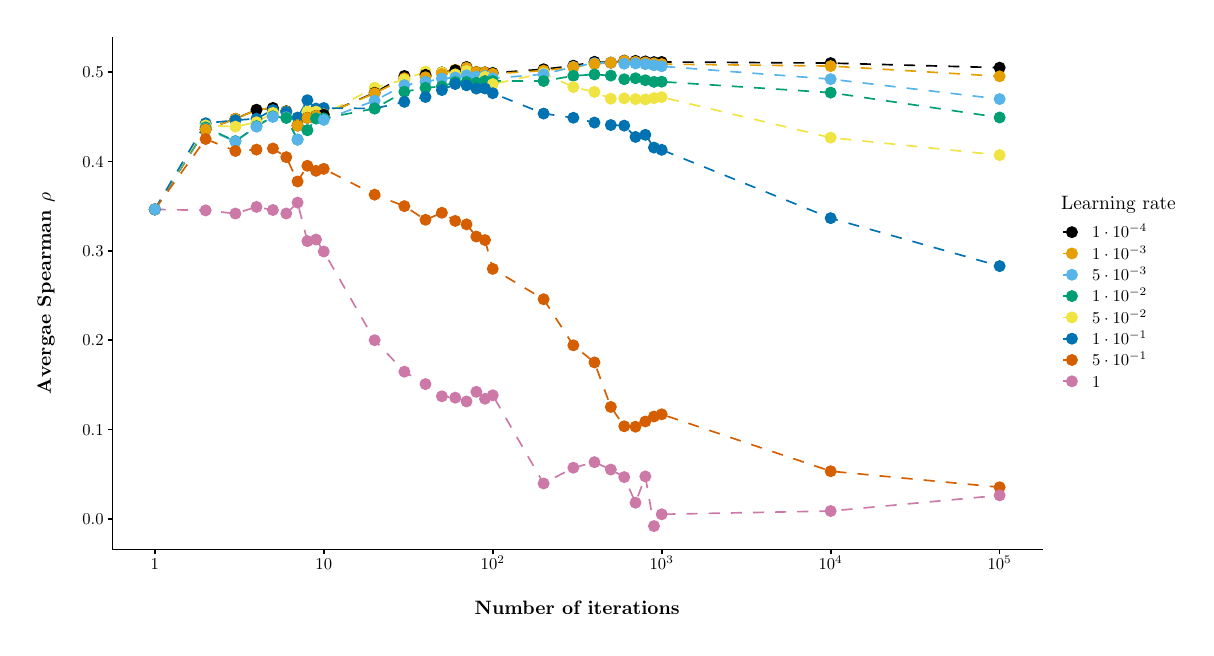
\begin{tikzpicture}[x=1pt,y=1pt]
\definecolor{fillColor}{RGB}{255,255,255}
\path[use as bounding box,fill=fillColor,fill opacity=0.00] (0,0) rectangle (418.34,216.81);
\begin{scope}
\path[clip] ( 30.67, 28.30) rectangle (366.48,213.31);
\definecolor{drawColor}{RGB}{0,0,0}

\path[draw=drawColor,line width= 0.6pt,dash pattern=on 4pt off 4pt ,line join=round] ( 45.94,151.14) --
	( 64.31,180.00) --
	( 75.07,183.89) --
	( 82.69,187.14) --
	( 88.61,187.78) --
	( 93.45,186.60) --
	( 97.53,181.45) --
	(101.07,184.24) --
	(104.20,184.95) --
	(106.99,185.35) --
	(125.37,193.28) --
	(136.12,199.36) --
	(143.75,199.76) --
	(149.67,200.65) --
	(154.50,201.42) --
	(158.59,202.59) --
	(162.13,200.74) --
	(165.25,200.68) --
	(168.05,200.46) --
	(186.43,201.78) --
	(197.18,203.07) --
	(204.81,204.46) --
	(210.72,204.18) --
	(215.56,204.90) --
	(219.64,204.81) --
	(223.19,204.61) --
	(226.31,204.36) --
	(229.10,204.42) --
	(290.16,204.01) --
	(351.21,202.35);
\definecolor{drawColor}{RGB}{230,159,0}

\path[draw=drawColor,line width= 0.6pt,dash pattern=on 4pt off 4pt ,line join=round] ( 45.94,151.14) --
	( 64.31,180.00) --
	( 75.07,183.86) --
	( 82.69,187.15) --
	( 88.61,187.78) --
	( 93.45,186.61) --
	( 97.53,181.39) --
	(101.07,184.19) --
	(104.20,184.93) --
	(106.99,185.36) --
	(125.37,193.08) --
	(136.12,198.50) --
	(143.75,198.90) --
	(149.67,200.10) --
	(154.50,201.59) --
	(158.59,202.28) --
	(162.13,200.72) --
	(165.25,200.64) --
	(168.05,200.14) --
	(186.43,201.28) --
	(197.18,202.58) --
	(204.81,203.70) --
	(210.72,204.16) --
	(215.56,204.80) --
	(219.64,204.46) --
	(223.19,204.24) --
	(226.31,203.90) --
	(229.10,203.65) --
	(290.16,202.94) --
	(351.21,199.24);
\definecolor{drawColor}{RGB}{86,180,233}

\path[draw=drawColor,line width= 0.6pt,dash pattern=on 4pt off 4pt ,line join=round] ( 45.94,151.14) --
	( 64.31,180.31) --
	( 75.07,175.64) --
	( 82.69,181.03) --
	( 88.61,184.56) --
	( 93.45,184.42) --
	( 97.53,176.35) --
	(101.07,179.78) --
	(104.20,184.01) --
	(106.99,183.48) --
	(125.37,190.42) --
	(136.12,196.04) --
	(143.75,197.25) --
	(149.67,198.43) --
	(154.50,198.81) --
	(158.59,199.59) --
	(162.13,199.11) --
	(165.25,199.36) --
	(168.05,198.53) --
	(186.43,199.96) --
	(197.18,202.65) --
	(204.81,203.97) --
	(210.72,204.17) --
	(215.56,203.78) --
	(219.64,203.87) --
	(223.19,203.63) --
	(226.31,203.22) --
	(229.10,202.86) --
	(290.16,198.21) --
	(351.21,191.01);
\definecolor{drawColor}{RGB}{0,158,115}

\path[draw=drawColor,line width= 0.6pt,dash pattern=on 4pt off 4pt ,line join=round] ( 45.94,151.14) --
	( 64.31,180.77) --
	( 75.07,175.81) --
	( 82.69,181.22) --
	( 88.61,184.76) --
	( 93.45,184.17) --
	( 97.53,176.37) --
	(101.07,179.75) --
	(104.20,183.97) --
	(106.99,184.03) --
	(125.37,187.59) --
	(136.12,193.66) --
	(143.75,195.06) --
	(149.67,195.58) --
	(154.50,197.13) --
	(158.59,197.19) --
	(162.13,196.85) --
	(165.25,197.52) --
	(168.05,197.52) --
	(186.43,197.53) --
	(197.18,199.41) --
	(204.81,199.91) --
	(210.72,199.49) --
	(215.56,198.17) --
	(219.64,198.53) --
	(223.19,197.82) --
	(226.31,197.23) --
	(229.10,197.29) --
	(290.16,193.34) --
	(351.21,184.35);
\definecolor{drawColor}{RGB}{240,228,66}

\path[draw=drawColor,line width= 0.6pt,dash pattern=on 4pt off 4pt ,line join=round] ( 45.94,151.14) --
	( 64.31,181.49) --
	( 75.07,181.05) --
	( 82.69,182.65) --
	( 88.61,186.02) --
	( 93.45,186.44) --
	( 97.53,181.59) --
	(101.07,186.51) --
	(104.20,186.48) --
	(106.99,185.50) --
	(125.37,195.12) --
	(136.12,198.06) --
	(143.75,200.96) --
	(149.67,200.62) --
	(154.50,199.95) --
	(158.59,201.16) --
	(162.13,200.93) --
	(165.25,199.02) --
	(168.05,196.40) --
	(186.43,200.36) --
	(197.18,195.33) --
	(204.81,193.60) --
	(210.72,191.13) --
	(215.56,191.26) --
	(219.64,190.99) --
	(223.19,190.89) --
	(226.31,191.34) --
	(229.10,191.71) --
	(290.16,177.07) --
	(351.21,170.76);
\definecolor{drawColor}{RGB}{0,114,178}

\path[draw=drawColor,line width= 0.6pt,dash pattern=on 4pt off 4pt ,line join=round] ( 45.94,151.14) --
	( 64.31,182.28) --
	( 75.07,183.35) --
	( 82.69,183.94) --
	( 88.61,187.05) --
	( 93.45,186.33) --
	( 97.53,184.33) --
	(101.07,190.60) --
	(104.20,187.57) --
	(106.99,187.77) --
	(125.37,187.60) --
	(136.12,190.00) --
	(143.75,191.75) --
	(149.67,194.26) --
	(154.50,196.44) --
	(158.59,195.98) --
	(162.13,194.80) --
	(165.25,194.85) --
	(168.05,193.13) --
	(186.43,185.77) --
	(197.18,184.25) --
	(204.81,182.51) --
	(210.72,181.62) --
	(215.56,181.41) --
	(219.64,177.33) --
	(223.19,178.09) --
	(226.31,173.48) --
	(229.10,172.67) --
	(290.16,147.98) --
	(351.21,130.65);
\definecolor{drawColor}{RGB}{213,94,0}

\path[draw=drawColor,line width= 0.6pt,dash pattern=on 4pt off 4pt ,line join=round] ( 45.94,151.14) --
	( 64.31,176.58) --
	( 75.07,172.25) --
	( 82.69,172.74) --
	( 88.61,173.15) --
	( 93.45,170.02) --
	( 97.53,161.23) --
	(101.07,166.90) --
	(104.20,165.08) --
	(106.99,165.79) --
	(125.37,156.47) --
	(136.12,152.32) --
	(143.75,147.38) --
	(149.67,149.91) --
	(154.50,146.98) --
	(158.59,145.73) --
	(162.13,141.33) --
	(165.25,140.06) --
	(168.05,129.66) --
	(186.43,118.69) --
	(197.18,102.03) --
	(204.81, 95.85) --
	(210.72, 79.76) --
	(215.56, 72.78) --
	(219.64, 72.62) --
	(223.19, 74.51) --
	(226.31, 76.31) --
	(229.10, 77.10) --
	(290.16, 56.54) --
	(351.21, 50.75);
\definecolor{drawColor}{RGB}{204,121,167}

\path[draw=drawColor,line width= 0.6pt,dash pattern=on 4pt off 4pt ,line join=round] ( 45.94,151.14) --
	( 64.31,150.78) --
	( 75.07,149.64) --
	( 82.69,152.04) --
	( 88.61,150.92) --
	( 93.45,149.67) --
	( 97.53,153.59) --
	(101.07,139.67) --
	(104.20,140.25) --
	(106.99,135.91) --
	(125.37,103.88) --
	(136.12, 92.50) --
	(143.75, 88.02) --
	(149.67, 83.61) --
	(154.50, 83.11) --
	(158.59, 81.74) --
	(162.13, 85.22) --
	(165.25, 82.72) --
	(168.05, 83.97) --
	(186.43, 52.11) --
	(197.18, 57.79) --
	(204.81, 59.80) --
	(210.72, 57.14) --
	(215.56, 54.41) --
	(219.64, 45.15) --
	(223.19, 54.65) --
	(226.31, 36.71) --
	(229.10, 40.97) --
	(290.16, 42.15) --
	(351.21, 47.81);
\definecolor{drawColor}{RGB}{0,0,0}
\definecolor{fillColor}{RGB}{0,0,0}

\path[draw=drawColor,line width= 0.4pt,line join=round,line cap=round,fill=fillColor] (215.56,204.90) circle (  1.96);

\path[draw=drawColor,line width= 0.4pt,line join=round,line cap=round,fill=fillColor] (219.64,204.81) circle (  1.96);
\definecolor{drawColor}{RGB}{230,159,0}
\definecolor{fillColor}{RGB}{230,159,0}

\path[draw=drawColor,line width= 0.4pt,line join=round,line cap=round,fill=fillColor] (215.56,204.80) circle (  1.96);
\definecolor{drawColor}{RGB}{0,0,0}
\definecolor{fillColor}{RGB}{0,0,0}

\path[draw=drawColor,line width= 0.4pt,line join=round,line cap=round,fill=fillColor] (223.19,204.61) circle (  1.96);

\path[draw=drawColor,line width= 0.4pt,line join=round,line cap=round,fill=fillColor] (204.81,204.46) circle (  1.96);
\definecolor{drawColor}{RGB}{230,159,0}
\definecolor{fillColor}{RGB}{230,159,0}

\path[draw=drawColor,line width= 0.4pt,line join=round,line cap=round,fill=fillColor] (219.64,204.46) circle (  1.96);
\definecolor{drawColor}{RGB}{0,0,0}
\definecolor{fillColor}{RGB}{0,0,0}

\path[draw=drawColor,line width= 0.4pt,line join=round,line cap=round,fill=fillColor] (229.10,204.42) circle (  1.96);

\path[draw=drawColor,line width= 0.4pt,line join=round,line cap=round,fill=fillColor] (226.31,204.36) circle (  1.96);
\definecolor{drawColor}{RGB}{230,159,0}
\definecolor{fillColor}{RGB}{230,159,0}

\path[draw=drawColor,line width= 0.4pt,line join=round,line cap=round,fill=fillColor] (223.19,204.24) circle (  1.96);
\definecolor{drawColor}{RGB}{0,0,0}
\definecolor{fillColor}{RGB}{0,0,0}

\path[draw=drawColor,line width= 0.4pt,line join=round,line cap=round,fill=fillColor] (210.72,204.18) circle (  1.96);
\definecolor{drawColor}{RGB}{86,180,233}
\definecolor{fillColor}{RGB}{86,180,233}

\path[draw=drawColor,line width= 0.4pt,line join=round,line cap=round,fill=fillColor] (210.72,204.17) circle (  1.96);
\definecolor{drawColor}{RGB}{230,159,0}
\definecolor{fillColor}{RGB}{230,159,0}

\path[draw=drawColor,line width= 0.4pt,line join=round,line cap=round,fill=fillColor] (210.72,204.16) circle (  1.96);
\definecolor{drawColor}{RGB}{86,180,233}
\definecolor{fillColor}{RGB}{86,180,233}

\path[draw=drawColor,line width= 0.4pt,line join=round,line cap=round,fill=fillColor] (204.81,203.97) circle (  1.96);
\definecolor{drawColor}{RGB}{230,159,0}
\definecolor{fillColor}{RGB}{230,159,0}

\path[draw=drawColor,line width= 0.4pt,line join=round,line cap=round,fill=fillColor] (226.31,203.90) circle (  1.96);
\definecolor{drawColor}{RGB}{86,180,233}
\definecolor{fillColor}{RGB}{86,180,233}

\path[draw=drawColor,line width= 0.4pt,line join=round,line cap=round,fill=fillColor] (219.64,203.87) circle (  1.96);

\path[draw=drawColor,line width= 0.4pt,line join=round,line cap=round,fill=fillColor] (215.56,203.78) circle (  1.96);
\definecolor{drawColor}{RGB}{230,159,0}
\definecolor{fillColor}{RGB}{230,159,0}

\path[draw=drawColor,line width= 0.4pt,line join=round,line cap=round,fill=fillColor] (204.81,203.70) circle (  1.96);

\path[draw=drawColor,line width= 0.4pt,line join=round,line cap=round,fill=fillColor] (229.10,203.65) circle (  1.96);
\definecolor{drawColor}{RGB}{86,180,233}
\definecolor{fillColor}{RGB}{86,180,233}

\path[draw=drawColor,line width= 0.4pt,line join=round,line cap=round,fill=fillColor] (223.19,203.63) circle (  1.96);

\path[draw=drawColor,line width= 0.4pt,line join=round,line cap=round,fill=fillColor] (226.31,203.22) circle (  1.96);
\definecolor{drawColor}{RGB}{0,0,0}
\definecolor{fillColor}{RGB}{0,0,0}

\path[draw=drawColor,line width= 0.4pt,line join=round,line cap=round,fill=fillColor] (197.18,203.07) circle (  1.96);
\definecolor{drawColor}{RGB}{86,180,233}
\definecolor{fillColor}{RGB}{86,180,233}

\path[draw=drawColor,line width= 0.4pt,line join=round,line cap=round,fill=fillColor] (229.10,202.86) circle (  1.96);

\path[draw=drawColor,line width= 0.4pt,line join=round,line cap=round,fill=fillColor] (197.18,202.65) circle (  1.96);
\definecolor{drawColor}{RGB}{0,0,0}
\definecolor{fillColor}{RGB}{0,0,0}

\path[draw=drawColor,line width= 0.4pt,line join=round,line cap=round,fill=fillColor] (158.59,202.59) circle (  1.96);
\definecolor{drawColor}{RGB}{230,159,0}
\definecolor{fillColor}{RGB}{230,159,0}

\path[draw=drawColor,line width= 0.4pt,line join=round,line cap=round,fill=fillColor] (197.18,202.58) circle (  1.96);

\path[draw=drawColor,line width= 0.4pt,line join=round,line cap=round,fill=fillColor] (158.59,202.28) circle (  1.96);
\definecolor{drawColor}{RGB}{0,0,0}
\definecolor{fillColor}{RGB}{0,0,0}

\path[draw=drawColor,line width= 0.4pt,line join=round,line cap=round,fill=fillColor] (186.43,201.78) circle (  1.96);
\definecolor{drawColor}{RGB}{230,159,0}
\definecolor{fillColor}{RGB}{230,159,0}

\path[draw=drawColor,line width= 0.4pt,line join=round,line cap=round,fill=fillColor] (154.50,201.59) circle (  1.96);
\definecolor{drawColor}{RGB}{0,0,0}
\definecolor{fillColor}{RGB}{0,0,0}

\path[draw=drawColor,line width= 0.4pt,line join=round,line cap=round,fill=fillColor] (154.50,201.42) circle (  1.96);
\definecolor{drawColor}{RGB}{230,159,0}
\definecolor{fillColor}{RGB}{230,159,0}

\path[draw=drawColor,line width= 0.4pt,line join=round,line cap=round,fill=fillColor] (186.43,201.28) circle (  1.96);
\definecolor{drawColor}{RGB}{240,228,66}
\definecolor{fillColor}{RGB}{240,228,66}

\path[draw=drawColor,line width= 0.4pt,line join=round,line cap=round,fill=fillColor] (158.59,201.16) circle (  1.96);

\path[draw=drawColor,line width= 0.4pt,line join=round,line cap=round,fill=fillColor] (143.75,200.96) circle (  1.96);

\path[draw=drawColor,line width= 0.4pt,line join=round,line cap=round,fill=fillColor] (162.13,200.93) circle (  1.96);
\definecolor{drawColor}{RGB}{0,0,0}
\definecolor{fillColor}{RGB}{0,0,0}

\path[draw=drawColor,line width= 0.4pt,line join=round,line cap=round,fill=fillColor] (162.13,200.74) circle (  1.96);
\definecolor{drawColor}{RGB}{230,159,0}
\definecolor{fillColor}{RGB}{230,159,0}

\path[draw=drawColor,line width= 0.4pt,line join=round,line cap=round,fill=fillColor] (162.13,200.72) circle (  1.96);
\definecolor{drawColor}{RGB}{0,0,0}
\definecolor{fillColor}{RGB}{0,0,0}

\path[draw=drawColor,line width= 0.4pt,line join=round,line cap=round,fill=fillColor] (165.25,200.68) circle (  1.96);

\path[draw=drawColor,line width= 0.4pt,line join=round,line cap=round,fill=fillColor] (149.67,200.65) circle (  1.96);
\definecolor{drawColor}{RGB}{230,159,0}
\definecolor{fillColor}{RGB}{230,159,0}

\path[draw=drawColor,line width= 0.4pt,line join=round,line cap=round,fill=fillColor] (165.25,200.64) circle (  1.96);
\definecolor{drawColor}{RGB}{240,228,66}
\definecolor{fillColor}{RGB}{240,228,66}

\path[draw=drawColor,line width= 0.4pt,line join=round,line cap=round,fill=fillColor] (149.67,200.62) circle (  1.96);
\definecolor{drawColor}{RGB}{0,0,0}
\definecolor{fillColor}{RGB}{0,0,0}

\path[draw=drawColor,line width= 0.4pt,line join=round,line cap=round,fill=fillColor] (168.05,200.46) circle (  1.96);
\definecolor{drawColor}{RGB}{240,228,66}
\definecolor{fillColor}{RGB}{240,228,66}

\path[draw=drawColor,line width= 0.4pt,line join=round,line cap=round,fill=fillColor] (186.43,200.36) circle (  1.96);
\definecolor{drawColor}{RGB}{230,159,0}
\definecolor{fillColor}{RGB}{230,159,0}

\path[draw=drawColor,line width= 0.4pt,line join=round,line cap=round,fill=fillColor] (168.05,200.14) circle (  1.96);

\path[draw=drawColor,line width= 0.4pt,line join=round,line cap=round,fill=fillColor] (149.67,200.10) circle (  1.96);
\definecolor{drawColor}{RGB}{86,180,233}
\definecolor{fillColor}{RGB}{86,180,233}

\path[draw=drawColor,line width= 0.4pt,line join=round,line cap=round,fill=fillColor] (186.43,199.96) circle (  1.96);
\definecolor{drawColor}{RGB}{240,228,66}
\definecolor{fillColor}{RGB}{240,228,66}

\path[draw=drawColor,line width= 0.4pt,line join=round,line cap=round,fill=fillColor] (154.50,199.95) circle (  1.96);
\definecolor{drawColor}{RGB}{0,158,115}
\definecolor{fillColor}{RGB}{0,158,115}

\path[draw=drawColor,line width= 0.4pt,line join=round,line cap=round,fill=fillColor] (204.81,199.91) circle (  1.96);
\definecolor{drawColor}{RGB}{0,0,0}
\definecolor{fillColor}{RGB}{0,0,0}

\path[draw=drawColor,line width= 0.4pt,line join=round,line cap=round,fill=fillColor] (143.75,199.76) circle (  1.96);
\definecolor{drawColor}{RGB}{86,180,233}
\definecolor{fillColor}{RGB}{86,180,233}

\path[draw=drawColor,line width= 0.4pt,line join=round,line cap=round,fill=fillColor] (158.59,199.59) circle (  1.96);
\definecolor{drawColor}{RGB}{0,158,115}
\definecolor{fillColor}{RGB}{0,158,115}

\path[draw=drawColor,line width= 0.4pt,line join=round,line cap=round,fill=fillColor] (210.72,199.49) circle (  1.96);

\path[draw=drawColor,line width= 0.4pt,line join=round,line cap=round,fill=fillColor] (197.18,199.41) circle (  1.96);
\definecolor{drawColor}{RGB}{86,180,233}
\definecolor{fillColor}{RGB}{86,180,233}

\path[draw=drawColor,line width= 0.4pt,line join=round,line cap=round,fill=fillColor] (165.25,199.36) circle (  1.96);
\definecolor{drawColor}{RGB}{0,0,0}
\definecolor{fillColor}{RGB}{0,0,0}

\path[draw=drawColor,line width= 0.4pt,line join=round,line cap=round,fill=fillColor] (136.12,199.36) circle (  1.96);
\definecolor{drawColor}{RGB}{86,180,233}
\definecolor{fillColor}{RGB}{86,180,233}

\path[draw=drawColor,line width= 0.4pt,line join=round,line cap=round,fill=fillColor] (162.13,199.11) circle (  1.96);
\definecolor{drawColor}{RGB}{240,228,66}
\definecolor{fillColor}{RGB}{240,228,66}

\path[draw=drawColor,line width= 0.4pt,line join=round,line cap=round,fill=fillColor] (165.25,199.02) circle (  1.96);
\definecolor{drawColor}{RGB}{230,159,0}
\definecolor{fillColor}{RGB}{230,159,0}

\path[draw=drawColor,line width= 0.4pt,line join=round,line cap=round,fill=fillColor] (143.75,198.90) circle (  1.96);
\definecolor{drawColor}{RGB}{86,180,233}
\definecolor{fillColor}{RGB}{86,180,233}

\path[draw=drawColor,line width= 0.4pt,line join=round,line cap=round,fill=fillColor] (154.50,198.81) circle (  1.96);

\path[draw=drawColor,line width= 0.4pt,line join=round,line cap=round,fill=fillColor] (168.05,198.53) circle (  1.96);
\definecolor{drawColor}{RGB}{0,158,115}
\definecolor{fillColor}{RGB}{0,158,115}

\path[draw=drawColor,line width= 0.4pt,line join=round,line cap=round,fill=fillColor] (219.64,198.53) circle (  1.96);
\definecolor{drawColor}{RGB}{230,159,0}
\definecolor{fillColor}{RGB}{230,159,0}

\path[draw=drawColor,line width= 0.4pt,line join=round,line cap=round,fill=fillColor] (136.12,198.50) circle (  1.96);
\definecolor{drawColor}{RGB}{86,180,233}
\definecolor{fillColor}{RGB}{86,180,233}

\path[draw=drawColor,line width= 0.4pt,line join=round,line cap=round,fill=fillColor] (149.67,198.43) circle (  1.96);
\definecolor{drawColor}{RGB}{0,158,115}
\definecolor{fillColor}{RGB}{0,158,115}

\path[draw=drawColor,line width= 0.4pt,line join=round,line cap=round,fill=fillColor] (215.56,198.17) circle (  1.96);
\definecolor{drawColor}{RGB}{240,228,66}
\definecolor{fillColor}{RGB}{240,228,66}

\path[draw=drawColor,line width= 0.4pt,line join=round,line cap=round,fill=fillColor] (136.12,198.06) circle (  1.96);
\definecolor{drawColor}{RGB}{0,158,115}
\definecolor{fillColor}{RGB}{0,158,115}

\path[draw=drawColor,line width= 0.4pt,line join=round,line cap=round,fill=fillColor] (223.19,197.82) circle (  1.96);

\path[draw=drawColor,line width= 0.4pt,line join=round,line cap=round,fill=fillColor] (186.43,197.53) circle (  1.96);

\path[draw=drawColor,line width= 0.4pt,line join=round,line cap=round,fill=fillColor] (168.05,197.52) circle (  1.96);

\path[draw=drawColor,line width= 0.4pt,line join=round,line cap=round,fill=fillColor] (165.25,197.52) circle (  1.96);

\path[draw=drawColor,line width= 0.4pt,line join=round,line cap=round,fill=fillColor] (229.10,197.29) circle (  1.96);
\definecolor{drawColor}{RGB}{86,180,233}
\definecolor{fillColor}{RGB}{86,180,233}

\path[draw=drawColor,line width= 0.4pt,line join=round,line cap=round,fill=fillColor] (143.75,197.25) circle (  1.96);
\definecolor{drawColor}{RGB}{0,158,115}
\definecolor{fillColor}{RGB}{0,158,115}

\path[draw=drawColor,line width= 0.4pt,line join=round,line cap=round,fill=fillColor] (226.31,197.23) circle (  1.96);

\path[draw=drawColor,line width= 0.4pt,line join=round,line cap=round,fill=fillColor] (158.59,197.19) circle (  1.96);

\path[draw=drawColor,line width= 0.4pt,line join=round,line cap=round,fill=fillColor] (154.50,197.13) circle (  1.96);

\path[draw=drawColor,line width= 0.4pt,line join=round,line cap=round,fill=fillColor] (162.13,196.85) circle (  1.96);
\definecolor{drawColor}{RGB}{0,114,178}
\definecolor{fillColor}{RGB}{0,114,178}

\path[draw=drawColor,line width= 0.4pt,line join=round,line cap=round,fill=fillColor] (154.50,196.44) circle (  1.96);
\definecolor{drawColor}{RGB}{240,228,66}
\definecolor{fillColor}{RGB}{240,228,66}

\path[draw=drawColor,line width= 0.4pt,line join=round,line cap=round,fill=fillColor] (168.05,196.40) circle (  1.96);
\definecolor{drawColor}{RGB}{86,180,233}
\definecolor{fillColor}{RGB}{86,180,233}

\path[draw=drawColor,line width= 0.4pt,line join=round,line cap=round,fill=fillColor] (136.12,196.04) circle (  1.96);
\definecolor{drawColor}{RGB}{0,114,178}
\definecolor{fillColor}{RGB}{0,114,178}

\path[draw=drawColor,line width= 0.4pt,line join=round,line cap=round,fill=fillColor] (158.59,195.98) circle (  1.96);
\definecolor{drawColor}{RGB}{0,158,115}
\definecolor{fillColor}{RGB}{0,158,115}

\path[draw=drawColor,line width= 0.4pt,line join=round,line cap=round,fill=fillColor] (149.67,195.58) circle (  1.96);
\definecolor{drawColor}{RGB}{240,228,66}
\definecolor{fillColor}{RGB}{240,228,66}

\path[draw=drawColor,line width= 0.4pt,line join=round,line cap=round,fill=fillColor] (197.18,195.33) circle (  1.96);

\path[draw=drawColor,line width= 0.4pt,line join=round,line cap=round,fill=fillColor] (125.37,195.12) circle (  1.96);
\definecolor{drawColor}{RGB}{0,158,115}
\definecolor{fillColor}{RGB}{0,158,115}

\path[draw=drawColor,line width= 0.4pt,line join=round,line cap=round,fill=fillColor] (143.75,195.06) circle (  1.96);
\definecolor{drawColor}{RGB}{0,114,178}
\definecolor{fillColor}{RGB}{0,114,178}

\path[draw=drawColor,line width= 0.4pt,line join=round,line cap=round,fill=fillColor] (165.25,194.85) circle (  1.96);

\path[draw=drawColor,line width= 0.4pt,line join=round,line cap=round,fill=fillColor] (162.13,194.80) circle (  1.96);

\path[draw=drawColor,line width= 0.4pt,line join=round,line cap=round,fill=fillColor] (149.67,194.26) circle (  1.96);
\definecolor{drawColor}{RGB}{0,158,115}
\definecolor{fillColor}{RGB}{0,158,115}

\path[draw=drawColor,line width= 0.4pt,line join=round,line cap=round,fill=fillColor] (136.12,193.66) circle (  1.96);
\definecolor{drawColor}{RGB}{240,228,66}
\definecolor{fillColor}{RGB}{240,228,66}

\path[draw=drawColor,line width= 0.4pt,line join=round,line cap=round,fill=fillColor] (204.81,193.60) circle (  1.96);
\definecolor{drawColor}{RGB}{0,0,0}
\definecolor{fillColor}{RGB}{0,0,0}

\path[draw=drawColor,line width= 0.4pt,line join=round,line cap=round,fill=fillColor] (125.37,193.28) circle (  1.96);
\definecolor{drawColor}{RGB}{0,114,178}
\definecolor{fillColor}{RGB}{0,114,178}

\path[draw=drawColor,line width= 0.4pt,line join=round,line cap=round,fill=fillColor] (168.05,193.13) circle (  1.96);
\definecolor{drawColor}{RGB}{230,159,0}
\definecolor{fillColor}{RGB}{230,159,0}

\path[draw=drawColor,line width= 0.4pt,line join=round,line cap=round,fill=fillColor] (125.37,193.08) circle (  1.96);
\definecolor{drawColor}{RGB}{0,114,178}
\definecolor{fillColor}{RGB}{0,114,178}

\path[draw=drawColor,line width= 0.4pt,line join=round,line cap=round,fill=fillColor] (143.75,191.75) circle (  1.96);
\definecolor{drawColor}{RGB}{240,228,66}
\definecolor{fillColor}{RGB}{240,228,66}

\path[draw=drawColor,line width= 0.4pt,line join=round,line cap=round,fill=fillColor] (229.10,191.71) circle (  1.96);

\path[draw=drawColor,line width= 0.4pt,line join=round,line cap=round,fill=fillColor] (226.31,191.34) circle (  1.96);

\path[draw=drawColor,line width= 0.4pt,line join=round,line cap=round,fill=fillColor] (215.56,191.26) circle (  1.96);

\path[draw=drawColor,line width= 0.4pt,line join=round,line cap=round,fill=fillColor] (210.72,191.13) circle (  1.96);

\path[draw=drawColor,line width= 0.4pt,line join=round,line cap=round,fill=fillColor] (219.64,190.99) circle (  1.96);

\path[draw=drawColor,line width= 0.4pt,line join=round,line cap=round,fill=fillColor] (223.19,190.89) circle (  1.96);
\definecolor{drawColor}{RGB}{0,114,178}
\definecolor{fillColor}{RGB}{0,114,178}

\path[draw=drawColor,line width= 0.4pt,line join=round,line cap=round,fill=fillColor] (101.07,190.60) circle (  1.96);
\definecolor{drawColor}{RGB}{86,180,233}
\definecolor{fillColor}{RGB}{86,180,233}

\path[draw=drawColor,line width= 0.4pt,line join=round,line cap=round,fill=fillColor] (125.37,190.42) circle (  1.96);
\definecolor{drawColor}{RGB}{0,114,178}
\definecolor{fillColor}{RGB}{0,114,178}

\path[draw=drawColor,line width= 0.4pt,line join=round,line cap=round,fill=fillColor] (136.12,190.00) circle (  1.96);
\definecolor{drawColor}{RGB}{230,159,0}
\definecolor{fillColor}{RGB}{230,159,0}

\path[draw=drawColor,line width= 0.4pt,line join=round,line cap=round,fill=fillColor] ( 88.61,187.78) circle (  1.96);
\definecolor{drawColor}{RGB}{0,0,0}
\definecolor{fillColor}{RGB}{0,0,0}

\path[draw=drawColor,line width= 0.4pt,line join=round,line cap=round,fill=fillColor] ( 88.61,187.78) circle (  1.96);
\definecolor{drawColor}{RGB}{0,114,178}
\definecolor{fillColor}{RGB}{0,114,178}

\path[draw=drawColor,line width= 0.4pt,line join=round,line cap=round,fill=fillColor] (106.99,187.77) circle (  1.96);

\path[draw=drawColor,line width= 0.4pt,line join=round,line cap=round,fill=fillColor] (125.37,187.60) circle (  1.96);
\definecolor{drawColor}{RGB}{0,158,115}
\definecolor{fillColor}{RGB}{0,158,115}

\path[draw=drawColor,line width= 0.4pt,line join=round,line cap=round,fill=fillColor] (125.37,187.59) circle (  1.96);
\definecolor{drawColor}{RGB}{0,114,178}
\definecolor{fillColor}{RGB}{0,114,178}

\path[draw=drawColor,line width= 0.4pt,line join=round,line cap=round,fill=fillColor] (104.20,187.57) circle (  1.96);
\definecolor{drawColor}{RGB}{230,159,0}
\definecolor{fillColor}{RGB}{230,159,0}

\path[draw=drawColor,line width= 0.4pt,line join=round,line cap=round,fill=fillColor] ( 82.69,187.15) circle (  1.96);
\definecolor{drawColor}{RGB}{0,0,0}
\definecolor{fillColor}{RGB}{0,0,0}

\path[draw=drawColor,line width= 0.4pt,line join=round,line cap=round,fill=fillColor] ( 82.69,187.14) circle (  1.96);
\definecolor{drawColor}{RGB}{0,114,178}
\definecolor{fillColor}{RGB}{0,114,178}

\path[draw=drawColor,line width= 0.4pt,line join=round,line cap=round,fill=fillColor] ( 88.61,187.05) circle (  1.96);
\definecolor{drawColor}{RGB}{230,159,0}
\definecolor{fillColor}{RGB}{230,159,0}

\path[draw=drawColor,line width= 0.4pt,line join=round,line cap=round,fill=fillColor] ( 93.45,186.61) circle (  1.96);
\definecolor{drawColor}{RGB}{0,0,0}
\definecolor{fillColor}{RGB}{0,0,0}

\path[draw=drawColor,line width= 0.4pt,line join=round,line cap=round,fill=fillColor] ( 93.45,186.60) circle (  1.96);
\definecolor{drawColor}{RGB}{240,228,66}
\definecolor{fillColor}{RGB}{240,228,66}

\path[draw=drawColor,line width= 0.4pt,line join=round,line cap=round,fill=fillColor] (101.07,186.51) circle (  1.96);

\path[draw=drawColor,line width= 0.4pt,line join=round,line cap=round,fill=fillColor] (104.20,186.48) circle (  1.96);

\path[draw=drawColor,line width= 0.4pt,line join=round,line cap=round,fill=fillColor] ( 93.45,186.44) circle (  1.96);
\definecolor{drawColor}{RGB}{0,114,178}
\definecolor{fillColor}{RGB}{0,114,178}

\path[draw=drawColor,line width= 0.4pt,line join=round,line cap=round,fill=fillColor] ( 93.45,186.33) circle (  1.96);
\definecolor{drawColor}{RGB}{240,228,66}
\definecolor{fillColor}{RGB}{240,228,66}

\path[draw=drawColor,line width= 0.4pt,line join=round,line cap=round,fill=fillColor] ( 88.61,186.02) circle (  1.96);
\definecolor{drawColor}{RGB}{0,114,178}
\definecolor{fillColor}{RGB}{0,114,178}

\path[draw=drawColor,line width= 0.4pt,line join=round,line cap=round,fill=fillColor] (186.43,185.77) circle (  1.96);
\definecolor{drawColor}{RGB}{240,228,66}
\definecolor{fillColor}{RGB}{240,228,66}

\path[draw=drawColor,line width= 0.4pt,line join=round,line cap=round,fill=fillColor] (106.99,185.50) circle (  1.96);
\definecolor{drawColor}{RGB}{230,159,0}
\definecolor{fillColor}{RGB}{230,159,0}

\path[draw=drawColor,line width= 0.4pt,line join=round,line cap=round,fill=fillColor] (106.99,185.36) circle (  1.96);
\definecolor{drawColor}{RGB}{0,0,0}
\definecolor{fillColor}{RGB}{0,0,0}

\path[draw=drawColor,line width= 0.4pt,line join=round,line cap=round,fill=fillColor] (106.99,185.35) circle (  1.96);

\path[draw=drawColor,line width= 0.4pt,line join=round,line cap=round,fill=fillColor] (104.20,184.95) circle (  1.96);
\definecolor{drawColor}{RGB}{230,159,0}
\definecolor{fillColor}{RGB}{230,159,0}

\path[draw=drawColor,line width= 0.4pt,line join=round,line cap=round,fill=fillColor] (104.20,184.93) circle (  1.96);
\definecolor{drawColor}{RGB}{0,158,115}
\definecolor{fillColor}{RGB}{0,158,115}

\path[draw=drawColor,line width= 0.4pt,line join=round,line cap=round,fill=fillColor] ( 88.61,184.76) circle (  1.96);
\definecolor{drawColor}{RGB}{86,180,233}
\definecolor{fillColor}{RGB}{86,180,233}

\path[draw=drawColor,line width= 0.4pt,line join=round,line cap=round,fill=fillColor] ( 88.61,184.56) circle (  1.96);

\path[draw=drawColor,line width= 0.4pt,line join=round,line cap=round,fill=fillColor] ( 93.45,184.42) circle (  1.96);
\definecolor{drawColor}{RGB}{0,114,178}
\definecolor{fillColor}{RGB}{0,114,178}

\path[draw=drawColor,line width= 0.4pt,line join=round,line cap=round,fill=fillColor] ( 97.53,184.33) circle (  1.96);

\path[draw=drawColor,line width= 0.4pt,line join=round,line cap=round,fill=fillColor] (197.18,184.25) circle (  1.96);
\definecolor{drawColor}{RGB}{0,0,0}
\definecolor{fillColor}{RGB}{0,0,0}

\path[draw=drawColor,line width= 0.4pt,line join=round,line cap=round,fill=fillColor] (101.07,184.24) circle (  1.96);
\definecolor{drawColor}{RGB}{230,159,0}
\definecolor{fillColor}{RGB}{230,159,0}

\path[draw=drawColor,line width= 0.4pt,line join=round,line cap=round,fill=fillColor] (101.07,184.19) circle (  1.96);
\definecolor{drawColor}{RGB}{0,158,115}
\definecolor{fillColor}{RGB}{0,158,115}

\path[draw=drawColor,line width= 0.4pt,line join=round,line cap=round,fill=fillColor] ( 93.45,184.17) circle (  1.96);

\path[draw=drawColor,line width= 0.4pt,line join=round,line cap=round,fill=fillColor] (106.99,184.03) circle (  1.96);
\definecolor{drawColor}{RGB}{86,180,233}
\definecolor{fillColor}{RGB}{86,180,233}

\path[draw=drawColor,line width= 0.4pt,line join=round,line cap=round,fill=fillColor] (104.20,184.01) circle (  1.96);
\definecolor{drawColor}{RGB}{0,158,115}
\definecolor{fillColor}{RGB}{0,158,115}

\path[draw=drawColor,line width= 0.4pt,line join=round,line cap=round,fill=fillColor] (104.20,183.97) circle (  1.96);
\definecolor{drawColor}{RGB}{0,114,178}
\definecolor{fillColor}{RGB}{0,114,178}

\path[draw=drawColor,line width= 0.4pt,line join=round,line cap=round,fill=fillColor] ( 82.69,183.94) circle (  1.96);
\definecolor{drawColor}{RGB}{0,0,0}
\definecolor{fillColor}{RGB}{0,0,0}

\path[draw=drawColor,line width= 0.4pt,line join=round,line cap=round,fill=fillColor] ( 75.07,183.89) circle (  1.96);
\definecolor{drawColor}{RGB}{230,159,0}
\definecolor{fillColor}{RGB}{230,159,0}

\path[draw=drawColor,line width= 0.4pt,line join=round,line cap=round,fill=fillColor] ( 75.07,183.86) circle (  1.96);
\definecolor{drawColor}{RGB}{86,180,233}
\definecolor{fillColor}{RGB}{86,180,233}

\path[draw=drawColor,line width= 0.4pt,line join=round,line cap=round,fill=fillColor] (106.99,183.48) circle (  1.96);
\definecolor{drawColor}{RGB}{0,114,178}
\definecolor{fillColor}{RGB}{0,114,178}

\path[draw=drawColor,line width= 0.4pt,line join=round,line cap=round,fill=fillColor] ( 75.07,183.35) circle (  1.96);
\definecolor{drawColor}{RGB}{240,228,66}
\definecolor{fillColor}{RGB}{240,228,66}

\path[draw=drawColor,line width= 0.4pt,line join=round,line cap=round,fill=fillColor] ( 82.69,182.65) circle (  1.96);
\definecolor{drawColor}{RGB}{0,114,178}
\definecolor{fillColor}{RGB}{0,114,178}

\path[draw=drawColor,line width= 0.4pt,line join=round,line cap=round,fill=fillColor] (204.81,182.51) circle (  1.96);

\path[draw=drawColor,line width= 0.4pt,line join=round,line cap=round,fill=fillColor] ( 64.31,182.28) circle (  1.96);

\path[draw=drawColor,line width= 0.4pt,line join=round,line cap=round,fill=fillColor] (210.72,181.62) circle (  1.96);
\definecolor{drawColor}{RGB}{240,228,66}
\definecolor{fillColor}{RGB}{240,228,66}

\path[draw=drawColor,line width= 0.4pt,line join=round,line cap=round,fill=fillColor] ( 97.53,181.59) circle (  1.96);

\path[draw=drawColor,line width= 0.4pt,line join=round,line cap=round,fill=fillColor] ( 64.31,181.49) circle (  1.96);
\definecolor{drawColor}{RGB}{0,0,0}
\definecolor{fillColor}{RGB}{0,0,0}

\path[draw=drawColor,line width= 0.4pt,line join=round,line cap=round,fill=fillColor] ( 97.53,181.45) circle (  1.96);
\definecolor{drawColor}{RGB}{0,114,178}
\definecolor{fillColor}{RGB}{0,114,178}

\path[draw=drawColor,line width= 0.4pt,line join=round,line cap=round,fill=fillColor] (215.56,181.41) circle (  1.96);
\definecolor{drawColor}{RGB}{230,159,0}
\definecolor{fillColor}{RGB}{230,159,0}

\path[draw=drawColor,line width= 0.4pt,line join=round,line cap=round,fill=fillColor] ( 97.53,181.39) circle (  1.96);
\definecolor{drawColor}{RGB}{0,158,115}
\definecolor{fillColor}{RGB}{0,158,115}

\path[draw=drawColor,line width= 0.4pt,line join=round,line cap=round,fill=fillColor] ( 82.69,181.22) circle (  1.96);
\definecolor{drawColor}{RGB}{240,228,66}
\definecolor{fillColor}{RGB}{240,228,66}

\path[draw=drawColor,line width= 0.4pt,line join=round,line cap=round,fill=fillColor] ( 75.07,181.05) circle (  1.96);
\definecolor{drawColor}{RGB}{86,180,233}
\definecolor{fillColor}{RGB}{86,180,233}

\path[draw=drawColor,line width= 0.4pt,line join=round,line cap=round,fill=fillColor] ( 82.69,181.03) circle (  1.96);
\definecolor{drawColor}{RGB}{0,158,115}
\definecolor{fillColor}{RGB}{0,158,115}

\path[draw=drawColor,line width= 0.4pt,line join=round,line cap=round,fill=fillColor] ( 64.31,180.77) circle (  1.96);
\definecolor{drawColor}{RGB}{86,180,233}
\definecolor{fillColor}{RGB}{86,180,233}

\path[draw=drawColor,line width= 0.4pt,line join=round,line cap=round,fill=fillColor] ( 64.31,180.31) circle (  1.96);
\definecolor{drawColor}{RGB}{0,0,0}
\definecolor{fillColor}{RGB}{0,0,0}

\path[draw=drawColor,line width= 0.4pt,line join=round,line cap=round,fill=fillColor] ( 64.31,180.00) circle (  1.96);
\definecolor{drawColor}{RGB}{230,159,0}
\definecolor{fillColor}{RGB}{230,159,0}

\path[draw=drawColor,line width= 0.4pt,line join=round,line cap=round,fill=fillColor] ( 64.31,180.00) circle (  1.96);
\definecolor{drawColor}{RGB}{86,180,233}
\definecolor{fillColor}{RGB}{86,180,233}

\path[draw=drawColor,line width= 0.4pt,line join=round,line cap=round,fill=fillColor] (101.07,179.78) circle (  1.96);
\definecolor{drawColor}{RGB}{0,158,115}
\definecolor{fillColor}{RGB}{0,158,115}

\path[draw=drawColor,line width= 0.4pt,line join=round,line cap=round,fill=fillColor] (101.07,179.75) circle (  1.96);
\definecolor{drawColor}{RGB}{0,114,178}
\definecolor{fillColor}{RGB}{0,114,178}

\path[draw=drawColor,line width= 0.4pt,line join=round,line cap=round,fill=fillColor] (223.19,178.09) circle (  1.96);

\path[draw=drawColor,line width= 0.4pt,line join=round,line cap=round,fill=fillColor] (219.64,177.33) circle (  1.96);
\definecolor{drawColor}{RGB}{213,94,0}
\definecolor{fillColor}{RGB}{213,94,0}

\path[draw=drawColor,line width= 0.4pt,line join=round,line cap=round,fill=fillColor] ( 64.31,176.58) circle (  1.96);
\definecolor{drawColor}{RGB}{0,158,115}
\definecolor{fillColor}{RGB}{0,158,115}

\path[draw=drawColor,line width= 0.4pt,line join=round,line cap=round,fill=fillColor] ( 97.53,176.37) circle (  1.96);
\definecolor{drawColor}{RGB}{86,180,233}
\definecolor{fillColor}{RGB}{86,180,233}

\path[draw=drawColor,line width= 0.4pt,line join=round,line cap=round,fill=fillColor] ( 97.53,176.35) circle (  1.96);
\definecolor{drawColor}{RGB}{0,158,115}
\definecolor{fillColor}{RGB}{0,158,115}

\path[draw=drawColor,line width= 0.4pt,line join=round,line cap=round,fill=fillColor] ( 75.07,175.81) circle (  1.96);
\definecolor{drawColor}{RGB}{86,180,233}
\definecolor{fillColor}{RGB}{86,180,233}

\path[draw=drawColor,line width= 0.4pt,line join=round,line cap=round,fill=fillColor] ( 75.07,175.64) circle (  1.96);
\definecolor{drawColor}{RGB}{0,114,178}
\definecolor{fillColor}{RGB}{0,114,178}

\path[draw=drawColor,line width= 0.4pt,line join=round,line cap=round,fill=fillColor] (226.31,173.48) circle (  1.96);
\definecolor{drawColor}{RGB}{213,94,0}
\definecolor{fillColor}{RGB}{213,94,0}

\path[draw=drawColor,line width= 0.4pt,line join=round,line cap=round,fill=fillColor] ( 88.61,173.15) circle (  1.96);

\path[draw=drawColor,line width= 0.4pt,line join=round,line cap=round,fill=fillColor] ( 82.69,172.74) circle (  1.96);
\definecolor{drawColor}{RGB}{0,114,178}
\definecolor{fillColor}{RGB}{0,114,178}

\path[draw=drawColor,line width= 0.4pt,line join=round,line cap=round,fill=fillColor] (229.10,172.67) circle (  1.96);
\definecolor{drawColor}{RGB}{213,94,0}
\definecolor{fillColor}{RGB}{213,94,0}

\path[draw=drawColor,line width= 0.4pt,line join=round,line cap=round,fill=fillColor] ( 75.07,172.25) circle (  1.96);

\path[draw=drawColor,line width= 0.4pt,line join=round,line cap=round,fill=fillColor] ( 93.45,170.02) circle (  1.96);

\path[draw=drawColor,line width= 0.4pt,line join=round,line cap=round,fill=fillColor] (101.07,166.90) circle (  1.96);

\path[draw=drawColor,line width= 0.4pt,line join=round,line cap=round,fill=fillColor] (106.99,165.79) circle (  1.96);

\path[draw=drawColor,line width= 0.4pt,line join=round,line cap=round,fill=fillColor] (104.20,165.08) circle (  1.96);

\path[draw=drawColor,line width= 0.4pt,line join=round,line cap=round,fill=fillColor] ( 97.53,161.23) circle (  1.96);

\path[draw=drawColor,line width= 0.4pt,line join=round,line cap=round,fill=fillColor] (125.37,156.47) circle (  1.96);
\definecolor{drawColor}{RGB}{204,121,167}
\definecolor{fillColor}{RGB}{204,121,167}

\path[draw=drawColor,line width= 0.4pt,line join=round,line cap=round,fill=fillColor] ( 97.53,153.59) circle (  1.96);
\definecolor{drawColor}{RGB}{213,94,0}
\definecolor{fillColor}{RGB}{213,94,0}

\path[draw=drawColor,line width= 0.4pt,line join=round,line cap=round,fill=fillColor] (136.12,152.32) circle (  1.96);
\definecolor{drawColor}{RGB}{204,121,167}
\definecolor{fillColor}{RGB}{204,121,167}

\path[draw=drawColor,line width= 0.4pt,line join=round,line cap=round,fill=fillColor] ( 82.69,152.04) circle (  1.96);

\path[draw=drawColor,line width= 0.4pt,line join=round,line cap=round,fill=fillColor] ( 45.94,151.14) circle (  1.96);
\definecolor{drawColor}{RGB}{0,0,0}
\definecolor{fillColor}{RGB}{0,0,0}

\path[draw=drawColor,line width= 0.4pt,line join=round,line cap=round,fill=fillColor] ( 45.94,151.14) circle (  1.96);
\definecolor{drawColor}{RGB}{240,228,66}
\definecolor{fillColor}{RGB}{240,228,66}

\path[draw=drawColor,line width= 0.4pt,line join=round,line cap=round,fill=fillColor] ( 45.94,151.14) circle (  1.96);
\definecolor{drawColor}{RGB}{213,94,0}
\definecolor{fillColor}{RGB}{213,94,0}

\path[draw=drawColor,line width= 0.4pt,line join=round,line cap=round,fill=fillColor] ( 45.94,151.14) circle (  1.96);
\definecolor{drawColor}{RGB}{0,158,115}
\definecolor{fillColor}{RGB}{0,158,115}

\path[draw=drawColor,line width= 0.4pt,line join=round,line cap=round,fill=fillColor] ( 45.94,151.14) circle (  1.96);
\definecolor{drawColor}{RGB}{230,159,0}
\definecolor{fillColor}{RGB}{230,159,0}

\path[draw=drawColor,line width= 0.4pt,line join=round,line cap=round,fill=fillColor] ( 45.94,151.14) circle (  1.96);
\definecolor{drawColor}{RGB}{0,114,178}
\definecolor{fillColor}{RGB}{0,114,178}

\path[draw=drawColor,line width= 0.4pt,line join=round,line cap=round,fill=fillColor] ( 45.94,151.14) circle (  1.96);
\definecolor{drawColor}{RGB}{86,180,233}
\definecolor{fillColor}{RGB}{86,180,233}

\path[draw=drawColor,line width= 0.4pt,line join=round,line cap=round,fill=fillColor] ( 45.94,151.14) circle (  1.96);
\definecolor{drawColor}{RGB}{204,121,167}
\definecolor{fillColor}{RGB}{204,121,167}

\path[draw=drawColor,line width= 0.4pt,line join=round,line cap=round,fill=fillColor] ( 88.61,150.92) circle (  1.96);

\path[draw=drawColor,line width= 0.4pt,line join=round,line cap=round,fill=fillColor] ( 64.31,150.78) circle (  1.96);
\definecolor{drawColor}{RGB}{213,94,0}
\definecolor{fillColor}{RGB}{213,94,0}

\path[draw=drawColor,line width= 0.4pt,line join=round,line cap=round,fill=fillColor] (149.67,149.91) circle (  1.96);
\definecolor{drawColor}{RGB}{204,121,167}
\definecolor{fillColor}{RGB}{204,121,167}

\path[draw=drawColor,line width= 0.4pt,line join=round,line cap=round,fill=fillColor] ( 93.45,149.67) circle (  1.96);

\path[draw=drawColor,line width= 0.4pt,line join=round,line cap=round,fill=fillColor] ( 75.07,149.64) circle (  1.96);
\definecolor{drawColor}{RGB}{213,94,0}
\definecolor{fillColor}{RGB}{213,94,0}

\path[draw=drawColor,line width= 0.4pt,line join=round,line cap=round,fill=fillColor] (143.75,147.38) circle (  1.96);

\path[draw=drawColor,line width= 0.4pt,line join=round,line cap=round,fill=fillColor] (154.50,146.98) circle (  1.96);

\path[draw=drawColor,line width= 0.4pt,line join=round,line cap=round,fill=fillColor] (158.59,145.73) circle (  1.96);

\path[draw=drawColor,line width= 0.4pt,line join=round,line cap=round,fill=fillColor] (162.13,141.33) circle (  1.96);
\definecolor{drawColor}{RGB}{204,121,167}
\definecolor{fillColor}{RGB}{204,121,167}

\path[draw=drawColor,line width= 0.4pt,line join=round,line cap=round,fill=fillColor] (104.20,140.25) circle (  1.96);
\definecolor{drawColor}{RGB}{213,94,0}
\definecolor{fillColor}{RGB}{213,94,0}

\path[draw=drawColor,line width= 0.4pt,line join=round,line cap=round,fill=fillColor] (165.25,140.06) circle (  1.96);
\definecolor{drawColor}{RGB}{204,121,167}
\definecolor{fillColor}{RGB}{204,121,167}

\path[draw=drawColor,line width= 0.4pt,line join=round,line cap=round,fill=fillColor] (101.07,139.67) circle (  1.96);

\path[draw=drawColor,line width= 0.4pt,line join=round,line cap=round,fill=fillColor] (106.99,135.91) circle (  1.96);
\definecolor{drawColor}{RGB}{213,94,0}
\definecolor{fillColor}{RGB}{213,94,0}

\path[draw=drawColor,line width= 0.4pt,line join=round,line cap=round,fill=fillColor] (168.05,129.66) circle (  1.96);

\path[draw=drawColor,line width= 0.4pt,line join=round,line cap=round,fill=fillColor] (186.43,118.69) circle (  1.96);
\definecolor{drawColor}{RGB}{204,121,167}
\definecolor{fillColor}{RGB}{204,121,167}

\path[draw=drawColor,line width= 0.4pt,line join=round,line cap=round,fill=fillColor] (125.37,103.88) circle (  1.96);
\definecolor{drawColor}{RGB}{213,94,0}
\definecolor{fillColor}{RGB}{213,94,0}

\path[draw=drawColor,line width= 0.4pt,line join=round,line cap=round,fill=fillColor] (197.18,102.03) circle (  1.96);

\path[draw=drawColor,line width= 0.4pt,line join=round,line cap=round,fill=fillColor] (204.81, 95.85) circle (  1.96);
\definecolor{drawColor}{RGB}{204,121,167}
\definecolor{fillColor}{RGB}{204,121,167}

\path[draw=drawColor,line width= 0.4pt,line join=round,line cap=round,fill=fillColor] (136.12, 92.50) circle (  1.96);

\path[draw=drawColor,line width= 0.4pt,line join=round,line cap=round,fill=fillColor] (143.75, 88.02) circle (  1.96);

\path[draw=drawColor,line width= 0.4pt,line join=round,line cap=round,fill=fillColor] (162.13, 85.22) circle (  1.96);

\path[draw=drawColor,line width= 0.4pt,line join=round,line cap=round,fill=fillColor] (168.05, 83.97) circle (  1.96);

\path[draw=drawColor,line width= 0.4pt,line join=round,line cap=round,fill=fillColor] (149.67, 83.61) circle (  1.96);

\path[draw=drawColor,line width= 0.4pt,line join=round,line cap=round,fill=fillColor] (154.50, 83.11) circle (  1.96);

\path[draw=drawColor,line width= 0.4pt,line join=round,line cap=round,fill=fillColor] (165.25, 82.72) circle (  1.96);

\path[draw=drawColor,line width= 0.4pt,line join=round,line cap=round,fill=fillColor] (158.59, 81.74) circle (  1.96);
\definecolor{drawColor}{RGB}{213,94,0}
\definecolor{fillColor}{RGB}{213,94,0}

\path[draw=drawColor,line width= 0.4pt,line join=round,line cap=round,fill=fillColor] (210.72, 79.76) circle (  1.96);

\path[draw=drawColor,line width= 0.4pt,line join=round,line cap=round,fill=fillColor] (229.10, 77.10) circle (  1.96);

\path[draw=drawColor,line width= 0.4pt,line join=round,line cap=round,fill=fillColor] (226.31, 76.31) circle (  1.96);

\path[draw=drawColor,line width= 0.4pt,line join=round,line cap=round,fill=fillColor] (223.19, 74.51) circle (  1.96);

\path[draw=drawColor,line width= 0.4pt,line join=round,line cap=round,fill=fillColor] (215.56, 72.78) circle (  1.96);

\path[draw=drawColor,line width= 0.4pt,line join=round,line cap=round,fill=fillColor] (219.64, 72.62) circle (  1.96);
\definecolor{drawColor}{RGB}{204,121,167}
\definecolor{fillColor}{RGB}{204,121,167}

\path[draw=drawColor,line width= 0.4pt,line join=round,line cap=round,fill=fillColor] (204.81, 59.80) circle (  1.96);

\path[draw=drawColor,line width= 0.4pt,line join=round,line cap=round,fill=fillColor] (197.18, 57.79) circle (  1.96);

\path[draw=drawColor,line width= 0.4pt,line join=round,line cap=round,fill=fillColor] (210.72, 57.14) circle (  1.96);

\path[draw=drawColor,line width= 0.4pt,line join=round,line cap=round,fill=fillColor] (223.19, 54.65) circle (  1.96);

\path[draw=drawColor,line width= 0.4pt,line join=round,line cap=round,fill=fillColor] (215.56, 54.41) circle (  1.96);

\path[draw=drawColor,line width= 0.4pt,line join=round,line cap=round,fill=fillColor] (186.43, 52.11) circle (  1.96);

\path[draw=drawColor,line width= 0.4pt,line join=round,line cap=round,fill=fillColor] (219.64, 45.15) circle (  1.96);

\path[draw=drawColor,line width= 0.4pt,line join=round,line cap=round,fill=fillColor] (229.10, 40.97) circle (  1.96);

\path[draw=drawColor,line width= 0.4pt,line join=round,line cap=round,fill=fillColor] (226.31, 36.71) circle (  1.96);
\definecolor{drawColor}{RGB}{0,0,0}
\definecolor{fillColor}{RGB}{0,0,0}

\path[draw=drawColor,line width= 0.4pt,line join=round,line cap=round,fill=fillColor] (290.16,204.01) circle (  1.96);
\definecolor{drawColor}{RGB}{230,159,0}
\definecolor{fillColor}{RGB}{230,159,0}

\path[draw=drawColor,line width= 0.4pt,line join=round,line cap=round,fill=fillColor] (290.16,202.94) circle (  1.96);
\definecolor{drawColor}{RGB}{86,180,233}
\definecolor{fillColor}{RGB}{86,180,233}

\path[draw=drawColor,line width= 0.4pt,line join=round,line cap=round,fill=fillColor] (290.16,198.21) circle (  1.96);
\definecolor{drawColor}{RGB}{0,158,115}
\definecolor{fillColor}{RGB}{0,158,115}

\path[draw=drawColor,line width= 0.4pt,line join=round,line cap=round,fill=fillColor] (290.16,193.34) circle (  1.96);
\definecolor{drawColor}{RGB}{240,228,66}
\definecolor{fillColor}{RGB}{240,228,66}

\path[draw=drawColor,line width= 0.4pt,line join=round,line cap=round,fill=fillColor] (290.16,177.07) circle (  1.96);
\definecolor{drawColor}{RGB}{0,114,178}
\definecolor{fillColor}{RGB}{0,114,178}

\path[draw=drawColor,line width= 0.4pt,line join=round,line cap=round,fill=fillColor] (290.16,147.98) circle (  1.96);
\definecolor{drawColor}{RGB}{213,94,0}
\definecolor{fillColor}{RGB}{213,94,0}

\path[draw=drawColor,line width= 0.4pt,line join=round,line cap=round,fill=fillColor] (290.16, 56.54) circle (  1.96);
\definecolor{drawColor}{RGB}{204,121,167}
\definecolor{fillColor}{RGB}{204,121,167}

\path[draw=drawColor,line width= 0.4pt,line join=round,line cap=round,fill=fillColor] (290.16, 42.15) circle (  1.96);
\definecolor{drawColor}{RGB}{0,0,0}
\definecolor{fillColor}{RGB}{0,0,0}

\path[draw=drawColor,line width= 0.4pt,line join=round,line cap=round,fill=fillColor] (351.21,202.35) circle (  1.96);
\definecolor{drawColor}{RGB}{230,159,0}
\definecolor{fillColor}{RGB}{230,159,0}

\path[draw=drawColor,line width= 0.4pt,line join=round,line cap=round,fill=fillColor] (351.21,199.24) circle (  1.96);
\definecolor{drawColor}{RGB}{86,180,233}
\definecolor{fillColor}{RGB}{86,180,233}

\path[draw=drawColor,line width= 0.4pt,line join=round,line cap=round,fill=fillColor] (351.21,191.01) circle (  1.96);
\definecolor{drawColor}{RGB}{0,158,115}
\definecolor{fillColor}{RGB}{0,158,115}

\path[draw=drawColor,line width= 0.4pt,line join=round,line cap=round,fill=fillColor] (351.21,184.35) circle (  1.96);
\definecolor{drawColor}{RGB}{240,228,66}
\definecolor{fillColor}{RGB}{240,228,66}

\path[draw=drawColor,line width= 0.4pt,line join=round,line cap=round,fill=fillColor] (351.21,170.76) circle (  1.96);
\definecolor{drawColor}{RGB}{0,114,178}
\definecolor{fillColor}{RGB}{0,114,178}

\path[draw=drawColor,line width= 0.4pt,line join=round,line cap=round,fill=fillColor] (351.21,130.65) circle (  1.96);
\definecolor{drawColor}{RGB}{213,94,0}
\definecolor{fillColor}{RGB}{213,94,0}

\path[draw=drawColor,line width= 0.4pt,line join=round,line cap=round,fill=fillColor] (351.21, 50.75) circle (  1.96);
\definecolor{drawColor}{RGB}{204,121,167}
\definecolor{fillColor}{RGB}{204,121,167}

\path[draw=drawColor,line width= 0.4pt,line join=round,line cap=round,fill=fillColor] (351.21, 47.81) circle (  1.96);
\end{scope}
\begin{scope}
\path[clip] (  0.00,  0.00) rectangle (418.34,216.81);
\definecolor{drawColor}{RGB}{0,0,0}

\path[draw=drawColor,line width= 0.6pt,line join=round,line cap=rect] ( 30.67, 28.30) --
	( 30.67,213.31);
\end{scope}
\begin{scope}
\path[clip] (  0.00,  0.00) rectangle (418.34,216.81);
\definecolor{drawColor}{RGB}{0,0,0}

\node[text=drawColor,anchor=base east,inner sep=0pt, outer sep=0pt, scale=  0.60] at ( 27.42, 37.32) {0.0};

\node[text=drawColor,anchor=base east,inner sep=0pt, outer sep=0pt, scale=  0.60] at ( 27.42, 69.58) {0.1};

\node[text=drawColor,anchor=base east,inner sep=0pt, outer sep=0pt, scale=  0.60] at ( 27.42,101.85) {0.2};

\node[text=drawColor,anchor=base east,inner sep=0pt, outer sep=0pt, scale=  0.60] at ( 27.42,134.12) {0.3};

\node[text=drawColor,anchor=base east,inner sep=0pt, outer sep=0pt, scale=  0.60] at ( 27.42,166.39) {0.4};

\node[text=drawColor,anchor=base east,inner sep=0pt, outer sep=0pt, scale=  0.60] at ( 27.42,198.66) {0.5};
\end{scope}
\begin{scope}
\path[clip] (  0.00,  0.00) rectangle (418.34,216.81);
\definecolor{drawColor}{RGB}{0,0,0}

\path[draw=drawColor,line width= 0.6pt,line join=round] ( 28.92, 39.38) --
	( 30.67, 39.38);

\path[draw=drawColor,line width= 0.6pt,line join=round] ( 28.92, 71.65) --
	( 30.67, 71.65);

\path[draw=drawColor,line width= 0.6pt,line join=round] ( 28.92,103.92) --
	( 30.67,103.92);

\path[draw=drawColor,line width= 0.6pt,line join=round] ( 28.92,136.19) --
	( 30.67,136.19);

\path[draw=drawColor,line width= 0.6pt,line join=round] ( 28.92,168.46) --
	( 30.67,168.46);

\path[draw=drawColor,line width= 0.6pt,line join=round] ( 28.92,200.72) --
	( 30.67,200.72);
\end{scope}
\begin{scope}
\path[clip] (  0.00,  0.00) rectangle (418.34,216.81);
\definecolor{drawColor}{RGB}{0,0,0}

\path[draw=drawColor,line width= 0.6pt,line join=round,line cap=rect] ( 30.67, 28.30) --
	(366.48, 28.30);
\end{scope}
\begin{scope}
\path[clip] (  0.00,  0.00) rectangle (418.34,216.81);
\definecolor{drawColor}{RGB}{0,0,0}

\path[draw=drawColor,line width= 0.6pt,line join=round] ( 45.94, 26.55) --
	( 45.94, 28.30);

\path[draw=drawColor,line width= 0.6pt,line join=round] (106.99, 26.55) --
	(106.99, 28.30);

\path[draw=drawColor,line width= 0.6pt,line join=round] (168.05, 26.55) --
	(168.05, 28.30);

\path[draw=drawColor,line width= 0.6pt,line join=round] (229.10, 26.55) --
	(229.10, 28.30);

\path[draw=drawColor,line width= 0.6pt,line join=round] (290.16, 26.55) --
	(290.16, 28.30);

\path[draw=drawColor,line width= 0.6pt,line join=round] (351.21, 26.55) --
	(351.21, 28.30);
\end{scope}
\begin{scope}
\path[clip] (  0.00,  0.00) rectangle (418.34,216.81);
\definecolor{drawColor}{RGB}{0,0,0}

\node[text=drawColor,anchor=base,inner sep=0pt, outer sep=0pt, scale=  0.60] at ( 45.94, 20.92) {$1$};

\node[text=drawColor,anchor=base,inner sep=0pt, outer sep=0pt, scale=  0.60] at (106.99, 20.92) {$10$};

\node[text=drawColor,anchor=base,inner sep=0pt, outer sep=0pt, scale=  0.60] at (168.05, 20.92) {$10^2$};

\node[text=drawColor,anchor=base,inner sep=0pt, outer sep=0pt, scale=  0.60] at (229.10, 20.92) {$10^3$};

\node[text=drawColor,anchor=base,inner sep=0pt, outer sep=0pt, scale=  0.60] at (290.16, 20.92) {$10^4$};

\node[text=drawColor,anchor=base,inner sep=0pt, outer sep=0pt, scale=  0.60] at (351.21, 20.92) {$10^5$};
\end{scope}
\begin{scope}
\path[clip] (  0.00,  0.00) rectangle (418.34,216.81);
\definecolor{drawColor}{RGB}{0,0,0}

\node[text=drawColor,anchor=base,inner sep=0pt, outer sep=0pt, scale=  0.70] at (198.57,  4.86) {\bfseries Number of iterations};
\end{scope}
\begin{scope}
\path[clip] (  0.00,  0.00) rectangle (418.34,216.81);
\definecolor{drawColor}{RGB}{0,0,0}

\node[text=drawColor,rotate= 90.00,anchor=base,inner sep=0pt, outer sep=0pt, scale=  0.70] at (  8.39,120.81) {\bfseries Avergae Spearman $\rho$};
\end{scope}
\begin{scope}
\path[clip] (  0.00,  0.00) rectangle (418.34,216.81);
\definecolor{drawColor}{RGB}{0,0,0}

\node[text=drawColor,anchor=base west,inner sep=0pt, outer sep=0pt, scale=  0.70] at (373.48,150.95) {Learning rate};
\end{scope}
\begin{scope}
\path[clip] (  0.00,  0.00) rectangle (418.34,216.81);
\definecolor{drawColor}{RGB}{0,0,0}

\path[draw=drawColor,line width= 0.6pt,dash pattern=on 4pt off 4pt ,line join=round] (374.25,142.92) -- (380.41,142.92);
\end{scope}
\begin{scope}
\path[clip] (  0.00,  0.00) rectangle (418.34,216.81);
\definecolor{drawColor}{RGB}{0,0,0}
\definecolor{fillColor}{RGB}{0,0,0}

\path[draw=drawColor,line width= 0.4pt,line join=round,line cap=round,fill=fillColor] (377.33,142.92) circle (  1.96);
\end{scope}
\begin{scope}
\path[clip] (  0.00,  0.00) rectangle (418.34,216.81);
\definecolor{drawColor}{RGB}{230,159,0}

\path[draw=drawColor,line width= 0.6pt,dash pattern=on 4pt off 4pt ,line join=round] (374.25,135.22) -- (380.41,135.22);
\end{scope}
\begin{scope}
\path[clip] (  0.00,  0.00) rectangle (418.34,216.81);
\definecolor{drawColor}{RGB}{230,159,0}
\definecolor{fillColor}{RGB}{230,159,0}

\path[draw=drawColor,line width= 0.4pt,line join=round,line cap=round,fill=fillColor] (377.33,135.22) circle (  1.96);
\end{scope}
\begin{scope}
\path[clip] (  0.00,  0.00) rectangle (418.34,216.81);
\definecolor{drawColor}{RGB}{86,180,233}

\path[draw=drawColor,line width= 0.6pt,dash pattern=on 4pt off 4pt ,line join=round] (374.25,127.52) -- (380.41,127.52);
\end{scope}
\begin{scope}
\path[clip] (  0.00,  0.00) rectangle (418.34,216.81);
\definecolor{drawColor}{RGB}{86,180,233}
\definecolor{fillColor}{RGB}{86,180,233}

\path[draw=drawColor,line width= 0.4pt,line join=round,line cap=round,fill=fillColor] (377.33,127.52) circle (  1.96);
\end{scope}
\begin{scope}
\path[clip] (  0.00,  0.00) rectangle (418.34,216.81);
\definecolor{drawColor}{RGB}{0,158,115}

\path[draw=drawColor,line width= 0.6pt,dash pattern=on 4pt off 4pt ,line join=round] (374.25,119.82) -- (380.41,119.82);
\end{scope}
\begin{scope}
\path[clip] (  0.00,  0.00) rectangle (418.34,216.81);
\definecolor{drawColor}{RGB}{0,158,115}
\definecolor{fillColor}{RGB}{0,158,115}

\path[draw=drawColor,line width= 0.4pt,line join=round,line cap=round,fill=fillColor] (377.33,119.82) circle (  1.96);
\end{scope}
\begin{scope}
\path[clip] (  0.00,  0.00) rectangle (418.34,216.81);
\definecolor{drawColor}{RGB}{240,228,66}

\path[draw=drawColor,line width= 0.6pt,dash pattern=on 4pt off 4pt ,line join=round] (374.25,112.12) -- (380.41,112.12);
\end{scope}
\begin{scope}
\path[clip] (  0.00,  0.00) rectangle (418.34,216.81);
\definecolor{drawColor}{RGB}{240,228,66}
\definecolor{fillColor}{RGB}{240,228,66}

\path[draw=drawColor,line width= 0.4pt,line join=round,line cap=round,fill=fillColor] (377.33,112.12) circle (  1.96);
\end{scope}
\begin{scope}
\path[clip] (  0.00,  0.00) rectangle (418.34,216.81);
\definecolor{drawColor}{RGB}{0,114,178}

\path[draw=drawColor,line width= 0.6pt,dash pattern=on 4pt off 4pt ,line join=round] (374.25,104.42) -- (380.41,104.42);
\end{scope}
\begin{scope}
\path[clip] (  0.00,  0.00) rectangle (418.34,216.81);
\definecolor{drawColor}{RGB}{0,114,178}
\definecolor{fillColor}{RGB}{0,114,178}

\path[draw=drawColor,line width= 0.4pt,line join=round,line cap=round,fill=fillColor] (377.33,104.42) circle (  1.96);
\end{scope}
\begin{scope}
\path[clip] (  0.00,  0.00) rectangle (418.34,216.81);
\definecolor{drawColor}{RGB}{213,94,0}

\path[draw=drawColor,line width= 0.6pt,dash pattern=on 4pt off 4pt ,line join=round] (374.25, 96.72) -- (380.41, 96.72);
\end{scope}
\begin{scope}
\path[clip] (  0.00,  0.00) rectangle (418.34,216.81);
\definecolor{drawColor}{RGB}{213,94,0}
\definecolor{fillColor}{RGB}{213,94,0}

\path[draw=drawColor,line width= 0.4pt,line join=round,line cap=round,fill=fillColor] (377.33, 96.72) circle (  1.96);
\end{scope}
\begin{scope}
\path[clip] (  0.00,  0.00) rectangle (418.34,216.81);
\definecolor{drawColor}{RGB}{204,121,167}

\path[draw=drawColor,line width= 0.6pt,dash pattern=on 4pt off 4pt ,line join=round] (374.25, 89.02) -- (380.41, 89.02);
\end{scope}
\begin{scope}
\path[clip] (  0.00,  0.00) rectangle (418.34,216.81);
\definecolor{drawColor}{RGB}{204,121,167}
\definecolor{fillColor}{RGB}{204,121,167}

\path[draw=drawColor,line width= 0.4pt,line join=round,line cap=round,fill=fillColor] (377.33, 89.02) circle (  1.96);
\end{scope}
\begin{scope}
\path[clip] (  0.00,  0.00) rectangle (418.34,216.81);
\definecolor{drawColor}{RGB}{0,0,0}

\node[text=drawColor,anchor=base west,inner sep=0pt, outer sep=0pt, scale=  0.60] at (384.68,140.85) {$1 \cdot 10^{-4}$};
\end{scope}
\begin{scope}
\path[clip] (  0.00,  0.00) rectangle (418.34,216.81);
\definecolor{drawColor}{RGB}{0,0,0}

\node[text=drawColor,anchor=base west,inner sep=0pt, outer sep=0pt, scale=  0.60] at (384.68,133.15) {$1 \cdot 10^{-3}$};
\end{scope}
\begin{scope}
\path[clip] (  0.00,  0.00) rectangle (418.34,216.81);
\definecolor{drawColor}{RGB}{0,0,0}

\node[text=drawColor,anchor=base west,inner sep=0pt, outer sep=0pt, scale=  0.60] at (384.68,125.45) {$5 \cdot 10^{-3}$};
\end{scope}
\begin{scope}
\path[clip] (  0.00,  0.00) rectangle (418.34,216.81);
\definecolor{drawColor}{RGB}{0,0,0}

\node[text=drawColor,anchor=base west,inner sep=0pt, outer sep=0pt, scale=  0.60] at (384.68,117.75) {$1 \cdot 10^{-2}$};
\end{scope}
\begin{scope}
\path[clip] (  0.00,  0.00) rectangle (418.34,216.81);
\definecolor{drawColor}{RGB}{0,0,0}

\node[text=drawColor,anchor=base west,inner sep=0pt, outer sep=0pt, scale=  0.60] at (384.68,110.05) {$5 \cdot 10^{-2}$};
\end{scope}
\begin{scope}
\path[clip] (  0.00,  0.00) rectangle (418.34,216.81);
\definecolor{drawColor}{RGB}{0,0,0}

\node[text=drawColor,anchor=base west,inner sep=0pt, outer sep=0pt, scale=  0.60] at (384.68,102.35) {$1 \cdot 10^{-1}$};
\end{scope}
\begin{scope}
\path[clip] (  0.00,  0.00) rectangle (418.34,216.81);
\definecolor{drawColor}{RGB}{0,0,0}

\node[text=drawColor,anchor=base west,inner sep=0pt, outer sep=0pt, scale=  0.60] at (384.68, 94.65) {$5 \cdot 10^{-1}$};
\end{scope}
\begin{scope}
\path[clip] (  0.00,  0.00) rectangle (418.34,216.81);
\definecolor{drawColor}{RGB}{0,0,0}

\node[text=drawColor,anchor=base west,inner sep=0pt, outer sep=0pt, scale=  0.60] at (384.68, 86.95) {$1$};
\end{scope}
\end{tikzpicture}%
}{%
		\caption[Learning curves for the general gradient boosted tree models]{%
			\textbf{Learning curves for the general gradient boosted tree models.}
			Pair of plots showing the average Spearman correlation coefficient between true and predicted fitness scores on the validation set for the gradient boosted tree models trained in a LOPO fashion as a function of the number of iterations used in training.
			Each colour corresponds to a different learning rate.
			The dotted lines connect performance points obtained with the same learning rate, defining a family of learning curves.
			The averaging of the correlation coefficient is across the nine datasets used in this work.
			The other hyperparameters besides the learning rate and the number of iterations were kept constant at the optimal values determined during the random search.
		}%
		\label{fig:learning_curves_general_xgb}%
	}%
\end{figure}

\begin{figure}[p]
	\ffigbox[\textwidth]{%
		\begin{subfloatrow}%
			\ffigbox[\FBwidth]{% Created by tikzDevice version 0.12.3.1 on 2021-06-11 17:07:23
% !TEX encoding = UTF-8 Unicode
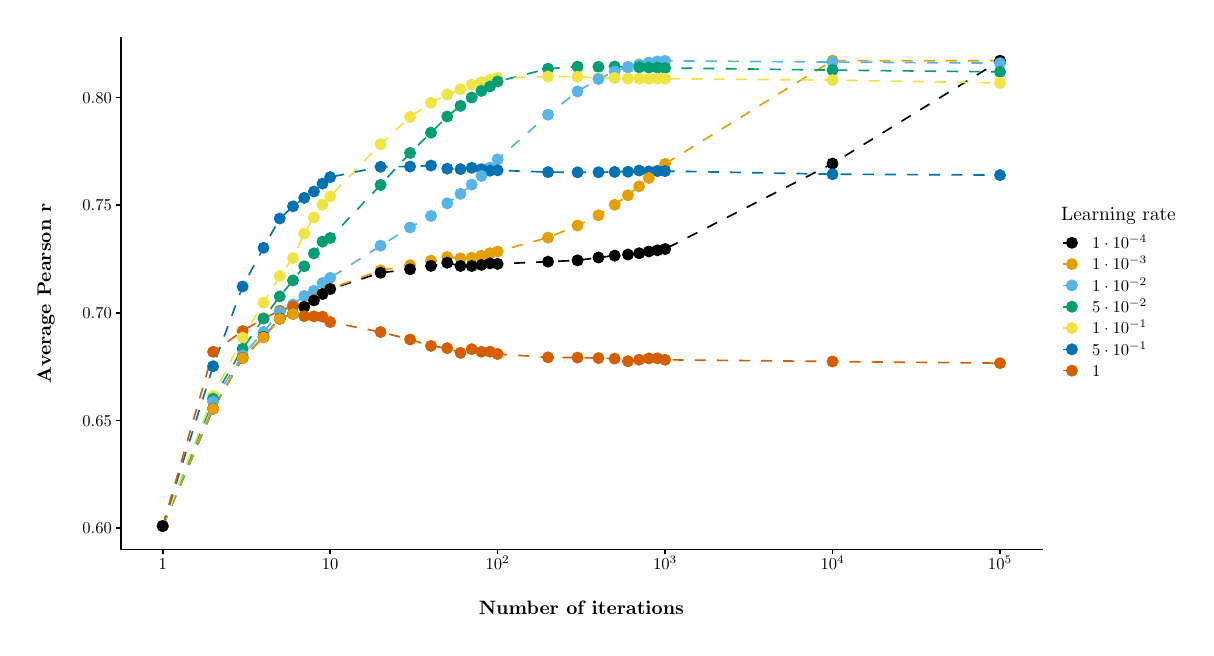
\begin{tikzpicture}[x=1pt,y=1pt]
\definecolor{fillColor}{RGB}{255,255,255}
\path[use as bounding box,fill=fillColor,fill opacity=0.00] (0,0) rectangle (418.34,216.81);
\begin{scope}
\path[clip] ( 33.67, 28.30) rectangle (366.48,213.31);
\definecolor{drawColor}{RGB}{0,0,0}

\path[draw=drawColor,line width= 0.6pt,dash pattern=on 4pt off 4pt ,line join=round] ( 48.80, 36.71) --
	( 67.01, 79.15) --
	( 77.67, 97.40) --
	( 85.23,105.05) --
	( 91.09,111.65) --
	( 95.88,113.43) --
	( 99.94,115.98) --
	(103.44,118.26) --
	(106.54,120.56) --
	(109.31,122.36) --
	(127.52,128.24) --
	(138.18,129.51) --
	(145.74,130.73) --
	(151.60,131.88) --
	(156.40,130.70) --
	(160.45,130.67) --
	(163.96,131.08) --
	(167.05,131.64) --
	(169.82,131.46) --
	(188.03,132.25) --
	(198.69,132.72) --
	(206.25,133.75) --
	(212.11,134.44) --
	(216.91,134.83) --
	(220.96,135.30) --
	(224.47,135.95) --
	(227.56,136.35) --
	(230.33,136.82) --
	(290.84,167.70) --
	(351.35,204.84);
\definecolor{drawColor}{RGB}{230,159,0}

\path[draw=drawColor,line width= 0.6pt,dash pattern=on 4pt off 4pt ,line join=round] ( 48.80, 36.72) --
	( 67.01, 79.13) --
	( 77.67, 97.38) --
	( 85.23,104.88) --
	( 91.09,111.56) --
	( 95.88,113.39) --
	( 99.94,115.98) --
	(103.44,118.52) --
	(106.54,120.58) --
	(109.31,122.55) --
	(127.52,129.11) --
	(138.18,130.99) --
	(145.74,132.62) --
	(151.60,133.94) --
	(156.40,133.44) --
	(160.45,133.67) --
	(163.96,134.43) --
	(167.05,135.31) --
	(169.82,135.94) --
	(188.03,140.95) --
	(198.69,145.32) --
	(206.25,149.01) --
	(212.11,152.81) --
	(216.91,156.26) --
	(220.96,159.49) --
	(224.47,162.49) --
	(227.56,165.11) --
	(230.33,167.58) --
	(290.84,204.90) --
	(351.35,204.84);
\definecolor{drawColor}{RGB}{86,180,233}

\path[draw=drawColor,line width= 0.6pt,dash pattern=on 4pt off 4pt ,line join=round] ( 48.80, 36.72) --
	( 67.01, 81.62) --
	( 77.67, 98.44) --
	( 85.23,106.85) --
	( 91.09,114.03) --
	( 95.88,116.76) --
	( 99.94,119.86) --
	(103.44,121.75) --
	(106.54,124.54) --
	(109.31,126.39) --
	(127.52,138.03) --
	(138.18,144.62) --
	(145.74,148.77) --
	(151.60,153.33) --
	(156.40,156.76) --
	(160.45,160.10) --
	(163.96,163.20) --
	(167.05,166.26) --
	(169.82,169.22) --
	(188.03,185.36) --
	(198.69,193.77) --
	(206.25,198.23) --
	(212.11,200.97) --
	(216.91,202.51) --
	(220.96,203.51) --
	(224.47,204.18) --
	(227.56,204.60) --
	(230.33,204.82) --
	(290.84,204.38) --
	(351.35,203.97);
\definecolor{drawColor}{RGB}{0,158,115}

\path[draw=drawColor,line width= 0.6pt,dash pattern=on 4pt off 4pt ,line join=round] ( 48.80, 36.72) --
	( 67.01, 82.74) --
	( 77.67,100.77) --
	( 85.23,111.73) --
	( 91.09,119.70) --
	( 95.88,125.48) --
	( 99.94,130.60) --
	(103.44,135.23) --
	(106.54,139.49) --
	(109.31,140.81) --
	(127.52,159.98) --
	(138.18,171.54) --
	(145.74,178.87) --
	(151.60,184.71) --
	(156.40,188.56) --
	(160.45,191.56) --
	(163.96,193.96) --
	(167.05,195.55) --
	(169.82,197.36) --
	(188.03,201.98) --
	(198.69,202.73) --
	(206.25,202.64) --
	(212.11,202.77) --
	(216.91,202.54) --
	(220.96,202.51) --
	(224.47,202.38) --
	(227.56,202.37) --
	(230.33,202.25) --
	(290.84,201.48) --
	(351.35,200.83);
\definecolor{drawColor}{RGB}{240,228,66}

\path[draw=drawColor,line width= 0.6pt,dash pattern=on 4pt off 4pt ,line join=round] ( 48.80, 36.72) --
	( 67.01, 83.76) --
	( 77.67,104.78) --
	( 85.23,117.41) --
	( 91.09,127.10) --
	( 95.88,133.55) --
	( 99.94,142.42) --
	(103.44,148.25) --
	(106.54,152.88) --
	(109.31,155.87) --
	(127.52,174.70) --
	(138.18,184.56) --
	(145.74,189.66) --
	(151.60,192.69) --
	(156.40,194.55) --
	(160.45,196.25) --
	(163.96,197.13) --
	(167.05,197.93) --
	(169.82,198.61) --
	(188.03,199.16) --
	(198.69,199.09) --
	(206.25,198.61) --
	(212.11,198.65) --
	(216.91,198.41) --
	(220.96,198.38) --
	(224.47,198.31) --
	(227.56,198.39) --
	(230.33,198.34) --
	(290.84,197.86) --
	(351.35,196.84);
\definecolor{drawColor}{RGB}{0,114,178}

\path[draw=drawColor,line width= 0.6pt,dash pattern=on 4pt off 4pt ,line join=round] ( 48.80, 36.72) --
	( 67.01, 94.47) --
	( 77.67,123.27) --
	( 85.23,137.27) --
	( 91.09,147.85) --
	( 95.88,152.25) --
	( 99.94,155.32) --
	(103.44,157.61) --
	(106.54,160.46) --
	(109.31,162.80) --
	(127.52,166.53) --
	(138.18,166.64) --
	(145.74,166.98) --
	(151.60,165.86) --
	(156.40,165.69) --
	(160.45,166.18) --
	(163.96,165.67) --
	(167.05,165.10) --
	(169.82,165.26) --
	(188.03,164.62) --
	(198.69,164.55) --
	(206.25,164.57) --
	(212.11,164.68) --
	(216.91,164.75) --
	(220.96,165.18) --
	(224.47,164.88) --
	(227.56,164.99) --
	(230.33,164.99) --
	(290.84,163.86) --
	(351.35,163.53);
\definecolor{drawColor}{RGB}{213,94,0}

\path[draw=drawColor,line width= 0.6pt,dash pattern=on 4pt off 4pt ,line join=round] ( 48.80, 36.72) --
	( 67.01, 99.69) --
	( 77.67,107.17) --
	( 85.23,111.73) --
	( 91.09,114.49) --
	( 95.88,116.01) --
	( 99.94,112.58) --
	(103.44,112.49) --
	(106.54,112.37) --
	(109.31,110.44) --
	(127.52,106.83) --
	(138.18,104.15) --
	(145.74,101.83) --
	(151.60,101.01) --
	(156.40, 99.31) --
	(160.45,100.63) --
	(163.96, 99.71) --
	(167.05, 99.73) --
	(169.82, 98.89) --
	(188.03, 97.69) --
	(198.69, 97.60) --
	(206.25, 97.41) --
	(212.11, 97.22) --
	(216.91, 96.27) --
	(220.96, 96.82) --
	(224.47, 97.29) --
	(227.56, 97.32) --
	(230.33, 96.80) --
	(290.84, 96.18) --
	(351.35, 95.57);
\definecolor{drawColor}{RGB}{230,159,0}
\definecolor{fillColor}{RGB}{230,159,0}

\path[draw=drawColor,line width= 0.4pt,line join=round,line cap=round,fill=fillColor] (290.84,204.90) circle (  1.96);
\definecolor{drawColor}{RGB}{86,180,233}
\definecolor{fillColor}{RGB}{86,180,233}

\path[draw=drawColor,line width= 0.4pt,line join=round,line cap=round,fill=fillColor] (290.84,204.38) circle (  1.96);
\definecolor{drawColor}{RGB}{0,158,115}
\definecolor{fillColor}{RGB}{0,158,115}

\path[draw=drawColor,line width= 0.4pt,line join=round,line cap=round,fill=fillColor] (290.84,201.48) circle (  1.96);
\definecolor{drawColor}{RGB}{240,228,66}
\definecolor{fillColor}{RGB}{240,228,66}

\path[draw=drawColor,line width= 0.4pt,line join=round,line cap=round,fill=fillColor] (290.84,197.86) circle (  1.96);
\definecolor{drawColor}{RGB}{0,0,0}
\definecolor{fillColor}{RGB}{0,0,0}

\path[draw=drawColor,line width= 0.4pt,line join=round,line cap=round,fill=fillColor] (290.84,167.70) circle (  1.96);
\definecolor{drawColor}{RGB}{0,114,178}
\definecolor{fillColor}{RGB}{0,114,178}

\path[draw=drawColor,line width= 0.4pt,line join=round,line cap=round,fill=fillColor] (290.84,163.86) circle (  1.96);
\definecolor{drawColor}{RGB}{213,94,0}
\definecolor{fillColor}{RGB}{213,94,0}

\path[draw=drawColor,line width= 0.4pt,line join=round,line cap=round,fill=fillColor] (290.84, 96.18) circle (  1.96);
\definecolor{drawColor}{RGB}{86,180,233}
\definecolor{fillColor}{RGB}{86,180,233}

\path[draw=drawColor,line width= 0.4pt,line join=round,line cap=round,fill=fillColor] (230.33,204.82) circle (  1.96);

\path[draw=drawColor,line width= 0.4pt,line join=round,line cap=round,fill=fillColor] (227.56,204.60) circle (  1.96);

\path[draw=drawColor,line width= 0.4pt,line join=round,line cap=round,fill=fillColor] (224.47,204.18) circle (  1.96);

\path[draw=drawColor,line width= 0.4pt,line join=round,line cap=round,fill=fillColor] (220.96,203.51) circle (  1.96);
\definecolor{drawColor}{RGB}{0,158,115}
\definecolor{fillColor}{RGB}{0,158,115}

\path[draw=drawColor,line width= 0.4pt,line join=round,line cap=round,fill=fillColor] (212.11,202.77) circle (  1.96);

\path[draw=drawColor,line width= 0.4pt,line join=round,line cap=round,fill=fillColor] (198.69,202.73) circle (  1.96);

\path[draw=drawColor,line width= 0.4pt,line join=round,line cap=round,fill=fillColor] (206.25,202.64) circle (  1.96);

\path[draw=drawColor,line width= 0.4pt,line join=round,line cap=round,fill=fillColor] (216.91,202.54) circle (  1.96);

\path[draw=drawColor,line width= 0.4pt,line join=round,line cap=round,fill=fillColor] (220.96,202.51) circle (  1.96);
\definecolor{drawColor}{RGB}{86,180,233}
\definecolor{fillColor}{RGB}{86,180,233}

\path[draw=drawColor,line width= 0.4pt,line join=round,line cap=round,fill=fillColor] (216.91,202.51) circle (  1.96);
\definecolor{drawColor}{RGB}{0,158,115}
\definecolor{fillColor}{RGB}{0,158,115}

\path[draw=drawColor,line width= 0.4pt,line join=round,line cap=round,fill=fillColor] (224.47,202.38) circle (  1.96);

\path[draw=drawColor,line width= 0.4pt,line join=round,line cap=round,fill=fillColor] (227.56,202.37) circle (  1.96);

\path[draw=drawColor,line width= 0.4pt,line join=round,line cap=round,fill=fillColor] (230.33,202.25) circle (  1.96);

\path[draw=drawColor,line width= 0.4pt,line join=round,line cap=round,fill=fillColor] (188.03,201.98) circle (  1.96);
\definecolor{drawColor}{RGB}{86,180,233}
\definecolor{fillColor}{RGB}{86,180,233}

\path[draw=drawColor,line width= 0.4pt,line join=round,line cap=round,fill=fillColor] (212.11,200.97) circle (  1.96);
\definecolor{drawColor}{RGB}{240,228,66}
\definecolor{fillColor}{RGB}{240,228,66}

\path[draw=drawColor,line width= 0.4pt,line join=round,line cap=round,fill=fillColor] (188.03,199.16) circle (  1.96);

\path[draw=drawColor,line width= 0.4pt,line join=round,line cap=round,fill=fillColor] (198.69,199.09) circle (  1.96);

\path[draw=drawColor,line width= 0.4pt,line join=round,line cap=round,fill=fillColor] (212.11,198.65) circle (  1.96);

\path[draw=drawColor,line width= 0.4pt,line join=round,line cap=round,fill=fillColor] (169.82,198.61) circle (  1.96);

\path[draw=drawColor,line width= 0.4pt,line join=round,line cap=round,fill=fillColor] (206.25,198.61) circle (  1.96);

\path[draw=drawColor,line width= 0.4pt,line join=round,line cap=round,fill=fillColor] (216.91,198.41) circle (  1.96);

\path[draw=drawColor,line width= 0.4pt,line join=round,line cap=round,fill=fillColor] (227.56,198.39) circle (  1.96);

\path[draw=drawColor,line width= 0.4pt,line join=round,line cap=round,fill=fillColor] (220.96,198.38) circle (  1.96);

\path[draw=drawColor,line width= 0.4pt,line join=round,line cap=round,fill=fillColor] (230.33,198.34) circle (  1.96);

\path[draw=drawColor,line width= 0.4pt,line join=round,line cap=round,fill=fillColor] (224.47,198.31) circle (  1.96);
\definecolor{drawColor}{RGB}{86,180,233}
\definecolor{fillColor}{RGB}{86,180,233}

\path[draw=drawColor,line width= 0.4pt,line join=round,line cap=round,fill=fillColor] (206.25,198.23) circle (  1.96);
\definecolor{drawColor}{RGB}{240,228,66}
\definecolor{fillColor}{RGB}{240,228,66}

\path[draw=drawColor,line width= 0.4pt,line join=round,line cap=round,fill=fillColor] (167.05,197.93) circle (  1.96);
\definecolor{drawColor}{RGB}{0,158,115}
\definecolor{fillColor}{RGB}{0,158,115}

\path[draw=drawColor,line width= 0.4pt,line join=round,line cap=round,fill=fillColor] (169.82,197.36) circle (  1.96);
\definecolor{drawColor}{RGB}{240,228,66}
\definecolor{fillColor}{RGB}{240,228,66}

\path[draw=drawColor,line width= 0.4pt,line join=round,line cap=round,fill=fillColor] (163.96,197.13) circle (  1.96);

\path[draw=drawColor,line width= 0.4pt,line join=round,line cap=round,fill=fillColor] (160.45,196.25) circle (  1.96);
\definecolor{drawColor}{RGB}{0,158,115}
\definecolor{fillColor}{RGB}{0,158,115}

\path[draw=drawColor,line width= 0.4pt,line join=round,line cap=round,fill=fillColor] (167.05,195.55) circle (  1.96);
\definecolor{drawColor}{RGB}{240,228,66}
\definecolor{fillColor}{RGB}{240,228,66}

\path[draw=drawColor,line width= 0.4pt,line join=round,line cap=round,fill=fillColor] (156.40,194.55) circle (  1.96);
\definecolor{drawColor}{RGB}{0,158,115}
\definecolor{fillColor}{RGB}{0,158,115}

\path[draw=drawColor,line width= 0.4pt,line join=round,line cap=round,fill=fillColor] (163.96,193.96) circle (  1.96);
\definecolor{drawColor}{RGB}{86,180,233}
\definecolor{fillColor}{RGB}{86,180,233}

\path[draw=drawColor,line width= 0.4pt,line join=round,line cap=round,fill=fillColor] (198.69,193.77) circle (  1.96);
\definecolor{drawColor}{RGB}{240,228,66}
\definecolor{fillColor}{RGB}{240,228,66}

\path[draw=drawColor,line width= 0.4pt,line join=round,line cap=round,fill=fillColor] (151.60,192.69) circle (  1.96);
\definecolor{drawColor}{RGB}{0,158,115}
\definecolor{fillColor}{RGB}{0,158,115}

\path[draw=drawColor,line width= 0.4pt,line join=round,line cap=round,fill=fillColor] (160.45,191.56) circle (  1.96);
\definecolor{drawColor}{RGB}{240,228,66}
\definecolor{fillColor}{RGB}{240,228,66}

\path[draw=drawColor,line width= 0.4pt,line join=round,line cap=round,fill=fillColor] (145.74,189.66) circle (  1.96);
\definecolor{drawColor}{RGB}{0,158,115}
\definecolor{fillColor}{RGB}{0,158,115}

\path[draw=drawColor,line width= 0.4pt,line join=round,line cap=round,fill=fillColor] (156.40,188.56) circle (  1.96);
\definecolor{drawColor}{RGB}{86,180,233}
\definecolor{fillColor}{RGB}{86,180,233}

\path[draw=drawColor,line width= 0.4pt,line join=round,line cap=round,fill=fillColor] (188.03,185.36) circle (  1.96);
\definecolor{drawColor}{RGB}{0,158,115}
\definecolor{fillColor}{RGB}{0,158,115}

\path[draw=drawColor,line width= 0.4pt,line join=round,line cap=round,fill=fillColor] (151.60,184.71) circle (  1.96);
\definecolor{drawColor}{RGB}{240,228,66}
\definecolor{fillColor}{RGB}{240,228,66}

\path[draw=drawColor,line width= 0.4pt,line join=round,line cap=round,fill=fillColor] (138.18,184.56) circle (  1.96);
\definecolor{drawColor}{RGB}{0,158,115}
\definecolor{fillColor}{RGB}{0,158,115}

\path[draw=drawColor,line width= 0.4pt,line join=round,line cap=round,fill=fillColor] (145.74,178.87) circle (  1.96);
\definecolor{drawColor}{RGB}{240,228,66}
\definecolor{fillColor}{RGB}{240,228,66}

\path[draw=drawColor,line width= 0.4pt,line join=round,line cap=round,fill=fillColor] (127.52,174.70) circle (  1.96);
\definecolor{drawColor}{RGB}{0,158,115}
\definecolor{fillColor}{RGB}{0,158,115}

\path[draw=drawColor,line width= 0.4pt,line join=round,line cap=round,fill=fillColor] (138.18,171.54) circle (  1.96);
\definecolor{drawColor}{RGB}{86,180,233}
\definecolor{fillColor}{RGB}{86,180,233}

\path[draw=drawColor,line width= 0.4pt,line join=round,line cap=round,fill=fillColor] (169.82,169.22) circle (  1.96);
\definecolor{drawColor}{RGB}{230,159,0}
\definecolor{fillColor}{RGB}{230,159,0}

\path[draw=drawColor,line width= 0.4pt,line join=round,line cap=round,fill=fillColor] (230.33,167.58) circle (  1.96);
\definecolor{drawColor}{RGB}{0,114,178}
\definecolor{fillColor}{RGB}{0,114,178}

\path[draw=drawColor,line width= 0.4pt,line join=round,line cap=round,fill=fillColor] (145.74,166.98) circle (  1.96);

\path[draw=drawColor,line width= 0.4pt,line join=round,line cap=round,fill=fillColor] (138.18,166.64) circle (  1.96);

\path[draw=drawColor,line width= 0.4pt,line join=round,line cap=round,fill=fillColor] (127.52,166.53) circle (  1.96);
\definecolor{drawColor}{RGB}{86,180,233}
\definecolor{fillColor}{RGB}{86,180,233}

\path[draw=drawColor,line width= 0.4pt,line join=round,line cap=round,fill=fillColor] (167.05,166.26) circle (  1.96);
\definecolor{drawColor}{RGB}{0,114,178}
\definecolor{fillColor}{RGB}{0,114,178}

\path[draw=drawColor,line width= 0.4pt,line join=round,line cap=round,fill=fillColor] (160.45,166.18) circle (  1.96);

\path[draw=drawColor,line width= 0.4pt,line join=round,line cap=round,fill=fillColor] (151.60,165.86) circle (  1.96);

\path[draw=drawColor,line width= 0.4pt,line join=round,line cap=round,fill=fillColor] (156.40,165.69) circle (  1.96);

\path[draw=drawColor,line width= 0.4pt,line join=round,line cap=round,fill=fillColor] (163.96,165.67) circle (  1.96);

\path[draw=drawColor,line width= 0.4pt,line join=round,line cap=round,fill=fillColor] (169.82,165.26) circle (  1.96);

\path[draw=drawColor,line width= 0.4pt,line join=round,line cap=round,fill=fillColor] (220.96,165.18) circle (  1.96);
\definecolor{drawColor}{RGB}{230,159,0}
\definecolor{fillColor}{RGB}{230,159,0}

\path[draw=drawColor,line width= 0.4pt,line join=round,line cap=round,fill=fillColor] (227.56,165.11) circle (  1.96);
\definecolor{drawColor}{RGB}{0,114,178}
\definecolor{fillColor}{RGB}{0,114,178}

\path[draw=drawColor,line width= 0.4pt,line join=round,line cap=round,fill=fillColor] (167.05,165.10) circle (  1.96);

\path[draw=drawColor,line width= 0.4pt,line join=round,line cap=round,fill=fillColor] (230.33,164.99) circle (  1.96);

\path[draw=drawColor,line width= 0.4pt,line join=round,line cap=round,fill=fillColor] (227.56,164.99) circle (  1.96);

\path[draw=drawColor,line width= 0.4pt,line join=round,line cap=round,fill=fillColor] (224.47,164.88) circle (  1.96);

\path[draw=drawColor,line width= 0.4pt,line join=round,line cap=round,fill=fillColor] (216.91,164.75) circle (  1.96);

\path[draw=drawColor,line width= 0.4pt,line join=round,line cap=round,fill=fillColor] (212.11,164.68) circle (  1.96);

\path[draw=drawColor,line width= 0.4pt,line join=round,line cap=round,fill=fillColor] (188.03,164.62) circle (  1.96);

\path[draw=drawColor,line width= 0.4pt,line join=round,line cap=round,fill=fillColor] (206.25,164.57) circle (  1.96);

\path[draw=drawColor,line width= 0.4pt,line join=round,line cap=round,fill=fillColor] (198.69,164.55) circle (  1.96);
\definecolor{drawColor}{RGB}{86,180,233}
\definecolor{fillColor}{RGB}{86,180,233}

\path[draw=drawColor,line width= 0.4pt,line join=round,line cap=round,fill=fillColor] (163.96,163.20) circle (  1.96);
\definecolor{drawColor}{RGB}{0,114,178}
\definecolor{fillColor}{RGB}{0,114,178}

\path[draw=drawColor,line width= 0.4pt,line join=round,line cap=round,fill=fillColor] (109.31,162.80) circle (  1.96);
\definecolor{drawColor}{RGB}{230,159,0}
\definecolor{fillColor}{RGB}{230,159,0}

\path[draw=drawColor,line width= 0.4pt,line join=round,line cap=round,fill=fillColor] (224.47,162.49) circle (  1.96);
\definecolor{drawColor}{RGB}{0,114,178}
\definecolor{fillColor}{RGB}{0,114,178}

\path[draw=drawColor,line width= 0.4pt,line join=round,line cap=round,fill=fillColor] (106.54,160.46) circle (  1.96);
\definecolor{drawColor}{RGB}{86,180,233}
\definecolor{fillColor}{RGB}{86,180,233}

\path[draw=drawColor,line width= 0.4pt,line join=round,line cap=round,fill=fillColor] (160.45,160.10) circle (  1.96);
\definecolor{drawColor}{RGB}{0,158,115}
\definecolor{fillColor}{RGB}{0,158,115}

\path[draw=drawColor,line width= 0.4pt,line join=round,line cap=round,fill=fillColor] (127.52,159.98) circle (  1.96);
\definecolor{drawColor}{RGB}{230,159,0}
\definecolor{fillColor}{RGB}{230,159,0}

\path[draw=drawColor,line width= 0.4pt,line join=round,line cap=round,fill=fillColor] (220.96,159.49) circle (  1.96);
\definecolor{drawColor}{RGB}{0,114,178}
\definecolor{fillColor}{RGB}{0,114,178}

\path[draw=drawColor,line width= 0.4pt,line join=round,line cap=round,fill=fillColor] (103.44,157.61) circle (  1.96);
\definecolor{drawColor}{RGB}{86,180,233}
\definecolor{fillColor}{RGB}{86,180,233}

\path[draw=drawColor,line width= 0.4pt,line join=round,line cap=round,fill=fillColor] (156.40,156.76) circle (  1.96);
\definecolor{drawColor}{RGB}{230,159,0}
\definecolor{fillColor}{RGB}{230,159,0}

\path[draw=drawColor,line width= 0.4pt,line join=round,line cap=round,fill=fillColor] (216.91,156.26) circle (  1.96);
\definecolor{drawColor}{RGB}{240,228,66}
\definecolor{fillColor}{RGB}{240,228,66}

\path[draw=drawColor,line width= 0.4pt,line join=round,line cap=round,fill=fillColor] (109.31,155.87) circle (  1.96);
\definecolor{drawColor}{RGB}{0,114,178}
\definecolor{fillColor}{RGB}{0,114,178}

\path[draw=drawColor,line width= 0.4pt,line join=round,line cap=round,fill=fillColor] ( 99.94,155.32) circle (  1.96);
\definecolor{drawColor}{RGB}{86,180,233}
\definecolor{fillColor}{RGB}{86,180,233}

\path[draw=drawColor,line width= 0.4pt,line join=round,line cap=round,fill=fillColor] (151.60,153.33) circle (  1.96);
\definecolor{drawColor}{RGB}{240,228,66}
\definecolor{fillColor}{RGB}{240,228,66}

\path[draw=drawColor,line width= 0.4pt,line join=round,line cap=round,fill=fillColor] (106.54,152.88) circle (  1.96);
\definecolor{drawColor}{RGB}{230,159,0}
\definecolor{fillColor}{RGB}{230,159,0}

\path[draw=drawColor,line width= 0.4pt,line join=round,line cap=round,fill=fillColor] (212.11,152.81) circle (  1.96);
\definecolor{drawColor}{RGB}{0,114,178}
\definecolor{fillColor}{RGB}{0,114,178}

\path[draw=drawColor,line width= 0.4pt,line join=round,line cap=round,fill=fillColor] ( 95.88,152.25) circle (  1.96);
\definecolor{drawColor}{RGB}{230,159,0}
\definecolor{fillColor}{RGB}{230,159,0}

\path[draw=drawColor,line width= 0.4pt,line join=round,line cap=round,fill=fillColor] (206.25,149.01) circle (  1.96);
\definecolor{drawColor}{RGB}{86,180,233}
\definecolor{fillColor}{RGB}{86,180,233}

\path[draw=drawColor,line width= 0.4pt,line join=round,line cap=round,fill=fillColor] (145.74,148.77) circle (  1.96);
\definecolor{drawColor}{RGB}{240,228,66}
\definecolor{fillColor}{RGB}{240,228,66}

\path[draw=drawColor,line width= 0.4pt,line join=round,line cap=round,fill=fillColor] (103.44,148.25) circle (  1.96);
\definecolor{drawColor}{RGB}{0,114,178}
\definecolor{fillColor}{RGB}{0,114,178}

\path[draw=drawColor,line width= 0.4pt,line join=round,line cap=round,fill=fillColor] ( 91.09,147.85) circle (  1.96);
\definecolor{drawColor}{RGB}{230,159,0}
\definecolor{fillColor}{RGB}{230,159,0}

\path[draw=drawColor,line width= 0.4pt,line join=round,line cap=round,fill=fillColor] (198.69,145.32) circle (  1.96);
\definecolor{drawColor}{RGB}{86,180,233}
\definecolor{fillColor}{RGB}{86,180,233}

\path[draw=drawColor,line width= 0.4pt,line join=round,line cap=round,fill=fillColor] (138.18,144.62) circle (  1.96);
\definecolor{drawColor}{RGB}{240,228,66}
\definecolor{fillColor}{RGB}{240,228,66}

\path[draw=drawColor,line width= 0.4pt,line join=round,line cap=round,fill=fillColor] ( 99.94,142.42) circle (  1.96);
\definecolor{drawColor}{RGB}{230,159,0}
\definecolor{fillColor}{RGB}{230,159,0}

\path[draw=drawColor,line width= 0.4pt,line join=round,line cap=round,fill=fillColor] (188.03,140.95) circle (  1.96);
\definecolor{drawColor}{RGB}{0,158,115}
\definecolor{fillColor}{RGB}{0,158,115}

\path[draw=drawColor,line width= 0.4pt,line join=round,line cap=round,fill=fillColor] (109.31,140.81) circle (  1.96);

\path[draw=drawColor,line width= 0.4pt,line join=round,line cap=round,fill=fillColor] (106.54,139.49) circle (  1.96);
\definecolor{drawColor}{RGB}{86,180,233}
\definecolor{fillColor}{RGB}{86,180,233}

\path[draw=drawColor,line width= 0.4pt,line join=round,line cap=round,fill=fillColor] (127.52,138.03) circle (  1.96);
\definecolor{drawColor}{RGB}{0,114,178}
\definecolor{fillColor}{RGB}{0,114,178}

\path[draw=drawColor,line width= 0.4pt,line join=round,line cap=round,fill=fillColor] ( 85.23,137.27) circle (  1.96);
\definecolor{drawColor}{RGB}{0,0,0}
\definecolor{fillColor}{RGB}{0,0,0}

\path[draw=drawColor,line width= 0.4pt,line join=round,line cap=round,fill=fillColor] (230.33,136.82) circle (  1.96);

\path[draw=drawColor,line width= 0.4pt,line join=round,line cap=round,fill=fillColor] (227.56,136.35) circle (  1.96);

\path[draw=drawColor,line width= 0.4pt,line join=round,line cap=round,fill=fillColor] (224.47,135.95) circle (  1.96);
\definecolor{drawColor}{RGB}{230,159,0}
\definecolor{fillColor}{RGB}{230,159,0}

\path[draw=drawColor,line width= 0.4pt,line join=round,line cap=round,fill=fillColor] (169.82,135.94) circle (  1.96);

\path[draw=drawColor,line width= 0.4pt,line join=round,line cap=round,fill=fillColor] (167.05,135.31) circle (  1.96);
\definecolor{drawColor}{RGB}{0,0,0}
\definecolor{fillColor}{RGB}{0,0,0}

\path[draw=drawColor,line width= 0.4pt,line join=round,line cap=round,fill=fillColor] (220.96,135.30) circle (  1.96);
\definecolor{drawColor}{RGB}{0,158,115}
\definecolor{fillColor}{RGB}{0,158,115}

\path[draw=drawColor,line width= 0.4pt,line join=round,line cap=round,fill=fillColor] (103.44,135.23) circle (  1.96);
\definecolor{drawColor}{RGB}{0,0,0}
\definecolor{fillColor}{RGB}{0,0,0}

\path[draw=drawColor,line width= 0.4pt,line join=round,line cap=round,fill=fillColor] (216.91,134.83) circle (  1.96);

\path[draw=drawColor,line width= 0.4pt,line join=round,line cap=round,fill=fillColor] (212.11,134.44) circle (  1.96);
\definecolor{drawColor}{RGB}{230,159,0}
\definecolor{fillColor}{RGB}{230,159,0}

\path[draw=drawColor,line width= 0.4pt,line join=round,line cap=round,fill=fillColor] (163.96,134.43) circle (  1.96);

\path[draw=drawColor,line width= 0.4pt,line join=round,line cap=round,fill=fillColor] (151.60,133.94) circle (  1.96);
\definecolor{drawColor}{RGB}{0,0,0}
\definecolor{fillColor}{RGB}{0,0,0}

\path[draw=drawColor,line width= 0.4pt,line join=round,line cap=round,fill=fillColor] (206.25,133.75) circle (  1.96);
\definecolor{drawColor}{RGB}{230,159,0}
\definecolor{fillColor}{RGB}{230,159,0}

\path[draw=drawColor,line width= 0.4pt,line join=round,line cap=round,fill=fillColor] (160.45,133.67) circle (  1.96);
\definecolor{drawColor}{RGB}{240,228,66}
\definecolor{fillColor}{RGB}{240,228,66}

\path[draw=drawColor,line width= 0.4pt,line join=round,line cap=round,fill=fillColor] ( 95.88,133.55) circle (  1.96);
\definecolor{drawColor}{RGB}{230,159,0}
\definecolor{fillColor}{RGB}{230,159,0}

\path[draw=drawColor,line width= 0.4pt,line join=round,line cap=round,fill=fillColor] (156.40,133.44) circle (  1.96);
\definecolor{drawColor}{RGB}{0,0,0}
\definecolor{fillColor}{RGB}{0,0,0}

\path[draw=drawColor,line width= 0.4pt,line join=round,line cap=round,fill=fillColor] (198.69,132.72) circle (  1.96);
\definecolor{drawColor}{RGB}{230,159,0}
\definecolor{fillColor}{RGB}{230,159,0}

\path[draw=drawColor,line width= 0.4pt,line join=round,line cap=round,fill=fillColor] (145.74,132.62) circle (  1.96);
\definecolor{drawColor}{RGB}{0,0,0}
\definecolor{fillColor}{RGB}{0,0,0}

\path[draw=drawColor,line width= 0.4pt,line join=round,line cap=round,fill=fillColor] (188.03,132.25) circle (  1.96);

\path[draw=drawColor,line width= 0.4pt,line join=round,line cap=round,fill=fillColor] (151.60,131.88) circle (  1.96);

\path[draw=drawColor,line width= 0.4pt,line join=round,line cap=round,fill=fillColor] (167.05,131.64) circle (  1.96);

\path[draw=drawColor,line width= 0.4pt,line join=round,line cap=round,fill=fillColor] (169.82,131.46) circle (  1.96);

\path[draw=drawColor,line width= 0.4pt,line join=round,line cap=round,fill=fillColor] (163.96,131.08) circle (  1.96);
\definecolor{drawColor}{RGB}{230,159,0}
\definecolor{fillColor}{RGB}{230,159,0}

\path[draw=drawColor,line width= 0.4pt,line join=round,line cap=round,fill=fillColor] (138.18,130.99) circle (  1.96);
\definecolor{drawColor}{RGB}{0,0,0}
\definecolor{fillColor}{RGB}{0,0,0}

\path[draw=drawColor,line width= 0.4pt,line join=round,line cap=round,fill=fillColor] (145.74,130.73) circle (  1.96);

\path[draw=drawColor,line width= 0.4pt,line join=round,line cap=round,fill=fillColor] (156.40,130.70) circle (  1.96);

\path[draw=drawColor,line width= 0.4pt,line join=round,line cap=round,fill=fillColor] (160.45,130.67) circle (  1.96);
\definecolor{drawColor}{RGB}{0,158,115}
\definecolor{fillColor}{RGB}{0,158,115}

\path[draw=drawColor,line width= 0.4pt,line join=round,line cap=round,fill=fillColor] ( 99.94,130.60) circle (  1.96);
\definecolor{drawColor}{RGB}{0,0,0}
\definecolor{fillColor}{RGB}{0,0,0}

\path[draw=drawColor,line width= 0.4pt,line join=round,line cap=round,fill=fillColor] (138.18,129.51) circle (  1.96);
\definecolor{drawColor}{RGB}{230,159,0}
\definecolor{fillColor}{RGB}{230,159,0}

\path[draw=drawColor,line width= 0.4pt,line join=round,line cap=round,fill=fillColor] (127.52,129.11) circle (  1.96);
\definecolor{drawColor}{RGB}{0,0,0}
\definecolor{fillColor}{RGB}{0,0,0}

\path[draw=drawColor,line width= 0.4pt,line join=round,line cap=round,fill=fillColor] (127.52,128.24) circle (  1.96);
\definecolor{drawColor}{RGB}{240,228,66}
\definecolor{fillColor}{RGB}{240,228,66}

\path[draw=drawColor,line width= 0.4pt,line join=round,line cap=round,fill=fillColor] ( 91.09,127.10) circle (  1.96);
\definecolor{drawColor}{RGB}{86,180,233}
\definecolor{fillColor}{RGB}{86,180,233}

\path[draw=drawColor,line width= 0.4pt,line join=round,line cap=round,fill=fillColor] (109.31,126.39) circle (  1.96);
\definecolor{drawColor}{RGB}{0,158,115}
\definecolor{fillColor}{RGB}{0,158,115}

\path[draw=drawColor,line width= 0.4pt,line join=round,line cap=round,fill=fillColor] ( 95.88,125.48) circle (  1.96);
\definecolor{drawColor}{RGB}{86,180,233}
\definecolor{fillColor}{RGB}{86,180,233}

\path[draw=drawColor,line width= 0.4pt,line join=round,line cap=round,fill=fillColor] (106.54,124.54) circle (  1.96);
\definecolor{drawColor}{RGB}{0,114,178}
\definecolor{fillColor}{RGB}{0,114,178}

\path[draw=drawColor,line width= 0.4pt,line join=round,line cap=round,fill=fillColor] ( 77.67,123.27) circle (  1.96);
\definecolor{drawColor}{RGB}{230,159,0}
\definecolor{fillColor}{RGB}{230,159,0}

\path[draw=drawColor,line width= 0.4pt,line join=round,line cap=round,fill=fillColor] (109.31,122.55) circle (  1.96);
\definecolor{drawColor}{RGB}{0,0,0}
\definecolor{fillColor}{RGB}{0,0,0}

\path[draw=drawColor,line width= 0.4pt,line join=round,line cap=round,fill=fillColor] (109.31,122.36) circle (  1.96);
\definecolor{drawColor}{RGB}{86,180,233}
\definecolor{fillColor}{RGB}{86,180,233}

\path[draw=drawColor,line width= 0.4pt,line join=round,line cap=round,fill=fillColor] (103.44,121.75) circle (  1.96);
\definecolor{drawColor}{RGB}{230,159,0}
\definecolor{fillColor}{RGB}{230,159,0}

\path[draw=drawColor,line width= 0.4pt,line join=round,line cap=round,fill=fillColor] (106.54,120.58) circle (  1.96);
\definecolor{drawColor}{RGB}{0,0,0}
\definecolor{fillColor}{RGB}{0,0,0}

\path[draw=drawColor,line width= 0.4pt,line join=round,line cap=round,fill=fillColor] (106.54,120.56) circle (  1.96);
\definecolor{drawColor}{RGB}{86,180,233}
\definecolor{fillColor}{RGB}{86,180,233}

\path[draw=drawColor,line width= 0.4pt,line join=round,line cap=round,fill=fillColor] ( 99.94,119.86) circle (  1.96);
\definecolor{drawColor}{RGB}{0,158,115}
\definecolor{fillColor}{RGB}{0,158,115}

\path[draw=drawColor,line width= 0.4pt,line join=round,line cap=round,fill=fillColor] ( 91.09,119.70) circle (  1.96);
\definecolor{drawColor}{RGB}{230,159,0}
\definecolor{fillColor}{RGB}{230,159,0}

\path[draw=drawColor,line width= 0.4pt,line join=round,line cap=round,fill=fillColor] (103.44,118.52) circle (  1.96);
\definecolor{drawColor}{RGB}{0,0,0}
\definecolor{fillColor}{RGB}{0,0,0}

\path[draw=drawColor,line width= 0.4pt,line join=round,line cap=round,fill=fillColor] (103.44,118.26) circle (  1.96);
\definecolor{drawColor}{RGB}{240,228,66}
\definecolor{fillColor}{RGB}{240,228,66}

\path[draw=drawColor,line width= 0.4pt,line join=round,line cap=round,fill=fillColor] ( 85.23,117.41) circle (  1.96);
\definecolor{drawColor}{RGB}{86,180,233}
\definecolor{fillColor}{RGB}{86,180,233}

\path[draw=drawColor,line width= 0.4pt,line join=round,line cap=round,fill=fillColor] ( 95.88,116.76) circle (  1.96);
\definecolor{drawColor}{RGB}{213,94,0}
\definecolor{fillColor}{RGB}{213,94,0}

\path[draw=drawColor,line width= 0.4pt,line join=round,line cap=round,fill=fillColor] ( 95.88,116.01) circle (  1.96);
\definecolor{drawColor}{RGB}{230,159,0}
\definecolor{fillColor}{RGB}{230,159,0}

\path[draw=drawColor,line width= 0.4pt,line join=round,line cap=round,fill=fillColor] ( 99.94,115.98) circle (  1.96);
\definecolor{drawColor}{RGB}{0,0,0}
\definecolor{fillColor}{RGB}{0,0,0}

\path[draw=drawColor,line width= 0.4pt,line join=round,line cap=round,fill=fillColor] ( 99.94,115.98) circle (  1.96);
\definecolor{drawColor}{RGB}{213,94,0}
\definecolor{fillColor}{RGB}{213,94,0}

\path[draw=drawColor,line width= 0.4pt,line join=round,line cap=round,fill=fillColor] ( 91.09,114.49) circle (  1.96);
\definecolor{drawColor}{RGB}{86,180,233}
\definecolor{fillColor}{RGB}{86,180,233}

\path[draw=drawColor,line width= 0.4pt,line join=round,line cap=round,fill=fillColor] ( 91.09,114.03) circle (  1.96);
\definecolor{drawColor}{RGB}{0,0,0}
\definecolor{fillColor}{RGB}{0,0,0}

\path[draw=drawColor,line width= 0.4pt,line join=round,line cap=round,fill=fillColor] ( 95.88,113.43) circle (  1.96);
\definecolor{drawColor}{RGB}{230,159,0}
\definecolor{fillColor}{RGB}{230,159,0}

\path[draw=drawColor,line width= 0.4pt,line join=round,line cap=round,fill=fillColor] ( 95.88,113.39) circle (  1.96);
\definecolor{drawColor}{RGB}{213,94,0}
\definecolor{fillColor}{RGB}{213,94,0}

\path[draw=drawColor,line width= 0.4pt,line join=round,line cap=round,fill=fillColor] ( 99.94,112.58) circle (  1.96);

\path[draw=drawColor,line width= 0.4pt,line join=round,line cap=round,fill=fillColor] (103.44,112.49) circle (  1.96);

\path[draw=drawColor,line width= 0.4pt,line join=round,line cap=round,fill=fillColor] (106.54,112.37) circle (  1.96);

\path[draw=drawColor,line width= 0.4pt,line join=round,line cap=round,fill=fillColor] ( 85.23,111.73) circle (  1.96);
\definecolor{drawColor}{RGB}{0,158,115}
\definecolor{fillColor}{RGB}{0,158,115}

\path[draw=drawColor,line width= 0.4pt,line join=round,line cap=round,fill=fillColor] ( 85.23,111.73) circle (  1.96);
\definecolor{drawColor}{RGB}{0,0,0}
\definecolor{fillColor}{RGB}{0,0,0}

\path[draw=drawColor,line width= 0.4pt,line join=round,line cap=round,fill=fillColor] ( 91.09,111.65) circle (  1.96);
\definecolor{drawColor}{RGB}{230,159,0}
\definecolor{fillColor}{RGB}{230,159,0}

\path[draw=drawColor,line width= 0.4pt,line join=round,line cap=round,fill=fillColor] ( 91.09,111.56) circle (  1.96);
\definecolor{drawColor}{RGB}{213,94,0}
\definecolor{fillColor}{RGB}{213,94,0}

\path[draw=drawColor,line width= 0.4pt,line join=round,line cap=round,fill=fillColor] (109.31,110.44) circle (  1.96);

\path[draw=drawColor,line width= 0.4pt,line join=round,line cap=round,fill=fillColor] ( 77.67,107.17) circle (  1.96);
\definecolor{drawColor}{RGB}{86,180,233}
\definecolor{fillColor}{RGB}{86,180,233}

\path[draw=drawColor,line width= 0.4pt,line join=round,line cap=round,fill=fillColor] ( 85.23,106.85) circle (  1.96);
\definecolor{drawColor}{RGB}{213,94,0}
\definecolor{fillColor}{RGB}{213,94,0}

\path[draw=drawColor,line width= 0.4pt,line join=round,line cap=round,fill=fillColor] (127.52,106.83) circle (  1.96);
\definecolor{drawColor}{RGB}{0,0,0}
\definecolor{fillColor}{RGB}{0,0,0}

\path[draw=drawColor,line width= 0.4pt,line join=round,line cap=round,fill=fillColor] ( 85.23,105.05) circle (  1.96);
\definecolor{drawColor}{RGB}{230,159,0}
\definecolor{fillColor}{RGB}{230,159,0}

\path[draw=drawColor,line width= 0.4pt,line join=round,line cap=round,fill=fillColor] ( 85.23,104.88) circle (  1.96);
\definecolor{drawColor}{RGB}{240,228,66}
\definecolor{fillColor}{RGB}{240,228,66}

\path[draw=drawColor,line width= 0.4pt,line join=round,line cap=round,fill=fillColor] ( 77.67,104.78) circle (  1.96);
\definecolor{drawColor}{RGB}{213,94,0}
\definecolor{fillColor}{RGB}{213,94,0}

\path[draw=drawColor,line width= 0.4pt,line join=round,line cap=round,fill=fillColor] (138.18,104.15) circle (  1.96);

\path[draw=drawColor,line width= 0.4pt,line join=round,line cap=round,fill=fillColor] (145.74,101.83) circle (  1.96);

\path[draw=drawColor,line width= 0.4pt,line join=round,line cap=round,fill=fillColor] (151.60,101.01) circle (  1.96);
\definecolor{drawColor}{RGB}{0,158,115}
\definecolor{fillColor}{RGB}{0,158,115}

\path[draw=drawColor,line width= 0.4pt,line join=round,line cap=round,fill=fillColor] ( 77.67,100.77) circle (  1.96);
\definecolor{drawColor}{RGB}{213,94,0}
\definecolor{fillColor}{RGB}{213,94,0}

\path[draw=drawColor,line width= 0.4pt,line join=round,line cap=round,fill=fillColor] (160.45,100.63) circle (  1.96);

\path[draw=drawColor,line width= 0.4pt,line join=round,line cap=round,fill=fillColor] (167.05, 99.73) circle (  1.96);

\path[draw=drawColor,line width= 0.4pt,line join=round,line cap=round,fill=fillColor] (163.96, 99.71) circle (  1.96);

\path[draw=drawColor,line width= 0.4pt,line join=round,line cap=round,fill=fillColor] ( 67.01, 99.69) circle (  1.96);

\path[draw=drawColor,line width= 0.4pt,line join=round,line cap=round,fill=fillColor] (156.40, 99.31) circle (  1.96);

\path[draw=drawColor,line width= 0.4pt,line join=round,line cap=round,fill=fillColor] (169.82, 98.89) circle (  1.96);
\definecolor{drawColor}{RGB}{86,180,233}
\definecolor{fillColor}{RGB}{86,180,233}

\path[draw=drawColor,line width= 0.4pt,line join=round,line cap=round,fill=fillColor] ( 77.67, 98.44) circle (  1.96);
\definecolor{drawColor}{RGB}{213,94,0}
\definecolor{fillColor}{RGB}{213,94,0}

\path[draw=drawColor,line width= 0.4pt,line join=round,line cap=round,fill=fillColor] (188.03, 97.69) circle (  1.96);

\path[draw=drawColor,line width= 0.4pt,line join=round,line cap=round,fill=fillColor] (198.69, 97.60) circle (  1.96);

\path[draw=drawColor,line width= 0.4pt,line join=round,line cap=round,fill=fillColor] (206.25, 97.41) circle (  1.96);
\definecolor{drawColor}{RGB}{0,0,0}
\definecolor{fillColor}{RGB}{0,0,0}

\path[draw=drawColor,line width= 0.4pt,line join=round,line cap=round,fill=fillColor] ( 77.67, 97.40) circle (  1.96);
\definecolor{drawColor}{RGB}{230,159,0}
\definecolor{fillColor}{RGB}{230,159,0}

\path[draw=drawColor,line width= 0.4pt,line join=round,line cap=round,fill=fillColor] ( 77.67, 97.38) circle (  1.96);
\definecolor{drawColor}{RGB}{213,94,0}
\definecolor{fillColor}{RGB}{213,94,0}

\path[draw=drawColor,line width= 0.4pt,line join=round,line cap=round,fill=fillColor] (227.56, 97.32) circle (  1.96);

\path[draw=drawColor,line width= 0.4pt,line join=round,line cap=round,fill=fillColor] (224.47, 97.29) circle (  1.96);

\path[draw=drawColor,line width= 0.4pt,line join=round,line cap=round,fill=fillColor] (212.11, 97.22) circle (  1.96);

\path[draw=drawColor,line width= 0.4pt,line join=round,line cap=round,fill=fillColor] (220.96, 96.82) circle (  1.96);

\path[draw=drawColor,line width= 0.4pt,line join=round,line cap=round,fill=fillColor] (230.33, 96.80) circle (  1.96);

\path[draw=drawColor,line width= 0.4pt,line join=round,line cap=round,fill=fillColor] (216.91, 96.27) circle (  1.96);
\definecolor{drawColor}{RGB}{0,114,178}
\definecolor{fillColor}{RGB}{0,114,178}

\path[draw=drawColor,line width= 0.4pt,line join=round,line cap=round,fill=fillColor] ( 67.01, 94.47) circle (  1.96);
\definecolor{drawColor}{RGB}{240,228,66}
\definecolor{fillColor}{RGB}{240,228,66}

\path[draw=drawColor,line width= 0.4pt,line join=round,line cap=round,fill=fillColor] ( 67.01, 83.76) circle (  1.96);
\definecolor{drawColor}{RGB}{0,158,115}
\definecolor{fillColor}{RGB}{0,158,115}

\path[draw=drawColor,line width= 0.4pt,line join=round,line cap=round,fill=fillColor] ( 67.01, 82.74) circle (  1.96);
\definecolor{drawColor}{RGB}{86,180,233}
\definecolor{fillColor}{RGB}{86,180,233}

\path[draw=drawColor,line width= 0.4pt,line join=round,line cap=round,fill=fillColor] ( 67.01, 81.62) circle (  1.96);
\definecolor{drawColor}{RGB}{0,0,0}
\definecolor{fillColor}{RGB}{0,0,0}

\path[draw=drawColor,line width= 0.4pt,line join=round,line cap=round,fill=fillColor] ( 67.01, 79.15) circle (  1.96);
\definecolor{drawColor}{RGB}{230,159,0}
\definecolor{fillColor}{RGB}{230,159,0}

\path[draw=drawColor,line width= 0.4pt,line join=round,line cap=round,fill=fillColor] ( 67.01, 79.13) circle (  1.96);
\definecolor{drawColor}{RGB}{0,158,115}
\definecolor{fillColor}{RGB}{0,158,115}

\path[draw=drawColor,line width= 0.4pt,line join=round,line cap=round,fill=fillColor] ( 48.80, 36.72) circle (  1.96);
\definecolor{drawColor}{RGB}{240,228,66}
\definecolor{fillColor}{RGB}{240,228,66}

\path[draw=drawColor,line width= 0.4pt,line join=round,line cap=round,fill=fillColor] ( 48.80, 36.72) circle (  1.96);
\definecolor{drawColor}{RGB}{0,114,178}
\definecolor{fillColor}{RGB}{0,114,178}

\path[draw=drawColor,line width= 0.4pt,line join=round,line cap=round,fill=fillColor] ( 48.80, 36.72) circle (  1.96);
\definecolor{drawColor}{RGB}{213,94,0}
\definecolor{fillColor}{RGB}{213,94,0}

\path[draw=drawColor,line width= 0.4pt,line join=round,line cap=round,fill=fillColor] ( 48.80, 36.72) circle (  1.96);
\definecolor{drawColor}{RGB}{86,180,233}
\definecolor{fillColor}{RGB}{86,180,233}

\path[draw=drawColor,line width= 0.4pt,line join=round,line cap=round,fill=fillColor] ( 48.80, 36.72) circle (  1.96);
\definecolor{drawColor}{RGB}{230,159,0}
\definecolor{fillColor}{RGB}{230,159,0}

\path[draw=drawColor,line width= 0.4pt,line join=round,line cap=round,fill=fillColor] ( 48.80, 36.72) circle (  1.96);
\definecolor{drawColor}{RGB}{0,0,0}
\definecolor{fillColor}{RGB}{0,0,0}

\path[draw=drawColor,line width= 0.4pt,line join=round,line cap=round,fill=fillColor] ( 48.80, 36.71) circle (  1.96);
\definecolor{drawColor}{RGB}{230,159,0}
\definecolor{fillColor}{RGB}{230,159,0}

\path[draw=drawColor,line width= 0.4pt,line join=round,line cap=round,fill=fillColor] (351.35,204.84) circle (  1.96);
\definecolor{drawColor}{RGB}{0,0,0}
\definecolor{fillColor}{RGB}{0,0,0}

\path[draw=drawColor,line width= 0.4pt,line join=round,line cap=round,fill=fillColor] (351.35,204.84) circle (  1.96);
\definecolor{drawColor}{RGB}{86,180,233}
\definecolor{fillColor}{RGB}{86,180,233}

\path[draw=drawColor,line width= 0.4pt,line join=round,line cap=round,fill=fillColor] (351.35,203.97) circle (  1.96);
\definecolor{drawColor}{RGB}{0,158,115}
\definecolor{fillColor}{RGB}{0,158,115}

\path[draw=drawColor,line width= 0.4pt,line join=round,line cap=round,fill=fillColor] (351.35,200.83) circle (  1.96);
\definecolor{drawColor}{RGB}{240,228,66}
\definecolor{fillColor}{RGB}{240,228,66}

\path[draw=drawColor,line width= 0.4pt,line join=round,line cap=round,fill=fillColor] (351.35,196.84) circle (  1.96);
\definecolor{drawColor}{RGB}{0,114,178}
\definecolor{fillColor}{RGB}{0,114,178}

\path[draw=drawColor,line width= 0.4pt,line join=round,line cap=round,fill=fillColor] (351.35,163.53) circle (  1.96);
\definecolor{drawColor}{RGB}{213,94,0}
\definecolor{fillColor}{RGB}{213,94,0}

\path[draw=drawColor,line width= 0.4pt,line join=round,line cap=round,fill=fillColor] (351.35, 95.57) circle (  1.96);
\end{scope}
\begin{scope}
\path[clip] (  0.00,  0.00) rectangle (418.34,216.81);
\definecolor{drawColor}{RGB}{0,0,0}

\path[draw=drawColor,line width= 0.6pt,line join=round,line cap=rect] ( 33.67, 28.30) --
	( 33.67,213.31);
\end{scope}
\begin{scope}
\path[clip] (  0.00,  0.00) rectangle (418.34,216.81);
\definecolor{drawColor}{RGB}{0,0,0}

\node[text=drawColor,anchor=base east,inner sep=0pt, outer sep=0pt, scale=  0.60] at ( 30.42, 33.94) {0.60};

\node[text=drawColor,anchor=base east,inner sep=0pt, outer sep=0pt, scale=  0.60] at ( 30.42, 72.83) {0.65};

\node[text=drawColor,anchor=base east,inner sep=0pt, outer sep=0pt, scale=  0.60] at ( 30.42,111.73) {0.70};

\node[text=drawColor,anchor=base east,inner sep=0pt, outer sep=0pt, scale=  0.60] at ( 30.42,150.62) {0.75};

\node[text=drawColor,anchor=base east,inner sep=0pt, outer sep=0pt, scale=  0.60] at ( 30.42,189.51) {0.80};
\end{scope}
\begin{scope}
\path[clip] (  0.00,  0.00) rectangle (418.34,216.81);
\definecolor{drawColor}{RGB}{0,0,0}

\path[draw=drawColor,line width= 0.6pt,line join=round] ( 31.92, 36.01) --
	( 33.67, 36.01);

\path[draw=drawColor,line width= 0.6pt,line join=round] ( 31.92, 74.90) --
	( 33.67, 74.90);

\path[draw=drawColor,line width= 0.6pt,line join=round] ( 31.92,113.79) --
	( 33.67,113.79);

\path[draw=drawColor,line width= 0.6pt,line join=round] ( 31.92,152.68) --
	( 33.67,152.68);

\path[draw=drawColor,line width= 0.6pt,line join=round] ( 31.92,191.57) --
	( 33.67,191.57);
\end{scope}
\begin{scope}
\path[clip] (  0.00,  0.00) rectangle (418.34,216.81);
\definecolor{drawColor}{RGB}{0,0,0}

\path[draw=drawColor,line width= 0.6pt,line join=round,line cap=rect] ( 33.67, 28.30) --
	(366.48, 28.30);
\end{scope}
\begin{scope}
\path[clip] (  0.00,  0.00) rectangle (418.34,216.81);
\definecolor{drawColor}{RGB}{0,0,0}

\path[draw=drawColor,line width= 0.6pt,line join=round] ( 48.80, 26.55) --
	( 48.80, 28.30);

\path[draw=drawColor,line width= 0.6pt,line join=round] (109.31, 26.55) --
	(109.31, 28.30);

\path[draw=drawColor,line width= 0.6pt,line join=round] (169.82, 26.55) --
	(169.82, 28.30);

\path[draw=drawColor,line width= 0.6pt,line join=round] (230.33, 26.55) --
	(230.33, 28.30);

\path[draw=drawColor,line width= 0.6pt,line join=round] (290.84, 26.55) --
	(290.84, 28.30);

\path[draw=drawColor,line width= 0.6pt,line join=round] (351.35, 26.55) --
	(351.35, 28.30);
\end{scope}
\begin{scope}
\path[clip] (  0.00,  0.00) rectangle (418.34,216.81);
\definecolor{drawColor}{RGB}{0,0,0}

\node[text=drawColor,anchor=base,inner sep=0pt, outer sep=0pt, scale=  0.60] at ( 48.80, 20.92) {$1$};

\node[text=drawColor,anchor=base,inner sep=0pt, outer sep=0pt, scale=  0.60] at (109.31, 20.92) {$10$};

\node[text=drawColor,anchor=base,inner sep=0pt, outer sep=0pt, scale=  0.60] at (169.82, 20.92) {$10^2$};

\node[text=drawColor,anchor=base,inner sep=0pt, outer sep=0pt, scale=  0.60] at (230.33, 20.92) {$10^3$};

\node[text=drawColor,anchor=base,inner sep=0pt, outer sep=0pt, scale=  0.60] at (290.84, 20.92) {$10^4$};

\node[text=drawColor,anchor=base,inner sep=0pt, outer sep=0pt, scale=  0.60] at (351.35, 20.92) {$10^5$};
\end{scope}
\begin{scope}
\path[clip] (  0.00,  0.00) rectangle (418.34,216.81);
\definecolor{drawColor}{RGB}{0,0,0}

\node[text=drawColor,anchor=base,inner sep=0pt, outer sep=0pt, scale=  0.70] at (200.07,  4.86) {\bfseries Number of iterations};
\end{scope}
\begin{scope}
\path[clip] (  0.00,  0.00) rectangle (418.34,216.81);
\definecolor{drawColor}{RGB}{0,0,0}

\node[text=drawColor,rotate= 90.00,anchor=base,inner sep=0pt, outer sep=0pt, scale=  0.70] at (  8.39,120.81) {\bfseries Average Pearson r};
\end{scope}
\begin{scope}
\path[clip] (  0.00,  0.00) rectangle (418.34,216.81);
\definecolor{drawColor}{RGB}{0,0,0}

\node[text=drawColor,anchor=base west,inner sep=0pt, outer sep=0pt, scale=  0.70] at (373.48,147.10) {Learning rate};
\end{scope}
\begin{scope}
\path[clip] (  0.00,  0.00) rectangle (418.34,216.81);
\definecolor{drawColor}{RGB}{0,0,0}

\path[draw=drawColor,line width= 0.6pt,dash pattern=on 4pt off 4pt ,line join=round] (374.25,139.07) -- (380.41,139.07);
\end{scope}
\begin{scope}
\path[clip] (  0.00,  0.00) rectangle (418.34,216.81);
\definecolor{drawColor}{RGB}{0,0,0}
\definecolor{fillColor}{RGB}{0,0,0}

\path[draw=drawColor,line width= 0.4pt,line join=round,line cap=round,fill=fillColor] (377.33,139.07) circle (  1.96);
\end{scope}
\begin{scope}
\path[clip] (  0.00,  0.00) rectangle (418.34,216.81);
\definecolor{drawColor}{RGB}{230,159,0}

\path[draw=drawColor,line width= 0.6pt,dash pattern=on 4pt off 4pt ,line join=round] (374.25,131.37) -- (380.41,131.37);
\end{scope}
\begin{scope}
\path[clip] (  0.00,  0.00) rectangle (418.34,216.81);
\definecolor{drawColor}{RGB}{230,159,0}
\definecolor{fillColor}{RGB}{230,159,0}

\path[draw=drawColor,line width= 0.4pt,line join=round,line cap=round,fill=fillColor] (377.33,131.37) circle (  1.96);
\end{scope}
\begin{scope}
\path[clip] (  0.00,  0.00) rectangle (418.34,216.81);
\definecolor{drawColor}{RGB}{86,180,233}

\path[draw=drawColor,line width= 0.6pt,dash pattern=on 4pt off 4pt ,line join=round] (374.25,123.67) -- (380.41,123.67);
\end{scope}
\begin{scope}
\path[clip] (  0.00,  0.00) rectangle (418.34,216.81);
\definecolor{drawColor}{RGB}{86,180,233}
\definecolor{fillColor}{RGB}{86,180,233}

\path[draw=drawColor,line width= 0.4pt,line join=round,line cap=round,fill=fillColor] (377.33,123.67) circle (  1.96);
\end{scope}
\begin{scope}
\path[clip] (  0.00,  0.00) rectangle (418.34,216.81);
\definecolor{drawColor}{RGB}{0,158,115}

\path[draw=drawColor,line width= 0.6pt,dash pattern=on 4pt off 4pt ,line join=round] (374.25,115.97) -- (380.41,115.97);
\end{scope}
\begin{scope}
\path[clip] (  0.00,  0.00) rectangle (418.34,216.81);
\definecolor{drawColor}{RGB}{0,158,115}
\definecolor{fillColor}{RGB}{0,158,115}

\path[draw=drawColor,line width= 0.4pt,line join=round,line cap=round,fill=fillColor] (377.33,115.97) circle (  1.96);
\end{scope}
\begin{scope}
\path[clip] (  0.00,  0.00) rectangle (418.34,216.81);
\definecolor{drawColor}{RGB}{240,228,66}

\path[draw=drawColor,line width= 0.6pt,dash pattern=on 4pt off 4pt ,line join=round] (374.25,108.27) -- (380.41,108.27);
\end{scope}
\begin{scope}
\path[clip] (  0.00,  0.00) rectangle (418.34,216.81);
\definecolor{drawColor}{RGB}{240,228,66}
\definecolor{fillColor}{RGB}{240,228,66}

\path[draw=drawColor,line width= 0.4pt,line join=round,line cap=round,fill=fillColor] (377.33,108.27) circle (  1.96);
\end{scope}
\begin{scope}
\path[clip] (  0.00,  0.00) rectangle (418.34,216.81);
\definecolor{drawColor}{RGB}{0,114,178}

\path[draw=drawColor,line width= 0.6pt,dash pattern=on 4pt off 4pt ,line join=round] (374.25,100.57) -- (380.41,100.57);
\end{scope}
\begin{scope}
\path[clip] (  0.00,  0.00) rectangle (418.34,216.81);
\definecolor{drawColor}{RGB}{0,114,178}
\definecolor{fillColor}{RGB}{0,114,178}

\path[draw=drawColor,line width= 0.4pt,line join=round,line cap=round,fill=fillColor] (377.33,100.57) circle (  1.96);
\end{scope}
\begin{scope}
\path[clip] (  0.00,  0.00) rectangle (418.34,216.81);
\definecolor{drawColor}{RGB}{213,94,0}

\path[draw=drawColor,line width= 0.6pt,dash pattern=on 4pt off 4pt ,line join=round] (374.25, 92.87) -- (380.41, 92.87);
\end{scope}
\begin{scope}
\path[clip] (  0.00,  0.00) rectangle (418.34,216.81);
\definecolor{drawColor}{RGB}{213,94,0}
\definecolor{fillColor}{RGB}{213,94,0}

\path[draw=drawColor,line width= 0.4pt,line join=round,line cap=round,fill=fillColor] (377.33, 92.87) circle (  1.96);
\end{scope}
\begin{scope}
\path[clip] (  0.00,  0.00) rectangle (418.34,216.81);
\definecolor{drawColor}{RGB}{0,0,0}

\node[text=drawColor,anchor=base west,inner sep=0pt, outer sep=0pt, scale=  0.60] at (384.68,137.00) {$1 \cdot 10^{-4}$};
\end{scope}
\begin{scope}
\path[clip] (  0.00,  0.00) rectangle (418.34,216.81);
\definecolor{drawColor}{RGB}{0,0,0}

\node[text=drawColor,anchor=base west,inner sep=0pt, outer sep=0pt, scale=  0.60] at (384.68,129.30) {$1 \cdot 10^{-3}$};
\end{scope}
\begin{scope}
\path[clip] (  0.00,  0.00) rectangle (418.34,216.81);
\definecolor{drawColor}{RGB}{0,0,0}

\node[text=drawColor,anchor=base west,inner sep=0pt, outer sep=0pt, scale=  0.60] at (384.68,121.60) {$1 \cdot 10^{-2}$};
\end{scope}
\begin{scope}
\path[clip] (  0.00,  0.00) rectangle (418.34,216.81);
\definecolor{drawColor}{RGB}{0,0,0}

\node[text=drawColor,anchor=base west,inner sep=0pt, outer sep=0pt, scale=  0.60] at (384.68,113.90) {$5 \cdot 10^{-2}$};
\end{scope}
\begin{scope}
\path[clip] (  0.00,  0.00) rectangle (418.34,216.81);
\definecolor{drawColor}{RGB}{0,0,0}

\node[text=drawColor,anchor=base west,inner sep=0pt, outer sep=0pt, scale=  0.60] at (384.68,106.20) {$1 \cdot 10^{-1}$};
\end{scope}
\begin{scope}
\path[clip] (  0.00,  0.00) rectangle (418.34,216.81);
\definecolor{drawColor}{RGB}{0,0,0}

\node[text=drawColor,anchor=base west,inner sep=0pt, outer sep=0pt, scale=  0.60] at (384.68, 98.50) {$5 \cdot 10^{-1}$};
\end{scope}
\begin{scope}
\path[clip] (  0.00,  0.00) rectangle (418.34,216.81);
\definecolor{drawColor}{RGB}{0,0,0}

\node[text=drawColor,anchor=base west,inner sep=0pt, outer sep=0pt, scale=  0.60] at (384.68, 90.80) {$1$};
\end{scope}
\end{tikzpicture}%
}{\caption{}\label{subfig:single_protein_models_naive_learning_curve}}
		\end{subfloatrow}%
		\subfigvsep%
		\begin{subfloatrow}
			\ffigbox[\FBwidth]{% Created by tikzDevice version 0.12.3.1 on 2021-06-11 17:07:34
% !TEX encoding = UTF-8 Unicode
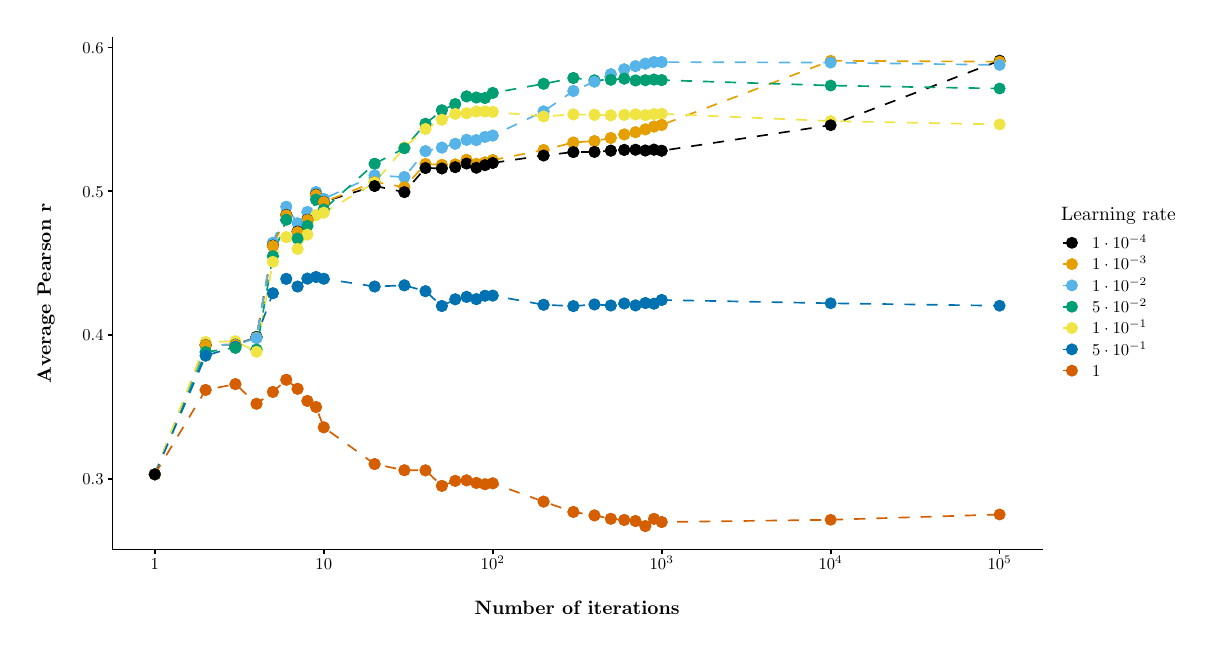
\begin{tikzpicture}[x=1pt,y=1pt]
\definecolor{fillColor}{RGB}{255,255,255}
\path[use as bounding box,fill=fillColor,fill opacity=0.00] (0,0) rectangle (418.34,216.81);
\begin{scope}
\path[clip] ( 30.67, 28.30) rectangle (366.48,213.31);
\definecolor{drawColor}{RGB}{0,0,0}

\path[draw=drawColor,line width= 0.6pt,dash pattern=on 4pt off 4pt ,line join=round] ( 45.94, 55.41) --
	( 45.94, 55.41) --
	( 64.31,102.09) --
	( 64.31,102.09) --
	( 75.07,102.28) --
	( 75.07,102.28) --
	( 82.69,104.96) --
	( 82.69,104.96) --
	( 88.61,138.10) --
	( 88.61,138.10) --
	( 93.45,149.16) --
	( 93.45,149.16) --
	( 97.53,143.17) --
	( 97.53,143.17) --
	(101.07,147.42) --
	(101.07,147.42) --
	(104.20,156.50) --
	(104.20,156.50) --
	(106.99,153.90) --
	(106.99,153.90) --
	(125.37,159.61) --
	(125.37,159.61) --
	(136.12,157.40) --
	(136.12,157.40) --
	(143.75,166.10) --
	(143.75,166.10) --
	(149.67,165.96) --
	(149.67,165.96) --
	(154.50,166.42) --
	(154.50,166.42) --
	(158.59,167.74) --
	(158.59,167.74) --
	(162.13,166.22) --
	(162.13,166.22) --
	(165.25,167.14) --
	(165.25,167.14) --
	(168.05,167.94) --
	(168.05,167.94) --
	(186.43,170.63) --
	(186.43,170.63) --
	(197.18,171.86) --
	(197.18,171.86) --
	(204.81,171.93) --
	(204.81,171.93) --
	(210.72,172.37) --
	(210.72,172.37) --
	(215.56,172.64) --
	(215.56,172.64) --
	(219.64,172.70) --
	(219.64,172.70) --
	(223.19,172.42) --
	(223.19,172.42) --
	(226.31,172.72) --
	(226.31,172.72) --
	(229.10,172.34) --
	(229.10,172.34) --
	(290.16,181.57) --
	(351.21,204.90);
\definecolor{drawColor}{RGB}{230,159,0}

\path[draw=drawColor,line width= 0.6pt,dash pattern=on 4pt off 4pt ,line join=round] ( 45.94, 55.42) --
	( 45.94, 55.42) --
	( 64.31,102.09) --
	( 64.31,102.09) --
	( 75.07,102.09) --
	( 75.07,102.09) --
	( 82.69,104.84) --
	( 82.69,104.84) --
	( 88.61,137.95) --
	( 88.61,137.95) --
	( 93.45,149.03) --
	( 93.45,149.03) --
	( 97.53,142.93) --
	( 97.53,142.93) --
	(101.07,147.29) --
	(101.07,147.29) --
	(104.20,156.35) --
	(104.20,156.35) --
	(106.99,153.81) --
	(106.99,153.81) --
	(125.37,161.06) --
	(125.37,161.06) --
	(136.12,159.17) --
	(136.12,159.17) --
	(143.75,167.54) --
	(143.75,167.54) --
	(149.67,167.24) --
	(149.67,167.24) --
	(154.50,167.40) --
	(154.50,167.40) --
	(158.59,169.07) --
	(158.59,169.07) --
	(162.13,167.58) --
	(162.13,167.58) --
	(165.25,168.12) --
	(165.25,168.12) --
	(168.05,168.96) --
	(168.05,168.96) --
	(186.43,172.60) --
	(186.43,172.60) --
	(197.18,175.32) --
	(197.18,175.32) --
	(204.81,175.83) --
	(204.81,175.83) --
	(210.72,176.95) --
	(210.72,176.95) --
	(215.56,178.23) --
	(215.56,178.23) --
	(219.64,179.03) --
	(219.64,179.03) --
	(223.19,180.06) --
	(223.19,180.06) --
	(226.31,181.07) --
	(226.31,181.07) --
	(229.10,181.67) --
	(229.10,181.67) --
	(290.16,204.84) --
	(351.21,204.53);
\definecolor{drawColor}{RGB}{86,180,233}

\path[draw=drawColor,line width= 0.6pt,dash pattern=on 4pt off 4pt ,line join=round] ( 45.94, 55.42) --
	( 45.94, 55.42) --
	( 64.31,102.18) --
	( 64.31,102.18) --
	( 75.07,102.19) --
	( 75.07,102.19) --
	( 82.69,104.63) --
	( 82.69,104.63) --
	( 88.61,139.08) --
	( 88.61,139.08) --
	( 93.45,152.12) --
	( 93.45,152.12) --
	( 97.53,146.12) --
	( 97.53,146.12) --
	(101.07,150.20) --
	(101.07,150.20) --
	(104.20,157.41) --
	(104.20,157.41) --
	(106.99,154.93) --
	(106.99,154.93) --
	(125.37,163.43) --
	(125.37,163.43) --
	(136.12,162.83) --
	(136.12,162.83) --
	(143.75,172.20) --
	(143.75,172.20) --
	(149.67,173.47) --
	(149.67,173.47) --
	(154.50,174.85) --
	(154.50,174.85) --
	(158.59,176.28) --
	(158.59,176.28) --
	(162.13,176.18) --
	(162.13,176.18) --
	(165.25,177.32) --
	(165.25,177.32) --
	(168.05,177.82) --
	(168.05,177.82) --
	(186.43,186.55) --
	(186.43,186.55) --
	(197.18,193.94) --
	(197.18,193.94) --
	(204.81,197.29) --
	(204.81,197.29) --
	(210.72,200.01) --
	(210.72,200.01) --
	(215.56,201.79) --
	(215.56,201.79) --
	(219.64,202.91) --
	(219.64,202.91) --
	(223.19,203.80) --
	(223.19,203.80) --
	(226.31,204.37) --
	(226.31,204.37) --
	(229.10,204.38) --
	(229.10,204.38) --
	(290.16,204.19) --
	(351.21,203.33);
\definecolor{drawColor}{RGB}{0,158,115}

\path[draw=drawColor,line width= 0.6pt,dash pattern=on 4pt off 4pt ,line join=round] ( 45.94, 55.42) --
	( 45.94, 55.42) --
	( 64.31, 99.61) --
	( 64.31, 99.61) --
	( 75.07,101.11) --
	( 75.07,101.11) --
	( 82.69,100.47) --
	( 82.69,100.47) --
	( 88.61,134.23) --
	( 88.61,134.23) --
	( 93.45,147.43) --
	( 93.45,147.43) --
	( 97.53,140.63) --
	( 97.53,140.63) --
	(101.07,145.20) --
	(101.07,145.20) --
	(104.20,154.69) --
	(104.20,154.69) --
	(106.99,151.14) --
	(106.99,151.14) --
	(125.37,167.63) --
	(125.37,167.63) --
	(136.12,173.25) --
	(136.12,173.25) --
	(143.75,182.07) --
	(143.75,182.07) --
	(149.67,186.95) --
	(149.67,186.95) --
	(154.50,189.20) --
	(154.50,189.20) --
	(158.59,191.97) --
	(158.59,191.97) --
	(162.13,191.56) --
	(162.13,191.56) --
	(165.25,191.39) --
	(165.25,191.39) --
	(168.05,193.23) --
	(168.05,193.23) --
	(186.43,196.53) --
	(186.43,196.53) --
	(197.18,198.62) --
	(197.18,198.62) --
	(204.81,197.77) --
	(204.81,197.77) --
	(210.72,197.99) --
	(210.72,197.99) --
	(215.56,198.39) --
	(215.56,198.39) --
	(219.64,197.73) --
	(219.64,197.73) --
	(223.19,197.83) --
	(223.19,197.83) --
	(226.31,198.06) --
	(226.31,198.06) --
	(229.10,197.86) --
	(229.10,197.86) --
	(290.16,195.90) --
	(351.21,194.82);
\definecolor{drawColor}{RGB}{240,228,66}

\path[draw=drawColor,line width= 0.6pt,dash pattern=on 4pt off 4pt ,line join=round] ( 45.94, 55.42) --
	( 45.94, 55.42) --
	( 64.31,103.19) --
	( 64.31,103.19) --
	( 75.07,103.48) --
	( 75.07,103.48) --
	( 82.69, 99.72) --
	( 82.69, 99.72) --
	( 88.61,132.22) --
	( 88.61,132.22) --
	( 93.45,141.12) --
	( 93.45,141.12) --
	( 97.53,136.87) --
	( 97.53,136.87) --
	(101.07,142.03) --
	(101.07,142.03) --
	(104.20,149.07) --
	(104.20,149.07) --
	(106.99,149.99) --
	(106.99,149.99) --
	(125.37,160.81) --
	(125.37,160.81) --
	(136.12,173.49) --
	(136.12,173.49) --
	(143.75,180.23) --
	(143.75,180.23) --
	(149.67,183.56) --
	(149.67,183.56) --
	(154.50,185.69) --
	(154.50,185.69) --
	(158.59,185.89) --
	(158.59,185.89) --
	(162.13,186.50) --
	(162.13,186.50) --
	(165.25,186.53) --
	(165.25,186.53) --
	(168.05,186.38) --
	(168.05,186.38) --
	(186.43,184.75) --
	(186.43,184.75) --
	(197.18,185.46) --
	(197.18,185.46) --
	(204.81,185.31) --
	(204.81,185.31) --
	(210.72,185.12) --
	(210.72,185.12) --
	(215.56,185.29) --
	(215.56,185.29) --
	(219.64,185.48) --
	(219.64,185.48) --
	(223.19,185.20) --
	(223.19,185.20) --
	(226.31,185.56) --
	(226.31,185.56) --
	(229.10,185.67) --
	(229.10,185.67) --
	(290.16,183.06) --
	(351.21,181.84);
\definecolor{drawColor}{RGB}{0,114,178}

\path[draw=drawColor,line width= 0.6pt,dash pattern=on 4pt off 4pt ,line join=round] ( 45.94, 55.42) --
	( 45.94, 55.42) --
	( 64.31, 98.29) --
	( 64.31, 98.29) --
	( 75.07,101.52) --
	( 75.07,101.52) --
	( 82.69,105.14) --
	( 82.69,105.14) --
	( 88.61,120.84) --
	( 88.61,120.84) --
	( 93.45,126.04) --
	( 93.45,126.04) --
	( 97.53,123.26) --
	( 97.53,123.26) --
	(101.07,126.13) --
	(101.07,126.13) --
	(104.20,126.71) --
	(104.20,126.71) --
	(106.99,126.09) --
	(106.99,126.09) --
	(125.37,123.27) --
	(125.37,123.27) --
	(136.12,123.70) --
	(136.12,123.70) --
	(143.75,121.59) --
	(143.75,121.59) --
	(149.67,116.23) --
	(149.67,116.23) --
	(154.50,118.65) --
	(154.50,118.65) --
	(158.59,119.53) --
	(158.59,119.53) --
	(162.13,118.72) --
	(162.13,118.72) --
	(165.25,119.95) --
	(165.25,119.95) --
	(168.05,120.00) --
	(168.05,120.00) --
	(186.43,116.68) --
	(186.43,116.68) --
	(197.18,116.20) --
	(197.18,116.20) --
	(204.81,116.79) --
	(204.81,116.79) --
	(210.72,116.42) --
	(210.72,116.42) --
	(215.56,117.15) --
	(215.56,117.15) --
	(219.64,116.44) --
	(219.64,116.44) --
	(223.19,117.31) --
	(223.19,117.31) --
	(226.31,117.07) --
	(226.31,117.07) --
	(229.10,118.41) --
	(229.10,118.41) --
	(290.16,117.22) --
	(351.21,116.33);
\definecolor{drawColor}{RGB}{213,94,0}

\path[draw=drawColor,line width= 0.6pt,dash pattern=on 4pt off 4pt ,line join=round] ( 45.94, 55.42) --
	( 45.94, 55.42) --
	( 64.31, 85.90) --
	( 64.31, 85.90) --
	( 75.07, 88.01) --
	( 75.07, 88.01) --
	( 82.69, 80.90) --
	( 82.69, 80.90) --
	( 88.61, 85.18) --
	( 88.61, 85.18) --
	( 93.45, 89.59) --
	( 93.45, 89.59) --
	( 97.53, 86.31) --
	( 97.53, 86.31) --
	(101.07, 81.93) --
	(101.07, 81.93) --
	(104.20, 79.74) --
	(104.20, 79.74) --
	(106.99, 72.39) --
	(106.99, 72.39) --
	(125.37, 59.12) --
	(125.37, 59.12) --
	(136.12, 56.88) --
	(136.12, 56.88) --
	(143.75, 56.85) --
	(143.75, 56.85) --
	(149.67, 51.24) --
	(149.67, 51.24) --
	(154.50, 53.05) --
	(154.50, 53.05) --
	(158.59, 53.24) --
	(158.59, 53.24) --
	(162.13, 52.30) --
	(162.13, 52.30) --
	(165.25, 51.83) --
	(165.25, 51.83) --
	(168.05, 52.16) --
	(168.05, 52.16) --
	(186.43, 45.55) --
	(186.43, 45.55) --
	(197.18, 41.82) --
	(197.18, 41.82) --
	(204.81, 40.56) --
	(204.81, 40.56) --
	(210.72, 39.34) --
	(210.72, 39.34) --
	(215.56, 38.92) --
	(215.56, 38.92) --
	(219.64, 38.54) --
	(219.64, 38.54) --
	(223.19, 36.71) --
	(223.19, 36.71) --
	(226.31, 39.32) --
	(226.31, 39.32) --
	(229.10, 38.17) --
	(229.10, 38.17) --
	(290.16, 38.98) --
	(351.21, 40.90);
\definecolor{drawColor}{RGB}{0,0,0}
\definecolor{fillColor}{RGB}{0,0,0}

\path[draw=drawColor,line width= 0.4pt,line join=round,line cap=round,fill=fillColor] (351.21,204.90) circle (  1.96);
\definecolor{drawColor}{RGB}{230,159,0}
\definecolor{fillColor}{RGB}{230,159,0}

\path[draw=drawColor,line width= 0.4pt,line join=round,line cap=round,fill=fillColor] (351.21,204.53) circle (  1.96);
\definecolor{drawColor}{RGB}{86,180,233}
\definecolor{fillColor}{RGB}{86,180,233}

\path[draw=drawColor,line width= 0.4pt,line join=round,line cap=round,fill=fillColor] (351.21,203.33) circle (  1.96);
\definecolor{drawColor}{RGB}{0,158,115}
\definecolor{fillColor}{RGB}{0,158,115}

\path[draw=drawColor,line width= 0.4pt,line join=round,line cap=round,fill=fillColor] (351.21,194.82) circle (  1.96);
\definecolor{drawColor}{RGB}{240,228,66}
\definecolor{fillColor}{RGB}{240,228,66}

\path[draw=drawColor,line width= 0.4pt,line join=round,line cap=round,fill=fillColor] (351.21,181.84) circle (  1.96);
\definecolor{drawColor}{RGB}{0,114,178}
\definecolor{fillColor}{RGB}{0,114,178}

\path[draw=drawColor,line width= 0.4pt,line join=round,line cap=round,fill=fillColor] (351.21,116.33) circle (  1.96);
\definecolor{drawColor}{RGB}{213,94,0}
\definecolor{fillColor}{RGB}{213,94,0}

\path[draw=drawColor,line width= 0.4pt,line join=round,line cap=round,fill=fillColor] (351.21, 40.90) circle (  1.96);
\definecolor{drawColor}{RGB}{86,180,233}
\definecolor{fillColor}{RGB}{86,180,233}

\path[draw=drawColor,line width= 0.4pt,line join=round,line cap=round,fill=fillColor] (229.10,204.38) circle (  1.96);

\path[draw=drawColor,line width= 0.4pt,line join=round,line cap=round,fill=fillColor] (226.31,204.37) circle (  1.96);

\path[draw=drawColor,line width= 0.4pt,line join=round,line cap=round,fill=fillColor] (223.19,203.80) circle (  1.96);

\path[draw=drawColor,line width= 0.4pt,line join=round,line cap=round,fill=fillColor] (219.64,202.91) circle (  1.96);

\path[draw=drawColor,line width= 0.4pt,line join=round,line cap=round,fill=fillColor] (215.56,201.79) circle (  1.96);

\path[draw=drawColor,line width= 0.4pt,line join=round,line cap=round,fill=fillColor] (210.72,200.01) circle (  1.96);
\definecolor{drawColor}{RGB}{0,158,115}
\definecolor{fillColor}{RGB}{0,158,115}

\path[draw=drawColor,line width= 0.4pt,line join=round,line cap=round,fill=fillColor] (197.18,198.62) circle (  1.96);

\path[draw=drawColor,line width= 0.4pt,line join=round,line cap=round,fill=fillColor] (215.56,198.39) circle (  1.96);

\path[draw=drawColor,line width= 0.4pt,line join=round,line cap=round,fill=fillColor] (226.31,198.06) circle (  1.96);

\path[draw=drawColor,line width= 0.4pt,line join=round,line cap=round,fill=fillColor] (210.72,197.99) circle (  1.96);

\path[draw=drawColor,line width= 0.4pt,line join=round,line cap=round,fill=fillColor] (229.10,197.86) circle (  1.96);

\path[draw=drawColor,line width= 0.4pt,line join=round,line cap=round,fill=fillColor] (223.19,197.83) circle (  1.96);

\path[draw=drawColor,line width= 0.4pt,line join=round,line cap=round,fill=fillColor] (204.81,197.77) circle (  1.96);

\path[draw=drawColor,line width= 0.4pt,line join=round,line cap=round,fill=fillColor] (219.64,197.73) circle (  1.96);
\definecolor{drawColor}{RGB}{86,180,233}
\definecolor{fillColor}{RGB}{86,180,233}

\path[draw=drawColor,line width= 0.4pt,line join=round,line cap=round,fill=fillColor] (204.81,197.29) circle (  1.96);
\definecolor{drawColor}{RGB}{0,158,115}
\definecolor{fillColor}{RGB}{0,158,115}

\path[draw=drawColor,line width= 0.4pt,line join=round,line cap=round,fill=fillColor] (186.43,196.53) circle (  1.96);
\definecolor{drawColor}{RGB}{86,180,233}
\definecolor{fillColor}{RGB}{86,180,233}

\path[draw=drawColor,line width= 0.4pt,line join=round,line cap=round,fill=fillColor] (197.18,193.94) circle (  1.96);
\definecolor{drawColor}{RGB}{0,158,115}
\definecolor{fillColor}{RGB}{0,158,115}

\path[draw=drawColor,line width= 0.4pt,line join=round,line cap=round,fill=fillColor] (168.05,193.23) circle (  1.96);

\path[draw=drawColor,line width= 0.4pt,line join=round,line cap=round,fill=fillColor] (158.59,191.97) circle (  1.96);

\path[draw=drawColor,line width= 0.4pt,line join=round,line cap=round,fill=fillColor] (162.13,191.56) circle (  1.96);

\path[draw=drawColor,line width= 0.4pt,line join=round,line cap=round,fill=fillColor] (165.25,191.39) circle (  1.96);

\path[draw=drawColor,line width= 0.4pt,line join=round,line cap=round,fill=fillColor] (154.50,189.20) circle (  1.96);

\path[draw=drawColor,line width= 0.4pt,line join=round,line cap=round,fill=fillColor] (149.67,186.95) circle (  1.96);
\definecolor{drawColor}{RGB}{86,180,233}
\definecolor{fillColor}{RGB}{86,180,233}

\path[draw=drawColor,line width= 0.4pt,line join=round,line cap=round,fill=fillColor] (186.43,186.55) circle (  1.96);
\definecolor{drawColor}{RGB}{240,228,66}
\definecolor{fillColor}{RGB}{240,228,66}

\path[draw=drawColor,line width= 0.4pt,line join=round,line cap=round,fill=fillColor] (165.25,186.53) circle (  1.96);

\path[draw=drawColor,line width= 0.4pt,line join=round,line cap=round,fill=fillColor] (162.13,186.50) circle (  1.96);

\path[draw=drawColor,line width= 0.4pt,line join=round,line cap=round,fill=fillColor] (168.05,186.38) circle (  1.96);

\path[draw=drawColor,line width= 0.4pt,line join=round,line cap=round,fill=fillColor] (158.59,185.89) circle (  1.96);

\path[draw=drawColor,line width= 0.4pt,line join=round,line cap=round,fill=fillColor] (154.50,185.69) circle (  1.96);

\path[draw=drawColor,line width= 0.4pt,line join=round,line cap=round,fill=fillColor] (229.10,185.67) circle (  1.96);

\path[draw=drawColor,line width= 0.4pt,line join=round,line cap=round,fill=fillColor] (226.31,185.56) circle (  1.96);

\path[draw=drawColor,line width= 0.4pt,line join=round,line cap=round,fill=fillColor] (219.64,185.48) circle (  1.96);

\path[draw=drawColor,line width= 0.4pt,line join=round,line cap=round,fill=fillColor] (197.18,185.46) circle (  1.96);

\path[draw=drawColor,line width= 0.4pt,line join=round,line cap=round,fill=fillColor] (204.81,185.31) circle (  1.96);

\path[draw=drawColor,line width= 0.4pt,line join=round,line cap=round,fill=fillColor] (215.56,185.29) circle (  1.96);

\path[draw=drawColor,line width= 0.4pt,line join=round,line cap=round,fill=fillColor] (223.19,185.20) circle (  1.96);

\path[draw=drawColor,line width= 0.4pt,line join=round,line cap=round,fill=fillColor] (210.72,185.12) circle (  1.96);

\path[draw=drawColor,line width= 0.4pt,line join=round,line cap=round,fill=fillColor] (186.43,184.75) circle (  1.96);

\path[draw=drawColor,line width= 0.4pt,line join=round,line cap=round,fill=fillColor] (149.67,183.56) circle (  1.96);
\definecolor{drawColor}{RGB}{0,158,115}
\definecolor{fillColor}{RGB}{0,158,115}

\path[draw=drawColor,line width= 0.4pt,line join=round,line cap=round,fill=fillColor] (143.75,182.07) circle (  1.96);
\definecolor{drawColor}{RGB}{230,159,0}
\definecolor{fillColor}{RGB}{230,159,0}

\path[draw=drawColor,line width= 0.4pt,line join=round,line cap=round,fill=fillColor] (229.10,181.67) circle (  1.96);

\path[draw=drawColor,line width= 0.4pt,line join=round,line cap=round,fill=fillColor] (226.31,181.07) circle (  1.96);
\definecolor{drawColor}{RGB}{240,228,66}
\definecolor{fillColor}{RGB}{240,228,66}

\path[draw=drawColor,line width= 0.4pt,line join=round,line cap=round,fill=fillColor] (143.75,180.23) circle (  1.96);
\definecolor{drawColor}{RGB}{230,159,0}
\definecolor{fillColor}{RGB}{230,159,0}

\path[draw=drawColor,line width= 0.4pt,line join=round,line cap=round,fill=fillColor] (223.19,180.06) circle (  1.96);

\path[draw=drawColor,line width= 0.4pt,line join=round,line cap=round,fill=fillColor] (219.64,179.03) circle (  1.96);

\path[draw=drawColor,line width= 0.4pt,line join=round,line cap=round,fill=fillColor] (215.56,178.23) circle (  1.96);
\definecolor{drawColor}{RGB}{86,180,233}
\definecolor{fillColor}{RGB}{86,180,233}

\path[draw=drawColor,line width= 0.4pt,line join=round,line cap=round,fill=fillColor] (168.05,177.82) circle (  1.96);

\path[draw=drawColor,line width= 0.4pt,line join=round,line cap=round,fill=fillColor] (165.25,177.32) circle (  1.96);
\definecolor{drawColor}{RGB}{230,159,0}
\definecolor{fillColor}{RGB}{230,159,0}

\path[draw=drawColor,line width= 0.4pt,line join=round,line cap=round,fill=fillColor] (210.72,176.95) circle (  1.96);
\definecolor{drawColor}{RGB}{86,180,233}
\definecolor{fillColor}{RGB}{86,180,233}

\path[draw=drawColor,line width= 0.4pt,line join=round,line cap=round,fill=fillColor] (158.59,176.28) circle (  1.96);

\path[draw=drawColor,line width= 0.4pt,line join=round,line cap=round,fill=fillColor] (162.13,176.18) circle (  1.96);
\definecolor{drawColor}{RGB}{230,159,0}
\definecolor{fillColor}{RGB}{230,159,0}

\path[draw=drawColor,line width= 0.4pt,line join=round,line cap=round,fill=fillColor] (204.81,175.83) circle (  1.96);

\path[draw=drawColor,line width= 0.4pt,line join=round,line cap=round,fill=fillColor] (197.18,175.32) circle (  1.96);
\definecolor{drawColor}{RGB}{86,180,233}
\definecolor{fillColor}{RGB}{86,180,233}

\path[draw=drawColor,line width= 0.4pt,line join=round,line cap=round,fill=fillColor] (154.50,174.85) circle (  1.96);
\definecolor{drawColor}{RGB}{240,228,66}
\definecolor{fillColor}{RGB}{240,228,66}

\path[draw=drawColor,line width= 0.4pt,line join=round,line cap=round,fill=fillColor] (136.12,173.49) circle (  1.96);
\definecolor{drawColor}{RGB}{86,180,233}
\definecolor{fillColor}{RGB}{86,180,233}

\path[draw=drawColor,line width= 0.4pt,line join=round,line cap=round,fill=fillColor] (149.67,173.47) circle (  1.96);
\definecolor{drawColor}{RGB}{0,158,115}
\definecolor{fillColor}{RGB}{0,158,115}

\path[draw=drawColor,line width= 0.4pt,line join=round,line cap=round,fill=fillColor] (136.12,173.25) circle (  1.96);
\definecolor{drawColor}{RGB}{0,0,0}
\definecolor{fillColor}{RGB}{0,0,0}

\path[draw=drawColor,line width= 0.4pt,line join=round,line cap=round,fill=fillColor] (226.31,172.72) circle (  1.96);

\path[draw=drawColor,line width= 0.4pt,line join=round,line cap=round,fill=fillColor] (219.64,172.70) circle (  1.96);

\path[draw=drawColor,line width= 0.4pt,line join=round,line cap=round,fill=fillColor] (215.56,172.64) circle (  1.96);
\definecolor{drawColor}{RGB}{230,159,0}
\definecolor{fillColor}{RGB}{230,159,0}

\path[draw=drawColor,line width= 0.4pt,line join=round,line cap=round,fill=fillColor] (186.43,172.60) circle (  1.96);
\definecolor{drawColor}{RGB}{0,0,0}
\definecolor{fillColor}{RGB}{0,0,0}

\path[draw=drawColor,line width= 0.4pt,line join=round,line cap=round,fill=fillColor] (223.19,172.42) circle (  1.96);

\path[draw=drawColor,line width= 0.4pt,line join=round,line cap=round,fill=fillColor] (210.72,172.37) circle (  1.96);

\path[draw=drawColor,line width= 0.4pt,line join=round,line cap=round,fill=fillColor] (229.10,172.34) circle (  1.96);
\definecolor{drawColor}{RGB}{86,180,233}
\definecolor{fillColor}{RGB}{86,180,233}

\path[draw=drawColor,line width= 0.4pt,line join=round,line cap=round,fill=fillColor] (143.75,172.20) circle (  1.96);
\definecolor{drawColor}{RGB}{0,0,0}
\definecolor{fillColor}{RGB}{0,0,0}

\path[draw=drawColor,line width= 0.4pt,line join=round,line cap=round,fill=fillColor] (204.81,171.93) circle (  1.96);

\path[draw=drawColor,line width= 0.4pt,line join=round,line cap=round,fill=fillColor] (197.18,171.86) circle (  1.96);

\path[draw=drawColor,line width= 0.4pt,line join=round,line cap=round,fill=fillColor] (186.43,170.63) circle (  1.96);
\definecolor{drawColor}{RGB}{230,159,0}
\definecolor{fillColor}{RGB}{230,159,0}

\path[draw=drawColor,line width= 0.4pt,line join=round,line cap=round,fill=fillColor] (158.59,169.07) circle (  1.96);

\path[draw=drawColor,line width= 0.4pt,line join=round,line cap=round,fill=fillColor] (168.05,168.96) circle (  1.96);

\path[draw=drawColor,line width= 0.4pt,line join=round,line cap=round,fill=fillColor] (165.25,168.12) circle (  1.96);
\definecolor{drawColor}{RGB}{0,0,0}
\definecolor{fillColor}{RGB}{0,0,0}

\path[draw=drawColor,line width= 0.4pt,line join=round,line cap=round,fill=fillColor] (168.05,167.94) circle (  1.96);

\path[draw=drawColor,line width= 0.4pt,line join=round,line cap=round,fill=fillColor] (158.59,167.74) circle (  1.96);
\definecolor{drawColor}{RGB}{0,158,115}
\definecolor{fillColor}{RGB}{0,158,115}

\path[draw=drawColor,line width= 0.4pt,line join=round,line cap=round,fill=fillColor] (125.37,167.63) circle (  1.96);
\definecolor{drawColor}{RGB}{230,159,0}
\definecolor{fillColor}{RGB}{230,159,0}

\path[draw=drawColor,line width= 0.4pt,line join=round,line cap=round,fill=fillColor] (162.13,167.58) circle (  1.96);

\path[draw=drawColor,line width= 0.4pt,line join=round,line cap=round,fill=fillColor] (143.75,167.54) circle (  1.96);

\path[draw=drawColor,line width= 0.4pt,line join=round,line cap=round,fill=fillColor] (154.50,167.40) circle (  1.96);

\path[draw=drawColor,line width= 0.4pt,line join=round,line cap=round,fill=fillColor] (149.67,167.24) circle (  1.96);
\definecolor{drawColor}{RGB}{0,0,0}
\definecolor{fillColor}{RGB}{0,0,0}

\path[draw=drawColor,line width= 0.4pt,line join=round,line cap=round,fill=fillColor] (165.25,167.14) circle (  1.96);

\path[draw=drawColor,line width= 0.4pt,line join=round,line cap=round,fill=fillColor] (154.50,166.42) circle (  1.96);

\path[draw=drawColor,line width= 0.4pt,line join=round,line cap=round,fill=fillColor] (162.13,166.22) circle (  1.96);

\path[draw=drawColor,line width= 0.4pt,line join=round,line cap=round,fill=fillColor] (143.75,166.10) circle (  1.96);

\path[draw=drawColor,line width= 0.4pt,line join=round,line cap=round,fill=fillColor] (149.67,165.96) circle (  1.96);
\definecolor{drawColor}{RGB}{86,180,233}
\definecolor{fillColor}{RGB}{86,180,233}

\path[draw=drawColor,line width= 0.4pt,line join=round,line cap=round,fill=fillColor] (125.37,163.43) circle (  1.96);

\path[draw=drawColor,line width= 0.4pt,line join=round,line cap=round,fill=fillColor] (136.12,162.83) circle (  1.96);
\definecolor{drawColor}{RGB}{230,159,0}
\definecolor{fillColor}{RGB}{230,159,0}

\path[draw=drawColor,line width= 0.4pt,line join=round,line cap=round,fill=fillColor] (125.37,161.06) circle (  1.96);
\definecolor{drawColor}{RGB}{240,228,66}
\definecolor{fillColor}{RGB}{240,228,66}

\path[draw=drawColor,line width= 0.4pt,line join=round,line cap=round,fill=fillColor] (125.37,160.81) circle (  1.96);
\definecolor{drawColor}{RGB}{0,0,0}
\definecolor{fillColor}{RGB}{0,0,0}

\path[draw=drawColor,line width= 0.4pt,line join=round,line cap=round,fill=fillColor] (125.37,159.61) circle (  1.96);
\definecolor{drawColor}{RGB}{230,159,0}
\definecolor{fillColor}{RGB}{230,159,0}

\path[draw=drawColor,line width= 0.4pt,line join=round,line cap=round,fill=fillColor] (136.12,159.17) circle (  1.96);
\definecolor{drawColor}{RGB}{86,180,233}
\definecolor{fillColor}{RGB}{86,180,233}

\path[draw=drawColor,line width= 0.4pt,line join=round,line cap=round,fill=fillColor] (104.20,157.41) circle (  1.96);
\definecolor{drawColor}{RGB}{0,0,0}
\definecolor{fillColor}{RGB}{0,0,0}

\path[draw=drawColor,line width= 0.4pt,line join=round,line cap=round,fill=fillColor] (136.12,157.40) circle (  1.96);

\path[draw=drawColor,line width= 0.4pt,line join=round,line cap=round,fill=fillColor] (104.20,156.50) circle (  1.96);
\definecolor{drawColor}{RGB}{230,159,0}
\definecolor{fillColor}{RGB}{230,159,0}

\path[draw=drawColor,line width= 0.4pt,line join=round,line cap=round,fill=fillColor] (104.20,156.35) circle (  1.96);
\definecolor{drawColor}{RGB}{86,180,233}
\definecolor{fillColor}{RGB}{86,180,233}

\path[draw=drawColor,line width= 0.4pt,line join=round,line cap=round,fill=fillColor] (106.99,154.93) circle (  1.96);
\definecolor{drawColor}{RGB}{0,158,115}
\definecolor{fillColor}{RGB}{0,158,115}

\path[draw=drawColor,line width= 0.4pt,line join=round,line cap=round,fill=fillColor] (104.20,154.69) circle (  1.96);
\definecolor{drawColor}{RGB}{0,0,0}
\definecolor{fillColor}{RGB}{0,0,0}

\path[draw=drawColor,line width= 0.4pt,line join=round,line cap=round,fill=fillColor] (106.99,153.90) circle (  1.96);
\definecolor{drawColor}{RGB}{230,159,0}
\definecolor{fillColor}{RGB}{230,159,0}

\path[draw=drawColor,line width= 0.4pt,line join=round,line cap=round,fill=fillColor] (106.99,153.81) circle (  1.96);
\definecolor{drawColor}{RGB}{86,180,233}
\definecolor{fillColor}{RGB}{86,180,233}

\path[draw=drawColor,line width= 0.4pt,line join=round,line cap=round,fill=fillColor] ( 93.45,152.12) circle (  1.96);
\definecolor{drawColor}{RGB}{0,158,115}
\definecolor{fillColor}{RGB}{0,158,115}

\path[draw=drawColor,line width= 0.4pt,line join=round,line cap=round,fill=fillColor] (106.99,151.14) circle (  1.96);
\definecolor{drawColor}{RGB}{86,180,233}
\definecolor{fillColor}{RGB}{86,180,233}

\path[draw=drawColor,line width= 0.4pt,line join=round,line cap=round,fill=fillColor] (101.07,150.20) circle (  1.96);
\definecolor{drawColor}{RGB}{240,228,66}
\definecolor{fillColor}{RGB}{240,228,66}

\path[draw=drawColor,line width= 0.4pt,line join=round,line cap=round,fill=fillColor] (106.99,149.99) circle (  1.96);
\definecolor{drawColor}{RGB}{0,0,0}
\definecolor{fillColor}{RGB}{0,0,0}

\path[draw=drawColor,line width= 0.4pt,line join=round,line cap=round,fill=fillColor] ( 93.45,149.16) circle (  1.96);
\definecolor{drawColor}{RGB}{240,228,66}
\definecolor{fillColor}{RGB}{240,228,66}

\path[draw=drawColor,line width= 0.4pt,line join=round,line cap=round,fill=fillColor] (104.20,149.07) circle (  1.96);
\definecolor{drawColor}{RGB}{230,159,0}
\definecolor{fillColor}{RGB}{230,159,0}

\path[draw=drawColor,line width= 0.4pt,line join=round,line cap=round,fill=fillColor] ( 93.45,149.03) circle (  1.96);
\definecolor{drawColor}{RGB}{0,158,115}
\definecolor{fillColor}{RGB}{0,158,115}

\path[draw=drawColor,line width= 0.4pt,line join=round,line cap=round,fill=fillColor] ( 93.45,147.43) circle (  1.96);
\definecolor{drawColor}{RGB}{0,0,0}
\definecolor{fillColor}{RGB}{0,0,0}

\path[draw=drawColor,line width= 0.4pt,line join=round,line cap=round,fill=fillColor] (101.07,147.42) circle (  1.96);
\definecolor{drawColor}{RGB}{230,159,0}
\definecolor{fillColor}{RGB}{230,159,0}

\path[draw=drawColor,line width= 0.4pt,line join=round,line cap=round,fill=fillColor] (101.07,147.29) circle (  1.96);
\definecolor{drawColor}{RGB}{86,180,233}
\definecolor{fillColor}{RGB}{86,180,233}

\path[draw=drawColor,line width= 0.4pt,line join=round,line cap=round,fill=fillColor] ( 97.53,146.12) circle (  1.96);
\definecolor{drawColor}{RGB}{0,158,115}
\definecolor{fillColor}{RGB}{0,158,115}

\path[draw=drawColor,line width= 0.4pt,line join=round,line cap=round,fill=fillColor] (101.07,145.20) circle (  1.96);
\definecolor{drawColor}{RGB}{0,0,0}
\definecolor{fillColor}{RGB}{0,0,0}

\path[draw=drawColor,line width= 0.4pt,line join=round,line cap=round,fill=fillColor] ( 97.53,143.17) circle (  1.96);
\definecolor{drawColor}{RGB}{230,159,0}
\definecolor{fillColor}{RGB}{230,159,0}

\path[draw=drawColor,line width= 0.4pt,line join=round,line cap=round,fill=fillColor] ( 97.53,142.93) circle (  1.96);
\definecolor{drawColor}{RGB}{240,228,66}
\definecolor{fillColor}{RGB}{240,228,66}

\path[draw=drawColor,line width= 0.4pt,line join=round,line cap=round,fill=fillColor] (101.07,142.03) circle (  1.96);

\path[draw=drawColor,line width= 0.4pt,line join=round,line cap=round,fill=fillColor] ( 93.45,141.12) circle (  1.96);
\definecolor{drawColor}{RGB}{0,158,115}
\definecolor{fillColor}{RGB}{0,158,115}

\path[draw=drawColor,line width= 0.4pt,line join=round,line cap=round,fill=fillColor] ( 97.53,140.63) circle (  1.96);
\definecolor{drawColor}{RGB}{86,180,233}
\definecolor{fillColor}{RGB}{86,180,233}

\path[draw=drawColor,line width= 0.4pt,line join=round,line cap=round,fill=fillColor] ( 88.61,139.08) circle (  1.96);
\definecolor{drawColor}{RGB}{0,0,0}
\definecolor{fillColor}{RGB}{0,0,0}

\path[draw=drawColor,line width= 0.4pt,line join=round,line cap=round,fill=fillColor] ( 88.61,138.10) circle (  1.96);
\definecolor{drawColor}{RGB}{230,159,0}
\definecolor{fillColor}{RGB}{230,159,0}

\path[draw=drawColor,line width= 0.4pt,line join=round,line cap=round,fill=fillColor] ( 88.61,137.95) circle (  1.96);
\definecolor{drawColor}{RGB}{240,228,66}
\definecolor{fillColor}{RGB}{240,228,66}

\path[draw=drawColor,line width= 0.4pt,line join=round,line cap=round,fill=fillColor] ( 97.53,136.87) circle (  1.96);
\definecolor{drawColor}{RGB}{0,158,115}
\definecolor{fillColor}{RGB}{0,158,115}

\path[draw=drawColor,line width= 0.4pt,line join=round,line cap=round,fill=fillColor] ( 88.61,134.23) circle (  1.96);
\definecolor{drawColor}{RGB}{240,228,66}
\definecolor{fillColor}{RGB}{240,228,66}

\path[draw=drawColor,line width= 0.4pt,line join=round,line cap=round,fill=fillColor] ( 88.61,132.22) circle (  1.96);
\definecolor{drawColor}{RGB}{0,114,178}
\definecolor{fillColor}{RGB}{0,114,178}

\path[draw=drawColor,line width= 0.4pt,line join=round,line cap=round,fill=fillColor] (104.20,126.71) circle (  1.96);

\path[draw=drawColor,line width= 0.4pt,line join=round,line cap=round,fill=fillColor] (101.07,126.13) circle (  1.96);

\path[draw=drawColor,line width= 0.4pt,line join=round,line cap=round,fill=fillColor] (106.99,126.09) circle (  1.96);

\path[draw=drawColor,line width= 0.4pt,line join=round,line cap=round,fill=fillColor] ( 93.45,126.04) circle (  1.96);

\path[draw=drawColor,line width= 0.4pt,line join=round,line cap=round,fill=fillColor] (136.12,123.70) circle (  1.96);

\path[draw=drawColor,line width= 0.4pt,line join=round,line cap=round,fill=fillColor] (125.37,123.27) circle (  1.96);

\path[draw=drawColor,line width= 0.4pt,line join=round,line cap=round,fill=fillColor] ( 97.53,123.26) circle (  1.96);

\path[draw=drawColor,line width= 0.4pt,line join=round,line cap=round,fill=fillColor] (143.75,121.59) circle (  1.96);

\path[draw=drawColor,line width= 0.4pt,line join=round,line cap=round,fill=fillColor] ( 88.61,120.84) circle (  1.96);

\path[draw=drawColor,line width= 0.4pt,line join=round,line cap=round,fill=fillColor] (168.05,120.00) circle (  1.96);

\path[draw=drawColor,line width= 0.4pt,line join=round,line cap=round,fill=fillColor] (165.25,119.95) circle (  1.96);

\path[draw=drawColor,line width= 0.4pt,line join=round,line cap=round,fill=fillColor] (158.59,119.53) circle (  1.96);

\path[draw=drawColor,line width= 0.4pt,line join=round,line cap=round,fill=fillColor] (162.13,118.72) circle (  1.96);

\path[draw=drawColor,line width= 0.4pt,line join=round,line cap=round,fill=fillColor] (154.50,118.65) circle (  1.96);

\path[draw=drawColor,line width= 0.4pt,line join=round,line cap=round,fill=fillColor] (229.10,118.41) circle (  1.96);

\path[draw=drawColor,line width= 0.4pt,line join=round,line cap=round,fill=fillColor] (223.19,117.31) circle (  1.96);

\path[draw=drawColor,line width= 0.4pt,line join=round,line cap=round,fill=fillColor] (215.56,117.15) circle (  1.96);

\path[draw=drawColor,line width= 0.4pt,line join=round,line cap=round,fill=fillColor] (226.31,117.07) circle (  1.96);

\path[draw=drawColor,line width= 0.4pt,line join=round,line cap=round,fill=fillColor] (204.81,116.79) circle (  1.96);

\path[draw=drawColor,line width= 0.4pt,line join=round,line cap=round,fill=fillColor] (186.43,116.68) circle (  1.96);

\path[draw=drawColor,line width= 0.4pt,line join=round,line cap=round,fill=fillColor] (219.64,116.44) circle (  1.96);

\path[draw=drawColor,line width= 0.4pt,line join=round,line cap=round,fill=fillColor] (210.72,116.42) circle (  1.96);

\path[draw=drawColor,line width= 0.4pt,line join=round,line cap=round,fill=fillColor] (149.67,116.23) circle (  1.96);

\path[draw=drawColor,line width= 0.4pt,line join=round,line cap=round,fill=fillColor] (197.18,116.20) circle (  1.96);

\path[draw=drawColor,line width= 0.4pt,line join=round,line cap=round,fill=fillColor] ( 82.69,105.14) circle (  1.96);
\definecolor{drawColor}{RGB}{0,0,0}
\definecolor{fillColor}{RGB}{0,0,0}

\path[draw=drawColor,line width= 0.4pt,line join=round,line cap=round,fill=fillColor] ( 82.69,104.96) circle (  1.96);
\definecolor{drawColor}{RGB}{230,159,0}
\definecolor{fillColor}{RGB}{230,159,0}

\path[draw=drawColor,line width= 0.4pt,line join=round,line cap=round,fill=fillColor] ( 82.69,104.84) circle (  1.96);
\definecolor{drawColor}{RGB}{86,180,233}
\definecolor{fillColor}{RGB}{86,180,233}

\path[draw=drawColor,line width= 0.4pt,line join=round,line cap=round,fill=fillColor] ( 82.69,104.63) circle (  1.96);
\definecolor{drawColor}{RGB}{240,228,66}
\definecolor{fillColor}{RGB}{240,228,66}

\path[draw=drawColor,line width= 0.4pt,line join=round,line cap=round,fill=fillColor] ( 75.07,103.48) circle (  1.96);

\path[draw=drawColor,line width= 0.4pt,line join=round,line cap=round,fill=fillColor] ( 64.31,103.19) circle (  1.96);
\definecolor{drawColor}{RGB}{0,0,0}
\definecolor{fillColor}{RGB}{0,0,0}

\path[draw=drawColor,line width= 0.4pt,line join=round,line cap=round,fill=fillColor] ( 75.07,102.28) circle (  1.96);
\definecolor{drawColor}{RGB}{86,180,233}
\definecolor{fillColor}{RGB}{86,180,233}

\path[draw=drawColor,line width= 0.4pt,line join=round,line cap=round,fill=fillColor] ( 75.07,102.19) circle (  1.96);

\path[draw=drawColor,line width= 0.4pt,line join=round,line cap=round,fill=fillColor] ( 64.31,102.18) circle (  1.96);
\definecolor{drawColor}{RGB}{0,0,0}
\definecolor{fillColor}{RGB}{0,0,0}

\path[draw=drawColor,line width= 0.4pt,line join=round,line cap=round,fill=fillColor] ( 64.31,102.09) circle (  1.96);
\definecolor{drawColor}{RGB}{230,159,0}
\definecolor{fillColor}{RGB}{230,159,0}

\path[draw=drawColor,line width= 0.4pt,line join=round,line cap=round,fill=fillColor] ( 75.07,102.09) circle (  1.96);

\path[draw=drawColor,line width= 0.4pt,line join=round,line cap=round,fill=fillColor] ( 64.31,102.09) circle (  1.96);
\definecolor{drawColor}{RGB}{0,114,178}
\definecolor{fillColor}{RGB}{0,114,178}

\path[draw=drawColor,line width= 0.4pt,line join=round,line cap=round,fill=fillColor] ( 75.07,101.52) circle (  1.96);
\definecolor{drawColor}{RGB}{0,158,115}
\definecolor{fillColor}{RGB}{0,158,115}

\path[draw=drawColor,line width= 0.4pt,line join=round,line cap=round,fill=fillColor] ( 75.07,101.11) circle (  1.96);

\path[draw=drawColor,line width= 0.4pt,line join=round,line cap=round,fill=fillColor] ( 82.69,100.47) circle (  1.96);
\definecolor{drawColor}{RGB}{240,228,66}
\definecolor{fillColor}{RGB}{240,228,66}

\path[draw=drawColor,line width= 0.4pt,line join=round,line cap=round,fill=fillColor] ( 82.69, 99.72) circle (  1.96);
\definecolor{drawColor}{RGB}{0,158,115}
\definecolor{fillColor}{RGB}{0,158,115}

\path[draw=drawColor,line width= 0.4pt,line join=round,line cap=round,fill=fillColor] ( 64.31, 99.61) circle (  1.96);
\definecolor{drawColor}{RGB}{0,114,178}
\definecolor{fillColor}{RGB}{0,114,178}

\path[draw=drawColor,line width= 0.4pt,line join=round,line cap=round,fill=fillColor] ( 64.31, 98.29) circle (  1.96);
\definecolor{drawColor}{RGB}{213,94,0}
\definecolor{fillColor}{RGB}{213,94,0}

\path[draw=drawColor,line width= 0.4pt,line join=round,line cap=round,fill=fillColor] ( 93.45, 89.59) circle (  1.96);

\path[draw=drawColor,line width= 0.4pt,line join=round,line cap=round,fill=fillColor] ( 75.07, 88.01) circle (  1.96);

\path[draw=drawColor,line width= 0.4pt,line join=round,line cap=round,fill=fillColor] ( 97.53, 86.31) circle (  1.96);

\path[draw=drawColor,line width= 0.4pt,line join=round,line cap=round,fill=fillColor] ( 64.31, 85.90) circle (  1.96);

\path[draw=drawColor,line width= 0.4pt,line join=round,line cap=round,fill=fillColor] ( 88.61, 85.18) circle (  1.96);

\path[draw=drawColor,line width= 0.4pt,line join=round,line cap=round,fill=fillColor] (101.07, 81.93) circle (  1.96);

\path[draw=drawColor,line width= 0.4pt,line join=round,line cap=round,fill=fillColor] ( 82.69, 80.90) circle (  1.96);

\path[draw=drawColor,line width= 0.4pt,line join=round,line cap=round,fill=fillColor] (104.20, 79.74) circle (  1.96);

\path[draw=drawColor,line width= 0.4pt,line join=round,line cap=round,fill=fillColor] (106.99, 72.39) circle (  1.96);

\path[draw=drawColor,line width= 0.4pt,line join=round,line cap=round,fill=fillColor] (125.37, 59.12) circle (  1.96);

\path[draw=drawColor,line width= 0.4pt,line join=round,line cap=round,fill=fillColor] (136.12, 56.88) circle (  1.96);

\path[draw=drawColor,line width= 0.4pt,line join=round,line cap=round,fill=fillColor] (143.75, 56.85) circle (  1.96);
\definecolor{drawColor}{RGB}{230,159,0}
\definecolor{fillColor}{RGB}{230,159,0}

\path[draw=drawColor,line width= 0.4pt,line join=round,line cap=round,fill=fillColor] ( 45.94, 55.42) circle (  1.96);
\definecolor{drawColor}{RGB}{86,180,233}
\definecolor{fillColor}{RGB}{86,180,233}

\path[draw=drawColor,line width= 0.4pt,line join=round,line cap=round,fill=fillColor] ( 45.94, 55.42) circle (  1.96);
\definecolor{drawColor}{RGB}{0,158,115}
\definecolor{fillColor}{RGB}{0,158,115}

\path[draw=drawColor,line width= 0.4pt,line join=round,line cap=round,fill=fillColor] ( 45.94, 55.42) circle (  1.96);
\definecolor{drawColor}{RGB}{240,228,66}
\definecolor{fillColor}{RGB}{240,228,66}

\path[draw=drawColor,line width= 0.4pt,line join=round,line cap=round,fill=fillColor] ( 45.94, 55.42) circle (  1.96);
\definecolor{drawColor}{RGB}{0,114,178}
\definecolor{fillColor}{RGB}{0,114,178}

\path[draw=drawColor,line width= 0.4pt,line join=round,line cap=round,fill=fillColor] ( 45.94, 55.42) circle (  1.96);
\definecolor{drawColor}{RGB}{213,94,0}
\definecolor{fillColor}{RGB}{213,94,0}

\path[draw=drawColor,line width= 0.4pt,line join=round,line cap=round,fill=fillColor] ( 45.94, 55.42) circle (  1.96);
\definecolor{drawColor}{RGB}{0,0,0}
\definecolor{fillColor}{RGB}{0,0,0}

\path[draw=drawColor,line width= 0.4pt,line join=round,line cap=round,fill=fillColor] ( 45.94, 55.41) circle (  1.96);
\definecolor{drawColor}{RGB}{213,94,0}
\definecolor{fillColor}{RGB}{213,94,0}

\path[draw=drawColor,line width= 0.4pt,line join=round,line cap=round,fill=fillColor] (158.59, 53.24) circle (  1.96);

\path[draw=drawColor,line width= 0.4pt,line join=round,line cap=round,fill=fillColor] (154.50, 53.05) circle (  1.96);

\path[draw=drawColor,line width= 0.4pt,line join=round,line cap=round,fill=fillColor] (162.13, 52.30) circle (  1.96);

\path[draw=drawColor,line width= 0.4pt,line join=round,line cap=round,fill=fillColor] (168.05, 52.16) circle (  1.96);

\path[draw=drawColor,line width= 0.4pt,line join=round,line cap=round,fill=fillColor] (165.25, 51.83) circle (  1.96);

\path[draw=drawColor,line width= 0.4pt,line join=round,line cap=round,fill=fillColor] (149.67, 51.24) circle (  1.96);

\path[draw=drawColor,line width= 0.4pt,line join=round,line cap=round,fill=fillColor] (186.43, 45.55) circle (  1.96);

\path[draw=drawColor,line width= 0.4pt,line join=round,line cap=round,fill=fillColor] (197.18, 41.82) circle (  1.96);

\path[draw=drawColor,line width= 0.4pt,line join=round,line cap=round,fill=fillColor] (204.81, 40.56) circle (  1.96);

\path[draw=drawColor,line width= 0.4pt,line join=round,line cap=round,fill=fillColor] (210.72, 39.34) circle (  1.96);

\path[draw=drawColor,line width= 0.4pt,line join=round,line cap=round,fill=fillColor] (226.31, 39.32) circle (  1.96);

\path[draw=drawColor,line width= 0.4pt,line join=round,line cap=round,fill=fillColor] (215.56, 38.92) circle (  1.96);

\path[draw=drawColor,line width= 0.4pt,line join=round,line cap=round,fill=fillColor] (219.64, 38.54) circle (  1.96);

\path[draw=drawColor,line width= 0.4pt,line join=round,line cap=round,fill=fillColor] (229.10, 38.17) circle (  1.96);

\path[draw=drawColor,line width= 0.4pt,line join=round,line cap=round,fill=fillColor] (223.19, 36.71) circle (  1.96);
\definecolor{drawColor}{RGB}{230,159,0}
\definecolor{fillColor}{RGB}{230,159,0}

\path[draw=drawColor,line width= 0.4pt,line join=round,line cap=round,fill=fillColor] (290.16,204.84) circle (  1.96);
\definecolor{drawColor}{RGB}{86,180,233}
\definecolor{fillColor}{RGB}{86,180,233}

\path[draw=drawColor,line width= 0.4pt,line join=round,line cap=round,fill=fillColor] (290.16,204.19) circle (  1.96);
\definecolor{drawColor}{RGB}{0,158,115}
\definecolor{fillColor}{RGB}{0,158,115}

\path[draw=drawColor,line width= 0.4pt,line join=round,line cap=round,fill=fillColor] (290.16,195.90) circle (  1.96);
\definecolor{drawColor}{RGB}{240,228,66}
\definecolor{fillColor}{RGB}{240,228,66}

\path[draw=drawColor,line width= 0.4pt,line join=round,line cap=round,fill=fillColor] (290.16,183.06) circle (  1.96);
\definecolor{drawColor}{RGB}{0,0,0}
\definecolor{fillColor}{RGB}{0,0,0}

\path[draw=drawColor,line width= 0.4pt,line join=round,line cap=round,fill=fillColor] (290.16,181.57) circle (  1.96);
\definecolor{drawColor}{RGB}{0,114,178}
\definecolor{fillColor}{RGB}{0,114,178}

\path[draw=drawColor,line width= 0.4pt,line join=round,line cap=round,fill=fillColor] (290.16,117.22) circle (  1.96);
\definecolor{drawColor}{RGB}{213,94,0}
\definecolor{fillColor}{RGB}{213,94,0}

\path[draw=drawColor,line width= 0.4pt,line join=round,line cap=round,fill=fillColor] (290.16, 38.98) circle (  1.96);
\definecolor{drawColor}{RGB}{86,180,233}
\definecolor{fillColor}{RGB}{86,180,233}

\path[draw=drawColor,line width= 0.4pt,line join=round,line cap=round,fill=fillColor] (229.10,204.38) circle (  1.96);

\path[draw=drawColor,line width= 0.4pt,line join=round,line cap=round,fill=fillColor] (226.31,204.37) circle (  1.96);

\path[draw=drawColor,line width= 0.4pt,line join=round,line cap=round,fill=fillColor] (223.19,203.80) circle (  1.96);

\path[draw=drawColor,line width= 0.4pt,line join=round,line cap=round,fill=fillColor] (219.64,202.91) circle (  1.96);

\path[draw=drawColor,line width= 0.4pt,line join=round,line cap=round,fill=fillColor] (215.56,201.79) circle (  1.96);

\path[draw=drawColor,line width= 0.4pt,line join=round,line cap=round,fill=fillColor] (210.72,200.01) circle (  1.96);
\definecolor{drawColor}{RGB}{0,158,115}
\definecolor{fillColor}{RGB}{0,158,115}

\path[draw=drawColor,line width= 0.4pt,line join=round,line cap=round,fill=fillColor] (197.18,198.62) circle (  1.96);

\path[draw=drawColor,line width= 0.4pt,line join=round,line cap=round,fill=fillColor] (215.56,198.39) circle (  1.96);

\path[draw=drawColor,line width= 0.4pt,line join=round,line cap=round,fill=fillColor] (226.31,198.06) circle (  1.96);

\path[draw=drawColor,line width= 0.4pt,line join=round,line cap=round,fill=fillColor] (210.72,197.99) circle (  1.96);

\path[draw=drawColor,line width= 0.4pt,line join=round,line cap=round,fill=fillColor] (229.10,197.86) circle (  1.96);

\path[draw=drawColor,line width= 0.4pt,line join=round,line cap=round,fill=fillColor] (223.19,197.83) circle (  1.96);

\path[draw=drawColor,line width= 0.4pt,line join=round,line cap=round,fill=fillColor] (204.81,197.77) circle (  1.96);

\path[draw=drawColor,line width= 0.4pt,line join=round,line cap=round,fill=fillColor] (219.64,197.73) circle (  1.96);
\definecolor{drawColor}{RGB}{86,180,233}
\definecolor{fillColor}{RGB}{86,180,233}

\path[draw=drawColor,line width= 0.4pt,line join=round,line cap=round,fill=fillColor] (204.81,197.29) circle (  1.96);
\definecolor{drawColor}{RGB}{0,158,115}
\definecolor{fillColor}{RGB}{0,158,115}

\path[draw=drawColor,line width= 0.4pt,line join=round,line cap=round,fill=fillColor] (186.43,196.53) circle (  1.96);
\definecolor{drawColor}{RGB}{86,180,233}
\definecolor{fillColor}{RGB}{86,180,233}

\path[draw=drawColor,line width= 0.4pt,line join=round,line cap=round,fill=fillColor] (197.18,193.94) circle (  1.96);
\definecolor{drawColor}{RGB}{0,158,115}
\definecolor{fillColor}{RGB}{0,158,115}

\path[draw=drawColor,line width= 0.4pt,line join=round,line cap=round,fill=fillColor] (168.05,193.23) circle (  1.96);

\path[draw=drawColor,line width= 0.4pt,line join=round,line cap=round,fill=fillColor] (158.59,191.97) circle (  1.96);

\path[draw=drawColor,line width= 0.4pt,line join=round,line cap=round,fill=fillColor] (162.13,191.56) circle (  1.96);

\path[draw=drawColor,line width= 0.4pt,line join=round,line cap=round,fill=fillColor] (165.25,191.39) circle (  1.96);

\path[draw=drawColor,line width= 0.4pt,line join=round,line cap=round,fill=fillColor] (154.50,189.20) circle (  1.96);

\path[draw=drawColor,line width= 0.4pt,line join=round,line cap=round,fill=fillColor] (149.67,186.95) circle (  1.96);
\definecolor{drawColor}{RGB}{86,180,233}
\definecolor{fillColor}{RGB}{86,180,233}

\path[draw=drawColor,line width= 0.4pt,line join=round,line cap=round,fill=fillColor] (186.43,186.55) circle (  1.96);
\definecolor{drawColor}{RGB}{240,228,66}
\definecolor{fillColor}{RGB}{240,228,66}

\path[draw=drawColor,line width= 0.4pt,line join=round,line cap=round,fill=fillColor] (165.25,186.53) circle (  1.96);

\path[draw=drawColor,line width= 0.4pt,line join=round,line cap=round,fill=fillColor] (162.13,186.50) circle (  1.96);

\path[draw=drawColor,line width= 0.4pt,line join=round,line cap=round,fill=fillColor] (168.05,186.38) circle (  1.96);

\path[draw=drawColor,line width= 0.4pt,line join=round,line cap=round,fill=fillColor] (158.59,185.89) circle (  1.96);

\path[draw=drawColor,line width= 0.4pt,line join=round,line cap=round,fill=fillColor] (154.50,185.69) circle (  1.96);

\path[draw=drawColor,line width= 0.4pt,line join=round,line cap=round,fill=fillColor] (229.10,185.67) circle (  1.96);

\path[draw=drawColor,line width= 0.4pt,line join=round,line cap=round,fill=fillColor] (226.31,185.56) circle (  1.96);

\path[draw=drawColor,line width= 0.4pt,line join=round,line cap=round,fill=fillColor] (219.64,185.48) circle (  1.96);

\path[draw=drawColor,line width= 0.4pt,line join=round,line cap=round,fill=fillColor] (197.18,185.46) circle (  1.96);

\path[draw=drawColor,line width= 0.4pt,line join=round,line cap=round,fill=fillColor] (204.81,185.31) circle (  1.96);

\path[draw=drawColor,line width= 0.4pt,line join=round,line cap=round,fill=fillColor] (215.56,185.29) circle (  1.96);

\path[draw=drawColor,line width= 0.4pt,line join=round,line cap=round,fill=fillColor] (223.19,185.20) circle (  1.96);

\path[draw=drawColor,line width= 0.4pt,line join=round,line cap=round,fill=fillColor] (210.72,185.12) circle (  1.96);

\path[draw=drawColor,line width= 0.4pt,line join=round,line cap=round,fill=fillColor] (186.43,184.75) circle (  1.96);

\path[draw=drawColor,line width= 0.4pt,line join=round,line cap=round,fill=fillColor] (149.67,183.56) circle (  1.96);
\definecolor{drawColor}{RGB}{0,158,115}
\definecolor{fillColor}{RGB}{0,158,115}

\path[draw=drawColor,line width= 0.4pt,line join=round,line cap=round,fill=fillColor] (143.75,182.07) circle (  1.96);
\definecolor{drawColor}{RGB}{230,159,0}
\definecolor{fillColor}{RGB}{230,159,0}

\path[draw=drawColor,line width= 0.4pt,line join=round,line cap=round,fill=fillColor] (229.10,181.67) circle (  1.96);

\path[draw=drawColor,line width= 0.4pt,line join=round,line cap=round,fill=fillColor] (226.31,181.07) circle (  1.96);
\definecolor{drawColor}{RGB}{240,228,66}
\definecolor{fillColor}{RGB}{240,228,66}

\path[draw=drawColor,line width= 0.4pt,line join=round,line cap=round,fill=fillColor] (143.75,180.23) circle (  1.96);
\definecolor{drawColor}{RGB}{230,159,0}
\definecolor{fillColor}{RGB}{230,159,0}

\path[draw=drawColor,line width= 0.4pt,line join=round,line cap=round,fill=fillColor] (223.19,180.06) circle (  1.96);

\path[draw=drawColor,line width= 0.4pt,line join=round,line cap=round,fill=fillColor] (219.64,179.03) circle (  1.96);

\path[draw=drawColor,line width= 0.4pt,line join=round,line cap=round,fill=fillColor] (215.56,178.23) circle (  1.96);
\definecolor{drawColor}{RGB}{86,180,233}
\definecolor{fillColor}{RGB}{86,180,233}

\path[draw=drawColor,line width= 0.4pt,line join=round,line cap=round,fill=fillColor] (168.05,177.82) circle (  1.96);

\path[draw=drawColor,line width= 0.4pt,line join=round,line cap=round,fill=fillColor] (165.25,177.32) circle (  1.96);
\definecolor{drawColor}{RGB}{230,159,0}
\definecolor{fillColor}{RGB}{230,159,0}

\path[draw=drawColor,line width= 0.4pt,line join=round,line cap=round,fill=fillColor] (210.72,176.95) circle (  1.96);
\definecolor{drawColor}{RGB}{86,180,233}
\definecolor{fillColor}{RGB}{86,180,233}

\path[draw=drawColor,line width= 0.4pt,line join=round,line cap=round,fill=fillColor] (158.59,176.28) circle (  1.96);

\path[draw=drawColor,line width= 0.4pt,line join=round,line cap=round,fill=fillColor] (162.13,176.18) circle (  1.96);
\definecolor{drawColor}{RGB}{230,159,0}
\definecolor{fillColor}{RGB}{230,159,0}

\path[draw=drawColor,line width= 0.4pt,line join=round,line cap=round,fill=fillColor] (204.81,175.83) circle (  1.96);

\path[draw=drawColor,line width= 0.4pt,line join=round,line cap=round,fill=fillColor] (197.18,175.32) circle (  1.96);
\definecolor{drawColor}{RGB}{86,180,233}
\definecolor{fillColor}{RGB}{86,180,233}

\path[draw=drawColor,line width= 0.4pt,line join=round,line cap=round,fill=fillColor] (154.50,174.85) circle (  1.96);
\definecolor{drawColor}{RGB}{240,228,66}
\definecolor{fillColor}{RGB}{240,228,66}

\path[draw=drawColor,line width= 0.4pt,line join=round,line cap=round,fill=fillColor] (136.12,173.49) circle (  1.96);
\definecolor{drawColor}{RGB}{86,180,233}
\definecolor{fillColor}{RGB}{86,180,233}

\path[draw=drawColor,line width= 0.4pt,line join=round,line cap=round,fill=fillColor] (149.67,173.47) circle (  1.96);
\definecolor{drawColor}{RGB}{0,158,115}
\definecolor{fillColor}{RGB}{0,158,115}

\path[draw=drawColor,line width= 0.4pt,line join=round,line cap=round,fill=fillColor] (136.12,173.25) circle (  1.96);
\definecolor{drawColor}{RGB}{0,0,0}
\definecolor{fillColor}{RGB}{0,0,0}

\path[draw=drawColor,line width= 0.4pt,line join=round,line cap=round,fill=fillColor] (226.31,172.72) circle (  1.96);

\path[draw=drawColor,line width= 0.4pt,line join=round,line cap=round,fill=fillColor] (219.64,172.70) circle (  1.96);

\path[draw=drawColor,line width= 0.4pt,line join=round,line cap=round,fill=fillColor] (215.56,172.64) circle (  1.96);
\definecolor{drawColor}{RGB}{230,159,0}
\definecolor{fillColor}{RGB}{230,159,0}

\path[draw=drawColor,line width= 0.4pt,line join=round,line cap=round,fill=fillColor] (186.43,172.60) circle (  1.96);
\definecolor{drawColor}{RGB}{0,0,0}
\definecolor{fillColor}{RGB}{0,0,0}

\path[draw=drawColor,line width= 0.4pt,line join=round,line cap=round,fill=fillColor] (223.19,172.42) circle (  1.96);

\path[draw=drawColor,line width= 0.4pt,line join=round,line cap=round,fill=fillColor] (210.72,172.37) circle (  1.96);

\path[draw=drawColor,line width= 0.4pt,line join=round,line cap=round,fill=fillColor] (229.10,172.34) circle (  1.96);
\definecolor{drawColor}{RGB}{86,180,233}
\definecolor{fillColor}{RGB}{86,180,233}

\path[draw=drawColor,line width= 0.4pt,line join=round,line cap=round,fill=fillColor] (143.75,172.20) circle (  1.96);
\definecolor{drawColor}{RGB}{0,0,0}
\definecolor{fillColor}{RGB}{0,0,0}

\path[draw=drawColor,line width= 0.4pt,line join=round,line cap=round,fill=fillColor] (204.81,171.93) circle (  1.96);

\path[draw=drawColor,line width= 0.4pt,line join=round,line cap=round,fill=fillColor] (197.18,171.86) circle (  1.96);

\path[draw=drawColor,line width= 0.4pt,line join=round,line cap=round,fill=fillColor] (186.43,170.63) circle (  1.96);
\definecolor{drawColor}{RGB}{230,159,0}
\definecolor{fillColor}{RGB}{230,159,0}

\path[draw=drawColor,line width= 0.4pt,line join=round,line cap=round,fill=fillColor] (158.59,169.07) circle (  1.96);

\path[draw=drawColor,line width= 0.4pt,line join=round,line cap=round,fill=fillColor] (168.05,168.96) circle (  1.96);

\path[draw=drawColor,line width= 0.4pt,line join=round,line cap=round,fill=fillColor] (165.25,168.12) circle (  1.96);
\definecolor{drawColor}{RGB}{0,0,0}
\definecolor{fillColor}{RGB}{0,0,0}

\path[draw=drawColor,line width= 0.4pt,line join=round,line cap=round,fill=fillColor] (168.05,167.94) circle (  1.96);

\path[draw=drawColor,line width= 0.4pt,line join=round,line cap=round,fill=fillColor] (158.59,167.74) circle (  1.96);
\definecolor{drawColor}{RGB}{0,158,115}
\definecolor{fillColor}{RGB}{0,158,115}

\path[draw=drawColor,line width= 0.4pt,line join=round,line cap=round,fill=fillColor] (125.37,167.63) circle (  1.96);
\definecolor{drawColor}{RGB}{230,159,0}
\definecolor{fillColor}{RGB}{230,159,0}

\path[draw=drawColor,line width= 0.4pt,line join=round,line cap=round,fill=fillColor] (162.13,167.58) circle (  1.96);

\path[draw=drawColor,line width= 0.4pt,line join=round,line cap=round,fill=fillColor] (143.75,167.54) circle (  1.96);

\path[draw=drawColor,line width= 0.4pt,line join=round,line cap=round,fill=fillColor] (154.50,167.40) circle (  1.96);

\path[draw=drawColor,line width= 0.4pt,line join=round,line cap=round,fill=fillColor] (149.67,167.24) circle (  1.96);
\definecolor{drawColor}{RGB}{0,0,0}
\definecolor{fillColor}{RGB}{0,0,0}

\path[draw=drawColor,line width= 0.4pt,line join=round,line cap=round,fill=fillColor] (165.25,167.14) circle (  1.96);

\path[draw=drawColor,line width= 0.4pt,line join=round,line cap=round,fill=fillColor] (154.50,166.42) circle (  1.96);

\path[draw=drawColor,line width= 0.4pt,line join=round,line cap=round,fill=fillColor] (162.13,166.22) circle (  1.96);

\path[draw=drawColor,line width= 0.4pt,line join=round,line cap=round,fill=fillColor] (143.75,166.10) circle (  1.96);

\path[draw=drawColor,line width= 0.4pt,line join=round,line cap=round,fill=fillColor] (149.67,165.96) circle (  1.96);
\definecolor{drawColor}{RGB}{86,180,233}
\definecolor{fillColor}{RGB}{86,180,233}

\path[draw=drawColor,line width= 0.4pt,line join=round,line cap=round,fill=fillColor] (125.37,163.43) circle (  1.96);

\path[draw=drawColor,line width= 0.4pt,line join=round,line cap=round,fill=fillColor] (136.12,162.83) circle (  1.96);
\definecolor{drawColor}{RGB}{230,159,0}
\definecolor{fillColor}{RGB}{230,159,0}

\path[draw=drawColor,line width= 0.4pt,line join=round,line cap=round,fill=fillColor] (125.37,161.06) circle (  1.96);
\definecolor{drawColor}{RGB}{240,228,66}
\definecolor{fillColor}{RGB}{240,228,66}

\path[draw=drawColor,line width= 0.4pt,line join=round,line cap=round,fill=fillColor] (125.37,160.81) circle (  1.96);
\definecolor{drawColor}{RGB}{0,0,0}
\definecolor{fillColor}{RGB}{0,0,0}

\path[draw=drawColor,line width= 0.4pt,line join=round,line cap=round,fill=fillColor] (125.37,159.61) circle (  1.96);
\definecolor{drawColor}{RGB}{230,159,0}
\definecolor{fillColor}{RGB}{230,159,0}

\path[draw=drawColor,line width= 0.4pt,line join=round,line cap=round,fill=fillColor] (136.12,159.17) circle (  1.96);
\definecolor{drawColor}{RGB}{86,180,233}
\definecolor{fillColor}{RGB}{86,180,233}

\path[draw=drawColor,line width= 0.4pt,line join=round,line cap=round,fill=fillColor] (104.20,157.41) circle (  1.96);
\definecolor{drawColor}{RGB}{0,0,0}
\definecolor{fillColor}{RGB}{0,0,0}

\path[draw=drawColor,line width= 0.4pt,line join=round,line cap=round,fill=fillColor] (136.12,157.40) circle (  1.96);

\path[draw=drawColor,line width= 0.4pt,line join=round,line cap=round,fill=fillColor] (104.20,156.50) circle (  1.96);
\definecolor{drawColor}{RGB}{230,159,0}
\definecolor{fillColor}{RGB}{230,159,0}

\path[draw=drawColor,line width= 0.4pt,line join=round,line cap=round,fill=fillColor] (104.20,156.35) circle (  1.96);
\definecolor{drawColor}{RGB}{86,180,233}
\definecolor{fillColor}{RGB}{86,180,233}

\path[draw=drawColor,line width= 0.4pt,line join=round,line cap=round,fill=fillColor] (106.99,154.93) circle (  1.96);
\definecolor{drawColor}{RGB}{0,158,115}
\definecolor{fillColor}{RGB}{0,158,115}

\path[draw=drawColor,line width= 0.4pt,line join=round,line cap=round,fill=fillColor] (104.20,154.69) circle (  1.96);
\definecolor{drawColor}{RGB}{0,0,0}
\definecolor{fillColor}{RGB}{0,0,0}

\path[draw=drawColor,line width= 0.4pt,line join=round,line cap=round,fill=fillColor] (106.99,153.90) circle (  1.96);
\definecolor{drawColor}{RGB}{230,159,0}
\definecolor{fillColor}{RGB}{230,159,0}

\path[draw=drawColor,line width= 0.4pt,line join=round,line cap=round,fill=fillColor] (106.99,153.81) circle (  1.96);
\definecolor{drawColor}{RGB}{86,180,233}
\definecolor{fillColor}{RGB}{86,180,233}

\path[draw=drawColor,line width= 0.4pt,line join=round,line cap=round,fill=fillColor] ( 93.45,152.12) circle (  1.96);
\definecolor{drawColor}{RGB}{0,158,115}
\definecolor{fillColor}{RGB}{0,158,115}

\path[draw=drawColor,line width= 0.4pt,line join=round,line cap=round,fill=fillColor] (106.99,151.14) circle (  1.96);
\definecolor{drawColor}{RGB}{86,180,233}
\definecolor{fillColor}{RGB}{86,180,233}

\path[draw=drawColor,line width= 0.4pt,line join=round,line cap=round,fill=fillColor] (101.07,150.20) circle (  1.96);
\definecolor{drawColor}{RGB}{240,228,66}
\definecolor{fillColor}{RGB}{240,228,66}

\path[draw=drawColor,line width= 0.4pt,line join=round,line cap=round,fill=fillColor] (106.99,149.99) circle (  1.96);
\definecolor{drawColor}{RGB}{0,0,0}
\definecolor{fillColor}{RGB}{0,0,0}

\path[draw=drawColor,line width= 0.4pt,line join=round,line cap=round,fill=fillColor] ( 93.45,149.16) circle (  1.96);
\definecolor{drawColor}{RGB}{240,228,66}
\definecolor{fillColor}{RGB}{240,228,66}

\path[draw=drawColor,line width= 0.4pt,line join=round,line cap=round,fill=fillColor] (104.20,149.07) circle (  1.96);
\definecolor{drawColor}{RGB}{230,159,0}
\definecolor{fillColor}{RGB}{230,159,0}

\path[draw=drawColor,line width= 0.4pt,line join=round,line cap=round,fill=fillColor] ( 93.45,149.03) circle (  1.96);
\definecolor{drawColor}{RGB}{0,158,115}
\definecolor{fillColor}{RGB}{0,158,115}

\path[draw=drawColor,line width= 0.4pt,line join=round,line cap=round,fill=fillColor] ( 93.45,147.43) circle (  1.96);
\definecolor{drawColor}{RGB}{0,0,0}
\definecolor{fillColor}{RGB}{0,0,0}

\path[draw=drawColor,line width= 0.4pt,line join=round,line cap=round,fill=fillColor] (101.07,147.42) circle (  1.96);
\definecolor{drawColor}{RGB}{230,159,0}
\definecolor{fillColor}{RGB}{230,159,0}

\path[draw=drawColor,line width= 0.4pt,line join=round,line cap=round,fill=fillColor] (101.07,147.29) circle (  1.96);
\definecolor{drawColor}{RGB}{86,180,233}
\definecolor{fillColor}{RGB}{86,180,233}

\path[draw=drawColor,line width= 0.4pt,line join=round,line cap=round,fill=fillColor] ( 97.53,146.12) circle (  1.96);
\definecolor{drawColor}{RGB}{0,158,115}
\definecolor{fillColor}{RGB}{0,158,115}

\path[draw=drawColor,line width= 0.4pt,line join=round,line cap=round,fill=fillColor] (101.07,145.20) circle (  1.96);
\definecolor{drawColor}{RGB}{0,0,0}
\definecolor{fillColor}{RGB}{0,0,0}

\path[draw=drawColor,line width= 0.4pt,line join=round,line cap=round,fill=fillColor] ( 97.53,143.17) circle (  1.96);
\definecolor{drawColor}{RGB}{230,159,0}
\definecolor{fillColor}{RGB}{230,159,0}

\path[draw=drawColor,line width= 0.4pt,line join=round,line cap=round,fill=fillColor] ( 97.53,142.93) circle (  1.96);
\definecolor{drawColor}{RGB}{240,228,66}
\definecolor{fillColor}{RGB}{240,228,66}

\path[draw=drawColor,line width= 0.4pt,line join=round,line cap=round,fill=fillColor] (101.07,142.03) circle (  1.96);

\path[draw=drawColor,line width= 0.4pt,line join=round,line cap=round,fill=fillColor] ( 93.45,141.12) circle (  1.96);
\definecolor{drawColor}{RGB}{0,158,115}
\definecolor{fillColor}{RGB}{0,158,115}

\path[draw=drawColor,line width= 0.4pt,line join=round,line cap=round,fill=fillColor] ( 97.53,140.63) circle (  1.96);
\definecolor{drawColor}{RGB}{86,180,233}
\definecolor{fillColor}{RGB}{86,180,233}

\path[draw=drawColor,line width= 0.4pt,line join=round,line cap=round,fill=fillColor] ( 88.61,139.08) circle (  1.96);
\definecolor{drawColor}{RGB}{0,0,0}
\definecolor{fillColor}{RGB}{0,0,0}

\path[draw=drawColor,line width= 0.4pt,line join=round,line cap=round,fill=fillColor] ( 88.61,138.10) circle (  1.96);
\definecolor{drawColor}{RGB}{230,159,0}
\definecolor{fillColor}{RGB}{230,159,0}

\path[draw=drawColor,line width= 0.4pt,line join=round,line cap=round,fill=fillColor] ( 88.61,137.95) circle (  1.96);
\definecolor{drawColor}{RGB}{240,228,66}
\definecolor{fillColor}{RGB}{240,228,66}

\path[draw=drawColor,line width= 0.4pt,line join=round,line cap=round,fill=fillColor] ( 97.53,136.87) circle (  1.96);
\definecolor{drawColor}{RGB}{0,158,115}
\definecolor{fillColor}{RGB}{0,158,115}

\path[draw=drawColor,line width= 0.4pt,line join=round,line cap=round,fill=fillColor] ( 88.61,134.23) circle (  1.96);
\definecolor{drawColor}{RGB}{240,228,66}
\definecolor{fillColor}{RGB}{240,228,66}

\path[draw=drawColor,line width= 0.4pt,line join=round,line cap=round,fill=fillColor] ( 88.61,132.22) circle (  1.96);
\definecolor{drawColor}{RGB}{0,114,178}
\definecolor{fillColor}{RGB}{0,114,178}

\path[draw=drawColor,line width= 0.4pt,line join=round,line cap=round,fill=fillColor] (104.20,126.71) circle (  1.96);

\path[draw=drawColor,line width= 0.4pt,line join=round,line cap=round,fill=fillColor] (101.07,126.13) circle (  1.96);

\path[draw=drawColor,line width= 0.4pt,line join=round,line cap=round,fill=fillColor] (106.99,126.09) circle (  1.96);

\path[draw=drawColor,line width= 0.4pt,line join=round,line cap=round,fill=fillColor] ( 93.45,126.04) circle (  1.96);

\path[draw=drawColor,line width= 0.4pt,line join=round,line cap=round,fill=fillColor] (136.12,123.70) circle (  1.96);

\path[draw=drawColor,line width= 0.4pt,line join=round,line cap=round,fill=fillColor] (125.37,123.27) circle (  1.96);

\path[draw=drawColor,line width= 0.4pt,line join=round,line cap=round,fill=fillColor] ( 97.53,123.26) circle (  1.96);

\path[draw=drawColor,line width= 0.4pt,line join=round,line cap=round,fill=fillColor] (143.75,121.59) circle (  1.96);

\path[draw=drawColor,line width= 0.4pt,line join=round,line cap=round,fill=fillColor] ( 88.61,120.84) circle (  1.96);

\path[draw=drawColor,line width= 0.4pt,line join=round,line cap=round,fill=fillColor] (168.05,120.00) circle (  1.96);

\path[draw=drawColor,line width= 0.4pt,line join=round,line cap=round,fill=fillColor] (165.25,119.95) circle (  1.96);

\path[draw=drawColor,line width= 0.4pt,line join=round,line cap=round,fill=fillColor] (158.59,119.53) circle (  1.96);

\path[draw=drawColor,line width= 0.4pt,line join=round,line cap=round,fill=fillColor] (162.13,118.72) circle (  1.96);

\path[draw=drawColor,line width= 0.4pt,line join=round,line cap=round,fill=fillColor] (154.50,118.65) circle (  1.96);

\path[draw=drawColor,line width= 0.4pt,line join=round,line cap=round,fill=fillColor] (229.10,118.41) circle (  1.96);

\path[draw=drawColor,line width= 0.4pt,line join=round,line cap=round,fill=fillColor] (223.19,117.31) circle (  1.96);

\path[draw=drawColor,line width= 0.4pt,line join=round,line cap=round,fill=fillColor] (215.56,117.15) circle (  1.96);

\path[draw=drawColor,line width= 0.4pt,line join=round,line cap=round,fill=fillColor] (226.31,117.07) circle (  1.96);

\path[draw=drawColor,line width= 0.4pt,line join=round,line cap=round,fill=fillColor] (204.81,116.79) circle (  1.96);

\path[draw=drawColor,line width= 0.4pt,line join=round,line cap=round,fill=fillColor] (186.43,116.68) circle (  1.96);

\path[draw=drawColor,line width= 0.4pt,line join=round,line cap=round,fill=fillColor] (219.64,116.44) circle (  1.96);

\path[draw=drawColor,line width= 0.4pt,line join=round,line cap=round,fill=fillColor] (210.72,116.42) circle (  1.96);

\path[draw=drawColor,line width= 0.4pt,line join=round,line cap=round,fill=fillColor] (149.67,116.23) circle (  1.96);

\path[draw=drawColor,line width= 0.4pt,line join=round,line cap=round,fill=fillColor] (197.18,116.20) circle (  1.96);

\path[draw=drawColor,line width= 0.4pt,line join=round,line cap=round,fill=fillColor] ( 82.69,105.14) circle (  1.96);
\definecolor{drawColor}{RGB}{0,0,0}
\definecolor{fillColor}{RGB}{0,0,0}

\path[draw=drawColor,line width= 0.4pt,line join=round,line cap=round,fill=fillColor] ( 82.69,104.96) circle (  1.96);
\definecolor{drawColor}{RGB}{230,159,0}
\definecolor{fillColor}{RGB}{230,159,0}

\path[draw=drawColor,line width= 0.4pt,line join=round,line cap=round,fill=fillColor] ( 82.69,104.84) circle (  1.96);
\definecolor{drawColor}{RGB}{86,180,233}
\definecolor{fillColor}{RGB}{86,180,233}

\path[draw=drawColor,line width= 0.4pt,line join=round,line cap=round,fill=fillColor] ( 82.69,104.63) circle (  1.96);
\definecolor{drawColor}{RGB}{240,228,66}
\definecolor{fillColor}{RGB}{240,228,66}

\path[draw=drawColor,line width= 0.4pt,line join=round,line cap=round,fill=fillColor] ( 75.07,103.48) circle (  1.96);

\path[draw=drawColor,line width= 0.4pt,line join=round,line cap=round,fill=fillColor] ( 64.31,103.19) circle (  1.96);
\definecolor{drawColor}{RGB}{0,0,0}
\definecolor{fillColor}{RGB}{0,0,0}

\path[draw=drawColor,line width= 0.4pt,line join=round,line cap=round,fill=fillColor] ( 75.07,102.28) circle (  1.96);
\definecolor{drawColor}{RGB}{86,180,233}
\definecolor{fillColor}{RGB}{86,180,233}

\path[draw=drawColor,line width= 0.4pt,line join=round,line cap=round,fill=fillColor] ( 75.07,102.19) circle (  1.96);

\path[draw=drawColor,line width= 0.4pt,line join=round,line cap=round,fill=fillColor] ( 64.31,102.18) circle (  1.96);
\definecolor{drawColor}{RGB}{0,0,0}
\definecolor{fillColor}{RGB}{0,0,0}

\path[draw=drawColor,line width= 0.4pt,line join=round,line cap=round,fill=fillColor] ( 64.31,102.09) circle (  1.96);
\definecolor{drawColor}{RGB}{230,159,0}
\definecolor{fillColor}{RGB}{230,159,0}

\path[draw=drawColor,line width= 0.4pt,line join=round,line cap=round,fill=fillColor] ( 75.07,102.09) circle (  1.96);

\path[draw=drawColor,line width= 0.4pt,line join=round,line cap=round,fill=fillColor] ( 64.31,102.09) circle (  1.96);
\definecolor{drawColor}{RGB}{0,114,178}
\definecolor{fillColor}{RGB}{0,114,178}

\path[draw=drawColor,line width= 0.4pt,line join=round,line cap=round,fill=fillColor] ( 75.07,101.52) circle (  1.96);
\definecolor{drawColor}{RGB}{0,158,115}
\definecolor{fillColor}{RGB}{0,158,115}

\path[draw=drawColor,line width= 0.4pt,line join=round,line cap=round,fill=fillColor] ( 75.07,101.11) circle (  1.96);

\path[draw=drawColor,line width= 0.4pt,line join=round,line cap=round,fill=fillColor] ( 82.69,100.47) circle (  1.96);
\definecolor{drawColor}{RGB}{240,228,66}
\definecolor{fillColor}{RGB}{240,228,66}

\path[draw=drawColor,line width= 0.4pt,line join=round,line cap=round,fill=fillColor] ( 82.69, 99.72) circle (  1.96);
\definecolor{drawColor}{RGB}{0,158,115}
\definecolor{fillColor}{RGB}{0,158,115}

\path[draw=drawColor,line width= 0.4pt,line join=round,line cap=round,fill=fillColor] ( 64.31, 99.61) circle (  1.96);
\definecolor{drawColor}{RGB}{0,114,178}
\definecolor{fillColor}{RGB}{0,114,178}

\path[draw=drawColor,line width= 0.4pt,line join=round,line cap=round,fill=fillColor] ( 64.31, 98.29) circle (  1.96);
\definecolor{drawColor}{RGB}{213,94,0}
\definecolor{fillColor}{RGB}{213,94,0}

\path[draw=drawColor,line width= 0.4pt,line join=round,line cap=round,fill=fillColor] ( 93.45, 89.59) circle (  1.96);

\path[draw=drawColor,line width= 0.4pt,line join=round,line cap=round,fill=fillColor] ( 75.07, 88.01) circle (  1.96);

\path[draw=drawColor,line width= 0.4pt,line join=round,line cap=round,fill=fillColor] ( 97.53, 86.31) circle (  1.96);

\path[draw=drawColor,line width= 0.4pt,line join=round,line cap=round,fill=fillColor] ( 64.31, 85.90) circle (  1.96);

\path[draw=drawColor,line width= 0.4pt,line join=round,line cap=round,fill=fillColor] ( 88.61, 85.18) circle (  1.96);

\path[draw=drawColor,line width= 0.4pt,line join=round,line cap=round,fill=fillColor] (101.07, 81.93) circle (  1.96);

\path[draw=drawColor,line width= 0.4pt,line join=round,line cap=round,fill=fillColor] ( 82.69, 80.90) circle (  1.96);

\path[draw=drawColor,line width= 0.4pt,line join=round,line cap=round,fill=fillColor] (104.20, 79.74) circle (  1.96);

\path[draw=drawColor,line width= 0.4pt,line join=round,line cap=round,fill=fillColor] (106.99, 72.39) circle (  1.96);

\path[draw=drawColor,line width= 0.4pt,line join=round,line cap=round,fill=fillColor] (125.37, 59.12) circle (  1.96);

\path[draw=drawColor,line width= 0.4pt,line join=round,line cap=round,fill=fillColor] (136.12, 56.88) circle (  1.96);

\path[draw=drawColor,line width= 0.4pt,line join=round,line cap=round,fill=fillColor] (143.75, 56.85) circle (  1.96);
\definecolor{drawColor}{RGB}{230,159,0}
\definecolor{fillColor}{RGB}{230,159,0}

\path[draw=drawColor,line width= 0.4pt,line join=round,line cap=round,fill=fillColor] ( 45.94, 55.42) circle (  1.96);
\definecolor{drawColor}{RGB}{86,180,233}
\definecolor{fillColor}{RGB}{86,180,233}

\path[draw=drawColor,line width= 0.4pt,line join=round,line cap=round,fill=fillColor] ( 45.94, 55.42) circle (  1.96);
\definecolor{drawColor}{RGB}{0,158,115}
\definecolor{fillColor}{RGB}{0,158,115}

\path[draw=drawColor,line width= 0.4pt,line join=round,line cap=round,fill=fillColor] ( 45.94, 55.42) circle (  1.96);
\definecolor{drawColor}{RGB}{240,228,66}
\definecolor{fillColor}{RGB}{240,228,66}

\path[draw=drawColor,line width= 0.4pt,line join=round,line cap=round,fill=fillColor] ( 45.94, 55.42) circle (  1.96);
\definecolor{drawColor}{RGB}{0,114,178}
\definecolor{fillColor}{RGB}{0,114,178}

\path[draw=drawColor,line width= 0.4pt,line join=round,line cap=round,fill=fillColor] ( 45.94, 55.42) circle (  1.96);
\definecolor{drawColor}{RGB}{213,94,0}
\definecolor{fillColor}{RGB}{213,94,0}

\path[draw=drawColor,line width= 0.4pt,line join=round,line cap=round,fill=fillColor] ( 45.94, 55.42) circle (  1.96);
\definecolor{drawColor}{RGB}{0,0,0}
\definecolor{fillColor}{RGB}{0,0,0}

\path[draw=drawColor,line width= 0.4pt,line join=round,line cap=round,fill=fillColor] ( 45.94, 55.41) circle (  1.96);
\definecolor{drawColor}{RGB}{213,94,0}
\definecolor{fillColor}{RGB}{213,94,0}

\path[draw=drawColor,line width= 0.4pt,line join=round,line cap=round,fill=fillColor] (158.59, 53.24) circle (  1.96);

\path[draw=drawColor,line width= 0.4pt,line join=round,line cap=round,fill=fillColor] (154.50, 53.05) circle (  1.96);

\path[draw=drawColor,line width= 0.4pt,line join=round,line cap=round,fill=fillColor] (162.13, 52.30) circle (  1.96);

\path[draw=drawColor,line width= 0.4pt,line join=round,line cap=round,fill=fillColor] (168.05, 52.16) circle (  1.96);

\path[draw=drawColor,line width= 0.4pt,line join=round,line cap=round,fill=fillColor] (165.25, 51.83) circle (  1.96);

\path[draw=drawColor,line width= 0.4pt,line join=round,line cap=round,fill=fillColor] (149.67, 51.24) circle (  1.96);

\path[draw=drawColor,line width= 0.4pt,line join=round,line cap=round,fill=fillColor] (186.43, 45.55) circle (  1.96);

\path[draw=drawColor,line width= 0.4pt,line join=round,line cap=round,fill=fillColor] (197.18, 41.82) circle (  1.96);

\path[draw=drawColor,line width= 0.4pt,line join=round,line cap=round,fill=fillColor] (204.81, 40.56) circle (  1.96);

\path[draw=drawColor,line width= 0.4pt,line join=round,line cap=round,fill=fillColor] (210.72, 39.34) circle (  1.96);

\path[draw=drawColor,line width= 0.4pt,line join=round,line cap=round,fill=fillColor] (226.31, 39.32) circle (  1.96);

\path[draw=drawColor,line width= 0.4pt,line join=round,line cap=round,fill=fillColor] (215.56, 38.92) circle (  1.96);

\path[draw=drawColor,line width= 0.4pt,line join=round,line cap=round,fill=fillColor] (219.64, 38.54) circle (  1.96);

\path[draw=drawColor,line width= 0.4pt,line join=round,line cap=round,fill=fillColor] (229.10, 38.17) circle (  1.96);

\path[draw=drawColor,line width= 0.4pt,line join=round,line cap=round,fill=fillColor] (223.19, 36.71) circle (  1.96);
\end{scope}
\begin{scope}
\path[clip] (  0.00,  0.00) rectangle (418.34,216.81);
\definecolor{drawColor}{RGB}{0,0,0}

\path[draw=drawColor,line width= 0.6pt,line join=round,line cap=rect] ( 30.67, 28.30) --
	( 30.67,213.31);
\end{scope}
\begin{scope}
\path[clip] (  0.00,  0.00) rectangle (418.34,216.81);
\definecolor{drawColor}{RGB}{0,0,0}

\node[text=drawColor,anchor=base east,inner sep=0pt, outer sep=0pt, scale=  0.60] at ( 27.42, 51.76) {0.3};

\node[text=drawColor,anchor=base east,inner sep=0pt, outer sep=0pt, scale=  0.60] at ( 27.42,103.69) {0.4};

\node[text=drawColor,anchor=base east,inner sep=0pt, outer sep=0pt, scale=  0.60] at ( 27.42,155.62) {0.5};

\node[text=drawColor,anchor=base east,inner sep=0pt, outer sep=0pt, scale=  0.60] at ( 27.42,207.55) {0.6};
\end{scope}
\begin{scope}
\path[clip] (  0.00,  0.00) rectangle (418.34,216.81);
\definecolor{drawColor}{RGB}{0,0,0}

\path[draw=drawColor,line width= 0.6pt,line join=round] ( 28.92, 53.83) --
	( 30.67, 53.83);

\path[draw=drawColor,line width= 0.6pt,line join=round] ( 28.92,105.76) --
	( 30.67,105.76);

\path[draw=drawColor,line width= 0.6pt,line join=round] ( 28.92,157.69) --
	( 30.67,157.69);

\path[draw=drawColor,line width= 0.6pt,line join=round] ( 28.92,209.62) --
	( 30.67,209.62);
\end{scope}
\begin{scope}
\path[clip] (  0.00,  0.00) rectangle (418.34,216.81);
\definecolor{drawColor}{RGB}{0,0,0}

\path[draw=drawColor,line width= 0.6pt,line join=round,line cap=rect] ( 30.67, 28.30) --
	(366.48, 28.30);
\end{scope}
\begin{scope}
\path[clip] (  0.00,  0.00) rectangle (418.34,216.81);
\definecolor{drawColor}{RGB}{0,0,0}

\path[draw=drawColor,line width= 0.6pt,line join=round] ( 45.94, 26.55) --
	( 45.94, 28.30);

\path[draw=drawColor,line width= 0.6pt,line join=round] (106.99, 26.55) --
	(106.99, 28.30);

\path[draw=drawColor,line width= 0.6pt,line join=round] (168.05, 26.55) --
	(168.05, 28.30);

\path[draw=drawColor,line width= 0.6pt,line join=round] (229.10, 26.55) --
	(229.10, 28.30);

\path[draw=drawColor,line width= 0.6pt,line join=round] (290.16, 26.55) --
	(290.16, 28.30);

\path[draw=drawColor,line width= 0.6pt,line join=round] (351.21, 26.55) --
	(351.21, 28.30);
\end{scope}
\begin{scope}
\path[clip] (  0.00,  0.00) rectangle (418.34,216.81);
\definecolor{drawColor}{RGB}{0,0,0}

\node[text=drawColor,anchor=base,inner sep=0pt, outer sep=0pt, scale=  0.60] at ( 45.94, 20.92) {$1$};

\node[text=drawColor,anchor=base,inner sep=0pt, outer sep=0pt, scale=  0.60] at (106.99, 20.92) {$10$};

\node[text=drawColor,anchor=base,inner sep=0pt, outer sep=0pt, scale=  0.60] at (168.05, 20.92) {$10^2$};

\node[text=drawColor,anchor=base,inner sep=0pt, outer sep=0pt, scale=  0.60] at (229.10, 20.92) {$10^3$};

\node[text=drawColor,anchor=base,inner sep=0pt, outer sep=0pt, scale=  0.60] at (290.16, 20.92) {$10^4$};

\node[text=drawColor,anchor=base,inner sep=0pt, outer sep=0pt, scale=  0.60] at (351.21, 20.92) {$10^5$};
\end{scope}
\begin{scope}
\path[clip] (  0.00,  0.00) rectangle (418.34,216.81);
\definecolor{drawColor}{RGB}{0,0,0}

\node[text=drawColor,anchor=base,inner sep=0pt, outer sep=0pt, scale=  0.70] at (198.57,  4.86) {\bfseries Number of iterations};
\end{scope}
\begin{scope}
\path[clip] (  0.00,  0.00) rectangle (418.34,216.81);
\definecolor{drawColor}{RGB}{0,0,0}

\node[text=drawColor,rotate= 90.00,anchor=base,inner sep=0pt, outer sep=0pt, scale=  0.70] at (  8.39,120.81) {\bfseries Average Pearson r};
\end{scope}
\begin{scope}
\path[clip] (  0.00,  0.00) rectangle (418.34,216.81);
\definecolor{drawColor}{RGB}{0,0,0}

\node[text=drawColor,anchor=base west,inner sep=0pt, outer sep=0pt, scale=  0.70] at (373.48,147.10) {Learning rate};
\end{scope}
\begin{scope}
\path[clip] (  0.00,  0.00) rectangle (418.34,216.81);
\definecolor{drawColor}{RGB}{0,0,0}

\path[draw=drawColor,line width= 0.6pt,dash pattern=on 4pt off 4pt ,line join=round] (374.25,139.07) -- (380.41,139.07);
\end{scope}
\begin{scope}
\path[clip] (  0.00,  0.00) rectangle (418.34,216.81);
\definecolor{drawColor}{RGB}{0,0,0}
\definecolor{fillColor}{RGB}{0,0,0}

\path[draw=drawColor,line width= 0.4pt,line join=round,line cap=round,fill=fillColor] (377.33,139.07) circle (  1.96);
\end{scope}
\begin{scope}
\path[clip] (  0.00,  0.00) rectangle (418.34,216.81);
\definecolor{drawColor}{RGB}{230,159,0}

\path[draw=drawColor,line width= 0.6pt,dash pattern=on 4pt off 4pt ,line join=round] (374.25,131.37) -- (380.41,131.37);
\end{scope}
\begin{scope}
\path[clip] (  0.00,  0.00) rectangle (418.34,216.81);
\definecolor{drawColor}{RGB}{230,159,0}
\definecolor{fillColor}{RGB}{230,159,0}

\path[draw=drawColor,line width= 0.4pt,line join=round,line cap=round,fill=fillColor] (377.33,131.37) circle (  1.96);
\end{scope}
\begin{scope}
\path[clip] (  0.00,  0.00) rectangle (418.34,216.81);
\definecolor{drawColor}{RGB}{86,180,233}

\path[draw=drawColor,line width= 0.6pt,dash pattern=on 4pt off 4pt ,line join=round] (374.25,123.67) -- (380.41,123.67);
\end{scope}
\begin{scope}
\path[clip] (  0.00,  0.00) rectangle (418.34,216.81);
\definecolor{drawColor}{RGB}{86,180,233}
\definecolor{fillColor}{RGB}{86,180,233}

\path[draw=drawColor,line width= 0.4pt,line join=round,line cap=round,fill=fillColor] (377.33,123.67) circle (  1.96);
\end{scope}
\begin{scope}
\path[clip] (  0.00,  0.00) rectangle (418.34,216.81);
\definecolor{drawColor}{RGB}{0,158,115}

\path[draw=drawColor,line width= 0.6pt,dash pattern=on 4pt off 4pt ,line join=round] (374.25,115.97) -- (380.41,115.97);
\end{scope}
\begin{scope}
\path[clip] (  0.00,  0.00) rectangle (418.34,216.81);
\definecolor{drawColor}{RGB}{0,158,115}
\definecolor{fillColor}{RGB}{0,158,115}

\path[draw=drawColor,line width= 0.4pt,line join=round,line cap=round,fill=fillColor] (377.33,115.97) circle (  1.96);
\end{scope}
\begin{scope}
\path[clip] (  0.00,  0.00) rectangle (418.34,216.81);
\definecolor{drawColor}{RGB}{240,228,66}

\path[draw=drawColor,line width= 0.6pt,dash pattern=on 4pt off 4pt ,line join=round] (374.25,108.27) -- (380.41,108.27);
\end{scope}
\begin{scope}
\path[clip] (  0.00,  0.00) rectangle (418.34,216.81);
\definecolor{drawColor}{RGB}{240,228,66}
\definecolor{fillColor}{RGB}{240,228,66}

\path[draw=drawColor,line width= 0.4pt,line join=round,line cap=round,fill=fillColor] (377.33,108.27) circle (  1.96);
\end{scope}
\begin{scope}
\path[clip] (  0.00,  0.00) rectangle (418.34,216.81);
\definecolor{drawColor}{RGB}{0,114,178}

\path[draw=drawColor,line width= 0.6pt,dash pattern=on 4pt off 4pt ,line join=round] (374.25,100.57) -- (380.41,100.57);
\end{scope}
\begin{scope}
\path[clip] (  0.00,  0.00) rectangle (418.34,216.81);
\definecolor{drawColor}{RGB}{0,114,178}
\definecolor{fillColor}{RGB}{0,114,178}

\path[draw=drawColor,line width= 0.4pt,line join=round,line cap=round,fill=fillColor] (377.33,100.57) circle (  1.96);
\end{scope}
\begin{scope}
\path[clip] (  0.00,  0.00) rectangle (418.34,216.81);
\definecolor{drawColor}{RGB}{213,94,0}

\path[draw=drawColor,line width= 0.6pt,dash pattern=on 4pt off 4pt ,line join=round] (374.25, 92.87) -- (380.41, 92.87);
\end{scope}
\begin{scope}
\path[clip] (  0.00,  0.00) rectangle (418.34,216.81);
\definecolor{drawColor}{RGB}{213,94,0}
\definecolor{fillColor}{RGB}{213,94,0}

\path[draw=drawColor,line width= 0.4pt,line join=round,line cap=round,fill=fillColor] (377.33, 92.87) circle (  1.96);
\end{scope}
\begin{scope}
\path[clip] (  0.00,  0.00) rectangle (418.34,216.81);
\definecolor{drawColor}{RGB}{0,0,0}

\node[text=drawColor,anchor=base west,inner sep=0pt, outer sep=0pt, scale=  0.60] at (384.68,137.00) {$1 \cdot 10^{-4}$};
\end{scope}
\begin{scope}
\path[clip] (  0.00,  0.00) rectangle (418.34,216.81);
\definecolor{drawColor}{RGB}{0,0,0}

\node[text=drawColor,anchor=base west,inner sep=0pt, outer sep=0pt, scale=  0.60] at (384.68,129.30) {$1 \cdot 10^{-3}$};
\end{scope}
\begin{scope}
\path[clip] (  0.00,  0.00) rectangle (418.34,216.81);
\definecolor{drawColor}{RGB}{0,0,0}

\node[text=drawColor,anchor=base west,inner sep=0pt, outer sep=0pt, scale=  0.60] at (384.68,121.60) {$1 \cdot 10^{-2}$};
\end{scope}
\begin{scope}
\path[clip] (  0.00,  0.00) rectangle (418.34,216.81);
\definecolor{drawColor}{RGB}{0,0,0}

\node[text=drawColor,anchor=base west,inner sep=0pt, outer sep=0pt, scale=  0.60] at (384.68,113.90) {$5 \cdot 10^{-2}$};
\end{scope}
\begin{scope}
\path[clip] (  0.00,  0.00) rectangle (418.34,216.81);
\definecolor{drawColor}{RGB}{0,0,0}

\node[text=drawColor,anchor=base west,inner sep=0pt, outer sep=0pt, scale=  0.60] at (384.68,106.20) {$1 \cdot 10^{-1}$};
\end{scope}
\begin{scope}
\path[clip] (  0.00,  0.00) rectangle (418.34,216.81);
\definecolor{drawColor}{RGB}{0,0,0}

\node[text=drawColor,anchor=base west,inner sep=0pt, outer sep=0pt, scale=  0.60] at (384.68, 98.50) {$5 \cdot 10^{-1}$};
\end{scope}
\begin{scope}
\path[clip] (  0.00,  0.00) rectangle (418.34,216.81);
\definecolor{drawColor}{RGB}{0,0,0}

\node[text=drawColor,anchor=base west,inner sep=0pt, outer sep=0pt, scale=  0.60] at (384.68, 90.80) {$1$};
\end{scope}
\end{tikzpicture}%
}{\caption{}\label{subfig:single_protein_models_by_position_learning_curve}}%
		\end{subfloatrow}
	}{%
		\caption[Learning curves for the single protein models]{%
			\textbf{Learning curves for the single protein models.}
			Pair of plots showing the average Pearson correlation coefficient between true and predicted fitness scores on the validation set for the single protein models as a function of the number of iterations used in training.
			Each colour corresponds to a different learning rate.
			The averaging of the correlation coefficient is across the nine datasets used in this work.
			The other hyperparameters besides the learning rate and the number of iterations were kept constant at the optimal values determined during the random search.
			\subref{subfig:single_protein_models_naive_learning_curve}
			Learning curves for models trained under the ``naive'' paradigm.
			\subref{subfig:single_protein_models_by_position_learning_curve}
			Learning curves for models trained trained by segregating protein positions.
		}%
		%
	}%
\end{figure}

\section{Feature importance}\label{sec:res:feature_imp}
The importance of the features used by the models developed in this work was evaluated according to the grouped permutation importance (\autoref{sec:mm_feature_importance}).
Nine feature groups were defined, according to the collinearity of the features.
The importance was independently evaluated for each dataset.

In the gradient boosted tree models, the importance profile is similar for models trained with the two single protein strategies (\autoref{sup:fig:feature_importance_single_protein_naive} and \autoref{sup:fig:feature_importance_single_protein_by_position}), and for the models trained in a LOPO fashion (\autoref{fig:feature_importance_general_xgb}).
The EVcouplings feature group is by far the most important.
In some datasets (\texttt{E1\_Ubiquitin}, \texttt{Ubiquitin}, \texttt{WW\_domain}, \texttt{Pab1}, \texttt{PSD95pdz3}, \texttt{hsp90}) also the PSSM score are strong contributors to performance, while in other datasets they are less important (\texttt{beta-lactamase}, \texttt{kka2\_1:2}), or even detrimental (\texttt{gb1}).
It is interesting how the PSSM scores appear to be detrimental for the \texttt{gb1} dataset in the single protein models trained by segregating protein positions and in the LOPO general models, while they are important in the naive single protein models.
In the LOPO models, the PSSM scores are also more important than in the single protein models for the dataset \texttt{beta-lactamase}.
The trRosetta-derived features seem very important for the LOPO models on the dataset \texttt{gb1}, and in general, they are relatively important in most datasets.
They are less important for single protein models, but still, they contribute strongly to performances in the dataset \texttt{gb1}.
The NetSurfP-2 solvent accessibility is important for the LOPO models on dataset \texttt{PSD95pdz3}, and moderately important for other models and on other datasets.
The remaining feature groups seem to be less critical.

For the linear regressor (\autoref{fig:feature_importance_general_linear}), the importance of features is more equilibrated, with a less strong dependency on the EVcouplings feature group.
Besides EVcouplings, the NetSurfP-2 predicted secondary structures and the PSSM scores are the most important groups.
Follow the trRosetta features and the NetSurfP-2 solvent accessibility.
The feature dependence of the linear model seems to be less variable across datasets.

\begin{figure}[p]
	\ffigbox[\FBwidth]{% Created by tikzDevice version 0.12.3.1 on 2021-06-14 13:33:24
% !TEX encoding = UTF-8 Unicode
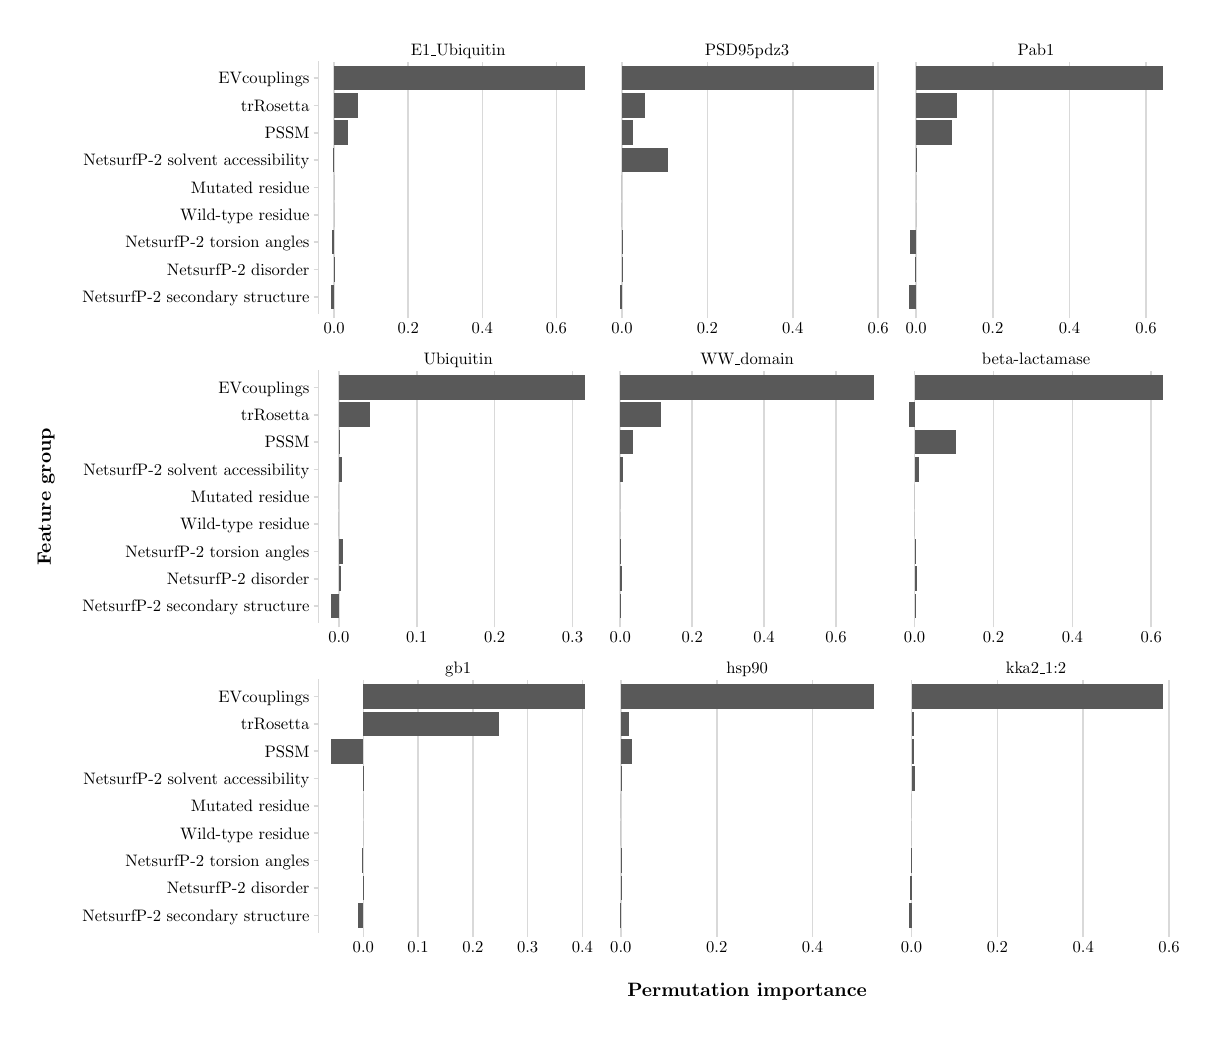
\begin{tikzpicture}[x=1pt,y=1pt]
\definecolor{fillColor}{RGB}{255,255,255}
\path[use as bounding box,fill=fillColor,fill opacity=0.00] (0,0) rectangle (418.34,354.99);
\begin{scope}
\path[clip] (105.09,251.79) rectangle (206.00,342.69);
\definecolor{drawColor}{gray}{0.85}

\path[draw=drawColor,line width= 0.6pt,line join=round] (110.76,251.79) --
	(110.76,342.69);

\path[draw=drawColor,line width= 0.6pt,line join=round] (137.53,251.79) --
	(137.53,342.69);

\path[draw=drawColor,line width= 0.6pt,line join=round] (164.29,251.79) --
	(164.29,342.69);

\path[draw=drawColor,line width= 0.6pt,line join=round] (191.06,251.79) --
	(191.06,342.69);
\definecolor{fillColor}{gray}{0.35}

\path[fill=fillColor] (110.76,322.43) rectangle (119.30,331.33);

\path[fill=fillColor] (110.76,312.55) rectangle (115.86,321.45);

\path[fill=fillColor] (110.49,302.67) rectangle (110.76,311.57);

\path[fill=fillColor] (109.68,253.27) rectangle (110.76,262.17);

\path[fill=fillColor] (110.71,263.15) rectangle (110.76,272.05);

\path[fill=fillColor] (109.89,273.03) rectangle (110.76,281.93);

\path[fill=fillColor] (110.76,332.31) rectangle (201.42,341.21);

\path[fill=fillColor] (110.76,282.91) rectangle (110.76,291.81);

\path[fill=fillColor] (110.76,292.79) rectangle (110.76,301.69);
\end{scope}
\begin{scope}
\path[clip] (105.09,140.05) rectangle (206.00,230.94);
\definecolor{drawColor}{gray}{0.85}

\path[draw=drawColor,line width= 0.6pt,line join=round] (112.45,140.05) --
	(112.45,230.94);

\path[draw=drawColor,line width= 0.6pt,line join=round] (140.59,140.05) --
	(140.59,230.94);

\path[draw=drawColor,line width= 0.6pt,line join=round] (168.73,140.05) --
	(168.73,230.94);

\path[draw=drawColor,line width= 0.6pt,line join=round] (196.87,140.05) --
	(196.87,230.94);
\definecolor{fillColor}{gray}{0.35}

\path[fill=fillColor] (112.45,210.69) rectangle (123.87,219.58);

\path[fill=fillColor] (112.45,200.81) rectangle (112.47,209.70);

\path[fill=fillColor] (112.45,190.93) rectangle (113.60,199.82);

\path[fill=fillColor] (109.68,141.53) rectangle (112.45,150.42);

\path[fill=fillColor] (112.45,151.41) rectangle (113.38,160.30);

\path[fill=fillColor] (112.45,161.29) rectangle (113.88,170.18);

\path[fill=fillColor] (112.45,220.57) rectangle (201.42,229.46);

\path[fill=fillColor] (112.45,171.17) rectangle (112.45,180.06);

\path[fill=fillColor] (112.45,181.05) rectangle (112.45,189.94);
\end{scope}
\begin{scope}
\path[clip] (105.09, 28.30) rectangle (206.00,119.20);
\definecolor{drawColor}{gray}{0.85}

\path[draw=drawColor,line width= 0.6pt,line join=round] (121.29, 28.30) --
	(121.29,119.20);

\path[draw=drawColor,line width= 0.6pt,line join=round] (141.08, 28.30) --
	(141.08,119.20);

\path[draw=drawColor,line width= 0.6pt,line join=round] (160.87, 28.30) --
	(160.87,119.20);

\path[draw=drawColor,line width= 0.6pt,line join=round] (180.66, 28.30) --
	(180.66,119.20);

\path[draw=drawColor,line width= 0.6pt,line join=round] (200.45, 28.30) --
	(200.45,119.20);
\definecolor{fillColor}{gray}{0.35}

\path[fill=fillColor] (121.29, 98.95) rectangle (170.19,107.84);

\path[fill=fillColor] (109.68, 89.07) rectangle (121.29, 97.96);

\path[fill=fillColor] (121.29, 79.19) rectangle (121.69, 88.08);

\path[fill=fillColor] (119.54, 29.79) rectangle (121.29, 38.68);

\path[fill=fillColor] (121.19, 39.67) rectangle (121.29, 48.56);

\path[fill=fillColor] (120.83, 49.55) rectangle (121.29, 58.44);

\path[fill=fillColor] (121.29,108.82) rectangle (201.42,117.72);

\path[fill=fillColor] (121.29, 59.43) rectangle (121.29, 68.32);

\path[fill=fillColor] (121.29, 69.31) rectangle (121.29, 78.20);
\end{scope}
\begin{scope}
\path[clip] (209.50,251.79) rectangle (310.42,342.69);
\definecolor{drawColor}{gray}{0.85}

\path[draw=drawColor,line width= 0.6pt,line join=round] (214.75,251.79) --
	(214.75,342.69);

\path[draw=drawColor,line width= 0.6pt,line join=round] (245.61,251.79) --
	(245.61,342.69);

\path[draw=drawColor,line width= 0.6pt,line join=round] (276.47,251.79) --
	(276.47,342.69);

\path[draw=drawColor,line width= 0.6pt,line join=round] (307.33,251.79) --
	(307.33,342.69);
\definecolor{fillColor}{gray}{0.35}

\path[fill=fillColor] (214.75,322.43) rectangle (223.22,331.33);

\path[fill=fillColor] (214.75,312.55) rectangle (218.91,321.45);

\path[fill=fillColor] (214.75,302.67) rectangle (231.39,311.57);

\path[fill=fillColor] (214.09,253.27) rectangle (214.75,262.17);

\path[fill=fillColor] (214.66,263.15) rectangle (214.75,272.05);

\path[fill=fillColor] (214.73,273.03) rectangle (214.75,281.93);

\path[fill=fillColor] (214.75,332.31) rectangle (305.83,341.21);

\path[fill=fillColor] (214.75,282.91) rectangle (214.75,291.81);

\path[fill=fillColor] (214.75,292.79) rectangle (214.75,301.69);
\end{scope}
\begin{scope}
\path[clip] (209.50,140.05) rectangle (310.42,230.94);
\definecolor{drawColor}{gray}{0.85}

\path[draw=drawColor,line width= 0.6pt,line join=round] (214.15,140.05) --
	(214.15,230.94);

\path[draw=drawColor,line width= 0.6pt,line join=round] (240.13,140.05) --
	(240.13,230.94);

\path[draw=drawColor,line width= 0.6pt,line join=round] (266.11,140.05) --
	(266.11,230.94);

\path[draw=drawColor,line width= 0.6pt,line join=round] (292.08,140.05) --
	(292.08,230.94);
\definecolor{fillColor}{gray}{0.35}

\path[fill=fillColor] (214.15,210.69) rectangle (228.78,219.58);

\path[fill=fillColor] (214.15,200.81) rectangle (218.80,209.70);

\path[fill=fillColor] (214.15,190.93) rectangle (214.96,199.82);

\path[fill=fillColor] (214.09,141.53) rectangle (214.15,150.42);

\path[fill=fillColor] (214.15,151.41) rectangle (214.78,160.30);

\path[fill=fillColor] (214.15,161.29) rectangle (214.33,170.18);

\path[fill=fillColor] (214.15,220.57) rectangle (305.83,229.46);

\path[fill=fillColor] (214.15,171.17) rectangle (214.15,180.06);

\path[fill=fillColor] (214.15,181.05) rectangle (214.15,189.94);
\end{scope}
\begin{scope}
\path[clip] (209.50, 28.30) rectangle (310.42,119.20);
\definecolor{drawColor}{gray}{0.85}

\path[draw=drawColor,line width= 0.6pt,line join=round] (214.33, 28.30) --
	(214.33,119.20);

\path[draw=drawColor,line width= 0.6pt,line join=round] (248.98, 28.30) --
	(248.98,119.20);

\path[draw=drawColor,line width= 0.6pt,line join=round] (283.63, 28.30) --
	(283.63,119.20);
\definecolor{fillColor}{gray}{0.35}

\path[fill=fillColor] (214.33, 98.95) rectangle (217.31,107.84);

\path[fill=fillColor] (214.33, 89.07) rectangle (218.52, 97.96);

\path[fill=fillColor] (214.33, 79.19) rectangle (214.34, 88.08);

\path[fill=fillColor] (214.09, 29.79) rectangle (214.33, 38.68);

\path[fill=fillColor] (214.33, 39.67) rectangle (214.57, 48.56);

\path[fill=fillColor] (214.33, 49.55) rectangle (214.52, 58.44);

\path[fill=fillColor] (214.33,108.82) rectangle (305.83,117.72);

\path[fill=fillColor] (214.33, 59.43) rectangle (214.33, 68.32);

\path[fill=fillColor] (214.33, 69.31) rectangle (214.33, 78.20);
\end{scope}
\begin{scope}
\path[clip] (313.92,251.79) rectangle (414.84,342.69);
\definecolor{drawColor}{gray}{0.85}

\path[draw=drawColor,line width= 0.6pt,line join=round] (321.05,251.79) --
	(321.05,342.69);

\path[draw=drawColor,line width= 0.6pt,line join=round] (348.75,251.79) --
	(348.75,342.69);

\path[draw=drawColor,line width= 0.6pt,line join=round] (376.45,251.79) --
	(376.45,342.69);

\path[draw=drawColor,line width= 0.6pt,line join=round] (404.14,251.79) --
	(404.14,342.69);
\definecolor{fillColor}{gray}{0.35}

\path[fill=fillColor] (321.05,322.43) rectangle (335.82,331.33);

\path[fill=fillColor] (321.05,312.55) rectangle (334.08,321.45);

\path[fill=fillColor] (321.00,302.67) rectangle (321.05,311.57);

\path[fill=fillColor] (318.51,253.27) rectangle (321.05,262.17);

\path[fill=fillColor] (320.68,263.15) rectangle (321.05,272.05);

\path[fill=fillColor] (318.83,273.03) rectangle (321.05,281.93);

\path[fill=fillColor] (321.05,332.31) rectangle (410.25,341.21);

\path[fill=fillColor] (321.05,282.91) rectangle (321.05,291.81);

\path[fill=fillColor] (321.05,292.79) rectangle (321.05,301.69);
\end{scope}
\begin{scope}
\path[clip] (313.92,140.05) rectangle (414.84,230.94);
\definecolor{drawColor}{gray}{0.85}

\path[draw=drawColor,line width= 0.6pt,line join=round] (320.49,140.05) --
	(320.49,230.94);

\path[draw=drawColor,line width= 0.6pt,line join=round] (348.99,140.05) --
	(348.99,230.94);

\path[draw=drawColor,line width= 0.6pt,line join=round] (377.50,140.05) --
	(377.50,230.94);

\path[draw=drawColor,line width= 0.6pt,line join=round] (406.00,140.05) --
	(406.00,230.94);
\definecolor{fillColor}{gray}{0.35}

\path[fill=fillColor] (318.51,210.69) rectangle (320.49,219.58);

\path[fill=fillColor] (320.49,200.81) rectangle (335.44,209.70);

\path[fill=fillColor] (320.49,190.93) rectangle (322.04,199.82);

\path[fill=fillColor] (320.49,141.53) rectangle (320.81,150.42);

\path[fill=fillColor] (320.49,151.41) rectangle (321.27,160.30);

\path[fill=fillColor] (320.49,161.29) rectangle (320.51,170.18);

\path[fill=fillColor] (320.49,220.57) rectangle (410.25,229.46);

\path[fill=fillColor] (320.49,171.17) rectangle (320.49,180.06);

\path[fill=fillColor] (320.49,181.05) rectangle (320.49,189.94);
\end{scope}
\begin{scope}
\path[clip] (313.92, 28.30) rectangle (414.84,119.20);
\definecolor{drawColor}{gray}{0.85}

\path[draw=drawColor,line width= 0.6pt,line join=round] (319.39, 28.30) --
	(319.39,119.20);

\path[draw=drawColor,line width= 0.6pt,line join=round] (350.41, 28.30) --
	(350.41,119.20);

\path[draw=drawColor,line width= 0.6pt,line join=round] (381.43, 28.30) --
	(381.43,119.20);

\path[draw=drawColor,line width= 0.6pt,line join=round] (412.45, 28.30) --
	(412.45,119.20);
\definecolor{fillColor}{gray}{0.35}

\path[fill=fillColor] (319.39, 98.95) rectangle (320.22,107.84);

\path[fill=fillColor] (319.39, 89.07) rectangle (320.27, 97.96);

\path[fill=fillColor] (319.39, 79.19) rectangle (320.60, 88.08);

\path[fill=fillColor] (318.51, 29.79) rectangle (319.39, 38.68);

\path[fill=fillColor] (318.92, 39.67) rectangle (319.39, 48.56);

\path[fill=fillColor] (319.32, 49.55) rectangle (319.39, 58.44);

\path[fill=fillColor] (319.39,108.82) rectangle (410.25,117.72);

\path[fill=fillColor] (319.39, 59.43) rectangle (319.39, 68.32);

\path[fill=fillColor] (319.39, 69.31) rectangle (319.39, 78.20);
\end{scope}
\begin{scope}
\path[clip] (105.09,119.20) rectangle (206.00,128.00);
\definecolor{drawColor}{RGB}{0,0,0}

\node[text=drawColor,anchor=base,inner sep=0pt, outer sep=0pt, scale=  0.60] at (155.55,121.53) {gb1};
\end{scope}
\begin{scope}
\path[clip] (209.50,119.20) rectangle (310.42,128.00);
\definecolor{drawColor}{RGB}{0,0,0}

\node[text=drawColor,anchor=base,inner sep=0pt, outer sep=0pt, scale=  0.60] at (259.96,121.53) {hsp90};
\end{scope}
\begin{scope}
\path[clip] (313.92,119.20) rectangle (414.84,128.00);
\definecolor{drawColor}{RGB}{0,0,0}

\node[text=drawColor,anchor=base,inner sep=0pt, outer sep=0pt, scale=  0.60] at (364.38,121.53) {kka2\_1:2};
\end{scope}
\begin{scope}
\path[clip] (105.09,230.94) rectangle (206.00,239.74);
\definecolor{drawColor}{RGB}{0,0,0}

\node[text=drawColor,anchor=base,inner sep=0pt, outer sep=0pt, scale=  0.60] at (155.55,233.28) {Ubiquitin};
\end{scope}
\begin{scope}
\path[clip] (209.50,230.94) rectangle (310.42,239.74);
\definecolor{drawColor}{RGB}{0,0,0}

\node[text=drawColor,anchor=base,inner sep=0pt, outer sep=0pt, scale=  0.60] at (259.96,233.28) {WW\_domain};
\end{scope}
\begin{scope}
\path[clip] (313.92,230.94) rectangle (414.84,239.74);
\definecolor{drawColor}{RGB}{0,0,0}

\node[text=drawColor,anchor=base,inner sep=0pt, outer sep=0pt, scale=  0.60] at (364.38,233.28) {beta-lactamase};
\end{scope}
\begin{scope}
\path[clip] (105.09,342.69) rectangle (206.00,351.49);
\definecolor{drawColor}{RGB}{0,0,0}

\node[text=drawColor,anchor=base,inner sep=0pt, outer sep=0pt, scale=  0.60] at (155.55,345.02) {E1\_Ubiquitin};
\end{scope}
\begin{scope}
\path[clip] (209.50,342.69) rectangle (310.42,351.49);
\definecolor{drawColor}{RGB}{0,0,0}

\node[text=drawColor,anchor=base,inner sep=0pt, outer sep=0pt, scale=  0.60] at (259.96,345.02) {PSD95pdz3};
\end{scope}
\begin{scope}
\path[clip] (313.92,342.69) rectangle (414.84,351.49);
\definecolor{drawColor}{RGB}{0,0,0}

\node[text=drawColor,anchor=base,inner sep=0pt, outer sep=0pt, scale=  0.60] at (364.38,345.02) {Pab1};
\end{scope}
\begin{scope}
\path[clip] (  0.00,  0.00) rectangle (418.34,354.99);
\definecolor{drawColor}{gray}{0.85}

\path[draw=drawColor,line width= 0.6pt,line join=round] (121.29, 26.55) --
	(121.29, 28.30);

\path[draw=drawColor,line width= 0.6pt,line join=round] (141.08, 26.55) --
	(141.08, 28.30);

\path[draw=drawColor,line width= 0.6pt,line join=round] (160.87, 26.55) --
	(160.87, 28.30);

\path[draw=drawColor,line width= 0.6pt,line join=round] (180.66, 26.55) --
	(180.66, 28.30);

\path[draw=drawColor,line width= 0.6pt,line join=round] (200.45, 26.55) --
	(200.45, 28.30);
\end{scope}
\begin{scope}
\path[clip] (  0.00,  0.00) rectangle (418.34,354.99);
\definecolor{drawColor}{RGB}{0,0,0}

\node[text=drawColor,anchor=base,inner sep=0pt, outer sep=0pt, scale=  0.60] at (121.29, 20.92) {0.0};

\node[text=drawColor,anchor=base,inner sep=0pt, outer sep=0pt, scale=  0.60] at (141.08, 20.92) {0.1};

\node[text=drawColor,anchor=base,inner sep=0pt, outer sep=0pt, scale=  0.60] at (160.87, 20.92) {0.2};

\node[text=drawColor,anchor=base,inner sep=0pt, outer sep=0pt, scale=  0.60] at (180.66, 20.92) {0.3};

\node[text=drawColor,anchor=base,inner sep=0pt, outer sep=0pt, scale=  0.60] at (200.45, 20.92) {0.4};
\end{scope}
\begin{scope}
\path[clip] (  0.00,  0.00) rectangle (418.34,354.99);
\definecolor{drawColor}{gray}{0.85}

\path[draw=drawColor,line width= 0.6pt,line join=round] (214.33, 26.55) --
	(214.33, 28.30);

\path[draw=drawColor,line width= 0.6pt,line join=round] (248.98, 26.55) --
	(248.98, 28.30);

\path[draw=drawColor,line width= 0.6pt,line join=round] (283.63, 26.55) --
	(283.63, 28.30);
\end{scope}
\begin{scope}
\path[clip] (  0.00,  0.00) rectangle (418.34,354.99);
\definecolor{drawColor}{RGB}{0,0,0}

\node[text=drawColor,anchor=base,inner sep=0pt, outer sep=0pt, scale=  0.60] at (214.33, 20.92) {0.0};

\node[text=drawColor,anchor=base,inner sep=0pt, outer sep=0pt, scale=  0.60] at (248.98, 20.92) {0.2};

\node[text=drawColor,anchor=base,inner sep=0pt, outer sep=0pt, scale=  0.60] at (283.63, 20.92) {0.4};
\end{scope}
\begin{scope}
\path[clip] (  0.00,  0.00) rectangle (418.34,354.99);
\definecolor{drawColor}{gray}{0.85}

\path[draw=drawColor,line width= 0.6pt,line join=round] (319.39, 26.55) --
	(319.39, 28.30);

\path[draw=drawColor,line width= 0.6pt,line join=round] (350.41, 26.55) --
	(350.41, 28.30);

\path[draw=drawColor,line width= 0.6pt,line join=round] (381.43, 26.55) --
	(381.43, 28.30);

\path[draw=drawColor,line width= 0.6pt,line join=round] (412.45, 26.55) --
	(412.45, 28.30);
\end{scope}
\begin{scope}
\path[clip] (  0.00,  0.00) rectangle (418.34,354.99);
\definecolor{drawColor}{RGB}{0,0,0}

\node[text=drawColor,anchor=base,inner sep=0pt, outer sep=0pt, scale=  0.60] at (319.39, 20.92) {0.0};

\node[text=drawColor,anchor=base,inner sep=0pt, outer sep=0pt, scale=  0.60] at (350.41, 20.92) {0.2};

\node[text=drawColor,anchor=base,inner sep=0pt, outer sep=0pt, scale=  0.60] at (381.43, 20.92) {0.4};

\node[text=drawColor,anchor=base,inner sep=0pt, outer sep=0pt, scale=  0.60] at (412.45, 20.92) {0.6};
\end{scope}
\begin{scope}
\path[clip] (  0.00,  0.00) rectangle (418.34,354.99);
\definecolor{drawColor}{gray}{0.85}

\path[draw=drawColor,line width= 0.6pt,line join=round] (112.45,138.30) --
	(112.45,140.05);

\path[draw=drawColor,line width= 0.6pt,line join=round] (140.59,138.30) --
	(140.59,140.05);

\path[draw=drawColor,line width= 0.6pt,line join=round] (168.73,138.30) --
	(168.73,140.05);

\path[draw=drawColor,line width= 0.6pt,line join=round] (196.87,138.30) --
	(196.87,140.05);
\end{scope}
\begin{scope}
\path[clip] (  0.00,  0.00) rectangle (418.34,354.99);
\definecolor{drawColor}{RGB}{0,0,0}

\node[text=drawColor,anchor=base,inner sep=0pt, outer sep=0pt, scale=  0.60] at (112.45,132.67) {0.0};

\node[text=drawColor,anchor=base,inner sep=0pt, outer sep=0pt, scale=  0.60] at (140.59,132.67) {0.1};

\node[text=drawColor,anchor=base,inner sep=0pt, outer sep=0pt, scale=  0.60] at (168.73,132.67) {0.2};

\node[text=drawColor,anchor=base,inner sep=0pt, outer sep=0pt, scale=  0.60] at (196.87,132.67) {0.3};
\end{scope}
\begin{scope}
\path[clip] (  0.00,  0.00) rectangle (418.34,354.99);
\definecolor{drawColor}{gray}{0.85}

\path[draw=drawColor,line width= 0.6pt,line join=round] (214.15,138.30) --
	(214.15,140.05);

\path[draw=drawColor,line width= 0.6pt,line join=round] (240.13,138.30) --
	(240.13,140.05);

\path[draw=drawColor,line width= 0.6pt,line join=round] (266.11,138.30) --
	(266.11,140.05);

\path[draw=drawColor,line width= 0.6pt,line join=round] (292.08,138.30) --
	(292.08,140.05);
\end{scope}
\begin{scope}
\path[clip] (  0.00,  0.00) rectangle (418.34,354.99);
\definecolor{drawColor}{RGB}{0,0,0}

\node[text=drawColor,anchor=base,inner sep=0pt, outer sep=0pt, scale=  0.60] at (214.15,132.67) {0.0};

\node[text=drawColor,anchor=base,inner sep=0pt, outer sep=0pt, scale=  0.60] at (240.13,132.67) {0.2};

\node[text=drawColor,anchor=base,inner sep=0pt, outer sep=0pt, scale=  0.60] at (266.11,132.67) {0.4};

\node[text=drawColor,anchor=base,inner sep=0pt, outer sep=0pt, scale=  0.60] at (292.08,132.67) {0.6};
\end{scope}
\begin{scope}
\path[clip] (  0.00,  0.00) rectangle (418.34,354.99);
\definecolor{drawColor}{gray}{0.85}

\path[draw=drawColor,line width= 0.6pt,line join=round] (320.49,138.30) --
	(320.49,140.05);

\path[draw=drawColor,line width= 0.6pt,line join=round] (348.99,138.30) --
	(348.99,140.05);

\path[draw=drawColor,line width= 0.6pt,line join=round] (377.50,138.30) --
	(377.50,140.05);

\path[draw=drawColor,line width= 0.6pt,line join=round] (406.00,138.30) --
	(406.00,140.05);
\end{scope}
\begin{scope}
\path[clip] (  0.00,  0.00) rectangle (418.34,354.99);
\definecolor{drawColor}{RGB}{0,0,0}

\node[text=drawColor,anchor=base,inner sep=0pt, outer sep=0pt, scale=  0.60] at (320.49,132.67) {0.0};

\node[text=drawColor,anchor=base,inner sep=0pt, outer sep=0pt, scale=  0.60] at (348.99,132.67) {0.2};

\node[text=drawColor,anchor=base,inner sep=0pt, outer sep=0pt, scale=  0.60] at (377.50,132.67) {0.4};

\node[text=drawColor,anchor=base,inner sep=0pt, outer sep=0pt, scale=  0.60] at (406.00,132.67) {0.6};
\end{scope}
\begin{scope}
\path[clip] (  0.00,  0.00) rectangle (418.34,354.99);
\definecolor{drawColor}{gray}{0.85}

\path[draw=drawColor,line width= 0.6pt,line join=round] (110.76,250.04) --
	(110.76,251.79);

\path[draw=drawColor,line width= 0.6pt,line join=round] (137.53,250.04) --
	(137.53,251.79);

\path[draw=drawColor,line width= 0.6pt,line join=round] (164.29,250.04) --
	(164.29,251.79);

\path[draw=drawColor,line width= 0.6pt,line join=round] (191.06,250.04) --
	(191.06,251.79);
\end{scope}
\begin{scope}
\path[clip] (  0.00,  0.00) rectangle (418.34,354.99);
\definecolor{drawColor}{RGB}{0,0,0}

\node[text=drawColor,anchor=base,inner sep=0pt, outer sep=0pt, scale=  0.60] at (110.76,244.41) {0.0};

\node[text=drawColor,anchor=base,inner sep=0pt, outer sep=0pt, scale=  0.60] at (137.53,244.41) {0.2};

\node[text=drawColor,anchor=base,inner sep=0pt, outer sep=0pt, scale=  0.60] at (164.29,244.41) {0.4};

\node[text=drawColor,anchor=base,inner sep=0pt, outer sep=0pt, scale=  0.60] at (191.06,244.41) {0.6};
\end{scope}
\begin{scope}
\path[clip] (  0.00,  0.00) rectangle (418.34,354.99);
\definecolor{drawColor}{gray}{0.85}

\path[draw=drawColor,line width= 0.6pt,line join=round] (214.75,250.04) --
	(214.75,251.79);

\path[draw=drawColor,line width= 0.6pt,line join=round] (245.61,250.04) --
	(245.61,251.79);

\path[draw=drawColor,line width= 0.6pt,line join=round] (276.47,250.04) --
	(276.47,251.79);

\path[draw=drawColor,line width= 0.6pt,line join=round] (307.33,250.04) --
	(307.33,251.79);
\end{scope}
\begin{scope}
\path[clip] (  0.00,  0.00) rectangle (418.34,354.99);
\definecolor{drawColor}{RGB}{0,0,0}

\node[text=drawColor,anchor=base,inner sep=0pt, outer sep=0pt, scale=  0.60] at (214.75,244.41) {0.0};

\node[text=drawColor,anchor=base,inner sep=0pt, outer sep=0pt, scale=  0.60] at (245.61,244.41) {0.2};

\node[text=drawColor,anchor=base,inner sep=0pt, outer sep=0pt, scale=  0.60] at (276.47,244.41) {0.4};

\node[text=drawColor,anchor=base,inner sep=0pt, outer sep=0pt, scale=  0.60] at (307.33,244.41) {0.6};
\end{scope}
\begin{scope}
\path[clip] (  0.00,  0.00) rectangle (418.34,354.99);
\definecolor{drawColor}{gray}{0.85}

\path[draw=drawColor,line width= 0.6pt,line join=round] (321.05,250.04) --
	(321.05,251.79);

\path[draw=drawColor,line width= 0.6pt,line join=round] (348.75,250.04) --
	(348.75,251.79);

\path[draw=drawColor,line width= 0.6pt,line join=round] (376.45,250.04) --
	(376.45,251.79);

\path[draw=drawColor,line width= 0.6pt,line join=round] (404.14,250.04) --
	(404.14,251.79);
\end{scope}
\begin{scope}
\path[clip] (  0.00,  0.00) rectangle (418.34,354.99);
\definecolor{drawColor}{RGB}{0,0,0}

\node[text=drawColor,anchor=base,inner sep=0pt, outer sep=0pt, scale=  0.60] at (321.05,244.41) {0.0};

\node[text=drawColor,anchor=base,inner sep=0pt, outer sep=0pt, scale=  0.60] at (348.75,244.41) {0.2};

\node[text=drawColor,anchor=base,inner sep=0pt, outer sep=0pt, scale=  0.60] at (376.45,244.41) {0.4};

\node[text=drawColor,anchor=base,inner sep=0pt, outer sep=0pt, scale=  0.60] at (404.14,244.41) {0.6};
\end{scope}
\begin{scope}
\path[clip] (  0.00,  0.00) rectangle (418.34,354.99);
\definecolor{drawColor}{gray}{0.85}

\path[draw=drawColor,line width= 0.6pt,line join=round,line cap=rect] (105.09,251.79) --
	(105.09,342.69);
\end{scope}
\begin{scope}
\path[clip] (  0.00,  0.00) rectangle (418.34,354.99);
\definecolor{drawColor}{RGB}{0,0,0}

\node[text=drawColor,anchor=base east,inner sep=0pt, outer sep=0pt, scale=  0.60] at (101.84,255.65) {NetsurfP-2 secondary structure};

\node[text=drawColor,anchor=base east,inner sep=0pt, outer sep=0pt, scale=  0.60] at (101.84,265.53) {NetsurfP-2 disorder};

\node[text=drawColor,anchor=base east,inner sep=0pt, outer sep=0pt, scale=  0.60] at (101.84,275.41) {NetsurfP-2 torsion angles};

\node[text=drawColor,anchor=base east,inner sep=0pt, outer sep=0pt, scale=  0.60] at (101.84,285.29) {Wild-type residue};

\node[text=drawColor,anchor=base east,inner sep=0pt, outer sep=0pt, scale=  0.60] at (101.84,295.17) {Mutated residue};

\node[text=drawColor,anchor=base east,inner sep=0pt, outer sep=0pt, scale=  0.60] at (101.84,305.05) {NetsurfP-2 solvent accessibility};

\node[text=drawColor,anchor=base east,inner sep=0pt, outer sep=0pt, scale=  0.60] at (101.84,314.93) {PSSM};

\node[text=drawColor,anchor=base east,inner sep=0pt, outer sep=0pt, scale=  0.60] at (101.84,324.81) {trRosetta};

\node[text=drawColor,anchor=base east,inner sep=0pt, outer sep=0pt, scale=  0.60] at (101.84,334.69) {EVcouplings};
\end{scope}
\begin{scope}
\path[clip] (  0.00,  0.00) rectangle (418.34,354.99);
\definecolor{drawColor}{gray}{0.85}

\path[draw=drawColor,line width= 0.6pt,line join=round] (103.34,257.72) --
	(105.09,257.72);

\path[draw=drawColor,line width= 0.6pt,line join=round] (103.34,267.60) --
	(105.09,267.60);

\path[draw=drawColor,line width= 0.6pt,line join=round] (103.34,277.48) --
	(105.09,277.48);

\path[draw=drawColor,line width= 0.6pt,line join=round] (103.34,287.36) --
	(105.09,287.36);

\path[draw=drawColor,line width= 0.6pt,line join=round] (103.34,297.24) --
	(105.09,297.24);

\path[draw=drawColor,line width= 0.6pt,line join=round] (103.34,307.12) --
	(105.09,307.12);

\path[draw=drawColor,line width= 0.6pt,line join=round] (103.34,317.00) --
	(105.09,317.00);

\path[draw=drawColor,line width= 0.6pt,line join=round] (103.34,326.88) --
	(105.09,326.88);

\path[draw=drawColor,line width= 0.6pt,line join=round] (103.34,336.76) --
	(105.09,336.76);
\end{scope}
\begin{scope}
\path[clip] (  0.00,  0.00) rectangle (418.34,354.99);
\definecolor{drawColor}{gray}{0.85}

\path[draw=drawColor,line width= 0.6pt,line join=round,line cap=rect] (105.09,140.05) --
	(105.09,230.94);
\end{scope}
\begin{scope}
\path[clip] (  0.00,  0.00) rectangle (418.34,354.99);
\definecolor{drawColor}{RGB}{0,0,0}

\node[text=drawColor,anchor=base east,inner sep=0pt, outer sep=0pt, scale=  0.60] at (101.84,143.91) {NetsurfP-2 secondary structure};

\node[text=drawColor,anchor=base east,inner sep=0pt, outer sep=0pt, scale=  0.60] at (101.84,153.79) {NetsurfP-2 disorder};

\node[text=drawColor,anchor=base east,inner sep=0pt, outer sep=0pt, scale=  0.60] at (101.84,163.67) {NetsurfP-2 torsion angles};

\node[text=drawColor,anchor=base east,inner sep=0pt, outer sep=0pt, scale=  0.60] at (101.84,173.55) {Wild-type residue};

\node[text=drawColor,anchor=base east,inner sep=0pt, outer sep=0pt, scale=  0.60] at (101.84,183.43) {Mutated residue};

\node[text=drawColor,anchor=base east,inner sep=0pt, outer sep=0pt, scale=  0.60] at (101.84,193.31) {NetsurfP-2 solvent accessibility};

\node[text=drawColor,anchor=base east,inner sep=0pt, outer sep=0pt, scale=  0.60] at (101.84,203.19) {PSSM};

\node[text=drawColor,anchor=base east,inner sep=0pt, outer sep=0pt, scale=  0.60] at (101.84,213.07) {trRosetta};

\node[text=drawColor,anchor=base east,inner sep=0pt, outer sep=0pt, scale=  0.60] at (101.84,222.95) {EVcouplings};
\end{scope}
\begin{scope}
\path[clip] (  0.00,  0.00) rectangle (418.34,354.99);
\definecolor{drawColor}{gray}{0.85}

\path[draw=drawColor,line width= 0.6pt,line join=round] (103.34,145.98) --
	(105.09,145.98);

\path[draw=drawColor,line width= 0.6pt,line join=round] (103.34,155.86) --
	(105.09,155.86);

\path[draw=drawColor,line width= 0.6pt,line join=round] (103.34,165.74) --
	(105.09,165.74);

\path[draw=drawColor,line width= 0.6pt,line join=round] (103.34,175.62) --
	(105.09,175.62);

\path[draw=drawColor,line width= 0.6pt,line join=round] (103.34,185.50) --
	(105.09,185.50);

\path[draw=drawColor,line width= 0.6pt,line join=round] (103.34,195.38) --
	(105.09,195.38);

\path[draw=drawColor,line width= 0.6pt,line join=round] (103.34,205.26) --
	(105.09,205.26);

\path[draw=drawColor,line width= 0.6pt,line join=round] (103.34,215.14) --
	(105.09,215.14);

\path[draw=drawColor,line width= 0.6pt,line join=round] (103.34,225.02) --
	(105.09,225.02);
\end{scope}
\begin{scope}
\path[clip] (  0.00,  0.00) rectangle (418.34,354.99);
\definecolor{drawColor}{gray}{0.85}

\path[draw=drawColor,line width= 0.6pt,line join=round,line cap=rect] (105.09, 28.30) --
	(105.09,119.20);
\end{scope}
\begin{scope}
\path[clip] (  0.00,  0.00) rectangle (418.34,354.99);
\definecolor{drawColor}{RGB}{0,0,0}

\node[text=drawColor,anchor=base east,inner sep=0pt, outer sep=0pt, scale=  0.60] at (101.84, 32.17) {NetsurfP-2 secondary structure};

\node[text=drawColor,anchor=base east,inner sep=0pt, outer sep=0pt, scale=  0.60] at (101.84, 42.05) {NetsurfP-2 disorder};

\node[text=drawColor,anchor=base east,inner sep=0pt, outer sep=0pt, scale=  0.60] at (101.84, 51.93) {NetsurfP-2 torsion angles};

\node[text=drawColor,anchor=base east,inner sep=0pt, outer sep=0pt, scale=  0.60] at (101.84, 61.81) {Wild-type residue};

\node[text=drawColor,anchor=base east,inner sep=0pt, outer sep=0pt, scale=  0.60] at (101.84, 71.68) {Mutated residue};

\node[text=drawColor,anchor=base east,inner sep=0pt, outer sep=0pt, scale=  0.60] at (101.84, 81.56) {NetsurfP-2 solvent accessibility};

\node[text=drawColor,anchor=base east,inner sep=0pt, outer sep=0pt, scale=  0.60] at (101.84, 91.44) {PSSM};

\node[text=drawColor,anchor=base east,inner sep=0pt, outer sep=0pt, scale=  0.60] at (101.84,101.32) {trRosetta};

\node[text=drawColor,anchor=base east,inner sep=0pt, outer sep=0pt, scale=  0.60] at (101.84,111.20) {EVcouplings};
\end{scope}
\begin{scope}
\path[clip] (  0.00,  0.00) rectangle (418.34,354.99);
\definecolor{drawColor}{gray}{0.85}

\path[draw=drawColor,line width= 0.6pt,line join=round] (103.34, 34.23) --
	(105.09, 34.23);

\path[draw=drawColor,line width= 0.6pt,line join=round] (103.34, 44.11) --
	(105.09, 44.11);

\path[draw=drawColor,line width= 0.6pt,line join=round] (103.34, 53.99) --
	(105.09, 53.99);

\path[draw=drawColor,line width= 0.6pt,line join=round] (103.34, 63.87) --
	(105.09, 63.87);

\path[draw=drawColor,line width= 0.6pt,line join=round] (103.34, 73.75) --
	(105.09, 73.75);

\path[draw=drawColor,line width= 0.6pt,line join=round] (103.34, 83.63) --
	(105.09, 83.63);

\path[draw=drawColor,line width= 0.6pt,line join=round] (103.34, 93.51) --
	(105.09, 93.51);

\path[draw=drawColor,line width= 0.6pt,line join=round] (103.34,103.39) --
	(105.09,103.39);

\path[draw=drawColor,line width= 0.6pt,line join=round] (103.34,113.27) --
	(105.09,113.27);
\end{scope}
\begin{scope}
\path[clip] (  0.00,  0.00) rectangle (418.34,354.99);
\definecolor{drawColor}{RGB}{0,0,0}

\node[text=drawColor,anchor=base,inner sep=0pt, outer sep=0pt, scale=  0.70] at (259.96,  4.86) {\bfseries Permutation importance};
\end{scope}
\begin{scope}
\path[clip] (  0.00,  0.00) rectangle (418.34,354.99);
\definecolor{drawColor}{RGB}{0,0,0}

\node[text=drawColor,rotate= 90.00,anchor=base,inner sep=0pt, outer sep=0pt, scale=  0.70] at (  8.39,185.50) {\bfseries Feature group};
\end{scope}
\end{tikzpicture}%
}{%
		\caption[Feature importance for the general gradient boosted trees models]{%
			\textbf{Feature importance for the general gradient boosted trees models.}
			Series of bar plots showing the grouped permutation importance of the features used in the general models trained in a LOPO fashion, subdivided by dataset.
			These plots refer to the importances in the gradient boosted tree models.
		}%
		\label{fig:feature_importance_general_xgb}%
	}%
\end{figure}

\begin{figure}[p]
	\ffigbox[\FBwidth]{% Created by tikzDevice version 0.12.3.1 on 2021-06-13 12:18:57
% !TEX encoding = UTF-8 Unicode
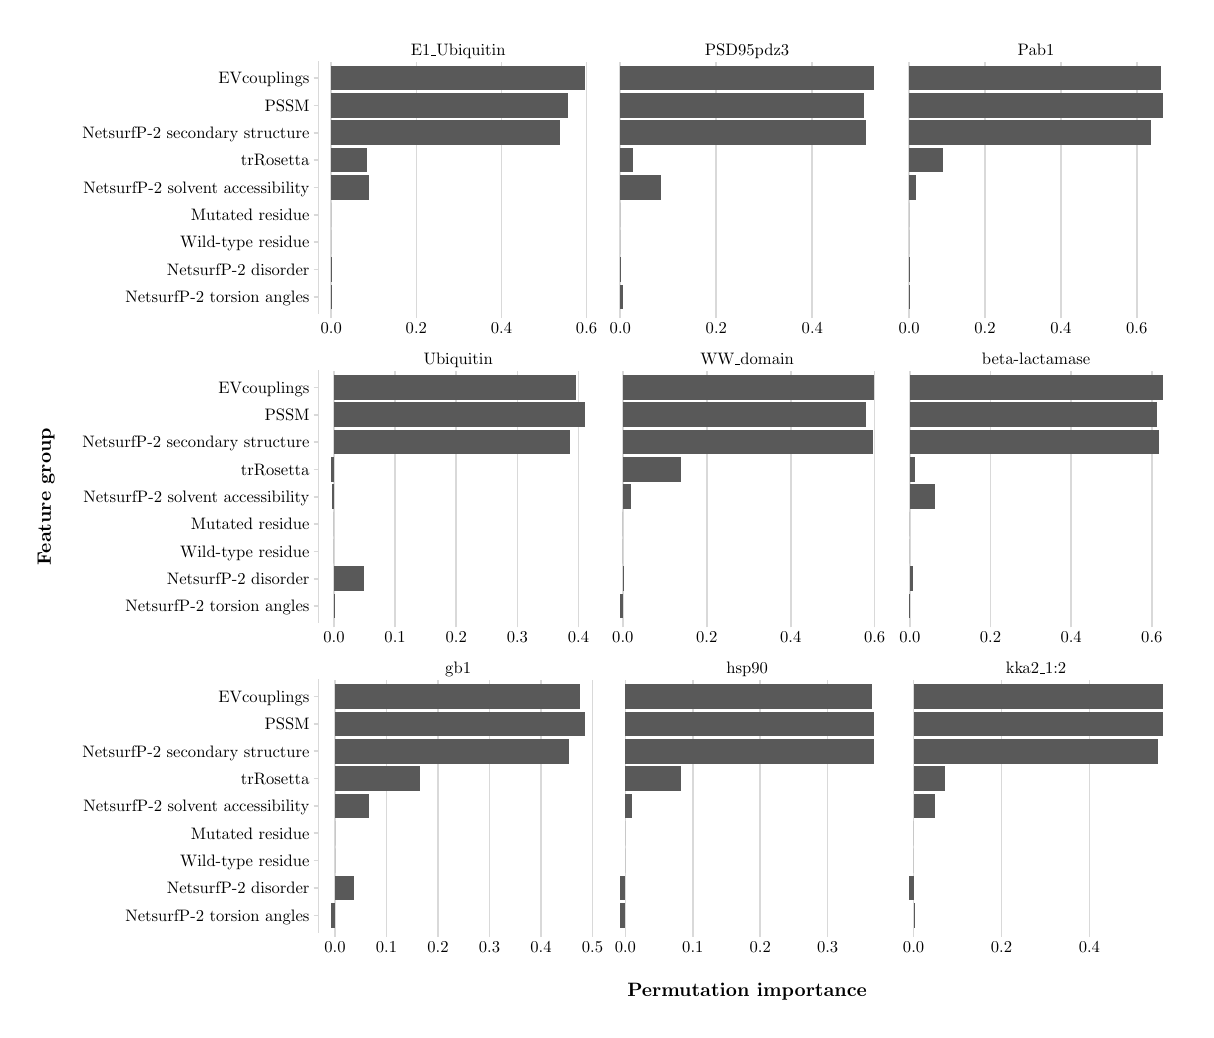
\begin{tikzpicture}[x=1pt,y=1pt]
\definecolor{fillColor}{RGB}{255,255,255}
\path[use as bounding box,fill=fillColor,fill opacity=0.00] (0,0) rectangle (418.34,354.99);
\begin{scope}
\path[clip] (105.09,251.79) rectangle (206.00,342.69);
\definecolor{drawColor}{gray}{0.85}

\path[draw=drawColor,line width= 0.6pt,line join=round] (109.69,251.79) --
	(109.69,342.69);

\path[draw=drawColor,line width= 0.6pt,line join=round] (140.45,251.79) --
	(140.45,342.69);

\path[draw=drawColor,line width= 0.6pt,line join=round] (171.21,251.79) --
	(171.21,342.69);

\path[draw=drawColor,line width= 0.6pt,line join=round] (201.96,251.79) --
	(201.96,342.69);
\definecolor{fillColor}{gray}{0.35}

\path[fill=fillColor] (109.69,302.67) rectangle (122.69,311.57);

\path[fill=fillColor] (109.69,322.43) rectangle (195.31,331.33);

\path[fill=fillColor] (109.69,292.79) rectangle (123.28,301.69);

\path[fill=fillColor] (109.69,312.55) rectangle (192.26,321.45);

\path[fill=fillColor] (109.69,263.15) rectangle (109.70,272.05);

\path[fill=fillColor] (109.68,253.27) rectangle (109.69,262.17);

\path[fill=fillColor] (109.69,332.31) rectangle (201.42,341.21);

\path[fill=fillColor] (109.69,273.03) rectangle (109.69,281.93);

\path[fill=fillColor] (109.69,282.91) rectangle (109.69,291.81);
\end{scope}
\begin{scope}
\path[clip] (105.09,140.05) rectangle (206.00,230.94);
\definecolor{drawColor}{gray}{0.85}

\path[draw=drawColor,line width= 0.6pt,line join=round] (110.68,140.05) --
	(110.68,230.94);

\path[draw=drawColor,line width= 0.6pt,line join=round] (132.77,140.05) --
	(132.77,230.94);

\path[draw=drawColor,line width= 0.6pt,line join=round] (154.86,140.05) --
	(154.86,230.94);

\path[draw=drawColor,line width= 0.6pt,line join=round] (176.95,140.05) --
	(176.95,230.94);

\path[draw=drawColor,line width= 0.6pt,line join=round] (199.04,140.05) --
	(199.04,230.94);
\definecolor{fillColor}{gray}{0.35}

\path[fill=fillColor] (109.68,190.93) rectangle (110.68,199.82);

\path[fill=fillColor] (110.68,210.69) rectangle (201.42,219.58);

\path[fill=fillColor] (110.07,181.05) rectangle (110.68,189.94);

\path[fill=fillColor] (110.68,200.81) rectangle (195.95,209.70);

\path[fill=fillColor] (110.68,151.41) rectangle (121.65,160.30);

\path[fill=fillColor] (110.68,141.53) rectangle (111.20,150.42);

\path[fill=fillColor] (110.68,220.57) rectangle (198.22,229.46);

\path[fill=fillColor] (110.68,161.29) rectangle (110.68,170.18);

\path[fill=fillColor] (110.68,171.17) rectangle (110.68,180.06);
\end{scope}
\begin{scope}
\path[clip] (105.09, 28.30) rectangle (206.00,119.20);
\definecolor{drawColor}{gray}{0.85}

\path[draw=drawColor,line width= 0.6pt,line join=round] (111.07, 28.30) --
	(111.07,119.20);

\path[draw=drawColor,line width= 0.6pt,line join=round] (129.68, 28.30) --
	(129.68,119.20);

\path[draw=drawColor,line width= 0.6pt,line join=round] (148.28, 28.30) --
	(148.28,119.20);

\path[draw=drawColor,line width= 0.6pt,line join=round] (166.88, 28.30) --
	(166.88,119.20);

\path[draw=drawColor,line width= 0.6pt,line join=round] (185.48, 28.30) --
	(185.48,119.20);

\path[draw=drawColor,line width= 0.6pt,line join=round] (204.08, 28.30) --
	(204.08,119.20);
\definecolor{fillColor}{gray}{0.35}

\path[fill=fillColor] (111.07, 79.19) rectangle (141.81, 88.08);

\path[fill=fillColor] (111.07, 98.95) rectangle (201.42,107.84);

\path[fill=fillColor] (111.07, 69.31) rectangle (123.44, 78.20);

\path[fill=fillColor] (111.07, 89.07) rectangle (195.66, 97.96);

\path[fill=fillColor] (111.07, 39.67) rectangle (117.86, 48.56);

\path[fill=fillColor] (109.68, 29.79) rectangle (111.07, 38.68);

\path[fill=fillColor] (111.07,108.82) rectangle (199.51,117.72);

\path[fill=fillColor] (111.07, 49.55) rectangle (111.07, 58.44);

\path[fill=fillColor] (111.07, 59.43) rectangle (111.07, 68.32);
\end{scope}
\begin{scope}
\path[clip] (209.50,251.79) rectangle (310.42,342.69);
\definecolor{drawColor}{gray}{0.85}

\path[draw=drawColor,line width= 0.6pt,line join=round] (214.15,251.79) --
	(214.15,342.69);

\path[draw=drawColor,line width= 0.6pt,line join=round] (248.84,251.79) --
	(248.84,342.69);

\path[draw=drawColor,line width= 0.6pt,line join=round] (283.53,251.79) --
	(283.53,342.69);
\definecolor{fillColor}{gray}{0.35}

\path[fill=fillColor] (214.15,302.67) rectangle (218.58,311.57);

\path[fill=fillColor] (214.15,322.43) rectangle (302.20,331.33);

\path[fill=fillColor] (214.15,292.79) rectangle (228.73,301.69);

\path[fill=fillColor] (214.15,312.55) rectangle (303.00,321.45);

\path[fill=fillColor] (214.09,263.15) rectangle (214.15,272.05);

\path[fill=fillColor] (214.15,253.27) rectangle (215.10,262.17);

\path[fill=fillColor] (214.15,332.31) rectangle (305.83,341.21);

\path[fill=fillColor] (214.15,273.03) rectangle (214.15,281.93);

\path[fill=fillColor] (214.15,282.91) rectangle (214.15,291.81);
\end{scope}
\begin{scope}
\path[clip] (209.50,140.05) rectangle (310.42,230.94);
\definecolor{drawColor}{gray}{0.85}

\path[draw=drawColor,line width= 0.6pt,line join=round] (215.06,140.05) --
	(215.06,230.94);

\path[draw=drawColor,line width= 0.6pt,line join=round] (245.39,140.05) --
	(245.39,230.94);

\path[draw=drawColor,line width= 0.6pt,line join=round] (275.72,140.05) --
	(275.72,230.94);

\path[draw=drawColor,line width= 0.6pt,line join=round] (306.05,140.05) --
	(306.05,230.94);
\definecolor{fillColor}{gray}{0.35}

\path[fill=fillColor] (215.06,190.93) rectangle (236.16,199.82);

\path[fill=fillColor] (215.06,210.69) rectangle (302.93,219.58);

\path[fill=fillColor] (215.06,181.05) rectangle (217.87,189.94);

\path[fill=fillColor] (215.06,200.81) rectangle (305.55,209.70);

\path[fill=fillColor] (215.04,151.41) rectangle (215.06,160.30);

\path[fill=fillColor] (214.09,141.53) rectangle (215.06,150.42);

\path[fill=fillColor] (215.06,220.57) rectangle (305.83,229.46);

\path[fill=fillColor] (215.06,161.29) rectangle (215.06,170.18);

\path[fill=fillColor] (215.06,171.17) rectangle (215.06,180.06);
\end{scope}
\begin{scope}
\path[clip] (209.50, 28.30) rectangle (310.42,119.20);
\definecolor{drawColor}{gray}{0.85}

\path[draw=drawColor,line width= 0.6pt,line join=round] (215.99, 28.30) --
	(215.99,119.20);

\path[draw=drawColor,line width= 0.6pt,line join=round] (240.35, 28.30) --
	(240.35,119.20);

\path[draw=drawColor,line width= 0.6pt,line join=round] (264.70, 28.30) --
	(264.70,119.20);

\path[draw=drawColor,line width= 0.6pt,line join=round] (289.06, 28.30) --
	(289.06,119.20);
\definecolor{fillColor}{gray}{0.35}

\path[fill=fillColor] (215.99, 79.19) rectangle (236.05, 88.08);

\path[fill=fillColor] (215.99, 98.95) rectangle (305.83,107.84);

\path[fill=fillColor] (215.99, 69.31) rectangle (218.42, 78.20);

\path[fill=fillColor] (215.99, 89.07) rectangle (305.64, 97.96);

\path[fill=fillColor] (214.09, 39.67) rectangle (215.99, 48.56);

\path[fill=fillColor] (214.18, 29.79) rectangle (215.99, 38.68);

\path[fill=fillColor] (215.99,108.82) rectangle (305.07,117.72);

\path[fill=fillColor] (215.99, 49.55) rectangle (215.99, 58.44);

\path[fill=fillColor] (215.99, 59.43) rectangle (215.99, 68.32);
\end{scope}
\begin{scope}
\path[clip] (313.92,251.79) rectangle (414.84,342.69);
\definecolor{drawColor}{gray}{0.85}

\path[draw=drawColor,line width= 0.6pt,line join=round] (318.52,251.79) --
	(318.52,342.69);

\path[draw=drawColor,line width= 0.6pt,line join=round] (345.93,251.79) --
	(345.93,342.69);

\path[draw=drawColor,line width= 0.6pt,line join=round] (373.35,251.79) --
	(373.35,342.69);

\path[draw=drawColor,line width= 0.6pt,line join=round] (400.76,251.79) --
	(400.76,342.69);
\definecolor{fillColor}{gray}{0.35}

\path[fill=fillColor] (318.52,302.67) rectangle (330.70,311.57);

\path[fill=fillColor] (318.52,322.43) rectangle (410.25,331.33);

\path[fill=fillColor] (318.52,292.79) rectangle (320.99,301.69);

\path[fill=fillColor] (318.52,312.55) rectangle (406.00,321.45);

\path[fill=fillColor] (318.51,263.15) rectangle (318.52,272.05);

\path[fill=fillColor] (318.52,253.27) rectangle (318.61,262.17);

\path[fill=fillColor] (318.52,332.31) rectangle (409.46,341.21);

\path[fill=fillColor] (318.52,273.03) rectangle (318.52,281.93);

\path[fill=fillColor] (318.52,282.91) rectangle (318.52,291.81);
\end{scope}
\begin{scope}
\path[clip] (313.92,140.05) rectangle (414.84,230.94);
\definecolor{drawColor}{gray}{0.85}

\path[draw=drawColor,line width= 0.6pt,line join=round] (318.79,140.05) --
	(318.79,230.94);

\path[draw=drawColor,line width= 0.6pt,line join=round] (347.93,140.05) --
	(347.93,230.94);

\path[draw=drawColor,line width= 0.6pt,line join=round] (377.07,140.05) --
	(377.07,230.94);

\path[draw=drawColor,line width= 0.6pt,line join=round] (406.21,140.05) --
	(406.21,230.94);
\definecolor{fillColor}{gray}{0.35}

\path[fill=fillColor] (318.79,190.93) rectangle (320.81,199.82);

\path[fill=fillColor] (318.79,210.69) rectangle (408.01,219.58);

\path[fill=fillColor] (318.79,181.05) rectangle (327.94,189.94);

\path[fill=fillColor] (318.79,200.81) rectangle (408.77,209.70);

\path[fill=fillColor] (318.79,151.41) rectangle (319.84,160.30);

\path[fill=fillColor] (318.51,141.53) rectangle (318.79,150.42);

\path[fill=fillColor] (318.79,220.57) rectangle (410.25,229.46);

\path[fill=fillColor] (318.79,161.29) rectangle (318.79,170.18);

\path[fill=fillColor] (318.79,171.17) rectangle (318.79,180.06);
\end{scope}
\begin{scope}
\path[clip] (313.92, 28.30) rectangle (414.84,119.20);
\definecolor{drawColor}{gray}{0.85}

\path[draw=drawColor,line width= 0.6pt,line join=round] (320.13, 28.30) --
	(320.13,119.20);

\path[draw=drawColor,line width= 0.6pt,line join=round] (351.89, 28.30) --
	(351.89,119.20);

\path[draw=drawColor,line width= 0.6pt,line join=round] (383.65, 28.30) --
	(383.65,119.20);
\definecolor{fillColor}{gray}{0.35}

\path[fill=fillColor] (320.13, 79.19) rectangle (331.43, 88.08);

\path[fill=fillColor] (320.13, 98.95) rectangle (410.09,107.84);

\path[fill=fillColor] (320.13, 69.31) rectangle (327.87, 78.20);

\path[fill=fillColor] (320.13, 89.07) rectangle (408.33, 97.96);

\path[fill=fillColor] (318.51, 39.67) rectangle (320.13, 48.56);

\path[fill=fillColor] (320.13, 29.79) rectangle (320.27, 38.68);

\path[fill=fillColor] (320.13,108.82) rectangle (410.25,117.72);

\path[fill=fillColor] (320.13, 49.55) rectangle (320.13, 58.44);

\path[fill=fillColor] (320.13, 59.43) rectangle (320.13, 68.32);
\end{scope}
\begin{scope}
\path[clip] (105.09,119.20) rectangle (206.00,128.00);
\definecolor{drawColor}{RGB}{0,0,0}

\node[text=drawColor,anchor=base,inner sep=0pt, outer sep=0pt, scale=  0.60] at (155.55,121.53) {gb1};
\end{scope}
\begin{scope}
\path[clip] (209.50,119.20) rectangle (310.42,128.00);
\definecolor{drawColor}{RGB}{0,0,0}

\node[text=drawColor,anchor=base,inner sep=0pt, outer sep=0pt, scale=  0.60] at (259.96,121.53) {hsp90};
\end{scope}
\begin{scope}
\path[clip] (313.92,119.20) rectangle (414.84,128.00);
\definecolor{drawColor}{RGB}{0,0,0}

\node[text=drawColor,anchor=base,inner sep=0pt, outer sep=0pt, scale=  0.60] at (364.38,121.53) {kka2\_1:2};
\end{scope}
\begin{scope}
\path[clip] (105.09,230.94) rectangle (206.00,239.74);
\definecolor{drawColor}{RGB}{0,0,0}

\node[text=drawColor,anchor=base,inner sep=0pt, outer sep=0pt, scale=  0.60] at (155.55,233.28) {Ubiquitin};
\end{scope}
\begin{scope}
\path[clip] (209.50,230.94) rectangle (310.42,239.74);
\definecolor{drawColor}{RGB}{0,0,0}

\node[text=drawColor,anchor=base,inner sep=0pt, outer sep=0pt, scale=  0.60] at (259.96,233.28) {WW\_domain};
\end{scope}
\begin{scope}
\path[clip] (313.92,230.94) rectangle (414.84,239.74);
\definecolor{drawColor}{RGB}{0,0,0}

\node[text=drawColor,anchor=base,inner sep=0pt, outer sep=0pt, scale=  0.60] at (364.38,233.28) {beta-lactamase};
\end{scope}
\begin{scope}
\path[clip] (105.09,342.69) rectangle (206.00,351.49);
\definecolor{drawColor}{RGB}{0,0,0}

\node[text=drawColor,anchor=base,inner sep=0pt, outer sep=0pt, scale=  0.60] at (155.55,345.02) {E1\_Ubiquitin};
\end{scope}
\begin{scope}
\path[clip] (209.50,342.69) rectangle (310.42,351.49);
\definecolor{drawColor}{RGB}{0,0,0}

\node[text=drawColor,anchor=base,inner sep=0pt, outer sep=0pt, scale=  0.60] at (259.96,345.02) {PSD95pdz3};
\end{scope}
\begin{scope}
\path[clip] (313.92,342.69) rectangle (414.84,351.49);
\definecolor{drawColor}{RGB}{0,0,0}

\node[text=drawColor,anchor=base,inner sep=0pt, outer sep=0pt, scale=  0.60] at (364.38,345.02) {Pab1};
\end{scope}
\begin{scope}
\path[clip] (  0.00,  0.00) rectangle (418.34,354.99);
\definecolor{drawColor}{gray}{0.85}

\path[draw=drawColor,line width= 0.6pt,line join=round] (111.07, 26.55) --
	(111.07, 28.30);

\path[draw=drawColor,line width= 0.6pt,line join=round] (129.68, 26.55) --
	(129.68, 28.30);

\path[draw=drawColor,line width= 0.6pt,line join=round] (148.28, 26.55) --
	(148.28, 28.30);

\path[draw=drawColor,line width= 0.6pt,line join=round] (166.88, 26.55) --
	(166.88, 28.30);

\path[draw=drawColor,line width= 0.6pt,line join=round] (185.48, 26.55) --
	(185.48, 28.30);

\path[draw=drawColor,line width= 0.6pt,line join=round] (204.08, 26.55) --
	(204.08, 28.30);
\end{scope}
\begin{scope}
\path[clip] (  0.00,  0.00) rectangle (418.34,354.99);
\definecolor{drawColor}{RGB}{0,0,0}

\node[text=drawColor,anchor=base,inner sep=0pt, outer sep=0pt, scale=  0.60] at (111.07, 20.92) {0.0};

\node[text=drawColor,anchor=base,inner sep=0pt, outer sep=0pt, scale=  0.60] at (129.68, 20.92) {0.1};

\node[text=drawColor,anchor=base,inner sep=0pt, outer sep=0pt, scale=  0.60] at (148.28, 20.92) {0.2};

\node[text=drawColor,anchor=base,inner sep=0pt, outer sep=0pt, scale=  0.60] at (166.88, 20.92) {0.3};

\node[text=drawColor,anchor=base,inner sep=0pt, outer sep=0pt, scale=  0.60] at (185.48, 20.92) {0.4};

\node[text=drawColor,anchor=base,inner sep=0pt, outer sep=0pt, scale=  0.60] at (204.08, 20.92) {0.5};
\end{scope}
\begin{scope}
\path[clip] (  0.00,  0.00) rectangle (418.34,354.99);
\definecolor{drawColor}{gray}{0.85}

\path[draw=drawColor,line width= 0.6pt,line join=round] (215.99, 26.55) --
	(215.99, 28.30);

\path[draw=drawColor,line width= 0.6pt,line join=round] (240.35, 26.55) --
	(240.35, 28.30);

\path[draw=drawColor,line width= 0.6pt,line join=round] (264.70, 26.55) --
	(264.70, 28.30);

\path[draw=drawColor,line width= 0.6pt,line join=round] (289.06, 26.55) --
	(289.06, 28.30);
\end{scope}
\begin{scope}
\path[clip] (  0.00,  0.00) rectangle (418.34,354.99);
\definecolor{drawColor}{RGB}{0,0,0}

\node[text=drawColor,anchor=base,inner sep=0pt, outer sep=0pt, scale=  0.60] at (215.99, 20.92) {0.0};

\node[text=drawColor,anchor=base,inner sep=0pt, outer sep=0pt, scale=  0.60] at (240.35, 20.92) {0.1};

\node[text=drawColor,anchor=base,inner sep=0pt, outer sep=0pt, scale=  0.60] at (264.70, 20.92) {0.2};

\node[text=drawColor,anchor=base,inner sep=0pt, outer sep=0pt, scale=  0.60] at (289.06, 20.92) {0.3};
\end{scope}
\begin{scope}
\path[clip] (  0.00,  0.00) rectangle (418.34,354.99);
\definecolor{drawColor}{gray}{0.85}

\path[draw=drawColor,line width= 0.6pt,line join=round] (320.13, 26.55) --
	(320.13, 28.30);

\path[draw=drawColor,line width= 0.6pt,line join=round] (351.89, 26.55) --
	(351.89, 28.30);

\path[draw=drawColor,line width= 0.6pt,line join=round] (383.65, 26.55) --
	(383.65, 28.30);
\end{scope}
\begin{scope}
\path[clip] (  0.00,  0.00) rectangle (418.34,354.99);
\definecolor{drawColor}{RGB}{0,0,0}

\node[text=drawColor,anchor=base,inner sep=0pt, outer sep=0pt, scale=  0.60] at (320.13, 20.92) {0.0};

\node[text=drawColor,anchor=base,inner sep=0pt, outer sep=0pt, scale=  0.60] at (351.89, 20.92) {0.2};

\node[text=drawColor,anchor=base,inner sep=0pt, outer sep=0pt, scale=  0.60] at (383.65, 20.92) {0.4};
\end{scope}
\begin{scope}
\path[clip] (  0.00,  0.00) rectangle (418.34,354.99);
\definecolor{drawColor}{gray}{0.85}

\path[draw=drawColor,line width= 0.6pt,line join=round] (110.68,138.30) --
	(110.68,140.05);

\path[draw=drawColor,line width= 0.6pt,line join=round] (132.77,138.30) --
	(132.77,140.05);

\path[draw=drawColor,line width= 0.6pt,line join=round] (154.86,138.30) --
	(154.86,140.05);

\path[draw=drawColor,line width= 0.6pt,line join=round] (176.95,138.30) --
	(176.95,140.05);

\path[draw=drawColor,line width= 0.6pt,line join=round] (199.04,138.30) --
	(199.04,140.05);
\end{scope}
\begin{scope}
\path[clip] (  0.00,  0.00) rectangle (418.34,354.99);
\definecolor{drawColor}{RGB}{0,0,0}

\node[text=drawColor,anchor=base,inner sep=0pt, outer sep=0pt, scale=  0.60] at (110.68,132.67) {0.0};

\node[text=drawColor,anchor=base,inner sep=0pt, outer sep=0pt, scale=  0.60] at (132.77,132.67) {0.1};

\node[text=drawColor,anchor=base,inner sep=0pt, outer sep=0pt, scale=  0.60] at (154.86,132.67) {0.2};

\node[text=drawColor,anchor=base,inner sep=0pt, outer sep=0pt, scale=  0.60] at (176.95,132.67) {0.3};

\node[text=drawColor,anchor=base,inner sep=0pt, outer sep=0pt, scale=  0.60] at (199.04,132.67) {0.4};
\end{scope}
\begin{scope}
\path[clip] (  0.00,  0.00) rectangle (418.34,354.99);
\definecolor{drawColor}{gray}{0.85}

\path[draw=drawColor,line width= 0.6pt,line join=round] (215.06,138.30) --
	(215.06,140.05);

\path[draw=drawColor,line width= 0.6pt,line join=round] (245.39,138.30) --
	(245.39,140.05);

\path[draw=drawColor,line width= 0.6pt,line join=round] (275.72,138.30) --
	(275.72,140.05);

\path[draw=drawColor,line width= 0.6pt,line join=round] (306.05,138.30) --
	(306.05,140.05);
\end{scope}
\begin{scope}
\path[clip] (  0.00,  0.00) rectangle (418.34,354.99);
\definecolor{drawColor}{RGB}{0,0,0}

\node[text=drawColor,anchor=base,inner sep=0pt, outer sep=0pt, scale=  0.60] at (215.06,132.67) {0.0};

\node[text=drawColor,anchor=base,inner sep=0pt, outer sep=0pt, scale=  0.60] at (245.39,132.67) {0.2};

\node[text=drawColor,anchor=base,inner sep=0pt, outer sep=0pt, scale=  0.60] at (275.72,132.67) {0.4};

\node[text=drawColor,anchor=base,inner sep=0pt, outer sep=0pt, scale=  0.60] at (306.05,132.67) {0.6};
\end{scope}
\begin{scope}
\path[clip] (  0.00,  0.00) rectangle (418.34,354.99);
\definecolor{drawColor}{gray}{0.85}

\path[draw=drawColor,line width= 0.6pt,line join=round] (318.79,138.30) --
	(318.79,140.05);

\path[draw=drawColor,line width= 0.6pt,line join=round] (347.93,138.30) --
	(347.93,140.05);

\path[draw=drawColor,line width= 0.6pt,line join=round] (377.07,138.30) --
	(377.07,140.05);

\path[draw=drawColor,line width= 0.6pt,line join=round] (406.21,138.30) --
	(406.21,140.05);
\end{scope}
\begin{scope}
\path[clip] (  0.00,  0.00) rectangle (418.34,354.99);
\definecolor{drawColor}{RGB}{0,0,0}

\node[text=drawColor,anchor=base,inner sep=0pt, outer sep=0pt, scale=  0.60] at (318.79,132.67) {0.0};

\node[text=drawColor,anchor=base,inner sep=0pt, outer sep=0pt, scale=  0.60] at (347.93,132.67) {0.2};

\node[text=drawColor,anchor=base,inner sep=0pt, outer sep=0pt, scale=  0.60] at (377.07,132.67) {0.4};

\node[text=drawColor,anchor=base,inner sep=0pt, outer sep=0pt, scale=  0.60] at (406.21,132.67) {0.6};
\end{scope}
\begin{scope}
\path[clip] (  0.00,  0.00) rectangle (418.34,354.99);
\definecolor{drawColor}{gray}{0.85}

\path[draw=drawColor,line width= 0.6pt,line join=round] (109.69,250.04) --
	(109.69,251.79);

\path[draw=drawColor,line width= 0.6pt,line join=round] (140.45,250.04) --
	(140.45,251.79);

\path[draw=drawColor,line width= 0.6pt,line join=round] (171.21,250.04) --
	(171.21,251.79);

\path[draw=drawColor,line width= 0.6pt,line join=round] (201.96,250.04) --
	(201.96,251.79);
\end{scope}
\begin{scope}
\path[clip] (  0.00,  0.00) rectangle (418.34,354.99);
\definecolor{drawColor}{RGB}{0,0,0}

\node[text=drawColor,anchor=base,inner sep=0pt, outer sep=0pt, scale=  0.60] at (109.69,244.41) {0.0};

\node[text=drawColor,anchor=base,inner sep=0pt, outer sep=0pt, scale=  0.60] at (140.45,244.41) {0.2};

\node[text=drawColor,anchor=base,inner sep=0pt, outer sep=0pt, scale=  0.60] at (171.21,244.41) {0.4};

\node[text=drawColor,anchor=base,inner sep=0pt, outer sep=0pt, scale=  0.60] at (201.96,244.41) {0.6};
\end{scope}
\begin{scope}
\path[clip] (  0.00,  0.00) rectangle (418.34,354.99);
\definecolor{drawColor}{gray}{0.85}

\path[draw=drawColor,line width= 0.6pt,line join=round] (214.15,250.04) --
	(214.15,251.79);

\path[draw=drawColor,line width= 0.6pt,line join=round] (248.84,250.04) --
	(248.84,251.79);

\path[draw=drawColor,line width= 0.6pt,line join=round] (283.53,250.04) --
	(283.53,251.79);
\end{scope}
\begin{scope}
\path[clip] (  0.00,  0.00) rectangle (418.34,354.99);
\definecolor{drawColor}{RGB}{0,0,0}

\node[text=drawColor,anchor=base,inner sep=0pt, outer sep=0pt, scale=  0.60] at (214.15,244.41) {0.0};

\node[text=drawColor,anchor=base,inner sep=0pt, outer sep=0pt, scale=  0.60] at (248.84,244.41) {0.2};

\node[text=drawColor,anchor=base,inner sep=0pt, outer sep=0pt, scale=  0.60] at (283.53,244.41) {0.4};
\end{scope}
\begin{scope}
\path[clip] (  0.00,  0.00) rectangle (418.34,354.99);
\definecolor{drawColor}{gray}{0.85}

\path[draw=drawColor,line width= 0.6pt,line join=round] (318.52,250.04) --
	(318.52,251.79);

\path[draw=drawColor,line width= 0.6pt,line join=round] (345.93,250.04) --
	(345.93,251.79);

\path[draw=drawColor,line width= 0.6pt,line join=round] (373.35,250.04) --
	(373.35,251.79);

\path[draw=drawColor,line width= 0.6pt,line join=round] (400.76,250.04) --
	(400.76,251.79);
\end{scope}
\begin{scope}
\path[clip] (  0.00,  0.00) rectangle (418.34,354.99);
\definecolor{drawColor}{RGB}{0,0,0}

\node[text=drawColor,anchor=base,inner sep=0pt, outer sep=0pt, scale=  0.60] at (318.52,244.41) {0.0};

\node[text=drawColor,anchor=base,inner sep=0pt, outer sep=0pt, scale=  0.60] at (345.93,244.41) {0.2};

\node[text=drawColor,anchor=base,inner sep=0pt, outer sep=0pt, scale=  0.60] at (373.35,244.41) {0.4};

\node[text=drawColor,anchor=base,inner sep=0pt, outer sep=0pt, scale=  0.60] at (400.76,244.41) {0.6};
\end{scope}
\begin{scope}
\path[clip] (  0.00,  0.00) rectangle (418.34,354.99);
\definecolor{drawColor}{gray}{0.85}

\path[draw=drawColor,line width= 0.6pt,line join=round,line cap=rect] (105.09,251.79) --
	(105.09,342.69);
\end{scope}
\begin{scope}
\path[clip] (  0.00,  0.00) rectangle (418.34,354.99);
\definecolor{drawColor}{RGB}{0,0,0}

\node[text=drawColor,anchor=base east,inner sep=0pt, outer sep=0pt, scale=  0.60] at (101.84,255.65) {NetsurfP-2 torsion angles};

\node[text=drawColor,anchor=base east,inner sep=0pt, outer sep=0pt, scale=  0.60] at (101.84,265.53) {NetsurfP-2 disorder};

\node[text=drawColor,anchor=base east,inner sep=0pt, outer sep=0pt, scale=  0.60] at (101.84,275.41) {Wild-type residue};

\node[text=drawColor,anchor=base east,inner sep=0pt, outer sep=0pt, scale=  0.60] at (101.84,285.29) {Mutated residue};

\node[text=drawColor,anchor=base east,inner sep=0pt, outer sep=0pt, scale=  0.60] at (101.84,295.17) {NetsurfP-2 solvent accessibility};

\node[text=drawColor,anchor=base east,inner sep=0pt, outer sep=0pt, scale=  0.60] at (101.84,305.05) {trRosetta};

\node[text=drawColor,anchor=base east,inner sep=0pt, outer sep=0pt, scale=  0.60] at (101.84,314.93) {NetsurfP-2 secondary structure};

\node[text=drawColor,anchor=base east,inner sep=0pt, outer sep=0pt, scale=  0.60] at (101.84,324.81) {PSSM};

\node[text=drawColor,anchor=base east,inner sep=0pt, outer sep=0pt, scale=  0.60] at (101.84,334.69) {EVcouplings};
\end{scope}
\begin{scope}
\path[clip] (  0.00,  0.00) rectangle (418.34,354.99);
\definecolor{drawColor}{gray}{0.85}

\path[draw=drawColor,line width= 0.6pt,line join=round] (103.34,257.72) --
	(105.09,257.72);

\path[draw=drawColor,line width= 0.6pt,line join=round] (103.34,267.60) --
	(105.09,267.60);

\path[draw=drawColor,line width= 0.6pt,line join=round] (103.34,277.48) --
	(105.09,277.48);

\path[draw=drawColor,line width= 0.6pt,line join=round] (103.34,287.36) --
	(105.09,287.36);

\path[draw=drawColor,line width= 0.6pt,line join=round] (103.34,297.24) --
	(105.09,297.24);

\path[draw=drawColor,line width= 0.6pt,line join=round] (103.34,307.12) --
	(105.09,307.12);

\path[draw=drawColor,line width= 0.6pt,line join=round] (103.34,317.00) --
	(105.09,317.00);

\path[draw=drawColor,line width= 0.6pt,line join=round] (103.34,326.88) --
	(105.09,326.88);

\path[draw=drawColor,line width= 0.6pt,line join=round] (103.34,336.76) --
	(105.09,336.76);
\end{scope}
\begin{scope}
\path[clip] (  0.00,  0.00) rectangle (418.34,354.99);
\definecolor{drawColor}{gray}{0.85}

\path[draw=drawColor,line width= 0.6pt,line join=round,line cap=rect] (105.09,140.05) --
	(105.09,230.94);
\end{scope}
\begin{scope}
\path[clip] (  0.00,  0.00) rectangle (418.34,354.99);
\definecolor{drawColor}{RGB}{0,0,0}

\node[text=drawColor,anchor=base east,inner sep=0pt, outer sep=0pt, scale=  0.60] at (101.84,143.91) {NetsurfP-2 torsion angles};

\node[text=drawColor,anchor=base east,inner sep=0pt, outer sep=0pt, scale=  0.60] at (101.84,153.79) {NetsurfP-2 disorder};

\node[text=drawColor,anchor=base east,inner sep=0pt, outer sep=0pt, scale=  0.60] at (101.84,163.67) {Wild-type residue};

\node[text=drawColor,anchor=base east,inner sep=0pt, outer sep=0pt, scale=  0.60] at (101.84,173.55) {Mutated residue};

\node[text=drawColor,anchor=base east,inner sep=0pt, outer sep=0pt, scale=  0.60] at (101.84,183.43) {NetsurfP-2 solvent accessibility};

\node[text=drawColor,anchor=base east,inner sep=0pt, outer sep=0pt, scale=  0.60] at (101.84,193.31) {trRosetta};

\node[text=drawColor,anchor=base east,inner sep=0pt, outer sep=0pt, scale=  0.60] at (101.84,203.19) {NetsurfP-2 secondary structure};

\node[text=drawColor,anchor=base east,inner sep=0pt, outer sep=0pt, scale=  0.60] at (101.84,213.07) {PSSM};

\node[text=drawColor,anchor=base east,inner sep=0pt, outer sep=0pt, scale=  0.60] at (101.84,222.95) {EVcouplings};
\end{scope}
\begin{scope}
\path[clip] (  0.00,  0.00) rectangle (418.34,354.99);
\definecolor{drawColor}{gray}{0.85}

\path[draw=drawColor,line width= 0.6pt,line join=round] (103.34,145.98) --
	(105.09,145.98);

\path[draw=drawColor,line width= 0.6pt,line join=round] (103.34,155.86) --
	(105.09,155.86);

\path[draw=drawColor,line width= 0.6pt,line join=round] (103.34,165.74) --
	(105.09,165.74);

\path[draw=drawColor,line width= 0.6pt,line join=round] (103.34,175.62) --
	(105.09,175.62);

\path[draw=drawColor,line width= 0.6pt,line join=round] (103.34,185.50) --
	(105.09,185.50);

\path[draw=drawColor,line width= 0.6pt,line join=round] (103.34,195.38) --
	(105.09,195.38);

\path[draw=drawColor,line width= 0.6pt,line join=round] (103.34,205.26) --
	(105.09,205.26);

\path[draw=drawColor,line width= 0.6pt,line join=round] (103.34,215.14) --
	(105.09,215.14);

\path[draw=drawColor,line width= 0.6pt,line join=round] (103.34,225.02) --
	(105.09,225.02);
\end{scope}
\begin{scope}
\path[clip] (  0.00,  0.00) rectangle (418.34,354.99);
\definecolor{drawColor}{gray}{0.85}

\path[draw=drawColor,line width= 0.6pt,line join=round,line cap=rect] (105.09, 28.30) --
	(105.09,119.20);
\end{scope}
\begin{scope}
\path[clip] (  0.00,  0.00) rectangle (418.34,354.99);
\definecolor{drawColor}{RGB}{0,0,0}

\node[text=drawColor,anchor=base east,inner sep=0pt, outer sep=0pt, scale=  0.60] at (101.84, 32.17) {NetsurfP-2 torsion angles};

\node[text=drawColor,anchor=base east,inner sep=0pt, outer sep=0pt, scale=  0.60] at (101.84, 42.05) {NetsurfP-2 disorder};

\node[text=drawColor,anchor=base east,inner sep=0pt, outer sep=0pt, scale=  0.60] at (101.84, 51.93) {Wild-type residue};

\node[text=drawColor,anchor=base east,inner sep=0pt, outer sep=0pt, scale=  0.60] at (101.84, 61.81) {Mutated residue};

\node[text=drawColor,anchor=base east,inner sep=0pt, outer sep=0pt, scale=  0.60] at (101.84, 71.68) {NetsurfP-2 solvent accessibility};

\node[text=drawColor,anchor=base east,inner sep=0pt, outer sep=0pt, scale=  0.60] at (101.84, 81.56) {trRosetta};

\node[text=drawColor,anchor=base east,inner sep=0pt, outer sep=0pt, scale=  0.60] at (101.84, 91.44) {NetsurfP-2 secondary structure};

\node[text=drawColor,anchor=base east,inner sep=0pt, outer sep=0pt, scale=  0.60] at (101.84,101.32) {PSSM};

\node[text=drawColor,anchor=base east,inner sep=0pt, outer sep=0pt, scale=  0.60] at (101.84,111.20) {EVcouplings};
\end{scope}
\begin{scope}
\path[clip] (  0.00,  0.00) rectangle (418.34,354.99);
\definecolor{drawColor}{gray}{0.85}

\path[draw=drawColor,line width= 0.6pt,line join=round] (103.34, 34.23) --
	(105.09, 34.23);

\path[draw=drawColor,line width= 0.6pt,line join=round] (103.34, 44.11) --
	(105.09, 44.11);

\path[draw=drawColor,line width= 0.6pt,line join=round] (103.34, 53.99) --
	(105.09, 53.99);

\path[draw=drawColor,line width= 0.6pt,line join=round] (103.34, 63.87) --
	(105.09, 63.87);

\path[draw=drawColor,line width= 0.6pt,line join=round] (103.34, 73.75) --
	(105.09, 73.75);

\path[draw=drawColor,line width= 0.6pt,line join=round] (103.34, 83.63) --
	(105.09, 83.63);

\path[draw=drawColor,line width= 0.6pt,line join=round] (103.34, 93.51) --
	(105.09, 93.51);

\path[draw=drawColor,line width= 0.6pt,line join=round] (103.34,103.39) --
	(105.09,103.39);

\path[draw=drawColor,line width= 0.6pt,line join=round] (103.34,113.27) --
	(105.09,113.27);
\end{scope}
\begin{scope}
\path[clip] (  0.00,  0.00) rectangle (418.34,354.99);
\definecolor{drawColor}{RGB}{0,0,0}

\node[text=drawColor,anchor=base,inner sep=0pt, outer sep=0pt, scale=  0.70] at (259.96,  4.86) {\bfseries Permutation importance};
\end{scope}
\begin{scope}
\path[clip] (  0.00,  0.00) rectangle (418.34,354.99);
\definecolor{drawColor}{RGB}{0,0,0}

\node[text=drawColor,rotate= 90.00,anchor=base,inner sep=0pt, outer sep=0pt, scale=  0.70] at (  8.39,185.50) {\bfseries Feature group};
\end{scope}
\end{tikzpicture}%
}{%
		\caption[Feature importance for the general linear regression models]{%
			\textbf{Learning curves for the general linear regression models.}
			Series of bar plots showing the grouped permutation importance of the features used in the general models trained in a LOPO fashion, subdivided by dataset.
			These plots refer to the importances in the linear regression models.
		}%
		\label{fig:feature_importance_general_linear}%
	}%
\end{figure}
